\documentclass{book}
%\usepackage[letterpaper, portrait, margin=1cm]{geometry}
%\usepackage[letterpaper, bindingoffset=0.2in, left=1in,right=1in,top=.5in,bottom=.5in,footskip=.25in,marginparwidth=5em]{geometry}
\usepackage[letterpaper, left=1in,right=1in,top=.5in,bottom=.5in,footskip=.25in,marginparwidth=1cm]{geometry}
% ---------------------
% mini-table-of-content
% ---------------------
\usepackage{minitoc}
\setcounter{minitocdepth}{1}
\setlength{\mtcindent}{24pt}
\setcounter{secnumdepth}{-2}
%\renewcommand{\mtcfont}{\small\rm}
%\renewcommand{\mtcSfont}{\small\bf}
%\usepackage{setspace}
%\usepackage{tocloft}
%\setlength\cftparskip{-1.2pt}
%\setlength\cftbeforesecskip{1.3pt}
%\setlength\cftaftertoctitleskip{2pt}
%\renewcommand{\cftsecafterpnum}{\hspace*{02.0em}}
%\renewcommand{\cftsubsecafterpnum}{\hspace*{02.0em}}

% ---------------------------
% Chinese Characters Packages
% ---------------------------
\usepackage{fontspec} 
\usepackage{xeCJK}
\setmainfont{Times}
\setCJKmainfont{BiauKai}
\newfontfamily\sblgoodhebrew{SBL BibLit}[Script=Hebrew,Contextuals=Alternate]
\newfontfamily\sblgoodgreek{SBL BibLit}[Script=Greek,Contextuals=Alternate]

\usepackage{ifpdf,cite,algorithmic,url,tikz}
\usepackage[cmex10]{amsmath}

% ---------------------------
% Hebrew Characters Packages
% ---------------------------
\usepackage{polyglossia}
\setmainfont{Times New Roman}

% -------
% General
% -------
\usepackage{multicol}
\usepackage{multirow}
\usepackage{color,colortbl}
\usepackage{xparse}
\usepackage{pbox}
\usepackage{stackengine}
\usepackage{titlesec}% http://ctan.org/pkg/titlesec
\usepackage{tabularx}
\usepackage{xltabular}
\usepackage{titlesec}
\usepackage{makecell}
\newcommand{\sectionbreak}{\clearpage}

\author{
  Editor, Michael Chan\\
  \texttt{michaelchan\_wahyan@yahoo.com.hk}
}
\usepackage{tocloft}

\usepackage{hyperref}
\hypersetup{
    colorlinks=true, % set true if you want colored links
    linktoc   =all , % set to all if you want both sections and subsections linked
    linkcolor =blue, % choose some color if you want links to stand out
}

% ----------
% Afterword
% ----------
\usepackage{marginnote}
\usepackage{sectsty}
\usepackage{ragged2e}
\usepackage{lineno}
\usepackage{xcolor}
\usepackage{paracol}

\begin{document}

\clearpage
%% temporary titles
% command to provide stretchy vertical space in proportion
\newcommand\nbvspace[1][3]{\vspace*{\stretch{#1}}}
% allow some slack to avoid under/overfull boxes
\newcommand\nbstretchyspace{\spaceskip0.5em plus 0.25em minus 0.25em}
% To improve spacing on titlepages
\newcommand{\nbtitlestretch}{\spaceskip0.6em}
\pagestyle{empty}
\begin{center}
\bfseries
\nbvspace[1]
\Huge
{%\nbtitlestretch
\Large
\textbf{沙田浸信會 粵語講道逐字稿 \\
       Youtube Channel: Shatin Baptist Church
       }}

\nbvspace[1]

{\large
Editor: Michael\\
\texttt{michaelchan\_wahyan@yahoo.com.hk}
}

\nbvspace[1]

{\large
Revision: \texttt{v1.1}\\
Last Update: \today
}


\vfill
\begin{tikzpicture}
    %remove comment for OT cover%\node (0,0) [opacity=0.03]{\includegraphics[width=15cm]{../bible_out/ot_frontcover.png}} ;
    %remove comment for NT cover%\node (0,0) [opacity=0.03]{\includegraphics[width=15cm]{../bible_out/christ_on_cross.png}} ;
    %remove comment for Bible cover%\node (0,0) [xshift=0.8cm, yshift=+2cm, opacity=0.03]{\includegraphics[width=10cm]{./christ_on_cross.png}} ;
    %remove comment for Bible cover%\node (0,0) [              yshift=-2cm, opacity=0.03]{\includegraphics[width=14cm]{./ot_frontcover.png}} ;
\end{tikzpicture}
\vfill

\end{center}

\newpage

\setcounter{tocdepth}{0}
\dominitoc
\begin{multicols}{3}
\addtocontents{toc}{\protect\hypertarget{toc}{}}
\tableofcontents
\end{multicols}

\large
%\twocolumn

% the color definition syntax is as follow:
% \definecolor{name}{system}{definition}
% example: a mono-channel color can be defined as
%          \definecolor{Gray}{gray}{0.9}
% example: an rgb-3-channel color can be defined as
%          \definecolor{LightCyan}{rgb}{0.88,1,1}
%          \definecolor{pink}{rgb}{0.68,0,0.68}

\definecolor{CUV1LightRed}{rgb}{1,0.75,0.75}     % for CUV1
\definecolor{LZZVLightGray}{rgb}{0.9,0.9,0.9}    % for LZZ
\definecolor{KJVVLightGreen}{rgb}{0.75,1,0.85}   % for KJV
\definecolor{CUV2LightYellow}{rgb}{1,1,0.75}     % for CUV2
\definecolor{CNVVLightBrown}{rgb}{1,0.85,0.7}    % for CNV
\definecolor{NRSVLightBlue}{rgb}{0.75,1,1}       % for NRSV
\definecolor{WENLLightPurple}{rgb}{0.95,0.85,0.9}% for WENL
\definecolor{TCV19PaleGreen}{rgb}{0.85,1,0.95}   % for TCV19
\definecolor{MSGVLightWhite}{rgb}{0.98,0.98,0.98}% for MSGV
\definecolor{NETSLightRed}{rgb}{1,0.75,0.75}     % for NETS
\definecolor{JPS1917LightYellow}{rgb}{1,1,0.75}  % for JPS1917
\definecolor{SBLGNTPaleRed}{rgb}{1,0.85,0.80}    % for SBLGNT

\section{目錄}
\label{sec:index}
{ \scriptsize


\begin{xltabular}{\textwidth}{|p{0.15\textwidth} p{0.6\textwidth}|p{0.07\textwidth} p{0.1\textwidth}|}
\hline
    & \hyperref[sec:inSyMq6QXFo]{4月4日崇拜講道} & 2020-04-09 & \href{https://youtube.com/watch?v=inSyMq6QXFo}{\texttt{ inSyMq6QXFo}} \\
    & \hyperref[sec:JXm2BNsTdCo]{4月4日青少年崇拜講道} & 2020-04-09 & \href{https://youtube.com/watch?v=JXm2BNsTdCo}{\texttt{ JXm2BNsTdCo}} \\
    & \hyperref[sec:HyPX8SSkecU]{4月11日崇拜講道} & 2020-04-18 & \href{https://youtube.com/watch?v=HyPX8SSkecU}{\texttt{ HyPX8SSkecU}} \\
    & \hyperref[sec:OMvQfdR749I]{4月11日青少年崇拜講道} & 2020-04-18 & \href{https://youtube.com/watch?v=OMvQfdR749I}{\texttt{ OMvQfdR749I}} \\
    & \hyperref[sec:4_TUD1sNgX0]{4月18日主餐崇拜講道} & 2020-04-18 & \href{https://youtube.com/watch?v=4_TUD1sNgX0}{\texttt{ 4\_TUD1sNgX0}} \\
    & \hyperref[sec:Tb4sO7DT9H8]{4月18日青少年崇拜講道} & 2020-04-18 & \href{https://youtube.com/watch?v=Tb4sO7DT9H8}{\texttt{ Tb4sO7DT9H8}} \\
    & \hyperref[sec:yS8IoZaf6rs]{4月25日青少年崇拜講道} & 2020-04-25 & \href{https://youtube.com/watch?v=yS8IoZaf6rs}{\texttt{ yS8IoZaf6rs}} \\
    & \hyperref[sec:5yl85Te5PAc]{4月25日崇拜講道} & 2020-04-30 & \href{https://youtube.com/watch?v=5yl85Te5PAc}{\texttt{ 5yl85Te5PAc}} \\
    & \hyperref[sec:QrvqLE34l5E]{5月2日沙浸崇拜講道} & 2020-05-02 & \href{https://youtube.com/watch?v=QrvqLE34l5E}{\texttt{ QrvqLE34l5E}} \\
    & \hyperref[sec:bCZtKPRM_RY]{5月2日沙浸青少年崇拜講道} & 2020-05-02 & \href{https://youtube.com/watch?v=bCZtKPRM_RY}{\texttt{ bCZtKPRM\_RY}} \\
    & \hyperref[sec:R0TpqKKqt6E]{5月9日崇拜講道} & 2020-05-09 & \href{https://youtube.com/watch?v=R0TpqKKqt6E}{\texttt{ R0TpqKKqt6E}} \\
    & \hyperref[sec:E3HcO4Bcu4U]{5月9日青少年崇拜講道} & 2020-05-09 & \href{https://youtube.com/watch?v=E3HcO4Bcu4U}{\texttt{ E3HcO4Bcu4U}} \\
    & \hyperref[sec:GOLTeX9DC68]{5月16日青少年崇拜講道} & 2020-05-16 & \href{https://youtube.com/watch?v=GOLTeX9DC68}{\texttt{ GOLTeX9DC68}} \\
    & \hyperref[sec:0hq3lnHEhp0]{5月16日沙浸崇拜講道} & 2020-05-17 & \href{https://youtube.com/watch?v=0hq3lnHEhp0}{\texttt{ 0hq3lnHEhp0}} \\
    & \hyperref[sec:M1Fsevj3P44]{5月23日青少年崇拜講道} & 2020-05-23 & \href{https://youtube.com/watch?v=M1Fsevj3P44}{\texttt{ M1Fsevj3P44}} \\
    & \hyperref[sec:A4DFQ7FsL6s]{5月23日崇拜講道} & 2020-05-26 & \href{https://youtube.com/watch?v=A4DFQ7FsL6s}{\texttt{ A4DFQ7FsL6s}} \\
    & \hyperref[sec:0q5FFeH6HL0]{5月30日 成人崇拜講道} & 2020-05-30 & \href{https://youtube.com/watch?v=0q5FFeH6HL0}{\texttt{ 0q5FFeH6HL0}} \\
    & \hyperref[sec:GA_NJTq6p4Y]{5月30日 青少年崇拜講道} & 2020-05-30 & \href{https://youtube.com/watch?v=GA_NJTq6p4Y}{\texttt{ GA\_NJTq6p4Y}} \\
    & \hyperref[sec:Q_kq3938ftY]{6月6日青少年崇拜講道} & 2020-06-06 & \href{https://youtube.com/watch?v=Q-kq3938ftY}{\texttt{ Q-kq3938ftY}} \\
    & \hyperref[sec:qJoXHCbySe4]{6月6日成人崇拜講道} & 2020-06-09 & \href{https://youtube.com/watch?v=qJoXHCbySe4}{\texttt{ qJoXHCbySe4}} \\
    & \hyperref[sec:jlw7_LITep4]{6月13日青少年崇拜講道} & 2020-06-16 & \href{https://youtube.com/watch?v=jlw7-LITep4}{\texttt{ jlw7-LITep4}} \\
    & \hyperref[sec:v2XC0O__08A]{6月13日成人崇拜講道} & 2020-06-20 & \href{https://youtube.com/watch?v=v2XC0O_-08A}{\texttt{ v2XC0O\_-08A}} \\
    & \hyperref[sec:cFIf753HfLg]{6月20日青少年崇拜講道} & 2020-06-20 & \href{https://youtube.com/watch?v=cFIf753HfLg}{\texttt{ cFIf753HfLg}} \\
    & \hyperref[sec:xo3jjj5acy0]{6月20日成人崇拜講道} & 2020-06-23 & \href{https://youtube.com/watch?v=xo3jjj5acy0}{\texttt{ xo3jjj5acy0}} \\
    & \hyperref[sec:MfjzFA9OwKI]{6月27日成人祟拜講道} & 2020-06-27 & \href{https://youtube.com/watch?v=MfjzFA9OwKI}{\texttt{ MfjzFA9OwKI}} \\
    & \hyperref[sec:tncFTh7MqD0]{6月27日青少年崇拜講道} & 2020-06-28 & \href{https://youtube.com/watch?v=tncFTh7MqD0}{\texttt{ tncFTh7MqD0}} \\
    & \hyperref[sec:iFtMetetSmw]{7月4日 青少年崇拜講道} & 2020-07-05 & \href{https://youtube.com/watch?v=iFtMetetSmw}{\texttt{ iFtMetetSmw}} \\
    & \hyperref[sec:U_8ByRioV5k]{7月4日成人崇拜講道} & 2020-07-07 & \href{https://youtube.com/watch?v=U_8ByRioV5k}{\texttt{ U\_8ByRioV5k}} \\
    & \hyperref[sec:fWTkmSUl4TE]{7月11日成人崇拜講道} & 2020-07-17 & \href{https://youtube.com/watch?v=fWTkmSUl4TE}{\texttt{ fWTkmSUl4TE}} \\
    & \hyperref[sec:dNeNhX_IoG4]{7月11日青少年崇拜講道} & 2020-07-17 & \href{https://youtube.com/watch?v=dNeNhX_IoG4}{\texttt{ dNeNhX\_IoG4}} \\
    & \hyperref[sec:JiqrNHNvVr0]{7月18日成人崇拜講道} & 2020-07-25 & \href{https://youtube.com/watch?v=JiqrNHNvVr0}{\texttt{ JiqrNHNvVr0}} \\
    & \hyperref[sec:yjkOgX6vYFc]{7月18日青少年崇拜講道} & 2020-07-25 & \href{https://youtube.com/watch?v=yjkOgX6vYFc}{\texttt{ yjkOgX6vYFc}} \\
    & \hyperref[sec:epNn4R_Ymjg]{7月25日青少年崇拜講道} & 2020-07-25 & \href{https://youtube.com/watch?v=epNn4R_Ymjg}{\texttt{ epNn4R\_Ymjg}} \\
    & \hyperref[sec:mhkEGn_BLd0]{7月25日成人崇拜講道} & 2020-07-29 & \href{https://youtube.com/watch?v=mhkEGn-BLd0}{\texttt{ mhkEGn-BLd0}} \\
    & \hyperref[sec:_QbnFtlEg3o]{8月1日成人崇拜講道} & 2020-08-04 & \href{https://youtube.com/watch?v=-QbnFtlEg3o}{\texttt{ -QbnFtlEg3o}} \\
    & \hyperref[sec:2tYILosL6P4]{8月1日青少年崇拜講道} & 2020-08-04 & \href{https://youtube.com/watch?v=2tYILosL6P4}{\texttt{ 2tYILosL6P4}} \\
    & \hyperref[sec:uPx5OXhcoOM]{8月8日青少年崇拜講道} & 2020-08-08 & \href{https://youtube.com/watch?v=uPx5OXhcoOM}{\texttt{ uPx5OXhcoOM}} \\
    & \hyperref[sec:Fmu9gGAQRbY]{8月8日成人崇拜直播講道} & 2020-08-09 & \href{https://youtube.com/watch?v=Fmu9gGAQRbY}{\texttt{ Fmu9gGAQRbY}} \\
    & \hyperref[sec:Zz7Jd1sWfvY]{8月15日成人崇拜講道} & 2020-08-19 & \href{https://youtube.com/watch?v=Zz7Jd1sWfvY}{\texttt{ Zz7Jd1sWfvY}} \\
    & \hyperref[sec:sI9LoDWAMLQ]{8月15日青少年崇拜講道} & 2020-08-19 & \href{https://youtube.com/watch?v=sI9LoDWAMLQ}{\texttt{ sI9LoDWAMLQ}} \\
    & \hyperref[sec:_nr88EnPTko]{8月22日成人崇拜講道} & 2020-08-29 & \href{https://youtube.com/watch?v=-nr88EnPTko}{\texttt{ -nr88EnPTko}} \\
    & \hyperref[sec:Io2HeupwDH8]{8月22日青少年崇拜講道} & 2020-08-29 & \href{https://youtube.com/watch?v=Io2HeupwDH8}{\texttt{ Io2HeupwDH8}} \\
    & \hyperref[sec:O1d0Qjg2B2M]{8月29日成人崇拜講道} & 2020-08-29 & \href{https://youtube.com/watch?v=O1d0Qjg2B2M}{\texttt{ O1d0Qjg2B2M}} \\
    & \hyperref[sec:ABpZLD9o2mA]{8月29日青少年崇拜講道} & 2020-08-29 & \href{https://youtube.com/watch?v=ABpZLD9o2mA}{\texttt{ ABpZLD9o2mA}} \\
    & \hyperref[sec:64O4Xe_gqHc]{9月5日成人崇拜講道} & 2020-09-05 & \href{https://youtube.com/watch?v=64O4Xe-gqHc}{\texttt{ 64O4Xe-gqHc}} \\
    & \hyperref[sec:f7h0o96kUAQ]{9月5日青少年崇拜講道} & 2020-09-05 & \href{https://youtube.com/watch?v=f7h0o96kUAQ}{\texttt{ f7h0o96kUAQ}} \\
    & \hyperref[sec:t7pIqyj2dB8]{9月26日成人崇拜講道} & 2020-10-03 & \href{https://youtube.com/watch?v=t7pIqyj2dB8}{\texttt{ t7pIqyj2dB8}} \\
    & \hyperref[sec:2dW7oT2AsvU]{11月14日(周六)成人崇拜講道} & 2020-11-20 & \href{https://youtube.com/watch?v=2dW7oT2AsvU}{\texttt{ 2dW7oT2AsvU}} \\
    & \hyperref[sec:QNoFFINhECw]{6月6日成人崇拜} & 2021-05-23 & \href{https://youtube.com/watch?v=QNoFFINhECw}{\texttt{ QNoFFINhECw}} \\
    & \hyperref[sec:_Jc6Ohi4XHI]{7月18日成人崇拜直播} & 2021-05-23 & \href{https://youtube.com/watch?v=-Jc6Ohi4XHI}{\texttt{ -Jc6Ohi4XHI}} \\
    & \hyperref[sec:6UGbFqkYnZw]{9月25日(周六)沙浸成人網上崇拜} & 2021-10-11 & \href{https://youtube.com/watch?v=6UGbFqkYnZw}{\texttt{ 6UGbFqkYnZw}} \\
    & \hyperref[sec:EJNziqQr9as]{2月5日(周六)沙浸青少年網上崇拜} & 2022-02-12 & \href{https://youtube.com/watch?v=EJNziqQr9as}{\texttt{ EJNziqQr9as}} \\
    & \hyperref[sec:FS9TdEnNpG4]{3月12日(周六)沙浸青少年網上崇拜} & 2022-03-19 & \href{https://youtube.com/watch?v=FS9TdEnNpG4}{\texttt{ FS9TdEnNpG4}} \\
    & \hyperref[sec:T12zKs3RKi8]{7月2日(周六)沙浸青少年網上崇拜} & 2022-07-10 & \href{https://youtube.com/watch?v=T12zKs3RKi8}{\texttt{ T12zKs3RKi8}} \\
    & \hyperref[sec:wZOJ4QszGuw]{8月6日青少年崇拜講道} & 2022-08-07 & \href{https://youtube.com/watch?v=wZOJ4QszGuw}{\texttt{ wZOJ4QszGuw}} \\
    & \hyperref[sec:Gj_Xs_tAMFc]{8月27日(周六)沙浸青少年網上崇拜} & 2022-08-26 & \href{https://youtube.com/watch?v=Gj_Xs_tAMFc}{\texttt{ Gj\_Xs\_tAMFc}} \\
    & \hyperref[sec:ZDV1GOY4dPQ]{上帝很暴力!?(上集) // 黃福光教授} & 2022-11-16 & \href{https://youtube.com/watch?v=ZDV1GOY4dPQ}{\texttt{ ZDV1GOY4dPQ}} \\
    & \hyperref[sec:vXufg_IA3_w]{上帝很暴力!?(下集) // 黃福光教授} & 2022-11-22 & \href{https://youtube.com/watch?v=vXufg_IA3-w}{\texttt{ vXufg\_IA3-w}} \\
    & \hyperref[sec:Ep_JwU1sEfo]{解答聖經常見疑難|黃福光教授} & 2022-11-25 & \href{https://youtube.com/watch?v=Ep_JwU1sEfo}{\texttt{ Ep\_JwU1sEfo}} \\
    & \hyperref[sec:IHdFu06Ezx0]{何解聖經不能加減?( 上集)// 黃福光教授} & 2022-12-14 & \href{https://youtube.com/watch?v=IHdFu06Ezx0}{\texttt{ IHdFu06Ezx0}} \\
    & \hyperref[sec:8H9eOQShzfU]{何解聖經不能加減?( 下集)- 次經偽經知多少? // 黃福光教授} & 2022-12-21 & \href{https://youtube.com/watch?v=8H9eOQShzfU}{\texttt{ 8H9eOQShzfU}} \\
    & \hyperref[sec:PWqiOx_WV8U]{大衛都可以娶外邦女子點解我唔得?// 黃福光教授} & 2023-01-12 & \href{https://youtube.com/watch?v=PWqiOx-WV8U}{\texttt{ PWqiOx-WV8U}} \\
    & \hyperref[sec:GmXHiLDdSxE]{「基督內共融是如何鍊成的」// 李天佑傳道 // 1月7日成人崇拜講道} & 2023-01-16 & \href{https://youtube.com/watch?v=GmXHiLDdSxE}{\texttt{ GmXHiLDdSxE}} \\
    & \hyperref[sec:01qAMiMEVWQ]{「詩歌:保守我心」// 蒲漢森傳道 // 1月7日青少年崇拜講道} & 2023-01-16 & \href{https://youtube.com/watch?v=01qAMiMEVWQ}{\texttt{ 01qAMiMEVWQ}} \\
    & \hyperref[sec:54KGbE1hzXU]{又要排他,又要接納,可以嗎? // 黃福光教授} & 2023-01-18 & \href{https://youtube.com/watch?v=54KGbE1hzXU}{\texttt{ 54KGbE1hzXU}} \\
    & \hyperref[sec:2qBZd_G4K6s]{「詩歌:一生的恩惠」// 湯恩予傳道 // 1月14日青少年崇拜講道} & 2023-01-23 & \href{https://youtube.com/watch?v=2qBZd-G4K6s}{\texttt{ 2qBZd-G4K6s}} \\
    & \hyperref[sec:NYuGjRa_kPc]{「誰是我的鄰舍」// 蘇家輝牧師 // 1月14日成人崇拜講道} & 2023-01-24 & \href{https://youtube.com/watch?v=NYuGjRa-kPc}{\texttt{ NYuGjRa-kPc}} \\
    & \hyperref[sec:Yhzc8k8GAL0]{「裡外更新迎新歲」// 趙雙美傳道 // 1月21日成人崇拜講道} & 2023-01-30 & \href{https://youtube.com/watch?v=Yhzc8k8GAL0}{\texttt{ Yhzc8k8GAL0}} \\
    & \hyperref[sec:UGPZl27xuys]{「詩歌:泥與陶匠」// 陳麗鳳傳道 // 1月21日青少年崇拜講道} & 2023-01-30 & \href{https://youtube.com/watch?v=UGPZl27xuys}{\texttt{ UGPZl27xuys}} \\
    & \hyperref[sec:gU1yl_D_SXI]{「詩歌:一切亮光」// 鄧學駿傳道 // 1月28日青少年崇拜講道} & 2023-02-06 & \href{https://youtube.com/watch?v=gU1yl_D_SXI}{\texttt{ gU1yl\_D\_SXI}} \\
    & \hyperref[sec:bHyfH6J_bVk]{「七十年之約」// 朱浩權傳道 // 1月28日成人崇拜講道} & 2023-02-07 & \href{https://youtube.com/watch?v=bHyfH6J_bVk}{\texttt{ bHyfH6J\_bVk}} \\
    & \hyperref[sec:G3f2JAU7cwY]{十誡冷知識(上集)// 黃福光教授} & 2023-02-08 & \href{https://youtube.com/watch?v=G3f2JAU7cwY}{\texttt{ G3f2JAU7cwY}} \\
    & \hyperref[sec:4xyjeFrKsu8]{「神的保守」// 陳玉𡖖傳道 // 2月4日成人崇拜講道} & 2023-02-13 & \href{https://youtube.com/watch?v=4xyjeFrKsu8}{\texttt{ 4xyjeFrKsu8}} \\
    & \hyperref[sec:EuECPx6dns0]{「詩歌:願」// 謝劍威傳道 // 2月4日青少年崇拜講道} & 2023-02-13 & \href{https://youtube.com/watch?v=EuECPx6dns0}{\texttt{ EuECPx6dns0}} \\
    & \hyperref[sec:QXlHkWr3jmU]{十誡冷知識(下集)// 黃福光教授} & 2023-02-15 & \href{https://youtube.com/watch?v=QXlHkWr3jmU}{\texttt{ QXlHkWr3jmU}} \\
    & \hyperref[sec:oPBib6IVTtU]{「審視內心」// 吳慧玲牧師 // 2月11日成人崇拜講道} & 2023-02-21 & \href{https://youtube.com/watch?v=oPBib6IVTtU}{\texttt{ oPBib6IVTtU}} \\
    & \hyperref[sec:dqQOmMY0Vl0]{「詩歌:玻璃海」// 朱浩權傳道 // 2月11日青少年崇拜講道} & 2023-02-21 & \href{https://youtube.com/watch?v=dqQOmMY0Vl0}{\texttt{ dqQOmMY0Vl0}} \\
    & \hyperref[sec:M7FBLPbR4ZY]{「神的寬宏」// 盧光榮傳道 // 2月18日成人崇拜講道} & 2023-02-26 & \href{https://youtube.com/watch?v=M7FBLPbR4ZY}{\texttt{ M7FBLPbR4ZY}} \\
    & \hyperref[sec:Pm9Zv1W12P8]{「詩歌:動力信望愛」// 蒲漢森傳道 // 2月18日青少年崇拜講道} & 2023-02-26 & \href{https://youtube.com/watch?v=Pm9Zv1W12P8}{\texttt{ Pm9Zv1W12P8}} \\
    & \hyperref[sec:lLCwbuQQOks]{「一場重生的斷捨離」// 蘇平恩牧師 // 2月25日成人崇拜講道} & 2023-03-06 & \href{https://youtube.com/watch?v=lLCwbuQQOks}{\texttt{ lLCwbuQQOks}} \\
    & \hyperref[sec:WqM5kh5sCmM]{「詩歌:稅吏的禱告」// 湯恩予傳道 // 2月25日青少年崇拜講道} & 2023-03-06 & \href{https://youtube.com/watch?v=WqM5kh5sCmM}{\texttt{ WqM5kh5sCmM}} \\
    & \hyperref[sec:vee_4I62Aew]{「佳之選」// 蘇家輝牧師 // 3月4日成人崇拜講道} & 2023-03-12 & \href{https://youtube.com/watch?v=vee-4I62Aew}{\texttt{ vee-4I62Aew}} \\
    & \hyperref[sec:ZNwVrqMlqw8]{「建設之言」// 蘇家輝牧師 // 3月4日青少年崇拜講道} & 2023-03-12 & \href{https://youtube.com/watch?v=ZNwVrqMlqw8}{\texttt{ ZNwVrqMlqw8}} \\
    & \hyperref[sec:2NxE8tD9smo]{天使究竟是甚麼?(上集)// 黃福光教授} & 2023-03-14 & \href{https://youtube.com/watch?v=2NxE8tD9smo}{\texttt{ 2NxE8tD9smo}} \\
    & \hyperref[sec:0IQQLZLVt2s]{「幫助的手」// 蒲漢森傳道 // 3月11日青少年崇拜講道} & 2023-03-19 & \href{https://youtube.com/watch?v=0IQQLZLVt2s}{\texttt{ 0IQQLZLVt2s}} \\
    & \hyperref[sec:mBypy6JmRa0]{「真愛配方」// 羅惠蘭傳道 // 3月11日成人崇拜講道} & 2023-03-19 & \href{https://youtube.com/watch?v=mBypy6JmRa0}{\texttt{ mBypy6JmRa0}} \\
    & \hyperref[sec:pWAV2XDMoQA]{「服侍的腿」// 李煥亭傳道 // 3月18日青少年崇拜講道} & 2023-03-29 & \href{https://youtube.com/watch?v=pWAV2XDMoQA}{\texttt{ pWAV2XDMoQA}} \\
    & \hyperref[sec:wDuT4ugmbnU]{「起來回家」// 朱浩權傳道 // 3月18日成人崇拜講道} & 2023-03-29 & \href{https://youtube.com/watch?v=wDuT4ugmbnU}{\texttt{ wDuT4ugmbnU}} \\
    & \hyperref[sec:SkRwFC4avKA]{天使究竟是甚麼?(下集)// 黃福光教授} & 2023-03-29 & \href{https://youtube.com/watch?v=SkRwFC4avKA}{\texttt{ SkRwFC4avKA}} \\
    & \hyperref[sec:MhOF4vf0ZSM]{「安慰的耳」// 溫雅賢傳道 // 3月25日青少年崇拜講道} & 2023-04-07 & \href{https://youtube.com/watch?v=MhOF4vf0ZSM}{\texttt{ MhOF4vf0ZSM}} \\
    & \hyperref[sec:OlclqNS1v1c]{「贖回過往」// 盧光榮傳道 // 3月25日成人崇拜講道} & 2023-04-08 & \href{https://youtube.com/watch?v=OlclqNS1v1c}{\texttt{ OlclqNS1v1c}} \\
    & \hyperref[sec:QIHVT1QV7do]{「關愛之心」// 岑嘉茵傳道 // 4月1日青少年網上崇拜講道} & 2023-04-12 & \href{https://youtube.com/watch?v=QIHVT1QV7do}{\texttt{ QIHVT1QV7do}} \\
    & \hyperref[sec:f00fK7w56S8]{「面對脆弱」// 陳秉彝傳道 // 4月1日成人網上崇拜講道} & 2023-04-12 & \href{https://youtube.com/watch?v=f00fK7w56S8}{\texttt{ f00fK7w56S8}} \\
    & \hyperref[sec:noAKouNA120]{「祂不在這裡!在哪裡?」// 陳海儀牧師 // 4月8日成人網上崇拜講道} & 2023-04-17 & \href{https://youtube.com/watch?v=noAKouNA120}{\texttt{ noAKouNA120}} \\
    & \hyperref[sec:Sb8n37_md0g]{「躍出缺乏安全感」// 陶傳家傳道 // 4月15日青少年網上崇拜講道} & 2023-04-25 & \href{https://youtube.com/watch?v=Sb8n37-md0g}{\texttt{ Sb8n37-md0g}} \\
    & \hyperref[sec:v5NV4uFmJ3U]{「隱藏中的同在」// 張志怡傳道 // 4月15日成人網上崇拜講道} & 2023-04-25 & \href{https://youtube.com/watch?v=v5NV4uFmJ3U}{\texttt{ v5NV4uFmJ3U}} \\
    & \hyperref[sec:KKBXR63r6V8]{我們都是被神所控制的?// 黃福光教授 // 神點解會使人ge 心剛硬?咁樣係咪干預左自由意志?既然知道人要犯罪,點解都要擺棵樹係到試驗佢地?} & 2023-04-26 & \href{https://youtube.com/watch?v=KKBXR63r6V8}{\texttt{ KKBXR63r6V8}} \\
    & \hyperref[sec:6NvqL5D_XQM]{「真信靠:躍出孤獨」// 蒲漢森傳道 // 4月22日青少年網上崇拜講道} & 2023-05-03 & \href{https://youtube.com/watch?v=6NvqL5D-XQM}{\texttt{ 6NvqL5D-XQM}} \\
    & \hyperref[sec:b6_jNQelRjY]{盤點聖經大矛盾 // 黃福光教授 // 神創造ge 世界比魔鬼敗壞jor ,唔通佢ge 能力會比魔鬼細?點解要做有限制ge 人出黎,又係佢地犯罪之後後悔?} & 2023-05-03 & \href{https://youtube.com/watch?v=b6-jNQelRjY}{\texttt{ b6-jNQelRjY}} \\
    & \hyperref[sec:hgeyr8HlXCI]{「共融奧秘展」// 李天佑傳道 // 4月22日成人網上崇拜講道} & 2023-05-04 & \href{https://youtube.com/watch?v=hgeyr8HlXCI}{\texttt{ hgeyr8HlXCI}} \\
    & \hyperref[sec:29nXk9Hs2Jw]{「真休悠:躍出壓力」// 鄧學駿傳道 // 4月29日青少年網上崇拜講道} & 2023-05-09 & \href{https://youtube.com/watch?v=29nXk9Hs2Jw}{\texttt{ 29nXk9Hs2Jw}} \\
    & \hyperref[sec:PbuDKrr9bdQ]{「真平安:躍出焦慮」// 謝劍威傳道 // 5月6日青少年網上崇拜講道} & 2023-05-18 & \href{https://youtube.com/watch?v=PbuDKrr9bdQ}{\texttt{ PbuDKrr9bdQ}} \\
    & \hyperref[sec:TwiNApaUHHA]{「調校你焦點」// 李慧嵐宣教士 // 5月6日成人網上崇拜講道} & 2023-05-19 & \href{https://youtube.com/watch?v=TwiNApaUHHA}{\texttt{ TwiNApaUHHA}} \\
    & \hyperref[sec:kdRkvQ_R4lc]{「亂世中的母親」// 麥志恆傳道 // 5月13日成人網上崇拜講道} & 2023-05-22 & \href{https://youtube.com/watch?v=kdRkvQ-R4lc}{\texttt{ kdRkvQ-R4lc}} \\
    & \hyperref[sec:lsh5d8uHvNo]{「真釋放:躍出罪咎和羞恥」// 湯恩予傳道 // 5月13日青少年網上崇拜講道} & 2023-05-22 & \href{https://youtube.com/watch?v=lsh5d8uHvNo}{\texttt{ lsh5d8uHvNo}} \\
    & \hyperref[sec:kTHBcQuV_7s]{「荒地上的祭壇」// 張志怡傳道 // 4月29日成人網上崇拜講道} & 2023-05-22 & \href{https://youtube.com/watch?v=kTHBcQuV_7s}{\texttt{ kTHBcQuV\_7s}} \\
    & \hyperref[sec:2WM3U1k8AYI]{「亂世中的呼召」// 陳玉𡖖傳道 // 5月20日成人網上崇拜講道} & 2023-05-28 & \href{https://youtube.com/watch?v=2WM3U1k8AYI}{\texttt{ 2WM3U1k8AYI}} \\
    & \hyperref[sec:7JcAgqUEXwI]{「真和平:躍出怒氣」// 鄧學駿傳道 // 5月20日青少年網上崇拜講道} & 2023-05-28 & \href{https://youtube.com/watch?v=7JcAgqUEXwI}{\texttt{ 7JcAgqUEXwI}} \\
    & \hyperref[sec:FjI_DRrOvCo]{「真力量:躍出耗盡」// 蒲漢森傳道 // 5月27日青少年網上崇拜講道} & 2023-06-04 & \href{https://youtube.com/watch?v=FjI_DRrOvCo}{\texttt{ FjI\_DRrOvCo}} \\
    & \hyperref[sec:w0kGJg4P1n4]{「踏上回家之路」// 蘇家輝牧師 // 5月27日成人網上崇拜講道} & 2023-06-04 & \href{https://youtube.com/watch?v=w0kGJg4P1n4}{\texttt{ w0kGJg4P1n4}} \\
    & \hyperref[sec:jYOsZX6QPYw]{「在無常的世界中與上帝同行」// 黃福光博士 // 6月3日成人網上崇拜講道} & 2023-06-11 & \href{https://youtube.com/watch?v=jYOsZX6QPYw}{\texttt{ jYOsZX6QPYw}} \\
    & \hyperref[sec:OnmG31TMbsk]{「真喜樂:躍出愁苦」// 張志怡傳道 // 6月3日青少年網上崇拜講道} & 2023-06-11 & \href{https://youtube.com/watch?v=OnmG31TMbsk}{\texttt{ OnmG31TMbsk}} \\
    & \hyperref[sec:X2UijTcoEys]{「基督內住讓心靈堅強」// 蘇平恩牧師 // 6月10日成人網上崇拜講道} & 2023-06-18 & \href{https://youtube.com/watch?v=X2UijTcoEys}{\texttt{ X2UijTcoEys}} \\
    & \hyperref[sec:kp7HQY1XBHY]{「無所作為 vs 不能休止」 // 蒲漢森傳道 // 6月10日青少年網上崇拜講道} & 2023-06-18 & \href{https://youtube.com/watch?v=kp7HQY1XBHY}{\texttt{ kp7HQY1XBHY}} \\
    & \hyperref[sec:ysR73x7hH48]{「從父親節中再思割禮的真義」// 岑嘉茵傳道 // 6月17日成人網上崇拜講道} & 2023-06-25 & \href{https://youtube.com/watch?v=ysR73x7hH48}{\texttt{ ysR73x7hH48}} \\
    & \hyperref[sec:n05scAnTLtw]{「生活 vs 生產」 // 陳秉彝傳道 // 6月17日青少年網上崇拜講道} & 2023-06-25 & \href{https://youtube.com/watch?v=n05scAnTLtw}{\texttt{ n05scAnTLtw}} \\
    & \hyperref[sec:Meawmlz5wFU]{「接受限制」// 盧光榮傳道 // 6月24日成人網上崇拜講道} & 2023-07-02 & \href{https://youtube.com/watch?v=Meawmlz5wFU}{\texttt{ Meawmlz5wFU}} \\
    & \hyperref[sec:wL6dGz1Le7A]{「鄰舍 vs 競爭」 // 饒學峰傳道 // 6月24日青少年網上崇拜講道} & 2023-07-02 & \href{https://youtube.com/watch?v=wL6dGz1Le7A}{\texttt{ wL6dGz1Le7A}} \\
    & \hyperref[sec:U43w6EBR36k]{「一日 vs 社會現實」 // 蒲漢森傳道 // 7月1日青少年網上崇拜講道} & 2023-07-09 & \href{https://youtube.com/watch?v=U43w6EBR36k}{\texttt{ U43w6EBR36k}} \\
    & \hyperref[sec:A6QAux4ss_c]{「聖靈合一打造出教會多元共融」// 李天佑傳道 // 7月1日成人網上崇拜講道} & 2023-07-09 & \href{https://youtube.com/watch?v=A6QAux4ss-c}{\texttt{ A6QAux4ss-c}} \\
    & \hyperref[sec:_EzJL2VsYRg]{「作門徒是背十架」// 鄧學駿傳道 // 7月8日青少年網上崇拜講道} & 2023-07-18 & \href{https://youtube.com/watch?v=-EzJL2VsYRg}{\texttt{ -EzJL2VsYRg}} \\
    & \hyperref[sec:9dbd4BvjxAU]{「困難的抉擇」// 陳玉𡖖傳道 // 7月8日成人網上崇拜講道} & 2023-07-18 & \href{https://youtube.com/watch?v=9dbd4BvjxAU}{\texttt{ 9dbd4BvjxAU}} \\
    & \hyperref[sec:A_xh4ofzDBU]{「作門徒是成為光」 // 李慧嵐宣教士 // 7月15日青少年網上崇拜講道} & 2023-07-23 & \href{https://youtube.com/watch?v=A_xh4ofzDBU}{\texttt{ A\_xh4ofzDBU}} \\
    & \hyperref[sec:SYumZO3nMkY]{「見微知著」// 蘇家輝牧師 // 7月15日成人網上崇拜講道} & 2023-07-23 & \href{https://youtube.com/watch?v=SYumZO3nMkY}{\texttt{ SYumZO3nMkY}} \\
    & \hyperref[sec:cwDcIvpw_58]{「作門徒是使人作門徒」// 陶傳家傳道 // 7月22日青少年網上崇拜講道} & 2023-07-31 & \href{https://youtube.com/watch?v=cwDcIvpw_58}{\texttt{ cwDcIvpw\_58}} \\
    & \hyperref[sec:IsVQa_EDrHU]{「難阻中的重建」// 朱浩權傳道 // 7月22日成人網上崇拜講道} & 2023-08-01 & \href{https://youtube.com/watch?v=IsVQa-EDrHU}{\texttt{ IsVQa-EDrHU}} \\
    & \hyperref[sec:wor9ATfpiqI]{「屬天的身份」// 趙雙美傳道 // 7月29日成人網上崇拜講道} & 2023-08-07 & \href{https://youtube.com/watch?v=wor9ATfpiqI}{\texttt{ wor9ATfpiqI}} \\
    & \hyperref[sec:3FVgUxotcYQ]{「埋怨可恥但很有用」// 謝劍威傳道 // 8月5日青少年網上崇拜講道} & 2023-08-13 & \href{https://youtube.com/watch?v=3FVgUxotcYQ}{\texttt{ 3FVgUxotcYQ}} \\
    & \hyperref[sec:5ME1w234Ym4]{「擁抱悲傷」// 吳慧玲牧師 // 8月5日成人網上崇拜講道} & 2023-08-13 & \href{https://youtube.com/watch?v=5ME1w234Ym4}{\texttt{ 5ME1w234Ym4}} \\
    & \hyperref[sec:eLVJ5zj1fVM]{「更深認識主」// 盧光榮傳道 // 8月12日成人網上崇拜講道} & 2023-08-20 & \href{https://youtube.com/watch?v=eLVJ5zj1fVM}{\texttt{ eLVJ5zj1fVM}} \\
    & \hyperref[sec:uwihzMOfmj0]{「犯罪關我咩咩事?」 // 湯恩予傳道 // 8月12日青少年網上崇拜講道} & 2023-08-20 & \href{https://youtube.com/watch?v=uwihzMOfmj0}{\texttt{ uwihzMOfmj0}} \\
    & \hyperref[sec:ULXKszaIZww]{「上帝與我們同在?」 // 陶傳家傳道 // 8月19日青少年網上崇拜講道} & 2023-08-29 & \href{https://youtube.com/watch?v=ULXKszaIZww}{\texttt{ ULXKszaIZww}} \\
    & \hyperref[sec:I2YCP2oDV8k]{「逆轉勝」// 蘇家輝牧師 // 8月19日成人網上崇拜講道} & 2023-08-29 & \href{https://youtube.com/watch?v=I2YCP2oDV8k}{\texttt{ I2YCP2oDV8k}} \\
    & \hyperref[sec:EtcZ7gdXYgI]{「係驚ge !但驚D 乜?」// 鄧學駿傳道 // 8月26日青少年網上崇拜講道} & 2023-09-04 & \href{https://youtube.com/watch?v=EtcZ7gdXYgI}{\texttt{ EtcZ7gdXYgI}} \\
    & \hyperref[sec:d9dGtJk5WA8]{「只見上帝榮耀」// 陳秉彝傳道 // 8月26日成人網上崇拜講道} & 2023-09-06 & \href{https://youtube.com/watch?v=d9dGtJk5WA8}{\texttt{ d9dGtJk5WA8}} \\
    & \hyperref[sec:z3whKhy1q4U]{「今天救恩到了這家」// 林冠廷傳道 // 9月2日青少年網上崇拜講道} & 2023-09-10 & \href{https://youtube.com/watch?v=z3whKhy1q4U}{\texttt{ z3whKhy1q4U}} \\
    & \hyperref[sec:L4YBR_y8wN4]{「真誠,友善『有樣睇』」// 蘇平恩牧師 // 9月2日成人網上崇拜講道} & 2023-09-10 & \href{https://youtube.com/watch?v=L4YBR-y8wN4}{\texttt{ L4YBR-y8wN4}} \\
    & \hyperref[sec:Fyn_iEgZD_U]{「重新啟動的聖殿 」// 岑嘉茵傳道 // 9月9日成人網上崇拜講道} & 2023-09-18 & \href{https://youtube.com/watch?v=Fyn_iEgZD-U}{\texttt{ Fyn\_iEgZD-U}} \\
    & \hyperref[sec:ivpWiMNEwQ4]{「食完即棄的耶穌」//  湯恩予傳道 // 9月9日青少年網上崇拜講道} & 2023-09-18 & \href{https://youtube.com/watch?v=ivpWiMNEwQ4}{\texttt{ ivpWiMNEwQ4}} \\
    & \hyperref[sec:h7_KG9uaCfk]{「作門徒是學做『人』」// 蒲漢森傳道 // 7月29日青少年網上崇拜講道} & 2023-09-23 & \href{https://youtube.com/watch?v=h7-KG9uaCfk}{\texttt{ h7-KG9uaCfk}} \\
    & \hyperref[sec:OUm9gLaY_OE]{「係愛呀哈利!」// 陶傳家傳道 // 9月16日青少年網上崇拜講道} & 2023-09-24 & \href{https://youtube.com/watch?v=OUm9gLaY_OE}{\texttt{ OUm9gLaY\_OE}} \\
    & \hyperref[sec:GQcAkFYEWfI]{「帶領復興的文士 」// 張志怡傳道 // 9月16日成人網上崇拜講道} & 2023-09-24 & \href{https://youtube.com/watch?v=GQcAkFYEWfI}{\texttt{ GQcAkFYEWfI}} \\
    & \hyperref[sec:yNPjND3rwZ4]{「被0尊的耶穌」// 陳麗鳳傳道 // 9月23日青少年網上崇拜講道} & 2023-10-03 & \href{https://youtube.com/watch?v=yNPjND3rwZ4}{\texttt{ yNPjND3rwZ4}} \\
    & \hyperref[sec:xuImcMC0BfQ]{「道成肉身的愛 」// 麥志恆傳道 // 9月23日成人網上崇拜講道} & 2023-10-03 & \href{https://youtube.com/watch?v=xuImcMC0BfQ}{\texttt{ xuImcMC0BfQ}} \\
    & \hyperref[sec:enLBH8vweh4]{「現在你要起來」// 蒲漢森傳道 // 9月30日青少年網上崇拜講道} & 2023-10-10 & \href{https://youtube.com/watch?v=enLBH8vweh4}{\texttt{ enLBH8vweh4}} \\
    & \hyperref[sec:HFU_GOBSYdc]{「蒙恩的使者」// 袁偉堅傳道 // 9月30日成人網上崇拜講道} & 2023-10-10 & \href{https://youtube.com/watch?v=HFU_GOBSYdc}{\texttt{ HFU\_GOBSYdc}} \\
    & \hyperref[sec:3qZPN3jNFLE]{「另一條路」// 李天佑傳道 // 10月7日青少年網上崇拜講道} & 2023-10-16 & \href{https://youtube.com/watch?v=3qZPN3jNFLE}{\texttt{ 3qZPN3jNFLE}} \\
    & \hyperref[sec:M2PzEEVvQq8]{「新的視野」// 羅惠蘭傳道 // 10月7日成人網上崇拜講道} & 2023-10-16 & \href{https://youtube.com/watch?v=M2PzEEVvQq8}{\texttt{ M2PzEEVvQq8}} \\
    & \hyperref[sec:BYIKpy6KmPk]{「美德或下流,應該持咩態度」// 李天佑傳道 // 10月14日成人網上崇拜講道} & 2023-10-23 & \href{https://youtube.com/watch?v=BYIKpy6KmPk}{\texttt{ BYIKpy6KmPk}} \\
    & \hyperref[sec:h88DbYomfyo]{「這條路你們向來沒有走過」// 蘇家輝牧師 // 10月14日青少年網上崇拜講道} & 2023-10-23 & \href{https://youtube.com/watch?v=h88DbYomfyo}{\texttt{ h88DbYomfyo}} \\
    & \hyperref[sec:KB3YZ4R1XGk]{「撕裂心腸的代禱」// 岑嘉茵傳道 // 10月21日成人網上崇拜講道} & 2023-10-29 & \href{https://youtube.com/watch?v=KB3YZ4R1XGk}{\texttt{ KB3YZ4R1XGk}} \\
    & \hyperref[sec:CAs1G6yXkuM]{「除掉羞辱重新降服」// 趙雙美傳道 // 10月21日青少年網上崇拜講道} & 2023-10-29 & \href{https://youtube.com/watch?v=CAs1G6yXkuM}{\texttt{ CAs1G6yXkuM}} \\
    & \hyperref[sec:rSsutEuKHYk]{「不可偏離左右(三場戰爭)」// 陳海儀牧師 // 10月28日青少年網上崇拜講道} & 2023-11-06 & \href{https://youtube.com/watch?v=rSsutEuKHYk}{\texttt{ rSsutEuKHYk}} \\
    & \hyperref[sec:QxuK3tgdflo]{「表裡一致」// 陳秉彝傳道 // 10月28日成人網上崇拜講道} & 2023-11-07 & \href{https://youtube.com/watch?v=QxuK3tgdflo}{\texttt{ QxuK3tgdflo}} \\
    & \hyperref[sec:ebcMzAvIw0s]{「一個美好的時刻 」// 黃福光博士 // 11月4日成人網上崇拜講道} & 2023-11-13 & \href{https://youtube.com/watch?v=ebcMzAvIw0s}{\texttt{ ebcMzAvIw0s}} \\
    & \hyperref[sec:9kcMktT3i20]{「讓他們活著」// 古群杏傳道 // 11月4日青少年網上崇拜講道} & 2023-11-13 & \href{https://youtube.com/watch?v=9kcMktT3i20}{\texttt{ 9kcMktT3i20}} \\
    & \hyperref[sec:BLhC2Tp0J1E]{「有一種感染叫悔改 」// 張志怡傳道 // 11月11日成人網上崇拜講道} & 2023-11-19 & \href{https://youtube.com/watch?v=BLhC2Tp0J1E}{\texttt{ BLhC2Tp0J1E}} \\
    & \hyperref[sec:UjE5ZAmJrBY]{「聖戰」// 饒學峰傳道 // 11月11日青少年網上崇拜講道} & 2023-11-19 & \href{https://youtube.com/watch?v=UjE5ZAmJrBY}{\texttt{ UjE5ZAmJrBY}} \\
    & \hyperref[sec:giVCOyyTRgw]{「專心跟從耶和華」// 盧光榮傳道 // 11月18日青少年網上崇拜講道} & 2023-11-28 & \href{https://youtube.com/watch?v=giVCOyyTRgw}{\texttt{ giVCOyyTRgw}} \\
    & \hyperref[sec:w4G5GLsyPi4]{「真假信徒 」// 蘇家輝牧師 // 11月18日成人網上崇拜講道} & 2023-11-28 & \href{https://youtube.com/watch?v=w4G5GLsyPi4}{\texttt{ w4G5GLsyPi4}} \\
    & \hyperref[sec:Kl0wpQOLJpg]{「分地」// 張志怡傳道 // 11月25日青少年網上崇拜講道} & 2023-12-05 & \href{https://youtube.com/watch?v=Kl0wpQOLJpg}{\texttt{ Kl0wpQOLJpg}} \\
    & \hyperref[sec:hs9LBMzRw0I]{「從感恩節中再思蒙愛的真義」// 岑嘉茵傳道 // 11月25日成人網上崇拜講道} & 2023-12-05 & \href{https://youtube.com/watch?v=hs9LBMzRw0I}{\texttt{ hs9LBMzRw0I}} \\
    & \hyperref[sec:fignN3GI9GI]{「父慈子孝的現實問題」// 蘇平恩牧師 // 12月2日成人網上崇拜講道} & 2023-12-12 & \href{https://youtube.com/watch?v=fignN3GI9GI}{\texttt{ fignN3GI9GI}} \\
    & \hyperref[sec:IL1Jxtp7v90]{「耶和華在我們中間」// 陳秉彝傳道 // 12月2日青少年網上崇拜講道} & 2023-12-12 & \href{https://youtube.com/watch?v=IL1Jxtp7v90}{\texttt{ IL1Jxtp7v90}} \\
    & \hyperref[sec:BazCL21QrPo]{「必定事奉耶和華」// 岑嘉茵傳道 // 12月9日青少年網上崇拜講道} & 2023-12-17 & \href{https://youtube.com/watch?v=BazCL21QrPo}{\texttt{ BazCL21QrPo}} \\
    & \hyperref[sec:34mJONg0yL8]{「與主同爭戰」// 盧光榮傳道 // 12月9日成人網上崇拜講道} & 2023-12-17 & \href{https://youtube.com/watch?v=34mJONg0yL8}{\texttt{ 34mJONg0yL8}} \\
    & \hyperref[sec:gPUIiU2rZ50]{「回轉」// 蘇家輝牧師 // 12月16日成人網上崇拜講道} & 2023-12-25 & \href{https://youtube.com/watch?v=gPUIiU2rZ50}{\texttt{ gPUIiU2rZ50}} \\
    & \hyperref[sec:RDq2ku2vvfc]{「肋下的荊棘」// 鄧學駿傳道 // 12月16日青少年網上崇拜講道} & 2023-12-25 & \href{https://youtube.com/watch?v=RDq2ku2vvfc}{\texttt{ RDq2ku2vvfc}} \\
    & \hyperref[sec:mU1uVkaVR4I]{「重尋平安」// 趙雙美傳道 // 12月23日成人網上崇拜講道} & 2024-01-01 & \href{https://youtube.com/watch?v=mU1uVkaVR4I}{\texttt{ mU1uVkaVR4I}} \\
    & \hyperref[sec:PiVb7l9SLAc]{「激戰裝甲」// 李天佑傳道 // 12月30日(周六)成人網上崇拜} & 2024-01-07 & \href{https://youtube.com/watch?v=PiVb7l9SLAc}{\texttt{ PiVb7l9SLAc}} \\
    & \hyperref[sec:niKR11USFEA]{「留下來的國家」// 盧光榮傳道 // 12月30日(周六)青少年網上崇拜} & 2024-01-07 & \href{https://youtube.com/watch?v=niKR11USFEA}{\texttt{ niKR11USFEA}} \\
    & \hyperref[sec:gEpy5InRGLk]{「拆毀與重建」// 蘇家輝牧師 // 1月6日(周六)成人網上崇拜} & 2024-01-15 & \href{https://youtube.com/watch?v=gEpy5InRGLk}{\texttt{ gEpy5InRGLk}} \\
    & \hyperref[sec:YC222klqcMw]{「認識神聖的召命」// 古群杏傳道 // 1月6日(周六)青少年網上崇拜} & 2024-01-15 & \href{https://youtube.com/watch?v=YC222klqcMw}{\texttt{ YC222klqcMw}} \\
    & \hyperref[sec:ENByDVQXPGQ]{「末世中作主的強韌門徒」// 李天佑傳道 // 1月13日成人網上崇拜講道} & 2024-01-22 & \href{https://youtube.com/watch?v=ENByDVQXPGQ}{\texttt{ ENByDVQXPGQ}} \\
    & \hyperref[sec:XcI_VaF_xbI]{「聆聽天上的呼召」// 陳麗鳳傳道 // 1月13日青少年網上崇拜講道} & 2024-01-22 & \href{https://youtube.com/watch?v=XcI_VaF_xbI}{\texttt{ XcI\_VaF\_xbI}} \\
    & \hyperref[sec:UX6E4nnGojA]{「當你快要慌張惆悵的時候」// 麥志恆傳道 // 1月20日成人網上崇拜講道} & 2024-01-29 & \href{https://youtube.com/watch?v=UX6E4nnGojA}{\texttt{ UX6E4nnGojA}} \\
    & \hyperref[sec:rYDkpswOyT4]{「認出上帝的計劃」// 湯恩予傳道 // 1月20日青少年網上崇拜講道} & 2024-01-29 & \href{https://youtube.com/watch?v=rYDkpswOyT4}{\texttt{ rYDkpswOyT4}} \\
    & \hyperref[sec:HEFCZAnbQu8]{「重擔與安息」// 蘇平恩牧師 // 1月27日成人網上崇拜講道} & 2024-02-04 & \href{https://youtube.com/watch?v=HEFCZAnbQu8}{\texttt{ HEFCZAnbQu8}} \\
    & \hyperref[sec:4FKlafbsO1A]{「糾正『強加』的假我」// 陶傳家傳道 // 2月3日青少年網上崇拜講道} & 2024-02-11 & \href{https://youtube.com/watch?v=4FKlafbsO1A}{\texttt{ 4FKlafbsO1A}} \\
    & \hyperref[sec:_NIvZmoo_9k]{「耶穌行走的節奏」// 吳慧玲牧師 // 2月3日成人網上崇拜講道} & 2024-02-11 & \href{https://youtube.com/watch?v=-NIvZmoo_9k}{\texttt{ -NIvZmoo\_9k}} \\
    & \hyperref[sec:KeWLflUg_Vo]{「洞察『欠缺』的假我」// 陳麗鳳傳道 // 2月10日青少年網上崇拜講道} & 2024-02-20 & \href{https://youtube.com/watch?v=KeWLflUg_Vo}{\texttt{ KeWLflUg\_Vo}} \\
    & \hyperref[sec:Xh7qW14zfY8]{「警示中的新年立願」// 陳秉彝傳道 // 2月10日成人網上崇拜講道} & 2024-02-20 & \href{https://youtube.com/watch?v=Xh7qW14zfY8}{\texttt{ Xh7qW14zfY8}} \\
    & \hyperref[sec:QVGcBjeRTWI]{「另類筵席」// 張志怡傳道 // 2月17日成人網上崇拜講道} & 2024-02-25 & \href{https://youtube.com/watch?v=QVGcBjeRTWI}{\texttt{ QVGcBjeRTWI}} \\
    & \hyperref[sec:5poRxcrchZ0]{「拒絕『虛妄』的假我」// 謝劍威傳道 // 2月17日青少年網上崇拜講道} & 2024-02-25 & \href{https://youtube.com/watch?v=5poRxcrchZ0}{\texttt{ 5poRxcrchZ0}} \\
    & \hyperref[sec:OQTt0ZvZENM]{「實踐門徒的真諦」// 陶傳家傳道 // 2月24日青少年網上崇拜講道} & 2024-03-04 & \href{https://youtube.com/watch?v=OQTt0ZvZENM}{\texttt{ OQTt0ZvZENM}} \\
    & \hyperref[sec:mjVnMZD2Dgo]{「自我與他者」// 蘇家輝牧師 // 2月24日成人網上崇拜講道} & 2024-03-04 & \href{https://youtube.com/watch?v=mjVnMZD2Dgo}{\texttt{ mjVnMZD2Dgo}} \\
    & \hyperref[sec:kbeyLi5RhTE]{「當你快將偶像神化的時候」// 岑嘉茵傳道 // 3月2日成人網上崇拜講道} & 2024-03-11 & \href{https://youtube.com/watch?v=kbeyLi5RhTE}{\texttt{ kbeyLi5RhTE}} \\
    & \hyperref[sec:hqWiLrCspzw]{「靠主恩作準備」// 盧光榮傳道 // 3月2日青少年網上崇拜講道} & 2024-03-11 & \href{https://youtube.com/watch?v=hqWiLrCspzw}{\texttt{ hqWiLrCspzw}} \\
    & \hyperref[sec:NFFr41dLp1U]{「雖然是被咒罵但沒關係」// 饒學峰傳道 // 3月9日青少年網上崇拜講道} & 2024-03-17 & \href{https://youtube.com/watch?v=NFFr41dLp1U}{\texttt{ NFFr41dLp1U}} \\
    & \hyperref[sec:C_Fz98xgMRM]{「靠主恩作準備」// 李天佑傳道 // 3月9日成人網上崇拜講道} & 2024-03-17 & \href{https://youtube.com/watch?v=C-Fz98xgMRM}{\texttt{ C-Fz98xgMRM}} \\
    & \hyperref[sec:oJ2hJHrG6ac]{「愛在真理中」// 張志怡傳道 // 3月16日青少年網上崇拜講道} & 2024-03-24 & \href{https://youtube.com/watch?v=oJ2hJHrG6ac}{\texttt{ oJ2hJHrG6ac}} \\
    & \hyperref[sec:_KAKECUZ3DY]{「耶穌站邊」// 盧光榮傳道 // 3月16日成人網上崇拜講道} & 2024-03-24 & \href{https://youtube.com/watch?v=-KAKECUZ3DY}{\texttt{ -KAKECUZ3DY}} \\
    & \hyperref[sec:d0Ax4nOm9XU]{「在罪上死 在義上活」// 陳秉彝傳道 // 3月23日青少年網上崇拜講道} & 2024-04-03 & \href{https://youtube.com/watch?v=d0Ax4nOm9XU}{\texttt{ d0Ax4nOm9XU}} \\
    & \hyperref[sec:6mibXUTKQC0]{「服侍與被服侍」// 蘇家輝牧師 // 3月23日成人網上崇拜講道} & 2024-04-03 & \href{https://youtube.com/watch?v=6mibXUTKQC0}{\texttt{ 6mibXUTKQC0}} \\
    & \hyperref[sec:NLxtOGT4BL0]{「走上勝利之路」// 趙雙美傳道 // 3月30日成人網上崇拜講道} & 2024-04-08 & \href{https://youtube.com/watch?v=NLxtOGT4BL0}{\texttt{ NLxtOGT4BL0}} \\
    & \hyperref[sec:lmly4aSVLlo]{「好像_愛你那樣愛別人 」// 湯恩予傳道 // 4月6日青少年網上崇拜講道} & 2024-04-14 & \href{https://youtube.com/watch?v=lmly4aSVLlo}{\texttt{ lmly4aSVLlo}} \\
    & \hyperref[sec:ev1TcosRfhQ]{「當你快要自把自為的時候」// 陳秉彝傳道 // 4月6日成人網上崇拜講道} & 2024-04-14 & \href{https://youtube.com/watch?v=ev1TcosRfhQ}{\texttt{ ev1TcosRfhQ}} \\
    & \hyperref[sec:FBnGLge_nZw]{「從裡面開始──讓人可以_ 」// 古群杏傳道 // 4月13日青少年網上崇拜講道} & 2024-04-21 & \href{https://youtube.com/watch?v=FBnGLge-nZw}{\texttt{ FBnGLge-nZw}} \\
    & \hyperref[sec:sHh2y1DFqR0]{「風浪中的安穩」// 羅惠蘭傳道 // 4月13日成人網上崇拜講道} & 2024-04-21 & \href{https://youtube.com/watch?v=sHh2y1DFqR0}{\texttt{ sHh2y1DFqR0}} \\
\end{xltabular}
}
\newpage



\section{}
\label{sec:inSyMq6QXFo}
\textbf{4月4日崇拜講道}
\newline
\newline
連結: \href{https://youtube.com/watch?v=inSyMq6QXFo}{\texttt{ https://youtube.com/watch?v=inSyMq6QXFo}} ~~~~ 語音日期: 2020-04-09 
\newline
\newline
\hyperref[sec:code]{\small{< < < PREV SERMON < < <}}
~
\hyperref[sec:index]{\small{[返主目錄]}}
~
\hyperref[sec:JXm2BNsTdCo]{\small{> > > NEXT SERMON > > >}}
\newline
\newline
$^{1}$其他事項.
今日想和大家分享一個題目叫做「逆流而上」.
其實疫情開始至今已經好幾個月的時間.
近來你有看新聞的時候.
你都知道全球的感染人數已經超過了一百萬.
我不知道當下你的心情是怎樣.
當你每一天看見新聞.
你看到香港的疫情已經進入了第二波的時候.
每天有雙位數字的增長.
我不知道你心裡面會不會有些什麼擔心.
有些專家都說這個疫情不會短時間裡面就結束.
可能甚至乎會長達九個月甚至十八個月.
去到今年年底甚至乎是明年的年中.
面對這個長期的增戰.
究竟今天我們用一個什麼心態去面對.
我們可以選擇仍然以一個負面或者怨天尤人的方式.
去面對這個長期的增戰.
但是從另一個角度去看.
我們會不會有另一個出路.
可以有一個不一樣的體會.
今日很想藉著這段經文是《約翰福音》第十二章二十三至二十六節.
與我們一同學習.
面對疫情當中我們如何能夠逆流而上.
請大家先聽我導出當中的經文.
經文裡面這樣說.
耶穌回答他們說.
人子得榮耀的時候到了.
我實實在在地告訴你們.
一粒物子不落在地裡死了.
研究是一粒.
若是死了就結出許多子粒來.
愛惜自己性命的就喪失生命.
那恨惡自己在世上的性命的.
要保存性命到永遠.
若有人服侍我就當跟從我.
我在哪裡服侍我的人也要在哪裡.
若有人服侍我.
我必須尊重他.
讓我們一同禱告.
讓我們今天仍然有生命氣息.

$^{41}$在當中參與網上的崇拜.
是我們要知道這個疫情的持續.
甚至乎可能是一段比較長的時間.
求主你改變我們眾人的心.
讓我們不是低頭看到困難的存在.
也讓我們願意抬頭仰望主的世界.
我們看到上帝你一路的帶領.
看到上帝你的恩典與我們同在.
讓我們面對一個疫情的時候.
我們不是喪膽.
我們不是自有憂慮.
我們願意迎難而上.
與上帝你一同兼並兼同行.
去面對生命各種的挑戰和困難.
求主繼續的幫助.
多謝主我們的禱告交託.
奉耶穌基督明智祈求.
阿們.
面對疫情的時候.
今天很多時候我們都會留在家中.
留在家中是面對疫情的一個方法.
留在家中已經成為一個常態.
可能你今天大部分時間都留在家中.
當你經常留在家中.
我不知道你心中有什麼感覺.
有些人覺得很悶.
很想出門.
快點完結就好了.
因為困在家中.
經常都困在家中很悶.
我們可以有這樣的心態.
面對留在家中.
但是我們會不會從另一個角度去看這件事呢.
有一幅圖片成為我自己一個很大的提醒.
當你今天仍然留在家中的時候.
我們不是被困在家中.
反而我們是被祝福.
因為我們能夠有家可歸.
我們有一個家.
大家試想像一下.

$^{81}$今天很多前線的醫護人員.
他們很想回家.
他們很想留在家中都不行.
因為他們站在前線的裡面.
在當中一同面對疫情.
但當你今天.
你是留在家中.
沒錯有時候真的悶.
但你會不會從另一個角度去想.
其實因為我們有這份恩典.
我們被祝福.
我們今天仍然有這個家.
我們仍然能夠和我們的家人見面.
這個起飛恩典.
這個起飛祝福.
正如今天我們面對疫情的時候.
今天我們用一個什麼心態.
用一個什麼態度去面對.
絕對影響我們有沒有能力.
繼續去面對這場長期的爭戰.
以下的時間很想給一條短片給你看.
這個短片叫做「謝謝你身形冠狀肺炎」.
好像很荒謬的事情.
但當你看完之後.
可能你有不一樣的體會.
我們一同去看一條短片.
謝謝你摸我們.
並顯示我們.
我們比我們想像中的更加倚賴一些東西.
謝謝你讓我們欣賞.
我們生活中的豪華.
產品的豐富.
自由和健康.
並意識到我們已經放棄了.
謝謝你阻止我們.
讓我們看到我們在忙碌中.
沒有時間做最基本的事情.
謝謝你讓我們放下.
我們認為重要的所有問題.
並顯示我們其實重要的東西.

$^{121}$謝謝你阻止了移動.
地球一直要求我們.
看待污染.
我們一直不聽.
謝謝你對所有的恐懼.
它已經是全球的疾病.
但我們並沒有想過要面對它.
現在我們必須面對它.
並學習如何欣賞它.
以愛和支持我們的社群.
謝謝你對我們生活的重新評估.
謝謝你讓我們終於明白.
我們所在的一切.
謝謝你對我們所有人的一致性.
我們知道世界必須改變.
謝謝你幫助我們阻止一切.
並給我們一個機會.
從最初開始建立世界.
這病毒是我們的一部分.
是我們之間的一部分.
它與我們所有人連接在一起.
無論是身體上還是精神上.
感激支持了病毒系統.
並讓我們從多個角度看到一切.
我們可以選擇哪個角度.
但最重要的是要知道它們所有的東西.
各位女士這段影片.
讓我們有一個很深刻的反省.
我想疫情本身沒有人想.
這個事情在我們的生命當中發生.
但既然有些事情發生了.
在這件事件中我們看到了什麼.
我們可以看到的就是.
很多很多的負面.
我們看到的很多我們不想看到的新聞.
或者數字增加.
但我們從另一個角度看.
這段影片給了我一個很深刻的印象.
它說我們都連接在一起.
過去的日子我們所看見的.

$^{161}$我們自身的需要.
我們為我們自己的生命追逐很多東西.
我們認為我們生命中有些東西很重要.
所有用畢生的精力我們都要去得到這東西.
但當今天我們發覺.
有些東西我們真的無能為力.
我們反過來人與人之間的關係.
放回好像拉文座.
今日我的需要成為別人的需要.
別人的需要成為我的需要.
作為信徒的我們.
面對這個情況究竟我們可以做到什麼.
在哥羅西書第四章第二節提醒我們.
它說你們要專心致意地禱告.
禱告是我們每一個基督徒.
最能夠做最即時做到的事情.
在你每天的禱告裡面.
你有沒有將當下的情況交給上帝.
我更加鼓勵每一位弟兄姊妹.
你更多為到全球各國.
每一個前線的醫護人員祈禱.
他們冒著生命危險.
在當中救治病人.
他們所作的絕對值得我們的肯定.
也都絕對需要我們去守望.
我們要禱告.
同樣我們要保持警醒.
我們不是不斷被一些負面的思想所纏累.
我們要警醒.
做好我們要做的工作.
做好我們防疫的措施.
盡量少出街.
因為你少出街已經是幫了一個最大的幫忙.
這件事更加提醒我們.
感恩是讓我們有能力.
有能力在當中面對往後更大更大的挑戰.
從《約翰福音》第十二章二十三至二十六節.
我們看到什麼.
今天我們面對的疫情.
我們如何亦留意上三樣的東西.

$^{201}$我們三院做.
我們要做的就是斷捨離.
斷絕這個自我中心的想法.
捨棄你舊有的生命.
離開機會主義.
我們如何斷絕自我中心.
當你有機會看《約翰福音》第十二章二十三至二十六節的時候.
它的背景是在說耶穌重新告訴各位的門徒.
我將要受難的日子近了.
正正下個星期就是受苦節.
復苦節的日子.
耶穌在當下的時候就告訴你.
祂受苦的日子近了.
但有機會你看經文裡的形容.
祂不是用一個很負面的字眼.
就是快要死了.
快要面對什麼困難.
你看看二十三節如何記載.
耶穌回答他們說.
「人子得榮耀的時候到」.
祂用得榮耀去形容將來要面對的受難.
可能你心裡想受難了.
受死了.
如何得榮耀.
而耶穌就解釋.
如何由受難.
我們能夠轉化成一個得榮耀的時候.
祂說「我實實在在地告訴你們.
一粒物子不落在地裡.
死了仍舊是一粒.
若是死了就結出很多的子粒來」.
關鍵是在於一粒和許多.
一粒的物子.
如果我們只保留著一粒物子的時候.
祂沒有什麼大的作為.
但是當一粒物子還在泥土裡.
當一粒物子能夠衝破自己的外殼的時候.
進入到泥土當中.
能夠發芽生長的時候.
祂就能夠結出許多許多的子粒來.

$^{241}$耶穌基督用祂自己的生命.
祂自己釘在十字架上的生命.
說祂在人世來.
去看十字架是一個羞辱痛苦的記號.
就正如一粒物子一樣.
但是當一粒物子能夠發芽生長的時候.
去成就這個使命的時候.
祂就能夠結出許多的子粒.
正如耶穌基督釘在十字架上.
沒錯,作為一個生命彷彿死了.
但是祂復活的大能.
祂為世人帶來一個永遠的救恩.
一個羞辱,一個受難.
祂能夠轉化為榮耀和復活.
問題在於究竟今天.
也教導我們眾信徒.
今天我們的生命.
如果你要去祝福更多的人.
你今天所看到的.
不只是你自己的需要有多少.
當你願意將你的生命.
放在上帝的手裡給祂使用的時候.
你就能夠成為更多人的祝福.
這個新聞我相信很多人都看過.
一個比利時的婆婆.
90歲她染了肺炎的時候.
當她要接受治療.
要用呼吸機的時候.
她跟醫護人員說.
我不用這個呼吸機了.
我已經90歲了.
她說我不想用這個呼吸機.
很想將它留給年輕的病人.
她說我已經度過了美好的人生.
她的生命,這份犧牲.
過了不久就離開了世界.
一個人的生命.
她選擇自我犧牲.
去拯救一些她所看重的人.
今天我們不是每個人都要去嘗試自我犧牲.

$^{281}$要去幫助其他的人.
這裡是在說一個精神.
這個精神不是自私.
不是自憐.
不是只看到自己的需要.
是看見別人的需要.
一份大愛的精神.
正如今天我們說要面對疫情.
我們說要逆流而上.
今天你所看見的是什麼.
你只看到自己的需要.
我自己很可憐.
我自己很多的需要.
我要自我的需要得到滿足.
但今天你願意看見別人的需要.
並且願意.
你看見別人的需要.
你願意伸出援手.
在羅馬書第十四章這樣說.
我們沒有一個人為自己而活.
這段信息的翻譯是.
我們沒有一個人能夠容許堅持自己的方法而活.
是在說今天你的眼目是看見自己.
還是看見別人的需要.
你是否看見上帝要用你的生命.
要成為更多人的祝福.
那個例子就是今天.
我們今天要留在家裡.
如果你只看到自己的需要.
你會覺得很悶.
我要出去玩.
我要出去做一些事情.
因為你所看到的是你自己的感受.
你自己的需要.
但當你放下世界的時候.
你一個最簡單的舉動.
就是留在家裡.
其實是大大幫助前線的醫護人員.
亦都幫助這個世界.
問題是今天你的眼目是看見什麼.

$^{321}$你的眼目是看見你自己的需要.
還是看見別人的需要.
今天我們的生命是自私是自憐.
但你願意用你的生命.
在世代裡.
能夠成為更多人的祝福.
和成為更多人的幫助.
第二的時候.
你是否願意捨棄你舊有的生命.
第25節這樣說.
愛惜自己性命的就喪失生命.
恨惡自己在世上的性命的.
就要保存性命到永遠.
他這裡說了四個性命.
但其實是說兩組的字.
愛惜自己的生命.
恨惡在世上的生命.
是說一個屬世的生命.
如果今天你的眼目.
只是看到你舊有的生命.
你屬世的生命的時候.
你就看不到一個永恆生命的價值.
什麼是你舊有的生命.
你舊有的生命可能.
特別是香港人.
我們很多時候處於一個很忙碌的狀態.
忙碌忙碌又忙碌.
我們希望用我們畢生的精力.
我們追求很多的名利.
甚至很多的生命.
陷在一些罪惡過分的裡面.
當我們這個舊有的生命.
仍然存活的時候.
但同一時間.
其實在我們的生命.
我們失去了很多上帝給我們的東西.
甚至我們失去了追求.
屬靈生命成長的動力.
頂姐妹過去因為忙碌.
舊有的生命.

$^{361}$究竟我們失去了些什麼.
我們知道現在很多遊樂場.
在當中關閉了.
今天當你很想帶著你的小朋友.
去遊樂場的時候.
你發覺做不到.
因為我們沒得玩.
以前你因為忙碌.
你沒得帶他去.
當你今天不知為什麼.
你很想帶他去的時候.
你發覺沒得帶.
我們沒得去那裡玩.
過去我們因為忙碌.
我們面對無論患病的家人.
患病的朋友.
我們沒時間去關心他.
沒時間去探望他.
或者可能你有些家人.
在一些護老院的時候.
過去我們因為忙碌.
你沒時間去探望他的時候.
但告訴他今天你很想探望他的時候.
你實在探不到.
今天我們做不到這樣的事情.
過去我們因為很多事情.
我們又不開組.
又不跟弟兄姊妹相交.
或者有些朋友我們沒機會見.
當你今天不知為什麼.
你很想見他們的時候.
對不起,也見不到.
很多時候你只能夠對著一個.
冷冰冰的螢光幕.
在當中才能夠跟他們相見.
過去因為很多不同的原因.
當中你沒時間回教會.
你不想回教會.
你很久沒親近仇.
很久都沒敬拜的時候.

$^{401}$當你今天很想參加一個實體聚會.
對不起,也做不到.
今天同樣你只能夠在一個螢光幕裡面.
在當中參與敬拜.
在當中聽到.
嚴格來說你是先止渴.
是先頂住.
舊有的生命令我們失去了很多東西.
我們失去了很多人與人之間的關係.
失去了上帝將家人賜給我們.
讓我們去表達關懷愛的時候.
也都失去了我們跟弟兄姊妹相交的時間.
甚至我們失去了我們親近上帝的機會.
當我們面對當下的疫情的時間.
彷彿是否讓我們再次重新思考我們的生命.
今天在我們的生命裡面.
什麼才是最重要.
什麼是你生命裡面最重要.
最看重,最值得珍惜的東西.
也都讓我們再次重新思考我們的信仰.
究竟今天我們屬靈的光景如何.
頂尖的墓,或許你信了主很多年.
但大家負心自問這麼多年的裡面.
你信仰裡面做過什麼.
你為主做過什麼.
馬福音有一段文是很值得我們再次思考.
他說人就是賺得全世界.
賠償自己的生命有什麼益處呢.
人還能拿什麼換取你的生命呢.
我相信一個疫情.
是要讓我們再次重新思考生命.
思考信仰的時間.
什麼是你生命最重要.
你的屬靈的光景又如何.
第三就是離開一個機會的主義.
在經文裡面繼續形容.
若有人服侍我,就當跟從我.
我在哪裡服侍我的人也要在哪裡.
若有人服侍我,我必須尊重他.
經文裡面繼續提醒我們.

$^{441}$無論今天所面對的困難有多大.
如果今天你要服侍我,要侍奉我的話.
你只得一件事要做,就當跟從我.
英文的翻譯很直接.
他說Must follow me.
是一定要,imperative.
一個命令的語句,是你無法選擇的.
如果你要選擇服侍主的時候.
你就一定要跟從他.
無論你愛世界也好.
你又愛上帝也好.
他說你無得兩者兼得.
你要愛上帝,你就不能愛世界.
沒有牆頭草,沒有機會主義.
無法看定一些,是你即時要做這個決定.
今天面對世代的挑戰.
面對信仰的挑戰.
你是否願意選擇跟從主義.
還是很多時候我們先看定一點.
我們希望又愛世界,又愛上帝.
之前有機會看一本書.
這本書的名字很有趣.
中文翻譯叫做.
尷尬的上帝,紛亂時代的信仰挑戰.
在書中的介紹裡,有一句話.
誰讓上帝很尷尬.
答案有許包括我們這班基督徒.
面對世代的挑戰.
彷彿令上帝的處境很尷尬.
究竟我們做過些什麼.
信仰的挑戰將會越來越大.
就算這個疫情過去了之後.
我相信信徒今天仍然面對世代很多的挑戰.
但是過去的日子.
我們只是用一些天真.
離地刻板.
執著.
目空一切.
並且又沒有建設性的方式.
去面對信仰的挑戰.

$^{481}$甚至我們覺得自以為是.
怪不得近年對未信者來說.
基督徒三個字好像提得越來越負面.
今天我們要問一個問題.
就是面對信仰的挑戰.
接下來的挑戰將會越來越大.
我們今天在做些什麼.
我們有沒有一顆願意付代價的準備.
當我們說要去跟從主.
究竟什麼叫做跟從主.
我相信亞哥書中的經文已經說得很清楚.
若有人要跟從我.
就當寫幾杯在自己的十字架內跟從我.
他說跟從主就是你要去寫幾.
你要背起十字架.
不是簡單的.
是要付代價的.
問題是我們今天做好這個準備了嗎.
今天我們要逆流而上.
我們要有些什麼可以做.
當一個疫情繼續持續的時間.
第一.
斷絕一個自我中心的想法.
讓你的目光從你自己身上.
轉向看見上帝的心意.
也看見別人的需要.
第二就是寫起一些舊約的生命.
過去你的生命裡面.
只能看見忙碌忙碌忙碌.
追求你自己想做的事.
還是今天要選擇.
究竟在你生命中.
什麼是讓你最能夠珍惜的地方.
你的生命.
你的屬靈生命的光景又如何.
第三就是離開機會主義.
今天你要跟從上帝.
不能兩者兼得.
不能我又要去愛世界.
我又要愛上帝.

$^{521}$對不起.
今天你要有一個.
作主門徒代價的準備.
信仰的挑戰將會越來越大.
疫情過去.
另一步的挑戰又來了.
問題在於今天.
你準備好你自己.
面對未來的挑戰.
這個會不會成為你今天的禱告.
這個禱告是什麼.
這個禱告這樣說.
他說耶穌.
在疫情當中.
因為在我軟弱的時候.
你沒有離場.
因為你安慰我.
你使我堅壯.
因為在恩典中你讓我.
找到我自己.
因為在你的手中.
人捍衛的破碎.
在你的手中.
可以成為完美.
因為你用大人的手.
療癒我的心扉.
因為在暴風雨中.
你讓我仍然感覺到很安定.
因為在患難中.
你擺下了一個祝福.
因為你賜下平安.
因為你是我永遠的依靠.
今天當我們面對困難.
面對疫情的時候.
我們看到困難仍然存在的時候.
我們有沒有帶著一顆.
繼續走我們前面的路.
我們相信感恩.
是為我們帶來一個.
繼續前行的動力.

$^{561}$希望各位靈靈姐妹.
在疫情中.
我們仍然看得見上帝的恩典.
讓上帝的恩典繼續帶領我們.
繼續走當前的道路.
所以以下的時間.
藉著一首詩歌.
正如這個圖文的一樣.
用來表達我們.
你幫我怨人 美沒有理睬.
你安慰我 在愛裡堅壯.
仍會跌倒 仍會失心.
在羞愧裡 你找到我.
請願依靠.
當我怨人 美沒有理睬.
你安慰我 在愛裡堅壯.
仍會跌倒 仍會失心.
在羞愧裡 你找到我.
就我永遠依靠.
從恩典來找到自己.
在你手中 破碎都可完美.
你大大療癒我心扉.
暴風裡我心卻安定.
在你手中還能暗藏祝福.
你依然是此刻平安.
是我永遠的依靠.
各位弟妹.
很想邀請你們.
在這一刻裡.
一起有透過的時間.
當這一刻合上你的眼睛的時候.
很想大家去想一想.
到底在這一刻裡.
有沒有一個地方.
當你找到的時候.
你會發覺你整個心裡.
好像活得不再一樣.
讓你的眼睛.
不只是看到困難.
是讓你的眼睛.

$^{601}$能夠看見上帝的恩典.
同一時間.
也讓我們再一次去重新思考.
究竟在這一刻裡.
究竟我們心靈裡.
最重要的是什麼.
過去裡我們因為忙碌.
我們追求很多的名利得失.
但同一時間.
我們失去了太多的東西.
彷彿今天我們再一次重新思考.
究竟什麼才是我們心靈裡最重要的.
也都是讓我們再一次重新思考.
今天我們和上帝的關係如何.
面對疫情.
人真的很渺小.
我們所能夠靠自己的是有限.
當你願意打開你的雙手.
你會發覺.
原來我的心裡並不孤單.
我身邊仍然有我的家人.
有我的同伴.
有教會的弟子們.
更加有上帝與我們同行.
同樣今天我們應該如何去回應.
面對世代的挑戰.
將會越來越厲害.
究竟今天我們是否準備好.
是否準備好去回應世代的挑戰.
繼續用我們的生命去見證基督.
讓微信者看見基督徒.
並不等同於負面的記號.
基督徒是彰顯上帝的大愛.
是讓人感受.
讓人體會得到.
求上帝幫助我們.
在困難的時候.
我們仍然能夠發出讚美的歌聲.
我們能夠發出感恩的禱告.
不是因為疫情傾向的消失.

$^{641}$是因為上帝仍然與我們同在.
求主幫助我們每一個人.
如果我們有機會再唱一首詩歌的時候.
就用這首詩歌化為我們的禱告.
也化為我們對上帝的宣告.
當我願讓你沒有理想.
你愛我,在愛裡堅強.
仍會跌倒,仍會失信.
在羞愧裡,你找到我.
作我永遠依靠.
從恩典來找到自己.
在你手中,我誰都可圓明.
你大能,療癒我心扉.
那風裡,我心卻安定.
在你手中,我難暗藏祝福.
你耳邊,是指向平安.
從恩典來找到自己.
在你手中,我誰都可圓明.
你大能,療癒我心扉.
那風裡,我心卻安定.
在你手中,我難暗藏祝福.
你耳邊,是指向平安.
是我永遠的依靠.
你耳邊,是指向平安.
是我永遠的依靠.
各位聽眾,讓我們一同祈禱.
因為你是我們生命隨時的保障.
在一切困難中,你從來沒有離開過我們.
雖然今天我們面對患難,面對風暴.
但你仍與我們同在.
在在人看似就坐的裡面.
你卻能將就坐化為祝福.
求主幫助我們堅定我們的心.
與我們同在.
我們願意在你面前獻上最衷心禱告交託感恩.
是奉耶穌基督的名字祈求.
阿門.
是奉耶穌基督的名字祈求.
阿門.
\newpage



\section{}
\label{sec:JXm2BNsTdCo}
\textbf{4月4日青少年崇拜講道}
\newline
\newline
連結: \href{https://youtube.com/watch?v=JXm2BNsTdCo}{\texttt{ https://youtube.com/watch?v=JXm2BNsTdCo}} ~~~~ 語音日期: 2020-04-09 
\newline
\newline
\hyperref[sec:inSyMq6QXFo]{\small{< < < PREV SERMON < < <}}
~
\hyperref[sec:index]{\small{[返主目錄]}}
~
\hyperref[sec:HyPX8SSkecU]{\small{> > > NEXT SERMON > > >}}
\newline
\newline
$^{1}$謝謝一眾同工組成的敬拜隊.
也謝謝幕後為我們主持直播的認音同工.
今天我們繼續分享一個系列,就是無盡旅途的系列.
就是文素記的經卷.
我們這次已經去到第十二講了.
非常厲害,因為我們由文素記第一章到現在第二十五章.
今天我們會分享二十五至二十七章的經文.
很長的,但希望我們有足夠時間可以看完.
題目叫做信心的一代,是關於信心的.
我們做一點回顧,究竟上個星期我們說了些什麼呢?.
上個星期也是我分享,看到上帝如何化助紂為祝福.
我們有兩個矛盾,第一個矛盾就是來自巴蘭的先知.
他擁有先知的身份,但卻行一些不義之事.
矛盾就是在日常生活中,我們經常會遇見這件事.
就是有些人有尊貴的身份,但行不義的事.
原來聽見上帝的聲音不代表會聽從上帝的函示.
第二個矛盾就是當上帝的意思和自己的心意不同的時候.
原來人會刻意忽略上帝某一些的吩咐.
這是人的罪性,也是我們的人性.
如果巴蘭因為奴不跟從主人的旨意而發怒.
巴辣也因為結果不像他預期而發怒.
更何況是上帝當他見到巴蘭助紂巴辣助紂他的百姓的時候.
同樣他也怒氣發作.
我們也思想到發怒是一件怎樣的事.
原來發怒可以是很負面,我們會覺得有罪在裡面.
但同時也是正面,為我們提供一些動力去改變這個世界.
所以最後的結論就是讓我們有個祈禱.
就是求上帝教我們怎樣發怒.
因為我們在聖經裡經常見到上帝也是一個很容易發怒的上帝.
這就是上星期我們所看過的一些反省.
今天讓我們開始這段經文.
第一個關鍵就是戰鬥.
在文數記的第25章第一節說.
以色列人住在錫廷,百姓開始與摩訶女子行淫.
這些女子請百姓一同為他們的神明獻祭.
百姓吃了祭物,跪拜他們的神明.
以色列和巴力皮爾聯合.
耶和華的怒氣就向以色列人發作.
耶和華對摩西說.
拿下百姓中所有的領袖.

$^{41}$對著太陽將他們懸掛在我面前.
使我向以色列所發的怒氣可以平息.
於是摩西對以色列的審判官說.
你們的人若有與巴力皮爾聯合的話.
你們各人就要將他殺了.
很有趣,上一段經文我們才看到上帝如何化作咒為祝福.
但在同一個時間.
其實上一段經文我們知道.
整段經文都沒有以色列人參與.
即是說在上帝化作咒為祝福的這段期間.
以色列人完全不知情.
在以色列人不知情的情況下.
上帝一次一次保護這群百姓.
但這群百姓做了什麼呢?.
這群百姓在薩庭這個地方.
竟然開始與摩雅的女子行淫.
一次一次身在福中不知福.
並且明知故犯.
這就是當時這群百姓的狀況.
也可能反映著我們的狀況.
在其他新約的書卷如何評論這件事呢?.
在一段經文中這樣說.
然而有幾件事我要責備你.
就是在你那裡有人服從了巴蘭的教訓.
這巴蘭曾教唆巴拿將半個石放在以色列人面前.
使他們吃過偶像之物並且犯淫亂.
原來在整件薩庭犯奸淫的事件背後.
主角或主腦竟然是我們上一節的經文主角.
就是巴蘭先知.
原來巴蘭才是幕後主腦.
他出謀獻計讓巴拿使這群以色列人犯罪.
雖然上一次上帝化作為祝福幫助到一群以色列民.
但這次巴蘭繼續教唆巴拿.
要將半個石放在以色列人面前令他們犯罪.
整段文訴記並沒有提及巴蘭的角色.
很可能原因是想強調以色列人自己的責任.
不要將責任推卸給先知或外邦人物.
回到文訴記,這段經文如何繼續呢?.
第六節,摩西和以色列傳媒眾在會幕門口哭泣時.
看見有一個以色列人在他眼前帶著一個迷顛的女子到他弟兄那裡.

$^{81}$亞倫濟斯的孫子,以利亞薩的兒子菲尼哈漢健.
就從會眾中起來手裡拿著槍.
跟著以色列人進入帳幕,刺穿了二人.
就是以色列人和那女子的禱福.
這樣,以色列人遭受的瘟疫就停止了.
死亡人數有二萬四千人.
一個很慘的畫面就是當一群以色列領袖被審判,被殺死.
甚至像剛才那段經文所說,懸掛在木頭上的時候.
竟然有一個以色列人在一群哭泣的摩西和傳媒眾面前.
帶著一個外邦迷顛的女子到他弟兄那裡.
經文說得很隱晦,但我們都知道.
這個以色列人其實是帶著一個迷顛女子到他弟兄那裡行淫.
當人人在悔改,哭泣的時候.
他竟然當著他們的面去犯罪.
是一個非常墮落的畫面.
因此,菲尼哈一個阿靈祭司的孫子看到.
他就拿著槍跟他們進入帳幕裡刺穿了二人.
將以色列人和那女子的禱福刺穿了.
為什麼一槍就能夠刺穿他們兩個呢?.
很可能他們正在行淫,所以才能夠刺穿他們.
正正因為這樣,以色列人所遭受的瘟疫就停止了.
遭受瘟疫死的竟然有二萬四千人.
今天我們也經歷了一些瘟疫,我們會在瘟疫中作出一些反省.
我們在不同的經文中看到,瘟疫是上帝審判的工具.
但我們要留意,不是凡瘟疫都等於是上帝的審判.
這個我們是需要去留意的.
例如我媽媽是女人,但不是所有女人都是我媽媽.
這是一個很簡單的邏輯思考.
瘟疫是上帝審判的工具,但不是所有瘟疫都等於是上帝的審判.
第十節繼續說.
「耶和華吩咐摩西說:阿倫濟斯的孫子,以利亞撒的兒子菲利哈使我的憤怒轉來以色列人.
因為在他們中間,他以我的嫉妒為他的嫉妒.
使我不在嫉妒中毀滅以色列人.
因此你要說:看我將我的平安的約賜給他.
這是他和他後裔永遠當濟斯職任的約.
因他為了神而嫉妒,他為以色列人贖罪」.
經文中說,菲利哈這個人以神的嫉妒為他的嫉妒.
「嫉妒」這個字我們之前在不同的經文都看過.
本身這個字有意思就是狂熱,熱心,passion,忌邪.
但這個「嫉妒」並不是以自己的利益為熱心的對象.

$^{121}$熱心的對象在於上帝的聖潔.
他恨上帝所含糊的.
以致他能夠將整個大比以色列人的災難止息.
所以最後上帝跟他納了一個約.
將他平安的約賜給他.
並且他和他的後裔菲利哈永遠都要當濟斯職任的約.
菲利哈是為了神而嫉妒,因此而被賜下平安的約.
這件事件,整個集庭行淫的事件.
我們可以跟《出埃及記》,金牛毒的事件做一些比較.
裡面也有很多類似的事.
金牛毒的事件是因為拜金牛毒,所以招致上帝的法路.
在《煞亭》的事件中,是因為拜巴力皮爾招致上帝的法路.
裡面也有一些愛邦的元素.
金牛毒是用埃及而來的金器打造.
而巴力皮爾文掃記這段是因為摩訶的女子而來.
在金牛毒的事件之後,上帝明明提醒他們不可以敬拜別的神.
但到了文掃記,他們正正就是隨從別神吃神明的祭物.
最後兩者的結果都是處死一些犯事者.
而執行死刑的不論是金牛毒事件的李美人.
還是在文掃記裡面的菲利哈,都得到上帝的祝福.
李美人擔任濟斯的即侍.
菲利哈的後裔也要成為濟斯的即侍.
摩西在金牛毒的事件中為以色列人贖罪.
同樣在文掃記,菲利哈也為一群以色列人贖罪.
兩段的事件其實是代表著兩代的人.
第一代的人曾經在拜金牛毒的事件中失敗.
原來第二代的人其實也經歷過這種失敗.
歷史再次重複,新一代雖然好像是滿有盼望.
但他們同樣也要經歷屬於他們的歷練.
他們同樣也要經歷過一些試探.
雖然最後他們同樣也是失敗.
原來新一代不代表一定是聖潔,不代表一定是有希望.
最後,經文說到究竟被殺的以色列人是誰.
或者那個女人是誰.
十四節說.
那與米顛女子一起被殺的以色列人名叫森利.
是殺戮的兒子,是西緬一個富家的領袖.
那被殺的米顛女子名叫戈斯比.
是蘇爾的女兒,蘇爾是米顛一個富家的領袖.
兩個都是屬於領袖級的人物.

$^{161}$卻竟然繼續犯罪.
這就是整個行淫事件的總結.
最後,耶和華吩咐摩西說.
你要苦害這班米顛人,擊殺他們.
因為他們用詭計苦害你們.
在皮爾的事上,和他們的姐妹米顛領袖的女兒戈斯比的事上欺騙了你們.
在瘟疫的日子,女子因皮爾的事件被殺了.
這裡其實埋下了一點伏筆.
因為當你看往後幾章的經文.
我們看到文數記31章正正是說一班以色列人如何攻打米顛人.
裡面說他們為耶和華向米顛報仇.
並且最後用刀殺了皮爾的兒子巴蘭.
因為我們剛剛看到巴蘭才是幕後的主腦.
在這件事上,我們看到上帝是一個會報仇的上帝.
也是有仇必報.
並且告訴我們當我們種了什麼,我們會收回什麼.
當我們用詭計陷害人,同樣收回,也是用刀子被殺.
巴蘭正正就是一個這樣的樣子.
最後收回的是一個慘烈的結局.
有個總結,我們從1至25章看到.
以色列人多次犯罪,多次離棄上帝.
裡面牽涉了不同的人.
包括有子民,有閒雜人,有約書亞,有亞倫,有米利安,有十個探子.
傳會眾,可拉,大坦,阿比蘭,這些全部都是領袖.
250個有名望的領袖.
甚至摩西,先知巴蘭,百姓和森尼.
不同的人他們有不同的罪.
有埋怨,有慾望,有嫉妒,有權力的追求.
有恐懼,有不滿現狀,有愚昧,有盲目,有不信.
有金錢財富,有色慾等等.
最後也有不同的結果.
有鋼火,大麻風,瘟疫,blah blah blah.
在1至25章裡面,你看到沒有任何人能夠免疫.
面對著一些人性的敗壞或者一些罪.
在這些罪的面前,原來沒有人能夠免疫.
即使屬靈如摩西,最後因為他自己不信.
不能夠進入這個應許之地.
在一些不同的罪或者不同的結果.
在我們的信仰裡,其實都是經常出現.
也都經常出現,可能天天出現.

$^{201}$這個帶給我們什麼反省呢?.
在《文素記》第一章其實都已經提醒了我們.
當上帝去數點這群的文素的時候.
其實他是在說凡20歲以上能出去打仗的人數.
原來這裡說的是我們信仰的旅途就好像一場仗一樣.
我們是需要面對很多內心的一些敗壞,罪性.
以及一些外在的權勢帶給我們的人有.
我們就好像每一天都要對抗內心的人性,外在的權勢.
這個信仰的旅途其實原來是一場仗.
我們每一天都要去打這一場仗.
跟我們的內心打仗,跟外面的世界去打仗.
我們唯一可以做的就是學校跟從上帝的吩咐.
以聖潔去抵擋這種內心的邪惡.
有時我們會失腳,有時我們會很屬靈.
但是我們在這個信仰旅途裡面.
我們不斷都要堅持以聖潔去抵擋這種邪惡.
這個就是第一個經文帶給我們的畫面.
原來我們的信仰旅途是一場戰鬥.
第二個是信心.
26章一開始就已經說了瘟疫過了之後.
連結上一章就是完了法庭的審判之後.
耶和華就對摩西和阿倫濟斯的兒子伊利亞薩說.
你要將以色列傳媒眾按他們的附加.
凡20歲以上能出去為以色列人打仗的計算總數.
原來26章是第二次數點文數.
是第二代的一個文數的記載或者人數的統計.
計算你們中間從20歲以上的人數.
第二次數點人數.
證明他們已經進入了第二代的情況.
再次預備進入迦南.
在整個計算裡面你可以回去慢慢看.
你就會發覺有一些數字其實很有趣.
他們在40年曠野的旅途裡面.
他們的總數其實不是相差太遠.
之前的總數是第一次數點是60萬3千5百50.
到現在就是60萬1千7百30.
其實是少了千八人.
但也有一些數字反映在這40年裡面不同的支派的狀況.
譬如剛剛說的西面的支派.
你會看到人數減少得最多.

$^{241}$減少了37100人.
很可能正正因為剛剛的事件.
瘟疫死的人特別多.
也有一些支派蒙受祝福.
特別是馬來西亞多了二萬多人.
在這些數字裡面我們都看到.
這40年好像有一個總結.
上帝其實都一直保守這些以色列民.
他們出埃及的是60萬人.
到進入英許之地第二代.
仍然都是60萬人.
其實上帝仍然保守著這班以色列民.
在這個數點民數的第二次的分庫裡面.
其實有一個位置不同了.
跟第一次分庫他們數點.
那個位置就是中間最強調的分地方法.
因為他們這次真的要進入迦南了.
第一次很可能因為他們不信所以進不了.
但這次去到第二代他們真的要進去.
所以他們要講一些分地的方法.
去教他們怎樣去分地.
第52節說.
「和分庫摩西說你要按著人名的數目.
將地分級這些人為產業.
人多的要多給他們產業.
人少的要少給他們產業.
各照備數的人數分配產業」.
這個就是分地的原則.
人多的就給多一點給他.
人少的就給少一點給他.
很簡單.
就是讓他們預備進入應許之地.
所以就需要有一個分地的原則.
然後最後也提醒他們一件事.
就是在64節.
這些被數的人數中.
沒有一個是摩西和亞倫濟斯.
先前在西奈礦野所數的以色列.
正正就是對應先前上帝的吩咐.
或上帝的審判.

$^{281}$第一代的人一個都不能夠進入應許之地.
除了耶夫尼的兒子迦納和聯的兒子約書亞之外.
這裡再次提醒.
不信的一個都不能夠存留.
反而有信心的迦納和約書亞.
才能夠承受應許之地.
這裡有一點伏筆.
到27章就記載了兩個事件.
分別是西羅菲哈的女兒和約書亞承繼摩西.
兩個是說什麼呢?.
我們很簡單很快地高呼一次.
27節說約瑟的兒子馬來西的宗族中.
有馬來西的元孫.
馬吉的曾孫.
基列的孫子.
希伏的兒子.
西羅菲哈的女兒.
有五個女兒.
他們站到會幕門口.
在摩西和以利亞薩濟斯.
以及眾領袖和傳會眾面前說.
我們的父親死在曠野.
他沒有與可拉同夥聚集攻擊耶和華.
是在自己的罪中死的.
他沒有兒子.
為什麼因我們的父親沒有兒子.
就將他的名從他的族中除掉呢?.
求你們在我們的父親的兄弟中分級我們產業.
這裡就遇見一個問題.
問題就是西羅菲哈的女兒.
因為西羅菲哈沒有兒子.
所以不能夠承繼她父親的產業.
而她父親因為沒有兒子去承繼.
她的族很快.
或者她的家很快就在馬來西族群中消失.
承受滅族的危機.
所以西羅菲哈的女兒.
就去到摩西和上帝面前問.
究竟可以怎樣做?.
可不可以將產業分給他們?.

$^{321}$最後解決方法就是.
耶和華回答可以.
補充了一些條例.
就是如果人死了沒有兒子.
就將產業傳給他的女兒.
如果沒有女兒就將產業傳給兄弟.
如果沒有兄弟就傳給父親的兄弟.
如果沒有就傳給最近的親屬.
但是名字就要歸還給那個人.
這裡其實是在說什麼呢?.
就是西羅菲哈的女兒充滿信心.
當她未進入英許之地的時候.
她已經在說什麼呢?.
在說分地.
未進入迦南就已經分地.
就是說她很肯定能夠得到這塊土地.
所以她才提出這個問題.
其實反映著他們背後有一種信心.
她相信上帝一定會給予他們這塊土地.
第二個承繼問題就是摩西快要死了.
誰來承繼他呢?.
耶和華對摩西說:.
「你上者阿巴林三物看我所賜給以色列人的地.
看了之後你必歸到你的列祖那裡.
像你哥哥阿倫歸去一樣.
因為你在尋的曠野.
當匯眾爭鬧的時候違背了我的命令.
在取水之時沒有再匯眾眼前尊我為聖」.
摩西在最後死的時候.
耶和華帶他去了阿巴林三物.
只是讓他看到應許之地.
但不能夠進入.
看見卻不得進入.
為什麼呢?.
因為他重新提到.
他曾經在曠野的時候.
沒有尊耶和華為聖.
所以經文裡面定義摩西是一個不信的狀態.
所以最後摩西就提出.
既然我也快要死了.

$^{361}$那可不可以找一個人.
納一個人治理他的匯眾.
可以引導他們進出呢?.
最後就是一個繼承的問題.
剛剛是土地產業繼承的問題.
這裡就是摩西繼承者的問題.
最後上帝就吩咐.
選了約書亞出來.
並且形容他是一個有聖靈的人.
最後約書亞就承繼了摩西的一個即是.
上一代若果以一個黃金組合.
就好像摩西和亞倫成為了這群以色列人的領袖.
下一代就是約書亞和伊利亞撒.
成為了這群以色列人的領袖.
一個信心的組合.
整段經文講什麼呢?.
在經文裡面其實不斷出現漢建和信心的關係.
不斷重提第一代人.
其實他們真的親眼見過或進入過這個英許之地.
但他們卻沒有信心.
所以寫下曠野.
而約書亞和迦勒卻是有信心.
漢建神必定會令他們進入迦勒美地.
摩西也因為不信.
他最終即使漢建這個英許之地.
但卻不能夠進去.
而西羅非哈的女兒因為有信心.
他們未進去迦勒.
就好像已經看到神英許他們得著這塊土地.
兩個繼承的問題帶出兩組對上帝有信心的人.
漢建和信心有什麼關係呢?.
若果最近這個社會.
有一句金句經常說.
不是有希望所以堅持.
而是堅持才有希望.
若果是信仰的版本.
我相信不是看見才有信心.
而是有信心所以才看得見.
今天我們要反省的是.
我們信仰的生命.

$^{401}$我們看見的是什麼.
我們是只看見面前的困局.
是我們面對的疫情.
社會的一些狀況.
還是我們不是依靠我們看見的東西.
去衡量我們的信心是多少.
而是我們有信心所以我們看得見.
最終上帝是主宰天下的那一位.
最終上帝是公義公平公正的那一位.
今天讓我們去反省兩點.
第一點就是在文數記.
頭一至二十五章我們看見的就是.
原來信仰的歷程是一場戰鬥.
每一天我們都要對抗我們內心的邪惡.
和外在的權勢.
第二點就是在這個疫情底下.
我們看見的是什麼.
我們有沒有信心看得見最終的終局.
就是上帝能夠將所有東西紫色.
將混亂變成秩序.
今天讓我們反省我們有沒有這種信心.
有沒有這種屬靈的看見.
讓我們有個祈禱結束.
耶穌多謝你.
讓我們即使在不同的空間,時間.
我們都能夠去敬拜.
能夠去聽到你自己的話.
因為沒有任何的空間,時間.
能夠限制了你自己的作為.
因為你是創造天地的那一位.
上帝求你幫助和提醒我們.
讓我們每一天都能夠經歷你.
每一天我們都需要對抗我們內心的邪惡和敗壞.
同時也要對抗外在的權勢.
求你賜予勇氣給我們.
讓我們能夠勝過這些邪惡.
並且堅持聖潔走在你的道路裡.
求你也開我們屬靈的眼睛.
讓我們看見的不只是世上負面的消息.
而是看見你在聖經裡的作為.

$^{441}$看見你才是主宰天下的那個.
看見你是那位公平,公正,公義的上帝.
你會最終將所有的混亂變成秩序.
上帝求你幫助我們.
以致我們在一個很艱難的光景裡.
都能夠有信心的繼續前行.
繼續跟隨你.
求你祝福帶領著我們每一位.
多謝你聽我們禱告.
奉主耶穌基督之名祈求.
\newpage



\section{}
\label{sec:HyPX8SSkecU}
\textbf{4月11日崇拜講道}
\newline
\newline
連結: \href{https://youtube.com/watch?v=HyPX8SSkecU}{\texttt{ https://youtube.com/watch?v=HyPX8SSkecU}} ~~~~ 語音日期: 2020-04-18 
\newline
\newline
\hyperref[sec:JXm2BNsTdCo]{\small{< < < PREV SERMON < < <}}
~
\hyperref[sec:index]{\small{[返主目錄]}}
~
\hyperref[sec:OMvQfdR749I]{\small{> > > NEXT SERMON > > >}}
\newline
\newline
$^{1}$各位在家的弟兄姊妹,今天在復活節的週末當中,我們歡迎各位一起來崇拜.
復活節是一個非常特別的日子,也可以說是人類歷史中最重要的一件事.
當主耶穌重生復活的時候,我們確信,也確知道,上帝道成肉身來到我們當中.
來到我們罪人當中,來到妓女當中,來到軟弱的人裡面,去關懷我們.
並且在十字架上為我們犧牲,救贖了我們的罪,幫助我們成為神的兒女,進入神的國度.
並且三日復活,顯現升天,讓我們更加知道主已經勝過死亡.
讓我們有永遠的生命,並且能夠轉化人各樣的黑暗,成為上帝給我們的新生命.
所以可以說復活節所發生的事,是人類裡面最重要的事情.
雖然如此,但復活節並不是兩千年前發生的一件歷史事件.
更重要的是上帝要完成對我們救贖的工作.
所以特別是在約翰福音第十四章到第十七章,這四章的經文裡面.
耶穌和自己的門徒有一個告別的說話.
當中主要離開,講到聖靈的降臨,主在內,也為他們祈禱.
最重要的一段信息是,耶穌對他們說,我是葡萄樹,你們是枝子.
講到耶穌和他們之間有一個很密切的關係.
所以上帝的救贖不只是在兩千年的時候完成.
更加在我們人生當中要救贖每一個願意信祂的人.
所以今天我在約翰福音第十五章中選了首十一節經文.
跟各位講一下耶穌當時被害之前跟門徒說的那番話.
要我們知道耶穌的救贖其實是要將我們跟祂的關係更加親近,更加密切.
要我們人生更加在祂的裡面得到豐盛.
我們現在一起去讀讀經文.
經文在約翰福音第十五章一到十節,請聽我讀讀.
耶穌說:我就是真葡萄樹,我付是栽培的人.
凡屬我不結果子的,他就剪掉.
凡結果子的,他就修剪乾淨.
洗枝子結果子更多.
現在你們因我的話所講及你們的道已經乾淨了.
你們要常在我裡面,我也常在你們裡面.
枝子若不常在葡萄樹上,自己就不能結果子.
你們若不常在我裡面,也是這樣.
我就是葡萄樹,你們是枝子.
常在我裡面的,我也常在他裡面.
這人就多結果子,因為來了我,你們就不能做什麼.
人若不常在我裡面,就像枝子被雕在外面,枯乾了.
人撿起來,冰進火裡燒了.
你們若常在我裡面,我也說就常在你們裡面.
凡你們想要的祈求,就給你們成全.
你們多結果子,我父因此得榮耀.
你們也就是我的門徒了.

$^{41}$我愛你們,正如父愛我一樣.
你們要常在我裡面,你們若遵守我的命令,就常在我的外裡.
正如我遵守了我父的命令,常在他的外裡.
我們一起低頭祈禱.
特別在這個父節的週末當中.
我們紀念主你為我們的犧牲.
你的愛在當中來顯現.
讓我們能夠更加知道主你自己對我們救贖的計劃.
也親切地拯救了我們.
求主耶穌祈福我們這個新生.
能夠在在世的時間,真是為主你而生活.
求主耶穌幫助我們,領受主你的說話.
我們為今天在疫情當中,全球所受的災害.
我們都仰望彼處.
求主耶穌保守一些失去生命的.
或是得過重病的.
或是有各樣的難阻的.
求主耶穌都憐憫我們.
幫助我們興起教會.
在當中做時代的見證.
求主耶穌看顧我們.
我們這樣祈禱奉我主耶穌基督的名字.
阿門.
耶穌在這經文裡面.
一開始就說.
我是真葡萄樹,我父是栽種的人.
這裡耶穌說到他是真葡萄樹.
你說有沒有假的.
為什麼無端端耶穌會說自己是真葡萄樹呢.
其實在以色列人當中.
葡萄樹對他們來說就是以色列國.
在詩篇裡面.
詩人說.
上帝從埃及挪出一棵葡萄樹.
趕出外邦人把樹栽上.
很明顯就是說出埃及記的經驗.
另外又說.
以色列是茂盛的葡萄樹,結果繁多.
而從艾書更加說明.
葡萄園就是以色列家.

$^{81}$所以對猶太人來說.
當我們說到葡萄樹的時候.
他想起自己國家的認同.
葡萄樹代表以色列國.
當時很多人希望在那個時代.
亡國已經幾百年了.
以色列人希望上帝能夠再次復興這個國家.
希望這個民族能夠經歷一個偉大的復興.
甚至像特朗普說.
美國要Make America Great Again.
希望將美國重新變成偉大.
當時的猶太人也是一樣.
他們很期望自己的國度能夠再次復興起來.
很多人心裡都希望這樣.
不想再做亡國奴.
不想再被外族統治.
所以當時耶穌來的時候.
他們很希望並且擁拜耶穌做王.
為這些人民吹一口氣.
甚至門徒自己也是這樣想.
我記得有一次記載.
有兩個門徒看到傳道的時候.
城裡拒絕耶穌的時候.
他跟耶穌說.
耶穌說你降火燒了他們.
他以為他跟著一個超人.
可以跟天上降火.
甚至當耶穌被釘的時候.
被埋葬的時候.
當耶穌向兩個門徒顯現在.
路加芬第第24章.
說到以馬五師的路上.
有兩個門徒心裡很憂愁.
說起過往所發生的事.
他們每個人都期望耶穌帶領國家.
覺得他是一個先知.
但當耶穌被釘在十字架上的時候.
他們非常失望離開耶路撒冷.
所以很多門徒.
其實他們想的.

$^{121}$根本就是希望國家能夠復興起來.
這當然不是一個問題.
我們作為國家的國民.
我們希望國家更加繁盛.
但耶穌提醒他們.
我才是真正的報道書.
你們的人生的根源.
你們生命的歸宿.
應該在我裡面.
不是在其他地方.
有時候我們給自己的人生的價值.
或者是人生的認同.
身分的認同.
放在我們自己做的事.
我們的工作.
我們的事業.
有些放在我們家庭.
作為人家的妻子.
作為母親,父親.
有些覺得自己的生活要有品味.
要按照自己的享受去生活.
自由自在.
他們應該在這些事上才覺得自己是無悔一生的生活.
現在疫情來到的時候.
其實震撼了全世界很多人.
過往我們的生活.
現在今天的上學,上班.
未來的經濟.
甚至社會的結構.
都可能因為這個疫情的緣故.
帶來很大的衝擊和震撼.
我們過往以為自己能夠安心立命的.
社會中的角色.
我們的身分.
被完全震撼過來.
耶穌提醒我們.
我們人生真正的歸宿.
在主耶穌的身上.
祂說我是真的葡萄樹.
你們是枝子.

$^{161}$請問你們人生的歸宿在哪裡呢?.
會不會在疫情當中.
讓我們再想想.
我們人生為了什麼呢?.
或者我們過往所追求的,所努力的.
認為很重要的事.
是不是真的有一個永恆的價值呢?.
是不是真的是上帝所喜悅的呢?.
在經文中.
耶穌繼續說.
我是葡萄樹.
我父是栽培的人.
這裡說到.
上帝給我們的救贖.
不只是在耶穌給我們的贖罪.
並且上帝在這個救贖當中.
祂自己是一個很重要的角色.
第一.
拯救我們是上帝的心意.
祂差祂的兒子.
來到世上為我們犧牲.
並且在這裡說.
天父是栽培並且會修剪的.
上帝在我們人生當中有計劃.
這裡說一下.
我父是一個栽培的人.
凡屬我不結果子的.
他就剪掉.
結果子他就修剪乾淨.
洗脂子.
結果子更多.
讓上帝有個心意.
除了我們被救贖之外.
屬於耶穌基督之外.
更加希望我們的人生能夠多結果子.
更加能夠有豐盛的生命.
正如耶穌自己說的一樣.
我們需要有一個和耶穌一樣的.
眼光角度.
去明白上帝叫我們在世上生活.

$^{201}$祂自己的旨意是怎樣.
這裡說到.
凡屬我們不結果子的.
祂就剪掉.
這是什麼意思呢.
當時有很多猶太人.
他們是神的選民.
在耶穌的身邊.
他們見過耶穌.
聽過耶穌.
亦都見到祂的鼻釘.
並且知道.
在祂的門徒口中.
知道祂是從死裡復活的.
但仍然有些人.
是不願意跟隨耶穌.
不願意相信耶穌.
那些人就在上帝為他們所設的救恩底下.
好像這裡說.
被剪去.
因為他們沒有接受到.
耶穌的救恩.
但上帝是希望我們每一個人.
人生當中更豐盛.
更為主結更多的果子.
我這個題目寫著.
靈命的首期.
為什麼會說到首期呢.
我其實希望用一些方法.
讓香港的弟兄姊妹更加明白.
我只能說這是一個屬靈的經濟學.
為什麼會這樣說這個題目.
因為經濟學.
是描述到經濟上的一些活動.
行為和規律.
我相信耶穌在這裡說.
祂是葡萄樹.
我們是枝子.
說到我們跟祂的關係的時候.
同樣是跟我們說一些.

$^{241}$有關我們靈命上的規律.
和一些做法.
能夠得到上帝期望我們.
這種得贖的生命.
這裡說到靈性首期.
其實不是.
我們香港人都明白.
我們買樓的時候.
要儲存儲存儲存.
拿首期.
然後才開始.
做了第二步.
然後慢慢供樓.
為什麼說到靈性的首期呢.
因為耶穌說.
現在因我告訴你的道.
你們已經潔淨.
當他們相信耶穌的福音的時候.
這些人就能夠被赦罪.
被赦免.
得蒙救贖.
這是一個開始.
上帝為我們的緣故.
將他的愛子在十字架上犧牲.
叫我們得著這個救恩.
成為我們天國生命的起點.
所以這個首期也不是我講的.
你看看聖經裡面.
保羅曾經有兩次這樣說.
在哥倫多前書第一章22節.
他說.
他在我們身上過了印.
並賜聖靈在我們心裡作憑據.
另外在二福所書也有說.
聖靈是我們得機業的憑據.
這個憑據原文就是訂金.
跟我們的首期是沒有分別的.
上帝完成了一個工作.
首先用聖靈入住我們心裡.
成為一個訂金.

$^{281}$意思是.
上帝已經下了訂.
是不會撤回的.
上帝已經真正成就了救贖的工作.
並且保羅這樣說.
在哥倫多前書第六章.
他說因為你們是重價買來的.
所以要在你們的身體上榮耀神.
上帝用他的聖子耶穌.
他的生命的犧牲.
他流出了寶血.
重價去將我們買贖回來.
所以我們有一個首期.
上帝給了我們一個無法支付的首期.
讓我們有一個開始.
所以耶穌說.
你聽了我的.
你信了我所說的道.
你們已經潔淨了.
已經屬於真葡萄樹了.
然後耶穌這樣說.
所以你們要常在我裡面.
我也常在你們裡面.
只要不常在葡萄樹上.
自己就不能夠結果子.
這裡說到我們開始有首期之後.
我們都明白了.
開始要定期供款.
這是我們的責任.
所以耶穌說你們要常在我裡面.
既然你們被我的道潔淨了之後.
你們要常在我裡面.
留意這個常字很重要.
不是來不及.
不是一年一次.
不是隔幾個月一次.
我們要常在主的裡面.
所以這是一種操練.
一種習慣.
保羅和提摩太說.

$^{321}$你要在虔敬上操練自己.
這是在提摩太前書第四章.
在帖撒雷加第五章.
保羅有說.
上上喜樂不住禱告凡事謝恩.
因為這是上帝在基督裡面.
向我們訂的旨意.
不要消滅聖靈的感動.
也不要藐視先知的講論.
這些所有的一切.
我們要常在主的裡面.
讓我們常常有一個紀律.
有一個習慣.
能夠來到神面前.
因為耶穌說你們一定要常在我裡面.
所以我們可以平時.
幫自己做操練.
或者紀律.
常常有自省的時間.
有些認罪的時間.
有些默想的時間.
讓我們可以操練我們的施捨.
我們的恩慈.
我們的赦免.
我們對人的接納.
我們生活的節制.
其實這些都是我們可以操練的.
讓我們常在主的裡面.
大家有沒有這種習慣呢?.
或者你知不知道有這個需要呢?.
我們說回我們的宮樓.
你就明白了.
有了守旗之後.
你不要中間斷宮.
我們應該定期的.
好像耶穌所說.
常常的在主的裡面.
並且他也說.
經文說.
常在我裡面.

$^{361}$我就常在你們的裡面.
耶穌說當我們願意常在主的裡面的時候.
常常與主親近的時候.
主就會在我們的人生當中出現.
基督的生命會內住在我們的生命當中.
保羅說過.
現在活著的不再是我.
而是基督在我裡面活著.
我們需要讓上帝的生命在我們當中.
在我們人生的裡面.
我們看一段經文.
這段經文是保羅在哥倫多後書說.
我們有野寶貝放在這個瓦器裡面.
要顯明這莫大的能力是出於神.
不是出於我們.
我們四面受敵卻不被困住.
心裡作難卻不致失望.
遭逼迫卻不致凋氣.
打倒了卻不致死亡.
身上常帶著基督耶穌的死.
使耶穌的生也顯明在我們身上.
留意這個經文.
這個寶貝就是說.
當他認識了耶穌基督的時候.
耶穌基督住在我這個.
好像剛雅一樣的.
這麼脆弱的.
這麼卑賤的人生當中的時候.
他就會發揮一個很大的能力.
是出於上帝的能力.
是超乎我的能力.
留意這個經文說.
當我們有主上在我們裡面的時候.
不等於我們沒有問題.
不等於我們一帆風順萬事如意.
不是的.
這裡說到我們會有苦難的.
我們會有心裡各樣的艱難掙扎的.
有迫迫的.
但保羅說當我們四面受敵的時候.

$^{401}$他說我們不被困住.
心裡作難的時候.
他說我們不至會失望.
他說被迫的時候.
我們知道不會被上帝刁棄.
打倒了.
也不至死亡.
這裡提到我們.
告訴我們.
在神的裡面.
如果基督住在我們心裡的時候.
我們會有一種新的能力.
有一種對逆境轉化的能力.
一種死而復活的人生.
一種死而復活的盼望.
在希伯來書.
另外有段經文說.
希伯來書十二章.
他說我們要仰望為我們信心創始成中的耶穌.
他因為那擺在他面前的喜樂.
就興旱羞辱.
忍受了十字架的苦難.
便坐在神寶座的右邊.
這裡提到耶穌基督有一個視野.
他看到他對人生的苦難.
十字架的苦難.
有一個新的看見.
他看到上帝的計劃的完成.
他看到上帝的奇妙的工作.
所以希伯來書的作者叫我們學習思想.
學習耶穌的視野.
保羅也提過.
我們要以基督的心為心.
學習耶穌讓上帝在我們裡面.
基督在我們裡面.
我們能夠有跟耶穌一樣的視野.
有跟耶穌一樣的純樸人生.
服侍的雙手.
全平安福音的腳.
所以當主常在我們裡面的時候.

$^{441}$我們能夠面對今天明天各樣的困難.
我在美國認識一位牧師.
他在華人教會當中.
這位牧師算是壯年.
後來他患了癌症.
在一年當中.
他要做40次化療.
出入醫院做40次化療.
但在他這一年患病.
一個很強烈的癌症的時候.
他每次去醫院的時候.
就跟醫院裡面.
可能跟一個房間的病人去傳福音.
又跟病人的家屬傳福音.
跟醫生傳福音.
跟護士傳福音.
他去之前的餐館吃飯.
又會跟身邊的人傳福音.
去見證上帝的恩典在病人身上.
一年裡面.
他不停為主見證.
一年之後.
他癌症的緣故.
主接他回去.
但在一年裡面.
在這個苦杯裡面.
他結出無數的果子.
聽他見證的人上百個.
帶給信主的人很多.
好像基督一樣.
看著十字架的時候.
想起背後的喜樂的時候.
就超越了眼前的苦難.
當我們將常在主裡面的時候.
主又會常在我們裡面.
給我們一個新的看見.
經文也提到.
如果來了我.
你們就不能做什麼.
並且下面繼續說.

$^{481}$人若不常在我裡面.
就好像枝子被雕在外面.
枯乾了人撿起來.
就冰在火裡面燒.
已經沒有用了.
像垃圾一樣沒有用.
我們需要在主的裡面.
不然我們就不能做什麼.
我在住的地方.
樓下有個單車舖.
很多人在那裡.
週末的時候很多人在那裡租單車.
有個單車隊.
今時今日的香港人都很厲害.
你講到踩單車.
全套裝備.
頭盔,眼罩.
踩單車的裝備.
衣服,褲子,鞋子.
不要說很貴的單車.
看上去很型.
又型又貴.
但有了這些裝備.
如果你不操練單車有什麼用呢?.
耶穌說如果你不常在我裡面.
來了我.
你不能做什麼.
無論你信了主多久.
無論你在教會當中有什麼侍奉.
或者你在自己的事業當中有多本事都好.
離開上帝.
不是常在主裡面的時候.
你是沒有辦法結出屬靈的果子.
上帝是知道的.
你結出來的是什麼果子.
上帝是知道的.
經文是這樣說的.
你們若常在我裡面.
我的話也會常在你們裡面.
凡你們想要的祈求就給你們成就.

$^{521}$你們就多結果子.
我父就因此榮譽你們也就是我的門徒.
這裡講到耶穌提多了一件事.
如果你們常在我裡面的時候.
我的話就會常在你們裡面.
所以我們說常在主裡面的時候.
不是一個很空泛的東西.
我們需要在主的說話當中去明白.
讓上帝的說話.
主的說話常常在我們裡面.
丁子妹你記得多少說話呢.
你記不記得有什麼是上帝的說話呢.
如果我這樣問你.
你想不起的時候.
我們都需要一同努力.
回到神的說話裡面.
《約翰福音》第六章.
耶穌這樣說.
神的話是靈是生命.
也說他的說話像是活水一樣.
要在我們裡面成為全原籍永度永生.
要常在主的話裡面.
上帝的說話要常在我們裡面.
我們才能有生命的改變.
我們這個年紀五丈以上.
有一樣東西當然是常常在一起.
就是血壓藥.
如果丁子妹你有血壓藥的話.
其實有一樣東西一定有分別的.
你應該知道.
帶血壓藥和吃血壓藥是兩回事.
帶了不吃有什麼用呢.
聖經在電話裡面.
在我們的書櫃裡面.
我們不讀有什麼用呢.
走進上帝的說話.
讓上帝的說話在我們心裡面.
保羅在另一個地方提到.
在《伊弗所書》說.
這是聖靈的寶劍.

$^{561}$是神的道.
我們需要心中有劍才行.
耶穌在《約翰福音》第十四章.
這樣說.
有了我命令有尊守的人.
這個人是愛我的.
我也愛他.
我父也愛他.
並且我們會向他顯現.
當我們有神的說話在我們心裡面.
並且有尊守的人.
能夠經驗上帝的那種真實.
那種慈愛.
他向我們人生當中去顯現.
這就是「常與我們同在」的意思.
經文下面說.
「凡你們想要的.
祈求就給你們成全」.
「你們多結果子」.
「你們我的父就因此得名」.
「你們就是我的門徒」.
聽到這句話的時候.
已經很棒了.
發達了.
凡我們所求的.
上帝就給我們成全.
是不是有求必應的上帝呢.
當然你不能把這句話抽出來.
當我們常在主的裡面.
主的話常在我們裡面的時候.
其實我們所求的.
一定是為了上帝的榮耀.
並且必定在主裡面結更多果子的事.
並且你要說.
因此我們就是主的門徒.
看完節目我們做主的門徒.
不是我們完成了基礎的門訓.
或者盡心門訓.
你就是主的門徒.
是我們常常在主的裡面.

$^{601}$為主多結果子.
尋求上帝的榮耀.
這才是真正的主的門徒.
耶穌繼續這樣說.
我愛你們正如父愛我一樣.
你們要常在我的愛裡.
如果你遵守我的命令.
就會常在我的愛裡.
正如我遵守我父的命令.
常在主的愛裡.
這裡耶穌又說多一件事.
之前說我們常在祂裡面.
祂在常愛裡.
並且祂的說話常在我們裡面.
現在又說了你們要在我的愛裡.
我愛你們正如父愛我一樣.
天父和聖子的愛.
是一種很完美的相通的愛.
父和子的愛.
並不是我們一般在社會中.
說的那種愛情的愛.
我們可以用一些比喻.
例如我們父母和兒女.
父母對兒女的愛有點類似.
我們的愛並不是表面的.
不是我們兒女可愛就行了.
穿上漂亮的衣服就行了.
吃得好就行了.
不是這樣的.
如果是的話.
我們的兒女就變成我們的寵物.
我們對我們的貓狗也是這樣.
幫貓狗穿上衣服.
穿上鞋子.
梳頭髮 刷好毛.
很可愛 我們很滿足.
這個不是我們對兒女的.
我的女兒他們學校安排了一些.
外國學習旅行.
通常會安排他們去一些比較窮鄉僻壤.

$^{641}$去印尼 孤兒院.
有些貧民區 菲律賓貧民區.
讓他們體驗一下.
很多貧窮人的生活.
比起香港一般的市民.
他們的生活很缺乏.
但是透過這些體驗.
我們父母不會覺得很難為小朋友.
我們會覺得讓他們體驗.
能夠幫助他們成熟 成長.
我們不只是希望他們身體上.
或者享受當中的好.
而是讓他們的生命能夠鍛鍊.
有更豐盛 有意義 良善的人生.
所以這也是父給聖子的愛.
耶穌說 我愛你們.
好像父愛我一樣.
上帝愛我們同樣.
希望我們能夠實現主一種的美意.
在我們人生當中.
願意我們學習基督馴服天父的那種人生.
達成天父在這個世界拯救的美意.
所以我們都要學習.
常在主的愛裡面.
讓主的心意完完全全的實現在我們人生當中.
能夠活在並且活出主的心意.
所以這裡說到.
耶穌跟我們說.
祂是葡萄樹 我們的支子.
我們跟祂的關係應該是非常密切.
我們的關係是生命的關係.
離開祂 我們不能做什麼.
希望耶穌這句話.
特別在復活節的時候.
讓我們更加明白到.
我們得到一個新的生命之後.
上帝更加期望我們有一個在祂裡面的生活.
並且因此能夠結出屬靈的果子.
我們一起低頭祈禱.
求主耶穌幫助我們.

$^{681}$特別在疫情當中.
當我們的生活節奏全被打亂的時候.
我們就在這個打亂七八糟的時間.
我們重整我們屬靈的生命.
更加花時間來到主的面前.
常常在主的裡面.
以至主你能夠常常在我們的人生當中.
光照我們 引導我們.
也讓我們能夠經驗到主你的真實.
主你的慈愛.
讓我們人生更加豐盛.
更加合乎主你的心意.
求主耶穌幫助我們.
緊緊的跟隨你 做你的門徒.
我們這樣禱告.
奉我主耶穌基督得聖的名字.
阿們.
\newpage



\section{}
\label{sec:OMvQfdR749I}
\textbf{4月11日青少年崇拜講道}
\newline
\newline
連結: \href{https://youtube.com/watch?v=OMvQfdR749I}{\texttt{ https://youtube.com/watch?v=OMvQfdR749I}} ~~~~ 語音日期: 2020-04-18 
\newline
\newline
\hyperref[sec:HyPX8SSkecU]{\small{< < < PREV SERMON < < <}}
~
\hyperref[sec:index]{\small{[返主目錄]}}
~
\hyperref[sec:4_TUD1sNgX0]{\small{> > > NEXT SERMON > > >}}
\newline
\newline
$^{1}$今天來到我們復活節期間.
我們繼續會分享無盡的旅途.
上次阿Po也提到文數記.
今天我會說28至30章.
上次阿Po提到一個有信心的女兒是怎樣.
每一次當我去復活節的時候.
好像都是說憲制的.
究竟憲制和我們現在和上帝的關係.
和我們的生活有什麼的聯繫呢.
當我去看文數記28至30章的時候.
給我帶來很大的提醒.
我們一會兒去看一看.
需要在28至30章裡面.
需要大家有忍耐去看.
因為當我們不明白經文的時候.
就會覺得其實有什麼關係呢.
但原來是很有趣味性的.
我們一起去看一看.
在整個文數記裡面.
上帝是沒有停止教導他的百姓.
剛才一開始就看到.
我給大家看一看.
有說到每一章大概說什麼.
我會重溫一下.
1至4章是說西乃山的人數統計.
5至6章是說律法界名.
7章是領袖的奉獻.
8至10章是上帝的命令和律法.
11至14章是開始說無盡旅途.
抗疫的旅程.
15章是上帝的命令.
16至17章是我上次分享的.
就是說可拉黨的叛變.
18至19章是上帝的命令.
也是律例.
是一些誡明.
20至26章是巴蘭的詭計.
27至26章是我今天會分享的.
關於摩西的命令和典章.
就是神透過摩西去說.

$^{41}$我們看到從1至36章的時候.
如果你這樣看.
你會發覺是一半一半的.
就是說抗疫的漂流歷史.
在這36章裡面.
有一半是說歷史.
這群以色列人如何在抗疫中有些經歷.
原來也有一半18章是說戒命和律例.
如果是這樣的話.
就是說這本書是上帝特意要把這些戒命和律例寫出來.
有它的重要性.
原來上帝從來沒有停止教導他的百姓.
因為他知道他的愛從來沒有離開過我們每一個人.
所以他著意要把一半的律例說清楚.
這就是接下來我會分享的一些律例和戒命.
我們再看下去.
第一點就是遵行.
遵行什麼呢?.
我們去看看.
因為28至29章都是說很多律例.
我讀出一些我撮出來的經文.
第一節是.
「耶和華吩咐摩西說:.
你要吩咐以色列人說:.
你們要按時把我的供物.
就是獻給我作輕香火製的食物.
獻給我.
黃昏你獻第二隻小公羊.
要照早晨的掃祭和銅獻的囂酒製獻上.
作為輕香的火製獻給耶和華.
在安息日要獻動物」.
我們稍後會看什麼動物.
「每月初一要將一些動物獻上.
正月十四日要向耶和華守禦月節.
七七初熟節就是你們獻初熟的穀物給耶和華為掃祭的那一天.
要宣告聖會任何勞動的工都不可做」.
我做了一個表.
是28至29章要獻什麼.
如果大家看這個表.
其實在這兩段經文中.

$^{81}$上帝說得很清楚.
每日要做什麼.
安息日要做什麼.
獻什麼供綿羊,供羊羔.
都寫得很清楚.
「逾越節是紀念重新得救的日子.
無孝節是紀念重新得救的日子.
七七節是紀念讓人認識到上帝給了修成.
所以可以修葛」.
再看下去.
催國日是紀念人所犯.
我們要去審查所犯的罪.
然後上帝的赦免.
鑄盤節也有一至八天.
你會發覺每天.
這些以色列人.
都要分八天去獻上這些供物.
鑄盤節是說什麼呢?.
是紀念神拯救他的子民.
在日常生活中.
透過他的獻祭.
不斷與上帝建立關係.
28至29章.
剛才我們看了表格.
裡面的重點是說什麼呢?.
除了獻動物之外.
還有掃祭和酒祭.
與動物一起獻上.
全年共獻上.
如果這樣數.
有113隻公牛獨.
37隻公綿羊.
1093隻公羊羔作為飯祭.
好像是很多.
這裡說的獻祭.
是說明當他們到迦南地時.
他們要這樣做.
是說明給他們聽.
就像一個記錄在案.
祭物不是在乎多與少.

$^{121}$而是透過獻祭時.
提醒自己.
這群以色列人與上帝的關係.
還有另一個重點.
經文關注的不是自己.
而是整個群體.
一群以色列人.
如何一起集體敬拜.
如果看上去剛才的表格.
有指定日期.
有月份.
有日子.
有獻上指定的祭物.
遵行上帝的話.
原來不是即興.
即是說什麼呢?.
好像我們在教會裡.
每年都會有預算.
或者我們每年清算木區.
我們知道一月.
永遠都有退休的日子.
我知道有很多.
上年我們轉了第一個星期.
我們有一個領袖說.
每年都是第二個星期.
我早就計劃到.
其實我很欣賞.
原來我們與上帝的關係.
不是即興的.
我們與上帝的關係.
是有預早的安排.
當你回到今天看這個錄播的時候.
這個現場直播的時候.
我們有沒有早就預備自己的心呢?.
與上帝.
遵行上帝的話.
都不是即興.
而是平時.
你一直聽見.
去記錄.

$^{161}$去深化的時候.
當有需要的時候.
上帝就可以讓你.
記得這些話.
去跟你說.
還有我們看下去的時候.
敬畏上帝是上帝的要求.
不是我們想獻一隻就獻一隻.
十隻就十隻公牛毒.
而是寫得很清楚.
我的要求.
上帝的要求.
所以我們看下去.
原來上帝交往.
與他的關係.
是依他的規則.
不是按自己的喜好.
在這個復活節期間.
我們要學習一件事.
遵行上帝的話.
是將自己的喜好.
將自己舊有的模式.
將自己舊的習慣.
去學習放下.
甚麼是「苦」,「福」.
在上帝面前.
就是不是再是你自己.
而是上帝.
容讓上帝的話.
容讓上帝的想法.
去充滿著我們自己.
我們再看下去.
第二點就是許願.
許願在三十章裡面.
是說甚麼呢?.
摩西對以色列各支派的領袖說.
這是耶和華所吩咐的話.
人若向耶和華許願.
或起誓要約束自己.
就不可食言.

$^{201}$必須照口中所出的一切話去做.
女子年輕還在婦階的時候.
若向耶和華許願.
要約束自己.
她父親聽見她所許的願.
和約束自己的話.
卻向她默默不言.
她所許的願和約束自己的話.
就都有效.
但是若她父親在聽見的日子.
不允許她一切所許的願.
和約束自己的話.
這就不算為有效.
耶和華也必赦免她.
因為她的父親不允許.
她若已出嫁.
有願在身.
或口中出了約束自己的無失話.
她丈夫聽見了.
卻在聽見的日子.
向她默默不言.
她所許的願和約束自己的話.
就都有效.
但是若她丈夫在聽見的日子不允許.
丈夫就廢了她所許的願.
和口中所出約束自己的無失話.
耶和華也必赦免她.
看完這段經文的時候.
你會發現在說什麼.
我們看回這段經文的時候.
好像在說女子.
這裡是不是在說性別歧視呢.
其實這30章的重點.
是在說爸爸.
甚至女性出嫁的時候.
丈夫要保護女性.
就像今天我們現有的場景.
一個年少的.
例如Michelle的兒子Ansel.
如果你叫他出外.

$^{241}$他也要有擔保人.
他的媽媽應該要保護他.
正如一個16歲的.
未到達法定年齡的時候.
他擔保人不可以就這樣簽約.
這裡所說的是.
當時的男性要保護.
有一個保護的重點.
就是保護女性.
再看下去的時候.
這裡上帝說什麼呢.
許願為什麼要用一張很特別的.
很特別的去說呢.
傳道書裡面說到.
「若你向神許願,還願不可辭而,因為他不喜歡愚昧人,你許的願應當償還,你許願不還,不如不許,不可放任你的口使肉體犯罪,也不可在使者面前說是錯許了,為何使神因你的聲音發怒,敗壞你所所做?」.
就是說其實上帝不想.
這裡經文所說什麼呢.
就是你不要隨便許願.
如果你隨便許願的時候.
你又做不到.
你只不過是順口開河.
你只不過會影響.
你的心也不是上帝真心想做這件事.
我們去想想.
我們跟上帝的關係.
會不會有時候的祈禱.
也會是這樣呢.
就是說如果.
上帝啊.
我現在面對著這個處境.
我很想.
上帝我要去禁食.
當我去禁食.
40天的時候.
主要是要聽.
這個是在利用上帝.
禁食是要讓我們回到上帝身邊.
禁食不是操控上帝.
又或者有時候我們聽見.
有很多人說.

$^{281}$上帝如果你聽我這樣說的時候.
我就全部奉獻給你.
我就讀神學.
我就為你做很多很多的事.
你叫我做什麼都可以.
這個也是在說什麼呢.
一個民間的信仰.
就是你好像求籤一樣.
你很想上帝去祝福你.
但真正當我們面對著.
我們很難解決的處境.
禱告的時候.
說要讓我們和上帝更加親近.
說要在這個風暴裡.
我們和上帝去同行.
究竟它最終的結局是怎樣的時候.
沒有人知道.
但重點就是我們的信仰.
不是透過許願.
你不會因為你額外做更加多的事.
上帝就會聽.
如果你額外做很多.
律法要你做的事的時候.
我們只不過是在利用上帝.
上帝不需要我們150天都每天回教會.
為了討好上帝.
上帝說的話就是.
你只需要遵行我的話就行了.
你不需要做那麼多額外的事.
去利用我們的天賦.
所以信仰不是操控上帝.
我們有沒有一些東西.
我們想想在我們的禱告上.
會不會有時候都是以我們自己為先呢.
上帝我想這樣.
你給我吧.
上帝我不想這樣.
求你給我.
但是再進深一步的時候.
如果你回看剛才我第一點說的.

$^{321}$進行耶穌基督.
祂很希望將這個苦杯挪開.
但是祂最後還是將祂的生命釘在十字架上.
一群的以色列人.
他們想著耶穌進入耶路撒冷的時候.
可以復興以色列國.
拯救以色列民.
羅馬的政府可以下陷.
去幫助這些以色列人.
這是我們的禱告.
我們很想是這樣.
我們以為是這樣.
但是耶穌的選擇就是.
他遵行上帝的話.
他知道天賦的心意不是這樣.
他是將自己降伏在天賦面前.
這就是上帝要我們去進行的事.
將生命放上這個陷阱.
所以一群以色列人和耶穌的想法很不一樣.
今天可能我們和耶穌的想法都很不一樣.
但是我們心可以怎樣更加貼近.
知道上帝想我們怎樣呢.
唯有就是平時在這個習慣裡.
在這個疫情裡.
我們有沒有好好把握.
去和上帝更加貼近呢.
在《新命紀》23章21至23節.
你向耶和華你的神許願.
不可遲而還願.
因為耶和華你的神必定向你追討.
你就有罪了.
你若不許願倒沒有罪.
你嘴唇所說你親口承認的.
要照你甘心向耶和華你神許的願.
謹守遵行.
所以如果我們看《新命紀》的時候.
上帝在這裡所說的.
就是你要去遵行.
謹守遵行.
唯有你平時的習慣.

$^{361}$去聽多一點上帝的話.
你才可以遵行.
不然你會在哪裡呢.
這些說話一早上起來的時候.
我們聽甚麼.
我們在腦裡面放了甚麼.
我們經常用甚麼.
我們的螢幕時間.
有時候我們要看電話的螢幕時間.
我們的螢幕是被我們的訊息侵佔.
還是被上帝的話充滿呢.
好.
這28至30章的總結.
今天的重點就是.
在復活節裡.
我想提醒大家.
信仰不是偶發熱心而要準備.
正如今天我們現在.
在疫情裡.
我們不能去旅行.
我記得我和弟兄姊妹分享過.
我發現之前有機會去旅行的時候.
是我一個很大的體驗.
當我去這個國家的時候.
我會看看這個國家有甚麼需要去代禱.
當我直接去到這個地方的時候.
我會去聆聽上帝給我看見的東西.
然後我為這個國家.
為這裡的子民去禱告.
這個是說準備.
我們今天去旅行的時候.
我們有沒有準備.
我去這個國家的時候.
上帝想我看見甚麼.
想我經歷甚麼.
就算和上帝一起玩.
我們都可以.
我們怎樣可以和上帝一起去經歷呢.
信仰不是偶發熱心而要準備.
不是一時的衝動.

$^{401}$有一個感動.
我好想上帝對這個男生.
這個男生這個女生好有感動.
求你給我吧.
如果你給我的時候.
我甚麼都會做的.
上帝我這份工作.
我好想要.
求你給我吧.
只要你給我.
我就額外為你做.
不是.
這裡經文裡所說.
不需要額外.
你只需要進行.
上帝關心的是我們平日生活的習慣.
現在有點難.
我聽見有很多家庭.
都是要照顧小朋友.
到自己有私人時間.
都很遲才睡.
兩三點.
甚至乎四點.
會不會.
當我們現在要有社交距離的時候.
我們反而沒有上帝.
我們的信仰都變成睡覺.
我們的信仰變成暫時放下.
因為都沒有人督察我們.
都沒有人知道.
但上帝知道.
上帝關心的是我們平日的生活習慣.
上帝說不需要你額外付出.
只需要進行上帝的吩咐.
就在這一刻我們一起低頭.
我們有禱告的時間.
我想給大家一點時間去想一想.
這一刻我們和上帝的關係是怎樣.
上帝吩咐這些以色列人.
是很有準備的憲制.

$^{441}$是要建立一個習慣.
這個習慣是不可以斷的.
去到大衛.
去到所羅門.
去到希西加.
這個憲制都是一直一直傳承下去.
這個是上帝所重視.
不是即興.
我們和上帝的關係又是怎樣呢.
如果這一刻你覺得你和上帝是很遠的.
就讓我們有個禱告.
你求上帝再一次去充滿.
我們一起去充滿.
上帝的禱告.
請大家請留意著.
我現在是在描繪.
我描繪的這個畫.
是一個很長的一段.
它是一個很長的一段.
\newpage



\section{}
\label{sec:4_TUD1sNgX0}
\textbf{4月18日主餐崇拜講道}
\newline
\newline
連結: \href{https://youtube.com/watch?v=4_TUD1sNgX0}{\texttt{ https://youtube.com/watch?v=4\_TUD1sNgX0}} ~~~~ 語音日期: 2020-04-18 
\newline
\newline
\hyperref[sec:OMvQfdR749I]{\small{< < < PREV SERMON < < <}}
~
\hyperref[sec:index]{\small{[返主目錄]}}
~
\hyperref[sec:Tb4sO7DT9H8]{\small{> > > NEXT SERMON > > >}}
\newline
\newline
$^{1}$多謝阿細和敬拜隊帶領我們去敬拜.
剛才坐在下面聽阿細帶領我們去敬拜.
心裡面感覺到一份渴慕.
特別在這段日子裡面.
我們沒有機會進行實體聚會.
心裡面確實有一份渴慕.
何時我們可以走在一起去敬拜呢?.
現在看著螢幕的弟兄姊妹.
看著螢幕的時候.
那種不夠的渴望.
感覺到更加親近.
可以和弟兄姊妹一起.
站在這個位置.
也想告訴在螢幕看直播的弟兄姊妹朋友.
其實看著空的禮堂來大敬拜.
其實也不容易.
大家心裡有份渴慕.
很想我們一起去敬拜.
剛剛過了星期三.
我們恢復一次用Zoom來做祈禱會.
當我第一次在螢幕看著那些格仔人.
一格一格的弟兄姊妹的時候.
突然有一份很久沒見的感動.
我想這可能是我們這段日子心裡的感覺.
所以今天選了這段經文.
很想和大家分享.
《不可停止的信仰生活》.
希伯來書第十章19-25.
請聽我讀出來.
所以弟兄們.
既然我們靠著耶穌的血得以坦然進入至聖所.
是藉著祂給我們開了一條又新又活的路.
從萬子經過.
這萬子就是祂的身體.
既然我們有一位偉大祭司治理上帝的家.
那麼我們該用誠心和充足的信心.
同以夢見證無虧的良心.
和清水洗淨了的身體來親近上帝.
我們要堅守所宣認的指望.
毫不動搖.

$^{41}$因為應許我們的那位是信實的.
我們要彼此相顧.
激發愛心.
勉勵行善.
不可停止聚會.
好像那些停止慣了的人.
都要彼此勸勉.
既知道那日子臨近.
就更當如此.
我們一起祈禱.
當我們每個星期.
我們行常的有一個地方.
我們可以聚集的時候.
我們可能沒有感覺到原來那個.
大家一同來敬拜的寶貴.
但天父在這個日子裡.
雖然我們隔著螢幕.
隔著網絡.
我們這樣來敬拜.
我們祈禱主.
你繼續用那個超然的能力.
就是你那個貫通在每個人心裡的聖靈.
引導我們在這個日子裡.
雖然我們坐在不同的家中.
在不同的地方裡.
甚至我們在不同時間裡.
我們在看這條片.
主你繼續引導我們.
在敬拜裡經歷你的同在.
將我們的渴慕帶到你自己的面前.
也願意將你的華語賜給我們.
向我們說話.
祝福我所說的話.
也祝福這些華語.
去到每個弟兄姊妹的心裡.
主你都成為你能夠用得著.
去提醒弟兄姊妹的說話.
去禱告奉向耶穌的名.
阿們.
不可停止聚會.

$^{81}$這句聖經是我小時候上教會已經背了.
很害怕的.
很像那些停止慣了的人.
所以大部分時間都乖乖的回來聚會.
但到了這個日子裡.
那怎麼辦呢.
現在我們沒有實體的聚會.
那是不是叫做停止了呢.
我想特別是在限聚令還沒出之前.
其實我也認識不同的教會.
也有不同的想法.
有不同的安排.
不過限聚令一出了就沒辦法了.
大家都是透過網絡去聚會.
我們要問一個問題.
為什麼不可以停止聚會呢.
聖經說不可以停止聚會.
因為好像停止慣了的人一樣.
所以特別是說.
既知道那日子臨近.
更加不可以這樣.
為什麼不可以停止聚會呢.
希伯來書的讀者.
當時他們.
為什麼作者要跟他們說不可以停止聚會呢.
他們的掙扎是什麼呢.
他們當時的掙扎不是因為太忙沒時間.
也不是因為聚會質素不好.
敬拜不可以,說到不行.
也不是因為病菌的威脅.
是因為什麼呢.
他們正在面對的問題.
就是猶太教和信耶穌之間的抉擇.
初期教會.
在早期的時候.
其實很多人不太懂得分辨.
哪些叫信耶穌,哪些叫猶太教.
在很多人的心裡.
微信者甚至羅馬政府的心裡.
覺得這群叫信耶穌的人.

$^{121}$其實都是猶太教裡面的一個分支.
但到了後期.
兩邊的分野越來越明顯.
慢慢信耶穌的人.
不可以躲在猶太教這把傘下.
但當他們離開了這把傘之後.
彷彿沒有了一個.
讓羅馬政府認識他們的身份.
面對的.
別人覺得你是什麼教.
甚至面對很大的逼迫.
我們一直在看希伯來書的時候.
我們看到當時的信徒確實是面對很大的逼迫.
也因為這個緣故.
他們不是選擇著.
我太忙了,我不回聚會.
而是不如我不要去基督徒的聚會.
我回猶太教的會堂.
在那裡不會被人誤會我是邪教.
不會覺得我不知道我是誰.
甚至我面對政府的時候.
我也有一個好的交代.
所以猶太教和信耶穌之間的抉擇.
其實就是面對逼迫.
面對誤會.
面對困難的時候.
究竟你怎樣選擇呢?.
是回到猶太教裡面.
還是面對信耶穌的抉擇.
當然整本希伯來書.
今天沒有辦法詳細去解釋.
不過回到我們現在.
就問這個問題.
其實我們怎樣才算是聚會呢?.
當時弟兄姊妹的聖經裡面說.
不可停止聚會.
聚會這個字原來是英文.
翻譯出來的英文是collection.
是採集.
研究聖經的人一直看這個字.

$^{161}$其實它是指一個聚會.
所以不是單單一個名義上的關係.
什麼叫名義上的關係.
例如我加入了某間教會.
我是會友.
可以的.
我有一個身份.
有沒有聚會我就有空才來.
或者我心裡面常常都渴慕神.
我和弟兄姊妹關係很好.
我OK我才來.
不可以單單用一個關係或身份就算了.
它真的是講聚會的.
是一個實質的聚集.
當時如果是這樣的時候.
那些初期教會信耶穌的人.
他真的要抽時間.
也要面對別人的眼光.
甚至逼巴.
走回來去聚的.
但現在來到我們這個時候.
這個聚集其實目的是什麼呢.
當然我想.
他說真的要聚在一起.
但怎樣聚在一起.
究竟是實際圈圍在一起.
但當時沒有互聯網.
還是網上都可以的.
是一定要幾百人的.
還是四個人以下都可以呢.
他又沒有說.
總之要聚在一起.
所以我自己心裡面這樣想.
其實你用一個什麼形式去聚.
或者多少人聚.
可能那個都不是最重要的.
更重要的其實應該要問一下.
聚來做什麼.
四個人聚.
除了將牌排成四方形.

$^{201}$大家在那裡揉揉之後.
大家知道我說什麼.
都是四個人的事.
火鍋都是四個人的事.
究竟是做這些事.
還是走在一起.
其實有沒有特別的目的呢.
聖經是這樣說的.
不可停止聚會.
總要什麼呢.
彼此勸勉.
既知那日子臨近的時候.
就更加應該是這樣.
所以走在一起.
為了一個目的.
這個目的是什麼呢.
是為了彼此要勸勉.
為什麼要彼此勸勉呢.
就是預備迎接一個日子.
這個日子叫做那日子.
初期教會的弟兄姊妹.
一直都期待著耶穌很快的回來.
不過大家都知道.
當耶穌回來之前.
面對的日子不容易.
今天來到這個時刻.
我們都在問一個問題.
疫症蔓延.
接著看到蝗蟲又來了.
面對很多很多問題的時候.
我們都在問.
耶穌什麼時候回來呢.
耶穌回來之前的日子.
確實是一個充滿挑戰的日子.
為了面對這個日子的時候.
你不要想著.
耶穌都快要回來.
那不用了.
不是的.
若果我們不走在一起彼此勸勉.

$^{241}$其實原來我們是沒有力量.
去面對那個日子.
所以彼此勸勉.
是為了在一個黑暗.
絕望.
困難的日子裡.
我們是需要.
有一個這樣的連結.
有走在一起彼此勸勉的機會.
彼此勸勉什麼呢.
那一節聖經之前.
原來還有三節的聖經.
三節聖經是這樣說的.
「那麼我們該用誠心和充足的信心.
和以無潔淨無虧的良心.
用清水洗淨你的身體來親近上帝.
我們也要堅守所宣認的指望.
毫不動搖.
因為應許我們那個是信實的.
我們要彼此相顧激發愛心.
面向行善」.
然後二十五節就說.
不可停止聚會.
所以原來不可停止聚會之前.
這段聖經裡面有三個吩咐.
第一個吩咐是什麼呢.
要用誠心和充足的心.
一場很長的形容.
最後是為了什麼呢.
就是要親近上帝.
第二件事要做的是什麼呢.
就是要在一個困難裡.
堅守著所承認的指望.
第三件事是什麼呢.
並且要彼此相顧激發愛心.
面向行善.
你細心去看這三節聖經.
你就會發現一件事.
親近上帝需要用什麼呢.
需要信心.

$^{281}$所堅守的是什麼呢.
是一個指望.
彼此相顧為了要激發什麼呢.
是愛心.
不知道你心水清的時候看到什麼呢.
保羅在哥林多前書裡面說.
如今常傳的有三樣東西.
那三樣東西就叫做.
信,望和愛.
所以在面對耶穌回來的日子.
在這個困難的日子裡.
一直要保持著.
不可以失去的是什麼呢.
就是信,望和愛.
信心是幫我們來到上帝的面前.
我們要堅持著主給我們的盼望.
並且彼此相顧的時候.
保持著我們的愛心.
不單止不要冷淡.
並且要繼續將愛釋放出去.
再跟大家分享一下.
第一,不可停止親近上帝.
聖經裡面剛才讀了,不重複了.
希伯來書當時的讀者的掙扎是什麼呢.
他們當時的掙扎就是.
沒有聖殿.
沒有祭司,也沒有祭僧.
因為他來到基督徒的聚會裡.
他不會再面對一個聖殿.
也沒有祭司,也沒有祭僧.
究竟這個.
拜了這麼多年.
究竟這個算不算是敬拜呢.
我記得在家裡的外國家人.
有些是拜偶像的.
他剛剛信耶穌的時候.
也覺得很混亂.
為什麼拜神不用雞,也不用燒豬.
唱幾首歌就可以了.
這樣不OK的呢.

$^{321}$當時這些一直以來.
慣了在猶太教的傳統的.
壓心裡面的掙扎.
其實這樣OK的呢.
是不是呢.
更加面對著信仰裡面的核心.
叫做耶穌.
我們敬拜耶穌.
其實和敬拜耶和華有沒有分別呢.
很多這些問題在裡面.
希伯來書的作者很詳細地跟他解釋.
不需要贖罪的祭僧.
不過我們有什麼呢.
耶穌獻上贖罪祭的血.
不需要聖殿.
因為耶穌自己就成為了.
通往致勝所的萬子.
剛才我們讀聖經.
祂的身體就是這個萬子.
更加不需要祭司.
因為耶穌就是治理上帝的家的祭司.
不過.
在他們面前.
確實沒有一個有形的聖殿.
甚至也沒有一個肉身的耶穌.
動在他們面前.
當他們離開聖殿的系統.
離開猶太教的系統.
他們要去敬拜的時候.
確實需要什麼呢.
需要信心.
他有多相信.
所有關於聖殿的儒表.
都成就在耶穌的身上.
以致他能夠看著耶穌的時候.
他可以放下過往.
所有猶太教剩下來的包袱.
他全心的去敬拜.
這個需要信心.
今天我們面對的掙扎是什麼呢.

$^{361}$環境的限制好像現在這樣.
可能大家都是看著螢幕.
又或者是一個困難.
還有呢.
有時不單環境的限制.
有時是生命的軟弱.
有時是靈魂不寧.
特別是這段日子.
整天都困難到人都呆住了.
生命軟弱.
來到主面前都覺得不好意思.
更加有時是世代的黑暗.
主啊 全世界都這麼慘情.
我每天都祈禱.
你都好像不聽我祈禱.
究竟我這樣唱詩歌.
祈禱有沒有用呢.
所有這些都成為一個限制.
在這些環境裡.
我們同樣需要一樣東西.
那樣東西都叫做信心.
所以其實為什麼要聚會呢.
聚會原來就是.
有時我們自己信心軟弱的時候.
身邊有人能夠告訴我們.
喂 不要怕.
堅持下去.
因為上帝會在的.
所以今天當我望著攝影機的時候.
你可能也望著螢幕的時候.
我們同樣都要帶著信心去相信一樣東西.
我們雖然在不同的環境裡.
不同的空間裡.
不過我們同樣敬拜著那位主.
祂同樣都在這個空間裡.
藉著神的話語.
藉著詩歌向我們每一個說話.
我們同樣都期待一樣東西.
就是期待著上帝的臨在.
在這個空空的禮堂裡.

$^{401}$也在你的家裡.
除了不可停止親近上帝.
第二樣聖經吩咐我們的是什麼呢.
不可停止堅守盼望.
聖經說我們要堅守所宣認的指望.
毫不動搖.
因為應許我們那位是信實的.
當時希伯來書的讀者.
他們面對著什麼呢.
希伯來書說.
他們面對著很多的逼迫.
甚至到了一個地步.
他們家業被搶.
對香港人來說家業很重要.
你多久才供得了房子.
家業被搶.
不過他們說我們仍有一個指望.
這個指望是什麼呢.
就是因為他們相信.
上帝已經為他們預備了一座城.
所以家業搶了不要緊.
有一天在天上.
有一座城為我存留.
這個是他們的指望.
所以他們覺得面對著很多的逼迫.
不要緊我們走在一起.
我們繼續堅守著承認的指望.
並且相信一樣.
這個指望是什麼呢.
因為上帝答應了給我一座城.
並且我相信這個應許我那位是信實的.
堅守指望.
因為那位應許我們的是信實.
所以這個指望.
不單單是一個抽象的神學的理念.
或者一個宗教的看法.
這個指望其實是什麼呢.
就是在疫情的日子裡.
可能大家都買外賣.
你買外賣的時候.

$^{441}$在手機裡按完之後.
然後你等車來.
車來的時候你怎麼知道那幾盒東西是你的呢.
你就拿著手機去對一下.
那個粉紅色衣服的人來到你面前.
你就對他說我買了ABC.
你需要一個訂貨單.
上帝的應許.
就是那輛電單車還沒來的時候.
你家裡拿著的訂貨單.
你知道現在肚子餓.
不要緊.
那段時間車就會來.
我拿著這張單.
我就知道我一會兒會有什麼.
並且我們的主.
他的信譽.
比任何的外賣公司更好.
你知道一定會來的.
正因為這個緣故.
我們如何堅守我們的指望呢.
聚會我們就一同去做一件事.
第一,要認識上帝的應許.
這張單你都要看清楚.
你訂了豬扒給雞翼.
不是你要的東西.
所以要看清楚究竟你訂了什麼.
上帝的應許.
我們知道有一天我們都要回到天家.
不過上帝的應許比我們死後上天堂.
這個應許豐富得多.
因為他說.
他來到就是要我們得生命.
並且得到更豐盛.
他豐盛的應許.
由今時今日我們活在地上就開始.
所以你在地上生活的時候.
我們要繼續去認識主給我們的應許.
認識他的應許.
第二,不單認識這個應許.

$^{481}$並且我們要知取上帝給我們的應許.
阿細剛才大敬拜.
到最後的時候.
那個圖文不知道你記不記得.
阿細大敬拜其實有很多經文.
到最後是.
耶和華是我的目者.
我必不辭缺乏.
我們會背會唱.
很熟悉這些東西.
但當缺乏的日子的時候.
當生命,甚至我們覺得整個世代.
好像走在死忍的幽谷裡的時候.
你是不是真的相信.
你必不怕遭害.
你是不是真的相信.
上帝跟你說.
我是會與你同在.
他的象和他的肝.
都是在一個黑暗的日子裡.
去安慰我們.
上帝的應許.
不單單是用來做神學的研究.
上帝的應許是用來用的.
第三件事.
剛才那段聖經很有趣.
他說這個應許不單是緊握.
更加是用來宣認.
什麼叫宣認呢.
就是你不單單在自己心裡相信.
並且你會說出來.
說出來,告訴其他人.
所以上帝的說話.
不單單是讓我們研究.
或是我們互相安慰.
在初期的教會裡.
他們是會宣認上帝的應許.
所以上帝的說話.
也是用來跟其他人分享.
所以堅守著上帝的應許.

$^{521}$不單單是被動地.
每天躲在家裡自己研究聖經.
原來也包含著.
我們要將聖經運用在我們生命裡.
更加包含著.
你將上帝的話.
跟其他人分享.
這就是傳福音.
除了緊握著上帝的應許之外.
第三個吩咐是什麼呢.
就是不可停止什麼.
彼此相顧.
聖經說我們要彼此相顧.
激發愛心,勉勵行善.
相顧這個字.
翻譯出來的意思是什麼呢.
第一,看.
你寧願看到一件事.
你找到看.
你考慮.
第三,發現.
彼此相顧的意思是什麼呢.
彼此都看.
彼此都考慮.
彼此都發現.
走在一起,你看我,我看你.
這樣叫彼此相顧.
為什麼要這樣呢.
當你看我,我看你.
你留意我,我留意你的時候.
聖經說會帶來一個結果.
這個結果是什麼呢.
激發彼此的愛心.
然後勉勵我們行善.
行善不是說你好心一點.
其實是做好的事情.
做好的事情.
什麼叫做好的事情.
你未必能夠拯救世界這麼偉大.
你關心一下你身邊的人.

$^{561}$你在這個疫情的日子裡.
你關心一下有需要的人.
甚至打個電話問候一下.
那些沒人理的人.
這個都叫做好的事情.
為什麼你看我,我看你.
就會發生這樣的事情呢.
原來留意別人會有幾樣事情發生.
第一,當你這樣留意別人的時候.
慢慢我們會發現別人的需要.
當我們發現別人的需要的時候.
我們能夠學習如何用愛心去服侍.
第二,當我們一直這樣留意別人.
你看我,我看你的時候.
我們會發現別人的成長.
為什麼這麼大的困難.
這麼久都買不到廁紙.
你又不會擔心呢.
為什麼你不會害怕呢.
好像很有盼望.
為什麼這樣的日子.
每天被困住.
你生命裡還可以這麼有喜樂呢.
當你留意別人的生命的時候.
原來會激發我們去成長.
這個都是好的事情.
第三,當你一直這樣留意別人的時候.
你可能留意到.
不單單是生命好.
甚至你留意到他有些事情在做.
我沒有想過在疫情的日子裡.
我可以做這件事.
原來我可以這樣服侍.
原來你在做這件事.
於是什麼呢.
激發你一同參與他的服侍.
這個服侍可以在家裡一同守望祈禱.
以致關心不同的人.
這個都是激發一同的服侍.
最後一件事是什麼呢.

$^{601}$原來當我們習慣了常常留意別人的時候.
最後會帶出一件事.
就是我們會變得沒那麼自我.
原來愛心最大的困難就是.
人太自我.
什麼都是自己.
所以有什麼來.
什麼都自己先立.
原來彼此相顧.
就是要我們不要只看著自己.
看出去脫離自我為中心的生活態度.
所以聚會是什麼呢.
聚會是一個學習愛和學習服侍的場所.
所以來到這裡.
基督徒的聚會.
其實我為了什麼呢.
基督徒的聚會應該是一個讓人經歷上帝同在的地方.
基督徒的聚會是一個傳承和宣揚上帝的話的地方.
基督徒的聚會也是彼此牧養.
關懷這個世界.
實踐上帝的愛的地方.
時代會改變.
不同的事情會發生.
影響我們聚會的模式.
常常在歷史裡面會改變.
不過我們常常都會問.
主我們走在一起.
我們怎樣能夠在這個世代裡面見證你.
在這個日子裡.
我很想和大家分享.
教會不是在螢光幕裡面.
教會是在實踐信仰的群體當中.
螢光幕和大家的分享.
衛著的只是我們彼此的鼓勵.
去到最後我們仍然相信.
教會在這裡.
因為我們的弟兄姊妹.
雖然身處不同的地方.
我們仍然在努力實踐我們的同序.
實踐我們的信仰.

$^{641}$讓人在困難中經歷同在.
我們宣揚他的話語.
和實踐上帝的愛.
所以最後我很想我們用一首詩歌.
成為我們在這個日子裡的鼓勵.
在這裡歡笑被分享.
在這裡主愛永留.
在這裡苦困獲拯救.
在這裡發放平安.
在這裡敬拜的聖人向天.
在這裡耶穌的名被高舉.
在這裡祝福將殘骸轉化.
在這裡人要看見神蹟.
這裡是天的門.
這裡是神的殿.
與這裡天使上去下來.
成就上帝旨意.
這裡是天的門.
這裡是神的殿.
與這裡主的國度要來臨.
平美充滿這裡.
在這裡歡笑被分享.
在這裡主愛永留.
在這裡苦困獲拯救.
在這裡發放平安.
在這裡敬拜的聖人向天.
在這裡耶穌的名被高舉.
在這裡祝福將殘骸轉化.
在這裡人要看見神蹟.
這裡是天的門.
這裡是神的殿.
與這裡天使上去下來.
成就上帝旨意.
這裡是天的門.
這裡是神的殿.
與這裡主的國度要來臨.
平美充滿這裡.
與這裡我們作主的聖殿.
與這裡我們是你生計.
與這裡我們有一個看望.

$^{681}$就是主的指尖成就在這裡.
與這裡我們作主的聖殿.
與這裡我們是你生計.
與這裡我們有一個看望.
就是主的指尖成就在這裡.
這裡是天的門.
這裡是神的殿.
與這裡天使上去下來.
成就上帝旨意.
這裡是天的門.
這裡是神的殿.
與這裡主的國度要來臨.
平美充滿這裡.
其實我的天賦就是在這裡.
就是在這裡.
這個這裡可以是我們的家.
可以是我們上班的地方.
可以是一個網絡.
這些地方裡.
人要在裡面經歷上帝.
人在裡面要聽到你的應許.
得著盼望.
在這些地方裡.
人要經歷上帝.
你奇妙的愛.
主在這裡.
疫症以至任何的難阻.
都不能夠難阻.
主你在地上.
你要藉著屬你的群體.
去做成的事情.
所以主我們在這個日子裡.
讓我們弟妹們.
在任何的環境裡.
繼續在地上發揮神的殿.
和天的門.
祝福這個不安的世界.
多謝主聽我們禱告.
奉靠耶穌的名.
Amen.

$^{721}$(音樂結束).
\newpage



\section{}
\label{sec:Tb4sO7DT9H8}
\textbf{4月18日青少年崇拜講道}
\newline
\newline
連結: \href{https://youtube.com/watch?v=Tb4sO7DT9H8}{\texttt{ https://youtube.com/watch?v=Tb4sO7DT9H8}} ~~~~ 語音日期: 2020-04-18 
\newline
\newline
\hyperref[sec:4_TUD1sNgX0]{\small{< < < PREV SERMON < < <}}
~
\hyperref[sec:index]{\small{[返主目錄]}}
~
\hyperref[sec:yS8IoZaf6rs]{\small{> > > NEXT SERMON > > >}}
\newline
\newline
$^{1}$.
各位大兄姊妹平安.
今天已經來到無盡旅途系列的最後一講.
今天終於不只是Paul和Audrey在講訊息.
也有來自馬塘的我.
往後也有不同堂廠的同工和大家分享上帝的訊息.
在今天分享主題公平分配的時候.
我想問大家幾個問題.
在家中也可以回答.
首先這裡有一盒士多啤梨.
我想問你會怎樣公平分配給你的家人呢?.
按粒數分配?.
但是有大粒有小粒的吧.
按誰喜歡吃多一點?.
這樣分不均勻就好像很不公平.
再看這裡有一個蛋糕.
你會怎樣公平分配給你的朋友呢?.
照人數切多少份?.
你真的這麼好手勢.
可以切到蛋糕剛剛好每人一份?.
再說,水果怎樣分呢?.
是不是分得均勻呢?.
我們再看,這裡有一台口罩.
請問你會怎樣公平分配給任何人呢?.
一人一個?.
有不同牌子的.
看看誰有需要多一點?.
我覺得我很有需要,請給我兩盒.
原來我們要看怎樣才算是公平分配.
原來公平是很不容易的.
因為公平並不是一條數學題.
你按多少人有多少東西,照樣分配就行了.
並不是這樣.
並且每一個人對於公平.
都有一個很主觀的解釋,一個詮釋.
怎樣看.
並且人通常都會對自己寬鬆.
卻對人嚴謹一點.
原來人都很雙重標準.
當我們覺得公平是這麼不容易的時候.

$^{41}$昔日又說怎樣展示甚麼才算公平.
如今我們又可以怎樣在生活裡實踐公平呢?.
無盡的旅途來到尾聲.
這班以色列人來到約旦河的前面.
最後的六章,因為篇幅都頗長.
我會飛快一點.
請大家留意我高光了的一些經文字眼.
事不宜遲,我們進入經文.
當今天的主題是公平的分配的時候.
首先我們要問一個問題.
分甚麼?.
在這31至36章裡面主要是說兩件事.
第一是分戰利品.
第二就是分土地.
為何有戰利品可以分呢?.
當然是因為有打仗.
在31章最初的部分.
記載了一場非一般的戰事.
我們一起來看看.
耶和華吩咐摩西.
你要為以色列人向米顛人報仇.
然後歸到你的祖先那裡去.
這場是怎樣的戰事?.
報了甚麼仇呢?.
原來在比較前的位置.
在25章的時候.
說到一班以色列百姓和摩訶女子行刑.
並跟隨他們去拜一些愛邦的神明巴力.
甚至引發了一場瘟疫.
死了二萬四千人.
因此耶和華就按照25章所說的.
要去擊殺在摩訶地所居住的米顛人.
要去報對神不忠的仇.
並且特別的是.
這場戰役是摩西臨終前最後的任務.
這場是進入迦南美利前最後一場戰役.
為何是非一般的戰事呢?.
因為明明以色列有千萬人.
有很多人.
但偏偏只需要在十二個支派裡.

$^{81}$去徵召每個支派一千人.
一共是一萬二千人.
並且還要帶著祭司的兒子.
還要帶著聖所裡的器皿.
吹號的號筒去打仗.
突顯這場仗能夠打勝仗.
並不是靠人.
並不是靠勢力.
乃是靠上帝.
有上帝和百姓同在為他們徵戰.
在這場戰事裡.
他們殺了五個米顛的首領.
並且之前阿葡在第九講的時候.
講過的一個貪心不義的先知巴蘭.
而這班以色列的軍隊.
他們就去搶掠了當地的一些婦女.
孩童,生畜和財物.
就帶回他們軍營的地方.
當他們把神所不喜悅的那些分別出來.
和自我隔離了七天自結之後.
他們就開始分戰利品.
我們來到第25節.
怎樣分呢?.
耶和華就對摩西說.
你和以利亞撒祭司和會眾的各父系家長.
要去計算所努力的人和生畜的總數.
首先要去計算清楚.
公開透明有多少.
知道多少才知道怎樣分.
接著就說27節.
要將所努力的分成兩半.
一半就給打仗的精兵.
一半就給全會眾.
即是50\%就給有上陣的戰士.
50\%就留給留陣的百姓.
可能看到這裡會覺得很奇怪.
為什麼沒有打仗的人都可以分一份呢?.
好像很不公平.
俗語不是說無功者飯送不留嗎?.
那些人都沒有打仗.

$^{121}$憑什麼可以分到這麼多戰利品呢?.
這些沒有打仗的人.
是指什麼人呢?.
就是一群老弱婦孺.
原來上帝所展示.
第一個有關公平分配的原則就是.
我們要去顧念那些有需要.
但是沒有能力的人.
而我們之所以要這樣做.
並不是因為我們要幫人.
我們有能力.
所以要分給他們.
不是.
而是因為.
我們就是一份子.
我們就是坐在同一條船.
我們就是同為肢體.
不是說我去幫你,我去幫他.
而是我們一起互相去分擔.
一起去分享.
因為我們就是同一個肢體.
同一個身體.
不是分你和我.
我們都是坐在同一條船那裡.
在《前書》十二章二十六節說.
假如一個肢體受苦.
所有的肢體就一同受苦.
假如一個肢體得光榮.
所有的肢體就一同快樂.
譬如有隻船在那裡.
當那隻船入水的時候.
並不是可以獨善其身.
說前面的人搞定了.
我們一定不會像他們那麼辛苦.
不斷在那裡不水.
對不起.
在同一條船裡.
那隻船入了水.
沒有人可以獨善其身.
要麼我們彼此相顧.

$^{161}$要麼我們就同歸於盡.
特別是我想在疫情底下.
大家都會很明白.
這幅圖細細的.
仔細看都會看到.
是一座大廈的U型水管.
大家都很害怕.
看到這條水管的時候.
如果一個單位確診.
請全棟的單位.
譬如你是H座的.
全棟H座的人.
請全部去隔離.
甚至一天的疫情還沒完.
對不起.
我想我們不用去旅行.
有很多事情做不到.
去不到.
並不是說我顧好自己就行.
有些事情.
我們就是坐在同一條船裡.
一個人受影響.
全體都會受影響.
並且其實我們每一個人.
都是一樣的.
我們都會經歷過一個生命的循環.
就是我們由一個很無力.
受照顧的小朋友.
到長大成為一個強壯的成人.
到老年的時候.
我們又會身體衰弱下來.
我們每一個人.
都是經歷一樣的循環.
那些老弱婦孺.
那些沒有打仗的人.
小朋友.
他們就是未來的精兵.
婦女.
她們就是生精兵出來的.
還有照顧這些精兵的那一個.

$^{201}$老人或者是病人.
她們就是過去的精兵.
原來我們今天有需要的時候.
當有需要.
你被人幫助.
去滿足了你的需要.
到他日你有能力的時候.
你就可以幫助別人.
同樣的.
如果你今天是有能力.
他朝你都可能會成為.
一個需要被幫助的人.
我想大家去打開新聞.
去看一些報道.
你就會看到.
不同的明星.
甚至國家的領導.
醫護.
都是一些很有能力.
很有才幹的人.
但是面對疾病.
大家都只不過是一個病人.
原來公平.
不只是看那個人.
當刻有沒有貢獻.
有什麼成就.
原來上帝這樣去分發.
是很合理的.
我們繼續再看.
分配完之後.
就有奉獻的時間.
戰士就要在他們所得到的戰利品裡面.
每五百就取一.
給祭司去為貢物.
去進行一個舉祭.
舉祭的意思就是.
象徵在人面前去榮耀神.
而百姓就要每五十取一.
去交給利未人.
這些就成為了他們的奉獻.

$^{241}$這裡有些不同的數據.
你不要以為是我很空閒.
然後拿一個KOL或者Excel去計算.
對不起,不是的.
這些是32至47節.
聖經就是這麼詳細.
這麼認真的去數點.
每一樣的.
無論是人或是生畜.
同樣都是表明了.
對於百姓子弟的恩典.
以上就是.
耶和華對戰利品的所有吩咐.
是不是到這裡就完結了.
但原來事情還沒有完結.
有一班領袖.
就是那一班率領軍隊的軍官.
即是千夫長和百夫長.
他們就主動地.
將所有他們得到的金器.
都送給耶和華為貢物.
在耶和華面前.
為他們贖這個流人血的罪.
這一班領袖.
這一班軍官.
他們是主動地.
去做了一個超額的奉獻出來.
這個超額奉獻有多少呢.
聖經說是有16750錫克.
用今天的一些換算.
聖經學者告訴我們.
大概有六千萬的愛心.
甘心的奉獻.
除開萬義兵.
六千萬除萬義人.
即是每人大概奉獻五千元.
不是十一奉獻.
是額外的奉獻.
弟兄姊妹.
不知道你們有沒有試過.

$^{281}$額外超額的奉獻五千元.
無論你是學生.
或者你是出來工作.
你有沒有試過呢.
弟兄姊妹.
到底我們的奉獻.
我想不單單是說錢.
我們的金錢,時間,心力.
我們對神的奉獻.
會不會都是根根計較.
Just pass.
耿耿合格呢.
是的.
可能你是有奉獻的.
但當你做十一奉獻的時候.
你會不會很精算地去計算.
總結到一個個位數.
甚至是一個小數點呢.
又或者你是還沒出來工作.
每一個星期去崇拜.
可以有奉獻的時候.
你是不是就看一下.
褲袋裡還有多少散銀.
剛才買東西吃買飲剩下的.
就順便放進奉獻箱裡.
奉獻袋裡呢.
是的,你有崇拜的.
但你的肉體坐在那裡.
甚至你是在看直播的崇拜.
你是坐在電腦面前的.
但你的心不在那裡.
同時間你會不會多工作.
做很多事情呢.
是的,可能你是有小組的.
尤其是現在會有Zoom的小組.
是不是.
你會不會都是.
遲到早走.
反正Zoom而已.
隨時開就可以了.

$^{321}$組長就說12點開組.
我12點半才進去都無所謂.
免得我要等人.
我們會不會都是這樣的心態呢.
當有些侍奉的機會可以去做的時候.
可能你的區域.
又或者你的組長去問.
你做不做一些侍奉的時候.
你會不會好像要他們求你.
才去想有沒有朋友陪.
才做不做呢.
不知道.
這些會不會都是.
對於奉獻的心態.
奉獻的態度呢.
我們讀書為高分.
上班就為高薪.
但我們對信仰.
可不可以更認真.
為主.
可不可以更忠心呢.
求主去憐憫我們每一個.
鏡頭一轉.
我們就來到分地的部分了.
在約旦河邊那裡.
我跟他們說.
你們要按宗族去到抽籤去承受土地.
就是他們未入英他們之前.
首先已經透過抽籤去到談好.
要怎樣分地.
按什麼原則去到分地呢.
就是按客觀的需求.
支派人多就分多些地.
支派人少些就分少些地.
詳細怎樣分呢.
我們首先嘗試拉遠Google Map.
從宏觀的角度去看一看.
這個地圖.
你會看到.
放心這些字不用你們讀不用你們看.

$^{361}$但我專門沒有刪減地給你們看.
究竟聖經說在這個位置.
是用了多長多仔細的篇幅.
只是去說.
迦南美地四邊.
四個東南西北的地界.
那個界限是要怎樣分呢.
給大家一個很有趣的角度去想想.
其實英許之地.
在這個地球上.
只是一個很細的地方.
有多細你有沒有想過呢.
大家看看.
這是一個攤平了的世界地圖.
地球圓的.
英許之地.
只不過是勉強一粒米那麼大左右.
很細很細.
但是不是因為細就沒有用途呢.
在這個海外華人風一望那裡.
有一個學者有一番這樣的說話.
他說.
神秘以色列人的迦南地.
其實真的不大.
只不過是一個很細的地方.
但這個地理位置.
我想稍為有一點點的裝假知識.
你就會看到.
在迦南地的右手邊就是亞洲.
左上一點點的就是歐洲.
而下面就是非洲.
原來迦南地的地理位置.
正正就是在世界的十字路口.
就是通往歐洲亞洲非洲三洲的通道.
是一個很特別很特別的位置.
你說上帝的計劃.
是不是真的很奧妙呢.
這亦是他公平分配的.
另外一個原則.
就是其實.

$^{401}$我們只需要知足到順服.
去遵守你的界線.
你的界限在哪裡.
不需要去一定要做一個強國大國.
不需要為了要征服.
要有多些的地.
四周的去掠奪.
而去過了你應該站的界.
而越界.
不需要很大很多.
只需要放在正確的位置.
就足夠了.
你說上帝是不是真的很厲害.
很奧妙呢.
遠看就看完了.
我們再收細一點的去看.
又說去吩咐有過河的那九個半支派.
你見右邊的blur了.
因為有兩個半支派.
他們就選擇不過河.
我今天就不詳細說了.
只看左手邊的.
又說就去給這個九個半支派.
每一個支派.
他們就可以民選一個領袖出來.
負責去抽籤.
為什麼會用抽籤這個方式呢.
其實這個方法.
是當時可以用的方法裡面.
是一個比較和平的方式.
並且都是一個能夠勉強比較.
和紛爭的一個方式.
給多一個冷知識大家去知道.
大家去看這個地的比較上的位置.
即是黃色和藍色的位置.
是西布倫和以撒迦支派的土地.
這兩個支派的分號的地是最小的.
然而原來那個氣候和土地.
是這麼多地方裡面.
最好最美的一個地方.

$^{441}$原來公平分地.
不單單只是說那個土地有多大.
在上帝的眼中.
沒有一支是下下籤.
上帝就連那個環境不單只是大小.
甚至連那個土地的尺寸.
連環境的需要.
他都去考慮到.
這個就是上帝的公平.
最後我們很快地去看一看.
上帝怎樣為三班有特別需要的人.
作安排.
首先就是利尾人.
他們為一些沒有分地的利尾支派.
提供了一個落腳地.
並且這個落腳地.
是一個很清晰很客觀的界線.
怎樣在那個地那裡.
在那個城牆開始量多少爪.
多少爪.
多少距離.
因為利尾人他們沒有自己的土地.
所以上帝就吩咐.
要這樣去量這些地給他們.
而另一方面就是屠城.
在給利尾人的城鎮裡面.
要設立六座的屠城.
給那些人呢.
就是給那些誤殺人的人.
他們就可以去到這些公家的屠城.
作一個臨時的避難所.
而這一共四十八座的城.
是怎樣得來的呢?.
利尾人他們本身又沒有地.
屠城他們更加沒有資源.
就是剛才那十二支派裡面.
分到的地多一些的人.
就去負責多一些.
分到的地少一些的支派.
亦都去負責一些.

$^{481}$去按他們收穫了多少的比例.
他同樣都去付出多少.
並且第三個部分.
就是第三批有需要的人.
就是女的繼承人.
這個其實都是跟進回頭.
之前在二十七章的時候.
有叫西羅菲哈的人.
因為他死了.
但他又沒有兒子.
只有女兒.
於是女兒就經過一番議論之後.
就說如果一個人死了.
然後沒有兒子.
只有女兒的話.
女性都可以去承受產業.
但來到這一章的時候.
他們就遇到一個問題.
就是如果我嫁了.
那我的地是不是要歸老公那邊.
那個姿態就少了一些地.
於是由來都去吩咐.
這些女繼承人.
是可以隨意去嫁給.
那些同支派的人.
不需要擔心因為結婚.
令到他們支派的地少了.
這樣就可以守住產業.
原來是這三個例子.
包括沒有分地的利美人.
誤殺要逃命的人.
在這個富裕社會裡面.
沒有私隱的女性.
在這些身份上.
資源上的弱勢.
在上來的公平分配的準則下.
這班弱勢的人.
他們都可以得到合理的容身之所.
以上就是這六章.
去怎樣去看.

$^{521}$柔華的公平是什麼.
不是什麼.
公平是.
顧念有需要但沒有能力的人.
不是無功者飯送不留.
因為我們都是坐在同一條船.
是同一個身體.
公平是.
按客觀的需要.
不是我主觀覺得我需要多一些.
所以我就厚著臉皮.
我可以拿多一些.
公平是.
去定界線.
不會過界.
而不是去比較隔離飯.
去貪圖別人所擁有的一切.
公平是.
和平的抽籤.
而不是說打贏了.
才有資格去選擇.
並且沒有一支是叫做下下籤.
公平是.
弱勢都可以有容身之所.
不是弱肉強食.
適者生存.
如果要我用一句話去講.
那就是究竟.
什麼才是上帝的公平呢.
我想到一句話.
就是每一個人.
每一個肢體.
都是各按其分去施予和接受.
為了讓這個群體.
這個身體可以建造起來.
我們每一個人.
在我們身處的群體裡面.
都是按著我們的份.
去擔當我們應該去做的事.
並且我們都去.

$^{561}$在人生裡面我們去經歷一個.
施予和接受的一個循環.
為的是.
養整我們的群體.
基督的身體.
甚至我們的家庭.
我們的教養.
我們的香港.
讓這個群體可以健康.
可以強壯.
就是我們一同去到實踐.
在施予付出的方面.
有什麼是你足夠.
甚至有餘的.
你是可以去分給那些不足的人呢.
可能你擁有的是一些物質上的東西.
又或者你擁有.
給人多一點的時間.
你可以去幫人.
又或者是.
你所擁有足夠.
有多的信心和愛心.
可以去分給不足的人.
如果你過去對信仰的態度.
只是just pass.
耿耿合格的話.
你又願不願意去調整你的生活.
為上帝去奉上.
那一個該獻的份呢.
甚至我挑戰你.
好像那一班以色列的領袖那樣.
為了榮耀主.
去輔助肢體的緣故.
你願意為主甘心去獻上超額的奉獻嗎.
接受.
可能大家都是一班很好的弟兄姊妹.
不斷地在付出.
不斷地在侍奉.
在關心.
在看身邊的人.

$^{601}$但是你自己呢.
你可不可以接受到.
自己有軟弱.
你可不可以坦然去表達.
你自己的需要.
你可不可以去樂意接受別人.
對你的關心.
對你的施予.
對你的幫助呢.
今天是首主餐的時間.
很想讓我們在.
預備首主餐的這個自我審查.
禱告的時間.
你同樣地.
去思考這些問題.
究竟在過往的日子.
有些什麼.
你是做得不足的.
你沒有按著你該獻上的份去做.
並且你可以願意再一次.
在上帝面前立志.
在這個疫情的底下.
去按你可以做的.
去回應在你身邊不同的需要呢.
讓我們一同去收看主餐的片段.
並且一同默想.
\newpage



\section{}
\label{sec:yS8IoZaf6rs}
\textbf{4月25日青少年崇拜講道}
\newline
\newline
連結: \href{https://youtube.com/watch?v=yS8IoZaf6rs}{\texttt{ https://youtube.com/watch?v=yS8IoZaf6rs}} ~~~~ 語音日期: 2020-04-25 
\newline
\newline
\hyperref[sec:Tb4sO7DT9H8]{\small{< < < PREV SERMON < < <}}
~
\hyperref[sec:index]{\small{[返主目錄]}}
~
\hyperref[sec:5yl85Te5PAc]{\small{> > > NEXT SERMON > > >}}
\newline
\newline
$^{1}$大家好,考考大家的地理.
香港有一條街,不知道大家知不知道去哪一區.
這條街的名字叫做盛傳路.
讓大家猜猜,在新界,在九龍,還是在港島區呢?.
知道的馬上可以留言,我們暫時不能做烽煙.
我們只能在網上回應.
開估吧,答案是在大圍區的盛傳路.
我當然有去過這條街.
去到時看看牌子,盛傳路.
可能現在在Google都可以搜尋一下.
盛傳路的英文譯法不是以詩來譯.
是純音譯,就是星穿Wall.
去到時經過就會問,究竟是盛傳甚麼呢?.
以及是怎樣盛傳呢?.
作為我們基督徒,當然我們盛傳的是上帝的心意.
即使耶穌基督都曾經說過.
不如照我的意思,只願照你的意思.
當我們在宣教的事情上面.
我們面對一位宣教的上帝,我們也是宣教的子民時.
我們怎樣在宣教的事情上能夠參與呢?.
我記得當我思考宣教的事情上.
我曾經去過一個地方.
去到那個地方時,我就想.
究竟自己能否獻身.
即是有時間去做宣教士呢?.
有沒有宣教士的恩賜?.
於是我就去這個地方.
去到這個地方時,立即自我懷疑,很迷惑.
我又不懂得那裡的語言.
又不是那裡的牧師,又不能講道.
又不是宣教士,我可以做些甚麼呢?.
那段時間.
甚至我本身是打籃球的.
我便想,去到那裡.
可以直接打籃球,去認識朋友.
誰知道,去到冰天雪地.
有朋友帶我.
Jimmy,不如去外面打球.
那就好,穿著寒冬的衣服.
一出去,拍球的時候.

$^{41}$一拍,球就不見了.
彈開了不知在哪裡.
我以為是一些阻力訓練.
但基本上是做不到的.
不要說拍球.
運球,不如我們運球,就這樣走籃吧.
滑到趴在那裡.
做不到,只是射球.
好像我們現在這樣.
疫情之後,好像覺得甚麼都做不到.
所以那段時間,我都很迷惘.
好像覺得,我未能夠有自己的角色.
可以參與宣教事情上.
過後,當然是突破了.
在不同的地方上.
而在這幾年,都去到不同的地方.
同樣再次有一個疑惑.
可以做些甚麼呢.
去到一個地方的時候.
又是,又不知道那裡的語言.
又不熟悉那裡的文化.
打算可以去跟不同的朋友.
就是去認識朋友.
但都是很疑惑.
究竟可以做些甚麼呢.
在這個承傳路上的時候.
我們怎樣能夠承傳上帝的心意.
不單止我會問.
我相信大家在這段時間都會問.
在疫情之下的時候.
我們怎樣能夠繼續在承傳路上.
去承傳上帝的心意.
這個問題同樣在聖經裡面.
都有給我們一些看法.
我們可以去看看聖經.
出自《耳筆所書》.
四章的十一至十三節.
他所賜的有使徒.
有先知.
有傳福音的.

$^{81}$有牧者和有教師.
為要裝備聖徒做侍奉的工作.
為要建立基督的身體.
直等到我們眾人在信仰上.
同歸於一.
認識上帝的兒子.
得以長大成人.
達到基督完全長成的新娘.
寫這段經文的是.
聖經的作者保羅.
當時他被囚的時候去寫的.
他寫這封書信的時候.
起初是寫給羅馬的.
亞細亞省的眾信徒.
當時傳閱的.
是給耳筆所的教會.
但不單單是耳筆所的教會.
也會給其他地區的教會去傳閱.
耳筆所書的書信的特別之處.
就是沒有具體的場景去描述.
反而主要描述的是.
神為著全人類.
包括猶太人和非猶太人的一些永恆計劃.
和教會的本質這件事.
而當我們看見第四章的時候.
上文也有提及第三章.
就是福音的奧秘.
奧秘一開始不是很多人知道的.
當時對於福音所謂好消息的話.
對於猶太人來說.
我們已經是神的子民.
是阿伯,納威爾的後裔.
但對於非猶太人.
對於我們來說的時候.
我們怎樣能夠和一位神恢復合宜的關係呢?.
難道我們憑做一些行為,個人的事情.
所以我們無從得知?.
所以保羅就在這封書信的時候.
解開了福音.
告訴我們.

$^{121}$原來全球的人類.
都能夠藉著耶穌基督的十字架.
能夠和神恢復正確的關係.
而到了下文的時候.
也在處理信主之後和蒙恩相稱的行事為人.
而到了第六章.
更加不單止是個人的成長.
已經到了社會的結構.
包括主僕,夫婦,親子等各樣的事情.
所以是覆蓋了每個階層.
都和耶穌基督復和.
而當在第四章的時候.
保羅也寫出.
基督教信仰裡面七個最重要的一.
我們是同一個基督的身體.
同一位的聖靈.
同一位的盼望.
同一位的主.
同一位的信仰.
同一位的洗禮.
同一位的神.
以致我們能夠被保羅勸勉.
我們如何在合一裡面有多元的表達.
剛才我疑惑的就是.
究竟在宣教的領域或宣教的事情上.
如何能夠成為上帝的心意呢?.
以下有四個E.
可以讓大家揀選一下.
第一個E就是.
要在行為上適合.
在第十三節這樣說到.
「直等到我們眾人在信仰上同歸於一.
認識上帝的遺旨.
得以長大成人.
達到基督完全的新量.
是為了建立基督的身體」.
在第十三節的時候.
有很多領域的事情.
可以展示正確的行為.
包括和信仰群體的合一度.

$^{161}$對神的認識.
個人的成熟.
和個人和教會展示.
耶穌基督的素質.
有沒有讓人認出耶穌基督.
在你當中生命中的作為.
但是當我們如果是不合適的.
缺乏正確的行為的時候.
就到了第十四節.
就中了一些人的詭計去編曲.
很明顯有些信徒.
在散播一些假的道理.
當我去到不同的地方的時候.
會看到.
有時是目擊.
有時是耳聞的時候.
有人退後.
甚至教會受攻擊.
也都會有人迴轉.
有人火熱.
就好像我們在疫情之下的時候.
我們多了時間去反思.
還是更多的時間.
只關注自己的事.
去到一個地方的時候.
看到在很貧窮的地方.
竟然.
在宗教信仰不同的地方和民族的時候.
竟然基督教在那個地方.
設立一些教育.
一些扶貧的工作.
一些慈善.
能夠幫助當地的兒童.
一些婦女.
讓他們能夠得到教育的權利.
能夠改善他們的生計.
幫到不同的家庭.
當我們描述的時候.
我們會看到.
這段時間Jimmy我們在疫情之下必要做到什麼.

$^{201}$我們覺得好像沒什麼可以做到.
但至少.
一開始的.
可以先參與禱告.
因為在禱告上的時候.
沒有一樣是叫做不可以進入了.
如果你說我之前有簽證,護照.
甚至有工作的許可證的時候.
不好意思.
這段時間疫情之下.
你都不能夠自由地進入其他國家.
但禱告可以.
很多不同的地方的開展.
工作的時候.
都是在禱告開始.
今天的時候.
亦都在五十多天的這段時間.
我們都會為著穆斯林的群體去禱告.
為著世界各地不同的人去禱告.
以致我們能夠讓他們.
能夠認識到耶穌基督對全人類的愛.
除了我們的行為要正確的時候.
第二樣我們要覺得適合的.
就是角色的適合.
角色的適合特別在第十二節說到.
是有建立基督身體的時候.
在第十七節.
在第七節的時候說到.
我們每個人蒙恩都是按照基督所賜.
給每個人的恩賜.
而第十一節剛才所讀出的.
就是有不同的角色.
有使徒先知,傳福音,牧師,教師.
有不同的恩賜.
但當我們角色不適合的時候.
就會變成角色的混亂.
我們局限了一些角色.
宣教只是某些人做的.
或者只是有些恩賜.
才能夠表達信仰.

$^{241}$就好像剛才那十二章所描述.
認為每個人都需要有些恩賜.
甚至有些恩賜是比其他更加好的.
我自己為例,是一個內向者.
現在說話好像很自然.
但在台下的時候,我就不是這樣.
我一開始都會問.
究竟我怎樣能夠不斷地傳福音.
用口的描述.
我又不習慣在街上這樣說.
直至我發現.
原來文字的記錄.
或者網上的分享.
都可以分享自己的信仰.
路加醫生的時候.
他同樣用文字記載了路加福音.
仕途行傳.
文字的參與同樣都是宣教的領域.
都可以表達.
上帝給我們有不同的角色.
有不同的NBTI.
有不同的九型人格.
之前我曾經去過的前線.
之後接受裝備的時候.
現在就去推動.
甚至在左下角描述的時候.
其實有不同的角色.
可能有些是專職的宣教士.
也有些是本地口科支援.
甚至在各行各業.
在不同領域的時候.
都有自己的角色.
每個事情上.
有些是歡迎本地的.
而現今的我們也會有接待.
例如接待本地足球隊的.
不同民族的學生.
讓我們看到不同的角色.
都能夠去彰顯耶穌基督.
當我去到一些地方的時候.

$^{281}$我就想不懂當地的語言.
那我怎樣可以做到呢?.
跟不同的宣教士去談的時候.
發覺有一樣可以做到的.
就是去照顧宣教士的子女.
因為有時面對.
看到宣教士的夫婦的時候.
他們都是繁忙的時候.
怎樣能夠讓他們.
兩夫妻可以有時間去獨處.
去相處呢?.
我就提出.
不如我帶你的囝囝女女.
或者你們的囝囝女女.
更熟悉樓下不同的地方.
帶我出去走走.
讓兩夫妻可以有時間去休息.
去談話.
過後的時候.
一些宣教士他們都會分享.
這個時光很好.
能夠幫助他們沉澱.
除了幫宣教士的子女的時候.
有時看到原來宣教士的子女.
他們都面對功課的壓力.
就好像我們現今的時候.
同樣都是.
我就會跟他們溫習一下.
那你說溫習什麼呢?.
那一定不是溫習他們的語言.
一定是溫習一些跨文化的.
文化的文化的文化的文化.
這些事情.
我知道在香港的時候.
我們都有透過一些的瑤區.
去幫不同的家庭.
不同的學生去做一個溫習補習.
我知道在我們認識的頂智妹.
都有參與服侍.
能夠讓不同的人.

$^{321}$都能夠得到益處.
除了在角色上.
那個要適合的時候.
另一樣的.
就是觀念的力度上要適合.
我們長大成人.
我們有沒有地方是停留在原地.
還是說好像在第22節這樣說.
要脫去從前的行為.
脫去舊我.
這個舊我是因為私欲的迷惑.
而漸漸變壞呢?.
而當我們能夠走多一步的時候.
就好像16節所說.
靠著耶穌基督.
叫全身都能夠連接起來.
8節當中的國安奇蹟.
能夠彼此的相助的時候.
使身體漸漸增長.
在愛中建立自己.
我很喜歡問一個說話.
當我現在是參與現場教育的時候.
有不同的約見的時候.
現場教育有一個問題會這樣問.
你會採取哪幾項行動.
以致能夠踏前一步呢?.
我們會讓他填寫生命的輪子.
可能在你的財務上.
在你的工作或學業上.
在你的感情上.
在你和朋友相處.
在你的身體的體適能.
在你和家人.
你會去評分.
如何能夠加多一分.
你有什麼選項呢?.
確實我們不能夠走一個闊路.
而期待得到一個窄路的結果.
因為種什麼就收什麼.
當我認識一些新朋友的時候.

$^{361}$看到他們在練習的時候.
他們都要藉著不斷練習.
有紀律的時候.
才能夠改進他們的表現.
甚至是他們身體的體適能.
可能我們這段時間.
看起來是off season 淡季.
但每一個運動員都知道.
off season 不是停止操練.
只不過是操練力度和幅度的時候.
會有調教.
我們生命當中.
在近期疫情之下.
已經接近半年了.
在這半年的時候.
上帝想我們在哪方面.
能夠向前一步呢?.
除了行為上要正確.
要適合的時候.
除了角色上,力度上.
最後一樣就是觀念上要適合.
經文有描述到.
我們眾人在信仰上同歸於一.
在第十三節.
而在第十五節的時候.
就是連於同一位的主元首基督.
但是也有觀念不適.
就是忽略了聖靈所賜給我們七個的一.
我們太過著重了不同.
忽略了有很多我們都是相同的地方.
我去參觀不同地方的教會.
信徒聚會的時候.
其中我見到有講員.
他會分享聖經.
他用的是當地官方的語言.
而一些信徒回眾的時候.
用的聖經很有趣.
我就去看看.
他們是用一些他們自己的家鄉話.
一些方言語言的聖經.

$^{401}$但這方面沒有難阻他們在信仰上的成長.
我們會不會有時太過狹窄.
將民族主義推到很高.
認為只是某些文化.
某些民族才能夠信主.
還是我們看不到.
耶穌基督的救恩是給全人類.
包括所有的文化.
不同的社會階層.
富人窮人中產.
不同的性別.
不同的年齡.
因為福音是叫所有人.
都能夠和耶穌基督復和.
在本地的時候.
我們有沒有關注.
我們其實有很多都是香港人.
有不同文化.
不同民族的香港人.
都是我們的鄰舍.
我們如何在本地之下.
能夠關心他們.
能夠了解他們.
以致能夠讓他們看到.
經歷到耶穌基督的愛.
回到最初的問題.
我們如何能夠在成全上帝的路上.
能夠成全他的心意.
如果我們只是局限某些角色.
局限某些事情.
那些事情才是使命.
這些事情不是.
某些事情因此才是.
我們往往只會覺得.
我不能夠參與上帝自己的工作.
為什麼這個標題叫做角色奇色.
中文的意思.
奇色就是說.
人會按他們認為恰當的.
就會感到合適.

$^{441}$我們選擇適合的正確行為.
我們選擇正確的角色.
我們選擇正確的力度.
選擇正確的觀念的時候.
我們每個人都有所不同.
我們唯一相同的.
在基督信仰裡面.
當我們能夠按照上帝給我們不同的領袖.
有不同的表達的時候.
我們就能夠可以各盡其職.
在不同宣教的領域.
不同的生活層面的時候.
去建立基督的身體.
以致能夠讓所有的人.
都能夠和耶穌基督復和.
在疫情之下.
到底我們想成為一個怎樣的人.
以致能夠讓主去幫助我們.
能夠成為其他人的祝福.
讓我們一同去禱告.
讓我們有你自己的懷孕.
也讓我們有這份關係.
以致讓我們能夠作新作的人.
不再以之前的看法去局限自己.
求主幫助我們.
在我們覺得有缺乏的地方.
覺得自己沒有能力的地方的時候.
顯明你自己.
讓我們知道.
你想我們成為一個怎樣的人.
無論在網上.
無論在我們的家居.
在疫情之下的時候.
讓我們在每一個角落都能夠.
可以好好地生活.
能夠安著你給我們每個人的領袖的時候.
能夠可以祝福到其他人.
以致讓每一個人包括你自己.
都能夠在耶穌基督你的愛中.
能夠漸漸成長.

$^{481}$也讓耶穌基督你的愛能夠遍傳.
讓我們整個人類.
都能夠成為更合你心意的人.
能夠叫萬物都能夠叫你復活.
多謝你聽我們禱告.
奉主耶穌基督的名祈求.
阿門.
奉主耶穌基督的名祈求.
阿門.
(音樂播放).
\newpage



\section{}
\label{sec:5yl85Te5PAc}
\textbf{4月25日崇拜講道}
\newline
\newline
連結: \href{https://youtube.com/watch?v=5yl85Te5PAc}{\texttt{ https://youtube.com/watch?v=5yl85Te5PAc}} ~~~~ 語音日期: 2020-04-30 
\newline
\newline
\hyperref[sec:yS8IoZaf6rs]{\small{< < < PREV SERMON < < <}}
~
\hyperref[sec:index]{\small{[返主目錄]}}
~
\hyperref[sec:QrvqLE34l5E]{\small{> > > NEXT SERMON > > >}}
\newline
\newline
$^{1}$就像那些人的性命一樣 怨神明重重的懲罰我.
伊利亞害怕就起來逃命 到了猶大的別世巴巴卜人留在那裡.
他自己在曠野走了一日的路程 來到一火羅藤樹下就坐在那裡求死.
說:耶和華 現在夠了 求你取我的性命吧 因為我不比我的祖先好.
他躺在羅藤樹下睡著了 看那有一個天使拍他對他說:.
起來吃吧 他觀看 看那 頭旁有燒熱的石頭 敲的餅和一壺水.
他就吃了喝了 又再躺下.
耶和華的使者回來第二次拍他說:.
起來吃吧 因為你要走的路很遠 他就起來吃了喝了.
像著這飲食的力走了四十晝夜 到了上帝的山就是荷列山.
他在那裡進了一個洞 再洞中過夜 看那耶和華的華臨到他.
說:伊利亞 你在這裡做什麼?.
第十節:他說:我為耶和華萬鈞之上帝大發熱心.
因為以色列的人背棄了你的約 毀壞了你的壇 用刀殺了你的先知.
只剩下我一人 塔姆環要追殺我.
耶和華說:你出來站在山上 在耶和華面前.
看那耶和華從那裡經過 在耶和華面前有裂風大作 山崩石裂.
耶和華卻不在風中 風向有地震 耶和華也不在其中.
地震後有火 耶和華也不在火中 火以後有輕微細小的聲音.
伊利亞聽見 就用愛依蒙面出來站在洞口 聽下有聲音向他說:.
伊利亞 你在這裡做什麼?.
他說:我為耶和華萬鈞之上帝大發熱心.
因為以色列人背棄了你的約 毀壞了你的壇 用刀殺了你的先知.
只剩下我一人 塔姆環要追殺我.
耶和華對他說:去吧 從園裡回去 往大馬士革抗野去 到了那裡.
你要告阿哈作亞男王 又告靈士的孫子耶護作以色列王.
並告阿伯米可拉人沙發的兒子 以利沙作先知接續你.
來逃過哈氏之都的必被耶護所殺 逃過耶護之都的必被以利沙所殺.
但我在以色列中留下七千人 是未曾向巴力屈膝 未曾親吻巴力的 讓我們一同禱告.
秋天恩主 多謝你 讓我們今天有生命有氣息 能夠繼續參與崇拜.
在疫情的過程中 我們難免會面對很多困難 甚至我們心情有去低落 有面對困境的時間.
求主藉著以利亞先知所經歷的一次提醒我們 讓我們在德國裡面能夠再一次走出來.
願你的恩典能力都覆蔽住我們 多謝主我們在你面前獻上禱告 奉耶穌基督明治祈求 阿們.
雖然今天我們大部分時間都留家抗疫 是不是.
但我相信偶爾大家都會走在街上.
當你有機會走在街上的時候 你有沒有發覺現在的街道 和疫情前的街道好像不一樣.
以下有一些對比圖 讓我們帶來一些感受.
這幅圖我相信大家都知道 銅鑼灣是一大地區.
以前銅鑼灣很多人 熙來洋往 但今天的銅鑼灣 好像人流變得稀少.
一個主題公園 主題公園是很多大人小朋友很開心的地方.

$^{41}$但當疫情發生之後 主題公園好像變得一片死寂.
山頂我相信是每一個遊客必到的地方.
很多人都來到山頂觀光 但今天山頂好像變得空無一人.
不單止是一些旅遊的地方 當你走進街頭 你會看到一些商舖.
過往裡面人頭湧湧很多的生意 但今天很多的商舖也敵不過疫情而倒閉.
其實還有很多很多的東西 今天我們都面對很多不同的困境或者困局.
然後很大的反差 今天你可能面對緊減薪 可能你面對失業 可能面對經濟的壓力.
今天可能因為不同的原因 你留家抗疫或者留家工作.
但有時候留得太久好像變成了困獸鬥 有些人說就好像上班一樣 比之前上班更加更加的辛苦.
毫無疑問這個反差實在太大 大到一個地步我們根本好像受不了一樣.
正如剛才經文裡面的主角都告訴你 其實以利亞曾經都威風過.
我們剛才看的系列黃記上第十九章 當你有機會前一章第十八章告訴你.
當日以利亞面對著一些什麼最威風的時間 他一人大戰四百五十個巴黎先知.
結果還要大獲全勝 經文形容中巴星看見就面服於地 耶和華是上帝 耶和華是上帝.
這個真是以利亞侍奉裡面一個最高峰 但這個風光的日子不是過了很久.
這個一戰成名的背後 正面對著的是一連處被追殺.
一個邪惡的皇后耶駛別 要去追殺以利亞.
以利亞面對人生裡面的低谷 面對人生裡面的困境.
當人面對低谷面對困境逆境的時候 我們很多時候有什麼反應.
會不會像以利亞一樣有恐懼 經文中說以利亞害怕 害怕的原文翻譯是看見看見.
以利亞有什麼害怕 就是因為他眼見當前的境況相當困難 要被追殺.
他很害怕結果他就要去逃命 他不單止恐懼 他還有逃避.
逃避到一個地步 他來到一顆羅藤樹下 在一棵大樹下他做什麼.
他說他要求死 不如死了算了 不需要再去面對 還有什麼.
他說他自憐 他說他只剩下他一個人.
是他一個人獨自面對當下的處境和困難.
我不知道以利亞先知當下面對困境的感受 會不會很多時候我們今天同樣有這些感受.
當人面對困局 當人面對逆境 心情難免有低落的時間.
在低落的時間我們究竟可以做到什麼.
經文告訴你 第一你要休息 你要停下來讓你有休息的時間.
第二你要安靜 安靜在上帝的面前 第三當你休息 當你安靜過後.
你要重新上路 再一次回應你的使命.
我們看看經文 好嗎.
經文說 以利亞面對追殺 他走進曠野 去到一棵一火的羅騰樹下.
羅騰樹下是一棵可以長到有十呎高的大樹 結果以利亞走到這棵樹的底下.
經文形容他睡著了.
你可想而知以利亞當時的處境狀態是什麼.
心力交瘁 為上帝做很多事情 但換來一個被追殺的結果.
他累到一個地步 去到那棵樹立即又睡著了.
當時耶和華如何在當中對以利亞.

$^{81}$他當時對以利亞的反應不是立即看到你的僕人這樣.
立即升他兩把叫他快點醒來 快點振作起來.
但耶和華上帝沒有這樣對他 他讓他睡著了.
他更加先後兩次猜派天使來到以利亞面前.
他叫以利亞起來吃飽 有餅有水.
第一次以利亞吃了之後 喝了之後 他又再躺下.
可想而知當時以利亞的狀態差到不得了.
結果使者第二次過來 拍拍他 跟他說起來吃飽.
然後說了一句很重要的話.
他說因為你要走的路很遠.
他要走很遠的路.
他的休息不單是他當下心力交瘁.
耶和華要告訴他 你還有很長很長的路要走.
結果以利亞就著著飲食的力量 走了四十晝夜.
就是吃了這兩餐他就要走了四十晝夜.
就要去到荷里山上 在荷里山上才能和耶和華有相遇的時間.
成為他整個侍奉生命的一個很重要的轉捩點.
第一 當我們面對疫情.
首要的不是一定要找一個解決問題的方法.
有時我們根本就沒有能力找到一個問題的方法.
無論你覺得你現在心情低落 或者你心力交瘁.
你首要的是要做些什麼.
你首要的就是找個機會休息.
有兩句說話很想送給大家.
如果你今天覺得很累 你累了的時候.
就休息吧.
休息是為了什麼.
休息是為了要走更遠的路.
每當我們今天面對疫情 面對困境的時候.
我們有時都覺得很累.
我們累到一個地步 都不知道該怎麼辦.
我們首要學習的功課就是.
不是立刻要找一個解決問題的方法.
是要讓我們有機會讓我們的身體先休息.
今天你很有能力去做很多事.
但如果有一天我們的身體累壞了.
其實我們根本就沒有能力做任何事.
我們根本就沒有能力侍奉上帝.
所以首要的就是我們要學懂休息.
你累了就休息.

$^{121}$休息是為了要走更遠的路.
正如耶穌基督都明白我們的處境是什麼.
所以在《瑪達福音》提醒我們.
凡勞苦擔重擔的人到我這裡來.
我要使你們得安息.
在我裡面得著最好的休息.
讓你得著休息是能夠幫助你走更遠的路.
耶和華不單讓以利亞有休息的時間.
他更要讓以利亞有安靜的時間.
他如何讓以利亞有安靜.
在《塔基文》裡如何形容.
當以利亞上到荷列山的時間.
他在山洞過了一晚夜.
突然間有耶和華的烈風大作.
山崩石裂 耶和華卻不在風中.
地震後有地震 耶和華也不在其中.
地震後有火 耶和華也不在其中.
火以後有輕微細小的聲音.
他說以利亞聽到.
當下的情況是有烈風 有地震 有火.
簡直是一個地動山搖的情況.
但基督形容 耶和華不在其中.
反而有微小的聲音.
以利亞聽到.
大家看到很大的對比嗎?.
之前地動山搖 耶和華不在當中.
但他在微小的聲音裡向以利亞說話.
以利亞卻聽到.
弟子妹今天我們很多時迷失在.
很多的紛亂和喧鬧當中.
今天我們不乏收到很多海量的資訊.
我們收到很多資訊.
甚至我們很想知道很多資訊.
但當我們被這些資訊所轟炸的時候.
我們在很多的分裂和喧鬧當中.
我們卻聽不到上帝的聲音.
沒錯 今天我們資訊發達.
手機也不能離開身邊.
但今天我們要學到一個安靜的功課.
大家知不知道有一個症狀.

$^{161}$叫做資訊疲勞綜合症.
簡稱IFS.
Information Fatigue Syndrome.
這是什麼症狀呢?.
當中他說.
有時我們的大腦根本跟不上大量的資訊.
這些資訊和擾人的手機.
令人頭痛,筋疲力竭.
進而犯錯和做錯決定.
這個成因很簡單.
就是因為我們過分使用網絡.
沉迷社交的媒體Facebook.
手機上網越來越方便.
各式各樣的新聞和媒體廣告.
不斷地轟炸你的腦袋.
其實解決的方式很簡單.
他偶爾暫停這些媒體和網絡.
限制自己上網的時間.
或者甚至乎找一天.
把這些資訊全部刪除.
讓你有機會走進大自然.
享受片刻的安靜.
有機會關掉你的手機.
不要上網.
讓你有沉澱的時間.
當然不是叫你現在馬上關掉手機.
也不是叫你現在馬上不要上網.
當然你還是先完了崇拜之後.
今天我們是否不斷地被這些資訊轟炸.
轟炸到一個地步.
我們好像沒有了這些東西.
生存不足.
沒有了這些東西就不行.
今天我們要去學懂安靜.
因為當我們在安靜裡面.
我們才有機會聽得見上帝的聲音.
第二節我鼓勵你.
也要有一點點時間.
有安靜的時間.
可能每一天裡面.

$^{201}$你有半小時的時間.
讓你真的放下你的手機.
讓你有機會讀經.
讓你有機會祈禱.
讓你有機會去聆聽上帝的聲音.
因為很多時候上帝的聲音.
不是一些很混亂的環境.
很嘈雜的環境.
上帝的聲音很多時候.
就在明星當中向我們說話.
正如詩人裡面也是一樣.
他說我的心密密無聲.
專等候上帝.
我的救恩從他而來.
唯獨他是我的盤石.
我的拯救.
他是我的庇護所.
我必不大大的動容.
詩人說我的心密密無聲.
當你密密無聲安靜的裡面.
你在等候上帝的時候.
上帝就在當中向你說話.
讓你明白上帝的心意.
讓你明白上帝在你心靈裡面的帶領.
正如以利亞當中.
在山崩洞窈的狀態裡面.
他聽到上帝微小的聲音.
他和耶和華與以利亞的相遇.
就讓以利亞能夠重新得力.
才有能力繼續去侍奉上帝.
當以利亞休息過後.
當以利亞安靜過後.
耶和華要再一次重拾以利亞的信心.
你看見文字上.
以利亞多次強調.
只剩下我一個人.
我為你大發熱心.
但他偏偏要面對追殺.
他懸崖之地.
究竟上帝知不知道.

$^{241}$我現在面對一個怎樣的處境.
所以在這裡上帝.
耶和華再一次讓以利亞知道.
我所謂的先知.
其實我知道你所面對的處境.
其實我已經為你預備了一切.
我知道我的子民在當中犯罪.
所以我預備了一個愛邦的王亞舍.
亦都另一個耶護.
舊一時間.
其實有很多都傾向愛邦的一些皇帝.
去審判以色列民.
所以他興起亞舍.
興起耶護.
亦都興起以利沙.
他要告訴以利亞.
你的處境我知道.
我必定按照我的時間.
按照我的心意.
我一定會去審判這班犯罪的子民.
上帝知道以利亞的處境.
他不單止知道他的處境.
他也知道他的勞苦.
他說你要在當中.
去找一個人叫做以利沙.
去接續你的使命.
以利亞一直強調.
他為上帝大發熱心.
我已經很勞苦了.
但今次興起以利沙.
某程度上耶護說要讓以利亞知道.
你過去所做的一切.
我是寄予肯定.
所以今天我要興起一個人.
要去跟著你.
接續你所做的一切.
耶護說知道以利亞的勞苦.
最後更加重要.
神知道以利亞的感受.
無論當以利亞一個人.

$^{281}$大戰四百五十個巴黎先朝.
去到這一刻他面對耶駒的追殺.
他都多方強調.
只剩下我一個.
但今天耶護說要再次讓以利沙知道.
其實一直以來你不是只剩下一個人.
我在以色列當中已經留下了七千人.
這七千人是你一直以來的戰友.
還未曾向巴黎屈膝.
未曾親問巴黎.
耶護說知道以利亞的感受.
他要再次告訴你.
其實你今天並不是孤身一人.
我已經為你預備了你的戰友.
繼續跟你並肩作戰.
一起為上帝爭戰.
各位弟兄姊妹.
我不知道你今天在疫情中覺得怎樣.
同樣今天上帝知道你的處境是怎樣.
同樣上帝知道你的勞苦是怎樣.
同樣上帝知道你的感受是怎樣.
他有一句很重要的話要跟我們說.
正如當日他跟約書亞說的一樣.
他說你當光明壯大.
不要懼怕也不要驚慌.
因為你無論往哪裡去.
耶護說你的神必與你同在.
無論前面的幾況有幾凶險.
上帝說無論任何的境況.
我都總與你同在.
你看到當下的以利亞生命的改變.
由他最初去到要去尋死.
當他經過了休息.
當他經過了安靜.
當他經過了上帝親自向他說話.
當你有機會繼續看獵王記上第十九章最後一段時間.
以利亞的生命馬上完全不同了.
他不再躺在那裡.
他不再躺在那裡尋死.
他馬上回應上帝的行動.

$^{321}$去尋找以利沙.
以利亞的生命帶來一個很重要的改變.
他的改變來自什麼.
他的改變第一.
他有機會休息.
因為上帝讓他知道.
你要休息因為你還有很多路要走.
第二他要安靜.
在很多訓練和喧鬧的環境裡.
我們需要進入到安靜的裡面.
因為在安靜的裡面.
你才有機會聆聽到上帝微小的聲音.
第三.
耶和華也要讓以利亞知道.
你休息安靜過後.
你不再躺在那裡什麼都不做.
今天他要去回應上帝.
回應重拾你的呼召你的使命.
繼續為上帝去爭戰.
各位電影姐妹今天我們也是一樣.
在疫情裡我們必須學習三樣功課.
第一我們要休息.
因為還有很多路要走.
面對這場疫情可能是一個長期的爭戰.
讓我們有機會休息的時間.
在這個很紛亂的環境.
很喧鬧的環境裡我們也需要安靜.
在安靜的裡面我們才聽到.
上帝的微聲.
讓祂帶領我們繼續前行.
同樣我們也需要去回應.
當上帝的引證臨到我們生命的時間.
祂告訴你你不再孤單.
因為我已經興起了很多的人.
跟你繼續並肩坐戰.
這個也是今天你回應的時間.
其實在《若白的生命》當中.
經常提及一個人經常去面對苦難.
若白所面對的苦難一點也不容易.
也面對著很多的掙扎.

$^{361}$但他也能夠靠上帝的恩典去跨過時間.
他最後能夠說出這句話.
他說我從前風雲有你.
現在親眼看見你.
帕望各位電視節目.
當我們今天面對著這個疫情.
甚至我們將來將要面對一個更大的挑戰.
我們難免會有失落.
會有心情低落的時間.
我們或許會面對更大的困難.
帕望我們每一個都能夠作出一個宣告.
就正如《若白》一樣.
我從前只是風雲有你.
今天我要親眼看見你.
在最後的時間.
很想藉著一首詩歌作為回應.
可能是一首頗久的詩歌.
帕望這首詩歌.
今天成為我們眾人的安慰.
認定我們困難在挑戰的裡面.
我們仍然有一位永恆的主宰.
是上陪伴我旁.
和我們走這個生命的高山低谷.
讓我們一同去唱一首詩歌.
作為今天我們對上帝的回應.
誰知心痛苦.
誰解心裡憂.
誰可與這刻伴我心邊數.
只有你永恆的主.
每一下等待靜停心情.
誰犧牲苦楚.
誰捨村港地.
誰贈下盡人每點光照片.
只有你永恆的主.
帶出光輝令我溫暖.
人海中上山路.
每天感動一臂呼吸.
我願你每天有紀念.
求人處啟定.
使我能知道.

$^{401}$你是永恆.
你是盼望常在我手.
容許我靠近你.
搖滾瓜裡.
容許我愛好你.
因你是我令愛.
明天還有幻變.
求你引導.
願此生全為你守護我.
各位頂尖的朋友.
我想邀請你們在此刻有祈禱的時間.
我邀請你們合上眼睛.
在當下的處境.
無論面對疫情或社會動盪.
我們的心情難免都受到很大的影響.
可能現在你們都有很多不同的感受.
我邀請你們在肚子裡.
將你們現在的感受.
在肚子裡都向上帝去陳明.
正如當日以來.
也將他們最內心深處的感受.
都向耶和華陳明的一樣.
上帝願意凌遞我們當下的感受.
祂都願意幫助我們.
無論今天我們所面對的情況如何.
祂都告訴你.
我縱不撇下你 也不丟棄你.
無論任何的情況.
我都常與你同在.
在下抄的主我們要承認.
我們只是一群很軟弱的人.
當面對困境 面對困局的時候.
我們的情緒難免有低落.
我們有很多的擔心 有很多的憂慮.
求主幫助我們.
正如你當日幫助以利亞的一樣.
你幫助我可以從憂谷當中.
能夠再一次站立起來.
雖然困境未必能夠即時改變.
但是讓我們知道.

$^{441}$你是我們的上帝.
無論任何的情況.
你都願意與我們同行.
盼望我們的生命.
就正如當日約伯記一樣.
是的 在苦難 在困境裡.
真的一點都不容易過.
但是靠著你的恩典.
你帶領我們一步又一步跨勝.
去到今天.
我們都盼望能夠好像當日約伯記一樣.
我們能夠說得出.
我從前風雲有理.
但是今天我要親眼看見你.
求主幫助我們.
讓我們明白.
在困境裡我們不是孤身一人.
有你聆聽我們的心聲.
聆聽我們的禱告.
並且按你的心意來應運我們.
因為你是我們永恆的主宰.
是尚與我們一起的主宰.
帶領我們走出黑暗的主宰.
盼望在未來的日子裡.
讓我們更多去緊靠上帝的手.
求主幫助與我們同在.
多謝主在你禱告交堂.
奉耶穌基督明智祈求.
多謝主在你禱告.
多謝.
誰企心苦衷.
誰寫尊降臂.
誰與撐下眾.
讓每點光照遍.
只有你永恆的主.
帶出光輝.
令我溫暖.
讓我心中有你.
\newpage



\section{}
\label{sec:QrvqLE34l5E}
\textbf{5月2日沙浸崇拜講道}
\newline
\newline
連結: \href{https://youtube.com/watch?v=QrvqLE34l5E}{\texttt{ https://youtube.com/watch?v=QrvqLE34l5E}} ~~~~ 語音日期: 2020-05-02 
\newline
\newline
\hyperref[sec:5yl85Te5PAc]{\small{< < < PREV SERMON < < <}}
~
\hyperref[sec:index]{\small{[返主目錄]}}
~
\hyperref[sec:bCZtKPRM_RY]{\small{> > > NEXT SERMON > > >}}
\newline
\newline
$^{1}$各位靈姐妹,我們一起領受神的話語前,我們一起禱告.
我邀請各位靈姐妹在家中,在這個時候,給自己半分鐘安靜.
或者向上帝禱告,半分鐘後我帶領大家禱告.
我們一起禱告.
將我們在抗疫一段時間,我們各人有不同的感受.
彷彿有很多東西好像打亂了我們所有的生活節奏.
我們不知道接下來應該怎樣.
究竟會繼續好下去,還是會反覆呢?.
我們心裡面有很多不平安.
我們願主你自己的話,親自對我們說話.
好讓我們在疫症裡面,我們繼續可以經歷上帝你自己的同在.
和你力量給我們的英雄.
我們祈禱奉耶穌基督名,阿們.
今天和大家思想一個題目,就是不向焦慮投降.
疫症持續了幾個月.
越來越多專家告訴我們.
社會大眾的焦慮不安的情緒是陸續出現.
當我們說焦慮的時候.
其實焦慮是一種,包含很多種情緒的一個統稱.
包括擔心,緊張,恐懼,尷尬等等.
這些情緒加起來,其實就是一種焦慮.
有人將焦慮分成三種層次,解釋給我們聽.
第一種層次就是不確定.
當你發覺到很多計劃了的事情,不能夠如期實現或發生的時候.
心裡面就開始有焦慮.
或者我們會不會覺得,其實我們最怕是什麼感覺呢?.
就是今天不知道明天的事.
這種感覺就令我們覺得,唉,不知道該怎樣.
下星期上班,公司會不會突然裁員或減薪呢?.
又或者,這個星期已經計劃好所有的事情了.
但會不會下個星期,甚至下個月,又說疫情反覆.
要取消所有的工作呢?.
這種感覺就是令我們處於一個不穩定的狀態裡面.
我們真的不知道可以怎樣計劃最好.
第二個層次是失控感和不安全感.
當你發覺沒有一件事可以掌控的時候.
人的心裡面就會產生一種不平安或不安全的感覺.
我們會不會最怕有一種感受是怎樣呢?.
就是你無論做到怎樣好都好.
你都覺得結果總是不是由你決定.

$^{41}$而那種不是由你決定,是繼續壞下去,差下去的.
就好像有些人,近來我們留在家裡的時間長了很多.
我們用盡很多方法,希望營造家庭關係.
但結果都不知道為什麼,最後都不知道為什麼會令到大家都不開心.
或者我們明明做好很多防疫措施.
想到的事情都做,但總是生病.
這種失控感和不安全感其實是來自焦慮的第三層.
就是恐懼.
我相信在螢光幕裡面有不少人都有小朋友.
你有沒有想起你的小朋友剛剛開始學習.
或者開始習慣沒有媽媽在身邊的時候.
你想像一下他們的反應是怎樣.
哭得起屍體來,簡直好像天都倒下來.
但無論你怎樣安慰他,媽媽一會兒就回來.
你忍耐一下,不用怕,他都不讓你走.
這種焦慮是一種分離的焦慮.
其實我們每個人都有,在心底很深處.
但你說是不是很容易察覺到我們最恐懼的就是這份分離.
真的要很靜下來,我們去反思才可以發現.
但無論這三個層次怎樣說也好.
焦慮本身是一個很正常的情緒反應.
而是視乎我們怎樣去處理.
路加福音23章其實是記述耶穌復活和升天的一章經文.
但這章經文同時記述了很多門徒.
他們有不同的情緒反應的一章.
因此我們試試從這章經文思想一下怎樣去處理焦慮.
我們今天會思想23章,但我先讀出50至53節.
耶穌令他們出來,直到伯大尼附近.
就舉手給他們祝福.
正祝福的時候,他離開他們,被帶到天上去了.
他們就拜他,極大的喜樂,回到耶路撒冷去.
常在聖殿裡,稱頌上帝.
我們思想三方面,第一方面.
守護焦慮的防線.
在剛才我們所讀的聖經裡.
我們看到當耶穌正在舉手為他們祝福的時候.
鏡頭慢慢就看著耶穌,他的身體就開始離開他們.
接到天上.
但當時的門徒看到這個景象的時候,極大的開心和興奮.
但極大的喜樂不是唯一耶穌復活升天的感受.

$^{81}$其實門徒在之前經過了很多不同的情緒反應.
有困惑,害怕,驚訝,驚慌害怕和又驚又喜.
我們看看這些情緒是怎樣發生的.
困惑,一群姐妹一心去到耶穌的墳地裡.
他們預備好香料,希望用這些香料,糕在耶穌的身上.
希望可以防臭或防腐.
當時的猶太人都相信殉道者會復活.
但他們認為殉道者是要在末日才會被復活.
但現在他們看到耶穌的墳墓.
耶穌不在,他的屍體不在,耶穌去到哪裡呢?.
這是令他們始料不及的.
當他們很困惑的時候.
突然有兩個衣服發光的人跟他們說.
耶穌第三日復活,你們在做什麼呢?.
當時他們真的很害怕.
然後他們臉伏於地.
這個動作表示一種恭敬.
我們在這個動作裡看到.
他們應該對這兩個發光的人有印象.
相信他們知道這兩個人是天使.
他們知道了這個消息之後.
相當之期待.
他們就去找11個門徒.
跟他們說,耶穌復活了,耶穌的屍體不見了.
但他們聽到這些消息.
這11個門徒的反應.
是不相信他們.
還覺得他們亂說.
這個反應在原文中是恥笑他們.
這個時候,另一個人有另一個情緒反應.
那就是彼得.
彼得聽到這個消息的時候.
他的反應是驚訝.
但他的驚訝不是因為聽到這個消息.
而是他聽到這些姐妹這樣說之後.
他就立即去耶穌的墳墓中看看.
他進入到墳墓裡.
他所看到的只剩下耶穌的細麻布.
他心裡就很驚訝.
但這份驚訝其實是來自他相信耶穌復活.

$^{121}$還是他跟那班門徒一樣不相信呢?.
在這裡,路加福音特意賣了一個關子.
容讓我們看下去,究竟這個驚訝的反應是出於信心還是不信呢?.
之後就有第三個情緒反應.
驚慌害怕.
復活的耶穌突然出現在這班門徒的眼前.
當時的門徒還以為他們看到了魂魄.
因為他們不相信耶穌身體復活.
所以他們又害怕又害怕.
福音書在這裡評論他們的害怕是源於不相信和不敢相信.
中文的聖經用不敢相信其實是很客氣的.
但在原文刻意用這個字.
是什麼意思呢?.
就是一個拒絕相信的意思.
就是即使耶穌伸出他的手.
叫他們摸他的手上的釘痕.
摸他腳上的釘痕也好.
這班門徒是拒絕相信耶穌復活.
這個拒絕相信在原文的意思就是說.
形容有些人領受了上帝的恩典.
但對上帝卻是有負面態度的回應.
我們在經文裡留意到一個有趣的地方.
耶穌沒有指責他們不信.
如果我們從《羅家福音》從頭到尾看一次的時候.
其實我們真的不難理解.
這班門徒為什麼對著耶穌復活這件事竟然又害怕又害怕.
你們試想一下.
一班門徒.
他們丟下了他們的生計.
就跟隨一個耶穌去傳道.
途中其實他們經歷了很多人對他們的質疑.
對他們的信仰的攻擊.
幾經辛苦終於到達宗教中心耶路撒冷.
他們最後所見到的是耶穌被捕.
而當時他們發現到他們自己.
有人性的一面.
原來跟隨了耶穌雖然三年.
但大難臨頭.
其實是各自散水.
相比之下那班姐妹就不同.

$^{161}$那班姐妹對耶穌是不離不棄.
由耶穌背起十字架那一刻.
他們一直跟隨著耶穌.
直到耶穌在十字架上斷氣.
他們仍然在耶穌的身邊.
他們甚至跟隨領遺體.
準備香料.
希望可以用這些香料.
用在耶穌的身上.
但那班門徒呢?.
去了哪裡呢?.
所以那班門徒的驚惶和害怕是很複雜的.
你想想一個人一星期裡.
經歷失去主耶穌.
然後不斷擔心自己會不會也被捕.
活在一種惶恐和不安全的恐懼當中.
突然間.
之前被自己拋棄的耶穌.
竟然出現在自己眼前.
你覺得一個這樣的人.
他覺得自己有沒有顏面.
去面對這位曾經被他拋棄的主呢?.
其實我發覺這幾個月.
我們都好像差不多的體會.
雖然我們的體會還沒有像門徒那樣.
遭遇到一些宗教的打壓或迫害.
但我們在這幾個月裡.
我們經歷過不同的感受.
包括焦慮.
但我們跟一班門徒.
裡面有一個共通點就是.
我們面對危機的時候.
我們的反應是怎樣呢?.
焦慮一般來說.
可以有兩種反應.
第一種反應是Fight.
抵抗.
第二種反應是Flight.
逃走.
Fight.

$^{201}$你有沒有發覺有些人很有趣.
他越在危機裡.
你會覺得他越興奮.
他覺得自己沒問題.
交給我.
他完全不覺得危險.
他反而越危險.
他就越迫到學到新的東西.
他越危險.
他就會想到很多新奇的解決方法去處理.
例如在網上看了一個圖畫.
不知道近來大家有沒有去剪頭髮.
我剪開的那一間.
以前我要排隊排一個小時.
但現在不用了.
因為下面都沒有生意.
很有趣的地方就是.
這班人是怎樣為生的呢?.
在網上我看到一個這樣的影片.
外國有些理髮師.
為了保住自己的飯碗.
想到一個辦法.
就用航拍機.
協助他剪頭髮.
他真的剪得到.
人很有趣.
你有沒有想過航拍機可以用來剪頭髮呢?.
我相信如果不是疫症的話.
應該沒有人會想到.
但有些人就是這樣.
他越在危機裡.
他心裡因為焦急和不安.
他就會想很多辦法去處理好.
這個是fight.
但焦慮有另一種反應是flight.
逃走.
逃走不是負面的.
有時的確是要逃走的.
當我們發覺我們心裡評估.
我們沒有辦法去處理.

$^{241}$或者應對面前的威脅的時候.
我們能夠做的就是逃走.
我相信在疫症裡.
逃得最快的是.
有小朋友的家長.
無可避免要出街.
家長要上班.
但一聽到身邊有人咳嗽.
打噴嚏.
他們走得多遠都走不及.
他們不是怕自己生病.
他們很怕會不會有細菌.
自己帶回家.
傳染給小朋友.
在這樣的情況下.
他們能夠做的就是flight.
逃走.
不論是逃跑也好.
抵抗也好.
其實都是焦慮的正常反應.
但我們要留意一件事.
如果當這些危機過去之後.
我們仍然心裡有很大的擔心.
這種擔心越來越嚴重的話.
我就請大家留意.
可能我們真的需要.
找專業人士幫忙.
因為如果長期處於.
一種高度焦慮的狀態.
那種焦慮狀態.
總覺得很多事情.
會發生得很差很壞.
所以我一定要處理.
或我一定要逃避的話.
在這樣長期的情況下.
我們真的要留意自己的精神狀態.
需要找專業人士.
幫我們評估一下.
但如果只是一般的危機.
我相信人產生焦慮是很正常的.

$^{281}$但是.
英國已故巴克斯特牧師提醒我們.
他說「合宜的焦慮是屬於善的」.
因為合宜的恐懼.
可以幫助我們保護自己.
免得我們行惡.
但當我們向焦慮投降.
焦慮的感受.
就會蓋過我們所有的理性思考.
帶來的是過度自憐.
自議.
或過度的憤怒.
怨天尤人.
而當這種情感.
一旦主導了我們的心靈世界.
就會使我們的理性.
不再能夠在神的光照.
聖經的光照之下.
能夠保持一種屬天的思維.
更加會將今世的損失.
看為好像已經失去了上帝.
甚至失去永生一樣嚴重.
因此.
我們真的要好好留意一下.
我們現在的情緒狀態是怎樣.
我們要靠著.
好好地守護我們現在的焦慮防線.
究竟是合宜還是過了龍.
我們自己都不發覺.
如果知道了之後我們應該怎樣做呢.
我們思想第二方面.
轉化焦慮三招.
在復活的紙.
突然出現在門徒的眼前.
他第一個說話.
真的不是斥責他們.
而是跟他們說.
願你們平安.
但是這句說話.
他跟門徒的即時反應.

$^{321}$帶來很大的反差.
門徒看到復活的主一點都不平安.
而心裡覺得驚慌和害怕.
這本書告訴我們.
上帝怎樣幫助這些人不再驚惶呢.
有三招.
第一招 尋根問底.
耶穌看到他們就說.
你們為什麼受煩呢.
為什麼心裡起疑念呢.
原來當我們要去正視我們的恐慌的時候.
我們最需要的是找到恐慌的原因.
我們才能夠找到一個針對性的方法去解決.
這本書交代他們恐慌的原因是什麼呢.
就是他們不相信耶穌復活.
他們還以為自己看到耶穌魂魄.
耶穌就叫他們.
你摸摸我的腳和手.
門徒的反應是喜得不敢信和有稀奇.
之後耶穌更加叫他們.
你們拿條魚給我吃吧.
燒魚 吃燒魚.
在這裡要告訴我們.
基督復活的名正是什麼呢.
兩樣東西.
一 能夠被觸摸.
二 能夠吃飯.
應用在我們焦慮的處境裡.
我們真的要好好問問自己.
我們心裡為什麼會受煩.
我們心裡為什麼會有一種懷疑的意念在我們裡面.
但我相信當你面對一個.
他的眉頭已經夾得像一個穿子一樣.
你問他這個問題.
我相信他有時候會給一個答案.
只能夠說.
我也不知道.
總之很煩.
我們也有經歷過.
只是覺得很煩.

$^{361}$但不知道.
說不出來有什麼煩.
其實這種情況.
是糊塗了東西很久.
糊塗了很多很多.
一時三刻.
不容易說出是什麼.
在這種情況下.
我們最需要被聆聽.
透過別人的聆聽.
幫我們糊塗了很多東西.
的狀態裡.
幫我們開始分門別類.
我打個住屋的比喻.
我相信我們香港人.
經常都想解決我們的家居長期不夠空間的問題.
我們想到一個方法是什麼呢.
就是扔東西.
但我就會說不是扔東西.
是先幫你的雜物分類.
因為你不分類.
你根本就不知道.
有什麼是需要.
有什麼是不需要.
有什麼是值得紀念的東西.
不能扔掉.
處理焦慮其實都是差不多的道理.
擔心的東西一定是很多很多.
不然你就不會擔心.
但是要區分.
什麼是很急切.
什麼是很重要.
如果不區分的話.
根本就沒辦法想到一個解決方法.
因為不知道哪一樣是最重要要先處理.
還有那些很急的.
或者很快要處理.
或者很急很重要要處理的話.
它背後一定是有些原因的.
這些東西我們都需要知道.

$^{401}$以致我們找到一個解決的方法.
因此當我們心裡感到受煩的時候.
我們不用急於叫它告訴我們.
反而我們希望花點耐性.
做一個同在的方式.
坐在它身邊.
讓它慢慢慢慢.
可能開始的時候不是說一些很擔心的東西.
可能說一些無理矛盾的東西.
但是這個其實就是它在整理自己心裡的情況.
一樣一樣一樣.
這次說一部分.
下一次就說第二部分.
說一說它自己整理好了.
其實你已經幫了它一半.
又或者反過來.
當我們煩的時候.
我們有人這麼有耐心聆聽我們.
其實我們都知道已經幫了我們一半.
因此我們思想第二招.
重溫英許.
耶穌和門徒重溫舊約有關基督的預言的經文.
特別裡面說到耶穌開他們的心竅.
讓他們明白聖經.
耶穌就將舊約的預言.
和他們這一個星期經歷過的一連串的事情.
解釋給他們聽.
不單止解釋讓他們知道.
原來耶穌基督受苦和復活的重要性.
或者已經實現了.
更加要告訴他們.
因為耶穌的受苦和復活.
而帶來給他們使命和力量.
對處理焦慮其實有同一個用處.
我覺得中文字很有意思.
焦慮的類字.
你有沒有留意呢.
這個字其中有兩部分的組成.
是七和C.
即是當我們焦慮的時候.

$^{441}$其實最多發生的是什麼呢.
就是我們腦裡不斷地想.
這裡寫七.
我相信令你焦慮的東西.
不止你想七次.
但是在裡面讓我們看到一個字.
其實重點是什麼呢.
就是當我們焦慮的時候.
說來說去.
其實都是我們這裡覺得很煩.
不斷地重複又重複.
想一些我們覺得很煩的東西.
但是最慘的是不斷地這樣想.
但都找不到一個動力去解決.
耶穌在他的受苦和復活裡面.
就是幫我們去轉化焦慮.
彼得前書4章12-14節說得很好.
他說:親愛的弟兄啊.
有火煉的試驗臨到你們.
不要以為奇怪.
似乎是遭遇非常的事.
都要歡喜.
因為你們是與基督一同受苦.
使你們在他的榮耀顯現的時候.
也可以歡喜快樂.
你們若為基督的名受辱罵.
便是有福的.
因為上帝的榮耀.
因為上帝榮耀的靈常駐在你們身上.
彼得前書要說的是什麼呢.
他讓我們從耶穌的受苦和復活去想我們現在的經歷.
當我們感到苦的時候.
我們想起其實我們與基督一同受苦.
正因為我們與基督一同受苦的話.
我們將來就能夠有把握.
可以在主的榮耀裡面.
得到主的讚賞.
但經文要我們留意的是.
我們不是用基督的受苦來減輕我們的苦.
如果這種想法.

$^{481}$就很消費耶穌.
我們不是要基督的苦來減輕我們的苦.
而是我們要靠上帝的盼望和應許.
帶領我們走出我們的苦難.
有時候當我們一個人很煩很苦的時候.
總是將很多東西放得很大.
眼裡看到的東西就是苦.
其他東西看不到.
但當我們從耶穌基督的苦去看的時候.
就幫助我們由我們自身走出去.
我們不再被自己的苦吞噬.
但當我們想到這裡的時候.
我想很實在地說.
就算你這樣想.
苦不會因為這樣而消失.
它仍然在.
但最重要的一部分就是.
我們不會因為這樣.
而完全被這個苦所帶來的一切.
不好受的感覺.
而去支配著我們.
因為當這種感覺支配了我們.
我們就已經開始很難繼續.
可以依靠上帝的話去行善.
但用這種讀聖經的方法.
並不是我希望大家將聖經對號入座.
這樣去讀.
誤以為今天的疫情.
或者動盪或者經濟差.
是應驗了啟示錄的預言.
當然解釋一些應驗在自己的舊約聖經裡.
特別用了復活作為有力的證據.
但今天的疫情.
有很多地方和啟示錄所說的預言.
仍然差天共地.
更加一件事就是.
我們還沒有充分的客觀的理據.
去證明現在我們所經歷的事情.
就是啟示錄的預言.
因此我們在當中.

$^{521}$要花點時間去學習和研讀.
我們去看第三招.
「同手主餐」.
耶穌在五馬五師的路上.
他看到有兩個門徒.
一見到他們.
就說起有關復活的事.
他就順勢解釋給他們聽.
基督預言已經應驗了.
但可惜聖經形容他們.
這兩個門徒眼睛模糊.
認不出和他們解釋舊約的人.
就是耶穌自己.
直至到路加福音24章30節.
當耶穌和他們手主餐的時候.
當耶穌拿起餅來.
捉著.
之後張開.
遞給他們.
他們一拿到之後.
就認得.
原來是耶穌來的.
在疫症裡面.
我們的確無法.
可以回到教會一同手餐.
但在動盪.
疫情.
經濟差的環境之下.
我仍然都是那一句.
我們更加要紀念主.
因為我們其實每一天.
現在收到的消息.
總是不利的消息.
好像沒有好消息.
正正如此.
我們更加要透過手主餐.
去提醒我們.
哪一個才是現在疫情的英雄.
不是政治領袖.
不是做善事的團體.

$^{561}$而是耶穌.
你想想.
當疫症現在大流行.
全世界的醫護人員.
其實一直在守護我們.
他們每一天都要面對.
我們現在最害怕的病毒和細菌.
但是他們不害怕去面對.
但你留意一下.
他們都是人.
有什麼力量.
可以支撐他們在前線呢.
我在很多的相片.
或者在很多的圖像.
甚至聽過很多不同的醫護人員.
他們都是異口同聲地說.
祈禱.
他們的祈禱已經不再是.
等教會有祈禱會他們才祈禱.
他們的需要是大到.
他們要在醫院.
有合適的時間.
就在醫院裡面禱告.
他們很需要上帝.
很需要耶穌支撐他們的工作.
所以真正的疫情的英雄.
是和這班醫護人員同在的耶穌基督.
我們要透過守主餐.
神給我們.
和我們立這個約.
去認清我們現在的英雄是哪一個.
最後第三點.
仰望基督在能.
當耶穌舉起手.
向為這班門徒祝福.
在祝福的時候.
耶穌被接上天.
祝福在這段經文.
某程度上你會看到有趣.
其實就好像表示快將離開的時候.

$^{601}$你想一下我們也是.
我們每次有聚會.
快要散會的時候.
都會請目者祝福.
那就散會了.
其實想深一層.
究竟是一件開心的事.
還是不開心的事呢?.
因為這次的祝福.
就是這班門徒最後一次的祝福.
也是唯一一次向耶穌告別的時候.
耶穌離開世界.
是不是一件好事呢?.
但經文沒有停下來.
所以當我們看路加福音的時候.
不要看到路加福音24章.
如果你看完的話.
剛才那個問題.
可能會令你很擇心.
因此要看路加福音的下書.
《使徒行傳》.
《使徒行傳》一章十一節裡面.
再一次說他們和耶穌一起的時候.
看到耶穌升天的情況.
之後耶穌升了天.
不見了之後.
就有天使說.
加里尼人啊.
你們為什麼站著望著天呢?.
這離開你們被接升天的耶穌.
你們看他怎樣上去.
往天上去.
他還要怎樣來?.
在這段經文告訴我們.
耶穌基督不是一去不返.
耶穌基督是會再臨.
而現在的問題是.
一群門徒.
怎樣等候耶穌再臨呢?.
而這個問題也是留給你和我.

$^{641}$我們今天我們幾個徒.
可能有人會說.
現在什麼都可以網上聚會了.
將來日後都不用什麼實體聚會了.
教會不如我繼續回一些虛擬的.
或者按我的時間回就可以了.
為什麼我還要回教會聚會呢?.
我想這個問題.
我們每一個人.
信耶穌的人.
我們都要給自己一個答案.
我們是怎樣等候基督再臨呢?.
而基督再臨是聖經給我們的啟示.
而聖經裡面一切的要求.
不是我們說.
不是牧師突然有個領袖跟你說.
而是我們按聖經的描述和教導.
究竟我們的主.
是想我們怎樣等候祂再臨呢?.
不論是實體也好.
不是實體也好.
究竟聚會的用意是什麼呢?.
我在這裡不再詳細說了.
因為之前已經有好幾位牧者.
透過講道分享了.
但我很希望我們帶著一份.
不是我們是否回教會的想法去想.
而是我們應該想.
我們怎樣等候基督再臨的日子.
這個日子我們怎樣去等待呢?.
我們一起禱告.
各位復活升天的主.
多謝你.
因為你的復活升天.
祂告訴我們.
你就是真正的上帝的兒子.
也求主你給我們.
有一份對你的盼望.
這份盼望不會因為疫症.
不會因為經濟差.

$^{681}$或者社會動盪而減弱.
但是給我們有一份的盼望.
這個盼望給我們一種力量.
就是我們怎樣等待你再臨.
主要是你要我們行善.
我們是知道.
但我們只是求主幫助我們.
如果我們心裡有焦慮.
有不安.
就願主幫助我們.
讓我們經歷到好像昔日的門徒.
你怎樣去幫助他們走出他們的恐慌.
今日你就幫助我們走出我們的焦急和不安.
我們請你奉耶穌基督的名.
阿門.
\newpage



\section{}
\label{sec:bCZtKPRM_RY}
\textbf{5月2日沙浸青少年崇拜講道}
\newline
\newline
連結: \href{https://youtube.com/watch?v=bCZtKPRM_RY}{\texttt{ https://youtube.com/watch?v=bCZtKPRM\_RY}} ~~~~ 語音日期: 2020-05-02 
\newline
\newline
\hyperref[sec:QrvqLE34l5E]{\small{< < < PREV SERMON < < <}}
~
\hyperref[sec:index]{\small{[返主目錄]}}
~
\hyperref[sec:R0TpqKKqt6E]{\small{> > > NEXT SERMON > > >}}
\newline
\newline
$^{1}$各位電影姐妹 午安.
今天很高興有機會在這樣的場景跟大家分享訊息.
在小禮園堂講了十多年 從來未試過在這樣的場景講到.
所以今天這個機會很特別.
他講了一句話讓我們對我來說很深刻.
我們需要信心去突破生命的框框.
無論今天我們面對疫情也好.
或者面對接下來很多很多的挑戰.
甚至乎整個政治的環境也好.
或者今天我們需要的是一份信心.
我們很多時候被當下的困難或挑戰.
讓我們困在一個框框裡面.
若然我們能夠再一次回到信仰當中.
再一次思想上帝要讓我們帶著一個甚麼信心去面對當前的情況.
我相信我們更懂得如何去面對我們的明天.
正如今天跟大家分享的訊息.
題目是「你的信救了你」.
經文是來自希伯來書第十一章一至到第六節.
讓我先為大家讀出當中的經文.
經文裡是這樣說的.
信就是所盼望之事有把握.
對未見之事有確具.
古人因著信獲得了讚許.
因著信我們知道這宇宙是藉上帝的話造成的.
這讓看得見的是從看不見的做出來的.
因著信阿伯獻祭給上帝比該人所獻的更美.
因此獲得了讚許為二人.
上帝親自預納了他的禮物.
他雖然死了.
他因這信仍舊在說話.
因著信已落被接去.
得已不見死人也找不著他.
因為上帝已經把他接去了.
只是他被接去以前已討得上帝喜悅而蒙讚許.
沒有信就不能討上帝的喜悅.
因為到上帝面前來的人必須信有上帝.
並且信他會賞賜尋求他的人.
讓我們一同禱告.
秋元恩主 多謝您讓我們今天有生命有氣息.
雖然未能實體聚會.

$^{41}$但我們能夠透過網上科技.
一同敬拜 一同聆聽您的話語.
是上帝您給我們的恩典和福氣.
求主幫助我們.
當我們面對前路.
特別面對疫情仍未完全受控.
或者在政治環境中.
或者未來更多的挑戰中.
求主您賜更大的信心給我們.
讓我們這份信心不是憑眼見.
不是一定要看得見 摸得到.
而是信心的仰望.
是建基於上帝您自己當中.
求主繼續幫助.
多謝主我們的禱告交託.
奉耶穌基督明治祈求.
阿門.
當我們今天要講信心的時候.
我們經常都會覺得信心是什麼呢?.
信心是要看得見 要摸得到.
我們能夠掌握得到的那些就是信心.
但有時候讓你看得見 讓你摸得到.
是不是就代表真的在當中.
按著你的心意能夠去發生呢?.
我相信不是.
以下有兩幅圖給你看看.
究竟你在這幅圖裡面看到什麼.
第一幅圖你在這個圖案裡面看到什麼.
可能有不同的人看到不同的東西.
可能你看到一個「good」字 是不是?.
好的東西 是不是?.
但從另一個角度你又看到那個什麼字?.
你看到「evil」.
兩個完全不同的一個字.
問題是我們從一個主觀直覺裡面.
我們看到的東西.
其實從不同人的角度來看.
可能看的東西不一樣.
究竟今天我們從一個什麼角度去看事物.
也都影響我們怎樣去回應.

$^{81}$另外這幅圖你看到什麼?.
你可能看到一些不同的線條.
或者你看到一大堆綠色的東西.
可能你什麼都看不到.
但有時候你能夠從另一個角度去看的時候.
可能你看見的又是不一樣.
你看到什麼?.
你看到「Jesus」嗎?.
你看到嗎?.
有時候面對人生,面對生命.
面對種種不同困難和挑戰.
我們很多時候的眼目如果只是著重困難.
有些我們應該看的東西.
我們卻是看不到.
但當你有機會安靜下來的時候.
有些東西不是憑肉眼所看見的時候.
可能你所真正能夠看見的是不一樣.
當我們說什麼叫信心的時候.
信心就是一份倚靠.
是要讓我們不是憑肉眼所能夠看見.
是要憑著我們和上帝的關係.
從信仰的角度.
我們看到上帝是掌管歷史時空.
赤下盼望的上帝.
耶穌也有很多次在聖經裡.
去讚賞某些人的信心.
並且他用一句話.
好像今天的題目一樣.
他說「你的信救了你」.
包括有些什麼?.
在路加福音第七章裡說.
有一個有罪的女人.
去到耶穌基督的面前.
在當中用香膏去擦耶穌的腳.
然後耶穌怎麼說?.
他說「你的信救了你」.
「平平安安地回去吧」.
有一個幾十年血流的婦人.
我們很熟悉的一個故事.
他說「女兒,你的信救了你」.

$^{121}$「平平安安地回去吧」.
另外有一個更加有名的故事.
十個麻風的病人.
然後耶穌醫治他.
只有一個回來.
然後耶穌怎麼跟他說?.
他說「起來走吧,你的信救了你」.
另外一個的核子.
可能天生出來的核子.
一個土飯的核子.
然後耶穌在當中醫治他.
並且說「你看見吧」.
「你的信救了你」.
你看到四個很不一樣的人物.
但同樣有一個共通點.
他們不是因為當下的處境.
去選擇認命.
去選擇在當中很消極地過日子的生活.
他們有一個共通點.
就是他們相信耶穌為他們的生命.
能夠帶來改變和盼望.
盼望是源於對改變的一份渴求.
他看到在實際的環境裡.
人所看來的可能沒什麼盼望.
但是原來在耶穌的裡面.
在上帝的裡面.
因著這份信心.
讓我們看到一樣我們以前可能看不見的東西.
一份唯獨從上帝而來的盼望.
當我們願意去走的時候.
耶穌就稱讚這幾個人.
他說「你的信救了你」.
今天我們要帶著一份什麼信心.
去面對我們當前的處境.
一份真正的信心.
我們需要像今天DSE.
當然不是說中學文憑試.
DSE三個英文字.
第一你要去辨識.
辨識你當下面對一個什麼處境.

$^{161}$Discern.
第二你尋求一份真理.
Seek.
第三就是你要懂得與上帝與神同行.
Encounter.
我們看起白來書第十一章.
第一和第二節怎麼說.
他說「信就是對所盼望之事有把握.
對未見之事有確具」.
什麼是信呢?.
信是分兩個層面.
一個是主觀的願望.
我對於這份盼望.
某程度上是說我對當下處境.
我很想帶來這份改變.
但我不知道這份盼望什麼時候出現.
我主觀地希望這件事能夠發生.
因為我們對上帝有信心.
第二是客觀的現況.
他說對未見之事有確具.
有把握,有證據的一樣.
當然這些是未發生之前.
但這份確具從何而來呢?.
這份確具就在第二節裡告訴你.
他說「古人因著這信獲得了讚許」.
這句話的意思是作見證.
是歷世歷代不同的先賢偉人.
在當中他在信仰裡如何經歷.
這份信心從而獲得了盼望.
這一份就是確具.
信心我們要從主觀的願望出發.
我們希望很確切地去等候這件事發生.
但也要有客觀的確具.
不是憑空.
因為過去的日子.
有很多歷世歷代的先賢.
同樣都經歷過.
帶給我們有信心.
相信這些事情一定會發生.
無論我們今天說的是主觀的願望.

$^{201}$或客觀的憑據.
但也要有一樣很重要的.
就是我們要對當下的處境.
作出一個很重要的辨識.
我們如何去分辨.
我們今天所面對的處境是什麼.
無論面對當下的疫情.
或是接下來更加不同信仰的挑戰.
整個政治的氛圍.
究竟我們如何能夠作出一個辨識.
近來看了一本書.
這本書是我以前讀神學院裡的一位老師所寫的.
這本書叫做「政治中的教會」.
其中一句話是這樣說.
他說在這樣的過程中.
沒有謙卑容不下忍耐.
不能忍耐去辨識事情.
不能忍耐去聆聽意見.
不能忍耐去認識真理真相的多種面向.
於是立刻的判斷.
馬上的分辨繼而對立.
最後撕裂.
浸神的一位老師是鄧小光博士.
他就是這樣說.
他在整個辨識的過程中.
有一個很重要的元素.
在文字裡不斷提出.
他說你要忍耐.
你要忍耐.
可能不同人就當時的處境有不同的意見.
我們要去忍耐,謙卑,聆聽.
你要去辨識當下的處境.
今天我們的信心.
我們需要建立在辨識中.
如果今天我們不能在當下的處境裡.
做一個明確的辨識.
我們根本看不到.
今天上帝在世代的心意是什麼.
你有沒有心存忍耐.
讓上帝給你有忍耐去面對當下的處境.

$^{241}$繼續走上帝給你要走的道路.
在羅馬書也是這樣說.
因為知道患難身忍耐.
忍耐身老練,老練身盼望.
盼望不至於落空.
他說的是一個很重要的關係.
在患難中我們需要學習忍耐.
當你忍耐的時候.
在過程中你會看到上帝的盼望就在我們當中.
所以信心第一件事.
我們要懂得建基在辨識中.
第二件事我們要尋求一個真理.
在第十一章第三節.
第一個恩澤信.
往後總共有十八個恩澤信.
就建立在希伯來斯最後要帶給我們看的一個很重要的信息.
今天我們的信仰是建立在一個相信的裡面.
我們在信什麼.
他從創造的故事告訴我們.
我們要去相信這個世界的創造.
是建基在上帝的話語當中.
這份相信有別於我們用五官去感受.
這個相信是建基在上帝的啟示裡面.
就是聖經的真理向我們所啟示.
讓我們知道那樣很重要的東西.
這份信心就是你向上帝啟示聖經的真理.
作出一個信心的回應.
今天我們的信心有沒有建基在上帝的話語裡面.
特別面對一個分裂的世代.
究竟我們的生命我們的信心有多少建立在上帝的話語裡面.
有另一本書叫做尷尬的上帝.
之前有一次在港獨裡面我也有引用過這本書.
這本書特別告訴我們我們面對的是一個紛亂的世代.
我們的信心要建基在上帝的話語裡面.
在這個紛亂的世代裡面.
有時候我們會不會令到上帝都感覺到尷尬呢.
這本書裡面有一個介紹說.
誰讓上帝感到尷尬.
很多時候答案是包括我們基督徒.
等於我們過去面對這個世界很多事情的發生.

$^{281}$或者過去的日子裡面.
很多未信的朋友覺得我們這一代所謂的基督徒.
所說的東西所做的東西好像很離地.
我們的信仰根本對應不到當下所發生的事情.
問題不是在於上帝的話語不行.
很多時候是在於我們這一代基督徒根本沒有認真地去研讀這本聖經.
我們根本就將上帝的話語.
和我們所面對的世代的處境完全地分割了.
今天當我們說信心.
我們要說辨識.
我們今天說信心.
都要說我們有沒有一顆願意尋求真理的心.
我們要問一個問題.
究竟今天上帝的話語如何對應當下的處境.
或者如何對應當下的局勢.
在詩篇裡面都同樣提醒我們.
詩篇119篇第105節我們很熟悉的一段經文.
他說你的話是我腳前的燈是我路上的光.
這段經文裡面說得很清楚.
上帝的話語是引領我們走在前面的方向.
是腳前的燈.
是照亮你前面那一步.
教導你怎樣去走.
是我路上的光.
當你走在一條人生的道路裡面.
祂指引你走在一個正確的方向裡面.
首先今天你的信心有沒有建基在上帝的話語裡面呢.
第三件事就是.
你的信心同樣都要建基在和上帝的關係裡面.
encounter與神同行.
經文裡面說了一個很重要的對比的關係.
他說恩爵信.
他引用了一個人物.
舊約人物叫爾諾.
他說爾諾被上帝接走了.
恩爵信他討得上帝的喜悅.
第二章第十一章第六節.
就說了另一個想法.
反過來如果人沒有信.
就不能夠討上帝的喜悅.

$^{321}$所以最重要的關係是什麼呢.
最重要的關係就是我們和上帝.
對上帝那份信心有多大.
我們就要問一個問題.
究竟爾諾帶著一個什麼信心.
這個信心就能夠得到上帝的喜悅呢.
當然當你看看《創世記》的時間.
聖經怎樣形容.
爾諾與神同行.
神就把他接去.
他就不在.
聖經裡面說得很清楚.
基督希伯來書說.
爾諾是因爾諾信就得上帝的喜悅.
而這份信在《創世記》裡面.
很清楚地告訴我們.
是因為爾諾能夠與神同行.
今天我們所說的信心.
沒錯我們要建基於上帝的話語當中.
但同樣更重要的這份信心.
是要建立在和上帝的關係裡面.
今天當我們面對當下的處境.
我們是必須要從一個信仰的角度出發.
究竟信仰怎樣理解我們今天所面對的處境.
這份信仰是說今天你與上帝的關係是怎樣.
若然我們一班基督徒.
我們說要帶著這份信心.
我們說的是一個什麼信心.
這份信心是必須建立在和上帝的關係裡面.
剛才Ryan裡面也有說這句經文.
我們很熟悉的經文.
《約翰福音》第15章第5節這樣說.
「我就是葡萄樹,你們是枝子,常在我裡面的,我也常在他裡面..
這人就多結果之,因為來了我,你們就不能作甚.」.
很清楚來了上帝.
我們今天所做的一切都是黃瑛.
頂姐妹,今天你是否相信一樣很重要的東西.
就正如耶穌當日稱讚很多很多不同的人.
可能這些人都不是什麼很出色的偉人.
但同樣耶穌都稱讚他一樣很重要的東西.

$^{361}$就是因為你的信.
救了你.
今天當我們無論面對前面的挑戰有多大.
我們無論面對什麼信仰的挑戰.
今天你在上帝裡面的信心是什麼.
今天你的信心有沒有見機在一個辨識當中.
當你能夠辨識到當下的處境的時候.
你會更學懂如何依靠上帝.
第二就是你的信心有沒有見機在一個真理的裡面.
當你能夠好好研讀上帝的話語.
從聖經的角度去回應的時候.
從而就能夠建立起這份信心.
同樣這份信心亦都需要建立在和上帝的關係裡面.
若然今天我們抽離了和上帝的關係.
我們今天所講的一切信心都是謊言.
希伯來書到第十二章就告訴你一樣很重要的信息.
沒錯,歷世歷代的詩人都是帶著信心.
去緊貼上帝.
面對當下他所當代面對的困難和挑戰.
沒有說過一帆風順.
沒有說過很容易.
但他們都經歷上帝的恩典.
帶著一份信心.
最終都能夠找到這份盼望.
所以在第十二章告訴你.
所以既然我們有這許多的見證人.
如同雲彩圍繞著我們一樣.
許多的見證人都經歷過不同的挑戰和困難.
但同樣他們在上帝裡面都能夠找到一份真正的盼望.
是因為他們對上帝的信心.
在這個世界沒有永遠的逆境.
因為這是現實.
但同樣這個世界也沒有永遠的逆境.
因為逆境將會過去.
這是我們對上帝的信心.
而這份信心也引領我們看到一份盼望.
這些完完全全都是前人所留下的足跡.
也為我們作出了最美好的見證.
讓我們一起祈禱.
七佳因主,求主你繼續幫助我們.

$^{401}$讓我們帶著這份從來以來的信心.
去突破生命的限制和框框.
雖然我們不知道未來的日子會發生什麼事情.
但求主讓我們在這裡.
有辨識處境的能力.
我們在你的話語裡看到更多的啟迪.
更重要的是我們能夠與你建立更緊密的關係.
讓我們藉著這份信心.
能夠看到從來以來的盼望.
求主繼續幫助.
與我們進行大型節目.
奉耶穌基督的名字.
\newpage



\section{}
\label{sec:R0TpqKKqt6E}
\textbf{5月9日崇拜講道}
\newline
\newline
連結: \href{https://youtube.com/watch?v=R0TpqKKqt6E}{\texttt{ https://youtube.com/watch?v=R0TpqKKqt6E}} ~~~~ 語音日期: 2020-05-09 
\newline
\newline
\hyperref[sec:bCZtKPRM_RY]{\small{< < < PREV SERMON < < <}}
~
\hyperref[sec:index]{\small{[返主目錄]}}
~
\hyperref[sec:E3HcO4Bcu4U]{\small{> > > NEXT SERMON > > >}}
\newline
\newline
$^{1}$好的 姐妹平安.
和大家分享上帝的訊息.
在疫情底下的母親節到底是如何的呢.
都感恩的 限聚令放寬了.
可能很多家庭都可以出去吃一餐飯.
的確在疫情底下做媽媽不容易.
到底在疫情底下香港的媽媽是像超人一樣.
還是像這個很苦惱的虎媽呢.
我自己在家裡都有兩個孩子.
一個大一點一個小學生.
這段時間的日子.
家裡就變成了辦公室.
變成課室 變成活動室.
因為不能出外 要讓他們書展一下.
可以在家裡做運動.
所以要變成一個多功能的家.
媽媽也要成為一個多功能的媽媽.
更加困難的是.
有一集大家不知道有沒有留意.
現在可能要在YouTube上看.
《我天天都在家》.
這個節目講述一班.
有些學習 特殊需要的孩子.
在這段時間又停課.
不能上學.
他們平時有很多資源.
需要去做一些治療.
去做一些訓練.
以致去學習表達他們的表達能力.
社交等等 表達他們的情緒.
這段時間這些支援都停了下來.
所有的責任就在媽媽身上.
所以看這一集.
自己心裡也慰藉這班媽媽.
實在是疫情下的虎媽.
默默地去禱告.
也盼望疫情早日過去.
我們都可以舒緩下來.
今天會跟大家思想一個舊約的聖經人物.
先送一個母親節禮物.

$^{41}$在講主題之前.
這段時間我們常常在視像中.
Zoom 和別人相處的方法.
盼望今天透過視像送一些花給媽媽.
希望為大家 每一個做媽媽的家友.
今天跟大家思想的經文.
在《獵王記》上17章8至24節.
提到一位虎媽.
一個舊約聖經記載的無名寡婦.
但不被上帝慰望.
讓我先讀出經文.
.
這是上帝對先知以利亞所說的.
.
她去取水的時候 以利亞又呼喚她說.
請你手裡拿點餅來給我.
她說 我只著永生的耶和華.
你的上帝起誓.
我沒有餅 潭內只有一把麵.
瓶裡只有一點油.
看啊 我去找兩斤柴.
帶回家 為我和我兒子做餅.
我們吃了就等死吧.
以利亞對她說.
不要怕 你去照你所說的做吧.
只要先為我做一個小餅.
拿來給我.
然後為你和你的兒子做餅.
因為耶和華以色列的上帝如此說.
潭內的麵必不用盡.
瓶裡的油必不短缺.
直到耶和華始於降在地上的日子.
婦人就照以利亞的話去做.
她和以利亞以及她家中的人.
吃了許多日子.
潭內的麵果然沒有用盡.
瓶裡的油也不短缺.
正如耶和華藉以利亞所說的話.
這事以後.
那婦人就是那家的女主人.

$^{81}$她的兒子病了 病得很重.
甚至沒有氣息.
婦人對以利亞說.
神恩啊 我跟你有什麼關係.
你警告我這女兒來.
使上帝記起我的罪.
以致我的兒子死了.
以利亞對她說.
把你兒子交給我.
以利亞就從婦人懷中接過孩子來.
抱到她所住的頂樓.
放在自己的床上.
她求告耶和華說.
耶和華 我的上帝啊.
我寄居在這寡婦的家裡.
你卻降和於她.
使她的兒子死了嗎.
以利亞三次伏在孩子的身上.
求告耶和華說.
耶和華 我的上帝啊.
求你使這孩子的生命歸回給他吧.
耶和華聽了以利亞的呼求.
孩子的生命歸回給他.
他就活了.
以利亞把孩子從樓上抱下來.
進了房間交給他的母親說.
看 你的兒子活了.
婦人對以利亞說.
現在我知道你是神人.
耶和華藉你口所說的話是真的.
我們也一同禱告.
主因為你是全能全知的上帝.
主在你的眼目去看顧全地.
無論是重要的人物.
還是一些無名的小人物.
主 其實你也知道.
天父求你透過今天的經文.
寡婦的生命.
再一次幫助我們.
認識你是一位怎樣的上帝.

$^{121}$教導我們的生命.
應該怎樣行在你自己的心意裡.
主 求你帶領我們以下的時間.
祈禱交託奉耶穌基督得勝的名字而求.
阿們.
講一講這段經文的背景.
當時以色列的皇帝是阿哈.
他娶了的皇后叫耶洗別.
是一個拜偶像.
亦是非常邪惡的皇后.
引誘了以色列人去拜偶像.
阿哈亦在國裡建了巴力廟.
做了阿舍拉 耶和華的法奴.
繼續在今天的聖經裡.
我們看到上帝興起先知以利亞.
向阿哈宣告審判的訊息.
旱災將要來臨.
上帝吩咐以利亞.
跟阿哈講完這番話後.
要躲藏起來.
因為知道耶洗別一定不會放過他.
以利亞就去到一個基納溪.
上帝吩咐烏鴉去供養他.
去到一段時間.
河水都乾了.
上帝再吩咐以利亞.
前往一個叫撒勒法的地方.
去投靠一個寡婦.
在一個大時代裡.
神興起一個大先知.
面對一個邪惡的君王.
一個大君王.
但在裡面我們卻看到.
上帝顧念一個小人物.
在一個大時代發生很多事情.
其實很多時候都影響著很多小人物.
今天讓我們用焦點.
很多時候看經文都會看到以利亞.
但今天我們將焦點放重一點.
去看寡婦.

$^{161}$到底在這個大時代裡.
窮寡婦如何被紀念呢?.
所以今天的經文會從三方面去看.
一個很困苦.
一個生命很苦的女人.
一個寡婦.
她經歷了什麼呢?.
苦上帝未曾遺忘.
苦仍可以活出美善.
苦可以轉化成為祝福.
一開始的時候.
耶和華的華就臨到以利亞.
叫她起身去西頓.
薩納法的地方.
住在那裡.
還有上帝說已經吩咐了一個寡婦來供養.
其實對於一個大先知來說.
這個吩咐真的不容易.
我們先看一看.
她要去的地方.
薩納法到底是一個什麼地方.
其實以利亞在基納溪.
在約旦河的東面.
在那裡.
耶和華吩咐她去到北方最頂的薩納法的地方.
一個很遙遠的路程.
並且薩納法是一個什麼地方呢?.
其實薩納法正正在菲利基境內.
一個很小的小城.
毫不起眼.
但是這個小城很重要.
以北15公里就是一個叫西頓的地方.
聖經裡面的獵王記上.
如果我們看上一章.
阿哈就是娶了西頓王的女兒.
夜洗別為妻.
所以薩納法就在菲利基境內.
而正正在菲利基這個地方.
西頓王的女兒夜洗別.
就是一個菲利基的公主.

$^{201}$所以上帝其實是吩咐.
以利亞去到敵人所屬的國家裡面.
如果我們記起神吩咐若拿.
要去尼尼眉城亞述國的首都.
若拿也是很抗拒.
要逃避.
因為很不想去到敵人的國家.
今天我們看到.
以利亞的回應.
卻是很馴服上帝.
他就是這樣去了這個地方.
並且他要接受一個寡婦的供養.
寡婦就是一個社會裡面.
最基層最弱勢的一群.
竟然要受一個寡婦的供養.
還是一個單身的男人.
去到一個寡婦的家裡面去住.
到底人的眼光會怎樣看.
很不容易.
但是以利亞也馴服去了.
在這樣的場景下.
樂樸的先知和窮寡婦相遇.
其實在舊約的時代.
一個窮寡婦的確生命很悲哀.
因為窮寡婦代表著.
她失去了丈夫的依靠和保護.
看到經文她要自己走出來撿柴.
可能她的兒子還是很小.
未能幫她撿柴.
很辜負.
聖經裡面連她的名字也沒有記載.
所以有誰會紀念她呢?.
並且在她的人生裡面.
其實這一刻.
以利亞遇見她的時間.
正正她準備人生的最後晚餐.
在她的人生默默地承受著生命的苦.
沒有人明白.
但竟然在她撿柴的時間.
遇上一個不知道從何而來的人.

$^{241}$竟然會跟她相遇.
經文往下看.
可能是以利亞的自我介紹.
她便知道她是耶和華的先知.
但這個相遇的確真的很不尋常.
完全沒有想像過.
會有一個陌生人在自己面前出現.
並且還說是上帝的先知.
我想在這一刻.
無論她的生命有多苦.
竟然有人出現在她的面前.
並且是想像不到.
遠方有一個先知來到眼前.
我不知道你有什麼感受.
並且經文繼續看下去.
原來這個先知來到.
是會幫助她渡過難關和危機.
人生裡面真的有時候.
很多時候都會覺得.
很多事情有苦自己知道.
有很多事情都是靠自己.
去撐起頭家.
沒有人明白.
但原來即使在聖經裡面.
有一個窮寡婦.
也讓我們知道上帝會去顧念.
所以在這裡讓我們看到.
一個很困苦的人.
上帝真的會去顧念.
可能未必是我們生命的問題.
得到完全的解決.
但在人生的困苦,苦境裡面.
很重要的一件事我們要知道.
有一個全能的神祂知道.
祂會去紀念.
在我自己的墓區裡面.
也有一些姐妹.
都是單親的家庭.
在這段疫情裡面.
的確是很困苦.

$^{281}$但在這段時間裡面.
有很多見證.
聽到他們分享出來.
上帝真的會去顧念他們.
當中有一個姐妹.
她本身居住的條件非常惡劣.
衛生條件也很差.
但竟然在疫情期間.
就在四月初的時候.
她成功搬家.
環境得到很大的改善.
有一個姐妹因為單親.
孩子需要每天帶到學校裡面.
等候學校有老師去照顧.
但到了口罩最嚴峻的時候.
莫說小朋友的口罩.
成人口罩都一罩難求的時候.
她都沒有辦法將孩子帶到學校.
因為真的找不到小朋友的口罩.
誰知在那段時間.
教會就一直每個星期開始收集口罩.
我都有向教會申請.
希望申請到一些兒童的口罩.
可以給予這個姐妹.
負責的童工都說.
開始了幾個星期的收集.
都很少會有兒童口罩.
所以都不能確保下個星期有沒有.
到了下一個星期收集結算的時候.
竟然那個星期.
有五十多個口罩.
是小朋友的口罩.
可以分到三十個給我.
我就可以幫助到這個姐妹.
很奇妙.
在那個最需要的時間.
上帝就親自來供應.
在這段日子都會聽到很多.
很困難的單親家庭的姐妹.
她們都分享經歷上帝在裡面的看顧.

$^{321}$我們的信仰不是一個有求必應的信仰.
但我們確實要相信一件事.
上帝真的會顧念我們.
並且他的愛真的很廣大.
我們看聖經裡面.
主耶穌都曾經在他全道的旅程裡面.
引用過窮寡婦的事件.
在路加福音四章裡面.
他這樣說.
我對你們說實話.
在以利亞的時候.
天閉塞了三年六個月.
遍地有大饑荒.
那時以色列中有許多寡婦.
以利亞並沒有奉差往他們中間任何一個人那裡去.
只奉差往西頓的撒勒法一個寡婦那裡去.
其實耶穌當時正正因為.
他曾經在一些外邦人的地方裡面.
去施行神蹟,醫治.
當他回到他的家鄉裡面的時候.
那些同鄉的猶太人就去拒絕耶穌.
因為他們很拒絕外邦人.
主耶穌就引用這個例子.
讓猶太人知道上帝都關心外邦人.
他們都是在上帝的救贖計劃裡面.
從寡婦的生命裡面.
正好耶穌都舉了這個例子.
讓他們看到我們這個上帝真是不偏待人.
無論你是甚麼階層.
無論你是甚麼國籍.
其實上帝都很願意去關顧人.
我盼望在我們的人生可能面對很多苦的裡面.
我們要知道一件事.
就是主沒有遺忘我們.
再難過,祂陪你一起過.
上帝從來都沒有缺席.
祂沒有遺忘過我們每一個.
第二點.
我們看到寡婦的生命.
她在苦裡面仍然可以活出一個美善.

$^{361}$當以利亞請你給我一點水喝的時候.
她就去取水.
其實這也是一件很自然的事.
特別在中東很炎熱的天氣下.
有一些客女路過去問當地人取水.
都是一些很合乎常理.
人之常情的事.
在這裡我們看到寡婦.
雖然當時有旱災.
水可能是非常珍貴的.
但聖經裡面都沒有記載她說甚麼.
她很簡單地去取水.
你想起耶穌去撒瑪利亞井旁.
和一個婦人取水.
那個婦人問耶穌很多事.
但這個婦人沒有記載她有甚麼回應.
她就很簡單地去取水.
但當以利亞再呼喚她.
請你手裡也拿點餅來給我.
這句說話就很觸動寡婦的神經.
她在準備的茶就準備回去煮最後的晚餐.
所以她在這裡對著以利亞說了這番話.
我只著永生的耶和華.
你的上帝起誓.
我沒有餅.
潭內也只有一把麵.
坪裡只有一點油.
看我回去做了餅之後.
我和我的兒子吃了就等死了.
這句很悲情的一番說話.
原來她是一個盡頭的狀況.
但當她說完這番話之後.
以利亞的回應是很荒謬的.
當我們繼續看經文的時候.
以利亞就說.
你不用怕.
你現在就照我的話說去做.
你先做一個小的餅給我.
然後你再為你和你的兒子做餅.
因為耶和華以色列的上帝如此說.

$^{401}$潭內的麵就不會用盡.
坪裡的油必不短缺.
直到耶和華寫史語.
「剛在地上的日子」.
我們相信很熟悉這段經文.
但你想像一下.
一個窮寡婦去到這樣的光景.
有一個陌生的人.
他自稱為先知.
然後要完水再要餅.
再說我所信的神會這樣來祝福你.
我不知道.
如果你代入這個角色.
你的回應是怎樣呢.
不過聖經就很簡單.
當以利亞說完這番話.
這個婦人也沒有說甚麼.
聖經裡沒有記載.
只記載婦人就照以利亞的話去做.
我們可以想像一下.
為何這個婦人願意這樣.
去供應給以利亞呢.
可能有幾個原因.
因為她快要死了.
所以不再計較.
或者因為先知.
可能真的有上帝的祝福.
有一線的希望.
還是純粹出於單純的良善去幫助人呢.
我覺得最重點是.
她在缺陷裡選擇了分享.
而不是要去袖手旁觀.
這正是分享裡要學的功課.
很多時候我們的焦點.
都是看我們自己有多少.
我們才要去分享.
但我們往往忘記.
原來當我們很緊絀.
我們仍然能夠分享出去的時候.
這才是最能夠讓我們得益處.

$^{441}$以前曾經看過一套很好看的電影.
叫《鋼鋸靈》.
應該很多人都看過.
故事裡面講到一個美軍英雄.
在二次世界大戰的時候.
在日本沖繩和日軍發生了爭戰.
英雄Desmond Dose是一個反戰分子.
他不願意拿槍不願意殺人.
他去從軍做什麼呢.
他只是做軍醫.
在這場戰爭裡面.
在一個高的山崖上.
其實美軍大敗.
直接敗退.
全部逃走.
去到一個位置.
Desmond都可以逃離險境.
但是他在掙扎.
我作為一個軍醫.
我的使命應該是什麼呢.
於是他決定留在戰場裡面.
很想將他的戰友救回來.
結果只有他一個人.
留在這個崖頂上.
一個一個.
他每救一個.
他就向上帝呼求再給我一個.
結果竟然很奇蹟地.
在那一晚裡面.
他一個人救了75個傷兵.
是要從一個高崖裡面.
由繩將他送到地面.
是一個很傳奇的事蹟.
也成為一個美國的英雄.
但我覺得在這件事件裡面.
最感人的就是.
他真的將他自己所有的拿出來.
最後的一分力氣.
冒死來救人.
一個願意分享的生命.

$^{481}$非常令人感動.
當然今天的分享.
未必可以去到這樣的程度.
但我覺得.
當我們願意分享出來的時候.
原來真的可以少變成多.
好像這個餅和油.
少都變成多.
好像這個美軍.
他救一個兩個.
以為救幾個.
結果可以救到七十多人.
所以今天不要介意.
我一個人的力量有多微小.
這麼微小可以幫到什麼呢.
原來.
我們可以微小都化成很多很多.
想一想.
今天我們有什麼可以分享出去.
去幫助別人呢.
教會這段時間叫做「與鄰同享」.
都很盼望學習.
在一個疫情的底下.
我們去分享資源.
亦都分享神的愛.
讓我們看見我們所擁有的.
亦都讓我們看見我們所分享.
最後.
我們看到在這個苦的裡面.
原來可以轉化成為祝福.
故事講到最後.
很悲劇的.
原來苦裡面還可以最苦.
這個婦人本來好像生活有改善.
有餅和油.
但怎料.
她的兒子竟然患了重病.
然後死了.
所以去到十八節.
婦人對爾利亞說.

$^{521}$「神恩,我跟你有什麼關係呢?」.
和合本說.
「我與你何干?」.
「你警告我這類來使上帝記起我的罪」.
「以致我的兒子死了」.
爾利亞在寡婦家裡寄居.
相信這段日子.
都與她和她的兒子建立了一些感情.
在裡面看到.
想不到這個家庭會這麼悲慘.
寡母喪子.
於是爾利亞都這樣去求告耶和華.
「耶和華,我愛上帝」.
「我寄居在寡婦的家裡」.
「你卻降禍於她」.
「使她的兒子死了嗎?」.
面對苦難.
人很多時候的反應.
就是會怪罪自己.
別人.
甚至是上帝.
這位婦人可能遷怒於爾利亞.
「為什麼你會來我這裡?」.
然後她又想起自己.
「是不是我做錯了什麼」.
「得罪上帝?」.
「為什麼上帝要這樣去懲罰我?」.
看爾利亞這裡.
爾利亞就說.
「耶和華,我寄居在這裡」.
「你卻降禍於她」.
「上帝,是不是因為我在這裡」.
「就弄到她這樣呢?」.
「而我在這裡」.
「背後是你差派我來的」.
「會不會都怪罪上帝呢?」.
苦難臨到.
這樣去怪罪自己,別人.
甚至上帝,是不是一個出路呢?.
我覺得苦難來到的時候.

$^{561}$人都需要更深的去自省.
有罪就真的要去認.
但是.
不是每一件苦難臨到.
都是和別人.
或者和上帝.
在裡面有很大的關係.
有時候苦難的來到.
我們都沒有辦法去解釋.
這裡.
重點讓我們去學習.
當苦難來到的時候.
原來神要他們去經歷.
上帝的真實.
當爾利亞切切去禱告的時候.
經歷到上帝去醫治這個孩子.
叫他死裡復活.
而這個婦人.
也體驗到.
這個真是神的先知.
上帝所說的話是真.
整個事件裡面.
在這個相遇裡面.
爾利亞經過信心很大的考驗.
死人復活的神蹟.
在九曰裡面是第一次發生.
上帝讓爾利亞經歷這麼大的奇蹟.
以致他繼續有信心和力量.
去面對加密山上的先知.
那些假先知.
和他們去對抗.
而這個寡婦.
在她的屬靈生命裡面.
我相信有一個醒覺.
以前她只是認識她所相信的偶像.
但今天她認識上帝的慈愛和信實.
上帝的主動加上人的馴服.
成就了苦難化為祝福.
在結束的時候.
我們用《羅馬書八章》28節.

$^{601}$作為一個總結.
我們知道萬事都互相效力.
叫愛上帝的人得益處.
就是照他旨意被照的.
讓我們同心圖告.
天父我們去多謝你.
多謝你去知道我們.
去認識我們.
我們每一個人從往福裡面.
上帝你都已經認識.
主幫助我們在人生裡面.
可能很多時候都會遇到困難.
考驗甚至是苦難.
主讓我們緊緊的去知道.
你是陪伴著我們去走每一步.
主亦都教導我們.
在困境裡面我們學習.
活出一個良善的生命.
以致主讓我們繼續在生命裡面.
去經歷你的真實.
並且經歷你的祝福.
亦都能夠與其他人去分享.
你自己的愛.
主願你這樣去祝福帶領我們.
在這個逆境裡面.
讓我們繼續去持守你自己的說話.
活出你的心意.
同心圖告.
交託奉耶穌基督得勝的明智而求.
阿門.
\newpage



\section{}
\label{sec:E3HcO4Bcu4U}
\textbf{5月9日青少年崇拜講道}
\newline
\newline
連結: \href{https://youtube.com/watch?v=E3HcO4Bcu4U}{\texttt{ https://youtube.com/watch?v=E3HcO4Bcu4U}} ~~~~ 語音日期: 2020-05-09 
\newline
\newline
\hyperref[sec:R0TpqKKqt6E]{\small{< < < PREV SERMON < < <}}
~
\hyperref[sec:index]{\small{[返主目錄]}}
~
\hyperref[sec:GOLTeX9DC68]{\small{> > > NEXT SERMON > > >}}
\newline
\newline
$^{1}$謝謝William和敬拜隊帶我們有一個很好的敬拜時間.
今天是一個自由的題目.
我會和Audrey開始這兩個星期講二創的書.
今天我的題目是愚民和愚民.
我不知道兩個發音有什麼分別.
意思有些不同.
是講二創的書的愚民概念或觀念.
為什麼會講二創的書呢?.
講一些故事和要敬拜四位年輕人.
在四個月前,疫情還沒有開始.
我們還有一個實體崇拜的時候.
有三位年輕人說我們要一起靈修.
他們每天會看一張經文.
然後會打一些靈修筆記在WhatsApp群組出現.
之前的兩個月他們用了差不多兩個月的時間看二創的書.
他們不單只是打筆記,還創作歌曲.
非常厲害.
所以我和Audrey就在想.
我們也不只是根據而是被他們激發.
不如我們也分享一下二創的書的一些訊息.
下一次Audrey會帶上他們的歌曲.
會不會一起唱呢?.
會唱的,那就可以洗耳恭聽了.
今天的題目是愚民和愚民.
第一個愚民是講愚蠢的人民.
其實這個觀念是來自一個管治的策略.
一個愚民政策.
維基百科裡面說什麼是愚民政策呢?.
就是封閉知識,故作隱晦.
簡單來說,愚民政策就是不讓人民知道太多的消息.
或者不讓人民知道真相.
但是今天卻和以前不同.
今天的網上世界太多了.
今天人民所得到的資訊不是貴乏.
而是過剩.
以為自己什麼都看到.
能夠翻牆能夠通天.
知道的太多,但不知道有什麼不見了.
今天的愚民政策就是.
知道的太多,以假亂真.

$^{41}$以謊言混亂真相.
不再是不讓人民知道太多.
而是讓人民知道很多.
讓人民以為自己聰明.
以為知道一切.
以為擁有世界的答案.
這就是一個愚民的政策.
但是真正的聰明其實是知道自己愚蠢.
真正的聰明其實是知道自己愚蠢.
而愚民卻是.
好像這一群人一樣.
以為自己很聰明.
這就是今天的世界.
就是很多愚民的出現.
聖經裡面也有很多的愚民.
或者很多關於愚蠢的字眼.
有愚昧,有愚頑,有愚妄,有愚蒙,有愚絕.
在《針研》或者在福音書裡面.
也記載了這四類人.
其實在原文裡面是有一點分別.
但是他們翻譯有時候也會貫通一起用.
總括來說.
愚蒙人通常是說一些很單純,天真.
在《針研》十四章十五節裡面說.
他們這群人什麼話他們都相信.
不會經過思考.
愚妄人就是藐視智慧和分灰.
就是犯罪當成兒戲.
愚頑人就是一群自以為是.
自死不改的一群人.
愚絕人就好像童女的故事一樣.
無知愚笨.
不懂得為自己做準備.
通常在《聖經》裡面.
會將人分成一些愚蠢和聰明的人.
聰明的就是敬畏耶和華的人.
就是敬畏耶和華智慧的開端.
在《二賽亞書》裡面同樣有一些人物.
去做一些比較.
我們會看兩個王的比較.

$^{81}$分別是阿哈斯王和希西加王.
他們面對類似的處境.
但是卻有一個截然不同的選擇.
在《二賽亞書》七章一節說.
烏西亞的孫子若旦的兒子.
猶大王阿哈斯在位的時候.
亞蘭王尼遜和利瑪利的兒子以色列王.
比加上來攻打耶路撒冷.
他不能攻取.
有人高騷大衛加說.
亞蘭和以法連已經結盟.
王和百姓的心都震動.
好像林中的樹被風吹動一樣.
因此耶和華對二賽亞說.
你和你的兒子斯亞亞述要出去.
去到上池的水溝盡頭.
往漂泊地的大路上去迎見阿哈斯王.
對他說你要謹慎.
要鎮定.
不要害怕.
不要因尼遜和亞蘭以及利瑪利的兒子.
這兩個沒有煙火把的頭.
所發的烈露而心裡膽怯.
這段經文說什麼呢?.
當時猶大國面對一個處境.
處境就是亞蘭王和北國以色列結盟.
要去攻打猶大.
為什麼呢?.
因為這兩個國家都受到亞述的威脅.
一邊要面對亞述的威脅.
但背後有猶大跟他們敵對.
所以他們為了清除一些障礙.
首先攻擊猶大.
而猶大的阿哈斯王面對鄰近國家的入侵.
他們顯得心都震動.
好像林中的樹被風吹動一樣.
好像左搖右擺.
睡不安坐不下的狀態.
因此上帝差遣先知爾塞亞.
叫他們不要害怕.

$^{121}$不要因為這兩個王而心裡膽怯.
我們看到阿哈斯王的表現就是害怕.
而之後的經文.
另外有一個君王希西加.
遇到同樣的處境.
但他的表現卻不一樣.
因為經文太長.
沒辦法完全跟大家一起看.
只能夠一個方向去比較.
兩個君王做一些比較.
你會發覺兩個自然不同的選擇.
他們都面對同樣的處境.
阿哈斯面對亞蘭和以色列聯軍的入侵.
希西加面對亞述王西拿基納的圍城.
他們同樣在一個地方.
上池的水溝旁.
是一個水的來源.
上流的地方.
同樣有先知爾塞亞向他們做一些勸告.
提醒他們不要害怕.
跟阿哈斯說不要害怕.
跟希西加說不要懼怕.
他們先知都被一個兆頭.
王就是將來上帝會做些什麼.
他的應許是什麼.
而且他們最後都面對一個更大的威脅.
好像面前這個威脅已經很大.
但原來將來還有一個更大的威脅.
阿哈斯面對更大的威脅就是亞述的入侵.
而希西加更大的威脅就是巴比倫.
但他們不同的地方是什麼呢?.
剛剛也提到.
就是阿哈斯一見到聯軍的入侵.
他就心都震動.
但希西加的反應卻是撕裂衣服.
通常我們會看聖經裡面撕裂衣服的行為.
是代表很憂傷的行為.
他憂傷不是因為鄰國的入侵.
而是因為敵人對上帝的一些侮辱.
原來阿哈斯所關注的.

$^{161}$就是自己的福祉和安全.
而希西加所關注的.
就是敵人對上帝的一些侮辱.
阿哈斯第一時間去的地方是哪裡呢?.
他是去水源之處.
就是上游.
去觀察水源是否安全.
敵人在那裡有沒有做過什麼手腳.
但希西加的反應.
他不是關注一些戰略上的地方.
他卻是進到耶和華的殿裡面去祈禱.
這是一個很特別的舉動.
而阿哈斯是被動地聽先知的話.
以賽亞主動去找阿哈斯王.
去宣告上帝的一些說話.
但希西加是主動召見以賽亞.
他要去聽上帝透過先知.
要跟他說什麼話.
阿哈斯王就算先知給他一個笑頭.
他卻是不要.
他不想聽任何先知說的一些訊息.
或者從上帝而來的一些說話.
但希西加卻是謙卑.
甚至要求上帝給他一個笑頭.
在同一個類似的處境.
兩個王有不同的表現.
我們看到阿哈斯王是倚靠自己.
倚靠自己的智慧.
倚靠自己的謀略.
倚靠一些外邦的國家.
希望能夠幫他打贏這場仗.
但希西加王卻是順靠上帝.
第一時間順靠上帝進到耶和華的殿.
我們看到兩個王的比較.
就好像代表一個愚蠢.
一個聰明的表現.
阿哈斯王愚蠢.
是因為他自以為自己聰明.
他以為靠自己就能夠得勝.
以為靠外國的一些勢力.

$^{201}$或者外邦的幫助.
當時他是倚靠亞述.
希望能夠打敗聯軍.
希西加王聰明.
是因為他知道自己愚蠢.
他靠自己不能夠做些甚麼.
所以他最終是順靠上帝.
今天我們同樣面對一些困難.
無論是社會運動還是疫情.
每個人都有不同的解讀.
但都是一個困難的局面.
我們要反省的是.
你順靠的對象是誰呢?.
是你自己,是一些外邦的國家.
還是我們順靠的是上帝?.
順靠好像很難明白.
究竟怎樣才算是順靠.
或者轉一轉字眼.
問一個問題.
就是你效忠的是誰呢?.
你效忠的是一些其他國家.
效忠的是一些權力.
效忠的是一些政治智慧.
還是效忠的是上帝呢?.
去年一篇的哈該信息.
我都曾經說過.
原來在困難的時候.
人才發覺.
很無情的發覺.
原來我們一直所依靠的.
不是上帝.
我們一直所依靠的.
是一些全能的金錢.
永在的企業.
和平的局勢.
和自由的政府.
我們享受在這些狀態下.
原來我們一直都不是順靠上帝.
今天我們面對一些困難.
究竟我們第一時間的表現.

$^{241}$是心都震動.
還是進到耶和華的殿裡面.
去撕裂衣服.
求告我們的上帝呢?.
順靠上帝其實亦是.
說一個生命的轉向.
從前我們依靠的可能是金錢.
是我們的公司.
是和平的局勢.
是自由的政府.
但今天我們要知道.
我們順靠的不再是這些東西.
我們今天要順靠的就是.
我們的上帝.
是一個生命的轉向.
甚至去到一個地步就是.
我們的信心不是建立在結果裡面.
若果那個結果就算是不像我們預期一樣.
即或不然.
我們仍然是相信.
仍然是順靠.
我們的眼光不是只是放在現在.
而是放在永恆當中.
今天第一個的問題.
我們要提醒我們的就是.
究竟我們今天順靠的是誰呢?.
我們要成為愚蠢的人.
還是聰明的人呢?.
第二個問題是愚民.
姓愚的民.
在《二十誓》十章二十節.
他說到那日.
以色列所剩下的和亞各家所逃脫的.
必不再依靠那擊打他們的.
卻要誠心養那耶和華以色列的聖者.
所剩下的就是亞各家的愚民.
必歸回全能的神.
以色列那裡的百姓雖多如海沙.
唯有剩下的歸回.
滅絕之事已成定局.

$^{281}$公義必如水漲入.
因為萬軍之主耶和華在全地.
必成就所定的滅絕之事.
原來因為亞蘭和以色列的聯軍入侵.
阿哈斯有一個舉動.
他的舉動就是他倚靠外邦.
倚靠竟然是亞述去幫助他們.
他企圖透過一些軍事的結盟.
政治的聯繫.
而能夠打敗或解決目前的一些困難.
但原來在這個困難解決之後.
亞述反過來欺壓猶大.
所以經文說他們之後.
必不再依靠那擊打他們的.
是一個很大的諷刺.
原來我們所倚靠的一些外邦.
最後反而是擊打或欺壓猶大.
原來亞述對猶大的一些入侵或攻擊.
其實是來自上帝對子民的管教.
這個困境原來是上帝對子民的管教.
但這個管教上帝有一個.
埋了一條尾巴或一個伏線.
會有一班人叫做愚民.
是所盛夏的.
不論是以色列或亞國家所逃脫的.
都會有一班人留下.
是上帝在災難上保存他們的性命.
不是因為運氣.
而是單單因為上帝的拯救.
在這個管教裡.
上帝留下了一班人.
這個愚民的概念其實在《以塞亞書》不斷出現.
在不同的經文都有留下這些信息.
包括一章九節.
「若不是萬軍之要,何急我們留下愚種?.
我們今日以象所多馬,鵝,魔,拉的羊,子,鳥.
或六章十三節境內所盛夏的人.
若還有十分之一也必被吞滅象.
綠樹象,樹須被砍伐.
樹敦子卻仍存留.

$^{321}$這聖潔的種類在國中也時如處」.
不斷在不同的經文都提及.
在管教或災難之後.
上帝留下了一班人.
這班人是愚民.
並且這班愚民雖然之後有機會被擄到巴比倫.
但上帝卻會引領他們歸回應許之地.
雖然面對上帝嚴厲的管教.
但卻不至於滅絕.
這班就是愚民.
愚民這個概念在不同的書卷都有出現.
在創世記我們很熟悉的「洪水滅世」故事.
其實羅亞和他的一家正正就是那班愚民.
在災難之後仍然存活的一班人.
在獵王記上同樣也有一班人.
以賽亞去對抗一班巴力的先知.
然後耶洗別去追殺以利亞.
他與上帝有些對話.
上帝在第十八節開始說.
原來他在以色列不僅留下了以利亞一個人.
他還留下了七千人.
是未曾向巴力屈膝.
未曾親吻巴力.
這個「留下」是一個動詞.
如果變成名詞.
今天的主題就是愚民這個概念.
原來那七千人.
最近有一個網站很有名的.
就是「七千人」.
這七千人本應該不向邪惡屈膝.
未曾親吻邪惡的一班人.
原來愚民這個概念是說.
災後仍然存活的一班人.
並且他們有一個選擇.
他們的選擇就是在災後會聽從上帝.
是一個信靠,轉向.
讓我們有一些反思或提醒.
今天我們都經歷了.
不是對我們很切身的生離死別.
可能在疫情下我們都只是失去了實體崇拜.

$^{361}$但在其他國家中死亡人數很多.
對他們來說是一個災難.
在這個災難之後.
要成為一班甚麼人呢?.
是一班愚蠢的人,愚蠢的民還是剩餘的民呢?.
有人提到在疫情之下必然經歷一個大洗牌.
無論是教會,社會還是經濟都會有一個大洗牌.
教會的大洗牌就是很多人.
以網上聚會取代實體的教會.
或者改為參加其他教會.
甚至最後不再回教會.
發現原來沒有了習慣性的崇拜.
都可以的.
面對著經濟的大洗牌.
可能很多公司都裁員.
面對著教會的流失.
我們彷彿在公司或教會留下的.
就好像教會或公司裡的餘民.
我們要想的是如果疫情之後.
我們變回好像以前一樣.
繼續信靠一些金錢,信靠企業,信靠政府.
其實沒有什麼意義.
我們經過疫情之後好像沒有什麼成長過.
沒有什麼進步過一樣.
是不是回復正常就代表正常呢?.
回復正常可能是說.
我們以前只是貧富懸殊繼續增加.
道德繼續凌亡,人心繼續枯死.
今天我們恢復的不單止是好像以前一樣.
而是我們要生命的轉向.
要信靠上帝.
如果我們這班餘民留下在教會.
我期望我們是認認真真地留下.
不是孖孖呼呼,不是事事淡淡.
在這個疫情裡教會有很多的反思.
在網上有很多不同的文章給我們的提醒.
其中兩個我覺得是需要我們去了解一下.
第一個就是自主的信仰.
在之前不同的崇拜我都有講過這個話題.
在疫情底下我們發覺.

$^{401}$原來我們很過分地依賴教會的聚會.
原來我們的信仰是建立在.
很過分依賴教會的聚會上.
原來沒有了習慣性的實體聚會.
我們就不懂得追求.
沒有了其他人的教導.
我們就不會晝夜思考神的話.
沒有了音樂的催動.
我們就不會全程投入去敬拜和祈禱.
我們就像一個屬靈的嬰兒一樣.
過了這個疫情之後我們要變得不同.
過了這個疫情之後我們要養嬰兒.
去建立一個自主的信仰.
有人曾經講過團結精神.
我們經常都去追求.
但原來團結精神是相當鼓勵推卸責任.
原來我們在一個群體.
一個大的群體.
特別是在一間大教會裡面.
原來群體是讓人的責任分散.
原來我們躲在一間大的教會裡面.
我們就不需要去負一些信仰的責任.
但今天這個疫情其實是一個大洗牌.
或者是一個重新去定位.
我們要觀察究竟我們的信仰.
是建立在什麼之上.
是依賴了一些教會的聚會.
是依賴了別人的一些二手信仰還是怎樣呢?.
每個人回到這裡.
我期盼我們留在教會的一班愚民.
都能夠承擔我們自己信仰的責任.
不是將這個責任外判給教會.
外判給領袖.
或者外判給同工.
每個人都需要對自己的信仰負責.
這是第一個幫助.
我們需要建立自主的信仰.
第二個就是簡單的教會.
我們發覺原來在這個疫情底下.
教會原來是過於臃腫和複雜.

$^{441}$什麼意思呢?.
就是我們以前有多少堂崇拜?.
一個星期有二十多堂.
但原來今天透過科技.
我們兩堂就可以了.
可以釋放同工.
去做更多他們的陰次.
適合的事情.
不需要那麼多複雜的聚會.
有人說教會應該更像一場運動.
多於一個制度或組織.
教會在初期教會裡面.
新約的教會應該像一個運動一樣.
將上帝的福音.
耶穌的福音傳出去.
是一個運動.
今天我們要思考的是要減少.
不是再增加什麼.
將所有的資源更加集中在一些地方裡面.
而我自己覺得.
信仰裡面最不能缺少的元素就是人.
在我們的大使命裡面.
我們提到盡心盡性.
盡義愛主你的神.
愛人如己.
在這裡愛有三個對象.
分別是你的神.
我們自己.
和其他的人.
過去若果我們只懂得愛神或愛自己.
今天我們要學懂怎樣去愛其他人.
在信仰裡面最不能缺乏的元素就是其他的人.
我們過去可能放很多資源在程式裡面.
但今天我們要將我們的焦點放在人身上.
因此在清善園區或小得園的清善園區.
我們不斷提倡一個運動.
就是敏感流心連結.
可能在疫情下我們沒有辦法出來吃飯.
但我們都會不斷為弟兄姊妹祈禱.
我們會發一些圖文為弟兄姊妹打氣.

$^{481}$我盼望這是一個焦點的改變.
我們所重視的不只是程式聚會.
我們所重視的是每一個人.
盼望我們在疫情過後.
我們不再變得或回到以前一樣.
變成一班智慧聰明的漁民.
而是留在教會的.
認認真真地留下來.
切實進行上帝的教訓.
以致我們能夠改變這個世界.
求主幫助我們.
讓我們有個祈禱的時間.
上帝多謝你讓孩子們分享信息.
雖然不是很容易.
但求你開我們的耳.
讓我們聽盡你的說話.
也求你幫助我們.
讓我們經歷了管教或災難後.
讓我們能夠成長和學習.
讓我們的信仰不只是停留在嬰兒階段.
而是不斷成長和學習.
求你幫助香港的教會.
讓我們在疫情中也能夠改變過來.
讓我們信靠的對象不再是外面的東西.
而是專心仰望和信靠你.
求你幫助我們.
願你祝福我們每一個人.
多謝你聽我們的禱告.
奉主耶穌基督之名祈求.
\newpage



\section{}
\label{sec:GOLTeX9DC68}
\textbf{5月16日青少年崇拜講道}
\newline
\newline
連結: \href{https://youtube.com/watch?v=GOLTeX9DC68}{\texttt{ https://youtube.com/watch?v=GOLTeX9DC68}} ~~~~ 語音日期: 2020-05-16 
\newline
\newline
\hyperref[sec:E3HcO4Bcu4U]{\small{< < < PREV SERMON < < <}}
~
\hyperref[sec:index]{\small{[返主目錄]}}
~
\hyperref[sec:0hq3lnHEhp0]{\small{> > > NEXT SERMON > > >}}
\newline
\newline
$^{1}$謝謝敬拜隊.
剛才這首歌使你驚歎.
很有恩與俗比.
上帝一個很好的情歌.
是上帝和我們之間的愛.
今天也是講以察書.
上星期你記不記得.
阿蒲說漁民與漁民.
大家可以重溫錄影.
今天會講以察書.
You are 理事.
我用了這個名字.
因為稍後會知道為什麼.
我會用這個名字.
其實在第一章裡.
我們也會講整個架構.
第一章是一個很重要的.
讓大家看到發生什麼事.
所以我特別講第一章.
我們先看看以察書的背景.
在以賽亞先知傳到新界之前.
南國猶大兩個支派.
和北國以色列十個支派.
兩國的政治和經濟都是富有和發達.
在疫情之前.
我們就在講這班以色列人.
又出埃及.
他們心裡有時又火熱.
有時又不知叛逆.
到了以賽亞這個時期.
他們十二支派已經分開了.
南國有兩個支派.
北國就以色列有十個支派.
這兩個國家都是富有.
他們不覺得有問題.
因為開始有錢.
每個人都有糧食.
在烏西亞統治下.
南國猶大更是高水準富裕的生活.
就像現在香港和美國.

$^{41}$而北國以色列就在耶羅波安二世執政下.
在以色列都是一個強盛的時代.
但在這個強盛的時代.
卻充滿貧富不均.
階級有很多懸殊的狀況.
以賽亞就在這裡講他要的訊息.
這個訊息就像剛才恩如.
我們前一首歌.
上帝一日我想和你去結年.
天父的心是怎樣.
你是怎樣的呢 上帝.
我們來看看第一章一節.
當烏西亞約坦阿哈斯.
欺西加作猶大王的時候.
阿摩斯的兒子以賽亞見異象.
論到猶大和耶路撒冷.
剛才我說12個支派.
神責給以色列.
天要聽 地則耳要聽.
因為耶和華說.
我養育兒女 將他們養大.
他們竟叛逆我.
牛認識主人 雷認識主人的草.
以色列卻不認識 我的民卻不明白.
禍災犯罪的國民 擔當罪孽的百姓.
恨惡的族類 敗壞的兒女.
他們離棄耶和華.
藐視以色列的聖者.
背向他 如他疏遠.
我們來看看這段經文.
我會分拆成不同的段.
第一個是為父的心腸.
以色列的聖者.
也是我們所相信的耶和華.
究竟他是怎樣看的呢.
這段是說.
以翠艾才看到異象.
所以他就要說.
二節是天要聽 地則耳要聽.
當這些以色列人.

$^{81}$不聽上帝的話.
但上帝仍然宣講.
天和地都要作見證.
有誰那麼厲害.
除了上帝.
這裡用了一種手法.
就是天和地都要聽.
這個創造主.
接著這個父親的心情是怎樣呢.
上帝的心情是怎樣呢.
他說我養育他們.
稱他們為兒女.
這些就是我的子女.
我養大他們.
你看到這段經文.
說到一個很親切的關係.
好像是一個很親切的關係.
但是.
這段經文說到.
原來好像很親切.
但是牛不認識自己.
牛也認識自己的主人.
雷也認識回家.
但是這些以色列人.
離棄了耶和華.
如果套用.
我們香港會說.
牛和雷我們很少.
但好像.
這些以色列人連豬和狗都不如.
他們藐視.
藐視以色列的聖者.
為什麼會說.
以色列的聖者呢.
待會會解釋.
就是這些人背向他.
和天父疏遠.
我們看見之前.
在生命徑裡.
這些以色列人.

$^{121}$到現在還是叛逆的.
不認識曾經領他們出埃及的上帝.
有很多的離棄.
藐視.
背向父親.
不認識這個父親.
以色列的聖者出現了.
九曰39次.
喜爾賽亞書出現了33次.
我們就要問.
為什麼要出現這麼多次呢.
為什麼不說耶和華呢.
又要說有一個term叫以色列聖者.
是因為.
聖潔.
是上帝的屬性.
當他說以色列聖者的時候.
就是在說.
這些人是屬於上帝的.
這個關係是不能脫離的.
所以說了這麼多次.
就算這些人.
是多麼的叛逆.
但是這個為父的心.
是父親仍然愛這班人.
關係是不會脫離的.
所以.
就算牛認識主人.
但這些以色列人都不認識.
這個以色列聖者的時候.
所以.
爸爸的心情是很心痛.
很心痛.
心痛怎麼辦呢.
我們再看下去.
耶利米書51章5節.
就說到.
以色列和猶大雖然境內充滿著違背以色列聖者的罪.
但沒有被他的萬軍之耶和華丟棄.
這裡就是在說那種愛.

$^{161}$上帝對我們的愛.
是不想丟棄的.
因為他是聖潔.
愛我們.
所以他會去管教.
以後我們會看.
整個耳瘡書都是在說審判和救贖.
神不願意丟棄他們.
所以去到第二段.
我們就會看到.
因為愛.
所以上帝出手去管教.
然後就說.
你們為什麼屢次叛逆.
繼續受責打呢.
你們已經滿頭疼痛.
全心發憤.
從腳掌到頭頂.
沒有一處是完好的.
盡是創傷.
瘀青與流血的傷口.
未曾擠靜.
未曾包紮.
也沒有用膏滋潤.
你們的土地荒蕪.
城鎮被火燒毀.
你們的田地在你們眼前被吞.
被陌生人侵吞.
既被陌生人傾覆.
就成為荒蕪.
我們開始看到.
以塞雅的預言.
你們好像很繁榮.
這兩個城市.
很有錢.
但是你們將會被責打.
我們來看看.
他們怎樣受責打呢.
上帝要出手.
上帝要出手去打他們的兒子.

$^{201}$上帝的子民.
開始受創傷.
瘀青和流血的傷口.
他們的城鎮被侵吞.
事實上歷史是怎樣呢.
這個預言是在說.
公元前701年.
希西加作王的時候.
不是在烏西亞作王的時候.
因為烏西亞作王的時候是很繁盛的.
什麼都沒有發生.
所以這些以色列人很開心.
繼續去翻祈禱會.
但是我們看到.
這些人就算翻祈禱會.
他們的心都不在.
上帝就要去責打他們.
令到他們的城滿身傷痕.
我們再看歷史說什麼呢.
當時在西元前701年.
西拿基納的亞述軍隊進攻.
所以這兩個地方.
猶大有46個堅固城被攻取.
耶路撒冷也是被攻的.
這個就是父親的管教.
不是我們會去想.
其實這個是不是屬靈的真賤.
不是.
以色列說這個是上帝要去管教你.
所以看到.
以色列預言猶大和耶路撒冷的情況.
國家會傾覆.
遍地會荒涼.
我們再看.
這裡說緊存的石安.
就好像葡萄園一樣.
草棚如瓜田中的茅屋.
猶如圍困的城.
這裡開始說石安.
石安是在說耶路撒冷.

$^{241}$耶路撒冷的原文是解作女子.
當以色列民一看到女兒的時候.
他們會有一個心態.
其實父親通常會去親女兒.
兒子是用來打仗的.
管教就是.
我們中國人會對兒子有要求高一點.
石安就是.
耶路撒冷就是.
這個屬於女兒的新聞.
是在說什麼呢.
是上帝其實很愛耶路撒冷.
當她是女兒.
但是以色列人仍然是無視上帝.
雖然有父親愛女兒.
但是上帝仍然是無視上帝.
就像父親愛女兒一樣.
在《針研》也有說到.
我兒你不可輕看耶和華的管教.
也不可厭煩他的責備.
因為耶和華所愛的他必責備.
就正如父親責備所喜愛的兒子.
所以當我在想.
如果我們在生命中.
如果我們是被管教的.
其實這也代表上帝愛我們.
因為他和我們有這個關係的時候.
他不想我們一再犯錯.
我們再看經文裡說什麼呢.
第九節說.
如果不是萬鈞之耶和華.
為我們留下一些倖存者.
我們早已變成索多瑪匠和阿摩拉一樣.
這兩個城在創世記出現過被滅.
我們經常想著這兩個城.
他們有拜偶像.
可能有同性戀.
如果我們看《二世傑書》就說得很清楚了.
這裡說索多瑪的罪孽是什麼呢.
就是心驕氣傲.

$^{281}$糧食飽足.
大享安日.
我們這段時間會不會是糧食飽足.
大享安日.
在家中的我們.
這裡最重要的是索多瑪的罪孽是心驕氣傲.
他沒有扶持困苦和窮乏的人.
因為他們有的東西.
他們忽略了原來當時有一批人.
他們是被忽略的.
他們看不到.
索多瑪心高氣傲.
其實有時候.
這是因為你聰明.
你自然才會心高氣傲.
如果你每次考試不合格.
你也很難很驕傲.
所以這個帶給我們什麼的連繫呢.
有時候我們有些東西是最強的.
但可能也是我們最容易跌倒.
最容易驕傲的地方.
所以我們要留意.
我們會不會有時候因為一些最強的東西.
我們看不起其他人呢.
最強的東西會是最容易跌倒.
我們再看下去.
上帝出手完管教的時候.
我之前也有說.
之後以賽亞書.
三十多章到下半部分.
就是講救贖.
這裡也有說到.
有迴轉過 有機會過.
既然這個父愛在當中的時候.
上帝就提出一個迴轉的機會.
他說什麼呢.
他說你們索多瑪的官長.
稱他為索多瑪官長.
這群罪惡的人.
你們要聽耶和華的話.

$^{321}$你們這些俄摩拉的百姓.
要質疑要聽我們神的訓誨.
耶和華說你們許多的祭物於我何益呢.
宮綿羊的繁祭和肥畜.
我的油脂已經厭煩了.
公牛 羔羊 公山羊的血我不喜悅.
你們來朝見我誰向你們的手要求這些.
使你們踐踏我的婉語呢.
不要再獻無謂的貢物了.
鄉事我所憎惡的.
我不能容忍恨惡又受嚴肅會.
初一安息日召集的大會.
你們初一和節期.
我心裡恨惡.
他們乘料我的重擔.
擔當這些令我厭煩.
你們舉手禱告.
我必遮眼不看.
就算你們多多祈禱.
我都不聽.
你們的手滋滿了血.
你們要洗滌自潔.
從我眼前除掉惡行.
要停止作惡.
學習行善.
尋求公平.
幫助受欺壓.
替孤兒伸冤.
為寡婦辯護.
我們看看這段經文裡說什麼呢.
所有的宗教活動.
這些以色列人都做了.
又回到祈禱會.
又回到崇拜.
又回到小組.
但是上帝說我很厭煩.
上帝說不要再獻無謂的貢物了.
你們舉手禱告.
我都不會去看.
就算你們常常祈禱.

$^{361}$我都不會聽.
因為原因是什麼呢.
就算你們做多少事情.
祂說你們的手滋滿了血.
我們看看.
神去責備這些以色列人.
對象不是外邦人.
這些全部都是祂的子民.
可能套用現在的基二代.
一群很熟悉聖經的人.
從小就有.
阿瓦那 阿BB 長大的.
這群人.
所以他們認識憲制.
所以才認識耶和華.
才做出這些宗教活動.
但是.
這群人一邊敬拜.
一邊犯罪流人血.
流什麼人血呢.
我們一會兒會看一看.
第三件事就是.
他們以為多多祈禱.
上帝就會聽.
但是上帝說你不可以這樣.
就可以操控上帝.
我們看看他們做了什麼.
就是.
你要除掉一切惡行.
要停止作惡.
要學習行善 尋求公平.
幫助受欺壓 替孤兒伸冤.
為寡婦辯護.
這群人他們很繁榮 很有錢.
但是他們忘卻了.
上帝說你的手流血.
因為你流別人的血.
究竟孤兒和寡婦在說什麼呢.
我們今天很少會見到孤兒寡婦.
因為可能我們有保糧局.

$^{401}$但是孤兒寡婦在以色列的時代.
就是沒有父親.
沒有老公去照顧.
這群是最弱勢社群的這批人.
如果套用現在的.
我們想想究竟我們身邊.
有沒有這些沒有社會地位.
容易受傷被壓迫的一群呢.
我們可能會說我們都沒有流人血.
我們有沒有殺人.
殺了人都被坐牢.
但是原來當我們不理的時候.
我們要去找.
上帝說你要去找這批人.
你不要當不見有這批人存在.
其實如果我們求上帝讓我們看見的時候.
總會有一些人我們發現.
原來他們是負傷的.
原來他們是心裡面受了很多痛.
他們是需要我們去替他們伸冤.
為他們去辯護.
我們身邊有沒有這群無助的人呢.
我們有沒有為他們去伸冤呢.
有沒有看顧他們呢.
這就是上帝要求一群以色列民去做.
不是做很多外面的宗教活動.
回完祈禱會就行了.
回完崇拜就行了.
我們再看《雅各書》一章27節.
這裡裡面說得很清楚.
他說在神我們的父面前.
那清潔沒有尖烏的虔誠是什麼呢.
虔誠不是我們背多少個金句.
而是看顧在患難中的孤兒寡婦.
當然剛才我說背金句是好的.
但如果我們跟上帝沒有這個關係.
我們看不見這個有需要的.
去愛人如愛鄰舍一樣.
沒有去照顧他們.
這個不是真正的虔誠.

$^{441}$這裡裡面還有說.
並且保守自己不沾染世俗.
沒有尖烏的虔誠.
就是看顧在患難中的孤兒寡婦.
我們差不多完結的時候.
上帝說什麼呢.
上帝說來吧我們彼此辯論.
你的罪雖然朱紅.
必變成雪白.
雖然紅如丹顏.
朱紅不是我們吃的那些.
全部都是紅色的東西.
基本上這群以色列人.
他們的罪上帝是可以.
上帝可以令他們白如羊毛.
只要你甘心聽從.
必吃地上的美物.
若不聽從反倒叛逆.
必被刀劍吞滅.
這是耶和華親口說的.
接著到29節裡面說什麼呢.
那等人必因你們所喜愛的橡樹普攜.
你們必因所選擇的原子蒙醜.
因為你們必如葉子枯乾的橡樹.
好像無水囂冠的原子.
有權勢的碧如馬郎.
他的工作好像火星.
不是地球的火星.
是火花一樣.
堆於一同墳位.
無人撲滅.
這裡面說什麼呢.
最後為父的心腸要去迴轉.
猶大和耶路撒冷只有兩條路選擇.
一是專心聽從.
為孤兒寡婦受壓迫的人去伸冤.
如果不聽從反倒叛逆的時候.
必被刀劍吞滅.
這是耶和華親口說的.
說得很堅定.

$^{481}$這就是語言.
接著29節裡面說.
你所喜愛的橡樹普攜.
橡樹是什麼呢.
如果你驕傲.
你繼續驕傲去強盛的時候.
你會蒙羞愧.
還有他用的馬郎是什麼呢.
我們現在不會看到.
原來馬郎是有權勢的.
馬郎是一棵植物.
是很易燃的物品.
如果你不去悔改的時候.
就好像玩火一樣.
就好像你在油站裡面打火機.
或者聽手機.
都是很容易火燭.
現在這個疫情.
你嘗試開著火噴酒.
也是易燃物品.
你不悔改的時候.
上帝的懲罰就會來到當中.
所以今天喜二賽第一章的訊息.
You are 理事.
上帝的心腸其實是愛的.
以色列的聖者是出於愛.
管教扎打也是出於愛.
他很想盼望他的子女去迴轉.
接下來我想介紹John Tong.
他最近看二賽的書.
上次Paul也有提到.
他們有一個靈修群組.
這個靈修群組會出靈修文章.
看二賽的書.
如果看到耶利米斯書.
上帝給他們一些經文的時候.
有時候會有些感受.
甚至乎作了一首歌.
以下John和我們演繹.
他二賽的書的感受.

$^{521}$我這裡調成三聲.
因為想聽你真聲.
好.
是不是就這樣唱?.
是呀.
測試測試.
《看這城多麼枯萎》.
演唱:John Tong.
看這城多麼枯萎.
黑暗伸手遮蓋這裡.
我到處尋找.
全然找不到光線.
我看不見的 處都看見.
你意念別告與我.
傷痛苦楚別有你定義.
我再去祈禱.
仍然說不出一句.
我沉默的 主別替我發聲.
你是拯救將正義覆蓋遍地.
你是寬恕因果是你的指紋.
你是公義為我們別不惜聲沉默.
你是赤岸的罪.
(你意念別告與我).
(傷痛苦楚別有你定義).
(我再去祈禱).
(仍然說不出一句).
(我沉默的 主別替我發聲).
你是拯救將正義覆蓋遍地.
你是寬恕因果是你的指紋.
你是公義為我們別不惜聲沉默.
你是赤岸的罪.
你是真假一再清洗我的罪.
你是寬恕因你說永不失去.
你是寬恕因果是你的指紋.
你是真假一再清洗我的罪.
(我再去祈禱).
謝謝.
為什麼會作這首歌.
因為有一天我們突然靈修.
《二冊書》第62章.

$^{561}$我們看到第一節.
然後整個chorus畫面.
詞曲都在.
所以可能不是我作.
可能是上帝作.
我看到那一節經文是.
《二冊書》第62章.
我因赤岸必不寂默.
為耶路撒冷必不息聲.
直到他的公義如光輝發出.
他的救恩如明燈照亮.
我突然看完之後.
腦海中想到上帝有什麼形象.
例如chorus說.
上帝是拯救,寬恕,公義.
但最後好像Audrey所說.
為什麼這首歌名叫《你是愛》.
上帝在《二冊書》是很公義的.
不停說要懲罰,毀滅.
但他這樣做的原因都是出於愛.
他愛我們所以才這樣.
所以我作了這首歌.
配合現在這個城市有很多不公義的情況.
所以這首歌很希望上帝在不公義的情況下.
也會拯救我們.
就是這樣.
很尷尬,沒想到.
謝謝John Tong.
我也有少許回應.
當看《二冊書》的時候.
我們會看到上帝是否在做事.
上帝的公義在哪裡.
但如果看《二冊書》的時候.
我們會看到上帝是在做事.
他會管教,責打.
他會知道一群被忽略.
這群在這個城市裡.
我們所想的孤兒寡婦.
其實他是會去看著.
所以大家不要灰心.

$^{601}$上帝的愛在當中.
我們邀請阿蒲為John Tong祈禱.
你好.
我們一起祈禱.
為John Tong和我們的城市.
我們一起低頭.
上帝謝謝你讓我們在這個時代.
讓我們出生.
見證很多不同的事情.
求你帶領我們.
讓我們知道如何回應這個世代的需要.
也祝福現在的年輕人.
讓他們能夠聽到你自己的話.
感受到你自己的愛.
知道你是公義的主.
沒有任何勢力能夠阻擋你.
上帝願意彰顯你自己出來.
祈求你的盼望建基於你身上.
祝福帶領著我們.
多謝你聽我們的禱告.
奉主耶穌基督之名祈求.
\newpage



\section{}
\label{sec:0hq3lnHEhp0}
\textbf{5月16日沙浸崇拜講道}
\newline
\newline
連結: \href{https://youtube.com/watch?v=0hq3lnHEhp0}{\texttt{ https://youtube.com/watch?v=0hq3lnHEhp0}} ~~~~ 語音日期: 2020-05-17 
\newline
\newline
\hyperref[sec:GOLTeX9DC68]{\small{< < < PREV SERMON < < <}}
~
\hyperref[sec:index]{\small{[返主目錄]}}
~
\hyperref[sec:M1Fsevj3P44]{\small{> > > NEXT SERMON > > >}}
\newline
\newline
$^{1}$足夠法定人數.
各位網上崇拜的弟兄姊妹 平安.
能夠一起分享上帝的話語.
不論是什麼形式 什麼地方.
都是一件值得感恩 珍惜的事情.
今天在大家當中分享一個訊息.
主題是「一條從來沒走過的路」.
經文在約書亞記第三章一到十七節.
約書亞帶領以色列人過約旦河的聖經記載.
提到過河.
很即時想到一句說話.
就是「摸住石頭過河」.
大家知不知道這句說話的出處在哪裡?.
聽過的話 應該很多人都聽過.
這句說話的出處在哪裡?.
不知道大家知不知道.
我有機會在網上搜尋一下.
發現原來「摸著石頭過河」這句說話.
是出自五十年代中國共產黨一位經濟領導人.
一個口號.
意思是在經濟發展上.
在一個沒有前人經驗之下.
大膽試驗 積極探索.
摸清規律 穩步前進.
或許人的智慧 很多年的努力.
帶來了經濟的增長 生活的進步.
但我相信真的沒有準備.
或沒有想過一個肺炎的病菌.
在過河的時候.
就好像一個河水的翻騰一樣.
讓經濟 甚至全球的經濟.
都帶來很大很大的衝擊.
《藥書阿記》這個過河的故事.
是一個很不同的故事.
最關鍵的不同不是靠人的智慧.
而是跟從上帝.
這個過河不是來建立人的國.
而是來建立上帝的國.
這段經文我們很熟悉.
很濃縮記載了一件非常震撼的事件.

$^{41}$就是整個以色列的群體.
如何渡過約旦河.
走這條從來沒有走過的路.
比較完整的段落.
其實是《藥書阿記》第三章和第四章.
篇幅所限.
今天我們主要是看第三章的經文.
在進入經文之先.
很想先跟大家一同禱告.
讓我們安靜祈禱.
預備我們的心來領受上帝的話語.
親愛的天父上帝.
我們同心合意禱告來到你的面前.
祈求你與我們同在.
聖靈在我們裡面工作.
你打開我們的心.
預備我們.
讓我們無論去宣講的.
去聆聽的.
都蒙你引導.
讓神你自己藉著你的話語.
來提醒我們.
教導我們怎樣走一條.
我們從來沒有走過的路.
誰聽我們的禱告.
奉愛主耶穌基督寶貝的聖名祈求.
阿們.
我先讀一次《藥書阿記》第三章.
這一段經文.
也是頗長的.
大家可以看著PowerPoint跟我一起讀.
或者你可以閉上眼睛.
默想.
好像去默想這段經文一樣.
《藥書阿記》第三章.
「藥書阿清早起來.
和以色列眾人起行.
離開十庭.
來到約旦河.
過河以前住在那裡.

$^{81}$過了三天.
官長走遍營中.
吩咐百姓說.
當你們看見尼美加的祭司.
抬著耶和華你們神的藥櫃的時候.
你們就要起行離開所住的地方.
跟著藥櫃走.
使你們知道當所當走的路.
因為這條路是你們從來沒有走過的.
只是你們要與藥櫃相隔約二千走.
不可太靠近藥櫃.
藥書阿吩咐百姓說.
你們要使自己分別為聖.
因為明天耶和華必在你們中間行祈禱.
藥書阿對祭司說.
你們抬起藥櫃.
在百姓的前面過去.
於是他們抬起藥櫃.
走在百姓前面」.
耶和華對約書亞說.
「從今天起.
我必使你在以色列眾人眼前.
被尊為大.
使他們知道我怎樣與摩西同在.
也必照樣與你同在」.
「你要吩咐抬藥櫃的祭司說.
你們到了藥彈河的水邊.
要在藥彈河中站著」.
約書亞對以色列人說.
「你們近前到這裡來.
聽耶和華你們神的話」.
約書亞說.
「你們因者是會知道.
永生神在你們中間.
祂必從你們面前趕出加南人.
赫人,希味人,比利西人.
格加薩人,阿摩利人,耶布斯人.
看啊!全地之主的藥櫃.
必在你們的前面過去.
到藥彈河裡.

$^{121}$現在你們要從以色列之派中.
選出十二個人.
每之派一人」.
當抬耶和華全地之主.
藥櫃的祭司.
腳掌踏入藥彈河水裡的時候.
藥彈河的水.
就是從上往下流的水.
必然中斷樹立城裡.
百姓起行離開帳篷.
過藥彈河的時候.
抬藥櫃的祭司.
在百姓的前面.
那時正是收割的日子.
藥彈河的水帳滿兩岸.
抬藥櫃的人到了藥彈河.
抬藥櫃的祭司.
腳一入水邊.
那從上往下流的水.
就在很遠的地方.
在塞拉旦旁邊亞當城那裡停住.
樹立城裡.
那往阿拉巴海.
就是沿海下流的水.
傳言中斷.
於是.
百姓在耶利哥的對面過了河.
抬耶和華的藥櫃的祭司.
在藥彈河中的乾地.
穩穩站著.
以色列人眾人都從乾地上過去.
直到全國都過了藥彈河.
一段經文來記載.
約書亞帶領以色列人過藥彈河.
在這段經文裡.
不知道大家有沒有留意到.
其實有三個很重要的詞彙.
為什麼說重要呢.
因為這幾個詞語.
頻頻地出現.

$^{161}$不單是第三章.
第四章也是.
這三個詞彙分別是.
藥彈河.
藥櫃.
和越過.
當然這幾個詞彙.
在約書亞其他地方都有出現.
但這裡是特別密集的.
所以很清楚顯示.
那個重要性.
以及在這個段落裡.
那個主題的訊息.
值得我們去關注的地方.
我就很想就著這三個主題.
去思考一下.
怎樣走一條沒走過的路.
在這幾個月.
肺炎的疫情爆發到現在.
似乎在香港來說.
疫情慢慢穩定下來.
開始復工,復課.
從防疫方面來說.
香港人算是在沙士的時期.
得到一些經驗.
所以很多人.
包括我們自己.
都是香港人自己說.
覺得我們防疫方面.
有經驗做得不錯.
但其實從整體的經驗.
或者從這段期間.
教會所面對的挑戰來說.
我相信其實我們都是一同.
在走一條從來沒走過的路上.
每一次我開車的時候.
不是我開車.
是我和我先生開車.
開車的時候.
如果去一個從來沒去過的地方.

$^{201}$通常我先生會堅持.
我用Google引導他走.
我心想為何要我.
我打算睡覺.
我看的士司機.
都是放電話在前面.
看著走.
但他堅持一定要我在旁邊幫他.
因為他說他要專注路面的情況.
一條從來沒走過的路.
我相信視線是十分重要.
所以就著剛才三個很重要的詞彙.
都在這段經文裡.
來引發幾點.
我覺得很重要的一起思考.
一條從來沒走過的路.
我們要正視當前的處境.
重視上帝的吩咐.
和注視未來的盼望.
經文一開始提到.
約書亞清早起來.
和以色列眾人起行.
離開什廷這個地方.
去到約旦河.
第一個我們說很重要的詞語.
我們想思考一下的約旦河.
經文提到約書亞帶領以色列人.
從什廷來到約旦河.
根據文數記22章25章的記載.
以色列人打贏了仗之後.
一直寄居在什廷這個地方.
所以離開什廷.
也是因為約書亞收到指示.
收到一個要過河的指示.
所以知道要過河.
以色列人必須遷移到河邊的地方.
來做過河的準備.
其實在約書亞記開始第一章.
已經提到神跟約書亞說.
現在你要起來和眾百姓過這約旦河.

$^{241}$往我所賜給以色列人的地去.
凡你們腳掌所踏之地.
我都照我所應許摩西的話.
賜給你們了.
這是約書亞所說的.
凡他們腳掌所踏之地.
神都應許那些地賜給他們.
所以過約旦河的意義是十分重大.
因為這是以色列人進入神的應許.
宣告在那些地方的地.
是屬於他們的一個事件.
我們可以嘗試看看地圖.
讓我們了解到一個圖畫.
如果你看圖的座標.
J4格是打直的.
寫著約旦河.
從上面一直流下來.
到沿海下面.
剛才經文也有提到.
在J5格的1.
是指著那條路.
旁邊是一個十亭.
以色列人離開十亭.
到1號箭咀的指著那裡.
預備過河.
到對面的耶利哥.
所以我們看到約旦河.
是一條界線.
來劃分應許之地.
和神未給予以色列人的地.
作為一條界線.
所以可以說是一個轉捩點.
一個關口.
當以色列人離開十亭.
來到約旦河之前.
大家都知道要過河.
但我相信當時.
沒有人知道怎樣過.
事實上過河.
正正常常都可以過得到.

$^{281}$因為約旦河有渡口.
不過渡口非常窄.
在三章十五節提到.
那時是收割的日子.
收割的日子是春天.
他們在秋天去殺種.
春天收割.
很多雨水.
約旦河的水漲滿兩岸.
所以河比平常的闊.
水比平常的深.
人數很多.
渡口窄.
水流急.
其實這麼大群人一起過河.
是有難度的.
在約書亞記的這些以色列人.
全部都是新一代的以色列人.
上一代在曠野已經死了.
只剩下約書亞和迦勒.
他們沒有親身經歷過.
過紅海的情景.
他們是否相信自己.
能夠越過約旦河.
這是他們從來沒有走過的路.
約旦河這條界線.
會成為以色列人的難阻.
還是能夠突破從前經驗的限制.
一個關口呢?.
過約旦河是一個群體的故事.
所以我都很想我們去思考.
不單只是我們自己個人經歷.
很多人生的關口.
更加是我們這個屬靈的群體.
這個屬靈的家.
我們都一同經歷一個關口.
我感受到.
上帝給予我們這一代的信徒.
來面對疫情.
好像一個約旦河.

$^{321}$這條界線.
好像是來叫我們從前很安穩的生活.
我想不單只是疫情.
也是一直以來的社會運動.
叫我們一直以來很安定繁榮.
或者很自由的生活.
好像煞停了我們.
也在告訴我們未來的艱難.
好像以色列人過了河之後.
他們要面對迦南的巨人一樣.
在疫情也叫停了教會實體的聚會.
已經三個多四個月了.
這麼長的日子.
我回教會超過四十年了.
我從來都沒有試過.
身處這樣的處境.
我想我們也檢視一下.
整理一下我們的狀態.
我指我們的屬靈狀態.
這段期間對我們的靈命.
肢體的關係.
或者作為基督徒要實踐使命.
有什麼考驗呢?.
有沒有因為沒有了實體的聚會.
而我們抽離了自己.
不單是抽離了小組.
也抽離了教會實體的生活.
會不會我們抽離了我們的信仰.
沒有了實體聚會.
就好像沒有了我們的信仰一樣.
這是我們每個人的反省.
沒有一個標準的答案.
但你自己要去回答.
我相信從整體而言.
你的狀態如何.
是直接影響整個群體.
因為我們繼續向前走的時候.
隊形是怎樣的.
可以想像一下.
如果在以色列人當中.

$^{361}$如果當中有些人想想方法.
會不會坐船過河.
或者找些物資去搭橋.
或者等一會.
直至河水退了.
水漲了才去過河.
如果這樣的情況.
整個群體都很難在這個關口裡.
去同行.
上帝的神蹟在前面等著我們.
我們都看不到.
以色列人怎樣去過河.
在這樣的處境.
他們只需要專注一件事.
就是上帝的吩咐.
過了三天之後.
官長走遍營中.
去吩咐百姓.
教他們怎樣走這條路.
其實沒有怎樣教他們.
只是叫他們跟著走.
指示就是這樣.
看到利美加的祭司.
抬著耶和華你們的神的約櫃的時候.
就要離開你們所住的地方.
跟著約櫃走.
第二個在斷經文裡.
很重要的詞彙就是約櫃.
單單在約旦河事件裡提到約櫃.
佔了整個約書亞記超過一半.
所以在過河的過程裡.
其實約櫃扮演了一個非常重要的角色.
跟著約櫃走.
就會知道應該走的路.
因為這條路他們從來都沒有走過.
所以約櫃所扮演的角色.
就是帶著以色列人走.
很長時間以色列人當中.
約櫃代表了神的同在.
神的同在帶領他們向前行.

$^{401}$但是耶和華神跡是同在.
同時也是超越的.
所以這裡有一個指示很重要.
就是要保持一定的距離.
雙隔二千肘.
不可以太靠近約櫃.
留有空間才能看清楚約櫃所引領的路.
我想這個在實際行走上也是對的.
如果太近的話.
可能反而看得不太清楚.
這麼大群人.
這裡說要雙隔.
以致能看到約櫃所引領的路.
更重要的是約書亞在這裡.
吩咐百姓.
你們要使自己分別為勝.
因為明天.
耶和華必在你們中間行祈事.
最重要的關注是.
神會在他們的群體當中.
來行祈事.
即是神會做事.
不是人自己做.
所以以色列人要做好準備.
分別為勝.
我們常說分別為勝.
即是分別.
是令人不同的.
有分別的.
分別是什麼呢?.
分別就是勝.
是勝的.
是神的路.
不是人的路.
所以眼前面對約旦河這個關口.
一個這麼大的難關.
這個未走過的路.
聖經在這裡告訴我們.
怎樣走都不用勾肩.
因為很簡單.

$^{441}$原來我們生命留有空間.
好好地預備自己.
跟著神走.
這樣就行了.
留有空間.
好好地預備自己.
跟著上帝走.
我相信跟著上帝的吩咐.
並不是當我們遇到困難的時候.
我們就翻譯一下聖經.
好像求之籤一樣.
而是我們跟上帝的關係.
我們有多少空間.
來建立我們跟上帝的關係.
去認識祂.
去聽祂的話.
知道祂怎樣帶領我們行走.
很多弟兄姊妹.
在這段疫情期間.
都分享疫情令我們停下來.
更多反省自己的生命.
自己的生活.
多了祈禱.
多了讀聖經.
如果你是這些弟兄姊妹.
我都鼓勵你.
多點跟其他人分享自己的經歷.
讓我們在靈明上.
或者在屬靈的氣氛上.
多點交談.
現在我們反正都沒有旅行.
我們都不能說旅行.
當這些交談彼此的模樣.
預備我們繼續去同行.
我最近都聽到一位姐妹的見證.
很簡單的見證.
但我覺得都很替她感恩.
其實在這段日子.
面對香港現在這樣的時局.
她跟她先生已經想好了.

$^{481}$要將自己的女兒.
她只是小學生.
都要送到外國.
不要留在香港.
但她分享到這段時間.
她更多的祈禱.
更多的讀聖經.
神提醒她.
突然提醒她在這件事上.
其實她是在跟隨自己的意思.
是走自己的路.
還是跟隨神的意思.
當然我們送小朋友到外國讀書.
甚至我們自己移民.
去哪裡.
上帝都在那裡.
上帝都有祂的帶領.
不過我很欣賞這位姐妹.
她真的在祈禱和在神的話裡.
去反省到自己在家庭的事情上.
在安排兒女的事情上.
其實可能都沒有問過上帝.
只是按照環境.
按照自己心裡的恐懼來行.
所以她繼續來禱告.
在這段期間.
我們牧區推行讀經運動.
我們希望用兩個月的時間.
完成十二小仙之書.
我們有個主題.
重建神的殿.
我們很鼓勵姐妹.
自己打開聖經來讀.
或者因為我們過去都很忙碌.
失落了這個習慣.
或者我們很依賴別人的說話.
例如聽不同的聖經班.
或者上網搜尋名講員.
聽他們的講道.
我也會的.

$^{521}$即使我們沒有實體聚會.
我想教會或神學院.
都放了很多網上課程.
聖經講座等等.
這些不是不好.
我都要追回昨晚的聖經講座.
我都沒有聽到.
但我相信這不能取代.
自己拿起聖經來讀.
留下空間讓神直接與你對話.
這個讀經運動.
不單鼓勵姐妹自己讀.
我們更加一起讀.
所以是一個運動.
怎樣一起讀呢.
我們會在網上有一個Google form.
去報告大家的進度.
和分享讀經的習技.
在過程中.
我感受到.
當我們這樣做的時候.
一起在神的話語上去研讀.
神就會帶領我們走在同一個方向.
一起跟著上帝走.
我覺得這是我們整個群體.
需要一同學習.
一同經歷.
過往我們都走得很快.
我們經常都要快靚正.
但我們有沒有看清楚.
有沒有跟著上帝走呢.
你覺得我們這個群體.
是否一群熱愛神的話語的弟兄姊妹.
是否很熱切走出神的吩咐.
經歷神的應許呢.
正視當前處境.
重視上帝的吩咐.
第三個提到的重要詞彙.
就是「越過」.
我們去注視未來的盼望.

$^{561}$接下來這段經文很長.
作者在這裡寫了很多細節.
以色列人過約旦河的經過.
在這裡約書亞吩咐祭司.
你們抬起藥櫃.
在百姓面前過去.
而祭司也跟著約書亞的吩咐.
抬起藥櫃走在百姓的前面.
第七至十七節.
講述以色列人如何越過約旦河.
亦是先前所指的神所行的歧視.
經文比較長.
我不會一一讀出來.
由第七至八節.
交代了神跟約書亞說.
祂給予的應許.
使祂被尊為大.
應許祂同在.
要多一個吩咐.
抬起藥櫃不但走在百姓的前面.
更加要去到河的水邊.
還要在約旦河中站著.
第九至十三節.
這裡是很杜辱的地方.
約書亞宣告神所行的歧視.
是怎樣的呢.
當抬藥櫃的祭司的腳掌一踏入水.
水流就會中斷.
就是要祭司的腳踏入水.
水就會中斷.
在這裡更加重要的是.
在第十節約書亞說.
你們恩者是會知道永生神在你們中間.
這裡交代了整個過河事件的目的.
上帝帶了一個目的.
就是要以色列人更加認識神.
認識神是永生的神.
是活著的神.
是在這個群體當中.
來幫助他們 帶領他們.

$^{601}$拯救他們的神.
我相信我們在這個疫情.
在這個關口裡.
神都帶著一個很美善的目的.
就是要我們更加去認識祂.
認識祂是永生的神.
活著的神.
是那位在我們群體當中.
去幫助我們 帶領我們.
去拯救我們的神.
最後第十四至第十七節.
這段經文.
我也很想重新再讀一次.
百姓起行離開帳篷過約旦河的時候.
台約貴的祭司在百姓的前面.
那時正是收割的日子.
約旦河的水漲滿兩岸.
台約貴的人到了約旦河.
台約貴的祭司腳一入水邊.
那從上往下流的水就在很遠的地方.
在塞拉旦旁邊的亞當城那裡停住.
樹立城裡.
那往阿拉巴海.
就是沿海下流的水全然中斷.
於是百姓在耶利哥的對面過了河.
台耶和說約貴的祭司.
在約旦河中的乾地上穩穩站著.
以色列眾人都從乾地上過去.
直到全國都過了約旦河.
聽起來好像有些重複.
但其實就是神怎樣吩咐.
以色列人就怎樣跟著去做.
神的應許就照樣的實現.
全以色列人就這樣過了約旦河.
立刻就進入了一個新的境界.
你看到最後那裡.
作者用詞不是全部的人民.
不是全以色列民.
是全國.
因為他們已經到達了那個境界.

$^{641}$以色列人擁有他們的地域.
是神所應許所賜給他們的.
是他們的管治.
是屬於他們的.
當然這個也是神的管治.
是神的角度.
頂姐妹當逆潮慢慢好像退下來.
我們可以逛街看電影.
吃飯.
可以上班.
生活似乎可以慢慢正常.
或者我們都很希望.
快點可以有實體的聚會.
這樣是不是代表了我們.
其實越過了這個疫情的關口.
是不是代表了我們.
越過了這個約旦河.
我覺得很視乎的.
我們是不是注視在上帝的應許.
和未來的盼望.
如果我們的心只是想回歸正常.
正常地上教會.
可能我們只是徘徊在約旦河的前面.
而我們是未越過去.
我們有沒有期待.
其實神會在我們的群體當中.
來行其事呢.
這段疫情期間.
停下來的時間.
我們反省.
我們聆聽上帝.
我們的生命.
我們的小組.
有沒有被更新改變.
有沒有預備.
我們和教會一起進入一個新的地帶.
一個新的領域.
仍然充滿很多很多的挑戰.
繼續要打的這個仗.
但在這個疫情整個過程中.

$^{681}$我們經歷到上帝的應許是很真實.
祂是一直活著帶領著我們.
是那位昨日,今日.
永遠都不改變的上帝.
以致我們能夠有信心.
來面對新的挑戰.
以色列人過約旦河.
是上帝的同在幫助.
是約書亞的帶領.
同樣都是一班的祭師.
他們願意踏出腳掌.
在河中穩穩站著.
河水才中斷.
人才可以在乾地上越過.
所以我很想鼓勵弟兄姊妹.
亦是我自己.
不要只想著回到正常.
要踏出信心的一步.
讓我們的眼目注視.
在我們前面的使命.
和上帝給我們的盼望.
就是祂會帶領我們.
越過一個又一個的挑戰.
一條從來沒有走過的路.
我們仍然要走下去.
其實逆潮還未完全過去.
我們又再次來到.
面對社會很大的動盪.
在這條路上.
我們怎樣去見證上帝的大能.
怎樣去配合上帝的工作.
怎樣讓神的國.
來到彰顯在地上.
我好盼望以色列人.
他的約旦河的故事.
會成為我們的鼓勵.
同時也會成為我們的故事.
讓我們低頭.
我們同心禱告.
天父上帝求你.

$^{721}$繼續將你的話語.
藏在我們心裡.
你鼓勵我們.
你提醒我們.
你以你的話語.
來帶領我們.
繼續行走前面的一條.
充滿挑戰.
並且是我們從來沒有走過的路.
大主我們不懼怕.
並且我們要帶著盼望.
憑著信心.
我們要在這個群體裡面.
我們一同去經歷.
上帝你要在我們當中.
來行其事.
你的名要顯為大.
你的名要在教會.
並且要在香港.
要在這個世代.
被顯為大.
求主你使用我們.
特別今天我們一同去.
去守主餐的日子.
求你給我們心裡感恩.
去紀念你給我們的拯救.
又讓我們知道.
領受我們是同一個身體.
我們是同一個身體.
讓我們能夠去整個群體.
即使我們現在在不同的地方.
我們都能夠去.
同領這個餅.
同領這個杯.
亦都去領受上帝.
你所給我們的使命.
在這個世代裡面.
去見證榮耀你的名.
主多謝你.
報告奉我主耶穌基督寶貝的聖名.

$^{761}$阿門.
\newpage



\section{}
\label{sec:M1Fsevj3P44}
\textbf{5月23日青少年崇拜講道}
\newline
\newline
連結: \href{https://youtube.com/watch?v=M1Fsevj3P44}{\texttt{ https://youtube.com/watch?v=M1Fsevj3P44}} ~~~~ 語音日期: 2020-05-23 
\newline
\newline
\hyperref[sec:0hq3lnHEhp0]{\small{< < < PREV SERMON < < <}}
~
\hyperref[sec:index]{\small{[返主目錄]}}
~
\hyperref[sec:A4DFQ7FsL6s]{\small{> > > NEXT SERMON > > >}}
\newline
\newline
$^{1}$我們先一起祈禱好嗎?.
我們低頭祈禱.
啟示的聖靈.
求你今天仍然讓我們說話.
特別在這個艱難的日子.
教導我們如何仍然仰望.
依靠你.
阿們.
有政府,不怕!.
這是疫情初期一句很深入民心的對白.
可能到現在我們的WhatsApp stickers裡面.
仍然會經常出現這兩位很可愛的中國同胞.
在疫情爆發初期的時候.
國內外的人可能都真的好像這兩個同胞一樣.
他們很相信自己的政府.
對自己的政府充滿信心.
但是事到如今.
我們看到世界上其實沒有多少國家.
真的能夠在疫情裡面全身而退.
在香港有一部分人一早已經決定靠自己.
我們聽到很多港人自救,逆境自強.
自己口罩自己做等等的口號.
香港人的自律性.
對疫情的敏銳.
甚至過往抗疫的經驗.
固然幫助了我們面對這次的疫情.
但是其實我們民心我們知道.
在疫情裡面.
有很多地方不是靠做好自己.
就可以解決的.
對於一群香港人來說.
我們面對了2019年社會事件.
緊接著2020年疫情.
然後每天還繼續在發生各樣大小的事的時候.
其實我們承受著來自很多方面的挑戰.
作為基督徒.
在疫情裡面我們經常會說.
上帝是我們的依靠.
我們會唱詩.
我們會寫Facebook.

$^{41}$我們會引用經文.
但是坦白說.
有多少個基督徒.
能夠在沒有錢,沒有口罩,沒有洗手液的情況下.
仍然因為依靠上帝而不怕呢?.
有多少個基督徒仍然能夠在充滿謊言和暴力的世代裡面.
仍然因為依靠上帝而不怕呢?.
有多少個基督徒在經歷了這麼多這麼大的困難的時候.
今天仍然能夠高呼依靠耶和華呢?.
上帝是我們的依靠.
這句話.
對於某些人來說.
說穿了.
會不會其實就只是像廣州大媽叫「唔驚」那樣.
只是一堆很動聽的口號呢?.
或許我們都只是循例叫這些口號出來.
讓自己自我感覺良好.
然後生活依舊Life Goes On呢?.
詩篇46篇是一篇宣告耶和華是依靠的詩歌.
今天我們一起去看看究竟一個真正相信.
依靠耶和華的生命到底應該是怎樣.
我讀一次這篇詩篇給大家聽.
詩篇46篇.
上帝是我們的避難所.
是我們的力量.
是我們在患難中隨時的幫助.
所以地需改變.
山需搖動到海深.
其中的水需澎湃翻騰.
山需因海漲而顫抖.
我們也不害怕.
由一到河.
這河的分岔使上帝的城寬起.
這城就是至高者居住的聖所.
上帝在其中.
城必不動搖.
到天一亮.
上帝必幫助這城.
萬邦軒揚.
國道搖動.

$^{81}$上帝出聲.
地就融化.
萬軍之耶和華.
與我們同在.
雅各的上帝.
是我們的避難所.
你們來看耶和華的作為.
看他使地怎樣荒涼.
他止息戰爭.
直到地極.
他折弓斷槍.
把戰車焚燒在火中.
你們要休息.
要知道我是上帝.
我必在列國中受尊崇.
在全地也受尊崇.
萬軍之耶和華.
與我們同在.
雅各的上帝.
是我們的避難所.
這篇詩篇可以分為三個段落.
我分給大家看.
我一直都會順著這樣說.
詩人首先利用大自然的災難.
去講述詩歌的主題.
就是耶和華與我們同在.
他是我們的避難所.
詩人所描述的大自然的災難.
是地震.
是群山崩塌.
即是全都倒下到海中心.
這些現象可能只是.
詩人一些很誇張的敘述手法.
但如果真的有這樣的自然現象發生.
也好.
也只會是百年一遇的.
毀滅性的大災難.
詩人說當這些毀滅性的大災難出現的時候.
連山也要顫抖.
山在聖經裡面向來都是象徵.

$^{121}$很穩陣,很可靠.
但當可靠的山都顫抖,顫抖,害怕的時候.
詩人竟然說我們也不害怕.
當災難發生.
當所有過往人倚靠的對象都不再可靠的時候.
唱這首詩的人.
都是面對著那些逆境大哭不怕.
第二個段落他描寫了一個城邦的圖畫.
有一條河流在裡面流.
這個被河環繞的城的圖畫.
說它會讓我們想起創世記伊甸園的景象.
河流在聖經裡面經常都是象徵福樂,福分.
而啟示錄22章那裡也描述.
在新天新地裡面會有流著生命的河.
在城裡面.
就是神的城裡面貫穿.
那條河是帶來恢復,帶來醫治.
詩人說這個寧靜充滿喜樂,醫治的城.
是上帝的百姓居住在裡面.
更加是上帝在其中的城.
是上帝的城.
在四圍的列國,圈樣.
很多事情發生.
有國興起,有國傾倒的時候.
詩人說這個屬於耶和華的城邦.
都必不動搖.
因為上帝在這個城裡面.
每當黑夜經過.
到天亮的時候.
上帝都必幫助這城.
從前以色列民他經常要打仗.
就是經常被外邦人打.
而且他四圍的列國.
都不斷有不同的政權興起.
面對著這些種族,國家,政權的興衰,鬥爭的時候.
唱這首詩歌的人.
都要面對著這些警方大喊「不怕」.
詩人在詩篇46篇的頭兩段.
用了大自然.
用了上帝的城的景象.

$^{161}$去表達信仰群體在災難裡面.
在政權的更替裡面.
如何在上帝的裡面仍然有安穩.
這個畫面其實是很理想的.
很棒的.
什麼都不怕.
但當我們細心去想.
如果這篇詩篇就這樣在這裡完結的話.
可能就會給人一種空口說白話的感覺.
太過留於理想.
就好像那些廣州大媽去喊有政府不怕.
空洞也都沒有意義.
所以詩歌的第三段就特別重要.
我們雖然說基督徒相信未見之時.
但我們的信都不是任憑我們想像的.
我們的信都是有基礎的.
基督徒之所以相信上帝.
是因為歷代的教會透過聖經見證.
上帝在歷史裡面的作為.
和祂為我們去立的應許.
所以詩人在第46篇的第三段說.
「你們內看耶和華的作為」.
詩人去呼籲唱這首詩歌的人.
你們要來看啊.
你們要在當下休息.
你們要休息.
要停手.
要知道上帝是上帝.
要停手.
要知道上帝是上帝.
這個是詩人跟我們說.
我們能夠經歷上帝的作為的途徑.
但在今天的社會文化裡面.
我們都被塑造成一群先行動.
然後才思考的人.
我們很常會說的就是.
還想? 做吧.
面對問題的時候我們不能等.
甚至一開始的時候.
很多事情一開始的時候.

$^{201}$我們已經預先去假設了.
有沒有上帝參與在裡面的空間.
舉個例子.
當我們預備考試.
預備選科.
我們選補助理.
我們找工作的時候.
基本上我們都已經.
自己跟上帝分工了.
我們會說.
我負責努力溫書.
你負責保護我.
免得有什麼意外發生.
所以我們往往祈禱.
主要是什麼呢?.
就是上帝求你保守當日的天氣.
保守當日的交通.
總之我控制到的就給我控制.
上帝你控制到的就給他.
再講白一點就是說.
我做好我的部分.
上帝你做好你的部分.
那就萬無一失了.
頂枝妹這是什麼樣的上帝觀?.
你在分配工作給上帝?.
你是上帝還是上帝才是上帝?.
很多時候我們會向上帝投訴.
我站了很久了.
做點事情.
請你醒醒水.
事情都不改變.
我們總是視上帝為幫我們解決問題的工具.
這個也是舊約裡面.
以色列人世世代代的問題.
以色列人往往都不能等.
如果你在《屬性經》的時候.
你會知道.
以色列人出埃及在抗野的時候.
他們是這樣.
他們面對敵人要打仗的時候.

$^{241}$是這樣.
他們被擄的時候.
也是這樣.
不能等.
但其實我們見過不止一次.
就是以色列人面對那些足以毀滅他們整個民族的敵人的時候.
耶和華是叫他們.
你們要停下.
你等我吧.
你等我做事吧.
然後耶和華就在一個意想不到的時間.
用一個意想不到的方法.
去幫那些以色列人擊退他們的敵人.
今天其實我們都跟以色列人很相似.
我們經常用自己的期望去限制了上帝工作的可能.
我們經常要求上帝用我們的方法去滿足我們的期望.
我們經常忘記或者刻意去忽略.
上帝才是主權的上帝.
不能等.
不以上帝為上帝.
是我們跟以色列民一個很大的共通點.
是我們共同問題.
我們經常要求上帝用我們的方法去滿足我們的期望.
我們經常忘記或者刻意去忽略.
上帝才是主權的上帝.
不能等.
不以上帝為上帝.
是我們共同問題.
會有的問題可能是因為.
人總是喜歡自己掌控大局.
我們要掌控.
我們要拿.
有些東西拿在手上.
所以面對著考試DSE我們會說.
有溫書不怕.
又或者找工作我們會說.
有offer不怕.
我們會說有past experience不怕.
面對人際關係的時候我們會說.
還有另一個friend不怕.

$^{281}$甚至很多時候我們.
甚至會說.
船到橋頭自然直.
不怕.
其實我們都知道.
這些.
都不是全然可靠的.
無所謂100\%保障.
但是這些渣拿至少.
令我們那一刻很有安全感.
相反對於我們基督徒來說.
信靠或者等候上帝意味著.
我們不知道下一步會是怎樣.
信靠上帝等候上帝就是代表.
我們估計不到或者把握不到.
面前的計劃或者藍圖是怎樣.
甚至我們.
在我們經驗裡我們十次禱告.
祈禱有八次神都不是馬上回應.
這種無定向又不伏擊的上帝.
對於我們來說太不穩陣了.
太難捉摸了.
太沒有渣拿了.
養成這種習慣出現一個很大的問題就是.
當生命大的挑戰來到的時候.
所謂山搖動到海心的時候.
我們就站在那裡.
就好像一年前我們面對社會事件.
剛剛我們面對疫情一樣.
我們才突然意識到原來有些東西.
是我們做什麼都控制不了.
在過往的日子我們是在控制.
但是如今這一刻.
我們突然間沒有了所有的控制權.
我們突然間接受不了一個.
什麼都做不到的狀態.
什麼都做不到的自己.
不單止是這樣.
我們還不懂得.
怎樣在這個時候開始去籌求上帝.

$^{321}$我們不懂得怎樣去向上帝禱告.
因為過往風平浪靜的時候.
我們都沒有尋求過.
何況現在眼前的是十級的大浪.
這個情況就好像我們從來都沒有.
用英文跟一個人去對話.
現在突然間要跟一個西人用英文溝通.
或者我們從來都只懂得拿刀叉吃飯.
但是現在突然間只剩下一對筷子.
突然間會私人說我們要停手.
我們要知道上帝是上帝.
這個是要從我們平日的操練而來的.
是一種將控制權放下.
而且交給上帝的操練.
我們要在風平浪靜的時候.
就已經習慣要停手.
要被上帝去帶領.
我們要在日常裡面已經經歷上帝.
舉個例子.
我們不是在考試前一晚.
我們才求上帝保守天氣.
而是從你信耶穌的那一刻開始.
你已經為你自己要找到神的呼召去祈禱.
如果我們一早已經在學習的過程裡.
我們找到上帝給我們呼召的時候.
我們經歷過祂真實的話.
當考試來到.
你不會很擔心因為一個天氣而影響你整個人生.
然後這個經驗.
你經歷上帝的經驗.
有可能會成為你面對下一個難關.
你倚靠上帝的一個信心的來源.
然後你再跨過一個難關.
這個經歷有可能成為跨過下一個難關.
你信心的來源.
當我們和上帝慢慢去累積我們的經歷.
不同的經驗互相交錯堆疊的時候.
當真的大件事發生了.
社會事件,疫情各樣的事情來到了.
我們才能夠淋漓不亂.

$^{361}$因為我們一早已經經歷了上帝的掌管和帶領.
將來我們都會深信.
我們能夠安心被上帝去掌管和帶領.
所以弟兄姊妹對上帝的信靠.
是不可以一朝一夕就建立起來的.
我們需要好像建屋一樣.
由每一塊磚頭一步一步慢慢很紮實地建立起來.
只有根基很紮實的屋的建築物.
才能夠在風雨來到的時候仍然屹立不倒.
今天你的渣拿是什麼呢?.
為什麼令你不能夠停手而去依靠上帝呢?.
上星期我去山頂幫一個朋友求婚.
兩個星期前或多於兩個星期前.
我們已經很仔細地分好所有工作.
計劃好所有事情.
說過很多次,練習過很多次.
我們甚至在當天.
預早了一個多兩個小時.
我們就已經上到山頂去看場.
因為他有幾個點要我們選擇.
要幫他求婚的人去選擇.
計劃得很仔細.
最後預計不到的是什麼呢?.
就是我們拿上山的氫氣球.
因為山頂很大風.
然後吹得到處亂飛.
然後到處有豪宅.
那些久有陌生人經過亂飛.
有一個一起幫忙的姐妹.
她事後無意中說了一句.
計劃得太仔細的時候.
往往就是有這些甩漏.
總是會有不完美.
等於我們都經歷過準備充足.
但埋沒一腳蛇蝨.
甚至很多時候我們連準備都沒有準備好.
但在歷史裡面.
在教會的先賢裡面.
在信仰群體裡面.
在聖經裡面.

$^{401}$我們都明白.
可靠的不是我們做了多少的準備.
我們手裡面有多少渣拿.
唯有上帝才是我們的倚靠.
由今日起.
我們都要學習停下來.
我們要學懂去問上帝.
你要我去哪裡.
你要我做甚麼.
我們要主動去lose control.
我們要主動讓上帝去take control.
去take control.
我們今日都要學習停下來.
我們要學懂去問上帝.
你要我去哪裡.
你要我做甚麼.
《詩篇46篇》它收尾的時候.
詩人說.
上帝說.
我必在列國中受尊崇.
在全地也受尊崇.
上帝在萬民之中被尊崇.
是必然要發生的.
他都必然要在我們每一個人的生命裡面被尊崇.
一個尊崇上帝的生命.
就是一個願意讓上帝全然引導的生命.
唯有當我們能夠這樣被上帝去引導的時候.
萬君之夜和華就真正與我們同在.
上帝真正成為我們的避難所.
弟兄姊妹在今天這個世代.
我們都很渴望在大海翻騰.
地動山搖的日子.
我們經歷上帝的工作.
我們都很渴望在四維的政權的更替之中.
我們發現上帝的足跡.
特別在近來發生的事的時候.
我們知道教會距離受迫迫的日子不遠了.
詩篇提到那種前所未有的挑戰要來了.
今天詩篇46篇給了一個很重要的提醒我們.
它不是說給什麼原因我們要去倚靠上帝.

$^{441}$它是提醒我們.
我們不可以在挑戰來到的時候.
我們先去叫倚靠上帝.
就好像那些廣州大媽.
我們要在風平浪靜的時候.
我們就已經要操練去放手去停手.
我們要讓上帝去做主.
我們要學習安靜去等候留意上帝的工作.
我們要讓上帝成為我們的上帝.
我們要趁著還能夠很自由地回教會.
學聖經的時候.
我們就要建立我們和上帝的信心.
唯有是這樣.
當真正的威脅來到的時候.
我們才或許有機會能夠站立得住.
弟兄姊妹.
我們從今天開始.
讓耶和華是我的倚靠這句話.
不要只是成為我們一句口號.
願我們一磚一瓦慢慢去建立我們對上帝的信靠.
願我們成為堅固,紮實的建築物.
以致風浪來到的時候.
我們作為教會.
作為信仰群體.
我們能夠很有把握地宣告.
有上帝.
不怕.
我們一起祈禱.
祈禱.
掌管風浪.
掌管列國興衰的上帝.
求你幫助我們.
幫助我們從今天起.
成為一個在大小事上都能夠專心倚靠仰望你的基督徒.
求你讓我們學會去休息.
去停下去放手.
學習等候你的工作.
以致當我們面對眼前地動山搖的時候.
我們也不害怕.
因為我們已經真實經歷你的同在.

$^{481}$奉主明求.
阿門.
\newpage



\section{}
\label{sec:A4DFQ7FsL6s}
\textbf{5月23日崇拜講道}
\newline
\newline
連結: \href{https://youtube.com/watch?v=A4DFQ7FsL6s}{\texttt{ https://youtube.com/watch?v=A4DFQ7FsL6s}} ~~~~ 語音日期: 2020-05-26 
\newline
\newline
\hyperref[sec:M1Fsevj3P44]{\small{< < < PREV SERMON < < <}}
~
\hyperref[sec:index]{\small{[返主目錄]}}
~
\hyperref[sec:0q5FFeH6HL0]{\small{> > > NEXT SERMON > > >}}
\newline
\newline
$^{1}$大家晚安.
今日的題目是察看悲傷的回憶.
經文有三頁,但我還是不讀了.
讀完之後就差不多報告了.
大家看看,接著我就開始講道.
我一路講道,我都會講這段經文.
為什麼這個題目呢?.
其中一個原因當然是現在這個時勢.
多過五百萬人感染了病毒.
有三十多萬人喪失生命.
不止這樣,還有很多人失業.
面對很大的經濟和生命壓力.
所以這個時候有很多悲傷.
當然,人有很多原因悲傷.
不只是疫情.
甚至面對同一件事.
可能每個人悲傷的原因都不同.
我們今天就看看這個詩人為何悲傷.
還有有什麼可以幫助他呢?.
我們今天就想思考這件事.
首先講美好的回憶.
他的回憶不一定是差的.
在巴比倫的河邊.
為什麼在巴比倫的河邊呢?.
因為巴比倫是在一個很平坦的地上.
當年的巴比倫是在一個很平坦的地上.
在這個地上就有很多人工的運河.
是很龐大的系統.
就是吸水給他們的田地和花園.
甚至他們溝通都是.
從一個地方去到另一個地方.
很多時候他們都需要這些運河.
所以所謂河邊應該就是這些運河.
以西結書一章第一節和三節.
實在都有講到在加巴魯河邊.
有一班被擄的人.
我們知道的,這也是一個運河.
在巴比倫北邊的友法拉底河分了出來.
接著差不多60英里一路彎彎曲曲.
去到南邊,再接駁到友法拉底河.

$^{41}$這首詩的詩人應該在講這件事的時候.
他差不多在這些運河的一個地方.
我們知道發生了什麼事.
他悲傷的原因是因為他被擄到巴比倫.
在運河那裡,現在在異鄉.
現在被迫去到那些地方.
所以他就哀哭.
他應該當時失去了自己的家庭,家人.
他的村,他可能是在耶路撒冷去的.
在耶路撒冷已經被毀了.
所以大家可以明白為什麼他會哀哭.
不過不只是這樣.
還有那些巴比倫人叫我們唱一首石安的歌.
叫他們唱一首詩.
實在這些所謂石安的歌是什麼呢.
應該只是鄉下的歌.
你是哪裡來的?.
你是石安來的.
不如你唱一首鄉下的歌給我們聽.
讓我們明白一下你的鄉下是怎樣.
但是對詩人來說.
這首歌不只是鄉下的歌.
或者是石安的歌.
如果大家看第四節.
他說這是耶和華之歌.
分別是什麼呢.
這些歌他懂得唱的應該是讚美詩.
在我們詩篇可能看到某些歌.
是本來朝聖或者不同時期.
他是用來讚美神的.
現在被擄到外國的地方.
有些人還叫他唱這些歌.
是不是很諷刺呢.
我相信對詩人來說太過諷刺了.
太過痛苦了.
他唱不出來.
不過我想在這裡停一停.
這是一個美好的回憶.
他現在不開心是因為之前有一個美好的回憶失去了.
所以他現在哀哭了.

$^{81}$這是我自己想的.
我覺得實在有一個美好的回憶.
為了一個美好的回憶哀哭.
不是比沒有一個回憶益.
所以不能哀哭.
可能是有美好的回憶比沒有好.
不過無論如何他現在是哀哭.
還有一個好處.
另外一個好處是.
如果大家做所謂的哀哭的階段.
這是第一個階段需要去面對.
哀哭是因為知道這件事發生了.
或者是認同這件事發生了.
這是很重要的.
因為不是每個人都認同.
當時有些人在嘉巴魯河.
他們不接受有這個事實發生.
但這個作者最多限度是接受有這件事發生了.
所以這是第一步去面對這件事.
但他在這裡的時候做了一件事.
這裡寫著寧願我的右手枯萎.
這個應該是和修版的和合本.
如果你看回就是寧願我的右手的技巧.
就是失去的技巧.
忘記的技巧.
最後有兩個翻譯.
到底哪個比較適合呢?.
其實兩個都有可能的.
哪個適合也好.
有一樣東西一定適合.
就是寧願不可以再彈或唱.
或者音樂的恩賜寧願失去.
他也不肯去唱.
有一個拉比猶太傳統.
他們有一個傳統是說.
這班人毀了自己的手指.
使他們不能彈琴.
不過這是一個傳統.
就是因為有一節經文.
在這裡他許了一個願.

$^{121}$他許了一個誓.
他寧願手失去能力去彈唱這些歌.
他也不要忘記耶路撒冷.
大家知不知道為什麼?.
因為那個可能性真的有.
我忘記巴比奈是甚麼.
巴比奈是當時的大城市.
是超級大城市.
真的.
在當時來說是超級大城市.
耶路撒冷不過是一個小村子.
去到那裡是很大印象.
所以這個詩人坐在那裡.
一邊看別人的文化那一刻.
真的有一個可能性是忘記的.
他就說我一定要忘記.
雖然他這樣說.
但我們知道他沒有忘記.
為什麼呢?.
因為他寫了這首詩.
所以他沒有忘記他的技巧.
這個也是一件好事.
因為這首詩對他來說.
就是一個你可以說是發洩也好.
因為悲傷的表達.
實在其中一個過程需要做的.
就是感情地.
感情上是經歷或者表達到悲哀.
這個是很重要的.
悲哀的過程裡面.
除了腦部要接受那件事發生了之外.
實在最好就是表達到.
對於詩人來說.
他寫了一首詩.
這首詩應該是幫到他的.
不過他實在說不要忘記.
實在他沒有忘記.
我給你一個例子.
這首詩對詩人來說是什麼.
紐約現在我們經常聽到.

$^{161}$紐約上報紙也沒有什麼好東西.
不過紐約有一個地方叫做Brooklyn.
Brooklyn那地方也不是一個好地方.
是一個很階層的地方.
很多暴力事件.
那裡有一個高中.
所以那個高中.
因為那裡有很多人.
讀過高中的學生.
是那個地方來的.
每年都有人有什麼事發生.
所以死了.
因為那地方太差了.
校長發覺每年這些事件發生了之後.
實在暴力事件在學校特別多.
那一刻之後.
為什麼那些人的心情很差.
所以打鬥,口角特別多.
這個校長怎麼做呢.
他就做了一件事.
他就設立了一個所謂悲傷的房間.
專門讓學生去那裡坐著哀哭.
說實在我們幫不到這些人.
因為一件事沒發生的時候就沒發生.
一發生了你不知道會是誰.
接著他們就要處理他們的情緒.
他就設立了這個所謂悲傷的房間給他們.
我覺得.
順便說.
那些學生真的幫到他們.
我覺得這首詩就像悲傷的房間.
對詩人來說.
一個地方,一個安全的地方.
他們可以去那裡表達自己的悲哀.
我不知道大家有沒有一個所謂悲傷的房間.
或者一個空間可以去.
現在有些人是畫畫的.
詩歌也可以.
但我們是需要這件事的.
不過我也想說一件事.

$^{201}$《全道書》三章四節說.
哭有時,笑有時,哀動有時,跳舞有時.
就算是很好的回憶.
我們失去了悲哀.
有一天我們也需要將過去變成過去.
是不可以永遠放在心裡.
使自己不開心的.
說回剛才的Grief Studies.
其中一件事就是所謂放手.
悲傷到了一個地步.
我們需要為悲傷的事情放手.
這件事詩人是做得不好的.
剛才我稱讚他做了幾件事是好事.
實在是做得不好.
因為他自己說不要忘記.
他確定不要忘記.
為什麼?.
我告訴你.
很多人在我的小小經驗.
覺得有罪疚心.
如果有一個人,一件事.
甚至是寵物.
我們覺得好像對不起.
就忘記了.
所以就要保持著悲傷.
因為覺得好像對不起.
但實在不是.
但也不只是這個詩人.
我和你說另一個故事.
這個故事關於一個人叫Paul Dunbar.
Paul是一個詩人.
年輕時他已經成名.
因為他是一個詩人.
但他年輕早死.
他離世後.
他的母親就把他的房間.
保持著完全沒有改變.
一點也不變.
為什麼?.
因為他兒子離世的房間是怎樣的.

$^{241}$他就保持著這樣.
沒有改變.
有機會就進去回憶他最後的一天.
在他的房間最後一天.
原來有他最後一首詩自己寫.
寫在平板.
不是平板.
是筆記本.
放在窗戶裡.
然後他就入院.
到他母親離世後.
他的朋友來收拾東西時.
發覺他這首詩已經沒有了.
為什麼?.
因為放在那裡.
陽光一曬下去.
就將它漂白了.
所以整首詩就已經不見了.
我想說一件事.
有時不忘記.
反而失去更多.
有時是需要的.
要接受這件事發生之後是怎樣.
明白嗎?.
一個人如果妻子離開了.
要接受現在沒有了的妻子.
一個人如果失去工作.
要接受現在失去工作.
就是這樣.
就算過去有多美麗.
那已經是過去.
現在要面對的是現在.
這就是一個轉折點.
詩人不只是有好的回憶.
好的回憶要忘記.
但他也有痛苦的回憶.
反而他不可以忘記.
第一件事是關於以東.
以東在聖經裡說他們是.
「異數的後人」.

$^{281}$即是他們是親人.
大家都是阿巴拉罕的後裔.
不過當巴比倫攻打耶路撒冷時.
以東人幫巴比倫人.
攻打滅了猶大.
所以如果你看俄巴底亞.
或者後期的舊約聖經.
他們對以東是很有敵意的.
因為他們亡國時.
以東人幫忙攻打他們.
以東是其中一個.
另外更激烈的是巴比倫.
巴比倫那裡.
「捉住你的鷹鞋摔在石頭上的哪人有福」.
大家看到這經文時覺得怎樣呢?.
有一個叫Richard Clifford的學者.
他說詩篇137篇.
其中一首詩有最感動人的開場白.
但也有最可怕的一句句子.
就是這句子.
我不知道.
詩篇137篇.
我聽過沒有呢?.
可能有聽過.
但我沒有聽過別人說這句話.
也要說的.
這裡是在聖經裡.
我們是否覺得是對的呢?.
首先我覺得大家要解釋一下.
你記著這個詩人.
不過是去現在要求神.
這是祈禱.
向神祈求.
他要求的.
不過是舊約的.
所謂以眼還眼的公義.
對他來說不是錯的.
以眼還眼這件事.
身為一個律法.
實在也不是錯的.

$^{321}$為什麼這樣說呢?.
意思是一個人犯罪.
和他的懲罰應該是相異.
偷了一枝筆.
不會監禁十年.
所以當時來說.
在舊約的世界裡.
當有這個律法出現.
實在是一個好事.
為什麼?.
一個村子.
你得罪某個村長.
你打了他的兒子.
可能他會帶一大群人來.
把整個家人滅掉.
或者整個村子都滅掉.
所以有很多爭拗.
殺戮的事.
當時來說.
是超越了原本的事件.
神頒發的律法.
是以眼還眼.
以眼還牙.
即是你要別人賠償的.
和他犯的罪是相異的.
而弄壞你的眼睛.
最多只能弄盲眼.
不過記住.
這是最高懲罰.
所以不是一定要這樣.
舊時也有.
拉比自己.
在談這個律法時也有說過.
不一定是公平的.
你的眼睛是矇的.
別人的眼睛是大大的.
沒理由弄壞他的眼睛.
是不是公平呢?.
或者他只有一隻眼.
你又兩隻眼.

$^{361}$你沒有一隻眼.
你弄盲他的眼.
他兩隻眼都沒有了.
拉比也有談過這些事情.
所以他們也不是覺得.
每一次都要以眼還眼.
不過這是最高懲罰.
現在斯人就要這樣.
對他來說.
公義就是這樣.
他將我們的鷹鞋摔在石頭上.
神求你將他們的鷹鞋摔在石頭上.
這樣就以眼還眼.
這是所謂以眼還眼的公義.
不過我也要這樣說.
對我們今天來說又有少許不同.
因為《馬達福音》五章43,44節.
叫我們要愛你的敵人.
我們聽過有話說.
這是甚麼呢?.
應該是《成經》.
要愛你的鱗舌.
恨你的敵人.
老實說.
《成經》哪裡有說要恨你的敵人.
我可以跟你說.
是沒有的.
你可以自己去查.
整本《成經》是沒有的.
沒有說過要恨你的敵人.
不過詩篇137篇這些經文.
就好像合法化了這件事.
因為他這樣做.
所以就變成好像是對的.
但耶穌就說.
是.
這個在舊約裡你可以這樣做.
今天我們不可以這樣做.
還有《羅馬書》十二章第十九節.
這裡寫不要自己伸冤.

$^{401}$其實這個伸冤的字也不是很好.
其實是報復的意思.
報仇的意思.
這個經文《羅馬書》十二章十九節.
是建基於《申命記》三十二章三十五節.
《申命記》那裡也正是這樣說.
你沒有報復.
要報復的是耶和華.
不是你.
他的意思是這樣的.
不過在舊約裡沒有說過.
我們永遠不准報復.
這個真的在新約裡超越了舊約的倫理觀.
有些東西在舊約裡.
好像剛才說的「以眼還眼」就行了.
在新約裡要愛你的敵人.
總括來說.
這個詩人沒有做錯事.
因為他是跟隨他們自己.
當時應該是這樣想的.
不過今天我們應該是超越了.
他的倫理觀的意思.
實在今天我們是否不可以折磨自己.
悲傷,憤怒.
不同的原因.
我們都會感受到.
很多時候悲傷和憤怒是同時的.
好的東西不見了.
我們就悲傷.
但這個詩人亦想到一些很悲哀的東西.
他亦忘記不了.
兩樣都折磨他.
好的東西又折磨.
好的回憶又折磨.
不好的回憶又折磨.
這樣來過的日子是不可以的.
如果今天我們哪一個人.
在我們當中正在面對這件事.
我希望大家去到神的面前.
將它交託給神.

$^{441}$求神醫治我們.
有一個作者Rosalind Carraban.
她寫了一本書.
都是在說這些悲傷的東西.
她說在一個悲傷的過程裡.
從淑妮的角度來看.
有幾樣很重要的東西.
第一樣是甚麼呢.
我們要從新的角度去明白神.
為何她這樣說呢.
因為很多時候我們第一次認識神的時候.
你聽聖經或聽誰的教導.
神是愛的.
神是祝福我們的.
神是愛我們的.
祂怎樣都會保護我們.
但當有一個情況出現的時候.
很明顯我們就是受了傷.
可以是心靈受傷.
或者是肉體受了傷.
現在還相信嗎.
還相信神是這樣的嗎.
還相信神是愛嗎.
整件事就像我們要改變神學的感覺.
所以Carraban說.
我們要重新再明白一次.
究竟神是愛的意思是怎樣呢.
這件事在我們的生命中是怎樣呢.
她說有一個需要是這樣做的.
有一個學者叫布格曼.
他解釋說這首詩.
即是詩篇137篇的詩.
他叫這些詩做.
Sign of Disorientation.
即是迷失方向之詩.
他的意思是.
我們原本的信心是很有信心的.
我們面對像他那樣.
當時覺得神會保護意識裂.
神會揀選意識裂.

$^{481}$誰知現在就亡國.
所以這些詩就是所謂的Disorientation.
迷失方向.
但一直有一個需要做的.
就是Reorientation.
重新定位.
定位就是我們明白神.
和我們自己身份的定位.
現在是怎樣呢.
猶太人,順帶一提.
當時在未亡國之前.
他們是猶大人.
是一個國家.
亡國之後.
他們就是選民.
很多關於聖殿,憲制的事.
樣樣都沒有.
最後他們變成了今天我們認識的猶太人.
就出現了.
這是一個Reorientation.
如果我們真的面對一個問題.
是這麼大衝擊的.
我們每個人都需要一個所謂的Reorientation.
重新定位.
之後我們的生命的信心就能平衡.
因為現在的生命有另一個定位.
還有.
和神的關係再一次復合.
一個Reconnection.
一個Re的東西.
重新一個Connection.
因為在一個這麼重要的問題出現.
這麼大的衝擊.
我們可能和神的關係甚至破裂了.
不知道大家有沒有試過.
在這些情況下.
很多人不去教會.
不再去教會.
去教會做什麼呢.
在我生命中還有什麼意思呢.

$^{521}$有什麼意義呢.
去教會做什麼呢.
祈禱做什麼呢.
讀聖經要來做什麼呢.
和兄弟姐妹一起.
所謂教會的兄弟姐妹.
讚美崇拜有什麼用呢.
就離開教會.
和神的關係有一個破裂.
和教會的生命有一個破裂.
回歸之路就要有一個Reconnection.
重新建立一個關係.
這一次實在有些不同了.
為什麼呢.
這一次是有經驗地回到神那裡.
但這一步是需要做的.
最後還有一樣東西.
就是希望需要一個Resurrection.
為什麼呢.
因為那個希望已經死了.
如果是一個人死了.
那就不會復活了.
那盼望還能否復活呢.
他的意思是盼望復活.
不一定有舊的東西.
而是新的方面有復活.
例如一個關係沒了.
你現在重建另一個關係.
因為工作沒了.
重建另一個工作.
需要有一個重新的希望.
在生命那裡.
怎樣重建一個希望呢.
這樣才可以.
回頭路回到主那裡.
是需要有一樣東西.
我結束這篇導讀.
我想用一個叫Lynn Yip的學者.
她寫了一本書.
都是講這些悲傷的.

$^{561}$她講了一段話.
我想用她那段文章來結束.
她是這樣說的.
她說悲傷就像飛入一個暴風或巨風裡.
兩樣東西都需要有信心.
她有一個cousin 親戚.
她的親戚是做什麼的呢.
她就駕駛飛機飛入暴風裡.
就要天氣的數據.
你要進去那裡吸取天氣的數據.
他們真的要把飛機飛入眼裡.
她是這樣說的.
Jim就說.
第一次飛入的時候很害怕.
很多人害怕.
他說你要很大信心.
你要信哪個.
你要信飛機.
做飛機的人.
他們知不知道自己在做什麼.
還有維修飛機的人.
他們維修得很好.
會不會飛飛下.
整個解體的飛機.
還有跟你一起飛進去的那班人.
他們知不知道自己在做什麼.
當有問題的時候.
他們知不知道在做什麼.
還有他們都需要信你.
信你知不知道自己在做什麼.
她說最可怕的.
是三到五分鐘還沒有進去風眼那一刻.
是最可怕的.
因為整個飛機震動得很厲害.
一直在震動.
她說很感激.
有seat belt 拉得很緊.
但是很特別的.
因為你一飛進去之後.
有一個難以想像的事發生.

$^{601}$她說立刻.
即是風眼的牆.
一飛過之後.
立刻是靜下來的.
陽光補照的.
寧靜,美麗.
鼓舞人心.
一進去之後.
上面那裡藍天白雲.
她說你好像一條小魚.
在漁光下.
在那一刻.
你已經飛到風眼那裡.
就是因為這個經驗.
所以她每次都很想飛進去.
我不知道大家是否正在經歷生命的暴風.
如果是的.
我希望大家可以快一點飛進去風眼.
在主裡面.
得到平安.
心裡有平安.
看到意義.
之前的黑暗.
之前的痛苦.
可以變平靜.
甚至變有平安.
Amen.
\newpage



\section{}
\label{sec:0q5FFeH6HL0}
\textbf{5月30日 成人崇拜講道}
\newline
\newline
連結: \href{https://youtube.com/watch?v=0q5FFeH6HL0}{\texttt{ https://youtube.com/watch?v=0q5FFeH6HL0}} ~~~~ 語音日期: 2020-05-30 
\newline
\newline
\hyperref[sec:A4DFQ7FsL6s]{\small{< < < PREV SERMON < < <}}
~
\hyperref[sec:index]{\small{[返主目錄]}}
~
\hyperref[sec:GA_NJTq6p4Y]{\small{> > > NEXT SERMON > > >}}
\newline
\newline
$^{1}$各位靈感姐妹 再一次歡迎大家參加今天晚上的網上崇拜.
大家都應該知道我們下星期開始會分階段恢復實體崇拜.
我們很期望能夠再一次聚在一起 一起去崇拜 一同去聆聽上帝的話語.
經過了過去幾個月的嚴峻疫情 今天好像已經緩和了很多.
我們下星期也可以逐步恢復實體的聚會.
我想這幾個月大家都覺得一點都不容易.
今天好像可以鬆一鬆口氣 可以回復正常的一樣.
但是接下來的日子是否真的可以安定下來呢?.
我們今天有機會看一段經文是約書亞記第24章第14至第18節.
我們所說的主角是約書亞 當他走到人生的晚年的時候.
他由最初接觸摩西領導之職 他征戰沙場很多年.
大大小小的戰役他打過很多場.
今天他成功進入上帝給他們以色列民英許之地的地方.
可以安定下來 但是否也一樣呢?.
當約書亞到了最後 即將要離世之前.
他有一樣很重要的事情要去祝福 要去叮囑以色列民.
同樣當我們面對當下的處境的時候.
究竟約書亞最後對以色列民的叮囑 為我們帶來什麼啟迪呢?.
請大家先聽我讀出當中的經文 約書亞記第24章第14至第18節.
經文裡這樣說.
現在你們要敬畏耶和華 誠心誠意的侍奉祂.
除掉你們列祖在大河那邊 和在埃及侍奉的神明.
侍奉耶和華 若你們認為侍奉耶和華不好.
今天就可以選擇所要侍奉的.
是你們列祖在大河那邊所侍奉的神明.
或是你們所住的地阿摩利人的神明呢?.
至於我和我家 我們必定侍奉耶和華.
我聖回答說 我們絕不離棄耶和華去侍奉必神.
因為耶和華是我們的上帝 臣領我們和我們的祖宗.
從埃及地遺留之家出來.
在我們眼前行了那些大神蹟.
並在我們所行的一切路上 和所經過的各民族中保護了我們.
耶和華有把各民族和住此地的阿摩利人 都從我們面前說出去.
所以我們也必侍奉耶和華 因為祂是我們的上帝.
我們一同的禱告.
再恩主 多謝你給我們今天有心有氣息.
能夠一同去敬拜 一同去聆聽你的話語.
都是上帝你給我們的恩典.
我們獻上感恩 因為我們看到疫情慢慢緩和下來.
但求主也幫助我們 當我們面對前路的時間.

$^{41}$充滿很多不確定的因素 也充滿了很多變幻莫測的事情.
求主繼續帶領我們 讓我們帶著信心.
帶著你給我們的應許 繼續一步一步前行.
當我們今天要重新上路的時間 求主你就與我們同在.
讓我們捉緊你給我們的恩典 繼續走在上帝你的心意當中.
求主繼續幫助 多謝主我們的禱告交托.
奉耶穌基督明治祈求 阿們.
正如我上次所說 現在疫情慢慢緩和下來.
截至到5月28日 其實已經連續14天沒有本地感染.
都知道這一兩天仍然沒有本地感染.
我們有望在未來的日子裡.
我們都很期望限聚令能夠取消.
讓我們能夠回復正常的生活.
我想不單止疫情 對很多家長來說都有一個好消息.
剛剛過去一個星期就開始復課了.
由中學開始 接下來6月初的時候.
就有小學的階段 或者再小一點的階段就慢慢復課.
過去幾個月聽很多家長說.
在家裡跟小朋友困獸鬥.
這個困獸鬥的困局終於都能夠解開了.
所以可能上學的日子都不是很多放暑假.
最少都有一點點可以喘息的空間.
對很多家長 甚至很多小朋友來說.
可以再一次上學都是一個佳音.
所有事情都好像來得相當之好.
一切的事情 疫情又緩和了 又可以上學的時間.
當我們面對當下的處境的時候.
我們很希望 我們經常都說.
我們想重新回復正常.
我們好像想過一些正常的安定的日子.
但是接下來的日子是不是真的會這樣呢?.
我相信大家都有看過這個新聞.
在5月28日 全國人民代表大會裡面.
通過了一個叫做香港版的國安法的立法的決定草案.
雖然沒有很詳細的條文.
但是我想這個決定已經是落實了.
可能不同人對這個港版的國安法裡面.
有很多不同的看法 或者不同的立場.
有些贊成 有些反對.
無論怎樣都好 這個條例的訂立.

$^{81}$相信會為香港帶來新一輪的一個震盪.
我們不知道究竟香港的未來是怎樣.
充滿很多的不安 也都充滿了很多的變數.
當我們以為疫情過後 我們以為能夠安定下來.
但是可能我們也都要面對新一輪的政治的漩渦當中.
各位頂椒妹 各位基督徒 各位信徒.
你預備好自己還沒有重新要去踏上這條的路嗎?.
正如當日約書亞.
他要帶領一幫以色列民進入到加南這個應許之地.
當他要去通過第一關 即是他們要經過約旦河的時間.
他們深知道一樣的東西.
他說接下來所走的路 無論要進入加南的路.
或者過了加南之後 往後他們整個民族所走的路.
都是一條什麼?.
都是一條他們從來都沒有走過的路.
充滿很多的挑戰 充滿了很多的變數.
甚至充滿了很多很多的艱難.
約書亞在這一刻去到的晚年 最後要叮囑一幫的以色列民.
不是說今天我們進入到加南地.
所有東西好像安定下來 平定的時候.
接下來的日子就一帆風順 無風無浪.
當你今天再一次看約書亞最後叮囑的這幫以色列民.
有一個很重要很重要的核心.
要告訴一幫以色列民知道.
他說今天你要再一次重新踏上這條路的時候.
有三樣東西你一定要記得.
第一樣東西 你要持守一顆敬畏的心.
第二就是你願意擺上.
這份擺上不單止是你個人的擺上.
如果你有家庭的時間.
究竟今天你將什麼價值觀教給你的下一代.
第三就是無論將來的日子如何.
你要學習如何專心的去依靠.
多謝有機會看回經文的時間.
你看經文的形容相當之有趣.
約書亞第一句說什麼.
他說現在你們要敬畏耶和華.
可能你會覺得很奇怪.
為什麼說你們 即現在你們.
不是一向都敬畏耶和華嗎.

$^{121}$其實是當中帶來一些暗示.
當一切好像風平浪靜的時候.
其實當中有一些暗湧出來了.
他說今天你就要去敬畏耶和華.
並且誠心誠意的侍奉他.
除掉你們列祖在大河那邊和埃及侍奉的神明.
侍奉耶和華.
然後可能在他們整個民族裡.
未必有一些表面上要敬拜別神的宗教行為.
但我相信在很多人的生活當中.
可能也有去拜其他神明的傾向.
所以今天約書亞就要他們.
要做一個很重要的決定.
如果他們一向都是已經確定這個決定的時候.
其實約書亞今天不需要去問.
他問的意思是.
其實今天要做一個很重要的決定.
面對接下來所走的路.
今天你要的選擇走著什麼路.
他說如果你們認為侍奉耶和華不好的話.
他說今天你可以重新的選擇.
你可以選擇你所要侍奉的是哪一個.
是你們列祖在大河那邊所侍奉的神明.
一些其他的神明.
或者你所住在阿摩利人的神明.
阿摩利人在當時迦南的地裡.
是一個相當威脅到以色列民族的其中一個民族.
可能也參集了當地的神明的敬拜也不一定.
約書亞很直接的告訴你.
他說你不要以為今天好像所有事情安定下來.
其實在當中是潛藏了一些問題.
在你們必須要去察覺.
面對一個不可知的明天的時候.
今天你的選擇是什麼.
你是否一個願意敬畏耶和華的民族.
你可以重新選擇.
你選擇走去侍奉其他神明.
還是你要再一次立定心智.
我要去敬畏耶和華.
什麼叫敬畏耶和華.

$^{161}$敬畏在原文裡面有一個懼怕的意思.
是不能僭越的意思.
即是除了敬畏耶和華之外.
你並沒有其他的選擇.
不能夠兩者兼得.
你要敬畏耶和華就要敬畏耶和華到底.
你在哪裡能夠看到這些端倪.
其實當你有機會重新看回摩西.
所領受的十誡第一誡是怎樣.
他說「除了我以外,你不可有別的神」.
他將敬畏耶和華.
這個核心的內容講得相當清楚.
除了你要敬畏耶和華之外.
你不能夠用其他東西去取代耶和華.
在整個以色列民族心目當中的位置.
人不能夠,事不能夠,其他的國家不能夠.
埃及不能夠,巴比倫不能夠.
羅馬的帝國都不能夠去取代耶和華.
因為耶和華是整個以色列民族.
整個歷史裡面一個最重要的主宰.
沒有任何東西能夠取代耶和華.
在他們心目當中的位置.
這個就是約書亞在當中再次提醒以色列民.
究竟今天在你們的生活當中.
有沒有一樣東西在取代耶和華在你們心目當中的位置.
特別是一班以色列民.
接下來所面對的日子相當相當不容易.
當一班以色列民要重新踏上這條路的時候.
首要的他要學習一樣的功課.
他就要持守依火敬畏的心.
無論面對任何挑戰任何隱憂.
都不能夠動搖依種的敬畏.
一個德國神學家我相信很多人都認識.
回到我們今天的處境.
我們相信接下來的日子我們都會面對很多的挑戰.
甚至乎很多的苦難.
今天作為基督徒.
當我們面對一個大時代的轉變的時候.
我們所持守的是什麼.
或許我們今天可以聚會繼續照回.

$^{201}$道繼續照聽.
敬拜繼續可以敬拜.
但我們所把持的是一個什麼信仰.
潘福華我相信很多人都認識.
他特別提出一個很重要的觀念.
就是一個廉價恩典和重價恩典的觀念.
什麼叫廉價恩典.
廉價恩典就是隨手可以拿出來.
聚會繼續去.
自我感覺良好就可以.
但從來都不需要說我們要付什麼代價.
特別在接下來充滿挑戰的日子.
究竟我們作為信徒.
特別是香港的信徒.
我們作好一個願意付代價的準備了嗎.
什麼叫廉價恩典.
廉價恩典就是不需要付任何撞門徒的代價.
是沒有十字架的恩典.
也沒有道成肉身和永遠活著耶穌基督的恩典.
但反過來.
我們今天所信.
我們所把持的那份恩典是重價.
為什麼是重價.
是重價就是因為.
它會讓人願意付上生命為代價.
都願意繼續持守這份信仰.
它是恩典.
因為它賜給人的.
是唯一的真的生命.
我相信潘福華所說.
和約書亞當天所說的.
都是在說繼續面對我們的上帝.
面對一個大時代的轉變.
面對很多的艱難.
很多的挑戰.
我們的生命.
如何看待我們的信仰.
求主幫助我們.
讓我們要明白一件事.
信仰不只是停留在參加聚會這麼簡單.

$^{241}$信仰永遠永遠都是一個取捨的決定.
正如在登山補訓裡面說了一個比喻.
就是一個閘門和闊門的比喻.
今天我們選擇的是要走進一道什麼的門.
他說你們要進閘門.
因為通往滅亡那道門是闊的.
很多人都去.
因為不需要說任何的代價.
不需要說任何的堅持.
舒舒服服.
自我感覺良好就可以.
路是大的.
進去的人都很多.
但通往生命的門.
相反是自己.
不是那麼容易.
也不是那麼多人願意去.
但這裡是我們要走進的門.
因為這裡的門.
才能夠通往真正的生命.
所以當我們今天說要重新上路的時候.
第一件事就是.
你的生命當中.
你有沒有一顆願意持守敬畏的心.
第二就是你是否立自己的擺相.
他的擺相不是說一個個人的擺相.
有一段很經典的經文.
我們經常說.
甚至很多家裡.
特別新屋入伙.
很多人都很喜歡送這段經文.
至於我和我家.
我們必定是封耶和華.
當約書叫一班以色列人.
要做一個決定的時候.
他首先讓自己成為一個很重要的榜樣.
他說至於我.
他不是只說我.
他說我和我的家.
我們必定是封耶和華.

$^{281}$猶太人很強調.
他們家庭的宗教教育.
他們從小就教導他們下一代的小朋友.
什麼是聖經的真理.
讓他們從小就去認識耶和華.
各位兄弟姐妹.
特別父母的今天.
我們要問一個問題.
究竟我們將什麼灌輸給下一代.
我們將什麼教導他們學習.
可能很多父母.
或者我們想對父母很多時候教導我們.
例如你要讀書.
你有好的學歷的時候.
你找到一份好工作.
你就可以賺到錢.
在當中有戶口.
或者你聰明一點.
你賺到大錢.
在當中你可以過一個安定的生活.
但今天我們這一班的信徒.
特別我們相信.
接下來我們面對整個環境轉變得很厲害.
未來的日子如何我們都不知道.
面對一個轉變.
究竟我們將什麼帶給下一代.
有一對父子.
我相信很多人都認識.
葛培里父子.
葛培里是一個很偉大的報道家.
他的兒子葛福林.
也是一個很出名的報道家.
葛福林在一次的訪問中.
他這樣說.
作為一名基督徒.
在家庭內外給他樹立榜樣.
葛培里作為父親.
為兒子樹立了一個很重要的榜樣.
並且表示父親葛培里.
在家和在外都是一樣.

$^{321}$各位弟妹.
這件事不是容易的.
有時候我們外在對著別人.
我們是一個很好的模樣.
但有時候面對家庭,家人.
是一個最真實的.
但葛福林作為兒子.
在家或在外.
他所認識的父親都是一樣.
只有一位葛培里.
他說每次需要見到他的時候.
他總會抽時間陪他.
這樣一位地上的好爸爸.
今天我們將什麼帶給下一代.
我們教他如何生存.
我們教他如何賺錢.
各位大型節目的父母.
你們想不想你們的子女.
能夠以你們為榮.
究竟如何以我們父母為榮.
是因為我教導他們.
如何賺錢,如何發展.
對不起,至少我做不到.
因為我自己也做不到.
我教不了我的兒子.
我最大的期望就是.
兒子為何可以.
我很希望有一天.
有我這個父親為榮.
就是因為我能夠引導他.
有機會認識上帝.
並且以侍奉上帝為喜樂.
各位大型節目.
今天我們帶給下一代什麼.
約書亞在眾以色列民面前.
宣告了一件很重要的事.
他說至於我和我的家.
他說必定侍奉耶和華.
他將侍奉耶和華.
一個這麼重要的家庭教導.

$^{361}$帶給他的下一代.
讓他整個家庭裡.
無論面對任何轉變.
任何挑戰和困難.
他仍然以侍奉耶和華.
為他生命裡一樣很重要的事.
究竟今天我們如何讓自己.
讓我們的家庭一同立志的擺上.
他說耶穌對他說.
你要盡心盡性盡義愛主你的上帝.
這是最大的.
且是第一條教命.
第二條也如此.
就是要愛倫如己.
這兩條教命是一切律法和先知書的總綱.
兩樣的東西.
你要成為一個願意愛上帝的人.
無論任何的環境.
沒有東西能夠動搖你愛上帝的心.
第二就是你要去愛關顧你身邊倫社的需要.
很多倫社.
我們身邊的人可能落在困苦.
落在艱難的裡面.
你是否願意向他們伸出援手.
守望他們.
愛倫如同愛自己的一樣.
第三就是你要學懂專心的依靠.
當約書亞作出了一個很重要的宣告.
他說至於我和我的家.
我要必定侍奉耶和華的時候.
一班百姓就隨即的回應.
他們說我們絕不離棄耶和華去侍奉別神.
為什麼他們能夠有一個回應呢?.
因為在過去他們的經歷裡.
可以看到.
當他們願意專心依靠的時候.
一個一個的難關就能夠經過.
無論當日在埃及遺老之地.
他帶領他們離開埃及地.
在當中進入抗疫裡.

$^{401}$經歷了很多大大小小的神蹟.
當他們要進入迦南的時候.
很多很多的民族威嚇的時候.
但是他們一個又一個擊敗他們.
結果他們就能夠得到迦南流奶與物之地.
所以他們這樣說.
所以我們也必侍奉耶和華.
因為祂是我們的上帝.
各位弟兄姊妹.
一個很重要的宣告.
過去的日子裡.
我們怎樣經歷過上帝的恩典.
過去我們同樣面對生命的處境裡.
我們經歷了很多的挑戰.
很多的困難.
當我們能夠一一的訴說.
過去上帝在我們生命裡的一些作為的時候.
我們是不是也同樣能夠作出一個宣告.
我們也必侍奉耶和華.
因為祂是我們的上帝.
你有沒有這份專心,倚靠的心.
約書亞他最後的時間.
也再一次要去叮囑一班以色列民.
他講了一個很重要的東西告訴你們.
如果今天你們去選擇離棄耶和華的時候.
去侍奉其他的神明.
你們將要面對一個什麼樣的後果.
他將一個後果清清楚楚陳明在他們面前.
他說如果你去侍奉其他的神明的時候.
他說必降災禍.
臨到你們.
甚至把你們滅絕.
這個不是靠客.
是有往後事實的根據.
約書亞記完了之後.
說約書亞離世.
回到上帝的身邊.
然後一班以色列民進入了一個什麼樣的時代.
他們將要進入到事實的時代.
事實為什麼要出現.

$^{441}$其實其中一個很重要的背景就是.
在事實記第二章裡說.
當約書亞離開之後.
一班以色列民忘記了過去領袖的教導和教訓.
以色列人恨耶和華眼中看為惡的事.
結果耶和華將他們交給四位的仇敵.
以致他們在仇敵面前再也不能站立得住.
一班以色列民再一次進入到.
他們整個民族的困境當中.
耶和華不是靠客.
很清楚將結果擺在他們面前.
我相信這件事再一次提醒我們.
當我們面對挑戰和困難的時候.
若然我們不專心依靠的時候.
我們可能面對的景況.
比今天所面對的景況更加悲慘.
當日約書亞跟他們說得很清楚.
他說現在你們就要去敬畏耶和華.
是他們最核心必須要持守的地方.
今天我們那份專心依靠是一份什麼信心?.
你記不記得但以理書的其中一個事件.
但以理三個朋友.
要去被要求敬拜尼泊爾的金像.
當然這三個朋友不肯就範.
他就跟王說.
王,我們的上帝必定救我們脫離你的手.
我們在面對困難,苦難的日子中.
我們同樣都需要帶著一份信心.
我們相信上帝會拯救我們脫離厄困的裡面.
但同一時間你有沒有這份即或不已的信心?.
就算接下來的日子充滿挑戰和艱難又如何?.
他說:王,你當知道我們絕不侍奉你的神明.
也不會拜你所立的金像.
沒錯,就算將來的日子.
我們正在經歷的是一個不容易的日子.
但我們仍然都要持守這份信仰.
絕不能作出任何的妥協.
用其他東西去取代我們今天所信的上帝.
我們如何能夠重新上路?.
第一,你要持守一顆敬畏的心.

$^{481}$正如約書亞提醒一群以色列人.
他說:現在你們就要去敬畏耶和華.
誠心誠意地去侍奉祂.
第二,你要將你的生命擺上.
不單止你自己擺上.
更加要讓你的家庭一同擺上.
第三,就是你專心的以求.
是因為你記得上帝在你生命中的恩典和恩惠.
並且是一顆即化不已的信心.
當我有機會再看回這段經文.
再看回當下的處境.
心中有百般滋味在心頭.
因為我深信.
無論是死是活.
是天是掌權的.
是有權能的.
是現在的事或將來的事.
是高處的,是深處的.
是別的受造之物.
都不能使我們與上帝的愛隔絕.
我相信這也是保羅當他面對當時的處境中.
作出一個很重要的宣告.
無論外在客觀環境如何改變.
都不能使我們與上帝的愛隔絕.
因為這份愛在我們的主基督耶穌裡.
各位弟兄姊妹.
我們有沒有這份宣告.
無論將來的日子如何.
沒有東西能使我們與上帝的愛隔絕.
當我們在信仰裡願意去持守.
願意去堅持的時候.
我們就深信上帝就在我們當中.
最後我用一首詩歌.
就說我們今天向上帝的立志和宣告.
立志的擺上.
曾擺上 傾出大愛.
曾捨棄 已被抹開.
曾擔起痛楚.
失得了今生走過.
曾高主愛 因心自開.

$^{521}$能相愛 皆因被愛.
能升高 要被拆改.
能喘起舊人.
踏上幾多的族人.
現身主愛 尚有人看.
立志甘拜上 全讓耶穌.
用我的恩賜 獻上最好.
若我謙卑作你僕人.
穿著敬畏去侍奉神.
全是你恩典 覆蓋每步靈敏感.
在你一手淚 滿佈雲彩.
口發幾度愛 眼界變改.
願夾指天際降下浪.
抱著我裡面能勝在.
神福足的口岸.
各位參與網上崇拜的每位弟弟姐妹.
在此邀請你可以合上你的眼睛.
今天看似疫情已經緩和過.
但我們面對明天.
可能仍然面對很多挑戰和困難.
究竟我們所持守的信仰如何幫助我們.
去度過一個不可預測的明天.
或許今日我們的處境要再一次挑戰我們對你那份信心.
去試煉我們究竟我們的信仰有多堅毅.
求主幫助我們 讓我們帶著一顆信心.
去仰望上帝的恩典繼續前行.
亦求主幫助我們.
特別是一群作為父母的.
讓我們更懂得如何教導我們的子女.
我們的下一代去面對明天.
求主賜我們的信心是賜一顆織畫不言的信心.
我們當然期望上帝你將這些困難和挑戰拿走.
但織畫不言.
我們仍然相信上帝的帶領.
亦相信上帝的心意.
是七個人求主幫助我們.
我們願意將我們每一個交在上帝手中.
願你的恩典時常伴隨.
無論將來的日子如何.
我們就認定你是我們生命唯一的請教.

$^{561}$我們唯一相信的上帝.
讓我們帶著這顆勁為的心.
侍奉上帝的心.
去再一次重新踏上我們接下來所走的每一步.
亦都像我們這個信仰的群體有合一.
或許我們可以有不同的想法不同的意見.
但我們同一的認定我們是侍奉同一位的上帝.
求主繼續幫助與我們每一個弟兄姐妹同在.
帶領著我們眾人.
亦都讓我們再一次擁有這首詩歌.
成為我們生命的宣告立志拜上.
能相愛解人的愛.
能醒覺要被拆解.
能喘起舊人.
踏上幾多的重刃.
延伸出內進入人海.
立志敢拜上傳人耶穌.
用我的仁慈獻上最好.
讓我謙卑作美目人.
全在敬畏去侍奉神.
全是你引電覆蓋每步亮明燈.
在你一手裡半高雲霜.
厚發幾多愛萬界別干.
願鴿子鐵仔共安安.
求祖我裡面能勝在.
神福造極後代.
立志敢拜上傳人耶穌.
用我的仁慈獻上最好.
讓我謙卑作美目人.
全在敬畏去侍奉神.
全是你引電覆蓋每步亮明燈.
在你一手裡半高雲霜.
厚發幾多愛萬界別干.
願鴿子鐵仔共安安.
求祖我裡面能勝在.
神福造極後代.
願鴿子鐵仔共安安.
求祖我裡面能勝在.
神福造極後代.
下一站願你豐厚的恩典.

$^{601}$豐厚的愛 時常的伴隨.
無論將來的旨意如何.
我們必定的深信.
沒有東西能夠與我們.
與基督的愛隔絕.
願你提醒我們.
然而靠將愛我們的主.
在這一切的事上.
我們已經得勝有餘.
求主你的幫助.
與我們眾大英節目同在.
多謝主.
我們在你面前獻上禱告.
奉耶穌基督明治祈求.
阿們.
(影片完結).
\newpage



\section{}
\label{sec:GA_NJTq6p4Y}
\textbf{5月30日 青少年崇拜講道}
\newline
\newline
連結: \href{https://youtube.com/watch?v=GA_NJTq6p4Y}{\texttt{ https://youtube.com/watch?v=GA\_NJTq6p4Y}} ~~~~ 語音日期: 2020-05-30 
\newline
\newline
\hyperref[sec:0q5FFeH6HL0]{\small{< < < PREV SERMON < < <}}
~
\hyperref[sec:index]{\small{[返主目錄]}}
~
\hyperref[sec:Q_kq3938ftY]{\small{> > > NEXT SERMON > > >}}
\newline
\newline
$^{1}$大家好,再一次歡迎來到網絡崇拜.
當我參與網絡崇拜時,一場網絡崇拜如何揀結不同的人手.
都是不簡單的,特別是剛才需要有音樂敬拜隊侍奉.
我記得有一次我和Oggy參與音樂服侍.
在信主初期時,有個弟兄問我.
Jimmy,你會否參與音樂服侍.
我的答案是,不要了,不要騷擾我.
因為我沒有音樂的力量或服侍,我怎能參與.
我相信很多人都會問我這個問題.
我沒有這份力量,我沒有這份恩賜.
我沒有這份能力,我怎能參與服侍身邊的人.
確實,如果要回答這個問題.
其實2000年前也有人會問這個問題.
我們同樣去聖經看.
在哥倫多前書12章4至11節說到.
因此有很多種,卻是同一位的聖靈所賜.
侍奉有很多種,卻是侍奉同一位主.
工作有很多種,卻是同一位上帝在萬人當中運行萬事.
聖靈彰顯在個人身上,是要使人得益處.
有人藉著聖靈領受智慧的言語.
有人亦都靠著同一位的聖靈領受知識的言語.
又有人由同一位聖靈領受信心.
還有人由同一位的聖靈領受醫病的恩賜.
又有人能夠行異能,更加有人能夠作先知.
亦有人能夠辨別諸靈.
又有人能夠說方言,甚至又翻方言.
這一切都是由唯一的,同一位的聖靈所運行.
隨著自己的旨意,分給各人.
當時保羅作為聖經作者,為何要寫這段經文的時候.
其中在第11章至14章的時候.
其實都是關於一個公共崇拜出現了很多混亂.
當時一些風俗上,文化上,講道上的禮儀混亂.
主餐的混亂.
以至到保羅要在第12章的時候.
開始列出究竟怎樣是一個修正.
而去到第14章的時候就說.
因此造就的對象是哪一個.
最奇特的就是在中間12章和14章之間的時候.
就夾了一個,他就描述了一個.
最妙之道就是愛.

$^{41}$去貫穿12章和14章.
去修正當中運用這些才能,才幹,恩賜的時候的問題.
我們一路看下去,究竟我們沒有恩賜就未能夠服侍?.
在第29節下文提到.
難道每個人都是使徒?.
每個人都是先知?教師行義能嗎?.
太過強調某些恩賜.
當我們太過強調恩賜的時候.
就變成沒有愛的濫用.
要求人人都要和自己一樣.
要有相同的恩賜.
甚至在下文的時候.
就有一節這樣說道.
眼就和手說不用用你.
頭就和腳說不用用你.
一些自視過高的人.
他開始就看不起其他人.
割席了.
因為我不需要你.
你都不是和我一樣有同樣的才幹技能.
怎能夠服侍身邊有需要的人呢?.
所以只能排外.
令到只剩下一班自視為過高的恩賜的人.
他們才能夠自己搞定一切.
確實對於我們來說.
信了主一段時間的時候.
我們對上一次去欣賞其他人的服侍是何時呢?.
甚至是去欣賞和我們不同的服侍.
而相反在剛才所讀的這段經文的時候.
提出了出路.
的靈力是來自愛.
有愛的神用.
因此有很多種.
但都是由同一位聖靈所賜.
施風也有很多種.
在不同的空間.
不同的場所.
不同的聚會.
社區.
學校.

$^{81}$家庭.
朋友.
都有不同.
工作上.
職業上.
都不同.
但都是由同一位上帝.
在萬人當中去運行.
在地下文15至16節這樣說到.
反而就是一些自卑的人.
開始不能夠再一起上.
腳就認為自己都不及你了.
自己不及眼.
我們不屬於這個群體.
我們就退下吧.
問題多多的哥林多這個紛爭.
蔓延出來.
令到自大的分割割席.
令到自卑的又退席.
不能夠再一起上.
所以保羅就對於在這段時候.
對一班自卑的人去說.
身體每一個部位都需要配搭.
沒有一個恩賜比另一個恩賜更加優越.
更加長性.
在本地.
我們有時在這段時間猜拳.
我們要出去海外.
但在這半年大家都明白.
你都不用拿到簽證.
亦都不會入境.
我們就沒有一些服侍機會.
但在本地我們同樣有很多服侍機會.
曾經我見過有人帶一些遊戲.
可能在網上對著鏡頭.
甚至在家中大家做健身.
我相信在座的.
你看完那一幕的近期.
你的體重BMI都上升不少.
所以你都是時候要對著鏡頭.

$^{121}$做一些健身的操練.
亦都見過有些網上的補習.
去幫人溫功課.
令到一班需要的人士的時候.
他們得到幫助,適切的支援.
所以我們在這段經文的時候.
有愛的慎用恩賜的時候.
令到我們不會變得自高自大.
亦都有愛的慎用的時候.
不會自卑.
認為自己的恩賜及不上其他人.
有句說話這樣說.
我可以做到你做不到的事.
而你亦都做到我做不到的事.
當我們大家一起上的時候.
我們就能夠做到偉大的事情.
確實在一個全球化的年代的時候.
分工更加仔細.
一個在網絡上.
一個崇拜.
甚至不同的社區工作.
我們都需要不同的恩賜一起.
走在一起.
不能夠是各一個缺乏了.
第二樣的就是沒有愛的誤用.
在這段經文這樣說.
所以全教會聚集在一處的時候.
若果全世界都講方言.
講一些其他人聽不明白的語言.
如果突然間有不明白方言的人.
或者不相信的人.
去到這個地方.
就說你們是傻的.
為什麼會講方言的人.
要只是自high.
只是集中自己的文化.
自己很重視的方式.
很重視自己的速度.
自己的性格呢.
會不會是我們太過著重.

$^{161}$自己常用的手法.
忽略了其他人的需要.
忽略了不同人有不同的性格.
不同的速度.
經文這樣說.
我如果有先知講道的能力.
也都明白各樣的奧秘.
各樣的知識.
但也都有齊備的信心.
甚至能夠「移山」.
不過沒有了愛的時候.
我就算不得什麼.
而聖靈彰顯在個人身上.
目的是要叫人得益處.
當我們沒有了愛的時候.
那個恩賜.
可能外面的人看不出來.
你可能都在服侍.
不過可能你只是在建立自己.
或者是你很想其他人去讚賞你.
無論你是幕前幕後的服侍.
那我們就要小心.
究竟我們是在建立自己的國.
還是在建立上帝自己的名呢.
當一個很著重不同的人.
都能夠運用不同才幹的時候.
是有不同的路線.
正如你爬山一樣.
怎麼會只有一條路線呢.
如果只是單單堅持一條路線的時候.
其實排除了其他人.
也不能夠讓每一個人.
能夠有參與服侍.
我們要苦心自問一下.
我們有沒有機會去容讓其他人.
跟我們不同的.
他們都能夠參與服侍.
讓不同的人的需要.
能夠得到滿足.
以致能夠得到益處.

$^{201}$我們太過著重力量的時候.
我們忽略了當中所付出的.
是那份愛.
當我們可能夜闌人靜的時候.
網上的讚好已經遍佈.
IG已經很多了.
我們會不會太過擔心.
為什麼我做了一件好事的時候.
沒有人知道.
或者為什麼我做了這件好事.
得到讚好的次數.
或者被人分享轉播的次數.
甚至課金支持我的那篇文的時候.
都不夠其他人呢.
那我們就要小心.
會不會我們失去了起初那份初心.
沒有了那份本身想運用來幫助人的初心.
第三個.
就是沒有了愛的時候.
是會拒用的.
當中有一幅賽木斯的圖畫.
他容許我分享的時候.
賽木斯他畫了這幅漫畫.
他右邊和左邊的分別就是說.
本來是很理想的.
每個人有不同的天賦.
不同的才幹.
不同的技能的時候.
可以好好地去建立基督的身體.
但是現實的時候.
往往就好像右邊那幅圖.
一個人要做完所有事情.
無論是他擅長的.
或者不擅長的.
都是一腳踢.
是因為有太多的人.
沒有再去追求.
去能夠造就基督的身體.
經文這樣說.
你們都要這樣.

$^{241}$去切勿屬靈的恩賜.
就要當追求多德造就教會的恩賜.
會不會我們心理上.
因為上一次或者成長的時候.
受了傷害.
我服事的時候又沒有人讚賞我.
而且我服事的時候可能次數又不是很多.
以致我不能夠再願意再付出自己.
又或者是我們都還沒有發現到.
自己有沒有東西可以付出.
很快就打退堂鼓.
都沒有嘗試去了解過.
參與就已經拒絕了.
否定了自己.
又或者是不顧及其他人.
單單去顧自己的時候.
都會影響我們有沒有去使用.
聖靈已經給了我們每一位的信徒.
至少有一樣以上的恩賜.
一切都是由唯一一位.
同一位的聖靈所運行.
隨著自己的旨意去分給各人.
我們很多時候要求問神的心意.
神的旨意的時候.
會不會是按照我們自己的時間表呢.
唉,看上去都好像沒什麼幫助.
算了,幫完的時候.
都不會有什麼改變.
我眼前的景況.
我身邊的人都不會有什麼很大的益處的時候.
我們就灰心喪志.
我們就不願意再繼續付出自己.
去服侍身邊的人.
甚至我們對於聖靈已經失去了信心.
覺得聖靈不會再給我們那份愛和力量.
我們單單去運用自己很微小的愛.
但沒有連接著我們力量的源頭.
我們的愛心的源頭.
是來自復活那位基督.
給我們復活的力量.

$^{281}$給我們復活的盼望.
如果我們單靠自己.
我相信我們在今年疫情的時候.
我們總是難免會灰心喪志.
因為打破了我們一切的常規.
我們之前一切可以控制到的.
可以掌握到的.
所有的行程表,時間表的時候.
都打破了.
但如果我們在這半年的時候.
我們能夠親近神.
能夠連接著這位掌管人類歷史的聖靈的時候.
我們求主給我們這份力量.
給我們這份愛的源頭.
能夠去服侍.
我見過有弟兄姊妹.
在本地的時候.
他會付出他自己.
他可能覺得自己沒有什麼技能.
那可以付出什麼呢?.
我記得有一次.
當Audrey打麻將的時候.
我們就去舉辦一個.
不知百二隻恐龍的晚餐.
就是帶同一群社區的群體.
一同去戶外交愛的時候.
一同的同在.
沒有什麼技能.
不是要在草地上幫他們補功課.
不是要你在足球上學會十個英文字母.
沒有功能性.
純粹就是付出時間.
跟他們同在.
時間也是一種恩賜.
也是一種資源.
亦都見到弟兄姊妹.
有付出自己的食物和歡笑.
歡笑也是恩賜?.
那當然啦.
你一邊吃一邊哭的時候都很慘.

$^{321}$見到弟兄姊妹.
他會用他的笑臉.
跟他吃東西的時候.
跟一群朋友一同分享.
笑得很燦爛.
確實.
弟兄姊妹.
在這個世代的時候.
我們每一天.
我們都需要.
有些時間.
有些歡樂的時刻.
否則日子.
如何能夠繼續走下去.
直至主的在臨.
亦都見到有一個弟兄姊妹.
她很擅長帶身體操練.
她就用身體操練的時候.
跟一群回教徒.
穆斯林的朋友分享.
讓他們在這段時間.
都能夠操練身體.
讓我看到一幅很美麗的圖畫.
不同人可以運用不同的恩賜.
而不是去拒絕使用.
我們每一個人.
不是每個人都能夠做到很偉大的功績.
能夠讓維基網頁記錄下你的姓名.
記錄下你所做的事情.
但我們每一個人.
都能夠在我們每一天的生活.
微小的事情上.
能夠灌注到耶穌基督那份大愛.
昔日.
當時.
我的問題就是問.
我都沒有恩賜.
我如何能夠服侍呢.
各位弟兄.
他見到我拒絕了他.

$^{361}$參與音樂服侍的時候.
他就悠悠愁愁地走了.
我也悠悠愁愁地背面.
立了一個很短的祈禱.
一秒都沒有閃過.
神如果讓我.
我就去操練.
我就去學習.
五音一傳不懂音樂的.
我願意去付出.
結果在.
之後一段時間.
我就慢慢學習.
神沒有給我一個超自然的.
不用學習就立刻有一個音樂技能.
我沒有.
我就慢慢練習.
去苦練.
就是想說.
神啊.
如果連我也可以的話.
我希望能夠鼓勵到.
身邊的弟兄姊妹.
連我手指都勉強能找到其他人.
我都能夠服侍到.
其他人應該沒有藉口.
但事與願違其實都有藉口.
都是會拒絕.
但那一刻我就知道.
神已經閱立了我.
因為.
我不是看重恩賜的本身.
而我看重的是.
此恩賜給我各位的主.
去和我的關係.
那首歌我到現在還不記得.
我練習的那首歌叫.
把冷漠化成愛.
起初我對自己冷漠.
我對身邊的人冷漠.

$^{401}$對社區冷漠.
對每樣東西都不上心.
是因為怕受傷害.
其實都是來自自己的羞恥感.
覺得會被人看不起.
自己沒有這個恩賜.
或者覺得自己的恩賜.
只有一千不夠其他人五千的恩賜.
雖然我根本不太相信神.
在我心靈中的工作.
我只是太信自己的面子.
太信其他人對我在網絡上.
或實體上對我的評價.
但每當我回到聖經的時候.
再和身邊的弟兄姊妹觀摩他們的時候.
就發覺.
原來神是看重我們的動機.
而多於我們付出有多少.
所以今天.
你問我的問題.
不是問Yes或No.
我沒有恩賜怎樣來服侍.
而是應該問.
我們怎樣能夠將上帝的愛.
去放在我們的日常生活當中.
能夠堅守我們的崗位.
在不同的生活層面的時候.
接觸不同的人.
能夠將耶穌基督的愛.
去和別人分享.
能夠使人將榮耀歸給他.
讓我們一同禱告.
聖靈啊.
當我們軟弱的時候.
你會不斷地為我們禱告.
因為知道我們很多時候.
都會倚靠自己的力量.
很多時候.
很想自己掌控一些時間表.
掌控一些方式.

$^{441}$即時改變.
求聖靈你常駐我們心內的時候.
時常地提醒我們.
讓我們對上帝你自己有信心.
過於我們自己.
以致看我們合乎中度.
讓我們懂得在上帝你的愛裡.
被你接納.
被你擁抱.
被你欣賞.
被你肯定.
以致我們能夠連接於上帝你那份.
對我們無條件的愛的時候.
我們能夠學習.
看自己合乎中度.
亦都學習欣賞身邊.
不同路線的人.
不同速度的人.
不同性格的人.
能夠一同地.
去讓上帝你自己掌權.
讓你的國降臨在地上.
與同行在天上.
奉主耶穌基督的名祈求.
阿門.
\newpage



\section{}
\label{sec:Q_kq3938ftY}
\textbf{6月6日青少年崇拜講道}
\newline
\newline
連結: \href{https://youtube.com/watch?v=Q-kq3938ftY}{\texttt{ https://youtube.com/watch?v=Q-kq3938ftY}} ~~~~ 語音日期: 2020-06-06 
\newline
\newline
\hyperref[sec:GA_NJTq6p4Y]{\small{< < < PREV SERMON < < <}}
~
\hyperref[sec:index]{\small{[返主目錄]}}
~
\hyperref[sec:qJoXHCbySe4]{\small{> > > NEXT SERMON > > >}}
\newline
\newline
$^{1}$我的名字叫李天佑,我是沙浸的裝備事工主任.
我喜歡自己的名字,本來我不是叫李天佑,我應該叫李天福.
因為我奶奶在去美國前留下了四個字.
如果我母親的子女出生,就跟著這四個字改.
她留下四個字,因此有福.
本來我叫阿福,因為我排第四.
但因為其中一個夭折了,我母親就說沒理由叫他天福.
不如改回叫天佑吧.
經過我母親再三的請求之下,我才可以叫你天佑.
不然大家之後就叫我天福天福,我也不知道應不應你.
多謝大家今天來到,很久沒有聚會了.
今天跟大家思想的題目是沉默2.0,愛與恐懼.
我們領受神的話語前一起祈禱.
我請弟兄姊妹在位內為自己祈禱.
我為你感恩,你選擇了一個時段親近主,跟弟兄姊妹一起敬拜.
我就請你在位內,既然你已經回來了.
我請你為你自己心祈禱,讓神今天對你說話.
半分鐘後我帶大家祈禱.
(沉默).
我們一起禱告.
教會主我們獻上感恩,我們相隔了一段時間.
現在有機會和弟兄姊妹一同敬拜,讚美你.
願主你垂聽剛才同聲合二的歌聲.
願你在你的寶座上得到當得的榮耀.
因為你過去一直看顧著我們.
尤其是在突如其來的疫症.
我們經歷主你自己的保守.
有機會服侍其他人.
在當中我們看到主你的看顧仍然在世上.
而使我們的信心增加.
我們求主打開我們的心.
因為我們即將面對的挑戰.
或我們心裡面的恐懼.
好像有真無假.
求主讓我們經歷你的心.
讓你親自對我們說話.
奉耶穌基督的名,我們.
美國因為一個警察跪頸事件.
引發了全美各多城市大規模示威.
發生了一些暴力場面.

$^{41}$因為這些事情.
世界各地的元首.
某程度上都要就這些事情有表態的時候.
加拿大的總理杜魯多.
他被記者問這個問題.
你怎樣看特朗普說要出動軍隊去鎮壓呢?.
這個杜魯多做了這麼多年總理.
最出名的是什麼呢?.
謊言,變善,反應快.
但這次他足足錯過了21秒.
但他錯過了之餘.
你見到他的嘴巴.
不知怎樣好.
怎樣回答都死了.
最後21秒他終於出聲回答了一個問題.
其實你當中見到一個人沉默.
往往因為背後要考慮很多因素.
他講每一句說話.
如果是基於他的身份去表達的時候.
有時沉默可能是他們選擇的其中方法.
不過我猜我們這幾年都開始越來越沉默有時.
或者發聲有時.
特別你越發聲.
你會發覺有些人要你不要發聲.
我留意到近年香港通常會用四招令我們不發聲.
第一個招是扣帽子.
例如這個情況.
他在討論區說.
一月尾有班新來的女同學.
突然間.
我昨天才知道原來她是藍絲.
因為我在她的Facebook上看到她讚好某某日報.
不說名字了.
讚好某個日報.
她說她是藍絲.
因為她的理解是那個日報是藍的.
這些就叫扣帽子.
用負面標籤去標籤她說的或做的事.
另一個就是我們很熟悉的起底.
這個有趣的起底因為互聯網發達的緣故.

$^{81}$他可以追溯到很多很長很久的日子.
你說過的話.
他就抽出一些字眼.
繼續扣你帽子.
不斷地扣到你.
被人覺得本來你不是的.
都被人覺得是.
你是那個看法的.
你是那個立場的.
你是什麼顏色的.
第三個就是假新聞.
這個是無論不同的時代和不同的國家都喜歡用的.
因為透過假新聞可以抹黑某一些你覺得不滿意或不滿的異見分子.
我就留意有一個研究.
在兩三年前做到.
他研究了十幾條的貼文.
他問一個問題.
為什麼明知是假新聞都喜歡看呢.
有時都是.
你收到一些訊息.
因為我們已經自動式fact check.
但你都知道那些是假的.
但你喜歡看.
就是喜歡看.
看他怎麼假.
他的研究用了這麼多資源研究了一個結論出來.
因為人好奇.
但又花了很多錢.
你會發覺假新聞會令到很多人會偏向對另一邊立場的人有偏見甚至有誤解.
甚至覺得他錯有問題.
以致可以攻擊他的弱處等等.
最後一個我就沒有打出來.
因為我想不到用什麼相片.
因為要直播.
無謂出一些暴力相片.
就是武鬥.
我發覺這幾年發生得最重要.
要麼圍著一個打.
要麼一對一.
一個不還手.

$^{121}$一個不斷攻擊.
然後一見到警察.
他嚇我.
我忍不住.
說得好像很慘.
說得他自己是受害者.
這件事你會見到一個情況.
就是在街上.
三不識七的情況.
可能中招的越高.
我見到這些因素.
開始慢慢.
其中一個目的就是令我們見到一些事情.
應該要發聲.
應該要表態.
就是基於剛才那些情況.
我們就會考慮.
如果表態就被人扣帽子.
一會兒我在Facebook說他的說話.
十年前我找工作.
被他找回事件.
我說過這樣的話.
我做不到事.
等等.
都令我們對一些事情.
最好就是沉默.
加上我們又有一些法例.
會通過.
更加好像將我們沉默的現象.
再提升.
叫我們最好甚麼都不要說.
如果在這樣的狀態下.
我們應該怎樣呢?.
我會跟大家思想三方面.
第一方面是礙於恐懼.
其實在聖經裡面.
有很多現實的處境.
當然我們做青少年的時候.
往往都會很快告訴你.
這就是聖經的看法.

$^{161}$讓你容易快些接受.
但其實如果你看聖經的時候.
你會發覺聖經裡面有很多現實處境.
而這些現實處境.
是你今天你和我不斷地經驗中.
其中一個書就是哥倫多前書.
其實哥倫多教會是有很多問題的.
他們裡面之間.
是分黨分派.
有些叫保羅派.
有些叫阿巴羅派.
有些叫基法派.
就連保羅自己都被歸邊了.
說他是保羅派.
其實他都不是.
因此他寫信開始的時候.
他坦然直接說他的心情.
他說其實我去到你們那裡.
我又軟弱又懼怕又甚賤驚.
你見到其實.
有時我們會說.
回教會真是好.
子女真好.
但你回了一段.
特別是你從小到大回的時候.
你很明白教會生態.
某程度有段時間.
你都覺得教會跟外面差不多.
充滿人性的地方.
有時都會回到.
不知道回到那樣.
會不會害怕.
害怕不想回.
回了會怎樣.
不回又怎樣.
這些感受其實當時在聖經情況.
都有發生.
但保羅他對耶穌基督的領受是甚麼.
因為耶穌基督.
他甘願將自己釘在十字架上.

$^{201}$犧牲了自己.
而這種愛是完全告訴我們.
教會是會有時不可愛的.
耶穌都知道.
你和我都知道.
但因為耶穌基督為你和我都流出補血.
因此我們去學習愛.
因此他在哥倫多後書.
他會說.
其實之前我的心情是艱難過痛苦.
甚至保羅這麼大男人都哭了.
我寫信給你不是要你們憂愁.
而是我想告訴你.
我是格外的痛愛.
其實格外的痛愛真的來自.
當你感覺到你的社會或群體.
開始愈來愈不可愛的時候.
你仍然因為耶穌基督的緣故.
你學習去愛的時候.
那一刻就真是愛了.
那一刻就可以衝破一切.
但一點都不容易.
你看保羅雖然寫得一兩句.
但他一點都不容易.
在哥倫多教會的處境.
他經歷的是鬥爭.
不斷人與人之間的鬥爭.
而那種鬥爭來自基督徒.
那種失望感是很困難的.
我認識一個人.
他過去都面對過這類的鬥爭.
但當然他的場景不是在教會.
而是在街頭.
去年七月.
他和一群教務人員去街頭.
嘗試站在警察和示威者的中間.
因為他不想任何人受傷.
他面前的是速龍小隊.
後面是一群示威者.
因此他和其他教務人員捉成人鏈.

$^{241}$手牽手,隔開.
當然當速龍小隊開始進攻的時候.
他沒有受過訓練.
一夜就衝破了.
但他在街頭的情況下.
他留意到.
在街頭上有一群人.
和他做同一件事.
就是一群年輕人.
這群年輕人不斷和一群.
想用向前衝的方法.
去爭取他們的訴求.
去對話.
不斷和他們說.
齊上提下,留到安全處.
不要衝.
但我這個朋友看到他慢慢地.
因為大家看法不同.
一個要衝,一個不要衝.
出現口角.
但所謂口角的意思.
不是動武或說髒話.
而是前面的人.
想衝的那群人去表達.
他說和平的示威已經失效.
肢體的抗爭是沒有辦法中的辦法.
但勸他們不要衝的一群年輕人.
哭著和他說.
不要吧,運動不應該是這樣的.
但他們真的沒有說髒話.
彼此之間.
最後想衝的那群人說一句.
我們很尊重你們.
言下之意.
不要阻礙他們.
我尊重你.
你也尊重我.
我想衝.
這群自發去勸的年輕人.
真的很激動.

$^{281}$哭了出來.
因為真的不想他們受傷.
我認識這個人.
他每次走到街頭.
經歷了很多.
因為在街上其實有不同的群體.
大家帶著不同的目的.
你又不知道他有什麼目的.
只能夠在職場的時候.
互動才知道.
因為這個緣故.
他每次回家睡覺的時候.
那晚或那幾天一定做噩夢.
因為他承受了很多衝擊.
無論在心靈.
身體還沒有.
其實我想剛才令敬拜的姐妹們說得好.
這幾個月我們真的有很多突發的事.
突如其來.
真的有百分之百的感受在心頭.
亦有很多思緒.
其實我覺得需要一些Deep Breathing的時間.
當然你回來教會.
組長或區務會幫大家做.
但有時我們都可以學習在主面前有Deep Breathing.
祈禱不是因為有事求.
才跟神說.
有時當你體會了.
由去年到今年這麼多突發的衝擊.
其實我們心靈充斥了很多需要.
甚至是傷痛.
我們需要拿出來整理.
但有時因為人太大衝擊.
見到人覺得對方不太信得過.
其實很難說出來.
因此你在上帝面前.
去禱告其實是學習真誠面對自己.
因為上帝不會說出你的想法.
祂對你的看法你很清楚.
你不需要介意祂怎樣看你.

$^{321}$我們需要有Deep Breathing.
特別是面對大時代.
我覺得有條問題.
我們一起要找一次去坦誠問問自己.
我們經歷了這麼多事件.
究竟對香港我們還剩下多少愛呢?.
我們的恐懼又增加了多少呢?.
重複一條問題.
發生了這麼多事.
究竟我們對香港還剩下多少愛呢?.
而我們心裡面的恐懼又增加了多少呢?.
有個香港的創作人叫做畢琦.
他有一次聽到一句說話覺得很有意思.
面對生命的每一件事.
我們都要有兩個選擇.
去用愛還是去用恐懼去面對.
因此他就畫了一幅畫出來.
我覺得頗有意思.
今天時間關係就不和你解畫.
但我想到有本書裡面.
將愛和恐懼的心態去面對事情.
真的有兩個不同的演繹.
恐懼,依戀是可以抓緊我們所有的一切.
因為我們怕失去.
但愛卻是令我們可以送出我們所有的一切.
恐懼是使人心痛.
唯有愛才能夠慰藉人心.
恐懼是會攻擊人的.
有時我們看到自己反應很大.
那句說話其實是無心的.
但可能是我們太害怕一些情況.
所以我們變成攻擊了人.
但唯有愛才能夠改善關係.
我們面對香港的情況.
甚至全球.
可以這樣說.
去年不只是香港發生了很多突如其來的事.
全球二十多個地方都有這樣的情況.
可以這樣說.
我們去到哪裡都會面對恐懼.

$^{361}$但恐懼的力量當然是大.
但唯有愛才能夠轉化一切.
這個我們一起去思考.
第二方面想跟大家思考.
「思破善惡」.
《羅馬書》十三章補羅說.
「凡人所當得的就給他,當得良的就給納良,當得遂的就給他上遂,當懼怕的就懼怕他,當恭敬的就恭敬他.」.
這段經文總括了《羅馬書》十三章所說的處境.
《羅馬書》十三章說到我們如何與政府交往.
這段經文不知道大家是否曾讀過.
一句很簡單.
我們要信服政府.
因為政府是上帝所設立的.
我們很快就會跳下去.
這麼大的原則.
但你看完整段經文.
其實補羅要說的只是納不納遂的問題.
不是所有的問題.
因此你看回《羅馬書》十三章七節.
你會知道重點只是納不納遂.
是否交稅.
因此我們不能用一節經文.
說我們要信服掌權者.
我們應用了香港所發生的事.
不可以這樣.
補羅只是想處理交稅的問題.
而在聖經裡面提到交不交稅給政府.
其實在行間裡面提及了一個條件.
就是官員要公義.
他在這裡寫.
作官的原不是使行善懼怕.
而是使作惡懼怕.
你願意不懼怕掌權者嗎.
只要行善你就可以得得稱讚.
你看到他寫得這麼隱晦.
為甚麼.
有亂猜的.
因為當時補羅寫這本書的時候.
剛剛壯正.
當時的羅馬長官.

$^{401}$把所有猶太人趕出羅馬城15年.
剛剛回來.
剛剛被人帶回來.
補羅寫這封信的時候.
他要很小心寫.
否則的話.
再說一次.
不會吧.
所以他要很小心寫.
他寫的時候.
好像命題是我們要馴服掌權者.
但其實智慧行間告訴我們.
他覺得馴服掌權者是有條件的.
就是官員要公義.
我看回相片.
不好意思.
你留意到他講公義.
他很強調.
他說我們要行善.
不是基於我們怕犯法.
怕懲罰.
我們才行善.
而是基於我們的良心.
你看到他很清楚地說到.
馴服與不馴服.
關鍵不是你怕不怕被抓.
而是你的良心如何判斷.
用一些例子.
良心這件事.
外國的路很寬闊.
警察很少巡邏.
所以當你開車.
誰會開車.
舉手.
有一兩個.
我也是坐車多.
你發覺你開的路.
大塞車,動也不動.
你見到隔壁的路沒有車.
當然可能有對頭車.

$^{441}$但你留意了很久也沒有.
你會不會.
反正在外國這麼大.
警察也沒有過.
不如我轉一轉tie .
行隔離線.
果然真的這樣做.
但結果.
司機開著開著.
要倒後行駛.
為什麼呢.
因為真的有倒頭車.
但是一群警察.
所以有時也是.
如果你只是怕罰.
你沒有警察的話.
你還做嗎.
但有時如果你是按良心.
你知道你的道德判斷不是這樣的話.
有時你知道應該怎樣做.
第二張相.
有沒有遇過街上的人.
明明回馬路也沒有叫他過馬路.
他過,不單止他過.
還要擺明跟車說.
你應該讓我過.
真的有這樣的人.
抱著一隻狗.
誰知道他一度指一度指.
沒有看到燈柱也被他撞了.
是不是沒有警察抓.
你就可以亂過馬路呢.
第三個就是圈著的車.
太小了.
總之我告訴你.
他在車內扔了一隻汽水杯出來.
拍照的人馬上開引擎.
撿起了一隻杯.
還給他.
法例沒有要求司機這樣做.

$^{481}$為什麼他這樣做呢.
其實這個片不是想表達惡有惡報.
因為不是經常這樣發生.
但你會看到三個片中.
其實是講到良心.
不是每次有法例或有人會罰你.
你才會守.
完全是按神給你的道德判斷.
因此在當中我們要明白行善守法的意思.
最後想和大家思想愛與恐懼的內容.
請大家讀這段經文.
1,2,3.
這段經文我講得很清楚.
一個信主的人.
他心裡有懼怕.
他覺得他的得救.
是神不會罰他的.
神將來會因為他做得好不好而決定他是否得救.
《約翰一書》要說.
如果一個人經常想著.
因為上帝罰你你才信主.
他說這不是這樣的.
永生是什麼?.
永生是你很渴望和渴求.
那個愛充滿你.
令你心裡的恐懼消散.
這就是《約翰一書》想說的事情.
因此當我們面對未來.
就是《約翰一書》想說的事情.
因此當我們面對未來.
我真的覺得很真實.
害怕肯定會的.
我也害怕.
我不知道那條紅界在哪裡.
任由它開出路線.
但是.
我想聖經告訴我們一個很好的向導.
就是惡劣的環境.
當時一世紀.
特別是聖經經常有發生.

$^{521}$但是聖經也很強調.
告訴我們.
我們以什麼態度去面對.
用愛還是恐懼.
最後我用曼德拉.
是的.
真的是他說的.
作為一個結束.
如果天空是黑暗的.
就沒有黑生存.
如果發出聲音是危險的.
那就保持沉默.
如果自覺無力發光的.
那就權服於祥覺.
但不要習慣黑暗就為黑暗辯護.
不要為自己的糾扯而得意.
不要譏諷那些比自己更勇敢熱情的人們.
我們可以卑微如塵土.
但不可扭曲如錐松.
我們一起禱告.
我請大家為自己祈禱.
有時我見到你們.
我自己也很心痛.
你們年少的時候.
也要面對這麼大的處境.
我希望你們現在.
有少許時間.
我請你們為未來祈禱.
為家人和親友.
一片黑的時候.
我為大家禱告.
我請大家為未來祈禱.
為家人和親友.
一片黑的時候.
我為大家禱告.
我請大家為未來祈禱.
為家人和親友.
一片黑的時候.
我為大家禱告.
我請大家為未來祈禱.

$^{561}$為家人和親友.
一片黑的時候.
我為大家禱告.
我請大家為未來祈禱.
為家人和親友.
一片黑的時候.
我為大家禱告.
我請大家為未來祈禱.
為家人和親友.
一片黑的時候.
我為大家禱告.
我請大家為未來祈禱.
為家人和親友.
一片黑的時候.
我為大家禱告.
我請大家為未來祈禱.
為家人和親友.
一片黑的時候.
我為大家禱告.
我請大家為未來祈禱.
為家人和親友.
一片黑的時候.
我為大家禱告.
我請大家為未來祈禱.
為家人和親友.
一片黑的時候.
我為大家禱告.
我請大家為未來祈禱.
為家人和親友.
主要是你告訴我們.
你愛我們.
你的愛就在人懼怕裡彰顯.
主要我們就願你的愛充滿我們.
你知道我們大有能力.
是你給我們的能力.
去面對我們日後的挑戰.
幫助我們在你的話語裡.
持守.
無論什麼人問我們.
我們都願意用行為.

$^{601}$用口宣認你是我們的主.
祈禱奉耶穌基督的名.
\newpage



\section{}
\label{sec:qJoXHCbySe4}
\textbf{6月6日成人崇拜講道}
\newline
\newline
連結: \href{https://youtube.com/watch?v=qJoXHCbySe4}{\texttt{ https://youtube.com/watch?v=qJoXHCbySe4}} ~~~~ 語音日期: 2020-06-09 
\newline
\newline
\hyperref[sec:Q_kq3938ftY]{\small{< < < PREV SERMON < < <}}
~
\hyperref[sec:index]{\small{[返主目錄]}}
~
\hyperref[sec:jlw7_LITep4]{\small{> > > NEXT SERMON > > >}}
\newline
\newline
$^{1}$(自動翻譯).
各位電影節目大家好.
參加網上崇拜的每位電影節目大家好.
今天很開心有機會在這裡跟大家分享訊息.
過去幾個月都可能跟大家見面.
都是透過網上在當中分享.
今天能夠再一次舉行實體聚會.
我覺得都是上帝的恩典.
沒錯,我想疫情是有明顯的緩和跡象.
但我想都再一次勉勵大家.
我們更加同樣都要去謹慎一下.
我們能夠帶著一個平安,帶著一個安心.
能夠回到教會裡.
我們一同去敬拜主.
一同去聆聽上帝的話語.
當恢復崇拜之後.
我自己都思考一個問題.
究竟想跟大家分享的是一個什麼訊息.
我想不單止疫情.
亦都面對世界,面對社會.
很多很多的挑戰,很多的衝擊.
特別當我們一班信徒活在世上的時候.
我們甚至乎會形容.
我們今天活在一個亂世的裡面.
活在亂世的裡面.
究竟我們應該如何去繼續作為一個基督徒.
活在地上繼續去見證上帝的名.
所以接下來的日子.
有機會很想跟大家分享一個系列的訊息.
就是登山補訓.
我相信大家都知道.
就是《瑪特福音》第五章至第七章.
耶穌基督在當中去.
透過登山補訓裡面.
不同的教導裡面,教導門徒.
特別一個亂世的裡面.
充滿挑戰的環境裡面.
如何讓生命能夠得到更新.
然後在一個亂世的裡面.
繼續去見證基督的名.

$^{41}$今天跟大家分享一個題目叫做.
亂世中的醒覺.
因為在亂世的裡面.
我們很容易迷失.
因為外面有很多不同的聲音.
有時候我們根本就不懂得去分辨.
什麼是對,什麼是錯的時間.
但是當我們有機會安靜地回到上帝的裡面.
究竟上帝盼望使用我們當中的每一個.
在一個亂世的裡面.
如何繼續去見證基督的名.
所以今天的經文是.
《馬德福音》第五章第三節.
如果大家熟悉的登山補訓.
就以八福作為一個起始點.
然後另外也會引用詩篇一段的經文.
讓我們去明白一個很重要的概念.
請大家先聽我讀出當中的經文.
《馬德福音》第五章第三節這樣說.
他說:心靈貧窮的人有福了.
因為天國是他們的.
詩篇第三到四篇.
第六節到第八節這樣記載.
他說:這困苦人呼求耶和華就誰聽.
救他脫離一切的患難.
耶和華的使者在敬畏他的人四圍安寧.
要答救他們.
你們要嘗嘗主恩的滋味.
便知道他是微善.
投靠他的人有福了.
我們一同的禱告.
恢復實體的罪惡.
我們獻上感恩.
同樣我們呼求上帝的平安.
要進入到人的生命當中.
我想不單止面對疫情.
面對社會很多的動盪.
很多的不安.
願你的真正的平安.
進入到我們的生命當中.

$^{81}$讓我們在這個充滿動盪不安的環境當中.
我們有一份的醒覺.
我們知道上帝.
你要差派我們在地上.
如何去見證上帝你的名.
求主繼續的幫助.
多謝主我們的禱告交託.
奉耶穌基督名字祈求.
阿們.
第一節我不知道你認不認同.
今天我們身處在亂世當中.
我想我不單止只是說.
是否香港的情況.
你縱觀世界各地.
世界大事.
好像越來越多的混亂.
最簡單是新冠肺炎.
我不知道你有沒有留意過這些數字.
直到今天我特別去找找這些數字.
這個肺炎繼續在全球超過了6.7百萬人.
即是670萬人當中感染.
當然疫情最嚴重的就是美國.
知不知道第二位在哪裡.
是巴西.
所以有些人去形容.
其實這個疫情已經由北向南移.
所以疫情沒有再在香港緩和.
就在世界各地仍然相當之嚴峻.
死亡人數已經逼近40萬.
一個疾病帶來很大的改變.
人生很多的不安.
或者我們再拉近一點.
剛才都說了.
鶯園村.
本來我們今天在鶯園座堂裡面.
都打算恢復聚會.
但因為鶯園村六全樓的一個小型爆發.
應該截止到今天.
好像說有7個人當中確診了.
而早兩天在2至15樓.

$^{121}$10號和12號的單位.
都要疏散去接受隔離.
大家知不知道六全樓和座堂有多近.
其實就是向門口走出去.
不夠一分鐘基本上就走到.
所以在當中我們都要.
因為安全健康的緣故.
我們暫時都不能夠開座堂.
其實不是很遠很近.
影響我們身邊的每一個人.
我們心裡面很多很多的不安.
不單止疫情.
世界的大事.
你都有看新聞.
在美國.
一個黑人因為警察在當中.
令到他致死的時候.
引發了一連串的騷動.
種族的騷亂.
引發全國.
不單止某一個省份.
全國大規模.
甚至乎其他的國家.
都有一些關於種族.
一些騷亂的發生.
這些事情.
正正就是我們身邊不斷的發生.
一個亂世的裡面.
我們再看回香港.
我想大家都知道.
之前一個港版的國安法.
在當中人大裡面通過了一個決定的草案.
所以有些專家說.
最快在半年裡面會完成立法.
各位觀眾.
我今天不是要和大家討論.
究竟你贊成不贊成.
我尊重人有不同的看法.
你可以贊成.
你可以不贊成.

$^{161}$但問題是.
或多或少這個國安法.
都會為我們帶來一些動盪.
最少在社會裡面.
都會引發不同的討論.
甚至乎很多的爭拗.
甚至乎嚴重.
都是說很多不同的撕裂.
我們今天就是面對一個這樣的現況.
我們不得不承認.
今天我們就身處在一個亂世的裡面.
無論什麼看法.
什麼立場.
我們都不能否定.
今天我們就身處在亂世的當中.
如果我們有機會看回馬達福音的背景.
馬達福音的背景就是.
馬達福音的成書.
大概在主要70年的日子.
正正就是一班猶太人.
在耶路撒冷的一帶.
受著羅馬帝國的統治.
以色列過亡了.
一班猶太人他們期盼什麼.
他們期盼就是彌賽亞的出現.
彌賽亞的出現.
希望為他們的民族帶來改變.
一班猶太人當下都是面對著一個.
困苦,壓迫,挑戰.
很多很多的環境的裡面.
當耶穌來到.
教訓一班的門徒和周遭的人.
他這樣說.
他說.
你們要悔改.
因為天國近了.
天國近了.
他要將一個天國的觀念.
放在這班猶太人裡面.
沒錯.

$^{201}$面對眼前的困難,挑戰.
是很實在的.
但是他要告訴你.
上帝的角度是必定會出現.
所以當一件事.
我們知道上帝的角度必定會實現的時候.
雖然今天還沒有去到.
但是我們要學習堅忍,學習忍耐.
繼續活在地上的時間.
我們帶著一個期盼.
但同一時間我們都會帶著力量.
我們面對當下的處境.
當我們今天有機會看八福的第一福.
大家懂得背嗎?.
大家應該都懂得背了.
以前的華語版叫做.
虛心的人有福了.
因為天國是貪玩的.
但華語版修訂版叫做.
心靈貧窮的人有福了.
因為天國是貪玩的.
當耶穌基督開始他的登山補福.
他以一個甚麼做起始點?.
他以一個祝福作為起始點.
他要我們帶著祝福.
去面對一個亂世的裡面.
今天我們帶著甚麼.
去面對當下的警方和處境.
還有登山補福不是告訴我們怎樣做.
我們經常說我們要做.
我們要怎樣去做,怎樣去面對.
但登山補福其中一個很重要的觀念.
就是告訴我們我們的B型是甚麼.
他要讓我們認識你作為基督徒,作為信徒.
我們面對一個警方的時間.
究竟你要認清自己的身份是甚麼.
這個都是登山補福裡面.
其中要告訴你們一個很重要的內容.
我們今天要承認我們身於亂世.
我們需要做三件事.

$^{241}$第一件事.
你要認識自己是一個凡人.
我們沒有一個是超人.
我們沒有一個是超級英雄.
我們都是一個很普通的人.
我們要承認我們需要上帝.
第二就是放過你自己.
面對亂世裡面.
我們將很多的壓力.
你自己給你自己的壓力.
別人給你壓力,放在你身上.
我們學到我們要放過自己.
我們要去投靠上帝.
第三.
今天你帶著一個甚麼心態去面對這個世代.
你帶著祝福呢?.
還是帶著奏訟?.
我們看回經文好嗎?.
心靈貧窮的人有福了.
因為天國是他們的.
甚麼是心靈貧窮?.
英文的翻譯叫做Poor in spirit.
不是你Physical,即是我很窮.
它不是只講一件事.
它是講你的心靈是貧窮.
你的心靈貧窮的意思.
是在講你的生命裡面.
你並沒有甚麼可以可誇.
面對一個充滿挑戰的環境裡面.
我們要承認.
我們真的感覺到很無助.
我們很沒有力量.
就是正正當人處於一個這樣的狀態裡面.
我們才懂得去呼求我們的上帝.
有一位的目者講得很好.
這位的目者是Dr. Sharp.
是一個來到香港教書宣教的美國宣教士.
當他講了百福的時候.
講了一個這樣的意思.
他說甚麼叫做靈女貧窮?.

$^{281}$他說靈女貧窮的人並不是沒有價值.
不是沒有自尊.
靈女貧窮的人.
就是學習停止自我的中心.
亦都讓我們去學習謙卑.
當面對一個亂世的時候.
我們很容易站在一個屬靈或者道德的高地.
作出很多的批判.
今天我們要學懂.
去停止一個這樣的想法.
去停止一個自我的中心.
去學習謙卑在上帝的面前.
我不知道在一個亂世裡面.
你有多少時間願意安靜在上帝的面前.
問一問上帝究竟我是哪一個.
上帝你要擺在一個亂世裡面.
你想我做到些甚麼.
因為現在資訊相當之發達.
我們不斷給很多資訊轟炸的時間.
我們很多時候就迷失了在這個.
很多言論,很多資訊裡面.
你要再一次去上帝的面前問一問你自己.
究竟我是哪一個.
上帝擺在這個崗位裡面.
想我做到些甚麼.
正如撒加利亞書裡經常都會說.
萬君之夜和華如此說.
不是依靠勢力.
不是依靠才能.
乃是依靠我的靈方能成仙.
大家知不知道.
大家不要誤會.
不是說當我們面對亂世裡面.
甚麼都不需要做.
我們需要doing.
但我們更加要問一問你的being是甚麼.
因為你連自己是哪一個.
你自己的定位是哪一個.
我們都不清楚的時候.
我們不知道我們在做些甚麼.

$^{321}$所以最好是你回到上帝面前問一問.
究竟你的being你是哪一個.
你的身份是甚麼.
上帝要用你.
要成就一些甚麼事情.
我們不是救世主.
我們不是超人.
我們不能夠做完所有的事.
但上帝擺在你今天的崗位.
一定有些目的.
一定有些心意.
好好去到上帝面前.
問一問究竟我是哪一個.
第二就是放過自己.
投向上帝.
我很喜歡這幅圖畫.
這幅圖畫是在說兩條路.
究竟今天你走的路是my way.
還是god's way.
是上帝的路還是你自己的路.
很有趣.
如果你走在my way的時候.
有沒有出路.
Sorry, I don't exit.
是沒有出路的.
如果你走在上帝的路裡.
接下來這個就是出口.
在詩篇.
詩人其實是說一個概念.
其實當你學懂放下自己.
你投向上帝的時候.
你才會找到出路是甚麼.
詩篇第34篇是這樣的記載.
他說困苦的人呼求.
耶和華就說瑞廷.
救他脫離一切的患難.
詩人同樣面對生命的困苦.
生命的苦難.
這個困苦的人回到上帝面前.
他作出呼求.

$^{361}$他不是用自己的方法.
他不是用自己的能力.
他謙卑地回到上帝面前.
呼求上帝.
上帝求你救我.
結果上帝就去答救了這個寄人.
我不知道上帝在一刻裡面.
用了甚麼方法去答救詩人.
但當這個詩人寓意呼求的時候.
他就能夠看得見上帝的作為是甚麼.
各位女士姐妹.
當我們面對當下的處境裡面.
一個亂世裡面.
無論疫情也好.
一個社會動盪不安的處境也好.
你有沒有一種感叫做無力感.
可能我們很多人都有.
可能你有了很久.
我都挺喜歡這幅圖畫.
很有趣.
這樣說它是甚麼叫無力感.
它是甚麼都不想做.
甚麼都不想想.
即是想敷衍和放空.
你有沒有曾經有過這種感覺.
我希望不要經常有這種感覺.
其實這種所謂的無力感.
就是因為當你面對一個處境.
你覺得甚麼都做不到.
當我們甚麼都做不到的時候.
不如甚麼都不要做了.
我認識很多人都曾經有這種感覺.
但當我們感覺到無力的時候.
我們在哪裡能夠尋求出路.
我們在哪裡尋求出路.
你會否好像一位詩人一樣.
一個困苦的人.
向上帝作出呼求.
當他作出呼求那一刻.
他就經歷到上帝那一幅的實在.

$^{401}$是甚麼.
當他作出呼求的時候.
一位詩人經歷了甚麼.
在第七,第八節就告訴我們.
他有話說的.
「使者在敬畏他的人四圍的安寧」.
「要答救他」.
「你們要嘗嘗主恩的滋味」.
當他呼求那一刻.
他就經歷到上帝的恩典如何豐盛.
便知道他的美善.
「投靠他的人有福」.
在這段特別的亂世裡.
我們必須有一個認訊.
「投靠他的人有福」.
頂姐妹你相信嗎?.
「投靠上帝的人有福」.
當你願意投靠上帝.
你才能找到真正的福氣.
到了第三件事.
當我們面對亂世的時候.
你帶著祝福.
還是帶著奏訟.
《馬達福音》第五章第三章第十節.
說了八福.
結構很簡單.
「xx的人有福了」.
「因為xxxx」.
有福.
登山補訓的起始點是八福.
耶穌基督希望用一個祝福.
告訴你.
你要帶著一個祝福.
去面對一個充滿動盪不安的時代.
甚麼是福?.
在希臘語文裡面叫Makarios.
這個福不是有錢沒錢的福.
這個福不受世界操縱的快樂和滿足.
你的心靈是自由.
各位頂姐妹.

$^{441}$你的心靈今天佔自由嗎?.
可能你覺得今天的心靈不太自由.
因為你受著很多束縛.
受著很多牽動.
他說真正有福的人.
無論外面的環境如何.
你只要回到上帝的裡面.
你就能夠感受到那份快樂和滿足.
我們能夠經歷這份滿足.
我們能夠經歷到這份快樂.
我們能夠經歷到這份祝福.
我們都盼望將這份祝福帶給我們身邊的人.
或許今天我們很想改變這個世界.
因為我們覺得這個世界很不堪.
但問題是我們今天如何改變這個世界?.
我們是帶著咒詛就能改變這個世界?.
我相信不是.
亦都不能夠.
我很喜歡這幅圖畫.
德蘭修女Mother Teresa這樣說.
她說如果你想改變世界的話.
麻煩你回家和愛你的家人.
我再說一次.
如果你想改變世界.
麻煩你回家和愛你的家人.
當然這個家不單是.
是說我們自己原生的家.
我們更加要去愛我們的家人.
我們要愛我們身邊的人.
但如果今天你仍然都認同教會是你的家的話.
當你回到教會裡面.
你都懂得去愛你身邊的人.
教會我們可能面對不同立場,政見的人.
但如果你都視為他是你的家人的時候.
我鼓勵你懂得去愛他.
可能我們有時都視香港為我們的家.
當你進入我們的處境,我們的社區裡面.
你有沒有願意去愛你身邊的人.
你要去改變世界.
你帶著咒咒改變不了這個世界.

$^{481}$唯有你願意帶著愛的時候.
帶著這個從上帝而來真正的福氣的時候.
祝福的時候.
你才能夠為這個世界帶來改變.
另一句名言我們經常都說.
Martin Luther King.
馬丁路德加我們經常都說.
黑暗不能驅走黑暗.
唯有光才能夠.
仇恨亦不能夠快解仇恨.
唯有愛才能夠.
第一次我能夠這樣說.
其實一點都不容易.
特別當我們面對今天的處境的時候.
我們很容易產生心裡的仇恨.
很多的憤怒.
當我們面對這個警方.
我們會有憤怒.
很正常的反應.
包括我也會.
但當我有時回到上帝裡面的時候.
這份憤怒,這份仇恨,這份憤怒.
是否能夠帶來真正的改變.
黑暗不能驅走黑暗.
唯有光才能夠.
仇恨不能快解仇恨.
唯有真正的愛才能夠.
我也相信這個也是.
登山寶範我們說福的時候.
一份真正為世界帶來的平安和祝福.
同樣有行一書告訴你.
一個亂世裡面很容易產生很多的懼怕,恐懼.
但有行一書怎樣說.
甚麼才能夠驅走這些懼怕.
在愛裡沒有懼怕.
我原本的愛把懼怕驅逐出去.
因為懼怕裡陷在刑罰.
懼怕的人在愛裡尚未得到圓滿.
唯有愛才能夠驅走人生命的恐懼.
人身處在亂世裡面.

$^{521}$我們很容易恐懼.
甚麼才能夠驅走這份恐懼.
當你今天動得願意愛.
愛你的家人.
愛你教會的弟兄姊妹.
愛你身邊你遇見的人.
我們才能夠看到一份真正的祝福.
臨到我們當中.
今天我們要承認我們身處在亂世.
在亂世裡面我們要甚麼.
亂世裡面第一我們要認清自己的身份是甚麼.
我們沒有一個是超人.
沒有一個是救世主.
我們只是一個很普通的凡人.
但就算一個很普通的凡人.
上帝把你放在今天的崗位裡面.
他一定期望你可以做到這些事情.
第二就是.
不要容讓你自己給自己的期望壓力.
或者別人給你的壓力.
令到你頭不覺氣.
當你有機會安靜在上帝面前的時候.
你要去學習一件事就是.
投靠他的人是有福的人.
今天當我們說百福的時候.
這份福是甚麼叫做福.
這份福不是讓我們得罪一.
很多很多物質的享受.
我們就能夠享受一份福氣.
一份真正的福.
是無懼於外在環境.
心靈那份的自由和滿足.
你不單止領受一份福.
也需要將一份福帶給你身邊的人.
這份福在基督的愛裡面.
才能夠真正的體驗得到.
耶穌說他自己是甚麼.
有時候我們覺得這個世界充斥著很多黑暗.
很多東西不公平.
很多東西不公義.

$^{561}$但耶穌說我就是世界的光.
跟從我的必不在黑暗來走.
卻能夠得著生命的光.
光要照進黑暗的裡面.
光才能夠驅散黑暗.
當你能夠站在耶穌基督的光的那邊的時候.
你的生命才能夠找到那份真正生命的光輝.
或許我們不知道這個世代的混亂.
這個世代的黑暗何時會驅散.
我們不知道.
正如當日一群猶太人.
活在一個羅馬帝國的統治的時間.
他們不知道何時能夠復國.
但當我們願意深信的時候.
我們相信這個天國一定會再臨的時候.
他們就帶著信心和盼望.
用他們的生命去繼續見證這份光輝.
繼續用他們的生命去照亮這個世代的黑暗.
但你怎會知道今天你的選擇是甚麼.
你選擇你的生命要去祝福更多的人.
還是你選擇你的生命.
仍然都落入一個惶恐不安的狀態.
如果你今天深信.
耶穌基督就是世界上的真光的時候.
光就能夠驅散世代的黑暗.
你的生命就能夠找到這份真正的光輝.
在最後的時間.
很想和大家用一首詩歌作為一個回應.
沒錯,有時我們面對一個警方.
我們有時會感到很無奈.
正如剛才所說.
我們有時會感到無力.
但我相信信仰能夠帶給我們一個很重要的力量.
帶給我們一個醒覺.
我們回到上帝的裡面.
用我們的生命.
要發揮一個更大的祝福.
因為你今天要改變世界.
我們每一個都很想改變這個世界.
但今天我們用甚麼去改變這個世界.

$^{601}$你是帶著祝福還是奏奏.
你是帶著愛.
還是選擇去帶著仇恨.
求主幫助我們.
我們在同一氣立.
《我愛你》 詞:陳家麗 曲:陳家麗.
手探紛紛 仍有點燭光.
燃亮心底盼望.
無盡旅途 現實會有終點.
再艱苦也能擋.
縱使飄泊 但有主應是.
披髮這間坎坷.
始終相信 神你永遠掌管.
讓我慶賀和群百忙.
黑暗中必破去 消散至風水.
隨我將狂牽風坐隊 你被允許.
抬頭看那種青空雲 天空在流淚.
我都相信 平安是藏於你的手裡.
永久不變.
永久不變 遙遠的真光.
如是一生盼望.
何嘗得已 曾覺這裡將見.
此刻心裡沒有驚慌.
黑暗中必破去 消散至風水.
隨我將狂牽風坐隊 你被允許.
抬頭看那種青空雲 天空在流淚.
我都相信 平安是藏於你的手裡.
各位聽眾姐妹 歡迎大家一齊通告.
當你合上你的眼睛的時候.
可能你心靈當中都會感到一份無力.
面對疫情 面對社會的動盪和不安.
我們經常問上帝 上帝究竟我們可以怎樣.
第一 我鼓勵你今天再次回到上帝的內心.
你安靜在上帝的內心.
求上帝親自向你笑話.
求上帝告訴你.
究竟上帝你要將我放在這個亂世裡.
你嘗試我做到什麼.
究竟我是誰.
你都求上帝給我們一份信心 一顆已夠的心.

$^{641}$我們今天不是靠自己的能力能夠帶來什麼改變.
唯有當人能夠回轉歸向上帝的時候.
我們才能夠看到真正的改變出現.
我們今天面對一個充滿變幻默契的世界.
求主讓我們帶著一份祝福 帶著一份愛.
去感染我們身邊更多的人.
愛裡沒有懼怕 愛的完全就把懼怕除去.
在面對亂世裡我們有很多懼怕.
我們擔心我們有很多惶恐.
但唯有上帝的愛才能夠將一份懼怕除去.
我們現在是在面對一個充滿光明的世界.
求主讓我們成為反映祂光明亮的燈台.
使用我們照亮世代的黑暗.
我們呼求上帝 上帝也願你真正的平安 讓我們在祂當中.
願你的真光照耀 照亮世代很多黑暗的地方.
唯有當你的愛能夠湧流開去的時候.
我們就能看到世界才能帶來真正的改變和祝福.
是我們相信在你的裡面黑暗總會過去.
因為你是世界的光.
求主幫助我們每一個.
如我們每一個同在也都要我們帶著認信一同去宣認.
耶穌你是世界的真光.
黑暗中必過去 瀟灑似風吹.
罪惡將狂顛覆坐隊 你未允許.
抬頭彷彿充斥烏雲 天空在流淚.
我都相信平安是藏於 你的手裡.
黑暗中必過去 瀟灑似風吹.
罪惡將狂顛覆坐隊 你未允許.
抬頭彷彿充斥烏雲 天空在流淚.
我都相信平安是藏於 你的手裡.
最後一題是我們一同的禱告.
我們相信真正的平安是從你而來.
要發的平安是在於你的手裡.
願你的平安 願你的祝福臨到大地.
進入每個人的心靈當中.
願你的愛能夠化解更多的仇怨.
願你的光照亮世道的黑暗.
求主與我們同在.
願以一臉自然 獻上最衷心的禱告.
交託 感恩 提供耶穌基督名字的祈求.

$^{681}$阿們 大家請坐.
\newpage



\section{}
\label{sec:jlw7_LITep4}
\textbf{6月13日青少年崇拜講道}
\newline
\newline
連結: \href{https://youtube.com/watch?v=jlw7-LITep4}{\texttt{ https://youtube.com/watch?v=jlw7-LITep4}} ~~~~ 語音日期: 2020-06-16 
\newline
\newline
\hyperref[sec:qJoXHCbySe4]{\small{< < < PREV SERMON < < <}}
~
\hyperref[sec:index]{\small{[返主目錄]}}
~
\hyperref[sec:v2XC0O__08A]{\small{> > > NEXT SERMON > > >}}
\newline
\newline
$^{1}$(麥克風聲).
大家好.
今天很開心.
由第二次實體崇拜見到大家.
今天的題目是《蘊藏的盼望》.
這本書是來自耶利米埃哥的.
有多少人看過耶利米埃哥呢?.
其實很短的,只有五章.
所以待會回到家看就很快看完.
很多時候教會很少說埃哥.
因為我們說盼望,要有喜樂.
基督徒應該要有信心.
待會看整本書就會發覺.
為什麼這本書經常哭哭啼啼.
這麼多感受.
我們沒有習慣說感受.
尤其是你有沒有見過.
有些父母對著小朋友說.
「不要哭,3,2,1」.
「你閉嘴」.
我們很懂得抑壓我們的情感.
最重要是不要說.
但這首耶利米埃哥.
我們只看到詩人表達一些情感.
我很想跟大家分享這首歌.
大家可能有聽過.
我很喜歡這首歌.
尤其是由去年開始.
很喜歡這首詩歌.
是來自詩篇22節.
詩人戴偉.
戴偉是一位王.
他也有他的心路歷程.
我想Jimmy和我一起演繹.
我的主 我的主 你為何離棄我.
我的心感悲傷 總不肯安慰我.
我的主 我的主 你為何還厭念不轉向我.
我忽戀不安 無情狀.
我還要向你唱這愛歌.
在日出之處 定義暫你我處.

$^{41}$患難裡哭泣 是散離自愛永不倦.
絕望的心願 你是我的拯救.
我信 我主獨行其事.
在日出之處 定義暫你我處.
患難裡哭泣 是散離自愛永不倦.
絕望的心願 你是我的拯救.
我信 我主獨行其事.
這首詩歌謝謝Jimmy.
剛才說是來自22篇.
如果你看回經文.
在22篇中大衛好像有精神分裂.
一開始說上帝為何要離棄我.
現在煩躁不安.
說不理我 離棄我.
但很快就轉了.
但無論如何我仍然要去唱這歌.
然後說要讚美主.
所以22篇的詩篇.
讓我們看到原來人的情緒是這樣的.
耶利米埃哥也是這樣.
整卷五章裡.
有很多人看卷書時.
如果只看第三章.
說要讚美上帝的慈愛.
其實忽略了埃哥的整全性.
人也有很多不同的面.
這卷書有兩方面.
第一方面是他們稱為integrity.
學術的名字.
第一個integrity 整全性是.
以色列遵守神的命令.
他們就蒙福了.
如果他遵守.
他們就會有福.
第二個整全性是.
詩人耶利米.
他發出悲哀的質問.
他沒有對文約神學.
因為上帝說守約.
他是一個信實的上帝.

$^{81}$他沒有質疑這件事.
但他也沒有否定自己受苦的情緒.
他沒有壓抑自己的情緒.
反而他是真誠地向神發出悲哀和質問.
所以我們看這卷書.
要知道有這兩點.
以至可以更加明白上帝.
為何這首感性的卷書.
要放在正典,聖經裡面呢?.
這就是文約盼望的整全性.
我們再看下去.
其實聖經裡面說了很多苦難.
我覺得我不是要解釋苦難.
因為其實.
我們看一看《約伯記》.
其實苦難出自很多不同的卷書.
全道書也有.
但今天不是看苦難.
我想讓大家說一下.
《約伯記》對於約伯來說.
他的受苦不是他做錯了甚麼.
是無緣無故的.
在這個沒有原因之下.
人也解釋不了.
很多時候我們也會覺得.
為何會這樣?.
為何我身於這個世代?.
無論好人壞人都會受難.
所以在沒有解釋的狀況下.
探討究竟人是否仍然相信這位上帝.
耶利米埃哥又怎樣看這個苦難呢?.
他是關於《申命記》的.
是來自《申命記》28章1至14節.
他在這裡說得很清楚.
這個手約的群體就是以色列.
他說你不聽從耶和華的話.
進行一切的誡命.
如果你聽從就會有福氣.
不聽從的話.
就會有一系列的禍患.

$^{121}$會被擄,分散.
甚至你的列祖也不認識這個國家.
所以耶和華早就已經說給了一群.
以色列手約的群體聽.
就是你聽就有福氣.
不聽的時候.
你就要承受很多後果.
這就是耶利米埃哥的主題.
我們看看.
既然是這樣的時候.
這個聖經裡面說什麼呢?.
悲哀的質問.
在第一章裡面說.
他說.
已經開始滲透了.
先前人口周密的城市.
現在為何獨坐.
先前在列國中為大的.
現在竟如寡婦.
先前在各省中為皇后的.
現在竟成為服婦役的人.
她夜間痛哭.
淚流滿甲.
在所有親愛的人中.
找不到一個安慰她的.
她的朋友都以鬼咒待她.
成為她的仇敵.
到第十三節.
她說.
她從高處降火進入我的骨頭.
克制了我.
她張開網絆我的腳.
使我退後.
又令我終日淒涼發昏.
她用手綁我罪過的鴨.
捲繞著.
加在我頸項上.
她使我力量衰敗.
主將我交在我不能抵擋的人手中.
一章八節裡面.

$^{161}$說耶路撒冷犯了大罪.
因此成為不潔淨.
蘇萊尊敬她.
見她裸露就被藐視她.
她自己嘆息退後.
她的污穢事在下擺上.
她未曾思想自己的結局.
她的敗落令人驚訝.
無人安慰她.
耶和華求你看顧我的苦難.
因為仇敵強大.
如果你看下去.
經文裡面.
一開始詩人就說.
情景在耶路撒冷裡面.
將耶路撒冷形成一個錫安的女子.
女子就像一個不能保護自己.
原本她是皇后.
這是一個形容詞.
好像一個皇后.
但現在竟然沒有人理會她.
沒有人安慰她.
甚至詩人形容.
這個情況就像火燒自己的骨頭一樣.
不知道你有沒有試過.
我相信我感受不到.
但發燒已經很辛苦.
或者是骨頭裂開也很辛苦.
更何況降火燒骨頭.
這種形容詞是很深入.
還有她說淒涼發芬.
我們再看下去的時候.
原來詩人祈求上帝看見.
她感受到被人忽略.
在城裡面沒有人去看.
她身為城裡其中一個分子的時候.
她覺得沒有人去理會耶路撒冷.
沒有人去理會城裡.
沒有人理會我.
沒有人安慰.

$^{201}$這就是詩人悲哀的質問.
所以她說上帝求你看顧我的苦難.
我們再看下去.
剛才不是說整全性.
就是她知道上帝是公義的.
但同樣她有一個質問.
在十八節她說.
而是公義的.
因為我知道我們整個城的人違背了命令.
萬民請聽來看我的痛苦.
我的少女和壯丁都被擄去.
對詩人來說.
耶和華知道是公義.
她知道是信實.
但她沒有用很多自然和其他政治因素來解釋.
我們很喜歡解釋.
你有苦難是因為你做錯事.
你有苦難是因為有很多原因.
她沒有用很多的解釋去敘述這個苦難.
敘述這件事.
反而她深信神就是一切苦難的源頭.
因為她知道上帝一早跟她說了.
一早跟以色列民說了.
所以我們繼續看下去的時候.
我再看看詩人還有什麼悲哀的質問.
有一節說.
有人聽見我的嘆息.
沒有人安慰我.
我所有的仇敵聽見我的患難就喜樂了.
因這是你所做的.
你使你所宣告的日子來臨.
願他們像我一樣.
總結她一切悲哀的質問.
主啊為什麼你要壓碎我的少年人.
還有她問了一個問題.
其實我知道我犯錯.
因為我們犯錯得罪你.
但是上帝啊.
你用不著這麼暴力.
就像火降到我的骨頭.

$^{241}$為什麼會沒有安慰呢.
這就是詩人很真誠地說.
跟上帝好像是好朋友一樣.
上帝你用不著這麼責備.
第三件事就是.
她問上帝為什麼不懲罰惡人呢.
為什麼我們這一代要被擄到巴比倫呢.
所以其實她一方面明白.
但另一方面又會申訴.
用不著這麼暴力呢.
這就是詩人當中的心情.
我們再看看第二點.
當這個詩人悲哀去求上帝的時候.
她就求上帝求你去觀看.
觀看什麼呢.
她信完.
信完之後就像剛才那首詩歌一樣.
信完就說上帝啊.
你是不是離棄我啊.
為什麼你不理我.
但是第三節.
很多時候我們一看就看第三節.
就是說.
求你紀念我的困苦和流離.
他如恩塵苦淡一般.
我心想念這些就在我裡面憂愁.
但是我的心回轉過來.
因此就有指望.
因耶和華慈愛.
我不自滅絕.
因他的憐憫永不斷絕.
每早晨這都是新的.
你的信實極其廣大.
我心裡說耶和華是我的福分.
因此我都要仰望他.
凡等候耶和華心裡尋求他的.
耶和華必施恩給他.
人仰望耶和華.
安靜等候他的救恩.
這是好的.

$^{281}$這裡就說.
主啊紀念我啊.
我想起這個事.
我心裡就有展望了.
每一個早晨.
詩人覺得.
其實每一個早晨都是新的.
就是說如果明天沒有捲舌法.
沒有營救.
看到這樣的困局.
還有第二個清晨.
還有第三個.
還有第四個.
你看到詩人其實是很有盼望.
他沒有放棄上帝.
他知道上帝是一個公義的審判者.
所以原來神的審判.
帶給詩人是一個穩藏的盼望.
因為他知道每一個早晨都是新的.
還有他知道上帝是一位公義的上帝.
再看下去.
就是耶和華求你看看.
我在急訛裡面.
我回到第一章的時候.
其實都是求上帝去看.
去到這裡.
我很想.
剛才我們看到第一第二章.
都是詩人向上帝信的.
第三章突然之間好像精神分裂一樣.
上帝我相信你.
我仍然要堅持去依靠你.
身為一個受苦者的時候.
其實需要什麼呢.
原來一個受苦的人需要上帝看見.
被淪寫看見.
你看到一章二十節.
詩人說求你看.
你看不看到我現在滿身傷痕.
一個受苦的人很多時候會被工具化.

$^{321}$究竟你能否面對這個批評.
究竟你還有生產力.
沒有生產力的時候.
就會被人忽視.
我相信我們在職場裡面.
有受過這些苦.
或者在成長裡面.
我們看我們人的價值.
就是被我們的成績.
被我們做到什麼東西來工具化.
第三就是原來受苦的人.
是不需要去比較的.
例如我跟你說.
我工作很辛苦.
比較就是你旁邊的人說.
我老闆更壞.
這個其實是不需要去比較.
因為你這樣比較的時候.
其實你沒有聽到受苦者.
你是在藐視受苦者的那種哀傷.
受苦是不能比較的.
如果我要比較的時候.
永遠有一個人比我更慘.
但是其實受苦者只需要和他人和應.
私人為錫安的女子質問神.
錫安女子剛才也說了.
是一個耶路撒冷城.
她對待犯罪受罰的受苦者.
是怎樣呢.
有時候在說什麼.
例如如果你知道你的朋友.
他叫了你的best friend.
我沒有說錯.
他成為別人的第三者.
他做錯事.
然後到若干年後.
他突然間有一天又失戀了.
他來和你分享的時候.
你會覺得該死.
你不應該這樣做.

$^{361}$因為你犯錯了.
所以你現在承受這個後果.
很多時候我們心裡也會這樣想.
但是這個私人.
就是表達到他知道耶路撒冷做錯事.
所以他知道.
但是同樣地他也求上帝.
上帝求你紀念.
你觀看.
所以原來私人是有兩部分的.
他是可以做到一個安慰的見證者.
有人說當你成為一個.
怎樣成為一個安慰者呢.
首先你也有經歷過負上線.
你有經歷過痛苦.
其實你會更加理解別人所受的痛.
我們再看下去.
真誠流露.
這裡私人不會因為自己的負面經歷.
而去否定自己的信仰.
而且他不會因為信仰的精神.
而去壓下自己的經歷和痛苦.
雖然我們被教導.
就是一哭就很醜.
或者教會最好躲起來.
不要讓別人知道.
但是私人.
他和大衛一樣也很勇敢.
將他的哀傷寫出來.
甚至兩個都是男性.
男性就是要有男子氣概.
最好不要哭.
但這個私人表露了.
兩方面的整全性都是真的.
所以這個雙重的整全性.
有些學者說.
不需要經驗而作出信仰上的妥協.
讓兩個的張力去存在.
就是說.
原來今天你的信仰.

$^{401}$你也可以.
你有哀傷,你有質問.
上帝寧願你去找他.
如果真的沒有信心.
其實已經不知道去了哪裡.
我簡直不相信.
但就是因為你在乎這位上帝.
所以你願意去和他傾心討議.
所以容許這個張力存在.
不要壓下.
不要說「都是這樣的」.
不要不處理.
不要淡化這個感想.
以及容許人生有張力的狀態.
我也分享一下.
說了這麼多的時候.
成為一個負傷的治療者.
也曾經有些經歷.
我也很想提醒大家.
有些說話是提醒大家不要說的.
我最怕就是.
因為有時候我們遇到很多模樣.
有很多困難的時候.
我曾經經歷很差.
就是我的朋友的家人去世了.
然後同事在很遠的地方.
整個辦公室都在說.
「你還可以嗎?」.
那一刻.
我心想.
我的朋友的家人剛去世了.
你問我還可以嗎?.
我怎麼跟你說呢?.
我不會說可以的.
如果不可以.
你又要走過來.
我又要說.
所以其實.
這個「可以嗎?」是很難回答的.
還有.

$^{441}$其實受傷的受苦者.
不需要你問「可以嗎?」.
你跟他一起同行已經很好.
有些人跟你說過.
「你想想,非洲小朋友比你更慘」.
「你這算什麼苦?」.
有一個聽過.
有一個牧師的兒子自殺死了.
太太很….
媽媽通常….
其實整個父母都很哀傷.
但他說.
當他回到教會.
兩年之後.
有些會友會問他.
「你怎樣?」.
當他訴說他的心情的時候.
會友會跟他說.
「死了兩年了」.
「你還不可以嗎?」.
他說是一個心覺.
一個兒子死了.
難道兩年就可以可以嗎?.
還有.
當你聽到別人跟你訴說的時候.
不要馬上解決.
「好,我現在幫你解決」.
其實當受苦者.
他不是想聽你解決問題的事.
他需要解決的問題.
就會問你.
「我想問你解決的方法是怎樣?」.
有些人很喜歡問.
「這個人信天主教的」.
「究竟可不可以上天堂?」.
那個人.
如果我面對我的好朋友.
他是天主教徒.
他問我這個問題的時候.
其實沒有人知道.

$^{481}$就算你今天是基督教徒.
你都不知道可以.
如果你不是真心相信上帝.
怎樣回答你呢?.
其實一個信耶穌的人.
唯有上帝知道.
如果當下在一個這麼複雜的.
別人很哀傷的時候.
他問你.
「我父母是信天主教的」.
「究竟可以上到天堂嗎?」.
其實我不會回答他這個問題.
因為他在哀傷的時候.
有誰知道呢?.
唯有上帝知道.
唯有上帝照顧這個家庭.
還有不要說.
「不要緊的」.
「你家人死了」.
「天堂會見面的」.
我們很生氣的.
然後用一大段的金句.
「金句都是這樣說的」.
「聖經都是這樣說的」.
我們很多時候喜歡用很多金句.
去說.
所以不要用聖經當作萬能鑰匙.
再看下去.
因為在神面前表達悲哀投訴.
不代表沒有信心.
軟弱.
或者不代表軟弱和沒有屬靈的表現.
還有哭泣和悲哀.
都有一個重要的位置.
在一個人生的基督台裡面.
斯人剛才也說了.
既然他知道上帝是一個發動者的時候.
所以他就直接去質問.
耶利米亞的愛國裡面是一個發動者.
斯人向上帝最真誠的質問.

$^{521}$他不要因為苦難的原因而停止質問上帝.
這就是他和上帝的一個很親密的關係.
楊武穀牧師過世了.
他的書很好看.
他說過一句話.
信仰不是來解釋人生.
如果今天有特定的展會問我們.
為什麼我們有苦難呢.
其實不是一句話就可以解釋.
信仰不是來解釋人生.
而是用來承載人生.
有時候我們解釋不了很多東西.
但是在承載裡面.
我們體會到原來上帝可以和我們一起同行.
上帝可以成為我們的安慰者.
我們有什麼可以回到上帝當中.
我們一起低頭祈禱.
親愛的主耶穌.
主啊,多謝你透過耶利米亞的愛國.
讓我們知道我們悲傷.
我們傷痛.
不明白的時候.
我們可以回到你身邊.
主啊,我們要找到你的英雄.
私人昔日和你的關係.
那種密切.
是祂質問的時候.
祂求你去觀看.
所以上帝求你觀看我們台下的年輕人.
主耶穌啊.
我們躺在心裡面.
有什麼煩躁不安.
主啊,求你讓我們懂得怎樣說出來.
求你讓我們懂得怎樣去申訴.
不要抑壓住.
讓我們懂得成為一個受傷的治療者.
奉獻在手得性面前祈禱.
我們會唱一首回應詩.
我們一起起立.
是我神 是我的希望.

$^{561}$在我無助困苦中.
你在世的察覺.
是我盤石與成就.
是我高台與詩歌.
你給出口 你放手我.
你是我神 是我的希望.
在我無助困苦中.
你在世的察覺.
是我能力與保障.
是我真態與幫助.
你應許我 你在掌舵.
我去未討救 縱使我怨恙.
我誰失信 你仍然可信.
面對的生命那麼高.
路仍艱難如沒去路.
單身靠你 你定會開路.
向世界宣告 你是我不忘.
我深相信 靠著你總會得勝.
讓你的手 替我振翅.
奉你的名 成就你事.
一生依靠你 盡憑你致敬.
我看著眾生地 奮赴他們落海.
在你 命運有難成的事.
你已教導我禱告.
要帶著信心宣告.
相信 你定會聽到.
向世界宣告 你是我不忘.
我深相信 靠著你總會得勝.
讓你的手 替我振翅.
奉你的名 成就你事.
一生依靠你 盡憑你致敬.
我想這一刻.
我們自己在心裡面都有一個禱告.
或許昨天或最近你有很多事.
或許有很多哀傷.
有很多傷痛在裡面的時候.
就讓這一刻你和上帝有一個禱告.
詞曲:李宗盛.
演唱:李宗盛.
我愛你.

$^{601}$主要哀傷的心 你不會輕看.
主要破碎的心 你不會不見到.
耶穌 我願意你大能的手.
大大的去捉摸 主要我們的心.
讓我們好像詩人一樣 主要我們不會抑壓.
我們仍然要向你去哀求 去唱這首的哀歌.
我們縱然不明白.
但是主要我們知道你是那位首若詩詞.
愛的上帝.
主要抓緊我們在座的每一個.
主要我們需要你.
我們需要你帶領我們走前面的路.
奉你的聖名 祈禱.
阿們.
\newpage



\section{}
\label{sec:v2XC0O__08A}
\textbf{6月13日成人崇拜講道}
\newline
\newline
連結: \href{https://youtube.com/watch?v=v2XC0O_-08A}{\texttt{ https://youtube.com/watch?v=v2XC0O\_-08A}} ~~~~ 語音日期: 2020-06-20 
\newline
\newline
\hyperref[sec:jlw7_LITep4]{\small{< < < PREV SERMON < < <}}
~
\hyperref[sec:index]{\small{[返主目錄]}}
~
\hyperref[sec:cFIf753HfLg]{\small{> > > NEXT SERMON > > >}}
\newline
\newline
$^{1}$有好榮幸請到鄭家輝牧師來到當中宣講神教.
鄭牧師是建道神學院的拓展主任.
亦身兼建道神學院教務及信徒領袖學院課程統籌發展主任.
亦是基督教加難堂創堂主任牧師.
教會關懷貧窮網絡的委員會成員.
鄭牧師從事青少年研究及中小年研究有二十多年.
將時間交給鄭牧師.
好 今天很榮幸來到當中分享.
我們不如一起先讀經文吧.
我今天選的經文是耳塞書第53章.
我們一起讀吧.
1 2 3.
(經文).
(漸層語).
很榮幸來到你們當中分享整個話語.
今天選耳塞書第53章.
因為我們經常都會說聽到這個城市有病.
這個城市或我們這個城市是世界上最貧富懸殊的一個城市.
事實上我們的城市有很多深層次的問題.
過去一年我們都明白.
但當然我們城市有病.
我們需要不是一個斷症的人.
我們需要更多是醫病的人.
聯合國是一次世界消除貧窮日.
曾經有以下的發表.
他說要痛斥貧窮其實很容易.
但要戰勝它就很困難.
災受飢餓,貧乏和委屈的人.
他們需要不只是同情的言語.
他們需要具體的支援.
城市的病是沒有什麼靈丹妙藥.
一服就即癒.
我們有時需要為城市守望.
我們要關心這個城市.
甚至將城市的傷痛看成自己的傷痛.
才能為這個城市做一個治病.
耳塞書第53章.
有人說是一個高峰.
城卷書其實是經典中的經典.
因為這卷書剛才讀的時候.

$^{41}$是沒有一個字 愛字.
但處處流露了愛的表達.
甚至有人說這是一個城卷耳塞書的高峰.
我想起我們華人的社會以前很保守.
我爸爸,我爺爺不會跟我說「我愛你」.
但他們做了一些行為出來.
是很能表達愛的.
有時我都問 今天我們很懂得說愛.
不單是廣東話,英文,韓文,日文.
流浪上口「我愛你」.
這個很喜歡說「我愛你」的年代.
但是否真的說得到 又真的做得到呢.
或者我們這個年代的人是否真的需要有這個愛呢.
又或是我們想想.
如果這個時代我們都需要耶穌基督的愛.
我想我們都會非常同意.
當然你留意整段經文是說這位僕人的彌賽亞.
這個叫受苦的彌賽亞.
但我們問這個彌賽亞尼是否只是來受苦呢.
他用甚麼原因令他要釘十字架呢.
我們有時可以理解其實有一個重點.
彌賽亞尼不是要擺平罪.
不是來解決罪的問題.
不是處理罪.
他是來關心罪人.
我們有時誤會了耶穌來處理罪.
不是 他有很多方法.
但他重點是他來到人間.
他想讓我們看到怎樣去關心.
甚至耶穌基督的受苦.
是揭示了原來罪是怎樣扭曲人性.
罪是怎樣破壞世界 引致墮落.
甚至讓我們看到罪不單是將人與人之間.
人與大地 甚至人與神.
是一個撕裂.
所以聖經是這樣說.
我們今天看經文的時候.
一開始聖經說他被罪壓傷.
我不知道你有沒有留意他怎樣形容耶穌.
他說他貪無家營美貌.

$^{81}$其實一開始已經覺得很有趣.
如果讓你選擇.
我知道當中很多年輕人 成年人.
過去幾個月疫情喜歡玩一個遊戲.
叫做動物森林會.
玩動物森林你選角色都選一個可愛一點.
選一個漂亮一點.
但沒有想過為什麼耶穌讓你選.
一定會選一個俊美有型可愛有地位有身份.
但耶穌偏偏選了無家營美貌.
即是不漂亮.
很少人會這樣選.
我那時候想會不會耶穌提醒我們.
當我們的審美標準變得很一致的時候.
可能提醒我們不要隨便輕易以貌取人.
當我們很容易追求身光頸靚的時候.
我們不要太嫌棄那些出身行微.
經文提到一樣東西.
他被藐視 被人厭棄.
被人藐視即是不尊重.
即是被人排斥.
即是沒有人理會.
我們想想不要以塞亞的年代.
有沒有這樣的人被人藐視.
其實我們這個城市有沒有人不受尊重.
這個城市有沒有一些呼聲.
都是喊叫著你不要來拒絕我.
其實疫情現在香港很複雜.
究竟我們是平息了還是未平息.
很難說 全球都很混亂.
但我們說在疫情底下揭示了很多事情.
揭示了無論是醫療系統各樣.
但其中一個又值得想想.
有些人研究過.
當我們疫情 究竟家庭是否溫暖了.
你過去一段日子家庭是否溫暖了.
一點點而已.
在法國的家暴例子是上升的.
英國的例子都家暴上升.
所以是否相見好 未必是.

$^{121}$見得多情緒高漲就出事了.
但其實在疫情底下還揭示了一樣東西.
就是歧視.
你不單止是在說排華.
因為我上年 剛才跟蘇牧師說.
我上年其實前年在英國.
我太太在愛丁堡讀書.
你可以是朋友或是教友.
因為我已經離開了 不是叫牧師.
不是牧職她.
但他們都分享在這段疫情.
其實他們搭小巴 會被人罵.
因為大學生被人罵.
因為你傳染了病毒過來.
有些排華情緒 我想我們看報紙都看到.
但不單止單方面的華人.
其實美國都有.
這個例子早就預備好.
不過大家都明白.
黑人其實不單止是說示威.
其實示威之前已經在控訴.
就是他們在疫情的時候.
死亡率是33\%.
但全美國的黑人佔的比例大概是16\%.
他們就問了一個問題.
白人優先嗎.
醫生都醫白人先嗎.
為什麼黑人的醫療會差一點.
英國一樣 英國很多長者問一個問題.
我一生為英國貢獻這麼多.
到關鍵時刻的時候 你放棄我嗎.
我六十多歲就不用醫醫師嗎.
他們會問一個問題 為什麼.
為什麼要是我.
這個很簡單的問題.
甚至我們都明白.
全世界有些呼聲都是在說這件事.
譬如以色列國家.
以色列和巴勒斯坦之間的糾纏.
甚或乎敘利亞的難民.

$^{161}$去德國的時候 成為二等三等的難民.
他們都有呼聲.
你不要歧視我.
不要藐視我.
我可不可以拿回我應該有的尊嚴.
同等的待遇.
可能耶穌在提醒我們.
當我們細心想想.
不要說耶穌的樣子.
他所經歷.
其實他的出生都很特別.
他的出生有什麼特別呢.
我們都記得的.
他是童貞女瑪利亞所生.
你選出生的話.
你選什麼家庭都可以選.
當然選一個正常一點的.
但你選了一個家庭是什麼呢.
是未婚懷孕的.
你勉強來說.
其他人會覺得是未婚懷孕.
性靈感孕也好.
到了地暴年.
施洗約學.
不是施洗約學.
是約他的先生.
當時是打算休妻的.
是天使合適.
如果天使不合適的話.
那個訂婚已經完成了.
天使合適而已.
我們以為都很美好.
Happy Ending.
但讀過神學都知道.
有一科叫Historical Jesus.
探討瑪利亞討論.
究竟是否和冰釘疏散.
是有人這樣說的.
我們可以想像.
現在這樣討論.

$^{201}$耶穌由出生到傳道的時候.
中間聽過多少冷言冷語呢.
多少閒話呢.
我們想想的時候.
我又想想.
耶穌選擇在這樣的狀態出生.
是不是他都提醒安慰.
刻意安慰那些.
我們在家庭暴力.
在家庭破碎中成長的人.
他感受到他們被輕忽的痛楚.
感受到他們被取笑的痛楚.
感受到他們生命中的不完整.
是為那些家庭帶來一些安慰呢.
同樣地亦想想.
耶穌一生走來的時候.
其實是不公平的.
或者我們說.
我們很喜歡說.
社會是一個政治.
政治是社會.
其實耶穌都一樣是.
耶穌一出生的時候.
他就是為了逃避希臘王的刀劍.
幼童的耶穌已經成為政治的難民.
逃往埃及.
但到他長大的時候.
傳道他又捲入了一個政治的漩渦.
他沒有犯過罪.
但被巡撫比拉多.
選擇屈從民粹的壓力.
在逾越節的時刻.
特赦大道巴拉巴.
然後把耶穌釘在十字架.
當我們說巡撫的選擇的時候.
他是為了權力.
為了自己的選票.
其實他是沒有公平地對待受審的耶穌.
有時我想巴拉巴的反應.
是否都令我們反省一下.

$^{241}$我們有時會否因為太討好身邊的人.
而放棄立場呢.
而放棄心中的良知.
我們會否保住飯碗而犧牲他人呢.
甚或乎教會我們都會否不經不覺.
永遠走到地步.
我們好像很民主.
民主到一個地步是民粹.
民粹到一個地步.
連聖經一些重要的價值都可以放下.
然後就去跟從大隊的想法呢.
這個值得我們去想一想.
第二段經文就提到.
為我們的罪孽被壓傷.
我們想一想.
我們卻以為他受責罰被神擊打.
苦待了.
當然第一個理解就是.
我們讀經文的時候.
彌賽亞很好.
他拯救我們.
擔當我們的罪.
不是他有哪一個呢.
但是畫面呈現了一個對比.
一個是為人釘十字架的耶穌.
但另一個畫面呢.
就是被他們救贖的罪人.
但是有趣的地方就是.
被救贖的罪人誤會了他.
誤會他.
以為他什麼呢.
四個字.
自己拿來.
自己拿來釘十字架.
這個才是自作自受.
竟然我們有一個這麼大的誤會.
我們有時想一想.
會不會就是將上帝的心意誤會了.
或者以為自己很明白他.
其實回頭一望.

$^{281}$其實我們沒有明白過上帝發生什麼事.
我們打開聖經的時候.
如果你有印象.
就是耶穌和彼得都有這樣的討論.
耶穌就問彼得.
我是哪一個.
彼得就回答耶穌.
你是永生神的兒子.
剛才我看到你們教會有浸禮班.
這些問信得實問.
彼得回答得多好.
永生神的兒子.
但是耶穌下一句說什麼呢.
他就說他釘上十字架.
彼得下一句接著說什麼呢.
你先不要死.
你死了我沒有前途.
你最好保持自己的肉體.
留在這裡.
意思大概就是這樣.
你不要死.
你死了我就什麼都沒有.
耶穌就馬上說什麼呢.
他說你體貼人的意思.
不體貼神的意思.
這段經文就像以賽亞一樣.
我們以為自己很認識上帝.
但其實可能我們只是將自己的主觀意願.
強加在上帝身上.
甚至我們以為他是自作自受.
我們會不會誤會了上帝的心意呢.
特別留意.
你留意以賽亞那段經文有什麼特別呢.
我們也不尊重他.
有什麼特別.
特別點就不是以賽亞罵你們也不尊重他.
他是在說自己.
他說我也不懂得尊重.
其實很有趣.
不知道你覺不覺得我們基督徒成長.

$^{321}$應該正常來說.
我們越認識上帝就越看到自己的不足.
理論上是.
或者我們可能進入了以賽亞的歷程.
我們看到不是你不尊重他.
原來我們自己也不太認識神.
也不夠尊重上帝.
你看保羅就看到.
保羅寫了13卷書.
當作是13或12.
保羅第一卷就是迦拉太書.
迦拉太書沒有一句是讚.
就是罵.
因為保羅當時年少氣盛.
罵那些人做得不夠好.
但奇妙在保羅後期的書信.
他很喜歡說愛.
他說自己是罪人中的罪魁.
其實你細心研究保羅的心路歷程.
大概你會看到他年少的時候.
只看到別人不夠.
自己就覺得自己很好.
但他越侍奉主越久的時候.
他反而謙卑過來.
或者看到真相.
就是你固然不好.
但我也不夠好.
我也有很多不足.
這個很重要.
有時我們經常都以為.
53卷就很適合微信的人聽.
看上帝多偉大.
上帝來醫治你.
但其實我們反過神來.
上帝不單止醫治你.
也醫治我們.
我們都需要被醫治.
甚至當我們以為.
有一個很奇怪的想法.
我們以為醫治的人.

$^{361}$一定是康健的人.
健康的人才能醫治.
但因他受的鞭傷我們得醫治.
原來聖經說那個是甚麼.
他的醫治.
同時他自己都是一個帶著傷痕的人.
這個很特別.
這個特別成為了一本書.
在1972年的時候.
盧雲寫了一本書叫做《負傷的治療者》.
可能在座當中都有人看過.
一本很著名的書.
耶魯大學的盧雲神父.
這本書的重點.
其實最大的重點.
不是只是說醫學是醫學的儀器.
如何醫治人.
而是說一個醫治人的人.
首先是自己開放自己的心靈.
讓人進入.
然後幫助別人去醫治.
神父說到最底.
醫治人的人.
往往都是帶著傷痕.
但帶著傷痕的醫治.
又往往是最有力量的.
這個很特別.
有時我們想想.
回到耶穌的人生裡.
又真的有道理.
耶穌人生裡.
有時當我們感到人生的限制.
感到無助.
感到困難的時候.
反而進頭的時候.
是神的開始.
如果你有印象.
在默克西瑪利園的時候.
耶穌應該是人生最無助的時刻.
祂發脾氣.

$^{401}$主啊.
你可不可以將這個苦杯拿下去.
門徒又睡著了.
想人安慰都沒有.
這個時候.
有很多學者認為祂最軟弱.
最無奈.
甚至發脾氣的時刻.
但是鏡頭一轉.
發生什麼事呢.
就是耶穌很淡然地.
釘上十字架.
你細心了解的時候.
有些人你理解.
就是耶穌當祂願意.
分享自己的無助.
分享自己的軟弱的時候.
祂就反過來.
在上帝裡面.
經歷到最大的力量.
這個力量足夠祂.
應付在十架的苦路.
如果你想想的時候.
是喔.
所以聖經就提到一樣東西.
就是我們是柔和謙卑啊.
耶穌.
為什麼啊.
因為祂認識我們的軟弱.
因為祂很體會.
我們的軟弱在哪裡.
這個是很重要的.
所以我們想想的時候.
當我們想想.
我們明白.
原來是上帝帶領著我們.
上帝依治著我們.
有時我們想想.
如果我們不是因為上了主.
我們不是因為上帝.

$^{441}$告訴我們什麼是對和不對.
可能我們早就像.
《亞各書》第十九章.
我們就沒有了迴轉.
就是說.
中間若有迷失真道.
有人使他迴轉.
是上帝迴轉.
叫醒了我們.
讓我們走在這裡.
我們想想.
有時是的.
如果我們是因為有.
如果不是因為我們上了主之後.
我們知道有些事情不能做.
我們不能做假見證.
不可以姦淫.
不可以偷渡.
可能今天的話.
如果不是因為上了主.
我時想過定覺神來想想.
我們今天手機裡面.
就充斥著很多.
不應該看的東西.
我們今天就做了很多.
拿了別人不應該拿的東西.
甚至做了很多悔不當初的事.
是因為上帝的光帶領著我們.
他看到我們的軟弱.
同樣地.
認識自己的惡是很重要的.
在一個.
二次世界大戰的時候.
有一個叫做.
阿道夫艾曼希.
直譯.
當時是納粹的頭號戰犯.
他就要被審了.
軍事法庭審他的時候.
其中.

$^{481}$有一個證人.
叫做迪魯.
上庭就指證.
艾曼希.
他的所作所為.
有趣的地方就是.
他一上庭.
艾曼希一出來的時候.
在法庭都見到他.
他的反應是怎樣呢.
他暈了.
那些人就事後叫他醒過來.
就以為.
就問他你是不是怕到暈了.
因為那個很凶殘的.
你上網看的話.
艾曼希是極凶殘的人.
但是迪魯的答案就是說.
他不是因為見到他.
所以我怕而凶殘.
而是他說因為我見到他的時候.
我想起他所做的事.
其實我腦裡都突然間.
有同一個念頭.
同一個程度.
都想做同樣的惡.
他突然間覺得自己.
都很醜陋.
和很怕自己的邪惡.
他就暈了.
其實這個很有趣.
當我們見到別人的邪惡的時候.
其實我們都要小心.
我們今天有沒有一個惡魔在呢.
有時受害人和加害人.
是一個錢幣.
有一個易明的例子.
小明今天做功課不是很好.
就被爸爸打.
打完之後小明不開心.

$^{521}$就打他的狗.
他的狗又不是那麼開心.
就吠外面的主婦.
那主婦就不是那麼開心.
就回到門口罵他爸爸.
一個這樣的循環.
經常都有的.
你打開報紙.
所有的校園槍擊案.
連環的槍手.
他們是加害人.
但他們年輕的時候.
或者在經歷裡面.
他們往往很多時候.
曾經被欺凌.
是一個很嚴重的受害者.
所以有時當我們.
過份專注在這個的時候.
我們不驚不覺.
都變成了受害者.
轉成為加害者.
最可怕就是這樣.
最可怕就是.
隨時將我們受害變成加害.
所以有時我們都要留意.
我們不可以對人過份的嚴苛.
因為我們都知道.
我們都可能有惡魔在我們身上.
可能我們都會做得同樣程度的壞事.
所以我們有時想想.
當我們今天.
有時我們在教會裡面.
我做牧者.
有時問弟子妹.
你有沒有東西要代禱.
其實我們應該要答有.
我們應該要答有.
我們不是說沒有.
我一家都很幸福.
其實你何時不需要代禱.

$^{561}$就何時需要代禱.
你何時需要代禱的時候.
就何時有力量.
當你覺得自己甚麼都很行的時候.
其實才不行.
你就是排他在耶穌.
你不需要上帝.
那你不是很大件事.
當你看到自己生命裡面.
有很多代禱的事情.
那個不是軟弱.
那個才是反而是得力.
所以求主幫助你們.
當你圓會之後.
如果隔壁那個問你.
有沒有代禱你會怎樣回答.
有 有很多東西代禱.
死都不要說自己沒有代禱.
是真的.
我經常都跟教會說.
你沒有理由沒有東西代禱.
除非你一樣東西.
你不需要耶穌.
除非一樣東西.
你根本不用神的真光照你的裡面.
沒有可能的.
如果不是.
是吧.
好了.
經文提到你一樣東西.
就是他被欺壓.
他受苦的時候.
不開口.
當我們想想.
經文的時候.
其實一個畫面就是.
他被人欺壓.
欺壓.
那誰欺壓他呢.
有沒有想過.

$^{601}$是誰欺壓他.
是吧.
會不會連我們相信.
我們相信他的人.
都有份欺壓呢.
在語法上.
其實你要留意一件挺有趣的.
就是成卷經文.
就是他被藐視.
被人嫌棄.
是一個平衡的語句.
他多受痛苦.
常經憂患.
被人掩面不看.
都是平衡的.
但第三個就是.
他被藐視.
我們也不尊重他.
耶穌被什麼人藐視呢.
我們直覺當然是說.
法利賽人.
直覺是說那些瑞利達官貴人.
不喜歡耶穌.
這也不奇怪.
歷史上.
事實上耶穌也是.
師兇見慣.
被外邦人藐視.
但是.
聖經提到一件事.
被藐視的不是法利賽人.
不是法利賽人藐視耶穌.
是我們.
有時我們可以想想.
這個我們是怎樣的呢.
當然我們今天可能是.
我們也是同一個程度.
去進入的.
可能我們是.
不藐視上帝.

$^{641}$但我們也不夠尊重上帝.
或者有時說.
不敢藐視.
不藐視和不敢藐視.
有時是一線之差.
我們可以回想一下.
當我們有時說.
將上帝放在第一位.
我們是否真的呢.
還是我們只是將家人.
錢放在那裡呢.
可以去想想.
我們的狀態又是怎樣的呢.
經文提到.
你們若受苦受疾.
打能忍耐.
彼得前書提到.
下一頁.
他被欺壓受苦的時候.
卻不開口.
經文提到.
他處理一件事.
就是當他受苦的時候.
他的反應是怎樣的呢.
就是說他不開口.
怎樣去處理一個問題.
暴力怎樣去處理呢.
我們都明白.
以暴亦暴是一個循環.
或者這樣說.
以暴亦暴不是最能夠解決問題的.
唯一的方法就是嘗試.
在受苦的時候.
不作反擊.
暴力就消除了.
在歷史裡面記載.
馬德拉是其中一個人物.
馬德拉在面對反對分離主義的時候.
他坐了總共47年牢.
在一個島裡面.

$^{681}$後來成為了南非的總統.
他沒有選擇報仇.
他反而設立了一個.
真相與和解委員會.
嘗試為當時的社會找出路.
結果他做到了.
令到幾代的人可以走出來.
向前走.
有一個復和的可能.
其中他說了一樣東西很特別.
他有很多名句.
但其中一句是.
我的國家地下蘊藏豐富的真礦寶石.
但我知道最珍貴的還是人民.
他們比順傳的鑽石更貴重更真實.
其實很重要.
當我們想想以暴的時候.
馬德拉看到人的尊重.
獨特寶貴.
他捨不得.
同樣地上帝也是.
上帝也可以以暴亦暴我們.
但他考慮到.
他欣賞我們的獨特.
同樣地想想.
我們今天如何在生活中指著是非.
不妨想想我們不說是非.
我們今天如何指著怨恨.
嘗試我們不傳怨仇.
我們如何指著增進.
我們嘗試停止踐踏他人.
我們如何指著暴力.
暴力在我們身上.
瀰漫的時候.
就是由他.
當我們再想想.
社會出路可以做些什麼.
我們經常問社會有什麼出路.
我們有一段經文想和你分享.
就是以賽亞書第十五章第二十到二十節.

$^{721}$一二三.
我想問蘇牧師是否只剩下兩分鐘.
這樣計算嗎.
(你繼續說).
OK OK.
我配合大家.
我馬上就自己完結都可以.
我不想打破你們的程序.
可能要過一點.
我盡力了.
明天再短一點.
這裡說的經文提到一件事.
就是上帝期望的角度是什麼.
我們說城市出路是什麼不知道.
但上帝期望的角度是怎樣.
他提到幾樣東西.
沒有數日要亡的嬰孩.
意思是什麼.
沒有因為醫療系統不足而死亡的嬰孩.
沒有受歲不滿的長者.
就是說長者是老有所依.
也有好的醫療系統健健康康.
第三個就是他們有自己的房屋.
不用做樓奴.
自己對屋居住.
甚至栽種葡萄園.
吃自己的果子.
意思是什麼.
是公平貿易.
我自己的東西跟你換.
我不用被人中間敲詐和剝削.
所以你會看到舊約.
雖然沒有一種叫做Gospel.
即是全福音101.
但是舊約裡面有一種上帝的community.
天國的社群是怎樣的.
就是一種這樣的生活狀態.
也先知指出在天國裡面.
神是要關心小朋友.
關心長者.

$^{761}$關心所有公平的事情.
所以跟別人想想.
教會是什麼.
今天我們都是.
教會其實是以前的社群.
今天教會是否正在做這件事.
只是說有些人取笑教會只是一個會所.
給會費就可以提供服務.
不是這樣的.
教會是應該幫助這個社群.
去走出一步.
甚至我昨天也和一個朋友WhatsApp的時候.
我說我小時候教會是告訴我像一間醫院.
醫院的意思就是什麼人來到我們都款待.
什麼都接納.
什麼都愛.
我們不會因為他做過什麼而不醫治他.
但是今天很有趣.
今天有些教會有些人.
他會因為他一個立場.
排擠他.
完全不接納他.
有時候我會問.
其實這個本質上有沒有問題.
教會是會怎樣的.
一直都在想.
當然我們一個教會.
其實怎樣可以幫助身邊的人.
時間關係這些全部不說了.
最後想和你看一段經文.
飛到自己也掉了.
耶和華確定義使他受苦.
耶和華以他為贖罪制.
他必看見後裔.
並且延長年日.
耶和華所喜悅的事.
必在他手中亨通.
左段經文第十一節.
他必看見自己勞苦的功效便心滿意足.
他必有多人因認識我的義.

$^{801}$獨得稱為義.
如果我們說.
以賽亞書第五十三章有一個重點.
就是他沒有一隻字都沒有愛.
但他處處都是愛.
以賽亞書亦都提供了一個稱呼給上帝.
是最獨特.
是義獨.
這個義是單數.
去到後期變成眾數.
現在說的這個義.
這個義是衍生他一代去幫助他.
上帝的來到人間不是道理.
不是單單的道理.
他真的有行動.
真的有實際.
他用他的義影響他一代.
再由他一代影響下一代.
耶穌來到世間是帶來轉變的.
今日我們的社會是否很黑暗.
我經常都聽到.
我過去一段日子聽很多.
現在社會已經沒有希望了.
我最近在想一個問題.
究竟在香港歷史上.
有沒有其他黑暗的時代.
在香港歷史上那些黑暗的時代裡面.
有沒有人為他發光.
有沒有一些上帝的僕人為他發光.
我在想的時候.
有沒有一些女性是為上帝發光的.
我就想起了三個想和你介紹的話.
就完了.
第一個就是蘇恩配.
蘇恩配他曾經說過.
我為這個城市做些什麼.
大家都熟悉的.
蘇恩配是突破.
突破一個很重要的年代.
一個清善很多問題的年代.

$^{841}$蘇恩配的出現.
是改寫了那個年代的年輕人的工作.
第二個你比較少認識的.
他叫潘寧卓.
他有什麼特別呢.
就是當時.
你認不認識這幅圖.
是上一代才認識的.
新的不認識的.
以為是名城.
當然不是.
九龍城寨.
九龍城寨出名是什麼.
知不知道.
黃賭毒.
是連警察都不敢進入的地方.
我們很難想像一個地方.
是沒有警察敢進去的.
但是一個方寧十多歲的少女.
就去那裡做什麼.
傳福音.
他和一些戒毒人士傳福音.
他有個名字.
叫做香港得難修女.
因為他早期屬於靈恩派.
所以靈恩派都不浮面.
就不理他.
但是他後期幫助了幾千個戒毒的人.
回到正途.
是一個很有趣的人.
在那個惡劣的黃賭毒的年代.
原來神使用了一個小小的女子.
第三個.
這個叫劉達芳.
希福.
其實他現在生的.
但是我想說的不是希福.
是說他的基福.
當時在那個年代.
一個女子開創一個基福.

$^{881}$基福是基層關顧.
做一些方的工作.
其實是很厲害的.
我想告訴你.
就是在那個年代.
我們經常都說在那個年代很黑暗.
沒有希望.
我想告訴你.
那個年代黑暗是真的.
但是那個年代黑暗不代表不可以發亮.
那個年代不黑暗.
不代表你不可以為主.
去把那個真光照亮.
所以我很喜歡蘇恩佩這句話.
與其就著黑暗.
不如燃燒自己.
求主都幫助我們.
我們不只是看到時代的黑暗.
這個城市不是需要斷症的人.
這個城市需要醫病的人.
這個城市再黑暗.
上帝都會猜顯他的義僕.
在那個時代發亮.
但願你都成為上帝忠心的僕人.
我們一起祈禱.
神讓我們看到你的愛.
不只是用愛字來表達.
而是你用你的行為來表達.
神多謝你體諒我們的軟弱.
體諒我們的不足.
神求你幫助我們.
讓我們在一個艱難的時代裡.
我們仍然相信上帝你是那位歷史的主.
你昔日會興起不同的人為你作光.
神求你都在這個時代.
興起不同的人為你繼續燃亮這個世界.
將你的真光照亮溫暖人的心.
我們獻上禱告.
奉耶穌基督.
得性明節祈禱.

$^{921}$阿門.
\newpage



\section{}
\label{sec:cFIf753HfLg}
\textbf{6月20日青少年崇拜講道}
\newline
\newline
連結: \href{https://youtube.com/watch?v=cFIf753HfLg}{\texttt{ https://youtube.com/watch?v=cFIf753HfLg}} ~~~~ 語音日期: 2020-06-20 
\newline
\newline
\hyperref[sec:v2XC0O__08A]{\small{< < < PREV SERMON < < <}}
~
\hyperref[sec:index]{\small{[返主目錄]}}
~
\hyperref[sec:xo3jjj5acy0]{\small{> > > NEXT SERMON > > >}}
\newline
\newline
$^{1}$歡迎大家回到我們清善崇拜.
今天我們的營是由我們自己年輕的弟兄姊妹負責的.
是不是看不出來?.
是不是?很厲害吧?.
真的非常厲害.
如果你有興趣也很想學怎樣去操作這些器材.
你也可以跟我們同工聯絡.
我們也可以安排一些訓練給你們.
他們將他們專業的知識教授給我們一班年輕人.
開始我們今天的講道.
今天我們終於進入一個新的系列.
之前我們曾經說過一個無盡旅途的系列.
因為疫情的關係.
我們中間就讓一些港元自由定他們想說的題目.
到這個月開始.
我們會說一個題目或系列叫One Thing.
為什麼會選擇這個系列呢?.
我寫了一段文章.
也在IG上發布了.
很多時候我們會聽過一些問題.
如果明天是世界末日.
你在這一天最想做的是哪一件事呢?.
這些問題我們經常在年輕的時候都會接觸到.
是用來提醒我們.
人生最重要的是什麼.
給我們做一些反省.
如果放在我們的信仰裡面.
我們都預測到信仰的自由和宗教的自由會慢慢收窄.
如果將來這個政權只容許我們做一件事.
在信仰上.
信仰裡面哪件事是最重要的呢?.
我們從經文.
在上帝或歷代屬靈位人的眼中.
哪一件事是最看重的呢?.
在聖經裡面我找了六段中文的聖經.
找了六段關於一件事的經文.
跟大家做一些反省.
盼望我們聽這些經文的時候.
能夠調教我們生活的排序,節奏.
以致我們的心能夠緊緊跟隨上帝的新政的心意.

$^{41}$接下來有五講.
都是關於「One Thing」.
「One Thing」其實是外國的一個特會的名字.
如果你認識的話.
我借了這個名字來做這個系列.
今天的題目叫做「反客為主」.
究竟是講什麼呢?.
經文是來自《路加福音十章》.
請聽我讀出.
「他們繼續前行,耶穌進了一個村莊,有一個女人名叫瑪大,接她到自己家裡,她有一個妹妹名叫瑪利亞,.
在主的腳前坐著,聽她的道..
瑪大事後的事多,心裡忙亂,進前來說:.
主啊!我的妹妹留下我一個人事後,你不在意嗎?請吩咐她來幫助我..
主回答說:瑪大!瑪大!你為許多事操心煩惱,但是不可少的只有一件:.
瑪利亞已經選擇了那上好的福分,是沒有人能從她奪去的.」.
經文其實不是很長,只是很短.
究竟他講了什麼呢?.
經文的第38節,即是第一節,他已經講了「他們繼續前行」.
「他們」就是指耶穌和他的門徒.
繼續前行,究竟前行是去哪裡呢?.
原來在《路加福音》裡面,你聽我經常說.
《路加福音》其實是一個旅程.
由加利利一些鄉村或外邦地區往耶路撒冷的旅程.
《路加》在這個旅程裡面,他用了差不多十章去記載這個旅程.
對比於其他馬可,馬太,《路加》的篇幅是比較長的.
因為他很想突顯信仰就像一個旅程.
正如我們講文數記也是一樣.
信仰就像一個旅程,裡面有些地方可能是提醒我們或是建立我們.
我們也要反省.
在這個旅程裡面,有很多學者去研究.
究竟他有什麼主題呢?.
裡面其實講過耶穌基督的身份究竟是怎樣.
或者上帝子民的定義,究竟哪些才是上帝的子民.
或者很多都是關於耶穌對門徒的教訓.
甚至是猶太人對福音的氣絕.
也有一些新派學者認為是在講耳塞亞書的一些新的出埃及旅程.
不論如何,其實信仰就是一個旅途.
在裡面會有一些攔阻我們去跟隨上帝的地方.
或者有些地方是幫助我們堅定心智.
所以我們去看經文的時候可以幫助我們做一些反省.

$^{81}$在《路加福音》,剛剛那段經文.
他們向前走去一個村莊.
究竟之前他們發生了什麼事呢?.
上文在講什麼呢?.
原來上文第十章二十五節有一個我們很熟悉的片段.
就是有一個律法師起來試探耶穌.
他說耶穌我該做些什麼事呢?.
才可以承受永生呢?.
耶穌對他說律法上寫的是什麼呢?.
你是怎樣念的呢?.
他回答你要盡心盡性盡力盡意愛主你的神.
又要愛倫如己.
耶穌對他說你回答得正確.
這樣做就會得永生.
那人要證明自己有利.
就對耶穌說誰笑我的倫舍.
在上文裡面,耶穌總共回答了律法師兩個答案.
就是要盡心盡性盡力盡意愛主你的神.
又要愛倫如己.
好像有兩個題目.
一個是愛神,一個是愛倫舍.
分別是構自舊約兩段的經文.
《申命記》和《旅美記》的經文.
而下文呢.
好撒瑪利亞人的比喻我們也很熟悉.
就是在回答什麼為之愛倫如己.
而我們今天要看的經文.
《馬大接待耶穌》.
其實就是在回應.
怎麼為之盡心盡性盡力盡意愛主你的神.
其實上文是有這樣的鋪排.
以致我們不能夠抽離單獨去看.
《馬大接待耶穌》這段經文.
如果我們知道原來《馬大接待耶穌》是在說論愛主.
究竟我們應該如何去看呢?.
這段經文也引發了另一個聯想.
愛的對象是誰呢?.
愛的對象是有主.
有靈舍,亦可以是他人和自己.
只有三個對象.

$^{121}$有沒有國家在裡面?.
沒有的.
回看經文.
有一個女人名叫瑪大.
接他到自己家裡.
就是說瑪大接待了耶穌到自己家裡.
其實在第一節的經文裡.
瑪大是一個頗為正面的人物.
因為耶穌曾經說過.
不論他去到哪裡.
凡是接待他的.
就好像接待那差我來.
其實接待耶穌是一個很正面的行為.
也是當時猶太文化一個頗為重要的文化.
當有客人來到的時候.
你願意接待他.
這是猶太文化很重要的.
所以到了這裡.
你開始有一個意識.
分為主人和客人.
因為有接待.
那誰是主人,誰是客人呢?.
在我們的認知或理解中.
很簡單.
家裡是誰的?.
是瑪大的.
所以瑪大是主人.
而耶穌是客人.
所以他事後的事是很多的.
正常在猶太文化.
要接待一個客人.
其實是很多事情要做的.
包括他來到.
可能風塵勃勃.
可能腳骯髒.
他來到的時候.
主人要幫客人洗腳.
即是預備水洗腳.
提供一些小食.
可能是餅和水給他.

$^{161}$然後預備一個豐盛的筵席.
到他離開的時候要送行.
不只是在門口說再見.
是送他一段很長的路.
因為以前古代的世界.
不是我們現在的世界.
門口有巴士站.
是需要走一段路.
而且是很危險的.
充滿強度的.
所以也要送行.
所以在經文中形容.
瑪大事後的事比較多.
是正常的.
一個主人接待一個客人.
他的確是很多很多事情要做.
但耶穌卻在這裡更新了一個觀念.
更新了什麼叫做事後.
或者什麼叫做侍奉.
原來不是要做很多事情.
在瑪利亞的表現中.
原來在主的腳前坐著.
聽他的道.
已經是一個時候.
他更新了我們一個固有的觀念.
我們以為要做很多事情.
我們要服事.
我們要很忙.
才會很委身,很投入.
原來不是.
原來在經文中說.
耶穌喜歡的.
或者他所定義的事後.
其實就是聽主的話.
本身已經是一個時候.
這是一個很特別的地方.
另外就是我們剛剛問的一個問題.
究竟誰是主人.
誰是客人呢?.
我們一直以為馬大是主人.

$^{201}$因為房子是他的.
然而經文不斷提醒我們.
不斷稱呼耶穌是主的腳.
甚至馬大去到耶穌面前也說.
「主啊」.
然後主又回答.
其實一直強調.
主人並不是馬大.
主人反而是耶穌.
這個也真的挺對的.
因為這個世界是他的.
我們只是客類.
原來另一個更新我們的觀念就是.
我們有時候也會像馬大一樣.
我們以為自己是主人.
在整個片段或者經文中.
馬大稱呼耶穌為主.
但是只有一張嘴說.
好像我們有時候有些經文也說.
稱呼主啊主啊的人.
是不能進天國的.
有時候我們也像馬大一樣.
只是稱呼耶穌為主.
但是心裡堅持自己是主人的身份.
從來沒有當過耶穌是主人.
今天我們要問一個問題.
究竟誰是主?.
誰是客人呢?.
有時候我們對待上帝.
就像英女皇一樣.
大時大節找她出來供奉一下.
但是她沒有實權的.
她無法左右政局.
這就是我們對上帝的形象.
好像很尊貴.
好像我們人人都很仰慕她.
但原來她對我們的生命是沒有影響力的.
這是我們今天信徒的生命的反照.
甚至有時候.
不是上帝需要我們侍候.

$^{241}$不是上帝需要我們侍候或侍奉祂.
而是反而我是需要侍奉.
以至我能夠維持對信仰的追求.
我以前也是組長.
很明白.
有時候會看到一些拍檔或弟兄姊妹.
他們離開了侍奉崗位之後.
連信仰也沒有了.
教會也不會回來了.
為何會這樣呢?.
好像侍奉或侍候.
這個服侍只是維持信仰的追求.
我們很多時候都會將侍奉或侍候的事.
比我們侍候的對象大.
我們以為我們做這些事很重要.
但其實不是.
今天上帝提醒我們.
不要讓侍奉大於自己.
訓練永遠不會大於個人.
這是我們這幾年不斷提醒的.
我們的活動,節目,項目.
甚至崇拜.
不會比任何一個人重要.
這是我們所追求的.
當然我們這些崇拜或侍奉.
也不會比上帝重要.
上帝才是我們今天回來的目的.
或是招聚我們.
一起相聚的一個目的.
所以今天第一個提醒.
反客為主.
它有一個呼籲.
讓上帝重新成為我們生命的主.
生命的主人.
或我們這個地方的主人.
從來都不是我們自己.
而是上帝.
第二個挑戰是專心聆聽.
經文中刻意將馬大和馬利亞作比較.
以前我們聽得多.

$^{281}$很多時馬大代表服侍,快速,忙碌.
馬利亞代表聽到,安靜,緩慢,休閒.
種種的生活態度.
有些人會出書.
如果我們擁有馬大的手.
馬利亞的心就完美了.
但我不太接受這種看法.
因為經文刻意扁低.
不是扁的,是傾向負面.
馬大比較傾向負面.
而馬利亞的確選擇了一個上好的福分.
這種解經的方式.
就像打和超級一樣.
兩者都取得.
我覺得不太可取.
反而我們應該要看.
究竟他們兩個的對比.
要帶出甚麼訊息.
經文說馬大和馬利亞.
來到耶穌面前有兩個不同的表現.
馬利亞來到主的腳前.
是坐著聽祂的道.
而馬大來到耶穌面前.
是一連串的埋怨.
他說:主啊!我的妹妹.
留下我一個人.
事後你不在意嗎?.
請吩咐她來幫助我.
其實是吩咐耶穌.
吩咐祂的妹妹來幫助他.
可以這樣理解.
馬大來到耶穌面前.
其實是一個埋怨.
而馬利亞是聽祂的道.
而耶穌評價馬大.
祂也很語重心長.
馬大,馬大.
你為許多事操心煩惱.
舊版本是思慮煩擾.
但是不可少的只有一件.

$^{321}$經文刻意比較.
馬大代表著一種分心.
因為操心煩惱.
有一些英文版本.
就是worry和distract.
就是分心.
而馬利亞是專心坐在主的腳前.
其實是分心和專心的對比.
經文也有字眼提醒我們.
可以跟其他上文和下文做連結.
經文提到有憂慮.
或思慮煩擾.
有奪去.
有聽到.
原來在上文第八章.
薩種的比喻.
也重複出現過這些主題.
有憂慮.
薩種.
如果有人聽了薩種.
如果有人聽了道除魔鬼尼.
就把他心中的道奪去.
很多人都聽了道.
被今生的憂慮.
潛在,現在,擠住了.
而結不出成熟的子粒來.
經文裡好像刻意回應上文的訊息.
就是很多時候我們都面對這樣的狀況.
有誰不憂慮呢?.
在這個世界裡.
每個人都像馬帶一樣.
這個世界逼我們成為馬帶.
很多事情要忙.
很多時候的確我們都是這樣.
現況就是被很多今生的憂慮.
潛在,現在,擠住了.
但經文卻提醒我們.
憂慮什麼.
其實顯明我們心中敬拜的是什麼.
如果我們憂慮的是潛在.

$^{361}$其實你的財寶在哪裡.
你的心在哪裡.
我們憂慮什麼.
其實就是代表我們心中敬拜.
效忠追求的對象是什麼.
反而它提供一個出路給我們.
就是要用純真,善良的心.
持守神的道.
耐心等候結果實.
就是要有良心持守神的道.
和耐心等候結果實.
另外一段經文是關於憂慮.
下文就是十二章.
「所以我告訴你們不要為生命憂慮吃什麼.
為身體憂慮穿什麼.
不要求吃什麼喝什麼.
不要掛念.
這些都是世上的外邦人所求.
你們需要這些東西.
你們的父都知道.
你們只要求他的國.
這些東西就必加給你.
你們這小群不要懼怕.
因為你們的父樂意將國賜給你們」.
同樣是講憂慮.
但它亦提醒一個先後次序.
不要憂慮錢財,吃喝.
這些不是你們一群信徒應該去憂慮的.
這些是世上的外邦人所求.
我們應該求什麼呢.
就是求他的國,他的義.
當然路加福音的版本沒有了義.
但整體的意思是.
我們需要以天國的價值.
作為我們生命的中心,追求.
求他的義.
義是指責任.
這亦是成為我們今生的責任.
天國的價值是什麼呢?.
上帝的屬性是什麼呢?.

$^{401}$這才是我們需要去堅持,持守.
和去追求的對象.
不是那些錢財,不是那些燕落.
亦不是我們所憂慮的.
所以最後基文講.
其實是一個比較.
是一個分心和專心的比較.
不過在這一年裡.
我們很現實地說.
我們的確沒有辦法專心.
我們的確充滿著很多憂慮.
我不知道大家所憂慮的是什麼.
可能政治上的.
我們會否還有教會班呢?.
人生的權利上的.
我們會否被操控.
我們會否有失去自由的危險.
我們會有很多不同的憂慮.
我們其實是渴望從很多地方得到一些答案.
可能我們會聽很多意見領袖.
YouTuber,時事評論員.
我們希望從他們身上.
得到一些出路和答案.
我不知道大家會否聽很多.
好像那個說得比較厲害.
那個博士又比較厲害.
但我很想在這裡提醒.
這些不是我們一班信徒.
應該要去擔心的地方.
我們所追求或敬拜,效忠的對象.
是我們的上帝.
而我們應該要做的.
就是先求祂的國和祂的義.
神的話和祂的應許.
才是我們靈魂的矛.
腳前的燈,路上的光.
永遠都是神的話.
成為我們生命的一個指南.
有時我們都傾向祈禱.
祈禱在教會裡面.

$^{441}$好像變成一種儀式或一個節目.
很多祈禱會等等.
我們有時不再視為一種巨大的能力.
我們祈禱其實很有力量.
將我們所憂慮或渴望的.
透過禱告向上帝傾心討耳.
我相信只要我們求的是正確.
上帝一定會聽.
我期望就是.
剛剛開題時也有說過.
當宗教自由慢慢收窄.
有什麼一件事我們不能夠失去.
或是我們一定要做呢?.
我覺得唯獨是內室裡的操練.
才成為或為我們的信仰提供力量.
或為我們的生命提供力量.
內室的操練是沒有人能夠奪去的.
是這個政權不能奪去的.
即使我們不能聚會.
你在內室裡面的禱告.
你在內室裡面向主傾心討耳.
是不會有人能夠奪走的.
所以最後第二個呼籲就是.
我們重新去聆聽上帝的聲音.
不是這個世界的聲音.
不是這個世界為你提供的出路和答案.
而是直接從上帝裡面領受祂的聲音.
我們有個回應詩的時間.
讓我們也有些操練.
我很想你在你的座位裡面也閉上眼.
調教你自己身體的動作.
希望你坐得舒服.
但又不會睡著.
可能坐直腰.
調節我們自己的呼吸.
去問問自己和自己的內心說.
今天你為甚麼會幽悶.
我的心為甚麼會煩躁呢.
有甚麼你很擔心,很緊張.
在一刻也將這些東西一一的放在上帝面前.

$^{481}$讓我們對於苦福在上帝的腳前去宣認.
祂才是我們生命的主.
沒有任何的勢力能夠取代.
唯有拯救我們的耶穌.
是我們生命的主.
你可以一邊聽敬拜隊一邊唱.
你一邊去禱告.
《風》.
風 風 在你面前.
風 風 你是我天主.
清白的權你容顏.
獻上我的一切.
福福 放下輸血.
福福 傾倒我的愛.
清白 與你面對面.
溺愛 充滿痛災.
我的心 全屬於你.
全屬於你 我的主.
我一生 淡淡清白.
淡淡清白 我的主.
上帝很想慰勞到我們每一個在座的弟兄姊妹去禱告你.
上帝你認識他們每一個.
我們每一個你都數過我們的頭髮.
我們坐下 我們起來.
我們行走 我們躺我們都曉得.
上帝我們內心裡面的憂悶.
我們的憂慮你一一知道.
甚至我們不需要開口你已經知道.
上帝他們剛剛也跟你說.
他們很想將他們的生命交給你.
只有你是他們生命的主.
不是他們的侍奉 不是他們的工作.
也不是他們所憂慮的所有東西.
是唯有你才是他們生命的主.
上帝求你就幫助 求你臨在.
求你觸摸我們每一個的內心.
讓我們知道你就在我們身邊.
你從來沒有離開我們.
你都清楚知道在我們面前的困難 困境是怎樣.
上帝願你彰顯你自己.

$^{521}$我們願意專注於你.
求你就彰顯你自己.
讓我們看見你的榮美 榮光照耀著我們的內心.
以致我們全人活得像你.
去求你的國和你的義.
去追求一些屬於你的價值.
以致我們追求的過程我們不懼怕.
因為你樂意將你的國給我們.
上帝求你就去聆聽我們每一個人.
在你面前所擺上.
我知道你就在我們當中.
你亦都向我們每一個人的內心去說話.
求你打開我們的心門.
讓我們迎接你.
讓我們再唱多一次.
夫婦在你面前.
夫婦你是我的主.
清白得見你容顏.
天上我的一切.
我的心專注於你.
專注於你 我的心.
我一生都感情愛.
都感情愛.
我的主.
生死在於你.
受取在於你.
我心堅定 勇敢向前行.
生死在於你.
受取在於你.
我心堅定 勇敢向前行.
生死在於你.
受取在於你.
我心堅定 勇敢向前行.
生死在於你.
受取在於你.
我心堅定 勇敢向前行.
我的心 專注於你.
專注於你 我的主.
我一生 淡淡清淡.
淡淡清淡.

$^{561}$我的心.
我們的主願你去誰聽我們在你面前所擺上.
也求你幫助在我們日常忙碌的工作.
或者再要離開這個地方.
回到我們家工作的環境.
我們都能夠有一個內室的操練.
以致成為我們生命信仰的力量.
讓我們緊緊每一天都憐與你.
多謝你聽我們禱告敬拜.
奉我主耶穌基督得勝的名字祈求.
阿們.
\newpage



\section{}
\label{sec:xo3jjj5acy0}
\textbf{6月20日成人崇拜講道}
\newline
\newline
連結: \href{https://youtube.com/watch?v=xo3jjj5acy0}{\texttt{ https://youtube.com/watch?v=xo3jjj5acy0}} ~~~~ 語音日期: 2020-06-23 
\newline
\newline
\hyperref[sec:cFIf753HfLg]{\small{< < < PREV SERMON < < <}}
~
\hyperref[sec:index]{\small{[返主目錄]}}
~
\hyperref[sec:MfjzFA9OwKI]{\small{> > > NEXT SERMON > > >}}
\newline
\newline
$^{1}$各位大兄姊妹 經常漏了姊妹.
平安.
直播看的大兄姊妹都平安.
我想在座的都認識我.
但網上的人都未認識我.
我先自我介紹.
我是小力園堂的區務.
叫盧光榮傳道.
你叫我阿榮也可以.
你叫我盧傳道也可以.
你叫我麻甩榮也可以.
因為我都頗麻甩的.
好 明天是什麼日子.
父親節.
對 父親節我當然要祝每一個父親.
開開心心快快樂樂.
夢上帝喜悅的父親.
今天我的講題就是背影.
為什麼要拿背影呢.
因為我初中只記得這貨.
什麼都不記得.
為什麼.
因為我經常記住這貨.
他就懷念他爸爸.
我就懷念我爸爸就拿著一根棍子.
嘔我的情景.
所以我很記得.
其實朱志清是記述他在讀書期間.
回憶往事.
他爸爸在車站離別時的情景.
可以看到父親愛子的心切和感情.
更加看到父親.
朱志清對父親的懷念.
今天我講經典的記載.
獻耳殺.
你猜獻耳殺的事件.
對耳殺是背影還是陰影呢.
讓我讀一段經文給大家.
因為太長我抽錄了重點那幾樣東西.
讓我讀就好.

$^{41}$我怕我亂了.
「這些事以後上帝考驗阿伯拉罕.
阿伯拉罕把樊祭的柴放在他兒子耳殺身上.
自己手裡拿著火與刀.
於是二人同行.
耳殺對他父親阿伯拉罕說.
我父阿伯拉罕說.
我兒我在這裡.
耳殺說看啊火與柴都有了.
但樊祭的羔羊在哪裡呢.
阿伯拉罕說.
我兒上帝必自己預備樊祭的羔羊.
於是二人同行.
他們到了上帝指示他的地方.
阿伯拉罕在那裡築壇.
把柴擺好.
綁了他的兒子耳殺.
放在壇的柴上.
阿伯拉罕就伸手拿刀.
要殺他的兒子.
第十四節.
阿伯拉罕給那地方起名叫耶和華爾納.
直到今日.
人還說在耶和華的山上必有預備.
我們一同低頭祈禱.
去贖說你的話語.
我知道近日的香港的疫情.
加上政局不穩.
經濟動盪的時候.
求主保守在在每一個的心.
讓他們來到當中.
有一個平安的心聽你的道.
讓你的道進入他們的心裡面.
去鼓勵他們.
讓他們得到從上而來的平安.
讓他們得到祝福.
以上禱告奉主耶穌.
得聖名自祈求.
首先我介紹一下父子的關係.
阿伯拉罕和以撒的關係.

$^{81}$首先我講阿伯拉罕對兒子的看法.
上帝所賜的.
正的.
為什麼呢?.
賜給他可以延續下一代.
更加重要的就是繁衍整個國.
所以當然很喜歡.
擺設豐盛的筵席.
因為他生了兒子.
當然擺滿月.
撒拉也很喜悅.
老婆開心他當然開心.
老婆不開心他就麻煩了.
然後侍女與孩子說出去.
什麼事件呢?.
就是以撒瑪利那件事.
那件事就趕走了以撒瑪利.
趕走了一個兒子.
現在只剩下一個.
心裡已經很痛.
如果有什麼事他就更痛.
所以他很珍惜這個孩子.
珍惜以撒.
更加.
你看看上帝怎樣形容他.
形容他對兒子是怎樣.
你的兒子.
獨生的兒子.
所愛的以撒.
所愛的.
即是很愛以撒.
形容得很愛的時候.
是很深入的愛.
然後最重要的.
我兒我在這裡.
在《創世記》22章7節.
我在這裡這個字.
其實在第一節也有出現過.
耶和華呼召阿伯拉罕獻祭的時候.
阿伯拉罕怎樣說?.

$^{121}$我在這裡.
然後在11節也有說.
天使跟他說.
阿伯拉罕說.
我在這裡.
我們看回整本聖經.
在舊約來說.
所有上帝的呼召的時候.
好像撒慕爾記那樣.
那時候也說我在這裡.
以賽亞先知也說我在這裡.
接著王和僕人說.
僕人當然是回答我在這裡.
甚至父親跟兒子說.
我在這裡.
只有兩個地方說我在這裡.
就是阿伯拉罕跟以撒說我在這裡.
接著就是以撒跟阿國說我在這裡.
但是說你是誰.
其實以撒喜歡誰?.
是兒嫂.
所以裡面就說你是誰.
其實是說我在這裡.
就是主人的意思.
老婆這樣.
叫我.
我在這裡.
我叫老婆.
老婆就說什麼事?.
誰是主人?.
所以現在有可能.
阿伯拉罕當初.
以撒好像主人一樣.
甚至我們所稱金波羅.
很疼他.
疼得好像僕人一樣.
不知道大家有沒有做父親的.
好像僕人一樣.
兒子叫你什麼?.
兒子來來來.

$^{161}$這樣又會不會.
他愛以撒.
阿伯拉罕愛以撒.
多過愛上帝呢?.
是不是上帝賜給他.
他就將那件事多過愛上帝呢?.
有時候我聽很多人說.
你賜我一份好的工作.
但不好意思.
上帝我很忙.
忙到我沒有靈修和祈禱.
不好意思.
因為很忙.
可以治好我的腳.
但我喜歡跑馬拉松.
星期六要練跑.
星期日要比賽.
所以我回不了崇拜.
不好意思上帝.
治好我的眼睛.
Muffet很多東西看.
什麼碧江.
就利太元.
很多節目看.
看到我眼睛很累.
我看不到聖經.
上帝不好意思.
是不是?.
上帝的錯.
上帝的問題.
還是人的問題.
但你們會不會說.
上帝你不要給我那麼多恩典.
太多恩典.
我怕我會忘記你.
會不會這樣說?.
我認識一對夫婦.
我去到那間教會實習.
剛好他們又來一起.
去侍奉年青人.

$^{201}$他們結婚沒多久.
幾個月左右.
他們就分享.
為什麼來侍奉上帝.
他說他們的婚姻很曲折.
有很多波折.
有曲折有波折.
在裡面很難在一起.
他看到上帝很多恩典.
他就找侍奉來做.
後來他就找青少年來做.
做了不到一個月左右.
他就懷孕了.
我以為他懷孕了就很少回來.
因為懷孕了經常都不舒服.
不知道怎樣回來.
但他每一個星期都回來.
甚至到預產期那個星期.
他都回來.
整個肚子都回來.
帶著走路袋.
拿著一堆東西兩夫婦回來.
然後我想完生了就好.
兒子經常要催催催都不回來.
誰知道他還沒夠.
剛剛滿月.
他坐月坐一個月.
一個月不夠他就回來了.
他說你休息一下.
不行我夠月了.
我回來要侍奉上帝.
那麼多恩典又讓我有個兒子.
他更加要回來.
那時候還沒有請飛鴻回來.
你們說住得近.
你知道他住哪裡嗎.
住元朗.
我們服侍那間教會是哪裡.
在哪裡.
麻灣.

$^{241}$他要坐車去青衣.
青衣還要轉速2B進去.
推著嬰兒車.
拿著東西又沒有飛鴻.
每個星期都回來.
我們還說什麼.
然後重點是.
星期日崇拜他都回來.
我跟他說不用回來了.
昨天有青少年崇拜.
你可以順便崇拜了就行了.
不用的.
他跟我說什麼.
侍奉就是侍奉.
崇拜就是崇拜.
叫順便的崇拜.
我這個未來的傳道人.
馬上很羞愧.
多謝你指教.
我在裡面學到很多東西.
什麼叫侍奉.
什麼叫敬畏上帝.
我們在裡面都要去學習.
然後我們再看以撒.
其實以撒.
他在獻以撒的時候.
沒有說這麼多.
沒有說他對父親的感情.
但我想知道他有多大.
他說是童子.
有多大呢.
原文是男孩,少年或年輕人.
其實後面還有一個.
不過好像不夠位置.
那個叫僕人.
那個僕人就不要理他了.
男孩,少年,年輕人.
他有多大呢.
在拉比神學裡面的解釋.
37歲.

$^{281}$為什麼會37歲呢.
猜不猜得到.
猜不到吧.
他們獻以撒.
阿伯拉罕回來跟撒拉說什麼.
喂!剛才我去獻以撒.
想燒死他.
撒拉害怕得死了.
因為他死的時候是127歲.
他生以撒的時候是90歲.
總共37歲.
所以很有趣.
但我這件事只是想想.
他們是這樣認識的.
拉比就這樣.
接著我們可以看他的體力.
說真的.
你燒一個人要多少柴.
你燒一隻乳豬也要很多炭.
你燒一個人.
你兩條樹枝嗎.
小孩子可以捧到嗎.
起碼也要幾塊大木.
我相信沒有18歲以上.
也不能夠有力去抽到那些木.
還有他問事情很有智慧.
火和柴也有.
那隻羊在哪裡.
這不是小孩子問的事.
小孩子問.
哎呀!阿伯.
為什麼會髒那隻羊.
他不會這樣回答.
所以他很有智慧.
所以我相信是12至37歲的中間.
Erich 二十多歲.
證明他是一個信服的孩子.
信服他爸爸.
我自己比較麻甩.
事情都麻甩一點.

$^{321}$是不是真的裙腳仔.
是不是有一點裙腳仔.
聽老爸說.
經常都受保護.
被孕的底下.
所以他可能沒有經歷過上帝.
我有一次.
我在一間大銀行工作.
那間獅子銀行.
不要說名字.
每年都有一些實習生.
在大學工作一年.
那個實習生來到當中.
他媽媽經常陪他上班.
然後晚上接他下班.
我們一群人都笑他.
那時候我經常笑人.
因為我還沒信耶穌.
所以我經常笑人.
經常責人.
在那裡笑他.
但笑他不要緊.
最重要是我們叫他上班的時候.
他好像不懂得回答.
我不知道他在做什麼.
說什麼他又不知道.
那天就回答錯了.
搞得我們一整天.
差不多要通宵回答他.
然後主任當然會找他跟他談.
跟他談了兩句的時候.
談完之後怎麼樣呢.
他就不是哭了.
他就回去找他媽媽.
告訴他媽媽.
他媽媽接著怎麼樣.
回來找經理.
經理說你為什麼這樣去實習.
為什麼這樣罵他.
後來我們的主任就說.

$^{361}$好了好了不要說話了.
你站在大堂跟別人說.
早安.
拜拜.
這樣就實習性了.
很難經歷到事情.
我們再看下去.
接著就.
這些事以後.
這些事以後說什麼.
說的是伯拉罕經歷了很多事情.
經歷了很多神之後.
又可能說他得到以撒.
得到以撒的時候的事情.
上帝考驗他.
其實除了信心之外.
我就想一下.
上帝考驗他什麼.
可能考驗他是否敬畏上帝.
願不願意將他的獨生子賜給他.
所愛的兒子賜給他.
我們看中間的經文.
伯拉罕清早起來預備了爐.
帶著跟他一起的兩個僕人和他兒子以撒.
劈好了飯仔的柴.
就起身往上帝指示的地方.
我們看到一早清晨他可能睡不著.
睡不著的.
清晨起來預備爐.
還有兩個僕人.
斬柴.
你不是給僕人斬柴的嗎.
你不是給僕人去預備爐嗎.
為什麼你做了呢.
這裡看到伯拉罕的心情是怎樣.
是很憂愁.
很憂愁.
心碎不寧.
所以自己不斷做.
根本不理會身邊的事情.

$^{401}$因為他還在想.
是否要獻以撒.
那時候還在考慮.
所以到了第三天.
他想了三天.
證明他這個信心不是一時衝動的信心.
他是心思淑女的衝動.
不是,是心思淑女的信心.
很重要.
我們的信心是否一時衝動.
我們相信這位上帝有沒有心思淑女去經歷呢.
接著伯拉罕舉目遙望.
舉目是什麼意思.
是立定心智.
當一個人立定心智.
就舉頭向前走.
他已經立定心智.
再看看這裡.
他跟著跟僕人說.
你們留在這裡和爐.
我和孩子上去敬拜.
然後回到你們這裡來.
然後回到這裡來.
有些人說只是伯拉罕.
伯拉罕回到這裡來也可以.
原文不是.
原文的動詞是有「我們」兩個字.
然後我們回到你們這裡來.
他很有信心.
跟以撒一起回來.
他的信心開始來了.
很大.
接著我們再看看這節經文.
這節經文最重心是父子之間的關係.
伯拉罕把繁祭的柴放在他兒子以撒身上.
自己手裡拿著火與刀.
於是二人同行.
伯拉罕和以撒初初是二人同行.
以撒很信服.
很聽話.

$^{441}$幫他拿著柴.
很尊重爸爸一起跟著他生.
接著他就問了這些問題.
我父.
伯拉罕說.
我兒我在這裡.
以撒說.
看啊 火與柴都有了.
但繁祭的羔羊在哪裡呢.
伯拉罕說.
我兒.
上帝必自己預備繁祭的羔羊.
於是二人同行.
這個二人同行又是怎樣呢.
開始大著懷疑.
以撒開始憂慮.
他應該知道.
因為他見以撒獻祭獻得多.
為什麼沒有了羊.
他開始想.
他害怕.
還有他身上的刀不是那麼細短.
是很長的刀.
他也開始害怕.
所以正正他們兩個的關係.
就在這裡有一個轉捩點.
轉捩點.
原本他們的關係很好.
現在變成很緊張.
我相信每一個爸爸.
每一個小孩.
初初回來主日學很小的時候.
很聽你們說.
還很開心.
當他到了青春期.
他就跟爸爸說.
我崇拜有了.
我小祖有了.
但是上帝在哪裡呢.
爸爸會怎樣說.

$^{481}$你相信就可以了.
早有預備.
那些青少年就說.
什麼事啊.
在說什麼.
我沒經歷過.
很多很多青少年.
很多很多就反叛了.
想了很多事情.
是不是.
更加你看看以撒的經歷.
以撒就有陰影.
為什麼會有陰影.
經過這次憲制.
他媽媽死了之後.
娶了李百嘉才得到安慰.
在說他媽媽還沒死的時候.
只有他媽媽才得到安慰.
他跟爸爸.
爸爸給不到安慰.
他跟爸爸的關係.
是非常緊張.
還有他們回來的時候.
他們還在別士巴.
即是阿伯拉孔說.
來別士巴再沒有跟以撒說一切.
但是在第二章那裡.
看到以撒已經搬到藍地住.
兩個人住不同的地方.
他們已經分開住了.
更加我們看到有經文說.
以撒經常在蜜田那裡.
蜜上.
在田間蜜上.
證明他那個心情是多麼的痛.
是多麼的複雜.
應該他也在想很多事情.
所以這次的憲制.
不單止阿伯拉罕受到考驗.
而他的兒子以撒也受到考驗.

$^{521}$而人同行的意思.
同行就是從上帝的經歷.
他們兩個開始跟神有不同的經歷.
接著我又說一個例子.
不是例子.
是一個見證.
就是有一個牧師.
有一個牧師他很服侍教會.
晚上又出去關顧人.
接著又教聖經班.
在裡面很努力服侍上帝的時候.
他的兒子青春期的時候.
就罵他爸爸.
爸爸你走.
不要回來.
你也不想我回家.
經常都不見你.
那個牧師受到考驗.
他的兒子也受到考驗.
當憲制的時候.
突然天使就說.
不可在這孩子身上下手.
一點也不予傷害他.
現在我知道你是敬畏上帝的人了.
因為你沒有把你的兒子.
就是你的獨子.
留下不給我.
你見不見到這裡.
紅色架子.
你的兒子就是你的獨子.
沒有了什麼.
沒有了所愛的.
阿伯拉罕沒有了所愛的.
他不是不愛他的兒子.
他是敬畏上帝多於愛他的兒子.
所以他願意放手.
不傷害他的兒子.
其實可能上帝這一刻.
獻耳札就是讓他放手.
讓他耳札去經歷上帝的時刻.

$^{561}$所以他就猜獻一隻羊給他.
當耳札去獻兒子給上帝.
所以最後說「耶和華爾納」.
就是說耶和華的山上必有預備.
耶和華必有預備.
預備的意思不是預備.
供應物質上的東西.
是看顧的意思.
上帝看顧是很包羅萬有.
你的內心.
你的關係.
你的一切.
上帝會不斷不斷預備給大家.
接著我們可以看看.
耶和華如何去看顧耳札.
你看,「遇到饑荒.
妻子作妹,蒙福城大戶戶.
為水井與基拉爾人爭執.
與阿比米納納約傑文耳札.
祝譚獻祭」.
這些是上帝祝福他的.
更加我們看到.
當耳札遇到那麼多關口的時候.
困難的時候.
其實那些都是效法他父親的做法.
效法阿伯拉罕的做法.
我們可以看到.
在他身上就可以看到阿伯拉罕的身形.
我們說什麼.
我們做父親的最重要就是做好榜樣.
做好榜樣的時候.
其餘就交給上帝.
因為孩子是跟你的榜樣做人.
所以你做得好的時候.
你子女都會跟著你.
最重要就是做爸爸的.
不要說一套做一套.
當阿伯拉罕怎樣敬畏上帝.
其實耳札也都怎樣敬畏上帝.
那牧師仔接著怎樣.

$^{601}$牧師仔很辛苦.
甚至他爸爸死了.
在他青春期的時候.
更加問上帝.
上帝你搞什麼.
他離開了教會一段時間.
離開了教會一段時間.
後來直到他經歷了上帝一次之後.
誰知道做了師弟.
做了傳道人.
現在牧會看顧一班青少年人.
我相信上帝早有預備.
而是我們有沒有去擺給上帝.
讓我們去敬畏這位上帝呢.
所以聖經裡面都說.
阿伯拉罕的上帝.
耳札的上帝.
我的上帝.
你們的上帝.
你們都要經歷上帝.
怎樣經歷上帝.
就是敬畏我們這位上帝.
最後我逢親講完.
就有一個見證給大家聽.
我又講一個見證給大家聽.
我教導之前都講.
其實我是一個很五逆的兒子.
經常罵媽媽.
經常憎罵媽媽.
我煮了一些饅頭.
我就扔在地上不吃.
還很絕的說一些話.
很絕很絕都講過.
是很五逆.
當媽媽死那一刻.
在沙子期間我看不到她.
甚至她斷氣那一刻.
我都看不到她.
我想臨死後說對不起.
我都不能夠跟她說.

$^{641}$我不知道她會不會原諒我.
但我知道她很愛我.
因為那時候她為了愛我.
跟我買了一隻手錶.
她說兒子.
人生當然要帶一隻撈.
我就說我哪有夠錢買.
她說我出雞你出豉油.
怎樣都怎樣綁架我.
但她都買.
她說男人帶一隻撈.
比較體面的.
她買了給我.
那隻撈是我最喜愛的那隻.
但媽媽去世的時候.
我對著都說不出話.
我拿著手錶.
整天看著手錶.
我是很愛媽媽.
但我更加掙扎.
我自己埋怨.
我為何這麼內疚.
為何媽媽支持我.
我不對她很好.
現在才後悔.
我心很痛.
但我又捨不得這隻手錶.
我怎樣.
我每一次拿起手錶就哭.
每一次拿起手錶就很痛.
但我不願意放.
我放不下那隻手錶.
後來我讀神學的時候.
最後那一年.
我要畢業禮.
原來要付畢業錢.
要付幾千元.
我沒有錢.
真的沒有錢.
我窮得只剩下那隻手錶.

$^{681}$我通常不會拿手錶去賣.
這是我寶貝.
我所愛的.
我不會給出來.
因為我給了.
我再也看不到媽媽的身影.
後來我猶豫了很久.
誰知我上學的時候.
經常走.
三年多都看不到那間店舖.
但那天經常看見那間店舖.
我不知道怎樣.
後來我祈禱.
上帝你真的要我當掉它嗎.
我不想再向人借錢.
已經借到我.
不想靠我的名字向人借錢.
我傳道人來的.
大事你借錢給我吧.
我不想.
我想靠主你幫我.
後來我看見店舖.
算了,走進去吧.
原來進到店舖.
我第一次進去.
原來那些人那麼高.
我這樣看著他們.
其實都挺大壓力.
做窮人真的很慘.
我感受到窮人真的很慘.
然後還要被他們問.
你想要多少錢.
我還沒有隔價.
我沒有問過.
我沒有問過價錢.
所以我大概預計我的花費.
加上我畢業後.
可能會失業.
留一些錢用也要.
我就叫7000元.

$^{721}$誰知就立即不出7000元.
我心裡為何不叫多點.
但沒得說了,算了.
拿走吧.
後來給了畢業禮.
他們跟著我畢業完.
畢業完那星期.
有一晚.
我睡得很舒服.
但有一個夢在我裡面.
我看見離遠耶穌和我媽媽.
正在走過來.
後來走到我面前.
媽媽跟我說.
兒子恭喜你,你畢業了.
我也有錢幫你交學費.
我裡面開始覺得.
媽媽原諒了我.
我的內疚感全沒了.
我更加知道媽媽與我同行.
原來她一直看著我.
更加我覺得這隻錶很重要.
原來耶和華早有預備這隻錶.
只要我敬畏去走耶和華的路的時候.
那隻錶就有作用.
如果我不走這條路.
那隻錶只是我的一根刺.
永遠都是刺著我的那根刺.
現在我得到釋放.
盼望大家都能夠去敬畏上帝.
因為上帝已經預備給大家.
只要大家能夠去敬畏上帝.
上帝必有預備,看顧給大家.
最後,我這個經常放在我心裡面.
希望也放在你們心裡面.
只要信敬畏神.
耶和華必有預備.
我們一起低頭祈禱.
更加用我的經歷去鼓勵大家.
去敬畏你.

$^{761}$因為你是耶和華以立.
你必有預備.
你已經預備了所有一切.
給我們弟兄姊妹們.
但願你的聖靈臨到他們當中.
鼓勵會眾能夠去敬畏你的時候.
他們就會經歷你的同在.
讓他們的心靈得到安慰.
求主你祝福在在每一個.
以上的禱告.
奉主耶穌得聖名自祈求.
阿們.
\newpage



\section{}
\label{sec:MfjzFA9OwKI}
\textbf{6月27日成人祟拜講道}
\newline
\newline
連結: \href{https://youtube.com/watch?v=MfjzFA9OwKI}{\texttt{ https://youtube.com/watch?v=MfjzFA9OwKI}} ~~~~ 語音日期: 2020-06-27 
\newline
\newline
\hyperref[sec:xo3jjj5acy0]{\small{< < < PREV SERMON < < <}}
~
\hyperref[sec:index]{\small{[返主目錄]}}
~
\hyperref[sec:tncFTh7MqD0]{\small{> > > NEXT SERMON > > >}}
\newline
\newline
$^{1}$也快晚安了.
是快,只剩下十分鐘.
不如和旁邊的朋友揮個招呼.
揮個手.
我們也是集體聚會,不是個人聚會.
歡迎大家.
我跟大家分享今年的系列.
講到逃不了,離不開.
主要是集中思想,以思貼記.
特別是反思一個身處.
是一個習慣虛假.
和對謊言麻木的世代.
但我們又逃不了,離不開.
我們又如何做一個有真我風采.
又活出表裡一致的信仰生命呢?.
本來有五講.
但因為改動的緣故,只有三講.
跟大家思想第一講.
真偽.
2017年亞太廣告節得獎影片.
故事講述衛理一直被朋友當作透明人.
從小到大他都很努力.
去扮演一個能夠令大家喜歡的少年.
有一次他被星探發掘.
說他這個少年能夠爆紅.
所以果然他一出道的時候.
得到很多大眾模仿他的形象.
大受歡迎.
但可惜衛理一直都不開心.
他開始覺得很想脫下少年的面具.
後來發生什麼事呢?.
用我在這裡賣個關子.
其實這個得片的影片.
是要導出一個現實社會偽裝的面貌.
這個影片的內容或他描述的東西.
你覺得和我們現在社會的寫照是否一樣呢?.
今天會跟大家思想《異詩貼記》當中的三段經文.
我們思想三方面.
第一方面,偽面具的反思.
《異詩貼記》的故事.

$^{41}$是講述一群留在波斯宮殿的猶太人的故事.
主角當然是以斯帖.
以斯帖很小的時候,他的父母已經離開了他.
所以他一直和他的年老堂兄一起.
堂兄也願意做他的義父.
叫做末底改.
末底改和以斯帖從小到大都跟他說.
千萬不要告訴別人自己是猶太人.
因此以斯帖從來都不會用自己猶太人的名字.
叫做哈大沙.
而是用波斯的名字,以斯帖.
以斯帖很聽末底改的話.
末底改叫他入宮參加皇后寶選,他也會去做.
聖經沒有交代以斯帖如何看待他義父安排這些事情.
但聖經只是告訴我們.
以斯帖做得非常好.
聖經三次描述.
他贏得別人對他的恩待.
雖然如此.
但在經文裡,我們去閱讀時就發覺.
其實以斯帖陷入一個身份危機當中.
他的確是按照義父的叫他做法.
因為他是一個猶太人.
猶太人的品性就是順從他們的家長.
但因為這個順從令他否定了他猶太人的身份.
去順從外邦人的生活方式.
說到這裡,大家又如何看待以斯帖呢?.
你會評價他是一個識時務的人.
還是一個受人擺佈的人呢?.
從人的成長發展來說.
在中國神學研究院歐長江.
他說其實一個人的上半生.
都會發展不同的面具.
好讓自己在外面的世界能夠做到面面俱圓.
但人到中年,好像我這樣.
興趣和性格開始轉向.
這個轉向就是很渴望.
我可否放下多年來的面具.
做回我自己呢?.
但可惜的是一直都克服不了現實的問題.

$^{81}$馬羅西亞有個很出名的華人節目主持人.
他曾經這樣說.
他說我很希望所有人都喜歡我.
我一直很重視人際關係.
能夠在那些能給我機會的電台或電視台高層面前.
我會特別小心.
因為我很想他們喜歡我.
說話的時候我會特別想.
有什麼話不會得罪他們.
因為我很希望他們能夠給我一個更好的機會.
但久而久之.
我發覺我其實只是不斷去討好人.
我越想要一些東西的時候.
我就越發覺自己沒辦法說出我心底的說話.
後來他更加坦誠地說.
是因為我的工作充滿了未知.
我其實只是一個極度沒有安全感的人.
頂尖的網絡發覺人越大.
你的顧慮就越多.
以致我們越來越發現我們沒辦法說出心底的說話.
作為基督徒.
我們有沒有時候都會遇到類似的情況呢?.
有時候我們在人前.
不是很想表明我們是基督徒的身份.
當這樣的時候我們心裡就會有一個很大的批判自己.
是因為我們不夠信心.
但這樣是否真的能夠處理到我們的情況呢?.
或者真正的原因.
會不會是我們本身是一個極度沒有安全感的人.
因此當我們在人前.
我們總是很想討人喜悅.
而覺得我們不太想表達我們自己.
因為我們害怕.
頂姐妹,聖經沒有評價我們.
如果你看《以斯帖記》的時候.
聖經也沒有評價以斯帖這個行為是好還是不好.
但是當你繼續看下去的時候.
你就會留意到.
上帝要以斯帖.
就是要面對他自己的真愕.

$^{121}$因此我們思想第二方面.
說反話的傷害.
以斯帖很順利成為了皇后.
但是另一方面.
就展開了滅族的醞釀的發生.
哈曼在當時來說是一個權傾朝野的官.
文武百官都要俯伏在他面前.
跪求他,跪拜他.
但為族沒抵買.
五年都不拜不跪.
因為這個緣故令阿哈很不開心.
為什麼沒抵買不肯拜阿哈呢?.
因為阿哈是猶太人的世仇.
雅甲族人.
阿哈很不開心,很生氣.
因此他直著趁著國家國富空虛的時候.
就說我願意捐出一大筆錢.
比你一年稅收的金額多.
來要求皇下令將沒抵買抄家滅族.
沒抵買聽到之後相當害怕.
然後他立即去找以斯帖.
叫他去見皇.
希望可以解救這次猶太人滅族之禍.
但以斯帖根本30天內都沒見過皇.
還有他說如果一直得不到皇接見.
擅自進皇宮見皇.
誰都好都是死罪.
以斯帖將他自己的真實困難告訴他義父.
打息義父沒有因為這樣而體諒他的女兒.
反而聖經形容.
他非常生氣.
沒抵買非常生氣.
然後說你千萬不要以為自己在皇宮.
當其他猶太人開始被殘殺的時候.
你可以逃脫.
如果你因為這樣一直不出聲.
猶太人都可以在另一個地方找到拯救和解脫.
不過你聽他說這句話當然是反話.
根本就沒有.
因為他後面那句說.

$^{161}$但你和你父家必定會滅亡.
其實以斯帖作為一個二女.
他純粹只是想告訴他的義父.
他現在身處在一個困難的裡面.
但可惜他的說話.
令義父以為他不肯出手救猶太人.
其實以斯帖正在一個內心交戰的裡面.
因為他的義父昔日千叮萬囑他.
叫他不要告訴別人他猶太人的身份.
但今日他的義父竟然語帶威脅.
跟他說你的身份會被公開.
如果你不幫忙的話.
你試想真一下末底改這句話.
他說你不要以為你在皇宮就可以避開這件事.
但你想深一層.
如果不是末底改自己公開以斯帖真正的身份.
滅猶太人之禍怎會波及到一直用波斯人的名義的以斯帖呢?.
所以對於以斯帖來說.
其實他覺得很為難.
心情也很矛盾.
因為一直叫他隱藏身份的義父.
竟然說我要公開你的身份.
都是同一個人.
如果你是以斯帖你心裡會怎樣想?.
會不會很亂?.
其實一些重要人的說話只是一句.
已經足以左右我們的情緒.
不論在感情,工作或家庭裡都會這樣.
在座有沒有人試過做一些自己一直不想做的事.
勉強去做的經驗?.
譬如你老闆.
你老闆跟你說.
我把這件事交給你是看好你的.
你可以不做的也無所謂.
我大把找其他同事來處理.
這句話聽起來很好聽.
但卻給你壓力.
或是我們的情侶.
有時都會說.
如果你一分鐘內不出現的話.

$^{201}$我就立即走.
看我敢不敢.
你聽到之後.
看看你能否一分鐘出現.
但其實他害怕不是他走或不走.
而是很明顯他真的很生氣.
或是我們的家人.
有時會這樣說嗎?.
無所謂的.
你可以不回家.
但我真的想不到.
我家人是這樣愛我的.
這些反話.
其實是想那些聽到的人.
害怕被指責或失去信任.
而勉強做一些自己不想做的事.
我自己在想.
如果他義父沒底改.
那些說話和語氣改變.
整件事會否好一點呢?.
我借用三個性警人物的說話.
去重整.
如果這樣回應會否好一點呢?.
都是用底改的說話.
但不用胭脂.
只是說你已經得到皇后之位.
不是為了今時今日這個機會嗎?.
女兒啊.
等一會.
不如先看看結果再說吧.
我兒啊.
我女兒.
我現在可以為你做些甚麼呢?.
這樣說會否舒服很多呢?.
會舒服很多的.
因為你看到.
如果用其他性警人物.
去對他們的兒女說話的時候.
你會覺得.
聽到的人會覺得.

$^{241}$是困難的.
我知道.
但我願意和你一起去面對.
我有甚麼可以幫到你.
而不是將整件事推在他身上.
你不做的話.
就這樣這樣這樣.
你就不是一個好的女兒了.
所以針妍說了一句很好的說話.
她說一句俠義的說話.
就能夠聽到.
聽到的人.
心裡順意很多.
而接受.
這也成為我們的提醒.
每天特別是過去半年.
真的有很多時間和家人一起.
從來都沒有試過.
但當中都知道.
當有親密的時間是很開心的.
我們可能有很多誤會的時候.
求主幫助我們.
以斯帖面對他義父的要求.
他會如何自處呢?.
我們看第三方面.
「活得真的勇氣」.
以斯帖要求他的義父和所有猶太人.
為他禁食三日三夜.
不吃不喝.
這當然是一個誇張的描述.
他也說他會和他的宮女一起禁食.
禁食在整個《以斯帖記傳書》裡.
是唯一一個信仰的表達.
因為在整本書裡.
連上帝這個名字.
你都不會找到.
彷彿上帝好像在整本書裡.
沉默不語一樣.
其實這只是反映.
當時被擄後的猶太人.

$^{281}$他們面對的信仰衝擊.
那個衝擊是什麼呢?.
就是上帝一直都沒有出聲.
究竟我還是上帝納約的子民嗎?.
上帝是否仍然和我一起呢?.
還是因為我們的犯罪而招致被擄的審判.
上帝早就棄絕了我們呢?.
我相信這些問題都是以斯帖的疑問.
但是在經文裡你會看到.
他回覆他義父的信.
他是打算為猶太人犧牲.
但是他雖然有這個想法.
但他仍然很希望他的同胞.
和支持他的人一起禁食.
然後他才做這個行動.
聖經沒有記述他們如何禁食.
但是在經文裡.
他帶出禁食之後的力量.
禁食了三天之後.
以斯帖穿著皇后的朝服.
但是他沒有入宮.
他只能在皇宮的對面站著.
這是一個很聰明的做法.
而他站在一個位置.
那個位置是皇帝能夠看到他的位置.
就是說這個舉動既沒有觸犯禁令.
他又能夠被皇帝接見.
當皇帝一看到以斯帖.
就說無論他提出什麼.
皇帝都會答應.
但是有趣的地方是.
以斯帖沒有把握這個機會.
按照沒有抵改的意思.
去提出免去滅族的要求.
他只是邀請皇帝和一心想滅絕猶太人的阿蝦.
一同出現筵席.
究竟這個皇帝和皇后是因為太害怕說不出.
還是他有另有計劃呢?.
容許我在下一個講再跟大家思想.
但是我們在這些經文中看到一件事.

$^{321}$以斯帖在未見皇帝之前禁食了三天.
他至少考慮了兩個問題.
第一,是否真的要按照義父的意思.
就算本來就要闖入皇宮見皇帝.
為猶太人請命呢?.
第二個問題,他身為一個皇后.
但又是猶太人.
他所面對的是一個權傾朝野的阿蝦.
這兩個身份之中.
可不可以平衡呢?.
或者怎樣可以平衡呢?.
這些都不是容易回答的問題.
因此我們可以看到.
禁食是給了以斯帖和猶太人一個好好去沉思的空間.
從淑玲的角度去看.
以斯帖其實是為他自己和猶太人.
畫了一個真誠的空間和神聖的空間.
用自己可以坦誠去坦白面對自己和上帝.
我在想,他在這三天會想些什麼呢?.
是否只想怎樣去見皇帝呢?.
我相信不止這樣.
他作為一個波斯皇后,又是一個猶太人的身份.
他都要問一個問題.
這兩個身份,哪一個對我最重要呢?.
坦白說,如果不是放棄了猶太人的身份.
繼續做皇帝,皇后都沒有問題.
但當他要為這班猶太人.
要為猶太人請命的時候.
他就要得罪權傾朝野的阿哈.
一生矮的.
這些都是實際要問.
究竟這兩個身份,哪一個對我最重要呢?.
或者在他之前和他自父對話的裡面.
我相信他會想.
其實是想我好,還是他根本不顧我安危呢?.
最後一個,我想他會問一個問題.
上帝不出聲,要不出聲到什麼時候呢?.
因為如果上帝不出聲的話,我又貿然去.
究竟上帝的心意又是怎樣呢?.
我會不會都是死路一條呢?.

$^{361}$我相信如果以斯帖他真的想過剛才的疑問.
我真的相信只有祈禱他才可以說出這些說話.
他可以和誰說呢?.
和誰說都死,可以這樣說.
反觀我們今天香港.
我們今天香港越來越充斥著恐懼.
會不會我們的心底話早已經要被沉默呢?.
我借用一位神學院老師的說話.
或者或許我被沉默了.
但是你能消滅我的禱告嗎?.
你能阻止我向上帝說什麼嗎?.
你知道我們害怕的不是法例.
我覺得我們要害怕的是.
我們早已經習慣了虛假和對謊言麻木的心態.
因此我們要做的是.
我們要回到上帝的裡面.
去先找回我們的真我在哪裡.
最後我用剛才引言的影片故事作為結束.
惠利很想脫下他的面具.
但無論他用什麼方法都好.
他的面具一直都脫不掉.
他有一次要出席一個演唱會.
在開始之前他回想起他童年的時候.
他哥哥打破了魚缸.
但魚缸裡養了一條惠利養了很久的金魚.
但那條金魚因此而死了.
惠利只能對他哥哥這樣表達.
「不要緊,金魚可以賣掉」.
但其實惠利心裡非常非常傷心.
他也不打算再買那條金魚.
但他一直都沒有說出來.
這條金魚一直在他腦裡.
這條金魚在他腦海裡出現.
這條金魚不斷鼓勵他.
「你脫下你的面具,面對自己」.
「你曾經哭過,你還記得嗎?」.
當惠利站在舞台上.
他一直都沒有開口唱歌.
全場都覺得很奇怪.
但惠利突然拿著咪高峰.

$^{401}$一直在敲他的面具.
直至敲破了面具為止.
但面具被敲爛了.
才發現原來裡面是甚麼都沒有的.
惠利早已失去了他的自我.
這其實就是道出裝作或偽裝面貌的真相.
令人無法面對自己.
因為你早已失去自己.
在節目中我們經常說「信耶穌」.
「信耶穌」「信耶穌」是甚麼?.
「信耶穌」不只是說「脫離罪惡」.
「面對上帝」「求主憐憫」「永生」.
這是一個很基本的教義.
但裡面的意義是甚麼?.
為何我們要認罪?.
我們的認罪不是單單因為我們做得很錯.
我們只希望求一個機會.
這不是上帝的心意.
上帝的心意是他創造了我們.
他本來給了一個像他一樣的形象在我們的生命裡.
但因為他罪的緣故.
我們的自我一直被扭曲.
甚至迷失.
我們的上帝要親自尋找我們.
透過他的尋找.
我們可以勇氣地面對我們的自己.
因為我們的自己不單有好的一面.
有很多不好的一面.
別說別人受不了.
我相信連我們自己都很難接受.
但基督教說「信耶穌」「認罪」是甚麼意思?.
真的不像民間宗教那樣.
很暗地裡打個打堂齋,拜拜.
「信耶穌」給我們的挑戰是.
我們真誠地面對自己.
回想一下.
那個罪惡不是一個概念.
是一個回憶.
當時為甚麼我們會這樣做?.
這就是基督教.

$^{441}$當我們真誠地在主的面前認罪的時候.
他想給我們這個重點.
我記得每次去分享的時候.
每個人的腦海裡都有一個小故事.
我記得有一個婦女.
她家裡很小,都是tong 房戶.
你叫她祈禱,她可以去哪裡祈禱呢?.
除了洗手間,洗手間很擠迫.
但最慘的是她有很多小朋友.
但她很想禱告,也很想告訴子女.
「我在祈禱」.
你猜她用甚麼方法去做這件事?.
每次祈禱,她都會蓋著布包著全身.
她說在那裡,她真真正正可以面對上帝.
因為這樣,她長時間重複這樣做.
慢慢她的子女長大後.
就意識到媽媽每次把布蓋著自己.
媽媽要跟耶穌說話.
要跟耶穌聊天.
我們要乖乖,不要騷擾她.
雖然媽媽祈禱的時間不是很長.
因為始終都要照顧子女.
但她卻找到一個神聖的空間.
她可以放下媽媽的身分.
她可以放下她日常的焦慮.
真真正正,坦然地.
可以將她自己的心底話跟耶穌說.
頂姐妹,我們有沒有這個空間呢?.
我們有沒有這些時候幫助我們呢?.
我們一起禱告.
不如我們就用這一分鐘.
成為我們神聖的空間向主禱告.
好嗎?.
我希望自己,諸位兄弟姐妹.
在這一分鐘內可以向主傾心圖義.
一分鐘後我會做一個簡單的結束禱告.
謝謝.
(音樂播放).
求主幫助我們.
當我們返回日常生活當中.

$^{481}$求主幫助我們.
因為這個時代實在不是我們所想.
亦不是我們的預期.
正正要這樣.
我們求主幫助我們.
在這裡我們可以重拾主給我們的.
你創造我們的形象.
我們找回我們自己.
去面對.
\newpage



\section{}
\label{sec:tncFTh7MqD0}
\textbf{6月27日青少年崇拜講道}
\newline
\newline
連結: \href{https://youtube.com/watch?v=tncFTh7MqD0}{\texttt{ https://youtube.com/watch?v=tncFTh7MqD0}} ~~~~ 語音日期: 2020-06-28 
\newline
\newline
\hyperref[sec:MfjzFA9OwKI]{\small{< < < PREV SERMON < < <}}
~
\hyperref[sec:index]{\small{[返主目錄]}}
~
\hyperref[sec:iFtMetetSmw]{\small{> > > NEXT SERMON > > >}}
\newline
\newline
$^{1}$大家好.
大家好嗎?.
好.
我就不是很好.
我今早一早起床就牙痛了.
希望待會一直說的時候.
如果大家看到我有點面容.
忽然扭曲.
不用怕.
我只是撞到牙齒.
現在我會說幾句話.
我會說幾句話.
不用怕 我只是撞到牙齒.
今天會說《One Thing》第二講.
上一講是阿Po負責說了.
第二講是另一段經文.
《老家福音》18章22節.
題目是.
「錢多真係好?」.
是真的嗎?.
我們想想吧.
經文是《老家福音》18章22節.
一節而已.
我們一起讀.
《老家福音》18章22節.
預備起.
耶穌聽見了.
就對他說.
你還缺少了一件.
要變賣你一切所有的.
分級窮人.
就必有財寶在天上.
你還要來跟從我.
我們一起低頭祈禱.
上帝我們被你招聚.
在你自己的說話裡.
真的要去聽道.
要去聽你的.
求主你親自帶領我們.
帶領我們每一個.

$^{41}$在你的說話中得著力量.
在你的說話中得著光照.
明白怎樣去走我們人生的道路.
得著你的《One Thing》.
你就是我們最重要的.
求你親自帶領我們.
隨聽我們祈禱.
奉教主耶穌基督.
得勝明智祈求.
阿門.
錢多真是好呢.
在2015年有一本書出版.
在美國.
一本叫《對One Thing》.
剛好跟我們的題目相應.
這本書在2015年4月出版.
5月只不過短短大半個月.
就上流行榜Top 10的銷售.
Amazon USA Today那些網站.
這本書很好賣.
出版後也翻譯了不同的語文.
連中文也有.
後來有一本叫.
《翻譯這本書對One Thing的成功》.
從最早一件事開始.
這本書為什麼好賣呢.
原來有幾個部分.
第一個部分是.
先說很多令我們誤解的事情.
例如我們常以為.
Multitask很好.
又打機又做功課.
是不是很好.
又上到網.
又可以Zoom開小組.
又可以一邊做其他事.
好像很好.
當然那時候還沒有Zoom.
2015年.
但意思是我們以為是很好的東西.

$^{81}$其實未必是.
先幫我們去除一些錯誤的觀念.
然後再幫我們聚焦哪件事.
才能幫助我們每一個人成功.
或者幫我們找出每一個人.
自己的One Thing是什麼.
當去除一些錯誤的觀念後.
就一直有正面的方法.
例如怎樣去用時間等等.
剛才我們讀的經文.
都是關於一件事.
但我們剛才讀的時候.
不知道大家覺得困不困擾.
好像不只一件事.
經文裡面好像有幾樣東西.
究竟哪一個才是One Thing呢.
經文好像有幾件.
但真正那一件是哪一件呢.
所以嘗試用兩個方向跟大家說.
今天究竟.
如果要想錢多是否真的好.
這個問題的話.
首先可以先想想.
究竟哪一件事才是真正重要.
還有究竟為什麼這件事這麼重要呢.
其實這段經文.
剛才所讀的18章22節.
究竟為什麼會有這樣說呢.
無端端為什麼會有這一節的經文呢.
其實開頭是在18章的18節.
即是早一點的早幾節.
是很長的片段.
當時發生什麼事呢.
18章的18節開頭是這樣的.
18節是說.
有一個官問耶穌.
善良的老師.
我該做什麼事才能承受永生呢.
耶穌對他說.
你為什麼稱我是善良的呢.

$^{121}$除了上帝一位之外.
再沒有善良的了.
這個問題很有趣.
這節的經文一開始是說.
是一個官.
先前說了原來有一個做官的人.
來找耶穌.
然後他來找耶穌的時候.
他說是善良的老師.
通常我們看新約.
門徒和耶穌聊天.
一開始通常都是.
阿拉比.
或者是夫子,老師.
很少在之前.
才加一個善良的來形容.
然後他問什麼呢.
開場白的時候.
他問我怎樣可以承受永生.
耶穌對他說.
你為什麼會稱我是善良的呢.
耶穌也問他.
反問他.
沒有馬上回答他.
怎樣可以承受永生.
但是反問他.
你為什麼會叫我做善良的呢.
其實就是給他一個空間.
他去想一想.
除了上帝之外.
沒有善良的了.
你究竟知不知道在跟誰說話呢.
你自己說我是善良的.
善良的老師.
你究竟知不知道.
其實就是這位善良的老師.
在跟你說話呢.
然後耶穌給他一個空間.
去思考之後.
就回答他.

$^{161}$誡命你是知道的.
不可姦淫 不可殺人.
不可偷渡 不可作假見證.
當孝敬父母.
然後呢.
這個官就馬上說.
這一切我從小都遵守了.
耶穌一開始回答的時候.
才說了一些.
人與人之間的相處的關係.
要怎樣做.
給他聽.
然後這個人.
就很快地回應.
這一切.
一切其實是在說他很用心.
很用心地去表達.
我做啊 我有做啊.
並且其實是從小.
猶太人呢.
其實十三歲.
就已經是立志要跟隨上帝的誡命律例.
的做法的教導去做的了.
十三歲.
他現在做官了.
那就是做了多久呢.
所以他很豪情地說.
我一切.
我從小都做了.
十三歲大家在做什麼呢.
我也是.
不知道自己在做什麼.
可能是讀書或者其他東西.
但他很肯定地這樣說.
然後呢.
耶穌就隨即回答他.
耶穌聽了就說.
你還缺少一件.
要必賣你一切所有的.
分給窮人.

$^{201}$就是我們今天所讀的.
就必有財寶在天上.
你還要來跟從我.
然後他聽到之後就憂愁.
因為他很富有.
這一節.
剛才我們一開始讀的那一節.
好像有幾樣東西.
變賣.
分級.
跟從.
究竟哪一樣呢.
好像有三樣.
其實呢.
如果我們回到原文去看.
其實這三個動詞.
有些不同的.
首先變賣和分級.
都是命令.
是一個命令.
耶穌命令你去做.
不過它是一個希臘文.
是Hour's Tense.
Hour's Tense.
就是類似英文的Past Tense.
即是你去變賣你所有的東西.
然後分給窮人.
然後將來必有財寶在天上.
然後.
它是命令式.
並且是現在.
現在.
Present Tense.
你就來跟從我.
所以是有個圖畫.
很清晰的.
雖然好像有幾樣東西要做.
但是很著緊.
現在這一刻.
你要來跟從我.

$^{241}$最重要的.
對耶穌來說.
和對他去搭這個官.
究竟怎樣可以承受永生得救.
最重要的是跟從耶穌.
不過呢.
然後他就憂愁.
因為他很富有.
聽到這裡.
我不知道大家對這個官有什麼感覺.
有時候我就會覺得.
都很不值得.
你明明知道你在問誰.
你又知道他回答你.
不會耍你.
他這樣回答你.
為什麼你不跟呢?.
你是因為富有.
沒有跟.
我覺得很不值得.
你從小就做好了.
你從小就已經跟得很好.
為什麼不跟下去呢?.
但是呢.
再想深一層.
我就想.
你既然知道你在問誰.
你又知道他給了你答案.
你自己不選.
那你怎樣呢?.
偏行幾路.
你自己去選擇.
不要上帝給你的東西.
不要上帝給你的答案.
是不是真的這麼不值得呢?.
有時候又覺得.
你口口聲聲說.
一切我從小就做了.
那是不是真心.
除了上帝.

$^{281}$你沒有其他呢?.
還是原來你口口聲聲覺得.
很愛上帝的.
只要一個財富.
就能給你挑戰.
揭穿你的底牌.
看到你真正心底.
愛上帝呀.
還是愛財富呀?.
如果有一天.
回到教會.
他很有型.
現在去哪了?.
不見了?上次開組了?.
背後還說他壞話.
如果敬拜隊.
回到教會.
明明在敬拜.
但是很憂愁.
然後你關心他.
問他為何這麼憂愁.
他會告訴你.
我有錢呀.
(笑).
你會怎樣?.
真的很憂愁.
真的憂愁.
有財富.
反而值得去想.
是不是真的這麼好.
這麼輕鬆.
可以說得這麼容易.
還是有一些.
雖然我們以為.
有錢就可以移民.
很有安全感.
但其實裡面有很多試探.
很多人有挑戰.
中國古代.
有些智慧可以聽聽.

$^{321}$有一個唐代的佛教.
是一個禪師.
修道去想人生智慧的人.
叫西唐智藏.
有一句名句.
「金舌衰貴,落眼成外」.
即是甚麼呢?.
即是一些很貴重的東西.
很財寶.
很值錢的東西.
譬如是金.
如果金的碎片.
碎片就像這個圖片.
在PowerPoint上看到的金粉.
可能你覺得它是假的.
但如果是真的.
真的有一些金的碎片.
它雖然這麼貴重.
但如果你試試.
你的眼睛.
入了碎片.
你試試你被碎片.
落進眼睛的時候.
會很不舒服.
嚴重的情況下.
你可能會瞎了眼.
戒傷的時候.
即是有多貴重的東西.
其實都可以是遮蔽你的東西.
所以在這裡.
讓我們想到.
其實一件最重要的事.
耶穌說了.
就是去跟從它.
然後才去想其他的東西.
財富其實是可以遮蔽人.
可能你會想.
如果不要財富.
是否又解決了問題呢.
甚麼都不要.

$^{361}$甚麼錢都不要.
是否解決了呢.
我們再看下去.
基文再看.
當他很憂愁的時候.
當那個官很憂愁.
覺得自己很有富有.
跟不上耶穌的吩咐的時候.
耶穌又看著他.
然後就說.
有錢財的人.
進上帝的國是何等的難.
樂陀穿過針眼比財主進上帝的國.
還容易呢.
其實.
好像這張圖.
其實是想像出來的.
針眼是甚麼呢.
就好像這支針.
當然是誇張了.
其實這支針.
就好像我們媽媽幫我們連三樓的時候.
那支針.
真的很小.
超細的.
如果老花的話.
真的很難處理.
穿不到.
細到.
樂陀是甚麼呢.
樂陀.
就是當地.
就是耶穌的時代.
在一個沙漠中東耶路撒冷的地方.
最大型的動物.
他們沒有大象.
最大就是樂陀.
所以是一個對比.
最小的地方.
最小最小的東西.

$^{401}$跟對比最大最大的東西.
他說這件事.
就是樂陀穿過針眼.
都容易過財主進入天國.
所以很慨嘆的.
其實耶穌第一句.
其實是很感慨這件事.
意思是甚麼呢.
這麼大的對比.
就是說沒有可能.
有一點.
真的不用指意.
是有一種.
很否定.
很.
如果你想想.
原來是很嚴重的.
影響到得救.
其實.
最重心的不是單單財富的問題.
而是人根本是否可以靠自己賺回這些.
得救.
還是.
其實.
說到底.
最終.
是上帝介入人的生命.
無論財富與否.
是上帝介入人的生命.
人才會得救.
所以人是不可能.
所以他下一句.
當身邊的人聽到.
耶穌這樣說.
這麼誇張.
樂台村的針眼.
比財主進入天國更容易.
然後身邊的人就很緊張.
因為他們馬上問.
誰能夠得救.

$^{441}$這個官這麼厲害.
做到官.
從小就跟從主.
然後他還這麼有錢.
都不得救.
所以身邊的人聽到.
馬上緊張.
那怎麼辦.
其實誰可以得救.
所以耶穌說.
在人.
不能的事.
在上帝.
都能.
其實只有上帝.
帶來這個拯救.
人是賺不到.
這個福音.
賺不到這個拯救.
多有錢.
多厲害都好.
於是.
他的門徒就很聰明.
彼得就馬上說.
看啊.
我們已經撇下.
自己所有的.
跟從你了.
耶穌對他們說.
我實在告訴你們.
凡是為上帝的國.
撇下房屋.
或是妻子.
兄弟.
父母.
兒女的.
沒有不在今世.
得更多倍.
而在來世.
得永生的.

$^{481}$彼得是不是很聰明.
我不知道.
不過耶穌沒有馬上回應.
是啊.
你真是聰明.
你真乖.
可以得永生.
耶穌沒有.
耶穌反而說.
其實是為上帝的國.
撇下房屋.
就是說原因.
其實應該是為什麼.
並且.
那個跟從主.
要撇下的東西.
可以去到多盡.
是房屋.
妻子.
兄弟.
父母.
兒女.
然後才得著.
上帝所賜的永生.
這個故事.
可能大家都聽過.
或者這個片段.
這個片段.
可能都聽過很多次.
可能大家要回教會很久.
都可能熟悉.
為什麼大家這麼熟悉呢.
其實就是因為.
除了路加福音.
馬太福音.
馬可福音.
都同樣有講述這件事.
不知道大家知不知道.
在教會內.
聽得多就是.

$^{521}$重要的事要講三次.
這件事是很重要的.
因為得著請救.
還有清清楚楚.
救恩不是賺回來的.
而是上帝的賜予.
上帝先可能.
人根本就不可能.
並且這三次.
不同的人都覺得很重要.
去講這個片段出來.
並且偏偏只有路加福音.
一開始就說有一個官.
只是路加提到.
這個人是什麼身份.
亦正正呼應.
路加福音一開始的時候.
其實他是說提加菲羅大人.
路加心目中有一個對象.
他寫路加福音.
因為他很想這個大人.
知道他所信的福音是真的.
有很多其他人.
去寫書述說.
他們中間耶穌所行過的事.
路加亦都很想.
更加查考世冊內的確是真的.
然後這個初信主.
提加菲羅大人這個官.
都知道自己所信的是真實.
他不需要懷疑.
並且其實他要好好去想想.
他如何用這個官的身份去回應.
他如何用他的財富去回應上帝.
所以有些解經的家庭都去探討.
很可能提加菲羅大人.
亦都是路加他去寫路加福音.
和時代行傳的時候.
心目中很想他去支援.
譬如金錢.

$^{561}$或者用他的權勢去支援保羅的宣教旅程.
或者金錢上的支持.
所以他要去想如何運用他的財富.
以及運用的時候用甚麼來做基礎.
基礎就是剛才所說.
最重要的其實是跟從耶穌.
不知道大家覺得困難嗎.
用財富去實踐上帝的國度.
去實踐上帝的吩咐.
去跟從主.
在這個故事之後.
其實亦都有另一個片段.
有一個很舊的村莊.
住了一個很有錢的人.
就是一個收稅的官.
這個收稅的官知道耶穌來到這麼古舊的城.
於是很雀躍地衝去城門附近.
然後見到很多人都在擁著耶穌.
但這個收稅的官長得矮.
跳高跳極都看不到耶穌是怎樣.
於是他就走去前面.
最近耶穌的那棵樹.
就爬上那棵樹.
然後去到樹頂.
然後耶穌抬起頭跟他說.
「你下來,我今天要去你家」.
「作客吃飯」.
於是這個官收稅的就很開心.
馬上爬回下來.
馬上從那棵樹爬下來.
然後歡呼地回家.
身邊的人就議論紛紛.
「搞錯啊,耶穌有甚麼理由要走去一個罪人那裡」.
「因為他們很討厭瑞利」.
「瑞利是欺壓猶太人的」.
「做很多壞事」.
「有甚麼理由耶穌要去探望那個人」.
有很多聲音.
去到那個家裡的時候.
這個收稅的官就在人群當中.

$^{601}$站起來對著耶穌說.
「主啊,我會將我一半的身家分給窮人」.
「然後如果我欺詐過其他人」.
「過去我做過欺詐他們的事」.
「我就四倍奉還給他們」.
這個故事就是薩戈的故事.
這個城是耶利哥城.
這段片段正正就是19章《路加福音》.
回應18章財主做不到的事.
回應我們去想.
是否可能的呢?.
為了跟隨主.
將財富分給窮人.
並且去跟從主.
事實上就是.
為何這件事這麼重要呢?.
因為真正的跟從主.
而且是我們一切的事.
做其他事.
財富如何分配的判斷基礎.
我們如何運用我們的資源.
都是先跟從主去判斷.
如果沒有主在我們前面.
其實我們可以妄為.
可以偏行己路.
所以這個盼望也成為我們的幫助.
盼望我們一直成長.
看到這個世代很多的挑戰.
很多的不穩定的時候.
也讓我們心裡知道跟從主的時候.
其他事是如何判斷的.
其他事不會成為我們的阻礙.
令我們蒙蔽.
令我們盲目地看不到上帝.
我們一起有祈禱.
親愛的父親,謝謝你.
謝謝你,請你自己說話.
你自己的說話今天依然帶著力量.
不是從任何人而來的.
而是單單從上帝你自己而來.

$^{641}$主,我們今天求你繼續幫助.
我們在你面前的納智.
要做一個跟隨你的人.
幫助我們清心.
仰望你.
幫助我們看到跟隨你的時候.
你清晰的指引.
你自己的帶領.
讓我們不因為錢財而被蒙蔽.
讓我們一切的決定.
生活如何去使用.
都有你自己的供應.
和你自己的帶領.
求你親自祝福我們.
讓我們知道錢財的運用.
的確會影響我們自己的生命.
我們想請你提醒.
請你多多建立我們.
幫助我們.
我們這樣禱告.
是奉教主耶穌基督.
得勝於名字祈求.
\newpage



\section{}
\label{sec:iFtMetetSmw}
\textbf{7月4日 青少年崇拜講道}
\newline
\newline
連結: \href{https://youtube.com/watch?v=iFtMetetSmw}{\texttt{ https://youtube.com/watch?v=iFtMetetSmw}} ~~~~ 語音日期: 2020-07-05 
\newline
\newline
\hyperref[sec:tncFTh7MqD0]{\small{< < < PREV SERMON < < <}}
~
\hyperref[sec:index]{\small{[返主目錄]}}
~
\hyperref[sec:U_8ByRioV5k]{\small{> > > NEXT SERMON > > >}}
\newline
\newline
$^{1}$法定人數不足.
(自動翻譯).
(主持人:好,我們很開心今天可以在這裡一起敬拜).
(三首歌都說了一件很重要的事,不知道你們有沒有留意).
(我真的會留意敬拜隊帶了什麼).
(有沒有留意,有一樣東西在三首歌裡都有提及).
(你們知道是什麼嗎?).
(你真好).
(在一個黑暗的世代裡).
(我如何看見主的榮耀呢?).
(然後希伯來書,信心的英雄榜).
(在那個困難裡面,面對著紅海和獅子坑).
(那些人如何過呢?).
(第三首歌,二賽亞書).
(在曠野裡要開道路,在沙漠裡要開江河).
(需要什麼呢?).
(需要什麼?).
(有一樣東西叫做信心).
(謝謝敬拜隊).
(我想這個日子裡,我們實在都不容易).
(但我覺得很感恩,這首歌裡都激勵我們一件事).
(就是無論你面前面對的是什麼困難).
(如果我們要繼續走下去,沒有說不行的).
(你繼續生活下去都可以的).
(但如果你繼續走下去,你要說我要看見主的榮耀).
(我要走在主要帶我去的新道路裡).
(新的道路是眼未曾見,耳未曾聽).
(在沙漠裡你怎麼會看見道路呢?).
(但你又繼續走下去).
(其實以色列人,由他們出埃及那刻開始).
(他們就在經歷在沙漠裡要開道路).
(在曠野裡開道路,在沙漠裡開江河).
(因為他們走進曠野的時候,去加南地有沒有道路呢?).
(那我又不知道,不過沙漠怎麼找到道路呢?).
(有沒有水喝呢?).
(其實原來由第一步開始踏入去的時候).
(都是在這樣經歷).
(但又踏入第一步的時候,所需要的那件事).
(那件事就叫做信心).
(信心這件事不是說你個人有沒有自信).

$^{41}$(I have the confidence,這樣說出來).
(就是挺起胸膛,那些我們自己威風一下).
(說的信心是,其實我不知道自己有沒有自信).
(我手上也沒有什麼東西拿著).
(摩西帶著以色列人出埃及的時候).
(手上就拿著一顆象,是不是?).
(不是因為自信,是因為什麼呢?).
(相信上帝給他的應許).
(前面看不到怎樣的,那怎樣呢?).
(走啊,那就走啊).
(走的時候,紅海就分開了).
(一直走的時候,看不到路).
(沒有路牌給你看).
(不過就跟著雲柱火柱繼續走下去).
(沒有說走到哪裡有個checkpoint).
(然後那裡有酒店給你過夜).
(會有東西喝,是不是?).
(不過沒有東西喝的時候).
(盤石就出水,是不是?).
(沒有東西吃的時候,天就有馬來西亞降下來).
(全部都不是在手上拿著的東西).
我想今天我們面對著這個世代.
很多東西其實我們都看不到怎樣.
我想多謝敬拜隊.
剛才我覺得一邊唱的時候.
一邊在心裡領受著.
就覺得原來其實很重要的那件事.
就是我們要對天父對我們的應許有信心.
但是你可能會覺得聖經裡面很多應許.
怎知道你說哪一個呢?.
所以今天很想跟大家分享一段聖經.
一節很熟悉的聖經.
《提摩太后書》第二章二十二節.
它是這樣說的.
我們一起讀出來,預備起.
你要逃避年輕人的私慾.
同那以純潔的心求告主的人.
追求公義,信實,仁愛和和平.
原來當我們在一個黑暗混亂的世代裡.
你要拿著一些東西.

$^{81}$你必須要做一件事.
這件事是什麼呢?.
我們要離開那些難阻我們的私慾.
並且要用一個純潔的心來主面前求問.
然後你的眼才會被打開.
你的耳才會打開.
你的心才能夠承載主在你的生命裡.
要讓你看到新的事情.
因為講明眼未曾見.
你不去到主面前尋求.
你怎麼見到呢?.
所以今天很想跟大家分享這節聖經.
我們先祈禱,好嗎?.
因為你做的事情是眼未曾見,耳未曾聽.
你告訴我們,你是那位做新的事的神.
特別是我們看似沒有路可走的時候.
主你一次又一次讓那些跟從你的人看到.
你是那位做新的事情的神.
天父,今天我和一群年輕人.
一起來到你面前.
我也說不出前面是怎樣.
不過主,我今天很想你親自藉著你的話語.
向我們呼喚.
讓我們成為那群預備好.
和你走新的道路.
走在曠野裡的道路.
經歷在曠野裡遇到你的江河.
並且要見到主你奇妙的事情要臨到這個世代.
主幫助我們,祝福我所說的話.
也讓頂尖會聽進去的時候.
聽到你要跟我們說的話.
祈禱奉靠耶穌的名,阿們.
每次我讀這段聖經的時候.
大家一見就會覺得.
什麼叫年輕人的私慾.
第一件事當然是說.
當然叫我不要那麼好色.
不是,我很想說.
今天整段經文的重點不在這裡.
是什麼呢?.

$^{121}$你要成為那位用純潔的心求告主的人.
所以定題目的名字叫.
要尋找清心禱告的人.
上帝在尋找清心禱告的人.
並且我們也要找一些清心禱告的人.
跟我們一起走.
為什麼呢?我逐一慢慢說.
第一件事.
當我們說要逃避年輕人的私慾.
我們要明白什麼叫私慾.
私慾這個字很有趣.
epiphemia是什麼呢?.
第一,epi這個字其實是focus on.
有些事情你很專注在它那裡.
你經常會想著它.
epiphemia是什麼呢?.
一個passionate desire.
你心裡很有熱情.
有些人很有熱情去玩音樂.
有些人很有熱情去打球.
有些人很有熱情去做很多不同的事情.
你裡面有一個熱情.
這個熱情本身不是罪.
玩音樂不是罪.
打球不是罪.
我們都知道.
事實上性這件事其實都不是罪.
不過你不用一個合乎天父心意的途徑去滿足它.
這個就是罪.
所以有這個passionate desire.
包括你真的渴望一個親密的關係.
都不是罪.
不過他就說.
什麼時候成為一個私慾呢?.
就是你經常focus on.
你經常想著它.
這個成為你裡面的一個慾望.
這個慾望本身.
私慾是什麼呢?.
就是你常常想著的渴望.

$^{161}$所以有些弟兄.
可能走過琴行的時候.
常常想著渴望.
我什麼時候可以買這支結他回家呢?.
或者你什麼時候可以買這個袋子回家呢?.
各位姐妹.
常常想著的渴望.
我再說.
這個常常想著的渴望.
在這節聖經裡面被譯為私慾.
有其他地方都是這個epiphemia.
這個字.
但不是譯為私慾.
為什麼呢?.
因為原來這個渴望.
有正面和負面的.
例如.
羅馬書裡面說的就是罪.
所以上帝任憑他們隨著心裡面的情慾.
epiphemia.
行污穢的事.
以致彼此羞辱自己的身體.
這個是罪.
不過路加福音就這樣說.
這是什麼呢?.
耶穌要和他們去受聖餐的時候.
就跟他們說.
我非常渴望epiphemia.
在受害之前和你們吃這個愉悅節的營養食.
就是說這個字在聖經裡面用的時候.
其實不一定是罪.
有其正面.
也有其負面.
所以就要看你epiphemia是什麼.
也要看你epiphemia的情況.
你是怎樣演繹出來的.
其實蘇心裡面非常渴望.
很渴望.
因為她知道要釘十字.
所以她同樣也有一個渴望.

$^{201}$所以我很想我們所有弟兄姊妹都知道.
其實我們裡面也有一個渴望.
這些渴望不一定是罪.
甚至有些渴望.
可能是天父放在你裡面.
和他在你生命裡面的計劃有關.
所以我們要了解我們裡面的渴望是什麼.
這段經文.
剛才讀的那段經文是提摩太後書.
是保羅對一個年輕的牧者提摩太所說的.
這段時間他跟她說年輕人的私慾.
其實他在說什麼呢.
當然我們剛才說.
一說這件事我們就會想起性.
也可能是.
年輕的牧者也有這個需要.
不過我們繼續看下去的時候.
其實還有很多不同的渴望.
渴望被愛.
渴望被認同.
很想證明自己.
渴望贏.
不想被人看死等等.
這個清單可以繼續看下去.
有很多不同的渴望.
提摩太有什麼渴望呢.
第一.
提摩太前書四章十二節說什麼呢.
不可叫人小看你年輕.
有什麼渴望啊.
不要被人小看我.
你覺得我年輕.
有啊.
接著.
我一想起你的眼淚就急切想見你.
提摩太的眼淚.
這個渴望是什麼呢.
保羅你不要走.
因為什麼呢.
提摩太後書一章就告訴你.

$^{241}$保羅說我快要死了.
我當跑的路跑盡了.
你不要走.
心裡很難過急切想見你.
接著一章八節說什麼呢.
不要以給我們的主作見證為恥.
他跟提摩太說.
這個渴望是什麼呢.
哎呀很醜.
我不想這麼醜.
我現在所說的道.
我現在所服侍的角色.
其實是什麼呢.
連我跟的師父都被人抓了.
他快要死了.
我們這個道到處都被人毀謗.
說我們是異端邪說.
保羅說.
甚至這個世界有日.
看你所傳的福音.
看你這個信仰.
看你為恥.
你心裡有個渴望.
這個渴望很想被人接納.
起碼都不要被人看得我這麼醜.
正常的渴望.
我們都不想.
不過保羅說.
有些時候你要忍耐這件事.
你這個渴望.
未必能夠得到滿足.
接著第二章裡面.
很有趣.
他一直說你要逃避少年人的私慾.
但他從來沒有說過.
男女關係的問題.
在前後幾節裡面.
反而第二章前後幾節說了什麼.
不可在言詞上爭辯.
因為有假的教師.

$^{281}$不是說學校的教師.
是在教會裡面.
教導人的.
假的目者.
假的目者傳一些不對的真理.
所以保羅跟他說.
不要在言詞上爭辯.
二十三節說什麼.
要棄絕那些愚絕無知的辯論.
爭辯.
爭辯代表一個什麼渴望.
很想贏.
為什麼很想贏.
受不了這班人說的話.
居然這樣說都可以.
所以保羅就跟他說.
不要跟他爭辯.
怎麼可以不爭辯.
保羅就說你揭曆.
按著正義分解真道就行.
因為按著正義分解真道.
那個議程是聖經定的.
但如果你要爭辯贏他.
你要追殺他.
他一出貼文.
你就要回答他議程是誰定的.
就是他定的.
究竟.
你服侍存在的意義.
是為了追殺他.
去回答他的問題.
還是你要按著正義分解真理的道.
當你分解到一定程度.
你需要回答就回答.
但保羅就跟提摩太說.
你蒙召不是為了回答他的問題.
你蒙召不是為了贏他.
你蒙召是為了.
按著正義分解真理的道.
所以按著正義分解真理的道就行.

$^{321}$不要跟他爭辯.
有事要回答就回答.
但你要記住.
不是讓他捏著你的鼻子走.
所以今天我們面對很多不同的問題.
有疫情的問題 有社會的問題.
要回答的我們都要回答.
不過.
保羅就說.
不要讓這個世界的議程牽著我們鼻子走.
你要知道上帝擺在我們生命裡面.
最重要的使命是甚麼.
這一堆都是提摩太心裡面的渴望.
保羅就跟他說.
認識你的渴望.
當你認識你的渴望的時候.
你就要離開那些不恰當的聚焦.
經常想著.
所以逃避.
其實是離開.
離開那些不恰當的聚焦.
然後怎樣呢.
你要離開這些不恰當的聚焦.
你就要有新的聚焦.
新的聚焦包括甚麼呢.
想不到第一樣是說甚麼呢.
就是追求公義信實人愛和和平.
追求這個字是甚麼呢.
原來都是很激烈的.
追求是甚麼呢.
Pursue.
好像獵人追捕獵物.
都有正面負面的.
保羅說.
就以心說我是碧白教會.
碧白就是Pursue.
希臘文裡面是同一個字.
不過他說.
之後那幾節像飆桿直跑.
要得神.

$^{361}$跟著好像獵人一樣追捕.
保羅就轉了.
之前他裡面的聚焦.
是碧白教會.
好像獵人追捕獵物一樣.
刮一些基督徒出來.
不過去到第3章14節.
他說不過我現在轉了.
因為我找到我生命裡面新的熱情的目標.
我要得神在基督裡面.
從上照我的掌上.
保羅是一個使徒.
他要得的目標不是萬人教會.
不是要做一個大目.
而是.
上帝在天上照我.
我要完成這個照命.
當我完成這個照命的時候.
他就有冠冕為我傳流.
所以我不是望著有多大的教會.
或者我對樂隊有多出名.
或者我的歌有多受歡迎.
不是的,這些是上帝用來用的.
最重要.
我要得他.
上帝呼召我的時候.
我要得這個賞賜.
所以同樣對一個心裡面.
常常想著渴望.
所以我剛才說.
渴望可以是罪.
但同樣.
如果上帝將一個神聖的渴望.
放在你心裡面,好像保羅一樣.
這個成為生命裡面.
一個新的標竿.
面對碧白,面對黑暗.
面對很多人的不理解.
不怕,照去.
有一個新的熱情在激動他.

$^{401}$追求什麼呢?.
想不到第一樣禮就是這個.
公義.
Righteousness.
其實原文沒有所謂的公不公.
也可以譯為義.
意思是什麼呢?.
有一個希利文的字典這樣說.
The state of him who is such as he ought to be.
即是什麼呢?.
一個人的狀態.
而這個狀態是什麼呢?.
原本應該是這樣的.
請你變回這樣,這個就叫做義.
你原本是這樣的.
你現在請你.
做你應該做的事.
這個就叫做義.
並且這個應該做的狀態.
是神所喜悅的狀態.
即是上帝對我們每個人.
都有一個狀態,有一個期望.
當你進入這個狀態裡面的時候.
這個就叫做義.
因順稱義是什麼呢?.
當我們還在做罪人的時候.
我們在做很多天賦不忠義的時候.
當時你沒有改變到.
不過他改變了你的狀態.
他說.
現在你是義了.
新的狀態.
所以你應該要做義.
請你的行為.
你的思想,你整個生命的狀態.
配合你的狀態.
因順稱義和一直以來都是這樣.
我們的信仰就是這樣.
天賦知道我們原本不是這個狀態.
不過他.

$^{441}$因著耶穌基督的緣故.
他清了我們做的狀態.
給了我們一個新的身份.
然後請你.
按著這個身份.
做你應該做的事.
這個就叫做義.
所以義可以是個人的.
就是我們怎樣在生命裡面轉化.
讓我們自我進入一個應該的狀態.
這個就是個人的義.
同樣都有社會性的.
當我們見到整個社會裡面.
都不是一個合神心意的狀態的時候.
我們都要.
竭力轉化自己.
轉化身邊的人.
讓我們進入這個義的狀態.
保羅說.
你竭力追求什麼呢.
離開少年的私慾.
不是證明自己.
是一個.
追求.
我要進入合神心意的狀態.
我自己的生命.
香港這個城市.
我們的群體要怎樣.
不是我們.
自己心裡面的感覺要怎樣.
我們很想要帶的.
是要帶他們走回那個.
The condition acceptable to God.
去回那個我們應該的狀態裡面.
聖經說這個叫做義.
追求公義的時候.
同時要追求什麼呢.
信實.
信實其實英文譯做Faith.
也需要什麼呢.

$^{481}$所以剛才說了.
抗拒你見到道徒.
你需要信心.
人愛.
一個人你怎樣能夠轉化一個人.
轉化自己的時候你怎樣可以裡面沒有愛呢.
更加需要什麼呢.
和平.
面對一個撕裂的世代.
你生命裡面沒有和平.
你怎樣轉化這個世代呢.
第三樣東西.
也是很重要的.
在這個追求的過程裡面.
我們需要什麼呢 需要同伴.
今天我們面對這個世代.
我們需要同伴.
抗野裡面走 你怎可以一個人在抗野裡面走.
很危險.
不單止互相照顧.
並且我們要.
幾個人走在一起.
然後才有能力.
影響這個世界.
神聖的追求需要同伴.
就是那些一同以純潔的心.
求主的名的人.
純潔的心代表.
你要找這些同伴有兩個很重要的條件.
第一個條件是什麼呢.
有一個純潔的心.
什麼叫純潔的心.
其實.
不同的人.
生命裡面有很多不同的動機.
不代表他完全.
性別無憾 不會犯罪.
你找不到這樣的人 除了那個人的名字叫耶穌.
但說到這個人.
他裡面有一個.

$^{521}$單純的心 單純的動機.
這個單純的動機就好像剛才說.
我很明白其實我裡面有很多渴望.
不過天父我可以將這些渴望.
放下.
我很想我進入那個.
單純去尋求你的指引.
求告主的人是什麼呢.
當然是.
祈禱的人.
當我說祈禱不是說一個祈禱會.
或者一個動作.
或者一個聚會 是一種.
去尋求天父的狀態.
今天我們面對這個世代.
我們有很多事情想做.
因為我們有很多的.
很強烈的passion在我們裡面激盪.
不過如果單單強烈的passion.
不能夠救我們自己.
亦都不能夠救這個世代.
唯有好像我們剛才敬拜所唱的詩歌.
你去到主面前的時候.
問主下一步應該怎樣走.
曠野裡面你不跟著雲柱火柱走.
是會死的.
面對一個黑暗的世代.
如果我們沒有上帝的指示.
都是會死的.
所以我們需要什麼呢.
一班以單純的心.
來尋求主的人.
所以我們很需要.
同伴.
這個世界裡面很多重大的改變.
需要什麼呢.
很多時候都是由一群.
尋求上帝的年青人開始.
1806年.
在美國.

$^{561}$有一間叫威廉士大學.
有五個年青人.
完了聚會的時候.
走到一起聊天.
聊亞洲人的福音需要.
聊著聊著.
突然天氣打雷下大雨.
打雷下大雨怎麼辦呢.
在戶外的地方.
看到一堆乾草堆.
躲了進去.
在那裡繼續聊天和祈禱.
最後.
這五個年青人的.
祈禱會.
爆發了一個.
新一代宣教的運動.
美國史上.
第一個宣教的機構.
由這個.
很出名的乾草堆.
的祈禱會開始.
五個人.
我們的火爐都不止五個.
五個人.
年青人.
有同伴.
純潔的心.
一同求告主.
開展了一個很重要的.
宣教運動.
希望可以保持.
不要說別人.
我們自己有沒有什麼計劃呢.
你先說兩句.
我們回應.
看到我這樣.
一定是關敬拜事.
多謝朱先生分享.
我們停了半年的青城敬拜火爐.

$^{601}$將會再一次.
復辦.
所以我們大約時間改了.
我們會改了.
每個月最後一個星期六.
的小租時間.
即是三點半.
至五點鐘.
我們會在十九樓.
不過我們地方還在尋找.
我們想再復辦這個敬拜火爐.
因為都很想招聚一群.
大家都是年青人.
我相信你們都是.
我自認是.
期待你們.
早晨輕散一點.
我們就召集一群年青人.
整個青城區.
用祈禱找回上帝的聲音.
約實你們.
每個月的月尾.
星期六三點半至五點鐘.
我們一起起來.
我們用這隻屍缸.
我們一起來敬拜.
我突然發現沒有人幫我按powerpoint.
我彈了結他.
有沒有人可以救我.
我可以了.
《祈禱》 詞:陳家麗 曲:陳志遠.
祈禱.
黑夜熱心 白晝將近.
上帝你的光將普照遍地.
從日出之地 到日落之處.
越過每一方國界海.
風在刮起 風輕將至.
上帝你的拯救覆蓋遍地.
願萬國萬民也盡力宣揚.
上帝你的奇妙救援.

$^{641}$來吧 興起上帝的指紋.
集結敬拜禱告的大軍.
橫越這世界 在暗黑中宣告.
上帝國到來臨.
來吧 興起大能的指紋.
報好消息 拯救的大軍.
靠你靈行使 聽你聲音前行.
願你旨意成全.
再來 黑夜熱心.
黑夜熱心 白晝將近.
上帝你的光將普照遍地.
從日出之地 到日落之處.
越過每一方國界海.
風在刮起 風輕將至.
上帝你的拯救覆蓋遍地.
願萬國萬民也盡力宣揚.
上帝你的奇妙救援.
來吧 興起上帝的指紋.
集結敬拜禱告的大軍.
橫越這世界 在暗黑中宣告.
上帝國到來臨.
來吧 興起大能的指紋.
報好消息 拯救的大軍.
靠你靈行使 聽你聲音前行.
願你旨意成全.
靠你靈行使 聽你聲音前行.
願你旨意成全.
我們同心地禱告.
各位在沙漠裡面開江河.
在曠野裡面開道路的主.
當我們和我們這個世代的人.
彷彿在曠野裡面看不到怎樣走.
天父如果我們過往從來沒有看過你的火柱和雲柱怎樣走.
我們自己在這個沙漠裡面亂兜.
天父我們向你凝聚.
天父讓我們再一次將這個心慈給我們.
這是一個你要來尋求你的時間.
讓我們重新在這個沙漠裡面見到你的雲柱和火柱.
並且我們懷著信心繼續向前去走.
帶領我們 特別是我面前的年青人.

$^{681}$他們前面還有很遠的道路要走.
天父願意你繼續用你的雲柱火柱.
帶領著每一個人都能夠見到你讓我們走一路.
多謝主聽我們禱告奉求耶穌的名.
阿門.
\newpage



\section{}
\label{sec:U_8ByRioV5k}
\textbf{7月4日成人崇拜講道}
\newline
\newline
連結: \href{https://youtube.com/watch?v=U_8ByRioV5k}{\texttt{ https://youtube.com/watch?v=U\_8ByRioV5k}} ~~~~ 語音日期: 2020-07-07 
\newline
\newline
\hyperref[sec:iFtMetetSmw]{\small{< < < PREV SERMON < < <}}
~
\hyperref[sec:index]{\small{[返主目錄]}}
~
\hyperref[sec:fWTkmSUl4TE]{\small{> > > NEXT SERMON > > >}}
\newline
\newline
$^{1}$好 大家好.
大家很精神.
我則一般般.
對了 你們看著我 知道嗎.
令我精神一點.
讓我記得我在說道.
今天主題是「追求主內安穩的生命」.
說什麼呢.
主內又安穩.
在主內自然安穩.
生命是什麼呢.
主題和經文是去年年底已經定了.
很特別地.
大家猜猜我這篇講章是何時完成的.
是六月初.
我已經完成了.
大部分的powerpoint都完成了.
這是對我來說很特別的事.
通常越早完成的事我會越擔心.
結果也是.
很多事情都發生了.
「追求主內安穩的生命」.
我想想如何開場.
有什麼故事分享呢.
最近有一個.
是我的中學同學聚會.
中學同學聚會在WhatsApp群組.
很多人都參加了.
去哪裡吃東西呢.
他們想在六月底.
我一直都沒有回應.
因為我就是.
要講又要講到的.
就是要講英語崇拜.
通常都很為公事.
很自然地回答.
「我沒空」.
但是.
我想其實同學們很想我出現.
他們很想我出現.

$^{41}$因為很久沒有見過我.
現在的時勢.
見面可能不知道何時再見到我.
我就去祈禱.
神我怎樣呢.
大家會怎樣祈禱呢.
我想大家都會說.
當然是快點祈禱.
求神幫我預備了一篇講章.
早點可以去參與.
「追求主內安穩的生命」不是這樣的.
這麼辛苦.
壓力很大.
本身已經是脈絡緊鼓.
心靈已經很沉重.
還要壓抑.
還要趕出一篇講章.
壓力很大.
所以我決定.
跟同學說.
「對不起,我真的分身不順」.
「這次我真的出不了」.
「我真的很抱歉」.
「其實我真的很不開心」.
我跟神說.
「不要緊,出不了」.
我祈禱.
因為被人投訴哭太久.
「劇廟事」發生了.
因為疫情令我們英語牧師George逗留在香港.
而我講到的那一星期.
是頭兩星期的實體聚會.
他跟我說.
「Dorothy,你不如不要說」.
「讓我說,好嗎」.
我跟他說.
「好啊」.
之後我跟同學說.
「竟然我不需要做那件事」.
「我現在可以跟你們出來聚會」.

$^{81}$結果那次聚會裡.
我又說到關於政治的事.
有個同學跟我說.
「對了,我跟我老公的政治立場不同」.
「那麼對?我也是」.
接著她說.
「那你怎樣」.
「那我就繼續愛他」.
「我可以怎樣」.
追求安穩.
追求安穩的生命.
是很弔詭的一件事.
我們好像很竭力.
要走在主的心意裡.
但同一時間.
我們是很放鬆的.
去讓身邊的事情.
在當中發生.
但是我們心靈裡是竭力在主的裡邊.
以致我們能夠活出神的心意.
首先我讀出今天的經文.
「既然進入他安息的應許依舊存在」.
「我們就該存畏懼的心」.
「免得我們中間有人似乎沒有得到安息」.
「因為的確有福音傳給我們」.
「像傳給他們一樣」.
「只是所聽見的道對他們無益」.
「因為他們沒有以信心與所聽見的道配合」.
「但我們已經信的人進入安息」.
「正如神所說」.
「我在路中起誓」.
「他們斷不可進入我的安息」.
「其造物之功從創世以來已經完成了」.
「論到第七日有一處說」.
「到第七日神就揭了他一切工作」.
「又有一處說」.
「他斷不可進入我的安息」.
「既有這安息保留著」.
「讓一些人進入」.
「那些先前聽見福音的人」.

$^{121}$「因不信從而不得進去」.
「所以神多年後」.
「藉著大衛的書又定了一天」.
「今日如以上所引述的說」.
「今日你們若聽我的話就不可硬著心」.
「若是約書亞二使他們享了安息」.
「後來神就不會再提別的日子了」.
「這日看來另有一安息日」.
「安息為神的子民保留著」.
「因為那些進入安息的」.
「也揭了自己的工作」.
「正如神揭了他的工作一樣」.
「所以我們務必竭力進入那安息」.
「免得有人學了不信從而跌倒了」.
繼續,諾希爾仙女一起禱告.
「真是主耶穌,是你的緣故」.
「所以我們聚集在一處」.
「而我們相信當下這個空間」.
「就是你為我們預備安息的居所」.
「我們不孤單」.
「我們有身邊有同一追求」.
「同一信仰的主內肢體一切」.
「幫助我們求主耶穌基督你的真理」.
「藉著歷代歷世教會眾聖賢的驗證」.
「和對你的信心」.
「讓我們體會」.
「你的應許是不變的」.
「你給我們安息的應許是很真實的」.
「如果我們當下今天的生命是絕對有關係」.
「願意你帶領我們,垂聽我們的禱告」.
「叫我們將你的懷疑種在心裡」.
「向主聖名祈禱,阿們」.
經文的背景,我想大家都熟悉了.
在詩篇95篇的7至11節.
有這樣的短短的簡述.
「因為祂是我們的神」.
「我們是祂草場的百姓」.
「是祂手中的藥」.
「唯願你們今天聽祂的話」.
「你們不可硬著心」.

$^{161}$「像在美利巴宙事在曠野馬殺的日子」.
「那時你們的祖宗視我」.
「並且觀看我的作為40年之久」.
「我討厭那世代說」.
「這是心裡迷糊的百姓」.
「竟不知道我的道路」.
「所以我在腦中氣勢」.
「他們斷不可進入我的安息」.
大家會說「剛才你不是讀了一段嗎?」.
「現在又讀一段,差不多的」.
「有甚麼不同呢?」.
非常之不同,很重要.
希伯來書是引用舊約.
詩人提到這個以色列文.
是他們很重要的學習.
上帝最憤怒的是甚麼?.
就是這一次.
憤怒甚麼呢?.
是否犯罪呢?.
他犯甚麼罪呢?.
是因為他們不信.
不信他所為他們預備是最好.
不信他是應許與他們同在.
所以上帝震怒臨到他們.
這40年是怎樣來的?.
是因為那12個探子.
窺探迦南地.
去了40天.
一天,第一年.
所以罰他們40年.
本來的路程.
有些學者說11天就走完.
有些說過幾月.
無論如何.
距離40天相差太遠.
上帝震怒臨到他們身上.
是因為他們不信.
這份信心是很吊詭的.
但卻在逆境中更能顯示出不同.
我想問大家試想想.

$^{201}$在暴風中.
看到一塊鐵牆.
和一朵小花.
在風暴後.
哪一是牆還是小花令你驚歎呢?.
如果小花仍然在的話.
是否正是在逆境和困境中.
彰顯那份安穩的生命.
就最能見證上帝.
追求主內安穩的生命.
第一,這份安穩是源於我們信靠的心.
第二,這份安穩是源於.
在群體中彼此互相作的見證.
第三,這份安穩是因著在永恆中的盼望.
經文第一節提到.
所以既然進入他安息.
你應許依舊存在.
我們就該存畏懼的心.
免得我們中間有人.
似乎沒有得著得到安息.
畏懼什麼呢?.
是要畏懼我們被disqualified.
意思是什麼?.
就像有名校收了你.
有份大公司有很好的前途收了你.
但突然跟你說.
你disqualified,你沒有資格.
這就是正是意思.
沒有資格得到安息.
可能你會說這樣沒所謂.
因為安息通常是說什麼時候.
我盡量把那個詞匯不安息,叫安穩.
但是很真實.
其實是絕對關我們現在當下的事.
在這段經文之前.
他很清楚地在白牌書提醒我們.
他說我們不信的惡心.
飽永生神離棄了.
今日我們要天天的彼此相勸.
免得我們中間有人被罪所迷惑.

$^{241}$心裡邊剛硬.
以致我們不能進入安息.
不能得著生命的.
怎麼說呢?.
我用這個例子.
BNO.
大家立即精神起來.
我不知道怎麼說.
我還未review我的BNO.
很早已經有人提醒我.
為什麼呢?.
因為我是資格取得的.
我有資格取得的.
所以怎樣?.
我有資格.
就算未過期.
我都可以取得.
那我用不用擔心取不到呢?.
我不擔心就取不到.
我到現在都未取得.
基本上都未review.
其實這份信心.
是那份.
不是因為身邊的環境.
而不斷的忙亂或驚恐.
是因為外面的事情.
以致我們用外面的方法去處理.
內心裡的掙扎.
而是說這份信心.
是因為我們裡邊的能力.
我們裡邊對上帝的信心.
而能夠.
以致我們安穩地面對周遭的環境.
這份安息是關乎什麼呢?.
是關乎我們能不能享受生命.
能不能享受當下.
如果我們為了身邊的事情.
怎樣呢?.
很多時候大家都會經歷.
我講的.

$^{281}$是對的.
我聽這個人講.
他是所信的.
是吧?.
我們要想很多的事.
我想知道什麼是真相.
或者.
我們想什麼方法.
可以令到自己.
怎樣呢?.
有安穩的生活.
有保障.
但當我們越是用這些方法的時候.
我們能不能享受當下呢?.
就好像最近.
我們會有很多人去煮東西吃.
但煮完東西吃之後.
洗東西.
是吧?.
煮好的時候.
你先吃吧.
是吧?.
有時候媽媽就是這樣.
煮好之後.
媽媽一起吃吧.
我先洗完.
到你洗完的時候.
大家吃完.
那好.
你快點吃完.
洗完碗.
你煮的那餐美味的食物.
有沒有和家人一起去享受呢?.
其實大家都知道.
媽媽不是最享受.
什麼?.
享受自己煮的東西.
希望你吃.
看到你吃就開心.
是吧?.

$^{321}$但其實最重要的是什麼?.
家人的同在.
你搞這麼久.
都想家人一起.
但結果你還是在星盤旁邊.
是吧?.
安息是關乎我們能不能夠享受當下.
神給我們的恩典.
如果我們越忘亂.
你身邊的事情.
我們不斷地回應.
逃避.
拒絕.
我們就不在當下.
我們就看不到當下的恩典.
今文提到.
「我們若輸家,以使他們享了安息,後來神就不會再提別的日子了,.
只要看待另有一安息日的安息,為神的子民保留著..
因為那些進入安息的,也是揭了自己的工作,正如神揭了自己的工作一樣.」.
所以我們不必進入安息.
以致我們不要像那些不信從的人而跌倒.
這裡都頗吊詭的.
為什麼要說什麼呢?.
其實我解讀了這本經文之後.
我都很後悔.
但很重要.
既然若輸家已經帶領以色列民進入了這個應許地的時候.
那今天與我們有關嗎?.
這本經文解釋了.
正正不是單單這樣.
而是神說這個安息.
英文是rest.
意思是什麼呢?.
就是很像神創造天地的第七天.
神去揭了自己的工作.
將這一天分為性的.
是屬於祂的.
是做什麼呢?.
是上帝與祂的創造同在.
我想問大家崇拜.

$^{361}$大家來到的時候,大家帶著什麼心情呢?.
崇拜就是一個星期裡信仰的最高峰.
我們一個星期裡的行道,尋求.
就是渴慕的.
到了現在這一刻.
我們的敬拜.
我們對上帝的歌頌.
就是這個星期分為性.
這一天分為性.
為什麼上帝這麼憤怒呢?.
就是他們不看到.
在祂裡面的潔色是最好的.
希伯來書第二章一節.
是我初信主的時候.
很深刻的經文.
也很恐怖的經文.
所以你們當月法鄭重所聽見的道理.
恐怕你們隨流失去.
那時候有一個很深的神學問題.
咦?我們會信我們的救恩會失卻呢?.
是不是?.
我們信心是不是沒有了呢?.
這裡說的隨流失去的意思.
就好像一條船.
它沒有了撈.
它自己在海洋裡飄蕩.
沒有方向.
迷失一樣.
我們要每天.
我們每天不僅是.
希伯來書作者說去今天.
今天的道.
他提到:所以神多年後.
藉著大衛的書又定了一天.
今天如以上所引說的.
今天你們若聽到他的話.
就不可硬著心.
希伯來書的作者在寫.
他在說什麼呢?.
在說舊約的子民.

$^{401}$他們經歷他們的心硬.
被上帝的震怒淋到.
而我們今天聽到新約的作者.
在說這個心硬.
弟兄姊妹.
我相信大家在這裡聽過很多道.
很多聖經.
大家有沒有試過.
哦!這篇道聽過了.
這個故事很熟悉了.
但現在說的是.
今天.
當下.
你聽到的時候.
你要將這個訊息.
和你的生命.
調和.
以致我們不是說什麼.
我聽到了.
我知道了.
這個我很難學.
我未有感動理解.
不要拒絕.
以致我們心硬.
一天一次又一次的對上帝的道.
拒絕.
就像經文提到的.
就像舊約.
留在曠野裡的人一樣.
安穩是源於信靠.
信靠不變的真理.
當.
例如.
我的舊同學都知道我從事哪一行.
所以他們對我每個回應.
都是眼睜睜地看著我.
看我怎麼回應.
當我說我和我丈夫的政見不太一樣的時候.
他們就馬上等候我.
看看我怎樣.

$^{441}$我心裡就馬上祈禱.
你明不明白.
神啊 怎樣呢.
神啊 真理是什麼呢.
是要愛.
是不是.
那我就繼續愛我丈夫.
是不是.
哦.
那我現在說吧.
真理.
真理不是用來駁斥人.
真理是幫我們自己.
知道我們自己在做什麼.
我們有信心.
在神的心意裡.
我們有信心神會給我們能力.
我們有信心神會讓我們成為他的見證.
而那個真理呢.
你初信主的時候.
聽約翰福音三章十六節.
神愛世人.
到你今天.
感受神愛世人是不同的.
真理在我們的生命裡每天都是新的.
但是很多時候.
我們覺得聖經的道理很難明白.
譬如我今天說的這個.
大家都開始進入安穩的生命裡.
眼睛慢慢地.
都好像很舒服.
很放鬆.
不要緊的.
如果你放鬆就繼續吧.
我覺得OK的.
難得你很平安.
如果你可以聽回我的錄影.
YouTube可以播放睡覺.
這樣也不錯.
也是另一個見證.

$^{481}$安穩是源於群體中互相的見證.
很多時候我牧養的時候.
最難.
你問我.
有時候牧養很困難的.
就是很努力去侍奉神.
那些頂姐妹.
為什麼呢.
不是很好嗎.
努力侍奉神.
因為呢.
因為當我說.
不如你退休吧.
休息一下吧.
她就說.
是不是我做得不好.
是不是我不夠努力.
但是當我們去.
好像去馬大一樣的時候.
我們就失落了什麼.
失落了瑪利亞最好的福分.
與主同在.
但當我說.
你應該去退休.
她就說.
難道我這些東西不重要嗎.
那又如何呢.
我唯有等候了.
是不是.
我記得呢.
我有一個組員.
多年.
因為如果我牧區特別頂姐妹知道.
我很看重退休的.
那姐妹就覺得.
每年的退休成為很大壓力.
因為她工作都很忙.
所以每年的退休都成為了.
我有機會被她氣我的機會.
多年之後.

$^{521}$她後來嫁到另一個教會.
多年之後有一天.
她就發一個訊息給我.
她說我現在在.
我工作的退休會那裡.
我終於明白為什麼.
你當時要我退休.
原來我錯過了很多機會.
我說不要緊.
你現在知道.
你繼續追求就行了.
《希伯來書》的作者提我.
因為的確有福音傳給我們.
像傳給他們一樣.
只是所聽見的道對他們無益.
因為他們沒有以信心.
與所聽見的道配合.
這個無益.
為什麼呢.
有益是什麼呢.
下面有兩個譯本.
我覺得非常好.
新譯本去到這樣的註解.
沒有用信心與聽從者道的人.
打成一片.
是不是很中聽.
教會裡面有不同的人.
不同的人走在一起.
就是怎樣.
就是彼此的什麼.
彼此馴服.
彼此的配搭.
彼此的禮讓.
以致我們怎樣.
可以成為什麼.
合一的群體.
如果只是你自己去尋道.
在深山自己讀《主禱文》.
好像與神同在.
我告訴你.

$^{561}$何時與神同在呢.
就是當你面對一個很憤怒的人.
在畫你.
而你仍然在心裡愛著他.
為他禱告的時候.
就是最貼近主的時間.
第二要解釋的是.
因為他們.
他們的意思是缺少信心的人.
沒有藉著信心參與先前那些有信心的人.
聽從之人的行列.
簡單來說.
就是說什麼呢.
就是說你沒有與身邊弟兄姊妹一起去行道.
還是說你做你的.
我做我的.
其實是生命彼此的影響.
生命互相的配搭.
生命彼此驗證對方.
在神裡面的體會.
群體裡面的見證是很重要的.
因為我們不是.
我們不要常常好像吃奶一樣.
你為什麼今天不聽我說心事呢.
你先說我代禱嘛.
是不是.
但是.
現在這個世代不行了.
我們弟兄姊妹.
我們要起來了.
我們要裝備.
很多人都需要聽福音.
很多人都需要.
在神裡面有安穩的生命.
我們很需要在這個世上.
為主.
作光.
所以.
第五章十一至十四節提醒我們.
論到這些事.

$^{601}$我們有些話要說.
那些話很難解釋.
因為你們聽不到.
你不肯聽.
「按時間說你們早該作教師了」.
就是說什麼呢.
希伯來書裡面的背景就是說.
對一群信主連日在屬神裡面的群體.
很愛的人.
他們覺得很有資格.
但是什麼呢.
帶來的信心是什麼呢.
好像嬰兒一樣.
「你們成了那需要吃奶不能吃乾糧的人」.
「凡只能吃奶的就不熟練人意的道理」.
「因為他們是嬰孩」.
「唯獨長大成人的才能吃乾糧」.
「他們的心巧因練習而靈活」.
「能變善惡了」.
我們要成為一個能夠去建立人的人.
我們生命有沒有影響到生命的人呢.
更加靠近主呢.
更加能活出那種安穩的生命呢.
在去年的.
去年的九月尾.
我又去退休.
我記得出營的時候.
外面很動盪.
因為那天是蒙面法實施的一天.
接著2020年4月.
我又去大退休.
這次很特別.
我們每個人都蒙著臉上山.
在營會裡都是蒙著臉.
當我們領尖會說的時候.
「我們上次蒙面法,這次又蒙著臉」.
好像很有趣.
但內心裡.
唏噓難過.
但我們很特別.

$^{641}$在這麼動盪的時刻.
我們一群人一起走上山.
去退休.
雖然我們要保持距離.
我們沒有一起敬拜.
也沒有一起禱告.
但我們卻很體會.
在民主裡.
一群人去做與世界很不同的事.
他們與神的關係和距離很近.
安穩的生命在群體裡.
彼此的造就和堅固信心.
第三.
安穩的生命是因為我們對永恆的盼望.
我們能夠持守.
《四尊一志》裡提到.
所以你們務必要竭力進入那安息.
免得有人學了不順從而跌倒了.
其實這個竭力進入安息是甚麼意思呢?.
其實這個安息真是.
我們他日要離開這個世界.
與主相見才真正進入那種安息.
但是.
我們已經拿到那個甚麼?.
拿到那個資格.
是不是?.
好像我這樣.
我不是很忙很緊急要拿BNO嗎?.
因為我覺得我有資格.
我不是需要去為著.
我只是要真實地得到而忘戀.
另一個例子就好像這個隧道一樣.
如果你開車.
我都明白.
如果你開車進入隧道的時候.
你會不會想何時要轉左轉右呢?.
不會的.
你只要安然地.
繼續向前.
而你這個心態.

$^{681}$就是那個安穩的心態.
你知道你會經過這個隧道之後.
你會過渡彼岸.
你知道你一定會到達.
你只要持守住.
而你的心是怎樣?.
你的心可以是甚麼?.
放鬆,放開.
而你當你放開的時候.
就是意識到.
你當下的心靈.
那種平安.
可能是喜樂.
可能是釋放.
這個就是安穩的生命.
而同一時間.
你有心靈的轉換.
是知道應該做些甚麼.
在《布萊斯福》裡面有三道.
去形容這個永恆.
是將來的世界.
是天上的城.
是不能震動的國.
聽來好像很遙遠.
但我相信對於我們今天的生命.
我們看到周遭的環境的時候.
我們很清楚.
如果我們是屬神的人.
我們知道.
我們是在世.
但我們是屬靈的.
即是說.
我們雖然在這個世界裡面.
但我們生命是關乎屬靈的事.
是天國的事.
我們有一天都要離開這個世界.
我們有一天.
都要赤身的.
出於無退的赤身的歸回.
好像是安息禮拜.

$^{721}$但這個很真實.
我們就是要有一種.
對永恆的指望的信心.
而活在當下的群腐當中.
我們有那份出人意外的信心.
出人意外的平安.
和那份信心.
而這個就是全福音的生命.
這個就是能夠影響.
這個世界的生命.
活出那份喜樂,盼望.
在滿天更加堅固的信心裡面.
活出更新的生命.
每天都有新的見證.
要活出在上帝.
我們要追求主內安穩的生命.
第一我們要什麼.
由下至上.
為什麼呢.
大家有沒有留意.
我經常做一些不同的事.
因為我控制不了自己.
做一些一樣的事.
其實展先生說指向.
我們要盡心的指向.
在上帝的裡面.
很有意思的.
不是隨便安排的.
知不知道.
第一.
我們要什麼.
要信靠.
你信靠你才會經驗.
你不信靠怎麼經驗呢.
很多人只會說.
說信仰.
但信仰的知識是什麼.
你沒有經歷過.
就算你背誦了整本聖經.
都不是信仰的知識.

$^{761}$不要搞錯.
我認識不單止一個.
是完了神學學位.
其實他跟神沒有關係.
他說他不信神.
我們要知道不變的真理.
跟我們每一個的moment有關係.
我們有群體裡面.
彼此的驗證.
互相的鼓勵.
對方的信心.
自己的信心.
我想這節基本上大家都很熟.
第一節.
希伯來書十二章一節.
所以既然我們有許多的見證人.
如同文采圍繞著我們.
就該卸下各樣的重擔.
以及緊跟前路的罪.
以堅忍的心.
奔那擺在我們前頭的路程.
仰望我們信心.
創始成眾的耶穌.
他因那擺在前面的喜樂.
興旱羞辱.
忍受了十字架的苦難.
頂姐妹.
安穩的生命是投靠主.
時刻持守投靠主的生命.
以致我們能夠活出當下的欽點.
沒錯我們要面對許多被否定的時間.
但我們要學習在神的裡面.
我們不去追求證明自己.
因為耶穌已經接納我們了.
我們就原諒那些否定我們自己的人.
我們面對我們可能被受傷害.
但我們不要隱藏自己.
不要藏起自己.
讓耶穌醫治我們.
讓我們成為一個開心繼續愛.

$^{801}$繼續去服侍人的人.
在苦難中.
不要逃避和拒絕.
躲在耶穌的保護和同在下.
我們就能夠看見恩典.
我們一起禱告.
主耶穌由你心靈裡面的一切都交給你.
當我們不拒絕不否定.
也不逃避的時候.
我們就與你很親近.
我們就內在你裡面.
你也在我們裡面.
而你自己一到.
就會成為我們腳前的燈路上的光.
並且你會給予我們能力去見證你.
我們要所竭力的就是有開放的生命.
信靠你的生命.
能愛的生命.
與你放開身邊的人同行.
同活.
同展開上帝的國度.
所以應許地.
就是你與我們同在的地方.
無論在座的弟兄姊妹.
他日你在哪裡.
上帝差遣你.
引領你到哪裡.
只要你知道那個地方.
上帝一定會與你同在.
耶穌會與你同行.
聖靈會與你同供.
這就是我們好得無比的福氣.
讓我們竭力.
眼睛定睛讓在耶穌裡面.
我們能夠時常持守.
安穩的生命.
就讓我們的生命成為主你的光.
照亮身邊的人.
共主聖名祈禱.
向主聖名祈禱.

\newpage



\section{}
\label{sec:fWTkmSUl4TE}
\textbf{7月11日成人崇拜講道}
\newline
\newline
連結: \href{https://youtube.com/watch?v=fWTkmSUl4TE}{\texttt{ https://youtube.com/watch?v=fWTkmSUl4TE}} ~~~~ 語音日期: 2020-07-17 
\newline
\newline
\hyperref[sec:U_8ByRioV5k]{\small{< < < PREV SERMON < < <}}
~
\hyperref[sec:index]{\small{[返主目錄]}}
~
\hyperref[sec:dNeNhX_IoG4]{\small{> > > NEXT SERMON > > >}}
\newline
\newline
$^{1}$大家晚安.
今日的講題是《亞比士的圖文》.
經文在歷代至上四章九至十節.
我一如既往不會讀了,大家自己看看吧.
兩節經文而已,很快就可以看到.
《亞比士的圖文》實在是一本書.
是一位叫做Bruce Wilkinson的人寫的.
這本書在2000年時面世.
到了2003年已經賣了九百萬本.
所以是歷史上其中一本最快銷路的書.
當時應該已經破了紀錄.
但不只是這樣,因為很多人.
有一個評論者評論這本書時說.
有很多著作,名著都會買.
買了回家就放在這裡,不讀了.
他那本書買了回家,真的會讀.
只是小小的一本書,為甚麼呢?.
不只是這樣,還有一件事.
在網上大家看《亞比士的圖文》.
打英文上去就很明顯有很多.
很多網站有人做見證.
亞比士圖文的經驗.
他們祈禱亞比士的圖文.
然後聽禱告,很多這樣的見證.
有生意做,為甚麼呢?.
有東西可以買,亞比士的杯.
亞比士的領帶.
最有趣的對我來說.
亞比士的簡易.
我經常想,今天不是很開心.
買回去洗澡,亞比士的簡易.
翻簡,開心一點.
但有這些東西.
我們要問為甚麼呢?.
如果你看看上面的經文.
只有兩節,整本書只有兩節.
但變得這麼大.
我們今天要看看經文思想.
它的教導是甚麼.
首先我們要問那個人.

$^{41}$如果要說那個人,就一定要說他的名字.
因為是亞比士.
他的母親說亞比士是因為痛苦中生.
這件事很奇怪.
如果你想想.
有誰生小孩是不痛的呢?.
現在是說幾千年前.
今時今日,有一些藥可以打在脊骨裡.
使某些產婦減少痛苦.
但當時是沒有的.
即是甚麼生兒育女的經驗.
根本一定是痛苦.
為何她的母親特別說痛苦呢?.
對母親有兩個可能性.
一個是肉體的痛苦.
甚至是有危險的感覺.
在聖經裡面有一個例子.
拉潔.
拉潔生便壓痕那刻.
她是痛苦得來.
是有危險的.
甚至最後因為生兒子出事.
所以離世.
所以如果有這樣的經驗出現.
當然她的母親會很記得.
生兒子差點死亡.
會很記得.
用名字來記住這件事.
會否是這樣呢?.
還有另一個可能性.
就是情況,環境困難.
痛苦原來不是肉體痛苦.
是心靈痛苦.
那時候生出來的時候.
那個情況是很痛苦.
如果大家有小朋友.
可能也有這樣的經驗.
母親的兒子或女兒出生那刻.
那個時刻是很痛苦的時刻.
在聖經裡面也有.

$^{81}$大家還記得.
二尼和薩姆爾的二尼嗎?.
二尼是薩姆爾的老師.
可以這樣說.
是祭司.
他們兩個兒子很跨.
他母親好好的教導兒子.
神就審判他們.
有一年他們被非利人攻打.
輸了.
輸了之後他們就想.
不如這樣吧.
把藥櫃推出去.
有藥櫃.
神與我們同在.
誰來推呢?.
當然是那兩個年輕的祭司.
就是二尼的兩個兒子.
怎知道輸了.
不只輸了.
二尼的兒子菲尼哈.
還被非利人殺了.
報信的人回來跟二尼說.
輸了.
牆杖輸了.
藥櫃被人搶了.
你這個兒子被人殺了.
二尼聽到之後.
那裡寫著「年老」.
他一跌到地上.
他也死了.
他的媳婦.
即是菲尼哈的太太.
當時有了他們的兒子.
差不多快要生了.
他聽到之後.
他馬上作動生了兒子.
然後他也死了.
大家看看整件事.
是很痛苦的.

$^{121}$所以兒子叫伊加博.
意思是沒有榮耀.
沒有榮耀了.
因為甚麼都沒有了.
會不會亞比斯的媽媽也是這樣呢?.
生去的時候太多事情發生了.
太多痛苦的事情發生了.
所以特別記得這個兒子.
哪個情況真的是這樣.
我們是不知道的.
不過有一樣東西我們一定知道.
就是甚麼呢?.
實在他的媽媽.
真的沒有叫他用痛苦的字.
來代表他的名字.
因為亞比斯和痛苦的字是很相似的.
不過是相反的.
最後兩個字母是相反的.
我經常想中文是怎樣來表達呢?.
就是這裡了.
究竟是阿父還是阿父.
你本來以為是阿父.
很慘,很苦痛.
但他的媽媽怎知道改了一點.
轉了一點就變成了阿父.
我馬上想到有另外一個例子.
就是鑽石山.
我來的時候也以為是鑽石山.
原來是另外一個鑽石.
用諧音.
會不會他媽媽也是這樣做呢?.
這個有一個可能性.
所以他可能是要記得那件事.
但他就轉了.
把他的名字改了一點.
甚至他真的轉了他的名字.
因為他不想這個孩子的生命.
用這個來記住.
大家有沒有想過.
這個孩子出生的那一刻是無辜的.

$^{161}$就算是發生了什麼事.
最後他也是無辜的.
用名字來代表那件事.
對他來說是不公平的.
《十字聖經》也有這件事.
還記得剛才說的拉結.
拉結是媽媽臨死前.
叫兒子「變安妮」.
「變安妮」的意思是.
我苦中的兒子.
困境或者苦中的兒子.
為什麼呢?.
他很傷心.
因為他覺得他不會看到這個兒子長大.
亞國聽到他太太的後世.
他已經離世了.
這樣來改兒子的名字.
我覺得他做對了.
他也是這樣想.
他覺得這個兒子沒理由的.
他是無辜的.
這樣來叫他.
對他來說是不公平的.
所以亞國就把兒子的名字改了一點.
就叫「變雅文」.
在希伯來文是有點像的.
馬上很不同.
因為「變雅文」是右手之子.
即是能幫我的那個.
能做事的那個.
意思是反過來的.
亞比斯會不會也是這樣呢?.
他媽媽不想兒子為了那件事.
永世有個名字來標籤他.
是帶來痛苦的那些.
所以就把他的名字改了一點.
我們也不太清楚.
不過我可以跟你說一件事.
整件事.
亞比斯的意思我們也不太清楚.

$^{201}$因為在聖經裡面.
希伯來文這個字的出現.
究竟是什麼意思.
我真的查過.
是不太清楚的.
不過有件事是清楚的.
清楚的是什麼呢?.
整個故事我們剛才看.
是說得很清楚是什麼呢?.
是在對比他出生那一刻.
帶來的痛苦.
什麼痛苦我們不知道.
對比後來的成功.
即是說一個人出生.
不是等於一生.
我覺得這是很重要的.
出生不等於一生.
他出生帶來的痛苦.
但原來他出生後.
他一直成長.
他帶來的是祝福.
他一直帶來的是成功.
這個故事才表達得非常清楚.
所以這是第一件事.
第二件事是他改變了.
他出生了.
既然是這樣的.
所謂贏在起跑線.
他就輸了.
後來為什麼會改變呢?.
改變的經文都講得很清楚.
就是因為他禱告.
亞比斯求神.
求以色列的神.
我們從中國人的角度來看.
看這個故事.
老實說.
可能是因為他改了名字.
最糟糕是改錯名字.
我告訴你.

$^{241}$我在美國的時候有一個朋友.
他也是外祖.
不過他原來.
中國人的文化都影響到他.
他有一個兒子和女兒.
他的丈夫是一位醫生.
照我記得.
他們兩個小孩很小的時候.
他不知道是否有心臟病.
就死了.
他們兩個小孩再長大一點的時候.
他真的帶著兒子回香港.
他是香港人.
再改名字一次.
不是改得很厲害.
不過也改了一改.
改名字.
原來我們中國人也有這些事情.
我自己覺得最奇怪的.
就是他的兒子是一個觸星.
基本上也不太清楚自己的中文名字.
改名之後的他也不太清楚.
但心安理得.
會否因為這樣呢?.
但實在這裡說得很清楚是甚麼呢?.
就不是,不是這件事.
他的生命的改變.
即是痛苦開始.
但後來的改變是因為這個禱告.
不是因為他改了名字.
是因為他祈禱.
仔細想想.
《聖經》裡有不少人.
都是在某個緊急的關頭.
或人生交叉點的一刻做禱告.
大家還記得雅各嗎?.
雅各經常自己不好.
騙了哥哥的將之名分.
騙了爸爸.
哥哥想殺他.

$^{281}$媽媽聽到很害怕.
於是便快點把他送走.
找個理由把他送走.
他一直走到八達利那一刻.
前路茫茫.
不知道自己能否到達叔叔那裡呢?.
如果到達叔叔那裡.
有沒有事回來呢?.
後來會是怎樣呢?.
他也不太清楚.
那一刻他便看到天梯.
他便做了一個禱告.
主啊,如果你帶我成功回來.
你就做我的主.
他便做了一個禱告.
神也是聽了他的禱告.
另外一個例子也是.
我們也很熟悉所羅門.
所羅門也是.
去做皇帝那一刻.
那些人是不想去做皇帝的.
實在開國的將軍.
也支持他的哥哥.
不是支持他.
一群兄弟去了哥哥那邊.
最後當然是他爸爸納他做皇帝.
他做皇帝.
但他坐得很不穩.
他去到神面前.
他知道他的情況是不妙的.
危機四伏的.
他怎樣呢?.
他祈禱.
他跟神說.
神啊,求你給我智慧.
求你給我智慧.
使我可以做到一個好的皇帝.
神便聽了他的禱告.
看到嗎?.
這兩個人和亞比斯是一樣的.

$^{321}$我們不太熟悉亞比斯.
我們很熟悉那兩個.
他們都是在一個緊急的情況.
一個人生.
面對一個危機.
或者怎樣出現的時候.
他們禱告.
禱告一個神帶領祝福.
一個要智慧.
亞比斯禱告什麼呢?.
亞比斯給他們兩個比較簡單.
亞比斯說.
神啊,求你給我.
不要.
受苦可以嗎?.
我受夠苦了.
出世連媽媽都記得她的苦.
我不想了.
可不可以把我的生命改變.
使我下半生不會受到痛苦呢?.
求你祝福我可以嗎?.
他的禱告是一個.
我們可以說是比較熟悉的禱告.
今天有時候我們都覺得.
應不應該這樣禱告呢?.
我們不是應該為自己的靈性嗎?.
這些這麼熟悉的禱告.
基本上是叫神祝福自己.
可以怎樣說呢?.
升職加薪.
不要面對太多困難.
我跟你說.
如果我們說是將我們屬靈的操練.
變成成功的工具.
這一定是錯的.
一會兒我會說得很清楚.
這是錯的.
但是為了自己的生命去祈禱.
需要祈禱是對的.
病了當然求神醫治.

$^{361}$沒有工作.
當然求神給我們工作.
有工作.
當然求神給我們做得好.
這些不是錯的.
一直到新約都是對的.
亞比斯也沒錯.
亞比斯為了他的將來祈禱.
好了.
結果是什麼呢?.
結果就是神聽他禱告.
神聽他禱告.
就是因為這樣.
所以Wilkinson寫的書.
就是說我們一天要差不多三次.
用亞比斯的禱文.
這個就真的老實說.
就算不是預端.
也是極端.
如果有一個禱告.
我們一天應該禱告三次.
應該是主禱文.
也不會是亞比斯禱文.
這麼奇怪的東西.
為什麼這麼多人聽他講呢?.
我告訴你.
我自己想想為什麼.
因為他好像給我們一些東西.
反而表達到我們的心聲.
主禱文不過是.
我們每天的飲食.
次級我們每一天.
即是明天又再來.
亞比斯那個不是.
如果亞比斯的禱文是可以的.
所謂的靈.
可能我們就不用每天的飲食.
下半生也不用憂慮那個感覺.
所以這麼多人.
用這個禱文就是因為這樣.

$^{401}$每日的飲食.
可不可以不是每日的飲食呢?.
下半生的飲食.
都搞定了.
一次性搞定了.
所以很多人就是要這樣祈禱.
不過我告訴你.
如果這樣做.
這個經文也不支持.
為什麼?.
一.
如果你以為亞比斯是一個很成功的人.
他祈禱之後.
他變成最成功的人.
最低限度在這本書裡面是錯的.
為什麼?.
他在這本書裡面不是最成功的人.
如果在歷代之下.
找到一個最成功的人.
就會是大衛.
第二個可能是索羅門.
最熟靈的那些就是伊利亞.
伊利沙那些.
都不會是亞比斯.
很久都沒有去到亞比斯.
所以從這個角度來看.
都不是.
又說擴張他的境界.
我不知道大家怎麼想.
是不是賣掉整棟樓?.
隔壁的樓也賣掉.
不是.
為什麼?.
因為這本書是很緊張摩西律法.
摩西律法是說不可以.
賣其他以色列人的地.
每個人有自己的地.
所以亞比斯如果是跟摩西律法去做.
神祝福他.
他就不是這樣做了.

$^{441}$他最多只是賣迦南人的地.
還有.
我們是不是應該每天這樣祈禱?.
我們這樣想的時候.
也是錯的.
為什麼?.
什麼時候說亞比斯每天這樣祈禱?.
請問剛才說的亞國.
不是亞國.
每天起床就說.
主啊,如果你帶我去那裡.
平平安安的去.
平平安安的回.
你就做我的神.
每天都是這樣祈禱嗎?.
索羅門也是.
每天起床擦牙之後.
就說主啊,求你給我智慧.
像是不是?.
亞比斯可能也是.
亞比斯最有可能是什麼時候祈禱?.
即是作剛才我們說的祈禱.
就正如索羅門和亞國一樣.
在人生面對困難的一刻.
他就為他的生命祈禱.
這是最有可能的事情.
之後他有沒有這樣祈禱?.
實在我們真的不知道.
最有可能是沒有.
說到這裡的時候.
好像很負面.
實在是教什麼?.
如果我們要明白.
這個土局在這裡.
你想清楚一點.
整本書只有兩節經文.
既然只有兩節經文.
不寫也可以.
跳過了.
那有什麼分別?.

$^{481}$這樣就過了.
我們永遠都不知道亞比斯這個人.
為什麼歷代志的作者需要放在.
亞比斯這兩節放在這裡?.
我就解釋一下給大家聽.
這是我怎麼看這件事的.
如果你看一下.
實在這個歷代志上.
有一種神學叫做報應神學.
是很重要的.
每個人都要跟從報應神學.
祝福與奏助.
跟從神祝福.
不跟從神被奏助或被管教.
所羅門是這樣.
大衛實在沒有說.
最明顯的是羅伯安.
羅伯安跟從神.
然後神祝福他.
然後他就離開神.
神就派事殺.
法老事殺去攻打猶太.
一直看下去很明顯.
那些都是重要的人物.
現在反而亞比斯不是重要的人物.
亞比斯是誰?.
亞比斯不是誰?.
即使當時一個微不足道的人物.
都是跟從報應神學.
這才是這裡的教導.
即是大衛,所羅門那些最重要的人物.
是要跟從神.
去到最不重要的亞比斯.
只有兩節的人.
都是跟從報應神學來生活.
這才是經文的教導.
實在是嗎?.
這裡.
William Kinson 教人家.
每天用這裡不是最重要的經文.

$^{521}$用來做一個這麼重要的經文.
在我們的生命.
是過分了.
但我很明白為何這麼多人反而肯聽他講.
我自己覺得是甚麼?.
我覺得很重要的是.
亞比斯不像我們一樣.
如果我們在歷代志上出現.
我們就不是大衛.
我們也不是所羅門.
伊利亞那些不關我們的事.
伊利沙很久都未到我們.
我們會是怎樣?.
我們就是亞比斯.
為何這本書.
這麼多人讀到後覺得很有同感.
實在潛意識.
我們覺得我們就是亞比斯.
如果神都會聽亞比斯.
神都會聽我們.
禱告.
如果這樣想.
反而是對的.
神是聽禱告的.
在我們人生的生命裡.
有很多大大小小的事.
我們一出道.
我自己也是這樣想的.
亞比斯作這個禱告的時候.
就好像我們今天找一個人.
讀完大學.
現在出來找事做.
做事了.
向神祈禱.
我們也是有這樣的經驗.
但另一件事也是重要的.
另一件事重要的是.
香港我聽得多.
第二書有沒有?.
應該也有.

$^{561}$不過我在這裡住得久.
贏在氣炮線.
是很重要的.
要讓自己的小朋友.
最好的一開始就開始贏.
一直贏到最後.
我不是說錯.
當然是對的.
我們給他們最好的機會去成功.
但是要贏.
不只是氣炮線.
因為有很多人在氣炮線輸到盡.
亞比斯就有一個.
如果要贏在氣炮線.
他全輸了.
你想想他媽媽記得他.
就是因為痛苦.
是什麼痛苦我們不知道.
但是一個痛苦的經驗.
這個小朋友出生.
其他人記得他.
就是因為他出生時帶來痛苦.
大家有沒有想過?.
如果要贏在氣炮線.
他全輸了.
但原來他的人生是沒有輸的.
有時我覺得有點奇怪.
因為這裡很重視贏在氣炮線.
我不是說錯.
不過我說不只是氣炮線.
為什麼呢?.
因為人生真的要贏.
有很多地方是讓我們輸的.
我們都要贏.
我們要勝過很多挑戰.
很多掙扎.
我們才可以說我們勝出.
哪裡只是氣炮線這麼簡單.
人生長長路程.
有很多機會讓我們跌倒.

$^{601}$很多機會讓我們所謂輸.
所以要贏的.
我們每一次面對挑戰那一刻.
我們都要起來.
要勝過挑戰.
那怎麼做呢?.
就好像亞比斯.
反而這是真教導.
每一次我們去到.
我們覺得這次可能真的不行.
去到神面前.
祈禱.
神會聽的.
不過說回剛才贏在氣炮線.
我覺得有一點有趣的是.
我在美國住了一段時間.
去一間華人教會幫他們.
有一年我真的在那裡全職.
我不知道大家知不知道.
在美國.
美國華人標籤他們成功的少數民族.
不是經常對的.
不過剛好我去的那間教會.
那群人是真的.
從小到大最好的學校.
不過你知道嗎?.
很多青年人出來的時候.
有些甚至去名校.
就想跌倒.
為什麼呢?.
不讀書.
去到好的大學都不讀書.
為什麼?.
Bill Gates也是這樣.
Steve Jobs也是這樣.
我聽到的時候.
我跟他說.
一個Bill Gates成功.
大家有沒有想過.
有多少所謂的Bill Gates是不成功的.

$^{641}$現在在街上.
你跌倒了之後.
你實在是Bill Gates.
你會不會是在街上的那個呢?.
我想說的是什麼呢?.
他們覺得反而容易過頭.
他們現在覺得.
贏在起跑線.
你繼續贏.
有什麼威風呢?.
你輸了之後.
然後贏才威風.
反而那裡的想法有一點不同.
他們也是這樣想的.
不過最重要對我們來說.
就是贏不是一定在起跑線.
是靠我們的禱告.
人生是否.
實在我們一路走的時候.
有很多很多機會.
讓我們走歪.
跌倒.
輸.
很多的.
哪裡會只是起跑線這麼簡單呢?.
每一次我們要做的事.
實在就是亞比斯在做的事.
今天我們讀亞比斯圖文.
我們應該學到什麼呢?.
屬靈的追求.
禱告這些東西.
不是一個成功的工具.
如果我們把它變成成功的工具.
實在是.
最低限度在這本書裡面是錯的.
我們應該肯為了我們的信仰.
甚至付出生命.
哪裡會因為這樣而成功呢?.
可能就是因為這樣.
所以我們失敗.

$^{681}$在世人眼中.
但是.
華臣聽禱告這件事.
很明顯在經文裡面是大出的.
所以我們是需要去.
跟從經文那一刻的時候.
我們應該要去注重禱告.
我們低頭.
用少許時間默禱.
接著我們就會結束祈禱.
我們現在要來講解.
這個禱告的原理.
其實是一種禱告.
我們可以從這個禱告裡面.
從一個很簡單的角度.
來看待這個禱告.
我們可以從一個很簡單的角度.
來看待這個禱告.
我們可以從一個很簡單的角度.
來看待這個禱告.
我們可以從一個很簡單的角度.
來看待這個禱告.
我們可以從一個很簡單的角度.
來看待這個禱告.
我們可以從一個很簡單的角度.
來看待這個禱告.
我們可以從一個很簡單的角度.
來看待這個禱告.
我們可以從一個很簡單的角度.
來看待這個禱告.
我們可以從一個很簡單的角度.
來看待這個禱告.
我們可以從一個很簡單的角度.
來看待這個禱告.
我們可以從一個很簡單的角度.
來看待這個禱告.
我們可以從一個很簡單的角度.
來看待這個禱告.
我們可以從一個很簡單的角度.
來看待這個禱告.

$^{721}$我們可以從一個很簡單的角度.
來看待這個禱告.
我們可以從一個很簡單的角度.
來看待這個禱告.
我們可以從一個很簡單的角度.
來看待這個禱告.
我們可以從一個很簡單的角度.
來看待這個禱告.
我們可以從一個很簡單的角度.
來看待這個禱告.
我們可以從一個很簡單的角度.
來看待這個禱告.
我們可以從一個很簡單的角度.
來看待這個禱告.
我們可以從一個很簡單的角度.
來看待這個禱告.
我們可以從一個很簡單的角度.
來看待這個禱告.
我們可以從一個很簡單的角度.
來看待這個禱告.
\newpage



\section{}
\label{sec:dNeNhX_IoG4}
\textbf{7月11日青少年崇拜講道}
\newline
\newline
連結: \href{https://youtube.com/watch?v=dNeNhX_IoG4}{\texttt{ https://youtube.com/watch?v=dNeNhX\_IoG4}} ~~~~ 語音日期: 2020-07-17 
\newline
\newline
\hyperref[sec:fWTkmSUl4TE]{\small{< < < PREV SERMON < < <}}
~
\hyperref[sec:index]{\small{[返主目錄]}}
~
\hyperref[sec:JiqrNHNvVr0]{\small{> > > NEXT SERMON > > >}}
\newline
\newline
$^{1}$各位網上崇拜的大型姐妹大家好.
今天很開心有機會跟大家分享訊息.
(教會自上次會議舉行至今發出的資料).
親愛的恩主,多謝你讓我們今天在你的裡面得到力量.
讓我們雖然面對很多的挑戰,困難.
但上帝你的恩典救用.
求主繼續幫助我們.
讓我們在我們所走的道路上.
都能夠得蒙上帝你的看顧和保守.
願你的恩典事實上都會伴隨.
帶領我們面對很多的困難和挑戰.
但願主繼續加能,賜力.
多謝主願意在我們面前.
獻上我們最衷心禱告,交託和感恩.
是奉耶穌基督明治祈求.
今天很想跟大家分享一個題目叫做「大踏步」.
當你看到這個題目的時候.
你知不知道很多人都覺得.
這個跟以前我的年代的卡通片很相似.
就是「大踏步」.
「神情」.
「確威武」.
如果你知道我在說什麼.
證明其實你跟我的年紀可能都差不多.
今天很想跟大家分享一個題目叫做「大踏步」.
來自菲勒比書第三章十二到第十四節.
今天跟大家分享一個系列.
就是青少年港獨的系列之一.
叫做「One Thing」.
就是一件事.
究竟今天我們要跟大家分享的一件什麼事情.
讓我們透過經文裡面我們一同學習.
如何在困難,逆境裡面能夠繼續的大踏步.
菲勒比書第三章十二到第十四節.
請大家聽我讀出.
(文字).
今天我們面對一個充滿困難的時代.
今天在當中我們又要取消實體的崇拜.
原因大家都知道.
我們今天正面對第三波的疫情.

$^{41}$很多專家告訴我們.
今次的第三波來得比第一波和第二波更加嚴峻.
第一就是因為有很多本地感染的個案.
並且很多都是源頭不明.
就是說在社區裡面有很多所謂隱形的傳播料.
根本我們不能夠找到源頭是什麼.
未來幾天會不會再有更多的本地感染我們不知道.
所以很多人心裡面有很多的擔心.
而且有很多的感染群組出現.
特別是沙田區.
昨天你看到水池澳村又有一個感染的群組.
我們有很多的擔心,有很多的憂慮.
我們面對前路,面對將來很多事情我們估計不到.
我想不單止疫情,大家都知道.
國安法,無論你今天怎樣看這個法例也好.
或者說少對社會都帶來一個很大的衝擊.
很大的震盪.
未來我相信很多社會的事件都會繼續發生.
我們今天就是面對一個充滿挑戰的世代.
當我們面對前路的時候.
我們不知道怎樣去做,我們不知道怎樣去走.
但《聖經》裡面提醒我們.
我們只有一件事.
忘記背後努力面前的,向著標竿直跑.
問題是我們今天如何向著這個標竿直跑呢?.
在CPN第29篇經常提醒我們.
我們可以失望,我們可以感覺到迷茫.
但我們仍然在主裡面有盼望.
我們的盼望從何而來?.
因為詩人這樣提醒我們.
他說:耶和華坐著洪水之上為王,耶和華坐著為王.
這個坐著為王是甚麼意思?.
是直到永遠.
無論昨天如何,今天如何,將來如何.
我們仍然都要有一個很重要的盼望.
我們要帶著信心一起宣告.
無論世界發生甚麼事情.
客觀環境如何轉變.
耶和華今天仍然都坐著為王.
這個坐著為王是直到永遠.

$^{81}$今天我們如何能夠大踏步向前走.
三天的夜,也是聖經裡面提醒我們的那件事.
第一,忘記背後,努力面前.
直奔你生命的標竿.
我們看看經文,好嗎?.
經文第13,第14節這樣說.
他在短短兩節經文裡面說了兩次.
「我不是說我已經得著了」.
在一個英文翻譯部的信息中這樣翻譯.
「By no means do I count myself an expert in all of this」.
首先,甚麼「我不是說我已經得著了」.
你不要以為自己是一個專家.
保羅也是這樣說.
保羅在聖經裡面也是出了名.
一個無論學識,信心,能力都很高的人.
但在這裡他也告訴我們.
你不要當我是一個專家.
言下之意其實,我們每一個人面對世事.
我們沒有一個人能夠完全掌握.
我們生命裡面也有很多限制.
我們有很多不妥.
正正是我們要承認自己不妥的時候.
我們需要上帝.
所以他說有件事你要記住.
你要忘記背後.
忘記背後的意思就是.
無論過去的日子你覺得自己是多厲害也好.
你多有能力做到多少事也好.
甚或反過來你覺得你過去的日子.
你覺得多不妥也好.
多糟糕也好.
多不濟也好.
但這些已經成為過去.
過去就是過去.
已經發生了的事我們不能重新再來.
但經文裡面有個很有趣的.
他說忘記的意思.
不是要讓這些東西從你腦裡的記憶裡.
完全刪除,完全刪除.
他說你可以記得這些事情.

$^{121}$但不要容讓這些事情.
纏繞你不能繼續向前走.
關於在過去的日子裡面.
無論社會發生的事件也好.
或者面對疫情也好.
可能在過去的日子裡面.
我們有很多不好的經歷,不好的遭遇.
甚至這些事情在當中不斷纏繞我們.
甚至我們經常說我們面對過去發生的事情.
我們感覺到很無力.
我想無力是今時今日我們很多人所有的情緒反應.
但沒錯,我們可以感覺到無力.
但我們仍然要活得有子夢.
因為如果我們仍然活在過去.
不能看到上帝今天的恩典.
將來的大靈的時間.
我們更不能大踏步繼續向前走.
我很喜歡這三句金句.
它說什麼叫做過去.
我們每個人都有過去.
你有你的過去.
我也有我的過去.
但什麼叫做過去?.
第一,你的過去只是一堂課.
不是一句生命的句子.
他說你的過去是你生命的一堂課.
你的過去所經歷的.
有很多地方值得我們去學習.
但不是判斷到你的生命就是這樣.
你的今天,你的將來在上帝的手中.
仍然有很多很多的可能性.
第二,你的過去並不定義你.
它是為你準備的.
他說你的過去不能定義你.
無論過去你覺得你有多成功.
或者反過來你有多失敗.
對你來說已經成為過去式.
不能定義今天的你或將來的你.
但能夠預備你.
這些過去的經歷.

$^{161}$是預備你面對一個更加豐盛的明天.
第二,不要容讓你的過去.
令你失去今天.
Don't lose your present to the past.
你的過去就是過去.
不要因為過去發生什麼事情.
成功也好,失敗也好.
是讓你看不到今天.
我們的過去.
有很多地方值得我們去紀念.
值得我們去珍惜.
但我們亦不能夠因為過去.
而不懂得如何面對當下.
亦不能懂得去展望明天.
所以保羅提醒我們.
他說你只有一件事.
第一,你要做什麼?.
忘記你的過去.
忘記不是刪除.
是要讓你紀念這些事情.
讓你變得更加堅壯.
讓你更懂得如何面對明天.
有一首詩歌.
我自己也很喜歡.
其實是朱先生的一首歌.
《在我眼裡你是寶貴》.
當然是來自詩篇的一段經文.
其中一句這樣說.
他說無論成功或失腳.
你的價值從來都不變.
無論過去你覺得你是成功也好.
無論你覺得你是失腳或失敗也好.
你要認定在上帝的裡面.
你是最珍貴的那個.
上帝不會因為你過去的成功或失敗.
而覺得是否寶貴.
無論今天你是一個何等的人.
你要認定上帝在無福的當中.
早已認識你.
你生命的經歷.

$^{201}$亦是你生命的功課.
是上帝讓你透過這些事件學習的功課.
是讓你更有能力去面對當下.
亦是讓你更有能力去面對明天.
所以他說願你珍惜.
珍惜你是何愛.
無論在那裡.
上帝說你是我的孩子.
我所愛.
你要認定在上帝的眼裡.
你是最珍貴的那個.
我們不單要忘記背後.
我們更要去老齡面前.
在聖經裡這樣說.
「而是竭力去追求.
或者可以得罪基督耶穌所要我得的」.
我只有一件事就是忘記背後老齡面前.
在一個翻譯叫做New Living Translation.
「Looking forward」.
就是老齡面前.
就是你向前在當中展望.
這裡是說一個心態.
當你面對當下.
你所望見的不是你望回後面.
究竟過去無論你多輝煌或多失敗都好.
而是你要有一個心態.
你繼續向前走.
他原文有一個意思.
就好像一個跑步的人.
你的頭和手是向前傾的.
不是向後拗的.
而下肢就是你的目光.
你的焦點是前面.
不是後面.
過去的事情已經過去了.
但今天你要看見的.
你的心態,你的焦點.
要向前.
但今天我們說他無力.
但我們仍然有一個心態.

$^{241}$我們要繼續向前走.
我們今天無論面對疫情也好.
面對社會事件.
或政治氣氛也好.
究竟今天你有沒有一個心態.
你要繼續向前走.
因為當你繼續向前走的時候.
你才容讓你的生命在上帝的手中.
才會發生無限的可能.
有一句很經典的電影對白.
我相信大家都會認識.
人沒有夢想和鹹魚有什麼分別.
大家知道是誰說的吧.
周星馳的電影.
其實這句話帶來很大的震撼.
因為這句話寫了很多書.
有很多討論究竟是什麼意思.
今天我們說夢想.
不是說我小時候的理想職業.
做律師,醫生,工程師等等的夢想.
當我們說夢想的時候.
我自己看到是在說我們的心態.
夢想是向前的.
夢想不是看後面.
是在說當我們面對當下的世代的時候.
我們如何向前走.
知道這句話裡面有人說.
人沒有夢想和鹹魚有什麼分別.
他說就算你是一條鹹魚.
你也要做一條最鹹的鹹魚.
其實有些事情是你很想做的.
今天第一節問一問上帝.
面對一個這樣的時代.
面對疫情的威脅.
面對社會的氣氛.
究竟上帝如何幫助你繼續向前走.
今天我們很多人都自怨自艾.
或者有很多埋怨.
這些都是面對當下疫情的正常反應.
但有時當我們冷靜過後.

$^{281}$沉澱過後.
當我們回到上帝的面前.
我們也要問一個問題.
面對一個這樣的處境.
上帝你讓我如何繼續努力向前走.
我相信這是當我們面對困難時.
一個更加積極的態度.
在困難和挑戰的裡面.
上帝你如何繼續使用我.
在這個世代裡繼續為主作美好的見證.
《馬德福音》裡經常提醒我們.
這句話也經常提醒我自己.
當我們面對一個困難的處境時.
我們覺得很多事情都不可能.
但耶穌看著他們說.
在人是不能的.
因為人真的有很多限制.
人有很多軟弱.
或者人受著很多過去的東西纏繞著我們.
但沒錯,人是不能的.
那又如何?.
在上帝卻不然.
為甚麼?.
因為在上帝凡事都能.
這是每一個信主的人必須有的認順.
如果我們認定所有事情都不可能的事件.
沒錯,單從人的能力真是不可能的.
我們無論多努力也好.
我們都看不到有甚麼果效.
但你要認定一件更重要的事.
若然上帝許可的話.
沒有東西是不可能的.
在歷史歷代有很多事件.
在人看來都不可能的.
當年馬丁路德可能也沒想過.
會帶來一個翻天覆地的宗教改革.
另一個馬丁路德.
馬丁路德當然沒想過.
透過他推動的一些運動.
能夠帶來黑人有更多平等的權利.

$^{321}$但他們每一個都相信一樣重要的東西.
在人不能,但在上帝卻不然.
因為在上帝凡事都能.
每一個歷史的人物.
他們都看到一樣東西.
過去可能有些事情真的發生了.
但他們看到的是前面.
因為在前面的裡面.
只要願意依靠上帝.
就有無數的可能可以發生和出現.
因為今天他們所求的並不是人的能力.
是因為在上帝凡事都能.
沒錯,我們要忘記背後.
我們要努力面前.
但我們要有標竿.
我們要有上帝凡事都能.
沒錯,我們要忘記背後.
我們要努力面前.
但我們要有標竿.
我們要有一個目標.
究竟今天這個目標是什麼.
這個目標在你,在我.
在不同人的生命上都可以不一樣.
他說你忘記背後.
你會努力面前.
但你要有目標.
向著這個目標去直跑.
為什麼要帶著一個目標.
這個目標不是讓你在當中能夠富貴.
這個目標不是要讓你更有成功感.
這個目標不是讓你得到更多人的稱讚.
這個目標很清楚.
他說要得上帝在基督耶穌裡面.
從上面照我來得掌上.
你要得著從上帝而來的掌上.
即是你今天的目標是上帝賦予你的目標.
不是因為你自己很想去做.
不是因為有些東西你很想得到.
而是你看到上帝將一個目標放在你的生命當中.
我們經常說什麼叫做標竿人生.

$^{361}$今天上帝將一個什麼目標.
什麼標竿放在你生命裡面.
因人而異,放在你的身上.
放在我的身上,不一定.
以前我從來都沒有想過.
在當中要去帶領一間教會.
特別要帶領一間教會.
在一個更艱難的日子裡繼續前行.
他說這個就是上帝今天放在我生命的目標.
我不知道你的生命裡面.
上帝將一個什麼目標帶給你.
但你必須認定上帝對每一個人都有他自己人生的目標.
今天你的責任就要找.
究竟在上帝裡面.
上帝將一個什麼目標放在你生命當中.
這個目標每個人都有不同.
但最重要的是你要知道上帝將一個什麼目標放在你身上.
並且你向著那個目標不斷進發.
當然有一本很出名的書.
不過這本書已經很多年了.
《標竿人生》.
《標竿人生》裡面有一句這樣的說話.
他說此刻你有生命氣息.
並不是命運的注定.
也不是時機,也不是僥倖.
更加不是偶然.
你活著是因為神定義要創造你.
他說今天你仍然活著.
是因為神定義創造你.
創造你.
是有一個很特定的目標放在你生命當中.
各位聽眾,我希望你生命裡面.
你能夠找到上帝將一個什麼目標放在你生命當中.
特別是在很多困難逆境的裡面.
上帝會使用不同的人.
去成就他的工作.
成就他的作為.
讓我們面對困難的裡面.
我們不只是哀聲嘆氣,自怨自艾.
我們要問,縱或是多少事情都好.

$^{401}$上帝定義在當中創造你去完成.
他在你生命的目標和心意.
可能今天上帝要使用你.
你要成為你家人的祝福.
上帝定義使用你.
在當中你要去祝福更多的弟兄姊妹.
上帝要使用你.
可能要你進入到社區裡面.
要成為更多弱勢的人.
無助的人,受苦的人的幫助.
我不知道上帝今天如何定義使用你.
但你要必須相信.
上帝一定會使用你.
《羅馬書》第十二章第三章這樣說.
我憑著所賜,我既因對你們每一個說.
不如把自己看得太高.
要照著上帝所給個人的信心來衡量.
看得合乎中度.
這篇經文裡告訴我們一個很重要的意思.
上帝會按照他的心意.
要去給每個人的恩和憤.
在當中使用你.
第一,不要讓你自己看得太高.
上帝使用你不是因為你特別厲害.
是上帝要使用你,要祝福更多的人.
今天你生命的標竿是什麼?.
怕我們每一個願意安靜在上帝面前.
我們要求主使用我們.
按照上帝給我們的目標.
我們能夠繼續前行.
今天面對充滿挑戰的世代.
我們如何能夠大踏步前行?.
三樣功課.
第一,忘記你的背後.
不要容讓你的過去纏繞你.
不是要刪除,不是要刪除所有你的記憶.
而是讓這些東西成為你生命的功課.
預備你自己去開創更多的不可能.
努力的面前,不是停留在這裡.
不是困在這裡.

$^{441}$而是繼續願意向前的心態.
你要帶著這個心態,被上帝使用.
第三,我們不單止有一個心態.
我們更加要知道上帝給你的目標.
這個目標因人而異.
但你要定義相信.
上帝今天一定會使用你.
希伯來書第十三章第八節.
帶給我們一個很重要的應許.
無論過去的日子,你過得如何.
今天面對的困難有多大.
將來的日子有多少不可預知的事情會發生.
但他告訴我們.
耶穌基督昨日,今日,直到永遠.
到時一樣,因為到時一樣就是.
無論過去,今天,將來.
發生任何的事情,任何的處境.
他都仍然願意與每一個相信他的人.
同走每一個的明天.
無論環境順應.
他都說過,他願意與我們同行.
我們只需要做一件事情.
就是依靠上帝的恩典.
繼續大踏步向前行.
讓更多的不可能.
藉著上帝的恩典.
在我們今天所身處的世代.
繼續要發生和出現.
一同去見證上帝的名.
讓我們一起禱告.
祝各位恩主多謝你帶給我們.
藉著經文裡面很多的提醒,很多的激勵.
我們面對疫情.
我們面對社會很多的衝擊.
特別是年輕的一代.
我們不知道明天會如何.
但求主幫助我們.
讓我們今天記得一件事情.
就是忘記背後,努力面前.
向著你所交給我們的標竿.

$^{481}$我們繼續直走.
求主幫助我們.
讓我們大踏步向前行.
所靠的不是人的能力.
而是上帝的恩典.
因為你讓我們相信.
也讓我們知道.
耶穌基督是色在,甘在.
一直永遠都願意與我們同行.
多謝主我們願意在你面前獻上最衷心的禱告,交代和感恩.
奉耶穌基督明智祈求.
阿門.
(音樂播放).
\newpage



\section{}
\label{sec:JiqrNHNvVr0}
\textbf{7月18日成人崇拜講道}
\newline
\newline
連結: \href{https://youtube.com/watch?v=JiqrNHNvVr0}{\texttt{ https://youtube.com/watch?v=JiqrNHNvVr0}} ~~~~ 語音日期: 2020-07-25 
\newline
\newline
\hyperref[sec:dNeNhX_IoG4]{\small{< < < PREV SERMON < < <}}
~
\hyperref[sec:index]{\small{[返主目錄]}}
~
\hyperref[sec:yjkOgX6vYFc]{\small{> > > NEXT SERMON > > >}}
\newline
\newline
$^{1}$好,各位收看直播的大型節目,大家好.
今天很開心有機會再一次跟大家分享訊息.
不知道各位朋友,大型節目近來心情如何.
可能當你每一天有機會看到新聞報道的時候.
你見到疫情第三波越來越嚴重,心裡面也有一沉.
可能你剛剛也看完衛生署的記者會.
你見到今天的確診數字又飆升的時候.
你心裡面也很難過.
有時當我們面對心靈裡面很多不同的處境.
很多的逆境的時候.
悲傷難過的心情是難免的.
但今天我們如何在聖經的位置裡面學習.
一同去備提醒.
在一個充滿患難,充滿挑戰的世代裡面.
我們如何能夠將一份悲傷化為力量.
今天在當中跟大家分享的繼續是登山補訓的訊息.
說到第二幅,我相信很多人都認識的.
登山補訓當中的對象是一群散落在耶路撒冷的猶太人.
同樣他們都是面對很多充滿挑戰,壓迫,患難的環境裡面.
但耶穌基督透過登山補訓要教導他們.
沒錯,外在的環境是充滿挑戰,充滿困難.
但我們如何靠著上帝的恩典去領受從上帝而來的福氣.
讓我們有能力去面對當下的處境.
盼望藉著馬太福音的經文和另一段約翰福音的經文.
讓我們一同去學習如何化悲傷能夠成為力量.
請大家先聽我讀出當中的經文.
經文裡面這樣說.
「哀動的人有福了,因為他們必得安慰」.
另外,在約翰福音第十一章裡面這樣記載.
「瑪利亞到了耶穌那裡,看見祂就俯伏在祂腳前,對祂說:主啊,你若早在這裡,我大帝就不會死了..
耶穌看見祂哭,並看見與祂同來的猶太人也哭,就心裡悲慨,又甚憂愁..
就說你們把祂安放在那裡,他們對祂說:主啊,請你來害,耶穌哭了..
猶太人就說:你看,祂多麼愛祂..
其中有人說:祂既然開了萬人的眼睛,難道不能叫這人不死嗎?」.
這是記載往後拉薩路復活之前的一段經文.
讓我們一同去禱告.
七位恩主,多謝您讓我們今天能夠.
雖然我們暫時不能夠有實體的聚會和崇拜.
但透過網上我們仍然有一同敬拜的機會獻上感恩.
求主藉著今天的經文,讓我們一同學習和提醒.

$^{41}$沒錯,今天我們正面對一個充滿挑戰和很多苦困患難的世代.
求主讓我們,幫助我們.
雖然我們會感到悲傷,我們會感到難過.
但求主幫助我們,讓我們在一個充滿苦困的世代裡,懂得如何去回應.
如何能夠將悲傷化為力量.
能夠成為更多人的祝福,能夠成為更多人的幫助.
多謝主我們的禱告交託,是奉耶穌基督明治祈求.
阿們.
各位朋友,各位電影姊妹,我想問問大家的問題.
究竟你曾經為了什麼事情而感到悲傷呢?.
可能是,會不會是因為疾病呢?.
一說到疾病,我們難免會提到當下的疫情.
如果你有看新聞,你都會知道短短兩個星期,由七月頭到今天.
短短兩個星期已經有幾百宗確診的個案.
而且大部分都是本地的感染,還有很多源頭不明的個案.
當你每天四點半,坐在電視上,對著電視的時候.
你看衛生署的發佈會的時候.
你心裡面都很緊張,很想知道今天會不會有更多的確診數字.
當你每一次看的時候,當你看到數字不斷飆升的時候.
你心裡面都很難過,難過的不單止是受病患的人難過.
可能是為了整個香港而難過,可能是為了你身邊的人而難過.
究竟今天這個疫情何時會過去?.
由年初到現在,我們不斷地都要面對一個疫情的威脅.
心裡面難免悲傷,心裡面難免難過.
我想有時不單止疾病,有時我們都有機會面對死亡.
其實過去大半年裡面,突然有時收到一些消息.
有一個弟兄,四,五十歲,都是正值壯年的時間.
突然在睡夢中去世,也有不快一言,突然去世.
死亡對我們來說好像離得很近.
可能這些事情隨時在你生命當中發生.
有時不單止是你自己經歷,有時可能你看到你身邊的人.
當有親人離世,當你看到人在面對死亡的時候.
你心裡面有時都難免憂傷,有時難免難過.
或者其他不同的遭遇.
可能特別是疫情裡面,因為疫情的來臨令到經濟下滑的時間.
可能很多人面對失業,可能不用失業的都要面對減薪.
或者要放無薪假期的時候,可能當中你的財務都會出現一些問題.
可能不單止財務上出現問題,可能有時你會面對婚姻上的問題.
或者你教導子女,可能你都會面對很多不同問題的時候.
因為你過去所面對的遭遇而感到悲傷.

$^{81}$又或者你當下所面對的處境.
即是一日國安法在當中去實施的時間.
無論你今天贊成也好,你反對也好.
都相信將來的社會裡面都會帶來很多很多的衝擊.
接下來究竟整個香港會發生甚麼事情我們不知道.
我們很擔心,我們很憂慮,我們很難過.
無論你今天面對疾病也好,你面對死亡的威脅也好.
你面對你不同的際遇也好,又或者面對當下的處境也好.
我們會有憂傷的心.
但今日第一節我想跟大家說的時候.
其實聖經裡面有一個很重要的英文去告訴你.
在詩篇上這樣說.
他說上帝所要的祭就是憂傷的靈.
上帝也說憂傷痛悔的心,你必不輕看.
各位觀眾無論今天你生命所面對的境遇令你有多憂傷也好.
讓我們再次回到上帝的裡面.
上帝說憂傷痛悔的心,他必不輕看.
唯有當我們願意走進上帝的懷抱裡面.
我們去經歷從上帝而來的安慰的時間.
我們才能夠再一次重新得到一份力量.
得到這份力量不是否定我們的憂傷.
我們每個人都會有憂傷.
這都是我們生命裡面的經歷.
靜靜走走的經歷過.
我們才更懂得如何去安慰那些同樣面對憂傷和受苦的人.
今日我們如何能夠將悲傷化為力量.
我們需要做三樣東西.
第一樣東西,我們要承認我們都是一個罪人.
我們都有犯罪得罪上帝的地方.
今日我們所面對不同的挑戰和患.
其實我們是否願意回到上帝裡面.
我們尋求上帝的寬恕,尋求上帝的憐憫.
第二就是你要投靠那位賜給我們有力量的神.
今日當我們面對生命裡面的禍患的時候.
我們發覺人真的很渺小.
面對新老病逝,我們很多東西都掌握不到.
我們面對這些事情,我們有甚麼可以何誇.
你可以做的是甚麼.
你可以做的就是回到上帝裡面.
讓祂的安慰淋到你生命當中.

$^{121}$賜給你有力量.
讓你經歷這份安慰,讓你帶著力量.
在當中繼續面對一個我們無法預計得到的明天.
另外更加重要的是.
今日我們如何能夠將悲傷化為力量.
其實取決於今日我們的回應是甚麼.
沒錯,我們可以經歷從上帝而來的安慰.
但同一時間,當你經歷這些安慰的時候.
不是只為了自己的好處.
而是讓你能夠安慰那些同樣面對禍患,患難和正在受苦的人.
是讓你要帶著祝福,去祝福他們.
讓他們同樣能夠經歷到一份從上帝而來的安慰和愛.
讓我們看看經文.
第二張白幅,我們很熟悉的.
經文裡面這樣形容,它說:哀動的人有福了.
因為他們必得安慰.
究竟甚麼是哀動?.
在原文裡面有兩個意思.
哀動是為了你自己的罪而哀動.
另一樣是為了世界的罪而哀動.
這份哀動不單是說你的際遇.
你所面對的事情,可能是不好的.
令你很傷心,很難過.
是為了我們今天生命的罪.
為了我們生命裡面得罪上帝的地方.
甚至這個世界得罪上帝的地方而哀動.
今天我們經常說天災人禍.
究竟很多時間,有些事情是天災還是人禍?.
是否有些地方我們都要去承擔一些責任?.
當我們說到疫情的時間.
有很多專家形容是因為人在當中去吃野味.
可能就帶來一個病毒的入侵.
究竟是天災還是人禍?.
當我們看到很多的颱風,下雨,水災的時候.
我們覺得這些是天災.
但我們有沒有想過很多時候都是人對地球之餘的那份掠奪?.
另外我們更加明顯看到人禍的時候.
很多種族的歧視.
你看美國的種族歧視的情況.
又或者你看很多不同的國家.

$^{161}$很多宗教的迫害的情況.
我們看到我們真的需要為著人的罪而哀動.
但這份哀動不單止看到別人的罪.
有沒有看到自己.
其實你自己的生命裡都是一個罪人.
你都是一個得罪上帝的人.
你有沒有為了你生命所犯的罪.
得罪上帝的地方而感到憂傷難過.
去回到上帝的裡面尋求上帝的寬恕.
所以在登山補訓當講到百福之先.
有一個更加重要的提醒就是.
從那時候耶穌開始宣講.
祂說你們要悔改.
因為天國近了.
所以我們要悔改.
悔改是成為了一個最重要的關鍵.
當我們面對很多生命的挑戰,壓迫,患難的時候.
我們不是要去指責.
我們不是要去說人的不是.
而是當我們要回到上帝的裡面.
尋求上帝的寬恕和憐憫.
是承認我們都是得罪上帝的一群人.
願上帝的寬恕和憐憫要臨到這個世代當中.
所以歷代治下第七章講得很好.
它說:這稱為我名下的指紋.
若是謙卑自己禱告尋求我的面.
轉彌他們的惡行.
是要轉彌我們所犯的惡行.
讓我們真的要歸回到上帝的當中.
它說:我必從天上垂釘赦免他們的罪.
醫治他們的地.
首先,我們面對一個充滿罪惡的世代.
我們為了自己的罪,為了世界的罪而哀悼的時候.
我們是否願意回到上帝的當中.
尋求上帝的寬恕,尋求上帝的憐憫.
當我們願意這樣做的時候.
我們才能夠踏出第一步.
在悲傷的裡面,能夠從上帝的當中.
能夠重燃那份力量.
去面對一個充滿挑戰的世代.

$^{201}$第二,我們要去投靠那位賜給我們力量的神.
哀悼的人有福.
因為他們必得安慰.
有個英文翻譯版,用message翻譯.
You are blessed when you feel you are lost.
What is most dear to you.
它說:你感覺到難過.
因為你失去了一些你覺得很重要的東西.
但同一時間,你應該要感覺到被祝福.
為什麼?Only then can you be embraced by the one most dear to you.
它說,正正你為著你所失去的意義而難過的時間.
同一時間你就感受到.
一樣更加重要.
你心裡面最寶貴的耶穌基督.
就成為你生命的安慰.
就像擁抱著你的一樣.
沒錯,我們面對處境.
我們面對人生命的罪,我們會感到難過.
我們覺得我們失去了很多很多的東西.
但同一時間,當你願意回到耶穌基督的懷抱裡.
你所感受到的安慰.
你所感受到的力量.
是你從來都沒有感受過.
祂能夠帶給你真正的安慰力量.
讓你去面對明天.
有一個作者叫楊肥.
是一個很暢銷寫書的作者.
Philip Yancey.
他說了一句很重要的話.
他說,耶穌來並非為苦難去辯解.
或者除去苦難.
有時當我們面對一個苦難的世代.
面對很多不同的處境的時候.
我們很容易問的一個問題就是.
為什麼要我去面對一個苦難?.
為什麼要讓我去面對當下的處境?.
或者你可不可以幫我去拯救這些苦難?.
我想這些感覺.
這些期望是人之常情.
或者有時我們根本找不到一個答案.

$^{241}$但當我們真正回到耶穌基督裡面的時候.
你所經歷的不是要找到一個苦難的答案.
而是要去經歷耶穌基督的同在.
所以他說,耶穌來並非為苦難辯解.
或者除去你的苦難.
祂來的是要以自己的臨在著滿去苦難.
祂來的是要與你同在.
與你去同走生命的困境.
有時我們苦難的時候.
我們經常問上帝你在哪裡?.
今天就要告訴他.
我就在當中.
當你願意的時候.
你就能夠經歷到一份我與你同在的安慰和平安.
各位兄弟姐妹,今天你願意嗎?.
在《鐵達羅尼加》後書第二章提醒我們.
他說,願我們的主耶穌基督自己和冷愛我們.
去印象一些永遠的安慰和美好的盼望賜給我們的父上.
安慰你們的心.
並且在一切善行和善言上要兼顧你們.
有三件很重要的事我們要留意.
耶穌基督很願意將那份安慰.
作為一份永遠的安慰和盼望.
擺在我們心中.
今天我們可以悲傷,我們可以難過.
但我們不能夠失去那份盼望.
我們如何能夠得到一份力量.
如何能夠得到盼望.
我們要在基督的裡面.
我們要經歷一份從他們而來的安慰.
另外更重要的是.
祂不是讓你經歷這份安慰.
他說,並且在一切善行,善言的裡面.
祂就要兼顧你.
言下之就是,當你經歷一份從上帝而來的安慰和盼望的時候.
是要用你的生命,用你的行為.
去祝福更多的人.
今天我們如何能夠將悲傷化為力量.
取決於今天的回應是甚麼.
當你能夠經歷一份從上帝而來的安慰的時候.

$^{281}$你就能夠得到一份力量來做甚麼.
祂就要讓你去安慰那些正在受苦的人.
弟子們,在這個世代裡面我們見到很多正在受苦的人.
無論有多少實際的需要.
或者心靈的需要.
今天我們如何看待這些同樣正在受苦的人.
所以引用了另一段經文,就是《約翰福音》第十一章.
就是拉撒路服務的一段經文.
當耶穌趕去想見馬尼亞和拉撒路的一家.
可能因為這些事情,他來晚了幾天.
來到的時候,拉撒路死了.
兩位的姐姐很憂傷,很難過.
在經文裡形容不單止拉撒路的奸人很難過.
在經文裡形容他是耶穌哭了.
我不知道如何理解耶穌哭了.
其實耶穌應該很清楚知道在稍後的時間.
祂就能夠將拉撒路起死回生.
祂明知道一定會這樣發生.
為甚麼祂仍然要哭了.
因為當下耶穌所看見的.
不只是看到接下來會發生甚麼事情.
祂是嘗試進入受苦的人的心情裡.
祂願意與同樣受苦,面對患難的人同哭.
耶穌基督的行動對你來說帶來甚麼啟迪.
今天當我們面對一個充滿患難的世代.
當耶穌說哀動的人有福.
我們為了自己的罪,為了世界的罪難過的時候.
我們願意悔改上帝的安慰就要臨到.
當你能夠經歷這份安慰,我們要做甚麼?.
當你帶著這份安慰的時候.
你就要同樣祝福這個世代同樣面對受苦的一群人.
我相信BNO讓人有機會去到英國.
或者有些渠道可以拿到公民的身分.
我相信不是甚麼新鮮的事情.
我相信很多朋友,大英姐妹都知道.
我相信身邊有很多人都已經在談論移民上的問題.
甚至有很多人說移民潮是97之後.
是第二個很大的移民潮.
很多人都會選擇在當中離開.
移民成為了今天我們經常談論的一個話題.

$^{321}$可能你自己都會去想,究竟你選擇留下.
還是你要選擇離開.
我們可以有很多不同的理解.
我們可能有不同的意見.
但無論你選擇留下還是離開.
這從來都不是一個對錯的問題.
我再說一次.
你選擇留下還是離開.
這從來都不是一個對錯的問題.
每個人都有選擇過更好生活的自由.
有一個免於恐懼的自由.
這份自由是每個人都應該去尊重.
我不知道你有沒有嘗試代入一些.
想移民的人或家庭的心境去看.
有時當我要選擇這件事的時候.
他們有時都感覺到很無奈.
可能他們對於未來的香港覺得沒甚麼信心.
無論今天選擇留下也好.
選擇移民也好.
或者我們都是帶著一個無奈的心情.
一個悲傷的心情.
當我們漢建達的姐妹.
最終選擇要離開的時候.
今天我們沒有權或資格去評論.
究竟這個選擇是對還是錯.
我們可以做的時候.
我們嘗試代入他們的處境.
代入他們的心情.
無論他做了甚麼選擇.
讓我們都帶著一個祝福的心.
今天我們的批評實在太多.
但與其在當中有這麼多批評的時候.
我們是否願意去選擇去祝福.
去祝福一些同樣都面對和話.
面對困難,面對處境的人.
就好像耶穌基督一樣.
他願意與哀哭的人同屋.
代入他們的處境.
去明白他們的心情.
帶著祝福,帶著助紂,帶著幫助.

$^{361}$就正如《羅馬書》第十二章這樣說.
他說今天我們要去祝福.
不可就坐.
無論我們面對任何處境.
面對人的需要.
我們重要的是要帶著祝福.
沒有就坐.
與喜樂的人去同樂.
與哀哭的人同屋.
與受苦的人在當中去同行.
去安慰那些同樣都面對受苦的人.
這亦是我們今天要將悲傷化為力量.
一個正面的回應.
各位兄弟姐妹.
今天你的選擇又是甚麼呢?.
今天我們如何能夠將悲傷化為力量.
我們需要做三件事.
第一,承認我們真是一個罪人.
我們的生命.
我們所身處的世界是得罪上帝.
我們回到上帝裡面.
尋求上帝的寬恕和憐憫.
第二,我們去投靠那位賜給我們力量的神.
今天我們靠著自己人那份藐視.
我們根本沒有能力去面對當下的處境.
我們亦不能夠在當中逃離這個悲傷的困局.
但當我們唯有回到上帝的裡面.
我們就能夠經歷那份力量.
經歷從上帝而來的那份幫助.
同樣當你今天得到這份力量.
得到這份安慰和幫助的時間.
不是讓你自己獨享.
而是讓你去明白更多身處困苦的人.
進入他們的心境裡面.
帶著祝福沒有就坐.
讓他們都能夠經歷到從上帝而來的那份祝福.
以下有一首詩歌.
今天不會跟大家唱.
但很想跟大家分享當中的歌詞.
這首詩歌我覺得很有意思.

$^{401}$這首詩歌是玻璃海的哀歌.
在正歌的時候.
他就說面對一個充滿患難的世代.
可能覺得上帝.
為何你好像離棄我一樣.
我都經歷不到從來那份安慰.
但安靜過後.
他進入到上帝裡面的時間.
在副歌裡面這樣說.
在日出之處定義讚美我主.
患難裡哭泣追想你慈愛永不倦.
絕望的心於你是我的拯救.
他說我信我主獨行其事.
當我唱到這句的時候.
心裡很感動.
就是我要相信一件什麼.
每個人真的面對很多的患難.
很多的挑戰.
我們會感到悲傷.
甚至哭泣難過.
但我們仍然都要相信.
我們相信我們的主是一個什麼的主.
我們的主是一個能夠獨行其事的主.
無論處境如何.
無論未來我們面對的困難有多大.
只要你仍然相信.
你仍然相信的話.
你相信我們所信的主.
是一個獨行其事的主的時候.
他必定為我們生命帶來一個出路.
出路是什麼我們不知道.
但最少我們能夠在祂的裡面.
經歷這份安慰.
經歷這份力量.
讓我們帶著這份安慰.
帶著這份力量去祝福更多更多的人.
正如詩篇第72篇這樣記載.
他說獨行其事的夜和華.
以色列的神是應當稱頌的.
當你面對和華.

$^{441}$面對困難.
面對悲傷的時候.
你仍然能夠開口去讚美主的時候.
就是我們帶著信心.
帶著盼望.
相信這位獨行其事的上帝的時候.
他必定能夠帶領我們.
陪伴我們.
走過生命每一個時刻.
讓我們能夠從悲傷中得到力量.
去幫助,祝福世上同樣面對和華.
受苦的人.
求主幫助,憐憫我們.
讓我們一同去禱告.
七位恩主.
我們在您面前要獻上禱告.
當我們面對疫情.
整個環境,政治氣氛.
我們心裡難免憂傷.
我們心裡難免難過.
我們因為自己犯罪得罪你的地方.
因為這個世界得罪你的地方.
這一刻我們就要去到主的當中.
我們要尋求上帝的一份寬恕和憐憫.
讓你去醫治我們.
讓你去拯救我們.
也讓我們能夠經歷到一份從你而來的安慰.
經歷從你而來的力量和盼望.
同時也幫助我們.
讓我們帶著一份安慰.
帶著一份盼望.
能夠成為更多人的祝福.
能夠成為更多人的幫助.
正正在一個充滿受苦,苦難的世代裡.
我們更需要帶著一份祝福.
去祝福這個世代更多有需要的人.
求主你憐憫我們的世代.
醫治我們的地方.
我們願意在你面前獻上最衷心的禱告,交託和感恩.
是奉耶穌基督名字祈求.

$^{481}$阿門.
主席.
\newpage



\section{}
\label{sec:yjkOgX6vYFc}
\textbf{7月18日青少年崇拜講道}
\newline
\newline
連結: \href{https://youtube.com/watch?v=yjkOgX6vYFc}{\texttt{ https://youtube.com/watch?v=yjkOgX6vYFc}} ~~~~ 語音日期: 2020-07-25 
\newline
\newline
\hyperref[sec:JiqrNHNvVr0]{\small{< < < PREV SERMON < < <}}
~
\hyperref[sec:index]{\small{[返主目錄]}}
~
\hyperref[sec:epNn4R_Ymjg]{\small{> > > NEXT SERMON > > >}}
\newline
\newline
$^{1}$多謝敬拜隊帶領我們來到上帝的面前.
今天我們會是最後一次講One Thing這個系列.
我們總共講了四次,今次是第五次.
是一個小小的回顧.
之前我們有分享到幾個題目.
第一講是反客為主,我們問了一個問題.
究竟誰是主,誰是客呢?.
當然耶穌是主,但很多時候我們主呀主呀.
這樣講,但其實我們都沒有把主人的位置交給他.
第二講就是麥玉坤傳道說的.
錢多是不是真的好呢?.
其中有一個金句就是我有錢所以我優秀.
通常就是我沒有錢所以我優秀.
但原來去到耶穌面前,錢反而成為了我們一個障礙.
跟隨他的障礙.
第三講是朱先生分享,尋找清心禱告的人.
當中提及到公義原來就是恢復上帝的創造.
上帝創造我們是怎樣,上帝創造這個世界.
這個社會的秩序是怎樣呢?.
我們應該恢復原本上帝創造的樣子,就是公義.
上次也是蘇木去分享,大踏步.
除了記得是小路寶的主題曲之外.
也說了雖然面前我們充滿挑戰.
但我們仍然要有一個態度.
就是大踏步向前走去面對這個挑戰.
向著標竿直跑.
今天我分享的經文是來自耶利米蘇七章二十三節.
那裡說,我只吩咐他們這一件事.
說,你們當聽從我的話,我就作你們的神.
你們也作我的指紋.
你們行走我所吩咐的一切道路,就可以得福.
是來自耶利米蘇的一段經文.
也成為我們這個瘟疫的總結.
今天的題目叫做「聽而不從」.
就是反映一群百姓的狀態.
究竟耶利米蘇這段經文的背景是什麼呢?.
為什麼上帝會這樣講他這句話呢?.
原來在第七章是整個的聖殿講章.
是由上帝的話臨到耶利米蘇.
叫他去哪裡呢?.

$^{41}$就是說,你當站在耶和華殿的門口.
在那裡宣講這話說.
所有從這些門進來敬拜耶和華的猶太人.
當聽耶和華的話,萬君知耶和華以色列的神如此說.
你們要改正你們的所作所為.
我就使你們仍然居住這地.
要依靠虛方的話說.
這是耶和華的殿,是耶和華的殿,是耶和華的殿.
整篇的信息,七章其實都是在講一個聖殿講章.
原因是因為當天上帝叫耶利米蘇去到聖殿的門口.
向那裡一些前來敬拜耶和華的猶太人.
去宣講以下的信息.
其實以現代的處境來看.
會有一個先知去到一個聖殿.
可能是我們的教會門口.
去宣講上帝的話.
其實是一個好像是踢館或者挑機的行為.
在整個耶利米蘇.
這個聖殿講章其實在二十六章那裡再次出現.
不過二十六章那裡出現就不同一點.
那裡的內容就少一點.
但是重點放在耶利米蘇宣講完這個信息之後.
百姓的反應或者他的下場是怎樣.
原來最終就是二十六章.
他宣講這些信息之後.
他是因為他的言論而被捉拿.
甚至是受審,有死亡的威脅.
所以這篇講章是.
有人形容裡面的話其實是很辛辣.
以致猶太人不能夠接受.
他講了什麼呢? 講到明是講章.
很明顯就有三點式.
第一點就是你們要改正你們的所作所為.
這個是要去這樣做.
不要怎樣做呢? 就是不要依靠虛方的說話.
結局就是影響到究竟這班以色列民能不能夠仍然居住這地.
我們逐樣逐樣看.
第五節那裡講.
詳細講就是你們若實在改正你們的所作所為.
彼此承認私行公平.

$^{81}$不欺壓寄居的和孤兒寡婦.
不在這地方流無辜人的血.
也不隨從別臣陷害自己.
我就使你們仍然居住這地.
就是我從古時所賜給你們祖先的地.
從永遠到永遠.
在這裡講要那班以色列民去改正他們的所作所為.
為什麼要改正呢? 要做些什麼呢?.
原來上帝所尋求或是上帝所渴望見到的.
就是一個公平的社會.
要求這班以色列民承認私行公平.
提醒他們不要欺壓寄居的和孤兒寡婦.
不要在這地方流無辜人的血.
不要隨從別臣陷害自己.
因為他們曾經在埃及的時候.
他們也是這樣,他們也是寄居的.
他們也曾經是一個這樣的狀態.
所以上帝透過先知提醒他們.
要在這個社會裡面達至一個公平的狀況.
並且若果我們這樣做.
若果這班百姓這樣做.
就應許他們永遠永遠居住在這個地方.
這是他們要做的一個行為.
就是改正他們的所作所為.
第二個就是叫他們不要依靠一些虛荒無益的話.
第七章八節說.
看你們倚靠虛荒無益的話語.
你們豈可偷渡,殺害,姦淫,起假誓.
向巴黎燒香,隨從數不認識的別臣.
又來到這稱為我名下的殿.
在我面前敬拜.
說我們平安無事.
為了要行這一切可憎的事.
這稱為我名下的殿.
在你們眼中豈可看為賊窩.
看我真的看見了.
這是耶和華說的.
第九節才批評他們.
或者去指責他們.
用了一些十誡的言詞.

$^{121}$說他們偷渡,殺害,姦淫,起假誓.
向偶像下拜,向巴黎燒香.
這些全部都是十誡的言詞.
很明顯反映到當時的百姓.
是犯足了這十誡.
當上帝是武道.
並且他們去到上帝的殿裡面.
雖然做了一切十誡不容許的事.
但他們仍然在殿裡面敬拜.
並且以為自己是平安無事.
自己做一個宣告.
說我們一定是平安無事.
為何他們會倚靠這些虛荒無益的話.
為何會說我們一定是平安無事.
為何像經文剛才所說.
「這是耶和華的殿」.
「是耶和華的殿」.
重要的事要說三次呢.
原來是有一個典故在的.
當時早些年代.
經歷過原來是欺西加王的一個事蹟.
就是同樣耶路撒冷被敵軍包圍的時候.
正正就是上帝的幫助.
以致敵軍被消滅.
耶路撒冷被圍困的事件被解救.
因此他們得出了一個理念.
認為是「錫安一定不會失敗」.
一個錫安不敗的觀念.
就是耶和華必定會保護他的聖殿.
所以他們回到他的殿裡.
他們一定會沒事.
這次再面對其他鄰國的挑戰.
他們同樣都會沒事.
所以他們進入了耶和華的殿裡.
說我們平安無事.
但上帝不是這樣看的.
上帝很生氣.
因為這一班百姓.
來到這稱為「我名下的殿」裡.
去行一切可真的事.

$^{161}$並且把百姓當成一個賊窩.
賊窩的原文裡的意思.
就好像強盜裡的.
強盜的巢穴.
裡面住滿著一班強盜.
充滿暴力的人.
和一班犯罪的人.
就好像一班人奉上帝的名.
不斷行惡.
但仍然覺得自己平安.
在新約裡.
耶穌同樣用了這個典故.
耶利米蘇這個字眼.
去形容當時的人是怎樣.
所以不論是先知的時代.
耶穌的時代.
甚至可能我們現在這個時代.
我們都當上帝的殿成為賊窩.
我們不斷犯罪.
但同時也回到上帝的殿裡敬拜.
以為自己平安無事.
耶利米就繼續說.
要改正自己的行為.
不要依靠虛謊的說話.
並且他舉了一個例子.
去支持他的言論.
他舉了一個示羅的例子.
他說你們到我的地方示羅去.
就像我先前在那裡立為我名的居所.
察看我因這百姓以色列的罪惡.
向那地方所行的事.
現在因你們行這一切的事.
我一再警戒你們.
你們卻不聽從.
我呼喚你們.
你們也不回應這是耶和華說的.
所以我要向這稱為我名下的.
你們所依靠的殿.
與我所賜給你們.
和你們祖先的地這樣行.

$^{201}$正如我從前向示羅所行的.
我必將你們從我眼前講出.
正如講出你們的眾弟兄.
就是所有以法連的後裔.
在這裡提醒一班以色列民.
其實上帝的殿是否真的不敗呢?.
原來以前曾經又有另外一個例子.
成為前居讓他們借鑒.
就是示羅這個地方.
曾經在撒慕爾記裡.
也是一個敬拜上帝的地方.
並且是立為上帝名的居所.
但是因為他們的犯罪.
他們將藥櫃搬了出來.
從此藥櫃不斷漂流.
打仗也輸了.
甚至被非利士人奪去.
從那次開始.
示羅這個地方再也不成為敬拜中心.
好像廢了一樣.
當時在撒慕爾記裡的百姓指聞.
他們倚靠藥櫃.
就像今天耶利米蘇裡的百姓一樣.
倚靠聖殿.
他們以為倚靠一些屬於上帝的東西.
他們便會平安無事.
以為搬藥櫃出來便可以打贏仗.
以為今天他們回到聖殿.
同樣會打贏仗.
這是一個錯的理念.
所以上帝這樣去評價一群的子民.
就是一再警戒他們.
他們不聽從.
一再呼喚他們.
他們也不回應.
至於結局就要從我眼前說出這群百姓.
今天我們探討一個問題.
就是教會存留的問題.
當日耶利米蘇去宣講.
究竟他們能否留下在一個應許之地.

$^{241}$就是關於存留的問題.
今天同樣我們會思考教會的存留問題.
今天我們和當時的百姓一樣.
只關注自己的平安.
還是如上帝所說.
我們要追求一個公平的社會.
今天我們好像那群百姓一樣.
倚靠虛假和謊言去生活.
還是我們擁護誠實和真理.
我不知道當時那群百姓是哪裡來的信心.
他們以為上帝不會拆毀聖殿.
以為上帝不會說出這群子民.
以為上帝只有慈愛和憐憫.
但在歷史上我們也看到.
上帝一點也不稀罕這個聖殿.
他可以隨時拆毀.
若那群子民犯罪.
他隨時也可以說出他們.
上帝也不只是有慈愛和憐憫.
他同時也有公義並且會作出管教.
今天提醒我們的同樣都是一樣.
若果我們只是關注自身的平安.
若果我們是倚靠虛假和謊言去生活.
同樣我們都會被趕出.
趕出我們的教會.
趕出上帝所應去的地方.
今天教會的存留其實不在乎任何的權勢.
教會的生死不關任何的權勢事.
而是上帝的百姓.
我們一群的信徒.
是否跟從上帝的心意而生活.
是否追求社會的公平.
是否擁護誠實和真理.
這才是教會存留的關鍵.
這是我們第一個提醒.
上帝說他看見,他真的看見.
無論我們是在教會裡面.
是生活裡面.
還是在家裡我們敬拜.
他都看見,他都看見.

$^{281}$究竟我們的生命的狀態是怎樣.
他一一看見,是不能欺騙.
是不能去騙他.
然後才繼續說.
所以你不要為這百姓祈禱.
不要為他們的呼求禱告.
也不要為他們向我祈求.
因為我不聽.
(范國威說).
所以主耶和說.
(范國威說).
先知其中一個功能.
或者其中一個責任.
就是為百姓祈禱.
然而上帝在這裡.
他生氣到一個點.
就是叫先知不要為這班百姓祈禱.
上帝為何不聽禱告呢?.
正正是因為人不聽他的訓誨.
上帝亦再問一個問題.
難道耶利米你見不到嗎?.
剛剛那段經文.
上帝真是看見.
他反問耶利米.
先知難道你沒有看見嗎?.
看見甚麼呢?.
他看見就是小孩在執柴.
父親在燒火.
婦女在搓麵做餅.
獻給天后又向別臣獻囂酒祭.
這裡說的是.
無論是全家還是全國的百姓.
無論是平民還是領袖.
整個國家都在背叛耶和華.
以至耶和華生氣到一個點.
先知的禱告他都不聽.
不要為這班百姓祈禱.
孟君的耶和華.
以色列的神如此說.
你們要將繁祭加在你們的祭物上.

$^{321}$又要吃肉.
因為我將你們祖先從埃及地領出來的納入.
繁祭和祭物的事我並沒有提說.
也沒有吩咐他們.
我只吩咐他們這一件事.
你們當聽從我的話.
我就作你們的神.
你們亦作我的子民.
你們行走我所吩咐的一切道路.
就可以得福.
先知繼續向領袖上帝講論.
他提到當時這班百姓不單向別神燒香.
甚至他們將一些獻祭的規矩混亂.
原本繁祭是要將整個祭物獻給上帝.
但他們竟然留下一些肉.
很想自己去吃.
混亂獻祭的規矩按自己的意願而行.
完全不理會上帝的心意.
這裡亦提到一個次序.
當時領這班百姓的祖先.
從埃及地領出來的那一天.
其實繁祭和祭物的事上帝並沒有提說.
這裡並不是說上帝沒有吩咐這些規矩.
而是在說先後次序的問題.
他們請救不是因為守規矩而請救.
他們請救純粹是一個欽點.
然後才頒布其他立法獻祭的規條.
這裡提到請救其實是無條件的.
上帝請救我們是無條件的.
但我們跟隨祂是有責任去守這些規條.
所以上帝吩咐其實祂的要求很簡單.
只有一件事就是聽從上帝的話.
上帝作我們的神.
我們亦作祂的子民.
聽從這隻字在《申命記》中出現過最多次.
亦是五經很重要的一卷.
總共出現過相同字根的字有82次.
不斷提醒這些以色列民.
一件事就是聽從上帝的話.
說真的,凡是祭的規矩或條文.

$^{361}$其實上帝並不在乎.
正如《撒母耳記》上所說.
聽命勝於憲制.
順從勝於公羊的自由.
祂重視的不是我們所獻上的東西.
根本就是祂.
這個世界一切都是祂.
我們獻上的其實祂不在意.
祂在意的是我們有沒有聽從祂的話.
現實是怎樣呢?.
現實在二十四節不斷提及.
「你們卻不聽從也不質疑而聽」.
「竟隨從自己的計謀和還緊的惡心去行」.
「不進反退」.
「自從你們祖先出埃及地的那日」.
「直到今日,我每日一再猜險的我的僕人」.
「還先知到你們那裡去」.
「你們卻不聽也不質疑而聽」.
「竟硬著頸項行惡比你們祖先更甚」.
「你要將這一切的話告訴他們」.
「你們卻不聽,呼喚他們,他們卻不回應」.
「你要對他們說:這就是不聽從耶和華」.
「他們上帝的話,不領受分配的國民」.
「誠信已從他們口中消失殆盡了」.
現實就是他們三番四次在經文裡不斷重複.
這班百姓是不聽從,不質疑而聽.
不回應,不領受分配.
甚至最後有個結局就是.
「誠信已從他們口中消失殆盡了」.
正如以蔡阿書的形容一樣.
這班百姓聽了又聽,卻不明白.
看了又看,卻不曉得.
今日教會的危機.
很可能也跟耶利米亞時代那班百姓一樣.
我們都是高舉信仰的權利.
但輕看了信仰的責任.
我們高舉了欽點,上帝的拯救.
但輕看了我們甘從祂的責任.
我們今日會捍衛信仰的自由.
但原來我們缺乏對信仰的追求.

$^{401}$我經常說信徒根本不需要擔心.
我們宗教自由被收窄.
因為現在有本聖經在,我們也不會看.
它改了也沒有人知道.
我們捍衛信仰的自由.
但其實我們一點也不追求.
教會今日不需要擔心將來還有沒有這個地方.
還有沒有這間教會.
反而我們應該擔心的是.
我們生命有沒有聽從上帝的吩咐.
有沒有教會不是我們需要關心.
這是上帝的事.
我們需要關心的是.
我們的生命有沒有聽從上帝的吩咐.
上帝根本不在乎人多人少.
不在乎網上還是實體.
如果人多但裡面的人沒有悔改.
沒有改變,沒有聽從.
沒有被拆毀,也沒有被建立的話.
這是廢的.
如果實體只剩下一些敬虔的外表.
形式,花招,但沒有生命的內涵.
這也是廢的.
上帝所重視的是.
他的百姓有沒有聽從他的吩咐.
今日同樣耶利米先知的說話.
提醒我們.
我們的生命有沒有因為上帝而改變.
有沒有悔改,有沒有聽從.
有沒有被拆毀,有沒有被建立呢?.
我們的生命的內涵是怎樣呢?.
如果我們有生命的內涵.
我們去到哪裡.
我們在家裡,我們在網上.
那個地方都可以成為聖殿.
但如果我們只有敬虔的外表.
裡面什麼都沒有.
教會同樣可以成為賊窩.
今日要我們反省的是.
我們的生命有沒有聽從上帝的話而行.

$^{441}$這才是今日教會的危機.
不是任何權勢帶給我們.
而是我們的生命有沒有聽從上帝.
最後以一句經文做一個總結.
是《申命記》十一章二十六至二十八節.
它說:看!我今日將祝福和助紂都尋明在你們面前.
你們若聽從耶和華你們神的誡命.
就是我今日所吩咐你們的,就必蒙福.
你們若不聽從耶和華你們神的誡命.
偏離我今日所吩咐你們的道.
去隨從你們所不認識的別神,就必受救助.
願我們都謙卑悔改.
去到上帝面前.
去反省我們的生命的內涵.
以致我們期望我們的生命都是聽從耶和華的話.
以致我們都是被蒙福的一群.
讓我們有個祈禱結束.
讓我們都有段時間去默想.
究竟我們的生命是什麼狀態.
我們所擔心所關注的是不是只是自己的平安.
我們所倚靠的是什麼呢?.
耶穌,我們的主.
求你去垂聽我們的禱告.
不要因為我們犯罪得罪你而離棄我們.
求你的光去光照.
求你的聖靈去提醒.
以致我們每天每日去聽你的話.
以致我們能夠回轉去歸向你.
上帝求你幫助.
願你的祝福臨到.
願你的助紂離開.
以致我們的教會.
是一間跟從你,聽你的話的教會.
是一起追求一個公平的社會.
並且倚靠,擁護誠實和真理的教會.
求你幫助我們.
讓我們的生命成為一個夢妮喜悅的生命.
求你幫助我們聽我們的禱告.
奉主耶穌基督之名祈求.
阿們.

\newpage



\section{}
\label{sec:epNn4R_Ymjg}
\textbf{7月25日青少年崇拜講道}
\newline
\newline
連結: \href{https://youtube.com/watch?v=epNn4R_Ymjg}{\texttt{ https://youtube.com/watch?v=epNn4R\_Ymjg}} ~~~~ 語音日期: 2020-07-25 
\newline
\newline
\hyperref[sec:yjkOgX6vYFc]{\small{< < < PREV SERMON < < <}}
~
\hyperref[sec:index]{\small{[返主目錄]}}
~
\hyperref[sec:mhkEGn_BLd0]{\small{> > > NEXT SERMON > > >}}
\newline
\newline
$^{1}$謝謝敬拜隊帶領我們一起去敬拜齋味主.
今天的訊息是一個新的系列.
青少年崇拜當中,接下來有五講都是關於這個系列的.
就是抗爭中的靈性.
我知道阿葡在Facebook,IG都發佈了這個系列的一些簡介.
先讓我在這裡介紹一下.
抗爭中的靈性其實是關於什麼呢?.
人生就好像一場又一場的抗爭.
抗爭代表了人生充滿了同伴和敵人.
正義和邪惡,強權和卑微.
受難和恐懼,神聖和污穢,勝利和失敗.
抗爭中有進也有退的時候.
意志堅定的時候會歡呼.
軟弱的時候,失去的時候會內疚.
大意凜然的時候會自信.
卑躬屈膝的時候會自責.
革新,改革,改變的時候會很豪氣.
妥協的時候,遷走的時候就會沉默.
人的一生就是在時刻渴慕上帝的聖潔的同時.
對抗人性的敗壞.
抗爭中的靈性就是在這種充滿矛盾和掙扎的人生裡面.
並且去尋找靈性的出路.
這次是第一講.
所以剛才看到範疇很闊.
很多不同的對立面,衝突面,矛盾等等.
但最終都必然是在上帝當中尋求靈性的出路.
我今天所講的第一講就有這個題目.
就是面對冷漠和怯懦的自己.
冷漠是什麼呢?.
冷漠很多時候就是表現得漠不關心,無所謂.
或者是不在乎.
又或者是很容易的.
距離不要太近,遠一點比較好.
遠一點比較安全,不需要太關心.
其實我們信主初時通常是很火熱的.
很少這種冷漠的.
不過可能是我們信主久了一段時間.
很可能想尋求的時候又尋求不到.
很灰心,很失意的情況下.
就不想自傷了.

$^{41}$寧願保持距離,去遠一點.
跟上帝的關係,所謂的靈性會有冷漠.
又或者怯懦的方面.
會很怕失去,很怕失敗.
當有想要的東西失去,或者得不著的時候.
就寧願退縮.
寧願站遠一點,站在後面,不要太前.
因為怕失敗.
冷漠加上怯懦,會是甚麼呢?.
其實最容易最容易就是人性會選擇逃避.
不面對,那就OK了.
好像蓋過了,不需要處理.
不需要面對,很逃避.
好像就解決了.
今天盼望藉著一首詩篇.
就是詩篇73篇.
整首詩幫助我們思想.
當我們靈性在冷漠,在怯懦的時候.
究竟可以怎樣面對呢?.
我們開始之前.
雖然我們在不同的空間,在網絡上.
在不知在哪裡,前面是很空洞的.
但可能在不同的地方.
不如讓我們一起同心的去宣讀這一節的經文.
好嗎?73篇,詩篇73篇.
一篇很好的詩篇.
而且其中一節是很關鍵的一節.
就是73篇裡面的26節.
詩篇73篇,26節我們一起讀.
我的肉體和我的心腸雖殘.
但上帝是我心裡的力量.
又是我的福分直到永遠.
我們開始之前一起有禱告,好嗎?.
天父上帝,多謝你.
多謝你,此刻你自己的說話.
你的話語是我們的保障.
引導我們走人生的路.
求你親自帶領我們以下的時間.
我們一起得蒙祝福.
說的聽的,有你的帶領,有你的造就.

$^{81}$求你帶領我們以下的時間.
我們這樣禱告,奉教主耶穌基督.
得勝於名字祈求,阿們.
我記得我中學的時候.
有個同學挺帥的,有點胖.
因為他讀書也挺厲害.
所以他說話也很囂張.
於是他也讀書很厲害.
讀完中學之後去大學.
去大學之後又找到不錯的工作.
幾年前有一個中學同學聚會.
於是一班同學出來.
結果見到他.
他之前也胖胖的,中學的時候.
在大學畢業後做了幾年工作.
之後是完全認不出他的.
身形是發胖了,依然是那麼囂張.
有些同學就跟他勸他.
不如你減肥吧.
減肥可能有女生最喜歡你.
他中學的時候也沒有拍拖.
結果大學也沒有.
所以同學勸他減肥,保持身形.
說話謙卑一點.
可能有些女生才會想認識你.
然後我的中學同學因為他太厲害.
他就這樣說.
喜歡我的自然會喜歡我胖和囂張.
結果他有沒有面對自己.
他將面對自己的身體法本和性格.
推給其他人.
即是推給將來喜歡他的人.
甚至不知道是誰.
其實人性的軟弱和逃避.
四處都有.
四處都是充滿這種試探.
何況我們是靈性.
但剛才我們所讀的第73篇第6節裡.
很重要的是身體和心靈雖然是軟弱.
但我們所認順的上帝.

$^{121}$卻是我們心裡很確切和確信的力量.
究竟是怎樣面對得到的呢?.
為何不是逃避而反而能夠這樣面對呢?.
這樣宣認呢?.
嘗試從兩方面跟大家說.
去面對冷漠和怯懦的自己.
我們需要面對真實的自己.
不是虛假.
不是一面很漂亮的鏡子讓其他人去看.
而是一個真實的自己.
並且去尋找永恆的上帝.
不是一時三刻去認順那一位.
而是到永恆的那一位.
永恆的主.
我們先從第一方面說.
去面對真實的自己.
其實這篇詩篇第73篇.
是屬於詩篇裡面的第三卷.
第三卷是包括第73至第89篇.
都是屬於第三卷的.
而裡面有十篇左右.
都是屬於阿薩的詩.
即是說阿薩寫了第三卷裡面.
很大部份的詩篇.
阿薩究竟是誰呢?.
阿薩其實是屬於利尾之派的.
以色列人.
十二之派裡面.
是屬於利尾之派.
即是他們是做甚麼的呢?.
利尾之派其實就是在聖殿裡面.
服侍上帝.
去管理整個聖殿.
祭司就是幫頂尖會獻祭.
去管理.
並且可能阿薩是一個寫詩的人.
他很可能是一個帶領敬拜的領袖.
所以無論他做甚麼都好.
總是在聖殿當中服侍.
以及是一個領袖.

$^{161}$這位領袖寫的詩.
在這篇詩裡面表達甚麼呢?.
他一開始就說.
上帝是實在.
恩待以色列那些清心的人.
這位73篇的領袖阿薩.
阿薩是一位他很清楚.
上帝是會看待.
去恩待以色列清心的人.
他很清楚上帝是怎樣的.
作為領袖也不錯.
不過他隨即說.
至於我.
但我這個阿薩.
我其實是一個甚麼人呢?.
他說.
我的腳幾乎失閃.
我的步伐險些走偏.
為甚麼呢?.
因為我嫉妒狂傲的人.
我看見惡人享平安.
和合本的翻譯是.
他看見這些狂傲的惡人享平安的時候.
他就心懷不平.
這位教會的領袖阿薩.
他應該是一個很淑齡的人.
我們經常這樣想.
不過原來有些時候不是理所當然.
原來他也可以很容易.
有機會失腳.
他自己是這樣承認自己.
又是因為甚麼.
會令到他那麼容易失腳呢?.
作為一個領袖.
原來他所面對的處境一點也不容易.
他說.
這些惡人.
這些狂傲的人力氣強壯.
死的時候又沒有痛苦.
人家就受苦遭災.

$^{201}$他們就好像可以免去.
這些人.
這些惡人.
這些狂傲的人.
驕傲的領子戴在他們的頸上.
即是頸上戴著一些粗金領.
驕傲的樣子是很形象化的.
殘暴的衣裳遮蓋他們的身體.
他們肥到怎樣呢?.
肥到.
通常面珠燈肥.
眼睛是小一點的.
矇一點的.
但他們是肥到凸了眼出來.
他們的內心放任不羈.
這些惡人.
還要口中說些什麼話呢?.
是譏笑人的話.
是欺壓人的話.
欺負也是欺負.
說話自高自大.
口中還要是洩漫上天.
毀綁全地.
這些人.
令到這個領袖.
令到阿薩.
很氣憤.
看到這些人的作為.
他真的抵不住眼和頸.
還有就是.
這些人的作為.
甚至影響到他身邊的人.
因為他的百姓.
即是上帝的百姓.
歸到這裡的時候.
是很想去享受.
這些作威作福的人的杯和水.
他們甚至說.
上帝怎會去曉得.
自高者哪裡會知道才行.

$^{241}$即是阿薩身邊的.
可能和他一起服侍的人.
或者以色列的其他子民.
是覺得這些作威作福的惡人.
是他們想埋的堆.
想和他們一起.
享受他們的福杯.
甚至遠離上帝.
於是斯人阿薩就說.
你看.
這些就是惡人.
常享安逸.
財寶.
贈墮.
然後阿薩.
面對這些惡人.
和身邊的人.
有這樣的反應.
他很灰心.
很憤怒.
很沮喪.
甚至他發悔氣.
他說我實在徒然.
潔淨了我的心.
徒然.
浪費氣力.
我洗手.
表明我的無辜.
都是毋庸枉言.
你們要進入聖殿.
去侍奉的時候.
必須要在進入聖殿之前.
去洗手.
表示自己是潔淨.
是清心.
就好像我們現在.
進來教會都要量體溫.
洗洗.
清潔.
但他們當時的確是.

$^{281}$就算沒有疫情.
都是要洗手.
去潔淨自己.
表示自己是可以有清心.
去到上帝面前去服侍.
但今天是怎樣.
他說我終日都遭災難.
每一天的早晨都受懲治.
因為每一天都見到這些人.
但我明明在發悔氣的時候.
我仍然要告訴自己.
我要清心.
很精神分裂.
我明明很不妥.
很有牢騷.
很不想是這樣.
但又要告訴自己.
要努力侍奉神.
努力保持自己是清心.
縱使你在發悔氣.
在發上帝的悔氣.
你的靈性.
是在這樣的狀態裡.
所以他說他每一天.
都好像受罰一樣.
行屍走肉一樣.
表面好像很崇敬.
表面好像很淑靈.
別人以為你很好.
但其實裡面很多掙扎.
很多人看不起自己.
為甚麼會這樣.
或者很不想自己是這樣.
但在這種憤怒下.
他的確可以放棄.
他的確可以像他自己這樣說.
我討厭清潔自己的心.
自己的手.
浪費了,不要做了.
他可以放棄的,的確.

$^{321}$但如果他放棄了.
就不會寫得到這篇詩.
他沒有放棄.
並且我相信.
他經歷了很長時間.
花了很多心思時間.
回到上帝那裡.
他的掙扎.
他有努力去面對.
所以他寫得到這篇詩.
在這篇詩裡面.
他面對到自己.
一個真正的自己.
不是一個虛假的自己.
是因為他知道自己的罪.
是甚麼.
是差一點就失腳.
差一點就滑跌.
他知道這個試探.
是看到周邊的環境這麼差.
為甚麼我還要這麼好.
他清楚掙扎.
他是受環境影響.
受其他人的狀況影響.
所以他知道.
他要用真實的自己.
去面對自己和上帝.
第一次問我們的靈性又是怎樣.
我們何時知道自己很冷漠.
我們何時知道自己很怯懦.
我們知不知道自己冷漠和怯懦的原因在哪裡.
是何時開始這些狀況.
靈性去到這些低谷.
他想生活裡面平淡一點就算了.
和上帝遠離多一點就算了.
安安樂樂就好了.
是何時開始的.
令你有這樣的掙扎.
其實簡單來說有兩種原因.
第一可能是一種自足的誤解.

$^{361}$以為自己也足夠.
看這麼多聖經做甚麼.
看這麼多就足夠了.
看到這麼多就算了.
我自己以為自己足夠.
我自己以為自己很好.
其實不是.
當然另外一種很可能是.
上帝其實不會關心.
上帝這麼遠.
這麼永恆的上帝遙遠.
怎會理我這麼多事.
所以這兩種誤解.
都是令我們很可能開始冷漠.
那種怯懦的關係.
關鍵的地方.
我們用了自己的想法.
我們自己的以為.
去規限了上帝的永能和神聖.
所以寧願離開.
寧願遠一點.
冷淡一點.
冷漠一點.
有一位剛在上星期離世的.
基督徒的作家.
神學家和牧者.
他寫了一本很出名的書.
叫作《Knowing God》.
巴赫他寫了這本書.
裡面有一句說話.
我們若果一直假定神.
置我們於孤立無援而不顧.
我們以為上帝不會理我們.
祂高高在上.
這麼遠.
如果是這樣的話.
我們若果認識.
真的去認識神的恩典的時候.
必然會令我們感到羞愧.
因為很多時候.

$^{401}$當我們經歷完.
孤立無助的情況的時候.
回頭一看.
往往會發現上帝的恩典.
一直陪著我們.
縱使我們記錄下來的時候.
所以那時候我要發現.
原來我這樣看低了上帝.
我這樣看小了上帝.
所以我會很慚愧.
當我發現上帝一直都在.
沒有離開.
離開的是你自己.
你多麼慚愧.
所以信仰並不是.
信了就一天都光了.
一直都會好下去.
不是的.
信仰是一路一路的掙扎.
不是一天都光了.
而在旅程裡.
在信仰的旅程裡.
是高高低低.
給予掙扎去面對.
我們一起都要給予掙扎.
好像阿薩一樣.
他要知道自己的罪在哪裡.
他要知道什麼事要探他.
阿薩寫的詩也不是純粹他自己.
阿薩的詩篇.
其實所有的詩篇都是.
整個以色列的群體.
每一個人都要一起去面對.
沒有一個人孤單.
沒有一個人可以自己面對.
是一起去面對.
一起去尋求.
這位真實永恆的上帝.
阿薩怎樣再說下去呢.
他說.

$^{441}$我若說我要這樣說.
如果我真的要放棄.
我真的要徒然.
我真的要浪費氣力.
如果我真的要這樣說的話.
那就愧對了這個世代的眾兒女.
是對不起所有以色列的百姓.
這個領袖.
他說如果我真的要這樣發晦氣.
放棄的時候.
其實是在愧對上帝的子民.
他說.
但怎樣呢?.
都是要掙扎的.
他說我思索要明白.
這件事眼看實在是為難.
的確是仍然掙扎沒有改變.
處境沒有改變.
仍然是很難面對的.
直到什麼時候呢?.
直到17節.
直到我進了上帝的聖所.
思想他們的結局.
直到真的我要再去.
進上帝的殿裡的時候.
堅持在裡面默默地去思想.
不是發呆.
不是只是坐在那裡.
是在聖殿上帝的同在裡面.
去思想整件事.
整個局勢.
整個社群.
其實在發生什麼事.
他去思想.
是真的去思想.
不是只是坐在那裡.
然後才發現.
其實上帝.
你實在把他們安放.
即是把惡人安放在滑地.

$^{481}$使他們跌倒滅亡.
他們這些惡人.
轉眼一瞬間.
就會成了何等的荒涼.
他們被驚恐滅盡.
人睡醒了.
怎樣看夢主.
你醒了.
也必照樣興旱他們的影像.
即是甚麼.
即是當這個阿薩的詩人.
當他經歷過.
面對一個這樣的.
失望,沮喪,憤怒的情況下.
他在聖殿裡面發現甚麼.
是發現上帝其實是怎樣的.
發現這些惡人.
其實是一個甚麼光景裡面.
惡人的真相是甚麼.
他們會滑跌,滅亡.
並且你不要以為他們長久都會這麼安樂.
其實轉眼.
一刻他們就消逝.
煙消雲散.
可以是很荒涼,很驚嚇的事.
當你睡覺,做夢的時候.
你會看到很多時候.
景象都很真實.
特別是恐怖的夢的時候.
但當你一醒的時候.
當你醒過來.
你就會看到.
其實那些景象已經幻滅了.
所以人睡醒.
上帝就好像這樣去看他們.
他們的價值就輕得像這些影像一樣.
這個詩人阿薩.
他看清楚的是這些人.
惡人的境況.
並且還有的是他自己的境況.

$^{521}$因此他說.
我的心勞苦,肺苦,鼻刺.
當看到這些人真正的結局的時候.
他很憂傷.
他憂傷除了因為那些人之外.
還因為自己.
他說我這樣愚昧無知.
在你面前如同畜生.
他說他終於發現.
我以為自己很棒,很好,OK.
原來不是.
原來在上帝的面前.
我都是很無知.
就像畜生一樣.
都不會想得很清楚.
沒有很明確的智慧.
而是很無知.
他發現自己.
他不單發現其他人的結局.
不單發現惡人的結局.
也發現自己的光景.
他說但縱使如此.
縱使我如此愚昧也好.
我尚與你同在.
你上帝是參附我的右手.
上帝依然在他身邊.
沒有放棄他.
一直在他的左近,側邊.
他說你要以你的訓言引導我.
以後你必接我到榮耀裡.
上帝沒有放棄他.
並且用他的說話.
一直去引導著他.
所以他很可以.
那份感恩去宣講這兩句說話.
他說除你以外.
在天上我有誰呢.
除你以外.
在地上我也沒有所愛慕.
我的肉體和我的心腸碎殘.

$^{561}$無論多麼軟弱.
多麼想逃避也好.
是冷漠也好.
是怯懦也好.
但上帝就是我心裡的力量.
也是我的福分直到永遠.
所以到遇見上帝.
上帝與他同在的時候.
他就發現縱使我多麼軟弱.
多麼想逃避.
但上帝也是他心裡的力量.
當他發現自己.
發現其他惡人的光景的時候.
和上帝同在的時候.
他就知道上帝是他心裡的力量.
是他的福分.
以色列人十二個支派.
當他們進入迦南的時候.
每一個支派都有自己的地.
每一個支派分到不同的地方.
是屬於他們的.
但唯獨是利美人沒有.
因為利美人有上帝.
有聖殿就足夠.
所以這個福分.
是唯獨給他們和上帝同在的福分.
所以他們很清楚.
這個也是直到永遠的福分.
縱使在掙扎當中.
會有各種挑戰.
各種無助無奈.
痛苦也好.
但真實的上帝.
依然會和他們同在.
和給他們力量去面對.
可能有時候我們都會覺得.
這種永恆的上帝好像很遙遠.
好像很靜態.
好像不知道在哪裡.
但其實真正的永恆的上帝.

$^{601}$所謂的永恆.
不是他不知道在哪裡.
很遙遠.
也不是像遵佛一樣坐在那裡.
好像很真實.
那個永恆.
上帝的永恆是他的真理不變.
以至到那份永恆.
是有這樣的時間性.
經歷得起時間的挑戰.
是真理.
是各種的長存.
並且是時刻.
當下.
上帝都會和我們同在.
和溝通的一位上帝.
上帝不是很遙遠.
上帝是隨時和我們說話的上帝.
記得有一次.
我自己一直進修.
前兩年.
在讀一個課程.
完成之後.
每一個學期都會寫一篇論文.
寫完這篇論文之後.
有一天收到功課.
因為我沒有預期老師這麼快就完成.
但竟然收到.
就立刻拿來看.
上一份功課.
A-和B+之間.
我就想.
這一份應該不錯.
但在沒有期待會收到這份功課的時候.
也更加期待不到的.
這份功課竟然是B.
B也算不錯.
說真的.
但真的很不開心.
真的覺得.

$^{641}$怎樣啊.
自己為何這麼差.
然後就拿著這份功課.
和拿著《聖經》.
出去走走.
在神學院外面的一個小攤子走走.
當我一直拿著《聖經》在這裡.
沉思的時候.
走走,量度一下.
又不知道做甚麼好.
看著海浪居居.
然後就有人跑過.
有一個中年男士跑過.
就大叫.
他說.
不開心對著海叫吧.
他在跑的時候突然叫出來.
但他就說.
不開心對著海叫吧.
我心想.
他應該是跟我說.
因為夜店沒有人.
周邊沒有人.
應該是跟我說.
但他怎知道我不開心呢.
然後我就想.
他是不是傻的呢.
有點害怕.
但他就跑了.
我看著他跑得很遠.
我就繼續放心沉思.
再想想.
始終還是.
打開這本《聖經》.
坐下來安靜自己.
看了一會之後.
看著上帝的說話.
然後又跑過來.
那個男士就說.
對呀.

$^{681}$好好記住他吧.
他又跑過來大叫.
好,你記住《聖經》說什麼了.
他的意思是這樣.
但他只是.
好好記住他吧.
跑過就算了.
我心想.
真的唯有上帝才知道我.
是怎樣的.
唯有上帝才知道.
我是有沒有不開心.
還有上帝的說話.
是最好的.
隨時的幫助.
在那一刻.
他竟然找了這個人.
叫了兩句這樣的說話.
但他給了我心裡很大的安慰.
當我知道.
他是附近餐廳的老闆.
不是神經病之外.
之後我就知道.
上帝給了我一個很大的安慰.
我們很渺小.
很多時候隨時就軟弱.
很容易失腳.
但上帝卻是我們.
確實是我們心裡的力量和幫助.
直到永遠.
我們也嘗試用這篇詩篇.
詩篇73篇.
最後的兩節.
作為今天的結束.
我們一起讀這兩節經文.
第73篇的27和28節.
預備起.
看啊,遠離你的必要死亡.
凡你棄你行淫的你都滅絕了.
但我親近上帝是於我有益.

$^{721}$我以主耶和華為我的避難所.
好叫我述說你一切的作為.
我們一起祈禱.
天父上帝多謝你.
多謝你話語的真實可貴.
你知道我們每一個.
你愛我們.
我們若要離棄你.
離開你.
你總是有方法.
你總是幫助我們重新歸回你.
弟兄姊妹.
縱使我們選擇逃避.
沒有人能夠幫助我們.
但上帝可以.
如果我們逃避的時候.
上帝總是有方法.
幫助我們重新面對自己.
並且永恆的上帝.
有力量去建立我們每一個.
求主帶領我們在這個.
很多時候.
很多灰心,失望,沮喪的世代.
都有那份從你而來的力量.
去面對每一天的挑戰.
求主帶領我們每一個.
帶領我們的群體.
我們禱告.
奉教主耶穌基督.
得聖人名字祈求.
\newpage



\section{}
\label{sec:mhkEGn_BLd0}
\textbf{7月25日成人崇拜講道}
\newline
\newline
連結: \href{https://youtube.com/watch?v=mhkEGn-BLd0}{\texttt{ https://youtube.com/watch?v=mhkEGn-BLd0}} ~~~~ 語音日期: 2020-07-29 
\newline
\newline
\hyperref[sec:epNn4R_Ymjg]{\small{< < < PREV SERMON < < <}}
~
\hyperref[sec:index]{\small{[返主目錄]}}
~
\hyperref[sec:_QbnFtlEg3o]{\small{> > > NEXT SERMON > > >}}
\newline
\newline
$^{1}$各位電視節目的觀眾朋友,大家好!歡迎來到西人浸信會,我們的崇拜.
今天和各位分享一段經文,在《貼薩諾尼加前書》的第一章.
這個題目叫做《基督的教會》.
我們一起來讀讀經文.
經文說:保羅·西拉·提摩泰寫信給貼薩諾尼加在父神和主耶穌基督裡的教會.
祂那時候提到你們,在我們的父神面前不住地紀念你們因信心所做的工作,因愛心所受的勞苦,因盼望我們主耶穌基督所傳的堅忍.
神所愛的弟兄,我知道你們是蒙簡選的,因為我們的福音傳到你們那裡,不僅在言語也在能力,也在聖靈和充足的確信.
你們知道我們在你們那裡,為你們的緣故是怎樣為人.
你們成為效法我們,更效法主的人,因聖靈所激發的喜樂,在大壞難中領受了真道.
從此你們作了馬其頓和阿蓋亞所信的人的榜樣,因為主的道已經從你們那裡傳播出去.
你們向神的信心不但在馬其頓和阿蓋亞,就是在各處也都傳開了.
所以不用我們說什麼話,因為他們自己已經傳說我們是怎樣進到你們那裡.
你們是怎樣離棄偶像,歸向神,來服事那有真有活的神.
等候他的兒子從天降臨,就是神使他從死人中復活的那位,救我們脫離將來憤怒的耶穌.
我們一起來做一個祈禱.
今天我們聚在一起的時候,即使在網上的聚會,我們都一同將心獻給你.
求主耶穌幫助我們,聆聽主耶穌的話,讓主耶穌的話成為我們心中的力量.
我們這樣禱告,奉愛主耶穌基督,得聖的名字,阿們.
在疫情當中,我們教會聚會,經常有時恢復,有時又再次停止.
在這個過程中,常常有人會問,究竟算不算是教會呢?.
譬如我在網上崇拜,我在網上聚會,算不算是教會呢?.
教會究竟是一件什麼事呢?.
所以今天我特地在《貼上來溫錢書》找了這段經文,和各位看看一個我們似乎很熟悉的題目.
就是什麼才是基督耶穌的教會.
這段經文很豐富,只有十多節,但裡面有很多提醒.
另外,我這次用了一些一般不會用來形容教會的形容詞.
讓我們一同思想一下,究竟耶穌基督的教會是一個怎樣的教會.
我們來看看經文.
一開始的時候,保羅說.
保羅西拉提摩泰寫信給貼上來家,再附臣和主耶穌基督裡的教會,願因為平安歸給你們.
我們來看看教會的靈魂是什麼.
我們通常都說,如果一個人,譬如保羅好端端地,我是基督徒.
做了官,或者發達,或者做了明星之後,有權有勢的時候.
反過來,我做了一些傷天害理的事.
有人說,我失去了一個靈魂.
本來我應該做一個基督徒的好見證.
卻在這個環境當中,因為一些自己利益的緣故,我犧牲了自己很多的原則.
好像一個人的靈魂都沒有了.
這些正正規視,我們從這個角度去想想,究竟教會的靈魂是什麼呢?.
教會的規學,我們可以說,可能就是這個堂所.

$^{41}$我們的資產,我們的地址,我們的名字.
建築物,或者裡面有很多不同的活動,這個可能是我們的規學.
但什麼才是教會的靈魂呢?或者教會屬於誰的呢?.
是否屬於各位呢?會眾會友,還是屬於牧師的傳道.
是屬於宗派,屬於城市,或者屬於國家呢?.
保羅這裡講得很清楚,他說這個是父神和主耶穌基督的教會.
在2007年的時候,在重慶,當時傳出一個網上很有名的一件事.
網上說是歷史上最牛的釘子戶.
有一對夫婦,他們擁有這間房子.
當時重慶那裡要重建,要建公路.
所以身邊的鄰居都已經搬走.
唯有這一戶,他覺得他的賠償得不到滿足.
所以他死都不走,成為當時網上非常紅的一個報道.
所以之後在國內出現很多釘子戶.
當然釘子戶不代表是好人,是否有些人呢?.
因為他要利益的緣故,甚至欺詐的緣故.
買了之後不肯搬走,因為達到更大的利益.
但一般來說,人們覺得釘子戶是代表人為了自己的權益堅持下去.
無論怎樣都好,要堅持得到自己的權益.
大概很多年前,當時我還在國內做生意的時候.
我記得有一次我碰到一個上一年多的一個人來到我辦公室.
跟我談一些生意.
後來我跟他多談的時候,發現原來他也有些身世.
很多年前他因為他住在南洋.
有妻有兒,有產業,又有財富.
當時聽到呼籲,很多在海外的華人都為了建設一個新的中國.
全家舉家和資產都回去國內建設一個新的中國.
很可惜,在建設過程當中遇到文化大革命.
他告訴我他的妻子自殺,他的兒子也死了.
一家人只剩下他一個人熬過來.
當時我聽到他的故事的時候,我心裡也覺得很難過.
我知道他作為一個丈夫帶領一家人從南洋這麼好的生活回來國內.
沒有想過會全家遇到這種慘事.
但這位老人家是一個基督徒.
在我跟他談的時候,我們都知道他是弟兄的時候.
我在這位老人家的身上,我心裡很感動.
無論外面的環境如何改變.
他對上帝的心都沒有改變過.
這對我來說是一個信仰上的釘子戶.
俄羅斯人的肉體外體雖然是毀壞.

$^{81}$但心裡卻是一天生前一天.
一個信仰上的堅持成為了我們的提成.
今天教會可能有一天.
我們教會可能不能再聚會.
或者原因要關門.
弟兄姊妹分散了.
不要緊.
因為我們每一個人不是屬於教會.
或者這麼說,這個教會是屬於父神和耶穌基督的教會.
這是教會的靈魂.
真正的靈魂在基督耶穌裡面.
所以耶穌這麼說.
我將這個教會建立在這個盆石上.
陰間的權柄不能勝過他.
因為我們有一個死而復活的耶穌基督.
是我們的主,他是教會的頭.
所以我們的靈魂是不滅的.
經文是這樣說.
保羅是這樣說.
禱告的時候提到你們.
在我們的父神面前不住的紀念你們.
因信心所做的工作.
因愛心所受的勞苦.
因盼望主耶穌基督所傳的堅忍.
這裡保羅說到教會的血液.
我們每個人都需要身體的血液.
我們每個人都需要血液.
如果我們貧血的時候沒有力量.
失血過多的時候可能連命都沒有.
保羅說到這個教會有信心所做的工作.
有愛心所受的勞苦.
盼望主耶穌基督所傳的堅忍.
我覺得香港有很多間基督教的非牟利機構.
社福的組織.
社會服務的組織.
為社會提出很多貢獻.
但不是每一個基督教社會服務的機構.
都是做上帝的工作.
雖然機構當中有些經文貼在牆上.
或者有些經文在刊物上.

$^{121}$但可能主管都不是基督徒.
當中工作的人都不是基督徒.
只不過是領著政府的資助繼續營運這個機構.
雖然他們為社會做了很多事.
但他們不是教會.
什麼才是教會呢.
什麼活動令我們知道這個地方是教會呢.
保羅提到信心,愛心和盼望.
這裡說到信心所做的工作.
頂尖姊妹與朋友信心做上帝教會的工作.
所以保羅提醒提摩太.
務要全道,無論得時不得時,總要專心.
我們需要用信心去走上帝的道路.
保羅提醒,《摺世路家傳》第五章.
要常常喜樂不住的禱告,凡事謝因.
基督徒所做的事都是憑著信心而做的.
不是憑著信心而做的.
就不是教會所做的事.
另外這裡說愛心所受的勞苦.
教會是一個服事的群體.
我們服事身邊的人.
正如基督服事我們一樣.
保羅說過,如果我們沒有愛的話.
基督徒就像響羅鳴筆一樣,只有一把聲.
耶穌提醒我們要走帝理路.
所以在教會當中很多服事.
很多為別人的付出而犧牲自己.
愛心付出代價.
這也是在教會有愛心付出的時候.
教會的血液正在運行.
另外他說要盼望主耶穌基督所傳的堅忍.
我們的盼望在於耶穌基督自己.
祂成為我們力量的源頭.
令我們能夠堅忍,有人形容基督教的盼望.
好像從一個遙遠的未來.
但未來是一種確信.
從基督給我們的確信.
將我們今天像一條很長很粗的纜.
拉我們朝向明天.
這就是我們基督徒的盼望.

$^{161}$所以無論遇到什麼情況,什麼改變.
什麼逼迫.
基督徒能夠堅忍.
因為我們有這個盼望.
所以信,望,愛三件事.
就像教會的血液一樣.
當你知道教會有這種血液流動的時候.
教會仍然是生存著的.
保羅就這樣說.
神所愛的弟兄,我知道你們是蒙簡選的.
因為國民的福音傳到你們那裡.
不僅在言語也在能力.
也在聖靈,而且是充足的確信.
這裡說到教會的本領.
我們有很多不同的技能.
不同的知識,有些是專業的.
有些是做生意的,有些是政府當中的.
有些是在不同的企業裡面.
有很多管理的知識.
很成熟,很穩重,很良善的弟兄姊妹.
這些恩賜天分在我們教會當中.
讓我們教會的發展能夠彼此的配搭.
這是上帝給我們的恩賜.
但是保羅說.
上帝給我們的不只是這些東西.
當這個福音傳到我們教會裡面的時候.
不僅用言語.
更加是能力和聖靈並且是充足的確信.
這裡說到.
其實教會最重要的本領就是聖靈的工作.
當然當年來傳福音的時候.
聖靈顯大,使徒能夠行神蹟.
有權兵.
所以保羅也提到有能力.
但最重要的是有聖靈的緣故.
人的信主.
人心的改變.
全部是聖靈的工作.
教會所遇到不同的困難.
能夠得以經過.

$^{201}$都是因為聖靈的安排.
所以這裡說到並且有充足的確信.
作為教會必須順服聖靈的引導.
也必須有對上帝的確信.
去跟隨上帝.
對上帝的說話.
對上帝的應許.
我們能夠堅信.
繼續堅持下去.
這個是教會的本領.
我們沒有其他能力.
但我們對上帝的相信.
跟隨聖靈的引導.
就是我們教會的本領.
面對很大的風浪.
我們仍然需要聖靈給我們的引導.
即使面對驚濤駭浪.
我們仍然對上帝的堅信.
這就是我們真正教會的本領.
保羅繼續說.
你們成為效法我們.
更效法主的人.
因為聖靈所激發的喜樂.
在大患難中領受了真道.
從此你們坐了.
馬其頓和阿該雅所信的人的榜樣.
因為主的道已經從你們那裡傳出去.
你們向神的信心.
信心不只在馬其頓和阿該雅.
就是在各處也傳開了.
所以不用我們說什麼.
這裡說到教會的品牌.
香港有時有些新的商場開幕.
吸引很多人去新的地方看看什麼.
我們走商場.
變成香港人其中一個習慣.
但要留意.
我的情況是這樣.
通常在商場去都是那幾間.
H and M,Marks  and  Spencer,Zara.

$^{241}$其他小店沒有名字不會走進去.
為什麼呢.
因為別人的品牌.
品牌有信心覺得安全.
所以去參加那些店.
你從這個角度想想.
教會的品牌是什麼呢.
或者問教會的產品.
我們的服務是什麼呢.
你從這個角度想想.
教會的品牌是什麼呢.
我們之前都去過國內的溫泉酒店.
有些溫泉酒店.
山邊有很多溫泉.
而且有很多各樣的溫泉.
有牛奶溫泉.
紅酒溫泉.
菊花溫泉.
人參溫泉.
隨你浸.
你喜歡什麼味道就浸什麼味道.
我們的弟兄姊妹.
每天來教會的時候是不是這樣呢.
各自來這裡.
去拿我們要的享受服務.
去Avana,四聯軍,小組,崇拜.
是不是這樣呢.
這個是不是教會呢.
保羅說不是.
你看看經文那句話.
他說你們要成為效法我們.
更效法主的人.
因為在聖靈所激發的喜樂.
在大患難中是領受了真道.
這裡說.
信徒來到教會的目的.
要學習更加像主.
不只是學習弟兄姊妹.
這裡說合作學習保羅提摩太.
更重要的是要學習基督自己.

$^{281}$成為更加像基督的信徒.
並不是因為方便.
因為很開心的緣故.
你看看保羅說.
聖靈所激發的喜樂.
在大患難中同樣是領受真道.
即使是艱難的.
即使是困難要付出的.
仍然樂意在當中學習真理.
更加像主.
這就是教會應該做的事.
亦是教會的品牌.
你看看留意經文.
因為主的道從你們流傳出去.
因為你們向神的信心.
不只是馬其頓和瓦歸瓦.
各處都傳開.
都不用我們說什麼幫你們推銷.
是真的.
當我們更像主.
更有基督的生命的時候.
無論我們去到哪裡.
人們都看到耶穌基督的樣式.
有時我們在教會的呼音工作中.
常常會留意到一個次序.
當你訪問一些姐妹時.
姐妹告訴你.
她以前和家人的關係.
和丈夫的關係不太好.
但丈夫都讓她去參加教會.
雖然丈夫自己不相信.
為什麼呢.
因為他覺得當太太參加教會的時候.
她的脾氣變好了.
她的人變好了.
更加良善.
所以太太很樂意回教會.
但後來因為這個緣故.
更加帶著丈夫回教會.
終於丈夫也順了.

$^{321}$這就是保羅所說的教會的品牌.
不需要去推銷.
你的見證.
你的生命的改變.
就是教會的品牌.
第一姐妹.
你有沒有這個品牌呢.
別人在你身上.
看不看到基督的樣式呢.
看不看到你的改變呢.
還是你都是十年如一日.
都是很暴躁.
很無理的那個人呢.
在你身上.
看不看到教會的品牌呢.
最後.
保羅說.
我為他們自己所傳講.
我們是怎樣進到你們那裡.
你們是怎樣離棄偶像歸向神.
來服事那有真有活的神.
等候他兒子從天降臨.
就是使他從死人中復活的那位.
拯救我們脫離將來憤怒的耶穌.
這裡說到教會的歸宿.
你留意經文裡頭有三樣東西.
他說.
昨天你們離開偶像.
今天歸向上帝.
服事這個有真有活的神.
然後等候.
拯救我們耶穌基督的回來.
這個實在是我們教會的經歷.
每一個信徒的經歷.
當我們信主的時候.
我們離開我們的昨天.
離開昨天的虛假.
離開昨天的錯誤.
離開昨天的偶像.
離開昨天的罪惡.

$^{361}$以前覺得那些事沒有問題.
以前的生活沒有問題.
今天我們覺醒.
覺得那些是唇不喜悅的事.
是不對的.
離棄偶像.
離開.
今天我們被拯救了.
能夠去服事這個又真又活.
又信實又有大能的上帝.
我們今天去服事他.
但保羅其實提醒我們一樣東西.
就是這個教會的最後的歸宿.
並且我們等候神的兒子從天降臨.
這個兒子會帶來人類最後的審判.
公義的審判.
我們今天可能在世上遇到很多不同的事.
我們渴望有公義來到世上.
有時等得到有時等不到.
但作為教會我們另一種等候.
就是當我們知道主再回來的時候.
這個公義的主會將世上一切的罪惡.
一切的魔頭.
一切的暴政.
一切的不義.
一切的污衊.
都會有一個最公義的了斷.
你留意這本經文講到.
將來憤怒的審判.
這是我們教會的盼望.
和教會的歸宿.
我們的教會不只是在世上.
我們的眼目.
我們的所屬.
我們的盼望.
我們的等候.
我們最終終極的公義.
原來在創造天地萬物.
審判世界的主裡面.
以致我們能夠憑著信心.

$^{401}$繼續等候跟隨我們的上帝.
我們一起做一個祈禱.
求主讓耶穌幫助我們更加了解.
什麼是教會.
我們今天被你所拯救.
被你所使用.
並且留在世上繼續存活的.
我們這一群人.
究竟我們是一個怎樣的存在.
求主耶穌幫助我們.
用我們的信心,愛心和盼望.
在世上努力的為主你們生活.
求主耶穌幫助我們.
憐憫我們.
我們這樣禱告.
奉愛主耶穌基督的名字.
阿門.
\newpage



\section{}
\label{sec:_QbnFtlEg3o}
\textbf{8月1日成人崇拜講道}
\newline
\newline
連結: \href{https://youtube.com/watch?v=-QbnFtlEg3o}{\texttt{ https://youtube.com/watch?v=-QbnFtlEg3o}} ~~~~ 語音日期: 2020-08-04 
\newline
\newline
\hyperref[sec:mhkEGn_BLd0]{\small{< < < PREV SERMON < < <}}
~
\hyperref[sec:index]{\small{[返主目錄]}}
~
\hyperref[sec:2tYILosL6P4]{\small{> > > NEXT SERMON > > >}}
\newline
\newline
$^{1}$請姐妹平安.
風暴總會過去.
我們帶著信心今天來到上帝的庚前.
我們去聽他對我們所說的話.
今天我會跟大家分享哈巴谷書.
這個題目叫大時代的代討者哈巴谷.
這段日子有很多目者都揀選了哈巴谷書作為一個訊息來分享.
因為這本書是很貼近現在社會,世界的情況.
我今天嘗試從另一個角度去看這本書.
不從先知的角度,而是從一個代討者的角度去思想哈巴谷先知所想的.
這裡的經文讓我們先讀出.
這是哈巴谷書第三章,一個訊息的討告.
整章很長,我選了幾節出來跟大家讀.
是一個討告的內容,但也是一個讚美.
耶和華,我聽見你的名聲.
耶和華,我懼怕你的作為.
求你在這生年間復興你的作為.
在這生年間將他顯明出來.
在發露的時候以憐憫為念.
十八節.
然而我要因耶和華歡恩,因救我的上帝喜樂.
主耶和華是我的力量.
他使我的腳快如舞鹿,又使我穩行在高處.
一個信心的祈禱.
由求復興一直到宣告要因耶和華歡恩,因救我的神去喜樂.
充滿著信心,讚美和盼望.
讓我們先低頭,一起討告.
天父,在這個日子.
我們要讀出哈巴谷書這段經文.
實在是一個信心的學習.
主求你今天親自來跟我們說話.
主透過哈巴谷書,知道它生命的歷程.
讓我們再一次思想,主我們應當如何來到你的面前.
我們如何來求告你.
亦如何在這個時代裡成為一個代禱者.
主願你親自向我們每一個人來說話.
我們同心,密,好,告,交,托.
奉耶穌基督得聖的名字而求.
很多人看哈巴谷書都很容易就去了第三章.
因為這章的聖經是一個很優美的詩歌.

$^{41}$可以唱出來.
亦是一個充滿著信心和盼望的禱告.
但其實這段經文.
當哈巴谷要這樣發出信心的禱告和讚美.
背後是經歷極大的靈性掙扎.
和一個耐心等候耶和華的過程.
在哈巴谷書短短三章的聖經裡.
充滿著先知向上帝的說話和禱告.
今天讓我們從一個代禱者的角度思想哈巴谷.
這個禱告的心靈和禱告的歷程如何經歷更新.
盼望我們能夠在當中在逆境裡操練禱告的功課.
首先我們先了解一下哈巴谷書的背景.
當時是猶大國的晚期.
一個很好的皇帝約西亞王.
他在戰爭中陣亡.
當時約哈斯接續了做皇帝只有三個月.
然後在當中要退位.
當時約亞勁登位做皇帝.
做了十一年猶大國的皇帝.
在主前605年.
有一場很重要的戰爭.
加基米斯之戰.
巴比倫當時打敗了埃及和亞述的聯軍.
巴比倫的帝國冒起.
竟然勢力很強大.
以至他能夠成為近東的霸主.
去威脅周圍附近的鄰國.
也包括猶大國.
我們知道北國早已亡國在亞述人手中.
現在來到605年亞述都亡國.
埃及的法老尼戈也要兵敗.
退回埃及.
所以猶大國也受著巴比倫很大的威脅.
但是距離亡國的日子還有一段時間.
主前586年猶大國才亡國.
根據很多學者的研究.
黑白谷的先知時代.
應該是在主前609至597年.
約瓦敬作王的日子.
這是一個怎樣的時代呢?.

$^{81}$這是一個非常黑暗的時代.
所以黑白谷書跟傳統的先知書有很不同的地方.
傳統的先知書一開始是約瓦敬的信息臨到先知.
要他將上帝的信息向以色列民宣講.
但是黑白谷書的記載一開始.
就是先知充滿著很多很多的問題.
向上帝來質問.
這是一個怎樣的日子?.
在一個黑暗的日子裡面.
先知面對上帝在當中有一段黑暗中的對話.
讓我們先看黑白谷書第一章一至四節.
在這裡黑白谷先知所看見的密士.
耶和華我呼求你不應允要到幾時呢?.
我向你呼喊暴力你還不請救.
你為何使我看見罪孽.
你為何坐視姦惡呢?.
毀滅和兇暴在我面前爭執和紛爭不斷發生.
因此律法無效公理從未彰顯.
惡人為困二人.
所以公理遭受扭曲.
這裡我們看到這是一個怎樣的時代?.
充滿著毀滅和兇暴.
爭執和紛爭.
律法無效公理沒有彰顯.
就是一個這樣的黑暗的時代.
並且當我們看完耶利米蘇.
耶利米先知和先知黑白谷都是同一個時代.
當然耶利米做先知的時間很長.
足足四十年甚至親眼目睹國亡.
在當中耶利米也對這個弱瓦敬王作過描述.
他說你的眼和你的心卻尊故不義之才.
流無辜人的血.
行欺壓和殘暴.
所以可以想像.
當一個這樣的王來當權.
惡人當道的時候.
老百姓的生活是多麼困苦.
國家是多麼黑暗.
面對著自己和同胞.
飽受不公平的痛苦.

$^{121}$作為引導百姓跟隨耶和華的先知.
黑白谷的心靈到底會是一個怎樣的狀況呢?.
黑白谷的名字很有意思.
叫做懷抱.
英文是embrace.
是一個充滿著情感的名字.
令我想到黑白谷本身是一個先知.
但同樣你所看他寫的詩歌.
他也是一個詩人.
這兩個身份都需要一個人充滿著一份熱誠.
以及很豐富的情感.
所以黑白谷絕對不是一個無動於衷.
麻木不仁的人.
在這個黑暗的時代.
這個先知.
他將他的情感帶到上帝的面前.
所以一開始這段對話裡面.
就是充滿著黑白谷向上帝的質問.
你不英文要到何時?.
你不拯救.
為何還不拯救?.
為何我還要看到罪孽?.
為何你會坐視這些奸惡?.
很多很多的問題.
人向上帝質詢.
其實都是一個祈禱.
我不知道大家接不接受.
質詢其實背後帶著很多的情緒.
有憤怒 有不明白.
有很不忿氣的感受.
憤憤不平.
來到這裡我覺得.
好像以前看古裝片.
那些人去到公堂那裡.
擊鼓鳴冤的那種感覺.
我自己去理解黑白谷.
才知道他的情感.
我覺得其實都很近似.
自己和他.
我都是一個裡面很容易會憤怒.

$^{161}$有這個情緒的一個人.
所以很明白他去到上帝的面前.
會有一連串這樣的質詢.
但是.
才知道我覺得他帶著自己的情感.
去到上帝面前.
這個就是一個他這麼自然.
這麼真實的一個禱告.
雖然是質詢.
但是上帝很明白我們的情緒和感受.
他不會因為質詢而被冒犯.
他仍然願意去垂聽每一個真誠的呼喊.
不過當我們繼續去看的時候.
上帝的確有回應.
但是這個回應確是令到黑白谷更加的費解.
經文繼續講到.
上帝他開聲了.
他說你們要向列國觀看.
注意看 要驚奇 再驚奇.
因為在你們的日子有一件事發生.
儘管有人說了 你們還是不信.
看啊 我必興起迦勒底人.
就是那殘忍暴躁之民.
通行遍地 霸佔不屬於自己的住處.
在這裡 上帝預告一件事給黑白谷知道.
一件上帝都講明了 講了你都不會信的一件事.
就是上帝會去興起比以色列人更加殘暴的迦勒底人.
來懲罰犯罪的人民.
這個回答 沒錯是回答了黑白谷的問題.
但是卻帶來一個更嚴重的問題.
上帝有沒有搞錯.
更大的黑暗反而會來臨.
好像我們這段時間我們面對的疫情.
已經一直受著疫情的困擾.
但是漢尼好像緩和了.
誰知突然之間有更嚴重的疫情來發生.
來到這裡 上帝的回應.
對於黑白谷來說 我覺得不講比講好.
但是黑白谷的反應是怎樣呢.
祈禱好像越祈越差.

$^{201}$應該落入一個更大的失望裡面.
頂止我們今天有沒有黑白谷這種感受.
為著我們社會的狀況 為著我們政治的狀況.
為著疫情的問題 甚至為著我們自己個人的問題.
好像越祈越差的時候.
在這樣的光景 你還有沒有心情繼續去禱告.
你仍然願意將你的情感去上帝去表達.
甚至去跟祂理論呢.
黑白谷書第一章才停留在這種黑暗的對話裡面.
但是在黑暗的裡面.
黑白谷仍然跟神對話.
因為祂知道上帝仍然在聽.
我最近有一天在家裡.
無端端我先生走來跟我說.
他說老婆 你不要常常說我兒移孩輩.
聖經呢 今天我看這段聖經 兒移孩輩都是好的.
他說你看什麼聖經.
原來他看了以西結書 第九章裡面.
講到以西結看見一個異象.
當時神很憤怒 要去除滅耶路撒冷裡面的拜偶像.
但是上帝就預備了滅命使者要去這樣做.
但是耶和華就對他們說.
對滅命的使者.
你去走遍耶路撒冷全城.
那些為城中所做可憎之事 嘆息哀哭的人.
你要在他們額上做記號.
於是使者就這樣去行.
在走遍全城去擊殺.
從我的聖所開始盡都殺盡.
只是不可靠近凡有記號的人.
他就說 嘻嘻哈哈都很有用.
當你每天看到新聞.
每天見到很多不公的事情.
你嘻嘻哈哈不是沒有用.
上帝都會紀念.
我就想 這樣上帝都會紀念.
保護這些人的時候.
更何況是每一個真誠來到上帝面前.
來跟他對話.
去向他講出心裡面的感受和意念的人.

$^{241}$我相信上帝更加會去垂聽這些真誠的禱告.
所以頂姐妹無論環境再黑暗.
上帝仍然向我們說話.
接著進到另一個層次.
哈巴菊當他領受了上帝的回覆.
知道上帝竟然會用迦勒底人來懲罰.
作為一個懲罰的工具.
懲罰傳遞的人.
哈巴菊就做了一件事.
在第二章第一節這樣記載.
他說我要站在我的瞭望台.
立在城樓上觀看.
看耶和華要對我說什麼.
我可用什麼話向他訴怨.
在第二章記載.
哈巴菊所做的就是.
他走到瞭望台上.
古代的城樓一定會有一個守望台.
以致他們可以觀察四景的情況.
會不會有敵人來攻擊.
哈巴菊走上去看.
他看什麼呢.
有些解經家都會認為.
這節經文表示.
先知走到瞭望台上.
代表他要看清楚世界的局勢.
當前的局勢.
去掌握城內城外的狀況.
以致他才能夠把這個時代的脈搏.
向人宣告.
我覺得作為一個上帝的代言人.
先知真的需要高瞻遠矚.
這一點是很對的.
但我看這段經文.
我個人就覺得.
其實當時猶大來亡國.
都還有一段日子.
耶路撒冷還沒有被圍困.
所以在城樓上.
從肉眼去看.

$^{281}$應該未必看到很多敵人的動靜.
反而我覺得.
哈巴菊走到城樓上.
他就是要獨處靜默.
試想想.
當先知剛剛領受完上帝.
所說的一個這麼震撼.
這麼震驚的訊息.
他真的需要有一個獨處消化的空間.
他走到瞭望台去看.
看以色列的四景.
在當中.
我覺得他領受了上帝這個訊息.
他去想像.
想像一下將來這個國家要面對的災難.
想像巴比倫大軍壓境.
攻城掠奪.
殺害毀壞的慘況.
從這個想像裡面.
他能夠更深刻.
更具體.
更清晰地去預期.
百姓將要受到那種災難.
帶著一個這樣的想像.
他就是要看耶和華要對我說什麼.
他真的不是看外面.
他在這個想像裡面去預期之後.
他要看耶和華對我說什麼.
在英文的翻譯裡面.
What he will speak to me.
To me其實在原文裡面是In me.
是更加內在的一個訊息.
當你越具體去想像.
你越能夠在裡面去接收.
去聆聽到上帝給你的訊息.
甚至.
他就是因為這樣.
他更加去清晰具體去看見的時候.
他更加知道.
他還可以問上帝什麼.

$^{321}$我還可以用什麼話去向他訴冤.
在這個想像裡面.
真的和禱告很有關連.
想像和幻想很不同.
大家需要分清楚.
想像是真的需要有事實的根據.
而幻想就是你個人的幻想.
一些夢幻,一些天馬行空的東西.
所以哈伯谷的想像.
他是按照上帝給他的一些訊息.
他來去想像.
揭成為主一本很好的靈修作品.
其中有一句話.
張伯斯這樣說.
想像力是神給我們最大的恩賜.
你當傳言獻給他.
頂姐妹你有沒有嘗試過.
透過想像來禱告.
原來人天生擁有豐富生動.
副創造力的想像力.
其實我們可以運用天賦來禱告.
想像式的祈禱.
其實不是一些新的事物.
很遠古耶穌會的教士.
他們都是透過想像式的祈禱.
來默想,來禱告.
我鼓勵大家可以盡量運用你的感覺能力.
你的想像力來禱告.
最近教過一科網上禱告服務的課程.
我都在當中鼓勵弟兄姊妹.
嘗試去為一些有需要的人代禱服務的時候.
不要急於有什麼需要就立即祈禱.
而是有一個過程讓你去掌握,了解.
這個接受代禱的人的需要,狀況.
並且嘗試在禱告中靜默等候上帝的訊息.
想不到很好.
有很多弟兄姊妹真的有做這個實習.
寫了一個報告給我看.
我一邊收一邊看的時候都很震撼.
弟兄姊妹其實都是一個起步.

$^{361}$或者學了一段時間.
但他們真的能夠在實踐中.
很經歷到在想像當中上帝怎樣將訊息給他們.
亦都更加了解被服侍的人的需要.
就好像我們去為醫護人員祈禱.
如果你不是醫護人員.
很多時候我們的禱告都是很概略式地禱告.
但如果我們能夠細心去想像一下.
醫護人員每一天面對的工作環境.
每一天面對不同病人的狀況.
每一天去面對特別是在疫情當中.
那種排山倒海的工作.
我相信我們的祈禱是更加清晰和具體.
當哈巴菊經歷這個想像的空間.
一邊在禱告一邊在等候的時候.
果然她真的更清晰地去領受上帝的說話.
耶和華就回答我說.
將這默示清楚地寫在看板上.
使人容易朗讀.
因為這默示有一定的日期.
論及終局絕不落空.
他雖然擔言你要等候.
因為他必臨到不再遲延.
看啊!惡人自高自大.
心不正直.
為義人必因順得生.
這個就是上帝的答案.
他叫哈巴菊清清楚楚地記下.
這段日子我們常常去看這節經文.
看啊!惡人自高自大.
心不正直.
為義人必因順得生.
我相信很多人都看了這段經文的解釋.
義人必因順得生.
在新約裡面保羅有很多的教導.
他講到因順.
去清義.
亦會看到解釋.
因他的順得生.
亦可以叫因他的順實得生.

$^{401}$更加清晰.
七十事易本講到因耶和華的順實得生.
無論如何.
在這裡讓我們看到一個很重要的回應.
義人的結果和不正直的迦勒底人是不同的.
神的子民憑著信心等待.
仰賴上帝的公義.
必然可以看見上帝正直的彰顯.
上帝的回應.
就引發哈巴菊.
她能夠進入第三章讚美的祈禱.
信心的祈禱.
在第二節一開始.
耶和華我聽見你的名聲.
耶和華我懼怕你的作為.
求你在這些年間復興你的作為.
在這些年間將他顯明出來.
在發露的時候以憐憫為念.
在一個猶大將要亡國的日子.
周圍知道上帝興起迦勒底人.
來審判猶大國.
但是哈巴菊有一份超越的信心.
當她領受了第二章上帝的回應.
來到第三章.
她就帶著信心來呼求.
她求就是求復興.
這些年間.
在這裡很重要的一點.
快.
這些年間.
這是哈巴菊的心願.
這個快就是哈巴菊很盼望.
可以看見迦勒底人.
這些巴比倫人.
真的能夠滅亡.
上帝你的拯救快快的來臨.
但是哈巴菊可能沒有想過.
上帝這個應許實現.
是在滅亡之後的七十年.
猶大國亡國之後的七十年.

$^{441}$才來到它發生.
復興.
哈巴菊求上帝復興.
她的復興和我們今天說的復興.
有些不同.
今天我們教會說的復興.
就是教會增長.
很多人信耶穌.
但是對於哈巴菊來說.
上帝的復興.
就是要看見上帝榮耀的彰顯.
所以如果我們看第三章的經文.
有三章一路三節到十五節.
都是說上帝在出埃及的經歷.
帶領著以色列人.
離開埃及進入應許之地.
在過程中充滿著上帝的榮耀.
由第三章三節到十五節.
很多地方名.
提曼,巴蘭山,古山,米甸.
這些全部都是他們出埃及經過的路線.
而在當中上帝的榮光是遮蔽諸天.
還佔遍滿全地.
周圍的攻擊以色列的人.
那些民族他們都遭難.
他們都動搖.
所以哈巴菊期待的復興.
就是上帝榮耀的彰顯.
弟兄姊妹可能我們在沙鎮.
我們說求復興的祈禱.
說了一段日子.
可能外面仍然會看到.
好像沒有什麼很大的改變.
社會,教會甚至個人的生命.
可能你都會看不到有什麼很大的復興.
但是你有沒有這份信心.
上帝的榮耀真的要去彰顯.
並且哈巴菊的祈禱說.
祂知道災難真的會來.
當上帝要來審判以色列民的時候.

$^{481}$他們真的要去經歷苦難.
加拿大人,巴比倫人.
他們真的會來逼迫他們.
但是祂知道.
祂呼求上帝在發怒的時候.
以憐憫為憐.
這個憐憫為憐就是.
求上帝減少他們子民所受的苦難.
在主耶穌末世的講論裡.
記載在《馬太福音》第24章.
主耶穌講了很多末世會經歷的災難.
但是祂講了一句話.
「若不減少那些日子.
犯血肉之軀的就沒有一個能得救.
可是為了選民.
那些日子將要減少」.
我們要看見上帝的榮耀.
但是要看見這些榮耀之前.
我們都必須經歷很多災難.
但是我們仍然可以求上帝的憐憫.
這個正正是主耶穌告訴我們的憐憫.
在今天這個經文裡.
我盼望我們能夠在黑暗的時代裡.
我們不放棄.
我們繼續向神對話.
因為在黑暗中對話.
最壞的情況神仍然說話.
在靜默裡面去想像.
我們真的要多些時間去想像.
去到上帝的面前去想像.
領受祂比我們更清晰的藍圖.
想像的祈禱看得更清.
更加在這個日子.
我們需要繼續信心的等候.
願神給一個超越的信心.
超越時間.
超越我們所想望.
但是我們知道這份信心是充滿著盼望.
上帝的榮耀是必然會彰顯.
所以在最後結束的時候.

$^{521}$我都跟大家再讀一次.
塔伯谷書這一段很經典的宣告.
雖然無花果樹不發黃.
葡萄樹不結果.
橄欖樹也不收成.
田地不出糧食.
圈中絕了羊.
棚內也沒有牛.
然而我要因耶和華歡恩.
因救我的上帝喜樂.
主耶和華是我的力量.
祂使我的腳快如舞鹿.
又使我穩行在高處.
讓我們同心的禱告.
主耶和華讓我們在黑暗的日子.
我們能夠帶著我們的真我.
來到你的跟前.
幫助我們坦誠的向你.
主耶和華因為我們跟你每一句的說話.
真誠的對話.
你都會聽.
主耶和華並且帶領我們繼續的禱告.
在禱告裡面去學習等候仰望.
主耶和華以致我們真的能夠在這個時代裡.
成為一個你所喜悅的一個代禱者.
主耶和華願你祝福我們.
讓我們每一天生命裡.
能夠為你去唱出海歌.
我們同心的禱告.
交託奉耶穌基督得勝的名字而求.
阿們.
\newpage



\section{}
\label{sec:2tYILosL6P4}
\textbf{8月1日青少年崇拜講道}
\newline
\newline
連結: \href{https://youtube.com/watch?v=2tYILosL6P4}{\texttt{ https://youtube.com/watch?v=2tYILosL6P4}} ~~~~ 語音日期: 2020-08-04 
\newline
\newline
\hyperref[sec:_QbnFtlEg3o]{\small{< < < PREV SERMON < < <}}
~
\hyperref[sec:index]{\small{[返主目錄]}}
~
\hyperref[sec:uPx5OXhcoOM]{\small{> > > NEXT SERMON > > >}}
\newline
\newline
$^{1}$雖然疫情關係我們沒有實體崇拜.
但我們能夠在網上跟大家一起聚會.
也是感恩的事情.
盼望今天我的訊息.
帶給大家.
上帝的話語進入你們的心裡面.
讓你們生命更新.
今天的主題是講什麼呢?.
抗爭中的零勝義.
每一代的考驗.
我會想想講什麼呢?.
我記得我在神學院的時候.
在讀一本書要寫書評的.
那本叫做《四代香港人》.
我很少看書的.
那時候為了考試也要看的.
為了做書評也要看的.
但今天不是討論四代人這本書的問題.
但我看完之後發現很有趣的.
每一代人都有他們的文化.
有他們的價值觀.
還有每一代都會影響下一代.
還有更加我看到很多.
貧輩的影響.
還有原生家庭的影響.
會令到我們.
價值觀都令到我們好像被世界塗造了.
好像認識不到自己.
我們做基督徒更加重要.
因為基督徒的價值觀.
不同於這個世代的價值觀.
所以更加會引起很多內心思想的抗爭.
抗爭的時候.
心靈一定會有掙扎.
就會有不安.
所以上帝有時候考驗我們.
讓我們能夠在考驗當中.
看回我們內心的真相.
我是誰呢.
我的靈性是怎樣呢.

$^{41}$所以這個主題就是每一代人的考驗.
我相信每一代人都有每一代的考驗.
所以我選了這段經文.
是私人的討文.
我們一起讀吧.
在網上的大英姐妹一起讀.
1,2,3.
上帝啊 求你監察我.
知道我的心思.
試煉我.
知道我的意念.
看在我裡面有什麼是沒有.
引導我走永生的道路.
好 我們一同低頭祈禱.
求上帝你的靈囂冠給我.
因為孩子有時候說話都很笨拙.
但我相信主你的恩典夠我用.
更加保守我說的道.
能夠進入每一個青少年人的心裡面.
讓他們心裡面得到聖靈的根深的時候.
讓他們生命得到改變的時候.
讓他們去榮耀你.
求天父你帶領以上的禱告.
奉主耶穌得勝明志祈求.
阿們.
好 每一代的考驗我當然看第一代.
第一代是哪一代.
都有幅圖畫的.
亞當亞娃.
亞當亞娃是什麼考驗.
就是上帝叫他不要吃原宗分辨善惡術的果子.
這樣他就吃了就失敗了.
有些人問我為什麼上帝會做這棵樹.
他不做就不會失敗.
不失敗就沒事.
其實有很多色經家說.
第一樣就是考驗他們信不信服.
聽不聽話.
第二樣其實上帝創造人是有自由意志的.
有自由意志的時候.

$^{81}$讓你去選擇遵從神還是不遵從神.
如果不遵從神就是一條死路.
所以我們今天可以看一看.
因為他墮落之後.
整個狀態.
他的動態是怎樣.
我們慢慢去看.
好 第一個就是他被蛇的欺騙.
在三章一節說.
蛇跟他們說.
上帝什麼時候說真的.
真的受到欺騙.
其實亞當亞娃被蛇欺騙.
我們現今有什麼人被欺騙.
有可能世界的價值觀.
欺騙了我們.
信耶穌沒有自由.
信耶穌會不會發達.
信耶穌很悶.
總之等等等的價值觀.
去欺騙你.
不是去信耶穌.
第二樣就是懷疑.
為什麼懷疑呢.
欺騙就產生了懷疑.
因為蛇怎樣挑起他們的懷疑.
不一定死的.
會更好的.
會更加好的.
在裡面產生了一個懷疑.
不相信上帝.
不知道我們在生活裡面.
有沒有試過不相信上帝.
其實當我們生命在的時候.
都有些懷疑的種子在裡面.
有一部分都是不信的.
心裡面有時候都不信的時候.
所以欺騙懷疑.
然後就懷疑上帝.
然後就不適切的渴望.

$^{121}$就是不合理的渴望.
在第七節這樣說.
兩人眼睛就睜開了.
赤身露體就要用無花果的葉.
做成裙子.
其實當時上帝創造他們.
不需要做裙子.
不需要遮身體.
而他們做了一些上帝不要的.
上帝沒有叫他們做的事.
這是什麼呢.
我找個例子給大家聽.
譬如錢足夠就夠了.
夠用就夠了.
但有很多人很渴望.
要很多錢的時候.
這個就是不合理的渴望.
就是貪.
貪就變成了罪.
所以去到這個不合理的渴望的時候.
就產生一個罪出來.
罪接著會什麼.
會羞恥.
在裡面二人見面的時候.
沒有穿衣服.
就要做裙子的時候.
是為了遮住自己的醜.
當我們犯了罪的時候.
我們很遮醜的.
不想告訴別人.
是自己隱藏在裡面.
所以接下來就是.
因為他羞恥的時候.
就進入恐懼的當中.
因為他們.
當阿娃在園裡面聽到上帝的聲音.
就躲藏起來.
上帝就找他們.
你們在哪裡.
他們就說我在園中聽見你的聲音.

$^{161}$我就害怕.
就害怕.
我們也是.
犯了罪的時候.
都會恐懼.
害怕.
當我們恐懼的時候.
靈性就會失衡.
的狀態當中.
所以我們靈性.
好與壞 高與低.
都是和罪有關.
都是和上帝.
密切的關係.
所以我們靈性低的時候.
會躲避上帝的時候.
所以在那篇詩篇.
1839篇那裡.
其實七節那裡會說.
詩人說什麼.
我往哪裡去 躲避你的靈.
我從哪裡躲避你的面呢.
我們當有罪的時候就會躲避.
躲避我們的上帝.
所以詩人就覺得.
躲避上帝的時候.
是躲避不了的.
因為上帝是很難躲避的.
所以他更加要祈求.
上帝.
我們再讀多一次.
好不好.
1 2 3 上帝啊 求你監察我.
知道我的心思.
試煉我 知道我的意念.
看在我裡面有什麼惡行沒有.
引導我走永生的道路.
我盼望大家都可以背了這一句.
這是生命裡面很重要的一句.
生命很重要.

$^{201}$經常去檢視自己的詩篇.
我們再看詩人.
如何去祈禱.
看看詩篇說什麼.
上帝啊 求你.
求你什麼.
他有六個動詞.
監察 知道 試煉 知道 看在 引導.
看到有六個動詞的時候.
他是很迫切地求告上帝.
他做了一些事情.
是為了自己的禱告.
為了我去禱告.
我想問一下大家.
年輕人 我相信你們有為自己去禱告.
多數禱告什麼呢.
禱告.
哎呀 我今晚好像讀少了一課書.
明天考試希望過關吧 上帝.
會不會就是升學.
哎呀 上帝 我進不了劍橋.
我也要進倫敦.
不是 進牛津.
不是倫敦 進牛津.
會想前途.
找一份工作好不好 上帝.
讓我找一份工作.
還有可以經常去旅行.
這樣就好了.
最好合我心意的工作.
還有一些面前的困難.
還有一些不開心的時候.
就會求問上帝.
所以我們有時候的祈禱.
會不會是外在需要的多呢.
有沒有為自己的內在需要去祈禱呢.
這樣我們看看.
詩人怎樣為自己去祈禱.
他在23節這樣說.
監察我呀 知道我的心思.

$^{241}$這裡看到.
詩人就.
他說監察我.
就是查一下我.
還要認識我.
即是辨別.
即是知道我裡面有什麼內在的思想.
為什麼詩人會這樣去求上帝去監察他.
因為他知道上帝早已認識他.
他在第一節說的.
他說知道上帝早已認識他.
但是我相信.
詩人是不認識自己.
不認識自己的內心.
我相信我們每一個.
都可能未必完全認識自己.
因為認識自己是很難的.
因為我們從小到大.
就已經被這個種種的環境下.
塑造了我們另外一個人.
我們真的不知道自己的內心.
所以他就再求上帝.
試煉我 知道我的意念.
試煉我即是考驗.
考驗我 知道我的意念.
為什麼詩人又在叫上帝試煉他.
因為他想知道他自己的想法.
因為只要你考驗的時候.
你經過掙扎的時候.
你經過困難的時候.
你就會更加明白自己的難處.
所以這個意念是有不安的感覺.
當我們接受考驗的時候.
就會有掙扎.
掙扎裡面有不安的時候.
我們就會問這個不安是來自什麼.
所以考驗其實有一個.
令我們真相去明白我們自己.
所以詩人在二十四章裡面.
他的感覺就是.

$^{281}$希望看到他自己的真相是什麼.
看在我裡面有什麼惡行沒有.
我不知道大家有沒有去祈禱.
上帝啊 我裡面有沒有罪.
我有沒有惡行.
我是不是做了很多壞事.
都很少這樣祈禱.
詩人要這樣祈禱.
因為他不知道自己裡面有沒有罪.
有時候我們活著的時候.
我們有罪的時候.
我們自己都不知道.
犯了罪都不知道.
而這個罪就是在拜偶像.
偶像是在說什麼.
偶像不是坐在這裡.
一個公仔在拜偶像.
是我們思想上的偶像.
就是什麼.
有時候我們一些價值觀.
例如錢 我很喜歡錢.
為了錢貪念.
我這些偶像.
其實我以前很喜歡.
我遇到一些困難的時候.
經常會說什麼.
說一些屬靈的話語.
很理想的屬靈話語是什麼.
我要信心堅強.
我要信心堅定.
我要在別人面前做一個信心堅定的基督徒.
哇 好像很屬靈.
是不是呢.
其實在無形中.
我們慢慢成為掩蓋了自己軟弱無力包圍著我的人.
反而更加令我的靈性.
進入一個無力的感覺.
那條道路就是痛苦的道路.
所以詩人在裡面更加告訴我們.
他為了祈禱這段經文的時候.

$^{321}$他的目的更加是想上帝引導我走永生的道路.
其實這段經文最後是讓我們知道是一個救恩的祈禱.
是他想上帝救贖他 拯救的祈禱.
他知道自己有罪 唯有上帝知道更加知道.
他要這樣祈禱告訴上帝我有罪 我做不到.
求你引導我走永生的道路.
然後在詩篇23篇3節.
有異曲和公子廟的經文.
他使我的靈魂甦醒.
為自己的名引導我走二路.
就是說上帝我有罪的時候.
我的罪 我的靈就會死.
我的靈性就會死.
是唯有上帝你的恩典才能夠帶動我們的靈魂甦醒起來.
跟著我們走上帝的路.
那條叫二路 就是天國的路.
我相信詩人以前就是接受了考驗.
經歷了一些罪的問題.
他知道有問題的時候.
他就請求上帝引導他走永生的道路.
但是我們今天基督徒是尋找誰呢?.
阿彼得說什麼?.
阿彼得在約翰福音6:68.
主啊!你有永生之道.
我們還跟從誰呢?.
是唯有我們主耶穌基督才能夠帶我們進入永生的國度.
讓我們的靈性得以甦醒.
最後我分享我的見證.
我經常講完道就有一個見證給大家聽.
希望大家聽下去感受到我的靈是非常失敗的.
我每逢讀完一個社務的時候.
就跟兩個師兄去行山.
一個師兄是很健美的.
我也很健美的.
然後另一個不是很健美的.
是很胖的.
他走得很慢的.
我們也照樣跟他一起走.
因為我們也能走路的.
那次就去南蛇尖.

$^{361}$去南蛇尖的時候我們要經過赤徑.
前面那個是我拍的.
然後胖子很喜歡拍照.
就幫我拍了這張照片.
那條路去到分岔路.
誰知道我們就走到落鹽田仔那條路.
因為我們一直走下去.
一直走一直走.
原來是下山的.
一直走一直走.
走了五百米.
走到底發現原來越來越遠.
後來要走回頭.
不行不如走回頭.
我們就有一群人走回頭.
但那時候心情是不要緊的.
我們走回去.
但當我走回去的時候.
因為五百米也挺辛苦的.
走上去也挺吃力的.
一路走的時候.
心裡面在想.
誰不看路.
沒有問過自己.
誰不看路.
為什麼要走這條路.
誰的問題.
就不會永遠說自己的問題.
但當我們走回分岔路的時候.
原來有個牌子.
寫著黃藍蛇之的山路非常艱難.
我就更加憤怒.
誰不看路.
我心裡面全部是別人的問題.
我沒有想過自己的問題.
然後一路走的時候.
就開始有很多懷疑.
就有很多事情要想.
我們這樣走.
哪裡夠時間.

$^{401}$胖子阻礙著我們.
就有很多憤怒.
很多埋怨.
我們一路走的時候.
我自己走.
他們就在我們後面.
在我後面的時候.
他們會幫我拍攝.
在我後面的時候.
我正在憤怒.
誰不看路.
在懷怨.
我的靈開始犯罪.
後來我突然聽到一把聲音.
盧江榮.
你知道一叫全名就被人罵.
我馬上看後面.
他們去了哪裡.
原來還在很遠.
我心裡面.
有很多事情放下.
突然醒了.
醒了甚麼.
就想我是未來的傳道人.
為甚麼我會這樣想.
後來我開始內疚.
害羞.
內疚恐懼.
後來我走得很慢.
他們追上來了.
追上來的時候.
胖子還.
上帝真的很有趣.
不喜歡的人就走過來跟我說.
你有甚麼問題.
我為你祈禱.
我撒下去.
我不出聲.
我開手走.
後來我越走越不覺得對路.

$^{441}$我就說很辛苦.
我不走了.
因為靈不好的時候.
我動力都沒有.
我說我走我不走.
後來怎知道那兩個朋友.
就說不如坐下.
就坐下在這裡.
就坐下了.
然後坐下之後.
真的坐下之後.
我的朋友就開了一首詩歌給我聽.
我們走請師班上來.
當我無力的時候.
真的甚麼都不想動.
就在那個時間.
那個胖子就開了這首詩歌.
這首詩歌令到我心裡開始改變.
寶貴十家.
當我望著這個山的時候.
我就開始流淚.
你的聲聽為我而生.
帶我去黑夜進入光明國度.
使我再次能看見.
你的風雪為我而留.
寶貴十家城一整點擁有.
使我完全的自由.
寶貴十家平等都賜我生命.
祝耶穌我付付盡愛你.
寶貴十家地球是你所利的園.
你的愛永遠不會改變.
我在這裡不斷在這裡哭.
為甚麼我會這樣.
我其實想逃避.
但逃避不到.
正正望著對面的時候.
好像望著十家.
我見到上帝的眼淚.
我見到上帝的血為我流的時候.
我無可逃避.

$^{481}$我無可躲避.
我唯有在這裡認罪.
主約求你赦免我.
唯有你才能夠赦免我.
後來我心裡開始.
慢慢我的靈得到釋放.
然後我的靈開始蘇醒.
我之後就起來跟大兄說.
能夠跟大兄說.
剛才我所做的一切.
是多麼醜陋.
是多麼惡劣.
我知道我釋放了.
我知道我改變了.
我能夠跟別人說的時候.
證明我已經.
罪得已赦免.
然後我們又有力.
走上人生的道路.
我終於上到山頂了.
其實我們所有的東西.
我們所活的在這個世上.
不是要我們做甚麼.
我們在裡面.
最重要的是回到上帝那裡.
當我們遇到考驗的時候.
我們的靈性可能會有煩惱.
可能會有成敗.
又有可能有疑惑.
更加可能會有迷失的時候.
我們不需要擔心.
我們唯有依賴我們的主耶穌基督.
就使我們在靈性抗爭當中.
都得著力量.
我們一起唱這首詩歌.
寶貴十家.
你的聖經 為我而生.
帶我出黑暗 進入光明國度.
使我再次能看見.
你的白雪 為我而流.

$^{521}$寶貴十家鄉 為此恩典擁有.
使我完全得到自由.
寶貴十家 你大人 賜我生命.
主耶穌 我付福進拜您.
寶貴十家 你大人 賜我生命.
你的愛 永遠不會太累.
寶貴十家 你大人 賜我生命.
你是這地中人 賜你所以的圓.
你的愛 永遠不會太累.
我們從低頭祈禱.
更加求主你.
繼續帶領我們每一個年青人.
最重要的是記住.
自己在裡面祈禱的時候.
更加去倚靠上帝.
讓我們完全交託給你.
讓我們的生命不再一樣.
以上的提示.
\newpage



\section{}
\label{sec:uPx5OXhcoOM}
\textbf{8月8日青少年崇拜講道}
\newline
\newline
連結: \href{https://youtube.com/watch?v=uPx5OXhcoOM}{\texttt{ https://youtube.com/watch?v=uPx5OXhcoOM}} ~~~~ 語音日期: 2020-08-08 
\newline
\newline
\hyperref[sec:2tYILosL6P4]{\small{< < < PREV SERMON < < <}}
~
\hyperref[sec:index]{\small{[返主目錄]}}
~
\hyperref[sec:Fmu9gGAQRbY]{\small{> > > NEXT SERMON > > >}}
\newline
\newline
$^{1}$多謝敬拜徒.
帶我們能夠好心地進入耶穌的同在.
上帝的同在.
今天我們會繼續宣講這個系列.
就是抗爭中的靈性.
在第一講.
阿坤已經分享過這個系列的原因.
和目的是甚麼.
我亦寫了一段文字去形容這個系列.
是講甚麼呢.
就是人生好像一場又一場的抗爭一樣.
亦有很多對立,矛盾和掙扎在裡面.
我們就在這些矛盾和掙扎的人生裡面.
去找一個靈性的出路.
我記得在我兒子出世之後.
我寫了一段文字.
都是關於人生的掙扎.
就是兒子出世之後.
生活完全被反轉.
由自由變成有限制.
原本過去的生活是很自主的.
幾點起床,上去哪裡吃早餐.
幾點回家,去哪裡旅行,放假,甚麼節目.
完全是由我兩夫妻去決定的.
但兒子出世之後.
就完全被兒子牽著鼻子走.
晚上睡得不好.
一早起床就被他弄醒了.
又要換尿片,刷牙等等.
下班回去帶著疲倦的身軀.
又要陪玩,講故事,做書僮.
每天的時間表不再由我們夫妻去控制.
而是由周遭的事情.
當時我有一個很深的反省.
既然由自由變成有限制.
都已經這麼慘.
為何上帝,全能的主.
要離開自由,全能的狀態.
去度成肉身,自我設限.
相信祂成為人的種種限制.

$^{41}$一定不好受.
為的就是赦免我們的過犯.
為我們擔當罪孽.
在哈西瑪利園的禱告.
就是在這個狀態的巔峰.
身處一個全能和無能自由和限制的張力之中.
對我來說,這篇文字.
當時寫得有血有肉.
現在回看都覺得頗有意義.
所以我就取了當時的主題.
自由和限制成為今天反省的題目.
對我們的人生都有提醒.
不過自由其實很難說.
因為這字太大了.
包含的東西實在太多.
而在聖經裡也沒有太多提及.
我們今天對於自由的一些概念.
聖經裡沒有提及甚麼新聞自由,言論自由.
甚至是信仰或者宗教自由的概念.
在裡面其實也沒有.
今時今日我們說自由.
很多時候會用一些抽象的概念去說.
自由是甚麼.
然後我們每天生活面對某些具體事件.
再去回應究竟跟這個概念是否正確.
但聖經卻不是這樣去表達.
聖經是以故事,以具體事件去表達自由這個原則.
然後才成為一個概念.
先有一個具體的事件.
然後再成為一個概念.
所以今天我們會從舊約和新約.
用兩個事件去看自由這個概念是甚麼.
第一個是出埃及的自由.
出埃及的事件很明顯是舊約一個非常重要.
或者可以說是最重要的一個事件.
也是一個受壓制得自由的具體例子.
在十誡上.
神去宣講他是一個甚麼的神.
也是以出埃及的事件為定義.
他這樣說.

$^{81}$神吩咐者一切的話說.
我是耶和華你的神.
曾將你從埃及地遺老之家領出來.
他是以將以色列人從埃及遺老之家領出來.
成為他的標記.
所以上帝可以說是將人從遺老之家領出來的神.
也可以說是使人得自由的神.
但出埃及這個事件裡面.
其實有很多的概念.
包括遺老,從屬,支配,剝削等等.
我們就看看這些概念在聖經裡面是怎樣說.
如何透過具體的例子去說這些概念.
在出埃及記的一章十五節裡說過.
埃及王對希伯來的接生婆.
一個叫斯芙拉.
另外一個叫普亞的說.
你們為希伯來婦人接生.
臨盆的時候要注意.
如果是男的就要將她殺了.
如果是女的就要讓她活.
法老吩咐他的眾百姓說.
將所生的每一個男孩都要雕到尼羅河那裡去.
讓所有女的存活.
這裡就是出埃及記一開始的記載.
就是法老去殺男嬰的記載.
遺老這個概念是甚麼呢?.
第一個就是原來沒有生存的權利.
希伯來人當時在埃及.
男的要被殺.
女的就要讓她活.
原來遺老的意義是他連生存的權利都沒有.
去到第二章二十三節.
過了多年埃及王死了.
以色列人因做苦工就嘆息哀求.
他們的哀聲達於神.
神聽見他們的哀聲.
就紀念他和艾伯拉罕以撒瓦國所立的約.
神看顧以色列人就知道他們的苦情.
在這裡說.
以色列人在埃及地做苦工.

$^{121}$並且他們做到嘆息哀求.
做苦工其實是肉體上的欺壓.
遺老第二個意義.
可以說是不情願地服從他人的意思.
其實我們也有點像.
我們上班的時候也不太情願地服從上司的意思.
也是做苦工.
不過當時他們做苦工真的是一些體力勞動的工作.
去到第三章第七節.
「而和話說我的百姓在埃及所受的困苦.
我實在看見了.
他們因受督工的轄制所發的哀聲.
我也聽見了.
我原知道他們的痛苦.
我下來是要救他們脫離埃及人的手.
令他們出了那地.
到美好,寬豐,流奶與物之地.
就是到加南人,赫人,阿摩尼人,比利西人,希美人,耶布斯人之地.
現在以色列人的哀聲達到我的耳中.
我也看見埃及人怎樣欺壓他們」.
再一次繼續去延伸這個概念.
就是遺老原來是受轄制,受欺壓.
去到第五章講到另一個情況.
當時上帝已經呼召摩西.
去到法老面前.
要跟法老說什麼呢?.
「耶和華以色列的神這樣說.
放我的百姓走.
好讓他們在曠野向我守節」.
又繼續說.
「希伯來人的神已向我們顯現了.
求你讓我們往曠野去.
走三日的路程.
向耶和華我們的神獻祭.
免得祂用瘟疫刀劍攻擊我們」.
原來這裡看到一個情況.
就是當時他們沒有自由去敬拜上帝.
連守節向他的神獻祭他們也沒有自由.
所以綜合其他的經文.
無論肉體還是心靈.

$^{161}$當時的以色列民都不是一個自主的狀態.
維羅就像當時的以色列人一樣.
被埃及人工具化和物化.
他們只是發展國家的一個工具.
變成一個物化了.
將人物化了.
如果說到奴隸.
一定有主人的.
我們也看看主人的概念是怎樣.
在利美記二十五章四十二節說.
因為這是上帝所說的話.
「因為他們是我的僕人.
是我從埃及地領出來的.
他們不可被賣為奴隸」.
這裡是說一些關於奴隸的條文.
那裡曾經說過.
這群以色列民是我的僕人.
因為我從埃及地領他們出來.
他們不可以再被賣為奴隸.
這裡說的是誰是這群以色列民的主人呢?.
原來所謂的自由不是自己成為自己的主人.
我們現代社會所說的自由.
就是我自己成為自己的主人.
就是自由的意義.
但聖經舊約說.
自由原來不是自己成為自己的主人.
自由在出埃及的事件裡.
只是從以埃及為主.
變成以神為主.
原本埃及人是以色列人的主人.
但從今以後上帝才是他們的主人.
以色列人不再成為任何一個人的奴僕.
以色列人本質上都是平等.
也沒有任何從屬的關係.
這是在律例裡最高的境界.
也是最理想的狀態.
但當然我們知道現實卻不是這樣.
現實這群以色列人是怎樣呢?.
出了埃及之後.
到了第二個狀況.

$^{201}$他們竟然願意受人的支配.
到了撒母耳記上八章四至五節.
以色列的長老都聚集到拉瑪見撒母耳.
對他說:你年紀老邁了.
你的兒子也不走你的道.
現在求你為我們立一個王治理.
我們就像列國一樣.
這段經文的背景是說.
這群百姓厭棄上帝去作他們的王.
即是厭棄上帝做他們的主.
他們要像列國一樣.
有人作王去管理他們.
他們要回到一個被支配的狀態.
上帝怎樣回應呢?.
他說:自從我領他們出埃及到如今.
他們常常離棄我侍奉別臣.
現在他們向你所行.
是照他們素來所行.
故此你要依從他們的話.
只是當警戒他們.
告訴他們將來的王怎樣管轄他們.
這裡上帝再次提及出埃及的事件.
也說過將來的王會管轄他們.
管轄的意義就是一個不平等的從屬關係再次出現.
接著一大輪是說將來的王怎樣去管轄他們.
我不詳細讀給大家聽.
但這個狀況其實很像回到未出埃及的時候一樣.
人再次成為國家發展的工具.
將人再次默化.
最後百姓竟然不肯聽撒慕爾的勸告.
也不聽上帝的話.
他說:不然我們一定要一個王去治理我們.
使我們像列國一樣有王治理我們.
統領我們 為我們爭戰.
百姓再次自願受到管轄.
在整段經文中.
其實也讓我們看到一個概念.
就是臣服於人的一個政治關係其實不是很合宜.
不過上帝仍然容忍.
上帝容忍君王的制度出現.

$^{241}$確是有條件的.
我們在不同的書卷也看到他的條件.
我們繼續看下去.
今天會看很多經文.
在《針研》和《詩篇》.
我們也看到上帝對君王的一些要求.
究竟是什麼.
《針研三》一章八至九節說.
你當為不能自辯的人開口.
為所有孤獨無助者伸冤.
你當開口按公義判斷.
當為困苦和貧窮人辯護.
到《詩篇》同樣是一篇君王詩.
七十二篇也是這樣的要求.
求你將公義賜給王的兒子.
使他按公義審判你的子民.
按公平審判你的困苦人.
大山小山都要因公義使百姓得享平安.
他必為百姓中困苦的人伸冤.
拯救貧窮之輩.
壓歲那欺壓人.
這裡說上帝對於君王制度其實有他的條件.
條件就是有權的人.
要幫助一些不能夠幫助自己的人.
有權的人要為那些無權者發聲.
目的是什麼呢?.
背後的目的就是.
要讓人得到上帝創造人本身的尊嚴.
不能夠將人物化.
不能夠將人變成一個工具.
及至最後在不同的先知書.
我們看到事實卻不是這樣.
事實就是掌權的在上的成為既得利益者.
而百姓亦甘願去臣服.
令到整個權力被誤用.
最終在《二賽亞書》裡面批評當時以色列人耶路撒冷.
原本是一個忠信之城.
如今竟然變成妓女之城.
妓女的意義不單止是他們拜別神.
而是說他跟人之間的交往只是為了一些經濟的利益.

$^{281}$在《二賽亞書》不斷不斷去說一些話.
第五章第58章都是這樣說.
他們整個以色列的社會都成為剝削別人的社會.
只顧自己修成的生活方式.
有權者的自由建立在剝奪無權者的自由之上.
所以最後我們都看到歷史.
最終這個國家亡國被擄.
再次成為別國的奴隸.
我們有少許小結.
究竟出埃及的事件是說一個什麼自由的概念呢?.
原來是說他們是從遺奴之家領出來.
自由不是每一個人成為自己的主人.
自由是由人的奴隸變成神的僕人.
本來是由從屬人的關係到平等的關係.
你看《五經》裡的律法.
任何一個人剝削另一個人的從屬關係.
都是律法所不容許的.
因此自由是說我們要從這個遺奴的狀態.
不論是肉體還是心靈遺奴裡面去拯救出來.
自由亦是要恢復上帝創造人的一種尊嚴.
不能夠將人成為工具.
去到新約我們會看看十誡事件裡面所提倡的自由的概念.
新約是舊約的一個新化和延續,延伸.
它不是要廢掉舊約或者取代舊約.
而是承傳.
所以在路加福音上帝耶穌自己親自宣告自己的使命.
亦有類似的說法.
主的靈在我身上.
因為祂用高高和.
叫我傳福音給貧窮的人.
猜險我宣告被擄得釋放.
失明的得看見.
受壓迫的得自由.
宣告神越立人的欺憐.
在耶穌的事供裡面.
的確祂可能沒有解放任何一個奴隸.
但祂釋放過很多在罪疚裡面圍爐的人.
被魔鬼捆綁.
受襲病和傷殘所克制的人.
祂將釋放或者解放.

$^{321}$將自由擴大到不只是政治,經濟,律法的層面.
是這些層面以外.
擴大到這些層面以外.
因此耶穌亦有宣告.
耶穌回答人的提問.
祂說:我實實在在告訴你們.
所有犯罪的人就是罪的奴隸.
奴隸不能永遠住在家裡.
兒子才能永遠住在家裡.
所以神的兒子若使你們自由.
你們就真正自由了.
意思是耶穌來到.
道成肉身來到世間.
其實是將人從罪和死亡的奴役中釋放出來.
人不再是奴僕的身份.
而是兒子的身份.
所以我們都是神的兒女的身份.
奴僕的身份是一個不情願的屈服.
但兒女的身份是一個甘心樂意的聽從.
我們不單是神的僕人.
更重要的是我們有神的兒女的身份.
每個人都有這個身份.
我們是甘心樂意聽從上帝的話.
但經文亦有不同的書卷.
繼續講這個身份或自由的意義.
在加拿大書五章十三至十五節說.
弟兄們,你們蒙召要得自由.
只是不可以將這自由當作放縱情慾的機會.
總要用愛心互相服侍.
因為全部律法都包括在愛鄰如己這句話之內.
你們要謹慎,你們若相咬相吞,恐怕要彼此滅亡了.
在這裡說,若果舊約對於自由的概念.
是從一些東西得自由,freedom from.
新約強調的就是你自由是為了什麼.
我們得自由是為了什麼.
原來得自由不是為了放縱情慾.
不是當作放縱情慾的機會.
而是要愛心互相服侍.
這個狀態就是從個人的自由去到一個群體的界線.
曾經有一本書叫《論自由》是一個外國的名著.

$^{361}$他來到中國的地方的時候.
一開始不是翻譯《論自由》.
是翻譯成為《群己權界》.
原來每個人的自由在一個群體裡面都有一個界線和界限.
《聖經》裡所鼓吹的自由.
不只是個人得到利益的狀態.
而是需要利己去到利他的自由的要求.
新約裡面是以一個服侍的關係取代了互相剝削的關係.
所以在路加夫音22章24-27節.
耶穌亦這樣說.
他說門徒中間亦起了一些爭論.
他們中間哪一個可算為大.
耶穌對他們說.
「愛邦人有君王為主,治理他們」.
「掌權管他們的,稱為恩主」.
但你們不可以這樣.
你們中間最大的都要成為最小的.
為領袖的都要像服侍人的.
是誰偉大呢?是坐直的還是服侍人的呢?.
不是坐直的大媽.
然而我在你們中間是如同服侍人的一樣.
在這裡耶穌將整個的管理,管治或概念扭轉.
將人人都是主人的概念.
變成人人都是其他人的僕人.
當你要成為主,當你要成為管治人的時候.
意義就是要成為別人的僕人.
所以我們每個人同時有兩個身份.
一個是神而自己的身份.
同時亦都是別人的僕人的身份.
既是兒子又是僕人.
我們會想起誰呢?.
我們一定是想起耶穌.
在肥樂比書2章5-8節裡說.
他這樣形容你們當以基督耶穌的心為心.
祂本有神的形象卻不堅持自己與神同等.
反倒虛己取了奴僕的樣式成為人的樣式.
既有人的樣子就謙卑自己全心信服.
以至於死且死在實架上.
祂既是神的兒子卻取了奴僕的形象成為人的樣式.
這段經文正正提醒我們.

$^{401}$當以基督的心為心.
基督的事蹟實架上的表現成為了我們眾人的榜樣.
所以去到最後在《黑沙瑪利園》的禱告.
我認為當你再次用一個這樣的背景去讀的時候.
那種痛苦或者那種自由地為服侍其他人的表現.
是表露得非常之好.
第三十九節那裡說.
他就稍往前走,俯伏在地,禱告說.
「我父啊,如果可能求你使這杯離開我.
然而不是照我所願的,而是照你所願的」.
第二次他又去禱告.
「我父啊,這杯若不能離開我,必須我喝.
就願你的旨意成就」.
第三次耶穌又離開他們.
第三次去禱告說的話跟先前一樣.
在《黑沙瑪利園》的耶穌.
正正就是表現到那種謙卑自己.
全心信服,以至於死.
且死在十字架上.
在這裡提醒我們.
上帝是自由地選擇了與受苦的人一同受苦.
這句話很重要.
上帝是自由地選擇了與受苦的人一同受苦.
我們本身是自由的.
這個自由不是任何權勢所賦予.
而是上帝所賦予.
但我們的自由是為了什麼呢?.
不是個人的享樂,不是個人的利益.
乃是為了服侍其他的人.
最後來個總結.
自由對於我們今天教會也好.
我們個人生命也好,有什麼意義呢?.
今天我們要往上崇拜.
之前也跟一些弟兄姐妹分享過.
發現原來有些侍奉者覺得.
原來不用聚會反而是他們的一個釋放.
我在想為什麼會這樣呢?.
為什麼今天的教會好像變成當時的埃及一樣.
侍奉變成一個苦工.
信徒只是成為了維持教會每週正常運作的一個工具.

$^{441}$沒有了這些實體聚會,反而他們得到釋放.
有時可能是教會的問題.
可能我們重視一些program多於重視人.
這是我們需要悔改的地方.
但另一方面,作為侍奉者我們也需要反省.
究竟我們今天出來侍奉是出於上帝的愛.
還是只是一個責任呢?.
是出於上帝的愛還是一個責任呢?.
在我們的城市究竟用什麼詞語去形容我們今天的香港呢?.
是如先知所說,妓女之城還是一個公義之城呢?.
今天先知的訊息也提醒我們.
或者整卷聖經也提醒我們.
自由不是為了只顧自己的經濟利益.
自由是要恢復人的尊嚴.
不能夠將人成為發展的一個機器.
將他工具化.
在這個社會能夠表現出來的.
就是究竟教會有沒有去為這班人發聲呢?.
怎樣能夠恢復人的尊嚴呢?.
在一些社會政策上我們會不會能夠提高一個最低工資的收入.
以致人能夠活出他的尊嚴呢?.
有時真的很可悲.
今天我和一些弟兄姊妹分享.
教會有時也做不到這件事.
教會給的薪金可能也令人失去一些尊嚴.
第二就是人能不能夠不成為社會發展的一個機器.
會不會我們能夠一起幫忙提倡一些標準的工時.
使人能夠生活和工作得到一個平衡呢?.
這些都是我們今天能夠實踐自由的一些方法.
我們能夠去做的一些方向.
最後自由是為了服侍其他人.
這個概念是什麼呢?.
我們本身是自由.
但卻選擇了作眾人的僕人.
這個也是保羅所說的一句話.
我們本身是自由,因為上帝釋放了我們.
但今天我們卻甘心聽從上帝的話,成為眾人的僕人.
但如果我們的自由只是從被壓制中得到釋放.
然後成為其他人的主人呢?.
其實我們根本沒有釋放過.

$^{481}$沒有從這個壓制別人的制度中得到釋放.
因此我們整個人的心態.
是應該與那些奴僕或者無權者情同一體.
而不應該與那些奴僕的主人情同一體.
我相信教會或者信徒.
或者香港生活的人.
未來面對的外在限制將會越來越多.
這個極端的時代.
在不同的處境我們都可能不能夠持守我們的信仰.
甚至不可能不犯罪.
但我盼望用這篇信息提醒每一個.
自由是上帝所賦予,不是任何的權勢.
並且自由是什麼呢?.
上帝就成為了榜樣.
自由地選擇與受苦的人一同受苦.
這也是我們每一個信徒應該表現出來的態度.
最後以一段詩作結束.
我引用一篇詩名叫《獻給無名的傳道者》.
由邊宏波弟兄寫的.
邊宏波弟兄是一個中國的傳道者.
當時他在抗日期間.
他原本有很好的前途,但他放棄了.
反而去了邊疆將福音傳給貧窮的人.
他和他去的有很多人,有很多傳道者.
但今天這群傳道者的名字我們都不知道.
所以他寫了一篇名為《獻給無名的傳道者》.
紀念當時的那群人.
他說當黎明快要來臨的時候.
人世間便越顯得柔黑,艱難,幽暗.
但是你卻這樣地說過.
是自己的手甘心放下世上的享受.
是自己的腳甘心到苦難的道路上來奔走.
選中這條不自由的道路不是出於無奈.
相反地,卻正是大膽地使用了自己的自由.
所以寧肯叫淚水一河河地向內心湧流.
遙望著各國他的山頂.
就是致死也絕不退後.
最後他是遙望著各國他的山頂.
他所見到的是耶穌基督成為我們眾人的榜樣.
致死也絕不退後.

$^{521}$願我們都成為這樣的人.
自由地去服侍其他人.
願我們有一個祈禱結束.
上帝多謝你在聖經裡面的話語.
對我們的生命發聲.
亦提醒我們.
求你幫助教會.
以至教會能夠活出你所喜悅的樣式.
求你幫助我們.
未來的日子很艱難.
但願你去使用.
願你揀選我們.
以至運用我們的自由.
繼續與受苦的人一同受苦.
求你幫助,祝福我們.
多謝你聽我們禱告.
奉著耶穌基督的致命祈求.
以下是阿彌陀佛.
\newpage



\section{}
\label{sec:Fmu9gGAQRbY}
\textbf{8月8日成人崇拜直播講道}
\newline
\newline
連結: \href{https://youtube.com/watch?v=Fmu9gGAQRbY}{\texttt{ https://youtube.com/watch?v=Fmu9gGAQRbY}} ~~~~ 語音日期: 2020-08-09 
\newline
\newline
\hyperref[sec:uPx5OXhcoOM]{\small{< < < PREV SERMON < < <}}
~
\hyperref[sec:index]{\small{[返主目錄]}}
~
\hyperref[sec:Zz7Jd1sWfvY]{\small{> > > NEXT SERMON > > >}}
\newline
\newline
$^{1}$鼓掌.
各位靈姐妹很感恩我們能夠透過網絡.
可以一起敬拜主.
願上帝接月立我們的歌聲.
也透過在歌聲裡面我們能夠迎信上帝.
我們領受神的話語前.
不如我們有半分鐘禱告.
請在螢光幕的靈姐妹.
你可以在安靜.
我邀請你可以在你的位置裡面禱告主.
半分鐘後我會大力禱告.
我們一起同心禱告.
我會祝你是我們唯一的倚靠.
我們現在面對的一切.
其實我們的心都很亂.
亂到一個位置我們都不知道可以怎樣.
因為有很多事我們不能夠把握.
尤其是當我們知道我們這個情況.
不只是只有我們在香港有很多人.
和我們有同一個感受.
甚至有些因為這樣而有抑鬱的徵狀.
主在一個隔離的政策裡面.
我們不知道怎樣將你的愛帶給他們.
但願意主你的靈在我們當中.
求主差遣我們繼續成為別人的支持.
願意主你幫助我們.
透露你的話帶給我們有盼望.
祈禱奉耶穌 祈禱明 阿們.
今天我繼續和大家分享我的系列的講道.
今天會和大家分享第二講.
真信仰.
數日前香港醫學院的精神學系.
有一個調查報告說了出來.
調查了由今年二月到七月.
有超過一萬一千多人接受訪問.
但發現訪問所研究的內容相當震驚.
特別是關於社會事件和疫情情緒研究.
當中發現有六成的人對個人前途感到憂慮.
而有五成的人更因為缺乏防疫用品而感到壓力.
但我們值得留意以下數個數字需要注意.

$^{41}$超過七成的人出現抑鬱症狀.
有四成的人出現創傷後壓力症狀.
而在年齡層組別更發現.
小於25歲的年齡組別.
他們出現的症狀高於其他年歲的症狀.
換言之我們看到現在面對的情況不是個別的情況.
而是我們周遭身邊的人可能有不少人受到困擾.
特別是我們年青一代他們看不到未來和將來.
我們更加需要關心他們.
其實去年歐傑成醫生就這個情況已經講過一次.
他的解釋是覺得香港正在發生一場精神創傷的疫潮.
但他覺得這個疫潮和一般的情況不同.
因為一般的情況所謂創傷後壓力症.
是承受的人只會一次過承受.
例如地震或者海嘯.
但今次香港的疫潮是每星期一直累積下去.
那種漫長和無止境.
這就是我們香港現在面對的情況.
可能就因為這樣有不少人開始決定移民.
未有打算移民的都會為了自己的子女開始計劃.
有些人考慮過之後決定留在香港.
其實每一個人對香港的前途或者個人的抉擇.
都有不同的考量.
如果你問聖經裡面有沒有講這些東西.
有時我們只會想到.
不是喔 尼西米 以斯拉他們被擄之後.
他們第一時間就想回到自己的地方耶路撒冷去重建聖牆.
但其實除了他們之外.
仍然有一些猶太人他們決定做異鄉人.
他們不打算回去耶路撒冷.
這些人聖經又怎樣評價他們呢.
今天會從以斯帖記三段經文.
我想到兩個信息和大家分享.
第一個信息是小心淡忘上帝.
以斯帖記其實是一個異鄉人的故事.
末底改和以斯帖沒有跟隨部分猶太人回去耶路撒冷重建聖牆.
他們留在波斯的宮殿.
看來末底改已經決心以波斯為家.
甘願做一個異鄉人.
他更要求他的姪女以斯帖隱藏猶太人的身份.

$^{81}$做波斯人.
更要求她成為波斯的皇后.
為什麼末底改沒有想過回去耶路撒冷呢.
其實經文是沒有交代原因的.
但我們從人物的刻畫裡面.
我們會看到末底改其實已經淡忘了尋找上帝.
當他得罪了哈曼而遭受到抄家滅族.
經文是描述到當時全國的猶太人都是哭泣禁食愛好.
很多人都披麻戴孝.
披麻蒙灰.
這些行動其實表明人去追求上帝的表現.
但你留意一下唯獨末底改.
他只是披麻蒙灰.
痛哭哀號.
但你有沒有留意他和其他人.
猶太人最不同的地方是他沒有禁食.
直至他說服了以斯帖出面去解救猶太人滅族之禍.
先由他的姪女親自要求末底改和全國的猶太人.
為他禁食三日三夜.
末底改的確是持守著猶太人哀哭的習俗.
他只是披麻蒙灰.
但他卻沒有禁食.
即是說他沒有去尋求上帝的信仰表現.
這意味著末底改對上帝心裡會不會有一份失望.
而這份失望令到他根本不想再回去耶路撒冷.
所謂重建聖殿這些事情.
他是不是心裡已經決心要以斯帖忘記猶太人的本名.
沙大哈.
就是甘願和他的姪女一同去做波斯人就算了.
過完這一生.
我們聽到這裡可能有人心裡就會想.
我們看看末底改.
其實要重建耶路撒冷的城牆一點都不簡單.
困難重重.
這個末底改竟然可以肆虐無度.
寧願留在波斯尋找他自己心靈的補償.
而不去爭取去幫手去重建耶路撒冷.
但我在這裡不是想和大家批評末底改.
或者進行一些什麼辯論.
而是想透過末底改這種內心世界.

$^{121}$去幫我們反思其實我們現在屬靈狀況是什麼.
今天香港再次進入移民潮.
我相信因為大家見到我們近幾年.
香港實在發生了很多事.
而這些事對我們來說是有感覺的.
以致我們感到迷失.
近年越來越多人說到潘霍華.
因為當時他面對納粹政權去屠殺猶太人.
他活出一個真正的信仰出來.
他到處去呼籲外間的人為猶太人發聲.
更加協助猶太人離開德國.
但其實很多人都沒有提到.
其實潘霍華曾經兩度離開過德國.
他是逃離德國的.
在1933年希特勒他執政之後.
納粹主義逐漸去滅教會.
潘霍華用了很多辦法去阻止希特勒介入教會事務.
無論他做什麼都好.
一來希特勒他當時有九成的支持度.
另一方面很多教會的目者都不理會潘霍華的呼籲.
最後潘霍華灰心去了英國一間很小的教會.
在德國人的教會那裡侍奉.
當時他的老師巴特.
其實正正是遭受到納粹政權的打壓.
而令他失去大學教職.
但巴特知道自己的學生潘霍華.
竟然離開了德國去了英國.
他真的罵潘霍華.
你去了做什麼呀?快點回來呀!德國需要你呀!.
縱使是這樣都好.
潘霍華沒有回德國.
他留在英國兩年.
但期間他的思想病發.
所以偶爾都會回德國講一下道.
直至到1935年.
潘霍華回德國侍奉.
但又再一次遭到納粹政權的打壓.
當時拘捕了800個教務和信徒領袖.
在1939年.
潘霍華再次離開德國去了美國教書.

$^{161}$潘霍華都是人來的.
他感覺到有不妥的時候.
他都會找一些安全的地方.
當他見到有需要.
他心裡面會有責任感或者使命感.
希望為自己的國家去爭取改變.
但現實當不是他預期的時候.
他都好像一般正常人.
有無力感.
有危機感.
希望找一個地方休息.
這個都是人之常情.
但潘霍華和末底改最不同的地方是.
末底改面對滅族的危機.
他沒有禁食去尋求上帝.
這個才是令我們值得關注的地方.
其實整個以斯帖記.
最關注的不是末底改.
為什麼不肯回耶路撒冷去重建聖城.
竟然留在一個異邦的地方.
甘願做異鄉人.
以斯帖記最關注的是.
末底改在波斯的地方.
究竟他和上帝的關係是怎樣呢.
當他面對這麼大的危難.
他對上帝抱著盼望.
還是在那裡失望.
甚至死心.
以致每個猶太人都禁食.
只有他沒有禁食.
無論我們留在香港也好.
或者離開香港也好.
我們不僅僅只是關心.
我們個人的前途問題.
其實我們更加要關心.
我們對上帝是否仍然存在著.
火 尋求的心和期盼的心呢.
我否認香港真的發生了很多很多事.
這些事其實揭示了我們和上帝的關係的真相.
在危機裡面我們怎樣理解自己和上帝的關係呢.

$^{201}$我們又怎樣理解自己身處的地方的關係呢.
又或者我們怎樣理解自己和我們鄰舍的關係呢.
弟兄姊妹.
不論你去到那裡也好.
上帝給予我們不僅是安居樂業.
上帝告訴我們人的核心問題.
不是要解決解不解放的問題.
其實要在那個地方找到自己的根源.
在那裡扎根.
才是人的需要.
因為上帝給予我們不是要我們找意義.
而是要我們在那個地方找到自己的定位.
因為我們需要和那裡的地方的人建立關係.
這樣才能夠知道上帝要我們在那裡的心意.
去經歷他的應許.
因此弟兄姊妹.
無論你留在香港.
還是離開香港去外國生活.
不僅是想我住在哪裡.
我的兒子在哪裡讀書.
哪裡讓我找到工作.
這些事情都重要.
但我相信如果在教會的情況.
我們只能夠和你說.
既然上帝帶了你去那個地方.
你就在那裡的人.
那裡你要去扎根.
你要關心那裡的事.
否則你留在香港和去那裡沒有分別.
因為我們可能都是帶著心態.
那裡的地方發生什麼事關我什麼事.
我在那裡住.
如果是這樣.
其實我們人生都沒有什麼特別.
或者去哪裡住都差不多.
唯有我們在那個地方.
找到上帝給我們的定位.
我們在那裡建立感情.
建立關係.
無論那裡發生什麼事都好.

$^{241}$你越來越知道上帝放在你那裡.
在這個時間要做什麼.
因此我們思想第二方面.
見他被惡同化.
以斯帖他身穿皇后的服飾.
去見王.
王一見到他就說.
你有什麼要求快點說.
什麼都答應你.
但是以斯帖沒有按照.
末帝給他的指示.
為猶太人請命.
他只是要求王.
約好準備.
滅他全族的哈曼.
去出席他所預備的宴會.
按哈曼.
看到因為皇后這麼體重他.
令他心高氣傲的狀況下.
我們留意到.
以斯帖其實為什麼.
當時不立刻向王求.
為猶太人伸冤.
很相信以斯帖認為當時的時機.
未到.
再要等多一段時間.
因為若是真的要哈曼滅亡.
就必定要他瘋狂.
在五章九節.
當時哈曼和皇后吃完飯後.
他心裡很開心.
簡直覺得自己已經是.
一人之下萬人之上.
沒有一個官員像他這樣.
可以和皇后和王一同吃飯.
但這個時候他就見到末帝蓋.
全所有官員都向他跪拜.
末帝蓋動都不動.
他心裡多麼不開心.
因為哈曼能夠被皇后接見.

$^{281}$這件事令他相當驕傲.
驕傲到一個地步.
他回家就找了他的親朋戚友回來.
他就自己自誇一輪.
你可以看到他心裡已經是.
相當之心紅.
但一想起末帝蓋.
我已經到了今時今日的地位.
這個末帝蓋動都不動在我面前.
禮也不行.
頭也不點.
令他心裡覺得很不開心.
在這個時候他就接受了.
他的親友的建議.
這樣吧.
你將末帝蓋掛上十字架.
這樣就了結了他就行了.
這也可以消除了你心頭的怨憤.
他覺得這個做法相當好.
所以他就安排好將十字架掛上.
但正正因為這樣.
就可以成為了.
哈曼以權謀私的證據.
隔了一段時間.
到了第二次宴會.
哈曼覺得自己相當之榮幸.
能夠被皇后再邀請出席宴會.
在這個時候就問皇后.
你要什麼我都給你.
在這個時候以斯帖真的把握機會.
他就說.
我所求的就是求我的本族.
因為我和我的本族被出賣.
要被剪除 殺戮 滅絕.
皇后聽到這樣.
誰要這樣對付你.
是誰.
以斯帖就馬上說.
就是哈曼.
於是皇大陸很生氣.

$^{321}$生氣到出去透透氣.
但為什麼皇后不馬上問罪.
而是出去透透氣.
其實始終哈曼是百官之首.
你要治他的罪.
不是說因為他有罪.
你就可以治.
必須要想到一個萬全的方法.
既保住整個官員的士氣.
又要去處理他的罪惡.
其實在第一章.
當皇去廢後的時候.
他的做法都是一樣.
他會先找一班知法例的人.
談一談他才會行動.
在這個時候哈曼.
立即知道皇今次一定會定他罪.
他在想有什麼辦法可以保住他的命.
他唯一的辦法.
就是求皇后.
但因為哈曼太心急.
他竟然為了他的命.
唯有冒險犯下後宮禁令.
結果他的做法.
令到皇感到顏面被羞辱.
就因為這樣.
他要被立即伏法.
但伏法的原因並不是因為.
單單是他違反後宮禁令.
而是有一個相當關鍵的罪行.
是皇不可以不馬上殺他.
這件事也是以斯帖千算萬算也想不到的.
但容許我在第三章再跟大家分享.
但在經文裡有沒有留意.
我們講了這麼久也看不到有上帝這個名稱.
但卻是成為了今天的猶太人.
對以斯帖記這本書的爭議眾志.
因為他們所看到的不是有沒有上帝這個名字.
在這本書裡面.
他們所看到的是上帝的作為.

$^{361}$以斯帖記這個故事.
其實已經是猶太人家傳戶曉的盼望故事.
每年的二月底到三月初.
他們就會慶祝一個普爾節.
這個節日在當時納粹政權.
將一群猶太人帶到集中營.
這個普爾節成為了一群猶太人的盼望.
他們是匿匿埋埋在讀以斯帖記.
透過不斷將這個故事重溫.
因為這個故事講的訊息很強.
就是命運逆轉.
而這個命運逆轉也是當時準備被種族清洗的警方.
猶太人唯一盼望的來源.
他們真的寧願相信上帝的拯救歷史.
會在德國重現多一次.
他們透過這個寧願相信去否定現實的黑暗.
事實上種族清洗根本是天地不容的邪惡.
英國著名的牧師Anti Wright.
他都講一樣很清楚的.
他說在聖經裡面.
上帝肯定告訴我們.
他會去抑制邪惡.
他亦會約束邪惡.
不讓邪惡的力量完全得逞.
我們在經文裡面看到.
如果當要面對這麼大的邪惡的時候.
不是因為你有正義感所以可以挑戰他.
不是.
而是你要為猶太人請命.
你就要面對當時的第一權神哈曼.
如果是這樣的話就不是好像.
當時的茉蒂改想的那麼簡單.
總之你去請命就可以了.
沒事的 死就死吧.
但以斯帖已經長大了.
他不再活在他義父的指示之下.
當他要決定為猶太人請命.
他就必須要周旋在波斯王和哈曼之間.
而以斯帖當時還沒有想到一個萬全之策的時候.
他在第一次的宴會當中.

$^{401}$他就保持沉默.
但沉默不是等於照單傳授.
不是等於習慣虛假.
且對方言麻木.
網上有位叫貴頁的人.
他這樣說.
他說如果天空是黑暗的.
那就抹黑生存.
如果發出聲音是危險的.
那就保持沉默.
如果自覺無力發光的.
那就全服在祥國.
但不要習慣了黑暗就為黑暗辯護.
不要為自己的糾扯而得意.
不要嘲諷那些比自己更勇敢熱情的人們.
我們可以以卑微如泥土.
不可扭曲如吹蟲.
之前說到潘福華曾經兩度離開德國.
但直至希特勒進軍波蘭.
我們知道這個進軍之後就引發了第二次世界大戰.
潘福華決心回國.
他就要去阻止納粹政權.
但他心裡仍然相信國家有未來.
有盼望.
他亦希望自己將來有機會參與重建.
但我們知道潘福華的信心堅持其實是有爭議的.
在1940年他參與了一個地下組織.
當時他的工作是負責向盟國通風報信.
他的目的是推翻希特勒.
很多人都關心潘福華有沒有參與刺殺希特勒的事情.
但其實潘福華是知道有這樣的行動.
但他從頭到尾都沒有參與過策劃暗殺這件事.
事實上當我們越來越多近年的文獻發現.
其實潘福華最後是判了死刑.
但他的罪行不是暗殺.
主要是因為逃離被控逃避服兵役.
以及他藏有納粹暴行紀錄和反納粹組織首領的日記.
而被判死刑.
但我們不是每一個人都要做潘福華.
這樣才叫愛主.

$^{441}$事實上潘福華在一生中有很多爭議的地方.
是否非常時期就要用非常手段呢.
這個我想值得我們基督徒再三思.
但當我們面對邪惡的勢力.
我們就必須活出真正的信仰.
決心不可以被惡同化.
我們要尋求的是上帝的拯救.
設法阻止邪惡.
最後我用自己的一些思考作為結束.
上半年我大姐姐開始不斷打電話給我.
因為她本身在那邊都很忙.
所以她應該沒有空打給我.
但她不斷找我.
叫我快點移民.
因為這個緣故我都考慮了很久.
和太太和媽媽都談了幾次.
我當時有個結論.
如果我有子女的話.
我一定會考慮移民.
但我沒有.
換言之某程度上.
其實我已經沒有後顧之憂.
所以我和太太和媽媽談完.
我們決心留在香港.
為香港教會準備更多的時代裝備.
我本身很正視政治現實.
但我覺得不應該失去盼望.
我期盼的是教會的屬靈傳統和模式.
有一個大的革新和大復興.
我希望到時有更多的信徒決心活出真信仰.
忠於上帝追求聖潔生活.
藉此吸引更多人信耶穌.
在主教裡找到愛和盼望.
當然我這個想法.
我不會期望其他的教會或者我的好友.
都是和我一樣的做法.
我尊重他們.
我亦希望無論留在香港也好.
離開香港的人.
都互相尊重.

$^{481}$繼續彼此守望.
我們一起禱告.
教會主我們在這個世界.
不論是香港還是世界不同的各地.
我們都見到主你透過教會.
在當地發光發炎.
作光作炎.
我們主也求你幫助我們.
在我們現在心這麼亂的裡面.
願主你的靈安靜我們.
教導我們如何在你的話裡面.
看到主你給我們在不同的時代和時間的照明.
以致我們可以活出真信仰.
這個信仰不是單單用口說.
或者找人傾.
而是用行動去表明我們所相信的信仰價值.
我們祈禱奉耶穌基督的名.
阿門.
部份.
阿門.
法定人數不足.
\newpage



\section{}
\label{sec:Zz7Jd1sWfvY}
\textbf{8月15日成人崇拜講道}
\newline
\newline
連結: \href{https://youtube.com/watch?v=Zz7Jd1sWfvY}{\texttt{ https://youtube.com/watch?v=Zz7Jd1sWfvY}} ~~~~ 語音日期: 2020-08-19 
\newline
\newline
\hyperref[sec:Fmu9gGAQRbY]{\small{< < < PREV SERMON < < <}}
~
\hyperref[sec:index]{\small{[返主目錄]}}
~
\hyperref[sec:sI9LoDWAMLQ]{\small{> > > NEXT SERMON > > >}}
\newline
\newline
$^{1}$我去找找看.
(音量注意).
各位參與我們網上崇拜的朋友 各位大兄姐妹大家好.
雖然今天我們仍然不能實體聚會.
但我們仍然以網上的方式和大家一起敬拜.
一同去聆聽上帝的話語.
或許面對今時今日的時代.
我們都實在更加需要去尋求上帝的一個世代.
今天繼續和大家分享登山補訓的經文.
講到第三講 今日的經文題目叫做.
「不用小吹的軟實力」.
講到八福的第三福.
和合本的翻譯叫做「溫柔的人有福了,因為貪慕必承受地土」.
當我們面對今時今日的世代的時候.
講溫柔好像很諷刺一樣.
無論溫柔也好 謙卑也好 謙和也好.
當你面對世間上很多不公平 不公義 很多黑暗.
每天很多似是而非的事情發生.
甚至乎多荒謬的事情發生的時候.
我們如何面對.
今日講溫柔 今日講謙虛 今日講謙和.
好像被人的感覺很內弱.
但今日我想和大家分享的是.
如果今日你覺得謙和好像很內弱一樣.
或許今日我們不太明白今天經文裡面講甚麼.
馬達夫音的背景之前都講過幾次.
就是一班留在耶路撒冷或猶太傳地的猶太人.
面對國破家亡 面對羅馬帝國的統治 霸權壓迫.
甚至乎失去自己的身份.
耶穌基督在當時對著當時一班人說.
他說「溫柔的人有福」.
他在說一個好像很顛覆的概念.
究竟這個顛覆的概念如何幫助當時一班的信徒.
或幫助我們今日每一個信徒.
去面對一個艱難的時代呢.
請大家先聽我讀出當中的經文.
第一段經文是馬達夫音第五章第五節這樣說.
「謙和的人有福了 和本叫做溫柔的人有福了 因為他們必承受土地」.
第二段經文是馬達夫音第十一章二十八至三十節.
經文裡面這樣說.

$^{41}$「凡勞苦擔重擔的人都到我這裡來 我要使你們得安息.
我心裡柔和謙卑 你們當乎我的額 向我學習.
這樣你們的心靈就必得安息.
因為我的額是容易的 我的擔只是輕散的」.
我們一同的禱告.
受恩主多謝你讓我們今天繼續有生命有氣息.
能夠在當中一同敬拜一同去聽道.
都是上帝你給我們的恩典.
雖然因為疫情我們不能夠舉行實體的崇拜.
但這個不能夠成為我們不去敬拜你不去聽道的阻礙.
願你透過敬拜透過詩歌透過經文透過講道.
都成為我們生命的提醒.
特別當我們面對一個艱難的時代.
讓我們學懂成為一個謙和的人.
因為謙和的人在裡面才是一個最有力量的人.
求主繼續幫助與我們同在.
多謝主我們在你面前獻上禱告奉耶穌基督明治祈求.
阿們.
今天當我們講到謙和的時候.
我們如何成為一個謙和的人.
有時和這個世界所看的價值觀好像很不一樣.
今天我們面對一個殘酷的時代的時候.
很多時候人們就告訴你你要去堅強.
你要去夠壓榨.
你要夠兇.
你才能夠在這個世代生存得到.
我相信這個不是聖經給我們的一個教導.
或者甚至你從耶穌基督的身上看到.
祂都不是一個這樣的人.
但祂卻是用祂的謙和.
用祂的謙卑成就到這份的救恩.
謙和不是懦弱.
謙和不是怕事.
謙和是看到自己的不足.
願意不斷被上帝刁鑽.
不斷被上帝去誣告.
不斷去成長.
去為上帝成就更多更多的事情.
有一位十九世紀英國的作家.
文學家甚至神學家.

$^{81}$我們都很熟悉的.
C.S. Lewis 魯易斯.
他最出名的就是那套兒童文學.
《拉尼亞傳奇》.
他講過一句這樣的說話.
好像當我們一同去深思.
什麼叫謙卑.
什麼叫謙和.
他說謙卑不是看輕你自己.
而是思想今天你少了些什麼.
謙和的人不是硬硬朗朗.
謙和的人不是自以為是.
謙和的人是願意在上帝的面前.
去承認自己很多的不足.
我需要上帝.
雖然我是一個不足的人.
但我願意被上帝使用.
在一個艱難的世代裡面.
如何成就更大的事情.
這個才是聖經裡面講.
最重要我們怎樣去理解.
什麼叫謙卑或者謙和.
其實在《針苑》裡面都這樣提醒我們.
他說敗壞之先.
人心驕傲.
要得尊榮.
先有什麼.
先有謙卑.
原來唯有謙卑的人.
才能夠看得見上帝的榮耀.
是看得見自己的不足.
我願意被上帝使用.
雖然有時我力有不逮.
但我只要願意謙卑被上帝使用.
上帝都會使用我.
特別是在一些艱難的時代.
卻要成為更多人的祝福和幫助.
今天弟兄姊妹你如何發揮那種謙和的軟實力.
我們需要做三件事.
第一件事.

$^{121}$閉上你的嘴.
放下你的驕傲.
第二.
降伏在上帝和神的面前.
領受一份祝福.
放下你的重擔.
去享受一份真正的安息.
在《聖經》裡面這樣說.
謙和的人有福了.
因為他們必承受地土.
他說謙和的人有福.
因為他們必承受土地.
或者今天面對這個時代.
我們發現外在的聲音太多.
很多人說很多不同的東西.
但很可惜.
人內在的自省實在太少.
今天面對這個時代.
人人都自命是專家.
自命是高人.
甚至對他人有很多的指指和點點.
有時非我族類的.
就定性人為我們的敵人.
甚至很多說三道四.
中傷底位都已經成為一個常態.
弟兄姊妹.
今天就讓我們去到上帝面前.
我們有一個心思.
究竟在過去的日子裡.
你是否曾經都用這種生活態度.
在當中面對今天我們所發生的事情.
或者各位弟兄姊妹.
我鼓勵你在這裡再停一停.
想一想.
今天你自己又如何呢.
今天聖經說謙和的人有福了.
究竟今天你是一個.
經常都覺得自命不凡.
對人說三道四的人.
還是你願意謙卑在上帝的面前.

$^{161}$去承認自己仍然有很多的不足.
需要上帝很多很多的磨練.
在你生命當中.
他說唯有謙和的人才有福.
因為他才能夠去承受上帝給他的祝福.
同樣C.S.Lewis說過另一句話.
他說一個驕傲的人.
經常都看不起身邊的人和事.
他說當然正正因為你看不起人家.
你根本看不到有些東西永遠在你之上.
他告訴你一個驕傲的人是短視的.
一個驕傲的人是看不到自己的不足.
所以他永遠永遠都是活在自己的圈子裡面.
他不能夠幫助別人.
也不能夠祝福別人.
因為他的眼目永遠永遠都是看自己比別人優勝.
各位聽眾,我今天更加鼓勵你們.
我們要好好去拿著我們的舌頭.
一個驕傲的人.
最常有的表現.
就是有很多很多的說話.
在當中去傷害別人.
在很多的說三道四的當中.
德瑪雅各書同樣提醒我們.
他說舌頭是什麼?.
舌頭就是火.
在我們八體之中,舌頭是個不二的世界.
它能顛覆全身,也能燒毀生命的輪子.
而且是被地獄的火點燃.
他很清楚地告訴我們.
今天我們要好好拿著我們的舌頭.
如果今天我們永遠都覺得比別人優勝的時候.
我們永遠都看不到我們自己自身的問題.
如果今天我們願意拿著我們的舌頭的時候.
是我們願意跨出放下驕傲的一個重要的一步.
今天你要成為一個謙和的人嗎?.
第一,好好拿著你的舌頭.
閉上你的嘴.
去到上帝面前,我們作更多的自省和反省.
究竟今天在一個充滿挑戰的世代裡面.

$^{201}$我們如何能夠被上帝使用.
如何能夠成為一個謙和的人.
所以第一,學懂放下.
閉上你自己的舌頭.
閉上你的嘴.
好好放下一份驕傲.
第二,你要學懂去降福.
在上帝的面前.
去領受一份祝福.
他說謙和的人是有福的,為什麼呢?.
因為他們必承受土地.
承受原物的翻譯是繼承.
好像一個子承父業的一樣.
是你應得的東西.
是你當受的東西.
是你應該得到的東西.
他說唯有謙和的人.
我們才能繼承上帝給我們的東西.
繼承什麼?他說土地.
土地是一個象徵的意義.
對古代人來說,土地很重要.
土地彷彿孕育生命的一樣.
因為很多時候他們是耕種為生的.
彷彿土地成為他們生命的全部.
所以當一個人能夠承受土地是一個很莫大的祝福.
今天上帝說當你要成為一個謙和的人.
你就能夠領受這份祝福.
這個土地的象徵的意義可以是有形的.
可以是物質的.
上帝可以讓你生活豐富.
物質豐裕.
但同一時間都可以是無形的.
讓你在當中經歷到一份從上帝而來的祝福.
你生命能夠得到這份光輝.
能夠成為更多人的幫助.
今天你是否一個願意謙和的人.
而你能夠去承受上帝給你的祝福.
在聖經裡面,舊約.
聖經形容摩西是一個什麼樣的人.
摩西為人極其謙和.

$^{241}$勝過地面上的任何人.
聖經形容摩西是一個極其謙和的人.
如果我們覺得謙和的人是一個懦弱的人.
可能我們有錯誤的理解.
如果你熟悉摩西的一生是在經歷什麼.
摩西的一生是一個傳奇的一生.
埃及的王子經歷上帝的剁亡的時候.
被呼籲要帶領一班以色列人離開埃及地.
Let my people go.
一個最偉大的事蹟.
在猶太人的歷史裡面歷世歷代都要歌頌的事蹟.
因為將他們這班百姓由遺老之地拯救出來.
是一個很顯赫的領袖.
很威猛的領袖.
面對法老,面對埃及的大軍.
從來都沒有退卻.
勇敢的面對.
但是聖經怎樣形容他.
聖經形容摩西為人極其謙和.
謙和不是一定沒有能力.
謙和不是一定怕事.
謙和不是一定成就不到大事.
你看摩西的生命.
聖經裡面說的謙和.
是願意降伏在上帝的帶領當中.
當日的摩西.
埃及的王子.
被上帝斷亡.
成就他傳奇的一生.
要成為一個謙和的人.
不是按個鍵,啪一啪就馬上活.
摩西都經歷過他人生的歷練裡面.
被上帝不斷的斷亡的時候.
才甘於降伏在上帝的帶領裡面.
要成為一個謙和的人.
結果摩西的一生.
就成就整個以色列民族的歷史.
離開遺牢之地.
摩西為人極其謙和.
不是內弱.

$^{281}$反而是願意降伏在上帝的面前.
被上帝大大的使用.
頂尖妹,今天你呢?.
你是否願意同樣如摩西一樣.
要成為一個謙和的人.
但同一時間都願意降伏在上帝的帶領裡面.
當你願意這樣做的時候.
你就能成為更多人的祝福和幫助.
在詩篇裡面,第37篇這樣說.
他說:你當等候耶和華.
遵守他的道.
他就抬舉你,使你承受土地.
你必看到惡人被剪除.
在經文裡面說了兩件很重要的事.
他說你要承受上帝的祝福.
有兩件事你要做.
第一,你要學習等候.
要等候.
有些事情未必按著我們的心意發生.
當你願意等候是一個生命的操練.
上帝要透過等候去琢磨你.
去練淨你.
第二件事你要做的時候.
你要去遵守他的道.
當你願意等候,當你願意遵守的時候.
他說上帝就願意抬舉你,願意使用你.
並且要祝福臨到你的身上.
所以第二件事,你如何成為一個謙和的人呢?.
你就要降伏在神的帶領裡面.
在當中去領受從他而來的祝福.
說到謙和的人,不單只是說摩西.
有另一個人物.
聖經裡面也形容他是一個溫柔謙卑的人.
我不知道大家知不知道是哪一個.
馬達福音第十一章這樣說.
耶穌說:我心裡柔和謙卑.
你們當奉我的額.
我的額就是當時農業社會裡面的一個耕田的工具.
他原文的意思是信服.
信服上帝的帶領.

$^{321}$他說你要向我學習.
這樣你們的心靈就得到安息了.
因為我的額是容易,我的擔子是輕散.
耶穌說你要學我.
你要信服我的帶領.
你要學習我的樣式.
當你願意學習這件事的時候.
你就能得到這份安息.
他說學到什麼.
學到的柔和和謙卑.
柔和謙卑這個原文的字.
和在第三章的謙和的人.
有福了的謙和是同一個字.
當你學習耶穌基督那份柔和和謙卑的時候.
你就能得到那份安息.
你如何得到這份安息呢.
在第28節就告訴你.
他說凡勞苦擔重擔的人.
都到我這裡來.
我要使你得安息.
當你願意學習耶穌基督那份柔和和謙卑的時候.
這份柔和和謙卑不是逞強.
不是覺得我自己能夠做到所有的事.
柔和謙卑的人是看到自己的不足.
看到自己需要上帝.
當你今天面對勞苦和重擔的時候.
你願意回到上帝的面前.
你就要得到那份安息.
弟兄姊妹,今天你是不是也處於一個勞苦和重擔的狀態.
今天你面對什麼.
你是不是也面對著這個疫情.
由第一波第二波到今天第三波.
當你發現自己有這些跡象的時候.
你就很擔心自己是否染病.
今天確診可能是身邊的人出現.
可能是你旁邊那一座.
你很擔心很多的憂慮.
是很大的壓力.
第二,如果你是家長的時候.
你的壓力更加大.

$^{361}$沒錯,教育局也宣布了9月就可以開學.
但是開學要改為網上教學.
作為家長,你會有很大的壓力.
因為開學後跌下學就沒事.
但現在還要在家中網上教學.
你的壓力就突然又飆升.
你有很多的勞苦和重擔.
第三,可能無論是因為疫情還是因為政局.
可能很多人都選擇思考究竟會不會移民.
可能很多人給你不同的聲音.
究竟留下也好,離開也好.
你不懂得怎樣去選擇.
有時你很想留下,但你也很擔心.
你是想去到另一個地方.
今天我們面對著很多的困擾.
我們面對著很多的勞苦和重擔.
無論疫情也好,面對家庭也好.
面對政局也好.
我們都是勞苦擔重擔的人.
一個謙和的人.
是願意回到上帝面前的人.
去承認上帝在面對著很多的勞苦和重擔.
回到上帝的懷抱裡.
他說:凡勞苦擔重擔的人.
可以到我這裡來.
我就要使你們得享這份安息.
耳塞阿雪同樣提醒我們.
他說:疲乏的他似力量.
軟弱的他加力量.
但那等候耶和華的必重新得力.
他們必如鷹展翅的上騰.
他們奔跑卻不困倦.
行走卻不疲乏.
各位兄弟姐妹.
面對一個充滿挑戰的世代裡.
我們要學懂成為一個謙和的人.
謙和的人不代表懦弱.
謙和的人不代表在當中被人看輕.
謙和的人是願意承認自己的不足.
我們需要上帝.

$^{401}$謙和的人能夠為這個世界帶來改變.
就正如耶穌基督一樣.
聖經形容耶穌是一個溫柔謙卑的人.
但他願意選擇以釘在十字架的方式.
為這個世界帶來拯救.
帶來改變.
聖經說我們要學習耶穌基督那份溫柔和謙卑.
我們才能夠為這個世界帶來真正的改變.
今天我們如何發揮一個謙和的軟實力呢?.
第一,學懂閉上我們的嘴.
少說一些不必要的話.
多一點自省.
放下你那份驕傲.
第二,降伏在上帝的帶領裡.
回到上帝的當中.
唯有謙和的人才能夠承受土地.
去領受這份祝福.
第三,學懂放下重擔.
一個真正謙和的人.
是不會逞強的人.
是承認自己軟弱.
承諾自己的不足.
回到上帝的裡面.
去享受真正的安息.
因為當你能夠經歷這份安息的時候.
你才能夠重新得力.
耶穌基督為我們示範了謙和最佳的榜樣.
在《肥下比書》第二章這樣說.
耶穌基督就謙卑自己全心信服.
以至於死,且死在十字架上.
因耶穌的名,縱濕都要跪下.
縱厚都要承認.
要宣認耶穌基督是主,歸榮耀給我們的上帝.
各位聽眾,你們看到那份關係嗎?.
耶穌基督願意謙卑.
謙卑是帶來一份真正的改變.
帶來一份真正的拯救.
結果縱厚要宣認耶穌基督是主.
願榮耀歸給我們的上帝.
從耶穌基督的身上,你學到甚麼是真正的謙和和謙卑.

$^{441}$各位聽眾,今天我們面對一個充滿艱難的時代和很多的挑戰.
或許今天我們有很多的不足,我們有很多的缺乏.
但當我們願意返回上帝的懷抱裡.
我們看到我們一同的宣認.
耶穌基督才是這個世界的主宰的時候.
當我們能夠返回耶穌基督的懷抱裡.
我們才能夠再次重新得力如鷹展翅的上騰.
我們才更有能力去面對一個充滿挑戰的世代和世界.
我們的生命才能夠成為更多人的祝福,幫助和扶持.
求主幫助我們.
以下的時間我想邀請大家我們唱一首回應的詩歌.
這首詩歌叫做回家.
拍完這首詩歌也成為我們今天的宣告.
無論外面多風高浪急,充滿挑戰危難.
我們都可以返回上帝的家裡.
重新得到一份力量.
當我們願意學懂柔和謙卑.
從上帝裡得到力量.
我們才更有能力去面對世代種種的挑戰和困難.
回家.
親愛耶穌.
給我盼望 給我一個永恆的家.
親愛天父.
請神喚我回到祂面前.
不再流浪 我看得下的光.
回家 回家 回到永恆愛的家.
喜樂充滿我的心 握不住讚美.
回家 回家 回到永恆愛的家.
天父將看待彼生 給我一生 屬於祂.
回家.
親愛耶穌.
給我盼望 給我一個永恆的家.
親愛天父.
請神喚我回到祂面前.
不再流浪 我看到下的光.
回家 回家 回到永恆愛的家.
喜樂充滿我的心 握不住讚美.
回家 回家 回到永恆愛的家.
天父將看待彼生 給我一生 屬於祂.
回家 回家 回到永恆愛的家.

$^{481}$喜樂充滿我的心 握不住讚美.
回家 回家 回到永恆愛的家.
天父將看待彼生 給我一生 屬於祂.
多謝天父讓我們一同祈禱.
今天我們面對外面的世界風高浪急.
無論疫情無論政局.
我們有時真的感到很疲乏.
我們很困厭.
那些日子裡面我們可能逞強.
我們以為自己能夠做到很多的事情.
但慢慢發覺我們真的感覺到很無力.
我們做的事很有限.
多謝主今天教導我們成為一個謙和的人.
謙和的人是願意去依靠上帝的人.
在降服上帝帶領的人.
是願意回到上帝的面前.
去尋回安息的人.
多謝主 求主幫助我們每一位弟兄姊妹.
每一位朋友.
我們願意回到上帝懷抱的裡面.
就好像讓我們回到家的當中.
這個家令我們感覺到最穩妥.
這個家成為我們生命最大的保障.
成為我們生命裡面最大的支持.
在這個家裡面我們不需要擔心.
在這個家裡面我們不需要懼怕.
因為有你與我們同在.
求主幫助我們讓我們回到家裡的時候.
我們得到力量我們重新得力的時候.
讓我們帶著這份能力.
我們再一次走進這個世界當中.
我們走進這個世界裡面.
我們要繼續為主作更美好的見證.
是用我們的生命能夠成為更多人的幫助.
成為更多人的扶持.
亦都讓更多的人同樣都願意走進這個家當中.
主多謝你讓我們仍然有生命氣息.
都是上帝給我們的恩典.
當我們仍然一息尚存的時候.
求主教導我們成為一個謙和的人.

$^{521}$因為一個謙和的人雖然不是外顯.
但內裡卻是充滿能力.
因為唯有謙和的人才能夠為這個世界帶來真正的改變.
就正如耶穌基督一樣.
求主繼續幫助與我們同在.
多謝主我們願意在你面前獻上我們最衷心的禱告.
交託和感恩.
是奉耶穌基督名字祈求.
阿門.
\newpage



\section{}
\label{sec:sI9LoDWAMLQ}
\textbf{8月15日青少年崇拜講道}
\newline
\newline
連結: \href{https://youtube.com/watch?v=sI9LoDWAMLQ}{\texttt{ https://youtube.com/watch?v=sI9LoDWAMLQ}} ~~~~ 語音日期: 2020-08-19 
\newline
\newline
\hyperref[sec:Zz7Jd1sWfvY]{\small{< < < PREV SERMON < < <}}
~
\hyperref[sec:index]{\small{[返主目錄]}}
~
\hyperref[sec:_nr88EnPTko]{\small{> > > NEXT SERMON > > >}}
\newline
\newline
$^{1}$(麥美娟) 很多謝敬拜隊帶領我們一起敬拜讚美主.
今天來到港道系列.
抗爭中的靈性港道系列第四講.
在第四講的題目是「負傷的同行者」.
其實在第一講的題目中.
略略提及過在我們一生中.
有很多高高低低起跌的時候.
我們的靈性其實都是受影響.
有高有低的時候.
其實很容易在低谷當中.
往往在低谷的時候很需要同行者.
不過今天的題目有點特別.
就是連同行者都是負傷,受傷的.
那又如何同行呢?.
在當中一起同行的時候.
其實歸根究底.
最終是因為什麼呢?.
下一幕藉著今天這篇詩篇95篇.
其實我們會看完整首詩.
不過我們會先讀這篇詩篇95篇當中兩節很關鍵的經文.
就是詩篇95篇的6至7節.
我們一起讀好嗎?.
詩篇95篇6至7節.
預備起.
來呀,我們要俯伏敬拜.
在做我們的耶和華面前跪拜.
因為他是我們的上帝.
我們是他草場的百姓.
是他手中的羊.
為願你們今天聽他的話.
開始之前我們一起低頭做個禱告.
親愛的天父,多謝你.
多謝你設下你自己寶貴的話語.
讓我們在今天這個時勢當中.
很多不確定的時候.
仍然有你說話的保障.
讓我們藏在你的話裡的時候.
我們就有安穩.
明白你給我們的旨意和方向.
求你親自帶領,親自教導.

$^{41}$在我們中間坐著為王.
多謝你聽我們祈禱.
奉教主耶穌基督得勝的明智祈求.
阿們.
最近跟一位男童工.
是傳道童工.
他分享.
其實他負責牧養男性.
也有很多困難.
大家想像一下現今的男士.
很多時候不容易說心底話.
很容易鬱悶的時候.
很多不開心,不知道如何抒發.
作為牧者,傳道人.
有時候也很難幫助弟兄.
有一次跟他和一群弟兄聊天.
結果有一個願意主動約他.
一起去聊天.
所以這位童工很雀躍.
不斷想有什麼方法幫助這位弟兄.
但結果在開始約見.
兩個人坐下來聊天之前.
他有一個感動.
他覺得聖靈提醒他.
靠什麼方法幫助這位弟兄.
不如在開始聊天的時候.
先一起唱一首詩歌.
一起讀一段經文.
回歸到最基本的.
一起敬拜,一起看聖經.
然後才開始聊天.
很奇妙,他們兩個都經歷.
在這個會面當中.
經過敬拜,讀經之後.
在一起可以在經文上的面前.
聖靈也在工作的情況下.
開啟了弟兄有開放的心.
跟這位童工聊天.
久而久之,聊了兩次之後.
很奇妙,弟兄在分享當中.

$^{81}$處理了幾十年都處理不到的困擾.
是很奇妙的聖靈的工作.
今天這兩節的經文.
剛才所讀的.
也很特別,指出了.
其實在當中我們如何去同行.
兩個很關鍵的元素.
就是我們同行的時候.
當我們只是一個負傷的人的時候.
我們其實要專注敬拜上帝.
細心去聆聽上帝的話.
我們不如先看這首詩篇.
雖然我們一開始的時候.
讀了第六節.
其實這篇詩篇開始的時候是這樣的.
「來呀,我們要向耶和華歌唱」.
「向拯救我們的盤石歡呼」.
「用詩歌向他歡呼」.
「因耶和華是偉大的上帝」.
「是超越萬神的大君王」.
在敬拜之先,在第六節之先.
其實一開始已經是一個呼籲.
「來呀,我們一起來」.
「我們要一起,不只是你和我」.
是整個以色列的民族.
是整個國家的人民.
是上帝的子民.
要全部一起去歌唱.
因為唯有這個盤石.
唯有這個上帝去拯救.
所以是很開心的.
是一群人很雀躍,很歡喜的.
去到耶和華面前獻上詩歌.
而不是在這個情況下.
不是愛歌.
於是並且進一步說.
「你的心處在他手中」.
「山的高峰也屬他」.
「海洋屬他,是他造的」.
「海地也是他手造成的」.

$^{121}$「來呀,我們要俯伏敬拜」.
「在做我們的耶和華面前跪拜」.
上帝不單是創造主.
亦是掌權.
你的心處都在他的手中.
他的掌管下.
他是創造,他是拯救.
他亦是掌管.
所以在第六節時再呼籲.
「不要理會了」.
「我們真的要一起來敬拜,俯伏」.
「在上帝面前」.
還要這個敬拜,俯伏是屈身的.
不是站著,不是坐著.
而是專門以這個姿態.
要跪下.
要在上帝面前很專注.
很崇敬的態度.
去敬拜,讚美我們的主.
於是其實就是一個呼籲.
我們將焦點,注意力轉向上帝.
不是焦點在我們的創傷裡.
不是因為我們有甚麼傷.
可以呼籲我們來到上帝面前.
而是因為有這位主.
我們的注意力就轉移到上帝面前.
有一位配受敬拜的主.
因為我們每一個都需要被拯救.
需要被這位救主拯救.
唯有他配受敬拜.
其實在這個敬拜當中.
在這個生命的呈現當中.
這個條件為何這麼重要呢?.
其實我們很多時候都會去想.
真的很想.
很想能夠頂著他之間.
能夠互相生命,迎向生命.
是不是?.
很多時候我們都會很正面,樂意.
願意生命,迎向生命.

$^{161}$但我又想問.
如果不好的生命.
是否也會影響不好的生命呢?.
也是的,是不是?.
我們其實一生就是.
盡量盡量盡量去減低對人的不好的影響.
所以生命要成長.
就是放下這些不好的影響.
以致一步一步成長更多正面的對人的影響.
有些人也會有一個心態.
可能我們受過差不多種類的傷.
譬如大家都試過考試時間失敗.
考得不好,很沮喪,灰心.
可能我又試過.
就算是考試零分.
現在也做了CEO.
就會覺得可能也可以幫助別人.
從這些低谷走出來.
又或者會覺得我也試過離婚.
在離婚過後.
也重新建立了另一個不錯的家庭.
就會覺得.
是不是也可以祝福一些.
來過的頂尖姐妹去幫助他們.
可能我們有時候也會有這樣的心態.
覺得好像這樣幫助別人是很自然的事.
不過如果這樣的話.
我們的焦點仍然在傷上.
依然在傷害上.
我們以為藉著過去的傷.
復元了,康復了.
可以幫助其他人.
有一位靈修大師路運.
他有一本著作.
《負傷的治療者》.
這本書是《負傷的治療者》.
這裡打錯了.
應該是《負傷的治療者》.
這本書裡說.
要讓自己的創傷成為治療的全員.

$^{201}$其實並不需要人膚淺地公開個人的痛苦.
反而是需要常常.
很甘心樂意地意識到.
自己的痛楚和苦難.
其實是出自人類處境的深處.
即是說其實沒有人會置身事外.
每一個人都一樣有這種罪的捆綁和困擾.
並不是因為傷害.
以致我們才將焦點回到上帝那裡.
我們也一樣驕傲.
我們也一樣自以為是.
都是人.
都是這種有缺口的人.
所以我們要回到舊主那裡.
我們可以同行.
只是因為我們有一個同一.
可以拯救我們的舊主.
不是我們的傷.
也不是我們自己是一個怎樣的人.
所以要這麼關注我們這位上帝.
就是因為這個最根本的基礎.
我們要來到主的面前去敬拜讚美祂.
所以就算現在我們現在的疫情.
說同行好像是一種很諷刺的事.
因為總是不能夠很多人走在一起.
去回到這個群體裡.
於是你再艱難.
你也很想有Zoom的小組.
你很想崇拜也要透過網上.
其實是沒有這麼爽的.
在網上的情況下.
何況敬拜.
其實要再專注回到.
我們之所以能夠同行的根源的時候.
其實更困難.
不過也盼望.
現在透過這首詩篇提醒我們.
我們真的要去專注敬拜我們的主.
以致我們才能夠同行.
或者我們敬拜之先.

$^{241}$可能也藉著這首詩篇.
提醒我們呼籲我們要來.
要去想像我們其實是一個群體.
一個同樣需要救主.
同樣需要拯救的一個群體.
以致我們可以重新回到上帝那裡.
面對我們種種的傷.
我們一起去同行.
而另外一個關鍵.
能夠在負傷和傷痛之下.
也能夠一起去同行.
另一個很關鍵的條件.
就是我們要細心去聽上帝的話.
這篇詩篇的95篇.
再下去也是這麼說.
因為祂是我們的上帝.
我們是祂草場的百姓.
像祂手中的羊.
為願你們今天聽祂的話.
第七節的「因為」.
很明顯就是承接第六節.
那裡說我們要在上帝面前屈膝敬拜.
要這樣尊崇上帝.
是因為我們和祂是一種這樣的關係.
我們是祂草場的百姓.
就好像這個圖像.
在這個草場.
在上帝的草原裡.
我們就是祂的羊.
我們就像被牧羊人手抱著的每一隻羊.
和祂的關係.
然後我們要聽祂的話.
祂說「為願」.
其實是在做一個許願.
就是「願」.
我們能夠聽就好了.
是一個這樣的語氣.
還有說話的人都轉了.
不是我們.
是你們.

$^{281}$因為接下來要說話的是上帝.
不是詩人純粹自己的意思.
而是上帝有說話要跟我們說.
所以盼望我們能夠聽到就好了.
祂說什麼呢?.
盼望我們聽什麼呢?上帝.
祂說第八節.
「你們不可硬著心.
像在米利巴.
就是在曠野馬薩的日子.
那時你們的祖宗視我.
探我.
並且觀看我的作為」.
這個視探或者硬著心.
其實是這樣的.
硬著心是一種很不堪的.
一種很愚昧的狀態.
是屬靈的.
仍然是愚昧.
仍然是不願意回轉.
硬著心的狀態.
發生什麼事呢?.
為什麼會硬著心呢?.
原來是在以色列文的祖宗.
其實是在說出埃及的時候.
那一班的以色列文.
當時在《出埃及記》的十七章.
一至七節這樣說.
「以色列人傳回中.
都遵照耶和華吩咐.
從信的曠野一段一段往前行」.
他們在菲律賓沒有水喝.
其實以色列人出埃及.
在曠野四十年裡.
有兩次因為沒有水喝.
而投訴上帝和去摩西.
這裡是初初的第一次.
只不過是出埃及兩三個月左右的時間.
那時第二節說.
百姓和摩西爭鬧.

$^{321}$「給我們水喝啊」.
摩西就跟他們說.
「你們為什麼要跟我爭鬧呢?」.
「你們為什麼要試探耶和華呢?」.
於是上帝就在這裡和摩西溝通.
並且教導摩西擊打盆石出水.
這是第一次.
以色列人這樣經歷上帝的神蹟騎士.
當然其實整個曠野的經歷裡.
都有很多經歷上帝的神蹟騎士的時間.
而這次去到第七節就說.
「他吉那地方起名叫瑪薩,又叫米利巴」.
因為以色列人在那裡爭鬧.
並且試探耶和華說.
耶和華是否在我們中間呢?.
所以原來在這篇詩篇裡看到的.
瑪薩和米利巴有這樣的歷史背景.
是第一次以色列民整個民族去試探.
和跟上帝爭鬧.
結果有這個結果.
然後第二次是何時呢?.
第二次就是文素記20章1至63節.
一直說以色列民去到沉的曠野.
其實當時已經出了埃及在曠野幾十年的時間.
並且曾經窺探過迦南地.
百姓當時在迦底斯.
而米利巴也死了.
會中又沒有水喝.
於是又聚集去對摩西和亞倫投訴.
其實在裡面上帝就吩咐摩西.
拿著一個杖子去盆石那裡.
吩咐盆石出水.
但摩西卻舉起手.
用杖擊打盆石兩下.
就有很多水流出來.
會中就跟他們的山畜都有得喝.
但是耶和華對摩西和亞倫說.
因為你們不信我.
沒有在以色列人眼前尊我為聖.
所以你們必不能領者會中進入.

$^{361}$所賜給他們的地去.
這就是米利巴水.
因為以色列人和耶和華爭鬧.
耶和華在他們面前顯為聖.
所以整個背景.
以色列人在當中試探上帝.
縱使見過上帝種種的神蹟騎士的作為.
於是上帝就說.
四十年之久.
我厭煩那世代.
我討厭這些人.
這些以色列人.
不過在討厭當中.
其實也有一種很哀傷的心情.
於是上帝說.
這些是心裡迷糊的百姓.
竟然不知道我的道路.
其實心裡迷糊.
當然也不是純粹不明白.
而是偏偏要任性.
偏偏要不是在上帝的草場上的羊.
而是寧願離開任性.
去選擇自己要走的道路的羊.
於是上帝就說.
所以我在路中起誓.
他們斷不可進入我的安息.
即是說應許之地.
上帝宣判他們不能夠進入.
所以這首詩篇整篇的九十五篇.
開頭是一個呼籲.
呼籲我們要去專注.
去屈膝敬拜我們的主.
唯有祂配得.
並且要細心地聽上帝跟我們說什麼.
不是靠我們自己.
並且不要重蹈覆轍.
不要像以往的失敗般去勃起上帝.
是一個很重要的提醒.
對我們每一個.
對以色列民.

$^{401}$今天我們有這位救主.
因為耶穌基督在我們中間.
已經成了拯救.
為我們寫生.
更重要的是我們有聖靈.
在我們中間.
帶領我們去認識上帝的說話.
所以在當中我們能夠同行.
其實不是純粹靠我們自己.
或不是簡單的.
因為我們有什麼相似的傷痛.
而是因為我們要去專注敬拜上帝.
以及細心地聽上帝說什麼.
在八月初的時候.
我自己牧區有一個區聚.
大家都知道八月初還是疫情期間.
直到今天也是.
當時就想究竟在這個區聚當中做什麼好.
有什麼訊息要在區聚中說.
想來想去都不知道該怎麼辦.
不過就儘管問一班組長.
其實有多少姐妹來到這個區聚.
在Zoom裡的區聚.
當時才發現原來八月一日是撞了培靈會.
只有一兩組的姐妹來到區聚.
但我自己也問上帝是否要取消.
算了,大家去培靈會也不錯.
又或者延期這個區聚.
但延期之後.
我再三想既然定了這個日子.
也有些人願意來的時候.
就不要浪費這個時間.
於是就繼續預備.
問上帝帶什麼好.
在準備當中.
預備經文,預備詩歌.
結果上帝叫我去搞一個屬靈閱讀的區聚.
什麼叫屬靈閱讀的區聚呢?.
就是一個禱讀的過程.
純粹讀聖經.

$^{441}$祈求聖靈引導我們去聽上帝的話.
其實一直預備的時候.
也不肯定是否要這樣做.
要這樣做的時候,要怎麼做呢?.
結果在八月一日前的一兩天.
又多了幾組可以來區聚.
於是就繼續祈禱.
確認上帝要我用祈禱讀經的機會在這個區聚當中.
唯一上帝提醒我的就是.
要在這個區聚中先肯定.
去聽不是我們去聽自己的聲音.
去聽也不是我要跟姐妹們說什麼話.
或者什麼吩咐,什麼教導.
去聽其實只有聖靈的引導幫助我們去聽.
每一個人都有特別的聖靈的圈度在當中.
結果那一晚用了兩段經文.
馬太福音的經文去讀.
一邊讀一邊讀,不斷地讀,重複地讀.
然後也很奇妙的就是.
每一位姐妹都有自己很獨特的.
在上帝當中領受上帝給他們自己的訊息.
經過之後我就真的很確信.
所謂同行其實不是我們自己可以做什麼.
而是在上帝的說話當中.
上帝自己帶領的裡面.
讓每一個人都很真實地經歷上帝的說話.
祂所賜下的平安,祂很穩妥的吩咐.
所以也盼望我們今天再繼續去同行的時候.
縱使我們有很多的分隔,很難聚在一起.
但仍然是靠著我們禱告.
和敬拜上帝可以一起繼續去同行.
我們一起有個禱告好嗎?.
可以去聆聽你是一份福氣.
是一份你給我們的恩典.
主就願意我們繼續去捉緊.
你給我們這種生命的盼望和你的教導.
祂來帶領我們每一個.
能夠謙卑,撫服在你自己的肩前.
去聆聽你,去敬拜你.
我們這樣禱告.

$^{481}$奉靠主耶穌基督得聖人名字祈求.
阿門.
\newpage



\section{}
\label{sec:_nr88EnPTko}
\textbf{8月22日成人崇拜講道}
\newline
\newline
連結: \href{https://youtube.com/watch?v=-nr88EnPTko}{\texttt{ https://youtube.com/watch?v=-nr88EnPTko}} ~~~~ 語音日期: 2020-08-29 
\newline
\newline
\hyperref[sec:sI9LoDWAMLQ]{\small{< < < PREV SERMON < < <}}
~
\hyperref[sec:index]{\small{[返主目錄]}}
~
\hyperref[sec:Io2HeupwDH8]{\small{> > > NEXT SERMON > > >}}
\newline
\newline
$^{1}$各位弟兄姊妹平安.
很感恩今天可以在現場敬拜.
幫助我們進入.
今天跟大家分享這個主題.
與神同行.
特別是最後一首詩歌.
榮耀的呼召一首我很喜歡的詩歌.
跟隨主.
有時是很澎湃的.
有時也是停下來靜下來.
但神也在當中帶領我們前進.
在我思考這次跟大家分享一個甚麼訊息的時候.
一直祈禱等候.
感受到很需要上帝的帶領.
那種迫切感.
環境很大的動盪.
人心很多的不穩.
資訊充斥.
有時會否令我們迷失了方向.
並且我們不論在社會,在教會.
可能也在經歷很多的分歧.
我覺得不論在家庭,在個人.
在我們整個屬靈的群體.
我們很需要上帝的帶領.
並且帶領我們向著同一個方向走.
這個同一個方向.
我相信不是指我們要去同一個地方.
或者我們要做同一些的侍奉.
而是真的同一個方向.
是向著神的.
是向著神一個方向.
所以就選了文素記一段經文.
第九章十五到二十三節.
神用雲彩帶領以色列人.
這段經文對我們今天有甚麼意義.
有甚麼啟發,有甚麼提醒.
讓我們在進入經文以前.
也很想跟頂姐妹再一次低頭禱告.
讓我們同心禱告.
參加天會上帝讓我們安靜在你面前.

$^{41}$傳一個謙卑敬畏你的心.
我們去等候你.
等候上帝你的話語.
臨到我們每一個人的心靈裡面.
亦都臨在你自己所建立的教會裡面.
神我們很需要你的話語帶領我們前行.
特別在這個世代裡面.
我們更加感受到.
我們很需要上帝帶領我們走向同一個方向.
你以你的話語引導我們,教導我們.
讓我們領受無論我們宣講的,聆聽的.
都蒙聖靈你自己的指引.
祈求你親自帶領誰聽我們在你面前的禱告.
奉我主耶穌基督寶貝的聖名祈求.
阿們.
在讀經以前很簡單地交代一些經文的背景.
其實都是我們很熟悉的故事.
我們知道上帝藉著摩西帶領以色列人離開埃及的圍爐之地.
他們成功地逃離埃及的追兵.
安頓在西奈山這個地方.
在西奈神和以色列人到納約頒佈律例.
並且指示他們建造會幕.
其實在文素記的頭十章.
都提到以色列人安頓下來準備啟行.
準備啟行是為了攻取.
是要他們打仗的.
來攻取這個應許之地.
來到第九章的預備的尾聲.
在這裡神給予以色列人一個關於啟行的指示.
經文是第九章十五到二十三節.
大家都可以跟我一起讀這段經文.
文素記第九章.
立起帳幕的那日.
有雲彩遮蓋帳幕.
就是發貴的帳幕.
從晚上到早晨.
雲彩在帳幕上形狀如火.
經常都是這樣.
雲彩遮蓋帳幕.
夜間雲彩形狀如火.

$^{81}$雲彩幾時從帳幕上升.
以色列人就幾時啟行.
雲彩在那裡停住.
以色列人就在那裡安寧.
以色列人遵照耶和華的指示啟行.
也遵照耶和華的指示安寧.
雲彩在帳幕上停留多久.
他們就留在營裡多久.
雲彩在帳幕上停留許多日子.
以色列人就遵照耶和華的吩咐不起行.
有時雲彩在帳幕上只停了幾天.
他們就遵照耶和華的指示留在營裡.
也遵照耶和華的指示啟行.
有時雲彩從晚上留到早晨.
早晨雲彩上升.
他們就啟行.
無論是白天是黑夜.
當雲彩上升的時候.
他們就要啟行.
雲彩停留在帳幕.
無論是兩天一個月.
或更長的日子.
以色列人就留在營裡不起行.
但雲彩一上升.
他們就啟行.
他們遵照耶和華的指示安寧.
也遵照耶和華的指示啟行.
他們遵照耶和華的吩咐.
是耶和華籍摩西所指示的.
讀完這一口氣讀完九節的經文.
不知道大家會不會覺得.
經文好像有一點點的沉醉.
說來說去好像都是在說同一樣東西.
通常太沉醉的時候.
我們很容易聽不到.
忘記裡面的內容.
很想我們先去看一下.
其實在文字上的內容.
經文裡面有一些重點.
第一就是提到雲彩的出現.

$^{121}$就是「立起帳幕那日」.
這個記載在《出埃及記》最後40章.
都有提及.
不過這個跟《出埃及記》第13章.
提到他們離開埃及的時候.
神用雲柱火柱帶領他們是有一點點不同的.
待會我們會再說.
第二點就是.
不單止在「立起帳幕那日」出現的.
經常都是這樣.
從「立起帳幕那日」之後.
雲彩一直都存在.
覆蓋在會幕之上.
第三就是.
雲彩作為以色列人的起行.
以及安營的一個很決定性的原則.
上升就是要起行.
停留就是要安營.
最後一個就是.
我想我們都重重複複聽到的.
以色列人是遵照耶和華的指示而行.
其實這段經文.
我自己覺得.
如果你剛才有讀的話.
我不知道你能否感受到.
好像是有一些節奏感.
其實不單是一個很美麗的圖畫.
甚至覺得好像是一個很美麗的樂章.
就是神人同行的那種節奏.
我想了很久.
究竟這個主題叫做「神與人同行」.
還是「與神同行」呢.
大家知道我選了「與神同行」.
因為我覺得後者的意思比較圓滿.
就是人要去認出神與人同行的真相.
這個事實.
神是用人能夠理解的方式.
來帶領著人的.
並且我們要去學習.
如何去辨識這些指示.

$^{161}$這些記號.
選擇跟隨上帝而行.
所以在這段經文裡面.
我們很想一同去思考.
在這個動盪的世代當中.
如何與神同行.
我看到有兩方面的反思.
就是明辨時代的記號.
以及去信服聖靈的引導.
剛才也提及過.
神是用人能夠理解的方式.
來帶領人的.
所以其實神是很想我們明白祂的心意.
不是很含糊的.
關鍵就是我們有沒有一個明辨的心.
經文提到.
立起帳幕哪日有雲彩.
遮蓋帳幕.
就是發貴的帳幕.
從晚上到早晨.
雲彩在帳幕上形狀如火.
並且經常都是這樣.
有兩張相片.
這兩片的天空.
不是在網上搜尋的.
因為最近很多人都很喜歡看天空.
不知道是否因為在家工作.
或者沒有甚麼地方好去.
所以經常都望天打卦.
拍了很多天空的相片.
在群組中.
我選了這兩張.
我覺得可能都頗有代表性的.
雲彩日間夜間形狀如火.
我想不是形狀.
而是看來的外表.
Appearance好像火一樣.
並且經常如此.
提到有雲彩的出現.
帶領以色列人.

$^{201}$我不知道當你聽到的時候.
心裡會否很羨慕.
有些很明確,很具體的.
看得到的指示.
雲彩飄去哪裡.
你就跟隨它去哪裡.
雲彩飄去英國.
你就去英國.
飄去澳洲.
你就去澳洲.
停留的時候.
你就留在香港.
會否很羨慕呢?.
我們可以想想.
為何神會用雲彩.
來帶領以色列人呢?.
我覺得從兩方面.
我們可以理解得到.
第一是以色列人的背景.
我們知道他們的背景.
其實他們原本在埃及是奴僕.
所以奴僕的強項是甚麼呢?.
就是聽指示.
並且要很簡單,很清晰的指示.
此外是環境.
因為他們在曠野這個地方.
亦是雲彩的覆蓋.
才讓整個群體能夠清楚.
可以看得見.
今天我們相信.
神不是用天上的雲來帶領我們.
因為現在.
特別是我們香港的基督徒.
我們都分散全地.
可能我們會有更大的分散.
可能你看到的那片天.
和我們看到的那片天.
可能大家是不同的.
雲彩去帶領我們.
是否還可行呢?.

$^{241}$但今天我們有很多解經都提及.
我們今天其實有一個共同的指示.
很重要的.
就是聖經的話語.
但這個聖經的話語.
我相信不是只是一些.
外在的規條,規則,知識.
而是聖經的說話.
如何來成為我們內化的生命.
來引導我們的人生.
在天主教伊臘雀.
一個靈修的傳統裡.
我自己很喜歡的.
特別是它提到.
有一個很重要的概念.
就是.
Finding God in All Things.
在一切事物中遇見主.
香港有一間我最喜歡的靜修院.
就是在長洲的思維靜院.
門口有一個牌子.
那個牌子寫著.
願你在一切事物中看見天主.
是很治癒的.
在一切事物中.
我們能夠與主相遇.
這個意思不是說我們很籠統地.
將所有事情歸因上帝.
每件事都說是祂的旨意.
有時可能不是.
有時可能是因為人為.
甚至是人的錯失.
當我們說在一切事物中遇見主的時候.
其實就是告訴我們.
神是藉著萬物來邀請人.
邀請我們每一個人來進入關係.
來禱告.
來展開與上帝的對話.
All Things.
這裡提到所有的事情.

$^{281}$所有的事情都好像一份禮物.
來建立我們與祂的關係.
並且每一件事都有一個.
引向我們來到上帝面前的可能性.
關鍵就是我們有沒有這樣的意識.
我們有沒有這樣的醒覺.
有沒有這樣的察覺.
神在萬事萬物當中.
羅馬書提到神與人不能隔絕的愛.
神既不顧惜祂的兒子.
為我們眾人捨了祂.
豈不也把萬物和祂一同白白地賜給我們嗎.
萬物也包括我們看來.
不是很喜歡的事情.
或者最近的一個例子.
就是疫情.
我想沒有人喜歡在疫情當中.
但我不是嘗試解釋為何有疫情發生.
甚至可能有人會從聖經中看見瘟疫.
這裡提到不論在任何處境當中.
神都能夠讓事情像作為禮物.
在不同處境當中.
祂仍然邀請我們跟祂對話.
跟祂祈禱.
就像人與人之間的溝通.
有對話,有溝通.
才能夠更加明白對方.
總有雲彩.
經常都是這樣.
除了神給我們很多禮物.
來建立和祂的關係.
我們也需要來立定一個方向.
經文說.
雲彩何時從帳幕上升.
以色列人何時起行.
雲彩在那裡停住.
以色列人就在那裡安寧.
其實經文指出了一個基本原則.
就是上帝在以色列人群體中帶領的一個基本原則.
就是當雲彩上升的時候.

$^{321}$以色列人就會起行.
當雲彩停留的時候.
他們就會安寧.
在這裡我們很清楚看到.
這個雲彩在當中.
是有一個帶領的作用的.
就是從一個地方帶領以色列人.
去到另一個地方.
神會帶領我們去到祂想我們去到的地方.
不過這裡的重點其實不是那塊地.
而是神的帶領與神同行.
如何去辨識神給我們帶領的記號.
我相信我們需要先去立定一個方向.
是很重要的.
這個方向就是我剛才所說的.
就是我們是向著神的.
向著神的是為神而去的.
是為著神的國度的.
是為著去榮耀神.
很多時候我們弟兄姊妹.
甚至我們自己有時候做決定也是.
你做決定.
用一個什麼的指標呢.
很多時候都是我們心中有沒有一份平安.
你覺得這是不是一個好的指標呢.
我相信從神而來的平安.
都是一個好的指標.
但我相信先決條件就是.
我們要定立一個方向.
這是一個基礎的方向.
就是你是向著神的.
舉一個例子.
如果你定了這個方向.
你是向著神的.
如果你做了一個決定也是向著神的話.
你心裡面就會有平安.
但相反的.
如果你基礎的方向不是向著神的.
不是為神的.
不是為榮耀神的.

$^{361}$你走的方向也是為了自己.
你也會很平安的.
所以這個平安未必是一個真正的指標.
很關鍵的就是.
你先要定立這個方向.
因為在我們心靈裡面.
好像保羅所說.
其實你好像有兩個勢力.
或者兩個力量.
一個是向神的.
一個是背向神的.
所以我們必須要很清楚的.
就是怎樣去明辨.
我們需要先.
事實上真的在神面前.
去重整這個方向.
我鼓勵弟兄姊妹.
你可以這樣去禱告.
一個祈禱的操練.
一個明辨方向的祈禱.
這個可能跟我們平時很習慣的.
祈禱的模式.
是有些不同的.
我們走在一起祈禱.
很多時候我都要問一下.
問一下對方.
或者有些什麼事項.
需要去祈禱.
我就稱那些為.
我也不應該這樣說.
不過我稱那些為功能性的祈禱.
我最近聽到有姐妹.
用一個很特別的詞語.
就是「品神」.
就是將我們自己.
心裡面所想的東西.
好像都被神扔了.
有我們既定的方向.
所以這個不是幫助我們.
明辨方向的禱告.

$^{401}$一個明辨方向的禱告.
就是我們要謙卑自己.
謙卑自己就是放下我們自己的議程.
放下我們自己的想法.
去到上帝的面前.
安靜我們自己.
有時候不是要很多的說話.
或者很多的行動.
好像詩篇說你們要休息.
有新日本的翻譯說你們要駐守.
要知道我是神.
因為神是在做事的.
我們真的要安靜下來.
這個安靜.
我相信跟坊間我們所說的.
Mindfulness或者靜觀.
其實是有所不同的.
因為這個安靜下來.
這個掏空自己.
是讓我們去經驗神的同在.
聖靈內在我們每一個.
相信主的人裡面.
一個明辨方向的禱告.
態度上我們是求問上帝的態度.
也是等候去聆聽的態度.
這個祈禱的操練.
當你這樣禱告的時候.
不是告訴你你即時會尋求到一個答案.
去A還是去B.
不是一個即時的答案.
而是一個操練的過程.
就是讓我們開放我們自己.
讓聖靈在我們裡面工作.
在我們生命裡面幫我們去清洗.
很多難阻我們看到上帝旨意的東西.
撥開雲霧.
讓我們去清心地跟隨主.
《約翰福音》第十章提到.
牧羊人按名叫自己的羊.
將羊領出來.

$^{441}$當牠把自己的羊都放出來.
就走在前面.
羊也跟著牠.
因為牠們認得牠的聲音.
認得上帝的聲音.
我相信這個不是三時兩刻來完成的.
我們需要很長時間的操練.
明辨的心操練是引領我們去信服聖靈的引導.
我想說這個信服聖靈的引導.
不是一次過做決定.
而是一種我們持續被無助的態度.
或者是一種生命的特質.
剛才也有提過.
在短短八九節的經文裡面.
很多次,八次來強調.
就是以色列人遵照耶和華的指示起行.
遵照耶和華的指示.
在經文的細節裡.
我們看到有兩種態度.
來幫助我們去信服上帝的引導.
第一種態度就是常作準備.
經文是這樣說的.
有時雲彩從晚上流到早晨.
早晨雲彩上升 他們就起行.
無論白天或是黑夜.
當雲彩上升的時候 他們就起行.
二十二節最後提到.
但雲彩一上升 他們就起行.
在這裡很握要的提到一個行動.
就是雲彩上升的時候.
他們就要立刻起行.
很簡潔的.
行動很快.
不拖延.
也不會留戀.
如果停留在比較舒服的地方.
但也想留久一點也不行.
因為雲彩上升的時候.
他們就起行.
一個很即時的行動.

$^{481}$在這裡看到.
其實這群以色列人要隨時作好準備.
因為他們不知道何時.
有時是長 有時是短.
不知道何時.
所以要隨時準備好起行.
即使你覺得不是很合適的時間.
在這裡看到.
這群以色列人非常有機動性的回應.
弟兄姊妹.
我不知道我們是否一個常作準備的群體.
我們是否準備好回應上帝.
進入神所賜給我們的應許之地.
進入神的國度.
要活現在地上.
還是我們仍然很留戀.
特別是在香港這個地方.
我們會否仍然很留戀.
過去香港那種安定繁榮呢?.
最近我自己有一個很深刻的小片段.
就是上幾個星期.
忽然之間.
很快地禁堂食.
即是下午午餐的時候.
都不可以在餐廳進食.
教會開放.
希望可以接待有需要的人.
我記得在我們女拘木的群組.
其實女拘木的群組.
平時不是很活躍.
那次一發出邀請.
請同工回來當值.
在附近的地方.
希望可以看到一些在外面工作的人.
他們可能沒有地方吃飯.
很想邀請他們.
去接待他們.
來到教會裡面.
有水,有冷氣.
希望讓他們有好的休息.

$^{521}$在這個過程中.
我自己很感動.
因為短短的半個小時,一個小時.
同工是很快.
陸陸續續地回應.
之前我們發出邀請去吃自助餐.
回應沒有這麼活躍.
但這個服侍.
我看到同工很活躍,很快地回應.
我覺得這個不是因為我們在家工作.
沒有事情做.
其實大家都很忙.
但我相信這個是我們準備好的.
我們準備好.
就是看到神在我們的群體裡面帶領.
我們要去服侍.
要去接待一些.
特別是在社會裡面有需要的人.
甚至可能是受欺壓,受壓迫的人.
這個是上帝對我們的心意.
《耳發所書》第五章十六至第十七節說.
要把握時機.
把握時機.
因為現今的世代邪惡.
不要作糊塗人.
要明白主的旨意如何.
另一個態度.
來幫助我們.
或者讓我們去學習.
如何與神同行.
配合上帝的工作.
一個很重要的態度就是.
耐心等候.
我不重複讀經文.
但我特別highlight了.
用紅字來表達.
我們留意的地方.
除了剛才提到.
雲彩一上升就要起行.
這裡特別是提到停留.

$^{561}$提到安寧.
如果仔細看經文.
當作者提到雲彩上升的時候.
這個起行.
其實沒有特別提到.
究竟要走多久.
沒有提到時間的長短.
但對於停留的時間.
經文有特別提及.
並且提及很多.
停留多久.
有時是停留許多日子.
或者是停留數天.
有時是停留一晚.
有時是停留兩天.
一個月.
或者更長的日子.
在這裡.
很明顯地.
很刻意地提及.
雲彩停留的時間.
有些地方是長的.
有些地方是短的.
所以這裡告訴我們.
安寧的位置.
是有它的意義和重要性.
要停留下來.
再等候一個起行的指示.
不論處境和環境是怎樣.
或者你喜不喜歡.
都要停留下來.
如果風景好.
那就OK.
又或者.
就算環境很惡劣.
短時間都可以.
但如果長時間的話.
好像我們現在所經歷.
沒完沒了.
今晚有個講座.

$^{601}$大家可以參與.
沒完沒了.
好像災難一樣.
在這樣的處境裡.
我們還能否敏銳.
神的心意.
或者在這樣的處境裡.
神要跟我們說甚麼話呢.
在這裡我有一個聯想.
就是想到耶利米蘇.
提到耶和華的話.
「臨到耶利米蘇,你起來下到圖像的家裡,在那裡,我要使你聽見我的話.」.
這段我很喜歡的經文.
我覺得很特別.
神經常跟耶利米蘇說話.
隨時隨地都可以跟祂說話.
但在第十八章.
神特別要耶利米蘇去到圖像的家裡.
然後才跟祂說話.
為甚麼神要帶耶利米蘇去到某一個處境.
才跟祂說這番話呢.
神要祂去看圖泥在圖像的手裡是怎樣.
以色列人在神的手裡同樣是怎樣.
神要耶利米蘇停在堯像的家.
看看,想想,經歷一下,聆聽一下.
我相信耶利米蘇在這個場景裡.
他接收到這個訊息.
是更加更加的深刻.
今天神讓我們在這個處境裡.
很長的時間.
而且我們不知道未來更長的日子.
仍然要面對這些挑戰.
並且我覺得我們所面對的挑戰是多重的.
其實是很獨特的經歷.
是我們這一代人才有機會經歷到.
被揀選來經歷.
疫情,社會的狀況.
甚至教會所面對的挑戰.
或許你在不同的崗位.
或者不同的職業有不同的考慮.

$^{641}$但其實在這個環境裡.
三者,疫情,社會和教會.
三樣東西有什麼關聯呢?.
教會作為我們整個群體.
我們共同的一個身份.
我們屬於上帝的.
我們是神所揀選的.
在這個世代,在這個環境裡.
在這三重的挑戰裡.
上帝對我們有什麼帶領呢?.
我相信今天這個訊息.
也不能夠給我們一個快答案.
不能夠給我們一個很快的答案.
而是我很想邀請弟兄姊妹.
邀請你來進入.
去調教一個與神同行的旅程.
如果你留意這段經文.
其實沒有提及目的地在哪裡.
我相信這位作者不是在這裡最關注的.
沒有提及的.
而是在過程裡.
神與人同行的節奏.
與神同行.
總有雲彩來讓我們看到.
上帝的同在,祂的引領.
我們需要在祂面前立定一個方向.
單單地向著祂.
並且操練我們去信服聖靈的引導.
不論前行,不論停留.
我們都是來信服聖靈的引導.
很盼望弟兄姊妹.
你抬頭看一看.
我不知道現在你在家裡的情況.
看出窗口,能否看到天.
我在都會的禮堂是看不到的.
這裡沒有窗,看不到出去.
我很盼望你再看天的時候.
你看到天上的雲彩.
你禱告.
為你自己禱告.

$^{681}$為教會禱告.
將在你身邊所發生的事情.
我們所經歷的.
帶到上帝的面前.
在祂面前重新調教方向.
向著上帝.
為了上帝的國度.
為了去榮耀祂.
在禱告裡面.
留有一個空間.
讓聖靈來引導你.
走前面的每一步.
讓我們低頭,同心禱告.
我們讚美你.
因為你是那位在我們的人生.
在我們教會裡面.
引導我們那位的主.
多謝你,因為你將你自己的話語.
留給我們.
成為我們共同的方向.
共同的指引.
聖靈求你繼續將.
神的話語藏在我們個人的心裡面.
讓我們反覆思想.
讓我們真正在我們的生命裡面.
我們留有一個空間.
讓聖靈在我們生命裡面帶領.
讓我們能夠操練自己.
明辨方向.
好叫我們能夠在這個.
這麼大挑戰.
這麼艱難.
這麼動盪的世代裡面.
我們緊緊的跟隨你.
與你同行.
求主你親自帶領我們.
垂聽我們的禱告.
奉我主耶穌基督寶貝的聖名祈求.
阿們.
\newpage



\section{}
\label{sec:Io2HeupwDH8}
\textbf{8月22日青少年崇拜講道}
\newline
\newline
連結: \href{https://youtube.com/watch?v=Io2HeupwDH8}{\texttt{ https://youtube.com/watch?v=Io2HeupwDH8}} ~~~~ 語音日期: 2020-08-29 
\newline
\newline
\hyperref[sec:_nr88EnPTko]{\small{< < < PREV SERMON < < <}}
~
\hyperref[sec:index]{\small{[返主目錄]}}
~
\hyperref[sec:O1d0Qjg2B2M]{\small{> > > NEXT SERMON > > >}}
\newline
\newline
$^{1}$好 各位電影節目大家好.
今天有機會在青少年崇拜那裡跟大家分享訊息.
今天跟大家分享一個系列叫做抗爭中的靈性.
今天我們面對一個充滿挑戰 充滿黑暗的世代.
我們要去抗爭 不是要對應甚麼人或甚麼事.
今天我想作為信徒 我們面對最大的真戰.
就是一場屬靈的真戰.
究竟當我們面對一場屬靈的真戰的時候.
我們有甚麼辦法呢.
盼望藉著今天的經文 今天的題目.
讓我們學習一點.
如何在黑暗中能夠發出一點光芒.
雖然一點光芒看似微不足道.
但當每一個信徒在一個充滿黑暗的世代.
都能夠發出一點光的時候.
就能夠為這個世界帶來改變.
今天的經文是羅馬書第十二章十七至二十一節.
請大家聽我讀出當中的經文.
經文裡面這樣說.
「不要以惡報惡.
眾人以為美的事要留心去做.
若是可行總要盡力和眾人和睦.
各位親愛的不要自己身於.
寧可給主的憤怒留地步.
因為經上記著主說.
身冤在我 我必報應.
不但如此 你的仇敵若餓了就給他吃.
若渴了就給他喝.
因為你這樣做就是把炭火堆在他的頭上」.
邀請大家一起讀最後那節.
「不要被惡所性.
反要以善成惡」.
讓我們一同的禱告.
眾人最多謝你讓我們今天有生命有氣息.
能夠一同去參與崇拜一同敬拜.
都是上帝你給我們的恩典.
雖然今天我們面對的境況是充滿挑戰艱難.
甚至乎我們身處在一個黑暗的年代.
但求主幫助我們特別作為信徒.
來告訴我們在當中我們要成為一點光.

$^{41}$要照亮人前.
讓人在世界裡面看到有出路.
讓人能夠看到有盼望.
求主繼續幫助與我們同在.
多謝主我們禱告交託.
奉耶穌基督明智祈求.
阿門.
今天我們面對一個什麼樣的年代.
當我們說我們要在黑暗裡面.
要作為一點光的時間.
首先我們要知道我們今天身處在一個什麼樣的黑暗的年代.
今天我們面對很多天災.
面對很多人禍.
大家都知道.
特別是中國裡面重慶的水災.
我們很多時候認為這些天災都沒有辦法.
但如果你有去深深研究的時候.
你會發覺其實今時今日.
很多天災都是來自人為.
很多時候是人對大自然裡面的一些資源的不斷開採.
去到一個地步.
是僭越搶掠這些地球的資源.
而令到很多天災.
無論是水災也好.
打風也好.
甚至乎火災也好.
很多都從這個年代當中發生.
是我們拿了一些資源.
去令到這個世界發生一些事情.
不單止我們所謂的天災.
我們面對一些人禍.
在一個機構叫做「躺開的門」裡面.
它告訴你.
過去一年.
全世界有百分之一.
即是差不多十幾億的人.
在當中的基督徒.
因為自身的信仰而面對一些的迫害.
將近一萬間的教會關閉.
或者遭受到襲擊.

$^{81}$我想面對全球裡面.
很多基督徒因為不同的原因.
他們的教堂被拆.
你說以前國內也好.
或者甚至乎非洲很多的國家.
甚至乎一些伊斯蘭的國家裡面.
基督徒都受到很多不同程度的迫害.
教堂被拆毀.
面對一個充滿挑戰.
充滿了黑暗的年代.
我們作為基督徒.
我們要認清我們今天處於一個什麼樣的處境.
在這個處境裡面.
我們又該如何去面對.
在馬達福音第四章第十七節這樣說.
他說從那時候耶穌開始宣講說.
你們要悔改.
因為天國近了.
當時的背景是說一班.
在耶路撒冷的一班猶太人.
他們都面對當時很多的迫害.
當耶穌基督要跟他們說登山補佛之先.
他說了一句話.
他說你們要悔改.
因為天國近了.
我們面對一個充滿挑戰的世代.
一個末世的世代.
首要的我們要去反省我們自己.
究竟今天我們有沒有在我們自身的處境裡面.
我們都要承認我們有很多的不忠.
我們都有很多的缺乏.
我們有很多做得不好的地方.
甚至我們有去得罪上帝的地方.
我們是不是先要回到上帝裡面.
我們要去尋求悔改.
去尋求寬恕.
沒錯我們面對一個世界裡面.
充滿了很多的不公平很多的不公義.
沒錯我們在當中要去認清這些現況.
但同一時間我們都要作出一個很重要的自我的反省.

$^{121}$今天當我們面對一個黑暗的年代.
我們都成為了黑暗的一部份.
還是我們要願意成為光.
去照亮這個世代的黑暗呢.
為黑暗的世界帶來一點光.
我們要做到甚麼.
第一你要懂得去明辨是非.
第二你要控制你自己的怒氣.
第三就是今天的經文裡面更加要提醒我們.
我們要去以善成惡.
當我們要進入經文的時候.
我們要去明辨是非.
在羅馬書第十二章第十七節告訴你.
對任何人都不要以惡報惡.
眾人看為美好的事要留心去思想.
保羅在這裡說我們不可以.
以惡報惡在當中不是說一些風涼的話.
站在一個道德的高地去說一句話.
保羅的一生都面對很多的惡.
他所面對的惡比我們今天所面對的惡更加大.
他當時所面對世代的黑暗.
比我們今時今日所面對世代的黑暗更加的黑暗.
所以他今天不是說一個風涼的話.
他用他自己自身的經歷.
他的一生去說明如何才能夠以善成惡.
第一件事他要提醒我們.
他說我們要懂得去明辨是非.
他說不要以惡報惡.
眾人看為美好的事.
所有人都看似認同.
大家都覺得非常之好.
是這樣做的.
但他說你要留心去思想.
你要去想一想.
是不是所有人都去做的事.
就必然是好事呢.
我想告訴大家.
在歷史裡告訴你不是.
我們不是因為別人覺得要這樣做.
我們就要這樣做.

$^{161}$我們要去思想.
我們要去思考.
其中一個最明顯的例子就是.
在二次世界大戰裡面納粹德國.
當時一些教會.
很多文獻告訴你.
在二次世界大戰的時間.
德國.
差不多所有德國的教徒和天主教徒.
都非常接納當年納粹的信條.
甚至接納他們扭曲了的民族主義.
甚至部分他們有參與迫害猶太人的行為.
歷史向我們說話.
當時所有人都覺得.
當時德國很多的基督徒.
很多的天主教徒.
都覺得這樣做是沒有問題.
歷史告訴你.
不是對的.
究竟當所有人認為美好的事情.
我們是不是要去留心.
特別身處在一個黑暗的年代.
很多人因為不同的原因.
一些利益的關係.
顛倒是非黑白.
將不對的事情說到對的位置.
我們是不是都同樣跟著.
這個想法而去走.
還是今天我們要懂得去明辨.
什麼是是非.
今天我們要去思考.
今天我們要進入聖經裡面.
究竟讓我們知道.
聖經如何帶領我們.
去面對現今的世代裡面.
我們如何作出一個最合宜的決定.
聖經說清心的人有福.
白福句裡面清心的人有福.
清心英文翻譯為Pure Heart.
一個很純潔的心.

$^{201}$清心的人是擁有真信心的人.
他所看見的不只是表象是什麼.
他在基督裡面看到事情的本相是什麼.
他說唯有清心的人.
他們才能夠去得見上帝.
當你能夠和上帝有一個很緊密的關係的時候.
你的眼睛不只是看到事情的本.
那個表象.
而是你看到一個事情.
它的真相是什麼.
第二你要控制你自己的怒氣.
各位聽眾姐妹們.
你不要誤會.
這裡不是說你不要生氣.
當人面對一些不公平不公義的事情.
我們會生氣.
但他說不是不要生氣.
但請你要去控制.
你要去控制你的怒氣.
他說親愛的弟兄們.
不要自己報復.
Revenge.
報復在當中有一個意思.
就是你自己好像充當一個審判者的角色.
在當中去判斷那件事情.
是究竟是對還是不對.
他告訴你.
寧可.
寧可的意思是你可以選擇.
讓神的憤怒留地步.
留地步就是留一個空間.
留一個空間讓神去作供.
也留一個空間讓你自己去沉澱下來.
我們可以生氣.
但不可以失控.
失控到一個地步.
就是失控會讓人失去理智.
你也不能讓上帝的聲音進入你的生命當中.
這是一個相當危險的事情.
我想當我們面對怒氣的時候.

$^{241}$你看很多新聞.
人因為怒氣失控而帶來很多悲劇發生.
很多家庭的慘劇.
都是因為人一時控制不了的怒氣.
而帶來一個無可挽回的後果.
我想怒氣.
一個失控的怒氣.
不單止傷人.
更加會傷身.
美國做了一個調查.
究竟怒氣如何影響你身體的健康呢.
有三樣東西.
第一.
它告訴你.
因為你失控的怒氣.
會讓你患上心血管疾病的風險.
會高出五倍.
它說你五分鐘的怒氣.
能夠影響你的免疫系統.
至少五個小時.
你的憤怒時.
很容易引起心臟病發.
我想怒氣.
有時我們都明白.
面對一些事情.
我們很容易生氣.
但如果生氣到一個地步.
我們不能控制的時候.
第一.
你會傷害到自己.
第二.
你同一時間.
你也會傷害到身邊的人.
所以當我們面對一個充滿挑戰黑暗的年代的時候.
我們會生氣.
但容讓我們.
也有空間讓我們冷靜下來.
讓我們作出一些思考.
也讓上帝留給空間.
讓上帝在這段時間當中作供.

$^{281}$我們經常引用.
《亞國書》第一章第十九至二十節.
它告訴你.
我親愛的弟兄們.
你們要明白.
你們每一個人要快快地聽.
慢慢地說.
慢慢地動腦.
今天我會告訴你.
不是說我們不可以動腦.
但你要慢慢來.
當你能夠放慢你的腳步.
去面對一些不公平不公義的事情.
很多時候.
讓你的衝動來得更加有效.
他說因為人的怒氣.
並不能夠去實現上帝的義.
我想這也成為我們今時今日.
一個很重要的提醒和教導.
第三件事.
他告訴我們.
我們要去以善成惡.
他說不要被惡所剩.
反而要以善成惡.
他說了兩件事.
他說第一.
你首要不要讓罪惡.
勝過你自己.
沒錯.
我們正面對一個充滿罪惡的世界.
但我們要留意一件事.
不要容讓惡.
讓你成為另一種惡.
我希望大家都明白和理解.
沒錯.
我們正面對一個充滿惡的世代.
但千萬不要容讓我們現在所面對的惡.
讓我們變成另一種惡.
否則這個世界.
並不會為這個世界帶來光明.

$^{321}$反而是為這個世界帶來更多更多的黑暗.
因為當人面對惡的時候.
我們不能夠被惡所剩.
經文提醒我們.
反而要以善成惡.
在英文翻譯本.
叫做《New Living Translation》.
他告訴我們什麼叫以善成惡.
他說就是你要去做好.
他說你要做一些好的事出來.
有時我們面對客觀的環境.
我們未必能夠即時改變現況.
或者我們也不能夠做到什麼.
但反過來.
有件事可以做的時候.
你要為這個世界帶來更多的祝福.
你要為這個世界帶來更多的盼望.
你要讓人知道.
雖然我們身處在一個黑暗的年代.
但從我們身上.
特別從我們這些基督徒的身上.
要讓人看得見盼望.
要讓人看得見什麼叫做愛.
我相信教會今天在地上.
也要去實踐這個使命.
讓教會也一同去實踐.
什麼叫做以善成惡.
過去我們做了一個運動.
叫做「與鄰同向」.
這個運動也會繼續進行下去.
我們過去在當中去收集口罩.
將口罩送贈給一些.
可能有很多的基層.
或者可能有很多需要的人.
清潔工或者甚至乎一些露宿者.
我們透過送口罩能夠祝福他們.
另外我們也都希望去收集更多的糧食.
讓特別可能在這個經濟環境裡.
很多的家庭有些人要失業.
在當中面對經濟的困難.

$^{361}$或者一些糧食的缺乏.
我們希望透過收集這些糧食.
能夠送贈給他們.
我們剛剛完成了.
這個星期就會完成第二期.
我們會進入到第三期當中.
亦都鼓勵弟兄姊妹.
在當中去參與.
盼望讓我們能夠收集的.
也能夠為更多人帶來祝福.
我想這個是其中一件我們可以做的行動.
我們希望在一個充滿黑暗挑戰的世代裡.
能夠為更多人帶來祝福.
能夠為更多人帶來盼望.
另外之前.
當那麼堂食.
那麼晚上堂食.
有兩天全日都堂食的時間.
有很多人仍然都要上班.
沒有地方吃東西.
教會都在我們開放教會的地方.
讓有需要的人都能夠上來教會.
在當中去用膳的時間.
開始是微不足道的.
但我相信這件事都是今天.
我們應該要做的事情.
雖然開了幾天.
但後來政府又轉變主意.
又開放五時堂食的時候.
但我想這些事情裡面.
當我們見到世代有很多人有需要.
甚至很多人受苦的時間.
究竟今天作為基督徒.
作為教會.
我們是否願意向他們伸出一舉援手.
可能只是一些很簡單的事情.
但正正這些那麼簡單的事情.
卻能夠為世代帶來祝福.
當我們面對世代的時間.
我們要承認我們身處在一個充滿黑暗的年代.

$^{401}$很多的挑戰.
很多的困難.
很多的惡在當中出現.
正如當日保羅他面對羅馬帝國的統治的時候.
都是充滿了很多的黑暗和惡.
但保羅用他的生命教導我們.
他說不要被惡所剩.
反而要以善成惡.
唯有善才能夠為這個充滿惡的世界帶來改變和出路.
馬太福音同樣在這裡告訴我們.
末世的日子就是充滿了很多的邪惡.
為甚麼?.
他說:只因不法的事增多.
許多人的愛心漸漸冷淡了.
是因為人的愛心冷淡了.
就成為一個惡性的循環.
當人失去了愛心.
這個世界就變得越來越惡.
當這個世界變得越來越惡的時候.
人的愛心就逐漸逐漸更加減少.
我們怎樣去打破這個困局.
我們怎樣去打破這個惡性的循環.
就是我們必須要跳出去.
讓這個世代的人能夠看到溫暖.
讓這個世代的人能夠看到盼望.
讓這個世代的人能夠看到甚麼是愛.
我們如何為這個黑暗的世界帶來一點光.
三樣東西.
第一你要去明辨是非.
特別是近來我聽到很多弟兄姊妹說.
我們要更加好好讀這本《聖經》.
因為這個世代太多似是而非.
顛倒是非黑白的事情.
很多人把一些不對的事情說得很對.
指鹿為馬.
人人都覺得沒有問題.
但是不是真的沒有問題.
所以今天的經文提醒我們.
眾人以為美好的事情你要留心思想.
你憑甚麼去分辨.

$^{441}$請各位弟兄姊妹好好在《聖經》當中.
在當中學習《聖經》的話語.
讓你有能力去明辨是非黑白.
第二就是控制你的怒氣.
我再一次強調不是不可以生氣.
我們每個人都會生氣.
面對一些不公平不公義的事情.
一些衝著你而來的事情.
你都會生氣.
但不要去到一個失控的狀態.
去到失控的狀態.
你只不過讓惡讓你成為另一種惡.
是不會為這個世界帶來任何的改變.
好好在當中去控制我們的怒氣.
第三更加積極的時候.
你要學習以善成惡.
Doing good.
為這個世界帶來善.
為這個世界帶來愛.
為這個世界帶來更多的盼望和光明.
最後我經常都會引用一位名人.
他說的一句話.
馬丁路德金.
Martin Luther King他經常都提醒我們.
當然了.
馬丁路德金的年代.
都是面對一個黑人民權運動的年代.
都是對他來說一個充滿了黑暗的年代.
但同樣他的生命讓我們展現了.
一種甚麼叫做以善成惡.
他說黑暗不能驅就黑暗.
只有光才能夠.
仇恨也不能化解.
仇恨只有愛才能夠.
我想同樣的馬丁路德金.
就是用他的生命去彰顯.
甚麼叫做真正的以善成惡.
雖然改變未必來得及.
但我相信願意將一切的東西.
交在上帝的手裡.

$^{481}$上帝有自己的時間.
有自己的心意.
就為我們今天所身處的處境.
帶來一個真正的改變和更新.
就讓我們一同去等候.
一同去經驗.
如何在黑暗當中.
能夠看得見一點的光明.
讓我們一同去禱告.
在你的裡面我們一同有學習的機會.
或許今天我們身處在一個.
不容易的年代.
或許真是一個充滿黑暗的年代.
求主幫助我們讓一個年代當中.
我們在裡面能夠尋找出路.
能夠尋找光明.
幫助我們有一個.
火明辨是非的心.
亦幫助我們有能力去控制.
我們生命的怒氣.
亦讓我們更加積極一同去實踐.
甚麼叫做以善成惡.
求主將一份的愛.
都放在我們進入生命當中.
讓我們去看見這個世代.
很多不同人的需要.
當我們看見這個世代.
很多人困苦流離的時候.
幫助我們幫助教會.
願意向他們伸出援手.
幫助他們面對生命的危難的時候.
我們能夠扶起一把.
求主繼續幫助.
與我們眾大英姐妹同在.
多謝主.
我們在你面前獻上最衷心的禱告.
交代和感恩.
是奉耶穌基督明智祈求.
阿們.
\newpage



\section{}
\label{sec:O1d0Qjg2B2M}
\textbf{8月29日成人崇拜講道}
\newline
\newline
連結: \href{https://youtube.com/watch?v=O1d0Qjg2B2M}{\texttt{ https://youtube.com/watch?v=O1d0Qjg2B2M}} ~~~~ 語音日期: 2020-08-29 
\newline
\newline
\hyperref[sec:Io2HeupwDH8]{\small{< < < PREV SERMON < < <}}
~
\hyperref[sec:index]{\small{[返主目錄]}}
~
\hyperref[sec:ABpZLD9o2mA]{\small{> > > NEXT SERMON > > >}}
\newline
\newline
$^{1}$好 多謝欣宇和頂姐妹同工帶領我們的敬拜.
很感恩 我覺得是很預備我們去聽道.
已經祈禱求主預備我們的心去聽聽明主的話語.
更加我覺得在這個日子裡面.
我們很需要一個這樣的祈禱讓主在我們心裡面去掌權.
今天我們跟大家去分享一個訊息 這個訊息叫做遍地充滿.
經文記載以創下書第十一章第一到第九節.
讓我跟大家去讀出來這篇聖經.
從耶西的殘幹必長出亂芝 她的根所秋的枝子必結果實.
耶和華的靈必住在她身上 就是智慧和聰明的靈 謀略和能力的靈 知識和敬畏耶和華的靈.
她必以敬畏耶和華為樂 行審判不憑眼見 斷是非也不憑耳聞.
卻要以公義審判貧寒人 以正直判斷地上的困苦人.
以口中的棍擊打全地 以嘴裡的氣殺戮惡人 公義必當她的腰帶 信實必作她脅下的大志.
野狼必與小綿羊同住 豹子與小山羊同餓 燒葬獅子牛毒和肥畜同群.
孩童要牽引他們 牛必與熊同食 牛毒與小熊同餓 獅子與牛一樣吃草.
吃奶的嬰孩在毀蛇的洞口玩耍 斷奶的嬰孩必按守在毒蛇的穴上.
在惡性山角處 他們都不傷人不害物.
因為認識耶和華的知識 要遍滿全地 好像水充滿海洋一樣.
我們先同心祈禱.
耶穌我們願你為王 願你的國來到地上.
因為在你掌權的國裡 我們看到光 我們看到公義 我們看到平安 我們看到醫治.
我們看到獅子老虎和綿羊和牛可以一起同住.
在你的國裡 一切都不傷人不害物.
所以耶穌我們願你的國來到.
但我們在你的國來到的日子裡 主求你也預備我們能成為你的國裡的子民.
求主掌管我口中的說話 也掌管弟子妹要聽到你要跟我們說的話.
多謝主聽我們禱告 奉靠耶穌的名求 阿們.
以賽亞書十一章 遍地充滿.
最初看這段聖經的時候 當然令我想起所唱的詩歌.
有不同敬拜的詩歌都引用過這句話.
認識耶和華的知識 主的榮耀要遍地充滿 好像水充滿海洋一樣.
水充滿海洋究竟是怎樣呢.
當水湧過來的時候 這個水是全面的.
水充滿海洋 不會充滿一塊又不充滿一塊.
全面地覆蓋 並且一覆蓋的時候.
你會看到這個水是有個深度.
海有多深你知道嗎.
當然你想去電腦查一下 你會查到一些的.
但是對我們來說 那個數字你能夠體會到是什麼呢.
認識耶和華的知識 好像水充滿海洋一樣 又闊又深.

$^{41}$如果是這樣的時候 你羨慕這個國度嗎.
聖經裡 以賽亞書十一章裡 為什麼會說一個這麼榮耀的地方呢.
原來整個以賽亞書 由第七章開始 說一件很重要的事情.
這個事情是什麼呢 以賽亞書第七章說.
漢納必有同女懷孕生子 要給他起名叫以瑪來尼.
說的是有一個嬰兒要出生 這個嬰兒要給他起名叫以瑪來尼.
然後第九章說給我們聽的是.
因有一英孩為我們而生 有一子要賜給我們 政權必擔在他的肩頭上.
他的名字要稱為奇妙策士 全能的上帝 永在的父和平的君.
一直在說的 到十一章.
從耶西的殘幹必長出嫩枝 他的根所抽的枝子必結果實.
耶西的殘幹是什麼呢.
以色列人最尊敬的君王叫做大衛 大衛的父親的名字叫做耶西.
為什麼是耶西的殘幹 原來第十章裡面說.
當主的審判來的時候 所有高大的樹都被人砍下來.
包括以色列自己的國度 都要經歷上帝的審判.
好像一棵樹被人砍了出去.
殘幹是什麼呢 殘幹就是一棵樹被人砍了之後 剩下地上有一個凳子.
那個叫殘幹 當一切的國度經歷上帝的審判之後.
在以色列地被砍的那棵樹裡面 那個殘幹裡面.
耶西的殘幹 大衛的後裔裡面要長出一個嫩枝.
大衛的後裔裡面有一個出來 它出來的時候是什麼呢.
就是我們剛才所讀的經文 看到一個榮耀的國度.
這個榮耀的國度是怎樣呢 其實說的一個英許的軍來.
那個英許的國度是怎樣呢 第一 有才德兼備的領袖.
耶和華的靈要在他身上 他說他有很好的智慧.
有很好的知識和體見 所以才德兼備的領袖.
並且聖經裡面說他有謀略 也有能力.
有智慧和能力的管治 那個謀略是說英文是說plan.
他有策劃的能力 他不是亂來的 他做事經過大腦.
不單是經過大腦 是有上帝給他的智慧.
並且不單有智慧 聖經繼續說有能力.
計劃完之後有能力讓他所計劃的事情去執行出來.
並且有公平公正的司法 因為聖經裡面說.
他行的審判不藤眼見 人間的事情有時我們覺得.
很難去找到真相 但對他來說 真相一早就在他掌握的裡面.
無論世上的人怎樣說也好 上帝知道一切事情的真相.
更加聖經說 他聽到困苦人的聲音 讓困苦人的聲音被聽見.
所以他會用公平公正去審判地上的困苦人.
並且治安良好 因為他要用他嘴裡所出的氣.

$^{81}$去殺戮一切的惡人 所以治安良好.
更加美好就是有完美的生態環境.
好像我們剛才所讀的經文一樣.
你看到所有凶殘的動物和最純良的動物居然可以住在一起.
然後聖經裡面說 在我聖山的地方裡面.
一切的地方都不會傷害任何人.
所以我就和我的家人說 將來上天堂.
我覺得在天堂裡面 不單單每一天我們都穿著施班袍.
然後Hallelujah 我覺得不只是這樣的.
在天堂裡面 我相信上帝的國很大.
不只是光長長 只有歌聲.
我相信我們只看到一個很美麗的地方.
如果將來在上帝的國裡面 一切都不會傷害人 不會害物的時候.
我第一樣很想做的 當然就是到處去.
因為在地上的日子 我不敢自己一個人去行山.
一怕狗 二怕賊 這個就是我了.
將來如果上去的時候 一切都不傷人 不害物.
第一樣東西 當然是很想到處去.
這個角度 你羨慕嗎?.
不過這個角度 為什麼有這麼美好的角度呢?.
當然是因為有一個英許的君王.
但是這個君王所治之下 為什麼這個角度這麼美好呢?.
這個角度最好的是什麼呢?.
是有優良的國民的水準.
為什麼這麼說呢? 因為聖經說.
因為認識耶和華的知識 要遍滿全地.
好像水 充滿海洋一樣.
所以這個地方 不是你投資多少錢.
或者拿什麼護照就可以進去.
這個地方 你需要一樣東西 那樣東西是什麼呢?.
認識耶和華的知識 要在你和我的生命裡面.
為什麼斯主老夫和豺狼不會傷害人?.
原來聖經說 當將來耶穌再來的時候.
在這個角度裡面 連這些生畜的動物.
他們裡面都要有認識耶和華的知識.
所以 因為這個緣故.
所有這些東西 都要得著醫治.
整個大自然的生態都要得著醫治.
所以 所有這些人 在這個角度裡面.
他們裡面都要有認識耶和華的知識.

$^{121}$這個知識的廣闊度.
是所有人 像水充滿全地一樣.
所有人都要認識.
並且有著深度 不是你只會背兩句金句.
是進入深度的認識裡面.
好像水充滿海洋一樣.
我們就問 怎樣人會得著這個知識呢?.
這段經文裡面 我在看.
當然我覺得 整本聖經裡面.
說了很多關於我們認識耶和華的知識.
半個小時裡面 怎能夠說得完呢?.
不過 就這段聖經裡面 有幾樣東西.
我想跟大家分享.
人在什麼情況裡面 會認識耶和華的知識.
第一 見到耶和華的審判的時候.
在主的審判裡面 他會認識耶和華.
第二 是什麼呢?.
當人能夠以一個敬畏的心的時候.
他能夠認識耶和華.
第三 是什麼呢?.
靠著耶和華的靈 靠著聖靈 我們會認識耶和華.
第一 為什麼在審判裡面認識耶和華呢?.
聖經裡面這樣說.
這位英許的君王是甚麼呢?.
他必以敬畏耶和華為樂.
他行審判不憑眼見 斷是非也不憑耳聞.
卻要以公義審判貧寒人.
以正直判斷地上一切的困苦人.
以口中的棍擊打全地.
以嘴裡的氣去殺戮惡人.
以公義必當他的腰帶.
信實必作他脅迫的大旨.
這位君王不只是懂得用持長的笑容對著你.
原來這位君王是一位會用公義去審判的君王.
所以並且我們在這裡認識天國的君王.
耶穌是怎樣呢?.
他是那位憑公義去審判的君王.
事實上當我們查考聖經的時候.
我們發現原來認識耶和華榮耀的知識.
要像水一樣充滿全地.

$^{161}$原來全本聖經裡面這段經文出現過兩次.
這幅圖畫.
以賽亞書是第一次.
第二次是甚麼呢?.
就是哈伯曲書的第二章裡面這樣說的.
「禍災乃以鮮血建城 以罪孽造陣的人」.
「看那!這不都是出於萬軍之耶和華嗎?」.
「萬民勞碌得來的被火焚燒」.
「萬族辛苦建造的 貴於去紅」.
「全地都必認識耶和華的榮耀」.
「好像水充滿海洋一樣」.
這是和修本的翻譯.
和合本是這樣的.
「認識耶和華榮耀的知識要充滿遍地」.
「好像水充滿洋海一樣」.
基本上你發覺他的字眼除了少少不同之外.
基本上和以賽亞十一章的那句差不多完全一樣.
是同一幅圖畫.
究竟哈伯曲他認識不認識以賽亞?.
他知不知道以賽亞說過這個預言?.
我也不清楚.
不過哈伯曲是以賽亞的後人.
如果以賽亞是一個那麼出名的先知來說.
他認識以賽亞也一點也不奇怪.
不過兩個先知同樣都在說這幅榮耀的圖畫.
就是「認識耶和華的知識要遍滿全地」.
不過兩個說的圖像是很不同的.
以賽亞說的是一個榮耀的國度.
哈伯曲說的是什麼呢?.
哈伯曲上幾個星期.
我太太在這裡和大家分享過.
說的是什麼呢?.
就是哈伯曲問的問題.
我國裡面那些不義的事情.
為什麼上帝你不理呢?.
然後上帝的回應是說什麼呢?.
他要用迦勒底人來審判上帝自己的國度.
然後哈伯曲又不明白.
於是他又去問上帝.
這一句就是上帝對他的回答.

$^{201}$迦勒底人以鮮血建城.
以罪孽造真.
為什麼呢?.
因為他經過他所征服的地方.
他強迫那些人.
將他一切去擄去.
死傷無數.
然後用這些人去打造他自己國裡面的城.
所以以鮮血建城以罪孽造真.
但上帝就說.
有一天.
當巴比倫這個城淪陷的時候.
所有這些你強迫別人.
用盡萬民勞碌得回來.
你榨取回來的東西.
有一天都要被火焚燒.
這種萬族.
所有東西辛苦建造出來的東西.
你覺得很榮耀嗎?.
所有這些東西都要歸於去控.
在那一天.
所有人都會見到.
認識耶和華的榮耀知識.
就要充滿遍地.
好像水充滿海洋一樣.
這個圖畫就是在說.
有一天當你看到這個邪惡的國度.
他受到審判的時候.
大家都會說一句.
哇!這個地上真的有神.
就好像中國人.
雖然我們不認識.
誰是上帝.
我們都會說.
哇!真的有報應.
你不要張開眼睛做惡事.
真的有報應.
但聖經裡面的準確知識是甚麼呢?.
就是當你看到.
邪惡的國度.

$^{241}$做壞事的人.
他經歷這個審判的時候.
聖經就說.
認識耶和華榮耀的知識.
要充滿遍地.
所以你不要那麼緊張.
究竟那個人遭到甚麼事.
聖經說你更加要著眼的地方是甚麼呢?.
你要見到主的榮耀.
好像水充滿海洋一樣.
聖經以賽亞書亦都這樣說.
耶和華說我們在你行審判的路上等候你.
我心裡所渴望的就是你的名和你的稱號.
現在我心渴想你.
我裡面的靈切切尋求你.
因為你在地上行審判的時候.
世上的居民就學習公義.
所以一方面.
當主做審判的時候.
我們認識他的公義.
但是不是你天天都很希望.
你生氣的人.
看你甚麼時候有報應.
那你就變得很黑心.
其實亦都不是.
其實今天.
當我們說.
人在地上經歷上帝的審判的時候.
我們要知道其實聖經說.
沒有二人.
連一個人都沒有.
因為世人都犯了罪.
所以.
若我們有一天.
我們見到全地都敗落.
你見到你所做的.
你渴望的人手的榮耀敗落的時候.
你要去思想.
縱使你覺得可能.
不是我真的做過甚麼壞事.

$^{281}$不過見到我們今天所處的這個世代.
在敗落的時候.
你不要只是拍手.
說有沒有報應.
更加要思想.
原來我們都不過是人.
一個易經理.
原來科技最先進的國度.
都沒有辦法擋得住.
所以不單單是看著惡人怎樣遭報.
亦都是求主在這個日子裡.
給我們有個謙卑的心.
原來我們都不過是人.
以致我們能夠認識耶和華的榮耀.
我們說.
是否每次都要等到有事情發生.
我們才認識耶和華呢.
你可以主動做一件事.
就是心裡面傳一個叫敬畏耶和華的心.
聖經說.
這位天國的君王.
耶和華的靈要住在他身上.
就是智慧和聰明的靈.
謀略和能力的靈.
知識和敬畏耶和華的靈.
他必以敬畏耶和華為樂.
一直說.
這個君王裡面最核心的東西.
叫敬畏耶和華.
如果君王裡面最核心的東西.
就是敬畏耶和華.
天上的國度最核心的東西.
核心的價值.
就是敬畏耶和華.
所以.
你要認識耶和華.
我們裡面必須要傳揚一個敬畏的心.
因為聖經說敬畏耶和華就是甚麼.
就是智慧的開端.
認識至聖且便是聰明.

$^{321}$Bernard Rame.
是很多年前.
我們讀神學的時候.
必定要看他的書.
因為他寫的那本.
《釋經學》的書.
是一本經典的作品.
不知道現在的學生還會不會去看.
他是這樣說的.
他解釋一切.
《釋經法》之前.
他說了一番話.
他說解釋聖經的人.
必須深深的敬畏神.
柔和謙卑和忍耐.
乃是了解聖經所.
必須具有的一些基本的美德.
是呀,今天我們知識增長的時候.
我們識原文.
識很多不同的解釋聖經的方法.
但不知道.
這一種.
在主面前傳了一個敬畏神的心.
去追求主.
是否在我們裡面呢.
如果這東西不在我們裡面的時候.
哪怕我們掌握最尖端的知識.
我們都是獲得更多關於聖經的知識.
我們沒有認識神.
所以敬畏是甚麼.
英文是fear.
敬畏是否害怕敬而遠之呢.
原來不是.
敬畏代表一份尊敬和敬愛.
所以負面方面.
我們既是知道上帝是可畏的.
我們不會隨便去行惡去得罪他.
但正面更加是甚麼呢.
因著敬愛我們的天父.
我們樂意聽他的話叫他喜悅.

$^{361}$所以天國的君王教我們這樣祈禱.
我們在天上的父.
願人都尊你的名為聖.
願你的國降臨.
願你的子兒行在地上.
如同行在天上.
這個禱告本身.
一開始其實就是用一個敬畏的心.
開始去親近天父.
最後聖經裡面告訴我們.
我們敬畏耶和華.
我們要認識耶和華.
我們需要靠著聖靈.
聖經說耶和華的靈必住在他的身上.
以西結書這樣說.
在將來的日子裡面我要賜給你們一個新心.
將新的靈放在你們裡面.
又從你們的肉體裡面除掉石心.
賜給你們一個肉心.
我要將我的靈放在你們裡面.
使你們順從我的律例.
遵守,遵行我的典章.
原來人是沒有辦法靠自己的力量.
去認識耶和華,去敬畏耶和華.
所以去到新約的日子.
上帝應許有一天我要將我的靈放在你們裡面.
剛才敬拜的時候我們唱第二首歌.
我為何能夠勝過我的軟弱呢?.
是因為上帝的靈在我們裡面去工作.
以致我的軟弱變成如鷹一樣展翅的上騰.
請敬畏弟可以預備.
聖經裡面有一個這樣的故事.
當五長節來到的時候.
彼得起來講了一篇道.
聖經裡面記載的反應是這樣的.
眾人聽見這話覺得擇心.
就對彼得和其他的使徒說.
諸位弟兄我們應該怎樣做呢?.
彼得就跟他們說.
你們要悔改奉耶穌基督的名受洗.

$^{401}$洗你們的罪德赦免.
就會領受所賜的聖靈.
因為你的應許是給你們和你的兒女.
在一切遠處和近處的人.
彼得還用很多的話去跟他們說.
勸他們你們要救自己脫離這個彎曲的世代.
於是領受他的話的人就受了洗.
這是一個由擇心變成欲心的故事.
因為主的靈來了.
我們面對這個世代的時候.
我們都渴望我們能夠成為敬畏耶和華的一代.
但我們知道各樣的事情在衝擊我們.
我們呼求主的靈.
不單單淋到我們自己的生命裡面.
淋到這個世代裡面.
如水充滿一樣.
但我們每一個都是水滴.
今天就由我們開始.
就由我們開始.
所以我們很想用一首歌來敬拜.
亦都成為我們的禱告.
無言無語.
亦無聲音可聽.
神的大能.
卻在世上只要.
一頭無聲.
又回歸於出處.
神的恩惠.
有似一光普照.
諸天說實.
主的榮耀.
窮倉全中.
神大能力.
每日每夜.
發出詩句.
讚美全能.
神大能.
面地要充滿你的榮耀.
高山跟深海也在呼叫.
從天這一邊.

$^{441}$到天的那一處.
人要看見你的榮耀.
在這裡.
所以我們很想鼓勵我們每一個.
這個都成為我們的祈禱.
在這裡即是在哪裡呢.
就是我們自己的心裡.
我的生命裡.
我的家庭裡.
我所站的地方裡開始.
所以想在這裡唱的時候.
這個成為我們的禱告.
當我們很想見到你的榮耀.
充滿全地的時候.
就由我的心裡開始.
天地要充滿.
你的榮耀.
高山跟深海也在呼叫.
從天這一邊.
到天的那一處.
人要看見你的榮耀.
天地要充滿.
你的榮耀.
天地要充滿.
你的榮耀.
高山跟深海也在呼叫.
從天這一邊.
到天的那一處.
人要看見你的榮耀.
在這裡.
就算黑暗遮蓋大地.
幽暗遮蓋萬民.
但我們歡迎你在我們心裡掌權.
你的榮耀就在我們這裡.
一點光可能這個世界不太覺.
但有一天我們要見到.
認識耶和華的知識.
要好像水充滿全地一樣.
主呀帶我們進入這個認識裡面.
來帶這個世代.

$^{481}$讓你的靈在這個世代裡面大大的工作.
帶領這個世代進入這個認識裡面.
因為唯有這個認識能夠救我們脫離.
這個世代裡面一切的危險.
主呀我們需要你.
幫助我們.
多謝你聽我們的禱告.
奉靠耶穌基督.
上帝獨生的兒子寶貝的命祈求.
阿門.
\newpage



\section{}
\label{sec:ABpZLD9o2mA}
\textbf{8月29日青少年崇拜講道}
\newline
\newline
連結: \href{https://youtube.com/watch?v=ABpZLD9o2mA}{\texttt{ https://youtube.com/watch?v=ABpZLD9o2mA}} ~~~~ 語音日期: 2020-08-29 
\newline
\newline
\hyperref[sec:O1d0Qjg2B2M]{\small{< < < PREV SERMON < < <}}
~
\hyperref[sec:index]{\small{[返主目錄]}}
~
\hyperref[sec:64O4Xe_gqHc]{\small{> > > NEXT SERMON > > >}}
\newline
\newline
$^{1}$在領受上帝的話前,我們一起禱告.
有半分鐘時間,我們在現有的位置.
我們一起合上眼睛,求主打開我們的心.
請你為自己禱告.
(無聲).
我們一起同心禱告.
各位主,我們今年經歷了很多事情.
不論是疫症,社會的事.
或者我們在社會制度下一個大的轉變.
都令到我們每一個人都有不同的體會.
或者我們現在當中的弟兄姊妹.
父母都考慮移民,或者送我們去外國.
甚或我們一班在職的.
心裡面都有很多疑惑.
究竟留在香港的情況會是怎樣呢?.
心裡面我們都很不安,很惶恐.
因為我們真的不知道未來如何.
因此我們求上帝你恩待我們.
求你賜信心,平安給我們.
叫我們在你的裡面得著一個指引.
以致我們能夠降伏於你.
我們祈禱奉耶穌基督,阿們.
今日和大家分享一個題目.
「江湖新秩序」.
基本上這個題目是來自.
因為我們見到中國的宗教政策.
在2018年前開始草擬一個新的條例.
之後在2018年2月就實施.
我們都留意到會否對我們香港有些影響.
或者我們先了解一下中國對宗教政策的看法.
在憲法裡面.
我們中國人民共和國是強調.
保證我們在憲法上是有宗教自由的.
但在宗教自由裡面.
其實當中同時間有幾個規定.
第一個規定就是.
國家要保護正常的宗教活動.
第二就是不得強迫公民信宗教和不信宗教.
第三就是任何人不得利用宗教破壞社會秩序.
以及損害公民的身體健康.

$^{41}$然後就是嚴禁妨礙國家教育制度的活動.
最後一個就是宗教團體和事務不受外國勢力影響.
不單是影響,而是支配.
你會看到在條例裡面.
是很強調要保護我們宗教自由的.
不過在宗教自由裡面.
是有一個前提.
前提就是國家安全.
因此他們在這個前提之下.
其實在2017年的時候.
宗教條例是有修訂的.
這個修訂主要是要求宗教配合社會主義.
例如在第四條.
你會看到紫色的地方.
其實就是加入新的句子.
就是積極引導宗教和社會主義的社會相調式.
然後甚至要所有宗教團體或者一些活動.
都是要踐行社會主義的核心價值.
至於你說這條例和香港有沒有關係.
它在76條裡面就注明了.
內地和香港特區進行宗教交往.
都要按法例的.
在條例上我們暫時未見到.
宗教事務條例涵蓋香港的特區行政區.
但條例就寫了.
但上面的內地教會就因應條例增加了條款.
所以就制定了一個五年的工作計劃.
目的有幾項.
第一項就是培育和踐行社會主義的核心價值.
要引進在基督教的宗教化裡面.
然後還要深化神學思想.
你會看到紅色的字是讀"坑"字.
其實在北方用語裡面.
其實是指用一些東西敲打地基.
然後令地基結實的工具.
如果用我們常用的字.
可以鞏固基督教的中國化神學基礎.
第三就是繼續規範神學教育.
加快人才培育.
第四就是紮根在中華文化裡面.

$^{81}$有中國特色的信仰表達.
最後一個就是從事公益善事.
努力服務社會.
按照這幾個目的.
他們制定了五年的做法.
由2018年開始.
他們在2018年學習新修訂的教育事務.
主要是社會主義的層面.
如何推廣中國化的神學思想.
到2019年他們要做到一個強化教育.
教會的領袖.
神樂生.
要有一個愛國主義的教育給他們.
他們要配合我們常用的和合本.
聖經版本的一百週年.
推動一個有中國特色的聖經傳識或著識.
到今年他們要推廣什麼.
就是深化愛國運動.
加強神學思想.
變得再中國化一點.
然後著手編輯和推動詩歌.
是中國化和社會主義一點.
到2021年.
不好意思.
那裡打錯了.
應該是2021年.
他們的計劃.
就是下年的計劃.
就是要弘揚基督徒和黨同心.
是.
就要帶領信徒愛國.
進而對共產黨的領導有認同.
培育基督教的公益慈善繼續去做.
到最後2022年.
推動經驗交流.
做了幾年.
不同的省份.
不同的地區都有些經驗.
推動交流多一點.
應該在實際的情況可以怎麼做呢.

$^{121}$然後著手在2023年到2027年的工作大綱.
可以怎麼再寫.
重點就是要培訓和選拔人才.
建立第二的梯隊.
你會看到整個政策不只是法例.
它是直接滲透在教會的不同層面.
希望教會能夠配合到條例.
強調教會的信仰都有社會主義的東西.
所以近幾年不難看到網上的影片.
他們一班師班在門口唱詩歌.
但是所唱的詩歌.
你會聽到其實是國歌.
特別是寬度聖誕.
他們歌頌的不是主耶穌基督.
要歌頌的是國歌.
這個月開始有人討論.
港區國安法的影響下.
會不會影響到宗教自由.
特別是香港教會.
不同人有不同看法.
有些人覺得不會的.
一國兩制.
我們仍然有宗教自由.
不要太擔心.
沒事的.
另一邊有些人比較了解中共的歷史.
就會覺得中共的宗教政策.
其實可能要想想有多少會用在香港.
可能取決不是法例.
而是取決在香港宗教界的關鍵人物.
對國安法的選取究竟是什麼.
無論你怎麼看也好.
有些人可能都很開心有港區國安法實施.
有些就很憂慮.
無論怎樣也好.
其實我們不難看到近幾年.
一些小學的宗教科的集作.
他們討論到聖經.
說到有人願意想為首.
就要作盡人之後.

$^{161}$作盡人的勞卜.
但是他們的應用反思的提問.
其中一句就是說.
香港特別行政區行政長官特首.
做了哪一件事是服務港人的事情.
令你最為欣賞.
你會看到越來越多這些內容.
我們看到今年.
各位讀書的,上學的.
可能有些課本.
有些東西會有調教.
甚至有很大的改動也不奇怪.
我就在想將來會不會有些教科書.
已經開始討論社會主義呢.
未來會不會進一步收窄宗教自由呢.
這個可以這樣說.
你也有心理準備會是.
當然收窄到一個怎樣的情況.
到時我們要再觀察.
但是我們可以有什麼準備呢.
今天跟大家有三樣的準備.
看看能不能成為大家的裝備.
第一就是你要認識浸會.
我們浸會除了強調要全人浸水之外.
作為一個受浸的儀式之外.
我們也很強調宗教自由.
我們所強調的特色是什麼呢.
就是地上的教會和政府.
是應該分立彼此不制衡.
彼此是尊重的.
地上的教會應該和政府分開.
但是教會當然會信服地上的政府.
也會履行公民的責任.
但是我們的前提是按照創造主.
在心靈和真理上的指引.
OK.
我們當然會為在上的代圖.
但是之後我想有些字眼.
我們相當要留意.
就是地上的教會是不會.

$^{201}$也不應該借用政府的權力和資源.
去限制管轄別人的信仰.
就是要求政府立法.
去要求別人信耶穌.
這個不是我們浸信會的看法.
但是同時間.
我們也認為政府不應該藉著教會的力量和資源.
去管轄人民的思想.
鑒於在宗教自由的看法.
我們也要有心理準備.
是什麼呢.
就是.
接下來會不會有.
我們浸會裡面有不同的人.
對於宗教自由這件事.
開始提出疑問.
甚至有其他的勢力.
會希望我們取消這個信念.
這些都是我們預料到.
會有一段時間有爭論.
你有心理準備.
就要預備好自己.
到時候可能跟你爭論的人.
可能是你很認識的人也不奇怪.
但是爭論其實近幾年不斷有的.
近來有一個新的爭論.
就是究竟啟示錄的獸.
是不是在說我們現在的香港處境.
如果是這樣的話.
我們應該怎麼做呢.
就是第二個的預備.
就是要辨別真偽.
剛剛這個月沙浸搞了這個.
「沒完沒了的末世,何時才到大結局」.
是講關於所有末世的事情.
這個聚會最特別的地方.
我們安排了45分鐘.
任意問.
什麼問題都可以問.
最後最多人問的就是這個問題.

$^{241}$其實啟示錄的獸是在說誰呢.
獸的666的印記.
印在人身上.
跟現在的健康碼有沒有關係呢.
這個問題問了幾次.
那個講員張文開老師.
這個建道神學院的聖經老師.
都回答了幾次.
不妨我們留意一下經文.
究竟經文是怎麼說的.
啟示錄的十三章十六節到十八節.
的確是講到大家所關注的.
就是無論你是什麼身份也好.
你的右手或者你的額頭上.
會被人打印一個印記.
這個印記是有數字的.
666.
但是我們要問究竟獸是怎麼樣的.
我們回看上文.
獸其實是一隻海獸.
但是牠不是最大.
因為牠一切的權力.
是由一條龍給牠的.
但是這隻海獸.
一出口就對上帝褻瀆.
不僅褻瀆上帝.
同時還會壓迫基督徒.
那麼.
那些在耶穌基督的生命冊上.
沒有被記名.
就是沒有被落印的人.
就會拜這隻獸的.
OK.
到了九至十節.
就講了一個基督徒現實給我們聽.
就是我們在那個時候會被殺.
被逼白.
但是聖徒是要有耐心和信心去堅忍到底.
那麼在聖經的研究裡面.
大家在問究竟獸是一世紀的時候在講什麼.

$^{281}$其實獸是在講當時的羅馬皇帝.
尼祿.
但是其實他已經死了一段時間了.
但是尼祿這個名字.
慢慢就變成了一個.
逢親凡迫害上帝的子民的代號.
我們回看聖經講.
就是逢親獸的印記的人.
他們會有什麼限制呢?.
經文在十七節裡面強調.
就是逢親沒有獸的印記的話.
就不可以做買賣.
買和賣.
就是生意.
和生意有關.
但是我們經常想為什麼6666.
經常都666.
666是什麼呢?.
十八節告訴我們.
666就是一個人的數字.
OK.
不只是指到手上的一個條碼.
而是它有一個名字.
是人來的.
因為在希臘文裡面.
其實每一個字母.
都是代表一個數值的.
譬如α是1.
β是2.
如此類推.
到了一二世紀.
其實有不少這些例子.
譬如他們在考古學家裡面.
他們發現一個廟上有一段話.
那裡說.
我愛的女人.
他的數字是545.
或者耶穌這個名字.
是不是可以變成數字.
是可以的.

$^{321}$希臘文是Jesus.
是不是?.
變成數字是888.
三個八.
到了尼祿.
尼祿是什麼數字呢?.
616.
然後說到666.
那是指誰呢?.
暫時在考古學的發現.
還沒有找到666是指什麼人.
但是666和耶穌的名字888.
其實是有些的.
就是形式上是有些類似.
其實這個獸.
會不會在模仿耶穌一些事情呢?.
這個值得我們留意.
如果我們問一個問題.
究竟獸.
666的印記是不是表示健康碼呢?.
我們在經文裡面看到.
健康碼和做生意.
以及迫害基督徒.
現在暫時我們看到的狀況.
還沒有看到當中有什麼關係.
我們有待觀察.
至於獸.
是不是在說現在世界的事情呢?.
如果我們單從一段小說經文對號入座的話.
其實是很危險的.
因為你在世界越亂.
你就會收到很多不同人的資訊.
或者甚至在信仰裡面.
就會說現在這個現象就是在說這段經文.
這段經文就是在說這個現象等等.
就會令人有很多猜想.
甚至誤以為.
末日已經到了.
我們要快點準備了.
但是如果是這樣.

$^{361}$只是逐點對號入座的話.
其實是沒有意思的.
因為整個啟示錄.
整本書.
其實是要告訴我們一個訊息.
這個訊息是相當相當清楚.
就是歷世歷代的基督徒.
他們面對迫害.
他們仍然有耐心和信心.
這個就是要展示他們對上帝的見仁.
然後當我們面對末世.
或者面對這個世界的混亂的時候.
我們最需要不是知道究竟那段經文.
和這個現象有什麼關係這麼簡單.
我們需要掌握的是上帝的話的訊息.
他的訊息是要告訴我們.
在一個這樣的時候.
我們應該如何準備.
第三個預備.
就是操練見仁.
見仁呢.
其實為什麼我們要見仁呢?.
其實就是來自啟示錄的二十二章十二到十三節.
那裡說.
"看!我必快來,賞罰在我".
"要照每一個人所行的報應他".
"我是阿拉伯,我是俄梅亞".
"我是首先,我是末後".
"我是開始,我是終結".
正因為我們基督徒相信.
耶穌基督快要回來.
而祂是掌握著賞罰的權.
因此我們要學習.
就是見仁.
不論我們面對什麼都好.
特別是和信仰違背的時候.
我們更加要有一種見仁的心.
但是我們以前就不會想著.
耶穌這麼快就回來的.
因為我們覺得.

$^{401}$過去的生活都算不錯.
定時定候就有新遊戲玩.
每年都可以去旅行.
看看你去到多遠.
但是今時不同往日.
又發覺.
就算過了疫症之後.
整個社會環境會變成怎樣呢?.
會不會再進一步有個改變呢?.
我們都很不確定.
心裡面很不安.
有些擔心.
我在這裡讀中學.
我在這裡讀大學.
那未來應該怎樣呢?.
太多不安了.
但是如果說到堅忍.
裡面其實.
如果你要堅忍.
你就要有心理準備.
你是要受苦的.
但是有時候我們會很真心.
如果可以選擇.
當然不想受苦.
甚至有些人說.
可不可以這樣.
我又可以堅忍.
但我又不用受苦.
可不可以呢?.
這個世界就沒有什麼不勞而獲的事.
如果我們在信仰裡面.
我們知道我們的信仰是著重恩典.
但是不是廉價的.
是需要有真正的付出.
我們才能夠換得一個刻骨銘心的真實回憶.
最後用一個見證.
就是和大家作為一個結束.
我記得我十幾年前.
我帶了一個中學生營.
晚上就安排夜行.

$^{441}$那段路是我帶了這麼多年營.
第一段你伸手上來.
是看不到自己的五隻手指的.
我叫他們走進去.
都是自願的.
你不走也可以的.
你就等吧.
我就跟他們說.
只要你走過這段路.
你就會看到我.
我現在先走過.
我就走進去了.
過了一段時間都沒有人走進去.
終於有中學生.
高中生.
來吧.
我們進去了.
不過你基本上目的.
就是在終點裡面.
就聽到他們在唱歌.
唱得很大聲.
但是其實我們也有一些導師.
其實是在這段漆黑的路裡面隱藏了.
就是萬一有什麼意外就會撲出來.
所以看到很多他們進了這條路的狀況.
我們事後知道他們.
告訴我們.
原來有些嚇得蹲在那裡不敢動.
很害怕.
他說當然有些狗吠聲.
真的很害怕.
不敢動.
但是到最後他們全部都完成了整個的挑戰.
我真的問他們.
伸手不見五指.
我這麼大個.
你問我走進去我也有點害怕.
為什麼你們敢走進去呢.
他們的回覆是我今天還記得的.
他們的回覆就說.

$^{481}$他們回答我.
他說你說的.
只要我們去到終點.
我們就會一定見到你的.
還有.
我們相信我們的導師.
其實一直都在漆黑的裡面.
如果有意外的話.
你們一定會彈出來的.
結果大家完成了.
我也很欣賞他們.
所以我們的導師就湊錢請他們吃宵夜.
他們有五十人的.
所以他們吃了差不多過千塊.
不過我們也覺得很開心.
就是環顧回今天我們面對的狀況.
將來大家可能不再是歷期活動.
而是換了一個新的真實場景.
但是我希望大家記住.
當我們在人生裡面面對漆黑的路.
我們要信任上帝.
要信任耶穌.
祂一定在陰暗的地方守住我們.
只要我們走過這段路.
我們一定會見到耶穌.
耶穌到時會伸出.
祂一雙被釘過的手.
然後迎接我們.
歡迎我們回來.
因此我們一起禱告.
主要是我們面對的未來.
是帶著不同的心情.
倘若我們心情感覺到未來都是黑暗.
主要是求你預備我們.
裝備好我們.
特別教我們怎樣去靠你.
去操練堅忍.
讓我們學習.
預備受苦.
不容易.

$^{521}$特別在現在螢光幕的弟兄姊妹這麼年輕.
但是過去那幾年.
我們見到.
真的不要小看他們年輕.
我們真的清楚見到每一個年輕人.
他們都願意經歷.
捱過不少苦頭.
現在我們要將這些體驗或經驗轉化.
成為我們為主擺上.
為主堅忍的信心.
求主幫助我們.
祈禱奉耶穌基督的名.
阿門.
\newpage



\section{}
\label{sec:64O4Xe_gqHc}
\textbf{9月5日成人崇拜講道}
\newline
\newline
連結: \href{https://youtube.com/watch?v=64O4Xe-gqHc}{\texttt{ https://youtube.com/watch?v=64O4Xe-gqHc}} ~~~~ 語音日期: 2020-09-05 
\newline
\newline
\hyperref[sec:ABpZLD9o2mA]{\small{< < < PREV SERMON < < <}}
~
\hyperref[sec:index]{\small{[返主目錄]}}
~
\hyperref[sec:f7h0o96kUAQ]{\small{> > > NEXT SERMON > > >}}
\newline
\newline
$^{1}$跟著是正道的時間.
今天正道.
我們邀請到黃福光博士.
講題是「什麼是神的旨意」.
經文是《申命記》30章11至14節.
請聽我重讀以下的經文.
我今日所吩咐你的誡命.
對你並不困難.
也不太遠.
不是在天上使你說.
誰為我們上天去取來給我們.
使我們聽了可以進行呢?.
也不是在海的那邊使你說.
誰為我們渡海到另一邊.
去取來給我們.
使我們聽了可以進行呢?.
因這話離你很近就在你口中.
在你心裡使你可以進行.
我們有請黃福光博士.
(黃福光).
各位安安.
今天我的講題是「上帝的旨意是什麼」.
一個熱門話題.
今時今日是講移民.
或者搬到別的國家住.
當然這個帶出什麼呢?.
帶出一個問題.
就是「神的旨意」.
實在當然不是移民.
我們做很多事都要問.
這是不是神的旨意.
一個基督徒.
不只是大事.
小事很多時我們都會問.
究竟是不是神的心意呢?.
今天我想講一下關於這件事.
我不敢說講完之後.
大家就知道神的心意.
不過就明白多些.
什麼是或不是神的心意.

$^{41}$第一件事.
什麼叫做神的心意呢?.
就是上帝的主權.
大家看經文.
這裡就很明顯了.
因為神說「沒有別的神」.
「這個宇宙只有一個神」.
「祂想做什麼就做什麼」.
「祂已經決定了這個宇宙是怎樣的」.
所以這個就是神的旨意.
神想做的事.
但這個可以說.
不是我們人可以探討或者明白的.
神的主權.
祂要做的事.
從祂創造這個宇宙.
或者創造這個世界.
到啟示錄.
到主在來.
或者之後.
祂要怎樣做什麼呢?.
實際上不是我們探討的.
我們也不知道.
我們不過是可以觀看.
然後看到原來神.
在這個世上是在做什麼.
這個可以說是與我們有關的.
因為我們是其中會感受到.
人類和我們知道什麼事正在發生.
但這個不是我們探討的.
另外一個就是上帝道德的標準.
這個就是剛才我們讀的經文.
《申命記》30章11至14節.
這個是說.
神的旨意.
如果大家用這個字去探討.
最多在舊約聖經.
尤其是說神的旨意.
是在說這個東西.
就是跟從神的旨意.

$^{81}$你發覺原來是跟從神的華語.
這個意思.
大多數.
我沒有做過統計.
不過是八,九成.
基本上是在說這個東西.
這個是上帝的道德標準.
或者神的華語.
這個說得很清楚.
這個東西不是高到我們不知道的.
有一天我們不可以說.
主人,我不知道.
原來你有說過不可殺人嗎?.
不是的,我們不可以這樣說.
神說什麼呢?.
是很近的.
近在你的口,你的心那裡.
你實在是知道的.
這個東西.
我們是真的要負責任的.
實在其中一個很重要的東西.
當我們做一個決定.
要知道是不是神的心意.
就要看是否合乎神的華語.
我和你說一個例子.
如果我不是自己親身經驗.
我也不敢說.
不過這個是真的.
話說有一個女子.
她和一個男生拍拖.
她拍拖後發覺原來男生已經結婚.
應該就結束了.
不是,她祈禱.
然後她說這是神的旨意.
我應該和他結婚.
我聽到的時候.
老實說我也是「Oh」了.
即是怎樣呢?.
怎可以是神的旨意呢?.
這個明顯是違反了神的華語.

$^{121}$怎可以祈禱後感覺這是神的帶領.
這是神的旨意.
要繼續下去呢?.
我和你說.
如果那件事是違反神的華語.
那就不是神的旨意了.
基本上就不用祈禱了.
因為學至剛才的經文說.
我們知道了.
神已經說了.
不可以做的.
所以我們知道神的華語.
我們知道神的旨意.
有些事我們不用祈禱.
為什麼呢?.
因為已經說了.
這個是我們要負責任的.
有一天我們被審判.
實在都是這樣.
第三樣就是神對我們個人的旨意.
實在多數人說神的旨意就是這樣.
我們想知道今天神對我的生命.
如果我要做一件事.
是不是神帶領的.
大家有沒有想過.
在聖經裡面.
有哪裡是說過這些東西的呢?.
多數人想先知.
神父召耶利米先知.
還有什麼呢?.
神父召阿伯拉罕.
是對的.
這些經文是有的.
但不要忘記.
這些都不是一般的東西.
神不是呼召很多阿伯拉罕.
神召了一個阿伯拉罕.
神不是呼召了很多耶利米.
實在是神召了一個耶利米.
在聖經裡面.

$^{161}$這件事都是罕見的.
不是那麼普遍的東西.
為什麼今天我們將它普遍化.
變成每個人都是這樣呢?.
如果我們這樣做.
實在根本就不是跟聖經.
因為聖經不是這樣說的.
不過這裡有一點.
詩篇139篇16節.
我們值得思考.
因為這裡說.
我們未有一天的時候.
神都知道在冊子上.
寫了我們幾多歲.
大家誰保持健康.
不好意思.
想跟你說一件事.
多健康也好.
原來我們的生命是神決定了.
如果是這樣.
原來有些東西是神決定了.
是嗎?.
不過不是什麼.
既然不是.
那麼兩個極端之中.
究竟是去到哪裡呢?.
即是從什麼都是給我們選擇.
去到什麼都是選擇給我們.
中間原來有一個極端.
最低限度知道.
生與死是神決定了的.
但是有很多東西不是.
今天我們下午吃哪一餐飯.
不像是在說這件事.
是嗎?.
那麼這兩個極端之中究竟是多少呢?.
這件事反而我們是不知道的.
多數人就是說.
嚴重一點或者重要一點的決定.
當然是祈禱.

$^{201}$所謂尋求神的心意.
很多時候不是那麼重要的.
可能我們就不是那麼理會.
結婚,拍拖當然要祈禱.
剛才說的如果是移民的.
當然更加是要.
但是記得聖經是說了這裡.
不過是說我們生與死.
中間有多少呢?.
實際上我們不是那麼知道.
在舊約.
神是有差派他的使者.
即是天使跟人說的.
還有先知.
今天就沒有那麼多.
實在在舊約裡面也不是多的.
大多數時期的人.
實在不是無端端做個夢.
然後神說一些東西給他們聽.
或者有個意象.
或者有個天使出現.
在聖經裡面也不是這樣.
所以我們也沒有想今天也是這樣.
這個也是.
在聖經裡面也不是那麼常見的事.
我們就沒有以為現在是很常見的事.
那麼神的旨意不是什麼呢?.
不是什麼就是課程大綱.
如果你讀過書的你會知道.
課程大綱.
我現在正是開學了.
給你們一個課程大綱.
樣樣東西說.
現在有十四個星期.
十五個星期.
最後那個就是考試.
那十四個星期.
每個星期我們究竟會做什麼.
甚至有時如果要讀書.
就是要讀哪本書.

$^{241}$哪個章節.
什麼的.
即是說好了.
現在我們有個大綱在.
是根治的大綱.
一直這樣做.
去到最後考試.
如果考得好就好了.
就是這樣.
神的旨意不是課程大綱.
是一步步地帶領我們的.
你看阿伯拉罕.
阿伯拉罕神呼召的時候.
神比嚴格還要重.
因為神沒有跟我們說去哪裡.
沒有說課程大綱.
如果是課程大綱.
那個大綱就是說.
我們今天讀舊約蓋倫.
然後下面是blank的.
那是什麼.
什麼叫舊約蓋倫.
原來沒有寫.
但是他都跟從.
然後去到嘉南之後.
如果大家可以看一下.
他在周圍漂流.
他都不是很知道.
究竟現在settle down去哪裡.
住在哪裡.
他是不知道的.
都是跟從神的邏輯.
甚至他做錯事.
去了埃及.
差點連太太都沒有了.
然後回來.
然後再漂流一段時間.
最後在希伯倫那裡.
原來在那裡住下來.
這個是神呼召阿伯拉罕.

$^{281}$阿伯拉罕是很明顯的.
神呼召他.
要帶領他.
都不是一個課程大綱.
還有保羅.
保羅就是神呼召他.
應該拯救了他之後.
就呼召他.
但是很多時候.
我們看電影的時候.
有時候有些人錯覺.
覺得他好像很知道.
你看清楚一點.
他很多時候去一個地方.
他被迫去另一個地方.
為什麼那些猶太人.
生氣他想殺他.
被迫他就去了另一個地方.
這個不是他計劃的.
不是計劃好我要怎樣.
還有有時候聖靈阻止他去一個地方.
或者開路給他去另一個地方.
馬其頓呼召.
當你這樣看的時候.
你會發覺原來他一直跟從神裡面.
他是有計劃的.
他一直慢慢在這裡那裡.
但是神一直改變他要做的事情.
如果是跟課程大綱.
就是文字經常在改變.
你讀一讀會發覺原來多一份是Simon的.
然後再下去兩個星期之後要考試.
最後原來還有一個文件.
不過神的帶領不是課程大綱.
很多時候我們是一步一步跟從神.
這是其中一個.
還有就是比較難或者痛苦的.
就是神的帶領這件事.
不少人是這樣想的.
我不知道為什麼.

$^{321}$可能是因為好像耶利米先知.
二十章第七節.
那個字差不多是神欺騙他.
哇!這麼慘.
神呼召了他之後.
做先知原來是這麼慘的.
我們想想.
不是的,好像是這樣.
撒慕爾.
很多人開始想.
就是想他們可能是痛苦的決定才是真的.
幾年前.
在我們神學院那裡.
有一個叫做神學生生活體驗營.
每年我們都有一個神學生生活體驗營.
叫一些想做神學生的人進來.
試試在浸神裡面做神學生是怎樣的.
上下課.
跟老師聊天.
跟學生聊天.
還會聽到的.
那次是我講到的.
我跟他們說.
大家不要進來.
不要以為神呼召你.
因為你不想做全道.
所以你以為神呼召你.
真的有人這樣.
真的有人在掙扎的時候.
他不想做.
所以就覺得.
就因為這樣所以神呼召他.
那我想想.
這種是什麼神學呢?.
即是神專登要呼召你.
就因為你不想做全道.
究竟是從哪裡想出來的呢?.
背後一個怎樣的神呢?.
會是專登找一些我們不喜歡做的東西來逼我們去做的.
所以今天如果大家有得選擇.

$^{361}$在你面前有不同的路向.
你有沒有想過你最不想走的那條路就是神.
想你走的路.
不是.
當然我們想走.
也不一定是神帶領.
所以我跟那班營友都是這樣說.
反過來也是.
不是說你想做神學.
你很想讀神學.
你很想做全道人.
就一定是神呼召你.
這個也不是.
實際上你應不應該做呢?.
有時問問你的牧師可能就知道.
所以兩方面都是.
我們不要想這個很痛苦.
不想做.
所以這個就一定是神的呼召.
可能有時我們想若拿.
嚴格來說應該這樣說.
神不會因為我們不喜歡做一件事.
所以不會呼召我們去做那件事.
這個就正確一點.
神不是因為我們不想做.
所以逼我們去做.
而是神要我們服從.
因為祂有一個旨意.
例如若拿的案件.
祂想拯救你們未成.
那祂就要差派若拿去.
若拿是先知.
他應該聽神的話.
那神就不會理會他想不想.
因為若拿的心中有很多憤恨.
或者不想去告訴那些人.
但是這件事.
神就不會理會.
這個不是因為神不想去做.
而是神因為愛這班人.

$^{401}$不過現在先知不肯.
所以你可以說是逼先知去做.
所以這個是值得我們去想的.
還有反過來也有.
不是說開心的事是神的決定.
這個就是怎樣來的呢?.
請問大家想想.
為何你要尋求神的心意?.
我們說我們要尋求神的心意.
為甚麼?.
當我和很多人傾.
我問他們的時候.
如果很坦白.
其中一個原因就是.
因為如果我覺得.
我是在行神的旨意.
我應該是成功的.
我不應該會失敗.
神應該祝福我.
所以最後我會開心.
這個決定會使我開心.
使我成功.
很多人說我要尋求神的心意.
背後的意思就是.
我不想失敗.
如果我真的去了那裡.
去了哪裡也好.
找不到工作又怎樣?.
沒有錢又怎樣?.
害怕的.
所以因為我們的決定.
最後是要快樂的.
我們要成功的.
所以尋求神的心意.
也不是一定不是的.
但我想和大家說.
拿剛才阿伯拉罕的例子.
神夫照阿伯拉罕.
大家有沒有看清楚一點.
阿伯拉罕去到迦南地時.

$^{441}$甚麼事發生?.
他去到迦南地時.
他一直漂流.
如果拿地圖出來.
看他怎樣走.
他去到的時候.
慢慢地一處事件.
一直這樣走.
去到南邊.
最後是怎樣呢?.
去到南地.
即是半沙漠地帶.
多數如果你要這樣做.
因為你去到沒有地方.
村民讓你留下來.
你便要迫繼續走.
一直走到沒有人的地方.
然後呢?.
饑荒.
迫他去埃及.
剛才也說了.
他差點連太太也沒有了.
請問.
如果我們覺得神帶領我們去一個地方.
我們去到之後.
好像阿伯拉罕一開始頭一段時間的經驗.
我們會不會覺得不是神帶領呢?.
原來阿伯拉罕去到的時候.
他面對的不是成功.
他面對的是失敗.
很多挑戰.
危機.
跟從神的旨意不一定是帶來很開心的.
新約更加是.
新約我們說.
擔起十字架.
背起十字架.
跟從主.
既然是背起十字架.
即是說.

$^{481}$可能性命不保.
希望沒有那麼嚴重.
不過.
是有這個可能性的.
而世世代代在.
初期教會的人就是這樣.
跟從主.
所以受了很多苦.
所以不要以為.
如果用快樂成功做決定.
這是神的旨意.
這真是一個很大的問題.
剛才說保羅.
保羅也是.
保羅跟從主.
神差派去.
傳福音.
他自己怎樣說.
他在哥林多後詩十一章二十八,二十九節說.
每天有多少問題.
就是煩擾他.
很多教會有很多問題.
沒有人信主.
反而沒事.
有人信主.
反而有事.
多人信主就很多事.
實際上有一個.
知心的牧者.
那時我是神學生.
跟我們一班神學生說.
沒有人就沒有問題.
有人就有人問題.
多人就多問題.
你想多問題還是沒有問題.
保羅就是這樣.
很多問題.
因為原來真的有人信主.
還有他要負擔他們的怨虐.
為他們祈禱.

$^{521}$他們不開心要跟他們聊天.
很多這樣的問題.
這是跟從主.
實際上最容易的是什麼.
拍下屁股走人.
算了我不做.
這個反而是容易的.
原來跟從主.
可能帶來的不是開心.
是不開心.
很多問題要處理.
還有一個不是一點.
是一個圓圈.
當然如果你爭論不是圓圈.
你說是四方.
什麼都好.
總之不是一點的意思.
這裡我要提一下.
創世記2章16,17節.
神跟亞當說.
圓中所有樹都可以吃.
不過有一棵樹.
是善惡之樹.
分辨善惡樹.
你不可以吃.
有一個Gary Friesen的學者.
在一本書說.
我們今天尋求神的旨意.
將經文反過來.
我們反過來說.
所有圓中的樹都不可以吃.
除了這棵樹可以吃.
就是為什麼是一點.
一定要做這份工作.
一定要跟這個人結婚.
一定要在這裡或那裡.
實際上沒有.
神說不可以吃這棵樹的果子.
大家知不知道這棵樹是什麼.
這棵樹吃了果子後就犯罪.

$^{561}$這就和我們一開始讀經文一樣.
那個限制是什麼.
限制就是不可以違反神的道德標準.
不可以犯罪.
一扁這些很多人都很害怕.
實際上很多時候反而捆綁了我們.
捆綁了我們使我們做了決定後.
反而覺得有罪疚心.
因為經常害怕.
你決定做這份工作.
那份工作是否神的旨意.
我希望不是結婚後.
不知道是不是這個女子.
在拍拖的時候可以想想.
很多時候我們決定了一件事後.
經常想會不會是另一個呢.
大家想想在聖經裡面.
我們先說真是神呼召那班人.
真是神呼召.
好像阿伯拉罕,耶利米,撒慕爾.
什麼都好.
神呼召他們有一個任務.
有一個責任他們要做.
哪裡有說神每一樣事都幫他們決定.
撒慕爾結婚和這個結婚神有決定嗎.
如果有的.
這是聖經沒有說的.
阿伯拉罕和撒拉結婚是神要阿伯拉罕和撒拉結婚嗎.
很多這些事.
這班是神呼召的.
但是今天我們這件事還比他們嚴格.
為什麼呢.
因為是聖經拿出來的.
另外一件事.
如果大家真的試過這樣而活.
很快就會放棄.
哪裡做得到.
一會兒我下去吃飯.
要站著到底吃什麼.
去哪裡吃.

$^{601}$如果不知道就站著一味等.
哪裡有人可以做到.
沒有人可以做到.
所以所謂一點這件事.
到一個地步.
是不能運作的.
所以沒有人可以做.
有什麼理由神叫我們做一件事.
根本是做不到.
還有時有些人.
因為這樣.
所以拿神出來做擋箭牌.
有時我都和我的神學生說.
如果你和我說神叫我這樣做.
我站著肚子神感動我.
我還可以說什麼.
神和你說的.
一定是的.
我只是一個人.
我是你老師.
所以你一說神叫我做.
就停止說了.
不用談了.
覺得沒有理由.
有問題的問題.
都變成不是問題了.
因為神叫你說的.
叫你做的.
所以這個有時成為.
有些不是很成熟的基督徒.
拿你做擋箭牌.
自己怕別人說.
然後拿出來擋箭牌.
還有時我們的做法.
就是擺上羊毛.
很流行的.
因為一點.
所以擺上羊毛.
決定究竟A還是B.
首先那個是解錯經.

$^{641}$因為基顛擺上羊毛那一刻.
他不是不知道神的心意.
到那一刻.
他實在很清楚神要他做什麼.
就是要他攻打米顛人.
之前神已經做了神蹟.
在他面前呼召他那一刻.
之後神一直跟他說要做什麼.
他什麼不知道.
他知道.
他不過是害怕.
所以他這樣做.
所以那個不是尋求神的心意的經文.
第二就是.
當有一樣東西發生.
好像現在說的那樣東西.
有機會移民.
不等於神讓我們移民.
或者沒有機會移民.
就是神叫我們要在這裡.
不一定.
如果我反過來說.
我現在站在這裡.
這裡火災.
是不是因為火災.
我覺得神應該叫我今天喪命.
還是我要做一個決定.
究竟走出去沒有.
或者怎樣走出去沒有.
當我這樣說的時候.
大家會說是喔.
是不是.
當一個情景發生的時候.
我們是在一個情景做一個決定.
不是那個情景就是決定.
有時候那些人就是這樣看.
如果有那個可能性.
那個就是神的帶領.
有什麼理由.
如果我過馬路有車撞過來.

$^{681}$這個就是怎樣.
我應該站在那裡.
還是我應該避開.
很多事情就是.
當我們將它轉一點的時候.
我們發覺原來不是的.
情景就是情況發生.
不是等於.
一定等於是神的帶領.
當然.
我都會覺得.
如果神真的這麼奇妙開個門.
關個門.
這個可能是.
我都不是說排除有這個可能性.
不過.
我想大家說.
不可以說有那件事發生就是.
是不是.
我們剛好那段時間.
很想找女朋友.
有一個女生走過來跟我聊天.
那個就是神的旨意.
那些不是.
應該這樣說.
那個不是決定性.
即是一個因素.
好了.
說了這麼多.
大家可能就說.
嘩.
你即是說到沒有東西了.
這些又說不是.
那些又說不是.
究竟是怎樣呢.
所以在聖經裡面.
智慧文學是說得最好的.
智慧文學和剛才我們讀經文.
一開始讀的經文.
就是什麼呢.

$^{721}$實在圓圈就即是說.
我們的生命.
會面對很多事情.
一直發生的時候.
我們有很多很多事情.
在我們的生命之中.
是正在發生的.
有一大部分.
如果是不合神心意的.
犯罪或什麼.
實際上我們已經撇除了.
剩下的那些.
實在我們要.
用神給我們的常識和智慧.
去想想究竟是怎樣的.
即是哪個決定是最好的.
對不對.
這個才是大多數聖經的人.
現在說的是聖經裡面的人.
是做的事情.
如果神真的要介入.
好像耶利米或是誰.
要特別呼召的.
你應該知道的.
如果你都不知道.
你怎樣可以做到呢.
大多數人不是一定不知道.
好像若拿一樣.
知道也不想做.
如果你都不知道.
為什麼要有什麼理由猜測.
如果你不知道.
應該怎樣做呢.
就是用平時應該用的東西.
就是我們應該去想想.
用我們的智慧.
神給我們的智慧和常識.
去想想究竟怎樣去決定.
這是第一個答案.
我知道這個.

$^{761}$對某些人來說.
不是很喜歡的.
為什麼呢.
因為好像沒有了肯定性.
那容不如我決定錯.
現在想尋求神的旨意.
就等於不會錯.
你現在說到之後.
就知道我有可能錯.
我可以跟你說.
就算你說我祈禱.
很肯定是神的旨意.
你都可能是錯的.
錯是你以為.
那個是神的旨意.
實在有可能性錯的那個.
是不能避開的.
我們每做一個決定.
我們都有可能錯.
而我們要負上的責任.
這個才是負責任.
屬靈基督徒要面對的事.
所以結局.
我的結論就是這樣.
神會不會用不同的方法.
來做一個很奇妙的事.
叫我們做一些事呢.
會的.
我相信有.
神跡.
甚至我們有個意象.
或者怎樣.
我相信有的.
今天神都可能叫我們.
例如神呼召我去宣教.
去某個國家宣教.
我相信是.
如果是這樣.
就決定了我應該去那裡.
那些是有的.

$^{801}$不過如果不是的話.
我們應該平常.
我們的生活.
我們是要想的.
用我們的腦去想.
用我們的智慧去想.
究竟有很多事要想.
移不移民.
實在的英文怎樣.
在那裡找到工作.
夠不夠錢去留多久.
那些事.
是嗎?.
是否都要想那些事.
或者有個計劃B.
如果不夠.
這些才是我們應該去做.
這些是我們的責任.
當然做完這些功課後.
怎樣呢?.
都要將它交給主.
都要祈禱將那件事交給主.
因為成事的最後是神.
什麼決定.
不只是大的決定.
有些比較小的決定.
都是我們都要.
祈禱之後交給主.
要主帶領.
希望大家在大小事上.
當你做決定的時候.
做一個好的決定.
Amen.
\newpage



\section{}
\label{sec:f7h0o96kUAQ}
\textbf{9月5日青少年崇拜講道}
\newline
\newline
連結: \href{https://youtube.com/watch?v=f7h0o96kUAQ}{\texttt{ https://youtube.com/watch?v=f7h0o96kUAQ}} ~~~~ 語音日期: 2020-09-05 
\newline
\newline
\hyperref[sec:64O4Xe_gqHc]{\small{< < < PREV SERMON < < <}}
~
\hyperref[sec:index]{\small{[返主目錄]}}
~
\hyperref[sec:t7pIqyj2dB8]{\small{> > > NEXT SERMON > > >}}
\newline
\newline
$^{1}$.
多謝我們的習神學生回歸.
帶我們有一個這麼互動的敬拜.
今天開始一個新的系列.
就是《拔魔島的預言》的系列.
分享關於啟示錄的這本書.
每次新系列都會寫一段簡介.
這個系列所寫的是.
啟示錄是一個充滿意象的一本書.
往往令信徒望而生畏.
又或者只是以獵奇的心態去閱讀.
希望不會錯過了仕途約翰為我們留下的重要訊息.
面對當時一群教會的信徒.
新約時代的信徒.
面對因為羅馬政府推行的光芒崇拜而來的迫迫.
或者社會經濟教會內部的問題.
約翰卻選擇以異象,天使,象徵等等的元素.
去揭示一個超越的現實.
讓人以另一個角度看事物.
原來最終是邪不能勝正.
惡者必遭審判.
而正義的一方必能重見光明.
期盼我們去看這本書的時候.
我們由九月直到十二月都是看啟示錄.
所以盼望這幾個月內.
我們能夠在這本書中得到鼓勵和安慰.
同時也帶給我們不同的信仰反省.
今天的題目叫做「島上的異象」.
為什麼會是島上的異象呢?.
啟示錄的結構是怎樣的呢?.
這個結構是一個最簡單,入門的版本.
如果你看啟示錄的世經書.
其實有很多不同的大綱和結構.
這個算是比較入門和簡單的.
這個結構是怎樣的呢?.
它將啟示錄分成四個異象.
分別是島上的異象,天上的異象.
曠野的異象和高山的異象.
為什麼會這樣分呢?.
因為每次使徒約翰見到異象的時候.

$^{41}$聖經的經文都會形容他.
「我在聖靈裡」或「我被聖靈感動」.
然後被帶到白魔海島上去看見一些異象.
或者被帶到天上,曠野或高山.
所以啟示錄可以簡單地分為四個異象.
就是這樣去分辨.
當然更加複雜的就不是這樣分辨.
但這給我們一個大致的概念.
就是原來可以這樣看啟示錄.
經文第一章第一節已經這樣說.
「耶穌基督的啟示就是神賜給他.
要他將必須快要發生的事.
指示他的眾僕人.
他差遣使者指名給他的僕人約翰.
約翰就將神的道和耶穌基督的見證.
凡自己所看見的都見證出來.
眾讀者書上預言的.
和那些聽見又遵守其中所記載的.
都是有福的.
因為時候禁了.
約翰寫信給亞細亞的七個教會」.
這就是啟示錄一開始的引言.
一開始他已經指明這是耶穌基督的啟示.
也是由神給耶穌基督.
再由耶穌基督給差遣使者.
給到僕人約翰.
而約翰就寫給眾僕人,眾教會.
這已經定調了啟示錄是一個上帝而來的啟示.
也可以形容啟示錄是一個天啟的文學.
在舊約只有但以理書是文學類型.
以賽亞書也有少少段落是文學的題材.
天啟文學是在說什麼呢?.
上帝的啟示其實是在說什麼呢?.
是在說若非上帝的啟示.
否則作為受造物的人類是不能夠知道這些真相.
上帝主動揭示這些真相給我們知道.
他揭露的是什麼真相呢?.
他揭露的是一個超越的現實.
這是一個很學術的字眼或者很神學的字眼.
什麼是超越的現實呢?.

$^{81}$有兩個方面可以去說.
就是在時間上他不只是見到現在.
我們見到的是一些邪惡的橫行.
而是他帶你去看到在終末的時候上帝會拯救.
以空間來說他不只是看到地上的黑暗.
而是帶你看到天上上帝仍然掌權.
因此所謂超越的現實.
就是以另外一個角度去看現在發生的事.
是以一個超越的角度.
超越時間和空間的角度去看現在地上發生的事.
所以在啟示錄裡面.
有些人也會這樣去分.
傳書的一個結構就是以天上和地下之分.
我們會見到不斷地反覆出現.
使者帶到約翰見到天上的畫面.
有寶座,書卷,羔羊.
再回到天上和地上.
不斷以另外一個角度.
一個天上的角度去看地上發生的事.
這是一個參考.
這個天啟的文學或上帝的啟示.
其實帶給我們有什麼目的呢?.
世界看來好像是由邪惡所管治.
對當時一班讀者來說.
羅馬的帝國代表邪惡.
羅馬帝國在管治就代表邪惡,橫行.
好像世界看來沒有希望不是由上帝所掌管.
「義人受苦,惡人輕和」.
在信仰裡的理解.
上帝對世界的統治和現實的理解.
羅馬帝國的統治產生一個很巨大的矛盾.
他們所面對的就是當時多米田海撒掌權的時候.
推行很多軍王崇拜,政治獨裁.
羅馬帝國的軍力也很強大.
有很多不同的多神的宗教.
也因此對猶太人造成一些經濟的壓迫.
面對一個這樣的困境.
當時他們很需要回答一個問題.
到底誰才是世界的主呢?.
究竟是羅馬帝國還是上帝呢?.

$^{121}$約翰就用這本書.
或者是上帝透過使者去啟示給約翰看.
約翰也讓我們宗教會,眾僕人知道.
到底誰才是主宰這個世界的主呢?.
同樣在第三節.
他也說「眾讀者書上預言的」.
「聽見又遵守其中所記載的」.
也是有福.
在這裡他也帶給我們另一個題材.
原來這本書同時也是一個預言.
什麼是預言呢?.
就是將來發生的事.
若果以舊約的概念來說.
這個同時也是一個先知的話語.
預言或者先知的話語.
我們很多時候會覺得好像是微卜先知.
告訴你將來發生的事.
這個的確在啟示錄裡佔了很大的篇幅.
是說將來宗僕的時候會發生的一些審判或者拯救.
但是說未來和我們現在其實有一個很貼切.
很緊密的關係.
原來先知的話語除了論及未來之外.
其實針對的是現在.
就好像在舊約裡約瑟見到一個.
或者為埃及王解夢.
他見到有很多年的饑荒.
很多年的豐收.
不是聽了就算了.
而是針對現在就要有一些行動去預備自己.
去面對這個挑戰.
同樣當我們見到或者聽到啟示錄.
論及未來的時候.
其實在問我們一個問題.
我們怎樣去預備和回應將來會發生的事.
因此寓言或者啟示錄這本書.
不是叫人關注末世審判的情況.
這些很吸引.
我們經常都會在猜地震又多了.
或者天災人禍又多了.
會不會是快要回來呢?耶穌.

$^{161}$這些當然是吸引.
但是啟示錄的目的並不是叫我們關注這些情況.
而是要求當下的人去作出回應.
針對羅馬帝國亞細亞省的教會的處境去勸人悔改.
這個是約翰去寫啟示錄.
第一代的讀者他們是需要去回應這個處境.
就是希望悔改歸向上帝.
同樣今天對我們一班的信徒來說.
這個寓言其實都是要求我們作出一些回應.
因此當我們去定這個系列叫做拔摩島的寓言.
不是說拔摩島的啟示.
不是說拔摩島的宣告等等.
而是說寓言.
同樣我期望大家去聽的時候.
都是在想一個問題.
當我們看啟示錄的時候.
我們看到末世的狀況.
或者當時的審判就是這樣.
我們怎樣預備和怎樣回應呢?.
最後就是.
經文亦都說約翰寫信給亞細亞省的七個教會.
同樣這本書是以一個書信的形式去寫給七間教會.
寫給當時的一班教會裡面的信徒.
書信我們經常都以為.
啟示錄因為寫給七教會.
以為是七封信.
其實不是.
是一封信.
一封信包含了所有的內容給七個教會.
那七個教會分別是.
爾忽索,善會拿,別加摩,推亞推拉,薩迪,菲拉鐵菲,魯迪加.
這七間教會其實好像一個圈.
就是在亞細亞省的七個教會.
裡面亦都提到.
那些聽見又遵守其中所記載的都是有福.
即是證明當時第一世紀的信徒.
其實他是能夠明白.
他聽得見.
能夠明白.
並且能夠遵行其中的記載.

$^{201}$因此讀啟示錄不是一些很難明的符號.
而是當時第一世紀的信徒.
原來他們是能夠明白並且能夠遵行.
當時的讀者.
這本書對他們的意義是甚麼呢?.
那班讀者不論是貧窮的.
在帝國裡面受壓制的.
還是那些富裕或跟強權妥協的一班信徒.
他們得到的除了是一些安慰和鼓勵之外.
這個很重要.
就像安慰一樣.
一班信徒在患難裡面上帝仍然掌權.
這個很重要.
但同時亦都可能是一個警告和挑戰.
當我們在這樣的處境下.
若果我們妥協的話.
啟示錄帶給我們的就是一個嚴厲的警告和挑戰.
因此整個啟示錄這本書.
其實都是在問我們一班讀者一個問題.
究竟在將來的日子面對上帝的審判.
你是站在神聖的一方還是站在邪惡的一方呢?.
這個問題是我們不斷看啟示錄的時候.
我們需要問自己一個問題.
我們看啟示錄經常會覺得.
上帝會得勝.
上帝會審判魔鬼.
上帝會審判邪惡的人.
我們經常以為自己站在正義的一方.
但當我們看的時候.
是需要反省需要審查.
究竟是不是真的呢?.
是不是真的代表正義?.
是不是代表邪惡呢?.
還是我們只是站在被審判的一方呢?.
第二個啟示錄的象徵.
其實是一個象徵的世界.
一個符號的世界.
在一章十二節開始說.
我轉過身來要看看是誰的聲音.
在跟我說話.

$^{241}$我一轉過來看見了七個金燈台.
在燈台中間有一位好像人質的.
身穿垂到腳的長袍.
胸間束著金帶.
他的頭乳化皆白.
如白羊毛如雪.
他的眼睛好像火焰.
雙腳好像在爐中鍛鍊得發亮的銅.
聲音好像中水的聲音.
他右手拿著七火星.
從他口中套出一把兩刃利劍.
面貌好像列入放光.
在啟示錄中我們經常遇到的一個難題.
就是裡面有很豐富的視覺元素.
豐富到我們不懂得如何解釋.
或不懂得如何去看.
其實在啟示錄中.
這些符號或元素.
其實是在創造一個象徵的世界給我們看.
甚麼是象徵的世界呢?.
當我們看啟示錄的時候.
就會發覺有很多字我們不明白.
甚麼是阿拉伯? 甚麼是俄梅加?.
甚麼是地獸? 甚麼是海獸? 甚麼是古蛇?.
666究竟是誰?.
一載,二載,半載.
這3.5的意義是甚麼?.
144000又是甚麼意義呢?.
在解釋啟示錄的時候.
我們經常面對這些難題.
可能有三個方法.
我們可以解釋這些象徵或符號.
第一個方法就是.
我們要找出當中舊約的一些關連.
包括好像啟示錄裡面說的那條古蛇.
其實就是創世記始祖犯罪.
引誘始祖犯罪的那條蛇.
原來在啟示錄裡面.
他引用了很多舊約的典故.
如果我們不明白舊約的典故.

$^{281}$我們也會錯失了約翰帶給我們的一些訊息.
同時在這些符號裡面.
也有一些當代的聯想.
舉個例子.
在之後的經文裡面也有提到.
有一隻無底坑上來的獸.
這個在一些學者形容.
其實是在回應當代.
當時第一世紀的一些傳說,一些神話.
有些人說尼祿會再回來.
會再掌權.
因此那隻無底坑上來的獸.
其實原來是指向這個傳說.
第三個就是一些象徵的意義.
好像我們剛剛說的金燈台,七星.
有什麼意義呢?.
經文當然有時候會直接去解釋.
但有時候是沒有的.
是一些意象.
可能是形容基督是一個羔羊.
好像很溫柔,很溫馴.
但同時也會形容他是獅子.
好像一個君王一樣.
這些象徵意義.
當代的聯想,舊約的關聯.
幫助我們去理解啟示錄的象徵世界.
約翰寫啟示錄的時候.
其實他帶著一個目的.
目的其實是想透過文字.
去創造一個新的世界.
正如我們看以往一些文學的巨著.
可能是天怒力情.
C.S. Lewis 的《拉尼亞》.
或者是《魔戒》.
或者是我們中國的《西遊記》.
這些其實在文學作品裡面.
都是在創造一個自然不同.
和現實很不同的世界出來.
我們看武俠小說同樣都是一樣.
武俠小說裡面的江湖.

$^{321}$也不是一個現實.
但卻反映著現實的一些狀況.
如果用現在的例子.
就是連登的討論區.
也是一樣.
在連登裡面他有自己的字眼.
有自己的翻譯.
有自己的文化.
同樣創造了一個新的世界.
我們需要理解.
他是反映了現實社會裡面.
一些的狀況出來.
為什麼他會用這些符號.
或者象徵的世界去解釋呢?.
第一個原因.
很可能是羅馬政府的一些逼迫.
令到當時約翰不能夠直接.
說出他想說的話.
而要間接表達.
有一本色經書叫做.
《謠言是真的啟示錄令解》.
是台灣一個神學家宋傳承去寫的.
那裡形容得很好.
他說當獨裁政府宣佈的命令都是謊言.
人民只能夠私下溝通.
小聲地說.
不讓到處都有的情治人員聽到.
那些原來才是真相.
原來人民之間私下的溝通.
小聲說的那些謠言.
反而是真相.
而獨裁政府所說的那些.
卻是謊言.
因此他用《謠言是真的》.
去成為他那本色經書的書名.
所帶出的就是這個原因.
當時約翰很可能不能夠直接地說出.
這些真相.
而要間接地表達出來.
就好像人民需要用謠言.

$^{361}$去表達真相一樣.
第二個原因.
很可能他想創造一個新的世界觀.
抗衡現實世界的一些虛假的意識.
在書中的世界觀.
就成為信徒應該甘從的一個信仰的方向.
去對抗的就是當時的君王崇拜.
一些異端.
或者隨之而來的一些逼迫.
或者當時羅馬世界一些邪惡的生活方式.
希望我們透過讀啟示錄.
我們學會一個新的世界觀.
去抗衡現實世界的一個虛假的意識.
在這個象徵世界裡面.
還有很多的特別之處.
其中一個就是他採取一個二元論.
去解釋這個世界.
什麼是二元論呢.
就是他將所有的事情二分.
包括只有良善和邪惡.
生死.
天上地下.
剛剛我們見到那個結構.
是這樣去形容.
現在對比永恆.
妓女和媳婦.
巴比靈和耶路撒冷城等等.
透過很多不同的字眼.
去做一些對比對立.
就好像描繪了一個圖畫.
就是神對抗邪惡的宇宙性的一個戰爭.
在整個啟示錄裡面.
我們見到好像一個戰爭的場景一樣.
是不斷對抗.
在戰爭裡面只有黑和白.
只有生和死.
是一個二元論.
就在這個戰爭裡面.
基督就好像呼籲當時的修信者.
七教會的信徒.

$^{401}$去參與這場的戰爭.
往後我們在九至十月.
我們都會有不同的目者.
去宣講不同的信息.
就是七教會.
他們都在不同的處境底下.
面對不同的處境.
究竟這班信徒可以怎樣回應.
可以怎樣參與這場戰爭裡面.
在他們的戰場裡面.
他們有甚麼角色.
帶給我們一些提醒.
並且在經文裡面.
基督去應許得勝的.
在這場戰爭裡面能夠得勝的.
最終是會得到終末的一個拯救.
因此在每間教會的宣告.
最後那句都會有一個得勝的.
去這樣形容.
包括一章七節.
凡有耳朵的都應當聽聖靈向宗教會說的話.
得勝的.
我必將神樂園中生命樹的果子賜給他.
其餘的我不再讀了.
我都highlight了出來.
其實就是在說.
信徒要在這場戰爭裡面.
去成為那班得勝的群體.
啟示錄解釋了.
這一場是一場甚麼的戰爭.
是一場天上的戰爭.
是神聖和邪惡對決的戰爭.
是一個宇宙性的戰爭.
是關乎每一個人.
關乎這個世界.
關乎每一個信徒.
在戰役裡面.
同樣在看啟示錄的時候.
我們都需要問自己一個問題.
究竟我的角色在哪裡呢.

$^{441}$我的戰場又在哪裡呢.
我們不斷看下去.
其實都是回到同樣的問題.
最終啟示錄或是使徒約翰.
帶給我們的挑戰.
當我們一邊看一邊看的時候.
我們要反省我們的生命.
究竟我們站在哪一方.
我們是站在神聖的那一方.
還是邪惡的那一方.
我們是站在得勝的那一方.
還是其實.
當一邊揭露.
原來我們自己是站在受審判的一方.
這個就是啟示錄或是使徒約翰.
帶給我們的一個訊息.
今天我們用一個很簡單的時間.
去講解啟示錄帶給我們的反省.
盼望在往後幾個月.
我們都不斷問自己一個問題.
面對邪惡的世代.
面對一場屬靈的戰爭.
究竟我們是站在哪一方.
我們是站在得勝的那一方.
還是受審判的那一方.
我們是站在上帝的那一方.
還是站在撒旦的那一方呢?.
盼望我們都重讀書上的預言.
並且又遵守其中的記載.
以致我們都成為有福的人.
因為上帝說「時候禁了」.
在啟示錄最後的那一章.
同樣上帝這樣說.
「證明這就是時的,我必快來」.
盼望我們每一個弟兄姊妹.
在讀完啟示錄的時候.
我們都能夠去宣告.
「阿門,主耶穌,我願你來」.
「我願你來」.
讓我們有個祈禱,好不好?.

$^{481}$上帝多謝你.
有你自己親自的啟示.
以致我們知道.
當我們面對這個邪惡的世界的時候.
我們不是孤單一個.
我們有很多的同伴.
和我們一起同行.
當我們面對現今的挑戰的時候.
我們都要懂得怎樣去選擇.
選擇站在哪一方.
你所揭示的一個世界.
是一個二元的世界.
只有黑和白.
只有生和死.
只有良善和邪惡.
並沒有中立.
上帝求你教導我們.
怎樣去選擇.
站在哪一方才是夢理喜悅.
怎樣才能夠成為得勝的.
以致我們能夠在終末裡得到你自己的拯救.
求你教導,求你幫助.
也打開我們的眼,打開我們的耳.
清清楚楚看到.
你才是那位.
\newpage



\section{}
\label{sec:t7pIqyj2dB8}
\textbf{9月26日成人崇拜講道}
\newline
\newline
連結: \href{https://youtube.com/watch?v=t7pIqyj2dB8}{\texttt{ https://youtube.com/watch?v=t7pIqyj2dB8}} ~~~~ 語音日期: 2020-10-03 
\newline
\newline
\hyperref[sec:f7h0o96kUAQ]{\small{< < < PREV SERMON < < <}}
~
\hyperref[sec:index]{\small{[返主目錄]}}
~
\hyperref[sec:2dW7oT2AsvU]{\small{> > > NEXT SERMON > > >}}
\newline
\newline
$^{1}$頂枝妹大家好.
今日雖然沒有一個實體的崇拜.
但在網上我相信我們剛才都感受到.
整個偉大和同在.
當我在思想到底今天.
和頂枝妹講什麼訊息的時候.
我想起一個方向.
到底我在信仰上路過的人.
為什麼在信仰上成為一個很有生命力的人.
我選了一個題目叫信心路人甲.
有一次有一個小五學生.
來到面對一個挑戰.
他的數學搞不定.
父母當然很緊張.
來來來來為他找了很多補習老師.
希望幫他的數學能夠搞定.
最終不論他上學還是放學.
假期任何時間去做補習.
都搞不定數學.
最後沒辦法.
父母就送他轉校.
去了一間天主教學校.
很奇妙.
當他去了之後第一天一放學就回家.
他來來來來就走進房間做功課.
在當刻父母看見他很勤力.
很快就過了一個學期.
然後就派考試成績.
竟然小五學生由不合格變成90幾分.
父母當然很開心.
鼓掌.
馬上捉住兒子.
兒子 為什麼你的成績會這麼好.
兒子不說話.
母親追問.
是不是老師教得好.
是不是這間學校氣氛好.
同學又跟你互相激勵好.
兒子說 不是.
我第一天回到學校.

$^{41}$一進學校門口.
見到有一個人被掛在十字架上.
我知道這間學校不少人說.
等於指揮員.
這是不是你和我的信仰.
如果我們不做好.
不拿好成績.
就要被掛在十字架上.
成為一個受罪受罰的人.
當我思想這個題目時.
我就想起一個人生的旅程.
我們每個人不斷要問兩個問題.
一個是我是誰.
第二個問題是.
我相信的是什麼.
當你二十多三十歲的時候.
很容易別人問你是誰.
我不是工程師.
我不是律師.
我不是老師.
我是做一份工作的.
所以我相信的很清楚.
一個是信永生.
信聚德赦免.
在教會受教導.
得到一份信心的盼望.
但日子過了之後.
到你三十多歲至四十多歲的時候.
別人再問你是誰的時候.
我想你會改變.
我是爸爸.
我是媽媽.
我是丈夫.
我是太太.
一個身份的轉變.
我的信仰就是.
帶著我的小孩回阿灣.
帶著寶寶回中學.
我們一家人一起回教會.
再走遠一點.

$^{81}$到四十多至五十歲.
別人再問你是誰.
我就是某某公司的經理.
主任.
我是教會的執事.
小組的組長.
Band leader等等.
問你的信仰的時候.
你可能會說.
是的,我也有回教會.
但又覺得沒什麼特別.
都是這樣回教會.
不回又覺得不太好.
到五十多至六十多歲.
可能你退休了.
人家再問你是誰的時候.
你說.
空巢了.
兒女長大了.
我現在退休了.
沒什麼事做了.
又或者.
甚至乎你的弟姐妹.
已經做爺爺,媽媽,公公,婆婆了.
信仰上又和你有什麼關係呢?.
我跟我的孫子回教會.
跟我的兒子回教會.
還是神是你的密友.
是你的良伴?.
我今天選了《讓福音》第四章.
跟大家一起思想.
到底神對你和我的生命.
是一些什麼幫助.
我們又在信什麼.
讓我們先讀神的話語.
46節.
耶穌又到了加里尼的迦勒.
就是祂從前水變走的地方.
有一個大神.
他的兒子在加伯隆病了.

$^{121}$他聽見耶穌從猶大去到加里尼.
他就來見祂.
求祂去醫治他的兒子.
因為兒子快要死了.
耶穌對他說.
若不看見神跡其事.
你們總是不信.
這個大神對他說.
先生啊.
求你趁著我的孩子還沒有死去.
就來吧.
耶穌對他說.
你回去吧.
你的兒子會活了.
那個人信耶穌所說的話.
就回去了.
正下去的時候.
他的僕人迎面而來.
對他的兒子.
對他說.
他的兒子活了.
他就問什麼時候康復.
他就對他說.
是昨日下午一點鐘.
熱就退了.
他就知道.
這個正是耶穌對他說.
你的兒子會活的時候.
他自己和全家就信了.
這個是耶穌從猶大去到加里尼後.
所行的第二個神蹟.
讓我們一起祈禱.
耶穌我們衷心去多謝你.
多謝你讓我們有這個機會.
走到你的施恩座面前.
主啊.
我知道你偉大.
我知道你很有權柄.
但是主啊.
我更加盼望的是.

$^{161}$透過你的話語.
你告訴我.
我信什麼.
又透過你的話語.
讓我找回我自己到底是誰.
主求你讓講的.
講得清楚.
聽的.
一切給你的聖靈感動.
簡單.
真誠交託.
奉救主神.
基督耶穌.
得聖名字祈禱.
Amen.
聽完今天.
我想透過三個角度.
和大家一起思想.
到底我是誰.
到底我又信什麼.
第一.
生命困在死局的時間.
第二.
信仰是由經歷.
經驗來開始.
而最後.
信仰是需要選擇.
選擇成為你信仰的結局.
聖經說到.
耶穌又到了加里的加拿.
就是從前水變走的地方.
有一個大神.
因為他的兒子病了.
尼尼那娜就來找耶穌.
就求耶穌去醫他的兒子.
加拿在什麼地方呢?.
加拿就是大家很熟悉的.
《預言書》裡面第一個神跡.
就在婚宴裡面.
耶穌將水變成酒.

$^{201}$人就開始認得.
這個人很特別.
他有個sign.
有個特別的身份記號.
他是神.
他有能力去改變天下.
而加拿和加伯隆有多遠呢?.
到這個大神.
由加伯隆走到加拿的時間.
約莫不是很遠.
不過也要花一天的距離.
如果用今天的距離計算.
就是由沙田的中央公園.
走到大埔的海濱公園.
三次.
就是那個距離.
走一天的時間.
其實說遠不遠.
說近不近.
走到這個時間.
這個大神就發現自己的兒子有病.
所以要找幫助.
而加伯隆在什麼地方呢?.
原來當時就是希律王安提瓦帕的直轄市.
簡單來說.
就是香港和北京.
北京就是香港管轄的地方.
這個直轄市.
這個地方的大神等於今天的特首.
當我講到這個時候.
頂尖可以想一想.
這個大神到底是一個什麼樣的人.
有權力.
有錢.
有智慧.
做了大神.
有學問.
更加有人脈.
他做到這個崗位.
有這個地位.

$^{241}$有這個東西.
全部都OK了.
但是他遇到一個問題就是.
兒子有病.
他搞不定.
聖經就說.
他來求耶穌.
人什麼時候會求.
是因為當你擁有的人脈.
地位.
權勢.
財寶.
所有東西.
都不能花的時間.
你就要找幫手.
這個處境.
是逼你和我去認清.
我們是誰.
去認清.
我們又信什麼.
過去這個疫情.
這個社會的運動.
其實都在問大家.
弟兄姊妹.
你信什麼.
到底你是誰.
你怎樣能夠在這個處境裡面.
去活著.
我想起兩個聖經的人物.
一個是以利亞.
一個人.
面對450個巴黎的先知.
一點畏懼都沒有.
就將他們擊敗.
但是當耶駒別追殺他的時候.
他就逃避.
直到一個山洞裡面.
在那裡遇見神.
第二個是保羅.
當他拿著公民.

$^{281}$很有權柄的時間.
去捉拿.
去殺害基督徒的時間.
直到在大馬骰路上.
被神光照.
他無助.
變成一個殘廢的人.
弟兄姊妹.
很多時候.
讓我們停一停.
想一想.
我們什麼時候會求問神.
聖經用一個字叫做.
哀求.
苦求.
我們什麼時候會哀求.
苦求上帝.
因為我們真真正正.
要承認一個處境就是.
我們搞不定.
當我們搞不定的時候.
我們有什麼反應.
社會運動.
疫情.
香港的狀態.
我們憤怒.
我們埋怨.
這裡不好.
那裡不好.
這裡不行.
那裡不行.
因為我們要接受.
去接納這個處境.
當以利亞真的來到逃亡的時間.
他唯有靜在山洞裡面.
去接受他自己的懼怕.
當保羅面對這個大光照之後.
他就三日三夜等候上帝的拯救.
真的.
信仰第一個的邀請.

$^{321}$一個真正的信仰.
就是接納.
接納我們不行.
我們需要神.
我們需要祂的幫助.
其實耶穌很明白我們.
聖經說.
耶穌看到這個大神去求祂的時候.
祂就說.
若不看見神跡其事.
你們總是不信.
耶穌很明白.
我們不是看見信仰.
不是經歷這個信仰.
是很難去明白這個信仰.
所以.
二章十一節說.
耶穌所行的第一個神蹟.
就在加利利的迦勒這個地方.
顯出祂的榮耀.
因為祂水變走.
結果.
門徒就信祂了.
人就願意回歸給祂了.
丙正為今天同樣的問題.
迫使你問我們自己.
我們信什麼.
我們不是信三福.
我們信四律.
我們信方橋.
信羅馬路.
這件事.
我們學的東西.
到今天.
面對這個疫情.
面對這個社會運動.
面對周遭的環境.
面對世界的轉變.
有沒有用呢?.
能不能幫忙呢?.

$^{361}$信仰.
不是單單知道.
不是單單來到是明白.
信仰不是單單.
是要很被動地理解,辯駁.
信仰是真的要看得到.
一個活著的神.
和你和我的生命相遇.
什麼叫信仰?.
所謂真的信仰.
就是在最惡劣的.
最沒有把握的環境下.
我依然相信.
神的大能可以介入.
耶穌要你明白.
信仰是由經歷開始認識神.
當我自己思想的時候.
我想起參宣.
聖經說參宣是很有能力的一個士師.
他很有能力殺死很多菲律斯人.
去保護以色列人.
但是什麼時候他最有能力呢?.
就是當他被捆綁,被捉拿.
被硬被挖掘之後.
手腳被綁住之後.
他就在菲律斯人的神廟上.
推倒兩個主力柱.
所以說在這一刻.
參宣所殺的菲律斯人.
比他生前更多.
有時候就是這樣.
當你發覺最沒有把握.
最惡劣的時刻.
神一介入時間.
生命就改變.
當我自己思想這篇講道的時候.
我都問.
我侍奉了三十年.
到底神在我心中.
問我同樣的問題.

$^{401}$我是誰?.
我信什麼?.
兩幅圖畫呈現在我眼前.
第一幅圖畫就是.
我在港台上.
水銀燈射著我.
望著二千個年輕人.
我心裡很著急.
不知怎麼辦.
我說什麼能激動這群人.
去愛上帝.
去毀身.
我心裡有很多懼怕.
在那一刻.
我求問上帝.
我說主啊.
不是我可以改變他們.
是你.
神就在福林的粉兄大會裡.
放我在這裡.
去激勵二千個年輕人.
和我一起.
走在上帝的恩典路上.
繼續成為安德烈.
去將更多未信的人.
帶到主面前.
我深深感受到.
不是我激勵.
是主透過這個器皿.
去作出鼓勵.
作出相送.
作出宣告.
第二幅圖畫.
同樣在我眼前出現.
在這個疫情的這半年裡.
很深深的觸動我.
突然在主日.
我們剛剛開完Zoom.
收到一個電話.
有一個.

$^{441}$家庭的頂尖妹.
突然間.
心臟有事.
她是我們Avana的導師.
我快要走了去醫院.
我到了那一刻.
一片愁雲慘霧.
媽媽在哭.
一對子女在哭.
祖父母在哭.
全部人都不知道怎麼辦.
我走到那裡的時候.
我很深感受到.
無助無力軟弱.
我說什麼都沒用.
這個兒子大聲喊.
爸爸回來了.
我還跟他跑步.
我想跟你一起去做一些事情.
你要教我數學.
你要教我很多東西.
我走到那裡的時候.
我抱著這個男孩.
我一句話都說不出.
我就跟他一起流出眼淚.
一起哭.
但很奇妙的事發生.
當我一邊流眼淚一邊哭.
我連祈禱都不知道在祈什麼.
我說主啊.
請你介入.
聽你臨在.
在那一刻.
我看到整個房間裡面.
無論我自己.
我身邊的同工.
抱著的老人家.
媽媽.
另外一個女兒.
其他的親人.

$^{481}$我都感受到聖靈在這裡.
雖然我們很傷痛.
但聖靈在這裡.
一份很重上而來的平安.
臨到我們身上.
真的兄弟姐妹.
在最沒有把握.
最惡劣的環境.
神是會介入你的生命.
而神介入我們的生命.
很想我們做一個行動.
就是選擇.
選擇用信.
捉緊著上帝的應許.
選擇用信.
回應上帝的邀請.
當我讀到這句詩.
給我很大的激勵.
這個大神就說.
先生啊.
求你趁著我兒子.
還沒死.
你就去吧.
耶穌就說.
你回去.
你的兒子好起來.
我覺得這段聖經很難讀.
如果我是那個大神.
我經常走來找你.
耶穌.
我就想你治好我的兒子.
你竟然叫我.
你回家吧.
很難的.
趁著他還沒死.
你下去吧.
你做點事吧.
這就是我們的信仰.
大神這麼多年的人生.
他做了這麼多年的人.

$^{521}$他很明白.
他一個命令.
下面就做事.
你來吧.
問題還沒爆的時候.
問題還沒破的時候.
你去找防禦.
你去找補救.
不是等它爆破之後才處理.
為什麼你不趁著.
有機會的時候.
你去做呢.
當我自己一路看著這事.
耶穌對大神這番話.
是很難的.
如果我是大神.
我也不知道怎樣回應.
但當我回想.
耶穌問大神.
你是誰.
你相信什麼.
我有權柄.
我有人脈.
我有錢.
我有所有經驗.
但我搞不定.
我過去相信這些.
但今天我又相信什麼.
耶穌一個很反常態.
或者叫新常態的回應.
你回家.
你回家它就好了.
大神就是.
Problem solving.
解決問題.
耶穌說.
拿開你的手.
回家.
過去你跟我一樣.
用我的能力.

$^{561}$才智.
主權去決定我每天的生活.
決定我的信仰.
決定我的神.
到今天.
耶穌竟然有一個邀請說.
沒用的了.
那些全部不等用.
這個像不像我們現在的狀態.
誰告訴你.
什麼時候可以復老實體和崇拜.
沒有人.
誰告訴你.
什麼時候可以解決這個社會問題.
全世界都開始.
民粹主義兩極化.
你看到美國中國很多的.
互相冷戰.
互相攻擊.
有人預言說.
二十年之後.
應該整個世界再沒有民主這個系統.
因為所有的東西會推翻.
我不知道.
我也不敢想.
但我真的知道一件事.
有很多東西根本控制不到.
也掌握不到.
但神竟然邀請我們.
在抓祂的應許.
祂的應許就是說.
回到家裡.
祂的生命就復原.
所以聖經說.
那些人信.
信耶穌所說的話.
就回去.
剩下的時間.
他就迎面走上來說.
你的兒子康復了.

$^{601}$什麼時候.
就是昨日一點鐘.
就是耶穌跟大神說.
你回家那段話的時間.
聖經說得很清楚.
這個大神聽到之後.
他自己和全家都信.
深深的相信.
兄弟姐妹.
信仰真的不是一套理論.
也不是一個辯證.
信仰是一個.
當人發現.
原來我們可以.
以一個活著的上帝相遇.
一個能夠回應.
我們主經的耶穌相遇的時間.
我們就將自己放進去.
而這個大神的結果就是.
他的兒子康復了.
和他的家都信了.
主是他們生命的主宰.
其實真的兄弟姐妹.
信仰是一個選擇.
你選擇就是決定你的信仰.
信仰不是做什麼行動.
是從心裡面接受神.
接受耶穌帶領你每一步.
包括你下一步.
不知道該怎麼辦的那一步.
聖靈給我們生命.
肉體毫無用處.
我再說多一次.
神的話就是.
神就是靈.
就是生命.
信仰是需要選擇去信.
而且信到底.
我自己最近一直去服事.
我不單單在教會服事.

$^{641}$我在外面也有兩個機構去負責.
一個是浸會員.
一個是香港Avana的總會.
這兩個地方都給我很大的衝擊.
特別在今一年度裡面.
大家知道上一年的社會運動.
到今年的疫情裡面.
基本上整個營舍都沒有生意.
沒有人去入營.
很多學校取消了那些預約.
大家知道宣導院已經結業了.
停頓了.
我自己作為浸會員的一個委員,董事.
我們一群人都在祈禱.
我主啊 我們應該怎麼辦.
是不是跟著隔壁的處理.
一起結束了它就了事.
我們認定.
如果神給我們存留的一刻.
我們就擺上我們自己.
所以我們繼續去計劃.
11月我們有55週年的慶祝.
我們繼續計劃.
明年我們繼續去計劃很多的營會.
很多的安排特別.
很多的營會.
因為我們相信.
如果神仍然要我們在這裡的時間.
耶和華是以下的神.
祂一定會公認.
同樣我們服侍另一個機構.
Avana的總會.
我們一群董事同樣面對同一個問題.
Avana完全真的.
給錢的奉獻不是很多.
一直是很艱難的經營.
但我們心裡有一個相信.
如果神給我們.
祂一定會祝福.
以此我們就立定心智.

$^{681}$我們就將我們有的.
是奉獻給沒有的人.
我們將我們有的錢給了柬埔寨.
給了菲律賓.
給了馬來西亞.
他們免費拿我們的書.
免費做很多的真理科目的工作.
神的職務就來了.
就是當我們願意分出去的時間.
神給我們一個這麼小的Avana的總會.
自治物業.
自己有自己的機構.
真的買回來的地址.
更加重要的是.
我們所有的員工.
沒有一個是要虧損.
沒有一個沒有薪水.
直到今天.
雖然明天我們不知道會怎樣.
但我們相信.
如果我們選擇信我們的神的時候.
神一定會成為我們最大的幫助和力量.
等於今天.
你面對很多的周遭的處境.
社會的事件.
你選擇怎樣信你的神.
你來到淘寶.
你來到麻園.
你來到墳墾.
你來到做些什麼.
可以成為你信仰生命的選擇.
我們用一首詩歌.
作為一個安靜回應.
一起去思考.
怎樣等待神.
相信神.
依靠神.
相生非等待.
這首歌也是我們很熟悉的.
梁牧師很喜歡的一首詩歌.

$^{721}$也是我自己很喜歡的一首詩歌.
有時候有些事情不是我們控制的.
但我們信不信神真的在這裡.
要我們打開眼睛.
看見神自己.
明天怎麼已還是不知道.
如想得到的總會得不到.
人生就像一片雲霧.
出現小時就不見到.
何必計較那得失終老.
在這憂骨之中我宣告.
不必怕因有你痛在.
別人笑我為什麼等待.
因我知道盼望因你而來.
耶穌 抓緊我雙手.
有你的恩典我便足夠.
我可清心見你面.
是我必得的光.
耶穌 抓緊我雙手.
仰望那財寶在天上.
愛無神的抱著平安.
頂尖師母在最後一時.
我鼓勵你.
真的憑信來到走上這條路上.
很多頂尖師母可能面對很多挑戰.
留在香港 離開香港.
面對工作的危機.
家庭人 頂尖師妹.
或者你的家人的生病.
很多事情我們真的搞不定.
但我信 我選擇相信.
我邀請你選擇相信.
無論明天如何.
神仍然在這裡.
明天怎麼你還是不知道.
越想得到的總會得不到.
人生就像一片雲霧.
出現小事就不見到.
何必計較那得失蹤到.
在這幽谷之中我宣告.

$^{761}$不必怕人有利痛災.
別人笑我為什麼等待.
因我知道盼望因你而來.
我們高呼耶穌.
耶穌 抓緊我雙手.
有你的恩獻我便足夠.
讓我可清心見你.
免使我必得健忘.
耶穌 抓緊我雙手.
讓我那財寶在天上.
愛母神的有著平安.
耶穌.
耶穌 抓緊我雙手.
有你的恩獻我便足夠.
讓我可清心見你.
免使我必得健忘.
耶穌 抓緊我雙手.
讓我那財寶在天上.
愛母神的有著平安.
我們祈禱.
耶穌多謝你.
我們就信.
很簡單.
我選擇相信.
縱然前面波濤洶湧.
但我們仍相信.
在洪水氾濫之時.
你仍然坐著為王.
我們信.
當羅亞每天打個槍.
見不到有什麼的起色.
直到伯格將橄欖枝帶回來的時間.
神的彩虹掛在天上.
讓我們信.
而且信到底.
你是賜平安.
不賜災難的神.
主就求你祝福每個弟兄姊妹.
在他們人生很多的抉擇.
很多的際遇.

$^{801}$很多的衝擊和挑戰的時間裡.
他們見到主的參與.
縱然艱難.
縱然不容易.
但他們真的嘗到主的滋味.
就好像大神一樣.
當他信.
他和他一家.
都領受英許.
願神的英許.
臨到我們眾弟姊妹的身上.
從今直到永永遠遠.
阿門.
\newpage



\section{}
\label{sec:2dW7oT2AsvU}
\textbf{11月14日(周六)成人崇拜講道}
\newline
\newline
連結: \href{https://youtube.com/watch?v=2dW7oT2AsvU}{\texttt{ https://youtube.com/watch?v=2dW7oT2AsvU}} ~~~~ 語音日期: 2020-11-20 
\newline
\newline
\hyperref[sec:t7pIqyj2dB8]{\small{< < < PREV SERMON < < <}}
~
\hyperref[sec:index]{\small{[返主目錄]}}
~
\hyperref[sec:QNoFFINhECw]{\small{> > > NEXT SERMON > > >}}
\newline
\newline
$^{1}$大家早安.
很久沒見了.
很久沒在這裡分享.
也見不到面了.
大家都遮住了.
只能看一隻眼.
我女兒今年已經上學三年班了.
因為每年都會分班.
有沒有認出新同學.
她說認不出.
全部只剩眼睛.
又不准聊天.
又沒得吃飯.
每樣事情都像上完課就走.
大家好像沒什麼關係.
不知道這個疫情對大家有什麼影響.
我成功減了20磅.
通常疫情會肥.
其實也不是成功.
不知不覺減了20磅.
這些大英雄問我是不是有病.
無緣無故.
開了頭兩個月已經減了20磅.
也不是憂心.
是健康了.
減了20磅之後.
希望不會再反彈.
現在西裝都鬆了.
希望大家都健健康康.
今天跟大家分享的題目.
是淺行與離地.
在馬福音2:23-3:6.
副題是靠邊表達.
還是在中間.
想問問香港四大學人.
大家認不認識.
電影界四大學人.
不是真的四大學人.
電影界90年代.
四大學人何家駒.

$^{41}$李兆基 黃光亮 成奎安.
我跟基哥是做過同事.
當然是電影圈.
不是黑社會的同事.
真人不是真的這樣.
但戲中怎麼描述這四大學人呢.
大家看看.
無良 萬物不仁 不理人死活 不近人情.
對人需要無動於衷.
很一致.
他們全部都有這些性格.
在電影圈 電影裡.
他們是無視法律的.
大家想想.
聖經有什麼惡人呢.
聖經裡有什麼四大惡人呢.
新聞彼得是不是呢.
一不妥就用刀割耳朵.
聖經裡描述的惡人.
很多數都是描述法利賽人.
跟香港電影圈所寫的差不多.
無良 萬物不仁 不理人死活 不近人情.
對人需要無動於衷.
但一樣不同的 唯一一樣不同的.
法利賽人是執著律法.
剛才是無視律法.
但法利賽人是執著律法去做惡人.
某程度上是更恐怖.
執著律法去成為惡人.
我想問一問.
耶穌是法利賽人的對立面.
視他為敵人 有成見.
例如耶穌贊成的.
法利賽人就會反對.
耶穌做什麼 或者門頭做什麼.
法利賽人就會反對 說你不對.
聖經年代是這樣對立面.
回到香港 有沒有這種情況呢.
聖經年代與現在無關.
不是的 很多東西是聖經所寫的.

$^{81}$回到我們這個世代.
聖經也可以應用到.
回到香港 立法會.
將來都會沒有 泛民都退了.
立法會前一段時間.
保皇黨和泛民的意見.
與法利賽人和耶穌的對立面是一樣的.
你說什麼我都會反對.
就算你多對 我都會反對你.
就是這樣成對立.
不是你對錯問題.
反而反了你.
再拉近一點.
不要說立法會議員.
我們不是立法會議員.
我們面對生活層面.
有沒有這種情形呢.
自從社會運動之後.
出現了黃藍陣營.
你家裡都可能發生一些事情.
無論你淺黃淺藍也好.
你說什麼你做什麼.
我都覺得不對.
大家看到就算是派飯是一件很對的事.
原來你是藍點 你派飯又不對.
黃店派飯又對.
這些事可以分割得很極端.
不是這件事對或不對.
總之對立面就是這樣.
就發生這樣的事.
我看看經文怎麼說.
二章第三節讀給大家聽.
有一個安息日 耶穌從麥田經過他的門徒走路的時候.
擲起麥穗來.
法利賽人對耶穌說.
看啊 他們為什麼做安息日不合法的事呢.
不合法 執著律法.
耶穌對他們說.
大為和跟從他的人飢餓.
需要食物時所做的事你們沒有念過嗎.

$^{121}$他在亞比亞他作大祭司的時候.
怎樣進了上帝的居所吃了貢餅.
又給跟從他的人吃呢.
這餅除了祭司以外人都不可以吃.
他又對他們說.
安息日是為人設立的.
人不是為安息日設立的.
所以人子也是安息日的主.
第三章.
耶穌又進了會堂.
在那裡有一個人.
他的一隻手萎縮了.
眾人為了要控告耶穌.
窺探他們會不會在安息日醫治那人.
耶穌對那手萎縮的人說.
起來站在當中.
他又問眾人在安息日行善行惡.
救命害命那樣是合法的呢.
他們都不作聲.
耶穌怒目環視他們.
因他們的心剛硬而憂傷.
就對那人說.
伸出手來他把手一伸.
手就伏完了.
法利賽人出去.
立刻和希律一黨的人商議.
如何除掉耶穌.
我們一起低頭祈禱.
我想問問大家.
最近有沒有和別人爭拗呢?.
為了什麼事情去爭拗呢?.
是因為立場不同?.
是因為很想表達自己那件事是對的?.
或者沒有爭拗過.
但心裡有些事情很不喜歡.
覺得你這樣做不對.
有沒有這樣的心情呢?.
會不會是很意氣.
很想表達呢?.
我們的信仰有沒有幫助到我們.

$^{161}$面對這樣的處境呢?.
又或者有沒有一刻去想過.
我們用我們的信仰去壓倒其他人呢?.
最需要的是你幫助我們.
讓我們面對我們的處境的時候.
懂得學習耶穌你自己.
藉著你的話語.
去教導我們應用在我們生命上面.
讓我們生命能夠見證你.
去祝福其他人.
我們不是要贏.
而是要彰顯你自己.
求你與我們同在.
祈禱交托.
奉主耶穌的名祈求.
阿們.
今天用三點和大家講一講.
不要怎樣.
應該要怎樣.
和我們的立場是怎樣.
不要怎樣.
不要爭一日之長短.
應該要相信真理.
不要踐踏他人.
我們的立場是怎樣呢?.
是需要持一個柔和且堅定的態度去面對.
我們的立場是需要這樣.
先講第一點.
不要爭一日之長短.
其實.
法利初人和耶穌當時是在做一個靈和的態度.
靈和遊戲.
或者叫靈和博弈.
就是不能打和的.
就是不能爭智慧的.
打和的那些不是.
是靈和.
我一定要贏.
一定要壓倒你.
一定要你輸.

$^{201}$就是剛才所講的為反而反.
耶穌做什麼他都想反他.
去窺探他.
去看看他怎樣做.
然後說他不對.
法利初人這樣做.
其實一直做下去的時候.
旁邊的人會看到更加顯得是荒謬.
就是為反而反.
就是明明對的沒什麼.
你都拿來爭辯.
耶穌的表達是更加符合人情常理.
人肚餓就需要吃.
你說什麼法律.
有些位置.
就是看得到兩個極端的出現了.
嫉妒和憤怒扭曲人的面孔.
這張相很像.
有嫉妒和憤怒的時候.
人的樣子也會變了.
爭辯將人推到違反人常理的地步.
爭辯兩個極端的形勢裡面.
說的話引使違反常理.
因為為了贏要去說.
所以說的話會很極端.
剛才說的那個.
法利初人對耶穌說.
看看他在安息日這樣做是否合法.
耶穌說.
說回大衛的例子.
拿陳切餅來吃.
你沒讀過嗎.
肚餓的時候.
大衛所面對的.
和他的門號肚餓在安息日面對的.
是同一件事情.
但法利初人不斷進擊.
但耶穌有一個寬容的態度去面對.
他們進擊.
不是耶穌又去再進擊.

$^{241}$不是兩邊對進擊.
耶穌反而是寬容的態度去面對.
不需要和兩邊針鋒相對去對峙.
爭辯是甚麼呢.
一方面要贏過另一方面.
是夾著義氣.
我是要贏你.
將自己的觀點推到極點.
我一定要怎樣怎樣怎樣.
將話說盡.
一定要贏你.
一定要去到極端.
爭辯不是再客觀.
即是沒有客觀.
不想偏激但心不由己.
因為你說到這樣就要去到極端.
將會被對手帶引至非黑即白的極端地步.
越說越走極端.
立場不鮮明的時候.
定義就會模糊.
為了不會二人口實.
不會有些話位被人拿來作笑柄.
說柄的時候.
被人咬著來攻擊.
所以一定要極端的時候才捉不到你.
你看看世紀大亂論.
阿叻,獨文澤那些.
全部都很極端的說話.
回到現在的社會.
有個同事跟我說.
之前有個電視劇.
誰大誰惡誰正確.
我沒有看.
但他們說的挺對.
有人看過嗎.
是軍閥年代.
應該是.
我看過.
不是軍閥年代.
是現在香港.

$^{281}$也有些少變成這樣.
誰大誰惡誰正確.
我不對就擺龍門.
動過些東西就變成對.
到時是你不對.
誰大誰惡誰正確.
就很反映到香港現在的情形.
在這樣的環境下.
基督徒常說的.
真理是越辯越明.
我們常把持著這件事.
真理是越辯越明.
但在爭辯的環境下.
兩個人爭論到極端的時候.
真理是會輸的.
因為你不是極端地跟他爭論.
他要咬死你才肯放過你.
所以在這樣的環境下.
沒有意思.
爭辯是沒有意思.
如果你去爭論的時候.
你反而會被人覺得你輸.
聖方最後有踐踏了真相.
強姦了真理.
爭辯就是會這樣.
爭辯的環境裡.
真理都會覺得輸.
聖經所說的.
人的怒氣不成就上帝的義.
所以我們不要去爭辯.
不要為事情去爭辯.
其實我們說什麼.
我們說什麼.
比我們不同意別人.
怎樣更重要.
明白這句話嗎.
我們說什麼.
比我們不同意更重要.
不同意你說什麼更重要.
我們自己怎樣處身.

$^{321}$我們覺得對的事情.
比說你錯更重要.
舉個例子給大家聽.
之前宣傳片都播過.
不過再說一次給大家聽.
有兩個人.
一個人是8乘3等於24.
一個人是8乘3等於21.
大家知道誰對了.
不叫大家舉手了.
免得大家成數.
兩個人在爭辯.
爭辯了一整天.
最後都爭辯不成.
8乘3等於21和8乘3等於24都覺得自己對.
然後到官府.
找官去解決這件事.
說完給官聽.
爭辯了一整天.
怎樣錯怎樣錯.
官一來聽完之後.
就打8乘3等於24的80大板.
打到他死死哭哭.
臨死還未死.
打完之後還要說.
官大人為什麼會這樣.
我是錯的.
你明不明白.
8乘3等於24.
官又告訴你.
你錯是錯在.
你明知道自己對.
都用了一整天跟人爭辯.
你為什麼要浪費時間.
你明知道自己對.
你為什麼還要跟人爭辯.
是沒有這個必要.
我們不要做.
不要爭一日之長戀.
我們應該要做的是.

$^{361}$相信真理不踐踏他人.
第三節.
耶穌進了會堂.
看到一個人手被萎縮了.
人們就想去窺探.
他會不會在安息日治病.
其實是在騙他.
耶穌對那個被萎縮的手的人說.
起來站在當中.
人們又問他.
安息日行善嗎.
他回答.
究竟我們行善還是行惡.
救命還是害命.
他們不作聲.
法利錯人就假設了.
自己的想法是絕對正確.
他們的想法是絕對正確.
他們自己是擁有真理.
耶穌不同我們想法就是錯.
總之有人不同我們想法就是錯.
這是法利錯人的.
裡面牢固的想法.
律法在我們身上.
就是這樣.
一個有慣常爭辯心態的人.
是一個很難學習和進步的人.
我慣常爭辯.
我為了要贏就要贏.
我一定要贏.
你不會很難學習到進步.
這些人拒絕接受和既有的方法.
不同的觀念.
他不會接受.
我一直很牢固的觀念.
我不會接受新的.
是這樣就是這樣.
我根本就沒有錯.
你和我怎麼說我都是沒有錯.
這是一個封閉排他系統.

$^{401}$他只有消化舊有的資料.
只是重溫舊有的知識.
他們不聽人說.
覺得自己正確.
或者聽人說.
都是覺得自己正確.
因為裝聽人說.
總之我就是對.
你就是錯.
這些人是不能談的.
我們相信基督信仰的獨一無二性.
但我們不需要徹底的踐踏.
其他宗教和文化存在的意義.
我們相信基督信仰是獨一無二.
但其他宗教.
其他信仰.
我們是否需要踐踏它呢.
不需要.
不需要踐踏其他人.
我們覺得自己正確.
我們知道自己的真神.
就已經足夠.
不需要說人家怎樣錯.
有一件事件.
香港.
不知道大家記不記得.
長洲每年都有漂色遊行.
有一年.
我想大約五六年前.
如果沒有記錯.
有一班年青的基督徒.
去踩場.
人家在走漂色的時候.
就拉了橫幅.
說基督教是真神.
假神類似的東西.
反應的效果是很差的.
人們看基督教是更差的.
你去踩別人的場.
你不尊重別人的信仰.

$^{441}$效果不會好.
我們不需要去踩別人的場.
不需要去踐踏別人的其他文化.
我記得.
沙浸.
龍舟已經舉行了很多年.
知道第一屆是什麼時候嗎?.
第一屆.
有沒有人參加過?.
只有我.
我舉手.
第一屆是倖存者.
倖存者的意思是.
我上一屆還有玩的.
因為我現在要看外展.
當然要參加.
我第一屆中間也參加過幾屆.
1998年是第一屆.
98年.
只有很少人還在參加.
當年.
你以為很簡單.
現在二十多年後.
說回沒什麼.
參加龍舟比賽很正常.
當年成為教會圈的一大爭論.
爭論到一個地步.
我後來才知道.
98年的時候我不知道.
是去到浸信會聯會成為一個討論議案.
沙田浸信會參加民間宗教所舉行的活動.
是否正確.
最後要舉手投票.
當然我們繼續參加.
98年之後繼續參加.
而且之後.
沙田區還有其他教會加入.
我們看這些是民間宗教的東西.
不要碰不要說.
有些人提出.

$^{481}$知道說什麼嗎?.
因為有龍.
啟示錄說龍.
有些人會這樣說.
但我們當是一個運動.
當一個福音的愚公.
我們這麼多年來.
招募未信的朋友去參加龍舟運動的時候.
我們帶了很多信耶穌.
今天成為組長.
昨晚還有一個坐在這裡.
很多東西我們用不同的方法去接觸人.
但我們不是踐踏別人的信仰.
別人的文化.
但剛剛上次我合一堂講道的時候.
就是10月31號星期六.
那天是Halloween.
那些人就說.
我們是不是可以去派糖.
我們是不是可以扮鬼.
我們沒錢踏別人的文化.
想得很快.
不是這樣說的.
有看法又不同.
根本Halloween.
Treat or Trick那件事.
根本不是基督徒都不應該做.
告訴大家.
你不給糖我就搞鬼.
現在當做是發周舞會.
有什麼所謂.
派糖吃有什麼所謂.
其實當中的含義.
很多東西仍然存在.
教小朋友要小心去教育.
所以不要說我講完龍舟.
什麼都可以.
在盂蘭節我一起去.
盂蘭節中國鬼節一起去拜.
殺米.

$^{521}$我不知道手續.
那些程序.
我不知道是什麼.
所以不是一件事就說完.
套用所有東西都對.
所以小心點去面對.
不需要錢踏其他人.
律法原本是尊重人的價值.
其實聖經裡面所定的所有律法.
都是因為上帝愛人的關係而定下來.
其實全部都不是限制.
你小心點去看的時候.
全部是因著愛去定這些律例.
不是限制.
是保護.
安息日的設立.
本來是使人,動物和大地得到安歇的機會.
安息日是一個保障.
但人們可能就反過來.
安息日是為人而設的.
禮堂也是為人而設的.
我前兩年開始在俠北堂幫忙的時候.
有一個不成文的規定.
仍然是在用的.
如果回到內沙的弟兄姊妹都可能知道.
不成文規定說.
有地毯的地方就不准吃東西.
有沒有聽過?.
有人聽過.
大家有沒有想過.
其實是很不妥的地方.
俠北堂那時候.
因為輔堂用完.
要去禮堂.
輔堂用完.
禮堂原來有地毯.
禮堂想搞休閒角.
擺些東西給人吃.
禮堂是不准吃東西的.
但我們想聚集在禮堂裡.

$^{561}$跟八字前聊聊天.
大家溫暖一下.
不行的.
說了有地毯的地方不准吃東西.
我說為什麼?.
當然我知道了.
因為要清潔.
如果因為要清潔而不准吃東西.
我們回家.
如果我們家裡有地毯.
我們就不用吃飯.
這樣想.
不合理的.
弄髒了就清潔.
為什麼為了不想清潔而不吃東西?.
很難想的.
所以我就說不需要了.
以後弄髒了就清潔.
可以在這裡吃東西.
好像很簡單.
知不知道我們樓上有18,19樓?.
知道的.
知不知道18樓買來做辦公室.
19樓買來做什麼?.
投資?.
等低位就買.
高位放槌?不是.
因為買來不夠地方用.
不夠小組.
不夠小組地方用.
所以買19樓.
聚會活動不夠用.
用完8樓就可以用19樓.
有一次我木區要搞活動.
這裡滿了.
要去19樓用.
租借地方.
填表.
回來說不用.
通常不用就算了.

$^{601}$但我不是這樣的人.
為什麼不用?.
那邊沒人用,沒人預約.
我知道是查了沒人用.
他說因為要建板拆板.
我們沒兼職時間.
兼職同事同工.
沒人做這些.
所以不用.
19樓地方給我們辦活動開組用.
因為沒人,沒兼職同事拆板.
你不給我用?.
19樓為什麼而設?.
不對,不合道理.
我說兼職沒你們全職做什麼?.
我很奇怪.
全部一起全職去推.
我也是全職一起去推.
這樣就用了.
我說這麼多不是想投訴教會什麼.
我們不要有固有的看法.
覺得這樣做就是這樣做.
不會變.
再說多一點.
說到興起的時候.
很多年前.
浸禮.
那年有60至80人下水受浸.
那年12月浸禮.
剛好在東至星期日.
收到報名後.
就說第二場不開.
第二場不開.
浸禮是為弟兄姊妹受浸而設.
第二場不開.
我剛才說我這種性格的人.
當然問為什麼不開.
報名了.
很開心快樂的事.
人去見證上帝.

$^{641}$答案又是相同.
我們沒有兼職同事做清潔.
這樣也可以.
這樣可以取消一場浸禮?.
我說不要緊.
我區第一場浸完.
連同所有人.
來看的受浸的.
全部做了清潔的同工.
當時我們全區一起去做.
因為他們東至.
那些兼職同事要回家煮飯.
沒人做所以停浸禮.
我們又清潔又抹地又拖地又收藉.
最後我連去女廁收垃圾.
都是這樣做.
浸禮是為什麼而設?.
大家分得清楚.
安息日是為什麼而設?.
安息日是為人而設立.
人為安息日設立.
自據死的精義才是活的.
這件事很可以用到我們日常生活上.
那件事是為什麼而設?.
不要倒轉去想.
沒愛心的人不能夠淺行律法.
離地的原是失去了愛心.
怎樣分離地和淺行?.
看看有沒有愛.
你所做的一切是否出於愛去做?.
這份愛是否在建立關係還是破壞關係?.
離地就是沒有愛和破壞關係.
可能有些人是出於愛.
但正在破壞關係.
你看看這個愛和關係是怎樣建立?.
有人說離地的時候.
你用這個量度一下.
究竟自己是否有愛和建立關係?.
多一點照立.
每個人都有不同.

$^{681}$少一點批評和否定.
神在每個人的旨意都不同.
不需要一模一樣.
我做了這件事.
你跟我做,我對的.
不需要一模一樣.
每個人都不同.
神在每個人的心意都不同.
放在教會也一樣.
有些大興寺的問.
人家教會這樣做,為什麼我們不做?.
不需要一模一樣.
大家做的方法可能不同.
對象可能也不同.
又有些人挑戰我說.
不要傳福音,人家傳福音就傳福音.
不用愛人,你為何要愛人?.
當然不是這樣看.
很多人喜歡這樣挑戰.
傳福音帶使命帶誡命.
一定要做.
只是方法不同.
方法可以不一樣.
多一點從上帝的角度去想問題.
上帝是一個帶著愛的上帝.
說完兩點,最後說一說.
帶著柔和且堅定的立場.
立場是怎樣?.
涉及真理的立場時.
持一個柔和堅定的態度.
為真道竭力爭辯.
為真道,不是為自己意氣.
說明信仰的適切性和有效性.
你的信仰是可以對應到.
什麼時代都可以.
不信的或未信的.
甚至教會內的大興寺們.
對於信仰問題及傳息都不是有惡意.
你不要覺得別人有惡意.
別人這樣想不是有惡意對你.

$^{721}$我們不需要藉著證明對手為錯.
來凸顯自己是對的.
證明他錯來凸顯自己是對的.
其實這樣想法是不對的.
反正對手錯也不等於我們是正確的.
兩者並沒有邏輯上的必然關係.
證明他錯是否代表你對不是.
不用去踩他們.
他錯了未必代表你對.
法理錯的人和耶穌.
耶穌怎樣的態度去面對法理錯的人呢?.
又何且堅定是怎樣?.
耶穌不是為法理錯人而活的.
他沒有批評過他們.
沒有攻擊他們.
沒有挑剔他們的毛病.
耶穌沒有做過那些事.
沒有證明他們是錯的.
耶穌沒有.
只是反問他們.
耶穌做了什麼.
我們需要學習的就是這些.
我們需要學習耶穌傳講聖經的真道.
建立關係.
剛才所說的.
愛人愛神的關係.
與人建立一個好的關係.
都是教會的使命.
我們應該要學習像耶穌一樣.
在我們一起有個祈禱.
大家低頭.
你當日所做的能夠成為我們的榜樣.
你當日所面對的同樣.
我們今天所面對的一樣.
我們有不同的意見.
不同的立場.
大主你教導我們.
柔和且堅定.
我們不需要踐踏其他人.
求你幫助我們.

$^{761}$求你賜我們信心,愛心.
用生命去見證自己.
主知道可能會覺得很困難.
可能面對的可能是親人.
大主讓你的愛加添給我們.
讓你的靈去扶持我們.
祝福我們每一個.
祈禱和交託.
奉我主耶穌的名祈求.
阿門.
\newpage



\section{}
\label{sec:QNoFFINhECw}
\textbf{6月6日成人崇拜}
\newline
\newline
連結: \href{https://youtube.com/watch?v=QNoFFINhECw}{\texttt{ https://youtube.com/watch?v=QNoFFINhECw}} ~~~~ 語音日期: 2021-05-23 
\newline
\newline
\hyperref[sec:2dW7oT2AsvU]{\small{< < < PREV SERMON < < <}}
~
\hyperref[sec:index]{\small{[返主目錄]}}
~
\hyperref[sec:_Jc6Ohi4XHI]{\small{> > > NEXT SERMON > > >}}
\newline
\newline
$^{1}$各位電影節目大家好.
參加網上崇拜的每位大型節目大家好.
今天很開心有機會在這裡跟大家分享訊息.
過去幾個月都跟大家見面.
都是透過網上在當中分享.
今天能夠再一次舉行實體聚會.
我覺得都是上帝的恩典.
沒錯,疫情是有明顯的緩和跡象.
但我想都再一次勉勵大家.
我們更加同樣都要去謹慎一下.
我們能夠帶著平安和安心.
能夠回到教會裡.
我們一同去敬拜主.
一同去聆聽上帝的話語.
當恢復崇拜之後.
我自己都思考一個問題.
究竟想跟大家分享的是一個什麼訊息.
我想不單止疫情.
亦都面對世界,面對社會.
很多很多的挑戰,很多的衝擊.
特別當我們一班信徒活在世上的時候.
我們甚至乎會形容我們今天活在一個亂世裡.
活在亂世裡究竟我們應該如何去.
繼續作為一個基督徒.
活在地上繼續去見證上帝的名.
所以接下來的日子有機會.
很想跟大家分享一個系列的訊息.
就是登山補訓.
我相信大家都知道.
就是《瑪特福音》第五章至第七章.
耶穌基督在當中去.
透過登山補訓裡.
不同的教導裡.
教導門徒.
特別是一個亂世裡.
充滿挑戰的環境裡.
如何讓生命能夠得到更新.
然後在一個亂世裡繼續去見證基督的名.
今天跟大家分享一個題目叫做.
亂世中的醒覺.

$^{41}$因為在亂世裡我們很容易迷失.
因為外面有很多不同的聲音.
有時候我們根本就不懂得去分辨.
什麼是對什麼是錯的時間.
但是當我們有機會安靜在上帝裡.
究竟上帝盼望使用我們當中的每一個.
在一個亂世裡.
如何繼續去見證基督的名.
所以今天的經文是馬德福音第五章第三節.
如果大家熟悉的登山補訓.
就以八福作為一個起始點.
然後另外也會引用詩篇一段的經文.
讓我們去明白一個很重要的概念.
請大家先聽我讀出當中的經文.
馬德福音第五章第三節這樣說.
他說心靈貧窮的人有福了.
因為天國是他們的.
詩篇第三到四篇.
第六節到第八節這樣記載.
他說這困苦人呼求耶和華就誰聽.
救他脫離一切的患難.
耶和華的使者在敬畏他的人四圍安營.
要答救他們.
你們要上上主恩的滋味.
便知道他是微善.
投靠他的人有福了.
我們一同的禱告.
我們獻上感恩.
同樣我們呼求上帝的平安.
要進入到人的生命當中.
我想不單止面對疫情.
面對社會很多的動盪很多的不安.
願你的真正的平安進入到我們的生命當中.
讓我們在這個充滿動盪不安的環境當中.
我們有一份的醒覺.
我們知道上帝你要差派我們在地上.
如何去見證上帝的職命.
求主繼續的幫助.
多謝主我們的禱告交託.
奉耶穌基督名字祈求.

$^{81}$阿們.
我不知道你認不認同我們今天身處在亂世的裡面.
我想我不單止只是說香港的情況.
你縱觀世界各地世界大事.
好像越來越多的混亂.
最簡單是新冠肺炎.
我不知道你有沒有留意過這些數字.
直到今天我特別去找找這些數字.
這個肺炎繼續在全球超過了6.7百萬人.
即是670萬人當中感染.
當然疫情最嚴重的就是美國.
知道第二位在哪裡嗎.
在巴西.
所以有些人去形容.
其實這個疫情已經由北向下向南移.
所以這個疫情沒有錯.
在香港是緩和.
但在世界各地裡面仍然都是相當之嚴峻.
死亡的人數已經逼近40萬.
是吧.
一個疾病帶來很大很大的改變.
人生很多的不安.
或者我們再拉近一點.
剛才都說了.
在碧源村.
本來我們今天在碧源座堂裡面.
都打算恢復聚會.
但因為碧源村六全樓的一個小型爆發.
應該截止到今天.
好像說有7個人當中確診了.
而早兩天在2至15樓.
10號和12號的單位.
都要疏散去接受隔離.
大家知不知道六全樓和座堂有多近.
其實向門口走出去.
不夠一分鐘基本上就走到.
所以在當中我們都要因為安全健康的緣故.
我們要暫時都不能夠開座堂.
其實不是很遠很近.
影響我們身邊的每一個人.

$^{121}$我們心裡面有很多很多的不安.
不單止疫情.
世界的大事.
你都有看新聞.
在美國.
在一個黑人因為警察在當中令到他致死的時候.
引發了一連串的騷動.
種族的騷亂.
引發全國.
不只是某一個省份.
全國大規模.
甚至乎其他的國家.
都有一些關於種族.
一些的騷亂的發生.
這些事情.
正正就是我們身邊不斷的發生.
一個亂世的裡面.
我們再看回香港.
我想大家都知道.
之前一個港版的國安法.
在當中人大裡面通過了一個決定的草案.
所以有些專家說最快在半年裡面會完成立法.
各位聽眾.
我今天不是要和大家討論.
究竟你贊成不贊成.
我尊重人有不同的看法.
你可以贊成.
你可以不贊成.
但問題是.
或多或少這個國安法.
都會為我們帶來一些的動盪.
最少在社會裡面都會引發不同的討論.
甚至乎很多的爭拗.
甚至乎嚴重.
都是說很多不同的撕裂.
我們今天就是面對一個這樣的現況.
我們不得不承認.
今天我們就身處在一個亂世的裡面.
無論什麼的看法.
什麼的立場.

$^{161}$我們都不能否定.
今天我們就身處在亂世的當中.
如果我們有機會看回馬達福音的背景.
馬達福音的背景就是.
馬達福音的成書.
大概在主要70年的日子.
正正就是一班猶太人.
在耶路撒冷的一帶.
受著羅馬帝國的統治.
以色列過亡了.
一班猶太人他們期盼什麼.
他們期盼就是彌賽亞的出現.
彌賽亞的出現.
希望為他們的民族帶來改變.
一班猶太人當下都是面對一個困苦.
壓迫.
挑戰很多很多的環境裡面.
當耶穌來到.
教訓一班的門徒和周遭的人.
他這樣說.
他說.
你們要悔改.
因為天國近了.
天國近了.
他要將一個天國的觀念.
放在這班猶太人裡面.
沒錯.
面對眼前的困難.
挑戰是很實在的.
但是他要告訴你.
上帝的角度是必定會出現.
所以當一件事.
我們知道上帝的角度必定會實現的時候.
雖然今天還沒有到.
但是我們要學習堅忍.
學習忍耐.
繼續活在地上的時間.
我們帶著一個期盼.
但是同一時間我們都會帶著力量.
我們面對當下的處境.

$^{201}$當我們今天有機會看八福的第一福.
大家懂得背嗎?.
大家應該懂得背了吧.
以前的華劃本背的叫做.
虛心的人有福了.
因為天國是貪玩的.
但是華劃本修訂版叫做.
心靈貧窮的人有福了.
因為天國是貪玩的.
當耶穌基督開始他的登山補福行.
他以一個什麼做起始點?.
他以一個祝福做起始點.
他要我們帶著祝福.
去面對一個亂世的裡面.
今天我們帶著什麼.
去面對當下的警方和處境.
還有登山補福行.
不是只是告訴我們怎樣做.
我們經常說我們要做.
我們要怎樣去做.
怎樣去面對.
但是登山補福行.
其中一個很重要的觀念.
就是告訴我們我們的Being是什麼.
他要讓我們認識你作為基督徒.
作為信徒.
我們面對一個警方的時間.
究竟你要認清自己的身份是什麼.
這個也是登山補福行裡面.
其中一樣要告訴你們.
一個很重要的內容.
我們今天要承認我們身於亂世.
我們需要做三件事.
第一件事.
你要認識自己是一個凡人.
我們沒有一個是超人.
我們沒有一個是Superhero.
我們都是一個很普通的人.
我們要承認我們需要上帝.
第二就是放過你自己.

$^{241}$面對亂世裡面.
我們將很多的壓力.
你自己給你自己的壓力.
別人給你壓力.
放在你身上.
我們學到我們要放過自己.
我們要去投靠上帝.
第三.
今天你帶著一個什麼心態.
去面對這個世代.
你帶著祝福還是帶著奏坐.
我們看回經文好嗎.
心靈貧窮的人有福了.
因為天國是貪玩的.
什麼叫心靈貧窮.
英文的翻譯叫做Poor in spirit.
不是你Physical.
就是我很窮.
他不是說這件事.
他在說你的心靈是貧窮.
你的心靈貧窮的意思.
是在說你的生命裡面.
你並沒有什麼可以可誇.
面對一個充滿挑戰的環境裡面.
我們要承認.
我們真的感覺到很無助.
我們很沒有力量.
就是正正當人處於一個這樣的狀態裡面.
我們才懂得去呼求我們的上帝.
有一位的目者說得很好.
這位的目者裡面.
Dr. Sharp.
是一個來到香港教書宣教的一位美國宣教士.
當他說了八福的時候.
說了一個這樣的意思.
他說什麼叫做靈女貧窮.
他說靈女貧窮的人並不是沒有價值.
不是沒有自尊.
靈女貧窮的人就是學習停止自我的忠心.
亦都讓我們去學習謙卑.

$^{281}$當面對一個亂世的時候.
我們很容易站在一個屬靈或者道德的高地.
作出很多的批判.
今天我們要學懂.
去停止一個這樣的想法.
去停止一個自我忠心.
去學習謙卑在上帝的面前.
我不知道在一個亂世裡面.
你有多少時間願意安靜在上帝的面前.
問一問上帝究竟我是哪一個.
上帝你要放我在一個亂世裡面.
你想我做到些什麼.
因為現在資訊相當之發達.
我們不斷給很多的資訊轟炸的時間.
我們根本很多時候就迷失了.
在這個很多言論很多資訊裡面.
你要再一次去上帝的面前問一問你自己.
究竟我是哪一個.
上帝放在這個崗位裡面.
想我做到些什麼.
正如撒加利亞說裡面經常都會說.
萬君之夜和華如此說.
不是依靠勢力.
不是依靠才能.
乃是依靠我的靈方能成事.
大家知不知道.
大家不要誤會不是說.
當我們面對一個亂世裡面什麼都不需要做.
我們需要doing.
但我們更加要問一問你的being是什麼.
因為你連自己是哪一個.
你自己的定位是哪一個.
我們都不清楚的時候.
我們不知道我們在做些什麼.
所以等於是回到上帝面前問一問.
究竟你的being.
你是哪一個.
你的身份是什麼.
上帝要用你.
要成就一些什麼的事情.

$^{321}$我們不是救世主.
我們不是超人.
我們不能夠做完所有的事情.
但上帝擺在你今天的崗位.
一定有些目的.
一定有些心意.
好好去到上帝面前.
問一問究竟我是哪一個.
第二就是放過自己.
投向上帝.
我很喜歡這幅圖畫.
這幅圖畫是在說兩條路.
究竟今天你走的路是my way.
還是God's way.
上帝的路還是你自己的路.
很有趣吧.
如果你走在my way的時候.
有沒有出路.
Sorry, no exit.
沒有出路.
如果你走在上帝的路裡面.
接下來這個就是出口.
在詩篇《詩人》.
其實是說一個概念.
其實當你學懂放下自己.
你投向上帝的時候.
你才會找到出路是什麼.
詩篇第34篇這樣記載.
「他或者困苦的人呼求」.
「耶和華就說聽」.
「救他脫離一切的患難」.
「詩人同樣面對生命的困苦」.
「生命的苦難」.
「這個困苦的人」.
「回到上帝面前作出呼求」.
「他不是用自己的方法」.
「他不是用自己的能力」.
「他謙卑地回到上帝面前」.
「呼求上帝」.
「上帝求你救我」.

$^{361}$「結果上帝就去答救了這個人」.
我不知道上帝在這一刻裡面.
用了什麼方法去答救詩人.
但當詩人予以呼求的時候.
他就能夠看得見上帝的作為是什麼.
各位看姊妹.
當我們面對當下的處境裡面.
一個亂世裡面.
無論疫情也好.
一個社會動盪不安的處境也好.
你有沒有一種感叫做無力感?.
可能我們很多人都有.
可能你有了很久.
很多寄宗以福的圖畫很有趣.
這樣說.
什麼叫無力感?.
它是什麼都不想做.
什麼都不想想.
只想敷衍和放空.
你有沒有曾經學會有一種這樣的感覺?.
是吧?.
我希望不要經常有這種感覺.
其實這種所謂的無力感.
就是因為當你面對一個處境.
你覺得什麼都做不到.
當我們什麼都做不到的時候.
那麼多不如什麼都不要做了.
我認識很多人.
都曾經有一種這樣的感覺.
但當我們感覺到無力的時候.
我們在哪裡能夠尋求出路?.
我們在哪裡尋求出路?.
你會不會好像一位詩人一樣.
一個困苦的人.
向上帝作出呼求.
當他作出呼求那一刻.
他就經歷到上帝那一幅的實在.
是什麼?.
當他作出呼求的時候.
那位詩人經歷到什麼?.

$^{401}$在第七,第八節就告訴我們.
他有話說的.
「使者在敬畏他的人四圍的安寧」.
「要答救他」.
「你們要嘗嘗主恩的滋味」.
當他呼求那一刻.
他就經歷到.
上帝的恩典如何豐盛.
便知道他的美善.
投靠他的人有福.
頂尖妹,特別是在亂世裡.
我們必須有些火谷認訊.
投靠他的人有福.
頂尖妹,你相信嗎?.
投靠上帝的人是一個有福的人.
當你願意投靠上帝.
你才能夠找到真正那份福氣.
到了第三件事的時候.
當我們面對亂世的時候.
你帶著祝福.
還是帶著奏奏?.
《馬達福音》第五章第三章第十節.
說到百福,對吧?.
結構很簡單.
「xx的人有福了」.
「因為xxxx有福」.
登山補訓的起始點是百福.
耶穌基督希望用一個祝福.
告訴你.
你要帶著一個祝福.
去面對一個充滿動盪不安的時代.
什麼是福?.
在希臘語文裡叫做Makarios.
這個福不是有錢沒錢的那句福.
他說這個福是不受世界操縱的快樂和滿足.
你的心靈是自由.
各位頂尖妹,你的心靈今天佔自由嗎?.
可能你覺得今天的心靈不太自由.
因為你受著很多事情束縛.
受著很多事情牽動.

$^{441}$他說真正有福的人.
無論外面的環境如何.
只要回到上帝的裡面.
你就能夠感受到那份快樂和滿足.
我們能夠經歷這份滿足.
我們能夠經歷到這份快樂.
我們能夠經歷到這份祝福.
我們都盼望將這份祝福帶給我們身邊的人.
或許今天我們很想改變這個世界.
因為我們覺得這個世界很不堪.
但問題是我們今天如何改變這個世界?.
我們是帶著咒助就能夠改變這個世界嗎?.
我相信不是.
亦都不能夠.
我很喜歡這幅圖畫.
德蘭修女Mother Teresa這樣說.
她說如果你想改變世界的話.
麻煩你回家和愛你的家人.
我再說一次.
如果你想改變世界.
麻煩你回家和愛你的家人.
當然這個家不單止.
是說我們自己原生的家.
我們更加要去愛我們的家人.
我們要愛我們身邊的人.
但是如果今天你仍然都認同.
教會是你的家的話.
當你回到教會裡面.
你都懂得去愛你身邊的人.
教會我們可能面對有不同立場,政見的人.
但如果你都視為他是你的家人的時候.
我鼓勵你,你都懂得去愛他.
我們有時候都視香港為我們的家.
當你進入我們的處境,我們的社區裡面.
你有沒有願意去愛你身邊的人?.
你要去改變世界.
你帶著咒助改變不了這個世界.
唯一你願意帶著愛的時候.
帶著這個從上帝而來真正的福氣的時候.
祝福的時候,你才能為這個世界帶來改變.

$^{481}$你一句的名字我們經常都說.
Martin Luther King, Martin Luther King 經常都說.
黑暗不能驅走黑暗.
唯有光才能夠.
仇恨也不能夠快解仇恨.
唯有愛才能夠.
第一,我只能夠這樣說.
其實一點都不容易.
特別當我們面對今天的處境的時候.
我們很容易產生心裡面的仇恨.
很多的憤怒.
當我們面對這個情況.
我們會有憤怒.
很正常的反應.
包括我也會.
但當我有時候回到上帝裡面的時候.
這份憤怒,這份仇恨,這份憤怒.
是不是能夠帶來真正的改變?.
黑暗不能驅走黑暗.
唯有光才能夠.
仇恨不能夠快解仇恨.
唯有真正的愛才能夠.
我也相信這個也是.
登山寶法我們說的福的時候.
一份真正為世界帶來的平安和祝福.
同樣的,《約翰一書》告訴你.
一個亂世裡面很容易產生很多的懼怕,恐懼.
但《約翰一書》怎樣說呢?.
什麼才能夠驅走這些懼怕?.
在愛裡沒有懼怕.
愛如滿的愛把懼怕驅逐出去.
因為懼怕裡陷在刑罰.
懼怕的人在愛裡面尚未得到圓滿.
唯有愛才能夠驅走人生命的恐懼.
人身處在亂世裡面.
我們很容易恐懼.
什麼才能夠驅走一份恐懼?.
當你今天動得願意愛.
愛你的家人.
愛你的教會弟兄姊妹.

$^{521}$愛你身邊你遇見的人.
我們才能夠看到一份真正的祝福.
臨到我們當中.
今天我們要承認我們身處在亂世.
在亂世裡面我們要什麼?.
亂世裡面第一我們要認清我們自己的身份是什麼.
我們沒有一個是超人.
沒有一個是救世主.
我們只是一個很普通的凡人.
但就算一個很普通的凡人.
上帝把你放在今天的崗位裡面.
他一定期望你可以做到這些事情.
第二就是.
不要容讓你自己給你自己的.
期望壓力或者別人給你的壓力.
令到你透不過氣.
當你有機會安靜在上帝面前的時候.
你要去學習一件事就是.
投靠他的人是有福的人.
今天當我們說八福的時候.
這份福是什麼叫福?.
這份福不是讓我們得罪.
很多很多的物質享受.
我們就能夠享受一份福氣.
一份真正的福.
是無懼於外在環境.
心靈那份的自由和滿足.
你不單止領受一份福.
也需要將這份福帶給你身邊的人.
這份福.
在基督的愛裡面.
才能夠真正的體驗得到.
耶穌說他自己是什麼?.
有時候我們覺得這個世界充斥著很多黑暗.
很多不公平很多不公義.
但耶穌說我是世界的光.
跟從我的必不在黑暗裡走.
卻能夠得著生命的光.
光要照進黑暗裡.
光才能夠驅散黑暗.

$^{561}$當你能夠站在耶穌基督光的那邊的時候.
你的生命才能夠找到那份真正生命的光輝.
或許我們不知道.
這個世代的混亂.
這個世代的黑暗什麼時候驅散.
我們不知道.
正如當日一群猶太人.
活在羅馬帝國統治的時間.
他們不知道.
他們什麼時候能夠復國.
但當我們願意深信的時候.
當我們相信天國一定會再臨的時候.
他們就帶著信心帶著盼望.
用他們的生命去繼續見證這份光輝.
繼續用他們的生命照亮世代的黑暗.
但現在無論如何.
今天你的選擇是什麼?.
你選擇你的生命要去祝福更多的人.
還是你選擇你的生命.
仍然都落入一個惶恐不安的狀態.
如果你今天深信.
耶穌基督就是世上真光的世界.
光就能夠驅散世代的黑暗.
你的生命就能夠找到這份真正的光輝.
在最後的時間.
很想跟大家用一首詩歌作為回應.
沒錯,有時候我們面對一個警方.
我們有時候會感到無奈.
正如剛才所說.
我們有時候會感到無力.
但我相信信仰能夠帶給我們一個很重要的力量.
帶給我們一個醒覺.
我們回到上帝的裡面.
用我們的生命.
要發揮一個更大的祝福.
因為你今天要改變世界.
我們每一個都很想改變這個世界.
但今天我們用什麼去改變這個世界?.
你帶著祝福還是奏奏?.
你是帶著愛還是選擇去帶著仇恨?.

$^{601}$求主幫助我們.
我們一起跟祂起立.
《我愛你》 詞:陳家麗 曲:陳家麗.
世間紛爭 仍有點燭光.
燃亮心底 看光.
無盡旅途 現實會有終點.
再艱苦也能擋.
縱使飄泊 但有主應是.
祈福這間教堂.
始終相信 神你永遠掌管.
讓我慶賀 和群百邦.
黑暗中必破去 消散至風吹.
隨我將狂烈放錯對 你被允許.
抬頭過過終止不運 天空在流淚.
我都相信 亭不是床車.
你的手裡 永久不變.
永久不變 遙遠的真光.
如是一生盼望.
可想得見 神覺這裡將見.
此刻心裡 沒有驚慌.
黑暗中必破去 消散至風吹.
隨我將狂烈放錯對 你被允許.
抬頭過過終止不運 天空在流淚.
我都相信 亭不是床車.
你的手裡.
各位聽眾 當你合上眼睛的時候.
可能你心靈當中都會感到一份無力.
面對疫情 面對社會動盪和不安.
我們經常問上帝 究竟我們可以怎樣.
我鼓勵你今天再次回到上帝的內.
你安靜在上帝的內.
求上帝親自向你說話.
求上帝告訴你.
究竟上帝要將我放在亂世裡.
你想我做到什麼.
究竟我是誰.
你能夠將我放在亂世裡.
求主讓我們帶著一份祝福.
帶著一份敬愛.
去感染我們身邊更多的人.

$^{641}$愛裡沒有懼怕.
愛的完全就把懼怕除去.
在面對亂世裡我們有很多懼怕.
我們擔心我們有很多惶恐.
但唯有上帝的愛才能夠將一份懼怕除去.
求主讓我們成為.
反映祂光明亮的燈台.
使用我們照亮世代的黑暗.
我們呼求上帝.
上帝呀你願你真正的平安能夠在我們當中.
願你的真光照耀.
照亮世代很多黑暗的地方.
唯有當你的愛能夠湧流開去的時候.
我們就能看到世界.
才能夠帶來真正的改變和祝福.
是我們相信在你裡面黑暗總會過去.
因為你是世界的光.
求主幫助我們每一個.
如我們每一個同在.
也都讓我們帶著認信一同去宣認.
耶穌你是世界的真光.
黑暗總必過去.
瀟灑似風吹.
隨我將狂烈的風坐隊.
你未允許.
抬頭放不出青烏雲.
天空在流淚.
我都相信平安是藏於.
你的手裡.
黑暗總必過去.
瀟灑似風吹.
隨我將狂烈的風坐隊.
你未允許.
抬頭放不出青烏雲.
天空在流淚.
我都相信平安是藏於.
你的手裡.
在我看節目有我們一同的禱告.
是我們相信真正的平安是從你而來.
要發的平安是在於你的手裡.

$^{681}$願你的平安 願你的祝福臨到大地.
進入每個人的生命當中.
願你的愛.
能夠化解更多的愁怨.
願你的光照亮世獨的黑暗.
求主要我們同在.
我們多謝主.
我們願意在你面前獻上最衷心的禱告.
交託 感恩.
是奉耶穌基督.
明智的祈求.
阿們 大家請坐.
阿們.
拜拜!.
\newpage



\section{}
\label{sec:_Jc6Ohi4XHI}
\textbf{7月18日成人崇拜直播}
\newline
\newline
連結: \href{https://youtube.com/watch?v=-Jc6Ohi4XHI}{\texttt{ https://youtube.com/watch?v=-Jc6Ohi4XHI}} ~~~~ 語音日期: 2021-05-23 
\newline
\newline
\hyperref[sec:QNoFFINhECw]{\small{< < < PREV SERMON < < <}}
~
\hyperref[sec:index]{\small{[返主目錄]}}
~
\hyperref[sec:6UGbFqkYnZw]{\small{> > > NEXT SERMON > > >}}
\newline
\newline
$^{1}$好 各位收看直播的大型節目 大家好.
今天很開心有機會再一次跟大家分享訊息.
不知道各位朋友 大型節目近來心情如何.
當你每一天有機會看到新聞報道的時候.
你見到疫情第三波越來越嚴重.
心裡面都有一沉.
可能你剛剛也看完衛生署的記者會的時候.
當你見到今天的確診數字又飆升的時候.
你心裡面都很難過.
有時當我們面對心靈裡面有很多不同的處境.
很多的逆境的時候.
悲傷難過的心情是難免的.
但今天我們如何在聖經的位裡面學習.
一同去被提醒.
究竟在一個充滿患難 充滿挑戰的世代裡面.
我們如何能夠將一份悲傷能夠化為力量.
今天在當中跟大家分享登山寶訓的訊息.
說到第二幅 我相信很多人都認識的.
登山寶訓當中的對象是一群散落在耶路撒冷的猶太人.
同樣他們都是面對充滿挑戰壓迫患難的環境裡面.
但耶穌基督透過登山寶訓要教導他們.
沒錯 外在的環境是充滿挑戰是充滿困難.
但我們如何靠著上帝的恩典去領受從上帝而來的福氣.
讓我們有能力去面對當下的處境.
盼望藉著馬太福音的經文和另一段約翰福音的經文.
讓我們一同去學習如何化悲傷能夠成為力量.
請大家先聽我讀出當中的經文.
經文裡面這樣說.
他說哀悼的人有福了 因為他們必得安慰.
另外在約翰福音第十一章裡面這樣記載.
瑪利亞到了耶穌那裡 看見祂就俯伏在祂腳前.
對祂說 主啊 你若早在這裡 我弟弟就不會死了.
耶穌看見祂哭 並看見與祂同來的猶太人也哭.
就心裡悲嘆 又甚憂愁.
就說你們把他安放在那裡.
他們對祂說 主啊 請你來害.
耶穌哭了 猶太人就說.
你看 祂多麼愛他.
其中有人說 祂既然開了萬人的眼睛.
難道不能叫這人不死嗎.

$^{41}$這是記載往後拉薩路復活之前的一段經文.
讓我們一同禱告.
七位恩主 多謝你讓我們今天能夠.
雖然我們暫時不能夠有實體的聚會和崇拜.
但透過網上我們仍然都有一同敬拜的機會.
我們獻上感恩.
求主藉著今天的經文.
讓我們一同學習和提醒.
沒錯 今天我們正面對一個充滿挑戰.
和很多苦困患難的世代.
求主讓我們 幫助我們.
雖然我們會感到悲傷 會感到難過.
但求主幫助我們.
讓我們在一個充滿苦困的世代裡.
懂得如何去回應.
如何能夠將悲傷化為力量.
能夠成為更多人的祝福 能夠成為更多人的幫助.
多謝主我們的禱告交託.
耶穌基督明治祈求 阿們.
各位朋友 各位電視姊妹.
我想問問大家的問題.
究竟你曾經為了什麼事情而感到悲傷呢?.
可能是 會不會是因為疾病呢?.
一說到疾病 我們難免會提到當下的疫情.
如果你有看新聞 你都會知道.
短短兩個星期 由七月頭到今天.
短短兩個星期已經有幾百宗確診個案.
而且大部分都是本地感染.
還有很多源頭不明的個案.
當你每天四點半坐在電視對著電視的時候.
你看衛生署的發佈會的時候.
你心裡面都很緊張.
很想知道今天會不會有更多確診的數字.
當你每一次看的時候.
當你看到數字不斷飆升的時候.
你心裡面都很難過.
難過的不單止是受病患的人難過.
你為了整個香港而難過.
可能為了你身邊的人而難過.
究竟今天這個疫情何時會過去.

$^{81}$由年初到現在.
我們不斷地都要面對一個疫情的威脅.
心裡面難免悲傷 心裡面難免難過.
我想有時不單止疾病.
有時我們都有機會面對死亡.
其實過去大半年裡面.
突然有時收到一些消息.
有一個弟兄四,五十歲正值壯年的時候.
突然在睡夢中去世.
也有不快一言突然去世.
死亡對我們來說好像離得很近.
可能這些事情隨時在你生命當中發生.
有時不單止是你自己經歷.
有時可能你看到你身邊的人.
你為了當有親人離世.
當你看到人在當中面對死亡的時候.
你心裡面有時都難免憂傷.
有時難免難過.
或者其他不同的遭遇.
可能特別是疫情裡面.
因為疫情的來臨.
令到經濟下滑的時間.
可能很多人面對失業.
可能不用失業的.
可能都要面對減薪.
或者在當中要放無薪假期的時候.
可能當中你的財務都會出現一些問題.
可能不單止財務上出現問題.
可能有時你有機會面對婚姻上的一些問題.
或者你教導子女相面.
可能你都會面對很多不同很多問題的時候.
因為你過去所面對的遭遇.
而感到很悲傷.
又或者可能你當下所面對的處境.
7月1日國安法在當中去實施的時間.
無論你今天贊成也好反對也好.
都相信將來的社會裡面都會帶來很多很多的衝擊.
接下來究竟整個香港會發生甚麼事情.
我們不知道.
我們很擔心我們很憂慮我們很難過.

$^{121}$無論你今天面對疾病也好.
你面對死亡的威脅也好.
你面對你不同的際遇也好.
又或者面對當下的處境也好.
我們會有憂傷的心.
但今日第一節我很想跟大家說的時候.
其實聖經裡面有一個很重要的英文去告訴你.
在詩篇詩人這樣去說.
他說上帝所要的祭就是憂傷的靈.
上帝也說憂傷痛悔的心.
你必不輕按.
關於第一節無論今天你生命所面對的境遇.
令你有多憂傷也好.
讓我們再次回到上帝的裡面.
上帝說憂傷痛悔的心.
他必不輕按.
唯有當我們願意走進上帝的懷抱裡面.
我們去經歷從上帝而來的安慰的時間.
我們才能夠再一次重新得到一份力量.
得到這份力量不是否定我們的憂傷.
我們每個人都會有憂傷.
這都是我們生命裡面的經歷.
正正就是我們經歷過.
我們才更懂得如何去安慰那些.
同樣面對憂傷和受苦的人.
今天我們如何能夠將悲傷化為力量.
我們需要做三件事.
第一件事我們要承認我們都是一個罪人.
我們都有犯罪得罪上帝的地方.
今天我們所面對不同的挑戰和患.
其實我們是否願意回到上帝裡面.
我們尋求上帝的寬恕.
尋求上帝的憐憫.
第二就是你要投靠那位賜給我們力量的神.
今天當我們面對生命裡面的禍患的時候.
我們發覺人真的很渺小.
面對新老病逝我們很多事情都掌握不了.
我們面對這些事情.
我們有什麼可以何誇.
你可以做的是什麼.

$^{161}$你可以做的就是回到上帝的裡面.
讓祂的安慰淋到你生命裡面.
賜給你力量.
讓你經歷這份安慰.
讓你帶著力量在當中繼續面對.
一個我們無法預計得到的明天.
另外更加重要的是.
今天我們如何能夠將悲傷化為力量.
其實取決於今天的回應是什麼.
沒錯,我們可以經歷從上帝而來的安慰.
但是同一時間.
當你經歷這些安慰的時候.
不是只為了自己的好處.
是讓你能夠安慰那些同樣都面對禍患.
面對患難和正在受苦的人.
是讓你要帶著祝福去祝福他們.
讓他們同樣能夠經歷到.
一份從上帝而來的安慰和愛.
讓我們看看經文.
第二篇八福我們很熟悉的.
經文裡面這樣形容.
哀動的人有福了.
因為他們必得安慰.
究竟什麼叫哀動.
在原文裡面有兩個意思.
哀動是為了你自己的罪而哀動.
另一個就是為了世界的罪而哀動.
這份哀動不單是說你的際遇.
你所面對的事情.
可能是不好的,令你很傷心很難過.
是為了我們今天生命的罪.
為了我們生命裡面得罪上帝的地方.
甚至這個世界得罪上帝的地方而哀動.
今天我們經常說天災人禍.
究竟很多時候.
有些事情究竟是天災還是人禍.
是不是有些地方我們都要去承擔一些責任.
當我們說到疫情的時候.
有很多專家形容是因為人在當中去吃野味.
可能就帶來一個病毒的入侵.

$^{201}$究竟是天災還是人禍.
當我們看到很多的颱風,下雨,水災的時候.
我們覺得一定是天災.
但我們有沒有想過.
很多時候都是人對地球之餘的那份掠奪.
另外我們更加明顯看到人禍的時候.
很多種族的歧視.
你看美國的種族歧視的情況.
又或者你看很多不同的國家.
很多宗教的迫害的情況.
我們看到我們真的需要為了人的罪而哀動.
但這份哀動不單止看到別人的罪.
有沒有看到自己.
其實你自己的生命裡都是一個罪人.
你都是一個得罪上帝的人.
你有沒有為了你生命所犯的罪.
得罪上帝的地方.
而感到憂傷難過.
去回到上帝的裡面.
去尋求上帝的寬恕.
所以在登山部分.
當說到「百福之先」.
有一個更加重要的提醒就是.
從那時候耶穌開始宣講.
祂說你們要悔改.
因為天國近了.
所以我們要去悔改.
悔改是成為了一個最重要的關鍵.
當我們面對很多生命的挑戰,壓迫,患難的時候.
我們不是要去指責.
我們不是要去說人的不是.
而是當我們要回到上帝的裡面.
去尋求上帝的寬恕和憐憫.
是承認我們都是得罪上帝的一群人.
願上帝的寬恕和憐憫要臨到這個世代當中.
所以歷代治下第七章說得很好.
「或稱為我名下的子民,若是謙卑自己禱告尋求我的面,轉離他們的惡行.」.
是要轉離我們所犯的惡行.
讓我們真的要歸回上帝的當中.
「我必從天上垂釘,赦免他們的罪,醫治他們的地.」.

$^{241}$首先,我們面對一個充滿罪惡的世代.
我們為了自己的罪,為了世界的罪而哀悼的時候.
我們是否願意回到上帝的當中.
尋求上帝的寬恕,尋求上帝的憐憫.
當我們願意這樣做的時候.
我們才能夠踏出第一步.
在悲傷的當中,能夠從上帝的當中重燃那份力量.
去面對一個充滿挑戰的世代.
第二,我們要去投靠那位賜給我們力量的神.
「哀悼的人有福,因為他們必得安慰.」.
有個英文翻譯版,The Message的翻譯.
「You are blessed when you feel you are lost. What is most dear to you?」.
他說你感到難過,因為你失去一些你覺得很重要的東西.
但同一時間,你應該要感到被祝福.
「Only then can you be embraced by the one most dear to you」.
他說正正你為著你所失去的意義而難過的時候.
同一時間你就感受到一樣更加重要.
你心裡最寶貴的耶穌基督.
成為你生命的安慰,就像擁抱著你的一樣.
沒錯,我們面對處境,面對人生命的罪,我們會感到難過.
我們覺得我們失去了很多很多的東西.
但同一時間,當你願意回到耶穌基督的懷抱當中.
你所感受到的安慰,你所感受到的力量.
是你從來都沒有感受過.
祂能夠帶給你真正的安慰力量,讓你去面對明天.
有位作者叫楊肥,是一位很暢銷寫書的作者.
Philip Yancey.
他說了一句很重要的話.
「耶穌來並非為苦難去辯解,或者除去苦難」.
你知道嗎?有時當我們面對一個苦難的世代.
面對很多不同的處境的時候.
我們很容易問的一個問題就是.
為什麼要我去面對這個苦難?.
為什麼要讓我去面對當下的處境?.
或者你可不可以幫我去拯救這些苦難?.
我想這些感覺,這些期望是人之常情.
或者有時我們根本找不到一個答案.
但當我們真正回到耶穌基督裡面的時候.
你所經歷的不是要找一個苦難的答案.
而是要經歷耶穌基督的同在.

$^{281}$所以他說:耶穌來並非為苦難辯解,或者除去苦難.
祂來的是要以自己的臨在注滿去苦難.
祂來的是要與你同在.
與你去同走生命的困境.
有時我們在苦難的時候經常問:上帝你在哪裡?.
今天就要告訴你:我就在當中.
當你願意的時候.
你就能夠經歷到一份與你同在的安慰和平安.
各位兄弟姐妹,今天你願意嗎?.
在《鐵達羅尼加》後書第二章提醒我們.
他說:願我們的主耶穌基督自己和冷愛我們.
可以將一些永遠的安慰和美好的盼望賜給我們的父上.
安慰你們的心,並且在一切善行和善言上要兼顧你們.
有三件很重要的事我們要留意.
耶穌基督很願意將那份安慰作為一份永遠的安慰.
和一份盼望放在我們心中.
今天我們可以悲傷,我們可以難過,但不能夠失去那份盼望.
我們如何能夠得到一份力量,如何能夠得到盼望?.
我們要在基督裡面經歷一份從他們而來的安慰.
另外更重要的是,祂不是讓你經歷這份安慰.
並且在一切善行善言的裡面,祂就要兼顧你.
言下之就是,當你經歷一份從上帝而來的安慰和盼望的時候.
是要用你的生命,用你的行為去祝福更多的人.
今天我們如何能夠將悲傷化為力量.
取決於我們今天的回應是什麼.
當你能夠經歷一份從上帝而來的安慰的時候.
你能夠得到一份力量,得到一份力量用來做什麼?.
祂就要讓你去安慰那些正在受苦的人.
領教妹,在這個世代裡面,我們見到很多正在受苦的人.
無論有多少實際的需要,或者心靈的需要.
今天我們如何看待這些同樣正在受苦的人.
所以引用了另一段經文,就是《約翰福音》第十一章.
就是拉薩路復活的一段經文.
當耶穌趕去想見馬尼亞和拉薩路的一家.
可能因為這些事情,祂來晚了幾天.
來到的時候,拉薩路死了.
祂兩位的姐姐很憂傷,很難過.
經文裡形容不單止拉薩路的家人很難過.
經文裡形容是耶穌哭了.
我不知道如何理解耶穌哭了.

$^{321}$其實耶穌應該很清楚知道在稍後的時間.
祂就能夠將拉薩路起死回生.
祂明知道一定會這樣發生.
為什麼祂仍然要哭了?.
因為當下耶穌所看見的.
不只是看到接下來會發生什麼事情.
祂是嘗試進入一些受苦的人的心情裡.
祂願意與同樣受苦,面對患難的人同哭.
耶穌基督的行動對你來說帶來什麼啟迪?.
今天當我們面對一個充滿患難的世代.
當耶穌說哀動叫人游福.
我們為了自己的罪,為了世界的罪難過的時候.
我們願意悔改,上帝的安慰就要臨到.
當你能夠經歷這份安慰,我們要做什麼?.
當你帶著這份安慰的時候.
你同樣要祝福這個世代面對受苦的一群人.
我相信BNO讓人有機會去到英國.
或者有些渠道可以取得公民的身分.
我相信不是什麼新鮮的事情.
我相信很多朋友,大型節目都知道.
我相信你身邊很多人都已經在談論移民的問題.
甚至有些人說移民潮是九七之後的第二個很大的移民潮.
很多人都會選擇在當中離開.
移民成為了今天我們經常談論的話題.
可能你自己也會想,究竟你選擇留下,還是選擇離開?.
我們可以有很多不同的理解,我們可能有不同的意見.
但是今天無論選擇留下,還是選擇離開.
這個從來都不是一個對錯的問題.
我再說一次,今天你選擇留下,或者你選擇離開.
這個從來都不是一個對錯的問題.
每個人都有選擇過更好生活的自由.
有一個免於恐懼的自由.
這份自由是人人都應該去尊重.
我不知道你有沒有嘗試代入一些想移民的人,或者家庭的心境去看.
有時當我要選擇這件事的時候,他們有時都感覺到很無奈.
可能他們對於未來的香港,他們覺得沒甚麼信心.
無論今天選擇留下也好,選擇移民也好.
或者我們都是帶著一個無奈的心情,一個悲傷的心情.
當我們漢建達的姐妹最終選擇要離開的時候.
今天我們沒有權,或者沒有資格去評論.

$^{361}$究竟這個選擇是對還是錯.
我們可以做的時候,我們嘗試代入他們的處境,代入他們的心情.
無論他做了一個甚麼選擇,讓我們都帶著一個祝福的心.
今天我們的批評實在太多.
與其在當中有這麼多批評的時候.
我們是否願意去選擇去祝福.
去祝福一些同樣面對和話,面對困難,面對處境的人.
就好像耶穌基督一樣.
他願意與哀哭的人和家庭代入他們的處境.
去明白他們的心情.
帶著祝福,帶著造就,帶著幫助.
就正如羅馬書第十二章這樣說.
他說今天我們要去祝福,不可造就.
無論我們面對任何處境,面對人的需要.
我們總要帶著祝福,沒有造就.
與喜樂的人去同樂,與哀哭的人同屋.
與受苦的人在當中去同行.
去安慰那些同樣面對受苦的人.
這亦是我們今天要將悲傷化為力量的一個正面回應.
各位兄弟姐妹,今天你的選擇又是甚麼呢?.
今天我們如何能夠將悲傷化為力量?.
我們需要做三件事.
第一,承認我們真是一個罪人.
我們的生命,我們所身處的世界是得罪上帝.
我們回到上帝裡尋求上帝的寬恕和憐憫.
第二,我們去投靠那位賜給我們力量的神.
我們靠著自己人的那份藐視.
我們根本沒有能力去面對當下的處境.
我們亦不能夠在當中逃離這個悲傷的困局.
但當我們唯有回到上帝的裡面.
我們就能夠經歷那份力量.
經歷從上帝而來的幫助.
同樣當你今天得到這份力量.
得到這份安慰和幫助的時間.
不是讓你獨享.
而是讓你去明白更多身處困苦的人.
進入他們的心境裡面.
帶著祝福沒有走.
讓他們都能夠經歷到從上帝而來的那份祝福.
以下有一首詩歌.

$^{401}$今天不會唱,但很想跟大家分享當中的歌詞.
這首詩歌我覺得很有意思.
這首詩歌是玻璃海的哀歌.
正哥在面對一個充滿患難的世代時.
他覺得上帝為何你離棄我.
我都經歷不到從來那份安慰.
但安靜過後他進入到上帝裡面的時間.
在副歌裡面這樣說.
「在日出之處定義讚美我主」.
「患難裡哭泣追想你慈愛永不倦」.
「絕望的心於你是我的醒覺」.
他說「我信我主獨行其事」.
當我唱到這句的時候.
我心裡很感動.
我要相信一件甚麼.
人真的面對很多的患難和挑戰.
我們會感到悲傷甚至哭泣難過.
但我們仍然都要相信.
我們相信我們的主是一個甚麼的主.
我們的主是一個能夠獨行其事的主.
無論處境如何.
無論未來我們面對的困難有多大.
只要你仍然相信.
你仍然相信的話.
你相信我們所信的主是一個獨行其事的主.
他必定為我們生命帶來一個出路.
這個出路是甚麼我們不知道.
但至少我們能在它裡面經歷這份安慰.
經歷這份力量.
讓我們帶著這份安慰.
帶著這份力量去祝福更多更多的人.
正如詩篇第72篇這樣記載.
「獨行其事」的意思是.
「你的神是應當稱頌的」.
當你面對禍患,面對困難,面對悲傷的時候.
你仍然能夠開口去讚美主的時候.
就是我們帶著信心,帶著盼望.
相信這位獨行其事的上帝的時間.
他必定能夠帶領我們,陪伴我們.
走過生命每一個時刻.

$^{441}$讓我們能夠從悲傷中得到力量.
去幫助,祝福世上同樣面對禍患,受苦的人.
求主幫助,憐憫我們.
讓我們一同祈禱.
七位恩主,我們在你面前要獻上禱告.
當我們面對疫情,整個環境,政治氣氛.
我們心裡難免憂傷,難免難過.
我們因為自己犯罪得罪你的地方.
因為這個世界得罪你的地方.
這一刻我們要去到主的當中.
我們要尋求上帝的一份寬恕和憐憫.
讓你去醫治我們,讓你去拯救我們.
也讓我們能夠經歷到一份從你而來的安慰.
經歷從你而來的力量和盼望.
同樣也幫助我們.
讓我們帶著一份安慰,帶著一份盼望.
能夠成為更多人的祝福,成為更多人的幫助.
正正在一個充滿受苦,苦難的世代裡.
我們更需要帶著一份祝福.
去祝福這個世代更多有需要的人.
求主你憐憫我們的世代,醫治我們的地方.
我們願意在你面前獻上最衷心的禱告,交託和感恩.
是奉耶穌基督名字祈求.
阿門.
\newpage



\section{}
\label{sec:6UGbFqkYnZw}
\textbf{9月25日(周六)沙浸成人網上崇拜}
\newline
\newline
連結: \href{https://youtube.com/watch?v=6UGbFqkYnZw}{\texttt{ https://youtube.com/watch?v=6UGbFqkYnZw}} ~~~~ 語音日期: 2021-10-11 
\newline
\newline
\hyperref[sec:_Jc6Ohi4XHI]{\small{< < < PREV SERMON < < <}}
~
\hyperref[sec:index]{\small{[返主目錄]}}
~
\hyperref[sec:EJNziqQr9as]{\small{> > > NEXT SERMON > > >}}
\newline
\newline
$^{1}$多謝敬拜隊帶領我們敬拜.
讓我們再一次提醒我們.
其實我們怎樣去經歷愛不再是傳說.
原來風平浪靜的日子裡.
愛對我們來說可能是一個傳說.
唯有在風浪的日子裡.
我們經歷上帝對我們的緊緊擁抱.
讓我們去知道.
今天也和大家繼續.
是我 上星期又是我.
上星期又有一隻雀.
今天又有一隻雀.
上星期說的是大雀.
上星期是大麻鷹.
今天也是麻的 麻雀.
今天和大家分享的訊息是.
不要為明天憂慮.
說起雀就說一下.
有一天.
女兒問我一個問題.
見到街上有些雀.
她問我一個問題.
你覺得那些雀開心嗎.
心想我怎知道.
我又不懂雀話.
我就說或許吧.
究竟雀開心嗎.
我就想起另一個場景.
另一個場景是.
話說一日放假.
去逛雀仔街.
大家知不知道雀仔街在哪.
在旺角那一站.
走下來就是了.
很多雀仔看的.
不過雀仔大部分都在籠子裡.
不同品種.
不同大小.
會說話的 會唱歌的.
色彩鮮艷的.

$^{41}$什麼都有.
不過當日最吸引我的場景.
不是這些不同品種的雀仔.
那個場景是什麼呢.
就是那裡一籠一籠的雀放在那裡.
然後上面有個扇縫.
我抬頭看扇縫上面.
就一排雀站在那裡.
那排雀不是住在籠子裡的.
整排在那裡.
這幅圖畫對我來說很深刻.
這一堆雀在籠子裡.
上面有一堆雀.
然後那些雀看著那些雀.
我心想.
牠們來這裡幹什麼呢.
是不是想潤牠們.
我自由自在地在籠子裡飛.
那是什麼呢.
我想我其中一個體會就是覺得.
其實可能對於這些籠子裡的雀.
牠們看著這些自由自在的雀的時候.
可能很羨慕牠.
因為牠可能一生裡.
牠都沒有機會展開翅膀.
自由地飛翔.
不過.
我又有另一個問題.
為什麼這些自由的雀又要飛來這裡呢.
是不是.
我繼續走的時候.
我又看到另一個場景.
因為這些在籠子裡的雀.
是有人餵牠的.
當那些雀叔拿出來的時候.
這些自由的雀就會飛過來.
然後啄牠們的雀叔來吃.
所以籠子裡的雀.
看著牠們的時候羨慕牠的自由.
但是這些自由的雀.

$^{81}$看著這些籠子裡的雀的時候.
你覺得你也好.
有人看著.
雀叔自動送上.
所以我領會到一個道理.
這個道理就是.
其實雀究竟開不開心呢.
都是你看我.
我看你.
正如我們生活中.
你覺得你.
總是覺得別人比你開心.
但是正如雀都一樣.
所以.
重要的是我們.
懂得在天父裡.
領受天父給我們的平安.
我們在聖經裡.
馬達福音第六章二十五到三十四.
預備起.
所以我告訴你們.
不要為你們的生命憂慮吃什麼.
喝什麼.
為你們的身體憂慮穿什麼.
生命不勝於飲食嗎.
身體不勝於衣裳嗎.
你們看一看那天上的飛鳥.
也不種也不收.
也不在倉裡存糧.
你們的天父尚且養活他們.
你們不比飛鳥貴重得多嗎.
你們哪一個能藉著憂慮.
洗壽數多加一克呢.
何必為衣裳憂慮呢.
你們想一想野地裡的百合花.
是怎麼長起來的.
它也不勞動也不枋善.
然而我告訴你們.
就是所羅門極榮華的時候.
它所穿戴的.

$^{121}$還不如這花的一朵呢.
你們這小信的人.
野地裡的草今天還在.
明天就凋在爐裡.
上帝還給他這樣的裝飾.
何況你們呢.
所以不要憂慮說.
我們吃什麼 喝什麼 穿什麼.
這都是外邦人所祈求的.
你們需要這一切東西.
你們的天父都知道.
你們先求上帝的國和他的義.
這些東西都要加給你們了.
所以不要為明天憂慮.
因為明天自有明天的憂慮.
一天的難處.
一天當就夠了.
這段經文裡當然是說.
一個問題就是.
憂慮.
這群人是一群什麼人呢.
我們知道這段經文.
馬太方第六章.
是耶穌登山的部分.
其中一段經文.
耶穌去到山上.
這群人都要跟著去.
為什麼呢.
神學的東西.
他們未必很明白.
他們是不是很虔誠也未必是.
我相信對這群人大部分.
心裡跟著耶穌.
只是想解決一個問題.
因為在羅馬帝國的統治之下.
這群大部分跟著耶穌的人.
都是社會裡低下階層的人.
心裡很想解決的問題就是.
我生活裡很多的憂慮.
很多的需要.

$^{161}$這個耶穌有病.
摸一摸他又可以得到醫治.
病滅開又可以餵飽幾千人.
跟著他多好呢.
所以一路跟著他.
耶穌要解一個心結.
其實重要的問題.
就是要給你一個分析.
你要活在一個沒有憂慮的生命裡.
那怎麼擺下你的憂慮呢.
這個耶穌要藉著.
這篇道要跟我們分享的問題.
當然我們說.
如何解決這個憂慮的時候.
問一個問題就是為什麼要憂慮.
為什麼要憂慮.
中國的古籍.
當然這些是看兒女的.
中文書學回來的.
有句話叫做.
人無遠慮.
人憂.
當然就這樣看好像人總有憂慮.
其實原來這句文言文.
不是這樣解釋的.
人如果不作長遠打算.
預防可能.
發生的事態變化.
很快的眼前就會有.
憂患的事情發生.
其實是說什麼呢.
中國一種人生的智慧.
就是你要打算的.
你要有籌劃.
要有籌算的.
人無遠慮不是說憂慮.
這個慮其實是說什麼.
Planning.
你要有計劃.
你要有長遠的計劃.

$^{201}$如果你不作長遠的計劃去打算.
近憂就是什麼呢.
你所憂慮的事情很快就.
很近的走到你面前.
所以這個是中國人教的.
你要先想好.
聖經又是不是這樣教呢.
耶穌這裡說的.
是不是跟我們一直說的相反呢.
聖經老實說.
也不是教我們.
要過一種擦大手.
然後抬高頭.
等天跌下來的生活.
阿湯和夏娃在這殿院裡面.
不只是百花笑春光展.
懂得笑的.
都是我年代的人.
我今早坐小巴回來.
還在播這首歌.
他們在這殿院裡面.
是有事做的.
我深信我們上到天堂的時候.
也不是每天都只是.
哈利路亞的.
聖經說我們跟耶穌一起作王.
所以是有事做的.
工作本身不是一個咒詛.
只不過因為人犯了罪之後.
工作突然變得很辛苦.
很沒意義.
就是這樣.
所以人是需要工作的.
舊約琛言裡面.
告訴我們.
懶惰是不可以的.
他說收割的日子裡.
你不勞碌.
人家有得吃的時候.
你就沒得吃了.

$^{241}$所以聖經裡面說你要勞碌的.
你要早有計劃的.
到了新約聖經裡面.
我們經常覺得煩惱公用.
最好是你的東西我去公用.
你去打工然後我就去享受.
煩惱公用多好呢.
小徒就罵他們.
不可以有這樣的態度.
雖然煩惱公用.
但每個人都要親手做自己的工作.
以致不單單你不需要累著其他人.
你還可以有餘.
供應有需要的人.
所以煩惱公用不是這個意思.
所以一直都說.
不是鼓勵我們過一個.
張開手張高頭.
去過一個生活.
如果是這樣的時候.
為什麼耶穌又叫我們不要憂慮呢.
憂慮不是叫你不工作.
憂慮是說我們心裡的一種狀態.
我們生命裡的一種狀態.
這種狀態令我們常常不安.
令我們常常不舒服.
所以要問幾個問題.
第一.
你憂慮的東西.
值不值得憂慮呢.
世界上有很多不同的東西.
有人說其實我們憂慮的東西.
有百分之九十都不會發生.
所以要想這個問題.
其實值不值得你憂慮.
另一個問題就是.
值得你憂慮.
你憂慮的反應.
會不會過了呢.
是 可能需要擔心.

$^{281}$但是你生病.
看醫生OK.
有治療.
你不用每天都想.
會不會好得了.
吃不安 晚上睡不著.
第三個問題.
究竟這個反應.
是幫助你更加好.
去面對你未來要面對的東西.
還是反應是.
蠶食你的生命.
令你的狀態越來越差.
所以你要叫停自己的憂慮.
耶穌在這個時候.
跟他們說叫停你的憂慮.
因為你的憂慮.
其實不是在幫助你.
他們憂慮什麼呢.
聖經就說.
所以我告訴你們.
不要為你們的生命憂慮.
吃什麼 喝什麼.
為你的身體憂慮穿什麼.
我們這樣看.
可能都覺得.
答了第一個問題.
用不著這麼憂慮.
當然他們當時的環境.
我們未必能夠明白.
可能真的未必有得吃.
可能真的衣不閉體.
對於低下階層的人來說.
所以.
食物和衣服.
是基本的需要.
不過耶穌很想跟他們說.
即使有憂慮.
但不要讓這個憂慮.
這些吃和穿的問題.

$^{321}$不要讓它佔據了你生命裡面.
你思緒的大部分.
為什麼.
食和衣服.
會佔據我們的思緒大部分呢.
對於他們來說.
可能是一個實際的需要.
對於我們來說.
可能我們沒有他們那麼憂.
吃和穿.
可能憂吃的質素和穿的質素.
不過.
食物和衣服繼續想深入的時候.
可能代表著我們生命裡面.
一些深層更加需要的東西.
有沒有得吃.
這個是安全感的問題.
怎樣可以不憂吃呢.
對於一些人來說.
家裡有米就可能不憂.
對於很多人來說.
可能銀行裡面有很多錢.
他都在想.
疫情會不會影響供應鏈呢.
然後米又不送來.
怎麼辦呢.
安全感的問題.
衣服對於一些人來說.
隨便一件衣服穿上身就OK.
但對於一些人來說.
除了這件衣服舒不舒服之外.
衣服也代表著.
我們的身份.
再想下去的時候.
我們關心的可能不單單是衣服.
而是我這個人.
究竟別人怎樣看我呢.
所以衣服不一定是一個.
我們叫做有一個物質的包裝.
我們也有很多非物質的包裝.

$^{361}$我們的學位 我們住的東西.
我們的談吐 我們身份各樣的東西.
都是我們.
衣物的一部分.
所以.
如果要經營這些東西.
令我們減低.
我們對這個不安.
也幫助我們.
經營我們讓我們的衣物.
光鮮一點能夠見到別人.
你就要有所追求.
在這個追求的過程裡面.
需要的東西.
就叫做錢.
所以我們在看馬太方第六章的時候.
他們是不是.
只憂慮吃和穿呢.
你看看常文下說什麼.
馬太方第六章.
十九節 不要為自己在地上.
積才什麼.
財寶 所以不只是說.
吃和穿.
馬太方六章二十四.
你們不能又侍奉神又侍奉什麼.
馬門我們知道其實是說.
錢.
第二十一節 因為你們的財寶在那裡.
你的心也在那裡.
所以.
為了經營我們的.
食物和衣著.
人需要錢.
所以我們就放很多心思進去.
放很多心思進去的時候.
耶穌要提他們一件事.
生命不勝於飲食.
身體不勝於衣裳.
最初我們去努力.

$^{401}$去的時候.
我們說不需要為食和穿去憂.
不過慢慢越搞.
就越多東西.
越玩就越大.
慢慢在這個追逐的過程裡.
我們有機會.
我們是為了飲食和衣裳.
而犧牲了生命.
和身體.
原本是為了.
讓我們活在一個比較安穩的環境裡.
讓我們生活得有安全感.
但這個安全感.
這件事.
糾索了我們生命裡面很多的東西.
以致有一天.
我們居然為了這個安全感.
讓我們的身體.
生命代表著我們的身體健康.
越來越差.
為了這個衣裳.
我們希望可以好看一點.
不過最後.
這個衣裳裡面可能令我們做了很多.
我們未必願意做的事.
離棄了我們最初的信念.
甚至我們擺下了我們的尊嚴.
所以.
因為飲食和衣裳的緣故.
最後我們犧牲了生命和身體.
那怎麼辦呢.
但確實有些不安.
怎麼能夠放下我們心裡面的不安呢.
耶穌就有一個指示給他們.
這個指示是什麼呢.
他就說.
很簡單.
你要做什麼呢.
你要去看鳥.

$^{441}$你們去看一看天上的飛鳥.
看鳥不夠嗎.
看另外一樣東西.
記住野地裡面的百合花.
不是喇叭型的.
這隻叫做凌蘭.
也有另一個名字叫.
谷中的百合花.
其實是這樣的.
野地裡面的百合花是這樣的.
所以耶穌說你去看吧.
所以我也很鼓勵弟兄姊妹.
如果今天講完篇道之後.
你覺得.
自己也挺有壓力的.
挺有憂慮的.
你真的出去看一看.
看看天空的鳥.
看看野地的花.
在看的時候.
還有看完這段經文.
我看到什麼呢.
其實當你看小鳥和看花的時候.
是否真的那麼浪漫.
上帝看顧.
然後我就不用無憂無慮了.
究竟小鳥和花.
在牠生存的過程裡面.
是否需要努力呢.
花不是很熟悉.
我種了什麼都死了.
所以沒什麼心機種東西.
但我確實知道一件事.
每一樣植物要生長.
其實都經歷一個過程.
種子.
要用一個力.
去爆破種子的殼.
以致根能夠生出來.
牙能夠爆破殼.

$^{481}$而出.
生出來之後.
根要用力.
在地上.
越探越深.
要扎實根.
然後把地裡的水份和養份.
吸上來.
在上面的牙.
要用力的越來越長高.
並且要長出葉子.
然後看陽光.
水份在哪裡.
你會看到很多植物.
邊邊有陽光.
特別是家裡室內種的.
通常都會側面.
因為哪裡有陽光.
想吸收更多.
小鳥.
我們又看看小鳥是怎樣的.
需不需要努力.
小鳥不是認識很多.
不過當你在漁翠園下車.
然後走過來都會廣場的時候.
你會發覺.
麻雀到處都是.
那邊也有一堆.
在不久看到人家在麵包上.
一堆麻雀飛下來.
麻雀的生命是怎樣的呢.
麻雀.
上網找資料.
麻雀身長14cm.
平均.
14cm大概多長呢.
一把小鶴用的間尺是8吋.
20cm.
所以大概短過一支筆.
短過一支筆.

$^{521}$麻雀大概有多重呢.
平均體重是24g.
24g.
24g大概是怎樣呢.
新出的iphone13 mini.
mini那隻.
是140g.
所以一部iphone.
大概有六隻麻雀.
很小.
很輕.
好像在這個世界裡.
沒什麼重量.
也不是很顯眼.
不像我們上星期說的那些鷹.
很小很輕.
但麻雀是很強悍的.
最厲害的不是身形大.
最厲害的是.
牠有超強的適應能力.
所以.
無論是多艱難的環境.
牠總是找到食物.
也找到地方可以住.
所以你走過水渠的洞.
你又見到幾隻在那裡.
那些蟬鳳又失了幾隻在那裡.
周圍總之.
無論多艱難的環境.
牠是有能力能夠適應的.
不過也因為適應能力強.
麻雀也有另一樣東西.
就是警覺性很高.
所以一有什麼風吹草動.
然後.
牠一聲.
牠的反應就來了.
牠是這樣.
不過說到最後.
有一樣東西.

$^{561}$如果不看就不知道.
牠雖然這麼弱小.
不過麻雀也很有自己想法.
據說.
有些人說.
你不可以在街邊捉麻雀回家養.
為什麼.
因為有些人說過.
原來捉牠回家養的時候.
牠就.
不吃東西.
不喝水.
牠會這樣.
不知道說到這裡你有什麼感覺.
上一兩堂說到這裡的時候.
我心裡有一個很大的感覺.
你覺得牠是否很熟.
這些特性.
覺得自己很渺小.
沒什麼重量.
不過.
又很捱得.
適應能力又很強.
對風吹草動又很敏感.
也很有自己的想法.
像不像我們.
麻雀是一個這樣的生命.
所以.
牠是不是真的.
在天上打卦也不是.
在環境裡努力.
去適應.
也面對很多事情.
很多有自己的想法.
不過天父怎麼說.
麻雀和花.
都是努力去活牠們的生命.
不過.
當我們在努力的過程裡.
天父就說.

$^{601}$你們哪一個能夠直著憂慮.
洗你的壽數.
然後他又說.
明天當就夠了.
所以.
不要為明天憂慮放下你的憂慮.
不代表我們不是努力的生活.
反而是在我們所有人.
我們所盡的努力裡.
我們很竭力.
去減低我們的不安的感覺.
不過天父說.
不要緊的 你想做就做.
並且你盡力去做.
不過你要知道一件事.
我們沒有一個人是全能的神.
無論是微小的麻雀.
還是大大隻的麻鷹.
我們沒有一個人是全能的神.
我們不能控制所有的東西.
所以去到一個地步.
你要接受自己的限制.
我們沒有一個人是全能的.
接受自己的限制.
明白我們能夠做到某一個位置.
就某一個位置.
接著在接受限制之餘.
你可不可以.
學習過一個感恩.
和領受的生活.
麻雀 剛才我們說.
很有自己的想法.
很努力去活他的生命.
不過天父說.
在你的努力裡.
可不可以放下.
你那個因為很多的恐懼.
捱過很多苦.
我們豎起了我們的鋼.
你可不可以去接受.

$^{641}$其實你的天父在養活你.
那些花很努力地生出來的時候.
天父說你可不可以接受.
其實上帝在裝飾著你.
如果我們剛才說的裝飾.
是上帝在我們的生命裡讓我們體面.
我即時就想.
譬如我想起自己.
上帝給我很多不同的恩賜.
可能我們覺得.
不是的 這些是我苦練回來的.
這些是我努力經營回來的.
不過正如我剛才說.
你會不會存一個感恩的心去領受.
其實我人間裡面所有體面的東西.
是天父給我的裝飾.
我今天所領受的一切.
是天父給我的.
為什麼你會給我呢.
因為在天父的眼裡.
他看我們比飛鳥貴重得多.
貴重到一個地步.
他用他兒子的血.
將我們買熟回來.
要將一個新的身份種在我們裡面.
這個身份是什麼.
這個身份就是上帝的兒女.
今天我們活在地上.
麻雀的生命.
那些花的生命.
要提醒我們.
天父不要我們活一個孤兒的生命.
是 我們很能幹.
我們很適應.
但常常心裡面有很多的懼怕.
很多的憂慮.
防衛性極高.
天父鼓勵我們.
你可不可以活一個兒女的生命.
我們要存著感恩的心去領受.

$^{681}$然後又竭力地.
去活出你生命裡面的光彩.
是 我們要感恩去領受.
知道有一位在照顧我們.
並且最後我們知道.
其實人生不是為著憂慮.
人生有一個更加大的目的.
如果天父竭力將我們的生命買熟回來.
要給我們一個兒女的身份.
這個兒女的身份不是為著地上的憂慮.
或者解決地上的問題而活.
而是他給我們一個更加重要的身份.
人生的目的就是.
我們活著是要先求上帝的國.
和上帝的義.
敬拜大家可以預備.
上帝的國.
在我們等待耶穌回來的時候.
但天父告訴我們.
上帝的國不是到那時候才開始.
當人在地上.
我們過著一個敬畏上帝的生活的時候.
耶穌就說.
上帝的國就是這樣臨到我們當下.
我們就要去領受.
領受上帝的國.
上帝的國就是這樣臨到我們當中.
我們今天活在地上.
我們面對著很多不同的環境.
天父鼓勵我們.
你會不會為了上帝的國而活.
上帝的義.
當人在地上.
他可以不擇手段的.
去做我們剛才說我們追求的東西.
上帝的義.
是告訴我們.
唯有上帝能夠告訴我們.
活在地上什麼是對和不對.
你人生的道路會不會走在上帝的義裡面呢.

$^{721}$我們一起站起來.
天空的飛鳥地上的花.
耶穌要藉著.
這些東西教導我們.
怎樣過一個.
真正屬祂兒女的生活.
擺下我們的憂慮.
讓我們的生命.
活在天父爸爸的愛裡面.
天空的飛鳥.
不耕種也不收.
你也向上保佑.
地上的鮮花不吃苦不妨事.
強按你心意盛開.
青草動雙蕾枯死了有幾多.
你也全面裝飾.
地上的高低起跌.
主都一一知道.
誰在意這刻天空正下雨.
人在你愛裡.
被這些一切矜貴.
何以收集擔憂.
始終不會放棄.
尋覓你的面.
別得相見.
今天我攤攤仰望你.
就算世界變.
連累曠淚和暴雨.
就是地動也山搖.
唯獨你.
絕沒有轉動影意.
就算世界變.
十加一幾從未變.
滄海儘管有人變桑田.
在那雞骨熱情上天意浪跌.
(再來).
天空的飛鳥.
不耕種也不收.
你也向上保佑.
地上的鮮花不吃苦不妨事.

$^{761}$向岸邊深依成海.
青草凍上裡.
枯死了有幾多.
你也全現裝飾.
地上的高低起伏.
主都日日知道.
誰在意這刻天空正下雨.
人在地外裡比這些一切矜貴.
何以手執答憂始終不會放低.
曾明你的面.
別得相見.
今天我單眼仰望你.
就算世界變.
天雷曠雷禍無怨.
就算地動一生了.
唯獨你絕沒有轉動影意.
就算世界變.
十加一幾從未變.
滄海儘管有人變桑田.
人在那低谷似全身天意盲掩.
就算世界變.
天雷曠雷禍無怨.
就算地動一生了.
唯獨你絕沒有轉動影意.
就算世界變.
十加一幾從未變.
滄海儘管有人變桑田.
人在那低谷似全身天意盲掩.
從在你英雄的心中因天而變.
我們同心去禱告.
天父.
我們面對著.
狂雷和暴雨一樣的世界.
真的很難沒有憂慮.
經常有很多事情要想.
這篇經文提醒我們.
我們不是孤兒.
當我們很努力的為兒女.
為我們所愛的人打算的時候.
有時候會想會不會有人為我打算呢.

$^{801}$不過今天你就告訴我們.
我們不是孤兒.
在我們所有的努力裡.
原來在天上有一位爸爸.
你是會為我們打算.
你是會照顧我們的需要.
你在我們生命裡.
你給我們有體面有裝飾.
並且你給我們生命裡.
有一個值得我們追尋的目標.
人在地上都是想自己.
怎樣可以活得舒服一點.
但你給我們一個更加重要.
更加高的人生的目標.
我們可以為你的國和你的兒而活.
所以爸爸在我們很多的憂慮裡.
釋放我們出來.
並且讓我們可以看到.
我們怎樣為你的國奔跑.
以致有一天.
當這個生命過去的時候.
我們知道我們不是奴隸了一生.
而是我們可以滿足地跟天父說.
天父那個美好的將我們打過.
當跑的路我們奔跑完之後.
很開心.
我們可以很開心地來見你.
天父我們想要這樣的生命.
求你幫助我們.
多謝你聽我們禱告.
奉靠耶穌的名.
阿們 請坐.
\newpage



\section{}
\label{sec:EJNziqQr9as}
\textbf{2月5日(周六)沙浸青少年網上崇拜}
\newline
\newline
連結: \href{https://youtube.com/watch?v=EJNziqQr9as}{\texttt{ https://youtube.com/watch?v=EJNziqQr9as}} ~~~~ 語音日期: 2022-02-12 
\newline
\newline
\hyperref[sec:6UGbFqkYnZw]{\small{< < < PREV SERMON < < <}}
~
\hyperref[sec:index]{\small{[返主目錄]}}
~
\hyperref[sec:FS9TdEnNpG4]{\small{> > > NEXT SERMON > > >}}
\newline
\newline
$^{1}$歡迎大家收看我們青少年崇拜的直播.
今天來到一個新的系列.
也是一個我十分期待的系列.
這個系列叫In a Relationship.
是關於關係上的事情.
這個系列是講什麼的呢?.
我寫了一段文字去介紹這個系列.
這個系列是講感情關係.
感情關係是人生一個很大的領域.
有些人如魚得水.
但也有些人舉步維艱.
過去教會對於戀愛的教導.
給人的感覺都是很多傳統.
或者很多限制,禁制.
但事實又是不是這樣呢?.
這個系列希望青少年在信仰的基礎下.
能夠預備好自己.
進入一段親密的關係.
而在感情不同的階段.
希望這個系列能夠幫助大家得到一個造就.
發現自己,發現對方和上帝更多.
不過戴一點頭盔.
這個系列只能夠憑我們對於聖經的理解.
我們自己的經驗.
甚至是聖靈的帶領去宣講.
但若果大家真的遇見一些困難.
或者需要一些解決問題的方法.
只聽這個系列是不行的.
可以尋求目者的傾談.
甚至是需要找一些專業的輔導幫助大家.
這個系列總共有八講.
今天是第一講是關於一吟之樂.
往後會牽涉到感情關係不同的階段.
盼望大家在這些講道中.
能夠找到適合自己的.
在不同的階段中.
有什麼是值得我們學習和幫助我們的呢?.
今天講一吟之樂.
很明顯就是對單身的弟兄姊妹去講.
很可能在過去幾天.

$^{41}$大家拜年的時候都有經歷過.
可能很多親戚朋友都會去問候大家.
可能是這些問題.
什麼時候拍拖?.
為什麼還沒有結婚?.
生了或者結婚的.
可能就會問你什麼時候生一個小朋友.
生了一個就會問你什麼時候生第二個.
如果兩個都是兒子或者兩個都是女兒.
就會追問你什麼時候生女兒或者生兒子.
在這些問題的背後.
除了親戚朋友的關心和問候之外.
可能都牽涉到在我們的思維中.
都會覺得我們好像有一個人生的軌跡一樣.
我們人生的軌跡就好像要讀書,升學,工作.
然後結婚,生小孩,養大他們.
然後年老,最後去世,死亡.
好像當人生的軌跡不同了的時候.
就好像變得有問題和好像不太妥當.
甚至這個社會對於一些單身者也有一些污名化.
有時候可能我們大英姐妹之間.
都會用一些名號去稱呼其他人.
包括可能對著一班單身者.
我們會稱呼他們單身狗,光棍,剩女,獨男等等.
可能年老一點的都會有一些稱號.
年輕的可能就不知道了.
可能會形容他們是女士.
可能是老姑婆,羅底產,賣政借或者是攝造娘等等.
甚至一些節目.
最近有一個很熱的節目.
形容單身就好像地獄一樣.
單身就好像有問題,有害一樣.
不知道大英姐妹是否同意呢?.
原來也有一些調查發現.
有一些研究訪問過一千名大學生.
他們對於已婚和單身人士的一些看法.
原來對於大學生來說.
一些已婚的人都是比較正面一點.
已婚的好像代表成熟,幸福快樂,和善,有愛心和誠實.
而單身的人士就好像代表不成熟,缺乏安全感,比較自我中心,悲慘和孤單.

$^{81}$很可能是一個社會文化造成的結果.
但原來在一班年輕人,大學生眼中也有這樣的看法.
特別是社會加諸於女士的壓力比男士更大.
至於為什麼有這麼多人不單身呢?.
很可能有不同的原因.
其中一個就是男女比例的失衡.
特別在教會裡姐妹多於弟兄.
這是一件很悲哀的事.
所以可能是被迫單身.
甚至可能是對於原生家庭,對我們有一些影響.
可能原生家庭不是很圓滿或者是有一些破碎.
直接影響到下一代對於家庭的一些看法.
也有人形容每一個人都是婚姻的專家.
為什麼呢?因為我們都近距離觀察過婚姻.
正正就是我們父母的婚姻.
因此原生家庭對我們對於戀愛,婚姻的看法有很多影響.
第三是可能很害怕受傷.
可能曾經試過戀愛卻卻是失敗.
帶來一些傷害.
不再相信愛情或者不敢再投入一段關係裡.
害怕自己再次受傷.
或者自己可能感覺自己一個更開心.
也不需要找一個伴侶去跟自己同行.
甚至可能有一些是憑實力單身.
他未必有夠一個成熟度.
或者未必懂得跟其他人相處.
或者是一些非自願性單身.
簡單來說都是被動.
無論是社會還是教會.
這個情況都不能夠倖免.
因此教會面對這個問題.
很少我們會在講壇上講這些課題.
盼望這個系列能夠幫助到大家.
看一段經文是關於獨生的經文.
是來自《馬太福音》.
在19章3至12節.
法利塞人來試探耶穌.
無論什麼緣故人丘妻都是合法.
耶穌回答.
那起初做人的是做男做女並且說.

$^{121}$因此人要離開父母與妻子結合.
而人成為一體.
這個經文你們沒有念過嗎.
既然如此夫妻不再是兩個人而是一體的了.
所以神配合的人不可分開.
我現在好像分禮分娩的感覺.
這段經文一來到就是.
法利塞人來試探耶穌.
人可以在什麼情況下丘妻是合法的.
是一個丘妻的問題.
但耶穌的回答卻不是回答他怎樣才可以丘妻.
而是他肯定分約甚至是約的價值.
因為約是上帝所設立.
人是不能夠分開的.
法利塞人繼續追問.
為什麼摩西又吩咐給妻子.
給妻子休書就可以休她呢.
耶穌回答摩西是因為你們的心顏.
所以准許你們休妻.
但起初並不是這樣.
我告訴你們凡休妻令娶的.
若不是為了不徵的緣故.
就是犯姦淫.
法利塞人來到耶穌面前.
其實都是在問一個可以不可以的問題.
很多時候信徒來到牧者面前.
很多時候都是問一些可以不可以的問題.
彷彿拿了牧者的答案.
變成了一些事情可以做.
其實背後的問題的目的.
很多時候都是在尋找一些律法或者法律的灰色地帶.
希望可以轉一些洞洞縫縫.
所以不需要遵守規條.
但這些問題背後卻忽略了本身規條的意義和目的.
而法利塞人來到耶穌面前正正在問這些問題.
希望可以轉一些法律.
但耶穌的回答是繼續肯定這個約的價值.
甚至他形容凡休妻令娶的.
若不是為了不徵的緣故.
就是犯奸淫.

$^{161}$這裡有一點暗示.
就是那些法利塞人或者整個以色列人的民族.
對約的破壞.
不遵守約的一些原則.
就好像一班以色列人在舊約裡.
本身和上帝是納了約的.
也有很多先知書裡也用夫妻的關係.
形容上帝和以色列人的關係.
因此這裡有一點暗示.
就是一班以色列人好像犯了奸淫一樣.
不遵守上帝和他們的納約.
至於在馬可福音和路加福音.
經文更加說沒有轉彎的餘地.
所有休妻的或者離婚的都是犯奸淫.
比馬太福音的門檻更加高.
門徒聽見耶穌的回答之後.
他們很疑惑.
既然丈夫和妻子的關係是這樣.
不如不娶了.
這句話有很多不同的詮釋.
第一個可能是說.
既然他們一心想著休妻.
不如不要娶妻子.
又或者可能是另外一個解釋.
不能夠離婚不如單身.
不論如何他們都在問一個問題.
究竟單身又可不可以呢?.
既然之前肯定婚姻的價值.
單身又可不可以呢?.
耶穌的回答在11節說.
這句話不是人人都能夠領受的.
唯獨次級誰才能領受.
因為有人從母福裡就是不宜結婚的.
也有因人為的緣故不宜結婚的.
並有為天國的緣故自己不結婚的.
這說誰能領受就領受吧.
原來當時在猶太的背景下.
婚姻不單是神聖.
還有不同的功能.
而單身對一個民族來說是有害的.

$^{201}$因此在塔木德一本猶太的聖典裡.
曾經提到婚姻或單身的一些真言.
提到沒有參與族群延續的人.
即沒有下一代的人.
就好像殺了人一般.
甚至提到沒有妻子的男人.
就好像過著沒有喜樂,祝福和美善的生活.
不知道結婚的弟兄同不同意.
第三句是20歲的男子還未娶妻就活在敘裡.
大濟勒坐在這裡的那些.
原來未結婚就活在敘裡.
因此單身在猶太的社會裡是不容許的.
甚至是一個非常負面的狀態.
但耶穌卻解釋並不是這樣.
他說婚姻是神聖的.
但同時也有獨身的存在.
他說這句話不是人人都能領受.
唯獨賜給誰 誰才能領受.
賜給誰就像一個恩賜一樣.
我們過往聽到也有一個獨身的恩賜.
不過我形容獨身的恩賜不是跟侍奉有關.
跟我們過去所理解的能力.
幫助弟兄姐妹在教會裡服侍是不同的.
這裡說的那種恩賜是從上帝而來的禮物.
原來獨身是從上帝而來的禮物.
如果和上文並排一起看.
你會發現無論是婚姻還是獨身.
其實都是上帝給人的禮物.
有些人會覺得獨身是否代表自己不好.
或是低等或次等一點.
從經文裡看並不是這樣.
原來婚姻還是獨身沒有好與次好的分別.
這裡說獨身可能有三個原因.
獨身第一個原因可能是有些人從母福裡不宜結婚.
這裡提到可能是有些人天生不健全.
因此不宜結婚.
也有第二個原因可能是人為的緣故.
所以不宜結婚.
因為在古代的社會也有太監的存在.
可能是工作的需要他們會自閹.

$^{241}$因此人為的緣故他們不宜結婚.
第三個原因是為了天國的緣故他們自閹.
不去結婚.
最後經文也再次重覆這句說話.
誰能領受就領受吧.
因此在整個經文裡我們看到.
婚姻在社會裡是一個常態.
而獨身卻是一個特例.
兩者都是上帝給人的禮物.
沒有分好與次好的分別.
但在福音書裡單憑這幾個經文.
我們不能夠對獨身因此有太多的理解.
我們可以看看保羅的書信.
究竟保羅怎樣去看.
在哥林多前書七章是一段很大段的經文.
很多人都形容保羅高舉單身主義.
甚至要求信徒要持守獨身到永恆.
我不把整段經文讀出來.
我只引用一些比較重要的經文.
第六節提到保羅盼望所有人守獨身.
第八節建議未嫁娶的寡婦盡可能守獨身.
為什麼呢?因為現今世代艱難.
人不如守素安常才好.
維持現狀.
甚至說娶妻出嫁並不是犯罪.
但肉身必受苦難.
已婚的人為世上事憂慮.
獨身的人為主事掛慮.
獨身的人可以專心討神喜悅.
對父親來說叫自己女兒出嫁是好的.
但不叫她出嫁更加好.
沒有結婚的人更有福氣.
在這裡驟眼看來保羅高舉單身主義.
教會所有弟兄姊妹.
如果你未結婚就不要結婚.
因為結婚的下場很慘淡.
事實是否如此呢?.
要看當時哥倫多前書成書的背景.
當時在羅馬社會婚姻和生育.
被提升到對國家社會的道德責任.

$^{281}$因為生育是提供國家勞動力.
因此是每個人應當的責任.
但保羅處理的不是婚姻的神聖.
他沒有提及任何歌頌婚姻的神聖.
反而消極看婚姻的功能.
功能不是生而育類.
反而是消極對抗性慾的合適方法.
因為他要處理的不是生而育類的問題.
而是哥倫多教會淫亂的問題.
因此他提出婚姻是對抗性慾的合適方法.
婚姻中的聖事得以平息配偶雙方的慾火.
避免弟兄姊妹陷入淫亂的危險.
其實他整段處理正正是淫亂的問題.
並不是婚姻的問題.
至於獨生的原因又是甚麼呢?.
原來在哥倫多教會被希臘哲學思潮影響.
當時希臘哲學思潮曾經有一個兩難的選擇.
就是究竟人應不應該結婚呢?.
結婚就好像追求被一些瑣碎的責務.
以及責任婚姻家庭的生活所限制自己.
而另一個選擇就是持守獨生.
但卻是追求崇高的精神和自性的追求.
當時有這樣的思潮和辯論.
因此保羅就用了社會上的思潮套入了他的教導裡.
他形容就好像當時的想法一樣.
原來婚姻的確有機會令你分心.
而不能盡心盡意愛著你的神.
不過這個教導都是根據一個條件或背景.
就是猶太天啟的思維.
整個單身的教導其實都是來自一個處境.
就是現今的世代是艱難的.
這裡說的是一個幕後的日子.
當時的哥林多教會都以為耶穌很快會回來.
我們已經進入了一個幕後的日子.
耶穌很快會回來.
而在舊約或新約很多經文都提到.
在幕後的日子懷孕的人或養育兒女.
即是有孩子的都是有禍的.
因此根據一個這樣的背景.
保羅認為獨身才是對應末日的急難最佳的生活方式.

$^{321}$因此他提倡弟兄姊妹不如獨身比結婚好.
因為我們現在正在末日的幕後日子裡.
簡單來說有個總結.
保羅的教導其實是提醒當時面對婚姻壓力的弟兄姊妹.
他說對於婚姻很有期望或性慾旺盛.
就不需要強迫自己單身.
因為從前都會有一個二元對立的思維.
就是覺得性慾是屬於肉體的.
禁慾是屬靈的.
保羅卻不同意這樣的看法.
他認為不需要強迫自己單身.
不需要強迫自己禁慾.
也不要認為你必須或不得不結婚.
如果你過單身的生活是過得愉快又精彩.
那就追求獨身.
用你的時間去榮耀上帝.
因此保羅的教導不是一條律法.
甚至是避免禁慾或單身的兩個極端思想.
也不能像初代教會理解的經文一樣.
高舉單身.
正正因為教父年代高舉單身.
天主教的教會神父不能結婚.
只有新教的牧師和傳道才可以結婚.
因此在此也提醒單身弟兄姊妹.
不需要勉強自己.
不需要因為社會壓力.
不需要親朋戚友的壓力而勉強自己.
就算你是單身或戀愛中的人.
也要學懂如何愛自己.
我們常說我們的使命就是愛人如己.
首先也要學懂如何愛自己.
不需要因為快30歲了.
我還沒有著落.
我隨便找一個弟兄姊妹結婚就算了.
經文中帶給我們的提醒就是不需要勉強.
在單身的狀態下.
我們不如認識自己更多.
讓自己成為一個健康的人.
才能有一個健康的關係.
在此分享一個故事或見證.

$^{361}$一個出名的牧者斯托德.
他也是一個獨生人士.
臨終時他也是獨生.
曾經有一個訪問.
訪問他為何他覺得自己有獨生的恩賜.
他分享從來沒有立過嚴肅的誓約.
或英雄式的決定.
要單身或奉獻給主.
和大部份人一樣.
他在二十多三十歲的時候.
也夢想有一天會結婚.
但他經歷過兩次在結婚前的退縮和抽離之後.
傷害了兩位女士.
他自然相信上帝要他維持單身的生活.
訪問內容比較長篇.
大家有興趣可以上網找尋.
最後他得出一個結論.
如果他結了婚.
有了太太.
成了家.
恐怕他不能到處去旅行.
也不能寫出那麼多熟悉的作品.
去慰養弟兄姊妹.
內容提到他既然持守獨生.
如何面對性慾和寂寞呢?.
他提到其實也是功克己身.
不論單身還是已婚.
性慾也是要處理.
要面對自己.
要克制自己.
他也形容婚姻和家庭不是解決寂寞的唯一解藥.
訪問最後也提到.
他認為單身也有危險.
單身不一定是最美好.
單身最大的危險就是一種自我中心.
因為很多事情都可以自己做決定.
很多事情都可以獨立自主去做.
容易做成自己的自我中心.
最後不能夠在二十多分鐘內.
講完所有單身的課題.

$^{401}$我們還有很多可以講的.
對於一群渴望結婚.
但仍然單身的弟兄姊妹來說.
盼望你們可以聽最後一篇.
《永遠的等待》.
看看有什麼提醒.
但如果你渴望單身.
但已經結婚了.
對不起.
希望你有這樣的想法.
請你向你的目者申訴.
讓我們聆聽你們的心聲.
為什麼你們會這樣想.
最後我們有個祈禱結束.
耶穌我們知道戀愛的關係.
的確是很令人期待.
特別是在年輕人當中.
大家都很渴望有一段親密的關係.
但耶穌也求你去教導我們.
讓我們知道.
當我們處於單身的狀態下.
我們有什麼可以令自己成長.
有什麼可以進步.
同時也要面對社會.
或教會身邊的人給予我們壓力.
教導我們如何去愛惜自己.
讓我們成為一個健康的人.
以致我們將來有一段健康的關係.
求你們保守接下來的分享.
讓每一個目者的分享.
都能夠幫助在不同階段的弟兄姊妹.
祝福帶領著我們.
多謝你聽我們禱告.
奉耶穌基督之名.
阿門.
謝謝大家收看 再見.
\newpage



\section{}
\label{sec:FS9TdEnNpG4}
\textbf{3月12日(周六)沙浸青少年網上崇拜}
\newline
\newline
連結: \href{https://youtube.com/watch?v=FS9TdEnNpG4}{\texttt{ https://youtube.com/watch?v=FS9TdEnNpG4}} ~~~~ 語音日期: 2022-03-19 
\newline
\newline
\hyperref[sec:EJNziqQr9as]{\small{< < < PREV SERMON < < <}}
~
\hyperref[sec:index]{\small{[返主目錄]}}
~
\hyperref[sec:T12zKs3RKi8]{\small{> > > NEXT SERMON > > >}}
\newline
\newline
$^{1}$各位在螢光幕前的弟兄姊妹,平安.
今日我要講的講題是有關性.
我在教會長大的,可能很多弟兄姊妹都知道.
小時候在教會裡,去到某個時間,你必定會發現身邊的一些姊妹,一些異性,你覺得自己很有感覺.
但同時你又會知道身邊很多的牧者,導師,他們對著你.
因此我年輕的時候,我跟自己作了一個決定.
我不會在教會裡談戀愛,我會在教會以外的地方談戀愛.
當時我有機會去到外國讀書,我第一次在那裡呼吸到一口自由戀愛的空氣.
但漸漸我發現,兩個不同性別,不同性格,不同成長背景的年青男女.
入世未深,要去做到相親相愛,其實是很高的難度.
我經歷了很多跌跌碰碰,也讓我明白到,靠著自己,我根本沒有能力去愛.
我更加明白到,我不能將我生命的一部分移走上帝.
我需要上帝帶著我去做每一個愛人的行為.
因為我很清楚,愛我的上帝,當我遇到困難和挑戰的時候,他會跟我同行.
就算我經歷了什麼,對我都是有益處.
當我祈禱,求上帝賜給我一個適合我,是他揀選給我的伴侶的時候.
沒多久,就在我生活的城市裡,在我教會團契裡來了一個新的姐妹.
她剛剛從香港過來,也剛剛在香港的一間教會裡決志信主.
她到Po 之後,朋友介紹她來到我這間教會裡.
她留下一年在那裡學習,去一個在職的學習.
之後她就要回香港繼續她在醫療界的工作.
這一位就是我現在的太太.
這是我愛情的經歷,而今天我要分享的是神人之愛.
神在人的性愛生活裡和我們的關係是什麼.
在香港家庭計劃指導會的網站,你很容易會發現到有一篇這樣的文章.
究竟性的定義是什麼,我相信很多人都聽過.
性的定義有狹義的性,是關於身體,性器官,青春期,生育等等的資訊.
但是性不單止停留在生理的層面,還有講義的性.
講義的性是包括了人的心性發展.
我們進入一個性行為之前,我們要考慮什麼呢.
什麼是健康的性行為呢?什麼是不健康的性行為呢?.
我們如何去跟人溝通,以至我找到一個合適的伴侶呢?.
這裡所說的不單止是那種行為,也是那種態度.
當我們探討性的態度的時候,不只是去集中於身體寬裕的憧憬.
而且也是跟異性的人際交往,以及如何建立一個正確的價值觀.
聖經又怎麼說呢?在《Baker Encyclopedia of the Bible》說.
聖經對人類的性行為是持非常正面的看法.
上帝創造的原意根本就包括了兩性之間的關係.
而且特別是在舊約裡面,認為兩性之間身體的差異.
有不同的性徵,不會令人覺得尷尬,不應該令人覺得尷尬.

$^{41}$透過性愛這個神所創造的肢體表達,也沒有什麼值得可恥的.
在《Holman Illustrated Bible Dictionary》裡面更加這樣說.
有別於一些異教儀式對性的表達.
又或者是現代人對於性行為的那種沉溺.
聖經將性置於人性,Human nature,幸福,Happiness,聖潔,Holiness的整體背景裡面.
神極度看重男女之間的性愛.
不單單只因為有功能性去繁衍後代.
也讓神創造性愛是讓人到達一個親密的關係.
相互對方可以表達的真實.
聖經有很多處經文去教導信徒去明白.
性愛是什麼,神的心意是什麼,並且作出很多提醒.
今天我們會看幾段經文,特別會看到.
神創世的時候對兩個性別男女,性愛是怎樣設立的呢?.
請容許我讀出今天的經文,《創世記2章15-25》.
「神把那人安置在伊甸園,那人是自己的男人,讓他去耕耘看管.
神吩咐那人,說圓中各樣的樹所出的,你都可以隨意吃.
只是善惡樹所出的,你不可吃,因為你吃了之後,你必定死.
而神說,那人單獨一個不好,我要為他做一個配偶幫助他.
神就用泥土造了野地各樣的走獸,天空的飛鳥.
並帶到他人面前,看他叫這些生物叫什麼.
那人怎樣叫各樣的動物,那就是他的名字.
那人就吸一切的生畜,天空的飛鳥,和野地各樣的走獸都起了名.
只是阿當沒有找到配偶去幫助他.
耶和華神使他沉睡,他睡著了,就取下他一斤的肋骨.
把原處的肉合起來,耶和華神就用那人身上所取的肋骨做了一個女人.
帶她到那人面前,那人說,這是我骨中的骨,肉中的肉.
可以稱她為女人,因為她是從男人身上取出來的.
因此人要離開父母,與妻子結合,二人成為一體.
當時夫妻二人赤身露體,並不覺得羞恥.
神創造人在《創世記》一章和二章都有說到.
是按著他的形象和他的樣式去做男和做女.
什麼意思呢?是人的外貌是像神.
不單這樣,人是有神的靈性,可以與神溝通.
可以與神有團契的生活.
就是擁有神的外貌和靈性的人,與其他生物是很不同的.
因為只有人是像神,可以與神溝通.
亦能夠明白神的屬性,他的美善,公義,人愛的屬性.
不單這樣,在他的美善,公義,人愛當中.
人是可以學習神的,知道,明白並學習,呈現在他的生命中.
我們在經文中看到神很愛惜人.

$^{81}$他將人安置在伊甸園,他做了什麼呢?.
他對人的愛是什麼呢?.
神為人去預備工作,我們看到在第十五節說到.
讓人去耕耘看管,為人去預備食物.
園中食物隨意吃,除了那棵樹.
預備安書的地方給他住,伊甸園.
安排他生活上和心靈上可以互相支持的伴侶.
第二十節,做一個配偶幫助他.
神對人的設置和安排顯示神對人極度珍重和愛護有加.
我們稱之為神人之愛.
在這樣的環境,神與人互相照顧和愛人的環境中.
神創造了另一位女人.
這個創造是很獨特的.
我們可以在第二十二節和二十三節的經文看到.
神用男人的身體組織去創造這個女人.
表達了兩性原來是很親密的.
在創造女人的過程中,神展現了男人與女人之間的親密關係.
兩人,一男一女,身體結構不同.
但是你中有我,我中有你.
這是一個密不可分的親密關係.
第二十四節更加形容.
這個配偶的關係是人要脫離各自的原生家庭.
建造他們屬於自己的新家庭.
繁衍他們的後代生兒育女.
這個我們稱為再創造.
神創造人,人可以再創造,讓生命繼續繁衍.
這個再創造不單只是物質的東西.
是一個人,一個生命.
亦是一些非物質的文化.
例如我們會有自己的家庭文化.
有自己家庭的計劃.
這些家庭文化很可能像我這樣.
從小媽媽爸爸會帶我回教會.
學習如何做一個敬虔的後代.
又或者他們會跟你去某些地方.
又不會跟你去某些地方.
這些安排是這個家庭獨特之處.
在這樣的安排裡.
我們香港社會稱為婚姻關係和家庭關係.
一個婚姻,創建一個新的家庭.

$^{121}$這是神的心意.
而性愛就在神對人充滿愛的安排下.
為人設想,所設置男和女成為配偶.
一同去建立屬於雙方的家庭.
性愛在家庭生活當中.
是雙方都能夠享受珍惜的親密關係.
因此性愛關係是不羞恥的.
當二人成為一體.
你中有我,我中有你的時候.
雙方其實有共識.
雙方都認定了對方是生命中的唯一.
這是一個生命很深刻的互信關係.
相信甚麼呢?.
相信性愛關係只有你和我兩個.
不會有第三者.
這個互信是建基於無論我們身處甚麼環境.
我們有變遷是怎樣都好.
我們都可以在一起.
因此假若關係被終止了.
不論是因為離婚,婚姻關係完結.
又或者是情侶在婚前性行為之後分手.
你那個關係的決裂會令你覺得很痛苦.
這種痛苦是從何而來呢?.
這種痛苦就是這個關係基礎已經消失了.
就像被欺騙了一樣.
不能夠接受到一個關係之後背負背後的互信.
原來只不過是一個幻象.
我們常常稱之為情傷.
特別當有性愛的歡愉真實之後.
而關係是完結了的話.
你會發現這個曾經身體所表達的愛語.
一個語言其實是一個方言.
性交是一個身體語言.
是配偶之間使用的身體語言.
語言是帶著訊息.
訊息是什麼呢?.
就是你是我的唯一,我愛你.
但當關係決裂的時候.
這種訊息就變成一個方言.
在不羞恥的性愛關係當中.

$^{161}$第25節這樣說.
當時夫婦二人赤身露體並不覺得羞恥.
性愛不羞恥,因為雙方有互信.
可以坦誠地見到對方的果露身體的時候.
都不需要遮遮掩掩.
因為什麼呢?.
因為你中有我,我中有你.
對方的身體每一部分都可以接納和包容.
這是顯示了一個全心全意的愛.
這種愛是沒有壓力的.
不會感覺到窒息.
使人很輕鬆,很自由,很釋放.
而性愛的寬裕就在這樣的情況下.
在互信和坦誠之中.
使雙方都可以同樣感受到.
並且這種感受可以不斷提升.
而且持續到老.
在《針研》5章15至19節這樣說.
你要喝自己池中的水.
喝自己井裡的活水.
你的泉源豈可日流在外.
讓其他人喝呢?.
你的河水豈可流到街上呢?.
讓他們唯獨歸你.
你們的性愛只有你們兩個.
不可與陌生人同享.
要使你的泉源蒙福.
要喜愛你年輕時的妻子.
她如可愛的母鹿.
如優美的母羊.
願她的胸懷使你時時滿足.
願你常常迷戀她的愛情.
在街上我們看到一些年長的夫婦.
他們牽著手逛街.
我們覺得很珍惜,很恩愛.
甚至我們看到一些患病的年老.
長者.
他們夫婦彼此照顧.
我們覺得很窩心.
在寒冬之中.

$^{201}$手很冷.
用溫暖的體溫.
讓他的體溫成為你的溫暖.
這些身體接觸.
可能在年老的時候.
身體已經不能夠參與.
在很多性愛的活動中.
但雙方依然可以感受到.
那份珍貴.
那份溫暖.
那份互信.
那份互愛.
那份甜蜜.
今天.
性愛讓你感到羞恥嗎?.
聖經說如何預備你.
正向看待性愛的關係.
你會期待性愛所帶來的坦誠.
互信,親密的歡愉嗎?.
神愛人.
愛得真.
對性愛關係也很認真.
舊約有荷西亞書.
大家可能都熟悉.
荷西亞先知用了一個很令人難忘的方式.
帶出以色列人背棄神.
親近偶像的訊息.
他信服了神的命令.
跟一個有不忠貞本質的女人.
叫做戈滅.
娶了她為妻.
藉此控訴以色列人在信仰上的淫行.
當他們結婚生子.
生了三個子女的時候.
他們的子女的名字暗示了.
以色列人拜偶像會遭受審判.
戈滅這位女子不安於室.
移情別戀.
跟另外的其他人有性關係.
荷西亞先知相同.

$^{241}$沒有人同情.
只有神同情她.
為什麼?.
因為這種感受,這種遭遇.
正正就是神和以色列人的關係.
神對著淫亂的以色列產生的傷痛.
荷西亞先知大聲高呼.
去斥責百姓犯這樣的罪.
但斥責過後.
先知聽到神的命令.
要他花錢贖回淫亂的妻子.
去重新對她的愛.
神對他的子民有責罰.
也有愛.
無條件的接納和饒恕.
神所接納的性愛.
是美善的賜予.
是祝福.
是恩典.
但當神的心意被扭曲.
人的自私和自以為是.
凌駕了這份祝福的時候.
性愛就會變質成為個人的慾望.
甚至是獵奇者的刺激.
在今年二月份的時候.
有個機構做了一個調查.
是二千後.
即是Z世代的青少年.
他們對發生性的關係的一個調查.
當中有30\%是未滿16歲的.
而其中有20\%.
他們的性伴侶不是他們的男女朋友.
簡單來說就是一個casual sex.
我們可以在這個調查當中看到.
神創造的性愛關係.
現代今世的人看得很不認真.
很輕視.
甚至將性愛扭曲到一個地步.
只是去滿足個人的慾望.
在《創世記三章六至七節》.

$^{281}$那裡是說最進入世界.
當女人看到那棵樹好作食物.
又越人眼目.
令人喜愛.
能使人有智慧.
就摘下果子來吃.
又將果子給她跟他一起的丈夫.
他也吃了.
他們二人的眼睛就開了.
知道自己赤身露體.
然後就編織葉子成為裙子去穿.
這裡告訴我們.
男人和女人同時都忘記了神的吩咐.
聚焦在自己的禱福需要.
個人的慾望.
聚焦在自己眼目的情慾.
只是管好漢.
但不管對不對.
聚焦在自己的感受和感覺.
隨從自己的喜好去做事.
他們失去了戒心.
也暴露了自己.
在一個被試探的境況當中.
當聚進入世界.
個人的慾望一發不可收拾.
犯下了吃禁果的命令.
神吩咐不可以吃這個果子.
他們吃了.
作為丈夫的男人.
又如何回應呢.
在十二節裡這樣說.
那人說.
你賜給我和我一起的那個女人.
是她把樹上所給我的.
給我吃了.
這個男人在做什麼呢.
他將焦點轉移.
他嘗試將問題歸咎於他的伴侶.
他的配偶.
同時也將問題歸咎於神.

$^{321}$是你給我的伴侶.
是她令我吃了.
他不但不願意承擔責任.
逃避責任.
推卸責任.
最大的問題是他沒有理會神的感受.
也沒有理會到他的配偶的感受.
關係的缺裂.
在興士神所設立的性愛.
我們很容易就會墮入一個網絡.
會有很多的淫念.
這些淫念是獵奇者的刺激.
當人和人之間的關係變質.
不能再有真誠的互信.
開始推卸責任.
欺騙自己.
欺騙身邊的友人.
作為一些手段去滿足個人慾望的時候.
性愛就變得很自私.
只想單方面去追求情慾的滿足.
甚至去到一個地步.
用一個獵奇的心態.
去偷窺別人的性愛的歡愉.
幻想自己在其中成為第三者.
徹底破壞了神創造.
性愛坦誠互信.
和一男一女的定義.
這些事情我相信都很流行.
很常發生在我們身邊.
但假如我們不希望被人欺騙.
我們也不喜歡自己欺騙自己.
為什麼我們要追捧這些扭曲了的價值觀.
還要沉迷下去呢?.
反而還要覺得.
一些創造主設計那一套已經過時.
已經老套.
已經不合用.
甚至放棄追隨真理給我們的祝福.
在哥林多前書六章那裡說.
身體不是為淫亂而是為主.

$^{361}$主也是為身體.
神已經使主復活.
也要用祂自己的能力使我們復活.
身體是為主是什麼意思呢?.
意思是讓身體真誠地愛人.
愛人如己.
這是神的誡命.
活出一個聖潔的生命.
讓性愛的關係不是只求自己的益處.
不作害羞的事.
主也是為身體是什麼意思呢?.
是神藉主主耶穌基督釘在十字架.
將赦罪的恩典貫徹在我們信徒的生命裡.
教會得以建立.
我們每一個人都是教會的一部分.
在一個充滿性方面的試探的年代.
我們要抓緊主耶穌.
我們要求智慧如何去面對.
你有沒有輕視神所設立性愛的意識和想法呢?.
會不會都覺得分文中性愛是舊式和老套呢?.
又會不會覺得.
通街也是一樣.
情慾支配的現代社會.
見怪不怪.
多一單不多,少一單不少.
又或者.
我們都知道自己有罪.
在基督的身體裡.
在教會沙田浸信會裡.
你所參與的是一個坦誠分享的教會.
可以將你情慾的掙扎.
去叫人替你守望和待討.
主耶穌基督的補血.
是讓我們去做這些事情.
神創造的性愛.
在婚姻的框架底下.
夫婦能夠坦誠互信地親密.
我們身處迷失的世代.
輕視了,輕看了神所創立的性愛.
唯有靠主耶穌基督的補血.

$^{401}$讓生命歸回神美善的設計.
享受神創造的原意.
不羞恥的性愛.
教會是主基督的身體.
是一個信徒可以彼此坦誠.
分享他自己罪的地方.
讓這些罪可以互相成為禱告的代求.
去抵擋這些情慾的捆綁.
讓這間教會成為呈現復活主的大能.
這間教會是一個什麼樣的教會?.
你會怎樣做?.
你是否準備好去站起來抗爭?.
我們低頭祈禱.
在這個世代裡.
我們很需要你和我們同行.
知道環繞我們四周充滿虛荒,充滿氣候.
求聖靈帶領我們每一個人.
去面對這些試探,這些隱憂.
並且藉著救主耶穌的教導.
在你基督的身體裡,在教會裡.
在我們的小組裡,在我們的群體裡.
我們可以做到彼此提醒,認罪悔改.
在你的祝福當中.
我們懂得愛自己,珍惜和愛護身邊的人.
也為自己,為自己,為自己的家人.
珍惜和愛護我們身邊的人.
也為我們未來的配偶去祈禱.
讓神賜予和祝福.
讓我們的生命活出你的恩典.
我們同心禱告.
奉賴基督救主聖名祈求.
阿門.
\newpage



\section{}
\label{sec:T12zKs3RKi8}
\textbf{7月2日(周六)沙浸青少年網上崇拜}
\newline
\newline
連結: \href{https://youtube.com/watch?v=T12zKs3RKi8}{\texttt{ https://youtube.com/watch?v=T12zKs3RKi8}} ~~~~ 語音日期: 2022-07-10 
\newline
\newline
\hyperref[sec:FS9TdEnNpG4]{\small{< < < PREV SERMON < < <}}
~
\hyperref[sec:index]{\small{[返主目錄]}}
~
\hyperref[sec:wZOJ4QszGuw]{\small{> > > NEXT SERMON > > >}}
\newline
\newline
$^{1}$歡迎各位再次回到《青少年的崇拜》.
今天帶給大家一個獨立的單元.
就是一個詩篇的訊息.
今天的題目叫做《耶和華的聲音和真物》.
經文其實是來自詩篇二十九篇的.
詩篇二十九篇請聽我讀出.
在第一節說.
「神的子民啊 你們要將榮耀能力歸給耶和華」.
「都歸給耶和華」.
「要將耶和華的名榮耀歸給他」.
「要敬拜神聖榮耀的耶和華」.
「耶和華的聲音在重水上」.
「榮耀的神打雷」.
「耶和華打雷在大水之上」.
「耶和華的聲音大有能力」.
「耶和華的聲音沒有威嚴」.
一至四節讓我們看到是一個天上敬拜的圖畫.
第五至九節是一個地上敬拜的圖畫.
經文這樣說.
「耶和華的聲音震碎香柏樹」.
「耶和華震碎黎巴嫩的香柏樹」.
「使黎巴嫩跳躍如牛獨」.
「使西連跳躍如野牛獨」.
「耶和華的聲音使火焰分岔」.
「耶和華的聲音震動曠野」.
「耶和華震動迦底斯的曠野」.
「耶和華的聲音震動驚動母鹿落胎」.
「樹林也脫落靜光」.
「凡在他殿中的都述說他的榮耀」.
到了最後第十一節.
大家都很熟悉的一段經文.
「耶和華坐在洪水之上為王」.
「耶和華坐著為王直到永遠」.
「耶和華必賜力量給他的百姓」.
「耶和華必賜平安的福給他的百姓」.
一段詩篇二十九篇.
今天的題目是「聲音和真話」.
相信在剛剛讀出經文的時候.
大家都留意到.
我讀出的時候不斷重複很多字眼.

$^{41}$特別是兩隻字.
是耶和華的名字.
在這篇詩篇出現過十一次.
基本上每一節都有.
而且另外一個短句.
就是耶和華的聲音.
都出現七次.
是一個很明顯的重複.
而且七這個數字.
在猶太人的意思來說.
就是神聖的意思.
因此詩篇二十九篇讓我們看到.
耶和華的聲音是遍滿全地.
並且是一個非常重要的主題.
我不知道大家在看詩篇或聖經的時候.
有沒有留意一些這樣的描述.
一些關於感官的描述.
很明顯在詩篇二十九篇.
耶和華的聲音不斷重複.
聲音的字是關於聽覺的字.
細心看或思考.
詩歌或詩篇其實都是關於聽覺的.
很多詩篇都是關於聽覺的描述.
當我們用一個這樣的角度去看聖經的時候.
你會發覺很有趣.
你會找到聖經裡面有很多不同的經文.
是和感官有關的.
有視覺的,有聽覺的.
有味覺,有觸覺甚至有嗅覺.
我記得以前看過一本靈修的書.
叫《細味上帝用五感禱告》.
正正教導我們如何用身體的五官.
五個感官去祈禱,去靈修.
這是一個很有趣的方向.
在聖經裡面我們也看到有不同關於聽覺的描述.
甚至是在創世記.
上帝是用他的話去創造天地.
有些人形容整個基督教或整個天地是始於上帝的聲音.
因為上帝的話就是他的聲音.
在創世記的三章八節.

$^{81}$那人(Don和他的妻子夏娃)犯了罪後.
同樣聽見耶和華的神在圓中來回行走的聲音後.
就藏在圓裡的樹林中躲避耶和華的面.
再看《申命記》,《詩篇》.
也有很多關於聽覺的描述.
特別是《申命記》.
一段我們很熟悉的經文.
就是《申命記》六章四至五節.
「我要你盡心盡性,盡義,愛主你的神」.
整個《申命記》甚至是律法的總綱都在這裡.
《申命記》提到要聽.
一直都是上帝對以色列人最重要的要求.
同樣都是關於聽覺.
而整本聖經我們也看到以色列人的罪就是不聽上帝的話.
都是關於聽覺.
到《詩篇》十九篇.
剛剛有一段詩歌也有略略提到.
《詩篇》十九篇提到很多字眼.
述說,傳揚,發出,傳出等等.
都是跟聲音有關的字詞.
也描述了上帝的創造中.
隱含了一些普遍的啟示.
直到新約保羅的教導也好.
在書信中也有提到.
詩篇《贊美斯靈歌》可以用作教導和勸誡.
今天我們很匪夷所思.
有沒有人試過拿出一首詩歌作為教導呢?.
有沒有人試過拿出一首流行曲作為教導呢?.
我們很難想像.
但原來保羅早就這樣教導了.
詩篇《贊美斯靈歌》也好.
是可以用作教導和勸誡的.
在整本《詩篇》二十九篇.
正如剛剛所說.
我們聽到耶和華的聲音.
是遍佈全地.
不過詩篇並非一篇一篇地看.
如果之前有聽過《青少年的崇拜》.
也有一個詩篇系列.
我們曾經提到.

$^{121}$詩篇可以連續地看.
有一個進路在裡面.
如果我們再看詩篇二十八篇.
很有趣.
詩篇二十八篇第一節提到.
耶和華,我要求告你.
我的盤石,求你不要向我爭物.
倘若你向我閉口.
我就如下入地府的人一樣.
相反,當我們看詩篇二十八篇.
在二十九篇之前.
我們看到的是一個圖畫.
原來是上帝閉口不言的圖畫.
在私人的苦難中.
上帝好像消失了.
上帝好像一聲不出一樣.
在詩篇二十八篇.
充滿的是一些什麼聲音呢?.
第二節提到.
我呼求你,向你至聖所舉手的時候.
求你垂聽我懇求的聲音.
第六節,因為他聽了我懇求的聲音.
原來詩篇二十八篇的上半段不斷出現.
都是私人的祈求.
私人懇求的聲音.
是一個埋怨的聲音.
很多時候我們在困苦當中.
的確是,我們會說很多話.
我們會問很多問題.
我們會問為什麼.
這些苦難為什麼會出現.
或者這個苦難要去到什麼時候.
甚至我們會直接質疑上帝.
你在哪裡呢?.
很多時候在這些狀況中.
我們都會覺得.
上帝為什麼不回應呢?.
上帝為什麼好像沉默不語一樣呢?.
我覺得詩篇的編修者.
將二十八篇和二十九篇放在一起.

$^{161}$很有趣.
當我們以為上帝在苦難中沉默的時候.
二十九篇就好像作為一個回應一樣.
去回答私人的問題.
回答就是.
耶和華的聲音其實遍佈全地.
只是耶和華的聲音.
不像我們世人的言語一樣.
不是用廣東話.
去跟我們每一個人.
對著耳朵說話.
而是更像什麼呢?.
更像大自然的現象.
第三節提到.
耶和華的聲音在重水之上.
榮耀的神打雷.
耶和華打雷在大水之上.
到了第七節.
耶和華的聲音使火焰分岔.
其實耶和華的聲音.
就像打雷一樣.
或者反過來看.
在古代的時候.
或者在我們的文化中.
其實我們經常都會覺得.
天文的現象.
就像神明的聲音一樣.
打雷和使火焰分岔.
就像閃電一樣.
打雷閃電.
就像上帝對人發出一些嚴厲的審判.
或者聲音.
基文繼續說.
耶和華的聲音在重水之上.
耶和華打雷在大水之上.
耶和華的聲音大有能力.
耶和華的聲音滿有威嚴.
在這裡我們也看到另一幅圖畫.
就像一個創造的圖畫一樣.
就像創造天地的時候.

$^{201}$耶和華的靈魂在水面上.
即是元魂像撲擊在水面上.
而在猶太文化.
水其實是代表邪惡的意思.
在這裡我們看到一個圖像.
就像耶和華在做事.
邪惡的勢力.
重水不能夠抵擋耶和華.
在這裡我們看到第一樣提醒.
沒有任何的勢力可以超越耶和華.
基文繼續說了很多地方.
或者很多的描述.
第五節說耶和華的聲音震動香柏樹.
第二次他繼續說耶和華震碎黎巴嫩的香柏樹.
為什麼要特別提到黎巴嫩的香柏樹呢?.
因為黎巴嫩的香柏樹是以結實聞名的.
但今天耶和華的聲音卻使這些.
以結實聞名的香柏樹被震碎.
另外第六節說使黎巴嫩跳躍如牛獨.
使西連跳躍如野牛獨.
西連即是黑門山這個地方.
同樣是一些很穩固的生物.
今天卻要跳躍如牛.
這裡的意思是什麼呢?.
裡面提到一些你以為很穩固的力量.
一些很值得你倚靠的力量.
都不能夠難阻耶和華.
不能夠難阻我們上帝的作為.
到了第八節.
耶和華的聲音去到哪裡呢?.
耶和華的聲音是震動曠野.
耶和華震動哪裡的曠野呢?.
就是迦底斯的曠野.
耶和華的聲音驚動武祿.
武祿落胎,樹林也脫落靜光.
迦底斯的曠野是一個非常開揚的曠野.
而武祿山址的地方.
通常都是一些隱密的地方.
無論是開揚的曠野還是隱密之處.
耶和華的聲音都能夠去到那些地方.

$^{241}$因此我們得到第三幅圖畫.
就是沒有任何的空間能夠限制耶和華的作為.
因此詩篇二十九篇.
一開始給我們看到的一個圖像.
一幅圖像甚至是一首很震撼的詩歌.
在這裡說什麼呢?.
就是自古以來.
耶和華都坐著為王.
由創造天地開始.
耶和華已經坐著為王.
今天我們看似很黑暗.
或者看似很困難的一些景況.
但上帝仍然坐著為王.
沒有任何的權勢能夠超越.
沒有任何的力量能夠攔阻.
也沒有任何的空間能夠限制.
當人在困苦中不斷尋求力量,平安,安穩之處等等.
我們依靠很多外在的物件,人物等等.
但這篇詩篇提醒我們.
哪一個才是值得我們依靠的呢?.
這些平安和力量.
是唯獨耶和華才能賜予.
沒有賜下別的名讓我們依靠.
這是第一個提醒.
第二個是埋怨和敬拜.
正如剛才讀到的.
我們也會看到天上敬拜的圖畫.
裡面不斷提及.
我們要將榮耀能力歸給耶和華.
榮耀要歸給他.
敬拜神聖榮耀的耶和華.
榮耀的神在打雷.
我們所敬拜的是一個榮耀的上帝.
第九節同樣是地上敬拜的圖畫.
因為既然如此.
凡在電中我們都要述說他的榮耀.
榮耀,榮耀,榮耀.
不斷出現在這篇詩篇中.
同樣是敬拜的圖畫.
很有趣的.

$^{281}$剛才提到詩篇不是一篇一篇地看.
而是可以以一系列地看.
其中有些學者分析.
詩篇23篇至30篇.
可以成為一個系列.
一個關於耶和華的電.
一個敬拜的系列.
因為在裡面我們也會找到一些.
跟耶和華的電,聖電,敬拜有關的字句.
在詩篇23篇第六節.
剛剛我們唱歌也有唱到.
「我一生一世必有因為慈愛隨著我」.
「我且要住在耶和華的電中直到永遠」.
第24篇第三節.
同樣是「誰能登耶和華的山」.
「誰能站他的聖所」.
同樣提到聖所.
第26章第八節.
「耶和華,我喜愛你所住的電」.
「和你顯榮耀的居所」.
同樣有電有榮耀.
第27篇第四節.
同樣我們很熟悉的.
剛剛在祈禱也有讀過.
「有一件事我曾求告耶和華」.
「我仍要尋求就是一生一世住在耶和華的電中」.
「瞻仰他的榮美在他的電雨裡求問」.
到28篇.
「我呼求你,向你至聖所舉手的時候」.
「求你垂聽我懇求的聲音」.
第29篇就是剛剛我們讀的那篇.
「凡在他電中的都述說他的榮耀」.
到最後第30篇.
在內文裡完全沒有出現過榮耀或聖殿.
但是在標題上卻寫到.
這篇是大衛的詩.
怎樣用的呢?.
就是獻殿的時候唱的歌.
同樣和聖殿有關係.
如此我們將整個系列一起看.

$^{321}$你會發覺很有趣.
剛剛我們說了28篇是充滿埋怨的聲音.
上帝好像真物一樣.
29篇好像作為一個回應.
不是啊,上帝的聲音其實是遍佈全地.
到第30篇好像有一個反轉一樣.
到第30篇的12節說.
「使我的靈歌頌你,不至真物」.
「耶和華,我的神啊,我要稱謝你直到永遠」.
好像一個改變.
28篇是真物的是耶和華.
詩人說耶和華你為什麼要真物?.
為什麼要向我閉口?.
但是到了第30篇最後.
詩人卻說.
「我不可以真物」.
「因為我要稱謝你直到永遠」.
從指責上帝的真物.
充滿埋怨和問題的聲音.
到最後不至真物.
變成一個謙卑和榮耀的敬拜.
是在詩篇28,29,30篇.
讓我們看到的一個圖畫.
到最後第10和第11節.
「耶和華坐在洪水之上為王」.
「耶和華坐著為王直到永遠」.
「耶和華必賜力量給他的百姓」.
「耶和華必賜平安的福給他的百姓」.
好像一個首尾呼應.
同樣看到洪水.
是一個創造時的圖畫.
洪水時全地都犯罪.
全地的人都犯罪.
「以致上帝不得不用洪水去滅世」.
在一個艱難的日子.
在一個這麼邪惡的世代.
「耶和華仍然坐著為王」.
無論是洪水還是水.
或者創造天地的時候.
上帝的靈撲擊在水面上.

$^{361}$都讓我們看到.
提醒我們什麼呢?.
就是耶和華是以聲音.
以他的話去創造天地.
當時的狀況是怎樣的呢?.
是將一個混亂的狀態.
變成一個有秩序的世界.
將一個混亂的狀態.
變成一個有秩序的世界.
來到今天的總結.
同樣今天我們面對的.
可能都是一個很混亂的世代.
每天看新聞.
看到的就是戰爭的消息.
或者我們身處香港.
不斷聽到的都是一些.
疫情怎樣解決的消息.
但在這些時候.
我們有時會質問.
上帝要去到什麼時候?.
上帝為什麼不出手干預?.
為什麼不介入?.
這三篇詩篇.
28,29,30篇.
給我們的一個提醒就是.
其實上帝沒有消失.
上帝也沒有沉默不語.
上帝一直.
上帝的聲音一直在.
只是我們聽不到.
為什麼呢?.
因為我們不斷說我們的聲音.
不斷埋怨.
不斷去質疑.
不斷去質疑上帝.
但去到最後.
詩篇30篇告訴我們.
耶和華的聲音一直在.
哪些人才聽到呢?.
唯有謙卑下來.

$^{401}$尊他名為聖的人才能夠聽到.
耶和華的聲音一直在.
唯有那些謙卑.
尊他名為聖的人才能聽到.
今天.
今天我們才會.
詩歌對我們這個世代.
有什麼功用呢?.
我覺得詩人也會唱愛歌.
有時的確是需要.
何時才唱愛歌呢?.
就是當歌舞昇平的日子.
我們便要唱愛歌.
不單只期望上帝聽到.
無權者的苦情.
一些平凡人的苦情.
更加戳穿了一些繁榮的礙意.
因為原來那些地上的平安.
是犧牲其他人換來的.
因此在歌舞昇平的日子.
我們便要唱愛歌.
但今天在一個絕望混亂的日子.
有時我們還要敬什麼拜.
或是如何去唱讚美詩.
正正在一個絕望混亂的時代.
我們更加要唱讚美詩.
因為還讚使人看到.
另一個現實的可能.
看見上帝的英許而得著盼望.
看見耶和華仍然坐著為王.
我們有個祈禱結束.
在上帝我們在艱難的日子.
我們要做的就是.
在我們的生命中.
我們要做的就是.
在我們的生命中.
我們要做的就是.
在我們的生命中.
我們要做的就是.
在我們的生命中.

$^{441}$我們要做的就是.
在我們的生命中.
我們要做的就是.
在我們的生命中.
我們要做的就是.
在我們的生命中.
我們要做的就是.
在我們的生命中.
我們要做的就是.
在我們的生命中.
我們要做的就是.
在我們的生命中.
我們要做的就是.
在我們的生命中.
我們要做的就是.
在我們的生命中.
我們要做的就是.
在我們的生命中.
我們要做的就是.
在我們的生命中.
我們要做的就是.
在我們的生命中.
我們要做的就是.
在我們的生命中.
我們要做的就是.
在我們的生命中.
我們要做的就是.
在我們的生命中.
我們要做的就是.
在我們的生命中.
我們要做的就是.
在我們的生命中.
我們要做的就是.
在我們的生命中.
我們要做的就是.
在我們的生命中.
我們要做的就是.
在我們的生命中.
我們要做的就是.
在我們的生命中.

$^{481}$我們要做的就是.
在我們的生命中.
我們要做的就是.
在我們的生命中.
我們要做的就是.
在我們的生命中.
我們要做的就是.
在我們的生命中.
我們要做的就是.
在我們的生命中.
\newpage



\section{}
\label{sec:wZOJ4QszGuw}
\textbf{8月6日青少年崇拜講道}
\newline
\newline
連結: \href{https://youtube.com/watch?v=wZOJ4QszGuw}{\texttt{ https://youtube.com/watch?v=wZOJ4QszGuw}} ~~~~ 語音日期: 2022-08-07 
\newline
\newline
\hyperref[sec:T12zKs3RKi8]{\small{< < < PREV SERMON < < <}}
~
\hyperref[sec:index]{\small{[返主目錄]}}
~
\hyperref[sec:Gj_Xs_tAMFc]{\small{> > > NEXT SERMON > > >}}
\newline
\newline
$^{1}$歡迎各位回來述拜.
剛剛開始之前都和幾位姐妹聊天.
今堂其實我都是等上的.
已經連續兩個星期.
也連續不知道幾個星期.
都是在我角度.
也都為教育徒工祈禱.
因為我們不斷都有強檢,化療,確診.
所以亂七八糟的事情.
希望下星期不用連續.
為我祈禱.
今日的題目仍然是環保綜合公司.
就是衝動到忍耐.
原本盧國榮的信息將會調到20號再去分享.
我很想他來分享.
所以我希望調配之後他都能繼續分享.
衝動到忍耐.
做下一些定義.
衝動是甚麼來的呢.
維基百科就這樣去定義.
衝動是純粹跟隨慾望等.
去做出行為的傾向.
表現出的行為特徵通常是很少.
或者根本沒有預先計劃.
反思或者考慮過後果.
如果用時間和效果來說.
其實衝動就是短期能夠得益.
但長期是受轉.
相反忍耐是甚麼呢.
忍耐希列文的自持.
本身是在不能避免的情況下.
為了將來的益處而停留在困難的處境裡.
講完都不知道在講甚麼.
簡單一點就是延遲滿足.
甚麼來的呢.
延遲滿足其實是一個心理的實驗.
可能大家都聽過或者看過.
就是做一個實驗.
現在好像我們一個班房裡面.
我就說會派一粒糖果給大家.

$^{41}$如果大家即時要吃的話.
就只有一粒而已.
但如果完熟之後才拿.
就會有兩粒的.
研究是一個追蹤的實驗.
通常就是即時拿的那些.
長大之後就平庸無奇.
有良心,有成就,沒甚麼特別.
但通常就是能夠延遲滿足.
完了才享受那兩粒糖果.
通常是比較不會有成就的.
當然這個研究是很多年前.
亦都會有人批評,有人推翻.
有些人會覺得和社會背景有關.
平時已經有那麼多糖果.
那一粒兩粒都沒有關係.
當然有它的缺點.
簡單來說.
飲久其實就是延遲到滿足.
亦都是用時間來說.
就是短期受損.
但長期是特異的.
個人層面我不知道大家有沒有認識.
自己是否一類衝動型性格的人.
這些都是上網看回來.
他們形容是衝動型性格的人都有優點.
優點就是充滿活力,熱情投入,果斷.
果斷不代表一對.
只是很快做決定.
果斷,行動迅速和敢於挑戰.
不知道你們有沒有想起某些兄弟姐妹.
他們都是頗衝動型性格的.
但缺點都不少.
通常是未計劃好就行動.
想得到的通心就要立即得到.
不喜歡安靜.
可能我們以前的拘謀就是這樣.
還感覺輕實況.
爭第一出風頭他又不會.
又是情感起伏不定.

$^{81}$喜愛新鮮等等.
你覺得你自己會不會都有少少這類型的性格呢.
在社會的層面.
我們這個社會都是一個快,講求效率的社會.
促成文化.
我最近聽一個頗特別的說話.
原來杯麵要三分鐘才有營救.
其實杯麵一分鐘就已經成功.
但他說要三分鐘.
因為三分鐘是令人的飢餓感和期待去到高峰.
所以杯麵要定在三分鐘.
但過了五分鐘.
你已經太餓或失去期待.
所以無論一分鐘還是五分鐘都是不對的.
杯麵是要三分鐘才成功.
我覺得這很特別.
但無論如何.
在社會層面其實我們很追求快.
所有事都要即時.
效率也成為我們最大的價值.
很多時候都要快多於做對的事.
你看我們香港的工程都是這樣.
要快,要在限期裡完成.
做得對就不理會.
這個就是效率成為最大的價值.
或者我們會以效率定義我們的價值.
所有事都要即時的效果.
光劍影,染頭髮.
一定要搞定.
甚至我們生活上都會見到一些狀況.
例如我們搭電梯.
這裡我只能說.
你按多次按鈕當然會快.
不知為何要按多幾下才會快.
一秒就已經過得慢.
例如我們上網載一個專頁.
一秒要等就已經過得慢.
但我們在保年代是56K.
十秒載到一個專頁就算快.
但現在一秒都過得慢.

$^{121}$或者我們聽到,看影片都要兩倍速.
我現在已經最快到三倍速.
三倍速都已經覺得有時都有點慢.
最近IG也有些文章分享.
他們也有改變.
影片只能夠在45秒內.
變成好像TikTok.
只能夠在45秒內直到.
將文化再推快一點.
不會再有長片在IG出現.
這種文化影響到我們.
會將一些複雜的事情或問題.
簡單化.
簡單化了簡單.
甚至簡陋.
很多時我們面對問題.
只會用二元的思考,二元的對答.
因為簡單,快.
好人和壞人黑和白.
或者用一套方程式去解釋所有事情.
可能是說髒話就是壞人等等.
很快就等同了.
而我們的口頭禪是不用急最重要是快.
變成耐性是我們這一代人最缺乏的一種美德.
因此今天就分享一個這樣的題目.
從衝動到忍耐.
經文是來自雅各書五章.
究竟雅各時他們面對什麼處境.
為什麼他們會這樣去講呢.
經文開始這樣說.
所以弟兄們你們要忍耐直到主來.
漢娜龍夫等候著地裡寶貴的出產.
耐心地等到她得到秋林春雨.
你們也要忍耐堅固你們的心.
因為主來的日子更了.
弟兄們你們不要彼此埋怨而得受審判.
漢娜審判的主就在不了.
弟兄們你們要把那先前奉主名.
說話的眾仙之作能受苦能忍耐的榜樣.
漢娜那先忍耐的人.

$^{161}$我們稱他們是忍福的.
你們聽見過若白的忍耐.
也看見主給他的潔穀.
知道主是充滿憐憫和慈悲的.
我們弟兄們最重要的是不可起誓.
也不可以指出天起誓.
也不可以指出地起誓.
任何誓都不可起.
你們說話是就說是.
不是就說不是.
免得你們落在審判之下.
一段不長不短的經文.
裡面其實你一聽都看見有很多重覆的字眼.
這些重覆的字眼通常都幫助我們去處理經文.
第一個重覆的很明顯就是弟兄們和漢娜.
好像成為了一段的開頭.
這個也是整段雅各書.
一個很特別的重點.
很多時候他會說一個point.
但在這個時刻他也會把弟兄們作為一個開始.
另外一個主題當然也和今天的主題有關.
就是忍耐.
忍耐這個字也重覆出現.
因此幫助我們了解整段經文裡面.
忍耐出現過六次.
弟兄們出現過四次.
讓我們分成有三個例子.
兩個的教導.
他先講一個例子然後加一個教導.
然後再講兩個例子一個教導.
那三個例子是甚麼呢.
他就以龍夫,先知和若伯的故事作為例子.
講三個極需要忍耐的處境.
第一個他為甚麼會講忍耐呢.
在雅各書.
其實他一開頭在第一章已經講了.
這班人收信的人.
雅各寫給那班人那班信徒.
正面對一個甚麼狀況呢.
很可能就是很多的試煉.

$^{201}$很多的考驗甚至是受苦.
因此無論在經文的頭.
書卷的頭都跟他們講.
我的弟兄們你們遭受各樣的試煉的時候.
都要認為是大喜樂.
因為知道你們的信心經過考驗.
就深忍耐.
但要讓忍耐發揮完全的功用.
使你們能又完全又完整一無所缺.
正正可能就是收信的那班信徒.
正正是處於一個受苦,試煉的狀況.
因此雅各無論是前還是後.
首而尾都在呼應他們需要忍耐.
以致能夠成為又完全又完整.
在幾年前我們已經看過雅各書.
這個完全完整其實是一致的意思.
一致是指你的信行一致.
有信心也要有行為.
也跟上帝是一致的.
上帝如何我們作為信徒應該是怎樣的.
經文第一個例子.
他講到一個農夫的比喻.
他說農夫等候著地裡的寶貴出產.
耐心地等到他秋林春雨.
這是第一個例子.
他在講農夫的工作裡.
很多時候都需要忍耐.
為什麼呢.
因為你想像得到農夫面對的.
可能是天氣的影響.
下雨不下雨.
下多大雨.
會影響他的收成.
害蟲.
就算有收成.
就是豐收還是乾旱或者災害等等.
或者去到市場.
就算是豐收.
究竟市場是否接收了.
或者買不買得出等等.

$^{241}$很多元素是無法控制的.
很多因素無法控制.
所以第一個例子可以說是.
在環境無法控制的時候.
我們就需要忍耐.
第二個例子他用先知作為一個例子.
先知好像一個圓形.
什麼意思呢.
當我們想起私人.
我們通常會想起大衛.
當我們想起智慧.
我們通常會想起誰.
所羅門.
當我們想起柔和謙卑.
我們就會想起摩西.
同樣想起受苦.
我們應該想起誰呢.
就是想起一種先知.
一種先知就好像能夠受苦和忍耐的一個榜樣.
一個圓形一樣.
不過眾所周知.
我們認識聖經裡面的先知.
十個又十一個.
其實都不能夠改變形式.
他們好像說了很多東西.
但是說完.
其實意識形態從來沒有改變過.
因此才會滅亡.
我記得以前在中國讀中史.
有個老師告訴我們.
我們經常覺得萬里長城很偉大.
但是有哪次外族入侵萬里長城是有功能的.
是沒有的.
我想差不多.
和先知的功能都是一樣.
十個先知又十一個.
其實都沒有辦法改變意識形態.
他們的狀況就是說了幾十年都沒有人會聽.
不像大家會坐著聽我說話.
甚至他們說的時候都不會有人坐著聽.

$^{281}$面對的結局通常都是被追殺.
就是被收在監獄裡面.
被嘲笑.
不受歡迎.
無處容身.
甚至是沒有人明白.
很孤單.
這個忍耐.
第二個狀況就好像人心沒有辦法改變的時候.
我們就需要忍耐.
第三個故事就是若白的故事.
若白的故事我相信回舊來的你們都很熟悉.
就是原本是很有錢.
很幸福的家庭.
但是一下子什麼都沒有了.
無論是子女還是財產等等.
一下子都沒有了.
一個完全正直的人.
他要受苦.
在這個時間他很需要一個回復.
上帝的回復.
或者一個答案.
因此整本書其實都在說.
為什麼若白會受苦.
在辯論中.
無論是他的三個朋友還是其他人.
都在辯論為什麼他會受苦.
很需要一個回復.
一個答案.
第三個狀況形容好像是.
際遇沒有辦法解釋的時候.
我們就需要忍耐.
有人形容衝動就好像剛剛所說.
是要有一個控制時間,人和環境的慾望.
如果用時間去形容衝動.
其實就是我們很想提早.
享受一些應該屬於未來的一處.
譬如用錢來做例子.
譬如信用卡很多人都會說.
先洗未來錢.

$^{321}$當我們很衝動地買東西.
裝通買衣服的時候.
就是希望你能夠保持有忍耐.
當我們很衝動地買東西的時候.
其實就是希望提早享受一些屬於未來的一處.
在男女朋友的關係裡.
性的關係.
為什麼有這麼多婚前性行為.
其實都是提早享受.
應該屬於婚姻裡的一處.
其實就好像剛剛所說.
把速度和正確做一個對比.
有速度你能夠快.
但卻不是做一些對的事.
對的很多時候都是比較慢.
需要忍耐.
因此環境沒辦法控制.
人生沒辦法改變.
際遇沒辦法解釋.
其實就是這樣.
好像這個世界不像我預期.
不在我掌控下.
在這個時刻就需要忍耐.
讓我分享一個經驗.
我覺得自己都頗有忍耐.
有一次我和我太太.
那時候還未結婚.
約了我現在的岳母.
即是她媽媽去旅行.
那時候也不是現在.
坐飛機那麼便宜.
那麼簡單.
我們就用一個最便宜的方法.
就是回大陸再轉內陸機.
去大陸一些地方.
我選擇下班就坐飛機.
下班通常都收拾東西.
下班開著行李箱去深圳.
再坐車去華強機場.
剛好也遇上人家下班的時間.

$^{361}$也遇上那天非常大雨.
坐的士很多人.
坐的士的時候又塞車.
當時我是一個很喜歡.
很有安全感.
要穩陣的人.
我看到時間一直流逝.
去到起飛的時間.
我還在坐的士.
我當然心急.
想盡方法.
打去航空公司.
轉下班機.
想很多方法.
但我身邊那個.
我不知道.
可能我小信.
他一念休閒.
還在看我們去到會吃什麼.
行程是怎樣.
那時候是一個很大的對比.
但怎知去到機場.
正正是因為太大雨.
所以航班延遲到.
我們去到機場.
就剛剛好可以請宴.
你真是沒辦法.
說不出話.
沒辦法和我太太說服她.
下次要穩陣一點.
我自己是一個.
當失去控制.
就會爪狂的人.
當然不是一個衝動.
是失去控制.
沒有安全感的感覺.
衝動是說.
要控制時間,人和環境.
忍耐就變相是將.
這個控制權.

$^{401}$將時間,人和環境的控制權.
還給上帝.
忍耐就是將時間.
人和環境的控制權.
還給上帝.
在不能夠避免的情況下.
為了將來的益處.
而停留在困難的處境裡.
這個忍耐不是單單等.
為什麼不是說等候.
而是忍耐.
是因為我們知道將來會有一個好處.
是有一個盼望在.
因此我們必須要建立一種.
大腦的煞車系統.
是教授的方法.
提醒我們要停下來.
慢慢去觀察.
慢慢去聽.
以致我們有一個煞車系統.
不會做一些衝動的事.
因此你看回亞國書裡面.
其實都有類似的東西.
在一章十九節.
其實都和我們說.
要快快地聽.
慢慢地說.
慢慢地動腦.
可能都是建立一套.
很好的煞車系統.
同時亦都將我們的眼光.
不再看在面前.
現在即時的事.
而是看到將來.
因此經文其實你會發覺.
它都有說很多.
結局或者將來的事.
經文裡面說.
你們要忍耐直到主耐.
堅固你們的心.

$^{441}$因為主耐的日子隔離了.
你們不要給錢埋怨.
免得受審判判.
審判的主站在門口.
因為將來我們知道是好的.
有一個好的結局.
受苦終會完結.
終會結束.
我們的冤屈會得到平反.
公義必然會將來.
這是一種天啟式的思維.
以結局來看現在.
以結局來看世情.
簡單來說.
我們日常的例子.
你媽媽其實就是用天啟式思維.
為什麼呢.
因為我們小時候都聽過一個說話.
就是你不讀書會怎樣.
會做乞丐.
會做黑衣.
這種就是天啟式思維.
以結局來看現在.
你就是要怎樣.
就是要溫書.
就是要讀書.
其實狀況都是一樣.
在農夫的例子裡面.
其實都讓我們看到.
不是只等.
農夫不是只坐在那裡.
什麼都不做.
而是他繼續殺完種.
他還要去耕田.
還要去修剪.
還要去很多的功夫.
但是他為什麼能夠忍耐呢.
因為他心裡面有一種期望.
他期待修成那一刻.
他知道是會修成.

$^{481}$這個就是對於結局.
現在就是心中有一種的盼望.
不只是守諸在道.
什麼都不做.
去到先知的故事都是一樣.
他扭轉了有福的意味.
當人去看到先知.
就是受苦.
抵死.
說一些不中聽的說話.
但原來在上帝的眼光.
這一班先知.
那些能忍耐的人.
我們卻稱他們為有福.
就好像登山寶藩扭轉人.
對有福的一些想法一樣.
原來我們的忍耐是有價值的.
去到若白.
他雖然沒有明確地提到結果是什麼.
只是說他知道主給他的結果.
但是他有一種心態.
就是他肯定他堅信上帝的心意是好的.
因為他不會有憐憫大惡慈悲.
同樣就是將我們的眼光.
由眼前變成望見將來.
以將來.
以結局來看我們現在.
也看見一些眼看不到的東西.
這個可能就是信心.
我們相信上帝的心意一定是好的.
最後有兩個教導其實很奇怪.
他們說你們不要埋怨.
免得受審判.
你們不要起誓.
不要對著天起誓.
梁牧當時就去形容.
其實在忍耐的過程.
一個好像是對著人的一個教導.
一個好像是對著神的一個教導.
其實是在教我們在忍耐裡面.

$^{521}$不用怨天忍人.
忍的時候就不用怨天忍人.
還有一個總結.
忍耐就是在說.
控制時間人和環境的一個慾望.
忍耐就是將這一切的控制權.
交回給上帝.
你也接納自己一個人.
因為有時衝動如果要控制的話.
其實就好像我取代了上帝.
成為上帝一樣.
我想掌權我想說話.
但忍耐其實就是接納自己.
自己是一個人.
有很多東西都是你控制不到.
就像坐飛機的經歷一樣.
你要明白就是.
很多東西都不是你可以掌控得到.
也有人去研究.
《雅各書》其實和《尼未記》.
十九章和更生的部分.
是一個很密切的關係.
兩者其實都和一些律法有關.
其實《雅各書》整本都是回應這些律法的要求.
好像說就是.
即使在這個試煉考驗或者受苦裡面.
我們有些東西都需要去持守.
直到最後.
有時可能在忍耐的過程我們會怎樣呢?.
會選擇放棄.
會灰心.
會妥協.
但它正正就是提醒.
有一些律例.
有一些規條我們仍然都要持守.
因為信仰不是要鬥快而是鬥遠.
這個我經常都說.
信仰不是要鬥快而是鬥遠.
即是比我們一年班教會.
做足所有的事.

$^{561}$看完新舊約聖經.
接著受了針.
做了早餐.
但如果你一年後離開了.
其實都是廢人.
而是直到去主念.
能夠持守信仰.
直到去見主念為止.
那個才是贏.
那個勝利其實不是在乎心裁.
這個亦都是之前所說過.
生死以前我們會覺得是一條線.
是完結的.
去定義了.
這個人繼續生存.
就贏了.
這個人繼續死了.
他就輸了.
不關事.
上帝的服務.
耶穌的服務是將條線劃後了.
定義勝利和失敗.
那個不是生死.
而是究竟人有沒有忠心.
忠於這個信念.
因此今天探望.
在一個這樣的環境下.
我們將控制權還給上帝.
有很多事情不是我們能夠控制的.
我們只能夠忍耐.
但這個忍耐不是只等.
而是有下落.
我們要相信.
相信我們主的心意是好的.
我們有個祈禱好不好.
上帝您最清楚我們在座各位的狀況.
在預備這篇信息的時候.
雖然都很趕急.
但心裡面其實是圍著.
不同的人的需要去預備.

$^{601}$在座可能有些大兄姐妹.
做事或性格上是比較衝動.
期盼您能夠將忍耐的果子.
這個挑戰能夠放在我們心裡面.
讓我們能夠慢慢地去討造成長.
以致我們將生命的控制權.
時間和環境的控制權都交給您.
上帝祝福我們幫助我們.
求您順聽我們眾人在面前的禱告.
是否有所改變呢?.
走.
\newpage



\section{}
\label{sec:Gj_Xs_tAMFc}
\textbf{8月27日(周六)沙浸青少年網上崇拜}
\newline
\newline
連結: \href{https://youtube.com/watch?v=Gj_Xs_tAMFc}{\texttt{ https://youtube.com/watch?v=Gj\_Xs\_tAMFc}} ~~~~ 語音日期: 2022-08-26 
\newline
\newline
\hyperref[sec:wZOJ4QszGuw]{\small{< < < PREV SERMON < < <}}
~
\hyperref[sec:index]{\small{[返主目錄]}}
~
\hyperref[sec:ZDV1GOY4dPQ]{\small{> > > NEXT SERMON > > >}}
\newline
\newline
$^{1}$很高興來到和向神一同敬拜.
我們預備好的一同起來.
你們要向耶和華唱新歌.
全地都要向耶和華歌唱.
要向耶和華歌唱.
稱頌祂的名.
天天傳揚祂的救恩.
在列邦中述說祂的榮耀.
在萬民中述說祂的奇事.
因耶和華偉大.
當受極大的讚美.
祂在萬神之上.
當受敬畏.
主啊多謝你.
讓我們能夠來到去敬拜你.
因為你就是配得我們來去敬拜.
主啊願意我們將我們的心歸你.
在敬拜的裡面求神你與我們同在.
帶領我們.
主 坐在寶座上.
榮光充滿天地.
主 是陪得贊頌.
崇高高過主天地.
主 坐在寶座上.
榮光充滿天地.
主 是陪得贊頌.
崇高高過主天地.
萬主之主 萬王之王.
也幫向你呼服.
萬口呼含 地上高揚.
萬神當向你跪拜.
主 讓我們舉起雙手.
神在我們中間.
祂的榮光全盤面在我們當中.
我們舉起雙手宣告.
你在我們當中坐著為王.
你的榮光要充滿這個地方.
主 坐在寶座上.
榮光充滿天地.
主 是陪得贊頌.

$^{41}$崇高高過主天地.
萬主之主 萬王之王.
也幫向你呼服.
萬口呼含 地上高揚.
萬神當向你跪拜.
萬主之主 萬王之王.
也幫向你呼服.
萬口呼含 地上高揚.
萬神當向你跪拜.
耶穌 尊貴名字.
耶穌 情結公義.
耶穌 萬世觀望.
你之身 獨身來至.
耶穌 尊貴名字.
耶穌 情結公義.
耶穌 萬世觀望.
你之身 獨身來至.
萬主之主 萬王之王.
也幫向你呼服.
萬口呼含 地上高揚.
萬神當向你跪拜.
萬主之主 萬王之王.
也幫向你呼服.
萬口呼含 地上高揚.
萬神當向你跪拜.
主 坐在寶座上.
榮光充滿遍地.
主 使佩德讚頌.
神高高過主天.
主 使佩德讚頌.
隨你以愛 再無別神.
在我們一生裡.
我們經歷你的愛.
經歷在我們人生不同境遇的時候.
神你仍然與我們同在.
《願祝我一生經百種災》 詞:陳家麗 曲:陳家麗.
願祝我一生經百種災.
活著要高舉.
未來此生驚嘆.
願獻出土 救與期盼.

$^{81}$你災難是因手與世間.
寒冷困苦中.
你會迎救.
萬物嘆息只盼你施讓拯救.
而我只想與你同去.
終此世居於你愛裡.
願祝我一生經百種災.
活著要高舉.
未來此生驚嘆.
願獻出土 救與期盼.
你災難是因手與世間.
寒冷困苦中.
你會迎救.
萬物嘆息只盼你施讓拯救.
而我只想與你同去.
終此世居於你愛裡.
當我們來唱.
願盡我們一生來敬拜.
敬拜這個那麼愛我們的神的時候.
我們的盡是甚麼呢.
神啊我們多謝你.
多謝因為你就是說.
你在患難困苦中.
我們很無助的時候.
神啊你就是說你會拯救我們.
神啊我們多謝你.
就是你這個盼望.
以致我們能夠知道.
縱使明天如何.
但我們知道神你與我們同在.
神你與我們同在.
心所盼看到你為免.
儘管還未對應.
只相信你應許不會缺少.
我僅靠著恩典.
心所盼看到你能力.
被向任何怕的指引你.
死因有多難如.
你必鋸固念記.
心所盼看到你為免.

$^{121}$儘管還未對應.
只相信你應許不會缺少.
我僅靠著恩典.
心所盼看到你能力.
被向任何怕的指引你.
死因有多難如.
你必鋸固念記.
願你讓我一生敬拜重真.
活著要高舉喜愛.
此生敬拜.
願你出土到遇期盼.
未再來使人守於世間.
萬萬困苦中你會應救.
萬萬歎息只限你.
斯人拯救願愛至上.
願你同去.
從此世居於免愛.
如在念念當知亦可.
如見愛似像水也不捨變.
有天何不尋到正性.
有不甲前已知愛永欣喜.
自愛亦至當似烈火.
如見愛似像水也不捨變.
有天何不尋到正性.
有不甲前已知愛永欣喜.
願你讓我一生敬拜重真.
活著要高舉喜愛.
此生敬拜.
願你出土到遇期盼.
未再來使人守於世間.
萬萬困苦中你會應救.
萬萬歎息只限你.
斯人拯救願愛至上.
願你同去.
從此世居於免愛.
主啊,這是我們的禱告.
主啊,願你幫助我們.
我們知道我們能夠靠著你的恩典.
我們能夠勝過一切困難.
主啊,因為你會帶領我們來經歷.

$^{161}$經歷就是主你的愛.
是縱水也不會熄滅.
主啊,縱然我們遇見刀劍禍患.
生老病死.
但是神啊,你說.
你應許主你的愛與我們同在.
願你讓我們的生命獻上給主.
因為我們的生命就是屬於你.
主啊,願你讓我們將自己的所有.
來到你的私人寶座前.
願你降服在主你的裡面.
因為你知道主你的恩典就是教我們用.
以世人的所有.
為我們祈求.
以世人的所有.
為我們祈求.
以世人的所有.
多對我致敬.
盡力為主我懼怕.
嘗試我的勇氣.
現見你我興起.
收保大衛的側臂.
從天福興之火 高似這上路.
在找人對你追求.
現見這世代的救.
明朝先你我帶上活走.
現見你我興起.
收保大衛的側臂.
從天福興之火 高似這上路.
在找人對你追求.
現見這世代的救.
明朝先你我帶上活走.
變相我的所有.
我願對主左右.
現實自你看破的手.
我願一片天左右.
埋沒為主爭天.
高舉我主聖地.
盡力為主我懼怕.
嘗試我的勇氣.

$^{201}$盡力為主我懼怕.
嘗試我的勇氣.
大神啊.
願我們每一個.
侍立在你面前的.
我們都是盡力.
為主你無畏懼.
主啊因為.
我們的一切.
都是神你賜給我們.
求你幫助我們.
當我們軟弱的時候.
神你就讓我們.
持守著你給我們的勇氣.
這份決心.
願意為主你們去爭.
主啊求你與我們同在.
我們的禱告.
是奉主耶穌基督的聖名.
祈求阿們.
好 弟兄姊妹.
我們一起先有個祈禱.
神啊求你今天.
向我們每一個弟兄姊妹說話.
願你的聖靈幫助我們明白.
也願你的說話.
改變我們 更新我們.
我們禱告是奉主耶穌基督的聖名.
致以求 阿們.
弟兄姊妹.
這個世代是一個.
講選擇的世代.
我們找工作.
我們決定轉不轉工.
我們會首先考慮.
那份工作的工作環境有多好.
他有沒有發展空間.
我們才會決定.
選這份工作或不選這份工作.
我們拍拖.

$^{241}$我們會評估對象.
是否合乎我的擇偶條件.
我對他是否有所謂有感覺.
然後我決定選他或不選他.
甚至管治我們的人或議會.
如果我們可以選擇.
我們會基於他們的政綱.
他們的理念.
是否跟我們的信念相符.
然後我們決定選擇或不選擇.
無論如何.
這就是一個講求選擇的世代.
是人會按自己的喜好.
按自己的意願.
作決定的世代.
就像我們走入超級市場.
我們會選擇.
我們認為價錢最適合我的.
宣傳最吸引我眼球的.
或感覺最能滿足我需要的.
換一個說法.
其實這就是一個以我為中心的世代.
凡事都是由我出發.
我的需要.
我的喜好.
我的選擇.
不過.
人就是應該這樣.
不是嗎.
所謂人不為己天誅地滅.
我們不為自己打算.
我們不為自己選擇最好的.
難道我們不為自己選擇最好的嗎.
難道我們期望.
有人會為我們選擇嗎.
何況只有我才最認識.
我自己需要甚麼.
只有我才最清楚.
甚麼是適合我的.
我要選擇.

$^{281}$因為我要為我的人生負責.
我要為自己選擇最好的.
我有權選擇.
我有權為我的生命作出抉擇.
只有我能夠為我自己的生命作出選擇.
我們這一代人都是很理所當然地相信.
我們都是在這種意識形態之下成長.
直到一個地步.
甚至我們可能都是這樣看待我們的信仰.
信仰有時候都成為了一個我們的選擇.
這間教會的聚會.
適合我的口味.
我選擇參與這間教會的聚會.
這個小組的組員.
令我覺得很舒服.
我不需要去做任何事.
我可以在這裡.
這個小組員令我覺得很舒服.
我就選擇加入這個小組.
這個侍奉崗位令我侍奉得很開心.
我就選擇投身這個侍奉.
甚至這位上帝感動到我.
這本聖經對我有用.
我就選擇相信這位上帝.
這位耶穌在我困難的時候幫到我.
我就選擇跟隨這位耶穌.
當我們用這種心態去看待信仰.
看待各種在教會裡的信仰前行的時候.
難怪有些時候.
某些頂姐妹.
在某些崇拜小組侍奉團隊裡.
她們就是選擇性的參與.
選擇性的出席.
選擇性的準時.
選擇性的投入.
正正因為我們都視信仰為一個選擇.
所以教會在很多事工裡.
都好像要銷售給我們.
我們都要去嘗試.
在很多事工裡都好像要銷售給大家參與.

$^{321}$牧者,組長,組員.
要想盡辦法留住大家.
讓大家感覺好一點.
遷就大家多一點.
否則大家隨時就會有機會離開.
因為選擇權在你們手上.
今天你如何在超級市場裡.
選擇你要買些甚麼.
你如何選擇你的工作.
你的興趣.
我沒有辦法去干涉你.
不過如果你今天.
你真的認為是你選擇了上帝.
是你在很多可能性裡.
選擇了基督信仰.
是你選擇了.
認可這位上帝的真實的話.
那我就必須告訴你.
我必須告訴你.
你需要糾正這個想法.
今天我們會一同一起去看.
二不所書裡面的一段經文.
二不所書的背景其實都挺有趣.
傳統認為二不所書的作者.
就是保羅.
不過原來近代開始有些研究.
就覺得應該可能不是保羅.
可能有第二個人.
至於二不所書這封信的收信人.
原來都未必一定.
只是那班二不所教會的基督徒.
這封信可能.
是對著包括二不所教會在內的.
整個小亞細亞地區的.
幾間教會而寫的.
不過從信的內容來看.
我們至少可以肯定.
那封信的讀者.
那班收信人.
大部分都是外邦基督徒.

$^{361}$即是一班完全沒有猶太信仰背景的外邦人.
所以作者其實在二不所書裡面.
放了很多篇幅來解釋.
究竟外邦信徒是怎樣因著耶穌.
而得著子民的身份.
而這個身份又對這班外邦信徒.
有甚麼意義.
那為何我們今天要讀這封信.
最基本的就是.
對於上帝起初所揀選的猶太人來說.
我們都是一班外邦人.
我們都是一班外邦信徒.
我們都是和二不所書的第一代讀者一樣.
我們都是一班外邦基督徒.
雖然我們和他們的處境.
或是文化面對的東西.
都未必一樣.
我們信仰出現偏差的地方.
可能和那班基督徒的原因.
或是偏差的地方.
有所不同.
但我們信仰出現偏差的地方.
可能和那班基督徒的原因.
或是偏差的地方.
都不一樣.
但我想昔日那班信徒.
需要在身份上.
即是有關身份這件事上.
被提醒.
其實今天我們可能都需要.
我們都需要重新反思到底.
我們基督徒的身份代表著甚麼.
我們又需要怎樣調整自己.
去向人展現身份.
我為大家讀出我們今天會看的經文.
就如創立世界以前.
他在基督裡揀選了我們.
使我們因著愛.
在他面前成為聖賢.
沒有瑕疵.

$^{401}$他又按著自己旨意所喜悅的.
預定我們藉著耶穌基督.
得而至的名分.
好使他恩典的榮耀得著重讚.
這恩典是他在愛子裡.
賜給我們的.
二弗所書一章四至六字.
二弗所書其實挺好.
挺好看的.
挺容易看的.
二弗所書總共有六章.
而頭三章其實就是.
作者從不同的角度去演繹.
基督徒得著的那份救恩.
到底是甚麼.
而後面的三章其實就是.
講完那個救恩是甚麼.
然後就告訴你.
你得到這個救恩之後.
你在行為上應該有甚麼表現.
所以可以說.
頭三章是一個理論.
講理論的.
然後尾章就是講實踐的.
到底作為理論.
頭三章.
這個部分.
開頭的第一章.
剛才我們讀的經文那一段.
作者想講甚麼呢.
作者先教到關於.
揀選.
而單單在.
第一章的第三至十四節.
裡面.
其實短短十二節經文裡面.
有關揀選的字眼.
已經出現了六次.
譬如第四節.
上帝在創世之前.

$^{441}$在基督裡面揀選了我們.
上帝按著.
自己旨意所喜悅的.
預定我們得著耶穌基督.
即是直著耶穌基督.
得著兒子的名份.
上帝照他自己.
所立的美意.
讓我們知道他自己的奧秘.
上帝會照著他所安排的.
在時機成熟的時候.
讓我們得著這個名份.
而這個.
心意.
這個計劃.
是按自己的心意.
行萬事的上帝照著自己.
旨意所預定.
所有的字眼都是在講.
和揀選相近.
或有關的字眼.
在十二節經文裡面出現了六次.
而剛才我為大家.
一開始讀的第四至六節.
那段經文.
可以說是三至十四節裡面.
總括了整段經文.
最重心的那段經文.
這個時候我們就要問.
爾忽所書的讀者.
究竟他們實際面對著什麼.
他們在什麼處境裡面.
而使作者一開始.
在爾忽所書就要這麼針對性.
提醒他們.
是被揀選的呢?他們面對著什麼呢?.
答案是我們不知道.
因為信沒有解釋.
我們也沒有太多背景.
可以參考.

$^{481}$唯一我們可以做的.
就是我們可以推斷.
在一章三至十四節這段教導裡面.
其實作者除了不斷提及.
這群信徒是被揀選的.
信徒得救是上帝的心意和旨意之外.
其實.
作者還說了.
很多關於上帝的拯救.
是有目的的.
而且他更加和那群信徒說.
他們的拯救.
是有聖靈作為憑據.
作為證據.
我經常說.
聖經的作者要針對一件事.
特別去教那些信徒的時候.
其實就是代表那群信徒.
在那件事上有缺陷.
我經常提醒你喝水.
就是你沒有喝水的意思.
換言之.
當作者要強調信徒是被揀選的.
而他們被揀選的身份.
是上帝有目的的.
更加有聖靈作為憑據.
就代表信徒對自己被揀選的身份.
可能有懷疑.
或者可能有誤解.
可能他們信了耶穌.
但他們信徒生命開始失了方向.
可能是他們對自己得救的身份.
失去了信心.
他們開始迷失.
的確.
剛才我提及到.
已分所選的讀者肯定是一群.
沒有猶太背景的愛邦信徒.
我們都相信.
已分所選這本書.

$^{521}$是在第一世紀末段左右的年份寫的.
那時候在歐洲.
歐洲的地區已經有教會.
而那些教會就是由第一或第二代的門徒建立的教會.
我們都知道.
在第一世紀末.
那時候還沒有像我們現在這樣完整的聖經.
他們更加沒有很清晰.
而且有系統的神學.
那群基督徒對信徒的信念.
那群基督徒對信仰和對耶穌的認識.
九成都是靠信徒之間的口耳相傳得來的.
所以我們可以說.
那時候的基督徒對信仰的認知.
在知識上其實是很有限的.
而且他們都很容易受到一群傳假福音的人影響他們.
其中一個他們可能會受到的誤導.
就是有些人會說.
耶穌只是那群猶太人的上帝.
祂只有那群純正守律法的猶太人才有資格成為基督徒.
當時在伊弗所的外邦信徒可能就是因為這樣.
而開始對自己信徒的身份產生懷疑.
亦可能因為這些身份的問題.
在教會裡面出現了一些爭拗紛爭.
甚至那群基督徒開始在行為上.
慢慢失去了信徒身份的獨特性.
慢慢在生活上,他們日常生活裡面.
他們慢慢回復信耶穌之前的模樣.
可能就是因為這樣.
伊弗所書的作者.
在伊弗所書首先肯定讀者作為基督徒.
是有目的地被上帝揀選的.
而且他們基督徒的身份是有聖靈作為憑據的.
作者需要首先確認這群讀者.
他們被揀選的獨特尊貴的身份.
不過其實揀選這個概念.
並不是在伊弗所書才第一次出現的.
如果大家翻舊一段時間,看過聖經.
你會知道其實在舊約聖經裡面.
已經不斷出現揀選這個概念.

$^{561}$譬如在舊約裡面.
耶和華揀選阿伯拉罕和他的子孫成為他的子民.
耶和華揀選利美茲派要在聖殿裡面侍奉他.
耶和華揀選大衛成為了以色列人的王.
耶和華揀選先知在以色列國裡面為他作見證.
揀選在聖經裡面其實從來不是一個陌生的概念.
而每次提及他的時候,即是揀選的時候.
其實都是要說耶和華在一群人裡面.
特別選取某一個人或某一群人去實現他的計劃.
耶和華特別在一群人裡面.
或者在一群人裡面.
特別揀選一個人或一群人去實現他的計劃.
這些被揀選的人,往往都不是因為他們有特別的能力.
或者特別的身份地位而被揀選.
甚至在聖經裡面我們見到很多時候被揀選的人.
在客觀條件上他們是比其他沒有被揀選的人差.
例如阿伯拉罕他和他的太太.
本來就是一對又年紀大又不育的夫婦.
但耶和華卻是揀選他們的夫婦和子孫去建立以色列國.
又例如大衛,他本來只是一個身形嬌小的牧羊人.
但耶和華卻是揀選他帶領以色列人去打仗.
這些蒙揀選的人,因著他們被揀選而被呼召參與在耶和華的計劃當中.
這些人亦因為被揀選而得到一個尊貴的身份.
這就是被揀選其中一個令人興奮的地方.
如果被揀選的原因只是因為那個人的條件特別好.
他才能夠被揀選的話,其實這個揀選就不是揀選.
那個就只是一個有才能的人以他自己的才能和條件去換取他某個身份或地位.
相反,揀選會出現就是因為人從來沒有想過自己會被揀中.
甚至那個人其實一點都沒有具備被揀選的條件.
就是在這樣的情況下,揀選才會出現,才會發生.
上帝因為愛而揀選了我們,賦予了我們一個從來沒有想過,從來不配得到過的身份.
就好像經文聖經所說,我們從來只是一個罪人.
本來我們和聖結的上帝是相隔千里的.
但上帝偏偏,好像這份所書所說,在基督裡揀選了我們.
使我們在他面前成為聖結,沒有瑕疵.
他竟然讓我們得著兒子的名份.
說到這裡,原來經文裡說,預定我們得著兒子的名份這句話的意思.
其實並不是就這樣將兒子的名份,一個身份交給我們這麼簡單.
看英文聖經的翻譯,我們會知道,得兒子的名份這句話的意思,是我們被領養過來的意思.
作者說我們是被領養回來的.

$^{601}$這個領養的觀念,其實是將揀選的概念再推進了一層.
為什麼我這樣說呢?.
因為在古代社會,在二分所書出現的第一世紀年代.
其實領養,不是領養寵物,而是領養人.
這件事是經常發生的.
發生在什麼地方呢?就是特別是在有權勢有地位的人的家庭裡.
如果有權勢有地位的人,他很需要將他擁有的東西承傳給下一代.
但偏偏沒有人去繼後的時候,那個很有錢或地位的人就會領養一個平民回來.
甚至是奴隸家庭的孩子回來,為自己繼後.
所以被領養的人本來只是擁有比較次等,甚至低等的社會地位.
但他會因為被領養而得到一個自己本來不配的身份.
以及一個很優越的生活環境.
又或者我們說到領養,今天我們聯想到領養寵物.
那些等待被領養的小動物,往往就是被遺棄的,有病的,甚至身體有缺陷的.
他們沒有品種,外表,甚至體質上的優越,讓他自己可以賣到一個好的價錢.
所以他們只可以在機構,在狗場裡面,等待那些不介意他們缺點的人來領養他們.
而當作者這樣說,我們是上帝領養回來的時候.
其實上帝就是那位有心人.
上帝不介意我們本來就是屬於罪的.
上帝不介意我們本來的生活是一點都不聖潔的.
他不介意本來我們的生命是殘破不堪的.
上帝主動將我們領養回來,稱我們為他的兒子,甚至是親生兒子.
即使這個領養我們回來的代價,是要將耶穌釘在十字架上.
即使這個領養的代價,是要將耶穌釘在十字架上.
弟兄姊妹,這個就是上帝的揀選.
是我們本來一點都不配,但上帝本著愛來作出的揀選.
而佛索書的作者說,這個揀選是上帝在創世以前決定了的.
意思是在整個揀選的過程中,完全是上帝做主動的.
上帝決定揀選和領養我們的時候.
弟兄姊妹,我和你都還沒有出現.
我們的爺爺,爺爺,爺爺,爺爺都還沒有出現.
上帝因為愛,不論我們有多三尖八角,有多硬硬的都好.
他早就決定要揀選我們.
即使我們不配,即使領養我們回來的代價是他的獨生子耶穌基督.
但上帝仍然定義要稱我們為他的兒子.
弟兄姊妹,這一份就是上帝的愛.
佛索書的作者就是這樣向讀者強調他們的被揀選而且有目的的身份.
佛索書的作者是要鼓勵一班開始對自己的身份有懷疑.
懷疑自己不及一班猶太信徒.
懷疑自己在神的國內是二等公民的外邦信徒.

$^{641}$作者要肯定他們,因為耶穌基督的緣故.
他們已經完完全全得著神的救恩.
他們已經是上帝國內的一份子.
這一段教導對於昔日那班迷失的信徒相信會是一個很大的鼓勵.
但對於我們今天來說,相信這個有關揀選的教導.
可能不是鼓勵,而是一個警告.
今天我開始的時候,我說我們身處的這個世代是一個選擇的世代.
是一個以我的需要,我的喜好為先,以我為主的世代.
如果昔日,佛索書是要鼓勵一班迷失的信徒.
告訴他們,他們已經是被揀選而且擁有一個尊貴的身份的話.
對於我們今天一班以為自己什麼都擁有.
以為自己什麼都能夠話事的基督徒來說.
耶福索書就是要警告我們.
他要重新提醒我們,我們是由上帝做主動.
本著愛,揀選,領養回來的.
我們本來什麼都不是.
如果不是上帝的揀選,我們根本沒有資格來到神的面前.
只是因為我們被揀選,我們才有上帝.
頂枝目我們成為基督徒從來都不是因為我們揀選了上帝.
不是我們選擇了相信這個信仰.
我們能夠聲稱自己是基督徒不是因為我很勇敢,我走出了一步,我承認這個信仰.
而是上帝給了這個身份給我們.
今天你坐在這裡聽道,不是因為你犧牲了一個星期六的下午來參與崇拜.
我們今天能夠在這裡,是上帝首先呼召我們,容許我們稱祂為我們的上帝.
頂枝目若果不是上帝做主動.
今天的我們就只能夠繼續在罪裡面.
在迷失的裡面,在混亂的裡面,混混惡惡.
我們跟舊恩,我們跟永生完全不會有關係.
我們的結局只會有死亡.
二佛所書的作者在二佛所書裡面,他用揀選這個主題來開始所有的教導.
其實二佛所書的作者就是為整本,整卷的書訂立了一個很重要的基礎.
他告訴讀者,告訴我們,在整件關於信仰的事裡面,從來採取主動的是上帝.
是上帝先行動,往後的事才能得以發生.
我們才能夠被拯救,我們才能夠認識上帝,我們才能夠稱自己為基督徒.
就是因為這樣,信徒才有跟隨上帝的理由和意義.
相反,如果上帝只是由我們做選擇,由我們主導的上帝.
那上帝就反過來需要跟著我們的議程去行事.
上帝就會只是淪為一個滿足我們需要的王大仙.
如果上帝是這樣的話,就是由我們選擇的話,我們不需要去學習我們做耶穌的門徒.
我們只需要學習一套令上帝跟隨我們意願行事的方程式.

$^{681}$但正正就是我們相信上帝是本著愛,揀選,而且領養了我們.
正正是我們知道沒有上帝,我們什麼都不是.
正正是我們知道我們本來什麼都不配擁有.
所以我們才會將我們所擁有的放在神的面前,我們回應這份揀選.
正正就是我們知道一切都不是出於我們自己,而是出於上帝.
所以我們在每天每個星期都在神的面前向上帝發出敬拜.
正正是我們知道我們自己是上帝有目的地在街上撿我們回來.
正正是我們知道,所以我們才會跟隨祂,追隨祂,我們一生去回應祂.
有用過iPhone的人都知道,近幾年iPhone有一個功能.
一個weekly report的功能.
就是每個星期那部電話都會總結一下用家在不同類型的app上所花的時間.
然後還會跟你比較,你之前用多少,現在用多少,你在哪方面用多了,用少了.
大家想想,如果今天我們基督徒的信徒生命,我們都有一個門徒的weekly report.
你的報告會是怎樣的呢?.
你每個星期花了多少時間,多少心思在你的工作上呢?.
在你的學業上呢?在你的娛樂上呢?在社交媒體上呢?.
你又花了多少時間和心思在敬拜上帝方面呢?.
你花了多少時間和心思在實現上帝揀選你要你為祂實現的使命上呢?.
你花了多少時間和心思在做上帝喜悅你為祂做的事上呢?.
弟兄姊妹,不是我們揀選了上帝,是上帝揀選了我們.
盼望我們一生所做的,就是活出我們被揀選的身份.
我們可能不能夠一下子成為一個完全100\%的新的基督徒.
不過,如果我們基督徒真的在耶穌的手中,我們真的有一個門徒的weekly report的話.
盼望我們一天比一天為上帝擺上更多.
我們一天比一天為上帝實現更多.
我們一起祈禱.
本著愛揀選我們,將我們在罪裡領養回來的上帝.
我們本來就不配.
我們只配得在罪裡打滾沉淪,直到滅亡.
但神阿彌次給我們一個全新的可能性.
一個能夠透過耶穌基督擺脫黑暗的可能性.
聖靈幫助我們,幫助我們不要白費耶穌基督在十字架上的救恩.
更加幫助我們活出被揀選,彰顯上帝榮耀的生命見證.
我們祈禱是奉主耶穌基督的聖名至以求,阿們.
現在是奉獻的時間,奉獻是宣導加入教會作出的承諾.
亦是對上帝愛的一份回應.
如果弟兄姊妹,在座的朋友不明白奉獻的意義.
可以讓這個時間過去.
在預備我們獻金的同時,可以看看這個星期的宣傳片.
大家好,我是阿熹.

$^{721}$小時候在木屋區長大.
有些地方是沒有人知道的.
好像傳福音那樣,那時他第一次上主耶學認識了主耶穌.
放學,第一次在外面打架.
第二天有警察來學校,鎖我警署.
去到中學時,和同黨一起加入社團.
後來接觸到一些人,就開始了這個社團.
為什麼我會想回教會呢?.
就是認識了老婆,後來結婚.
之後再有小朋友.
開始回想起以前回教會的那段日子.
有時帶著小朋友經過教會,很想走進去.
那時我還未有時間,我還未有時間去教會.
那段日子,有時帶著小朋友經過教會,很想走進去.
不想自己的小朋友,好像我現在走的那條路.
直到有一次,平安夜前夕.
走過教會附近.
突然有個男士,好像派傳單給我.
邀請我們回去教會.
之後就一直回到現在.
其實有很多得著,大家說說大家的見證.
我們有小組的活動.
也有參加教會某些服事.
其實是很開心的.
是他帶我走回這條正路.
(教會的日子).
蘇慕,堂所開放日需要收集禮物.
我有一堆禮物想拿回來,現在有甚麼禮物的收集點?.
我們收到弟兄姐妹的反應.
都想在各個堂所都會有收集點.
所以由即時開始,到各個堂所的接待處.
都可以交收這些禮物.
等我們10月4日的巴士導賞團.
和開放日都可以有禮物送給每一個參加者.
除了禮物之外,還有甚麼侍奉可以參與?.
當然,巴士導賞團都需要各位弟兄姐妹參與.
我們正正招募巴士導賞團的義工.
協助巴士上的運作,服事和與各堂所接洽.
你可以透過以下連結報名參加就可以了.
我們一起為道獻金和這個星期教會代表事項去禱告.

$^{761}$上帝多謝你,你是那位耶和華以立.
你是公認預備的主.
讓我們無論處於甚麼光景都一無所權.
求你繼續加添給教會.
讓教會有更多的資源.
能夠為你開展福音的事工.
讓更多人得蒙福音,聽聞福音,接納福音.
求你祝福接下來的新學年.
願你幫助各位學生重投校園的生活.
與老師及同學建立更加良好,守望的關係.
不但在學校學習新知識.
也在學校建立良好的品格.
願你帶領每一個學生.
保守每一個學生.
多謝你聽我們的禱告.
奉耶穌基督之名,阿門.
今個星期的崇拜到此為止.
拜拜,下星期再見.
\newpage



\section{}
\label{sec:ZDV1GOY4dPQ}
\textbf{上帝很暴力!?(上集) // 黃福光教授}
\newline
\newline
連結: \href{https://youtube.com/watch?v=ZDV1GOY4dPQ}{\texttt{ https://youtube.com/watch?v=ZDV1GOY4dPQ}} ~~~~ 語音日期: 2022-11-16 
\newline
\newline
\hyperref[sec:Gj_Xs_tAMFc]{\small{< < < PREV SERMON < < <}}
~
\hyperref[sec:index]{\small{[返主目錄]}}
~
\hyperref[sec:vXufg_IA3_w]{\small{> > > NEXT SERMON > > >}}
\newline
\newline
$^{1}$[音樂].
聖經裡面,很多暴力事件都與神扯上關係.
又殺人,又分屍,又發動戰爭.
究竟全線的神為何會容許這些事情發生呢?.
[音樂].
上帝不是說人愛和平嗎?.
為何聖經裡面有這麼多暴力事件呢?.
暴力與神扯上關係,要將它分類.
一種是神自己的暴力.
一種是人的暴力.
另一種是神叫人做的暴力.
施的暴力.
所以我看這個問題,多數人問.
就是神叫人的暴力.
或是神自己施的暴力.
我們先說說神自己做的暴力.
洪水,殺了整個世界的人.
索多瑪,俄摩拉,滅了兩個城.
或是十災,也是神施的暴力.
如果大家想想,實際舊約聖經裡面.
大多數是說這件事.
還有一個更加大的暴力.
當然是啟示錄,神再一次滅世界.
又是世界滅亡,也是神的暴力.
這一類的暴力,我們分為洪水和世界末日.
因為這兩個是整個世界毀滅性的暴力.
這兩個很明顯是神審判這個世界.
這是神的暴力,因為要滅這個世界的人.
因為罪到了這個地步,要清理.
說說索多瑪,俄摩拉.
索多瑪,俄摩拉就像洪水的一個小版本.
不是整個世界,現在是兩個城.
神要滅這個城,原因也是一樣.
他們犯罪到一個地步,神要審判他們.
審判就是要滅了這個城.
除了這兩個之外,就是十災.
十災也是神親自施暴力.
不過這個施暴力也是一個審判.
是審判法老和埃及.
因為他們使神的子民變成了奴僕.

$^{41}$甚至要殺他們的長子.
應該說是藍丁.
所以神也是審判他們.
所以剛才說的那幾樣都是一個審判.
另外一樣可能很多人覺得有問題.
就是神叫人施暴力.
可能最多人覺得最大困惑就是這件事.
大家又想想,神何時叫人施暴力呢?.
多數人想就是迦南人.
因為《申命記》七章一到五節說.
迦南七族要滅族.
那個真的是神叫人施暴力.
使到幾族人滅族.
記著,那個暴力是七族.
不是所有迦南人,非利是人,不是其他人.
原因也是一樣.
他們犯罪到一個地步,神要審判他們.
除了這幾樣之外,實在不是那麼多.
聖經裡面很多暴力事件.
很多戰爭,尤其是舊約.
很多這些都不是神叫他們要做的.
不過當戰爭發生的時候,神可能是介入.
新約就沒有那麼多戰爭.
所以在新約就不會見到很多暴力事件.
或者和神有關係的暴力事件.
除了剛才我們說的啟小六.
神不是全善的嗎?.
為什麼又會叫人打仗呢?.
還要對敵人毫不留情.
視戰爭為必要的邪惡.
所以我們很多時候教導是教了一半.
是對的,我們平時應該是憐憫.
赦免人,這個是對的.
但是不等於不需要有一個審判.
或者不需要有一個抵抗罪惡或者邪惡的行動.
剛才我們說的和神有關係的暴力.
就是所謂抵抗邪惡,擴散.
或者和邪惡有關係,這個是需要的.
在舊約不是不可以殺人.
是不可以流無辜人的血.

$^{81}$是否無辜,無辜就不可以.
在新約我們大多數情況就不需要這樣做.
為什麼呢?因為我們多數是人與人之間的關係.
那個施暴力根本就不是一個抵抗邪惡的東西.
是我們生他們的氣,然後我們可能要做些事情來報仇.
那些就真的不可以了.
因為這個不是抵抗邪惡勢力的東西.
是一個我們報復人.
或者我們和別人吵架或者我們和別人有爭拗的東西.
我們是需要,我們自己可以決定.
我們應該赦免.
所以剛才說的那件事是一半.
是對的,但不是絕對對.
舊約裡面有一堆小孩笑伊麗莎光頭.
神就擊殺了他們.
這麼小事都要殺人?.
那件事件應該是伊麗莎.
然後就去到伯達利.
然後去到伯達利就有一班青年人.
和合本好像說的是小孩,實在不是.
那班是青年人,而且是很多青年人.
他們就圍著伊麗莎叫她撲頭的人.
可能伊麗莎就光頭.
伊麗莎就用耶和華的名字咒詛他們.
然後就說有隻熔走出來就殺死了他們一班人.
整件事件首先是一個欺凌的事件.
因為整班年輕人,是很多的.
因為他死了很多人之後.
他死了很多人.
他死了多少人你就知道.
他不是一兩個欺凌一個先知.
是幾十人圍著先知不讓他走,欺凌他.
我們說就算是這樣.
釘在十字架上都可以.
為什麼伊麗莎不算數呢?.
你又要記得那個地點.
伯達利當時不是一個平常的城市.
他就是代表北角南面那個聖殿的地方.
這班青年人出來.
為什麼要選擇伊麗莎去欺凌呢?.

$^{121}$都是有原因的,因為她代表耶和華.
他們現在欺凌南角耶和華的先知.
所以整件事件不是這麼簡單說欺凌一個男人.
現在這個國家有一個宗教出來,就是北角.
有一班在伯達利的青年人.
為代表了南角的先知欺凌他.
所以會解釋這件事的學者就說.
最重要是代表性,和敵黨的宗教有關係.
不是純粹欺凌一個人,而是代表耶和華的先知.
所以要審判他們.
伊麗莎和伊麗亞都會做這些事.
伊麗莎和伊麗亞都會殺死巴力的先知.
原因都是同一樣.
因為對他們來說不是流無辜人的血.
尤其是你褻瀆神的名字,或是敵黨神的名字.
好像他們一樣,你敵黨.
他們如果審判,是可以判死刑的.
大衛自己犯罪,但他的罪歸在拔士巴的兒子身上.
兒子本身都沒有罪,為何神要殺了他呢?.
相反,所羅門又得到祝福,這麼矛盾.
大衛實在不是平常人,大衛是皇帝.
他做的事會涉及到很多無辜人,甚至很多無辜人會死.
他講一句說話,就有人無辜地死.
所以和他有關係的人都可能被涉及.
所以大衛的兒子,就因為他是大衛的兒子.
平常的人不會因為你一個人犯罪,所以兒女要處死.
在摩西律法是不可以的,但大衛是不同的.
他是皇帝,他做很多事,實在是他做一個決定.
可以派兵上陣,就會有很多人死.
所以他的角色和其他人是有點不同的.
大衛,烏尼亞,大衛是他的手足.
應該是他30個勇士之中的一個.
烏尼亞的太太就是拔士巴.
他有一天看到拔士巴洗澡,就召了他來.
和他有性關係,現在他有了兒子,去了新紀.
他現在要隱瞞這件事,最容易就是殺了丈夫,娶了他.
就好像沒有了這件事.
他身為一個皇帝,做了一件事,使得有人枉死.
所以神是要審判他,不過如果直接審判他,就更加多人死.
因為他死了之後,就有一個權柄的真兇.

$^{161}$這樣就亂了,就更加多人死.
所以神就保護著他,但都要審判他.
但這個所羅門為什麼不會被審判呢?.
如果真的好像剛才說的三,四代神,是一定要審判的.
這樣就應該拔士巴每個兒子或女兒都要被審判.
但神正正不是這樣,一個人就算要審判一次.
但不會一路審判下去,反為很能證明神的恩典.
之後的兒子,神就沒有審判他,甚至兒子會變成皇帝.
反為就是這樣.
\newpage



\section{}
\label{sec:vXufg_IA3_w}
\textbf{上帝很暴力!?(下集) // 黃福光教授}
\newline
\newline
連結: \href{https://youtube.com/watch?v=vXufg_IA3-w}{\texttt{ https://youtube.com/watch?v=vXufg\_IA3-w}} ~~~~ 語音日期: 2022-11-22 
\newline
\newline
\hyperref[sec:ZDV1GOY4dPQ]{\small{< < < PREV SERMON < < <}}
~
\hyperref[sec:index]{\small{[返主目錄]}}
~
\hyperref[sec:Ep_JwU1sEfo]{\small{> > > NEXT SERMON > > >}}
\newline
\newline
$^{1}$聖經裡面很多暴力事件都與神扯上關係.
有殺人,有分屍,有發動戰爭.
究竟全線的神如何容許這些事情發生呢?.
既然神會對惡人使用暴力.
是否即是說我們今天也可以以暴制惡呢?.
但是聖經如果記載得那麼仔細.
例如強暴,分屍.
都有很多細節在聖經裡面記載.
不會令人覺得我們的信仰裡有很多暴力.
究竟有什麼必要性呢?.
現在就說到暴力的報導.
這些是暴力的報導.
我們應該問的問題是.
那件事可能發生了,是否需要去報導呢?.
對不對?.
如果是這樣說.
你便說在舊約的世界.
很多時候舊約是有血有肉的.
它的故事是告訴我們什麼事情發生.
那個世界是一個暴力的世界.
那個世界有很多戰爭.
很多人會慘死.
很多女人會被人強暴.
甚至是戰爭很多這些事件發生.
現在我們要問的就是.
舊約寫的故事是否應該刪除那些.
如果是刪除那些.
整件事便變得很乾淨.
聖經便沒有這些問題.
覺得好像很圓滿.
但根本那個世界不是那麼圓滿.
所以你可以說舊約那個世界.
是比較真實.
我們今天會面對的世界.
因為今天的世界都是那麼暴力.
新約不是那麼暴力.
很多人以為新約是不暴力的.
但你不要忘記舊約那個世界是說整個世界.
即是以色列和鄰近國家的爭戰.
或者一個社會混亂時會發生的事件.

$^{41}$新約是大多數在教會裡面.
如果教會裡面好像舊約的世界.
那教會基本上不是教會的教會.
所以你看保羅書信那些.
多數是說兩個人在吵架.
或者兩個女士.
或者有一班人在爭論.
叫他們不要爭論要赦免.
因為整個環境不是一個世界的環境.
是教會裡面的環境.
教會裡面的環境.
不應該好像真是社會的暴力.
甚至國與國之間的暴力都沒有.
在新約的時期.
為什麼呢?.
因為羅馬帝國統治了整個世界.
所以你不會像舊約那樣.
看到那麼多國與國的戰爭.
因為當時羅馬已經是施行最大的暴力.
統治了我們在新約會見到的世界.
所以沒有那些暴力事件發生.
所以有時是一個錯覺.
不是新約沒有暴力事件發生.
而是新約的世界是有一個政權在.
已經在掌管.
所以就不會像舊約那些暴力事件出現.
新約是在說教會.
不是在說整個世界.
除了暴力之外.
聖經裡面都好像有些色情.
或者不合乎我們今天道德標準的事情.
我們應該怎樣看呢?.
例如羅德的兩個女兒.
或者猶大去嫖妓.
嫖了自己的兒媳.
我們又怎樣看這些事情呢?.
是的.
實在十幾年前.
中大都有這樣的事件.
他們發表了一些文章.

$^{81}$然後又說聖經裡面都有這些色情的事情.
報導色情的事件.
和支持色情的事件是兩回事.
報導.
但是好像剛才猶大那些.
或者是羅德那些.
很明顯報導出來.
是跟我們說是錯的.
他報導就跟你說這樣是錯的.
然後他會有一個律法.
就跟我們說你不可以這樣做的.
跟近親不可以有性關係的那些東西.
就有一個法律的.
所以你有個例子.
然後你有個法律跟你說禁止了.
反而這個只是一個例子.
你說聖經支持色情的事件是沒有的.
性就有.
聖經一直以來是正常的性關係是支持的.
但是色情.
即是說色情的那些就不支持的.
他有報導.
但是不會支持的.
如果今天有一些父母犯了一些罪.
或者是說爺爺犯了一些罪.
那會不會歸到我身上呢?.
即是說子前孫子前那些一直.
有個經文是這樣說的.
《春埃及記》也有.
《春埃及記》的那些律法也有說.
就是說以眼還眼.
神追究到三,四代.
實際上我的解釋是怎樣解釋呢?.
有兩個解釋是有可能的.
我告訴你第一個.
就是我不是很接受那個.
第一個有一個學者就說.
為什麼是三,四代呢?.
他說因為很多父母犯的罪.
實際兒女也會跟從父母犯的.

$^{121}$例如.
如果一個人經常醉酒.
回去會打老婆的.
他的兒子這樣說.
很容易就學到他的爸爸一樣.
即是重複自己父母的罪.
就一代傳一代下去的.
所以那裡警告就是說.
這個罪發生在家庭裡面.
實在不是一代半代這麼簡單.
你一直傳下去兩,三代.
所以神如果追究.
就要追究兩,三代.
這個是一個答案.
為什麼是兩,三代?.
我自己的答案是不同的.
我的答案就是說.
首先那個兩,三代.
很明顯是一個代表性.
因為如果你看下去.
他說神祝福是千萬代的.
沒有人讀千萬代那個字面讀.
如果是這樣的話.
一直到現在為止.
千萬代,是不是很值得?.
我遵守神的誡命.
一千代之後都被祝福.
很明顯是一個誇張手法.
對比兩,三代.
或者三,四代.
對比千萬代.
即是神的審判.
可能是兩,三代.
但是祝福是千萬代.
這樣的感覺.
少對多.
不是說一個幾代的東西.
剛才說的就是.
爸爸和孫子.
那個實在是代表性.

$^{161}$不是字面.
對嗎?.
不過我解釋到這樣的時候.
都要解釋為什麼三,四代.
不是四,五代或者一,二代.
這個我覺得就是當時的環境.
使他們會說三,四代.
為什麼?.
實在那些人住的地方.
有少許像四合院.
我們經常以為那些人結婚了.
搬出去.
實際上不是的.
我們在考古學知道.
那些人幾代住在一起.
爸爸住的地方.
然後兩個兒子就住在他隔離.
然後如果有個孫子.
那就三代了.
如果他真的這麼好命.
所謂有第四代出現.
那是很祝福的.
實在三代已經很厲害了.
三代同堂.
他們真的會住在同一個村.
和隔離.
好像索羅馬俄波拉那些事件.
如果神真的降災下去.
那就真的三,四代一起被審了.
為什麼有那個數字?.
因為那個數字的人.
是去到最盡四代可以一起住.
所以他說三,四代.
那些人聽得明白.
你一起住的那幾代.
都會涉及到.
如果神審判.
是這個意思.
我是這個意思.
不是說神追究三,四代.

$^{201}$因為神不甘願.
一代都不行.
又要第二代.
又要三代.
不是一次過.
甚至一審下去的時候.
三,四代都被審了.
但是我們現在.
活在末世裡面.
都是越來越混亂的.
很多戰爭的風聲.
如果一天我們都面對一些.
邪惡的勢力.
去侵擾我們.
那我們又可不可以用暴力去回應呢?.
OK.
所以這裡是在說什麼暴力.
有些人.
例如說戰爭.
究竟最大的暴力.
我們現在會面對的.
都是戰爭.
以前在舊約係.
新約係.
今天我們都是.
在學術界裡面就爭論的.
有沒有一些叫做.
正義戰爭這件事.
就分開兩部分的人出來.
有一部分就是那些所謂的.
Pacifist.
愛好和平者.
還是差不多是這樣.
另外.
那些人就說.
什麼戰爭都是邪惡的.
另外一部分人就覺得.
某些戰爭是適合的.
就是戰爭多數都不是好的.
但不是什麼戰爭都是邪惡的.

$^{241}$實際上我就在另外一邊.
為什麼這樣說?.
你想一下.
好像希特拉那時候.
如果沒有人和他爭戰.
那希特拉就橫行無道.
那一定要有人和他戰爭.
就是打敗了他.
那世界才會得到和平.
在一個不完全的世界裡面.
就繼續都會有這些東西.
一直到主宰內.
當神的角度降臨在這個世界.
這些東西就不需要了.
所以如果你問我.
暴力是否需要.
在一個不完全的世界裡.
是某種暴力是需要的.
施行暴力來停止某個暴力.
我日常間這樣看.
例如一個人現在去襲擊某個人.
即是拿把刀襲擊某個人.
你要救他被襲擊的人.
那你就施行暴力.
要在這裡壓下去.
那個都是暴力.
因為你是逼他做一些事情.
他不想做的.
但這種暴力.
我看大多數人都會覺得是可以的.
都是在日常生活會看到的暴力.
我們說這種是自衛.
是保護別人生命的暴力.
就是可以施行的.
平時我們說的那種暴力.
就是我們去攻擊別人.
甚至尤其是我們攻擊無辜人.
就一定每個人都說不行.
大多數剛才我說的那些東西.
就包括了所有大多數我們會想的暴力.

\newpage



\section{}
\label{sec:Ep_JwU1sEfo}
\textbf{解答聖經常見疑難|黃福光教授}
\newline
\newline
連結: \href{https://youtube.com/watch?v=Ep_JwU1sEfo}{\texttt{ https://youtube.com/watch?v=Ep\_JwU1sEfo}} ~~~~ 語音日期: 2022-11-25 
\newline
\newline
\hyperref[sec:vXufg_IA3_w]{\small{< < < PREV SERMON < < <}}
~
\hyperref[sec:index]{\small{[返主目錄]}}
~
\hyperref[sec:IHdFu06Ezx0]{\small{> > > NEXT SERMON > > >}}
\newline
\newline
$^{1}$你以為天使一定是金色頭髮,有白色翼.
如果舊約的以色列人不知道甚麼是永生.
又怎知道甚麼是盼望呢?.
信了那麼久,會不會你都不知道?.
我們找了香港浸信會神學院教授黃福光博士解答疑難.
這個新系列將會在沙田浸信會的YouTube Channel播出.
帶你了解聖經正典過程.
我們信仰的排他性,上帝施行的暴力等等.
快點Subscribe,對神的話,由古到今了解得更加到位.
\newpage



\section{}
\label{sec:IHdFu06Ezx0}
\textbf{何解聖經不能加減?( 上集)// 黃福光教授}
\newline
\newline
連結: \href{https://youtube.com/watch?v=IHdFu06Ezx0}{\texttt{ https://youtube.com/watch?v=IHdFu06Ezx0}} ~~~~ 語音日期: 2022-12-14 
\newline
\newline
\hyperref[sec:Ep_JwU1sEfo]{\small{< < < PREV SERMON < < <}}
~
\hyperref[sec:index]{\small{[返主目錄]}}
~
\hyperref[sec:8H9eOQShzfU]{\small{> > > NEXT SERMON > > >}}
\newline
\newline
$^{1}$我們常說聖經最有權威性.
那麼聖經到底何時和如何成書呢?.
又是用什麼準則去決定某些書卷成為聖經?.
今時今日,聖經又可否再次進行成書的過程.
當中再作加減呢?.
Dr. Wong,今日想向你請教聖經成書的一些問題.
聖經包括很多問題,又有書信,歷史書,詩歌等等.
那麼不同的書卷是如何變成我們現在看到的聖經呢?.
好,那就看看舊約還是新約.
先說舊約吧.
舊約現在還是很多人接受的過程是這樣的.
最初入正典的應該是《五經》.
以色列的時候已經入正典了.
很可能以色列帶回來的那本書.
要教授那些人的就是《五經》.
或者是《五經》的一個版本.
接著就是那些先知書.
不過猶太人的先知書和我們所說的先知書有少少不同.
他們是前後先知書.
最後入正典的應該是所謂的文獻.
實際上就是詩歌,智慧書等等.
即是說到了耶穌的時候.
實際上某些詩篇是未入正典的.
或者詩篇已經入正典,但其他那些是未入正典的.
一直到主後90年.
差不多就舊約正典形成了.
新約有些不同.
基督教接受的舊約正典.
和他們接受新約的正典都是大公教會決定的.
是主後390多的.
一個397,一個393左右.
他們就接受了猶太人的正典入正典.
再加上我們的新約.
當時到底是用什麼準則去決定某些書卷成為聖經呢?.
又分開新舊約.
舊約就是多數舊約和新約都差不多.
因為好像新約就看是不是使徒寫的.
保羅書信就很快入.
福音書就很快入.
所以彼得前書,約翰一書就很快入.

$^{41}$最明顯最多人接受的就最快入.
猶太人的正典也是.
所以你看摩西五經摩西寫.
就很快入.
歷史書就好像撒木爾.
他們認識的先知或者偉人寫的.
就最快入正典.
這是第一點.
另外一件事.
尤其是新約就看有多少人接受.
大多數教會都會接受的就入正典.
所以最早期新約來說.
福音書,士路行傳,保羅書信,約翰一書,彼得前書.
那些是最快入的.
以前成書是由大公教會會議做最終決定.
但現在再沒有這個會議的時候.
當有些書卷有爭議性.
是不是就不可以再開始成書的討論呢?.
基本上就不同的.
看你問誰了.
剛才你說的那個版本.
不少人覺得正典已經是關閉了.
關閉了.
不應該再開正典.
不應該加書.
也不應該減.
不過有些群體.
好像某些女性神學家.
就覺得不夠的.
應該加某些書.
比較多女性角色的.
其中一個答案就說不行.
因為你不會再招集到.
好像當時招集到那麼代表性.
如果是這樣說.
基本上應該是關閉了.
這是從歷史角度來看.
不過最重要的不是.
如果你問一個大多數福音派的學者.
就不是這個原因.

$^{81}$應該入正典是因為是神話.
即是他未入正典都是神話.
不是因為入了正典.
所以是神話.
所以入正典是因為那些人認識.
這些是神話.
所以入正典.
正典有多少是神決定.
不是人的.
所以我們今天說入了正典的.
就是神決定入正典.
他們看到是接受神話.
所以入正典.
如果是這樣就不應該開.
如果成書的過程.
涉及那麼多人為因素.
為何我們仍然說聖經是無誤呢?.
無誤的問題.
我們說聖經無誤.
是因為它是神話.
提摩大後書三章十六節.
是神話.
聖經是神所默示的.
有兩個字走出來.
一個是啟示一個是默示.
實際上默示的字.
字面解釋是神.
好像吹一口氣.
多數學者將它分開.
啟示是神跟我們說話.
可以是oral.
即是說話出來.
神啟示給二賽亞書.
二賽亞先知聽.
那些就是啟示.
神啟示給我們知道.
有祂的存在.
可以是諸天術士.
神的話語.
即是榮耀那些.

$^{121}$默示是寫下那一刻.
因為它是聖經.
神的話語那部分就是默示.
所以很多人覺得默示.
啟示才是保證神的話語.
沒有誤的部分.
不是寫到.
我有時說.
聖經變成九音真經.
那怎麼辦呢?.
才不可以.
哪個保證?.
保證就是聖靈.
聖靈默示.
所以保證這個教出來是對的.
今天神會不會再默示人.
寫新的聖經呢?.
我們說基督事件.
對我們基督教的神學來說.
是最重要的時候.
因為希伯來書也說.
主耶穌基督來的時候.
神的啟示就最圓滿出現.
所以之前是舊約.
和這個基督事件有關.
即是新約.
那個就是第二次.
如果是第三次.
實際上是主座來的.
所以主第一次來和主第二次來.
中間就不應該再有這些事件.
祂不會再降臨這個世界.
所以根據這個角度來看.
就不會有另外一個正典出現.
除了聖經正典之外.
還有很多魏經,次經.
到底他們有多少參考價值?.
又是否神的話語呢?.
下集和大家一起探討.
\newpage



\section{}
\label{sec:8H9eOQShzfU}
\textbf{何解聖經不能加減?( 下集)- 次經偽經知多少? // 黃福光教授}
\newline
\newline
連結: \href{https://youtube.com/watch?v=8H9eOQShzfU}{\texttt{ https://youtube.com/watch?v=8H9eOQShzfU}} ~~~~ 語音日期: 2022-12-21 
\newline
\newline
\hyperref[sec:IHdFu06Ezx0]{\small{< < < PREV SERMON < < <}}
~
\hyperref[sec:index]{\small{[返主目錄]}}
~
\hyperref[sec:PWqiOx_WV8U]{\small{> > > NEXT SERMON > > >}}
\newline
\newline
$^{1}$除了正典66卷書.
為何還有次經和所謂的魏經.
究竟我們可否讀這些書卷呢?.
其實正典和次經有甚麼分別?.
正典,次經和魏經實際有三部分.
猶太人正典分為巴力斯坦正典和亞歷山大正典.
巴力斯坦正典是希伯來文正典.
這個正典基本上是我們的舊約正典.
還有一個亞歷山大正典是在北非正典.
這個正典加上一些次經書.
那些次經書有15本.
分別是看你講巴力斯坦正典還是亞歷山大正典.
後來大公教會即羅馬天主教之前的架構.
接受的是亞歷山大正典.
所以原本的入正典是加上次經.
即我們說的正典加上次經.
但猶太人本身分開了這兩個正典.
主流大多數猶太人接受的正典都是希伯來文正典.
即我們今天接受的正典.
所以後來馬丁路德和羅馬天主教爭論時.
他接受的正典是猶太人接受的正典.
就是少一點書的那個.
羅馬天主教接受的那個就是大公教會接受的那個.
加上次經的那個.
所以他們兩個爭論的基本上就是這個爭論.
所以次經實在不是巴力斯坦猶太人的正典.
那些就是次經.
這15本書既然不在正典裡.
究竟算不算是神的話語呢?.
那15本我們不會接受.
因為現在基督教是Protestant.
我們說基督教對比羅馬天主教.
羅馬天主教接受的那個就是Wider Canon.
是多一點的那個.
如果你看那15本書.
它寫的東西和我們現在有的正典.
實在很多東西都是相似.
你讀了之後你不會看到有特別的分別.
當時有一個分別就是.
有一些教道可能是今天特別是羅馬天主教那些.

$^{41}$煉獄那些就沒有的.
所以馬丁路德為什麼去接受那個短一點的正典.
所以我們真的覺得有權威性的.
就是現在我們有的正典.
不是多了出來的那15本.
基本上我們現在的正典是最保守的.
羅馬天主教,東正教,基督教都會接受正典.
就是我們現在接受的正典.
羅馬天主教多了15本書.
我們不會接受.
是有那個權威性的.
羅馬天主教本身都不覺得他們的權威性.
好像現在的正典那麼強.
因為他們叫這些做第二正典.
實在他們不會叫它做《刺經》.
他們叫它第二正典.
所以在羅馬天主教裡面都分了出來有這些書.
雖然他們都覺得第二正典都是正典.
但我們就不會接受.
我們沒有那種權威性.
《刺經》裡面好像有提及一些外星人.
巨人後代的古靈精怪的東西.
其實可不可信?.
實在我看到的《刺經》是沒有的.
你說的那些應該反而是偽經.
《刺經》是反而在羅馬天主教的正典裡面.
那個實在原本是猶太人其中一個正典.
亞歷山大的正典.
剛才說的就是那些.
但還有些叫偽經.
偽經是主前200到主後200.
都是猶太人的文獻.
那些最多古怪的東西.
大家有沒有看過一套最近的羅亞方舟.
羅亞和洪水.
是很有名的幾個演員做的.
有很多這些古怪的東西出現.
那個實在是在偽經裡面出現.
最多就是偽經.
偽經基本上是猶太人的正典都不入.

$^{81}$羅馬天主教的正典都不入.
他們很多這些就和末世有關係.
就很古怪.
最多就是在那裡出現.
應該你說的是那些.
有些《刺經》是人自己寫出來的故事.
究竟有沒有參考價值呢?.
所以如果你問我讀又何妨呢?.
我覺得讀又無妨.
實在想真一點.
《路德記》都是一個故事.
《以斯帖記》都是一個故事.
例如《刺經》有Tobit.
有Judith那些都是一個故事.
就幾次《以斯帖記》或者《路德記》.
有好幾個都是這些.
不過亦有些好像智慧文學的東西.
《智慧文學》.
《變西拉的墳面》.
或者《索羅門的智慧》.
《索羅門的智慧》.
那些就好像智慧文學.
所以如果你問我.
如果有時間去讀那些.
是可以的.
那些拿來做參考.
但對我們來說是沒有那個權威性.
就是這個意思.
不過我講到這裡.
我又真是很想講.
我們有舊約聖經很多人都未讀完.
現在為甚麼要讀《刺經》呢?.
好啦.
\newpage



\section{}
\label{sec:PWqiOx_WV8U}
\textbf{大衛都可以娶外邦女子點解我唔得?// 黃福光教授}
\newline
\newline
連結: \href{https://youtube.com/watch?v=PWqiOx-WV8U}{\texttt{ https://youtube.com/watch?v=PWqiOx-WV8U}} ~~~~ 語音日期: 2023-01-12 
\newline
\newline
\hyperref[sec:8H9eOQShzfU]{\small{< < < PREV SERMON < < <}}
~
\hyperref[sec:index]{\small{[返主目錄]}}
~
\hyperref[sec:GmXHiLDdSxE]{\small{> > > NEXT SERMON > > >}}
\newline
\newline
$^{1}$經常說不可以跟未信的人拍拖結婚.
究竟這些是否我們信徒要遵守的教條呢?.
如果是教條.
為何聖經裡又有些跟外邦人通婚.
但神又沒有出聲的例子呢?.
Dr Wong 見到古以色列人不可以娶外邦女子為妻.
但為何摩西又可以呢?.
還有路德本人也是摩亞人.
首先聖經在舊約沒有說不可以娶外邦人.
他們不可以娶那七族的人.
就是剛才說的《申命記》七章一到五節.
實在在舊約裡不少人是娶了外邦女子.
路德是一個例子.
摩西的太太也是一個例子.
大家可以看到所羅門有一個妻子.
是正妻,是埃及的公主.
所以實在舊約裡不少人是娶了外邦女子.
也沒有說他們錯.
不過真的有說過娶外邦女子有一個風險.
就是教他們敬拜別的神.
這也是真的.
所以排除這個問題.
好像路德那件事不是一個問題.
所以不是不可以娶外邦女子.
是外邦女子可能會帶他們敬拜別的神.
所以一定要處理這個問題.
經常聽人用信與不信不能同婦一額.
來勸人不要和非信徒結婚.
如果對你說只是不可以和七族通婚.
是否代表我們今天可以和非信徒結婚呢?.
為什麼會變成信與不信不能同婦一額.
如果你看回聯繫.
它不是說婚姻.
是說另外一些東西.
有些東西我們不可以和非基督徒.
不信的人一起.
因為他們的價值觀不同.
所以它所說的那件事.
不過在應用上.
那些人就想既然是這樣.

$^{41}$大家一起做生意.
可能有不同的信仰.
可能我們不可以和婦一額.
可能結婚都不可以了.
是這個意思.
衍生出來就是不可以和非基督徒結婚.
但是很明顯在哥林多前書.
《福音書》七章裡有人做了這件事.
保羅都沒有叫他們離婚.
他說如果不信的人不想離婚.
你不應該離婚.
甚至不和他們說.
除非他自己說要離婚.
那就沒法子了.
因為他想離婚.
在羅馬的制度.
實在像香港.
他要離是阻止不了的.
所以保羅都不是阻止一定要離婚.
如果你問我應不應該.
當然最好是沒有.
不過結婚就不是錯的.
不過你說會不會選錯人.
這件事就可能會錯.
所以選一個最符合我們.
大家都是基督徒.
這是最好的.
我不會說和一個非基督徒結婚是罪.
因為聖經沒有這樣說.
如果是罪.
保羅就叫他們一定要離婚.
因為你活在罪中.
但保羅不是這樣說.
所以那個本身不是罪.
不過是一個不好的選擇.
因為會有很多衝突.
例如將來的小孩.
一個要去敬拜黃大仙.
帶兒子去敬拜黃大仙.
或者十一奉獻.

$^{81}$他又不喜歡.
很多問題可能出現.
不是一定處理不到.
不過給自己很多麻煩.
舊約聽起來好像很抗拒外邦人.
如果他們想敬拜真神又如何?.
舊約抗拒外邦人.
實在如果你想一下什麼是舊約.
舊約一開始是神創造天地萬物.
所以所有人都是神創造的.
舊約本身是不抗拒外邦人.
約拿的案件是說.
我們要聽神愛你們未成的人.
所以舊約本身不是排外邦人.
不過選民.
神選出來要彌賽阿彌.
那個選民可以那麼純正就那麼純正.
尤其是宗教上.
所以那個問題有少少誤導.
不是說排除外邦人.
而是排序異教比較正確.
下一集再和大家探討.
基督信仰的排他性.
\newpage



\section{}
\label{sec:GmXHiLDdSxE}
\textbf{「基督內共融是如何鍊成的」// 李天佑傳道 // 1月7日成人崇拜講道}
\newline
\newline
連結: \href{https://youtube.com/watch?v=GmXHiLDdSxE}{\texttt{ https://youtube.com/watch?v=GmXHiLDdSxE}} ~~~~ 語音日期: 2023-01-16 
\newline
\newline
\hyperref[sec:PWqiOx_WV8U]{\small{< < < PREV SERMON < < <}}
~
\hyperref[sec:index]{\small{[返主目錄]}}
~
\hyperref[sec:01qAMiMEVWQ]{\small{> > > NEXT SERMON > > >}}
\newline
\newline
$^{1}$各位丁姐妹晚安.
我們今天會思想一個題目.
幾多內共用是如何練成的呢.
我們會看《已忽所書》一章一至十三節.
去年有一首爆紅的廣東話囊曲.
叫作《作品的說話》.
歌詞其中一句是.
「心聲想你煙風中反省」.
「簡單的愛 簡單的和平 才是以後的路程」.
這首歌寫的時候.
當然我們知道當時在世界不同的地方.
其實都陷入戰亂的裡面.
「簡單的愛 簡單和平 才是以後的路」.
這句說話有沒有說出我們對新一年的期盼呢.
但要想想要令到這個世界上.
練成一個簡單的愛 簡單的和平.
又好像看似不簡單.
我們發覺到這個世界.
國與國之間是否需要和平.
在家庭裡面我們需不需要和平.
一樣需要和平.
在教會裡面我們需不需要和平.
都要和平.
其實有人的地方就是需要和平.
和平正正就是已乏所思的一個重要主題之一.
但又如何去練成呢.
今天跟大家思想兩方面.
先聽聽經文的內容.
經文說.
「奉上帝旨意作基督耶穌使徒的保祿」.
「寫信給在已乏所思的眾聖徒」.
「就是在基督耶穌中心的人」.
「願因為平安從我們的父上帝」.
「和主耶穌基督歸於你們」.
「願眾讚歸於我們主耶穌基督的父上帝」.
「祂在基督裡曾把天上各樣屬靈的福氣賜給我們」.
「因為祂從創世以前」.
「在基督裡簡選了我們」.
「使我們在祂面前成為聖潔」.
「沒有瑕疵 沒有愛心」.

$^{41}$「祂按著自己的旨意所喜愛的」.
「預定我們藉著耶穌基督得而止的名分」.
「使祂榮耀的恩典得到稱讚」.
「這恩典是祂在愛子裡百百次給我們的」.
「我們藉著這愛子的血得亡救贖」.
「過犯得而赦免」.
「這是照祂豐富的恩典」.
「匆匆足足地賞賜給我們」.
「祂以諸般的智慧聰明」.
「照自己在耶穌裡所立定的美意」.
「使我們知道祂的旨意的奧秘」.
「要照著所安排的」.
「在時機成熟的時候」.
「從天上地下一切所有的」.
「都在基督裡面同歸於一」.
「我們也在祂裡面得了基業」.
「這原是那位隨己而行」.
「萬事的上帝照自己的旨意所預定的」.
「為要使我們這些首先把希望」.
「寄託在耶穌基督裡的人」.
「眾讚祂的榮耀」.
「在基督裡你們聽見真理的道」.
「就是那使你們得救的福音」.
「你們也信了祂就受了所」.
「應許聖靈的印記」.
「這聖靈使我們得基業的憑據」.
「直等到上帝的兒子得救贖」.
「使他的榮耀得到稱讚」.
我們從這十四節經文裡面.
思想兩方面.
第一方面.
和平共融是靠著恩典去煉成的.
剛才我們讀的經文裡面.
其實開始是一個祝福語.
「願因為平安」.
「從我們父上帝的主耶穌基督」.
「歸於你們」.
其實這個祝福語.
這兩個字.
因為平安.

$^{81}$在第一第二章裡面.
其實是不斷的重複.
當然你去看第一章第二章.
未必看得到因為平安.
其實他用了同一個字.
同一個意思的中文.
譯了為恩典和和平.
正正就是第一第二章告訴我們.
保羅很想告訴教會.
這個重要的信息.
就是恩典和和平的關係是什麼.
當上帝的救贖恩典臨到人間的時候.
其實就是要促進人與人之間的和平.
如果我說一個人領受救恩.
就能夠帶來家人的和平.
大家認不認同呢.
有一次有人問過姐妹.
他說婆媳最難相處是什麼.
就是當你和你老公吵架的時候.
你覺得你婆婆會幫哪一邊呢.
我相信大家心中有數.
然後這個同一個問題就問姐妹.
你婆婆會幫哪一邊呢.
姐妹這樣回答.
她說信主之前我和我老公是吵架的.
信主之後吵架少了很多.
不過當遇到吵架的時候.
我婆婆總是一句話都不說.
之後就開飯.
開飯的時候就說.
吃了再說吧.
是不是啊.
餓的時候脾氣一定不好.
吃了再說吧.
這個婆婆看來也有道理.
一個人餓了.
內性就不夠.
脾氣就會大.
同時間你又見到這個婆婆又有點幽默.
當你吵架的時候.

$^{121}$她突然開飯.
然後說吃了再說吧.
其實原來這個婆婆.
未信主之前不是這樣的.
這個婆婆在三歲的時候.
她媽媽已經去世了.
而後母對她的照顧一直都很差.
所以這個婆婆在她的鄉里口中.
從小到大這個婆婆都不是很多話說.
也是很自卑的.
年老的時候才有機會跟兒子去教會聽報道會.
信主之後.
教會有個姓孫的姐妹.
每星期都約她讀聖經.
祈禱.
不單止這樣.
這個時候其實婆婆一直都沒有機會.
過去沒有機會學字.
但是藉著讀聖經.
她開始認字.
開始她不單止懂認字.
更加懂背誦聖經.
三四十首詩篇一點都難不到她.
在這個姐妹的口中.
她見到婆婆.
由信主之後.
她第一次見到這個婆婆.
她的喜樂是從心裡面發出的.
你看到她的笑容不是裝作的.
而是很燦爛的.
很開懷的大笑.
很開心.
有一次婆婆.
見到他們又吵架.
但這個婆婆苦口婆心.
跟他們說.
耶穌都為你們承受這麼大的苦.
你們為甚麼要為世界這麼小的事吵到這樣呢.
不要再吵了.
好好祈禱.

$^{161}$頂姐妹.
這個就是恩典所帶來和平的效果.
我們在信主的連日句裡面.
我們會不會只是停留在我們只是回教會.
我們領受恩典將來去永生.
往往集中點都在教會的空間和將來天上的空間.
但上帝做了這麼多功夫.
祂不是想我們將我們的信仰停留在教會這個地方.
將來天堂的地方.
而是想將這個恩典幫助我們能夠轉化.
進入到我們每一個家庭帶來和平.
頂姐妹我們經常說.
信主其實不難.
你先說了一句信就行了.
但當要帶著這份恩典這份遙書進入到家裡.
又不是很容易.
這個的確是.
所以在整個救贖的恩典裡面.
由頭到尾都是上帝一手去創造.
因此我們思想第二方面.
上帝成就的生命工程.
你會看到在整個救贖恩典.
上帝出盡人與人之間的和平.
其實是由上帝一手去成就整個生命的工程.
第四到第十四節.
告訴我們整個生命工程的運作.
是由揀選我們.
救贖我們.
令我們有希望有盼望.
去到擔保我們得救.
由頭到尾都是上帝一手去做的.
其實我們的參與很少.
我們最多是用信心去回應.
而上帝在前面做了很多功夫.
讓我們一起了解一下.
第一個就是揀選.
經文告訴我們.
在上帝創造以前.
已經在耶穌經裡面揀選我們.
讓我們可以在祂的面前成為聖潔.

$^{201}$沒有瑕疵.
沒有愛心.
其實經文要告訴我們.
我們所信的上帝的揀選.
是什麼意思呢.
我們一直覺得是我們揀去信耶穌.
我們揀去回教會.
不是啊.
反過來說.
是上帝揀我們.
我們今天能夠坐在這裡.
去領受上帝.
認識上帝.
經歷上帝.
是因為上帝在你還沒出生的時候.
甚至這個世界上.
還沒創造的時候.
上帝已經知道我們是誰.
上帝就要揀選我們.
一早認識了我們.
我們已經被祂揀好了.
我們看到一個層面.
上帝的揀選不是強迫我們接受祂.
強迫不是說.
我用一些很多人逼你信.
不是.
或者用一個很差的環境.
令你沒辦法不信.
不是.
由頭到尾聖經告訴我們.
上帝是用愛.
是用愛吸引我們.
在經文我們看到一個中文翻譯.
我們在上帝的面前成為聖潔.
沒有瑕疵.
沒有愛心.
但其實這個沒有愛心.
如果我們留意原文的排列.
這個愛心其實不是放在我們身上.
這個愛心是放在他.

$^{241}$這個他就是上帝.
很明顯這裡是描述.
形容這個愛是形容上帝.
不是形容我們有愛心.
是形容上帝有愛.
所以在一些比較近代再去研究.
去翻譯的經文.
就重新去翻譯.
就是因愛而使我們可以在上帝的面前.
聖潔沒有瑕疵.
這個就是我們理解.
聖經告訴我們.
上帝是用愛吸引我們.
不是用強權.
我認識一位姐妹.
她很想和丈夫一起有自己的小朋友.
我相信不少弟兄姐妹都有這個期盼.
但有時現實或者一些身體.
我們沒有辦法控制的情況之下.
這個本來是一個很理所當然的夢想.
或者一個情況.
但不一定落在每一個初婚夫婦裡面.
他們雖然想要.
但一直都沒有.
心裡面都是很傷感.
不斷去問上帝.
但是這個情況沒有改善也沒有解決.
但上帝給他們一個感動.
讓他們學習去收養一個小寶寶.
當這對年青夫婦見到寶寶的時候.
上帝就感動他們.
要用愛去愛這個寶寶.
本來已經被遺棄了.
但上帝感動他們.
讓他們可以給一個家.
一個完整的家給這個被遺棄的寶寶.
這個寶寶長大之後.
近年他們才發現.
這個寶寶要面對一些挑戰.
這個寶寶要面對他的專注力不足.

$^{281}$和寫作障礙.
大家如果認識有這方面的孩童挑戰的家長都知道.
是很辛苦的.
每天去幫他們做功課.
去鼓勵他們上學.
真的要比一般人用加倍的力量.
但他們都希望可以幫到他們.
所以就去找精神科醫生.
看看怎樣可以幫到這個小朋友.
誰不知這個醫生不單幫到這個小朋友.
更加幫到這對夫婦.
這個精神科醫生不介意用很長的時間.
跟他們描述要面對這樣的情況的小朋友.
做家長會有什麼挑戰.
描述了很多很多.
我姐妹心裡想.
你描述得這麼仔細.
難道你也有這樣的孩子.
但原來其實這個醫生本身就是.
有專注力不足和寫作障礙的人.
但上帝無助他,塗鑿他.
讓他今天成為一個專科醫生.
兄弟姐妹,我們在創世以前.
上帝已經揀選我們.
上帝已經認定我們.
我們不需要跟別人比較.
我們不再需要跟別人比較.
我們比別人好.
我們不是差到這樣.
不需要比.
我們要記住上帝揀選我們的本意.
已經定了我們在上帝面前已經是完美.
不需要再堆砌.
做什麼努力,交什麼數字.
要去在上帝面前表示什麼.
因為上帝在我們未出世以前.
他已經選定我們在他面前是完美.
這個完美當然要進一步進入救贖的層面.
聖經就說我們藉著愛子的血.
得蒙救贖,過範得以赦免.

$^{321}$是照著他豐富的恩典.
經文告訴我們.
我們的過範得到赦免.
不是說我們做錯了.
然後上帝說算了,下次不要了.
我們做大人對著小朋友或愛的人都會這樣.
算了,下次不要了.
坦白說,我們人生在世.
我們知道無論做什麼特別錯事.
總要付出代價,因為這個世界上沒有免費午餐.
因此上帝的兒子親自來到這個世界降生成人.
他是用血來幫我們找這條數.
不是一句上帝說,搞定了,下次不要了.
背後是上帝的兒子親自來到這個世界.
用血去找我們的數字.
但經文裡不是讓我們看到自己有多不配.
你看看多麼壞,上帝的兒子多麼偉大.
這裡經文不是想表達這件事.
如果你要找一段這樣的意思,就去第二卷書找.
這裡反而想帶出一個重點給我們看到.
就是經文很想告訴我們一個重要的.
就是我們救贖的大結局.
不是為了上天堂這麼概括.
有個地方按揭一下,不是的.
經文告訴我們,在第十節告訴我們.
救贖的大結局,上帝最想我們做什麼.
我們要和天下萬物一切都要歸在基督裡面同歸於一.
意思是什麼?.
一切,所有的東西,終歸在基督裡面和平共融.
上帝很想我們明白,既然我們是白白得到赦免.
為什麼我們不可以赦免那些曾經冒犯我們的人呢?.
當然前提是對方要知錯才可以.
去年有個國家的總理和議員.
在他們的國會議會裡面,唇槍舌劍.
這個總理在坐下之前他又忘記關咪.
因為他忘記關咪的緣故.
他就說了一句粗口罵那個議員.
就被錄下.
根據他們國家的法例.
每次收音聽到的聲音都要記在國會正式的會議記錄裡.

$^{361}$所以這份會議記錄成為了他們國家第一份有總理說粗口罵議員的記錄.
當然立刻就被記者大肆宣傳.
這個總理就主動聯絡被他罵的議員向他道歉.
就說不如我們在這份會議記錄上親自簽個名.
表起他作為慈善的拍賣.
你猜這份東西,我算港幣,拍賣了多少錢?.
一萬?一千萬?.
五十萬港幣.
一出街就立刻有鏡頭有五十萬成交.
這個總理很讚揚議員有風度,不扭扭扭.
一聽到電話就立刻說OK.
立刻說好,我簽個名,我們就拍賣.
背後有多少政治計算,有多少是真假呢?我們不知道.
我媽媽經常問我問題,至少我今天都沒有回答她.
我媽媽信主二十多年,我都沒有回答她這個問題.
我媽媽經常問我,她說在教會裡有時難免會被人冒犯.
如果將來耶穌回來的時候,那我就要冒犯我整個人,整個永生.
那怎麼辦呢?.
我為什麼至今都沒有回答她呢?.
因為我媽媽問這個問題,正正就是我心裡的問題.
我就覺得媽媽你問得好應,這個真是好問題.
所以我今天都沒有回答她.
我就在想,如果有一天我見到耶穌基督,再來.
我能夠在祂面前,然後耶穌就跟我提出.
我有份會議記錄.
這個時候就有一個曾經冒犯我的人.
我跟他交過手,交過口舌,那些東西都寫出來.
然後就說簽個名,交給耶穌.
那一刻我會不會簽呢?.
弟兄姊妹你會不會簽呢?.
我會不會都扭扭捏捏,嘩!原來在心裡說這些東西.
那時候我都沒有聽過,這份會議記錄清清楚楚.
還是我好像剛才的議員那樣去簽呢?.
但我想來想去,最後都可能怎樣都會簽的.
但我相信這份會議記錄不只是只有他跟我這個名字.
還有耶穌是用血,他用血寫了一句.
我們藉著這愛子的血,得蒙救贖,過分得以赦免.
這是召著他豐盛的恩典.
弟兄姊妹,都是打個比喻.
將來是不是真的有份會議記錄.

$^{401}$我們不清楚,但當作打個比喻.
將來我們上去見到上帝的時候.
原來真的要交一份這樣的會議記錄出來.
我們又會找哪一些我們曾經冒犯他的人上去簽名呢?.
之後希望,一章十一節告訴你.
我們在他裡面得到基業,完事那位隨著己意行萬事.
上帝照著自己的旨意,預定一切的人.
而且告訴我們為的是那些.
首先將希望寄託在基督裡面的人.
重陽,上帝的榮耀.
經文告訴我們,原來我們能夠成為上帝的兒女.
得著永生,是那位隨著己意行萬事.
那位上帝,他按他自己的心意去預定.
不是按我們有多好,有多勁權,你看我們都壞不完.
不是這樣,而是按他自己的心意去定.
因此,我們今天能夠信主,完全是憑著上帝的預定.
不是因為我們有多勁權,有多忠心.
但我們留意第十二節.
第十二節去描述一個已經有上帝的兒女.
可以得著永生的基業.
他如何描述這班人呢?很有趣.
他說,那些首先將希望寄託在基督裡面的人.
即是說,作為上帝的兒女是甚麼?.
就是一班首先將希望寄託在耶穌基督身上的人.
頂至我們今天聽到很多的聲音.
說沒有希望了,香港沒有希望,而那邊也沒有希望.
沒有希望,絕望,失望,甚麼都出現了.
就是沒有希望.
這是真的,因為我們的希望放在了哪些人身上?.
我們就是放在了人的身上.
所託非人.
我們將我們的希望放在了人的身上.
放在了人的制度的身上.
但這裡提醒我們.
我們信耶穌,得永生,是甚麼意思?.
其實是我們將我們的希望壓在了那位耶穌基督.
親自成就救恩的上帝兒子身上.
先有希望.
請師妹容讓我們提醒我們.
我們今天的希望壓在哪裡呢?.

$^{441}$為甚麼我們願意壓在耶穌基督的身上呢?.
因為保證.
經文說得很清楚,我們聽了福音.
我們信了它,你一真心信它,你就領受聖靈.
這是很清楚的事.
不需要有第二次祝福,再按一次你的手.
然後問你甚麼,又要問你甚麼,不用.
一真心信,聖靈就降臨在我們身上.
讓我們有一個憑證,這個憑證我們保證得救.
但如何可以領受,經歷聖靈是甚麼呢?.
其實這是我聽過不少基督徒經歷聖靈的感動.
多數會有這樣的情況.
我最多聽到的.
是甚麼呢?就是當信主之後.
我們快要做錯事的時候.
心裡面就有一個感動.
這個感動不是你不可以做甚麼,不可以做甚麼.
而是那個感動很特別.
它告訴你,你不要做,上帝會不喜歡.
弟兄姊妹,如果我們的良心都有這個功能.
只是告訴我們不要做.
但我們的良心其實未必會告訴我們上帝不喜歡.
我們的良心根據很多情況之下.
去判斷甚麼對,甚麼不對.
但很多時候都不會考慮上帝喜不喜歡.
唯有聖靈,上帝的靈才會考慮上帝喜不喜歡.
弟兄姊妹,聖靈的感動是比良心長久.
良心是一下子,但聖靈的感動是很長久的.
當我們感動到,經歷到聖靈的感動的時候.
不論我們做某些事,不應該做的.
我們就馬上,因為上帝的緣故.
因為上帝不喜歡我們做,我們不做.
或者有些感動,你做了就行了.
我告訴你,當你順應了感動.
你去做上帝想你做的事的時候.
我告訴你,你的喜樂,真的比你中樂合彩大.
說完上帝,上帝為我們做了很多很多的事情.
我們也可以在生活上怎樣去延伸呢.
我簡單分享兩句.
耶穌教我們,當我們面對一些不喜歡的人.

$^{481}$眼中釘,我們經常都覺得,督眼督鼻的某些人.
上帝就提醒我們,要問我們自己.
其實我們有沒有留意自己眼中的良目呢.
即是你的良目是比對方的柱子粗.
那條良目是什麼呢.
會不會是,我們眼中喜歡跟別人比較.
我們裡面很強的好勝心.
又或者極端,另一個極端就是.
很大的自卑.
很想用批判對方,覺得對方不行.
去抬高自己,為了什麼呢.
去補償自己,過去的自己的缺失.
或者弱的一點.
希望可以證明自己.
但弟兄姊妹,我們在上帝的面前.
上帝揀選了我們每一個.
其實不需要再比的.
我們在上帝面前已經完美.
這個是我們信念,我們對自己.
是不是都是這樣,還是仍然是苛求自己.
甚至對自己過份過度的嚴苛呢.
最後一個就是為那些迫害我們的人禱告.
記得耶穌在釘十字架的時候.
祂都為迫害的人祈禱.
祂說,撒面他們,因為他們所做的他們不知道.
其實我們說,哇,怎麼祈禱,很難的確很難.
但是原來一份同理心去同情那些迫害我們的人.
就不是表示我們是麻木.
被他任人,你辱我的,我都麻木了,不是的.
反而用一種同理心去同情那些迫害我們的人.
其實是一種堅毅.
今天的心理學家發現.
同理心可以幫我們調整情緒.
讓我們有一個清晰的頭腦去做出反應.
減少一種產生我們,哎呀,我們是受害者,很慘,都慘.
總之你越逼我們越慘,不是的.
好讓我們搞清楚頭腦.
我們準備好自己一個較好的應對迫害的方法.
別人害我們,我們無需要任他被他害.
亦不需要害我們自己,我們一起禱告.

$^{521}$女子們剛才已忽所書的經文裡面.
有哪一道觸動你呢?.
我都邀請你可以在裡面去消化,去為自己祈禱.
一分鐘後帶大家禱告.
我們一起禱告,各位揀選我們,救贖我們.
讓我們可以將希望寄託在你那裡.
甚至保證我們將來可以與你永遠同在.
各位主,求你隨聽我們剛才在你面前內心的呼求.
幫助我們,讓我們在你的救恩裡面轉化.
能夠成為和別人的和好,平安和和平.
以致我們不只是停留,我們希望世界和平.
和平可以由我們開始.
我們願意這份開始能夠延伸去影響其他人.
求主你隨聽,幫助我們,奉耶穌基督的名.
阿們.
\newpage



\section{}
\label{sec:01qAMiMEVWQ}
\textbf{「詩歌:保守我心」// 蒲漢森傳道 // 1月7日青少年崇拜講道}
\newline
\newline
連結: \href{https://youtube.com/watch?v=01qAMiMEVWQ}{\texttt{ https://youtube.com/watch?v=01qAMiMEVWQ}} ~~~~ 語音日期: 2023-01-16 
\newline
\newline
\hyperref[sec:GmXHiLDdSxE]{\small{< < < PREV SERMON < < <}}
~
\hyperref[sec:index]{\small{[返主目錄]}}
~
\hyperref[sec:54KGbE1hzXU]{\small{> > > NEXT SERMON > > >}}
\newline
\newline
$^{1}$歡迎大家2023年回到我們青少年的崇拜.
我應該是這個月第五次和大家分享.
可能大家有點悶.
不過今天是一個新的系列.
希望為大家帶來一些新的洞見.
可以先看台上的PowerPoint.
我們今次新的系列其實是講詩歌.
其實是詩歌和神學的一個關係.
今天會分享剛剛那首詩歌.
《保守我心》.
這個系列的簡介是什麼呢?.
有人形容我們影響本地信徒最深的.
不是哪一個神學家.
不是哪一個牧者.
反而是基督教的音樂人.
很多時候我們年輕時代的信仰.
是透過詩歌裡面的神學建立出來的.
可以說是一種唱出來的神學.
古時的人奧古斯丁也讚嘆過音樂.
令他更加接近上帝.
而馬丁路德也認為音樂是上帝賜給人最好的禮物.
這個系列希望去剖析一些我們聽過的詩歌.
裡面的內容.
希望和經文做一些對話.
去發掘裡面的神學理念.
所以在往後的一月和二月.
我們總共有八講.
選了一些詩歌.
我們分享一下裡面表現出來的神學觀念.
或者他想說的是什麼話.
有些是我們熟悉的.
也有一些是我們自己作的.
也有一些是有個洞洞的.
我還沒想是哪一首.
原諒我,我很快就會想到.
尷尬,還要直播.
今天就說一下《保守我心》.
另外一個尷尬的地方就是.
《保守我心》剛才大家也有唱過.
或者大家也熟悉.

$^{41}$其中一句歌詞就是「心冤」.
其實定這個系列的時候.
是上年差不多八九月開始.
我們就已經要定下年的東西.
我們八九月就已經定了.
不如說一下詩歌和神學.
怎知道前一陣子.
好像是十月還是十一月.
有位神學院的老師評論了這首歌.
覺得這首歌裡面的歌詞.
有些負面或者錯誤的運用聖經.
就大擠了,那怎麼辦呢?.
我們今天是不是要引戰呢?.
不是的,純粹是去解釋一下.
這段經文是什麼意思.
當然神學院的老師當然比我好.
你可以看回他的文章.
但我也可以分享一下我自己的一點點看法.
還有做一個引子.
究竟詩歌和神學有什麼關係呢?.
其中我們剛剛唱的那段歌詞.
就是來自兩段經文.
「我要保守我心勝過保守一切」.
「因為一生中每道傳言由心中發出」.
是來自《針研四章二十三節》.
這是大家很熟悉的.
但問題出於哪裡呢?.
問題出於下一段.
「直湧到我靈心淵和聖靈心淵」.
「不住呼應永生神已洪濤漫過我心」.
「無盡恩典賜浪奉彼我心」.
是來自另一段經文.
就是詩篇四十二至四十三篇.
其中對這首歌的批評.
是源自於「聖靈心淵」這字.
是有些語意不明.
這個組合在聖經裡沒有這樣形容過.
或者沒有這樣出現過.
並且「心淵」,「大水」,「洪濤」.
通常在聖經裡都是邪惡的象徵.

$^{81}$所以用「心淵」來形容聖靈.
好像不是太好.
究竟經文的意思是怎樣呢?.
又可以怎樣解釋呢?.
詩篇四十二至四十三篇.
可以說是一卷的一篇詩篇.
有一個標題是荷拉所寫的.
荷拉是甚麼人呢?.
是聖殿的守護者和歌手.
可以說是今天的敬拜隊.
由一班敬拜隊或敬拜成員去寫的.
四十二及四十三篇為何歸類為一首詩篇呢?.
因為四十三篇沒有一個標題.
只有四十二篇有.
所以很可能是同一篇.
還有一些古卷將兩篇放在一起.
並且內容其實都很相似.
就像這首歌的chorus一樣.
也有同一個chorus.
「我的心啊你為何憂悶」.
「為何在我裡面煩躁」.
「應當仰望神」.
「我還要稱謝他」.
「我當面的拯救我的神」.
在這兩篇詩篇中.
這一句是多番出現.
在四十二篇中.
亦形容這個禱告.
和諧本給了一個名字.
就是《流亡異鄉者的禱告》.
為甚麼呢?.
因為這兩首詩篇的內容.
可能是在說.
詩人是一個被老的狀況.
或者他因為患病也好.
或者因為犯罪也好.
他遠離了耶路撒冷.
或者遠離了上帝.
無論是他的身體.
他的心靈.

$^{121}$他的情緒.
都是一個遠離上帝的狀態.
因此無論他是被老也好.
患病也好.
還是犯罪.
他好像在裡面有很多的埋怨.
或者申訴.
不過我們今天時間有限.
所以我們只看四十二篇.
經文中這樣說.
「神啊!我的心切無理.
如鹿切無溪水.
我的心學賞神.
就是永生神.
我幾時得朝見神呢?」.
在頭一,二句.
我們有不同的歌.
都用這首詩篇去寫.
如鹿切無溪水.
但很多時候我們去看畫面.
就好像很舒服.
永遠有隻鹿在溪水旁休息.
但事實上經文不是這樣說的.
它是說.
詩人好像在一個沙漠裡.
一個非常缺水的狀態裡.
他希望找到水源.
如鹿學無溪水.
他渴到一滴水都沒有.
以致他很渴慕.
而詩人稱上帝為永生神.
好像是他生命的傳源一樣.
就像剛才曾賢所說的那句話.
因此他在一個缺水的狀態裡.
去呼求上帝.
並且他有一個申訴.
他說「我幾時得朝見神呢?.
我晝夜以眼淚當食物.
人不住地對我說.
你的神在那裡」.

$^{161}$不論是他自己宣告.
還是別人對他說的話.
都在問一個問題.
就是上帝在哪裡呢?.
我幾時可以見到上帝呢?.
在其他人眼中.
上帝或神好像一點都不關心他.
甚至好像一點都不存在.
詩人就好像被遺忘.
被棄絕的一個狀態一樣.
然後他說.
「我從前與眾人同住.
領他們到神的殿裡.
大家用歡呼,稱頌的聲音守節.
我追想這室時.
我的心極其悲傷」.
在一個被遺忘的狀態下.
但他記得一件事.
是一個對比.
他記得的是甚麼呢?.
就是他以前如何和一班弟兄姊妹.
在上帝的殿裡敬拜.
一起歡呼,稱頌,守節.
但今天他好像是一個孤獨的畫面.
他追想的可能是一個.
很多人群體一起歡呼,稱頌.
但他心裡這一刻是孤獨.
而神的殿.
歡呼,稱頌是過去的一個感受,情緒.
但今天他內心是極其悲傷.
無論是被遺忘和記得.
眾人和孤獨.
還是歡呼,稱頌和今天極其悲傷.
都是一個很強烈的對比.
然後他就做了一個.
和自己的心去對話.
「我的心啊,你為何憂悶?.
為何在我裡面煩躁?.
應當仰望神,我還要稱謝他.
我當面的請救」.

$^{201}$私人對話的對象.
從我的神開始變成我的心.
好像和自己有一個對話一樣.
在經文裡面說的憂悶和煩躁.
其實就好像.
說他的心好像在下沉一樣.
去到很深處.
一個下沉的狀態.
煩躁就有一種裡面.
嘲叫和喊叫的狀態.
不知道在說什麼.
但裡面有很多的聲音.
即是煩躁.
但他和自己說.
無論如何.
你應當仰望他.
並且要稱謝他.
仰望其實有一個意思.
就是等候.
等候上帝自己的彰顯.
第一段42篇.
給我們看到的圖畫.
是一個缺水的狀態.
心田好像接近一個龜裂的狀況.
渴想上帝.
但他感受的是被棄絕.
他追想的是過往的歡樂.
但現在卻只有悲傷.
在裡面有憂悶煩躁.
但卻提醒自己要仰望稱謝.
是一個非常矛盾的狀態.
我找了一些畫.
人們形容是一個波蘭藝術家畫的.
他形容是那個藝術家本身有抑鬱症.
他希望表達他在抑鬱的狀態裡.
心情究竟是怎樣.
灰濛濛一片.
只有一點光芒等等.
我不知道詩人會不會.
其實都有同樣的感受呢.

$^{241}$去到第二段.
第六節開始.
我的神啊.
我的心在我裡面憂悶.
所以我從約旦地.
從黑門嶺.
從米薩山紀念你.
約旦地 黑門嶺 米薩山.
現在的地點在哪裡呢.
其實都不是很明白.
大概就是距離耶路撒冷.
一個比較遙遠的地方.
和他的心情都一樣.
和耶路撒冷和上帝遙不可及.
並且這些地點都是比較高的地方.
因為以前的人會覺得.
或者現在都是.
越高的地方就越靠近上帝.
所以他就去到一些高的地方.
但另外一句.
第七節.
你的瀑布發聲.
深淵就與深淵響應.
你的波浪紅塗萬過我身.
也是來自.
剛剛的歌詞也是來自這段經文.
從一個高處.
突然間.
他就說他的心情是在一個深淵裡面.
在一個低處裡面.
而瀑布 深淵 波浪紅塗.
其實通通這些字眼.
都是在《創世記》裡面所用的.
就是.
深淵特別是在說.
未創造時的大地的混沌.
和在一個無底的幽谷裡面.
而波浪紅塗.
可以聯想到當時上帝用洪水.
去滅世的時候.

$^{281}$詩人好像在一個.
被審判的狀態裡面.
因此我們見到.
第六 第七 甚至一會兒說到第八節.
就好像一個正面又負面又正面.
然後又去到負面的一個.
起伏不斷的情緒.
一個這樣的矛盾在裡面.
第八節很難解釋.
因為他跳得很快.
剛剛才說自己在深淵.
但突然又說.
白晝 夜和 必思慈愛.
黑夜 我要歌頌祈禱.
賜我生命的神.
他形容上帝好像一個無時無刻的看顧.
晝夜不分地去思忍.
但上一句卻是很負面.
這一句是非常正面.
但下一句又回到很負面的一個狀態.
他說我要對我的神 盤石說.
你為何忘記我呢.
我為何因受敵的欺壓時常哀痛呢.
我不知道大家有沒有試過.
在一個哀傷裡面.
其實很可能和詩人一樣.
情緒都好像起伏不定.
一時覺得很hyper.
很高興.
但有時卻是可以由高處直落到深淵.
詩人形容上帝是盤石.
但這個盤石卻是忘記了他.
地形嘲笑也沒有離開.
甚至在他腦裡不斷地營繞著.
甚至他也不懂得回答受敵的話.
因為他也認同上帝忘記了他.
今晚讓我們看到第二幅圖畫.
又是和水有關.
這幅不是一個缺水的狀態.
這次是深陷大水.

$^{321}$好像沒頂一樣.
落頂之險.
在一個痛苦裡掙扎求存.
心靈無法安靜.
甚至心煩意亂.
好像有兩種聲音對決一樣.
一種是敵人嘲笑和真實環境的狀況.
都是比較負面.
但自己的內心不斷提醒自己.
要對上帝有信心.
我找了一些藝術家.
他們在這個狀態下畫了一些畫.
好像能表現到經文所說的狀態.
心煩意亂 矛盾.
很多種聲音的狀態.
在整個詩篇42篇裡面.
我們看到水只是一種意象.
一種工具.
究竟深淵是否在說邪惡呢.
其實可能不是很重要.
重要的地方是.
他用了水作為工具.
去表達內心的情緒.
反而我們看重的是詩篇42篇.
他向上帝的禱告.
是真誠地表達內心的感受.
沒有任何隱藏.
亦不刻意地去製造任何形象.
我內心是怎樣.
我是多麼不濟.
我便來到上帝面前去禱告 去求.
沒有隱藏自己的掙扎和矛盾.
在裡面可能正如我們之前有分享過.
人不一定只有一面.
可以是很複雜.
可以是哀傷又重砸.
亦可以是深掃 亦有時是信心的肯定.
或者整篇詩篇42篇讓我們看到.
其實內容是怎樣.
都不是很重要.

$^{361}$反而背後給我們帶出的.
是一種神學或信念.
就是可能私人對於福禍的一個看法.
對他來說 環境不是定義去福禍.
當然受敵的圍困一定是難受.
但對他來說 上帝的遠離更加令他痛苦.
這是私人對於福禍的一個看法.
亦可能是詩篇42篇讓我們看到的一個神學的反省.
我第一部分講解了我對於這首歌或經文的一些想法.
希望可以讓大家更加了解到.
這首歌有沒有問題.
你們自己去判斷.
第二個部分 我希望做一個引子.
去解釋一下 為什麼會將詩歌和神學放在一起.
有人說 我上網去找.
好像是一個大文豪 他說過一句話.
開啟人類智慧的寶庫有三把的鑰匙.
一把是數字 一把是字母 另一把是音符.
數字發展出來的 當然是很多方程式 科學等等.
字母就是文字 而音符就是音樂.
的確 有些人去形容字母文學 當然是美的.
音樂亦可以是美.
不知道有沒有聽過讀書以前的同學.
數字很美 有沒有聽過.
也有的 可能他們也明白到.
數字 字母和音符都是同一個層次.
不過在我們華人教會 或者在教會裡面.
很多時候我們對於神學的表達.
只是在文字的範疇裡面.
很多時候是用文字去表達神學的理念.
一些定義的原則等等.
但有時候神學不只是文字的表達.
也不只是洋洋數萬字的學術文章.
很多footnote那種.
神學也不是限制在希伯來文和希臘文裡面.
這種語言其實也有很多限制.
有很多說話也不能夠表達.
神學應該可以用不同的方式去呈現出來.
其中可能可以用數學 也可以用音符去表達出來.
文字之外的方式其實不是今天才有.

$^{401}$其實初期教會已經開始有這樣的發展.
當時初期教會避免受到羅馬帝國的迫害.
其實他們轉移了用很多視覺的元素去表達他們的信仰.
包括一些圖像 一些象徵的符號.
可能大家也見過有時候會有一條魚的符號.
大家浸禮買禮物也一定有買過.
這條魚的字其實是來自耶穌基督神的兒子救世主的字母的字首而組成.
所以很多時候我們會用魚去代表著耶穌基督的形象.
還有很多的 可能你去天主教也會見過有撈.
象徵著基督所帶來的希望.
甚至會用一些神話裡面的動物.
鳳凰不死鳥 原來是代表復活的意思.
借用了其他神話去代表基督的復活.
甚至是紅雞 因為雞蹄是讓人從睡夢中被喚醒.
經文也有形容人的死亡好像睡了的人一樣.
所以原來紅雞也是代表著一種復活的意思.
葡萄藤是象徵基督所領導的教會.
也有一些教會會用葡萄藤來做它的名字.
因為耶穌也曾經用一些比喻去說過.
它是葡萄樹 我們是枝子.
因此初期教會已經用這些象徵符號來表達他們的信仰.
甚至發展到後來 東正教的聖像其實也是來自這種視覺的語言.
因此他們覺得聖像畫和聖經是同一個層次的.
同一個程度 經文用文字表現出來.
但聖像畫卻是畫像用顏料表現上帝的內涵.
因此就發展出一種視覺的神學.
因此文字以外其實你可以透過其他方式去表達那種神學.
所以我們不如去探究一下聽覺也可以發展的一套神學.
因為我們也知道一開始上帝創造天地是用他的話語創造天地.
他說有光就有光 話語本身是一種聲音.
可以說上帝是用他的聲音去創造天地.
在律法書中的申命記 要聽一直是上帝對以色列人最重要的要求.
而以色列人在聖經中最大的罪就是不聽上帝的話.
所以聽和不聽都是很重要的.
在另外一篇C篇19篇 經常用一些關於聲音的字詞.
我們經常都會唱 述說傳揚發出或傳出等等.
用一些聲音的字詞去描述上帝在創造中其實含有了普遍的啟示.
甚至在不同的書信中 都有直接提到.
詩篇 贊美斯 靈歌可以用來教導和勸戒.
很有趣 用一首詩歌來教導.

$^{441}$而聖經一直流傳其實不是今時今日這樣的方式.
不是看的 而是口傳和耳聽的.
因此有人形容基督教是始於聲音.
所以用聲音去盛載神學其實是有它的歷史和傳統的根據.
我們普遍理解詩歌是甚麼呢.
詩歌就是包含歌詞和音樂.
歌詞可以說是從一個理性層面去表達對上帝的一些認識.
音樂則可能是較多牽動我們的情感.
不過當我們說詩歌神學 其實不只是在說歌詞上的研究.
因為很多時候我們一開始就很快去研究歌詞是否正確.
好像剛才那首歌一樣.
我們經常忽略音樂的元素.
音樂反而可以帶人進入一種神秘的宗教經驗.
不知道大家有沒有試過單純一段純音樂.
都可以帶領你去和上帝面對面.
我覺得今天教會的問題就是說太多或唱太多.
有時可能不需要說太多或唱太久.
一段音樂給弟兄姊妹自己去朝見上帝都已經足夠.
另外對於音樂的反省亦都可以提一提.
其實音樂都不只是樂器的演奏.
音樂是包含了人聲和樂器.
在初期的時候猶太人有一種演奏方式叫吟唱Chanting.
沒有樂器的 只有人聲.
你上YouTube去聽聽其實是很棒的.
那種神秘感或經驗是很棒的.
有人形容人類的聲音是最完美的樂器.
它提供了和我們靈魂和上帝聯繫的可能性.
這就是為什麼在許多信仰傳統中.
運用了聲音起了至關重要的作用.
它和人體各個部分系統產生共鳴.
因為當你唱的時候會和其他器官產生共鳴.
激活微妙的能量流動提升情緒,平靜心靈和靈氣.
並可能導致愉悅的狀態.
單純的哼一種聲音就可以有這樣的效果.
並且當我們整個團體一起用聲音去唱.
可能是A cappella.
形成了一種強烈的群體感和聯繫感.
一種共融的狀態.
這個吟唱也可以導致一種.
或者引領我們去到一個無法理解的神秘經歷.

$^{481}$能夠有助將心體和心靈平衡.
對以思想為主的社會或教會是非常有益.
我很認同這一番說話.
有時我們太著重樂器.
或者忽略了人聲對我們身體或心靈的影響.
因此最後做一個總結.
過去我們對詩歌的討論.
太過著重於功能性或工具性.
很多時候我們將詩歌討論.
限制在崇拜禮儀之內.
一離開崇拜禮儀.
那些詩歌就變得不倫不類.
音樂的世界本來就無分宗教音樂或世俗音樂.
本來只有一種神聖的音樂.
音樂的起頭就用在神聖的禮儀上.
而且神聖和世俗的界線其實很模糊.
怎樣才算神聖的音樂和世俗的音樂呢?.
是否離開了教會的場景.
那些就是世俗.
在教會中用到的那些就叫神聖呢?.
台灣的神學家宋傳聖.
他提倡一種故事神學.
他做神學的方法就是用民間故事去做他的神學.
他曾經列出有做神學的幾個原則.
其中一個就是他認為.
生命的全部是我們做神學的一種素材.
什麼意思呢?.
他形容就是.
其實你看希伯來人的聖經.
都是來自他們的生活經驗.
他們的律法就像是申命記一樣.
他們的歌曲就是詩篇.
神話故事,人物傳記,皇朝歷史等等.
都在聖經裡面.
因此可以說.
希伯來民族的種種生活經驗成為了聖經的素材.
是一部屬於他們的神學作品.
因此今天我們其實都可以透過我們生活的種種經驗.
去成為做神學的一些素材.
即使流行曲我覺得都可以成為我們做神學的一些素材.

$^{521}$因此又要推銷一下我們的IG了.
過去我們都試驗過.
在流行曲裡面會不會其實都提供我們一些信仰的反省呢?.
為我們去提供一些元素.
我們可以做我們的神學呢?.
過去我們都有不同的人.
試過不同的嘗試.
盼望都開啟了我們一個新的洞見.
在我們未來的日子.
我們去建立我們一套自己的世界觀的時候.
其實我們生活的所有種種經驗都可以成為一種素材.
去幫助我們做我們的神學.
讓我們有個祈禱吧,好不好?.
上帝多謝你.
因為你賜下音樂.
豐富了我們生命裡面很多的情感表達.
很多的元素.
如果缺乏了音樂.
我們的生命好像很枯燥一樣.
上帝求你幫助.
讓我們擴闊我們的眼界.
當我們去聽詩歌.
當我們去聽一些音樂.
聽一些流行曲的時候.
讓我們不只是透過詩歌才能聯想到你.
或者與你親近.
而是我們在我們生命裡面的種種經驗.
都可以作為一個反省的工具.
以致你透過這些工具.
去繼續令我們成長.
去塗鑿我們,去修煉我們.
求你幫助今時今日.
可能在不同的場景裡面.
我們都會接觸不同的音樂.
求你使用這些音樂.
不單止去表現我們.
或者表達我們裡面內在的情緒.
也能夠做一些反省.
多謝你聽我們的禱告.
是奉耶穌基督之名.

$^{561}$阿們.
\newpage



\section{}
\label{sec:54KGbE1hzXU}
\textbf{又要排他,又要接納,可以嗎? // 黃福光教授}
\newline
\newline
連結: \href{https://youtube.com/watch?v=54KGbE1hzXU}{\texttt{ https://youtube.com/watch?v=54KGbE1hzXU}} ~~~~ 語音日期: 2023-01-18 
\newline
\newline
\hyperref[sec:01qAMiMEVWQ]{\small{< < < PREV SERMON < < <}}
~
\hyperref[sec:index]{\small{[返主目錄]}}
~
\hyperref[sec:2qBZd_G4K6s]{\small{> > > NEXT SERMON > > >}}
\newline
\newline
$^{1}$你有你的信念.
我有我的堅持.
持守真理.
是否注定要排他?.
如果真理不能妥協.
我們又如何愛未信的人呢?.
Dr.Wong.
很多人都認為基督教是排他的.
是的.
猶太教是排他的.
基督教是排他的.
實在回教也是排他的.
因為我們覺得我們有真理.
真理就是排他的.
你是對還是錯.
實在如此說.
科學也是排他的.
一加一是二.
如果不是就不是.
對不對?.
所以如果你相信真理.
就一定是排他性.
但如何去處理排他性呢?.
如果我覺得對的話,我會怎樣呢?.
我覺得最好的做法.
就是一種可以接納意見.
其他意見的排他性.
因為如果你這樣.
你就會開放跟人談.
就不會說我一定對.
你一定錯.
反而可以談,可以說.
這是最好的東西.
既然我們可以跟其他宗教作出理性討論.
我們可否集各宗教所長.
棄各宗教之短.
去創立一個理想宗教呢?.
如果一個宗教純粹是一種哲學就行.
但沒有宗教是純粹哲學.
我們覺得只有一條路去神.

$^{41}$有一個真神.
伊斯蘭教都是這樣說.
其他宗教都是這樣說.
你現在不是說我們說的神就是神.
究竟那個是不是真神.
所以如果純粹是哲學就行.
集思最好的哲學思想.
成為一個最好的哲學思想就行.
神這東西就不行.
要麼是真,要麼是不真.
因為我們覺得我們對.
可能每個人都覺得自己對.
所以我們會討論,甚至爭辯.
看誰有理由下跌.
這是反而最健康的做法.
大家不說反而不好.
因為你不說即是掩蓋.
不是沒有分別.
拿出來說反而大家知道.
有什麼是一樣,有什麼是不同.
和如何處理不同的意見.
我們的一神信仰.
其實都頗抗拒世界的文化風氣.
但同時我們又要愛人.
究竟應該如何拿捏.
所以愛和認同別人說的東西.
或者他的態度.
或者他的世界觀是不同的.
我們不需要認同別人的世界觀.
神愛罪人,我們愛罪人.
但我們不可以認同他們的罪惡.
所以我們應該愛罪人或其他人.
但我們不應該認同他們的價值觀.
或信仰.
除非價值觀和信仰和我們一樣.
所以這兩樣是不同的東西.
不認同的想法不是一定要敵對.
這是很重要的東西.
我們基督教也好.
對自己基督教內的人.

$^{81}$不同意見的人都是一樣.
我不認同你的說法.
但我都可以愛那個人,接納那個人.
我覺得應該是這樣.
這樣才有那個關係.
最重要的是那個關係不應該破裂.
因為我們有不同的意見.
這個我才覺得重要.
很多不同的關係都是這樣.
如果不是的話,馬上就會破裂.
我覺得很可惜.
因為神愛世人.
神不是要愛和我們同意見的人.
神愛的都是和我們不同意見的人.
我們都應該愛.
\newpage



\section{}
\label{sec:2qBZd_G4K6s}
\textbf{「詩歌:一生的恩惠」// 湯恩予傳道 // 1月14日青少年崇拜講道}
\newline
\newline
連結: \href{https://youtube.com/watch?v=2qBZd-G4K6s}{\texttt{ https://youtube.com/watch?v=2qBZd-G4K6s}} ~~~~ 語音日期: 2023-01-23 
\newline
\newline
\hyperref[sec:54KGbE1hzXU]{\small{< < < PREV SERMON < < <}}
~
\hyperref[sec:index]{\small{[返主目錄]}}
~
\hyperref[sec:NYuGjRa_kPc]{\small{> > > NEXT SERMON > > >}}
\newline
\newline
$^{1}$大英姐妹你們好.
對你們來說,我是一個三寶麵筒.
大家好,我是來自合一塘木區的欣宇.
如果你有去青少年浸禮,平安夜的青少年浸禮.
應該有見過我,我也是在那裡講道.
OK.
那麼,是啦.
那麼.
好.
承接著上一次,阿葡.
大家有沒有人記得上次阿葡講的.
上星期阿葡講的是什麼系列?.
有答案在這裡.
詩歌系列.
上星期…這裡沒有答案.
上星期阿葡講的是什麼歌?.
有沒有人有印象?.
是保守我心,我聽到了.
那麼,承接著他上次講的保守我心是第一篇.
這個是詩歌系列的第二篇.
就是《一生的因為》.
又是《原始和聲》.
到底我們會不會變成《原始和聲》講道集呢?.
應該不會,希望不會.
那麼這首歌是來自詩篇23篇.
那麼我相信大家應該都是唱過這首….
做個搜尋.
唱過這首歌的舉手目的是….
原來不是很多.
好,不要緊.
那麼,另一個搜尋就是.
看過詩篇23篇的舉手.
多一點了,多一點了.
好,OK.
那麼.
我們雖然都準備聽訊息了.
那麼不如我們一起祈禱吧.
好,我們一起祈禱吧.
天父多謝你.
因為你就是這樣來選擇我們去敬拜你.

$^{41}$我們可以在你庚前蒙你的月立.
能夠聽你的話語.
願你來開我們的眼睛.
開我們的耳朵.
開我們的心.
讓我們可以從心裡面接受你的話語.
接受你的訊息.
接受你的教導.
多謝你使用自己的口樣.
我也能夠成為大英之會的祝福.
多謝你,奉主名求.
阿們.
好.
不好意思,你先給我一點時間.
我不是很習慣.
因為我是比較不喜歡拿著咪高峰的人.
所以我還是會上咪高峰的.
多給我一點時間,不好意思.
好.
好,等等.
雖然不知道大家是否對詩篇23篇已經滾瓜爛熟.
但至少應該聽過和看過.
因為你看到這幾句都很熟悉.
「說是我的目者,我必不自缺乏」.
本來如果有時間,我也會想大家一起讀這段經文.
不過始終時間不是特別多.
所以我也懶得一起讀整篇詩篇.
即使我們對這首詩已經滾瓜爛熟.
可以反過來背也好.
但為了在座的未看過這段經文的朋友.
我也要簡介這首詩給大家聽.
詩篇23的作者.
大家看到第一句.
就是大衛的詩.
作者是大衛.
大衛王.
如果對詩篇比較熟悉的人就會知道.
整本詩篇的書.
總共有五卷,分成五個部分.
而詩篇23篇是在卷一的裡面.

$^{81}$這首詩篇的大衛王.
大衛王還年少,還是一個年輕人.
他是真的當木桶.
你看到這篇是講羊.
他沒有羊字.
大家看到在青草地溪水旁.
都會想到羊字.
大衛王真的當木桶.
他真的在小時候拿著一支杖.
然後在講羊.
不要騙你,你可以回去看《十武二記》上.
他寫這首詩的時候.
我們可以推想一下.
大衛王在寫這首詩的時候.
他是不是在回想他還沒有做皇帝.
還在大草原當牧羊的日子呢.
都可以想像一下.
至少肯定的是.
他一定是將自己代入了一隻羊的身份.
成為一個牧人.
想像自己是一隻羊.
想像阿神是牧羊人.
當我們讀到耶和華士的《牧者》這段經文的時候.
我們很快就會有圖畫在身上.
給大家看後面.
其實前後是同一篇.
由耶和華士的《牧者》直到永遠.
一篇23篇.
如果你有手機或者聖經.
歡迎你打開來多看兩眼.
這個經文有一個圖畫.
很快就會刻在我們心板上.
就是一隻羊或者一群羊.
跟著一個牧羊人的腳步走.
由青草地溪水邊.
走到深山幽谷.
經過險境之後.
被牧羊人帶回牧場.
或者一個安全的地方理所當然.
我們當然會將自己代入一隻羊.

$^{121}$沒理由不將自己代入.
如果不是就沒有意思.
當我們代入了一隻羊.
我們的腦子就會自然帶我們去一個廣闊無限的大草原.
可能跟著牧羊人走來走去.
又要去高山又要去谷.
但當我們經過一些難關之後.
又沒有事的.
一生一世的事就隨著我們.
這個經文說神是牧羊人.
我們可以去到一個.
他的像和他的肝又安慰我們.
我們又可以去到一個很美的地方去敬拜他.
等等.
先說明,我不會說這個圖畫是錯的.
因為事實上.
你看到字,看到民生意,就會想到那些圖畫.
是不是.
但是我們有沒有可能.
用一些不同的方法.
去了解這篇這麼有名的詩篇呢.
答案呢.
我也很想和大家一起去看看.
用一個圖畫的形式.
再比起23篇.
自己本身這一張聖經的圖畫.
更大的圖畫.
來看看.
這首詩所描繪的東西.
到底是不是我們想像中的樣子.
只不過呢.
說是想像大圖畫.
但是首詩的前前後後.
就在前面的一頁.
後面的第二頁.
我們還有什麼圖畫可以去看呢.
其實最簡單的說法就是.
我們可以先由23篇的前前後後.
來去看看對上對落.
那兩三四篇詩篇是說什麼.

$^{161}$高階一點.
就叫他姓李,可以看整卷卷一.
由第一篇的詩篇.
去到第四篇的詩篇.
我們去看看有沒有一個大一點的題字.
一個主旨在裡面.
當然這個工程是比較浩大.
比較艱鉅的.
今天不是查劍灣,我們不會來看.
所以我只會和大家說.
溫敷一下23篇的前前後後.
說說什麼可能.
可以幫助我們.
看到一點點新的東西.
原來23篇前後的.
23前後當然是22.
23後面現在是24.
原來22篇和24篇.
雖然兩篇都是.
大胃王的碩士.
但兩篇都是.
好像只有一個字.
原來我沒有截到24篇.
不要緊,22篇和24篇有一點不一樣.
和23篇的圖畫.
是相對都挺大的分別.
我們因為我只截了.
原來我忘記了.
我只截了22篇.
兩個字來不一樣.
所以如果你有聖經的話,歡迎打開24篇來看.
22篇是說什麼呢.
我引了一點點出來.
22篇是說.
上半篇有兩個部分.
上半部分是說.
受難的場景.
大胃王的大師.
說大胃王自己受難的場面.
一開始就說.

$^{201}$神話裡有離棄我.
說到大胃被敵人圍繞.
被人癡笑,被人迫害.
和大胃對神來叫救命.
下半篇.
你見到最後兩句是來自下半篇.
大胃已經完全忘記了自己在苦難中.
可以讚美神.
當然他不是馬上跳回聖殿讚美神.
但他好像已經.
中間沒有描述大胃脫難的過程.
他已經說到神.
大胃開口說要述說神的作為.
這個就是22篇的內容.
我沒有截24篇,大家可以看一下.
24篇就更加不一樣.
場景和22,23篇都不一樣.
24篇的上半篇.
大胃也是大胃的師.
說守潔心清的人.
可以來蒙神的祠福.
登瑤王的聖山.
真正的來敬拜神.
下半篇就說.
24篇的24篇.
神親自成為君王.
所有的人,萬族萬國萬民.
所有的城門.
都要打開來迎接神的榮耀.
就這樣看.
22,23,24篇就是風馬牛不相及的三個圖畫.
到底我們是否可以合起來.
22和24篇去理解23篇.
我們是否可以從這個圖畫.
去看到一生因為這首歌.
在說什麼呢.
太詳細或太複雜的東西.
我們在這裡說不出.
用最直接的方法去說.
其實22,23,24篇.

$^{241}$是一個過程.
大胃由他在22篇的苦難裡.
去求告神.
到23篇大胃經歷了很多很多的事後.
發現神真是他的目者.
能夠保護他那一位.
一生一世都有恩惠持續隨著他.
到最後24篇.
他就見證了神作王的時刻.
尤其是當23篇說到.
死陰的幽谷和撞到敵人面前的時候.
我們更加沒有可能忽略.
原來上一篇先說完.
在敵人面前,在受苦當中的內容.
在22篇內,我們是沒有辦法忽略的.
假設你是從第一篇看到23篇.
但是不單止這樣.
更加要命的事實.
在23篇向我們展露了.
當你以為神就是要帶你脫離死陰幽谷的時候.
原來受苦的時刻.
偏偏就是和神說.
用油膏.
偏偏就是和神說.
他用油膏在我們的頭.
令到我們的杯滿日的時刻.
重疊了.
如果這樣看的話.
其實平衡一點.
他不是說一個先後次序的問題.
是一個互相交磁的狀況.
每次我們看23篇的時候.
我們總覺得.
聖經都是提到一句死陰幽谷.
一句撞到敵人面前.
是不是真的.
還要有神的像神的光保護我.
沒有死,沒有怕.
但是不要忘記.
死陰幽谷那一句.

$^{281}$在前面.
其實是在整個23篇的中間位置.
有時候.
詩篇經文我喜歡將重點放在一段中間位置.
當然不是一個norm.
有時候會放在頭或尾.
但很明顯重點在中間.
如果這樣的話.
死陰幽谷其實還不是最近的東西.
因為前面22篇裡面說過.
迫害大衛,令大衛雞毛鴨血的仇敵.
在這裡再被人提及過.
就是在我的敵人面前.
我們很容易覺得這個場景就是.
神要在我們的敵人面前.
然後為我擺設筵席,高抹我的頭.
這麼大膽.
一定是神為我打敗所有敵人之後.
讓我吐氣揚眉的場面.
可能有很多人都這樣想.
但是詩篇的23篇不是這樣說的.
他說你為我擺設筵席.
你用油膏擦我的頭.
我用竹杯滿日.
是和在我的敵人面前.
甚至死陰幽谷的場景重疊了.
神沒有說要幫你打敵人之後.
先讓你吐氣揚眉.
然後才擺筵席.
神說在你的敵人面前就要擺筵席.
受苦和祝福是同時間發生的.
甚至可能是同一件事.
因為原來我一生一世.
哪有一個詞可以除掉我這一句.
我沒有highlight,大家看到最後一句.
除掉那兩個字.
如果大家直接找其他不同的譯本去看.
甚至找原文,要識原文的話.
那個字是有追殺.
追趕的意思.

$^{321}$當然不是說神的恩惠慈愛.
追殺大衛,想殺死他.
不是這樣,但至少我們可以知道.
原來大衛在他的仇敵追殺下.
來到他逃命的時候.
他同時在後面看到神的恩惠慈愛.
在追殺他.
青少年,其實這件事也挺瘋狂的.
因為原來在聖經裡面.
受苦和祝福很多時候的張力.
都會在經文裡面呈現出來.
雖然今天我們未必可以經歷到死任休局.
我們未必會面對死亡這麼貼身的危險.
但在我們的生命裡面.
仍然有很多苦難在等我們.
在我們這些在香港成長的人.
我們自小都被訓練好要面對困難.
面對困難是不困難的.
但真正困難的是.
如何可以在發現原來.
在這些困難裡面.
是有神的恩惠慈愛在裡面.
在困難當中看到.
你如何去面對.
在學校那些欺負你的同學.
和那些不主持公道的老師.
你還可以說神在那裡祝福你.
當那些排山倒海的壓力來到的時候.
你連透一口氣的空間都沒有.
你又如何可以說你經歷到神的恩惠慈愛呢.
其實很難的.
我們很多時候會用一句.
神有祂的美意在這裡.
來成為我們面對苦難和死亡的萬能鑰匙.
但最後不單止發現我們的心.
沒有因為這句話.
神有祂的美意來得到安慰.
更加會發現原來聖經根本不是這樣說.
大衛在22篇裡面.
第一句說話就是我的神我的神.

$^{361}$為什麼離棄我.
大家有印象嗎.
這句話其實是後來西約聖經的耶穌引用過的.
就是在他死的時候.
避開十字架的時候.
他就說我的神我的神.
為什麼離棄我.
直到大衛說完22篇那一句之後.
直到他去到23篇發現原來.
一生一世必有恩惠慈愛隨著我.
緊追著我.
中間不是說我們去讀經敬拜祈禱靈修.
撐著神.
我們就可以和大衛有一樣的覺悟.
這件事是不一定的.
然後就會有人問.
那怎麼辦啊大佬.
你又說神的祝福和苦難同時出現.
但又不讓我們知道怎樣才能見到神的恩惠慈愛.
那是不是在耍花樣.
抱歉啊弟兄姊妹.
我只能告訴你.
過程是不能急的.
你猜大衛在他還在看養子的時候.
或者他剛剛登基做皇帝的時候.
他就知道自己經歷了這麼多苦難嗎.
他不會馬上就知道他有一條的方程式.
他可以來到這裡經歷所有事情.
然後就說我依靠了神.
他沒有這件事.
再做多一個survey.
我想問一下大家這裡有多少個是跟父母上學的.
不少啊都可以.
如果你有在青少年真理出現的話.
我都說過了.
我也是一個信義的人.
作為從小上到大的人.
其實我們很容易.
不要說我們這麼簡單.
就算不是也好.

$^{401}$我們都會有些誤會.
很容易有些美麗的誤會和幻想.
例如我們可以仿效某個聖經人物.
例如大衛這樣.
我們可以跟神有跟他一樣的關係.
神蹟奇事隨著他.
又或者我們可以跟著聖經的文字.
一字一句來做的話.
我們就有一本可以面對人生公式集的書.
《行天下》.
但就好像我之前在浸禮講過.
如果你在那裡的人有印象的話.
我已經講過一件事.
我們在我們的信仰經歷裡面.
我們一定會經歷一件事.
就是和我們在教會從小聽到大的耶穌.
不一樣的耶穌.
是會有幻滅的時候.
和我們在這個幻滅的裡面.
正正因為這個幻滅的緣故.
我們才可以來學習.
重新在聖經裡面看回到底神是怎樣的.
我們可以來調整我們對神的印象和期盼.
在盼望裡面我們重新學習神真正的心意.
《一生的恩惠》的作者.
如果你知道.
我看到大家好像不是很多聽這首歌的人.
不過邀請大家回去聽這首歌.
因為真的很好聽.
這首歌是一個叫曼婷的姐妹寫的.
她是否明白這個道理呢.
我不認識她我不敢講.
但至少由她那首歌的正歌.
我沒有表演出來.
正歌裡面有兩句.
就是讓我俯伏在你面前.
心知你會領我走過.
由這兩句歌詞我們可以看到.
起碼我們可以看到一件事.
就是她也在相信.

$^{441}$在苦難裡面見證神這件事.
只能夠這樣發生.
什麼是十家的福樂永扶持我呢.
為什麼用眼淚去訴說神的恩典不間斷呢.
因為從來苦難都是教我們去破碎自己.
重新迎接和認識神的作為.
到底有沒有信仰的方程式可言呢.
有沒有將受苦化為祝福的公式呢.
我就老實地告訴大家我的看法.
就是沒有的.
但至少大衛的詩歌.
教會我們一件事.
就是在信仰遇到挫折的時候.
我們只能夠用誠實去面對自己的痛苦和難過.
一生的恩惠.
這首歌的歌名.
既然是一生的恩惠.
我們也只能夠用一生來體會.
有時候我想和大家一起唱一首歌.
既然我看到有些人沒有唱這首歌.
等等.
我的絲琴不見了.
走失去了嗎.
他藏起了我的結他.
我還以為他會放這支結他在這裡.
好吧,既然是這樣.
回去聽一聽這首歌.
我們一起祈禱吧.
好,我們一起來祈禱吧.
天父願你來帶領我們.
讓我們可以在生命中見證你的作為.
可能苦難和我們離開了一段距離.
但我們的生命已經面對不少困難.
無論在學校.
無論在職場.
無論在人際關係上.
我們都面對不同的困難.
有些困難可能是我們自己拿來的.
有些困難可能是我們無緣無故就遇到的.
但我們只能夠相信你.

$^{481}$只能夠學想在我們的生命中遇見你.
知道你的作為.
多謝你願你帶領我們.
讓我們在生命中見證你一生的恩惠.
多謝你,我們的土耳其教徒.
培士特聖的名字祈求.
阿們.
\newpage



\section{}
\label{sec:NYuGjRa_kPc}
\textbf{「誰是我的鄰舍」// 蘇家輝牧師 // 1月14日成人崇拜講道}
\newline
\newline
連結: \href{https://youtube.com/watch?v=NYuGjRa-kPc}{\texttt{ https://youtube.com/watch?v=NYuGjRa-kPc}} ~~~~ 語音日期: 2023-01-24 
\newline
\newline
\hyperref[sec:2qBZd_G4K6s]{\small{< < < PREV SERMON < < <}}
~
\hyperref[sec:index]{\small{[返主目錄]}}
~
\hyperref[sec:Yhzc8k8GAL0]{\small{> > > NEXT SERMON > > >}}
\newline
\newline
$^{1}$各位親愛的姐妹平安!.
祝大家新年快樂!.
下星期又是農曆新年,新的一年又快要開始了!.
新的一年裡面有新的開始,教會也有新的開始!.
2023年是一個充滿盼望的一年!.
其中一個很重要的盼望就是,今天我們很多的防疫政策都開始慢慢放寬了!.
也看到很多不同的弟兄姐妹都有機會再次回來!.
當全世界或者全港都在講復常的時候,其實教會也是一樣!.
但當我們經常在講復常的時候,不只是我們搞一個聚會那麼簡單!.
不只是復常實體的聚會,更加復常我們跟上帝的關係!.
所以今年教會定了一個主題叫做「回家」!.
如果你在門口,旁邊有大大量的字叫做「回家」!.
我們希望建立一個屬靈的家!.
當我們回來的時候,我們讓上帝的愛充滿我們!.
讓我們在世代裡面能夠彼此扶持,彼此守望,彼此關顧!.
更加重要的是,我們不只是自己,而是建立家的感覺!.
我們盼望世代裡面的人,有機會跟別人分享一份愛,進入到我們的家當中!.
所以今年我們有句口號,可能你也看到在旁邊的了!.
首先是要什麼?.
尋回你的初心!.
究竟當日你那份愛神愛人的心,是否仍然都仍在呢?.
還是因為過去幾天我們很多時候因為疫情也好,.
甚至乎再早一點的政治爭拗,.
或者近來我們經常面對的移民潮,.
或者說少了,讓我們的心也冷淡了呢?.
今天我們會否再一次提起這個心,.
重拾上帝給我們的使命方向和目標,.
我們有一個很重要的指望是什麼呢?.
那裡看不看到四個字?.
「共建富家」這邊看不到!.
建立上帝的家,建立教會!.
上帝建立教會有上帝的目的,.
他要使用教會在世道裡面為他作見證,成為明亮的燈台,.
求主幫助我們!.
今年有機會和大家分享一個講道的系列,.
叫做耶穌的比喻,透過七個耶穌的比喻,.
讓我們再一次尋回我們個人的生命,.
或者教會的使命方向和目標是什麼呢?.
今天講的題目叫做「誰是我的論社」,.
路加夫音十章二十五至三十七節,.

$^{41}$是講一個我們非常熟悉的比喻,.
一會兒就會講了,.
但先講一個比喻,.
大家知不知道我們所活在社區的世界裡面,.
人有什麼需要?.
可能大家都有很多不同的需要,.
給大家看看,.
這是2021年的報告,.
本港的貧窮人口達到165.3萬,.
一百六十幾萬的貧窮人口,.
全港大概有七百多萬人,.
大概有五分之一的人活在貧窮線之下,.
政府訂了一條貧窮線,.
大概的收入是多少呢?.
一個人大概每個月四千多元,.
四千五元左右,.
而一家四口的話,.
大概是二萬多元,.
二萬多元,.
究竟一家人在一個月裡面能不能生活呢?.
如果他有間公屋住可能好一點,.
但如果他還要租屋,.
還要小朋友讀書,.
有很多日常生活的時間,.
可能真的有些困難,.
在這些活在困難的裡面,.
究竟有多少人呢?.
五個裡面有一個,.
我當我們現在當中有八多人,.
可能有二十幾三十人,.
就是活在一個貧窮線之下,.
你和我都看得見,.
世代社區裡面所面對的挑戰和困難,.
可能你說到需要的時間,.
不止人的一些實際生活上的需要,.
大家知不知道人心靈的需要都很大?.
另外一個機構裡面同樣做了一個調查,.
他說大概有七成的人,.
出現一些不同程度的抑鬱的症狀,.
七成的人,我們想想,.

$^{81}$十個裡面有七個,.
未必每個人去就醫,.
未必每個人都發現,.
但總是有些鬱鬱不歡,.
可能情緒低落等等,.
有些不同的症狀出現,.
十個裡面有七個,.
可能原因就是早年一些政治爭拗所帶來的問題,.
可能疫情,.
疫情現在還緩和了,.
但每天裡面都有一萬幾千宗的時間,.
可能你身邊都認識很多不同的朋友,.
都有機會在當中又確診又染疫,.
有時不是確診一次就沒事,.
你認不認識一些朋友確診第二次?.
可能都有,.
但究竟這個疫情的陰霾何時過去我們都不知道,.
移民潮所帶來的影響,.
可能你認識的一些朋友,.
家人裡面可能就遠走他鄉,.
可能這些不同的情緒的醞釀,.
都直接或者間接地影響我們當中的每一個,.
實際生活的需要,.
心靈上的需要都很大,.
上帝設立教會,.
上帝讓我們繼續在這裡,.
究竟上帝要讓我們看見什麼,.
也都期望我們該如何回應呢?.
讓我先為大家讀出今天《路加福音》的經文,.
一個我們非常熟悉的比喻,.
讓我先為大家讀出,.
有一個律法師起來試探耶穌說,.
「老師,我該做什麼才可以承受永生?」.
耶穌對他說,.
「律法上寫的是什麼呢?你是怎樣念的呢?」.
他回答說,.
「你要盡心盡性盡力盡義愛主,.
你的上帝又要愛倫如己.」.
耶穌對他說,.
「你回答得正確,你這樣做,就會得永生.」.

$^{121}$「那有人要證明自己有理,就對耶穌說,.
誰是我的鄰舍呢?」.
耶穌回答,.
「有一個人從耶路撒冷下到耶利哥去,.
落在強盜的手中,.
他無摸他的衣裳,.
把他打個背死,雕下他走了,.
偶然有一個祭司從那條路下來,.
看見他就從另一邊過去了,.
又有一個利美人來到那裡,.
看見他也照樣從另一邊過去了,.
可視有一個撒瑪利亞人路過那裡,.
看見他就動了持心,.
上前用油和酒倒在他的傷處包裹好了,.
扶他騎上自己的身後,帶他到旅店裡去,.
照應他,第二天他拿出兩個銀幣來,.
交給店主說,.
「請你照應他,額外的費用我回來時會還你.」.
「你想這三個人哪一個會是落在強盜手中那人的?」.
「倫舍呢?」.
「他說是憐憫他的,耶穌對他說,你去照樣做吧.」.
一個我們非常非常熟悉的比喻,.
但在這個比喻裡,.
究竟我們要學懂的是一個什麼功課呢?.
之前有一個機構裡面,.
或者有兩個機構,.
做了一個調查,.
訪問了大概三百多四百人,.
當中有信徒或未信徒,.
其中一個問題是,.
他們對基督教的觀感究竟是什麼?.
你猜他們對基督教的觀感是正面還是負面?.
這個調查是香港小民對基督教觀感調查報告,.
2021年當中,.
在去年做了一個發佈會,.
他問了一個問題,.
究竟你對基督教的觀感是什麼?.
訪問當中大概有四成一的人,.
對香港基督教整體的印象,.
普遍都是正面的,.

$^{161}$大概有四成多的人覺得是正面,.
究竟哪方面覺得是正面呢?.
其中一件事就是,.
覺得基督教辦學,.
做教育,.
和提供社會服務,.
為之最正面..
無論對信的人來說,.
或者對未信的人來說,.
究竟基督教對他們的觀感是什麼?.
是不是透過一些很出色的牧師傳道,.
講完一個很出色的道,.
所以對基督教的觀感是正面的?.
他說不是,.
是透過什麼?.
透過他做教育,.
透過他做社會服務,.
透過我們這些基督徒,.
對社會做了什麼貢獻?.
很容易理解,.
很容易明白的,.
在在的各位弟兄姊妹,.
你自己,.
或者你的子女,.
都是曾經讀過基督教學校的,.
請舉手..
其實我想有三分之二的人都是這樣..
你可想而知,.
過去基督教在香港裡面,.
辦了很多的教育,.
提供很多的貢獻,.
期望透過一些實際的行動,.
讓人對基督教有更深的認識,.
也都透過社會服務,.
讓他們知道,.
當你經常說耶穌愛你,.
耶穌愛你的時間,.
不是只有口說的,.
耶穌愛你是透過我們基督徒所付出,.
讓他們知道透過你的服侍,.

$^{201}$你就感受到耶穌基督的那份熱愛..
有一個很出名的德國神學家,.
在二次世界大戰的時候,.
他做了很多的神學,.
他講了一句很重要的話,.
究竟他說什麼是教會?.
弟子妹,你覺得教會是什麼?.
教會是不是就是我們每個禮拜六,.
或者禮拜日,.
或者其他的日子裡面,.
搞一些聚會就為之教會,.
提供一些宗教活動就是教會,.
或者我們最常接觸教會的,.
就是透過一些聚會,.
但是他告訴我們,.
教會之所以是教會,.
是因為他為他者,.
就是其他人而存在的群體,.
教會不是為了我們自我感覺良好,.
我們搞一些聚會,.
我們很舒服,.
有很舒服的地方見拜,.
有很舒服的地方聽道,.
就為之教會..
教會有一個很重要的指向,.
是為其他人而存在,.
什麼叫為其他人而存在?.
他說不是要去支配,.
不是透過宗教去支配人,.
而是幫助和服侍,.
教會今天的使命,.
就是要成為世代的幫助和服侍,.
讓人透過我們的服侍,.
理解到我們所信的是什麼,.
透過服侍,.
讓基督的愛能夠去傳揚開去,.
教會之所以可以成為教會..
同樣在這個好撒瑪利亞人的故事裡,.
讓我們知道我們如何能夠做到愛倫如己,.
三樣的事,.

$^{241}$第一,找回你那份初心是什麼?.
第二,就是今天你的指向是,.
你以自我為中心,.
還是以他者為本?.
今天你又是否願意走進人的生命當中,.
成為別人的鄰舍呢?.
整個故事的脈絡,.
除了耶穌說的好撒瑪利亞人的故事的時候,.
其實當中是一個律法師,.
在問耶穌一個問題,.
當日耶穌的名聲響遍當地的很多角落,.
所以有一個律法師,.
什麼叫律法師?.
就是一個對舊約聖經相當熟悉的人,.
對摩西的律法很有掌握,.
你可以大概定為今天神學院的一些教授,.
或者先講的一樣,.
他很想知道究竟耶穌是否真的那麼厲害,.
所以他走來耶穌面前問耶穌一個問題,.
就是我該做什麼可以承受永生呢?.
我做什麼才可以得到這份拯救或救恩?.
他的目光已經停留在究竟我要做什麼?.
他以為做做做,我們就能夠找到這份救恩..
耶穌如何回答他?.
他沒有直接告訴他,.
但他先問他,究竟你又認為怎樣呢?.
結果他說了一句無敵的答案,.
他說你要盡心盡性盡力盡義愛主,.
你的上帝又要愛倫如己..
之所以成為律法師並不是沒有原因的,.
因為對舊約非常非常熟悉,.
不過這段經文其實沒有在一段舊約經文中完全找得到,.
因為它是來自兩段經文,.
一段是《申命記》第六章第五節,.
你要盡心盡性盡力愛耶和華,你的上帝,.
愛上帝成為猶太人中一個很核心的教導,.
而且你要愛倫如己,.
他將兩個他們很核心的教導和原則全部說出來,.
這個答案可行嗎?.
得到不得了,.

$^{281}$所以耶穌說你回答得正確,.
你答得相當相當之好..
在整個對話是否停下就結束呢?.
其實不是,.
這個律法師好像不太甘心,.
你好像在敷衍我一樣,.
然後律法師就說,.
因為他要證明自己有理,.
就繼續問這個問題,.
所以耶穌就說了一個好撒瑪利亞人的故事,.
在這樣的背景下,我們就聽過好撒瑪利亞人的故事,.
究竟這個律法師在他的心中究竟欠缺什麼?.
對聖經的知識,.
無可頂替,完全正確,.
但他所欠奉的,.
就是一顆願意服侍別人的心,.
所以看過好撒瑪利亞人的故事,.
他再一次挑動這個律法師,.
你說要在當中敬畏上帝,.
你要愛上帝愛人,.
究竟當日你的心在哪裡?.
剛才也說了,.
今年教會的主題叫做「尋回初心,共建福間」,.
其實也在問我們一個問題,.
究竟當日我們說愛上帝,.
愛其他人的心,.
去了哪裡?.
今天當我們好像很多事情都能夠回復正常的時間,.
為什麼我們仍然都覺得好像沒有什麼力量,.
原來是我們失去了當日愛上帝愛人的那份心..
當你有一天能夠重拾這份心的時間,.
是帶給我們有力量,.
知道我們今天所做的事情是什麼..
當我們經常說復常的時候,.
復常不只是復常在聚會這麼簡單,.
我們不是只是在聚會的環境,.
教會是要承擔使命的,.
就像剛才所說的德國神學家潘科華,.
教會是要幫助和服侍的,.
究竟上帝有沒有將我的心放在你的生命當中?.

$^{321}$當你能夠重拾這份召命的時間,.
教會就能夠被建立,.
教會就能夠被興起..
當我們經常說服侍的時間,.
那份心放在哪裡?.
是不是每個人都要做什麼偉大的偉人,.
每個人都要做一些君天動地,.
服侍世界,帝大事,.
其實有時候不是的..
這段經文裡面所說,.
他說一個小子很口渴的時候,.
你要服侍他,你給他什麼?.
他很口渴的時候,.
不要緊,我給你漢堡包,.
你有沒有給他?有給他,.
但不是切中他的需要..
其實當他很口渴的時候,.
你只要給他一杯最簡單的水,.
已經能夠成為他的幫助..
一些很簡單,.
你和我每一天都可以做到的事情,.
當你願意做多一點的時候,.
就能夠為世界帶來更大的改變,.
很簡單..
各位聽眾,可能你住在屋苑裡面,.
下面都有一些保安,.
當你每一次有機會出門,.
你見到他的時候,.
你會不會主動和他打聲招呼?.
如果你有的時候,為你感恩,.
如果沒有的時候,你都嘗試這樣做..
其實打個招呼很簡單,.
但對他來說有時候都很重要,.
讓他知道原來有人都有紀念他,.
你不是當他透明的..
或者在街上,.
你見到一些清潔的姐姐,.
你和她打聲招呼,.
說聲Hi,.
或者和她說聲辛苦你了..

$^{361}$其實都是我們很簡單可以做的事情,.
她是能夠為世界帶來更多的溫暖和愛..
有時候當我們說服事的時候,.
不是要去服事一些很慘的,.
慘絕人寰的服事,.
很簡單,.
包括你的家人都可以成為.
你要去服事的對象..
接下來又新年了,.
你會不會和她一起團年?.
和家人一起吃頓飯?.
其實這些很微小的行動,.
其實都在表達我們對家人的關心和愛..
你身邊所認識的人,.
可能教會的弟兄姊妹,.
你的關心,你的問候,.
你的支持和鼓勵,.
其實都在表達你對他人的關心和愛..
你和我都做得到..
你憑著什麼能夠做得到?.
其實就是找回你那天起初那份的愛心..
我們愛,因為上帝善愛我們..
第二,你有沒有以他者為本的心腸?.
有一個律法師問,.
誰是我的鄰舍?.
好像都沒有什麼問題,.
誰是我的鄰舍?.
就是誰是我的鄰舍..
但在原文裡的翻譯,.
如果你加一個中文字,.
可能會更加貼切..
誰配是我的鄰舍?.
當你加了一個字,.
整個意味就不同了..
誰配可以做我的鄰舍?.
我喜歡你的,你就配吧,.
我不喜歡你的,.
我懶得理你..
某程度上是將你身邊誰有資格成為你的鄰舍,.
下了一個定義..

$^{401}$你有選擇性,.
誰配做我的鄰舍?.
其實當中有一點背景,.
在舊約當猶太人說誰是鄰舍的時候,.
或者說連同說他的弟兄,.
他的弟兄同樣都是猶太人,.
那些就能夠成為我的鄰舍..
所以當我們說要愛鄰舍的時候,.
他的目光和眼目都是愛我自己本族本家的人,.
我就是我的鄰舍..
他仍然將自己畫在一個中心,.
你在我的中心附近,.
我就愛你..
我去定義你是我的鄰舍..
為什麼會這樣說呢?.
當你看下面好撒瑪利亞人的故事的時候,.
你就會看到那個脈絡了..
好撒瑪利亞人出現之前,.
有另外兩個人出現,.
第一個叫做濟斯..
當一個人躺在路上,.
被人打到半死的時候,.
第一個出現的人物叫濟斯,.
一個在聖殿工作的人,.
他看見他,.
但是從另一邊過去了..
他沒有親自去幫他,.
為什麼呢?.
可能會問為什麼無端端看見一個人躺在上面,.
你都不會去幫他?.
原來當時濟斯在聖殿工作裡面有些規矩,.
如果他不經意碰到死屍的話,.
可能要用幾天的時間沐浴更衣,.
當作一些潔淨,.
才能夠重回他的工作崗位..
為了避免他擔言的工作,.
就說不要搞了..
我又不知道你是否死了,.
我不是有很多事情被你擔言了嗎?.
還是不要了,.

$^{441}$我只是不幫你,.
可能下一個人幫你,.
這個會不會很多時候都是我們的心態?.
可能有其他人幫他..
另一個人叫利美人,.
可能也是聖殿裡面特別做敬拜工作的人,.
又說看見他,.
可能有相同或者類似的原因,.
不要搞那麼多了,.
那麼麻煩,.
都從另一邊過去了..
第三個出現的人物是誰?.
是撒瑪利亞人..
撒瑪利亞人又看見他,.
但是反應又不一樣,.
動了慈心..
他特別強調的是撒瑪利亞人,.
撒瑪利亞人有多特別?.
從他們舊約的歷史來說,.
當日他們被亞述國所滅的時間,.
亞述人和猶太人在當中通婚,.
結果就生下了下一代,.
叫做撒瑪利亞人..
猶太人相當不喜歡他們,.
因為他們破壞了他們的血脈傳統,.
混雜了其他種族,.
所以猶太人相當不喜歡撒瑪利亞人..
所以當他說誰是我的鄰舍的時候,.
他整個人的生命裡面,.
從來都沒有想過,.
這個可以成為他的鄰舍..
但是今天更加諷刺的時候,.
究竟是誰去幫助受傷的人?.
就是那個他最看不起的人,.
他就能夠成為他的幫助..
三個人都看見,.
所以我們沒有藉口說他們看不到,.
看不見,.
看得見,.
但是取決於他的反應是什麼..

$^{481}$祭司忙不忙?.
祭司都很忙..
尼美人忙不忙?.
都很忙..
撒瑪利亞人很空閒嗎?.
為什麼你覺得他不空閒?.
因為有些解經家就說,.
他帶著這麼多油和酒,.
不是普通的旅客,.
可能他做相類似的生意的時候,.
他才有油和酒在他身上,.
你還怎麼記載?.
他匆匆地幫助一個人,.
騎上自己身上送到旅店,.
然後祝福其他人照顧他,.
他說我待會再回來..
可能他是一個路上做生意的人,.
但是他這麼忙的底下,.
他仍然幫助他,.
只取決於一件事,.
就是動了慈心..
這就是一個最大的分別..
大家知道當我們看見他人需要的時候,.
究竟上帝將一個什麼的感動.
放在你生命當中?.
我們是否從選擇性,.
就是這些不要搞我,.
這些的人,.
還是你只是單純追求一份.
上帝在你生命當中的感動..
大家有沒有聽過一個叫做「洛桑會議」?.
其實在1974年,.
有一群基督教的科文派的牧者,.
在當中啟動這個會議,.
在當中再一次去想想,.
究竟我們今天的信仰是什麼?.
當中其中一個最出名,.
我們認識的牧者叫做「葛培里牧師」,.
在第二屆的洛桑會議裡,.
他為基督教訂立了一些叫做「洛桑信約」,.

$^{521}$其中有一段這樣說,.
「我們確信上帝是全人類的創造者和審判者,.
所以我們應當共同負擔起.
祂對人類社會的公義和和好的關注,.
以及對那些受各種壓迫的人的自由的關注,.
因為每個人都是按上帝的形象做的,.
不論是種族,宗教,灰色,文化,階層,.
性別或者年齡,.
每個人都有內在的尊嚴,.
所以應當受到尊重和服侍,.
而不應受到剝削..
我們在此表示懺悔,.
因為我們忽略了社會關懷.」.
我想一班當時的宗教領袖裡面,.
再次回到上帝面前的時候,.
究竟我們所說的社會關懷是甚麼?.
我們是否處於一個富裕的地方?.
我們是否有選擇性地去關心,.
支持,鼓勵,守望一些甚麼的群體?.
我想這些不是最重要的,.
最重要的是究竟上帝將一個甚麼的心.
擺在你生命當中,.
那麼上帝的感動如何?.
感動你要成為哪個群體的服侍?.
讓你的眼睛不只是看到我很忙,.
我很多事情要做,.
你不要阻礙我吧!.
大家看過《撒瑪利亞人》,.
沒錯,他也是一個很忙,.
但他就是一份最簡單,最直接的感動,.
動了持心去成為一個人的幫助和服侍..
當日耶穌在安息日,.
又治病,又趕鬼,又幫助一些有需要的人,.
引起當中宗教領袖的不滿,.
「喂!安息日,你做那麼多事幹甚麼?」.
「安息日就是安息,不要搞那麼多事.」.
然後耶穌就說了一句很重要的話,.
「安息日,沒錯,這個教導很重要,.
但安息日裡面最重要的是甚麼?.
安息日是為人而設立.」.

$^{561}$他要讓我們看到,.
今天我們看到很多所謂的規則,規矩,.
但我們卻看不到,.
甚至我們有很多前設,有很多想法,.
但我們忽略了最終人的需要是甚麼?.
第一,我們今天信仰的群體,.
當我們活在世界的時候,.
我們的眼目是看到甚麼?.
我們的眼目是看到很多過去的經驗,想法,.
甚至你對人有很多的前設,.
還是你看到人的需要?.
這些人的需要可能就正正放在你和我的眼前,.
看不看到?.
看得到的!.
你看不看到你家人的需要?.
你家人很需要你多點回去吃飯..
你身邊的弟兄姊妹可能很需要你為他們祈禱..
社區裡面有很多很需要的人,.
你需要紀念他們,.
甚至你有能力可以幫助他們,.
你看得到嗎?.
你可能也看得到的,.
但過去我們有太多自己的前設..
求上帝幫助我們真正看到人需要的是甚麼?.
最後耶穌說了一句很重要的話,.
然後當他說這個比喻的時候,.
就問回剛才問他問題的律法師,.
他問:這三個人當中,哪一個是落在強盜手中那人的鄰舍呢?.
這句問題有甚麼特別?.
他說:哪一個是需要幫助的人的鄰舍?.
你還記得剛才那個律法師問的問題是甚麼?.
誰是我的鄰舍?.
他將自己成為一個中心,.
定義其他人為他的鄰舍,.
但耶穌要再一次讓他整個方向調轉,.
他說哪一個是需要幫助的人的鄰舍?.
將中心點從你自己身上,.
放回那些有需要幫助的人身上,.
誰要成為他們的鄰舍?.
就是那些願意走進人的生命當中,.

$^{601}$去憐憫他的人,就是他的鄰舍..
所以律法師就說,.
就是願意付出憐憫他的人..
弟兄姊妹,你看到分別嗎?.
過去我們只是定義,.
我想幫誰就幫誰..
但今天耶穌要再一次挑戰我們,.
不是當中你去定義哪些人,.
而是當上帝感動你時,.
你就走進那些人的生命當中,.
成為他的鄰舍..
你願意成為別人的鄰舍嗎?.
你願意成為你家人的鄰舍嗎?.
你成為你所愛的弟兄姊妹的鄰舍嗎?.
或者社區裡有需要的人的鄰舍嗎?.
當你願意憐憫他,.
動了慈心的時候,.
耶穌就說,你去照樣做法..
究竟今天我們如何準備自己成為別人的鄰舍?.
今天我們說福士,.
不是站在道德的高地,.
而是說我今天來可憐你..
當你想要幫助別人之時,.
請你也要想一想你自己,.
其實你是誰?.
我也是一個罪人,.
我也是一個不配的人..
其實你和我的生命當中,.
你也要經歷耶穌給你的憐憫和幫助,.
因為耶穌今天願意走進你的生命,.
要成為你的鄰舍..
當你能夠經歷那份被憐憫,.
被醫治,被幫助的人,.
你才有能力去憐憫人,.
去醫治人,.
和去幫助人..
在聖經裡面,.
你記得一個事件,.
就是耶穌為門徒洗腳..
你還記得那個事件,.

$^{641}$耶穌不是說,.
你們這些門徒,.
每天拿著一盆水,.
就去洗別人的腳..
耶穌不是這樣教導的,.
耶穌的目光,.
不是只看到你去做,.
做和做,.
而是要從他們的內在生命出發..
所以耶穌先為一群門徒洗腳,.
但是給得很有趣,.
他說我不可以洗你的腳,.
為什麼?.
因為他的目光仍然有一個前設,.
就是你是老師,.
你是師父,.
我是徒弟,.
我是學生,.
在這樣的階級觀下,.
你是不可以的..
然後耶穌對他說什麼?.
如果你不肯讓我洗你的腳,.
我就和你沒有關係..
多麼嚴厲的斥責!.
他要讓彼得先經歷什麼叫做被服侍,.
被醫治,.
被憐憫,.
被幫助..
大家知道,.
我同樣是很真實,.
經歷過什麼叫做被憐憫,.
被幫助,.
被扶持,.
被愛的話,.
你才能夠經歷到什麼叫做真正的服侍,.
你才會真正明白什麼如何成為別人的鄰舍..
葡萄舍和資治的關係我們很熟悉,.
「我是葡萄舍,你們是資治,常在我裡面的,.
我也常在他們裡面,.
這人就多結果子,.

$^{681}$因為來了我,你們就不能作什麼.」.
當一個資治要結果子的時候,.
要怎樣呢?.
他要結連在那棵葡萄樹的底下,.
他才能夠結真正的果子..
當一個資治離開了葡萄樹的時候,.
他什麼都不能作..
大家知道,.
當你的生命能夠結連在耶穌基督裡面的時候,.
你才能夠透過你的生命成為更多人的幫助和祝福..
但當我們的生命脫離了耶穌的時候,.
我們所做的一切都是枉然..
第一,你如何預備自己成為別人的鄰舍呢?.
我們要愛倫如記三樣東西,.
第一,找回你的初心..
當你說我愛主愛人的時候,.
你的心放在哪裡?.
今天你的目光裡面,.
是不是看到我自己有很多需要,.
我很忙,很多事情要做,.
很多事情都要處理,.
讓我先有空吧..
但不是這樣..
不是一定要做什麼君天道地的事情,.
其實一些很簡單的,.
你日常的事情都可以做..
一生的問候,一生的關心,.
待肚,紀念,或者和家人吃飯,.
其實都已經是某種程度上的服侍..
今天你是否願意成為別人的鄰舍?.
要成為別人的鄰舍,.
是要更好的準備你自己,.
走進別人的生命當中,.
成為他們的幫助和扶持..
我們很熟悉的經文,.
世人啊,耶和華已經指示你何為善,.
他向你所要的是什麼呢?.
你只要行公義好憐憫,.
存謙卑的心,與上帝同行..
行公義好憐憫對不對?.

$^{721}$對不對得不得了,對不對?.
但如果今天你真的行你的公義好憐憫,.
他是沒有與上帝同行,.
你所謂的公義,.
就是你自己一廂情願的那份義..
如果你今天不願意,.
存謙卑的心,與上帝同行,.
你的憐憫就好像彷彿成為一個可憐,.
你站在一個道德的高地裡面,.
去可憐這個世代裡面,.
一些有需要的人..
但今天你只要存謙卑的心,.
與上帝同行,.
你就能夠找到什麼叫真正的公義,.
在上帝裡面那份真正的義,.
在上帝裡面真正的憐憫,.
就能夠擺在你的生命當中..
所以今天歸根結底都是說,.
今天你與上帝的關係如何,.
你能夠重拾這份關係的時間,.
你就能夠真真正正走進人的生命當中,.
去成為他們的靈石,.
讓他們同心的禱告..
今天借助經文給我們有很好的提醒,.
當我們看見世道有很多的需要,.
有很多實際生活上的需要,.
有很多心靈上的需要,.
你讓我們看得到,.
求主幫助我們,.
讓我們願意去回應..
其實我們發覺這個世界裡面有很多難忘,.
很多的隔閡,.
很多的難阻,.
或許是我們今天要在裡面再一次重新思考,.
究竟我們如何要成為別人的靈石,.
求主使用我們,.
讓我們能夠走進世間的當中,.
看見世代的需要,.
願意去回應上帝你給我們生命的愛,.
讓愛在世代能夠再多一點點,.

$^{761}$求主繼續幫助我們,.
我們禱告交託,.
感恩,.
奉耶穌基督,.
明治其教..
\newpage



\section{}
\label{sec:Yhzc8k8GAL0}
\textbf{「裡外更新迎新歲」// 趙雙美傳道 // 1月21日成人崇拜講道}
\newline
\newline
連結: \href{https://youtube.com/watch?v=Yhzc8k8GAL0}{\texttt{ https://youtube.com/watch?v=Yhzc8k8GAL0}} ~~~~ 語音日期: 2023-01-30 
\newline
\newline
\hyperref[sec:NYuGjRa_kPc]{\small{< < < PREV SERMON < < <}}
~
\hyperref[sec:index]{\small{[返主目錄]}}
~
\hyperref[sec:UGPZl27xuys]{\small{> > > NEXT SERMON > > >}}
\newline
\newline
$^{1}$在這個大才席的年三十晚裡面.
很高興見到大家.
我改了一個主題.
也是一個新歲的主題.
女愛更生應新歲.
我們看二筆鎖書.
今年真的很開心.
大家有沒有迎接新年的喜樂.
和去年氣氛相差很遠.
不如我們一起用金句彼此祝福我們的生命.
我們將你們改為我們.
親切一點.
我們一起來預備起.
願賜盼望的上帝.
使我們的信把各樣的喜樂平安充滿我們的心.
使我們藉著聖靈的能力大有盼望.
看看旁邊的那個.
誰和你是一齊的.
有喜樂有平安.
我們大有盼望.
祝福旁邊那個.
有喜樂有平安.
我們大有盼望.
大有盼望.
在新的接近年裡.
我們基督徒很少有禮儀禮節.
但有些關係應該保持.
所以待會是否趕著去吃飯.
還是吃了?.
這些團年飯.
這些都是重新我們家人相聚.
都是數算.
剛才玉卿傳道去大學.
是一個我們中國人說的春節.
一個重新的開始.
上帝又給我們一個更新.
所以我們去想.
新的年裡.
上帝給萬物更新的時候.
我們又如何用生命去回應.

$^{41}$上帝給我們一個新的盼望呢?.
我選了這幅所書.
大家一起思想.
一起看上帝給我們的應許.
我們一起讀.
預備起.
所以我這樣說.
且在主裡鄭重地說.
你們行事為人.
不要仗愛幫人.
存虛妄的心而活.
他們心地昏昧.
因自己無知.
心裡剛硬.
而與上帝所賜的生命隔絕了.
既然他們已經麻木.
就放縱情慾.
貪妄地行種種污穢的事.
但你們從基督學的不是這樣.
如果你們聽過他的道.
領了他的教.
因為真理就在耶穌裡.
你們要脫去從前的行為.
脫去救我.
這救我是因私欲的迷惑.
而漸漸敗壞的.
你們要把自己的心智更新.
並且穿上新我.
這新我是照著上帝的形象做的.
有真理的公義和聖潔.
我們看這幅所書的時候.
先看一點背景.
這幅所書基本上分了兩部分.
頭三章是說基督教的信仰.
究竟什麼是重要.
永恆的真理是如何重要.
並且提醒我們作為教會.
原來在上帝的真理裡.
在計劃裡是參與其中.
所以來到第四章的時候.

$^{81}$他就說既然我們教會要擔起上帝的計劃.
那麼我們的生命又要怎樣呢?.
整個傳書的中心思想.
其實是在說耶穌在這個分裂的世界裡.
祂很盼望整個世界能夠合而為一.
走向耶穌基督的道路.
耶穌基督就是那條道路.
所以信祂的人就走上這條道路裡.
所以我們原來就是要傳揚耶穌基督這條道路.
教會有一個很重要的使命.
相信我們沙圳人就很認識.
我們要實踐上帝的大使命.
但在我們實踐的時候.
他說基督徒必須有好的品格.
才能夠擔起這麼重要的任務.
我們作為人與神之間.
是一個很重要的橋樑.
是上帝很重要的使用工具.
所以今天我們要思考的.
就是我們怎樣能夠活出上帝要我們有的樣式呢?.
我們看《耳福所書》的時候.
你會發現有很多從前如今的對比.
寫作的手法.
這些對比正正就是人悔改.
信主和信主之後的改變.
其實如果你細讀的時候.
有很多很精彩的描述.
這些寫給我們的目的.
就是要告訴我們.
我們不要像一群外邦人一樣.
仍然是我們未信主的時候.
這樣的生活形態.
我們與主已經有關係的時候.
我們的生命應該可以跟主的關係活現出來.
來到第四章.
他再一次的解釋.
從前如今應該是怎樣.
這一節我們剛剛讀的一段經文.
就說從前我們是怎樣.
人的罪性是怎樣.

$^{121}$如今我們信了主之後.
應該有更新的生命.
這裡描述得很精彩.
讓我們再一次思考的時候.
我們究竟有沒有期待.
進入一個兔子年.
我們叫兔年.
或者上帝給我們新一個季節的時候.
我們生命應該怎樣去活現呢?.
今天從三方面去思考.
第一方面就是心意更新.
測驗神的旨意.
我們看到經文第十七節.
他說「所以我這樣說,且在主裡鄭重地說.
你們行事為人,不要再像外邦人.
或者未信之前般虛妄地心而活」.
這個鄭重其實在他們當時文法寫的語氣.
是一個勸誡.
是一個很重要.
越來越強的勸導.
他說的是一個很重要的勸導.
原來我們生命如果在道德上.
不做一個要決定的話.
其實我們與上帝的關係.
是不能再進展的.
我們就是停留.
所以保羅他要求當時信了主的外邦人.
生命要與以前不同.
道德上應該與以前不同.
所以他就說了其中外邦人.
他們以前所謂的救我的生命是怎樣的呢?.
是剛強的.
是放縱情慾的.
是貪妄地走種種的污穢的路線.
原來那個剛硬.
剛硬是指甚麼呢?.
字眼上原來是指像魂石般硬的石.
如果用當時醫學病理學上的字.
其實是指生在骨節之間的痛風石.
不知道你們有沒有經歷過痛風.

$^{161}$那些很淒慘的.
原來那些痛風石長在那裡是很堅硬的.
當骨節斷了之後再生那些假骨.
其實是很硬的.
並且能夠吃掉其他關節的功效.
所以他用這個字眼.
其實是指原來當時外邦人或未信主的人.
心是怎樣呢?.
是對上帝很剛硬的.
對罪也是很剛硬的.
原來當他們在一個很剛硬的心.
感受不到自己犯罪的心.
其實就慢慢麻木了.
其實說真的.
犯罪上帝也給了我們良心.
就算未信主.
當我們做錯事.
其實我們也會感受到那份不正確.
好像有些責備.
正常是會這樣的.
但當你一次不理會他.
又繼續犯罪.
繼續犯罪的話.
原來你會發現.
你慢慢地心就會變硬了.
你會覺得也不是什麼事.
原來保羅是用這個形容詞去形容.
當時的人對罪和上帝其實是硬了心.
感受不到.
於是他們會怎樣呢?.
會將自己主動地進入放縱情慾裡.
任由他放縱情慾.
這是一個不合理的願望.
就是很想得到別人的東西.
其實是不合理的慾望.
他就是這樣放縱自己.
要別人的東西也要賣.
所以他會貪妄地行種種污穢的事.
有些神學家說.
種種污穢的事是很無恥的事.

$^{201}$有些人說隨時準備去享受各種娛樂.
滿足自己.
自己想怎樣就怎樣.
甚至在靈魂不能承受紀律的痛苦.
總之我不願意克制自己.
我不容許.
我只是放縱自己.
原來剛硬的心.
進入了一個很自我.
任由自己做什麼就做什麼.
甚至剝削別人的權益.
搶奪別人的東西.
也不會去想了.
正正就是這些狀態.
保羅說.
我們信了主的人.
不應該是這樣.
我們應該不同一點.
但究竟我們的生命又是怎樣呢?.
我家養了兩隻貓.
2019年開始養的.
當然不是我選擇的.
是小朋友喜歡的.
看到養的時候是否很開心.
但長大後.
當時有傭人姐姐.
貓是很乾淨的.
有一點不乾淨.
就會叫你去清理.
以前當然是傭人姐姐聽到就去清理.
現在沒有傭人姐姐.
誰去清理呢?.
我作為家長應該也知道.
當然是我要成為產史官.
有時候我真的不明白.
他們說很愛貓.
很想養.
但最後聽不到他們叫嗎?.
他們在叫你.
聽不到.

$^{241}$看不到很骯髒嗎?.
看不到.
聞不到很臭的話?.
聞不到.
原來就是這樣.
有時候我們說愛上帝.
究竟我們又聽不到上帝叫我們嗎?.
這樣做不對.
聖經提醒了我們.
不應該這樣.
你做這些.
甚至規決了別人.
我不知道我們的生命究竟是怎樣.
你願不願意來到上帝面前.
第一個立志.
就是不要效法這個世界.
只要心意更新而變化.
叫你們可以測驗.
上帝究竟要些什麼呢?.
測驗上帝良善,純全,可喜業的旨意.
我們到處祝福人身體健康.
可能你也想要身體健康.
讓我們心靈裡.
有沒有讓它們同樣健康地成長.
有沒有讓聖靈居住.
讓你的生命裡很聖潔地居住.
以致能夠成為一個合用的器皿.
但願這是我們第一個立志.
第二我們要看的.
就是我們的心智也要更新.
好像主的形象.
這裡說.
你們在基督裡不是這樣的.
因為你們聽過祂的道.
又領受了祂的教訓.
你知道真的就在耶穌裡.
所以我們的行為應該有些不同.
我們應該可以活現上帝給我們的創造形象.
但當時你看那些人.
他們既然已經有這個樣式.

$^{281}$有這個學問.
有這個知道.
但他們沒有生命的改變.
保羅在這裡沒有說很細節的.
他們有什麼生命的罪的問題.
不過你看到他在說的一件事.
就是他們的心智裡.
應該知道上帝.
應該知道上帝什麼喜悅.
什麼不喜悅.
但他們沒有走出來.
出現了可能是心眼扭曲了對上帝的認識.
所以在另一個經文裡.
在哥羅西書三章五到十節的時候.
你看到保羅說的話很相同.
他更加把那些罪逐樣說出來.
有淫亂,有污衊,有邪情,有惡慾,有貪妄等等.
所以他叫我們除去一切上帝不合心意的東西.
除去一切能夠將舊人的行為都脫去.
這裡說的是我們新人要照著上帝給我們的形象.
在知識上不斷地更新.
這裡提醒我們.
保羅似乎在說我們對上帝不認識.
所以我們的行為沒有成長.
我們不可以因為信了耶穌.
我們的生命就可以回到耶穌那裡.
像耶穌的樣式.
所以生命的更新在知識上是很需要的.
他說一個新人照著上帝的形象.
應該在知識上不斷地更新.
所以他在說我們對主.
如果越認識的話.
你的生命就會更新.
當你更新的時候.
你就知道你應該怎樣愛主.
應該要怎樣走.
當你懂得怎樣去走上帝心意的東西.
你就有主的形象.
原來當你不斷地認識.
不斷地更新.

$^{321}$不斷地學習愛主.
就不斷地彰顯上帝的形象.
就是起初上帝做我們的形象.
記不記得創世記告訴我們.
我們是照著他的形象而做的.
我們有上帝的那份美善.
我們要活出來.
正正這個罪.
能夠將我們上帝的形象失去光彩.
當耶穌基督拯救了我們之後.
我們的生命越認識的時候.
應該就可以恢復上帝給我們的美善.
今天是說一個成性的歷程.
究竟我們的生命是怎樣去成性的呢?.
除了在知識上認識上帝之外.
我們在經驗上又是怎樣去認識.
那位那麼愛上帝.
是那麼真實的.
在你生命裡活著呢?.
我相信在座的或者網上的弟兄姊妹.
都看過李承林牧師的見證.
他講述了對著他的兒子的事件.
裡面的心路歷程.
信了主五十多年.
經歷過牧養教會或者做過神學院的院長.
其實都四十多年,三十年.
生命的歷程.
他教導的東西很多.
不過他說透過這件事.
他的生命對上帝很緊密.
他就是他的牧者.
他知道一定會供應他和整個家庭.
和阿Mo他一切的需要.
當他再去默想《詩篇》二十七篇的時候.
他有很大的經歷.
他說我深信在活人之地.
必可以見到上帝的恩惠.
他抓住上帝讓他知道.
我所信的上帝不是一個理性停留在理性裡面.
是可以經歷的.

$^{361}$是在世界不同的苦難面對的挑戰裡面.
都同樣很真實.
上帝的恩惠是與我們同在.
正正他就是抓緊上帝的英雄.
對上帝重新有一個更新.
重新的去經歷.
我相信未來的歷程.
他仍然有很多的經歷.
在我們的生命裡面.
我們都可能面對過不少大大小小的挑戰.
究竟我們有沒有經歷.
上帝不是停留在我起初信的階段.
上帝慈愛公義.
我有沒有真實的經歷到.
上帝就是這麼真實的護體在生命裡面.
我們有沒有成長.
當我們不斷更新的時候.
我們就能夠活現上帝的形象.
上帝的香氣.
但願上帝繼續祝福我們的生命.
同樣是這樣經歷.
第三我們要看的就是心智.
我們都要更新.
你想不想活出更好.
必須要做一個選擇.
在22到24節他用了一個很生動的比喻去形容.
他說我們信耶穌的人.
應該脫掉舊的衣服.
骯髒的舊我.
這個舊的衣服.
脫掉它.
當你有一件很漂亮很性別的衣服的時候.
你應該穿上.
耶穌基督已經為我們的生命成就了.
給了我們一件很漂亮的衣服.
我們願不願意穿上呢?.
保羅在這裡用了過去不定時式的動詞.
這個行動其實不是完成了.
仍然在發生.
過去已經開始直到我們生命不斷更新.

$^{401}$或者直到主再來的時候.
原來這個生命是持續地變化.
持續地更新.
脫去舊我的污穢邪情.
我們不喜歡的東西.
他說要不斷地敗壞.
不斷地縮小.
於是我們的新的我.
上帝的喜悅.
或者上帝的形象.
那份美善要不斷地在我們生命裡長大.
這個是不斷地更新.
上帝期待我們的生命就是這樣.
今天我們沒有那個立字.
我們就是要.
生命就是這樣.
抓住上帝給我們的應許.
我們要上帝的生命在我們的生命裡長大.
脫去舊我的污穢邪情.
穿上新我的污穢邪情.
這是上帝給我們很大的恩典.
他說雖然我們外在會日漸扭壞.
但內在的人會日日更新.
在我們外表可能會敗壞.
但在上帝給我們的生命.
我們的內在生命裡.
其實可以每日更新.
當我們看到季節不同的轉變的時候.
外表可能會有不同.
也有剩下一棵樹.
沒有葉子的光景.
不過我們憐於上帝的時候.
我們的生命可以再一次更新過來.
上帝就是這樣告訴我們.
生命會更新.
你願不願意不斷地穿上新人呢?.
過年的時候.
我相信大家都會買新衣服.
小時候不是經常可以買新衣服.
過年才有新衣服.

$^{441}$有一點點模糊.
可能有些人知道我是母親生的.
我妹妹的樣子很相似.
你看不看到?.
不單樣子相似.
衣服也一模一樣.
每次過年都會買一模一樣的衣服給我們.
有些人覺得我們有趣.
但事實上我們很不喜歡.
雖然媽媽比較嚴厲.
但有一年我鼓起勇氣.
不像現在喜歡買什麼衣服.
以前可能一年才買過一件衣服.
所以要鼓起勇氣跟媽媽說.
不要再一模一樣.
於是終於不一模一樣.
看不看得到?.
顏色分別了.
唉,這樣也是一樣.
於是下年又鼓起勇氣跟媽媽說.
可不可以自己選擇?.
她說:你可不可以不打架?不爭?.
我說可以.
如果我妹妹喜歡那件衣服.
我一定讓她.
所以終於可以有兩件不同的衣服.
由我們自己選擇.
看不看得到?.
照片之前也笑不出來.
那張可以有笑容.
其實每年換衣服我們也會.
上帝給我們每件衣服也有不同.
你有否留意上帝給你的衣服是怎樣?.
上帝形象那件是怎樣?.
我們每次配搭衣服都會配搭.
你有否去配搭?.
有沒有留意上帝給你的衣服是怎樣?.
你每年應該也要換.
你長大了也會買不同尺寸的衣服.
所以我想穿小尺寸的.

$^{481}$不過也要買.
到了某個年紀也要換不同的服裝.
我記得有一年.
李牧回來我們同工崇拜.
有一次我趕到.
那年很流行迷你裙.
我穿了迷你裙.
我們在大堂不能穿.
同工崇拜穿了.
誰知被他說.
什麼世界?.
最後也穿迷你裙?.
嚇得我以後也不敢穿了.
什麼年紀也要配搭.
所以其實我們的生命就是這樣.
上帝也很想我們不斷更換.
上帝給我們合適.
我們這刻需要的衣服.
上帝給我們形象的尾線.
在一次祈禱會.
我們周二同工有一個祖祖會.
最近在祈禱.
不斷在祈禱的時候.
朱先生帶著我們.
我們就在想.
如何打開我們的心.
我們的眼睛去看上帝呢?.
看到我的生命要張開給上帝.
迎接一些東西.
迎接什麼?.
不太清楚.
突然越唱越去祈禱.
越去敬拜的時候.
上帝就說.
讓我看到一幅圖.
就是一群人牽著.
有沒有玩過「取紅傘」.
要張開去接住.
這個生命要接住.
接住什麼呢?.

$^{521}$然後耀卿傳道就祈禱.
讀了一段經文.
詩篇29篇10節.
「耶和華坐著洪水之上為王」.
「耶和華坐著為王直到永遠」.
「耶和華必賜力量給他的百姓」.
「耶和華必賜平安的福給他的百姓」.
上帝要接.
要我接的力量.
要接上帝給的平安的福.
不單要我接.
也要整個群體去接.
但願上帝同樣是這樣.
幫助我們成為一個潔淨的器皿.
去承載上帝給我們的恩典.
我們的能力.
以至整個教會.
都能夠成為他合用的器皿.
能夠繼續傳講上帝給我們的使命.
今年繼續是教會年.
正正是如何迎接人回來的時候.
我們生命是如何實踐呢?.
願我們一起起立.
用一個回應詩去回應上帝給我們的恩典.
重新在上帝面前的那份立志.
我們準備好我們的生命去回應上帝了嗎?.
在這一年裡.
我們用什麼樣的生命去迎接上帝.
說要賜福去賜力量給我們.
真正的福是怎樣的呢?.
讓我們用這首《一生跟隨你》.
成為我們在主裡的那份祈求.
請你寄給我 情節的信.
靜靜跟隨你.
我更不甘心愛你.
因你已深愛我.
跟隨你的腳步.
我說你對我不善.
而你欠愛令我.
更多緊緊的我願.

$^{561}$這一生跟隨你.
就與我同行.
Oh true.
聽到我聲明.
賜給我甜蜜的你.
保護你心意.
一生跟隨你.
就賜給我 情節的信.
靜靜跟隨你.
我更不甘心愛你.
因你已深愛我.
跟隨你的腳步.
我說你對我不善.
而你欠愛令我.
更多緊緊的我願.
這一生跟隨你.
就與我同行.
Oh true.
聽到我聲明.
賜給我甜蜜的你.
保護你心意.
一生跟隨你.
我為你渴望.
為你躺在地.
我為你渴望.
一生跟隨你.
我為你渴望.
為你躺在地.
我為你渴望.
一生跟隨你.
我願這一生跟隨你.
就與我同行.
Oh true.
聽到我聲明.
賜給我甜蜜的你.
保護你心意.
一生跟隨你.
保護你心意.
一生跟隨你.
主啊,這是我們的呼求.

$^{601}$我們很想生命能夠更新.
能夠有你自己的形象.
以致我們能夠為你行各樣的善事.
能夠將你的名去彰顯.
主啊,你幫助我們.
接下來一年,我們生命要朝向你.
我們要更愛你.
我們要更多的跟從你.
主啊,你就幫助我們.
成為你合容的氣味.
隨時讓你去使用.
多謝,讚美你.
聽我們禱告,交託.
奉耶穌基督成名.
阿們.
\newpage



\section{}
\label{sec:UGPZl27xuys}
\textbf{「詩歌:泥與陶匠」// 陳麗鳳傳道 // 1月21日青少年崇拜講道}
\newline
\newline
連結: \href{https://youtube.com/watch?v=UGPZl27xuys}{\texttt{ https://youtube.com/watch?v=UGPZl27xuys}} ~~~~ 語音日期: 2023-01-30 
\newline
\newline
\hyperref[sec:Yhzc8k8GAL0]{\small{< < < PREV SERMON < < <}}
~
\hyperref[sec:index]{\small{[返主目錄]}}
~
\hyperref[sec:gU1yl_D_SXI]{\small{> > > NEXT SERMON > > >}}
\newline
\newline
$^{1}$各位弟兄姊妹平安.
嘩 大家是收奴了是嗎.
我很感恩今天我要由這邊掃到這邊.
再掃到這邊的弟兄姊妹.
我記得我上一次站在台上分享訊息.
那時候還是疫情期間.
我在台上照他們說的也有直播.
但台下是一個弟兄姊妹都沒有的.
感恩今天可以跟小叻園堂和馬堂的弟兄姊妹.
還有在網上收看直播的不同的弟兄姊妹.
在這個年三十的日子分享上帝的話語.
今天大家看到螢光幕就看到有一個系列的名字彈了出來.
在說這個系列的時候.
我首先要問大家一個問題.
我相信大家無論你是否用YouTube,Spotify聽歌.
總是我們每一個人.
無論你是否青少年.
總是佔有一個常見或生活中不可或缺的一部分.
我在預備今天的訊息的時候.
我在網上找到一個在外國的一個叫做Headphones Addict的組織.
他們的名字是很近的.
在兩個星期不夠之前.
他們就發表了一個名為.
「多過30個官方收聽音樂統計的數據」.
是根據2022年的一些數據.
去到說究竟我們聽音樂的一些統計或習慣是怎樣呢.
都挺有趣的.
我就選了幾條精選和大家分享一下.
這個統計是說一個普通人.
會聽平均961小時10分鐘的音樂.
即是平均來說每個人每天都會花兩個多小時去聽歌.
而一個普通人一生之中大概會聽過130萬首歌.
如果你要聽完世界上每一首歌.
大概要600多年的時間才聽得完這個世界上每一首歌.
而這個世界上大概有71.1億人會聽音樂.
不知道你覺得這個統計的數字或數據.
能否反映到你的生活習慣呢.
不知道在座大兄姐妹.
在你的播放清單裡面有沒有詩歌在裡面呢.
如果有詩歌在裡面.

$^{41}$你會聽甚麼類型,甚麼出處,甚麼內容的詩歌呢?.
在世界上聽歌的人和時間都越來越多的時候.
難怪阿Po在詩歌系列第一講的時候.
曾經說過年輕時代的信仰.
是透過詩歌中的神學去建立出來的.
甚至可以說是唱出來的神學.
你想想其實也是的.
即是年輕時代的你.
我想你會記得一些背後.
能唱出一些詩歌的歌詞.
比你背經文多.
比你去看聖經的頻密.
或者很自然地拿出來聽的程度多.
而在這個詩歌系列.
目的就是要去剖析一些詩歌的內容.
嘗試和經文對話.
去發掘當中的一些神學理念.
所以當大家去聽歌,聽敬拜的時候.
都不妨去問一個問題.
不知道你有沒有想過.
其實這些詩歌是怎樣來的呢?.
作這首歌的人是怎樣想到的呢?.
他想帶出甚麼訊息呢?.
他雖然說是詩歌.
但剛才裡面的歌詞.
有沒有一些聖經的根據呢?.
今天來到這個系列的第三講.
就是我們今天要分享的.
就是《泥與圖像》.
而剛才敬拜隊為我們唱出的其中一首歌.
就是《泥與圖像》.
我們身邊的圈子的確不容易認識到.
像家謙那樣.
可以一個人做曲詞編監的人.
但這首歌我們就有幸.
可以向創作者直接了解.
可能大家都知道.
「微光」大部分的成員都是來自沙枕.
成員都在我們當中一起崇拜的.
是嗎?.

$^{81}$首先我要強調.
我今天所分享出來的內容.
我已經經過李回中和John Tong的同意.
才去使用的.
而我今天就很想帶大家.
有一個都頗不同的角度.
就是我都去.
以我在神學院裡面學習一科.
是有關崇拜音樂道論的向導.
我會嘗試從那首歌詩歌的背景.
當中的神學,歌詞,音樂.
去做一些分析.
去帶大家去認識.
原來一首詩歌的背後.
是可以有這麼豐富.
這麼精密的設計和神學的含義.
話說我去預備這個訊息的時候.
我就去問回中.
我就問他.
當時為什麼你會寫這首《泥土像》呢?.
究竟你是在一個怎樣的情況.
怎樣的背景之下去創作這首歌呢?.
他就是這樣回答我的.
他說.
他的印象中.
當時你那一陣子是在看《爾賽亞書》.
《尼米書》.
當時他就在想.
一些世界的人有.
其實都會令人頗有壓力的.
而覺得他自己.
彷彿只是一文不值的泥.
這些壓力.
好像不斷地按壓在他的身上.
有趣的是.
這些壓力不是很大力.
很死命地壓下來那種.
反而好像是陰一點.
於是回中的腦海就有一個畫面.
是有一塊逃泥.

$^{121}$不斷地轉動.
這個轉動.
是代表他的狀態是好是壞.
是在世間中的轉變.
而這些轉變.
或許都是上帝磨練我的.
對我的塗造.
反映到這些不好受.
反而是上帝去顧念我.
所以我就甘心去獻上自己.
而做我的父神.
都會明白我多不舒服.
而有趣的地方是.
聖經有的全息理解.
其實都有在MV.
音樂的編曲上去表達.
所以其實這首歌的由來.
都不只是來自一段音樂.
而是來自一段經文.
說得準確一點.
他的Verse 正歌和Chorus.
副歌是來自耶利米蘇.
而Bridge和音樂的編曲.
就是來自以唱雅書.
甚至MV是來自創世記.
時間關係.
MV我就不說了.
大家有興趣可以再去問他們.
今天就讓我去到第三段.
同樣提及到泥與塗匠的經文.
讓我們深入去看.
究竟這首歌背後.
想帶出來的經文的意義.
究竟是甚麼.
以唱雅書.
耶利米蘇.
不需要很熟悉聖經.
稍為有看過聖經.
你會知道這兩個是人.
兩個都是先知.

$^{161}$都是來自舊約.
不知道你對他們兩個.
有甚麼認識的地方.
我簡單地選了幾點.
特別可以重點去說.
他們相似和相異的地方.
是甚麼.
以唱雅先知和耶利米先知.
他們同樣是上帝的先知.
都是在他們各自.
所身處的時代.
被上帝興起.
他們的預言提及了很多.
上帝的審判,定罪,刑罰.
亦提及了上帝的眷顧,安慰,恢復.
他們的預言是很長一段時期.
超過四十年.
這都是他們兩個相似的地方.
但有一個相異的地方是.
以唱雅先知除了在亞哈斯王的年間.
他大部分時間.
一直都活在好的皇帝的統治之下.
是一些身處在一個興盛的時代.
但耶利米先知.
卻是除了約西亞王是好之外.
他絕大部分時間都活在一些惡的王.
不是敬畏神的王的困苦時代.
我們有一個這樣的概念.
我們繼續看下一段經文.
我們會先看耶利米書.
剛才主席為我們讀出了相關一段經文.
「林到耶利米就話,你起來,下到去屠仗ge 家裡去.
係gwo 度我要使你聽見我的話.
我就下到屠仗ge 家裡去.
看呀,佢係轉盤上面做器皿.
屠仗用泥做ge 器皿.
係佢ge 手中做壞了.
佢就用佢另外去做別ge 器皿.
照佢看為好ge 去做」.
第一至第四節是講.

$^{201}$上帝讓耶利米先知去到屠仗的家裡.
去觀察一個屠仗去製造陶器的過程是怎樣.
觀察的過程為了說明上帝的主權.
和人要怎樣去回應上帝的警告.
因為當南國猶大很頑劣地不斷犯罪,得罪,背叛上帝.
透過這個類比就可以講到.
無論泥本身的素質是怎樣.
即使是做壞了.
但只要這塊泥仍然都在屠仗的手中.
這塊泥就總是能夠按照屠仗的技巧.
使它成為一個可用的器皿.
亦都是屠仗照它看為好的去做.
這就是泥和屠仗去到類比.
以色列人和上帝的關係的類比.
我們再看第六至第十節.
剛才第五節是講耶和華的說話.
當他看完製造陶器的過程.
耶和華的說話就臨到他講.
「以色列家,我代你們喜不能像這屠仗弄泥嗎?」.
「以色列家,看啊,泥在屠仗的手中怎樣?」.
「你們在我的手中也怎樣?」.
這是耶和華說的.
「我何時論到一邦或一國說」.
「要拔出,拆毀,毀壞」.
「我所說的那一邦若回轉離開他們的惡」.
「我就改變心意」.
「不將我想要施行的災禍降於他們」.
「我何時論到一邦或一國說」.
「要建立,栽植」.
「他們若行我眼中看為惡的事」.
「不聽從我的話」.
「我就改變心意」.
「不將我所說的福氣賜給他們」.
是的,因為我們的泥土.
是要成為一個怎樣的器皿.
不是由那塊泥土去決定的.
那塊泥土會成為一個怎樣的器皿.
那個主權是完全在屠仗的手中.
而同樣,上帝是有他的主權.
同時,人亦都要去回應.

$^{241}$去配合上帝所主導的.
如果上帝發出一個警告.
要去懲罰一個國家.
如果他去回轉離開惡的話.
神就會改變心意,不罰他.
甚至,反過來,會去建立他.
但如果上帝要建立一個國家.
這個國家卻是去叛逆上帝.
去犯罪的話.
神亦都會去改變心意.
不去建立他,不去祝福他.
這個其實同樣適用於南北國.
包括以賽亞先知和耶利米先知.
他們所身處的時代的警告.
北國以色列絕大部分都是惡的王.
但正如經文所說.
即使有這麼多邪惡的人.
這麼多惡的王.
但如果他們悔改的話.
上帝說,還有機會的.
但同樣,另一方面,在南國猶大.
是的,是很王,多一點.
但同樣都要去警醒.
不要去掉以輕心.
所以,究竟身處南國的.
以賽亞先知的另一邊.
他們又會怎樣呢?.
南國都有他們的問題.
否則,最終都不會面對滅亡.
被一個外族毀滅的命運.
這段經文再一次強調.
圖像即是上帝的主權.
在以賽亞先知的45章9節說.
那與做他的主爭論的人有禍了.
他不過是地上瓦塊中的一片.
泥土起開對數做他的說.
你做的是甚麼?.
你做的物,怎可以沒有把手呢?.
這裡再一次強調.
泥土是沒有資格去質問圖像.

$^{281}$你為甚麼要這樣做?.
而一個很有趣的形容是.
你所做的器皿,為甚麼會沒有把手呢?.
這個把手呢.
你做了一個器皿,做了一個把手.
不代表它真的有手.
手的背後的象徵就是有能力.
有權柄.
這是一個很有趣的類比.
就算有把手也好.
其實是一個沒有手,沒有權力,沒有能力的器皿.
怎可以跟一個圖像.
充滿技巧,技術.
怎可以跟大能的上帝的手去類比呢?.
其實如果沒有了圖像.
即是如果泥土沒有了圖像.
正如如果人沒有了上帝的話.
其實泥土,我們作為罪人.
只不過是一文不值的爛泥.
因為沒有人能夠去發掘到.
這塊泥土背後的價值.
將它塑造成為一個不一樣的器皿.
而在另外一節,64章的8至9節.
那裡就去說.
「但耶和華,現在你仍是我的父」.
「我們是泥,你是圖像」.
「我們都是你親手所造的」.
「耶和華,求你不要大發震怒」.
「也不要永遠記得罪孽」.
「漢,求你誰顧我們」.
「因我們都是你的百姓」.
當時耶穌國破家亡.
他們後悔自己犯罪,背棄了神.
他們開始去悔罪,自責.
要求神去寬恕他們.
去呼喊「神啊,求你不要大發烈怒」.
「求你去顧念我們」.
這裡他形容「耶和華,現在你仍是我們的父」.
這是他強調.
好像父親和子女的關係.

$^{321}$是不能廢去的.
父親不能說「這兒女不是我的兒女」.
因為這個關係是不能改變的.
亦不能廢去.
基文在這裡強調.
以色列和上帝的父親和子女.
是不能廢去,不能改變的關係.
正如圖像會將泥.
即使泥造壞了.
也可以重新再造一個新的形狀的器皿.
即使是一坨爛泥.
也可以使用再造一個器皿.
圖像尚且會將泥重造.
不輕易放棄手中的那塊泥.
何況是父親和子女的那種關係呢?.
當以色列人去呼喊.
「你仍是我們的父」的時候.
我們就不再是一坨爛泥.
因為我們現在有你.
而上帝不會輕易放棄我們.
於是他們就去祈求上帝不發二路.
去垂簾看顧.
而百姓亦願意悔改的禱告.
而由上述這三段經文大概的處境.
大家會明白多些泥與圖像.
背後所帶出來的含義是甚麼的時候.
我們繼續透過歌詞的分析.
去看看作詞人如何將經文.
應用到現代的處境裡作出詮釋.
左邊我將這首歌的歌詞分成三個部分.
右邊我會就某些關鍵的字.
抽一些出來跟大家分享.
首先這首《泥與圖像》.
整首歌都是呼應經文.
以泥與圖像去類比人與上帝的關係.
而你會見這首歌大部分的字眼.
都是能夠帶出語帶相關.
可以套用在兩種的關係.
當時一開始就說這塊泥.
之所以被按壓.

$^{361}$去到慢慢變形.
就正如一開始我去分享.
作者回中寫這首歌的時候.
所想的東西.
這塊泥之所以被按壓變形.
其實一開始不是因為圖像的手.
不是上帝的手而導致.
而是因為罪.
他形容這個罪壓.
「你雙手罪壓中撫摸我」.
你看看其實是圖像的雙手去撫摸我.
但那個壓不是來自上帝而是來自罪.
這個罪壓就如剛才所說.
是世界的人有.
而那些人有是陰一點陰一點地.
不斷不斷地去按壓在我們身上.
而這個形容是挺貼切的.
因為在製作圖戲的過程中.
如果沒有圖像的手托著只有一塊泥.
在轉盤上轉動.
一開始就不會動.
仍然是一塊泥.
但當你開始將它塑造成一個.
好像一個器皿的形狀.
那個引力發得很強的力度.
如果是很快.
但沒有圖像的手托著.
其實很快就會走樣.
甚至會破損.
其實這個也挺貼切的形容.
就彷彿我們人像一塊泥.
在轉盤上.
在這個世界中不由自主地不斷地轉動.
靠己力遠遠抵抗不了.
這個世界的吸引力.
而如果沒有圖像的手托著.
任由它不斷地發動.
結果只會為這塊泥帶來毀滅.
帶不來一種塑造.
帶不來這塊泥成為一個器皿.

$^{401}$而塑造的過程.
是要不斷地轉動.
讓圖像捉摸.
就正如跟隨主的人.
在塑造的過程中.
其實免不了要跟世界接軌.
你想像這個圖像.
要一直轉動.
圖像才可以塑造.
就好像我們跟隨主的過程.
其實我們不能逃脫.
就是在這個世界中轉動.
就算有上帝塑造.
有圖像塑造.
你也要在這個轉動中.
避免它去塑造.
在這個來回自轉中.
作者形容.
就像我們的狀態時好時壞.
在我們世間中不斷地轉變.
而泥和圖像.
剛才也說過.
是多次去形容.
以色列民和上帝的關係.
而這個塑造的確.
那個轉變是會有痛苦的時候.
是磨練的時候.
是避免不了.
跟上帝.
避免不了跟世界接軌的時候.
但同樣.
詩人也說.
作者也說.
這個同樣是對他的塑造.
縱使有時候.
會很失敗.
覺得自己只是一坨爛泥.
覺得自己好像破碎了.
但我們要捉住.
二賽亞書64章8節那段經文.

$^{441}$我們要去捉住.
是我們跟天父的一種.
不能廢去.
永不改變的關係.
而他確信.
圖像是會將泥重整再合上.
是不輕易放棄手中的泥.
是會去練文的.
這些不好受.
上帝是會顧念.
上帝是會明白.
而最後.
這句歌詞.
「板你愛擴張」.
擴張我會覺得是一個.
很有畫面.
亦是很感動,很震撼的一刻.
你試想像一個圖器.
被圖像的考手開始去拉高.
拉闊.
成為一個很美的器皿.
是圖泥從來沒有想像.
自己原來可以有這樣的形式.
是一個從來沒有想像過的模樣.
而上帝看我們.
同樣也是這樣.
在進入最後音樂分析的部分之前.
雖然今天的時間有點差.
但也很想和大家再聽一次.
這首「泥圖像」的音樂錄像.
希望當中你去細聽和思想的時候.
你可以帶著剛才的息經.
分析.
一邊聽一邊去感受的時候.
你一邊聽的時候請你去想一個問題.
你會將這首詩歌分成多少部分呢?.
還有剛才的分析.
你再去聽這首詩歌的時候.
你會不會有不同的感覺呢?.
我就有時間讓大家去聽聽這首歌.

$^{481}$應該是要有聲音的.
你感受一下這首歌.
整個編曲的音樂是怎樣的呢?.
你雙手.
在壓中撫摸我.
改變我形象.
世俗裡.
來回自傳中.
誰有這愛上.
就算是泥.
你也是圖像.
回應你塑造今生擺上.
也或說.
你是我的褲衫.
連吻我愛上.
你雙手.
在壓中撫摸我.
改變我形象.
世俗裡.
來回自傳中.
誰有這愛上.
就算是泥.
你也是圖像.
回應你塑造今生擺上.
也或說.
你是我的褲衫.
連吻我愛上.
就算是泥.
你也是圖像.
回應你塑造今生擺上.
也或說.
你是我的褲衫.
連吻我愛上.
就算是泥.
你也是圖像.
從未氣命可散發命運.
也或說.
做我的褲衫.
明瞭這力量.
我信你愛著我.

$^{521}$改變這破碎形象.
全是當初.
處理說不放棄我這模樣.
就算是泥.
你也是圖像.
將我重整再合上.
讓我破碎身處交上.
把你愛狂想.
就算是泥.
你也是圖像.
回應你塑造今生擺上.
也或說.
你是我的褲衫.
連吻我愛上.
就算是泥.
你也是圖像.
從未氣命可散發命量.
也或說.
做我的褲衫.
明瞭這力量.
其實這首詩歌.
它選擇一個key是怎樣唱.
也是有它的意義的.
因為每一首.
即是每一個key.
都有它的特色.
這首泥與圖像是Fm key.
而Fm key的音樂特色.
是帶出一種深沉的抑鬱.
死亡 孤獨 悲痛 壯麗.
是一種這樣的特色.
可能你會覺得第一次聽.
等於好像C key是一些純潔簡樸自然.
D key是一些得性喜慶的東西.
原來是每一個key.
就是簡單到key的選取上.
都是會帶出那一首歌的意義出來.
在這個音樂分析的部分.
我抽一些重點.
有一個我覺得很特別的發現.

$^{561}$原來同樣的歌詞.
但是放在不同的位置.
也會有不同的音調和訊息.
這首詩歌.
我想是我認知中的第一首歌.
是正歌有一半的歌詞.
和副歌有一半的歌詞.
是完全一樣的.
你留意到嗎.
就算是泥 你也是圖像.
回應你塑造 甘心擺上.
又或是你是我的父神.
憐憫我哀傷.
我真的完全想不到.
有另外一首歌是正歌和副歌.
都可以用同一段的歌詞.
但是完全不覺得是.
是不是想不到歌詞的顏色.
塞進去copy and paste.
不是.
而同一番的說話.
只是有最後那句的音.
小小的轉換.
原來是可以帶來這麼大的不同.
這是我在不斷去聽這首詩的時候.
新的發現.
有一句歌詞.
紅色的那一句.
是不斷有四次的重複.
就是就算是泥 你也是圖像.
我去理解.
就算是同一句歌詞.
甚至是第四句.
就算是爛泥 你也是圖像.
其實同一句歌詞.
在不同的位置.
都帶有不同的過程.
是一種轉變.
時間關係不說太多.
但是很想和大家分享.

$^{601}$小小最後的一個.
在音樂編曲上的分析.
這個都是胡宗棠和John Tong.
花了很仔細去寫出來的.
剛才他們聽這首歌的時候.
我問大家.
你會將這首歌分成多少部分呢?.
我根據他們所提供的分析.
他說其實泥與圖像這首歌.
是講述當中的主角.
是從罪惡之中悔改.
交上自己.
養上圖像的故事.
他分為四個段落.
我簡單地分享一些資料給大家.
讓大家看到.
原來這首歌背後的編曲.
他想了這麼多東西.
第一個部分是沉澱.
是由intro到第一次的verse.
這個故事是講述主角.
身處在一個深淵之中.
他沉澱自己.
他在審視自己的罪惡.
這個深淵不是絕望的山谷.
更像是一個幽暗的森林.
有些很微弱的光線.
而當一直到第一次的verse.
到之後有一段簡單的music break.
那段三角鈴叮叮叮響起的時候.
主角就開始向上大去禱告.
第二個部分就是禱告.
是由第二次的verse到chorus.
當沉澱之後.
就是和神對話禱告的開始.
主角在禱告中想起過往很多所犯的罪.
心境由平靜變得激動.
而變得憤怒.
而第三個部分就是拆毀.
就是由bridge到music break的時候.

$^{641}$主角不願意在最終盤旋.
決意認罪.
讓神去掌管他的生命.
所以在編曲上是越來越激昂.
也就是將你愛擴張的拉長音的部分.
也是比喻主角向上大發出呼喊.
去求上大將他重新塗造.
去拆毀去重建.
而music break的電結他solo.
就是比喻上大對主角去塗造.
那個拆毀和重建的過程.
甚至有一個小細節.
我是用耳筒才會聽得到.
就是在塑造的過程中.
左聲道有男聲高音的叫喊.
右聲道有女聲比較soft的鏗唱.
竟然是比喻主角在經歷上大塗造的時候.
是有痛苦.
也會有神溫柔的愛在裡面.
嘩 這個真是精彩.
而第四個部分就是重建.
最後一次的chorus去到outro.
重建的路是很長的.
不是片刻間就能夠完成.
也會有很多試探和挑戰.
所以在編曲上的氛圍.
也不算是很正面.
因為重建的過程.
是很確實是痛的.
是磨練來的.
但神的愛卻會慢慢改變我們的內心.
而我們的盼望永不落空.
因此在這首歌的最後一個chord.
整首都很minor.
整首歌的最後用一個major chord.
剛才提到的major chord.
是一些比較大點盼望的.
是比喻在深淵之中.
重新去到體現上帝的光.
是不是很精彩.

$^{681}$其實我已經截錄了很多細節.
我發覺是很瘋狂的.
所以這首歌我預備這個訊息的時候.
都給了我一個很新的向度.
也希望可以分享給你們多一點.
最後最後一張的slide.
有一點點的總結.
這一段的說話.
這段文字也是七六字.
泥與塗像的導賞的一篇文字裡面.
這首歌的訊息.
中心的訊息是說.
一堆爛泥.
如何在上帝的手中不斷被擠壓.
擠壓的過程好像是重複地旋轉.
但這堆泥.
是會慢慢被神的塗造成形.
泥與塗像這首歌.
也是被塑造的開始.
盼望往後大家再去聽這首詩歌的時候.
都能夠帶著這段經文的原始訊息.
透過泥與塗像的關係和象徵的意義.
去類比昔日一班面對試探罪惡的上帝的子民.
願意再一次向上帝迴轉.
從罪惡裡面去悔改.
再次去交上自己養神去塗造的圖局.
讓我們一起去祈禱.
上帝你是我們生命的圖像.
主我多謝你.
當我們去反思到原來自己只是微小不堪的時候.
但是你去視我們為你的傑作.
我們每一個都是你的傑作.
主願你去幫助我們去思考自己.
當我們以為自己好像做到什麼的時候.
願你去提醒我們原來只不過是一塊塗泥.
如果我們離開了你的話.
我們什麼都不能做.
我們只會被這個世界不斷地轉.
裡面去扭曲在自己都不知道.
主願你繼續塑造我們每一個.

$^{721}$也教我們知道你是我們的父神.
願你去憐憫我們在世俗中不斷地去掙扎.
不斷地去打轉.
嘗試在這個張力裡面去找出路.
很想成為一個合上帝你用的器皿.
所以願你帶領我們每一位弟兄姊妹.
我們在新年將要來到的時候.
我們願意去被你修剪,被你塑造.
讓我們不單只記得葡萄樹與之子的比喻.
更加記得黎與圖像的比喻.
我們多謝祭命你.
以上的禱告.
是奉教主耶穌基督得勝明智祈求.
阿們.
\newpage



\section{}
\label{sec:gU1yl_D_SXI}
\textbf{「詩歌:一切亮光」// 鄧學駿傳道 // 1月28日青少年崇拜講道}
\newline
\newline
連結: \href{https://youtube.com/watch?v=gU1yl_D_SXI}{\texttt{ https://youtube.com/watch?v=gU1yl\_D\_SXI}} ~~~~ 語音日期: 2023-02-06 
\newline
\newline
\hyperref[sec:UGPZl27xuys]{\small{< < < PREV SERMON < < <}}
~
\hyperref[sec:index]{\small{[返主目錄]}}
~
\hyperref[sec:bHyfH6J_bVk]{\small{> > > NEXT SERMON > > >}}
\newline
\newline
$^{1}$弟兄姊妹平安.
新年快樂.
新年平安.
今天我們會繼續.
PowerPoint好像還沒轉出來.
今天我們會繼續.
「詩歌然後聖經神學」.
的講道系列主題.
我們今天會看的.
或者會一起思想的.
是剛才大家都唱了.
「一切亮光」.
應該是.
如果跟隨他的YouTube頻道.
就是花言草說的「一切亮光」.
我今天的方法是這樣的.
「一切亮光」這首詩歌.
它的角色只會是一個引子.
我們的主題就是這首歌.
但是重點不是這首歌.
而是我們會進入詩歌背後的聖經內容.
我會將重心放在聖經經文上.
我會跟大家說.
到底作者在這首詩篇裡面.
他想要表達的到底是什麼.
中間所牽涉的.
有什麼重要的神學內容.
神學主題是我們需要知道.
或者我們需要去思考的.
至於「一切亮光」這首歌的音樂如何.
它的歌詞如何.
甚至它的音樂錄像如何運用經文的內容.
表達的程度如何.
就留待大家自行判斷了.
或者有機會的時候.
再容後跟大家分享.
「一切亮光」這首詩歌.
其實大家剛才唱的時候.
我不知道大家有沒有留意.
其實也包含了幾個不同的聖經主題.

$^{41}$包括他說神是光.
他說人因為耶穌而得潔淨.
我們的罪得赦免.
這些都是如果你在教會留得夠久的話.
你無論如何都會聽過的.
是新舊約裡面老生常談的一些聖經主題.
但是詩歌裡面其實也有一些元素.
例如頭兩句引導我守拉弓增箭.
公義冠冕.
可能大家會比較陌生.
而來自哪裡呢.
很可能作這首詩歌的弟兄姐妹.
他們的靈感是來自一首詩篇.
就是我們今天要看的詩篇.
就是《詩篇》第十八篇.
這篇的詩篇有五十節.
是超長的.
我讀完的話.
大家就可以完今天的崇拜了.
所以我不會在這裡跟大家逐節讀.
甚至我不會逐節拆解.
我不會逐節去斟酌.
我今天只能夠把它分成段落.
很快地去讀一次.
所以如果你很有信心.
你的手機不會影響你崇拜的投入參與.
不會影響你的專注的話.
我強烈鼓勵你打開你的手機聖經.
你順著讀 順著聽.
會幫助你跟到那個步伐.
以及跟進那個內容.
今天我們會看詩篇十八篇.
如果你有信心你的手機.
不會令你在崇拜中分心的話.
強烈鼓勵你打開詩篇十八篇.
另外一件事就是.
我也鼓勵你在我說整篇詩篇的時候.
因為其實頭的部分真的有點悶.
真的只是分段去說而已.
所以你聽的時候.

$^{81}$我鼓勵你多做一件事.
就是你嘗試想像一下.
如果你要為這首詩篇十八篇.
你要配一段.
就是配一個音樂.
我們現在看到聖經的詩篇是文字.
如果這些是歌詞.
然後你要配一段音樂的話.
讓它成為一首在崇拜中.
我們能夠唱的詩歌的話.
你嘗試想一想.
一邊聽的時候去想.
你會配上一個怎樣的類型.
怎樣的節奏.
怎樣的感覺的音樂呢.
所以打開你的手機聖經.
如果它不影響你的話.
詩篇十八篇.
然後在說的時候.
你嘗試一邊去想.
如果我要為這篇詩篇配一段音樂.
把它變成一首崇拜中唱的詩歌.
可能會是一首怎樣的音樂呢.
當大家預備好的時候.
就會進入經文.
和很多的詩篇.
就是我們大家看的詩篇.
裡面出現的詩歌一樣.
其實詩篇十八篇都有一個標題.
就是在第一節之前就已經有一個標題了.
標題裡面說些什麼呢.
他說這首是大衛寫給耶和華的詩.
而且是大衛脫離了所有仇敵.
和訴諾的威脅之後所寫成的.
這個標題其實很重要.
某程度上是為整首詩篇.
這一首詩歌定調.
我們知道大衛是王.
是否以色列的王.
我們知道他是一個很擅長打仗的戰士.

$^{121}$在撒慕爾的下.
其實說了他帶領以色列人徹底剷除了.
以色列人幾百年以來的一個很大很重要的敵人.
就是非利士人.
在撒慕爾的下裡面.
大衛帶領以色列人徹底剷除了這個民族.
另一方面我們知道大衛年輕的時候.
他被高納要做王.
但是當時的王很討厭他.
要追殺他.
所以大衛為了保命.
他甚至要逃難去到曠野.
甚至他有一段時間是走難去到非利士人的地方.
而我們相信這一首詩歌.
就是大衛終於完全剷除了非利士人的威脅.
剷除了其他外邦人的威脅.
終於擺脫了蘇羅的奪命追殺.
然後他寫這首詩歌.
去到歌頌耶和華的作為和拯救.
這是這篇詩篇的標題.
然後詩篇的一至三節.
是這首詩篇的序言.
可能是一個introduction.
這樣的意思.
詩人說耶和華我愛你.
我愛你在詩篇裡面.
或者在舊約聖經裡面.
你有印象的話.
其實是很少出現的.
舊約的人很少這麼直白地說.
耶和華我愛你.
但是就是這樣寫了.
其實這裡是表達了詩人和耶和華很深的關係.
然後詩人用了一系列的形容詞.
或者名字.
去到說到底這個耶和華是誰.
他說耶和華是我的岩石.
是我的山寨.
是我救了我的神.
我的盆石.

$^{161}$我所投靠的.
他是我的盾牌.
是拯救我的國.
是我的碉堡.
其實這些名字.
這些耶和華的稱號.
可以分為兩個類別.
第一個是在曠野裡面.
人可以投靠的東西.
例如岩石.
山寨.
盆石.
第二個類別可能是.
第二個類別是在戰爭裡面.
能夠保護人的東西.
盾牌.
戰爭的號角.
碉堡.
從這篇詩篇.
從詩人的過去.
我們知道.
其實在曠野出現的這些東西.
在戰爭裡面出現的這些東西.
其實就是出於.
來自於在詩人走難的時候.
他打仗的時候.
他自己和神的經歷.
從而引申出.
這些對耶和華的認識.
對耶和華這些屬性的宣告.
然後就是我們去到第四.
去到第十九節.
就是一個很長的段落.
其中詩人用了一些很神話式的語言.
比喻.
去到講述他如何在危難裡面.
去呼求耶和華的幫助.
以及耶和華對他的回應.
在.
在第四至六節.

$^{201}$詩人他回憶他自己曾經面對死亡.
面對陰間的威脅和恐嚇.
即詩人雖然他用了一些.
好像很神化.
很比喻的語言.
即死亡的承索.
陰間的承索.
毀滅的急流.
或死亡的圈套.
但是我們其實都會想像到.
這些語言雖然是很神話.
很不明白.
但是就是來自他真實面對他死亡.
即他生命受到威脅.
他的經歷.
他被吞噬.
他很無助.
他孤立無援.
就是在這些急難裡面.
詩人呼求耶和華.
然後去到第七節.
就講耶和華聽到詩人這些呼求之後.
耶和華如何回應這個詩人呢.
詩篇說耶和華他聽到詩人的呼求.
耶和華就發怒.
全地都因為耶和華發怒而被震動.
有地震 有山搖.
甚至有火出現.
這些語言其實.
又是了.
如果你看過舊約的話.
是當描述耶和華出現的時候.
降臨的時候就會出現的情景.
是震撼整個大自然界的.
譬如舉個例.
摩西在西乃山上面.
他要領受十界的時候.
耶和華出現就是有這些情況.
在《伊利亞先知》.
耶和華去山裡面找他的時候.

$^{241}$就是出現很大的雷聲.
有山有震動.
甚至在《申命記》.
在《約書亞記》.
兩本書裡面.
地震 山搖.
就是耶和華準備要為他的子民.
征戰的時候會出現的情況.
詩人去講.
耶和華不單止發怒.
耶和華更加從天親自降臨.
他的聲音好像行雷一樣.
詩歌說他從天上射出箭和閃電.
令那些威脅詩人的敵人.
被迫四散 完全潰敗.
去到這裡大家可以想像一下.
這些畫面 這些情景.
詩人寫這篇詩篇18篇的時候.
他的意境 他想表達的.
圖畫 畫面會是怎樣的呢.
不過詩人其實還未講完.
耶和華的這些作為.
詩人說耶和華的作為.
令到海底顯現 地基暴露.
其實很明顯 詩人是在引用摩西.
按照耶和華的吩咐去分開紅海.
令到海水退去 成為乾地的時候的情景.
對於詩人來講 其實耶和華的拯救.
就好像昔日耶和華帶著以色列人出埃及一樣.
耶和華對他的拯救.
好像將詩人從吞噬他的洪水.
的水裡面去拉他出來.
然後帶到一個甚麼地方.
帶到一個平原.
一個寬闊之地.
一個英許之地.
到這裡 詩人講耶和華的拯救.
好像已經講完了.
但詩人對耶和華的歌頌.
他沒有停留在這裡.

$^{281}$他不只是講他自己.
如何在困境裡面 被威脅的裡面.
被拯救出來.
這篇詩篇很特別 很美麗的地方是.
原來詩人不只是講耶和華的拯救.
他更加因為耶和華的拯救.
他歌頌耶和華的公平和公義的屬性.
第20到24節.
詩人從自己的得救經歷.
他肯定耶和華是一個以公義去到報答人的上帝.
詩人說是因為他自己過去一直在耶和華面前.
他的行為正直完全.
所以耶和華就按他所應許的.
所承諾的去到回報他.
要留意詩人不是在講他自己.
我多厲害 守住耶和華的律例典章.
而是在講耶和華的信實.
為何我可以這樣肯定.
就是因為在第25到27節裡面.
詩人將他對耶和華的歌頌.
從個人 即是他自己個人的層面.
擴展到全人類.
他說不論在歷史裡面.
還是詩人他自己所認知 所經歷的裡面.
其實耶和華都是以慈愛去到看待慈愛的人.
耶和華都是以無可指責的作為.
去到看待無可指責的人.
耶和華都是以聖潔去到看待聖潔的人.
對於那些走上歪路的人.
耶和華跟他們作對.
困苦謙卑的子民.
耶和華會拯救驕傲的人.
耶和華使他們下崗.
詩人就是這樣去到經歷.
以及相信耶和華的信實.
他的公平和公義.
然後剛才說到全人類的層面.
說完全人類 他就回到個人層面.
詩人再次將詩歌帶回到他個人的經歷裡面.
他說因為上帝的信實 因為上帝的公義.

$^{321}$他宣告耶和華必幫助他抵擋黑暗.
詩人必定靠著耶和華衝入.
威脅他的敵軍 攻破敵人的城牆.
並且要成為 即是耶和華要成為.
倚靠他的人在戰爭裡面的盾牌.
這個時候我們就看了半首 大半首詩歌.
我們來到詩歌的後半部分.
31到45節.
那些聖經學者會這樣說.
他說31至45其實是4至19的一個平衡段落.
一個parallel的段落.
4至19就是詩人自己如何在經歷裡面.
講述耶和華的拯救和工作.
而31至45是從另一個角度.
是從一個耶和華人爭戰的角度.
去到講述耶和華的工作.
這段經文說甚麼呢.
你見到31節裡面有兩個反問句.
除了耶和華之外 誰是上帝呢.
誰是盤石呢.
這兩個反問句之後.
其實詩人就用了一系列的.
軍人打仗的語言去講述耶和華的工作.
他說耶和華使他征戰奔跑的腳.
快而且穩.
他說耶和華使詩人的手能夠征戰.
以弓箭去殺敵.
所以剛才的一切亮光的第一句.
教導我手拉弓陣戰.
可能就是來自這一句.
他說耶和華以救恩保護詩人.
在詩人跌倒的時候 耶和華扶持他保護他.
耶和華使詩人的腳步很寬闊很穩妥.
有甚麼用呢.
就是可以在打仗的時候去追趕敵人.
而最後最重要的是.
耶和華確保屬他的人在戰爭中能夠勝利.
使敵人倒在詩人的腳下.
39到45更加用了幾個圖像幾個畫面去形容.
因著耶和華而敗在詩人面前的敵人.

$^{361}$那些敵人會怎樣呢.
他們逃跑.
他們不像詩人一樣.
呼求耶和華他們得到拯救.
這些敵人他們呼求 但無人拯救.
這些敵人被打散.
成為像塵 像泥土一樣被風一吹就四散.
這些敵人因為戰敗 因為害怕.
而奉詩人為王 他們順從這個詩人.
然後去到詩篇的最後一個段落.
亦都是這篇詩篇的結語.
即是剛才一個隱言 現在有一個結語.
詩人再次宣告 因為耶和華的拯救.
他的可靠 他的信實.
他令到詩人勝過一切的敵人.
詩人要在列邦裡歌頌 稱頌耶和華.
並且詩人宣告耶和華要將同樣的拯救 同樣的信實.
施行在耶和華所立的王大衛的後裔身上.
就是這樣 我們很快地走過了一次詩篇18篇.
我希望我這樣幫大家分段之後.
我會幫助到你更加明白 體會到詩人在這首詩篇裡.
他想表達甚麼畫面 甚麼訊息.
我希望你心裡面更加明白詩篇的意境是怎樣.
整個圖畫是怎樣.
雖然是這樣 我都希望 鼓勵你回家再看兩三次這篇詩篇.
你從頭看到尾 我相信你會有更加深的感受.
但無論如何 我們回到今日的正題.
詩篇和一些神學或聖經的跨界.
我們在這篇詩篇裡面看到甚麼很重要的主題呢.
其中很想和大家思考的是有關拯救的主題.
讀完整篇詩篇 我們會發現.
其實整篇詩篇都是圍繞著耶和華在人身上所施行的拯救.
同時亦包括詩人如何理解 如何相信 如何期盼耶和華會拯救他.
換句話說 用另一句說話去說.
其實詩篇反映了詩人或舊約裡面所謂的拯救神學.
拯救神學就是強行塞一個term給他.
就是他們如何理解 如何相信 如何期盼耶和華的拯救.
到底詩人是如何理解耶和華的拯救呢.
看完整篇詩篇 我們會發現.
其實詩人所講述的被拯救的經歷.

$^{401}$全部都是一些圍繞著戰爭或關乎性命層面的拯救.
剛才我提及了 你可能也留意到.
他用了很多軍事上的語言.
盾牌 號角 碉堡 仇敵四散 講敵軍 講城牆 講征戰 講攻戰 講迎戰 講逃跑 講投降等等.
而詩人呼求 即形容人去到呼求上帝的時候.
其實都是基於詩人身處很大的急難中.
他的性命受到敵人的威脅.
所以他才說自己在死亡中 在陰間的城鎖中 在毀滅中 在黑暗中.
然後就在這些情況中 詩人呼求耶和華的幫助.
而大家知道 其實這是舊約聖經中很普遍對於拯救的理解.
在戰爭中 從威脅耶和華選民的性命 威脅整個以色列民族的人的手中.
他們得到拯救 並且得到耶和華所應許他們的 要他們得到的土地 所謂的應許之地.
這個就是在舊約聖經中所理解的拯救.
在以色列民族的歷史中最標誌性的 其實剛才在經文中也提到.
他們民族信仰中最典型 最typical的耶和華的拯救.
就是耶和華帶以色列人出埃及 過紅海.
十災和過紅海這兩件事的神蹟 當然很偉大 當然很不可思議 很厲害.
超越人的想像 固然是重要的.
但更加重要的是 耶和華在其中將以色列民 將他被揀選的人民.
從幾百年來威脅他們的埃及人 奴役他們的埃及人的手中拯救了出來.
並且不只是救了出來 棄他在這裡就算了.
而是帶他去一個全新的英許之地.
耶和華就是這樣 在很多類似舊約拯救的事件中.
他被描繪為一個帶領以色列人 要過關斬將擊敗敵人的終極大將軍 大君王的角色.
但在舊約聖經中 耶和華並不是每個人都是這樣保守的.
舊約聖經中很多地方都是明示或暗示 唯有忠心遵循耶和華的律例.
典章 守耶和華的律法的人 耶和華才會以相應的公義去相待.
剛才我們所讀的詩篇十八篇就是這樣.
詩人歌頌耶和華的信實和公義 正正就是因為詩人自己謹守遵循律法.
然後耶和華就回應他的呼求 施行拯救.
詩人自己也說 耶和華是用公義去回應他的公義.
舊約聖經的拯救神學就是這樣.
唯有當人行公義 在神的眼前蒙月立的時候 耶和華的保護和拯救就會臨到.
但最後關於舊約的拯救 我還想指出一點.
其實在整篇詩篇十八篇中 從詩人對耶和華出現的描述.
我們會看到耶和華在詩人的眼中是很超然的 是很至高無上的.
當耶和華出現的時候 會出現一些我剛才提到的.
是地震 海嘯 山嶺搖動 天上降大火.
這些畫面讓我們看到耶和華的偉大.
更加讓我們看到他除了是人類的主宰.

$^{441}$他更加是一個大自然 全世界的主宰.
相比之下人類所面對的困境和人類自己.
在這些大自然的現象面前 在這個偉大的上帝面前.
其實是很渺小 人是很無助.
而在急難的裡面 人只能呼求耶和華.
被動地等候耶和華 回應他們的呼求.
等候耶和華從天而降 施行拯救.
舊約聖經就是這樣理解耶和華的拯救.
這個時候我想和大家想一下.
到底我們現代的基督徒.
我們是如何理解耶和華上帝的拯救呢?.
我們現代的基督徒是如何理解上帝的拯救呢?.
在舊約的時代 詩人從國與國的戰爭.
個人或民族的性命層面受到威脅.
來做一個出發點 去理解上帝的拯救.
今日我們香港的基督徒.
我們知道其他地方有戰爭 但我們不是在戰爭裡面.
在座我相信甚少有人真的生命受到過威脅.
所以基本上我們感覺到.
我們理解到拯救要來的時候.
或者我們渴望被拯救的時候.
就是我們渴望被祝福的時候.
再說白一點 我們覺得我們需要被拯救的時候.
或者我們覺得被拯救的時候.
就是我們生命得到好處的時候.
升職 合格 平安順利 生活無憂.
生活有質素 開心快樂的時候.
就是我們覺得我們被拯救的時候.
在生命裡面我們經常為這些事情去到.
呼求上帝 見到Bot了 接下來有機會升職.
近來很不順利 最近上班很多事 上學很多事.
我們常常為這些事情去呼求上帝的拯救.
我們求神出手 求神幫助.
我們會因為這些事情覺得我們處於黑暗的裡面.
我們睡不著覺 我們經常很混亂.
但是當我們仔細去想.
這些令我們切切呼求上帝拯救的事情.
其實往往不是一些對我們生命構成威脅的事情.
其實往往只是一些我們很渴望得到的事情.
我再說一次 這些令我們切切呼求上帝拯救的事情.

$^{481}$其實往往不是對我們構成生命威脅.
或者構成威脅的事情.
其實只是一些我們很渴望得到的事情.
不論那些事情是一些物質.
是心靈裡的安心 安穩.
而這就是我們今天理解上來的拯救.
和聖經裡的拯救的分別.
至於誰能夠得到拯救呢.
對施人來說 剛才我說的那些.
謹守遵行耶和華的律例典章的選民.
就是人手弱 耶和華就會拯救.
但是今天我們會怎樣看呢.
我們常常高舉耶穌基督釘十字架.
所有人的罪已經洗淨了.
我們活在新約的時代.
我們不需要靠行為清義.
所以上帝的拯救對於很多基督徒來說.
很多時候都是免費的.
我們不需要付出代價.
我們可以白白得利.
甚至我們自己以為自己是可以理所當然.
從神的手裡得到的.
而這種拯救觀可能和我們怎樣去理解這位上帝有關.
剛才我說到 施人理解這位上帝是超然的.
是至高無上的.
他掌管全地 全宇宙 整個大自然.
上帝降臨的時候 人是要恐懼 是要躲避的.
不過這不是我們今天理解上帝的方式.
我們理解的上帝是和藹可親 平易近人.
是隨時聽我傾訴的朋友.
是滿足我的需要 是一切為我著想.
甚至要來滿足我的渴望的上帝.
比起施人對上帝敬而遠之.
現代的基督徒似乎沒有這種對上帝的恐懼.
或者說 我大膽一點去說.
比起懼怕上帝.
我們似乎更加害怕生命裡出現的不如意.
比起懼怕上帝.
我們似乎更加害怕生命裡出現的不如意.
而這種上帝觀導致我們的信仰.

$^{521}$很少問上帝我能為你做些什麼.
更多時候我們只會問上帝你為我做些什麼.
而這個其實都是今天我們大人缺志的時候.
很容易出現的毛病.
我們只會說耶穌為你釘了十字架.
然後就叫他開心喜樂.
但我們叫人缺志的時候.
我們不會說其實你要為主耶穌將你的身體獻上.
頂智我今天不是說我們要回去舊約時代的上帝觀請救官.
的確這是真的.
耶穌已經渡成肉身來了.
聖靈已經降臨了.
已經徹底改變了上帝和人那種遙不可及的關係.
但這個不代表我們可以將自己的位置置於上帝之上.
對於上帝的敬畏.
那種懼怕.
恐怕是這一代的信徒缺少了缺乏了.
而另一方面似乎我們太將上帝的拯救限制在我們日常生活的內部.
那些瑣碎事.
可能對你來說很重要.
但那些的事.
我不是說這些的事不重要.
我也不是說上帝不會在這些事裡去和人同在.
不是說上帝不會在這些事裡去做工作.
而的確我們真實.
我們都不會面對戰爭.
我們都不會面對性命的威脅.
我們面對最大的困難就是那些的事.
但我們也不要忘記.
其實除了國與國之間的戰爭.
我們今時今日其實同樣面對一場屬靈的戰爭.
網絡世界每天正在滲透我們的價值觀的戰爭.
很多異端邪說的戰爭等等.
但其實千方百計是要令信徒失落我們的救恩.
他正在做很多事.
我們正在身處這場戰爭裡.
其實甚至可以說在人類歷史這麼久以來.
信徒的生命在這一刻.
其實是受前所未有這麼廣泛.
這麼強大的屬靈戰爭裡的威脅.

$^{561}$所以突然之間會比起求平安.
求福氣.
求順利.
其實我們有沒有意識.
我們正處於這種戰爭.
這種威脅.
這種危難裡.
其實為了我們這樣的處境.
我們更加需要求上帝的保護和拯救.
在這種處境.
在這種狀況裡.
我們更加需要求上帝的保護和拯救.
頂尖會這就是C篇第18篇.
我希望我講完之後.
你會對這篇C篇有更加透徹的理解.
你會明白更多它的意境和訊息.
而還是那一句.
《一切亮光》這首詩歌.
有沒有傳遞到這些內容.
是否只是用了一部分.
還是加入了作者一些他自己的體會和元素.
各樣諸如此類.
我就留給大家自行去討論和判斷.
而最後其實我想鼓勵大家.
雖然這個主題.
這個講道的主題系列是詩歌和神學.
或者詩歌和聖經什麼都好.
聽起來好像很深奧.
很學術.
好像某些人才可以做到.
但其實所謂的神學.
頂尖會簡單來說.
其實就只是對上帝的思考.
如果我要很簡單去表達什麼是神學.
其實就只不過是對上帝的思考.
我們不需要認識很多的神學家.
看很多的文章.
看很多的書.
才可以在群體裡開始去思考上帝.
特別今時今日.

$^{601}$我們面對一場正在威脅我們.
在我們的崇靈戰爭裡面的時候.
其實我們必須持續不斷去思考上帝.
甚至我們需要懷著謙卑.
但是批判的角度.
去思考去更新.
每一個我們現在在信仰群體裡.
做的信仰實踐.
今天是一個什麼都說風向.
人魂亦魂的世代.
頂尖之妹.
我盼望我們不是一個人魂亦魂的信仰群體.
如果我們的信仰群體.
失去了我們信仰的立足點的話.
我們失去了我們對上帝的思考的話.
我們就會喪失整個信仰裡面最有價值.
而且最重要的元素.
所以盼望我們將來的日子.
我們彼此鼓勵.
我們一齊能夠實踐思考.
認識上帝的功課.
我們一齊祈禱.
上帝你是我們的岩石.
你是我們的山寨.
我們的救主.
我們的上帝.
我們的盆石.
我們所投靠的.
你是我們的盾牌.
你是拯救我們的國.
你是我們的碉堡.
在這個表面平靜安穩.
但實際正在進行一場激烈的屬靈戰爭的世代.
求你親自成為我們的元帥和君王.
求你保護我們不受敵人所害.
更加能夠靠主耶穌戰勝黑暗的勢力.
聖靈啊求你引導我們每一個意念.
教導我們成為一個謙卑思考上帝的基督徒.
更加幫助我們建立對上帝你自己的認識.
在這個很混亂的日子.

$^{641}$我們能夠緊緊跟隨你.
求你幫助我.
求你憐憫.
我們在你面前禱告.
是奉主耶穌基督的聖名自已.
阿們.
\newpage



\section{}
\label{sec:bHyfH6J_bVk}
\textbf{「七十年之約」// 朱浩權傳道 // 1月28日成人崇拜講道}
\newline
\newline
連結: \href{https://youtube.com/watch?v=bHyfH6J_bVk}{\texttt{ https://youtube.com/watch?v=bHyfH6J\_bVk}} ~~~~ 語音日期: 2023-02-07 
\newline
\newline
\hyperref[sec:gU1yl_D_SXI]{\small{< < < PREV SERMON < < <}}
~
\hyperref[sec:index]{\small{[返主目錄]}}
~
\hyperref[sec:G3f2JAU7cwY]{\small{> > > NEXT SERMON > > >}}
\newline
\newline
$^{1}$今天跟大家分享一個題目.
這個題目也是我們新一年的新系列開始.
今年我們有一個系列會講伊斯拉記.
我們幾個同工一直預備的時候.
幫他安了一個名字.
這個名字是什麼呢?.
就是「重建,預備,重建」.
為什麼呢?.
因為伊斯拉記.
如果我們熟悉聖經.
你會知道.
是講述以色列人在被擄之後回歸.
回歸到一片荒地上.
不單是重建自己的家園.
更加要重建上帝的殿.
但在整個過程中.
我們發現.
其實重建聖殿到伊斯拉記中間.
已經起了.
還有這麼多經文說什麼呢?.
其實原來上帝要重建的.
不單是殿.
還有什麼呢?.
接下來會在跟大家分享中說多一點.
今天是第一講.
第一講叫做「七十年的約」.
我們先看看那段聖經.
伊斯拉記第一章.
「波斯王居老氏元年」.
耶和華為要應驗植耶利米的口所說的話.
就激發波斯王居老氏的心.
使他下詔書通告全國.
就說.
波斯王居老氏就是這樣說.
耶和華天上的上帝.
已經將地上萬國賜給我.
又委派我在猶大的耶路撒冷.
為他建造殿院.
你們中間凡是做他的子民.
可以上猶大的耶路撒冷去.

$^{41}$重建耶和華以色列上帝的殿.
他是在耶路撒冷的上帝.
願上帝與這樣的人同在.
凡存留的人.
無論寄居在什麼地方.
那個地方的人就要用金銀財物.
生畜去幫助他.
還要為耶路撒冷上帝的殿.
甘心獻上禮物.
於是猶大和汴雅敏的族長.
祭司利美人.
凡心裡被上帝感動的人都起來.
要上耶路撒冷去建造耶和華的殿.
四處所有的人都拿銀器,金紙,財物.
生畜,珍寶支持他們.
此外還有甘心獻的一切禮物.
居老士王亦都將耶和華殿的器皿拿出來.
這些器皿就是尼泊爾格尼沙.
由耶路撒冷搶回來的.
放在自己神明的廟裡.
波斯王居老士派米提利達師傅.
將這些器皿拿出來.
點交給猶大的首領切巴薩.
他們的數目大概有多少呢?.
金盤有三十個,銀盤一千個.
刀二十九把,金碗三十個.
備用的銀碗四百一十個.
其他的器皿一千件.
金銀器皿共有五千四百件.
被擄的人由巴比倫上耶路撒冷的時候.
切巴薩將這些一切都帶了上來.
經文就讀到這裡.
這裡說的是….
我們讀了一段聖經.
說的是以色列人在一個新時代的開始.
主開了一道新的門讓他們有機會回到自己的故鄉.
亦有機會在當中重建.
說的是王下了御靈.
但你讀完整段經文.
怎會提及七十年呢?.

$^{81}$為何今天的題目要叫做「七十年的約」呢?.
待會慢慢再說.
不過說起七十年的約.
不知道你對七十年有甚麼體會呢?.
不知道今天當中有否一些人.
其實七十年前你都在這裡呢?.
我看其實都有的.
可能有的.
我們當中有些可能七十歲以上的坐在這裡.
不是每一課都有的.
有的確是我們的寶.
但我看大部分人可能七十年前.
其實我們都未必在這裡.
可能未出世.
不過就算我們在這裡.
如果問你七十年前發生了甚麼事.
你未必記得.
不要問七十年前.
七年前你做過甚麼?.
七年前你答應過別人甚麼?.
你說過甚麼你記不記得?.
可能我們都不太記得.
不過因為要說這個題目.
於是我就找資料.
七十年前究竟發生了甚麼事呢?.
七十年前.
1953年3月5日發生了一件事.
蘇聯官方宣佈.
史達林因為心臟病發突然死亡.
如果你熟悉上一個世紀.
特別第二次世界大戰的歷史.
史達林是一個很有權勢的當時蘇聯的領袖.
不過無論你有多有權勢.
原來有些事說來就來.
人擋都擋不到.
無論有坦克,飛機大炮甚麼都好.
當有些事來的時候.
一下子發生.
你擋都擋不到.
1953年3月5日.

$^{121}$同樣在七十年前有人離開.
亦有人上場.
1953年6月2日.
英國女王伊麗莎白二世登基加冕.
你看到PowerPoint的背景.
就是當日伊麗莎白登基時的報紙.
英國的報紙.
被我找出來.
我們比較熟悉.
因為幾個月前.
當女王剛過世的時候.
鋪天蓋地都是她的新聞.
回顧各樣的東西.
1953年6月2日.
你可能覺得蘇聯,英國這些來我們太遠了.
香港七十年前.
有沒有甚麼重要的事情發生呢?.
我找來找去.
又有.
都是1953年.
1953年12月24日.
當時在香港九龍石劫尾的木屋區.
發生了一場大火.
你可能覺得火災經常都有.
有甚麼奇怪呢?.
這場大火影響了整個香港歷史的發展.
為甚麼呢?.
因為這場大火令五萬人無家可歸.
50年代.
當時有很多難民從中國大陸逃難下來.
逃難下來的時候沒有屋住.
當然住在臨時山邊搭建屋.
誰知一把火.
令五萬人當時很大.
其實現在也是.
如果五萬人無家可歸.
一個很嚴重的問題.
就是當時開始.
政府的房屋政策.
就是當時開始.

$^{161}$先有廉租屋.
接著有公屋.
各樣的東西.
是當時開始.
無論怎樣也好.
你發覺原來70年華過就過了.
很多事情不說也不記得.
並且無論你多顯赫.
或者當時你如花美貌一樣.
不過原來70年華過了之後.
不單找不著.
並且很多事情也無人紀念.
所以也令我想起聖經裡面一段經文.
摩西的說話.
他說.
我們一生的年日.
是70歲.
若果強壯的可以到80歲.
但其中所驚誇的.
不過是勞苦受煩.
轉眼即逝.
我們就如何?.
如飛而去.
所以70年.
如果你問我有甚麼意義.
當然作為目者.
全道教了這麼久聖經.
很多東西可以說.
七是完全的數字.
耶穌派出70個門徒.
很多東西可以說.
不過當我一直找回歷史事件思想時.
對我來說最大感觸的.
70年其實是甚麼呢?.
是一代人的過去.
特別這幾個星期.
很多我成長的年代.
很重要的標誌人物的過去.
其中一個對我影響很大的人.
可能沒有想過.

$^{201}$這個人就是顧家輝.
因為我的年代.
哪有聽那麼多音樂.
我是電視撈飯大的.
所以我聽的音樂最多就是顧家輝的音樂.
即是90多歲.
一代影響我們的人的過去.
如果你喜歡聽英文歌.
Uncle Ray就離開了.
如果你喜歡看足球.
球王比利也離開了.
一代人的過去原來很快.
當然摩西的時代醫療可能沒有那麼好.
平均是70歲.
現在我們看的數字.
平均壽命大概80多歲.
但我剛才說的幾個都是比較健康的人.
90多歲.
不過過去也是過去了.
我們如飛而去的一代人.
並且不單我們如飛而去.
聖經更加說.
無論你當時多有權勢多厲害也好.
有兩件很重要的事.
第一.
你捉不住的.
轉眼即逝.
並且當你很努力去捉住它的時候.
你發覺原來人生裡面勞苦受煩.
你要花多少心思,多少精力,多少努力.
無論你保持自己所在的位置.
或者保持你的如花美貌.
投放多少錢,投放多少能力.
不過原來終有一天會過去.
會被遺忘.
人生就是這樣.
不過在我們這個虛空被遺忘的人生裡面.
因為當人不記得.
當一代人在主的眼中.
由嬰兒成長變成長者.

$^{241}$有一天我們也成為過去的時候.
主說在整個過程中.
我記得.
我也紀念.
想我們看看今天.
這個七十年約的故事.
以斯拉記的故事.
以斯拉記的故事說甚麼呢?.
第一章第一節是這樣說的.
它說.
波斯王居老氏元年.
耶和華為要應驗直著耶利米亞口所說的話.
就激發波斯王居老氏的心.
使他下詔書通告全國.
你看到這個樣子.
有人畫出來.
說居老氏大概是這個樣子.
是不是我不知道.
下面是帝國的版號.
居老氏是一個劃時代的皇帝.
波斯王居老氏元年.
大家要明白.
這一年不是他剛剛開始做皇帝的日子.
為甚麼呢?.
因為他做了很多次皇帝.
居老氏這個人.
他原本是在波斯一個小部落裡面.
後來他做了這個部落的皇帝.
當時是主前559年.
在現在伊朗一個很小的地方裡面.
不過他的部落小.
但是他這個人不小.
是一個很能幹的人.
最後他擊敗了當時他的外公.
他的外公統治了一個很大的帝國.
這個帝國叫做馬袋.
十年之後.
他取代了外公的位置.
成為馬袋和波斯兩個聯合帝國的君王.
拿了外公的國之後.

$^{281}$打到土耳其那邊.
主前547年.
兩年之後.
也拿了土耳其.
成為這個女底亞的王.
到最後.
主前539年.
他擊敗了上一代的霸主巴比倫.
主前539年.
聖經這裡說.
波斯王居魯士元年.
其實不是說559.
其實是說539.
為什麼要說這個日子.
因為這個日子.
居魯士擊敗了上一代的霸主領袖.
他真正成為新一代的霸主.
他國家的版圖也大致確立.
所以對他來說.
真正成為一代帝國的霸主的元年.
不過當然.
以斯拉基也是放在聖經裡面.
猶太人為什麼這麼紀念.
波斯王居魯士.
擊敗巴比倫這一王.
這一年.
也是因為巴比倫被擊敗之後.
巴比倫是當時滅猶大國的死敵.
不單單仇人被打敗.
也因為仇人被打敗之後.
波斯王也在這一年.
釋放猶太人回國.
所以聖經裡面說.
波斯王居魯士元年.
是眾多作為皇帝的日子.
聖經裡面選了這個日子.
539.
耶和華要應驗植入耶利米口所說的話.
耶利米說了什麼呢?.
我們去看看.

$^{321}$耶利米說了什麼呢?.
原來聖經裡面這樣記載.
耶利米書25章.
第一節說巴比倫王利布格尼撒元年又是元年.
這一年發生了什麼事呢?.
利布格尼撒擊敗了當時的亞述.
當時他還未做皇帝.
他打敗了亞述之後就傳來他父親駕崩的消息.
於是他回去登基.
登基之後他帶著兵一直打.
打到當時的猶太國.
公元前605年.
於是這是猶太人經歷三次被擄的第一次.
總共是三次被擄,直到第三次正式亡國.
第三次被擄的第一次.
就是但以理那一批被擄去.
這件事對他們來說非常震撼.
因為猶太國無論經歷多少次.
無論外敵攻擊他.
從來未去到一個地步.
即使當時亞述大軍壓境.
希西加不是帶他們騎了個土.
接著上帝來一個瘟疫.
於是亞述兵就退.
為何這次會打到進來.
為何這次我們的子民會被擄.
被擄之後這些人何時會回家呢.
會否上帝都會很快應允我們的祈禱.
多祈幾次他們就可以回家.
多祈幾次巴比倫的兵就會退.
正在這個日子裡.
大家在想這些事的時候.
主告訴他們.
耶和華論猶太中百姓的話.
你們想多了.
不要想得這麼樂觀.
我現在要告訴你們.
這全地必然荒涼.
令人驚喜.
這些國家要服侍巴比倫王70年.

$^{361}$70年滿座之後.
我必懲罰巴比倫王和那個國.
並加勒底人之地.
因為他們的罪孽死這個地.
永遠荒涼.
這是耶和華說的.
不止說一次.
25章說完之後.
29章繼續說.
耶和華如此說.
為巴比倫所定的70年滿座之後.
我要眷顧你們.
向你們成就我的恩賢.
使你們迎回此地.
所以70年的約.
是主直著耶利米的口.
答應了他的子民70年.
這70年是一個什麼日子呢.
第一聖經說.
這地必然荒涼.
被戰爭所遊論的大地.
荒涼一片.
人亦被擄.
所以沒有人耕耘.
荒涼的一片.
第二.
這個日子是要服侍巴比倫王的日子.
亡國.
並且要服侍你的死對頭.
你不喜歡的人.
你要服侍他.
服在他的權柄之下.
你多不喜歡也好.
沒辦法.
因為70年的日子.
你又要服侍他.
而且聖經繼續說.
我必懲罰巴比倫王和那國.
上帝為什麼要懲罰他.
當然他不是好人.

$^{401}$他是好人就不用上帝懲罰他.
所以這70年是一個.
你要面對荒涼.
亦要面對忍氣吞聲.
很受委屈的日子.
因為你既然荒涼.
並且又要委屈地服侍你不喜歡的人.
你不喜歡的人會做壞事.
好像聖經說.
所以主說我要罰他.
不過我罰他之前.
要等70年.
忍耐.
等候.
不過亦帶著盼望.
因為主說.
你看到這些東西.
有一天我會罰他.
並且那天來的時候.
我會使你們迎回此地.
不過在這個過程發生之前.
是70年.
是一代的人要過去.
這70年是怎樣計算的呢.
有很多不同的計算方法.
其中一個最闊的說法是.
大家知道.
聖經裡面有很多數字.
象徵性的意義.
七是完全的數字.
所以70年是一個約數.
總之很長.
這個比較容易說.
亦有些比較認真.
不是的.
真的要數70年.
其中一個說法是.
主前605年.
即是第一次秘魯.
即是剛才說的巴比倫王元年.

$^{441}$但以後那批秘魯開始.
一直到居老時.
落雨齡給他們就可以回家.
就是538.
不過你減下去.
又不是70.
67而已.
大概吧.
不要那麼認真.
大概吧.
加頭減頭減尾.
有些人說.
不是的.
我真的要認真地計算70年.
是用一條數計算.
主前586年.
就是第三次秘魯.
耶路撒冷被毀.
亡國.
去到甚麼呢.
主前516年.
聖殿剛落成.
真是70年了.
如果你問我.
哪一條數才是正確.
那麼多比我更有份量的聖經學者說完.
我哪有膽量說呢.
那麼多不同的人說過.
不過有一樣東西.
我看下去.
我有些觀察.
又覺得很想和大家分享.
如果這70年是荒涼.
是伏視巴比倫王的日子.
那麼我想問一個問題.
就是究竟他們亡國了多少年.
可以回家呢.
究竟他們亡國到他們回家的日子.
究竟是多少年呢.
你看著這幾條數.

$^{481}$真正亡國的日子是586.
回家的日子是538.
減一減這條數.
是48.
即是說.
上帝不是說他們要亡國.
要伏在巴比倫的權柄之下70年.
為甚麼是48呢.
那你數口再好一點.
我想問你多少節.
各位頂姐妹.
是7節.
7節還有爪.
7節應該是49.
是7節.
如果你今天走過百貨公司7節.
你就馬上衝進去.
是7節還有爪.
那麼上帝是不是計錯數呢.
為甚麼會這樣呢.
我看來看去.
我心裡面只有一個答案.
這是我的解釋.
這個解釋是甚麼呢.
就是上帝很大的憐憫.
明明說了70年.
當然我相信.
我們回到天家問上帝.
究竟這70年是怎麼計算的.
他應該會真的告訴我們70年.
不過你會發覺.
即使在這70年裡.
上帝仍然充滿著很大的憐憫和恩典.
所以在他定了這70年裡.
真正亡國.
漂流的日子.
原來是48年.
就好像子女小的時候.
不聽話.
不要吃飯.

$^{521}$站在那裡.
然後你自己一個人吃飯.
吃兩口.
然後你又看他.
餓不餓.
然後你又繼續吃.
吃完之後.
餓不餓.
然後你看到他張開肚子.
憐憫的心在你裡面發動.
算了,過來吧.
吃兩塊菜就好了.
下次不要了.
然後他又坐過來吃飯.
主在聖經裡面說.
父親如何憐恤他的兒女.
耶和華又如何憐恤那些敬畏他的人.
你想想這段經文說什麼呢.
以色列人犯了多大的罪.
激到上帝多憤怒.
以致去到一個位置.
審判要來到.
亡國的日子要來到.
不過即使去到一個這麼嚴峻的日子.
你看到的是什麼圖畫.
就是一個這麼差這麼嚴峻的日子.
上帝仍然有很大的憐憫.
仍然有很大的憐憫.
更加這48年裡面.
我們還未說.
還有但以理在當中為他們代求.
在皇面前為他們求好處.
還有先知以西結在當中.
繼續向他們釋放上帝的話.
還有很多很多上帝預備了的人.
所以如果你問我.
過去這三年的日子.
上帝是否罰我們.
我們是否做得太差.
我們罪孽深重.

$^{561}$上帝已經離棄我們.
你看看.
說到明犯這麼嚴重的罪.
罰的日子裡面.
主仍然有很大的憐憫.
所以我不懂得回答.
上帝是否罰我們.
不過我只知道一件事.
即使今天上帝是.
真的罰我們也好.
主仍然讓我們在這裡.
他仍然是充滿著憐憫.
仍然很想呼喚所有.
屬祂的人回來.
回來的日子.
上帝在這七十年滿了之後.
他如何去承受祂的話.
聖經是這樣說的.
祂就激發波斯王居老時的心.
如何激發呢.
不知道你今早起床的時候.
有沒有聽到一個.
人類最厭惡的聲音.
就是這樣.
嘟嘟嘟嘟嘟嘟嘟嘟嘟嘟嘟.
有沒有聽到.
激發這個字在原文的意思.
就是喚醒.
叫醒祂.
如何叫醒祂呢.
聖經裡面是這樣說的.
耶和華天上的上帝.
已經將地上的萬國賜給我.
又委派我在猶大的耶路撒冷.
為祂建造電雨.
你們中間凡是做祂子民的.
可以上猶大的耶路撒冷.
去重建耶和華以色列上帝的殿.
你看完這段經文的時候.
你還要張開嘴巴.

$^{601}$拿出紙巾.
嘩!好感動.
這麼敬虔的君王.
不過當我們看完這段經文的時候.
我又想跟大家說.
當然我也相信.
有機會他真的透過一個.
不知道什麼的渠道.
他真的認識了耶和華上帝.
他真的帶了敬虔的心.
不過我又很想跟大家分享.
另一件事就是聖經意外在考古裡面.
挖到一些舊東西出來.
這些舊東西叫做居老士元柱.
是什麼來的呢?.
上面有些碑文.
刻了當時的一些.
因為當時沒有那麼多印刷術.
他們就將國家的歷史刻在上面.
其中一段是這樣說的.
他說我是居老士世界的王.
偉大的王.
我將以往居住在該處的神像.
送回底格里斯河的彼岸.
和其聖城.
雖然這些地方的聖所.
久已陷於荒涼.
我卻為他們設立永久的居所.
我還召集所有他們從前的居民.
將他們的原居地還給他們.
看完之後有什麼感覺呢?.
我看完之後就明白了.
明白什麼呢?.
他不只是對以色列人這樣.
他對他所有他所征服的地方的居民.
他也是這樣.
他會為他們建一個神殿.
讓他們回家.
所以我會問一個問題.
究竟他是那麼敬虔.

$^{641}$還是這是一個政治考慮呢?.
不是說激發他,喚醒他嗎?.
政治考慮也算是激發的嗎?.
你要明白一件事.
其實我們要聽到上帝跟我們說的話.
我們也要有一個渠道.
當我們回到家.
有更多機會回來聽到.
你會回去讀聖經,祈禱.
主會有更多機會跟你說話.
你什麼機會都不給他.
甚至他根本還未認識耶和華.
你怎麼能期望上帝直接讀經,祈禱跟他說話呢?.
到了這些時候.
上帝會怎樣跟別人說話呢?.
上帝會在你做決定,考量中.
上帝會在你人生的際遇中.
讓你想一想.
突然間把想法放在你面前.
這是我的理解.
可能居老師想一想.
我為什麼那麼傻呢?.
我以前的巴比倫王.
亞述的王那麼壞.
又拆別人的神殿.
又俘虜別人.
搞得神憎鬼厭.
我為什麼要那麼辛苦呢?.
我做好人.
讓別人尊敬我.
又信服我.
這樣不就更好嗎?.
這是我的想法.
但無論如何.
你明白他不單單對以色列人是這樣.
所以居老師對上帝.
在歷史中.
他的心意的作為理解多少我不知道.
但我只知道.
上帝把意念放在心中.

$^{681}$於是事情就改變了.
不但在居老師的心中.
並且在猶大和汴雅文的族長.
祭司利美人.
凡是心中被上帝感動的人.
都要上耶路撒冷去建造耶和華的殿.
我也是這樣想的.
有些人可能心中很大感動.
等了很多年.
也有些人可能根本不想上去.
不過因為你是族長.
你是祭司,你是利美人.
可能你的族人就來到你面前.
喂,有族長,回去吧.
族長說,我在這裡有屋有田.
我為什麼要上去耶路撒冷呢?.
不是的,你不上去我們怎麼辦呢?.
你是我們的族長.
又矮又小.
隨便吧,你們說去就跟你們去吧.
可能被人欺騙上去.
同樣也有一群人.
四處所有的人.
都拿著銀器,金紙,財物.
伸出手支持他們.
我也是這樣想的.
有些人可能真的很感動.
真心奉獻.
有些人可能說.
皇帝下了命令,隨便吧.
這麼多錢,我也要拿的.
每個人都是這樣做.
所以我相信.
事情發生的時候.
好像鬧鐘響.
無論是居老時的想法.
或者對於這些族長.
對於這些奉獻的人.
大家面對一個事情都是鬧鐘響.
於是你也要做些事.

$^{721}$有些人可能心裡有明確的感動.
也有些人可能不明不白.
不過無論如何.
上帝的目的成就了.
在眾多的不明不白裡.
有一個人不是不明不白.
他是一個被激發的代土者.
這個人是怎樣呢?.
聖經說.
我但以你從書上得知.
耶和華的說.
臨到耶利米先知.
論耶路撒冷方兩期.
滿的年數為七十年.
於是我便怎樣?.
我面向主.
上帝禁食.
披麻蒙灰.
懇切禱告祈求.
於是上帝便回答他.
為你百姓和你的聖神.
已經定了七十個七.
為要止住罪過.
除正罪惡.
肅盡罪孽.
引進永恆的公義.
封住意象和預言.
並告至聖所或至聖者.
但以你.
他不是不明不白.
他是上上祈禱.
上上尋求.
亦用心看聖經.
他說主.
七十年滿了.
何時你做事?.
主說.
我現在告訴你.
但以你.
不是七十年.

$^{761}$是七十個七.
主你搬龍門.
我等了七十年.
我已經等不到.
然後你自己說.
現在你還說七十個七.
主說我不是騙你.
說了七十年.
我真的七十年.
我會釋放他們回去.
不過我有一個更大的計劃.
由七十到七十個七.
是要做甚麼呢?.
要止住罪過.
除正罪惡.
肅盡罪孽.
引進永恆的公義.
這麼多東西.
但以你.
七十年哪裡夠用?.
所以我告訴你.
我還有七十個七的計劃.
今天沒辦法詳解這段經文.
所以你看這段經文.
但以你.
由這裡去明白.
主要重建.
不單單重建一個殿.
主要在當中止住.
他子民的罪過.
除正他們的罪惡.
肅盡他們的罪孽.
所以不單單是聖殿的重建.
不單單是聖城的重建.
主要在當中重建一班的城民.
所以去到最後.
七十年的等候.
有些人不知不覺.
有些人是主擺在意念裡.
總之他做但不知道發生甚麼事.

$^{801}$但我很想鼓勵所有弟兄姐妹.
在我們生命裡很多等候的過程裡.
你會否像但以利一樣.
主動尋求.
常常求民主.
測驗上帝的工作.
以致我們真的可以像聖經裡說的.
那些等候耶和華的人.
會像鷹一樣展翅上騰.
為甚麼可以像鷹一樣展翅上騰呢?.
因為鷹乘著風去飛.
但你不在當中.
當主做事的時候.
你不知不覺的時候.
你只不過被冷醒了.
但唯有那些常常尋求上帝旨意的人.
他會捉得住風.
請敬禮隊預備.
很想用一首詩歌.
我們在當中成為今天的回應.
《等待的日子》.
在我們生命裡很多沒辦法.
我們都要等待的日子.
但多謝你今天告訴我們.
原來不是單單是等待.
我們可以熱切去尋求你.
以致我們的禱告.
我們的生命能夠配合你的旨意.
我們一起起身吧.
誰說我的道路.
向耶和華隱藏.
誰說我的願望.
上帝並未查問.
永在的上帝耶和華.
創造地極的主.
他不疲乏也不困倦.
只為無法測度.
就是少年人也困倦.
強壯的也跌倒.
但那等候耶和華的人.

$^{841}$必要應戰時高飛.
讓我等候.
默默無聲等候你.
是立你面前等候你.
以守教的心你別帶我盡你真理.
讓我等候你.
作膽堅固我的心.
就算世間惡貌成就.
仍耐心的等候.
持守你的說話我等候你.
誰說我的道路.
向耶和華隱藏.
誰說我的願望.
上帝並未查問.
永在的上帝耶和華.
創造地極的主.
他不疲乏也不困倦.
只為無法測度.
就是少年人也困倦.
強壯的也跌倒.
但那等候耶和華的人.
必要應戰時高飛.
讓我等候.
默默無聲等候你.
是立你面前等候你.
以守教的心你別帶我盡你真理.
讓我等候你.
作膽堅固我的心.
就算世間惡貌成就.
仍耐心的等候.
持守你的說話我等候你.
有一天風必吹起.
有一天風吹水飛.
有一天上帝的季節要來到.
讓我打開翅膀拋身風裡.
乘著你的風飛.
有一天風中翻飛.
有一天風裡唱歌.
有一天上帝的季節要來到.
抬頭望似經過漫天的飛鳥.

$^{881}$乘上帝的風飛.
有一天有一天風必吹起.
有一天風吹水飛.
有一天上帝的季節要來到.
讓我打開翅膀拋身風裡.
乘著你的風飛.
有一天風中翻飛.
有一天風裡唱歌.
有一天上帝的季節要來到.
抬頭望似經過漫天的飛鳥.
乘上帝的風飛.
讓我等候.
默默無聲等候你.
試濫你面前等候你.
熱授膠的心.
你別帶我盡你真理.
讓我等候你.
壯膽堅固我的心.
就算世間惡貌成就.
仍耐心的等候.
持守你的說話我等候你.
我們同心去禱告.
大主我們相信有一天.
有一天上帝的季節要來到.
那個風要吹起你.
以色列人等的是七十年.
但以你要等的是七十個七.
主三年過去.
好像一切復散.
是否你的風在吹.
或許我們繼續等.
要等多久.
但主無論等多久.
讓我們不是被動地等.
我們帶著渴望帶著警醒.
預備我們的生命.
主很想有一天.
我們像鳥一樣在風裡飛.
我們不是被動地有事情在我們身上發生.
我們在我們生命裡.

$^{921}$可以做上帝要我們做的事情.
所以主啊.
在一年開始裡賜給我們.
對你敏銳的心.
我們警醒等候你.
多謝主聽我們禱告.
奉求耶穌的名.
阿們請坐.
(音樂結束).
\newpage



\section{}
\label{sec:G3f2JAU7cwY}
\textbf{十誡冷知識(上集)// 黃福光教授}
\newline
\newline
連結: \href{https://youtube.com/watch?v=G3f2JAU7cwY}{\texttt{ https://youtube.com/watch?v=G3f2JAU7cwY}} ~~~~ 語音日期: 2023-02-08 
\newline
\newline
\hyperref[sec:bHyfH6J_bVk]{\small{< < < PREV SERMON < < <}}
~
\hyperref[sec:index]{\small{[返主目錄]}}
~
\hyperref[sec:4xyjeFrKsu8]{\small{> > > NEXT SERMON > > >}}
\newline
\newline
$^{1}$不可殺人 不可偷渡 不可雕刻偶像.
神頒佈給以色列人的十誡.
到今天仍然經常被人掛在後面.
這一集Dr Wong和大家分享幾個十誡相關的冷知識.
Dr Wong 根據聖經記載.
神是藉著兩塊法板去頒佈十誡.
我看到網上有人問.
是不是一份給神保留 一份給摩西保留.
那兩塊石板不是一塊給神 一塊給摩西.
因為我們知道從春夏及記三十二章.
摩西下山時是拿著兩塊石板.
亦是那三十二章跟我們說那塊石板是前後都寫了.
這些就像古代中東的石板.
我們找到的石板很多時候都是前後寫的.
還有一樣東西關於十誡很多人可能有個錯覺.
因為我們經常想著十誡.
不可有別的神 要孝敬父母.
十個句子很短的就完.
但實在大家看聖經是長很多的.
有些解釋.
加起來希伯來文字是有二百個字.
兩塊石板就前後寫了那二百個字.
還有另一樣東西就是那兩塊石板應該不是太大.
因為如果太大的話.
兩塊石板摩西八十歲.
第一次就要拿下山.
第二次就要整兩塊石板拿上去再拿下來.
亦都不需要因為只有二百個字.
細塊一點都應該可以寫得完.
在舊約見到神要以色列人遵守他的律例典章.
究竟指的是否十誡呢?.
當然不是 十誡哪裡夠?.
我們摩西五經裡面有很多條誡命.
在猶太人傳統有613條誡命.
不過他們計算出來的時候.
有些誡命我們不覺得是誡命.
他們都覺得是誡命.
所以當然是多過十誡.
我們見到天主教 猶太教 基督教的十誡.
是有不同次序之分.

$^{41}$有些又會有兩條融合成一條等等的情況.
究竟為何會有這樣的分別呢?.
基本上是頭幾個句子是怎樣分類的.
第一個句子「我要華是你們的神」.
是否第一條誡命呢?.
在猶太教這個就是第一條誡命.
按我所知羅馬天主教都是這樣說的.
但新教就不是了.
但當他跟你說十誡的時候.
是甚麼十誡呢?.
如果你看他的聖經.
他的聖經都會說所有我們看到的東西.
不過他就覺得那兩條誡命是一條誡命.
他說了那個就是你覺得不准做偶像.
就不可以有別的神.
是同一樣東西.
但猶太人來說.
按我所知猶太人或我們都是兩樣東西.
因為他是不准做耶和華的偶像.
但他們覺得是別的神的偶像.
不是和不可敬拜的別的神一樣.
去到最後實在.
他就應該如果我沒有記錯.
去到最後的貪戀別人那裡.
他應該是分開就變成兩條誡命.
決定了這三個句子之後.
其他的就跟著下去.
但實在那些字基本上都是那一堆東西.
古老的十誡法板究竟今天去了哪裡?.
十誡和我們基督徒又有甚麼關係?.
記住留意下集.
十誡冷知識.
\newpage



\section{}
\label{sec:4xyjeFrKsu8}
\textbf{「神的保守」// 陳玉𡖖傳道 // 2月4日成人崇拜講道}
\newline
\newline
連結: \href{https://youtube.com/watch?v=4xyjeFrKsu8}{\texttt{ https://youtube.com/watch?v=4xyjeFrKsu8}} ~~~~ 語音日期: 2023-02-13 
\newline
\newline
\hyperref[sec:G3f2JAU7cwY]{\small{< < < PREV SERMON < < <}}
~
\hyperref[sec:index]{\small{[返主目錄]}}
~
\hyperref[sec:EuECPx6dns0]{\small{> > > NEXT SERMON > > >}}
\newline
\newline
$^{1}$大英姐妹平安.
網上的大英姐妹也平安.
今天可能這邊也有來自沙田圍堂的大英姐妹.
有沒有? 有的,揮揮手.
歡迎你.
知道今天沙田圍堂的場所有問題.
我們不能使用.
但也盼望我們今天在這裡.
無論網上還是實體的.
我們也一起聆聽上帝對我們的訊息.
今天會跟大家討論的題目是「神的保守」.
剛才主席說我們現在是新星頭.
叫大家彼此祝福.
問問大家今天是正月多少呢?.
因為明天是正月十五.
我們是新星頭才會記得舊曆.
我剛才也想了一下正月是多少呢?.
正月十四.
一想到正月十四的時候.
就想起一個很特別的日子.
就是猶太人有他們的猶太曆.
正月十四是一個很特別的日子.
有沒有人知道?.
逾月節.
逾月節的新曆大概是四月.
但猶太人是正月十四.
所以突然想起和今天的題目很有關連.
因為逾月節是猶太人整個民族.
在埃及的時候經歷上帝的很大的保守.
當上帝要去擊殺埃及的長子那一天.
以色列人經歷天使的保護.
在他們的門尾上畫了高揚的血.
所以天使經過的時候他們就平安了.
整個民族經歷上帝的保守.
今天跟大家思想神的保守.
每一個節期都有很多紀念.
有很多值得提醒的時間.
不知道在你的人生裡有沒有一些很特別的日子.
你能夠很經歷到神的保守呢?.
今天跟大家看的經文是《主禱文》.

$^{41}$這是由去年開始的小李玄堂的一個主禱文系列.
我會說到第六講.
會跟大家看最後一個祈禱的內容.
「不叫我們陷入試探,救我們脫離那惡者,因為國度權柄,榮耀全是你的,直到永遠.阿們」.
主耶穌在這個主禱文裡.
到最後提醒我們.
禱告要記住.
我們要尋求上帝的保護.
離開那些試探和凶惡.
整個主禱文也有一點重溫.
一開始我們為著神的國祈禱.
「願人都尊你的名為聖,願你的國降臨,願你的旨意行在地上,如同行在天上」.
主耶穌教導我們先求神的國和祂的義.
「這些一切我都要加給你」.
然後我們才為我們個人的需要.
我們日用的飲食.
「今日賜給我們,免我們的債,如同我們免了人的債」.
接著就是今天要看的這段經文.
「不叫我們陷入試探,救我們脫離那惡者,因為國度權柄,榮耀全是你的,直到永遠.阿們」.
整個主禱文其實是很豐富的內容.
也是一個很全面的教導我們如何禱告.
不過並不是叫我們念口黃.
可能我們很多人都會背.
但我們是否這樣去相信.
也是這樣去呼求呢.
一個神學家William Barclay這樣說.
他說下半部好像是為著我們現在過去和將來的禱告.
今日的飲食.
我們日用的需要求主賜給我們.
過去的禱告,我們所欠下的債.
一筆勾銷,上帝的恩典去赦免我們.
今日是說到將要遇見的.
為我們的將來去祈禱.
我們有多少人很多時候去為著自己.
面前要遇見的事情.
或者我們一些決定去祈禱呢.
這裡特別提到為著將要面對的試探.
我們也去祈禱.
和大家去看看.
這裡提到試探.

$^{81}$其實試探我們經常看.
聖經裡面有很多類似的形容詞.
有試煉,有試驗.
很多的.
希臘文裡面其實是一個字.
無論你譯做試探或者試煉也好.
不過中文就幫我們清晰一點去區分.
因為我們看聖經.
試探就是來自魔鬼的.
撒旦的.
他為了要我們離開上帝.
要敗壞,令我們墮落.
但是試驗,試煉或者考驗.
就是來自上帝的目的.
上帝很希望我們的生命.
能夠經得起一些考驗的時候.
我們就成長.
我們就能夠去得勝.
亞各書特別亞各很鄭重地提醒我們.
我們的上帝是不會試探人的.
人被試探.
不可說我是被上帝試探.
因為上帝是不能被惡試探的.
所以當我們這樣去理解的時候.
我們要知道.
上帝不會試探我們.
不會想敗壞或叫我們墮落.
這就提醒我們.
我們遇到一些挫折.
或者一些磨練的時候.
我們不要去埋怨.
其實很容易我們就落到埋怨裡面.
雖然很難.
但是求主幫助我們去認清.
上帝不會試探我們.
我們去看.
試探和試煉.
這個圖大家看到什麼.
蝙蝠,有多少人看到蝙蝠.
很多.

$^{121}$另外有天使.
其實看到嗎.
兩樣都看到了.
我第一眼看到天使.
後來看到蝙蝠.
這是一個什麼畫作呢.
這是一個荷蘭很有名的木刻藝術家.
他在1960年的一個作品.
Ash.
這個作品其實和數學有關.
很複雜的.
但我不解釋數學了.
這個畫作有另一個名稱.
它的正名叫Circle Limit 4.
和數學有關.
但它也有別名.
天使代表天堂.
蝙蝠代表魔鬼.
即是地獄.
所以這個別名叫天堂和地獄.
它表達什麼呢.
其實在這個世界裡.
善和惡兩者都並存.
天使和惡魔都在當中.
所以其實說出一件事.
試探或者試煉.
其實都是我們人生必然會遇見的.
你認不認同.
但陷入試探.
它是可以預防的.
這裡我特意將和合本.
我們平時背開主統文.
不叫我們遇見試探.
救我們脫離凶惡.
但和修版有修正.
這裡不叫我們陷入試探.
救我們脫離那惡者.
原文其實.
你看英文的翻譯.
都是Do not lead us into.

$^{161}$即是不要帶領我們陷入了.
進入了.
所以是準確一點的.
這裡說不要陷入.
所以試探真的隨時都會遇見的.
但我們卻可以避免陷入.
即是可以預防.
馬丁路德有一句名言.
經常都聽到.
他說你不能夠防止鳥在你頭上飛過.
但你可以阻止它在你頭上捉巢.
所以面對試探.
其實我們在當中.
第一件事.
我們要學習依靠上帝.
所以主耶穌在這裡提醒我們.
你們要祈禱.
求神保守你們.
不要陷入試探.
救我們脫離那惡者.
所以第一件事.
我們需要承認軟弱.
這個禱告提醒我們.
你不是那麼厲害.
你不是那麼有能力可以抵擋魔鬼.
不要那麼自信.
在這裡很多時候.
人以為自己很厲害.
我都很穩定地回來教會聚會.
我亦做了十一奉獻.
亦參與了侍奉.
我沒有那麼容易陷入試探.
但我想告訴你們.
聖經有兩個很清晰的例子.
第一是主耶穌自己.
主耶穌在曠野接受魔鬼的試探.
大家都知道.
但主耶穌受試探的背景是甚麼.
大家知道嗎.
當時耶穌準備出來傳道.

$^{201}$祂在約旦河受浸.
當祂受浸那一刻.
上帝在天上有聲音說.
「這是我的愛子,我所喜悅的」.
上帝親自確認.
耶穌是神的愛子的身份.
接著聖靈帶領.
耶穌在曠野四十天禁食.
禁食後很肚餓,當然很軟弱.
但其實你們知不知道.
耶穌的身份被天父確認.
並且祂在曠野禁食四十晝夜.
禁食後其實是人的靈命最高峰的時間.
因為祂已經和神有很親密的關係.
很有力量.
但這一刻,魔鬼不害怕.
祂就是來挑機.
祂就是來試探耶穌.
我們又看約伯.
約伯,如果你看聖經.
你會知道他有錢人,家道豐富.
也有很多子女.
並且聖經說他敬畏神.
他的靈命很好.
在這個時間.
如果看約伯的.
魔鬼就走到上帝面前.
你試試拿走他所有擁有的東西.
看看他會不會敬畏你.
上帝就容許魔鬼這樣做.
上帝也會在當中試煉約伯.
但魔鬼就試探約伯.
人呢,不要以為自己靈命很好的時候.
魔鬼就會怕了你.
他更加會在那段時間盯著你.
有什麼位置可以攻擊你.
因為這麼熟悉神的人.
他一定要設辦法將你和神隔絕.
所以我們不可以輕視.
很多時候我們容易高估了自己的靈命.

$^{241}$低估了我們需要上帝的恩典.
所以這一句的禱文.
主耶穌提醒我們.
靠著我們自己.
我們敵不過魔鬼的引誘試探.
的確,試探無孔不入.
不要說你的靈命是怎樣.
這些試探,就像剛才那幅畫.
無孔不入.
你在最不為意的地方.
也可能最容易陷入試探.
可能你在工作中.
你有某些特權.
有某些方便.
但可能也會容易陷入試探中.
權力的試探.
例如,你上班時彈性上班.
教會的同工也是.
彈性上班.
一個誠實的制度.
自己記錄自己上班的時間.
但其實彈性上班工作.
也是一個很大的試探.
很多人就會聽破.
就會被騙了.
其實是很危險的.
我們要防備.
在家中有很多小問題.
很多瑣碎的事.
其實也可能帶來試探.
所以,求主幫助我們知道.
我們需要上帝的保守.
要靠著上帝的恩典.
我們才能夠去面對.
並且,我們要知道如何去面對試探.
首先,我們要認清試探的本質是什麼.
試探的本質就是人的私欲.
在《雅各書》中.
我繼續看經文.
《雅各書》一章十三至十五節.

$^{281}$它是這樣說.
「但各人被試探.
乃是被自己的私欲牽引誘惑的.
私欲既懷了胎,就生出罪來.
罪既長成,就生出死來」.
這裡說的是.
原來私欲就是源頭.
這個私欲是什麼呢?.
有幾個希臘文.
我們了解中文的意思就行了.
私欲就是指我們人內心的渴求,渴望,慾望.
其實未必一定是不對的.
但這些私欲會做一些事情.
它會有牽引和誘惑的作為.
牽引可能會帶你偏離正路.
誘惑就是.
這些私欲可能會成為一些利.
去吸引你.
就像一條魚,本來正在游向東.
突然間聞到一些味道.
有些利在,它就掉頭離開.
走錯路了.
所以我們要明白一件事.
私欲未必是罪.
私欲只不過是我們內心的一些需要.
我們看《創世記》.
夏娃的犯罪.
我們會看到.
女人看到那棵樹的果子很著食物.
人也是需要食肉的.
越人眼目.
美好的東西有誰不喜歡呢?.
且是很喜愛的.
更加能使人有智慧.
在《約翰一書》裡.
約翰就將它更具體地說出來.
這些就是肉體的情慾.
眼目的情慾.
和今生的驕傲.
這些未必一定是惡事.

$^{321}$都是人的需要.
但是夏娃最危險的一件事.
就是她被撒旦看中了她的弱點.
就來引誘她.
撒旦看中了她的私欲.
很想得到.
所以在當中一直游說她.
令她因著這些私欲.
而不聽上帝的命令.
所以就開始犯罪.
人類就開始墮落.
所以很想讓大家知道.
私欲本身未必很有問題.
但最大問題是人會放縱私欲.
《雅各書》就會說.
就會生出罪.
生出死來.
所以很多時候.
人被試探其實是源於自己的私欲.
魔鬼只是乘虛而入.
我很多時候聽人說.
有些事情自己陷入了一些試探.
或者去犯罪.
得罪神的時候.
可能就會賴魔鬼.
所以有些人會這樣說.
有淫亂的靈.
貪婪的靈.
謊言的靈.
欺騙的靈.
嫉妒的靈.
所以就要祈禱斬斷這些靈.
與我無關的.
全部都入魔鬼數.
我不需要負責任.
其實不是.
我們要承擔自己.
是否自己被私欲牽引.
誘惑.
這個責任.

$^{361}$在這裡.
讓我們去舉一個例子.
大衛大家很熟悉.
他很慘的.
犯奸淫.
經常被我們在講台上說.
但的確是一個例子.
當國家太平盛世.
他可能比較空閒的時候.
就犯了眼目的情慾.
在露台上看到一個美女.
一個的私欲開始懷胎.
他不制止.
繼續犯罪的時候.
結果殺了別人的丈夫.
將拔士巴據為己有.
上帝在當中懲罰他.
這個就是人不能去敏銳自己的私欲.
所以很危險.
魔鬼也在當中乘虛而入.
所以在這裡面對私欲.
我們不是驅鬼.
我們要鍛鍊忍耐.
抵擋試探的能力.
所以要和大家學習一件事.
就是言詞滿足.
是什麼呢.
葛書在這裡繼續說.
他說忍受試探的人是有福的.
因為他經過試探以後.
必得生命的冠冕.
這是主應許那些愛他之人的.
這裡說的是什麼呢.
其實人的內心充滿著很多渴求.
有些人追求愛情.
有些人追求權力.
有些人追求財富.
有些人追求娛樂.
我們有數之不盡的娛樂.
有些人追求美食.

$^{401}$香港是一個美食天堂.
還有什麼呢.
手機.
手機也是一個很大的試探引誘.
每天我們都在這些試探中.
和他們存在.
這些都是我們很想滿足自己.
當然適當地追求滿足.
其實也不是什麼問題.
但我們真的要敏銳.
有什麼時候我們覺得要停.
或者要等候.
有一個例子.
就是一個棉花糖的測試.
如果你讀心理學就知道.
六七十年代有些心理研究人員.
做了一個這樣的測試.
和很多小朋友一起做.
怎樣做呢.
一群小朋友在一個小房間裡.
每人派一顆棉花糖.
不是要馬上吃的.
研究員說.
我現在要出去.
一會兒回來.
大約15分鐘.
如果你們不吃棉花糖.
我回來就會多派一顆給你.
結果研究員回來的時候.
發現有些小朋友吃了.
不好意思.
不可以多派一顆給你.
有些真的等候.
相信.
研究員回來的時候.
他們沒有吃就多派一顆給他們.
就得到這個獎賞.
這裡說的是什麼呢.
這個研究會繼續跟進.
這些小朋友長大之後的歷程.

$^{441}$發現吃了一顆棉花糖的小朋友.
他們的成就.
無論生活各個層面的事.
似乎比願意等候的那一群人差一點.
願意等候.
人生得到的結果.
都比較優勝.
人真的需要學習忍耐,忍受.
才可以得到美好的結果.
跟大家說另一個聖經的例子.
約瑟.
約瑟當他做管家的時候.
曾經被女主人色誘他.
約瑟拒絕.
其實我相信約瑟一定知道.
他一定會遭到女主人報復.
但約瑟卻願意順服上帝的心意.
他不做得罪上帝的事情.
結果我們看到上帝祝福他.
雖然他最後被捕.
但最後在上帝的大令中.
他反而在埃及當了高官.
在約瑟的生命中.
他讓我們看到人需要有更高的志向.
而克性這個試探最好的方法.
就是有更高的渴望.
去取代不合神心意的渴望.
沒錯,我們有時候滿足自己的渴望.
我們可以很快.
亦可以一步一步.
為了達到這些渴望.
我們會偏離上帝的心意.
但如果我們在生命中.
能夠發現上帝給我們更大的祝福.
我相信我們的生命會很不同.
在提摩太后書2:22.
「你要逃避年輕人的私慾.
與那以純潔的心求告主的人.
追求公義,信實,仁愛,和平」.
首先,我們要逃避私慾.

$^{481}$約伯記有一句很特別的經文.
特別是對弟兄說的.
他說我沒有打出來.
但他說「我與我眼睛納若.
怎能凝望少女呢?」.
即男孩子.
很容易,就像大衛犯罪.
要懂得及時制止.
我與我的眼睛納若.
怎能凝望少女呢?.
有時逃避亦很不容易.
所以這裡經文繼續積極一點.
我們可以怎樣做?.
我們要與志同道合.
一起願意去清心禱告.
求告,追求上帝公義,信實.
仁愛,和平的人一齊.
這提醒我們,基督徒屬靈的生命.
其實我們不可以單打獨鬥.
魔鬼很懂得捉住我們裡頭的私慾,弱點.
我們自己真的很難抵擋.
我們需要一個群體.
所以弟兄姊妹,你不要小看.
回來小組,回來祈禱會的幫助.
更加要告訴我們.
我們要追求上帝喜悅的東西.
今天我們到底心裡有什麼需要滿足呢?.
其實答案在這裡.
我們追求上帝喜悅的東西.
我們才能得到真正的滿足.
所以在總結的時候.
再一次提醒大家.
主耶穌提醒我們.
我們不要以為自己很厲害.
我們要像主禱文那樣.
常常為自己的生命去守望,去禱告.
求主幫助我們.
讓我們承認自己的軟弱.
亦有那種力量去延持滿足.
更重要的是有一個更高的志向.

$^{521}$所以接下來很想和大家唱一首回應詩.
「盼望透過這首詩歌,上帝再一次提醒我們」.
我們人生所追求,所渴望的應該是什麼?.
請敬拜隊.
「盼望透過這首詩歌,上帝再一次提醒我們」.
「志願生於聖潔熱誠,求志願我那尊貴壯麗著迷」.
「志願我這身最光輝的慈祥,是認識主緊緊跟著腳步走」.
「志願我神珍於聖潔熱誠,求志願我那尊貴壯麗著迷」.
「志願我這身最光輝的慈祥,是認識主緊緊跟著腳步走」.
「求能認識主緊緊跟著走,在真理成長做你的伴奏」.
「神間之空虛這悔憂,無法與空無處相比」.
「帶領我我願快跑跟著主,帶領我我願快跑跟著你」.
我們人生所追求的是什麼呢?.
再來一次.
「志願我神珍於聖潔熱誠,求志願我那尊貴壯麗著迷」.
「志願我這身最光輝的慈祥,是認識主緊緊跟著腳步走」.
「求能認識主緊緊跟著走,在真理成長做你的伴奏」.
「世間之空虛這悔憂,無法與空無處相比」.
「帶領我我願快跑跟著主,帶領我我願快跑跟著你」.
「求能認識主緊緊跟著走,在真理成長做你的伴奏」.
「世間之空虛這悔憂,無法與空無處相比」.
「帶領我我願快跑跟著主,帶領我我願快跑跟著你」.
主呀多謝你,主呀多謝你再一次提醒我們真的很需要你.
我們生命裡任何一個時刻,主呀我們都不敢自誇我們可以得勝.
唯有我們去靠著你,蒙你的能力去保守.
叫我們的身心靈魂都在你的保守裡面.
主呀這個才叫我們的人生可以得到真正的平安.
天父呀求你幫助我們光照我們.
讓我們可以看到我們裡頭有什麼的絲絨.
是會叫我們軟弱跌倒的.
主呀就求你讓我們能夠去警醒.
你都賜給我們有那一份的忍耐去忍受.
去等候你那個更美的結果在我們生命裡面去成就.
主呀讓我們的人生我們最大的渴望是和主你更加的親近.
主呀願你繼續去拖帶我們在這條信仰的路裡面.
在我們人生的路裡面我們每一步緊緊的去跟隨著你.
主呀願這個都是我們每一個人心裡面向你的禱告.
同心的禱告交託奉耶穌基督得勝的名字而救.
阿們請坐.
有幾題討論問題大家都可以在小組裡面去分享去討論.

\newpage



\section{}
\label{sec:EuECPx6dns0}
\textbf{「詩歌:願」// 謝劍威傳道 // 2月4日青少年崇拜講道}
\newline
\newline
連結: \href{https://youtube.com/watch?v=EuECPx6dns0}{\texttt{ https://youtube.com/watch?v=EuECPx6dns0}} ~~~~ 語音日期: 2023-02-13 
\newline
\newline
\hyperref[sec:4xyjeFrKsu8]{\small{< < < PREV SERMON < < <}}
~
\hyperref[sec:index]{\small{[返主目錄]}}
~
\hyperref[sec:QXlHkWr3jmU]{\small{> > > NEXT SERMON > > >}}
\newline
\newline
$^{1}$很開心又見到大家.
其實是未過農曆十五的.
所以還是新年.
農曆新年.
所以我都在祝福現場的.
和網上的.
每位訂閱姐妹.
新一年怎麼樣.
身體健康.
愛主更深.
我不知道各位年輕人.
你們喜不喜歡新年.
我不知道你喜不喜歡.
可能有些是喜歡的.
什麼原因你喜歡.
因為有假期.
有假期.
有利是.
又有節日氣氛.
多好.
有些點頭.
我見到應該是.
但我見到這麼多沒有反應.
其實可能他們不喜歡.
什麼原因.
人多.
要去拜年的時候.
要開口說一些祝福的話.
不單止這樣.
甚至可能拜年的時候.
被長輩問一些很尷尬的問題.
我記得很久很久之前.
我見過一個長輩.
不是一個年輕人.
通常都是.
見到他之後.
很久沒見了.
你現在中幾了.
那個年輕人.
他睜一眼.

$^{41}$然後很大聲說.
我中大的.
當然.
你明白嗎.
年輕人在中大讀書.
他才可以帶著幽默.
又不失敗氣地回應.
是不是.
原來作為年輕人.
去拜年除了要祝福長輩之外.
其實我們都會被關心.
和問候那一群人.
我不知道是不是這樣.
對於我們.
我認謀.
搞到我自己也是.
用文字多於說話的這一代人來說.
拜年除了有勵士竇之外.
其他東西都好像很有壓迫.
受壓迫.
和被關心的那一群.
所以有見及此的時間.
其實每年新年的時候.
其實網上很多師兄都會分享什麼.
新年的問題.
然後我們怎麼去回應.
甚至乎現在.
其實我都見到有基督教的師兄.
推出了一些基督教的版本.
什麼基督教的版本.
給大家分享一下.
我們怎麼帶著敬虔.
又不失敗氣地回應.
是不是.
當有長輩問你.
什麼時候結婚.
是不是.
要不要介紹給你認識.
這個時候你可以用哥林多前書來回應他.
說什麼.

$^{81}$沒有結婚的人.
是專心以主的事為念.
因為他想討主的喜悅.
結了婚的人.
關心的是世上的事.
因為他要取悅自己的妻子.
哇.
哥林多前書原來可以這樣用.
很棒.
你又說不是.
我這些還沒結婚.
還沒拍拖的.
那怎麼辦.
不要緊.
當有長輩問你.
你現在多少錢工資.
多少錢花紅.
你又用路交風音回應他.
喂.
你們不可以同時又侍奉上帝.
就是做上帝的僕人.
又在護錢財的奴隸.
挺好的.
都不適合用.
我只是在讀書.
不要緊.
你現在在讀書嗎.
在做什麼.
你就用全道書去回應他.
他說.
當我回顧自己的成就.
打錯字了.
思想所付出的辛勞.
我領悟到一切都是空虛.
都是暴風.
太陽底下沒有一樣東西是有益處的.
各位年輕人.
我不知道你覺得這些分享是.
神一般的智慧.
還是豬一般的智慧.

$^{121}$無論如何我想說.
今天我要分享的詩篇37篇.
其實不單只是一篇詩歌.
它還是一篇智慧的詩歌.
是智慧詩.
不過這個詩歌的內容.
充滿了壓迫的場景.
但是詩篇37總共有40節.
時間有限.
我不可以全部讀出.
今天也不可以全部解釋.
所以我今天的焦點.
我只會集中在1至11節的經文裡面.
大家請細聽詩人的說話.
「不要為了我的心懷不平.
也不要妒忌那些行不義的人.
因為他們如草快被割下.
又如綠色的亂草快要枯乾.
你當倚靠耶和華而行善.
按據地上.
以他的信實為糧.
又當以耶和華為樂.
他就將你心裡所求的賜給你.
當將你的道路交託耶和華.
並倚靠他.
他就必成全.
他要使你的公義如光發亮.
使你的公平名譽正五.
你當安心倚靠耶和華.
耐性等候他.
不要因那道路通達的.
和那惡謀成就的心懷不平.
當止住怒氣.
離棄憤怒.
不要心懷不平.
以致作惡.
因為作惡的必被剪除.
唯有等候耶和華的.
必承受土地.
還有一件事.

$^{161}$惡人要歸於無尤.
你就要世測他的住處也不存在.
但獻給的人必承受土地.
以豐盛的平安為樂.
我讀完了這十一節.
我不知道大家有什麼感覺.
我簡單直接問.
聽完之後你覺得舒服還是不舒服.
如果你覺得舒服.
你可能被兩節經文吸引.
又當以耶和華為樂.
將心裡所求賜給你.
將道路交給耶和華.
依靠他必成全.
哇.
充滿正能量.
充滿盼望.
信耶穌向上帝祈求.
心想事成.
如願以償.
不單止這樣.
有一句很棒的.
謙卑的人必承受土地.
上帝美好的英許.
相信我們每一個信上帝的人都會盼望.
如果你有印象的話.
其實這句很厲害.
因為耶穌在馬太福音登山補佛時.
也說了這句經文.
這句金句是什麼.
金句中的金句.
「店」一定是店的.
不過我講到這裡的時候.
我不知道你的心裡有沒有一點不舒服.
因為現實的世界.
跟經文這些英許的落差太大.
如果你有印象的話.
剛才我讀經之前不是說過.
詩篇37篇的內容是充滿壓迫的場景.
因為詩人在經文裡面.

$^{201}$很多次已經說過那些作惡的.
那些行不義的.
這些人.
是出現了很多次.
在舊約聖經裡面.
其實這些人是在說什麼.
他們貪贓枉法.
無良經營.
這樣說的時候他們通常都在說什麼人.
有錢人.
有權的人.
他們為了鞏固自己的利益會怎樣.
他們不是要欺壓其他的人.
你欺壓得到的那些可能是比較窮.
比較弱勢.
沒有他那麼有錢那麼有權的人.
他就搞到那些貧窮的弱勢的人.
有機會都會走一些不義的路.
整個社會整個世界.
就會跌進一個沒有公平沒有公義.
這個惡性循環的裡面.
換句話說.
這一班的人.
就是敵對上帝的人.
因為他們的行徑.
他們和上帝的公義公平.
完全相反.
這個畫面.
讓我想起一個六七十年代的香港.
當時香港還沒有ICAC.
廉政公署.
其實我還沒有出生.
我還想不到什麼.
所以我都是長輩.
看書互聯網.
我才知道一些東西.
以下我說的是來自ICAC.
不是吹水.
ICAC這樣說.
當時是怎樣呢.

$^{241}$那些救護人員.
你有病人.
要接送病人之前要怎樣.
麻煩問病人拿茶錢.
你進醫院前麻煩先掃你一筆.
你進到醫院.
你以為掃了一筆進醫院就沒有問題.
不是.
原來醫院的大嬸你都要打賞給她.
你不打賞給她的話.
你就沒有熱水壺.
沒有大小便的那個盤子.
你就賴.
沒有水喝.
沒有水喝可能不用賴.
甚至乎你要去申請公屋.
你要申請入學.
甚至乎很多那些所謂公共服務.
你要賄賂那些官員.
你才有辦法.
原來貪污風氣最嚴重的是警隊.
因為受賄的警務人員.
包庇黃賭毒所有的罪行.
當時的治安秩序受到很嚴重的威脅.
市民飽受貪污的禍害.
敢怒不敢言.
我很想說.
詩篇37篇的惡人.
的詩人.
他正正就是看到這些惡人當道.
那詩人的回應是什麼呢.
他告訴大家那些惡人是行的.
還是非常成功的那種.
難怪六七十年代的香港.
你連排隊拿公屋.
你要申請入學.
你搞什麼都要賄賂官員.
因為你不敢做的時候.
我們是更加成為被欺壓的那個.
假如有一天.

$^{281}$我說假如.
香港的貪污風氣忽然間回到六七十年代.
你做什麼你都要賄賂那些人員.
你才有那些服務.
你們會怎麼選擇.
你們會不會為了自己的利益.
為了自己的益處.
你會進入這個不公平不公義的惡性循環裡面.
你說我不會的.
我們是基督徒.
我們要擇善固執.
我們要拒絕這些貪污不公平不公義的事.
是你拒絕.
但你看到這些惡謀得逞.
這些人是成功的.
你不做你虧的.
你的心會怎樣.
會不會火大.
你心裡面會問.
上帝你去了哪裡.
你看不到嗎.
惡人當道.
難道只是天無眼.
你叫我們怎麼再信你.
各位年輕人.
網上的弟兄姊妹.
如果你對剛才那個假如的故事.
聽到都會起火.
或者很無力.
都不知道該怎麼辦.
或者你有其他其他的想法.
我只不過想說.
其實詩篇37篇這個詩人.
其實他面對的處境其實是很相似.
當時的社會是怎樣.
正正就是很多不公平不公義的事.
上帝是公平.
公義去了哪裡.
不見了.
上帝的應許去了哪裡.

$^{321}$沒有出現過.
這個真實的世界和上帝的應許.
的落差太大了.
信仰可以變成什麼.
就是一個口號.
信上帝.
沒事的.
信仰變得離地.
我還要說是非常離地的那種.
為什麼.
因為上帝公平公義沒有出現過.
面對這個情況.
詩人可以怎麼做.
他沒有教他們祈禱.
他也沒有開聲.
去叫上帝罰那些作惡的人.
他更加沒有拿一個.
可以改變世界的藥方.
沒有.
他只是在提醒受壓迫的人.
他提醒他們不要心懷不平.
我想說這個心懷不平.
不是說我們看到這麼不公平不公義的事.
我們那份正義感也不說.
不是.
因為原文裡面心懷不平.
其實是在說什麼.
他已經怒火中燒.
他已經忿忿不平.
當詩人見到那個人.
那個心懷不平的人.
你這麼有怒火.
你知不知道你下一步會怎樣.
你可能會以惡報惡.
因為你看到.
走奸計都可以.
天不會收他.
你一這樣做的時候.
你就以惡報惡的時候.
其實.

$^{361}$你就離開了上帝的路.
所以詩人很想提醒他.
提醒他們.
也提醒我們.
請止住怒氣.
離棄憤怒.
說到怒氣.
我也想分享一件事.
其實我有.
其實全台灣人都會玩遊戲機.
我有玩遊戲機.
我現在由玩PS到玩手遊.
我喜歡玩高達.
所以我知道手遊有隻遊戲.
是高達的3D即時對戰.
我立刻下載了下來玩.
沒錯我覺得遊戲不錯.
不過玩著玩著.
我發現越來越多新的高達出來.
每隻都這麼厲害.
每隻都OP到爆.
我每次對上那些角色.
我都被人虐打.
我覺得很慘.
所以我每次輸的時候.
我都很生氣.
生氣到怎樣.
差點要說髒話.
因為我覺得這遊戲不公平.
是垃圾遊戲.
我輸了.
知道為什麼我輸了嗎.
我沒有課金.
由於我沒有課金.
我升等級就逐級升.
但我的對手一出來就升爆.
怎樣打.
面對一個這麼不公平的遊戲世界.
我可以怎樣.
課金.

$^{401}$但我沒有.
quit game.
我又沒有.
結果怎樣.
我就繼續玩.
繼續叫.
繼續生氣.
玩到差不多有一天.
我太太見到我打機.
都打得很不舒服.
她就很有智慧地提醒我.
你玩到這麼生氣.
你知不知道我會害怕.
我聽到這句之後.
其實我心裡都很生氣.
不過人冷靜下來一點.
當我想起.
我生氣是生什麼氣.
原來我輸了.
我不生氣.
有時候我還會稱讚對手.
真的厲害.
真正令我生氣的原因.
是遊戲不公平.
我覺得我輸都輸給課金.
我技術明明比他好.
但遊戲不夠他厲害.
我覺得整個遊戲都不公平.
不過回過頭來.
這些不用再說下去.
越說越激動.
但我想說.
過年太太對我的提醒.
我覺得就好像詩篇.
三十七篇的詩一樣.
很有智慧.
不單有智慧.
其實是一個貼地的信仰行動.
當面對不公平不公義的處境.
生氣的確是一個很好的發洩方法.

$^{441}$你說粗口也好.
你掉手掣也好.
但你生氣的後果是什麼.
其實可能令自己身邊的人帶來傷害.
我們不知道.
究竟這個詩人是特意去找這個心懷不平的人.
還是剛好遇到.
但無論如何.
這個詩人當見到他的時候.
他就做一個善意的提醒.
無論如何.
我認為這個詩人的行動.
正正就是一個貼地的信仰.
詩人在三至五節提出一件事.
你要依靠耶和華行善.
安居地上.
用他的信實為糧.
又當以耶和華為樂.
你將他的心裡所求的賜給你.
當將你的道路交給耶和華.
依靠他.
他必成全.
別以為這是一個安慰.
其實這是一個行動.
不要.
許詩人很想跟別人說.
你不要見到惡人當道.
是的,現實是惡人當道.
我們未見到上帝的英許.
不知道去了哪裡.
但詩人告訴你.
上帝一定出手.
一定出手.
不過上帝的出手是有他的時間表.
我們就會明白.
詩人他什麼原因.
他不會在詩篇裡面.
祈禱求上帝任何的事情.
他也沒有叫上帝改變世界.
罰這些惡人.

$^{481}$因為詩人不想干預上帝的行動.
另一方面.
詩人不斷提醒心懷不平的人.
你要選擇耶和華的路.
安居在地上.
什麼叫安居地上.
正如我所說.
在這個世界裡.
就是見到惡謀行得通.
沒有天收他.
你們會怎樣.
可能會跟著那些人一樣.
我們成為他一份子.
當我們成為他一份子.
我們會怎樣.
我們繼續用自己的能力,權力.
去保障自己的益處.
這個我認為就是安居地上的生活.
反過來.
如果你相信天有眼.
你相信惡人的下場.
是會被上帝收服.
拜託請你放手.
Let go.
你不要再將焦點放在那些壞人身上.
拜託你轉目看上帝.
上帝有他的教導.
你只要用上帝教你的方式.
安心過每一天的生活.
這個就是安居地上.
因為上帝一定會平凡.
說到底.
什麼是土地.
我們經常以為.
這就是我們用我們的方式.
去我們生活的東西.
是的.
很真實.
不過更加重要.
本身不是為了生存而生存.

$^{521}$而是我們一起去經歷.
上帝實踐信仰的地方.
來到差不多結束.
其實也有一條很重要的問題.
因為詩人在手詩裡面.
經常向你說話.
究竟那個你是誰.
其實我不知道.
也沒有人知道.
不過我們在短短十一節的經文裡面.
我們看到詩人已經用了十三次.
一些勸導的語氣.
叫你.
拜託安心依靠耶和華.
你耐心等候他.
當然還有很多.
我說了兩件事還有很多.
另一方面.
詩人沒有說你是一個異人.
所以我們知道.
這個人不是一個異人.
當然了.
他是不是一個惡人.
也不是.
因為經文裡面我們看到那個你.
就是看到很多那些作惡的人.
所以心懷不平.
詩人是在擔心你.
你的憤怒會令你去作惡.
所以好言相勸.
提醒你.
不要成為一個作惡的人.
所以呢.
你也不是一個惡人.
那你是誰.
你極有可能.
你又不是異人.
但又不是惡人.
簡單來說.
其實你.

$^{561}$正在陪你選擇正與邪.
你選擇善與惡的交叉點.
當你.
面對一個這麼邪惡.
這麼強患.
這麼強大的世界.
你會怎麼選擇.
你會同流合污.
你會以惡制惡.
還是你會選擇上帝的路.
今天.
我們身處的香港.
我們有沒有被這個扭曲的社會的價值觀影響我們.
我說沒有.
你也不相信.
最近我看到一個.
基督教的YouTuber.
他在批判一些神學的教育.
是神學教育.
就是神學院.
他說什麼.
他說從前他見到一個神學生.
他追問老師.
他就問為什麼我這科這麼低分.
他聽到.
起初就覺得.
這個學生也不錯.
想求進步.
問老師什麼原因.
但聽著聽著發現又不是.
因為那個學生是擔心自己成績低.
影響他將來升學的前路.
其實這件事.
我不是想說這件事.
但這件事讓我想起.
其實香港教育.
不是在提倡什麼品格.
什麼學業都要兼顧.
兩樣都要兼顧.
但結果是怎樣.

$^{601}$又不是側重成績.
讀書.
不是求知識嗎.
但你現在說讀書考試.
是為了什麼.
要學的是答題技巧.
成績好.
就是王道.
試想像.
我們作為學生.
我們就在這個文化圈成長.
幼稚園小學中學.
你進大學.
原來我們學的是一個食人的遊戲.
什麼事.
讀書好.
找工作自然好.
讀書差.
找工作自然差.
不過我想說.
上帝看人.
不是看成績.
也不是看你賺多少錢.
你有什麼能力.
上帝看的是你的心.
今天講題是怨.
這個正正就是私人給我們的訊息.
私人沒有向上帝禱告.
私人沒有叫上帝.
要即時令那一波.
把外人都搞定.
沒有.
私人在十一節的經文中.
他用了十三次勸導的語氣.
因為私人祈願的對象.
是你.
當你要面對一個.
這麼強大邪惡的世界的時候.
你應該怎麼選擇.
這個是私人給你的提醒.

$^{641}$願主祝福大家.
我們有個禱告.
是天父.
我求你幫助我們.
你提醒我們.
每一位願意跟隨你的人.
不要因為那些作惡的.
令我們陷入罪的裡面.
也願主你成為我們盼望和力量的源頭.
你幫助我們在這個彎曲薄茂的世代裡面.
將焦點.
由那些惡人,那些惡事.
我們轉向你.
我們倚靠你.
相信你.
我們一起活出美好的見證.
我們這樣祈禱.
仰望交上系奉主.
共主基督名自祈求.
阿門.
\newpage



\section{}
\label{sec:QXlHkWr3jmU}
\textbf{十誡冷知識(下集)// 黃福光教授}
\newline
\newline
連結: \href{https://youtube.com/watch?v=QXlHkWr3jmU}{\texttt{ https://youtube.com/watch?v=QXlHkWr3jmU}} ~~~~ 語音日期: 2023-02-15 
\newline
\newline
\hyperref[sec:EuECPx6dns0]{\small{< < < PREV SERMON < < <}}
~
\hyperref[sec:index]{\small{[返主目錄]}}
~
\hyperref[sec:oPBib6IVTtU]{\small{> > > NEXT SERMON > > >}}
\newline
\newline
$^{1}$耶穌說:「律法的一點一滑都不可以廢去」.
那我們今天是否還需要遵守十戒?.
十戒兩塊法板,飽歷封上.
究竟今天去了哪裡?.
繼續由黃福光教授為我們解答.
(十戒).
Dr. Wong,在新約裡面.
我們見到律法的精義是愛神愛人.
這個精義和舊約的十戒.
或者其他律例典章的關係在哪裡?.
耶穌說到要愛神愛人那刻.
很可能不是第一個這樣說.
因為一直傳到第二聖殿.
很多人都有想過.
實在有這麼多條戒名.
有沒有一些原則是框持所有戒名?.
所以有些拉比都開始想.
向神和向人.
向神就是要專於神為神.
人就是要愛.
其他就和這兩條戒名有關係.
很可能耶穌未必是第一個這樣說.
現代的基督徒其實還需要遵守十戒嗎?.
是的,實在很多時候.
我教到這部分的時候.
我都問學生是否需要遵守十戒.
很多學生都很保守.
當然是先說「Yes」.
我會問他們.
我們是否需要遵守安息日?.
我們是不需要遵守安息日.
有些遵守,有些不遵守.
答案是我們不是在律法之下.
所以我們是不需要遵守摩西律法.
包括十戒.
你問是否甚麼都不用理會?.
又不是.
因為對神來說是對的.
不是純粹因為有戒名所以是對的.
它是對就因為是對.

$^{41}$這是立法.
沒有戒名之後那件事都是對的.
所以我們會遵守十戒的原則.
我們不是遵守十戒.
因為我們不是在十戒摩西律法之下遵守.
但我們遵守它的原則.
或者它的精神.
原因就是因為要得神喜悅.
我給你一個例子.
我剛才說遵守安息日.
我們不需要遵守安息日.
因為我們不是猶太人.
但神說要分別為聖一天出來敬拜.
我們都會做這件事.
但因為我們不在律法之下.
所以我們的做法不是完全遵守摩西律法.
分別為聖那一天可以是星期日.
實際某些情況下我們可以改日子.
或者把它分開兩個時間.
這就是遵守精神原則.
而不是遵守法律.
知道猶太教也有和十戒相關的文獻.
例如塔木德.
究竟我們可否參考這些典籍呢?.
塔木德.
塔木德是解釋摩西律法的書.
很多猶太人就算不懂聖經.
不懂希伯來文聖經.
他們也會懂得塔木德.
因為這就是解釋律法的東西.
如果你問我可否參考.
是可以參考的.
但沒有權威性.
我們的權威就是聖經.
其他書也可以參考.
但沒有權威性.
我們在網上看到有人問.
神頒布十戒已經是很久之前的事.
究竟現在兩塊石板在哪裡呢?.
基本上我們是不知道的.

$^{81}$王上八章.
在所羅門時.
兩塊石板是在藥櫃裡面的.
希伯來書九章也是這樣說.
不過希伯來書加了一件事.
馬拿,一罐馬拿和阿倫的匠都在裡面.
即是可能不同時間有不同的東西.
可能有些不見了.
但今天我們不知道藥櫃在哪裡.
藥櫃可能.
傳統說耶利米先知在攻城前.
就被埋藥櫃.
但不知道藥櫃在哪裡.
當然也可以在攻城時燒毀.
如果是這樣就沒有藥櫃了.
\newpage



\section{}
\label{sec:oPBib6IVTtU}
\textbf{「審視內心」// 吳慧玲牧師 // 2月11日成人崇拜講道}
\newline
\newline
連結: \href{https://youtube.com/watch?v=oPBib6IVTtU}{\texttt{ https://youtube.com/watch?v=oPBib6IVTtU}} ~~~~ 語音日期: 2023-02-21 
\newline
\newline
\hyperref[sec:QXlHkWr3jmU]{\small{< < < PREV SERMON < < <}}
~
\hyperref[sec:index]{\small{[返主目錄]}}
~
\hyperref[sec:dqQOmMY0Vl0]{\small{> > > NEXT SERMON > > >}}
\newline
\newline
$^{1}$各位小力園堂的弟兄姊妹.
網上崇拜的弟兄姊妹平安.
新年快樂.
因為2023年第一次在大家當中分享訊息.
所以祝福大家新年快樂.
新年蒙恩.
願在新的一年裡.
我們都經歷新的一年.
好像剛才的詩歌.
有活水的在我們生命裡.
來充滿我們 更新我們.
今天在大家當中.
開始一個.
全教會其中一個港島系列.
這個港島系列叫做.
情緒健康教會.
情緒這個課題.
很少在講壇裡.
去觸及.
在我自己的觀察裡.
華人的家庭 社會.
有兩個好像.
很明顯而極端的情況.
第一就是將我們的情緒 感受.
藏得很深.
不容易 或者沒有空間 機會.
讓我們來表達.
我們真實的情感和感受.
另一個極端的.
可能因為很多隱藏的感受.
累積了 擠在一起.
就爆發出來.
所以很多時候情緒給我們的感覺.
好像很神秘.
很難觸摸.
很難去招架.
主觀的 不科學的.
甚至我們覺得它是類似的.
有情緒就好像做不到事.
很阻礙我們.

$^{41}$以致我們好像定了一條界線.
一條很牢固的界線.
我們很少說它.
或者不敢去觸及它.
如果我們越不觸碰它.
其實我們就越不認識它.
越不認識.
其實我們就越容易被情緒.
情感支配了我們.
越被情感情緒支配.
我們就越不健康.
在這幾年.
我不知道大家是否察覺.
其實我們都累積了很重的情緒.
在社會的狀況.
疫情.
其實身心很疲倦.
甚至多了很多人去受感染.
我在這裡沒有提供一個.
最近期香港人情緒狀況的調查.
很想我們去留意的就是我們自己.
不如我們也留意一下我們自己.
我們自己在一個怎樣的情緒狀況裡面.
很想藉著這個情緒健康教會的系列.
讓我們在情緒健康上有些醒覺.
讓我們有些提醒.
作為目者.
其實在逆境裡面.
我們必定會做一件事.
就是一定會鼓勵你.
要有盼望.
多祈禱.
要堅忍.
靠著神的恩典.
不要忘記要繼續熱心侍奉.
回應上帝渡過這個難關.
繼續承擔上帝給我們的使命.
當然我們一定會說的東西.
是很重要的.
但如果我們只是這樣.

$^{81}$而我們沒有去牧養.
或者沒有去照顧.
其實在我們群體當中.
我們有很多沉重.
在裡面很複雜的情感.
在一個情感不成熟的情況下.
其實都不會達至靈命的成熟.
這個觀念或者看法.
亦在這本書.
The Emotionally Healthy Church.
即是情緒健康教會.
當中的作者Pastor Peter提到.
不能夠達至一個靈命的成熟.
所以表象上的復興.
很多人回來.
其實可能只是一個虛火.
情緒健康教會的門徒訓練.
其實是鼓勵我們放慢步伐.
留下一個空間.
來認識我們要去經驗.
情緒的更新和醫治.
這個系列我們會透過福音書.
不同的經文.
耶穌的事蹟.
來反思這本書所說.
情緒健康教會.
有七個原則.
這七個原則.
從審視內心開始.
當我們進入審視內心的時候.
我們要面對我們的過往.
我們的脆弱.
我們人生裡面很多的限制.
我們所經歷的悲傷.
我們怎樣去體會.
耶穌基督的道成肉身的愛.
以致我們能夠表裡一致地.
來活出我們的生命.
讓教會讓我們每一個人.
都能夠很真誠地面對.

$^{121}$我們自己的內在生命.
我們期盼的這個系列.
是幫助我們邁向.
我們去倍增的.
我們去建立的.
是一個整傳.
從內到外.
更新,轉化的門徒群體.
當然三十分鐘的講道.
或者整個系列的講道.
其實我想可以做到的事.
是很少的.
不過我都希望我們.
嘗試讓這些經文.
或者讓這些原則.
來提醒我們.
看看神在我們當中.
有什麼帶領.
今天是第一講.
也是情緒健康教會的第一個原則.
這個原則就是審視內心.
也是今天的主題.
這個原則提到.
在一個情緒健康教會裡.
我們去評估一下自己.
或者是我們這個群體.
提到在情緒健康教會當中.
那些人是怎樣的呢.
那些人是會很深入.
是會很認真.
來審視自己的內心.
並且他們會常常問一個問題.
那個問題就是.
耶穌現正要改變我的.
其實是些什麼呢.
耶穌現在要改變我的.
是些什麼呢.
我們看到這個圖.
是一個冰山.
他提到一個人的生命.

$^{161}$就好像一座冰山.
能夠讓外界看到的.
我們的行為表現.
或者是我們的應對方式.
其實只是外露在水面上的.
很少很少的部分.
他說有10\%.
而更大的暗湧.
其實就是在水面之下.
一個更大的山體.
就是那90\%.
而這麼大部分.
其實就是我們長期抑壓.
在我們裡面.
而且被我們忽略的內在生命.
唯有我們真是深入的.
來探索我們的裡面.
我們才能夠看到.
我們真正的感受.
我們的渴望.
我們的期待.
我們的觀點.
接觸到真正的.
整全的神.
原初造我們的自己.
我們很盼望今天.
藉著一段經文.
《約翰福音》第五章一到十八節.
去提醒我們.
我們看我們的生命.
不要只看表面.
要來審視我們的裡面.
讓我先讀出這段經文.
《約翰福音》第五章.
「這是以後到了猶太人的一個節期」.
「耶穌上耶路撒冷去」.
「在耶路撒冷靠近陽門有一個池子」.
「希伯來話叫不事大」.
「旁邊有五個儲牢」.
「裡面躺著許多病人」.

$^{201}$「有失明的,瘸腿的,癱瘓的」.
「在那裡有一個人病了三十八年」.
「耶穌看見他躺著」.
「知道他病了很久」.
「就問他:你要痊癒嗎?」.
「病人回答他:先生」.
「水凍的時候沒有人把我放在池子裡」.
「我正要去的時候」.
「別人給我先下去了」.
「耶穌對他說:起來」.
「拿起你的玉子走吧」.
「那人立刻痊癒」.
「就拿起自己的玉子走了」.
「那天是安息日」.
「所以猶太人對那被治好了的人說」.
「今天是安息日」.
「你拿玉子是不合法的」.
「他卻回答他們」.
「那使我痊癒的人對我說」.
「拿起你的玉子走吧」.
「他們問他:對你說」.
「拿起玉子走的人是什麼人」.
「那治好了的人不知道那人是誰」.
「因為那裡的人很多」.
「耶穌已經躲開了」.
「後來耶穌在聖殿裡找到他」.
「對他說:你已經痊癒了」.
「不要再犯罪」.
「免得你的遭遇更壞」.
「那人就去告訴猶太人」.
「使他痊癒的是耶穌」.
「所以猶太人迫害耶穌」.
「因為他在安息日做了這事」.
「耶穌回答他們」.
「我父做事直到如今」.
「我也做事」.
「為了這緣故」.
「猶太人越發想要殺他」.
「因為他不但犯了安息日」.
「而且稱神為他的父」.

$^{241}$「把自己和神看為同等」.
一段我們很熟悉的經文.
聖經的標題就是.
「耶穌在不是大池邊治病」.
今天我們從這段經文裡.
很想去看的就是.
兩個不同的場景.
兩個耶穌的介入.
和對我們審視內心的邀請.
我們進入不是大池.
這張相是我十多年前.
在聖地裡自己拍攝回來的.
不過你Google會看到很多.
不是大池其實是一個很大的池.
考古在1888年來發掘到這個地方.
接近一百公尺的牆很闊.
而且是一個很深的池.
所以這個不是大池.
第一個場景是一個比較顯眼的場景.
經文提到這個不是大池裡.
躺著很多病人.
有失明的,瘸腿的,癱瘓的.
所以這個不是大池.
其實也是反映生活的困境.
一個場景,一個景象.
裡面有很多很多的病人.
為什麼會有這麼多的病人聚集在這個地方呢?.
還有一節的經文是古卷才有的.
古卷家就是「等候水動」.
因為有天使按時下池子攪動池水的時候.
水動之後先下水的人.
無論患什麼病都能夠痊癒.
就是一個這樣的傳說.
傳說就是說這裡的水是有醫病的功效的.
只不過要有天使來攪動池水.
還要是第一個先下水的人.
才能夠得著醫治.
你說這個只是一個傳說.
不知道是不是真的.
但真實的情況就是有很多很多的病人.

$^{281}$很多很多的病人面對在他們生命裡的困境.
很期待得到醫治.
即使機會非常非常之微.
經文就聚焦.
或者說鏡頭就聚焦在其中一個病人的身上.
第五節說在那裡有一個人病了三十八年.
作者沒有指明這個病人是什麼病.
剛才有一個病人的清單.
這個不是大詞.
作者沒有指明他特別是什麼病.
不過按照故事我們一直聽下去的內容.
我們就知道這個病人其實他不是聾的.
因為他聽到耶穌的說話.
他不是啞的.
他能夠和耶穌對話.
甚至他不是一個癱子.
因為他好像意識到有水洞的時候.
他想去到池的旁邊.
所以其實這個病原文的意思就是指他有軟弱.
身體可能失去了某些功能.
很虛弱.
未必是一個很大的疾病.
因為如果是的話他應該捱不了三十八年這麼久.
在《方書》裡面耶穌來治病.
其實很多時候都說明是什麼病.
治好生來癢眼的人.
治好雙手枯萎的人.
治好腿癌的人.
為什麼這裡特別沒有說明呢?.
如果我們看回這段經文裡面.
剛才第十四節.
當耶穌已經來治好這個病人的時候.
耶穌就提醒他.
告訴他.
你已經痊癒了.
並且你不要再犯罪.
所以其實都意味著這個病人.
雖然沒有指明他是什麼病.
也都意味著這個人的病.
其實是和他的罪有關.

$^{321}$所以重點不是他的身體有哪一類的疾病.
而是他裡面的.
而且已經是三十八年這麼久.
耶穌在這個病人的生命.
或者在這個場景裡面.
他做了一個介入.
就是對病人的發問.
耶穌看見他躺著.
知道他病了很久.
就問他.
你要痊癒嗎?.
耶穌似乎問了一個.
都幾莫名其妙的問題.
對一個病人問.
你想不想好呢?.
起碼都說一句.
Get well soon.
怎麼問一個病人.
想不想好呢?.
哪個病人不想好呢?.
會不會其實耶穌想問這個問題.
不是字面上的問題.
第一方面.
如果我們從耶穌的角度來看.
經文真的講明了.
其實耶穌是知道這個病人病了很久.
《約翰福音》都很強調.
耶穌是知道的.
耶穌知道很多東西.
並且祂知道人的內心.
所以耶穌不單知道這個人病了很久.
也知道他想不想好.
想不想得醫治.
同時我相信耶穌知道.
並且祂真的洞悉這個病人.
他病了這麼多年的原因.
所以相信耶穌其實問這個問題.
其實祂不是去尋求一個答案.
從病人的角度來看.
如果這個只是字面上的問題.

$^{361}$其實我們病過的人.
一定會很明白.
最好現在馬上痊癒.
明天也不要等.
睡覺前痊癒.
讓我睡個好覺.
這是一個正常的回應.
希望痊癒.
但這個病人怎樣回應呢?.
病人回應耶穌.
他說:先生,水痛的時候.
沒有人把我放在池子裡.
我正要去的時候.
別人先讓我下去了.
耶穌這個提問.
就好像走進病人的裡面.
敲響了.
或者耶穌是知道.
而病人不知道的.
冰山的一個角落.
否定,推卸,理性化.
這些我們很常見的.
我們心理的防衛機制.
這個病人怎樣去面對.
自己長時間的患病呢?.
想不想痊癒呢?.
不是我不想.
只是別人不好.
別人沒有把我放在池子裡.
不是我不要.
我也要的,我去的.
只不過別人沒有先讓我去.
暴露了這個病人.
沒有很好的真誠去面對自己.
他自我的意識是很強的.
但他不是自我的醒覺.
不是我的問題.
而是全部都是別人的問題.
所以耶穌這一問.
其實就是要病人去知道.

$^{401}$不是耶穌不知道.
是很想病人知道.
很想病人去看清楚自己的狀態.
甚至是自己的狀態是怎樣.
不要看別人了.
自己其實病了38年.
其實他的心境是怎樣的呢?.
什麼都做不到.
其實他的感受是怎樣的呢?.
他經歷了多少失望呢?.
他對治療還有沒有希望呢?.
會不會習慣了呢?.
他仍然還留在這個.
得到醫治的機會這麼微的.
不是大詞的旁邊.
其實他想怎樣呢?.
其實他望著什麼呢?.
耶穌問了一個問題.
我就問了很多問題.
我相信病人都不能夠去回應得到.
或許他從來都沒有醒覺.
沒有留意過.
其實他自己是一個怎樣的狀況.
有些解經就提到.
其實會不會根本這個病人.
詞很深的,剛才我們見到.
會不會這個病人根本沒有勇氣跳下去.
以致失明的,聾啞的,瘸腿的.
都比他快,跳到池裡.
又或者這個病人.
他自己要選擇留在這個地方.
縱然環境很惡劣.
起碼久不久都有人施捨他.
攤開雙手,他就有飯吃了.
所以耶穌要問的.
其實耶穌要關心的是.
病人的裡面.
他正在經歷什麼.
他為什麼現在的狀況是這樣.
審視內心的邀請.

$^{441}$當我們面對我們生活的困境.
或者在我們人與人之間的相處.
在我們的生活裡面.
嘗試來關心的.
不是某些人或某些事情.
令我有這些反應.
而是這些反應.
在反映我裡面是怎麼樣.
這樣說好像有點抽象.
如果你想.
可能你配偶.
或者你上司.
或者某些弟兄姊妹.
有一些交往的片段.
你說他都會.
記得有些時候.
可能發生了一些事情.
你說了一句話.
為什麼對方這麼大反應呢.
有沒有試過.
這樣反過來.
是我們自己.
有些事情的發生.
我們面對的處境.
為什麼我們這麼大的反應呢.
不是我們表面的反應.
原來是我們表面的反應.
是在反映我們裡面的一些東西.
那些是什麼呢.
我們有沒有一個空間.
來正視.
誠實面對自己裡面的狀況.
那些狀況可能是.
我們過去的一些創傷.
一些陰影.
又或者在我們自己.
在黑暗當中.
在罪當中的糾纏.
我們的掙扎.
實在很多時候.

$^{481}$人面對自己裡面的罪或者創傷.
為了讓自己不要太不舒服.
不要被這些情感阻礙我們.
其實我們就.
剛才說了我們會定一條界線.
我們很容易.
就會建立了一道牆.
以為這道牆就可以阻礙我們.
不需要去面對那些痛苦.
離開那些心靈給我們的很大的衝擊.
但我們卻不知道.
原來最阻礙我們.
最阻礙我們成長的.
就是那些未被醫治的情感.
很多時候帶弟兄姊妹退休.
或者剛才主席很好.
帶我們去默想一段經文.
在安靜的裡面.
我不知道會不會.
大家都會感受到.
有些地方自己不想被上帝觸碰.
不想碰到一些地方.
發現自己有些地方不想碰它.
安靜下來的時候.
很多時候都會有.
那個過程其實都很不容易.
我不知道我們會怎樣.
去回應這些.
在我們的過去.
不論是我們的限制.
我們的傷痛.
那些我們很不想觸碰的感受.
如果我們選擇不去觸碰的話.
很可能38年.
我們就會在冰封當中過去.
而我們活著的.
就只是表面那一層.
就是那10\%.
可能多一點.
20,30\%.

$^{521}$耶穌是有能力來醫治我們的.
我們所相信的這位耶穌.
祂是有能力來醫治我們.
這個病人.
他什麼時候.
這個醫治.
或者在這個病人身上.
是什麼時候發生.
我相信就是耶穌說的那句話.
耶穌說的那句話.
就是讓他已經得著醫治.
但是這個病人什麼時候才真的.
經歷到.
就是他自己的行動.
就是他自己願意離開安書.
他拿起他的玉子.
離開那個.
已經躺在那裡很久的地方.
我們願不願意.
都是離開我們的安書區.
可能我們面對這些不舒服的時候.
其實是痛苦的.
但是我們都是有這一份勇氣.
但實在這個只是第一步.
好像這個病人.
當他被法利賽人來挑戰他.
為什麼在安息日拿起玉子的時候.
第一時間他就怎樣.
他就射給耶穌.
是那個人叫我.
這個他仍然是存在的.
那個醫治是一生的歷程.
是我們不斷地要去經歷.
可能每一天我們都要離開.
我們這個安書區.
所以耶穌就要去提醒這個人.
你已經康復了.
不要再犯罪.
留意我們的裡面.
另一個場景.

$^{561}$第二個場景.
相對它是沒有那麼顯眼的.
剛才就說了不是大慈.
這個場景相對沒有那麼顯眼.
但卻是比不是大慈更大的一個場景.
更大是因為它涉及的.
不是只是一個人.
或者不是只是單單一些病人.
而是一個群體.
一個猶太信仰的群體.
在第五章一開始的時候.
經文說.
在適義後到了猶太人的一個節日.
耶穌就上耶路撒冷去.
如果你一直看約翰福音下來.
其實在前一章.
在耶穌治好大臣的兒子記載裡面.
耶穌就提及自己.
他在家鄉是不受歡迎的.
在耶路撒冷.
在他自己的鄉下.
是不受歡迎的.
為什麼這樣說呢.
因為那些人看了神蹟都不相信他.
而不是大慈這個神蹟.
就發生在猶太人的一個節日.
耶穌是重新回到耶路撒冷.
一個他不受歡迎的地方.
雖然經文沒有說明是什麼節日.
但其實已經營造了一個場景.
就是耶穌自身在猶太信仰環境之中.
一個張力.
一個他被拒絕的.
不喜歡他的.
一種這樣的氣氛和張力.
在這個場景裡面.
耶穌的介入就是他對病人的醫治.
這個醫治.
我們說不單止介入病人的生命.
而是介入了信仰的群體.

$^{601}$一個拒絕耶穌.
一個陷於信仰危機的猶太人群體.
耶穌叫病人拿起他的玉子行走.
這個人立即康復.
當這個人拿起自己的玉子行走的時候.
就被猶太人挑戰他.
因為那天是安息日.
耶穌在安息日醫病.
對於猶太人來說.
是觸犯了安息日的禁例.
並且他同樣都令到這個病人.
去違反安息日的禁例.
拿起他的玉子搬家.
其實這個病人已經病了很長時間.
38年了.
耶穌有心要治好他.
不如早一天或者晚一天.
應該都熬得了.
病了這麼久.
很顯然的就是耶穌刻意.
耶穌是刻意在安息日來做這件事.
就是要進入猶太人的冰山.
進入這個群體的冰山.
來挑戰猶太人守安息日究竟是一回甚麼事.
他們的態度和動機.
耶穌時常和他們的身邊人去教導.
上帝喜愛連戍,不喜愛制止.
行善比安息日更加重要.
但是猶太人的信仰和職責太深.
他們的傳統太牢固.
不單止因為他們是習慣了.
而是他們對安息日.
很多他們自己加上去的細節和條例.
他們來去牽手這些條例.
為了他們已經成為了法利賽人.
這群宗教的領袖.
去維持他們的權威,他們的利益.
他們的身份,他們的地位.
一個最大的保障.
好像剛才主席提到.

$^{641}$他們是否為自己作了一個遲旨.
來保障自己.
亦因為這樣.
原本神為人設立的安息日.
好好的安息日.
讓我們去休息,讓我們去感恩.
讓我們去反省,去歸回上帝.
卻變成了一個只是表面的.
形式化的一個宗教的活動.
就只是為了滿足猶太人.
靠外在的肯定.
來去帶動他們的信仰.
頂止每一個只是看外表的.
一個陶具外表的信仰.
去到最極端的時候.
可以是怎樣的呢?.
這裡說當那些人知道.
治好那個病人的.
就是耶穌的時候.
他們就迫害耶穌.
就因為耶穌在安息日做了這件事.
耶穌怎樣來回應呢?.
「我做事直到如今我也做這事」.
「為了這緣故猶太人越發想要殺他」.
「因為他不但犯了安息日」.
「而且稱神為他的父」.
「把自己和神看為同等」.
耶穌是以自己神兒子的身份.
安在父神的憐憫.
來在地上做生命的工程.
在安息日治病.
其實就顯露了猶太人.
他們信仰的形式化.
沒有憐憫的心.
也拿走了猶太人在宗教上.
用了很多自己的努力.
而得到的光環.
所以當耶穌以自己的身份.
按著父神來做的事.
也衝擊著猶太人.

$^{681}$他們用了很多自己的努力.
來保護自己的身份.
這個反應很大.
承受不了.
大到一個地步.
他們就要取耶穌的名字.
這個只是靠保存.
宗教帶給他們的好處.
帶給他們的利益.
這個信仰的群體.
卻失去了信仰的實質.
就是耶穌基督自己.
這裡給我們審視內心的邀請.
是什麼呢?.
我相信是要我們留意.
去留意和去檢視.
就是我們信仰真正的對象.
我們所依靠真正的對象.
是哪一個呢?.
如果當一個信仰的群體.
那些外在的東西.
被拿走的時候.
我們有什麼反應呢?.
或者這個反應.
反映我們裡面.
我們信仰的實體.
是什麼呢?.
我想我特別.
很快我自己聯想到的.
就是在疫情期間.
我們連實體的聚會.
都沒有了.
在那些時候.
我們的信心是怎麼樣的呢?.
有什麼東西來維持.
我們所相信的福音.
仍然在我們裡面.
我們仍然活出這個福音呢?.
當疫情結束後.
我們回到這裡.

$^{721}$今天也算多人.
教會整體其實少了很多人.
當然我覺得不是人數.
其實只是冰山的表面.
實在我們這個群體裡面.
我們是怎麼樣去維繫我們的信仰呢?.
我們回到這裡的時候.
這個只是一個宗教的處所.
還是其實這個是一個屬靈的家呢?.
如果這個是一個屬靈的家.
我們的信仰不是只是.
冰山一個的表面.
不是只是參加一個宗教的活動.
而是我們所信的福音.
在我們生命裡面.
起了作用的時候.
我們是不是都能夠.
我們自己和我們的群體.
我們都能夠有這份勇氣.
去面對我們內在的生命.
彼此去承載.
而不是只是將我們的精力.
或者只是被一些.
外在的東西來取走我們的精力.
以及讓我們的焦點在那裡呢?.
還是我們相信的福音.
能夠讓我們深入去面對.
我們裡面的罪.
我們的傷.
我們能夠在這個屬靈的家裡面.
一同去經歷.
那個福音的大能呢?.
結束的時候呢.
很想我們一同讀這段經文.
好嗎?.
《羅馬書》第一章第十六節.
預備起.
「我不以福音為恥,.
這福音本是神的大能,.
要救一切相信的,.

$^{761}$先是猶太人,後是希臘人..
我們不以福音為恥.」.
福音是完整的.
我們所相信的福音.
本是神的大能.
是要完完全全的來拯救我們.
不是拯救我們10\%.
是完全的拯救我們.
以至神在我們的生命裡面.
為我們帶來完全的醫治.
完全的拯救.
這個福音先臨到猶太人.
後是外邦人.
今日福音臨到我們的生命.
臨到我們這個群體.
是歷世歷代很多的信徒.
完全的來到去擺上他們的生命.
以至我們今天仍然能夠在這裡去認識.
去敬拜我們的神.
頂姐妹.
我想邀請你.
我們去安靜,好嗎?.
我們一同來禱告.
願意在我們的安靜裡面.
讓神的話進入我們的內心.
讓我們來檢視我們自己的裡面.
我們是怎樣.
在我們的生命裡面.
在我們這個群體裡面.
去經歷福音本是神的大能.
就是耶穌基督為了我們一切的罪.
我們的傷已經死在十字架上.
並且祂復活.
為我們帶來新的生命.
我們就是單單靠著耶穌基督.
讓我們能夠得到完全的拯救.
耶穌我求你去光照我們的裡面.
在我們每一個人的生命裡面.
也都在我們這個群體裡面.
當我們仍然活在一個可能很大的冰山.

$^{801}$耶穌我求你用你自己的話語.
用你的愛.
也是你福音的大能.
來溫暖我們.
來融化我們.
讓我們回到這裡.
我們一起去經歷的這個屬靈的家.
我們都是你的兒女.
主是讓我們所參與的.
不只是形形色色的聚會.
神你藉著這些聚會來幫助我們.
是叫我們更深的認識你.
更深的與你結連.
並且讓我們更深的彼此結連.
所以主我祈求你繼續帶領我們.
讓我們在這個群體裡面.
當我們重新有機會再一次走在一起的時候.
你就堅固我們.
你讓我們信得更加的真.
讓我們信得更加的深.
以致我們即使我們要迎向.
可能我們外在的東西都要被拿走的時候.
我們不能聚集.
我們分散的時候.
主的這個福音仍然在我們裡面.
我們仍然能夠活出這個福音.
我們仍然能夠和我們身邊的弟兄姊妹連結起來.
耶穌我求你裝備我們.
求你去堅固我們.
求你去建立你自己的家.
讓我們能夠在這個世代裡面.
我們去經歷你自己的風聲.
並且我們能夠去見證你自己的風聲.
求主你幫助我們帶領我們.
誰聽我們祈禱.
奉我主耶穌基督寶貝的聖名.
阿母.
\newpage



\section{}
\label{sec:dqQOmMY0Vl0}
\textbf{「詩歌:玻璃海」// 朱浩權傳道 // 2月11日青少年崇拜講道}
\newline
\newline
連結: \href{https://youtube.com/watch?v=dqQOmMY0Vl0}{\texttt{ https://youtube.com/watch?v=dqQOmMY0Vl0}} ~~~~ 語音日期: 2023-02-21 
\newline
\newline
\hyperref[sec:oPBib6IVTtU]{\small{< < < PREV SERMON < < <}}
~
\hyperref[sec:index]{\small{[返主目錄]}}
~
\hyperref[sec:M7FBLPbR4ZY]{\small{> > > NEXT SERMON > > >}}
\newline
\newline
$^{1}$我想唱到最後的時候心裡的感覺是.
有時候我們去一些很大規模的聚會.
很開心的.
但有時候我覺得不只是人數.
而是生命裡有不同的狀況.
例如John帶我們去祈禱.
在世界裡我們看到不同的狀況.
這個星期來不及的當然是土耳其地震.
看到世界上有天災,有戰爭.
或者像John所說的.
有些不公義的事情.
在這些日子裡.
你會繼續去敬拜嗎?.
所以不一定多點惡氣就是邪惡.
少點惡氣就是浮誇.
少點惡氣就是很純粹.
其實我覺得未必是.
反而是生命裡遇到不同狀況的時候.
你會繼續去敬拜嗎?.
今天說一個信息.
「玻璃海」.
當然因為這是一個詩歌系列.
我知道在《YouthX》裡.
我們有機會就著不同的詩歌去說.
當大家問我出的哪一篇.
我想起我唱的「玻璃海」.
因為很少人說.
特別是說到啟示錄裡的敬拜.
但我覺得當說啟示錄裡的敬拜的時候.
重點不是耶穌何時回來.
何時迪基督出來.
拿個水晶球出來,很幸運.
其實不是這些.
其實是說什麼呢?.
就是剛才說的那些.
我想啟示錄的重點不是告訴我們.
我們能夠預測到何時發生災禍.
何時發生什麼事.
因為耶穌說.
其實那些日子,時辰沒有人知道.

$^{41}$那又說?.
那說來幹嘛呢?.
說來其實是要讓我們生命裡有個預備.
這個預備是什麼呢?.
就是剛才那番話.
我們很爽地敬拜有事.
但有時候你要用力.
這個力不只是唱歌的力.
用信心,堅持.
選擇繼續去敬拜.
「玻璃海前的敬拜」.
是怎樣的呢?.
我們看看聖經啟示錄第四章一至十一節.
讀給大家聽.
「這時以後我觀看.
見到天上有一道門打開了.
我第一次聽到那些好像吹號的聲音.
對我說:「你上這裡來.
我要將此後必須發生的事指給你看」.
「於是我立刻被聖靈感動.
見到有一個寶座安置在天上.
有一位坐在寶座上.
那個坐著的看來好像碧玉和紅寶石.
又有彩虹圍著寶座.
光彩好像綠寶石.
寶座的周圍有二十四個座位.
上面坐了二十四個長老.
身穿著白衣,頭上戴著金冠面.
有閃電聲音雷轟在寶座發出來.
在寶座前點著七支火炬.
就是上帝的七靈.
寶座前有一個好像水晶的玻璃海.
寶座的周圍四邊有四個活物.
遍體前後都長滿了眼睛.
第一個活物好像獅子.
第二個好像牛毒.
第三個的面好像人的面.
第四個好像飛鷹.
四個活物都有六個翅膀.
遍體內外都長滿了眼睛.

$^{81}$他們晝夜不停地說.
「聖哉!聖哉!聖哉!主全能的上帝.
昔在今在,以後永在」.
歸給坐在寶座上.
活到永永遠遠的那位的時候.
二十四長老就俯伏敬拜.
坐在寶座上,活到永永遠遠的那位.
然後將他們的冠冕放在寶座面前.
然後就說「我們的主,我們的上帝.
你是配得榮耀,尊貴,權並.
因為你創造了萬物.
萬物都是因為你的旨意.
被創造而存在」.
一看整段聖經.
就說約翰見到天開了.
然後聖靈感動他.
他看見一個新的意象.
這個意象是什麼呢?.
我們一看的時候.
他將以後必成發生的事.
去指示我們.
我們就想,當然是那些荷里活災難片.
地動山搖,天崩地陷.
不是,一開波是什麼呢?.
是一個寶座.
如果你留心去看啟示錄第四章的經文.
你會發現整章經文.
我們這次的題目叫「玻璃海」.
玻璃海只是出現了一次.
但是整章聖經裡面出現最多的.
你知不知道是什麼字?.
就是「寶座」.
所以整個意象是關於什麼呢?.
關於寶座.
十一節的聖經.
如果沒有記錯的話.
起碼有十節裡面都是寶座.
全部都是寶座.
關於一個寶座.
這個寶座為什麼這麼重要呢?.

$^{121}$我們看看這段經文.
今天說「玻璃海」.
我們唱了很多次這首歌.
「玻璃海」究竟在哪裡呢?.
聖經告訴我們.
「玻璃海」在哪裡呢?.
「玻璃海」就在寶座的面前.
雖然只是出現一次.
但是整段經文.
我剛才說的第四章裡面.
最重要的一點就是寶座.
寶座前有一個好像水晶一樣的玻璃海.
「玻璃海」究竟是怎樣的呢?.
我沒有見過.
玻璃大概都是透明的.
我想大概是像水晶一樣的.
所以應該都是透明的.
但是是海.
究竟是海平靜得像水晶一樣.
還是你看到會動的水晶在動來動去呢?.
我不知道.
經文只留下文字.
既沒有圖也沒有片.
所以沒有辦法了.
它只留下了一段文字.
這是一個像水晶一樣的玻璃海.
不過經文說.
這不是最重要的.
最重要的是.
玻璃海在寶座的面前.
整段經文是關於一個寶座.
這是一個寶座前.
而且寶座前是怎樣的呢?.
玻璃海是一個天上敬拜的地方.
為什麼這樣說呢?.
因為在寶座前除了看到玻璃海之外.
還看到什麼呢?.
你看到二十四個長老.
有二十四個座位.
這些長老穿著白袍戴著冠冕.

$^{161}$然後你看到四活物.
如果親眼看到應該會很驚嚇.
全身長滿眼.
是什麼樣子呢?.
一個像獅子,一個像牛,一個像人,一個像鷹.
然後有六個翅膀.
即是三對翼.
如果親眼看到應該會很害怕.
但無論如何.
三對翅膀在飛來飛去.
然後在說聖哉聖哉聖哉.
你想起什麼呢?.
我想這段經文似曾相識.
在哪裡出現過呢?.
《伊塞爾維亞書第六章》.
天使在飛翔.
不過那不是說全身長滿眼.
然後有什麼像獅子,像牛,像人.
那裡說的是兩個基督派.
基督派即是像火一樣的天使.
有六個翅膀.
然後在寶座面前聖哉聖哉.
整個四活物的圖畫.
你彷彿覺得是《伊塞爾維亞書》和《伊西傑書》結合了.
然後無論如何.
四活物應該是天使.
在寶座面前聖哉聖哉聖哉.
上帝的寶座.
然後天使在呼喊.
聖哉聖哉聖哉.
這是一個天上敬拜的地方.
這個玻璃海是什麼呢?.
除了第四章還沒出現過之外.
啟示錄十五章再一次出現這個玻璃海.
它說什麼呢?.
它說我看見彷彿有蠶雜著火的玻璃海.
之前是一個瓶頸.
好像水晶一樣.
但這裡是蠶雜著火的.
因為十五章裡面是說一個上帝審判的景象.

$^{201}$然後我們看到那些得勝了獸.
還有那個獸像.
就是迪基督.
並且他的名字和數字是666.
得勝了他的人.
都站在這個玻璃海上.
拿著上帝的樹琴.
和他們在唱上帝的僕人摩西的歌和羔羊的歌.
所以玻璃海是什麼地方呢?.
它在上帝面前.
是一個天上敬拜的地方.
並且這個天上敬拜不單單是有四活物和二十四個長老.
聖經中說.
在玻璃海上聚集著一群人.
這群人是什麼呢?.
是那群在末世裡得勝了魔鬼權勢的人.
他們要站在玻璃海上.
和天上的使者一同敬拜.
所以玻璃海的場景就是這樣的.
玻璃海是一個這樣的地方.
玻璃海中描寫的景象是一個末世的敬拜.
啟示錄第四章開始說.
「這是以後我觀看.
我見到天上有一道門開了.
我第一次聽見.
好像吹號一樣的聲音對我說.
你上到這裡來.
我要將此後必須發生的事指示你」.
這是一個末世的敬拜.
為什麼說它是末世的敬拜呢?.
第一.
「這是以後」.
「這是」是什麼呢?.
玻璃海的意象.
這是第二個意象.
就是使徒約翰.
第一個意象是什麼呢?.
就是他見到主耶穌.
好像發光的一個君王出現.
然後他領受七教會的信息.

$^{241}$所以第一至三章是說七教會的信息.
然後一踏入第四章之後.
「這是以後」.
「這是」是什麼呢?.
「這是」就是七教會的意象.
看到之後.
所以這是什麼呢?.
就是七教會之後.
所以其實七教會在說.
就是耶穌在說「我必快來」.
而約翰領受七教會的時候.
是一個什麼時候呢?.
約翰我們知道.
其實他在哪裡領受啟示錄.
就是所有的啟示呢?.
在一個島.
這個島叫做拔摩海島.
是不是?.
拔摩海島在愛琴海.
就是土耳其對出一點點.
一個很小的海島.
現在你想去旅行去都可以.
有不同的紀念建築物在那裡.
拔摩海島.
但是約翰去到拔摩海島.
不是去度假的.
約翰為什麼會去了拔摩海島呢?.
據說聖經沒有詳細記載.
十二使徒是不同的形式.
就殉道死了.
去到約翰的時候.
他就被放逐到拔摩海島.
為什麼呢?.
聖經沒有詳細說.
那些野史.
傳說是這樣傳說的.
就是他這樣說.
說約翰是被人扔下油鍋.
不過死不去.
死不去之後.

$^{281}$於是就沒有他扶.
於是就放逐到海島裡面.
讓他在那裡.
起碼他不能夠再影響其他人.
誰知道去了這個海島上面.
這個很重要很重要的末世的異象.
上帝在這個海島上度賜給他.
所以你說約翰是不是比十二使徒爽快呢?.
當然不是.
是不是?.
就是保羅斬頭還是捱一夜就回去了.
下油鍋死不去是一個什麼境象呢?.
我不想試.
就是給他扔十字架.
扔完就死了.
下油鍋死不去.
我覺得真的很慘.
然後就去拔摩海島.
當然是不是真的不知道.
這些只是傳聞.
無論如何.
約翰是一個大壁北.
如果剛才John說看到一些黑暗的東西.
極度黑暗.
一個大壁北.
可能約翰親眼看著.
很多他牧養的弟兄姊妹死了.
然後跟他一起.
就是並肩作戰的使徒.
逐個殉道.
不過他自己幾十歲了.
然後又死不去.
被放在一個海島裡面.
黑暗.
並且仰望著耶穌你什麼時候回來.
我看到我的弟兄姊妹一個一個死.
然後看到那個無止境的壁北一直在來的時候.
怎麼辦呢?.
這是以後.
末世的景象.

$^{321}$無論約翰見的異象.
或者他親眼親身經歷的東西.
對他來說都是一個很黑暗的時間.
這是以後.
好了,這是以後,然後怎麼辦呢?.
約翰看到天門打開了.
天門不是經常打開的.
什麼時候看到天門打開呢?.
《少徒行傳》裡面有個人看到天門打開了.
那個人就叫做史提反.
看到天門打開之後他就回去了.
不過這次約翰沒有這麼快回去了.
天門打開了.
然後他說.
我頭一次聽到吹號的聲音.
很有趣的.
他說頭一次聽到吹號.
那就是他還會聽很多次吹號.
約翰在啟示錄裡面聽到吹號的聲音.
全部都是審判的號角.
末世,特別是他說到七號的時候.
這是頭一次的號吹響.
頭一次的號吹響是什麼呢?.
要見到寶座.
聽到主的呼喚要上去.
然後.
所以整個異象的目的是什麼呢?.
主說要將此後必須發生的事情告訴你.
所以整個寶座的景象是告訴約翰.
接下來會發生一些事情.
不過在你看到這些事情發生之前.
我不是想給你一本通勝.
也不是想給你一本推背圖.
讓你可以算一下將來會發生什麼事情.
而是在你一個極大的逼迫和患難的裡面.
我要讓你看到我的寶座在這裡.
並且我要讓你知道.
未來要發生的事情.
上帝的審判已經定了.
所以其實是關於這樣一件事.

$^{361}$這是說末世的景象.
但是在說所有七號,七碗之前.
上帝就要藉著玻璃海的景象.
告訴約翰.
上帝的審判會來到.
所以必須發生的事情.
我要指示你什麼呢?.
就是指示你審判要來了.
並且我們一直看啟示錄的時候.
你會發現啟示錄的敬拜和祈禱.
是和上帝的審判息息相關.
第一段的經文.
第五章.
就是約翰看到玻璃海.
約翰看到那些二十四個長老在敬拜之後.
然後發生什麼事呢?.
他看到高揚前來.
從寶座上的右手拿了書卷.
他一拿了書卷.
四活物和二十四位長老.
就俯伏在高揚面前.
各拿著琴和盛滿了的金香爐.
這些香就是眾聖徒的祈禱.
如果你熟悉現在我們經常說的一個詞語.
這個詞語叫做「琴與爐的敬拜」.
是什麼呢?.
是從這段經文來的.
二十四位長老拿著琴.
琴代表著敬拜.
拿著金的香爐.
這些香爐不是廟宇裡面賣的那些香.
這裡解釋了.
這個香是什麼呢?.
就是眾聖徒的祈禱.
琴和眾聖徒的祈禱.
人的敬拜和祈禱.
帶出一件什麼事呢?.
伴隨著高揚拿著書卷.
然後把書卷剪開.
書卷一剪開是什麼呢?.

$^{401}$就是打開七印.
然後上帝的審判就開始了.
另一段經文.
啟示錄十五章.
「此後我看見.
在天上的全法貴的聖所開了.
掌管七種災難的七位天使.
從聖所裡出來.
穿著聖潔明亮的細麻衣.
空間束著金帶」.
啟示錄十五章說什麼呢?.
啟示錄十五章就是剛才說的.
在玻璃海上.
很多人站在上面.
然後唱著摩西的歌和高揚的歌.
唱完之後就是這段經文.
天上的法貴打開了.
然後七位天使出來.
掌管著七個的災難.
我現在就問一個問題.
這樣是不是玻璃海的敬拜?.
末後的敬拜.
擒與盧的敬拜.
是不是會帶來災難呢?.
如果是的話.
我就不唱了,對吧?.
這麼恐怖.
我再唱兩句.
然後第一個地方有地震.
然後又再弄一場新冠肺炎.
但不是的.
玻璃海的景象就是這樣.
你明明看到他們在寶藏面前.
唱完敬拜之後.
然後高揚拿著書卷.
唱完之後天使就在法貴裡面拿出來.
是不是我的祈禱帶來審判呢?.
我覺得我們要留意一件事.
你要明白.
我們不能夠就這樣捉住一段經文去看.

$^{441}$我們要整本聖經去看.
其實上帝說.
上帝怎樣教我們祈禱.
剛才我們說中星圖的祈禱.
祂是不是要地震.
是不是要疫症,災難來呢?.
聖經究竟怎樣教的?.
第一,提摩太前書教什麼呢?.
祂說:所以我勸你.
首先你要為人人祈禱.
為君王和一切在位的你都要如此.
使我們能夠敬虔端正地過平穩寧靜的生活.
保羅教他們怎樣祈禱?.
保羅教他們羅馬王這麼壞.
主,你來審判吧.
最好快點世界末日.
然後羅馬王死.
所有逼迫我們的人死.
大災難快點來.
沒有教他們這樣祈禱.
保羅就算在跟提摩太說的時候.
其實他們也一直面對著很多的逼迫.
但保羅一直說什麼?.
求平安.
所以就算.
我很想跟弟弟姐妹說.
就算耶穌明天就回來.
我們繼續都要為今天求平安.
為什麼要今天求平安?.
第一,我覺得.
我們需要求上帝憐憫受苦的人.
第二,也因為有平安的緣故.
我們才可以繼續為上帝作供.
所以.
保羅在這裡跟提摩太說.
我們能夠敬虔端正過平安.
平穩寧靜的生活.
不是說讓我可以安腳.
不用麻煩.
不是的.

$^{481}$你有平安的時候.
然後你可以繼續作供.
另一段經文.
耶穌自己說.
你們要祈求.
好讓你們逃走的時候.
不遇見冬天或者安息日.
因為那時必有大災難.
自從世界的起頭直到如今.
從沒有這樣的災難.
將來也不會有.
若不減少那些日子.
凡血肉之軀就沒有一個能得救.
可視為了選民.
那些日子就將減少.
馬太科24章說的是什麼?.
說的是世界末日.
耶穌說他回來之前要發生什麼事?.
民要攻打民國,要攻打國.
然後耶穌說什麼?.
他說你們要祈求.
即是在教你們.
在末世的日子裡.
你應該怎樣祈禱?.
耶穌快點回來.
耶穌快點接我走.
耶穌教他們什麼?.
求上帝的憐憫.
那麼.
他說你們要祈求.
你們逃走的時候.
不要遇見冬天和安息日.
並且他說.
這些日子若不是上帝減少.
有血氣的沒有一個能夠撐得住.
不過很奇妙.
然後他加了一句.
可視為了選民的緣故.
這些日子將減少.
即是可以商量的?.

$^{521}$原來可以商量的.
那麼可以減多少?.
我不知道.
不過耶穌說你求吧.
是否安息日或者冬天來到.
可以商量的.
你求吧.
日子可否減少?.
可以商量的.
你求吧.
減多少?.
不知道.
所以我覺得.
耶穌在這裡很想帶出一件事.
末世是否會有災難?.
一定會有.
即是不可避免.
不過在災難來到的時候.
耶穌給了一個很寶貴的應許.
你求憐憫吧.
所以我還是那句.
即使你說耶穌真的明天就回來了.
今天我們仍然可以向上帝求憐憫.
求憐憫吧.
主我們知道.
你回來的日子.
我想這幾年我們很重的末世感.
因為你發覺.
奇極土.
疫症都不完.
奇極土好像打仗也打不完.
很沮喪.
不過耶穌說.
是,雖然不是奇異土.
疫症就消失.
奇異土戰爭就停止.
奇異土地上就不會再有地震那些東西.
不過你可以在一切的患難裡面.
你求上帝的憐憫.
因為耶和華仍然都是有恩惠有憐憫.

$^{561}$所以.
玻璃海前的敬拜和祈禱.
我很想說.
不是回來祈禱主降災難.
因為啟示錄裡面.
唱完之後就打開書卷.
即是爽一下.
然後耶穌就回來了.
主要是這樣.
這個是一個邪教.
是不是.
不是.
末世的日子裡面.
主呼召人來敬拜和祈禱.
沒錯.
敬拜和祈禱.
我們會見到好像和災難同步的發生.
但是很肯定一件事.
敬拜和祈禱本身的原意.
不是促使災難發生.
如果不是這樣的時候.
這個敬拜和祈禱.
為什麼會和災難一起出現.
因為末世的敬拜.
我們看看.
四喚物在唱什麼.
四喚物在叫的是.
聖哉聖哉聖哉.
主全能的上帝.
昔在今在以後永在.
二十四億養老.
他們在叫什麼.
他們說.
我們的主.
我們的上帝.
李佩德榮耀尊貴權柄.
因為你創造了萬物.
萬物是因你的旨意而被創造而存在.
你記住.
約翰見這個異象的時候.

$^{601}$他的場景是什麼.
大迫不及.
看著弟兄姊妹死.
一個極度黑暗的時間裡面.
上帝給他見的異象是什麼.
四個活物和二十四個長老在說什麼.
高舉著上帝的榮耀.
他見到第四章的聖經裡面.
補助補助補助.
上帝在掌權.
並且他們的敬拜也配合著這個圖畫.
我既見到補助的時候.
我要什麼呢.
第一.
宣告上帝仍在掌權.
昔在今在以後永在.
所以他不是不見了.
當每個人都問上帝去了哪裡.
是不是.
你的上帝去了哪裡.
是不是上帝已經不再理我們了.
四個活物在說話.
昔在今在以後永在.
二十四個長老在說什麼.
你配得尊貴權柄.
榮耀.
所以宣告上帝掌權.
並且祈求天國的降臨.
好像剛才John帶我們的敬拜一樣.
耶穌我們見到遍地黑暗.
人的意思是很想我憎恨的人.
遭遇橫禍快點死.
是不是.
很想見到我不喜歡的人有報應.
是不是.
不過你看到整個景象是什麼呢.
是主我放下一切的仇恨.
如果我們說我們心裡調戲不順.
你想想約翰.
他看著他十一個並肩的兄弟逐個死.

$^{641}$是不是.
他看著弟弟姐妹逐個死.
他在做什麼呢.
主不是.
不是我要見到什麼.
主我要宣告你在這裡繼續掌權.
並且我們願意見到的是什麼呢.
是你的國度來臨.
你的國度來臨的時候是怎樣就怎樣.
所以書卷打開.
災難代表著上帝的審判.
但重點不是死多少人.
或者我那些對頭死了.
我們很爽.
重點是什麼呢.
上帝我們等候你的國度來臨.
我們等候你的國度來臨.
所以玻璃海上的敬拜是一個怎樣的敬拜呢.
歸比坐在寶座上活到永永遠遠的時候.
二十四長老就俯伏在寶座.
活到永永遠遠的那一位.
又將他們的冠冕放在寶座面前.
他們就在玻璃海面前第一批敬拜的人.
二十四個長老.
二十四個長老是什麼人呢.
第一,我很想大家明白.
聖經裡面說長老.
不一定是很老的.
因為它用的字不是老人家.
它用的字是什麼呢.
監督.
所以這二十四個人不一定是很老的.
不過長老這個字在初期教會裡面.
長老就是教會的領袖.
然後人們就說為何是二十四呢.
啟示錄本身沒有說的.
人們就這樣猜測.
是因為十二加十二.
什麼叫做十二加十二呢.
十二支派加十二使徒就是二十四了.

$^{681}$然後是長老.
所以是十二支派的領袖加上新約教會.
即是十二使徒的領袖.
代表著什麼呢.
當然這是象徵性的意義.
代表著由舊約到新約所有屬神的人的領袖.
二十四個長老.
這二十四個長老在做什麼呢.
放下官面.
監督就有監督的權柄.
領袖就有領袖的權柄.
不過你看到他們在做什麼呢.
玻璃海面前的敬拜.
是一個放下官面的敬拜.
就是最有權柄的領袖在做什麼呢.
將他所有的權柄放下.
所以玻璃海的敬拜.
末世的敬拜.
是一個.
可能昔日我們是大大聲聲要宣告.
是吧.
但是.
越去到這些艱難的日子裡面.
主有時我們都不知道應該怎樣祈法.
所以我們來到你面前.
我們就求一樣東西.
主.
我放下我的官面.
我既然是在我所有.
翻騰中的感受裡面.
主願你作王.
最後的公道在你的手裡面.
在你的手裡面.
並且.
當我們作為.
就是.
屬神的人的領袖.
這個領袖不一定只是主人牧師.
你可能是組長.
或者總有幾個跟著你.

$^{721}$你帶著敬拜隊.
你都是一個領袖.
主我將我的官面放下.
由我的敬拜要怎樣大法.
以至我的祖要怎樣大法.
教會的方向要怎樣走.
我前面的道路要怎樣走.
主我將我的官面放下.
玻璃海的敬拜.
是尋求上帝.
多過是.
我用人海戰術.
用我的聲音.
我多人然後上帝就應運.
我逼他去形成我的心意.
所以若果我們用一個這樣的心態.
我們來到敬拜和祈禱.
你會發覺很沮喪.
因為你祈福.
我們都看不到我們想看到的事情發生.
玻璃海的敬拜.
是放下官面.
尋求上帝的心意的敬拜.
玻璃海的敬拜更加是什麼呢.
每逢.
四活脈.
張榮耀頌讚歸比.
再補上的時候.
二十四長老就附服了.
每逢.
這裡代表什麼呢.
代表著.
你要和天上的敬拜同步.
上帝做事有祂的時間.
所以.
它既是謙卑放下自己.
亦是謙卑放下自己尋求上帝的時候.
上帝我很想和你同步.
我很想和你同步.
你要我安靜祈禱.

$^{761}$我就安靜祈禱.
你說是時候出去了.
我就是時候出去.
起行了就起行了.
同步.
所以玻璃海的敬拜是一個.
你要留意著.
喂!又來了四活脈.
然後我又來了.
所以是一個你要警醒.
然後等候和上帝同步的敬拜.
所以最後.
敬拜隊可以預備.
玻璃海是一個呼喚.
末世的日子.
是一個危險的日子.
危險不單單因為災難.
說真的,人總有得死的.
危險最危險的不是災難.
而是我們會看到很多人.
在黑暗困苦無助裡面.
會看到很多人跌倒.
接著玻璃海的呼喚.
是一個呼喚那些得勝的人.
得勝你經常看到.
喂!就是基督.
然後有些很恐怖的事情.
他不一定是用很嚴峻的逼迫去逼你.
令你心灰意冷.
令你放棄很多這些事情.
但唯有那些堅持繼續跟從主的人.
這些人要站在玻璃海上面.
好像二十四長老一樣謙卑尋求主.
歡迎上帝的國來臨.
所以最後我們一起站起來好嗎?.
我們不是約翰,我們也不是長老.
但上帝呼喚著等候著這些人.
在玻璃海面前聚集.
你是不是這些人呢?.
你是不是那些要敬拜到最後的人?.

$^{801}$無論上帝帶你去到哪裡.
這個都不重要.
我們盼望有一天.
我們都是在玻璃海面前敬拜的人.
等候耶穌的回來.
歡迎你的國來臨.
我們一起來.
來舉起心敬拜.
令江中燦美.
榮耀的眼神.
誰可跟你相比.
來舉起心敬拜.
令過萬天燦美.
榮耀的聖神.
來百萬福.
說愛在你一前.
來舉起你的心.
來舉起心敬拜.
令江中燦美.
榮耀的眼神.
誰可跟你相比.
來舉起心敬拜.
令過萬天燦美.
榮耀的聖神.
來百萬福.
愷.
望望見這大片玻璃海.
在流動就水漬閃爍.
照亮我照耀我照了我.
榮美的主.
望望見.
望望見這大片玻璃海.
在流動就水漬閃爍.
照亮我照耀我照了我.
榮美的主.
眾昌盛載盛載盛載.
渾身苦敗.
眾昌盛載盛載盛載.
榮譽各量.
眾昌盛載盛載盛載.

$^{841}$渾泉的光.
眾昌盛載盛載盛載.
自身般冷海.
波濁前歸.
再一次來舉起我們的心.
來舉起心敬拜.
令歌哭中燦美.
榮耀的眼神.
誰可跟你相比.
來舉起心敬拜.
令歌抹天燦美.
榮耀的星星.
來把暗暗覆蓋.
望望見.
望望見這大片玻璃海.
在流動就如水漬閃爍.
照亮我照耀我照了我.
榮美的主我望見.
望望見這大片玻璃海.
在矛盾就如水漬閃爍.
照亮我照耀我照了我.
榮美的主我望見.
望望見這大片玻璃海.
在矛盾就如水漬閃爍.
照亮我照耀我照了我.
榮美的主眾唱.
眾唱盛哉盛哉盛哉.
屈膝苦拜.
眾唱盛哉盛哉盛哉.
榮譽高亢.
眾唱盛哉盛哉盛哉.
君傳的國.
眾唱盛哉盛哉盛哉.
自身玻璃可作牆.
眾唱盛哉盛哉盛哉.
屈膝苦拜.
眾唱盛哉盛哉盛哉.
榮譽高亢.
眾唱盛哉盛哉盛哉.
君傳的國.

$^{881}$眾唱盛哉盛哉盛哉.
自身玻璃可.
寶座前跪拜.
大家一起去禱告吧.
我望見這大片玻璃海.
頂尖玻璃望見嗎.
如果玻璃海是那些得勝的人.
要站在那裡.
我望見這大片玻璃海.
是一個很廣闊將來很多很多這些人.
要站在耶穌的寶座面前.
這些得勝魔鬼.
得勝魔鬼不單單是逼迫.
不單單是逼迫.
你能不能得勝那個灰心喪志.
你能不能得勝那個可以令人很灰很頹.
你能不能得勝裡面.
這個要拉到你很頹的力.
聖經說.
這片玻璃海有些得勝的人.
要站在這裡敬拜.
我們經常想是否只是逼迫呢.
還是我們生命一個軟弱已經KO你了.
耶穌說不要緊.
KO了就起來.
一天耶穌未回來仍然有機會.
耶穌等候這些得勝的人.
要站在這個大片的玻璃海面前.
並且不單單是我們自己.
拉上你旁邊的那個.
你的同伴.
因為你不會甘心你自己一個站在這裡.
拉上你旁邊的那個.
你的同伴扶他起來.
有一天我們都要站在這個玻璃海上面.
唱著摩西的歌和羔羊的歌.
但今日這個畫面發生之前.
主讓我裡面救堅.
並且我要扶著我身邊的朋友.
那些走失了的,倒塌了的.

$^{921}$主我要帶他們一齊來到你面前.
和他們一齊來到玻璃海的面前.
所以如果玻璃海是一個敬拜禱告的地方.
主要是知道我的敬拜和祈禱.
不是祈禱耶穌.
世界每天快點來.
而是祈禱耶穌.
耶穌你讓我救堅.
並且我要為我所有人.
我身邊的弟兄姊妹.
和很多很多未信的人.
我們要祈禱.
主將來這個很廣闊的玻璃海.
要站滿所有的人.
因為耶穌你說.
你願意萬人得救.
你不願意一人沉淪.
所以與其我站多些.
世界每天快點回來.
不如我祈禱.
主這個玻璃海要站滿所有的人.
一個都不要失去.
所以耶穌.
你要燃亮我心裡的火.
玻璃海的敬拜.
我來到你面前.
我要繼續呼喊.
繼續呼喊.
耶穌願你的國降臨.
不過你的國降臨的日子.
但願這個玻璃海上.
站滿所有愛你的人.
並且我很想我愛的人.
都和我一起站在玻璃海上.
我望見這大片玻璃海.
在流動就如水晶閃爍.
照亮我照耀我照了我.
榮美的主.
我望見.
我望見這大片玻璃海.

$^{961}$在流動就如水晶閃爍.
照亮我照耀我照了我.
榮美的主.
眾祥.
眾祥勝在勝在勝在.
屈膝苦拜.
眾祥勝在勝在勝在.
榮譽剛下.
眾祥勝在勝在勝在.
君尊帝王.
眾祥勝在勝在勝在.
至聖玻璃海.
保佐前跪拜.
所以耶穌幫助我們.
在我們有一天.
我們都一同站立在玻璃海上敬拜你.
多謝主聽我們禱告奉效耶穌的名.
阿們.
坐下之前鼓勵一下你身邊的兄弟姐妹.
告訴他們.
撐住呀.
我們有一天一起在玻璃海上敬拜.
好嗎.
法定人數不足.
\newpage



\section{}
\label{sec:M7FBLPbR4ZY}
\textbf{「神的寬宏」// 盧光榮傳道 // 2月18日成人崇拜講道}
\newline
\newline
連結: \href{https://youtube.com/watch?v=M7FBLPbR4ZY}{\texttt{ https://youtube.com/watch?v=M7FBLPbR4ZY}} ~~~~ 語音日期: 2023-02-26 
\newline
\newline
\hyperref[sec:dqQOmMY0Vl0]{\small{< < < PREV SERMON < < <}}
~
\hyperref[sec:index]{\small{[返主目錄]}}
~
\hyperref[sec:Pm9Zv1W12P8]{\small{> > > NEXT SERMON > > >}}
\newline
\newline
$^{1}$我今天講到,因為本來前兩個星期講到的,誰知道中了新冠.
病得很辛苦,真的很痛苦,真的很感恩.
在2022年生日過後,病到現在生日之前.
總之一整年,我在這個不知道多少歲的底下.
是痛苦了一年,但不過我也是感恩的一年.
因為我更加經歷了上帝更多的恩典.
就讓這些恩典送給大家,祝福大家.
讓上帝的話更加進入你們的裡面.
讓大家每一個在裡面成長.
好,我們接下來講主禱文,與人生的向導.
神的歡雲,我今天拿了這個含淫詩.
拿了古文的主禱文,一起讀,好嗎?.
1,2,3.
我父在天,願以名勝,以國臨格,以子得勝.
在地若天,所需之糧,今日賜我.
我免人付,求免我付.
秘密我事,請我出惡.
以國權榮,皆以所有.
愛及世世,誠心所願.
Amen.
上帝很祝福我們.
所以今天我講的題目就是.
我免人付,求免我付.
先講這個故事.
有一個資深的弟兄,和一個初信的弟兄.
我用資深和初信的名字.
資深有一次教過初信.
我免人付,求免我付.
別人欠我的債,別人虧欠我的時候.
要寬恕他,赦免他.
免我的債,免別人的債.
後來他問,突然初信說.
不如你借一千元,我不行,你借錢給我.
後來他問,為何要借?你不要問了.
借了一千元,借了一千元後,一個星期後.
大家崇拜的時候,聽到姊妹分享.
初信借了一千元給我,他說不用我還.
他說免我的債.
後來資深就跟初信說,你沒錢用.
上次問我借錢,為何你借給別人?.

$^{41}$就是我借了給他,我又沒錢用,現在就問你借.
我又不想還,你教的,你借給我.
應該不用我還.
這個故事如有雷同,實屬巧合.
但我還是要有個備註.
勿亂借錢,很少港台教導借錢.
我還是要教一下,勿亂借錢.
我們每個人都很有愛心,聖經裡都說.
要借錢給貧窮的人,有需要的人.
但我們愛,是需要有智慧的.
借錢只是一個行為表現.
但裡面有一連串的問題.
你不可能就這樣借錢.
你要了解他,還有錢是會破壞關係的.
錢是中性,但也能幫助人.
也能破壞關係,所以要了解清楚.
要了解清楚借錢的原因.
有些人會說,不好意思,問到我借,我就借.
不要不好意思,最重要是了解清楚.
背後的問題可能更大,所以我們要了解清楚.
相信借錢的弟兄姊妹,不會介意.
說他們想借錢的問題.
一定會的,所以不需要介懷.
不需要不好意思去問.
如果大數目,或者你又不認識弟兄,又要問你借錢的時候.
就要尋求協助,尋求協助就找我們的組長.
或者我們的區務.
但找我們的時候,就記住.
不要說,那個弟兄借六塊錢,我坐巴士,要不要借給他.
你不要問我了,是不是.
有些弟兄姊妹一定會這樣,不如你給我一個限數.
不可以多過五百.
如果我要限住你的時候,有些人會說,為什麼不六百.
為什麼不七百,這樣很煩.
所以我在聖經裡面有些教導.
盧家福音六章三十五節,他說你借錢給別人.
不要望求別人還.
我們有錢的時候,借給別人的時候,你不要想著還.
如果你想著還,你就不要借,因為你很辛苦.
因為你借錢給別人,可能未必有錢還.

$^{81}$他可能很辛苦,你逼他還.
你自己又不行,裡面的憤怒就出來了.
所以最重要,借錢不要想著還.
這樣就最好了.
但我都要說這個,要有借有還.
因為聖經裡面借錢說到什麼呢.
詩篇裡面說到,惡人借貸,他是不償還.
不還錢的就是惡人.
所以借錢就要還.
說到這裡,我要說回主題,剛才說了借錢.
免我們的債,我先說免我們的債.
債是什麼,就是講罪,就是虧欠了神的榮耀.
還有什麼,如果人是什麼.
虧欠了那個人,加害者.
受害者,虧欠了那個人.
但我們要求別人寬恕他也好.
要求上帝寬恕他也好,要做什麼,真心的悔改.
什麼叫真心的悔改.
需要面對犯錯後的後果.
要對自己的行為負責,有些不是.
寬恕別人的時候,其實想想.
我寬恕了他,是不是不需要承擔後果呢.
千萬不要,要承擔後果,就像我去監獄探訪.
一去監獄探訪的時候,那些年輕人.
我青年人那些囚犯,一跟他們聊完天.
我信耶穌,我信耶穌,不過你要跟我寫封求情信.
我不知道大家會不會這樣想.
叫別人寬恕的時候,會不會去到一個地步.
我們是不是要.
想要免我們的行為呢,的後果呢.
但是在聖經,在《埃及記》22章一節.
是這樣說的.
如果你偷了別人一隻牛的時候.
你要賠償五隻牛,如果你偷了別人一隻羊.
你要賠償四隻羊,為什麼呢?.
如果你偷了別人一隻和牛,吃了它之後.
是不是?然後你又賠償一隻和牛給他,根本沒有虧欠過.
所以他們律法上一定要賠償五隻.
這個才是一個.
一個後果的承擔.

$^{121}$不可以說我賠償一隻,這樣就算了.
所以大衛也犯錯了.
他殺死了一個人,別時花的老公.
殺死了他,他死了多少?.
四個兒子,因為如果偷了別人一隻羊.
賠償四隻羊,他現在死了四個兒子.
我們也是這樣,我以前讀神學院.
有個老師有個規定.
每當學生出貓,或是標示.
什麼叫標示?即是抄襲別人的東西.
老師有些規矩,下次你不用上課.
然後那個課就不合格了.
然後通知學院.
有些人真的有出貓,捉到之後就發脾氣.
你沒有愛心的?.
你沒有愛心的?難道.
你真乖,你會後悔,你會悔改.
我加30分給你,這樣嗎?.
不可能的,是不是?.
所以還有一樣東西.
那個老師經常說,你沒有虧欠我.
那個犯罪者,你沒有虧欠我.
我怎樣寬恕你呢?因為那個不成立的.
你都沒有虧欠我,我怎樣寬恕你呢?.
所以虧損的就是他自己虧損.
所以有時候我們教會也有些守則.
如果誰犯了罪,就要去庭侍奉.
不知道大家知不知道?.
但我試過有問題的時候,要去庭侍奉.
阿榮你都沒有愛心的,你律法主義的?.
喂!當有事就把神學都拿出來.
是不是?不是的.
其實做這件事是為了什麼?.
那個老師是為了他更加在裡面學習.
那個承擔後果,是不是?.
我們教會為什麼有這樣的做法?.
就是希望他有罪的時候,放下手上的侍奉.
我們區目就會陪他一起走這條路.
在這半年裡面一起祈禱.
跟上帝復和那個關係.

$^{161}$讓他接下來的侍奉更加有力.
是不是?.
不是說規條,我們經常拿著一些規條.
就說你們沒有愛.
是不是?不是的.
其實我們每做一件事,教會每做一件事.
都是為信徒成長而設的.
是不是?我們不要經常回來就說.
拿律法主義等等.
我經常都說你救恩得了.
但你回來教會做什麼?.
回來教會成長嘛.
是不是?.
我們信了耶穌去到零.
但我們也要成長嘛.
所以我們記住.
我們錯的就要去改.
是不是?.
接著要承擔後果.
但是,經文有一句很安慰的東西.
很安慰.
思念和懲罰後.
在聖經裡面也會加倍賜福給人.
約伯在懊悔之後.
上帝給他更多的東西.
以塞亞也是這樣說.
我不在這裡說那麼多經文.
我講一個例子.
有一個牧師分享,他有一個弟兄.
他的弟兄在一間大公司工作.
在大公司做會計主任.
會計主任牽涉到一個貪污案.
可能他的下屬做貪污.
發了兩張支票是他簽名的.
發了兩張支票是他簽名的時候.
他就請律師.
律師就告訴他.
你只要不承認你簽.
你說忘記了.
你就沒事了.

$^{201}$一定沒事.
後來他就問牧師.
好不好這樣呢.
當然牧師不會這樣回答.
好好的,很多東西.
牧師說了兩句話.
你願不願意上帝的公義.
行在地上,如同行在天上.
你願不願意上帝的公義.
行在你身上,如同行在天上.
後來那個弟兄去承認.
他承認之後,坐了三年牢.
他願意承擔這個後果.
因為我們在地上看的東西.
只是看自己的前途.
看自己的後果.
但是他看到天上的公義.
看到天上,他相信天上上帝的榮耀.
他相信了.
後來他坐了三年牢.
有很多人都說地上的人怎樣看東西呢.
他就沒有前途了.
這麼簡單,不承認就沒事了.
沒有前途了.
後來牧師隔了幾年後.
再見了公司的大股東.
他們聊天,再次見到弟兄.
他說,那個股東怎麼說.
我請他回來做經理.
你願意承擔後果的時候,很大祝福.
他做經理,為什麼請他回來做經理.
他見他誠實.
他見他有承擔.
他將基督徒的文化注進去這個公司.
他的公司的文化越來越好.
所以,我們有時候承擔.
我們錯了,願意承擔後果的時候.
原來上帝有更多的祝福給我們.
我們不需要擔心,我們真的有時候做錯了,不要緊.
我們承擔後果的時候,上帝會有更多的祝福.

$^{241}$接著,我就要說,如同我們免了人的債.
求人寬恕容易.
寬恕人哪樣困難呢.
應該是寬恕人困難.
因為針不刺到肉,不知痛.
是不是.
承受得這麼狠.
天天承受著.
很不舒服.
這樣都很難處理.
所以,我看到一個叫馬格烈的哲學家.
他有三樣東西.
一是寬恕人的態度.
在心理上是怎樣.
一個叫掩蓋.
一個叫承受.
還有消除過去.
其實這三樣東西,原來我在聖經裡面都找到答案.
都有教你這樣做.
我首先看看,什麼叫掩蓋,什麼叫cover up.
cover up的時候,其實有人加害你的時候.
我做一個受害者的時候.
可以中憤.
但是,不過我壓住了他.
我行為上做出來.
是不會報復的.
是不會做任何事情對他不好的.
我找到一段經文.
若遇見你仇敵的牛或驢迷了路.
務必牽回來,教給他.
若看見恨你的人的驢被壓在重驢之下.
不可走開.
務要把他一同卸下驢的重驢.
說的是你仇敵,怎樣害你都好.
你覺得他怎樣都好.
你見到他下面有輛跑車,有人在抄牌.
你見到他就說抄牌,快點拿回車.
是吧.
不需要抱著他來親.
愛仇敵不需要抱著他來親.

$^{281}$就是這麼簡單.
是吧.
我們經常覺得愛仇敵是否要抱著他來親.
不需要的,就是這麼簡單.
做回你,見到他不見了一隻牛.
見到他的就牽回給他.
接著就再見.
不用再見了,算了.
是吧.
這叫做cover up.
接著,一起承受.
甚麼叫做一起承受.
同一時間.
大家為何會寬恕他.
即是覺得他的罪.
我感覺到自己比我更加衰過他.
如果我做的話.
又有第二個例子.
即是我踢球.
龍門甩手,入了球.
接著前鋒就不會罵他.
因為一同承擔責任.
因為我都射入不到球.
所以輸了.
即是說甚麼.
若一個肢體受苦,所有肢體一同受苦.
若一個肢體得榮耀,所有肢體就一同快樂.
我們是一同肢體.
若一個肢體有罪,一個肢體歸厭.
整個肢體都歸厭.
整個肢體有罪.
所以我們有時教會.
我在這裡說,教會.
有時有些人犯錯.
是,我們要找回原因.
但不要把原因當成懲罰.
應該知道原因.
更加我們一齊出來開個祈禱會.
大家一齊認罪悔改.
因為每一個人都有罪.

$^{321}$若一個肢體受苦,所有肢體就一同受苦.
To bear.
大家願不願意和隔壁人To bear.
你To bear的時候.
上帝的榮耀降臨在我們當中.
我們就能得著上帝的榮耀.
接著,消除過去.
消除過去是指甚麼?.
不用說了,狼子的比喻.
無論狼子是怎樣壞.
他做錯事.
父親都不會想過他做錯.
因為他的身份.
所以他經常包銷.
他根本不覺得自己做錯.
這就是狼子的比喻.
這是愛,那份愛是很深的.
所以這是我們很難做的.
多數我們做到的是誰?.
Cover up.
我們仍然生他的氣.
但我們又要裝模作樣.
哎呀,真是好.
可以和你一起.
和你一起.
這不是虛偽,這叫學習.
繼續為自己祈禱.
為自己祈禱去寬恕別人.
接著,免我們的債.
如同免了我們的債.
我這裡說得太快了.
我忘記了.
免我們的債.
如同免了我們的債.
是在說什麼重點呢?.
是否有條件呢?.
是否我們要免別人的債.
上帝才要免我的債呢?.
兩者又有什麼共同的點呢?.
因為上帝已經免了我們的債.

$^{361}$我們要免別人的債.
上帝不是條件性的.
我們是有一個錯的.
兩者有什麼共同點呢?.
想表達的是什麼呢?.
還有時間.
好,那時.
在馬太福音18至21至22節.
這裡很多人聽過.
彼得問耶穌.
我們要如恕弟兄多少次?.
七次夠不夠?.
他說,我告訴你.
不是七次,而是七十個七次.
大家應該知道,這段也很清楚了.
彼得也很有趣.
因為之前.
在15至17節.
18章15至17節.
耶穌說什麼呢?.
若有弟兄得罪的時候.
就找弟兄單獨談談.
不行的時候再找什麼呢?.
再找兩個弟兄再談.
不行的時候就找教會談.
三次嘛,他跟我七次.
彼得,我多厲害.
跟耶穌多厲害.
但耶穌說,不行.
七十個七次.
但不過很有趣.
耶穌突然說完這段話.
他有一個故事.
是一個比喻.
天國好將一個王.
要把他僕人算帳.
算什麼帳呢?.
他那個僕人欠了一萬他年德.
一萬他年德是多少?.
即是一萬年的工資.

$^{401}$僕人說,寬恕我吧.
寬容我吧,我會還的.
主人就動了持心.
王動了持心.
釋放他,免他的債.
寬容我吧.
寬容我吧,我會還的.
有很多同伴見到.
就告訴國王.
主人就叫了僕人來.
主人對僕人說.
你這個惡的奴才.
你央求我的時候.
我就把你所欠的都免了.
你不應該憐憫你的同伴嗎?.
像我憐憫你嗎?.
主人就大怒了.
然後就交給施刑.
直到他清還欠債.
我們看回這裡.
他只要說了一次.
其實.
其實經文說的是什麼?.
耶穌說.
寬恕七十個七次.
但是這裡.
國王寬恕了一次.
是不是?.
他想說什麼?.
其實在十六十七十八章裡面.
有個主題.
而這兩個主題.
這兩個主題說什麼?.
說地上和天上的對比.
然後第二個主題說什麼?.
說權柄.
就是說.
現在這裡說的是什麼?.
說權柄的問題.
國王就是一個權柄.

$^{441}$其實.
彼得也有權柄.
你試想想.
寬恕人有量刑.
七次也不行.
八次也不行.
就是你有權利量刑.
就是說你是債權人.
是不是?.
這個主題就是.
你有債權人.
身份的時候.
你有權利去做什麼?.
要麼寬恕.
要麼就報復.
我記得.
看一念無明.
一念無明.
那個男主角.
叫做余文樂.
跟前度女友.
前度女友信了耶穌.
就帶他來教會.
去港台說什麼?.
我寬恕你.
你對我這麼差.
你做了很多事.
對我不好.
是你啊.
在說什麼?.
那個權在你那裡.
高高在上.
是不是?.
寬恕人寬到高高在上.
是不是?.
你的權利是能夠.
寬恕人還是報復.
是不是?.
如果報復.
你就很捆綁.

$^{481}$這裡大報復.
相信大家都很年輕.
沒看過.
故事改編.
就是大眾話.
大眾話.
所作的基度山恩仇記.
基度山恩仇記是說什麼呢?.
說正直的鄭少秋.
那時候正直的鄭少秋.
很善良.
他想和黃淑儀.
你們不認識的.
我認識的.
他們快要結婚的時候.
被人陷害.
被人陷害就被抓去坐牢.
被抓去坐牢的時候.
不停地坐牢.
那些人甚至想殺死他.
在監獄裡.
鄭少秋在裡面認識了一個智者.
那個智者教他很多東西.
還告訴他.
外面有個寶藏.
有個寶藏之後.
那個智者就合謀.
被他逃獄.
後來他拿了一個寶藏.
後來拿了一個寶藏.
很有錢.
然後做了什麼?.
說明大報復.
當然報復.
不過我那時候看得很痛快.
看到那些壞人一個一個死.
後來.
他想再續未了緣.
他就找了黃淑儀.
他想再結婚.

$^{521}$不是再結婚,是想再續未了緣.
那黃淑儀說什麼?.
你以前是一個善良正直的人.
但是你現在是一個.
陰險奸詐的人.
你變了.
我不想和你在一起.
當你歡不歡恕人的時候.
你就變成一個報復者.
你又會受到捆綁.
所以更加赦免.
有個詞彙就是.
去原文裡面放下.
你願不願意放下報復的權利呢?.
是不是?.
這個報復的權利.
是你意志的決定.
就好像基督一樣.
基督在十誡做過什麼?.
他被人擄屈.
是不是?.
被人吐口水.
侮辱.
脫光他的衣服.
在地上紮骰子.
他被鞭打.
去投大經濟.
去心裡插著刺.
還被人揶揄.
如果你是上帝的兒子,你下來!.
我們呢?.
我們有沒有被叉子戳過?.
我們有沒有曾經.
被荊棘.
戴在頭上?.
我們有沒有曾經.
被鞭打過?.
我們曾經.
有沒有被人脫光衣服.
放在地上?.

$^{561}$其實耶穌可以在十字架說什麼?.
我要報復!.
我要毀滅一切!.
但是他沒有!.
他是君王.
他可以做.
甚至他出一口氣.
死吧!.
但是他在上面說什麼?.
父啊!.
赦免他們!.
因為他們所做的.
他們不知道!.
因為耶穌願意.
放開他們的權柄.
他也親身在地上.
感受到那種冤屈.
所以.
他更加明白.
我們放下的難處.
他被掛在木頭上.
親身擔當了我們的罪.
使我們既然在罪上死.
就得以在義上活.
因他受的變相.
你們得了醫治.
我們願意放下的時候.
就得了醫治.
寬恕.
是耶穌幫不了你的.
權力在你手上.
你願不願意放下?.
你手上就像一把報復的刀.
你願不願意放下?.
如果你願意放下.
一切都會重建你的生命.
重建你的生命.
讓你的生命不再一樣.
更加.
耶穌在說.

$^{601}$我實在告訴你.
凡你們在地上所捆綁的.
在天上也要捆綁.
凡你們在地上所釋放的.
在天上也要釋放.
凡你們在地上所釋放的.
在天上也要釋放.
我們一起低頭禱告.
親愛的天父.
更加你親身示範.
在十字架的寬恕.
因為耶穌.
你是那份寬宏大量.
是我們在地上.
所釋放的.
在天上也要釋放.
我們一起低頭禱告.
親愛的天父.
你讓.
沒有讓我們.
沒有毀滅我們.
你更加赦免.
我們一切的罪.
讓我們真的繼續學習.
求主你給我們意志.
去免.
我們得罪我們的人.
求天父你.
讓我們每一個.
讓我們每一個繼續.
帶著你給我們的.
意志.
讓我們能夠.
有力量去面對.
我們的生命.
去寬恕我們身邊的人.
求天父你帶領.
以上的禱告.
奉主耶穌得聖名自祈求.
阿門.

\newpage



\section{}
\label{sec:Pm9Zv1W12P8}
\textbf{「詩歌:動力信望愛」// 蒲漢森傳道 // 2月18日青少年崇拜講道}
\newline
\newline
連結: \href{https://youtube.com/watch?v=Pm9Zv1W12P8}{\texttt{ https://youtube.com/watch?v=Pm9Zv1W12P8}} ~~~~ 語音日期: 2023-02-26 
\newline
\newline
\hyperref[sec:M7FBLPbR4ZY]{\small{< < < PREV SERMON < < <}}
~
\hyperref[sec:index]{\small{[返主目錄]}}
~
\hyperref[sec:lLCwbuQQOks]{\small{> > > NEXT SERMON > > >}}
\newline
\newline
$^{1}$我們繼續一個系列.
就是詩歌的系列.
上次我第一次分享的時候.
就說到今天要說哪首歌是未定的.
我就在那幾個星期.
就去祈禱和思考.
終於選了一首歌.
就是《動力尚望外》.
大家認不認識這首歌?.
認識的 是經典來的.
剛剛跟弟兄姊妹聊天.
大家說這首歌有沒有20年?.
其實這首歌已經超過30年了.
應該是比在座各位更老.
某部分有些不是.
那就不要說那些了.
那就是尾二那一講.
在說這首歌之前.
我們去介紹一下.
這首歌讓我想起一個時代的歌曲.
就是城市的民歌.
那是甚麼呢?.
說一下民歌是甚麼來的.
民歌就是簡單來說是人民的歌.
這個定義也不是我定義的.
就是城中有一個民歌的王子.
叫歐瑞強 大家認不認識?.
你們都認識.
我多怕你們不認識.
他去介紹甚麼是民歌的時候.
他這樣說.
民歌就是人民的歌.
當地的民族用自己的風格和特色.
而創作和演唱的歌曲.
內容融入了當地的文化.
和人民日常生活的感情.
就是民歌.
所以民歌是很貼近我們日常生活.
也反映了平民百姓的一些感受.
很多時候民歌都是用一些原聲樂器去演奏.

$^{41}$沒有甚麼電子的東西.
例如木結他等等.
因為他們比較純相簡約和自然.
有結他就可以唱.
以前的民歌通常是在鄉間地區唱得比較多.
但是慢慢城市化,都市化.
開始多了一些城市的民歌.
就是講述城市的生活.
如果大家年紀大一點.
或是你們的父母比較熟悉.
以前的城市民歌是甚麼呢?.
包括有同名的歌曲.
就是城市民歌.
這首很出名的叫作《作野的道倫上》.
也是同名的比賽上的一首歌.
作這首歌或唱這首歌的人.
只作了這首歌.
沒有其他的.
只有紅這首歌.
有《問》等等.
其實也不只是香港.
外國的地方也有很多民歌出現.
其中一首就是《Street of London》.
我覺得跟動力信號網有一點像.
因為裡面的歌詞.
裡面的內容其實是在說.
在街上看到的一些情景.
不是我們認識的.
倫敦是很繁華,很有錢的一個地方.
反而他看到的是一些無家可歸,孤獨的老人家.
在社會被忽略或忘記的一群.
跟我們日常的生活有很大的對比.
就是這首歌所說的.
因此城市民歌其實是在說城市裡面的故事.
我們為甚麼選這首歌.
或者選動力信號網.
或者選跟城市有關的.
就是讓我們去思考.
教會跟城市的關係.
動力信號網這首歌是從哪裡來的呢?.

$^{81}$是由我們的前輩翁惠允所作的.
很不幸他去年去世了.
他是其中一個ACM的創辦人.
其實在六,七十年代.
我們唱的詩歌不是今天這樣.
很多時候的詩歌是一些文言文去唱出來的.
我自己唱也不知道自己在唱甚麼.
直到那個年代.
有粵語的流行曲開始興起.
可能大家也聽過的許冠傑等等.
用廣東話.
地道的廣東話去唱流行曲.
也影響著詩歌的發展.
他們開始用一些廣東話的曲風.
或者一些歌詞去寫一些詩歌.
到了1983年.
時代開始有些大事發生.
可能是中英的談判.
也有移民潮出現.
ACM是一間音樂的機構.
回應時代需要創作了很多本地的粵語詩歌.
包括《風雨念香港》.
因為中英談判回歸.
所以創作了這首歌.
其中《動力信號網》也是那時候出現的.
還有《頌歌響遍》等等.
我看回歷史.
原來《動力信號網》也是一首改編的歌曲.
因為翁惠韻和突破的創辦人蘇欽沛談判的時候.
他們很喜歡《我要真誠》這首歌.
但因為曲風和內容.
跟當時的時代不太相襯.
他們用了當時的歌詞.
創作了《動力信號網》.
所以也算是另一個創作.
歌詞說到.
我站到街中聽鬧市聲音.
望見的是很多奸紳顛沛眾生.
我相信大家在教會長大.
都一定聽過這首歌.

$^{121}$是一首很經典的歌曲.
我不全部讀出來.
但歌詞裡有一個共通點.
就是跟城市有關.
鬧市的景色是很突出的.
是一首關於城市的詩歌.
我們看到裡面的內容.
不是一些高樓大廈.
反而是一些街角巷尾的故事.
裡面讓人反省的是.
我們在街角巷尾聽到的是甚麼聲音呢?.
望見的是甚麼情景呢?.
心裡有甚麼感受呢?.
《動力信號網》可以說是一首關於城市的歌曲.
因此我們可以藉著這首詩歌去反省的是.
今天教會在城市有甚麼使命呢?.
這個城市是否需要被救贖呢?.
在一些書籍.
例如城市神學的書籍.
都有提到城市的救贖.
如果個人的悔改.
第一步是要認罪.
要看見自己的罪.
城市的救贖的第一步.
也是要認清制度和結構的敗壞.
救贖不是我們的工作.
救贖是基督的工作.
教會的工作是在城市裡揭露城市的謊言.
喚醒人感受城市中其他人的痛苦.
這反而是我們的工作.
但原本黑眼的人得以看見基督.
才是唯一的希望.
看見上帝在城市中作主,作王.
因此我們要反省的是.
今天這個城市有沒有因為教會的存在.
或者我們的存在而變得美好呢?.
或者另一個問題.
若果一間教會不幸倒閉.
其實對社區或城市有沒有影響呢?.
這是值得一想的.

$^{161}$最近我們已經有45週年了.
我們推出了一架巴士.
也推出了一架巴士廣告.
我想弟兄姊妹在不同的路線都看過這架巴士.
好像教會在整個城市遍地循遊.
代表教會的那架巴士遍地循遊.
但這架巴士的存在與否.
對社區有沒有影響呢?.
若果今天三年浸信會或小叻園堂.
我們不再聚會.
對我們周邊的可樂廠,魚翠園,第一城.
其實那班街坊有沒有影響呢?.
這是值得我們問的問題.
究竟這間教會在城市有沒有發揮好我們的功用呢?.
在德國有一段動盪的時期.
當時有位牧師說過一句話.
他說聖殿應該與街道結合.
而不是與皇宮結合.
這也是值得我們思考的.
教會的使命是什麼呢?.
教會是否應該與街道結合.
而不是與權勢或財富結合呢?.
在聖經中也有一些類似的城市詩篇.
其中一篇是48篇.
有人分析詩篇有150篇.
其中有49篇都是城市的詩篇.
48篇中也有一個比較熟悉的稱呼.
叫做《石安之歌》.
在46篇,48篇或76篇中.
也有一些比較有名的《石安之歌》.
是關於石安這個城市的詩篇.
也有人形容48篇就像C篇23篇的城市版一樣.
C篇23篇就像牧者與羊的關係.
是很個人的.
但是48篇就像城市版一樣.
經文中提到.
「而和本為大,在我們神的城中,在他的聖山上,當受大讚美.
石安山大君王的城,在北面居高華美,為全地所起悅.
神在城的宮殿中,自顯為避難所」.
這裡提到聖城是什麼呢?.

$^{201}$聖城怎樣為之神聖呢?.
不單是因為它的位置.
裡面提到居高華美.
但只是用一句去提到.
更重要的是一個城市的聖潔與否.
或者偉大,神聖與否.
是在乎上帝是否存在.
因此他用了三句.
「在我們神的城中,在他的聖山上,神在城的宮殿之中」.
原來一個聖城的定義是上帝的同在.
他用兩個例子去證明這個城市的狀況.
「看!諸王會合一同經過,他們見了這城,就驚奇喪膽急忙逃跑.
先經在那裡抓住他們,他們好像臨產的婦人一樣陣痛.
神那利用東風擊破他師的船隻」.
第一個例子就是敵人的視覺.
當敵人想攻打城池的時候.
他來到城門前.
他的感受是驚奇喪膽.
因為這個城市太偉大.
「戰驚抓住他們」.
經文中的臨產的婦人.
很多時候都是在說上帝迎接的刑罰.
那種痛苦就像臨產的婦人一樣.
也提到上帝用東風擊破他師的船隻.
東風在其他經卷也代表了一種毀滅性的力量.
不是諸葛亮那種.
就是一種毀滅的力量.
第二個例子就是當地的居民的反應是什麼呢?.
第八字「我們在萬軍之夜和話的城裡就是我們神的城裡.
所看見的正如我們所聽見的.
就是神必建立者城直到永遠」.
居民的反應跟敵人完全不同.
敵人是戰驚,驚奇喪膽.
但是住在其中的居民感到穩妥,安全.
甚至說出一個像是約伯記一段的經文.
「從前封民,但現在親眼看見並證實」.
證實什麼呢?就是神必建立者城.
神一定會保護這個城市.
兩種不同的反應.
然後詩人就說「神啊,我們在你的殿中想念你的慈愛.

$^{241}$神啊,你受的讚美正如你的名相稱直到地極.
你的右手滿了公義.
因你的判斷石安山應當歡喜.
猶大的城鎮應當快樂」.
在第九節開始的畫面.
在宮殿裡的殿中.
可能是聖所.
在聖所裡我們要想念上帝的慈愛.
讚美祂的名.
因為祂的公義和判斷我們歡喜快樂.
就像我們今天在教會裡敬拜.
讚美上帝的名.
感受祂的慈愛.
也會因祂的公義判斷歡喜快樂.
有趣的地方是.
我們要除了在教會裡.
甚至上帝的明星.
好像在耶路撒冷猶太的城鎮.
傳遞直到地極一樣.
就像《士徒行傳》那段經文一樣.
第二個場景到了十二節.
又離開了聖所.
去到哪裡呢?.
「當周遊石安四圍環繞.
數點城樓.
細看他的城閣.
察看他的宮殿.
為要傳揚給後代.
因為這神永永遠遠為我們的神.
他必作我們引路的直到死時」.
視覺不再在聖所裡.
反而是在城中間.
周遊整個石安.
看見的是什麼呢?.
是城樓,城閣或是宮殿.
宮殿可以說是衛樓.
像是守望台的地方.
全部都是防衛的設施.
就像打完仗之後贏了.
然後一群居民去察看整個城市.

$^{281}$發現毫無損傷.
他們得到上帝的保守.
也證實了在第一段.
上帝就像他們的避難所一樣.
有趣的是.
周遊石安這個行動.
很可能也是猶太人敬拜的禮儀.
就像一個巡遊一樣.
一邊去敬拜一邊去巡遊.
周遊環繞,細看和察看.
其實在尼希米記也出現過.
他們重建了城牆之後.
他們也帶領著團隊.
去看一看他們做過的事.
重建的是什麼.
由頹垣敗瓦到重建完成.
因此他們歡呼喜樂.
因此他們去敬拜,去重讚上帝.
重讚不是因為他們人手所做的多偉大.
而是看見上帝的保守和同在.
在另一篇詩篇也提到.
若非耶和華建造,房屋建造的人.
就枉然勞力.
若非耶和華看守城池.
看守的人也枉然竟成.
因此我們要為的就是.
要傳揚給後代.
說什麼呢?.
就是神永遠永遠都是我們的神.
這首詩篇.
一首城市的詩篇.
是重讚上帝的保守.
和重讚上帝同在的一首詩篇.
剛剛也有提過.
就是在上一個世紀末.
有一些城市神學的出現.
因為上一個世紀末.
很多鄉村的地方開始城市化.
開始關注城市裡的危機或問題.
讓教會思考上帝和城市.

$^{321}$和教會的關係.
因此有些學者發現.
聖經其實是一本城市之書.
提到很多城市.
保羅去傳道的時候.
都是選擇一些大的城市.
當時的城市不是我們想像中的破落.
也是一個高度文明的地方.
也從屬靈的角度去看.
城市原來是一個真戰之地.
是一個屬靈真戰的地方.
因此有一些書去形容.
耶路撒冷所代表的.
好像是一個上帝之城.
而聖經當提到巴比倫.
就好像是代表著一個撒旦所擁有的城市.
撒旦之城.
耶路撒冷在聖經裡.
通常是見證著耶和華的平安.
一個很公正的經濟體系.
一個公義的政治運作.
是世界屬靈的中心.
上帝管治下的一個模範城市.
甚至在啟示錄裡.
新天新地.
新的耶路撒冷從天而降.
是我們終極的盼望.
但在聖經裡的巴比倫.
形容他好像一個大淫婦一樣.
黑暗和罪惡的象徵.
一個非淫化的社會系統.
為特權階層謀利.
或者摸索窮人.
充滿暴政.
追求權力和財富.
以至取代耶和華.
很多時候.
聖經裡其實就有一個這樣的真戰存在.
一個耶路撒冷和巴比倫的真戰.
有時候這種真戰是發生在兩個城市之間.

$^{361}$但更多的時候.
每個城市同時具備了兩者的特性.
就是他們在爭奪城市的話事權.
所以很多時候.
先知的提醒或者宣告.
其實就是罵那群以色列人.
原本他們可以令耶路撒冷成為上帝之城.
但他們卻使他成為巴力之城.
撒旦之城.
這正是很多先知書裡.
所審判的一些說話.
剛剛的經文也好.
或者是一些城市神學的書裡也好.
都提到周遊環繞.
數點.
細看和察看.
《動力信望》這首詩歌.
也同樣有這樣的呼籲.
站到街中聽鬧市聲音.
聽鬧市穿梭的時候.
我們看到今天我們身處的這個城市.
會是耶路撒冷還是巴比倫呢?.
近日我們也不斷說.
要說好一個城市的故事.
究竟這個故事是一個什麼故事呢?.
如果要用一首歌去代表一個城市.
又會是一首什麼歌呢?.
如果那首歌不是一個流行曲.
而是一首詩歌.
又會是一首什麼詩歌呢?.
剛剛也分享到.
為什麼會選《動力信望》這首歌.
是因為其實沒有其他歌可以選.
關於城市的詩歌.
真的苗苗可數.
很多時候都是我們的感受.
我失戀不開心.
回來敬拜上帝安慰.
我工作很辛苦.
上帝加我力量.

$^{401}$我們的詩歌很多時候都是環繞我們個人.
內心軟弱.
失望等等.
但對於這個城市的詩歌.
其實真的很少.
因此最後的總結是什麼呢?.
當這個城市失去一切反對和批評的聲音.
剩下一片歌舞昇平的虛假景象的時候.
教會要唱的是哀歌.
就好像《動力信望》所提到.
我們看見街頭看美.
是一個什麼景象.
不單只期望上帝聽到無權者的苦情.
更加篤穿帝國繁榮的外衣.
原來平安是犧牲其他人而換來.
當一個城市充滿絕望.
要求人相信現存的秩序.
是唯一的道路的時候.
教會反而又要唱讚美的歌曲.
就好像詩篇48篇一樣.
因為重讚讓人能夠看見另一個現實的可能.
看見上帝的英許而得著盼望.
看見祂仍舊站在一切的中心.
而是原本我們以為祂已經離開的位置.
因此如果要講一個城市的故事.
講我們今天身處的一個城市的故事.
不單單是城市中的黑暗和邪惡.
也不是為了祂洗白盲目地去引惡揚善.
而是一個事實.
就是今天神仍然在這裡.
神仍然在這裡與我們同在.
在《以西結書》最後那一節其實很有意思.
因為在最後一個大段落.
四十多章開始.
是講述上帝的榮耀離開了耶路撒冷.
離開了這個城市.
但是祂會回來.
四十多章之後講述上帝的榮耀再次回到城市裡.
而去到最後那一節提到.
從此以後這個城的名字必稱為耶和華的所在.

$^{441}$亦都希望成為我們的一個盼望.
今天我們看見這個城市裡面很多故事.
可能是哀傷的,可能是黑暗的,可能是邪惡的.
當然亦都會有繁華,會有正面,會有正義的一面.
但是不少得的.
除了這些世界的面向.
我們亦都有一個屬靈的視覺.
就是上帝仍然在這裡.
掌權的仍然是祂.
不論變成怎樣.
祂仍然都在這裡.
我們有個祈禱.
敬拜隊是否會唱歌?.
會不會?.
可以.
動力上網愛吧.
我不知道.
你說剛剛找譜.
看看會不會.
試一下吧.
因為沒有預備的.
我們沒有配合.
我覺得好像有點太舊.
但是他們說OK.
那就唱一下吧.
我們預備的時候都安靜自己.
當我們剛剛聽到動力上網愛這首詩歌.
站到街中聽鬧市聲音.
聽鬧市穿梭的時候.
我們回想我們身處的,住在的地方.
你剛剛走回來的時候.
你見到的又是甚麼景象.
你聽見的又是甚麼聲音.
上帝讓你看到,感受到的.
內心裡面是甚麼感受呢?.
上帝我們禱告你.
求你開我們的眼睛.
開我們的耳朵.
讓我們在街上,街頭巷尾.
我們能夠更加敏感到.

$^{481}$你對這個城市的關愛.
你對這個城市的應許.
讓我們也反思.
我們教會在這個地方.
在小力園這個社區裡面.
其實我們有甚麼使命呢?.
我們有甚麼影響力呢?.
求你幫助我們.
讓我們不只是.
這個地方不只是我們星期六,日.
這幾個小時來到.
完了崇拜,小組就離開的一個地方.
而是讓我們能夠更加敏感到.
這個範圍,這個社區裡面的需要.
讓我們去思考.
究竟我們在這個城市裡面的使命是甚麼.
求你去隨我們禱告.
也讓我們用一首詩歌去回應你給我們的領袖.
我們不如站起來吧,好嗎?.
我站在街中聽鬧市聲音.
我望見更新顛沛眾生.
我立志服務這大片人群.
要讓這動力燃亮愛心.
我願意關心軟弱與灰心.
要用我雙手鼓舞信心.
我願意毅力化做我能源.
晝夜去傳送信心和愛.
光陰在眾多少機會身邊經過.
誰能伸手氣將關懷不再退避.
只要你與我同往.
不怕那笑與迷惘.
願降臂效法激動一生深感.
天上望愛.
我站在街中聽鬧市聲音.
我望見更新顛沛眾生.
我願意關心軟弱與灰心.
要用我雙手鼓舞信心.
我願意毅力化做我能源.
晝夜去傳送信心和愛.
光陰在眾多少機會身邊經過.

$^{521}$誰能伸手氣將關懷不再退避.
只要你與我同往.
不怕那笑與迷惘.
願降臂效法激動一生深感.
天上望愛.
光陰在眾多少機會身邊經過.
誰能伸手氣將關懷不再退避.
只要你與我同往.
不怕那笑與迷惘.
願降臂效法激動一生深感.
天上望愛.
天上願你將對城市的關愛放在心裡.
讓我們能夠對這個社區有更多的行動.
也讓我們帶著你的眼光.
在街頭巷尾或是行街的時候.
帶著你的視覺去看見這個社區的需要.
多謝你去聽我們的歌聲.
很高是奉耶穌基督之名.
大家清楚嗎?.
我們在30年前回來了.
好 拜拜.
\newpage



\section{}
\label{sec:lLCwbuQQOks}
\textbf{「一場重生的斷捨離」// 蘇平恩牧師 // 2月25日成人崇拜講道}
\newline
\newline
連結: \href{https://youtube.com/watch?v=lLCwbuQQOks}{\texttt{ https://youtube.com/watch?v=lLCwbuQQOks}} ~~~~ 語音日期: 2023-03-06 
\newline
\newline
\hyperref[sec:Pm9Zv1W12P8]{\small{< < < PREV SERMON < < <}}
~
\hyperref[sec:index]{\small{[返主目錄]}}
~
\hyperref[sec:WqM5kh5sCmM]{\small{> > > NEXT SERMON > > >}}
\newline
\newline
$^{1}$我介紹自己,我叫蘇平恩,可以叫我Benny就可以了.
今天的題目是接著已忽所書第二講的.
就是教會合一.
今天講的題目叫做.
一場重生的斷捨離.
已忽所書二章一至十節.
講斷捨離.
開始之前我想跟大家玩一個I speak的遊戲.
看看圖中有多少隻動物可以數一下.
數到嗎.
這張大合照很難拍的.
這張是我家的大合照,我的女兒.
看不看得到人類在裡面.
那就是我的女兒.
這張大合照是之前拍的.
今天拍的大合照可能又不同了,又多了很多動物.
這個斷捨離是一個非常困難的斷捨離.
因為有些動物,毛公仔.
不是我女兒,是我太太.
以前玩的,由小陪她到大,現在陪女兒.
有些動物從小出生就有陪著她.
毛公仔如果算斷捨離.
你覺得排第幾呢.
根據一個統計,香港找不到的,找到一個台灣的統計.
有十大top ten斷捨離,第十位是書籍.
買了一本書,看完覺得很有益.
不想扔,斷捨離很難扔.
第九,不知道香港是否一樣.
一些筆記,教科書.
上課的時候寫了很多提醒自己,很厲害.
因為現在流行.
有些學霸筆記可以賣.
所以筆記很重要,台灣也很重要,不知道香港會怎樣.
第八,很奇怪,食物.
為什麼斷捨離不想扔食物.
大家回家打開自己的雪櫃.
看看有些東西很久沒用過.
藥材,鮑魚,又不捨得吃又不捨得扔.
可能很多過期都不捨得扔.
第七,新買回來不想扔.

$^{41}$第六,貴的東西,貴買回來扔了很浪費.
第五,很有趣,前任.
前任是什麼,即是前度.
即是包括你的男朋友,女朋友,前夫,前妻.
剩下的東西在這裡.
有些人馬上撕破,一張照片也要.
但有些人不捨得,第五位.
第四位是什麼呢.
就是毛公仔.
我家中了.
不捨得扔,從小陪到大.
第三位,很有趣.
我也是,不知道大家有沒有.
瘦了之後穿不回的衣服.
嘩,多少笑聲.
很多淚星在背後.
減肥.
減到.
為什麼不捨得扔,那些闊的衣服.
因為我怕自己會胖.
扔了很浪費.
所以我不敢扔.
你覺得我現在很胖.
但我以前更胖.
所以有些衣服不捨得扔.
第二,很多人都是,MIRROR那些.
麥當勞買送卡那些.
追星周邊的物品.
或者應門物品.
偶像的物品.
大家猜不猜第一位是什麼.
數了九樣東西.
第一位都很難猜.
但我覺得第一位是很真實.
卡片.
很有一個.
象徵意義.
你以前做過的工作.
有什麼職位,有什麼經驗.
你的過去.

$^{81}$你想想你自己,以前上班.
卡片還在,不捨得扔.
因為第一位,很有象徵意義.
是說你的過去.
你的經驗.
為什麼要斷捨離.
我們今天所說的重生的斷捨離.
是什麼.
我們需要放下東西.
才能夠收穫更多.
有些東西不放下.
不能夠去拿更多.
所以寶來提醒我們.
經文二忽所書二章一至十字.
我讀給大家聽.
你們死在一個犯罪惡之中.
他叫你們活過來.
那時你們在其中行事為人.
隨從今世的風俗.
我們是受盡既然者的首領.
就是現今在叛逆之子心中運行的邪靈.
我們從前也都在他們中間.
放縱肉體的私慾.
隨從肉體和心中所喜好的許下.
本為可怒之子和別人一樣.
然而上帝既有豐富的憐憫.
因他愛我們的大愛.
當我們死在個犯中的時候.
便叫我們與基督一同活過來.
你們得救是本福恩.
他又叫我們與基督耶穌一同復活.
一同領受.
你們得救是本福恩.
他又叫我們與基督耶穌一同復活.
一同坐在天上.
要將他極豐富的恩典.
就是他在基督耶穌裡.
向我們所施的恩慈.
顯明給後來的世代看.
你們得救是本福恩.

$^{121}$也因著信者並不是出於自己.
乃是上帝所賜的.
也不是出於行為.
免得有人自誇.
我們原是他的工作.
在基督耶穌裡造成的.
為要叫我們行善.
他預備叫我們行的.
今天預備了三點跟大家說說.
第一就是保羅斷捨離的Top3.
剛才說了Top10台灣.
保羅有Top3的.
等一下跟大家說說.
第二就是保羅覺得不捨離.
不要不應該有捨離.
一定抓緊的是什麼.
第三我們原是上帝的工作.
首先說一說保羅的Top3斷捨離.
前段說你們死了個犯罪.
我始終叫你們活過來.
說以前是怎樣.
簡單說.
你好像生其實是死.
雖生又死.
你好像活生生一樣.
但你好像死的.
我想起這兩套戲.
這兩套戲就是Sixth Sense鬼眼.
第二套Dead Man Walking.
越過死亡線.
大家有沒有看過這套戲.
有些人搖頭.
很短很快的說.
Sixth Sense是Bruce Willis幫一個小孩.
那個小孩當年拿獎.
他見到鬼.
最後去到.
好像活生生的Bruce Willis幫一個小孩.
但原來他已經死了.
他是死人.

$^{161}$雖生又死.
他好像活生生一樣但他死了.
他才是鬼.
第二個Dead Man Walking說.
一個死囚.
他要由囚室走去行刑室.
那段路.
就叫Dead Man Walking.
進入死亡之路.
好像活生生一樣.
但他將會死.
我想起這兩套戲.
我們想想保羅提醒我們的狀態.
就是雖生又死.
我們這樣的狀態之下.
保羅提醒我們.
我們可以扭轉這件事.
有三樣需要斷捨離的東西.
Top 3的斷捨離.
第三個是什麼呢.
是說今世的風俗.
一些不良的風氣.
你不要以為什麼是不良.
很多東西看來好像對.
但實質是不良的風氣.
說給大家聽.
第一樣就是效率.
效率有什麼不良.
今世是風俗.
有些學者說.
自從第一次世界大戰之後.
開始講求效率.
講求急功近利.
等等再詳細說什麼是急功近利.
有沒有聽過.
不要急.
下一句是什麼.
最重要是快.
但不要急又最重要是快.
很多時候都會說一件事.

$^{201}$總之快快快就搞定它.
快快快就搞定它.
這個就是講求效率.
那又僥倖是什麼呢.
每個人都說不會是我的.
每個人都抓不到.
怎麼會抓到我.
存在僥倖的心態.
我做了一些事沒人知道.
以為沒人知道.
急功近利再詳細說.
剛才說的急功近利.
在山東蔡陽這個地方.
有日本人.
三間公司應該說是.
朝日,住友和伊藤忠這三間公司.
在蔡陽這個地方.
在山東租了1500畝農地.
租了20年這麼久.
他們有些公司的人住在那附近.
但周邊的居民都見到.
為什麼租了地方不用.
一年又是這樣.
兩年又是這樣.
周邊的居民就開始懷疑.
這班日本人想搞什麼.
是不是想挖我們的寶藏.
在地下挖不是真的要種植.
很多疑問在這裡.
很多懷疑在裡面.
去到第五年都沒有動.
日本公司沒有動那塊地.
第五年之後開始養牛.
牛是散養的.
見到他們養牛.
有些牛糞等等.
後來知道他們用牛糞來肥田.
當是一個.
當地人就說.
傻的等了這麼多年.

$^{241}$還要養牛做肥田.
放化學物料去肥地就可以.
然後他們又去除雜草.
雜草用手去做.
放化學物料去導死雜草就可以.
就是這樣說.
後來去到第六年開始.
開始種植日本人.
後來所收成的.
遠比周邊的東西.
嘩這麼厲害.
他種的士多啤梨.
在山東種士多啤梨.
只有10\%賣給本地.
90\%運回日本賣.
利潤是很多很多倍.
除了士多啤梨還有其他很多東西.
所以我們會看.
快點有塊地.
快點種植.
快點有收成.
快點化學物料搞定.
日本人說.
種植之前先造土.
造土之前先育人.
教育育.
我們不要傷害大地.
利用化學物料傷害大地.
吃下去會傷害自己.
所以他們說.
不是要教育人.
不是要急功近利.
慢慢對土地.
對他們對自己的生命.
都是一件好事.
一樣叫不勞而獲.
為什麼不勞而獲呢.
之前春節.
我看到大陸有條短片.
新聞直播.

$^{281}$訪問街邊的人.
貼了一個熱心市民.
不知道是誰就回答.
春節有什麼期望.
那個女士就回答.
期望就是不勞而獲.
無功受祿.
在享其成和一步登天.
這些新年願望真厲害.
其實香港有很多.
在春節都寫了這些.
以前花市都開始有.
不勞而獲這件事.
前一陣子我和舊同學吃飯.
差不多是新年時間.
他說他女兒新年問他.
問他跟他聊聊天.
你有什麼夢想.
他有兩個女兒.
一個是初中一個是小學.
初中那個說.
我夢想成為一個律師.
很好啊.
爸爸說很好.
跟著問他小女兒.
跟著爸爸.
小女兒回答.
爸爸你為什麼這麼聰明.
你的夢想這麼聰明.
爸爸做了幾十年.
我現在才想到這個夢想.
你現在這麼小就想到.
就是不用做.
一輩子都不用做.
小學生是想一輩子都不用做.
爸爸做了幾十年.
我也想不用做.
就是現在今世的風俗就是這樣.
不勞而獲.
不用做.

$^{321}$有僥倖.
總之有好處.
可以吃到盡.
其實這些都是追求自身的利益.
現在經常說.
我們有競爭.
我們需要公平.
有競爭需要公平.
贏了就很光榮.
輸了就是可恥.
很正常.
大家都覺得.
這個其實是今世風俗.
聖經不是這樣看.
聖經哪裡告訴你輸了是可恥.
沒有這樣說過.
聖經哪裡告訴你.
這個世界公平.
這個世界其實沒有公平.
你細心想想.
這個世界沒有公平.
你說公平競爭.
你一出生每個人的家庭都不同.
已經是不公平.
這個世界根本沒有公平.
聖經教我們的.
不是去追求公平.
不是用什麼方法達至公平.
而是教我們怎樣去愛.
用愛去填補這個不公平.
輸了不是可恥.
現在的人覺得輸了可恥.
就好像自殺那樣.
讀書不成就不行.
聖經沒有這樣教導過我們.
這個是我們要面對今世的風俗.
很多學生被這些影響.
第二位是什麼呢.
信服空中的掌權者.
簡單來說就是邪靈.

$^{361}$又是先前春節的時間.
不知道有沒有基督朋友.
我聽過有些人這樣說.
去看風水命理.
有什麼所謂呢.
你不要這麼迷信.
這些是科學的統計學.
大約有多少人是這樣.
手掌的紋理是怎樣.
樣子是怎樣.
大約是有統計的.
聽著聽著都無關痛癢.
沒有所謂.
邪靈不會再用.
荷里活那套破爛的臉流血.
很怕出來嚇你.
沒有的.
邪靈不用這麼蠢.
用些似是而非的東西去騙你.
有什麼所謂.
大家都是這樣.
科學來的.
堪如學家.
但我們之前沙中線訪問.
一個真是堪如學家.
以前風水師.
現在成為弟兄.
他講出來.
他就在講.
他和你看相.
各樣東西.
風水也好看什麼也好.
他種一個不平安在你心裡.
他講的話就是種不平安在你心裡.
讓你很怕.
我們應該怎樣解救.
怎樣化解.
講化解.
你會這樣的.
將來會是這樣.

$^{401}$你小心點.
怎樣化解.
當你越去沉迷.
怎樣化解的時候.
找你將來的時候.
這個就是邪靈的操控.
控制了你每一步.
這個就是信服空中掌權者.
你以為很怕很嚇你.
種了不平安在你心裡.
就已經足夠.
撒旦的名字是什麼.
欺騙者.
一直這樣騙你.
所以我們看上去有些東西.
好像對的.
其實又不是對的.
你要小心點那些事情.
可能撒旦就是用這些位置.
去欺騙你.
第一位是什麼.
很重要.
top1這件事.
隨著肉體和心中所喜好.
就是你的私欲和自我中心.
你放不下一些東西.
你不以上帝為中心.
你以自我為中心.
對基督徒來說.
基督徒是否不會有這些自我中心.
不是.
可能都會發生在你身上.
可能有些基督徒說.
你這樣做不對聖經.
你這樣做不好.
聖經不是這樣教我們的.
很兇地去指責你.
好像是對的.
聖經教我們這樣.
我罵你就對了.

$^{441}$牧師罵你不對.
如果牧師這樣罵你.
都是不對的.
這些某個程度上.
你是不能夠放下自我.
你是用真理去打死人.
你用聖經講的都對.
但你的態度應該是怎樣.
你的態度應該是.
柔和謙卑.
溫柔忍耐去教導.
不是用真理打死人去罵人.
你說的都對.
所以小心一點.
你以自我為中心.
還是以上帝為中心.
上帝是怎樣教我們的.
第二件事.
剛才講了三件事.
千萬不要留.
要寫下來.
第一是自我為中心.
之前說有邪靈.
給他邪靈控制.
第三是不良風俗.
似是而非的事要小心.
第二.
保羅教我們一定不能寫的是什麼.
第四是賢義.
上帝既有豐盛的憐憫.
保羅不寫利.
這句是第四.
有個轉機在這裡.
賢義.
賢義一個轉機.
剛才說衰生猶死.
現在保羅告訴我們.
上帝叫我們起死回生.
再不像一個死人.
叫我們起死回生.

$^{481}$我們可以做什麼呢.
第五節再讀一次給大家聽.
便叫我們與基督一同活過來.
第六節.
一同復活.
一同坐在天上.
因著耶穌基督的緣故.
是說現在將來和永遠.
只要我們有耶穌基督一同的時候.
我們現在已經可以活過來.
即刻的一件事.
將來是怎樣呢.
一起復活.
再永恆的是怎樣呢.
一同坐在天上.
因著有耶穌基督的緣故.
這個很重要的東西.
這個緣故不只是信這麼簡單.
而是信之後有保持這個關係.
與神維繫的關係.
不是信那一下.
不知道大家明不明白.
有些人信了但不理會上帝.
信了但不理會上帝.
舉個例子給大家聽.
之前「與罪雙語」營的同事回來跟我說.
那個見證片可不可以換掉.
我說為什麼要換.
他說有些弟兄陪新朋友去「與罪雙語」營.
看到播那個見證片.
那位弟兄現在都不回教會.
你還播他的見證片.
其實我認識那個人.
我不知道還在播.
我說也是這樣.
就換掉了.
那個弟兄我所知道.
他沒有回教會之後離婚了.
因為有第三者離婚了.
就沒有再回教會.

$^{521}$有一天我在街上看見一個人.
在吸煙.
靠著欄杆.
一個人.
我看見原來就是那個弟兄.
我就走過去跟他搭訕兩句.
你在幹什麼.
他說在等人.
問問最近怎樣.
他問等誰.
原來等他的女朋友.
他離婚後和那個.
簡稱小三.
小三在裡面.
裡面是教會.
原來小三之後信了耶穌.
回了教會.
他當然陪他回教會.
不過坐得很悶.
出來抽根煙.
抽根煙的時候.
這個關係真是複雜的關係.
他離了婚.
和小三在一起.
現在小三信了耶穌.
他又陪小三回教會.
小三信了耶穌.
生命改變會不會離開他呢.
他又繼續回教會.
他的生命有沒有改變呢.
真是很複雜.
所以我想告訴大家.
信但可以不理神.
他一直在回教會.
陪他女朋友回教會.
但他信了.
他說自己.
但他沒有理上帝.
他和上帝有什麼關係呢.
這個很重要.

$^{561}$不是純粹坐在教會.
回教會.
就是和上帝有緊密的關係.
我們生命有沒有得到改變呢.
有沒有得到造就呢.
得到造就之後.
我們應該怎樣保持這個關係.
我們繼續應該上帝叫我們做什麼呢.
就是第三件事.
聖經告訴我們.
我們原是上帝的工作.
什麼叫做我們原是上帝的工作.
他這樣寫的.
第十節.
在基督耶穌裡做成績.
為要叫我們行善.
我們是上帝的工作.
我們的生命就是見證上帝.
我們怎樣能見證上帝呢.
就是我們要行善去見證上帝.
有一個模特兒.
這個叫做Reasons for Being.
生存的理由.
可以這樣翻譯.
一個日本人想出來的模特兒.
Akiga.
小威我有沒有讀錯.
日文來的.
Akiga我當是對的.
中間那個字.
他有四個部分.
人生裡面有四個部分.
第一.
你是喜歡什麼.
第二.
What you are good at.
你是擅長什麼.
下面那一部分.
What you can be paid for.
有人給你錢去做這件事.

$^{601}$第四部分.
右邊.
這個世界需要什麼.
如果再每一部分.
加起來中間的部分.
如果你喜歡那件事.
你又很擅長那件事.
那你就有熱情去做那件事.
如果你很擅長那件事.
人家願意給你錢去做那件事.
就成為你的專業.
你的Profession.
如果人家給你錢去做.
而世界需要這件事的時候.
這個有使命感的工作.
如果你喜歡做這件事.
世界又需要這件事.
就是你的Mission.
就是你的使命.
嘩 多麼完美.
如果四個部分結合在一起.
就是這個Akiga.
我四個部分都有齊.
我又喜歡做一件事.
我又擅長那件事.
人家願意給我錢.
這個世界也喜歡.
是不是很棒呢.
我自己再細心想一想.
如果我四個部分都有齊.
但我沒有斷捨離到1至3.
1至3依然保存在生命裡面.
沒有斷捨離.
剛才的Top Feat 保羅說的.
是會變成怎樣呢.
那四個部分我都中了.
嘩 厲害了.
四個部分都中了.
但我沒有斷捨離1至3.
我想到有兩位人物是四個部分都中了.

$^{641}$又沒有斷捨離1至3.
就是希特拉和麻原章房.
希特拉大家認識.
麻原章房是奧姆真理教的教主.
放毒氣殺了很多日本人.
他中了 想一想.
他喜歡那些東西.
又擅長那些東西.
又領導那些人.
又給錢他.
他覺得這個世界需要.
他沒有斷捨離1至3.
他和上帝沒有關係.
所以會變成這樣恐怖.
所以小心一點.
我們原是上帝的工作.
為的叫我們行善.
我們做的事要小心一點.
如果我們不斷捨離1至3.
不和上帝保持這個關係.
我們要小心一點.
為什麼我這幅圖畫加一個輪椅呢.
因為這幅圖畫.
我加一個輪椅是很小的時候.
我住在一個大廈公屋裡.
我見到一個三十多歲的人.
坐在輪椅上.
我見到他越坐越胖.
後來聽到原來有交通意外.
他要坐在輪椅上.
我見到他坐在樓下.
一個人.
我見到他第二個鏡頭.
在銀行門前按機.
買外匯賺錢.
我見他每天生活都是這樣.
有一次我和我媽一起.
我媽叫我不要學這些人.
我心想我又沒有勾兌自己.
不用做.

$^{681}$我為什麼要學這些.
我不明白我媽說什麼.
後來漸漸長大.
其實我媽是一個基督徒.
我開始明白我媽媽說什麼.
上星期看到這個報道.
日本的.
42歲月入.
大約港幣8000元.
他打長工一輩子黏著父母.
低慾望生活.
家人都很支持他.
我就算現在問.
不過不叫大家舉手.
大家覺得我可以嗎.
我又沒有害人.
我自己低慾望生活有什麼不可以.
我自己養自己.
我沒有傷害其他人.
我去他家.
這裡詳細說.
他賺的錢純粹給自己.
躲在房間裡.
WIFI的費用.
打機的費用.
買武器的費用.
即是那些武器.
所以他沒有影響其他人.
我又不用交租.
爸爸媽媽給我吃給我住.
今世風俗很多都是這樣.
我接觸到大兄姊妹家人.
都有這樣.
香港也是這樣.
很多人覺得他低慾望.
無所謂.
不影響其他人.
他自己喜歡這樣生活.
就這樣生活.
今世的風俗告訴我們是OK的.

$^{721}$但聖經告訴我們是不OK的.
我們願視上帝的工作.
為要叫我們行善.
我們不可以只顧自己的事.
躺平其實不OK.
我什麼都不理是不OK.
我只顧自己的生活.
我能搞定你管不了我.
是不OK的.
我們為的是要行善.
去幫助其他有需要的人.
不只是顧自己的生命.
尤其是基督徒更加清楚.
知道聖經不是這樣教導我們.
我們要看周邊的人有什麼需要.
我們願意犧牲自己.
去幫助其他人是聖經的教導.
不是顧自己的生命.
小心今世的風俗.
給大家看一條片.
先看一段片.
2月24號 清晨5點.
俄羅斯戰機坦克車.
入侵烏克蘭基輔.
哈爾科夫等城市.
涅布河以東區域也逐漸失守.
造成重大傷亡.
根據聯合國難民署統計.
一週內已有87萬人跨越邊界.
緊急逃難至波蘭.
羅馬尼亞等鄰近國家.
也隨處可見烏克蘭基督徒.
聚集唱詩禱告.
我自己感覺到是.
我們重新去思考.
神要我們在這個時代裡面做.
在做什麼.
最重要的是.
祂的心要我們做什麼.
就是說只有活著就為主而活.

$^{761}$死了就為主而死.
在這些的傳宗裡面.
就好像過去我們只是來來教會.
參加聚會.
有點愛的感受.
那挺好的.
但是我們真的.
耶穌基督真的要我們做門徒.
目前基輔華人基督教會.
奧德賽華人教會.
與哈爾科夫華人教會.
仍有超過30多位弟兄姊妹.
陸續透過汽車 巴士 火車等方式.
撤出烏克蘭.
前往鄰近國家避難.
而不論是從基輔撤離.
或是接待臨時避難的弟兄姊妹.
都談到他們的心聲.
來到這裡.
我也是特別感動.
你看還有這些小孩的副食.
茶葉等等.
他們還問我們.
我們都需要什麼.
問我們小孩要不要脫尿褲.
很感動.
在這樣的情況裡面.
我們就是把我們所帶來的.
那些物資也都捐給他們.
因為食物.
雖然很窮的國家.
但是卻真的是讓我看到愛心.
讓我們看到的.
所有逃來的.
無論是成人.
無論是學生.
一邊的話.
對自己的前輩的安全.
是一個不確定.
一方面的話.

$^{801}$是對前面的前途.
是個極大的渺茫.
我們教會要給神的兒女帶來的就是.
放心.
神不離棄我們.
你不會沒有家.
這是你的家.
跨宗派的耶路撒冷國際基督徒使館.
萬國守望者等團隊.
也透過線上方式.
串聯世界各地帶導者.
一同為惡巫情事帶導.
我們要求你們.
祝福和保護.
俄羅斯和烏克蘭的命運.
我們說我們是一體.
不是政治的意思.
我們是一體.
我想說.
我們愛俄羅斯的基督.
我們愛俄羅斯.
我們希望把俄羅斯和烏克蘭.
帶入他們的命運.
除了禱告之外.
羅馬尼亞世界展望會等機構.
正展開實際行動.
前往邊界提供食物.
與避難所給需要的人.
這段影片是關於俄烏戰爭.
很多不同的基督徒的見證.
在裡面出現.
有不同的報導.
之前有說過.
在戰亂的地區.
基督徒放下自己.
結合在一起.
放下自己的成見.
教會和教會之間的成見.
合一一起幫助有需要的人.
不是逃離.

$^{841}$而是伸出援手.
同樣自己在戰區裡.
也去幫助有需要的人.
犧牲自己的做法.
有些人會說.
我自己也搞不定.
怎麼幫助其他人.
我自己年紀大了.
怎麼幫助其他人.
我做不了很多事.
如果你有參加教會的社區探訪.
我們去歷元和邪探訪.
獨居長者 單身的人.
那些義工.
很多已經都是長者.
你不要以為全部是年輕人去探訪.
他們說有能力就去探訪.
他們很多自己都長期病患.
很多都不太健康.
有能力做一步的就去做一步.
不一定要健健康康.
各樣各樣的事才去做.
能夠做到多少就可以去做.
最近土耳其 敘利亞地震.
很多傷亡在裡面.
可以捐到的就去捐.
可以給到物資物資.
你也可以為他們祈禱.
不要純粹為自己的生命而活.
聖經不是這樣教導我們.
我們需要教會合一.
同樣 剛才那首歌一樣.
我們需要放下自己.
做一些微小的工作去做就人.
你不是做一些很偉大很偉大的事.
見到身邊有需要的人.
多些問候 多些關懷.
和神一起去見證這個生活.
和人去結連.
我們生命就是神的工作.

$^{881}$按上帝的心意去做美事.
願意去放下自己.
一些應該要放下的事.
願意去緊密和上帝結連.
讓我們生命成為上帝的工作.
我們一起低頭禱告.
主耶穌幫助我們.
讓我們應該捨去的就捨去.
讓我們不要隨從今世風俗.
不要被邪靈操控.
不要被自己的心意成為自我中心.
願意我們和你去結連.
幫助我們心裡仍然有未放下的.
好像之前祈禱一樣.
可能大家想了一些事.
我仍然未能放下.
但願意上帝去幫助我們.
幫助我們能夠放下.
幫助我們能夠原諒.
幫助我們能夠多走一步去見證主你自己.
成為別人的祝福.
帶領著我們每一個.
祈禱到交托.
奉我主耶穌的名祈求.
\newpage



\section{}
\label{sec:WqM5kh5sCmM}
\textbf{「詩歌:稅吏的禱告」// 湯恩予傳道 // 2月25日青少年崇拜講道}
\newline
\newline
連結: \href{https://youtube.com/watch?v=WqM5kh5sCmM}{\texttt{ https://youtube.com/watch?v=WqM5kh5sCmM}} ~~~~ 語音日期: 2023-03-06 
\newline
\newline
\hyperref[sec:lLCwbuQQOks]{\small{< < < PREV SERMON < < <}}
~
\hyperref[sec:index]{\small{[返主目錄]}}
~
\hyperref[sec:vee_4I62Aew]{\small{> > > NEXT SERMON > > >}}
\newline
\newline
$^{1}$既然敬拜隊搬了台在前面,我也沒理由站在台上.
幸好有一個portable的keyboard.
我可以從後面看.
聽到嗎?有聲音嗎?.
在進入今天的訊息正題之前,我猜這裡應該沒有人….
再介紹一下自己,我是來自後一堂的欣宇.
上一次在這裡說過….
之前說過一次,這裡是一生的恩惠.
在進入正題之前,可以幫我去一下第一版嗎?.
要我自己去嗎?.
有的,好.
等一下,我知道為什麼我要在上面.
等一下,我猜這裡應該沒有人聽過這首歌.
所以,為了讓我不會太尷尬,我就邀請PA幫我播一播這首歌給大家聽.
讓大家有些概念,謝謝PA.
(電裡 榮光 招搖).
(前排像你的人不少).
(我失梳 在一個假裝我不存在).
(我害怕看見 你癡目的微妙).
(你仍然不看我).
(世上人也偏失落).
(我的存在 竟收容你我).
(你不願面相我).
(我知道我所犯的錯).
(但我盡力了 仍無力悔過).
(我沒法睜眼 仰望聖殿裡的塔).
(也沒法開口 痛歌呼喊我驚怕).
(你自成尊貴嗎).
(我在罪中打滾掙扎).
(世上眾生凌雷).
(我算是最燦爛的嗎).
(你在自告處了 看軟弱裡的他).
(你願意拭去我 再擁抱我心嗎).
(聖殿裡不再怕).
(我在你光中有指怕).
(永恆裡總可以忘記).
(你溫柔如初的笑臉).
(永恆裡總可以忘記).
(有多少人在聽之前聽過這首歌).
(有沒有人聽過).

$^{41}$(沒有 太好了).
(有人聽過 太好了).
(有兩個).
(是不是可以控制我的PowerPoint).
(今天跟大家繼續講詩歌系列).
(猜到大家應該沒有聽過這首歌).
(這首歌是).
(先說回).
(好像是最後一講的詩歌系列).
(猜不到).
(正如我之前在一生的恩惠的時候).
(講那首歌的時候).
(都講過).
(我不是來做什麼歌詞剖析).
(也不是來做什麼詩歌神學).
(我是來講聖經的).
(所以呢).
(這首歌).
(是很).
(這首歌大家有沒有聽過).
(不要緊).
(有沒有聽過這個故事).
(有多少人聽過這個故事舉手).
(都沒有).
(不是很多).
(有 那邊有).
(好 謝謝你們).
(好 既然是這樣).
(那就太好了).
(那我就可以進入我的訊息了).
(不過在講經文之前).
(都講一講小小背景給大家知道).
(剛剛聽的這首歌).
(其實是來自一個叫做).
(在野諧的一個YouTube Channel).
(這個Channel有沒有人聽過).
(又問一問有沒有人聽過).
(沒有聽過 太好了).
(那邊太好了).
(好 在野諧這個YouTube Channel).

$^{81}$(是我還在讀神學的時候).
(就和一班其他幾個神學生).
(即同學一起組成的平台).
(目的是想要來到去).
(在一個叫做).
(比較後現代的媒體上).
(來到去開發一個討論信仰的平台).
(就將我們在時候要學習的東西).
(來到去和在這個平台裡面分享).
(那這個Channel的第一個系列).
(第一個影片的系列).
(就是將馬達福音的登山部分).
(來到去加入一個舊約猜及記的眼光).
(來到去重新去詮釋).
(而這個系列的Climax).
(或者結局的應用).
(就是一條叫做瑞利禱告的微電影).
(內容是說什麼呢).
(如果你剛剛看到MV的畫面).
(其實是說一個女生).
(其實她有一條微電影).
(即她有劇情 有對白).
(故事就說一個女生).
(她是自殺回教會).
(她在教會和谷企裡面掙扎).
(故事帶出一個點).
(就是如果我們只能夠用一個).
(律法主義或者規條的眼光).
(來看耶穌的登山部分).
(將耶穌在山上教導的東西).
(變成一種規條).
(到最後就只能逼信徒).
(只能看到自己原來在罪惡中).
(有多深重).
(多麼看不到盼望).
(就看不到神一直都有恩典).
(等下我們去發現).
(OK 講了一輪).
(好 講了一輪).
(似乎這個再野孩的第一個系列).

$^{121}$(都是圍繞著).
(剛剛說了是登山部分).
(登山部分是哪裡來的).
(麻達福音).
(但問題就是).
(瑞德口供這個故事).
(其實是來自盧家福音第十八章).
(那如何拉到關係).
(如何用這個比喻寫出一首歌).
(這個問題真是).
(我只能說).
(其實我都沒有答案).
(因為好像很反高潮).
(但事實上就是).
(規劃這個系列的同學).
(我的同學).
(他們對登山部分的經文).
(已經有一個).
(做過這個識經的工作).
(已經解過一次).
(他們了解了那種).
(那種經文的掙扎).
(他們沒有跟我講問題).
(我沒有人參與其中).
(所以我只能按照).
(他們給我的指示).
(我們解完一段經文).
(我們想用另一段經文).
(做一個總結).
(就是用瑞德口供).
(來做一個比喻).
(做一個主題曲).
(雖然對於為什麼他要用).
(瑞德口供這個).
(來自盧家福音的比喻).
(來作為麻達福音的).
(登山部分的總結).
(這個問題我沒有答案).
(但我有另一個答案).
(可以給大家).

$^{161}$(就是在這篇訊息中).
(我是不會講麻達福音的).
(我會講盧家福音的經文).
(背景講完了).
(入正題了).
(都是那一句).
(其實要講自己).
(這首歌是我寫的).
(是很尷尬的).
(與其是這樣).
(不如直接講一下).
(我們講一下這首歌).
(這首歌背後的經文).
(盧家福音的經文講什麼).
(瑞德口供這個故事).
(其實是一個耶穌的比喻).
(我剛剛問完).
(沒有人聽過這個故事).
(不如簡介一下這個故事).
(經文講到這個比喻).
(耶穌一開始口中明言).
(對著那些像自己是異人).
(藐視人的人去講).
(就講這個比喻).
(話說有兩個人在聖殿裡面).
(這其中一個人).
(他們兩個都是在祈禱).
(其中一個是法利賽人).
(法利賽人是什麼人).
(你當他是宗教領袖).
(你當他是阿婆那些).
(那些大粒友).
(他就在那裡祈禱).
(他的聲音描述很有趣).
(他就說他站在那裡祈禱).
(你站在那裡的時候).
(通常我們一站就祈禱).
(要不就唱歌勁爆的時候站起來).
(要不就唱三個頌的時候站起來).
(他不是站在那裡祈禱).

$^{201}$(他就說還用自然之語來講).
(這個描述很有趣).
(他就說內容如下).
(我不像別人勒索不義奸淫).
(也不像這個瑞利).
(我每個星期禁食兩次).
(我所得到的東西).
(都是奉獻十分之一).
(然後緊接法利賽人).
(這麼霸之弊的祈禱之後).
(就是瑞利的祈禱).
(這個瑞利描述).
(有一個很強烈的對比).
(就是他也是站在那裡).
(不過他站得很遠).
(好像站在一旁).
(他還要扔胸口).
(隨著胸口扔胸口).
(神啊開恩可憐我這個罪人).
(然後耶穌就說).
(好像有種法官式的判決).
(就是我告訴你).
(瑞利回到家的時候).
(反而比法利賽人更加有意).
(凡是自高的就要降為卑).
(凡是自卑的就要升為高).
(想問一下).
(不問了).
(通常我們對這個故事最大的印象).
(聽得多人).
(如果聽過人).
(就會有一種印象).
(就是覺得法利賽人很驕傲).
(瑞利很謙卑).
(所以耶穌就說).
(瑞利比法利賽人更加有意).
(這是第一個印象).
(又或者你印象中的人).
(就會這樣反駁).
(其實瑞利錯不了).

$^{241}$(因為他講的那些).
(基本上不是他講大話).
(他應該是做到他所講的).
(他先錯不了).
(就說自卑的瑞利).
(也未必是好榜樣).
(類似這樣的想法).
(大家開個估).
(其實這是一種義憤法).
(我們很容易被這種義憤法).
(這種黑白分明的義憤法).
(吸引我們去想事情).
(去想聖經 去想人生).
(到底耶穌是否真的這樣說).
(聖經是否真的很簡單地).
(為這個世界做黑白義憤).
(問得來大家是).
(其實不是 不是).
(是 又不是).
(很簡單地說).
(聖經一定有一個最終極的).
(那個善的源頭).
(是誰呢 就是神自己).
(也有最終極的惡).
(不是惡 罪).
(罪就是最終極的惡的源頭).
(但是因為人類始終都是由).
(故事來形成的生物).
(是由故事的素來形成的生物).
(無論我們的歷史).
(忘記了那個字 歷史).
(記憶).
(都是故事來的).
(故事是什麼來的呢).
(當然有故事黑白義憤的).
(例如那些很).
(Shinning Armor的White Knight).
(和對著前後的怪獸).
(這樣才算).
(但是故事永遠都是會).

$^{281}$(按著劇情的發展).
(為我們帶出比起黑白分明的).
(黑白善惡更加深遠的意義).
(但是很矛盾的是).
(黑白分明有一種特別的吸引力).
(例如我們很喜歡將人用立場).
(來分成分歧).
(但不同立場的人都是敵人).
(又例如我們很容易將人).
(分成好人和壞人).
(而壞人或好人的基準).
(就是基於他做了某樣東西).
(有沒有假設 我想不到).
(如果某樣東西).
(輕微就好像是).
(輕微地說謊).
(發脾氣 罵人).
(更嚴重的可能是打人 偷東西).
(之類的).
(更嚴重的我都不說了).
(剛剛快要唱完 其實都已經有說了).
(大家都應該有概念).
(但是作為信耶穌和翻舊的人).
(其實最大最吸引的移民法).
(是基督徒和非基督徒).
(又漏了一個字 不知道為什麼).
(瑞利的禱告是一個很好的例子).
(什麼例子呢).
(就是其實).
(信耶穌的人或者翻舊的人).
(不就好像瑞利這樣).
(謙卑神面前認罪).
(然後得到耶穌的讚賞).
(不信耶穌的人就像).
(發脾氣那樣).
(不斷地褒獎自己的行為).
(到底是不是真的這樣).
(其實我們知道現實不是這樣).
(現實不是那種黑白分明的).
(非善即惡).

$^{321}$(就像非基督徒).
(非基督徒).
(不事必然就不明白謙卑的道理).
(基督徒).
(也有不少人會把自己當成).
(高人一等的存在).
(我甚至推斷).
(其實連耶穌在說這個比喻的時候).
(他也是針對當時在).
(以色列 就是他的國家).
(所盛行的義勳法來說這個比喻).
(因為其實在當時的世代).
(伐利賽林作為一個宗教領).
(阿婆了).
(伐利賽林作為一個宗教領袖).
(其實他們是).
(除了是宗教領袖).
(政治領袖).
(道德的模範).
(被以色列人來擁戴 去景仰).
(他們對於律法和聖經的知識).
(那種執著是被視為).
(一種高尚的情操).
(作為高尚情操的人的根據).
(而耶穌居然).
(將這麼高尚的這班人).
(和瑞利那班人一起說).
(這件事本身已經是一件).
(很mind blown的事情).
(因為和伐利賽林剛剛好相反).
(為什麼瑞利那麼遠遠站在一邊).
(因為當時的風氣就是).
(你會知道其實).
(十八章之後的一章).
(已經說瑞利是馬太的瑞利).
(後來做了耶穌門徒).
(瑞利很多時候是以色列人).
(很大機會是以色列人).
(以色列人不是為了以色列政府來收稅).
(他們是為了).

$^{361}$(他們沒有政府).
(因為他們已經被人打).
(沒有自己國家的政府).
(也沒有對自己國家的話事權).
(這些瑞利是為了).
(為了征服).
(統治以色列的羅馬帝國政府的代表).
(向自己的同胞征稅).
(可能有人說).
(就好像香港割讓給英國的時候).
(我們交稅給英國很正常).
(很平常).
(但基本上對於當事人來說).
(瑞利這些人是什麼呢).
(是賣國賊).
(是過街老鼠).
(因為普遍的瑞利是收取金).
(政府所要的金額的同時).
(收取暴利).
(收取多於政府要求的銀碼).
(然後自己代代平安).
(所以法利賽人才會很朝夕地).
(在十一節說).
(我也不像這個瑞利).
(不要說法利賽人).
(不要說法利賽人和瑞利).
(這麼明顯的對比).
(其實在這段經文的上下文中).
(也有很明顯的).
(以色列當代很能的二分法).
(是什麼呢).
(我們看看十七章十一至十九節).
(是說一個什麼故事呢).
(簡介吧).
(不透露就這樣說).
(是說十個麻瘋病人向耶穌求醫).
(於是耶穌就叫他們).
(去將自己的身體).
(給祭司檢查).
(然後他們在路上的時候).

$^{401}$(已經發現自己沒事了).
(已經康復了).
(但是在十個人裡面).
(彷彿只有一個人).
(他們是去記一一耶穌對他們的恩情).
(然後才回到耶穌面前).
(然後要求神).
(在這短短的八節裡).
(其實我們已經看到).
(在當時兩個).
(在以色列人當中最普遍的二分法).
(第一個是麻瘋病人和健康的人).
(即是不潔的人和潔淨的人).
(第二種就是).
(叫撒瑪利亞人).
(就是外邦人和以色列人).
(就是神的選民和外邦人).
(以色列人).
(但是在這個故事裡面).
(耶穌不單止潔淨了十個大麻瘋病人).
(讓他們可以重返正常的生活).
(即是復常).
(在那十個經歷神蹟的人當中).
(居然還要只有一個人).
(將榮耀歸給神).
(那個人還要是撒瑪利亞人).
(連耶穌都下一條).
(可能下一條是傳之).
(被潔淨的人不是有十個嗎).
(那十個去了哪裡).
(除了這個外邦人之外).
(就沒有其他人回歸榮耀給神嗎).
(但是耶穌最後一句).
(才最令以色列人頭大).
(就是他和撒瑪利亞人說).
(起來 起來 走).
(你的信救了你).
(從來沒有人會對以色列人).
(以我為人說 你的信救了你).
(得救這件事本身).

$^{441}$(就應該是以色列人自己的事).
(聽到這裡大家應該開始明白).
(其實所謂的二分化是什麼).
(二分化是一種將和自己不同的人).
(排斥在自己群體之外的一種手段).
(以色列人作為神的選民).
(本來他們應該做什麼).
(他們應該要做的是要按照神對阿巴拉罕的應許).
(來為世上萬國祝福).
(本來他們應該要包括所有的國).
(世上萬國).
(但是他們現在反過來).
(用二分化來排斥所有外邦人出去).
(或者用不潔為由).
(將那些像麻風病人一樣的人全部排斥出去).
(甚至更甚的就是).
(就像瑞姐套號的故事一樣).
(將同胞以賣國為理由的邊緣人排除出去).
(到底耶穌說的這個比喻).
(是不是做了一種相反二分化呢).
(他是否想告訴我們).
(其實你們這些以色列人才是最壞最驕傲).
(外邦人和麻風病人才是好人).
(還是其實他是在消除那種).
(令以色列人自高自大自滿驕傲的獨特條件呢).
(如果路加記載麻風病人的神蹟).
(是重新定義什麼是真正的信).
(什麼是誰才是真正得救的人).
(那麼瑞利的禱告).
(是不是同樣對當代人說).
(重新定義什麼才是義人呢).
(說到二分化).
(排除異己).
(我想在座的年輕人).
(應該不會不想起社會事件).
(雖然我這個有點危險).
(我沒有立場的).
(在這個城市真正意義在2019年2020年被撕裂了).
(有一個很長的分裂).
(但是我自己在2019年2020年).

$^{481}$(經歷了一個很個人層面的撕裂).
(話說在2019年到2020年之間).
(我還在讀神學).
(在剛剛社會事件之外).
(我們又在搞在野系的群體).
(基本上除了社會事件之外).
(在我讀書的地方都出了一些風波).
(風波的詳細內容就不便跟大家分享).
(但基本上在那時候).
(我的學院裡面).
(就好像香港一樣).
(出現了一個很明顯的分裂).
(當時立場鮮明).
(兩邊人覺得自己正義自私).
(站在上帝那一邊).
(在那段時間).
(我和我當時在神學院裡面).
(最好的同學都決裂了).
(真的絕交了).
(直到現在一句話都不能說).
(但我必須坦白地說).
(在這個決裂之後).
(坦白跟大家說).
(直到現在我都原諒不了對方).
(不是因為我覺得我對他錯).
(這種很立場鮮明的理由).
(而是我直到現在).
(都有一種被判為異己的感受和傷害).
(接受不到我遲一天仍然可以).
(無話不談的資深好朋友).
(今天就不再當我是一回事).
(原來二分法就是這樣).
(我在想).
(在現在這個階段).
(我還未說得出).
(我可以去原諒寬恕放過的).
(這個決定的時間).
(我就好像那個法理財人一樣).
(其實用著我都不像的那個稅利).
(去審判對方).

$^{521}$(所以第一節我一起來學習這件事).
(二分法是什麼呢).
(是一種排斥).
(是一種審判).
(但是由始至終).
(審判是什麼呢).
(審判其實是將對方判為異己).
(異端).
(但是由始至終其實).
(真正的審判者).
(唯一的審判者只有耶穌).
(在十四節裡面的內容).
(是耶穌作為審判官).
(對於那個法理財人和稅利所下的判斷).
(我告訴你們).
(這人回家去被那人補算為異了).
(因為凡自高的必降為卑).
(自甘卑微的必升為高).
(這句話不是在二分兩批人).
(而是在說你怎樣做).
(你才不會成為二分的人).
(然後我們一起來學習).
(放下這個審判的眼光).
(看到原來).
(稅利和法理財人都是人).
(學習將人當成人般看待).
(我不知道大家有多少人).
(在這裡有多少人).
(是經歷過這種).
(撕心裂肺的難過).
(但是有一首歌).
(我想跟大家一起去唱).
(也是在野蟹的).
(等一下).
(有沒有麥克風).
(先看看).
(有的).
(接下來的PowerPoint).
(就靠後面的撲克牌).
(這首歌).

$^{561}$(我真的為了在野蟹).
(還有一個系列).
(直接就是說到底).
(那種撕裂的冤仇).
(在那種情況下寫出來的).
(我們也有一點時間安靜).
(這段時間我想大家).
(去想一下).
(對你們來說).
(你到底是).
(發脾氣的人還是睡你呢).
(到底你在你的生命裡面).
(你有沒有做過).
(這種義憤的行為呢).
(你有沒有將人判為異端呢).
(你有沒有像耶穌說的那樣).
(將自己看為高).
(或者是將自己看為卑).
(又或者你曾經經歷過這種義憤).
(你經歷過被人審判).
(你經歷過那種傷痛).
(你經歷過那種痛苦).
(是我令暗色之處).
(未見一日也找尋不著歡舒).
(浪裡漂流翻轉).
(夢見了多少片段).
(心力匱乏在無力扭轉).
(越過風浪 願你能給我安慰).
(在你跟前 我被你稱為寶貴).
(是你喝停風雨 踐踏暴風是因為).
(解開冤仇 以愛終結亂世).
(大海翻騰 是我令暗色之處).
(未見一日也找尋不著歡舒).
(浪裡漂流翻轉).
(夢見了多少片段).
(心力匱乏在無力扭轉).
(越過風浪 願你能給我安慰).
(在你跟前 我被你稱為寶貴).
(是你喝停風雨 踐踏暴風是因為).
(解開冤仇 以愛終結亂世).

$^{601}$(在你跟前 我被你稱為寶貴).
(是你喝停風雨 踐踏暴風是因為).
(解開冤仇 以愛終結亂世).
(在你跟前 我被你稱為寶貴).
(是你喝停風雨 踐踏暴風是因為).
(解開冤仇 以愛終結亂世).
(在你跟前 我被你稱為寶貴).
(是你喝停風雨 踐踏暴風是因為).
(解開冤仇 以愛終結亂世).
(在你跟前 我被你稱為寶貴).
\newpage



\section{}
\label{sec:vee_4I62Aew}
\textbf{「佳之選」// 蘇家輝牧師 // 3月4日成人崇拜講道}
\newline
\newline
連結: \href{https://youtube.com/watch?v=vee-4I62Aew}{\texttt{ https://youtube.com/watch?v=vee-4I62Aew}} ~~~~ 語音日期: 2023-03-12 
\newline
\newline
\hyperref[sec:WqM5kh5sCmM]{\small{< < < PREV SERMON < < <}}
~
\hyperref[sec:index]{\small{[返主目錄]}}
~
\hyperref[sec:ZNwVrqMlqw8]{\small{> > > NEXT SERMON > > >}}
\newline
\newline
$^{1}$各位親愛的姐妹們晚安.
今天很開心有機會跟大家分享訊息.
也是我們脫下口罩之後.
就可以大家彼此見面.
你看看你旁邊那個.
會不會認得他.
你認得他是吧.
三年的疫情真的一點都不容易.
經歷了三年不容易的日子.
今天我們都能夠走過.
去到這一刻.
當整個香港經常說復常復常.
我想復常.
我經常說不只是復常聚會這麼簡單.
今天我們看到有不同的弟兄姐妹回來.
我想不單要復常聚會.
我們更加要復常對上帝的心.
所以今年我們有個主題叫做回家.
所以我們有個口號叫做.
尋回你的初心.
你的初心在哪裡呢.
你的愛人愛神的心在哪裡呢.
當你能夠找回那份心的時候.
我們就能夠怎樣.
另外那邊.
共建.
我們能夠共同去建立教會.
耶穌基督設立教會.
不單只是舉辦聚會.
是要讓我們作為信徒的在地上.
如何能夠繼續為主作見證.
今年跟大家分享一個系列的主題.
叫做耶穌的比喻.
透過路加福音七個耶穌的比喻.
讓我們一同學習.
作為信徒活在世上.
我們要發揮的一個什麼特質.
今天的主題叫做.
街之選.
大家知道是什麼嗎.

$^{41}$就是某一個超級市場的品牌的名字.
當然不是指某一個品牌.
而是街上街的選擇.
信仰充滿了很多的選擇.
很多的挑戰.
當這些選擇臨到的時候.
我們應該如何能夠做一個最好的選擇.
是值得我們今天去深思.
今天的經文是路加福音第十二章十三節到二十一節.
我們很熟悉的一個比喻.
讓我先為大家讀出.
經文裡面這樣說.
他說人群中有一個人對耶穌說.
老師請你吩咐我的兄弟和我分家產.
耶穌對他說.
你這個人誰能拿我作你們的判官.
或給你們分家產的呢.
於是他對他們說.
你們要謹慎自守.
躲避一切的貪心.
因為人的生命不在於家道豐富.
然後他用比喻對他們說.
有一個財主田地出產豐富.
他自己心裡想.
我的出產沒有地方儲藏怎麼辦呢.
就說我要怎麼辦.
要把我的倉庫拆了.
令蓋更大的在那裡好儲藏.
我一切的糧食和財物.
然後要對我自己說.
你這個人你有許多的財物積存.
可供多年的享用.
只管安安逸逸吃喝快樂吧.
上帝卻對他說.
無知的人啊.
今夜就要取你的性命.
你所預備的要歸誰呢.
凡為自己積財在上帝面前卻不付足的.
也是這樣.
我想有一段我們很熟悉的經文.

$^{81}$無知的財主.
在當中好像在說一個錢財的事情.
當然聖經裡面從來都不是說.
我們不需要為錢財做一些預備.
因為錢財也是我們生活中的必需品.
今天有誰不需要錢的請舉手.
沒有啦,每個人都需要錢的.
但當有時錢財成為了一個要選擇的時間.
那你的選擇又是些什麼呢.
錢財你會想起些什麼呢.
以下有幾幅圖畫都是我有機會想起的.
第一,錢財你會想起這個人嗎.
大家知不知道是誰.
伊朗馬斯克.
2021年是世界的首富.
然後因為股市跌了可能就不是了.
近來又成為世界的首富.
Tesla的創辦人.
之前又買了Twitter.
還有他有一個很宏大的太空計劃叫SpaceX.
一個有錢人.
很有錢,錢多到花不完的人.
你想不想成為一個有錢人.
都想的.
但成為有錢人卻要付上很多不同的代價.
有時錢財和我們信仰裡面都會帶來很多要選擇的地方.
可能你說我又未必能做到首富一個有錢人.
知不知道這是什麼.
Bitcoin,虛擬貨幣.
之前很多年前我們都不知道什麼叫虛擬貨幣.
我們只會現兜兜.
現在有一種叫虛擬貨幣.
你知道Bitcoin現在升到多少錢嗎.
二萬多美金.
即是二十多萬.
虛擬貨幣成為了今天金錢世界其中一個很重要的角色.
錢財的世界不斷地轉變.
可能你又覺得世界首富又沒有我份.
Bitcoin我又不懂.
劉少華都說少都有留意了吧.

$^{121}$有人說進入2023年會有一個小陽春.
因為財政預算案又說.
大家知不知道大當中減什麼稅.
減印花稅大家知不知道.
作為基督徒不要什麼都不知道.
要知道這個世界發生什麼事情.
結果減印花稅就刺激樓市.
有一個新樓盤的時候一日裡面就賣清光.
所以有些人就說不單止小陽春還會出現什麼.
大陽春將會出現.
可能你說世界首富又沒有我份.
Bitcoin我又不懂.
樓市我又不留意.
不要緊還有.
有沒有留意日元.
跌破六算知不知道什麼叫六算.
六元港幣就可以換一百日元.
你知道日本就成為很多人的鄉下.
機會來了.
可能你說你想說些什麼.
我想說的就是在你日常生活裡面錢財.
是我們必須要面對的事情.
你和我都不能逃避.
所以基督教信仰從來都不是說我們不需要.
覺得錢財永遠都是邪惡的東西.
第一件事要留意.
當錢財成為信仰裡面其中一個選擇的時候.
你的選擇是什麼呢.
聖經裡面有一個這樣的例子.
有一個少年的官在野都是一個有錢人.
他很想跟從耶穌都是一個很愛主的人.
律法上所寫的他完全是跟從了.
然後他就問耶穌我怎樣才能跟從你.
然後耶穌就跟他說你還差一件事.
他說變賣你所有的分級窮人就必有財寶在天上.
你還要來跟從我.
然後這個少年的官長聽完之後.
就悠悠愁愁地走了.
聖經怎樣形容.
他說因為他很富有.

$^{161}$他自己都很愛主.
但當有選擇臨到的時候.
他寧願選擇他所擁有的而不選擇跟從耶穌.
各位觀眾今天在我們新聞裡面都充斥著很多不同的信仰的選擇.
對一個少年官長來說可能是錢.
但今天對你來說可能有另外一些更加重要的東西.
和你的信仰都帶來一些衝擊的時候.
究竟今天你所選擇的又是甚麼呢.
今天你和我的新聞裡面怎樣才能做一個最好的選擇.
三樣東西.
第一你要懂得去選擇.
你要知道你要選擇的是甚麼情況.
第二不要成為一個無知的人.
第三你要學到甚麼傳言的降服.
當進入到寄問的時間.
你要明白耶穌講比喻不是無端端的.
有空沒事做就講一件事給大家聽.
不是的.
耶穌一定是遇到某些事情.
引發他在當中講一個比喻.
當中耶穌遇見了一件甚麼事情呢.
原來有一個人來到耶穌的面前.
因為當時耶穌是一個老師.
一個有學識的人.
很多人希望來到他的面前排難解分.
搞不定的事.
耶穌你幫我想辦法去.
結果一個人來到耶穌的面前就說.
老師請你吩咐我的兄弟和我分家產.
真產的事件又出現了.
然後耶穌就說.
我起來幫你分家產嗎.
然後耶穌就繼續這樣說.
他說你要謹慎自守.
躲避一切的貪心.
大家嘗試想像一下一個人.
無端端的來到耶穌面前說要分家產.
說真的如果他和他的兄弟談得來.
就不用來到耶穌的面前.
不需要了.

$^{201}$他一定是談不來.
又或者怎樣.
分得少.
為甚麼我分得這麼少.
耶穌你幫我評一評道理.
所以耶穌就這樣說.
你謹慎自守.
躲避一切的貪心.
這個貪心所引發的一個甚麼結果.
你和我也知道.
可能你也聽過不少.
分家產所帶來的代價是甚麼.
很多時候就是關係的破裂.
和家人關係的破裂.
父母子女也好兄弟姐妹也好.
因材很多時候就會怎樣.
就失意了.
其實你聽過很多分家產的事件發生.
我想其中很出名的就是.
容忌的事件.
老人家在當中離世.
結果留下了幾億的身家.
幾房人在當中有真產的事件出現.
屢見不鮮.
你可能說幾億.
有時不是幾億.
幾千萬幾百萬幾十萬或者幾萬.
如果你要爭的時間也有得爭.
另一個事件.
兩個兒子知道父親有很多錢.
有成千萬.
結果用盡千方百計的方法.
拿到錢.
結果認錢不認人就趕老父出門.
結果這個老父也不惹小.
結果用另一個招數.
反擊這個不孝子.
結果所帶來的一定是父子反目成仇.
你會見到有很多很多不同的事件出現.
很多時候因為錢財.

$^{241}$因為這個事件.
令人做了很多不同程度的犧牲.
這個是我們今天要面對的現況.
所以聖經裡面說得很清楚.
貪財是萬惡之根.
有人因貪念錢財而背棄信仰.
用許多受苦把自己刺透.
我相信近來大家都有留意一宗兇殺案.
相信這個兇殺案背後都是跟錢財有關係.
所以聖經裡面說貪財是萬惡之根.
因為一去到錢財的時候.
人基本上的理性.
所有的東西都可以完全放下.
用許多受苦把自己刺透.
甚至離棄信仰.
聖經裡面這樣說.
一個牧人不能侍奉兩個主.
不是恨這個就愛那個.
就算種大一個輕那個.
我們不能又侍奉上帝又侍奉馬牧.
當這件事成為你生命的主人的時候.
就取代著上帝在你心目當中的位置.
今天我們就是面對一個信仰的選擇題.
當然錢財是其中一樣我們經常都要面對的東西.
對你來說未必是錢財.
亦都可能有其他的東西都有機會取代上帝在你心目當中的位置.
當這些選擇臨到的時候.
你又該如何回應呢.
第二件事就是.
當耶穌說一個比喻的時候.
一個財主因為錢太多財物太多食物太多.
本來有一間很小的倉庫.
結果怎樣呢.
拆了它要建一個更大的.
在當中讓他能夠將更多的東西能夠堆在倉庫裡面.
讓他能夠在多年裡面都能夠去享用.
他為何要蓋這個倉庫呢.
聖經裡面怎樣形容呢.
他很想安安日日吃喝快樂吧.
各位看節目你想不想安安日日吃喝快樂吧.

$^{281}$你當然想的每個人都想的.
但當我們去追求這些東西的時候.
會不會忽略了另外一些東西.
他說當財主裡面用盡他一切的心機.
在當中能夠為自己積存很多很多的財物.
很多的食物的時候.
然後上帝當頭叛殼.
他說無知的人啊.
今日我要你的性命.
你所預備的給誰呢.
他說你這麼努力為你自己做這麼多的事.
但如果今日我拿走你的性命.
你所預備的你所積存的又可以給誰呢.
耶穌形容他是一個無知的人.
無知不代表一定蠢的.
如果他是蠢的他不能夠為自己賺到這麼多錢.
但無知在原文裡面有一個這樣的意思.
就是叫做盲點.
知不知道什麼叫盲點.
盲點不是不代表沒有在你身邊出現.
只不過是你看不到.
在路上是不是有很多人都懂得開車.
你記不記得你學考車路試的時候.
有一個動作你一定要做的.
多誇張都要做的.
知不知道是什麼.
要轉頭.
轉頭的意思就是你告訴校官你有望的.
為什麼要轉頭.
因為你開車的時候有些盲點.
這些盲點正正在你身邊出現.
你的倒後鏡都未必看得到.
是要直著你轉頭才看得到.
如果你不轉頭突然轉線會怎樣.
那就撞車.
車位就人亡.
因為如果你只是看前面而不能夠.
令你看到身邊有發生的事情的時候.
其實是一件相當危險的事.
無知的意思就是我們看不到身邊的盲點.

$^{321}$可能看到一些更加重要的東西.
在你當中出現的時候.
或者一些隱有事件在你當中出現的時候.
你要懂得避開它.
你怎樣能夠避得開.
首先就要轉頭.
大兄姐妹你們有沒有經常為你的生命轉頭.
看你身邊人和事有什麼發生.
當你能夠轉頭多些去看的時候.
你會發覺你身邊的東西.
你會留意更多你身邊所發生的事情的時候.
當你看回你的生命的時候.
有些選擇你會變得不再一樣.
這個財主有什麼盲點.
第一個盲點就是他只能看到物質的享受.
他說你有很多的財物.
可供多年的享用.
只管安安日日吃喝快樂吧.
就是因為安安日日吃喝快樂吧.
他就成為了他人生裡唯一的目標.
他就看不到他身邊更加重要的事情.
今天他所看見的只是當下的事情.
上帝就說如果今天我拿走你的命.
你今天所有的享受又有什麼用.
因為他只能看到當下的享受.
將來更長遠的將來.
他從來都沒有想過.
第三就是以為用物質能夠去掌控自己的生命.
因為當你經文之後的時候.
就開始說耶穌說不要為生命憂慮.
有時會想為什麼我們要在當中掌握這些東西.
因為我們希望很多東西能夠在我們控制的時間.
能夠為我們帶來更多的安全感.
以為抓住這些東西.
我就能夠操控自己的生命.
但事實卻不是.
因為他從來都沒有為他的生命.
他轉過頭來看一看.
大家都知道早前.
我想幾個星期前就是土耳其敘利亞大地震.

$^{361}$結果就帶來幾萬人在當中死亡.
幾十萬人在當中受災.
接下來還有很多不同的工作.
重建的工作在當中要進行.
這個世界充斥著很多的天災.
我們作為香港人的我們.
我們不太明白什麼叫天災.
因為我們最多最大的經歷就是.
經歷過什麼叫十號風球.
更大的災我們甚少經歷過.
但這個世界在不同的地方.
卻有很多這樣的情況出現.
有時有天災.
但同一時間也有人禍.
大家都知道.
剛剛過了一周年.
俄羅斯攻打烏克蘭的戰爭.
繼續持續發生的時候.
天災人禍不斷出現.
這個世界充斥著很多很多的事情.
當你環顧這些事情的時候.
究竟你又怎樣看你的生命呢.
所以耶穌這樣說.
從那時候開始耶穌就說.
你們要悔改.
因為天國近亂.
當世界有很多不同的事情發生.
有大事的有小事的.
當你看見身邊不同的人.
有很多不同的需要.
有很多不同的困難挑戰的時候.
作為信徒的你和我.
面對一個世界裡更多的挑戰和困難.
你有沒有想過你怎樣去回應.
當你看見你的家人未信主.
你的朋友未信主的時候.
你有沒有為了這些事情著急.
所以耶穌說.
讓我們不只是看到眼前.
一直你所要去追求的東西是什麼.

$^{401}$當你環顧看一看.
你身邊的人和事的時間.
或者世界所發生的事的時候.
可能你對生命的體會.
會變得不再一樣.
所以耶穌說你們要悔改.
你們要U-turn.
不要只是看到你一直以來.
你很想追求的一些東西.
當你能夠看一看你身邊的世界.
你對你的生命將會有不一樣的體會.
不要做一個無知的人.
第三的時候.
你有沒有全心降伏在上帝的面前.
他說凡為自己積財的在神面前卻不負足.
你如果一直想著為你自己堆積著很多很多財富的時候.
其實在神的眼中你一點都不負足.
你有沒有想過為什麼人要為自己找著這麼多的東西.
其實在經文裡繼續發展的時間.
耶穌點出了一樣很重要的東西.
他說真正的負足是來自什麼.
為什麼人不覺得生命是豐富的.
他說所以我告訴你一樣很重要的東西.
不要為生命憂慮.
原來人期望找一些你認為過去很重要的東西.
以為那些東西能夠為你帶來安全感.
帶來平安.
其實是源於對生命那份憂慮.
因為我們憂慮所以我們要找著更多的東西.
但是找著更多的東西會令你更大的憂慮.
這個惡性循環就不斷出現.
有些人因為錢財.
我希望找著更多的錢財為我帶來安全感.
卻換來更大的不安.
究竟今天你和我的安全感來自什麼地方.
是不是因為我要找著更多的名利更多的錢為我帶來安全感.
有些人未必為了錢為了名.
所以你看到現在很多社交平台當中.
越多like就越好.
所以有時候like都不是很真實.

$^{441}$但總是有個自我感覺良好.
因為有人喜歡我.
似乎為我帶來一些安全感.
或者為我帶來一些認同感.
有人為名有人為利.
有人為了關係.
建立關係沒錯的.
建立和家人的關係.
建立和朋友的關係.
建立弟兄姊妹的關係完全相當正確.
但如果你的生命只是建立在這些關係上.
成為你唯一的依靠.
或者為你帶來安全感的時候.
你要小心了.
因為所有的關係都有機會失去.
大家知道移民潮.
所帶來的影響衝擊著人的心靈.
你的家人.
你認識了幾十年的朋友.
你弟兄姊妹都可能因為不同的原因遠走他鄉.
結果關係就從此變得疏離.
結果就為很多人帶來很多的不安.
因為我們的生命好像過去裡面.
只是建基於很多不同的關係.
當一些關係失去的時候.
我們就彷彿失去了那份平安.
有些人成就感.
我要幹一番大的事.
我相信特別是男人.
我要帶來一些成功感.
告訴別人我是聰明,我是聰明,我是行的.
會不會今天你的安全感都是建基於.
名利,關係或者成就當中.
但這些一切一切一切的東西.
都有機會一天會失去.
當你失去的一天.
是不是你整個人就變得不再有平安呢?.
當耶穌說不要憂慮的時候.
去到最後的時候.
他告訴你一個很重要的秘訣.

$^{481}$他說你們只要求他的國.
這些東西就必加給你.
同樣在馬達福音第六章第33頁都這樣說.
你們要先求他的國和他的義.
這些東西就會加給你們.
當你目光,你的指向,你所看見的.
不再建基於這些.
你眼前的一切的時候.
當你抬頭仰望的時候.
無論環境順利.
你都相信上帝必定為你生命所預備的.
這些一切的東西.
他會按著他的心意.
讓你有能力一一的面對甚至勝過.
各位聽眾朋友.
你有這份信心嗎?.
當你願意用你的生命.
不再建基於一些你所眼見的東西的時候.
當你願意將你的生命.
交給全然掌管你生命的主宰裡.
你就有能力去面對你生命不同的境況.
是一個願意完全降服在上帝手裡的選擇.
請問你的選擇是什麼?.
今天你如何能夠做最好的選擇?.
第一你要懂得去選擇.
每一個選擇背後都會帶來代價.
特別你要選擇用其他東西去取代上帝.
背後裡一定是要有代價.
你能夠負起這些代價嗎?.
不要成為一個無知的人.
無知的人是不懂得回頭.
因為只能看到他一直以來所追求的東西.
當你有機會停一停,想一想.
環顧一下你的四周.
環顧在你身邊出現的人和事的時間.
當你停一停,想一想.
做一些反省的時候.
其實可能對你的生命裡再作往後的選擇.
可能會變得不再一樣.
讓你全然的幸福.

$^{521}$如果你將你的生命的安全感.
只是建基於一些名利成就關係裡.
可能還有一天會令你失望.
如果你願意將你的生命放回我們上帝的裡面.
你從一個比較超然的眼界去看你的生命的時間.
可能你會面對一個世代不同的變遷.
你會看得更加的自在.
或者更懂得如何的自處.
保羅都是面對生命很多歷練的人.
面對很多挑戰,面對很多壓迫.
甚至面對很多的選擇.
有時是卑賤的,有時是豐富的.
有時是飽一點的,有時是餓一點的.
有時是有餘的,有時是缺乏的.
他什麼的情況都面對過.
什麼的選擇都經歷過.
他說任何的事情,任何的情況.
他說我都找著一個秘訣.
你知道什麼秘訣嗎?.
在《肥立秘書》第四章第十三節就說了一個秘訣.
我們一起讀一下,好嗎?.
1,2,3.
我靠著那加給我力量的,凡事都能做.
他說我靠著那個加能賜力給我的上帝.
凡事都能做.
凡事都能做的意思不是要做一個superhero.
不是做一個超人.
什麼都能搞定.
不是,我們沒有人,也沒有能力,什麼都能搞定.
但是回應上面的經文.
他說我靠著上帝給我的能力.
就算面對任何的情況,任何的選擇,任何的困難.
我都懂得怎樣去面對.
這個就是凡事都能做的意思.
世界如何變,你和我都掌握不到.
但是你可以選擇如何去面對.
如果我們因為這個世界變.
同樣我們的生命都不斷改變的時候.
倒不如我們再一次依靠這位加能賜力給我們的上帝.
無論面對任何的情況.

$^{561}$我都懂得怎樣去依靠他.
靠著他的力量,我都能夠一一地面對和勝過.
我們今天要去學習怎樣做一個上街的選擇.
最後我想和大家分享一首詩歌.
你有一天有機會唱一首詩歌的時候.
如何能夠為你心中找到最終的平安.
或風浪或低谷.
仰主的平安在你和我的心.
是因為我靠著那家給我力量的.
凡事都能做.
我們一起起來.
《我愛你》 詞:陳家麗 曲:陳志遠.
現實未曾看見 依然仰望世界.
現實完全照通 神智足以證明.
現實未曾看見 依然仰望世界.
現實完全照通 神智足以證明.
我靠著那家給我力量的.
凡事都能做.
或風浪或低谷.
主平安在我心.
我靠著那家給我力量的.
凡事都能做.
現在主的旨意.
我凡事都能做.
信事未曾看見 仰望世界的耶穌.
信事未曾看見 依然仰望世界.
信事完全照通 神智足以證明.
我靠著那家給我力量的.
凡事都能做.
或風浪或低谷.
主平安在我心.
我靠著那家給我力量的.
凡事都能做.
現在主的旨意.
我凡事都能做.
我靠著那家給我力量的.
凡事都能做.
或風浪或低谷.
主平安在我心.
我靠著那家給我力量的.

$^{601}$凡事都能做.
現在主的旨意.
我凡事都能做.
現在主的旨意.
我凡事都能做.
現在主的旨意.
我凡事都能做.
各位聽眾有同心的禱告.
是因為因主信事未曾看見.
我們願意仰望那位十架上面的耶穌.
當我們面對生命裡面很多選擇臨到的時間.
很多挑戰很多難關都充斥著我們生命的時間.
就讓我們懂得做一個最合宜的選擇.
讓我們不只是眼望著前面.
當我能看見我們周遭所發生的事情的時間.
我們就看到上帝你在我們生命的心意如何.
如果我們能夠存在.
降服在你在我們生命裡面的帶領的時間.
我們就知道我們力量的存在從何而來.
因為你很清楚地告訴我們.
我靠著那家給我力量的.
凡事都能做.
是我們是依靠那位加能設力的上帝.
無論有沒有警方有沒有遭遇或風浪或低谷.
我們都有主的平安在我心.
求主繼續帶領我們眾弟兄姊妹同在.
當我們今天能夠服上地如常地去聚會.
我們顯現感恩.
但求主你當中不單恢復聚會.
也恢復我們愛你的心.
我們願意等待和倚靠你.
在我們所行的一切的事上.
我們都明白上帝你的心意你的旨意如何.
願主你的幫助時常都伴隨.
多謝主.
我們願意在你面前顯現最衷心禱告交託.
奉耶穌基督明治祈求.
阿門,大家請坐.
\newpage



\section{}
\label{sec:ZNwVrqMlqw8}
\textbf{「建設之言」// 蘇家輝牧師 // 3月4日青少年崇拜講道}
\newline
\newline
連結: \href{https://youtube.com/watch?v=ZNwVrqMlqw8}{\texttt{ https://youtube.com/watch?v=ZNwVrqMlqw8}} ~~~~ 語音日期: 2023-03-12 
\newline
\newline
\hyperref[sec:vee_4I62Aew]{\small{< < < PREV SERMON < < <}}
~
\hyperref[sec:index]{\small{[返主目錄]}}
~
\hyperref[sec:2NxE8tD9smo]{\small{> > > NEXT SERMON > > >}}
\newline
\newline
$^{1}$各位頂展姊妹午安!.
給點反應吧!各位頂展姊妹午安!.
今天很開心有機會在當中打開口罩跟大家見面.
其實三年的疫情某程度上叫做慢慢的退去.
我們可以連口罩令都取消.
當然你今天戴著口罩不代表什麼.
因為我自己也有戴著口罩在身.
但在現場的朋友可能有機會坐車的時候.
其實九成人都有戴口罩.
因為始終都要慢慢適應.
我不知道你有沒有感覺.
現在有機會你不需要戴口罩出街.
會不會覺得好像不太自在.
因為好像戴了幾年好像總是差一點.
我想都是需要一些時間大家慢慢去適應.
但很感恩無論香港也好教會也好.
我們慢慢進入復常的階段.
我經常跟各位講.
復常不只是復常聚會那麼簡單.
其實復常聚會我們之前已經開始復常了.
我相信復常最重要是我們復常愛主和愛人的心.
過去幾年我們經歷了很多不同的事情.
經歷過很多困難和挑戰.
無論如何我們走到今天都是上帝給我們的恩典.
或者今天你仍然都願意坐在一起的敬拜.
一起的聽道.
代表其實你仍然對信仰.
對教會仍然都有一份的心在裡面.
我不知道你盼不盼望在將來的日子裡面.
我們繼續把我們的心慢慢的提升.
我們不單止肉身回到教會當中.
我們盼望我們的生命我們的心.
都再一次能夠歸向上帝.
今天很想跟大家分享一個題目.
叫做...等一會兒.
我先去回PowerPoint.
好,今天的題目叫做建設之言.
是在說撒母耳記上第25章.
當我收到這個題目的時候都想了一會兒.
說建設好像很吊詭一樣.

$^{41}$因為說建設的話.
有人說就有人聽的.
第一你要問你一個問題就是.
當你說一些話是不是有建設性.
你覺得你平時說話有沒有建設性.
你不要看你旁邊那個.
還是你覺得旁邊那個都是說些拆毀的東西.
批評的東西.
又不覺得有什麼建設的.
所以第一件事你要學.
究竟你今天說話是不是有建設性的一些話.
第二件事你要學就是.
有人說就有人要聽的.
當有個人跟你說一些建設性的一些話的時候.
建設性很多時候都有一些東西要改善你要改變.
你聽不聽得入耳.
說真的.
我做多大家多很多年人.
當你做了十幾二十年人.
你很有一套你自己的想法.
你有一套你自己做事的方式.
我認識很多人不是每個人都願意有一個胸襟.
在當中去聽別人說一些話.
而這些話裡面可能有些東西你需要改善.
甚至乎改變.
你有沒有聽過一些話就是.
有些人怎麼評論你就是.
他都不肯聽別人說話的.
就算你說了一些多造就多建設的說話.
他都不聽的.
這個會不會過去裡面.
有些人對你的評價都是這樣.
所以當我們今天說建設的說話.
第一你是不是說這些話.
第二你是不是願意聽這些話.
希望透過今天一個舊約的事件.
讓你學習和反省.
我們如何成為一個願意說建設的話的人.
和我們都願意去聽一些建設的話.
讓我先為大家讀出三號記上.

$^{81}$第25章第23.
就是說一個事件.
人物有大衛.
有一個婦人叫做阿比蓋.
讓我先為大家讀出當中的經文.
阿比蓋看見大衛就急忙下廬在大衛面前.
臉苦服在地上跪拜.
他苦服在大衛的腳前說.
我主也願者罪歸於我.
求你容許侍女向你進言建設的話.
更求你聽侍女的話.
我主不必你會拿百者性情兇暴的人.
拿百是誰呢.
就是阿比蓋的老公.
他就像他的名字一樣.
他的家名叫拿百.
為人也真是如還.
至於我,你的侍女並沒有看見我主所派出來的僕人.
現在我主也.
耶和華既然阻止你親手報仇.
避免流人的血.
我指著永生的耶和華起誓.
又指著你的性命起誓.
現在願你的仇敵和我謀害我主的人.
都像拿百一樣.
現在求我主把婢女送來的禮物.
及跟隨我主的僕人.
求你原諒侍女的冒犯.
耶和華必為我主建立堅固的家.
因為我主為耶和華徵戰.
並且為你的一生.
既日子查不出什麼惡來.
雖有人起來追逼你要尋索你的性命.
我主的性命在耶和華.
你上帝的那女如同藏在生命寶藏中.
至於你的仇敵的性命.
耶和華必甩去如同用機燃甩石的一樣.
耶和華照所應許的福氣.
賜給我主.
立你在以色列王的時候.

$^{121}$我主就不至於因為親手報仇.
流了無辜人的血.
而心裡不安良心有鬼了.
耶和華賜福給我主的時候.
求你記得你的侍女.
大衛對亞比該說.
耶和華.
以色列的上帝是應當稱重的.
因為他今日派你來迎接我.
你和你的見識也配得稱讚.
因為你今日難了我親手報仇.
流人的血.
這裡說的是一個故事.
大衛.
大衛知道是誰嗎?.
大衛王.
是延續掃羅王帝的下一個王帝.
但當他未做王帝之前.
他就面對掃羅王的追殺.
結果就去到一個地方.
希望一個人.
在那裡叫拿伯.
能夠為他帶來一些糧食.
一些物資.
讓他好上路.
但可惜這個拿伯.
他不記以前大衛對他的恩.
就甚至收獄他.
不願意給他東西.
所以老羞成怒的大衛.
就想派幾百人去剿滅拿伯.
但當阿彼戈.
就是拿伯的妻子.
知道有一件事情發生了.
就不想因為這件事.
令到這些戰爭要發生.
也不想上帝所高納的王帝.
去流無辜人的血.
結果就在他派兵去剿滅拿伯之前.
他就自己帶著一些禮物.

$^{161}$或者一些僕人.
來到大衛面前.
在當中希望大衛收回這個行動.
結果大衛就因為.
阿彼戈那份真誠.
那份勸勉.
那份勸戒.
結果就停止要殺害拿伯.
和他家裡面一切的人.
簡單來說.
故事的發生就是這樣.
其中一個主角就是阿彼戈.
他面對一個上帝所高納的王帝.
敢於在當中表達他的想法.
這是一個見切的話.
對大衛來說.
他是一個簡單的婢女.
一個侍女.
為什麼我要聽他說.
但是大衛那一刻.
他是願意虛心去聽.
阿彼戈的話.
結果就阻止一場腥風血雨的發生和出現.
其實是在問一個最簡單的問題.
你願意聽別人意見嗎?.
無論今天你在一個什麼位置.
或者你在家庭裡面.
我不知道你是否大兒子大女兒.
通常都比較獨立一點的時間.
當無論你的兄弟對你一些的勸勉.
或者甚至父母對你的勸勉.
或者你身邊的弟兄姊妹對你的勸勉.
你問一問你自己.
你是否又願意去聽嗎?.
但是我們很多時候都在問一個問題.
就是你覺得隔壁那個不願意聽別人說.
如果你今天仍然停留在那裡.
究竟隔壁那個願不願意聽別人說.
其實某程度上你今天更加要問一個問題.
就是你自己是否那麼願意聽別人在你生命的勸勉.

$^{201}$甚至乎經文所說叫做敬業.
有時候要有這樣的胸襟實在不容易.
可能大家年輕一點的可能比較容易.
到了我這樣的年紀做了幾十年人.
有所謂的有自己的生活的經驗.
做人的經驗.
有時候我都要不斷提醒我自己.
都要學習打開你自己聆聽的耳朵.
去聽不同人的意見.
我想這是很重要的.
我想作為一個基督徒更加重要.
因為我們面對一個世代裡面很多的挑戰.
很多的隱憂,很多的試探.
甚至乎我們因為某些人.
可能有些事情是別人不對.
正如今天大衛一樣.
他覺得拿白是以怨報德.
所以他十萬個理由當中要去剿滅拿白.
但如果他真的因為別人的惡.
而讓自己成為另一個惡的時候.
這個是我們必須要小心的.
所以今天整段的經文裡面.
我想用四個中文字.
和我們一起去學習.
第一.
整件事的引發點是什麼?.
一個人叫做拿白.
拿白有什麼惡?.
經文裡面形容.
當日大衛也善待過拿白.
讓他才有今時今日的地位.
但當現在大衛面對困難.
面對掃羅那份的追逼.
去到那個地方.
拿白所身處的地方.
希望拿白念一念過去的恩情.
幫一幫他.
給他一些糧食.
給他一些物資.
但拿白在說什麼?.

$^{241}$拿白對大衛.
因為大衛差派了一個僕人去見拿白.
希望他能夠拿到一些物資.
拿白這樣說.
他說大衛是什麼人.
他是誰?.
耶西的兒子又是誰?.
還要這樣說.
今日叛逆主人奔逃的僕人很多.
對他來說主人的是掃羅王.
今日叛逆.
現在的皇帝的人很多.
你只是其中一個小的嘍囉.
我怎會將一些飲食.
一些肉.
在當中給你作為物資呢?.
今日拿白的惡是他不念舊情.
他不願意幫助一些有需要的人.
對大衛來說.
他是一個以怨暴德.
反面不認人.
今日你好好的.
我有些事情需要你幫.
卻不願意幫.
經文裡也說得很清楚.
拿白的名字是什麼意思.
如還.
又如重.
又還緊.
死牛一面頸.
今日我們面對的世代.
可能也有很多這些人.
今時今日的世代裡.
可能也充斥著很多不如意的事情.
甚至別人在你生命裡所行的惡.
無論你面對人與人之間.
甚至大環境大氣氛.
甚至有時你打開新聞.
看到一些人的嘴臉.
你也覺得很不自在.

$^{281}$面對世代這麼多的惡.
我們的選擇的回應又是什麼呢?.
我們可以以惡報惡.
但以惡報惡.
你只是成為了另一種惡.
所以今日我們第一件事要反省的就是.
面對世代的惡.
我們應該如何回應.
當這個引發點爆發的時候.
老修成奴的大衛.
二話不說.
不說這麼多了.
大衛的僕人轉身.
回去告訴大衛.
之後又怎樣.
大衛什麼都不說.
就叫他.
「麻煩我的士兵每個人都拿起刀來」.
自己也拿起刀.
結果他就差派四百人.
跟他一起只做一件事.
他就是希望要剿滅拿百.
路不可歇.
將憤怒在當中提升到一個非常高的點.
甚至撒母耳紀上第25章第22節怎樣說.
他說「凡屬拿百的男丁.
若果留到一個.
到明日的早上.
願上帝重重懲罰他」.
你看他很大義凜然地覺得.
今天他所興起的戰爭.
一個正義的戰爭.
是因為別人的惡.
所以令到我一個這樣的反應.
所以我是公義的.
如果我不能夠做到這個懲治的行動.
就願上帝大大的懲罰我.
很多時候當我們面對世代的惡.
我們是不是很多時候都有一個大義凜然的原因.
在當中做出一個回應.

$^{321}$是他對我不好的了.
是他壞的了.
所以我對他不好.
是天公地道的.
面對世代的惡或者別人的惡.
我們的回應是不是很多時候都是這樣.
但你看到很多很多的事情就是.
因為別人的惡.
我們要產生另一種惡的時候.
所帶來的禍患.
所帶來的後果.
相當相當之嚴重.
結果正如經文所說.
如果他真的這樣做到.
他只是流無辜人的血.
只不過一時的衝動.
一時的嬲怒.
結果就鑄成大錯.
今天我們面對別人的惡.
我們的回應是不是以惡還惡.
就為之一個最合理的方法.
還是我們可以有另一個出路.
使事情變成這麼惡劣的情況.
因為別人的惡.
而讓自己產生那個惡.
但很感恩.
在整件事情的發生和出現的時間.
有一個人出現了.
這是上帝的恩典.
有一個情偶金出現了.
這個情偶金叫做亞比蓋.
很有趣.
是一個惡人.
一個拿白惡人的妻子.
所以有時候能夠娶到一個好的老婆.
也是很重要的.
所以一個好的老婆.
在當中看到事態這麼嚴重.
結果這件事情一發生和出現.
結果就帶來兩班人互相廝殺.

$^{361}$所帶來的後果相當之嚴重.
亞比蓋是什麼人.
亞比蓋在聖經裡面所說.
是一個美麗與智慧並重的人.
應該是美貌與智慧並重的人.
因為聖經裡面的十五記上第25章第3節.
這麼說.
拿白的妻子有美好的見識.
大家想不想有美好的見識?.
姐妹們.
都想吧.
除了有美好的見識還有什麼?.
美麗的容貌.
說不定.
有美麗的容貌.
又有好的見識.
聖經裡面相當相當形容得.
一個非常好的女子.
一個婦人.
她不但有美貌.
也有智慧.
為什麼說她有智慧呢?.
你看她對大衛的說話.
說了什麼.
她說.
「至於你的仇敵的聖物」.
她去到大衛的面前.
她跪拜在大衛的面前.
她的跪拜不是屈就.
因為她認定.
這真是上帝所高納的禍難.
你要明白當時是一個舊約的處境.
軍臣.
是一個這麼大的落差和分別.
所以她的跪拜的動作不是卑躬屈膝.
是真的對上帝所高納未來的皇帝.
那份尊敬.
她就說.
「至於你的仇敵的性命」.
「而和必甩去」.

$^{401}$她說「如同用機焰甩石的一樣」.
我不知道你有沒有想過.
為什麼亞彼干無端端要說用機焰甩石.
用來比喻他仇敵的後果呢?.
如果大家熟悉舊約大衛.
從小到大你想讀日學的.
你說大衛一定會說一個什麼故事呢?.
大衛戰勝巨人哥利亞.
小時候你上教會也有聽過的.
他如何用什麼武器去擊殺戰勝哥利亞.
就是一個機焰甩石.
好像一個袋子.
一個石頭.
一扔就扔中哥利亞的眉心.
結果就死了.
對大衛來說是他整個信仰的歷程.
一個最重要的轉捩點.
因為他很清楚感受到.
上帝與他同在.
他才有能力在一個這麼強弱懸殊的底下.
他能夠戰勝哥利亞.
在信仰裡面一個很重要的起始點.
而亞彼干就正正這樣去說.
要讓他記得.
上帝是要與你同在.
而不是讓你的憤怒.
在當中掩蓋了你應該要有的理智.
耶和華照所應許的你的福氣賜給你.
立你作以色列的王.
他除了要讓他記得上帝他生命裡面的恩惠.
他更加說就是.
你要記得你是一個什麼的身份.
拿伯只是一個流氓.
你是以色列的皇帝.
作為皇帝的你.
你不應該與這個流氓有這麼多的計較.
還有如果你這樣做的時候.
你會帶來一個更加嚴重的後果.
就是流無辜人的血.
心裡不安.

$^{441}$良心有愧.
究竟你今天做了.
可能你能夠一消你的怒氣.
但是他是否能夠對得起你的良心呢?.
你可想而知這個婦人.
在當中所能夠洞悉整件事情裡面何等的透徹.
他不是說乞求.
大衛不要在當中動干戈.
他要讓大衛思考三樣東西.
第一,你是不是記得.
耶和華對你生命的恩情.
你記不記得你是什麼的身份.
究竟你今天你的良心在哪裡.
他很清楚地告訴大衛.
你要作出這三個這麼重要的反省.
當然作為大衛.
他可以一點都不理會他.
你是誰呢?.
你只是一個流氓的老婆.
但是大衛沒有完全在當中忽視.
這個婦人的進言.
所以第一.
你要知道阿彼戈所說的是一個具建設性的說話.
他所想的不是想他自己人生的安全.
如果你對證一個可能沒良心的人.
可能他即時殺了他也可以.
但他就帶著一份勇氣,勇敢.
甚至輕看自己人生的安全.
他都希望整件事不會去到一個無法收拾的地步.
結果他就帶著一份勇氣.
勇敢地進言給大衛.
說真的,你有沒有這種勇氣?.
面對一些可能有某一個位置的人.
你都願意敢於說一些建設性的話.
縱然他未必會聽.
但你仍然都願意帶著勇敢去說.
因為你所看到的不是你自己的需要.
你看到大衛的需要.
其他人的需要.
你希望有些事情不要去到一個無法收拾的地步.

$^{481}$這就是阿比戈所展現的美.
第四樣就是大衛所行的善.
你看到大衛有些分別.
當他知道拿伯在當中羞辱他的時候.
他即時就立起刀來在當中.
大義凜然地希望擊殺拿伯.
但當難逃劫劫的阿比戈.
跟他說了這番話的時候.
你看到大衛都是一個願意反省的人.
一個願意聽建設說話的人.
是一個懂得反省的人.
大衛對阿比戈說.
耶和華以色列的神是應當稱頌的.
因為他今天派了你.
他認定阿比戈的來到不是偶然.
是認定今天上帝派阿比戈來到大衛面前.
跟大衛說了以下的說話.
他這個是上帝的安排.
他認定這個的發生.
是上帝的心意要讓大衛要反省.
弟兄姊妹你有時聽一些說話.
你有沒有認定別人跟你說.
這個是上帝的心意.
也都未必別人要特意去到你面前.
要去冒犯你.
要批評你.
要去罵鬼你.
可能上帝就讓他有感動.
去到你面前.
要讓你有一些信仰的反省.
他說你和你的見識.
也都配得稱讚.
他都認定是因為阿比戈的難阻.
讓他不需要去流無辜人的血.
你看阿比戈.
阿比戈來到大衛的面前.
他不是只說這些說話.
他也都體恤到大衛和他的軍隊的需要.
他帶著二百個餅兩袋酒.
又有不同的羊.

$^{521}$很多不同的食物在裡面.
在當中希望繼續去支持大衛.
在當中繼續他的逃難的人生.
也都相信上帝還有一天要高立.
去成為以色列的皇帝.
他對大衛也都給足面子.
剛才所說.
臉覆於地對大衛那份的尊重.
而大衛也都有一個非常正面的回應.
他當下沒有再.
在當中帶著那幾百人要去擊殺拿破崙.
當機立斷即時的回主.
讓這件事情不至於去到一個無法收拾的地步.
整個故事我不知道對你來說有什麼樣的思考.
當然是一個大團圓結局.
一個女子願意敢於去一個未來的皇帝裡面.
進言希望這個皇帝回轉.
帶著勇敢,帶著智慧,帶著見識.
說一些俠義的說話.
具建設性的說話.
在當中他沒有貶低大衛.
對大衛有足夠的尊重.
當他覺得被尊重.
他就願意去聽這些說話.
這也是智慧.
有時候你跟別人說話.
不是站在高地上.
我來教你.
你能夠讓他感覺到被肯定,被尊重.
讓他覺得有些事情需要改善.
是容易聽得下很多的.
而作為聽那個.
他也願意有一個謙卑的心.
去認定他來不是故意要冒犯我.
他是像上帝派來的.
說一些說話要讓我反省並且成長.
無論今天你作為說的人,作為聽的人.
你同樣有沒有智慧和胸襟呢?.
今天帶給我們什麼信仰的反省?.
我相信有幾點.

$^{561}$第一件事.
世代充滿了很多別人的惡.
這些別人的惡.
會不會也令你產生很多憤怒,很多怒呢?.
而這些惡讓你產生憤怒.
會不會再進一步讓你成為一種惡.
這些惡所帶來的後果可能更加無法彌補呢?.
第二件事我們要去想的.
有時候人的美.
除了有時候外貌你覺得美之外.
內在的美是源自他的見識和他的勇氣.
今天你和我都要問一問究竟我有沒有這些呢?.
有沒有一份從內在而來.
所顯示出來的美.
這份美是來自你有智慧,有見識和有那份勇氣.
今天我們要去擇善.
對善的追求.
很多時候我們被很多東西蒙蔽著.
我們不懂得選擇善.
但當你願意打開你聆聽的耳朵.
和你有廣闊的胸襟的時間.
有時候讓你自己停一停.
想一想.
聽一下別人的說話.
可能對你的生命的體會.
可能變得不再一樣.
聆聽建設之言.
是要引導我們做一件很重要的事.
不要被惡所成.
反而要以善成惡.
拍馬仔著阿比哥和大衛的這件事件.
打開你聆聽的耳朵.
說的廣建設的說話.
聽的要聽得入耳.
目的只有一個.
面對一個充滿惡的世代.
不要被惡所成.
當你願意聽多一點的時間.
你就能夠做到以善成惡.
有同心的禱告.

$^{601}$秋生主多謝你.
讓我們能夠同心合意.
有祈禱的時間.
也多謝主讓阿比哥和大衛的事件.
讓我們明白一件很重要的道理.
有時世代充滿很多的惡.
這些惡使我們產生很多的奴.
但求主幫助我們.
當我們願意聽到.
人們的善意.
建設的說話的時間.
就讓我們打開一剎的胸襟.
去聆聽.
去反省.
讓我們能夠做出一個最好最合宜的決定.
求主的幫助.
說的要說建設的說話.
聽的要願意去聆聽.
求主的幫助.
我們同在多謝主.
我們願意在你面前獻上禱告.
奉耶穌基督名字祈求.
阿們.
\newpage



\section{}
\label{sec:2NxE8tD9smo}
\textbf{天使究竟是甚麼?(上集)// 黃福光教授}
\newline
\newline
連結: \href{https://youtube.com/watch?v=2NxE8tD9smo}{\texttt{ https://youtube.com/watch?v=2NxE8tD9smo}} ~~~~ 語音日期: 2023-03-14 
\newline
\newline
\hyperref[sec:ZNwVrqMlqw8]{\small{< < < PREV SERMON < < <}}
~
\hyperref[sec:index]{\small{[返主目錄]}}
~
\hyperref[sec:0IQQLZLVt2s]{\small{> > > NEXT SERMON > > >}}
\newline
\newline
$^{1}$天使在聖經裡是一個很引人入勝的存在.
每一次出現在經文當中.
他們的形象,名稱,做過的事都可以很不一樣.
今集我們繼續邀請Dr. Wong.
和大家講解聖經裡所記載的天使.
Hello Dr. Wong.
今日想請教你關於天使的問題.
普遍的印象,天使好像都是金頭髮,白色衣服.
事實上他們是甚麼樣子的呢?.
首先,天使這個字在中文翻譯可能不是太好.
不一定是天.
實在那個字在希伯來文,甚至希臘文.
是使者,是比較好.
神的使者.
神的使者可以是靈界的東西.
亦都可以是人.
所以有時我們說你是天使,你是天使.
實在是對的,你用法.
人都可以是天使.
神差拜來幫助我的,那不就是天使.
多數人說天使,尤其是中文天使.
所以是靈界東西.
在靈界東西來說,最低限度有幾樣.
第一,像男人,像阿伯拉罕那樣.
像男人,像一個人.
加伯列像一個男人.
Michael像一個男人.
還有就是撒加利亞書第五章.
那裡他見到一個天使,兩個天使.
是女人,所以亦有女人的形象出現.
還有就是以西結見到的天使.
那些就一點都不像人.
那些在夜裡見到就真的嚇一跳.
所以基本上天使靈界的東西.
究竟是否有分類.
究竟我們看到它像人.
還是它們真的像人和不像人.
我們不知道.
究竟這些靈界東西有沒有分類.
我們都不知道.

$^{41}$聖經提到人比天使微少一點.
究竟在甚麼方面微少一點.
那個字是人的詩篇第八篇.
那個字是Elohim,神.
不是天使.
真正翻譯天使的是七十字譯本.
將它翻譯為天使.
因為神的字,Elohim的字.
有時都是在說天使.
不過那裡的字就是人比神微少一點.
如果你看詩篇第八篇.
很明顯是在說創造.
因為它比天使微少一點.
但是原來是管理大地.
是在說創世記第一章.
為何比神微少一點.
因為人是根從神的形象造出來.
所以它比神微少一點.
那個意思是這樣的.
聖經裡面有記載過一些叫做神人的角色.
他們是天使還是你所說是人.
好像羅德遇到的兩個.
神人多數是先知.
是先知另一個名字.
最多出現是在亞爾尼沙的時候.
如果我沒有記錯.
南方來的很多時候叫做神人.
北方叫做先知.
不過後來都是用先知.
所以那些是人.
那和雅各摔交的位置呢.
那個是天使還是神呢.
我們是不太知道.
因為雅各自己覺得是和神摔交.
我們又見到聖經出現神的兒子們.
偉人 上古英武有名的人.
這些角色.
他們又是不是天使呢.
也可能是偉人.
可能最近那個就是神的兒子.

$^{81}$因為都有形容他們為偉人.
神的兒子.
因為在約伯記.
神的兒子代表.
撒旦都是神的兒子.
所以在聖經裡面和傳統裡面.
大多數覺得神的兒子.
就是天使的另一個名字.
不是神生出來的意思.
因為兒子的字.
在希伯來文.
不是一定是生出來的意思.
它的意思就是神創造出來的東西.
但是在古代中東.
神的兒子也可以說是皇族.
都會叫他們做神的兒子.
但在聖經裡面.
神的兒子可能只是說皇族.
不是說天使.
蒼西基提到.
那時有偉人在地上.
後來神的兒子和人的女兒交合生子.
那些就是上古英武有名的人.
所以有兩個解釋出來.
如果看學術界.
有兩個最多人接受.
一個就是皇族的人.
因為都會這樣說.
另外一個就是天使.
原因都是剛才說的原因.
聖經裡面的巨人.
是否就是天使和人的混種呢?.
如果你跟從剛才我們說的.
蒼世紀第六章.
如果你是天使.
那就是了.
如果你覺得那些是皇族.
那就不是了.
你一….
怎樣說呢?.

$^{121}$你看你那裡怎樣解釋.
後來那些就跟著下的.
如果那些兒子們是天使.
可否說現在有些人.
還是流著天使的血呢?.
不可以,為甚麼呢?.
因為那裡是蒼世紀第六章.
跟著就洗到有洪水.
就殺了整個世界的人.
現在的世界的人是羅亞.
和她三個兒子的後裔.
那些是應該沒有的.
所以不應該有.
在這個課題裡面.
我們見到很多對天使的觀念.
都是錯的.
又或者很多事.
其實我們未必可以考究到.
如果給天使一個定義.
Dr. Wong你又會怎樣給呢?.
神的使者.
其實那個字的意思就是.
神的使者.
Angel就是神的使者.
神的使者日常究竟有甚麼任務?.
天使有沒有階級之分?.
而魔鬼撒旦.
是否就是墮落了的天使?.
下一集Dr. Wong再為大家拆解.
\newpage



\section{}
\label{sec:0IQQLZLVt2s}
\textbf{「幫助的手」// 蒲漢森傳道 // 3月11日青少年崇拜講道}
\newline
\newline
連結: \href{https://youtube.com/watch?v=0IQQLZLVt2s}{\texttt{ https://youtube.com/watch?v=0IQQLZLVt2s}} ~~~~ 語音日期: 2023-03-19 
\newline
\newline
\hyperref[sec:2NxE8tD9smo]{\small{< < < PREV SERMON < < <}}
~
\hyperref[sec:index]{\small{[返主目錄]}}
~
\hyperref[sec:mBypy6JmRa0]{\small{> > > NEXT SERMON > > >}}
\newline
\newline
$^{1}$歡迎大家回到青少年的崇拜.
今天繼續一個「心照一生」的系列.
上次蘇牧師提到建設之言.
就是向我們的朋友或弟兄姊妹.
有勇氣或愛心地說一些真誠的建設說話.
今天是幫助的手.
簡介一下這個系列.
其實這個系列在沙田圍堂年尾的時候會再說.
我和Jimmy問他.
這個系列挺不錯.
不如我拿來在小力園分享.
但我改了它的名字.
我改了它的名字叫「心照一生」.
為什麼呢?因為是Wyber Band的歌.
是講述一些兄弟情.
一些關係上的事情.
我自己覺得教會裡雖然我們會稱兄道弟.
或者稱呼大家為弟兄姊妹.
而且以上帝的團契.
三一的團契為我們的目標.
但實際上我們很多弟兄姊妹.
我們的關係一點都不親密.
甚至可以說是陌生.
經常見面的.
但連隔壁的名字是什麼都不知道.
有時也會因為不同的誤會而造成傷害.
原本很好的關係會反目成仇.
以致不再往來.
所以希望這個系列能夠教會我們怎樣跟別人相處.
怎樣建立關係.
亦都改變我們自己在關係上.
希望受傷的帶來醫治.
陌生的帶來親密.
冷漠的變成愛.
說得很偉大吧?.
但可能做不到.
要看看你們怎樣了.
所以有從不同的身體部位和器官出發.
上次說了「口」.
就是「建設之言」.

$^{41}$這次就說「手」.
「幫助的手」.
下次就會是「服侍的腿」.
「安慰的耳」.
或者「關愛的心」等等.
好,「幫助的手」.
我覺得這次的講道有點取巧.
因為我又不是實質說怎樣去做什麼.
純粹是一個角色身分的不同.
因為我認為「幫助的手」.
可以解釋成為「助手」.
「幫助的手」算是助手.
在一套戲中我們可能會有不同的角色.
有主角,配角,林記,路人甲等等.
很多人都會視自己的生命.
自己是主角,這是很正常的.
但是我們會否改變一下自己的角色或視野.
甘願成為對方的配角呢?.
我認為助手,幫助的手.
其實就是甘願成為對方的配角.
在聖經中其實也有不少這類型的關係.
主角和配角的關係.
在一本書中是這樣說的.
原來聖經中有不同的角色.
或書卷中也有不同的關係.
其中一個是耶利米和巴祿.
耶利米去寫作或說他的信息.
而巴祿代筆.
一個是講道,一個是召集人.
一個是陳情,一個是禱告.
一個是指揮,一個是唱詩.
一個是栽種,一個是孝貫.
一個是寫信,一個是傳遞.
一個是作主角,一個是作配角.
甚至耶穌和施浸約翰.
也有一句經典的金句.
「他必興旺,我必衰微」.
作為配角的就好像不斷輔助身邊的人去成功一樣.
今天我們來看另一個角色.
大家都很熟悉的,來自《時代迴轉》的巴拿巴.

$^{81}$經文中說當時新約的教會.
很多信徒都一心一意.
沒有一個人說他任何東西是自己的.
都是大家共用的.
使徒以大能見證主耶穌的復活.
眾人亦蒙了大恩.
他們當中沒有一個是缺乏的.
因為凡有田產房屋的都賣了.
將所賣的錢拿來放在使徒的腳前.
照每人所需要的分級每個人.
在這裡就介紹巴拿巴出現了.
他說有一個利美人名叫約瑟.
使徒稱他為巴拿巴.
翻譯出來的名字是安慰之子.
身在塞浦路斯,有田地亦都賣了.
將錢拿來放在使徒的腳前.
一開始出現就形容巴拿巴是一個安慰者.
在原文的意思其實是一個鼓勵者.
一個激勵對方幫助人為樂的人.
在故事一開始就形容他賣光所有的產業.
為幫助教會建立或幫助教會有需要的人.
當然有另一個對照.
就是有另一對夫婦賣了部分的.
但他就說自己賣光所有了.
所以就被擊殺.
反照出巴拿巴是一個很願意為人付出.
亦都是盡力付出的一個人.
到了往後的經文.
另外一個片段就是.
一位保羅,未改名之前的素羅.
他還在迫巴近基督徒的時候.
經文這樣說.
他說素羅到了耶路撒冷想和門徒結交.
他們卻都怕他,不信他是門徒.
只有巴拿巴去接待他.
令他去見使徒.
把他在路上怎樣看見主.
主怎樣向他說話.
他在大馬士革怎樣奉耶穌的名.
放膽傳道都述說出來.

$^{121}$當時因為保羅或素羅一開始是迫巴基督徒.
然而他在大馬士革的路上遇見主之後就悔改.
但他悔改之後就沒有人敢信他.
懷疑他這個悔改是否真的.
所以教會的人都怕他.
怕他是奸細.
怕他入教會是捉其他人.
只有巴拿巴一個接待他.
巴拿巴不怕其他人的排斥.
我靠近保羅會不會有人排斥我.
也不怕其他人的誤會.
甚至也沒有質疑保羅的悔改是否虛假.
他只是願意冒著一個風險.
去接納這位剛剛悔改的保羅.
其實原來不是那麼容易.
接納其他人或幫助其他人.
當我們看經文或小組討論時.
會否有新朋友來到會否接納他.
我們很容易會接納他.
但實際上自然的反應是怎樣.
沒有人知道.
上星期我有一個這樣的經歷.
因為今個星期我需要去一間中學.
講一個福音周的訊息.
是關於愛的.
都是敏感流心連結的朋友.
我一直在想怎樣去講.
怎樣去帶動.
怎樣令他們可以用行動去實踐.
一邊想一邊走回家的時候.
突然在西貢的麥當勞外.
遇見了一個衣衫藍柳的男人.
都是一些外表奇怪的人士.
很不幸我和他四目交投.
令到我腳步有點遲疑.
他小聲有禮貌和溫柔地對我說.
「你可不可以幫我?」.
我便停下來.
然後問他「甚麼事?」.
他說他不見了錢包.

$^{161}$去了警署報失.
他的家人都知道.
不過要很晚才能來接濟他.
但他很餓.
所以問他可不可以在麥當勞買個七號餐給他.
在這個時候你會做甚麼?.
你會怎樣做?.
(不要理他).
不要理他.
很誠實.
當時那一秒間我想了很多東西.
他會不會騙我的?.
這些故事還會有人相信嗎?.
或者是你也有手有腳.
你也是一個大男人.
不會餓死的.
只有一餐半餐.
或者是麥當勞的七號餐是甚麼餐?.
是否貴?.
我能否付得起?.
或者我會想.
我是第幾個他接受我的?.
如果我幫他.
會否被人騙?.
顯得我很笨等等.
原來那一秒間.
你的腦裡有很多這些盤算.
我很自然地走開了.
我的身體馬上繼續向前.
他見到我的猶豫.
他就說了一句.
「你作主吧」.
其實他有一點哀怨的表情.
去說這句話.
但當時可能因為腳踏出了一步.
我就踏出第二步.
「你等你家人吧」.
然後就走開了.
然後回家.
回到家覺得.

$^{201}$糟糕了.
不太行.
因為我下星期要寫一篇關愛的訊息.
但我竟然成為了一個.
見死不救或者冷漠的途人.
我發覺原來無論你聽多少.
或者你預演了多少.
在這些場合你會怎樣幫人.
或者你怎樣做得好等等.
但去到當一刻.
原來你的反應可以和你想像的不同.
原來那個自然的反應.
才是代表你真實的狀況.
因此,回看這段經文.
其實原來真的不是那麼容易.
一個麥當勞餐都已經搞了那麼久.
面對一個曾經迫不得已教會.
迫不得已弟兄姊妹的人.
你願不願意這樣去接納他呢?.
的確不容易.
但巴拿巴就願意冒這個險.
去接納這個人.
另外一方面.
在經文裡面都讓我們看到.
原來都有兩類人在中間出現.
一類人可能會令人懼怕.
覺得是生人勿近.
但另外也有一類人.
好像巴拿巴一樣.
好像沒有甚麼價值.
很樂於被人親近.
經文繼續說.
在士徒人傳新約教會裡面有不同的事件發生.
去到一個位置.
因為他們受迫不得.
所以去不同的外邦地方傳福音.
其中有些人去到安提阿.
向一些希臘人傳主耶穌的福音.
主耶穌的手語是「同在」.
「信而歸主」的人很多.

$^{241}$這個風聲傳到耶路撒冷教會的人耳中.
他們就打發巴拿巴去安提阿.
看看發生甚麼事.
他去到那裡.
見到神所賜的恩.
就歡喜勸眾人要立定心志.
行久靠主.
繼續形容描述巴拿巴是一個甚麼人.
他說巴拿巴原是個好人.
滿有聖靈和信心.
於是有很多人繼續去歸服主.
然後巴拿巴特意去大掃尋掃羅.
找到了,就帶他去安提阿.
他們足有一年的時間.
和這間教會一同聚集.
教導很多人.
門徒稱為基督徒.
就是從安提阿開始.
在這裡看到.
即使他們有一段時間分開了.
但巴拿巴仍然記掛著這個靈魂.
就算他去訪孫也好.
或者他去服侍教會.
他去訓練人也好.
他特意要走回大掃尋掃羅.
一起和他同工.
好像給他一個機會培訓他.
讓他有一個發揮的平台.
以後都有不同的事發生.
有一次有一個大饑荒.
有一些教會決定捐錢.
所以就派了巴拿巴送這些捐款到那間教會.
當時巴拿巴和掃羅已經是一個團隊.
好像一個分不開的夥伴.
可能在當中會一邊引導他.
一邊帶著他去同行.
一邊遇見不同的事.
也會教他怎樣做.
亦可能是一個生命的見證和榜樣.
之後十三章的經文.

$^{281}$我們會看到描述開始不同了.
之前很多時候說他們的團隊都是以巴拿巴為先.
巴拿巴和保羅,巴拿巴和掃羅等等.
直到十三章尾開始.
有一個不同的描述.
就是由保羅開始說.
就是保羅和巴拿巴.
保羅的角色好像越來越突出.
而巴拿巴好像退居了幕後.
在背後默默地去支援.
從此《士徒行傳》的主角就放在了保羅身上.
而巴拿巴這個名字也在《士徒行傳》逐漸地減少.
這就是保羅和巴拿巴的故事.
當然中間也發生了一些事.
就是他們曾經一起去傳福音的時候.
其實帶了馬可一起去.
人們形容這個馬可是馬可福音的作者.
但中間可能太辛苦了.
種種原因.
這個馬可曾經離他們的團隊而去.
直到十五章.
巴拿巴仍然記掛著這個弟兄.
他再次出發的時候.
就和保羅商量,想再次帶馬可出發.
但保羅不願意.
因為馬可從前在龐非利亞離開過他們.
不和他們一起同工或工作.
於是他們兩個人起了爭執.
就是保羅和巴拿巴起了爭執.
彼此分手.
但巴拿巴仍然給機會馬可.
帶著馬可坐船去塞浦路斯.
可以看到,反而巴拿巴才是很一致的.
他仍然很願意給機會不同的人接納不同的人.
巴拿巴看見的是馬可的潛臨.
而保羅看見的可能是他的軟弱.
不同的看見.
我自己看這段關係的時候.
我覺得在教會裡面有兩種不同的目者.
一種好像保羅一樣.

$^{321}$其實你和他未必很熟悉.
或者根本不認識.
但你會聽他的講道.
你會上網聽他的講道.
你會去一些講座.
你會聽到他講一些訊息.
很遙距.
但你覺得會比他模樣.
他所展現的可能是一個最好的一面.
通常這些都是一些很出名的目者.
但巴拿巴的角色很不同.
他很靠近.
你甚至會看見他有些瑕疵.
會和他有些衝突.
但這班人卻是默默地在背後支持引導和同行.
都是一班無名的傳道者.
好像陳健明.
教會界應該沒有人認識他.
他應該不是很出名.
但在我們的生命裡面.
他的作為是可以很大.
很多時候我們都會禱告.
或者在一些奮興會.
我們都會說我們要成為這一代的摩西.
以利亞或者保羅.
但很少人會這樣去決志.
我要成為巴拿巴,巴祿或者約拿丹的人.
如果我們經常說.
「牧羊」不是在乎一個崗位.
而是一份心腸.
即是說我們每一個人都是牧者.
我們又願不願意成為對方的巴拿巴呢?.
互相的牧羊彼此的去造就.
我預備這篇訊息的時候.
當然是找資料.
去到圖書館找一些助人成功的書.
發覺原來教人成功的書很多.
但幫人成功的卻是很少.
這個社會所提出的都是.
競爭多於犧牲.

$^{361}$講我們的權利多於責任.
自保多於關懷.
很多人視自己為千里馬.
經常埋怨找不到白駱.
但沒有人甘願成為白駱.
看所有人都是千里馬.
這正正是我們現在的社會.
甚至是我們的教會都是這樣.
另外一本書叫做《領袖21》的特質.
是很出名的.
你讀一些領袖書一定要看的.
有一個小小的故事.
我覺得很特別.
當時有個人說.
他說當我和格拉斯東.
一個英國的議員或首相.
面對面共進晚餐之後.
我認為她是全英國最聰明的人.
不過他和另一個人迪斯雷利.
共進晚餐之後.
他使我相信自己是全英國最聰明的女人.
你知不知道分別是什麼?.
你覺得哪一個比較厲害?.
是後者比較厲害吧.
令你覺得自己是最聰明的那個.
這個故事其實是說一個領袖.
不是要令自己成功.
而是要幫其他人成功.
最好的領袖是要幫其他人成功.
這個片段令我又想起.
以前大祖的一些經驗.
我記得有一次.
我沒有想過Eric今天會回來.
不過要說一下你.
我記得有一次Eric很喜歡玩桌上遊戲.
他經常帶我們玩桌上遊戲.
他又經常輸.
但有一次我發現.
他不是真的.
不夠好或笨而輸.

$^{401}$而是他故意輸.
令到我們一些組員有一種成功感.
我便想起這個故事.
他不是要成為最聰明的那個.
而是要令其他人覺得自己是最聰明的那個.
當然有很多時候他真的輸了.
不過這些不說了.
我自己回想.
我相信每個人都經歷過一個這樣的片段.
在年輕的時候.
每一個人都渴望成為主角.
在舞台上有Spotlight照著自己.
期待別人發現自己的能力.
自己的恩賜.
我們會追逐其他人的肯定.
希望有一個機會能夠表現自己的能力.
我們都會把握任何能夠展示自己的機會.
「語不驚人,勢不休」等等.
我以前就是一個這樣的人.
也很害怕做Project.
和一班同學拍Project.
因為我自己心底裡覺得.
做設計的每個人都性格巨星.
心底裡覺得自己的idea一定是最好.
而其他人說出來的都是廢的.
永遠都覺得這個Project不如由自己一個人做.
就是最好.
很多時候表面上很禮貌,謙卑.
但心底裡其實是暗爽.
暗地裡是驕傲.
眼裡看到的是其他人的不足,不濟,自己的美好.
在那時候的自己好像是很懂得.
或者有時甚至會犧牲其他人.
令自己成功.
回想這些片段其實是很醜的.
非常醜.
當然也不需要做到那麼醜.
不一定是犧牲其他人.
有時你不提醒其他人.
不需要踩低其他人.

$^{441}$不提醒其實你已經達到你的目的.
這是很多時候年輕的時候的我們.
或者我自己是這樣.
到成年了.
成年也是18歲而已.
成年去到大專,大學.
發現原來這個世界很大.
我去到讀設計.
我以前是全級美術都是第一的.
沒有人比我厲害.
但原來不是.
進到大專每個人都是全級第一.
原來這個世界很大.
面對稱讚開始學會了.
不影響情緒地說一聲多謝.
發現原來稱讚.
其他人的稱讚背後.
開始認識真正的自己.
自己的能力是去到哪裡.
你稱讚我的畫畫漂亮嗎?.
其實哪裡有缺點我當然自己知道.
我會說一聲多謝.
但我亦不會因此而太驕傲.
出來工作後發現.
原來我要成為設計界裡面.
或者我自己的能力在設計界裡面.
可能只不過是再努力一點.
或者盡我的努力.
都可能只是達到中上的水平.
你要去到最高層次的設計師.
基本上不到我.
開始明白了自己能力的定位.
不要說要成功.
在職場裡面要生存都很難.
開始重視對工,團隊.
因為靠自己一個真的應付不來.
亦都不可能自己做完所有事情.
年紀大了.
其他人對你的要求亦都多了.
那個憐憫亦都少了.

$^{481}$看見的不再是其他人的不濟.
反而是自己的限制.
在這個時候不再犧牲其他人.
要自己成功.
反而期望的是大家一切的成功.
去到……我也不知道怎樣形容.
我都不是步入中年.
不過是再大一點.
開始我們缺乏的不再是機會.
反而是沒有再上一層的能力.
你會發現原來我習慣的一個平台.
可能對其他人來說.
已經是一個很巨大的舞台.
在一個講台上.
可能我講了幾百篇.
但對其他人來說.
可能他很期待.
或者有朝一日.
他都能夠站在這個台上.
去分享或者去唱歌.
我發現原來.
發掘其他人的潛能是更加好玩.
我們經常覺得教會.
當然是給予大影子妹最高質素的東西.
這是正確的.
但原來不一定每一個崗位.
都要出一些最好的人.
反而可以讓更加年輕的大影子妹.
發揮他們的潛能.
這才是我們牧區的發展方向.
需要對抗的東西其實很多.
你坐在下面.
你一定知道這個人說話不太行.
就是說李回中.
但你要給他機會.
你聽起來總是有些東西是隱喻的.
但你要給他機會發揮.
要忍耐的是.
按耐自己不出手.
也不出口.

$^{521}$容許錯誤或者缺陷存在.
當我們要讓別人成功的時候.
反而要對抗的是我們這種心態.
有時迫不得已的確要降低質素.
幫助其他人去成功.
在這個時候看見的是一些正面積極的.
不是看見其他人的不濟.
到了這個位置.
我又未至於很大膽地說.
不需要有我.
在《功成不必在我》.
習主席所說的.
我又未至於大膽地說.
我可以做到這樣.
但我覺得為何會有這樣的心態轉換.
可能和做了爸爸有關.
一個為父的心腸.
其實很簡單.
你不會和兒子爭.
有甚麼能力他做到的.
你會為他高興.
你會單純地去支持他.
你不會因為他做到的事情而妒忌,競爭.
或者覺得他搶風頭等等.
我覺得到了這個年紀.
或者到了這個身份.
我們需要擁抱一個這樣的身份.
一個為父的心腸.
才可以幫助其他人去成功.
到了最後.
因為已經過了時間.
最近有一些紀錄片.
都是關於教會,邪教.
在幫助別人的時候.
我們都要去審查.
究竟我們如何運用那份權力.
操控和幫助其實只是一線之差.
有些書形容.
當一個人被推上金字塔頂端的時候.
他不會再有同事.

$^{561}$只有下屬.
有些人登上頂端之後.
也會把那條梯順手收起.
因為他會視每一個下屬為潛在的敵人.
我盼望我們不是這樣的人.
幫助別人可能需要一種權力.
或者需要一個崗位.
才可以做這麼多的事情.
但是耶穌警告門徒.
如何運用權力.
不可以像當時的政治領袖一樣.
去主宰其他人.
反而是要退居後面的人之後.
才能夠為大.
要當眾人的僕人.
讓我們去審查.
幫助其他人.
不是操縱其他人.
今天的訊息到此為止.
希望我們能夠成為弟兄姊妹.
生命裡的巴拿巴.
不需要爭奪寶羅.
成為對方的巴拿巴.
我們一起去祈禱.
耶穌多謝你讓我們有一個教會的群體.
讓我們在這裡有弟兄姊妹.
有時一班弟兄姊妹可以很陌生.
亦都可以很熟悉.
有時是為我們帶來安慰.
但亦都有時是帶來很多衝突.
但你說鐵磨鐵.
其實是磨出任來.
有時這些衝突其實都是幫助我們成長.
求你也祝福我們.
幫助我們在座每一個弟兄姊妹.
讓我們調教我們的心態.
讓我們能夠成為對方的配角.
幫助對方成長.
看的不是自己得益的好處.
而是渴望對方能夠因此而成功.

$^{601}$求你也帶領我們在這裡的團契.
我們的小組能夠互相的助紂.
一起去成長.
多謝你聽我們禱告.
奉耶穌基督之名.
阿門.
感恩.
\newpage



\section{}
\label{sec:mBypy6JmRa0}
\textbf{「真愛配方」// 羅惠蘭傳道 // 3月11日成人崇拜講道}
\newline
\newline
連結: \href{https://youtube.com/watch?v=mBypy6JmRa0}{\texttt{ https://youtube.com/watch?v=mBypy6JmRa0}} ~~~~ 語音日期: 2023-03-19 
\newline
\newline
\hyperref[sec:0IQQLZLVt2s]{\small{< < < PREV SERMON < < <}}
~
\hyperref[sec:index]{\small{[返主目錄]}}
~
\hyperref[sec:pWAV2XDMoQA]{\small{> > > NEXT SERMON > > >}}
\newline
\newline
$^{1}$晚安,大眼姐妹.
大家好.
我本身在《苦苦事公》已經有很長時間.
所以今天我講的題目就是.
哥倫多前書十三章.
真愛配方.
十三章大家應該都知道是外篇.
今天我站在台上.
今天我不是用《苦苦事公》的身份.
來講這篇訊息.
這篇訊息不只是跟夫婦說.
我相信有很多人在婚禮裡面.
有沒有聽過這篇訊息.
我想先舉手.
有沒有人在婚禮裡聽過這篇外篇.
如果有的話,請舉手.
都聽過.
可能不止一次.
因為外篇是婚禮裡面很熱門的經文.
今天想跟大家看看.
不如我們一起讀一下哥倫多前書十三章.
「我若能說人間的謊言.
甚至天使的話語.
卻沒有愛.
我就成為命的鑼響的拔一般.
我若有先知講道的能力.
也明白各樣的奧秘.
各樣的知識.
而且有齊備的信心.
使我能夠而生.
卻沒有愛.
我就算不了什麼.
我若將所有的財產.
救濟窮人.
又犧牲自己的身體.
讓人誇讚.
卻沒有愛.
仍然對我無益.
愛是恆久忍耐.
又有因此.

$^{41}$愛是不疾度.
愛是不自誇.
不張狂.
不做害羞的事.
不求自己的益處.
不輕而發怒.
不計算人的惡.
不疑只喜歡真理.
凡是包容.
凡是相信.
凡是盼望.
凡是忍耐.
愛是永不止息.
先知講道之能終必歸於無有.
說方言之能終必停止.
知識也終必歸於無有.
我們現在所知道的有限.
先知所講的也有限.
等那完全的來到.
這有限的必消逝.
我們一起看看.
這個經文.
大家都聽過了.
《已熟能詳》.
其實剛才一邊讀的時候.
大家應該會.
其中有一句.
通常很多時候.
我們寫信給別人時都會寫.
就是哪句呢.
「愛是永不止息」.
我們看到.
原來愛是永不止息.
我不知道你們會否相信這個.
我們在屬天的角度.
看愛是恆久的.
是永遠不止息的.
是一個好像全元一樣.
不斷去實踐.
但在屬世的角度.

$^{81}$我們經常會看.
愛是曾經擁有的.
可能剛結婚的時候.
很甜蜜.
可能一到很熟悉.
大家不用說.
很多事情不用說.
甚至小朋友都不用說.
小時候很可愛.
特別對他溺愛.
可能長大後.
真的變了.
很多事情說一句就反駁幾句.
反駁幾句.
完全這個愛.
可能因著這些關係.
我們都會被閘住.
可能我們愛的流動.
都不能夠很暢順.
在屬天的角度是永恆.
而在屬世好像很短暫.
我們人生可在長命百二歲.
我們由出生開始.
愛家人.
都是百二年.
但在聖經裡看的愛.
是恆久的.
是永恆不變的.
其實保羅在哥林多前書裡.
寫了一封書信.
因為我們看了密鑼的時候.
就知道當時處理了教會內部的紛爭.
還有可能是飯食問題.
都可能有很多爭拗在裡面.
以至在一個基督的群體裡.
都發揮不到愛的功效.
反而互相爭拗.
所以保羅重新告訴.
所有信徒.
去提醒他們.

$^{121}$我今天用了三點來看看.
保羅的配方是甚麼.
第一點是靠主超越的信心.
第二點是仰望主恩的深度.
第三點是實踐主愛的行動.
我們先看看第一點.
第一點是保羅一開始說.
「你們如果能說人間的方言」.
「甚至天使的言語,卻沒有愛」.
我們看到保羅一直這樣說.
一開始就馬上說.
「如果我們能說人間的方言」.
「卻沒有」.
我們看到有三個「卻沒有」.
他首先在這三個層面讓我們看.
究竟我們這些人有多厲害.
這些厲害的恩賜.
其實都不是在愛裡運行的.
他說愛是超越的.
如果保羅剛才所說的.
「就算你懂得說方言」.
「你有天使的言語」.
「天使的言語」的意思.
不是我們平凡人可以明白的.
當時他們很多懂得說方言.
懂得翻方言的人很多.
但原來他們只懂得專注於恩賜上.
但他們並非用恩賜來活出上帝要他們實踐的愛.
保羅在這三個假設裡說.
愛不是一般的恩賜.
愛是超越了所有人看的恩賜.
例如「很厲害」.
「又懂得說道」.
我站在台上說道.
但原來我內心裡經常罵人.
「這樣行不行?」.
其實如果我只是想著說道.
但原來我行動上沒有做出.
神要我做那份表達愛的時候.
其實都是沒有意義的事情.

$^{161}$他說愛不是知識也不是能力.
原來保羅在當中也有提出.
愛是超越了所有知識和能力.
甚至有些異能.
可能他懂得治病.
但原來他用的時候是誇耀自己的能力.
不是神給他用能力去愛人.
也不是一股熱情和衝動.
很多時候我們會一時三刻去愛.
但長時間去愛一些不可愛的人.
我們未必能做到.
在哥倫多前書的十二章裡也有提到.
神在教會裡也有設立這些.
首先有仕途.
其次是先知.
按著就是教師.
行異能的.
有醫病的.
有幫助人的.
有治理士的.
有講方言的.
很多這些我們都知道的.
神也給我們每一個.
我們可能也有不同的恩賜.
在神給我們的時候.
但我們很重要的一點就是.
在《約翰一書》四章八節說.
沒有愛心的就是不認識神.
因為神就是愛.
原來當我們做很多.
我們覺得我們做了就感覺良好了.
我好像能夠去表達.
我是信神的.
我是能夠做很多神蹟奇事的.
但我只是想誇耀自己的時候.
原來這些都不是神要我們去做的.
其實在這三個行動裡.
如果我們不是出於基於愛的行動去做的時候.
我們每做一件事的時候.
我們都是按著別人的好處著想.

$^{201}$其實我們很多這些行為.
原來當我們是為別人的好處.
我們不是為自己的時候.
這個才能夠貫通.
愛是貫穿一切恩賜行為.
因著有神的愛.
以至這一切的行為和恩賜才有意義.
如果當我們只是想著.
我們要將榮耀歸還給自己的時候.
原來都不是愛.
所以我們要再去想.
原來神給我們的是超越的信心.
什麼是超越的信心.
原來是超過這一切.
原來我們人體這些好像很厲害的東西.
原來神不是要這些.
只是要我們的心.
我們很願意為神的緣故去做.
這個愛是出於我們經歷到神給我們的愛.
以至我們能夠去幫助我們看到有需要的人.
第二點是仰望主因的深度.
保羅再繼續說.
他說「愛是恆久忍耐又有恩賜」.
「愛是不疾度」.
「是不自誇,不張狂,不作害羞的事」.
「不求自己的益處,不輕易發怒」.
「不計算人的惡,不喜歡,不疑」.
「只喜歡真理,包容凡事,相信凡事」.
「盼望凡事,忍耐」.
其實這一段我們好像背書都能背出來.
但其實實踐然而.
我覺得實踐是很難的.
其實裡面有一個很正面的.
愛就是要恆久忍耐又有恩賜.
這是一個很正面的定義.
其實說什麼呢?.
如果你身邊的人對你不好.
你仍然要忍耐.
能忍耐嗎?.
可能一次都可以.

$^{241}$兩次可以嗎?.
都勉強吧.
然後三次呢?.
可能你這個恆久忍耐就未必可以.
可能你叫一次「快點做功課」.
那怎麼辦?.
「可以了」.
但你回頭看又未做.
可能裡面已經有少許不能忍耐.
但這原來是我們要有忍耐.
並且要有恩賜.
有忍耐加上有恩賜.
「忍耐」的意思是.
當我們面對別人對我們不好的時候.
我們仍然可以忍耐.
而且不輕易發怒.
這就是忍耐.
但「恩賜」的意思是.
我們對於遭遇患難的人.
仍然作出一些實際的行動去幫助他.
這就是「恩賜」.
我們看到裡面有很多負面的東西.
其實綠色的就是負面的.
是不好做的.
但我們很多時候都會做這些綠色的事情.
反而之前第一點.
有時候我們很難去記得.
這個「忍耐」其實我覺得是很大的功課.
原來愛就是要去忍耐.
並且有恩賜.
「執道」.
其實我們有時候都會說.
「是嗎?我沒有妒忌」.
但原來有時候我們都會有很多不值得的事情.
裡面就會有很多不知道的,不自覺的.
有很多這些「執道」.
其實是自己不自覺的.
有些「自誇」.
其實我們有時候會不自覺地做「自誇」.
即是張狂,害羞的事.

$^{281}$即是有些不好的事情.
可能我們都會照樣去做.
但他說「不求自己的益處」.
「不輕易發怒」.
「不計算人的惡」.
「不喜歡不義」.
但很重要的一樣.
他說「只喜歡真理」.
因為其實巴巴巴說了這麼多.
他很想表明.
愛不是糊裡糊塗.
我們裡面沒有一個標準.
而是愛就是這樣.
有一個標準,有一個界線.
裡面我們應該怎樣去做.
這樣才合乎上帝的心意.
我們怎樣能夠按著祂的真理.
我們能夠去行善.
我們能夠去做一些神喜悅我們做的事情.
首先,剛才說我們要凡事忍耐.
其實他在說的時候.
就是我們凡事要包容.
凡事要相信.
凡事要盼望.
還有,繼續忍耐.
包抄的.
第一,要忍耐.
恆久忍耐,最後還是凡事忍耐.
我們怎樣可以忍耐呢?.
其實是基於我們對神的愛.
基於我們堅定不移的信心.
對神有堅定不移的信心.
還有我們對神的信任.
如果我們對神不信任的時候.
其實這個盼望,這個相信.
其實我們做不到最後的忍耐.
原來我們這個忍耐.
是用愛來回應.
正如耶穌基督在十字架上受的痛苦的時候.
祂仍然顧念我們每一個.

$^{321}$這個就是忍耐.
原來耶穌基督這份的愛.
以致我們能夠做到.
怎樣凡事包容.
怎樣凡事相信.
怎樣凡事盼望.
怎樣凡事忍耐.
原來都是基於耶穌基督那份的愛.
那份的教導.
我們不會以我們自己為中心.
我們要以他人的著想.
我們要將.
可能在這個世界很多時候都會告訴我們.
很難的,做不到的.
但其實裡面有說.
我也知道在我裡頭.
就是我肉體之中沒有良善.
因為納至為善,由得我.
只是恆出來,由不得我.
神都知道我們的軟弱.
很多時候我們都不能夠做到.
我們很想去忍耐的.
有時候我們都很想去包容的.
但往往就是做不到.
為什麼做不到呢?.
我們都是有限制.
我們都要承認我們有限制.
我們都要將我們的軟弱.
我們可以交給神.
其實愛是納至為他人的好處.
而甘心犧牲自己.
這就是耶穌基督給我們的學校的榜樣.
愛是我們納至為他人的好處.
而甘心犧牲自己.
這就是耶穌基督教我們的一個很重要的榜樣.
我相信當我自己不認識神的時候.
我仍然覺得自己很懂得愛人.
很愛我兒子,很愛我老公.
很愛我身邊的朋友.
但原來我發覺我認識了神之後.

$^{361}$我覺得自己的愛很有限.
我自己有很多軟弱.
我承認自己的不足.
我想無論是在家庭的關係.
我們的夫婦的關係.
兒女的關係.
我們的朋友,我們的姐妹.
原來當我們認識耶穌的時候.
我們有這份愛.
但我們沒有去實踐這份愛.
並不是我們去忍耐.
剛才Mandy說忍耐.
只是忍耐就可以,不是.
而是我們如何為他人的好處.
而甘心犧牲自己.
可能有些地方我們可以做些什麼.
我們有沒有去問神.
還是我們很衝動地.
覺得自己是這樣.
我們就這樣去愛.
但原來愛是需要我們去實踐.
如何為人的好處而著想.
而不是我們很想.
例如我之前覺得我先生很喜歡吃雞腿.
我永遠夾雞腿給他.
但原來他最喜歡吃的是雞翼.
其實你沒有問過他.
只是直覺覺得他需要.
原來我們在愛中需要溝通.
我們需要如何去犧牲.
我為他人的好處,我把雞腿給他.
但其實我們要了解對方真實的需要.
這樣才能實踐愛.
小潔在說命令的總綱是愛.
愛是從清潔的心和無愧的良心無遺的信心生出來.
意思是這份愛要很純潔.
不是有一些雜質.
通常很多人都說我對你這麼好.
為什麼你這樣對我.
好像是一個交換.

$^{401}$我對你好,理論上你應該對我好.
原來我以前未信耶穌之前.
我真的這樣稱讚.
我對你這麼好.
我把我不要的東西也給你.
為什麼你會這樣對我.
很多這些思想會開始對人的不信任.
我相信我們為什麼不能實踐愛.
其實是我們對人的不信任.
和我們不相信神.
有時可能也是.
我們可能覺得我們自己都可以.
我們自己能衡量.
但其實當我們再看.
耶穌教我們怎樣去愛的時候.
原來我們做得很少.
我們裡面的清潔的心.
其實原來也很不清潔.
我們裡面也很想別人對我好.
我也很想別人有這樣的心.
我才會和他有平等.
但原來發覺.
當我相信了耶穌之後.
我原來沒有再去計較別人.
我只管去做.
可能有時有些人.
我做了的時候.
可能別人也沒有什麼反應.
可能也會覺得.
你做的事多餘.
但我覺得我們每一個基督徒.
我們都很需要實踐愛.
我們願意走出來.
但沒有走出來的時候.
我覺得就是原地踏步.
我們的信也只是停留在信裡.
但實踐就實踐不了.
所以第三點也很需要.
我們實踐主愛的行動.
因為愛是不止息的.

$^{441}$他剛才在經文裡也說了很多.
其實你懂得多厲害也沒有用.
原來最終也是沒有的.
但唯獨是愛是可以行久的.
但愛的源頭一定是來自神.
當我們能夠實踐神給我們的愛的時候.
我們就像小朋友.
我們能否回復小朋友的純真.
真的可以開放心.
跟別人交心.
真的可以把自己.
可能是醜陋的一面跟別人分享.
以致我們能夠彼此扶持.
能夠跨越很多我們覺得自己不行的地方.
愛是持續的學習.
在《楊一書》四章七到十節說.
親愛的弟兄,我們應當彼此相愛.
因為愛是從神而來.
凡有愛心的,都是由神而生.
並且認識神.
沒有愛心的,就是不認識神.
因為神就是愛.
神差他獨生而至到世間來.
使我們借著他得生.
神愛我們的心就此顯明了.
不是我們愛神,乃是神愛我們.
差他而至為我們的罪.
做了挽回,這就是愛了.
當每一次我們去讀.
神差他獨生而至來到世間.
原來正正就是為了我們每一個的罪.
做了挽回制,這就是愛.
就是剛才我們所說.
如何去犧牲自己.
為他人的好處而著想.
如今常傳的有信,有望,有愛.
其中最大的就是愛.
我們看愛好像很難.
好像我剛才所說的.
爸爸爸爸,那些全部不可以做.

$^{481}$好像很難.
正正是告訴我們.
其實當我們能夠定精在神的信.
神的望的時候.
我們就會有愛.
我們就能夠實踐.
如何去實踐愛.
在家裡.
這是我先生和兒子.
我想分享的是.
在我的家庭裡.
我很感受到.
彼此願意付出愛的關係.
早前我去了馬來西亞.
我很喜歡吃榴槤.
但我丈夫是極度不喜歡吃榴槤.
又因著愛.
其實在家裡我和兒子都沒有吃榴槤.
我只會去鄰舍的家吃榴槤.
那時阿箱尾在我隔壁.
我們一起很開心地吃.
但到了一個地方.
當地最出產的時候.
其實都很想吃.
但因著愛.
我就說我犧牲自己不吃.
我和兒子都說不吃.
但其實我很感恩.
我丈夫就說.
不要,來到這個地方當然要去吃.
於是我們就一起去了這個地方.
這個全部都是榴槤的地方.
供到他不得了.
很臭.
如果不吃的人會覺得很臭.
但竟然他那天是人生中吃第一口榴槤.
但他最後吐出來.
但我感受到.
不是因為他強行去做一件事.
而是看到他願意嘗試去跨越一些事情.

$^{521}$和我一起分享我的喜好.
我覺得我很感恩和感動.
如果在他生命中沒有神.
他未必做到這件事.
不吃就不吃.
那我為何要陪你.
或者我去別的地方.
但我很感恩在關係中.
原來就是這樣.
原來我們能夠彼此相顧.
彼此能夠為對方的好處著想.
在我們身邊很多不同的朋友.
我們都是.
我們會否也看看他的需要.
我們會伸出援手.
援手的動作就是愛的行動.
很冷漠.
可能我們在這個世代.
都不善於言語.
但我鼓勵大家.
如果不善於言語的.
無論弟兄姊妹.
可以WhatsApp.
可以用很多途徑去表達你們的愛.
再說回.
第一點.
就是靠主我們能夠超越那個信心.
就是我們每一個的限制.
原來我們能夠靠主.
我們能夠超越.
第二點就是.
我們的愛要仰望主人的深度.
裡面有很多內涵.
內涵就是不可以做什麼.
我們願意慢慢去實踐.
第三點就是實踐主的愛的行動.
這是持續性的.
是我們每一個都有份的.
這個愛的流動很需要我們每一個.
能夠繼續在上帝的國度.

$^{561}$我們一起來實踐.
我們一起來同心吐告.
讓我們能夠去經驗.
上帝你就是在我們的生命裡面.
時刻的轉化.
讓我們能夠捉緊.
上帝你給我們每一個的感動.
讓我們這個愛的行動.
我們真的不是留於字面上.
而是我們能夠去實踐.
主求你就幫助我們每一個弟兄姊妹.
我們能夠去繼續.
將你的愛傳達.
主求你就這樣帶領我們.
與我們同在.
禱告是奉主的訴訟.
基督得性命求.
阿門.
\newpage



\section{}
\label{sec:pWAV2XDMoQA}
\textbf{「服侍的腿」// 李煥亭傳道 // 3月18日青少年崇拜講道}
\newline
\newline
連結: \href{https://youtube.com/watch?v=pWAV2XDMoQA}{\texttt{ https://youtube.com/watch?v=pWAV2XDMoQA}} ~~~~ 語音日期: 2023-03-29 
\newline
\newline
\hyperref[sec:mBypy6JmRa0]{\small{< < < PREV SERMON < < <}}
~
\hyperref[sec:index]{\small{[返主目錄]}}
~
\hyperref[sec:wDuT4ugmbnU]{\small{> > > NEXT SERMON > > >}}
\newline
\newline
$^{1}$今天的經文記載在倉西的二十四章十至二十七節.
整個故事就是阿伯拉罕去猜險他的僕人為他的兒子娶老婆.
今天的題目就是「服侍的腿」.
當中我立即想起那個僕人和阿伯拉罕在做跑腿.
我們現實當中的跑腿最明顯就是這些速遞公司.
FedEx,順豐應該大家都曾經用過.
不知道大家有沒有做過兼職或者想做這份工作.
其實跑腿的意思是為人去奔波.
做一些瑣碎的事.
我相信這些都未必大家很想去做.
但當中其實他們都很重要.
特別在我們過去兩年期間.
我們又不能外出.
要透過他們送一些件給我們.
或者幫我們送買食物.
我記得以前在公司收到信封的時候真的很開心.
因為一張紙其實裡面有很大的意義.
可能是一份合約.
是說幾千萬的生意.
是說美金.
其實這個件是很重要.
我想大家都收過件.
都會很開心很驚喜.
但今天說起跑腿.
我們就想起這個僕人.
僕人怎樣成為阿伯拉罕的跑腿呢.
我們一起讀經文好嗎.
好,預備起.
那僕人從他主人的駱駝中取了十匹駱駝.
他手中也帶著他主人各樣的貴重物品離開.
起身往美索不達米亞去.
到了那惡的城.
傍晚時眾女子出來打睡.
他就讓駱駝跪在城外的水井旁.
他說:耶和華.
我主人阿伯拉罕的神啊.
求你施恩給我的主人阿伯拉罕.
讓我今天就遇見吧.
看啊,我站在井旁.
城內居民的女子們正出來打睡.

$^{41}$我向那一個少女說.
請你放下水瓶來給我水喝.
她若說請喝.
我也給你的駱駝喝.
願他作你所選定給你的兒子的妻.
這樣我就知道你施恩給我的主人.
話未說完.
看啊,你伯家肩頭上剛著水瓶出來.
你伯家是彼土利所生的.
彼土利是阿伯拉罕的兄弟.
那惡妻子加密的兒子.
那少女容貌極其美麗.
是未曾與人親近的童女.
她下到井旁.
打滿了瓶子的水.
就上來.
僕人跑上前去迎著她說.
請你讓我喝你瓶子裡的一點水.
少女我與請喝.
就急忙拿下瓶子托在手上.
給她喝水.
那少女給她喝足了.
又說我有為你的駱駝打水.
直到駱駝喝足了.
她就急忙把瓶子裡的水倒在裡頭裡.
又跑到井旁打水.
為所有的駱駝打了水.
那人定睜看著少女.
一句話也不說.
要知道耶和華是否使她的道路亨通.
駱駝喝足了.
那人就拿出一個比家重的金環.
一對十射赫勒重的金手鐲.
說請告訴我你是誰的女兒.
你父親家裡有沒有地方可以讓我們過夜.
少女說我是家脈慰拿我新的兒子彼土利的女兒.
又說我們家裡有充足的乾草和飼料.
也有住宿的地方.
那人就低頭向耶和華敬拜.
說耶和華.

$^{81}$我主人阿伯拉罕的神是應當稱重的.
因他不斷以慈愛信實待我主人.
至於我耶和華一直引領我直到我主人的兄弟家裡.
哇,真是辛苦了大家.
原來是這麼難聽的.
證明了她整段路都是很辛苦的經歷.
今天我就將這段經文歸納成為這個圖.
這個圖首先是說她要接受一個命令或呼召.
然後她要走出去.
中間的過程中她要如何辨識.
去禱告,求問,去等候和去引證.
最後當她完成這件事的時候.
她去觀看上帝的作為.
也歸榮耀給上帝.
我想交代一下.
之前24章我們剛才第10節開始讀.
之前24章1至10節的時候.
其實亞伯拉罕的年紀已經老了.
她如何交這個命令給他呢.
只有兩個條件.
她叫僕人和兒子去找老婆.
當中只說了兩個條件.
第一個是你要往我本地本族去.
為我的兒子以殺娶妻.
第二個條件是你不可以帶我的兒子回去.
而這個條件就比較重要.
因為她重覆了兩次.
在第6和第8節都重覆了這個條件.
但其實她的要求很空泛.
如果有一天你媽媽叫你去幫她買東西.
她就說你去我出生的地方幫我買東西.
最重要是不要帶你弟弟去.
你就會去想那真的買什麼.
去哪間店買.
還是去買什麼.
其實很空泛.
其實當日僕人都是這樣收了一個命令.
她就要去起行了.
等媽媽說完之後.
你拿著錢包就出門了.

$^{121}$其實我交代一下.
這裡的迦南回到哈拿.
亞伯拉罕的地方在迦南住.
她回到以前的地方就是哈拿.
哈拿距離迦南400里.
即是200公里.
大家有沒有行過山.
行過麥敬 麥理浩敬.
麥敬十段就是100公里.
行完十段.
即是行兩次.
整個麥敬行兩次.
又或者我們在這裡行去烏溪沙.
行28次就等於他們的距離.
在這麼遙遠的路上.
她都要起行了.
她抱著一個沒有觸手的指示下.
她就唯有見步行步.
雖然她不知道路程.
但仍然很勇敢地走出去.
其實僕人不單有勇她還有謀.
她都會做很多準備.
她知道幫人娶老婆.
所以會帶一些聘禮.
經文裡說她帶十匹駱駝.
其實十匹駱駝都能裝到很多貴重物品.
她在這裡行走了幾十天.
終於到了阿哈拿的那顎城.
我們回想一下.
其實有什麼驅使老僕人能夠走出信心的一步呢.
我相信老僕人其實和伯拉罕經歷了很多事.
她知道神對她主人的祝福.
更加是因為她的忠心.
之前形容老僕人是最老最有知心.
最知心是她可以幫伯拉罕管理她的一切.
也說她很相信很願意去依靠神.
因為她以至她不怕艱辛付出代價和行動.
可能我們今天收到一些任務或呼籲.
對我們來說是一件很大很難的事.
但我們願不願意去走這一步呢.

$^{161}$或者我們前面的路我們不知道.
但我們必定會經歷過過去的路.
在過去的路上我們有沒有想起神呢.
我們有沒有想起神祝福我們走到今天呢.
以至像僕人一樣去知道伯拉罕怎樣和她走到今天.
縱然她不知道.
她不像你們這麼年輕.
她也年紀老了.
剛才說她是最老的僕人.
但她仍然走這條路.
但當她繼續走的時候.
她第一時間是向神禱告.
她開了兩個條件.
她不單禱告她求印證.
經文說到她開了兩個條件.
第一個是給她水喝.
第二個是給她的樂陀喝.
當她祈禱的時候.
其實她有個期望.
她希望這件事快點完成.
她說讓我今天就遇見吧.
表明她真的很想快點辦完這件事.
神很好.
神在她還沒祈完的禱告.
就讓她遇見了.
讓她遇見了尼伯加.
讓她遇見了這個女子.
在井旁裡.
神對她的英文很快.
滿足了她所有的祈禱.
尼伯加說不單叫她去喝水.
也叫她的樂陀去喝水.
其實這些都是神的掌權.
神去應允這個僕人的禱告.
其實也是神的掌管.
大家可能會想.
其實這樣就行了.
她已經滿足了所有要求.
那僕人就可以帶這個女子回去.
但他沒有這樣做.

$^{201}$他只是定睛地看著這個女子.
大家不知道會不會想.
為什麼他這樣看著她.
因為之前也說過尼伯加挺漂亮.
為什麼站在那裡看女子.
但其實是不是真的這樣呢.
其實不是的.
他說.
那人定睛看著少女.
一句話也不說.
要知道耶和華是否使他的道路亨通.
原來其實他看著那個女子.
不是真的在看女子這麼簡單.
而是他在測驗上帝的引導.
老僕人其實沒有去問那個女子.
他只是很安靜地觀察.
在等候.
為了要曉得耶和華是否使他的路亨通.
其實這件事一點也不好辦.
也很抽象.
只有他一個人.
也沒有商量的餘地.
唯有他安靜地觀察和辨識.
辨識對我們很重要.
在我們信仰的過程裡.
辨識是我們很需要的事.
可能我們未必每個人的處境都一樣.
未必每個人都明白你.
有時候你可能會去問.
這份工作很辛苦,我可不可以轉工.
或者我現在應該選擇什麼科目.
我不懂.
但其實身邊的人很難回答你這些問題.
我們在裡面要做一個辨識.
我們要做Determine.
當中這個過程是為了什麼呢.
去測驗神的臨在.
讓神去參與我們裡面.
其實在神裡面很寬闊.
他給了很多自由.

$^{241}$辨識不是為了難我們去做一些決定.
而是讓神的心意在裡面去成就.
其實裡面有一個大原則.
神可能只有一個大原則.
我們不要犯罪.
但其實裡面有很多的自由.
其他的自由都是給了我們.
我們就以老僕人為例.
其實在他服侍當中他也很有智慧.
雖然主人沒有列出所有要求.
只說了兩個要求給他.
沒有說要美女,也沒有說要品行好.
也沒有說要心地好.
但其實老僕人很有智慧.
他也很有常識.
因為說到他在傍晚的時候到達.
他為什麼去井旁呢.
其實在古代近東的時候.
那些女人在黃昏.
因為沒有那麼曬,沒有那麼熱.
就出來打水.
所以他就在井旁裡等.
所以這些都是他的智慧.
等一個時機.
還有他剛才說過有兩個要求.
第一個是給水他喝.
還有給水下台喝.
你想想如果一個三不識七的人跟你說.
你拿兩公升水給我喝.
還給我一隻狗喝.
我想你未必會理他.
但這個女人真的這樣做.
她不止給老僕人喝.
還拿給他下台喝.
你知道一隻下台要喝九十五公升的水嗎.
說十隻,其實是九百五十升的水.
如果這個女人不是一個大姐妹.
我想她也抬不起九百五十升的水.
來來去去.
打完又要跪下台喝.

$^{281}$到處奔波.
還有更重要的是.
她又是一個美女.
又有好的品格.
又有好的體魄.
其實這些女生怎樣找呢.
老僕人其實很有智慧.
以至他真的開出的條件.
都是找這個女生.
當我們去服侍的時候.
我不知道大家會不會像老僕人一樣有智慧.
我們去體貼委託我們做事的人的心意.
我們會不會體貼到別人的需要呢.
在我們日常裡.
我們不斷去辨識我們裡面的枯燥.
這樣做其實我們不單止去看到這個事物的表面.
我們更加去看到裡面深層的意義.
重要的是我們體會到上帝怎樣去介入.
當我們在辨識的過程裡.
除了去求問上帝一些答案之外.
我們還要體會到上帝怎樣去介入我們裡面.
怎樣去互相效力.
甚至知道神裡面對我們的旨意.
我們不是去或不去 做或不做.
其實可能神也給我們很多自由去選擇.
但我們求神去參與過程.
以致我們跟神更加親近.
怎樣去辨識大家應該都很熟悉.
透過聖靈今天仍然會跟我們說話.
透過聖經 港道 禱告.
或者我們的弟兄姊妹 小組的組員.
都會不斷地跟我們說話.
在過程裡跟我們一起去走.
我們有沒有恆常去上教會.
有沒有恆常去祈禱.
有沒有靈修的習慣.
以致我們能夠看到神在我們裡面的心意.
我們要記住.
接受上帝的旨意不是等於聽天由命.
相反我們是積極地等待聖靈怎樣動功和提示我們.

$^{321}$以致我們知道怎樣去回應.
這節經文我也想大家一起讀出.
應該也很簡單.
可以一起讀.
我們一起讀出 預備起.
願你們滿有一切屬靈的智慧和悟性.
真正知道神的旨意.
好使你們行事為人對得起主.
凡事蒙他喜悅.
在一切善事上結果止.
對神的認識更有獎項.
本來在哥羅西書這段話表明了辨識的正義.
我們辨識的目的是怎樣體會上帝介入我們當中.
知道神的旨意.
以致我們行事為人對得起主.
凡事蒙神的喜悅.
最重要是當我們體會到上帝的介入的時候.
我們記得神.
我們知道今天我們能夠成為今天的我們.
不是因為我們自己.
而是神的緣故.
就像魯仆人一樣.
最後一段經文.
當仆人問利伯加是誰的女兒的時候.
利伯加就回答.
我是加密維那鄂生的兒子彼島利的女兒.
這個描述也很長.
其實我們也不太清楚是誰.
但仆人就很清楚.
這個彼島利的女兒是誰呢.
就是阿伯拉罕的親人.
更開心的是他知道神為他預備的超過他所想.
利伯加既漂亮又有愛心.
又樂意助人.
更加是他的親戚.
以致他能夠滿足所有的要求.
這個仆人接著是怎樣.
接著他只是低頭向耶和華敬拜.
今天我們和我們的主人的關係是怎樣呢.
熟悉我們主人的需要.

$^{361}$可能我不知道大家的主人是誰.
可能是你的父母.
是你的區務.
或者是你的老闆.
我們有沒有體貼他們的心意.
但當中在過程中.
可能我們很盡力去做我們的工作.
很盡力去侍奉.
但有時候我們做的時候.
我們是為了什麼呢.
會不會為了自己的明星.
還是為了我們要榮耀上帝.
我們可能一開始.
收到神叫我們做一些事情的時候.
尤其是甚至是侍奉他的時候.
我們就很想去成功.
去麻木地做.
但中間我們卻忘記了想起神.
當我們成功的時候.
我們更加要小心.
我們有沒有觀看上帝給我們的作為呢.
他一直是怎樣帶著我們去走.
以致我們不知道今天我們所得的不是我們自己.
而是我們歸回榮耀給上帝.
這個圖也是一開始的時候出現過.
我們收到我們的任務的時候.
我們有沒有願意去走出去呢.
過程中我們有沒有經過辨識的過程呢.
我們有沒有祈禱,求問,等候,印證.
而中間的重要.
我們是要讓神加入我們的生活中.
以致我們記得起神.
跟神聯繫起來.
我們要觀看祂的作為.
以致我們可以榮耀祂.
其實如果我們不敢做又怎樣呢.
我們可能不願意踏出去的時候.
我們會錯過一些經歷神的機會.
我們原地踏步.
我們沒有成長.

$^{401}$當中如果沒有辨識的時候.
可能我們做的都不是神要我們做的.
以致我們很容易burn out.
或者我們自以為是.
最後我們看不到神的時候.
我們會得罪神.
我們奪去了榮耀.
雖然這些不是必然的結果.
不是因果關係.
但這些都是我自己親身的經歷.
也想藉著這些經歷.
和大家提醒大家.
叫大家不要去做.
以致大家可以引以為鑒.
最後祝福大家我們一起低頭禱告.
天父我求你常常提醒我們.
求你聖靈溫柔地提醒.
以致我們做每一步的時候都想起你.
以致我們都帶著你在我們的生活裡面.
最後願你都去感動我們.
感動我們怎樣藉著聖經.
藉著講道.
藉著敬拜.
來聽到你的聲音.
祂在我們的腦裡.
很多時候我們都不知道怎麼走.
祂在我們的腦裡有很多疑問.
但因為我們知道你仍然臨在當中.
今天我們知道你常常與我們同在.
最後願我們去觀看你的作為.
願我們懂得去紀念你.
以致我們能夠與你有很親密的關係.
主我求你.
你就是這樣帶著我們每一個.
就是這樣叫我們走我們每一步的路.
主多謝你.
以上禱告.
奉下主耶穌基督的名義而求.
阿們.
\newpage



\section{}
\label{sec:wDuT4ugmbnU}
\textbf{「起來回家」// 朱浩權傳道 // 3月18日成人崇拜講道}
\newline
\newline
連結: \href{https://youtube.com/watch?v=wDuT4ugmbnU}{\texttt{ https://youtube.com/watch?v=wDuT4ugmbnU}} ~~~~ 語音日期: 2023-03-29 
\newline
\newline
\hyperref[sec:pWAV2XDMoQA]{\small{< < < PREV SERMON < < <}}
~
\hyperref[sec:index]{\small{[返主目錄]}}
~
\hyperref[sec:SkRwFC4avKA]{\small{> > > NEXT SERMON > > >}}
\newline
\newline
$^{1}$多謝敬拜隊,很開心見到此兩大敬拜.
我們今天跟大家分享一個訊息.
以斯拉記第二講,「起來回家」.
也是一篇很難講的訊息.
其中一個原因,因為以斯拉記第二章有70節經文.
當然也不會由第一節讀到70節,否則讀完應該是夠鐘.
就算未夠鐘,你應該是睡著了.
因為70節中有60節是名單.
可能讀到10節已經雙眼反白.
但也會講一點點,我不會逐個名字去講.
但也會就著我這個名單觀察到的東西,體會到的東西跟大家分享.
但也要讀一點點聖經,幫助我們進入.
我們讀一讀吧.
由第一節開始.
「這些是從秘魯之地上來的省民,巴比倫王尼布格尼撒將他們擄到巴比倫,他們重返耶路撒冷和猶大,各歸本城,他們和所羅巴伯耶穌,尼希米,西萊瓦,利萊瓦,末底改,必山米斯,匹比格瓦,伊利宏,巴拿一起回來的」.
放心,名單讀到這裡就完了,後面的我不會繼續讀.
「以色列百姓人數如下」.
我們跳60節的經文,我們到64.
「全會中共有42,360名,此外還有他們的瀑被7,337名」.
你計算一下,加起來應該也不錯.
因為42,000人有7,000個瀑北,平均6個人有一個瀑被,也不錯.
「又有歌唱的男女200名,還有736匹馬,245匹雷子,435匹駱駝,6,720匹驢」.
很多數字.
68了.
「有些族長去到耶路撒冷耶和華的殿,為上帝的殿金心獻上禮物,要在原有的根基上重新建造.
他們量力捐獻入宮城的庫房,有61000達尼克金紙,5000尼蘭銀紙和100件祭司的禮服」.
已經做好了禮服.
「於是祭司,利未人,百姓中的一些人,歌唱的門口的守衛,奠翼各住在自己的城裡.
以色列眾人都住在自己的城裡」.
讀完了,70節經文.
第一章裡面說,無論是70年還是48年.
經過了,完了,事後到了.
上帝開了門,於是他們就回去了.
今天就說回去的名單,和他們剛剛回去做了什麼事情.
所以我們一看這段經文的時候,心裡都覺得很感動.
經過了這麼多年的苦難,經過了這麼多年漂流的日子.
終於有機會重歸故地了.
看著的時候已經覺得很感動了.
雖然是一大堆的名單.
但我們想像裡面,每個名單都有背後的故事.

$^{41}$經歷過一切的等候,眼淚,痛苦各樣的事情.
現在終於回去了.
等到這個日子了.
應該是一個很感動的時間.
終於回家了.
回家的時候,那個感覺究竟是怎樣的呢?.
所以我們在探討這件事之前,也要先思想一個問題.
不知道對你來說,家究竟是什麼呢?.
你要解決了家是什麼,然後才能明白回家究竟是什麼感覺.
家對你來說究竟是什麼呢?.
我上網查的時候,一按這個家這個字的時候.
第一個彈出來的就是一間又一間的屋.
對很多人來說,家很簡單,就是我住的地方.
回家就回到我住的地方.
我住的地方可以搬來搬去的.
但對有些人來說不是.
我除了居住的地方之外,我還有一些要求.
這個要求是什麼呢?.
回家想見到家人嘛.
所以我家人住的地方就是我的家了.
無論我搬多少次都好.
總之我回家見到家人,這個是我的家.
還有一些再詳情一點的.
不單是我家人住的地方.
我心裡面有我所愛的地方.
這些地方是什麼呢?.
可能是我出生之地,或者我成長的地方.
這裡承載著我很多的故事.
所以我覺得這個才是我的家.
不過對有些人來說就沒有這些包袱.
對有些人來說,其實這些都沒有所謂.
最重要的是什麼是家呢?.
就是我很喜歡去的地方,就是我的家了.
所以自從我們再一次開關之後.
我們很多人就排隊回家了.
大家都有我們很喜歡去的地方.
等了很久,終於可以去了.
無論對你來說,家是這四樣東西裡邊哪一樣都好.
家總有一個歷場.
這個歷場是什麼呢?.

$^{81}$就是一個自動導航的歷場.
總之你覺得累了,覺得你工作完了.
或者你完成了一個旅程.
不知道為什麼,不知道去哪裡好.
那去哪裡呢?.
你就腳自動溜溜就去了這個地方.
這個地方叫做家.
我的體會是怎樣呢?.
我記得很多年前有機會在外國服務的時候.
特別是夜晚的聚會.
就一定要有一個很重要的服務要做.
為什麼呢?.
因為在外國裡面,很多時候夜晚車的班次就很疏.
有時半個小時,甚至一個小時一班車.
又冷又靜,有時治安又一般般.
所以牧者和教會領袖有一個很重要的服務.
你知道這個服務是什麼嗎?.
就是做司機.
你要載弟兄姊妹回家.
當然上了車之後,你不只是開車.
當然是一邊開車一邊聊天.
聊著聊著的時候.
試過好幾次在我身上都發生這個事情.
開車的時候聊著聊著.
後面的弟兄姊妹就會說.
「朱全道,回我家不是這條路」.
你猜一下發生了什麼事?.
吹著吹著,我開車回家了.
因為家裡確實有這樣的歷場.
有一個自動導航的歷場.
聊著聊著就忘記了,開車回家了.
所以我們都覺得是.
家裡確實有這樣的歷場.
所以對於這群以色列人來說.
那裡的歷場,帶他們回去耶路撒冷的歷場究竟是怎樣呢?.
首先我們了解一下.
在巴比倫他們的生活是怎樣的呢?.
在巴比倫的猶太人.
其實當我翻查資料的時候.
其實也不是那麼差.

$^{121}$比亞述比魯的人好.
甚至比他們在埃及的時候好很多.
你聽一下就知道了.
第一,他們的制度是得以保存的.
雖然比魯當然沒有皇帝.
但是他們的制度得以保存.
耶利米寫信給這群比魯人的時候.
他會寫信給當地的長老.
寫信給當地的祭司先知.
所以你發現雖然在比魯的地方仍然有這些東西.
當然沒有聖殿.
甚至我們也知道.
比魯人當中有一個人叫做約瓦根.
他做過很短時間的皇帝.
聖經告訴他.
在比魯之地約瓦根被尼泊爾格尼撒王抬舉.
他可以跟皇帝一起吃飯.
有一定的地位.
所以某些制度雖然不是完全.
但是得以保存.
除此以外.
第二,有行動的自由.
你不要經常想著他被一個螞蟻托住.
有個腳鐐鎖住.
不是的,是可以到處去的.
只是不能回到猶太地.
但是在一定的地方有行動自由.
並且第三,雖然沒有WIFI.
但是能夠對外通訊.
所以耶利米寫信給比魯的人.
他們是收到的.
以西結在比魯之地寫信回耶路撒冷.
他們同樣是收到的.
所以有通訊,能夠對外通訊.
第四,有自己的房子.
雖然是買還是租我不知道.
租盤還是賣盤你不知道.
總之聖經說,以西結是住在自己的房子裡.
所以不要經常想著他住地牢.
不是的,有自己的房子.

$^{161}$並且有工作的.
並且有生意做的.
並且有工作的,不要經常想著推磨.
踏石仔,坐地那些.
利普加尼薩不是蠢的.
我們記得聖經裡面說有三次比魯.
第一次比魯就是皇族,貴族的人.
第二次比魯就是專業人士,工匠帶去.
第三次才全部帶去,剩下最窮的.
所以比魯的時候有一群專業人士帶過去.
我帶這些專業人士去巴比倫.
叫你坐地,浪費嗎?.
當然有目的.
所以這些專業人士去到巴比倫.
他們是做自己的專業.
所以不要以為他們只是做苦工.
有自己的專業去做.
並且在考古裡面.
去找到猶太人在當地做生意的合約.
現在我們的合同是用紙寫的.
以前他們用泥板去找到出來.
有他們做買賣貿易的紀錄.
所以挺好的,做回自己的專業.
並且有商機,有生意做.
所以不是很差.
更加他們住在加巴魯河邊.
以西結書裡面說.
肥美之地.
你不要想著給你一個爛地.
在這裡做開荒牛.
肥美之地.
所以看完這些東西.
Not too bad,不差.
所以生活不是很差,雖然是比魯.
不過在比魯之地有些狀況.
大家要留意.
詩篇137篇這樣說.
我們在巴比倫河邊坐在那裡.
一想到石安就哭了.
在一排的樓樹上掛上我們的樹琴.

$^{201}$我們要在那裡為他們唱歌.
搶斷我們的人.
就要我們作惡.
跟他說唱一首石安歌來聽聽.
可以想像一群人在比魯的時候.
被兵看著.
在隊伍裡面看到.
背著一支結他.
玩,就是會唱歌.
唱一首歌來聽聽.
究竟他們知道這些兵是苦悶.
叫人唱一首歌給他們聽.
還是全心羞辱他們.
這個我們不得而知.
不過聽下去的人.
心裡面就很不滿.
有沒有搞錯.
我以往的琴是在聖殿裡面彈的.
我唱的歌是向讚美神的詩歌.
現在你叫我拿著.
這個原本用來敬拜的琴.
唱歌來娛樂你.
有沒有搞錯.
心裡面很不滿.
所以那種受辱的感覺很難受.
所以無論生活多好.
都覺得要忍住.
這是巴比倫的猶太人.
回到耶路撒冷的那群人會不會好一點呢.
起碼不用看別人的臉色.
我們又看看他們回到耶路撒冷的感覺是怎樣.
第一,我們剛才說過了沒有七十年.
也有四十八年.
終於重回故地.
我回來了.
究竟是不是這樣呢.
第一,我們要記得.
過了七十年.
就算不算七十年也有四十八年.
大部分回去的是新生的世代.

$^{241}$他出生的地方.
對不起,不是耶路撒冷.
他出生的地方可能是巴比倫.
從小跟他玩大的朋友.
孤人孤地,對不起,也不是耶路撒冷.
是巴比倫.
所以究竟對耶路撒冷有多大的歸屬感呢.
很大的問號.
甚至說的話也未必是純正的希伯來話.
考古裡告訴我們.
其實巴比倫說的是阿蘭文.
耶穌的年代他們是說阿蘭文的.
所以回到去的時候.
可能連語言也不通.
所有的東西不是他離開很久,終於回來了.
其實可能是一片陌生.
不過可能在父母那裡聽了很多故事.
你說有沒有一些真的在他被擄的時候.
他在這裡現在回去.
如果計四十八年有機會.
七十年應該不會了.
應該回不去了.
四十八年那批有可能要回去.
不過大部分是新生的世代.
第二,我們說我出生成長的東西在這裡.
我要回去看我的故人故居各樣的東西.
例如打仗那些東西都爛了.
你的故居可能已經找不回.
更加你要找你的故人.
因為戰爭的緣故.
人去地方.
所以你很想見你自小的朋友.
你很想見你的鄉里.
可能全部都不在這裡.
警密依舊.
可能都不依舊.
警密已經爛了.
人面更加全非.
你回到耶路撒冷.
不過對你來說是陌生的.

$^{281}$父母說的耶路撒冷以前是怎樣.
我的親人在哪裡.
可能全部都找不到.
更加算了.
重新開始新的生活.
不過這裡剩下的全部都是國內最窮的人.
你未必能夠做生意.
都算了,不要緊.
住得安樂就行了.
不過不好意思.
沒有城牆.
拆了城牆.
賺少兩個班.
不要緊.
起碼治安還可以.
但不好意思.
沒有城牆.
更加最麻煩的.
你說這裡是你的鄉下.
你走了幾十年.
在那幾十年.
走了很多外人在這裡住.
其中一群外人.
我們一直看伊斯拉和尼希米基.
有一群人常常出現的.
叫做薩瑪利亞人.
薩瑪利亞人是亞述國.
魯走以色列人之後.
剩下當地的以色列人.
和亞述人帶來的外邦人.
在這裡通婚生育的後裔.
住在整個以色列的地上.
更加猶大國南部.
在耶路撒冷城陷的時候.
以東人乘機侵佔了猶大的南部.
你回去跟人爭地方嗎.
你說這裡是你的故居.
不好意思.
我告訴你.
我都住了48年.

$^{321}$誰是誰的故居.
這是一個很複雜的問題.
有外人住在這裡.
起碼不用受氣吧.
你又看看尼希米基怎麼說.
尼希米基第一章說.
那些被人歸回城下的漁民.
在猶大省裡做什麼呢.
遭大難.
受凌辱.
耶路撒冷的城牆被拆毀.
城門被火焚燒.
所以你以為.
我回到溫馨的家.
終於可以抬起頭做人.
回去.
一樣會有人給你面色.
一樣會有人給你說話.
你的國家經歷過苦難.
經歷過困難.
這是一個客觀的事實.
這個客觀的事實.
是每個人都可以說的.
如果我們覺得心裡是硬著硬著.
你去到哪裡.
別人說兩句.
你都是硬著硬著的.
可能你終於在巴比倫.
別人叫你唱首錫蘭歌給別人聽.
你又硬著硬著.
你去到耶路撒冷.
別人說你那群死靜種.
終於又回來了.
你又硬著硬著.
這樣是沒辦法的.
因為你國家的苦難.
這是一個客觀的事實.
這件事是必須要去面對的.
所以這群人究竟覺得.
我終於回到我夢裡的溫馨的家.

$^{361}$見到我所有想見的東西.
還是回到一個很陌生的家呢.
既然人去樓空.
人面全非.
那還回去做什麼呢?.
還回去做什麼呢?.
當然如果我們很多時候.
我們只想追回我們以前很懷念的東西.
有時候也是很困難的.
我很記得八年前.
我爸爸去世的時候.
有機會我們全家回鄉.
我爸爸很想念他的故鄉.
不過他的故鄉是怎樣呢?.
他故居裡面前面還有一大片的田地.
我記得我八年前回去的時候.
田地已經不見了.
故居還在的.
已經殘破不堪.
還有小部分他那輩的親人在.
很多已經搬到哪裡去了.
我爸爸心裡面的故鄉.
如果他能回去.
他還有機會回去.
已經完全不是這樣了.
我們所懷念的東西.
有時候不是我們說回去就能回去.
有很多美好的回憶.
只能夠在這裡.
有時候你勉強回去.
可能也不是那樣東西.
這樣就很唏噓了.
如果我們只想追回那個美好的回憶.
追回很想變回以前的樣子.
可能未必追得回.
但是這班以色列人.
我看著他們的名單的時候.
我又覺得他們未必只想追回故人故地.
追回那個美好的回憶.
如果不是為了什麼而回去呢?.

$^{401}$看看名單.
第一,這個名單裡面.
三至十九節全部是什麼子孫.
二十至三十五節全部是地名.
他們說我們是什麼人.
什麼人有多少人回去.
三十六節到五十八節.
這個祭司和利未人的名單.
五十九節到六十三節.
這班人全部什麼都不是.
因為已經找不到那個族譜了.
過了這麼多年.
甚至肯不肯定自己是以色列人.
可能只有一個問號.
這個名單我看著.
我覺得看到什麼呢?.
第一班想回去的人是為了什麼呢?.
血緣.
我發現了什麼都好.
我的血緣告訴我我應該回去.
因為我是以色列人.
我應該回去.
我的血緣告訴我.
第二,我父母告訴我.
我們曾經住的城市在哪裡.
現在回去有什麼人都好.
我為了這個地方我要回去.
第三班人是祭司和利未人.
我父母可能從小教我怎樣獻祭.
梵仔是這樣宰的.
蘇仔是這樣獻的.
可能我小時候會告訴父母.
我們沒有了聖殿很久.
你教我這些幹嘛呢?.
父母可能跟你說.
你記住了.
有一天上帝憐憫我們的時候.
可能我們有機會重新獻祭.
現在終於有機會回去.
所以我是祭司利未人.

$^{441}$我知道自己的身份.
我生命裡有一個召命.
現在門打開了.
我要去.
所以為了一個召命.
我要去.
最後這班人可能什麼都不是.
不過我看到跟我一起長大的這班人.
跟我一起居住的這班人.
有大事發生.
耶和華在他們當中做了大事.
所以我很羨慕.
我很羨慕.
我很想跟你們一起經歷.
可不可以帶我去.
所以這班人羨慕.
於是他就向前走了.
這是回歸的隊伍.
所以這班人血緣土地召命.
其實代表著什麼呢?.
我看著這裡的時候.
我就想起阿伯拉罕的約.
阿伯拉罕的約說什麼呢?.
第一,上帝應許說.
我必使你生養極其繁多.
第二,我要將你現在所寄居的地賜給你.
第三,你和你的後裔.
一定要世世代代遵守我的約.
血緣代表著他們要成為阿伯拉罕的子民.
為什麼這樣這麼重要?.
這個不只是說我姓朱,我姓陳.
我要回去.
不是的.
因為阿伯拉罕的子民.
是帶著上帝的應許.
上帝應許說什麼呢?.
不單單你要生養繁多.
並且你的後裔要使列邦列國萬國.
要因為什麼呢?.
你的後裔得福.

$^{481}$所以這個子民是帶著特別的使命.
所以為什麼這個血緣這麼重要?.
因為這個緣故.
我印象我在這個血緣的時候.
我要回去,要重新成為阿伯拉罕的子民.
第二,因為這個子民.
上帝有一個應許的土地.
有一個要得的地.
有一個基業我要去拿.
有一個我要得著的東西.
上帝要我得著,我要去拿.
所以為了這個緣故,我要回去.
有沒有固人固地,這個已經不是最重要.
有一個我要得著的地.
有一片我要得著的地葉.
第三,上帝將他的聖約交給我.
這個關乎我們的子民和上帝的關係.
為了要帶我的子民進入上帝的關係裡.
我要去.
無論回去是否能見到三叔公.
不重要.
回到那塊地爛了,不重要.
為了我要重新成為阿伯拉罕的子民.
上帝的應許,萬國要洗著.
因為我們這些族人要得福.
這件事一定要成就.
所以我要回去.
這個隊伍不是很完全的.
聖經裡面說有十一或十二個領袖.
因為以斯拉記和尼希米記的名單有少許不同.
不要緊.
回去只有十七個家族.
那麼多的以色列人只有十七個家族回去.
有二十二個地方的城的人說要回去.
不過這些城全部都是耶路撒冷十五公里內.
並且大部分在汴岸岸境內.
伯利恆以南的地方一個都沒有.
為什麼?因為剛才說已經被以東人霸佔了.
回去幹嘛?.
你說什麼得回你的地葉.

$^{521}$說得那麼厲害.
來來去去都是耶路撒冷十五公里內的地方.
你說重新成為伯利恆的子民.
十七個家族而已.
你們有多厲害.
不過不要理會.
他們想起行就起行了.
我們又看看祭司的名單.
祭司有四族的祭司回去.
總共有四千多人.
不過利美人只有七十四人.
落差很大.
四千多個祭司.
七十四個利美人.
歌唱的.
我們知道大衛的時候.
有三大領導的家族.
一個叫阿薩.
一個叫耶路頓.
一個叫希曼.
耶路頓和希曼兩族人已經不知去了哪裡.
只剩下阿薩族.
這個就記在名單裡.
一百二十八人.
守門的一百三十九人.
利提靈和所羅門的僕人.
這些是奠翼來的.
做粗重事的.
這些人其實都很少.
所以到了後期.
以色列要大力拉利美人回去.
因為真的不夠.
不過無論如何.
雖然這麼微小.
不過因著他們決定回去的時候.
第一節裡告訴他們.
這些是省民.
因為亡國之後.
猶太人只是巴比倫或波斯帝國裡的省民.
但在他們起行的那一刻.

$^{561}$第二節的經文裡就說.
他們重新成為什麼.
以色列的百姓.
找回自己的身份.
第二.
回去的時候.
雖然很少人.
只是耶路撒冷十五公里以內的地方.
不過以色列眾人.
重新住在自己的地裡.
是一個很小的地.
不要管.
我是要第一批.
我要住在拿回上帝給我的產業.
我是第一批.
第三.
雖然電還是爛地一片.
不過我重新履行我的使命.
為上帝的電金芯獻上禮物.
並且我知道這個電有一天要重建起來.
我們重新在這裡獻祭.
這裡成為我們這群子民和上帝相遇的中心.
要在這裡發生.
雖然微小.
雖然軟弱.
卻重新成為上帝的子民.
敬拜隊可以預備.
回家.
究竟代表著什麼.
若說我們經常想著要回到溫馨的以前回憶.
我們會失望.
因為有些事情過去了就過去了.
也不是回到一個什麼地方.
不是回到一個教會.
或者一個什麼.
回家是什麼呢?.
我看回這張經文的時候.
他們重新進入那個關係裡.
我看回這篇經文.
他們重新找回自己去哪裡.

$^{601}$更加找回一個照明.
到這裡很想分享.
幾個月前我們在網上的敬拜祈禱會.
萬家燈火裡.
上帝給了一節經文給我們.
以賽書57章19節.
祂說:我造就咀唇的果子.
願平安康泰歸於遠處的人.
也歸於近處的人.
並且我要醫治他.
因為這是耶和華說的.
因為那晚有些在外地.
移民到外地的弟妹姊妹.
加入了我們的Zoom.
看到他們我們很開心.
並且我們也為著香港.
也為著世界各地的事情祈禱.
不過我在想咀唇的果子究竟是什麼呢?.
聚會結束之後我去查.
原來在說什麼呢?.
在說悔改.
上帝怎樣醫治他們呢?.
因為他們所走的道.
得罪耶和華.
所以上帝要引導他們.
使他們和一同傷心的人同德安慰.
在他們經歷過上帝的懲罰.
經歷過責打之後.
上帝引導他們悔改.
以致有一天他們能夠重新迴轉.
向上帝獻上讚美和禱告.
所以咀唇的果子不是隨便唱一首歌.
這是一個他們悔改之後.
向上帝獻上的敬拜.
並且上帝說.
你們要收足收足.
預備道路.
將半腳的石頭從百姓裡面除去.
是上帝呼喚著很多很多人回家.
這個家不是回到一個教會.

$^{641}$一個地方.
是重新回到和上帝的關係裡面.
並且上帝都給我們一個使命.
要為他收足收足.
預備道路.
我們一起起來好不好?.
我詛咒咀唇的果子.
願平安康泰歸園.
遠處的人.
近處的人.
並要以慈態.
我詛咒咀唇的果子.
願平安康泰歸園.
遠處的人.
近處的人.
並要以慈態.
我住在至高至盛所在.
也與同悔欠彼人同住.
如是欠彼同悔的人.
心靈得數成年.
我必不寧願相爭.
也不長久發怒.
你們要收足收足.
預備道路.
你們要收足收足.
預備道路.
我詛咒.
我詛咒咀唇的果子.
願平安康泰歸園.
遠處的人.
近處的人.
並要以慈態.
我詛咒咀唇的果子.
願平安康泰歸園.
遠處的人.
近處的人.
並要以慈態.
我住在至高至盛所在.
也與同悔欠彼人同住.
如是欠彼同悔的人.

$^{681}$心靈得數成年.
我必不寧願相爭.
也不長久發怒.
你們要收足收足.
預備道路.
你們要收足收足.
預備道路.
你們要收足收足.
預備道路.
你們要收足收足.
預備道路.
你們要收足收足.
預備道路.
你們要收足收足.
預備道路.
大主您正在我們這個世代發出呼喚.
您呼喚著很多人要回家.
那些熟悉您的人.
您呼喚他們這是時候要回家了.
還有很多未認識您的人.
在這個困苦動盪的世代裡面.
有時我們都不知道去哪裡好.
主說去哪裡都不用去.
回來呀回來呀回來呀.
因為唯有在爸爸的家裡面.
我們能夠重新找回我們自己是誰.
我們知道人生究竟為了些甚麼.
所以天父呀.
我們為著特別很多在這幾年日子裡面.
失落了的人.
因為不同的緣故.
離開了的人.
我們向您去禱告.
主願意很多這些離開了的人.
他們能夠聽到爸爸您的呼喚.
他們可以回到爸爸您的家裡面.
無論今天他們身處何方.
是否要回來沙浸.
這個不是最重要.
因為爸爸您最重要的是.

$^{721}$所有這些人重新回到您的家裡面.
天父我們為了今天站在這裡的人.
我們都禱告.
天父我們知道在這個動盪的世代裡面.
我們不單要找一個安樂的地方.
爸爸我們知道在這個動盪的世代裡面.
您給我們一個很重要的使命.
要收足收足預備道路.
這個收足無論是我們一個的祈禱.
或者我們對人一個的關懷.
或者我們對人一個的邀請.
邀請他們回來.
或者甚至我們有一天.
我們真的可以去傳福音去做我們的福事.
主呀如果您能夠用得著我們.
去為您收足收足預備道路.
願您使用我們每一個.
預備一個道路.
讓很多人能夠回到您的家裡面.
因為您說您不是住在哪一個地方裡面.
您說我住在至高至上的所在.
但其實您也是住在那些痛悔謙卑人的當中.
主呀巴不得.
這個地方也是一個.
上帝您的同在住在我們當中的地方.
讓很多流離浪蕩的人.
可以在我們當中找到家.
多謝主要順聽我們的禱告.
奉考耶穌的名.
阿們 請坐.
\newpage



\section{}
\label{sec:SkRwFC4avKA}
\textbf{天使究竟是甚麼?(下集)// 黃福光教授}
\newline
\newline
連結: \href{https://youtube.com/watch?v=SkRwFC4avKA}{\texttt{ https://youtube.com/watch?v=SkRwFC4avKA}} ~~~~ 語音日期: 2023-03-29 
\newline
\newline
\hyperref[sec:wDuT4ugmbnU]{\small{< < < PREV SERMON < < <}}
~
\hyperref[sec:index]{\small{[返主目錄]}}
~
\hyperref[sec:MhOF4vf0ZSM]{\small{> > > NEXT SERMON > > >}}
\newline
\newline
$^{1}$上一集我們學到天使其實就是神的使者.
究竟神的使者是否要守護人類?.
他們又是否像人類的社會般有階級之分?.
而邪靈和污鬼又有什麼分別呢?.
Dr. Wong繼續為大家拆解.
Dr. Wong,天使究竟日常有什麼任務?.
是否要守護人類?.
所謂守護人類,是怎樣來的呢?.
實在…《瑪特福音》第十八章.
耶穌說,小孩的天使在神面前.
站立在神的面前.
甚至在七間教會的天使的啟示錄.
寫給哪間教會的天使.
有些人覺得這是守護天使的意思.
所以有些人覺得是守護天使.
但其實我們不知道.
究竟它是做什麼的呢?.
如果七間教會有天使.
現在七間教會已經沒有了.
那些天使是否重新安排了.
保護其他教會呢?.
很多這些事我們基本上不知道.
祈禱是我們跟神說話的途徑.
為何神跟人說話又要靠使者呢?.
好,多數我們說天使….
你想想舊約,舊約神會差派天使.
神會差派先知.
神會以異象或其他方法對人說話.
這是神對我們說話的方式.
神的話語也是一個方式.
為何呢?.
應該是因為摩西在《中厄及記》33章.
神跟他說不可以面對面見神而活.
所以神跟我們不可以太直接.
因為我們是罪人.
但我們向神祈禱時.
我們不是真的站在神面前.
明白嗎?.
但神是聽到我們禱告.
所以我們可以直接對祂祈禱.

$^{41}$祂會知道.
但如果神直接站在我們面前.
那就不行了.
因為我們是罪人.
所以分別是這樣.
天使有階級之分嗎?.
因為看到有天使掌這些字眼.
正正是因為有天使掌這個字眼出現.
所以有些人覺得有階級.
Michael在《猶大書》出現.
《但以利書》也是出現.
他是一個天使掌.
既然有天使掌.
就有些天使不是掌.
所以就有階級.
加伯列也是.
他說他站在耶和華面前.
好像有一個階級.
有些不是.
還有啟示62章.
Michael和他的天使和龍.
實在那個字是他的天使.
龍也有他的天使一起增展.
感覺上有兩個軍隊在打仗.
如果是軍隊.
那就有不同的階級.
就是這樣而來.
去到第二聖殿.
聖經之外就多了.
《次經》,《魏經》.
就說有很多天使.
很多不同的名字.
很多東西出現.
實在那些不是在聖經裡面.
所以對我們來說沒有什麼參考價值.
不過很有趣.
那撒旦是不是墮落了的天使?.
耶穌自己說的.
我看撒旦.
就是墮落那條科的意思.

$^{81}$傳統說是.
只有那句話.
我們知道撒旦.
從那個角度來看.
加上白記.
他會去到神的面前.
他也叫做神的兒子.
所以他應該也是一個天使.
我們說他墮落了.
他現在是敵黨神.
他不是像其他天使.
站在神那邊.
如果邪靈是墮落了的天使.
污鬼又是什麼呢?.
傳統來說.
剛才我們說的啟示62章.
那裡有兩班.
龍就是代表撒旦.
他的使者就是其他天使墮落了.
猶大書也有說過.
那些天使沒有站立在自己的位置.
離開自己的位置.
所以就受審判.
所以我們知道有一班東西.
都是靈界東西.
和撒旦或者天使有關係.
我們是否說那些是邪靈呢?.
多數傳統來說是.
這個就是邪靈.
其實我們可否向天使祈禱呢?.
聖經裡面是沒有.
除了神之外.
我們不應該向其他人禱告.
禱告是祈求神.
人不可以,天使也不可以.
你也有提過神的使者可以是人.
有些人向所謂的聖人祈禱.
或者使這些聖人為他們和神的忠報.
你又怎麼看呢?.
也不應該.

$^{121}$我們是透過聖靈去到神面前.
在黃書說我們現在可以無懼地去到神面前祈禱.
所以我們也不需要天使.
你說人也好,靈界的東西也好.
我們是不需要什麼宗教.
其他的宗教.
我們是直接去到神面前向祂祈禱.
這個應該是聖經的教導.
其實很多人都像我這樣對這些靈界的事物很有興趣.
如果請你給一句忠告或者提醒大家.
你會怎麼給呢?.
如果我給一個忠告.
就是你跟聖經說的話.
那些我們一定知道.
聖經之外的那些就沒有那麼確定.
因為說不知道比知道錯好.
我們以為很清楚,以為是怎樣呢?.
原來不是這樣的.
如果你問我,我會中了那一筆.
謝謝.
\newpage



\section{}
\label{sec:MhOF4vf0ZSM}
\textbf{「安慰的耳」// 溫雅賢傳道 // 3月25日青少年崇拜講道}
\newline
\newline
連結: \href{https://youtube.com/watch?v=MhOF4vf0ZSM}{\texttt{ https://youtube.com/watch?v=MhOF4vf0ZSM}} ~~~~ 語音日期: 2023-04-07 
\newline
\newline
\hyperref[sec:SkRwFC4avKA]{\small{< < < PREV SERMON < < <}}
~
\hyperref[sec:index]{\small{[返主目錄]}}
~
\hyperref[sec:OlclqNS1v1c]{\small{> > > NEXT SERMON > > >}}
\newline
\newline
$^{1}$大家好.
介紹一下我自己.
因為第一次在這裡跟大家分享.
很坦白說.
我看到我的名字在這裡出現的時候.
心裡其實是有一點戰戰兢兢的.
但同樣也是很開心.
真的感恩.
因為在不同的….
你知道我們教會有不同的群體.
雖然我們也是一個大群體.
去不同的地方跟弟兄姊妹分享.
是一件很感恩的事.
也謝謝阿Po把我的名字放在這個名單上.
我叫Angel.
中文名字就在螢光幕上.
我也是在沙浸長大的.
我在座堂和大堡堂出現比較多.
在都會很少見到我.
除了在18樓之外.
今天我收到的題目就是.
一個你們所說的系列.
應該連續幾個星期都會聽著.
「心照一生」.
但不是聽著一首….
是一對樂隊的一首歌.
我收到這個題目的時候.
我也會去看這個題目.
然後去看「約白記」.
阿Po也很好.
他告訴我們這個系列.
他們有什麼心意.
如果這首歌是說兄弟之情.
是一個手足之情的話.
也是在說關係.
然後我….
你知道我….
我也是….
有什麼不懂的.
或者有興趣的.

$^{41}$我都會問我的老師.
我的老師叫Google.
Google也找到「心照」這兩個字.
因為「心照」很少人會聽到.
會用到.
原來有典故的.
其中一個解釋.
你知道我選了一個我喜歡看的.
他說「心照」是心中明白.
不必多言.
但是到了這一講.
「心照」一生我忘記了第幾個字.
給我的題目其實是「安慰的耳」.
不必多言.
但你也要用你的耳.
還要安慰.
我覺得也是說說「聆聽」.
「聆聽」.
現在很多時候.
在很多不同的媒體.
或者在我們身邊.
可能也會說.
我們跟別人建立關係.
要溝通.
要學習去聽.
一個良好的聆聽.
的確能夠對人有很大的幫助.
但是一個能夠安慰人的聆聽.
卻是非關而打.
在乎用心.
我們去聆聽我們身邊的人.
或者我們去建立關係的時候.
這一份溝通,這一份認識.
其實不單只是用一個耳.
而是因為你可以聽.
而不聽.
但是當我們願意用我們的心.
去裝載對方生命的時候.
去承載對方的生命.
一起去分擔的時候.

$^{81}$是會有不同的果效的.
今天我們一起去用這一段舊約的經文.
是一個在《約伯記》裡面的故事.
今天只會讀二章十一至十三節和四章.
我們一起讀一下經文.
大家聽我讀一下經文.
《約伯記》二章十一節.
約伯的三個朋友.
是萬人爾利法,書瓦人比勒達,那馬人所法.
聽說這一切的災禍臨到他身上.
各人就從自己的地方相約同來.
為他悲傷,安慰他.
他們遠遠地舉目觀看.
認不出他來就放聲大哭.
各人撕裂外袍.
向空中撒塵土.
落在自己的頭上.
他們熊他七日七夜坐在地上.
一句話也不說.
因為他們見了極大的痛苦.
四章一至二節.
替萬人爾利法回答說.
人想與你說話你就厭煩嗎.
但誰能忍住不發言呢?.
我們剛才讀經文中提到約伯這個人.
他說有一切災禍臨到他身上.
究竟約伯到底發生了什麼事呢?.
有什麼事發生在他身上.
以致這三個朋友遠道而來都要去探望他呢?.
不過我們進入這個舊約的約伯的時候.
有些事我也想跟大家打個底.
我們才能進入經文中.
其實舊約的約伯是原本的開始.
因為我們剛才是從二章開始讀.
但一章一開始的時候.
其實是這樣開始的.
他就說烏斯地有一個人名叫約伯.
這個人是完全正直敬畏神遠離惡事等等.
然後就說有一天.
神的眾使者來到.

$^{121}$事立在耶和華的面前.
撒旦也來在其中.
其實你看這個鋪排.
不知道你有沒有一個感覺呢?.
我自己是有的.
就好像在聽一個.
從前有一個人住在烏斯地.
他這個人叫約伯.
然後他就怎樣怎樣.
然後又有一個.
就像天庭的畫面.
有上帝和眾神的使者排在一起.
然後撒旦也在其中.
這個畫面.
有時候我也會聯想起.
可能有些漫畫的開頭.
第一章的鋪陳也是這樣.
究竟我們怎樣看這個故事呢?.
究竟怎樣去理解一個這麼神化的開場呢?.
在聖經裡面.
這個約伯記其實是屬於一種寫作的手法.
它叫做智慧文學.
很多時候都是關於人生的哲理.
基本上用這種手法的表達.
它的一個特點就是用一些很具體的實例.
或者可能在生活上.
你可以很容易看到的.
來象徵一些在人生裡面.
可能很難就這樣抽象去討論.
所以用一些實例去象徵一些人生的哲理.
以免抽象地去討論.
不過通常這些故事的背後.
往往都是跟人生會遇到的問題.
有一個很緊密的關係.
在這個約伯記裡面.
這個緊密的關係.
就是當一個人無端端.
有一個很大的災難.
臨到他的時候.
人是可以怎樣去面對呢?.

$^{161}$跟上帝的關係是怎樣呢?.
神是否那個袖手旁觀.
任由我看著受苦的上帝呢?.
其實約伯記是處理這個問題的.
但是我們今天就從約伯和他那三個朋友.
我們去看看一個人.
我們面對一個身邊的人.
或者我們自己和我們的朋友.
在面對一個很大的災難.
或者一些很難去面對的事情的時候.
其實中間人與人之間.
我們可以怎樣去面對呢?.
約伯究竟發生什麼事呢?.
有什麼災禍臨到他呢?.
其實從一章一子開始.
直到二章整個描述裡面.
不過我們就跳過了,沒有讀.
就是說約伯其實是一夜之間.
失去了他所有的財產.
和他那幾個子女.
都一夜之間連命都沒有了.
然後自己還患上了重病.
是生了毒瘡.
要由頭生到下的身體.
正在承受一個很大的痛楚.
剛才我們看到.
一開始的時候已經說.
約伯是一個善良,正直,敬畏神的人.
我們看到一個善良的人受苦的時候.
其實我們可以怎樣做呢?.
還有其實在約伯記的開頭的時候.
已經告訴我們.
為什麼約伯會受苦呢?.
因為撒旦在天庭裡面.
和上帝有一段對話.
然後撒旦就可以被授權去試探或試煉約伯.
是一個善良的人.
無辜地去受苦.
約伯的三個朋友知道.
當然他們不知道天庭發生什麼事.

$^{201}$但他們知道他的好朋友約伯.
發生了一件家逢巨變的事.
三個朋友約在一起去約伯.
為他悲傷,想安慰他.
然後他們和那些殺塵土等等.
猶太人和以色列人.
披麻蒙灰代表他們很悲傷的傳統或表現.
然後他們和約伯七日七夜坐在地上.
一句話也不說.
其實他們沒有說話.
其實他們在經歷什麼呢?.
其實他們和約伯一起經歷一個沉默的悲痛.
在這段期間裡.
其實都是一個非語言的表達.
是他們的難過和哀傷.
過了這七日七夜後.
我們剛才跳過了.
沒有讀到的.
就是約伯自己打破了這個沉默.
開始去奏助自己的生日.
但他不得安日,也不得安食.
整個二章由三節到尾.
就是說約伯如何去表達自己經歷這些事.
他也很震驚和很難過.
他對信心幾乎已經到崩潰的邊緣.
他在表達他的絕望.
因為約伯經歷了很大的失去.
他失去了他的財產.
他失去了他的子女.
也失去了他身體的健康.
是一個這樣的.
約伯是這樣去表達他自己.
但這三個朋友聽完約伯這樣說的時候.
在四章二節的時候.
他的一個朋友就是以理法跟他說.
「人想與你說話就厭煩,誰能忍住不發言?」.
他一開口就說他.
「為什麼你表達出一個這麼不耐煩?」.
「為什麼約伯要這樣去救助自己?」.
「為什麼你要這樣埋怨?」.

$^{241}$一開口就有點卡住.
可能一開口就已經出事.
你記住他們原本是很想去安慰他.
是為他悲傷的.
不單是四章這裡開始.
其實這三個人的關心反而帶來反效果.
因為約伯自己在十六章二節說他們三個.
都是使人受煩的安慰者.
原本這三個人.
其實你要知道古時的社會不是由沙田到何文田.
而是他們都是特意在他們的家.
或者他們住的地方來探望這個朋友.
原本RubberBand那首歌的歌詞.
最後那句就是.
「一生太多關卡,行一起招架」.
其實原本這三個朋友.
都是很想和約伯一起去經歷他人生裡很大的難關.
是想一起.
但卻反而令人受煩.
成為了一個令人受煩的安慰者.
是因為他們不單是去回應約伯自己的痛苦.
避過他人經歷什麼.
或者埋怨他對信仰的懷疑.
他們的對答由第三章到第31章.
都是整個變成了一個受苦的神學爭辯.
為什麼關心原本的動機是好.
反而會帶來一種反效果呢?.
原本他們都是坐在那裡聆聽.
其實不是我們去關心我們的朋友的時候.
就不要說話.
或者什麼都不要問.
什麼都不說.
不是的.
我自己去學習成為一個助人者.
或者去關心別人的時候.
我自己都很戰戰兢兢.
因為學習的步驟是提醒我.
你要去聆聽.
最好不要問問題.
我其實都很害怕.

$^{281}$不問問題.
怎樣去了解那個人呢?.
不是說不可以說話.
或者什麼都不要說.
不要回應.
不要問.
但是我們在聆聽的過程中.
我們怎樣去聆聽.
以至我們去明白對方.
讓這種聆聽.
讓這種在生命中的感受流露.
能夠帶來一種醫治的能力呢?.
如果我們說一個能夠安慰人的聆聽.
並非關耳朵.
在乎用心的話.
我們就要了解一下.
我們的心是怎樣.
什麼叫用心.
其實心是有很多層次的.
心其實是說我們身體.
你的心臟.
在泵血的心臟.
心也是說人的情感.
我們的情緒.
也是我們的想法.
我們的意志.
我們的思想.
我們怎樣去看事物呢?.
或者我們的思想.
也包括我們的價值觀.
我們的價值是什麼.
同樣是我們的意志.
我們是不是.
那種人的意志.
用心其實是用盡你所有的東西.
包括我們的人要在.
你的人要去.
你的人要跟他同在.
你的情感.
或者對方的情感.

$^{321}$其實我們怎樣去明白.
這一份感受呢?.
我們是不是.
甘心樂意地去關心他呢?.
又或者我們的思想.
我們怎樣去看事物.
我們對事物的了解.
是怎樣呢?.
其實也很影響.
我們怎樣去聽東西.
因為很多時候.
人是很容易.
selective listening.
選擇性聆聽.
會帶出很不同的結果.
有一本書.
叫做《寧情同路人》.
我忘記了.
作者中文翻譯的譯名是什麼.
他叫David Banner.
這本書其實.
我自己也很改變我的生命.
他說基督教的心靈關顧.
是強調照顧別人的心靈.
如果沒有樂意和能夠幫助我們的人.
在認識神和認識自己.
也不能有很大的進展.
他說愛只是在親密的心靈關係中培養出來.
這本書裡面.
去鼓勵無論任何人.
不只是基督徒.
不只是小組.
是建立一份屬靈的友誼.
這份屬靈的友誼.
是願意為對方的成長.
而付出的熱誠.
我自己在一個較為年青的階段.
我覺得沒有朋友也無所謂.
因為網絡世界也這麼發達.
一個人去吃飯.

$^{361}$我覺得可以的.
一個人去看電影我也可以的.
還有娛樂是甚麼呢?.
其實我很多年之前已經開始煲劇.
不只是有網絡世界.
那些已經是太後期了.
我也可以有自己的娛樂.
其實我覺得朋友.
不是完全沒有朋友.
不需要太過深交.
因為跟別人相處.
又要去關心對方.
或者去學聆聽.
或者有甚麼說錯話.
令對方不開心.
其實我覺得很麻煩.
當然這種想法也不是很健康.
也跟自己在一些關係中受過傷.
其實也很有影響.
但當我出來工作.
或者我在教會裡.
當了組長去服侍的時候.
去學甚麼叫關心別人的時候.
我這種沒有朋友也無所謂的心態.
令我很容易撞板.
很多年之後.
我看了這本書.
其實它是提醒一個心靈的關顧.
不單只是關顧別人.
其實我自己也做回真正的自己.
看完這本書之後.
我真的找了一位同工.
告訴他我以前對朋友是這樣看.
看了這本書之後.
我也很想開放自己.
去跟別人建立一份這樣的友誼.
那個人也很好.
當然我選擇一個看上去.
已經很有親和力.
很良善的人.

$^{401}$好像阿葡那些很冷酷的樣子.
我一定不會找他.
我不是跟大家說要小心選朋友.
不是的.
只不過我也很狡猾.
其實找一個對象.
我們去有一份這樣深入的聊天.
其實是讓我的心開放了一部分.
讓別人也走進來.
當我發覺認識了自己.
我和神的經歷的時候.
我發覺原來我也可以走進別人的心靈.
當然建立這份友誼.
我們的溝通.
我們願意去開放.
說出我們自己的看法.
還有那份友誼有上帝的參與在中間.
我們一起在屬靈的生命裡.
我們怎樣去認識上帝.
透過認識上帝去認識我們自己.
去認識對方.
中間的歷程.
溝通,對話都是非常重要.
我們怎樣去培養一個聆聽別人的心靈呢?.
我覺得有一些東西.
有些東西我們留心的話.
是很能夠幫助我們.
首先我們去聽別人分享的時候.
第一,不要下判斷.
不要論斷.
不是沒有是非黑白.
但不要太快去判斷.
對還是錯.
或者是否你認為對的東西.
或者是否跟你價值觀近的東西.
跟你想法很不同的人.
都可以做朋友.
我也有很多例子.
不過不說了.
可能留待下次.

$^{441}$亦不是去尋找.
尋找什麼原因呢?.
就是去尋找為什麼會搞成這樣的原因.
不是尋找受苦的原因.
受苦的時候.
或者他經歷災難的時候.
可能不是因為他自己的問題.
可能他也是一個.
別人犯錯,別人犯罪的時候.
令他成為受害者.
有一本書叫《思路風社》.
原來你們之前也找過作者來分享.
其實說了很多東西.
其中一件事.
我自己能夠提醒自己.
很多時候.
當人遇到任何情況下.
很容易會有一個想法.
可能太容易傾向.
你會責怪受害者.
為什麼你會這樣?.
我曾經聽過.
最近有一個韓國的教會.
侵犯了很多傷害.
我跟另外一些人聊天的時候.
說了為什麼這樣也會相信.
這麼誇張等等.
但我心裡覺得.
不是因為我們信人有錯.
而是那個人刻意.
他也別有用心地洗腦的時候.
人很容易會進入這些陷阱.
所以有時候我們去聽別人.
去申訴他的艱難和困苦的時候.
不要太快下判斷.
不要刻意去找原因.
也要留心.
可能大家也是在一個.
在罪的世界裡的受害者.
也是無辜的時候.

$^{481}$這一份想法.
我們帶著這些.
幫助我們.
是有多一份同理心.
我們也要知道.
當人受苦的罪的出路在哪裡.
上帝會在人的悲傷裡.
能夠和人互動.
在《約伯記》.
聖經的書卷裡.
最後也是上帝親自回應.
約伯他很多很多的祈禱.
或者他的感受.
或者他的質疑.
其實是上帝親自和人互動.
在聖經裡也有很多愛歌.
表達上帝的埋怨.
有時候愛歌的詩篇.
是沒有在罪惱裡完結的.
這樣就完結了.
不過這是告訴我們.
上帝是能夠在人的悲傷裡.
他自己親自是聆聽者.
我們去聽.
我們也培育心靈.
我們是一個什麼樣的人.
我們和上帝的關係是怎樣.
我們能不能夠在信仰裡.
經歷上帝自己的醫治.
我們是一個怎樣的人.
我們就是一個怎樣的聆聽者.
另外就是要留心聽他所有的東西.
他所有的語言和非語言的表達.
聽的時候要以對方為中心.
你聽他,你嘗試進入他的世界.
其實在《約伯記》裡.
這三個朋友是否全錯了.
可能也不是.
起碼他們和約伯一起經歷.
即使他也會令約伯有點生氣.

$^{521}$這三個人都不是一個好的安慰者.
但約伯仍然繼續表達.
可能這三個朋友都刺激了他去表達自己.
他和上帝的呼求.
也讓他能夠將他內心的事情說出來.
但最終約伯能夠經歷這個情況.
是上帝和人的互動和關係.
是上帝親自去聆聽人向他的表達.
最後的時候.
在《以西結書》也是舊約一卷的先知書.
其實最完全的安慰者是上帝.
他說:我要親自牧養我的群羊.
使他們得以討餓.
這是主約伯話說的.
最終人能夠真正得到安慰.
是來自我們的上帝.
所以我們去關心其他人.
我們去建立一份屬靈的關係.
其實都是要有上帝在我們中間.
盼望我們和上帝的關係.
真的可以幫助我們.
能夠在和人相處的過程中.
我們的信仰都能夠幫助我們.
無論是我們自己得到安慰.
還是我們所關心的人.
都能夠得到安慰.
盼望我們可以和人一起去經歷.
去招架人生不同的關卡的時候.
都能夠靠著這位主.
在我們的生命中成為我們的力量.
讓我們和心底投禱告.
親愛的天父上帝.
讓我們能夠在這個地方.
去聆聽上帝你自己的話.
求你親自幫助我們.
讓我們在我們的生命中.
經歷上帝你自己的醫治.
我們自己能夠成為.
在你面前我們做回.
神你原本創造我們真正的自己的時候.

$^{561}$我們就能夠進入其他人的生命中.
求你繼續帶領我們.
幫助我們.
盼望上帝你自己的話.
真的成為我們的鼓勵.
我們能夠經歷和有上帝你自己的良善.
在我們的生命中.
在我們的群體中.
求你帶領幫助我們.
多謝你隨著我們的禱告.
奉孝救主耶穌基督得勝的名字.
阿門.
謝謝大家.
\newpage



\section{}
\label{sec:OlclqNS1v1c}
\textbf{「贖回過往」// 盧光榮傳道 // 3月25日成人崇拜講道}
\newline
\newline
連結: \href{https://youtube.com/watch?v=OlclqNS1v1c}{\texttt{ https://youtube.com/watch?v=OlclqNS1v1c}} ~~~~ 語音日期: 2023-04-08 
\newline
\newline
\hyperref[sec:MhOF4vf0ZSM]{\small{< < < PREV SERMON < < <}}
~
\hyperref[sec:index]{\small{[返主目錄]}}
~
\hyperref[sec:QIHVT1QV7do]{\small{> > > NEXT SERMON > > >}}
\newline
\newline
$^{1}$我是C2牧區的盧光榮傳道.
沒有什麼光榮的.
因為我的文名叫Low光榮.
沒有光榮的.
但是呢.
不過還有第二個名字.
第二個名字就是.
「麻甩傳道」有人叫我.
為什麼叫「麻甩傳道」呢.
因為我拍了這個叫「麻甩告白」.
在這個星火飛騰裡面.
有二十多分鐘的.
大家就不要現在看了.
待會回家再看吧.
為什麼說「麻甩告白」呢.
因為我的經歷.
我的改變.
然後有人說.
你做麻甩傳道.
後來我這樣接受了.
誰知道有人就.
我知道有些人覺得麻甩很粗俗.
所以呢.
我那時候又不夠膽說.
不過現在我夠膽說了.
因為麻甩我再想起來.
我再在這裡想想.
後來他也被上帝改變.
由俗變為性.
為什麼呢.
我記得我在這個.
上年的.
校友會的時間.
就是週年紀念.
我後來說就是.
分享就是.
啊 這樣吧.
由麻甩佬變成麻甩傳道.
後來後排.
不是你們後面那些人.

$^{41}$就是那天後排那些人.
他們走出來.
有一個師兄.
牧師來的.
走出來指著我.
你不可以說麻甩佬.
這麼噁心.
哪裡可以上台的.
哎呀 我們這些當然是年輕人.
不是年輕人.
我的樣子不是年輕人.
我的年資尚淺.
所以師兄不好意思.
我真的令你.
令你這麼不開心.
不過我有段故事.
其實麻甩是什麼意思.
麻是什麼在聖經裡面.
披麻蒙灰.
披麻蒙灰說一個人是什麼.
是哀傷.
痛苦.
懊悔.
我生命就是哀傷痛苦懊悔.
從小到大.
爸爸說什麼.
男人流血不流淚.
打甩門牙帶血吞.
是不是.
就塞在裡面.
人家說忍啊.
死忍啊 爛忍啊.
將軟弱的眼淚在裡面流.
眼淚在心裡流.
但是表面一點都不剛強.
表面好像很剛強.
裡面一點都不剛強.
反過來.
是不是.
人家比我厲害.

$^{81}$我就凶人.
人家比我厲害就送人.
是不是.
就是這樣.
所以我那時候生命是這麼脆弱.
是不是.
表面真的很厲害.
但是當我認識耶穌的時候.
我脫離了.
我將我的包袱全放下.
讓我得到釋放.
更加讓我知道.
原來在上帝當中可以改變.
更加我要慢慢學習學習.
現在還更加懂得麻甩港島法.
什麼叫麻甩港島法.
未必一般般.
但是會脫離的.
大家聽聽.
好 今天我講的就是.
情緒健康教會.
上次阿檸木也講過了.
我們是一個系列.
我這次講的是第二講.
述回過往.
上一次講了審視內心.
都比較沉重.
看你自己裡面的東西.
不過今天述回過往.
希望帶出一些訊息給大家.
如何述回過往.
先看冰山.
冰山上面有塊冰.
那塊冰大家都看到.
你的行為和情緒.
你都看得到.
但後面的東西就看不到.
那東西如何聚積到這麼大.
是不是.
原生家庭的問題.

$^{121}$有什麼問題.
我小時候說錯了.
爸爸抓著我.
你為什麼說錯了.
不是啊 你打麻將.
為什麼不停地說.
我便學你.
不准說.
我問為什麼不准說.
因為爸爸一定說.
我可以說你不可以說.
經常都是這樣.
我也不知道為什麼.
接著第二點.
社會文化.
我們喝茶的時候.
小時候.
經常和父母喝茶的時候.
兩個在吵架.
多好看.
但有時候都很恩愛.
聊聊天.
但現在怎樣.
各自都精彩.
一個看YouTube.
一個看韓劇.
一個在玩遊戲.
全部都是對話.
真的很精彩.
很安靜.
所以文化不同.
接著成長的過程.
我小時候經常被人欺凌.
因為我口多.
經常被人打.
但回到家.
父母不會拿著橫額.
在學校門口抗議.
說我兒子沒有問題.
他們只說我有問題.

$^{161}$壞孩子當然做壞事.
你撩人撩事兜飛.
是這樣的.
所以我心想.
我沒有做錯.
為什麼經常說我.
個人性格.
個人性格裡.
更加知道.
經常說.
上帝創造我.
我是這樣就這樣.
不用改.
但你偏一邊.
你阻礙到別人就糟糕了.
堅持就執著.
彈性就沒有原則.
是吧.
兩邊兩極化.
當你經常說.
我個人性格是上帝創造的.
就什麼都不用管.
保羅也說.
什麼都可行.
不是什麼都有益處.
但要造就別人.
要造就身邊的人.
這幾樣東西會引申到.
我們的感受.
渴望.
期待.
觀點.
自我.
以及造成我們內心的限制.
和幽暗面.
會阻礙我們屬靈生命的成長.
然後會影響我們最大兩種.
我們經常說.
願因為平安賜給你.
是哪兩樣東西.

$^{201}$因為是說你的滿足感.
平安是說你的安全感.
最重要是影響你的滿足感和安全感.
而影響你的情緒.
而這個情緒會影響你的行為.
怎樣出來.
所以我們每個人都有一座冰山的時候.
教會就有很多座冰山.
我們怎樣搞才行.
好像梅艷芳那首歌.
將冰山劈開我們.
贖回國王.
Beat the power of the past.
我們一起將冰山劈開.
首先讀這段經文.
1 2 3.
耶穌對他說.
婦人,你要信我.
時候將到.
你們敬拜父.
既不在這山上.
也不在耶路撒冷.
你們所敬拜的你們不知道.
我們所敬拜的我們知道.
因為救恩是從猶太人出來的.
有將到.
現在就是了.
真正敬拜父的.
要用心靈和誠實敬拜他.
因為父要這樣的人敬拜他.
上帝是靈.
所以敬拜他的.
必須用心靈和誠實敬拜他.
這個就是約翰福音第四章.
講這個井旁婦人.
我為什麼不編輯到井旁婦人.
一來太長.
二來我一會兒會看看.
井旁婦人和耶穌對話的反應是什麼.
然後婦人有什麼改變.

$^{241}$我們在裡面看到有什麼啟發.
我們看回這幅圖.
這幅圖就是井旁婦人和耶穌.
耶穌為什麼去撒瑪利亞.
因為他從耶路撒冷想上撒瑪利亞的時候.
經文說必經撒瑪利亞.
其實不是.
其實可以走到大河那邊上.
其實有幾條路可以走.
為什麼要繞過大灣要去撒瑪利亞.
因為他想傳福音在那邊.
所以就要去那裡.
所以他有目的去那裡.
去到聚家城.
去到聚家城裡面有一座井.
那座井叫雅各井.
雅各城很大.
其實雅各井和雅各城裡面大概有兩公里.
沙田新城市和我們如翠縣那裡兩公里.
這樣也很遠.
拿著水也挺辛苦.
然後耶穌來到雅各井.
在正午很熱的時候.
見到婦人問他.
請給我水喝.
他來傳福音.
他扮作一個弱者來傳福音.
請給我水喝.
我不知道大家有沒有去求人而傳福音.
還是說我要幫人.
我要幫人我就傳福音.
派飯.
我們也是這樣.
我們多數是做強者去傳福音.
耶穌扮作弱者來傳福音.
我們看看耶穌怎樣扮作弱者來傳福音.
請給我水喝.
然後你看到婦人.
你是猶太人.
怎麼向一個撒瑪利亞女人要水.

$^{281}$你看到這個婦人的反應.
好像不太喜歡.
為什麼這樣的反應.
其實我再想想.
試一下你們姐妹們.
拿著水喝的時候.
有個猴子走過來問你.
請你拿杯水你會怎樣.
我們姐妹們很有斯文.
不好意思.
不能喝.
我和你去七仔買一瓶給你.
如果不是.
有些不是姐妹們.
外面的女性有些.
不要說全部.
你滾開吧.
傻的嗎.
經常這樣罵.
如果是姜濤你會怎樣.
你拿去喝吧.
幫我在瓶子簽名.
然後給我留念.
所以每個人的反應不同.
當然背後有些東西.
有原因的.
原因是什麼.
原因就是.
聖經裡面說.
原因就是.
因為猶太人和撒瑪利亞人沒有來往.
為什麼沒有來往.
因為是同一個祖先.
因為其實說到.
在主前九八三十一年的時候.
所羅門去世了.
然後分了南北角.
北角就是撒瑪利亞.
南角就是猶大那邊.
然後打仗.

$^{321}$北角就滅亡了.
被亞述吞併了.
然後很多外邦人去到當中.
和他們混種.
變成猶太人覺得他們是雜種.
所以兩個世仇變成敵對.
在裡面.
我們看到.
這個撒瑪利亞.
這個井旁婦人.
她看的是什麼.
看到是不同的.
我不知道大家弟兄姐妹.
看你身邊的弟兄姐妹.
有沒有和你不同.
有些不同.
當你有些不同這樣看.
會產生什麼.
會產生比較.
當你一比較的時候.
就覺得.
要不自卑.
要不驕傲.
就會開始有批判.
是不是.
開始有羞恥.
是不是.
但耶穌是看什麼.
他只看一件事.
他就是看福音.
哪怕你是什麼人.
哪怕你是什麼顏色.
是不是.
我最重要就是福音.
但我們人不是.
我們人經常看人不同.
你不同我.
為什麼你這麼帥.
我有顆襪子.
是不是.

$^{361}$為什麼你是富豪的兒子.
我是花王的兒子.
是不是.
我們會看這些.
但我們要看的是什麼.
是看福音.
耶穌就是看福音.
哪怕你是撒瑪利亞人.
他都要傳.
是不是.
所以當我們為了福音的緣故.
我們教會健不健康.
健康.
不是比較.
然後耶穌說.
你若知道上帝恩賜.
和對你說請給我水喝的是誰.
你早就會求他.
他早就會給了你活水.
這裡耶穌很有趣.
他說到上帝的恩賜.
然後如果你知道我是誰.
你求我我就給你活水.
上帝的恩賜和活水有什麼關係.
有什麼關係.
活水就是流動.
如果上帝給你恩賜.
恩賜就要流動.
如何流動.
上帝給了我恩賜.
我們要施恩給人.
你吃飽飯不上廁所會怎樣.
吃不下.
就好像聖經.
給你一千個才能.
你不用會怎樣.
他會拿回來.
還有.
他現在跟婦人說.
如果你給我水喝的時候.

$^{401}$你又得到恩賜.
我們給一杯涼水小孩.
就是作在耶穌身上.
我們有沒有.
想想有沒有自己.
經常坐著求上帝給恩賜.
但你有沒有真的在祈求.
給你恩賜.
但你有沒有真的走出來.
施恩出去呢.
是不是.
但我們有很多都是回來坐著.
是不是.
我們要走出來.
基督徒要走出來.
跟著這個婦人做什麼.
這個婦人.
這個婦人心裡面一定有.
你問我拿水.
現在你又說給我水喝.
你耍我嗎.
心裡面一定有.
所以她就馬上去問.
你都沒有打水器具.
又醒又心.
你怎樣取活水.
取不到.
你得上帝出來的恩賜.
就跟你有關係.
我就得我祖宗阿葛出來.
是不是.
誰大.
這些是什麼.
這個婦人還誤解耶穌的活水.
她還要的是真的喝的水.
但耶穌給的.
是比活水還要重要.
比普通的水.
誤解.
我不知道大家有沒有誤解.

$^{441}$在教會裡面.
很多誤解.
文化不同.
冰不同.
很多誤解.
但有一樣東西.
我看到誤解的時候.
我們有沒有去聽.
我看到.
有時候在小組裡面.
我只是想去相信.
去安慰.
誰知道變成了城市論壇.
你要應該這樣做.
你不要這樣做.
你要這樣.
所以我看到弟兄小組.
男人不出聲.
我沒什麼了.
我沒什麼要分享.
為什麼.
因為一分享就成了城市論壇.
我只是想你安慰我.
是吧.
所以如果一誤解的時候.
情緒又來了.
是吧.
一個健康的教會.
如果沒有誤解你說多好呢.
接著.
凡喝者水的還要再喝.
誰喝我所賜的水.
就永遠不喝.
我所賜的水要在他裡面.
成為泉源.
直湧到永生.
耶穌說你喝的水是永遠都喝的.
但喝我的水永遠不喝.
但這個婦人.
先生請把水賜給我.

$^{481}$使我不喝.
也不用到這裡來打水.
這裡說的婦人.
她還沒明白.
她想法耶穌的活水.
她想有真正的水.
為什麼.
走兩公里正午的時候.
她很辛苦.
有個自來水多好.
她其實是祈求有個自來水.
是吧.
所以她誤解了.
我們有時候有沒有祈禱.
也是誤解我們的需要和想要.
是吧.
經常求上帝我想要什麼.
但一沒有的時候.
就有情緒.
是吧.
待會你的意象到了.
又說要這樣做.
別人給不到她的.
又說你們不相信我的意象.
但又不明白別人.
我沒聽過別人說.
意象有清潔的意象.
不知道有沒有.
多數都是很宏偉的.
那些意象.
我又沒聽過弟兄說.
我的意象是做清潔.
沒有.
全部都很偉大.
究竟是你想做.
還是神給你的意象.
是吧.
接著.
你去叫你的丈夫再到這裡來.
這裡多好.

$^{521}$扭轉局勢.
買保險那些一流.
是吧.
初頭我求你.
多厲害啊.
然後你叫你丈夫來.
還不來.
你求我.
求我的時候.
幫你扭轉局勢.
但夫人馬上.
我沒有丈夫.
因為一進來.
就否認.
問真吧.
每個人都會這樣.
我都會.
我侄子都會.
咬著糖.
我沒有.
還說沒有.
會的.
但最重要的.
我們否定了之後.
有沒有想自己有沒有問題.
有沒有檢視.
這個很重要.
我們有時沖口而出.
會有的.
但你有沒有再想清楚.
自己真的有沒有問題.
如果當弟兄姊妹.
這麼誠懇來跟你說的時候.
而你又沒有的時候.
你還要多謝她.
不要說人多事.
很難得有人.
這樣跟你說.
如果不熟悉你的.
就算了.

$^{561}$我跟你好好弟兄的時候.
我才跟你說.
是吧.
接著再看看.
你現在沒有丈夫了.
這個好像.
誰讀輔導.
我是輔導媽媽.
這是高級同理心.
你有五個丈夫了.
首先第一點.
接著再進一步.
再推多一把.
你已經有五個丈夫了.
但你現在並不是你的丈夫.
你這話是真的.
令到他容易聽進去的時候.
才有對話.
這樣婦人就馬上怎樣說.
先生.
我們祖宗在這座山敬拜上帝.
你們倒說應當敬拜的地方.
是在耶路撒冷.
婦人這次拿了什麼逃避.
她拿了.
拿了宗教.
拿了神學來逃避.
說神學的東西.
我祖宗在這裡拜.
你們就在耶路撒冷拜.
跟我沒有關係.
沒有關係的.
拿神學.
當我跟她說有問題的時候.
一會兒又說我沒有愛心.
上帝有愛,為什麼你沒有愛心.
當我說愛心的時候.
你有沒有公義.
是啊.
我看到很多.

$^{601}$是不是.
當跟她說的時候.
他們就拿神學來回答你.
但我的神學又不是高.
但我經歷多.
是不是.
所以有時候不是用神學回答人.
最重要是你自己有沒有真的做過.
接著婦人說.
你要信.
你要信我什麼.
其實你要信我.
你想想信的背後是什麼.
你是知道自己是有罪的罪人.
但我們信什麼.
信上帝的大能.
信上帝什麼都可以.
不是.
我們的信是要知道自己有罪的罪人.
接著上帝才能夠救贖你.
有個悔改的心.
是不是.
所以他要你信.
悔改的時候.
才能夠敬拜我們的天父.
你猜你有沒有悔改的心.
你真的很難敬拜天父.
接著她又說三個符.
說三次就叫重要.
所以她現在解釋她的神學問題.
是不是.
既不在這山上.
也不在耶路撒冷.
她說.
我們大家同一個祖宗.
拜的那個都是耶和華.
同一個符的時候.
哪怕你這座山那座山.
哪怕你這個地方那個地方.
哪怕你用什麼方式.

$^{641}$是不是.
所以更加敬拜是什麼.
敬拜是.
在這個羅馬書裡面這樣說.
你成為活祭.
是聖潔的.
是上帝所喜悅的.
你們而處侍奉那是理所當然的.
說的是侍奉的人生.
說的是敬拜和侍奉都是一樣的.
說的是你活在這個世上的生命.
怎樣活出基督.
在教會.
你怎樣活出基督.
在公司你怎樣活出基督.
但現在家庭就很慘.
家庭就好像一個戰場.
很多真戰.
是不是.
那些表面我們看到.
但家庭我看不到.
很多真戰.
藍的.
鼓勵大家起來.
你是家庭的頭.
不只是給家用.
就是頭.
你們要做屬靈的頭.
要做屬靈的頭.
為家庭祈禱.
姐妹.
你要為你丈夫祈禱.
你們要為你們丈夫祈禱.
不要允許.
要鼓勵他們.
一個和諧的家.
你想.
你自己的家.
你想.
孩子成長.

$^{681}$就看你們一對夫婦.
怎樣對上帝.
如果你在家.
爭爭吵吵的時候.
去看上帝都是沒用的.
所以大家好好的.
去敬拜上帝的家庭.
讓小朋友成長的時候.
都知道上帝的.
真實.
然後.
我心靈和誠實.
敬拜他.
心靈是說.
心靈說的原文.
就是聖靈.
聖靈和誠實.
誠實就是真理.
真理是誰?.
是耶穌.
當你們敬拜的時候.
聖靈引領你.
知道你的罪的時候.
求耶穌的真理.
去赦免你.
赦免你的真理.
赦免你的罪的時候.
你得以釋放.
所以我們敬拜的人生.
其實就是釋放我們的人生.
就讓聖靈.
進入我們裡面.
但是婦人還是說.
我知道彌賽亞.
就是稱為基督的.
要來.
他來了會擺一切的事.
都告訴我們.
我知道.
很多人都這樣.

$^{721}$我知道.
好像想打完槍離開.
我知道,不知道,未必知道.
又或者.
你不明白的.
就離開了.
是吧.
很多的.
你跟他說,我明白,我明白.
其實他明不明白,未必明白.
然後.
我就是正在跟你說話的.
教士如文就是「我是」.
「我是」大家應該聽過了.
上帝的名字叫什麼.
I am who I am.
「我是」.
他一說「我是」.
這個婦人就發出一聲.
因為知道.
他在說的.
他說他就是上帝.
然後這個婦人就跑回去.
跑回去.
撒瑪利亞眾人那裡.
分享這件事的時候.
看到活水在開動嗎.
他在傳福音給撒瑪利亞人的時候.
他已經釋放了她.
如何釋放.
他將他數來的事都說出來.
他有五個老公的事都說出來了.
他因為覺得.
以前羞恥.
但現在釋放了,他不需要被捆綁.
這個就是活水.
我們要學學.
這個婦人.
看看這個婦人怪怪的行為.
我們自己反省一下.

$^{761}$有沒有怪怪的行為.
始祖的逃避是什麼.
因為有罪,所以避開.
耶和華就逃避.
但是.
看看這個婦人什麼社交逃避.
大熱天.
十分熱.
就跑去武雷宮那麼遠拿水.
是避開了那些人.
我想問一下.
大家想一下你們自己有沒有避開.
那個人坐在那裡.
繞去別處走的時候.
你問一下你自己.
或者你問一下旁邊那個.
為什麼我會繞去.
但不要問老婆那些.
夫妻那些不要問,會罵的.
好,虛張.
大聲夾獲.
是這樣,怎樣.
是吧.
好像大聲夾獲.
大啊,大啊耶穌.
是吧,難得你大過他嗎.
大他,打算不要說.
是吧,想一下你有沒有做過.
接著,否認.
否認就是在說,我沒有.
但裡面還有東西.
是吧,你不明白.
我知道,我知道.
是吧.
這樣避開,其實裡面是不是有東西.
有些東西呢.
是吧.
宗教逃避就是在說剛才.
用宗教術語在回答你.
是吧,想逃避一些東西.

$^{801}$還有.
有些人一至七都回來教會工作.
比我還多.
為什麼.
他不想回家.
他不想見到老婆.
有的.
他想逃避.
有的,這是例子.
我想大家沒有.
大家試想一下.
試想一下.
大家試想一下有沒有怪怪的.
這些行為.
如果有的時候,問為什麼內心是這樣的時候.
我就很喜歡這段經文.
所以我晚上祈禱,我不會求什麼.
我只是經常看這段經文.
上帝求你監察我.
知道我的心思,試煉我.
知道我的意念,看在我裡面.
有什麼惡行沒有.
引導我走永生的道路.
惡惡惡惡惡.
因為我們很自我.
所以晚上要檢視自己有沒有罪.
當聖靈引領你的時候.
你知道自己的罪的時候.
求上帝,求耶穌饒恕你的時候.
你就釋放了你,你就行正義路.
最後.
我就會分享我的例子.
我永遠講完之後.
我記得讀神學院第四年的時候.
那時候.
遠目實習.
遠目實習要寫續字報告.
寫續字報告的時候.
完了之後.
有六個同學,加起來我六個.

$^{841}$被人批鬥.
什麼批鬥呢?就是看你的續字報告.
有什麼事情發生.
誰知道那天輪到我.
我寫了,然後有人看到.
為什麼你跟一個病人.
聊完天,快要祈禱的時候.
有個醫生.
有個護士來的時候.
為什麼你閃開不繼續跟他祈禱呢?.
然後我說.
當然是這樣說.
不是啊,他們來工作的.
後來那些人就說.
你也來工作的.
然後我說,不是啊,他是醫生.
你是遠目來的.
然後我就說.
你專業的.
他專業的,你不專業嗎?.
後來有人說.
不是啊,他拯救人生命的.
喂,你拯救人靈魂的.
哇,我也不知道怎麼說.
否定了.
後來他就說,你當然是怕威權的.
哎呀,不是啊,哪怕威權啊.
是不是很否定.
後來裡面也不知道發生什麼事.
後來.
完了之後,不想再揭穿.
揭穿得太嚴重的時候.
晚上跟我聊的時候.
聊著聊著又祈禱.
又聊著又祈禱的時候.
回想起來,發生了一件事.
在我五歲的時候.
五歲的時候.
我們拿鐘門的.
爸爸出去偷偷地工作.

$^{881}$我們見過福利官.
媽媽跟我說.
說不可以跟福利官說爸爸工作.
但是我五歲的兒子.
懂得說謊嗎.
是不是.
誰知道跟福利官說爸爸有工作.
誰知道.
一巴掌打過來.
流鼻血了.
後來我就說.
說真話.
也不行嗎.
這個也不重要.
最重要的是.
媽媽經常在吵我.
兒子你沒用啊.
搞得家裡沒錢.
你真的很沒用啊.
很沒用啊.
所以整天很沒用在我心裡.
積聚在裡面.
我整天覺得很沒用的時候.
我找到原因.
後來我就祈禱.
經常求上帝.
求上帝讓我有用.
讓我有用一點.
我快要出來募會了.
但都沒有改變過.
直到回來沙浸募會.
沙浸你知道.
多大間.
還有每個信徒都很厲害.
可能聖經還比我熟.
我怎樣啊.
整天覺得沒用.
就祈禱問上帝.
讓我有用一點.
甚至我上台.

$^{921}$說話又不行.
在座堂的時候.
陳牧師說.
你的恩賜不在講道.
你不如.
叫我不要說.
去鼓勵我不要說.
因為我真的說不到.
我真的說不到.
我以為就這樣.
後來我已經burn out(消失).
我甚至想離開教會.
其實我的意象.
就是想做小朋友.
我想做那件事.
小朋友因為.
你難道牧養男人.
你死得多前蠢啊.
對不對.
所以.
在裡面很辛苦.
我真的想走.
有一次.
在內地.
有一個人.
有一個官司.
我和我的師兄.
師兄也burn out(消失).
我和他一起上去.
去搞這件事.
見到很多神蹟.
很多神蹟.
在裡面我們回來.
大家一起分享.
原來我們所做的事.
不要誇.
我就是這樣沒用.
後來我以後都不祈禱.
說需要有用.
我就是這樣沒用.

$^{961}$當我願意接受.
自己沒用的時候我就很有用.
如果你連自己.
不接受自己沒用的時候.
你真的很沒用.
後來當我祈禱.
上帝我沒用就交給你.
我就靠著.
我沒用我更加靠著.
上帝很努力.
這樣做我每一天.
現在我說得好不好一點.
都好一點的.
有一點點.
我們盼望.
我們都能夠去檢視自己的問題的時候.
讓我們生命都有改變.
我們要接受自己的限制.
才能夠得到上帝幫助你的.
是不是.
求主祝福大家.
我們一同低頭禱告.
分享的經歷.
都是很實在.
孩子不懂很多東西.
但是你給我.
經歷很多東西的時候.
讓我做一個榜樣.
教導一班弟兄姊妹.
去怎樣活出他們的信仰.
活出他們的生命.
去見證你的榮耀.
求天父你的聖靈.
與我們同在.
引導我.
引導我們走向.
光明的道路.
以上的禱告奉主耶穌.
得聖名字祈求.
\newpage



\section{}
\label{sec:QIHVT1QV7do}
\textbf{「關愛之心」// 岑嘉茵傳道 // 4月1日青少年網上崇拜講道}
\newline
\newline
連結: \href{https://youtube.com/watch?v=QIHVT1QV7do}{\texttt{ https://youtube.com/watch?v=QIHVT1QV7do}} ~~~~ 語音日期: 2023-04-12 
\newline
\newline
\hyperref[sec:OlclqNS1v1c]{\small{< < < PREV SERMON < < <}}
~
\hyperref[sec:index]{\small{[返主目錄]}}
~
\hyperref[sec:f00fK7w56S8]{\small{> > > NEXT SERMON > > >}}
\newline
\newline
$^{1}$好,弟兄姊妹.
有一段時間沒有在大家中間彼此分享.
阿葡給了我一個題目.
是一系列來的.
《心照一生》.
講述人與人之間的情.
是在薩姆耳機上的.
我先給一個暗的圖來看.
很多時候我們都聽到有一個叫做潘朵拉的俠子.
我看原來在希臘神話裡面.
這是一個神話.
希臘神話裡面就說有一個最大的神.
他吩咐眾神千萬不要打開一個盒子.
打開是不行的.
有一個神叫做潘朵拉.
當他忍不住好奇打開的時候.
發覺這個盒子釋放出來的.
全部都是人最軟弱的東西.
很多仇恨,很多妒忌,很多抱怨.
你想到的各式各樣的東西.
都在這個盒子釋放出來.
當他很後悔的時候.
潘朵拉就聽回這位最大的神說.
蓋上了.
就保留了一小撮希望,愛.
以至這個神話其實只不過是一個神話.
它是寓意要跟人說.
人世間有很多東西看起來很醜陋的.
確實人都是最不想碰和最想知道的.
不過我們要心裡面常存仍然有一些希望.
常存一些愛.
我想說聖經裡面都是很坦白.
會讓你看到人最真的一面.
因為人只不過是一個人.
人都是一個罪人.
但是今天聖經裡面藉著一段經文.
說大衛和約拿丹之間的生死情誼的時候.
我想不單是他們兩個之間.
是揭開了人最黑暗.
一個好像潘朵拉盒子一樣.

$^{41}$神在裡面究竟有什麼心意.
或者其實也教導到我們今天生活.
回到你的學校,工作的場景.
你如何去審查自己.
經文也有一段1至17節.
我們也試試讀一下.
或者我去讀的時候.
你去聽一下.
跟你過去聽約拿丹大衛的時候.
有些什麼是你經常覺得是就是那些.
但其實你在中間一些很細節的位置你沒有留意.
今天我們打開神的話去看看.
讓我去讀.
《撒慕爾記》上20章1至17節.
由第一節開始.
大衛從拉瑪的拿約逃跑.
來到約拿丹面前對他說.
我做了什麼?有什麼罪孽?.
在你父親面前犯了什麼罪?.
他竟要尋索我的性命.
約拿丹對他說.
絕無此事.
你必不至於死.
看看我父做事.
無論大的小的.
怎麼會不告訴我呢?.
我父親為什麼要隱瞞我這件事呢?.
不會這樣的.
大衛又起誓說.
你父親確實知道我在你眼前是蒙恩.
所以他說.
這件事不要讓約拿丹知道.
免得他受煩.
我就只著永生的耶和華起誓.
又只著你的性命起誓.
我離生死只差一步.
約拿丹就對他說.
你心裡所求的.
我必為你成就.
大衛對約拿丹說.

$^{81}$明天是初一.
我必須與王同席用餐.
求你讓我藏在田野.
直到第三日傍晚.
你父親若見我不在席上.
你就說.
大衛願意求我.
允許他回到本城百里行去.
因為他全家都在那裡獻年祭.
你父親如果說好.
你的僕人就平安了.
他若帶路.
你就知道他決意行惡.
求你施恩於僕人.
因為你在耶和華面前.
曾與僕人納約.
我若有罪孽.
你就親自殺死我.
何必將我交給你父親呢.
約拿丹說.
絕無此事.
我若確實知道我父親決意要害你.
怎會不告訴你呢.
大衛就對他說.
你父親若嚴厲回答你.
誰來告訴我.
約拿丹就說.
來,我們去田野道.
二人就往田野去了.
12節.
約拿丹就對大衛說.
願耶和華以色列的上帝作證.
明日約這時候.
或者第三日.
我一探出我父親的心意.
看看,若對大衛是好意的.
我怎會不派人來告訴你呢.
我父親若是有意害你.
而不告訴我的.
就一定送你平安地離開.

$^{121}$願耶和華重重懲罰約拿丹.
即是我.
願耶和華與你同在.
如同從前與我父親同在一樣.
你要照耶和華的慈愛.
因待我.
不要在我活著的時候.
要免我的死亡.
就是耶和華從地面要逐一剪除大衛仇敵的時候.
你亦都永不可向我家斷絕恩惠.
於是約拿丹就和大衛納約.
耶和華從大衛仇敵的手來追討.
約拿丹因為愛大衛.
就好像愛自己的性命.
就叫他再起誓.
這段都是很出名的.
很出名的就說諾蘭.
這裡一開始.
看回上一章.
我們知下一個大圖畫.
其實十九章.
就已經說.
蘇勒是很忌大衛的.
忌他什麼呢.
忌他兩分.
因為他殺了很多個菲利士人.
他是一個拿刀劍.
一個重兵的人.
而且在那個時候.
耶和華就已經派了惡魔.
幹林在蘇勒身上.
即是說蘇勒其實開始都有點瘋了.
心情不好.
經常煩躁.
睡不好.
整個狀態的表現都不好.
在這個對比裡面.
蘇勒怎會不親自出動.
派人去追殺大衛呢.
這就是十九章說的.

$^{161}$而在那個時候.
蘇勒自己的兒子約拿丹.
王子.
和他的女兒米甲.
他的女兒米甲就是大衛的妻子.
米甲就更加幫自己的丈夫.
幫他逃亡.
其實這樣會令到他們父女之間決裂.
不過米甲都不理了.
收到消息.
然後就叫自己的丈夫大衛逃亡.
爬下去.
即是在宮廷裡面要爬下去逃亡.
這一段.
令到米甲後期用很長的時間.
和她的丈夫大衛分開.
而她的父親蘇勒.
亦都將他改嫁給另一個人.
一段很坎坷的婚姻.
在這個十九章裡面就交代了.
八節就說逃避.
和現在我們稍後繼續.
即是剛才讀的二十章第一節的逃跑.
其實都是同一個動作.
即是在一個文學的修辭裡面.
兩者之間.
無論十九章大衛逃難蘇勒的追殺.
或是二十章.
他躲到王子約拿丹的家鄉.
其實都是要帶出這個主題.
他是落難.
在這裡面.
我們今天要打開一個盒子.
看下原來當人的罪.
是變壞了的時候.
讓這些惡系繼續釋放出來的時候.
原來是帶來很多的傷害.
這個是贖人意.
第一.
你會看到.

$^{201}$很慘.
就是這個大衛.
可能聖經時代形容他帥.
高大.
是不是.
忠心.
很多好的東西都放在他身上.
但卻是被討厭.
有一個很重的主題.
在這一段裡面說.
我沒有做錯事.
不過.
就是有人不喜歡我.
大衛去一連三個問題.
去問他的好朋友約拿丹.
我做了什麼呢.
我有什麼罪孽呢.
我在你爸爸面前做錯什麼呢.
這個可能是我的演繹.
經文是否真的用這個語氣.
我是假設.
套入大衛的時候.
我會這樣問這三個問題.
不過文字是不能騙人的.
亦都在反映.
大衛不明白為什麼.
我做了什麼.
不明白為什麼.
為什麼會令人討厭自己呢.
其實十九章第四節已經提過.
大衛是忠心的.
雖然他手執重兵.
他幫素羅去打仗.
打贏了菲利士人.
他沒有機心想要代替皇帝.
並且他懂得彈琴.
知道素羅的心不安.
情緒不穩的時候.
他甚至是伴君一樣.
不是如伴虎.

$^{241}$伴君彈琴.
讓他安睡.
雖然都表達到大衛是忠心.
但與此同時一個忠心.
願意為素羅賣命的神僕.
亦都是他的女婿.
卻遭遇落難.
被討厭.
很委屈.
不知道你有沒有試過委屈.
我今天乘車回來.
想想我人生有沒有很大的委屈.
可能不是一天半天.
一些不相識的人.
可能對你不禮貌.
越是跟你親近.
越是認識你久.
但你在一個沒有罪的狀態.
沒有錯的狀態裡.
他就是討厭你的時候.
我想那份委屈是大的.
我今天乘車回來.
想起有幾件覺得委屈的時候.
第一件就是小時候.
應該考試是頭一二三名.
我不記得了.
不過我爸爸一向很偏心.
無論我讀書比哥哥厲害多少.
我記得其中一幕就是.
去買禮物的時候.
我選了一把十元的玩具傘.
你想不到我年代玩具傘.
玩具可以是一把傘.
是呀,真的是一把玩具傘.
十元.
我哥哥買了一部跑車.
你會想像到.
明明可能是在一個家庭裡.
同一個父母.
不過是不同的愛.

$^{281}$我自己的處境就是一把傘.
我想長年累月是一種.
未必很不喜歡你或很憎恨你.
不過就是有不同的待遇.
又想起我讀小學的時候.
不知何時得罪了高年級的姐姐.
在小息的時候.
一上學放下書包.
把牆也拍下來.
打算去玩的時候.
就有一班人走過來.
會踩我的書包.
你知道小朋友是很肉緊的.
弄髒我的書包.
忍了一次又一次.
都是這樣的時候.
我真的記得當時是要解決了.
不過要儲勇氣.
不知何時得罪了這些姐姐.
連她的名字我也不認識.
我又想起出來工作的時候.
最早期出來工作的時候.
因為畢業的人是有點氣魄的.
很有幹勁去工作.
很有理想.
很有想法.
不過就是和一些.
做了很久的前輩.
很不同的意念.
沒有什麼機會去溝通得好.
所以會經常聽到一些.
回過頭來的閒話.
覺得你為什麼這麼賣力呢.
你做得這麼好.
或者你這麼賣力的時候.
他就多做一點功夫.
我想起人生裡面.
不同階段有時也有些委屈.
所以大衛.
我做錯什麼呢.

$^{321}$他向他的好朋友.
吐了很多的苦水.
他的心情也不好.
腎到樹葉也下了.
若拿丹作為他的好兄弟.
他有回應他.
尤其是用了一個.
常用在《十五》的感嘆詞.
就是斷言不事.
想想今天我們斷言不事是怎樣.
沒有這樣的事.
不會.
No.
斷言不事.
在經文裡面出現過很多次.
用這個斷言不事.
都是感嘆.
為什麼呢.
為什麼要用這個語氣呢.
若拿丹說.
沒有,不會的.
我爸爸不會這樣的.
是不是他真的不認識他爸爸呢.
我想若拿丹也是認為大衛.
不至於討厭到要被追殺死.
肯定他的人格.
不是差到得罪自己爸爸.
得罪到要命仔都沒有.
作為好朋友.
若拿丹他同理.
剛才我提到.
人生不同階段.
總有些時候無緣無故.
好像踩入陷阱.
很委屈.
或者突然間.
你成為一個焦點.
別人可能不太喜歡你.
你想不到什麼原因.
或不是你想解決就能解決.

$^{361}$但若有人幫你出手.
或是他同理你.
那種不開心.
這樣相差很遠.
我想起剛才我的題.
我小時候最深刻的是.
我媽媽和我的奶奶.
她們時常都同理我.
沒有什麼做得很差.
所以她會勸我爸爸.
你不要這樣對待自己女兒.
有時我睡覺的時候.
還未睡覺的時候.
我聽到她們對話.
我媽媽會勸我爸爸不要這樣.
雖然她不是我的好朋友.
奶奶有奶奶的角色.
但同理.
我又想起被姐姐欺負的時候.
我不知道應該怎樣跟老師說.
好像在插人背.
不知道怎樣告訴他們.
我常被人踩書包.
踩到腳印.
我哥哥不是幫我出手打人.
但他叫我告訴老師.
如果我哥哥帶我去跟老師說.
就解決了那件事.
我又想起我工作的時候.
當我懷著一個氣魄.
進入職場工作.
而得不到別人的明白.
我記得有一段時間.
一放工就有一個同路人.
差不多年紀的同事.
剛好住在我同一棟樓.
不知道是高層還是低層.
經常陪我聊天.
會聽我發訊息.
發到樹葉都下.

$^{401}$我想在那個訊息中讓我知道.
有人跟你都是很重要.
所以無論是不是好朋友.
在你生命中遇到困難的時候.
有人跟你.
而不是不斷問你.
為什麼這樣.
怎樣解決.
給你意見.
有時候都是挺好的.
若拿丹說斷言不是.
其實他明明在十九章.
都知道他爸爸對大衛不懷好意.
不過他就是用另一種語氣.
跟大衛說.
不要讓大衛一直沉下去.
若拿丹就是這樣.
再繼續說下去.
他兩個彼此都是.
面對對方.
他們都尊重.
在這麼多段的對話中.
一個說你爸爸你爸爸你爸爸.
是這樣的.
另一個說我爸爸我爸爸我爸爸.
共來回了十二次.
互相都將訴羅這個人.
打開這個話題.
放在同一個話題的主線之上.
大家都關心同一個人.
大家都關心同一件.
可能是國家大事.
是他們的世情.
是他們當時當代裡面.
一個很關鍵的話題.
原來大家都願意不隱藏.
揭開這個盒子的時候.
就發現訴羅真的有問題.
為什麼隱瞞我.
這一句話是.

$^{441}$為什麼隱瞞我.
我爸爸應該不會隱瞞我的.
意思是若拿丹的考量.
就是他和爸爸關係很好.
很多個地步.
他覺得就算爸爸不懷好意.
他不會不告訴我.
因為都是國家大事.
不只是家人裡面.
你憎我我憎你.
是說大衛也是其中一個.
很重要的眾神.
隱瞞這個字就和剛才我說的.
19張的逃避.
20張一折的淘寶.
其實都是同一個字根.
都是不好的東西.
落難的東西.
若拿丹他很單純.
他就是相信.
雖然爸爸可能是不懷好意.
但是我也很肯定.
我和他的關係.
他不會瞞我.
殺了你也不讓我知道.
而大衛呢.
大衛他也有考量的地方.
大衛剛才在經文裡有提過.
他知道他自己所侍奉的.
數羅王.
最疼愛的就是這個兒子.
最疼愛的就是若拿丹.
他知道若拿丹和自己的關係這麼友好.
友好的地步就是.
也會寄他兩分.
不會把所有關於自己想殺他好朋友的事.
告訴兒子.
原來無論若拿丹也好.
大衛也好.
在他們各自所考量的事上.

$^{481}$都彼此尊重.
那份尊重.
在4至11節裡面.
你會看到.
其中有一個很重要的click off.
就是大衛他就想.
他向他這個好朋友.
下了一個很重的要求.
人在落難的時候.
其實你沒有什麼power.
去叫人幫你.
幫你的人情.
不幫你的道理.
因為當你倒楣.
當你有一些事.
你在落難的時候.
其實幫你就是惹麻煩.
幫你就是很不方便.
會令其他人更不喜歡.
不單不喜歡你.
還不喜歡自己.
但是大衛因為和若拿丹很好朋友.
好到一個地步.
在這個所謂國家的繼承人面前.
如果數羅是皇帝.
數羅這麼疼愛兒子.
將來會將皇位給兒子的話.
在繼承人面前說求他.
你可不可以幫我一次.
幫什麼呢.
就是在初一新月的時候.
通常猶太人群體都有一個特別的獻祭.
剛才說的年祭.
就會一起吃飯.
並且做一些向神忠誠的獻祭.
你想想一起吃飯的時候.
如果以大衛來說.
他有一個國家重臣.
也是米甲的丈夫.
就是數羅的女婿.

$^{521}$他怎麼可以不在這麼重要的獻祭裡.
坐在台上吃飯呢.
但是他毅然向若拿丹問.
我想申請回鄉下.
不是拿護照回去旅行.
就是我想申請缺席.
我不知道在座的弟兄姊妹.
你學校.
你工作的地方.
很重要的一年一度的過時過節.
一定要出現.
無論你的心在不在.
人都要在的.
你容易請假嗎.
學校校慶.
慶祝一些事.
出演.
當教會有大聚會.
容易請假嗎.
如果你完全不在意.
不用申請.
但是當時.
當時的大衛.
其實他也很尊重這個國家.
有它的結構.
他所服侍的數羅王.
在這個結構.
在猶太人的文化裡.
他尊重神.
所以如果他真的要落難.
他不想回頭暴露在數羅王面前.
他就向若拿丹.
我想請假回鄉下避一避.
若拿丹.
順著它.
承傳它.
最近.
知道有一套很熱門的電影.
我都看完了.
在這套電影裡.

$^{561}$我想其實也是反映一個.
這個世代裡很真實的一件事.
其實人和人之間.
經常有權力的.
人和人之間.
是有階級的.
尤其是在沒有一個共同的理念裡.
你會將比你差的人給他.
你會抬高自己.
在這套電影裡.
彷彿都告訴我們.
人其實很多軟弱的東西.
是會因為受著要比較.
我壓低你.
那我就厲害一點.
在這套電影裡.
其實都帶來了很多的傷害.
我想起曾經有時見在香港也好.
或者看新聞.
我記得馬來西亞也試過.
內地也試過.
欺凌是可以逼人.
逼到牆角.
甚至是不能翻身.
真的.
所以先在這裡裡.
真的要帶出一件事.
人的罪可以引來很多的傷害.
素羅.
素羅因為忌諱大衛.
以致讓鍾瀑流離失所.
也讓他自己的女兒米格.
讓若拿丹.
要跟父親對抗.
不是你說話.
我要所有東西都聽.
因為你在做的是壞事.
很多的拉力.
你會見到若拿丹和大衛.
他們彼此尊重到一個地步.

$^{601}$就是他們會抗衡這些罪.
要在自己身上生長.
尤其是當他們考量的東西不同.
一個是王子.
他也要維護自己的父親.
一個就是鍾瀑.
不過他受了很多委屈.
雖然各有自己的考量.
但他們沒有彼此傷害.
所以我們人走在一起.
無論是教會的牧區.
無論住在同一個生活圈.
一個家庭.
小組或公司的同事.
不同的性格.
不同的想法.
不同的站位.
當然有不同的.
你承認它就可以了.
不過絕對不要帶來傷害.
彼此考量的不同.
卻不讓彼此傷害.
這應該就是產生關愛之情的基礎訓練.
如果要講愛之前.
第一個基礎.
應該是承認人和人之間有不同.
在這個不同之中.
你至少不要傷害人.
蘇羅和大衛很不同.
但他不接受自己的限制.
他打開人性最軟弱的盒子的時候.
讓身邊所有人都得不著一個好.
這個我們也要提醒.
第二.
我要帶大家一起再看下去.
闊一點.
不要只看人.
神也有他的想法.
當你打開一個所謂.
盒子釋放不好的時候.

$^{641}$同時有沒有想過.
盒子可以放很多神寶貴的禮物呢.
神在十二節至第十七節.
其實講了另一個很重要的主題.
除了落難之外.
另一個主題就是.
他定了人的權勢.
他命定了蘇羅會沒落.
大衛會興起.
在這裡十二節開始.
已經沒有再出現兩個人的對話.
離不開約拿丹自己的獨白.
用約拿丹的角度去看.
他和他的好朋友大衛之間.
應該要怎樣走下去.
十二節約拿丹說.
「願耶和華以色列的上帝作證」.
即是他很重視神的看法.
神有他的角度.
他願意放在自己想要站在神的位置上.
去做神要他做的事.
固然今天你和我都會說.
「神放我們在哪個位置」.
「要我做對我哪件事」.
「沒有特別去跟我說」.
「今天我要站在這個位置」.
「待會要怎樣做」.
其實聖經說了很多.
怎樣做人處事.
怎樣成為門徒.
有說的.
不過是一個比較大的圖畫.
但在這段經文裡面.
有這個人物.
我們先看看.
約拿丹怎樣將自己放在對的位置.
他說他很清楚.
其實耶和華已經站在大衛那邊.
他爸爸是以前的事.
以前素羅是被祝福的.

$^{681}$不過當素羅的心不再在神那裡.
素羅走不了神的心意的時候.
神就興起了另一個人取代自己的爸爸.
暗暗地想自己都沒有什麼好東西.
好東西的意思就是.
皇位不會再傳給他.
就算真的傳給他.
他硬要了.
這個國度在神裡面都不是祝福.
由約拿丹做皇帝去管治猶太人.
所以他很明白這個道理.
他就說向神去作出這個獨白.
就說如果我不好好捍衛我的好朋友大衛.
願神重重懲罰我.
他心裡面都沒有什麼詭詐.
當自己在權力.
當自己在好處裡面.
都有機會受到牽連和受到一個動搖的時候.
他的心沒有動搖.
他仍然說.
我知道神今天要揀選的人不是自己爸爸.
亦都不會將那份福氣臨到我身上.
我就全然保護這位大衛的好朋友.
當時他們兩個就協商了.
去到田野.
說我答應大衛讓他不出現這個年祭.
他們就談了有什麼可能性.
第一個可能性.
就是如果洞悉到爸爸是好意的.
即是說回心轉意.
調戲順了.
消了膽氣.
不再那麼憎恨大衛的時候.
我就派人去告訴大衛.
不過第二個可能性就是.
如果我爸爸真的有心要做低他殺他.
我就要趕緊親自來告訴你.
原因就是可能都是他的身份.
他可以在現場擋一擋.
這個是約拿丹和大衛在田野裡面的協商.

$^{721}$就讓他離開家族的憲制.
一天至三天.
然後在田野等.
究竟這個掃蕩會用什麼方法去延續這件事呢.
約拿丹就繼續有提到承諾和祝福.
他就說放心吧.
如果真的有人追殺來到.
我一定平安送你回去.
否則願神重重懲罰我.
同樣也祝福大衛.
你得到耶和華的同在.
即是表明他接受了.
掃蕩是不能夠作王是必然的事.
約拿丹所捍衛的是神而來的命定.
其實這件事是很不容易的.
但不只是約拿丹一個人在事件裡面.
這個友誼不只是由他去捍衛大衛.
他亦提到大衛一件事.
我都很希望你回報我.
回報就是你也去捍衛你那部份.
當你有一天做王的時候.
原文在十四十五節裡面有個直譯.
就是你要照耶和華的恩去待我.
即是我活著的時候你不要殺我.
你做王帝了.
我死了你也不要搞我的家人.
雖然耶和華會從地上剪除了大衛的每一個仇敵.
但怎樣剪除都好.
你不要讓那個慈愛離開我.
所以彼此之間都在神的命定裡面.
他們立了這個文約.
有時候有些關係是很特別的.
不是單方面的.
不是我認你是老友.
你一定是我老友.
我逼你講一句我是不是你老友.
沒有意思的.
很多事情都是需要互相承認這段關係.
互相重視這段關係.
甚至乎不只是你和我.

$^{761}$如果在我們人生的路上.
我們相識在這個教會的場景.
或者在某些場景.
你要相信神都會讓這些關係能夠成事.
還有第三者.
不過這個第三者是神.
神自己將人放在我們的身邊.
所以有一套戲做了很多集.
應該大家都很多看過.
我覺得這套戲最精彩的地方.
因為它每隔幾年做一次.
好像去到第三集隔了11年.
很多時候看完這套戲.
大家再看回有很多影評.
其中有幾個主角.
胡迪和巴斯光年.
無論由第一集到第三集.
開始時胡迪不是很喜歡巴斯光年.
因為所有光芒都去了他那裡.
他都妒忌這個新來的玩具.
直至到第二集.
他自己有機會被放到博物館.
所有的光芒都會向著他.
他很享受人們能夠去參展看他.
展示他的時候.
但是好朋友就出來提醒他.
「走吧,不要在博物館」.
因為你玩具不是用來讓人看的標本.
於是就喚醒他做玩具的價值.
到最後第三集.
當他們發現他的主人長大了.
不再需要他們的時候.
不再珍惜他們的時候.
將他們轉換給其他人的時候.
雖然在那個階段.
他們和他的小主人建立了很深厚的感情.
也不是很明白為什麼好像放棄了他們.
不過最後他們一起都領略了一件事.
就是那個階段過去.
他就讓那個階段美好的東西留下回憶.

$^{801}$就建立創造新的開始.
我相信在約拿丹和大衛這一段的友情裡面.
走到我們說的這一刻.
要走在神的意念裡面.
要彼此都去肯定.
這個文藥其實也都在說可能是終結了.
兩個曾經稱兄道弟的人.
兩脅插刀的人.
不再是天天再相見.
不在皇宮見.
不在一起玩.
不在一起談謀略.
而是要分道揚鑣.
大衛即將會成為新的王.
而約拿丹是不是可以離開那個呢.
被人追殺.
或者由耶和華都向大衛的仇敵剪除那個追殺.
是不是逃得開呢.
我可以肯定告訴你.
逃得到.
因為聖經裡面有提到.
就是說.
當約拿丹也期望大衛用同樣的愛去愛他的時候.
在撒慕爾記下第一章就揭示了大衛做得到.
他在神的約裡面也守住.
你如此愛我.
我也如此看待你.
看深一點.
他們兩個的關愛.
可能最高峰也不只是.
剛才我們提到的基礎.
基礎是什麼呢.
不要行惡.
不要傷害對方.
更高峰的就是.
甘心捍衛神彼的關係.
接納此時此刻走到這個階段.
他們要繼續向神彼他們的崗位進發.
就像是胡迪和巴斯光年.
神命定了權勢會轉移.

$^{841}$今天在這個年代.
我們身邊也不停有很多友誼.
隨著不同的階段.
你畢業又轉學校.
然後可能又會轉工作的地方.
很多曾經很清心很誠實.
很亮脅插刀的友情.
可能是成為回憶的.
不過彼此位置不同.
卻不要失信.
不只是對方.
是神.
神讓那些友情.
能夠在某個階段.
去到做到好朋友.
可以彼此同路.
也是在建立我們的生命.
讓我自己也去再想.
我身邊有什麼友情建立了我呢.
同時間我要走下去的路.
可能我身邊也不停有很多不同的人走了.
走可以有幾個意思.
不再每天見面.
同一個辦公室工作.
但大家忙是沒有時間聊天.
可以不在香港.
可以在那個階段你不再需要我.
我不再需要你的時候.
那種不需要是不會經常付出這麼多心力.
你有很多人生的使命.
做的時候會改變.
藉著這段經文也提醒我.
當人打開一個最黑暗的東西的時候.
至少我們彼此也不要傷害對方.
同時再看得高一點.
再遠一點.
神命定了的就是.
要我們不要失約於他.
要互相建立.
所以在這裡.

$^{881}$這個命題就是心照一生.
我最近就經常聽這首歌.
不用唱給我聽.
你關機後可以彈和我一起jam.
唱給我聽.
我也很喜歡裡面說的幾句.
就是一生有很多關卡.
恨神將不同人放在我們人生.
和我們一起招架.
有時候招架要打兩招.
要吵架.
或者是一起要闖一些難關.
要心照到可以祈禱.
可以不說話.
所以我自己有句口號在我心裡.
坐在我附近.
不說話我也不覺得尷尬.
那些就是你朋友了.
神更加是.
你不跟祂說話.
祂也知道.
祂明白你.
神就是我們的神.
你也是敬畏祂.
你也是成為祂兒女.
一個最貼切.
最沒有羈心的一份關係.
所以我也鼓勵你.
有一點可能一分鐘時間.
你可以安靜一下.
你可以為曾經在你人生.
你讀書的階段.
你侍奉的階段.
你在教會的生活.
有哪些人出現的時候.
雖然不一定陪到你老.
到了那個階段.
神又有新的人去接替.
你就維持感恩.
陪伴最好的就是安慰你.

$^{921}$可以不說話.
也好像家人一樣.
一起生活.
並且我也很想鼓勵你.
除了感恩之外.
另一件事就是問神.
你今天在下一個階段.
你可以成為什麼人的朋友.
你陪他在很多關卡裡.
一起向這個世界招架.
讓我們也有安靜的祈禱.
在上的天父爸爸謝謝你.
謝謝你是我們最好的大目者.
是我們最好的爸爸.
其實也是我們人生裡最好的密友.
你是明白我們的需要.
並且時常在我們充分頭腦.
做了很多壞事.
做了很多不敬畏你的事.
也對人不尊重的時候.
神你偶爾會攀頭大學.
讓我們知道.
我們的生命裡真的不能獨善其身.
自己去過我們人生.
你會派不同的人在我們生命裡.
會罵我們說我們管我們.
也會派不同的人在我們生命裡.
幫我們一把扶我們提我們愛我們.
主多謝你.
看見約拿丹和大衛的生命.
讓我們明白.
這個世界確實有很多人.
可能他會帶著仁義去傷害群體傷害人.
但同時你要告訴我們.
我們不是向那些人學.
而是要學關愛人第一步.
就是不恨惡.
主也同樣求你繼續帶領.
讓我們也預備好我們自己.
成為下一個階段.

$^{961}$我們身邊的朋友同學同事之間.
一個最好的熟你的朋友.
才能將人帶到你面前.
彼此的生命都有成長.
讓新的事情要發生.
讓很多破口要被填滿.
主多謝你今天讓我們認識.
約拿丹和大衛那份兩脅插刀的情.
讓我們也能夠去效法.
他們不是一個偉人.
他們也是一個不完全的人.
但他們也是一個願意敬畏你的人.
我們就學這份敬畏.
多謝你聽我們在心裡的禱告.
奉你愛子耶穌基督明治而求.
阿門.
\newpage



\section{}
\label{sec:f00fK7w56S8}
\textbf{「面對脆弱」// 陳秉彝傳道 // 4月1日成人網上崇拜講道}
\newline
\newline
連結: \href{https://youtube.com/watch?v=f00fK7w56S8}{\texttt{ https://youtube.com/watch?v=f00fK7w56S8}} ~~~~ 語音日期: 2023-04-12 
\newline
\newline
\hyperref[sec:QIHVT1QV7do]{\small{< < < PREV SERMON < < <}}
~
\hyperref[sec:index]{\small{[返主目錄]}}
~
\hyperref[sec:noAKouNA120]{\small{> > > NEXT SERMON > > >}}
\newline
\newline
$^{1}$很高興可以不用戴口罩跟大家講道.
這次是我在三年來第一次可以不用戴口罩在台上講道.
今天跟大家繼續分享關於情緒健康教會系列.
七原則這個講道系列.
這個講道系列是要讓大英姐妹提升我們對自己情緒的認知.
以及在教會群體當中成就生命轉化的改變.
在過去有兩講.
第一個原則審視內心.
梅尼穆斯鼓勵我們去探索.
一個神原初所創造我們整全的自己.
透過耶穌在《依次不是大辭》的譚子的教導.
提醒我們去審視.
福音是否很完整在我們每一個生命中.
第二個原則盧康榮傳道.
跟我們不久前講了贖回過往.
邀請我們去坦誠面對我們的以前我們的過往.
藉著聖瑪利亞井旁婦人的對話.
讓我們去再一次知道耶穌基督是活水.
可以鬆脫過往人的困所.
也可以激活我們作心靈誠實的敬拜者.
今天是第三講第三個原則.
我們一起去面對脆弱.
Live in brokenness and vulnerability.
讓我們一起去探索脆弱在我們信徒生命中的真實意義.
其實人一出生.
到身體軟弱開始要面對離開世界的日子.
這段時間我們都不斷面對脆弱.
嬰兒的脆弱.
年長年老身體衰殘的脆弱.
很現實地在我們剛剛發生的.
可能還在發生的.
一些歐美國家銀行的危機.
我們放在銀行的錢.
我們都會覺得我們的錢包都很脆弱.
又或者我們已經不需要戴著口罩.
這是一個政府的要求.
但很多時候我們都未必很願意.
將已經戴了三年的口罩脫下來.
我們會有很多顧忌和擔心.
可能顧忌是來自自己的身體.

$^{41}$亦都可能是體貼別人的需要.
這些狀況其實我們是很真實地面對.
脆弱是很真實地伴隨著我們每一個人的生命.
我們生活在一個世代.
灌輸的是我們要成功.
我們要成熟.
我們做一個有成就的人.
因此我們很多時候都不喜歡去面對.
自己的脆弱這個狀態.
甚至到了一個地步.
我們需要儲夠能量和勇氣.
才可以將自己的脆弱拿出來.
去面對自己和面對別人.
因此冰山又再一次出現.
大部分時間我們暴露在別人面前.
我們希望有一個服眾.
讓別人明白別人看得明白的一個成就.
隱藏的可能是我們無力處理的脆弱.
甚至到了一個地步.
我們會擔心一旦我們有一些脆弱面.
顯露出來的時候.
別人在我們身旁的人不習慣.
不單止可能我們失去面子.
失去地位.
還可能失去了一些朋友.
我們作為信徒.
我們讀聖經的.
我們未必被剛才所說的東西纏繞著.
因為我們有耶穌基督做我們的跟隨.
他說世衛人虛己勞瀑的服侍.
釘身在十字架去救贖的苦難.
完全展現了什麼是脆弱.
教會的弟兄姊妹一點都不陌生.
甚至有些資深的信徒.
他們都會說得出脆弱就是成就屬天的安慰和恩典.
問題是.
脆弱成就恩典.
這個意識如何真真正正可以立足在我們信徒的生命當中呢?.
今天我和大家分享這三點.
脆弱把人帶到神慈愛的臂彎中.

$^{81}$原來脆弱是有意義的.
脆弱是讓神給我們看到祂的慈愛.
第二點,脆弱使人堅持態度.
捉緊神的愛.
當我們願意將脆弱讓神賦予一個意義的時候.
我們也步入神的祝福.
如果我們的態度可以堅持的話.
我們其實也是捉緊神給我們的恩典.
第三點,脆弱讓人蘇醒.
結出咀唇的果子.
如果我們願意去面對自己的脆弱.
甚至去接待一些脆弱的人.
我們的生命更加豐富.
我們看到更闊更廣的視野.
一個屬天的視野.
而我們的口在我們的脆弱當中.
都依然可以發出讚美的聲音.
請聽我讀出今天第一段的經文.
是記載在《馬太福音》第21章12-17節.
經文這樣說.
耶穌進了聖殿.
趕出聖殿裡所有在做買賣的人.
推倒兌換銀錢之人的桌子.
和賣鴿子之人的凳子.
對他們說.
經上記著我的殿要稱為禱告的殿.
你們倒使他成為賊窩了.
在聖殿裡有萬人和拳指導耶穌的根治.
他就治好了他們.
祭司長和民視看見耶穌所行的奇事.
又見小孩子在聖殿裡喊著說.
「和撒拿歸於大衛之子」.
就很生氣.
對他說.
「這些人所喊的你聽到了嗎?」.
耶穌對他們說.
「聽到了」.
經上不是這樣說嗎.
「你直諧同和吃奶的口發出完全的讚美」.
「你們沒有念過嗎?」.

$^{121}$於是他離開他們.
出城到伯達尼去.
在那裡過夜.
在《馬太福音》21章這段經文當中.
講述耶穌進入聖殿.
去到這處屬於他的地方.
但他對這處極之不滿.
聖殿是神的家.
是神臨在的地方.
但耶穌形容這處是「賊窩」.
「賊窩」這個字其實是《爾賽亞書》56章和《耶利米書》7章的合輯.
請大家特別留意《爾賽亞書》56章7節.
「我必領他們到我的聖山.
使他們在我的禱告的殿中喜樂.
他們的凡祭和祭物在我壇上必蒙月立.
因我的殿必稱為萬民禱告的殿」.
主耶穌藉著《爾賽亞書》指出.
聖殿原本是一處求問神心意.
感恩還願.
知道生命有虧欠來到當中.
去贖罪,去禱告,去獻祭的地方.
但當他見到聖殿.
是佈滿著獻祭生意的攤檔的時候.
他找不到在當中敬拜的人.
一個見不到有敬拜祈禱的信徒.
經文沒有特別提及有敬拜的人在當中.
《馬太福音》的作者運用了經文給讀者的視覺觀感.
刻意描寫一個表裡不一的猶太人敬拜中心.
或者你心想.
聖殿一直都有這些攤檔.
這些攤檔都是為了要遠行.
確保祭生完整性的一些獻祭者.
他們來獻祭的時候.
祭司不會不讓他獻祭.
因此可以買賣這些攤檔.
又在此似乎無可厚非.
亦是對這些獻祭者一個貼心的安排.
但大家留意一下.
《馬太福音》的作者.
他將耶穌結證聖殿的經文放在.

$^{161}$「榮耀進入聖城」之後.
耶穌榮耀進入聖城.
他所顯示的是自己是一個君王的形象.
他對這個聖殿.
這是他的地方.
竟然有這麼厭惡的反應.
耶穌正在尋找一群.
願意有敬虔生命去回應上帝的人.
但他找不到.
而留守在聖殿的是一群牟利者.
是一群從悔罪的人當中.
去廉取生活費的一群人.
這個描寫特別呈現了一個.
獻祭的程序和儀式的順暢.
讓這些猶太人可以領受恩典.
我來到很順利地獻祭了.
我就可以走了.
我就搞定了.
我就有恩典了.
我就不用擔心我的罪.
我就可以繼續生活下去.
耶穌以賊窩來形容聖殿.
因為耶穌正面對這群猶太人.
依足程序規矩去獻贖罪祭.
這樣就找不到他罪的靶柄.
這些宗教禮儀.
成為他隱藏對神的虧欠.
而聖殿就是這群猶太人.
罪恨的窩藏點.
在這樣的聖殿裡面.
人的脆弱去了哪裡呢?.
人的脆弱在神的家裡面.
沒有被正視過.
脆弱被掩沒被隱藏.
來到聖殿的.
不再是因為自己是脆弱的人.
需要神的憐憫和恩典而親近神.
是變成了一個功能性的買賣.
經文第十四節至十六節提到.
耶穌來到聖殿.

$^{201}$親自示範了甚麼是發放恩典.
他在聖殿裡面找到一群脆弱的群體.
一群身體有缺陷的盲人和強子.
耶穌施恩典醫好他們.
而聖殿裡面的宗教領袖.
祭司長和文士.
看到耶穌所行的這些歧視.
他們的表達卻是三個字.
「很生氣」.
值得我們特別留意的就是.
為何這些宗教領袖看到耶穌行神跡歧視.
醫治有恩典有憐憫.
在聖殿當中會「很生氣」呢?.
經文提到連一群目不識丁的孩子.
他們都懂得去感恩讚美上帝.
看到這些神跡歧視.
這群宗教領袖的回應.
「很生氣」.
英文是indignant.
中文譯作「忿忿不平」.
為何他們會忿忿不平呢?.
原因是甚麼呢?.
當中包含了甚麼元素呢?.
會否因為他們隱瞞了自己的脆弱.
而使今天在聖殿裡面.
忿忿不平呢?.
這一點我稍後會在第三點裡再說多一點.
讓我們繼續看看最後這段17節的經文.
耶穌推倒了攤檔後.
表達了祂對聖殿現在的情況的一個凌容.
而17節亦直接說了.
耶穌離開這個地方.
更加表明了祂要遠離這個混濁的信仰核心地.
耶穌離開這個聖殿.
表明了這個地方沒有神的臨在.
一個這樣的聖殿是沒有神的臨在.
今天我們聚集在這處我們敬拜祈禱的都會.
小力玄堂.
是否一處可以讓脆弱者親近神的地方.
讓他們品嘗到主恩之味的地方呢?.

$^{241}$或者我們又可以問一問自己.
我們自己內心的脆弱.
我們有沒有機會正視它?.
這個地方有沒有機會讓我們去擁抱上帝的恩典呢?.
經文讓我們看到脆弱的神的子民當中的互動.
亦都讓我們今天信徒一條生命反思的問題.
假如我們沒有看到教會是一個恩典流通的地方.
亦都沒有機會去審視內心.
沒有空間去審視內心.
積壓在我們內心裡面很多情緒繼續醞釀.
亦都未品嘗過主恩的滋味.
如何去醫治,如何去讓我們疏離.
教會會是一個什麼樣的地方呢?.
會不會是一個市集.
好像二十一章所形容.
會不會是一個只是搞活動.
讓我們大家開開心心.
都有人聽我宣洩的.
都有一些愛心.
很有愛心的弟兄姊妹圍繞著我.
但是本身的脆弱沒有真正處理過.
沒有被神觸碰過.
我們圍在一起的禱告.
會不會都很空洞呢?.
恩典是否繼續在教會裡流通呢?.
但假如教會是一個讓恩典流通的地方.
當我們願意面對自己的脆弱.
亦都將自己的脆弱.
可以在我們小組裡面.
可以在禱告當中.
我們一起去分享.
讓我們的生命可以真實.
可以真誠地流露的時候.
教會中是一個可以真真正正.
成為彼此代求的地方.
在彼此代求的地方.
神會慢慢建立我們信徒的信心.
因為我們會有一班真誠的人.
去真誠地禱告.
而且亦都讓我們有這個勇氣.

$^{281}$繼續去尋找去發現.
自己或在別人身上.
脆弱的意義是甚麼.
脆弱就成為我們教會裡面.
彼此溝通代討的語言.
信靠神可以親近他.
可以支取力量.
面對我們的脆弱.
當我們自己的脆弱.
被主耶穌基督的愛.
去包圍和接納的時候.
我們亦都讓這個地方.
成為一個接待因此而無名而來.
知道這個地方有愛有寬恕的脆弱者.
讓他們可以聚集在一起.
倚靠神讓愛,恩典和寬恕.
可以進入他們生命裡面.
這個是神所喜悅的教會.
脆弱使人堅持態度.
捉緊神的愛.
今日第二段經文記載在.
《路加福音》第十八章.
讓我們更加深入了解.
如何捉緊神的愛.
經文提及.
耶穌向那些自以為意.
藐視別人的人說的這個比喻.
有兩個人上聖殿去禱告.
一個是法利塞人.
一個是瑞利.
法利塞人獨自站著.
自言自語地禱告.
我不像別人勒索不義姦淫.
也不像那個瑞利.
我每周禁食兩次.
凡我所得的都獻上十分之一.
第十三節.
這個瑞利遠遠地站著.
連舉目望天也不敢.
只隨著空說.

$^{321}$神啊開恩可憐我這個罪人.
耶穌說.
我告訴你們.
這人回家去比那人倒算為意了.
因為凡自高的必降為卑.
自今卑微的必升為高.
《路加夫音》十八章九至十四節.
是耶穌的教導.
有關自以和藐視別人者的一個比喻.
這個比喻的目的.
是要指出唯有審視內心.
真誠悔罪.
渴求恩典.
蒙神的恩光光照.
可以救贖他.
才配得和神的義拉上關係.
在比喻當中.
有一位來到聖殿祈禱的瑞利.
他因為工作關係.
在任何場合.
都被自己的族群藐視.
他所到之處都被他的同胞排斥.
特別我們可以根據法利塞人的圖文.
他將瑞利和勒索不義和奸淫混為一談.
比喻當中的瑞利.
耶穌形容.
他閃閃縮縮地去到聖殿祈禱.
他無視一切藐視的目光來到聖殿.
但自己卻來到聖殿不敢抬起頭望上帝.
因為他打從心裡.
知道自己是不配.
是不值得的.
他有一份羞恥感.
不敢望向施恩典的神.
猶太學者研究.
除了胸部這個動作.
並非猶太人一般祈禱的作風.
特別是猶太男性.
他更加不會在這些大庭廣眾的地方.
作出反常的行徑.

$^{361}$而比喻裡面特別說了這個細節出來.
目的是要我們讀者去見到.
瑞利深深感受到.
他和上帝之間存在著罪的鴻溝.
是如此的闊和如此的廣.
以至他忘記了他自己處身的環境.
瑞利面對他自己極度的脆弱.
帶著敬畏的態度.
開始他的祈禱.
圖文很簡短.
但是很實在.
他承認自己有罪.
卻對罪束手無策.
祈求神有一種方法.
可以讓他的罪得熟.
特別值得留意的是.
「開恩可憐我」.
原文是Elascomai.
Be merciful to me.
包含了請求贖罪的觀念.
這個瑞利期待神賜給他.
可以救贖他.
除去他一切罪孽的贖價.
而這個贖價只有主耶穌基督可以承擔.
比喻中的瑞利.
讓自己在神的殿中.
展露他自己極度脆弱的一面.
而這份脆弱是來自他自知的罪.
而這個罪.
他知道罪價大到無人能贖.
這個比喻呈現了一個.
地上很少見的一個祈禱的態度.
祈求生命的再造.
更新改變的態度.
瑞利來到神的面前.
承認自己不行.
我一定要依靠神才可以去生活.
而耶穌說.
神正正就是喜歡這樣的人.
因為來到聖殿的人.

$^{401}$正正就是應該是這樣的人.
來到聖殿祈禱祈求的人.
正正就是這樣的人.
這份祈禱的堅持態度.
去捉緊.
這個瑞利捉緊神的愛和恩典.
而法利塞人.
你留意一下他的禱告.
他追求的是什麼呢?.
完美辦妥事情的成功感.
逃避罪價的等價交易.
瑞利破碎的心靈.
脆弱者.
捉緊神的愛的一個祈禱態度.
神不會因為他.
而當他可恥.
而厭惡他.
反而樂意去接納他.
因此耶穌說.
算他為夷.
天國與他有份.
弟兄姊妹.
今天我們面對自己的脆弱.
有沒有那份捉緊神的愛和恩典的動力呢?.
這個面對脆弱.
帶來生命徹底改變的契機.
我們能否把握得到呢?.
脆弱如果我們真的能夠面對的話.
甚至在教會裡面.
我們成為我們共通的語言的時候.
我們是可以讓恩典進入到我們每一個人的生命裡面.
讓恩光光照我們的脆弱.
讓神賦予我們的脆弱一個意義.
也讓這個意義慢慢地帶入我們進入恩典的路程裡面.
讓我們發現.
我們其實雖然是脆弱.
但是我們都可以享受神的祝福.
可以成為自己的激勵和別人的激勵.
而你看看這樣的教會.
就是一個有脆弱.

$^{441}$但是可以彼此結連.
真實地彼此相愛的教會.
最後一點.
脆弱讓人蘇醒.
結出咀唇的果子.
正如我去分享一下.
我自己最近有一個經歷.
當國與國之間的關口重開的時候.
我家庭就要面對一個轉變.
就是我太太需要經常飛去不同國家.
她開一些會等等.
作為丈夫,其實都很支持她.
因為我知道這是相對比她的恩賜.
她可以發揮到.
但同時也會很擔心.
因為現在的世界很亂.
很多時候我聽到她搏擊遺失行李.
又或者不知道發生了什麼事.
其實社會是不穩定的.
但是她要飛來飛去的時候.
其實就是暴露在不穩定的當中.
所以我也會有些擔心.
剛好她年初的時候要編排.
她這一年的飛來飛去的行程.
她就跟我說.
她說「Raymond」.
「日本有個教授邀請我去大學開會」.
「是日本福岡,你有興趣去嗎?」.
「你有興趣跟我去嗎?」.
我看一看自己的行事曆.
就正正在她說開會的那段時間.
我是不需要有任何特別的工作.
我就試試請假.
沒多久,我太太又來跟我說.
「究竟你會不會去?」.
「你有興趣去嗎?」.
我又再看一看我的行事曆.
又看一看我的請假申請批了沒有.
我看,批了.
上司批了我放假.

$^{481}$萬事俱備.
然後我太太跟我說.
「要出票了,有一張飛機票價錢是可以的」.
「不過要今天出」.
我就再看一看行事曆.
然後又再看一看上司批我放假.
我就說「好,去抹吧」.
其實心裡也很開心.
畢竟三年沒有出國.
而且又可以陪太太.
自己又可以散心享受一下.
但我告訴大家.
當然不是那麼順利,對吧.
沒多久之後要開會.
會上有位目者提醒我.
「Raymond,你這個星期週三要趕渡」.
我就看一看行事曆.
嘩,立刻心裡緊繃起來.
完全像一個噩耗一樣.
糟了,原來要趕渡.
那怎麼辦呢.
然後周圍的同工就說.
「不要緊,我們調吧」.
「我們調趕渡的時間」.
縱然是調到,但我心裡也很混亂.
「唉,為何自己那麼失策」.
「為何沒有看清楚教會給的資料」.
「錯過了這一部分」.
這很可能只是冰山的表面.
冰山的下方.
其實是很怕被人知道.
「嘩,你這個目者只顧著去旅行,不趕渡」.
是的,這份壓力.
其實也令自己很尷尬.
很怕被同工問.
「其實你趕不到渡,要調時間」.
「其實你去了哪裡」.
如果告訴他「我去日本旅行」.
你會覺得不知道怎麼辦.
我當然把這件事交給上帝.

$^{521}$我很想審視一下我這個靈性的狀態是怎樣.
然後我再仔細看清楚.
《馬太福音》二十一章這一段經文.
我發現我被困在一個律法主義的框架底下.
就好像這班祭司長和文士一樣.
我可以不斷去詛咒自己.
說自己是假公祭司.
說自己找上帝過橋去旅行.
去抨擊自己.
但你看看這段經文是告訴我們.
耶穌來到聖殿去醫治.
讓盲人得看見.
讓瘸腿得行走.
讓醫治請救在殿內.
以致人可以發出讚美的聲音.
至於我.
說到已經安排到有同工跟我對調.
我又有機會可以陪太太.
自己又可以有個假期.
為什麼我還這麼自責呢.
究竟我的脆弱是什麼呢.
我越來越明白.
為什麼那班祭司長和文士.
那份不平等.
那份粉粉不平是什麼.
假若上帝不讓我去放假.
我的上師說.
「你說到這裡吧,取消你的假期」.
我會不會覺得.
哇,教會這麼鐵板一塊.
沒有人情味.
這不是在沙田浸信會發生.
但在祭司長和文士之下.
他們在一個律法主義的框架內.
是自己去壓迫自己.
沒有容讓自己的脆弱.
在神的殿內呈現.
讓神,讓恩典去到他們的生命內.
所以他們的粉粉不平是這樣來的.
我面對脆弱.

$^{561}$我學習瑞利的祈禱.
聖靈引導我思考一個問題.
如果我知道自己.
那一個星期.
我是要趕到的.
我會不會答應我太太說.
「我們一起去旅行」.
很直接地回答.
「一定不會」.
神就問我.
「為什麼你還覺得這麼尷尬呢」.
這一次的旅行.
會不會是一次神巧妙的安排.
讓恩典和祝福來到給你呢.
我回顧整個過程.
一次原則上不會發生的旅行.
當中有上帝巧妙的供應.
神要帶領我認識祂.
是有愛,有恩典.
讓我什麼.
讓我可以感恩,是嗎?.
弟兄姊妹.
恩典,慈愛,憐憫.
是可以在沙田浸信會裡面發生.
讓我們每一個都不要做祭司掌紋事.
發自己脾氣.
就讓脆弱擺在神的面前.
讓神賦予一個意義.
以致我們可以在恩典和喜樂當中.
得著滿足.
去嘗到主恩的滋味.
我們每一個願意坦誠面對自己的脆弱嗎?.
你的脆弱會否都是一次神巧妙的安排.
讓你去領受祂的祝福.
和心靈甦醒的旅程的一個開始呢?.
最後我想邀請敬拜隊跟我一起.
去跟大家唱這首回應詩.
《咀唇的果子》.
《咀唇的果子》在歌詞裡面說.
是讚美神的說話.

$^{601}$是建立,造就,祝福人的行為表達.
歌詞裡面說到.
我們一起在住在最高自性的所在.
與痛悔謙卑的人同住.
要讓脆弱的人心靈甦醒.
我必不永遠傷憎.
也不長久發怒.
神透過我們的脆弱.
在我們生命當中可以補足.
以致讓我們每一個.
都可以在我們脆弱當中.
發出讚美的聲音.
讓我們都一同起立好嗎?.
我們唱這首的詩.
我造就咀唇的果子.
建立安康態.
歸於遠處的人.
近處的人並要熱切地談.
我造就咀唇的果子.
建立安康態.
歸於遠處的人.
近處的人並要熱切地談.
我住在最高自性所在.
也與痛悔謙卑人同住.
要試驗被痛悔的人.
心靈甦醒.
我必不永遠傷憎.
也不長久發怒.
你們要傷足傷足.
預備到老.
你們要傷足傷足.
預備到老.
我住在最高自性所在.
也與痛悔謙卑人同住.
要試驗被痛悔的人.
心靈甦醒.
我必不永遠傷憎.
也不長久發怒.
你們要傷足傷足.
預備到老.

$^{641}$你們要傷足傷足.
預備到老.
我們同心低頭祈禱.
主啊你讓我們活在脆弱當中.
不是要糟蹋我們.
不是要令我們難堪難受.
而是你要藉著我們的脆弱.
去到你的根前擁抱你的慈愛.
捉緊你的愛.
並且在當中我們可以發出讚美的聲音.
主啊你讓我們教會成為一個願意去接待脆弱者的教會.
願意去將自己的脆弱在我們教會的群體當中彼此代圖.
讓脆弱成為我們共同的寓言.
讓主耶穌基督親自示範的脆弱.
主耶穌基督在信徒當中所展現的脆弱.
在我們這個教會裡面成為領受恩典.
我們從恩典當中得著釋放的一個群體.
主啊求你幫助我們.
繼續帶領我們.
我們同心的禱告.
奉禱基督救主的聖名祈求.
阿門.
以下有幾條思考問題大家可以在小組裡面使用.
\newpage



\section{}
\label{sec:noAKouNA120}
\textbf{「祂不在這裡!在哪裡?」// 陳海儀牧師 // 4月8日成人網上崇拜講道}
\newline
\newline
連結: \href{https://youtube.com/watch?v=noAKouNA120}{\texttt{ https://youtube.com/watch?v=noAKouNA120}} ~~~~ 語音日期: 2023-04-17 
\newline
\newline
\hyperref[sec:f00fK7w56S8]{\small{< < < PREV SERMON < < <}}
~
\hyperref[sec:index]{\small{[返主目錄]}}
~
\hyperref[sec:Sb8n37_md0g]{\small{> > > NEXT SERMON > > >}}
\newline
\newline
$^{1}$主禮平安.
復活節的前夕.
有機會跟大家一起分享神的話.
實在是一個福氣.
因為神的話語是我們腳前的燈 路上的光.
我們能夠繼續前行.
全因為主發出的每句應許給我們.
我題目是「他不在這裡,在哪裡呢?」.
選用的經文是《馬太福音》28章.
清明時節 即是前幾天的清明時節.
不知道大家有沒有去掃墓呢?.
有的舉手.
啊 OK.
不知道你掃墓的時候懷著什麼心情呢?.
有沒有一些很深刻的經驗呢?.
我知道有些人會記住一些故人離開世界的年月日.
好好記住那種哀傷,悲痛.
甚至會去到墓碑的前面.
跟先人傾心圖義.
今天我們是復活節.
我們當然是紀念主耶穌的復活.
本來要帶給我們喜樂和盼望的訊息.
傳頌了二千年.
但仍然有很多人仍然沒有得著復活節.
給我們的喜樂和平安.
仍然活在憂愁的裡面.
今天就讓我們跟隨了主耶穌很久.
很愛主的婦女.
一起懷著一個悲痛的心情來到主耶穌的墳前.
看看他們遇上什麼事.
聖經這樣說.
安息日過後七日的第一天.
天快亮的時候.
穆達拉的瑪利亞和另一個瑪利亞來看墳墓.
發現地大震動.
因為有主的使者從天上下來.
打石頭滾開坐在上面.
他的相貌如同閃電.
衣服潔白如雪.
看守的人嚇得渾身顫抖.

$^{41}$甚至和死人一樣.
天使回應.
婦人說不要怕.
我知道你們是尋找那個釘十字架的耶穌.
祂不在這裡.
照祂所說的祂已經復活了.
你們來看看安放祂的地方.
快去告訴門徒.
祂已經從死人中復活了.
並且要讓你們先去加利利.
在那裡你們可以見到祂.
看啊.
我已經告訴你們了.
婦女們很急忙地離開墳墓.
又害怕又大為歡喜.
跑去告訴他們的門徒.
忽然耶穌迎前來跟他們說平安.
他們就上前抱著耶穌的腳拜祂.
耶穌對他們說不要怕.
你們要去告訴我的弟兄知道.
叫他們往加利利去.
我在那裡見他.
他們去到那裡的時候.
看守的兵兵有幾個進了城.
將所發生的事情告訴祭司長.
祭司長和長老聚集商議.
拿了很多錢給士兵跟他們說.
你們要這樣說.
夜間我們睡覺的時候.
他的門徒來將他偷走了.
如果這些說話被總督聽到.
我們勸他保你們沒事.
士兵收了錢之後就照樣去做.
這句話就傳流在猶太人的裡面直到今天.
所以門徒去到加利利.
見到耶穌指定他們要去的山上.
他們見到耶穌就拜祂.
然而還有人疑惑.
耶穌對他們說.
天上地下所有的權柄都似給我了.

$^{81}$所以你們要去使萬民作我們的門徒.
奉父子聖靈的名給他們施浸.
凡我所吩咐你們的都教訓他們遵守.
看我天天與你們同在.
直到世代的終結.
這裡講述到耶穌死了之後所發生的一些事情.
這裡聖經說.
安息日過後第一天.
七天的第一天天快亮的時候.
兩個瑪利亞來到墳墓那裡.
這裡馬太很清楚地表述.
發生這件事的時間.
就是星期日的黎明天朦光的時候.
這兩個瑪利亞來到墳墓的前面.
其中一個是莫大拉瑪利亞.
一個應該是雅各和約瑟的媽媽.
這兩個人是非常重要的.
特別是莫大拉瑪利亞.
因為四卷福音書都有記載她的事情.
和她來到墳墓的面前的情景.
她肯定是耶穌基督復活的一個非常重要的見證人.
接著我們看到一些很超自然的事情發生了.
聖經說忽然地大震動.
因為有主的使者從天降落.
並且將石頭滾開坐在石頭上.
這裡用忽然這個字.
是一個原文是很重要的.
就是「看一看」.
「看一看」.
「留心」這樣的意思.
就是叫我們要注意一些很重要的事情在發生.
原來發生了一個更大的地震.
原來之前發生過一次.
就是27章的51節.
那裡記載的是耶穌死的時候.
天崩地裂地震動.
連墳墓都打開了.
這次記載的地震比上次更大.
為什麼呢?.
因為這次是記載死人復活.

$^{121}$耶穌基督的復活發生.
以至這個地震更加大.
而且這裡記載了天使的出現.
通常天使的出現都有啟示性的事跡發生.
在《馬太福音》裡總共記載了三次天使出現.
天使出現的頭兩次.
記載在哪裡呢?.
就是在這個約瑟.
在耶穌出生之前和出生之後.
出現在他的夢境裡.
但這次天使不再在夢境裡.
而是顯露在人面前.
代表一件更大的事情正在發生.
而且聖經很清楚告訴我們.
天使的容貌是怎樣.
他們的相貌好像閃電一樣.
他們的衣著白如雪.
正是要彰顯復活主得到榮耀.
那種光榮,榮耀很大很大.
接著繼續記載.
看守這個墓穴的冰釘嚇得全身都發抖.
這個驚恐的程度很大.
原來人在極度惶恐的情況下.
有三種反應.
有些人害怕得會逃跑.
三十六著走為上著.
有些人害怕得會跟他打過,死過.
而第三種就是會像一隻冰一樣.
冷卻了,不會動.
而當時的冰釘就在這種狀態裡.
好像死人一樣,動也不會動.
這個原文說到他渾身顫抖.
跟地震的字是很相似的.
這裡也表示了一樣東西.
就是天使的出現.
主的復活.
不單止地震動.
連人的心也被震動.
聖經裡說得很清楚.
他不在這裡.

$^{161}$沒錯,當這群婦女去到墳墓前的時候.
發現他不在這裡.
耶穌不見了.
究竟耶穌去了哪裡呢?.
當時剛才錄經文也說了.
那群冰釘害怕得發抖.
回過神來,開始知道發生什麼事.
然後要馬上報告給上司.
他們就去找祭司和長老.
祭司和長老很害怕這件事傳開了.
本來他死了已經安樂了.
但現在他不見了,又會有另一番風波.
很想制止這個風波發生.
所以他用了很多錢,籌了很多錢.
去收買這些冰釘,告訴他們.
你們要說一個謊話.
要告訴別人是門徒.
偷偷地趁我們晚上睡覺時.
去偷了那具屍體.
就是這樣,那些冰釘收了錢當然要做事.
於是就跟所有人說.
那些門徒偷了耶穌基督的屍首.
這個謊話就是這樣傳開了.
究竟耶穌不在那裡是什麼意思呢?.
耶穌不在墳墓裡.
墳墓是一個非常悲傷的地方.
人在墳墓裡有很多的悲痛.
就是想起一些不開心的事.
想起有人離開,永遠離開.
不過耶穌不在墳墓裡.
其實主耶穌在他未受害之前.
三番四次跟門徒已經說了.
我會受死,受苦,會受害.
但是我會復活.
當時的門徒完全不明白耶穌在說什麼.
耶穌說了一句話.
耶路撒冷的女子不要為我哭.
沒錯,如果耶穌不在墳墓裡.
為什麼要哭呢?.
事實上當時的婦女就是哭.

$^{201}$不停地哭,不停地哭.
天使安慰她又哭.
耶穌繼續安慰她,她也繼續哭.
因為她實在很哀動,很哀傷.
耶穌不單不在墳墓裡.
耶穌也不在死人裡.
聖經說為什麼要在死人裡找死人呢?.
《路子童傳》曾經說過.
既按著神確定的旨意和預知.
被交與人.
他們就要藉著不法的人的手.
將他釘在十字架上殺了.
神卻要將死的痛苦解除.
使他復活.
因為他原本就不能被死拘禁.
耶穌雖然被釘死,被埋葬.
但是他傳言的聖潔,他沒有罪.
所以死亡和墳墓都不能拘禁他.
因為他不在墳墓,也不在死人的當中.
更加我們知道,他不在原址裡.
聖經記載到,在耶穌釘十字架的地方有一個原址.
原址裡有一個新的墳墓.
從來沒有碰過人.
因為那天是猶太人預備日,也是安息日的前夕.
這個墳墓就在附近.
所以他們為了省時間,就將耶穌安放在那裡.
頭一天,末達拉瑪利亞和瑪利亞都來到這個地方.
他們大叫,有人將墳墓裡的主拿走了.
不知道他們拿了去哪裡.
他們在死人的墳墓裡,在原址裡找耶穌.
耶穌安在一個很美的原地裡.
因為這是一個有錢人的墓園.
有人打理的,有花有草,很美.
很適合安靜,憑吊,或者追憶,或者去愛上.
但是耶穌不在一個這麼美的原址裡.
當我們繼續看下去的時候.
我們又看看發生了什麼.
其實這是一個紀念死人的地方.
既然耶穌沒有死,他復活了.
這個地方已經不再需要紀念.

$^{241}$不需要我們再停留在這裡哀哭,受傷害,悲痛.
既然耶穌不在墳墓,不在死人,不在原址裡.
到底耶穌去了哪裡呢?.
這裡說到這班婦女很急忙地離開了墳墓.
他們有兩個心情很矛盾的.
又害怕,又歡喜,又要跑去找門徒.
他們很急忙,因為是天使吩咐他們.
他們知道是大件事,要急忙去做.
沒錯,這件事真的很重要.
因為他們要傳一個很重要的訊息.
是一個轉捩點,這個世界的一個轉捩點.
整個世界都要翻天覆地因為這個訊息.
但他們又很害怕,沒錯,他們只是小女人.
連那些乒乒乓乓都被嚇得僵硬.
更何況他們震得不知所措,只是站著也不知道.
不過當天使跟他們說,不用怕,他們就回過神來了.
聽到耶穌已經復活了這個訊息的時候.
他們非常歡喜,原來耶穌不是死了.
耶穌死了,但他復活了,這個訊息對他們來說是很大的喜訊.
接著耶穌迎前來,他們回過神立即想去找門徒.
但他們就碰到耶穌基督.
耶穌第一句說話是說,願你們平安.
平安這個字有兩個意思.
一個是你們好,還有一個是我很想你們喜樂.
我相信兩個意思都是耶穌基督的原意.
耶穌基督很想他們好,更加想他們喜樂.
這班婦女興奮到一個地步,就是很忘形.
就是抱著耶穌的腳.
在傳統裡面,敬拜一個很尊貴很崇高的人.
就是抱著他的腳.
原來還有第二個意思.
就是耶穌基督的腳被抱著,就是說他不是鬼魂.
因為鬼魂在傳說裡面是沒有腳的.
他們能夠抱著耶穌的腳,就是說他不是鬼魂.
他真的復活了,這個真的是耶穌基督.
接著耶穌就跟他們說,你們不用怕.
你們要去告訴我的弟兄聽.
叫他們在加里里等我,我會在那裡見他們.
耶穌基督叫這班門徒什麼名字,什麼稱呼.
我的弟兄.

$^{281}$但是這班弟兄沒有義氣.
三次不認主.
在火爐裡面,被人認得出的時候就說不認識他.
還有到處躲起來,避開住.
很怕被連累.
很沒有義氣的一班人.
但是耶穌叫他們做弟兄.
原來耶穌已經寬恕了他們,接納了他們.
很想他們回到祂身邊.
耶穌不計較他們做錯事.
最重要是要回轉悔改.
而且不單止重新接納他們,包容他們,寬恕他們.
更加要將大使命交給一班這麼軟弱,這麼小信,這麼怕死的一班門徒.
我們繼續看下去.
故事說到我們不知道耶穌去了哪裡.
耶穌到底去了哪裡呢?你想不想知道?.
我告訴你,耶穌在那班愛祂的人的身邊.
多瑪利亞在墳前哭哭哭.
天使安慰他也不行.
他只是被眼淚阻擋了,什麼也看不到.
但是當耶穌跟他說,「夫人,你為什麼哭?你找誰?」的時候.
耶穌出現了.
原來耶穌就在愛祂的人的身邊.
到底這位瑪利亞是一個怎樣的人呢?.
聖經裡記載,他曾經被邪靈所附,也被疾病所纏.
一班被耶穌基督釋放的婦女.
其中一個就是莫大拉·瑪利亞.
她曾經被七隻鬼纏繞著,生不如死.
當耶穌在她面前出現的時候.
她看到,但是她也不太相信.
耶穌看到一個真心相信自己的人.
很愛很愛自己的人在尋找自己的時候.
她不忍心自己那麼悲,那麼痛.
她親自去到她面前安慰她,顯現給她看.
讓她心裡穩妥,重新得著信心和盼望.
今天,我和你是不是也得著這份信心和盼望呢?.
當你在很絕望,很悲痛的時候.
你知不知道,聽不聽到耶穌基督和你說話去安慰你呢?.
接著,耶穌又會在一些談論祂的事情的人身邊.
《路加福音》裡說到,其實大家都很熟悉的.

$^{321}$就是在《門徒》裡有兩個人,他們回到自己的村子裡.
這條村子叫做爾瑪爾斯,離耶路撒冷大概25里.
他們一邊走一邊彼此談論這幾天發生的事情.
正是談論的時候,耶穌就親自走近他們身邊.
和他們一起走,不過當時他們的眼睛模糊.
沒有認得耶穌基督.
這兩個人在路上談論自己的耶穌.
他們仍然在很多疑惑的裡邊,很多不明白的裡邊.
但他們仍然很關懷主,很擔心主.
只是心裡有很多不明白.
所以主走近他們,向他們顯現.
告訴他們,我就是救主,我就是復活的主.
到底我們是不是都在經歷一些事情.
發生了令你很疑慮,很擔心,很不明白的呢?.
又或者在小組裡,你們一起去討論聖經.
一起去分享你們的困難.
不明白為什麼會有這樣的事情發生.
不明白為什麼現在的現況是這樣.
你們知不知道原來主就在那時候.
在你們的中間和你們說話.
要解開你們的疑惑,疑慮.
重新建立你們的信心.
耶穌更加在一些不安的人的中間.
那一天,門徒因為怕猶太人.
所以他們的地方的門都關上了.
耶穌站在中間和他們說.
願你們平安.
說完這句話的時候.
打開手讓他們看他手上的釘痕.
也打開衣服讓他們看立旁的傷口.
門徒一看到就歡喜快樂.
今天我們可能真的沒見過耶穌.
我們只是看聖經,只是聽牧師傳導人說.
我們真的可能有時候會信心動搖.
加上身邊發生一些不如意的事情.
我們更加會失去平安,失去信心.
但是不要疑惑.
因為耶穌就在這裡.
在你前面,和你在說話.
告訴你,我是復活的主.

$^{361}$沒有東西能得勝我.
甚至死亡都不能得勝我.
因為復活的主在我們中間和我們一起.
所以我們的信心就不應該再去動搖.
這種不安也要離開.
最後,主會在失望的人旁邊.
還記得,《約翰福音》21章記載到.
這班門徒.
沒有老師在身邊.
沒有拉筆在旁邊.
他們的心很亂,很害怕.
很害怕被連累,但又要謀生.
所以他們決定從粗固業去打魚.
一班專業的漁夫居然打不到魚.
累了一整晚.
在那個時候,耶穌出現.
在他們最失望,最無助的時候出現.
跟他們說,在這裡落網,這裡會有魚.
就好像聖經所說.
孩子,你們是不是打不到任何東西.
很親切的叫法.
孩子,我的小孩,我的門徒.
就像他的孩子一樣.
當他們見到主耶穌的時候,也認不出來.
好吧,你叫我打魚,我就打魚.
果然打到船差不多沉了.
然後他們又累又餓又冷.
耶穌很體貼.
在岸邊已經燒好魚,做好餅,等他們來吃.
原來我們的主,在我們灰心失意的時候.
祂不是袖手旁觀的.
祂會在旁邊默默地守護你.
看顧你,供應你.
不知道你有沒有經歷過.
你在最灰心失意的時候.
你真的經歷主在旁邊跟你打氣.
努力啊,加油啊.
我常常都這樣經歷.
當我們知道主在我們身邊為我們預備一切的時候.
我們的心很安慰.

$^{401}$我們不單肚子餓得飽足.
我們心裡也有溫暖,也有著希望.
更加,主不單要這樣.
祂更加看得起我們.
把大使命和大誡命給我們.
我們多麼軟弱.
一堆東西就灰心喪志.
動不動就不回教會,動不動就不讀經,動不動就不祈禱.
但是主沒有放棄我們.
祂跟我們交代一個很重要的事情.
耶穌進前來跟一群門徒說.
天上地下所有權柄都賜給我主耶穌基督.
所以你們不用怕.
你們要去,使萬民作惡的門徒.
奉父子聖靈的名,給他們施浸.
凡我所吩咐的,你都教訓他們去遵守.
看啊,我天天與你們同在,直到世代的終結.
耶穌基督很看著我們,知道我們不負所託.
有祂的幫助,有祂的同在.
一定會完成這個大誡命和大使命的.
你呢?我呢?有沒有這份信心啊?.
連耶穌基督都對我們有信心.
我們有沒有這份信心呢?.
還有,當你實踐神給你的大使命和大誡命的時候.
這個應許就發生了.
祂天天與我們同在.
不論我們很醒神的時候.
很悲傷的時候.
很失落的時候.
很不安的時候.
祂都與我們同在.
你是不是這樣相信?.
今天很想告訴大家.
也很想問大家幾個問題.
你是不是像莫大拉瑪利亞那樣.
接受過主耶穌基督很大的恩典?.
你是不是都是真心愛主的人?.
你能不能夠時時刻刻都認得出.
耶穌給你的安慰聲音呢?.
你是不是都對發生的事情百思不得其解.

$^{441}$很多的疑慮,很多的疑問呢?.
你相不相信當你談論.
去分享,去討論主的話的時候.
主會與你親自分解這些疑慮呢?.
如果你正在不安,灰心和失望的時候.
主耶穌必然在你的身邊給你安慰.
給你接納,給你勉勵.
你是不是這樣相信呢?.
主耶穌基督不在墳墓那裡.
不在死人的裡面.
也不在花園的裡面.
祂在哪裡呢?.
祂在真心愛祂的人的身邊.
祂在談論主的人的身邊.
祂在灰心,失望和不安的人的身邊.
祂在我們身邊.
我們同心討告.
當我們安靜的時候.
我們嘗試回答剛才的問題.
主也很想知道答案.
這一刻,讓我們安靜地在主的面前.
回答祂的問題.
我們同心討告.
主耶穌,我們愛你.
你是知道的.
正如你的愛徒彼得.
你三次問他這個問題的時候.
他都說:主啊,你知道.
然後你回答他.
你是牧養我的羊.
你是餵養我的羊.
主啊,你就是這樣.
誘導我們到世界上.
去尋找每一個屬於你的迷羊.
主啊,我們無能.
我們無能力.
主啊,我們小信.
我們信心不足.
但是主啊,你勉勵我們.
信心不足不要緊.

$^{481}$你可以求.
我們求更大的信心.
淋到我們裡面.
讓我們靠著你.
給予我們力量.
做你要我們做的事情.
主啊,我們在復活節裡.
我們不再憂傷.
我們要進入你復活的喜樂裡.
也要進入復活的平安裡.
主啊,我們願意宣告.
主啊,既然你已經復活.
我們也要在復活盼望中生活.
用生命去感染我們身邊每一個人.
讓他們無論在不安,失望,灰心,疑慮裡.
都能得到你的安慰.
得到你的支持.
得到你的鼓勵.
主啊,求你聽我們同心合意的禱告.
教託是奉耶穌基督得勝的明智祈求.
阿們.
\newpage



\section{}
\label{sec:Sb8n37_md0g}
\textbf{「躍出缺乏安全感」// 陶傳家傳道 // 4月15日青少年網上崇拜講道}
\newline
\newline
連結: \href{https://youtube.com/watch?v=Sb8n37-md0g}{\texttt{ https://youtube.com/watch?v=Sb8n37-md0g}} ~~~~ 語音日期: 2023-04-25 
\newline
\newline
\hyperref[sec:noAKouNA120]{\small{< < < PREV SERMON < < <}}
~
\hyperref[sec:index]{\small{[返主目錄]}}
~
\hyperref[sec:v5NV4uFmJ3U]{\small{> > > NEXT SERMON > > >}}
\newline
\newline
$^{1}$各位電影姊妹,各位朋友好.
網上的電影姊妹,網上的朋友好.
我已經隔了很長的時間沒有回來.
放了一個悠長的假期.
不單是三個月的安息季.
對我來說,再次回來小聯堂分享的時候.
好像是三年又三年了.
所以三年之後,見阿Po兒子都長大了很多.
當然阿Po都殘了很多,這是正常的.
我的壞殘程度沒有阿Po那麼多.
阿Po看來要放安息季了.
本來有這個題目的系列是小弟訂的.
在這年青線聯合的同工.
我們就想出一個中央的題目.
能夠走遍幾個堂所.
所以我們就一起去訂.
我自己就負責這個系列.
源自一個抗美招博士的真信心.
約出…我就不賣關子了.
我就打頭陣,約出缺乏安全感.
來到的時候,當然先問一些心理測驗的問題.
你問一下你旁邊那個人.
看看題目,場景就是.
其實應該有drama的,本來我預備了drama.
剛才叫電影姊妹去預備的.
她說不要了,Jimmy,稍後再說.
OK,稍後再說.
你在一個新的環境之中.
一個新的班別,新的地方.
有職請在,或者新的社交場合.
你會覺得最缺乏的是什麼呢?.
那我就不讀了.
你問一下你旁邊的人,我給你30秒.
你分享一下,為什麼你會選擇那個選項呢?.
或者第一印象遊戲.
你猜一下你旁邊那個人.
在選項之前,他會選擇什麼呢?.
我聽到有微小的呼喚.
全項,全部.
我不會叫你舉手的.

$^{41}$A的呼聲.
我自己呢,ABC都有不同階段都選過.
我記得在小六升中的時候.
我爸媽叫我努力讀書.
小六之前還沒有TSA.
總之小五小六的成績就遞上去.
在十名之內.
班長忘了怎麼跟我說.
在十名之內,你就有把握可以.
那時候都是中央搞豬派位.
你選到頭三甲.
如果在十名之內,就容易中的.
那時候我還沒有信主.
就拼了老命,就在十名之內.
就想坐定一棟樓填.
其實小學中學排名父母都不熟悉.
填了很心儀的中學,我就不開名.
結果最後派卷的時候.
不是派卷,上去看壁報板.
竟然看到自己落空了,去不到三二.
這樣都不算氣餒.
看見有哪幾位就進入到我心儀的中學.
自己不行,也想其他人可以.
誰知去到,看見成績給我排名.
給我更加落後的同學.
不是我的朋友,就榜上有名.
我當時是不會哭的.
男兒有淚現在哭.
當時就忍住,很生氣.
後來就問身邊的人,大人.
為什麼會這樣,又說十名之內.
一定有的,這條方程式.
他就說旁邊榜上有兄弟姐妹讀,有加分.
我弟弟都未升中,只有我一個.
第一次失望,很有把握的東西就沒有了.
去到之後初中平安無事.
想著又是博入精英班.
又被我父老入到,全部微信主.
去到高中的時候.
第一樣,就想著當然是試試拍拖.

$^{81}$又被我拍到.
誰知,想著自己憑自己努力.
可以維持一段感情.
當時看很多愛情雜誌.
熟悉所有的追女生技巧.
保持一個親密關係,但沒有讀理論.
當時未認識阿葡,應該叫他開班.
有些戀愛講座.
結果很短時間,來來下下又散了.
這就是高中時愛情的滿足感和安全感都沒有了.
去到大專的時候.
自己本來是讀文科出身.
父母又說,你讀文科,聽渣兜,不要了.
選理科,其實我不喜歡理科.
結果他們說,如果選理科就容易有出路.
結果選了,發覺沒有興趣.
因為去到外國讀書的時候.
對著八百多項的程式.
我以為自己喜歡打機.
想做那一行,自己設計的遊戲迷宮.
但當我見到八百多項的程式.
我就不想玩迷宮的時候.
去到大專的時候,就有些困惑.
不知道自己讀的那一行和做的那一行.
因為通常職稱第一份工作.
都是浪費了你的第一個學位.
不要緊,你浪費四年比浪費四十年好.
所以去到大專的時候.
去到求職的時候,就覺得不知道有什麼出路.
去到職稱的時候.
最後一樣,就是錢.
在回香港的時候工作.
究竟找哪一份工作能夠有穩定感呢?.
無論是養自己,養父母,或者養未來的老婆.
都是很多的不安感.
在美國心理學協會對安全感的定義是什麼呢?.
它這樣說.
安全感對於社交,人際和身體環境中的安全,穩定.
和可以預測的,這是信念和感受.
還有安全感的存在是有正面的作用的.

$^{121}$安全感的存在有助於實現多種積極的結果.
包括更好的健康狀況.
減少焦慮和抑鬱.
和提高身體的水平.
確實在這幾年社運事件到疫情的時候.
我們都有很多的不安.
是很普遍的一個人性的體驗.
包括我,包括你,包括目者.
全世界無論任何宗教信仰.
都是有那種不安感.
為什麼字幕打count和count on呢?.
我開頭看的時候文數記一陣子會說下去.
我看到有count這一個字.
英文有count有用法.
第一個用法最常用的.
就是數數量,你數這樣東西.
以至你能夠得出那個數值.
但原來有另一種用法.
就是count on,I count on you.
就是指你信靠那個對象.
就好像你信靠一把尺一樣準繩.
當你說I count on you.
我相信我的朋友在我危難的時候.
會在我身邊,就像一把尺一樣真誠.
除非你的尺是假的.
什麼有假的尺,當然有.
驗抄機也有假的.
很多東西都是假的.
究竟我們今天是count什麼.
count on什麼.
還是我們被神真的count我們一個有真正信心的人呢?.
這段經文出自文數記.
13章,你可以看完那一幕.
或者你打開自己的手機.
看不同的譯本也可以.
他們窺探了40天後就回來了.
來到巴蘭抗野的迦底斯.
摩西和阿倫和爾斯.
在傳會中向他們做一個presentation.
傳會中報告.

$^{161}$有實物的拿回來.
有張他們的果子給他們看.
那些探子就跟摩西說.
我們到了,你派我們去那裡.
果然是流乃與物之地.
就是那裡的果子.
但是住在那裡的百姓很強悍.
城鎮又大又堅固.
我們在那裡又看見阿納族人.
阿瑪利人住在尼加夫.
耶布斯人和阿摩利人住在山區.
迦納人住在沿海一帶和約旦河旁.
迦納就在摩西面前安撫百姓.
我們立即上去.
得到那個地方.
我們必定能夠征服它.
但是那些跟他們一起去的探子就說.
我們不能夠上去打那些百姓.
因為他們比我們更加強大.
於是探子中就有人向以色列人散佈有關窺探之地的謠言.
就說我們去過窺探的地.
是吞沒居民之地.
一定吃了我們.
而且我們在那裡看見的百姓.
都是身材高大.
我們在那裡看見巨人.
就是巨人中的阿納族人.
我們在自己眼中只是一群雜物.
但是在他們眼中我們也是這樣.
在剛才那段短短的一個有安全感還是沒有安全感的報告的時候.
究竟今天上帝向你心裡一個疑問.
會對你有怎樣的回應呢.
我盼望能夠藉著這段經文的時候.
能夠讓神親自向你近期一個言問說話.
有少許背景的簡介.
文素記為什麼會叫文素記中文.
都是逆字而來.
兩種逆法.
第一種就是數量.
數目來自希臘文和拉丁文.

$^{201}$但有另一種逆法.
就是滅巴.
意思就是在曠野中.
就是希伯來文.
其實兩種逆法都是反映到文素記整個背景訊息.
數點和曠野中.
當時只數了兩次的人口普查.
第一次就是在西冷山出發.
那時候就去數一下.
能夠出去打仗的.
被神count on的就去數點.
就去打仗.
可惜數點完的時候.
被神數點完.
不是每個人都對神有真正的信心.
身體很誠實.
有會莫敬拜願其實都很誠實.
結果是怎樣呢.
遇上很多慘痛的事件.
很多磨練都是失敗.
下場第一代的人口普查.
只死剩兩位.
加勒和約書亞.
去到第二次人口普查的時候.
才能夠進入上帝應許阿伯拉罕的應許之地.
流蘭語文.
在有少許背景.
當時有平民經文在《出亞記》十六章一字二字.
有說到.
其實在埃及的時候.
他們已經逗留了一段時間.
在抗疫當中.
會眾向摩西和阿倫發怨言.
說什麼怨言呢.
在發怨言之前.
文數記十章三十三節就說到.
當時是走了三天的旅程.
而這三天的時候.
不是沒有指引的.
經文顯示.

$^{241}$耀華的約貴.
代表神的同在.
在前面走了三天.
他們尋找安寧的地方.
士兵未行.
糧草先行.
基本上還未到前面艱難.
上帝已經在面前.
你說很害怕.
什麼都沒有.
日間有雲柱照著.
所以當時其實不能推卻.
神不在這裡.
不知道死了在哪裡.
不是.
但在十一章一節的時候.
峰迴路轉.
過了一段時間.
百姓有發怨言.
惡言傳達到耀華的耳中.
當然是以人法.
耀華是一個靈.
耀華聽見怒氣發作.
但耀華是有恩典有憐憫.
怎麼看得出來.
焚燒了什麼.
不是燒人.
是燒物件.
耀華的火只是在他們的營中間.
外圍燒毀.
這是第一次.
十一章一節.
也沒有說他們發什麼怨言.
有可能是因為一些食物.
為什麼這樣說.
到了第三節就開始說.
當時有些閒雜人.
閒雜人應該是外邦人.
不信耀華.
或者是多神論民間宗教混雜的人.

$^{281}$閒雜人在他們中間發怨言.
他們發怨言是什麼呢.
在文數記十一章三節四節透露.
我們昔日有很多菜.
近期很熱門.
很多菜式.
在埃及的時候.
我們在這裡什麼都沒有.
只有麻辣.
我第一次看完經文.
我以為什麼都沒有.
不是.
是有麻辣吃的.
只不過他們說.
可能口淡淡.
不要吧.
經常吃麻辣.
多吃九大貴.
多吃不同的菜.
那次的怨言就慘了.
結果令到耀華說.
你要吃.
吃肉.
行.
吃到你鼻子都吐出來.
一個月.
連摩西都不服.
不要玩了.
難道叫我們出埃及的時候.
將自己的新畜屠宰嗎.
如果我們屠宰自己的新畜的時候.
預節過的時候.
我們哪有得吃.
雖然摩西都有點不服.
但耀華說.
怎麼可能不服.
就給你.
不停地吃.
吃到死了很多人.
當時我們看到.

$^{321}$其實發怨言是很正常的.
因為面對想堪重一點的時候.
不行了.
本來想著倚靠昔日的安全感.
全部打破了.
所以你問我今天.
如何能夠重新建立.
甚至是用聖經去修改你的安全感的話.
以下有個好消息給你.
第一個.
你可以比較一下自己的光譜.
究竟你信主這麼多年.
你是信奉你自己的假設.
還是相信聖經的世界觀.
或者三觀.
當時迦勒安撫了一些埋怨摩西的人.
我們是想去征服.
我們要向前行.
我們有足夠的力量.
但迦勒那班人都是領袖.
不是一般小信的人.
在每個族裡選一些領袖出來.
不行.
我們哪有力量去攻打他們.
你說他們不熟悉聖經.
創出利民生.
去到第四卷.
你說不熟悉埃及我也算了.
那你創世記的故事呢.
當時阿伯拉罕面對著.
打過五王四王的聖經的時候.
歷代相傳的故事.
一定聽過.
你說阿伯拉罕我不熟悉.
那以撒呢.
以撒和他父親一樣犯了一個.
沒有信心的安全感的欺騙.
以撒曾經在逗留當地的時候.
就害怕.
我不知道那裡的人是不是信奉耶和華.

$^{361}$我的太太那麼漂亮.
就和她太太說.
不如學我爸爸這樣.
阿伯拉罕也是這樣.
我爸爸也是和皇上說.
這個不是我妻子.
只是我的妹妹.
結果以撒又跟他爸爸一樣.
不夠安全感.
就做欺騙.
去到雅各的時候.
同樣都是.
他媽媽沒有安全感.
哇 接下來有機會分家產.
不如你就扮你哥哥.
如果當時雅各說話的時候.
我相信整個歷史結果會不同.
結果雅各都是報他媽媽口侄.
那就去欺騙他哥哥.
一切人生找找找.
好像香港一樣.
死找難找.
不停地要找滿足感.
對於我們來說.
我們現在就說經常看聖經.
其實當時聽過很多的聖經故事.
所以一定知道耶和華帶領他們.
過去的家族.
不要說剛剛才出埃及.
十災鴻海事件.
你問我三觀有哪三觀.
第一.
那個世界觀或者宇宙觀.
究竟有神還是無神.
還是多神.
在日本剛剛前排旅行的時候.
參觀不同的觀光勝地.
大家都去過.
回家.
回到日本老家.

$^{401}$去到的時候.
跟太太說.
很多人都買東西.
去到觀光勝地.
買什麼呢.
求平安.
求戀愛.
愛情鎖.
鎖在鐵欄.
有些鎖已經掉了.
不知道愛情保不保得住.
買一些考試都有.
居家平安.
基本上你買什麼都有.
我差點問.
有沒有平安包買.
好像長洲.
平安包的時候住長洲.
那一刻我心裡有點難受.
會覺得日本無論觀光客.
或者本地的市民.
其實他們的需求都很簡單.
都很想有份平安感.
但他們不知道.
他們不知道在哪裡獲得.
所以每次買一些.
那件東西爛了的時候再買.
除了世界觀覺得神是否死了.
好像世界這麼多苦難事情.
是否神已經死了.
還是基本上所信的神不夠勁.
還是神另有心意.
這是世界觀.
第二個就是人生觀.
人生觀有些人會覺得.
不如純躺平吧.
這個世界沒有公義.
什麼都沒有.
今朝我酒今朝醉.
沒有審判.

$^{441}$沒有盼望.
只有自己.
那就及時行樂.
就像亞國一樣.
最重要眼前的一切.
第三個就是價值觀.
價值觀如果有一個親密理論.
其實和愛情有關.
如果你拍拖還未拍拖可以留意.
看你是哪類人.
有三類.
第一類就是Attack.
就是很強大.
其實可能是他自卑.
他抱著的親密理論就是說.
如果你們沒有能力傷害我的話.
我就安全了.
所以他就會表現出很強悍的感覺.
例子這樣.
第二種就是逃避.
Avoid.
就是當我抽離這段關係.
和家人或者在戀人的時候.
沒有人能夠傷害到我.
這是第二個.
第三個就是操控.
如果我能夠利用你的時候.
沒有人能夠可以動到我.
這三種都是有偏差的親密理論.
不是視對方和自己平等.
我們身邊從小到大的時候.
都有很多充斥著這些世界觀.
一些人生觀和價值觀.
我在初訊的時候.
都會覺得圖告很漂亮.
因為我自己不是教會之族出身.
所以我曾經作一些私圖.
沒有人知道.
如果那件事件很靈驗.
我知道.

$^{481}$一天很邪一天很漂亮.
我當然說很漂亮.
那一刻初訊的時候真的很熱志.
上初訊八課.
但慢慢初訊完之後.
不知道八課之後.
圖告開始不漂亮.
我就想.
我是不是信錯神了.
糟糕了.
但慢慢我開始回團計.
回少了崇拜的時候.
在詩歌或聖經的時候.
原來我之前的一些祈禱觀出錯.
我以為可以操控神.
甚至我以為求發達這件事.
奉獻給教會.
原來都是錯的.
所以弟兄姊妹.
如果你問我.
怎樣有真正的信心.
首先要打破假的安全感的觀念.
第二就是假的.
時間性假的群體.
當時巴蘭曠野的迦底斯.
將他們的探子.
做成12個探子.
有分兩派.
一邊是少數派.
一邊是多數派.
多數派看見了.
發現那裡真的流來語物.
他們之前已經知道有說過.
而且那裡也有果子.
有印證.
不過加了個「但」字在中文.
就是說.
不要緊.
那裡看起來很好.
但我們不能夠獲得那些好東西.

$^{521}$因為那裡有城牆堅固.
有巨大的敵人.
但出奇的.
就是明明剛剛才出現埃及一兩年.
那時候的十災.
當時已經有說到.
《昭合記》十四章三節.
當時的神的子民.
看見耶和華行的神蹟的時候.
就敬畏耶和華.
信服了耶和華.
和信服了耶和華所派的摩西.
《昭合記》十四章三節說完.
他們是經歷了這個神蹟.
不過人是軟弱的.
歷代也是.
不會因為你那一刻信靠耶和華.
這種信念就會持續產生出來.
是要操練的.
我在日本經歷了十九天.
因為放長假.
所以大家不用錢.
放安息為日.
平時是沒有的.
因為平時在酒樓上班.
是放不了四六四天的.
這十九天的時候.
我經歷過沒有崇拜.
沒有小組,沒有團契.
我以為會撐得住.
自己做個行業應該撐得住.
發覺是不行的.
在那七天已經覺得身體不聚財.
難道是習慣了那種心理嗎.
發覺不是.
第一沒有了詩歌.
除非我在網上自己看.
自己唱.
對著自己唱粵語詩歌.
但沒有了那種群體的時候.

$^{561}$發覺上帝在我旁邊.
好像其他日本的居民.
那些街坊.
都是日常地勞勞役役.
發覺原來自己是需要一個群體.
在《亂經文》說到.
我們.
大家要小心.
究竟我們是代表著.
信靠耶和華的我們.
還是不信靠耶和華的我們.
當初帶我回教會的團長.
已經不信主走了.
如果你說.
「占彌你還留下?」.
其實我不知道.
神的憐憫,神的恩典.
我自己是一個很理性的人.
當時也是不斷地狂咬那些嬌教.
但那時的弟兄姊妹.
他們對我的無比耐性.
很好地栽培我.
令我感受到聖經的真實.
而不是那種情感的操控.
你知道有時邪教都說.
「好啊,一家人,回來吧」.
但你沒有真理的當中.
其實承載不了那種親密感.
慢慢我發覺.
擴闊了我自己對於.
跟群體結連的觀念.
不是因為那個朋友.
或者哪一個是大學生.
因為每個人對主耶穌的信靠.
階段都不同.
所以弟兄姊妹.
你問我怎樣能夠建立這份真正信心.
你要慎選哪一個是我們.
究竟你身邊的人.
讓你更加依靠搖滑.

$^{601}$還是拖你後腳.
你就要好好求主保守你的心.
不是一刻,是一生的心.
在NBA有一個球星叫Steven Curry.
我記得他的球鞋.
他的球技當然很出眾.
他的球鞋印著412.
413.
意思是靠著神.
加給我的,一切都能做.
他在這麼多的.
Aggressive的賽事當中的時候.
他都知道他背後的信仰,信念.
所以弟兄姊妹.
在你近期的時候.
你會想起哪段經文.
能夠在香港這個大場景的時候.
能夠成為你平安的保障.
在最後.
當時這個報惡信.
或者假信的時候.
其中一個特別的地方.
在文學的特色上.
是沒有「義和華」這個名字.
整個報告都沒有.
只是說要窺探的地方.
連在義和華所應許的地方都不說.
只是說那地.
還有也是誇大.
就是說吞吃居民的地方.
但雖然我們在這個地方.
但相比其他的.
加勒就說了.
我們所走過窺探之地.
極美之地.
義和華約起我們.
就帶領我們進入那地.
把流淚與物之地賜給我們.
不要背叛義和華.
也不要怕當地的人.

$^{641}$因為他們才是我們的食物.
保護他們的信念,偶像,神明.
其實已經離開了他們.
但義和華卻與我們同在.
不要怕他們.
頂姐妹.
在耶穌剛剛復活節.
我們呈現了.
我們參與了儀式.
當然內心很脆弱.
但我們反問近期.
如果你身邊有Unchurched Christian.
你的同事,朋友.
或微信的同學,親友.
他們看到你的生命.
有否因為你52個星期回來.
教會聚會或網上崇拜之後.
你有一丁點.
有耶穌復活的大能呢?.
你說神蹟奇事?不一定.
聖靈果子怎樣也有吧.
信主,聖靈果子九樣.
哪方面你身邊的人最清楚你.
你因為與信仰群體彼此結連.
彼此敬拜.
彼此獨經土告受.
你的聖靈果子是有持續增長.
我恭喜你.
因為其他人真的看到你有點不同.
《出埃及記》三章七至八.
那裡跟那班長老說.
跟摩西說.
我已經看見我的子民.
在埃及受虐待.
其實我已經聽見他們渴望.
爭奪被奴役的哀號.
我知道他們痛苦.
所以下來要在埃及人手中.
將他們拯救出來.
令他們去到肥沃寬港.

$^{681}$流拿漁物的地方.
那裡是迦南人居住的地方.
當時第一代的信徒.
很清楚聽見.
上帝的應許.
在適當的時候就會實現.
永不落空.
神永遠不會失敗.
弟兄姊妹.
我們近期有哪一個人.
等著你去分享.
不只是耶穌復活的故事.
在香港.
我相信很多人還沒聽過耶穌的事跡.
不過.
有沒有聽過耶穌和你的故事.
耶穌怎樣改變你.
在香港這麼艱難的地方的時候.
你仍然可以持手著.
你的三觀是有點不同.
你就可以憑著信心.
愛心好好分享耶穌和你的故事.
在我近期.
我有位親戚阿姨入院.
我還想著.
我做傳道人.
應該我職業去傳科.
誰知我的媽媽更勇猛.
我約了我媽和她的姐姐.
去吃東西聊天.
聊了一會.
媽媽說.
姐姐不用擔心你的身體.
如果晚上疼痛的時候.
就向耶穌祈禱.
我沒想到她這麼勇猛.
馬上說祈禱.
慢慢說.
在她經歷身體痛苦的時候.
縱使身體好像沒得到醫治.

$^{721}$但她的心情同樣有出人意外平安.
那一刻我很感動.
沒想到媽媽在這個適當時機.
說出這份好消息.
所以弟兄姊妹.
真正的平安.
是要打破一些假的安全感觀念.
打破一些假的安全持續性.
要去連結真正有安全感的群體.
最後就是.
要將這份真正的安全喜樂.
要和其他未知道這份喜樂的人分享.
我相信今天這段訊息說完的時候.
上帝已經回答了你近期一個疑問.
剛才那幾項選擇的不足.
在神裡面每樣都足夠.
有你在同道過.
天父我們是小信的地方的時候.
求主你赦免.
就好像昔日頂撞你的意思一樣.
你有寬恕有憐憫.
但同樣你的心都是難受.
上帝求你按著你自己的應許.
不要叫列邦的人去笑我們.
也讓你的名被糟蹋.
就求耶和華你按著你自己的聖名.
按著你自己的大能.
親自的高慕我們.
你的靈與我們同在.
以在我們香港這個地方.
有我們歷史的角色和責任去傳揚你.
在我們安全感不足的地方.
就需要依靠主你自己的話語變得剛強.
要求主你賜給我們有真正信心的群體.
讓我們彼此見面彼此造就彼此眷戀.
能夠在這個世代作你忠誠的見證.
使人同樣早日得聞你的喜訊.
成為主你所喜悅的門徒.
多謝你聽我們禱告.
奉主的聖名祈求.

$^{761}$阿門.
\newpage



\section{}
\label{sec:v5NV4uFmJ3U}
\textbf{「隱藏中的同在」// 張志怡傳道 // 4月15日成人網上崇拜講道}
\newline
\newline
連結: \href{https://youtube.com/watch?v=v5NV4uFmJ3U}{\texttt{ https://youtube.com/watch?v=v5NV4uFmJ3U}} ~~~~ 語音日期: 2023-04-25 
\newline
\newline
\hyperref[sec:Sb8n37_md0g]{\small{< < < PREV SERMON < < <}}
~
\hyperref[sec:index]{\small{[返主目錄]}}
~
\hyperref[sec:KKBXR63r6V8]{\small{> > > NEXT SERMON > > >}}
\newline
\newline
$^{1}$兩姐妹平安.
今天很感恩可以在大家當中分享上帝的說話.
今天我分享的題目是.
《隱藏中的童在》.
經文記載在《耳私貼記》.
其實今天我們會差不多看完整本《耳私貼記》.
不過我們揀選一起讀的經文都沒有那麼長.
因為太長了.
因為我們要看的經文太多.
所以我們讀《耳私貼記》的四章13至17節.
我想弟兄姐妹一起讀.
預備起.
沒抵改託人回覆耳私貼說.
你不要自己以為在王宮裡強過任何猶太人.
得以倖免.
此時你若閉口不言.
猶太人必從別處得解脫.
蒙拯救.
你和你父家必自滅亡.
焉知你得了皇后的位分.
不是為現今的機會嗎?.
耳私貼吩咐人回覆沒抵改說.
你當去召集書山所有的猶太人.
為我禁食三就三夜.
不吃不喝.
我和我的宮女也要這樣禁食.
然後我圍籬去見王.
我若死就死吧.
於是沒抵改照耳私貼一切所吩咐的去做.
今天說的是《隱藏中的童在》.
說起隱藏.
我想起我女兒小時候的一個片段.
我女兒小時候.
她現在11歲.
小時候一兩歲的時候.
她很喜歡一出門.
通常小朋友出門就會牽緊父母.
但我女兒很可愛.
一出門她就會放開我們的手.
然後自己跑出去.

$^{41}$我以前住新港城.
樓上的屋苑.
所以一坐電梯下來商場.
她一放開我的手就很難找到她.
有一次她為何要放開我的手.
原來她很喜歡找其他小朋友.
捉住她的手.
但其實不認識.
有一次我到商場找不到她.
聽到有哭聲.
我望過去發現.
原來我女兒捉住了一個比她矮的小朋友.
但我望過家人.
原來我完全不認識.
所以為了讓她有少許學習.
後來我和我老公就想了一件事.
我們就嘗試躲起來.
嚇嚇她.
那次我們躲起來.
當然從父母的角度一定可以看到她.
但她一開始就很柔軟.
後來走來走去.
發現我們不見了.
我們看了一會.
一開始也沒有甚麼.
再看一會.
又沒有.
然後終於都爆哭了.
一爆哭我們當然就走出來.
走出來.
她就立刻走過來抱緊我們.
我想作為父母.
可能我們有些時間會用隱藏.
來教導小朋友.
要學習的功課.
但對於小朋友來說.
他們會發現.
原來父母的消失會怎樣呢.
會帶來很多不安.
很多恐懼.

$^{81}$焦慮.
甚至會爆哭.
不知道怎樣才好.
不知道頂姐妹.
在你人生的路上.
有沒有經歷過.
你覺得上帝好像和你玩捉迷藏.
好像隱藏了.
不知道你當時的感覺又是怎樣呢.
最後.
不知道你有沒有發現.
上帝其實在哪裡呢.
今天和大家分享的訊息.
發生在波斯帝國的時期.
因為神激動波斯王居魯士.
他容許秘魯的猶太人.
可以回到耶路撒冷.
來重建聖殿.
今年我們有一個系列.
就是講以斯拉記.
以斯拉記是記述.
這一群可以回到耶路撒冷.
重建聖殿的人的情況.
而今天我選擇這一卷.
以斯帖記.
講另一件事.
就是講那批沒有離開的人.
在阿哈徐老王管治的時期.
留在波斯帝國的猶太人.
他們差點被奸人所害.
面臨滅族危機的事情.
以斯帖記有些特色.
在這本書裡.
沒有提及過有上帝的名字.
新約也沒有明顯引用過.
任何關於以斯帖記的經文.
以斯帖記也沒有提及過.
摩西的律法.
或者猶太人對上帝敬拜的技術.
所以這本書.

$^{121}$有人說它是宗教的色彩.
上帝同在的痕跡都沒有.
馬丁路德甚至公開評擊.
和敵視這本書.
說希望這本書不存在於正典裡.
雖然面對很多批評.
不過今天很想嘗試.
跟大家用另一個角度.
來看這本書.
書裡的確沒有直接提及上帝的名字.
但是否等同於.
上帝沒有參與在猶太人.
這段歷史裡呢.
上帝的隱藏.
會否別有用心呢?.
正如在我們的生命裡.
有些時候我們都發現.
主沉默不語.
好像離場了.
不過當我們細心觀察的時候.
我們又會在一個又一個.
彷彿好像巧合的場景裡.
我們看見上帝原來一直都看顧和同在.
所以今天我會抽取不同的.
以斯帖記的經文.
讓我們一起來確認.
其實上帝一直都和祂所愛的子民同在.
正卷的以斯帖記其實有十章.
裡面主要描述三個不同的衝突.
第一個衝突是記述.
波斯皇后阿實提和阿哈徐老王之間的衝突.
這個時期就是阿哈徐老王在位的第三年.
是很風光的.
波斯帝國是最高峰的時間.
他的版圖擴張到最大.
管治有127個省.
這個王都是很雄心壯志的王.
為了炫耀自己有這麼豐盛的國度.
他就擺了180天的筵席.
請了所有的各省的貴族領袖.

$^{161}$來參與在這個筵席裡面.
180天之後都不夠後.
他繼續在他所在的書山城裡面.
擺了七天的筵席.
而到了第七天.
發生了一件事.
不知道是不是皇后喝酒喝得太興奮.
興之所至.
在11節裡說.
他找太監邀請皇后阿實提.
帶著皇后冠冕來到皇后面前.
讓各民族和官員來看看她的美貌.
因為她很漂亮.
想炫耀一下.
但是皇后怎樣呢?.
皇后也不惹笑.
她不肯聽話.
拒絕皇后的命令和吩咐.
於是皇后很生氣.
怒火中燒.
最後廢了這個皇后.
這個衝突建構了這本《以詩帖記》的基礎.
提供了一個很寶貴的機會.
讓猶太女子以詩帖.
藉著皇后的選舉.
登上了皇后的位置.
不知道大家認不認識以詩帖呢?.
以詩帖第一次登場.
就在二章七節.
告訴我們除了她很漂亮之外.
原來她是一個孤兒.
父母死後由末弟改.
本來是她的堂兄.
收養了她.
新譯本其實有多一句說話形容以詩帖.
她說這個女子體態美麗.
容貌堅守.
可想而知她是一個很漂亮的人.
這也是她選上皇后的原因.
但其實不是她主動去參選.

$^{201}$第八節告訴我們.
原來她是被送入宮參選.
當她被送入宮後.
經文告訴我們.
她處處都經歷了很多非凡待遇.
譬如希蓋.
本來是統管所有參選女子的太監.
特別寵愛以詩帖.
當她見到以詩帖就恩代她.
急忙將她的陶末香膏.
當得的份給她.
在宮中挑選七個宮女來服侍她.
未選到的.
但已經給了她很多東西.
讓她搬進去最好的房屋.
二章十五節告訴我們.
凡看見以詩帖的都喜歡她.
到了二章十七節.
王終於見到這個女子.
王愛以詩帖過於重女子.
在王面前.
蒙寵愛勝過重少女.
於是最後王就納她為皇后.
代替了瓦實緹.
有學者估計.
這次的參選.
大約有四百個參選女子.
所以值得我們去思考.
以詩帖所經歷的特別寵愛.
是因為什麼原因呢.
是否真的因為她漂亮呢.
今天經文似乎沒有特別去解釋.
究竟是誰讓她處處蒙恩呢.
另外還有一點.
很想大家留意.
就是關於以詩帖的身份.
當以詩帖入宮後.
二章十節和二章二十節.
兩次告訴我們.
以詩帖沒有將自己的直觀.

$^{241}$宗族告訴任何人.
因為這是末底改.
祝福她不可以說.
為什麼不可以說呢.
我估計.
猶太人在外邦人當中.
經常都受到不友善的對待或攻擊.
所以末底改要她隱瞞.
她的身份.
不過很諷刺.
連皇帝這麼親密的關係.
竟然阿哈徐老王都不知道.
以詩帖原來是猶太人的身份.
究竟是誰保護了以詩帖.
讓她以一個秘魯的身份.
竟然能夠成為皇后呢.
在這次衝突中.
並且在上帝仿佛隱藏的當中.
讓我們看到這位沒有地位.
沒有身份.
以秘魯者作為.
竟然成為一個皇后.
她的經歷.
其實就是見證著.
弱小的群體.
原來一直都被保護.
第二個衝突來到.
其實是從三章開始.
不過先說二章.
第二個衝突其實是.
關於以詩帖的養父末底改.
和皇帝二把交椅.
即是哈曼的衝突.
剛才提及過.
這個末底改除了是養父之外.
他也是多司底改的官員.
所以他可以在朝廷.
宮廷內自由出入.
到了以詩帖的二章尾.
有一個特別的描述.

$^{281}$一個小插曲.
記述末底改救了皇一命.
因為當時末底改坐在朝門.
想收風.
看以詩帖如何.
他聽到原來守門的兩個太監.
被逼探和提獵.
原來他們不喜歡.
欺負徐老王.
想殺了他.
於是被末底改知道.
末底改馬上將這件事告訴.
以詩帖.
以詩帖用末底改的名字.
和皇帝報告這件事.
查實是真的.
最後這兩個人被掛在木頭上.
這件事記錄了.
在史籍內.
不過很奇怪.
因為過去波斯帝國.
論功行賞是很正常的事.
但這裡說.
原來整件事只是記錄在史籍上.
然後就沒有了這件事.
然後怎樣呢?.
到了第三章一節.
竟然發現皇帝無端端提升了另一個人物.
叫哈曼.
哈曼是甚麼人呢?.
哈曼是阿甲人哈米大他的兒子.
皇帝就提升了他.
讓他穿越所有同朝的官長.
所以就叫他第二把交椅.
所有的神僕都要跪拜哈曼.
因為是皇帝吩咐這樣做.
唯獨一個人不肯這樣做.
就是末底改.
末底改不跪不拜.
很多人勸他.

$^{321}$但他都不聽.
哈曼看到這樣.
他都很憤怒.
如果你有留心猶太人的歷史.
你就會知道.
哈曼是來自阿甲.
其實是亞馬力人.
亞甲王的後裔.
亞馬力人和以色列人是怎樣的?.
是世仇.
所以末底改不肯跪拜哈曼.
很大機會跟兩族之間的恩怨有關.
而這個他的舉動或者選擇.
令到他不能再隱瞞.
他是一個猶太人的身份.
哈曼對末底改不肯跪拜他.
這件事令他很憤怒.
而令到最後這兩個人的衝突.
最後提升到一個民族的危機.
亦都帶來第三個終極的衝突.
不過想再看看第二次的衝突.
我們看到甚麼呢?.
我們看到末底改.
他在壓迫的裡面.
他的堅持.
為何末底改有這樣的勇氣呢?.
其實他只是一個很低級的官員.
竟然向第二把交椅的高官.
來發出挑戰.
讓姐妹想想.
如果你是末底改.
你會不會選擇不跪呢?.
只有你一個不跪.
你會選擇嗎?.
不會吧?.
可能你心裡說.
明知贏不了.
為何我還要堅持呢?.
我堅持命是最重要的.
我想這也是大部份人的想法.

$^{361}$但對於末底改.
他的想法是怎樣呢?.
他和一般人不同.
他不是想怎樣去贏.
而是他想有些甚麼.
他不能輸.
有些甚麼他不能輸.
民族的冤仇.
屬神的身份.
信仰的立場.
這三樣東西令到他沒有半步退讓.
或者妥協的空間.
所以就算他彷彿落在劣勢裡面.
彷彿他孤身作戰.
但他仍然選擇全力以赴.
堅持到底.
這份堅持.
可能我們心裡就會想.
會不會上帝出手來救他.
好像有種等價交換的想法.
不過接下來發生的事情.
可能都會讓我們.
很多人都會失望.
因為轉入第三個衝突.
第三個衝突就是哈曼.
他決意要消滅整個波斯王國裡面的.
所有猶太人.
因為哈曼覺得.
第三章六節說.
他覺得只害末底改一個人.
是小事.
他要圖謀滅絕阿哈徐老王.
全國裡面所有猶太人.
就是末底改的宗族.
於是他怎樣做呢?.
他在阿哈徐老王十二年的正月.
即是一月.
他抽籤.
抽到十二月.
即是十三日.

$^{401}$即是十一個月後.
他要將所有猶太人.
無論老少婦女孩子.
全部都要剪除.
殺戮滅絕.
並且要搶奪他們所有的財產.
這就是哈曼.
他決定了要這樣做.
但當然不是他決定就可以做.
他還有一件事.
他要拿個permit.
要找皇帝.
所以三章八節說.
他就去找阿哈徐老王.
他很聰明的.
他提出了兩個原因.
為何要滅族.
第一個原因是.
這班人.
這個民族.
他沒有說哪個民族.
他說有一個民族.
散居在王國各省的民族裡面.
與眾不同.
他們的律例和萬民的律例不同.
亦都不守皇的律例.
我們熟悉猶太人的律例.
我們都知道.
聖經裡面有食物的要求.
潔淨不潔淨.
又要分開.
又不可以跪拜偶像.
又不可以跪王等等.
彷彿對王.
或者對他們這個民族.
構成一些威脅和危機.
另外哈曼也很聰明.
用錢去吸引王.
滅族因為滅了很多人.
庫房就會少了很多收入.

$^{441}$所以他對王說.
如果你願意被我殺了.
我會捐一萬他年得的銀子.
入國庫裡面.
一萬他年得.
大家知不知道是多少.
34萬公斤的銀子.
很多.
34萬公斤的銀子.
送入國庫裡面成為稅收.
所以哈曼真的很聰明.
用這兩個方法去說服王.
王當然覺得.
一來可以省除不聽話的人.
又令庫房收入這麼多.
所以11節說什麼.
王就馬上批准.
照你眼中看為好的待他們.
於是哈曼也馬上做事.
馬上找人寫好禦旨.
蓋印一日之內.
將這個命令下達到127個省裡面.
猶太民族.
如何去面對這次危機呢.
沒抵蓋.
想到就找王后.
以斯帖出手幫助.
她和事後王后的太監哈他格.
去祝福她.
要找以斯帖.
叫她去進見王.
向王懇求.
為本族的人在王的面前請命.
以斯帖如何回應呢.
第一次她拒絕要求.
因為她已經30天沒見過王帝.
如果她擅自去找王的時候會怎樣.
會被處死.
所以她很害怕.
她不肯去做.

$^{481}$接著沒抵蓋又如何.
沒抵蓋沒有這樣罷休.
她提醒以斯帖.
她說你知不知道你今天得了王后的位份.
不是偶然.
是有安排的.
所以沒抵蓋也告訴她.
就算你不肯出手.
她相信猶太人也會得救.
不過當猶太人得救的時候.
你和你父家也會滅亡.
所以又恐嚇她.
又告訴她.
你有一個特別的身份.
以斯帖聽完這番說話之後.
她悔改.
她回覆沒抵蓋.
她說好 我去見王.
不過不止她一個人去.
她說沒抵蓋要召集書山城裡所有猶太人.
為她禁食三日三夜.
她和她的宮女也要這樣做.
然後她才去見王.
她說我若死就死吧.
雖然經文裡沒有直接提及上帝.
但我相信猶太人或我們作為讀者.
我們也很清楚知道禁食的目的是甚麼.
就是要專注於尋求主.
去呼求上帝的拯救和幫助你們林在.
在面對觸犯王的禁令.
亦面對另一面.
就是要拯救自己的同胞.
但可能自己會死.
這兩個兩難的掙扎裡.
我們見到以斯帖最後豁出去了.
她說我若死就死吧.
以斯帖在這裡調教了她自己信心的對象.
和她調教了她個人的使命.
她願意起來承擔起拯救整個民族的任務.
但她心裡也緊緊相信甚麼.

$^{521}$相信她看不到的力量.
就是他們平時遭遇不公平待遇的.
也會拯救他們的那一位.
她就在這次衝突裡.
她知道要捉緊哪一個.
所以我們在第三次衝突裡.
我們看見以斯帖學習在危機當中.
來傳言的降服.
當然不單止是人很努力.
以斯帖或末底改很努力.
在以斯帖記的六章.
我們發現出現了一個重大的逆轉.
這套技術的第一節是.
王那一晚竟然突然睡不著覺.
這個王睡不著覺也很有趣.
竟然叫人讀一些歷史給他聽.
剛好太監讀的歷史.
讀剛才我告訴你們的二章發生的小插曲.
就是以斯帖救了王.
揭發了迫探和提獵.
這兩個太監原本想殺他.
揭發了然後救了王一命.
突然王就醒覺.
末底改做了這件事.
究竟我有沒有賜給他尊榮或高位呢.
原來發現沒有.
那怎麼辦呢.
於是王竟然叫他的死對頭哈曼.
拿黃袍給末底改穿.
還給御馬.
給末底改對騎走遍全城.
然後到處宣告王所喜愛的.
要賜尊榮給他.
就是要這樣對待他.
王突然醒覺.
也提升了末底改的位置.
另一方面.
剛才說過以斯帖三日三夜禁食.
祈禱.
然後他儲夠勇氣.

$^{561}$找王.
王問他做什麼.
他說設宴款待正是王家哈曼.
第一次宴會.
以斯帖也不夠勇氣說.
到了第二次.
以斯帖終於儲夠勇氣.
他在王面前說.
王啊.
我約在你眼前蒙恩.
那怎麼辦呢.
他告訴他要救整個族.
我和本族被出賣.
要被剪除殺戮滅絕.
王問誰這麼大膽.
他指著.
就是哈曼.
王很震驚.
後來更有人告訴王.
哈波拿就是王的太監.
他告訴王.
原來在哈曼的家中.
做了一個50呎高的木架.
原來是用來吊死末底改的.
王看到.
他又想殺了他的皇后.
又想殺了救王有功的末底改.
於是王非常憤怒.
要將哈曼掛在這個木架上.
最後哈曼死在.
自己所造的木架上.
王最後將哈曼所有家產.
賜給了以斯帖.
也將原本哈曼抽籤.
要滅絕猶太人的那一天.
12月13日變成了什麼.
變成猶太人可以殺滅敵人的日子.
這裡也有學者說.
他們那天.
總共殺了有七萬五千個.

$^{601}$憎恨猶太人的人.
本來被滅族被殺害的日子.
卻成為了剷除敵人的日子.
這個戲劇性.
又徹底扭轉一個民族榮運.
究竟誰可以成就呢.
上帝是否真的有離席呢.
雖然上帝的名字.
一直在這本書裡隱藏.
但我們卻在很多地方.
都看到他的同在和看顧.
由以斯帖的末底改被眷顧.
到哈曼自食其果.
到神阻止皇帝睡覺.
提升末底改的位置和身份.
也讓以斯帖發揮.
他作為皇后的位分.
徹底破滅了.
哈曼要滅族的陰謀.
其實每一個地方.
我們都看到上帝同在的蹤影.
其實上帝一直都在這裡.
他不單止和以斯帖同在.
其實上帝與人同在.
這句說話不只是一句口號.
或者是一句安慰人的說話.
上帝與人同在其實是真理.
他是上帝給我們的應許.
是耶穌的名字.
也是他的選擇.
在舊約《申命記》裡我們看到.
那裡說.
神會親自與以色列人同在.
他不會撇下他們.
也不會丟棄他們.
去到啟示錄.
上帝繼續這樣去應許我們.
他說他要親自與他們同在.
就是他的子民同在.
作為他們的神.

$^{641}$從舊約到新約.
上帝的應許沒有改變.
也在啟示錄裡我們看到.
神說他設立他的帳幕在人間.
他要與人同住.
這裡告訴我們.
上帝的選擇.
他就是要在人的當中.
要和我們一起.
他不單止在高天的上面.
在《馬太福音》當我們預言.
耶穌會出生的時候.
這樣說.
他說耶穌的名字是什麼.
是「耳馬來離」.
翻出來的意思就是.
神與我們同在.
《聖經》裡充滿了.
上帝與人同在的技術和應許.
不過我們能否看到他的同在呢.
這個不是我們可以控制的.
重點是.
究竟上帝是如何展示他的同在.
有時上帝真的會沉默的.
好像他對著以斯帖沒底改.
但有時上帝又會在他們看不到的空間裡.
他去阻止王睡覺.
令王要想起他不能忘記的事.
又或者上帝會去破壞惡人暗中的計謀.
讓他們最後自食其果.
所以上帝每一次的臨在.
和他的彰顯是不一樣的.
因為這是上帝的主權.
也是他的選擇.
但我們相信萬事都會互相效力.
「叫愛神的人得益處」.
所以當我們發現.
在我們生命裡.
彷彿上帝沉默.
或者他缺席的時候.

$^{681}$究竟我們可以怎樣做呢.
詩篇46篇10節裡這樣說.
「Be still and know that I am gone」.
我們要安靜.
我們要確認他就是我們的上帝.
不是要嘗試去控制上帝的做法.
告訴他應該這樣.
而是我們要保持我們對上帝那份堅定的信心.
捉緊他給我們的應許來對前行.
沒底改和以斯帖他們一直都相信上帝在.
所以沒底改他沒有死也不會跪拜敵人.
以斯帖他沒有死也要去見王.
就是因為他們對上帝那份信靠.
是信到底的.
到了上帝的時間.
上帝的拯救也會展開.
這份對上帝的堅定信靠.
除了讓我們的生命.
能夠繼續走在正確或者對的道路上.
其實原來我們這個選擇.
能夠成為上帝仍然與人同在的一個有力的見證.
在《盼望的線索》這本書裡.
作者楊斐力記錄一個正在面對苦難的一個牧者.
他其中所說的一句話是這樣說.
他說「當上帝看起來缺席的時候.
該由我們內顯示他的臨在.
世界通常只能藉著我們這些跟隨他的人.
知道二馬來來的真理」.
丙姐妹你同不同意嗎.
世界通常只能藉著我們這些跟隨上帝的人.
知道二馬來來的真理.
怎樣做呢.
我記得在第五波疫情的時候.
我們私人牧區就參與了一個基督教的機構.
去做一些社會關懷.
去派飯給tong 房戶,清潔工等等.
我當天就負責去清潔工的一個team.
推著一輛熱騰騰的飯盒.
進入一個清潔站裡面.
裡面有十幾二十個清潔工.

$^{721}$剛好他們就轉班.
因為有些人放工有些人上班.
一見到我們進來.
他們很大聲很開心地說.
「耶穌飯盒來了」.
他們知道這些飯盒是誰給他們的.
不是我們這些人.
你想想疫情這麼肆虐的時間.
誰夠膽進入垃圾站裡面派飯盒.
不是耶穌的愛他們又怎會拿到這些飯盒.
原來當我們願意進入有需要的人群裡面.
他們就會藉著我們見到耶穌的臨在.
菲勒比書二章十五至十六節這樣說.
「好使你們無可指責誠實無偽.
在這彎曲半茂的世代.
作上帝無瑕疵的兒女」.
我們要在這個世代要仗明光照耀.
將生命的道顯明出來.
雖然這個世代可能是彎曲半茂.
生命裡面可能我們會經歷很多不同的艱苦挑戰.
人心裡面我們可能會感覺到很疲乏很乏力.
但是若果我們這一班屬神的子民.
我們願意帶著上帝給我們的信心盼望.
來生活的時候.
我們的生命就能夠去見證主在隱藏的當中.
一直都同人同在.
去一直看顧著這個世代的人.
我們一起同心祈禱.
你確實是那位不離不棄的神.
無論我們生命裡面是我們多渺小多無力.
或者我們多不值得你去愛也好.
你仍然願意主動進入我們生命的當中.
你去拯救我們.
你去挽回我們.
你用你源源不絕的愛來擁抱我們.
願意今天我們真的在祝福你給我們這個應許.
這個真理.
我們相信無論我們今天或者將來.
我們會面對的一個情況有多艱難也好.
主我們仍然相信你沒有缺席.

$^{761}$你仍然在我們的生命裡面.
你是一直和我們同在.
給力量給勇氣給信心給盼望我們.
去跨過一個又一個的艱難和挑戰.
讓我們的生命能夠見證你同在的足跡.
願你這樣去祝福使用我們每一個.
多謝主聽我們祈禱.
奉主耶穌基督得勝的名字祈求.
阿們.
\newpage



\section{}
\label{sec:KKBXR63r6V8}
\textbf{我們都是被神所控制的?// 黃福光教授 // 神點解會使人ge 心剛硬?咁樣係咪干預左自由意志?既然知道人要犯罪,點解都要擺棵樹係到試驗佢地?}
\newline
\newline
連結: \href{https://youtube.com/watch?v=KKBXR63r6V8}{\texttt{ https://youtube.com/watch?v=KKBXR63r6V8}} ~~~~ 語音日期: 2023-04-26 
\newline
\newline
\hyperref[sec:v5NV4uFmJ3U]{\small{< < < PREV SERMON < < <}}
~
\hyperref[sec:index]{\small{[返主目錄]}}
~
\hyperref[sec:6NvqL5D_XQM]{\small{> > > NEXT SERMON > > >}}
\newline
\newline
$^{1}$[音樂].
經常說跟神建立關係.
但你又知道這位神的性情有多少呢?.
做事的方式又是怎樣的呢?.
這兩集讓我們一起更加深入認識這位神.
[音樂].
Hello Dr Wong.
這兩集我們集合了一堆關於神本質的問題去請教你.
神為什麼會使人的心剛硬呢?.
這樣是否侵犯了自由意志呢?.
神使人的心剛硬這個應該是出於埃及的.
神使法老的心剛硬.
實在聖經解釋了.
第七章第四章兩章.
實際上跟摩西說.
他還沒有去到埃及的時候.
神已經說會使到法老的心剛硬.
解釋了為什麼.
為什麼呢?.
因為他要審判他.
因為他對以色列人.
怎麼說呢?.
是施暴力.
殺了他們的藍丁那些耶穌神.
現在就要使到他的心剛硬來審判他.
這個是在那裡解釋了.
還有另外一件事.
就是使到他可以做的神蹟.
看到那些埃及人知道他才是神.
所以有兩件事在那裡說了.
另外一件事就是神是否侵犯了人的自由意志呢?.
這個答案應該是.
不過大家想想.
我們經常都有人侵犯我們的自由意志.
我們在這個社會做.
政府,我們的老闆,我們的老師.
都是侵犯了我們的自由意志.
我們很想做一些事.
不過不能做.
為什麼?.

$^{41}$因為他說不行.
那就不行.
或者我們不想做一些事.
但是他叫我們做.
所以我們就要做.
不過人呢.
我們說是外在的.
是從外面來的.
他規範了一些規則.
我們一定要跟從.
神呢.
就有些不同的.
神是可以內在的.
他要使到我們的心剛硬.
這個只有神可以做到.
但是做的事是同一樣的.
我們不是不明白這件事.
實際上我們有自由意志.
但是我們沒有絕對的自由意志.
沒有人有絕對的自由意志.
因為有很多東西會使到我們.
不能行使我們的自由意志.
那麼神就是其中一個力量.
因為神呼召耶利米的時候.
耶利米也不是很想做.
才知道的.
耶利米就是摩西.
摩西很想他做嗎?.
他也不是很想做的.
所以如果你說神會不會.
有些事叫我們做呢.
是會限制了我們的自由意志呢?.
是會的.
但是神不是全部控制我們的生命.
即是今晚我現在.
即是待會出去吃飯.
我要吃什麼.
去哪裡吃.
沒有的.
如果你問我.

$^{81}$是沒有這件事的.
我們很多東西.
我怎麼來.
是不是要搭地鐵.
又要搭巴士.
神都決定了.
那就不是的.
所以我們看那一刻的時候.
就有很多自由.
但不是絕對自由.
當神要介入.
要我們做某些事那一刻的時候.
實際上我們最後都會要做的.
約拿就是一個例子.
他可以走的.
就被大魚吞了.
然後就死死氣地說.
但是他又可以快避.
即是神不是什麼都控制了.
但是神某些事要他做.
他一定要做到.
應該是這樣想是比較對的.
引申出去又有一個問題.
譬如我不想讀聖經.
可不可以說是神使我的心剛硬.
令我不想讀聖經呢.
好.
這個就是說.
神使我們犯罪行不行.
神就不會使一個良善的人變了邪惡.
聖經說真的.
說得很清楚的.
神不犯罪.
神也不會使我們犯罪.
法老那個案件也是一個好的案件.
他的心剛硬.
那裡也有說法老的心剛硬.
不是說神使他的心剛硬.
法老的心剛硬.
神就透過這件事使他的心繼續剛硬.

$^{121}$所以一個人如果是良善.
神就不會使他變了邪惡.
這樣說就違反了聖經直接說的.
不過如果一個人邪惡.
神使他繼續邪惡.
這件事就可能是的.
因為有一件審判要發生.
就可能會這樣.
神會不會加強一個人的悟性.
或者信服神的心.
令他更加親近神呢.
傳統神學就是說.
我們所有和神的關係的事.
都是神主動的.
不是我們的.
所以我們得救是因為神主動的.
我們是在回應神的恩典.
一個人如果回應多了.
神又加添他的恩典.
這件事是聖經也有說的.
我們可以拒絕.
拒絕就有減少.
所以有一個互動性.
如果是這樣的話.
一個人親近神多一點或者少一點.
可不可以說不是完全是他的責任呢.
不是完全的責任是對的.
重點是不是完全.
但不是他的責任.
因為如果反過來說.
完全不是我們的責任.
這樣就錯了.
這樣就不關我們犯罪了.
我們犯罪不關我們事.
我們犯罪是關我們事的.
我們做好都是關我們事的.
但不是完全.
我們都靠著神的恩典去做好.
例如去做一個好人.
這是有兩方面的事.

$^{161}$但不是絕對完全是我們.
或者是神專門逼我們做另一件事.
也不是的.
那改變計劃又是不是他大計劃的一部分呢.
因為他的計劃應該是很完整的.
這個就是和神的計劃有關.
有時我們想神的計劃是細微到一點都不可以改變.
實在應該反過來想.
怎樣改變都好.
他最後的計劃都會完成.
這樣才是對的.
一個人多十年命.
二十年命.
短十年命.
不會改變到神的主意的.
我們做很多事是不會改變到神的主意的.
而神不需要控制每一樣東西.
他的主意才會成就.
應該這樣想是對的.
問回頭一點.
既然神知道人要犯罪.
為什麼都要放一棵樹去考驗他們呢.
這麼多年來.
我覺得C.S. Lewis給的答案是我最接受的.
他怎樣說呢.
他說那棵樹是代表著神要真實.
可以選擇.
因為如果神是迫我們愛他.
或者不讓我們不可以不愛他.
那我們不是真的愛他.
可以選擇我們可以不愛他.
不遵守他的話語.
我們去遵守那一刻就是真的.
所以他說神要真實.
他要真實的愛.
要真實的信實.
所以他要給一個揀選.
那棵樹就代表揀選.
我覺得是對的.
他說神知道一給了這個可能性之後.

$^{201}$會發生現在我們看到的事.
但是他都覺得是重要.
因為要真.
就是這樣.
我接受這個答案.
這一集有沒有顛覆到你對神的認識呢.
下一集我們繼續從不同的角度去認識這位神.
和祂做事的方式.
\newpage



\section{}
\label{sec:6NvqL5D_XQM}
\textbf{「真信靠:躍出孤獨」// 蒲漢森傳道 // 4月22日青少年網上崇拜講道}
\newline
\newline
連結: \href{https://youtube.com/watch?v=6NvqL5D-XQM}{\texttt{ https://youtube.com/watch?v=6NvqL5D-XQM}} ~~~~ 語音日期: 2023-05-03 
\newline
\newline
\hyperref[sec:KKBXR63r6V8]{\small{< < < PREV SERMON < < <}}
~
\hyperref[sec:index]{\small{[返主目錄]}}
~
\hyperref[sec:b6_jNQelRjY]{\small{> > > NEXT SERMON > > >}}
\newline
\newline
$^{1}$歡迎大家回到UVAS的時間.
今天會是我分享一個.
也不是新的,上星期也有說過一個不同的系列.
叫做「真XX」,上次是「真信心」.
這次是「真信靠」,約出孤獨.
這個系列是來自什麼原因或背景呢?.
可能字太小了.
其實是來自一本書,叫做「與情緒共舞」.
所以我們往後兩個月都會探討一些情緒的狀態.
這本書中我抽了一個簡介.
它說到人生總會遇見不同的挑戰和衝擊.
可能是一場金融風暴,或是一個小小的誤會.
一個衝動的決定,或是一份不想看到的艷心報告.
令到我們本來平靜的人生帶來一種意想不到的改變.
好像瞬間進入了一個情緒的低谷.
那種情緒可能有焦慮,憤怒,抑鬱等等不同的反應.
即使我們信了耶穌,是基督徒,是神的僕人.
都不能夠免疫或消失.
情緒很可能是上天給我們的禮物.
若果適當地處理,可以讓我們的生命更加精彩.
但若果不適當地處理,的確會影響我們身心靈或人際的關係.
在這個系列中,我們會有聖經的經文,研究.
一些靈修的神學,或是一些心靈的關懷.
希望幫助我們每一個人能夠正確地認識情緒的運作.
並且去接納和管理我們的情緒.
亦都讓我們在當中能夠蛻變成長.
所以往後的日子,我們會有不同的情緒去探討.
可能是處理壓力,焦慮,罪疚,怒氣,好勁或是仇苦等等.
今天就談談孤獨.
我不知何故,我經常都會編這些題目.
上次去呂明才中學,亦選了一個這樣的題目去分享.
就是關於孤獨.
可能在座的很多人都有這樣的感受.
首先,先談談孤獨是甚麼.
原來孤獨和寂寞是兩回事.
孤獨可以說是客觀存在的狀態.
只要你是自己一個,就是孤獨.
客觀的狀態就是孤獨.
但寂寞才是情緒反應,是主觀心理的狀況.
所以即使你在一個派對中,大家玩得很開心.

$^{41}$可能你被包圍,但你仍然可以感到很寂寞.
可能在座的很多人一起崇拜,但仍然會感到很寂寞.
當然,自己一個的時候也可以很開心.
不覺得自己很寂寞.
所以分清楚孤獨和寂寞兩種不同的說法.
或者寂寞的原因可能是一個.
究竟有沒有跟人真正的連結.
即使在一個很多人的場合中.
究竟有沒有跟身邊的人有一個真正的連結.
在2018年,英國做了一個調查.
五年前左右.
在全英國6500萬人中.
有900萬人經常都感到寂寞.
佔人口總共比例14\%.
如果以這裡計算,可能有兩三四個.
我們經常都會覺得.
孤獨或寂寞通常形容甚麼人.
就是一些獨居長者,通常都是老人家.
覺得他們很孤獨.
但原來在調查中,14至25歲.
比一些退休人士感覺更加寂寞.
15至25歲就是在座的那些.
過了25歲的就算了.
可能是跟人生階段有關.
在14至25歲,我們通常是怎樣的.
我們中學就升大學.
大學就出來工作.
很可能這段階段,我們都會離開家.
升到大學,或者開始一個新的工作.
那些平常我們覺得很深刻的關係.
可能在一兩年,兩三年裡.
可能突然間會結束.
可能大學的朋友,到你出來工作.
可能已經很少會再聯絡.
或者以往可能在中學跟你過了六年.
很開心的日子,去到大學.
可能也會有一些變化等等.
所以在這個階段的青少年.
很可能會比一些退休人士更加寂寞.
當然調查中研究.

$^{81}$寂寞這個狀態,原來對我們的身體.
不只是心靈上,而是對我們的身體的影響.
猶如一個人每天吃15支煙.
當然大家都不知道15支煙是什麼感覺.
我們都不吃煙.
但對我們的身體的傷害.
就像每天吃15支煙.
因此做完這個調查後.
英國就任命了一個部門.
叫做孤獨部長,或者寂寞部長.
去處理這個問題.
不論調查是怎樣.
我們看到的是,在這個世界裡.
原來很多人都和身邊的人沒有真正的連結.
或者在這個世界裡.
大家都感受不到真正的愛是怎樣.
今天看的經文是來自C篇69篇.
是大衛的詩.
大衛作為一個君王.
他位高權重.
作為一個君王很可能都未必有真正的朋友.
只有自己的官員或者一些神僕等等.
因此在C篇裡.
他表達了一種孤單或者寂寞的感覺.
所以這篇詩是以哀歌為詞.
裡面有很多的訴求.
並且以感恩讚曲為宗.
亦因為內容和耶穌基督在新約福音書裡的經歷類似.
所以我們會形容這篇詩篇.
是其中一篇彌賽亞的詩篇.
但因為詩篇69太長.
我們不會看完.
只看幾節大衛所經歷的事.
或者他內心的狀態.
會否說出一些心聲.
在69篇第一節說.
神啊求你救我.
因為中水就要淹沒我.
我心陷在淤泥中.
沒有立腳之地.

$^{121}$我到了深水之主.
波濤漫過我身.
我因呼求困乏.
喉嚨發乾.
我因等候神眼睛失明.
無故恨我的.
比我的頭髮還多.
無理與我為仇.
要把我剪除的甚為強盛.
我沒有搶奪.
他們竟然要我償還.
神啊我的愚昧.
你原知道.
我的罪險不能向你隱瞞.
在1至5節裡.
他說了一個心靈的狀況.
他用了很多描述形容.
就好像心陷在淤泥當中.
淤泥好像絕住你一樣.
或者很骯髒.
亦都說到他在深水之中.
波濤漫過我身.
感覺自己好像是一個無助.
四面受困.
很徬徨.
甚至是去到一個.
即將死亡千鈞一髮的狀態.
他形容就是.
他因為呼求困乏.
喉嚨已經發乾.
因為等候神眼睛都已經失明.
其實就是形容他叫到口乾.
叫到聲沙.
或者哭到眼睛都腫了.
他去到一個這樣的地步.
呼求上帝或者等候神.
去到一個這樣的地步.
然後他開始說一個處境的問題.
發現原來他身邊有一些敵人.
有一些敵擋他.

$^{161}$或者他的仇敵.
說到無辜恨他.
亦都無理和他為仇.
他不明白為何他會被人憎恨.
甚至會被人以他為仇.
甚至要取了他的性命.
覺得有一種委屈.
或者一種無辜在裡面.
一種委屈和無辜.
去到最後他就求上帝.
「神啊,我的愚昧,你原知道我的罪險不能向你隱瞞」.
這個愚昧在其他聖經的經文裡面.
可能是說他是一個敵擋神的人.
即是這個愚昧.
但在這個處境下.
是說他承認自己是笨拙.
不完全,甚至有些軟弱.
但期望上帝都去救一個這麼軟弱的人.
因此在一至五句我們見到.
大衛就好像一個沒有朋友.
只有敵人的狀態.
沒有辦法向身邊的人傾訴.
就算說了好像都沒有人聽到.
沒有人明白.
以致他去到最後只能夠找他的神去傾訴.
可能對他來說.
在這個狀態他的神都好像向他沉默一樣.
所以是一個非常孤獨或者寂寞的狀態.
我們剛剛提到孤獨和寂寞的分別.
寂寞或者孤獨來自甚麼處境呢?.
有兩個的狀況.
第一個可能是一個情境的隔離.
這個可能和身體有關係.
和肉體有關係.
可能是我們的肉體被剝奪.
和其他人中間的結連或者連接.
可能是因為死亡.
因為離婚.
一些生活的變動.
移民等等.

$^{201}$令到一個本身親密的關係.
以某種的方式被切斷.
改變或者永遠的終止.
當然這個切斷可能是短暫的.
可以壓抑的.
可以抑制的.
亦都可能是會令到我們.
心陷其中 無法自拔.
當然這個外部的.
或者肉體的隔絕.
其實是可以解決的.
可能是重逢.
或者上次我記得.
今天Annie不在.
他們結婚的時候.
林旭曾經提過.
在機場見到他的太太回來的時候.
那種重逢是非常喜悅的.
可以透過重聚去解決.
甚至可能建立一段新的關係.
亦都可以解決到這種情境隔離.
以致寂寞或者孤單.
但另一種比較難去處理.
就是一種情感的隔絕.
這種情感的隔絕不是因為一個事件.
或者單一的問題而衍生出來.
可能是內在的.
可能是一種慢性的寂寞.
只是存在很久.
一種好像不被理解.
因為沒有親密和忠誠的關係.
以致衍生出一種寂寞.
所以有些人說.
就算兩夫妻結了婚.
可能都可以同床異夢.
一種情感的隔絕.
我們要解決這種隔絕.
可能有些人用了一些錯的方法.
甚至可能以一個焦慮的形式出現.
因為正正很想和其他人有一個.

$^{241}$親密和忠誠的連結.
所以就去找.
很快地去找.
瘋狂地努力追求一些膚淺的連結.
可能是流連酒吧,夜場,濫交,汙酒.
吸煙成癮.
或者為了討好其他人.
而屈就自己,委屈自己.
認為沒有人能夠真正地了解自己.
建立一種很膚淺的連結.
這種人可能有一種自我中心.
或者自我沉溺.
可能來自於對自己的形象.
一個不完整的形式.
以致很需要其他人的肯定.
久而久之可能是逃避社交.
因為很害怕其他人對自己的評價.
變得孤僻.
然後不再開放自己.
這是情感的隔絕.
大衛面對一個這樣的狀況.
他如何解決呢?.
或者在他的詩篇,討告中.
也見到一點端倪.
在隔了一點經文.
到了第十三節有一個變化.
他一直說.
「至於我耶和華再月立的時候.
向你討告.
神啊,求你按你豐盛的慈愛.
憑你拯救的信實.
應允我.
求你答救我脫離淤泥.
不叫我陷在其中.
求你使我脫離那些恨我的人.
使我脫離心水.
求你不用波濤漫過我.
不用深淵吞滅我.
不用深坑在我耳上合口」.
在這裡他好像有一個轉念.

$^{281}$剛剛好像是一個不斷訴苦.
但如今他現在對著一個對象.
就是和他的神討告.
因為他知道這個神一定會月立他的討告.
好像是一個突然間的覺醒.
並且他在他的討告中見到.
他知道上帝會按他豐盛的慈愛.
並且拯救的信實.
去應允他的討告.
這個關係讓我們看到.
大衛肯定自己是值得被上帝所愛.
在這個絕望中他找到一個盼望.
並且他用剛剛那個狀態的一些形容.
可能是淤泥.
那些恨我的人.
並且心水,波濤,深淵,深坑等等.
去祈求上帝去答救他.
或者脫離一個這樣的狀態.
在16節他繼續說.
「耶和華,求你應允我.
因為你的慈愛本為美好.
求你按你豐盛的憐憫.
轉回眷顧我.
不要轉念,不顧你的僕任.
我在急難之中求你速速應允我.
求你親近我,救贖我.
求你因我受敵的緣故將我贖回」.
他以上帝對他的慈愛和憐憫.
去對抗從情境和在自己內裡的那種情感的孤單和寂寞.
然後最後一句就是.
「求你親近我,救贖我.
求你因我受敵的緣故將我贖回」.
在這個禱告裡面.
好像是將大衛和上帝重建一份親密的關係.
「願上帝來與我親近並且挽回他,贖回他」.
在前面的經文亦都說.
「轉回眷顧他」.
希望在一個絕境裡面找到一個盼望.
這個就是大衛的一個出路.
我們都看到在整本聖經裡面.

$^{321}$由始祖的犯罪.
以至人與人之間的關係出現破裂.
互相去指責,說謊.
為自己的心變開脫等等.
以至人失去了和神或其他人的真誠.
真摯的一個親密的關係.
因此整個聖經其實都是一個復原的工作.
讓我們能夠重建在伊甸園裡面.
與人與神的一個關係.
這個關係可能是縱向與上帝.
亦都可以是橫向與其他人.
如何解決那種情境上的孤獨呢?.
我覺得就是敏感流心連結.
當你經歷過上帝的愛.
或經歷過人間的愛.
我們都可以讓其他人感受到.
其實他是值得被人關心,值得被愛的.
但至於那種情感上的寂寞.
很難處理.
但亦都有一些心理學家去形容.
要處理那種寂寞.
反而不是去找很多朋友.
或建立很多膚淺的關係.
反而是一種獨處.
寂寞本身是傷害自身.
但獨處卻是讓我們認識或接納自己.
這種獨處不是厭世避世的獨處.
不是逃避社交的獨處.
而是將精神放在更崇高的事情上.
去與自己結連.
本身可能是破碎的.
本身可能很需要其他人肯定的.
但在獨處中我們會變得更完整.
知道自己是值得被愛.
並且擺脫社交的需求.
或其他人目光的綑綁.
反而對抗寂寞不是要去找很多人.
而是面對自己,與自己相處.
甚至在獨處中找到上帝.
這才是最終的出路.

$^{361}$我自己在預備的時候.
我都會回想自己是否孤獨.
或是自己是否寂寞.
可能人長大了或結婚了.
的確好像少了.
或是我比較理性.
這些經驗不算很多.
但我自己回想有兩個片段.
對我來說都是人生中.
頗寂寞或孤單的階段.
第一個階段是.
在我剛出來工作的時候.
還未畢業,就入了一間廣告公司工作.
那間廣告公司給我一個很低的薪金.
但要做很長的工時.
例如在公司過夜或通宵工作等等.
當時我自己有一個習慣.
無論你十點,十一,十二點下班.
其實都沒有分別.
那時候又沒有拍拖.
所以每次晚上下班的時候.
無論幾點.
我都會自己一個去灣仔的海傍.
因為那時候公司在灣仔.
又沒有拍拖.
所以我會看著別人拍拖.
但那時候不是這樣.
在那裡安靜自己.
去重整消化那天發生了甚麼事.
我有沒有可以做得更好的地方.
或者在那裡和上帝有一個約會.
在那裡看聖經.
有時自己也會畫畫.
因為孤單和寂寞.
所以就畫畫.
這兩張是當時的作品.
都是自己一個.
燈柱一幅.
人又一個.
對我來說那段階段.

$^{401}$雖然沒有拍拖.
或者環境好像有很多壓力等等.
但原來在那段時間.
海傍造就了很多成長的空間.
和和上帝建立了一個很好的關係.
這是第一個.
第二個的片段.
可能有部分的人都聽過.
在入了來工作大概三,四年之後.
我覺得自己做的事不算很成功.
甚至有些計劃的失敗.
一些計劃失敗收場.
亦都牧羊的一些門徒.
可能生命有些軟弱跌倒的狀況.
甚至有一些本來和你一起同行的弟兄姊妹.
但因為意見不合.
以致他們離開教會.
可能是來自我對他們的一些傷害.
那時候會覺得自己很孤單.
會質疑自己.
會有很多的比較.
會自責,會自憐等等.
但那時候卻是讓我有一個體會.
當我回到上帝面前.
去祈禱很多時間去獨處的時候.
我得出了一個感受.
正正因為這些經歷.
我才稍微了解耶穌為我們承擔的一些痛苦.
原來在祂面前.
我的那些感受可能是微不足道.
因為祂在那三年的服事裡.
門徒出賣祂.
原本是很受人愛戴.
但後來竟然被人釘在十架上.
我的痛苦對比祂是微不足道.
但也有另一個轉念.
原來我的痛苦.
祂也明白.
因為我所經歷的.
祂也同樣經歷過.

$^{441}$我突然間會覺得.
原來孤獨的不只是我一個.
或者我們有時常常回到教會.
我們常常覺得自己很孤單,很寂寞,很冷.
當然這裡的冷氣很冷.
還有覺得自己很可憐等等.
常常在敬拜裡我們也祈求.
上帝你安慰.
上帝你的恩典臨到等等.
但原來不是.
原來最寂寞,最孤獨的是上帝.
因為很多人來到祂面前.
要祂的愛,要祂的能力,要祂的榮耀,要祂的金錢.
但真心愛祂的人.
是沒有幾個.
這就是我兩個小小的片段和經歷.
我不知道你現在是一個什麼狀態.
是單身還是拍拖.
還是結婚或者快要進入婚姻的狀態等等.
或者就算你有一個親密的關係.
可能你仍然會感覺寂寞或孤單.
我願今天的訊息能夠幫助到大家.
對抗這種寂寞不是去找很多虛假,膚淺的關係.
而是回到上帝那裡去信靠祂.
因為祂才能夠真正明白你真正裡面的需要和感受.
我們有個祈禱.
耶穌多謝你.
在聖經裡面我們看到你很愛我們每一個人.
你離開了你安穩的位置.
道成肉身來到世間.
反而是為我們的罪去釘身十架.
被人唾棄,被人出賣.
耶穌知道你承受的痛苦.
以至你明白我們今天的處境是怎樣.
同樣活在一個罪的世界裡面.
我們可能都會有不同的情緒,不同的感受.
可能都會覺得有時是孤單,寂寞,孤獨等等.
但我們相信我們將這一切的感受交託給你的時候.
你聽得明白並且你會愛我們.
你告訴我們我們是值得被愛的.

$^{481}$我們不需要一些膚淺的關係.
而是只需要和你建立一個真誠的關係.
求你幫助.
若然我們在螢幕面前或在座當中.
有人感覺自己沒有人明白,很委屈,很無助的時候.
就願你親自來到,親自安慰.
多謝你聽我們的禱告.
奉耶穌基督之名,阿門.
\newpage



\section{}
\label{sec:b6_jNQelRjY}
\textbf{盤點聖經大矛盾 // 黃福光教授 // 神創造ge 世界比魔鬼敗壞jor ,唔通佢ge 能力會比魔鬼細?點解要做有限制ge 人出黎,又係佢地犯罪之後後悔?}
\newline
\newline
連結: \href{https://youtube.com/watch?v=b6-jNQelRjY}{\texttt{ https://youtube.com/watch?v=b6-jNQelRjY}} ~~~~ 語音日期: 2023-05-03 
\newline
\newline
\hyperref[sec:6NvqL5D_XQM]{\small{< < < PREV SERMON < < <}}
~
\hyperref[sec:index]{\small{[返主目錄]}}
~
\hyperref[sec:hgeyr8HlXCI]{\small{> > > NEXT SERMON > > >}}
\newline
\newline
$^{1}$在聖經中,有些位置可能令人感到矛盾.
究竟是聖經的問題,還是我們的理解和事實有出入呢?.
不如看看Dr. Wong如何回應.
Dr. Wong,為何神在羅亞時代要做一些有限制的人出來.
但在他們犯罪後又要後悔呢?.
這是和合本的說法.
「後悔」這個字在希伯來文最低限度有三個解釋.
一個是後悔,一個是悲傷,哀悼的意思.
還有一個是改變主意.
這個字如果是形容人,後悔是正確的.
因為中文的後悔就是做錯事.
如果你形容神,一定是不對的.
因為神不會做錯事,所以會後悔.
剛才說的另外兩個意思是正確的.
剛才說的創世記第六章.
應該說神是悲哀或傷心.
因為創造了人,然後人犯罪的意思.
不過說神會改變主意也是正確的.
例如你們未成的人,他們悔改.
那裡約拿書也說他們後悔.
實際上那個字應該說他們改變主意.
他們後悔,他們悔改.
所以神現在就改變主意.
不再滅他們.
希西加,神也是改變主意.
為甚麼呢?因為祂祈求神,醫治祂.
神給祂多十五年命.
這是因為恩典.
所以神是會改變主意的.
人祈禱,神是會改變主意的.
不是一定,不過這是一個可能性.
但不是因為後悔.
文素記應該是二十三章說的.
神不是人,不會後悔.
不會因為做錯事後悔.
但是神會改變主意.
因為我們改變了.
所以神對我們改變了主意.
因為神的恩典,所以會改變主意.
是會的.

$^{41}$其實在這幾集都聽到.
間中都會出現翻譯的問題.
Dr. Wong你會建議我們看甚麼版本的中文聖經呢?.
最好就是看原文.
大家學希伯來文.
學希臘文.
如果你說翻譯版.
和修版好很多.
和修版改了很多和合本.
當時有些是錯的.
有些是和合本刻意去翻譯.
可能當時的中文和今天的中文有些不同.
都不奇怪.
和修版改了很多.
所以和修版比和合本好.
最好就是看幾個不同的版本.
例如李鎮忠.
看英文版本.
有時英文版本翻譯得很準確.
所以最好是有些問題的.
就看不同的翻譯版.
我們存在的一大目的是榮耀神.
為了彰顯自己的強大和愛人的特性去創造人.
這樣是否有點自私呢?.
好,這個就看回聖經.
其實聖經照我的解釋.
是沒有哪個地方是神創造我們.
是使我們去榮耀祂.
或者是愛祂.
或者是彰顯祂的榮耀.
彰顯祂的大能.
在一個獨一神論的世界.
根本不需要這東西.
神就是神.
祂彰顯給誰看呢?.
彰顯給自己看?.
不需要.
因為這個世界只有一個神.
所以這東西應該是不存在的.
我們說這些東西是從人的角度來看.

$^{81}$人有需要彰顯自己的偉大.
但是神是不需要的.
神會彰顯祂的偉大.
但是有沒有那個需要.
所以應該不是因為這樣.
神創造人.
是給人類一個禮物來講.
就是生命.
是有意識的生命.
我們說一隻蛋都有生命.
但是沒有意識.
我們是有意識的生命.
是一個很寶貴的禮物.
所以我們不應該隨手丟掉.
神創造了一個很美的世界.
祂一切都捍衛好.
但是又被魔鬼敗壞了.
可否證明神的能力.
在某些方面被魔鬼虐呢?.
當然不是.
神為什麼會這樣做呢?.
我們說神為什麼讓這件事發生呢?.
因為神覺得這個是很寶貴的.
最後祂得到的東西.
就是真實的東西.
所以祂會肯讓這件事發生.
祂可以封鎖死了.
然後就沒有這件事發生.
繼續完全.
但是就不是那麼真實.
魔鬼做什麼都好.
最後神的志也會成就.
所以不是說一定要什麼都不讓祂做.
不讓祂破壞祂的世界.
這樣才是彰顯神的大能.
更加彰顯祂的大能.
就是祂讓魔鬼做什麼都可以.
最後祂的旨意都會成就.
有人好奇.
人死的時候可能有不同的死法.

$^{121}$例如沒有頭才算.
復活的時候的靈.
會不會和死的時候的狀態一樣呢?.
復活的靈體一定是全身創造的.
身體是怎樣.
我們不知道.
如果我們跟耶穌.
他們看到的耶穌.
應該都是平時看到的耶穌.
他認得祂.
不會太年輕,太老.
是他們平時看到的耶穌.
但是如果一個已經是八十多歲.
復活之後又八十歲,九十歲.
會不會這樣呢?.
如果問我,我覺得不會.
因為如果是這樣,究竟是祝福還是奏助呢?.
不如不復活更好.
原來復活之後九十歲.
他自己.
有沒有選擇呢?.
你問我,十二歲的我.
我都不想.
還有一樣東西.
我們很多事情.
看自己覺得不足.
有什麼可以改呢?.
我們說我太矮了.
可以高一點嗎?.
我不夠帥,帥一點可以嗎?.
很多這些東西我們根本不知道.
如果每個人都一樣.
也不合理.
每個人都一樣.
很帥的.
絕對帥的.
一樣的也不應該這樣.
就算.
什麼叫做漂亮.
是一個.

$^{161}$我們的文化製造出來的東西.
那時候的文化會不會都是這樣想.
我們都不知道.
所以.
太多東西我們不知道.
如果成為靈體的時候是完整的.
應該是完整的.
那又怎樣解釋.
耶穌復活的時候.
對手仍然有個洞在那裡呢?.
他第二個手有個洞.
給門徒看.
因為他要證明給門徒知道.
他真的是那個耶穌.
對嗎?.
我問你,他打傷痕.
他是不是脫了衣服後面.
打到全身都受傷.
你說是,我說不是.
大家都在爭論.
他還沒死之前.
打到遍體鱗傷.
他是不是也是這樣.
整個經文都是說.
他的手給你看看.
有個功能在那裡.
讓你知道他真的是那個耶穌.
多謝Dr. Wong在這12集裡.
解答了我們這麼多問題.
希望這個系列可以提起.
大家對聖經的興趣.
有所追求.
多謝大家.
\newpage



\section{}
\label{sec:hgeyr8HlXCI}
\textbf{「共融奧秘展」// 李天佑傳道 // 4月22日成人網上崇拜講道}
\newline
\newline
連結: \href{https://youtube.com/watch?v=hgeyr8HlXCI}{\texttt{ https://youtube.com/watch?v=hgeyr8HlXCI}} ~~~~ 語音日期: 2023-05-04 
\newline
\newline
\hyperref[sec:b6_jNQelRjY]{\small{< < < PREV SERMON < < <}}
~
\hyperref[sec:index]{\small{[返主目錄]}}
~
\hyperref[sec:29nXk9Hs2Jw]{\small{> > > NEXT SERMON > > >}}
\newline
\newline
$^{1}$今日同大家繼續思考,已忽所書ge 訊息.
共融奧秘展,我地會集中係三章一至十三節.
三章ge 一至到十三節.
美國有個社區,佢好特別,呢個社區有兩間教會,個名係一模一樣.
都叫做第一浸信會,即係就唔係樓下gwo 間.
兩間都叫第一浸信會,事源其實係1846年.
其實佢地係一間教會黎ge .
但當時教會實施jor 一個規定,就係只有白人先可以係教會禮堂裡面聚會.
黑人就要出去走廊gwo 度參與聚會.
大家覺得有咩唔妥呢.
直至到黑人ge 人數比白人多ge 時候,佢地就決定分家.
呢個分家就經過jor 170年.
去到2016年,兩間教會ge 牧師就走埋一齊.
一間係黑人ge 牧師,另一個係白人ge 牧師.
佢地見到社會裡面黑人同白人ge 撕裂係越來越大.
佢地覺得係神韻帝ge 話裡面,要係個咁ge 時代裡面要見證上帝ge 愛.
所以佢地就決定每年一個時節,不論黑人同埋白人都要係同一個地方.
同一個禮堂,不分你我ge 去敬拜同一位上帝.
假設教會會辦一場同英語士工ge 弟兄姊妹一同崇拜.
我地ge 英語士工ge 弟兄姊妹,就係座堂gwo 邊每個星期都會有聚會.
以前都曾經係樓上19樓聚會.
假設我地會同佢一齊舉行同一個崇拜聚會ge 時候.
大家又會唔會參加呢?參加ge 理由係乜ye 呢?.
你話都係唔係咁,唔係好慣喎.
我地同佢ge 語言又唔同,文化又唔同,習慣又唔同.
如果一齊都需要D 適應,所以未必即刻想參加.
如果係咁,聖經又點睇呢?.
同大家係呢一份所書睇下三方面.
第一方面,共融,請聽讀餘下經文,三章二節.
想必你們曾聽見上帝賜恩給我,把關切你們的職份託付我.
用啟示讓我知道福音的奧秘正如我以前略略寫過的.
你們讀了就會知道我深深了解基督的奧秘.
這奧秘在以前的世代沒有讓人知道.
就如今藉著聖靈向他的聖使徒和先知啟示一樣.
就是外邦人在基督耶穌裡藉著福音得以同為後製,同為一體,同為蒙應許的人.
我作了這福音的伏義,是照著上帝的恩賜,是照他運行的大能賜給我的.
經文裡很強調提到一個層面,保羅說他得到一個很大的啟示,一個福音的奧秘.
這個奧秘我以前也跟已忽所教會說過,當時的讀者知道一下他所說的奧秘是什麼.
而這班人更加清楚知道基督的奧秘是什麼.
簡單來說,基督的奧秘就是在猶太人以外的族群,包括華人,菲律賓人,甚至其他種族的人,都能夠在耶穌基督裡同作上帝的子民,同為一體,同為蒙應許的人.

$^{41}$但經文裡提到,這個奧秘以前的人是不知道的.
這裡是怎麼理解呢?因為在舊約裡,猶太人並不是不知道這個應許是包括其他種族的人的.
他們是知道的,因為在阿伯拉罕之約,在摩西五經的律法裡,外族人是跟他們一樣,可以在上帝的應許裡,賜福蒙愛的.
所以他們是知道的,但他們不知道什麼呢?他們不知道當兩族人在語言不同,文化不同,甚至這兩族人有仇.
究竟這兩族人怎麼可能在同一個場所走在一起去讚美主呢?.
這是他們不知道的,他們不知道可以怎樣實現這個共融,因為有仇,怎麼實現呢?.
而在以弗所書的二章裡,我們已經思想過兩族人是有冤仇的,但上帝的兒子用了他的十字架,拆毀了這個冤仇的牆.
就是說耶穌的死不只是停留在我們跟上帝之間的關係,而是這個十字架延伸到人與人之間的關係,族群與族群之間的關係.
讓到族群與族群之間的仇得以化解.
純粹是想像,只是假設,我們邀請大家,甚至各組人員,各小組一起辦一個展覽會在教會裡.
主題就是「復和」,不知道大家會想到什麼展覽品,或者怎樣將這個主題帶出來的活動或擺設呢?.
不如我們嘗試參考一下法國一個同類的展覽,就是法國的人類博物館.
早年它辦了一個叫做「看見我們與他者,從偏見到種族歧視」.
當你一進入這個展館,你就會看到一個260度的大型光幕.
在這個光幕裡展示了不同人種,不同的分類的標準,包括男女.
文化的背景不同,國籍的不同,社會階層的不同.
這個展館就是想讓參加者去反思在日常生活中,究竟種族歧視是怎樣產生的.
之後我們進入第二個展館,這個展館的主題就是「制度化的種族歧視」.
裡面展示了不同的物件去表達這件事.
例如大家在螢光幕裡靠最左邊的一個納粹時代.
你看到這個物件像什麼?.
這個物件是當時納粹時代一個毒氣室的傳聲喇叭.
這個喇叭正正象徵了當時種族清洗的歷史.
而中間的圖是美國的一個指示牌.
這個指示牌是什麼意思呢?.
就是每逢有色人種等巴士,就要去後排等,不可以前排等.
這個表示只有白人才有一個優先的,受到尊重的接待或處理方法.
而有色人種就要去到車尾等,是一個不平等的待遇.
這個正正是陳述了當時種族隔離政策.
另一個就是大家看到的一個盧旺達收音機.
這個收音機是1994年的收音機.
因為當時這些廣播節目很多時候都是鼓吹胡桃人如何繼續奴役那些屠西人.
去描述當年的大屠殺事件.
你看到種族的冤仇總是在歷史裡面留下一些比較象徵性的物件.
假設,假設我們要辦一個講復和的展覽會.
大家又會用什麼去代表我們的傷痛的記憶呢?.
在爭執不和的關係當中.
我們滿腦子都是很自然,很正常地.
會為一些,會為我們的創傷而找回一個應該為我們創傷而負責的人.
我們覺得我們的苦,我們的辛苦.

$^{81}$對方要感受到的,他要負責任.
以致我們得以能夠公義彰顯.
這種的思想或者這種的圖畫經常在我們腦子裡浮現.
但你有沒有發覺這份冤仇不僅僅是在當事人的苦裡面.
這份苦或許可能會代代相傳.
所以不只是我們受苦.
其實可能下一代都會因為這份記憶.
這些的,雖然他們沒有發生過在他們身上.
但是這些記憶會一代一代地傳.
如果是這樣,我們如何在當中得到釋放呢?.
同時思想光榮.
經文的三一節說.
因此我保羅為你們外邦人作了基督耶穌囚徒的替你們祈禱.
這裡很清楚地說到.
保羅為了讓兩族人能夠去復和,甚至是共融.
所以他願意為其中一方坐牢.
究竟是什麼事呢?.
其實在《士郎人傳》21章有記載這件事.
其實完全是出於誤會.
有一次保羅跟外族人在聖殿附近的一個市集出現.
純粹他在那裡出現.
當時有猶太人一見到他在市集出現.
認定他覺得保羅一定又帶了外族人進入了聖殿.
顛覆聖殿.
那些猶太人激動起來.
全城起哄.
聖經甚至形容到.
要包圍保羅,甚至差點要取他的命.
於是那時候羅馬軍立即進城.
馬上拘捕了保羅.
因為他平息民憤.
先抓了他.
按理就要受猶太會堂的人審訊指控他.
但是保羅的外甥發現.
其實猶太會堂的負責人.
對保羅的指控不是要查證.
究竟保羅有沒有帶外族人進聖殿.
有的話就罰他.
沒有的話就放他.
不是這個向度.

$^{121}$而是根本就想他死.
想盡辦法都是想他死.
保羅的外甥立即覺得不對勁.
既然如此.
不如交給第三方去審訊.
交給當時地方政府羅馬軍最大的總督去審這件事.
因為這個緣故.
保羅就開始接受一個長期審訊的體驗.
但是保羅很清楚知道.
耶穌的十字架是來終結冤仇.
而不是加深冤仇.
所以他坐牢的時候.
他刻意寫以弗所書.
就是要勸勉.
當時以弗所教會.
當中都有猶太的信徒.
也有外族的信徒.
鼓勵他們繼續保持和平共處.
在三章十二節裡面.
保羅說.
我們因信耶穌.
就在他裡面放膽無懼的.
滿有自信到達上帝的面前.
你看到到達上帝的面前.
其實在二章十八節.
都重複出現過這個騙語.
進到弗面前.
因此解的時候.
就要二章和三章一起去理解.
意思是什麼呢.
就是上帝的兒子竟然用十字架終止了兩族的冤仇.
兩族就可以大可放膽.
不需要怕兩族人在同一個地方會出現什麼事.
不用的,放膽無懼的,滿有自信的.
他們會一同的面向上帝.
他就用這份信心.
延伸到外族人的鼓勵他們.
三章十三節裡面說.
所以我求你們.
不要因我為你們所受的患難喪膽.

$^{161}$這原是你們的光榮.
這裡指的是保羅說.
不要因為我為了你們坐牢而你們就害怕.
害怕到一個地步.
哎呀,我們和我們傳福音那個都坐牢了.
那我們還搞什麼兩族出盡共融.
不要搞這些了.
他都坐牢了,我們不要搞這麼多了.
保羅說不是,不要.
只要外族人能夠成為天國的一份子.
能夠得到基督耶穌的榮耀.
這就是他們的光榮.
其實已忽所書的信徒當時是害怕到有這樣的理解.
但不等於每個教會都是這樣理解.
當時有一間叫菲勒比教會的信徒.
看到保羅坐牢.
不單止沒有膽怯.
更加放膽地去傳福音.
更加放膽地去覺得信仰真的很堅.
這正正就是保羅心裡面很想信徒知道.
我被囚不是要你們喪膽.
而是要你們大發熱心繼續傳福音.
這個經文解到這裡.
對我們現代人,特別是香港人.
無論在甚麼關係裡面,到底如何理解.
有甚麼可以反思.
我用一個故事和大家一起思想.
我認識一個弟兄.
他和他爸爸因為一個誤會,沒有見面17年.
三年前因為一個手機的訊息而有機會接觸.
我弟兄的姐姐和他父親的妹妹.
開始幫忙溝通.
看看爸爸是否也想見一下哥哥或弟弟.
弟弟或哥哥是否也準備好了.
他們溝通好後.
就說不如擺個和頭酒.
17年有些事情過去就過去吧.
和頭酒就擺好了.
他爸爸還未到之前.
弟兄的姐姐立即捉住弟兄問他.

$^{201}$你究竟17年前發生過甚麼事.
為何搞了17年.
都這樣,搞了17年.
弟兄覺得甚麼搞了17年.
這是17年前的事,不是搞了17年.
原來這個弟兄才知道.
原來17年前一個誤會引申出2,3,4,5個誤會.
在17年內不斷發酵,像雪球一樣越滾越大.
但這個弟兄心裡面很冤屈.
甚麼叫17年他沒有見過爸爸.
沒有見過,不單是樣子沒有見過.
連聲音也沒有聽過,溝通也沒有溝通過.
為何會有這麼多2,3,4,5,6個誤會出來.
他心裡面很冤屈.
他那一刻就立即想走.
這個時候他就想,如果我走會發生甚麼事呢.
究竟他現在立即走會令到事情像freeze一樣.
凍結了,還停留在某個時空.
會否將誤會加深.
於是他心裡面就求主.
主啊,如果你想我留下,你給我力量.
那個力量是甚麼,忍得住.
這餐的和頭酒,足足吃了7個小時.
為甚麼呢,弟兄就說.
因為我爸爸超級掛念我,17年也沒有見過我.
我又很掛念我爸爸,所以從中午吃到晚上的餐飯.
但他最感恩的就是,這7個小時裡面.
沒有提及17年前發生甚麼事.
17年來發生過甚麼事,沒有提及.
平平安安地吃完這餐飯.
自此之後,他就有機會繼續照顧他的爸爸.
三年之後,弟兄才知道.
原來這17年來,不是只有他一個去背負著.
這份誤會所帶來的磨難.
他猜不到的是,他的妹妹.
這17年來原來一直都背負著.
因為他的妹妹,經常以為是因為他.
令到弟兄和他爸爸分開.
這個弟兄一聽到自己的妹妹這樣說.
他心裡面很酸痛,很酸,心酸.

$^{241}$因為與妹妹無關,為甚麼.
妹妹認定自己是令我和我爸爸分開的一個最大的原因.
根本就與我妹妹無關.
他就跟妹妹說,與你無關.
這完全是我和我媽媽那邊的事,與你無關.
為甚麼你背了17年,你不跟我說.
上個月,弟兄就跟我分享.
他說他照常陪他爸爸,照顧他爸爸.
有一天就推他去公園.
大家知道在公園有些可以不用錢的運動,做運動的單車.
他爸爸越踩越開心,越踩越興奮.
說了很多話,然後突然跟他說.
17年前我誤會了你.
他聽完之後都很突然,無端端說了一句這樣的話.
但是這句話對他來說.
對,17年了,大家說清楚就沒事了.
頂姐妹,我們心裡面可能和人與人之間的關係很複雜.
那種複雜度可能涉及對與錯.
但是會不會有一些磨難的關係是由誤會開始.
這個誤會的確令我們心裡面很難面對對方.
但是這個誤會就慢慢滾動,變成一個大的雪球.
頂姐妹,耶穌是能夠處理的.
不論這個雪球有多大也好.
因為他的十字架就是來化解最難的部分.
剩下來的事我們願不願意繼續完成呢.
我將這句話應用在我剛才弟兄的故事裡面.
讓大家了解得再多一點,這是什麼意思呢.
我弟兄沒有見他爸爸17年,其實已經死心了.
弟兄也和我說過一個很清楚的.
他也想像如果他爸爸離世辦喪事,他會不會去呢.
他也想了,因為去不知道怎樣.
不去他也不知道怎樣.
他已經想到這一步,因為他已經死心了.
但是一個電話訊息讓他可以.
心裡至少他想見他爸爸,他爸爸又想見他.
耶穌最難的部分,人手也能解決.
問題就來了.
當他聽到二三四的誤會的冤屈開始.
如果他那一刻馬上離開,他離開了.
結局會不會像剛才那樣呢.

$^{281}$正正是這件事讓我們想.
耶穌最難的部分已經幫我們處理了.
剩下來的我們願不願意完成呢.
我們思想第三方面.
章顯.
三章七字說,我作了這福音的伯翼.
是照著上帝的恩賜.
是照透運行的大能賜給我的.
雖然我比眾聖徒中最少的還少.
他還賜我這恩典.
讓我把基督那七筆頭的豐富傳給外邦人.
又使眾人都明白什麼是歷代以來.
隱藏在創造萬物之上帝裡的奧秘.
經文裡面第八節提到.
保羅如何說自己呢.
他說我是比眾聖徒中最少的還少.
看起來好像自我貶低.
但其實當我們閱讀已忽所書傳書的時候.
甚至參考其他保羅書信的時候.
其實這句說話是反映保羅在一個矛盾衝突的關係裡.
其實他能夠保持一種健康的自我形象的元素.
第一個就是目的感.
保羅知道他被委任成為上帝的僕役.
因此他知道他被委任是有一個目標的導向.
讓他知道他人生是有方向要去完成的.
等於每當我們發現到我們能夠可以原諒他人的生命的時候.
其實你會發覺不論你面對什麼困難都好.
這些困難都不會阻礙你去原諒別人的生命的時候.
你就會去堅持下去.
第二個就是身份的獨特感.
保羅如何稱呼自己的職份呢.
他說是一個福音的僕役.
他的專職是什麼呢.
就是要將兩族人有仇的兩族人.
共用就要傳這個福音.
這個福音不單止用口傳.
還要身體力行去化解兩族人一些誤解.
甚至怨仇.
等等,是難的.
但是當你肯定到你身份的獨特性的時候.

$^{321}$你就會知道你是有別於其他人.
若不是你的存在.
有些事真的解決不了.
另一個就是安全感.
保羅明白到兩族共融的艱難.
他深知他的安全感是來自上帝的恩典和大能.
我們有時反省一下我們的安全感.
是來自什麼信念呢.
另一個就是聖任感.
保羅自覺信主的歷練是尚淺的.
但上帝仍然施恩給他.
委任他成為福音的僕役.
我們領受到上帝給我們的恩賜.
領受到上帝給我們的使命的時候.
我們要知道上帝不只是給我們使命而不給力量.
他同時給力我們不論多艱難都能夠完成.
另一個就是價值感.
保羅傳福音給外族人的使命.
他如何形容呢.
他的形容是基督那七筆頭的豐富.
其實七筆頭這個原文.
在當時的用語可以理解為腳印.
什麼意思呢.
你見到腳印但看不到腳.
在保羅眼中他根本看不到兩族共融是一個實際的什麼圖畫的展現.
但他所看到的是耶穌留下了腳印讓兩族的信徒能夠走向共融.
福音使保羅看到自己的重要性.
當我們傳福音的時候.
我們就要見到我們自己的重要性.
用一條問題就可以讓大家看到自己的重要性.
在我們親友當中還有多少人未信主呢.
如果你越來越多親友未信主的時候.
你基督徒這個身份就很重要了.
最後一個就是歸屬感.
保羅在第四章強調.
他這個共融是來自聖靈的合一.
等於我們每一個人能夠找到所屬的社群.
我們真真正正找到.
不論裡面有多艱難.
或者有很多的過程.

$^{361}$但是我們不會狠心破壞這份關係.
當你不忍心的時候.
其實你慢慢就會發現你在裡面的角色是什麼.
在這節目上你賜給我們的使命.
就是要塑造我們建立這六個健康的形象的元素.
最後經文告訴我們三章十節.
原來保羅說為什麼要傳這個福音.
就是要向那些權勢能夠彰顯上帝伯伯的智慧.
伯伯其實在原文的用語裡面.
是當時一個工藝的服飾的用語.
正如大家在螢光幕看到.
這個很難得.
能夠仍然保留古羅馬原始的顏色的遺跡.
你看到當時的工藝品.
其實他們的衣服有很多顏色.
我們看見的不只是黑白灰.
當時會有很多的色彩.
這麼多的色彩就是白般的意思.
意味著什麼呢.
在上帝的福音計劃裡面.
不只是要一個人種.
不只是要一個膚色的群體歸入上帝的子民裡面.
是多元的.
不同文化不同膚色.
正如沙田浸信會從來都不是一個.
只是服侍華人基督徒的群體.
我們是有英語侍工.
上帝差遣約瑟穆斯.
從菲律賓遠道來到香港.
牧養我們英語侍工的弟兄姊妹.
我和他喝茶.
他很喜歡吃我們中國的點心.
他經常叫我這個是什麼.
問我這個是什麼.
不單這樣.
約瑟穆斯每個星期五都會和我們一班同工一起崇拜.
我們要承認我們的崇拜主流的語言都是粵語.
他不是所有.
他真的聽不明白.
但他依然會坐在這裡和我們一起敬拜.

$^{401}$約瑟穆斯已經走了第一步.
去嘗試融入我們華人的文化.
接下來我們願不願意繼續去完成下去.
去實踐教會多元共融這個群體呢.
我們一起祈禱.
邀請你姐妹可以為自己祈禱.
當初已忽所書的經文在哪裡觸動你呢.
我邀請你可以在主你面前傾心禱耳.
半分鐘後我帶領大家禱告.
請大家請勿忘了我們的祝福.
祝福我們一切順利.
我們一起禱告.
不同的關係給我們都是需要我們學武.
但不同的關係裡有時都令我們有消耗有磨難.
但願主你幫助我們.
這份磨難是個過程.
最終我們可以靠著你去克服任何的挑戰.
但這個時候都求主你恩代我們.
幫助我們讓我們重施你的十字架.
你怎樣去廢掉冤仇.
幫助我們去學習去接納不同的種族.
甚至我們可能不是太喜歡的人.
打我們的心.
我們這樣祈禱奉耶穌的名.
\newpage



\section{}
\label{sec:29nXk9Hs2Jw}
\textbf{「真休悠:躍出壓力」// 鄧學駿傳道 // 4月29日青少年網上崇拜講道}
\newline
\newline
連結: \href{https://youtube.com/watch?v=29nXk9Hs2Jw}{\texttt{ https://youtube.com/watch?v=29nXk9Hs2Jw}} ~~~~ 語音日期: 2023-05-09 
\newline
\newline
\hyperref[sec:hgeyr8HlXCI]{\small{< < < PREV SERMON < < <}}
~
\hyperref[sec:index]{\small{[返主目錄]}}
~
\hyperref[sec:PbuDKrr9bdQ]{\small{> > > NEXT SERMON > > >}}
\newline
\newline
$^{1}$好,各位弟兄姊妹,平安.
近來我跟一個微信的朋友吃飯.
他就說了他近來的跌跌跌.
別人就是起起跌跌,他就是跌跌跌.
他在經歷生命很多的跌的時候.
過程中他跟我說.
他說他發現自己想認識基督信仰多一點.
為什麼這樣說呢?.
他說因為看到他身邊的基督徒.
好像他們的生命是….
好像無憂無慮一點.
他說「是的,我也覺得信教是好一點的」.
「少一點憂慮,人又開心一點」.
這是一個近來跟他聊天的微信分享.
我不知道你的信仰經歷是怎樣的.
你的信仰經歷是怎樣的呢?.
可能你跟我一樣.
聽說有很多人信主.
都是因為他經歷困難的時候.
有上帝,弟兄姊妹跟他同行.
有同伴,有倚靠.
所以他信了耶穌,信了主.
做了基督徒之後.
他好像擔憂少了.
人又樂觀了,積極了.
甚至有些人是真實地經歷自己的困難.
透過祈禱,經歷神的恩典.
然後就解決了.
所以他因此決心要倚靠上帝.
信仰和上帝很多時候.
都是作為一個解決困難,解決憂慮的方案.
出現在我們生命中.
特別是很多信徒初信的時候.
生命就是持續有憂慮,有困難.
於是就成為他們要持續倚靠神的原因或動力.
但當我們信靠或信了耶穌久了之後.
我們會發現比起辦法.
困難和憂慮總是更多的.
原來不是每次的困難,憂慮或壓力.
我們都是多祈禱兩次.

$^{41}$然後信靠神多一點.
然後迎刃而解.
這幾年我們經歷.
現在考到如火如荼的DSE.
就是很好的例子.
很多的憂慮,困難其實在所難免.
2022年尾.
即是去年年尾有一個民意調查.
結果是這樣.
他說在一千個香港受訪者中.
有87\%的人感到壓力過大.
而當中有19\%受訪者自認無法應付該等壓力.
結果是亞太區內最高.
在全球15個市場中排行第三.
弟兄姊妹,我不知道你是屬於那種.
壓力過大的87\%.
還是屬於其餘的13\%.
今天我們要說的一段經文.
是大家一段很熟悉的經文.
是真的很熟悉的.
就是馬太福音.
耶穌所說的不要憂慮的經文.
我讀一次給大家聽.
「一個人不能服侍兩個主.
他不是恨這個愛那個.
就是重這個輕那個.
你們不能又服侍上帝又服侍馬門.
所以我告訴你們.
不要為你們的生命憂慮吃甚麼喝甚麼.
或為你們的身體憂慮穿甚麼.
生命不勝於飲食嗎.
身體不勝於衣裳嗎.
你們看一看那天上的飛鳥.
也不種也不收.
也不在倉裡存糧.
你們的天賦尚且讓活它們.
你們不比飛鳥貴種得多嗎.
你們哪一個能藉著憂慮.
使壽數多加一克呢.
何必為衣裳憂慮呢.

$^{81}$你們想一想野地裡的百合花.
是怎樣長起來的.
它也不勞動也不枋線.
然而我告訴你們.
就是所羅門極榮華的時候.
它所穿戴的.
還不如這些花的一朵呢.
你們這小信的人.
野地裡的草今天還在.
明天就凋在爐裡.
上帝還給它這樣的裝飾.
何妨你們呢.
所以不要憂慮說.
我們吃甚麼,喝甚麼,穿甚麼.
這都是外邦人所求的.
你們需要這一切東西.
你們的天賦都知道.
你們要先求上帝的國和它的義.
這些東西都要加給你們了.
所以不要為明天憂慮.
因為明天自有明天的憂慮.
一天的難處一天當就夠了.
這是《麥太福音》六章二十四至三十四節.
這段經文….
其實詩歌裡有得唱.
大家一定不會陌生.
你在崇拜,小組裡.
甚至個人靈修時.
聽詩歌也好,看經文,靈修資料也好.
看過,聽過無數次.
今天我收到要用這段經文.
去說的主題是「真憂憂,約出壓力」.
憂憂是很舒服,自在的憂憂.
約出壓力.
但坦白說,按大家在座.
對這段經文的熟悉程度.
按這段經文在教會內外的普及程度.
按道理,如果這段經文.
真的能解決我們的憂慮,壓力.
其實我們早就不會再有壓力.

$^{121}$不會再憂慮了,對吧.
但現在我們的處境是.
我們真實仍然身處很多憂慮和壓力.
所以問題就來了.
經文不是教導我們不要憂慮嗎.
上帝不是同在供應給我們嗎.
聖經不是能幫助我.
面對我眼前的困難和憂慮嗎.
為何我們越來越感覺到.
這個不要憂慮的經文.
無法回應我正面對的處境.
是經文出現了問題.
是經文無法回應我的處境.
還是有甚麼問題出現了.
不論大家對這段經文有多熟悉.
我們都要由經文說起.
今天我們讀的《馬太福音》六章24至34節.
是《馬太福音》中.
寄述耶穌登山講論的其中一部分.
祂上了山,然後說了一大堆話.
這就是一部分.
整個登山講論.
其實橫跨了《馬太福音》第五至第七章.
其中包含了我們很熟悉的.
八福,主禱文的教導.
而今天這部分的教導.
耶穌先說第一件事.
就是人不能服侍兩個主.
耶穌在這裡用的.
很明顯是當時奴隸制度.
或奴隸服侍主人的觀念概念.
作為一個奴僕,奴隸.
當然不能同時服侍或屬於兩個主人.
這不僅是誠信的問題.
更加是時間和資源分配的問題.
你嘗試想像一下.
我們現在沒有奴隸.
但你想像一下現代人的家庭.
家庭可能也會聘用一個外籍傭工.
有沒有一個外籍傭工.

$^{161}$可以同時受僱於兩個僱主.
但同時服侍兩個僱主.
是服服帖帖的.
中國人有句說話.
信德歌情下一句是甚麼.
「失數矣」.
人總不可能如魚雄掌,兩死兼得.
而耶穌在這裡提出一個二選一的狀況.
要麼服侍上帝.
要麼服侍財富或財產.
然後耶穌繼續演繹他的教導.
他說「你們不要憂慮吃甚麼,穿甚麼」.
「喝甚麼」.
「你們想想天上的飛鳥」.
「它們不需要種植,不需要收割」.
「更加不需要把剩下的食物儲起來」.
「就像要耕種,儲糧的農夫一樣」.
「但你看看天父仍然讓他們有充足的食物」.
「你又看看你們」.
「你們不是比雀鳥矜貴很多嗎」.
「天父又怎會置你們的需要於不顧」.
然後耶穌繼續用百合花作為他的講論.
「你們為甚麼要為你們穿甚麼衣服而憂慮」.
「你們看看野地裡的百合花」.
「它們不需要付出任何勞動」.
「它們不需要為任何事擔憂」.
「天父就已經賜了它」.
「給所羅門重要華麗的衣服」.
「給那些花穿」.
甚至耶穌再進一步罵那些人.
他說「你們的信心真的很小」.
「那些野草」.
「它們生出來就是要當柴火燒的」.
「但即使如此」.
「天父仍然刻意把這些野草做得漂亮」.
「何況你們這些生來是有目的」.
「有原因的人」.
「既然如此,你們就不要憂慮」.
「不要再說明天有甚麼可以吃」.
「明天有甚麼可以喝」.

$^{201}$「明天有甚麼可以穿」.
「這些事都是外邦人才會求的」.
「你們的需要」.
「你們天父早就知道了」.
其實我們也明白經文.
我剛才再演繹一次前.
其實弟兄姊妹,你按字面.
你也已經明白了經文的意思.
我們也知道神有供應飛鳥,花朵.
我們也知道求這求那是外邦人的習慣.
我們也知道.
上帝知道我們有需要.
我們怎會不知道,對吧.
但事實是我們仍然經歷上帝.
沒有把我們的需要都供應給我們.
我們仍然覺得我們很缺乏.
我們仍然為我們所經歷的.
我們面對的很多壓力.
我們感到很擔憂.
所以我們為我們所經歷的.
我們覺得好像跟經文脫節了.
我們覺得經文無法為我們的處境.
帶來一條出路.
於是我們要再仔細看今天的經文.
問大家一個問題.
耶穌這一連串的教導.
其實是對一群甚麼人說的.
耶穌這一連串的教導.
是對一群甚麼人說的.
如果我們打開聖經.
你看看前一點的經文.
我們找回整段登山講論.
最初,最初.
即第五章甚至第四章的最後.
那些來到耶穌面前的人.
是一群來自加里里,底加坡里.
耶路撒冷,猶太,約旦河的東邊的人.
換句話說.
他們是來自以色列地不同的地方.
不同城市的人.

$^{241}$而那些人在耶穌治好了各種疾病.
和疼痛的,被鬼附的.
癲癇的,癱瘓的.
治好了這群人後來跟隨耶穌.
換言之,那些來到耶穌面前的人.
聽耶穌的登山講論的人.
除了本來就在跟隨耶穌的門徒外.
可能就是那些剛被耶穌治好了病的人.
和他們的親屬.
還有一些冒名而來想要得到醫治.
或者因為對耶穌的身分.
而教導好奇的人.
是一群這樣的人.
來到耶穌面前聽他的教導.
看過聖經的我們都知道.
或者這幾年經常說.
跟隨耶穌的人從來不是有社會地位.
有權有勢的人.
凡是出現這些有錢人的時候.
聖經會特別提及他們.
耶穌吸引來到的人.
或者主要在地上的時間服侍的.
主動接觸的.
都是貧窮人,邊緣人.
就像剛剛耶穌治好了病的人.
被鬼附的人,癱瘓的人一樣.
這些人沒有甚麼財富.
他們有三餐飽足.
有基本的生活.
可能已經有心滿意足了.
至於那些跟隨耶穌.
或者跟隨了耶穌一段時間的門徒.
仔細想想.
那些門徒早就為了跟隨耶穌.
而放下了他們的工作,家庭和生活.
跟隨耶穌過一個漂流.
只吃一餐的生活.
而突然間會….
耶穌這個登山講論.
還是剛才說的這段不要憂慮的經文.

$^{281}$就是對著一群這樣的人說.
亦因為這樣.
在這個不要憂慮的講論中.
其實耶穌一直都是圍繞著.
人的基本需要來說.
基本的吃,喝和穿.
我再說得白一點.
我想提出的是.
其實耶穌這一段不要憂慮的講論.
對象不是我們.
因為當站在耶穌面前的聽眾.
他們擔憂晚上會否有飯吃.
會否有得吃飯的時候.
我們是在擔憂.
晚上跟朋友吃飯能否排好牛角.
當耶穌面前的聽眾在擔憂.
他們明天還有沒有衣服穿的時候.
我們可能是在擔憂.
我們能否抽到球鞋.
能否買到30元的戲票.
當耶穌面前的聽眾擔憂.
當了基督徒後.
可能會沒有公開會,沒有朋友座會.
沒有門口進入的時候.
我們可能是在擔心.
小組遇上了五月天演唱會的日子.
不單是這樣.
當耶穌教導人不要憂慮.
祂邀請人們來看路邊的百合花.
看天上的雀鳥的時候.
我們根本不覺得百合花漂亮.
我們現在覺得花至少要一束.
還可能要是玫瑰才有看頭,對吧.
當耶穌叫人們看天上的雀鳥的時候.
我們就覺得雀鳥到處都是.
我們不覺得它有甚麼值得注目和欣賞的地方.
所以弟兄姊妹.
耶穌這篇講論不是跟我們說的.
當耶穌面對當時的聽眾.
只是為生活的基本而擔憂的時候.

$^{321}$我們是在擔憂生活只有基本.
當耶穌面對的聽眾.
只是為生活的基本而擔憂的時候.
我們是在擔憂生活只有基本.
當耶穌面對的聽眾.
他們擔憂著三餐的溫飽.
我們擔憂著千萬種.
我們自以為很重要.
但其實從來都不是必須.
那些由社會創造給我們的.
很多餘的慾望和需求.
而正正就是因為這樣.
我們感覺不要憂慮的教導.
無法回應我們的處境.
而其實因為這樣.
它無法回應我們的處境.
是很理所當然的.
既然如此.
這段經文是否跟我們無關.
我們是否注定要生活在憂慮之中.
今天這個「真憂柔,約出壓力」.
這篇講到是否不用繼續說.
因為也不是跟我說的.
當然不是.
但我們要從另一個角度去看這段經文.
首先,如果我們要約出壓力和憂慮.
我認為第一件事.
我們必須重新學習經文中所說的.
百合花,天空雀鳥的美麗和尊貴.
今天的社會塑造的價值.
多是好的,大是好的,貴是好的.
我們要吃最多的,要吃最貴的.
最罕有的.
用最新的,配備最高的.
最時尚的.
甚至我們自己也要成為最好的.
走得最前的,擁有最多的.
當今天的娛樂,消費,生活.
已經將我們生活的空間.
填得密密麻麻,滴水不入的時候.

$^{361}$我們早就失去了.
欣賞生命最單純,最自然.
最基本的美的能力.
所以我們要回歸基本.
我們要學習細味.
去欣賞生命最簡單,最基本的美麗.
這其實也是一種屬靈操練.
我不知道大家是否記得.
一,兩年前我們有一個Super UFES.
其中一部分就是….
有一個盒子只有幾片麵包.
每片麵包只有幾粒鹽.
然後要你品嘗麵包和幾粒鹽的味道.
我們要透過刻意的慢下來,停下來.
來感受,欣賞上帝所創造的.
所賜給我們的.
在剛才過去的一個星期.
我家裡連續兩晚.
有兩隻像圖中的昆蟲.
從我們的窗戶飛進來.
第一次它飛進來的時候.
是我和太太在看電視,吃飯.
有人害怕的話,你就轉過身.
不要看螢幕.
第一晚它飛進來的時候.
我在看電視,吃飯和我太太.
那隻飛進來的軟體.
是整隻拇指般大.
當然實際是半隻手指.
但軟體是整隻拇指.
飛進來的時候亂衝亂撞.
我和太太就立刻離開.
從客廳的一個角落.
走到另一個角落.
然後那隻昆蟲竟然飛來飛去.
飛進我家裡的天花掉下來的風扇燈.
它既是風扇又是燈.
總之飛進去了.
於是我做了甚麼.
我立刻拿起風扇燈的遙控.

$^{401}$開了風扇.
我心想,我做了這麼久.
開了風扇,我心想.
我還不是用扇葉把昆蟲形容為.
「碎屍萬段」.
誰知原來風扇燈裡面有一個空間.
空間應該挺大的.
昆蟲沒有像我所想的那樣碎屍.
但至少風扇開了之後.
阻礙了那隻昆蟲飛出來.
於是我和太太提心吊膽.
吃了那盤飯.
吃完後,我們真的要想處理.
不如把風扇停下來.
然後它應該有一個盤子在裡面.
我對著盤子噴殺蟲水.
在盤子裡的空間.
殺蟲水不淹死它也會把它焗死.
於是花了很多工夫.
拿著殺蟲水,又噴殺蟲水.
然後在天花拿電話照它.
究竟確認它是死了.
死了之後要想辦法.
如何移除它的屍體,弄了一大輪.
然後到了第二晚.
真的是第二晚.
我們沒有回事了.
又正常地吃飯.
這次的窗戶已經開到只剩下縫隙.
但又是差不多時間.
又是一個熟悉的身影飛進來.
這次它沒有飛到風扇.
但飛到角落的燈槽.
這次我太太有經驗.
立即拿著殺蟲水.
立即用殺蟲水狂噴.
你有沒有見過殺蟲水噴到牆上滴水.
那隻昆蟲當然是死了.
但這次它應該是掉進燈槽裡.
有個洞,不能清理.

$^{441}$不能收拾,不能伸手去撿它出來.
是,今時今日.
現代人已經失去了欣賞神的創造.
神的恩典,美麗的能力.
事後我反省.
為何我會對神的創造,受造物這麼害怕.
甚至後來我在屋村群組上載了網上.
我問大家這是甚麼.
是否有人家裡有.
大家說其實是一隻金龜子的甲蟲.
根本對人和動物都是無害的.
但你知道神創造的大自然.
不是應該很美麗嗎.
或許是因為某些原因.
令今時今日我們好像跟神的大自然.
對立起來.
總之如果我們不重新學習去欣賞.
去領受神賜予我們的,神供應給我們的.
如果我們仍然每天追求.
人所做的人工的無止境.
總之我們是永遠不會滿足的.
我們將永遠不能在憂慮,壓力中被釋放.
第二是老生常談.
但確實我們需要操練.
我們需要去數算神的恩典.
耶穌教導他跟隨他的人.
他說不要憂慮.
因為他們確實甚麼都沒有.
耶穌要他們從百合花.
從天空的雀鳥身上學習信靠.
學習仰賴神的供應.
但今天我們很不同.
我們不是甚麼都沒有,我們是甚麼都有.
只是我們覺得甚麼都不足夠.
所以今天我們可能需要學習的是.
我們要將目光從我們以為自己沒有的事身上.
轉移到我們有的事身上.
我小時候在教會成長.
有一首詩歌很小氣的.
就是「注定恩典樣樣都要數」.

$^{481}$「注定恩典都要記清楚」.
「注定恩典樣樣都要數」.
「必能叫你驚訝,立時樂歡呼」.
就是注定恩典樣樣都要數.
注定恩典都要記清楚.
注定恩典樣樣都要數.
必能叫你驚訝,立時樂歡呼.
總之我們多久會數出神的恩典一次.
可能是到了一年一次的祈禱會,退修會.
甚至更少.
我們總是定精在我們沒有的事.
我們想得到的事身上.
我們想去追求它們.
我們要為那些事而努力.
為那些事奔跑.
因為這個社會就是這樣教導我們.
人才會進步,對吧.
定精在我們已經有的事身上.
我們就是自滿,不思進取.
於是我們的眼光.
永遠都放得比我們擁有的東西更多,更高,更遠.
我們總覺得自己欠缺.
總覺得自己沒有.
而這就是憂慮和壓力很大的來源.
所以大英姐妹,我鼓勵你.
我們要操練數算神的恩典.
你不要以為很容易.
我這幾年跟中學生的小組分享.
即是大組分享近況的時候.
我都規定他們一定要分享感恩的事.
你不要只分享有甚麼可以為你祈禱.
你要分享我們可以為你感恩的事.
可能大家都會猜到.
我這樣規定他們每次說.
不少組員到他們回答時.
他們都會說「沒有,沒有特別」.
不知從何時開始.
我們對恩典的理解很奇怪.
每天出現,每天都有的事.
我們不會理解為恩典.

$^{521}$相反,是出其不意.
沒有預計之下突然出現的.
我們才會視之為恩典.
所以如果剛才那星期.
都是平平無奇.
上學也是這樣,上班也是這樣.
我們就會覺得那星期沒有甚麼恩典.
沒有甚麼值得感恩的一星期.
但大英姐妹出其不意.
沒有預計之下突然出現的.
是驚喜,不是恩典.
恩典是我們本來不配擁有的.
但卻被賦予擁有的.
我們可以整個星期都覺得平平無奇.
但不代表我們每天重複發生的.
其實都是恩典.
我應該這樣說.
不代表我們每天重複發生的.
都是我們老鳳擁有的.
可能我們每個星期重複發生的.
其實都是神的恩典.
只是我們不自知.
所以我們要學習操練所算神的恩典.
我們要學習發現那些.
我們已經習以為常了.
我們一心以為是平平無奇的事.
當我們真的能察覺神的恩典.
發現我們一早就被神的恩典淹沒時.
相信我,我們真的會像詩歌所說.
我們會驚訝,立時,樂歡呼.
喜樂,然後歡呼.
頂姐妹,如何能夠真憂憂.
如何能夠約出壓力.
可能我們一直都期待著.
有一個方法.
是我們以前沒有聽過的.
很有效的.
能夠幫我們解決所有憂慮,壓力的方法.
但頂姐妹,其實經文一直都存在.
耶穌的教導一直都是這樣.

$^{561}$不是耶穌的教導要隨著我們的生活方式去改變.
而是其實我們要學習.
我們要調節我們的生活方式.
來實踐耶穌的教導.
到這個時候.
我們就可以用今天耶穌的教導.
開首的那段經文來做一個總結.
耶穌在不要憂慮的教導的開頭.
祂先提出了.
「一個人不能服侍兩個主」的教導.
我剛才說.
這是以當時盧伯的觀念為背景.
是一個意見.
是一個二選一的教導.
你一是服侍上帝.
一是服侍財富.
是沒有中間可言的.
我想今天對於不要憂慮的實踐.
同樣都是一個選擇.
我們要麼回歸基本.
學習欣賞神所創造,所供應最基本的.
同時數算神的恩典.
建立一個仰賴神供應的生命.
要麼這樣.
要麼就是繼續跟隨五光十色.
資訊量爆棚.
鼓吹過度消費的世界.
讓這個世界的價值來主導我們的生命.
過一個永遠都不滿足的生命.
靈姐妹.
今天你要做一個怎樣的選擇呢?.
你要做一個怎樣的選擇呢?.
心願當我們重新調節目光的時候.
我們能夠真正享受神創造我們.
定義我們領受生命真正的優柔和喜樂.
我們一起祈禱.
施恩典看顧我們生命.
賜我們所需飲食的上帝.
在這個有無限需要被創造出來的世代裡.
求你賜給我們屬天的眼光.

$^{601}$去分辨什麼才是我們真正需要的.
求你教導我們重新學習欣賞發現的風俗.
求你引導我們發現那些已經淹沒了我們的恩典.
最後也求你寬恕憐憫我們過去錯誤地理解你.
以為你是滿足我們一切慾望的上帝的罪.
願你幫助我們.
幫助我們重新過一個在你裡面得滿足得喜樂的生命.
我們祈禱是奉主耶穌基督的聖名自而求.
阿們.
謝謝大家,謝謝.
\newpage



\section{}
\label{sec:PbuDKrr9bdQ}
\textbf{「真平安:躍出焦慮」// 謝劍威傳道 // 5月6日青少年網上崇拜講道}
\newline
\newline
連結: \href{https://youtube.com/watch?v=PbuDKrr9bdQ}{\texttt{ https://youtube.com/watch?v=PbuDKrr9bdQ}} ~~~~ 語音日期: 2023-05-18 
\newline
\newline
\hyperref[sec:29nXk9Hs2Jw]{\small{< < < PREV SERMON < < <}}
~
\hyperref[sec:index]{\small{[返主目錄]}}
~
\hyperref[sec:TwiNApaUHHA]{\small{> > > NEXT SERMON > > >}}
\newline
\newline
$^{1}$各位靚姐妹平安.
先講一講,問一問大家.
剛剛的五一黃金周.
可能大家都不知道,其實都知道.
其實你們怎麼過呢?.
我和太太在五一的時候.
整個黃金周患了風土病.
身體怎麼樣呢?患了風土病.
發燒,周身骨痛.
眼光,發燒.
發燒趕了去死,真是老毛.
睡眠質素很差.
整個星期在家裡睡.
睡眠質素都不太好.
但我還有很多事情未做.
要做,其實我都在想.
我今天能不能趕到.
我發訊息問同居.
可不可以幫忙.
結果就看到了.
我就站在這裡.
當然,我說可以的.
不是他們不幫忙.
但我都覺得上帝是一個很幽默的上帝.
他沒有預備一個很健康的身體.
要我很多時間.
要預備今天這個訊息.
因為今天這個訊息.
是說什麼呢?.
真平安,若出朝雷.
試想想,我覺得上帝.
要在我這麼多限制.
這麼多好像很不妥的情況下.
要我經歷一次平安的旅程.
真的要我什麼?叫做若出朝雷.
假如你問我.
其實我都要自己問自己.
在預備的過程有沒有平安.
我答當然有,一定有.
但另一方面,我都告訴你.

$^{41}$其實我一天未完成.
其實我心都很亂.
兄弟姐妹,朝雷是什麼呢?.
衛生署這樣說.
朝雷就是我們應對生活中各種情況的正常反應.
是我們體內一種警報系統.
警醒我們注意到有危險或威脅.
並準備我們的身體要去戰鬥.
又或者逃離一些危險的情況.
情況就好像什麼呢?.
就好像這幅圖畫.
我們見到星爺的朋友小強.
你見到小強之後會怎樣?.
可能我身體會立即進入一個很害怕的狀態.
我會大叫.
有些人可能會立即離開.
有些人可能會選擇和小強戰鬥.
無論你怎樣選擇都好.
但有一樣是真的.
朝雷其實是與生俱來.
所以有朝雷是正常的.
但一個人如果他持續不斷焦慮.
控制不了,很害怕.
令到日常生活,飲食都不行的時候.
其實這個人可能已經患上了朝雷症.
大家不要小看朝雷症.
朝雷症在現在這個世界是一個很普遍的情緒病.
很普遍.
大約14個人中有一個會有朝雷症.
同時朝雷症亦會衍生很多問題.
可能與一些精神問題.
最常見的,如果你有慢性病的時候.
很多時候都會與朝雷症一起發生.
所以是這樣.
我們不要那麼容易聽到朝雷症.
朝雷症一定是差,或者有點疏忽.
可能有很多負面的印象即時浮現出來.
但其實朝雷症就好像感冒一樣.
每個人都有機會發生.
不過情況是有輕有重.

$^{81}$不是每個人都有病就要去看醫生.
據資料顯示,有一半的人能夠康復.
其餘的可能起伏不定,時好時壞.
只有很少,只有五分之一人左右.
才會變成一個慢性疾病.
今天我這個題目《藥出朝雷》.
曾平安.
其實經文是來自《肥勒比書》四章四至十三節.
究竟保羅在《肥勒比書》中.
他與肥勒比教會說的是甚麼呢.
保羅的訊息亦提醒我們每一位信徒.
他究竟在發出一個甚麼平安的訊息呢.
這時候我邀請大家聽聽上帝的話.
經文是這樣說.
你們要靠主常常喜樂.
我再說你們要喜樂.
要讓眾人知道你們謙讓的心主已經近了.
應當一無掛慮.
將你們所要的告訴上帝.
上帝所賜那超越人所能了解的平安.
必在耶穌基督裡保守你們的心懷念.
沒了,你們凡事真實的,凡事可敬的,凡事公義的,凡事清潔的,凡事可愛的,凡事有美名的.
若有甚麼得恨,若有甚麼稱讚.
你們都要留意.
你們從我所學習的,所領受的,所聽見的,所看見的.
你們都要繼續去做.
賜平安的上帝就必與你們同在.
我靠主大大喜樂.
因為你們關懷我的心如今又表現出來.
其實你們一直都關懷我.
只是沒有機會罷了.
我並不是因缺乏而說這話.
因為我已經學會無論在甚麼情況下都可以知足.
我知道怎樣處悲戰,怎樣處富足.
或者飽足,或者飢餓.
或者有餘,或者缺乏.
任何情況,任何警況.
我都得了秘訣.
我靠著那家給我力量的.
凡事都能做.

$^{121}$頂姐妹.
剛才的經文.
你是不是很耳熟能詳呢.
我隨便抽兩三句出來.
你們要靠主常常喜樂.
應當有無掛慮.
十三節.
我靠著那家給我力量的.
凡事都能做.
你未必背得到.
不過你一定聽過.
你不陌生.
假如我們自己試想.
我們現在在一個很不如意的環境裡.
很有壓力.
我不知道在座有沒有.
考試的.
DSE.
成未了.
要講Deadline.
工作的可能都有很多煩惱.
有沒有長期失業.
有沒有長期失戀.
我不知道還有其他.
總之你想起一件事.
很煩很煩.
想起都很煩.
很單.
但這個時候你的朋友.
送你一張金句卡.
上面寫著肥辣比書的經文.
他還在卡後面寫著加油.
fighting.
鼓勵你.
你要積極面對人生.
放鬆一下年輕人.
香港人.
明天會更好.
頂姐妹我不知道.
你收到這張卡後.

$^{161}$你的感受是怎樣.
我真的不知道.
因為每個人收到後的反應都不同.
有些人覺得很溫暖.
很開心.
有些人覺得有沒有搞錯.
我看完還不舒服.
我覺得很委屈.
我想講的是甚麼.
頂姐妹我們先放下.
我們所有人先放下自己.
對經文的看法和感受.
我們先放下.
我們用少少時間.
我們一起探索.
究竟保羅和肥辣比書的信徒.
講的究竟是甚麼一回事.
首先保羅寫肥辣比書的時候.
我們要知道.
他不是一個人在不同的地方宣教.
相反他其實在監獄裡面.
這封是監獄書信.
所以保羅其實在監獄裡面.
他可能在等待上訴到凱撒.
或者他已經判刑了.
他還要等待甚麼刑法.
在等待罰鑼.
某程度上保羅的處境令人很擔心.
所以在二章二十五節.
我沒有讀出來.
肥辣比的信徒派了一個步兵.
叫爾巴弗.
經文形容他是保羅的弟兄.
同工 戰友.
他將肥辣比信徒的一些心意.
可能是錢 或者是一些物資.
交到保羅手上.
保羅收到之後當然很開心.
他同樣開心之餘.
他也很關心肥辣比信徒的情況.

$^{201}$所以他在四至六節裡面.
他用了五個圈面.
紅色的字.
他就和肥辣比信徒說.
而且一開口他要說的是甚麼.
他要說你們要靠主常常喜樂.
究竟是甚麼原因令肥辣比信徒沒有喜樂.
保羅跟他說你們要常常喜樂.
最簡單最直線的想法.
因為他們擔心保羅.
他正在坐牢.
所以他就派爾巴弗去送物資給他.
基本上我是認同的.
不過我們這樣想又差一點點.
因為我們沒有從羅馬當時的帝國文化去看甚麼是喜樂.
喜樂和今天不同.
不是說今天有張三十元特價起飛.
我們有免費機票.
待會去大型美食玩.
不是這些娛樂節目.
說到底.
其實羅馬帝國的喜樂是一種榮耀.
或者一種羞辱.
這是他們相信的價值觀.
在羅馬社會裡面.
如果你是羅馬人.
他一輩子只想做一件事.
就是要拿到這個喜樂.
拿到這個榮耀.
他拿到之後可以怎樣.
他可以炫耀.
他可以告訴別人我有多威風.
我有多厲害.
這一種不單單是一種為自我感覺良好的感覺.
是一種很實際.
因為我爭勝.
所以是一種競爭的文化.
我爭勝了我要給你看.
我要告訴你有多厲害.
我有多威風.

$^{241}$我有多有能力.
我做了一些事多有威望.
這個機會不是經常有.
一有就一定要花盡.
兄弟姐妹.
第一節我想說.
當我們明白羅馬社會對喜樂有這樣的看法之後.
我們就要明白.
彼得比信徒所失去的喜樂.
其實更有可能是他們失去了.
可能因為信仰的緣故.
他們失去了他們原有的社會地位.
可能他們的財富.
他們的人脈.
因為信仰的緣故.
失去了.
甚至越來越少.
保羅是知道的.
所以保羅在信中刻意去強調一件事.
他說你們的常常喜樂是要在在主裡.
同樣在第十節他也跟那些彼得比信徒說.
我在主裡面是大大的喜樂.
試想想.
在一個羅馬社會裡面.
一個這麼著重榮耀.
一個這樣的文化價值觀裡面.
當然.
既然著重榮耀.
我就不想做一個羞辱的人.
但保羅呢.
他是一個羅馬人.
他原本很有地位.
但他始終.
難聽一點.
他也是一個監犯.
他要坐牢.
在帝國的眼中他是什麼呢.
你羅馬人也好.
你是一個沒有自由的.
你只是一個階下囚.

$^{281}$但保羅怎麼看自己呢.
他在說.
你以為帝國所追求的喜樂是好嗎.
你們追來追去都是這個世界建立出來的價值觀.
你試想想.
如果一個人.
你追來追去的東西.
你好像很滿足得到.
但其實是社會逼你這樣做.
不是你想的.
是社會告訴你這樣做才好.
其實這個人是一個沒有自由的人.
試問一個沒有自由的人.
你說什麼榮耀呢.
相反.
保羅自己怎麼看呢.
保羅說.
是的.
我是在坐牢.
但他認為自己是榮耀和自由.
為什麼我這樣說呢.
因為保羅其實真的可以不用坐牢.
在《士多行傳》26章32節.
曾經有這樣說.
如果這個人保羅不是要上訴海殺.
其實早就可以放了.
所以保羅真的可以不坐牢.
不過他不敢做.
他決定要繼續上訴.
他告訴大家.
上訴是他的權利.
是他的自由.
他這個選擇相比起在外面.
以為很自由自在的那些羅馬的公民.
他們不斷追那些東西.
你以為很厲害很自由嗎.
你追的東西其實都是社會叫你去追.
你哪有真正的自由.
你只不過活在一個低於價值觀操控的下面.
另一方面.

$^{321}$保羅不是這樣看.
他還告訴大家.
我們喜樂的秘訣是什麼.
我們的秘訣是在主裡面.
他為了福音的緣故要坐牢.
就算很多人逼爆很多人說他也好.
但他依然不選擇放棄.
他不選擇放棄上訴.
他依然選擇告訴你.
我為了福音的緣故我要繼續上訴.
他這樣做無非是告訴大家.
我要效法耶穌基督的受苦.
唯有這樣做.
他真的覺得在主裡面有一種喜樂.
他真的在主裡面有一種榮耀.
回過頭來.
我們記不記得比特彼信徒.
是因為信仰的緣故.
可能失去了他們的地位人物金錢那些東西.
在這種情況之下.
老老實實.
憂慮是正常.
人之常情.
不過保羅他的勸勉.
他要強調在主裡面.
是很想提醒比特彼信徒.
不要這麼容易掉進帝國的價值觀裡面.
你一掉進去就成為一個不自由的人.
另一方面憂慮是反映什麼.
其實你會不會看少了上帝給我們的看顧.
所以保羅在經文裡面要說.
一無掛慮.
應當一無掛慮.
我們就把這些東西直接禱告.
我們交給我們所相信的上帝.
等一下我想說.
保羅這一番話.
是沒有改變這個世界價值觀的.
沒有.
同樣他都未必解決到比特彼信徒的問題.

$^{361}$甚至我們正在面對的挑戰.
不過保羅這種提醒.
他反而在問我們.
我們的憂慮是從哪裡來的.
是不是我們很介意這個世界.
很介意別人怎麼看待我們.
是不是當我們達不到一些目標.
別人的期望的時候.
我們就一文不值.
最近香港電影金像獎頒獎禮裡面.
很多爭議.
但我想說.
我想分享的是金像獎影后鄭秀文.
大家都知道.
很多人都知道.
鄭秀文因為曾經很在乎要得到一些東西.
她很想成功.
她很想得到人肯定.
最後得不到.
結果患上抑鬱症.
不過後來她因為信了主.
幫助她能夠離開抑鬱症的問題.
甚至信仰不單改變了她的身體.
更加改變了她自己的價值觀.
以前過去記者怎樣說鄭秀文.
稱呼她臭四.
什麼意思.
整天發脾氣.
婆一世.
刻薄助手.
微紅先驕.
就已經擺架子了.
今天已經沒有記者朋友.
我都不是記者.
我不應該叫記者朋友.
記者已經不再用臭四來形容鄭秀文.
她在頒獎禮裡面說什麼.
她說沒有讓她一路順風.
就是沒有一路順風.
很多困難在她面前.

$^{401}$但這些困難讓她認真去想的時候.
讓她更加懂得什麼是謙卑.
什麼是有和.
或者你們未必喜歡鄭秀文.
但是我很想說她那種願意放下世界的目光.
別人的看法.
她嘗試去努力.
她的工作也享受她的工作.
這些改變.
我相信大家是有目共睹的.
頂節目用了很長的篇幅.
我說了羅馬怎樣看一種喜樂.
是一種和榮辱的價值觀是有關的.
所以保羅再一次提醒我們.
要靠主常常喜樂.
不是靠世界常常喜樂.
保羅那種勸勉.
其實不是隨口說的.
當被給.
他所說的每一句話.
其實都是來自希伯來聖經.
我們所說的舊約聖經.
或者一些學者這樣看.
保羅寫菲律賓書的時候.
其實引用了很多舊約的經文.
唐世紀,耳塞敲書,詩篇.
引用了很多.
而保羅一直強調要靠主常常喜樂.
其實很有機會是引用詩篇32和33篇的經文.
不過我們仍然會問.
我知道,經文是從哪裡來的.
我知道,那怎麼辦?.
但我仍然要問的一個問題是什麼?.
什麼是靠主?.
或者什麼是在主裡?.
或者這兩篇的詩篇.
有一些導引可以幫到我們.
不過時間乖了,我不可以讀出來或者解釋所有的東西.
我很簡單地說.
詩篇32篇是說什麼呢?.

$^{441}$兩篇詩篇是分開了.
但要一起看的.
32篇是說認罪和投靠.
有一個人犯罪跌倒.
但他能夠站起來.
因為上主的慈愛帶領著他.
可以重新振作.
不過這樣.
是不是因為能夠站起來,振作了就沒事.
不需要再理會上帝呢?.
不是的,其實他仍然是要靠上帝的.
因為人被創造出來.
其實本身就是要靠主而活.
這是上帝的心意.
也是上帝給我們的照明.
所以來到33篇就說創造和投靠.
那裡說什麼呢?.
列國很強,很多資源,軍力又強.
又有很多風高位積,紅圖策略,什麼都有.
裡面的人又強,學識又有錢,什麼能力都有.
那怎麼辦呢?.
詩篇告訴我們,他們這麼強不是靠自己就行.
他們仍然要仰賴創造主的慈愛.
我們才能繼續向前.
兩篇詩篇看起來好像沒有關係.
有什麼關係呢?.
但其實在提醒我們,其實是要靠主的慈愛.
要繼續去走.
這個不單止是私人的勸勉.
更加是上主呼召我們每一個人的生命.
拜託我們回到上帝那裡.
我們要回復人和上主之間的關係.
弟子們,32,33篇我明白了一點.
但什麼是靠主?.
什麼才算在主的裡面呢?.
如果這兩篇的經文,我的歸納.
我會說,靠主就是人能夠回復到上帝那裡.
這個回復人和上帝之間的關係.
就是靠主,或者在主裡.
這個也是上主給我們每一個人的呼召.

$^{481}$或者當我們,我不知道大家一聽到呼召.
是不是想來想去,都是覺得都是一些牧者.
好像一些侍奉人員.
或者有些特別的職業.
例如醫生,護士,社工,老師.
這些有使命的人才叫呼召.
其實上主的呼召是對每一個願意信祂的人都發出.
只要我們願意去回應.
我們嘗試去互相回復上帝創造時候的心意.
其實這個就是在說召命.
本來的召命是什麼呢?.
他說要和外邦人傳福音.
我們朱先生或者剛才敬拜隊的每一個.
可能他們的呼召告訴你,他們就是敬拜.
不過召命是不是一定和這些屬靈的侍奉有關呢?.
其實又不是.
一對父母,好像阿婆一樣.
是你啊.
你不要以為做父母的召命.
你知不知道做父母的召命是什麼?.
就是要照顧你的兒子.
一輩子的.
又或者一對剛結婚的新人.
就像下星期會說到的欣宇.
他的呼召是什麼?他的召命是什麼?.
就是要搞好夫妻關係.
像我這些中年人.
我的召命是什麼?.
其實可能就是要照顧我家的四大長老.
關於召命.
本來在肥辣比書上很多次都很強調.
其實要放下自己的看法.
我們要效法耶穌基督.
我們要取奴僕的樣式.
這個其實是一個很困難的過程.
不是一次兩次就搞定.
可能學一輩子我們都能掌握到一點.
我們能明白一點.
但這樣又如何?.
上主依然要我們去學.

$^{521}$他要在我們學習的過程中.
我們要越拿越多.
拿什麼?.
我們要拿更多什麼是效法耶穌的樣式.
以致我們的生命我們能夠承認.
我們真的像耶穌多了.
唯有這樣的時候.
如果這樣的話,召命是什麼?.
從來不是說我要服侍自己.
我不是要服侍自己.
我不是服侍自己來榮耀自己.
我要服侍其他人去榮耀基督.
保羅他告訴我們,這就是他的秘訣.
他就是這個秘訣.
讓他能夠跳出這個世界對他的看法.
所以他告訴我們,他能夠有力量去面對什麼.
飽足也好,飢餓也好,有也好,沒有也好.
他在任何情況下都能夠搞定.
然後他用最後一句經文告訴我們.
他靠著加給他力量的,凡事都能做.
保羅的意思,你都明白的.
一定不會是有耶穌什麼都可以.
你自己也知道不是這樣想的.
保羅的意思是告訴我們.
當我們嘗試願意跟著耶穌這條路去走.
我們願意去活出上主給我們的召命的時候.
上主是會加力給我們的.
剛才我說過我們是一次又一次去學.
我們未必很好.
但上主會加力給我們.
以致我們能夠成就上帝給我們的召命.
我重申多一次.
召命不是在說自我滿足.
召命是在說我們要用我們的生命.
成為其他人的服事者.
最後,多用一點時間給我.
我想分享一個我在沙浸侍奉的故事.
我和我的兒子成為今天講到的結束.
話說再早一兩個星期.
我們教務同工又退休.

$^{561}$有一個同工用了一張圖片問我侍奉是怎樣.
我和他分享了很多時間.
分享了很多東西.
但我今天分享的不是那些東西.
但我想說的是.
沙浸是我的誤會.
我未信,初信,缺志受浸.
侍奉,組長,讀神學,回來募會.
整個片段都和沙浸有關係.
我不知道大家聽到是否口滾動.
其實不是我一個人是這樣.
相信在座也有不少這樣的人.
其實在我決定回來沙浸之前.
我有大計.
在腦裡想了很多東西.
我想回來和頂尖姐妹一起去做.
最想做的是什麼呢.
我希望能夠和她一起看聖經.
因為我相信透過聖經教導是我的照明.
所以我想透過聖經和頂尖姐妹一起看到上帝有多厲害.
我自己看到這麼開心的時候.
我也很想開心分享.
不過我進來之後.
第一件發生的事是有疫情.
沒有實體小組,沒有實體崇拜.
我的片段亂了.
不過不要緊,我有腦.
亂了我的片段又如何.
我就繼續想想如何做好.
因為我仍然相信我持守的是上帝的照明.
於是我在網上圍爐查經,圍爐讀經,讀書會.
聽完應該沒有反應.
其實我原來想想也不太行.
因為反應真的很冷淡.
我問著她們,怎麼搞的.
心裡不應該這樣說.
但我心裡真的可以這樣說.
是不是頂尖姐妹不喜歡查經呢.
我應該不應該說,但我說了出口.
當然也在動搖.

$^{601}$其實聖經教導不是我的照明.
後來我自己.
你不和我查經,我自己也會.
看聖經吧.
我看到的時候又想到一些東西.
其實我搞這麼多的事.
究竟我真的想為了為主工作.
為了頂尖姐妹的生命著想.
還是自己也有些私心呢.
我告訴你,三樣到真.
不是隨便一樣,是三樣到真.
不過當然了,為頂尖姐妹和為上帝.
是佔了很大部分的.
但在這個過程中.
我承認自己也有陰暗面.
在發現的過程中,我也發現.
我一個問題很核心的所在.
可能上帝跟我說.
上帝的呼召,上帝的呼召.
其實不是要回復人和上帝之間的關係嗎.
那我和頂尖姐妹的關係是怎樣呢.
是好,一般,還是很差.
如果是一般和很差也不行.
因為如果我很想和祂同行的時候.
其實在這樣的關係中.
我和祂關係這麼差的時候.
或者一般的時候.
其實祂很難和我一起.
去看到一個很豐富的上帝.
因為祂也是看到很一般的上帝.
所以我這樣想之後.
我就想,是呀,那我應該怎樣呢.
所以我就不再想什麼圍爐查經.
圍爐讀經,讀書會那些,我不想了.
我用很多的時間.
我就決定約他們出來.
網上約,網上談.
或者肯出來吃飯的就出來吃.
我們是分享我們的近況.
下早一定很想要聖經教導.

$^{641}$我不教聖經.
不過我用很多的遊戲去講一些主題.
我們希望豐富大家的信仰.
我們認識大家更多.
我想講頂尖姐妹.
我不是在講我違背上帝那種的照明.
我現在放棄聖經教導.
反過來,其實我更加清楚明白.
聖經教導的目的.
其實是很想我們拉回去.
一起去看到上帝.
唯有我和頂尖姐妹建立一個好的生命關係.
我們這樣做的時候.
我們才可以一起看到上帝.
我們生命的那種豐盛.
在過程中.
不單止讓我看到他們生命的豐盛.
我也希望他們看到.
在上帝,在我生命中的那種豐盛.
頂尖姐妹.
在一個這麼急促,這麼麻痺的社會中.
要講什麼叫做約出焦慮,沒出平安.
其實我們真的要認真想想.
我們憂慮的來源是從哪裡來的.
我們是不是很介意別人怎麼看我們.
或者有些事情我們達不到別人的期望的時候.
我們的價值是不是完全沒有了.
保羅在菲勒比書的渲染中.
他跟我們說不要再這樣看自己.
不是這樣看自己,就是不要只顧著自己.
我們整個目標,我們的照明.
本身就是要效法基督.
我們要學他像盧伯一樣的形象.
今天這個是我的總結.
其實也是我為大家的祈禱.
我願上主能夠帶領我們每一個年輕人.
在網上的朋友.
我們都能夠一起活出上帝給我們的照明.
我們從服侍他人,我們去榮耀基督.
我們一起去活著祈禱.

$^{681}$在天父上帝,我們衷心來到你的面前.
因為我們真的在這個世界生活裡面.
我們很難避免被這個世界的價值觀所影響.
我們不可能離開這個世界.
我們在荒島裡面的生活.
同樣地,我們說主要是靠你的時間.
但我們又看不到這個世界好像有改變.
你透過菲律賓保羅的訊息.
開始提醒我們作信徒.
我們不是要離開這個世界.
我們也不是要被這個世界同化.
而我們如何在這個世界上面.
我們會願意活出上帝的照明.
可能,其他人覺得我們是傻子傻女.
但我們在座每一個都知道.
我們不是傻.
我們這樣做.
只不過我們更加清楚和明白.
我們喜樂的來源是來自主你.
我們的榮耀不是在這個世界去肯定我們.
而是主耶穌你去肯定我們.
願主帶領我們每一個繼續學習.
縱然失敗,但我們仍然有東西可以放進口袋.
求主幫助我們每一個禱告奉主,基督名詞祈求.
阿們.
\newpage



\section{}
\label{sec:TwiNApaUHHA}
\textbf{「調校你焦點」// 李慧嵐宣教士 // 5月6日成人網上崇拜講道}
\newline
\newline
連結: \href{https://youtube.com/watch?v=TwiNApaUHHA}{\texttt{ https://youtube.com/watch?v=TwiNApaUHHA}} ~~~~ 語音日期: 2023-05-19 
\newline
\newline
\hyperref[sec:PbuDKrr9bdQ]{\small{< < < PREV SERMON < < <}}
~
\hyperref[sec:index]{\small{[返主目錄]}}
~
\hyperref[sec:kdRkvQ_R4lc]{\small{> > > NEXT SERMON > > >}}
\newline
\newline
$^{1}$各位弟兄姊妹晚安.
我叫你為藍.
我不是叫你小惠.
剛才有弟兄說.
我以為我叫你小惠.
感恩.
我在2019年.
不要太快.
我在2019年.
經三連浸信會.
和香港國際猜全協會.
即是International.
參與到日本東北.
去做宣教服侍.
今天很感恩.
以這個身份.
跟大家分享訊息.
又感恩又緊張.
第一次在都會講道.
一想說什麼好呢.
當然是祈禱.
上帝說什麼好呢.
第一次.
今天選了這段經文.
是我最喜歡的經文.
就是《針研三章五至八節》.
雖然重點放在.
三章五至八節.
但我們會讀第一至第十節.
今天的講題是.
調教你焦點.
當我交這個講題時.
編輯部問我.
咦 學校的校字才是政治正確.
你想用哪個.
我說 是嗎.
我不知道.
多謝你教我.
他說 不是.
現在有很多人都會用.

$^{41}$教導的教字.
一個食字.
其實都是有教導的意思.
大家不知道有沒有看過這個節目.
有沒有看過.
有些人都有看過.
很流行用教導的教字.
無論你喜不喜歡這隊男團.
無論你覺得這個節目有多少真有多少假.
為什麼公司.
想他們需要去調教呢.
公司想他們怎樣呢.
想他們有隊形.
想他們齊心.
想他們更受歡迎.
有成長.
不夠好 想更好.
才需要被調教.
沒有原本的本質.
才需要被調教.
當我們查字典時.
學校的校音就是.
調整 校對 以達至最佳狀態.
調教就是多半用在強勢教導弱勢的一方.
我沒有資格教人.
我也沒有資格教大家.
不過不如我們今天去調教我們的生命.
調教我們的焦點在上帝那裡.
以達至最佳的狀態.
繼續讓上帝去教導我們.
針研是智慧文學其中之一.
和師哥智慧書.
約伯記等等的師哥智慧書.
都是其中之一.
它是智慧的格言.
它不是上帝親自頒布下來的十誡.
也不是上帝直先知講道教導的經文.
不過其實是歷世歷代的祖先祖.
他們如何跟隨上帝.
提供一些信仰生活的洞見.

$^{81}$很多部分都是由所羅門編寫和寫的.
如果大家記得.
所羅門向上帝求智慧去管理他的國家.
他很有智慧.
他也很喜歡去結集這些智慧之言.
這些智慧之言就是格言.
一些諺語.
好像中國的「上得山多終遇虎」.
「不聽老人言,吃虧在眼前」.
所以他們用這個心態.
很希望去集結.
針研就是集結一些智慧的諺語.
讓以色列民有智慧跟隨上帝的教導.
今天的經文是一至十節.
我想請這邊的弟兄姊妹讀單節.
這邊的弟兄姊妹讀雙節.
讀和聽的時候.
要看看有什麼發言.
請這邊的弟兄姊妹先.
預備起.
(上帝教導).
謝謝,大家有什麼發現嗎?.
沒有發現.
大家回去再….
一個家人讀一節,一個家人讀兩節.
其實這個一至十節.
就是由單節去呼應雙節.
我們這樣做.
上帝就會這樣祝福我們.
我們這樣去行.
上帝就會有這些結果給我們.
雙節我們可以稱為英許.
上帝的英許就在當中.
今天會用三點跟大家分享.
第一,認清真正的智慧.
第二,認清自己的限制.
第三,回復創造的本相.
第一節說到「我而」.
其實針研這一段經文.
一至七章的經文.

$^{121}$都有很多說「我而」.
其實就是一些智慧的言語.
用父親的心.
用長輩的心.
去教導他的後輩.
他的後裔的一些智慧言語.
所以一至七章結集了很多.
由父親的心去教導.
兒子,後輩的一些言語.
這裡說「不要忘記我的教誨.
你的心要謹守我的命令.
因為他必加給你日子長久.
生命的年數有與平安.
不可使慈愛和誠信離開你.
要繫在你頸項上.
刻在你心板上.
這樣你必在上帝和世人眼前蒙恩.
蒙恩為有美好的見識」.
這裡說.
剛才第一,第二節說到.
你謹守我的教誨.
上帝去了哪裡呢?.
其實子祖就是從始祖裡去學習上帝的話語.
他們根本不需要分上帝和我們.
我們已經在生活裡融入了.
在上帝的生命裡和上帝分不開.
謹守祂的誡命.
你的日子會長久.
生命的年數與平安.
生命的年數有長命.
平安的意思除了有富足,不憂慮之外.
還有健康.
長命不健康是沒用的.
所以平安是有健康長壽的意思.
「不可使慈愛和誠信離開你」.
慈愛和誠信很多時候形容上帝.
所以當上帝的慈愛和誠信在你的生命裡.
你刻在頸上,刻在心板上.
是容易讓人看到的.
大家都會眼見你有上帝的慈愛和誠信.

$^{161}$即是隨身攜帶.
你不會放下頸部.
你不會放下心.
隨身攜帶讓人人都看到.
以至人人都看到你有忘恩惠.
有美好的見識.
這個美好的見識除了見識之外.
也是一些才幹,才能.
在你的生活上.
你能夠有智慧去解決一些困難.
這個也是從上帝而來的智慧.
我星期四,周四有一個喜樂軍團.
大家知不知道.
這個喜樂軍團很有活力.
大家沒有活力的時候.
可以去幫忙,參觀.
上星期四.
我們另一個宣教士恩麥.
去這個喜樂軍團分享宣教的路.
他正正是說.
去這些穆斯林的地方傳福音.
不能夠很直接地講福音.
不能夠派單張.
不能夠有報道會.
要跟人傳福音很秘密.
要考慮穆斯林的安全.
因為他們是外國人.
在他們的地方皮膚都是很深色.
當一些亞洲人,美國人.
去到這些地方很礙眼.
很多人都知道他們不是那個地方的人.
他們去.
在裡面不只是.
我走出門就顧著傳福音.
我也要在那裡生活.
我在那裡生活的時候.
我如何去見證上帝.
他們就是在說他們在裡面如何見證上帝.
當中分享到一個經歷.
就是有一個穆斯林去找他們.

$^{201}$去問他們為何他們跟我們不同.
我很想知道你的不同和我的不同有什麼分別.
因為當中應該是90\%以上都是穆斯林.
可能甚至他們沒有見過基督徒.
所以一見到不是穆斯林.
他們就很礙眼.
所以其實這個也是我們生命的見證.
很耀眼.
他們的生命見證很耀眼.
去讓一些不認識耶穌的人.
吸引他們.
剛才第二節.
第四節這裡說到.
這個在人們眼前蒙恩.
其實就是吸引人們.
去吸引人們羨慕我們有耶穌的生命.
我在日本服侍也是.
雖然亞洲面孔.
但一開口就知道我不是本地人.
他們就很好奇我在這裡做什麼.
一個單身女子在日本做什麼.
我一開始就不會說自己是宣教士.
因為雖然沒有危險.
但他們都會下閘放狗.
我就會說我是幫這個教會做事.
因在311之後.
其實有很多基督徒.
在那裡有很多的服侍.
所以他們對基督徒其實不是太抗拒.
他們都是看著你.
看著你做什麼.
所以我們的生活見證就很重要.
有時跟朋友出街.
我一定會準備自己跟他們分享什麼好.
但不能馬上說耶穌.
我就祈禱.
真的靠祈禱.
上帝你叫他問我.
他問我就可以了.
我們都是靠祈禱.

$^{241}$當然他問我什麼我未必會回答.
我也要站在那裡我會回答.
所以亞洲在侍奉裡面.
看到自己的不足限制的時候.
我就要去倚靠上帝.
讓我們的生命能夠閃亮.
吸引人去問我們心中的緣由.
心中盼望的緣由.
那個時間就是機會來了.
大家有沒有人羨慕你基督徒的生命.
我們有沒有經常曬命.
曬基督在我們裡面的生命.
我們要曬命.
我們的基督其實有能力.
我們要曬他的命.
第五節.
你要專心養育耶和華.
呂鎮忠亦全心.
英文翻譯為All Your Heart.
所有每一個部份.
全心都要去養育耶和華.
不可以倚靠自己的聰明.
有什麼阻礙我們去養育耶和華呢.
其實就是我們自己的聰明.
我們自己的聰明.
理解的力,知識.
英文是Your Own Understanding.
即是我們自己理解.
很有限制.
我們知不知道自己的限制在哪裡呢.
我們心裡有什麼阻礙我們.
去倚靠,仰望我們的上帝呢.
仰賴是有向上的意思.
向上.
即是謙卑自己.
我不足夠.
我又不足.
我承認我又軟弱.
我要去仰賴那位創造這個世界的上帝.
不可以倚靠.

$^{281}$倚靠即是靠著.
靠著.
不穩定的.
即是我們是倚靠自己不穩定的聰明.
其實是很危險.
在我們一切的路上都要認定祂.
祂必使我們道路平直.
我們倚靠自己的聰明.
在《創世記三章》四至六節那裡這樣說.
「蛇對女人說:『你們不一定死,因為上帝知道你們吃禁果,日子眼睛就開了.你們就像上帝一樣知道善惡.』.
於是女人見那果子好作食物,又越人眼目.那樹令人喜悅,能使人有智慧,就摘下果子吃了.又給與他一起的丈夫,他也吃了.」.
我們本來是被造的.
本來應該以神為中心.
當遲早吃了禁果之後,聚來到這個世界.
我們就成為了罪人.
變成以自己為中心.
人吃了禁果,開了眼,就能夠分辨善惡.
但其實有智慧,是否真的能夠分辨善惡呢?.
如果我們真的能夠分辨善惡.
我們能否用自己的能力控制自己不作惡呢?.
就像上帝一樣,知道善惡.知道善惡是為了甚麼?有甚麼目的?.
開了眼,有智慧,能夠分辨善惡.
第一件事,發現甚麼呢?.
自己赤身露體.
當開了眼,有智慧的時候,發現自己原來是感不濟的時候.
然後怎樣呢?.
用樹要遮住自己,躲起來不敢見上帝.
這些智慧是好還是不好呢?.
智慧是真的有好還是不好的.
如果那個智慧是讓我們懂得去敬畏神,懂得去仰望神.
這個就是真正的智慧.
如果那個智慧聰明,讓我們遠離神,否認神.
覺得自己比神大的時候,這些就不是真正的智慧.
我們渴望尋找的是真正的智慧.
並不是一些我們眼所看,以為自己有智慧.
所以一切所行的路上都要認定它.
它必使你的道路平直.
當你認定上帝是唯一可以依靠的.
當祂教你的那條是正路.
你慢慢一路走,你就會見到前面的路應該怎樣走.

$^{321}$為甚麼要修正呢?為甚麼要鋪平路呢?.
就應該是我們看不清,有自己不願意放下自己的時間.
平坦的路,其實另外一個意思在原文裡就是無可指責.
當我們仰望上帝,我們所走的是上帝喜悅的路.
就是無可指責.
認定,當我們認定上帝的時候.
我們對祂一定有一定的信賴.
認識祂,越深,我們對祂的信賴越多.
關係和祂會越來越深,不能夠一步登天.
我們要慢慢經歷上帝的帶領,祂的大能,祂的智慧.
我們就越能夠信賴祂,放心將我任何決定都交給祂.
相信祂不會讓我們走黑路.
當我在沙浸侍奉了九年,才去讀神學,才出工場.
其實我在頭兩三年的時候已經很熟習教會的侍奉.
很熟習我要做的角色,位份.
但那時候,自己開始有一點驕傲.
那時候上帝要挫我的銳氣.
那段時間,做什麼都錯,做什麼都不順.
做什麼機器壞,電腦不聽話.
自己有很多事情都搞不定.
那時候發覺,其實那時候我想走.
做得那麼辛苦,又很吃力.
我形容那時候是用死力去侍奉,用死力去工作.
我不知道大家有沒有試過很累.
其實我們可能是用死力去改變一些我們不能改變的東西.
那時候我想走,但不行.
我從哪裡跌倒,去哪裡站起來.
站起來之後才走,我那時候是這麼想的.
慢慢地,我的上師都很狠地逼迫我.
你自己搞定他.
當然他不是不理我.
他是教我,幫我,引導我.
應該怎樣繼續在侍奉的路上依靠上帝.
慢慢地跨過瓶頸位.
慢慢地更加知道我應該用什麼心態去侍奉神.
這都是一些年日,我們需要去經歷跌倒,經歷失敗.
越失敗的時候,我就越知道我應該在上帝裡面怎樣走.
認清自己的限制.
有時候我經常都會靠自己的智慧.
有一次,開始疫情的時候,全日本都沒有口罩.

$^{361}$突然姐妹寄了口罩過來給我,隨身帶著幾個.
有一次,我坐車去一個地方,半小時車程.
坐下來,旁邊的伯伯的口罩是黃色的.
其實本來是白色的.
應該用了很久,已經起毛粒.
我口袋裡有個口罩,我很想給他.
聖靈跟我說,你不要給他.
哇,他真的很需要.
你不要給他,你給了他,他會討厭你一輩子.
因為在當中,如果我把口罩遞給他.
整輛車的人,就是看著他,黃色的,起了毛粒的口罩.
他乃有尊嚴去拿你的口罩.
這就是上帝給我的智慧.
真的連送口罩都要靠上帝的智慧.
之後我怎樣呢?.
我不可以隨意地送,我只是送給我認識的人.
但是其他的鄰居,我就攝信箱.
去買東西的時候多走幾步,就是攝信箱.
這些都是要靠上帝的智慧.
第二,認清自己的限制.
第七筆第八字.
不要自以為有智慧,要敬畏耶和華,遠離惡事.
這便醫治你的肉體,滋潤你的白骨.
自以為,都是用自己的眼睛去看,去估計,去考量.
自以為有智慧,我們不可以這樣.
我們要敬畏耶和華.
當我們越敬畏耶和華,我們敬畏耶和華的時候.
我們就能夠遠離惡事.
這是上帝給我們的應許,我們敬畏耶和華.
我們便懂得怎樣去遠離惡事.
這個惡事除了是罪惡,除了是壞事.
都是一些不合神心意的想法.
甚至是一些危險.
一些我們不知道,看不到的危險.
這也是惡事的其中一個解釋.
我在侍奉的裡面,我去認識一些不同的人.
有一次有個人自己回來教會.
不知道為什麼,他說一輩子都可能要回來一次教會.
有些日本人真的這樣想,回來一次而已.
那次我跟他聊天.

$^{401}$原來知道他住在我家,五分鐘走路.
我立刻問他拿電話,他又給我.
跟他做朋友.
我慢慢發覺他很開放他的心給我.
說他有吃精神科藥物,說他有看醫生.
說他有什麼問題.
我覺得很開心.
我覺得他願意跟我分享他這麼深入的事.
其實日本人很難,很難跟別人分享這麼深入的事.
我經常去接觸他,經常去找他.
我去一個很大的美式超級市場.
因為要會員卡,我就帶他去.
後來我突然間有發覺.
我在想其實他是男還是女.
我跟我的同工說.
因為他笑起來是最放鬆的.
笑起來我發覺他有點不尋常.
不是我認識的女士.
好像有一點迷蹤性.
我再跟他去接觸,跟他去吃飯的時候.
他有一點點喉核,一點點而已,不明顯.
我開始覺得有點不安.
我問我同事,我同事說.
幸好我接觸他,很有危險.
因為那個危險不是我沒有能力去處理他的問題.
因為我是外國人.
如果有什麼問題,吃虧的都是我.
危險的都是我.
所以這個也是我需要.
他說不是,他很開放給我.
他又願意來我家吃飯.
我們又聊天,一次聊了很多個小時.
我自己也有一點掙扎.
不過感恩,上帝知我不願意放棄.
每一次我發覺他有一點利用我.
他真的當我是司機,他不喜歡開車.
但是他很想去一些地方,他就會找我.
其實他當我是司機.
這個超越了我對朋友的底線.
我很不喜歡被朋友利用.

$^{441}$所以我開始沒有找他那麼頻密.
但是我不會放棄.
我仍然珍惜,祈禱.
每一次,無論他的身份,性別是什麼都好.
我都願意用上帝的愛他.
不過我都需要.
不要靠自己的智慧.
我要敬畏耶和華.
我需要倚靠上帝告訴我.
我做的事是對的嗎?.
我是否合乎他心意?.
是否他帶領我認識這個人?.
當然,我都覺得我已經播種在他生命裡.
他什麼時候收割,什麼時候成長.
也不是我可以控制.
也不是我的能力範圍裡去管轄.
最後,這個醫治.
如果我敬畏耶和華,遠離惡事.
就能夠醫治我的肉體.
滋潤我的白骨.
肉體在原文裡有「持帶」和「吐持」的意思.
其實就是說我們要認識我們本身是怎樣.
嬰兒在母體裡,持帶是唯一輸送氧氣,營養.
甚至出也是他,入也是他.
持帶的作用就是這樣.
其實上帝就是想告訴我們.
我們本身原本什麼都沒有能力.
我們只是單單靠上帝的供應.
單單靠祂的養分.
甚至我們有不好的東西.
我們只能靠祂排出去.
我們只能靠上帝去除我們的罪.
詩人用這個形容.
其實就是想告訴我們.
其實我們本身已經很有限制.
我們本身也是很有限的一個人.
第三,回復創造的本相.
就是在母腹裡.
我們單單去養奶我們的上帝.
單單去養奶耶和華.

$^{481}$回復創造的本相.
不知道大家對自己的認識有多少.
我們需要靠上帝的能力.
靠上帝的光去告訴我們.
我們究竟是怎樣.
祂原本創造我們是怎樣.
我在年少的時候已經回到教會團契.
教會團契很流行做恩賜表測試.
有什麼恩賜.
當我準備出發去工場.
之前家裡要收拾東西.
收拾不要的東西.
清理垃圾.
我發現我年少的時候.
已經拿過恩賜表.
原來我年少的時候.
宣教恩賜已經很高分.
當然我真的不會想.
有些懂得關心人.
懂得聆聽的人.
覺得自己很開心.
很喜歡這些恩賜.
宣教都放在一邊.
原來上帝這麼認識我.
祂認識我.
我原來有這個恩賜.
但是我在這幾年的福祉裡.
我更加認識自己的限制.
我有少許讀者障礙.
所以我經常問為什麼我要去日本.
如果大家不知道.
其實我真的很不喜歡日本人.
為什麼我要去日本.
其實如果我去其他國家.
我的英文和數字是最差的.
英文以外的符號更差.
我應該幾年都搞不定語言.
大家知道日文有漢字.
我都很靠漢字和人溝通.
就是祈禱.

$^{521}$看聖經 說話.
其實都是因為有漢字的緣故.
我可以容易和人分享信仰.
和人祈禱.
上帝知道我的限制.
上帝知道我.
祂做我就是這樣.
祂知道我在語言上有一定的限制.
所以祂知道我有宣教的恩賜.
去一個最安全.
又能夠用到你的語言.
用到你的語言能力的一個地方.
其實我開始是想去內地的.
但如果大家認識我的時候.
知道我的性格.
如果我去了內地.
我今天應該站不住了.
大家應該參加了我的安息禮拜.
所以這個就是.
我慢慢去在不同的侍奉範圍裡.
認識上帝.
認識自己的時候.
我更加知道上帝塑造我.
認識我.
我更加放心跟著祂走前面的路.
當我們慢慢去侍奉.
去生活.
去跟別人傳福音.
我經常問自己.
我在做什麼.
我在做的事是不是上帝喜悅的.
我在做的事的目的和目標是什麼.
當我去跟日本人建立關係.
分享信仰的時候.
我當然很想快點跟他們傳福音.
但我不能夠用自己的心急.
我的目的和目標.
每一次我都是跟他們建立關係.
我每一次都是祈禱.
渴望他們在我身上看到基督的好處.

$^{561}$看到基督的愛.
打開他們的心.
認識基督多一點.
認足夠.
這個就是我每一次跟不同的人相處的時候.
我的祈禱.
最後有些反思問題.
今天我們自己有什麼阻礙我們去信賴上帝.
仰賴上帝呢.
今天你覺得很累嗎.
你覺得有很多事很吃力嗎.
願不願意將這些放在上帝的面前.
承認自己的不足.
問下上帝.
有什麼我可以做多一點.
有什麼我可以做少一點.
其實有些事是可以不做的.
又或者有什麼新事我們可以做呢.
我們一起祈禱.
親愛主獻上感恩.
主啊.
因為你如此認識我們每一個.
是我們的肩膀很累很重.
很吃力.
但我們今天要放在你的面前.
謙卑在你的面前.
不靠自己的智慧.
不靠自己的知識.
願主你幫助我們.
帶領我們.
今日禱告.
服務主耶穌基督寶貝的性命.
拜拜~.
\newpage



\section{}
\label{sec:kdRkvQ_R4lc}
\textbf{「亂世中的母親」// 麥志恆傳道 // 5月13日成人網上崇拜講道}
\newline
\newline
連結: \href{https://youtube.com/watch?v=kdRkvQ-R4lc}{\texttt{ https://youtube.com/watch?v=kdRkvQ-R4lc}} ~~~~ 語音日期: 2023-05-22 
\newline
\newline
\hyperref[sec:TwiNApaUHHA]{\small{< < < PREV SERMON < < <}}
~
\hyperref[sec:index]{\small{[返主目錄]}}
~
\hyperref[sec:lsh5d8uHvNo]{\small{> > > NEXT SERMON > > >}}
\newline
\newline
$^{1}$各位弟兄姊妹主內平安.
剛才Mandy和敬拜主席都提及.
這個星期是母親節.
我們當中的母親.
以及在教會,在淑齡的家中.
淑齡的母親.
在今天母親節的訊息.
我也很想和大家分享.
在《出埃及記》二章一至十節.
一個有關亂世中.
一個母親或一個家庭當中的故事.
請聽我讀出今天的經文.
在《出埃及記》二章一至十節.
聖經這樣記載.
有一個利未家的人.
娶了一個利未女子為妻.
那女人懷孕生了一個兒子.
見他盡美就把他藏了三個月.
後來不能再藏就娶了一個蒲草箱.
沒想拍柔和樹枝.
將孩子放在裡面.
把箱子擱在利羅河邊的蘆葦中.
孩子的子子遠遠站著.
要知道他究竟會怎樣.
法老的女兒來到利羅河邊洗澡.
他的女僕們在河邊行走.
他看見在蘆葦中的箱子.
就派一個侍女把他拿來.
他打開箱子看見那孩子.
看那男孩在哭.
他就可憐她說.
這是希伯來人的一個孩子.
孩子的子子對法老的女兒說.
我去叫一個希伯來婦人來作奶媽.
替你養養這孩子好嗎.
法老的女兒對他說.
去吧 那女孩就去叫了孩子的母親來.
法老的女兒對他說.
你把這孩子抱去.
替我養養這孩子.

$^{41}$我必次給你工錢.
那婦人就把孩子接過來養養他.
孩子長大了.
婦人把他帶到法老的女兒那裡.
就作了他的兒子.
他給孩子起名叫摩西.
說因我把他從水裡拉出來.
我們剛剛這一段經文.
其實都是記載有關當時摩西BB.
他出生成長的一個經歷.
當我們去看這個故事之前.
我們首先去看一看.
這個故事背後的一些背景.
剛才所讀的經文是《出埃及》的二章.
在一章的時候記載了什麼呢.
原來當時記載到摩西的先祖.
祖先就是瓦國.
當時他過世了.
但是瓦國的其中一個兒子約瑟.
帶領他整個家族一起定居在埃及這個地方.
當時他們整個以色列的家族有70人.
正經也記載了這一班的以色列人.
在埃及最初的時候都挺好景的.
形容是新養眾多和極其強盛.
不過我們又知道之後就好景不常.
當時埃及的皇帝法魯.
開始奴役那一班的以色列人.
最初就逼他們做苦工.
後來就更加去到摩西出世的年代.
就更加要吩咐將所有初出世的男嬰.
要立刻扔下來羅河.
要殺死他們.
一個滅族.
而今天的經文就是記載.
當時在這麼亂的局勢裡面.
有關摩西的出生和成長.
也都在記載這個家庭.
在當中處境裡面的回應.
所以在這個故事裡面.
我們首先看一下.

$^{81}$人或者這個家庭裡面.
在這麼困局.
在這麼困難的處境裡面.
他們究竟怎樣去面對呢.
在經文第一至二節裡提到.
有一個利未家的人.
娶了一個利未女子為妻.
那女人懷孕生了一個兒子.
很特別.
經文裡記載的是摩西的父母.
但是只記載他們是利未家的人.
但沒有記載他們的全名.
我們就要看一下.
利未家的這條支線.
在他們的祖宗亞國家裡面.
究竟有什麼特別地方.
原來在追回創世記49章的時候.
我們首先發現到一件事.
當亞國父親死的時候.
他當時對他12個兒子.
講了這一段遺言.
其中有一句.
就是這樣去形容西勉和利未這兩兄弟.
是用什麼形容他們呢.
殘暴 烈路 火爆 兇殘.
我們可能會問.
有沒有搞錯.
一個父親臨死之前.
他不是去祝福他的兒子.
反而是對他們作出一個這麼負面的評價.
或者甚至乎是一個咒詛.
我們就要看一下.
究竟這個家庭發生過什麼事呢.
我們就要追回再之前記載的一些事情.
就是這個家庭曾經發生過一段很黑暗的歷史.
因為都牽涉很多人物.
所以我就嘗試用這個圖去解說一下.
亞國家父親在中間.
有12個兒子.
其中我們比較熟悉的就是約瑟.

$^{121}$另外就是利未.
就是摩西的父母的先祖.
那一條線.
原來亞國除了有12個兒子之外.
他也有女兒.
其中一個女兒就叫底娜.
底娜發生什麼事呢.
原來當時隔離村的村長的兒子.
就很喜歡她.
搭上了膛.
那怎麼喜歡呢.
可能這個士劍.
就是叫做士劍.
隔離村的兒子士劍.
很喜歡底娜.
但是因為當時她血氣方剛.
一時衝動做錯事.
弟兄姊妹猜不猜到她做錯什麼事.
她竟然衝動到污辱了底娜.
污辱了這個女孩.
污辱了之後.
但是聖經又記載這個士劍.
他真的很喜歡這個女孩.
他也很想承擔她作為一個男人的責任.
想娶底娜為妻.
於是這個士劍就走去亞國家.
向他們提親.
當時利美和西勉兩個哥哥.
接受了這頭婚事.
不過他們就開出一個條件.
條件是什麼呢.
就是要士劍城所有的男丁都要做一件事.
就是要他們做國禮.
不知道在在的弟兄.
今天或者在你過往.
有沒有做過相關的手術.
放心我不會要大家舉手.
不用表態.
不過無論你有做過或者沒有做過手術.
你可以想像得到.

$^{161}$當時士劍城所有的男人.
做完國禮的時候.
他們會發生什麼事.
就會有這個反應.
就是男人最痛.
你想像一下成人的男士.
做完國禮.
起碼都痛了沒有十天都八天.
而利美和西勉就趁著這個情況.
他們竟然走去士劍城殺了當地所有的男丁.
殺了他們.
我們見到的就是這個家庭.
在當時他們的妹妹.
面對被人污辱.
都是一件邪惡的事情.
不過這兩兄弟.
他們就選擇以一個更邪惡.
更兇殘的手段去作出報復.
如果我們將摩西父母和他們的先祖.
利美去比較的時候.
我們會見到兩代人同樣都面對一個邪惡不義的事情.
摩西的父母當時就面對民族被迫害.
這些嬰兒要全部扔下來.
但是摩西的父母在這個處境裡.
放下他們先祖的兇殘或者衝動的方法.
而是用一個靈巧.
盡努力去保存他們兒子的性命.
他們就用這個方法去應對他們當時.
當代那個時代的困境.
在這裡首先提醒我們.
原來在我們的家庭.
或者甚至我們上一代.
所留下給我們的.
其實很多事情都是很好.
不過確實當中也有些性情.
有些習慣或者有些觀念.
不一定所有事情都是好.
因為沒有人是完美.
我們自己不完美.
我們的父母也不是完全的完美.

$^{201}$我女兒今年快要十一歲了.
代表我已經做了十一年的父親.
我在做父親的過程裡.
我明白一來很艱難.
二來我發現我女兒一路長大的時候.
我發現每一件事我總有做錯的地方.
不過我們每一代都有一個責任.
就是我們要對以往家庭裡的經驗.
或者那些歷史.
我們要有分辨.
我們要去轉化.
甚至要在不同的時代裡去更新.
我小時候住安置區.
幾歲大的時候.
安置區有沒有頂尖會住過.
有沒有.
比較少一點.
可能沙田有這邊.
這邊沒有什麼.
我那時候是九龍區.
安置區是怎樣呢.
就是一大片平地.
然後建了一兩層木屋.
鐵皮屋.
一排排的.
因為家裡很小.
所以基本上所有生活都會在外面的空地進行.
包括晚上吃飯.
家家戶戶都會把桌子都放出來吃飯.
另外我們小朋友最喜歡在外面的空地玩.
另外外面的空地還會多發生什麼事呢.
就會多發生教仔打仔的情況.
頂尖會.
譬如我們上一代.
父母教仔通常會拿什麼秘密武器出來.
藤條.
我記得當時我隔壁的阿姨.
她的兒子有一次激得他很厲害.
可能做錯了一些不好的事.
那個媽媽就出秘密武器.

$^{241}$但是她不是藤條.
因為那位阿姨當時在晾衣服.
她就拿著晾衣竹.
我就看著她從村頭一直跑到村尾.
一直跟著她兒子追著他兒子跑.
但是當然阿姨當然不夠兒子跑.
她差點拿著晾衣竹.
好像飛鏢一樣一下子飛下去.
不過真的.
我們上一代或再以前的時候.
這些看法可能都是很普遍.
或者確實可能在早幾代的時候.
或者在以前的生活.
或者教導小朋友裡面.
可能這些方法有機會是.
不要說完全正確.
但都是很普遍的情況.
不過到我們這一代.
或者到我教我女兒的時候.
就不能夠再用舊的方法.
或者我們會知道這一代有新的方法.
又或者我們可以看回家裡的溝通.
那些的溝通模式.
我們上一代父母和子女的溝通模式也好.
或者就是丈夫和太太的溝通方法.
每一代每一代其實我們都可以更新.
或者我們都可以進步.
因為在上帝裡面.
其實我們正正需要去更新.
或者在神裡面我們總有一個新的可能性.
我們總有那個能力.
或者我們依靠神.
我們可以跳出一些的咒咒.
或者跳出一些過去不好的經驗.
而另一方面我們發現.
摩西的父母他們除了放下他們家族.
或者他們先祖過去所用的一個惡邪惡的方法之外.
其實他們在過程裡面.
他們有些事情.
他們是可以有一份很寶貴的承傳在當中.

$^{281}$在第六節記載到.
法老的女兒在尼羅河邊.
見到這個裝著摩西的蒲草箱.
打開之後一看就看到是希伯來人的小朋友.
弟兄姊妹我們看到這裡的時候.
我們就需要問.
為什麼打開蒲草箱一見到這個小朋友.
就會認得到他是希伯來的小朋友呢.
想不想到為什麼.
很可能這個小朋友在他身上有一個很重要的記號.
是什麼.
是一個國泥的記號.
一看就會看得到.
不過我們又可以想像一下.
我們想一下如果當時摩西的父母.
他們在一個這麼危險的處境.
這麼危險的時代.
其實如果他們去想一想.
放棄不同摩西做的國泥.
其實理論上這個小朋友的生存機會.
是應該大一點的.
正如在我們的現實.
或者今天的生活裡.
其實我們如果有時候放下我們基督徒的身份.
可能其實都有在不少的事情裡面.
我們好像表面上可能會順利一些.
又或者有時候如果我們堅持我們的信仰.
其實有時候是真的會吃虧了.
不過我們知道在《創世記》17章.
記載得很清楚國泥的意義是什麼.
是上帝和阿伯拉罕那份祝福和納約.
耶和華要作他和他的後代.
世世代代的上帝.
而國泥正正就是那個納約的記號.
正如弟兄姊妹結婚的時候.
我們通常都會帶結婚戒指.
結婚戒指最重要並不是上面那顆石頭有多大.
或者有多小.
其實那顆石頭是沒有任何的意義.
或者是保證不了婚姻是會怎樣的.

$^{321}$不過當我們結婚之後.
我們帶了那隻戒指.
其實其中一個很重要的意義就是.
去提醒我們戴的時候.
就是我們和神.
我們和另外一半在神裡面.
我們納約的.
我們彼此承諾一個終身彼此相愛的提醒.
所以摩西父母他們當時甘願冒著很大的風險.
都要和摩西去做那個割禮.
我們看到他們無論如何都沒有放下他們的信仰.
他們繼續堅持.
也都持守著他們人和神的關係.
而這個就是他們在亂世裡面.
他們對上帝那份很重要的認信.
和一份信心的表現.
所以當去到就算新約的時期.
新約的作者當他討論到.
在神的救恩歷史和人的信心的關係裡面.
在《伯萊書》11章就有記載到這段經文.
頂姐妹我們一起去讀出這段經文.
預備 1 2 3.
因著信摩西作下來.
他的父母見他是個盡美的孩子.
把他藏了三個月並不怕皇的命令.
我們見到新約作者對摩西的父母那份信心.
在這裡有一個很正面的評價.
就是這份信心不單止是承傳到摩西.
也是在以色列整個民族一代一代的承傳和記錄下來.
所以頂姐妹我們首先在這裡都可以思想一下.
我們生命裡面有沒有一些.
可能在我們原生的家庭裡面.
或者我們過去的一些經歷.
所帶給我們一些負面的影響.
或者一些陰影.
或者甚至乎在我們裡面成為了一個咒詛.
我們願不願意回到神那裡.
求神幫助我們在這些影響.
在這些經驗裡面我們可以跳出來.
讓神親自釋放和更新我們.

$^{361}$而另外一方面.
今日在我們的家庭裡面.
我鼓勵頂姐妹你可以思想一下.
不論你作為父母親也好.
或者在你教會裡面一個屬靈的家也好.
你思想一下在你的身上有些什麼.
你很想去傳承去感染給你身邊的頂姐妹.
給你的下一代或者給你的家人.
大家可以想像一下.
當你要和你的家人真的要分離的時候.
或者和你的頂姐妹要離別的時候.
你想留下一個什麼回憶給他們.
或者你想留下一個什麼見證給他們呢.
求主幫助我們.
在一個困難在一個亂世裡面.
人需要去努力去作出回應.
但更加重要的是.
我們對上帝仍然要懷著那份盼望.
所以在第二部分我們一起去看看.
上帝在當中究竟在做什麼.
當我們去看這個故事的時候.
其實我們很容易會看到很多神跡奇事.
發生在這個家庭裡面.
我們見到摩西縱然扔了尼羅河.
一來就是他沒有被鱷魚淹了.
二來就是他又神奇地被法老的女兒發現.
又明知他是希伯來的孩子.
竟然法老的女兒違抗他父親的命令.
用方法去保護和養大摩西.
當我們看到以上一連串的神奇事件.
我們相信的就是.
這些其實不是偶然.
而是神刻意去看顧和保守.
這個我們很容易理解.
不過今天很想從另外一些角度去看這個神跡.
首先在《出埃及記》12章記載到.
其實當時以色列人在埃及一共生活了430年.
弟兄姊妹可以試想像一下.
如果我們是以色列人.
面對埃及我們所生活的環境.

$^{401}$這個處境或者這個國度.
一日比一日差.
我們先被埃及人迫害.
要我們做奴隸.
最後更加要殺我們的後代.
是一個種族滅絕.
弟兄姊妹這個不是一個短的時間.
數以百年.
亦都涉及很多很多代的以色列人.
其實如果從人的角度去看.
當我們的生命或者家庭.
活在一些很黑暗或者困難的日子.
不要說幾百年.
幾個月或者幾年都好.
我們都會經歷灰心.
或者我們都會問上帝一些問題.
就是上帝你在哪裡.
為什麼你好像沉默了.
或者就是.
神啊為什麼你還沒有出手.
這些都是我們在神裡面的一些掙扎.
而另外一方面.
我想我們一起去思考.
其實當時這個神跡.
只有這個家庭這幾位成員在經歷.
當時資訊是不發達的.
不會有電話.
又不會有WhatsApp.
其實我們想像整個以色列民族.
數以萬人或者十萬人.
當中其實只有極少數的人.
是會知道這個神跡.
就算知道都好.
其實當時的人都不會即時明白得到.
原來這個就是以色列人.
拯救整個民族.
拯救以色列的一個計劃.
我想說的就是.
其實我們人是真的很渺小.
我們人的視線範圍很窄.

$^{441}$我們其實也是很短視.
不過這個故事告訴我們.
就算在我們人所期望的時間裡.
我們什麼都看不到.
好像看不到有任何出路.
但是不代表上帝沒有去做事.
或者在這裡給我們一個更大的挑戰.
就是原來有時候上帝的工作.
不一定是讓我們人即時明白得到.
神有時候要做的工作.
不一定是我們人即時明白得到.
另外最後我想我們一起去看看.
聖經有幾個特別有趣的地方.
首先我們看看這段記載.
其中一個字就是將阿西放進去的蒲草箱.
原來在原文裡面.
是和羅亞方舟的方舟是同一個字.
另外一個有趣的地方就是.
在這段出阿及的二章一至十節.
短短十節的經文裡面.
漢建這個字一共出現了六次.
重複了六次.
而當去到後尾三章九節的時候.
這個漢建的字再一次出來.
在哪裡出來呢.
就是當耶和華神呼召摩西的時候.
再一次出來.
耶和華當時就和摩西說.
其實漢建了我百姓在埃及所受的困苦.
再一次漢建出來.
另外摩西這個名字.
我們剛才讀經文的時候.
我們都曾經讀過.
這個意思就是從水中得救.
這個所指的不單止是摩西他自己.
在水中得救.
亦都是在預表摩西將來帶領以色列人.
上帝拯救以色列人出埃及.
過紅海的一個事蹟.
我們會發現.

$^{481}$聖經在文字的背後.
要表達一個很強烈的訊息.
要告訴我們.
上帝從來都沒有放棄過人.
上帝沒有放下他和人所納的約和應許.
包括方舟事件.
包括拯救以色列人.
而同時我們亦都相信.
包括我們每一個的家庭.
如果今天的講題.
是亂世中的母親的故事.
我不知道現在會不會都是屬於一個亂世.
因為過去幾年我們香港都發生了很多事情.
而今天可能我們每一個家庭.
很多的家庭我們都正在經歷.
或者將會經歷的就是.
可能是我們的家人.
在移民潮裡面離開.
或者就算還未離開也好.
可能都在計劃離開.
當中其實我們不單止是家庭.
而是可能在屬靈的家.
你的小組.
都很多和我們的弟兄姊妹要分離.
在分離裡面我們都面對很多的難過.
很多的不捨得.
又或者不單止是離開了的家庭.
我們留在香港的家庭.
同樣都會面對面前不少的困難.
不過這段記載.
摩西這個家庭這個故事.
再一次提醒我們.
上帝有祂的時間.
有祂的計劃.
神有一些我們今天用我們的眼睛.
我們看不到或者不明白的事情.
上帝的方法.
不過我們在這個.
同樣是一個亂世的處境裡面.
我們是否願意繼續去相信那一位的上帝.

$^{521}$我們是否願意繼續將我們的家庭.
繼續將我們屬靈的群體.
一些我們所擔心我們所記掛的事.
我們繼續去交託仰望給上帝.
而在交託仰望的過程.
代表我們人就好像放屁.
什麼都不用做.
我們又是否願意學習這個家庭.
繼續去堅持去做上帝要我們做的事情.
我們是否願意繼續去持守那一份信仰.
我們和上帝的關係.
這是今天這個訊息給我們一個鼓勵.
亦都是我們面對在這個亂世一個亂局裡面.
神給我們的挑戰.
所以頂姐妹最後很想在結語裡面.
我們一起讀出.
在《出埃及記》二章二十三節到二十五節的經文.
盼望這段經文成為我們每一個的鼓勵.
頂姐妹我們一起讀出.
預備一二三.
過了許多年.
埃及王死了.
以色列人因做苦工.
就嘆息哀求.
他們因苦工所發出的哀聲達於神.
神聽見他們的哀聲.
就紀念他與阿伯拉罕.
以殺瓦國所立的約.
神看顧以色列人.
神是知道的.
頂姐妹.
神看顧以色列人.
神亦都看顧我們每一個家庭.
神是知道的.
Amen.
讓我們同心將我們的家庭一同交託.
讓望給神.
我們有一段少少安靜的時間.
頂姐妹.
在這個安靜的時間裡.

$^{561}$我想邀請大家再次回顧一下.
剛才的訊息.
在經文上.
神有沒有一些地方.
讓你有責心.
讓你有提醒.
今天在你的家庭裡.
又或者.
在這個淑齡的家裡.
我們有沒有面對一些困難.
一些挑戰.
頂姐妹.
如果這個時間.
你很想.
你願意將你的家庭.
這樣交託給神的時候.
我鼓勵你.
在這個空間.
你向上帝禱告.
好不好.
你將你所面對的.
所擔心的.
你在禱告裡面.
向天父爸爸說.
告訴天父爸爸.
我們讚美你.
今天你透過摩西這個家庭.
成為我們當中一個美好的見證.
是神你要鼓勵我們.
縱然在一個不像我們人所預期的.
一個困難.
或者一個亂世裡面.
你提醒我們.
我們仍然可以做好我們人所要做的本分.
我們努力在當中.
我們打破過去的咒咒.
我們有根深.
而我們亦都在上帝的禮儀裡面.
我們能夠有力量去堅持.
而在我們今天所面對的困難.

$^{601}$或者挑戰裡面.
我們要繼續去學習那份仰望.
交托和相信的功課.
七恩主.
你在今天聖經裡提醒我們.
神你看顧以色列人.
神是知道的.
我們亦都相信.
神你看顧我們每一個家庭.
神你亦都知道我們每一個所面對的.
主也盼望我們.
恭敬我們每一個家庭.
我們就這樣去同心交托和仰望給你.
主也盼望上帝你親自繼續保守.
繼續去帶領.
主我們就恭敬.
將我們的禱告我們同心交托和仰望.
是奉主基督之命祈求.
阿們.
\newpage



\section{}
\label{sec:lsh5d8uHvNo}
\textbf{「真釋放:躍出罪咎和羞恥」// 湯恩予傳道 // 5月13日青少年網上崇拜講道}
\newline
\newline
連結: \href{https://youtube.com/watch?v=lsh5d8uHvNo}{\texttt{ https://youtube.com/watch?v=lsh5d8uHvNo}} ~~~~ 語音日期: 2023-05-22 
\newline
\newline
\hyperref[sec:kdRkvQ_R4lc]{\small{< < < PREV SERMON < < <}}
~
\hyperref[sec:index]{\small{[返主目錄]}}
~
\hyperref[sec:kTHBcQuV_7s]{\small{> > > NEXT SERMON > > >}}
\newline
\newline
$^{1}$算了,不要緊.
有沒有人在我上次講到時,已經聽過我講到的?.
應該有吧?不過隨便吧.
我想問一下大家知道我這次講的系列是哪一個系列?.
不是不是,是經文系所謂的系列.
好像是三上星期之前由阿蒲kick off的系列,是不是阿蒲?.
好像是,不過題目是由Jimmy選的.
是我要真XX系列,誒,沒有了,啪啪呢?.
我要真XX系列,誒,講錯了,應該是語情水共舞系列的第五講.
今天是第五講,我還未編好課題,題目就是大家眼前的這個.
其實沒有我要,本來是珍惜放,然後寫著約出敘舊語羞恥.
如果大家心水清,就會知道今天.
看到了,今天剛才也講了,經文來自創世記三章一至十三節.
分得較久的人,我猜也沒有人未聽過這個故事.
不如做一個survey,有沒有人是未聽過亞當和夏娃的故事的?舉手.
那邊有兩個,不好意思,是不是要按這個?.
對不起,我以為要舉手,啪啪呢?沒有了.
對了,大家都聽過了,亞當和夏娃的故事.
那我就繼續下去,不過我覺得有時我們重複讀了很多次,聽了很多次的東西.
反而有些東西會漏掉也不一定.
所以我待會去到某些地方,就會邀請大家讀一下經文,讀一下故事.
讓我們有些refresh我們的記憶,我們的印象對故事.
我相信這段經文剛才也講過了,這個故事大家都聽過不下一百幾十次.
不過在進入正題之前,我也循例問一下大家.
看到罪疚和羞恥,可能這兩個term沒有那麼貼切.
我有一個term大家都應該會認同,就是黑歷史.
大家有沒有一些在你生命中發生過一些死都不想被人知道或提起的黑歷史呢?.
都講明了是黑的東西,我猜應該沒有人會喜歡被人提起或自己提起.
當然我也沒有辦法完全排除或否定一些例外.
可能會有些人很喜歡講自己黑歷史給別人聽,我猜應該沒有吧?.
好,我們先開始祈禱吧.
我們一起等待祈禱吧.
天父願你來打開我們的眼睛,我們的耳朵.
叫我們在訊息中聽見你的話語,聽到你對我們的說話.
願我們能夠專心聆聽你的話語,多謝你我們禱告奉耶穌特赦的明智祈求,阿們.
進入經文之前,有些前情提要.
不是提要之前的講道,因為之前的講道跟這段經文沒有關係.
這段是三章,故事其實是開始在二章四節.
這段經文可以說是人類最早的黑歷史之一.
雖然前面的故事大家都知道,前文提要也是要做的.

$^{41}$前面說到如果你有手機,可以打開聖經,可以打開聖經.
看看第二章,第二章說到什麼呢?.
說到神在創造天地的時候,什麼都還沒做完.
在土地上,又沒有樹,又沒有草.
原來在經文說,在沒有樹又沒有草的土地上,有些霧氣湧出來滋潤整個地面.
在這樣的環境下,神就用這些被霧氣所滋潤的塵土或泥,創造了第一個人類.
神一呼一聲,吹了一口氣在這個人的鼻孔,從此就有生命.
故事繼續描述,前面二章說到神在東方一個叫伊甸的地方,建了一座花園.
將這個人放在花園裡面.
將這個人安置在花園裡面之後,神就開始叫不同的樹,不同的植物在土地裡面生長出來.
還特別說明有兩棵特別的樹.
一棵叫生命樹,一棵叫知識善惡樹,或者叫分辨善惡樹,大家熟悉的名字.
故事就描述了這個花園有多棒,又有什麼河,又有什麼珠寶.
然後神就對這個創造了人類的第一個命令.
前面還有一些交代,就是要耕作,要管理,等等.
然後命令就直接說,寫了出來.
這個花園裡面所有的樹的果實,你都可以來到它吃.
唯獨是那棵分辨善惡樹,或者叫知識善惡樹的果實,一定不可以吃.
因為吃了之後,你的日子裡面一定會有死亡跟著你.
然後就說神覺得這個人孤零零不好,就幫他創造了一個伴侶,叫他做女人.
詞文提議就到這裡.
這個故事我們聽到爛了,但我們都未必明白,到底這個所謂人類始祖的故事,關今天的我們什麼事呢.
試問一下你旁邊那個,他知不知道亞當夏娃的故事關他什麼事.
其實不會很清楚,因為這個很奇怪.
今天我們說黑歷史,我們很自然會想起自己的事,我們會想起雨夜,落夜.
當然那些雨夜落夜是我們的親身經歷,是切身經歷.
不過我也知道有些人一說起黑歷史的時候,其實不只是想起個人的事.
會想起一些家庭,關於家庭或群體的事,社群的事,甚至是關於你的種族的黑歷史.
一個家庭的黑歷史,例如有什麼呢,可能有爸爸媽媽離婚,可能他們在外面有外遇對象.
或者他們成為了外遇對象,可能有家人的暴力.
到社群,社群的黑歷史可能有什麼呢,可能有歧視,有霸凌,有制度上的罪惡諸如此類.
到民族,國家民族的黑歷史更加可以帶有種族的屠殺,戰爭等等大型的罪行.
當然我們也可以說這些事與我們無關,但有些社群性的黑歷史會塑造我們作為一個人的元素.
我們就算多麼獨立,多麼自我,這些元素都會在我們生命中影響我們.
影響我們性格,言行,社交,三觀,人生觀,價值觀和世界觀.
今天我們讀的這段經文所記載的故事,有些人會認為是全人類的黑歷史.
全人類的始祖的黑歷史,也有些人會認為這只是一個神話.
是屬於基督徒和那些相信舊約聖經的人所擁抱的故事或黑歷史.
但無可否認的是,這故事將人類最原始的反叛性情和所引出來的後果都放在我們面前表露無遺.
回到故事中,神為的那個人,我們知道那個人的名字是阿當.

$^{81}$創造了這個伴侶之後,有一個奸國出現了.
所有人都要有一個奸國,這個奸國就是蛇.
很有趣的無獨有偶,原來在不同的地區都有關於蛇和生命的傳說或神話.
比起以色列或聖經的古老地區,例如蘇美爾神話中的女神提亞瑪特.
是創造天地的女神,她的化身大家看到嗎?.
在左邊的圖有條像海蛇的形狀,那就是女神提亞瑪特的化身.
到埃及,近以色列一點,就是他們的醫療和生命之神是一隻綠色的神明.
叫做歐西里斯,她頭上的冠冕是一條網蛇,不是什麼不雅物體.
這是她的象徵,至於中國的創造之神女和她的老公福希.
中國神話中的華夏神話,他們甚至是人頭蛇身的怪物.
我們今天看的這個來自加南,一個叫做希伯來的民族.
他們說的故事,他們說的人類的起源故事,拒絕了和這一切古代的傳說被同化.
他們說不,他們和神的相遇,他們告訴人們,我們的生命是來自一個叫做瑤環的上帝.
那個獨一的上帝,他們用了另一個方式去敘述他們和神相遇的故事.
我想麻煩大家讀一下初世紀三章一至五節,因為有兩版,大家幫我讀一讀,預備,起.
真的說過你們都不好吃嗎?.
好,謝謝大家!.
這個譯本和你們一直看的和俠本和和修本有一點不一樣,因為這個譯本是一個叫做呂鎮忠的譯本.
我最喜歡他的譯法,是他將我們原本讀的那句,你不一定死,變成你一定不會死.
這個故事是講到蛇是神所做的一切,最狡猾的,就問了女人一個問題.
神真的禁止你們吃花園裡所有的果實嗎?.
這個問題最有趣的地方是他同時讓女人質疑神的說話,也在問神的本身.
他問神將他們放在這裡,又不讓他們吃所有的東西,他是不是在耍花樣?.
這個質疑固然是一個很嚴重的指控,但是女人的回應也很有趣.
她的回應是用自己的經歷,作為對神的命令的理解.
她回應蛇,所有的果實我們都可以有,唯獨是中間那一棵,神明明禁止我們吃和摸,是不可以的.
因為如果做了就會死,我之所以說女人的回答有趣是因為我們很多時候都會以為女人曲解了神的話.
因為神在前面的經文,如果你有聖經就拿出來看看.
在2章其實神是這樣說的,你吃的日子你必定死,沒有說過摸了會死.
但是女人未必是想要曲解神的話語,可能只是將神的話用自己的經歷和理解去詮釋了一次.
因為她真的沒有碰過,全部果子我碰過很多都拿來吃,那棵不可以吃就不摸了.
這個是關鍵的點,蛇對女人的理解,對於女人怎樣詮釋神的話語進行了一個否定.
這個否定有趣的地方就是,因為她在抗衡上帝說你一定死,但她說一定不死.
神騙你的,神不想你們吃的原因是因為你們吃了之後眼睛就會開朗,你們的眼睛會開朗,會發光.
你們會像神一樣得到善惡的知識,所以我才不譯作分別,我直接叫知識善惡樹.
後面的東西我們知道,我們知道女人覺得這個果子又好看又好吃.
如果你是吃貨你就明白了,吃了之後又可以像神一樣有知識,自己吃了一個,然後給老公吃.
故事最諷刺的地方是什麼呢?.
最諷刺的地方是後面記載著,所有的東西就好像蛇說的一樣發生了.
就是他們沒有死,他們的眼睛明亮了,像神一樣知道自己赤身露體,也知道了羞恥,知道了善和惡的分歧.

$^{121}$所有的東西都好像蛇說的一樣實現了.
但故事並沒有停在始祖兩個人發現他們赤身露體後就完結.
請大家幫我讀一下後面的經文,這次讀三章八至十三節.
好,預備起!.
天馬了.
他說.
那人說.
永恆主神對女人說.
好,謝謝大家.
在始祖兩人吃了惡魔果實之後,他們當然沒有獲得神的力量,例如變成橡膠人或是懂得用自己的手出來.
但就巧合地他們召喚了上帝下來,上帝就失驚無神地在花園裡巡視業務.
人一害怕就很自然地就躲在樹林裡.
由神開始問他們在哪裡之後,忽然間男人和女人就開始了一場不停射球的遊戲.
男人就說是女人,最重要不是只射給女人,是你做給我的女人,即是他射給上帝.
他說你做給我的女人給了我果實,然後女人又射球了,是一條蛇出口術,令我吃了.
我們很多時候都會問一些奇怪的問題,就是為什麼上帝要在樹林裡弄他們呢?.
如果他不想他們吃那些果實就不要放在那裡,如果神不想他們犯罪就不要讓他們選擇就行了.
這些如果什麼的說法,就好像一條很出名的問題,如果上帝是全能的,那他又可不可以做一顆他舉不起的石頭出來呢?.
其實這種問題,如果什麼的就行了,這些是對於聖經,對於神的不理解.
當然我們可以問這些問題,但最簡單的說法就是作為一個數說人類起源的故事.
其實他不是在說為什麼神會陰,他在說到底罪羞恥是怎樣來的,起源是什麼.
他還說人和人,人和神,還有人和萬物之間的冤仇的起源.
這個故事作為黑歷史最黑的部分,不是人不聽話,做了神不讓他做事這麼簡單.
也不是說生命和知識的對立,而是說人類嘗試為自己掌控善和惡.
從此之後將對神的愛轉變為自我中心,你看當射球給上帝你就知道.
當人選擇不再愛神,不再聽他的聲音,而是聽自己的聲音,最後得著的只有死亡.
羞恥是什麼呢?羞恥是源於我們知道我們做了這件事是錯的.
罪疚又是什麼呢?罪疚就是因為我們看到我們已經越過了我們不應該越過的界限.
人選擇了自我中心,越過上帝的帶領,之後這份羞恥令到始祖躲避創造他的神.
令到男人將責任推給神和女人,本來神對人的命令是什麼呢?.
神對人的命令是說,第一章有說,生養眾多,遍滿地面,治理者地.
也要管理海裡的魚,空中的鳥和地上各樣行動的活物.
但最後人反而被蛇誘惑,被蛇管轄,他們的選擇為世界帶來了死亡結局,完全失職.
在我小學的時候,有一個片段影響了我很多年,這個片段很有趣.
我之前有說過,我是一個信義的,我跟爸爸媽媽上教會,在媽媽的肚子裡已經跟爸爸媽媽上過教會.
小學的時候,我真的不太介意到處跟人說我信耶穌.
我上了教會,但我從小到大,都有一個缺點,就是我是一個很情緒化的人.
我很容易發脾氣,很容易爆哭,很容易生氣,很容易激動.
換句話說,我是一個跟從自己情緒走的人.
到底事情是怎麼發生的呢?其實我已經不太記得了.

$^{161}$總之大約有一個同學,跟同一個同學有關.
事情的結局就是,那個影響我很深的片段,是那個同學說.
喂,你這個樣子,你都好意思說自己是基督徒?.
就只有那句,遲了後果,我不記得,很啪.
但那個感受我記得很清楚,就是當時我覺得很羞恥.
我覺得原來背著耶穌的墮下是一件很沉重的事.
原來我不跟耶穌走,我就會跟著自己的情緒,跟著我的自我去走.
他就會帶走我.
在這個故事裡面,我們看不到亞當夏娃約出罪咎和羞恥.
反而他們一頭掉進羞恥裡面.
亞當夏娃在聽從神和聽從自己兩者之間選了後者.
從此,聖經由這一道直到啟示錄完結的篇幅.
都是在解決這個始祖所開始的黑歷史.
這個故事是開始於亞當在伊甸園的反叛.
他逆轉在耶穌在喀西馬利園的信服.
他終結在啟示錄裡面,新耶路撒冷裡面,神和人終極的和解.
全部都連繫於到底我們是聽神去選生命樹.
還是放棄對神的聽從,聽了自己的聲音.
我們去選對自己好和不好的善惡樹.
我想和大家唱這首歌,麻煩後面的助理編導.
這首歌我希望大家都熟悉.
咁難摸咁你唔係Stand.
Hello,係,好,我地一齊起身先啦不如.
咁,我首歌叫求你轉念,助理編導可唔可以幫我按powerpoint.
有架啦,好,咁我地一齊祈禱先啦.
有我地一齊來祈禱,神阿遠你來帶領我地.
讓我地知道我地可以在你同在裡面去選生命,選擇,聽從你.
在這個世界裡面有好多東西會帶領我地,帶走我地.
叫我地離開聽從你的旨意.
神阿遠你來幫助我地,讓我地知道我地所相信的故事.
我地所相信,我地說我地始早選擇了自己,不選聽從你的時候.
我地今日,我地卻願意來跟從耶穌.
我地跟從願意來聽從上帝說話的那位基督.
願你來到去帶領我地,多謝你,願你來到去幫助我地.
我的肺腑請你擦掩.
教導我行事順處.
我的眼睛不要閉口.
若望這榮美的主.
我的肺腑.
我的肺腑請你擦掩.

$^{201}$教導我行事順處.
我的眼睛不要閉口.
若望這榮美的主.
除你以外,在天上我還可有誰.
除你以外,地上哪有所愛慕.
求你尊念我願讓.
向天禱告.
投靠你的不是受愧.
每聲嘆息,每聲嘆息,每聲眼淚.
你在意也別枯萎.
真可想,我真看望.
往下往下紮根往上伸張.
每聲嘆息,每聲嘆息,每聲眼淚.
你在意也別枯萎.
真可想,我真看望.
往下往下紮根往上伸張.
除你以外,在天上我還可有誰.
除你以外,地上哪有所愛慕.
求你尊念我願讓.
向天禱告.
投靠你的不是受愧.
離了你,離了你,我算甚麼.
只知掉落在樹旁.
離了你,夜黑不見光.
在你翅膀任他躲藏.
離了你,我算甚麼.
只知掉落在樹旁.
離了你,夜黑不見光.
在你吟下才可見床.
除你以外,在天上我還可有誰.
除你以外,地上哪有所愛慕.
求你尊念我願讓.
向天禱告.
投靠你的不是受愧.
主願你來到去帶領我們.
讓我們知道在我們的生命裡.
不只是羞恥,不只是罪疚.
讓我們知道當我們越界.
當我們知道自己在罪惡裡.
我們可以投靠你.

$^{241}$我們可以回到你的裡.
我們可以選擇你而不是自己.
主多謝你願意來到去越立我們.
帶領我們為我們祈禱奉獻得聖的名字.
祈求阿們,不愧是祖.
\newpage



\section{}
\label{sec:kTHBcQuV_7s}
\textbf{「荒地上的祭壇」// 張志怡傳道 // 4月29日成人網上崇拜講道}
\newline
\newline
連結: \href{https://youtube.com/watch?v=kTHBcQuV_7s}{\texttt{ https://youtube.com/watch?v=kTHBcQuV\_7s}} ~~~~ 語音日期: 2023-05-22 
\newline
\newline
\hyperref[sec:lsh5d8uHvNo]{\small{< < < PREV SERMON < < <}}
~
\hyperref[sec:index]{\small{[返主目錄]}}
~
\hyperref[sec:2WM3U1k8AYI]{\small{> > > NEXT SERMON > > >}}
\newline
\newline
$^{1}$請姐妹平安.
今天會接續教會今年的主題.
其中之一個主題 以斯拉的系列 重建 預備重建.
今天來到第三講 講題是《荒地上的祭壇》.
經文是《以斯拉記》的三章 一至十三節.
跟大家重溫一下 今天來到第三講.
不知道大家還記不記得第一第二講講過什麼呢.
頭兩章經文告訴我們.
基述猶太人由亡國 被擄後48年.
他們終於可以回到耶路撒冷.
因著上帝的信實 激動波斯王居路士的心.
第一批猶太人可以回到耶路撒冷.
重建聖殿和城牆.
今天來到第三章 我們一起看看這班猶太人.
當他們回到耶路撒冷之後 他們的情況是怎樣.
經文比較長 請聽我讀出這段經文.
《以斯拉記》三章一節.
「到了七月 以色列人住在自己的城裡.
那時他們如同一人聚集在耶路撒冷.
約撒達的兒子耶穌亞和他的弟兄仲濟斯.
以及撒拉鐵的兒子所羅巴伯和他的弟兄.
都起來建築以色列神的壇.
要照神人摩西律法書上所寫的.
在壇上獻梵祭.
他們在原有的根基上築壇.
因為他們懼怕倫邦民族.
所以在其上向耶和華早晚獻梵祭.
並照律法書上所寫的守住彭節.
按數照例每日獻所當獻的梵祭.
此後他們獻常獻的梵祭.
並在初一和耶和華一切分別為勝的節期獻祭.
又向耶和華獻各人的金心祭.
從七月初一起.
雖然耶和華殿的根基尚未立定.
他們開始向耶和華獻梵祭.
他們把銀紙給石匠,木匠.
把糧食,酒,油給西頓人,推羅人.
好將香柏樹從黎巴嫩浮海運到約柏.
是照波斯王居路士所允許他們的.
他們到耶路撒冷神殿的第二年二月的時候.

$^{41}$撒拉鐵的兒子所羅巴伯.
約撒達的兒子耶穌亞和其餘的弟兄.
就是祭司和利美人.
以及所有被擄歸回耶路撒冷的人.
就開工建造.
他們派二十歲以上的利美人監督建造.
耶和華殿的工作.
於是荷達威亞的後裔.
就是耶穌亞和他的子孫與弟兄.
革滅和他的子孫.
他們和利美人希拿達的子孫與弟兄.
都起來如同一人.
監督那些在神殿裡做工的人.
工匠立耶和華殿根基的時候.
祭司村禮服炊號.
利美人亞撒的子孫哈爾伯.
都照以色列王大衛親手所訂的.
站著讚美耶和華.
他們彼此唱和讚美清謝耶和華.
他本為善.
他向以色列永思慈愛.
他們讚美耶和華的時候.
眾百姓大聲呼喊.
因為耶和華殿的根基已經立定.
然而有許多祭司利美人和族長.
就是見過先前那殿的老年人.
現在親眼看見這殿立了根基.
就大聲呼號.
也有許多人大聲歡呼.
百姓不能分辨歡呼的聲音.
或哭號的聲音.
因為百姓大聲呼喊.
聲音連遠處都可聽到.
這段經文記述他們回到耶路撒冷的情況.
我自己沒有一個這樣的經驗.
在戰火裡重建教會.
不過我曾經有一次機會.
經歷在一個鬧市.
在一個硬土裡.
開荒建立新分堂青少年侍工.

$^{81}$我所說的是2007年.
教會派我到合一堂.
當時我們買了順武.
旺角順武中心.
做青少年的工作.
大家知不知道現在合一堂在哪裡.
佐敦.
最初我們買的地方就是這裡.
不知道大家有沒有上去.
裝修得非常摩登.
一說起旺角.
大家都會覺得這個地方很適合做青少年的工作.
還要在一個最燕最潮的順武中心.
來做聚腳點.
是非常適合的.
再加上這麼漂亮的教會.
相信一定吸引到不少年青人來參加.
當時我也是這樣想.
所以我帶著十多個初職青.
當時我的領袖.
一起著手做一些課堂的御功.
想想如何去宣傳這個地方.
去開展一個新的分堂.
我們設計了一些單張去派.
當時有行人專用區.
我們訂了一些地方.
搞了一個街頭藝墟.
不止一次.
我們搞了幾次.
也有Hip Hop Dance Team.
在街上跳舞.
希望用年青人喜歡的東西去吸引他們.
不過計劃通常都很美好.
實際上你會發現充滿很多驚喜.
當你在街上跳Hip Hop的時候.
途人會覺得你很不濟.
就會在Hip Hop Dance Team中穿插.
好像他們也是其中一份子.
派單張在順武.
其實在2007年.

$^{121}$即是十多年前.
當時有很多人在派卡片.
有些四仔.
別人派,我們也派.
當然最後沒有人拿我們的單張.
如是者我們做了一個多月的御功工作.
我記得2007年6月的第一個星期.
就是我們第一次聚會.
大家猜猜有多少新朋友來參加聚會.
第一次.
上次在座堂說到有人很正面.
說十個.
非常之好.
如果真的有的話.
但結果是零個.
第一次是沒有人來的.
有些失望的.
的確,我們繼續祈禱,繼續努力.
第二個星期有個組員帶了一個表妹回來.
也有一個.
到了第四個星期.
想著6月尾考完試.
我們搞了一個船河.
應該很吸引吧.
我們30個位置爆了.
其中有十多個是新朋友.
很開心吧.
大家猜猜7月的第一個星期.
剩下多少人呢.
剩下兩三個.
繼續回來聚會.
如是者,幾個月後.
今天在座的都是當年在旺角.
撿回來的.
我這樣形容的年青人.
很開心地建立了第一批.
合一堂青少年的弟兄姊妹.
一起開展新分堂青少年的試工.
這個開荒的旅程.
充滿了很多挑戰和考驗.

$^{161}$所以我們可以想像.
其實在經文中所說的.
這群猶太人.
當他們回到一個.
頹垣敗瓦,滿目瘡痍的故鄉的時候.
他們要重建聖殿和城牆.
其實是荊棘滿滿的.
當居魯士王宣佈.
猶太人可以回到故土的時候.
上一次二章64節告訴你.
當時有42,360個會眾回應.
願意一起回到耶路撒冷.
他們走了大約四個月的路程.
才從波斯回到耶路撒冷.
這群人放棄了.
在巴比倫他們本來已經建立的.
舒適和安逸的環境和富裕的生活.
願意連根拔起回到耶路撒冷.
其實只有一個目的.
就是要重建聖殿.
但我們要留意.
當中有很多人都是信義代.
信義代換言之.
他們在巴比倫出生.
第一聖殿是怎樣呢?.
他們未必見過.
但他們卻願意回到耶路撒冷.
為了聖殿重建.
願意回到耶路撒冷.
除了帶著自己的家產.
還帶著那些仍然留在波斯帝國.
不想回到耶路撒冷的猶太人.
但他們又想奉獻.
於是他們給了金銀,財寶,新畜.
這批人帶回耶路撒冷.
當他們來到故土的時候.
他們怎樣呢?.
第一件事.
有一批族長去聖殿的舊址.
獻情他們帶回來的禮物.

$^{201}$然後才各歸各的城裡.
來建房子和重建他們的生活.
大約三個月後.
到以斯拉記的第三章一節.
告訴他們.
他們好像萬眾一心.
聚集在一起.
為了真的要開始建殿的工程.
要開始這個浩瀚的.
重建聖殿的工程.
其實很不簡單.
所以第一步其實很重要.
今天我們嘗試在這章裡.
我們看看他們怎樣開展.
這個修復的工程.
並且希望透過他們的經驗.
讓我們這群後裔症.
我們尋找復常的人.
希望有一些啟迪.
這群猶太人.
在重建這個聖殿的起步點.
他們不只是純粹計劃.
是否有足夠資源.
要怎樣去做.
怎樣畫出圖案.
不是這樣.
而是他們以神為首.
他們的焦點放在上帝那裡.
他們作出了兩個屬靈的行動.
第一個就是他們祝壇獻祭才建聖殿.
第二就是他們盡情敬拜.
慶賀立了根基.
我們看看第一點.
祝壇獻祭才建聖殿.
基文告訴我們.
第一節告訴我們他們聚集在一起.
第二節就說有什麼人聚集在一起.
原來有宗教領袖.
祭師耶穌和他的弟兄.
還有民間政治領袖.

$^{241}$省長所羅巴伯和他的弟兄.
他們聚集在一起.
第二節告訴我們.
他們做什麼呢.
就是建築以色列神的壇.
要照神人摩西律法書上所寫的.
在壇上獻祭.
其實基文一開始告訴我們.
一到七月.
他們就獻祭.
換言之.
他們早在七月之前.
已經動工修復聖壇.
所以他們一踏入七月.
就可以獻祭.
為什麼他們要等到七月才聚集呢.
原來七月是希伯來年.
屬於宗教的月份.
我們一起看看.
這個月其實他們很繁忙.
因為七月中.
宗教節期有三大節.
七月在猶太人來說.
就是提斯利月.
對我們西曆是九至十月.
這個月的三大節期是什麼呢.
第一個就是七月初一.
就是吹角節.
即是猶太人的新年.
他們要吹角慶祝.
到了七月十日.
就是贖罪日.
他們要守這個日子.
在神的面前認罪.
到了七月十五日.
到二十一日是鑄棚節.
他們要守七日.
要紀念神在他們出埃及的時候.
在這個曠野地.
如何保護他們和引導他們.

$^{281}$過去的五十年.
猶太人對耶和華整體的敬拜和獻祭.
因為亡國.
被擄其實完全消失了.
所以他們非常渴望.
回到他們的故鄉的時候.
他們能夠在耶和華指定的祭壇上獻祭.
來守這三大節.
所以在三章第三節中告訴他們.
他們如何做呢.
他們就在原有的根基上祝壇.
這個不單是方便.
因為簡單一點.
在原有的位置再做一些修復.
但我覺得還有一個意味.
就是承先啟後.
過去他們如何在這個地方獻祭給神.
今天他們也是這樣.
立志要恢復這個獻祭.
不單是傳統.
是一份對上帝的心.
所以他們就在這個地方祝壇獻祭.
不過經文告訴我們.
他們有些懼怕.
懼怕倫邦民族.
為什麼呢.
原來這個故鄉.
在昔日以色列國被滅的時候.
亞述就把以色列人遷走了.
然後就把外族人.
以東,摩亞,撒馬利亞人.
侵回這個地圖.
希望沒有那些國家主義.
所以當這班猶太人.
回到這個故鄉的時候.
這班住在這裡的外邦彝族.
都有些主權的威脅.
所以對猶太人不是很友善.
不過猶太人很深信上帝的保護在這裡.
所以經文告訴我們.

$^{321}$第四節他們繼續照著.
嚴格遵守摩西律法所規定的.
在神指定的祭壇上.
繼續獻祭,獻梵祭.
守住彭捷.
每個月的初一.
和耶和華一切分別為聖的節期.
他們都獻祭.
並且獻金心祭.
這些祭我不解釋了.
如果你看回《利未記》.
或者上網.
其實都很容易找到這些祭的意思.
我反而想和大家思考另一個問題.
經文三章六節說.
從七月初一起.
雖然耶和華殿的根基尚未立定.
他們就開始向耶和華獻梵祭.
不知道你心裡會不會有一個疑問.
為什麼不建好聖殿.
才獻祭祝壇呢?.
他們回來的目的不是要建殿嗎?.
為什麼先建壇呢?.
有不同的學者有不同的看法.
我嘗試說說其中一些想法.
第一個他們覺得.
因為祝壇相對地比較容易完成.
對比建殿的工程.
是一個很偉大的工程.
所以他們覺得我們要從.
我們可以做的事來著手.
然後才開始一項偉大的工程.
這是第一個看法.
第二個看法就是屬靈的優次.
祭壇對我們來說是什麼意思呢?.
是一個獻祭.
更重要的是一個認罪的地方.
亦都是人神相遇的地方.
聖殿一般人是否可以進入的?.
不可以,只有祭師才可以進入.

$^{361}$但一般人可以來到壇的面前獻祭.
所以這群猶太人選擇從祭壇開始.
其實表明他們知道.
亦都需要首先認清他們的罪.
再一次向上帝毀身.
然後他們才開始做其他事.
所以這是屬靈的優次.
另外亦都是一個服從的行為.
因為在摩西律法上指明.
他們需要守不同的節日和獻祭.
所以當我們今天恢復自由.
可以回到自己的地圖的時候.
他們首先要恢復的同樣地就是要獻祭.
跟從摩西律法的指示.
有個神學家是這樣說的.
如果沒有祭壇.
上帝親自給予這群猶太人.
新開始就會失效.
為什麼呢?.
他說因為祭壇其實意味著.
神對人過去過犯的寬恕.
亦都是人對未來一個重新的奉獻.
所以這群猶太人.
他們願意來到祭壇面前.
其實是跟過去劃清.
將他們過去做得不好的地方認罪.
一筆勾銷.
然後重新開展他們的新生活.
亦有人說這個獻祭是很重要.
蘊含著一個真理.
是什麼意思呢?.
他說這裡說崇拜其實是說獻祭.
崇拜本身其實是比崇拜的地方.
這個教會或者那個殿.
更加重要.
為什麼呢?.
他說如果在神的殿裡面.
沒有祭壇.
是否可以呢?.
其實沒有祭壇就不能有神的殿.

$^{401}$即是不可以.
但反過來.
如果沒有神的殿.
但有祭壇又可以嗎?.
就可以.
為什麼呢?.
我們回望一下.
昔日他們在曠野路的時候.
都是沒有殿的.
雖然有帳幕.
但是沒有殿的.
他們同樣地可以不斷地獻祭.
所以這裡告訴我們.
神在哪裡與人相遇?.
就是在人獻祭的地方.
即使那裡沒有神的名字的殿宇.
但神仍然會彰顯祂自己.
不知道你們是否認同這幾點呢?.
祭壇先於聖殿.
很重要的原因.
不單止是因為對他們來說是方便.
但更重要的其實是.
祭壇是神指定人要去獻祭的地方.
來到祭壇的面前.
人藉著獻祭.
來承認自己的罪.
並且來領受神的寬恕.
與神相遇.
昔日我們的始祖阿伯拉罕.
當神父召他離開吾爾.
去到不同的地方的時候.
我們看到他去到一個地方.
他就會捉一座壇.
見證著上帝的同在.
所以始祖所捉的這個祭壇.
成為了人最早看見神與人同在的記號.
而獻祭其實也成為了信仰的核心.
就算那一刻你什麼都沒有.
阿伯拉罕沒有了他的家園.
他還在尋找地方重建.

$^{441}$或者像以色列的猶太人.
他們還沒有興建聖殿.
還沒有重整他們的國家.
但他們仍然可以來到祭壇的面前.
去敬拜神,去獻祭.
人獻祭其實不需要滿足什麼條件.
也不是純粹來還願.
其實人獻祭這個行動.
是反映著人與神有一個很密切.
和很重要的關係.
這個關係就是上帝願意眷顧我們.
赦免我們的罪.
並且我們也因著我們生命中.
經歷上帝的保護,他的恩典.
而發出對他的讚美和感恩.
所以祭壇的設立其實很簡單.
不像建殿那樣要大費周章.
但這卻是我們信仰裡最基本和核心的所在.
當我們全心全意來尋求神.
呼求他的時候.
我們就會看到他的同在.
親愛的頂姐妹.
今天我們每一個人都來到神的殿裡.
來敬拜.
但不知道你有沒有來到祭壇的面前.
來獻祭你自己呢?.
你今天來敬拜,崇拜最重要的焦點是什麼呢?.
今天我親愛的弟兄姐妹有沒有回來.
今天敬拜隊的音樂,詩歌是否你喜歡的.
安排是否很好.
還是你的焦點真的全然放在三一神的上面呢?.
《讓福音4章》24節說.
「上帝是靈,所以敬拜他的.
必須用心靈和誠實來敬拜他」.
但願每個星期.
當我們來到主的面前.
我們不單只是來到這座建築物裡.
而是帶著心靈和誠實.
進到主的面前.
來敬拜他和跟他結連.

$^{481}$我們看看第二點.
盡情敬拜,慶立根基.
當他們恢復了祭壇上的獻祭.
他們就開始埋首在重建聖殿的工作.
第一個步驟要做什麼呢?.
他們要看看這個殿的根基.
我們相信第一聖殿昔日被巴比倫摧毀的時候.
其實巴比倫應該只是打破了地面上的建築物.
他們應該沒有那麼用心.
挖掘地底下的基石.
來整爛整個聖殿.
所以當我們看《以色列記》第三章.
我們說他們要重建這個根基.
其實不是真的從頭來建.
只是他們要修復一些天然災害.
或者是戰火而爛掉的基石.
在裡面做一些更換或者平整的工作.
完成這個根基基石之後.
三章七節就告訴我們.
猶太人開始找人做事.
他們就找一些愛邦人來做石匠,木匠.
向推羅人,西頓人買香,拍樹.
又用糧食,酒,油成為工錢.
不知道大家熟悉第一聖殿是怎樣建造的呢?.
你會不會有種似曾相識的感覺呢?.
原來第一聖殿當所羅門建的時候.
其實很多東西都很相似.
在歷代之下就會告訴我們.
所羅門建的殿都是用香,拍木來建的.
都是用愛邦人做工匠.
都是用巴勒斯坦地的出產來成為糧食.
也是由黎巴嫩運木材.
經過約柏去到耶路撒冷.
似乎聖經的作者很刻意地.
將這兩次建殿的過程做一個對比.
顯示出在第二聖殿,被腦子的子民所建的殿.
其實都是按照耶和華的心意來建造.
所以第二聖殿其實都是合乎正統的.
經過幾個月的籌備.
又等木材運到耶路撒冷.

$^{521}$大約十個月後,他們正式開工.
三章八節說這班祭司,利尾人.
以及所有被腦歸回的耶路撒冷的人.
開工來建造.
經文再次反映,這班人眾志成城.
他們好像很同心,沒有人自誇地.
一起為了建殿付出.
第十節告訴我們,祭司穿禮服來催號.
利尾人敲拔.
眾人大聲呼喊,耶和華殿的根基就立定了.
已經中斷了差不多五十年的崇拜.
再一次按照著傳統的儀式.
重新開始.
雖然只是進入了第一步.
收集根基的階段.
但他們已經非常興奮.
第十一節說,他們如何稱謝耶和華.
「他本為善,他向以色列永思慈愛」.
他們承認神的堅定不移的愛.
他們這次的崇拜,不像我們般安靜.
大聲呼喊,有人哭號,有人歡呼.
如果我們用四個字形容,這個敬拜是怎樣的.
是百感交集,有歡呼聲,有哭號聲.
其實不難明白他們當時的感受.
這個聖殿已經被毀接近五十年.
沒有人想像過可以在廢堆裡再重新建殿.
那份恩喜和那份沒有被遺忘的恩寵.
很深的環繞著他們.
但他們同時也知道,特別是那些見過第一聖殿的人.
當他們看著即將要建的聖殿.
其實他們知道,是很信息的.
雖然尺寸差不多.
但經文告訴他們,在所羅門時代建的.
是用大量的精金和寶石做裝飾的.
但今天他們被擄完之後.
雖然他們帶著很多東西回去.
但經文有學者研究.
第一聖殿和第二聖殿的價值相差超過一千倍.
所以難怪有人來哭號.
在這個等待了五十年的崇拜聚會裡.

$^{561}$猶太人的參與其實很真誠.
也反映了真正敬拜上帝的情況.
神不只是要我們帶著感恩來敬拜他.
也沒有要求我們要在最好的狀態.
所有條件都很理想.
最能夠投入敬拜的時候,我們才來敬拜.
相反,其實我們所有的嚴防.
包括好壞,悲喜,順悅.
或者我們笑或者哀.
原來這一切一切都可以帶到神的面前.
猶太人他們帶著亡國的傷痛.
個人對罪的悔疚.
對聖殿能夠重建的感恩.
對前路茫茫的困惑.
對新生活開展的擔憂.
這一切一切他們都帶到主的面前.
毫不保留,也不掩飾.
他們帶著最真誠的自己.
來到主的面前來敬拜他.
主就在他們當中去閱立他們的敬拜.
就好像在希伯來書四章十五至十六節那裡說.
不如一起讀,預備起.
因我們的大祭司.
並非不能體恤我們的軟弱.
他也曾凡事受過試探.
與我們一樣,只是他沒有犯罪.
所以我們只管坦然無懼地來到施恩的寶座前.
為要得連率蒙恩惠,作隨事的幫助.
主就是這樣允許我們坦然無懼來到他的面前.
他就會閱立我們的一切.
以斯拉記三章揭開猶太子民歷史的新一頁.
他們要建造神的殿.
很多政權或團體.
當他們開展新事物的時候.
他們會舉辦造勢大會.
會造響聲勢,搞大氣氛和關注度.
不過今天這群猶太人告訴我們.
當他們開展新的一頁.
他們是以神為首.
縱使周邊環境仍然變幻莫測.

$^{601}$帝國改朝換代.
鄰國的異族滋擾他們.
有不少危機和暗湧.
但這群猶太人選擇以神為首.
透過祭壇,獻祭和敬拜.
立志重新跟隨主.
成為見證他.
應許來實現的群體.
周慧鼎姐妹.
今天我們處身在一個時代的交替中.
我們面對不同的挑戰.
後疫症時期.
復常的出路.
經濟的復甦.
移民潮等等.
教會中我們有很多不同的轉變.
我不知道你如何面對這一切的改變.
當你說我要復常.
我要重新開始的時候.
你的出發點又見機在哪裡.
誰才是真的可以帶你重新建立生命的那一位呢.
帕瑪我們可以學習猶太人一樣.
無論什麼境況.
無論我們有多少掙扎.
我們都帶著最真實的自己來主的面前.
很想用一首詩歌成為我們的禱告.
也成為我們的立志.
我們一起站起來.
每一天我需要你.
這也成為我們對神的認定.
呼喊和渴望.
讓我們生命緊緊結連在祂的裡面.
以致祂帶我們走過高山低谷.
仍然都能成為見證祂的人.
讓我坦然無懼來到詩恩座前.
用心一生實行求你.
親愛的天父我何等的需要你.
需要更多你的同在在我身邊.
讓我坦然無懼來到詩恩座前.
用心一生實行求你.

$^{641}$親愛的天父我何等的需要你.
需要更多你的同在在我身邊.
每一天.
我需要你.
你我一如剛定.
每時刻.
我需要你.
生命如玉盞燈.
這是我的禱告.
讓我生命蕩盪.
為榮耀的耶穌.
這是我的福眾.
每天都更愛你.
用不死去記住愛.
每一天我需要你.
每一天.
有這個成為我們的祈禱.
我需要你.
你我一如剛定.
每時刻.
我需要你.
生命如玉盞燈.
這是我的禱告.
讓我生命蕩盪.
為榮耀的耶穌.
這是我的福眾.
每天都更愛你.
用不死去記住愛.
這是我的禱告.
讓我生命蕩盪.
為榮耀的耶穌.
這是我的福眾.
每天都更愛你.
用不死去記住愛.
你的心.
每天都更愛你.
用不死去記住愛.
你的心.
每天都更愛你.
用不死去記住愛.

$^{681}$你的心.
耶穌,這是我們今天來到你面前的呼求.
主幫我們,幫助我們每天都更愛你.
幫助我們永遠都不失去對你那份的愛.
雖然我們今天處身在這個世代.
確實不容易,有很多的挑戰.
但是從猶太人的生命,他們的經歷.
整個的民族,他們經歷很多的苦難.
他們經歷亡國.
但是主你卻將他們再一次帶回故土的裡面.
讓他們可以重新去起聖殿.
讓他們重新可以去復國.
這一切都是在你的掌管.
在你的保護和帶領的裡面.
所以天父,我深信.
今天我們所處身的環境.
無論有多少的艱難和挑戰.
你的應許,都是不改變.
你都是和我們一起.
你都是會帶領我們.
所以主願意成為我們每一個生命的錨.
是,你穩妥我們的生命的中心在你的裡面.
你指引我們的方向.
讓我們跟隨你.
去重建我們的生命.
重建我們對你的渴求.
和對你的信靠.
是,以致我們每一個生命.
都可以去展現出.
你是這個世界唯一的主.
並且你是繼續去掌王權居首位的那一位.
主願你就這樣去恢復我們對你的愛慕.
對你的獻祭.
多謝主,聽我們祈禱.
奉主耶穌基督得勝的名字祈求.
Amen,請坐.
\newpage



\section{}
\label{sec:2WM3U1k8AYI}
\textbf{「亂世中的呼召」// 陳玉𡖖傳道 // 5月20日成人網上崇拜講道}
\newline
\newline
連結: \href{https://youtube.com/watch?v=2WM3U1k8AYI}{\texttt{ https://youtube.com/watch?v=2WM3U1k8AYI}} ~~~~ 語音日期: 2023-05-28 
\newline
\newline
\hyperref[sec:kTHBcQuV_7s]{\small{< < < PREV SERMON < < <}}
~
\hyperref[sec:index]{\small{[返主目錄]}}
~
\hyperref[sec:7JcAgqUEXwI]{\small{> > > NEXT SERMON > > >}}
\newline
\newline
$^{1}$好, 丁姐妹平安.
今日跟大家分享一個題目.
剛才詩歌非常配合.
叫做「天開了」.
這幅相片可能看不清楚.
但這幅是在我手機裡的相片.
為什麼會拿這幅相片出來呢?.
很多時候我們走出街.
特別是早上太陽光線透出來的時候.
我們經常會看到耶穌光.
在雲霧中穿透出來的光線.
為什麼要跟大家分享這幅圖畫呢?.
如果看電視看得清楚一點.
不只是天空,還有海.
其實這個地方很多年前.
有一次跟教會一群丁姐妹.
我們有一個新約團.
在土耳其拍攝.
這個海其實不是一個海.
是一個山上的鹽湖.
這是土耳其第二大的鹽湖.
我記得當時跟一群丁姐妹.
最後一天要離開土耳其這個地方.
其實車是在去機場的.
我們來到最後這個景點.
來到的時候.
第一個感覺是很震撼.
天空的光線和鹽湖.
整個湖有很多地方都看到鹽的岸邊.
有些發光的光線.
鹽也有些折射了光線.
人生是其中一個很震撼.
看到大自然的壯麗.
為什麼要跟大家分享呢?.
因為天開了.
小力園堂今年有一個天開了的系列.
聖經裡面有幾處地方.
記載天開了的場景.
包括主耶穌.
有幾段經文都在當中.

$^{41}$可以跟大家思想.
天開了.
上帝親臨.
和人有互動.
有上帝的聲音去發出.
很盼望在這個系列裡面.
弟兄姊妹同樣有一個屬靈的眼睛.
可能我們今天未必看到一些大的異象.
但屬靈的眼睛同樣可以看見上帝的臨在.
好像天開了一樣.
今天所分享的題目.
就是《亂世中的呼召》.
是在以西結書中.
第一章一至二十八節.
當中記載著以西結看見一個天開了的異象.
讓我們一起讀出頭三節.
預備,1,2,3.
在三十年四月初五.
在加巴魯河邊秘魯的人當中.
那時天開了.
我看見上帝的異象.
正是約瓦根王秘魯的第五年四月初五.
在加勒底人之地的加巴魯河邊.
耶和華的話特地臨到布西的兒子以西結世師.
耶和華的手按在他身上.
一至三節是一個介紹.
以西結先知在何時何地看見異象.
由第四節一直到結尾.
都是記載著以西結看見一個非常震撼的天開了異象.
讓我們先了解背景.
一開始記載了先知以西結.
他在秘魯的人當中.
我們要認識猶大國曾經遇過三次秘魯.
都是巴比倫帝國的入侵.
分別在606年.
但以你最先一批秘魯.
597年和586年.
猶大王國的時間是586年.
王國之前猶大國都經歷了兩次秘魯.
以西結先知在597年的時候.

$^{81}$被擄到巴比倫.
所以當時秘魯都未亡國.
但當中我們看到已經有些人被擄到巴比倫.
而這裡讓我們看到記載了日期.
這裡是30年.
一般解經學者都會指向以西結先知的年齡.
30歲.
當時他看到這個異象的時候.
就是這個年齡.
而確實的日期.
我們也會看到.
就是約瓦根王秘魯的第五年.
4月初五日.
記載得非常清楚.
所以你可以知道.
被擄的時候是597年.
第五年.
即是592年.
是主前的日子.
所以在當時記載得很清楚.
而這個地點在哪裡呢?.
這個就是加巴魯河.
是巴比倫城一條運河.
你看到紅色這段.
其實是一個運河.
當時有很多經文.
我們也知道一點背景.
在秘魯的以色列文中.
我們也看到他們住在加巴魯河邊一帶.
特別有一個地方在以西結書也有提及.
就是提勒亞畢.
我們看第三章.
以西結說.
「我來到提勒亞畢,那些住在加巴魯河邊秘魯的人那裡」.
可能這個地方也是秘魯的以色列人聚居的地方.
而在詩篇第137篇裡.
提到那些以色列人秘魯.
來到巴比倫的時候.
他們經常在河邊聚集.
坐在那裡.

$^{121}$一想到石安.
他們的姓氏.
他們就哭了.
所以很可能這個河邊.
正正就是加巴魯河邊.
時間,日期,時間,地點都記載得很清楚.
在這裡我們也看到.
當時在以西結的時候.
那些以色列人他們都在這裡聚集.
這裡看到耶和華的畫.
「特地臨到布西的兒子以西結祭司」.
這裡特別看到他是祭司.
耶和華的手就按在他身上.
我們了解一下以西結的身份.
他是祭司的兒子.
祭司布西的兒子.
而我們看到.
如果30年真的是他的年齡的話.
其實30歲就是以西結.
他就是剛剛可以進入祭司服侍的一個年輕人.
因為在文素記裡記載.
耶和華吩咐摩西和亞倫.
你們的宗族.
「傅家計算你未人中哥和子孫的人口」.
就是從30歲到50歲.
凡前來任職在會幕裡侍奉的人.
即使在文素記裡也看到.
耶和華吩咐祭司一族就是亞倫.
他的宗族.
由30歲到50歲.
就可以在當中,在會幕裡面做祭司.
侍奉.
所以他剛剛可以成為在會幕裡面侍奉的祭司.
如果這個是他的年齡的話.
但是因為他經歷被擄.
經文裡也記載.
以西結沒有再回到耶路撒冷.
沒有機會在聖殿裡面服侍.
他只是在意象裡面.
如果我們繼續看以西結書.

$^{161}$神的靈就帶他回到耶路撒冷.
在這裡我們看到.
他雖然叫做祭司.
但是好像有名無實.
沒有機會在會幕裡面侍奉.
是一個怎樣的光景呢?.
你可以想像一下.
他被擄到巴比倫的時候.
大概25歲.
如果來到今天30歲.
這五年裡面.
沒有了侍奉的方向.
可能很迷失.
聖經裡面也記載他有很正常的生活.
他有他的家.
他也有妻子.
但是在侍奉的路裡.
似乎很迷茫.
在這裡的意象.
耶和華臨到的時候.
也說到耶和華的手按在他身上.
聖經說到按手.
耶和華的手按在他身上.
代表著一種鼓勵.
一種加力給他.
對於一個好像很沒有方向.
很迷失的年輕人.
上帝親臨.
來鼓勵他.
加力量給他.
然後這個意象就開始被他看見.
天開了的意象是一個怎樣的意象呢?.
因為這段經文很長.
所以我將重點分享出來.
第四節說.
我觀看看啊.
狂風從北方刮來.
有一朵大雲閃爍著火.
周圍有光輝.
其中的火好像閃耀的金屬.

$^{201}$場景要很有想像力去看.
因為這是一個意象.
是一個這樣的.
有狂風,有大雲,有火.
有很多光輝.
在當中,以西結看見四個活物的形象.
他再看見在活物旁邊.
各有一個輪子在地上.
而活物以上有窮倉.
窮倉座以上有寶座的形象.
寶座上有仿佛人子的樣子的形象.
如果你有聖經.
就可以慢慢詳細去看這段經文.
但這裡很有層次.
以西結從遠.
好像一直放大鏡頭.
由遠至近.
讓我們去看見.
以西結所看見的異象.
這裡就像教主一學.
大家要有耐性去理解.
四活物.
聖經記載的四活物是甚麼呢?.
有一個面貌.
第十節提到.
四活物的面貌是怎樣呢?.
他們各有人的面.
右面有獅子的面.
左面有牛的面.
也有鷹的面.
有四個面孔.
你可能馬上想到泰國有些佛.
但這個絕對不是.
那些是偶像.
這個活物有四個面.
其實你也可以想像.
人,獅子,牛和鷹.
代表著甚麼呢?.
很多經家有不同的解釋.
有些解釋四福音.

$^{241}$不同的方書卷的象徵.
但在這段影片我們看到.
地上不同種類中最強的.
人是萬物之靈.
獅子在野獸,猛獸中最強.
牛在加速中也是最強.
而鷹在飛鳥中也是最強.
這個四活物的面.
可以反映出牠的能力.
牠有四個翅膀.
牠有腳.
是站直的.
「他們的腿是直的」.
腳掌就像牛獨的蹄.
燦爛如無量的銅.
在四面的翅膀以下也有人的手.
翅膀下面也有人的手.
真的很奇怪.
行走的時候不會轉彎.
可能四個方向都是直的.
前後左右.
不用轉彎.
還有就是.
在活物下面.
《聖經》記載.
活物旁邊各有一個輪子在地上.
輪子的形狀.
很像耀眼的水倉玉.
四個輪子都是一樣的.
每個活物下面有一個輪子.
所以有四個輪子.
他們也是直行.
至於輪子中間的圈.
因為有輪中套輪.
輪圈高而可畏.
四個輪圈周圍都佈滿眼睛.
活物行走.
輪子也在旁邊行走.
活物離地上升.
輪子也上升.

$^{281}$這裡說到靈往哪裡去.
活物就往哪裡去.
輪子在活物旁邊上升.
因為活物的靈在輪中.
到底是怎樣的呢?.
重點是.
活物能夠知道去哪裡.
是因為順服著靈的帶領.
活物是按著靈的帶領.
去不同的方向.
很好的.
有一些藝術家.
畫了一些畫.
幫我們去理解.
四活物是怎樣的呢?.
聖經裡說到.
四個活物.
上面有一個翅膀張開.
是連接的.
下面有一個翅膀合起來.
你會看到每個活物.
都有四個面孔.
它旁邊有一個輪.
輪中間也有一個輪.
充滿著眼睛.
這個很好.
網頁裡有一個Bible Project的YouTube.
你也可以看到解釋.
這裡讓我們看到.
四活物.
如果畫出來可能是這樣.
因為網上太多圖片.
我覺得很難清晰地表達.
我覺得這個也可以理解.
跟聖經的描述也很相似.
當然真實是怎樣.
真的不知道.
不過在考古裡也發現.
這是一個猶太人的錢幣.
大概是主持三百多年的.

$^{321}$那個時代的銀幣.
現在也放在大英博物館.
他的意念其實正正是.
以西結書第一章看到的四活物.
當然也是人手的藝術.
很難將以西結親眼看見的.
完全表達.
不過很重要的是.
繼續看以西結書的時候.
我們會知道四活物到底是甚麼.
第十章說到.
這是我在加巴魯河邊所見的活物.
他們在以色列上帝之下.
因此我知道他們是基魯柏.
原來是基魯柏來的四活物.
大家知不知道基魯柏是甚麼呢.
基魯柏其實就是天使.
聖經裡的創世記已經看到他們的出現.
這裡說到當人犯罪的時候.
耶和華就將人趕出伊甸園.
在伊甸園的東邊安設了基魯柏.
還有發出火焰轉動的劍.
把守生命樹的道路.
基魯柏是為神工作的天使.
在這裡也看到初一及二都有記載.
兩個基魯柏的翅膀向上張開.
用翅膀遮住櫃蓋.
是在說藥櫃.
面彼此相對.
基魯柏的面朝向櫃蓋.
從這些經文裡我們看到.
以色列所看見的四活物.
其實就是神的使者.
我們也看到.
好像很有能力.
但其實當中也是一個侍奉上帝的活物.
繼續看這個意象的時候.
活物的頭上有什麼呢?.
有窮倉的形象.
窮倉就像天空一樣.

$^{361}$有耀眼驚人的水晶.
剛才我們有唱《玻璃海》.
再想像一下.
鋪張在活物的頭頂上.
在他們頭頂上的窮倉有聲音.
在他們頭上的窮倉之上有寶座的形象.
彷彿爛寶石的樣子.
寶座的形象上方有彷彿人的樣子的形象.
這是另一幅圖片.
你可以想像窮倉.
畫是很有限制的.
但以色列所看見的意象是很無邊際的.
特別是窮倉之上的寶座.
充滿著榮耀,光彩.
光是看不見上帝的樣貌.
彷彿人的樣貌.
但看不見,因為太光.
其實這裡到26節.
以色列看見這樣的意象.
顯示著甚麼呢?.
顯示著.
以色列在說.
這就是耶和華榮耀形象的樣式.
這裡很重要的一點.
以色列看到這個意象的時候.
知道這是耶和華榮耀形象的樣式.
當他們看見,他們便面服於地.
即使很敬畏上帝.
四活物和上帝的榮耀.
我們看到的充滿著光芒,烈火,光輝耀眼.
亦有大響聲.
我們看以色列人坐埃及.
在西乃山.
也看見上帝的榮耀.
而活物向四方前行,不用轉彎.
這裡代表著上帝不受任何地域的阻隔.
全身是眼,即是那個輪.
代表著能夠察看著全地.
這就是耶和華榮耀形象的樣式.
以色列透過四活物和一切所看見.

$^{401}$即是上帝的榮耀.
認識上帝的榮耀.
來到這裡,我們思想一下.
為何上帝的呼召要讓以色列看見一個.
如此充滿著榮耀的異象呢?.
正正是以色列處於一個亂世當中.
國家都將繁忙,自己被擄到異邦.
民族都充滿著羞辱.
祂祭司的職份亦好像落空了.
人到了這個地步的時候,還說甚麼呼召呢?.
但就在這個時間,上帝叫以色列不要看地.
要看天這個異象.
當你看見天的時候,看見我這個榮耀的呼召.
然後,第一章是講這個異象.
第二章,耶和華就這樣呼召以色列.
祂說:人子,我差你往,搏逆我的國家.
以色列人,哪裡去?.
第三章再一次.
以色列見完這個異象,祂發了呆七天.
過了這七天,人子,我立你作以色列家的守望者.
所以你要聽我口中的話.
替我警戒他們.
在這裡,以色列再一次領受上帝對他的呼召.
他從殿中的祭司,變成了秘魯人中的先知.
所以他原本是祭司.
但現在上帝去呼召,你去做先知.
你不是留在聖殿裡服侍.
而是要到處和以色列,這些秘魯的民.
宣告耶和華的說話.
祭司和先知的初心是什麼呢?.
他們都很想能夠侍奉耶和華.
這就是他們的初心.
而他們能夠侍奉耶和華,他們的動力是什麼呢?.
就是他們認識上帝的榮耀.
聖經裡,在以色列的書中,有一個很重要的說話.
就是「你們就知道我是耶和華」.
這句說話在以色列的書中出現了七十多次.
原來以色列人不認識耶和華.
所以上帝用了很多很多的管教.
也呼召興起很多先知.

$^{441}$來警戒以色列人要回轉.
這個認識到底是什麼認識呢?.
認識這個字,其實如果你看原文.
是指夫婦的關係.
是人間裡一種很深入的認識.
人能夠侍奉上帝.
我們需要跟上帝有一種很緊密的結連的關係.
剛才的詩歌「葡萄樹」和「之子」.
但以色列人卻漠視他們跟上帝的關係.
所以我們看到以色列人在以色列的書中記載.
他們犯最大的罪是什麼呢?.
他們拜很多很多的偶像.
他們甚至將一些偶像放在聖殿裡敬拜.
因為他們不認識上帝的榮耀.
在上帝的殿裡犯罪.
以色列的信息,我們一直看到第十章的時候.
我們就看到因為這些罪.
上帝的榮耀要離開這個聖殿.
在第十章裡,先知以色列帶領他到.
在異象裡,去耶路撒冷.
去聖殿裡,看見以色列人犯的罪.
同樣在這裡看見耶和華的榮耀.
離開這個殿的入口處.
停在基路伯之上.
一路一路的離開.
在他們上面,以色列上帝的榮耀要離開.
但上帝卻呼召以色列.
你繼續宣講.
繼續宣講,叫以色列人回轉.
去歸向上帝.
因為上帝的憐憫.
在以色列書第四十三章的時候.
我們看到以色列書裡記載.
將來有一個新的聖殿.
耶和華的榮耀會重臨.
耶和華的榮光從朝東的門照入殿中.
他在這個門離開.
但有一天,耶和華會再從這裡進入殿裡.
耶和華的榮耀充滿在這個殿裡.
今天我們去看的以西結.

$^{481}$他由祭司成為先知.
是不是他的召命改變了呢?.
我覺得不是.
最重要的是.
他領受上帝給他的最重要的呼召.
就是將人帶回和神真正的同在裡.
聖殿最重要的不是那些敬拜的禮儀.
也不是一個獻祭.
聖殿最重要的東西就是上帝的同在.
當以色列人的手去獻祭.
但另一方面,他的心去拜偶像的時候.
這個不能夠留住上帝的同在.
所以很需要先知的呼籲.
預備百姓去悔改,去迎接上帝的榮耀.
今天弟兄姊妹我們.
未必像先知那樣去看到這些異象.
但我們每一個人的生命裡.
上帝都有他的召命.
到底我們活了這麼多年.
順了主這麼多年的年日.
我們有沒有聽清楚.
上帝對我們有什麼呼召呢?.
還是我們領受過上帝給我們的呼召和感動.
但他是害怕.
很多時候我們都會害怕.
上帝通常呼召我們.
做的事情都不簡單.
我們就會去逃避.
但今天上帝繼續來呼喚我們.
我們願不願意去領受上帝在我們心裡的感動.
他對我們的呼召呢?.
有一些人,曾經認識一些朋友.
他在異象裡領受.
他要透過踩單車去傳福音.
帶人信耶穌.
於是由美國去到中國.
這樣去傳福音.
有些人領受上帝的召命.
就是要去服侍一些瀕死的人.
做一些臨終的安慰和照顧.

$^{521}$讓人知道上帝仍然在他們身旁.
今天其實每一個人都有主給我們心裡的感動和召命.
我自己在1989年的時候.
領受上帝的呼召.
當年是二月的時候.
我做了這個決定.
我要全世界侍奉上帝.
準備安排進入神學院.
九月就開學.
你知道1989年發生了什麼事.
當年很震撼的經歷.
到了六月的時候.
我自己就在想.
我是否繼續走這條路呢.
我覺得無論這個世代變成怎樣.
但是上帝的呼召從來不會改變.
祂對我們心裡的感動.
只要我們去信服的時候.
我們就可以繼續得見上帝的榮耀和同在.
我侍奉的路是由1989年走到今天.
我也很相信.
上帝在我們每一個人的生命裡.
有祂的召命的時候.
我們繼續走的時候.
都可以一直經歷上帝的同在和榮耀.
我們一起在祈禱之前.
說完最後一句.
天開了.
從認識上帝裡.
重新校正我們人生的方向.
我們一起去禱告.
主在我們人生跟隨你的路裡.
主求你讓我們有一個謙卑.
願意信服的心.
願意聆聽你的心意.
主你帶領我們每一個人能夠行在你的旨意當中.
特別在一個亂世裡.
很多時候我們只看到地上很多的改變.
可能會打沉我們的意志.
打沉我們對你的心智.

$^{561}$主求你再一次幫助我們.
讓我們舉目望天.
讓我們去看見你自己的榮耀.
看見你自己的心意.
我們禱告交託.
奉耶穌基督得勝的名字而求.
阿門.
\newpage



\section{}
\label{sec:7JcAgqUEXwI}
\textbf{「真和平:躍出怒氣」// 鄧學駿傳道 // 5月20日青少年網上崇拜講道}
\newline
\newline
連結: \href{https://youtube.com/watch?v=7JcAgqUEXwI}{\texttt{ https://youtube.com/watch?v=7JcAgqUEXwI}} ~~~~ 語音日期: 2023-05-28 
\newline
\newline
\hyperref[sec:2WM3U1k8AYI]{\small{< < < PREV SERMON < < <}}
~
\hyperref[sec:index]{\small{[返主目錄]}}
~
\hyperref[sec:FjI_DRrOvCo]{\small{> > > NEXT SERMON > > >}}
\newline
\newline
$^{1}$弟兄姊妹平安.
我們今天要講的主題是和平.
我不知道大家會否覺得你的教會是一個和平的地方呢.
你會否覺得你的教會是一個和平的地方呢.
小組可能都可以吧.
牧區可以過去.
至少好像沒有發生過什麼大的爭拗紛爭.
整個堂所整個教會我不知道.
我還未去到那個層次.
可能每個人對你的身處群體.
你們的關係是怎樣.
你都會有不同的印象.
都有不同的看法.
不過我相信除了個別的信徒.
大部分人來說無論你對教會的印象是怎樣.
你應該都會認同教會的氣氛普遍大致都是和平的.
是因為教會的大部分人的確盡了很多力.
嘗試去維持群體裡面的和平氣氛.
但我又這樣說.
我不知道你會否也有跟我一樣的感覺.
教會群體其實對爭拗有一種很特別的秘技.
就好像年輕人你要瞞著頂才會瞞著你的同工.
你的牧者導師要拍拖.
每逢有爭拗意見不合.
大家都傾向低調處理.
私底下處理了它.
不要讓出去.
所以在我自己的經歷裡.
除非遇上了很嚴重非面對非處理不可的事件問題.
否則弟兄姊妹都傾向.
不要緊 忍得就忍.
不出聲 讓它過去就算了.
為何信徒會有這樣的傾向.
我也不知道.
我不是這樣的人.
我只能夠猜.
可能大家對於愛的理解就是這樣.
覺得弟兄姊妹需要彼此相愛.
所以不能有爭論在彼此之間發生.
可能是基於我們想保持基督徒的見證.

$^{41}$覺得如果弟兄姊妹基督徒之間有紛爭.
失去了我們的見證.
我們就會叛倒人.
也可能是基於一旦.
我很害怕.
基於一旦有爭論發生了的話.
我很害怕我收拾不了殘局.
也可能是怕爭論了.
爆發了出來之後.
我無法承受每個星期.
仍然要見著弟兄姊妹的尷尬.
的確基督徒這個身份.
總是讓人有一個既定印象或期望.
就是基督徒要心平氣和.
要寬宏大量.
要能夠用愛去化解一切.
誇張一點.
就好像教宗給人的表面印象.
和愛可親.
永遠都笑容滿面.
穿衣服都穿白色.
從來都不會發怒.
但理想歸理想.
我們雖然甚少在教會群體中.
親眼目睹爭端的發生.
爭論的發生.
但我們肯定知道群體中.
有很多意見不合.
誰看誰不順眼.
對弟兄姊妹的處事方式有意見.
對組長的處事方式有意見.
對同工對區務對牧者有微言.
不過我們總是想維持彼此相愛的形象.
或好像我剛才提及的其他原因.
而去隱藏我們的看法.
我們的感受我們的想法.
我們寧願將它掃到沙發底.
當作沒事發生.
我們都不想將問題說出來.
讓出來.

$^{81}$特別這幾年我們在教會內教會外.
我們經歷很多事.
我們都知道其實.
如果我們避開問題.
問題只會將問題不斷累積.
同時當每個人將每個人的想法.
都去隱藏起來.
避重就輕的時候.
其實群體中的關係只能夠.
結果就是越來越少信任.
越來越虛假.
而如果我們的群體關係.
只是一個堆砌出來的.
只有樣貌彼此相愛的時候.
這個見證再好都好.
只是一個堆砌出來的.
虛有其表的見證.
這樣的關係不但不能建立一個群體.
甚至只是會為將來埋下.
一個隨時爆發的計時炸彈.
聖經是怎樣看.
怎樣回應有關群體的關係.
爭論.
或者我們今天要說的和平.
如果我們要去說處理得最多.
教會群體內的紛爭的聖經作者的話.
我想是非保羅莫屬.
保羅的立場我都知道.
他一定不會鼓吹紛爭.
但他到底是怎樣去說.
怎樣去演繹他的立場.
他是基於什麼理由.
他要信徒去停止紛爭.
他是不是只有一句.
我們要愛與和平.
然後就抹殺了所有信徒的情感.
他們的思考.
今天的經文可以做我們一個思考的起點.
在二分所書四章26至27節.
保羅說即使生氣也不要犯罪.

$^{121}$生氣也要含怒到日落.
不可給魔鬼留地步.
這段經文我們至少看到.
保羅其實不是教導信徒.
連生氣連生氣都不可以.
不是說你明明生氣了.
但你都要扮到你不生氣.
保羅在某程度上是認同了.
或者他沒有否定基督徒是會生氣的必然性.
但應該這樣說.
保羅在這裡的意思.
其實他在意的不是信徒或弟兄姊妹你生氣嗎.
你的生氣你的憤怒有沒有帶來犯罪.
其實從二分所書可以看到.
對保羅來說他所針對的.
他提醒信徒要留意的.
生氣憤怒所帶來的罪.
不是我們所想的那些.
我們會說髒話罵人.
會打人.
不是說這些.
而是保羅提醒信徒要留意的.
是那些會破壞群體合一的罪.
為什麼我這樣說呢.
保羅的理據當然不是像我剛才這樣說.
引惡揚善.
我們要扮到自己很合一才做好見證.
保羅的出發點一定不是這樣.
如果我們要明白保羅的意思.
我們必須去理解整卷二分所書.
到底他在說什麼.
剛才這段經文是在二分所書第四章裡.
在這章的開頭.
保羅這樣說.
我為主作囚徒的勸你們.
既然蒙召行事為人.
就要與你們所蒙的呼召相請.
這是二分所書第四章一節.
二分所書四到六章是整卷書裡的新部分.
是保羅基於第一至三章的教導.

$^{161}$他延伸一些門徒在群體裡.
他們要有的倫理實踐.
就是基於前面一至三章.
他所鋪排的保羅說信徒.
你們要在行事為人上.
要對得起.
要符合你們所蒙的.
你們所領受的呼召.
但這次呼召在二分所書裡的意義.
不是像我們過去所理解.
神呼召我去全職侍奉.
或神呼召我去參與敬拜隊或做組長.
不是說這一種呼召.
而是關於上帝用愛透過耶穌基督.
將我們重新挽回的這一份呼召.
如果你回去看和合本的翻譯.
譯者是將這段經文譯作行事為人.
就當與蒙召的恩.
蒙召的恩相請.
到底這個呼召或這個恩.
保羅在說什麼呢.
其實正正就是他前面一至三章所鋪排的.
所解釋的.
我抽了一兩段經文.
讓大家去了解一下.
保羅到底在說什麼.
在第二章他這樣說.
然而上帝有豐富的憐憫.
因著他愛我們的大愛.
竟在我們因過犯而死了的時候.
使我們與基督一同活過來.
可見你們得救是本福恩.
他又使我們在基督耶穌裡.
與他一同復活一同坐在天上.
你們得救是本福恩.
也因著信者並不是出於自己.
而是上帝所賜的.
如果你再看下去一點.
我們看到十二節的時候.
他有這樣說.

$^{201}$要記得那時候你們與基督無關.
與以色列選民群體隔絕.
在所應許的約上是局外人.
而且在世上沒有子王沒有上帝.
從前你們是遠離上帝的人.
如今卻在基督耶穌裡靠著他的血.
已經得以親近了.
因為他自己是我們的和平.
使雙方合而為一.
拆毀了中間隔絕的牆.
而且以自己的身體終止了冤仇.
廢掉那既在律法上的規條.
唯要使兩方藉著自己.
造成一個新人促成了和平.
既在十字架上消滅了冤仇.
就藉著這十字架使雙方歸為一體.
與上帝和好.
並且來傳和平的福音給你們遠處的人.
也傳和平給那些近處的人.
因為我們雙方藉著他.
在同一位聖靈女得以進到父面前.
二弗所書二章十二到十八節.
保羅在二弗所書或者頭三章裡面所說.
人本來就是罪人.
本來就是與舊因與神無關.
本來我們就是不認識上帝.
遠離上帝只有單純的死路一條.
甚至是耶和華揀選了以色列民.
給他們有得救的英許.
但是昔日的那班外邦信徒.
或者今天我們這一班外邦信徒.
其實本來都是一班連英許的鞭制都摸不著的局外人.
在經文裡面保羅特意提到了冤仇.
他指的是特別是說猶太人和外邦人之間.
因為文化或者特別是因為猶太的律法.
而引起他們之間敵對的關係.
猶太律法禁止猶太人和外邦人通婚.
禁止他們吃外邦人吃的東西.
而且猶太人自恃他們能夠憑他們守律法.
就能夠被稱議等等.

$^{241}$往往這些很多的文化律法的因素.
令到猶太人對外邦人有很多的偏見.
很多的歧視.
他們覺得外邦人無論在身份上.
在道德倫理之上.
都是低下的.
都是敗壞的.
都是不被上帝閱立的.
而另一邊廂如果我們嘗試代入那些外邦人.
外邦人眼中的猶太人就是怎樣.
就是又多疑又小心眼又不友善又排外.
所以那些外邦的群體都對猶太人有很多的厭惡.
很排斥的情感.
因著律法因著救恩.
因著對上帝的誤解而引起的.
很多千絲萬縷的原因.
組成了保羅在這裡所說.
隔絕了猶太人和外邦人之間的牆.
令到猶太人和外邦人之間的關係.
越來越分隔越來越遠.
外邦人亦都離拯救離福音越來越遠.
但事情的轉捩點就是出現在哪裡.
就是上帝沒有因為這樣.
就這樣而丟棄猶太人和外邦人.
他沒有任由那班外邦人或我們.
就這樣走去滅亡.
所以上帝差派了耶穌基督來.
他扭轉了人注定要滅亡的終局.
讓我們有重新得生命的可能.
更加重要的是耶穌以十字架拆毀了.
外邦人和猶太人之間的隔絕牆.
令到本身和應許摸不著邊際的那班外邦人.
和選民群體之間.
那個牆能夠被拆毀.
和上帝無關的我們.
重新能夠成為被選民群體的其中一份子.
我們能夠那班外邦人.
或我們自己能夠重新被覆蓋在神的恩典和愛和應許裡面.
用保羅的用語.
在《伊弗所書》裡面的用語.

$^{281}$耶穌的十字架.
祂的犧牲.
讓祂成為了人之間的和平.
耶穌自己的血促成了這個和平.
令到不論外邦人.
不論猶太人.
都能夠在祂裡面重新合二為一.
和上帝和好.
等會再用《伊弗所書》的用語.
這個恩典是上帝在愛子裡面百百次給我們的.
是耶穌基督用血換回來的.
是神所賜的.
而這份恩典將我們從死亡.
從隔絕裡面挽回回來的作為.
就是剛才我們所讀保羅在四章一節裡面所說.
信徒所蒙的呼召.
或者剛才我所說和合本的翻譯.
我們所蒙召的恩.
所以保羅說.
信徒的行事為人.
要和我們所蒙的呼召相稱.
我們要對得起.
我們要符合我們所領受的恩.
但下一步我們就要問.
我們怎樣為之行事為人和所蒙的呼召相稱呢.
就是在四章第二第三節裡面保羅這樣說.
凡事要謙虛溫柔忍耐用愛心寬容用和平彼此聯繫.
竭力保持在聖靈裡面的合一.
保羅要信徒竭力保持在聖靈裡面的合一.
除了這個和我們蒙召的身份相稱.
更加因為這個在群體之間的和平.
是耶穌用血換回來的.
是他百百次給我們促成回來的.
信徒作為蒙愛蒙恩被愛.
在死亡邊緣被撿回來的一個群體.
不應該也不容許破壞那個在靈裡面重新合一的群體.
因為這樣就等於我們去破壞.
耶穌用重價換取回來.
促成所結合的群體.
哦,是呀,不要破壞群體裡面的合一.

$^{321}$所以不要吵架搞事.
所以不要製造爭端.
所以不用每次都說得這麼白.
所以有什麼就一聲吞下去就算了.
所以不用這麼認真.
所以批評給意見的說話都不要說.
所以我們還是說造就人的說話.
是不是這樣呢?.
保羅辛辛苦苦寫了整篇《已忽所書》出來.
是不是要我們做一個這樣的結論呢?.
是不是大事化小,小事化無.
避重就輕,只讚不彈呢?.
是不是結論就是要我們戴一個虛假和平的面具呢?.
在剛才我們一開始所讀的《已忽所書》的四章26,27次.
生氣他必要犯罪,必要給魔鬼留地步.
我說生氣,生氣不是保羅的重點.
而是你的生氣有沒有導致犯罪.
是不是又讓魔鬼讓殺彈成虛而入.
保羅不是針對頂梓妹信徒.
你有沒有犯戒命,有沒有犯律法.
從我們剛才所讀的,所看的《已忽所書》的整個脈絡.
我們知道保羅所針對的.
是信徒會不會因為生氣而導致犯下群體分裂.
破壞耶穌換來的合一的罪.
生氣我們每個人都試過.
我們都知道在被生氣的情緒充滿的狀態裡.
人真的很有衝動去做破壞的事.
說髒話破壞人的心情是時兆.
但生氣的時候我們心裡想說那些誇大別人不善的話.
毀謗別人的話.
將別人的惡行公諸於世的行動.
想將對方置諸死地的慾望.
頂梓妹其實全部都是破壞耶穌辛苦所修復的關係的罪行.
所以在《已忽所書》6章12節.
保羅進一步跟那些信徒說.
喂!頂梓妹!我們真正的敵人.
我們要小心我們要抵抗的不是有血有肉的人.
是撒旦.
我們真正的敵人.
我們要小心我們要抵抗的不是有血有肉的人.

$^{361}$而是撒旦.
頂梓妹在群體裡真正威脅我們的不是我們的頂梓妹.
我們也不應該為了維持合一.
而要想辦法去對付或者迴避我們的頂梓妹.
頂梓妹不是我們的敵人.
我們不需要為了維持或持守和平.
而跟他們假裝合一假裝友好.
建立一個虛假的關係.
因為頂梓妹是真正的敵人是撒旦.
真正威脅我們合一的敵人是撒旦.
當群體很努力很竭力去維持在聖靈裡的合一的時候.
撒旦才是竭力去破壞這份合一的主使者.
甚至他用戒去欺騙我們這班信徒.
讓我們以為我們身邊的頂梓妹是我們要對抗的對象.
是撒旦正是有使我們一步一步重新建立.
耶穌十字架所拆毀的分隔著頂梓妹的牆.
所以保羅在這份所書才這樣說.
你生氣不是問題.
你犯罪才是問題.
如果我們因為生氣而犯罪.
破壞了群體裡的合一.
那就中了撒旦的圈套.
如果這麼久怎麼在群體裡達到真正的和平呢.
我相信如果你要找那些控制怒氣的十個方法.
這些標題黨的帖子.
你上網Google很容易找到.
我反而想和大家從這份所書裡去看.
到底保羅是怎麼勉勵那一班信徒.
保羅在這份所書裡要信徒認清兩件事.
信徒要認清自己是誰.
信徒也要認清我們的敵人是誰.
信徒要認清自己是誰.
我們本來就是一班墮落不配注定滅亡的.
沒有上帝的人和上帝都是隔絕的人.
我想我們也知道自己是這樣的人.
我們也知道.
但我們總是不太記得自己是這樣的人.
我們往往會認為對方或別人.
總是做一些我們討厭的事.
但我們往往不太記得自己.

$^{401}$總是做上帝討厭我們的事.
我們往往會認為別人或對方.
總是明知故犯的.
總是不合理的.
但我們往往不太記得.
我們自己在神的面前.
總是明知故犯.
總是不合理地得罪上帝.
我們會往往認為別人或對方所做的.
根本不值得被原諒.
但我們往往好像也不太記得.
我們自己所做的.
其實也不太值得被原諒.
我們總是認為別人或對方.
不可能再被賦予更多的愛.
但我們往往不太記得.
我們其實也一樣.
但上帝才愛了我們.
所以弟兄姊妹我們要認清.
我們要記得我們自己到底本身是誰.
我們本來就是被愛.
當我們發現我們自己和別人其實沒什麼差別.
其實同樣我們自己也是白白領受了蒙召的恩的時候.
我們憑什麼自覺.
我個人一等憑什麼自覺.
我有能力去審判對方.
我們只能像耶穌愛我們一樣.
去愛我們身邊的弟兄姊妹.
因為我們也是這樣被愛的.
第二,本來要我們認清我們的敵人是誰.
是撒旦.
是撒旦要重新築起人與人之間隔絕的牆.
是撒旦要一手破壞耶穌用血換來的和平.
我曾經關心一對父母.
有跟他們聊天,關心他們.
問他們在生了小朋友之後.
他們會不會兩個人相處的時間少了.
又忙了,休息時間又短了.
二人的關係會不會變差了.
誰知道父母這樣回應.

$^{441}$他說沒有,還好了.
然後他指著小朋友.
小朋友就在旁邊.
他指著小朋友,窗口對外.
弟兄姊妹是,敵人的敵人就是我們的朋友.
我們信徒要認清我們的敵人是誰.
是撒旦,不是我們的弟兄姊妹.
我們要窗口對外.
我們要跟敵人的敵人成為朋友,戰友.
一起去抵抗共同的敵人.
我們一起竭力維持耶穌用血換來的和平.
不要讓撒旦的詭計得逞.
在二弗所書的最後,保羅還給了我們這些建議.
如何去抵抗撒旦呢.
要持守真理,要行合乎上帝公義的事.
要抓緊耶穌為我們修復和平的福音.
要堅定我們的信念.
要常常仰望上帝拯救的恩典.
要倚靠上帝的說話.
並要靠聖靈常常為自己和別人祈禱和祈求.
是不是這樣讀完這篇經文.
或是每天讀每天背,每天做.
是不是代表我們這個群體.
或是我們每一個人從此就不會對別人生氣.
從此就懂得愛人.
整個群體突然之間變成一個雙親雙愛的群體.
當然不是.
但同樣地,我們有一整個群體去學習去實踐去提醒.
我們有一整個群體,有一生人的時間.
去學我們如何成為一個與我們蒙召的恩.
所蒙的呼召,雙親的群體.
而我深信當我們作為一個群體.
我們都是這樣堅持,一起去學習,一起去提醒.
並且一起去實踐的時候.
靠著聖靈的幫助.
我們一定能夠在群體裡實現真正耶穌用血所換來的和平.
而不是過去的虛假,充滿著謊言面具的和平.
頂姐妹,你願不願意和你身邊的同伴一起去維繫.
去建立,去實踐這一份和平.
我們一起祈禱.

$^{481}$用愛將我們重新挽回的上帝.
我們還未知道悔改到底是什麼的時候.
你已經拆敗了耶穌基督來.
將我們重新呼召回來.
讓我們恢復和人和世界和神你自己那份和平的關係.
聖靈啊,求你時常提醒我們本來是哪一個.
我們只是一群被恩典召回來的罪人.
耶穌求你教我們記得你的十字架.
使我們記得我們是被愛的.
因此我們也能從十字架上效法你的愛.
求著幫助,求著憐憫.
在你面前的禱告,是奉主耶穌基督的聖名致以求.
阿們.
\newpage



\section{}
\label{sec:FjI_DRrOvCo}
\textbf{「真力量:躍出耗盡」// 蒲漢森傳道 // 5月27日青少年網上崇拜講道}
\newline
\newline
連結: \href{https://youtube.com/watch?v=FjI_DRrOvCo}{\texttt{ https://youtube.com/watch?v=FjI\_DRrOvCo}} ~~~~ 語音日期: 2023-06-04 
\newline
\newline
\hyperref[sec:7JcAgqUEXwI]{\small{< < < PREV SERMON < < <}}
~
\hyperref[sec:index]{\small{[返主目錄]}}
~
\hyperref[sec:w0kGJg4P1n4]{\small{> > > NEXT SERMON > > >}}
\newline
\newline
$^{1}$歡迎大家回到我們青少年崇拜.
今天的講題是約出浩進.
整個四至五月都是情緒的系列.
已經到了尾二的講.
我們今天會探討一個狀況.
就是一個burn out的狀況.
我不知道大家有沒有經歷過burn out.
還是從來都沒有試過很得力.
今天講浩進.
burn out有很多譯名.
有時會講過勞.
有時會講倦台.
或者燃燒台盡.
或者好像今天的題目就是浩進.
burn out這個情況.
我相信在我們每個人的生命中都曾經出現.
特別是在工作的一班人.
好像一個流行病.
無論你是哪個文化,哪個國籍,哪個處境.
都會出現這個狀況.
其實在去年年尾.
我講了一篇訊息叫倦台社會.
來自一本書.
同名的書籍.
就是韓炳哲所寫的.
其實都探討過burn out這個狀況.
不過用一個社會學或者哲學的層面去解釋.
今天就講多一點個人層面的事.
可能在我們個人層面上.
無論是我們的侍奉,家庭,學業.
或者是我們的工作,職業.
都可能經歷過這個狀況.
世界衛生組織都宣佈了工作倦台是屬於一種職業的現象.
表示大家可以因為工作倦台.
可以因為burn out尋求醫療的幫助.
但burn out本身不是一種疾病.
大家去檢視一下自己會不會出現一個狀況.
通常怎樣才算burn out呢?.
通常會覺得我已經沒有精力了.
整個人的能量耗盡,筋疲力盡.

$^{41}$第二個就是和自己工作有關的事.
所有的一切都感到消極和憤世嫉俗.
覺得不公平.
總之和工作的事都和自己有段距離.
凡是工作的事都不想做等等.
當然這是普遍的現象.
每個打工的都很喜歡.
第三就是專業效能的降低.
效率降低了,工作越來越沒有果效.
如果你出現三種現象的其中一種.
其實你已經進入了burn out的狀態.
有趣的地方是雖然這是一個職業現象,不是一個病.
但在某些國家,例如法國,丹麥,瑞典.
已經承認了一種叫burn out綜合症.
可以因為這樣而請病假.
也很棒吧?.
但我不知道有什麼原因.
是否跟醫生說很burn out,然後可以請幾天假.
這樣也不錯吧?.
在聖經的例子,我們很熟悉.
有兩個人,第一個是摩西,曾經出現過這樣的狀況.
當時他帶領一班以色列民出埃及的時候.
那班以色列民眾有很多要求和怨言.
甚至說我要吃得好,要肉食等等.
在文數記記載,摩西曾經說了一段申訴和上帝的埋怨.
「我從那裡拿肉給這眾百姓吃,他們都向我哭著說,給我肉吃.
我不能獨自帶領這眾百姓,這對我太沉重了.
如果你這樣待我,倒不如立刻把我殺了吧.
我若在你眼前蒙恩,求你不要讓我再受這樣的苦」.
正因為以色列民眾要求太多,也要求更多.
以致摩西承擔不了重擔,所以他去求死.
如果你還要我帶領這眾百姓,不如你殺了我吧.
最後解決方法是耶和華設立了七十個長老.
為摩西分擔帶領百姓的擔子.
另外一個很有名的就是以利亞.
原本是一個很強勢的先知,殺光巴力的先知.
對抗巴力的先知,然後殺光他們.
但突然間有一個轉念,他非常害怕.
一個皇后夜使別追殺他,以致他逃跑.
到了猶大的別士巴,將僕人留在那裡.

$^{81}$他自己在曠野走了一天的路程.
來到一棵羅藤樹下,坐在那裡求死.
他說什麼呢?他說:「耶和華,現在夠了.
求你取我的性命吧,因為我不比我的祖先好」.
當他全人擺上,為整個國家和民族擺上自己.
甚至對抗偶像,假的先知,皇室成員.
但最後得出來的結果卻與他預想的不同.
以色列民不但沒有悔改.
他們的皇后夜使別甚至追殺他.
以致他在羅藤樹下求死.
最後上帝解決方法不是在大聲的地方跟他說話.
反而是透過一些微聲跟他說話.
他仍然留下七千人未曾向巴力屈膝.
不只是他一個,還有七千人未向巴力屈膝.
並且他叫他:「不如你告一個叫以利沙的人去作先知,去接觸你.
找一個繼承人去接觸他的工作」.
在聖經的例子中,我們也看到.
Burnout這個現象在偉大的人物中經常出現.
有趣的地方是Burnout顧名思義是要燃燒.
有火才可以燃燒.
所以一個懶的人是不會Burnout的.
有火才會Burn,有熱情的人才會Burnout.
很多時候因為我們太有熱情.
我們想做的事很多.
而想做的事也很難.
以致令自己消耗耗盡.
並且通常結果都是付出沒有回報.
很多時候努力也沒有成果.
而落入了一個覺得沒有意義的狀態.
就是一個Burnout的狀態.
我分享一下自己最近的狀況.
諷刺的是我預備這篇Burnout的時候.
我覺得自己也有一點Burnout.
我不斷延遲去預備這篇信息.
是因為我覺得自己的狀態一般般.
是因為過去幾個月.
可能處理一些小組架構的問題.
但遇見很多問題很難解決.
或者人與人之間的關係衝突.
其實我作為第三者也沒有辦法去處理.

$^{121}$整個目區好像失去動力.
可能因為我自己也失去動力.
例如放孫沒有人報.
可能是我自己也沒有推動得很厲害.
我對自己在星期日或其他堂所講道的表現.
也覺得未如理想.
我自己在神學院做的功課.
好像沒有新的想法.
好像在吃老本.
甚至最近大家都知道我和家人去旅行.
但去完旅行好像沒有去過.
比短孫更辛苦.
不過這個不說了.
直播嘛,免得說.
私底下再和大家分享.
總之去完好像沒有去過,更辛苦.
我沒有試過和老婆.
回到香港後,好像是一種釋放.
平時有興趣的事物好像也失去興趣.
最近IG的專頁完全沒有更新.
以前我每天都會寫零收.
放上去無論多忙.
但最近那段日子實在太難捱.
所以連寫上去也沒有做.
我整個人好像充滿著一種無力感.
覺得好像工作或一切都不太重要.
可能我最近的狀況.
同樣在你們的生命中曾經出現過.
究竟出路會是怎樣呢?.
今天的經文是來自《耳塞亞書》40章.
也是一段我們很熟悉的經文.
說《彼岸之歌》或《倦台》一定會說到.
在40章中,經文是怎樣說的呢?.
「雅各,你為何說以色列?你為何言,我的道路向耶和華隱藏?.
我的冤屈,神並不查問?.
你豈不曾知道嗎?你豈未曾聽見嗎?.
永在的神,耶和華,創造地的主.
他不疲乏,也不困倦,他的智慧無法察度.
疲乏的,他賜能力,軟弱的,他加力量.
何善年輕人也要疲乏困倦.

$^{161}$強壯的,也必全然跌倒.
但那等候耶和華的,必從心得力.
他們必如鷹展翅上騰.
他們奔跑,卻不疲倦.
行走,卻不疲乏」.
整個《耳塞亞書》40章的背景是說甚麼呢?.
《耳塞亞書》其實是很大一卷.
可以說是分了三大段落.
1至39是第一《耳塞亞》.
很可能真的是《耳塞亞》去寫的.
但我們看40章其實是第二《耳塞亞》.
相信當時其實《耳塞亞》已經去世了.
反而是一些先知的門徒去承接他的使命.
用他的信息去寫出跟當時時代有關的一些信息.
《耳塞亞書》40章開始.
其實已經去到一個被老的末期.
回歸的一個初期.
當時向一群以色列民所發放的信息.
不再是一些責備的信息.
反而是一些安慰的信息.
安慰他們,你們受的苦將會完結.
可以回到耶路撒冷重建整個民族.
第27節說.
「阿哥,你為何說.
以色列你為何言我的道路.
向耶和華隱藏我的冤屈,神並不查問?」.
在這個段落裡.
我們看到這群以色列民正在被老的時期.
他們不斷地去質問和埋怨上帝.
受苦的時候,究竟我們的上帝耶和華在哪裡?.
為何公義的耶和華不查問我的冤屈?.
這些質問和埋怨.
相信在被老的時候.
他們不斷地去問.
正如當我們受了一些不公平或不公義的對待時.
我們都會去問上帝究竟去了哪裡?.
為何不去做事?.
充滿著一種無力,無奈甚至無能的感覺.
正正就是當時一群以色列民的感受.
在他們的質問裡面.

$^{201}$很有趣.
裡面出現過三個「我的」.
分別是我的道路,我的冤屈.
而「神」的部分.
翻譯為「我的神」.
總共出現過三次「我的」.
很多時候在困苦的時候.
我們的視野會變得狹窄.
很多時候只會看到自己.
卻沒有從上帝的視角去看.
或者看不到上帝.
這是倦怠或耗盡其中一個原因.
就是一個狹窄的視野.
和大家玩一個遊戲.
一個心理的實驗或遊戲.
如果你玩過或試過類似的東西.
請不要作聲.
我們嘗試看看A的部分.
我們嘗試用一條線將A.
白色的部分分成兩個面積和形狀相同的部分.
會是怎樣?.
很容易吧?.
我們到B.
B就是用兩條線將白色的部分.
分成三個面積和形狀相同的部分.
也很容易吧?.
你看我狡猾的笑容也知道不是那麼簡單.
我們嘗試C.
將C白色的部分.
分成四個面積和形狀相同的部分.
給大家一點時間.
無所謂,多少條線.
如果是三角形是錯的.
我去過不同的學校和其他人玩.
有些數學老師覺得自己很聰明.
但最後也被考上了.
反而學生比較清醒.
好,我們開估吧.
不浪費時間.
我們嘗試將D.

$^{241}$分成七個面積和形狀相同的部分.
給大家一點時間.
有沒有人已經破解了?.
其實你只要畫六條直線或橫線.
就已經做到.
是不是發覺自己很聰明?.
是的.
為什麼呢?.
這個心理遊戲告訴大家.
當你在一個困局中.
越深入就會越轉牛角尖.
你無法用一個宏觀或擴闊的視野.
去看一件很簡單的事物.
當你去到C時.
「嘩,這麼難?」.
然後D一定是超難.
但你無法跳出來.
用一個闊的眼界去看.
就會發覺一件很簡單的事物.
我們都覺得很困難,很深.
因此耗盡可能是因為我們有一個狹窄的視野.
例如我自己的感受.
很多時候說到自己說得差.
去一些學校講報道會.
又沒有人舉手.
我不知道為什麼.
每次我講報道會都很少人舉手.
亦沒有人報訪.
有時會質疑自己的能力.
是否我浪費了一些偉陽的機會.
甚至有時我們去舉行一些活動或是侍奉.
會否是因為我的罪令諸事不順.
是上帝的懲罰.
有時會覺得自己不配侍奉的資格.
但上帝提醒.
其實這些侍奉,這些工作.
從來都不是屬於我自己.
我的狹窄視野就是看自己看得太大.
上帝能夠用一片爛的道去提醒其他人.
上帝亦能夠在不同的時候讓人相信他.

$^{281}$不是單單要靠一個報道會.
或是靠我自己任何的能力.
因此我們在《Burnout》裡面.
有時我們忽略了那是上帝的工作.
不單單只是人的工作.
一個狹窄的視野.
令我們有這樣的限制.
有時除了侍奉.
我們亦會做一些比較.
會這樣看自己.
我的成績不及別人好.
能力不及出眾.
樣貌不及莊通那麼標青.
可能只有讀書一條路.
或是上不到心儀的大學.
就好像覺得人生已經是失敗一樣.
質疑自己不夠努力.
甚至是不喜歡自己.
有時出來工作.
亦會覺得時間總是不夠.
我們會用一百米的速度.
去跑一條人生的馬拉松.
所以就累了.
我們不懂得配速.
所以就會「Burnout」.
有時原來神的計劃和人的計劃是不同的.
我們以為自己能夠掌控我們的前途.
掌控我們的人生.
但想不到上帝在我們生命裡.
可以有不同的計劃.
有時我們把自己放得太大.
同時亦把神看得太小.
「Burnout」的原因.
很可能是因為我們有狹窄的視覺.
經文繼續說.
上帝回應一群以色列人的質問和埋怨.
他怎樣回應呢?.
「你豈不曾知道.
你豈未曾聽見.
永在的神耀和話.

$^{321}$是創造地極的主.
他不疲乏也不困倦.
他的智慧無法察覺.
有趣的是.
他沒有用一個拯救或救贖主的角色去回應.
反而用一個創造主的姿態去回應.
他說自己是全能,是全智的.
因此他不疲乏也不困倦.
他的智慧亦不是人所能夠察覺.
與這位創造地極的主做一個比較.
反而是受造物的一種限制.
正如三十節所說.
年輕人.
我們認為是最有精力的人.
亦會疲乏困倦.
強壯的人亦會全然跌倒.
原來受造物的人類充滿著限制.
那些最年輕,最強壯.
甚至是最有權勢的人.
亦不會經得起上帝吹的一口氣.
經文的上一段正是說.
人就像草一樣.
吹一吹就像散了一樣.
原來耗盡另一個原因.
很可能是人類的逞強.
或者我們每一個人的逞強.
好像我們不是很願意在人面前示弱.
永遠裝作剛強.
歌也能唱.
沒有人能夠看穿我們.
我們在人面前的那種堅壯.
其實不是那麼真.
而是假裝出來.
我們經常表現得不需要幫助.
亦不懂得分享感受.
以致我們一些壓力無法宣洩.
有時我們甚至有一個錯誤的觀念.
以為我們忙就等於我們很重要.
我們忙就等於覺得自己很重要.
迫切地想要證明自己.

$^{361}$我們追逐的很可能是一些肯定.
一些投降.
存在感.
覺得自己有價值.
甚至是一種被需要的感覺.
因此我們會更加認真工作.
甚至不願意休息.
開始忽略一些心理的需要.
可能是睡覺,吃東西等等.
變成一個惡性循環.
繼續工作.
變得繼續更加累.
有人說.
其實忙碌是一種道德上的懶惰.
這個其實是我神學院的老師說的.
我當時不太明白.
所以問他為什麼道德上的懶惰不是靈性呢?.
我解釋道德不是靈性.
是因為道德有對錯.
靈性只是有高低.
忙碌是道德的錯誤.
因為人缺乏時間.
和懶於思考生命的意義.
忙碌讓人忘記了上帝創造人.
原本的呼召或是使命是什麼.
只是為了自己的事情奔波和勞碌.
因此忙碌其實是一種道德上的懶惰.
我覺得很有趣.
因為忙碌和懶惰本身是一個對立.
但可以將兩者放在一起.
今天讓我們思考的是.
究竟我們的耗盡.
我們的burn out.
會不會來自一種逞強呢?.
每一次都覺得自己要表現得非常好.
而我們忘記了休息.
和忘記了上帝造人本來的使命.
上帝造我們本來其實是有限制的.
基文繼續說出路是什麼呢?.
「但那等候耶和華,必從新得力」.

$^{401}$基文很有趣.
等候耶和華其實是一種.
正如上年年尾所說的那一篇道.
這種等候其實是一種什麼都不做的能力.
很多時候我們會發覺.
我們活在這個社會裡.
我們好像不受限制地不斷地在做事.
即使我們坐車.
我們都在用手機.
即使那些資訊對我們毫無關係.
IG的story其實關我什麼事呢?.
但我們不自覺地不斷地轉動.
半小時,一小時等等.
好像失去了一種什麼都不做的能力.
失去了一種什麼都不做的自由.
有些人發覺基督教的一些靈修傳統.
除了一種動力之外.
原來還有一種安靜的力量.
是一種恢復我們的力量.
原來burn out很可能是因為我們有過動.
好像一些過度活躍一樣.
我們無法停止下來.
我們經常說我們整個人的生命.
其實是身心靈三者結合才是一個整全的生命.
很多時候以為我們burn out.
那就是睡覺,休息.
其實睡覺可能只是處理身體上的疲倦.
或者一些反應.
有時候可能睡了你都覺得補不回來.
打機,看電影,逛街,娛樂.
是不是就等於休息呢?.
原來做這一切的事不等於休息.
可能最後你會發覺可能更加累.
聖經所提倡的不單單是身體上的休息.
而是一種安息.
安息是什麼呢?.
就好像猶太人安息日.
就是一種什麼都不做的日子.
一種要求你什麼都不做的日子.
一個身心靈的安靜.

$^{441}$我們華人的教會.
不知為什麼我們的退休永遠都不像退休一樣.
我們的退休永遠都好像密密麻麻.
很多活動.
總之是搞很多事.
不是安安靜靜地給你和上帝有一個親近的時間.
今天我們要學的是.
好像過往我們一直提倡的一種基督教靈修的操練.
正正就是什麼都不做.
甚至是那種好感覺.
我們去敬拜.
用音樂去幫助我們投入.
這一切一切都可能是一種雜念.
甚至可能我們只是單單坐在這裡.
去等候耶和華的同在.
那個才是真正的安息.
真正的安靜.
最後.
經文所說.
Bernard的最終出路就是等候耶和華.
就是什麼都不做.
將生命的主權交回給他.
不是我們控制自己的生命.
當我們很想掌控自己的生命.
我們自然會做很多事.
很想滿足自己.
很想掌握所有的事情.
但最後提醒我們的就是將生命的控制權交回給他.
因為他才是那位全能不會被罰的上帝.
在詩篇23篇提供了一個圖畫.
提醒我們耶和華才是我們的目者.
以至我們一切都不自缺乏.
那種缺乏不只是物質上.
也是心靈上.
以至我們不自缺乏.
讓我們都能夠像經文的作者一樣.
讓我們躺臥在青草地上.
可以在水邊安歇.
這成為我們追求的目標.
而不是不斷做不斷做不斷做.

$^{481}$讓我們有個祈禱.
頂智慕若果你覺得自己的狀況.
正如剛才所說.
覺得很累.
無論是身體,心靈還是我們的靈魂.
都好像沒辦法休息下來的時候.
讓我們這一刻用少許時間.
甚麼都不做.
在等候耶和華.
你甚至不需要向祂說甚麼.
因為祂清楚,祂知道.
祂是你的目者.
讓我們安靜地在祂面前.
享受祂同在的時刻.
上帝,這短短的六十秒.
我們的思緒可能很跳躍.
有時可能很集中在你的面前.
但有時也在想很多其他的雜念.
上帝,我們的生命就是這樣.
我們沒有辦法停下來.
我們總是沒有辦法專注在你身上.
求你幫助讓我們的生命.
讓我們像瑪利亞一樣.
能夠專注在你的面前.
放下那些事務,雜念.
以致我們能夠在你身上.
支取能力和力量.
求你幫助.
有很多事情太多,太難.
也不是我們能夠掌控.
但我們將一切交託給你.
讓你成為我們生命的目者.
讓你供應我們一切生命的所需.
以致我們像經文五裡的詩人一樣.
能夠安潔在水邊.
能夠躺臥在青草地上.
多謝你今天的提醒.
多謝你的同在.
是奉耶穌基督之名.
阿門.

\newpage



\section{}
\label{sec:w0kGJg4P1n4}
\textbf{「踏上回家之路」// 蘇家輝牧師 // 5月27日成人網上崇拜講道}
\newline
\newline
連結: \href{https://youtube.com/watch?v=w0kGJg4P1n4}{\texttt{ https://youtube.com/watch?v=w0kGJg4P1n4}} ~~~~ 語音日期: 2023-06-04 
\newline
\newline
\hyperref[sec:FjI_DRrOvCo]{\small{< < < PREV SERMON < < <}}
~
\hyperref[sec:index]{\small{[返主目錄]}}
~
\hyperref[sec:jYOsZX6QPYw]{\small{> > > NEXT SERMON > > >}}
\newline
\newline
$^{1}$各位網友,平安!歡迎大家來到少年堂的周六崇拜.
今天繼續和大家分享今年的主題,耶穌的比喻.
耶穌的比喻是在路加福音裡的七個耶穌的比喻.
這些比喻我相信大家或多或少都熟悉.
正如今天所說的比喻一樣.
今天的題目是「踏上回家之路」.
我不知道回家對大家來說有什麼感覺.
回家究竟讓我們思考信仰的生命.
是否我們的生命要再次回到父上的懷抱當中呢?.
今天的經文是路加福音第十五章十一至二十四節.
我們非常熟悉的經文.
「浪子回頭」的比喻,讓我先為大家讀出.
經文裡說,耶穌說一個人有兩個兒子.
小兒子對父親說:父親,請你把我應得的家業分給我.
他父親就把財產分給他們,過了不多幾天.
小兒子把他一切所有的都收拾起來.
往遠方去了,在那裡他任意放蕩浪費錢財.
他耗盡了一切所有的,又恰逢那地方有大饑荒.
就窮困起來,於是他去投靠當地的一個居民.
那人打發他到田裡去放豬.
他恨不得拿豬所吃的豆鴿充饑.
有沒有人給他什麼吃的?.
他醒不過來就說:我父親有多少的故宮糧食有餘?.
我倒在這裡餓死嗎?.
我要起來到我父親那裡去.
對他說:父親,我得罪了天,又得罪了你.
從今以後我不配稱為你的兒子.
把我當作一個故宮吧.
於是他起來往他父親那裡去,相離還遠.
他父親看見,就動了持心.
跑去擁抱著他連連的親他.
兒子對他說:父親,我得罪了天,又得罪了你.
從今以後我不配稱為你的兒子.
父親卻吩咐僕人,化把那上好的袍子拿來.
給他穿,把戒指戴在他的指頭上.
把鞋穿在他的腳上.
把那肥牛毒牽來載了.
我們來吃喝慶祝.
因為我這個兒子是死而復活,失而復得的.
他們就開始慶祝.

$^{41}$我想一個我們非常熟悉的一個比喻.
是說一個父親有兩個小兒子.
小兒子半役,當時要和父親分家產.
拿了錢後,就去吃喝快活.
結果花光錢,遇到大饑荒.
還要和豬搶食物.
結果就萌生一個回家的念頭.
一個回家的故事.
我不知道家對大家來說有什麼感覺.
想起家,你會想起什麼呢?.
回到家,通常我們都會做一件事.
或者在家中,我們經常都會做.
甚至一大群人一起做的事.
回家當然是吃飯.
特別是中國人,圍在一起吃飯.
是我們經常都會發生的一些情況.
特別是當父母的子女開始長大.
有自己的家庭.
接下來又過時過節的時間.
都希望一家人回到家中一起吃一頓飯.
有時是否為了吃什麼菜,或者吃什麼飯.
很多時只是想大家有機會見面的時間.
以前有個廣告裡面,有一句話這樣說.
你以為真是為了一碗麵嗎?.
是想見多你幾面而已.
很多時不是因為那天要吃什麼菜.
所以你回去.
因為你很想見你的家人.
家人是要讓我們能夠彼此相聚的時間.
除了吃飯,你在家中做得最多的還有什麼?.
回家吃飯,還有呢?.
當然是睡覺,對吧?.
你想想回家,你用多少時間在家中睡覺.
現在疫情裡緩和.
很多人都去旅行,或者有機會出去公幹.
你總有機會在酒店裡過夜睡覺的時間.
問一個很簡單的問題.
不一定是絕對的,每個人都有自己的答案.
你覺得酒店張床好睡一點,還是家中張床好睡一點?.
兩樣都有的,但大部分我聽過很多都說家中張床好睡一點.

$^{81}$說張床夠大,很多時都不夠酒店張床.
家中張床最多4尺,4尺半最多5尺.
除了住豪宅.
酒店張床隨時6尺闊.
滾來滾去,轉身都可以.
家中張床很多時不能夠.
為什麼家中張床好睡一點?.
因為你睡慣了,無論枕頭的皮,那種感覺.
大家都知道很多小朋友自出生.
可能到八九十歲的時候.
在當中都要抱著一張東西,那張東西知道是什麼嗎?.
那張東西,他們形容叫做皮皮.
我家裡也有一個,他抱著一張皮睡覺.
他出生到差不多十歲.
那張皮,爛到不能再爛了.
現在線口位都破了,爛了.
都要千方百計找人再縫,都要繼續抱著那張皮.
知道為什麼小朋友要抱著那張皮睡覺嗎?.
外面有多少新的皮,又漂亮又新又乾爽.
他都要抱著舊的那張皮,知道為什麼嗎?.
因為有一種味道,有一種什麼味道?.
我要澄清,那張皮是有勢的.
有一種對他來說家的味道.
從小到大,可能反映他這麼多年的成長.
想起那張皮就想起自己的家,甚至想起父母.
家有時就是這樣.
有一種不能形容,不知為什麼的感覺.
我就是喜歡這個地方.
除了吃飯和睡覺,還是一起分享快樂的地方.
我記得幾個星期前,有機會和兒子去看電視.
星期六晚,完了教會,要回家看電視.
有時電視會做卡通片.
那晚的卡通片,做一套戲.
我簡單形容,你大概知道那套是什麼戲.
那套戲就像一幅圖.
有很多一隻一隻黃色的東西.
走來走去,叫喊一大輪.
那套戲就差不多做完了.
知道那套戲是什麼嗎?.
那套英文叫做Million,或者叫做壞蛋掌門人.

$^{121}$很多一隻一隻黃色的.
你作為大人看這套戲,會覺得很無聊.
為什麼?走來走去,他又不是說一些正常的東西.
但你看到小朋友看得很開心,嘻哈大笑.
你自然而然,作為大人,你又會坐在他旁邊.
又會看了一個多小時.
為什麼你會坐下來看一套戲.
如果你覺得這麼無聊,為什麼你又會坐了一個多小時.
因為你看到旁邊的小朋友開心.
你就自然而然會開心.
有時候家裡不一定要說國家大事,或是很偉大的事.
有時候是做很多無聊的事.
但做無聊的事,是最開心的時間,你有沒有發覺.
有時候家裡就是這麼簡單,家裡就是一個.
不知為何,很難做一些無聊的事,但能夠分享快樂的地方.
除了吃飯,除了睡覺,除了快樂.
是讓我們學懂歡愉和接納的地方.
在座當中,我們每一個都曾經做過年輕人,年輕女孩.
年少總有輕狂的時間.
很想做一些自己想做的事,但未必你父母喜歡.
你有沒有令你父母傷心難過過.
你有沒有不聽你父母的話.
可能你和我都試過.
但家裡是一個什麼樣的地方,或者很多父母都這樣說.
可能有一天你會離開家裡,做一些你自己很想做的事.
但你要記住,當你有一天想起家裡.
你要回來的時候,這個家裡的大門仍然願意為你打開.
或許家裡就是一個這樣的地方.
我不知道家裡對你來說有什麼感覺.
當然我們說的是地上的家,一個熟齡的家.
當我們今年說回家,回家的意思不只是回到教會這麼簡單.
回家是要讓我們回到上帝懷抱的裡面.
你有沒有想過這一刻,我們再次思考是否要回家的時間.
聖經裡面說得很清楚,以蔡學書這樣說.
我們都如羊走米,各人偏行幾路.
也或使眾人的罪孽都要歸在他的身上.
我們總有偏行幾路,走我們自己很想做的事.
但這些事未必是上帝的心意,但你偏要這樣做.
但當你有一天,你要回到家裡.
你要記住一件事,耶穌基督來到世間是要做什麼.

$^{161}$人子來是要尋找和拯救那些失散的人.
我們都有迷失,我們都有不知道走到哪裡的時間.
但他願意尋找我們做什麼.
尋找我們就是要回家.
今天這個回家的呼聲響起了.
今天你和我,無論你是什麼年紀.
你信了主多久,回到教會多久.
你都要想究竟今天我們是否要回家.
回到上帝懷抱的身邊.
今天你和我如何能夠踏上這條回家的路.
第一,我們都要檢視一下今天的光景是怎樣.
你覺得今天你很行,你覺得今天你很好.
你不會想回家,但很多時候都很真實.
當你覺得你真的不行了,我這樣下去不是辦法了.
好像小兒子一樣,不到最壞的環境他不會想回家.
有時候我們都是一樣,究竟今天的光景是怎樣.
第二,你有沒有想好你要回轉的心智.
你有沒有立定這個志向,你要有一個決心.
你才願意回家.
第三,你要認定回家是好事.
你回家能夠領受那一剎那的福分.
說回小兒子,剛才都說了.
一個爸爸有兩個兒子,一個小兒子.
就跟爸爸說,爸爸把我應得的家業分給我.
我應得的,雖然我爸爸還沒死.
但拜託先給我,反正你遲早都要給我.
不如先給我吧.
完全沒有想過爸爸的心情是怎樣.
完全出於一個叛逆的心態.
當然不單是叛逆,因為他所想的就是想到他自己.
爸爸有多傷心,有多難過,我不在乎.
他就很想快點拿錢,遠走高飛.
做他自己想做的事.
所以他把一切所有的都收拾了.
收拾細軟,拿錢,往遠方去了.
有那麼遠就去到那麼遠,最好找不到他.
當然,當他有了錢的時候,就怎樣呢.
任意的放蕩浪費的錢財.
我們的父母經常提醒我們.
小心一件事,人有錢就是甚麼.

$^{201}$就是心癢,錢好像咬你一樣.
不用就不行,小兒子都是一樣.
有錢就心癢,要洗掉的.
請人喝酒,請人吃東西.
有錢有酒肉的朋友,當然是多朋友.
你看看,錢都花光了.
當你不行的時候,有多少人願意救濟你.
當然,故事的發展真是這樣.
錢又花光了,又欺負那些地方有大饑荒.
不行了,窮困起來了,沒東西吃了,那怎麼辦.
都要為生存的,結果他就投靠當地的一個居民.
打發他去放豬.
你想想這個邏輯有多大.
本來他是一個有錢的二世祖,富二代.
拿了這些錢,錢又花光了,到了這一刻怎麼辦.
難聽點說,叫做折墮.
結果要去幫一個人放豬.
不單止這樣,還有甚麼.
他說恨不得拿豬所吃的豆腐腐衝擊.
連豬所吃的東西都要跟他搶.
但壞處就在於連這些東西都沒有人給他吃.
你想想這個情況有多差,有多惡劣.
今天這個小兒子就去到一個最絕望的境地.
不過人都是好壞.
人要去到一個這樣的情況.
才會想想我當下的光景是怎樣.
或許我需要有些改變.
簡單來說,我不是說你壞得這麼差.
但今天你和我都想想我自己的淑寧光景是怎樣.
我看過一篇文章,它說檢視你的淑寧光景.
九個不冷不熱基督徒的特徵.
事先聲明一件事,當你看完這九樣東西的時候.
你不要拿著這九樣東西去稱讚你旁邊的人.
你不行,你不冷不熱.
不要這樣做,去稱讚你自己.
今天你淑寧生命的狀態是怎樣.
第一,你只會在快撐不住的時候才會去叫上帝.
平時好好的信風信水的時候,你不會想上帝.
當你快撐不住的時候,你才會叫上帝的名字.
你很少和人分享信仰.

$^{241}$因為這樣做會令你感覺很難為.
如果今天要你出來說我信什麼.
你可能會覺得我都不知道要說什麼.
因為我都不知道我信什麼.
人給你的認可比上帝給你的認可更重要.
今天最重要是多些人讚你.
上帝讚不讚你不要緊,最重要是別人讚就行了.
你只要在教會裡面扮演一個基督徒.
星期六日回到教會,我就是一個基督徒.
我每天出去工作的時候,仍然是你和我.
很多的貪心和貪婪和其他人.
世界上的人沒有太大的分別.
如果有朋友發現你是基督徒的時候.
他會感到很驚訝.
他一向都不知道你是基督徒.
但一知道你是基督徒,你知道他說什麼嗎.
什麼你都是基督徒.
他現在知道,我對基督徒應該有崇高的印象.
但你不像有這些東西.
你花在社交網絡的時間比在聖經裡面超出太多.
不是多一點.
你嘗試想一想,你每天花相對的時間是多少.
你看聖經或信仰裡面,你學習的時間.
和你每天按著手機的時間是否有很大的分別.
你很少在公共場合裡面祈禱.
因為怕被人看見.
祈禱,小聲低頭.
你看不到我,你看不到我就最好了.
信主對你來說沒有為你帶來任何的改變.
無論你的生命,你的行為.
信主前後仍然都是一模一樣.
最後,你從來都不願意分享信仰.
因為當你一分享的時候.
你很怕被人拒絕,甚至激怒其他人.
怕別人跟你說,你不要跟我說耶穌.
當然這九件事只是一個參考,不是絕對.
但也值得我們一起思考.
究竟我們今天有沒有落在這樣的境地裡.
聖經怎樣說,那些叫不冷不熱的基督徒.
是啟示老弟三宗這樣說.

$^{281}$我知道你的行為,你也不冷也不熱.
我包不得你冷或熱.
既然你如溫水,也不冷也不熱.
我從我的口中將你吐出來.
他說要氣絕,多留一會也受不了.
要將你吐出來.
等於今天我們屬靈的光景是怎樣.
無論今天你信了主多少年.
一年兩年也好,十年二十年三十年也好.
我們都有機會落在這樣的境地裡.
當你覺得你的境地真的不太行.
你會不會想一下.
或許今天我們也需要一些改變.
正如小兒子一樣,不到最壞.
也不會想要去改變.
當我們去到一個這樣的絕望的境地.
他開始有一個念頭.
他說我爸爸有這麼多的工人,糧食有餘.
我比在這裡和豬搶食物好,或者在這裡餓死.
這個理性的分別是重要的.
你請一請,我在這裡餓死.
和我去到爸爸那裡,最多也是做工人.
但總比現在的情況更加差.
當他覺得需要一個改變的時間.
他就開始想起要回家.
一個理性的認知是回家的第一步.
當然一個理性的認知不足夠.
還有他來自真誠的悔改.
他說我得罪了天,也得罪了你.
我得罪了爸爸,也得罪了上帝.
他也算是有一點良心.
他不是厚顏無恥地回去做兒子.
他說我最多做一個工人.
我真的做錯了,爸爸.
來自心底裡最真誠的悔改.
理性也想過了.
來自真心的悔改也有了.
還差什麼?.
還差的當然是要去行動.
只是想不通.

$^{321}$於是他起來往他父親那裡去.
結果這個兒子就踏上他回家的旅程.
各位觀眾,我不知道回家,回到父上的懷抱裡面.
對你們來說是一件什麼事情.
在17世紀有一幅名畫叫做浪子回頭.
這幅畫的畫家叫做林布蘭.
一個荷蘭的畫家.
這位畫家一出道的時候,風頭一時無量.
很多人認識他,很多人賞識他,很多人要買他的畫.
結果財源就滾滾落,但好景不常.
慢慢人們不太欣賞他.
當然也不會買他的畫.
結果經濟出現困難,好景不常.
他的妻兒先後因病離世.
由當初很意氣風發,到一個很悲慘的境地.
當她有一天有機會接觸到這段經文浪子回頭.
好像在說她自己的人生的一樣.
結果她用她的畫筆畫了這幅畫.
有人嘗試去解釋,去詮釋這幅畫.
他說這幅畫很多人的視線都落在象徵父親擁抱浪子的雙手.
也很真實,這幅畫比較光的地方就是雙手.
當人的視線落在雙手的時候.
他說這雙手彷彿濃縮了人生很多歷練.
人生高低的起跌,今天歸回平淡.
但他是叫人動容.
這雙手不再說任何道德的判斷和眼光.
在這一刻不說對或錯的問題.
只是表達一個最簡單最直接的訊息.
就是一個父親,我們的上帝.
對一個願意回轉的孩子的寬容.
包容,憐憫和接納.
就是對一個願意回轉的孩子的寬恕.
包容,憐憫和接納.
這就是回家的路.
正如歷代之下這段經文裡說.
這稱為我名下的子民,若是謙卑禱告尋求我紀念.
轉離他的惡行,我必從天上垂聽.
赦免他們的罪,醫治他們的地.
人要做的四樣事,謙卑禱告尋求轉離.
而上帝的回應就是,垂聽,赦免,醫治.

$^{361}$禱告被垂聽,罪被赦免,生命被醫治.
這就是當人願意回轉歸向所能經歷的事情.
正當孩子要回家.
他正在經歷什麼事情.
當他一步又一步踏上歸家的路.
經文這樣形容.
相離還遠,他父親看見就動了持心.
跑去擁抱他連連的親嘴.
這個父親可能早已在門口等待.
差不多每天都在等待,希望兒子能回家.
當有一天他等到了.
他快快跑到兒子身邊.
擁抱他,親他.
因為這一刻真的等了很久.
不單是父親的等待.
這個孩子本來一心回來只是做工人.
但他父親不是這樣想.
爸爸一見到他就吩咐人將袍子給他穿.
將代表兒子的戒指戴在他的指頭.
可能他沒有鞋穿,骯髒邋遢.
快快將鞋穿在他的腳上.
這個父親是否要他做工人.
這個父親是對兒子真正的接納和包容.
讓他再次重拾兒子的名份.
不單只是他們自己圍來慶祝.
他說還要將牛宰了,一同慶祝快活.
他要跟其他人說.
這個兒子是我失而復得,死而復活的兒子.
要一起慶祝快樂.
這個慶祝有多大.
如果你熟悉這段經文.
《望子回頭之仙》還提及兩個.
帶同一個訊息的比喻.
一個是迷羊的比喻.
一個牧羊人有一百隻羊.
有一隻走失,不知道走到哪裡.
牧羊人都要千辛萬苦,長途不捨.
都要找回這隻羊.
當找到這隻羊,經文裡這樣形容.
比那九十九個不用悔改的義人,歡喜重大.

$^{401}$有一個人有十個錢幣.
有一個不知所措,滾到床下底.
結果他要翻箱倒輪.
結果找回這個錢幣.
結果當他找到的時候.
經文又這樣形容.
一個罪人悔改神的使者也要這樣為他歡喜.
浪子,父親這樣形容.
我這個兒子是死而復活,失而復得的.
我們就開始慶祝.
耶穌說我要找到你.
我終於找到你.
人要經歷迴轉.
經歷之後所帶來的歡喜是大到不得了.
今天你和我怎樣踏上這條回家的路.
第一,我們要檢視一下今天的光景是怎樣.
如果你都不認定我們需要改變的時候.
我們根本就沒有能力改變.
第二,你有沒有想過要在當中納定你的心.
從今天開始,我要納定志向.
我就是要去改變.
並且你要知道.
今天我要回到家,回到父的懷抱裡.
所經歷的比我之前所經歷的福氣更大.
各位聽眾,當你聽到這裡的時候.
你有沒有覺得這個比喻好像差了一點點.
一開始所說的,一個父親有多少個兒子.
有兩個兒子,剛才說了很多都是小兒子.
如何在當中迴轉改變.
你有沒有想過大兒子.
很多解經家這樣說.
其實這個故事裡面有兩個浪子.
一個叫做離家的浪子.
真的半夜離開父親,今天回來了.
其實今天我們在座大部分的人.
未必是一個離家的浪子.
我們都很聽話.
每一天或每個星期都做我們應該做的事.
就好像這個大兒子一樣.
每天在家裡辛勤的工作.

$^{441}$大家記住當耶穌先舉一個比喻.
其實他是在面對一件事情.
耶穌和一些稅吏和罪人在一起.
結果引起當時一些宗教的領袖.
法利塞人,民事的不滿.
他就跟耶穌說,有沒有搞錯.
假裝的都是一個尊貴的老師.
為什麼要跟這些罪人在一起.
當然因為耶穌要接納這些罪人.
結果就說了一個比喻.
小兒子,我們很清楚知道.
好像在說這些罪人.
沒錯,真的做錯事.
但是他願意回頭.
但是大兒子呢.
大兒子好像一直以來都循規蹈矩.
好像民事和法利塞一樣.
一直以為自己很遵守律法.
做了很多不同的功夫.
但是他從來都不明白.
究竟上帝的心意是什麼.
就正如一個大兒子一樣.
經常都跟爸爸一起循規蹈矩.
在家裡做了他要做的事.
但是他從來都不會體貼.
爸爸的心意是什麼.
大家知道今天你和我.
很多時候都扮演著一個大兒子的角色.
我們回教會很多年.
我們很願意回教會.
甚至我們很願意侍奉.
我們的人在這裡.
但是很想問問大家.
究竟你的心今天是不是在這裡.
當我們說復上.
復上之後.
究竟我們的心是不是仍然都在這裡.
我們是不是很清楚知道.
究竟上帝想我怎麼樣.
還是我們有回教會.

$^{481}$我們有侍奉.
但是我們的生命從來都沒有長進過.
從來都沒有改變過.
我們從來都不知道.
究竟上帝想我怎麼樣.
會不會今天我們很多時候.
扮演著一個大兒子的角色.
盧雲一個很出名的作家.
他看到這幅名畫的時候.
他都很深受感動.
結果他就寫了一本書.
叫做《浪子回頭》.
一個歸家的故事.
然後有人嘗試寫了一本書給他解釋.
他說這個家觀已經很淡薄.
多變的世代.
這個關於回家的比喻.
在歷史的長河裡面.
仍然發出了很有力量的雄聲.
呼喚著每一個人要活出自己的使命.
明白上帝的心意.
然後我們再次跟著盧雲的腳步.
林布蘭的畫.
走進這個故事的核心.
要做一個生命的選擇.
這個選擇背後就是一場屬靈.
靈性的真正.
你要想一想.
究竟今天你自己是小兒子.
還是大兒子的角色.
無論你是叛逆離家的浪子.
還是你仍然留在家裡.
但不明白上帝想怎樣.
我們都要踏上這條回家的路.
盧雲去到這本書最後的時候.
這樣跟我們說.
其實無論今天你是大兒子也好.
小兒子也好.
其實可能最終.
你都要成為爸爸的角色.

$^{521}$父親的角色.
當你經歷過回家.
你就在當中等候.
為每一個願意真正回家的人.
歡喜和快樂.
這個就是我們的使命.
也是上帝在我們生命當中的心意.
各位聽眾.
今天回家的呼聲正響起.
問一個問題.
今天你的回應是甚麼.
到最後的時間.
很想跟大家唱一首侯斯敬拜的詩歌.
剛才我們唱過一次.
但當你聽完今天講到經文的時候.
究竟回轉對你來說的意義是甚麼呢.
我盼望這首詩歌成為我們今天的回應.
你是否回轉歸向夜和華.
來吧 我們歸向夜和華.
第一支舞我們一起站起來.
你必依次前過我.
兩天過後你必使我蘇醒.
三天必使我興起.
來吧 來吧 我們歸向夜和華.
你必降臨如春雨.
你的出現如晨光驅霞暗.
我要竭力形成你神啊.
神啊 求你叫我們回轉.
用年光光照著我們.
連結你裡面回轉向你的肩.
像紙紙連結在葡萄樹.
神啊 求你叫我們回轉.
跟著你理著你肝引經.
重建我裡面 踏下興會的閣樓.
豎起這著墨敬拜你.
我們多一次 來吧.
來吧 我們歸向夜和華.
你必依次前過我.
兩天過後你必使我蘇醒.
三天必使我興起.

$^{561}$來吧 我們 來吧 我們歸向夜和華.
你必降臨如春雨.
你的出現如晨光驅霞暗.
我要竭力形成你神啊.
神啊 求你叫我們回轉.
用年光光照著我們.
連結你裡面回轉向你的肩.
像紙紙連結在葡萄樹.
神啊 求你叫我們回轉.
跟著你理著你肝引經.
重建我裡面 踏下興會的閣樓.
豎起這著墨敬拜你.
你讓我開見.
你讓我看見 你讓我聽見.
你讓我可認識你.
你讓我蘇醒 你讓我興起.
我們連根隨著你讓我看見.
你讓我看見 你讓我聽見.
你讓我可認識你.
你讓我蘇醒 你讓我興起.
我們連根隨著你.
神啊 求你叫我們回轉.
用年光光照著我們.
連結你裡面回轉向你的肩.
像紙紙連結在葡萄樹.
神啊 求你叫我們回轉.
跟著你理著你肝引經.
重建我裡面 踏下興會的閣樓.
豎起這著墨重建我裡面.
重建我裡面 踏下興會的閣樓.
豎起這著墨重建我裡面.
重建我裡面 踏下興會的閣樓.
豎起這著墨敬拜你.
我們一起祈禱.
在你的裡面我們呼求你.
神啊 求你叫我們回轉.
你讓我們知道我們今天真的有很多不妥.
我們需要回轉歸向你.
你告訴我們我們要重建我們的生命.
踏下每個閣樓.

$^{601}$讓我們成為一群願意敬拜你的子民.
求主繼續幫助我們.
讓我們有個決心 有個勇氣去回轉歸向你.
加能賜力 賜我們有信心.
我們多謝主.
我們願意在你面前獻上感恩禱告.
奉耶穌基督明治祈求.
阿們 大家請坐.
\newpage



\section{}
\label{sec:jYOsZX6QPYw}
\textbf{「在無常的世界中與上帝同行」// 黃福光博士 // 6月3日成人網上崇拜講道}
\newline
\newline
連結: \href{https://youtube.com/watch?v=jYOsZX6QPYw}{\texttt{ https://youtube.com/watch?v=jYOsZX6QPYw}} ~~~~ 語音日期: 2023-06-11 
\newline
\newline
\hyperref[sec:w0kGJg4P1n4]{\small{< < < PREV SERMON < < <}}
~
\hyperref[sec:index]{\small{[返主目錄]}}
~
\hyperref[sec:OnmG31TMbsk]{\small{> > > NEXT SERMON > > >}}
\newline
\newline
$^{1}$大家好,很久不見.
今天因為我有機身咭.
所以我帶著面膜比較好.
為了大家的著想.
現在我們先讀聖經.
1,2,3.
.
(廣播).
眨眼間,我已經來了二十多年.
香港真的改變了很多.
尤其是最近的幾年.
最近大家都知道.
我們被迫在香港待了很久.
不能外出.
一開關之後.
我立即衝出去.
回到我鄉下.
不是用櫻花那種.
吉林坡.
我和太太有個朋友.
在那裡買了一間豪宅.
他住了幾天.
他跟我們說.
不如你幫我們在那裡住十天八天.
因為我們在那裡住了十天八天.
幫我們看看有哪裡漏水.
或者是甚麼.
當然好.
不用錢,有豪宅.
Yes.
回到家.
他給我們地址時.
我一看就不知道在哪裡.
那裡實在是我長大的地區.
就像沙田區.
大家在沙田區長大.
然後有間屋在沙田區.
大家不知道在哪裡.
我真的不知道在哪裡.
後來我回到家後.

$^{41}$發現原來那裡改變得很厲害.
所以大家不要以為.
只有香港才是改變得厲害.
其實很多地方都在改變.
甚至吉林坡都改變得很厲害.
事實上我們的城市是會改變.
我們會改變.
生命是不會停留的.
一直都會繼續改變.
這應該是傳道者所說的虛空.
首先說他甚麼不是虛空.
他一定不是說很虛空.
因為不能享受過日子.
他一定不是這樣說.
有時我們都會覺得很悶.
或者不享受.
很虛空.
他不是.
為甚麼.
因為他叫人去享受生命.
既然他叫人去享受生命.
和他自己去享受生命.
即是他覺得生命是可以享受的.
所以不是因為這樣.
亦不是我們覺得很虛空.
甚麼都沒有用的感覺.
他一定不是這樣說.
為甚麼呢?.
我們知道是因為他跟人說.
最低限度智慧是有用的.
他說智慧可以保護智者.
甚至使智者強起來.
所以他覺得最低限度智慧是有用的.
所以他不是那種甚麼都沒有用的.
智慧最低限度有用.
他最有可能說虛空的原因.
就在第十四節.
他說全是虛空.
全是暴風.
他自己解釋了一句.

$^{81}$甚麼叫做虛空.
是暴風.
甚麼叫做暴風.
大家現在可能感覺到是空氣.
你感覺到風.
但我們捉不住風.
生命也是這樣.
我們是經歷生命的.
我們可以享受生命的.
我們甚至可以很享受我們的生命.
但生命不是我們捉得住的東西.
過了就是過了.
又是說剛才那件事.
不知道復活節聽說有百萬人走出去.
你有沒有份呢?.
你出去了.
去看櫻花.
很開心.
拍了照片.
拍了影片.
拿了回來之後大家有沒有看過這些照片.
有沒有看過這些照片.
有沒有看過你拍的影片.
沒有了.
你看過的照片不是那一刻的感覺.
可能自己拍的那個人也有可能感覺到.
因為記憶.
你試試給別人看.
沒有去的那個.
他看了一會就不想看了.
因為那張照片是表達不到當時的情景.
你站在那裡那一刻.
你的感受是看那張照片是看不出來的.
就算你拍了影片也不會感受到.
就是這樣.
過去了就是過去了.
當然我們很清楚.
去到最後死亡的一刻.
就什麼都沒有了.
我們真的捉不住了.

$^{121}$但你知不知道.
一直在人生裡慢慢我們一樣一樣都要放下.
去到某個地步.
我們每一樣慢慢一樣一樣放下.
例如.
青春.
年輕的時候多帥多美女也好.
過了一段時間之後.
就沒有那麼帥了.
對不對?.
還有如果你是運動型的人.
你就會感覺到.
有時經常跑步.
或者怎樣.
到一個地步就做不到了.
我有一個朋友.
他是喜歡行山的.
經常行山的.
很健美的.
我告訴你.
去到某個歲數的時候.
他行山有一次腳痛.
去看醫生.
醫生告訴他.
某某人不要再行那麼多了.
對你的膝蓋有害.
原來運動多一點.
去到某個階段.
可能沒有幫助.
還會有害.
記憶.
還是很能記憶的.
就是二十年前的事.
昨天的事就忘記了.
還有就是.
最明顯的是什麼呢?.
當我們退休那一刻的時候.
就在社會的角色.
權柄性的東西.
你放下了.

$^{161}$就沒有了.
所以大家不要以為.
就是死亡那一刻的時候.
我們才會全部放下.
實在我們人生一路一路.
一樣一樣東西放下.
去到最後一刻.
當然就什麼都要放下.
所以這個就是傳道者說的虛空.
是暴風來的.
生命是我們可以享受到.
我們經歷到.
但是你抓不住的.
你多喜歡那樣東西.
最後還是抓不住的.
但不只是這樣.
還有什麼呢?.
就是彎曲的.
就是不可以變回直的.
不可以再彎回直的.
實在有一段經文.
我沒有在這裡打出來的.
七章第十三節.
那裡說.
因神使彎曲的.
誰能變為直呢?.
那個就反而明白一點.
神使彎曲了.
我們不能彎回直.
不過在這裡.
他應該不是在說那樣東西.
他不是在說神使彎曲的.
為什麼呢?.
這個是一十五節上.
有個下的.
缺乏的不計其數.
那個很明顯不是和神有關係.
缺乏的不是神使這個世界的東西缺乏的.
神創造這個世界的時候.
是伊甸園.

$^{201}$是很美麗的.
每樣東西都豐足的.
是我們弄得每樣東西都缺乏的.
所以很明顯這個都不是神的東西.
所以在一章第十五節.
他不是在說神使彎曲的東西.
是我們自己去彎曲了.
你想想關係就夠了.
我們人生有多少個關係呢?.
是我們自己親手彎曲了.
彎曲了之後.
我們能不能彎回直呢?.
一支鐵線.
彎曲了都彎不回直.
不要說是一段感情.
對不對?.
我們可以忘記.
我們不是真的可以忘記.
我們可以赦免.
我們可以算了.
但是當我們有些東西.
經歷了彎曲的經歷之後.
實在是彎不回直的.
社會有多少東西都是.
彎曲了之後.
哪裡彎得回直呢?.
傳統者就看到了這一點.
不止這樣.
還有一個缺乏的是什麼呢?.
多到數不清楚.
這個這麼明顯.
好像都不用說.
大家有沒有想過.
這個世界缺乏的東西.
多到數不清楚.
根本數不清楚.
不過從這個角度來看.
今天2023年.
原來這個世界已經有80億人.
經常說新冠病毒.

$^{241}$殺了很多人.
但人數又一直升.
現在世界最有錢的人.
應該是馬克思.
Elon Musk.
有段時間他說不是.
現在又說了.
他最有錢的那一刻.
實在是2021年的後半段.
多少錢呢?.
3200億.
我現在沒試過有一個人.
有這麼多錢.
他現在只剩下一半.
在當時他最有錢的那一刻.
如果他捐出全副身家.
給這個世界.
你知不知道每個人.
能拿到多少錢?.
40元美金.
我們香港最低工資.
工資是40元.
不過是港幣.
40元美金.
可以做到什麼呢?.
可以幫到什麼呢?.
當然大家說.
一個最有錢的人.
10個最有錢的人.
可能又不同了.
不如這樣說吧.
100個?.
1萬個?.
不如我們將這個世界.
分開一半.
一半是能幫助別人的那一半.
另一半是需要別人幫助的那一半.
能幫助別人的那一半.
應該和大家很有關係.
能否做到呢?.

$^{281}$能否幫助別人的那一半.
可能可以的.
但我這樣說.
大家都知道.
這是一個夢想.
科幻片嗎?.
無端端叫有錢的.
要拿錢出來給別人.
哪裡會做呢?.
所以根本不會發生的事.
傳導者都知道.
所以是不會發生的事.
現在是說錢或物質.
缺乏.
不只是物質.
很多人感情的需要.
社交的需要.
你知道缺乏有多少需要嗎?.
所以傳導者知道.
是不可能滿足到的.
傳導者可能是所羅門.
為什麼呢?.
因為他說大衛之子.
那麼有智慧.
當然是所羅門.
所以是有可能的.
但你不要以為.
那個子的字.
只是後人的意思.
所以耶穌也是大衛之子.
所以沒有兩隻親生出來的.
才用那個字.
他怎樣都好.
大衛的後人.
就算不是所羅門.
有幾樣東西一定是.
他很厲害.
很有權柄.
他是做官的.
或者是皇帝那類的人.

$^{321}$還有.
他是很有錢的.
但他也知道.
這個世界的需要.
根本是滿足不到的.
說到這裡.
(咳嗽).
我們說.
最低限度他有智慧.
智慧不行嗎?.
他那麼厲害.
如果是所羅門更加是.
是.
但智慧原來也幫不到.
為什麼呢?.
實際上智慧最能幫到的.
是特定的東西.
在聖經裡.
如果道門破了.
你找一個懂得整道門的人.
把道門放上去.
那個人也是有智慧的.
是一種智慧.
特定的東西.
就可以了.
但普世性的東西.
是沒有人有智慧.
可以解決的.
我給一個很簡單的例子.
是很適合香港的.
你想想.
我們有高樓大廈.
50層樓.
做出來.
建造到一座50層樓的大廈.
是很有智慧的.
既然有這樣的智慧.
香港就沒有住屋的問題.
不是嗎?.
我這樣說的時候.

$^{361}$大家會說.
當然不是.
為什麼?.
因為這不只是一個工程的問題.
這不只是一個數學的問題.
要建多少座50層樓的屋.
才可以裝滿香港這麼多人.
根本就不是一個數學的問題.
也不是一個工程的問題.
有很多不同的東西在裡面.
包括最重要的東西是什麼?.
是罪.
我也不是說有錢人是有罪.
沒錢人也有罪.
大家都會貪.
所以搞到做不到.
智慧也解決不了.
因為有些人.
他也很有智慧.
邪惡的人也可以很有智慧.
所以智慧是解決不了罪惡.
如果解決了.
所羅門本身就不會犯罪.
所以到了這一刻.
應該是很灰暗的.
是吧?.
基本上.
去到那個.
去到結論.
去到這一刻的時候.
我們的生命是短暫.
我們多喜歡的東西.
在我們經歷了之後就過去.
你捉不住的.
這個世界很多彎曲了的東西.
我們是咬不回的.
是吧?.
需要無數.
我們也滿足不了.
就是這樣.

$^{401}$到了這裡.
聽到這樣說就很負面.
但是這件事就很奇怪.
如果大家去讀傳道書.
去對這個世界.
是很負面的.
但是他怎樣面對世界.
是很正面的.
你說怎麼可以這樣呢?.
他看到的情況既然是這麼負面.
為什麼他還會有這麼積極.
這麼正面的角度.
來看待這個世界呢?.
我告訴你為什麼.
因為他找了一會兒.
他找到一個永恆的東西.
剛才說每樣東西都無常.
過眼雲煙.
但是他找到一樣東西.
是永遠的.
大家一起讀這個.
「日而起」.
(唸書).
原來有一樣東西.
他找了一會兒.
發現有一樣東西是永恆的.
是神.
和神做的事是永恆的.
對他來說.
這個就好像一個盤石.
你跌到一個地步.
你到一個地步.
你有一個地方你能站住.
他能站住的是什麼呢?.
他的生命的盤石.
就是神.
是永恆的.
神做的事是永恆的.
每樣東西都是過眼雲煙.
眨眼又過.

$^{441}$是,生命是這樣.
但是原來神不是這樣.
所以他可以面對的.
如果大家一直讀下去.
他還沒完的.
那本書大家都知道的.
他一直讀.
他講了很多很負面的東西.
他講了什麼呢?.
很多地方.
本來應該是一路.
如果一路看三章十五十六.
一路看下去.
他講了什麼呢?.
他說應該有公義的地方.
是沒有公義的.
神是有公義的.
不過神的公義是他自己的時間.
跟隨他的時間.
不是跟隨我們的時間.
是這樣說的.
還有就是人實在就好像動物.
人實在有.
為什麼像動物呢?.
很多東西像動物的.
不過你想想.
一個動物.
一隻老虎.
就像一隻小一點的.
弱一點的動物.
對不對?.
人類都是這樣的.
有權有勢.
或者你大一點.
就像蝦那些沒有權沒有勢的.
或者是小一點的人.
所以人很多東西都像動物.
這個就是傳道者看到這個地方的時候.
他就覺得是這樣.
傳道者像是一個怎樣的人呢?.

$^{481}$最好是一個叔叔.
一個導師.
或者一個我們很尊重的人.
在這個世界活了很久.
所以他知道這個世界邪惡是會怎樣的.
他不是那些很天真.
想著養東西騎騎兔就能搞定的.
不是的.
傳道者不是這樣的.
傳道者說什麼呢?.
有些義人是義中而死的.
不是因為他變壞了.
他還是義人.
但是義中而死的.
惡人可以是惡中而生活的.
這個就是傳道者看到.
他很清楚.
但是雖然他看得很清楚.
他相信神是永恆的.
所以他面對這些的時候.
就不是那麼負面的.
他實在是.
如果你一直讀下去.
讀到這一段二十二節的時候.
他就反而一下子走過來.
他就跟他們說.
既然是這樣.
不如這樣吧.
我們就放鬆一口氣.
然後享受神給我們的生活.
你會說: 怎麼會這樣?.
我會多說一點.
不過我想先說一件新約.
你知不知道新約也有說一件事.
主耶穌基督在啟示錄一章第八節說.
「我是阿拉伯俄梅格.
是今在,昔在,而後永在的傳能者」.
在啟示錄寫給一群人.
是在面對困難的.
一群基督徒在面對困境.

$^{521}$剛才那些說話是鼓勵他們的.
為什麼?.
阿拉伯就是A和Z.
這個世界一開始的時候.
神就要在這裡.
神創造天地萬物.
去到這個世界最後那一天.
神都會在這裡.
所以因為神是掌管歷史的神.
因為這樣,所以反而我們可以安慰.
神有自己的節奏.
所以我們可以安慰.
我們可以將事情交回神.
就是這樣.
最近移民潮,很多人離開了.
不知道大家有沒有覺得有點驚慌.
誰離開了,使你最害怕呢?.
但是神還在.
傳導者看到這樣.
很多事情,他認識的人.
他認識的事,很多事情一直在變.
但是他知道有一樣東西沒有變.
神是沒有變.
所以他可以叫那些人放鬆.
還有,下一次我來會說.
我們先讀《傳經文》.
一二三.
神到萬物,可安其事,請為你好.
有將你新方子,來洗入心裡.
以與神同善,並有你教訓,令人心開.
剛才就是神看到我們.
洗到我們知道我們不是永恆的.
我們是過眼雲煙.
但是他是永恆的.
洗到我們有敬畏神.
在這裡,下一次我要多說一點.
就是神的時間.
不過今天我想說一件事.
既然神做的事是永恆的.
那我們要做的事是怎樣呢?.

$^{561}$我們要等候神.
原來去到最後.
整件事是要等候神.
辨別祂的旨意.
跟從祂的旨意去做.
我不知道大家等候這件事.
你覺得是怎樣的?.
你喜不喜歡等候呢?.
有些人喜歡等,有些人不喜歡等.
不過我發覺最近有了這件事之後.
那些人就變得很有耐性.
總之YouTube還有東西可以看.
對吧?.
那就等吧.
半小時沒問題的.
當然傳道者不是叫我們這樣.
傳道者叫我們做的事是甚麼呢?.
傳道者叫我們做的事就是.
我們不要將整個世界放在肩膀上.
因為我們的肩膀是不夠力的.
剛才還記得嗎?.
需要我們根本就滿足不了.
很多東西被咬曲了.
我們又沒本事把它咬直.
我們所做的事多美麗也好.
是過眼雲煙.
知道自己的限制.
知道神的永恆之後.
應該使我們敬畏神.
剛才他自己說的.
是敬畏神.
因為這樣.
所以我們就不用那麼驚慌.
我們就不用那麼苦惱.
原因就是這樣.
說回剛才的故事.
我回到我的鄉下.
我不知道那個地方是怎樣.
多數人會做甚麼呢?.
當然是Google Map.

$^{601}$我Google一下.
但你有沒有試過Google之後也不知道在哪裡?.
當然啦.
有一個地方你根本沒去過.
你Google之後.
那又怎樣呢?.
那你也不知道在哪裡.
不過這一次我有幫助.
因為我在那裡長大.
我的母會也在那裡.
所以我就找我的母會.
找那個地方.
然後找方向去那裡.
這樣從一個我認識的地方.
就去一個我不認識的地方.
對不對?.
很多時候人生就是這樣.
你要有一個地方是你認識的.
從那裡來看那些改變的事.
當然我的母會也是人造出來的.
有日可能也會拆掉.
沒有了.
或者怎樣.
不過如果有人可以做到一個地標.
那個地標是會存留幾百年.
那個地標可以拿來尋找其他地方.
就算那個地方變得多厲害.
有一個地方做中心.
從那裡出發.
就找到其他地方.
所以我們需要什麼呢?.
我們人生的生命.
當我們看到很多東西在改變.
可能正在變的時候.
我們需要一個.
你可以說固定點也好.
屬靈的固定點也好.
或者我們說屬靈的地標也好.
來看那些我們不熟悉的東西.
正在變的東西.

$^{641}$實際上我們的生命是正在變的.
不是嗎?.
一直長大的時候.
我們讀大學.
出來做第一份工作.
接著被老闆解僱.
接著做第二份工作.
接著到我們解僱老闆.
接著做第三份工作.
繼續下去.
實際上一直都在變.
眨眼間就過了十年八年.
對不對?.
OK的.
很多東西正在變.
但是我們OK的.
但是有時候真的變得太快.
對不對?.
或者我們不熟悉.
我們沒有想到會這樣變.
那時候可能我們就變得有點憂慮.
在那一刻的時候.
最重要是什麼?.
你知道嗎?.
是找到一個不變的東西.
不變的地方.
我們可以回到那裡.
這個固定點.
這個屬靈的地標.
就是神.
記住.
很多東西變.
但是神沒有變.
既然是這樣的.
我們就不用驚慌了.
我們低頭.
用一分鐘去默想.
不出聲的時候.
一分鐘好像很久.
(音量調整中).

$^{681}$(咳嗽).
主人我們.
主人我們謝謝你.
因為我們知道.
就算我們的生命改變得快或者慢.
但是你是沒有改變的.
靠你讓我們在你裡面.
尋找到我們的固定點.
我們的地標.
讓我們可以在一個.
甚至覺得是.
變得陌生的情況下.
不會覺得憂慮.
不會迷失了路向.
我們這樣祈禱.
奉著耶穌基督的名求.
阿門.
\newpage



\section{}
\label{sec:OnmG31TMbsk}
\textbf{「真喜樂:躍出愁苦」// 張志怡傳道 // 6月3日青少年網上崇拜講道}
\newline
\newline
連結: \href{https://youtube.com/watch?v=OnmG31TMbsk}{\texttt{ https://youtube.com/watch?v=OnmG31TMbsk}} ~~~~ 語音日期: 2023-06-11 
\newline
\newline
\hyperref[sec:jYOsZX6QPYw]{\small{< < < PREV SERMON < < <}}
~
\hyperref[sec:index]{\small{[返主目錄]}}
~
\hyperref[sec:X2UijTcoEys]{\small{> > > NEXT SERMON > > >}}
\newline
\newline
$^{1}$請姐妹平安.
平安.
太好了 有些回應.
很久沒有在大家當中分享上帝的說話.
今天繼續和大家接續你們過去七個星期與情緒共舞的系列.
今天來到最後一講.
今天的講題是.
「真喜樂約出壽苦」.
這兩個字很難讀.
我們今天一起看看幾段經文.
經文記載在《馬太福音》11章28至30節.
以及《針研》13至15節及17章22節.
不如《馬太福音》第一段經文由你們讀好嗎.
預備 1 2 3.
「煩惱苦,重擔的人」.
.
接著《針研》拿到讀了.
《針研》15章13及15節.
.
再問問在座的大家有沒有人沒有經歷過「壽苦」.
應該沒有吧.
如果一說這個詞語.
「愁」可能要叫朋友出來.
「愁」就是sadness.
即是不開心.
相信我們每個人都經歷過不開心的日子.
但今天的題目是講「愁苦」.
「愁苦」其實比「愁」更加愁.
為什麼呢.
如果我們看原文這個字.
翻譯為英文的意思.
其實有很多.
不過大致是這兩個字.
英文是distress.
痛苦和憂傷.
又或者是bitterness.
就是苦澀,悲傷,怨恨的意思.
如果歸納這幾個中文的形容詞.
我相信一個面對著「愁苦」的人.
他應該是在經歷一些令他相當傷痛,難過和傷心的事.

$^{41}$我們又看看聖經裡面.
我們說人生其實很多時候都會經歷到「愁苦」.
聖經其實都有不少.
舉兩個例子.
一說「愁苦」我自己就想起哈拿.
哈拿心裡愁苦就痛痛哭泣.
向耶和華祈禱.
考考大家.
哈拿為什麼要「愁苦」.
熟不熟悉聖經.
哈拿因為不育.
生不了孩子.
所以他很難過.
「愁苦」就在神的面前哀哭來祈禱.
另外一個人.
這個就是大衛.
他在詩篇裡面39篇這樣說.
「我默然無聲,連好話也不出口,我的愁苦更加深」.
大衛為什麼他這麼「愁苦」呢.
因為他其實當時是被高納為王.
不過他卻遲遲未能登基.
還被人追殺.
所以他描述自己的一個境況.
就是一句好話他也說不出.
心裡的「愁苦」不斷地加震.
其實詩篇裡面也有不少的詩人.
他們帶著他們的「愁苦」來到神的面前.
他們很想經歷上帝的幫助.
舉多一節詩篇的例子.
他這樣說.
「你已經察看顧念人的憂患和愁苦,放在你的手中」.
「無依無靠的人把自己交託給你,你向來是幫助孤兒的」.
我想我展示這幾節經文.
大家都會感受到.
「愁苦」的狀態或者形容情緒的字的重量.
我們相信沒有人想經歷「愁苦」的狀態.
在自己的生命當中.
有什麼辦法可以.
我們今天說要約出「愁苦」.
我們有什麼方法可以趕走這些「愁苦」呢?.

$^{81}$會不會像這張相片那樣找駱出來.
將他的嘴唇由下半圓形變回向上呢?.
有人這樣說.
他說「痛苦的相反就是快樂」.
「痛苦的相反就是快樂」.
不知道你同不同意呢?.
如果這句說話是對的話.
那是不是說我們要掃走所有令人「愁苦」的東西.
我們才能得到快樂呢?.
是不是要沒有「愁苦」沒有「痛苦」.
才有快樂呢?.
如果真的是這樣的話.
我想我們也很慘.
因為有誰可以不經歷「痛苦」呢?.
有誰可以不經歷「難過」呢?.
我們說人生不如意的事是怎樣呢?.
十常八九嘛.
所以有誰真的可以一直過著無風無浪的日子呢?.
古希臘偉大的哲學家蘇格拉底曾經這樣說.
他說快樂是何等奇異的東西.
又是何等奇異地與痛苦連在一起.
因為痛苦往往被視為快樂的相反.
不過蘇格拉底發現一件事.
他說無論人去追尋哪一種.
無論你追尋快樂還是痛苦.
他都必會同時得到另一種.
他們這兩樣快樂和痛苦.
雖然是兩個的形體.
但卻是連在同一個頭上.
不知道你明白他在說什麼嗎?.
舉個很簡單的例子.
我想大家會很容易明白.
就好像懷孕生子.
雖然可能在座當中都沒有人經歷過.
不過我相信你們都一定會知道.
或者感受到生子那種痛.
即是十級痛楚.
但為什麼這麼多女人.
或者你心裡也要想.
將來我也要成為媽媽.

$^{121}$是不是? 姐妹們.
怕不怕痛?.
告訴你十級痛.
但為什麼你心裡也很想成為媽媽呢?.
因為經歷生產後的小生命出現.
可能婆婆在後面笑著.
其實很辛苦.
但媽媽會覺得很感恩,很感動.
很開心.
看著生命的成長.
是一份很喜悅,很快樂的事情.
神學家奧古斯丁在他經典的明珠懺悔錄中.
也提出了幾個例子.
其實也很像蘇格拉底剛才所說的想法.
是Echo.
例如他裡面說.
一個勝利的將軍.
當他經歷危險越大的時候.
就是最大的滿足.
越危險越大滿足.
一個海員經歷過大風暴之後.
他在一個寧靜的海洋裡.
他會狂歡.
非常開心.
一個痊癒的病人.
帶著患病前從來未試過的快樂.
來走路.
你同意嗎?.
你有沒有經歷過?.
我去年四月做了手術.
就是切了膽.
頭幾天.
真的連走到樓下的力氣都沒有.
要等差不多一個星期.
才可以走到對面馬路.
買個飯盒給自己吃.
然後慢慢恢復的時候.
你就會發覺原來可以走路.
也不是必然.
是一個因點.

$^{161}$一邊走一邊感恩.
不知道你有沒有經歷過.
在快樂裡.
在痛苦中.
也同時經歷到快樂.
奧古斯丁在這本書.
他舉了這幾個例子之後.
他做了一個小的結論.
他說每一個地方.
都是一個大苦難.
尾隨著一個大喜樂.
一個大苦難尾隨著一個大喜樂.
換言之.
什麼意思呢?.
苦難或者痛楚.
我這樣說就是通往快樂或者滿足的.
必須的前奏.
不知道你同不同意呢?.
聖經又怎麼看快樂和苦難.
或者一些仇苦的關係呢?.
有列幾節.
其實很多.
不過列不了所有.
其中一節.
《針研》十四章十三節.
引在嬉笑中.
心也會憂愁.
快樂的終點就是仇苦.
《針研》是人生智慧的言語.
是一些簡短的格言.
他給我們一些啟迪.
也給一些提醒.
他這樣說.
他說在笑聲裡.
快樂的外表看起來像快樂.
但原來內心夾雜著一些悲痛.
一些憂愁.
原來苦,樂可以同時.
在同一刻出現.
聖經也是同意.

$^{201}$在《羅馬書》五章三至五節.
他說不但如此.
就算在患難中也是歡歡喜喜的.
因為知道患難身忍耐.
忍耐身腦殮.
腦殮身盼望.
盼望不至於落空.
因為神的愛.
以藉著所刺激我們的性靈.
囂冠在我們的心裡面.
保羅說在患難中.
是怎樣的?.
不是憂愁.
不是苦澀.
是要歡歡喜喜.
這也是保羅面對苦難時的態度.
也是他生命中很真實的見證.
因為在患難中.
保羅告訴我們.
我們不只是捱苦.
原來我們的生命會經歷更生.
會有成長.
在裡面我們會鍛鍊出忍耐.
有腦殮和盼望.
第三節我們說耶穌.
在希伯來書十二章二節說.
仰望我們信心的創始成中者耶穌.
他因那擺在前面的喜樂.
興亢羞辱.
忍受了十字架的苦難.
如今已坐在神寶座的右邊.
耶穌要面對殘酷的十字架.
這個刑罰.
其實是很痛的.
不過經文告訴我們.
耶穌是因著擺在前面的喜樂.
那份喜樂是什麼.
不單只是開心.
是一份榮譽.
還有他看見是生命的被救贖.

$^{241}$所以他甘心踏上這條苦路.
如果我歸納這三段經文.
經文告訴我們.
無論是同時發生.
是因或果.
聖經也告訴我們.
快樂和痛苦或苦難.
其實都有著很密切的關係.
不是對立的.
是可以同時出現.
或者一樣東西產生另一樣東西.
既然逃不掉.
我們今天原先的題目是.
要約出這個受苦.
但原來不是可以完全地約出的話.
我們怎樣可以跟我們生命裡面.
可能會面對.
或者正正面對的那些受苦.
來共處呢.
怎樣可以在受苦裡面.
經歷真正的喜樂或者快樂呢.
很想跟我們剛才讀的三段經文.
我們一起看看有什麼出路.
第一個就是與主分擔.
經文說.
煩惱苦擔重擔的人.
都到我這裡來.
即是耶穌所說的.
耶穌會使我們得安息.
為什麼呢.
他說我們要負他的壓.
向他學習.
因為他的壓是容易的.
他的擔子是輕散的.
什麼叫壓呢.
這段經文應該都聽過很多次了.
但壓是什麼呢.
專門找這張相.
其實就是在牛頸上.
很沉重木製的器具.

$^{281}$壓是用來做什麼的呢.
當牛要拉動一些東西.
其實他就要扣在壓上.
就可以幫助他.
可以動得更加好和有力.
經文告訴我們.
主耶穌的壓是輕散的.
我們這裡就說輕散.
或者容易.
我查了原來容易.
英文就是easy.
但原來這個字原文.
不只是easy這麼簡單.
原來還有fit和present.
很舒適.
很合身的意思.
就好像我們做一套西裝.
大家如果大學畢業.
要見工.
做西裝.
要量身訂做.
要量胸圍.
量腰圍.
量身高.
磅.
肩膊的闊度等等.
讓你做一套最合身.
最帥氣.
最美女的西裝.
來面試.
一樣.
耶穌說我們要去他那裡.
因為他做給我們的壓.
是特別為我們打造而成.
並且這個壓不單只是合身.
更重要原來這個壓.
有一個作用.
是要平均分配拖拉的重量.
所以他放在兩隻牛上面.
兩隻牛就分享了要拉的重量.

$^{321}$並且引導住牠們不會走錯路.
是指引住牠們走在正確的道路上.
壓是能夠將兩隻動物放在一起.
走同一個方向.
讓牠們可以分擔.
不是加重牠們任何一方的負擔.
是幫牠們可以合作無間.
並且當兩隻牛放在一起.
原來主人通常會將一隻有經驗的牛.
扣在另一隻沒什麼經驗的牛上.
一起行動和工作.
所以耶穌在這節經文裡說.
你們當副我的壓.
其實是什麼意思呢.
是指牠已經為我們做了很合身的壓.
並且邀請我們.
讓牠進入我們的裡面.
和我們一起負我們的重擔.
牠願意在我們身邊和我們一起.
走過人生的高低起跌.
死任憂谷.
因為其實牠是有經驗過.
牠也經歷過在生命裡面.
有困苦,被人出賣,有死亡.
但同時也和死裡復活過.
所以當牠願意來和我們分擔.
我們的憂患的時候.
我們不用怕.
我們的重擔就會變得什麼.
真的變得輕散.
不過弟兄姊妹要留心.
雖然經文裡說.
我要使你們得安息.
可能你以為安息就是rest.
什麼都不用做.
但原來經文說.
這個壓是指神同在的愛,醫治和平安.
並不是說要停止我們一切的勞苦和工作.
所以我們負主的壓.
我們也要繼續前行.

$^{361}$但在祂同在的底下.
我們一起負了這個壓的時候.
我們在生活裡面面對著仇苦的衝擊.
突然間就變得有力量.
並且有方向.
好像剛才所說.
不是只是捱打.
而是讓我們知道.
這個壓就是帶我們去一個正確的方向.
怎樣去前行.
所以弟兄姊妹.
當我們面對生命裡面的一些仇苦,艱難,困難.
我鼓勵你像這幅圖一樣說.
有些時候我們面對艱難.
我們可能會覺得自己要變得更強壯,更厲害.
可以背負更多的責任.
但這裡告訴你不是這樣.
是有一個更厲害的人.
可以跟你分享你的擔子.
你分擔給他的時候.
我們經歷到那份輕散和平安.
讓我們可以跨過這些仇苦.
真的進入喜樂裡面.
第二就是有什麼出路呢?.
我們面對仇苦要共處的時候.
第二個出路就是我們要選擇喜樂.
《針研》裡面說.
心中喜樂,面有喜色.
這個面有喜色的意思就是cheerful face.
即是看上去是開心的.
心裡憂愁的話.
寧就憂傷.
困苦人的日子都是仇苦.
心中歡暢.
就嘗試.
心中歡暢的就嘗試響這個筵席.
是真的.
我想你一直讀.
《針研》都是很真實去反映人生.
人真的會面對困境和患不能掌控的時候.

$^{401}$我們真的會覺得很憂傷,難過.
有時甚至是抑鬱.
又會抱怨.
為什麼我不能夠去改變一些東西.
的確我們不能夠決定.
有什麼淋在我們生命裡面.
但我們可以決定什麼呢.
我們可以決定用什麼心態去面對這些處境.
剛才我讀的幾節經文裡.
《針研》告訴我們.
如果我們心裡憂愁.
就會令到寧都會憂傷.
骨頭又會枯乾.
簡單一點就是百病纏身.
身心都俱疲.
但反過來.
如果我們心裡有喜樂.
面帶笑容的時候.
我們又會很喜歡和朋友一起.
大快早起.
與人同樂.
並且我們的健康.
都會好很多.
若到病除.
即是不要若.
喜樂的心就是良藥.
如果是在《和合本聖經》裡所說.
其實在醫學界裡.
早就發現人類的心靈.
與身體之間的關係.
是很奧妙的.
不知道你有沒有經歷過.
當你很有壓力的時候.
你會怎樣.
手心冒汗.
接著會怎樣.
有試過胃痛嗎.
反胃.
吃不到東西.
睡不到覺.

$^{441}$是否也有這些狀況.
可能你不停去廁所.
很緊張.
醫學界稱這種.
叫做心心症.
不同國家有些叫心生症.
英文也叫psychosomatic disorder.
意思是.
原來你的心理狀況.
影響你身體.
會否不適.
這些是吃藥也改善不了的.
是要改變你那一刻的情緒狀態.
例如一個人很生氣.
血壓上升.
心跳加速.
為什麼.
因為當你生氣的時候.
血液腎上腺素的分泌會增加.
所以會令到血壓上升.
所以原來我們的情緒.
真的會影響身體.
嚴重一點.
原來還會有胃潰瘍.
心肌緊塞等等.
這些不同的症狀.
如果我們真的不想.
這個心心症出現在自己的身體.
或者生命裡面.
我們可以怎樣做呢.
一般人會怎樣.
自製快樂出來.
大家做什麼最開心.
播劇.
玩遊戲機.
吃甜品.
我也會.
吃甜品.
有些人可能去幫人.
大家希望幫到人.

$^{481}$令自己開心一點.
或者盡情吃喝.
瘋狂購物.
扮靚.
甚至賭博.
嘗試一次刺激興奮.
不過.
頂姐妹.
不知道你吃完甜品之後.
可以快樂多久呢.
一個晚上都應該可以.
不過第二天睡醒.
可能心情又會.
唉.
一樣.
都是這樣.
其實喜樂.
我們剛才一直說.
我們要找回喜樂.
喜樂和快樂有沒有什麼不同.
睡得久.
教會的.
可能你怎樣都說到一兩樣.
快樂是什麼.
快樂其實是表面的.
很短暫.
吃個甜品.
吃杯雪糕.
可能的確是甜品.
甜食也是令到心開心一點.
但都是很密集的表面層面.
因為短暫.
所以其實.
可能有時要不斷地打機.
你才會覺得很興奮.
可以找回快感.
但其實總有一刻.
會覺得原來都是很虛空.
但喜樂是什麼呢.
喜樂是一個.

$^{521}$英文翻譯就是joy.
或者rejoicing.
是一種很內在的感覺.
不是外面找進來的.
是從裡面散發出來的.
是恆久的.
即使你正面對物質的短缺.
可能經濟上緊張.
工作有很多壓力.
生活很逼人等等.
但因為喜樂是由內在出來的.
其實就是在你裡面.
所信的上帝.
所給你的力量.
而令到你.
這份喜樂.
是給你有不一樣的態度.
去面對你的處境和困難.
弟兄姊妹.
又問問你.
有沒有經歷過.
真正的喜樂.
在你裡面產生過.
是真的last一段較長的時間呢.
我也分享一下.
其實我自己最近.
也在面對很多不同的事情.
由四月復活假期.
其實我和家人去了旅行.
不過裡面發生了一些事.
我有一個家人.
在旅行期間去世了.
所以後來就要處理很多後事.
談保險.
怎樣把遺體運回來等等.
回到香港沒多久.
有另一個家人就進了醫院.
要做手術.
然後還要面對一大堆的工作.
港島.

$^{561}$教live.
見人.
還有我女兒要考試.
要升中.
其實回望今天.
回想六月三日.
四月八日.
我婆婆去世了.
其實差不多兩個月的時間.
這兩個月真的不容易.
可以這麼說.
當今天.
其實是在這個星期預備這篇講章.
說要活出喜樂.
一直去預備.
我自己也問自己.
其實我裡面.
面對著這麼多事情.
我自己有沒有喜樂呢.
我想那種喜樂.
就好像這裡所說.
是裡面一種能力的出現.
其實也好像《尼希米記》裡所說.
你們不要憂愁.
靠耶和華而得的喜樂.
是成為什麼呢.
是你們的力量.
雖然面對的處境是艱難.
不容易.
咬緊牙根.
這兩個月寫了三,四篇講章.
但其實我裡面一直做的當中.
我又不是覺得好像捱打.
或者抱怨.
我是感覺到裡面很多的力量.
和很多的平安湧出來.
七位頂姐妹.
很想告訴你們.
其實剛才這個表.
也是一個很簡單.

$^{601}$簡單到不得了的一個對比.
但其實真實.
喜樂.
不只是一個情緒.
或者一個情緒.
不只是情緒這麼簡單.
其實可以這麼說.
喜樂也是一種選擇.
是你藉著.
你將你的生命交給主.
你選擇積極的眼光.
去面對你現在的處境.
並且你對未來.
是保持著一份樂觀.
對生命也持守著那份熱誠.
就算在生活裡面.
你面對多少的仇苦.
但我們相信.
我們這個選擇.
選擇在上帝裡面.
對祂的信靠.
是可以帶我們跨過.
我們面對的仇苦.
所以頂姐妹.
不如你也鼓勵一下.
你旁邊的人.
無論他的樣子.
苦不苦 愁不愁.
你也鼓勵他.
我們靠著耶和華而得的喜樂.
成為我們生命的力量.
我們也成為一個.
能夠活出喜樂的群體.
我們能夠一起見證.
上帝的信實和祂的同在.
我們一起祈禱.
天父我們在你們面前.
在進言生命的過程中.
你沒有真的允許天色常藍.
你說玫瑰花也會有刺.

$^{641}$但你讓玫瑰花開得很美.
讓我們可以去欣賞.
生命就是這樣.
可能我們會經歷有陰天.
有暴雨的時間.
但主無論如何.
你也與我們同在.
我們是牧者.
並且你說我們能夠.
因著你而得的喜樂.
可以成為我們面對艱難.
境況的力量.
所以耶穌願意你今天幫助我們.
不再懼怕生命裡的低谷.
或者艱難崎嶇的路程.
而是我們知道.
我們要對準.
倚靠的是你.
我們相信無論任何處境.
或挑戰我們都能跨過.
求你繼續在我們生命裡.
提醒我們.
向我們說話.
多謝主聽我們祈禱.
奉主耶穌基督得勝的名字祈求.
阿門.
\newpage



\section{}
\label{sec:X2UijTcoEys}
\textbf{「基督內住讓心靈堅強」// 蘇平恩牧師 // 6月10日成人網上崇拜講道}
\newline
\newline
連結: \href{https://youtube.com/watch?v=X2UijTcoEys}{\texttt{ https://youtube.com/watch?v=X2UijTcoEys}} ~~~~ 語音日期: 2023-06-18 
\newline
\newline
\hyperref[sec:OnmG31TMbsk]{\small{< < < PREV SERMON < < <}}
~
\hyperref[sec:index]{\small{[返主目錄]}}
~
\hyperref[sec:kp7HQY1XBHY]{\small{> > > NEXT SERMON > > >}}
\newline
\newline
$^{1}$很開心能夠回到小力園堂.
不是回到,是每天都在18樓.
來到小力園堂跟大家分享.
我介紹一下自己,我叫蘇平欣.
大家可以叫我Benny就OK了.
今天的題目是.
基督內注讓心靈堅強.
以忽所書三章十四至二十一節.
大家怎麼看堅強這件事.
在在沒有哪些弟兄有個強字或堅字的中文名字.
有的,證明上一代有些東西是期望的.
有的,猶太人也好,中國人也好,都會有期望.
希望你結實,強壯,堅固,強硬.
有東西打過來,我都能擋住.
這是堅強的看法,或者堅強的期望.
但最近我自己再上網看看.
堅強,現在是否還是這樣解釋呢.
有時多了些東西,堅強未必只是結實,堅固,強硬.
而堅強,新譯可以解作可進可退.
不是硬食就代表堅強.
而是打過來,我可以退,我都是堅強.
而是情傷高,你的情緒自傷高.
不是一下子激到你,就激怒激爆你.
而是我情傷可以高,我可以調節得到我自己.
這個亦都是堅強.
所以不要想著單單是硬食,堅固,結實,這才是堅強.
要先看看這段經文的背景.
《伊弗所書》三章,其實是講保羅當時為主被囚.
為主被囚是指沒有做過傷天害理事,沒有做錯事.
被人抓去坐牢.
處境是怎樣呢?其實這是一個冤獄.
是一個不公平,不公義,沒有經審訊,被抓去坐牢.
保羅的心情可以是怎樣呢?.
如果反過來放在你的冤獄裡,你可以是怎樣呢?.
你可以是憤怒,你可以投訴.
沒有做錯事,你為甚麼抓了我?.
如果在監獄裡面,你的祈禱會是怎樣呢?.
祈禱是求主釋放我,幫助我脫困.
伸張公義,改變社會.
很自然有這樣的情景,處境.

$^{41}$很自然的心情和禱告都是這樣.
但是保羅的生命堅強就和剛才我們所講的一樣.
是很柔韌的,不是硬食的.
他在這一段經文裡面,其實是一個禱告.
三章十四至二十一節.
他的祈禱大約是甚麼呢?.
求神按他豐盛的榮耀恩訊注在我們心裡.
他不是一個硬食,怎樣反抗,怎樣反對,怎樣投訴.
而是一個土文,在坐牢裡面寫了這一段土文.
這一段土文是帶著柔和謙卑的堅強在裡面.
看到保羅不是衝,不是投訴.
而是帶著柔和謙卑的堅強,柔韌力在裡面.
我讀給大家聽,十四節開始.
因此我在父面前屈膝,天上地上各家都是從他得命的.
為要他按著他豐盛的榮耀,藉著他的靈,使你內心的力量剛強起來.
又要他使基督恩著你們,信注在我們心裡.
使你們既在愛中生根立基.
能夠和眾星圖一同明白基督的愛,是何等長,闊,高,深.
並知道這愛是超過人的知識所能猜度的.
為要使你們充滿上帝的一切豐盛.
上帝能照著他運行在我們心裡的大能,充充足足的成就一切.
超過我們所求所想的.
願他在教會中,並在基督耶穌裡得著榮耀,直到世世代代,永永遠遠,阿們.
今天會四點和大家講.
第一就是堅強的先決.
如果大家有認識,就是高天先決,泛民先決.
有什麼先決條件才會有堅強呢?.
這個很重要,沒有先決條件的時候,說不上堅強.
第二,知道先決條件是什麼的時候,什麼東西會加持你的堅強呢?.
我有堅強了,有什麼東西可以加持,持續加強堅強呢?.
第三,堅強的體會是什麼?.
我怎樣體會堅強是什麼呢?.
第四,更厲害,堅強的超越.
不單止堅強,超越堅強.
我們首先講講堅強的先決是什麼.
大家知不知道猶太人怎樣祈禱?.
通常動作之類的,知道嗎?.
沒有人知道,我們怎樣祈禱呢?.
閉上眼睛,低頭,雙手,有時坐在這裡.
猶太人剛剛和我們一班新教徒相反.

$^{81}$他們的祈禱是站在這裡,頭向上,雙手舉,雙手舉向天.
他們的祈禱姿勢,很普遍的姿勢會是這樣.
但是保羅十四節寫什麼呢?.
因此我在父面前屈膝.
保羅這段的禱文,一開始就講屈膝.
不同一般猶太人的祈禱方法.
屈膝裡面包含著什麼呢?.
包含著神伏,完全降伏,謙卑在神面前.
這是屈膝的禱告,當時不常用.
但保羅說堅強的先決就是要謙卑下來.
如果你沒有謙卑下來,你不會堅強.
永遠覺得自己最聰明,自己最厲害.
你們班友個個都不行,回到教育局會,個個都是廢物.
沒有用的,這種堅強是沒有用的.
首先就是要屈膝下來,在神面前.
甚至天上地上,各家都是從他得命的.
這個國家都是從他得命,回到家的原文.
是否Petra,是由父的字跟Petra的字.
得了命,是得了定位的position.
我們知道自己的定位,因著父而知道身份.
繼而知道我們使命是做什麼.
是因著父我們才有家.
才知道我們定位,身份,再去做什麼.
這是堅強先決的兩件事.
謙卑下來,知道自己的身份.
知道自己的使命,上帝叫我們做什麼.
這是堅強的先決.
沒有謙卑,不知道自己的身份的時候.
沒有辦法堅強.
堅強不是上帝所說的堅強.
第二,堅強的加持是什麼呢.
經文16次說.
「為要他按著他豐盛的榮耀,藉著他的靈,使你們內心的力量剛強起來」.
經文用的字是「按著他,藉著他,使到你們」.
這是藉著上帝的加持給我們.
不是我們有什麼能力.
是他的力量去幫助我們.
是他給力量去加強我們去堅持.
就是因著他的緣故.
基督的力量能夠鞏固我們.

$^{121}$因著基督能夠鞏固我們.
「使你們內心剛強起來」.
剛強的相反是什麼呢.
軟弱,心情可以很無力感.
或者很灰.
如果大家心水清,記得去年我講了這兩個題目分享.
一個是無力感,一個是灰到核爆.
如果大家想聽,上YouTube可以聽得到.
無力感核爆是什麼呢.
其實就是世界不似預期.
反應不似預期.
我努力做了很多事,但結果不是我想像的一樣.
不是我自己預期的,為什麼會這樣.
所以會灰,所以會有無力感.
剛強就是相反的時候.
提醒我們,不是我們自己去預期.
是我們需要回到上帝的心意裡面.
不是看我們想怎樣,我們做了什麼.
期望我的結果是怎樣.
是回到上帝的心意裡.
才能找到這種加持的力量.
「使你們在愛中生根立基」.
在愛中生根立基.
我用了這幅圖畫是一個種子.
慢慢成長,成為一棵幼芽小植物.
等同一些小朋友回到教會.
他接受愛的栽種的時候.
就能夠成長.
我的女兒正在回沙田維也瓦那.
每次回到她跟他們背聖經.
跟他們講聖經故事,跟他們玩,跟他們聊天.
跟他們舉辦獎勵日,去露營,舉辦很多活動.
這就是愛中的成長,栽種.
在愛中栽種,令他們成長.
如果那些小朋友沒有了那些導師的愛.
因著基督的愛.
他們沒有辦法在愛中成長.
你以為很容易嗎?真的不容易.
你在家裡對著一兩個小朋友都覺得很煩.
你回到家裡,星期六,星期日,遍地都是.

$^{161}$怎麼處理?.
每個人都在吵鬧,爭論,各樣東西.
不是那麼容易處理.
就是這班導師,這班同工,這班幫助的人.
因著耶穌基督的愛,帶著這份愛去栽種給這班小朋友.
你可以反過來說,栽種來幹什麼?.
栽種來遲些就要走了,是嗎?.
好像是,到了中學反叛期的時候.
咦,這班小朋友都不見了,是嗎?.
是真事,我目測都有九成走了.
那栽種來幹什麼呢?.
栽種就是叫他們生根立基.
很多小朋友回到家,到了中學反叛期的時候.
想到很多理性的事情,覺得這樣不是,這樣不是.
但是他有根在的時候,當他再大一點.
人生有經歷的時候.
他可能有感情的問題,工作上有困難.
他會回頭想,咦,以前小時候教會不是這樣說的.
我可以祈禱,可以祈求上帝幫助我.
我自己經歷上帝,不是再聽回來.
不是父母教他,不是導師教他.
他們自己能夠經歷.
很多時候這些階段的青少年就回到教會.
更多的是我見到.
有些小朋友長大了,結了婚,有了小朋友.
小朋友長大了,結了婚,有了小朋友.
他會很願意帶小朋友回到教會.
為什麼?因為知道這裡的價值觀是對的.
我小時候聽過,應該要這樣做.
我同樣想小朋友由愛的教導裡面.
有這個價值觀在裡面.
我見到很多父母和小朋友.
再一次回到沙浸裡面.
再去投入,再一起侍奉,帶著小朋友.
這個就是愛中生根立基很重要.
不要想著小時候教會都不會.
不是的,我女兒一個月滿月就回到教會.
希望能用基督的愛去幫助她生根立基.
我也很期望她不離開教會.
但現實的體,很多時候都會離開.

$^{201}$唯有繼續去灌溉她.
現在她願意回來的時候就去灌溉她.
小時候帶她回來,因為她聽你講.
還聽你講.
就用愛去灌溉她,給她一些聖經知識.
讓她在這段時間都能生根立基.
之後大覺有經歷上帝的時候.
再這份根基,再影響到她更加紮根.
所以不要氣餒大家.
繼續用愛去囂觀這班小朋友.
堅強的體會是什麼呢.
十八,十九說.
能夠和眾聖徒一同明白基督的愛.
自何等長闊高深.
這裡說的是一同明白.
眾聖徒一同明白.
差不多每次講到都講.
基督信仰不是個人信仰.
基督信仰是一個群體的信仰.
所以不可以一個人說自己是基督徒.
不回教會.
但是自從19年社會運動開始.
加轉疫情這三年.
產生了一個名字.
在基督教界叫Unchurched.
這班年青人堅持自己相信上帝.
但不回教會.
現在我們星期五晚上.
19樓就搞了TGIF的崇拜.
我們的目標就是這班Unchurched的青少年.
我每星期五晚上和他們聊天.
吃東西喝東西和他們聊天.
很多發現他們對牧者失望.
對教會不信任.
覺得教會只是有體制架構.
很繁複的人事.
要做一些事要經過很多架構.
很難去很快做得到.
他們很不喜歡這些事.
這班Unchurched是不是自從2019年才開始有呢.

$^{241}$我自己記得不是.
我再翻查教會歷史.
有一位日本人叫內村鑑三.
他生存在這個世代的年份.
1861至1930年.
是上一世紀的人.
這位內村鑑三.
他推崇一個無教會主義.
他覺得教會複雜.
沒有體制很有架構.
很多人事的問題.
和剛才我們所說的Unchurched是一樣的.
不要以為自己很前衛.
這幾年才開始有.
1861年的人都開始想這件事.
可能還早一點.
我還未找到.
他覺得獨自向上帝負責就可以了.
自己向上帝祈禱就可以了.
不需要代禱.
不用理會其他人.
自己處理自己就可以了.
他獨自虔誠信仰.
生活裡會幫助其他需要的人.
他覺得不需要依賴任何機構.
教會或神職人員.
我自己一個人信耶穌就可以了.
好像這班Unchurched和內村鑑三.
近乎是一樣.
但近乎一樣之餘.
他們同樣疏忽了.
基督信仰最核心的價值.
Unchurched的年青人和內村鑑三.
都是忽略了基督信仰最核心的價值是什麼.
犧牲的愛.
完全沒有了.
能夠和眾聖徒一同明白基督的愛.
是一同去明白基督的愛.
基督的愛就是犧牲的愛.
愛是什麼.

$^{281}$是會痛的.
是要付代價的.
耶穌基督一個無罪之身.
為我們一班罪人一班世人.
釘身在十字架上犧牲自己拯救我們.
釘十字架是會痛的.
是需要付代價的.
我們這班人是不懂的.
我們的概念沒有這樣東西.
覺得為自己OK的.
為什麼要付代價為了別人痛.
所以我們這班基督徒就需要一同去學習.
一同明白基督的愛.
學習如何付出這份愛.
學習之後才能夠生命成長.
不只是自己顧自己不用理會其他人.
我自己虔誠信仰OK不用理會教會.
不是.
正正就是忽略基督信仰最核心的元素.
就是這一份的愛.
沒有了這一份的愛.
根本不是一個基督徒.
明白基督的愛是長闊高深.
有些學者解釋長闊高深是甚麼.
是歷世歷代的.
幾千年甚麼年代都有包含.
到現在到將來都是.
闊是不分國族國城國鄉國家.
個個都包在裡面.
高是主耶穌基督升天的十字架.
坐在父神的右邊為我們代禱.
深是基督經歷十大死亡.
落到陰間的深處.
這份愛是多麼的長闊高深.
包含了所有所有.
他說並知道基督接觸者愛是超過人的知識所能察覺.
為要使你們充滿上帝一切的豐盛.
這份愛就是能夠使你更加豐盛.
你可能未信耶穌以前你的生命都很好.
但信了耶穌之後.

$^{321}$是生命更加豐盛.
這份愛令你的生命更加豐盛.
這份愛你學習到的時候.
懂得去犧牲.
懂得去為其他人的時候.
就需要這份豐盛是怎樣看呢.
他說需要平和地看待其他人.
不是有錢人你看待好些.
窮人你看待好些.
不是平和地看待所有人.
不會憎人富貴厭人貧.
亦都不會憎那些有錢人.
很厲害嗎.
有錢人就大哂.
那些不是憎人富貴厭人貧.
他否定別人來肯定自己.
不是他不行就代表你厲害.
亦都不用成功建立在別人的失敗之中.
亦都不會以施捨來可憐人.
你不是高級過他們施捨給他們.
你見到這個弟兄姊妹有需要.
你去幫助他.
這份愛這份平和看待其他人.
亦都包括了不同政見的人.
不會因為不同政見而有不同對待這班人.
所以這份愛是耶穌基督教導我們.
我們需要學習需要犧牲.
需要付出需要痛.
不要常常回到教會.
嘻嘻好開心好和諧.
不是.
你回到教會.
就是面對一些你不同的人.
你的小組裡沒有人跟你相同.
你的小組的人跟你一樣.
唯一一樣東西就是信耶穌.
所以我們需要學習去包容.
去接納去擁抱你不喜歡的弟兄姊妹.
甚至你家裡面家人你都有不喜歡.
基督的愛就是告訴你需要去擁抱他.

$^{361}$你需要付出.
你需要痛.
你需要學習.
才能得到這份豐盛.
最後堅強的超越是甚麼呢.
20節說上帝能照著運行在我們心裡的大能.
充充足足地成就一切.
超過我們所求所想.
超過我們知識能察覺的上帝計劃.
不是我們想的時間會發生甚麼事.
是按上帝的時間按他的心意去發生甚麼事.
不要想著你做了甚麼就會發生甚麼事.
是按照上帝的時間.
大家知不知道東西德統一是哪一年.
1989年.
有人說東西德統一有兩班人是很重要.
一班是基督徒.
一班是樂隊友.
為甚麼呢.
我告訴大家.
1989年9月.
有一個年青人是樂隊友.
去萊比錫一間教會找牧師.
牧師我們樂隊友想跟你借教會.
當然是免費的.
來練樂隊.
牧師第一眼覺得.
剛才的樂隊友不是大勁八.
不是唱勁八.
是雞冠頭的倭友.
真的是雞冠頭的年青人.
倭友來到的時候.
你們唱的歌又不是詩歌又不是讚美神.
為甚麼我的教會要借給你.
他很不想.
突然那一刻心裡有個祈禱.
祈禱之後他的看法不同了.
他說現在東德基督教會是被邊緣化.
很少人回教會.
而你們這班樂隊友和倭友同樣被邊緣化.

$^{401}$不如我們也是被邊緣化.
借教會給你練樂隊.
反正教會也沒有人回.
借他們練樂隊.
練了幾天.
又來了一班樂隊友.
牧師說今天不行.
今天我們教會星期一祈禱會.
不可以借地方給你.
這班樂隊友說你又不通知我.
牧師又忘記了.
反正都回來了不如參加你們的祈禱會.
這班樂隊友參加了祈禱會.
參加完祈禱會之後.
很平安你們的祈禱會.
心靈很和平.
下星期一又回來祈禱會.
還帶了朋友回來.
原本教會也很少人回祈禱會.
十幾人.
慢慢慢慢多.
其實也不是慢也很快.
去到百多人去到幾百人去到幾千人.
教會坐不完.
雖然歐洲的教會很大.
坐不完牧師說不行.
坐不完.
不如我們拖音響出去教會門外的廣場.
我們外面祈禱.
幾千人出了教會廣場來祈禱.
同樣每個星期都吸引很多不同的人.
一起參加星期一晚的祈禱會.
當然有很多不同的人在裡面.
不是幾個圖.
有些拉起橫額說爭取自由.
有些拉起橫額說.
我們實冬得何時可以放寬通關.
旅行可以去.
和我們之前封關一樣.
何時可以通關去旅行.

$^{441}$自由出入.
秘密警察當然出現.
搞亂他們.
拔走橫額.
捉了人.
誰知下星期又回來.
又更加多人.
一直一直去到十一月.
有幾萬人在廣場上.
星期一晚的祈禱.
那晚電視台訪問了一個政府發言人.
非常高級的官員叫沙波司機.
MC主持人問他.
我們何時通關.
何時可以放寬去外國旅行.
何時可以放寬一些媒體的壓制.
沙波司機沒有什麼準備.
不知道怎麼回答.
他翻了一翻紙紙.
想找找答案.
誰知MC再追問他.
其實你何時可以.
他不耐煩.
沙波司機就隨便回答了答案.
真的隨便.
因為寫出來的不是這個答案.
但當時他就說了隨便的答案.
其實現在通了關.
他說了這句話之後.
所有媒體造成頭條.
新聞.
廣場上那幾萬人看到這段新聞.
現在已經可以通關.
就這幾萬人一起走去柏林圍牆.
柏林圍牆看到這幾萬人.
全部都是人.
就很擔心.
是有軍隊駐守.
誰越過邊境就開槍射殺.
是這樣的.

$^{481}$但剛才跟大家說.
軍隊因為當年是1989年.
當時是11月.
1989年6月.
在中國發生了一些事情.
那件事引起世界很多輿論.
社會很多壓力.
連東德一些共產國家都很擔心.
變成這樣.
所以他們決定了不會射殺那些人.
知不知道第一個過關的是誰.
是一隻狗.
真事.
你不要笑.
就是一隻狗過關.
有故事的.
不過遲些有機會再說.
狗過關之後.
軍隊沒有射殺他們.
其他人.
喂,不死.
安全.
就陸續全部一起過關.
就是東西德統一了的人.
那一晚.
萊比錫去到關口過關.
是有50萬人.
在祈禱會裡不斷增加.
就過了去.
就統一了.
這是一個沒有流血的革命.
不是他們所想所求.
不是按照他們的時間.
是上帝的時間.
是上帝心意的彰顯.
1989年6月那一天.
在波蘭同樣是經過投票.
解放了執政黨.
沒有執政黨.
跟著去到德國統一.

$^{521}$是11月.
之後再影響的是捷克.
再影響到的是蘇聯的解體.
我們很多時候都不明白.
為什麼會發生什麼事.
上帝你在哪裡.
這個不是按照我們的時間.
我們未知,很多人現在都不知道為什麼.
但回看軌跡的時候.
每樣東西都有牽動.
都有原因.
上帝的時間.
他用他的心意去彰顯.
不是我們所想所求得到.
跟著21節說.
願他在教會中並在基督耶穌裡得著榮耀.
直到世世代代永永遠遠.
這個提法其實叫相提並論.
說教會中並在基督耶穌裡.
聖經不是這麼多經文.
是一起寫這兩件事.
教會和在基督耶穌裡.
這個計劃是有獨特性在裡面.
不要單單想著.
教會歸教會,耶穌基督歸耶穌基督.
這個獨特性就是在這裡相提並論說.
他說一個人相信耶穌就會跟隨耶穌.
跟隨耶穌就很自然加入教會.
受到愛的栽種.
跟著生根立基.
之後生命是能夠改變.
浸信會很相信.
一個信了耶穌之後.
他生命是會有改變.
是和以前有不同.
不同的是什麼.
為了一同去見證.
告訴別人我生命是有不同.
因著耶穌的愛,我生命是有不同.
使得上帝得著榮耀.

$^{561}$這個就是教會和耶穌基督裡面.
這個獨特的計劃.
這個計劃就是叫我們用生命去見證.
使得上帝得榮耀.
就快到6月22日端午節了.
大家包了粽沒有.
沒有嗎.
端午節大家知道.
有沒有去過成文河看龍舟.
舉手有沒有.
都有人看過.
有沒有二十多年前.
1998年看過沙田浸信會第一屆龍舟比賽.
舉手有沒有.
沒有,沒有人看過.
有,有,是參加者.
所以這個教練經常說我是第一屆倖存者.
其實還有倖存者在.
我們明年早回1998年那班人再排多一次.
我每隔六七年就會排一次.
所以他讓人知道我是倖存者.
帶著不同的原因去排.
但是1998年之前.
沙田浸信會參加龍舟比賽.
知不知道是一件很大的事.
大件事是很多其他教會反對.
這件事成為香港浸信會聯會開會討論其中一個議案.
沙田浸信會應不應該參加一些民間宗教搞的比賽.
有沒有搞錯.
這是一個教會,參加民間宗教活動.
當時很多人不同意見.
我們沙田浸信會.
梁庭妍牧師當時說.
我們的目的就是期望在城門河上見證耶穌.
使上帝得榮.
要讓人知道沙田浸信會在這個社區裡.
因著愛去幫助有需要的人.
所以我們參加龍舟比賽.
大家投票通過了.
然後慢慢其他教會都參加龍舟比賽.

$^{601}$當時的堅持不容易.
今年不單單我們自己參加龍舟比賽.
我們今年還搞了一個教會杯.
有六七間教會一起參加.
不過不在城門河,在南丫島.
大家有興趣都可以去南丫島觀戰一下.
我自己都很開心.
今年有二十多位新朋友加入龍舟隊.
每年都有新朋友加入龍舟隊.
我們一班信了的弟兄姐妹教練.
就是用生命去見證給他們看.
我們這班人生命有什麼不同.
讓他們看到原來生命是有不同的.
因著愛的緣故.
因著基督的愛緣故.
他們認識我們信仰.
有人去接受耶穌.
我前幾年參加那一屆.
我帶著一班童工.
有一條童工龍參加比賽.
我們的成績很厲害.
當年我們是排第二的.
記不記得?.
記得,尾二.
尾二最差,是排尾二的.
我們那裡沒有什麼練習.
因為我們第三班童工.
很感動.
我們每一年完結之後去座堂.
有一個分享會,一個慶功宴.
教練叫我們一班童工龍.
一班弟兄姐妹出去.
出去做什麼?.
頒獎給我們.
我們多感動.
排尾二有獎牌.
因為其他龍排得很厲害.
冠軍亞軍貴軍那些.
他們分一些給我們排尾二那些.
我們很感動.

$^{641}$因著耶穌基督的愛.
和我們一起分享這份喜悅.
我們這班童工真的很感動.
我回去和女兒說.
爸爸拿了獎牌,多厲害.
騙她.
所以真的很開心.
那份愛和外面有不同.
大家有想經歷的.
這個22號下午過來座堂.
我們一起吃燒豬.
一起慶祝,一起分享基督的愛.
大家知不知道二十多年前有龍舟比賽.
三十年前左右.
我們搞周六崇拜.
周六崇拜.
給其他教會說離經半道.
有人聽到,有些人可能在.
離經半道.
星期六崇拜嗎?.
星期日才崇拜.
你們搞什麼?.
沙陵浸信會又打樂隊又什麼.
離經半道已經三十年了.
現在說我們教會.
那些教會.
可以告訴你.
全部都是周六崇拜.
這個堅持是什麼?.
我們堅持去榮耀上帝.
告訴別人.
我們無論在哪個地方.
什麼時候都可以高舉上帝.
敬拜上帝,榮耀上帝.
現在沙陵浸信會.
星期三四五六日都有崇拜.
星期五我剛才說TGIF.
在十九樓.
也有人說.
不用三十年前.

$^{681}$為什麼你們教會.
自己教會的人說.
給錢搞崇拜.
是給一些外面不是沙陵浸信會的人.
回來崇拜的.
你不是遷就我們自己弟兄姊妹嗎?.
為什麼花那麼多錢.
搞那麼多精神.
那麼多同工的付出.
我們就是告訴你.
希望其他人.
不是看基督信仰.
是個人信仰.
希望他們回來教會.
不是成為一個無教會.
是有根有基.
有基督的愛能夠互相支持.
所以.
哪部攝影機?.
在網上看崇拜的那些.
期望你回來教會一起崇拜.
回來教會.
不單單是崇拜.
參加小組.
參加團契那件事.
在小組.
在團契裡分享的時候.
經歷上帝的大愛.
縱然有些人你不想見到.
但是就是學習愛.
學習包容.
學習付出.
去擁抱耶穌基督這份愛.
去令我們生命成長.
不要再是一個人去信耶穌.
基督信仰是一個群體的信仰.
我們需要依靠基督的內在.
使我們堅強才有能力去堅持.
求主祝福我們.
我們一起禱告.

$^{721}$主耶穌幫助我們.
讓我們生命.
因著你的內在.
變得堅強.
不是我們有什麼能力.
是因為你.
在我們軟弱的生命上.
用你犧牲的大愛去換取我們.
讓我們生命有你的愛的時候.
同樣得著改變.
用這份愛去幫助其他有需要的人.
讓我們同樣能夠看到上帝的榮耀.
讓我們自己的生命都能得著改變.
祝福我們每一個.
祝福龍舟隊.
祝福所有見證你的士工弟兄姊妹.
叫我們在不同的環境.
不同的處境.
不同的時間.
都能夠去見證主你自己.
帶領著每一個.
堅固我們.
祈禱和交託.
幫助我們生命的求.
阿門.
\newpage



\section{}
\label{sec:kp7HQY1XBHY}
\textbf{「無所作為 vs 不能休止」 // 蒲漢森傳道 // 6月10日青少年網上崇拜講道}
\newline
\newline
連結: \href{https://youtube.com/watch?v=kp7HQY1XBHY}{\texttt{ https://youtube.com/watch?v=kp7HQY1XBHY}} ~~~~ 語音日期: 2023-06-18 
\newline
\newline
\hyperref[sec:X2UijTcoEys]{\small{< < < PREV SERMON < < <}}
~
\hyperref[sec:index]{\small{[返主目錄]}}
~
\hyperref[sec:ysR73x7hH48]{\small{> > > NEXT SERMON > > >}}
\newline
\newline
$^{1}$歡迎大家回到青少年崇拜.
今天我們會開始一個全新的講道系列.
上次關於情緒的系列已經完結了.
今次只有四講,是關於安息的.
是六月至七月的一個系列.
我不知道大家對於安息這個字有什麼想法.
是不是很遙遠,永遠都不能安息.
除非我們主懷的時候才可以安息.
或者在教會裡雖然我們知道很多安息日等等的教導.
但好像我們走不出來一樣.
希望讓我們在這四個星期繼續看的時候.
聽的時候,檢視我們的生命.
也擴闊我們的眼界.
在聖經裡除了安息一日之外.
還有什麼讓我們認識到或者可以做的呢.
我們分四天,今天會講一個對比.
就是無所作為和不能休止.
先有些淫言.
不知道大家有沒有聽過.
早幾年,也不算幾年,應該十年了.
可能你們還是嬰兒的時候.
小時候有一首歌叫《陀飛輪》.
是陳奕迅唱的.
也感動過那一代人.
如果你是那一代的話.
裡面的歌詞其實是探討一個問題.
我們很多時候會用時間去換取一些物質.
空間的一些物件.
好像時間對比空間來說.
時間好像不是很重要.
但事實上時間應該是比空間重要.
只是不知道為什麼我們很多人都用時間去換取.
這些不是很高價值的空間之物.
也有人說我們的社會其實都是一樣.
不只是我們的生命,個人的生命.
我們的社會變得好像麥當勞化.
追求效率,凡事都要量化.
可以預測,以致我們可以控制.
我們會怎樣呢?我們會將時間壓縮.
就像我們的科技一樣.

$^{41}$我們希望所有東西都快.
用最短的時間得到最多的東西.
大家知不知道什麼叫56K?.
後面沒有人點頭吧.
在我年輕的時候.
其實我上網是56K的.
就是要拔掉電話線.
接駁到電腦才可以上網.
10秒就已經算快了.
但現在一秒都覺得慢.
我們科技就是不斷將時間壓縮.
以致我們在最短的時間能得到最多的東西.
但同時間我們也會對空間有些擴張.
就像我們很多城市的發展.
不斷要更多的空間.
所以我們建立了很多摩天大廈.
東西越來越高.
但這些摩天大廈.
就像作者楊所寫的巴別塔一樣.
所展現的不是對於空間的需求.
而是所展現背後的一種權勢.
不過有趣的是什麼呢?.
有趣的是在聖經裡面.
創造之後.
上帝用了六天去創造這個世界.
可以說是創造一個空間.
在創造之後,在第七天.
上帝將他分別為聖.
因為這一天神安息了.
揭了他所做的一切的功.
就是天地創造的來歷.
有趣的是什麼呢?.
就是聖經第一次用聖.
聖潔或者分別為聖這字.
形容的不是任何一個地方.
不是任何一個人.
反而是時間.
對於上帝來說.
原來時間比空間,地方.
甚至我們都更加重要.

$^{81}$原來用時間分別為聖.
在這段經文的記載.
很有趣的.
對比於前面六天的創造.
它是一個破格.
意思是什麼呢?.
它的描述是很不同的.
包括有賜福這字.
有分別為聖.
用時間分別為聖.
也說上帝安息.
就是他停止了.
揭了他一切創造的功.
在之前的創造描述.
上帝有很多說話.
當他說要有光就有光.
但唯獨這裡.
他沒有說過任何一句說話.
可以說他是停止任何工作.
沒有作工.
並且這個賜福.
為什麼第七天是一個賜福呢?.
因為在創造.
我們經常說是一個.
從混亂到秩序的過程.
本身天地是空虛混沌.
有深淵並且黑暗.
但創造天地的時候.
上帝說要有光.
以致他對付黑暗.
將天上的水和地下的水分開.
對付深淵.
並且將很多生物.
在天,海,陸地長出來.
對付空虛混沌.
因此整個創造的過程.
不只是從無到有.
也是從混亂到秩序.
意思是從一個不適合人居住的地方.
變成一個樂園.

$^{121}$一個伊甸園.
最終的目的.
其實就是讓人在他面前得到安息.
這個安息或賜福.
其實就是讓人可以享受.
那種圓滿,完全和諧的狀態.
這就是安息日的意思.
在創造天地的經驗中.
也讓我們看到一個模式.
由第一天的創造到第七天的休息.
過了很多年.
到今天也成為了我們生活的模式.
不過有趣的是.
值得問以前有首歌.
就是哪個發明了上班.
但其實這個問題問錯了.
在古代其實是沒有放假的概念.
可能大時大節.
可能新年一些慶典.
可能會有一天休息.
但不會有星期六,日給你休息的概念.
但唯獨在聖經中.
給我們安息日的概念.
原來做了六天的事.
第七天可以休息.
所以問題應該問.
哪個發明了有一天休息.
若非聖經記載.
很可能我們沒有休息日的概念.
因為在聖經中.
這個六天創造第七天休息.
設立了間隔.
將工作和休息分開.
這就是我們看到的概念.
繼續說吧.
在六天的創造第七天休息.
我們經常用日.
好像24小時去理解.
但原來在創造中.
最初六天也有記載.

$^{161}$有晚上,有早晨.
是第一天,第二天,第三天,第四天,第五天,第六天.
意思是有開始也有結束.
我們知道早晨到來就是結束.
因為在希伯來人的觀念.
一天的開始不是早上.
而是黃昏才是另一天的開始.
所以有晚上,有早晨.
但到第七天的記載是沒有存在的.
沒有晚上,沒有早晨.
意思是沒有結束的記載.
因此在創造天地之後.
我們可以理解為七天之後.
就是一個永恆的安息.
不用再做任何的工作.
原本應該是這樣的.
不過好壞不壞.
有一個人叫阿當.
他做了一些壞事.
跟他老婆夏娃做了一些事.
吃了禁果.
以至上帝懲罰在第三章說.
你必終生奴婦才能從土地得吃.
並且耶和華因為他們眼睛明亮.
看到自己赤身露體.
以至耶和華神用獸皮做了衣服.
把阿當和他的妻子夏娃穿.
正正因為他們的犯罪破壞了永恆的安息.
以至我們今天終生奴婦.
要上班.
這個用獸皮做衣服.
有些學者形容是上帝再次去作供.
原本不用的了.
不用工作.
連上帝都要因為人類犯罪的緣故.
所以他要用獸皮做衣服再次作供.
因此我們今天好像失去了一個永恆的安息.
只剩下一個在聖經裡說的安息日的安息.
這個安息日的安息.
或者安息日從何而來呢?.

$^{201}$其實就是一群以色列人出埃及去到曠野的時候.
天降馬拿.
上帝吩咐他們在第六日會降兩倍.
所以第六日就全部倒閉.
第七日就不要再倒閉了.
應該沒有東西可以倒閉了.
所以第七日就是一個安息日.
再次出現安息就在那段典故裡.
所以在人類的經驗中.
只剩下安息日的安息.
沒有了永恆的安息.
時至今日去到猶太人.
我想你們可能都聽過一些故事.
或者他們在他們的文化裡仍然會有安息日.
當然我沒有錢就沒有去過以色列.
大家有沒有去過?.
Alpha應該有吧?.
沒有?你沒理由沒有去過.
正如剛剛說.
他們的安息日其實就是禮拜五的日落開始.
到禮拜六的日落為之一日.
對於一些虔誠的猶太教徒.
他們到時至今日仍然會遵守.
特別是住在耶路撒冷的那一批.
有些傳聞說他們不可以按電梯.
意思就是他們到安息日那天.
電梯是設定了每一層都停止.
所以你就不用按電梯了.
還有很多規矩.
在聖經裡也有很多規條.
包括不准收集食物.
這是馬拿時期的記載.
不准收割.
不准在住處生火.
不准耕種田地和修理葡萄園.
不准執柴.
不准作買賣等等.
很多的規矩.
以致到現代他們去遵守的時候.
在禮拜六的時候.

$^{241}$他們有很多事情要做.
因為要預備進入安息日.
我聽過一些人分享.
有些人預備一家大小.
太太和子女預備明天的膳食.
因為明天三餐都不可以煮.
所以要在禮拜六準備.
有一個爸爸在做什麼呢.
就是把廁紙撕出來.
摺成一格一格.
為什麼要做這些呢.
他們在做一些食物.
食物好像很重要.
為什麼要用紙巾呢.
原來撕這個動作是不容許的.
所以如果禮拜天要上廁所.
如果你沒有準備就很麻煩.
所以爸爸在做一些非常重要的事情.
我聽過一些分享是這樣.
因為有很多不同的規矩.
為什麼會這麼重視.
或者遵守得這麼仔細呢.
因為在不同的經文裡面.
安息日都是一個很重要的日子.
甚至在先知書裡面.
為什麼叱吒或審判一班以色民.
為什麼要被捕呢.
就是因為在曠野的時候叛逆他們.
也不遵守他的律例.
嫌棄上帝的典章.
人若遵行就必因此存活.
但他們卻大大干犯我的安息日.
在這裡安息日就好像等同律例和典章全部一樣.
因此他們就不得存活.
在《出埃及記》也說.
凡在安息日做工就必要自死.
誰在安息日做工就自死.
原來做工就是自死.
這是一個很嚴重的條文.
所以在以色列文中.

$^{281}$他們要將工的定義.
怎樣才算做工呢.
要定義得很仔細.
他們經典的著作米時拿.
其中有一篇叫做安息日篇.
記載了39項工作的條文.
就是甚麼為之工作呢.
包括縫製一些東西.
耕田,收割等等.
不詳細跟大家說了.
搬東西或是生火等等.
當然到了現代就有不同的演繹.
這些全部都是古代農耕時的一些動作.
但對於一班猶太人來說.
安息日的觀念.
也因此慢慢變成不可的法規和禁令.
對他們來說安息日不再是安息.
反而是一個恐懼.
因為不知道自己會不會做錯一點.
以致會被致死.
到了新約.
正如剛剛說的.
安息日就像《誡命律例》點章的終極指向一樣.
但對於耶穌的行動.
我們經常看到耶穌多次觸犯安息日的規條.
包括祂會給門徒集物水來吃.
肚餓的時候.
祂又會在安息日治病.
又會吩咐病人拿起玉子離開.
也曾經有記載.
當祂治療一個盲人的時候.
祂不是直接治療.
祂是用口水在泥上搓一搓.
然後再抿在眼睛上.
其實不需要的.
祂好像是故意去做一些安息日不容許的動作.
就是搓泥的動作是不容許的.
正正因為耶穌和法利塞人.
當時的一些宗教領袖.
對於安息日有一個嚴重的分歧.

$^{321}$以致耶穌被定為.
好像危害整個民族安全的一個人物.
因為犯安息日令他們被致死.
並且整個民族被擄.
所以耶穌就是因為這樣.
而大大得罪一班宗教領袖.
他們的分歧在哪裡呢?.
耶穌曾經說過一句話.
他說安息日是為人設立.
人不是為安息日設立.
所以人是安息日的主.
他們的分歧是.
在這一天行善比行惡更加重要.
安息日的中心應該是人.
而不是那些規條.
耶穌看見的是生命.
但一班宗教領袖看見的是戒命.
安息日應該為人帶來釋放.
但一班宗教領袖卻因為安息日的條例.
為人帶來的是枷鎖.
人應該或者耶穌應該是安息日的主人.
但如今他卻成為了安息日犯罪的罪人.
因此安息日這條條例.
好像變得冷酷無情.
泯滅人性.
也是善惡顛倒的一樣.
猶太人的安息日是這樣的.
我們的安息日又如何呢?.
作為童工的可能就是不斷侍奉.
或者不是童工可能也要不斷侍奉.
很多是聚會.
有時我們會瘋狂地玩樂.
有時我們放假也會去旅行.
去旅行不只是去外國.
可能是去一些遠一點的地方.
去大澳,長洲吃魚蛋等等.
很早去很晚回來.
也可能有些人會24小時不斷打機.
看劇集.
一天看完一套劇集.

$^{361}$或者一天看完Marvel系列.
我不知道你有沒有試過.
或者很多的家務要做.
對我們來說.
安息日放假好像變得.
很悠閒或者填滿了每一個空間.
到了今天我們也好像.
不太重視安息日一樣.
我又分享我自己的一個日記.
我在去年6月22日寫的.
是一個Me Time的時間.
那天其實我是可以放假.
有自己一天的空間.
可以做自己喜歡的事.
如果是以前的我.
我會走訪不同的圖書館.
看一些無關工作的書.
我不會為了要預備下星期的港島.
而去做資料搜集.
不是這樣.
可能是看武俠小說.
看漫畫等等.
但當我那天有Me Time的時候.
我發覺原來我沒有這樣做.
我做的反而是處理公務.
回覆WhatsApp.
出街買東西買衣服.
看衣服買衣服.
從來不是我會做的事.
只是裝通才會做.
我不會做.
但那天我竟然去看衣服.
但不是看自己的衣服.
是看我兒子的衣服.
或者去超級市場.
或者去雜貨店.
去添置一些日常用品等等.
日用的用品.
當我那天放完假之後.
我發覺我好像沒有放過假.

$^{401}$我好像沒有做過一些我想做的事.
或者你問我那時候的狀態.
你問我你想做些什麼.
可能我回答不了你.
究竟我想做些什麼呢.
我發現原來我只是在履行.
作為傳道人,父親,老公的身份的責任.
一些角色的責任.
而不是自己真實的需要.
原來Me Time其實是一個.
尋找自己身份的一個時間.
我那時候問了自己一個問題.
當我沒有傳道人,父親,老公這個身份的時候.
究竟我是誰呢?.
我會做些什麼呢?.
我發現原來那時候我有些焦慮不安.
我失去了自己.
當然兒子出生的時候我已經死了.
我發現原來我那時候不是很認識自己.
我不知道自己需要的是什麼.
因此那一天我覺得.
安息日是什麼呢?.
其實只是從一些不能做的事情中.
得到一種救贖.
從一個不能做的狀態中得到救贖.
在另外一個舊約的神學家.
叫布魯格曼.
他出了一本書叫做《安息有時》.
正正就是今天的題目.
亦是我們這個系列的一本參考書.
裡面提到在聖經裡安息日有什麼意義呢?.
正正就是一群以色列民出埃及的時候.
上帝吩咐他們遵守.
埃及所展現出來的是一種不能休止的管治.
因為法老要求那群以色列民日做夜做.
不斷加重他們的奴役.
要求他們不斷生產,不斷砌磚.
人民成為了國家建設或發展的工具人.
正如我們現在流行的形容詞就是人抗.
我們只是國家的消耗品.

$^{441}$要求人一星期七日廿四小時全天候運作.
甚至這個社會要求我們.
學望更多,學求更多,得到更多.
擁有更多,使用更多,吃喝更多.
這種物欲無止境地增加.
以致我們不斷繼續像循環一樣被奴役.
亦因為不想失去也成為了一種試探.
因此我們安息日不再是生活.
而是只剩下生產.
這也是下星期的主題.
這種不能休止,不能生產.
要求最好的觀念在我們的社會經常出現.
正正因為這樣.
我們會產生很多競爭.
因為我們要做最好或更好.
人與人之間變成競爭者的關係.
有競爭自然也有失敗.
亦有些人會成為避棄者.
少部分人會得到安全和快樂.
但亦有很多人為此而犧牲.
所以埃及金字塔的符號.
不只是一個古蹟.
亦代表整個社會系統.
只有少部分人是頂端.
下面的人只能成為犧牲者.
在埃及的系統中沒有淪舍存在.
只有競爭者的存在.
在狂亂的生產和消費中.
不會有生命的存在.
每個人都弱化成為威脅者和競爭者.
這個題目的淪舍和競爭.
將會由Antony分享.
第三個星期.
安息日是甚麼呢?.
既然我們身處一個不能休止的社會系統.
安息日是一個無可作為的一天.
因為安息日規定人要休息.
結束一切的工作.
進入一個無所作為的狀態.
對抗的是埃及這個社會系統製造出來的.

$^{481}$焦慮,壓迫,排他主義和一心多用.
安息日亦說明上帝不是另一個法老.
他不是另一個法老.
他和法老是完全不同.
他是按公義,慈悲和憐憫去定義生命.
不是你的生產力,勞動力.
不是按競爭,成就,生產或佔有.
來定義每一個生命.
所以安息日在一個法老不可休止的系統裡.
是一個對抗亦是另類的選擇.
因此最後一講我們會分享.
安息日不只是一天.
而是一個新的社會現實.
到最後說了這麼多概念.
究竟我們怎樣才可以過安息呢?.
在另一本書《培養高EQ的靈命》裡.
我們可以有一個行動.
就是停止,休息,喜悅和默觀.
甚麼意思呢?.
裡面的意思是停止的意思是要我們降伏.
降伏就是我們生活的節奏不是跟隨自己.
而是接受神為我們定的節奏.
在這一天裡我們可以專注內在而不是外在.
外在可能是一些物質的世界.
內在就是神不在外面.
神已經住在我們裡面.
我們可以專注在裡面.
對抗焦慮.
我們經常覺得不回WhatsApp或是不回一些東西.
我們要經常拿起手機去看工作有關的東西等等.
其實亦是對抗這種焦慮.
這個世界沒有我們可以繼續運作.
其實當天不工作這個世界是不會變好.
即是工作不會變好.
不工作也不會變差.
學習一種慢的生活節奏.
一種從容不迫的狀態.
休息其實就是做一些你覺得喜悅.
並且會重新得力的任何事情.
可以去娛樂,可以去玩.

$^{521}$若果這是令你重新得力的事情.
你可以這樣做.
但當然要有條界線.
你不要玩到自己很慘.
進入這一天其實也要預備.
要預備好自己.
並且好像有一個儀式一樣.
由開始又結束.
好像由晚上又早上一樣.
這個方式其實告訴我們.
休息不是為了走近的路.
如果休息是為了走近的路.
那樣東西更重要?.
就是走路更重要.
但事實上聖經上帝創造告訴我們.
走路不是很重要.
休息才是他的心意.
因此這一天其實是恢復神創造人的心意.
恢復神創造這個世界的心意.
就是從混亂到秩序.
亦是恢復人作為人的尊嚴.
我們不是工具.
我們不是一個機器.
而是他所愛的一群兒女子女.
所以帕望這個系列幫助我們.
調教我們自己生命的節奏.
不是被社會的系統奴役.
而是我們反而可以成為一個另類的選擇.
我們有個祈禱.
我們先有一分鐘的時間去檢視我們的生命.
究竟我們現在的狀態會不會都是匆匆忙忙.
在想很多的事.
很多的憂慮很多的擔心.
心靈沒辦法平靜.
就讓我們用這段時間將這一切一切交託給他.
因為你創造這個天地之後.
你賜福第七天是一個安息.
一個永恆的安息.
縱然我們在一個聚的世界裡.
這個永恆的安息好像對我們來說距離很遠.

$^{561}$但你仍然有一天安息日去給我們.
求你幫助讓我們在這一天.
我們能夠放下一些纏繞我們的事物.
我們真真正正能夠來到你的面前.
能夠支取那份力量.
並且我們復原你創造我們的時候的心意.
認識我們自己.
我們是你所愛的子女.
不是一個社會的一個機器.
求你幫助.
縱然是困難.
縱然是要操練.
但願我們一步一步能夠成為一個.
在這個世界裡面一班另類的群體.
另類的選擇.
多謝你聽我們的禱告.
奉耶穌基督之名.
阿門.
\newpage



\section{}
\label{sec:ysR73x7hH48}
\textbf{「從父親節中再思割禮的真義」// 岑嘉茵傳道 // 6月17日成人網上崇拜講道}
\newline
\newline
連結: \href{https://youtube.com/watch?v=ysR73x7hH48}{\texttt{ https://youtube.com/watch?v=ysR73x7hH48}} ~~~~ 語音日期: 2023-06-25 
\newline
\newline
\hyperref[sec:kp7HQY1XBHY]{\small{< < < PREV SERMON < < <}}
~
\hyperref[sec:index]{\small{[返主目錄]}}
~
\hyperref[sec:n05scAnTLtw]{\small{> > > NEXT SERMON > > >}}
\newline
\newline
$^{1}$今天選了《約書亞記》五章 一至九節.
我們會一起看看如何在父親節中想到一個意義.
就是國禮為何要舉行.
近年來有很多人討論.
為何人對生活會慢慢失去動力和熱情.
神經科學者做了一些研究.
當人第一次進行新的活動.
自然會產生更多多巴胺.
產生多巴胺的時候.
幫助人提升力量和熱情去工作.
但當我們重複做相同的事.
你的多巴胺又會減少.
可以怎樣做呢?.
幫自己設定一個目標.
這件事要短而且有少許挑戰.
等到你一直挑戰到做到這件事的時候.
你又會刺激新的多巴胺.
繼續去完成一些艱難的任務.
這個理論或多或少都真的有數據.
不只是作出來的.
的確找一些方法可以提升到人的動力.
不過我相信真正創造我們的是天賦.
天賦可以有很多不同的方法.
讓我們重新有動力和熱情.
我想起生活中有很多角色.
這些角色有時很簡單.
我知道自己年紀大了.
好像我家的老爺奶奶.
她說很多時候要讓自己多做運動.
提醒自己有什麼補件要一直吃.
因為不能斷.
這些可能都是很簡單的事.
再多一點可能是我們一些角色.
你不能夠說我偶爾做一下.
偶爾又不做.
這件事是持之而行.
是要經常記得的.
所以我們都很想找一些方法.
怎樣幫助自己或我身邊的人.
去找回這份熱情.

$^{41}$拉它一把出來.
今天我們看看.
神其實都很盼望人.
在很多的動力和熱情忘記的時候.
他時常都拉我們一把出來.
我們先看第五章.
選了九節經文.
你可以跟我一起讀.
或者你不讀也不要緊.
讀在心裡就可以了.
我們就開始了.
第一節.
若但何西阿摩利人的眾王.
和靠海迦南人的王.
聽見耶和華在以色列人前面.
洗若但何的水乾了.
直到他過了河.
眾王因以色列人的緣故都膽戰心驚.
勇氣全失.
那時耶和華對約書亞說.
你要做火石刀.
第二為以色列人行國禮.
約書亞就做了火石刀.
在哈爾拉勒山為以色列人行國禮.
約書亞行國禮的原因是.
從埃及出來的眾百姓.
所有能打仗的藍丁.
出埃及之後.
都死在曠野的路上.
這些從埃及出來的眾百姓.
都受過國禮.
但是那些出埃及以後.
在曠野的路上所生的眾百姓.
卻沒有受過國禮.
以色列人在曠野走了四十年.
直到從那埃及出來.
全國能打仗的人都消滅了.
因為他們沒有聽從耶和華的話.
耶和華曾向他們起誓.
必不容許他們看見.

$^{81}$耶和華向他們列祖.
起誓要給我們的地.
就是流瀨與墓之地.
他們的子孫.
就是耶和華興起接續他們的.
都沒有行過國禮.
因為在路上他們沒有受過禮.
約書亞就為他們行國禮.
最後兩節.
全國的人都受了國禮.
留在營中自己的地方.
直到存餘.
耶和華對約書亞說.
我今日將埃及的羞辱.
從你們身上取掉了.
因此那地方叫吉格.
直到今日.
這一段經文.
我們掌握一個很簡單的想法.
就是耶和華向一群百姓說.
有些事情你們一直沒有做到.
沒有做到的時候.
請你們重新做.
重新做的時候.
就會有一個結果.
我們先想想.
究竟背景是什麼.
好像很熟悉.
但我們要組織一下.
以色列人在埃及的時候做奴隸.
你大約想像.
做奴隸的時候.
你一定會被外族欺負.
甚至說真的.
我們在家中的家傭.
是否在家中工作的時候.
她想有些事情隨心所欲就做到呢.
不是的.
是否按照僱主的要求.
那個時間有些事情要做.

$^{121}$或是你對她很禮貌.
她也不是隨她的心意.
我去看電視.
我去做我自己的事情.
你想想當時以色列人圍爐的時候.
整個族群.
即使很想對神有更多更虔誠的行為.
但他們在外族的地方.
其實很多事情都被克制.
他們真的痛苦.
艱難.
人一遇到就求.
他們就向上帝求憐憫.
神真的答應.
將留乃與物的地方給他們.
也不只是說這群人.
去那個地方就算了.
派了一個領袖.
也是熱愛他們這個群體的摩西去做大靈.
所以十災.
逃出紅海.
甚至去到迦南的時候.
有茄色.
去到那個地方都不知道怎樣走難.
怎樣去種植.
怎樣去捕魚.
但神就用天降一些的瑪那.
讓他們每一天都有這個日記.
在這個裡面.
你想想.
經歷了這麼壯麗的一場仗.
但人的心不知道為什麼會冷淡.
我們生命裡面.
其實經常打了很多硬仗.
很多很漂亮的東西.
好像跟神一起去.
跟我們愛的人一起去面對.
心很紅.
不過那些事情會完.
那些動力和熱情又會冷卻.

$^{161}$今天試一下不要問.
為什麼他們會這樣.
試一下我們一起去想一下.
在這段經文.
神跟人之間有什麼互動.
而裡面也有我們的影子.
不要只是旁觀看.
以色列人也不太關我事.
實在在我們的生活裡面.
其實很多很壯麗的那場硬仗.
打完了.
很快又會凋謝.
這是人.
不過這裡有一個主旨.
不要停留在曠野.
你們在去打下一場嘉南的戰爭之前.
倚靠神行一個國禮.
這個國禮又重要.
又有必要性.
我們看看什麼是國禮.
國禮是神和阿伯拉罕用國禮.
即是割包皮.
用這個去納藥.
去到摩西的時候.
納法一定要做.
新來的南丁.
在第八日的時候.
要行這個禮儀.
代代相傳.
如果你不行這個國禮.
基本上是不可以守逾越節.
我最近這個星期有一天.
跟一位舊生的姊妹吃飯.
她知道我有個兒子.
她就問我.
你兒子有沒有割包皮的.
我回答說沒有.
真的沒有.
不過我真的覺得.
原來做媽媽沒有那麼多意識.

$^{201}$原來在成長的過程中.
有時候真的要跟他清潔.
我試過帶他去看醫生.
姑娘說你從來都不跟他清潔.
這位姊妹跟我說.
因為去私家醫院生孩子.
醫生一早就問了她.
你可以給時間決定.
生孩子的時候.
可以割包皮.
一下子.
你選擇吧.
到時你才決定.
原來美國做了調查.
十個男孩子中.
大約只有一個包皮長.
會影響他日常生活.
不過十個可能只有一個.
但做不做這件事呢.
在現代人真的可以選擇.
不過你看看這裡.
其實不是選擇.
到了約書亞這一代的時候.
要重新提醒人們.
不能選擇.
不過你忘記了.
要再做了.
是的.
原來這個記號.
本來是我歸給你的.
但是四十年來.
大家都忘記了.
究竟在裡面發生什麼事呢.
我想跟大家看兩點.
第一是生命很安逸的時候.
請你重拾這個記號.
這個記號是不是四十年裡.
他們有些原因.
有些關鍵.
令他們沒有做到.

$^{241}$是不是逃難呢.
我們解釋一下.
第一節提到.
當時有一類人叫阿摩利人.
他們其實在約旦河西.
是縱王.
他們管理了約旦河西的領域.
另一邊就是迦南人.
沿著迦南的海邊.
都是他們的.
在迦南的海域裡.
簡直是外邦的天下.
一個天然的屏風.
不容易攻得贏他們.
也是很保護他們.
我們住在香港這個地方.
雖然這麼小.
百多年的歷史告訴我們.
維多利亞港仍然有它的特色.
它可以保護我們這個地方.
其實有它的優勢.
不過你懂不懂得去提倡它.
當時在這個地理環境裡.
你想想.
外邦人本身已經住在那裡.
無論種植也好.
漁業也好.
其實那種繁榮.
突然一群人走難地走來.
你簡直是來霸佔東西.
不記你也要防你.
是不是很討人厭.
是的.
不會當你沒有到.
不過在這裡.
第一節就說得很清楚.
用了一些字去描述.
敵人是怎樣.
他們意志薄弱.
來總結了他們的狀況.

$^{281}$我們一會兒再看.
怎樣意志薄弱.
不過我們解了一個謬誤.
神出手解決了外敵的問題.
所以你說是不是因為有外敵.
所以走難的時候.
很難做這個國禮.
我們再看後面.
第二.
我們解一下這個謬誤.
是不是歷史上很多動盪時刻.
人們都會停止了這個.
摩西自己出生的時候.
其實都是埃及王很想除了以色列這個群體.
怕了你們一會兒.
個個藍丁在埃及地長大之後.
我怕你們造反.
三歲以下全部都殺嬰.
但是摩西的父母仍然將他暗暗藏在家裡.
做了這個國禮的行動.
以致到公主在這條利羅河.
遇到摩西的時候.
她是認得到.
她是一個以色列人.
以色列人也在走這一場的難.
神帶他們出紅海的時候.
出埃及記之前最後一次行國禮.
其實有記載摩西的太太.
在家族裡用火石刀幫兒子行國禮.
但是來到這裡.
約書亞的年代.
在曠野應該.
沒有了外敵的壁壩.
也似乎動盪的時候.
上一輩的人也做了.
但是來到曠野.
第五節很清楚地說.
他們沒有再行國禮.
我們也問一樣.
四十年中斷了國禮.

$^{321}$是不是真的走難的問題.
不是外敵.
不是動盪.
兩樣都不是不行國禮的因由.
是安逸.
是平淡了.
是那種打硬仗.
依靠神的心.
淡了,沒有動力.
所以集體失傳.
你沒有做,也不會是對方做.
你家不做,那一家沒有見你做.
他也不知道有這件事.
四十年就這樣失傳了.
所以去到第六節.
神對第一代人有一個評價.
全國本來能夠打仗的藍丁.
現在都消滅了.
這個描述其實用了文學上.
講得很清楚的描述.
說消滅他們.
就是因為他們沒有聽從.
神就發誓不再讓他們看見這件事.
也發誓那塊地不讓這一代人得到.
但不是不讓他們.
可能是讓他們後面的子孫.
我們聽到好像很責心,很重.
是不是有一個刑罰.
為什麼?.
沒有做這個國禮.
就要消滅所有的藍丁?.
我們想一想.
消滅是不是神要滅絕所有的人?.
其實裡面不是一個剪除.
只不過要讓那一代吃美.
那一代做不到的事情已經過去了.
新一代起來再做吧.
人一生始終都有年限.
我今早也去做了一個91歲.
婆婆的喪禮.

$^{361}$我們沒有人能夠說自己可以.
八年都不用歸老.
所以不要想神.
是在當我們做得不好的時候.
不讓我們有出路.
不讓我們走下去.
這個消滅只能夠說.
是讓這一代不能夠兌現.
或者神不在這一代裡面做這件事情.
《約瑟雅記》五章六節.
剛才我們說的這一代能打仗的人要消滅.
因為他們沒有聽從耶和華的話.
其實到了新約啟示錄前一卷.
其實也在用相同的語句說這件事情.
當時猶大書只有一章.
也是在說教會有很多人.
好像信了.
不過很容易被很多邪風去動搖.
所以信仰是否真的捱得到.
就寫了一本書.
捱,做,保持.
一章五節是說這件事情.
就說以以前的祖先來說.
從前主已經一次救了百姓出埃及地.
不過後來他們卻不信.
所以滅絕了.
其實滅絕和消滅都是相同的性質.
讓他們過去.
面對不聽從的人.
聽起來好像很重.
不過我們想想.
父的心,父營工作.
他一直把人拉回來.
其實沒有變.
最近跟兒子說故事.
看到一個從來沒聽過的醫學園的故事.
故事說有個小孩小時候第一次偷東西.
媽媽稱讚他很聰明.
過了不久.
他還是小孩.

$^{401}$又再偷了其他的東西.
媽媽說:可以啊.
他慢慢成為一個習慣.
到他長大了.
真的偷到一個地步.
坐牢.
甚至要判死刑.
當然醫學預言是歐洲的故事.
當他去刑場的時候.
他就求那些官員.
可不可以讓我見媽媽最後一面.
媽媽上前.
他靠近.
媽媽以為他在跟他說什麼.
他咬媽媽耳朵.
媽媽說:你這個臭小子.
你以前偷東西就好了.
現在臨死你都這樣對媽媽.
兒子跟他說.
如果媽媽早點讓我見.
你敢罵我就好了.
聽到嗎?.
我想用這個故事再提醒.
地上的父母有時都不完全.
不一定將最好的給我們.
或者以為將最好的給了我們.
這個故事好像反面教材提醒.
是呀,不要溺愛.
但反過來.
在聖經裡面.
天父那種拉不是一個溺愛.
是管教.
是不停不停的拯救.
所以第二代人.
神又對他們有一個要求.
拉他們回來.
跟約書亞說.
你做火石刀.
跟群體再一次行國禮.
意味著什麼呢?.

$^{441}$人要回應神的要求.
恢復本來就有的記號.
我自己在這裡也停一停.
如果用我們現代的.
我們怎樣去講這個記號呢?.
記號是否一定只是拯救呢?.
是否是我生命裡面一些很重要.
跟神的一些盟約呢?.
一些過去我們的回憶呢?.
我會這樣演繹.
是人的回應.
驅使出現記號這件事.
如果你沒有回應.
走的記號你也走不成.
因為記號本身是不會有威力的.
你用意志去回應.
那個才是威力.
現在在這一段裡面.
神講了一件事.
第一代人沒有走的記號.
看不清楚這個記號原來這麼寶貴.
是一個彼此之間.
你保護我的一個關係.
神就叫約書亞.
你去吧.
你再做一次這件事.
跟群體去做.
你們去回應.
這個記號就會出現.
那你呢?.
你有什麼回應神呢?.
其實也在反映你的心向著什麼.
會否好像剛才我提到的醫學語言.
地上有很多角色,很多事情.
有時你以為你回應了很好.
但那件事不是.
神現在說.
我們每個人應該有些記號.
可能是你家裡的角色.
可能是你在神家裡的角色.

$^{481}$你是不自覺中斷了的時候.
不要像第一代人那樣.
自圓其說沒有問題.
因為也不是逃難.
也不是外敵的問題.
重拾天賦給我們每一個人.
他有他的要求.
不過這個要求是拉我們回來.
他知道,他告訴我們.
那你怎樣回應呢?.
第二件事很想跟大家繼續看下去.
是生命的冒險.
你會否去重拾.
重拾就有活力了.
有描述.
神是救人的.
第一代人.
他救的時候.
形容那些外邦.
剛才我們沒有特別提及.
膽戰心驚.
勇氣全失.
在日本的英文就是.
心要融化.
軟化,凋謝,不行,壓不住.
也是他們的靈裡面.
其實不會長.
受不了那股氣.
當我們那群以色列人.
他們去呼求神的時候.
在困苦裡面.
神啊,幫我吧.
你看著那個外邦的世界.
其實很害怕.
但神是叫外敵來忌你.
因為神會約束你所害怕的懼怕.
如果在祂的裡面.
祂說這件事是為你好.
祂一定為你排除萬難.
當時以色列人第一代.

$^{521}$真的重拾到一個自由.
不再做奴隸了.
雖然拿了所有東西.
整個族群.
好像逃難一樣.
一道一道走過紅海到曠野.
但神聽他們的祈禱.
他們就自由了.
神又怎樣拯救第二代人呢?.
你不要以為第二代人.
做了什麼好事.
沒有的.
只是神說我要興起節俗.
第一代人夠了.
不要再在曠野兜轉.
所以他的信實.
自己兌現了這個承諾.
他挑戰第二代人要做改變.
那又真的.
第二代人他做了一個改變.
形容在第七節說他們在路上.
不再扎營.
不再在曠野的四十年裡.
只是單一的模式.
他們願意撇開這個寄居的模式.
開始向這個迦南地一路走.
所以有時安逸.
神都會挽回.
神挑戰我們要上路.
因為你肯上路.
你就知道前面是方向.
你不上路.
你一直在那個地方黏著.
你就以為那個地方就是.
你會不會配合神?.
當你配合神的時候.
就會經歷到一個體驗.
在第八,九節裡說.
當全國的人願意走回這個國禮.
留在自己的地方.

$^{561}$這個不是家裡很舒服的地方.
在營中的描述其實是一個軍營.
一個男人聚在一起的地方.
是一個很機警的地方.
不過他們暴露了自己的軟弱和軟義.
因為走這個國禮的時候.
我們剛才也提過.
舊約說過.
當有人去走國禮.
原來曾經被滅族.
所以他們也知道.
四十年來男人沒有走過國禮.
現在去做這件事的時候.
實在是很冒險的.
如果外邦的人要虎視眈眈.
很容易.
不過正正在那些人覺得很軟弱的裡面.
既然神說是這樣.
他們就將自己暴露在這個軍營裡.
做了這件事.
直到痊癒.
生命能夠重獲新生.
耶和華就跟約書亞說.
就今天我將對埃及的羞辱一次性地扔掉.
你配不配合神的拯救本質呢?.
這個哈爾拉勒山.
讀起來很翹口.
我看回原來它只是一個譯音.
它直譯其實是用誇張的手法說.
這個叫做包皮山.
就是說你猜到了.
這麼多人一起做這件事.
只是那些醫療廢物.
扔出來搞大堆.
它的誇張是想說.
這班人願意重新配合神.
所以在此時此刻他們就經歷.
跟神之間的距離又近了.
我自己有什麼可以配合神呢?.
很多時候都是後知後覺.

$^{601}$不是很多次.
一早就知道.
這樣配合神.
好啊,可以啊.
我想了一個例子.
可能和大家一樣.
都是生活中很小心的事.
去年六月.
我的兒子升小一.
放榜.
我知道今年六月也是放榜.
去年放榜的時候.
第一,第二志願都是選基督教學校.
收到訊息的那天.
派第二志願.
也不錯啊.
但我心裡立即閃了一個念頭.
哎呀,第二啊.
然後還要知道.
有些人去到第一.
而那個第一就是和同學同一棟樓.
連續兩個都可以去到那間的第一.
我心裡也有一個念頭.
要不要再做一些事呢?.
事要準備.
媽媽始終都有.
不過用不用呢?.
我自己也知道.
在工作,侍奉中忙.
其實未必有那麼多時間去打點這件事.
但我的先生出聲.
他在很短的時間內跟我說.
不用了.
就第二吧.
我們討論過的.
大家都接受的.
不要再用時間兜回頭.
今天如果是一個父親節的主日.
我想說.
在很多生活中我們很容易失手.

$^{641}$我不是說選第一,第二.
或者做什麼.
這樣是對還是錯.
而是當你自己家庭有一個討論.
而得出結果的時候.
是不是就是傳言去信呢?.
我們在配合什麼呢?.
是不是我想好最好的東西.
就是配合神.
如果那件事不是我心想的.
我是否配合神.
或者我是否願意馴服在裡面.
有時候是需要別人提醒.
如果以我.
找一個牧師幫忙寫推薦信很容易.
自己幫自己寫也可以.
但不是這樣.
我先生提醒我.
大家討論好.
選擇了就不要再回頭.
是的.
生命中有很多家庭計劃.
或者有很多你在工作中.
你侍奉的東西.
會閃過很多念頭.
但如果你的配合是因為.
神叫你冒的這個險.
是不允許的.
你願不願意就好像第二代埃及人.
在這個軍營暴露自己的軟弱.
然後讓神自己去做那個軍師.
活力從神裡面會回來.
所以很多人都用這一句去說.
最重要的不是星期日有做這個禮拜.
而是怎樣在這個禮拜裡面活出基督.
我就想.
什麼叫做禮拜.
禮拜是敬畏.
修行.
你去將你的身心打開給神.

$^{681}$今天我回到我們說國禮的時候.
有一樣很重要的關鍵.
如果你連一個星期.
讓神參與一次的修行.
你都沒有空間給神.
我真的不知道我們人能夠持續多久.
有這個熱情和動力.
回到這個這麼多變化的世界裡面.
你能夠活出基督.
所以不是少了一次的崇拜.
或者我還要不要做那件事.
而是我們怎樣將這個記號.
重新神給了我們.
拉我們回來的時候.
我們怎樣回應和配合呢.
在父親節裡面.
我們再想國禮這個意義.
帕望都正如剛才的分享.
節期能夠做是第一步的操練.
父親節你和你的家人慶祝.
這都是寶貴的.
第二步應該是超越它.
每一天你這個愛心.
你這個和祂的關係.
能夠持續.
能夠在這個世界裡面.
我們高舉到我們有神那份信念.
其實不容易.
第一代做不到.
第二代也是這樣.
我不覺得我們會比他們厲害很多.
但有一樣東西寶貴.
就是神有個本質去拯救和信實.
所以我們可以學校約書亞.
做好這個火石刀.
配合神的工作.
然後成為一個橋樑.
和我們身邊愛的.
無論是地上的父母親.
我們自己的角色兒女.

$^{721}$我們可以拉得近.
用愛簡單尺有其途.
親愛的天父多謝你.
正如我們在敬拜的裡面.
神說我們要登上你的聖山.
其中這個登上是一個意念.
是一個對你的意志.
我懇求你幫助.
每一位弟妹.
無論她的角色是否父親.
是否兒子.
或者是家庭裡面.
都是很重要維繫住這個家庭的成員.
主要賜給我們每一個人.
在這個角色裡面.
能夠好像神的請求一樣.
我們是將人拉近.
去到神的面前.
如果是我們自己.
我求你幫助我們.
就帶著我們吸引我們.
能夠有這個意願.
登上這座聖山.
靠的不是我們自己的能力.
是我們和你約.
是這個記號.
多謝讚美你.
我們有聲無聲的禱告.
我們獻上.
奉你愛之耶穌.
基督明子以求.
阿們.
\newpage



\section{}
\label{sec:n05scAnTLtw}
\textbf{「生活 vs 生產」 // 陳秉彝傳道 // 6月17日青少年網上崇拜講道}
\newline
\newline
連結: \href{https://youtube.com/watch?v=n05scAnTLtw}{\texttt{ https://youtube.com/watch?v=n05scAnTLtw}} ~~~~ 語音日期: 2023-06-25 
\newline
\newline
\hyperref[sec:ysR73x7hH48]{\small{< < < PREV SERMON < < <}}
~
\hyperref[sec:index]{\small{[返主目錄]}}
~
\hyperref[sec:Meawmlz5wFU]{\small{> > > NEXT SERMON > > >}}
\newline
\newline
$^{1}$很開心有機會再跟大家在都會的青崇有分享.
今天我會繼續分享安息這個系列.
生活vs生產.
如果大家還記得上周.
我和葡漢森傳道在安息這個講道系列當中第一講.
分享了安息的定義.
安息在創世記第一頁章裡講到.
解釋了神在混沌的世界開始.
在地上的生物還沒有的時候.
創造了這些生物.
這些生物創造的不單是生物.
也有秩序.
可以安然生活.
萬物有序去配搭.
成就了伊甸這個樂園.
神的賜福,神的供應.
人與萬物與神.
可以享受到那份圓滿,完整.
相互沒有排斥的一同團契的生命.
這就是安息的定義.
從創世記當中我們認識到.
神所設立的安息原來是一種關係.
是一種人與神與萬物當中彼此的配搭.
神的供應,神的賜福當中所在的團契的關係.
是人與神共融的關係.
這個關係當中人在神的聖善中去享受生命.
所以安息不單只是一個日子.
安息很可能是我們每一天,每一分,每一秒當中可以得到的東西.
透過我們生活與神的共融.
神引導我們在這個我們覺得不完美,墮落失序的世界當中.
我們可以認識神.
特別可以認識自己.
原來我們每一個人都有獨特的性格,獨特的生活方式.
神賜給我們不同的恩賜.
賜給我們不同的身份和角色.
原來在安息當中我們透過與神的互動,與這個世界的互動.
我們可以探索自己,甚至找回自己是誰.
不知道你們是否也在探索中.
也嘗試去找回一個真正的自己是誰.
經文這樣說,《創世記》二章十五節.

$^{41}$「神把人安置在伊甸園,讓他耕耘,看管」.
我們留意到在這段經文中,在伊甸園中的工作.
在當中經文提到耕耘和看管.
原文是care和keep.
即是萬物本身有它獨特的特性.
人在當中不是扭曲它的特性,讓它去服侍自己.
而是人在當中讓萬物的獨特性可以發揮.
這不單是生物,也是我們當中每一個人.
所以關係是如何與這個世界和身邊的弟兄姊妹.
和我們未認識上帝的人去建立關係,去相處.
在人神共融的安息當中,在伊甸園中.
人的工作是耕耘看管.
是人去主導,去保護神的創造.
工作從來都不是用來定義人的價值.
我們可以再留意一下,阿當在伊甸園中如何得到每日所需.
從世界二章九節說.
「神使各樣的樹從土地裡長出來,可以越人的眼目好作食物」.
我們在經文中看到物質生活,精神生活.
越人眼目,即是我們看到很美的東西.
物質生活,精神生活,滿足土福的食物.
在伊甸園中全部都是神所供應.
物質生活從來都不是用來釐定人的等級,成就.
人所需的全部都是神所供應.
人的本質不是由世界的工作和物質生活去定義.
亦不是我們學業的成就,成功或失敗.
或是我們擁有甚麼物質去定奪.
有一層樓,一輛車,一艘遊艇.
人的本質不是由這些東西去定義.
亦不是從這些東西去幫助人分等級,互相排斥.
如果有神在我們生命裡,我們認識到神創造的本意是怎樣的時候.
我們相信那份真正的安息,透過神和神的關係.
在屬神的地方,好像一個地方.
有愛神的團體,群體.
我們可以領受到安息的真正意義是甚麼.
人不是被奴役的一群.
人不是世界上生產機器裡的其中一員.
我們在這個團體裡是神的兒女.
每一個人都是神的兒女.
我們可以活出被愛的兒女.
亦都可以成為去愛的生命.

$^{81}$因此,創造世界時,神已經定下了安息的大前提.
特別是我們看到今天的經文.
在埃及遺奴的以色列人.
他們習慣了在一個被奴役的世界裡,在埃及裡.
他們這群以色列人要透過神的誡命重新學習.
怎樣去領受這份安息.
怎樣不再被奴役,亦不再將人物化為奴役人.
我們看看今天這段經文,記載在《出埃及記》20章2至3節.
我是耶和華,你的神.
曾將你從埃及地遺奴之家領出來.
除了我以外,你不可有別的神.
這段經文,大家可能都很熟悉.
是十誡裡的第一誡.
今天我會藉著這兩點,跟大家研讀這段經文.
讓我們更了解我們自己在這個世界上.
我們怎樣可以拿捏到真正的安息.
第一點,從關係出發的安息.
剛才我說過,我們在這個世界裡生活.
我們和神的關係,在關係中我們可以領受到安息.
第十誡第一誡亦提醒了我們.
我們不要為自己做偶像.
究竟什麼意思呢?.
在我們的生命,在我們的生活當中.
我們會否有意無意地成為一個偶像的工廠呢?.
我們看看,在經文裡的第一句.
已經告訴我們一個關係.
就是耶和華神介紹自己.
大家記得在摩西第一次見耶和華神的時候.
在Burning Bush,在焚燒的荊棘上.
祂問我們怎樣介紹自己給以色列人呢?.
祂說,I am who I am,我就是我.
但在這一誡裡,神告訴我們.
祂和以色列人的關係.
是一個從埃及領他們出遺牢之家的關係.
什麼意思呢?.
祂是一個拯救和釋放以色列人的關係.
是一直以來保護他們,讓他們不再被奴役的關係.
是以色列人所認識,幫助他們離開奴役的世界的關係.
是引領他們進入一個神為他們預備的.
應許安息之地的關係.

$^{121}$我們這個神,很多時候我們會.
你給我十誡,就是要我跟進.
有些事要我做,你在奴役我.
你在給我命令.
如果你看第一誡,如果你是這樣看的時候.
第一誡已經告訴我們,不是,這個神是一個關係的神.
祂甚至要我們進入安息.
所以祂不會用這樣的方法,讓我們進入一個真正的安穩裡.
神由始至終都期待我們進入和祂共融的關係.
並且讓人從中得著安息.
我們很多時候,這個團契我們做的事是什麼呢?.
我們一起唱詩歌敬拜.
敬拜裡的歌詞很多時候都是經文.
我們在神的話語,在真理當中.
甚至我們一起安靜祈禱.
在這樣的群體生活裡,在團契當中.
我們建立的關係也容讓我們可以進入安息裡.
經文第三節這樣說.
除了我以外,你不可有別的神.
在中國神學研究院之前的院長李思敬博士.
他寫了一本書叫《五經行·托拉中的生活智慧》.
其實是很多的省民聚在一起合輯這本書.
他在當中重新藉著文本去翻譯第一節.
他這樣說:對你而言,再沒有其他的神在我面前.
對比起除了我以外,你不可有別的神.
這個翻譯是不是很不同.
這個翻譯好像爸爸在跟你說話一樣.
對你而言,再沒有其他的神在我面前.
他想我們認識這個神.
這個神不是去奴役你的神.
這個神是想跟你建立一個關係.
想告訴你我是誰.
兒子,女兒,在我前面再沒有其他神.
我是唯一的神.
如果這樣去看第一屆的時候.
對你們來說會不會是一個很新的認識呢.
對你而言,再沒有其他的神在我面前.
既然神是從關係出發的神.
要人跟祂一起進入共融的安息當中.
神藉著第一條的誡命.

$^{161}$要屬祂的子民知道.
我們生命裡面是否忠於我們的上帝.
並非取決於我們有沒有主動去選擇.
而是神根本就在這裡.
而神根本就建基於一個神拯救和釋放的因典關係當中.
那份拯救和釋放的因典是神要給我們的.
不是我們選擇的那份因典.
如果沒有這份因典的時候.
我們也沒有選擇,我們只會不斷被奴役.
也同時提醒了我們.
如果沒有神所提供的釋放和因典.
我們根本就不能夠享受到安息.
因此,你可以看看.
很多時候我們跟人的關係動機.
可能很多人都在小組裡.
我們也有小組的組員.
可能我們已經認識了很久.
很認識大家.
很值得我們反思的就是.
我們是否像被奴役的以色列人一樣.
我們都好像跟「腿神」相交建基於.
給我一口好吃的,讓我休息一下.
給我豐衣足食,讓我有豐足的生活.
給我身體健康.
是否就這樣我們跟神的關係.
就是不斷去支取祝福的關係.
這種祝福我們覺得是有需要的.
因為如果沒有健康,我們如何繼續工作.
如何賺錢,如何糊口.
如何繼續生活下去.
你吃大塊活,大家樂的時候.
我們也要有錢,吃麥當勞.
我們跟弟兄姊妹出去吃飯.
或者去做一些活動的時候.
我們也需要有生活費.
我們跟神的關係是否只是建基於.
你給我一些東西,讓我可以好好地生活下去.
是否就是這樣.
還是我們不只是想神.
就是保障我們生活得好的神.

$^{201}$因為神根本就是供應的神.
祂要供應給你其實早已在我們面前.
特別如果引伸到我們身邊的弟兄姊妹.
我們的親人,我們的同學.
我們的同事,我們的朋友.
我們會否有意無意.
都在跟祂的關係建基.
建基於一個你可以保障我的生活.
是相信的.
剛才很大雨,我開車回來.
那些車,特別是那些電單車.
因為有些電單車司機.
這麼大雨,開電單車其實很危險.
他們都需要去找一些地方避雨.
突然在我面前滑下來.
因為前面有個位置可以避雨.
穿件雨衣,繼續行程.
我心想,你阻礙我回教會講道.
你阻礙我謀生,阻礙我生產.
你阻礙我工作.
如果我用這樣的角度.
其實我就不能夠跟祂建立一個神喜悅的關係.
但當我再想清楚,是的,祂要避雨.
祂也不想這樣事發.
不過真的在那個位置.
祂就可以安定下來.
穿件雨衣,繼續祂的行程.
我急煞車,沒有問題.
心裡面,神給了我一個安慰.
好啊,祂可以穿件雨衣,繼續祂的行程.
其實我不去氣祂.
我不去鄙視祂這樣開車.
其實我也是在給自己一個安息.
我也可以進入一個安息,在這樣的環境裡.
這個很視乎我們是否只想.
這個神怎樣去保障我的生活.
人家呢?我們不需要每個人都在奴役裡.
第二點,不再作大量生產偶像的工廠.
開始這一點的時候.
我想跟大家分享一下我太太的一個經歷.

$^{241}$真的是我太太的經歷.
因為我應該沒有去過米蘭.
她剛剛從米蘭回來.
她開了一個醫學會議.
那個醫學會議有很多同事都會跟她.
當中,這個是一個時裝之都.
很多人都會想去那個地方.
去買他們喜歡的名牌.
特別是女士可能會買手袋.
她的同事知道要去米蘭開會之前.
他們都是開會的.
不過他們會抽比較多時間.
出來去名牌店那裡走來走去.
他們就要做功課.
他們形容為,我去米蘭朝聖.
好像有些偶像的意味在裡面.
我們去朝聖.
去朝聖之前要預備自己.
要熟讀經書.
首先他們會在網上.
看看手袋的行程是怎樣.
行程是怎樣.
哪些手袋值得買.
哪些手袋不值得買.
因為香港都有.
最好就是碰到限購版.
我可以買到.
我回來就可以很威風.
限購版最值得有手.
亦是最珍貴的.
之後他們就開小組.
一起討論哪個好.
今年流行哪個款式.
然後還可以問.
你是不是想要.
好,我幫你買.
這個團契生活,這個小組生活多開心.
幫你買手袋開小組.
然後限購最珍貴的.
開小組,哪個最值得入手.

$^{281}$幫他去米蘭掃貨.
過程是充滿期盼的.
很有盼望的.
我可以拿個好手袋.
因為他會幫我去米蘭買.
我沒得去,他幫我.
這個小組關係真是一流.
然後還去想.
如果我拿著這個手袋出街.
我多開心,多引人注目.
因為這個香港沒得買.
只有米蘭才有得買.
然後發生什麼事呢.
故事的發展.
不像預期般滿意.
為什麼呢.
原來去到這些名店.
店員不會隨便拿手袋出來給你買.
特別是限購那些.
要VIP才可以.
即是你買夠很多.
然後他就會有一些特別版.
可以問你有沒有興趣買這個.
這些同事就有點失望.
不過既然來到.
可能香港也有得買.
都會買,有些手信.
況且可能在那裡買會便宜一點.
我太太的經歷有少少不同.
她沒有去這些名店繼續開會.
但她有個朋友是VIP.
她就去逛這些名店.
然後拍照給他.
我就可以幫你買這個限購版.
有興趣的話就回覆我.
我還在那間店裡.
我太太很遺憾沒有來.
她繼續開會.
到她開完會才看到這個訊息.
然後就看看價錢.

$^{321}$嘩,六位數字.
我不需要一個六位數字的手袋走出街.
對我來說沒什麼用,沒什麼意思.
她就婉拒了說.
多謝你,真是不好意思.
我剛剛才看到訊息.
你應該離開了,我不需要這個手袋.
在這個經歷當中.
我太太回來跟我分享.
她說她最想不明白.
最令她費解的地方就是.
為什麼我買手袋也要給人面試.
面試了,你OK了,你夠資格了.
我才給你買這個手袋.
而且是六位數字的手袋.
她覺得我不想支持這些運作.
我不想這個世界是這樣運作.
我太太所遇上的經歷.
反映了我們現在生活在一個什麼世代.
人透過身上持有的產物來肯定自己的價值.
手持一個價值不非的手袋來建立自己的身份認同.
去到一個地步,其實只是被一家名店牽著走.
你要繼續做VIP,你就繼續付錢賣東西.
你的工資就繼續在我這家公司提升我的股價.
老闆就最開心.
我們身處的城市,生活的風氣.
充斥著自我滿足的偶像.
當你在世界中尋找樂趣的時候.
其實你也在被偶像奴役.
你很容易跌入一個無止境自我陶醉.
生活成為一個大量生產偶像的工廠.
因為我們付鈔給他繼續生產更多這些奢侈品.
我們會覺得我們必須要擁有這些東西才會開心.
對我們的心而言,這些東西很可能比神更重要.
我們如此看重自己的生產力.
我們有沒有能力去買這些手袋.
因為我們先將這些事物的價值.
別人的認可,自己的名譽.
其在別人之上的權力.
你看看我是VIP,你們買不到的.

$^{361}$經濟上的利益看得比神的恩典和喜悅更重要.
對抗成為大量生產偶像的工廠.
Timothy Keller,剛過世的一位很出名的學者.
他在《諸神的面具》這本著作中.
給了四個自我生命的檢視建議給我們.
第一,檢視自己所幻想的事物是甚麼.
我們是否也看到這些手袋,我們會很羨慕.
我們會否幻想自己也想有.
檢視自己的財寶在哪裡.
如果我可以用這些錢和一些微信者去吃飯.
讓他們更加認識上帝會否更好.
這很可能是目者的想法,你們可能有更多的想法.
檢視自己如何面對不蒙英文的禱告.
神,你難得讓我去米蘭.
你也不讓我買到這個手袋,有沒有搞錯.
檢視自己的情緒.
很多時候我們都因為一些事情而不開心.
為甚麼會這樣呢.
弟兄姊妹,我們需要在教會的群體當中.
彼此提醒彼此勸勉.
因為我們坐在這裡的各位.
其實我們都提供了一個安慰和安息的窗口給大家.
因為我們大家的同在.
我們在聖徒當中的交通.
就如羅馬書第十二章所說.
我們是一個聖徒的身份.
即使在一個非常困難的教會環境當中.
我們一起的聯合.
我們一起活出一個基督律新造的人.
不是再被生產的物件奴役我們.
不再崇拜這個時代的神.
在基督的光芒當中.
在上帝的榮耀當中.
我們成為一個真真正正的主耶穌基督的跟隨者.
這是信徒真實的生活.
有真理做基礎.
不是在這個世界的虛妄當中生活.
所以我們怎樣成為一個活祭.
怎樣讓主耶穌基督在我們的生命當中可以呈現.
這也是讓我們可以進入一個真正的安息裡面.

$^{401}$因為我們很清楚知道.
唯獨神可以賦予我們每一個人的生命意義.
我現在邀請大家.
讓我們可以合上眼.
讓我們剛才所檢視的四點.
我們檢視自己的生命.
我們有沒有讓假神去取代了主耶穌基督.
成為我們生命的救主.
我們是否願意藉著我們這個團契.
藉著這個教會的群體.
可以彼此提醒.
彼此激勵.
互相勸勉.
讓我們每一個人都真正進入安息當中.
我們同心討好.
唯獨你是我們的神.
除你以外,我們沒有一個另外的神.
主耶穌求你.
求你藉著我們的生命.
可以彼此結連,互為之體.
讓神你的心意可以繼續在我們生命當中呈現.
以致我們所進入的安息.
是真真正正的安息.
是一個不再被這個世界奴役.
或者告訴我們我們的價值的安息.
主耶穌求你帶領我們.
保守我們個人的心懷熱念.
我們同心的禱告.
奉禮基督救主,聖名祈求.
阿門.
\newpage



\section{}
\label{sec:Meawmlz5wFU}
\textbf{「接受限制」// 盧光榮傳道 // 6月24日成人網上崇拜講道}
\newline
\newline
連結: \href{https://youtube.com/watch?v=Meawmlz5wFU}{\texttt{ https://youtube.com/watch?v=Meawmlz5wFU}} ~~~~ 語音日期: 2023-07-02 
\newline
\newline
\hyperref[sec:n05scAnTLtw]{\small{< < < PREV SERMON < < <}}
~
\hyperref[sec:index]{\small{[返主目錄]}}
~
\hyperref[sec:wL6dGz1Le7A]{\small{> > > NEXT SERMON > > >}}
\newline
\newline
$^{1}$各位電影姊妹午安.
今早我一早就出門口.
今早很早出門口.
八點鐘我要去一個地方.
去尖沙咀做什麼?.
去看龍舟.
為什麼要看龍舟呢?.
因為我們沙浸派了一班人.
出去爬國際龍舟邀請賽.
好不好?偉哥.
加油.
還有我看到大家都很團結.
看到沙浸的精神.
尤其是他的口號.
我都要看一看.
我怕讀錯.
偉哥你看我對不對.
沙浸沙浸.
同舟共濟一條心.
是不是?.
我們更加我們弟兄姊妹都一條心.
不只是龍舟隊.
是我們的會友.
是我們的教會的一份子.
一份子就要同心一切.
去建立教會.
所以今天.
等等.
我弄一個powerpoint.
對了.
說回這個情緒健康教會.
我們怎樣能夠.
帶著我們的生命來建立教會呢?.
而我們的情緒不會阻礙我們建立教會呢?.
上次大家都聽我說的.
是什麼?.
贖回過往.
我想大家都記得吧.
不過好難的.
這麼多次.

$^{41}$見證我聽過我.
我最沒用.
這個就是贖回了.
是沒用就沒用.
但是這個限制令我更加體會到上帝的恩典.
這次我就說接受限制.
接受限制呢.
因為我今天說限制的時候.
我不會定義.
因為限制很闊.
我不定義.
我們一起看經文.
看經文是說出什麼限制呢?.
接受限制呢?.
如何去突破你限制中的成長呢?.
這次我讀經文的時候.
就不用大家一起讀了.
我怕亂.
你知道我有時候.
我很專一的一個人.
一天一天分心.
我就亂的.
讓我讀出.
但是今天我想大家做一點.
拿著手機的可不可以放下.
一至兩分鐘.
專心聽我讀.
嘩,好像很難.
專心聽我讀.
聽了之後.
裡面有什麼字眼令你得到安慰呢?.
Hallelujah.
如果你有掙扎的時候.
就祈禱.
待會在我的講道裡.
可不可以釋放你心裡的掙扎.
那種不平安.
因為聽是很重要的.
薩姆爾也是叫他.
以利叫他聽耶和華記的聲音.

$^{81}$所以我們今天就專心聽.
我阻大家一兩分鐘時間.
不要帶手機.
聽了一二三.
所以我告訴你們.
不要為你們的生命憂慮吃什麼喝什麼.
或為你們的身體憂慮穿什麼.
生命不勝於飲食嗎?.
身體不勝於衣裳嗎?.
你們看一看那天上的飛鳥.
也不種也不收.
也不在倉裡存糧.
你們的天賦尚且養活它們.
你們不比飛鳥貴得多嗎?.
你們哪個能藉著憂慮.
使壽數多加一克呢?.
何必為衣裳憂慮呢?.
你們想一想野地裡的百合花.
是怎麼長起來的.
它也不勞動也不枉顯.
我告訴你們.
就是所羅門極榮華的時候.
它所穿戴的.
還不如這些花的一朵呢?.
你們這小信的人.
野地裡的草今天還在.
明天就凋在爐裡.
上帝還給它這樣的裝飾.
何況你們呢.
所以不要憂慮說.
我們吃什麼,喝什麼,穿什麼.
這都是外邦人所求的.
你們需要這一切的東西.
你們的天賦都知道.
你們要先求上帝的國和他的義.
這些東西都要加給你們了.
所以不要為明天憂慮.
因為明天自有明天的憂慮.
一天的難處一天當就夠了.
我平時講完道就很喜歡講見證.

$^{121}$現在先講了見證再講道.
我記得我剛剛讀完神學回來.
馬上沒錢了.
馬上要找工作.
馬上要找回沙咒.
馬上很快就回來做了.
但那時候剛開始的時候真的沒什麼錢.
我天天吃番薯.
麥仔,麥傳道就坐在我後面.
阿榮你為什麼天天都吃番薯.
沒錢嘛.
但我又不想講沒錢.
你知道男人都要面子.
我研究吃番薯的方法.
有番薯蓉,番薯糖水.
有番薯切片拿去炸.
各種各種的理由.
其實真的沒錢.
後來還有兩個星期發薪.
然後我就生病了.
傷風感冒.
我那時候只剩下450元.
我記得很清楚450元.
我這樣怎麼辦呢.
如果看醫生300多元.
我看完醫生剩下8多元.
我怎麼夠兩個星期花呢.
我都拗頭拗了很久.
然後我就想一想.
原來社會在浸會醫院看醫生有半價.
是我們的同工做的.
有半價不是會有.
我就計算.
就想他那裡205元診金.
藥多少錢呢.
傷風感冒就8,5元左右.
400元一半即是多少.
我405元200元即是多少.
有205元應該夠的.
後來我就去了浸會看.

$^{161}$浸會看之後就去拿藥.
然後給錢.
一到給錢的時候.
原來我那些什麼藥呢.
什麼喉嚨那些特效藥.
每逢特效藥就貴.
一會又說不知道什麼特效藥.
幾種特效藥.
加起來花了我多少錢.
845元.
剩下十幾元剛好夠坐車.
那我接下來怎麼辦.
我真的很憂慮地坐在那裡.
在那裡等藥.
等藥的時間突然有一個.
穿著醫生袍的人過來.
原來他不是醫生.
他是香港大學的一個研究生.
他找我研究.
他走過來.
先生可不可以幫我做個測試.
我說做什麼測試.
我都要病到死.
其實我正在憂慮.
正在發敏.
不要搞我了.
你找別人吧.
後來他就走了.
後來再來第二次的時候.
我說這麼多人你都不挑選我.
你快點找別人吧.
你不要搞我了.
我很頭痛.
後來我已經不看他了.
後來他又來找我.
這個世家沒有人嗎.
這麼多人.
後來他又再跟我說.
先生真的沒有人做.
那時四點多.

$^{201}$我剩下兩個quota.
不如這樣吧.
你幫我做一個吧.
我可以早點收工.
我說.
大哥我真的不舒服.
這樣嗎.
不好意思.
你放心.
我會給你250元百佳票房.
我眼睛立即張開看著他.
叮一聲.
然後有一個dollar sign在我的眼睛.
後來我跟他說.
這250元.
然後我就說.
什麼時候在哪裡.
他說你先拿藥吧.
藥可以等.
優惠券不可以等.
立即去.
藥一會拿.
後來一路走的時候.
他就跟我說.
可不可以幫我做quota.
因為做一次15分鐘.
做兩次30分鐘.
我就問他.
做quota有沒有250元.
有 給你500元.
哇 Hallelujah.
很棒.
他做.
後來一去做.
那個test就是這樣.
他有個面罩蓋著.
有個大風機吹過來.
很辛苦.
吵吵.
腰還要挺直.

$^{241}$他找東西頂到我這樣.
哇.
然後如果你怕.
旁邊有個緊急按鈕你按.
後來我不知道什麼時間.
看不到.
後來我很辛苦.
因為我有病.
開始想暈.
又流汗.
又心跳.
後來慢的按鈕又按不到.
在哪裡.
後來我就拍桌子.
拍板.
砰砰砰.
後來那個人立即.
立即關了按鈕.
你沒事吧.
不是很辛苦.
第一時間我問他什麼.
你知道嗎.
我夠15分鐘了嗎.
後來他說16分鐘.
他說你還做不做完那15分鐘.
不做了不做了.
上帝給你250元就夠了.
不要太貪.
人就是這樣.
以為多就好.
上帝給你250元就給你250元.
我怎麼賺這麼多.
所以你看到嗎.
其實我在當中很多憂慮.
什麼憂慮.
在限制裡面.
看到嗎.
我限制什麼.
沒錢就憂慮.
我限制什麼.

$^{281}$身體不行就限制.
就憂慮.
怕我不行.
我在這裡很辛苦.
我快死了.
很憂慮.
所以其實限制裡面.
我們會帶出憂慮.
更加憂慮裡面.
會有更加多的情緒.
埋怨.
憤怒.
嫉妒.
很多很多情緒出來.
今天我們看看.
在聖經裡面有什麼憂慮.
我們可以看到.
這裡第一句說.
不要為你的生命和身體憂慮吃什麼穿什麼.
所以連接詞.
上面有些東西說了.
然後耶穌就會說.
你們不要為你的生命憂慮.
吃什麼穿什麼.
前後是說什麼.
說地上的財寶和天上的財寶.
地上的財寶是什麼.
是有柱子的.
柱子爛的.
有東西咬的.
天上沒有.
所以我們要積聚財寶在天上.
然後明亮的眼光和分花的眼光.
你明亮的眼光看東西.
看得明亮.
你知道找什麼好的.
你的生命也好.
你如果分花.
你裡面也會黑暗.
然後.

$^{321}$大家最熟的.
上帝和馬門你選什麼.
當然選上帝.
但當你選上帝就不選馬門.
正正就是.
一說完這裡的時候.
為什麼耶穌要說這些.
你記不記得登山補訓那些人是什麼.
是貧窮人.
如果我說只是為上帝的仇.
我沒錢.
我吃什麼.
你們出去傳福音有沒有試過.
有人說.
叫我信耶穌.
你叫耶穌給我一碗飯吃我就信了.
很多人都是這樣說.
上帝明白他們憂慮沒錢.
所以說這番話.
是吧.
就是說維持生命的基本需要.
我們怎樣限制呢.
你聽不聽到.
現在生命的基本需要是什麼.
糟了我的講裝還沒打開.
現在生命的憂慮多數在衣食住行.
衣食現在不用憂慮.
憂慮什麼.
大家.
沒什麼反應.
住嘛.
住就最憂慮了.
香港人.
就說一下我的住好不好.
初頭我小時候住板硬房.
我記得六七歲左右.
那時候我很喜歡玩地下.
鑽地下或者在走廊四處走.
看到那麼白煙.
但經常被人罵.

$^{361}$我後來想如果我擁有一間屋.
讓我可以摟地下多好.
那時候我年輕都已經這樣想.
當我們媽媽說生了弟弟.
就去木屋買了一間木屋用五千元.
有間木屋就開心了.
那個地方大一點.
地下可以讓我滾.
又可以在裡面玩.
但當我住木屋的時候.
有幾樣東西我很擔心.
火災.
還有呢.
颱風.
還有下大雨山泥傾石.
很害怕.
一見到這些就很害怕.
那時候我想有什麼.
有一間石屎屋好一點.
令我的心好一點.
然後就沒有屋拆了.
就上了這個.
這個駛字區.
駛字區有個特別.
廚房就在外面走廊.
所以煮飯都很煩.
經常有人走過.
然後洗碗洗菜洗衣服.
都是在中間樓梯.
洗澡也是在中間樓梯.
有時候人們在說鬼故事的時候.
我都不敢晚上去廁所.
很害怕.
有時候大了一點.
小妹回來的時候.
我就要晚上陪她去中間樓梯.
就要等她洗完澡.
我就陪她走.
都幾煩的.
那時候又很想有什麼.

$^{401}$有一間屋裡面有廚房.
有廁所.
這樣我就開心了.
總之後來拆了.
就轉了居安樓.
在和樂村.
裡面真的有廁所.
很開心.
到差不多的時候又想要有什麼.
有一間私人樓.
這個在說什麼.
在說我們人生有很多不滿足的東西.
經常達不到.
達到之後又想有.
不安全感的心病都有.
有些人想有錢.
有了錢了.
又想有什麼.
有權力.
有權力之後又想有什麼.
有地位.
有長生不老.
但現在你見不見到.
所以很多什麼靈芝.
什麼丸子.
廣告賣得最多.
因為你有錢.
所以生命就要那些.
還有你說不安全感的.
有錢是不是很有安全感.
不是的.
你怕它沒有了.
其實有錢也有憂慮.
怕它沒有了.
又怕死沒得用.
有權又怕被人威脅.
有地位又怕被人取代.
很多東西怕.
很多東西不滿足.
就有什麼.

$^{441}$生命的限制.
還有一些姐妹.
我知道找了這個例子.
你不要怪我.
聽一下.
你買包包的時候.
買些漂亮的包包的時候.
買了回家.
死得刮花.
不行.
接著被人挖了一挖又不行.
包包很緊張.
那些漂亮的包包.
有時候漂亮到捨不得用.
放了一輩子.
只有體字.
正正就是生命不勝於包包.
大家明白了.
你的生命是什麼.
是不是被包包控制.
所以生命不勝於飲食.
我們不要被飲食控制住我們.
接著這裡說什麼.
何必為衣裳憂慮.
我們這裡說什麼.
說百合花和所羅門的對比.
對比什麼.
它所穿戴的.
它所穿戴的對比.
一個穿戴的是什麼.
是上帝所做的花.
那種味.
而這個所羅門極榮華那種味.
兩個是什麼味.
是無法比的.
為什麼.
因為一個是創造的味.
一個極榮華是人所做.
很快就枯萎.
你買一間豪宅.

$^{481}$過了幾年之後.
好像很骯髒.
我那次去了科學園看.
有些建得很漂亮.
但牆為什麼這麼黑.
不知道是不是特色.
你建得很漂亮也好.
你始終都會厭.
但花的生命力你不會厭.
因為有創造的味在裡面.
這裡更加看到.
野對裡的草.
今天還在.
明天就會凋在蘆裡.
明天凋在蘆裡的時候.
花很快就凋謝.
上帝都看顧.
更加看到.
轉迅即逝.
什麼叫轉迅即逝.
時間我們控制不了.
時間也是我們的限制.
是不是.
人生有多少個十年.
誰說的我忘記了.
柴九.
人生有多少個十年.
我已經五個了.
快要第六個了.
我們怎樣控制我們的生命.
時間只有這麼多.
你不會用得完.
所以有些人很用心賺錢.
但又缺少了什麼.
和家庭的相處.
是不是.
會影響到家庭的生活.
尤其是.
我剛剛在Netflix看到一套戲.
叫做《饑餓遊戲》.

$^{521}$《饑餓遊戲》裡面.
其實那些故事都是一樣.
就是說一個廚師.
他在大排檔做的.
有人想認識他.
捧他做很出名的廚師.
但是他要花很多時間.
他沒有親人.
沒有男朋友.
沒有自尊.
所以時間.
你得到一些東西.
但你得不到其他東西.
這個世界沒有兩全其美.
你一定會有東西吃的.
是不是.
直著憂慮使壽數多加一克.
我們不能直著憂慮.
能夠多加一克.
只有這麼多就這麼多.
這就是時間的限制.
我四十多歲還沒信耶穌的時候.
我那時候不知道是否已經中了危機.
人又沒錢.
人沒錢.
事業又沒成.
將來怎麼辦.
是不是.
怎麼辦.
又做不到事怎麼辦.
整天在憂慮.
接著我們再看看這個憂慮.
不要憂慮.
這裡最重要的是說什麼.
這都是外邦人所求的.
與外邦人的分別是什麼分別.
價值觀.
外邦人想的東西和我們想的東西是不同的.
外邦人就是還沒信的人.
他想的是什麼.

$^{561}$世俗的想法和什麼.
正正就是冰底下的那些.
我們那種結構.
上次也說了.
我們的性格.
我們的社會環境.
我們各樣東西影響到我們的價值觀.
想法的時候.
有時候我們價值觀的想法.
可能就是一個思想的限制.
怎樣思想的限制.
我們在社會裡經常說成功.
很多人都說要成功.
什麼叫成功.
我們一定要賺到錢.
是不是成功.
有權是不是成功.
有錢是不是成功.
有時候我們想的東西.
我們基督徒想的東西.
就不和外邦人想的東西.
有時候不是成功.
就有價值.
我記得我做絲網印刷的時候.
年輕的時候.
做絲網印刷的時候.
在裡面我認識一個同事.
有兩個經常載我去飛鵝山.
然後去九套山做什麼.
不是看日出.
不是看日落.
是看什麼.
看豪宅.
我們經常說.
我們大時要有這間豪宅.
我們要努力工作.
很激動.
很激動人心.
很有動力.
其實不是動力.

$^{601}$是乏力.
根本我有限制.
我那時候什麼都不懂.
人又不行.
看那幾個東西就以為.
很棒很有動力.
好像有些人說.
你要有信心.
是沒有.
你是有限制.
我催你都催不到.
你只要更加乏力.
就陷入深淵.
所以不要為明天憂慮.
因為明天才有明天的憂慮.
為什麼要說這句話.
耶穌說不要說沒有憂慮.
明天都有憂慮.
現在都有憂慮.
他沒有說沒有憂慮.
一定有憂慮.
但這個憂慮更重要的是.
提醒我們.
提醒我們憂慮的時候.
你怎麼選擇.
有沒有看清楚自己的限制.
當你看清楚自己的限制的時候.
我們一天難處一天當就夠了.
是說我們怎樣靠著耶穌.
一天難處一天當就夠了.
我們靠著耶穌.
接受自己的限制.
積極面對.
怎樣突破宗教的限制.
你們有沒有看到.
你們不比飛鳥貴重得多嗎.
貴重是說.
我們比飛鳥更貴重的時候.
我們和上帝的關係是什麼.
誰兒子求餅.

$^{641}$誰父給他石頭吃.
不會的.
天父和我們是子女的關係.
所以他不再和你談飲食問題.
他立即帶下這句.
我和你的關係.
我一定會供應你.
但有些人和我說.
你多恩典.
上帝愛你多過愛我.
你如果沒有250元.
你看看你怎樣.
你憂不憂慮.
是憂慮.
但我上次也說了見證.
我在神學院沒有飯吃.
都是吃廚餘.
還要躲在角落.
在廚房吃.
還有人說不公平.
你有沒有給錢.
其實上帝已經供應了.
不過我們想想.
要上帝供應什麼.
龍蝦放題.
才供應嗎.
其實廚餘已經供應了.
你接不接受.
接受.
為什麼.
阿普羅說什麼.
阿普羅說.
我知道怎樣儲富足.
也怎樣儲悲戰.
這是我們基督徒需要學習的地方.
我們不會受限制的影響.
更加.
看下去.
你們這些小信的人.
信是說什麼.

$^{681}$信靠上帝.
當我們憂慮的時候.
我們會怎樣.
我們就求了外邦人的東西.
帶水晶會不會好一點.
看看十二星座有沒有運行.
我看到有些基督徒也是這樣.
也會這樣做.
是不是真的要求外邦的東西.
我們要信靠上帝.
因為正正小信的人.
後面就叫你不要求外邦人的東西.
因為上帝你所需的都會供給你.
三樣東西.
先求上帝的國和他的義.
這些東西都要加給你.
這裡說什麼.
我們已經是上帝的國的子民的時候.
我們要跟隨他行出.
他的公義出來.
他就會加給你.
是啊.
加給什麼.
其實很簡單.
我發覺我在生命裡面.
上帝加了我三樣東西.
就已經足夠我使用.
信.
望.
愛.
這三樣東西已經足夠我使用.
不需要任何東西.
正正就是我四十幾歲的人.
為什麼會被呼召.
這麼有信心.
先求他的國和他的義.
一切加給你.
這個就是生命.
是不是.
我為什麼這麼強.

$^{721}$那時候說沒有時間.
快六十歲退休了.
後來我信了耶穌之後.
四十歲.
如果八十歲我還有四十年.
為什麼還不去學習.
還有機會讓你服侍.
為什麼不繼續.
是不是.
這個就是生命力.
我們不要給限制年齡時間.
因為我們相信上帝會加給我們.
接著我們總結.
思想就不要說了.
我們自己限制了上帝進入我們裡面.
最重要是.
剛才說過什麼限制.
時間限制還有什麼.
時間限制我也要看一看.
大家的腦子急著.
時間限制還有這個.
生命的限制.
其實這是上帝所定的.
在傳道書說什麼.
生有時死有時災重有時.
什麼都有時是上帝所定的.
第三章說了.
上帝為什麼要這樣定.
神造萬物.
國按其事成為美好.
其實每個人都有一千.
三千.
五千.
是定了的.
是不是.
全部做了五千.
究竟是誰做了一千.
外面街上沒有人掃垃圾.
是不是.
沒有人做其他事.

$^{761}$每個人都做了五千.
所以我們接受限制.
做好我們做.
給我們的一千.
做好那一千.
好好享受那一千的份.
然後上帝會加給你.
一千變三千三千變五千.
是不是.
上帝放了一個永恆在你的心裡.
然而神從始終的作為.
人不能拆頭.
原來上帝又放了一個永恆在我們裡.
渴望永恆.
我們經常都渴望.
但是我們又有限制.
又永恆又限制的時候.
變成一個掙扎.
我們經常都有掙扎.
是不是.
就有憂慮.
其實上帝為什麼要這樣做.
人不能拆頭.
我們不要亂想.
看看上帝怎麼說.
上帝這樣做.
是要人在他面前傳敬畏的心.
當你有憂慮的時候.
你有沒有傳敬畏神的心.
這個就是重點.
我們經常有憂慮.
但是我們有憂慮的時候.
會不會敬畏神的心.
所以今天在限制中.
敬畏上帝.
靠著主的恩典融入教會.
就是說什麼.
記不記得19年政治事件.
是不是.
撕裂有時.

$^{801}$馮保有時.
新冠病情.
新冠疫情這三年.
殺戮有時.
醫治有時.
移民潮是什麼.
罪有時.
山有時.
所有事都是上帝定的.
我們有沒有在敬畏他.
還是埋怨.
為什麼教會不做事.
為什麼這樣這樣.
我們有沒有敬畏上帝的心.
然後一起來服侍上帝呢.
不是去埋怨呢.
更重要的是.
我們接受自己的限制.
更重要的是.
接受別人的限制.
你如果不接受別人的限制.
就整天埋怨別人.
覺得那個人對你很失望.
為什麼要這樣呢.
我們都要接受別人的限制.
最後.
我在這裡順手.
中年好聲音給大家聽.
雖然不是詩歌.
但我聽完之後.
是很感動的.
明日華今天.
大家不用舉手說你聽過.
年紀差不多的我知道的.
由恩尼唱路過.
我不知道是不是基督徒.
但他裡面每一個歌詞.
都是很有智慧的.
其實耶穌說過.
聖經裡面每一句話語都說過.

$^{841}$讓我唱給大家聽.
大家.
希望我不要走音.
無論有多少變遷.
何必諸多掛牽.
過了一天再有一天.
還有幾個十年.
願望是做個預算.
夢幻是自我去編.
無謂去找個道理.
把你欺騙.
命裡是注定從前.
夢境是一片胡言.
唯有我永遠面對目前.
明日華今天.
昨天亦看到.
想到舊年.
更多挑戰.
你看到嗎.
過了一天再有一天.
這不是說今天的憂慮.
今天過就算了.
明天的憂慮明天再算.
講到明.
我們願望是做個預算.
好好安排.
我們靠著上帝.
不要自己經常有很多幻想.
去編織一些道理.
我們經常喜歡編織一些道理.
我們是有真理的.
我們靠著上帝的真理.
不要被自己的道理欺騙.
命裡是注定從前.
如果你命裡是靠著上帝的時候.
你將來什麼日子呢.
好東西.
夢境是一片胡言.
夢境是虛幻的.
是虛空的.

$^{881}$唯有我永遠面對目前.
明日華今天.
昨天亦提到.
想到舊年更多挑戰.
《三生十五子》.
現今的事以前就有了.
將來的事也早已有了.
並且神使已過的事重新再來.
人生的智慧就是明日今天昨天都是這樣.
是輪迴的.
是看你怎樣去挑戰.
怎樣去過.
我們最後是靠著上帝的恩典.
努力去過.
我不會用挑戰.
因為挑戰是用自己挑戰的.
我想是不行的.
一定是靠著上帝的恩典.
去面對積極面對你們的限制.
一起低頭禱告.
求主祝福我們每一個弟兄姊妹.
能夠在裡面知道自己的限制.
更加讓我們的限制.
是祝福更多的人.
我們不要覺得限制是好語好噁心.
更重要知道.
上帝做我們每一個的限制.
是為了國安其事成為美好.
就讓我們有好的配搭.
讓我們教會進一步的去到當中榮耀你.
求主祝福我們每一個.
以上禱告奉主耶穌得勝免治祈求.
阿門.
(影片完結).
\newpage



\section{}
\label{sec:wL6dGz1Le7A}
\textbf{「鄰舍 vs 競爭」 // 饒學峰傳道 // 6月24日青少年網上崇拜講道}
\newline
\newline
連結: \href{https://youtube.com/watch?v=wL6dGz1Le7A}{\texttt{ https://youtube.com/watch?v=wL6dGz1Le7A}} ~~~~ 語音日期: 2023-07-02 
\newline
\newline
\hyperref[sec:Meawmlz5wFU]{\small{< < < PREV SERMON < < <}}
~
\hyperref[sec:index]{\small{[返主目錄]}}
~
\hyperref[sec:U43w6EBR36k]{\small{> > > NEXT SERMON > > >}}
\newline
\newline
$^{1}$小弟是小力縣唐詩一牧區的傳道Antony.
出名對廣道很嚴謹的阿婆找一個名不經傳的人來廣道.
可能因為他也快走了,所以也領不了那麼多.
沒錯,我是第一次廣道.
但緊張不是最大問題.
最大問題是我不會控制時間.
因為今天這個訊息很豐富.
有些東西我不解釋,脈絡又說不通.
原先的powerpoint有八十多頁,我cut了一半.
但跟我一隊勁敗隊的弟兄姊妹都知道.
我試倒數忠於無物,希望大家有時間可以做.
好,到第三個,安息第三個,論社vs競爭.
這個題目阿婆也說過,是來自美國的舊約專家.
華特·布魯,簡稱Water.
這本書叫做《安息》.
有時呼題重尋安息爭議,抗衡當代文化.
所以安息的爭議是用來抗衡當代文化.
究竟她找到舊約安息的意義.
是否可以用來抗衡當代文化.
還是反過來她發現當代文化很不濟,很扭曲.
而發現安息爭議可以改變呢?不知道.
但她是有目的的.
這個安息爭議是用來抗衡.
她是美國人,所以她的當代文化.
她會稱為資本主義,消費主義,市場經濟.
她身處美國,應該很能感受到帝國的意識形態.
安息的爭議,她理解是耶穌的輕生阿拉.
不需要擔心.
還有,猶太人守安息日,他們有自己的方法.
但我們今天的印記就是主餐.
所以她想說的是,我們有很多潛藏的價值觀.
我們不知道,或者我們習慣了.
而被奴役了,我們不知道.
所以她用《初一及記》第二章說.
「我使耶路撒冷說,你的神曾將你從埃及地維奴之家領出來」.
究竟以色列人的維奴之家和我們今天.
我們沒有被奴役,但我們當他們是家人嗎?.
所以安息日的概念就像一支棒.
一下子就煞停了一個永不止息的齒輪.
這個齒輪就是法老所製造的.

$^{41}$今天可能是他說的話.
這個齒輪一停了,才能釋放出來.
我馬上想起,我在去年9月中了COVID.
入獄了十多天.
慘了,那個週末我又要從馬當值,又要說亞灣拿,怎麼辦呢?.
但發現原來所有事情都可以有人代替.
有人幫我頂替牢獄,亞灣拿也有人幫我頂替信息.
好像家裡的家務也不用我做.
原來一下子煞停了我的齒輪.
發現這個世界以為沒有我不行嗎?.
不是,沒有誰都可以.
所以這個隱藏的齒輪.
我們要用守安息來抗爭.
說了這麼多抽象的東西.
其實他說到抗爭又隱藏.
我的作用今天就類似一個紅色的軟件.
你願不願意去發現這個東西呢?.
因為這個齒輪可能大家首先不察覺.
或者不認同.
也可能你們受惠於這個系統.
所以你願不願意去進入這個題目呢?.
既然是一個反轉你的習慣.
各有觀念的做法.
我做一個實驗給大家.
這個實驗是什麼呢?.
十解是胡學本中文的字眼.
來自英文的譯本.
10 commandments.
英文的譯本來自希臘文.
這個字也是解十解.
但其實原文希伯來文.
沒有解這個字.
是說話.
正正就是十解第一句說話.
神吩咐一切的「話」.
是一模一樣的字.
既然要改你的習慣.
就試試做一個實驗.
十言.
今天這篇道理.

$^{81}$我就不會用十解這個字.
用十言.
看你習慣不習慣.
不過只是今天這篇道理.
我不是要改變大家的以後習慣.
這樣才對.
不是.
我只是今天.
之後完了你不用想.
好了.
Walter 說.
守安息日.
可以讓以色列人.
重拾淪舍的關係.
上兩講就說了.
安息是神所創造的.
安息令我們回到神那裡.
他用初一級記.
十言之後.
第五至第十.
當下敬父母.
不可貪戀淪舍.
他認為安息這個概念.
可以幫助以色列人.
去守這些說話.
也幫助現代人去守.
我要先解釋他的理據.
有五大理據.
五大原因裡.
其實頭四個.
很輕輕大.
最重要的第五個.
第一個.
他認為以色列人.
很期待耶和華的律法.
引用了初一級記的經文.
以色列人向耶和華說.
我一定會遵行.
聖啊神啊.
我要遵行你的律法.

$^{121}$好啊.
第二.
以色列人很渴求耶和華的管治.
因為頭三言.
除我以外不可有別的神.
不可為我吊黑偶像.
還有三個說話.
跟法律的模式很相似.
法律就是除我以外.
不可有別的東西.
不可什麼什麼.
Walter認為.
以色列人一聽到頭三個言.
就立刻想起他們在埃及的那種痛苦.
無奈無止境的奴役和絕望.
而這句說話是上帝說的.
上帝不是.
上帝是要釋放他們的.
所以他們一方面想起他們很慘.
但一方面他們很渴求耶和華的管治.
是一個解脫.
第三.
第四言.
當守安息日定為聖日.
然後說了創造的理論.
頭三個說話好像跟法律沒什麼分別.
都是為何獨尊的說話.
但是第四言之後.
當下父母打後.
全部都是關於淪舍的.
正正就是因為在埃及沒有淪舍的觀念.
這是Walter的理論.
這個焦慮的系統.
令他們彼此之間是一個競爭.
是一種欺壓的模式.
所以當守安息日.
這是一個破格.
這個好像我剛才說的一個棍子.
一下子停止了次輪.
令他們有了平安.

$^{161}$打破了焦慮的次輪.
有了愛倫四的理由和信心.
第四點.
說完當守安息日.
理據是什麼呢.
上帝說當守安息日.
所謂聖日.
因為我創造的時候.
是好的.
上帝也告訴我我做得到.
這個世界其實不需要不斷的生產內液.
我上帝用他創造天地的這個正確.
告訴以斯蘭人.
真的不需要的.
在創世記.
他說空虛運動.
創造.
其實在原文就是一個.
混亂一個失衡的狀態.
上帝用秩序.
令他們正常.
其實在頒佈這十年之前.
剛好.
以色列人已經試過.
上帝就是持馬拿.
就是告訴你.
第六天你可以拿第七天的馬拿.
不需要擔心.
不過以色列人就是照樣拿.
所以以色列人守安息日.
是一個釋放.
不是加上來的.
第五點最重要.
接著下去.
既然守安息日.
是一個釋放.
是一個煞停的機制.
他們可以離開這個焦慮的系統.
那Walter就說.
守安息日.

$^{201}$給猶太人.
甚至給今天的我們.
是一個使命.
因為我們有責任.
或者我們上帝給一個使命.
用這個安息日.
這個系統.
這個概念的系統.
去抗衡.
令人焦慮的系統.
因為埃及地的以色列人.
就是不自覺.
或者是很無奈地.
要欺壓身邊的同胞.
而在聖約裡面的以色列人.
就能夠從最終釋放.
不需要再去欺壓同胞.
不需要再去焦慮.
當大家是競爭者.
法老的很不滿足的意識形態.
能夠被耶穌.
上帝那種很豐足的公認.
所抗衡.
現在我最重要的.
用這兩個例子.
很重要來解釋.
Walter就用一些例子.
講解為何以色列人.
在十年之前.
會犯很多的罪.
犯欺壓同胞的罪.
他用一些例子.
我就用二次創作的方式.
去講這個例子.
因為比較生動.
他們那時候砌磚.
想想當時.
還在圍爐的時候.
有一個以色列的公頭.
叫阿蒲.

$^{241}$他管住一班幾十人的以色列人.
他是公頭.
所以他不用做.
但他就要負責量度.
上面的埃及公頭.
要量度要做多少磚.
他就要做.
很不幸.
他的爸爸.
也是其中一個顧理之一.
弄傷了.
殘廢了.
埃及的公頭不理.
我只要計算人數就要加這麼多.
他不於無奈之下.
阿蒲就說.
爸爸我趕走你.
我不認你.
你生產不了.
我養不了.
你弄到我的生產線斷了.
不行.
雖然他不用下手座.
但他的壓力很大.
他回到家.
老婆就在耳磨神聞.
家裡漏水.
廁所又不知什麼事.
你不理一下羊.
你不理一下植物.
你看看隔壁公頭阿回忠多好.
他又算得很清楚.
對我和老婆又溫柔.
你看看學人家.
累得劇情的阿蒲.
火都來了.
心想.
爛屋的位置.
隔壁公頭阿回忠好像較新.
不如我令他人間蒸發.

$^{281}$套他的屋.
他老婆好像也挺漂亮.
拿了他老婆.
就這個例子.
Water你可以走了.
看完了.
就這個例子.
為什麼以色列人會因為.
在埃及的系統下犯這些罪.
賜人命或賜同胞是無物.
希望老婆不要介意.
暴生無態不要介意.
或者覺得他不會這樣.
或者有點牽強.
我說現代的例子.
現代的例子.
如果是一群人在欺壓的系統裡.
會作出很多傷害同胞的行為.
我立即想到這些劇.
就是這些.
其實我沒有看過這套劇.
不過身邊的人劇透完後.
我覺得自己看了.
或者這些.
有個系統很高壓的控制你們.
為什麼你們不去.
身邊的人開始都是競爭者.
但有時候要利用對方.
就是這些.
Water就說.
焦慮產生人與人之間的競爭者.
所以安息這個系統.
這個煞停的系統.
令我們有回淪捨的觀念.
所以法老令到以色列人是競爭者.
而耶和華這個安息.
令到我們今天的猶太人.
就是他們守的.
就是逢星期五至六的安息.
或者我們今天的基督徒的安息.

$^{321}$就是可以令我們有回淪捨的慣性.
也可以守到第五至第十年.
其實聽起來都不容易理解.
我嘗試補充Water的說話.
因為她在書裡沒有說.
我嘗試看看.
究竟以色列人為何會受氣壓.
以色列人是否真的視彼此為競爭者.
回看經文.
初一及記第一章.
約瑟和他的弟兄.
那一代都死了.
二言二.
以色列人生養眾多.
繁衍昌盛.
極其強盛.
遍滿了那地.
這個中文譯得很精準.
極其強盛.
是很勁.
很多人.
英文都是差不多.
Fruitful.
Mighty.
其實就這樣看.
以色列人又人多又強盛.
絕對有資格改朝換代.
接著.
有一位不認識約瑟的生活兄弟.
統治埃及.
對百姓說.
看來以色列人的百姓比我們還多.
比我們強盛.
內拜讓我們機巧地待他們.
恐怕他們增多起來.
將來若有戰爭.
他們就聯合我們的仇敵來攻擊我們.
然後離開這地去了.
於是埃及人派監工管轄他們.
用奴役輔導他們.

$^{361}$他們為法老建造住火城.
就是比東和.
爛菜.
大家留意.
法老是要留住他們的.
法老不是想趕走他們的.
又要留住他們.
但只是要他們的人口.
要他們的生產力.
為什麼呢?.
其實我們有印象.
他們被奴役是因為他們蠢.
他們未開發.
好像新美洲原住民.
其實不是的.
你看這個失去.
他們是很厲害的.
又強盛.
不是一群蠢的人民族.
法老是要留住他們.
要他們生產.
究竟為什麼會這樣呢?.
我想起我在N多年前.
我做Motion Dizer的時候.
我公司在國內有廠.
我做跟單.
廠也有國內同胞的跟單.
他們很勤力的.
尤其是單身的.
只要八萬十元.
沒有怨言.
對老闆也好.
有禮貌.
很恭敬.
很崇拜他們.
也很欣賞香港的同事.
我也不敢跟他們說薪金.
應該多了十倍.
他們真的很忠心.
但假如在隔壁街開了一間廠.

$^{401}$可能在外資.
可能薪金多一百元.
下星期就不見了.
整個團隊都在.
下星期見到.
為什麼你在這裡?.
整個團隊都在.
就是這樣.
他們又能幹事又忠心.
但也會離開.
所以法老很看重他們的生產力.
但特別留意.
剛才經文匡機巧地.
呂鎮忠的本用巧計地.
我特別喜歡文言文本.
莫若以自謀愚之.
馬上有三國志.
諸葛亮的味道.
我想究竟有什麼計謀.
可以令一班不是愚蠢的.
聰明又強大的以色列人.
能夠屈服純粹做生產力的奴隸.
我真的很想知道有什麼計謀.
可惜沒有文獻查到.
如果有的話.
我想我們也不需要搶人才.
可能他們也不在乎.
我們離開吧.
好了.
以色列人為什麼會受欺壓?.
可視他們越苦待他們.
他們就越發憎多.
更加繁衍.
埃及人就因以色列人受煩.
埃及人嚴厲地強迫他們做工.
他們因苦工而生活痛苦.
做磚頭等等.
他們很奇怪.
又痛苦又要做.
但他們比之前強大.

$^{441}$所以那個計謀是什麼呢?.
好了.
到了接生.
法老王跟一個接生婆說.
將所有快要生的.
男的殺女的留.
特別是經文看我報了地方.
接生婆敬畏神.
不照埃及王的吩咐去做.
她若男孩活著.
第二次.
接生婆因為敬畏神.
神就叫她成立實.
接生婆當然不知道神會恩待她.
怎會知道呢?.
明顏都知道.
違反法老的命令那一刻.
應該死定了.
但經文強調.
接生婆敬畏神.
所以她不照埃及王的吩咐去做.
當她肯為一個見不到的神.
而去不理後果的時候.
她才有違反一個見得到的法老的想法.
其他阿基斯利人是否又痛苦又要做.
是否因為她敬畏了法老呢?.
不知道.
到了摩西.
摩西去到見到同胞.
見到牠的奴役.
見到埃及人打同胞.
打死了同胞.
打死了埃及人.
對不起.
因為要快一點.
等下五分鐘.
經文沒有說摩西去敬畏神.
只見到牠的體度.
特別留意.
埃及人打同胞.

$^{481}$我用廣東話翻譯.
牠將埃及人打死.
是strike and kill.
即是吐死.
好了.
她日後出去見到.
兩個希伯來人打架.
對很凶惡的人說.
你為什麼打你的同族?.
特別留意.
很凶惡的以色列人打同族.
用同一個吐的詞.
strike的詞.
這是摩西對埃及人用的詞.
這是致人於死地的武力.
首先對以色列人來說.
摩西不是英雄.
她勸交.
勸同胞.
但同胞說你為什麼管我?.
民族意識是不可以勸交的.
反而令對方想割席.
她還問誰有資格.
立我們的領袖和審判官.
答案很明顯.
只有法老才是.
是否個別事件.
是否這樣就能代表.
以色列人特別不理同胞的社會.
第五章是.
摩西和阿倫向法老講數.
你讓我們帶同胞出去三天獻祭.
當然不是.
法老就留難.
當然不給.
傻的嗎?.
怎會給?.
再說兩句.
法老就很生氣.
我要將你們的苦淡交配.

$^{521}$我連草也不讓你自己找.
特別留意經文.
法老不怕人多.
只怕他們不生產.
也不怕他們罷工.
這個智謀很厲害.
令他們可以這樣.
還罵他們兩次.
經文第五章有兩次.
說你們真是懶.
懶鬼.
但這班以色列人聽完之後.
他們只怪摩西和阿倫.
不想那麼多事.
令法老怪我們.
完全沒有違抗法老之心.
我們今天.
老闆叫我們OT.
又不補稅.
OT一個月都可以.
OT十年.
走了很久.
完全匪夷所思.
和剛才經文說.
接三婆敬愛之心.
完全是一個很大的對比.
我們甘願成為國家生產的齒輪.
他們是否亦來信受呢?.
是呀.
有焦慮嗎?.
有自保嗎?.
有無奈地欺壓別人嗎?.
可能都會有.
如果我再說下去.
可能要用social psycho理論.
所以我不可以再說.
我想問大家.
我們有沒有像以色列一樣.
我們會否受到.
好像某一種法老的欺壓.

$^{561}$體驗不到的價值觀欺壓呢?.
我們有沒有像他們一樣.
彼此為競爭者呢?.
我們會否像他們一樣.
看不到一些東西呢?.
有些計謀控制了我們.
我們不知道呢?.
其中一個可能的法老.
現今的法老.
就是將人數據化.
或者量化的制度.
其中一個可能.
例子就是DSE.
我最近看了一個YY Lam.
他在DSE.
今年最後一堂的感言.
他很感觸地說.
阿里辛苦了.
希望加油.
但他都說出了.
這個制度很殘酷.
每一個的考生.
其實他今天溫多一點.
他就比隔壁那個.
那個排名會高一點.
但隔壁那個.
溫多一點.
他就會比昨天多一點.
每個人去到考試那一刻.
那個排名什麼都不知道.
但每個人都是一個.
一個混混的數字.
多少個性性裡面.
一個數字.
全部都是一個點.
他還有三個故事去說.
其中一個故事很深刻.
就是使智和羚羊的比喻.
使智媽媽和羚羊媽媽.
都去教他們的子女.

$^{601}$你要練跑.
不然就沒有練脈.
你要練跑.
不然就會被人做練脈.
他又表例.
我不知道你是使智還是羚羊.
但希望你們不要放棄.
總之要練跑.
很語重心長.
說出一個很嘈吵的現實.
就是這樣.
我們身邊全部都是競爭者.
如果你是考生的話.
你會不會願意犧牲你的時間.
和別人溫書呢.
都會的.
可能因為他對你有.
幫他溫書對你有好處.
可能會的.
所以.
這個某一個法老對我來說.
是不是.
神的話.
是不是幫到我們去守.
他的心意呢.
如果我再說下去.
我一是有一個兩難的局面.
一是我要說.
格式十誡.
怎樣去.
教他們去做愛倫社.
又或者從安斯的意義.
教他們去愛倫社.
我會選後者.
因為前者.
大家可以聽他的.
他有五講.
每講有兩個小時.
每一個的言.
可以用一個小時去講.

$^{641}$他很詳細.
有原文.
有例子.
有新約的例子.
也有應用.
所以大家上youtube去搜索.
好.
我想說的就是.
這個話.
你今天記得這個話就夠了.
基督教是為他者的宗教.
基督教.
耶穌基督教導我們為他者著想.
耶穌基督教導我們為他者犧牲.
耶穌基督教導我們.
何謂為他者而活.
他為甚麼是我們為他者而行的理由和力量.
因為他.
看他怎樣看待倫社.
我們就可以學習.
也都我們不可能愛上身邊所有人.
但他會告訴我們.
不是啊.
其實不是.
不是因為要靠他的力量.
才能夠愛身邊的人.
為甚麼這樣說呢.
一個很出名的比喻.
律法師去問耶穌.
究竟我應該怎樣受律法.
耶穌就用這個很撒馬利亞人的比喻.
接著.
乃人證明之有理就問耶穌.
誰是愛倫社呢.
和你一樣我們都可能關心.
我們受愛倫社的誡命.
紅線在哪裡呢.
我不可能每個人都關心.
耶穌就說一個比喻.
那.

$^{681}$祭司和利美人都skip了.
去到撒馬利亞人經過.
就動了慈心.
請留意經文.
動了慈心只是出現在.
浪子的比喻裡面.
那父親裡面.
那如果原文呢.
整個新曰都只是用在.
耶穌或者是父的身上.
那耶穌就說.
你問誰是.
樂在強道手中的倫社.
那律法師就說.
就憐憫他.
耶穌就說你去吧照樣行.
耶穌不是答非所問呢.
他是不是要教導我們要做好撒馬利人.
見到身邊有需要的人.
就去幫呢.
行公義好憐憫呢.
經文沒有再交代.
律法師之後.
有沒有做.
或者怎樣做.
因為只有基督.
才能夠動了慈心.
其實他叫.
照樣做法是告訴我們.
我們要好像那個.
樂在強道的人.
手中裡面.
其實我們是白白去領受神的恩典.
不是我們有什麼能力.
去愛倫社.
而是我們先要告訴.
耶穌聽是你是我的倫社.
既然我們白白得來.
我還有什麼.
資格餘地去說.

$^{721}$我可以自私.
我愛哪些.
不愛哪些呢.
第二個是耶穌教導我們為他者犧牲.
耶穌在安斯特的行為.
顧著罪行.
因為罪行在當時的.
法利的出人眼中他在犯罪.
耶穌和門徒.
依圖.
依人.
依人和依人.
不是mirror.
耶穌他知不知道安息日.
做事的代價呢.
他當然知道.
耶穌無視.
安息日做事的代價.
因為什麼.
他就算被人誤解他都要做.
你說這麼蠢.
安息日倒墨水.
為什麼不在星期六倒多一點.
星期日可以吃.
或者那些醫治的事件.
可以等多一天.
上星期.
Wayman Sir 那個例子很好.
他說開車下大雨.
開車回教會.
剛剛有電單車經過.
想攝他的位置.
他就.
本身他覺得可以.
可以生他的氣.
因為阻礙我回教會.
但當他不敢想的時候.
他覺得釋放.
安息的釋放.
但如果用這個視覺.

$^{761}$有另一個想法.
就是.
我的電單車.
車手都是生命.
如果因為他.
我回崇拜.
遲到.
我被人說.
被人召廢.
那又怎樣呢.
So what.
是呀,遲到可能不會搞錯.
說什麼理由都沒有意思.
就是這種精神.
所以接著.
耶穌的解釋說.
安息日是為人設立的.
人不是為安息日設立的.
人子也是安息日的主.
沒錯.
耶穌這個說話.
是他在安息日做事的基礎.
是不是.
但是.
法律上聽完之後.
是不是說耶穌對,不好意思,改錯你.
是不是呢,當然不是.
聽完之後更生氣.
搞錯,完全是離經半道.
第三,耶穌教導我們.
要為他者著想.
他在少年的官.
跟他說.
如何得永生的時候.
他完全引用.
十言.
這個說話.
少年的官就說.
所有東西我都遵守了,還差什麼.
耶穌就說.

$^{801}$你變了所有.
你去分給窮人.
跟著來跟從我.
那些青年,少年的官就悠悠愁愁地走了.
耶穌是不是特意挑戰他呢.
耶穌不是仇富.
他只不過是愛窮人.
他也很愛少年的官.
他很想他擁有.
上帝的視野.
去看這個世界.
但我們會不會都像.
少年的官一樣.
只可以在自己的.
安書區裡面.
實踐我倫如紀呢.
這個保祿的說話.
保祿在二弗所書說.
這個是呼應.
不可偷渡的誡命.
偷渡的不要再偷.
總要勤勞親手做.
正當的事,這樣才可以.
把自己有的分給.
缺乏的人.
這是和修版的經文.
特別我要highlight.
舊版和學本是有餘的.
可能那時的翻譯.
覺得不可能.
全部給所有.
這個highlight在聖經裡面.
有個點點.
原文沒有這個字.
沒有餘這個字.
但保祿的說話.
不是我十一奉獻完.
我那九份我喜歡怎樣洗都可以.
你有多少.
你給多少人.

$^{841}$那怎樣,我吃甚麼.
這個不是上帝.
說話的東西.
所以來到.
這幾個說話.
當孝敬父母.
使你的日子再也和華臣.
所賜的地上得以長久.
不可殺人,不可姦淫.
不可偷渡,不可做假見證.
陷害你的鄰舍.
不可貪戀你的鄰舍的房屋.
不可貪戀你的鄰舍的妻子.
奴僕,婢女,牛奴.
以及他一切.
所有的.
這些全部的不可.
其實在原文裡面只有動詞.
和副詞.
如果在原文.
可以當一個字,類似是.
murder.
加一個字,類似是anti-murder.
的意思.
如果說的誡命更像是宣告.
我們現在群體.
我們宣告.
我們不會做這些.
因為我們很愛惜我們的鄰舍.
因為基督教.
是一個為他者的宗教.
告訴你.
就算在教會.
也不容易.
因為我們在這個系統裡面.
我們互相競爭的系統裡面.
太過耐.
很多年前.
我見過一件事.
就是兩個區域爭房用.

$^{881}$你們為什麼要用這間房.
為什麼要用這間房.
那.
不要問我哪個區域.
全部都走了.
但為什麼他們沒有一個視覺.
就是哪個房用.
都是組員.
或者教會的事工裡面.
真的不容易.
我也沒有一個.
方法.
或者指引.
怎樣去為他者而活.
這個留給你.
在你.
可以做到.
或者你覺得感動的範圍裡去做.
我用一個例子.
做結束.
我的大女兒.
她二年級.
她很熱心於.
在商場的玻璃門.
幫人保護門.
不只是幫家人.
幫人.
不知道大家知不知道.
沙田第一城商場.
入去有個玻璃門.
她會保持住讓人入.
有一次.
她除了幫家人.
還幫其他人.
有人入她就保持住.
我不知道她.
是因為什麼分心.
可能有人想入.
她又來不及.
她就刮到自己的腳趾尾.

$^{921}$爆光.
流血.
為什麼呢?因為那天剛好穿涼鞋.
我望住她的傷口.
要整個星期才能埋口.
她很不開心.
很痛.
我有一刻很想跟她說.
女兒你以後不要那麼傻了.
你不要幫人保護門.
但我立即勒住.
我的舌頭.
抵住我的想法.
因為我不想連她的美德.
我都抹殺.
所以我跟她說.
你出街還是穿回球鞋吧.
所以究竟.
你怎樣去實踐.
為他者.
剛才耶穌基督.
倫舍比喻.
他十誡.
他怎樣犯.
他怎樣在安息日.
做事.
等等的.
成為你的理據.
我們一起有祈禱.
讓我們今天能夠透過.
安息有些反思.
但更加希望.
我們不是要去守戒命.
而是.
愛倫舍的話.
其實.
愛是一個算過.
這個群體.
是彼此相愛的群體.
因為耶穌已經說過.

$^{961}$人為朋友寫明的.
沒有什麼愛比這個更大.
所以我們不是要有些規矩.
去指引我們.
究竟怎樣走.
怎樣做.
就滿足到就算了.
不是的.
因為上帝已經實踐了一個.
無條件的犧牲給我們.
所以今天求主你去.
用我們的視覺.
去扭轉一些.
價值觀.
去合制我們.
我覺得我們身邊的人.
其實都是一些競爭的價值觀.
不需要的.
不單單是倫舍.
是我們身邊的人.
更加是一個屬神的子民.
更加是聖潔的子民.
是屬於一個國度.
求主你幫助我們.
阿們.
\newpage



\section{}
\label{sec:U43w6EBR36k}
\textbf{「一日 vs 社會現實」 // 蒲漢森傳道 // 7月1日青少年網上崇拜講道}
\newline
\newline
連結: \href{https://youtube.com/watch?v=U43w6EBR36k}{\texttt{ https://youtube.com/watch?v=U43w6EBR36k}} ~~~~ 語音日期: 2023-07-09 
\newline
\newline
\hyperref[sec:wL6dGz1Le7A]{\small{< < < PREV SERMON < < <}}
~
\hyperref[sec:index]{\small{[返主目錄]}}
~
\hyperref[sec:A6QAux4ss_c]{\small{> > > NEXT SERMON > > >}}
\newline
\newline
$^{1}$歡迎大家回來.
上星期我去了房孫.
今個星期也能夠繼續健健康康地和大家分享訊息.
今天繼續一個系列,就是安息的系列.
今天的題目是一日和社會現實.
過去四個星期我們也討論過安息究竟是一回甚麼事.
第一講就是在一個不能休止的社會裡.
安息日其實就是一個無所作為的一天.
讓我們在一個不斷要求我們生產的社會裡找回那種生活.
而且這種不斷生產的社會其實就帶來一種競爭的關係.
但我們視對方或我們身邊的人應該是一個鄰舍.
今天就討論一個題目,就是一日和社會現實.
第一講回顧一點,我們有提到安息日的來源.
或者安息的來源在上帝創造天地的時候.
在第七日,上帝賜福給第七日,將他分別為聖.
因為這一日是神安息了.
揭了他所做一切創造的功,就是天地創造的來歷.
第一講曾經提過一個拉比,他發現一個挺特別的事情.
原來上帝首先分別為聖的不是任何一個地方,空間.
也不是一個人,反而是一個時間.
用分別為聖去形容那個時間,就是安息日的來源.
這種神聖的時間,其實對我們來說並不陌生.
為什麼呢?因為我們會用不同的方式將時間分為日常和神聖.
其中一個方法就是禮儀.
有一個宗教研究歷史學家,叫做Jonathan Smith.
他如何解讀禮儀呢?.
原來禮儀首先強調的是一種分別.
分別與其他人不同,分別的時間與其他時間不同.
因此我們在基督教的禮儀或浸信會的禮儀中.
我們會有主餐和浸禮.
經過浸禮後代表著你成為與其他人不同的人.
與外面的人不同.
近年也多了一種儀式感.
肥仔在這裡,這一句是你教我的.
是你婚禮時教我的.
儀式感是什麼呢?.
就是使某一天與其他日子不同.
使某一個時刻與其他時刻不同的小小舉動.
最近我們經常提到的儀式感.
其實所強調的都是一種區別.

$^{41}$一種分別,要與其他時間不同.
另一個區分就是用節期來區分.
除了禮儀是小小的時間.
另外就是節期,是一個日子.
在猶太人的社會中.
會有逾越節,收割節,主飯節,普爾節等等.
有兩個來源,可能是自然的時間.
什麼是自然的時間呢?.
可能是在農耕社會的時候.
我們會用季節來定一些節期.
可能是收割的時候.
或者播種的時候.
可能是轉天氣的時候等等.
所以在華人的社會.
可能是新年,中秋和端午節.
端午節其實不是紀念屈原.
我不知道你是否知道.
端午節的五,其實本身是數目字的五.
有些人形容其實很早已經存在.
不過就加了屈原的故事.
慢慢發展到人類的社會不再是一個農耕社會.
開始用一些文化或者歷史事件.
來成為一些節期.
包括我們基督教所過的.
可能是復活節和聖誕節.
節期有什麼功用呢?.
可能是回憶或者紀念歷史上一些重要的事件.
也將日常時間和神聖的時間來作一個區分.
當我們去守一些節期.
或者做一些禮儀的時候.
也會區分信徒和非信徒.
所以無論是禮儀還是節期.
這個神聖的時間其實就是.
將我們和一些主流的群體.
主流的價值來作一個區分.
我們的生活的價值.
或者生活的態度和主流價值是不同的.
這是神聖的時間.
其實我們每個人都經歷過.
說回安息日.

$^{81}$其實在聖經裡面安息日有記載在十誡裡面.
但是十誡原來有兩個版本.
在守安息日的那條誡條裡面是有不同的.
有兩個十誡的記載分別是在.
《捉埃及記》和《新明記》.
我們先看《捉埃及記》那裡怎麼形容.
《捉埃及記》二十章八節說.
「當紀念安息日,守為聖日」.
「六日要勞碌做你一切的工」.
「但第七日是向耶和華你的神當首的安息日」.
「這一日你和你的兒女,奴僕,婢女,新畜」.
「以及城裡寄居的旅客都不可做任何的工」.
「因為六日之內耶和華做天,地,海和其中的萬物」.
「第七日就安息了」.
「所以耶和華似乎與安息日定為聖日」.
這裡說到為什麼我們要守安息日.
是因為創造的緣故.
上帝創造六日做工.
但第七日祂就安息了.
所以我們就要守安息日,是一個創造的緣故.
這個創造的緣故其實背後意味著什麼呢?.
我們經常說創造不單止是從無到有.
其實是一個從混亂到秩序的過程.
上帝將一個空虛混沌,深淵,充滿黑暗的世界.
變成一個井井有條,充滿秩序的世界.
並且這個世界能夠自己結出一個豐足的果實.
土地會自己生產.
一個自給自足的系統.
安息其實有點像古代農奸社會的一些休奸慣例.
你不能夠不斷地生產.
你是要讓它有一個休息的時間.
以致土地得到休息.
人和禽畜得到休息.
以致它之後能夠繼續生產.
我們應該是信任上帝設立的系統.
而不是過量生產.
但可惜人就是因為沒有守到安息日.
沒有遵守到安息的規條.
以致我們不斷生產破壞了這個受造世界的節奏和系統.
特別是科技帶來的破壞是特別嚴重.

$^{121}$因此最後無論是地上的野獸還是土地.
最終反過來會吞噬人類.
我記得歐陽前一段時間寫了一篇文章.
當然好像還未出版.
他就說在加拿大的時候經歷了山火.
最近之前在紐約也是因為山火的煙令紐約很嚴重.
正正就是一個大自然反過來吞噬人類的結果.
另外一個記載就是在《申命記》五章.
那裡同樣都是記載十誡.
但在守安息日有一個不同的原因和分別.
那裡提到當守安息日為聖日.
正如耶和華利的神所吩咐.
奴隸要勞碌去做一切的工.
但第七天是向耶和華利的神當守安息日.
這一天你和你的兒女.
瀑皮,牛,驢,新畜和你成女所寄居的客女都怕可以做任何的工事.
你的瀑皮可以跟你一樣休息.
你要紀念你在埃及地作過勞碌.
耶和華利的神用大能的手和伸出來的磅碑令你從那裡出來.
因此耶和華利的神吩咐你守安息日.
剛剛那首安息日的原因是創造的緣故.
但到了《申命記》記載不同了.
原因是要當記得出埃及.
要記得是怎樣才算是安息呢?.
是因為他們要脫離法老壓迫性的社會系統.
當時他們在埃及是做奴隸.
是不會有假期,不會有安息日的存在.
但正正因為上帝拯救了他們脫離了法老壓迫性的統治.
以致他們可以有安息.
因此他們守安息其實是紀念上帝的拯救.
還有一個頗不同的地方.
雖然他們的記載或描述基本上一模一樣.
但在《申命記》中他多加了一句.
就是「鮮你的瀑皮」和「可以跟你一樣休息」.
有些學者形容這是一個重淫平等的大日子.
在安息日其實是一個重淫平等的日子.
無論你是甚麼階級,甚麼身份.
你同樣都值得尊重.
有同樣的價值,同樣的權利和同享安息.
如果套用現代的例子.

$^{161}$如果你本身是一個老闆.
當然我們不是.
我們未到一個等級.
將來如果你是一個老闆.
如果你星期六日自己上唇拜.
但要求你的員工上公司.
這就是違反了安息日的記載.
因為這一天.
你的瀑皮應該和你一樣可以得到安息.
在這一天大家都是平等.
不會有甚麼階級出現.
第二個守安息日的原因.
是因為歷史中的救贖.
紀念從奴役得到釋放的一個過程.
因為每個人都有上帝的形象.
我們都是同等,平等.
不再像埃及的時候.
只有兩個身份.
一是主人,一是奴隸.
現在的一是老闆,一是打工.
埃及沒有安息日.
因為奴隸亦沒有假期.
因此安息的意思就是.
從壓迫,剝削,生產和競爭的社會系統裡.
能夠釋放出來.
這是安息日的意義.
更有趣的地方.
在猶太人,安息不只是一天.
還有一個安息年的存在.
在《心靈記》15章記載了安息年要怎樣執行.
每七年的最後一年,你要施行豁免.
豁免的方式是這樣的.
凡債主要將手裡所借給靈社的錢都要豁免.
不可以向靈社和弟兄追討.
因為耶和華的豁免已經宣告了.
安息年的記載和以往的觀念很不同.
它與休息,放假和假期是無關的.
反而是豁免一些窮人的債務.
到了這一年,所有的債項都一筆勾銷.
好像一個特赦一樣.

$^{201}$意思是在這一年,或者每七年的一個循環.
使在以色列文中不會有一個永遠次等的階層.
這是一個很特別的記載.
但醒目的你一定會想.
如果我知道明年是第七年,我今年當然不借錢給你.
窮到沒錢吃飯,我也不借給你.
因為你不會還,不需要還.
所以到了第七節,就開始處理一個問題.
因為知道你們都很聰明.
耶和華說:你的神所賜給你的地上,任何一座城裡.
你的弟兄中若有一個貧窮人.
你不可以硬著心就手不幫助你貧窮的弟兄.
你總要伸手幫助他,照他所缺乏的借給他,補他的不足.
你要謹慎,不可以起惡念.
說:第七年的豁免年快到了.
你就冷眼看著你貧窮的弟兄.
什麼都不給他.
他若為你的緣故求告耶和華,你就有罪了.
你要慷慨解囊,給他的時候不要心痛.
因為耶和華你的神必為這事在你一切的工作上和你所做的一切賜福給你.
因為地上的貧窮人永遠不會團絕.
所以我吩咐你說,總要伸手幫助你地上困苦貧窮的弟兄.
他已經幫你想到一步了.
因為知道你是狡猾的.
這個條例其實是防止豁免年臨近的時候不幫助一些貧窮的弟兄.
這個系統和法老壓迫性的系統很不同.
這個是充滿憐憫的社會系統.
安息年的設計其實是充滿憐憫的社會系統.
除了借貸之外,還有關於奴隸的一些記載.
在十二節他說,你弟兄中若有一個希伯來男人或女人賣給你.
已服侍你六年,到了第七年你要讓他自由離開你.
你讓他自由離開的時候,不可以讓他空手而去.
你要從你的羊群,禾場,阿酒池中取一些,慷慨地送給他.
耶和華你的神怎樣賜福給你,你都要照樣給他.
要記得你在埃及地作過奴僕.
耶和華你的神救贖了你,為此今日將謝氏吩咐你.
整個安息年的設計除了借貸,也是從奴隸的系統中得到釋放.
當時的社會,一些奴婢的制度其實不奇怪.
他們可能因為貧困,所以會成為別人家中的奴婢.
亦會用勞力去換取金錢,食物,衣服或住宿.

$^{241}$這些都是一些原因,或是因為戰敗而成為奴隸.
但在以色列人的制度中,在第七年讓人有一個翻身的機會.
你不會這一生都是別人的奴隸,而是你有機會能夠翻身.
這是一個充滿憐憫的社會系統.
而基礎是甚麼呢?基礎就是上帝如何對待你,你就要如何對待別人.
在第十四節有提及,耶和華你的神如何賜福給你.
你亦要照樣給他.
上帝如何對待你,如何讓你從一個奴隸的社會中得到釋放.
如何拯救你,同樣也要釋放你的弟兄姊妹.
因此,整個安息的記載不在乎那一天,或是那一年.
不是自免那些不可做,不可辛苦,不可禁,不可成的規條.
而是所指向的那種精神.
是甚麼精神呢?就是要紀念,遵守,保護和維繫上帝的創造秩序.
一個從混亂到秩序的創造緣故.
又或者從奴役得到釋放的緣故.
因此,守安息日其實就是不過度的生產.
是一個人人平等,每個人都有翻身機會,充滿憐憫的社會系統.
所以有人去形容安息不是單單那一天,而是一個新的社會現實.
所以守安息日加上剛才那些神聖時間的描述.
其實就是在說我們有一個獨特的群體和身份.
你和其他人不同,因為你星期六,日會回教會.
你和其他非信徒很不同,你有一個獨特的群體和身份.
我們拒絕主流的價值觀,因為我們有另類的選擇.
我們不是參與在一個壓迫和剝削的社會裡.
讓我們擺脫那個稱為上班的神明,或者稱為工作的神明.
它好像一個神一樣,好像控制了我們.
在這一天,我們將那個不斷加速運作的齒輪去煞停.
不單讓我們休息,並且讓我們回想究竟安息的意義是甚麼.
我們要脫離生產,成為上帝創造我們本來的樣子.
就是回復成為一個人,創造本來的樣子.
我們看待其他人不再是一群競爭者.
因為我們要跑數,上位,得到更多.
以致我們成為一群競爭者.
反而看待其他人都是我們的鄰舍.
是我們的弟兄,而不是競爭對手.
因此守安息日是一個見證.
同時亦是一個抗爭.
去對一個充滿壓迫性的社會抗爭.
類似的觀念在去年.
去年在大陸有一篇文章.

$^{281}$也有類似的觀念.
那篇文章叫做「躺平即是正義」.
不知道大家有沒有留意祖國的消息呢?.
我相信大家都有留意.
這篇文章所說的是一群年輕人.
他們不太努力工作.
他們亦不消費.
他們會躺在家中,吃夠就足夠.
不夠的話,便打一,兩天工.
又賺夠,又吃兩天就足夠.
消極地對抗這個社會傳統的價值.
因為資本主義加給人很多的枷鎖.
不斷要求人們要做很多的事.
或是過量的生產.
躺平反而是一個自主的選擇.
我們不再被甚麼主義或是社會所控制.
而是取回自主的選擇權.
是一個不傷害人.
亦對這個剝削型社會的無聲吶喊.
這是一個非常厲害的手段.
在這個層面上.
躺平和安息日的意義是類似的.
最後,我們聽了這麼多.
對我們有甚麼意義呢?.
所說的社會現實其實就是一個生活的形態.
這個生活形態不單單是個人的生活形態.
而是整個群體應該有一個不同的系統.
如果在信仰層面上的反省.
其實我們聽過很多.
不單是一天,而是一個新的社會現實.
或是新的生活形態.
其實是和一群節日的基督徒說的.
甚麼是節日的基督徒呢?.
就是大時大節.
聖誕節,復活節才會回教會.
可能在我們當中比較少這些人.
但也存在.
不是將信仰只留在那一天.
而是七天都按照安息日的生活形態去生活.
或者我們不是節日的基督徒.

$^{321}$可能我們只是禮拜六日的基督徒.
的確面對公司,學校.
和同學,朋友相處的時候.
可能你會有另一個樣子.
因為那裡可能對於一群基督徒.
有其他負面的形象.
我們很努力想維持我們一個朋友的關係.
但同時我們也會有一些價值和妥協.
今天的訊息也提醒我們.
安息日不是一天.
是一個社會現實.
信仰也不是一天.
而是一個生活的形態.
以致我們七天應該都是同一個樣子.
應該是擴展到生活每一個的領域.
如果再說多一點.
到今天可能我們這個社會有一些日子.
不能夠再給我們紀念.
我們甚麼都可能做不到.
但我們不是停留在一天.
而是應該將那個理念.
或者生活的形態或者價值觀.
擴展到我們生活每一個領域.
這是在經文或者安息日帶給我們的提醒.
讓我們有個祈禱的時間.
.
上帝你是我們生命的主.
除你以外我們沒有其他.
唯有你是我們生命的主.
你是我們生命的王.
我們宣告你是我們生命的主宰的同時.
求你幫助我們.
讓我們在日常生活裡面.
我們都能夠活出你的樣式.
你做我們本來的樣式是怎樣.
你恢復我們的尊嚴.
你恢復我們的形象.
以致我們能夠對一個充滿壓迫.
剝削競爭的社會裡面.
我們說不.

$^{361}$我們能夠站硬.
我們能夠堅定.
求你幫助.
很不容易.
因為在社會或者人際關係裡面.
都充滿著很多張力.
但求你給我們智慧.
以致我們能夠好好回應.
求你祝福在座每一個.
多謝你聽我們的禱告.
奉耶穌基督之名.
阿門.
我們下次再見吧.
\newpage



\section{}
\label{sec:A6QAux4ss_c}
\textbf{「聖靈合一打造出教會多元共融」// 李天佑傳道 // 7月1日成人網上崇拜講道}
\newline
\newline
連結: \href{https://youtube.com/watch?v=A6QAux4ss-c}{\texttt{ https://youtube.com/watch?v=A6QAux4ss-c}} ~~~~ 語音日期: 2023-07-09 
\newline
\newline
\hyperref[sec:U43w6EBR36k]{\small{< < < PREV SERMON < < <}}
~
\hyperref[sec:index]{\small{[返主目錄]}}
~
\hyperref[sec:_EzJL2VsYRg]{\small{> > > NEXT SERMON > > >}}
\newline
\newline
$^{1}$我今天跟大家思想聖靈合一打造出教會多元共融.
我們繼續思想已不所思.
今天會思想第四章.
有一個尋求上帝的故事.
虛構的.
但也很有意思.
故事說到有四個人都很想見到上帝.
但他們又知道.
各人四人對上帝的理解都不同.
但他們又不知道如何表達.
有一次他們四人困在一個房間內.
四面牆很高.
他們在高牆上看到一個小窗戶.
他們在想會否在窗戶上可以見到上帝呢.
所以他們嘗試跳下去.
但無法到達窗戶.
他們四人在想.
不如我們玩騎駁馬.
四人的身高應該可以爬到窗戶.
但問題來了.
誰先去看.
四人.
誰先做底.
誰做中間.
他們想了很久.
第一個阿甲說.
上來.
我做底.
你們誰爬上去.
記得告訴我上帝是怎樣.
你快點上來.
之後到月.
月就想算了.
我猜我爬上去應該都沒有力氣.
不如我做第二個.
就爬上去阿甲的肩膀上.
然後到丙和丁.
你眼望我眼.
因為他們兩個都很想親眼看到上帝.
如果是你呢.

$^{41}$你會想做看的那個.
還是想做被托上去的那個呢.
丙看到丁沒有反應的時候.
丙就說不如算了.
你上去看吧.
你記得看完之後告訴我們.
然後余事者就爬上去.
丁就爬上去.
就快看到十幾秒.
快點吧.
撐不住了.
四個掉下來.
之後大家在呼吸的時候.
阿甲就說.
我剛才看到上帝在我們中間.
之後月又是說同一個說話.
丙也是.
之後他們三個就看著丁.
你剛才看到什麼.
他說你們剛才在震動.
我什麼都看不到.
但是我在我們當中.
我看到約翰一書說的是真的.
原來從來沒有人見過上帝.
但我們彼此相愛的話.
上帝就住在我們裡面.
當你們三個主動托我上去看的時候.
我就站在最高點的時候.
我就感覺到看到我們四個當中.
上帝在當中.
我們聽到這個故事.
這個故事太美滿了.
現實會不會發生呢.
希望吧.
因為始終人際關係講求的是.
藝術,功課和智慧.
要解開心結.
往往都不是我們想像中那麼容易.
不如我們試試思想.
以弗所書在當中給我們提醒.

$^{81}$我們有三方面.
上帝合一願景.
在四章三節裡面說.
竭力保守聖靈所賜的合一.
身體只有一個,聖靈只有一位.
正如你們夢照.
是為同有一個子望而夢照.
一主一信一使.
一上帝就是萬人之父超越萬有之上.
貫通萬有在萬有之中.
弟兄姊妹在經文裡告訴我們.
我們的弟兄姊妹的關係合一.
是源於聖靈賜給我們的.
坦白說我們每個人都是來自五回四海.
甚至我相信當中不是大家都住沙田區.
大家可能來自港島區甚至是九龍區.
我們彼此之間.
基本上之前未必每個人都認識.
有時候你會認識.
可能是被朋友帶來.
但很多時候我們走在一起.
可能我們真的三不識七.
但為什麼三不識七都有機會走在一起呢.
真是源於我們相信同一位耶穌.
坦白說不是因為這樣.
都很難有機會認識.
除非你當中有很多共同朋友.
這個正正就是聖經告訴我們.
上帝的聖靈將我們連在一起.
我們的關係是有美滿的時間.
回想起初認識.
發覺很多合得來的東西.
一起侍奉一起追求.
很多很多很多.
回想起都是相當美滿.
但關係久了一段時間後.
就會有淡化.
甚至有誤會的發生.
令到有困難的時刻出現.
甚至誤會令到我們在見面的時候.

$^{121}$我們心裡會怎樣想呢.
或者有什麼感覺呢.
會不會都有點尷尬.
不知道怎樣好.
但心裡是知道要復和的.
但裡面那種負面情緒.
一時間又不是一下子可以消失.
那應該怎樣呢.
其實這個時候我們很多時候會問自己.
我還保不保持住這段關係呢.
還繼續下去嗎.
還是不如給個選擇.
對方或者給個選擇自己呢.
所謂選擇就看你在想什麼.
但問自己的心.
這些很像電影對白.
問自己的心.
如果在教會裡面.
我們只會問一個.
不是問我們的心.
是問一下上帝.
傾聽一下上帝的聲音.
可不可以給一個.
不可.
不可以不修復的理由.
剛才我們讀的經文.
他給了七個一.
第一個一就是身體只有一個.
我們知道教會是比喻為基督的身體.
每一個頭有多少個身體會連著.
會不會有兩個身體.
不會的.
通常一個頭就一個身體.
所以聖經裡面告訴我們.
教會是基督的身體的話.
其實當我們連在基督的頭.
身體就只有一個.
不會有第二個.
也不會有多一個.
聖靈只有一位.

$^{161}$我們相信除了上帝的靈之外.
其他的靈都不是出於上帝.
我們也有同一個指望.
我們知道我們夢照是能夠得享永生的.
我們將來可以在耶穌基督裡面得到榮耀.
我們只是接受耶穌基督是我們唯一的救主.
我們的信念也只有一個.
我們知道在當中整個救恩信仰只有一個.
而我們也會參加同一個的浸禮.
或者其他教會的洗禮.
但我們也是用水禮的方式歸入主的名下.
也是只有一個水禮的方式.
因為我們只是信一個的上帝.
這個是四月九日拍攝的照片.
大家千萬不要誤會.
不是因為我們想省時間.
想快點浸完人就快點收工.
你看到這個池裡面有多少個人呢.
除了牧師和驅牧之外.
其實裡面有六個人.
這六個人其實是兩個恩親的家庭.
他們六口子在同一間教會.
同一個浸禮親上加親.
也是一起接受主耶穌基督的名去接受施浸.
大英姐妹在座有多少大英姐妹受浸或者受洗的.
也不少.
我們回想當初受浸或者受洗的時候.
情況是怎樣的.
還有沒有印象.
可能有一段日子或者近期的事.
還記得在親友和大英姐妹的見證之下.
有沒有印象當時的感覺是怎樣的.
是緊張開心還是興奮.
這些感覺代表什麼呢.
代表我們認真信耶穌.
在親友面前.
我們的親友未必信主.
但為了你的緣故第一次踏入教會就是看你受浸.
看你受洗.
你就是在他面前透過浸禮告訴他.

$^{201}$我是認真信耶穌的.
但想想當時除了你之外還有多少人和你一樣受浸.
想想當中那些人是不是全部都認識.
不一定吧.
有些認識有些不認識.
有沒有發覺很有趣的是.
是呀,想深一層.
一起受浸但不一定認識.
但有趣的地方是我們在做同一樣東西.
因為我們是基於一個信仰.
藉著同一個浸禮.
向眾人表明我們是相信一位上帝.
我們接受耶穌基督是我們唯一的救主.
我們領受同一位聖靈.
我們持守的是同一個指望.
我們加入的是基督的身體教會.
這是我們浸禮或洗禮中所表達到的.
但當我們真的成為身體的一員之後.
我們會不會像這個圖一樣.
自己打自己.
希望不會吧.
也不會發生很多.
但如果不幸遇到.
在你的情況和教會關係中.
是自己人打自己人.
你會在這個關係中怎樣形容自己呢.
覺得自己很可憐.
對方很可惡.
這種想法有時會因為時間而慢慢淡去.
可能下一個要問自己的問題是.
你和對方接下來應該怎樣.
應該回到過去那種破碎的關係.
還是繼續對自己說.
我多可憐,對方多可惡.
或是重新尋問上帝.
現在的情況和關係是這樣.
之後我們的相處方法.
接下來應該怎樣呢.
因此我們思想第二方面.
教會的多元化.

$^{241}$經文說我們每個人.
蒙恩都是照基督所量的.
及每個人的恩賜.
所以有話說.
他升上高天的時候.
努力俘虜將各樣恩賜賞給人.
記說他升上豈不是指他曾降到地底下嗎.
那降下的就是升高遠超越諸天之上.
為要充滿萬有.
他所賜的有使徒,有先知,有傳福音的.
有目者和教師.
為要裝備聖徒,做侍奉的工作.
建立基督的身體.
直等到我們眾人在信仰上同歸於一.
認識上帝的兒子,得以長大成人.
達到基督完全長成的新量.
在《以弗所書》裡面是說.
以弗所教會只是處於猶太信徒和外族信徒.
因為耶穌基督的緣故.
因為耶穌基督十字架的緣故.
認他們這兩族人本來是有仇的.
但他們嘗試靠著恩典走向關係的復和.
剛才我們讀的經文在第七至十一節.
告訴我們這段關係的重建裡.
上帝差遣不同恩賜的人介入這段關係裡.
協助猶太信徒和外族信徒.
嘗試努力化解他們的不和.
在第八節裡說.
基督升上高天,努力戰俘.
俘虜將各樣恩賜賞給人.
這段引至詩篇68篇18節.
裡面所轉述當時文數八章裡面.
上帝將侍奉的人緣利未人.
作為賞賜為以色列人侍奉.
而到了新約教會裡面.
他們同樣得到有四種恩賜的人.
在他們的教會當中服侍.
當中有哪四組呢?.
有使徒,先知,傳福音,牧者和教師.
牧者和教師不是兩個.

$^{281}$在原文裡面是一組人.
因為作者故意用了一個複數的貫詞和連接詞.
將教師和牧者連在一起.
告訴我們他們是一組人.
而這一組人按照使徒人傳20章告訴你.
當保羅向爾弗所長老講有關說話的時候.
正正是符合牧者和教師裡面的元素.
即是說這裡所指的牧者和教師所指向的就是長老.
這四組恩賜的人.
他們恩賜的師跡各有不同.
但他們的目標都是得過.
就是要幫助眾人在信仰上同歸於一達至.
亦即完全長成的新娘.
而去到第十四到第十五節.
當中在建立教會的身體過程裡.
必定是會面對各種人的詭計和欺騙的法術.
令到信徒飄來飄去.
在一個邪說的風格裡面.
在當中受到影響.
但只要他們肯合一的話.
就能夠衝破一切.
我們到這裡往往都會從一種事工的發展.
或者持守真理的向度去思考這段經文.
但如果你再細心看.
爾弗所書所強調的其實是關於關係重建的合一.
剛才那四組不同恩賜的人.
雖然我們很自然會從一個技巧的角度去思考.
但你留意第十五節.
聖經作者不是想導向我們.
從一個技巧能力的角度去看如何建立教會.
不是說他們侍奉上的能力如何配搭.
和哥倫多前後書不同.
反而他所強調的是鼓勵他們用愛心去說誠實話.
當我們經常用愛心說誠話.
我們往往都跳到以為是真理.
但如果我們在同一章二十五節裡面.
那裡的演繹已經很清楚告訴我們.
所以你們要棄絕謊言.
每一個人都要與論社說實話.
因為我們互為之體.

$^{321}$這裡說的不是用愛心說真理.
是用愛心說真話.
但我們細心想想.
當猶太和外族的信徒過去是有冤仇的.
如果這兩班人真的說真話互相.
你覺得他們會說什麼?.
其實在三十一節裡已經有提示.
是苦毒,憤怒,惱恨,鴛鴦鬧,誹謗和一切的惡毒.
即是雙方如果真的要說真話的話.
真的離不開怨言和不斷數.
你知不知道你做過什麼?.
你之前做過什麼?.
然後囉囉嗦嗦地彼此埋怨對方.
我們有沒有勇氣去聆聽雙方真實的想法和感受呢?.
其實很多人說人際關係都會用一種戶口去比喻.
這是什麼戶口呢?.
是一個情感的戶口.
但如果這個情感的戶口收集的不是正能量.
而是怨言.
儲得多的話,戶口有一天會爆炸.
這種爆炸令我們沒有辦法聚焦對方的不對或誤會.
因此當我們要和對方談有關大家最不對的地方或隔不離的地方.
其實之前是要一連串的聆聽和深思考和認錯.
過了這個過程才能夠和對方開始.
還未入肉,是開始討論我們之間的衝突點.
因此在第四章一開始.
很有趣的,從第四章一節看下去.
他一開始不是教我們合一的道理是什麼.
反而是一開始告訴我們什麼是生命素質.
因此我們看第三方面.
多元合一的之道.
經文第一節開始說.
我為主作徒酬的勸你們.
既然夢照行事為人.
就要與你們所夢的呼照相稱.
凡事要謙虛,溫柔,忍耐.
用愛心互相寬容.
以和平彼此聯繫.
竭力保守聖靈所賜的合一.
在第一節提醒我們.

$^{361}$我們的言論和行為.
要配得上基督徒.
即我們夢照的身份.
經文特別用的字眼是.
謙卑,溫柔,忍耐,寬容和聯繫.
這些字眼全部都與關係修復有關.
關係修復其實真的要講時間.
但是時間要多久呢.
其實真的視乎我們彼此間.
有沒有開始想辦法反思自己.
是否需要放下過去慣常待人的方式.
是否可以學習用同理心去看待對方.
嘗試放下自己一些覺得重要的東西.
將對方的東西提升.
強調不是放棄自己關注的東西.
或者覺得重要的東西.
是放低一點.
因為對方也有些重要的東西.
你也可以關注一下.
然後在信任和了解的情況下.
這個情況其實是很漫長的.
要達到的.
一時間不會立即建立信任和了解到.
要經過很漫長的時間才能夠修復.
這個時候我們就要問自己.
自己可以忍到極限可以去到多久呢.
所以有趣的地方就是.
在剛才我提出的人際關係的修復過程中.
聖經已經是先叫我們好好去想想.
謙卑溫柔忍耐.
但這裡不是在說三樣東西.
這裡只是在說兩樣東西.
為什麼這樣說呢.
因為謙卑溫柔在原文中其實是同一種素質.
簡單來說其實是一種所謂的空襟的氣量.
不少人生智慧的書都指出.
氣量是決定寬度的.
你掌握到人生的高度.
與其埋怨自己身不奉事.
懷才不遇.

$^{401}$不如反求諸己訓練自己在逆境中的忍耐心.
以及胸襟的寬廣.
當我們更加可以放開我們的胸懷.
並且勇於接受挑戰的時候.
其實正正就能夠通過一個大道.
方向是明確的.
其實真的離我們心中的目標是不會遠的.
但我們就在想.
大家想想空襟氣量的相反是什麼呢.
既然有空襟氣量.
相反是什麼呢.
是小氣.
我看到一篇文章都挺有趣的.
他怎樣勸導我們這些小氣鬼呢.
他只有三句.
小氣太計較會累.
想得太多會煩.
看得太重會苦.
其實這三個情況就顯出小氣人的特性.
就是太計較.
想得太多.
以及看得太重.
我們覺得這三樣是重要的.
不然就不會小氣了.
但想深一層.
正正因為太計較.
想得太多.
看得太重.
這三樣東西.
好像是我們對這個世界的控訴.
但正正這三樣東西.
它是令我們很累,很煩.
以及覺得我們很苦.
頂展會.
所以聖經提醒我們.
謙卑溫柔.
正正是我們在關係的復修裡面.
一個最重要的幫助.
唯有謙卑溫柔.
將我們的空襟廣闊.

$^{441}$其實就是幫我們擺脫人生的累,煩和苦.
有時有時想得太多.
其實對方是否真的這樣呢.
或是過程是否真的我們這樣想呢.
有時不一定.
當我們能夠空襟廣闊.
我們看多一點.
看闊一點.
嘗試包容別人.
包容自己.
善待自己.
善待別人.
我們就要忍耐了.
往往忍耐並不是我們想像中的.
忍耐就是很冷靜.
完全平安滿滿.
忍耐其實是你面對某些事.
你在忍耐.
表示你對對方有防範.
你才是忍耐.
大家在相片裡面著眼的是甚麼呢.
你所著眼的會不會是棋呢.
有時我們在人際關係裡面覺得很辛苦.
會不會都是這樣呢.
看自己好像棋子一樣.
只不過是一個任人擺佈的棋子.
為何覺得自怨自艾呢.
因為很多事我都是任人擺佈.
我是一顆棋子.
但在這時候更加需要我們回到自己的內心.
我們禱告聖靈幫助我們從另一個角度去看.
忍耐不是無可選擇.
有時我們覺得忍耐就是無可選擇.
不是,在聖經眼中忍耐的定義卻不是這樣.
羅馬書告訴我們忍耐生老練,老練生盼望.
我們忍耐不是因為我們像一顆棋子.
我們忍耐是因為我們看到的是整個棋盤.
轉一轉角度.
我們不是一顆棋子,我們是棋盤.
我們看到整個棋盤,不是我們是棋盤.

$^{481}$我們看到整個棋盤,我們能夠看到整局全面的圖畫.
我們知道如何去捉下去.
這樣我們才知道如何忍耐.
或者這樣忍耐,我們才不會去到臨界門會爆.
因為我們知道我們不是棋子.
我們不是人家的棋子.
我們看到的是整個棋局.
我們知道如何去捉下去.
所以經文說當我們能夠謙虛溫柔,忍耐到.
我們才去探索,去接觸我們可不可以彼此的寬容.
這裡特別大家記得用愛心.
之前十五節都提過用愛心說誠實話.
其實在《已發所書》的第二節裡一早已經有鋪排.
他已經定義了什麼是愛心.
不需要在後面我們自己演繹.
愛心是什麼?是達至彼此寬容.
當我們想說真說話的時候.
我們宣洩,因為發對方脾氣.
是真的,這是我們的感受.
所以我們就說,你要聽就說給你聽.
但我們要知道聖經給了一條指引.
我們是要說真話,真話是一定要說的.
但我們說出來是善待對方.
放過自己.
還是只是將我們真實的裡面揭出來.
但最後還是沒有什麼特別想跟對方有什麼結連.
所以同一章的三十二節很有意思.
要人詞相待,傳連吻的心.
彼此饒恕,正如上帝在基督裡饒恕了你們一樣.
所以當說愛心說誠實話.
你獨立去解,然後用其他經文.
在其他書裡找一些經文去解的時候.
我們這樣就會錯過了.
作者他特別想提到愛心是什麼意思.
是一個容讓我們彼此間善待對方,善待自己.
愛心是用來互相寬容.
最後我們很熟悉的.
中文聖經就會說.
以和平彼此連繫,竭力保守聖靈所賜給的一心.
但其實在原文的排列不是這樣的.

$^{521}$原文的排列當說完用愛心互相寬容.
你覺得我們可以對方.
因為耶穌基督的寬恕.
我們可以有一個決定去寬恕對方.
是一個決定來的,寬恕永遠都是一個決定.
其實真的沒有什麼特別神奇力量.
只是一個決定,你決定原諒對方.
正如耶穌基督決定原諒我們一樣.
之後我們要做的不是怎樣去跟對方連繫.
而是問我們這個聯繫是為了什麼.
所以經文特別,原文裡面的排列.
有了一個清楚的目的.
是我們竭力保持聖靈所賜.
合而為一的心.
我們才去彼此連繫.
用一個和平的態度.
否則有時都不知道為了什麼.
有時我們都會說不知道為了什麼而找回他.
因為有些東西不是一下子就能放下.
但當我們知道目的是要竭力保持聖靈所賜合而為一的心.
這個合而為一根本已經存在.
不是我們建立合一.
而是合一根本一早就存在.
就是在朕例的時候已經發生.
我們是一起學習.
如何在當中一起竭力保守聖靈所賜給我們的合一.
我們一起禱告.
頂姐妹,我也請你為自己祈禱.
人與人之間的關係.
有美滿的時間我們要感恩.
但真的會有困難的時間.
但我們都仰望主.
剛才二弗所書的經文裡面.
哪裡觸動你.
我也請你為自己祈禱.
或者為你想起的人的那段關係.
彼此為對方和自己祈禱.
半分鐘我帶大家禱告.
我們一起禱告.
教會主我們謝謝你.

$^{561}$讓我們有很好的弟兄姊妹的關係.
我們有很好的回憶.
想起有時候都很懷念.
或者現在已經在經歷.
不過我們知道有時候人與人相處之間.
都會有些誤會.
有些磨合需要學習.
主,今天你的話感動我們.
在座我們心裡被你觸動的.
願上帝你加能,賜力.
教我們如何謙卑,溫柔,忍耐.
教我們如何愛心,互相寬容.
教我們如何保持聖靈合一.
以致彼此連繫.
一起以和平的態度.
讓別人看到我們這樣.
認得耶穌基督在我們當中.
我們祈禱奉耶穌基督的名.
阿門.
\newpage



\section{}
\label{sec:_EzJL2VsYRg}
\textbf{「作門徒是背十架」// 鄧學駿傳道 // 7月8日青少年網上崇拜講道}
\newline
\newline
連結: \href{https://youtube.com/watch?v=-EzJL2VsYRg}{\texttt{ https://youtube.com/watch?v=-EzJL2VsYRg}} ~~~~ 語音日期: 2023-07-18 
\newline
\newline
\hyperref[sec:A6QAux4ss_c]{\small{< < < PREV SERMON < < <}}
~
\hyperref[sec:index]{\small{[返主目錄]}}
~
\hyperref[sec:9dbd4BvjxAU]{\small{> > > NEXT SERMON > > >}}
\newline
\newline
$^{1}$好,各位大英姐妹平安.
小小的觀察,大家都來了港澳幾次.
都習慣大家,都感覺到大家習慣遲到.
所以溫馨提示,我們崇拜要準時.
好啦,我相信在座各位,做基督徒都做了一段時間.
我們從不同人的口中,我都聽過我們是耶穌的門徒.
我們要作門徒,我們要跟從耶穌.
如果你回來一段時間,你會聽過基訓.
基訓的全名就是基礎門徒訓練.
但是,其實大家知不知道門徒這件事,究竟大家在說什麼呢.
門徒其實是要做什麼的呢.
是不是我完成了基訓,我就是做了耶穌的門徒呢.
但是,我這樣說,不只是山寨有基訓,有門訓的.
每間教會都有他們的門徒訓練系統.
每個群體對門徒的要求好像都會有些不同.
有人會說,做門徒,所以你要恆常出席教會的聚會.
或者準時出席教會的聚會.
有人說,做門徒,所以你要有侍奉.
甚至你要全職侍奉.
有些人會說,做門徒,所以你要有十一奉獻.
有些人說,做門徒,所以你要熟讀聖經.
你要有好的品行,諸如此類.
不同的人都會拿著做耶穌的門徒這句話.
要求我們做不同的事,或者參與不同的事.
特別在過去可能十年,社會運動發酵的時候.
很多人就主張做門徒.
所以基督徒就要熱心社區工作.
我們要關心社會的議題.
或者另一邊廂,對於某些上了岸的基督徒來說.
他們會覺得,做耶穌的門徒.
我們就要事業有成,家庭美滿,不煙不酒.
才有資格成為好見證,才可以帶領人去信主.
我想起幾個月前那套紀錄片,異神之名那套紀錄片.
片中邪教的可怕地方.
就是無論教主想做什麼.
只要他有辦法令到會眾相信.
那是神明要求他們做的事.
再加上有些妹妹,有些同黨在旁邊推波助瀾.
無論那些要求有多不合理.
那些會眾都會一一信從去接受.

$^{41}$雖然這個例子有點極端.
但可能都反映一個事實.
如果我們這裡聽一點,那裡聽一點.
而我們自己不認真思考.
可能我們會跟錯大佬,可能我們會聽錯福音.
嚴重的,我們就被人利用了,好像邪教一樣.
否則我們可能因為誤解了信仰.
而錯失了信仰裡面一些很重要的價值.
甚至我們可能會錯失了耶穌對我們的吩咐和期望.
所以總之我們必須要知道我們在信什麼.
我們要知道我們今天到底在跟一個怎樣的耶穌.
而當今天所有人都拿著作門徒來做口號,做招來的時候.
我們更加需要明白到底作耶穌的門徒到底在說什麼.
那怎樣知道呢?看聖經吧.
接下來這四個星期有一個講道的系列.
就是在世代裡面作主的門徒.
四個童宮會分別跟大家去講四段.
在新約聖經裡面很重要,關於作門徒的經文.
透過這些經文我們希望可以從不同的角度去思考.
到底在今天這個世代裡面我們說我們要做耶穌的門徒.
到底我們要面對什麼?.
到底我們要成為一個怎樣的門徒?.
今天是第一講,我們先為大家讀出今天這段經文.
.
這是馬可福音八章三十四節.
如果你說要跟隨耶穌,要做門徒的經文.
其實這段經文可以說是不得不提的.
因為就是在說到底要跟隨耶穌就是要做些什麼.
事實上我也知道很多基督徒是每天都在背十字架.
經文說背十字架.
我知道很多基督徒是每天都在背十字架.
十字架鍊,十字架手鍊,十字架紋身我也聽過.
我早前才聽過一個真人真事.
有一個女士去基督教書室買十字架.
她一進門口就直接跑去收銀處問.
在哪裡可以找到十字架.
我的朋友就是書室的收銀職員.
他指出了一個賣十字架的區給女士看.
女士過了一會又回來.
他問櫃檯有沒有小一點的.

$^{81}$於是職員就跟著我來帶我去找小一點的十字架.
誰知那個女士就一直跟著職員問.
十字架是不是牧師祝福了.
職員就有點愕然.
他半開玩笑半說.
十字架不是佛珠.
是不用開光的.
那個女士就說.
不用的嗎?我本來是信佛的.
十字架不是用來趕鬼,驅鬼的嗎?.
我打算掛在家門口.
可以耶穌保護.
為什麼背十字架?背了又怎樣?.
如果我們都像那位女士一樣.
我們道聽途說.
我們都將會錯失背十字架真正的意思.
什麼是背十字架呢?.
耶穌的時代大家都聽得多.
十字架是極型的形具.
是羅馬帝國用來處置重犯.
一個很出名的歷史學家.
他曾經這樣說.
當時很多叛亂分子.
就是因為抵擋,敵擋羅馬人.
羅馬帝國而被判釘十架的極刑.
十字架可以說是反映當時羅馬帝國的權力.
是羅馬的君主用來製造恐懼.
來恐嚇那些不服從他.
不承認他帝國主權的人.
但按當時的法例.
有一類人是不能夠被判十字架的極刑.
就是擁有羅馬公民身份的羅馬人.
換言之,只有那些外族人,外省人,次等的人.
才會被判刑十字架.
如果我們強行用香港來做例子的話.
那些拿三顆星身份證的人.
是不會被判刑十字架的.
只有那些新移民,內地人,南亞籍移民.
外籍傭工,以前的越南難民.
才會被判刑十字架.

$^{121}$所以我們用另一個說法說.
十字架就是代表那些被主流社會拒絕.
甚至是那些和主流社會對抗.
而這個就是當時耶穌時代的基督徒.
或者門徒他們需要面對.
為什麼這樣說呢?.
原來這件事都是和耶穌的身份有關.
在第八章,剛才我們讀的經文就是第八章34節.
在早一點的經文裡面.
原來耶穌問那些門徒.
那些人說我是誰.
然後經過一輪的對答.
門徒彼得很正確地標準答案地回答了耶穌.
你就是基督.
基督這個稱號我也聽得多.
他的意思就是舊約裡面所指的彌賽亞.
是耶和華在舊約裡面所應許的救世主.
但是救世主,大圓寺門這個稱號對於當時的門徒來說.
對於當時的平民百姓來說.
其實是一點都不陌生的.
你不要覺得耶穌說我是救世主.
對於那裡的人是一個很新的概念.
不是的.
但是他們不陌生卻不是因為耶穌基督.
而是因為當時的羅馬君主就是一直都是這樣自稱.
當時的羅馬君主他們會自稱自己是神.
會叫自己做神的義子.
會說自己就是那個時代的救世主.
那些羅馬君主會說自己就是羅馬帝國的頭.
他是傳遞的主.
他們是用這些稱號.
我們可以說是去包裝自己.
去claim自己.
來爭取人的崇拜.
這些在歷史裡面全部都有記載.
而如果我們這樣看的時候.
耶穌在科林書裡面.
他對自己的稱呼就是神的義子.
是君王是救主.
其實全部都不是無中生有.

$^{161}$不是耶穌第一個將這個概念拿出來的.
耶穌這樣自稱自己的時候.
是刻意去針對當時的社會政治文化風俗.
他要人認清到底哪一個才是真正的王.
真正的基督.
真正的救世主.
真正的上帝的義子.
所以耶穌的到來在當時的社會.
本身就是很顛覆性的.
很政治性的.
是兜口兜面挑戰當時的羅馬政權.
而當時的門徒如果他們要跟隨耶穌的話.
他們就必須去做一個抉擇.
到底他是奉凱撒為王.
就是信奉當時執政的羅馬帝國.
還是承認耶穌的身份.
視耶穌為主呢.
就是信奉耶穌在地上建立的上帝國.
而如果當時的社會有國安法的話.
門徒只承認耶穌是君王是主.
他們就已經足以被入罪.
而當時按他這個罪的結果.
就是叛國.
就是被判上十字監.
再加上當時的社會不像今天.
我們今天你去上班去上學.
十個人總有三四個人是基督徒.
但你想像一下當時耶穌才剛出來傳道.
身邊肯定是基督徒的只有十二個.
再加上可能有些人因為耶穌傳的福音.
他們信了主的.
極其量可能我給幾百人.
對比整個帝國的人口.
粗略估計當時也有百萬人.
換言之一萬人裡可能只有幾個人是基督徒.
一萬人裡只有幾個人是基督徒.
由此可見在帝國裡做基督徒是很難的.
你不用特別上街要傳福音.
你不用要公開你的信仰.
只要你堅決不拜偶像.

$^{201}$不吃拜偶像的食物.
你不拜羅馬的君王.
你就不用只要有公翻.
你不用只要有朋友.
你家人會罵爆你然後趕走你.
作為信仰理念和整個社會背道而馳的一個怪人.
基督徒必然是當時社會裡邊緣人.
而這就是耶穌時代門徒需要面對的事.
要因為堅持他們所信的.
而面對來自羅馬帝國的威嚇.
要承受因為堅持違反主流而帶來的排擠和拒絕.
所以當耶穌對那些門徒說.
你們要背起十字架來跟從我的時候.
耶穌就是呼召門徒要背負來自羅馬帝國的威嚇.
因為堅持違反主流而帶來的排擠和拒絕.
耶穌就是呼召門徒要背負這些來跟從他.
耶穌不是說你要跟我一樣.
你要模仿我.
你要以死在十字架上為目標.
耶穌不是這樣的意思.
耶穌的意思是你要為了神的國的緣故.
你要背負著和主流勢力抗衡的力而來的打壓.
承受著和主流價值的排擠和拒絕來跟從我.
然後耶穌在35字裡補充了一句.
凡要救自己生命的必要喪失生命.
凡為我和福音喪失生命的必救自己生命.
耶穌的意思不是要那些門徒刻意去尋死.
如果是這樣的話.
信主然後我自殺.
或者我和羅馬極權去送頭就行了.
但如果你仔細留意的話.
耶穌是說門徒要背起他們自己的十字架來跟從耶穌.
耶穌的意思是沒有人的十字架是一樣的.
耶穌背負的十字架和門徒要背負的十字架.
我要背負的十字架和今天你要背負的十字架.
和你身邊弟兄姊妹要背負的十字架都是不同的.
門徒要背負十字架的重點.
是我們都要為了堅定相信神的國而付出代價和努力.
包括我們付出那個抵抗有形的或者無形的勢力的代價和努力.
也包括我們付出被主流的價值思想排拒的代價和努力.

$^{241}$甚至去到一個地步.
我們連我們的性命都不怕付出.
如果是這樣的話.
對於今天的信徒我們背負十字架.
我們又其實是代表什麼呢.
如果是這樣的話.
對於今天的信徒來說.
背負十字架又代表什麼呢.
羅馬帝國都結束了二千多年.
還有什麼有形無形的權勢是我們需要抵抗的呢.
今天這個社會崇尚自由多元.
理應是沒有人阻止我們相信我們所信的東西.
還有什麼主流文化思想價值是我們需要警惕需要抗衡的呢.
雖然帝國的權勢已經不在了.
但弟兄姊妹.
其實我們今天仍然面對著一個主權的矛盾.
昔日耶穌所背負的十字架是要確立神的國度的主權.
是要挑戰地上帝國的主權.
於是凡是跟隨耶穌的人.
昔日基督徒就必須在生活上.
凡和所有拜偶像軍王崇拜有關的.
他們都堅持不能夠參與.
來表達他們跟從相信獨一的主就是主耶穌基督.
沒錯我們今天不會面對什麼偶像的挑戰.
更加我們沒有軍王的崇拜.
沒有人會自大到自稱自己是神的兒子.
是全力的主.
但弟兄姊妹.
在今天這個功利主義.
凡事講求效率講效益講數字.
講成就講成果的社會.
每個人都在計算我們怎樣才能夠運用自己的資源來換取最大的效益.
還有很濃厚的個人主義.
每個人只考慮自己的好處.
每個人只為自己的生命做打算.
我們作為今天這一代的年青人.
我們有留意社會的發展.
我們都會留意到.
今天這個社會這個世界培育出的就是一班很懂得為自己的生命作考量作打算作規劃的新一代.
在這種文化裡面.

$^{281}$每個人都是為自己的快樂而努力.
為自己的成就去做選擇去競爭.
而這些思想弟兄姊妹就成為了主導我們這一代人的生命的主權.
成為了一個和上帝一國.
抗衡對抗意識形態上的帝國.
不過又這樣說.
有哪個基督徒不知道要以耶穌為主.
但就是知而行難.
作為現代人我們想都不用想.
我們就知道如果我們不計算我們的代價.
我們考DSE考中學考尾.
難道我不溫習不做功課.
我就是為了回教會嗎.
我面對的就是我的成績會跌.
我入不到大學拿不到學位.
我讀大學我初出來工作.
難道我不為自己的工作去做打算嗎.
難道我不趁著我年輕後生.
我爭取多點工作機會多點工作經驗.
為自己建立一個更加穩定的經濟基礎.
讓自己未來的路好行.
反而我花時間在小組花時間在侍奉嗎.
我的時間不夠用我要說這樣說那樣.
難道我花時間關心弟兄姊妹和他們吃飯聊天嗎.
如果我們真的這樣選擇.
我們不只是養身邊的人.
連我自己也會覺得自己好像不太上進.
好像不務正業浪費青春.
更莫說負上的代價是將來面對生活不穩定.
我們會沒有依靠的風險.
而弟兄姊妹如果這樣說起來.
其實我們今天面對的我們要背起的十字架.
和昔日的門徒可能真的不是很大分別.
昔日的門徒他們要堅持以耶穌為主.
他們的結局就是在工作場所被排擠出來.
他們在工作機會沒有了.
在社群裡被標籤被邊緣.
他們沒有了朋友和家人的關係.
他們為了堅定實踐以耶穌為主.
他們抵抗帝國的勢力.

$^{321}$結果在工作在人際在生活方面.
他們每處每個地方都受到影響.
而今天我們可能都類似.
如果我們要抵抗這個世界的權勢.
要在云云以我以我的利益為主為中心的價值裡.
我們堅持以耶穌為主.
過一個以耶穌以別人為生命焦點的生活的話.
我們的代價同樣可能是影響我們的工作.
我們的關係我們的生活.
我們可能同樣都錯過了很多這個世界認為很重要的價值.
甚至我們會承受很多人的不理解或者拒絕.
也許這就是我們今天要背負的十字架.
所以耶穌先說讓人跟從我.
就當是背起自己的十字架來跟從我.
但真正跟隨耶穌的那條路.
不是一條只有祝福.
不是一條只有平坦的路.
今天我們經常說神是我們的幫助.
是我們的依靠.
所有我們有困難的時候有不開心的時候.
我們都可以向上祈禱.
我們可以求祂幫助求祂安慰.
這些都是沒錯的.
但當我們信耶穌信久了.
我們發現原來信耶穌不是只是為了讓我們自己得到好處.
原來信耶穌都是在挑戰我們不再以自己的需要想法為中心.
挑戰我們要轉向以耶穌為我們的中心.
這條是一個要我們背負起十字架.
跟隨耶穌而付上代價的路.
這個過程往往是很痛苦的.
甚至是可以令我們很不安.
令我們甚至感覺恐懼.
所以耶穌也不是只是扔下一句.
你們背負十字架吧.
然後他就啪啪囉又走了.
希伯來書也這樣說.
因為我們的大祭司並非不能體恤我們的軟弱.
他在各方面受過試探與我們一樣.
只是他沒有犯罪.
所以我們只管坦然無懼地來到私人的寶座前.

$^{361}$為要得憐憫蒙恩慰作及時的幫助.
耶穌祂不是高高在上.
坐在道德高地然後在上面指指點點.
要你做這樣做那樣.
所以我們跟隨祂去做的效法.
祂自己先在地上做了一次.
做傳道人很多時候.
我都需要跟弟兄姊妹吃飯聊天.
很多時候大家都會聊到他們在面對什麼處境.
什麼困難.
通常說這些我都要表達我明白的.
我都會說我明白.
但其實很多時候弟兄姊妹所經歷的事.
我自己都沒有經歷過.
我只能憑想像憑我的經驗代入她.
我嘗試想像一下如果她在這個困難裡.
她在這個處境裡她的感受會是怎樣.
但始終都是弟兄姊妹的處境.
無論我想像得有多細緻.
我都不能完全明白或體會她所有的感受.
因為的確我沒有經歷過.
如果弟兄姊妹有跟其他人聊天.
你聽過別人分享.
你會明白我在說什麼.
所以亦都是因為這樣.
你會發現如果身邊有人跟你經歷過.
或者正在經歷同一件.
或者很相似的一件事的時候.
他們所能夠表達的同理心.
或者切身處地的那種感覺.
那些感受是真實很多的.
你會從他的說話.
你會知道他真的經歷過跟你一模一樣的事.
他真的有跟你一模一樣的感受.
這樣的人他們更加清楚你需要的是什麼.
他更加能夠按你的處境.
你所面對的事物為你提供一個方法.
或者甚至提供一個安慰.
而弟兄姊妹這個就是耶穌所做的.
他在地上完完整整地經歷了一次背十字架.

$^{401}$他真實地跟帝國跟世界的價值抗衡過.
他親身經歷過當中的恐懼.
他甚至在黑西瑪利云的禱告中說.
如果有選擇的話他都不想上十字架.
他親身經歷過當中所有的掙扎.
挑戰各種心理上的壓力.
來自人的壓力.
而他親身堅持最後走上這個十字架.
為了背負堅守神的國.
堅守他的使命而死在十字架上.
而弟兄姊妹當耶穌親身經歷過的時候.
他就明白我們所經歷的了.
可以說他最有資格成為我們的幫助.
他最有資格一步一步引導我們.
走上背負十字架的路上.
而他的門徒彼得其實就是這樣經歷的.
剛剛初期跟隨耶穌的彼得.
是一個很自大很囂張.
以為自己什麼都懂的人.
在剛才跟大家讀的那段經文.
耶穌問他的門徒.
那些人說我是誰.
彼得很快就回答到標準答案.
就說你是基督.
但如果我們再往後.
再看後面的經文的時候.
我們發現其實彼得根本不知道自己回答了什麼.
他根本就不理解耶穌在基督到底是什麼意思.
所以後來當耶穌說他自己要被殺的時候.
彼得的反應是他拉著耶穌.
他責備耶穌.
彼得當然被耶穌罵了一頓.
耶穌還說彼得是殺.
但是抵擋他.
就是抵擋者的意思.
我自己呢.
真的是我自己.
我人生最看不起.
或者最不喜歡的就是那些幼稚大.
但不知道自己很蠢的人.

$^{441}$就是不厲害不要緊.
你不要知道自己不厲害.
就是這種又不厲害又不知道自己不厲害的.
我是避之則吉的.
換算是我和你對著這些又蠢又懶醒的人.
我們一早就會放棄了他.
算了我都不想和你聊天.
但耶穌沒有放棄彼得.
在我們所認識的方音書裡面.
我們看到耶穌一次又一次給機會彼得去成長去學習.
甚至在耶穌被捉拿.
彼得在羅馬人面前三次不認耶穌之後.
耶穌還很有耐心的親自去找彼得.
和彼得去捉魚和他去吃飯.
開解彼得引導彼得.
而最後我們知道彼得他不負眾望.
他在耶穌復活升天之後.
負起耶穌最大弟子的身份.
成為了初期教會裡面可以說是最重要的人物.
他帶領他建立了初期教會.
彼得可以說他成為了歷史裡面.
教會歷史裡面可以說是最重要的領袖.
今時今日的天主教會.
他們仍然視彼得為羅馬天主教的第一個教宗.
他們說往後的教宗都是彼得的繼承人.
彼得是承擔了耶穌給他的使命去到今天.
而頂尖會這個就是耶穌很渴望我們去經歷.
這個就是耶穌很渴望我們每一個人去經歷.
我再次強調.
耶穌不是想我們背十間.
不是想我們見到我們受苦.
不是想我們去苦行 修行.
而是祂很想我們甘願為了堅持以祂為我們的主.
而去抵抗主流的價值 文化的潮流 趨勢 權勢.
並且為此而付上代價.
耶穌很渴望我們都像彼得一樣.
很努力地 一步一步地去學習 去跟隨祂.
耶穌知道我們每一個人其實都像彼得一樣.
其實我自己也是一群很蠢 但自己不知道自己蠢的人.
但是耶穌沒有放棄我們在座每一個人.

$^{481}$好像祂沒有放棄彼得一樣.
耶穌以祂曾經在十字架上死去的國內人的身份.
祂成為我們每一個人背十字架的路上的帶領 幫助和引導.
耶穌就是這樣渴望我們去背起祂的十字架.
祂渴望我們成為一個真正以耶穌為主的信徒.
成為一個以耶穌為主的群體.
弟兄姊妹 你預備好背上你的十字架了嗎?.
有什麼價值是你作為基督徒今天很需要去竭力去抵抗去抗衡的呢?.
今天你的生命是被什麼主導著呢?.
要背十字架 要附帶架 要跟地上的權勢去抗衡 地上的價值去抵抗.
這些耶穌都親身經歷過.
祂最有資格成為你在十字架的路上的幫助.
今天你渴望耶穌怎樣幫助你?.
還有什麼令你背負不起你的十字架?.
在耶穌的使因座面前 你有什麼需要跟耶穌去說?.
我們有大約30秒的時間 你去為自己去禱告.
然後我再帶領大家有一個結束的祈禱.
(音樂播放).
我們一起祈禱.
呼召我們來跟隨你的主耶穌.
將我們從一切地上的權勢裡 罪的權勢裡 魔鬼撒旦的權勢裡拯救出來.
我們都知道作為你的門徒 我們都需要背負我們的十字架來跟隨你.
但是耶穌這個十字架對我們來說很重.
太多看起來好像很重大的代價 我們都背負不起.
所以聖靈求你建立我們的信心.
幫助我們看到神的角度 比起地上的角度更加有價值 更加吸引.
求你在我們快要堅持不下去的時候 你推我們一把.
你賜給我們那份敢於為你去踏前的 踏入去未知的勇氣.
耶穌求你好像昔日你引導彼得一樣 你引導我們每一個.
你幫助我們一步一步成為蒙你喜悅 而且被你大大使用的屬你的門徒.
我們在你面前的祈禱 是奉主耶穌基督 得聖靈致以求 阿門.
\newpage



\section{}
\label{sec:9dbd4BvjxAU}
\textbf{「困難的抉擇」// 陳玉𡖖傳道 // 7月8日成人網上崇拜講道}
\newline
\newline
連結: \href{https://youtube.com/watch?v=9dbd4BvjxAU}{\texttt{ https://youtube.com/watch?v=9dbd4BvjxAU}} ~~~~ 語音日期: 2023-07-18 
\newline
\newline
\hyperref[sec:_EzJL2VsYRg]{\small{< < < PREV SERMON < < <}}
~
\hyperref[sec:index]{\small{[返主目錄]}}
~
\hyperref[sec:A_xh4ofzDBU]{\small{> > > NEXT SERMON > > >}}
\newline
\newline
$^{1}$好,頂姊妹今天會和大家分享一個訊息.
題目叫做「困難的抉擇」.
這是我們今年以斯拉記的系列.
總題叫做「重建與被重建」.
今天會講到第四講.
如果大家一直有聽這個系列的時候.
你會知道由第一章一直到第三章.
其實對於一群被擄的以色列民來說.
都是一個非常振奮的經歷.
因為被擄了,亡國了這麼多年.
終於波斯王居老時.
批准他們能夠返回他們的故土.
去重建他們的聖殿和聖城.
去到第三章尾是一個高峰.
回到他們殿的根基可以立穩.
他們一起在這裡慶祝.
在裡面帶著歡喜的聲音.
也帶著很感動的眼淚.
在這樣的氣氛裡完結了第三章.
進入第四章,場景就完全改變.
所以主題叫做「困難的抉擇」.
讓我們先讀出今天這段經文.
讓我們看看回歸的百姓,猶太人.
他們去經歷什麼困難.
我們會先讀四章,一至五節和二十四節.
預備,一二三.
「猶太和辯雅文的敵人聽說.
被擄歸回的人為耶和華以色列的上帝建造殿宇.
就去見所羅巴伯和族長.
對他們說:請讓我們與你們一同建造.
因為我們也與你們一同尋求你們的上帝.
自從亞述王以撒哈頓帶我們上這地以來.
我們常向上帝獻祭.
但所羅巴伯,耶穌亞和其餘以色列的族長對他們說.
我們建造上帝的殿與你們無關.
因為我們要照波斯王居老師所吩咐的.
自己為耶和華以色列的上帝協力建造.
那地的人就在猶大百姓建造的時候.
使他們的手發軟擾亂他們.
從波斯王居老師年間.

$^{41}$直到波斯王大劉氏在位的時候.
那些賄賂謀士要破壞他們的計劃.
於是在耶路撒冷上帝殿的工程就停止了.
直到波斯王大劉氏第二年.
一進入第四章.
我們就看到以色列人見地遭遇困難.
他們有敵人出現.
以色列如果你留意新聞.
你都知道這個國家.
其實真的有很多很多的敵人.
本國以色列在2008年修訂了法例.
列出了以下這些紅色字的國家.
就是他們的敵對國家.
如果你看看伊朗,阿富汗,尼泊爾,尼比亞,蘇丹.
很多這些中東一帶,非洲這些地方.
其實長久以來和以色列的關係都是很惡劣的.
如果這些以色列的公民.
無論你拿本國或者海外的護照.
如果不是他們的內政部特許.
如果進入這些國家的話.
回國都可能會受到檢控或者監禁.
同樣其他很多地方都會視以色列為敵人.
這個世界地圖.
我們看到圖中黑色的地帶.
全部這些國家都不准以色列人入境.
很多灰色的國家.
也需要以色列的公民申請簽證才可以入境.
可能有些地方申請簽證都不容易.
綠色的地方就不需要簽證.
不像香港人.
我們拿著護照.
全球168個國家都可以去到.
就不用簽證.
你會看到以色列人好像不是很多朋友.
今天很多的敵對國家.
一直以來都是很多年.
積下很多的冤仇.
我們要看以色列的第四章這段經文.
其實都是一段經文.
我們看到他們這些敵人.

$^{81}$所以第四章第一節就已經說到.
敵人的出現.
猶大和變眼敏的敵人.
要知道回歸的那一群以色列人.
他們是以色列南國的人.
北國早就亡國了.
南國其實只剩下猶大和變眼敏兩個支派.
所以這裡猶大和變眼敏.
其實已經統稱了最後那一批.
南國的以色列人.
所以他們的敵人.
這群敵人其實是甚麼人呢.
聖經裡就會看到.
自從亞述王以撒哈頓.
帶我們上這地的日子以來.
這裡就會看到他們的背景.
這群敵人是亞述王帶他們上來的.
其實你看這段經文就知道.
這群回歸的以色列人.
他們回到耶路撒冷要建聖殿的時候.
有一批敵人.
其實你繼續看.
由撒瑪利亞走到耶路撒冷.
想跟他們合作.
一起建聖殿.
我們也有拜你們的上帝.
如果我們看《列王記》第17章.
我們會清楚一點這群敵人的背景.
這裡就是說.
亞述王真的帶他們去撒瑪利亞.
話說以色列的北國.
早在主前722年.
已經被亞述帝國亡國.
所以北國的以色列人.
另外那十個支派.
很多都去亞述帝國了.
亞述王很聰明.
亡了這個國家.
在我統治的其他民族裡.
派人移民到撒瑪利亞.

$^{121}$因為北國撒瑪利亞是他們的首都.
讓他們同化.
不容易有民族主義興起.
來反抗我亞述.
但是這裡記載.
這群亞述王.
由巴比倫,古他.
很多近東統治的地方.
派了很多外國人.
去到撒瑪利亞居住.
當然這批人也有拜他們的偶像.
所以聖經裡記載一些事件.
因為他們拜偶像.
在當中得罪上帝.
你會看到很特別.
25節提到.
他們因為不敬畏耶和華.
所以耶和華叫獅子進入他們中間.
咬死了一些人.
亞述王收到消息.
真的不行.
派人去撒瑪利亞.
被獅子咬死了.
會令到那裡的人不聽我的話.
所以派一個被擄的.
去了亞述帝國的祭司.
回去撒瑪利亞.
指導那裡的異族人如何守.
耶和華上帝的規矩.
當你繼續看經文時.
你會看到各國人在所住的城裡.
為自己製造神像.
安置在撒瑪利亞人所見.
有休壇的廟宗.
其實他們繼續去拜偶像.
並記載他們的拜偶像是很邪惡的.
西伐瓦欽人用火焚燒自己的兒女.
這些獻人祭.
在古代拜偶像的行為裡.
是極度令上帝不悅的.

$^{161}$有些民族會這樣去拜偶像.
所以你會看到.
這些人拜偶像是很嚴重的.
他們又害怕耶和華.
所以他們都會說自己敬拜耶和華上帝.
但他們也要侍奉自己的神明.
所以在這裡.
我相信回歸那些要重建聖殿的猶太人.
他們很清楚對方的來歷.
這些人其實都是拜偶像的人.
他們也不是純正的以色列人.
甚至他們所拜的.
他們都說是你們的上帝.
所以當時回歸的百姓.
即是一群領袖.
他們都在當中.
即時在裡面去分辨.
這一批人不能夠合作.
是敵人.
所以就拒絕了.
這裡我們會看到猶太人和這些撒瑪利亞人.
直到耶穌的時代.
猶太人和撒瑪利亞人是不和的.
是敵我分明的.
特別在這段經文裡.
我們看到那一群要去耶路撒冷.
想和回歸猶太人合作的撒瑪利亞人.
其實他們可能都是心懷不軌的.
怕你們財雄世代回來.
越來越多人世眾的時候.
就會危害到他們.
所以想合作.
在這裡猶太人很清晰.
不能夠合作,是敵人.
不過有時候讓我們去看看.
人際關係有時候.
不是那麼容易去劃清界線.
有時候人的關係很微妙.
這一刻可能.
你都會聽過.

$^{201}$朋友都可以反目.
但是有時候又可以化敵為友.
所以不一定有那麼清楚的界線.
甚至我們看新約的時候.
主耶穌特別去繞路.
去接觸一個撒瑪利亞的婦人.
帶她去認識這個救恩.
在裡面.
我想我們在當中.
去分敵友.
需要有一個小心.
不要把所有可能跟你不太合你的想法.
你都當他是敵人.
其實有時候我們對人際關係.
我們應該有一個.
謹慎一點.
去處理人際關係.
在莎士比亞的名劇裡.
其中有一套叫做.
「All's Well That Ends Well」.
中文可以叫「皆大歡喜」.
不是電視劇那些.
裡面有一句名句.
就是一個媽媽去叮囑她一個.
將要去到宮廷裡工作的兒子.
教他怎樣去做人.
因為皇宮裡有很多明爭暗鬥.
很多危機.
媽媽說對人的原則要這樣.
Love all 要愛眾人.
Trust the few.
信一些就好.
不要隨便去信人.
Do wrong to none.
但千萬不要傷害任何人.
我發覺其實很有意思.
正如聖經教導我們.
要愛人如己.
但我們又要靈巧像蛇.
小心中了別人的陷阱.

$^{241}$小心去信人.
但更重要的是不要去害人.
這裡給予我們一個.
人與人之間的相處.
到底是否需要畫很多界線呢?.
我覺得最重要是.
我們有這個原則去分辨.
但在猶太人面前的情況.
有多清晰呢?.
是敵人.
所以面對敵人的時候.
我們看看.
他們要拒絕.
不能夠跟這群.
拜偶像的.
從撒瑪利亞來的人合作.
所以我們看看他們如何拒絕.
所羅巴巴,耶穌和其餘以色列族長對他們說.
我們建造上帝的殿與你們無關.
因為我們要照波斯王居老時所吩咐的.
自己為耶和華,以色列,上帝協力建造.
這裡很簡單.
一句說話.
在裡面拒絕了.
可能在我們日常生活中.
不知道你們多不多拒絕人.
其中一樣就是.
常常電話都會打來.
叫你去大灣區買樓.
或者叫你做體檢.
常常有這些你都要拒絕.
這些沒有什麼首尾的拒絕是很容易的.
我們說沒空,吸煙就OK.
但是在我們日常生活中.
有時候可能是你的親人.
可能是你的同事.
我真的做不完的事.
你可不可以幫我做多一點.
甚至教會的姐妹.
有時候可能都會向我們發出一些請求,要求.

$^{281}$有時候未必一定是要求.
有時候可能職場上.
可能會有些offer給你.
有些好處給你.
但是我們要小心.
有時候有些要求.
或者有時候對方給你一些好處.
其實可能不是那麼恰當,正確.
你不太想接受.
甚至可能有些東西不是上帝的心意.
面對這些情況.
我們心裡都知道其實要拒絕.
但又怕破壞關係.
有時候會覺得很為難.
我覺得這一節的經文.
其實都給我們一些提醒.
如果真的很清晰要拒絕的時候.
我們都需要有拒絕的勇氣和技巧.
我們看看這裡.
那些以色列的領袖沒有拖延.
當對方來到.
發出合作要求的時候.
他們即時拒絕.
原來不拖延其實是很重要的.
因為有時候對方向你發出一些你不想接受的請求.
而你又遲遲不回覆他的時候.
可能他帶著一些錯誤的期望.
以為你正在等候,準備去回覆他.
所以如果很清楚要拒絕的時候.
應該立時去拒絕.
並且這裡很清晰,簡單地去交代原因.
博斯王吩咐我們要自己去建造.
所以不可以和你合作.
一個很簡單又清楚的原因.
我們有時候礙於關係上.
可能我們會堆砌一大堆理由.
讓對方被我們說服,拒絕.
讓他能夠接受.
但其實有時候你列出更多原因.
反而對方可能反建議.

$^{321}$你怎樣做就可以解決,幫到我.
其實也不是那麼理想.
所以要清楚交代原因.
並且你的立場要明確和堅定.
讓對方知道你不會接受.
你也不用很兇地拒絕.
你也可以用柔和的話.
但你要堅定.
我覺得這裡也是讓我們學習如何拒絕.
因為做基督徒有時候不一定要求你去幫.
我們也需要有智慧去分辨.
有些不應該合作或妥協的地方.
我們需要拒絕.
不過猶太人所面對的是敵人.
所以拒絕敵人的時候.
也要計算一下代價.
通常拒絕敵人的時候.
也可能會有首尾跟.
我們來看看.
這群玫瑰的猶太人.
他們拒絕和這群撒瑪利亞人合作.
他們付上的代價就是要面對敵人的攪擾和控告.
並且需要面對長期的攻擊.
長期鬥爭.
所以我們來看看以色列有多特別的鋪排.
剛才我跟大家讀了四章一至五節和二十四節.
這裡的經文其實是說.
由波斯王居魯士直到波斯王大劉氏在位的期間.
沒有讀的經文就是另一段歷史.
是亞哈徐老王到阿達薩西王年間的歷史.
為何以色列要這樣記載呢.
剛才沒有讀的經文,稍後會跟大家略略看了.
這個意思的重點是.
很想在第四章一章裡.
將整個清單.
將以色列人回歸去面對建殿和建城牆.
所遭受到長期的攪擾.
這樣的清單去記錄出來.
我們去看看.
這個表可以清晰一點.

$^{361}$我們剛才讀一至五節的經文.
就是以色列人第一次回歸的時候.
就是所羅巴巴耶穌亞的時候.
他們回去準備建殿.
這段歷史接下來就是以斯帖記所發生的事件.
猶太人差不多滅族.
上帝預備了以斯帖去拯救他們.
第二次回歸就是以色列回歸的時間.
就是458年回歸的時間.
跟第一次回歸相隔了五十多年.
直到第三次回歸就是尼希米的時間.
尼希米回歸距離以色列回歸相差十多年.
你要知道三個時段有三樣很不同的目的.
第一次回歸是重建聖殿.
第二次回歸是以色列回去教會回歸的猶太人他們的律法.
第三次回歸尼希米回去重建城牆.
在這麼長的歷史裡.
在撒瑪利亞裡面不停不停有敵人來搞擾他們.
不是同一批人來的.
不同時代都有不同的代表.
我們再看第一次回歸的時候.
猶太人建造殿受到什麼搞擾呢?.
這批撒瑪利亞人令到他們的首法院擾亂他們.
這是持續的搞擾.
這個法院令到他們削弱了他們的意志.
怎樣搞擾呢?.
你想像一下.
例如今天的香港仍然有些人會收保護費收土地.
你不給錢可能怎樣?.
淋紅油,倒火水.
不知道還有什麼方法.
總之就是搞擾.
我相信猶太人都是面對著這些搞擾.
有多長期呢?.
由波斯王居老時至大劉氏在位的第二年.
整個聖殿受到這些搞擾.
令到以色列人失去了意志力去建殿.
聖殿就這樣停工了16年.
請姐妹想像一下.
如果你的房子裝修16年會是什麼情況呢?.

$^{401}$16年受到搞擾.
也沒有辦法把聖殿建好.
直到第五章.
黑丐先知來鼓勵他們重新振作.
去建好聖殿.
這裡是一至五節和第24節.
所說到他們所建聖殿時受到的搞擾.
而第六至二十三節.
我簡單交代一下.
由阿哈徐魯的國度.
即是以斯帖的老公.
那個皇帝.
到阿達薩西的年間.
繼續一代一代的敵人怎樣搞擾呢?.
這裡我們看到他們寫投訴信.
有很多投訴信去告狀.
令到重建的城牆.
城牆很重要的.
保護他們的生活.
直到主前444年.
尼希米回國才能重新建成城牆.
我們簡單看看這些投訴信.
一開始第六節.
阿哈徐魯王的時候.
這些敵人上書去控告猶大和耶路撒冷的居民.
接著到阿達薩西年間.
又有另外兩批人.
第一批人就是比斯蘭這一批.
他們也和一班同僚.
即是聯署上書就告波斯王阿達薩西.
第三批這一批就很大勢力.
你會看到名單包括有利宏省長.
新瑞書記.
都是高官.
他們控告耶路撒冷.
你會看到括弧的.
包括了一些人一起聯署.
就是法官,官員,軍官,波斯官員.
很多不同的勢力集結在一起.
上書就告波斯王.

$^{441}$以斯拉找到上午的抄本.
就看他們如何控告猶太人.
這班人就說從黃那裡上到我們這裡的猶太人.
已經抵達耶路撒冷.
這批不是第一批回歸.
之後回歸的人.
他們正在重建這個反叛惡劣的城.
已經完成了城牆.
本來城牆也完成了.
正在修復根基.
如今請王知道.
如果城牆再建造.
城牆員工就不會再進貢,納糧,納稅.
王的國父就受虧損.
王一看到之後.
當然查一下古籍.
就說真的.
我已經下令考察.
得知這城自古以來果然是背叛列王的.
現在你們要下令叫這些人停工.
令到城牆不得建造.
敵人就很開心.
有王的御令.
所以回歸的猶太人.
不能繼續建造城牆.
甚至繼續遭受敵人的破壞.
所以尼欽米看到城牆受到破壞.
很悽慘.
所以他們要回國.
這裡去看看.
第四章是將敵人的攻擊手段.
整個清單記載下來.
這裡去想想.
回歸的猶太人他們一個決定.
拒絕.
不單止帶來多年在重建上的難阻.
也造成以後猶太人和撒瑪利亞人的決裂.
值不值得呢.
如果合作.
聖殿和聖城很快就建好了.

$^{481}$並且多了很多朋友.
不會搞到現在這樣.
昔日的撒瑪利亞人.
其實一直發展到今天.
都是多代歷史中成為以色列人.
深受大恨的敵人.
值不值得這樣拒絕呢.
妥協了就很簡單.
但我相信回歸的猶太人.
他們一心想恢復對耶和華上帝的敬拜.
去選擇敵和我.
其實不是很重要.
這個關係上的取捨.
最重要不是分敵人還是朋友.
回歸的猶太人最重要.
是要保存一個屬主的我.
我回來的初心是什麼.
我要恢復對耶和華的敬拜.
恢復以色列這個民族.
專一地去跟隨神.
所以拒絕是因為要做上帝原本要我們做.
不要讓祂走樣和變質.
亭姐妹今天可能面對很多的抉擇.
有時候答應了.
可憐了.
可能很簡單很容易很方便.
不過我們又想一想.
這些是不是我們的初心.
到底上帝喜悅我們.
要怎樣去選擇.
在很多的決定裡.
我們能不能保持我們自己.
做上帝要我們去做的.
讓祂不要走樣和變質.
在這個道德倫理.
很多的價值.
和聖經很大的違背的時代.
更加對基督徒來說是很多的挑戰.
到底我們怎樣去堅持.
去做回那個屬主的我呢.

$^{521}$求主幫助我們.
給我們有以色列人這一份勇氣.
和不怕困難去作出這些艱難的選擇.
讓我們同心低頭禱告.
天父上帝我們多謝你.
多謝你救贖了我們.
天父求你保守我們.
無論我們信主的年日有多少.
讓我們都能夠常常保存.
那個起初對你的愛.
起初對你的信.
並願意這份愛心和信心.
每天去增長.
主要是以至我們跟隨你的腳蹤的時候.
神啊我們的生命真的不會走樣和變質.
主要是繼續在這個世代裡面.
保守我們去持守.
是你要我們所要持守的.
主要是繼續讓我們能夠成為.
你所喜悅的兒女.
保守我們常在你的裡面.
我們同心下禱告交托.
奉耶穌基督得勝的名字而求.
阿門.
\newpage



\section{}
\label{sec:A_xh4ofzDBU}
\textbf{「作門徒是成為光」 // 李慧嵐宣教士 // 7月15日青少年網上崇拜講道}
\newline
\newline
連結: \href{https://youtube.com/watch?v=A_xh4ofzDBU}{\texttt{ https://youtube.com/watch?v=A\_xh4ofzDBU}} ~~~~ 語音日期: 2023-07-23 
\newline
\newline
\hyperref[sec:9dbd4BvjxAU]{\small{< < < PREV SERMON < < <}}
~
\hyperref[sec:index]{\small{[返主目錄]}}
~
\hyperref[sec:SYumZO3nMkY]{\small{> > > NEXT SERMON > > >}}
\newline
\newline
$^{1}$今天的講題叫作《作門徒,事成為光》.
光,大家很記得很多經文都有講光.
光都是要照亮這個世界.
要發出這個光輝.
我不知道君妍是不是已經信主.
剛才她說是一個姐妹帶回來的朋友.
我們都渴望,我們心裡面今天都為她們祈禱.
希望下星期見到她們.
希望她們都成為我們的家人.
不知道大家有沒有看過這套日劇.
《孤獨的美食家》.
拍到season 10.
大家有沒有看過.
沒有看過,我很喜歡看日劇.
因為這個男主角在戲中叫伍郎.
伍郎很喜歡一個人去吃東西.
他的工作是去全國甚至外國的地方.
去幫客人找東西.
所以他會去別的地方幫客人找.
或者去別的地方見客.
所以他在全國遊走.
當他開完會,見完客之後.
他就會發覺很餓.
他就會用他的鼻子,用他的眼睛.
用他的腳去找一些美食.
他很厲害,他的鏡頭是拍他吃完所有東西.
所以聽說他拍到第十季之後.
要換主角,因為他的年紀已經不能再吃.
無論如何,我為何這麼喜歡看.
其實我也是一個很喜歡鑽洞鑽瓦的人.
在香港,不論是在工場還是去旅行.
我都很喜歡光顧小店.
到處找美食.
除了找美食之外,也可以跟他們聊天.
去交流一些文化,去認識他們的生活是怎樣.
當我在工場的時候,我發現另一套日劇是講述女生.
其實是講述一位女士.
在下班後,去居酒屋喝酒.
但其實一個女性去居酒屋喝酒,晚上是很危險的.
而且是沒有可能的.

$^{41}$因為當時都是一些….
不只是一個,可能有幾個人.
或者只是男人去的地方.
我在工場附近有一間拉麵店.
當我不想煮飯,當我工作很累.
我就會去那間拉麵店吃東西.
但原來一個女生是不可以去拉麵店吃東西的.
大家知不知道?.
當然遊客是不會知道的.
但原來日本的文化是.
一個女生是不可以去拉麵店一個人吃東西的.
為甚麼呢?.
原來是代表你的性格有問題.
還有你沒有朋友.
我一開始不知道,於是繼續去吃.
當我知道原因的時候.
我只是意圖,我只是知道他們怎樣看我.
當我意圖的時候,我真的發覺.
旁邊的人的眼光是有點奇怪的.
但我繼續去吃嗎?.
怕不怕他們的眼光好呢?.
我當然不怕他們的眼光.
因為我只是意圖而已.
本身這些食店為了的目的都是治療人的肚皮.
那我為甚麼要去戒人的眼光呢?.
原來吃拉麵,牛肉飯,快餐是窮男吃的東西.
當時的日本人是這樣想的.
今天的講題是《作門徒成為光》.
選了《肥立比書》二章十二至十八節.
重點都會說十四,十五,十六,十三節.
我先讀經文.
《肥立比書》二章十二節開始.
(文字).
造成你們得救的功夫.
因為你們立志行事.
都是神在你們心裡運行.
為要成就他的美儀.
凡所行的都不要發怨言起爭論.
使你們無可指責.
誠實無畏在這彎曲撥貌的世代.

$^{81}$作神無瑕疵的兒女.
你們顯在這世代中.
好像光明照耀.
將生命的道表明出來.
叫我在基督的日子好誇.
我沒有空炮也沒有徒勞.
我以你們的信心為貢獻的祭物.
我若被囂墊在旗上也是喜樂.
而且與你們眾人一同喜樂.
你們也照樣喜樂.
並且與我一同喜樂.
我們一起祈禱.
再一次獻上感恩.
因為你使我們每一個.
成為軍營的一點光.
幫助他渡過一個不容易的時間.
主啊,我在這裡也求你.
不只是今天保護他.
你繼續每一天都保護他.
讓他也能成為.
與我們一樣成為.
這個世上的光.
求你保守帶領我們的身心靈.
讓聽的,說的都得到.
和你話語的祝福和保守.
甚至引導我們走前面的路.
多謝聽我們的祈禱.
祈禱奉我主耶穌基督寶貝的聖名.
我們要了解.
為何保羅會寫這本書給菲律賓教會.
首先要認識一下.
究竟菲律賓教會和社會是怎樣的.
菲律賓其實是一個羅馬的殖民地.
在海港的旁邊.
是一個很重鎮的城市.
裡面有兩個文化.
有兩個很重要的價值觀.
很盛行在羅馬帝國裡面.
一個是奴隸的文化.
一個是榮辱的文化.

$^{121}$奴隸.
奴隸在當時菲律賓的城市裡.
是佔三分一的人口.
當中有三個.
有一個就是奴隸.
當時的人將奴隸成為他們的物件.
所以叫做奴隸文化.
當時的人以成為羅馬公民為驕傲.
和他們其中一個很重要的目標.
當你成為羅馬公民.
你有權.
有錢.
越有錢.
你就越有權.
他是反過來的.
他不是有權才有錢.
他是有錢才有權.
有錢.
你就能夠買更多奴隸.
你就能夠有權利去銷售你的奴隸.
去賺取更多你需要的東西.
所以有錢就有權.
有權就能夠攀得更高.
能夠攀得更高.
就能夠找更多賺錢的機會.
當時奴隸文化和榮辱文化.
都是在當中一個價值的取向.
奴隸是主人的貨物.
隨時可以作買賣.
當中奴隸除了勞動人口搬運.
做清潔.
做一些我們覺得很低下的事.
其實有些專業的服務.
例如私人教師.
例如管家.
其實都是當時奴隸的一種.
甚至有一些專業的人士.
例如會計.
其實都是當時奴隸的一種.
這裡有沒有人讀會計或做會計.

$^{161}$沒有.
這裡沒有當時的奴隸.
當時就是因為這樣.
所以主人越有錢.
越買專業的服務.
他就越能夠有升值.
可以說是升值的能力.
他就越能夠去做一些.
就能夠賺更多錢.
榮辱文化就是榮耀你的地位.
你的財產.
越貧窮.
社會低下階層越低.
就是一種羞恥.
推崇這個價值取向的目的.
其實背後的就是操控.
操控你的思想.
操控你的經濟.
操控你的社會地位.
操控大家一起追求.
當時的社會價值.
其實在外面有錢有權有地位.
其實不是問題.
姆羅的教導沒有說錢不好.
沒有說有權力不好.
沒有說有高位不好.
但是目的和目標才是重要.
我們賺錢都是想養家.
或者我們賺錢.
都是想我們有一個理想可以達到.
這個不是問題.
這個是好的.
但是當我們追求錢權和地位的時候.
我們的目的目標只是讓自己更多.
去剝削其他人.
這個就是當時的價值和問題.
而且這些就是操控背後的目的.
我們需要知道.
為什麼當時和今天的社會價值取向是這樣.
然後我們才知道.

$^{201}$如何從聖經的教導.
活出我們天國真正使命的價值.
我們不能改變這個世界.
或者我們不能完全改變這個世界.
但是保羅今天在這裡的教導.
幫助我們如何調整正確的價值.
在第十二節.
這樣看來.
前面說過一些東西.
前面說過什麼呢.
在第一章裡說到.
我願意你們知道.
我所遭遇的事更是叫福音興旺.
因為他當時坐牢.
所有人都知道他坐牢.
全是為了傳福音和基督的緣故.
而且在那裡有多半的弟兄知道他受困所.
就越發放膽傳道.
無所懼怕.
越有錢.
越有權.
就越能夠去操控所有的東西.
當我想到這裡的時候.
我又想起前一陣子很流行的那套戲.
三億收視那套.
我突然忘記叫什麼名字.
《獨屍大狀》.
是很真實去反映現實的狀況.
我們可以做什麼呢.
我願意你們知道.
我今天所遭遇的事是叫福音更興旺.
其實在世界很多地方.
特別是一些去阻止或者禁止基督教傳開的地方.
那裡的福音反而更興旺.
大家知道我在一個香港人的鄉下傳福音.
我是用宗教簽證進去的.
他根本不怕你傳福音.
所以你橫行進去都沒有問題.
因為他根本很難去傳.
這就是一個現況.

$^{241}$其實越壓迫.
因為那件事是真.
那件事是我們需要去堅守的時候.
更加需要.
因為錢買不到的東西.
就是宗教的自由.
或者一些不是用錢買的.
能夠買的價值.
這些才是政權.
才是一些願意要用這些權力和金錢去操控社會的人.
他們的恐懼.
所以我們的福音.
不是用錢買的.
不是用錢可以叫你信還是不信.
所以政權才去恐懼這件事.
所以這些才是真正我們需要去持守的信仰和價值.
接著《這樣看來》之前說過什麼呢?.
在這樣看來.
這個十二節上其實就是說.
大家都很熟悉的.
以耶穌基督的心為心.
不要單顧自己的事.
要顧別人的事.
不要貪圖虛化的榮耀.
要學基督的樣式.
反倒虛己.
這正正就是當時的社會完全唱反調的人生的價值.
《這樣看來》.
我們帶著敬畏上帝的心.
去謹守我們的信仰.
要作成一些我們得救的功夫.
這裡十三節說到.
我們當恐懼戰經.
要作成你們得救的功夫.
這個恐懼戰經.
不是對世界的價值觀恐懼戰經.
而是對上帝的敬畏.
我們用敬畏上帝的心.
去作成我們得救的功夫.
你們想想.

$^{281}$得救不是恩信稱義嗎?.
要作成我們得救的功夫?.
其實得救的功夫.
我們是已經得救.
你可以說我們有天堂入場券.
但我記得有一位我很尊敬的神學科老師.
說過一句說話.
到現在對我來說也很有影響.
他說其實我不肯定自己是否真的得救.
啊?恩信稱義.
不是肯定自己得救?.
他是這樣相信.
他相信自己能夠得救.
不過他不肯定自己能否堅持他的信仰.
到他回去見主面.
所以他要努力每一天做好他得救的功夫.
以至他能夠保持這個溫度.
保持這個力氣.
保持這個信心.
以至他每一天來天國.
比他的身份越來越近.
他努力去做他的神學教育.
做他的研究.
影響他接觸到的人.
直到他見主面那一刻.
我不知道大家覺得自己有沒有影響力.
大家覺得自己有沒有影響力?.
一般吧.
可能大家都不覺得自己有影響力.
其實不是每個人都是保羅.
不是每個人都是Jimmy.
我們可以做的事.
就是在我們身邊影響一點我們身邊的人.
我現在有直播.
不知道能不能說.
我現在和一個姐妹一起住.
我是一個環保分子.
我不會要求別人去做垃圾分類.
我不會要求別人做環保的事.
不過我會自己做.

$^{321}$我和她一起住.
她的東西都會丟到垃圾桶.
我會在她的垃圾桶裡.
撿一些乾淨的塑膠和乾淨的東西.
拿去回收.
這是我可以做的.
我不會要求別人去改變.
其實我們的信仰都是.
我不是要改變這個世界.
不過我覺得這個價值.
是我需要去持守的時候.
我就做好我自己的本份.
別人會看到.
你說為什麼會環保呢?.
其實這個世界都是上帝創造.
我只是渴望多一分去保護這個世界.
多一分去珍惜這個世界的資源.
以致之後的人.
或者是你們.
能夠去享受更多上帝的創造.
上帝的美好.
其實她不知道我撿她的東西.
丟到垃圾桶裡的乾淨的垃圾.
我只是不在她面前做.
但慢慢慢慢她看到我的分類.
她開始都有分類了.
當然當我回到工場.
不是和她一起住的時候.
她會不會變回原形呢?.
其實不重要.
只是那一刻我們做到少一件垃圾.
少一個破壞這個地球的東西.
其實那一刻做到那一樣東西.
已經是很好的了.
我覺得我已經做了那一刻可以做的影響.
這個就是神在我心裡運行.
要成就她這個美好創造的美意.
得救也是一樣.
剛才問大家自己有沒有影響力.
其實大家都是有影響力的.

$^{361}$不多不少對你身邊的人.
你的家人.
你的同學.
你的朋友.
都是有影響力的.
你會想.
今天為什麼你會坐在這裡呢?.
其實可能都是有一些.
對你有少少影響力的人帶你回來的.
可能你都忘記了他.
但這就是我們能夠做的影響力.
接著第十四節說.
不要發怨言,起真論.
大家想起發怨言.
想起另外一些什麼聖經的故事呢?.
以色列人在曠野裡發怨言.
其實這裡是.
保羅特想引用以色列人在曠野裡發怨言.
發怨言通常第一句是說什麼呢?.
怎麼搞的?.
最壞的都是你.
叫我出來這個曠野.
沒有水喝,沒有東西吃.
這些怨言不是一個人發的.
這些怨言是群體發的.
為什麼保羅叫我們不要發怨言?.
凡事可行的都不要發怨言.
上帝不是要迎合我們每一個人的要求.
他不是要我們.
他叫一些以色列人出來.
告訴他們可以有好吃的東西.
有大屋住.
不是這樣說.
上帝不是要迎合我們心裡的要求.
其實上帝是要他們找回自己是天國的子民的身份.
那你說不發怨言.
是不是做什麼都要躺平呢?.
是不是逆來順受.
什麼都好,怎樣都好.
什麼都算了,我就躺平了.

$^{401}$你說怎樣就怎樣吧.
其實不是.
剛才說我們要知道這個世界有多黑暗,有多罪惡.
我們才知道我們應該怎樣去活出真正的生命.
當我們是一個信徒的生命.
我們一定和這個世界有不同.
我們在這個世界裡去活出信仰.
其實一定有掙扎.
一定有困難.
一定是不容易.
因為我們和它的價值完全相反.
使你們可以作無可指責.
誠實無偽.
在這個彎曲薄茂的世代.
作神無瑕疵的兒女.
你們顯在這世代中.
要好像光明照耀.
其實就是我們要抓緊我們天國兒女的身份.
天國的兒女.
我們活出的就是永恆的盼望.
照亮黑暗.
照亮黑暗其實不一定要紅紅燒得很厲害.
只是一點光.
照亮你身邊的人.
我回來這半年多裡.
其實真的看到街上有很多人都沒有笑容.
樣子很苦.
或者很不喜樂.
我會選擇笑多一點.
見到有人需要坐位就讓給他.
多點說謝謝.
多點說多謝.
沒有老奉的.
這些都是家人給我的價值觀.
都是要說謝謝.
感恩.
我覺得在這個世代裡.
感恩是真的很重要.
感恩我們今天能夠坐在這裡.
感恩我們今天能夠一起去經歷困難.

$^{441}$感恩我們見到這個世界的黑暗.
其實見到這個世界的黑暗很重要.
我們要知道.
有一本書叫做我們和未信的人的距離.
我們都要知道我們的價值觀.
我們信仰的價值觀.
和這個世界的價值觀的距離.
我們要知道這個距離.
我們才知道我們怎樣去走我們前面的路.
抓緊我們天國兒女的身份.
照亮這個世界的黑暗.
將生命的道表明出來.
其實我們做了之前的事.
其實生命的道自然已經流露在我們表面裡.
叫我們在基督的日子.
叫我,即是保羅.
當我們見主面的時候.
上帝對保羅說.
你做得很好,你沒有空拋,你沒有逃路.
這個就是保羅很單純的渴望.
你們能夠將我傳的道.
能夠堅守在你們生命裡.
到大家一起見主面的時候.
上帝都同樣誇我們沒有空拋.
我們沒有逃路.
這張照片這三個人.
其實是我中學時代的團體導師.
已經不是國安教會.
已經和他們很久沒有聯絡.
但當我第一次出發.
2019年的時候.
我找他們回來參加我的差遣禮.
雖然有一個已經沒有回教會.
但當我叫他們回來教會裡.
見證我的差遣禮的時候.
我深信他們都會感受到.
他們沒有空拋,沒有逃路.
我以前去學日文的時候.
有個老師跟我說.
學無前後,達者為先.

$^{481}$不知道大家有沒有聽過.
他其實是說.
語言的進步沒有誰厲害,誰好.
沒有誰學先就會厲害.
我想起這幾個導師.
今天有一個沒有回教會.
我希望今天我能夠反過來影響他.
雖然不是自己很厲害,可以影響他.
但我都希望我盡我少許的綿力.
可以讓他看到.
他當時做的事情是值得的.
今天帶你回來教會的人.
反過來,今天你很想帶他回來教會的人.
見主面的時候.
我們會不會都是.
我們所做的事情都是值得的.
我們在身邊的人做的少許事情都是值得的.
最後就是送兩句給大家.
堅守生命的價值.
堅守我們在天國子民的生命價值.
我打錯字了.
讀寫障礙的關係.
我們不受這個世界的影響.
這個世界會不斷衝擊我們的底線和價值.
我們如何去捉住上帝的使命.
去不受這個世界的影響呢.
保羅不亂在菲律賓書中說.
你們,你們,你們.
我們不是一個人.
在這個地球裡不是唯一一個孤獨的美食家.
我們不是一個人.
我們有弟兄姊妹一起去走前面困難的路.
不管身邊的人的眼光.
我都會繼續在日本做孤獨的美食家.
因為真的可以和別人建立關係.
去拗別人聊天.
去和別人做朋友的時間.
我們每個人都不是孤獨.
可能我們身邊的範圍會覺得.
我們身邊信主的人很少.

$^{521}$但其實不少.
只要我們點燈.
其實我們發覺原來有些人.
他曾經回過教會.
他曾經是基督徒.
但他現在離開了.
我在工場的時候也遇過.
有些人後來知道我是基督徒.
他才告訴我以前回過教會.
他就是上帝讓我能夠接觸到他的人.
我會不會有機會再帶他回教會呢.
這也是我其中一個渴望做到的使命.
我們一起低頭禱告.
雖然我們不是每個人都一樣.
要像保羅那樣坐牢.
受困所.
但主耶穌你卻是給我們一個好的榜樣.
就是耶穌你自己的榜樣.
你也讓很多的使徒成為我們今天的榜樣.
聖徒相通就是這樣.
不論什麼時代.
你的話語都能夠活活在我們生命裡.
求你繼續讓我們實踐在你裡面的使命.
祈禱奉獻主耶穌.
基督寶貝的聖名.
謝謝.
\newpage



\section{}
\label{sec:SYumZO3nMkY}
\textbf{「見微知著」// 蘇家輝牧師 // 7月15日成人網上崇拜講道}
\newline
\newline
連結: \href{https://youtube.com/watch?v=SYumZO3nMkY}{\texttt{ https://youtube.com/watch?v=SYumZO3nMkY}} ~~~~ 語音日期: 2023-07-23 
\newline
\newline
\hyperref[sec:A_xh4ofzDBU]{\small{< < < PREV SERMON < < <}}
~
\hyperref[sec:index]{\small{[返主目錄]}}
~
\hyperref[sec:cwDcIvpw_58]{\small{> > > NEXT SERMON > > >}}
\newline
\newline
$^{1}$各位聽眾姐妹平安.
今天很高興繼續跟大家分享今年的訊息.
今年會跟大家看耶穌的比喻.
是在講路加福音當中七個耶穌的比喻.
今次講到第四講.
題目叫做見微知著.
是一個四字的成語.
大家知道為什麼嗎.
見微知著的意思就是你看見那件事物.
一些很微小的地方.
你就大概能夠掌握到究竟那件是什麼事情.
簡單來說就是.
我們今天著眼於一些什麼事情.
中國人經常說特別是男人.
男人要做什麼.
要做大事.
各位男士們是不是想做大事.
你是否想做一些風高位秩.
想別人認得你記得你.
但今天聖經很有趣.
沒錯我們很多時候很想為上帝成就大事.
我們都經常這樣說.
但原來聖經裡面很清楚地告訴你.
今天你要做大事是好.
你有一個偉大的願望.
沒問題的.
但當你要做大事之前.
拜託你也要著眼於一些小事.
所以今天聖經裡面教導我們.
我們要學習怎樣做小的事情.
來自一段我們很熟悉的經文.
亦都是一個比喻.
路加福音第十六章一至十三節.
我先為大家讀出.
聖經裡面這樣說.
耶穌有對門徒說.
某才主有一個管家.
有人向主人告管家浪費他的財物.
主人叫他來對他說.
我聽到了.

$^{41}$你做的是什麼.
把你所經營的交代清楚.
你不能再作我的管家了.
那管家心裡想.
主人辭我不用我再作管家.
我將來可以做什麼.
鋤地又沒力氣.
討飯又怕醜.
我知道怎麼做.
好叫人們在我不作管家之後.
佔我到他們家裡去.
於是他擺欠他主人的債.
一個又一個叫了來.
問頭一個說.
你欠我主人多少.
他說一百劉油.
管家對他說.
拿你的賬快坐下.
寫五十就行了.
他問另一個說.
你欠多少.
他說一百錫物紙.
管家對他說.
拿你的賬寫八十就可以了.
主人就誇獎這個不義的管家.
做事精明.
因為今世之子應付自己的世代.
比光明之子更加的精明.
我又告訴你們.
要藉著那不義的錢財結交朋友.
到了錢無用的時候.
他們可以接你們到永遠的住處去.
人在最小的事上忠心.
在大事上也都忠心.
在最小的事上不義.
在大事上也都不義.
若是你們在不義的錢財上不忠心.
誰還把那真實的錢財託付你們呢.
如果你們在別人的東西上不忠心.
誰還把你們自己的東西給你們呢.

$^{81}$一個僕人不能服侍兩個主.
他不是恨這個愛那個.
就是重這個輕那個.
你們不能又服侍上帝又服侍馬門.
一個我們很熟悉的比喻叫做不義的管家.
特別在一段經文裡經常提及.
人在最小的事上忠心.
在大事上也都忠心.
我不知道今天你喜歡做大的事情還是小的事情.
或者落回教會的處境裡面.
如果說到侍奉的崗位.
我們有時也有這樣分的.
有些叫做大事的侍奉崗位.
有些叫做小事的侍奉崗位.
你所謂的大事可能比較外顯一些.
例如出來講道.
出來大敬拜.
上帝把不同恩賜交給這些人.
去出來做一些事情.
是喎讓你能夠見得到.
做一些很偉大的事情.
但如果要問你在教會眾多的侍奉裡面.
你覺得哪些是一些所謂比較小的崗位.
小的意思就是可能很多人都能夠做到.
不需要講特別很大的才能.
基本上你願意做就能夠做得到.
但我想告訴大家.
有些崗位看似是小的事情.
看似是沒有什麼特別.
但它是值得嘉許和很重要的.
如果要你想這些侍奉崗位.
你會想到什麼.
你會不會想到數奉獻.
大家數奉獻.
其實要有人數奉獻.
要數錢.
你覺得數錢應該.
一般人數學不是太差.
都應該數得到.
但你試想像一下.

$^{121}$如果沒有一些很忠心.
又密密間暈的弟兄姐妹.
每個星期都在一個這麼忠心的服侍崗位裡面.
其實教會的運作就出現很大的問題.
除了數奉獻.
剛才我都聽到弟兄姐妹說了.
做師士.
大家要想像一下.
你每次進入到教會裡面.
特別是進入到禮堂裡面.
你第一眼會看到誰.
你會看到師士師.
你未必看到牧師.
未必看到傳道牧者.
你會看到師士師.
如果師士給一個很燦爛.
很歡迎的笑容.
你會覺得怎樣.
心情當然舒暢一點.
如果反過來.
我找一次做實驗.
找一些師士.
黑後黑面對著你.
你覺得會怎樣.
你覺得當然不是很舒服.
究竟這是什麼地方.
看齒.
是人都可以.
總之我願意去做.
參與就可以.
人看齒很小事.
它是相當之重要.
因為它們在一件事上中心.
就成為更多人的祝福.
幫助和造就.
所以在這裡我想邀請大家.
在裡面數奉獻和做師士的每一個弟兄姊妹.
重不重要.
我覺得很重要.
他們在小事上中心.

$^{161}$上帝亦都這樣說.
在小事上中心.
上帝會將一些大的事情交給我們.
究竟怎樣看什麼叫小事或者大事.
其實中國人都經常說.
都有類似這樣的概念.
例如一句說話這樣說.
他說萬丈高台始於一石.
過去建築裡面可能是一塊石頭.
但如果是石頭才能夠建成一個高的台.
但最基本的那個始於一塊最簡單的石頭.
有句說話這樣說.
小事不做.
大事難成.
小的事情你都搞不定.
你怎樣做大的事情.
而真是一個比喻這樣說.
一屋不掃何以掃天下.
各位弟兄姊妹.
你家裡乾不乾淨.
你不需要回答我.
你自己知道的.
他有一個比喻這樣說.
你連家裡都不能夠打理.
管理得好.
乾乾淨淨的時候.
你怎樣可以進入到世界裡面.
做一些其他類似的工作.
有句我們經常經典的名言這樣說.
修身齊家治國.
才能夠平天下.
我們不能夠一下子就能夠平天下.
他說你要修身.
修身不是減肥.
大家不要誤會.
修身的意思就是你要管理好你自己.
管理好你的家庭.
國家才能夠去到天下.
由最基本的地方開始.
其實都很切合路加夫人這樣說.

$^{201}$人在最小的事上忠心.
在大事上也忠心.
在最小的事上不義.
在大事上也不義.
今天讓我們一同學習怎樣做小的事情.
其實小的事情.
很多時候就是從你自己自身出發開始.
今天我們有沒有好好管理好我們自己.
如果你要管理好你自己.
我們就需要三樣東西要學習.
第一樣東西.
有些事情你要知道.
你要知道多一些的東西.
究竟要知道些什麼.
第二就是請你機靈一點.
沒有任何冒犯的意思.
但聖經裡面也說要我們.
精明一點.
第三有些事情你要分得清楚.
你要分得清楚你生命的優先次序是什麼.
你要知道些什麼.
聖經裡面這樣說.
說了一個比喻.
耶穌對門徒說.
某一個的財主有一個管家.
有人向主人告這個管家浪費他的財物.
你看到有兩個人物.
一個叫做財主一個叫做管家.
如果你問究竟當中的東西是屬於哪一個.
哪一個是擁有者.
一定是財主的.
他擁有了一切的東西.
但管家用來做什麼.
管家就是藉著財主的信任.
他要管理好這些東西.
所以第一樣東西我們要知道的就是.
我們自己的身份和定位是什麼.
上帝將很多東西交給我們.
我們不能夠僭越了那個位置.
想著那些東西是我們的.

$^{241}$其實那些東西不是我們的.
我們不能夠獨攬那些東西.
我們要知道一切的東西都是來自上帝.
如果我們僭越了這個位置.
將會相當危險.
例如一個財主.
又是另一個比喻這樣說.
有一個財主很有錢.
他希望拆了一個小的倉庫.
結果更大的倉庫.
結果上帝跟他說什麼.
這個無知的財主.
你以為你擁有的一切是你嗎.
今天我就將最重要的東西拿走.
今天我就要走你的命.
你以為擁有這些一切的東西.
有什麼益處.
大家知道這件事很重要的就是.
我們以為.
我們今天得到的東西.
是靠著自己的努力.
我們以為能夠操控這些東西.
但我們忘記了原來一切的東西是來自上帝.
沒錯一切的東西是來自上帝.
但是今天我們要做些什麼.
經文裡繼續說.
主人叫他來對他說.
我聽到了.
你做的是什麼.
擺在你所經管的.
交代得清楚.
你不能再作我的管家.
管家沒錯不是那些東西的擁有者.
但不是我的東西.
是不是我可以不用你.
管家就要去承擔主人的託付.
因為主人對你有信任.
信得你過.
將那些東西交給你.
麻煩你就要交代得清清楚楚.

$^{281}$明明白白.
我們和上帝的關係都是一樣.
上帝將很多東西交付給你.
要你管理得清清楚楚.
明明白白.
如果你管理得不清楚.
將會面對什麼後果.
解僱你.
將你得到的東西都拿走.
如果你還記得創世記的《藥室》.
被阿哥賣了去埃及地.
結果就去到一個管家的裡面.
這個管家因為他做得好.
慢慢將更多的東西交給他管理.
意思就是這樣.
當你做得好.
上帝將更多的東西交給你.
本來是一些小事.
慢慢小事累積累積又累積.
上帝將一些更大的事情交給你.
是始於你能夠在小事上.
包括你自己的生命.
能夠管理得清清楚楚.
明明白白.
各位探姐妹,你們有沒有做過收銀?.
以前做暑期工,你們有沒有做過收銀?.
可能你們沒有做過.
其實我也沒有做過收銀.
不過我曾經有收錢的經驗.
我以前讀書的年代.
我爸爸是做流動小販的.
簡單來說就是走鬼的小販.
他每逢農曆年初三.
我們經常叫他拿著一個籮.
我就跟著他拿著一個籮.
去到馬場的門口.
賣食物.
那些食物叫做「老味」.
知道是什麼嗎?.
就是一些橙色的東西.

$^{321}$有豬頭肉,豬耳,紅腸.
山腸,雞腳.
是不是很吸引呢?.
當年差不多每年的新年.
就跟爸爸在當中擺檔.
年初三是跑馬.
然後趁跑完馬前後的時間.
就是馬會的出入口擺檔.
結果跑完馬後.
有些人就蜂擁出來買食物.
我也嘗試想想為什麼這麼多人買呢?.
一,可能錢都輸光了.
剩下一點點錢.
不如買點食物.
或者還你都輸了.
就買食物吃粉.
結果真的很多人買.
爸爸一個.
為什麼會叫我呢?.
因為他一個人搞不定.
他就負責去處理食物.
我就背著一個袋.
袋子當中有很多不同的格子.
這個格子就放了不知多少紙幣.
那個就放了一些碎硬幣.
我就負責收錢.
你覺得作為收錢的那個人緊不緊張?.
你很緊張的.
因為你爸爸將一個這麼重要的責任交給你.
你不能夠隨便.
雖然你可能心想.
錢又不是我的.
找錯錢或者收不夠錢不是我的.
是我爸爸的.
但是如果你是一個有責任的人.
你會非常謹慎去處理這些錢.
因為這個是你爸爸對你的信任.
所以將那些東西交給你.
大家知不知道很多店鋪找人做收銀.
會不會找一個剛剛請的人做收銀?.

$^{361}$不會的.
如果是家族生意.
通常找一些親戚.
他信得過的人做收銀.
為什麼?.
因為那些人信得過.
因為老闆信得過他.
才能夠將他擺一個這麼重要的崗位.
將一些這麼重要的東西交給他.
各位網友知道嗎?.
今天我們和上帝的關係都是一樣.
今天上帝將一些這麼重要的東西交給你.
你的責任麻煩管理得清清楚楚.
明明白白.
你可能會問.
究竟上帝今天交些什麼給我?.
今天上帝將時間交給你.
你有沒有好好把握時機.
好好運用上帝給你的時間.
去做一些更加有意義的事情.
第二,上帝將恩賜交給你.
我欣賞在當中不同的弟兄姊妹.
上帝將不同的恩賜.
有做音樂的恩賜的.
有彈奏的.
有和唱的.
可能有一些是帶小組的.
有領導的.
有傳扶音樂的.
很多不同的恩賜.
他們沒有將恩賜放在一起.
他願意發揮.
能夠成為更多人的祝福.
在這些事上.
他們就顯出他們的忠心.
父母們.
你記不記得聖經裡面這樣說.
兒女是耶和華所賜的產業.
上帝信得你國.
知道你能夠應付.

$^{401}$所以他將兒女交在你的手當中.
盼望你用聖經的話語.
能夠教導去學習成長.
讓你有能力去面對世代的挑戰.
父母們你記不記得這是你的責任.
上帝將這麼重要的東西交給你.
你有沒有好好管理.
究竟你知不知道.
今天你的身份和定位在哪裡.
我們不單要知道我們的定位.
第二就是請你要聰明一點.
當你看到一個比喻的時候.
不知道你有沒有疑惑.
為何耶穌要讚賞這個不義的管家.
這個管家是不是不義.
我想不需要爭論.
一定是不義的.
因為他拿了主人的錢.
在當中為自己鋪橋踏路.
做了些甚麼.
他找第一個債務人來.
債務人你欠我主人多少錢.
他說100樓油.
100樓油大概多少.
就算是一個工人差不多三年的工資.
他說你欠了100.
不要緊你寫50就可以了.
免了一半50\%.
其實不少錢.
差不多一年半的工資.
可能對方現在說的差不多十多二十萬.
現在第二個又叫你.
你欠了我老闆多少錢.
欠了100錢.
不用了你寫80就可以了.
8折就收貨.
可能在當中又是不少的數目.
這個管家濫用了主人對他的信任.
拿他的錢.
為自己將來做打算.

$^{441}$所以聖經裡面從來都沒有隱藏過他的不義.
擺明了他是不義的.
所以叫做不義的管家.
當然耶穌的比喻.
重點不是在於我們是否要學他不義.
當然不是.
沒錯他是不義.
但耶穌讚賞他的頭腦精明.
他夠聰明.
他聰明在甚麼.
他運用當中的資源.
想到一些將來的事.
為將來做一些打算.
他的眼目不是看見當下的困難.
而是嘗試想想如何解決當下的困難.
如果老闆遲了我將來怎麼辦.
結果就想到這條小計謀.
結果為他將來做一些準備.
當然我們不是學一個管家的不義.
但我們要學的是我們有沒有為將來做一些準備或打算.
上帝真的將很多東西交給我們或教會.
當我們或教會擁有這一切的東西.
不是讓我們「我在這裡」.
真好,今天我們有多少東西.
是要讓我們懂得為將來做打算.
並且要成就一些永恆的價值.
在現代中文,日本如何形容甚麼叫做「忠心」.
他說一個人在小事上靠得住.
如果你要問,你在上帝的眼裡,你是否靠得住.
你靠得住,上帝就會將更多東西交在你的手中.
今天三十五號滿載上帝的恩典.
上帝將很多資源,無論人或資源都交給我們.
讓我們不只是感覺到上帝真好.
上帝期望當我們擁有這一切的東西.
而懂得如何運用.
大家都知道,我們差不多在年初的時候.
我們開展了一個聚會叫做TGIF.
和我們一般主流的崇拜很不同.
我們期望透過一個聚會或崇拜.
星期五晚上八時在十九樓.

$^{481}$我們希望可以接觸到過去一些無法教會.
或者甚至有甚麼原因離開了教會的一些朋友.
特別是一些年青的朋友.
透過這半年來,我們差不多每個星期接觸到一百個.
類似這些的朋友參加我們的聚會.
讓我們有機會去接觸他們.
我們只有一個目的.
我們希望讓他們能夠再一次回到教會.
回到和上帝的關係裡面.
當我們不斷嘗試去做的時候.
有一天我收到其中一個人的電郵.
他一段話是這樣說.
上帝透過這個TGIF的聚會.
讓他在TGIF裡面能夠重新回到神的懷抱當中.
上帝使用我們所做的.
能夠讓人能夠回到上帝的裡面.
上帝不是要讓我們白佔地圖.
上帝不是要讓我們坐在這裡甚麼都不做.
上帝將很多東西交給我們.
上帝期望我們運用祂給我們的東西.
去成就一些更美的事情.
今天教會願意做很多不同的嘗試.
如果今天問你和我的生命.
上帝同樣將很多東西交給你.
祂期望我們做事精明.
不是說我們蠢.
而是讓我們看得到.
不要只看到當前的東西.
你有沒有願意運用上帝給你的東西.
無論是時間,金錢,能力,恩賜.
去成就一些更美的事情.
成就一些永恆的價值.
有兩位來自英國和美國的牧長.
或者我們叫神學家.
一個叫Pearson.
他這樣說.
他說錢可以用來買聖經,買書本,小冊子.
因此間接可以買來人的靈魂.
當然他不是說用錢來買靈魂.
而是當我們做這些事情.

$^{521}$好像是很物質的,很短暫的.
但是我們願意運用得合宜.
就能夠變成那不滅的非物質的,屬靈的,永恆的.
我們有沒有做這個轉化.
另一個叫做Darby.
他這樣說.
世界的物質交在人的手裡.
不是叫我們享受眼前的享樂.
而是叫我們眼能夠望見將來.
我們不是要尋求現在擁有的物質.
而是透過恰當地運用.
為將來作更好的準備.
打算成就永恆的價值.
教會願意追隨聖經的教導.
運用我們今天所有的東西.
為將來作打算成就永恆的價值.
如果一個問題落在我們個人身上.
我們有沒有好好運用上帝給我們的東西.
為將來作準備.
去成就一些永恆的價值.
第三樣東西就是.
究竟在你生命裡怎樣去分優先次序.
我經常說信仰.
永遠都充滿了很多的選擇題.
很多東西不是二元分割對立.
例如世界和上帝,馬門和上帝.
不是一個對立面.
但是有選擇臨到的時間.
你的選擇是什麼.
我們經常說基督徒要活在世界.
你是不是活在世界.
你活在世界.
你今天不是要做隱世的修士.
我不是鼓勵你.
你躲在山洞裡.
在當中做隱世的修士.
我們要進入到一個充滿挑戰.
甚至有人說是一個邪惡的世代裡.
我們要做些什麼.
我們要進入世界裡.

$^{561}$要去見證上帝.
但是你不屬於上帝.
就像經文裡所說.
我們會面對錢的挑戰誘惑.
說真的.
各位聽眾你需要錢嗎.
有沒有誰不需要錢的請舉手.
我真的很想見識一下.
我們都需要錢的.
所以錢和上帝不是一個二元對立的關係.
但是重點在於服侍.
誰是你生命的主人.
究竟錢會不會成為你生命的主人.
讓你離棄上帝.
和你的家人關係破裂.
和你周遭的人關係破裂.
你彷彿成為了馬門錢的奴僕一樣.
我們需要錢.
但是它不能夠成為你的主人.
所以重點是你生命的優先次序是什麼.
究竟你服侍馬門.
還是服侍上帝為你最重要的考慮.
我們經常問一個問題.
究竟誰是我生命的主人.
或者說得俗一點.
誰是你的老闆.
誰是你生命的老闆.
誰是你的老闆.
你生命的老闆是誰.
有句這樣的說話.
他說上帝就是你的老闆.
你的生命的主人.
我們只是一個僱工.
我們只是一個僕人.
但我們都要出糧.
究竟你出什麼糧.
他說你出糧.
那個糧就是你的生命.
上帝將一個很寶貴的生命交給你.
你當中.

$^{601}$我也需要福利.
我有什麼福利.
上帝的祝福就成為你生命的福利.
信仰或者生命.
永遠都充滿了很多的挑戰.
活在世上.
我們就要面對這些挑戰和選擇.
當你面對這些選擇的時候.
我們要問一個問題.
誰是你生命的主人.
我們很熟悉的JD.
What would Jesus do.
當你面對生命的處境選擇題的時候.
究竟耶穌落在那個處境.
他的選擇是什麼.
他選擇跟從上帝.
還是跟從這個世界.
就成為我們今天一個很重要的指標.
約翰一書這樣說.
不要愛世界和世界上的東西.
若有人愛世界.
愛父的心就不在他裡面.
重點不是世界和上帝的分別.
重點在於一個愛字.
究竟你愛哪一個.
愛是代表你的為生.
愛是你要視為你生命的主人.
如果你是世界為你生命的主人.
今天我們就要小心.
他說沒錯我們活在世界.
但你可以在世界裡面.
見證你愛父的心.
亦都是我們今時今日基督徒當中.
必須要去實踐的功課.
今天我們要學習做小事.
小事從何著手.
小事從你自己生命著手.
我們要做什麼.
第一請你清楚知道.
今天你自己的定位是什麼.

$^{641}$你不能僭越上帝的位置.
以為一切的東西掌握在我的控制之下.
對不起.
你只是一個管家.
管家更加要有責任地.
好好管理我們自己的生命.
第二請你聰明一點.
聰明不是在於今天我們能力的問題.
而是我們今天眼睛看到什麼.
你看到只是當前的東西.
還是你願意運用上帝給你的東西.
去為將來做更好的準備.
並且運用這些東西去成就更有意義.
和永恆的價值.
你要分得清楚.
生命永遠充滿了很多選擇題.
今天你生命的優先次序是什麼.
誰才是你生命的主人.
是世界是馬門還是你的上帝.
你有沒有按著上帝在你的生命的心意.
繼續走你的生命的道路.
在提摩太前書保羅教導提摩太.
提摩太是新一代上帝重用的暴人.
他跟著師父保羅提醒他一件很重要的事.
沒錯我們都很想做大事.
在於他能夠管理教會.
為上帝成就大事.
他一生所追求的目標和理想.
但保羅提醒他一件很重要的事.
你要做大事之先.
請從小事著手.
人若不知道管理自己的家.
不單止你的家.
你也在管理自己的生命.
如果今天我們連自己的生命.
包括我們的家庭都管理不好.
我們根本沒有資格為上帝成就大事.
一切從管理好你自己的生命開始.
在教會裡我們常常說復興復興.
我們希望教會復興.

$^{681}$全港教會復興.
世界要復興.
但我想告訴大家.
當我們看到這麼偉大的儀仗.
這麼偉大的夢想要實踐之先.
我想告訴大家.
一切的復興必須由信徒的生命復興開始.
如果我們生命不能被主根生改變的話.
我們永遠看不到所謂大復興的臨到.
當你帶著一個夢想去看到這麼偉大的圖畫.
今天我想引導你看回自己的生命.
如果今天你的生命不能被上帝根生改變的話.
我們又如何能夠看到一個更偉大的儀仗.
是我們的世代彰顯和成就.
求主幫助我們.
在這裡邀請大家一起去禱告.
求主將我們每一個弟兄妹的生命都交在你的手當中.
有時候我們很想看到一些很偉大的事情發生.
但今天你教導我們.
當我們要看到這些偉大的事情發生.
我們先希望這些事情發生在我們的生命.
求主你打開我們的生命.
讓我們生命裡面赤露闖開.
在你自己的近前.
讓你的話語親自激勵和感動.
求主你親自轉化我們的生命.
我們都是一群軟弱不足的罪人.
我們實在很需要上帝你自己的根生.
要臨到我們生命當中.
你要幫助我們有能力管好自己的生命.
我們管不定我們自己的時候.
根本我們沒有能力做更大的事情.
求主繼續幫助帶領我們做眾人.
讓你的話語激勵我們,提醒我們.
引領我們走前面當走的道路和方向.
多謝主.
我們願意在你面前獻上感恩.
禱告奉耶穌基督,明治其求.
阿們.
\newpage



\section{}
\label{sec:cwDcIvpw_58}
\textbf{「作門徒是使人作門徒」// 陶傳家傳道 // 7月22日青少年網上崇拜講道}
\newline
\newline
連結: \href{https://youtube.com/watch?v=cwDcIvpw_58}{\texttt{ https://youtube.com/watch?v=cwDcIvpw\_58}} ~~~~ 語音日期: 2023-07-31 
\newline
\newline
\hyperref[sec:SYumZO3nMkY]{\small{< < < PREV SERMON < < <}}
~
\hyperref[sec:index]{\small{[返主目錄]}}
~
\hyperref[sec:IsVQa_EDrHU]{\small{> > > NEXT SERMON > > >}}
\newline
\newline
$^{1}$大家好,再一次能夠去到小聯堂跟大家分享.
上星期大家都在現場,我也是,今個星期又在這裡.
今天跟大家分享的訊息是其他的設計師設計給我的.
我看看大家設計給我的世代的PowerPoint.
我調了,因為我早點來的時候,我看到謎底已經揭曉了.
我通常講到會將謎底放在最後,所以我就會給大家填格制.
除非你很留意網上的資訊,無論你是手機的apps.
我都不問大家了,有多少人安裝了手機apps.
或者是看實體的月刊,或者是網上月刊,或者看牧區的IG的時候.
你就會回答到這五個字,放心,這是學生的答法.
學生和門徒是有分別的,我先簡介一下自己.
我一開始很早期都不知道什麼叫門徒,因為我不是教會之弟.
當然教會之弟也不代表一定會知道什麼叫門徒.
我在大專的時候信主,在美國,當時我很理性.
當然你說我在香港有回過一些教的學校.
就算我有錢也是教學校的,當時略知一二聖經.
但就不是很知道什麼叫門徒.
初信的時候都是略略提及,當時信主的教會.
後來回到香港的時候聚會,都是很少提及的.
到我去神樂院受訓的時候,略略提及過.
都是有一點點模糊的,直至沉著沙浸的那天.
我當時在2007年的時候遇見Hippo.
當時我還記得Michelle和Karen坐了花車.
2006年12月尾的時候,有個花車巡行.
上過去,巴士沒有過,那時候第一次認識沙浸.
那時候我就申請實習,實習的時候就說.
是想做Sport Pastor,不是做Youth.
我經常提醒自己,免得自己身分迷失.
就說這裡沒有Sport Pastor這個位置,你去做Youth吧.
那我就說好吧,第一年的時候就看看怎樣作主門徒.
那時候就在座堂學了一會兒.
之後2008年我就說我想學其他東西,也是想看一些康體.
2008年馮牧師就問我,你有沒有興趣去馬鞍山分堂開荒.
我本身也是開荒,我說好啊.
2007,2008年就去了馬鞍山分堂.
開雙魚崇拜或籃球的事情.
之後2009年我就說我學完了,我就去其他地方再看門徒訓練.
他說你沒看過中央,中央就是巡迴幾堂.
那時候就去一堂,我說好啊,還有.
原先應該是不批准的,神樂院說通常一個神樂山只會留在這裡一年.

$^{41}$最多一年或最多申請兩年,我就說好吧,這樣看.
又看了,三年又過去.
最後那一年我真的,沙鎮我看了很多門徒訓練.
我想出去看看,去了恩福堂,去看看那邊的康體.
結果2010年就加入沙鎮.
那時候第一次在實習的時候,和大家一樣都是接觸到何謂門徒訓練.
所以今天你問我的時候,作門徒我相信大家不陌生.
但如何使人作門徒呢?.
這個我希望和大家一同在聖經裡面尋求答案.
如何使人作主門徒.
這段經文如果你在沙鎮有申請的會友卡,後面都有提示.
基本上沙鎮的使命宣言都是出自這段經文的觀念.
在《馬太方案》28章,最後那五節已經是書卷末.
16節開始,11位門徒,大家要炒聖經,為何只剩下11位,沒有另一位呢?.
11位門徒往加利利,到了耶穌指定他們去的山上.
這11位門徒見到耶穌就拜祂,但拜的時候還有人疑惑.
耶穌向前走,就和他們說.
天上地下所有的權柄都賜給了我,所以你們要去使萬民作我的門徒.
奉父子聖靈的名,給他們施洗.
凡是我所吩咐你們的,都教導他們遵守.
漢或者一些譯記住,我天天與你們同在,直到世代的終結.
在這段經文當時《馬太方案》寫的時候,本身是針對猶太人寫的.
那時候在編排的時候,但就加了一些外邦人的元素.
所以令我們不是猶太人的時候,看上去都容易明白.
以致能夠讓我們明白到耶穌基督不是單單將福音帶給猶太人.
亦都是帶給不同民族的人.
在這卷《馬太方案》成書的時候,當時是一個十字路口.
對於猶太人,因為第一代的門徒信徒,他們都是猶太人.
在猶太人的時候,每天生活在不單止與政權共存的世代.
而且要去想猶太教經常都是嚴格的教導.
究竟是要繼續遵守猶太教的教導,還是要自立門戶.
成立另一個派別呢?那時候十字路口是很大的掙扎.
《馬太方案》就在挑戰當時生活場景的信徒.
就要去遵守耶穌基督的教導,而且要將這個教導去同一人篇傳.
在上文的時候,這卷《馬太方案》書亦都講及很多門徒訓練的要素.
當時第27章的時候,那裡講及一個財主的門徒.
如果你熟悉聖經都知道,要成為門徒,而且是財主是很艱難的.
這個財主門徒的時候,當時就與政權比拉多去一個訴求.
就說耶穌都已經被釘死了,可不可以拿回他的遺體呢?.
那時候的猶太文化,看回申命記載的時候.

$^{81}$就會認為在十誡上面的都是罪犯,都是被詛咒.
怪物架上不可以留過東西,要盡快處理遺體,燒了它.
那時候這個財主雖然去暗地裡做門徒.
經文顯示他暗暗地跟隨主,他害怕當時的猶太人.
但他仍然夠膽有勇氣,與比拉多去尋求,去拿回耶穌的遺體.
在當時這個遺體放在哪裡呢?.
不是放在舊的墳墓,而是放在一些前財實力才有的空墳墓.
即是從來沒有人用過的一個新的墳墓.
這三個洞是鑿開出來的.
然後將遺體放進去的時候,就要將入口的大石滾起來.
封住它,不然就會被小偷或各樣的昆蟲進去.
當時聖經記載有莫大拉的瑪利亞就在墳前坐著.
就不會看錯墳墓.
第二天官員,甚至當時猶太的信徒領袖就說.
不行,當時有一個耶穌的夫子教導說會三日後復活.
如果當時一些信徒偷走的時候,這個消息很震撼.
當時猶太人的領袖就跟比拉多聯手.
大家都是權力的群體,就說我派兵給你.
猶太人你們自己管自己.
結果士兵就守著墳墓,而且封住石頭.
結果就在第28章,頭頂介紹就是.
那些婦女,很奇怪,竟然記載是婦女而不是門徒.
當時女士的地位不是那麼顯赫,一些弱勢社群.
在婦女來到墳墓的時候,突然間見到主的使者從天而降.
將大石滾開,婦人就見到空墳墓.
見到耶穌復活,那些婦女就拜祂.
那些婦女就回去找門徒.
當時嚇得像死人一樣的守衛同樣回去.
不過回去跟更高權力的人說,找祭司長.
祭司長就想,不行,這個消息,這個真相.
太大的震撼力了,傳播出來.
結果聖經記載,疏通了,編造了一個.
如果今天你放上網fact check,都是談不成的.
你這樣,你就說你睡著的時候,門徒偷走了.
睡著?失職的,你就算賄賂我的時候.
我都跟不上我的上頭交代.
還要睡著的時候,那些小聲聲作大石頭.
不是吧,你那麼大個石頭的時候.
你要各樣的方法去的時候.
怎麼會令到你睡沉睡,昏迷.

$^{121}$不可能,天大的笑話.
但偏偏當時的人都會覺得.
寧願編一個謊言,比傳播真相好.
因為這個真相會影響當時很多權力群體的生存.
這個就是當時上文.
而那些門徒就去指定加里尼山上.
耶穌的時候就去拜祂.
大拜的時候跟那些婦女不同,仍然有人疑惑.
在最後的時候,馬太福音其實是首尾呼應.
在開頭不單止記載著耶穌的家譜.
而在第一章的時候也記載.
天使也跟瑪利亞說.
你兒子接下來的聖靈感應.
是賜予一名耶穌,是以馬來尼.
意思是神與人同在.
而去到舉目的時候.
奉哪個名去施洗呢?.
奉父子聖靈的名去施洗.
竟然是三位同尊同一個神聖,三位一體.
是很明顯的,馬太福音對耶穌的神聖一個宣告.
不過我們看到耶穌基督的降生到最後的時候.
同樣仍然是神與我們同在.
特別是他的敬拜,為什麼當時會有人敬拜他.
因為他已經齊了所有的權柄.
他勝過人間的教導.
很多的祭司,很多的知識之士想打他.
要不要交稅,他又答應.
醫治的時候,違反奸淫的婦人怎樣去懲罰.
他也處理到.
他勝過人間所有教導.
他也勝過疾病.
勝過大自然,勝過靈界.
勝過歷史,勝過時空.
所以這個權柄唯一的結果就是我們只能去敬拜他.
你問我今天怎樣能夠使人作主門徒的時候.
Simple but not easy,有三樣.
我相信其中一樣你開始去學習的時候.
這個就是我們明白到使人作主門徒.
使人作主門徒,門徒和學生有什麼分別呢.
其中一個,如果你在網上查看定義的時候.

$^{161}$門徒是會宣揚你跟從領袖的教義.
整個的生活意識形態都會被改變.
但學生不一定.
學生是一個特別的學習.
無論是自學,或者課程,在家學習,跟群體的時候.
是一個特定的目標,特定的時期.
而往往去評估學生的,都是看他最後的表現.
但門徒是不同的,門徒是一生的,一生,整個人生的旅程.
其中一個如何使人作主門徒的第一樣就是走向人.
在第十九節就是,所以你們要去,使萬民作主的門徒.
當時在聖經年代的時候,為什麼要去使萬民呢.
只是猶太人就可以,只是守國禮就可以.
還沒守國禮的那些外邦人,不應該配得上帝的福音.
所以去到士徒人主義的時候,都爭論得很厲害.
初代的信徒,究竟福音,這樣好的東西.
是否應該留在自己的群體,自己的聚會點.
還是要跟其他人分享.
當時萬民沒有敬拜,結果第十七節就顯示.
仍然沒有人去拜這位天上地下已經有權柄的耶穌.
而這個去,這個高是有方向的.
目的就是使人受洗,歸入三一上帝的命.
這個名字的尊貴程度,耶穌教導門徒的禱文的時候.
主禱文裡有一句,「願人都尊你的命為聖」.
亦都是走向人的時候,是連於教會.
因為在馬太福音第26章那裡說及受浸的意義.
是一同手煮餐,一同紀念基督,亦都是群體的.
如果當時第一代的門徒,在現場的門徒.
聽到這句說話,這十一位門徒.
他們只是說「我在這裡真好,這是山上夫子」.
結果應該就不會出現今天的我們.
不要說任何的民族人,只是猶太人都很少會獲得這個大好訊息.
現時的背景對於我們來說,不再限於只是走向其他國家.
你說Jimmy,這麼難,剛剛才通關,又有疫情,又要護照.
很難去其他外地,這是正常的.
但一個同心圓是從自己一個中心慢慢擴散出去.
這個走向不只是單單限於距離上.
第一,對於英雄,我自己也是一個挑戰這篇訊息.
英雄亦都是一個邀請.
因為內向者很多時候都會很怕陌生人.
很想跟自己熟悉的人去生活.

$^{201}$但introvert的挑戰就是說,福音只是停在自己的圈子.
不能夠跟其他的人去分享.
要跨越的,第一個要跨越的就是自己的性格.
可能你是introvert,其中一個要求主給我們有勇氣.
第二個要跨越的,就是NPDI,九型人格,文化不同.
如果跟自己的性格相配,在學校當然可以做朋友.
不單止是同學,你知道學校有些只是同學,有些是朋友.
那個friend的level是不同的.
去到職場亦都是做同事,又不是做朋友.
下班之後還要去social,不好.
所以其中一個要突破的,是我們的性格,我們的文化.
最後才是去到距離.
當時要找回自己的黑歷史.
在早期的時候,我還沒有家庭負擔.
未有妻兒子女,仍然是single單身,容易出動.
那時候不是回沙鎮,因為我實習的時候才在沙鎮.
我之前那間教會是狂講宣教的.
因為宣教是設立的那間教會.
所以經常都聽到宣教的訊息.
崇拜又聽到,小組團體又聽到.
差傳年會,晚會,基本上經常都聽到.
有一次有一個機緣巧合.
有一個地方問我,Jimmy你讀神學,會不會有興趣來這個國家.
我說我三不識出,表情和樣貌都和我不同.
我當地語言不懂說,我只懂說廣東話.
英語之後才到國語.
這三種語言如果你們聽得懂,那就ok了.
他們說可以翻譯,我就試試.
結果去到的時候,其實都是和他們一起生活.
和他們一起打球,用上帝給我的東西.
我記得我來到沙鎮的時候有一本書叫成為感染力的信徒.
那本書應該是,有些人點頭.
應該是當時進深緩道訓練要指定看的書.
我就快速地揭.
其中有條formula,又是三不識,要connect其他人.
有key的訊息,有connection.
第一步我就最被他感動.
他說不一定要單單extra time,要抽更多時間去邀請人.
特別對於我intro的時候,我更加好怕邀請人.
他說你想想你自己每一日或每個星期.

$^{241}$有哪些時間表,那些事你自己必須要做.
沒有其他人在現場你都會做.
我想吃飯,睡覺,娛樂那些一定.
沒有其他人,我自己做intro.
他說你就試下祈禱,若果那樣是你的時間表.
你必須要做的,你不需要額外.
你只需要邀請一個人和你一起做,一起吃飯.
對我來說都是一個挑戰.
無端端和一個陌生人去吃飯,又不是很習慣social 聊天.
結果我自己都要試.
那時候我都是帶第一代門徒來到沙鎮的時候.
去和門徒分享,一起練習.
我自己都要練習,講完訊息的時候.
我記得其中一位門徒.
他分享了他自己很少量的掙扎見證.
他說Jimmy我試一次,邀請一個同學一起吃飯.
我問他為什麼會選這位同學.
他就說那個同學好像在發霉.
我說什麼叫發霉呢.
他說在班房的時候,一到午餐時間的時候.
有時出去吃飯,有些可能是初中就留在班房吃飯.
他說班房有一個角落位置沒有人去賣,只有一位同學.
好像發霉,烏雲蓋頂,表情都一般般.
好像阿仇的角色.
他就說見到,聽完分享後.
他說自己都有一份心想和他一起吃飯.
不是要再傳科跟他說耶穌,絕對不是.
只是想和他一起吃飯,關心一下他,了解他的近況.
他說祝福你,就去.
過了兩三個星期,他再回來分享.
我問他怎樣,你做成怎樣.
他說開始時都是被拒絕的.
不是成功見證,一站到就立刻說.
好啊,神立刻感動萬人.
不是,他說都是被拒絕.
我就再聽下去,我都沒有什麼特別的feedback給他.
他說他想再試.
我說你自己留意,如果太多的時候好像很hard sell.
太過social distance,好像被打破.
我自己intro都有留意這件事.

$^{281}$他說他自己,好吧,就去祈禱.
後來過了一段時間,回來他說.
他成功做一次,最終都有一次.
一起吃飯.
我說對方的反應如何.
對方的反應是很驚訝的.
不是開心,是很累,怕.
不知道為什麼自己吃飯,無端有人來打架.
他說可不可以和你一起吃.
是很odd的.
如果大家有再圓滑的說話,可以教一下.
早完早上分享.
那一次的時候,怪怪的.
但吃完的時候,練習的人.
他自己經歷到,他做這件事.
好像給了一杯涼水給身邊的人.
他感覺到對方都有少少差異的時候.
反應都沒有那麼負面.
他會驚訝,竟然有人打破social distance去進入.
小弟兄姊妹,你問我走向哪裡的時候.
我很期望你們聽完今天訊息的時候.
在心裡去祈禱.
甚至你還沒去祈禱的時候.
你的腦海,你今天在聽這段訊息的時候.
神藉著這段訊息跟你說話.
可能有一次,兩個人的名字已經在你腦海裡.
記掛著.
可能是很久沒回教會,結年的弟兄姊妹.
也可能是曾經聽過訊息.
種子殺在路旁,或者是經濟.
遇到憂愁的時候離開了.
又或者可能你覺得是從來硬心,沒機會信主的人.
你再給一次機會.
你祈禱,求主讓你用不同的love language去接近他們.
第二樣,怎樣讓人去作主門徒的時候.
就是用I know去認識神.
在第20節那裡說到.
看主常與我們同在.
其實這句對於我們在香港今時今日.
是有些難度.

$^{321}$我想這個大家也不需要去明言.
也不是我們心裡所想所求的局面.
祈禱也不再像初信的時候.
很靈驗,往往奇的東西都得不到.
崇拜也不是爆滿.
敬拜隊也不是full team.
也不像昔日的光景.
怎樣有像神的同在呢?.
如果神真的這麼厲害的話.
為什麼信主的人不是應該更多呢?.
為什麼放榜DSE,大學,選科,求職,求愛,家人.
全部都好像不是自己所想所求.
怎樣能夠有看到神的同在呢?.
所以第17節仍然有人疑惑.
但是聖經從來強調.
信主不是一個人.
我們有時將福音太過限制於.
只是個人和上帝的敬拜或是靈修.
這個不是聖經描述的教會觀.
是群體.
主常與不是你同在.
不是我同在.
主常與我們同在.
當時主耶穌已經明言見到歷代的門徒.
是很難自己一個人看到.
解讀到人生的事件.
不同的際遇.
在逆境的時候都有神的同在.
這個是需要群體的解讀.
需要聖經的事件解讀.
你問我.
當然也要推廣自己教會的裝備課程.
基礎研經法.
在座有誰還未完成的.
快點上.
你說Jimmy你不要搞了.
沒有時間.
已經敏銳了.
我知道大家一定不敢想.
所以沙針推出的產品有網上版.

$^{361}$還要網上.
不是實時版.
總是諸多藉口.
現在今時今日已經有錢買得起聖經.
昔日要授針.
生日才送一本實體聖經給你.
很珍而重之.
現在大家不用了.
免費.
所有免費就不稀罕.
所以要收費.
這個是YouTube影片.
已經齊全了.
如果有些你明白的.
你快速推進.
大學的時候吹風扇也照樣去.
不計GPA的放心.
這是我給你其中一個出路或建議.
當然你說有其他更精彩的課程.
OK沒問題.
世界資訊何其多.
但至少你要在聖經上紮根.
不要單靠崇拜小組的時間.
我認識一些做運動的教練都知道.
你單靠每個星期在學校練習.
或是球會練習就慘了.
你到比賽的時候練得這麼少.
私底下也要操練.
但我明白私底下一個人操練.
意志力有限.
所以你去健身的時候.
開始時很多人去報名.
但往往職員說.
你過了兩三個星期就沒有人了.
全都走了.
因為每個人都單獨報名.
但如果群體報名是不同的.
有些動力.
所以你祈禱.
聽完這篇信息的時候.

$^{401}$如果你一始未看過.
你自己悔改.
聖經66卷.
信了這麼多年.
要是時候.
你都要快快地去檢視.
蓋濫新舊約.
又或者你死福音都要看.
如果你說很怕紙巾.
那你祈禱.
一會你開小組的時候.
問大家有哪個組員想一起看.
甚至小組事員一起去裝備都可以.
當你聖經閱讀得多.
越透過其他群體修正自己.
對某些經文難解的時候.
你會對這個世界現在發生的事情.
是另一個解讀的眼鏡.
不再是單單式的.
要那個時間觀.
歷史觀.
只是憑自己的解讀.
第三樣.
走向人.
和繼續持續認識神的時候.
第三樣就是.
第20節.
要教導主的門徒.
遵守什麼呢.
有很多定義.
現在對教會.
對聖經.
對門徒.
其實教什麼是承傳歷史.
基督教不是真空產生.
都是承繼著使徒的教導.
一個聖經的66卷書的教導.
一些昔日的前人對我們的教導.
為什麼要去教導.
不讓他們自己去發現呢.

$^{441}$其中一個危機就是第17節.
11位和耶穌生活了三年.
密集式的門徒訓練的使徒.
被耶穌親自在現場指導的使徒.
都有人疑惑.
對我們來說是安慰的.
使徒都疑惑了.
我們作為門徒或信徒.
有機會疑惑.
但疑惑不是我們的藉口.
減少這種對耶穌基督的疑惑的時候.
我們就需要去教導.
去遵守聖經.
免得如果不教的時候.
就會被人少用聖經.
或者不用聖經.
為自己的價值觀去說話.
又或者濫用聖經.
每一個點都有聖經支持.
不過有平衡的聖經原則.
可以作批判.
當時耶穌在起初就已經研教新教門徒.
在頭四章的時候.
講去呼召一些漁夫漁民.
慢慢地在第五章的時候.
登山補訓.
不單止是漁夫.
當時的其他平民百姓.
之後就開始教導涉及.
逐個修改.
修改什麼呢?.
當時的門徒又阻礙小朋友.
說要去耶穌面前.
不要打架,夫子是名人.
打架不要阻礙他.
耶穌又強迫門徒.
不要阻礙小朋友來面前.
之後又去到爭權.
門徒自己問耶穌.
在天國誰是最大的?.

$^{481}$可能他們覺得耶穌.
會回答當時的文化講話.
最大權力的人.
耶穌說.
誰謙卑得像小孩子.
那個就是天國最大.
又再一次逆轉.
當時的世界文化推崇的價值觀.
甚至去到很有愛的約翰.
曾經都見到當時一些村民.
不接待耶穌.
就跟耶穌說.
夫子,我們一把火燒了村裡.
很有愛的耶穌.
竟然這樣接待村民.
耶穌就說.
你不明白上帝的心意.
這樣不是款待其他人.
你只是款待自己.
所以弟兄姊妹.
當我們要去到這個世代.
尋求耶穌的時候.
我們不是單單憑眼見.
也不是憑感覺.
是要在教導之下.
從聖經裡面看看.
聖經所描述的耶穌.
從我們心裡面一直預測出來的耶穌.
甚至其他人見證所描述的耶穌.
是不是有一點出入.
若果是的話.
我們就要回到聖經.
看看聖經所描述的耶穌.
超出我們的限制.
超出我們所想所求.
耶穌怎樣看苦難.
耶穌怎樣看當時不同的人士.
這幅相剛才我特意很早期拍攝.
那時候是第一第二代的門徒.
在馬鞍山我也忘了是哪個營會.

$^{521}$但我記得這一對的組合.
就是基礎門徒訓練.
當時我看到他們開始.
將自己所花了一段時間的教會資歷.
不再停留在自己單單享受.
學習聖經.
而是將自己學到的聖經.
自己的敬拜觀,教會觀.
慢慢跟新一代分享.
那一刻我很感動.
我知道耶穌基督又真又活.
如果不是的話.
歷代的人不會無端端繼續傳下去.
而我自己的使命一直都沒有變.
都是想申請做Sport Pastor.
但教會沒有.
三年又三年.
現在第三個三年.
十年了.
都是這樣.
但我已經看通了.
不是看化了.
是有一個不單止是Coach.
是Sport的人.
就算不是Sport的人.
我也Coach的.
都是Coach他們遵守聖經教導.
所以我記得前幾年.
可能大家早就去過.
一個猜拳的宣教大會青少年.
那天問現場有什麼人在決志祈禱.
我又傻乎乎地說.
好,我也居首.
我說我的立志就不是成為宣教士.
成為宣教士我昔日初期的時候.
這樣的協調.
現在我的當時的領袖就是.
我很希望Coach到新一代青年宣教士.
能夠可以去.
無論本地的開明化.

$^{561}$或者境外的時候.
都將耶穌基督的教導.
去跟其他人分享.
所以弟兄姊妹.
今天去到這個時候.
你可以祈禱的意念.
在接下來的三個月之內.
甚至一年之內.
有哪一個你很想跟他同行.
能夠教導他成為主要門徒.
這番話是對高中以上來說.
初中他們還沒那麼快可以承受.
去教導其他人.
但我剛才記得敬拜隊說.
是最年幼的.
即是在回中西的時候.
在這個敬拜隊最年幼.
我說其實不是看最年幼.
是看心態.
我相信你們在座每一個.
都有從上而來的能力.
可以將你在教會領袖的經歷.
去跟其他人分享.
這個亦都簡介一下.
只是看一幅圖.
如果你沒看過.
你都要再重溫.
時差一層都不會改變的.
這個門徒的成長路.
如果你還沒清楚受浸意義.
最左手邊第一階段.
歡迎你去分流站處理.
就會由區域安排的領袖.
一對一至三.
不要多過三個.
很難談得來.
而且很難約.
你也要知道大家.
一年.
因為每一節的對話.

$^{601}$都有十二至十五次的對話.
我會稱為一對話.
多過一個課程教案.
因為裡面會一起練習.
如果你已經很明白.
受浸意義的時候.
我恭喜你.
第二階段是進深門徒訓練.
特別針對很想去發現.
和發掘自己的恩賜.
四個向度.
可能是聖經類的.
語言類的.
可能是外展類的.
溝通類的.
社交類的.
或者是活動類的.
行政類的.
或者是音樂類的.
靈性類的.
讀書類的.
什麼都有.
你說得出的才幹.
上帝都可以用得著.
去到第三階段.
不單止是發現自己的恩賜.
發揮恩賜.
其實開始去協助其他人.
無論同輩或後輩.
協助其他人去發現.
上帝給他們的慰訓.
也協助其他人.
去結出聖靈果治.
這個就是在沙針.
很清晰的定義門徒的成長.
所以今天你問我.
如何使人作主門徒.
經文都有顯示.
你首先要求突破.
不要限制在自己的性格.

$^{641}$intro work的.
可能要多走一步.
extro work的.
可能要有沉澱時間.
也要在群體當中.
紮根聖經的教導.
解讀人生不同的事件.
甚至將自己所領受的教導.
去跟別人分享.
這樣的話.
就可以成為powerpoint.
作門徒的定義.
就是使人作門徒.
reproductive.
若一同土局.
天父我們昔日的.
領受了門徒的教導.
以致我們能夠.
經歷到這個福音.
無論我們在家庭當中信主.
在教會信主.
甚至在我們的學校.
大學職場信主.
甚至網上信主的時候.
主都是因為.
有忠心的人.
能夠將你的教導.
繼續遍傳.
以致能夠.
應驗到聖經的預言.
萬國萬民.
都是成為主你的門徒.
能夠使耶穌基督.
你的命能夠被高舉.
主啊,這是你的心願.
是你自己的宣教.
願主讓我們.
能夠參與.
你自己的事工的時候.
能夠讓我們.

$^{681}$連結於你自己的祝福之內.
主我們當中有膽怯的.
覺得自己未有能力的.
主求你的靈.
能夠覆被著我們.
願我們無需懼怕.
因為福音.
總要救一切所相信.
就願主你自己.
繼續地去閱立.
我們對你的敬拜.
無論是我們的歌唱.
無論是我們的生活.
言行舉止的時候.
都願我們身邊的人得福.
能夠成為主.
你所希願的門徒.
多謝你聽我們禱告.
奉主的宿命祈求.
阿門.
阿們.
\newpage



\section{}
\label{sec:IsVQa_EDrHU}
\textbf{「難阻中的重建」// 朱浩權傳道 // 7月22日成人網上崇拜講道}
\newline
\newline
連結: \href{https://youtube.com/watch?v=IsVQa-EDrHU}{\texttt{ https://youtube.com/watch?v=IsVQa-EDrHU}} ~~~~ 語音日期: 2023-08-01 
\newline
\newline
\hyperref[sec:cwDcIvpw_58]{\small{< < < PREV SERMON < < <}}
~
\hyperref[sec:index]{\small{[返主目錄]}}
~
\hyperref[sec:wor9ATfpiqI]{\small{> > > NEXT SERMON > > >}}
\newline
\newline
$^{1}$多謝敬拜隊帶來我們的敬拜.
我覺得很有意思.
一方面由很久的歌對到比較新的歌.
甚麼都有.
另外我覺得由我們個人對主的敬拜和親近.
去到我們這個群體.
我們要成為一個甚麼群體呢.
若我們說我們要成為站於天地之間的人.
一個人站在天地之間很難.
但主呼喚的是.
若天地之間有一個殿建立起來.
多謝剛才German帶來的敬拜.
這個殿是誰學的呢.
不是一座座金碧輝煌的教堂.
是甚麼呢.
你看看身邊的頂姐妹.
要告訴她是我們.
你不太相信.
真的告訴她是我們.
是這樣的.
告訴她.
我們經過了幾年困難的日子.
有時我們都覺得有些難.
去到這個位置.
所以今天繼續跟大家講這個訊息.
這個訊息是以色列第五講.
在困難裡面的重建.
當我們看到這個題目的時候.
不知道你會想起甚麼呢.
可能我們會想起我們過往幾年疫情.
亦都在很多動盪的日子裡面.
終於現在復常了.
我們要慢慢重建自己的信仰.
亦都重建我們教會的生活.
我覺得一路讀這段聖經裡面的時候.
其實很多東西值得我們去反省.
究竟在我們要重建我們和主的關係.
重建主的殿的時候.
有甚麼我們需要學習呢.
今天這段經文是以色列第五章.

$^{41}$由第一到第六章的十二節比較長.
所以我不會逐一讀出來.
我選擇一些要講的就講.
如果覺得朱先生跳來跳去.
都不知道你在講甚麼.
我鼓勵大家可以自己看一下.
究竟整段的來龍去脈是甚麼.
我讀今天要講的經文.
第五章第一節.
那時哈該先知和易多的孫子撒加利亞.
就是兩個先知.
兩個先知奉以色列上帝的名.
向猶大和耶路撒冷的猶太人講預言.
講完預言之後.
撒拉帖的兒子所羅巴巴.
和約撒達的兒子耶穌亞.
一個是政治上的領袖.
大衛的後裔.
耶穌亞就是大祭司.
開始回應這個呼喚.
開始建造耶路撒冷上帝的殿.
有上帝的先知在那裡幫助他們.
當時河西的達乃總督和士他波斯乃.
這些名字我們不知道是誰.
大概應該是一些官員.
以及他們的同僚.
對猶太人就這樣說.
誰降旨讓你建這個殿.
完成這個建築呢.
猶太人就回答.
於是我們就告訴他.
建造這個建築物的人叫甚麼名字.
你在做事的時候突然有人來抄你牌.
誰是負責人.
總要找個人出來.
你看下面應該是猶太的長老.
出來回答是我.
但上帝的眼目就看顧猶太人的長老.
以至沒有人叫他們停工.
直到周文相告大劉氏.

$^{81}$得到他對這件事的回應.
一條條的第六章.
於是大劉氏.
大家留意了.
這裡不是居老時了.
已經到了大劉氏的時間.
大劉氏王降旨要尋察典籍庫.
就在巴比倫的藏檔案的地方裡面.
在馬袋省的亞馬他城的宮裡面.
就找到一卷.
其中是這樣寫的.
記錄如下.
居老時王元年.
王降旨論道在耶路撒冷上帝的殿.
要建造這個殿作為獻祭之處.
兼顧他的根基.
第六節.
現在何西達乃總督和.
士他波斯乃以及他們的同僚.
就是住在何西的官員.
這裡回答了.
整個名字忘記了.
你們要遠離那些猶太人.
不要攔阻上帝殿的工作.
任由猶太人的省長和長老.
在遠處建造上帝的殿.
王又降旨.
吩咐你們為了建造上帝的殿.
你們要向猶太人的長老.
你們要這樣做.
由王的財產裡面.
就是何西所繳納的貢銀.
即是稅款裡面.
迅速支付他們的需要.
免得工程停頓.
讓上帝又為王和王的眾子.
受命祈禱.
我再降旨.
無論誰敢改命令.
我要拆了他的房子.

$^{121}$拔出他的樑木.
然後將他舉起來懸掛在旗上.
又使他的房屋成為糞堆.
甚至無論誰.
王或百姓.
敢伸手改命令.
拆毀在耶路撒冷上帝的殿.
願納其名在那裡的上帝.
將他們滅絕.
我再降旨.
無論誰敢改命令.
我再降旨.
無論誰敢改命令.
願納其名在那裡的上帝.
將他們滅絕.
願納其名在那裡的上帝.
以色列在第四章23節裡面.
講其中一個禁令.
這個禁令是誰發的呢?.
這個禁令是亞達舍西王發的.
我們讀完23節那裡講有一個禁令.
而24節就說工程停了.
我們很可能有一個印象.
就覺得因為皇帝有個御令下來.
停止興建聖殿.
於是就停止興建了.
但其實是不是呢?.
我們要詳細看.
這些波斯王我們講那麼多名字.
我們頭都大了.
所以我一次過將相關的波斯王.
列出來給大家看.
我們由第一章開始講.
居老使就是波斯大帝國裡面的第一個君王.
開創帝國的君王.
居老使的兒子叫做江比西斯.
聖經應該沒有記載他的.
江比西斯死了之後.
國家經過一番動亂之後.
最後大劉氏就贏得帝位.

$^{161}$大劉氏之後就到了一個叫做阿哈徐魯.
阿哈徐魯是誰呢?.
阿哈徐魯是以斯帖的老公.
阿哈徐魯之後就到阿達薩西.
阿達薩西又是誰呢?.
阿達薩西就是尼希米的老闆.
整件事清楚了.
現在問題來了.
那個禁令是誰皇帝發的?.
阿達薩西發的.
但是聖殿是什麼時候建的?.
大劉氏的時候建好的.
所以現在問題來了.
究竟這個禁令是否與.
這個停了建聖殿的禁令.
究竟與阿達薩西有關呢?.
應該與他無關吧.
因為這個上帝的殿停止.
到什麼時候呢?.
到大劉氏.
然後在那個時候建好了.
那時候阿達薩西還沒有做皇帝.
所以停建聖殿這個工程.
與阿達薩西的禁令無關.
所以一一書就是.
第四章.
作者只是將所有.
以色列人遇到的難阻.
包括阿達薩西皇帝的時候.
發了一個禁令.
這個禁令是什麼呢?.
這個禁令是禁止建城牆.
所以最後尼希米要爭取回去建城牆.
因為下了禁令.
所以他要爭取回去建城牆.
去解決這件事.
所以與建聖殿是無關的.
既然不是皇帝下令禁止建聖殿.
為什麼你們要停了手呢?.
停工的原因究竟是什麼呢?.

$^{201}$很想跟大家分享一下.
他們停工的原因.
並且我也覺得.
在他們停工的原因裡.
你也可以想一下.
有時候上帝叫我們做一些事情.
這個會不會有時候.
是我們自己停工的原因呢?.
第一個原因.
長期有人來找你麻煩.
也是很煩的.
當你做一個侍奉的時候.
一邊做一邊有人罵你.
一邊做一邊有人批評你.
攻擊你.
給你麻煩.
是很煩的.
煩了多久呢?.
聖經就說.
那地的人.
在猶太百姓建造的時候.
洗他們的手.
法院.
法院不是因為做到手軟.
法院是什麼呢?.
是恐嚇他們.
嚇到腳軟手軟.
擾亂他們.
騷擾了多久呢?.
聖經就說.
由波斯王居老時年間.
一直到波斯王大劉氏在位的時候.
他們做了什麼呢?.
聖經繼續說.
他們賄賂謀士.
要破壞他們的計劃.
所以他們不只是找一兩個爛鬼.
說髒話罵你.
淋你紅油.
嚇你這麼簡單.

$^{241}$什麼叫賄賂謀士呢?.
就是賺錢請專業的團隊.
無論用合法的途徑.
或者不合法的途徑.
不合法的途徑可能找人恐嚇你.
你做了一塊磚我就破壞你一塊磚.
各樣的東西恐嚇你.
合法的途徑是什麼呢?.
就是找專業的團隊.
然後鑽各樣的縫隙.
勒住你.
有什麼差池我就告你.
讓你沒辦法繼續做下去.
所以在很大壓力之下.
很怕做錯事.
也很怕有人用骯髒的手段.
在當中破壞他們.
傷害他們.
人身攻擊各樣東西.
很大壓力.
那麼大壓力的環境.
經歷了多久呢?.
是16年.
由波斯王居老時第二年.
到大劉氏一世的時候.
是16年.
兄弟姐妹.
若果我邀請你錄一首歌.
錄16個小時.
你也錄到雙眼泛白.
若果要你做一個項目.
做16個月你也做到.
什麼時候做完呢?.
是16年.
並且.
為什麼要拖16年那麼久呢?.
因為一邊做一邊有人麻煩你.
一邊有人在攻擊你.
是很消耗心力的一件事.
甚至.

$^{281}$16年後.
這些騷擾和搞妖.
停止了嗎?.
當然還沒有.
所以一直到.
建好電之後.
就開始攔阻他們.
建成牆.
一邊搞一邊搞.
所以是很消耗心力的一件事.
除了外在的壓力之外.
內在的壓力是什麼呢?.
就是家裡諸事不順.
除了以斯拉記記載之外.
其實在哈該書裡也有提到.
他們重建聖殿的時候遇到的事情.
哈該書第一章裡說.
你們殺的種多.
收的卻是少.
你們吃但吃不飽.
喝卻是不得足.
穿衣服卻是不得暖.
得工錢呢.
工錢不知道為什麼.
袋子裡好像有個洞.
就不見了.
當然不是說.
一個實質的描寫.
但不知道你有沒有經歷過.
不知道為什麼賺了錢回來.
錢包好像有個洞.
不知道為什麼就去了哪裡.
例如你剛出糧之後.
突然發現家裡的水管漏水裝修.
然後洗你一筆.
又沒有了.
很辛苦又出糧.
然後這個電器壞.
然後那個病.
各樣的事情.

$^{321}$突然又沒有了.
很煩.
你記得之前跟大家說過.
回歸耶路撒冷.
耶路撒冷不是一個繁榮的大都會.
耶路撒冷是荒地一片.
不過因為信仰的緣故.
他們堅持下去.
在荒地裡重建.
很難得才賺到錢.
然後又不見了.
又好像被風吹走了一樣.
沮不沮喪.
很沮喪.
除了諸事不順之外.
更加建造的結果令人失望.
當你用極大的意志力.
去頂住這些壓力.
繼續做的時候.
做完出來的時候.
你發覺.
結果就是這樣.
哈格斯怎麼說呢.
他說你們中間存留的人.
有誰見過這個電器以前的榮耀呢.
有的.
當中有些年長一點的.
可能之前拆聖殿的時候.
他是見過舊的電器.
舊的電器是大衛所羅門的時候建造的電器.
記得之前跟大家說過.
由皇家的倉庫裡.
出錢去建造.
金碧輝煌.
全地裡面.
大家都讚嘆這個電器的榮耀.
現在是一班回歸的子民眾籌出來.
大家吟和褒.
雖然籌了一筆錢.
但是一付的時候就付下去.

$^{361}$現在你們看如何呢.
在你們眼中.
豈不是如同無有.
這麼辛苦建造出來.
為什麼這麼寒酸.
這個電器不是那樣東西.
就好像你很用心預備那次大祖的事.
很用心預備一個時光.
很用心預備一次敬拜.
沒有什麼人回來.
只有兩三個人.
真的沒有心情.
出來的時候是這樣的.
那個侍奉的結果.
所以綜合這三件事.
我就覺得不是因為別人的恐嚇.
也不是因為一個實質上的法律禁令.
停工了.
停工的原因是什麼呢.
沒有心機.
氣餒.
被人煩到吐.
自己各樣東西都不方便.
更加覺得.
建來建去都這樣.
這麼辛苦幹什麼呢.
所以當時回歸的子民流傳著一句話.
這句話是什麼呢.
這班百姓說建造耶和華電器的時候還沒到.
這句話我如何理解呢.
我用兩個角度理解.
你可以用一個人的角度去理解.
就是什麼呢.
用人的角度就是.
你看看我們.
又被人搞.
但家裡有這麼多東西.
等我好一點.
我才回來幫忙建電.
你叫我參與其他侍奉.

$^{401}$不要吧.
等一下我會做的.
不過你先讓我搞吧.
搞了多久.
16年.
等了16年都等不到這個時候.
如果用淑齡一點的角度.
如何看呢.
若果重建聖殿是耶和華的心意.
為什麼上帝都不祝福我們的工作.
困難重重.
我們就問一個問題.
如果做一件事困難重重.
是不是一定是時候還沒到呢.
又或者再直接一點.
當上帝呼召你去做一件事的時候.
是不是一定是一步就會入大直路.
是不是會這樣呢.
所以我就想了一下.
當上帝呼召一個人的時候.
我就即時想起.
有一個人就是上帝呼召.
有誰可以幫我.
然後他說我在這裡.
請差遣我.
這個人的名字叫做兒才雅.
他舉了手之後.
上帝怎麼跟他說呢.
上帝說你去告訴那班百姓聽.
你們聽又要聽.
但你們是聽不明白的.
看了又看卻不曉得.
不是因為他們的肉眼或者耳袋有什麼問題.
是說這班人是極其硬心.
根本你說什麼他都聽不進去.
主啊.
我自己也是一個講員.
作為一個講完全講上帝的話的人.
你心裡面期望什麼.
當然是講一篇道.

$^{441}$講一個訊息.
然後大家就說我悔改了.
或者我信主了.
然後他就告訴你.
你說吧.
不過你不要想著有什麼反應.
因為他們好像聽不見.
也看不見一樣.
沮喪嗎.
很沮喪.
困難重重.
去到新約的時候有另一個人.
這個人他跟他的徒弟這樣說.
他說務要全道.
無論得時不得時.
這個人是普羅.
他跟提摩太說.
什麼叫得時不得時.
有些時候你發覺.
你講一篇道.
第一個聚會.
第一次敬拜.
第一次祖.
主大大的工作.
很順利.
大家都給你很好的feedback.
有些時候.
沒有什麼人回來.
有些時候大家反應很差.
有些時候你發覺.
這樣壞那樣壞.
沒有冷氣.
什麼都試過.
然後聖經說.
在這些情況下要怎麼樣.
上帝不是上帝的心意.
應該那次崇拜取消.
即是結束了.
他說什麼.
務要全道.

$^{481}$得時或不得時.
總要什麼.
總要專心.
為什麼要專心.
因為當你有一樣東西做.
很困難的時候.
你看著困難.
你就做不到.
專心去做.
不要理他們.
不要理環境.
專心.
還要百般忍耐.
困難重重.
你是要忍的.
還要用各樣的教導.
上帝的說話.
聖經說每一句都帶著能力.
不過不知道為什麼.
我們聽完之後.
不太感覺到能力.
為什麼.
因為我們人很麻煩.
有時聽不明白.
有時沒什麼興趣聽.
有時沒什麼心機.
所以說上帝的話.
有時就這樣說.
有時要唱一首歌.
有時要拍一條片.
有時要去露營.
給你幾個默想問題.
你回去想一想.
這些就是各樣的教導.
想盡方法.
你多聽兩句.
有時要罵.
有時要很認真地告訴你.
警戒他就是.
很認真地告訴你.

$^{521}$當你這樣做的時候.
是會有後果的.
但亦有時要勸勉人.
什麼叫勸勉.
苦口婆心.
拜託.
看看聖經.
拜託.
對你好.
我請你吃飯.
回來吧.
這樣.
得時不得時.
為了主的說話.
竭盡你的努力.
聽的時候心裡面有很大共鳴.
我就是這樣.
其實重建耶路撒冷.
原來主早前跟譚耀麗說了.
說了什麼.
你當知道從明白.
從發出命令.
恢復並重建耶路撒冷.
直到受高的君.
必有七個七和六十二個七.
不解釋這些了.
上聖經班或者自己回去看.
重點是下一句.
在各個過程裡面.
有件事會發生.
耶路撒冷城連皆大豪都必.
在艱難中恢復並重建.
所以主告訴他們.
我的應許是真的.
你們可以回去重建耶路撒冷.
但這個過程是什麼.
是艱難的.
是艱難.
所以看到這裡的時候.
很明顯.

$^{561}$幾件事加起來給我們看.
結論就是.
原來不是每次上帝叫你做的事.
都是一步就到大直路.
以下說的事.
我覺得未必是.
每個人都對.
是這樣的.
不過也不少人走過.
這樣的步驟.
有時你覺得上帝呼召你做一些事.
然後你掙扎.
搞一輪之後.
好了我回應.
回應之後.
你打算.
然後就看到上帝的工作.
不過怎知道.
你看到的是什麼.
困難重重.
於是有些人就算了吧.
不做了.
然後有些人繼續堅持下去.
然後你看到上帝在當中.
做奇妙的事情.
我們看看.
在回去重建的以色列人當中.
他們怎樣見證這幾件事.
呼召要回應.
呼召當然是我們剛才讀過經文.
兩位先知.
哈哥和撒加利亞.
發出一個呼喚.
要起來建造耶路撒冷.
於是.
索羅巴伯和大祭司耶穌.
就起來重建了.
呼召和回應就出現了.
所以.
回答剛才我們說的問題.

$^{601}$是不是困難重重.
就不是上帝的時間呢.
又或者我們這樣問.
當我們遇到困難重重的時候.
究竟是上帝要我們關門.
還是上帝要我們堅持呢.
老老實說.
這兩件事.
有時候很難兩三句說話解得明白.
需要什麼呢.
需要上帝的話.
所以在這個時候.
當大家掙扎的時候.
主就用他的先知.
釋放了他的話.
於是索羅巴伯和約書亞就收到.
咬緊牙根.
繼續做.
在我們的生命裡面.
你說我哪裡找到兩個先知問一下.
是.
我們身邊哪裡找不到兩個先知.
不過你回來聽到.
你自己靈修.
你自己禱告.
你找祖源和你一起祈禱.
找你的祖長和你的牧者和你談的時候.
我相信主會在過程中.
向你說話.
讓你看得越來越清楚.
究竟主是告訴你.
其實不是這樣做.
還是告訴你.
堅持下去.
當然其中一樣很重要的事.
就是你拿著上帝的話.
在這裡他就捉住上帝的話.
咬緊牙根.
繼續堅持下去.
有什麼結果呢.

$^{641}$在一個困難的時候.
我們看到主的恩典.
當這班官員來跟他說.
誰降旨給你建這個殿的時候.
他們是這樣回答的.
我們是天和地上帝的僕人.
重建多年前所建造的殿.
就是以色列一位偉大的君王建造完成的.
但因為我們激怒了天上的神.
上帝就將他們交給迦勒底人巴比倫王.
尼泊爾格尼撒的手裡面.
他就拆了這個殿.
又將百姓擄到巴比倫.
不過巴比倫王居老使的懸念.
他降旨允准重建這個殿.
我覺得這段經文.
我專程要寫出來.
因為我覺得他們回應得很好.
怎樣好呢.
就是不退縮也不敵視.
當有人來麻煩我們的時候.
我們通常有兩個反應.
第一你怕了.
不好意思不做了.
撒手擰頭.
第二就是你站在這裡.
你們是魔鬼使者.
難阻神的工作.
我走了.
講得盡一點.
不過你看到兩人都不是.
他是冷靜地應對.
並且整個冷靜的過程.
他毫不忌諱地將他的信仰經歷.
這班外邦人來的.
你講那麼多耶和華的東西.
講來幹什麼.
他也要用他們聽得懂的話.
他講耶和華他聽不懂.
於是他說我們是創造天和地上帝的僕人.

$^{681}$我講一個見證給他聽.
我信仰裡面的經歷.
彷彿講一個見證給他聽.
然後就很勇敢地說.
其實我有license的.
巴比倫王居老使元年.
因為他那麼冷靜地分享.
主真的為他們開路.
第一不知道是不是這個見證感動了他們.
所以沒有人叫他們停工.
相反官員對他們很好.
好到就是說.
你們可以繼續做下去.
不知道是不是被他們感動了.
不過我也要告訴皇帝.
如果皇帝說no.
那也要用no.
不過皇帝還沒說no之前.
你們繼續做吧.
真的是蒙恩.
接著沒有辦法繼續續節讀.
皇帝真的找回居老使是不是真的講過.
又讓他找回一個file出來.
接著皇帝就說.
我下這個諭旨你們要速速進行.
講到這裡.
其實有沒有想過.
為什麼要困難重重.
因為上帝重視的.
不單單是建一個建築物.
為什麼侍奉要困難重重.
因為上帝重視的.
不單單是一個事工的成就.
上帝是要建造他的子民.
要建造侍奉他的人.
第一樣他們要學的是建集先後次序.
為什麼褲袋會穿洞.
因為上帝說.
我的殿方涼緊.
你們就在這裡住漂亮的屋.

$^{721}$所以你們要審查自己的行為.
你們上山取木材.
建上帝的殿.
我就因此喜樂且得榮耀.
去到新約的時候.
耶穌用另一句話說.
他說你們要先求什麼.
上帝的國和上帝的義.
你所需要的一切主會交給你.
第二樣主要重建什麼.
重建義將.
當他們覺得這個殿建得這麼寒酸的時候.
主就說.
你看這個殿很寒酸嗎.
他說這個後來的殿的榮耀.
必定大過先前的榮耀.
詩歌經常唱那句.
但我們不太明白他說什麼.
敬拜隊可以預備.
歷史上第二聖殿.
什麼時候的榮耀大過所羅門的殿呢.
老實說我看聖經沒有見過.
直到主後70年.
羅馬人拆了這個第二聖殿.
一直都沒有重建過.
什麼時候出現過呢.
當然聖經裡面有以西結的預言.
一個殿會不會將來會建呢.
我也是不知道的.
都是看主怎樣的工作.
不過有另一樣東西我看到.
在《耳撻書》第56章裡面.
主說了一番話.
我必領他們.
這個他們是在說外邦人.
我要帶他們去我的聖山.
使他們在我禱告的殿裡面喜樂.
他們的飯祭和祭物.
在我的壇上必蒙月立.
我的殿要稱為萬民禱告的殿.

$^{761}$如果用金碧輝煌來衡量.
這個殿從來都沒有超越過之前的殿.
不過用這個殿.
承受上帝的心意那種寬廣度來說.
雖然第二聖殿還沒有拆毀.
但正如剛才German帶我們去唱歌.
如果上帝的子民成為了新約的殿.
這個殿在世界各地裡面遍地開花.
有些地方有金碧輝煌的教堂.
有些地方可能那個教堂只是某人的家.
一個校園裡面.
一個醫院裡面的小組.
甚至有些地方在非洲.
可能只是樹底一片草原裡面.
一群土人聚集.
不過一個個這些地方成為了萬民禱告的殿.
所以最後我很想用一首詩歌.
這首詩歌來自《耳塞書》裡面的經文.
在說什麼呢.
主要重見耶路撒冷.
耶路撒冷是不是只是一個地方.
我覺得主要更加重視的是.
一群熟悉祂的人.
主在當中重見的時候需要很多的禱告.
也需要我們.
好像剛才我們說的困難中堅持的心.
這個行切禱告的心.
我很想鼓勵大家.
也鼓勵我自己.
無論主將來將我帶到什麼地方.
我覺得這個繼續成為我的禱告.
也誠懇向網弟兄姊妹.
無論主帶你去到什麼地方.
去到什麼階段.
我們繼續堅持好不好.
一起起來好不好.
《耳塞書》.
我因錫安必不靜謀.
為耶路撒冷必不息聖.
直到祂的公義如光輝發出.

$^{801}$救恩如明燈發亮.
烈光必見你的公義.
烈黃必見你的榮耀.
你必得生命的稱呼.
是耶和華親口所起的.
你在耶和華的手中要作為華冠.
在你神的掌上必作為面料.
你必不再稱為撇棄的.
因為耶和華喜悅你.
耶路撒冷啊.
我在你聖上設立守望的.
他們就也必不靜謀.
呼籲耶和華的.
你們不要歇息.
直等他建立.
耶路撒冷啊.
我在你聖上設立守望的.
他們就也必不靜謀.
呼籲耶和華的.
你們不要歇息.
直到這地成為可讚美的.
耶路撒冷.
我因錫安必不靜謀.
為耶路撒冷必不息聖.
直到他的公義如光輝發出.
救恩如明燈發亮.
烈光必見你的公義.
烈黃必見你的榮耀.
你必得生命的稱呼.
是耶和華親口所起的.
你在耶和華的手中要作為華冠.
在你神的掌上必作為面料.
你必不再稱為撇棄的.
因為耶和華起源你.
耶路撒冷啊.
我在你聖上設立守望的.
他們就也必不靜謀.
呼籲耶和華的.
你們不要歇息.
直等他建立耶路撒冷.

$^{841}$耶路撒冷啊.
我在你聖上設立守望的.
他們就也必不靜謀.
呼籲耶和華的.
你們不要歇息.
直到這地成為可讚美的耶路撒冷.
我在你聖上設立守望的.
他們就也必不靜謀.
呼籲耶和華的.
你們不要歇息.
直等他建立耶路撒冷.
耶路撒冷啊.
我在你聖上設立守望的.
他們就也必不靜謀.
呼籲耶和華的.
你們不要歇息.
直到這地成為可讚美的呼籲耶和華的.
呼籲耶和華的.
你們不要歇息.
直到這地成為可讚美的耶路撒冷.
主我們今天來到你面前.
我們圍著我們所愛的城市.
主我們有可能成為一個可讚美的城牆.
主你鼓勵我們.
我們呼籲耶和華的.
我們不要歇息.
無論我們身在何地.
主祝福所有這個城市的人.
要像這個城市的名字一樣.
發出各個的香氣.
更加祝福在這個城市裡所有熟悉的人.
如果這個城市以前的香.
是用來做拜偶像的香.
我們要祝福.
讓這個城市裡發出土告的香.
因為你的心意.
要讓你的殿成為萬民土告的殿.
是萬民土告的殿.
所以主要擴闊我們每一個境界.
擴闊我們每一個境界.

$^{881}$重建不單單是建回我們以前的樣子.
主讓萬民土告的殿.
成就在我們當中.
越南我們的土告.
奉求耶穌的名.
阿們 請坐.
\newpage



\section{}
\label{sec:wor9ATfpiqI}
\textbf{「屬天的身份」// 趙雙美傳道 // 7月29日成人網上崇拜講道}
\newline
\newline
連結: \href{https://youtube.com/watch?v=wor9ATfpiqI}{\texttt{ https://youtube.com/watch?v=wor9ATfpiqI}} ~~~~ 語音日期: 2023-08-07 
\newline
\newline
\hyperref[sec:IsVQa_EDrHU]{\small{< < < PREV SERMON < < <}}
~
\hyperref[sec:index]{\small{[返主目錄]}}
~
\hyperref[sec:3FVgUxotcYQ]{\small{> > > NEXT SERMON > > >}}
\newline
\newline
$^{1}$各位導演姊妹平安.
今天是講述小力園堂的一個季度系列.
這個系列叫做《天開了》.
記不記得了.
玉卿傳道講了第一講.
我們總共有六講.
這次是第二講.
主題是《屬天的身份》.
我們一起看看.
究竟我們的身份最優越的是什麼.
你想到我們的身份其實很多.
可能你會想到很優越的.
會不會是你的專業.
我的專業是什麼.
很容易就說出來.
或者我聽到很多老人家很容易誇獎.
我們的子女是做什麼的 是律師 是老師.
是經理等等.
這個身份是否我們很優越.
又或者我們的輩分.
有很多人說很開心.
我榮升了奶奶.
榮升了爺爺.
我不知道這個輩分是否你經常去跨越.
還是你會常常提起.
我們是屬於上帝的子民.
我們是屬於耶穌基督的.
我們是基督徒.
你有沒有畏著我們有這個身份.
而覺得它優越呢.
今天是看兩節經文.
記載在《路加福音》三章二十一至二十二節.
講耶穌受浸的情景.
我相信很多弟兄姊妹可能都很熟悉.
我們一起讀 好嗎.
預備起.
眾百姓都受了洗.
耶穌也受了洗.
他正禱告的時候天開了.
聖靈降在他身上.

$^{41}$形象彷彿甲子.
又有聲音從天上來說.
你是我的愛子.
我喜愛你.
是否很熟悉經文.
我們怎樣看一段經文呢.
我相信由一個.
他寫背景的時候.
是一個構造約翰和耶穌的生平.
去平衡記載.
所以我們看到整卷的《路加福音》.
第一章是講預言約翰降生.
然後有預言耶穌降生.
然後兩個母親相聚.
有些對話.
然後約翰出生.
然後耶穌出生.
然後很快就講耶穌的智慧和身份不斷增長.
然後一跳下去.
然後就講約翰的傳道.
今天我們看.
他正在平衡.
就講耶穌的傳道.
之後我們知道整個的救恩的成就.
所以如果我們從這個架構去看.
我們這段經文的時候.
他有一個重要的訊息要告訴我們.
就是中間那裡說.
天開了.
天開了是整段經文的主要蓋子.
所以整個當眾人都受了淹.
耶穌也受了淹.
然後耶穌正禱告的時候.
天就開了.
在講一個很重要的.
上帝特別的啟示給我們聽.
其中有兩個.
就是聖靈好像甲子一樣降臨.
又說到聽到聲音.
我們詳細再看的時候.

$^{81}$我們知道整個經文.
我們今天去思想的.
這個就是在講.
上帝要宣告耶穌基督的身份.
當耶穌開始他的傳道生危的時候.
他宣佈基督是一個.
耶穌基督就是上帝的兒子.
耶穌基督就是指向他們舊約裡.
在尋求等候的彌賽亞救主.
待會會繼續講下去.
當我們看到的時候.
我們今天去思想.
正正就是耶穌基督他成就了一個救恩.
耶穌基督的身份的重要.
同樣帶給我們現在跟隨的人.
都何等重要.
《羅馬書八章》29節這樣說.
他說因為他(耶穌)所預知.
上帝所預知的人.
他已經預定他們效法他的兒子的榜樣.
使他的兒子在許多弟兄中作長子.
就是耶穌基督成為上帝所揀選的長子.
代表著我們進入上帝裡.
因著耶穌基督那份救恩.
因著耶穌基督的身份.
我們成為可以稱呼.
耶穌基督弟兄姊妹.
他是長子.
是天國裡領頭的.
我們能夠進入這個身份裡.
所以我們基督徒的生命.
我們如何去面對.
我們有屬天的身份.
我們今天如何去領受呢.
很想由三方面去思想.
第一方面當我們有屬天的身份的時候.
其實我們正在展開人生的因典.
同樣展開一個使命的人生.
更加我們的生命變得很尊貴.
第一點我們看的時候.

$^{121}$我們進入一個因典的人生.
我們看回耶穌基督帶我們進入因典的人生.
耶穌基督的記載.
如果在福音書裡.
你看到他有兩個階段去表達他的身份.
我們說前三十年.
耶穌在世三十三年多.
前三十年是一個隱藏期.
後三年五或三年半是一個公開期.
如果你看的時候.
你會發現耶穌基督說他的降生的時候.
很快跳下去.
他就說他自慰新娘.
神人喜愛的心就增長.
很多細節的東西都沒有說.
其實他跟我們面對的生命的挑戰.
軟弱面對的試探都是一樣的.
正正就是人的樣式去活出這三十三年的隱藏期.
不過他跟我們有點不同.
希伯來書說的.
他是沒有犯過罪.
他面對不同的挑戰的時候.
他是沒有犯過罪.
他是願意在他三十年的準備期.
他是訓練自己.
我們印象中記得.
他十二歲進入準備.
十三歲成為律法之子的時候.
他很用心在聖殿裡裝備自己.
跟法師和律師討論聖經的律例的事情.
所以我們看到.
耶穌基督在這段時期.
他仍然是一個很謙卑.
去裝備他生命的隱藏期.
第二個階段就是在三年半裡.
開始傳道公開的身份時期.
我們看到這段經文正正是說.
他出來傳道之前的即是.
上帝肯定了他的身份和地位.
更加是透過這個浸禮.

$^{161}$公開地去宣認他的身份.
正如剛才所說.
耶穌要接受約翰的洗禮時.
我們記得約翰的洗禮是悔改的洗禮.
所以耶穌基督沒有罪.
為何要受這個洗禮呢.
其實與耶穌基督的罪有關.
《馬太福音》三章十五節記載.
他說是為了履行上帝的全部義.
所以原來是要應驗上帝藉著這個洗禮.
能夠去實踐上帝的救恩.
亦是透過他當時以以色列民的身份.
去背負我們所有人的罪.
更加肯定了約翰當時的即是.
約翰是一個悔改的洗禮.
是引領人去上帝面前.
所以耶穌這個洗禮時.
正正是肯定了約翰所侍奉的.
更加引伸我們看到的.
就是彌賽亞他們期待的救主.
在一個破曉的時刻,時代.
所以上帝給我們看到的天開了異象.
正正是耶穌基督說的他的身份的分野.
是一個時代的轉變.
是一個悔改的洗禮進入了聖靈和火的洗禮.
是由一個悔改的洗禮.
以律法為一個進行的時代.
進入了上帝給我們救恩的時期.
也是救約時代等候彌賽亞的時候.
進入一個新約.
已經來臨救恩的時代.
所以是一個很大的分野.
我不知道在我們的人生裡.
你有什麼是你人生的分野點.
在人生裡會不會信主是你的分野點.
以往的人生和你信主的人生很大的轉變.
會不會呢?.
又或者你人生的轉捩點是什麼呢?.
或許是透過不同的艱苦.
你面對的事情.

$^{201}$能夠挑戰你的生命有另一個轉捩點.
還是你面對信仰裡面.
上帝的話能夠成為你人生和他的關係的一個轉變.
有些人在生命裡面遇到很多苦難.
遇到病痛的時候.
可能他會想.
我人生是不是就這樣過一生呢?.
欠了一些錢.
究竟是不是就這樣存著過一生呢?.
是人生的轉捩點.
我記得我自己其中一個人生的轉捩點.
或者信仰和上帝的轉捩點.
就是很勞碌地為這個世界.
上班,吃飯,睡覺.
一直很忙碌.
以致當我看到上帝的話的時候.
他說.
「愛撒的物歸愛撒」.
上帝的物要歸上帝.
我看到我的生命是屬於上帝.
以致我重新調整我的人生方向.
以致走上漸漸地開始我侍奉的道路.
我們生命究竟是甚麼呢?.
上帝說我們已經進入他恩典的人生裡面.
你和上帝相遇的那一刻是甚麼呢?.
聖經的《哥林多後書》五章十七節.
其實我們很熟悉.
我們知道在基督裡面.
我們是新造的人.
舊時一切都已經過去了.
但是我們是否這樣去經歷呢?.
當我們相信了耶穌之後.
我們仍然覺得自己未被數.
仍有很多的前侶.
很多的埋怨.
很多的勞苦.
很多的罪.
去纏繞我們.
我們生命有甚麼一個新造的人的生命呢?.
有沒有進入耶穌基督給我們這個恩典的生命裡面呢?.

$^{241}$願意我們同樣去思考.
今天耶穌的救贖.
上帝肯定祂的身份的時候.
同樣我們都有天國的身份.
我們生命應該怎樣去調節呢?.
第二我們看.
我們屬天的身份其實是開展我們使命的人生.
22席他說.
聖靈降臨在他身上.
形象好像甲子一樣.
天開了一個大的異象裡面.
上帝給我們看到一些東西.
看到聖靈降臨.
他故意以一個彷彿甲子.
好像有形體.
這樣給我們看到祂的降臨.
當我們看到這個甲子.
我們知道是指向我們想起舊約裡面說.
羅亞方舟裡面上帝羅亞放甲子出去.
看到上帝的恩典救贖.
所以我們看到耶穌受洗的那一刻.
原來聖靈降臨.
讓我們看到.
讓眾人看到.
祂實在的救恩已經臨在.
所以我們是否看到上帝的作為呢?.
如果聖靈降臨在耶穌身上.
其實是指向四章十八節.
耶穌之後.
在聖殿裡面拿起舊約聖經.
揭開的時候.
他讀了其中二賽亞書六十一章.
裡面記載了.
主的靈降在我身上.
因為祂用高高我.
是指向他自己要應驗上帝的那份啟示.
我們知道當耶穌基督降生的時候.
天君天使宣佈.
在大衛的城裡為我們生了基督.
基督是指受告者.

$^{281}$就是拯救者.
所以基督被聖靈充滿.
上帝的靈要住在他身上.
所以當上帝宣佈他的身份的時候.
我們看到聖靈降臨.
是一個很實在的.
在說聖靈的時代臨到.
也代表末世的時代臨到.
就是救恩的開展.
末世要臨到.
我們看到正如《史唐人傳》二章十七至二十一節所說.
他說.
「末後的日子,我將我的靈.
囂冠在凡有血氣的人身上」.
我們看到上帝的靈要降臨.
這個看到的異象.
還有天開了要宣佈這件事.
正正是說耶穌基督.
就是上帝的救贖計劃.
扮演一個很重要的角色.
也是祂要完成.
承傳上帝的救恩.
當我們面對聖靈降臨.
可能我們難以捉摸.
這裡有甲子的形象.
在我們裡面我們會看到.
聖靈的充滿有時候也會以不同的形式顯現.
但是聖靈的降臨.
不單單是個人的經驗.
我們看到同樣含有被差遣的意思.
所以耶穌基督在祂就世之後.
祂被聖靈領導.
領導到曠野裡去接受試探.
也是被聖靈充滿.
帶著能力回到加利利.
開展祂的傳道生涯.
所以我們看到聖靈的充滿.
往後就是要被上帝差遣.
完成上帝在我們生命裡的使命.
所以我們面對同樣.

$^{321}$在《路加夫音》裡記載我們同樣.
耶穌基督說我們也要等候聖靈.
叫門徒.
我們要知道聖靈降臨的時候.
是差派第一代的基督徒出去傳福音.
初期教會的基督徒出去傳講上帝的救音.
今天上帝同樣在差遣我們出去.
上帝的靈也同樣充滿我們.
讓我們成為被主使用的人.
所以上帝說祂的靈降在我們身上.
我們必得著能力到周圍的地方.
上帝要我們到那裡傳講祂的福音.
我們今天又面對這個社會.
我不知道你是怎樣去經歷.
這幾年不同的變幻.
似乎在打破我們很多恆常的東西.
這幾年的變化很大.
你看不看到上帝的作為?.
上帝說這幾年仍然在作功.
他同樣要差遣我們的生命.
成為一個有使命有意義的人生.
我們活著.
我們的生命是怎樣呈現呢?.
當我們被聖靈感動.
我不知道你們的時刻是怎樣.
很多時候我被聖靈感動.
同樣是被上帝差遣的時刻.
很記得兩年前要開展主日的阿灣娜的時候.
老實說,我不是最擅長兒童.
不過真的看到上帝說是時候了.
開展的時候.
真的去回應,作導師.
有不同的恩賜弟兄姊妹配合.
以致看到現在的小朋友.
能夠在上帝的話裡面有根基的紮根成長.
在不同的時刻.
上帝的靈可能也在感動我們.
要去為他們完成不同的侍奉.
稍後你們會聽到有招募靈至二歲的導師.
很多靈至二歲的家長問我們.

$^{361}$何時可以開展?何時可以開展?.
我們說:是的,我們也很想開展.
很想開展,疫情好像穩定了.
不過我們欠缺人手.
我們看到星期六的額度已經很足夠了.
星期日還欠缺一點.
我們想一起報開.
不知道上帝的靈有沒有感動你?.
最近有姐妹被上帝的靈感動.
她很想.
她知道我們有些長者.
因為身體的限制不能乘公共巴士或小巴.
很高,很難上車.
因此不能回教會崇拜小祖.
所以她說很感動.
用開車的服務.
希望幫助一些很願意回來教會聚會的人.
我不知道你有沒有收過她的電話.
她說幫我找車隊.
不知道上帝的靈有沒有感動你?.
在不同的時刻,上帝很活生生地感動你的時候.
降臨的時候.
其實就是提醒,要差遣我們的時候.
所以這裡說.
《迦拉提書》二章二十節提醒我們.
「現在活著的不是再是我了」.
「是基督在我裡面活著」.
「並且我如今肯肉身活著」.
「因著信上帝的兒子而活」.
「他時愛我,為我捨忌」.
我們能夠走出這個使命的人生.
我們相信我們必須經歷上帝那份愛.
我們知道上帝那份愛.
以至我們今天願意為上帝而活.
盼望我們每個弟兄姊妹都這樣經歷.
當我們這樣經歷的時候.
去回應上帝的時候.
我們更加去體會.
我們的生命是很尊貴的.
耶穌基督降臨,救贖.

$^{401}$成為我們生命很大的轉變.
除了給我們恩典.
給我們使命有意義的人生之外.
更加給我們很尊貴的身份.
在這個天開了的異象裡.
上帝除了讓我們看到.
聖靈降臨在耶穌身上.
肯定祂的身份之外.
同樣讓我們聽到.
聽到有從上而來的聲音.
去肯定耶穌基督的身份.
祂即將要成就那份的救恩.
所以祂說.
有聲音這樣說.
「這是我的愛子,我喜愛他」.
這個聲音從天上來.
其實是一個很重要的時刻.
因為如果我們記得的話.
在耶穌基督來臨之前.
我們神學家裡面所說.
是舊約與新約之間有四百年的沉默期.
說的是上帝似乎沒有直接跟人說話.
所以當時可能仍然依著.
舊約先知所說的話.
他們逐一地去遵行上帝的話.
而這個聖靈降臨之後.
有聲音直接地跟耶穌說.
這個是一個很大的肯定.
肯定了祂與耶穌基督的身份的重要之外.
更加肯定了神人的關係.
已經重新因著耶穌基督而開展.
所以我們看到祂說.
「這是我的愛子」.
因為愛子的兒子.
其實是指耶穌是耶和華的受膏者.
愛子之愛.
其實仍然是指被揀選的意思.
上帝揀選了這個身份.
來成就舊恩.
同樣地,祂也揀選了我們.

$^{441}$也同樣地被差遣.
我不知道你們有沒有聽過上帝的聲音.
我自己也有幾次的經歷.
聽到上帝的聲音.
不過每次聽到的時候.
其實也挺害怕的.
因為就是要回應祂的時刻.
初信主的時候.
仍然是在反駁祂的時候.
「哇」祂說.
「那個就是你了」.
「哇」我立即害怕得趴下.
當我去學習.
開始侍奉的時候.
仍然有很多的掙扎.
事實上,自己很多事情都不行.
很不配合.
常常聽到上帝在聖經裡面.
在靈修聽到上帝的話的時候.
我說「不是,不夠清晰」.
「不是叫我做的,我不行的」.
「我很多事情都不行的」.
死也不去回應上帝.
有一次跟上帝說.
「我要清楚才行,不清楚我不會回應的」.
「這個不算數,這次聽到也不算數」.
「這次看到這麼有感動也不算數」.
有一次就是那些.
呼召大會之類的.
他就直接呼召了.
然後我就心裡又很混亂.
「為什麼又很混亂呢?」.
但他就說.
「不是的,旁邊那個不是我」.
但那一刻上帝的聲音又臨到.
祂說.
「你叫我清晰一點」.
「嘩,死也不去」.
馬上整個呼召彈起.
馬上彈起回應.

$^{481}$原來生命就是這樣.
上帝有時候在一些很微小的地方.
就是會回應我們.
其實做了兩年兒童侍工的.
叫做甚麼?對目.
其實都是覺得很辛苦的.
有一次剛好去童工的退休會.
一起去退休的時候.
我都跟上帝說.
「我其實是否可以不用做了?」.
「我起了頭是不是就可以了?」.
「是不是可以退休了?」.
怎知道上帝就說.
「那你說呢?」.
「嘩,真慘」.
「真是這麼直接」.
所以我們看到上帝其實.
可能上天也跟我們說話.
但我們有沒有留意.
有沒有願意去回應.
祂說「這是我愛子,我喜悅你」.
這個「喜悅」是指月立.
這段經文其實有這句說話.
其實也是指向.
《兒賽艾書》裡面說的神的僕人.
其實我們知道耶穌就是被揀選的僕人.
同樣今天可能上帝也在問我們.
「都是上帝喜悅的」.
「你的身份也是被愛的」.
「我們也是被揀選的」.
「我們隨時可以有上帝的保護」.
「隨時可以有上帝給我們的力量」.
上帝仍然跟我們說.
「我們也可以成為世界的光」.
「世界的炎」.
「可能我們只可以做到一點點而已」.
「不過上帝在乎的就是你願不願意」.
「不是我的學識有多少」.
「不是我的專業」.
「不是我的能力有多少」.

$^{521}$「不是我的年紀是怎樣」.
上帝也同樣說「喜悅」.
當耶穌第二次聽到上帝同樣說這句說話.
「這是我愛子,我所喜悅的」.
就是在上十字架之前.
他和門徒一起經歷的.
所以在這個時刻.
上帝可能也這樣說.
「你是我的愛子」.
「我今天也要閱立你們」.
「閱立你們的生命」.
「無論你們過去做得怎樣」.
「無論你們覺得自己行不行」.
「不過上帝也要閱立你們」.
聖經同樣提醒我們.
他說「從前我們是暗會的」.
「但如今在主裡是光明的」.
「行事為人也要像光明的兒女」.
「光明所結的一切良善公義信神」.
我們要時刻去檢測.
上帝喜不喜悅我們.
所以由我們的生命開始.
我們檢視一下.
我們是否是上帝所喜悅的呢.
是否上帝給我們的身份相稱呢.
由我們自己的生命開始的時候.
以至我們能夠經驗.
上帝在恩典人生.
在使命人生.
在尊貴人生裡.
如何使用我們.
所以其實不抽象.
我們作為基督徒.
看起來好像很抽象.
其實是可以看到的.
可以聽到.
可以感受到.
這幾年間裡.
我不知道你聽到.
看到.

$^{561}$見到.
我能夠經歷上帝有多少.
在我自己這幾年裡.
經歷上帝如何拯救我姐夫.
我姐夫其實在國內.
你知道國內這段時間.
疫情封關了很久.
過去回家的時候.
有機會傳福音.
但是很難.
因為他很迷信.
也是當政治運動開始的時候.
更加會害怕.
他會不會對基督徒.
有不同的想法.
但是正正我們看到他.
生命越來越富裕.
富裕裡.
我們又不會尋找耶穌的需要.
唯有怎麼樣呢.
唯有禱告.
正正在這個時刻裡.
他患了末期癌病.
發現裡面很快.
定他三個月命.
我們怎麼辦.
又回不了去探望.
唯有透過WeChat的祈禱.
我們三姐妹一起禱告.
唯有上帝的靈才能夠做到.
我相信上帝的福音.
在不同的地方都繼續彰顯.
所以我們透過正正.
醫生宣佈他三個月命.
最後他是十六個月命.
給他一個準備期.
給他能夠有悔改的期.
透過一年多的時間.
我們三姐妹一組六點多祈禱.
裡面無論我們是祈禱.

$^{601}$他就在念佛經.
我們讀聖經的時候.
他又讀佛經.
抄佛經.
裡面有很多很多的爭戰.
不過我們看到最後.
他最後打電話給我們.
怎樣可以信耶穌.
他的信實是不變.
所以在這個年代裡.
縱然你覺得黑暗.
縱然你覺得難走.
但是上帝的作為是沒有知識.
我們一同去看見.
一同去聽見.
一同去經驗.
我們一起禱告.
天父我知道你沒有沉默.
你仍然在這個時代裡.
做你自己要做的事.
所以天父求你幫助我們一群熟悉你的子民.
稱為你名下的子民.
我們能夠在生命裡對準你.
我們活一個精彩的人生.
我們進入恩典.
我們進入你的使命裡.
更加去享受尊貴的身份.
天父祝福我們的生命.
能夠看見你.
聽見你.
並且經驗到你.
以致我們能夠.
很落實地告訴你.
告訴我們周圍的人.
我們的神就住在我們生命裡.
並且在我們周圍裡.
所以天父求你幫助我們.
今天重新在你面前立志.
我們要活出你的生命.
因為你用重價救贖過來.

$^{641}$順聽我們禱告奉耶穌基督的聖名.
阿母.
\newpage



\section{}
\label{sec:3FVgUxotcYQ}
\textbf{「埋怨可恥但很有用」// 謝劍威傳道 // 8月5日青少年網上崇拜講道}
\newline
\newline
連結: \href{https://youtube.com/watch?v=3FVgUxotcYQ}{\texttt{ https://youtube.com/watch?v=3FVgUxotcYQ}} ~~~~ 語音日期: 2023-08-13 
\newline
\newline
\hyperref[sec:wor9ATfpiqI]{\small{< < < PREV SERMON < < <}}
~
\hyperref[sec:index]{\small{[返主目錄]}}
~
\hyperref[sec:5ME1w234Ym4]{\small{> > > NEXT SERMON > > >}}
\newline
\newline
$^{1}$第一節先說說平安.
今天很久沒見大家.
我Kim叔今天跟大家分享一個訊息.
開始之前.
今天我們要說的訊息是一個新的港島系列.
有一個港島系列叫做大逆不道.
其實是什麼呢?.
不如先看這個.
其實一年八個星期.
我們一眾青少年目者.
三十多名青少年目者.
都會想跟大家分享一個訊息.
你說說是什麼呢?.
我簡單一點說.
很簡單.
大家相信了主.
或者回來都想認識耶穌.
你一定相信信耶穌是一件好事.
你不會覺得不好.
但又很有趣.
當我們知道耶穌.
我們信耶穌.
我們知道耶穌是好的時候.
其實什麼答案都是主安排的.
都是主決定的.
耶穌是最好.
贏了.
說完.
句號.
是不是? 完了.
沒什麼好說.
但我想說這個終極答案不是錯的.
不是錯是對的.
不過當我們有這種思維去思考的時候.
我們再一次去看聖經的時候.
我們就會很容易忽略了什麼.
聖經人物其實都有軟弱.
都有掙扎.
舉個最出名的例子.
彼得.

$^{41}$三次不認主.
我一定說他屎.
沒料到.
給我就不會了.
你敢不敢說?.
不敢.
所以你不敢說的時候就行了.
因為我們就是要去看清楚.
我們要感受.
聖經人物的軟弱和掙扎.
他們那些東西其實很真實.
跟我們很像.
當我們理解到他們的時候.
我們就明白.
信仰.
怎樣可以顛覆到這些軟弱掙扎的人的生命.
改變他們的價值觀.
甚至他願意活出一個跟他想像不一樣的世界.
他都仍然持守他的信仰.
所以我們即將到來的八個星期.
我們所有的青少年目者都想邀請大家再一次看聖經.
我們重新發現這種現實和信仰中的矛盾.
是矛盾的.
不過我們怎樣在人性中的軟弱和掙扎中.
我們才能看得到信仰的力量在哪裡.
第一講.
埋怨可恥,但恨猶庸.
你都不明白我說什麼.
所以我先講一個故事.
這個故事可能大家都聽過.
話說以前有一個村莊.
忽然間水浸.
水百年一遇那種.
噴噴噴的.
裡面有一間教堂.
裡面有位牧師.
他看到水浸到腳眼.
祈禱:主啊,你救我吧.
請救我吧.
這個時候真的有一艘小艇.

$^{81}$有救生員參與小艇來.
看到牧師:牧師,你快點上來吧.
你不快點上來就淹死了.
牧師怎麼說呢.
牧師說:不用了,你先救其他人吧.
上帝會救我的.
你先救其他人吧.
救生員也沒辦法,要走.
接著水浸到椅子上.
站在椅子上.
接著有快艇來.
是警員.
牧師,快點上來吧.
浸到椅子上.
你再不走就不行了.
牧師又是那句.
你走吧,上帝會救我的.
你先救其他人吧.
警員說:你這樣說就沒辦法了.
你走吧.
水浸到椅子上.
他也會游泳.
可以拉著十字架還沒死.
這個時候突然有直升機經過.
後面叫牧師:牧師,你快點上來吧.
你不快點上來就淹死了.
牧師又是那句.
上帝會派天使天君來救我的.
你先救其他人吧.
如是者也沒辦法,要走.
最後結果是怎樣?.
死了.
很有趣的故事原來還有下半場.
牧師死了後,上天堂終於見到上帝.
見到上帝當然很生氣.
第一句:主啊,有沒有搞錯?.
我一輩子來奉獻你.
我求你,我祈禱求你.
你竟然不派天使天君來救我?.
有沒有搞錯?.

$^{121}$上帝見到他就說:不是啊.
我第一次派一個艇來救你.
你又不要.
我以為你不喜歡的艇就夠了.
我派一個更厲害的,派一個快艇來.
誰知道你又不喜歡.
那算了,我派一個更厲害的.
那些國家政要坐的直升機.
派一個直升機來,多高級.
你又不要.
我以為你很想回來見我.
這個故事應該大家都聽過.
我想大家聽過的都可以有不同的見解.
不過很有趣,我在網上見到師兄這樣說.
就是這樣的.
這個故事說:初信的人禱告是很靈的.
不知為何剛剛信主祈親禱告也很智德.
感覺主很厲害.
但是因為這麼厲害,所以人們就信主回教會.
但很有趣,有一個詛咒.
你回教會後,祈禱就開始不行了.
好像不行.
你不行,那些人就埋怨.
怎麼搞的?你不聽?.
最後結果只有兩個.
一,你埋怨,覺得不行,就走.
另一個,你繼續留,繼續埋怨.
可能不埋怨,可能有些事情.
我不知道你的師兄有沒有信主.
不過他這個見解我是欣賞.
欣賞什麼?他有一個很獨特的真實性.
就是告訴你,人不被滿足之下,就會埋怨.
如果在教會裡面,我們這樣說.
他現在要埋怨上主,要離棄信仰.
是合情合理合法的.
有什麼問題?.
今天我要分享的信息.
這個《出埃及記》的信息.
有一點點顛覆了我們的想像.
我們先看這段經文.

$^{161}$摩西領了一些以色列人從紅海起程.
到了舒爾的曠野.
在曠野走了三天,找不到水.
到了馬拉,他們不能喝馬拉的水.
因為水是苦的,所以地叫馬拉.
百姓就向摩西發怨言.
我們喝什麼?.
相信大家都聽過.
但經文一開始很有趣.
摩西帶著以色列人從紅海起程.
什麼意思?.
如果大家熟悉的話.
他們剛剛經歷過上帝的拯救.
埃及兵全部在紅海死了.
讀到這樣,你不是不給個like嗎?.
上帝說,給吧,厲害嘛.
但很有趣,鏡頭一轉.
以色列人說在曠野走了三天,找不到水.
他們找到水,但又喝不到.
然後他們就埋怨摩西.
讀到這裡,我不可以給like.
一定要給他們一個angry.
無恥,可恥,忘恩負義.
早幾天你才經歷了這麼大的拯救.
這麼大的神蹟.
但是怎樣?.
我們看回前一點的經文.
就是剛剛過了紅海之後.
以色列人見到耶和華向埃及所戰的大難.
百姓敬畏耶和華.
並且信服耶和華和他的僕人摩西.
但一有困難,第一個反應是甚麼?.
不服.
當然有人說,以色列人不敢直接埋怨上主.
所以他們就要埋怨摩西.
但有人說,不,埋怨摩西其實是defence mechanism.
即是心理防衛機制.
或者要讀心理學.
因為上帝是完美的.
他不會錯的.

$^{201}$錯是誰錯?一定是摩西錯.
摩西大錯路.
所以要怨就怨摩西.
說到這件事,突然間.
這些埋怨令我想起我以前的一些事.
話說我以前經常帶一些人行山.
通常可能初初行,沒有經驗.
所以他們很喜歡問第一條問題.
會不會很難?.
按故事法治,我一定說很容易.
一星難度.
三粒星滿分或五粒星滿分,只有一星.
誰知走了一會,到了沒有?.
很累.
故事法治要怎樣?.
我說,到的了,前面就是了.
我想說,在整個帶著人行山的過程中.
我被人關心和問候的次數.
在平常的生活中是不會得到的.
但他們這種關心和問候.
真的反映他們很辛苦.
他們真的很辛苦.
同樣,以色列人埋怨摩西的時候.
也反映給人看,抗日真的很辛苦.
可能他們問,摩西,到沒有?.
三天了,他水缺糧.
大的不吃,小的也要吃.
還有,我身上也要喝水.
有些人可能會說,我以前.
挨家底夜流汗,還可以吃火鍋和喝啤酒.
那裡沒有,但現在水也沒有.
甚至有些人可能這樣想.
我們幾天前是經歷過上帝的拯救.
但我真的沒想過跟隨這個新的主人後.
比在法律上更差.
兄弟姐妹,認真.
以色列人的表現真的很差.
但他們的情緒和需要很真實.
我們否定了他們埋怨的不滿.
其實也不是很對.

$^{241}$但我們會理解他們為何會埋怨.
所以我提醒大家,我們不是要評擊他們.
因為我們在評擊他們的時候.
其實想想我們自己的生命,不是這樣嗎?.
50步笑8步.
難道在他們身上看不到自己的影子嗎?.
不過上帝知道他們在曠野很困難.
他不但沒有指責這些埋怨他們的以色列人.
他更加滿足他們在曠野上的需要.
特別是在後期的先知書中寫的先知.
有何西亞,耶利米,但說不了那麼多.
他們還是用很正面的態度去說這班在曠野時期的以色列人.
他特別還要強調這個時期.
即是剛剛離開埃及的以色列人.
他們和上帝的關係是很好的.
有一段何西亞書的經文說.
「看著,我要誘導他們領去曠野.
我要說動他們的心在那裡.
我必似他們葡萄園,又似阿哥谷作為指望的門.
他們必拿來回應,像年輕時從埃及地上來一樣」.
「從他到曠野,從埃及地上來」.
藍色字很簡單易明.
正正就是指離開埃及去曠野的時間.
很清楚,很明白.
但「像年輕時」這個紅色的字.
其實意思是指他們好像小朋友.
這班以色列人好像小朋友.
其實我們要知道原來.
以色列人在埃及生活了430年.
你試試問他們.
耶和華是什麼來的?.
我們的神.
只是聽說而已,沒見過.
那什麼信仰來的?.
沒有,祖父留下來的.
怎麼信?.
什麼叫信仰生活?.
沒人知道.
以色列人只知道一個東西.
他們的身份就是奴隸.

$^{281}$他們的老闆就是法老.
老闆要你做,你就要做.
要你加班,你就要加班.
是虐待你的.
你會很辛苦.
不過今天這樣.
他們離開了埃及,不再做奴隸.
今天有一個新的身份.
說你就是上帝的子民.
不過這樣又怎樣?.
怎麼信?.
什麼叫信仰生活?.
就算給你一個新的身份.
也只是幾天.
你試試你們想.
拿了成人身份證之後.
你是不是真的成人了?.
你可能還是在做一些中醫病的事.
是不是?.
所以在先知何西雅眼裡面.
這些剛剛離開埃及.
剛剛進礦業的以色列人.
他們整個信仰的程度都是.
幼稚園級別.
我也不知道怎樣形容.
可能比幼稚園級別還要差.
但怎樣也好.
上主也去恩待這些.
BB派的人.
他們的需要.
這班人的需要,我會供應他們.
他們有困難,我會拯救他們.
這個很重要.
因為顯示上帝和這班以色列人的關係.
是一個很親密,很好的關係.
所以我們就明白.
為何先知說像年輕時.
就是這個意思.
來到這裡我們看看.
出埃及的下半段經文.

$^{321}$他說摩西就求耶和華.
就是被人怨.
所以耶和華指示他一棵樹.
他就將那棵樹.
即是一棵樹枝.
就丟到水裡.
那些水就變甜了.
耶和華就在那裡定了律例.
在那裡考驗他們.
他還說你要留心聽從耶和華.
你是上帝的話.
行我眼中看為正的事.
所以聽我的誡命.
遵守一切的律例.
我就不將在埃及的疾病.
加在你身上.
因為我是依照你的耶和華.
然後他們到了以南.
在那裡有十二古的水泉.
七十棵棕樹.
我不是讀的.
而是很想告訴你.
頂姐妹.
埋怨可恥.
但恨有用.
這招有用的.
只要告訴你.
我是一個信仰程度的BB班.
這招有用的.
再看下去.
原來你看不到.
再看聖經第十六章第十七章.
以色列人再用同一招.
來對付上帝.
說到這樣好像很差.
對付上帝.
他為了要有食物.
所以他又有馬拿和鵪鶉給他們.
十七章那裡再次說沒有水喝.
然後上帝又給他水喝.

$^{361}$不過我們要看回十五章.
其實上帝不是說給就給.
其實上帝很想幫助這些BB班的人.
是長大了.
所以他為了他們.
在這個地方.
在紅色字那裡.
定了一些律例和典章.
為了要考驗他們.
第二支考驗這個動詞.
我想告訴你.
第一次出現在聖經裡.
在《創世記》二十二章.
亞伯拉罕顯而殺.
這是第一次出現的考驗.
而這裡第二次出現考驗.
這樣看的時候.
作者真的很刻意.
很想用考驗這個動詞.
想將亞伯拉罕和以色列人之間.
做一個對比.
我給大家看一個表.
這個表其實刻畫了.
寫了亞伯拉罕在生命裡.
很大經歷的一些事情.
當然我們看到亞伯拉罕說.
顯而殺很有信心.
但你看回頭.
信心是不是一下子就掉出來.
是不是天生就有的呢.
其實不是的.
亞伯拉罕用了很多時間.
很多的事.
他逐步逐步逐步認識.
上帝有什麼能力.
原來他在這些事件中.
他經歷到上帝的應許是什麼.
就好像說亞伯拉罕.
他相信上帝會給他一個兒子.
但他第一次相信羅德爾是自己的兒子.

$^{401}$原來不是的.
第二次以為以實瑪利是他的兒子.
又不是的.
不過不是他的繼承人.
所以第十七章發生了一件很重要的事.
上帝親自說.
你老婆撒拉一定有個兒子.
不過有一個條件.
就是要跟亞伯拉罕說.
你要行一個國禮成為一個記號.
還要世世代代的人都要做這個記號.
你要知道行國禮不是聽完就算.
你要行動.
你行動完之後.
你的身體幾天都不會好.
很難想像的.
但你不動就休息一下.
在當時這個環境.
亞伯拉罕是一個大財主.
不是他一個.
是所有的藍丁.
你想想.
一個家失去了所有保護家庭能力.
很危險的.
而且是有錢人.
但亞伯拉罕怎麼辦.
想都不想.
就拿刀來.
不是一個.
是所有的藍丁.
在這幾天裡.
他們完全失去了保護家庭的能力.
但沒事.
他們就在這些情況裡.
經歷了上帝的保守.
兒子以撒這個英許.
也在這裡出現.
如果你問我.
上主給了什麼考驗這些以色列人.
我會說我都不知道.

$^{441}$不過在之後十六章裡.
他有提過一些東西.
就是你要吃馬拿.
收集馬拿.
原來有些要求.
馬拿不能留過早上.
不能留過夜.
第六天你要收雙倍的食物.
第七天是安息日.
你不要再出去找東西吃.
大約是這麼多.
但以色列人.
有些是會有做.
不過也有很多是沒有做的.
還很好奇.
哎喲,真的會臭.
放到第二天.
第七天真的沒東西吃嗎.
他們氣得摩西.
氣得上帝生下禁條.
如果你問.
什麼是考驗.
我想說.
以色列人.
就是過不了這些考驗.
以至到在第十七章裡.
以色列人再次面對水資源的問題的時候.
上帝用了考驗這個字.
來說這班以色列人.
你正在試探上帝.
考驗和試探.
在原文是同一個字.
分別只不過是.
你究竟信不信.
上帝在他們的中間.
看回阿伯拉罕.
他就是經歷過.
他看過很多次.
他經歷過很多次.
令他相信上帝在他中間.

$^{481}$最後他願意將兒子以撒獻上.
看回以色列人.
他也經歷過很多拯救.
見過很多神蹟.
什麼雲柱和火柱.
但他仍然不信上帝在他們的中間.
所以他們不聽上帝的話.
他們要埋怨摩西.
最後他們將上帝給他們的考驗.
變成試探.
我不知道大家有沒有一個印象.
在文數記十四章裡.
有一個故事就是.
上帝跟他們說.
你們要派探子.
過去一個地方.
你看一看那裡.
那個地方將會是你們.
探子回去的時候.
就跟他們說.
不行,那是巨人.
一隻手指尾插死我們.
很害怕.
他們覺得上帝在耍他們.
上帝在這裡清楚說明.
夠了.
你們十次試探了我.
所以這一代所有的以色列人.
他們不可以進入應許的地方.
除了兩個.
一個就是約書亞.
另一個就是迦勒.
我很想說.
頂尖妹.
時間關係.
我只能說.
其實我們說的.
什麼是信仰.
其實我們很多時候都會想.
見步行步.

$^{521}$有見就行.
但其實回想起來.
是不是真的要見步行步.
有時候反而我們要行步.
才見到上帝的步.
在這個時候.
我分享一個見證.
話說我很久之前.
也就是十幾年前.
我拿持.
現在地球上很流行.
我都知道大家有拿持.
拿持就不想了.
想著有一世上再找工作.
這段時間通常做什麼.
不是睡不是玩.
還有一樣東西.
就是祈禱.
因為祈禱想找一份好工作.
那時候我又是組長.
當然要和組員分享.
我找工作了.
我有祈禱.
我有發展CV.
什麼都做了.
靈修 讀經.
每樣都很齊.
要特別厲害.
說到自己.
我祈禱的次數是怎樣.
一樣吃藥.
一天三次.
每次15分鐘.
有什麼需要交給天父就行.
又可以做操練祈禱.
多好.
和組員這樣說.
組員都嚇到.
但這個禱告祈了半年.
都不知道為什麼.

$^{561}$沒有工作.
另一樣東西就是.
我看著自己戶口的錢不斷跌.
我的心情又不斷跌.
那怎麼辦.
當然要找一些安慰自己的.
不是購物.
看聖經.
然後你又知道.
好像求籤一樣.
打開聖經.
打開希伯來書11章1節.
這段經文很邪門.
信是所望之事的底實.
未見之事的確具.
應該我的信心不夠.
那怎麼辦.
又繼續祈禱.
這次我再厲害一點.
不是一天三次.
我找工作之前有祈禱.
寫CV之前有祈禱.
發完信之後有祈禱.
結果呢.
沒有offer就沒有offer.
沒有offer沒有安慰沒有錢.
換來的全部都是失望.
又一次.
睡覺之前.
通常都是祈禱.
又是吃藥.
當我想著祈禱的時候.
忽然間想.
不是啊天父.
我是不是還沒出聲.
你已經知道我想怎樣.
況且我們肚子已經祈禱了半年.
你沒理由聽不到.
於是我就醒了.
我自己的祈禱方式.

$^{601}$我就問天父.
天父你想我怎樣.
其實你也知道他不說話.
但我還繼續閉上眼.
其實我等他真的說話.
我等神蹟降臨.
那次搞得我睡不著.
就是因為沒有神蹟.
搞得我睡不著.
但睡不著的時候.
腦袋就會想東西.
那些不是好東西.
因為原來我在想.
原來我自己也不是很好.
我心裡有很多的罪.
其中一個就是.
其實我不是好好管理自己的金錢.
我祈禱為何要求天父給我功.
我只想要錢.
有錢就有平安.
那一刻我好像醒了.
睡不著就是這樣.
所以睡覺前真的沒有想東西.
那一刻我真的明白.
上帝為甚麼不會回應我的祈禱.
因為我不是在向上帝祈禱.
我是向上帝祈禱滿足我需要.
你滿足我吧.
然後我再次向天父祈禱.
天父我要變.
我要認衰仔.
我要悔改.
我要害怕.
所以我要將害怕的那份交給你.
我真的很害怕沒有錢.
或者我很需要錢.
但我就將這份害怕交給你.
然後又好像睡了.
睡醒之後就繼續自己生活.
沒有事發生.

$^{641}$都是繼續無功無法.
但那個禱告成為我生命的開始.
我發現我自己真的會檢視多了.
自己怎樣用錢.
我每天生活是怎樣.
我都會開始敏感自己.
有沒有得罪我天父.
慢慢地我都發現.
我發現了一個真理.
我不知道你覺得是否真理.
你以為十一奉獻很厲害嗎.
我給了十一出去.
那十分九是我的嗎.
我喜歡怎樣就怎樣用嗎.
原來不是.
其實那十分九都是天父的.
你以為十一給了就是.
你不要理我喜歡怎樣就怎樣.
不是,那十分九都是天父.
我有沒有好好管理那十分之九.
更何況我沒有錢也沒有十一.
所以我想今天的分享是.
我們很多時候都想去問天父.
拿我們自己很想要的東西.
但我們更多時候根本沒有理過天父他自己.
甚至我們沒有聽過他要說的話.
就好像我自己的生命中.
我看到我要就要.
我要有錢就要有平安.
但天父在土國裡面讓我發現.
其實真是要讓我.
公認我是天父.
他要我將主權交回給他.
我想說這個成為我生命中很重要的記號.
因為至少我學多了.
怎樣好好管理自己的錢.
以致我之後讀神學裡面.
都不容易過.
但我都能夠捱得過.
捱得過我真的很想說.

$^{681}$我能夠被上帝公認我.
無穿無爛.
可以再次回來見到大家.
還可以分享.
我今天講的訊息來到這裡.
不如我有個禱告成為今天的結束.
天父我求你讓我們能夠認識你.
也讓我們能夠認識自己.
你叫我們不要做一個自私的人.
不要只問你拿.
讓我們能夠問你拿的同時.
都見到天父你的需要.
就讓我們以你的需要為首要.
讓我們怎樣知道.
怎樣跟隨你.
縱然在困難裡面.
我們仍然相信你和我們中間.
讓我們用我們的生命.
能夠行一步.
見到上帝你給我們的步.
之後我們能夠一起去榮耀和見證你.
我們這樣禱告.
教上奉主.
基督明治其球.
阿門.
\newpage



\section{}
\label{sec:5ME1w234Ym4}
\textbf{「擁抱悲傷」// 吳慧玲牧師 // 8月5日成人網上崇拜講道}
\newline
\newline
連結: \href{https://youtube.com/watch?v=5ME1w234Ym4}{\texttt{ https://youtube.com/watch?v=5ME1w234Ym4}} ~~~~ 語音日期: 2023-08-13 
\newline
\newline
\hyperref[sec:3FVgUxotcYQ]{\small{< < < PREV SERMON < < <}}
~
\hyperref[sec:index]{\small{[返主目錄]}}
~
\hyperref[sec:eLVJ5zj1fVM]{\small{> > > NEXT SERMON > > >}}
\newline
\newline
$^{1}$各位小力園堂 弟兄姊妹平安.
網上崇拜的弟兄姊妹平安.
希望很快可以見到你.
回來的時候我們實體一同敬拜.
今天是一個很難得的機會.
可以和珠珊珠太一起.
和弟兄姊妹一起去敬拜.
心裡面很大的感動是耶穌的愛.
耶穌的愛在我們當中.
不論環境如何.
不論在我們所走的路途當中.
經歷了什麼變化.
我們相信耶穌的愛.
耶穌的很深的愛在這裡承載著我們.
今天在大家當中分享.
全教會的講道系列.
情緒健康教會.
這個系列不知道大家印象深不深.
我自己很喜歡這個系列.
今年年初的時候.
我和大家分享第一講.
審視內心.
不知道大家是否記得那個powerpoint.
那個冰山.
那個冰山在每一個人裡面.
長期抑壓在我們裡面.
內在的90\%.
這個系列鼓勵我們去審視我們裡面.
去接觸我們不常接觸的真正的自我.
第二講就是阿榮.
阿榮在我們當中分享.
break the power of the past.
不知道大家有沒有很深印象.
我是很深刻的.
因為當我在審視內心很沉鬱的時候.
阿榮的講話讓我醒過來.
讓我們去明白.
也讓我們去突破.
在我們生命過去有很多事情.
都在影響我們和神和人的關係.

$^{41}$第三講就是Raymond.
在全道當中分享面對脆弱.
我們可以活在破碎.
或者我們面對自己的脆弱.
面對自己的破碎.
不一定要時常高姿態.
或者凌駕其他人之上.
第四講就是阿榮.
在當中和我們分享接受限制.
聖經教導我們不要憂慮.
來享受神給我們每一個人的份.
享受神給我們的份.
今天來到第五講.
第五講的主題是.
擁抱悲傷.
Embrace Grieving and Loss.
Loss就是我們人生的失去.
人生有很多失去.
不是迷失.
我們如何擁抱和接受.
人生的哀傷和失去呢.
當我們說擁抱哀傷和悲傷的時候.
不是說我們不去接受.
或者不想哀傷和失去這些事情.
在我們生命中出現.
而是重新回復.
好像復常一樣.
如同我們從來沒有失去過.
不是這個意思.
而是我們能夠在哀傷當中.
我們如何應變呢.
我們可以做選擇.
所以我們不是去解決哀傷.
而是去經歷在我們生命中成長的旅程.
如何擁抱呢.
就是抱著它.
不要踢走它.
或者不是要去消滅它.
不要企圖很快.
很想終止在我們心靈中的傷痛.

$^{81}$容讓我們自己去感受.
去接觸一下.
去經歷一下我們的傷痛.
原來這是上帝來塑造我們.
塑造我們有一個更強大的心靈的途徑.
也讓我們更加有主耶穌憐憫的樣式.
很多時候當我們處於哀傷當中.
我們會流淚.
或者我們會覺得自己的心靈很軟弱.
有時候我們會覺得自己的屬靈生命好像在倒退.
原來正正在這個時候.
就是上帝在我們裡面.
來做祂要做的更新,轉化,工作.
多一點認識一下哀傷的不同層面.
其實哀傷就是每一個哀傷的事情.
或者每一個失去.
其實都是獨立的.
也帶來獨特的痛苦和哀傷.
當我們說失去的時候.
其實不單止是生離死別.
在我們人生裡面.
也會有很多的失去.
我們可能會失去一些關係.
不論是朋友的,親人的.
失去一些關係.
失去了我們的事業.
或者失去了我們工作的能力.
我們未失去生命.
但是開始年長的時候.
也感受到自己的健康.
好像慢慢地在流逝.
有弟兄姊妹養寵物的會失去寵物.
我覺得自己人生第一次經歷失去.
是一個很深刻的經驗.
就是在我六,七歲那一年.
有一個親戚送了一條鯉魚給我.
其實不知道怎麼照顧牠.
不過很開心.
有自己第一個寵物.
我將牠找了一個酒杯.

$^{121}$酒杯的形狀很像金魚缸.
沒有小的,一手就可以抓住.
我將這條鯉魚放進去.
當然我有放水進去.
放在雪櫃頂.
第二天早上來探望我的寵物的時候.
發覺很奇怪.
這條鯉魚反轉了.
我伸手指進去.
拿著一張小椅子.
伸手指進去.
很想將牠撩正.
牠應該不是這樣的.
撩正牠.
每一次撩牠的時候.
牠又反轉.
撩牠的時候又反轉.
經歷了很多次.
撩著撩著的時候.
聽到後面有一把聲音.
一把非常無情的聲音.
應該是我哥哥.
「死了」.
心裡很痛.
第一次接觸聽到「死亡」.
其實不知道是什麼.
反轉了.
是否能夠反轉.
那時候就拿著一條鯉魚.
拿到大埔墟以前的火車站.
埋葬了牠.
現在說起來好像很有趣.
一無知的小女孩.
但其實回想這個經歷.
心裡的戚戚然.
要面對這個失去.
心裡是很痛的.
其實每個人對於失去的反應.
程度是不同的.
也有不同的影響.

$^{161}$或者剛才說.
我們每一個失去.
其實都是獨立的.
都是獨特的.
我們不能比較.
死了一個人慘一點.
還是死了一條魚慘一點.
或者我失去了工作慘一點.
還是失去婚姻慘一點.
其實失去就是失去.
那個經歷.
那個哀傷是很獨特的.
我們不能夠.
也不必去比較.
我們很多時候以為.
我們哀傷.
我們哭.
哭到什麼都做不到.
好像浪費時間.
或者令我們很軟弱.
好像做不到事.
侍奉不了.
這樣.
很阻礙我們.
但其實原來是相反的.
是不是叫相反呢.
其實當我們不去正視.
或者逃避哀傷的時候.
就真的阻礙我們.
阻礙我們成長.
因為擁抱哀傷.
能夠擁抱哀傷.
是告訴我們.
我們和神的關係.
和人的關係.
對人的憐憫心.
是成正比的.
正比的意思.
就是我們越能夠擁抱哀傷.
我們越能夠去.

$^{201}$去經歷.
去接觸.
給予時間去擁抱它.
是讓我們能夠.
和神的關係是越深的.
越能夠去擁抱哀傷.
也是讓我們對人的憐憫心.
是越強的.
這個就是正比.
我不知道它是否這麼準確的數學.
但肯定方向是正比.
不是反比.
耶穌又是怎樣的呢.
在《耳塞俠書》53章3節提到.
耶穌是多受痛苦.
常經憂患.
耶穌對哀傷的反應.
不是去隱藏.
也不是去擺脫.
而是很誠實地去禱告.
去面對自己的傷痛.
我們很熟悉.
我相信也有很深刻的經文.
耶穌在赫西瑪尼的禱告.
當耶穌準備自己去面對.
他這個苦悲.
面對這個時刻.
好像父神要離棄他.
去形容自己.
他是很憂愁.
極其難過.
非常憂傷.
甚至要死.
耶穌也沒有隱藏自己的哀傷.
來不逃避.
也叫門徒一同.
我們要警醒.
警醒去面對.
不單止耶穌自己坦然地去面對他的憂患.
他的哀傷.

$^{241}$今天我們很想分享的是.
耶穌與我們一起.
耶穌是擁抱人的哀傷.
在人的失去中.
耶穌是會擁抱人的哀傷.
經文就在約翰福音第十一章三十五節.
約翰福音十一章三十五節.
耶穌哭了.
真是一節經文.
這也是全本聖經最短的一節經文.
雖然是最短.
但這節經文放置在一個場景裡.
是一個很獨特的場景.
來賦予一個很深的意義.
約翰福音十一章十七至十九節.
耶穌到了,知道拉撒路在墳墓裡已經四天了.
有好些猶太人來看馬大馬利亞.
要為他們弟弟的緣故安慰他們.
耶穌臨在一個喪禮當中.
這個家庭.
馬大馬利亞和拉撒路.
是耶穌很好的朋友.
聖經有記載.
耶穌素嘗愛他們.
不僅是在這個喪禮出現.
平時也有跟他們有很多交往.
去探訪他們.
三姐弟又來接待耶穌吃飯.
耶穌臨在這個喪禮當中.
並且有很多猶太人.
很多認識他們的人.
來慰問他們.
拉撒路的病.
未得到耶穌的醫治.
已經死了.
並且經文強調.
他在墳墓裡面.
他死了已經四天了.
在猶太人的觀念裡.
他們認為死了.

$^{281}$他的靈魂仍然在他身體裡.
不過三天.
好像還有些盼望.
這個人是否還未死.
有沒有機會他會再活過來.
但如果他已經死了四天.
就肯定他的靈魂已經離開了他的身體.
所以當聖經這樣寫.
拉撒路在墳墓已經死了四天的時候.
整個場面是很絕望的.
整個場面是很悲傷的一個環境.
我們知道耶穌來到這個家庭裡.
他來到這個地方.
他已經預了自己要為拉撒路.
去行死人復活的神蹟.
耶穌是知道要怎樣做的.
約翰福音亦強調.
耶穌是知道要怎樣做的.
他已經預了要來行這個神蹟.
如果是這樣的話.
為什麼耶穌會哭呢.
我們從經文裡面可以看到.
耶穌是很體會人的限制.
當耶穌到達墓地後.
這兩姐妹瑪麗亞和不約而同.
都有同一個反應.
跟耶穌說主啊你若早在這裡.
我弟弟就不會死.
同樣瑪麗亞見到耶穌的時候.
也是這樣跟他說.
主啊你若早在這裡.
我弟弟就不會死.
其實當拉撒路病了的時候.
猛大瑪麗亞有派人去找耶穌.
很想耶穌來醫好拉撒路.
耶穌接到這個消息的時候.
耶穌有什麼反應呢.
耶穌沒有立即動身去醫好他的病.
你可以想像其實是很著急的.
如果有些很緊急的事.

$^{321}$你找人幫忙.
但他不給你反應.
耶穌不單止不給反應.
他還說了一句話.
他說這病不至於死.
耶穌還在他身處的地方.
多留兩天不動.
是不是耶穌斷錯症呢.
其實耶穌真的可以醫好拉撒路的病.
甚至他也不怕遲到.
他不需要動身.
好像他醫好大神的兒子一樣.
《約翰福音》記載.
他醫好大神的兒子是怎樣醫的.
他說了一句話.
大神的兒子就好了.
但耶穌並沒有醫好拉撒路.
耶穌有醫治的時候.
有不醫治的時候.
會不會耶穌其實知道.
即使他醫好拉撒路.
甚至他後來死到拉撒路.
他復活過來.
其實拉撒路也要面對死亡.
聖經說按著定命.
人人都有一死.
面對不能逆轉的死亡.
甚至耶穌重新回到耶路撒冷.
門徒告訴他不要回去.
很危險.
人們會用石頭打死你.
連耶穌也要面對自己的死亡.
是不是耶穌去面對死亡的事實.
這個定命.
可以說耶穌作為一個完全的人.
他也不能做些甚麼.
不能如果.
如果早一點.
如果不是這樣.
實際的情況就不是這樣.

$^{361}$因為這是一個定命.
耶穌哭了.
耶穌完全能夠體會人的限制.
耶穌完全能夠體會.
並且在限制當中.
他願意與人同在.
耶穌會臨在人的限制當中.
傳道書三章說.
凡事都有定期.
天下每一事務都有定時.
生有時死有時.
災中有時不出有時.
殺戮有時醫治有時.
拆毀有時建造有時.
哭有時笑有時.
哀動有時跳舞有時.
腰石頭有時.
撿石頭有時.
懷抱有時不懷抱有時.
尋找有時失落有時.
保存有時拋棄有時.
撕裂有時奉保有時.
沉默有時說話有時.
喜愛有時恨惡有時.
戰爭有時和平有時.
這段經文讀起來.
我不知道你會否覺得很沉氣.
還是你聽到原來這段經文讀起來的時候.
有一個節奏.
那個節奏不單是讀出來.
而是內容告訴你.
原來在神創造的生命.
在整個受造界裡面.
原來是有不同的季節的.
我們不是全部都是冬天.
也不是全部都是夏天.
神的創造當中是有不同的季節.
哭有時笑有時.
我們不容讓自己去經歷這些哀傷.
就好像我們只能經驗到.

$^{401}$在我們生命裡面的一半.
或者只是經歷到一部分.
不能更加圓滿.
更加去享受.
自由地去享受在神創造裡面.
每一個不同的季節.
耶穌體會和明白我們的限制.
同時耶穌也很悲嘆人的不信.
耶穌對馬大說.
你弟弟會復活的.
馬大對耶穌說.
我知道在末日復活的時候他會復活.
耶穌又對馬大說.
復活在我,生命也在我.
信我的人雖然死了也必復活.
凡活著信我的人必永遠不死.
信者說嗎?.
馬大對他說.
主啊,是的.
我信你是基督,是神的兒子.
就是也,那要臨在世界的.
當耶穌告訴馬大.
你的弟弟會復活.
其實耶穌真的為了他.
預計要來行死人復活的神蹟.
馬大如何去回應呢?.
馬大相不相信呢?.
其實我們看到馬大.
在理性上.
或者在神學上也很正確.
知道耶穌是基督,是神的兒子.
就是那位要臨到世界的.
但會不會其實馬大他的信心.
只是理性上的認知.
他沒有想到.
或者他真的想不到有一個可能性.
就是耶穌會為拉撒路帶來一個復活的生命呢?.
耶穌心裡有悲嘆.
來到墳墓前.
在墳墓視覺穴有一塊石頭擋著.

$^{441}$耶穌說把石頭挪開.
那死者的姐姐馬大對他說.
主啊,她現在必定臭了.
因為她已經死了四天了.
耶穌對她說.
我不是對你說過.
你若信就必看見神的榮耀嗎?.
當耶穌準備要來行這個神蹟的時候.
當來到這個墳墓的面前.
馬大再次將他的眼目放在死亡的事實.
四天了.
四天的死亡是一個絕望.
不能回頭.
可能在我們人生裡面.
面對很多不能逆轉的事情.
人的心會動搖.
耶穌所做的.
不單是要跟馬大進行神學辯論.
或者理性地辯解為何為之復活.
而是耶穌親身帶馬大來到這個場景.
要經歷耶穌自己的奇妙工作.
耶穌哭了.
耶穌很著緊我們對他的信.
耶穌會因著我們的信心軟弱.
耶穌會流淚.
在這些場景裡.
耶穌再一次邀請我們.
要信他.
這個信是怎樣呢?.
困境,絕望,失去的很多.
我們的心靈好像有一塊很大的石頭來擋住我們.
就在這個時刻.
耶穌跟我們同哭.
耶穌跟我們同行.
耶穌會帶我們去走一個信心的旅程.
耶穌會帶我們去走一個.
看到上帝榮耀的旅程.
希伯來書第五章七到八節.
說基督在肉體的時候.
既大聲哀哭流淚禱告.

$^{481}$懇求那能救他免死的主.
就因他的虔誠夢了英雲.
他雖然為兒子.
還是因所受的苦難學了順從.
耶穌自己也走過這個旅程.
耶穌哭過.
耶穌掙扎過.
才學到跟上帝的心意對齊.
伍斯特福一位哲學神學的教授.
他寫了這本書中文翻譯是《愛兒玩歌》.
這本書他就是哀悼他的一個兒子.
他兒子二十五歲的時候.
一個很年輕很光輝的時候.
在一個行山意外身亡.
伍斯特福有這樣的體會.
他說我的眼淚就像靈鏡中的反射.
看到受苦的上帝.
常常我們都說沒有人能夠.
看到上帝的眼淚.
看到上帝的面容仍然可以存活.
我們理解我們想到的.
就是沒有人能夠看到.
神的榮耀仍然可以存活.
但或者這個是不是指.
沒有人能夠看到上帝的悲傷.
仍然存活呢.
又或者他的悲傷.
正正就是他的榮耀.
我都沒有辦法再多說一句話.
去解釋他的這個體會.
容陽我們都來到去沉澱.
耶穌是否那位.
通過受苦進入榮耀的那位.
所以苦難真的會塑造我們.
苦難是我們的受苦.
我們的哀傷.
我們所經歷的憂患.
會塑造我們.
讓我們被神更新.
去轉化.

$^{521}$更加有耶穌的樣式.
但我們要怎樣去回應呢.
就是我們要去進入這些哀傷.
我們要容讓我們自己.
在這些哀傷裡面.
來去經歷.
不是要去遠離它.
不是要來去消滅它.
去逃避它.
而是讓這些哀傷.
成為我們生命的一部分.
耶穌流露對人的愛.
耶穌看見瑪利亞哭.
並看見他同來的猶太人也哭.
就心裡悲嘆又甚憂愁.
就說你們把他安放在那裡.
他們對他說.
主啊請你來看.
耶穌哭了.
猶太人就說.
你看他多麼愛他.
瑪利亞哭.
猶太人也哭.
耶穌也哭了.
耶穌的哭.
不只是一個的飲泣.
耶穌的悲嘆.
其實原文的意思.
就像馬的嘶叫一樣.
就是當一頭馬.
經歷它感受的那種痛楚.
而發出那個嘶叫的聲音.
就是形容人在內心裡面.
那種極度的傷痛.
耶穌對瑪利亞.
耶穌在人當中.
正正是表達這種愛.
就是他心裡很激動.
很難過.
很痛苦.

$^{561}$很憂傷.
就是他看見人面對這些限制.
人面對生離死別.
那種好像信心的死亡.
耶穌其實是身同感受.
所以耶穌也哭了出來.
耶穌其實能夠去行死人復活的神蹟.
耶穌原本可以用一個大能者的姿態.
來進入這個場景裡面.
耶穌沒有這樣做.
耶穌來到這個家庭裡面.
是一個有感情,有憐恤.
因人的痛苦來去嘶叫.
同人同哭同流淚的主耶穌.
說他人最大的痛苦.
不是自己去經歷苦難.
最大的痛苦是見到你所愛的人受苦.
你情願為他去承擔這個痛苦.
耶穌因為愛這個家庭.
他為他所愛的人.
他就行了這個死人復活的神蹟.
就將自己的生命擺上.
聖經記載當耶穌行了這個神蹟之後.
消息傳開.
猶太人的祭司長和法利賽人.
就相議來去殺耶穌.
耶穌的哭會不會都是因著.
他自己要面對這個死亡.
倘若耶穌的哭.
都是因著他要面對這個死亡.
耶穌他這個眼淚.
是承載著他對我們每一個人.
很大很大的愛.
耶穌擁抱我們的哀傷.
弟兄姊妹.
我很想邀請你這一刻.
你可以合上你的眼睛.
你來去禱告.
讓你在安靜的裡面去回想.
可能在你生命裡面都曾經經歷很多的失去.

$^{601}$甚或在我們當下正正面對的.
是很多的離別.
很多的失去.
很想邀請弟兄姊妹.
你可以來到這位主耶穌的面前.
來去靠近這位主耶穌.
讓你在你心靈裡面的哀傷.
不論是過去還是現在.
好好地讓耶穌來擁抱你.
好好地讓耶穌和你一起.
來擁抱每一個的哀傷.
每一個在生命裡面的失去.
我愛你.
求主耶穌聽到我們每一個人的心聲.
求主耶穌讓我們深深地去經歷.
經歷和我們同哭.
和我們去同行.
在這個訊息總結的時候.
很想和弟兄姊妹去唱這首詩歌.
《花》.
這首歌有一個很美麗的圖畫.
就是神的風扇充滿.
在人間.
不過這個圖畫背後.
可能有很多眼淚.
很多故事.
但是在這個很長的旅程裡面.
神會用祂的恩惠來承載我們.
在我們生命裡面.
神沒有叫我們去面對很多不想面對的事情.
神沒有叫這些事情來逆轉.
神也沒有為我們去行死人復活的神蹟.
但是我們很相信今天聖經的話語.
來告訴我們.
其實我們不是要去求死人復活的神蹟.
因為耶穌自己已經復活了.
就是耶穌的復活將我們所受的苦.
所有人的罪已經在十字架上死而復活.
將救恩來賜給我們.
讓我們有一個新的眼界.

$^{641}$新的可能.
很想我們一起去唱這首詩歌.
去經歷.
整個眼淚好像是活水一樣.
來清洗我們.
來陪伴我們.
從上帝.
有一活水湧出.
或許你.
眼中有過淚痕.
時候到.
他將結出果子.
歡呼如血.
笑聲滿載這淚.
從上帝.
有一活水湧出.
或許你.
眼中有過淚痕.
時候到.
他將結出果子.
歡呼如血.
笑聲滿載這淚.
花朵華化烏雲.
如乘風跟大海.
萬物都要盡力稱揚耶穌.
天空也同我應.
我們心一起歌唱.
他的恩惠.
花朵華化烏雲.
如乘風跟大海.
萬物都要盡力稱揚耶穌.
天空也同我應.
我們心一起歌唱.
他的恩惠.
萬物都要來稱謝你.
讓我們的心都來稱頌你.
正應告訴我們.
聽神既不愛惜自己的兒子.
將他的生命為我們寫去.
豈不是你將萬物都一同賜給我們.

$^{681}$所以主呀.
今日我們面對萬事萬物.
在每一件事情裡面.
我們都能夠去察看.
上帝你自己的同在.
你與我們一起.
我們的心就能夠去歌唱.
哪怕我們所經歷的.
是很多的失去.
哪怕我們所經歷的.
是很多的哀傷.
哪怕我們所經歷的.
是很多不能逆轉的困境.
哪怕我們要唱的是一首的哀歌.
我們仍然都要來到去歌唱.
我們仍然都要來到你的面前.
讓你自己的恩惠.
來到你去盛載我們.
花朵華化烏雲.
風筋大海岸.
萬物都要盡力稱揚.
耶穌天空呀.
同我應.
我們的心一起歌唱.
祂的恩惠.
花朵華.
浮雲如乘風跟大海呀.
萬物都要盡力清涼.
耶穌天空也同我認.
我的心一起歌唱.
他的恩惠.
天空也同我認.
我的心一起歌唱.
他的恩惠.
(抬望眼).
抬望眼.
天為你撞開.
你跟我會親眼得見.
全地有美麗的花開.
選風色圍繞光載這裡.

$^{721}$全地有.
全地有美麗的花開.
選風色圍繞光載這裡.
主一讓我們帶著期盼.
我們期盼上帝你的榮耀降臨.
你的旨意成就在我們當中.
主一求你繼續幫助我們帶領我們.
主一讓我們有信.
讓我們有望.
讓我們有從你而來那份愛.
讓我們在這個群體裡面.
我們都一同經歷這份愛.
以致在我們生命路上.
我們面對很多很多哀傷的時候.
主一讓我們藉著你的愛.
弟兄姊妹我們彼此擁抱.
一同流淚同行.
我們去經歷.
是神你自己的恩惠.
來盛載著我們.
我們就一同走這條信心的道路.
一同走這條見證上帝榮耀的道路.
求主幫助我們.
預立我們每一個人的禱告.
我們敬拜.
奉我主耶穌基督寶貝的聖名.
阿們.
(音樂結束).
\newpage



\section{}
\label{sec:eLVJ5zj1fVM}
\textbf{「更深認識主」// 盧光榮傳道 // 8月12日成人網上崇拜講道}
\newline
\newline
連結: \href{https://youtube.com/watch?v=eLVJ5zj1fVM}{\texttt{ https://youtube.com/watch?v=eLVJ5zj1fVM}} ~~~~ 語音日期: 2023-08-20 
\newline
\newline
\hyperref[sec:5ME1w234Ym4]{\small{< < < PREV SERMON < < <}}
~
\hyperref[sec:index]{\small{[返主目錄]}}
~
\hyperref[sec:uwihzMOfmj0]{\small{> > > NEXT SERMON > > >}}
\newline
\newline
$^{1}$好,又跟大家分享時間了.
是不是很久沒見大家了.
也不是的,剛剛講完上篇道.
今天我講的道就是.
天開了三的.
更...更...更....
我都講不出來.
更深認識著.
我應該要學一下咬字.
更深認識著.
講更深認識著的時候.
我很喜歡有些故事先講一下.
我講個故事.
記住,虛構的.
不要當真.
聽著.
有一個姐妹四十多歲.
她是單身的.
她想找個配偶.
但是找配偶的時候.
找不到,就去了一些叫配對的服務公司.
配對服務公司給了她一張照片.
你看看.
是不是,多帥.
在笑她.
多帥.
配對公司給了她一個Gorilla.
高大有錢有才華.
看完照片之後.
也好,OK.
這麼年輕.
怎樣更加認識她呢.
當然要見面才行.
一出來見面就變成怎樣.
這樣.
三位姐妹說.
好像老了一點.
不過也OK.
如果再更加認識她.
就出來約街聊聊天.

$^{41}$就出來聊聊天.
高大,為什麼你這麼高大.
當然高大,和159比.
當然高大.
你有錢.
你經常吃番薯.
你說你有錢.
每個人都有錢.
錢包當然有錢.
我沒有說很多錢.
當然有錢.
你有什麼才華.
當然有.
我有中華民族的國技.
叫做特色桌上遊戲.
即是什麼呢,打麻將.
天狗,打麻將.
那些桌上遊戲.
很特色的.
我這些很精通的.
這些都是才華.
姐妹聽完就再見.
我們在說.
我們去相親的時候.
要更加認識這個人.
要見他一面,和他溝通.
才認識他.
我們更加認識主,我們是怎樣呢.
是不是我們在裡面.
三個小時教會生活圈.
什麼叫三個小時教會生活圈呢.
就是我們回來崇拜.
立即去洗澡,這三個小時就完了.
那一個星期就沒有了.
這三個小時教會生活圈.
能夠令你更深去認識耶穌嗎.
所以我們今天試試看一看.
這段經文,上帝如何在經文裡.
教我們如何更深去認識這位上帝.
讓我讀出來.

$^{81}$讓我讀出來,你們用心聆聽.
用心聆聽我所讀的一切.
1,2,3,這個約翰福音.
1,章43至51字.
又過了一天,耶穌想要往加利利去.
他找到肥力,就對他說.
來,跟從我,這肥力是白菜大人.
是安德烈和彼得的同鄉.
肥力找到拿彈葉,對他說.
摩西在律法書上所寫的.
和眾仙之所記的那一位.
我們遇見了就是約瑟的兒子.
拿撒勒人耶穌.
拿彈葉對他說.
拿撒勒還能出什麼好的嗎.
肥力說,你來看.
耶穌看見拿彈葉向他走來.
就論到他說.
看,這真是個以色列人.
他心裡是沒有鬼的.
拿彈葉對耶穌說.
你從哪裡認識我的.
耶穌回答他說.
肥力還沒有呼喚你.
你在無花的樹底下.
我就看見你了.
拿彈葉回答他.
拉比,你是上帝的兒子.
你是以色列的王.
耶穌回答他說.
因為我說在無花的樹底下.
看見你,你就信嗎.
你將看見比這些更大的事.
他又說,我實實在在地告訴你們.
你們將要看見天開了.
上帝的使者在人子身上上去下來.
好,一看經文,第43節說.
過了一天,即是過了第幾天.
我不在這裡說,待會補充.
然後,耶穌主動去找肥力.

$^{121}$主動找肥力做什麼.
來跟從我的意思是叫他做門徒.
以前的老師很少去找門徒.
是門徒來拜師學藝.
他不會去求人跟隨他.
但耶穌做了這方面.
叫人做他的門徒.
為何肥力跟從主呢.
說一句,為何會跟從他呢.
我們常說,是不是聖靈感動呢.
會不會啊.
他突然聖靈感動,好,我跟從你.
然後,看到耶穌的權威.
我跟從你.
其實我們來看那一天發生什麼事.
第一天,其實第一天是在聖經裡面.
在23節說.
施洗若寒在曠野呼喊收藉主的道.
那時在做什麼呢.
因為那時有祭司和尼美去問施洗若寒.
你是誰啊.
你是否以利亞.
施洗若寒就說了這是收藉主的道.
跟著我來,我跟他解鞋帶都不配的時候.
那是第一天,發生在若但河東邊的伯達利.
伯達利,若寒施洗的地方.
第二天是什麼呢.
耶穌受浸了,耶穌來到了.
這一位是上帝的兒子,在34節那裡.
第三天是什麼呢.
第三天有兩位施浸若寒的門徒.
轉到跟從耶穌.
還與耶穌住了這天.
其中一個是彼得的弟弟安德烈.
另外一個是什麼呢.
相信作者不寫那個人的名字.
應該就是他.
所以安德烈和若寒.
第四天,就是耶穌呼召弗力跟從他.
剛才說的第幾天,過了一天.

$^{161}$應該是第四天的時間.
第四天的時間,我們來看看.
為什麼後面.
若寒後面寫了.
這弗力是伯賽大人,是安德烈和彼得的同鄉.
為什麼要註明那兩個人跟弗力有關係呢.
當然,他表達出一件事.
因為他們一班人.
由加利利到伯大利的約旦河.
去聽若寒施洗傳講上帝的福音的時候.
他們是一起去的.
放下工作,一起去領受.
當他們領受的時候,或者中途遺失的時候.
或者不是遺失,或者太多人了.
安德烈和若寒就找了耶穌聊天.
因為他們住了一晚,跟他聊天的時候.
他知道了,就告訴弗力.
應該是同鄉的見證,告訴他.
告訴他的時候,他更加知道這是上帝的意志.
上帝說跟從他的時候.
跟不跟從啊,當然跟從你.
他看見施洗,若寒講過一番說話.
更加聽到他的同鄉,跟他停留一會兒.
跟他聊天的時候.
知道這是上帝的意志的時候.
他就跟從他.
我們這裡看到,我剛才打了出來.
他們有一個渴慕追求的心.
因為由加利利放下他的職業.
他們下來約旦河,大概一百公里.
他們一起去聽傳福音的時候.
聽若寒講,跟著見到耶穌.
又肯跟從耶穌.
他裡面很渴求,就是想有一個彌賽亞.
因為他們當時想有一個彌賽亞拯救他.
所以他們有一個渴慕的追求.
我們渴慕的追求,我們就唱得多.
渴望能遇見你,渴望能親近你.
不知道大家有多少渴求呢.
唱就懂得唱.

$^{201}$不知道大家有多少渴求呢.
是不是好像魚鹿渴慕溪水.
魚鹿渴慕溪水,我們平時看有些溪水.
有隻鹿在喝水,其實不是的.
魚鹿渴慕溪水,就是在乾地裡面沒有水喝.
你一下沒有水喝的時候,我就很渴.
大家有沒有那種口渴的感覺呢.
有沒有渴慕上帝的那種感覺呢.
但是我們來看看渴慕.
究竟渴慕都有不同標準的.
我的渴慕,我算是很渴慕的.
但是你的渴慕,又或者不同我的渴慕.
渴慕翻崇拜,可以啦翻崇拜.
不過今天有朋友請我吃自助餐.
不翻一天也可以的.
我還可以傳福音給他們,是不是真的.
很渴慕.
然後,渴不渴慕翻小組.
這麼奇怪的,人們都不要翻了.
然後,翻小組.
歐挺吃東西就翻,我也有翻的.
這是不是渴慕呢.
渴慕地是俸,會不會是.
區目叫你是俸,我什麼都不懂.
但是我懂的那些我會做的.
只懂的就會做,是不是渴慕.
有沒有翻區序的,都很少了.
越來越少了.
翻區序很悶的.
又是報告,又沒什麼搞.
我都不懂的那些人.
不用翻上帝都不會罵的.
然後,渴慕翻祈禱會.
我們經常說祈禱會重要.
但是有沒有翻過祈禱會.
越來越人丁單薄.
不過,人們說上帝不會怪我的.
因為我祈禱不會祈.
我去到只有坐紙.
其實祈禱會可以坐的.

$^{241}$是聆聽的,祈禱你不要常常說話.
你是聽的.
聽人祈什麼你就知道原來有這麼多需要.
渴慕獨經其靈修.
是啊,很忙的,上帝饒恕我吧.
一天做到這麼累.
十五分鐘都擠不出來.
會不會這樣呢.
這是不是渴慕呢.
你的渴慕會不會是出於自己的標準.
還是出於上帝的標準呢.
是吧.
你的渴慕如何.
認識上帝也必如何.
如果你的渴慕真的去到當中.
我相信你認識上帝更多.
我記得我當年一信了耶穌.
一發迴轉,一信了的時候.
我其實很積極.
我上小組100\%出席.
崇拜100\%.
俱聚也100\%.
我要祈禱會.
我就是這件事不行.
因為我當時不懂得祈.
當時我不是渴慕的.
其實你們有上過小組.
上小組有什麼呢.
小組約章.
小組約章說什麼.
你要上小組,要出席律告.
你要謙卑,要聽組長說.
我要什麼什麼.
我簽了名.
這是我的承諾.
是不是.
這個承諾不是和人的承諾.
我是和神的承諾.
你和神承諾的時候.
為什麼你不去做.

$^{281}$是不是.
我當時是沒有什麼渴求.
我沒有渴慕.
我簽了這份東西,就要守這份東西.
你不要說我律法主義.
這是我承諾的.
是男人應有的東西.
不是男女都要應有的東西.
是不是.
對嗎.
但是不過.
我在哪段時間渴慕呢.
我記得有一次.
我開始禮拜六就做了組長.
然後就做了.
禮拜六回崇拜.
禮拜六就回小組.
然後禮拜日就回阿瓦那.
然後上班那裡突然間.
又說叫我回禮拜六.
禮拜六原來下午又開了.
那間大銀行禮拜六又開了.
這樣五點才收工.
我又要結帳.
回來根本趕不及.
我回來了,人家差不多說完.
我都氣喘喘.
不說,到還沒說完都好.
坐在那裡都睡著了.
太累了,跑回來.
所以我就想.
不要緊,不回也不要緊.
第二天阿瓦那裡.
兒童崇拜都可以聽.
都可以回,當是.
經常都說不用回.
我有侍奉就行.
但我多做幾次的時候.
我的侍奉覺得很枯燥.
後來我覺得我的生命在哪裡.

$^{321}$和外面做義工有什麼分別.
我侍奉不是帶著生命嗎.
不是帶著上帝給我.
賜我的生命去侍奉小朋友.
好像做義工一樣.
我開始很渴望崇拜.
但我跟上帝說.
我又想崇拜,但又要侍奉阿瓦那裡.
哪裡有時間.
我又上班那裡.
心裡祈禱,上帝交給你.
誰知道祈完禱.
過了一個星期的時候.
公司就說.
阿榮,你最有經驗的.
你去另一間分行做吧.
花園街分行.
你去那邊做吧.
我說為什麼選我.
為什麼我做了二十多年大行.
叫老什麼,你也知道.
說話大聲都沒有人說.
但一去到新的地方.
被人點頭.
當然不想去.
我說不去.
但那個經理是一個基督徒.
算了,我說我基督徒.
去吧去吧.
去到那裡.
我記得第一天回到那裡.
拿了東西回到花園街分行.
那個經理一坐下來跟我說.
阿榮,多謝你來幫忙.
我們這裡是星期一至五.
星期六不用回來.
我由那天開始.
一直學求親近上帝.
當你越想親近上帝的時候.
上帝會幫你開路.

$^{361}$但我們不會.
沒有就算了.
這樣就了結了.
我相信我們的渴求.
上帝知.
然後肥力就跟從耶穌.
肥力去找拿彈業.
他說摩西律法書上所寫的.
和眾仙師所記的那一位.
我們遇見了.
他們要有基本的認識.
要有基本的知識.
所以他們讀經.
他們讀的是律法書和仙之書所寫的一位.
他們遇到一個彌賽亞.
彌賽亞來的時候.
我們要有基本的知識.
才能夠知道那個是不是主耶穌.
我們如果不讀聖經.
感動的那個會不會是撒旦呢.
我們要好好讀聖經.
知道自己的感動是什麼感動.
我們要認清楚.
所以我們要有基本的知識.
但是拿彈業的認知是說什麼呢.
拿撒旦能出什麼好的嗎.
說什麼呢.
怎麼說呢.
拿撒旦能出什麼好的呢.
我出什麼好的呢.
這正正就是我們有時候的認知.
什麼認知呢.
是呀.
傳道人祈禱特別靈.
其實你祈禱也靈的.
專心去祈禱.
不是傳道人的.
還有我記得有一個沒信耶穌的.
我傳福音給他.
他說不信了.

$^{401}$我說為什麼.
我說有些人信了耶穌會有苦難.
不夠膽信了.
已經一早有認知在.
他就不夠膽去.
還有一些傳福音的時候.
是要講三福四律的.
你明不明白.
不明白.
那你不信嗎.
問真的.
我信耶穌的時候.
別人跟我說三福四律.
我也不知道他說什麼.
是不是.
但是你要逼他知道.
知道才叫他信.
這樣嗎.
你試試跟老人家傳福音.
跟他們傳.
你講了三福四律.
我們都不知道你說什麼.
但是他心裡是信的.
保羅在講什麼.
口裡宣認.
心裡相信就必得.
不是說我要讀齊三福四律.
我明白才信.
是不是.
我們這些認知.
要改一改.
要放下.
所以肥力說.
邀請你離漢.
你離漢的時候.
在講什麼.
你來看一看.
肥力又跟著他的時候.
其實肥力是一個謙卑的人.
他沒什麼.

$^{441}$他只是認知.
拿撒勒出了一個鄉村.
只有200人都不夠.
有什麼好東西.
好東西當然是耶路撒冷裡面.
大祭司.
法利賽人.
認識很多知識.
博士那些.
哪裡有只有200人.
鄉下人嗎.
是不是.
但是拿撒勒.
在裡面.
很謙卑的態度.
跟他一起去看.
他一起去看的時候.
我有幾點問題.
第一為什麼耶穌說這個以色列人.
第二點就是.
拿撒勒為什麼有這個反應.
你從哪裡認識我.
裡面的字眼.
有驚訝的意思.
跟著拿撒勒為什麼很快相信他是上帝的兒子.
我講一講你又相信.
立刻相信.
為什麼.
是不是又是聖靈感動.
很多講者又說聖靈感動就完了.
為什麼.
跟著拿撒勒在無花果樹做什麼.
因為耶穌回答.
肥力說沒有呼喚你的時候.
你在無花果樹底下.
我就看見你.
他做過什麼呢.
我們看看猶太人無花果樹下做什麼.
乘涼.
遮陰.

$^{481}$當然了這個也想的.
現在天氣這麼熱.
跟著他們當中有靈修的.
有祈禱的.
有學習的.
有一班人圍在無花果樹下.
在那裡查經.
或者一起去研究聖經.
或者師父教徒弟在那些地方.
我們覺得似乎是靈修.
是不是.
是靈修.
但我看見有些色經家說裡面做壞事.
因為樹遮陰.
做壞事.
其實那些就不要看了.
那些色經書.
不要信.
反而這裡是靈修.
因為很多都是靈修.
靈修內容是什麼呢.
我們想想.
首先第一件事.
這真是以色列人.
跟著他就說以色列人誰是鬼咋.
我就問.
因為他說他心裡是沒有鬼咋的.
誰是鬼咋的.
以色列.
亞國嘛.
亞國是很鬼咋的.
所以耶穌說他沒有鬼咋.
就是拿達葉.
為什麼驚訝呢.
因為可能拿達葉在裡面.
默想先祖.
默想先祖亞國.
默想先祖亞國是什麼.
你看看.
有段經文.

$^{521}$他做夢的時候.
看一個梯子.
立在地上.
梯子頂端直伸到天.
看神的使者在梯子上.
上去下來.
他說什麼.
他說他現在在默想亞國.
看到神.
天的門.
他看到神的時候.
他就在想.
他這麼鬼咋.
都能夠見到上帝.
我不鬼咋的.
都還沒見到.
為什麼會呢.
因為我再看回.
耶穌在51節回答他.
我實實在在告訴你.
你們將要看見天開了.
上帝的使者在人子身上.
上去下來.
其實回應他正在想的東西.
其實他在靈修.
在樹下靈修的時候.
他裡面的東西.
耶穌知道.
所以耶穌一這樣說的時候.
他很驚訝.
為什麼你知道我內心在想什麼.
所以他知道是上帝的意旨.
唯有耶穌.
才能夠想到每一個人的內心的需要.
當他想到內心的需要.
他就相信這位是他的救主.
因為我說在無花果樹底下.
看見你.
你就相信.
你將看見這些更大的事.

$^{561}$這裡說什麼.
將會看見更大的事.
將會看見天開了.
將會人子上去下來.
將會更深認識上帝.
將會將會將會將會.
在說什麼.
耶穌的應許.
耶穌應許啟示我們.
啟示我們什麼.
看見更大的事.
看見更大的事是什麼.
我實實在在告訴你.
你們將要看見天開了.
上帝的使者在人子身上.
上去下來.
有些人說人子身上上去下來.
即是說信差.
即是上帝使者將你們的禱告.
拿上拿下給上帝.
即是說耶穌將你們的心事告訴上帝.
其實另有一個解讀.
我就想想上去下來.
天使不是由上.
不是由上變下來.
然後再上去.
為什麼要上去下來呢.
由上變下來呢.
上去下來.
說什麼.
耶穌在地上出生.
他根本不是在天上.
在地上出生.
他什麼時候上去.
記不記得.
在《仕途行傳》一章十一節.
天使說.
門徒說你們看見他怎樣升上天.
他也要怎樣來臨.
他的升天.

$^{601}$你看見更大的事.
即是寓言告訴拿達葉.
我會死復活升上天.
然後會再回來.
是說他將會復活.
再回來反而我們一同看到.
不過我們就問.
他那時候看到我們現在看不到.
我們怎樣叫更大的事.
怎樣看到更大的事.
上帝復活的大能.
已經在我們每一個基督徒身上.
作了見證.
你相信我講的見證的時候.
你就會見到更大更大的事.
因為他的復活的大能.
已經在每一個基督徒身上.
彰顯出來.
他不再需要耶穌基督在我們面前.
出現升天.
我們才見到更大的事.
所以我們在當中更加要去相信.
我們這位上帝.
更加去信靠他.
我們更深認識上帝的就是.
我們要學無追求上帝.
更加要謙卑放下己見.
更加要信靠看見上帝.
最後一個結論.
耶穌回答說.
若拿的兒子西門.
你是有福的.
因為這不是屬血肉的.
是來的.
而是我在天上的父.
是來的.
屬血肉的.
不是屬血肉.
不是靠我們的想法.
不是靠我們的標準.

$^{641}$不是靠我們的想法.
去認識上帝.
而是天父啟示我們.
天父怎樣啟示我們.
其實.
記不記得彼得後來做了什麼事.
他說耶穌.
你不用死的.
你不要去.
後來罵他什麼.
耶穌轉過頭來對彼得說.
撒旦.
推到我後面去.
你是我的絆腳石.
因為你不體會上帝的心意.
而是體會人的意思.
當我們更加認識上帝.
不是體會我們的意思.
是體會神的意思.
這是很重要的.
現在很多人就是.
體會自己心裡的意思.
自己的感受勝過一切.
自己覺得感受是正確的.
不是的.
是體會神的意思.
你就更加見到上帝.
我記得7月幾號那天.
總之在力園的時候.
港島之前有個門徒和一個屬靈智者.
為我祈禱的時候.
我突然爆哭.
我都不知道哭什麼.
哭得很淒厲.
嚇死那個門徒.
都不知道什麼事.
我後來都不知道什麼事.
但我只知道他講了摩西兩個字.
我就很害怕.
怕什麼.

$^{681}$怕入不了迦南.
我怕入不了迦南.
我怕回不了天國.
我怕,然後我就沒事了.
這樣算了.
講完之後.
再下個星期.
我最後一課應該是馬鞍山港島.
在馬鞍山港島那天.
在YMCA.
怎知道有個泰利來了.
什麼泰利.
那個風球.
因為3號風球原來他們不可以港島的.
因為那個封了禮堂不開的.
我就在埋怨.
為什麼3號風球不開.
我就馬鞍祈禱上帝你為什麼這樣.
後來我說我這麼辛苦.
我預備得這麼好.
為什麼你不讓我說.
後來突然間.
我在心裡面很內疚.
突然間出了那個畫面.
就是我哭的那個畫面.
上帝提醒我.
你不是入不了迦南.
你是學了摩西在埋怨.
林醉生米利巴事件.
你就用了支棍打了兩下石頭出水.
你驕傲.
正正上帝的時候告訴我們.
我們見到上帝是讓我們生命改變.
不是安慰這麼簡單.
願意接受上帝見.
如果你要見到上帝.
上帝一定會有東西教你的.
會讓你成長的.
我們一同低頭禱告.
孩子都是很多罪.

$^{721}$都是一個罪人.
大主你沒有離棄我們.
你沒有離棄任何一個人.
但願更加上帝你的聖靈.
種入他們裡面.
讓他們學習謙卑.
學習有一個學武的心.
更加學習有一個信靠你的心的時候.
讓他們更加見到上帝.
你更多恩典.
更加讓有一個復活的大能.
讓我們生命改變.
讓我們生命改變的時候.
更加讓我們能夠將我們的生命.
去見證給更多人看.
讓更多人的時候.
更加相信你,見到你,更認識你.
求天父你帶領我們每一個.
以上禱告奉主耶穌,得聖眠治其咎.
阿門.
\newpage



\section{}
\label{sec:uwihzMOfmj0}
\textbf{「犯罪關我咩咩事?」 // 湯恩予傳道 // 8月12日青少年網上崇拜講道}
\newline
\newline
連結: \href{https://youtube.com/watch?v=uwihzMOfmj0}{\texttt{ https://youtube.com/watch?v=uwihzMOfmj0}} ~~~~ 語音日期: 2023-08-20 
\newline
\newline
\hyperref[sec:eLVJ5zj1fVM]{\small{< < < PREV SERMON < < <}}
~
\hyperref[sec:index]{\small{[返主目錄]}}
~
\hyperref[sec:ULXKszaIZww]{\small{> > > NEXT SERMON > > >}}
\newline
\newline
$^{1}$但我們可以在這個時間.
專心和單純地仰望我們的主.
對了,其實我在敬拜時有點感動.
我也想在發訊息前回應一下.
其實我覺得第二首歌很感動.
感動的地方.
可能跟John帶來的歌曲原意不太一樣.
因為最觸動我的歌詞是.
「You can have all this world」.
這句話對我有甚麼影響.
或許我為何這麼感動.
因為我覺得「You can have all this world」.
不只是指耶穌佩德擁有我們所有的東西.
而是當耶穌在十字架上.
為我們將所有東西拋下.
順服在天父的旨意下,以至於死.
在那一刻,天父給予他一個權力.
這個權力就是他可以審判這個世界.
耶穌基督在這個不義的世界中.
用自己的死亡來見證.
就像在神的面前控訴這個世界有多不義.
然後從這個控訴下釋放我們.
好,我們今天….
感動說完了.
我覺得這個審判跟今天有關係.
今天是大逆不道的第二講.
上星期有Kim叔在大家當中.
分享了他的訊息.
今天我的題目是「犯罪關我甚麼事」.
雖然他給我的經文是創世記三章22至24字.
但我多加了,我想由14講到24.
為甚麼呢?.
如果大家記得上次我來這裡.
上一個系列是….
叫做….
好像是「我要珍惜」.
是情緒系列.
在講這個訊息之前.
我先跟大家講一個故事.
做過開場白.

$^{41}$今天的題目是「犯罪關我甚麼事」.
大家都聯想到犯罪.
犯了罪,你不被人發現.
那些叫做「偷雞成功」.
被拘捕的話,你就要被拘捕去審.
這個故事可能有人聽過.
我相信應該有人聽過.
不過我還是想來做開場白.
這個故事是有一個法官有一天要開庭.
法官上庭後發現原來審判的被告.
是他一個兒時玩伴.
是其中一個最好的朋友.
他們已經很多年沒見面.
這個兒時玩伴是一個朋友.
因為很窮困的緣故.
在他公司犯了一條商業罪.
騙了公司很多錢,一筆巨款.
於是他被拘捕了.
公司要控告他,要他巨額賠償.
如果賠不到,就要把他扔進監獄.
這個法官面對一個兩難.
坦白說,其實也不是兩難.
因為不難反而很簡單.
但是一個很痛苦的情況.
因為他以為要對兒時玩伴秉公辦理.
但作為朋友,他又很心痛.
因為他知道這個朋友.
不可能賠得到這筆巨款.
最後他要坐牢.
但又不能以殉職的名義作出判決.
所以他在開庭時問自己.
怎樣做才是最好的.
好,故事說到這裡.
我們先問問關子.
在訊息結尾,我們會說這個故事的結局.
知道故事結尾的人.
請不要向身邊的人不知人劇透.
好,我們回到訊息中.
上次我跟大家分享的.
是5月…剛才提到的.

$^{81}$就是「珍惜放」.
「約出罪咎與羞恥」.
經文是創世記的….
講述關於…三章一至十三節.
講述人類始終的第一件黑歷史.
今天剛才提到.
我們那段經文也是來自創世記.
又是三章,又是始祖墮落的故事.
不過今天說的經文.
我特意由14節開始說起.
因為我想說這個故事的下半段.
這個下半段是始祖墮落之後.
神對亞當,夏娃和蛇.
所來到的私人審判.
上次說「我要珍惜放」時.
我曾經說過.
其實亞當,夏娃真正背棄上帝的地方.
不是單純說祂不聽話.
也不是只說吃了分辨善惡果.
所以就失敗了.
而是他們在選擇分辨善惡果的背後.
這件事表明了一件事.
就是他們不再相信上帝對他們好.
所以他們要將分辨善惡的權利.
拿在自己手上.
當然到了這些時候.
我們作為讀者就會問.
上帝是否這麼小器.
是否因為人類不信任他.
所以就懲罰人類.
要解答這個問題.
其實我們要再問一個問題.
到底創世記三章想說甚麼.
如果我們只要見證人類墮落的起源.
其實我們不用看聖經.
我們每天都來見證.
社會的人類有多敗落,多墮落.
我們為何還要看聖經.
來找出人類為何墮落,多壞的源頭.
其實我不是的.

$^{121}$我不是想找出人類有多壞.
反過來,我想在這個故事中證明.
上帝有多壞,多小器.
吃蘋果,不相信你.
你便跟我們分得這麼重.
是否這樣,又可以嗎.
好,戴上頭盔吧.
我經常覺得自己算是一個頗愚蠢的人.
所以我經常覺得自己不懂得.
如何看聖經才是最好的.
最正確的.
人人愚蠢便會想找出正確答案,對吧.
但因為我愚蠢的緣故.
所以我會很固執地.
將一些問題問到我滿意為止.
我真的很想知道.
到底上帝是否真的這麼小器.
但對於人類的懲罰又是否真的這麼嚴厲.
是否因為亞當,夏娃不聽話.
所以上帝要他們死.
我只能用我有限的理解.
跟大家分享我對這段經文的理解.
我認為即使《創世記》三章14至24節.
描述神對於始祖的懲罰也好.
審判也好.
即使人不再相信神對他們多好.
但神仍然在審判中顯露出.
祂對人是好的,是有愛的.
為何這麼說.
首先我們要問….
不,已經是第三個問題.
再問到底上帝是否本來就已經說過….
上帝本來說吃了分辨善惡的結果是甚麼.
根據《創世記》第二章.
他說「其實神說的話」.
「你吃的日子必定會死的」.
又大頭威了.
這次我們會集中說關於人類.
人類的部分,被神審判的部分.
蛇的部分我就不多說了.

$^{161}$再集中一點.
主要是想說關於夏娃所受傷的部分.
為甚麼?一會兒我會說到.
頭威帶完了,回到重點.
上次也有說過.
其實我們不需要想到上帝所說的死.
是咬蘋果就會死去的.
不是這個意思,我們知道.
因為夏娃沒有死,亞當沒有死.
他說的是你吃了蘋果….
吃了果子之後.
或者你選擇了這條路之後.
最後死亡就會跟著你,這是意思.
亞當和夏娃吃了分辨善惡果的時候.
他們選擇了不再相信上帝的好和愛.
想要自己判斷善惡的源頭.
就是自己做上帝.
所以才會有死亡跟著他們.
這個跟著,如果不是即時性的後果.
他們就可以再想.
難道是跟他們的人生有關.
或者跟他們的後裔有關.
所以當上帝的審判出現的時候.
我們就可以稍微窺探到.
審判跟他們的後代有甚麼關係.
他們的後代有甚麼遭遇.
集中看夏娃的審判.
上帝對女人說.
那時候她還沒叫夏娃.
他說「我必要多加增你懷胎的痛苦」.
「你生兒女的時候必多受痛苦」.
「你必亂無理的丈夫」.
他要管…下面那句先不理他.
集中看上面那半句.
眨眼看下去.
這個判決好像是說.
女人10月懷胎就要很痛.
甚至有人推測.
其實生兒女這部分是比較長的時間.
就是說你養大兒子也會很痛苦.

$^{201}$但這個審判同時在確立另一件事.
我想說,不知道大家有否留意到.
其實這個審判中所說的.
本來被死亡根除的夏娃.
那個女人.
在這個女人身上會有生命由她而出.
在20節中,下面到阿當幫她改名.
說為他老婆冠名為夏娃.
意思就是眾生之母.
這個生命主題更加突出.
上帝不僅在宣判夏娃.
要為自己所帶來的惡果承受.
同時上帝在用審判逆轉.
夏娃必定要承受的死亡結局.
生命將會在絕望中得以延續.
為何我要高光夏娃.
她受的懲罰只有一節.
跟你說,多也沒有.
她到底比起前面的蛇.
比起後面的阿當她老公.
都短很多.
究竟有甚麼特別.
其實我剛剛也說了.
其實我不是想高光夏娃.
我想高光的是生與死的對比.
生與死在聖經中是其中一個.
最重要的主題.
同時亦是這場審判中最重要的主題.
原來當人類不再相信神對他們好.
他們面對的最後只有死亡這條路.
在這個故事中.
聖經中是有人寫的.
罪事者很清楚地表達.
代表著生命的生命樹.
放在代表叛逆的分辨善惡樹的對立面.
似乎在這個故事中.
生與死兩者.
不只是即時的生命和即時的死亡.
到底他想探討的生與死是甚麼.
好,想知道這個問題.

$^{241}$又問到問題了.
繼續問這個問題.
這個問題的答案.
我們要看完段落的最後.
在這場審判中.
大家都知道最後的結局是.
人離開了伊甸園.
或被趕離伊甸園作為總結.
好,用最簡單的說法.
就是伊甸園是甚麼.
伊甸園是一個果園.
有一大堆果樹.
但其實不簡單.
因為它是人類歷史上.
第一個神與人毫無阻隔相會的地方.
聖經後面再一次描寫同一性質的地方.
人與神毫無阻隔相會的地方.
那些地方被稱為會幕.
有一個地方叫聖殿.
甚至在聖殿中間有一個叫致勝所的東西.
致勝所就是….
好,不說了.
亞當和夏娃選擇了不再相信神的好.
選擇了叛逆後的後果叫死亡.
而這個後果的顯現.
似乎是人類再無法留在伊甸園內.
所以似乎在這方面.
我們可以有一個這樣的理解和結論.
就是原來這個故事中.
生命的定義是與神毫無阻隔的關係.
而死亡就是與神永遠的分離.
原來對於以色列人來說.
死亡就是與神永遠地分開.
而生命就是在神的同在裡.
不過這麼說當然是廢話.
誰不知道神的同在裡有生命.
因為神是生命的神.
重點是我們到底怎樣才會得著生命.
難道我又來跟你說.
多點靈修禱告,讀經,祈禱,敬拜親近主嗎.

$^{281}$你不煩我也會染,對吧.
所以重心要回到人類選擇死亡的那一步.
去看整件事.
亞當和夏娃走歪了路.
是走到分辨善惡.
把分辨善惡的權利從神手中搶走.
告訴神,我不相信你會對我好.
然後自己扮演自己的神.
但我想說的是.
我們真的無法成為分辨善惡的人.
坦白說.
分辨是法官做的事.
是法庭上的用語.
而真正的法官,我們知道.
剛才我開始說.
唯有耶穌是審判者.
唯有神是審判的時候.
我們要憑甚麼去為自己分辨呢.
好,生命樹和分辨善惡果樹的對立面.
令我想起一位美國的製作家.
他不是基督徒,但我覺得他的說話很有道理.
他說…可能大家聽過這句話.
當你要選擇正確和善良之間的二選一.
請你務必選擇善良.
人類很有趣.
不知道大家有否留意.
可能大家有同感或不知所措.
我們很喜歡評斷是非.
從亞當·夏娃吃了評斷是非的果實開始.
我們甚麼都要判斷是否是真是假.
但我們從來不知道.
以後一樣不會知道.
到底怎樣才是真正的正確.
我一開始說我是一個蠢人.
我很喜歡找到….
對我來說,做對的事是很重要的.
但其實這件事是做不到的.
只有神才會知道.
我們唯一可以做的只有保持善良.
不斷追求神.

$^{321}$不斷追求在神裡面做善良的決定.
就好像神在審判亞當·夏娃的時候.
他仍然會延續生命的一項.
我相信追求善良的人.
不以判斷善惡為先的人.
就是追求神同在,追求生命的人.
但到底甚麼是善良呢.
善良是甚麼呢.
其實我剛剛….
剛才還在想這些例子該怎麼說.
我還在問我老婆.
有甚麼善良的例子可以說.
她說的東西很有趣.
她說的東西,我一開始不太認同.
但越想越覺得.
對,其實那些東西就是善良.
其實善良不是有尺子讓你量度.
「我這樣做就是善良」.
「如果這樣做,那就是正確」.
但善良是你每天走在街上.
每天跟朋友相處.
每天跟你家人相處.
跟你最討厭的人相處.
你在那些時刻.
選擇一個不傷害對方的選擇.
就是善良.
我這個人除了笨外,還有點壞.
對於…糟了,這樣說好像很壞.
有時聽到說普通話的朋友.
我會想掉頭離開.
面對說普通話的朋友.
他們來問我路.
我選擇避開,裝作聽不懂.
還是跟他說這條路一直走右轉就到.
每一個時刻,你都可以選擇做善良.
問題是你知不知道自己….
有一個….
讓我想想.
總之善良是每一刻的選擇.
話說在2019年.

$^{361}$有一次我跟太太…當時還未結婚.
在街上逛街.
大家明白2019年逛街是甚麼意思.
逛街時遇到一位外籍女士.
她突然問我們.
她用英文問我們.
用一個很濃烈的口音問我們.
問我們附近有否可以租住的旅舍.
當時正在下雨,我和太太都有帶雨傘.
但那位女士沒有帶雨傘,濕透了.
她拿著一個小小的行李箱.
她跟我們說她和女伴分手了.
她旅行的同伴似乎已經離開了.
她說她的機票還要等10天才可以飛.
我很好奇.
怎麼聽都覺得很虛無,很可疑.
但當時我們都覺得沒理由丟下她.
雖然我很懷疑.
但我太太覺得不要,先帶她逛一圈.
最後我們找不到旅舍.
只找到一間麥當勞.
我們在麥當勞跟她坐下來.
然後我們打電話問她.
有否地方有旅舍住.
有否人馬上可以幫助這位女士.
最後我太太的教會組長.
不是組長,總之是她的屬靈導師.
她和她的丈夫一起過來.
在佐敦附近找到一個.
幾百元可以住一晚的地方.
馬上就拿了一腳.
我在想,我想了很久.
別說面對一位說英文的女士.
我也很懷疑.
如果那是一位說普通話的人士.
我應該不會理會她.
但這並不是善良.
或者善良真的沒有標準.
你不知道當下幫助她後.
她會做更差的事.

$^{401}$但當下你問心無愧地幫助一個人.
或者做善良的決定.
這是沒有尺度.
同時可以成就善良的事.
我鼓勵大家以這個目標去做.
還記得一開始的故事嗎.
不要劇透.
我們說回法官.
剛才的都是日常例子.
這個例子比較極端.
那位法官在要審判自己童年悶悶的難過感受.
在下達判決時.
內心做了一個決定.
決定如同控方所要求一樣.
判處這位被告要將那筆巨款賠償給控方.
一個月期限還不到就要送他入獄.
法官一鎚定音.
退庭的一刻.
這位法官脫下法官的假髮.
從法官席走下來.
他拿著支票簿出來.
然後將控方要求的金額寫在支票上.
還給控方.
因為這筆款項在那一刻已經完全償還.
同時他也救了這位疑似玩伴.
你不說他是否笨這個決定.
你說那位朋友在他還款後.
他會否再詐騙.
或是他是否相信了這位朋友.
但至少在那一刻他問心無愧.
他願意來拯救這位朋友.
在那一刻免於控罪.
善良很可能是我們不去成為審判者.
將對方視為一個人去對待.
甚至不用那麼極端.
每晚回到家.
媽媽跟你說.
「兒子,別玩那麼多遊戲機」.
「女兒,別玩那麼多遊戲機」.
「回來吃飯」.

$^{441}$不過有些媽媽現在玩遊戲機.
比兒女更厲害.
總之回到家.
你跟媽媽在媽媽嘮叨時.
少說幾句,多喝碗湯.
這些可能已經是善良.
跟隨耶穌.
就好像阿婆上次所說的.
就是做回一個人.
或是同時將身邊每一個人.
作為人去看待.
假如有一天.
我們都可以做到將善良看先於正確的話.
願意做善良的決定.
先於正確的決定.
我相信天國在那一刻.
就實現了在我們當中.
讓我們一起低頭祈禱.
天父,願你來到.
帶領我們成為一個善良的人.
願你幫助我們在我們最不願意的時間.
做出善良的決定.
而不是正確的決定.
因為我們從來不知道何謂正確.
但我們可以問心無愧地做善良的決定.
神幫助我們.
讓我們在你的話語中.
在敬拜你的中.
繼續學習如何去持守善良.
主,多謝你.
我們禱告,耶穌一聖的名字給及.
阿門.
\newpage



\section{}
\label{sec:ULXKszaIZww}
\textbf{「上帝與我們同在?」 // 陶傳家傳道 // 8月19日青少年網上崇拜講道}
\newline
\newline
連結: \href{https://youtube.com/watch?v=ULXKszaIZww}{\texttt{ https://youtube.com/watch?v=ULXKszaIZww}} ~~~~ 語音日期: 2023-08-29 
\newline
\newline
\hyperref[sec:uwihzMOfmj0]{\small{< < < PREV SERMON < < <}}
~
\hyperref[sec:index]{\small{[返主目錄]}}
~
\hyperref[sec:I2YCP2oDV8k]{\small{> > > NEXT SERMON > > >}}
\newline
\newline
$^{1}$大家好,再一次來到小聯堂跟大家分享聖經信息.
這個題目都是欺負人說的,不知道是不是欺負我說的.
在我放三個月安息的季節,我就不知道大家定了什麼題目.
到我四月回來的時候就知道,中招了.
通常不開會的那個,一定是被一些困難的難題說的.
不知道大家上班上學的時候也是.
你一缺席一些會議,通常都是一些特別的東西進來給你的.
可以看到題目,大逆不道.
開頭我也要找一個原創者,不可以說讀者已死.
一定要再次解讀.
我問設計師Kim,究竟想怎樣?.
你設計這個系列給我們清善同工說.
我就問了他,他說大逆不道這個系列主要就是信仰.
基督教的信仰如何去顛覆我們的價值觀.
我就一看,就說顛覆,接受這個挑戰.
特別是今天剛才聽師哥也有說關於同在.
我記得我不是教會子弟,是信主的.
所以神的同在這個詞對我來說是很宗教性.
我是很早期也沒有聽過.
在小學,中學的時候,我沒有回團契.
當然有些教徒在我身邊,但是沒有接觸過這個名字.
如果說我第一次了解到同在,可能是去到一些下令營會.
或者師哥的時候聽到神的同在.
但那時候我就會說,什麼叫神的同在呢?.
是不是親親爸爸可以來到的時候抱抱.
耶穌在我身邊,但我又不覺得.
另一樣,除了覺得會不會在空間上和我同在.
那時候我也信了耶穌.
信耶穌,我記得其中是一些師徒,暗自徒,沒有人知道的.
很出奇地應驗,很靈驗.
我就覺得這個神很厲害.
其他神,或者我家族的拜偶像都沒有這麼靈驗.
所以我覺得在對決上,就贏了,即是教教.
我就想著神的同在應該每次祈禱都應運.
不然你不靈驗,我為什麼要信你呢?.
這是我第二次了解.
第三個就是當時初信的時候.
就想神的同在可能只是一剎那.
或者初期一兩次應驗之後就沒有了.
結果那時候就這種理解.

$^{41}$我一開始也覺得是頂得住的.
在美國讀書的時候,很溫暖的環境.
政治穩定那些東西的時候.
就經常都感受到神的同在.
怎知道這種理解就出事了.
回來香港的時候就有三失.
我記得三失都說過了.
第一個就是失戀.
拍拖一段時間,借女友的時候失去了.
幸好我太太聽不到這段對話.
雖然網上未必看得到.
第二個就是失學.
那時候正在讀大學,要回來挽救一段關係.
怎知道那邊又走了關係.
這邊學業又救不了.
就雙失了.
想著找工作,也是艱難的.
三失的青年.
那時候如果再唱詩歌神的同在.
主席就馬上罵他.
完全感覺不到神的同在.
耶穌又升了天,又不在我旁邊.
怎樣去抱親親爸爸呢.
我又不覺得有應運的東西.
而且我又不覺得現在還有神的同在的事件.
所以那時候的心情是很沮喪.
我記得也沒有回教會.
跟我期望的信仰生活完全不同.
那我就想起的時候.
直至到什麼事情呢.
直至有一次有個弟兄去跟我談.
他說Jimmy你準備好就回來吧.
他沒有逼我要回去.
或者關心我教會生活.
他只是關心我近況.
他只是說一直有為你祈禱.
教會道門常開.
結果我就不知道為什麼.
就在一次情人節.
情人節不知道為什麼還沒認識到他.

$^{81}$回來團體.
我其實沒有想過回來團體認識他.
只是那天悶.
回到團體的時候.
我記得是查經.
查什麼經我忘記了.
但查完經之後.
有一個姐妹就圍著分組祈禱.
我說近況.
已經是失學,失業,失戀.
那姐妹就站在那裡.
她說天父求主你帶領這位徒弟兄.
能夠適應新的生活.
但我沒有說阿門.
為什麼呢.
因為我想求復合.
你求我適應新的生活.
就是不用志氣苦練.
所以我就沒有說阿門.
我不知道大家有沒有做這樣的祈禱.
但結果那段時間.
我有回到教會.
有再一次去聽師哥.
或者去查了聖經.
所以今天跟大家去看看.
怎樣我們才能夠讓我們心得服.
是需要從聖經去看到的.
這段經文也是很有名的.
我們這次在神的同在角度解讀.
出自《馬太福音》.
一章十八至二十五節.
你可以用其他譯本也可以.
或者打開手機上網也可以.
耶穌基督降生的事.
記在下面.
他母親瑪利亞已經許配給了約瑟.
即是當時的婚約.
但還沒有迎娶過門.
瑪利亞就從聖靈懷了人.
而她的丈夫約瑟是二人.

$^{121}$不願意當眾公開羞辱瑪利亞.
想要暗地裡解除婚約.
把他幼了.
當約瑟考慮思慮這件事的時候.
忽然之間主的使者.
就在約瑟的夢中跟他顯現.
就說大衛的子孫約瑟.
你不用怕.
就將你的妻子瑪利亞娶過來.
因為她所懷的人是從聖靈而來的.
而她將要生一個兒子.
你就要將他改名叫做耶穌.
因為他即將會將自己的百姓.
從罪惡裡救出來.
而這件事的發生.
是要應驗主藉若先知所說的話.
必有同類懷孕生子.
人要稱他的名為「爾邁內利」.
「爾邁內利」翻譯出來的意思.
就是上帝與我們同在.
約瑟一覺醒來.
就遵照主使者的吩咐.
就將瑪利亞的妻子娶過來.
但是就沒有跟他同房.
直到他生了耶穌的時候.
給他起名叫耶穌.
當時馬太寫了對象的時候.
跟我們現在不同.
他當時寫的對象.
是被一群很熟悉的舊約經捲的.
說利塞亞是哪一個家報出現.
會怎樣應驗.
全部都說好了.
所以馬太福音.
主要是寫給一些很熟悉舊約的對象.
目的就是想證明.
其實你們還在等什麼呢?.
還在等運到.
在等哪一個利塞亞呢?.
耶穌基督降生.

$^{161}$就是你們一直在等候的那位利塞亞.
救世主已經應驗了.
這就是馬太福音當時想寫作給對象.
讓我們明白整本書.
而頭兩章當我翻查的時候.
同神的同在這個主題.
其中一個就是.
開始說加普.
大家可能不熟悉.
加普很悶.
但最奇怪的是.
那個加普.
如果出了中間的意外.
行差踏錯.
其實都不會承傳下去.
譬如第一個.
那個阿伯拉罕.
阿伯拉罕當時生了以撒.
我記得聖經這樣說.
如果阿伯拉罕獻了以撒.
或者是阿伯拉罕未獻以撒之前.
都是有不辱的事件出現的時候.
其實根本沒有以撒出現.
沒有以撒出現.
那你後面歷史都不用說了.
那個缺陌都沒有了.
哪有利塞亞會從大衛的系統出來呢?.
而如果阿伯拉罕當時.
亦都沒有信心獻上以撒的時候.
亦都後面沒有.
那以撒後面生了誰?.
就是生了阿葛.
阿葛當時出世.
競爭和阿哥出道.
但阿葛竟然沒有被阿哥追殺.
不死得被他的未來的岳父騙.
又不死得的時候.
去到和天使出國的時候.
都不死得.
這些事件倖存的時候.

$^{201}$才能夠令到阿葛繼續生還.
繼續有下一代.
而後面還有一些奇特別的苦難事件.
譬如還有盧德和波亞斯.
在盧德記的時候.
當時很多的饑荒事件的時候.
如果波亞斯和盧德不是在一起的時候.
後面就不會生下一代.
繼續有俄比德和耶西.
而去到耶西大衛的父親的時候.
當時如果大衛沒有被徵召上戰場.
中間如果輸給哥利亞的時候.
一下子就殺死你了.
那麼後面就不要再說大衛的子孫.
而大衛後面其中一個羞辱的事件.
就是和一個烏尼亞的妻子.
生下了第一個兒子.
是死了的,被神擊殺.
因為神不喜悅這件事.
是第二個兒子索羅門.
是神所愛,才繼續傳承下去.
所以讓我們看到.
這份家寶的傳承.
是來自神對人類會降生的兒子的承諾.
中間如果神的承諾一打破的時候.
基本上這個券物就不會再流傳.
這個家寶就已經失去用.
而去到第二章的時候.
下文的時候,其實更多的苦難.
是很多殘忍的場面.
因為當時有一個政權希律.
就聽到不是挑戰政權的王會出現.
而且還有性別.
兒子,不是女兒.
而不是沒有說性別的.
是講明.
所以當時希律一聽到.
兒子,犯在兩歲以下全部殺了.
只要兩歲以下殺了的時候.
這個耶穌基督就不可能.

$^{241}$再承傳這種彌創的救主系統.
這種神話就會打破.
人就可以升天.
結果看到下文的時候.
仍然有報仇.
這是中間的夾雜著.
所以你問我今天.
如何能夠讓我的心得更加收服.
我們首先要比較恰當去理解神的同在.
第一個.
神的同在不是在空間距離上.
現場有誰和耶穌一起生活過?.
沒有吧.
你有的時候才知道.
十二的仕途已經沒有了.
就算到了當時的第一代的時候.
耶穌也不是和所有人的同在.
祂也是躲在船上睡覺.
祂也不是和幾萬人一起.
至多當時的村民.
好啊,有神蹟,隨便走.
耶穌厲害,隨便走.
或者是耶穌在五丙二的時候.
遠距離目擊超級明星.
但也沒有那麼近距離和耶穌同在.
當耶穌升天之後.
升天一定是有物理距離.
遠近,不可能是物理的同在.
我們如何能夠理解物理的同在呢?.
在當時,我們會感覺到.
活天的事情都好像和神有距離.
在第十九節那裡提到.
約瑟見到這件事的時候.
整個居址都沒有神的字眼.
我就想起我們日常生活在香港.
在活天的生活.
好像都彷彿感覺不到神的同在.
大家試一下心想.
你近期有什麼活天事件.
你可以感受到神的同在呢?.

$^{281}$有,我恭喜你.
可能你睡眠的狀況本來沒有那麼好.
突然間康復.
或者身體狀況.
有的時候你不會珍惜.
失去的時候.
頭暈,腳痛.
或者起身腳步步.
就發覺原來心臟脈搏跳動都不是必然.
在活天的事情的時候.
我們有時候看起來好像神不在.
其實聖經有一本書都是同樣的描述.
我們現在的心情.
二千年前都是有的.
以斯帖記.
一個神的字都沒有.
日常生活中不覺得有神的同在.
無論是物理距離或事件.
但是在第十八節的真相是.
人世間所有事情都有聖靈的引導.
從聖靈來.
這件事件讓我們看到.
是聖靈主動拉近和人的關係.
是聖靈介入我們人生不同的大小事件.
無論我們是否感覺到的時候.
聖靈都在主導.
事實上我們每一個在座信主的人.
都已經領受聖靈.
《約翰福音》十四章十六節這樣說.
上帝已經賜下聖靈給我們每一個人.
永遠與我們同在.
不過,你說我感覺不到,Jimmy.
是的,因為這種同在.
關係的距離上是有條件性的.
因為《約翰福音》也有說到.
在十五章至十七節.
凡是遵守主的話語的.
就常在主的愛裡面.
當時,在我回到團體的時候.
這種情人節的祈禱.

$^{321}$我不說阿門之後.
我就想,過去我都不太看聖經.
現在不用拍拖了.
又沒有那麼忙了.
還未找到工作.
就看多點聖經.
無論自己看,或者回到團體看.
聽信息,或者詩歌了解一下.
開始看下去.
咦,跟我之前看神的同在有點不同.
結果我慢慢的時候.
我就留意到.
原來神的同在是關係上.
不是距離上.
在《約翰福音》一書三章二十三至二十四節.
這樣說到.
我們怎樣能夠再一次在香港這個年代.
這個世代.
能夠經歷到神的同在呢?.
有條件.
遵守上帝命令的住在上帝裡面.
而上帝也住在他裡面.
從這一點我們就知道.
上帝住在我們裡面.
這是由於他所賜給我們的聖靈.
所以弟兄姊妹.
如果近期你覺得同神遠.
不是因為神和我們遠了.
是我們把神放在崇拜.
已經在現場.
在這裡跟你說.
那些不在這裡.
已經完全不知道放在哪裡.
但你回教會的聚會點.
那兩小時或者三小時.
其實不是完全真實的圖畫.
那只是很少部分.
你的信仰的一小撮經歷.
但如果你把上帝局限在教會聚會點那一刻.
那我會很擔心你們.

$^{361}$因為你只會在這一刻.
哇,感覺很好.
剛才的歌曲很好.
聽到的也很好.
報告也很好.
一會兒小組時間也很好.
那之後呢?.
那之後一至五怎麼辦?.
一至五才是你真正生活的地方.
教會是練習來的.
不要以為教會是你生活的場所.
我們有時覺得教會太溫暖太好.
但這是一個無意不是真實的地方.
你去到職場,去到學校.
怎會那麼相親相愛呢?.
如果有的時候,Hallelujah.
大部分都是宣教的地方.
那裡才再一次去求神.
經歷神的同在.
第二樣,你現在是神的同在.
並不是沒有苦難.
而是知道有苦難.
也要堅持著,堅持著.
當時第20節.
正思慮這些事情.
如果他想得通,就不用想那麼久.
因為當時是兩難的.
一個未婚妻.
已經婚約確立了.
但懷孕了.
如果按照律法.
他因為不徵的時候.
兼任的時候,休他.
這樣就合法了.
因為你查不出經手人.
難道你說他跟聖靈犯奸嗎?.
不可能的,這麼奇怪的事情.
所以約瑟當時就想.
他沒有犯任何法,只是懷孕.
如果公開地說的時候.

$^{401}$甚至連約瑟自己也犯奸任.
因為在《馬太方向》後面的時候.
有些人問,為什麼可以休妻.
其實本身不可以.
當時耶穌回答那些人.
是因為你們心硬.
所以神讓摩西給你們.
實行離婚條件的律法.
但如果約瑟不當休妻的時候.
迎出去過門.
又很奇怪.
怎麼見鄉親父老呢?.
你還沒有同房的時候就有.
所以他一度很困擾這件事.
結果約瑟當時就兩者取其輕.
選了一個沒有那麼羞辱的.
就不在公開說這個女士有問題.
只是私底下希望跟你解除婚約.
你自由了.
你懷著兒子在外面再找另一頭家.
或者自己生活.
但是很艱難.
丁姊妹,近期有什麼艱難的事情.
令我們感覺不到神的同在呢?.
我很少聽見只是說在逆境.
經歷了神的同在.
我通常都聽到那件事已經出現轉機.
或者是美好的見證.
那些都是好的感恩.
但在苦難當中仍然能夠撐得住的話.
我很少聽.
當時真相的時候.
就是在第24節.
約瑟聽到的吩咐.
甚至是奇特的.
他不是在一些經文上聽到.
他在沒有想到的場景下.
在夢中聽到這句話.
當他聽到這個吩咐的時候.
他繼續走下去.

$^{441}$但他繼續走下去的時候.
在第2章15節那裡.
住在埃及那裡.
先不要走.
直到希律死了.
這是要應驗主席先知所說的話.
我從埃及召我的兒子出來.
丁姊妹,神的同在.
凡事都有定期.
逃來逃去,走來走去.
又要走難.
走到去埃及.
誰知埃及想走的時候.
走回來又暫時不要住.
要等某個時機.
某些事件,某個時期.
一些政權交替的時候.
他才能夠從埃及回到原居地.
沒有人想.
但神看到整個歷史的佈局.
當時第一章的家譜.
讓我們看到.
有秘魯到巴比倫之前.
經常打勝仗.
但輸了的時候.
秘魯到巴比倫.
仍然神保守的缺陷系統.
回來的時候.
讓我們看到,不是沒有苦難.
仍然是有苦難.
我們近期的.
香港都有不同的人.
有不同的身體上的原故被囚.
有心靈的被囚.
精神的被囚.
但他們被囚的時候.
沒有被打.
我們很多時候都會透過不同的媒介.
接觸到他們的見證.
讓我們看到.

$^{481}$真實,好像雲彩一樣.
他們仍然是當中.
經歷著神的同在.
縱使局面不是我們所想像的出於人意.
在《楊峰》十四章二十六至二十七節.
這樣說到.
但保衛師就是負因我的名.
所以要拆留的聖靈.
為一切的事教導你們.
並且要使你們想起我對你們所說的一切話.
我留下平安給你們.
我將我的平安賜給你們.
我所賜給你們的平安.
不像世人所賜.
你們心裡不要憂愁.
也不要膽怯.
所以弟兄姊妹.
我們有聖靈的同在.
內在我們心裡.
耶穌已經應許過我們不需要膽怯.
無論香港變成如何的時候.
都仍然在神的手中.
第三點.
要恰當地理解神的同在.
不是一次性.
之前過了,現在沒有了.
或者是神有很長時間沒回來.
不如將來吧.
不是,是一直的經常性.
在第二節.
有一個聖經難題.
當時說要改名做.
「以馬來尼,神與人同在」.
其實這句經文.
如果你搜尋聖經的時候.
就會出現在出自舊約.
《二賽亞書》第七章十四節.
《二賽亞書》七章十四節.
說到將來有一個無與倫比的降生.
必有同女為人生子.

$^{521}$應是性別為生子.
以及應是名字.
人要稱其名為「以馬來尼」.
所以馬太就用了舊經文.
但為什麼難解呢.
因為沒有人聽過.
叫耶穌做「以馬來尼」.
會不會只是應驗在當時「二賽亞」呢.
但「二賽亞」當時的系統.
都不是叫「以馬來尼」.
究竟有沒有應驗呢.
有幾種解法.
我只是簡單交代有幾種.
第一種,就是祂只是應驗在亞哈年代.
但難處是.
祂的名字不同.
第二種,就是雙重應驗.
應驗兩次.
第一次,在當時「二賽亞」亞哈年代.
應驗了,為什麼呢.
因為當時若要「以馬來尼」出現的時候.
要有一個條件.
就是北方的亞蘭和以色列的威脅.
即將告終,在第十六節.
結果在歷史的時候看到.
當時大馬色三年來.
就被另一個政權亞述所滅.
而撒瑪利亞在十三年之後都滅亡.
確實帶來的威脅解除.
而第二次應驗就是耶穌年代.
這是雙重應驗.
而另一種解法就是漸進應驗.
即是局部.
當時只是解除一些威脅.
就在亞哈年代.
而去到耶穌年代才完全應驗.
馬太有可能運用了這種字面和類比.
即是抽「以馬來尼」是神與我們同在.
這個意思.
而第三種就只是應驗在耶穌年代.

$^{561}$都有這幾種的解法.
所以我就要問.
頂姐妹,近期你有什麼事情.
一等再等,期很多次討.
跟頂姐妹分享.
而令你感到神不在呢?.
事實上,無論我們感覺如何.
都不影響神的同在.
因為當我們常在祂話語的時候.
我們才會經歷到祂的同在.
在馬太科音去到最後的時候.
再次出現神的同在.
凡我所吩咐你們的.
都教導他們遵守.
看我天天與你們同在.
直到世代的終結.
整卷馬太科音都沒有再出現.
這個同在.
捲手,以馬來尼.
捲尾,將教導的吩咐.
如果我們不熟悉聖經的時候.
我們很難有這樣的理解神的同在.
我們就會依賴過去一些民間的傳統.
其他的觀念.
然後我們讀入神的同在的時候.
我們會出現偏差.
以致我們會限制神的同在的方式.
所以頂姐妹,你問我.
今天如何能夠經歷到.
這種以馬來尼的時候.
我們需要再一次.
像剛才那首詩歌.
回到神的話語.
無論你是小作片的柴經.
或個人的研讀.
或是沙浸不同的實體.
非實體,網上.
有很多形式.
列出來.
但問題是我們願不願意再次回到基本功.

$^{601}$在聖經當中再一次經歷神的同在.
若你一同禱告.
天父.
你自下,你自己獨身而止.
耶穌基督說我們降生.
甚至再次下聖靈.
讓我們每一個信你的人.
以致一直住在我們裡面.
這是昔日舊日的人完全不能夠明白.
神你竟然會與我們一直同在.
主你這份是何等大的福氣和恩典.
主啊,我們知道.
我們有時也不是經常感覺到你與我們同在.
我們也會孤單,會掛念你.
很想再次和你再次相見.
再次享主的筵席.
就好像昔日的主餐應許一樣.
但我們等候的是我們所信心期盼的事情.
終有一天一定會出現.
因為耶穌基督已經告訴我們.
你一生的過程.
都在聖經的應驗當中.
主啊,就求你的靈.
充滿在我們今天在座每一個人.
網上每一個人.
以致我們回到神的話語.
經歷你的同在.
以致我們的心能夠得到真正的安穩.
多謝您聽我們禱告.
奉主的所命祈求.
阿門.
(下集待續).
\newpage



\section{}
\label{sec:I2YCP2oDV8k}
\textbf{「逆轉勝」// 蘇家輝牧師 // 8月19日成人網上崇拜講道}
\newline
\newline
連結: \href{https://youtube.com/watch?v=I2YCP2oDV8k}{\texttt{ https://youtube.com/watch?v=I2YCP2oDV8k}} ~~~~ 語音日期: 2023-08-29 
\newline
\newline
\hyperref[sec:ULXKszaIZww]{\small{< < < PREV SERMON < < <}}
~
\hyperref[sec:index]{\small{[返主目錄]}}
~
\hyperref[sec:EtcZ7gdXYgI]{\small{> > > NEXT SERMON > > >}}
\newline
\newline
$^{1}$各位網友,節目平安.
很開心今天跟大家分享一個系列的第五講耶穌的比喻.
繼續講路加福音當中七個耶穌基督的比喻.
今天是講到第五個比喻,題目叫逆轉勝.
當中這個比喻我相信大家都聽過.
不過先不講這個比喻,其實今天想跟大家分享什麼呢.
逆講都是講逆境,勝就代表勝利.
其實是講成功或失敗的定義.
如果在我當中有不同的年紀,有些可能十幾二十歲.
有些可能已經活了幾十年.
如果要你去評斷你覺得你今天的人生是成功或失敗,你會怎樣去想.
你覺得你今天的人生是成功還是失敗.
如果從外面的價值觀來說,有錢有樓有身份有地位,那就是成功.
可能你覺得我又未必有這些東西.
究竟我是算成功還是失敗.
我有時都會想這個問題,或者問大家你覺得我成功還是失敗.
你覺得我成功,多謝大家.
可能覺得阿丁你一間教會裡面好像很多人尊重等等.
我覺得我的生命是成功,但我的成功不是在於今天我有些什麼,沒有些什麼.
而是今天我們以一個什麼心態去面對我們生命當中有的東西.
或者一些沒有的東西.
今天你可能有,但可能下一刻你會失去.
但今天你覺得沒有,可能下一刻你會得著.
當面對人生很多不同的轉變的時間,究竟我們如何去面對人生.
我們能夠找到一個得勝的秘訣.
這就是成功的人生.
讓我為大家讀出今天的經文.
《路加福音》第十六章十九至三十節.
是講一個叫做財主和拉薩路的比喻.
經文裡面這樣說.
有一個財主穿著紫色的袍和細麻布衣服,天天奢華艷樂.
當然是成功了,又有穿漂亮的衣服,又有錢,天天都在學玩樂,當然是成功了.
但反過來,有一個叫做土飯吃的人名叫拉薩路.
渾身長瘡被人放在財主的門口.
想得著財主桌子上雕下來的碎石充饑.
甚至還有狗來舔他的瘡.
可能覺得自己做了一個乞丐,要吃東西,甚至要別人掉下來的東西才能吃.
後來土飯的死了,被天使大盜放在阿伯拉罕的懷裡.
財主也死了.
並且埋葬了,他在陰間受苦,舉目遠遠地望見阿伯拉罕.

$^{41}$又望見拉薩路在他的懷裡.
他就喊著說,我祖阿伯拉罕,可憐我吧.
請打發拉薩路來,用指頭沾點水,涼涼我的舌頭.
因為我在這火焰裡極其的痛苦.
阿伯拉罕說,孩子,你該回想你生前享過福.
拉薩路也同樣受過苦.
如今他在這裡得安慰,你卻受痛苦.
除此之外,在你們和我們之間有深淵隔開.
以致人要從這邊過到你們那邊是不可能的.
要從那邊過到這邊也是不可能的.
財主這樣說,我祖說既然這樣,求你打發拉薩路到我父的家裡去.
因為他還有五個兄弟.
你又要警告他,免得他們也來這裡受痛苦.
他這樣說,他們有摩西和先知的話可以聽從.
他說不是,我祖阿伯拉罕,假如有一個人從死人中到他們那裡去.
他們一定會悔改.
阿伯拉罕這樣說,如果他們不聽從摩西和先知的話.
就算有人從死人中復活,他們仍然都不信服.
你看到兩個人物,一個叫財主,一個拉薩路.
世紀日子裡面,一個是有錢人,一個是乞丐.
在人看來有錢的就成功了,有錢有身份有地位.
乞丐是吃飯的,那當然是失敗了.
但是當他們兩個先後死了,他們就要面對兩個不同的結局.
究竟今天我們怎樣定義什麼叫成功,什麼叫失敗.
大家說多說少有聽過一個名詞叫人生勝利組,有沒有聽過.
都有聽過,你覺得人生勝利組要有什麼條件.
我以下說幾種,可能不代表全部.
很多人都覺得這些都是其中一些條件.
第一,當然要帥,美女,BARBIE.
又帥又美女,身材又健碩又好.
這個就叫人生勝利組,有一個很吸引人的外表.
只有帥哥美女不夠,還要什麼.
那當然是有錢,而且不一定要自己有錢.
爸爸有錢就行了,所以懂得靠父幹才是人生勝利組.
現在買樓,年輕人買樓,他哪能付得起一百多二百萬首期.
不要緊,有父蔭就行了,靠父幹,人生勝利組.
不單靠父幹還有什麼,今時今日有一個很特別的地方.
你要有外國護照,有外國護照不代表你要移民.
但最少你要有選擇,當我需要走的時候,我就有選擇.
我喜歡去哪裡都可以.

$^{81}$有吸引的外表,有好的家底,在這個時勢裡我可以選擇.
這就是人生勝利組.
其實今天我想告訴大家,除了世間告訴我們一些得著的事.
我覺得很重要的是,其實真正面對人生能夠成功或者叫得勝.
取決於你用一個什麼心態去面對.
花無百日紅,今天你覺得你得著的事,但下一刻可能會改變.
或者今天你沒有一些事,可能下一刻你會得著.
人生高低起跌是我們不能預測.
既然與其我們只用這些外在的標準去衡量的時候.
會不會更加重要的是,在我們的信仰裡,在我們生命裡.
究竟我們帶著一個什麼心態去面對我們的人生.
或者我們怎樣去過一個得勝的人生,才來得更加重要呢.
《楊楓英文第十六章》有一句這樣的說話.
我對你們說了這些事,是要你們在我裡面有平安.
《楊楓英文》的背景是說一班信徒面對當時一個很困難的處境.
很艱難的時間.
耶穌跟他們說,面對無論你生命的順境或者逆境.
最重要的是你要在我裡面有平安.
原來我能夠有平安,就能夠過一個得勝的生命.
他告訴你一個很重要的事實,在世上是有苦難的.
可能你和我的生命裡都經歷過人生的苦難.
但是他說有一樣很重要的事,就是你要有勇氣.
你要有勇氣,你就能夠找到一份平安.
原因是什麼呢?.
他說因為我已經得勝世界.
因為我已經得勝世界.
在我裡面,你就能夠帶著一份平安和勇氣去過你的人生.
這就是一個得勝的生命.
今天你和我如何活在世上,要活得有一個得勝的生命.
他說三樣東西,第一,你要風俗裡面動得感恩.
當你面對上帝給你很多的光陰的時候,你要動得感恩.
但反過來,可能有一刻你面對生命的缺乏.
你要仍然選擇相信和依靠.
第三,當你有餘的時間,不要只看著你自己.
你的得勝的人生,不只是看著你自己.
你要為世界帶來美善.
你能夠做到的,這就是得勝的人生.
經文裡面說,一個財主穿著紫色的袍.
當時達官貴人穿著的服飾,細麻布.
很珍貴的布料.

$^{121}$穿上等的衣服,天天的燕駱.
但反過來,有一個黑衣叫拉薩路.
他要在當中拿別人掉下來吃的東西.
如果到了現代,你嘗試想像一幅圖畫.
究竟是吃掉別人掉下來的東西.
就好像你在麥當勞吃完東西.
什麼都吃光了,但薯條太多,吃不完.
結果就有一個人,可能是一些露宿者.
過來,就拿你剩下的薯條去吃.
在人的眼裡,這些就叫做失敗的人.
但很有趣,經文裡面的形容.
無論是財主還是拉薩路.
都是面對著同樣的結局.
就是大家都死了.
財主死了,埋葬了,經文裡面的形容.
他在陰間受苦.
一個財主面對人生裡很奢華很燕駱的時間.
但同樣面對著同一個結局.
而這個結局裡面,是截然不同的結局.
我們要回想一個問題.
我不知道今天你覺得你的人生.
是不是都在經歷上帝給你的很多的供應.
今天上帝祝福你,供應你,這個不是問題.
就正如財富本身不是問題.
上帝可以祝福你,讓你有一個很豐足的人生.
但有錢不是問題,但最大的問題.
如果我們因為有錢而忘記了上帝,這個就是問題.
就正如財主一樣,在奢華燕駱的裡面.
其實他見到一個拉薩路,一個乞丐有需要.
他從來都沒有動一個憐憫之心.
他所看見的就是不斷累積自己的財富.
以為自己的財富裡面靠自己一己之力能夠得回來.
但最終他面對的結果同樣都是死亡.
沒有一個人能夠避免得到.
聖經裡面講得很清楚,很多的經文裡面都告訴你.
有時金錢所帶給我們的破壞力,比你閱讀的困難更加大.
例如一個少年的財主本來很想跟從耶穌.
他問耶穌如何我能夠跟從你.
耶穌就提出了一個條件.
他說你變賣所有的去分給窮人.

$^{161}$你必有財寶在天上,你還要來跟從我.
結果這個少年財主的回應是甚麼.
又有愁愁就走了,為甚麼這麼憂愁.
因為他放不下這些東西,因為他錢太多.
他視錢比跟從耶穌更加重要.
第二就是在路加福音裡面這樣說.
一個有錢人要進到天國是何等的難.
就好像一個駱駝要穿過針眼的一樣.
當然這是一個很誇張的比喻.
他所表達的信息就是有錢的人這個試探是大.
如果我們不懂得如何去面對我們所擁有的東西.
是一件相當危險的事情.
在經文裡面說.
一個人不能服事兩個主.
服事那個,又服事那個,又愛這個,又愛那個.
一個人不能服事上帝,又服事馬木.
馬木的意思是錢財的意思.
究竟我們今天以甚麼為我們生命最優先的次序.
我們的眼目是被錢財所蒙蔽著.
我們人生的目標就是要追逐很多錢財而滿足我們自己.
但是結論可能我們同樣都是面對死亡.
這樣的人生是否是一個得勝的人生.
有一個很出名的作者叫做富士德,Richard Forster.
他寫了一本書叫做,我想很多人都認識的.
Money, Sex and Power.
性,權力和一些金錢.
是現今的人所面對最大的三樣的試探.
特別是他講到錢的時候這樣說.
他說追逐金錢引你人進入一個非理性的狀態.
引發人最深層次的貪婪和嫉妒.
金錢的慾望只求滿足生活上的虛榮感.
而無止境累積財富根本就是非理性.
不能夠為你帶來任何真正的快樂.
人如果只是不斷去追逐金錢所帶來的虛榮感.
不能夠為你帶來真正的滿足和快樂.
反而讓自己陷入一個貪婪和嫉妒的絕望的狀態.
大家知道我們不是說我們不需要為我們的生活.
在當中去籌算或預備.
或者我們希望過一些更好的生活.
不是這樣的問題.

$^{201}$而是一個問題是我們今天如何去看我們今天有的東西.
如果我們以為今天有的東西只是單靠你個人能力找回來的時間.
或者我們今天看錯了.
當你面對生命的豐足的時候.
你有沒有學懂什麼叫做感恩.
簡單來說當你有的時候你記不記得上帝.
還是當你有的時候你卻是忘記上帝.
我還沒記得這樣說.
你要記得耶和華的神因為得財富的能力是祂給你的.
弟子妹你認同嗎.
今天你有一個豐足的生活我為你感恩.
因為上帝對你的祝福.
但是當你有的時候.
你記不記得上帝.
當你順境的時候.
你選擇去記得上帝.
還是你選擇忘記上帝.
反過來.
當你有的時候你要學懂感恩.
但是當你沒有的時候.
你是不是仍然選擇相信.
反過來在一個場景裡就去到一個拉薩路.
拉薩路是一個什麼人.
很明顯地就好像一個乞丐.
有一個吃飯的人名叫拉薩路.
渾身長瘡被人放在財主的門口.
又沒東西吃又有病.
結果他要怎樣吃東西.
要人掉下來財主掉下來的東西.
吃一些碎渣而才能吃.
更慘的時候連狗都不擅抬他.
舔他的瘡.
結果他同樣面對一個結局.
肚子餓的人死了.
如果單從看這段經文裡的形容.
在世人的眼裡他是絕對一個失敗的人.
一個乞丐沒飯吃.
還要渾身都是病.
沒人看得起他的人.
結果就鬱鬱地死了.

$^{241}$但當經文裡形容.
當他死了之後.
他帶來一個完全絕大的逆轉.
被天使帶到阿伯拉罕的懷裡.
特別對猶太人來說.
阿伯拉罕先祖是一個相當受尊敬的人物.
當經文這樣形容是一個非常尊貴的身份.
雖然他死了.
但今天他在阿伯拉罕他們所尊敬的先祖的懷裡.
得到最大的安慰.
在上帝的眼裡.
不是看我們今天有什麼沒有什麼.
而是今天當我們有的時候.
我們是否動得感恩.
當你沒有的時候.
你是否仍然選擇相信.
雖然我面對困難.
但我相信上帝你的供應.
你仍然與我同在.
我在你的裡面.
能夠得到最大的安慰.
拉薩路的原文的意思非常有意思.
拉薩路的意思是上帝所幫助的人.
希伯來文這些名字都要帶來一個意思.
經文裡形容拉薩路.
拉薩路是什麼人.
雖然面對人生的困難和絕境.
但他說這是上帝要看顧和幫助的人.
各位觀眾收看節目.
我不知道今天你是不是也在面對.
你生命的一些困難.
你是否相信你也是一個上帝要幫助的人.
我不知道上帝透過什麼方法.
今天要幫助你.
但我們今天要去選擇相信.
在困難裡在缺乏裡.
他仍然是我生命的救主.
我之前聽了一個故事.
都幾有趣的.
想和大家分享一下.

$^{281}$這個故事叫做玩具和老爸的故事.
如果你是老爸的時候.
你嘗試問問你兒子以下的問題.
如果你有足夠的勇氣和心理準備的話.
這個兒子玩一件他最心愛的玩具.
玩得很開心.
老爸在旁邊陪著他玩.
覺得很滿足.
這個兒子多開心.
結果他忽發奇想.
他問了兒子一個極具挑戰的問題.
你知道是什麼嗎.
他問兒子.
兒子.
你究竟喜歡這個玩具多些還是喜歡我多些.
各位老爸們.
你試一下.
如果你的兒子.
特別是兒子喜歡玩遊戲機.
在玩Switch的時候.
你過去問問你兒子.
兒子你喜歡Switch多些還是喜歡我多些.
你猜他會怎樣回答你.
各位老爸好像沒什麼信心.
兒子這樣回答他.
兒子立刻放下他的玩具.
很深情地看著老爸.
他說老爸.
我當然喜歡你多些.
你就抱著老爸.
當然他老爸很滿足.
覺得很好了.
有一個這麼愛我的兒子.
然後他就問兒子.
兒子.
為什麼你會喜歡老爸多些.
你知道兒子回答什麼嗎.
大家都猜到.
兒子就這樣說.
非常有智慧.

$^{321}$有老爸就有玩具了.
有時我們眼裡都只是看到今天有些什麼.
我們沒有些什麼.
但是看不到誰賜下這些東西.
我們太過著眼於今天有沒有這些東西.
或者沒有那些東西.
但現在我們忘記了.
究竟有或沒有誰是賜下供應的主.
我們是不是有很多時候本末倒置了.
兒子都懂得.
我要愛這個老爸.
我們相信這個老爸.
賜下我們生命裡所需要的東西.
詩篇第34篇這樣說.
耶和華的聖文.
你們多敬畏他.
因敬畏他的人一無所缺.
一無所缺不代表你要有什麼他給你什麼.
而是他知道你需要什麼.
他就將那些東西交在你手上.
可能你曾經都經歷過.
你很想要這件事.
但最終上帝沒有給你那件事.
但給了你另一件事.
但那件事可能更能夠祝福你的生命.
各位觀眾姐妹.
你相不相信.
你相不相信你的上帝.
在你生命當中是一個賜下供應的主.
雖然今天在世人的眼裡.
我們好像有很多缺乏.
很多的艱難.
但當你願意選擇相信的時候.
你的生命將會活得不再一樣.
當經文裡繼續發展的時候.
講了兩個人財主和拉薩路.
故事將兩個人放在一起.
特別有一個記載.
他說拉薩路被人放在財主的門口.
門口即是出入的地方.

$^{361}$我們想像一下.
究竟財主要進入自己的家裡.
會不會見到拉薩路.
我相信一定會見到.
但經文裡從來都沒有講過.
究竟財主有沒有為拉薩路做過一些事.
結果就死了.
然後到故事裡最後的發展時間.
財主希望阿伯拉罕幫他一件事.
因為他說他有五個兄弟.
他知道自己現在很壞.
見到有人有需要.
我又不幫他.
請你提醒我的兄弟.
不要這樣.
免得他淪落到我這個狀態.
然後阿伯拉罕這樣跟他們說.
他說他有沒有聽從摩西和先知的吩咐.
如果今天他知道而不去跟從的時間.
任何人跟他說.
有什麼神蹟騎士都沒有幫助.
言下之意就是究竟.
今天摩西和先知在說什麼.
如果你有熟悉舊約裡面的經文.
或者信息裡面.
很多舊約的經文裡面.
或者過去舊的社會的時候.
很強調一樣東西.
當你看到孤兒寡婦.
貧窮疾病的人.
你應當要伸出援手.
《申命記》第十五章這樣記載.
因為地上的貧窮人永遠不會斷絕.
所以我吩咐你.
總要伸手幫助你地上困苦貧窮的弟兄.
《聖經》裡面說了一樣很重要的東西.
人不只是看到自己的需要.
你要為世間帶來美事.
就是你看到誰有需要.
你願意伸出援手.

$^{401}$才能為世界帶來一個更好的世界.
這是《聖經》裡面其中一個很重要的信息.
當一個財主看到拉薩諾.
在他門口裡面極其痛苦.
但他從來都沒有伸出過援手.
為他帶來任何的幫助.
我經常說得勝的生命.
就是看到我如何能過得勝的生命.
其實得勝的生命更加闊的時候.
是你要為世界其他人帶來一個得勝的生命.
不是只是看到你自己的需要.
其實你有機會在路加方案裡面.
他繼續延續一個這樣的信息.
在路加方案第十五章裡面.
無論說的謎陽的比喻.
失淺的比喻.
浪子的比喻.
都是說我們要去尋找幫助那些有需要的人.
當耶穌說的這些比喻之先.
其實是對應著一群罪人.
一群稅吏在世間裡面捍衛被拒絕的人.
失敗的人.
但耶穌看顧他們.
期望為他們的生命帶來改變.
謎陽的一敗記是.
楊宙瑟一個人說請你把他找回來.
十個的銀幣一個人不知道滾到哪裡去了.
你要把他找回來.
一個的壞人離開了老父的家裡面.
要等待他回來.
全部都是要找回那些有需要的人.
而周經文裡面繼續形容.
就對照著法利賽人這樣說.
他說法利賽人貪案纏財.
他們聽見這些話就嘲笑耶穌.
耶穌跟他說.
你們是在人面前自稱為.
而你們的心神卻知道.
因為人以為尊貴的神卻看為可真惡的.
他看到這一群法利賽人.

$^{441}$當他在經歷風俗的時間.
但他希望貪得更加的多.
當他看到別人的需要的時候.
他不願意伸出援手.
因為他覺得自己行.
其他人的事我不理那麼多.
所以對神的眼中來說.
不是今天你有什麼而沒有什麼.
而是你的心你的生命.
如果不懂得看到別人的需要.
並且伸出援手的時候.
在神眼裡是可真惡的.
大家知道一個真正得性的生命.
不是看到自己有和沒有.
而是當你看到別人沒有的時候.
而上帝讓你有餘的時候.
你要伸出援手.
提摩太前書這樣說.
至於那些今世的付諸.
你要祝福他不要自告先.
也不要依靠那靠不住的錢財.
要依靠那位厚似百物的主.
為你有的東西而感恩.
而當你有的時間有餘的時間.
你要做什麼.
你要行善在好事上.
付諸甘心的施捨.
樂意的分享.
當你有餘的時間.
你願意分享你願意幫助.
你就能過一個得性的人生.
今天如何活出一個得性的人生.
在風俗裡.
當你有的時候你要學懂感恩.
當你沒有的時候.
你要學習相信和依靠.
當你有餘的時間.
你要學懂去幫助身邊有需要的人.
有一句話這樣說.
什麼叫做真正的得性.

$^{481}$真正的得性不是在競賽上.
被人跑得快.
真正的得性不一定要.
被人賺得錢更多.
真正的得性不是要比別人更帥.
真正的得性.
在信仰裡要告訴你.
一個真正的得性是.
你能夠與主同行.
你行在上帝的心意當中.
你遵從上帝給你的吩咐.
你就能過一個真正的得性生命.
正如羅馬書第八章這樣說.
然而靠著愛我們的主在這一切的事上.
我已經得性有餘.
真正的得性有餘.
不是我們究竟有什麼或者沒有什麼.
是當你有的時候你要感恩.
當你沒有的時候去依靠.
當你有餘的時候你要幫助人.
你就懂得怎樣靠著愛我們的主.
過一個真正的得性生命.
等下節目你渴望去過一個真正的得性生命.
去到最後的時間.
我想和大家分享一首沙浸經典的歌.
如果說到得性你會想起什麼歌.
靠著耶穌得性.
我們一起去起鬨好嗎.
拍完你唱這首歌的時候.
你從心底發出一個宣告.
無論今天你有的你沒有的.
你能夠發出一個真正的宣告.
無論今天我有也好我沒有也好.
我都願意靠著耶穌一個得性的生命好嗎.
在你愛裡.
在你愛裡我要宣告.
與若已不改變.
在你愛裡我要宣告你是我.
在你愛裡我要宣告.
我不必最終打轉.

$^{521}$是你帶領著我得性的.
在你愛裡我要宣告.
與若已不改變.
在你愛裡我要宣告你是我.
在你愛裡我要宣告.
我不必最終打轉.
是你帶領著我得性的.
靠著耶穌得性.
眾志新廟靠著主愛去得性.
靠著耶穌得性.
不必驚怕挫敗.
確知主恩更廣闊.
是你帶領著我得性.
多謝在你愛裡.
在你愛裡我要宣告.
與若已不改變.
在你愛裡我要宣告你是我.
在你愛裡我要宣告.
我不必最終打轉.
是你帶領著我得性的.
靠著耶穌得性.
眾志新廟靠著主愛去得性.
靠著耶穌得性.
不必驚怕挫敗.
確知主恩更廣闊.
是你帶領著我得性.
靠著耶穌得性.
眾志新廟靠著主愛去得性.
靠著耶穌得性.
不必驚怕挫敗.
確知主恩更廣闊.
是你帶領著我得性.
亞拉莎的禱告.
七個主我們要在你裡面.
我們要同心宣告.
我們要靠著耶穌得性.
靠著耶穌得性.
是你帶領我們得性.
無論今天我們在世人的眼中.
我們是一個成功的人生.

$^{561}$或者我們甚至可能是一個失敗的人生.
但求主幫助我們.
讓我們看得準確.
在一個面對彎曲半路的世代.
充滿變幻的世代的時候.
我們更懂得去依靠上帝來照顧自己.
若然今天我們經歷苦矚的時間.
我們要為此感恩.
因為這是上帝給我們的供應.
當我們經歷缺乏的時候.
我們要選擇相信和依靠.
因為我們知道上帝會將最好的東西給我們.
當我們今天有餘的時候.
我們懂得去看到別人的需要.
我們願意伸出援手.
將愛和美善帶進這個世界.
我們要過一個得性有餘的人生.
是我們懂得去靠著愛我們的主.
求主幫助我們.
讓我們不單止知道.
而是讓我們從心底裡.
能夠發出一個呼喊一個宣告.
靠著耶穌得性.
求主繼續幫助我們.
讓我們眾大英子會同在.
多謝主.
我們在你面前獻上感恩禱告.
奉耶穌基督的名字祈求.
阿門 大家請坐.
\newpage



\section{}
\label{sec:EtcZ7gdXYgI}
\textbf{「係驚ge !但驚D 乜?」// 鄧學駿傳道 // 8月26日青少年網上崇拜講道}
\newline
\newline
連結: \href{https://youtube.com/watch?v=EtcZ7gdXYgI}{\texttt{ https://youtube.com/watch?v=EtcZ7gdXYgI}} ~~~~ 語音日期: 2023-09-04 
\newline
\newline
\hyperref[sec:I2YCP2oDV8k]{\small{< < < PREV SERMON < < <}}
~
\hyperref[sec:index]{\small{[返主目錄]}}
~
\hyperref[sec:d9dGtJk5WA8]{\small{> > > NEXT SERMON > > >}}
\newline
\newline
$^{1}$大英哲會平安.
平安.
在一個很靜的狀態之中.
我們很平靜地祝福大家平安.
我們今天會繼續大逆不道的系列.
這個系列中我們每次都會看一段我們相對熟悉的經文.
然後從中我們會發現一些過去我們可能忽略了.
耶穌或聖經挑戰當代的信徒.
甚至挑戰我們的地方.
如果大家都預備好.
我們就先讀今天的經文.
我會讀給大家聽.
耶穌有坐船到對岸.
有一大群人聚集到他身邊.
他正在海邊.
有一個會堂主管名叫葉老也來了.
一見到耶穌就俯伏在他腳前.
再三求他說.
我的小女兒快要死了.
求你去為她按手.
使她痊癒可以活下去.
耶穌就和她同去.
有一大群人跟隨他.
擁擠著他.
有一個女人患了經血不治的病有十二年.
在很多醫生手裡受了許多的苦.
有花盡了他所有的.
一點也不見好.
反而更重了.
她聽見耶穌的事就夾在眾人的中間.
從後面來摸耶穌的衣裳.
因她想.
我只摸到她的衣裳就會痊癒.
於是她的流血立刻止住.
她覺得身上的疾病好了.
耶穌頓時心裡覺得有能力從自己身上出去.
就在眾人中間轉過來說.
誰摸我的衣裳.
門徒對他說.
你看眾人擁擠著你.

$^{41}$還說誰摸我呢.
耶穌周圍觀看要見做這事的女人.
那女人知道在自己身上所成的事.
就恐懼戰驚.
來俯伏在耶穌跟前.
將實情傳告訴他.
耶穌對他說.
女兒你的信救了你.
平安地回去吧.
你的疾病痊癒了.
耶穌還在說話的時候.
有人從會堂主管的家裡來說.
你的女兒死了.
何必還勞駕老師呢.
耶穌不理會他們所說的話.
就對會堂主管說.
不要怕 只要信.
於是他帶著彼得 雅各和雅各的弟弟約翰同去.
不許別人跟著他.
他們來到會堂主管的家裡.
耶穌看到一片吵鬧.
並有人大聲哭泣哀號.
就進到裡面對他們說.
為什麼大吵大哭呢.
孩子不是死了 是睡著了.
他們就嘲笑耶穌.
耶穌把他們都趕出去.
帶著孩子的父母和跟隨的人進了孩子所在的地方.
就拉著孩子的手對他說.
帶你大鼓咪.
回家後就說.
女孩我吩咐你起來.
但女孩子立刻起來走動.
她已經十二歲了.
他們就非常驚奇.
耶穌切切地祝福他們.
不要讓人知道這事.
又吩咐給他東西吃.
這是馬可福音第五章21-43節.
這段經文真的可以算是一段我們比較熟悉.

$^{81}$有印象耶穌所行的神蹟事件.
話說這件事發生之前.
耶穌剛剛在一個叫做格拉森的地區.
做了一個趕鬼的神蹟.
他將一隻叫做群的鬼趕進了豬群裡.
然後二千隻豬就衝下山死了.
事後當地的人就很怕耶穌.
又很討厭耶穌.
於是就將耶穌從格拉森的地方趕走了.
經文記述耶穌離開了格拉森的地方.
他過了一湯河.
然後他重新回到猶太人聚居的地方.
都不知道是不是耶穌趕鬼的這件事的消息.
因為他們的時間比耶穌的船還要快.
所以耶穌上岸沒多久.
就有一群人聚集又在找耶穌.
然後其中一個人叫做葉努.
他是一個會堂的主管.
他就來求耶穌去醫治他的女兒.
會堂的主管是什麼人呢?.
會堂就是昔日猶太.
就是以色列國亡了國.
耶路撒冷聖殿被毀.
以色列人四散去到不同的地方.
他們在不同的地方仍然要聚集.
仍然要學律法.
仍然要經過耶和華.
就是在會堂裡面進行.
而會堂的主管是什麼人呢?.
就是你當是一個類似現在的行政主管的角色.
就是負責管理會堂的設施.
負責編排讀經講道的人手.
預備讀經的經卷.
同時他們有責任去確保會堂裡面所進行的一切事務.
禮儀是按照傳統和規矩去執行.
但是會堂主管的這個人.
從未到拉比和文士.
他們是沒有受過教導律法的專業訓練.
所以他是一個單純負責行政的人員.
雖然如此.

$^{121}$他在會堂裡面的角色仍然是舉足輕重.
他也是一個負責管理的角色.
所以無論如何他在猶太人群體裡面.
仍然有相當的地位.
相當的聲望.
而這一天這個會堂的主管葉努就來找耶穌.
他希望耶穌可以醫治他病得很重的女兒.
看到這裡我們就會覺得.
對了,這個就是耶穌這麼多個醫治的神蹟裡面的其中一個.
沒有特別.
就是有個人病了然後耶穌醫治好.
但是特別的地方就在於.
耶穌在他跟葉努回家的過程裡面.
就被打斷了.
經文說有一個患血流的婦人為了得到醫治.
她在人群裡面偷偷地摸耶穌的衣服.
血流是一個婦科病.
是女士她的月經不停.
是經期的意外不斷地流血.
而耶穌眼前這個婦人足足患了12年的血流.
這個故事我們又是很熟悉.
婦人的病不輕.
但是她摸到耶穌的衣服後.
她就馬上痊癒了.
而我們也記得耶穌感覺到有能力在她的衣服流了出去.
於是就轉身來找那個婦人.
經文記述這個婦人聽到耶穌找她.
她有什麼反應呢.
經文說她恐懼戰驚.
我們記住有這個描述.
我們之後會再處理.
無論如何耶穌最後見到這個婦人.
然後他就跟她說肯定了她的信心.
然後就打發這個婦人離開.
耶穌行了一件神蹟.
然後又醫好了一個病人.
照道理這件是一件好的事.
應該是大團結局.
但是我們又忘記了.
其實耶穌是在去這個業老的家的途中.

$^{161}$而這件事呢.
這個血流婦人的這件事呢.
卻是耽誤了耶穌去這個業老家的行程.
正當耶穌又準備出發之際.
業老的僕人就來到.
就說你的女兒已經死了.
業老還沒有來得及去回答這個僕人.
耶穌就搶先去回應了.
他說不要怕.
只要相信.
經文又再次提及害怕.
怕些什麼呢.
是不是怕女兒已經沒有康復的希望呢.
為什麼這段經文裡面每個人都在怕呢.
我們又先將這個疑問放在一旁.
無論如何之後又是我們很熟悉的情節.
耶穌去到這個業老的家.
這個女孩已經死了.
但耶穌說不是啊.
她只是睡了.
但她的家人又不相信.
在笑耶穌.
然後耶穌又讓這個女孩復活了.
就這樣這件事件.
去到這個地方算是圓滿結束了.
按照我們過去對這兩個神蹟.
這兩件事件.
我們過去看到的.
我們會看到什麼呢.
就是耶穌的能力大到衣服都有能力.
衣服都有治病的能力.
耶穌的能力厲害到可以叫死人復活.
在這兩件事件裡面.
血漏婦人和業老都對耶穌很有信心.
我不知道各位有沒有印象.
我上年四月的時候.
來講過一篇講題叫神的兒子的信息.
上年四月.
簡單來說就是我嘗試帶大家去看.
馬可福音裡面有一個很重要的目的.

$^{201}$目的就是要讓人在馬可福音裡面明白.
耶穌到底是誰.
並且耶穌要帶來一個怎樣的福音.
這個是上年四月我跟大家分享過.
如果按照我們剛才所讀.
所看這段經文所發現的.
我們會得到一個什麼結論呢.
耶穌是誰.
我認為耶穌就是一個有能力的上帝.
祂帶來的是一個怎樣的福音.
就是一個能夠使病得醫治.
能夠使死人復活的福音.
還有沒有其他.
沒有了 就是這樣.
耶穌就是一個有能力的上帝.
祂能夠使病得醫治.
使死人復活.
是很重要.
我講得很輕佻 但是很重要.
但是仔細去想一想.
其實我們很少留意在福音書裡面.
其實很少出現.
好像我們剛剛所讀的兩件事件交錯.
這樣出現的狀況.
耶穌似乎刻意去讓兩件事同時發生.
而馬可福音的作者馬可.
也如實地將這兩件事記錄下來.
到底兩件事有什麼共同的地方呢.
這個共同的地方會不會幫助我們更加理解耶穌的身份.
幫助我們更加明白耶穌要帶來的福音.
如果我們真的用心留意.
擺脫我們過去因為對這件事很熟悉.
而有一些固有的想法.
我們擺脫這些想法去思考的話.
我可能會發現兩件事其實同樣被不潔淨.
或者潔淨不潔淨的主題串連著.
開始的時候我跟大家提過.
事件是發生在耶穌剛剛重新回到猶太人的聚居地之後發生.
而來到耶穌面前的.
雖然不是一個受過專業訓練的拉比或者文士.

$^{241}$但卻是一個在猶太人的群體裡.
都有地位有聲望的一個會堂的主管.
而弔詭的是.
在耶穌跟著這個葉老回家的路途上.
那個在人群中偷偷地摸耶穌的.
是一個十二年閱經不止的婦人.
在猶太人的律法裡.
如果大家看回利美記.
凡是在經期期間的婦女都會被視為不潔.
任何人都不能觸碰在閱經期間的婦人.
或者屬於他們的個人物品.
凡是觸碰了她都會被視為不潔.
那怎樣才能潔淨呢?就是回家洗澡換衣服.
偏偏耶穌的衣裳被這個婦人.
被這個十二年閱經不止的婦人偷偷摸了.
還要被耶穌發現了.
按照律法耶穌應該要怎樣呢?.
他應該要停止所有的行程.
他不能夠再接觸任何人.
他需要馬上回家換衣服洗澡.
經文說婦人是聽見過耶穌的事跡.
才來找耶穌的.
她應該是知道耶穌是一個猶太人.
她應該知道耶穌應該要受律法的規限.
所以大家都期望耶穌要受律法的規限.
所以法利賽人才會公然質疑耶穌不守安息日之類的.
這個婦人知道猶太人會稱耶穌為夫子.
即是猶太人的老師的意思.
她也很大可能知道耶穌正在跟隨一個猶太會堂的主管.
去某一個地方.
如果是這樣的話.
我們可能就更加能夠想像到.
婦人在聽見耶穌找她的時候的恐懼.
她除了害怕耶穌不知道要找她做什麼之外.
可能她更加擔心她眼前的大人物大恩人.
會不會因為她摸了她的衣服.
導致她成為了不潔.
而影響了這個大人物大恩人的行程.
會不會這個大恩人耶穌會因為他惹來的麻煩而對他責難呢.
他會不會罵我.

$^{281}$他會不會審判我好像其他的猶太教領袖一樣.
他會不會在這麼多的人群中間就來羞辱我.
更加進一步他可能會想.
身邊的人知道了這件事會怎樣.
他們會有什麼反應.
但耶穌的回應是什麼呢.
耶穌說女兒你的信救了你平平安安地回去吧.
你的災病痊癒了.
耶穌不單止沒有介懷潔淨或不潔淨的問題.
他更加宣告這個婦人已經得救.
類似的情況同樣發生在耶路的女兒身上.
死屍即死人的屍體在猶太律法同樣是不潔的.
觸摸了死屍的人不潔的程度.
比碰到月經期間的婦女更加嚴重.
即如果有程度分就更加不乾淨更加不潔.
這個觸摸了屍體的人需要因為觸摸屍體而自結七天.
所以當耶路的僕人來到跟耶穌說.
跟耶路說你女兒已經死了的時候.
僕人或耶路可能都會考慮到類似的問題.
其實女兒已經死了就不需要耶穌再白走一趟.
反正都已成定局何必要連累耶穌.
又因為觸摸了屍體而不潔淨七天.
更加推多一步可能耶路可能更加會考慮.
不是耶穌剛剛碰了一個不潔的婦人.
她有沒有需要都回家潔淨自己.
還是不要妨礙她.
但耶穌似乎看穿了耶路和她的僕人的想法.
所以耶穌的回應是不要怕只要信.
甚至當耶穌去到這個耶路的家裡.
一個猶太會堂主管的家裡.
按道理都需要嚴謹地守律法.
耶穌走到這個女孩的房間.
基文說耶穌想都不想.
他就拉住這個死了的女孩的手.
然後就吩咐這個女孩起來.
然後這個女孩就起來了.
如果我們從潔淨和不潔淨的角度去看這段經文.
從這兩件交錯發生的事件裡.
我們會看到耶穌好像是一個完全無視猶太律法.
有關潔淨的條例和傳統.

$^{321}$甚至如果我們看後一點.
《馬學福音》第七章的時候.
我們會看到一段耶穌在責備那些犯利賽人.
說他們在守那些傳統.
大家回去可以看第七章.
《馬學福音》似乎有心去鋪陳一個無視傳統的耶穌.
如果我們魯莽一點.
我們可能甚至會走一個結論.
在《馬學福音》裡面或者聖經裡面.
傳統就是等於錯,是等於不好.
耶穌就是一個反傳統的耶穌.
反對傳統的耶穌.
我不知道大家會不會認同.
事後你都可以給一些回應給我.
這個年代碰巧都是一個反對傳統.
而且反對權威的年代.
近這十年,不需要說了.
我們經歷了很多對權威,對傳統的對抗.
但其實不只是香港這個地方.
或者不只是近這十年或者二十年的狀況.
其實由十九世紀,即是一百多年開始.
西方的地方國家開始提倡自由,民主.
人就開始慢慢將個人的地位提升.
提升到一個甚至貶低了群體.
貶低傳統,貶低權威的一個狀態.
而這種思想思路一直發展延伸.
就造就了或者影響了我們今天所相信的很多道德價值.
也影響了我們今天的教會群體.
我簡單舉個例子.
在教會裡面我們不難會聽到一些說話.
傳統思維不好,不合音.
那些禮儀傳統是傳統教會才做的.
我們現在這些現代教會是不會做的.
傳統很悶的.
我們今天的教會不可以是這樣.
甚至崇拜之後你儘管開你的IG.
你找一下不少基督徒的帳戶.
其實可能都是這一類想法的提倡者.
於是乎不知道由哪個時間起.
從某個角度去看.

$^{361}$教會在這個時代的任務就慢慢演變為.
我要努力推翻傳統.
要建立一個屬於我或者favor我.
我喜歡,我習慣,我舒適的信仰模式.
不知道由哪個時間開始.
教會在這個時代的任務就慢慢演變為.
我要努力推翻傳統.
要建立一個屬於我或者favor我的信仰模式.
不過在《馬可方言》發生的兩件事件裡.
甚至在《方書》裡.
如果我們留心去看.
耶穌其實不是一個輕視或者否定傳統的人.
在第七章.
我剛才所提及耶穌和法利賽人的討論.
那個爭論裡.
耶穌所針對的.
其實是法利賽人將傳統置於上帝的說話之上的行為.
如果這樣說的話.
其實這個行為和我們今天將個人喜好.
自由置於上帝說話之上.
其實很類似.
不過anyway.
而在《方音書》的其他地方.
其實不論是耶穌的成長.
還是我們看到耶穌對節旗的重視等等.
其實我們看到耶穌是一個會隔守傳統的人的耶穌.
所以其實不論對於這個血流的婦人.
還是對於已經死去的女孩子.
耶穌所做的.
祂都不是要推翻律法.
對血對死亡有關不潔的判斷.
換句話說.
耶穌祂不是要宣告.
血流或者死亡從此被視為潔淨.
耶穌祂沒有取締耶和華在舊約裡對罪的宣告.
耶穌沒有.
也不打算宣告從此罪就不再是罪.
那到底耶穌所做的是什麼呢?.
耶穌所做的不是將傳統對潔淨的標準去改變.
而是祂將一個成為了不潔的婦人.

$^{401}$治好祂將死去的女孩復活.
耶穌透過祂的能力.
祂醫治赦罪.
祂成就了律法或者傳統都不能夠成就的事.
祂將不潔的有罪的.
醫治轉化成為潔淨的無罪的.
弟兄姊妹.
這個就是耶穌來到地上祂所做的.
祂不是要從頭到尾推翻所有過去的律法傳統.
推翻而在舊約裡定下的規定.
祂做的是成就律法傳統所不能夠成就的.
這就是為什麼耶穌在馬太福音也說.
祂說不要覺得我是要來廢掉律法和先知.
祂說我們不是要廢掉.
但是要成全.
弟兄姊妹.
耶穌這一份突破傳統.
超越人的想像.
將人完全地從不潔,從罪,從死亡裡拯救的行動.
就是祂要帶來的福音.
就是馬可福音要讓我們今天讀者所看到,所明白.
耶穌這一份突破傳統.
超越人所能夠想像的.
將人完全從不潔,從罪,從死亡裡拯救出來的行動.
就是祂要帶來的福音.
就是馬可福音要讀者今天看到,所明白.
弟兄姊妹.
這就是耶穌要帶來的福音.
要將不潔的轉化成為潔淨.
本來人應該要遠離的.
耶穌接納.
有罪的耶穌赦罪.
軟弱的耶穌讓他們重新被重視.
不可能的耶穌讓他們成為可能.
而且他應許凡願意相信的都要經歷這一份的轉化.
就正如他對著血流的婦人,對著耶路所說的一樣.
女兒你的信救了你.
平安地回去吧.
不要怕.
只要信.

$^{441}$所以弟兄姊妹當我們今天所相信的耶穌是一個這樣的耶穌的時候.
我們就必須去思考我們的教會群體是一個怎樣的教會或群體.
我們的教會或群體是要成為一個怎樣的教會或群體.
我們的教會群體是否一個能夠讓人經歷從耶穌而來的醫治和轉化的教會群體.
還是我們只是一個自以為是,藐視傳統,只是一味破壞,卻沒有帶來生命的造就的教會或群體.
我想今天我們在《馬可福音》裡面所發現的.
對於身處在今時今日這個社會的我們.
特別是在香港經歷過,我們過去所經歷過的我們.
今天我們所發現的對我們特別有意義而且重要.
當今天整個文化氣候都很主張要和權威,要和傳統對抗.
當每個個人,個體都是為自己所相信的.
我們要自立門戶,我們寧願人不犯我,我不犯人.
當年信徒群體都是以這個信念互相看待的時候.
到最後整個由耶穌基督所呼召出來的教會群體.
就會變得越來越分割,越來越碎片化.
我們原本被呼召是要回來成為一.
但是我們卻實在地離耶穌這個呼召越來越遠.
同時我們似乎忽略了今天我們能夠對上帝有這樣的認識.
我們能夠知道我們這樣能夠和上帝建立關係.
我們知道怎樣去敬拜我們的上帝.
說到底其實我們都是基於二千多年來一直建立所累積的教會的傳統,信仰的傳統.
我們似乎忽略了我們現在所擁有的很多東西.
其實都是二千年來的信仰傳統.
由零開始幫助我們一步一步所建立.
戴上頭盔,我不是說今天我們需要盲目地擁抱所有的權威,所有的傳統.
而的確我們怎樣去定義傳統這件事都有很多值得商榷的地方.
但是,弟兄姊妹今天的重點是.
或者我鼓勵大家需要記得而且都去用心思考的是.
耶穌來是要帶來一個拯救和轉化的福音.
而當我們聲稱我們是一群跟隨的門徒的時候.
我們就必須成為一群效法耶穌.
藉著寬恕,藉著接納,藉著醫治和愛.
去帶來拯救和轉化的人.
我們不是要成為一群只是批判,踐踏信仰傳統而且帶來破壞的人.
我再說一次,我鼓勵大家記得而且思考的是.
耶穌來是要帶來拯救和轉化的福音.
而當我們聲稱我們是一群跟隨的門徒的時候.
我們就必須成為一群效法耶穌.
透過寬恕,透過接納,透過醫治和愛.
去帶來拯救和轉化的人或者群體.

$^{481}$而不是成為一群只是帶來批判,踐踏信仰傳統.
而且帶來破壞的人.
最後想和各位介紹一個歷史上很重要而且很有名的神學家.
他叫約翰·維斯尼.
他是一個在18世紀英國的神學家.
即是17多年.
大家有機會認識他.
你可能會知道他算是現在的秦道維利會的創辦人.
秦道維利會為什麼我們會認識他呢?.
因為過去在香港我們最有印象的就是.
他在不同的社會事情上.
這個教會都是很積極回應和參與的.
過去我們可能會以為.
這間教會好,這間教會好一點.
其他教會不好,因為他做了這些事.
但原來秦道維利會對這份對社會的狀況的熱衷和關懷.
不是一個偶然.
不是剛好這間教會這麼好.
而是承傳著約翰·維斯尼本人.
可以說這就是秦道維利會的信仰傳統.
約翰·維斯尼在牧羊,在秦道的時候.
他很投入去做一些監獄的工作.
去回應一些勞工失業的議題.
其實很像今天的議題.
在當時的英國社會,18世紀的英國社會.
主流就是聖公宗.
我們現在所認識的聖公會.
作為主流的聖公宗,或者長老會,或者浸信會給人的印象.
在當時18世紀,傾向服侍一些上層或者中產的人.
而約翰·維斯尼帶領的秦道教會.
就是專門和窮一點,沒錢一點.
低下層的勞工階級去傳福音.
作為一個熱心回應社會議題.
又專門關注弱勢人士的一個牧者.
我們可能都會以為他一定是和權勢去對抗.
一定會以為他是很抗拒權威.
甚至可能他對教會的傳統都會有一種對抗的態度.
今天做這些的人,很多都是,有些都是這樣的人.
但是作為一個神學家,約翰·維斯尼確實曾經提出一個很重要的概念.
就是所謂神學的四大支柱.

$^{521}$簡而言之,他認為對於建立人,對上帝的認識的四個最重要的元素.
分別是聖經,傳統,理性和經驗.
你有興趣的話,可以自己去Google.
約翰·維斯尼不單止將傳統納入他提出的四個支柱.
他甚至這樣說,教會傳統在認識神的重要性上.
只不過僅次於聖經.
這個約翰·維斯尼他很重視傳統.
所以在他建立秦道偉教會的過程和理念中.
他從來都沒有想過要因為理念不同而擺脫其他歷史傳統比較久的.
持守教會禮儀的傳統教會.
今天雖然我們是浸信會,不是傳統慰理會.
但是約翰·維斯尼的信念可能值得我們去學習.
他對傳統的堅持和執著幫助他建立了一個很穩固.
而且有根基的信仰.
而他這一份有根基,有內涵,穩陣的信仰.
也幫助了他成為一個有能力,有動見,能夠回應時代.
能夠服侍弱勢社群的一個牧者,一個領袖,一個基督徒.
所以弟兄姊妹,今天我們或許不是要將傳統信仰.
或者我們個人的感受作任何的義分.
相反我們可能要做的就是像約翰·維斯尼一樣.
我們依靠著我們的信仰傳統.
我們建立我們的信仰根基.
與此同時我們依靠著聖靈持續的實踐和更新我們的信仰.
在穩固的根基之上,在聖靈的帶領之中.
我們為社會,為世界帶來真正的祝福,真正的福音.
我們作為教會群體最終真正要做的是要叫有罪的得寬恕.
軟弱的被接納.
破碎的被醫治.
絕忘的得生命.
就好像血流婦人和業老在耶穌身上所經歷的一樣.
這個是耶穌祂所做的.
亦都是耶穌呼召我們每一個信徒去效法的.
最後容許我再問一次剛才我問過的問題.
我們的教會群體是一個怎樣的教會群體呢?.
我們的教會群體要成為一個怎樣的教會群體?.
我們的教會群體是不是一個有根基的教會群體?.
我們的教會群體是不是一個能夠真正讓人經歷被耶穌醫治,赦免而且接納的群體呢?.
我們一起祈禱.
讓我們體會你所帶來的福音.
主耶穌我們都渴望能夠成為一個可以讓人經歷被你醫治,被你赦免,被你接納的群體.

$^{561}$所以求你差派聖靈.
帶領我們先從我們的信仰傳統裡面去經歷.
去體會你的豐富和傳遞.
幫助我們在內建立穩紮的根基.
讓我們成為一個真正認識你.
繼而我們去效法你的群體.
我們都想為我們的教會群體去禱告.
求聖靈教導我們分辨什麼是我們需要持守的.
有些什麼是我們需要依靠你去更新,轉化的.
叫我們的教會群體成為一個忠於我們的根源.
成為一個敢於對抗時代的洪流.
成為一個在不同的挑戰裡面仍然持守著真理的教會.
我們在這面前的禱告.
是奉主耶穌基督得成名之而求.
Amen.
謝謝大家收看 再見.
\newpage



\section{}
\label{sec:d9dGtJk5WA8}
\textbf{「只見上帝榮耀」// 陳秉彝傳道 // 8月26日成人網上崇拜講道}
\newline
\newline
連結: \href{https://youtube.com/watch?v=d9dGtJk5WA8}{\texttt{ https://youtube.com/watch?v=d9dGtJk5WA8}} ~~~~ 語音日期: 2023-09-06 
\newline
\newline
\hyperref[sec:EtcZ7gdXYgI]{\small{< < < PREV SERMON < < <}}
~
\hyperref[sec:index]{\small{[返主目錄]}}
~
\hyperref[sec:z3whKhy1q4U]{\small{> > > NEXT SERMON > > >}}
\newline
\newline
$^{1}$弟兄姊妹平安.
歡迎來到小力園堂星期六.
我們五點十五分的崇拜.
我想最近城中鬧得最沸騰的.
都是這件事了,是嗎?.
就是跨越政治,經濟和民生的事情.
相信大家都聽過日本在星期四.
8月24日的中午.
開始將一些用來冷卻福島峽設施的核廢水.
核污水投進海中.
弟兄姊妹都很密切地留意這些新聞.
我認識一些朋友.
他們覺得不是一回事.
還揚言會繼續去日本旅行.
並且會吃那裡的魚生.
有些人很謹慎.
覺得短時間內.
我想都不好吃日本進口的魚類產品了.
至於我那位鍾愛於魚生的太太.
她在星期初的時候突然跟我說.
我們有沒有需要在排放核污水之前去吃魚生呢?.
是的,很多時候我們感受到有些危機接近自己的時候.
我們會把握時間做一些準備.
知道可能有一段時間.
我們要觀望這些污水會不會影響生態.
影響食物鏈.
以致我們有一段長時間要忍一忍口.
要避一避.
靜觀其變.
到真的有一個合理說服到自己的安全系數.
我們才重新投入去參與.
當人感受到環境對自己不利的時候.
我們會有意識去避開.
又或者作為信徒的時候.
可能你都曾經遇上.
就是你跟一些微信者在信仰裡面有些討論.
他們可能甚至在說到我們作為基督徒.
我們基督教的信仰的時候.
他們會用一些比較刻薄的字句.
令到我們感覺到難堪難受.

$^{41}$很少機會會好像今天我們信息當中.
這位主角史提反.
他面對高漲沸騰的對立情緒.
依然願意留在討論當中.
並且在四周反對的聲音.
用一個合乎情理的態度.
去表達自己的信仰立場.
甚至他對那些不信者攻擊他的人.
去作出迴轉的呼籲.
史提反他停留在一個受威脅的環境.
他有聖靈的感動.
他很知道他要做些什麼.
他要說完聖靈給他的說話.
也只有一位只見到上帝榮耀的信徒生命.
才可以擁抱到這一份生活的態度.
繼續去作神的僕人.
今天的信息題目是.
「天開了,只見上帝的榮耀」.
什麼是上帝的榮耀呢?.
好像很抽象.
在美國Midwestern Baptist Theological Seminary.
有一位神學教授Patrick Shriner.
他寫了一本書叫做.
《The Kingdom of God and the Glory of the Cross》.
當中他形容上帝的榮耀是上帝的臨在.
而上帝的臨在是透過上帝的角度.
Kingdom of God去呈現的.
Patrick Shriner指出.
整本新舊約聖經.
其實神都在不斷呼召人.
去建立一個屬於上帝榮耀角度的群體.
不論是亞伯拉罕.
是雅各.
是摩西.
是大衛.
是所羅門.
是眾仙之.
他們每一個都參與在建立上帝榮耀的角度裡面.
而能夠有最大的榮耀.
坐在神的寶座上.

$^{81}$之後那位釘身在十字架.
讓自己的寶血成為被罪捆綁的人.
屬下的主耶穌基督.
Patrick Shriner.
這樣形容上帝榮耀的角度.
他說.
The kingdom is the king's power.
over the king's people.
in the king's place.
在屬於上帝的角度中.
有屬他的子民.
按照君王的權柄指示去生活.
這個就是上帝的榮耀.
而只見上帝的榮耀.
是屬臣子民的一個生活態度.
我們投入教會的生活當中.
和弟兄姊妹信仰群體.
一起去效法主耶穌基督.
實踐信仰.
按照聖言的提醒.
和聖靈的引導去生活.
而今日.
經文的主角是提反.
他的生命正正就呈現了.
這一份只見上帝榮耀的態度.
請聽我讀出.
今日的經文.
是記載在《史道行傳》七章.
五十四至六十節.
眾人聽見這些話.
心中極其惱怒.
向司提反咬牙切齒.
但是司提反滿有聖靈.
定睛望天.
看見神的榮耀.
又看見耶穌站在神的右邊.
就說.
我看見天開了.
人子站在神的右邊.
眾人大聲喊叫.

$^{121}$烏著耳朵齊心衝向他.
把他推到城外.
用石頭打他.
作見證的人.
把他們的衣裳.
放在一個名叫素羅的青年腳前.
他們正用石頭打司提反的時候.
司提反呼求說.
主耶穌啊.
求你接納我的靈魂.
然後他跪下來.
大聲喊著.
主啊.
不要將這罪歸於他們.
主了者說.
就長眠了.
今天的訊息集中在.
耶穌基督釘在十字架之後復活.
升天之後.
初期教會的一個弟兄.
一個信徒.
他叫司提反.
聖經形容為他有一個滿有聖靈.
只見上帝榮耀的信徒.
我們看見.
他因宣揚主耶穌基督是救主而殉道.
在他短暫的生命當中.
他究竟經歷過些甚麼呢.
今天我會透過這兩點.
從中讓大家可以藉著司提反這位弟兄.
去反思自己和榮耀上帝的關係.
只見上帝榮耀生命的整合.
只見上帝榮耀回應的決心.
在司提反.
他面對這班不信的猶太人.
他們的迫害因而鬆道的時候.
他臨終之前.
他見到天開了.
聖子耶穌和聖父永生上帝.
一起在天上.

$^{161}$彷彿要迎接他這位充滿聖靈的.
作主見證的忠僕.
司提反的生命.
是早已呈現天開了上帝的榮耀.
我邀請各位留意一下.
不是在他殉道的那一刻.
才開始見到上帝的榮耀是甚麼.
而是在他殉道之前.
他所作所去服侍的群體.
所去為主作的見證.
已經充滿著上帝的榮耀.
讓我們一起進入經文.
去認識一下這位弟兄.
在《使徒行傳》第六章介紹這位弟兄.
是專責管理初期教會弟兄姊妹的需要.
經文提到.
他說在那些日子門徒增多.
有說希臘話的猶太人.
向說希伯來話的猶太人發怨言.
因為在日常的功級上.
忽略了說希臘話猶太人的寡婦.
第二節.
十二個使徒都叫到眾門徒來.
就說我們撇下神的道.
去管理飯食不合宜.
所以我們需要選出七個好明星.
滿有聖靈和智慧.
我們可以派他們去管理這事.
至於我們.
我們就專注於祈禱和傳道的侍奉.
經文提到.
缺志信主的人增多.
十二個使徒需要一些人.
去專責管理初期教會弟兄姊妹的需要.
他揀選了七位負責管理教會的弟兄.
而施提反就是其中一位.
經文沒有交代選舉.
這七位的弟兄如何選出來.
但有明確的記載.
被揀選.

$^{201}$他們是因為有好的明星.
滿有聖靈和智慧.
有好明星.
希臘文是Mater Romanos.
英文是To be a witness.
or bear a witness.
是一個願意作主,見證.
特別是一個領受了.
屬天的教導和意象.
願意在他生命裡呈現這份見證的一個人.
滿有聖靈.
Larus Neumatos.
Filled up with spirit.
他領受了聖靈.
接受聖靈引導他去做事情.
不憑己意而行的一位弟兄.
的這一班弟兄.
還有他滿有智慧.
Sophias.
Full of wisdom.
處事有智慧.
認識耶和華就是智慧的開端.
他敬畏耶和華.
去跟隨神的道.
在處事上充滿從神而來的智慧.
被試圖揀選的這一班管理初期教會.
其中的這位弟兄斯提反.
他在第六章繼續敘述他.
靠著聖靈的能力.
Power.
在群眾當中.
在初期教會當中.
People.
施行了神蹟.
可能是醫治.
可能是趕鬼.
可能是令到哀傷者得著即時的安慰.
經文沒有透露到詳情.
但學者相信.
被揀選的初期教會這七個人.

$^{241}$其實他們不單單只是兼顧飯食.
不單只是買菜煮飯.
確保每一個人都有足夠的食物.
他還需要進行探訪.
進行關顧.
斯提反是一個接受了聖靈能力.
忠心侍奉.
毀身教會的弟兄.
經文沒有交代這位弟兄是如何信主.
他的生命經歷轉化的過程是怎樣.
他如何領受聖靈.
聖靈如何啟示他的工作.
經文沒有很詳細的透露.
但我們很相信.
這不是一步到位的經歷.
不是一踏手指.
我們就有這個能力.
有這個信心.
去作主的工作.
特別是當時.
充滿猶太人的迫不及待的時候.
他必定經歷過幾番掙扎.
生命的轉化.
弟兄姊妹.
如果你回想過往你信主的經歷.
很可能你也像斯提反那樣.
需要經歷過一段時間.
去明白神的心意.
去讓生命慢慢可以跟到.
行到主的要求.
這個歷練.
其實也是不斷鼓勵我們.
繼續經歷上帝的恩惠.
那份平安.
讓我們繼續仰望和等待.
以致我們的經歷能夠做到上帝的榮耀.
.
《士徒行長曰第六章》第八至十五節.
繼續講到斯提反他要經歷的事情.
他沒有恩惠和能力在民間行大旗示禍神蹟.

$^{281}$當時有從稱為自由人會堂.
並鼓勵內亞歷山大會堂來的人.
還有從基里加亞細亞來的人.
一班人圍住他要跟斯提反辯論.
斯提反是以智慧和聖靈說話.
眾人抵擋不住.
接著他們就收買人去誣告斯提反.
我們聽見他說褻瀆摩西和神的話.
他們又煽動百姓長老和民事.
突然來捉拿他.
把他帶到議會去.
設下假見證.
說這個人不斷地說話賄辱神聖的地方和律法.
我們曾聽見他說.
這拿撒拉人耶穌要毀壞這地方.
也要改變摩西所給我們的規矩.
在議會裡面坐著的人都定正看他.
見他的面貌很像天使的面貌.
請我們特別留意經文第九節.
提到斯提反和一班屬於自由人會堂猶太教的信徒.
和其他幾個會堂.
亞歷山大會堂,基尼加,亞西亞尼的人一起辯論.
斯提反本身是一個猶太人.
他在基督前都像這班人一樣在會堂出入.
他過往經歷的生命和成長.
是守會堂要守的教條.
猶太教的法規.
靠守這些法規去生活.
當下的斯提反他成為了一個基督徒.
他必定經歷了很深入的信仰反思和掙扎.
並且他成為基督徒這個決定.
也讓他成為針對的對象.
猶太教的擁護者群起來攻擊他.
但我們看看斯提反.
他沒有逃避這些攻擊.
第十節提到.
他以智慧和聖靈的說話.
與他在真理上爭辯的人.
是沒法抵抗的.
弟兄姊妹.

$^{321}$可能我們都有斯提反一個很相似的經歷.
當我們歸順主之後.
我們可能面對我們的親人.
面對我們的父母.
面對我們不信的朋友.
過往我們與他一起的生活.
我們一起去做的事情.
在那一刻開始.
我們漸漸覺得.
神不想我這樣做.
我開始要遠離這些事情.
我們那時候是如何與他解釋的呢?.
我們的生活是如何過的呢?.
我們如何發現.
我們只跟著主耶穌.
我們只見上帝的榮耀.
而去作出神合而的事情.
過神喜悅的生活呢?.
斯提反所經歷.
是同族人的迫害.
而這個迫害.
主耶穌基督早已在他在世的時候.
已經預言了.
斯提反所經歷的迫害.
在三卷的婦女福音裡面.
特別是馬太福音第十章.
已經講得很清楚.
經文說.
「看!我差你們出去,如同羊進入狼群」.
「所以你們要機警如蛇,純真如甲」.
「你們要防備那些人」.
「因為他們要把你們交給議會」.
「也要在會堂裡鞭打你們」.
「你們要為我的緣故」.
「被送到統治者和君王面前」.
「對他們和外邦人作見證」.
「當人把你們交出時」.
「不要擔心怎樣說話或說什麼話」.
「在那個時候必至給你們該說的話」.
「因為不是你們自己說的」.

$^{361}$「而是你們父的靈」.
「在你們裡面說的」.
「兄弟要把兄弟」.
「父親要把兒女置於死地」.
「兒女要起來與父母為敵」.
「害死他們」.
「而且你們要為我的命被眾人憎恨」.
「但堅忍到底的終必得救」.
斯提反正在經歷這些事.
在他昔日都會參與的會堂裡.
猶太人整個族群.
當他板依基督.
在初期教會裡面侍奉的時候.
他遭受的迫不及待.
正如父置他女兒兒女死地.
以她為敵一樣.
而他靠著聖靈.
靠著神的能力.
他要作榮耀上帝的事.
他堅持要留在當中.
述說主耶穌基督是那位彌賽亞.
是那位救主.
所以在《馬太福音》10章26至31節.
主耶穌基督這樣鼓勵我們.
「不要怕他們」.
「因為掩蓋的事沒有不顯露出來的」.
「隱藏的事也沒有不被知道的」.
弟兄姊妹我們現在讀的就是這句經文.
就是在顯露屍體犯.
他是被人家誣害的.
已經顯露了出來.
「我在暗中告訴你們」.
「你們要在明處說出來」.
「你們耳中所聽的」.
「要在屋頂上宣揚出來」.
「那殺人身體但不能滅人靈魂的」.
「不要怕他們」.
「唯有那能在地獄裡毀滅身體和靈魂的」.
「才要怕他」.
「你們這兩隻麻雀不是買一銅錢嗎」.

$^{401}$「你們的父約不許」.
「一隻也不會掉在地上」.
「就算你們的頭髮也都數過了」.
「所以不要懼怕」.
「你們比許多麻雀還貴重」.
屍體犯要為初期教會毀身服事的弟兄.
他步入跟隨主作門徒的軌跡.
為釘生十字架死而復活的救贖主作見證.
如陽進入狼群.
憑聖靈以眾人抵擋不住的智慧.
按著聖靈說出要說的話.
屍體犯的生命.
很值得我們今天作為信徒去反思.
很認真地反思.
究竟我們生活的價值觀是什麼呢?.
幫助人.
幫助我們生命去作決定.
是否執著在建立自己的榮譽和地位呢?.
是否讓人感覺到我是可以的.
我是有能力的.
你可以信靠我的.
甚至你可以尊重我的成功人士的榜樣呢?.
還是我們只見上帝的榮耀.
我們知道自己是大罪.
我們是有罪的人.
我們懂得謙卑.
我們知道有限制.
當神供應和保守的時候.
我們懂得感恩.
我們知道我們生命是有限的.
我們在有限的生命裡.
我們如何是主得力.
以主為樂,以主為榮呢?.
弟兄姊妹.
在屍體犯的身上.
我們見到主耶穌的教導.
藉著聖靈的指引.
幫助屍體犯作出生活的選擇.
今天作為信徒的你.
主耶穌的教導是否在擴闊你人生的視野呢?.

$^{441}$你的生命是否有經歷轉化呢?.
是否在建立神國子民的價值觀呢?.
在你有限的生命裡.
你是否在建立榮耀上帝的生活方式呢?.
第二點.
只見上帝榮耀.
回應的決心.
上帝的榮耀是透過.
靠著聖靈.
效法主耶穌基督的生活.
彼此建立造就.
合一的教會群體去呈現.
從屍體犯這位初期教會.
反映基督的猶太人弟兄的生命.
我們見到他的身上.
他的心心靈.
都預備好去回應上帝.
去回應上帝給他的召命.
上帝的榮耀.
透過屍體犯呈現出來.
特別在史徒行傳第七章.
記載了屍體犯面對被誣告的時候.
帶到大祭司面前的自辯.
當中一至五十三節的經文.
我不一一讀出.
但他的申訴是有一個主題的.
不單單是回應.
別人誣告我,我就自辯.
我不是做這些事那麼簡單.
你會發現.
屍體犯過往在猶太人生活的圈子裡.
他所承襲了.
認識到猶太的典籍.
五經,先知書,歷史書.
這些信仰文化.
他已經板依基督.
他承認主耶穌是他個人的救主.
是他生命的主宰.
釘身在十字架上救贖他.
這些確認.

$^{481}$是融合在他生命裡.
是一個很強烈的信仰整合.
在這個申訴過程中.
就成為一個平台.
蒙聖靈的光照和引領.
容許他在這個平台上.
宣告他整合了的信仰立場.
大家知道我們每一位都有自己的成長過去.
我們未必是一出生.
我們家庭就是基督徒.
媽媽,爸爸就帶你回去教會.
我們不是每個人都是這樣.
甚至就算是這樣.
你都會經歷很多不同的生命掙扎.
成長裡.
我們無論發現那些東西對我們是好是壞的都好.
神都可以使用.
都可以成為建立自己造就別人的信仰經歷.
而這個信仰經歷.
亦都可以成為你整合之後的信仰宣言.
去告訴別人.
上帝是值得我們榮耀的.
《史路恆傳》第七章一至五十三節.
我簡單地列出了幾點.
史提反指出.
榮耀的神和先祖亞伯拉罕納約.
要賜給他永恆的產業.
又多次拯救他們脫離災難.
拯救他的後裔以色列人.
離開饑荒.
興起先知領袖摩西.
在他們作埃及人奴隸的時候.
受到迫迫的時候去拯救他們.
但是以色列人完全不明白摩西的拯救.
三番四次棄絕上帝.
甚至經歷了洪海,十災,雲柱,火柱的神蹟.
他們依然不信要建造自己的偶像去得罪神.
史提反藉此去責備以色列人.
你們繼續重蹈覆轍.
以為大衛和所羅門所建造的聖殿.

$^{521}$是屬於你們的.
是屬於以色列人的.
然後他們守法規.
行國禮的規條.
就可以挾持著上帝的榮耀.
去迫迫那些提醒他們的先知.
殺害來詬病他們的主耶穌基督.
拒絕聖靈的邀請.
拒絕回應神.
作出信仰.
活出信仰的生命.
我們看到史提反.
在這53節的經文裡面.
每一句都是按照聖靈的啟示.
去向誣告他的人宣告認罪悔改的福音.
可惜我們到了經文.
我們知道.
這一班去作假見證去誣告他的猶太人.
已經是充滿著憤怒.
充斥著憤怒.
而史提反每一字每一句.
都指向他們的虛假榮耀.
神根本不認同他們的生活.
但他們認為神認同他們.
他們那種敬拜觀是錯誤的.
神的兒子親自臨到世上.
要他們得著救恩.
但他們釘死他.
升天之後的主耶穌基督.
將這個救贖的責任.
這個救贖的工作.
是讓使徒讓門徒去承傳.
他們用石頭釘死他.
頂之不論我們活在當時.
使徒行傳初期教會的年代.
又或者在現在我們今世的年代.
救恩都需要我們每一個人親自去回應.
傳福音其實就是要讓未信的人.
去到放下自己的榮耀.
擁抱上帝的榮耀.

$^{561}$保羅這樣說.
「脫去舊人穿上新人」.
就是這個意思.
這個過程.
必定是聖靈的工作.
我們必須要靠著禱告的力量去成就.
讓每一個可以承認主耶穌是他救主.
親口的回應.
用心的去回應.
羅馬書十章九節.
「你若口裡宣認耶穌為主.
心裡信神.
叫他從死人中復活.
就必得救」.
神未必呼召我們每一個.
像史提反一樣成為殉道者.
但神卻呼召我們每一個.
回應聖靈的啟示和引導.
活出我們信仰的生命.
上帝的榮耀.
是透過我們每一位信徒.
每一天的信心的回應.
讓這個世界看見上帝的真實.
永能和神聖.
我們是否決心回應神.
每一個啟示.
每一個邀請呢?.
疫情之後的香港教會.
的心態有很大的改變.
假如你依然身在本港.
你身體沒有特別的狀況.
或者是時候思考一下.
還有什麼原因.
你要留在家中的網絡中.
去參與崇拜和小組呢?.
上帝的榮耀的國.
是透過信徒真實的互動去呈現.
網上的商交.
其實是限制了信心群體的建立.
或者你還沒有下定決心.

$^{601}$你當中還有很多的糾結和掙扎.
有很多的想法在你裡面.
我呼籲你們.
你們和你的區域去聯絡.
讓你確實地活在神的心意當中.
撒連浸信會.
透過10月15日的孩童奉獻禮.
邀請每一個信徒的家庭去立志.
讓自己的孩子生活在一個真理和恩典當中.
整個家庭成為蒙福的家庭.
如果你還在猶豫.
是否參與這個孩童奉獻禮的家長.
我邀請你和家人一起去祈禱.
讓你可以一起整個家庭學習只見上帝的榮耀.
讓永活的主耶穌基督成為你作決定的原因.
讓你和你一家都在救恩和榮耀當中.
最後我邀請你們和我一起唱這首回應詩.
站於天地之間.
讓我們每一個都起來.
我們一起去回應上帝給我們的訊息.
那句話是站於天地之間.
作個敬拜的人.
我們去到悲傷的角落.
宣告上帝的榮耀.
讓世界每一個角落的黑暗都可以被光明照進.
讓我們今天一同去唱這首回應的詩歌.
去回應上帝.
好嗎.
讓我得見天之光.
讓我體會天之美.
在那光榮海面裡.
存在那私恩之災.
讓我不忘世間事.
讓我記念世間破.
但我心頭要勇氣.
屬天的恩典會下降.
站於天地之間.
若我作個敬拜的人.
全信的相擁我的代望.
要宣告你存在.

$^{641}$你能命中的解決這天地之間.
若我作個愛護的人.
仍讓每個歎息.
要懂私恩的理.
若屬天之光可照在心.
願作信心的光.
讓祈禱聖燕笑的火.
打開天之門.
讓這天可見光.
站於天地之間.
若我作個敬拜的人.
全信的相擁我的代望.
要宣告你存在.
你能命中的解決這天地之間.
若我作個愛護的人.
仍讓每個歎息.
要懂私恩的理.
若屬天之光可照在心.
仍讓每個歎息.
要懂私恩的理.
若屬天之光可照在心.
所以弟兄姊妹.
或者我們在這個世界當中.
我們經歷了很多的迫迫.
很多不信者對我們的信仰的批評.
甚至好像施廷反一樣.
經歷了難堪難受的辯論也不一定.
但是聖經說得很明顯.
列國列邦都要讚美上帝.
大地上的所有創造都要讚美上帝.
就靠我們這一群願意跟隨主的人.
透過聖靈的導引.
我們每一個都可以成為上帝榮耀的一份子.
讓我們這個群體.
在這個地方.
我們都可以活出上帝要我們活出的生命.
我們一同作主的見證.
讓這個世界見到沙田浸信會.
是榮耀上帝的教會.
主讓我們同心的禱告.

$^{681}$奉主耶穌基督聖名祈求.
阿們.
各位請坐.
\newpage



\section{}
\label{sec:z3whKhy1q4U}
\textbf{「今天救恩到了這家」// 林冠廷傳道 // 9月2日青少年網上崇拜講道}
\newline
\newline
連結: \href{https://youtube.com/watch?v=z3whKhy1q4U}{\texttt{ https://youtube.com/watch?v=z3whKhy1q4U}} ~~~~ 語音日期: 2023-09-10 
\newline
\newline
\hyperref[sec:d9dGtJk5WA8]{\small{< < < PREV SERMON < < <}}
~
\hyperref[sec:index]{\small{[返主目錄]}}
~
\hyperref[sec:L4YBR_y8wN4]{\small{> > > NEXT SERMON > > >}}
\newline
\newline
$^{1}$各位弟兄姊妹,大家好.
人生很多事情都很難預測.
就好像今天這樣.
本來沒有那麼快輪到我今天去分享訊息.
但因為一些突如其來的改變.
今天有機會和大家分享今天的訊息.
先介紹一下自己給大家認識.
我叫Moses,是馬鞍山堂的區域.
今天很想和大家分享一個講題.
叫做《今天救恩度了謝家》.
在《路加福音》的十九章一至十節.
我想大家都不陌生今天的經文.
其實就是在說殺戈的故事.
我想大家以前都聽過.
甚至在主日學中也教過一些小朋友.
不如我們一起看看今天的經文故事.
同樣一個在殺戈生命中沒有預期會出現的事情.
竟然對它有很大的改變.
在《路加福音》第十九章記載.
殺戈的故事是這樣的.
有一天耶穌準備去耶路撒冷.
走過耶利哥城的時候.
他進入到這個地方.
抬頭一看就看到樹上的殺戈.
殺戈是一個瑞利獎.
耶穌看到他的時候就說.
殺戈快點下來,今天要住在你家.
大家都議論紛紛,覺得很奇怪.
為什麼耶穌會去一個罪人的家呢?.
而這個在樹上的殺戈.
他就說:耶穌,他很開心.
歡迎耶穌進入他的家裡.
他說:我將我身間一半都要分給人.
還有,如果我騙了誰.
我就四倍奉還給他們.
耶穌就說:今天救恩來到這個家裡.
因為他也是阿伯拉罕的子孫.
耶穌還說:人子來是要尋找拯救失喪的人.
究竟為什麼耶穌會跟殺戈這樣說.
他說救恩到了這個家呢?.

$^{41}$為什麼耶穌會形容殺戈是阿伯拉罕的子孫呢?.
是不是因為殺戈流著猶太人的血統.
所以就說他是阿伯拉罕的子孫呢?.
不如我們今天仔細一點.
再看看經文裡面有什麼我們發現得到.
路加福音的作者路加.
就好像一個記者那樣.
帶我們進入一個現場.
很深入地去看看.
耶穌準備進入耶路撒冷.
還有進入耶路撒冷裡所發生的事情.
在今次的經文故事裡.
一開始,他就說耶穌進了耶利哥.
一開始出場的是耶穌.
好像想告訴讀者.
這個故事的主角是耶穌.
當他經過的時候.
就遇上一個叫殺戈的瑞利長.
瑞利的角色就是當時殖民地的政府.
即羅馬帝國裡面的一個官員.
他專門向他的同胞裡.
去收取這些稅項.
而當時收多少稅.
其實是由這些瑞利去決定.
有時候他就會收多同胞的錢.
在裡面滿足自己的私慾.
或者他想要多些就收多些.
殺戈他不只是一個瑞利.
還要是瑞利的頭.
經文說他是一個財主.
很有錢的.
可想而知他在同胞裡.
是多麼的黑人真.
不過殺戈他很想見到耶穌.
可惜他天生又長得矮.
那麼多人圍著他真的看不到.
所以他就趕快跑到前面.
爬上一棵桑樹上.
為了什麼?.
他想見到耶穌.

$^{81}$為什麼他那麼想見到呢?.
難道是因為耶穌的明星嗎?.
如果你看回前一章第十八章.
你會留意到耶穌在將他進入耶利哥城的時候.
醫好一個盲的.
記不記得叫什麼名字?.
叫巴底馬.
耶穌就停下來.
他說我有什麼可以幫到你?.
巴底馬說我想見到耶穌.
耶穌就救了他.
他說他的信心救了他.
這次殺戈想見耶穌.
難道又是想經歷一些神蹟.
想耶穌幫他變得高一點嗎?.
經文沒有這樣說.
但是殺戈這一個行動.
他很心急想跑到前面.
爬上一棵樹上去見耶穌.
這個決心就很吸引我.
弟兄姊妹.
有時候我們的態度.
就在我們日常生活的習慣上.
去反映得到.
說個秘密給你們知道.
我的太太早前.
很想去減重.
她真的很有恆心.
她每晚.
晚上十點鐘睡前.
都會做三十分鐘的運動.
我記得那時候.
大概她連續做了三個月.
三個月.
你猜有什麼效果?.
她減了十一磅.
我太太完全不同了.
身形變得更加瘦.
我心想.
如果拿那三十分鐘.

$^{121}$我們去親近主.
一起去靈修的時候.
在那三十分鐘裡.
每晚.
就跟耶穌數算一下有什麼恩典.
耶穌你今天有什麼跟我說.
我有什麼可以做得更加好的呢?.
我保證你三個月後.
跟耶穌的關係一定突飛猛進.
弟兄姊妹.
你的態度其實可以在你的生活上.
反映出來.
又或者這樣說.
當你決心要做一件事的時候.
恆心,毅力.
這些東西.
是一定要.
可以在你的行為裡.
去表現出來.
撒蓋.
你這麼努力爬上樹上.
你看到什麼呢?.
路加這個作者很有趣.
在這短短幾節的經文裡.
有一個字是經常出現的.
好像在提醒我們要留意一些東西.
大家看到是哪個字嗎?.
就是漢字.
在短短幾節的經文裡.
出現了有六次.
好像想告訴我們.
各位讀者.
你看到嗎?.
究竟有什麼人.
看到什麼.
帶給他們什麼想法.
有什麼反應呢?.
給大家一個問題.
剛才說到.
撒蓋知道耶穌要準備進入那個地方.

$^{161}$他就趕快爬上樹上.
要看耶穌.
耶穌走過那裡.
抬頭看上樹.
又看到撒蓋.
你猜猜.
究竟是誰先去找對方呢?.
路加在這裡.
有一個很巧妙的伏線.
他說原來耶穌.
有兩件必然要做的事情.
在這裡要發生的.
第一個.
在第四節.
他說耶穌必定從那裡經過.
然後他抬頭一看.
就跟撒蓋說.
第一件事.
耶穌必然會經過那裡.
我想大家想像一下.
你走在彌敦道裡.
人頭湧湧.
又或者近一點.
新城市.
我經常都要直線地看.
讓小孩們跑來跑去.
特別現在又擺了一些攤檔.
跳彈床.
特別多小孩.
會到處跑來跑去.
不要讓他撞到自己.
通常你走在街上.
人頭湧湧的時候.
你都是直望的.
但是耶穌在這個人頭湧湧的狀況下.
他竟然會抬頭一看.
在原文裡.
這個抬頭一看有個意思.
就是在說他在找一些東西.
耶穌一定會去到那裡.

$^{201}$然後他抬頭找一些東西.
那個是什麼呢.
撒蓋.
原來耶穌去耶利哥城是一個目的.
他就是想找撒蓋.
這個出名的瑞利獎.
這個大家都很憎他的瑞利獎.
但是耶穌想找他.
然後他有第二件事必要做.
他說撒蓋今晚我必定要住在你家.
就好像耶穌跟撒蓋說.
撒蓋我找了你很久.
我找你.
因為我知道你的生命裡.
有些東西是很需要被滿足.
你心裡.
你的生命上.
有些東西可能在掙扎.
很多張力的.
耶穌今天來到這個地方.
就是要找你.
耶穌看到的就是這個.
耶穌看到撒蓋的需要.
他說今天他要住在他家.
其他人又看到什麼呢.
其他人看到的只不過是.
撒蓋其實是一個罪人.
耶穌你為什麼會住在一個罪人的家.
簡直是荒謬.
耶穌你怎麼會這樣做.
撒蓋又看到什麼呢.
撒蓋後面說他有很大的改變.
撒蓋是一個這麼討人厭的人.
竟然有人主動說要住在他家.
耶穌感受到.
就是看到主耶穌對他的那份接納.
令到他可以歡歡喜喜地去接待耶穌.
弟兄姊妹.
你又看到什麼呢.
我看到什麼呢.

$^{241}$在之前我認識到一個弟兄.
他也回教會一段時間.
但是這個弟兄和其他組員的人際關係.
他不是很擅長人際關係.
大家都和他相處了若干年.
這些是他需要改變的地方.
但是其他人對他的相處.
有時也不知道如何和他再近一點.
或者以往的經歷.
令到大家也不知道如何和他相處.
有機會認識了這個弟兄.
他說很想嘗試參與探訪.
他從未試過.
但原來他內心很想.
為什麼沒試過呢.
因為又要報名.
又要很大的動力.
所以他之前也沒有去參與.
在這次聯絡上去後.
他也會一起出隊去探訪.
那次和他一起.
探訪了有三個單位.
三個都是獨居的長者.
結束了.
問他覺得如何.
因為他第一次探訪.
他說很開心.
竟然有機會去做他內心很想做的一個服事.
他很開心.
很想有第二次.
我又問他.
你覺得這次探訪有什麼深刻的.
他說其實最深刻的是.
我在第三個單位的時候.
他竟然拒絕我們.
我們聊著聊著.
他又問我為什麼覺得這麼深刻.
好像還沒做完應該要做的事.
是嗎.
其實我們去探訪的目的是做什麼.

$^{281}$其實我們是想關心他.
把耶穌介紹給他們.
讓他們認識到信仰.
哦.
我們就和他聊著聊著.
發現原來他覺得最深刻的.
不是因為完成不了使命.
而是不能夠把這個好消息.
不能夠把探訪的關懷帶給這個長者.
這位是街坊.
頂姐妹.
不知道你看到什麼.
如果我們不換個角度.
我們看的東西可能會沒有變.
但你試一下從耶穌的角度去看同一樣東西.
甚至用耶穌的眼光去看這個弟兄的時候.
你會發現他內心有很多東西值得去探究.
原來他也有一個可愛和積極的一面.
只不過我們以前沒有留意那麼多.
在耶穌的接納的時候.
在生命的轉變的情況下.
撒該的悔改和改變.
其實不只是在筆墨裡面可以形容得到.
我大膽的說.
他的改變簡直是震撼全城.
當耶穌說撒該你下來吧.
我今晚要住在你家裡.
撒該就很急忙地走下來.
他很快就下來.
那種快速的走下來帶著什麼心情呢.
他不是尷尬地說.
我好丟臉被人發現了.
竟然一個那麼有錢人又有權力地位的人.
竟然爬上樹上偷看.
他不是覺得尷尬.
經文裡面說他歡歡喜喜地去接待耶穌.
他不理旁邊的人說這個罪人這個黑人真.
他不再介意這些.
然後他直接跟耶穌說了什麼.
他說我將我一半分給窮人.

$^{321}$嘩!是很慷慨的一件事.
你知道原來在當時的習俗裡面.
只要你將你身家的兩成拿出來分給人.
就已經是很慷慨.
這裡說他拿一半出來分.
然後還有什麼.
他說如果我騙了誰的話.
我四倍還給他.
四倍?為什麼是四倍呢.
原來他也很熟悉摩西律法.
在《出埃及記》22章1節裡說.
如果有人偷了別人的羊的話.
是要四倍奉還給別人的.
這個四倍如果熟悉猶太律法.
明白裡面的道理的人.
他知道原來撒該有天暗示.
暗喻自己原來是一個偷了別人的賊.
然後他知道這樣不對.
他根據律法裡面所說.
去還給別人.
頂梓梅你想想.
他是一個瑞麗的丫頭.
整個城裡面有多少人被他騙過.
可能全部人都被他騙過.
他這樣一還給別人的時候.
不是一兩個戶口.
而是整個城都知道.
嘩!發生這麼大件事.
竟然撒該會還給這裡四倍.
不只是你知道.
是可能整個村落裡面的人都知道.
他的改變其實是在震撼整個城的.
只要他心態有一個改變.
原來可以影響到很大.
很多的祝福會流出來.
所以耶穌說今天救恩到了這個家.
不單止是到了撒該的家.
更加是到了以色列這個家.
整個城裡面的家.
因為撒該的行動.

$^{361}$他的信心帶出來的行動.
就好像在反映亞伯拉罕.
當時他對神的信心.
而所作出的所有行動.
我又認識一個弟兄.
分享一個故事.
這個弟兄在他年輕時.
微信主的時候.
跟一般的男生沒什麼分別.
都很喜歡說髒話.
笑人 潤人.
背後是什麼呢.
可能他沒有自信.
想扮威風.
有時我能夠壓你.
我能夠贏你.
我會覺得自己很威風.
在這個群體裡面.
但有一天這個弟兄信了耶穌.
所以耶穌之後.
不單止是知道聖經說.
一個泉口不可以有出苦水.
也有出甜的水.
同一把口.
你沒理由那邊讚美耶穌.
另一邊說髒話罵人.
或者說得罪人的話.
這樣不對.
他開始立心去改.
他怎樣改呢.
以後說話的時候.
他都慢慢想.
究竟他所說的話.
會不會得罪人.
聖經所說.
或者我們常說.
會不會造就到人.
他慢慢去練.
怎樣可以欣賞人.
然後他操練的時候.

$^{401}$還說了出來.
具體的說出來.
嘩!這下改變了.
真的不浪費.
幫助到他在小組群體裡面.
建立了很多好朋友.
然後這個弟兄.
繼續在教會裡面成長.
有一次他參加短宣.
應該已經翻了一段年日.
帶隊的那位傳道.
跟他有一個挑戰.
他說不如這樣.
這次邀請你.
在主日崇拜裡面.
去分享訊息.
去講道.
嚇得那個弟兄.
他回了那麼多年教會.
他都是坐在那裡聽.
你叫他講.
不過這樣.
這個弟兄沒有推他.
這個弟兄很認真地去預備.
找書.
寫講章.
背誦.
練習了很多次.
在那次短宣之後.
他坐下在觀眾席裡.
站了一個肚.
他跟耶穌說.
他說耶穌.
剛才我這樣服侍.
很滿足.
我希望以後都可以繼續這樣服侍你.
這個弟兄寄了這個口號.
寄到現在都可以寄得住.
然後這個弟兄.
又蒙著鞋讀神學.

$^{441}$在神學院裡.
還有在教會裡.
有很多操練的機會.
有很多老師.
牧者對他有很多指導.
今天這個弟兄.
有機會.
可以在這裡.
跟大家分享.
他對生命的這麼大的轉變.
弟兄姊妹.
你有沒有想過.
其實這個弟兄.
本身可以很平凡.
他的口可以繼續說不好聽的話.
但原來一個心態的改變.
一個向神的小小的立志.
可以改變得很大.
弟兄姊妹.
我不知道你現在生命裡.
有沒有一些東西.
你很想改變.
或者在你祈禱的時候.
在檢視的時候.
神告訴你.
有些地方你很需要去.
不如有些東西改變.
有些東西更新.
耶穌知道的.
所以他去找撒該.
還記不記得.
彼得.
三次不認主的門徒.
還有黑人僧的瑞麗撒該.
耶穌去到耶利哥城找他.
耶穌去到加利利的海邊.
找一個很沮喪.
出賣了耶穌的彼得.
告訴他是什麼.
在主的裡面.

$^{481}$永遠有更新的機會.
耶穌很想告訴我們每一個人知道.
原來祂來到.
是要尋找.
拯救失喪的人.
這些人本身就是屬於耶穌的.
祂要來找回他們.
告訴他們.
你們的生命永遠有第二次.
永遠是有機會的.
弟兄姊妹.
在剛才的訊息裡.
不知道對你有沒有一些感動.
不知道對你有沒有一些提醒.
又或者你經歷的時候.
你心裡有什麼想法.
我很想告訴你們.
耶穌也知道.
只要你把握住這些感動.
很認真地在神面前.
在主耶穌面前.
祂做一些禱告.
詳細說一說.
你的心情是怎樣的.
你的想法其實是怎樣的.
耶穌很著緊.
祂說祂必定經過那裡.
祂必定在你禱告的地方.
在你禱告的那一刻.
祂走到你身邊.
祂告訴你.
祂今天就要住在你的生命裡.
你願不願意歡歡喜喜地去接待耶穌.
讓祂給你的生命帶來很大的改變.
而這個改變可以是很震撼.
頂姐妹.
不如我們一起禱告吧.
如果你們聽到剛才的訊息.
對你們也有些提醒的話.
可能耶穌在這一刻.

$^{521}$也會等待著你們的回應.
我們一起祈禱吧.
趁我去主耶穌.
我知道我們並不完美.
我知道無論我們在什麼光景裡.
我們總有需要你的時候.
有時候我們覺得孤單.
覺得很少被人關心.
有時候我想做好.
但我又軟弱.
但是主耶穌.
你永遠知道我們的情況.
願讓我們了解自己更加深.
而你就是那位永遠接納我們.
永遠很努力地尋找.
拯救我們這些失望.
或者我們很需要耶穌的一群人.
主啊.
很想感受到你.
很想聽到你對我們生命上.
很多的提醒,很多的鼓勵.
就求你這些聲音,這些鼓勵.
成為我們生命的動力.
讓我們可以得著更新和改變.
然後我們的生命.
可以祝福更多更大的人.
耶穌啊.
我們願意為你擺上.
求你使用.
感動我們每一個.
多謝你.
我們獻上這個卑微的禱告.
但願我們的主親自閱立.
我們這樣禱告.
奉靠耶穌基督的聖名祈禱.
阿門.
阿罕布爾.
\newpage



\section{}
\label{sec:L4YBR_y8wN4}
\textbf{「真誠,友善『有樣睇』」// 蘇平恩牧師 // 9月2日成人網上崇拜講道}
\newline
\newline
連結: \href{https://youtube.com/watch?v=L4YBR-y8wN4}{\texttt{ https://youtube.com/watch?v=L4YBR-y8wN4}} ~~~~ 語音日期: 2023-09-10 
\newline
\newline
\hyperref[sec:z3whKhy1q4U]{\small{< < < PREV SERMON < < <}}
~
\hyperref[sec:index]{\small{[返主目錄]}}
~
\hyperref[sec:Fyn_iEgZD_U]{\small{> > > NEXT SERMON > > >}}
\newline
\newline
$^{1}$今天在這裡分享.
我先介紹自己,我叫蘇平欣.
今天分享的題目是.
「真誠,友善,有樣體問號」.
「真誠,友善」是不是「有樣體」呢?.
你看看你旁邊那個,是不是「真誠,友善」呢?.
他的樣子是不是「有樣體」呢?.
我記得幾年前,教會來了一個實習神學生.
來到第一天,剛好是祈禱會.
剛分組的時候,他跟我一起祈禱.
我不知道我的樣子是怎樣.
他問我可不可以問我一個問題.
我說當然可以.
他問了一個問題,你猜他問什麼呢?.
他就說,你是不是過來人?.
大家知不知道什麼是過來人?.
就是吸過毒,坐過牢那些.
我的樣子是不是這樣呢?.
他一來就問我是不是過來人.
我立刻就玩一下他.
就很兇的問他,什麼叫過來人?.
嚇到他就不敢再問我了.
「真誠,友善」是不是有個樣子可以看得到呢?.
我們先看一看這段片,幾分鐘的片.
(片段).
片段看完了.
老闆娘是不是惡形惡相呢?.
好像是吧?.
但最重要是她的行為.
她是在幫那些傷犯,幫那些人.
所以不只是靠樣子.
是看你做什麼,做成怎樣.
才知道你的行為是否對稱.
有個德國哲學家,Fredrick Paulsen.
他就說,宗教和道德有相同的起源.
就是出於意志對盡善盡美的渴望.
在道德上是一個要求.
但在宗教上就變成實體.
不是只有一個「講」字.
我們的宗教,我們的信仰是實體.

$^{41}$信仰一定產生行為.
否則只是空談,不是真信.
故此聖經屢次提到.
「以著重行來肯定事」.
看你的行為來肯定你是.
所以有些經文也說.
《馬太福音》七章說.
「所以憑著他們的果子就可以認出他們來」.
他們結了什麼果子,行出了什麼.
可以認出他們是誰.
《約翰福音》也說.
「他們回答耶穌,我們的父是阿伯拉罕,耶穌對他們說.
你們約是阿伯拉罕的兒女,就會做阿伯拉罕所做的事」.
即是認出你們行出了什麼.
就肯定你們的事是什麼.
今日我們在經文所書四章十七至三十二節.
我讀給大家聽.
所以我這樣說,且在主女鄭頌這樣說.
你們行事為人,不要像那些外邦人.
存一個虛妄的心而活.
他們心地分昧,因為自己無知.
心裡剛硬,而與上帝所賜的生命隔絕了.
既然他們已經麻木了.
就放縱情慾,貪婪地行種種污穢的事.
但你們從基督學的不是這樣的.
如果你們聽過他的道,領了他的教.
因為真理就在耶穌裡面.
你們要脫去從前的行為,脫去舊我.
這個舊我是因私欲的迷惑而漸漸敗壞的.
你們要將自己心智更新,並且穿上新我.
這個新我是照著上帝的形象做的.
從真理來的公義和聖潔.
所以你們要棄絕謊言,每個人要與淪蛇說誠實話.
因為我們是互為之體,即使生氣也不要犯罪.
不可以含怒道日落,不可以被魔鬼留地步.
偷竊的不要再偷,總要勤勞.
親手做正當的事.
這樣才可以將自己有的分給缺乏的人.
一句壞話都不可以出口.
只要隨著需要說造就人的好話.

$^{81}$讓聽見的人得益處.
不要使上帝的聖靈擔憂,你們原是受過祂的恩記.
等候得救贖的日子來臨.
一切苦毒,憤怒,怒恨,讓罵,誹謗和一切惡毒.
都要從你們中間除掉.
要仁慈相待,全憐憫的心彼此饒恕.
正如上帝在基督裡饒恕了你們一樣.
要看看背景.
很多人說已忽所書.
說已忽所幾千年前的地方和現在香港無法比.
他們面對的困難和問題和我們都不同.
我再翻查一下,又不是這樣.
有沒有人去過已忽所?.
沒有人去過,我去過兩次.
去兩次都不夠,看不完,太大了.
已忽所這個地方其實是當年很繁榮的城市.
圖中所見,其中一張照片.
這個大廈其實是圖書館.
相對現在我們中央圖書館的銅鑼灣,這個更大更漂亮.
我看回復原圖,原來不是單色的,是彩色的.
有很多顏色在裡面.
這個圖書館都這麼大.
而已忽所是一個崇拜的中心.
為什麼說崇拜中心?.
因為有很多不同的神廟在裡面.
有拜不同的神,各地都來到崇拜中心去拜神.
有不同的神,特別有一個很重要或者很大的廟.
就是亞底米女神殿.
為什麼這麼特別?這麼多人去參拜.
因為那裡有一個不道德的敬拜.
有1000名妙記,在這裡服侍的妙記.
妙記是什麼?.
現在說的性交轉運那些.
騙你,現在的那些.
騙你性交完就會改變,你的命運怎樣怎樣.
當時就是這1000名妙記做這些不道德的行為.
所以有很多人去.
這個圖書館我去的時候,導遊就說.
其實有些暗道通往那些妙記.
還有這個爾忽所是一個銀行的中心.

$^{121}$現在發掘了很多兌換.
現在我們香港也是,很多兌換錢幣,兌換外幣的地方.
還有一樣東西,它是一個政治庇護所.
有一個地方在這裡.
以前所說的和平飯店.
那些人犯了罪,被關進去就沒有人能抓到你.
那裡引致很多愛邦人或者叫做教愛人.
來到爾忽所,就逃進去那個地方.
所以爾忽所就是一個什麼人都有存在的地方.
是一個有崇拜的地方,有一個經濟體系在裡面.
所以很多東西都和我們很相似.
他們面對的困難和我們現在的現代人面對的困難都差不多.
今天用三點和大家講一講.
第一就是俗世的型格.
俗世型格就是普遍的人是怎樣做事呢?.
他們通常是怎樣面對一些事情,他們的反應會是怎樣呢?.
第二就是聖徒的對沖,就是和股票的對沖不同.
對沖的沖是水,加上中字,混合在一起.
便宜的時候再加一點,再混合在一起.
這個就不是了,這個就是說.
聖徒和外面的做法有什麼不同.
這個系列是教會合一系列.
最重要的一點就是說.
我們所做的和教會做的有所不同.
導致我們能夠合一.
所以聖徒對沖就是外面的人這樣做.
我們教會的人不應該這樣做.
剛剛相反地這樣做.
稍後會逐個點去講一講.
第三就是心態轉變行為.
剛才所講的不是只有外表.
我們要看行為來肯定我們是.
所以我們心態改變的時候,我們行為也會改變.
首先講一講世俗的型格是怎樣.
17至19節我不再重複讀給大家聽.
行事為人,不要像外邦人.
要存虛妄心而活,不要心地分昧.
這些東西.
虛妄行事俗世是怎樣呢.
外面的人怎樣虛妄行事呢.

$^{161}$很多東西都是著重物質.
講自我,講滿足自己.
講是否能夠益自己.
一件事都要先用這個行事.
對我有無益處才去做.
其實很多人都是這樣.
基督徒也是這樣.
那樣東西對我無益,我用來做什麼呢.
但我們多一件事.
基督信仰很多時候提到的.
是為他者的緣故而犧牲自己.
這正正是一個相反.
我記得很多年前有個弟兄.
在一些上市公司工作.
年薪很高.
回到教會.
每次見到他都是坐的士回來.
無論是在教堂那邊.
崇拜也好,小灶也好.
全部都是坐的士回來.
以他的年薪來計.
其實他可以買一部名貴的跑車都沒有問題.
或者請司機都沒有問題.
但我跟他談.
他覺得坐的士是最便宜的方法.
為什麼呢.
不用泊車,不用浪費時間.
不用租車位.
其他人見到就不明白.
很趕時間,經常坐的士.
他說是最便宜的方法.
在他來說,我用得起.
年薪高,我付得起有什麼所謂呢.
有人問他,他覺得是這樣.
有一次有機會跟他談,就分享到.
他跟他談完之後.
他有改變.
他自己不再坐的士.
他不趕時間的時候.
他坐鐵路,坐巴士.

$^{201}$他負擔得起,坐的士.
沒所謂.
後來原來他將差的.
譬如坐的士200,巴士20.
他將差的那80元都儲起來.
他儲了一個月.
他拿去奉獻.
他不再為自己的享受.
我付得起,為什麼不行.
他省了錢.
奉獻給有需要的人.
這是一個改變.
不是純粹自我,滿足自己.
自己生活好一點,過得好一點.
純粹是這樣想.
虛妄行事就是這樣.
接著,心地分昧是什麼.
有些學者將心地分昧.
講了不同類別.
我做了一個表給大家看看.
心地分昧,又不認識神.
這兩樣都是的人.
其實不求甚解,什麼都無所謂.
沒什麼所謂,一樣東西都無所謂.
這類人,其實是最難搞的.
以前,我讀書的時候.
每個星期都去探訪,去報道.
報道完之後,回教會.
有份報告要寫.
如果看到.
寫著很簡單的報告.
3S.
這些人就很難搞.
3S代表什麼.
Soft Skin Slick.
軟皮蛇.
什麼都無所謂.
又不認識上帝,沒什麼所謂.
我們以為這個很難搞.
後來有人寫了4S.

$^{241}$4S加上Super.
超級軟皮蛇.
就更加難搞.
我試過向有錢的學生說.
無所謂,什麼都無所謂.
我有錢,我爸爸有錢,有車開.
什麼都無所謂.
不認識神,也是心地分昧.
第二,仍是罪人.
他不是心地分昧.
他只是不認識上帝.
可能他信了其他宗教.
有些人是心地分昧,但不認識上帝.
以為認識了真神.
但可能只是想得到祝福.
可能出民間宗教,祈福.
求神拜佛,幫我什麼.
有悔有改.
真正得救,他不是不認識神.
真的找到真神,也不心地分昧.
所以這才是真正的得救.
第四,無知,心裡剛硬.
這裡所說的無知.
並不是指他不認識神.
這裡說的無知,不是指知識上的無知.
他知道有神,但不追求.
就像羅馬書說得很重.
一句經文,你就明白了.
因為他們雖然知道上帝.
卻不把上帝當作上帝榮耀他.
他們的思想變為虛妄.
無知的心,分暗了.
知道有上帝,但不榮耀他.
所以這不是不知上帝.
不是不認識上帝.
所以大家要小心.
知道有上帝的人.
未必追求上帝.
未必生命有改變.
甚至站在這裡說道.

$^{281}$我可以說很多聖經的知識.
我看聖經知識,我看書查書.
很多東西都可以說給大家聽.
如果我的生命沒有改變.
你不只是看我在台上所說的一篇.
多有知識.
如果我的生命沒有改變.
我仍然是一個無知的人.
仍然不認識上帝.
我的行為沒有因上帝的愛而改變.
去愛其他人.
所以我怎樣分呢?.
有些人說這些就是神棍.
站在這裡說,自己做不到.
這些就是神棍.
怎樣才知道哪些是神棍,哪些不是神棍呢?.
我認識的不是很多.
我看了很多篇文章.
我歸納到有同樣的看法.
如果分辨是否神棍.
那個人如果經常提及錢.
去問你拿錢.
很大機會那個就是神棍.
如果叫你奉獻給教會當然不是.
純粹拿錢問你去給他自己.
很大機會那個就是神棍.
所以大家小心點.
不要當有知識的人就是神職人員.
就是一個追求神,愛神的人.
所以無知心裡剛硬.
我們先看清楚一點,看行為是甚麼.
心裡剛硬這個字.
其實回到原文看.
其實是醫學用字.
這個用字我最簡單的方法是.
他斷了骨,有些物質走出來.
就弄硬了位置.
再簡單一點的說法.
就是手用得多些位置.
手指頭起繭.

$^{321}$這個無知角.
就是心裡剛硬.
這個無知角就是硬的那件事.
有一次我跟龍舟隊比賽.
有個隊員派一些手物給隊員.
我剛剛在隊長後面.
他就說我不能戴,戴了我用不到力.
他因為練到這裡全部起繭.
手掌,為甚麼.
沒有感覺,不會再痛.
吃著掌.
這個是練回來的.
所以這個起繭.
使你沒有知覺.
這個心裡剛硬就是在說這個.
那沒有知覺之後會是怎樣呢.
去到D,就是良心喪俗.
既然他們已經麻木,沒有知覺.
就放縱情慾,貪婪地行種種污穢的事.
當一個很簡單的流程.
當一個信耶穌的人.
遇到困難,遇到問題的時候.
起初會徬徨,會懷疑.
不是的,否定了.
然後覺得為甚麼這個信仰幫不了我.
我覺得脫離了拘束.
每樣都掣肘著我,我要找自由.
找自己覺得的自由.
然後放縱自己,去享樂.
就好像聖經裡面大而小為止.
出去放縱,享樂.
然後用光了錢,可能覺得虛空.
就帶入毀滅之路,然後去到死亡.
這是一個很自然的流程.
當你麻木的時候就放縱.
私慾就會去到死亡.
很多不同的見證都說過.
浸禮裡面的見證都說過.
就是會放縱私慾,去到死亡.
這就是由麻木去到良心喪盡.

$^{361}$所以小心不要讓自己麻木.
在麻木之後就是良心喪盡.
就是踏進死亡之路.
剛才說完教外人.
教內人我們怎樣對沖呢.
其實經文本來就分得很好.
剛才說的ABCD.
是對我們下面的ABCD.
俗世剛才說的虛妄行為.
我們接著會說.
虛妄的行事相反就是學習基督.
心理分會就是明白真理的需要.
C就是心裡剛硬.
就相反我們需要心意更新.
剛才說的良心喪盡.
我們就需要穿上新人.
說一下我們這個聖徒的對沖是怎樣.
二十節你們從基督學的不是這樣.
我們要以基督為中心.
不再以自我為中心.
剛才說有什麼對自己好.
以自我為中心.
去到要學習基督的時候.
以基督為中心.
怎樣以基督為中心.
我們經常說有四個英文字母.
WWJD.
What will Jesus do.
耶穌會怎樣做.
面對這樣的問題的時候.
耶穌會怎樣做.
如果再形象化一點.
一件事發生在一個場景裡面.
你自己在一個場景裡面.
耶穌在那個場景裡面.
耶穌看著你.
你會不會這樣說.
你會不會這樣做.
嘗試以耶穌基督為中心.
他會怎樣做.

$^{401}$我會怎樣做.
所以要小心一點.
以基督為中心.
不要再以自己為中心.
有一節說.
如果你們聽過他的道.
領了他的教.
因為真理就在耶穌裡.
剛才說心智分配.
就是不認識屬靈的事.
我們需要明白真理.
認真學習神的話語.
我們需要去聖經裡面.
知道更加神的話語.
教導我們做什麼.
我們可以看書.
可以上教會課程.
上課.
現在疫情之後.
很多神學院都開了免費的.
Zoom課程.
網上也有很多學習.
或者小組還想學多一點.
你跟李天佑說.
現在有些Bible Panda.
去你的小組幫你帶.
所以需要認真學習.
什麼方法都可以用.
學習神的話語.
C1.
心裡剛好就對心意更新.
心裡剛好就不追求.
對神無知覺.
但心意更新的時候.
就明白神.
服從神.
和活出新的生命.
明白神.
不要再靠自己.
你的心意更新.

$^{441}$不是再靠自己.
知道自己不行.
你需要去依靠神.
服從神.
明白神.
和活出新的生命.
有一次有個弟兄來找我.
說他很喜歡看AV.
覺得是一個問題.
怎麼辦呢.
AV大家知道是什麼嗎.
就是色情片.
簡單的就是色情片.
網上有很多色情片看.
接著我就說.
你祈禱吧.
就跟他聊了一會.
他就說祈禱吧.
接著回來就說.
不行啊牧師.
我仍然都是看.
我說你沒有祈禱嗎.
他跟我說.
他怎麼說.
我想看的時候.
電腦想看的時候.
我又怎麼會祈禱呢.
我祈完禱就不想看了.
所以你說得對.
祈禱想看.
我就是祈禱不了.
他說對啊.
你說得對.
你想看就不想祈禱.
我說不是.
祈禱不是那一刻才可以祈禱.
不如我和你祈禱吧.
我和他祈禱.
求神幫助他.
不是靠自己.

$^{481}$靠自己真的做不到.
我想看就怎麼會祈禱呢.
就求神幫助他.
那次祈完禱之後.
他再回來找我.
他說奇妙的事情就這樣發生了.
怎麼奇妙呢.
他說想看.
就開著電腦.
但是那個滑鼠不動.
那個滑鼠不動.
我去不了.
我卡不了.
接著他就以為那個滑鼠壞了.
接著就換滑鼠.
換了它.
奇怪的事情就是.
仍然是不動的.
但是他看一些正常的網頁.
那個滑鼠又動了.
再看色情片的網頁.
又不動了.
他知道完全不關滑鼠的事.
是因為神.
他靠著神去幫助他.
一些奇妙的事情就是這樣發生.
他就真的害怕了.
原來上帝真的看著我.
他不想我看.
不是靠著自己.
是上帝的能力幫助他的時候.
他心意更新.
害怕到不敢再看.
所以神用很多不同的方法.
去幫助我們.
不要只是靠自己.
嘗試去依靠神去服從神.
你會活出一個新的生命.
接著看穿上新人是怎樣呢.
我們要穿上新人,新我.

$^{521}$之前說到麻木了之後.
就是良心喪盡.
放縱私慾.
穿上新人就是活出新人的見證.
以神的話語去餵養新人.
這裡說活出見證是什麼呢.
我們經歷了上帝之後.
需要去跟別人分享這份見證.
分享這份見證.
你好像幫助到其他人.
其實不單單是幫助其他人.
是幫助更加鞏固自己的信仰.
你經歷了上帝之後.
跟別人分享的時候.
讓你更加記得.
記得之後.
日後面對相同類似的困難的時候.
上帝上次也幫我.
或者有大圈子的女市民.
你可以跟她分享.
就是在幫自己,在餵養自己.
嘗試盡量跟別人分享.
上帝是你生命的作為.
穿上新人就是這個意思.
接下來我們最後說.
心態轉變行為是什麼呢.
心態轉變行為.
第八,第九,第十節說.
我之前在《講義忽所書》說過.
最重要的那一件事.
就是第十節說.
我們是祂所做的物.
在耶穌基督裡面創造的.
為了使我們行善.
就是上帝早就預備了.
好叫我們做的.
是為了要我們行善.
我們生命是要行善.
上帝做我們就是我們需要行善.
我們心態轉變行為就是.

$^{561}$我們得到教導.
知道了具體應該怎麼做的時候.
我們只要行善去見證上帝.
剛才所說.
見證是更加建立你自己的生命.
我們行善就是去見證.
所以分幾個層面去看.
我們道德上要棄絕謊言.
我們要講誠實話.
接著就講感情上.
即使生氣也不要犯罪.
不可含怒道日落.
那麼發怒,含怒是不是犯罪呢.
看回聖經又不是.
在舊約文素記耶尼米那裡說.
耶和華的怒氣.
也有發怒耶和華.
其實怒氣不是犯罪.
是之後帶來的罪.
他說咒罵報復就是罪.
你發怒之後再吵下去.
就越吵越多.
咒罵報復就是犯罪.
所以不可含怒道日落.
就是我們要趕快用愛心.
去熄滅這些怒火.
很真實.
不可含怒道日落.
每一次我和弟兄姊妹做婚前輔導的時候.
我都在講這件事.
我和兩夫婦說.
每一次吵架.
即是結了幾年婚都會吵架.
還有些事情不太對.
吵架無論.
弟兄聽著.
無論太太怎樣做錯.
怎樣做得不好.
你覺得你自己沒有錯.
我覺得最後.

$^{601}$睡覺之前.
不可含怒道日落.
睡覺之前你都要道歉.
我講過一次.
為什麼.
弟兄很激動.
為什麼.
因為你是家裡的頭.
屬靈的頭.
你要道歉的時候.
可能你的態度不好.
你的語氣不好.
你大聲了.
你都要道歉.
你道歉完之後.
帶他一起祈禱.
一起回到上帝那裡.
是你做頭應該要做的職責.
不可含怒道日落.
睡覺之前做了它.
為什麼睡覺之後更煩.
第二天有些弟兄姊妹.
含怒沒有處理.
第二天早上再起床的時候.
大家馬上上班.
不理大家.
經常不通電話.
不溝通.
然後你會在各大平台.
Facebook.
看到什麼.
你太太就會寫.
有一個男人這樣這樣做.
大家覺得怎樣.
就會進行公審.
現在很流行.
這時候你還大話大興.
所以不可含怒道日落.
你晚上處理了.
認錯.

$^{641}$帶他一起跪在神面前.
去禱告.
求神幫助你們.
不要再有這個嫌隙.
所以這是真理.
幾千年沒變.
不可含怒道日落.
一定可以的.
我不是說的.
我自己也這樣做.
怎樣都要習慣.
睡覺之前.
所以怎樣都要帶回上帝.
一起祈禱.
真理.
十分真理.
大家一定要去做.
在前才上要怎樣呢.
要停止偷竊.
我們要施予.
其實我們不會偷錢.
偷竊不是單單說這件事.
偷竊是說什麼.
拿不屬於自己的東西.
是無恥的.
這件事.
你拿了別人的老婆.
是無恥的.
是偷情.
掠取別人努力得來的.
是懶.
是偷懶.
你不做這件事.
你的同事要幫你做.
是偷懶.
欺騙或不正當的手段.
做得不該得的東西.
選人來的.
是自私的行為.
剛才我們說不是為他者的緣故.

$^{681}$不要純粹為自己的緣故.
這是一個偷竊.
所以我們要小心處理.
有些和合本說.
就可有餘分給其他人.
新易本就已經沒有了有餘.
不是有剩才分給其他人.
是將你所擁有的.
分給有需要的人.
你所擁有的包括物質.
包括福音.
包括你的命.
都可以分給其他人.
所以不是有餘才去分.
不是有餘才去做這件事.
言語上.
不要說污穢說話.
要說好話.
要說造就人的說話.
這裡說的污穢.
其實是說屍體腐爛的臭味.
所以不要撞到一些東西.
去傷害到其他人.
影響到其他人.
有些人說.
是不是說笑都不行.
基督徒說不是的.
說笑不是不行的.
不要說到傷害了人.
不要人身攻擊人.
我經常都說笑的.
所以小心一點.
不是什麼都不說.
很嚴肅地說不是的意思.
心態上最後是怎樣呢.
我們不要陰險惡毒.
我們要存一個恩慈的心.
這是一個心態上.
要改變好性命.
就像風一樣.

$^{721}$我們不能改變環境.
我們能夠改變處事的方向.
靠性命改變我們的心態.
去幫助我們.
所以最後我們要誠實.
我們要恩慈.
說造就人的說話.
要施予.
不要為自己動腦.
最後最後想問大家.
這句.
他說恩慈相待.
彼此饒恕.
我記得有一次.
在外面工作的時候.
有一次老闆叫我做一些.
很不應該做的事.
我覺得不應該做的事.
逼我去做.
我回來找牧師.
牧師就跟我祈禱.
牧師說.
在祈禱裡面.
你要不要饒恕他.
我立刻有很大反應.
他都不知道自己錯.
他逼我做.
我為什麼要饒恕他.
然後牧師就說了.
路加福音23章.
那裡有一個捷徑.
父啊赦免他們.
因為他們所做的.
他們不知道.
他們不知道自己錯的時候.
你都可以饒恕他.
耶穌就是這樣的態度.
當時那一刻.
我立刻知道.
耶穌也是這樣做.

$^{761}$我們都可以去饒恕.
能夠恩慈相待.
彼此饒恕.
甚至他不知道自己錯.
你都可以饒恕他.
想問大家.
你是一個著重公義的人.
還是一個恩慈.
重人情的人.
有些人問人情是什麼.
法律不外乎人情.
人情就是慈愛那一邊.
其實每個人都多多少少偏重一邊.
有些人是重公義.
我就是這樣.
條例訂定了.
就是這樣.
有些人覺得人情都重要.
所以我們都會偏重一邊.
如果你很著重人情.
嘗試想想公義那一邊.
如果你很著重公義.
嘗試想想人情那一邊.
但我告訴大家.
教會裡面.
我們得救都是以愛為先.
嘗試用多些.
用愛去人情.
去想多些事情.
對我們為他人.
對福音的緣故.
都會更加好.
需要平衡.
但嘗試去看看耶穌基督的愛.
是怎樣對我們.
最後我們一起低頭祈禱.
主耶穌求你親自幫助我們.
讓你的愛去影響我們生命.
讓你的愛去幫助我們怎樣去行義.
讓我們的行為更加能夠肯定.

$^{801}$讓人知道我們是滿有神愛的人.
祝福著我們.
讓我們的行來肯定我們的事.
讓我們生命能夠祝福人的時候.
更加能夠令到其他人.
去認識主耶穌基督的自己.
叫我們不是再靠自己的能力去改變.
而是因著你的幫助.
我們能夠去改變.
求主給我們一個倚靠你的心.
信靠你的心.
讓我們生命因著你的造就.
而更加像你自己.
求你親自去祝福.
祈禱到交托.
奉主的生命祈求.
阿門.
(笑).
\newpage



\section{}
\label{sec:Fyn_iEgZD_U}
\textbf{「重新啟動的聖殿 」// 岑嘉茵傳道 // 9月9日成人網上崇拜講道}
\newline
\newline
連結: \href{https://youtube.com/watch?v=Fyn_iEgZD-U}{\texttt{ https://youtube.com/watch?v=Fyn\_iEgZD-U}} ~~~~ 語音日期: 2023-09-18 
\newline
\newline
\hyperref[sec:L4YBR_y8wN4]{\small{< < < PREV SERMON < < <}}
~
\hyperref[sec:index]{\small{[返主目錄]}}
~
\hyperref[sec:ivpWiMNEwQ4]{\small{> > > NEXT SERMON > > >}}
\newline
\newline
$^{1}$我們今天繼續要在神的話語裡面一起去看一件事.
就是在聖殿或者說一個本來已經有的聖殿.
現在在一個爛熔融的狀況裡面.
要逐樣逐樣地打石仔.
需要很多的決心.
所以今天來到這個第六講.
就是重新啟動的聖殿.
我們會看到以色列記第六章.
在這裡先問一下大家.
有沒有一些你以前會很熱情做的事情.
其實今天慢慢都放涼了.
不會這麼持續.
不會這麼熱情去做的.
但我不想去問你.
為什麼有什麼困難.
因為我們在一些事情裡面知道.
如果你在一些崗位裡面.
在一些事情裡面.
你知道那件事一定要交給你去做.
無論多辛苦.
你都會花時間和心思去完成.
所以我不問你困不困難.
反而我今天很想你問自己.
如果是一些放涼了.
本來是很有熱情.
亦都是你需要.
只有你做到的事情裡面.
你怎樣重拾呢.
有沒有什麼關鍵是幫助到你.
可以持之而行一點呢.
剛剛這個暑假有機會和家人去了一個旅行.
都是很偶然被一套人物的電影所感動.
我很想回來和大家分享.
在日本有一個建鐵路的靈魂人物.
他叫做十賀信義.
這個人發生什麼事呢.
在1923年東京大地震的時候.
他就被差派去了政府最中央核心的地方.
要去做重建的工作.
我想在他做的過程裡面.

$^{41}$再打後就是遇到第二次世界大戰.
在這兩個對國民來說很艱難的時刻.
他有一份感動.
他很想重建鐵路.
當時在大地震之後.
甚至在第二次世界大戰之後.
其實很多藍丁都知道.
是拿了出去為國捐軀.
留下來的婦孺甚至在他們的國民裡面.
他們熟悉的居住環境.
全部都是亂了.
他的心願就是如果鐵路可以幫助人.
在經濟慢慢復甦之後.
叫人重燃希望.
人和人之間可以黏在一起.
有更多的聯繫就好了.
所以他找了一些很關鍵的人.
他邀請了一個人物成為他的副手.
就是一個工程師.
看上去的原因就是工程師的爸爸.
是倡議子彈火車的.
你可以想像兩個熱情的人一拍即合.
他們就去政府申請.
很想重建東京去到大阪這一段火車路軌.
當在政府裡面拿到這個申請的時候.
不是所有事情都順利的.
他們在議會裡面聽了很多人.
給了很多的想法.
什麼年代.
現在已經是飛機都在用了.
汽車都在用了.
還用回火車鐵路.
不過在他心目中.
他覺得熱情的事情就應該努力去做.
而且還要是帶著希望.
他認為全國的人民有多少人有本事會坐飛機.
還有在那個年代會開汽車.
平民百姓要用的.
是當時能夠縣與縣之間.
可以有些最基礎的交通工具.

$^{81}$給他們連接起來.
於是雖然是很多人的反對.
但是仍然批了很大筆錢出來給他們興建.
四年的時間.
他們差不多把政府本來批給他們的錢.
用清光.
過程我不去詳談.
因為我沒有研究過.
不過在裡面說他們的毅力就是.
既然政府都洗濕了頭.
借錢給他們.
亦都批他們東京大阪.
這個這麼豪大的工程.
於是最後政府願意額外的.
再繼續的去支援.
令到在1964年的時候.
這條新幹線就興起了.
為很多人帶來重新一個.
即是進入新時代.
我想說我們今天要看重的是經物.
任何地上的人物.
都會過去.
但是在一個不同的年代.
有不同感動的人.
他都會尚且在他的崗位裡面.
去找相同志向的人走在一起.
然後去做他認為應該做的事.
今天我想坐在這裡.
每一個弟兄姊妹.
我們都有一些相同的特質.
屬神的人.
渴望在這個世界裡面.
或者在這個時代裡面.
找到你自己應該要做的那一份.
讓我們都藉著今天的經文.
帶我們要超越不單止是這個十何信義.
能夠做的更多.
特別我想這幾年無論疫情之後.
所有事情都復常.
年好快,打風也好,這個大暴雨也好.

$^{121}$復常是可以很快.
不過心裡面你要組建.
是很難的.
很需要有不一樣的眼光.
才能夠令到你持之以恆.
我們今天都很盼望一起看.
所以先跟大家讀以色列記第六章.
由我嘗試一下用講故事的形式.
去告訴大家.
神的話語在哪些字眼裡面.
和你擦身而過.
讓你有感動.
你嘗試問神.
神這幾個字是不是你今天要送給我.
鼓勵我,挑戰我,激勵我的東西.
我們由十三節開始.
於是河西的總督達賴和士他波斯賴.
以及他的同僚.
就急速遵行大劉氏王頒下的命令.
猶太人的長老就因為哈該先知.
和易多的孫子撒加利亞所講的預言.
就建造這個殿凡事順利.
他們遵照以色列神的命令.
和波斯王居魯士,大劉氏,阿達舍西三個王的預旨.
就建造完畢.
大約在大劉氏王的第六年.
即是阿達月初三這個殿完工.
以色列人,祭司,利美人.
以及那些秘魯歸回的人.
都歡歡喜喜為神這個殿行了一個奉獻禮.
他們為這個奉獻禮獻上的有一百頭公牛.
還有二百隻公綿羊.
四百隻小綿羊.
又照著以色列支派.
十二個支派.
就獻了十二隻公山羊.
作為以色列眾人的贖罪祭.
他們還派了祭司.
按著班次.
利美人又按著班次.

$^{161}$回到耶路撒冷那裡去侍奉神.
正如用的就是當年摩西律法書寫的那些規條.
去到正月十四日.
秘魯歸回的人都一起守這個逾越節.
祭司和利美人首先一同自劫.
也都帶動全部人結正了.
利美人就為秘魯歸回的眾人.
並且他們的眾兄弟祭司.
和自己都宰了逾越節的羔羊.
從秘魯歸回的所有以色列人.
和歸附他們的那些愛邦人.
都除掉了烏衛.
尋求耶和華以色列神的人.
都一起去吃那些羔羊.
他們很歡喜的守了除孝節七日.
因為是耶和華使得他們都歡喜的.
耶和華又使得亞述王的心轉向他們.
兼顧他們的手去做神.
以色列神殿的工作.
其實在這一段的經文裡面.
我們首先要看.
猶太人在第二聖殿的時候.
他們要重建這個第二聖殿.
其實聖經都有幾卷書有提到.
哈該書,撒加利亞書.
我們今天看的以斯拉記.
還有尼希米記.
其實四卷都在不同的角度.
去說相同的一件事.
就正如你昨天在新聞裡面一樣.
在這個暴雨,黑雨的時候.
不同的影射在旺角看也好.
在柴灣看也好.
在新界看也好.
不同的角度去立體的看.
究竟這場暴雨對整個香港.
甚至華南沿岸帶來什麼影響.
而當時以斯拉文士.
他就站在他的角度.
去說當年的背景.

$^{201}$是從感動開始的.
我們知道聖經裡面說.
在主前六百年.
上帝似乎在懲罰以色列人.
將他們交到外邦人的手裡.
叫他們全部秘魯去巴比倫.
但其實神一直都同在.
因為在七十年之後.
他感動了當時的外邦王.
就是波斯的古列王.
批准他們回到老鄉.
去建這個爛熔融的聖殿.
而當時回去的一群猶太人.
他們不單只是建這個殼.
更加重要的是.
找回自己是以色列人的血脈.
他們秘魯了一段很長的時間.
當有機會下了一個預旨.
可以重新將自己國家爛熔融的聖殿.
重新建的時候.
有一批人說我肯出來.
我肯出來.
承認自己是以色列人的身份.
不再寄居在巴比倫的地方.
我回去.
我回去為我自己的老鄉做一些事情.
今天我們就在這裡繼續看.
究竟過去說了一段時間.
由以色列的第一章.
說到對上第五章也好.
其實他們的熱情.
不是一個人想去做事.
感動了一群人.
他們是一起有相同的目標.
不過在回去的三十年間.
他們在這個第二聖殿.
是拖拖拉拉.
為什麼?.
第四章就說.
因為人為.

$^{241}$人最怕聽到一些嘰哩咕嚕的聲音.
當時在第四章.
回到耶路撒冷.
有些外邦人說.
我們有來幫忙建聖殿.
但是以色列人說.
我們自己專注做.
建耶和華的聖殿.
我們做得了.
我想當時沒有猜測.
他們是敵人還是盟約的朋友.
只是知道不用了.
我們自己做的時候.
第四章十二節.
說了一句.
很令人看回的時候.
就知道原來那幫說要幫忙在耶路撒冷.
不如建聖殿的外邦人.
原來他們都是敵人.
因為當時他們有轉過頭.
就走去跟博士王說.
你因著他們建好聖殿的時候.
背叛你不交稅.
因此人的聲音.
有時你以為開了綠燈.
我們都是慶賀回去服侍.
但原來有不同的聲音.
是會搞動我們裡面.
去到第五章.
內患其實是自己和自己的鬥爭.
有少少拖拖拉拉了二十多年.
應該要做的事又不是沒有做到.
不過聖殿建完之後要怎樣做.
似乎他們一直都未拍板.
神就叫哈該.
神就叫撒加利亞出來說話.
神的說話一說.
那裡面有很多的以色列人願意重申.
我就將立此之未完成的聖殿.
我們在四年裡面就建好了.

$^{281}$這個就是過去我們一起看以色列.
或者放回現代人裡面.
給你有很多似曾相識的感覺.
是很多熱情的事拖拖拉拉.
走到那一步明知應該要做下去.
但就是差一點的力量.
今天我們要走出來.
因為我們不應該停留在四至五章.
那裡只不過是一個小段的核心.
我們要看的就是.
《道尼祿章》十三節開始.
峰迴路轉在一個描述裡面.
要帶人看神在啟動.
人也需要去配合.
大家是互動的.
我們先看神究竟啟動了什麼.
神一直都在他們當中.
尤其是我們在十三至十五節.
我們去讀的時候.
你發現那段其實是一個歷史的回顧.
除了第十四節說耶和華神之外.
有三個好像很重要的王記錄在這裡.
波斯王居魯士.
大流士王.
即是舊日本的大利烏王.
還有一個叫阿達薩西王.
難道他們三個就是當時的年代.
波西唯一掌權的人.
他們都不是效忠耶和華的.
只不過當時波斯他們很習慣.
用一種懷柔的政策.
他們說我會批錢,批人力,物力.
讓你們自己人管理自己人.
當時那三個王其實都很厲害.
他們不僅僅是要猶太這些地方.
甚至他們想把版圖擴展到希臘.
他們想的是更遠的事.
所以我們先在這一段裡面要看.
不是這三個王因為效忠了耶和華.
而是聖經的作者刻意將這三位強大的王.

$^{321}$放在一起就是要說內容.
不是要說歷史的次序.
只有這三個的王帝.
我們會看到聖經的作者很想說.
有一位更權能的就是耶和華的神.
在啟動推動整個歷史.
特別我們用一個表去看一下.
有兩組的.
一組就是在位的國王.
然後下面有官員.
另一組就是神的僕人那些先知.
然後能夠推動的就是領袖.
我們稍後會繼續看.
我們會在這裡看.
上帝在裡面在做什麼.
神是能夠叫地上那些.
拿著權勢的人要放手.
同時也要叫天上只有神能夠感動人的恩賢.
下放下來讓人聽得明白.
神的心想我們走到哪裡.
有什麼要留意.
在這裡面.
首先我想看一些關鍵的字.
十三節急速進行.
其實看這四個字的時候.
你想一下我們剛才讀的經文.
在這個描述裡面.
說那幾個的總督也好.
有名字也好.
沒有名字的那些同僚也好.
其實他們收到命令的時候就急速進行.
你以為這麼容易嗎.
永遠在工作的世界裡面.
上面可能說了算的人.
他有一個想法.
下來下面的人.
他是不是願意花氣力去跟從.
第一要看上面那位拿著權的.
是不是很有能力要忌他.
或者要很服從他.

$^{361}$但是我們會看到.
讀到那些名字那些總督.
原來在對上一章仍然是.
你們這些人在建聖殿.
我也在想你們有沒有命令的.
你們是誰批准的.
但是來到這裡.
就說原來因為神的推動.
讓波斯的皇帝也願意去下這個預旨.
人就要快快的跟著工作.
背後你想一下.
恢復這些被老歸回的人.
他們的民族意識.
其實可以是很危險的一件事.
但是神就在那個年代.
要藉著波斯走這些懷柔政策.
讓以色列人能夠恢復的.
不單止是敬拜的地方.
是屬神子民.
敬拜神的那個身份.
而且在十四節又說到.
神的恩賢要下來的時候.
不是那一代人從來都沒有人比他們大.
一代一代其實以色列人都有他的領袖.
但是走到那一代.
就用了哈該,撒加利亞.
要領受到神的話.
然後人是因為聽到神的話.
而不是領袖的話.
他們就起來去建造拖延了二十多年的工程.
當先知要說這些話.
其實難不難啊?.
如果那個是一位大先知.
可能容易一點.
哈該,撒加利亞.
我想在那個群體裡面.
他們所寫的說話.
領受了要說下來的.
其實都有他們要面對困難的.
因為那班人已經拖拖拉拉了.

$^{401}$回去之後其實回復一個自己的節奏.
不是再看這件事是最重要.
要將人的優先次序.
你要明明白白指出來.
其實我們對著子女.
或者你在小組裡面.
對著你自己的弟妹.
都難啊.
先知還要不是說一個半個.
是整個民族啊.
不過神就是在歷史裡面.
透過這一段好像是描述的經文.
就要說他們願意.
他們願意遵照的時候.
就凡事順利.
凡事順利.
我們會說凡事順利.
是不是不會遇到困難啊.
不是啊.
中文的翻譯凡事順利.
你可能會想在一邊.
所有事情都不再有困難.
二十多年停滯了的事情.
四年多做得完的事情.
一定是所有事情都很均衡.
不過這個凡事順利.
回到最原本最原本.
那些字眼裡面.
原來是在說.
當你願意完成任務.
還要是做在自己身上的語氣.
那你就.
稱為凡事順利.
我們都和小朋友.
玩過捉迷藏.
或者小時候沒有那麼多東西玩.
我們都會在屋村玩捉迷藏.
玩捉迷藏的時候.
最好玩的是什麼.
其實小朋友.

$^{441}$無論怎樣躲起來.
通常不是踢腳.
就在窗簾布後面.
很立體的你看到他.
但最好玩的是那些人要經過.
又似乎捉到和不捉到之間.
捉到他的時候.
其實對小朋友來說.
是很刺激的.
是不是真的捉到那個人.
不知道他躲在哪裡.
今天我們的神.
在叫萬事都互相效力.
在歷史裡面.
你似乎在看一段.
很長歷史.
神在啟動的一個背景.
但是來到今時今日.
在我們生命裡面.
你安靜問問自己.
神有沒有在我們生命裡面.
其實祂看得很通透.
不過要時間很準確的時候.
要你見識到祂的時候.
就會啟動讓你見到.
這個就似乎.
我們小朋友和大人玩捉迷藏.
那份精髓一樣.
神其實能夠在我們都認為.
不可能的地方.
其實祂一直在出手.
全力支援.
至少在這段經文.
你會看到.
王是願意開路.
是全力批給那些被擄的人.
叫他們有資源.
有人力.
讓他們回去.
起聖殿.

$^{481}$同時先知的口.
亦都是所說的.
叫人能夠啟動.
願意不是一個膠著的狀態.
所以你不要懷疑.
神不可以.
問題是我們要發現.
一起發現.
神在歷史裡.
究竟今天.
不要說以前以色列的年代.
在我們的生命裡.
走到什麼地步呢.
而走到最重要是.
配合.
神的指紋.
要配合.
神所走到的位置.
我們一起看.
後面16至22節.
在這個下段裡.
和上面是很不一樣的描述.
因為上一段是.
講一個歷史的.
好像一個回顧.
但這段就說.
四年就已經將聖殿建好.
不過建好之後.
是不是已經完成了.
或者其實.
下一步要繼續做.
因為聖殿的學神.
推動的時候.
已經被波斯王批准了.
讓人去.
建那個的元貌.
但聖殿裡.
最重要是敬拜.
敬拜的人進去.
是怎樣的敬拜.

$^{521}$才是本來.
聖殿要的真身.
我們有沒有在我們這一代.
在我們的聖殿裡.
是真的活出.
聖殿應該有的.
元貌呢.
有什麼理據說.
那班當時的人.
回去之後.
是真的再熱刺的呢.
用了幾次說歡歡喜喜.
我盼望今天.
你也對歡歡喜喜.
有一個新的意會.
當時去形容.
神的兒女.
他們回去建完聖殿.
他們做了兩件事.
第一,走了一個奉獻禮.
第二,他們就守逾越節.
接著有七天的除巧節.
是什麼來的呢.
我們現在就說.
新愛物又要呈獻.
裡面的心,你也要給神.
是怎樣的.
他們呈獻的新愛物.
十六節說.
走了這個奉獻禮.
當時在大義理書三章二節.
也都出現過一次這個奉獻禮.
但是大義理書裡面.
說的就是.
有個叫利布格尼撒王.
將耶路撒冷聖殿裡面.
那些很重要的獻祭的東西.
全部拿去巴比倫.
然後你們就.
全部去敬拜我.

$^{561}$奉獻禮的精神.
是找回敬拜真正的對象.
這次這班猶太人.
建好這個聖殿之後.
他們願意走奉獻禮.
也都是將裡面的物資.
他們願意一次過拿出來.
剛才數到的.
無論是一百隻.
二百隻,四百隻的動物也好.
你加起來大約都不夠一千.
如果你再看.
一個耶路撒冷的聖殿.
第二聖殿也好.
會不會少了一點.
不是.
其實很多的了.
如果你要去做比較.
人很喜歡做比較.
你要想當時.
第一聖殿時期.
所羅門很鼎盛.
很鼎盛的時候.
有很鼎盛的奉獻.
但是多.
你也可以姑何不賞獻.
現在來到第二聖殿.
是一班被擄.
靠政府給物資.
批准給你這班俘虜的人.
回到你老家建聖殿.
你所收集出來的物資.
都是借助.
當時的波斯王.
他們願意將所有東西.
加起來奉獻出來.
其實都有他們.
對神的愛.
並且這個是熱情的歡歡喜喜.
他們還有做多一件事.

$^{601}$祭司.
利美人.
他們是按著班次.
去做這個奉獻禮.
讓聖殿.
保持著能夠.
讓人進去.
去敬拜.
有時我們也說.
當我們人不夠的時候.
還要按著摩西當時的.
律例.
去做得這麼仔細.
簡單一點.
優化.
但是不是一份優化呢.
你會在這個獻愛物.
你會看到.
他們是憑著他們的意志.
讓他們將最好的東西.
一次過傾倒.
不單止這樣.
十九節就說.
他們重新去守逾越節.
逾越節之後.
還有七天的除孝節.
是很講求他們要.
尊重自己.
由外在的一些.
他們風俗黏了很多.
壞習慣的文化.
去到他們的內心.
通通都要藉著.
祭司和利美人.
帶動整個群體都乾淨.
原來無論外在物.
內在.
當人找得到自己是屬於誰.
就會願意.
有一位神學家巴赫.

$^{641}$他有一個很重要的精神.
他說:自知被愛.
你就會喜樂.
真正的喜樂.
是因為你知道自己是誰.
你站得對你的位.
你就會願意.
當我們有時無論服侍.
只是簡單回來崇拜小祖.
甚或你家裡.
煮飯.
你接待家裡成員.
你要去做家務.
明明你很想歡喜.
做那些事.
讓他們安心.
不過當我們心裡存著很多抱怨.
不定時定候.
去清理自己的時候.
那些會打折扣.
今天在這段經文再一次提醒我們.
以色列人他們很厲害嗎.
其實他們.
走在一起二十多年.
說慶合合去做的事.
也都中間有停滯過.
不過當神的話再一次.
感動他們.
知道自己有什麼目的.
要回來建聖殿.
他們就歡喜.
獻情他們.
無論是身外物還是內心.
自知被愛.
就有喜樂.
人其實都可以在那些很孤寒.
不想妥協的地方.
其實是欣然付出的.
問題是你要看到神走到哪裡.
你也有這個感動.

$^{681}$連這個善樂.
你跟著去做.
最後很想和大家一起被鼓勵.
留在第22節裡面.
他提到哪裡真是神的工作.
其實任何的地方都可以.
任何的地方.
都可以是你站在那裡.
付出.
因為那裡就是神的家.
22節說.
耶和華又使亞述王的心轉向他們.
照顧他們的手.
去做神以色列神殿的工作.
在這段小節裡面.
似乎上面說了很大.
神在歷史裡面.
推動了連皇帝.
連先知的口都推得動.
神做事的時候.
百姓配合.
走回到聖殿.
恢復不是那一刻.
是那個敬拜神的熱情.
將自己和內心.
都願意去做整理.
神就說.
當人願意做這些事的時候.
就兼顧你的手.
不過這個兼顧我們很多時候.
以為一定是很強悍.
你越強就會越強.
但錯了.
聖經有很多次.
說到兼顧的時候.
可以用在幾個地方.
修理.
用得對的地方.
修復修理你.
可能只是支持一個人.

$^{721}$甚至是.
對教會成為益處.
原來這些.
在聖經裡面不斷說的.
兼顧 兼顧 兼顧.
可以有很多很立體的.
方法.
只要你做對.
是神的功.
無論在世界.
在你的使命.
甚至一個很簡單的工作.
可能你只是在服侍幾個小朋友.
你可能只是在.
做一些.
倫理的服侍.
原來.
這些都可以是神的功.
神都要修復.
神都要你支持.
神都要你榮耀教會.
我們要一起留神.
神好像和我們同步.
在這個世界.
不同的角落.
都在做很多的事情.
是新還是以前都會做.
我只能說.
上帝仍然宣教.
祂是宣教的神.
由創世記走到今天.
在我們歷史.
這個時刻.
神仍然想我們歡歡喜喜.
去配合.
以致我們能夠.
被神真正的兼顧.
和明道有一句說話.
祂說在你力量做得到的範圍.
隨時隨地.

$^{761}$要借你的面容.
你的舌頭你的雙手.
散播快樂的種子.
使人多得快樂.
如果今天神讓我們接待.
那扇門.
無論是豪華的門.
還是公屋的鐵閘.
關上了.
神說可能是板間房.
你不知道按哪個鐘才能找到那個人.
神如果猜猜你.
開哪扇門.
你要接待哪扇門.
你就成為這位使者.
因為我們本身自己.
是不會有快樂.
活在這個年代.
甚至乎新聞.
比以前更加的發達.
你的資訊收得更多.
你知道那些黑暗的東西.
越多的時候.
是那些東西可以令人不快樂.
但是神說.
我們真正的快樂.
是因為上帝仍然在啟動.
宣教中.
牽著我們的手.
叫我們走到哪裡.
所服侍的就是教會.
所以今天讓我們停留在.
我們真正的熱情.
自己打持不住.
很需要同路人.
起碼是一群回來教會.
一起去敬拜神的人.
我們能夠彼此.
都去勸勉.
歡歡喜喜.

$^{801}$讓我們簡單一起去祈禱.
在上天父上帝.
雖然剛剛在風雨過後.
我們知道仍然有很多事情.
是要安頓.
但是你在歷史裡面.
從來你都是在我們的身旁.
甚至乎.
你在我們前頭.
做很多推動的工作.
主要是讓我們眼睛看到你.
心感受到你.
以致我們就要.
站在我們自己的位置裡面.
或是做前線.
或是做後勤.
我們都總要說.
我們自知被你所愛.
是你的兒女.
以致我們就能夠.
參與在你的國度裡面.
去被你所用.
並且是歡歡喜喜.
裡外一致的.
成為這個國度裡面.
一個屬你的人 要見證你.
多謝你 無論我們心裡所想的是什麼.
你都知道.
我們願你親自的恩賢來到.
你鼓勵我們 幫助我們.
扶持我們.
奉你愛子耶穌基督名字而求 阿門.
\newpage



\section{}
\label{sec:ivpWiMNEwQ4}
\textbf{「食完即棄的耶穌」//  湯恩予傳道 // 9月9日青少年網上崇拜講道}
\newline
\newline
連結: \href{https://youtube.com/watch?v=ivpWiMNEwQ4}{\texttt{ https://youtube.com/watch?v=ivpWiMNEwQ4}} ~~~~ 語音日期: 2023-09-18 
\newline
\newline
\hyperref[sec:Fyn_iEgZD_U]{\small{< < < PREV SERMON < < <}}
~
\hyperref[sec:index]{\small{[返主目錄]}}
~
\hyperref[sec:h7_KG9uaCfk]{\small{> > > NEXT SERMON > > >}}
\newline
\newline
$^{1}$經歷完上個星期我們蘇拉的十號.
是不是蘇拉 我記錯了名字.
蘇拉十號風之後 我們回到大逆北道的系列.
今天跟大家講的經文是來自約翰福音六章.
一至七十一節 71 節的經文.
即是整張 這一章的經文裡面.
記載了兩個大家耳熟能詳 獨不得了的故事.
第一個故事是.
我不是錯過了我的卡片嗎 怎麼不見了.
等等.
等一下.
很害怕 難道沒有了我的卡片.
等我一下.
在這裡.
第一個神蹟就是.
大家猜一下就是 很熟悉的.
五餅二魚 有沒有人沒聽過.
太好了 沒有人沒聽過.
第二個就是耶穌行海 有沒有人聽過.
這麼少 聽過 有沒有人聽過.
聽說有的.
這兩個故事 大家很熟悉的.
而當中五餅二魚的神蹟是唯一一個.
在四卷福音書 馬太 馬可 路加 約翰.
都記載了的神蹟 大家都知道.
因為大家看福音書.
大家知道那些神蹟是有出入的.
有些有 有些沒有.
唯獨是五餅二魚是每一個都有的.
這個故事本身大家都熟悉到爛.
但我估計應該會有些人不知道.
其實在馬太 馬可 路加 約翰的四卷福音書裡面.
即是唯四記載耶穌生命的福音書.
只有約翰所記載的版本.
是有一個負面的結局.
在進入這個訊息之前.
我們先來祈禱.
求主開我們的眼 開我們的耳.
我們一起來祈禱.
天父多謝你讓我們生在這個世代的主.

$^{41}$你是那位呼召我們來相信你的主.
所以願你來幫我們今天.
繼續明白你的話語.
可以在你的話語裡面認識你更多.
縱使我們聽過千百萬次的經文.
願你來打開我們的心.
讓我們知道我們不是明白所有東西的.
我們都有我們的限制.
讓我們繼續學習你的樣式.
亦可以認識你更多.
多謝土鳳主命求.
阿滿.
為了不熟悉五餅二魚這個故事的弟兄姊妹.
無論是在場還是在網上.
我都想用最簡單快捷的方法來介紹這個故事.
話說有一群只計算男人.
已經有五千人的粉絲團追著耶穌不放.
於是耶穌就叫門徒為粉絲團預備食物.
門徒就回答他.
人這麼多 老師預備不到.
在這個時候.
有位門徒就帶著一個男生來到耶穌面前.
就說這個小朋友有五個餅.
五塊木餅和兩條魚.
但一定不夠分給這裡幾千人.
於是耶穌就站在肚子.
然後就分開了餅和魚.
然後就餵飽了在場所有人.
之後耶穌就叫門徒收回剩下的.
誰知門徒一收拾.
就收拾了十二男回來.
誇張了.
然後就是一段在收拾十二男之後.
都是四卷方案書都有的情節.
然後就是一段約翰福音獨家的報道的情節.
在這個神蹟之後.
忽然有些人就自嗨.
這個人真的說要來到世上才知道.
然後經文就說.
耶穌突然就知道.

$^{81}$在這個數下就知道了.
這班人想逼自己做王.
於是就趕快躲在上山那裡自接了一會.
這個就是五餅二魚.
大陸章所記載的五餅二魚的故事.
之後罪事者就還沒完.
還沒說完.
說完五餅二魚之後還沒完.
接著五餅二魚之後.
耶穌就上山接了.
接了一晚.
門徒就記載了.
原來他們趁著晚上.
耶穌接了我們就去另一邊等他.
可能是按計劃.
他們就上了一艘小船.
就上去湖的另一邊嘉伯隆小鎮.
橫到嘉里湖的時候.
就狂風大作.
門徒就在風浪裡面.
就在那裡船上.
然後就走了十幾里的船程.
回頭一看.
在沒有光又大風浪的湖面上.
就看到耶穌在海面上飄過來了.
本來他們都很害怕.
耶穌一開口就說.
是我不用怕.
然後他們就忽然間.
又很害怕變得很高興.
接著耶穌上船.
然後就搖著小船繼續去對岸.
這兩個故事剛剛也問過了.
沒有人沒聽過.
沒聽過的話.
麻煩大家都久一點.
尤其是那些從小上教會到大.
和那些上了教會很多年的.
每逢說起五餅二魚.
我們一定會有一首歌.

$^{121}$應該很熟悉的.
就是《普通的人》.
懂得唱嗎.
《普通的人》.
就是《進來小拿牌》.
但是在《約翰福音》裡面.
五餅二魚這個神跡.
主角好像不是那個男生.
其實我們應該問.
到底在福音書裡面記載這個故事.
主角是不是真的一個男生呢.
如果不是一個男生.
我們就不能在看完之後.
就唱《進來小拿牌》.
的餅和魚羊我獻給主.
因為這個故事其實很有趣.
在《約翰福音》的記載裡.
後面有一個很長很長的段落.
記載了耶穌和那些追著他上山.
吃餅.
在耶穌接完之後.
走過海之後.
還要搭船追過去的超級粉絲.
有一段很長的對話在後面.
大家有沒有看過.
有沒有看到後面的畫面.
就是那些粉絲追著耶穌.
去到對岸之後.
有一段很長的對話.
有沒有看過.
不是很多.
不要緊.
今天我們講這段對話.
這一段對話.
我先講結局.
耶穌就在這段對話的結尾.
講了很多超難聽.
就算對粉絲來說.
都超難聽的說話.
然後經文就記載了.

$^{161}$從此他們途中都有退去的.
不再和他同行.
我問過普遍一點.
你們有沒有人有看《我退的孩子》.
動漫來的.
有的.
不要裝了.
幸好這班粉絲.
狂熱粉絲.
就不是像動漫裡面那樣.
用刀捅耶穌.
不過都是慘的.
五餅二魚的神蹟.
一個耶穌為了跟隨他那五千人.
以上的粉絲群組所預備的神蹟.
這個神蹟的結局.
是粉絲群組的解散.
剩下12個師徒在這裡.
到底為什麼會這樣.
到底耶穌講了什麼.
令到人離開他.
其實不關耶穌講的事.
是不是這樣.
如果五餅二魚的神蹟.
重點不是奉獻我.
僅有神大愛心口.
欠缺裡沒有常足.
到底重點是什麼.
在約翰福音裡面.
記載這個故事裡面.
其實有些細節.
令到他和其他福音書的版本.
不一樣.
第一個細節是這樣的.
約翰特別強調.
你留意回去看看其他福音書.
是沒有講的.
唯獨是有福音書說.
這個神蹟所行的日子.
正正在逾越節的時候.

$^{201}$第二個細節就是.
在耶穌知道.
以色列人想強迫他做王.
之前那個說話.
我剛剛也有講.
以色列人跟隨他.
粉絲團裡面就講了一句.
這個人就是要來世上的先知.
到底為什麼福音書的作者.
要強調這兩件事.
這兩個細節和這張結局.
眾人不再與耶穌同行.
有什麼關係.
我們進入第二個細節.
先進入第二個細節.
不知道大家知不知道.
以色列人來說.
他們都有他們的Marvel.
或者DC的超級英雄.
當然不是說他們有中東版的Armin或Batman.
在以色列文化裡面的超級英雄.
他們不認為那些是被創造出來的.
我們知道Captain America是假的.
我們知道Batman是假的.
但是他們在他們的文化裡面.
這些超級英雄全部都是真的.
是真實歷史.
這班超級英雄.
就是一班被稱為先知.
或者更準確的翻譯.
叫做神的代言人的人.
而這一眾先知裡面.
其中有一個就像Superman一樣.
是一眾超級英雄的始祖.
就是那個在尼羅河邊.
躺在藤欖裡面.
被一個公主撿起了.
還養大了.
做一個王子的摩西.
摩西有什麼厲害的大家都知道.

$^{241}$應該不用我說.
大家都知道他在埃及是一個王子.
做了40年王子之後.
就殺了一個人.
然後就去了抗疫.
然後在抗疫裡面40年又被神父召回來.
回來之後就用十個災害.
逼得法老王要釋放他的同胞.
以色列的同胞.
這些都是老人常談.
大家都應該知道.
在帶以色列人離開的時候.
又有雲柱火柱帶路.
去到紅海就分開紅海讓他們過海.
在抗疫沒東西吃的時候.
裡面的馬拿和鵪鶉給以色列人吃.
在摩西大陸的力量下.
以色列人在抗疫裡面.
容許我這樣說.
是遇神殺神.
遇佛殺佛的收錢.
不要那麼執著.
意思就是說.
以色列人有摩西.
就變得無往而不利.
一往無前.
無所不得.
這個變了做超人.
在以色列人心中就是超人.
雖然我們都知道.
在當時應該是.
看回《迦勒紀》.
其實人們都不是很尊重他.
不過不要緊.
摩西在《申命記》.
摩西五經著的一本書裡面.
說到這樣的一句話.
有個預言.
要求你的神.
要在你的弟兄中間.

$^{281}$為你興起一位先知.
好像我一樣.
雖然我們都知道.
有個聖經.
那些先知.
基本上都沒有誰還在生的時候.
就好像摩西一樣.
受萬人敬約.
摩西都沒有受萬人敬約.
其實都說真的.
但至少去到耶穌的年代.
被羅馬帝國統治的以色列人.
就好像被法諾斯的大軍入侵一樣.
就很希望有摩西.
Avengers這些英雄的先知.
來救他們.
去到這裡.
我們就開始明白一點.
明白什麼呢.
就是原來當以色列人.
見到耶穌施行了五餅二魚的神蹟的時候.
他們在想什麼.
他們見到耶穌的五餅.
五個餅兩條魚.
突然間變成像馬拿一樣餵飽了全村人.
其實他們覺得這個好像摩西一樣.
無中生有地變了馬拿出來.
所以當我們看到.
其實到後面.
耶穌和他的粉絲對話裡面.
耶穌有一句這樣說.
你們找我不是因為見到神的作為.
而是因為你們吃餅吃飽了.
因為他們覺得.
耶穌可以好像摩西一樣.
用私人的異能神蹟來救他們.
在我將這個.
記住這一點.
原來他們是想耶穌變成摩西.
記住這一點.

$^{321}$將這個點連接到故事結局之前.
我講回剛才說約翰有highlight的細節位.
就是時間點.
月月節.
月月節的起源.
大家都是知道的.
我相信應該沒有人不知道.
希望沒有人不知道.
就是紀念在第十災的時候.
神殺了長子的災禍.
神眷顧了用羊血塗在門框的家庭.
越過了門口.
最後令到法老王終於釋放他們.
在第十災進行的那一晚.
以色列人就吃了晚餐.
全部以色列人.
吃了晚餐.
他們吃了什麼.
吃了無教餅.
吃了羊架.
喝了紅酒.
如果大家知道.
其實這個是主餐的來源.
我們今天不喝紅酒.
不太明白.
由第一個月月節開始.
他們世世代代都遵守著節日和晚餐.
但是約翰在這裡告訴我們.
耶穌過了月月節的時候.
沒有和至少5000人的粉絲吃月月節的晚餐.
麻煩你把slide拉出來.
他是沒有吃的.
但是耶穌反而用五個餅.
兩條魚.
來餵飽了粉絲.
還和他們進行了一場關乎生命之良的城市論壇.
因為這個討論太長.
所以我抽了一些重點.
我沒有刻意寫出來.
但是我告訴大家.

$^{361}$我找到五個重點.
我告訴大家.
第一點就是.
其實如果你有聖經你可以拿出來看.
在耶穌就和他們說.
你們來找耶穌不是因為神的作畫.
而是想看變餅出來的魔術.
第二點就是.
耶穌告訴他們.
馬拿不是你們的超人魔術變出來的.
而是神所賜的.
第三點就是.
耶穌說他就是從天而來真正的生命之良.
但是以色列人不相信.
第四點.
耶穌說以色列人的祖先.
吃完馬拿之後都死光了.
只有吃耶穌自己的肉的人才不會死.
第四點就是.
耶穌說只有吃他的肉喝他的血的人才是真正有生命的人.
第五點就是.
耶穌說只有聖靈賜給人有生命.
肉體是做不到的.
只有天父所恩賜的人才能夠去到耶穌那裡.
好,在這裡.
我們其實都不明白耶穌說什麼.
如果耶穌真的不想這些人為了食物而找上門的話.
那就不要別五餅而神正就行了.
為什麼要大費周章.
做了一大堆事情之後.
又跟他們說.
你不要期望我再變餅給你們.
其實耶穌在這裡說的話.
最刺激.
最刺激以色列人的神經.
對他們來說最難聽的說話.
是那些領受馬拿的那一代人.
整代人.
就是一個世代的人.
除了約書人和迦納.

$^{401}$連一個都進不了迦南地.
耶穌說.
真正賜生命給你們的.
不是你們的超人摩西.
也不是那些馬拿.
而是那個在如節用恩典.
令你們出埃及的搖畫.
耶穌說.
你們不要為了五個餅和兩條魚這麼興奮.
你們想要有真正的生命.
就要吃我的肉.
喝我的血.
這個景象.
大家看了很恐怖.
但其實.
吃我的肉.
喝我的血.
就是如節晚餐的羔羊.
原來.
耶穌本人.
就是神在如節要行的新事.
但這個新事.
卻不再是用以色列人過去一直認定的成功經歷.
或者復興的經歷去實踐.
而是由一個被人唾棄.
最後寫十字架的耶穌去彰顯出來.
當人類只是養賴馬拿.
而不是養賴次馬拿的上帝.
到最後他們連一個人都進不了英雄之地.
是的.
或者.
或者以色列人見到耶穌的時候.
其實他們都是找對人的.
耶穌是神的兒子.
但他們用錯心態.
我會說他們.
他們想耶穌做的.
是帶他們起義.
想耶穌帶他們重建大衛倒頭的帳幕.
重建大衛的王朝.

$^{441}$想耶穌好像摩西一樣.
用實災用技能.
用神蹟用魔術.
上善伐惡.
但耶穌竟然說.
喂,不是啊,我不是摩西.
我是魚子的羔羊.
還說了一大堆很難聽的說話.
指責他們這群人,這群粉絲團.
就好像他們的祖先一樣.
只顧著馬拿.
不懂得找次馬拿給他們的神.
最後只能得著死亡.
而不是生命.
在66節形容.
從此耶穌的門徒裡面.
有很多都走了.
不再和他同行.
如果大家認識蘇格拉底.
或者柏拉圖這些古代的哲學家.
你就應該知道.
這些哲學家有很多門生.
他們都是很多人的老師.
老師和學生同行.
在古希羅是一種榮譽.
但這裡他用了這個字.
不再和耶穌同行.
反而在智慧行間.
有一種羞辱的意味.
覺得耶穌無聊.
吃完五餅二魚就即棄了耶穌.
我們終於點題了.
原來不是耶穌吃完即棄.
是耶穌被人吃完即棄.
我們想見到什麼發生呢.
會不會因為我們曾經經歷過初信的火熱.
敬拜的感動.
教會的復興.
小祖同心伏事的強大.
我們就覺得耶穌是一個.

$^{481}$用大能復興沙盡的神呢.
如果沒有呢.
大家理事這樣說.
如果有一天我祖.
教會接近了.
那怎麼辦呢.
是不是代表神不復興我們.
還是我們要問.
我們是不是做傳統的不夠勤力.
是不是我們關顧做得不夠.
是不是我們做得不夠好.
我要再繼續努力.
做到我見到復興來臨呢.
當然.
伏事是不會錯的.
永遠都不會錯的.
奉獻也是不會錯的.
如果我說錯就大制了.
作為沙集會會有的.
責任是要盡的.
但我問的是.
我們在盡責任的同時.
在做做做的同時.
我們的心態是什麼呢.
我們是期待著.
神將舊日復興的光景.
再一次帶來我們的教會.
即是舊日倒塌的現在要建立.
還是期待著.
在頹垣敗壓裡面.
仍然和我們在身邊.
一起撐著那些弟兄姊妹.
在他們的身上.
我們可以見到.
神的作為.
在我們旁邊的就是那些人.
好.
我想大家明白.
這個期望落差是最大的.
我今天想說的話.

$^{521}$有一套很舊的電影.
大家有沒有看過.
《衰鬼上帝》.
有看過的舉手.
不是很多.
不過不要緊.
這個真的很舊.
我以為一定會有人看過.
看過一定有看過.
看過的應該都記得.
這套電影是詹基里做的.
在電影裡面.
飾演上帝的.
一個叫摩根·弗里曼的.
很出名的演員.
是一個黑人.
黑人上帝.
有一句對白.
每一次聽到或想起.
我都很感動.
他說分開紅海.
不過其實那句話.
應該是分開一個湯.
分開紅海是魔術.
不是神蹟.
一個單親的媽媽.
打著兩份工.
去養活她的兒子.
仍然抽到時間和她.
帶她去踢球.
這個是神蹟.
一個青少年.
向毒品說不.
向學習說是.
這個是神蹟.
這句話是飾演上帝.
上帝的角色說的.
人人都想我去為他們行神蹟.
但他們忘記了.
他們是有能力的.

$^{561}$如果你想見到神蹟的話.
那你就去成為那個神蹟.
我不知道大家記不記得.
之前和Michael.
好像在上星期.
Michael那一篇.
怎樣說馬福音.
和我們作為信徒的責任呢.
他說教會是.
承繼耶穌福音的群體.
這個福音就是.
有罪的得寬恕.
軟弱的被接納.
破碎的被醫治.
絕望的人得生命.
我最近都在學調整期望.
讓自己的期望邏輯.
不要太大功課.
在大約七月中開始.
我會形容我有一點信仰上的崩潰.
我向來都不是一個.
抗壓力高的人.
我都知道.
我都不太確定.
這幾個月發生的事.
是不是神在鍛鍊我的抗壓力.
還是純粹想調整我對他的期望.
但最近我會形容.
我面對了好幾次.
關乎於人命的一些很重大的事.
我試著逐樣說出來給大家聽.
看看大家是否認同.
逐件來說.
在七月尾的時候.
有一位朋友.
是一位我很親近的朋友.
我結婚的時候想他做兄弟.
但他沒有空.
他有事.
這位朋友忽然間失聯了五天.

$^{601}$我本來以為他只是醫療一下.
接近一下.
在他浮上浮下之後.
我問他.
我才知道原來他抑鬱症發作.
想跳樓.
在八月尾.
即是一兩個星期前.
我收到一位姐妹的消息.
她被驗出有大腸癌.
要切除所有腸臟.
而她和她老公.
有一對還是很小很小的子女.
在收到這個消息的過兩天.
我太太的爺爺.
忽然間進了醫院.
進院的同一晚.
她就離開了世界.
這兩個消息發生的中間.
我很灰心.
我寫了一首很灰心的歌.
那一晚.
寫了那一晚.
我發了給幾個暗黑底的朋友聽.
我打算看看有沒有共鳴.
其中一位是一位很久沒見的姐妹.
她收到之後.
又告訴我.
她打算衝出馬路.
這些事情發生的時候.
我就不斷問天父.
到底你在哪裡.
原來我也在期待.
我也在期待.
榮譽降下.
福岡的心能轉化.
我也在期望天父.
像刺割英雄一樣來救我的朋友.
去救那些在苦難中.
在痛苦中.

$^{641}$在最底層掙扎的人.
但可能天父不是不救他們.
而是他在用我的眼睛.
用我的耳朵.
叫我可以在這些人身邊.
就算我沒有能力去救他們也好.
但天父要我在這些人身上發現.
原來天父有他的計劃.
可能是這樣.
除非不是.
求天父幫我們看到.
怎樣去堅持走對的下一步.
怎樣宣講有罪的得寬恕.
軟弱的被折納.
破碎的被醫治.
絕望的得生命的這份福音.
我們一起低頭祈禱吧.
天父願你來到去閱立我們.
在詩歌中的敬拜.
在聆聽你的訊息中.
我們敬拜的心.
天父願你來到去帶領我們明白.
你的福音是甚麼.
天父求你幫我們調整我們的期望.
讓我們知道榮譽降下.
可以不是我們想像的一樣.
讓我們知道榮譽降下的時候.
可能正正是我們最痛苦.
最無助.
最憂愁.
最見不得光的時間.
可能榮譽降下不是.
不是幫我們在這種境況中.
突然180度迴轉.
而是我們可以在這種境況中.
我們看到原來.
我們的生命.
本身就是你所給我們的神蹟.
幫助我們.
讓我們看見你福音的大能.

$^{681}$看見原來耶穌基督就是福音的起頭.
讓我們學孝耶穌一樣.
叫有罪的得寬恕.
軟弱的被接納.
破碎的得醫治.
絕望的人得生命.
多謝你我們禱告敬拜.
教託奉耶穌的聖名自祈求.
阿門.
\newpage



\section{}
\label{sec:h7_KG9uaCfk}
\textbf{「作門徒是學做『人』」// 蒲漢森傳道 // 7月29日青少年網上崇拜講道}
\newline
\newline
連結: \href{https://youtube.com/watch?v=h7-KG9uaCfk}{\texttt{ https://youtube.com/watch?v=h7-KG9uaCfk}} ~~~~ 語音日期: 2023-09-23 
\newline
\newline
\hyperref[sec:ivpWiMNEwQ4]{\small{< < < PREV SERMON < < <}}
~
\hyperref[sec:index]{\small{[返主目錄]}}
~
\hyperref[sec:OUm9gLaY_OE]{\small{> > > NEXT SERMON > > >}}
\newline
\newline
$^{1}$歡迎大家回到UFES,再一次講一個作門徒的系列..
當我收到作門徒這個系列的時候,我第一時間就想起一本書,.
那本書叫作《在世代中作門徒》,不知道大家有沒有看過..
嗯,大家的反應很好..
這本書是一個著名的目者叫斯托德所寫的,.
這本書他為什麼會寫呢?.
他在引言中寫了一段說話,如果有一本書是關於作門徒的字典,.
那些關鍵字可能會被網羅其中呢?.
我們很可能會想,作門徒當然是來來去去都是那些,.
靈修,祈禱,讀經,傳福音,.
但這樣可能表示我們對門徒的概念不夠激進,也不夠徹底..
在他這本書中,他綜合了七十多年來的門徒生涯體會,.
以及他侍奉的歲月智慧,.
他定下了幾個題目,.
就是不隨波逐流,像基督,成熟,長大,護理萬物,.
簡樸,平衡,依賴和死亡..
這就是他這本書的題目..
我們這個系列其實很短,只有四講,.
由Michael去定立的題目,.
讓我們在這個世代中重新想想,.
在我們的處境如何作門徒呢?.
在他的字典中,認為作門徒就是背十格,成為光,使人作門徒,.
以及今天就是學做人..
做人是否需要教的呢?應該是需要的..
今天讓我們看看這個題目是講什麼呢?.
第一個就是根生..
經文很短,來自二弗所書四章,22節開始,.
「你們要脫去從前的行為,脫去舊我,.
這舊我是因私慾的迷惑而漸漸敗壞的,.
你們要將自己的心智根生,並且穿上新我,.
這新我是照著神的形象造的,.
有從真理來的公義和聖潔.」.
經文很簡單,.
其實它是放在一個什麼位置呢?.
二弗所書四章其實都在探討一個作為基督徒,.
得著一個新的生命的時候,.
我們應該行事為人應該是怎樣的一個問題..
四章一至十六節是講一個群體應該是怎樣的,.
作為基督的身體,這個群體應該活現一個什麼表現呢?.
剛剛我們讀那段經文處理的,其實就是個人的問題..

$^{41}$當我們進入基督裡面的新生命,個人又表現成怎樣呢?.
四章二十五至三十二節,就是後一些的經文,.
就是新生命的體現,就是它講很多很實際的狀況,.
就是不要說謊等等,就是一些行為上的變化..
今天看那段經文很簡單,.
也是我們耳熟能詳,.
看看上帝對我們還有什麼提醒..
經文提到有一個對比,.
那個對比就是舊我和新我的對比,.
並且有一個動詞就是脫去和穿上..
這個脫去其實有一個意思,.
好像是放下,除掉,甚至向那件事去死亡的意思,.
脫去也是這樣的意思..
而穿上也有披戴,活出,甚至是接受耶穌基督,.
成為他生命的救主的意義..
脫去和穿上其實是保羅很經常用的字眼,.
如果我們熟悉其他的經卷,.
在羅馬書,迦拉太書我們也有提到,.
就是披戴基督,就好像穿了耶穌上身,.
讓人看到你,就好像看到耶穌一樣..
也在耳畔所書後一些的經文也有提到,.
我們要穿上全副軍裝,出去打仗,.
像屬靈的真戰一樣..
所以穿上經常是保羅用的..
在哥羅西書也同樣提到,穿上是什麼特質呢?.
經文中中文的聖經是「全」,.
就是生存的「全」,.
但其實它和穿上是同一隻字..
意思就是叫我們接受了耶穌之後,.
我們的身心病應該是穿上憐憫,恩慈,謙虛,.
溫柔和忍耐的..
人們看到我們,應該是覺得這個人很有憐憫,恩慈,.
謙虛,溫柔和忍耐..
但今天我們第一個反省就是,.
究竟人們看到我們一群基督徒,.
甚至我們組員與組員之間,.
看到對方,我們看到的是什麼呢?.
我們穿上的是什麼呢?.
很可能穿上的是潔癖,淑寧的潔癖,.
馬虎,囂張,計較和脾氣..

$^{81}$這很可能是我們真實的面貌..
令我想起一句電影的對白,.
那句對白是來自《十年》這套戲,.
它問了一個問題,.
這十年裡我們學得最多的是什麼呢?.
我們學得最多的是陰謀論,.
但我們失去最多的卻是彼此之間的信任..
放在教會,放在小組裡面,.
我覺得同樣都適合..
經文繼續說,脫去的是什麼呢?.
脫去是要從前的行為,.
這些從前的行為可能是過犯,罪惡,.
亦在前面的經文說,.
很可能是今世的風俗,.
今世即是當時的風俗,.
信服空中的掌權者,.
並且這個私欲迷惑會漸漸敗壞,.
就像病毒的感染一樣,.
被污染之後會越來越壞,.
會擴散,會不斷惡化,.
以致破壞和扭曲了我們的生命,.
活不出上帝在我們生命裡面的心意,.
是慢慢地越來越敗壞..
同樣,那怎樣面對或怎樣抗衡呢?.
經文說要穿上身禍,.
這個穿上身禍是要從一個心智更新開始,.
剛剛說了很多都是行為上的過犯,.
但我們更新是從心靈和思維上更新,.
即是從根本去作出一些改變,.
而這個改變對比於剛剛那個過犯,.
剛剛那個過犯是漸漸敗壞,.
而這個更新改變亦是持續不斷的,.
不是更新了一次就可以,.
而是持續不斷都要OK,.
目的是什麼呢?就是要恢復神的形象,.
因為我們是照著神的形象做,.
這個身禍是照著神的形象做,.
真理帶來的公義和聖潔,.
通常這兩個字,公義和聖潔放在一起的時候,.
是一個美德的生命,.

$^{121}$一個整體美德的生命,.
並且是信服於神的命令的一個狀態..
不過剛剛說我們要不斷更新,.
但很多時候我們心靈的狀態就是,.
數一張圖,最重要的那張圖不要見我,.
不是錯的,不是電腦問題,.
是真的我故意這樣放的,.
很多時候我們的更新就好像這樣,.
藍色畫面,輕了機,.
很多時候我們信徒的心靈就是,.
去到某個位置我們就無法更新,.
就停住了,輕了機,.
變成一群沒有悔改,沒有更新,沒有進步的信徒..
在我的觀察,很多時候信徒信了耶穌之後,.
以為一次的悔改就永遠都不用悔改,.
我信耶穌是悔改的,.
但他忘記了我們的生命是要持續不斷的更新..
信了幾十年,我們所說的還是得救見證,.
我怎樣回教會,那時候是怎樣,我多壞,然後回來..
但是幾十年來,好像都沒有經歷過任何新的事物,.
都還是在說幾十年前的得救見證..
甚至我們完了崇拜之後,我們有普通者分宗,.
我經常都強調,其實不是為了介紹自己和加你IG,.
那個只是結果,.
其實最主要的目的,是希望弟兄姊妹能夠在台上分享,.
你怎樣經歷上帝,.
但是很多時候都不是這樣,.
好像大家都沒有怎樣經歷,.
說完覺得有得救見證,就好像沒有話說..
本聖經看了幾十年都沒有看完,.
明白的,因為真的很難讀,很厚,.
但應該不會難過小說,連續劇等等..
我們的信仰內涵只是一堆自己說了出來都不明白的口號,.
我們都是撿別人的口水尾,.
別人說我們就說,.
信仰的內涵是代表什麼呢?.
我們完全不知道,.
變成一群又不看新聞,又不理世事,又不讀聖經的信徒..
怎樣形容他們呢?.
就好像一群已經體質死亡和智能死亡一樣,.

$^{161}$什麼是體質死亡呢?.
可能你都聽過,開組做什麼?.
玩桌上遊戲,但桌上遊戲在桌上遊戲很遠,.
不想出去拿,.
或者要去八樓,.
或者十九樓去八樓,.
很遠,不去了,不願意動,.
智能死亡就是不願意學一些新的東西,.
不看書,.
我們每個人都好像還在呼吸,.
但其實我們都死了一樣,.
變成好像路由條的存在..
另外一群人好一點的,.
他們看過聖經一次,.
但看完一次之後就覺得完成了,.
人生的責任完成了,.
信徒的責任已經完成了,.
或者只是回味青春歲月的火熱,.
經常想當年,.
我們的信仰變成像Facebook的,.
只是分享動態回顧,.
沒有其他新的update,.
沒有新的東西,.
只是分享三年前,四年前,五年前的動態回顧,.
消費幾十年前的回憶,.
以前我們怎樣去攪cam,.
以前我們怎樣去外展,.
我們怎樣去放孫,.
不斷說以前的東西,.
好像沒有現在,.
做了,做過,.
就好像已經完成了使命,.
探訪,我們做過的,.
或者街頭報道,我們以前做過的,.
就好像已經完成了使命一樣,.
信仰停留在封了塵的盒子裡面,.
封住了,不再打開,不再拿出來,.
甚至近年我聽得最多就是,.
我們放手交給下一代,.
但這個很可能只是懶惰的藉口,.

$^{201}$不想做,就放手給下一代,.
多麼冠冕堂皇,.
我們的信仰的生命就像剛剛那張圖一樣,.
停機了,甚至過期了,.
曾經有用,但現在已經過期了,.
還有另外一個現象就是,.
正正因為有些人見到.
堂會的迂腐或者問題,.
他們出走,.
他們會自命為一群進步的基督徒,.
或者他們真的渴望,.
很想成長,很想進步,.
因此他們覺得,我要找真正的信仰,.
有些人會說,在教會我找不到耶穌,.
所以就出去,出去找,.
我也鼓勵這件事,.
我經常說,認認真真離開,.
比黯然而黯然地留下,.
這件事不是問題,.
但很多時候慢慢會發展成怎樣呢?.
批評教會會成為他們取暖的一個途徑,.
彷彿他們沒有,或者不曾成為教會的一部分,.
有時會以受傷者自居,.
好像不用為說的話去負責任,.
受傷的變成傷害人的一樣,.
甚至有些弟兄姊妹,我們以前很熟悉,.
我們一起經歷很多聚會,.
營會,特會,.
我們一起服侍等等,.
離開了教會之後,.
不見得他們的生命有更新和進步,.
他們的信仰仍然缺乏一種有深度的反省,.
我形容,好像只是拆毀了這個信仰,.
但從來沒有重建過,.
拆毀了,但從來沒有重建過,.
英文有個,又不是俗語,.
就是"Fold the baby out with the bathwater",.
就是倒了一些洗澡水,連嬰兒也倒掉,.
意思是甚麼呢?.
就是連一些重要並且有價值的東西都一同撇棄,.

$^{241}$其實問題很可能只是將一些有問題的枝子修剪,.
就已經足夠,.
但現在連那棵我們應該鯰魚的葡萄樹也燒了,.
原本只是將有問題的枝子修剪就可以,.
但現在卻將應該鯰魚的葡萄樹也燒了,.
所謂的進步其實只是走回那條隨從今世風俗的舊路,.
那可以怎樣呢?我們的出路是怎樣呢?.
其實剛才那段經文有很多平衡的經文,.
平衡的經文就是指他們的詞彙很類似,.
在前一點,《二弗所書》二章十節說,.
我們是他所做之物,是在基督耶穌裡面創造的,.
為要使我們行善,就是神早已預備好要我們做的,.
剛才那段經文同樣說,這個新我是照著神的形象做的,.
有從真理來的公義和成見,.
另外一段《哥羅西書》同樣說,.
不要彼此說謊,因為你們已經脫去舊人和舊人的行為,.
穿上了新人,這個新人又是怎樣呢?.
同樣都是照著做他的主的形象,在知識上不斷地感受,.
他們的共通點都是在基督耶穌裡面創造,.
是照著神的形象去做的,.
原來我們的根深不是萬無目的,沒有方向,.
而是回到原點,就是回到創造和主的形象那裡..
因此今天的題目是說,.
作門徒是學做一個人,.
那個人的意思是要放在一個創造的框架裡面去看,.
什麼意思呢?就是我們不是神,我們只是人,.
我們學做一個人,.
人是受造物,神才是創造主..
在《創世記經文》裡面多次提到,.
我們是受造,並且人是獨居不可,.
我們自己一個是搞不定的,離開了群體是搞不定的,.
我們仍然需要群體的支持,.
因此學做人其實就是承認我們軟弱,.
我們有限制,並且我們需要倚靠上帝,.
這就是做人的意義..
破除那種相信靠自己就能夠做到的驕傲的想法,.
很多時候我們會覺得自己很淑靈,甚至比別人高,.
其實這種是相信靠自己就能夠做到,就能夠改變的一種驕傲..
甚至耶穌到城獄身來到世間,.
祂面臨黑暗時刻的時候,祂也不是獨自去面對的,.

$^{281}$祂也是邀請祂最親密的門徒,祂的朋友陪伴祂一同度過,.
因此人不能夠離開一個群體,.
我們倚靠神也需要彼此倚靠,.
而這個驕傲其實是來自一個巴別塔的試探,.
以為自己可以取代上帝的角色..
《創世經文》繼續說,.
分辨善惡本來是屬於上帝,.
但人卻企圖奪去審判者的角色,.
以致我們在教會審判他人,甚至審判自己,.
因為我們取代了上帝的角色..
犯罪之後,我們得著的使命本身是管理大地,.
即是犯罪之前,我們的使命是管理大地,.
但犯罪之後,在經文的形容就是要管轄對方,.
亞當和夏娃要彼此管轄,.
我們會制定一些規則,控制其他人,.
本來信仰應該是對付自己,放過別人,.
但現在變成放過自己,規範別人,.
並且蛇對人的試探,說了兩句說話,.
就是「神起事真說,理不一定死」,.
「起事真說,理不一定死」這兩個概念,.
有時我們對待神的話語也是這樣,.
很多的懷疑,我們不會公然反對上帝的話,.
但我們活出蛇的特質,.
就是我們從來沒有跟從過上帝的話語,.
因此作門徒是學做人的意思,.
其實就是還原出廠的設定,.
用iPhone來說,.
變回創造的時候,我們是怎樣歸位?.
對我來說,最近我也在做很多內心的整理,.
或者侍奉新來的整理,.
我服侍了九年,.
一開始也雄心壯志,.
你聽我說,或者你經驗過,.
你也知道我一開始很火熱,.
現在也是,不過可能火熱度不同了,.
本來在教會裡,.
有人,有信徒,甚至是牧者,.
也希望自己不僅能處理大大小小的事務,.
甚至希望自己能夠博學多才,.
無論上下內外的向度都能夠有癮有餘,.

$^{321}$甚至也要求自己能夠見識廣博,.
無論是時事,政治,倫理,娛樂,歷史,管理,輔導,.
都樣樣都懂,樣樣都能,.
靈性也要高尚,.
希望能夠在言語,行為,愛心,信心,清潔上.
都能夠作信徒的榜樣,.
甚至以為單靠自己的個人能力,.
能夠呼風喚雨,力挽狂瀾,.
曾經我以為,我講道也不差,.
一篇的講道可以解決很多教會裡的問題,.
但發覺原來不是,.
無論你講道多重,人的生命仍然不會改變,.
以為自己可以像耶穌一樣,像神一樣,.
全能,可敬,可畏,.
但這很可能只是一個錯誤的期望,.
反而這九年,上帝陶造我,也更新我,.
以致我看清自己不過是一個人,.
好像很多平凡的人一樣,.
有著自己的生命議題和能力的限制,.
在教養小朋友上,在人際關係上,.
在經濟,前途,健康,軟弱,罪,.
或者是個人生命的傷口上,.
我也有這些生命的議題,.
我自己也要處理,.
面對教會的問題,不是呼風喚雨,力挽狂瀾,.
反而是覺得束手無策,力不從心,.
從前我是做設計,經常說設計是甚麼?.
Design Thinking是Problem Solving,.
所以在教會裡面,用這種思維,.
就是不斷找問題,然後解決它,.
你會發覺原來很慘的,找到很多問題,.
但人生命的問題是不能解決的,.
不是我去解決,是上帝去解決,.
從前會將別人看成一個問題,.
但慢慢學會,看見自己也是問題的一部分,.
甚麼意思呢?教會是一個身體,.
那個肢體有問題,不是你把自己隔了出去,.
就可以解決,而是要看自己成為整個問題的一部分,.
不再只是看其他人成為一個問題,.
學會了我們也只是一個人,.

$^{361}$我們每一個也只是一個人,.
而救主不是任何一個目者,.
救主只有一個,就是耶穌基督,.
我覺得現在教會界的問題,.
很多時候把目者看得太大,.
但把上帝看得太小,.
很多問題,例如是堂會的問題,.
好像也是一些童工,目者,執事的問題,.
但他們看上帝看得太小,.
或者把自己看得太高,.
把其他人看得太低,.
這個很可能是因為我們社會的文化,.
無論是社會事件將人變成兩極也好,.
還是把自己看得太高,.
把人看得太低,.
我認為福音就好像把一些錯字的東西重新歸位,.
把一些錯字的東西重新歸位,.
無論是怎樣看事物,.
怎樣看其他人,.
都要重新歸位,.
讓我們知道自己不是超人,.
自己也不是救主,.
我們也只是一群罪人,.
今天的題目就是「讓我們學做一個人」,.
意思就是返回原廠的設定,.
讓大家知道我們也不是上帝,.
上帝只有一個,.
讓我們謙卑下來看待對方,.
教會很多問題,.
很可能都是一些人際的問題,.
關係的問題,.
很多時候都是看人家不順眼,.
我也不知道怎樣解決,.
但我覺得第一步還是這樣,.
都是謙卑下來,.
不是你對,也不是人家錯,.
讓我們有個祈禱結束..
天父,你是創造我們的那一位,.
你也是設立教會的那一位,.
你認識我們,.

$^{401}$無論我們坐下起來,.
行走,躺臥,.
你都知道,你都曉得,.
我們無論去到哪裡,.
我們都無法躲避你的念,.
我們去了另外一間教會也好,.
我們離開了教會的群體也好,.
我們都無法躲避你,.
上帝我求你來到我們中間,.
繼續去塗造我們,.
修剪我們的枝枝,.
磨平我們的一些靈覺,.
以致我們學懂怎樣跟弟姐妹相處,.
也學懂怎樣去回應這個世界,.
多謝你去垂聽我們的禱告,.
是奉耶穌基督之名,阿門..
\newpage



\section{}
\label{sec:OUm9gLaY_OE}
\textbf{「係愛呀哈利!」// 陶傳家傳道 // 9月16日青少年網上崇拜講道}
\newline
\newline
連結: \href{https://youtube.com/watch?v=OUm9gLaY_OE}{\texttt{ https://youtube.com/watch?v=OUm9gLaY\_OE}} ~~~~ 語音日期: 2023-09-24 
\newline
\newline
\hyperref[sec:h7_KG9uaCfk]{\small{< < < PREV SERMON < < <}}
~
\hyperref[sec:index]{\small{[返主目錄]}}
~
\hyperref[sec:GQcAkFYEWfI]{\small{> > > NEXT SERMON > > >}}
\newline
\newline
$^{1}$大家好,再一次歡迎能夠在小聯堂跟大家分享訊息.
這個題目也有些難度.
由Kim叔Kim哥設計.
設計給每一個清晨的童工系列.
叫做大逆不道.
我問他原創作者的時候Designer有什麼期望.
他說了一句.
重點就是信仰如何顛覆我們的價值觀.
在他的角度解讀來說.
任何一個相信主耶穌的人.
無論是教會子弟.
又或者是首次接觸耶穌基督的福音.
當整個人的言能舉止,思想,生活形態.
都會被聖經所挑戰,更新,改變.
當我理解到他的原創的時候.
他還給了我題目.
你應該有看過那套電影也知道答案.
是什麼呢?哈利.
在那套電影的時候.
有一個智慧的老人.
智者.
他跟一個少年人說.
你知不知道自己為什麼會逃過了剛才的難題.
難關沒有被消滅.
能夠打贏一個Big Boss.
少年人就很驚訝.
驚魂未靈.
我也不知道為什麼剛才竟然可以逃出生天.
智者就跟少年人說.
因為你的皮膚上有一個印記.
印記是什麼呢?.
少年人就追問.
我也不知道頭上有印記保護我.
我一直都沒有留意.
他說是因為你的媽媽為你犧牲.
而這個犧牲成為了你的印記的保護.
而這個犧牲讓你有了一個力量.
是對手沒有的.
他賣弄的時候又等一等.
少年人又很驚訝.

$^{41}$他首先驚訝的是原來自己的印記是來自媽媽的犧牲付出.
之後智者就回答.
是愛.
哈利.
這個能力是對手沒有的.
就是The ability to love.
說起這個是愛的哈利的時候.
當然變成潮語文化就是解答任何事.
是愛的哈利.
所有事情都解答了.
究竟怎樣在我們克服恐懼的時候.
是愛能夠讓我們克服恐懼呢?.
當時我接觸這段經文的時候.
大家看到.
我都會不去想.
會覺得沒有這件事.
或者遲些再想.
《約翰一書》四章十六至二十一節.
這樣說到.
我們知道並且深信上帝是愛我們的.
上帝就是愛.
住在愛裡的就是住在上帝裡.
上帝也住在他裡.
由此愛在我們裡得以圓滿.
我們也可以在審判的子女坦然無懼.
因為基督如何.
我們在世上也如何.
在愛裡沒有懼怕.
圓滿的愛就把懼怕驅逐出去.
因為懼怕裡含著懲罰.
懼怕的人在愛裡尚未得到圓滿.
我們愛因為上帝先愛我們.
人若說我愛上帝.
但卻恨他的弟兄就是雪芳了.
不愛他看得見的弟兄.
就不能愛看不見的上帝.
愛上帝的也要愛弟兄.
這是我們從上帝所受的命令.
很早期的時候.
我記得剛開始信的時候也有翻這段經文.

$^{81}$詩歌我就不太記得了.
當時翻完經文後.
第一次接觸聖經的時候.
這種審判日子還未到.
又說要很多事情出現才會發生.
又不覺有.
所以第一樣我覺得如何處理這種恐懼.
遲些再想.
Deadline Fighter.
大家考試的時候都是.
另一種就是當武.
這種就是Free Rider.
直接過關就算了.
或者過科.
這兩種的收法.
不想.
遲些再想.
最後的試卷.
都不是太理想.
究竟如何為之更理想.
去面對這種最後的日子.
我們看下去.
首先說一下聖經的背景.
和約翰也有關係.
雖然這本約翰一書.
沒有說明作者是誰.
但過去的教會傳統和用字和風格.
都推斷應該是撰寫約翰福音的人.
約翰福音的作者.
我們一直推斷是仕途約翰.
開始他也是跟隨另一個師父.
跟隨師弟約翰.
後來成為耶穌的門生之一.
但當時這位約翰.
不是大家心目中充滿愛.
很有愛.
是愛.
因為約翰曾經有個經典事蹟.
就是見到當時他的師父耶穌.
去一個村莊的時候.

$^{121}$當時的人不接待耶穌.
不知道耶穌是誰.
不要打擾我們.
那時約翰就很大脾氣.
他說夫子.
不如我們把那條村燒光.
結果當然也留手了.
耶穌沒有責備他.
好像責備彼得那樣殺彈退去.
但耶穌也有跟約翰弟子說.
不是這樣的.
心腸不要這樣.
有些不款待耶穌的人.
你就走吧.
不需要這樣去懲罰他們.
這位約翰的時候.
也很親近耶穌.
目擊耶穌登山變象.
也跟耶穌一起在喀西馬利縣度過艱難的歲月.
當然他也睡著了.
是三位的門徒之一.
當時寫作這個背景.
有少許歷史的因素.
他不會說不如今天靈修死一下.
不是那麼浪漫那麼文青.
而是出於實際需要.
那時有一個思想.
甚至可能成為一種信仰.
就是落詩底.
落詩底的時候.
大家可能網上也有資訊看到.
其中有兩個理論或說法.
嚴重影響福音的真確性.
其中一種叫幻影說.
他說肉體是邪惡的.
所以耶穌基督不可能是道成肉身.
所以祂來到的時候.
祂只是一個虛幻.
只是一個身體.
沒有這件事.

$^{161}$身體不是真實.
這是第一個幻影說.
第二個就是.
耶穌的神聖只是暫時性.
在受洗的時候才有.
在祂死亡之前又離開了.
這也是這兩種假設.
那會導致什麼呢.
導致當時的人承行兩邊極端.
如果肉體既然那麼邪惡.
身體也那麼好.
那就應該完全禁戒所有新的設想.
所有慾望都要禁.
絕對的禁肉.
這一邊極端.
但另一邊就會覺得.
既然肉體有事.
靈沒有問題.
靈和肉體分開就可以了.
靈得救.
知識上得救就行了.
肉體煩的事就歸那邊.
變成完全縱容.
當然當時的人.
或者現在放這種學說.
放現今的話.
都會很開心.
因為可以.
崇拜完之後.
可以繼續不斷地.
肉體就有肉體的滿足.
靈得救.
所以約翰很有可能.
在那時候針對這個背景寫.
還有看回他的用語.
約翰當時也經常用長輩的身份.
去勉勵後輩.
我們推論就是說.
這封信約翰一書.
可能是他晚年的時候寫的.

$^{201}$晚年不是每個使徒都可以晚年寫.
因為當時風高浪急.
很多極權的地方.
基督教都不是合法化傳播.
很多時候都會走上信道.
有可能是約翰當時.
一個比較外在環境.
安書的地方去寫成的.
在這個時候就會勉勵當時的信徒.
不要被剛才那邊.
奇奇怪怪的假的福音思想影響了.
要真正活出基督的道理的時候.
活出有愛的生命.
所以這個就是當時要寫成的.
而在我們讀剛才那段經文的時候.
在第四章的時候.
約翰很想勉勵當時的信徒.
不要所有事情一聽完.
無論台上或者是媒體.
街頭,街坊的事情.
就馬上所有事情你聽完就馬上相信.
千萬不要這樣.
要fact check 查考聖經.
引證那個人說的話.
是否合乎聖經整卷的真理.
這是第四章.
辨別究竟是出於上帝的靈.
還是敵基督的靈.
而到了下文的時候.
就說有行為的信心.
才能勝過世界.
而在本文就說在外來的確具.
to love 和 be loved.
究竟我們如何能夠面對這種恐懼.
特別在必定會出現的最後一天的時候.
能夠克服這種恐懼呢.
我們會有些步驟.
第一個.
我猜對教會子弟是更加艱難的.
因為如果對於不是教會子弟.

$^{241}$他就會想起自己信主的經過.
但當我每次約談受浸.
約談受啞問你.
你什麼時候會信耶穌.
有時候教會子弟去填表格.
他就會回答.
我沒有出娘胎的時候就已經是信了.
或者我也不覺得如何和耶穌的結連.
我也會再問一次.
你什麼時候知道自己真的.
經歷到耶穌的對你愛呢.
在剛才讀出的經文第十六節.
那裡他已經是認識.
已經是相信.
深信上帝是愛我們的.
上帝就是愛.
住在我裡面的.
約翰也說得很遠.
住在我裡面.
我再看回三章十六節的時候.
楊逸書就這樣說.
基督為我們擺上了自己的生命.
從此我們就知道何為愛.
以致我們都能夠為弟兄姊妹.
作出這種的擺上.
我記得當我第一次去.
我記得是不是要回教會.
那時候我還沒有經歷上帝愛.
我記得我回教會是在中學時期.
因為我還沒有信主.
幼稚園的時候我是基督教.
但幼稚園已經不記得了這些信息.
小學的時候也沒有基督教信息.
好像也沒有人向我傳播.
我家裡整家人都不信耶穌.
是親戚有一個堂子信.
我記得我去到中學中一中二.
有一些基督徒邀請我回教會.
我出席那個教會.
我記得那個教會是在操場跑圈.

$^{281}$跑圈放下一些紙巾和遊戲.
我玩完遊戲後他就在旁邊盯著我.
介紹新朋友.
你好呀,這位新朋友Jimmy.
他第一條問題在debrief時問我.
你感受到愛嗎?.
我真的說我感受不到.
之後我就沒有回教會.
之後有其他六族基督徒也有邀請我.
那時候我有跟一些基督教的籃球隊.
那時候我也沒有感受到愛.
因為我看到基督教的球員打架.
那邊的領隊也有說錯.
是基督教聯賽.
即是一些福音聯賽.
我是微信的.
我就會看哪裡有愛呢?.
是愛克里克完全不覺得有.
直至我在大學的時候.
大學一年級的時候.
當時因為教會很悶.
家裡超級悶.
我就選擇回教會.
大家笑容同心.
有相同經歷.
回教會的時候.
同樣唱詩歌.
好像剛才大家一樣.
有《茶經》,《友團》.
不知為何有一次.
有一首詩歌是《The Power of Love》.
中文好像叫《主愛大能》.
我第一次聽那首詩歌.
小時候沒有接觸詩歌.
那首歌不知為何.
眼淚慢慢滴出來.
不想讓隔壁的人看到.
因為我害羞.
怕其他人覺得我怪怪的.
不知為何撞邪.

$^{321}$突然流淚.
那一刻聽到歌詞.
我已經不太記得了.
但我記得感覺到.
這個世界上.
真的有一位對象.
會不嫌棄我.
或者會讓我重新開始.
那一刻我有這樣的疑問.
我記得回教會的日子.
但那首詩歌.
好像回答到我一些問題.
我再看回剛才在《若寒風》.
再前一點.
三章一節說到.
我們竟然被稱為上帝的兒女.
是何等的愛.
對我來說是很大的震撼.
因為這種是價值觀的問題.
我自小出身在上海人的家庭.
上海人很重視公明.
上海人很要面子.
上海人的文化.
我爺爺也是這類人.
他覺得家族中你是長子.
你是陶傳家.
你要有公明.
為家族帶來榮耀.
這就是你的價值所在.
我自小已經是這樣的洗腦.
我媽媽不是上海人.
是廣東人.
她和這種價值觀有衝突.
她不是不喜歡.
她覺得我還未爭氣.
不能為她帶來家族中的榮耀.
所以在小學時不斷鞭撻我.
你一定要考得比隔離家族中成員好.
這樣你就能為我媽媽爭一口氣.
我那時也是這樣的洗腦.

$^{361}$但慢慢開始到小不小就覺得怪怪的.
為什麼我的出生變成一種手段.
為什麼我的出生滿足家庭成員的期望.
那時我還未找到出路.
我只覺得自己有很大壓力.
自己面對考試.
面對各種事.
甚至選擇朋友也很功利.
要選擇一些令自己更成功的事.
我不知道怎麼辦.
看其他哲學和宗教.
直至我回到教會時.
就看到不是這樣的.
真的好像阿Kim說的.
顛覆了我整個價值觀.
我那時就得到釋放.
那時我自己就很感動.
我在大專一年的時候.
好像是九月十五.
我記得我記錄了日子.
過了一年.
就在一張長椅上做.
就順了主.
沒有什麼很波濤洶湧的畫面出現.
我只知道我的內疚感已經一筆勾銷.
我沒有那種自卑.
覺得自己比不上別人.
也沒有那種自大.
要用很多成就去令到.
不安全的自我形象不斷膨脹.
我那時就重新得到釋放.
這時我自己親身經歷了古意外.
所以弟兄姊妹.
今天你回到教會這麼多年的時候.
你為什麼還仍然相信主呢?.
不一定.
你回到教會不代表是相信主.
為什麼你仍然相信主?.
究竟有什麼地方神保護了你?.
神保護了我的自我形象.

$^{401}$沒有再受世界一些不合聖經的文化侵蝕.
那你呢?.
神又怎樣保護了你?.
第二.
如果你首先已經認識了.
上帝一直保護你的時候.
感受愛.
在第十九節經常在婚禮時都會引用.
其實是闊一點.
不是單單說那對新人.
他們能夠開悅愛.
或者他們可以拍拖走上紅地毯.
是因為神保護他們.
都是.
但不單止這樣.
聖經的上下門是很闊的.
如果放在剛才聖經的context裡.
那裡有說到.
我們能夠愛身邊的弟兄姊妹.
愛身邊其他人.
未信的人.
眼眼慘慘的人.
各樣不可愛的人.
這種能力不是出於我們.
因為人天生本身就有自私的傾向.
如果不教的時候.
那種本來就跟動物沒有分別.
你怎會無端端要將食物分給其他人.
自己的DNA基因.
當然想流傳自己的生命.
為何要流傳其他人?.
會有一種靈和遊戲的競爭.
這是人的動物的本性.
除非經過教化.
所以在《論經文》給我們看到.
在第一章一節裡說到.
是親手觸摸過的.
有實體的生命之道.
有實體.
不是那種幻影說.

$^{441}$不是那種單單觀念.
這令我想起當時的門徒.
是跟耶穌一起生活過.
是有彼此的fellowship.
一個團契.
我想想我自己信主的時候.
每個階段都有不同的人.
被上帝放在我身邊.
讓我感受到那份愛.
當然一開始初入教會的時候.
有一班弟兄姊妹去接待我.
我記得當時住得很遠.
沒有搭順風車.
但一個留學生去到的時候.
他們會載我.
或者叫我在飯堂等.
天地堂的時候再載我回家.
回教會.
有時候他們有一個.
家裡有一個開日本餐廳.
是華人開的.
有一次問我.
Jimmy你吃過飯盒嗎.
我說還沒有.
自己煮麵 煮意大利粉.
或者吃一元美金幾個.
沒有包的狂吃.
吃了三天已經不吃了.
因為沒有包.
我就說還沒有吃.
他說好啊.
我有多了出來的.
還沒吃過的飯盒.
你吃不吃.
我說好啊.
有什麼我都吃.
我一打開.
為什麼是鰻魚飯盒.
名貴.
我家裡有做的.

$^{481}$不過每天吃鰻魚.
我就受不了.
所以就學我吃.
我說好啊.
我也吃了幾天.
就受不了.
我都沒有吃了.
我吃了三次.
但那一刻感覺到.
實際的需要.
我的交通安排.
住宿.
這些肉身的需要.
身邊的教徒都有留意我.
當然靈性一定有.
有弟兄姊妹會和我做初訓初背.
那一刻我是感受到.
弟兄姊妹對我的愛.
而另一次階段.
就是有些墮落的階段.
我記得是.
未信主前.
當然說自己墮落.
但初訓的時候.
我都有墮落.
我記得在美國的時候.
信主就說.
好好啊.
愛心溫柔.
言行舉止都執正.
慢慢.
很溫暖這個環境.
但回來香港.
就摧毀了我.
回來香港的時候.
我記得是沒有回教會.
人生回來.
一個人都不認識.
只有自己一個回來.
沒有回教會那段時間.

$^{521}$又做回之前的行為.
觀念那件事.
其實那時候.
都沒有什麼基督徒聯絡我.
因為每次都約我.
我都會放飛機.
因為又不知怎樣.
又回教會.
直至有一次.
有一個弟兄就約我出來喝東西.
我OK.
不再推了.
那次喝東西.
他只說了一句話.
問一下你近況.
最後就放下一句.
教會的門是長開的.
你準備好.
你就回來吧.
那一刻我又眼濕濕.
忍住.
我覺得這個弟兄.
是沒有放棄我.
他知道我還要一點時間.
可能是再和教徒結戀.
那一刻我是很感動.
如果不是那句話.
我今天都應該不在這裡.
應該都在做其他事.
或者找出一些其他的價值觀.
所以弟兄姊妹.
你最近期.
感受到神的愛的地方.
是透過哪個人呢.
如果你說沒有.
那我當然是為你感到難過.
翻崇拜不代表你感受到愛.
崇拜是單向的.
難道剛才Corey下來說.
擁抱你親親你.

$^{561}$不會的.
有你都怕怕.
他會的.
或者阿蒲下來說.
親親爸爸.
不會的.
所以崇拜有時是單向的.
崇拜可能你坐在人群當中.
但你仍然會感到孤單.
不要說坐在那裡.
山卡那些.
我們每個人都有孤單孤獨.
但如果我們在教會聚集點那一刻.
都感受到神的愛的話.
我相信這份愛是來自上帝的那一天.
第三樣最難的三部曲.
你先要回憶上帝為你所擺上.
之後你要透過人.
真正感受到生命之道.
而最後的時候.
就是怎樣去表達對神的愛.
剛才主席有說.
我們都是屬於神.
我看回這首歌詞的時候.
我大膽問一句.
你真的肯定自己有把握屬於神.
很難回答.
特別是教會子弟的時候.
如果你回答說我十一奉獻.
因為我有侍奉.
或者因為我是做傳達人教的.
這些都不是確具.
有什麼把握才能夠表示我們有的生命.
《宇文一書二章五至六》有說到.
如果遵守祂的道.
是起初就聽見.
其實祂不是新的東西.
遵守祂的道.
這份對上帝的愛就完全.
或者是完滿.

$^{601}$或者是成熟的話.
我們才有把握說.
我們是有的生命.
我們有的生命.
如果用剛才有愛哈里的術語.
我們怎知道自己有這個愛的印記.
怎知道自己是受神的保護.
能夠進入閘門.
如果這個崇拜場所的時候.
閘門只有一分之一才能夠和耶穌基督永遠在一起的時候.
你有沒有把握.
我都不敢說我自己有沒有把握.
雖然你說我們是恩信稱義.
但你怎知道你的信心是真的.
說不定你的種子只不過因為父母帶你回來.
親文者帶你回來.
參加兒童聚會回來.
參加大學聚會回來.
那個種子你聽完訊息.
殺了在哪裡呢.
可能遇到經濟.
這幾年香港的不同事件.
一下就摧毀了你.
可能遇到自己的憂愁.
或者遇到眼目的情慾.
今生的驕傲.
或者自己人生的價值觀的時候.
就令我們沒有把握去說出.
我們受上帝的保護.
所以弟兄姊妹.
二十節有一節提醒我們.
若果我們表達要去看不見的上帝的時候.
我們很難對著牆說.
上帝,I love you.
哭場嗎.
不會的.
你打乒乓球你不會對著牆.
單打,下西.
你不會的.
你一定是商人以上才可以練習.

$^{641}$去愛和被愛.
這個是冒險旅程.
是有機會受傷的.
我不是帶頭的.
我自己也經歷過.
我自己也是一個癌癌殘疾人.
到現在也是.
今早才在這間店被人說完.
大家愛心說不定要練習.
說一下大家的缺點.
說完缺點才說優點.
我就被人數了兩句.
我面色一場.
這樣他們都熟悉我才說到缺點.
想帶出就是說.
不要說回到來.
當你連結在基督徒的時候.
不一定你心目中那麼美好.
因為每個基督徒有不同的原生家庭.
不同的背景的時候.
總會帶著不同的想法.
但這下就真的要求上帝讓我們去練習.
去愛和自己不同的人.
而且你感受到自己曾經被其他弟兄姊妹.
接納你.
肯定你.
這種的感受.
這種的辨識.
都是從上帝來的.
你說沒有人愛我.
可能是你讀不到愛語言.
可能別人是用服務去滿足你.
但原來你要求別人聽你說話.
其實有時候是不對的.
當然你可以提出自己期望的愛語言.
但你也要學會欣賞身邊的弟兄姊妹.
其實他們盡力了.
用他們的方法去愛自己.
不過你了解不到.
所以弟兄姊妹.

$^{681}$如果我們很想能夠在最終那一天.
能夠有把握和耶穌基督在一起的時候.
我們就要走出來.
表達.
證明我們這份信心.
這份行為是來自上帝.
以致我們能夠看到.
當我們對上帝的愛不斷圓滿的時候.
就驅走恐懼.
而是因為這種的愛是來自上帝.
我們是屬於上帝的時候.
比這個世界一切都大.
而我們能夠把今天這個訊息.
成為大家的挑戰.
最後一個行動問題.
近期你可以向哪一位.
誰.
哪一位弟兄姊妹.
可能是小組.
可能是外面的弟兄姊妹.
你會向哪一位弟兄姊妹去表達那份愛.
愛語言不說了.
有這麼多種.
可能你一聽完這句.
你腦海裡馬上出現一個人名.
我相信是耶穌基督.
很想你在近期為他做一件表達的事.
讓你一同佈局.
天父我們有時都不知道何謂愛.
甚至將世間上對愛的標準的定義.
放在自己身上和對人的身上.
以致我們失去了起初的愛.
主求你寬恕我們.
因為當我們說自己行在光中.
和你有團結的時候.
我們沒有經歷你的團契.
也沒有和身邊的人有真團契的時候.
我們就是雪方.
我們也是行在黑暗當中.
甚至對自己和身邊的人有很多恐懼.

$^{721}$主求你用你的道釋放我們.
讓我們知道我們被你稱為神的兒女.
被你接納.
被你肯定.
被你堅固.
也求主你讓我們有辨識的心.
辨識到身邊的弟兄姊妹對我們那份愛.
以讓我們能夠被聖靈充滿.
結出聖靈的果子守衛.
是人愛.
就讓這份愛驅走一切的恐懼.
能夠坦然無懼的.
可以朝向你.
也讓身邊的人同樣的經歷你這份愛.
多謝你聽我們禱告.
奉主的宿命祈求.
阿們.
\newpage



\section{}
\label{sec:GQcAkFYEWfI}
\textbf{「帶領復興的文士 」// 張志怡傳道 // 9月16日成人網上崇拜講道}
\newline
\newline
連結: \href{https://youtube.com/watch?v=GQcAkFYEWfI}{\texttt{ https://youtube.com/watch?v=GQcAkFYEWfI}} ~~~~ 語音日期: 2023-09-24 
\newline
\newline
\hyperref[sec:OUm9gLaY_OE]{\small{< < < PREV SERMON < < <}}
~
\hyperref[sec:index]{\small{[返主目錄]}}
~
\hyperref[sec:yNPjND3rwZ4]{\small{> > > NEXT SERMON > > >}}
\newline
\newline
$^{1}$丁姐妹平安.
很開心今天可以在大家當中分享上帝的說話.
今天我接續吳教會今年其中一個系列.
重建與被重建.
以色列記的系列.
來跟大家分享.
今天來到第七講.
講題是帶領復興的民事.
經文記載在以色列記第七章.
一至二十八節.
經文頗長.
所以我不會讀完所有經文.
如果大家想完整一點.
可以回家今晚重新看一次整章經文.
請聽我讀出當中的經文.
七章一節.
「這些事以後.
波斯王亞達薩西在位的時候.
有個人叫以斯拉.
他是西來亞的兒子.
然後下山去加普.
到第五節尾那句是這樣說.
他說:以利亞撒是亞倫大祭司的兒子.
第六節:這以斯拉從巴比倫上來.
他是一個文士.
精通耶和華以色列神所賜摩西的律法.
王允准他一切所求的.
因為耶和華他神的手幫助他.
亞達薩西王第七年.
有些以色列人.
一些祭司利美人歌唱的.
門口的守衛奠翼.
上耶路撒冷去.
王第七年五月.
以斯拉到了耶路撒冷.
正月初一.
他從巴比倫起程.
五月初一就到了耶路撒冷.
因為他神施恩的手幫助他.
以斯拉立志考究.

$^{41}$遵行耶和華的律法.
又將律例典章教導以色列人.
亞達薩西王次級精通.
耶和華界命和以色列律例的文士.
以斯拉祭司的遇子.
抄本如下.
諸王子王亞達薩西.
達於精通天上之神律法的.
以斯拉祭司文士等等.
現在住在我國中的.
以色列百姓祭司利美人.
凡願意上耶路撒冷去的.
我降旨准他們與你同去.
既然王與七個謀士派你去.
照你手中神的律法.
視察猶大和耶路撒冷的境況.
你又帶著王王謀士樂義.
獻給住耶路撒冷以色列神的金銀.
和你在巴比倫全省所得的一切金銀.
以及百姓祭司甘心獻給.
耶路撒冷他們神殿的禮物.
那麼你就當用這銀子.
急速買公牛,公綿羊,小綿羊.
和同獻的素祭,腰酒祭.
獻在耶路撒冷你們神殿的壇上.
剩下的金銀.
你和你的弟兄看怎樣好就怎樣用.
但總要遵照你們神的旨意.
你要帶著交託給你在神殿中.
侍奉用的器皿.
到耶路撒冷神面前.
你神殿裡若再有需要的經費.
是你負責供應的.
可以從王的寶庫裡支取.
27節.
以斯拉說.
耶和華我們列祖的神是應當稱頌的.
因他使王起這心願.
使耶路撒冷耶和華的殿得榮耀.
他又在王謀士.

$^{81}$以及王所有大能的軍官面前.
施恩於我.
我因耶和華我神的手的幫助.
得以堅強.
從以色列中召集領袖.
與我一同上來.
這段經文很長.
有寄述上帝如何興起第二位領袖.
以斯拉.
帶領著第二批以色列民.
回到耶路撒冷.
進入經文之前.
問問大家.
我相信在座有不少人正在上班.
如果你工作的時候.
你入職一間新的公司.
那間新的公司.
不知道會不會提供一些迎新的活動.
讓大家認識這間公司的價值觀.
或者一些資訊.
也有吧.
我看到有不少人點頭.
如果有機會入職三年浸信會.
你會發現我們有一套.
頗完善的迎新安排.
當新同工第一天上班.
我們有人事部的同工.
就會接待他.
跟他說教會日常工作的模式.
時間表.
如何進行.
時間輸入.
或者福利安排等等.
除了講解這些行政的東西之外.
我們也會送上三本書.
如果是行政同工就兩本.
教務同工就有第三本.
《塑造領袖邁向卓越》這本書.
這三本書不是純粹給你的.
是三個月內.

$^{121}$你要看完和交500字每本書.
讀書報告.
當你交讀書報告的時候.
請你歸還這三本書.
不是給了你的.
除了有書本的閱讀.
有行政的講解.
我們大約每半年一次.
就有主任牧師與新入職同工的會議.
由主任牧師親自主領.
他在裡面會跟大家講解一下.
他的16型人格.
MBTI是什麼.
讓大家認識他.
也會講解一下他的十大核心價值.
以及會講一下沙田浸信會的架構.
以及大使命等等.
我想聽到這裡.
大家都會感覺到沙浸的文化.
或者他期望他的同工是怎樣的工作態度.
剛才說的書有執行力.
又說管理能力.
還有卓越領袖等等.
還有牧師說他的性格.
很想同工可以跟他配搭得更好.
他的十大核心價值.
也希望能夠成為同工的核心價值.
我想沙浸這一堆的迎新活動安排.
是想讓新的同工知道.
大家不單只是加入一間公司來賺錢.
雖然薪金也是很重要的.
不過我想另外一個更重要的.
是如果同工能夠領受到屬靈的家.
一個屬靈的方向.
在團隊.
甚至在天國裡面找到自己的呼召.
我想所賺的不單只是薪金這麼簡單.
是更多的東西.
同樣地.
今天我們看《以色列記》第七章.

$^{161}$我相信經文裡面也有告訴我們.
神對他秘魯回歸的子民的期盼.
也不是純粹想他們建好聖殿這麼簡單.
有人問為何《以色列記》不停響.
第六章就完結.
上星期Karen跟我們分享第六章.
建好了聖殿.
為何不完結呢?.
他們回去最重要的目的.
不是要重建聖殿嗎?.
為何還要有第七章.
到第十章這些經文呢?.
沒錯的確重建聖殿.
是以色列人回去耶路撒冷.
一個很重要的任務.
不過這只是工程的第一步.
後面還有第二步和第三步.
由第七章開始就告訴我們.
第二期的工程即將開始.
第二期的工程就是上帝要重建.
他跟子民的關係.
以及他們的生命.
希望藉著恢復敬拜.
守節旗,獻祭.
以及學習上帝的律例典章.
來幫助他們重整以色列民內在.
以及無形的淑齡,信仰和道德的生活.
教會就有人事部來講解行政安排.
而上帝就在第二聖殿建好時間.
興起了一個新的工人.
來教導以色列民.
如何恢復符合神心意的生活方式.
這位就是以色拉.
這本書的作者來到第七章.
終於出場了.
他在一個怎樣的時代背景下.
興起成為領袖呢?.
我們一起看看.
第七章第一節.
頭五個字是這樣說的.

$^{201}$「這些事而後」.
即是甚麼事呢?.
我們看回上一章.
講述上一章的背景.
就是大劉氏王第六年的時候.
即是主持515年.
聖殿重新建好,圓公.
並且他們為這殿行奉獻禮.
他們在六章十九節說.
他們開始了守逾越節.
以及守除巧節.
就是在一切完成之後.
七章一節這樣說.
「這些事而後」.
波斯王亞達斯西在位的時候.
有個人叫以斯拉.
換了皇帝.
進入了另一個王朝.
剛才說的是誰?.
大劉氏王.
現在已經是亞達斯西王.
亞達斯西王是主持465年登基.
在王的第七年.
以斯拉回到耶路撒冷.
就是主持的458年.
在正月初一他就出發.
由巴比倫起程.
五月初一他就回到耶路撒冷.
很簡單的數學問題.
用了多少時間.
由巴比倫回到耶路撒冷?.
四個月,是嗎?.
這條很簡單.
問條深一點的.
以斯拉在第二聖殿建好多久之後.
帶著第二批人回去?.
可能要出一個powerpoint.
最初說電的起好就是主持515年.
而他回到耶路撒冷就是458年.
有人心算得很快嗎?.

$^{241}$不如我開估.
在第二聖殿建好之後的57年.
以斯拉帶著第二批人回去.
也就是第二批和第一批回歸的人相隔多久?.
80年.
這麼多的時間.
大家記不記得第一批有多少人回去?.
在二章結尾時告訴我們.
有四萬多人回去.
下一章會告訴大家.
今次第二批回去的人少了一個位數.
四千多人回去.
以斯拉帶著這四千多人.
差不多五千人.
用了四個月時間回到耶路撒冷.
為何神會興起以斯拉?.
在他身上有甚麼特質.
令他可以擔任領袖的角色?.
我們一起認識一下以斯拉.
在七章的一節開始到五節.
剛才沒有讀到的.
我剛才說的是加譜.
現代人介紹一個人.
通常是怎樣介紹的?.
會用他的職位.
或者他的學歷.
他的身分.
譬如他是甚麼牧師.
他是甚麼議員.
他是甚麼博士.
我們會用這些去介紹一個人.
不過在舊約的時期.
裡面是猶太人.
他們介紹一個人.
是由他的家庭背景來介紹.
所以你會發現在舊約.
很多時候重要的人物.
會有他的加譜出現.
就是要由加譜去認識這個人.
以斯拉的加譜應該不止五節這麼少.

$^{281}$不過他是精心挑選了一些他的祖先.
放進加譜裡面.
其實有一個很重要的目的.
他很想告訴我們.
他是誰的後代?.
阿倫.
最後一節.
他就是阿倫的後代.
阿倫是誰?.
摩西的哥哥.
原來在以色列裡面.
十二支派.
德尼美支派.
屬於阿倫的後代.
才能夠進入聖殿裡.
成為祭司.
所以我們在這裡看到.
以斯拉有一個很尊貴的身份.
他是大祭司的後代.
他有資格進行任何方式的獻祭.
這就是他其中一個獨特的地方.
並且我們看看.
原來第六節告訴我們.
他是一個文士.
在歷史上.
文士是指君王旁邊的文書官.
是一個官職.
秘魯到了耶穌時期.
文士變成了研讀和教導聖經的學者.
就像今天神學院的講師.
這裡不僅告訴我們.
他擁有一個官職.
是一個很重要的身份.
並且這裡有一句句子去形容他.
是說他是精通耶和華以色列神所賜摩西的律法.
精通的意思是什麼?.
就是很清楚認識.
很認真,細心去研讀摩西律法的人.
所以有人稱呼他為摩西律法的專家.
是一個很有份量的人.

$^{321}$第十節也繼續告訴我們.
以斯拉用了三個動詞.
告訴我們他如何對待耶和華的律法.
這三個動詞就是.
考究,遵行和教導.
很清楚地告訴我們.
以斯拉一生用了不少時間去熟讀和深入研究耶和華的律法.
並且不僅是研究.
不僅是知識.
他身體力行地去實踐這些律法.
以身教和研究去教導神的子民去認識他的律法.
所以有人形容他是一個言行一致的律法師.
看到這裡.
看到他的背景.
不知道大家會否覺得.
以斯拉是一個很標稱.
很適合擔任以色列領袖的人.
同意嗎?.
同意.
可能亞特薩西王也看中了.
他對神律法的熟悉和精通.
所以把整頓耶路撒冷.
百姓社會的風氣和教導耶和華律法的責任交給了他.
不過我覺得無論以斯拉的背景有多強.
在這次回歸.
第二次回歸的這件事上.
我看到他其實只是一個淺行寺的媒體.
一方面在表面上看.
他的興起好像是亞特薩西王要讓他完成他的預旨.
但其實在另一個屬靈的層面.
我們會看到不只是王簡選.
其實上帝的手也在興起他.
用他來建立他的子民.
所以我們看到以斯拉被興起.
不只是他自己標籤.
而是有著王的心和神的手來引導他完成的事情.
我們先來看看王的心是怎樣.
要看王的心,我們要從頒布的預旨來看.
其實在七章十一至二十六節.
有一個很長的段落.

$^{361}$是亞特薩西王讓以斯拉回到耶路撒冷執行王吩咐的預旨.
裡面清楚列出以斯拉回到以斯拉要做什麼.
和其他省的官員要怎樣配合.
這個預旨是用波斯帝國的官方語言.
亞納文來寫.
所以是有權威性的.
我歸納了這個預旨裡面有六點.
我們先看看頭三點.
第一點是王授權給以斯拉和那些甘心和他回去的人.
例如有祭司,利未人和普通的百姓.
讓他們可以離開巴比倫回到耶路撒冷.
其中一件事就是王要吩咐以斯拉要視察那些回去了的第一批百姓.
究竟他們的生活有沒有遵照神的律法書而行.
這是第二點.
這批人雖然不是很多.
沒有第一批那麼多.
但也有接近五千人.
他們回去其實也要很多錢.
要吃要吃.
回去還有一個目的.
就是要收集聖殿.
因為已經建好了57年.
這批錢是怎樣來的.
這個預旨裡面有告訴我們.
15和16節裡說.
原來其中一些錢是王和謀士樂意捐給他們.
帶回去耶路撒冷.
並且王亦批准以斯拉可以在巴比倫省裡面.
向巴比倫人和以色列人籌集一些錢,金,銀和禮物.
所有籌集到的錢.
全數都可以拿回耶路撒冷.
這是在王的預旨裡面的其中一個吩咐.
第四點.
王亦祝福以斯拉要將上帝殿的器皿歸位.
聖殿裡面有很多東西要用.
第一批回去的人拿了一些回去.
當時巴比倫王,尼泊爾教尼撒去殲滅南國的時候.
他們偷了一堆東西回去.
第一批人由巴比倫運回去.
他們說可能遺漏了一些.

$^{401}$亦可能是在巴比倫居住的以色列民.
為了第二聖殿再做一些新的器皿.
無論如何,就一定要將這些器皿放回神的殿裡面.
並且王亦祝福其他省政府的師傅.
他們都要配合以斯拉的需要.
因為雖然王亦給了一些錢和籌集經費.
但都怕他不夠錢.
所以在21節裡,王告訴我們.
王很厲害,他跟其他省政府說.
無論以斯拉祭司民事,要向你們要些什麼.
你們都要速速辦理.
並且王亦提醒了.
不需要在殿裡侍奉的各級人員.
他們的捐稅或納糧等等.
全部都不需要做.
他們可以豁免了這件事.
這就是王很寬宏.
我們再看最後一點.
王亦祝福以斯拉要建立司法制度.
監督百姓是否遵行神的律例和王的命令.
並且授權給他們.
如果不遵行神的律例和王的命令.
在26節裡說.
當速速定他的罪.
或處死或充軍.
或抄家或囚禁.
王給了很大的權力.
讓以斯拉可以回去執行王的命令和吩咐.
我們再仔細看這六點.
不知道大家會否覺得亞特薩西王的宗教政策非常慷慨和寬宏.
會不會呢?.
其實你也不明白為何他會這樣做.
亞特薩西王其實不認識耶和華神.
他不相信耶和華神.
他只知道耶和華是天上其中一個神.
亦是耶路撒冷省裡的人.
去尊崇和敬拜的一個神.
為何王會這樣寬宏地對待這些以色列民.
我自己想有兩點.
王的心.

$^{441}$第一點是懷柔政策.
如果你聽了以斯拉的這麼多講.
你大約都知道.
波斯帝國的王通常是怎樣的.
用懷柔政策去對待不同國家的人.
讓他們回去自己的土地.
讓他們拜他們的神.
其實是怎樣的呢?.
就是想用這些利益去收買人心.
鞏固自己的王位.
以致人們不會起革命.
希望國家可以統一.
這是其中一個政治上的考量.
另外一個我自己想.
就是在宗教上.
其實也有一些因素影響他這樣做.
為何這樣說呢?.
其實在古代近東的文化.
他們相信人的命運是掌握在不同的神明的手上.
如果一不小心得罪了或激怒了不同的神明.
你的人生就會變得不幸.
所以在王的身邊.
他會挑選那些具有不同宗教知識的人.
來幫他認識不同宗教的神的要求.
以致他不會令神明憤怒.
令他王位不保.
所以亞特斯西王在這裡的慷慨.
某程度上也是為了自己.
為何這樣說呢?.
在23節.
這個王這樣祝福以斯拉.
他說:.
「凡天上之神所吩咐的」.
天上之神就是耶和華的稱呼.
「當為天上之神的殿設實辦理」.
「何必使憤怒臨到和王的眾子國?」.
這裡是王為了自己和後代的著想.
不要得罪他.
他要的東西給他.
王位就可以堅固一點.

$^{481}$並且不單是他自己不得罪神明.
他也要肯定在他的國土裡.
其他百姓子民都不會得罪神明.
所以在25,26節.
他要以斯拉肯定其他百姓.
都是跟隨著神的律例和王的命令來行.
否則就將他殺死.
免得他自己的王位會動搖.
這是他從另一個宗教的角度來考量.
為何他這樣下一個諭旨.
所以由此看來.
我們會知道亞特斯西王.
整個諭旨純粹是個人益處來出發.
無論在政治,宗教等方面.
不過來到以斯拉.
當他一路聽完王的吩咐之後.
以斯拉知不知道王是這麼自私嗎?.
知道,肯定一定會看得出.
不過以斯拉更加看到一件事.
由剛才我們讀的27,28節.
他看到王的心是怎樣?.
是掌握在神的手裡面.
27節我們看到以斯拉一開口.
而是他用祈禱來說.
他說:耶和華我們列祖的神是應當稱頌.
因他使王起者心願.
使耶路撒冷耶和華的殿得榮耀.
以斯拉很清楚知道.
神是在亞特什西王的心裡工作.
讓他可以回到故鄉.
亦讓王起的心意.
本來他想懷有政策.
但其實在裡面讓耶和華的殿得榮耀.
可能你會說為何神的殿要人去榮耀他呢?.
在和合本告訴我們.
他說:因他使王起者心意.
修昔耶路撒冷耶和華的殿.
剛才一直說.
第二聖殿已經建了57年.
相信一定有些修葺的工作要做.

$^{521}$我們座堂今年已經30年了.
不知道大家知不知道.
我們去年也更換了整個冷氣系統.
以及設了一個台再去修葺.
所以其實殿57年是需要一些修葺的工程.
但這批第一批回歸的人.
其實他們在建第二聖殿的時候.
已經把他們有的錢全部都吐出來了.
不會再有錢或多的資源去再修葺這個殿.
所以是耶和華把他的殿要修葺的心意.
放在亞達舍西王的心裡面.
讓這個愛邦的王對神的殿來對上心.
所以以斯拉看到.
是神的手在王的心裡面去工作.
並且神的手不單在王的身上工作.
也看到以斯拉是神的手在她自己身上工作.
28字說.
「她又在王王謀事.
以及王所有大能的軍官面前施恩於我」.
我因而和我神的手的幫助得以堅強.
就可以照習領袖和她一起上來.
以斯拉知道她自己得到君王大力的支持.
有各樣很豐富的供應.
很暢通的待遇等等.
不是因為她個人的能力或魅力.
而是神的手藉著王,謀事和軍官來幫助她.
可以堅強起來.
去召集不同的人回到耶路撒冷裡面.
我們看到以斯拉在這裡沒有錯過.
或者沒有忽略神的手.
其實在第七章整章裡面有三次多.
描述神的手如何一直幫助以斯拉.
雖然王的心是自我.
王的雞毛是自肥.
但因為以斯拉的淑女視野敏銳.
她能夠看到神的心意.
所以她就進入參與.
能夠成為上帝重建百姓的其中一個.
你說是器皿也好.
一個領袖也好.

$^{561}$弟兄姊妹.
我想在我們生命裡.
我們經常說我們看到神的手的工作.
你見到嗎?.
很少頭說.
我們頭腦上.
可能我們經常都會聽到.
或者我們都知道.
相信神的手會工作.
會拖大.
但我不知道你多不多時間.
好像以斯拉一樣.
那麼清楚地去見到.
就算在那些好像很自私.
很自我的行為.
或者心意計劃裡面.
你都可以去見到上帝的參與.
最近我.
應該是兩個月前.
看了這套戲.
《怪物》.
有沒有人看了?.
這套電影是一套日劇.
它是以校園欺凌的事件.
作為電影中心的情節.
透過三個不同的角度.
媽媽.
學校的老師.
和兩個孩子.
三個不同的角度.
去說一件單一的事件.
來揭露在日本社會的.
校園欺凌和家庭暴力的問題.
我一直都說.
電影的拍攝手法.
就是用三個不同的角度.
去展現一件事.
什麼意思呢?.
首先用媽媽的角度.
去說兒子所遭遇的事.

$^{601}$一路去說的時候.
你會覺得兒子的問題.
肯定是學校的老師造成的.
不過.
演到差不多.
然後從第二個角度.
就是由老師的角度.
再用另一個角度.
由頭再演.
然後你會發覺.
老師所經歷的事.
原來不是他產生兒子的問題.
原來這個老師也是一個受害者.
然後去到第三.
用兩個孩子的角度.
再去演繹一次這件事的時候.
你會發覺.
原來最核心.
最核心令到這個.
最後的悲劇出現.
是因為家庭暴力的問題.
在這三個主角交織而成的片段.
讓觀眾去看見.
整件事不斷發酵.
偏離原有的軌道.
其實事情不需要這麼嚴重.
為什麼最後會發生這樣呢?.
是因為很多謊言.
很多的隱瞞,誤會來造成.
在電影裡.
差不多每一個角色.
他們都曾經說過謊言.
無論是出於體貼.
或者因為內弱.
總之他們都是造成.
真相被遮掩的原因之一.
看完這套電影.
我自己覺得其實都很沉重.
或者都覺得都很心寒.
這套電影讓我去反思.

$^{641}$原來人的視野.
其實真的很有限.
我們不能夠從單一的角度.
去了解事情的真相.
也不知道其實人的心.
有多麼的詭詐.
有多麼的隱瞞.
電影透過不同的主角.
很想觀眾去想想.
哪一個是怪物.
或者哪一個製造怪物.
不過對我來說.
我自己的反思是.
如何能夠在一個.
充滿著謊言的世代裡.
可以讓自己保持著.
不被欺控,不被同化.
甚至不會錯失.
去看見上帝工作的痕跡.
就好像以色列一樣.
在自私自肥的預旨裡.
但他仍然看見上帝的手的工作.
我想起一段經文.
耶利米蘇二十九章.
十一至十三節.
我們一起讀好嗎.
預備起.
我知道我向你們所懷的意念.
是賜平安的意念.
不是降災禍的意念.
要叫你們沒後有子望.
這是耶和華說的.
你們呼求我.
向我禱告.
我就應運你們.
你們尋求我.
專心尋求我.
就必尋見.
耶利米也是以色列時代.
他們回歸.

$^{681}$或者他們秘魯回歸時代的.
先知的其中一個先知.
在這裡耶利米很清楚地告訴.
那群秘魯的以色列民.
知道神對人的心意是什麼.
是賜平安.
並且有盼望.
有子望.
不像人對人.
可能會有欺騙.
甚至會傷害別人的一些意念.
上帝不是這樣.
上帝對人的意念是平安和子望.
但我們如何知道神的意念是怎樣呢.
這裡基文很清楚地說.
我們呼求.
禱告.
尋求祂.
還要專心尋求的時候.
就會怎樣.
就會尋得見.
在充滿著欺控.
扭曲.
自私.
不誠實的世代裡面.
如果我們能夠看到主的同在.
向著祂美好.
又充滿著平安的意念.
這個方向來前行的時候.
這豈不是我們人類最好的出路嗎.
以色列能夠看到.
神的手在裡面拖大.
不是幸運.
而是因為她一直都專心去考究神的話.
去認識上帝的作為.
以致她能夠被上帝去興起.
捉緊這個機會成為上帝使用的器皿.
今天上帝仍然在這個世代裡面.
去尋找以色列.
不單只是一個人.

$^{721}$可以是一個群體.
我們一起成為以色列.
帶領神的指紋.
在這個地上.
不單找到祂美好的心意.
是我們可以一起活出祂的美好的心意.
以致我們不會成為怪物.
而是我們能夠讓神最美好的心意去揭露出來.
所以最後很想和大家用這首詩歌.
來對回應主.
「這是尋求你的世代」.
讓我們一起迴轉.
一起尋求讓神最美好的心意.
可以彰顯出來.
我們一起喜鬧好嗎.
一起唱這首歌.
我們唱的裡面.
這個也成為我們的祈禱.
呼求主讓我們成為祂使用的器皿.
這是尋求你的世代.
讓這個世代將面轉向你.
離開祂的過犯.
來獻給土地上.
尋求著你的光照著我們.
這是尋求你的世代.
讓這個世代將身歸向你.
神居月柱裡面.
發洩向你求吻.
尋求著使你喜悅住這地.
預備聖潔的手去祈禱主.
預備聖潔的心去等候主.
讓那每天舉起我心.
向著耶穌敬拜祈禱.
預備聖潔的手去祈禱主.
預備聖潔的心去等候主.
願以一顆誠實的心向你宣告.
預備聖潔的手.
預備聖潔的手去祈禱主.
預備聖潔的心去等候主.
讓那每天舉起我心.

$^{761}$向著耶穌敬拜祈禱.
預備聖潔的手去祈禱主.
預備聖潔的心去等候主.
願以一顆誠實的心向你宣告.
這是尋求你的世代.
耶穌我們相信.
無論這個世代有多少欺騙.
多少詭詐.
多麼的黑暗也好.
上帝你的心意仍然要揭露.
黑暗不能夠遮蔽你的光.
所以主我相信你的心意.
仍然要在這個世代裡彰顯出來.
就好像昔日的伊斯拉一樣.
眾炎黃的心是何等的自我自私自利.
大主你讓伊斯拉仍然去看見.
你的手是怎樣來一路去工作.
以至去加入在你的工作團隊裡面.
就讓你的子民再次的生命.
去被更新和復興.
所以耶穌我願今天你同樣去激勵我們.
幫助我們的心迴轉在你自己的面前.
我們學武.
我們去等候.
我們願意去成為你在這個世代所使用的器皿.
主啊我們很想在你的心意去顯明.
我們也很相信主你的心意在這個世代.
在香港裡面仍然是美好的.
所以主幫我們一同去尋求你.
一同去展現你美好的心意.
以至更多的人.
他們無論活在多艱苦的裡面也好.
他們都能夠找到盼望.
找到出路.
找到你的手在抓緊他們.
帶他們跨過一個又一個困難.
讓他們的心也同樣迴轉在你的裡面.
所以耶穌願你幫助我們.
祝福我們.
使用我們.

$^{801}$讓你的話繼續停留在我們心裡面.
廉政我們.
多謝主聽我們的祈禱.
奉主耶穌基督得勝的明智祈求.
阿們.
\newpage



\section{}
\label{sec:yNPjND3rwZ4}
\textbf{「被0尊的耶穌」// 陳麗鳳傳道 // 9月23日青少年網上崇拜講道}
\newline
\newline
連結: \href{https://youtube.com/watch?v=yNPjND3rwZ4}{\texttt{ https://youtube.com/watch?v=yNPjND3rwZ4}} ~~~~ 語音日期: 2023-10-03 
\newline
\newline
\hyperref[sec:GQcAkFYEWfI]{\small{< < < PREV SERMON < < <}}
~
\hyperref[sec:index]{\small{[返主目錄]}}
~
\hyperref[sec:xuImcMC0BfQ]{\small{> > > NEXT SERMON > > >}}
\newline
\newline
$^{1}$各位大英姐妹平安.
歡迎大家歡迎我.
我是馬鞍山堂的青少年童工.
我是Florence.
我今天會繼續講大逆不道的系列.
可能大家會覺得很奇怪.
上星期的預告好像不是我講的.
沒錯.
因為本身今天講的童工Kim身體不適.
而今天我要講的這篇訊息.
其實應該是早幾個星期.
打十號風球的時候我講的訊息.
所以今天我們可以繼續提這個大逆不道的系列.
也盼望Kim康復的時候.
有機會再跟大家講一次這個系列終極的訊息.
今天Kim給我的講題是被靈專的耶穌.
這是大逆不道中後段的訊息系列.
我聽聽Kim去設定這個講道系列.
其實是想講些什麼呢.
我聽聽他盼望透過這個大逆不道系列.
讓我們看清楚聖經人物不是一個絕對的好人.
或一個絕對的壞人而是充滿著很多的掙扎.
而信仰究竟是怎樣去顛覆軟弱和有掙扎的人的生命.
以致改變我們的價值觀.
可以活出和世界不一樣的價值.
去持守我們的信仰.
咦 很快就劇透了.
今天的講題是被靈專的耶穌.
首先我想問大家什麼是靈專.
已經很快就出了答案.
大家都是青少年應該都聽過這個潮語.
靈專即是靈尊重.
即是不尊重其他人和事物.
這樣說起這個靈尊重.
其實我們每一個人的確都需要被人尊重.
是不是可以按下一個slide.
好像鏡頭和這個不太對.
其實我們人生與生俱來有一個需要被尊重的需求.
不知道大家有沒有見過金字塔.
如果你跟我差不多年紀或年輕一點.

$^{41}$或讀過哂科.
你會聽過一個比較入門的心理學的一個theory.
Marslow就說人生需求層球.
他用了五層的金字塔去講究竟一個人的人生的需求有什麼.
他在最低級講的是生理的需求.
即是生死存亡.
人是需要有空氣去呼吸.
需要去喝水.
需要吃飯.
需要睡覺.
而一個最基本的生理需求滿足了之後.
你才可以去追求更高一層的東西.
即是你可能現在在生長在戰亂的國家.
你連一餐溫飽家園都沒有的時候.
你不會想其他東西.
你不會想追星這些東西.
你是很多東西.
飽暖才會思其他東西.
當你生理需求滿足了之後.
就會高一層.
你就是需要有安全.
你需要有一個穩定.
可能你就要想要找地方住.
有一個令你感覺有安全感.
一個穩定的地方去生活.
再上一層就會是社會需求.
或者叫做愛與隸屬的需求.
人不是一個孤島.
只靠自己去生存就可以.
當人可以吃可以喝可以住.
就會想去結識身邊不同的人.
你需要有朋友.
你渴望有伴侶.
你渴望在一個地方可以有歸屬感.
你是屬於那個地方.
而當你有一個這樣的群體的時候.
再上一層就是尊重的需求.
你會盼望可以受到尊重.
受到別人的肯定.
當這四層都有的時候.

$^{81}$最終極我們要去尋找的.
就是去追求的.
就是一個自我實現.
可以找到你人生的夢想.
實現到你的目標.
可以完全淋漓盡致地去發揮你的潛能.
等等等等.
既然說每一個人都有被尊重的需要.
如果當我們被人不尊重我們.
被人凌尊的時候.
我們又會有怎樣的感受呢.
不知道大家有沒有玩.
最近最新的Emoji Kitchen.
可能當你被人凌尊的時候.
你會覺得很受傷.
你自尊心受創.
甚至你會覺得很生氣.
很耿耿於懷.
為什麼我做這麼多事.
他不肯定我所做的事.
為什麼他不尊重我.
甚至很想讓那些不懂尊重自己的人.
經歷了一些事之後.
可以完全對自己改觀.
反過來尊重自己.
這個聽起來好像很人之常情.
當我們回到聖經去看的時候.
不知道耶穌有沒有試過被人凌尊.
而耶穌面對這個凌尊的情況.
他又會怎樣去面對呢.
我們今天要看一段主題經文.
是在路加福音的四章十六至三十節.
讓我為大家讀出.
耶穌來到拿撒勒.
就是他長大的地方.
在安息日.
照他素常的規矩進了會堂.
站起來要唸聖經.
有人把以創亞先知的書交給他.
他就打開找到一處寫著.

$^{121}$主的靈在我身上.
因為祂用高告我.
叫我傳福音給貧窮的人.
差遣我宣告.
被擄的得釋放.
失明的得看見.
受壓迫的得自由.
宣告上帝閱立人的欺凌.
於是他把書捲起來.
交還給管理人就坐下.
會堂裡的人都定睛看他.
耶穌對他們說.
你們聽見的這段經文.
今天已經應驗了.
眾人就稱讚他.
並對他口中所出的恩賢感到驚訝.
他們說.
這不是弱失的兒子嗎?.
耶穌對他們說.
你們一定要用這俗語向我說.
醫生,你醫治自己吧.
我們聽見你在加伯隆所做的事.
也該在你自己的家鄉做吧.
太尤說.
我實在告訴你們.
沒有先知在自己家鄉被人接納的.
我對你們說實話.
在以利亞的時候.
天閉塞了三年六個月.
遍地有大饑荒.
那時以色列中有許多寡婦.
以利亞並沒有奉差往他們中任何一個人那裡去.
只奉差往西頓的撒勒法一個寡婦那裡去.
在以利沙先知的時候.
以色列中有許多麻瘋病人.
但除了敘利亞的乃曼.
沒有一個得潔淨的.
會堂裡的人聽見這些話都怒氣填空.
就起來趕她出城.
他們的城坐在山上.

$^{161}$他們帶她到山崖要把她推下去.
她卻從他們中間穿過去走了.
經文看到你這裡.
可能當你聽完的時候.
你都會有幾個問題不太明白.
為什麼這段經文一開始的時候.
要強調這是耶穌成長長大的地方呢?.
耶穌在讀完經之後.
說了一段話是什麼意思呢?.
為什麼這群群眾.
明明之前是讚揚耶穌.
為什麼之後會突然這麼憤怒.
甚至要趕走耶穌.
甚至起殺機呢?.
在解答這些問題之前.
我們必須了解路加.
在寫這段福音書的時候的特色.
以及想帶出的訊息是什麼.
我們可以從第一章裡.
找到一些線索.
在路加福音的第一章46到55節.
記錄著瑪利亞的專主眾.
我們很多時候去聽專主眾的時候.
當瑪利亞知道有使者來跟她說.
你將要去聖靈感人去生耶穌.
很多時候我們去看專主眾.
只會著眼在瑪利亞唱.
我心尊主為大.
我的靈以救主為樂.
我的神為樂.
但原來在專主眾的後半段.
有一段這樣的說話.
上帝他用蚌臂施展大能.
趕散心裡妄想的狂傲人.
他叫有權柄的失位.
叫卑賤的聖告.
他叫飢餓的飽餐美食.
叫富足的空手回去.
在專主眾瑪利亞.
在這段剛讀的部分.

$^{201}$他去到講道.
他盼望主可以使得.
這些有權勢的人.
或者有錢的人.
他們的下場是什麼呢?.
而另外一段同樣是.
《路加福音》第一章後一點的經文.
就是來自撒加利亞先知的頌歌.
同樣的他在這個頌歌中強調.
上帝會拯救他們脫離仇敵.
我們是會從仇敵手中被救出來.
《路加福音》其實是很專登地.
在福音書的頭這一章.
作出所謂帶有政治.
或者軍事意味的描述.
去講到究竟一些有權勢的人的下場是怎樣.
甚至神要將他們從仇敵中拯救.
這個主題《路加福音》的開始.
是去凸顯到當時這班猶太人.
對於將要再來的彌賽亞的期望.
那個觀感是什麼.
他們期待著這位彌賽亞.
是一位好像政治領袖那樣就來到了.
他來到的時候就會帶以色列去征戰.
就可以得釋放.
就可以幫他們討回公道.
當我們有一個這樣的理解的時候.
當耶穌在會堂對著這班群眾說.
你們剛剛聽見的這一段經文.
他讓受壓的得釋放.
叫黑眼的得看見.
叫被欺壓的得自由.
欺凌要來到了.
當耶穌對他們說.
這一段經文今天已經應驗了.
這一段經文對於這班群眾所理解的就是.
哇,彌賽亞今天來嗎?.
哇,這次可以了,以色列要復興的日子到了.
哇,終於不用叫了,來吧.
所以眾人就稱讚耶穌.

$^{241}$甚至覺得這一番說話.
今天應驗了,簡直是一番恩賢.
不得了.
既然這麼溫馨,感人,窩心的場面來到的時候.
為什麼突然間會急轉直下呢?.
其實在耶穌讀的這段經文.
是有一段很不尋常的地方.
我們要去找這個不尋常的地方是什麼呢?.
我們必須要去看.
究竟當時耶穌所讀的這一段以塞亞書的經文.
原本是說什麼的.
我專程不做任何的highlight.
看大家是否留意到這一段本身是以塞亞書的經文.
和耶穌所讀的有什麼分別.
這是以塞亞書的61章.
即是一至三節,大概是這樣.
主耶和華的靈在我身上.
因為耶和華用高高我.
叫我報好信息給貧窮的人.
差遣我醫好傷心的人.
報告被擄得釋放.
被捆綁得得自由.
宣告耶和華的恩憐.
和我們的神報仇的日子.
安慰所有悲哀的人.
為錫安悲哀的人.
賜華官代替灰燼等等等等.
到最後他們必修造九二方良的廢墟.
建立先前棲良之處.
重修歷代方良之城.
不知道大家是否留意到這一段經文.
和耶穌所讀的那一段有什麼決定性不同的地方.
不知道大家是否看到這一點.
當時猶太人所期望的彌賽亞.
是一位能夠幫他們報仇雪恨.
討回公道.
可以帶領以色列復國的政治領袖出現.
但是耶穌在這個地方.
將這句句子在一個很不自然的地方.
一個逗號.

$^{281}$明明這句話還沒讀完的地方.
他很不自然地故意停了.
不讀下去.
不單止這樣.
他之後的說話對群眾來說甚至是火上加油.
為什麼這樣說呢?.
當眾人稱讚他.
哇!真是欣然啊!真是不得了啊!.
你不是有失過兒子嗎?.
哇!這麼厲害啊!說這麼好的說話.
耶穌沒有留戀被眾人讚美和尊重這個感覺良好的時刻.
因為他很知道.
他將要說下去的東西.
是群眾覺得不中聽的.
而他更加去預備好自己的心.
去將要經歷的這個很難堪很難受的回應.
他不會去所謂的「Take it personal」.
他不會覺得人們只針對他一個人來說.
所以他就說.
「沒有先知會在自己的家鄉被人接納」.
他知道他將要說的這句話.
不是純粹因為他自己這個人說了一些不中聽的說話.
他知道他將要說的這番話.
他去作為一個像先知一樣.
沒有人可以讓自己的家鄉去接受這些說話.
耶穌接著說下去.
「我對你們說實話.
以利亞的時候…」.
以色列中有很多寡婦.
但以利亞沒有猜他們任何一個的以色列人.
那猜誰呢?.
只是奉猜往西頓的撒勒伐的一個寡婦那裡.
西頓是什麼?.
外邦的地方.
繼續下去說.
不單止以利亞先知.
一個猶太人所尊重的先知.
去到之後.
以利沙先知的時候.
又是了.

$^{321}$以色列之中有很多的麻瘋病人.
但除了敘利亞的乃曼.
同樣是外邦的地方.
一個外邦人.
除了這個外邦人.
沒有人能夠得潔淨.
外邦人.
女人.
還要是寡婦.
這些都是一群猶太人所看不起的.
在社會上沒有權利的人.
但從這段經文.
從剛才耶穌的讀經.
他刻意到省略後半句不讀.
還有他這一番的言論.
他要告訴眾人的是.
你們這群人對彌賽亞的期望全錯了.
上帝不會報仇的.
上帝不單止沒有仇視這些外邦人.
上帝更加去憐憫這群外邦人.
去欣賞這群外邦人.
竟然在猶太人之中.
他是一個值得被提起.
值得被欣賞.
只有這個西頓的寡婦.
只有這個敘利亞的乃曼.
可以得到這個稱讚.
可以得著潔淨.
所以這一番對於群眾來說.
是這麼顛覆性的言論.
就令眾人對於耶穌.
由很歡迎,很稱讚.
瞬間就變成很憤怒.
甚至動了殺機.
因為他們是一個完全不能夠接受到.
什麼?我們這一群很痛恨奪去我們的家園.
甚至我們期望將來這群人沒有好下場.
上帝要來幫我們報仇雪恨的這群人.
你說上帝憐憫他們?.
上帝愛他們?.

$^{361}$有沒有搞錯?.
所以這群群眾就動了殺機.
當這群群眾選擇傳遞報仇雪恨.
將來捲土重來.
帶來憤怒,毀滅,以牙還牙.
當他們選擇傳遞這樣的訊息.
當人們跟他們同聲同氣.
或者如果耶穌不說之後的話.
其實耶穌大可以繼續得到這群人的稱讚.
繼續在他們成長的地方.
像一群鄉親父老一樣看得起自己.
但是耶穌卻選擇拒絕以惡報惡.
他是一個非暴力的上帝.
非暴力的人.
因為他來到這個世界上.
所帶來的徵徵.
不是以憐憫代替報復.
以赦罪,醫治.
去代替報仇雪恨的救恩嗎?.
上帝來到這個世上.
要帶來的正是以憐憫代替報復.
是一個有關赦罪,醫治的訊息.
諷刺的是.
他所高舉的我們覺得珍貴的救恩.
在他以前說這番話的時候.
為他的竟然是帶來零尊重.
帶來嫌棄.
甚至帶來殺身之禍.
為什麼耶穌明知會被他的同胞帶來反感.
都要去說剛才那番話呢?.
因為他的使命就是要來傳這個福音.
而耶穌的福音.
就跟他們心目中想的那個離的離唱.
是怎樣?.
完全不是那回事.
耶穌的福音是要高舉.
我們要和睦共處.
我們要愛仇敵.
我們要赦免人的過犯.
耶穌來到這個世界上.

$^{401}$不是為了得到人的認同和尊重.
他來到這個世界上.
他要做的不是為了得到人的讚賞.
不是為了要迎合人.
只是說一些人們想聽的說話.
而耶穌是這樣的.
在踐行他所傳遞的福音的時候.
而今天作為耶穌的跟隨者的我們.
同樣就是要仿效耶穌.
他所親身經歷的這些事.
我們同樣不是為了得到人的認同.
尊重和讚賞.
而是一味說一些迎合人的說話.
說一些好聽的說話.
說一些人們想聽的說話.
在我的成長歷程中.
其實我也是一個很在乎別人眼光的人.
不知道你們當中有誰覺得.
這個也是我,是朋友.
一直在成長中.
我很在乎身邊的人怎麼看我.
再加上我本身的性格.
很多時候都沒有很大的意見.
不想跟別人起衝突.
所以好聽的說話就是隨和.
易相處.
不好聽的就是隨波逐流.
難聽的就是長頭草.
沒有主見.
我會很想去迎合別人的標準.
也很想別人覺得我是一個挺好的人.
覺得我是一個挺好的朋友.
挺好的伴侶.
甚至是一個挺好的目者.
尤其是當大學教會侍奉青少年服侍.
青少年不會想有人像家長式地對待自己.
每次都說這個說那個.
於是在初段.
我承認自己在入黎沙森服侍青少年的時候.
甚至我更加強化了.

$^{441}$想別人覺得我是一個好玩的.
沒有價值.
很容易進步.
很友善的一個目者的印象.
而當我在星期天都要去服侍Avana.
面對著一群初中的大兄姐妹.
不知道當中的組長.
或者你們有在Junior Youth Fest幫忙的.
會不會有這個感覺.
對於初中生玩手機.
秩序的問題.
課室的管理.
不知道大家有什麼看法.
我當時很逃避.
因為我覺得一說這些就沒有人了.
對方就不喜歡.
結果我辛苦了一些同工.
導師.
要做丑人.
我永遠和他們玩那個.
罵要教.
交給其他更有這方面的能力的人去說.
我要說服自己.
時間關係再快一點去說.
而令我慢慢開始有轉變的契機.
當我回想的時候.
是我在疫情期間.
開始要很賣身.
很模樣的一位少年人.
我由認識這個表面上都很好.
又乖又聰明.
挺好的一個少年人.
我由認識到跟他熟絡.
越挖越深.
原來他有很多不同的生命問題.
是表面上.
或第一個印象跟他熟絡.
原來是這麼大的落差.
而我發現.
當我真的要去賣身肉搏.

$^{481}$要去跟一個原來裡面滿身傷痕的生命去同行.
同行了幾年.
疫情現在都完了.
到現在還繼續同行.
我發現原來當我真的要.
跟撒旦去到死角.
真的要幫這個年輕人.
從撒旦的陷阱,網羅.
所有的破壞.
很負面的思想.
要去拔這隻羊去離開這個深淵的時候.
我發現原來真的有時候.
真的不需要去說一些明知對方不喜歡聽的東西.
甚至真的要經歷.
要很嚴肅地去罵醒他.
不可以任由他就這樣坐下去.
甚至希望去罵醒他的時候.
都要讓對方去正視自己面對的軟弱是什麼.
要去正視他生命的光景.
去正視他跟耶穌的關係是怎樣.
而不是.
如果我是很順著他的心去的話.
只是不斷鼓勵,支持,陪伴.
隨傳隨到.
或者只是說一些很支持他的東西.
你不想說不要緊.
但我從這幾年跟這個年輕人去到同行的時候.
我發覺原來不可以的.
有些說話原來真的要說.
真的要罵.
真的要認真起來.
而我提醒自己的原則是.
只要我是為上帝的緣故.
我所說的跟對方說的.
都是合乎真理的東西.
而我是為主的緣故.
為真理的原則去堅持.
去教導.
而我知道我自己說這些說話.
甚至那些語氣.

$^{521}$不是為了將我自己的個人情緒.
要發洩在別人身上.
只要我是捉住這個原則的話.
其實就算出來的弟兄姊妹有不開心.
甚至他不喜歡我.
甚至討厭我.
看到我馬上走的都好.
我知道我對得起神.
我更加知道如果我是為了保持這個關係.
而不惜.
看到有些事情他不對我都不說.
難道真的對這個年輕人的生命好嗎?.
是的,原來只要我的行事動機真的對準神.
好像耶穌知道祂來的使命是什麼.
祂就不會在乎自己是被人讚.
還是被人罵.
是被人不尊重.
而我看這段經文.
耶穌這樣實踐出來的時候.
我就知道.
原來我們今天同樣.
都可以有那種所謂的被討厭的勇氣.
而事實上.
我發現當年輕人去知道.
可能那一刻你去壓他.
他一定是不喜歡的.
但我發現原來當年輕人知道你說的話是有道理.
又或者他真的知道自己玩過火了.
而當你因著這些原因.
用心去罵他.
認真去教導他.
原來他們真的會收斂一點.
並且絕大部分.
平時你很能玩.
但你一下子很認真.
靜了不出聲等他們.
他們真的會靜下來聽.
真的會反思.
真的有改善.
因為說真的.

$^{561}$如果一個人根本不在乎自己的話.
連罵你都不需要.
不用浪費那麼多時間在你身上.
直接無視了.
當看不到就行了.
所以有這樣的眼光.
我再看一段經文的時候.
是喔.
其實耶穌的憐憫不只是給外邦人的.
耶穌的關愛不只是給外邦人的.
祂對著這群是同胞.
祂看著這群是看著祂成長的一群.
就像家人一般的存在.
其實耶穌又怎會不愛他們.
怎會不在乎他們.
當他們.
當耶穌說這番話.
是對方不喜歡聽的時候.
耶穌何嘗不是帶著所謂的愛之心.
責之切呢.
所以盼望我們透過今天的訊息.
我們都一齊去學習.
無論在我們侍奉的崗位.
在我們的職場.
在我們的學校裡.
要說一些不合心意的話.
大部份的人都是這樣說.
你要敢於去說一些別人.
算了別提他了.
廢事.
但是盼望我們一齊去學習.
為主的緣故.
我們去為真理的原則發聲.
當然我們去發聲說你要怎樣做的時候.
首先我們自己都同樣是這樣做.
我們不可以跟一些.
不單止是年輕人.
我們不可以跟別人說你要這樣做.
但自己卻不是這樣做.
當我們自己是這樣做的時候.

$^{601}$我們都去教導其他人都是這樣做.
這樣的話.
我們就能夠在主裡面.
做一個光明磊落的人.
我們可以.
大可以有盡一種被討厭的勇氣.
因為我們知道.
我們要去堅持的.
是為了追求金字塔上的.
得人的尊重.
得人的讚賞.
信仰帶給我們.
超脫了金字塔.
在信仰裡帶給我們一個新的眼光.
去看我們所做的事.
我們所堅持的事.
我們不是為了別人的認同.
尊重.
讚賞而去迎合別人.
只是說別人想聽的事.
而在必要的時候.
為了別人生命好處的時候.
我們都要去說一些.
別人不喜歡聽.
卻是很需要聽的事.
教導我們如何在實踐的同時.
當然也要去學.
可以更加有愛心地去說誠實話.
去欣著.
就像耶穌一樣.
欣著愛的緣故去責備.
欣著愛的緣故去提醒.
我們身邊的人.
我們一起祈禱.
親愛的主耶穌.
多謝你昔日.
當你還在家鄉.
你起來要開始去侍奉的時候.
你在會堂裡面.
做了一個很不容易的行動.

$^{641}$你要去對著一群.
看著自己成長的人.
去說一番對方不喜歡聽的說話.
因為你讓我們今天去看回.
這一段敘事的時候.
我們彷彿真的去感受到.
你那種用心良苦.
你那種愛之深責之切.
上帝願你幫助我們每一個人.
我們能夠帶著一份愛的緣故.
我們能夠說應該說的話.
去幫助我們.
無論在我們面對在侍奉裡面.
甚至在我們要回到世界裡面.
跟不同的人相處的時候.
我們不只是去說一些.
奉承,討好.
希望讓人覺得自己不錯的印象.
上帝給我們這份勇氣.
我們不是要專注在自己身上.
而是要因著我們很想讓弟兄姊妹.
讓別人的生命都可以有不一樣.
而我們敢去說應該說的話.
敢圍住你去堅持.
上帝給我們這份勇氣.
讓我們知道我們在世上的使命是甚麼.
多謝讚美你.
以上禱告,奉主耶穌基督得勝,明子祈求.
阿們.
\newpage



\section{}
\label{sec:xuImcMC0BfQ}
\textbf{「道成肉身的愛 」// 麥志恆傳道 // 9月23日成人網上崇拜講道}
\newline
\newline
連結: \href{https://youtube.com/watch?v=xuImcMC0BfQ}{\texttt{ https://youtube.com/watch?v=xuImcMC0BfQ}} ~~~~ 語音日期: 2023-10-03 
\newline
\newline
\hyperref[sec:yNPjND3rwZ4]{\small{< < < PREV SERMON < < <}}
~
\hyperref[sec:index]{\small{[返主目錄]}}
~
\hyperref[sec:enLBH8vweh4]{\small{> > > NEXT SERMON > > >}}
\newline
\newline
$^{1}$大兄姊妹,大家平安.
感恩今天再次在此跟大家分享上帝的話語.
今天講道的題目已經到了我們情緒健康教會系列第六講.
就是道成肉身的愛.
首先我們一起回顧一下整個系列.
我們回顧之前的五講,回憶一下我們的回憶.
包括第一講,鈴木帶領我們去看了一座山.
那座什麼山?冰山,沒錯.
在我們生命中帶領我們如何開始檢視我們的情緒.
一直到第五講,上一講就是擁抱悲傷.
我們發現原來在頭五講中,如果我們從向度分類的話.
一至五講的向度主要帶領我們去發現或處理我們個人內在生命的情況.
而到了今天第六講,道成肉身的愛.
似乎開始是一個向愛的回應或實踐.
如果我們去講道成肉身的時候.
我們一定會想起這段聖經,在約翰福音一章十四節.
不如我們一起讀出,預備,一二三.
道成了肉身,住在我們中間.
充充滿滿地有恩典有真理.
我們也見過他的榮光,正是父獨一兒子的榮光.
弟兄姊妹,不知道當大家讀出這段經文的時候.
給你最深刻的印象或聯想起的是什麼呢?.
我們會立刻想起耶穌放下祂的人性,放下祂的神性成為人.
來到我們中間為我們的罪犧牲了自己.
將自己釘上十字架,為我們眾人的罪去救贖我們.
不過不知道如果今天弟兄姊妹一起學習實踐.
耶穌這份道成肉身的愛的時候.
我們會否在心底裡覺得這份愛或實踐.
跟我們自己的生命好像很遙遠,甚至覺得很沉重.
為什麼呢?因為耶穌是神.
我們是凡人或普通人一個.
如果弟兄姊妹今天望向身邊的人.
如果我們要學習耶穌為身邊的人去為他死去犧牲.
我們就要問問自己,我們有沒有這份能力,這份勇氣,這份吉時.
我們是否真的願意作出這麼大的犧牲呢?.
當我們看回這段經文的時候.
原來我們發覺在原文裡有三個並且連接著這段經文三句的句子.
包括連貫道成了肉身,另外就是住在我們中間.
還有我們也見過他的榮光,這三句在結構上是一個平排的結構.
另外我們再繼續看中間,特別這一句住在我們中間.

$^{41}$英文NIV的翻譯就是May is drilling among us.
另外Message的翻譯就是Moved into the neighborhood.
這裡要表達的是,原來是耶穌願意進入我們人,我們的世界裡.
這是一份他對我們人很深的理解或是一個結連.
所以我盼望今天我們一起去看路加福音第十九章.
一個有關耶穌和一個瑞利長撒該,他們生命的結連.
我們一起學習,究竟我們可以怎樣帶著一份同理心進入其他人.
或者進入我們身邊的人,他們的生命裡.
我們一起學習實踐耶穌這一份道成肉身的愛.
今天的經文,路加福音十九章一至十節.
我們一起讀出這段經文,預備,一二三.
耶穌進了耶利哥,要從那裡經過.
有一個人名叫撒該,作瑞利長,是個財主.
他要看看耶穌是怎樣的人.
子因人多,他的身材又矮,所以看不見.
於是他跑到前頭,爬上桑樹,要看耶穌.
因為耶穌要從那裡經過.
耶穌到了那裡,抬頭一看,對他說.
撒該,快下來,今天我必須住在你家裡.
他就急忙下來,歡歡喜喜地接待耶穌.
眾人看見,都私下議論說.
他竟然到罪人家裡去住宿.
撒該站著對主說.
主啊,我把所有的一半給窮人.
我若勒索了誰,就還他四倍.
耶穌對他說,今天救恩到了這家.
因為也是阿伯拉罕的子孫.
人子來是要尋找和拯救失喪的人.
在這個記載裡,首先第一部分我們去看.
就是耶穌和撒該他們的相遇.
經文說到當時耶穌在他侍奉的階段裡.
已經到了倒數的時候.
將要進入耶路撒冷.
進入耶路撒冷是做什麼?.
就是預備自己釘上十字架.
但當他還沒到耶路撒冷之前.
他和他的一群門徒去了耶利哥這個地方.
發生了這件事.
當時他帶著一群門徒去到耶利哥這個地方.
突然間看到一個很特別的景象.

$^{81}$就是看到一個矮子爬上一棵桑樹.
就要去見他,要去找耶穌.
我不知道耶穌當時會不會被警方嚇了一跳.
不過經文就說到當時耶穌身邊.
在地上,地面上有很多人.
可能有些人找他求教.
有些人找他求醫治.
耶穌在地上其實都挺忙碌的.
不過在這個時間再突然間.
加多一個好像從天而降的小矮人要去找他.
其實這件事都是一件挺突然.
或者是一件可能某程度上是擾亂.
打亂耶穌在地上正常的行程.
不單止這樣,究竟在下一刻.
耶穌面前會出現什麼人呢.
其實我們都很難估計得到.
這裡都讓我們看到.
其實會不會很多時候我們人和人之間的相遇.
有另外一個特性.
就是不可選擇性.
其實可能都不到我們選擇.
我們可以看看我們今天自己的生命.
有些人我們可以選擇.
可能我們的朋友可以選擇.
我們的伴侶.
你的丈夫太太或者你的男女朋友都可以選擇.
沒有人點頭的.
有吧.
應該是自己選擇的.
不是被迫的.
不過我們看回其實很多時候.
我們在生命裡面所遇見的很多人.
其實都不到我們選擇.
我們家庭裡面我們的家人沒得選擇.
我們在公司裡面的同事沒得選擇.
我們隔壁屋住什麼人.
我們的街坊.
或者甚至我們回來教會.
和我們同組的弟兄姊妹.
我們的組員.

$^{121}$其實都沒得選擇.
再看多一點.
就是如果我們所相遇的人.
我們試一下回帶.
這裡就說到第十九章.
如果我們相遇的人是第十八章,第十七章.
耶穌所遇見的可能是那些盲人.
或者那些長大麻瘋的人.
確實當時這些人.
在當時猶太的社群裡面.
都是被邊緣化的.
被人放棄的.
不過我們可以想像.
如果今天這些盲人.
或者長大麻瘋的人來到我們面前.
其實如果我們要去接待他們.
或者要和他們連結.
可能相對都較為容易接受一點.
不過弟兄姊妹.
我想問耶穌面前的是什麼人.
瑞利.
還要是瑞利長.
瑞利我們很熟悉.
他本身是猶太人.
不過他當時幫羅馬政府做事.
收稅.
弟兄姊妹.
如果幫政府做事.
或者今天在稅局工作.
打工.
其實這些工作本身有沒有錯.
有沒有犯罪.
沒有的.
都可以是正常一份工作.
不過我們知道瑞利.
他們在這份工作裡面是做什麼.
將所收到的稅項.
自己放進口袋.
另外其實是欺壓很多自己的同胞.
其實是一件很邪惡的事情.

$^{161}$所以如果要形容這些瑞利.
當時那些猶太人會怎樣去想他們.
就是貪婪.
奸詐.
犯罪.
賣國.
或者我這裡打底的.
就是這班人就是超級討人厭.
是不是很討人厭.
超級討人厭.
弟兄姊妹再說一些更加討人厭的事情給大家聽.
原來耶利哥這個地方.
當時是耶路撒冷之後第二大城市.
這個大城市的特色就是.
相對較為有錢富裕繁榮.
所以在這個地方能夠做到不單止一個稅利.
是一個稅利獎的高官.
大家可以想像一下今天在某一個國家.
我不說哪一個國家.
如果這個國家貪污腐敗很嚴重.
而能夠在這個國家裡面的一個大城市.
做到一個大貪官.
想像一下這個人.
他在上位的過程裡面.
或者他平時的行事為人.
是多麼討人厭.
想像得到嗎.
簡直是極度討人厭.
所以弟兄姊妹.
我想在這裡我們先停一停.
我們想一想.
今天對於我們來說.
有沒有哪些人我們認為很討人厭.
或者很不可愛.
或者我們很不想.
一想起就不想跟他們共處.
每個人都不同.
我們的喜惡不同.
有些人很不喜歡有錢人.
有些人很不喜歡窮人.

$^{201}$有些人就不喜歡跟一些特別有病.
有精神病的人.
跟他們走在一起.
又或者有些人我們很不想.
跟有某一些想法.
某一些背景或者理念的人.
跟他們接觸.
甚至這些不可愛的人.
可以都是我們的家人.
特別當我們在家裡面.
跟家人吵架的時候.
我們夫妻之間吵架.
或者剛被子女激怒的時候.
怒氣的時候.
特別在那些時候.
很難說得到他們可愛.
確實我們就算是家裡的家人.
其實他們未必是24小時.
我們都覺得他們那麼可愛.
所以弟兄姊妹.
我們第二個問題.
我們可以思想的就是.
今天在我們的生命裡面.
有沒有一些上帝很想我們跟他們結連.
或者跟他們重新結連的一些人.
不過同時在我們裡面就覺得.
這些人不是很可愛.
不是我們那麼想跟他們接觸.
跟他們結連.
所以今天我們可以首先思想一下.
在我們生命裡面.
有沒有這些人在我們當中.
我們繼續下去.
我們去看看記載裡面第二個部分.
就是當耶穌抬頭見到撒該的時候.
耶穌就立刻叫撒該.
撒該你下來.
我今天就要住在你家裡面.
於是撒該又怎樣.
經文就說他歡歡喜喜的.

$^{241}$爬下來接待耶穌.
不過在這裡我們首先去看看.
當時其他人的一些反應.
當時有一班人.
經文就說到眾人看見.
這些眾人.
我所形容的就是路人甲乙丙.
是甚麼人.
似乎就是那班民事.
法利塞人.
或者在耶穌身邊的那班猶太人.
他們見到這件事的時候.
他們有甚麼反應.
他們就在議論.
議論耶穌竟然會去到撒該的家裡面去住.
很明顯的一件事.
就是這班路人甲乙丙.
他們認為這件事根本是不可能.
或者甚至是不應該發生.
為甚麼.
因為撒該是一個大罪人.
撒該是一個極度黑人憎的大罪人.
我們見到的就是這班路人甲乙丙.
他們當時在這個場景裡面.
他們停留在對耶穌.
或者甚至是對撒該的評斷.
和一個議論裡面.
我們可以想像得到的就是.
這班猶太人.
他們和撒該的生命根本沒有可能有一個連結.
是可以發生得到.
不過我們又再看一下.
在當中耶穌和撒該這個人的生命.
那個互動關係裡面.
在節目裡我又問一下大家.
在經文裡面所說的是誰接待誰.
撒該接待耶穌.
很明顯吧.
經文裡面也說撒該是歡歡喜喜接待耶穌.
不過我們再想深一層.

$^{281}$究竟實際上是誰接待誰.
實際上是耶穌願意去接待.
或者甚至是接納撒該.
這個在眾人眼中捍衛極度討人厭的生命.
是不是.
如果你接待不到一個人.
你接納不到一個人.
你不會去他家裡吃火鍋.
BBQ的.
是耶穌去到撒該的家裡.
耶穌接待接納撒該這個人.
弟兄姊妹沒錯.
我們作為人.
我們很應該時常要保持一個.
我們要去判斷是非黑白對錯的良知.
我們要好好保持.
不過在這裡我們也可以思想.
其實在我們人和人之間的相處或者關係裡面.
我們有時候也會有一些盲點.
那個盲點就是我們很容易.
會因為一個人所做的某一些犯錯.
或者某一些行事為人.
他的doing他所做的.
就代表了他整個人.
他的being.
或者甚至是很多時候我們人和人之間的溝通.
關係上相處上.
我們只是很容易會關注.
對方在做什麼.
做過什麼.
這本書特別提到一個很普遍的現象.
我們去思考一下.
究竟這些情況會不會都在我們的小組裡面.
在我們的家庭裡面.
或者在我們自己裡面發生.
作者提出.
其實當我們去聆聽我們身邊的人.
他們分享的時候.
我們通常很容易會做一件什麼事呢.
第一時間就是很多在我們腦裡面的分析.

$^{321}$或者一些判斷評斷.
我不知道大家有沒有試過.
可能在小組裡面聽到你身邊的頂姐妹.
她做過的某一些事情.
她分享的事情或者一些決定.
你心裡面有一種很焦急的感覺.
或者有一把聲音.
我們一邊聽一邊發出.
有沒有搞錯啊你.
這樣都可以.
你竟然會有一個這麼傻的決定.
這樣的想法.
有時候那把聲音有一句話粗俗一點.
我真的受不了你.
會不會我們自己心裡面.
在聆聽的過程都曾經出現過這把聲音呢.
又或者我們很容易很快就會跳進一些建議上.
就是你應該怎樣做.
你不應該怎樣做.
或者你這樣做是對還是不對.
我們可以思想一下在這個過程裡面.
我們會不會有時候都會缺乏一些耐性.
或者甚至乎帶著一份的自意呢.
其實從分享者的角度去看.
不論分享者是我們的家人.
是我們的組員.
其實他們最先需要的是什麼呢.
就是一份真正的被聆聽.
被明白.
被接納.
這份明白不是一個麻木的認同.
而是我們知道如果作為一個聆聽者.
其實我們如果真的想在人與人之間有一個真正的結連的話.
很重要的一點就是.
我們要先去明白對方今天所面對的.
他自己的一些難處.
或者他正在面對的一些感受.
這個在人與人之間的關係裡面.
是很重要的一件事情.
在上世紀有一套小說.

$^{361}$叫做《戰爭與和平》.
是很出名的.
後來也拍了一部電影.
作者列夫托爾斯泰說過一句話.
我覺得很有意思.
他說.
If you feel pain, you are alive.
If you feel other people's pain, you are a human being.
他說如果我們感受到自己的痛.
代表證明我們有呼吸有心跳.
我們是活著的.
當我們能夠真正體會到.
我們身邊的人.
其他人他們所面對的一些痛苦的時候.
明白到他們的一些處境.
他說我們這樣就是真正的一個人.
最近這一兩年.
其中一個很熱門的題目就是AI.
人工智能.
有很多人都說.
AI很powerful.
不論是數據,知識.
或者甚至是邏輯,理性.
都是很厲害的.
可能已經推斷.
可能五至十年之後.
我們很多今天的公眾.
甚至是一些很專業的崗位.
好像醫生幫病人看症.
這些功能都可以被AI取代.
不過也有一些學者.
也同時指出.
其實在人裡面.
有些東西是不容易被電腦或者AI取代.
其中的一件事.
就是人與人之間的同理心.
或者那份情感的明白和交流.
可能在我們以往.
我們小時候讀書有一課.
叫做人禽之別.

$^{401}$人與動物最大的分別就是.
我們人有理性.
不過可能當我們再下一步.
我們如果要將人與電腦與AI.
有一個很重要的分別.
就是我們人.
其實應該要好好繼續努力去持守.
這份在關係裡面的同理心.
以及那份感受,情緒.
那份互動,明白.
是我們與電腦要好好保持的分別.
這是一個不同.
所以在希伯來書四章十五節.
弟兄姊妹我們一起讀出這段經文.
預備,一二三.
因為我們的大祭司並非不能體恤我們的軟弱.
他也在各方面受過試探.
與我們一樣,只是他沒有犯罪.
耶穌這份道成肉身的愛.
正正就是耶穌願意進入撒該的家.
他也願意進入我們每一個生命.
我們的世界裡.
上帝很願意去經歷我們所經歷的.
而同時間他也體恤,明白.
不論在二千多年前的撒該.
或是今天我們每一個所面對的軟弱.
所以弟兄姊妹如果我們今天.
我們在這段經文裡.
我們看到神很願意地去明白.
我們每一個.
我們又是否願意有同一的學習.
所以在這部分我們可以思想的就是.
今天在我們身邊,我們所遇見的人.
可能是我們的家人.
我們的同事,我們的組員.
甚至乎是我們的街坊.
今天他們有沒有一些需要.
是要讓我們聆聽得到.
要讓我們去明白的呢.
我們可以好好地去思考這個問題.

$^{441}$當去到這個訊息最後一個部分的時候.
確實我們不得不承認一件事.
就是如果真的要去學習或實踐.
耶穌這份道成肉身的生命.
其實也不簡單.
剛才我們提過.
就是在過程裡我們可能會面對一些.
我們覺得不可愛的人.
或者他們的出現.
可能是一件很突然.
或者很擾亂我們日常的一件事.
另外就是.
當要和他們去結連.
去明白其他人的感受的時候.
我們又發現有時候我們的生命.
也不容易去盛載得到.
為什麼呢.
因為正正就是在我們訊息一開始的時候提過.
就是我們真的不是神.
我們真的是普通人一個.
而特別是在過程裡.
我們更加會發現到一件事.
當我們說要去明白其他人的軟弱.
或者其他人的時候.
我們會發現原來其實我們自己的生命.
一樣也有很多黑人憎.
有很多不可愛.
或者有很多黑暗和軟弱.
在我們自己裡.
而當我們如果自己的生命.
真的被很多這些東西攔阻的時候.
正正我們真的很不容易.
可以和我們身邊的人.
有一個很好的結連.
所以我們再要問的就是.
究竟有什麼出路呢.
我們繼續說這本書.
我覺得這本書的作者.
他本身也是一個牧師.
他的進路是很好的.

$^{481}$就是我們剛才也提過.
就是第1至5課.
這個作者幫助我們.
好好地去檢視我們自己的生命.
就是在過程裡.
發現一下我們自己生命那座的冰山.
究竟發生什麼事.
也去接納去處理我們生命裡.
在我們不同人生階段.
不同處境裡的破口.
我想說的就是.
弟兄姊妹這個就是一個信仰的歷程.
信仰就是我們一方面要去認識我們自己.
但另一方面就是認識什麼.
認識上帝.
信仰就是一個認識自己生命.
認識上帝一個這樣的過程.
在《馬太福音》28章我們也很熟悉.
就是耶穌臨升天前.
他吩咐那群門徒要去.
去做什麼.
就是使萬民作耶穌的門徒.
我們很熟悉.
回到沙圳這麼久.
我們一定會背這段經文.
不過我們發現一件很重要的事.
就是當耶穌吩咐這群門徒去之前.
其實耶穌是先邀請他們做一件事.
是在第十一章先邀請這群門徒回去那裡.
經文那裡說.
凡奴婦擔重擔的人都到我這裡來.
我要使你們得安息.
安息是一件什麼事情.
安息不是休息.
安息就是我們的生命先跟神有一個很好的結連.
這就是安息的意義.
而當我們跟神的關係有一個很好的結連的時候.
就以致我們對自己的生命有更多的認識.
可能認識我們自己生命的限制.
認識我們自己生命那些黑人憎的地方.

$^{521}$那些接納不到人的地方.
而同時間.
亦都在認識上帝在我們這些軟弱限制裡面.
祂所給我們的慈愛.
和祂在當中的工作.
在我們生命裡面的工作.
而以致當我們的生命是這樣被上帝轉化的時候.
我們就可以慢慢更好地承載其他人的生命.
我們更好地去回應上帝.
正如在這個記載最後的時候.
在第八節那裡就說到.
撒該站著對主說什麼.
主啊,我把所有的一半給窮人.
我若勒索了誰就還他四倍.
我們看到當撒該的生命.
被耶穌以愛去接待他.
去接納他的時候.
他的生命就發生了一件事.
就是他經歷轉化.
經歷悔改.
而他在這個時候.
他和他身邊的本身破裂了.
即是和猶太群體破裂了的關係.
而在這個時候.
就被神親自啟動了一個修補的過程.
上帝修補撒該和整個猶太群體之間的關係.
等姐妹多一點去回顧過去這幾年.
我們香港所發生過很多不同的情況.
社會事件,疫情,移民潮.
確實很多事情都轉變了.
可能今天你所回的小組.
或者你的牧區和過往變化了很大.
可能過往很凝聚得到.
氣氛很好的.
可能今天不同了.
很多的不同.
又或者可能在我們當中.
很多的家庭裡面.
其實家人和家人之間的關係.
也都變得越來越疏遠.

$^{561}$又或者在我們的社區.
在香港這個地方.
整個的氣氛可能都是較過往越來越灰沉.
很多人很不開心.
有情緒病,抑鬱.
或者甚至乎有一些的統計.
有些的報道就說.
今天在我們香港這個城市.
每一天超過兩個人自殺離世.
所以在這個訊息最後的時候.
我很想我們一起.
讓神親自挑戰我們.
就是今天我們是否看得到.
可能在我們的教會裡面.
在我們的小組裡面.
在我們的家庭裡面.
在我們所身處的社區.
或者我們所接觸到的街坊.
他們的需要.
我們是否看到呢?.
我們願意去回應這些需要嗎?.
沒錯,當我們要去回應這些需要的時候.
我們可能都會覺得.
這個世界這麼難.
或者我們自己的生命這麼有限.
我們所做到的好像很微小.
有用嗎?.
不過今天這段聖經提醒我們一件事.
就是如果耶穌當日能夠在撒該.
在他和整個的猶太社群裡面.
出現的神蹟.
我們是否相信.
耶穌同樣都可以使用我們.
我們是否願意在上帝裡面有份.
同樣我們都可以被神使用.
就是一些神蹟.
是可以在我們當中.
很多人和人的關係.
或者在我們社區裡面去發生.
頂姐妹我們是否相信.

$^{601}$是否帶著這份去盼望呢?.
相信嗎?.
求主幫助,祝福我們好嗎?.
我們一起禱告吧.
頂姐妹在接下來這個安靜的時間.
很想我們再次去回顧一下.
今天在我們的生命裡面.
有沒有一些人.
是真的很需要.
讓我們好好去聆聽.
去接納.
去明白他們呢?.
可能這些人的出現.
我們可能覺得他們不是那麼可愛.
如果這一刻.
神讓你在禱告裡面.
見到這些人.
我邀請你為他們祈禱.
亦都為你自己的生命祈禱.
我在一分鐘之後.
我再帶領大家一起祈禱吧.
(靜音).
我們讚美你.
因為你就是那位道成肉身的上帝.
你亦都是那位體恤.
明白我們各人軟弱的救主.
是主你就是愛.
是主讓我們今天.
我們一同在上帝你的話語面前.
我們的生命.
要被主你親自去光照.
是讓我們好好去依靠你.
好好去認識上帝你的愛.
同時間我們亦都學習去實踐.
神你這一份道成肉身的教導.
是我們很好的.
我們在每一天.
我們去聆聽.
去感受.
亦都去回應.

$^{641}$我們身邊的人.
他們所有不同的需要.
但願我們都能夠在主你裡面有份.
我們去見證上帝你自己.
在我們當中奇妙的作為.
主因為我們知道.
在人不能.
但在上帝你凡事都能.
主我們就恭敬.
將我們的禱告.
我們這樣的同心交託仰望.
是奉主基督之名祈求.
阿門.
謝謝麥全圖的分享.
\newpage



\section{}
\label{sec:enLBH8vweh4}
\textbf{「現在你要起來」// 蒲漢森傳道 // 9月30日青少年網上崇拜講道}
\newline
\newline
連結: \href{https://youtube.com/watch?v=enLBH8vweh4}{\texttt{ https://youtube.com/watch?v=enLBH8vweh4}} ~~~~ 語音日期: 2023-10-10 
\newline
\newline
\hyperref[sec:xuImcMC0BfQ]{\small{< < < PREV SERMON < < <}}
~
\hyperref[sec:index]{\small{[返主目錄]}}
~
\hyperref[sec:HFU_GOBSYdc]{\small{> > > NEXT SERMON > > >}}
\newline
\newline
$^{1}$歡迎各位回來,因為今天是假期,所以冷氣好像弱弱的.
我們正在問管理處是否還未開冷氣,忍耐一下.
今天會是我最後一講,但大家不要好像參加安息禮拜般的心情.
也是一個歡喜雀躍的日子,可以先不用這麼悲哀.
不過不知道為什麼有人已經預備了紙巾,我都帶上來.
今天的題目是繼承者們,第一講叫做現在你要起來.
同樣每一個系列的開始我都會寫一段文字,今天這段比較短.
隨著昔日的僕人離去,這個僕人當然是講摩西.
新一代就要興起繼承前人的意志和使命.
表面看來承繼的好像是約書亞治的一個.
但事實上使命不是單單屬於一個領袖或一個偉人.
而是整個民族各個支派,每一個群體都有自己的任務.
如果要得著應許之地,就要我們用信心回應並且起來爭戰.
希望這個系列能夠提醒我們,讓我們一起得著應許之地.
並且用信心去回應,所以這個系列很長.
由九月開始到十二月,即是年尾三個月.
都是講約書亞記和時事記的一些部分.
也多謝各位同工的支持,下面的題目就交給他們了.
簡介一下,約書亞記我相信大家都看過了.
應該要看過了,但約書亞記在希伯來的聖經裡.
它不是歸類在歷史書裡,而是歸類在先知書裡.
所以我們能夠從先知的角度去看約書亞記.
其實它裡面充滿著先知性的話語.
約書亞記的目的是什麼呢?其實是要讓一群以色列人.
自約書亞或任何一個領袖死了之後.
他仍然能夠記得守約斯慈愛的耶和華在他們當中的一切作為.
因此當我們看約書亞記,你會發覺.
他很想將那份記憶傳承下去,希望一代一代去傳承下去.
包括他做了什麼呢?他們經常會撿石頭.
過河後會撿石頭等等.
他們會設一些紀念的石頭,保存一些廢墟.
其實目的就是紀念耶和華在他們當中的一切作為.
因此當我們看約書亞經文的時候.
我們就要有這樣的想法.
我們都要記錄神在人當中或在我們生命當中的一切作為.
因此第一塊石頭就是一代過去一代由來.
經文來自約書亞記一章一節開始.
耶和華的僕人摩西死了以後.
耶和華對摩西的助手聯的兒子約書亞說.
「我的僕人摩西死了,現在你要起來.

$^{41}$跟眾百姓過者約旦河,往我所要賜給以色列人的地去.
凡你們腳掌所踏之地,我都照我應許摩西的話賜給你們.
從曠野和者黎巴嫩直到大河,就是幼法拉底河.
客人的泉地,有到大海日落的方向,都要作你們的疆土.
你一生的日子,必無人能在你面前站立得住.
我怎樣跟摩西同在,也必照樣跟你同在.
我必不撇下你,也不拋棄你」.
經文第一節就說了一個處境.
就是耶和華的僕人摩西死了.
這句話的含義其實可以很大.
因為正正在上一段的經文,就是申命記34章.
他說過這個摩西,他怎樣形容他的僕人摩西呢?.
就是以色列中再沒有興起一位先知,像摩西一樣.
將摩西抬高到一個超型的位置.
並且他們這句話所包含的,其實就是過去這麼多年的歷史.
包括一群以色列的先祖,他們怎樣出埃及.
怎樣過紅海,怎樣在礦野裡領受瑪拿.
怎樣在西奈山領受上帝的律法等等.
如今經文第一句就說,這一代的神人.
這一代的時代,好像將要終結一樣.
不過在這個時代的區間或者縫隙裡.
其實我們也不需要放大整件事.
其實領袖更替是一件常有的事.
正如我們的成長,或者整個青少年區的發展.
其實我們帶領的區域也經常更替.
只是我成長的十多年裡.
我們的區域也轉過好幾次.
從我回教會零幾年開始,其實我是跟伏木.
然後他升上神台,然後跟Ben.
有沒有人跟過Ben?.
大家都不認路,OK.
然後有Lyce,Rico和Audrey.
我們在十多年間,其實也跟過不同的領袖.
所以領袖的更替是一件常有的事.
也不是一件壞事,我也經常分享.
就算帶領大家的不是我.
或者我帶領了大家也有九年的時間.
其實你要聽的訊息,或者我今天說的訊息.
可能大家都聽過,你要聽的也聽過.
可能沒有什麼新鮮感,或者沒有什麼刺激.

$^{81}$反而由其他人帶領,可能Jimmy或陳全道.
他們帶領,反而為我們這個群體帶來新的刺激感.
或者新鮮感.
你們也能夠從不同人的身上學習其他新的東西.
因此我比較正面地看.
領袖的更替能夠為群體帶來新的刺激.
不需要過度放大那種危機感.
但也不要忘記前人種下的果子.
正如我從各位牧者身上學習一樣.
最近也有一個類似的經歷.
一代過去,一代來的感受很強烈.
在今年七月左右,我們一班同工去了浸會園退休.
我去到浸會園,我覺得挺特別的.
因為浸會園充滿回憶的地方.
當年我進入Ivy的Ocamp就在浸會園玩.
第一次,原來這個世界有女生.
在Ocamp認識,因為我11年在南校.
不知道這個世界有異性.
在那裡我也認識自己,發展自己的性格.
玩一些我從來都很害怕的遊戲等等.
學習如何社交.
而我進來做的第一個camp就是GFcamp.
一班頂尖幫手搞.
同樣也是浸會園裡去搞的.
當年我們人強馬壯,陣容鼎盛.
再次回去那個地方,也看到我們牧區的凋零.
最後一年的同工退休營.
竟然也在這個地方做一個結束.
就像侍奉新娜的開始和結束都在這個地方.
當然我不善社交.
所以同工活動的時候,我自己就離開了.
一個人坐在牆上.
突然被我發現有一班旺直的小學生在排隊.
很有趣的,很過癮,很想走過去掐他們.
發現原來他們穿的運動服,這麼面熟.
原來是我小學的那件.
原來我那間小學在同一時間,那天在那裡搞了一個小六畢業營.
我覺得很有趣,好像上帝對我有些提醒.
我在那裡找,我也在那間學校成長,很有感情.
我找找有沒有老師我是認識的呢?一個都沒有.

$^{121}$全部都是二十歲出頭的,應該是剛剛畢業的老師.
我都不認識,我很好奇,我很喜歡起底.
我上了自己母校的網站,看看還有哪些老師我是認識的.
只剩下兩位是認識的.
這兩位都是我所尊敬的老師.
也在我小學畢業的紀念冊留下了一些祝福的說話給我.
我突然間的感覺很強烈,就是一代過去一代有來.
不論是什麼原因,隨著年紀漸大都會有退休的一天.
也會有新的人上來,一代過去一代有來.
最令我記得的是吳小玲老師.
當年她肯定我,選我參加一個設計比賽.
如果不是她的肯定,我也不會覺得自己有畫畫的天份.
或者繼續走上之後的路.
雖然有一年我太太去了代課,回到母校代課.
我叫她問吳老師是否記得有個叫彭漢森的小朋友.
她已經忘記了我.
但我又會覺得,其實她的作為對於她來說很微不足道.
選一個小朋友去參加比賽,可能是她的要求.
在她看來,可能是一個微不足道的揀選.
但卻影響了我的一生.
我盼望在我的侍奉歷程中也曾經是這樣.
第二塊石頭是剛強壯膽.
基民繼續說,你當剛強壯膽,因為你必使這百姓承受那地的違業.
就是我向他們列祖所起誓要給他們的地.
只要剛強大大壯膽,謹守遵行我僕人摩西所吩咐你的一切律法.
不可偏離左右,使你無論往哪裡去都可以順利.
這律法書不可離開你的口.
總要晝夜思想,好使你謹守遵行這書上所寫的一切話.
如此你的道路就可以堪通凡事順利.
我豈沒有吩咐你嗎?.
你當剛強壯膽,不要懼怕,也不要驚慌.
因為你無論往哪裡去,耶和華你的神必與你同在.
這段經文的歌曲也有得唱,「剛強壯膽」.
很明顯,三次重複.
只要剛強大大壯膽,是這段經文的重點.
提醒約書亞要剛強壯膽.
可能我們會代入約書亞的角度去看.
經文一開始形容摩西是耶和華的僕人.
但形容他只是摩西的助手.
眾百姓可能會想,這傢伙行不行?.

$^{161}$約書亞跟摩西比,行不行?.
甚至在他那一代,不只是他.
還有其他人選,可能是跟他一起做探子的加勒.
專心跟從耶和華,故意有一段經文是為了他而設.
甚至是大祭斯菲尼哈,在文素記最後的日子.
他起來,為著上帝的律法去審判人.
甚至是後一章經文,拉合.
也是同樣一個信心的女子.
在希伯來書,沒有記過約書亞有一個信心的行為.
但卻記下拉合的信心的表現.
在他的時代,上帝可以揀選其他人.
很多人可能會質疑,為什麼是約書亞呢?.
不過有趣的是,我覺得每一個時代.
每一個階段,每一個日子的需要都不同.
不能夠跟任何的領袖做一些比較.
從前經文去形容摩西的特質是柔和謙卑.
可能在曠野裡的確需要柔和謙卑.
因為很多的懸言.
今時今日卻是另一個極端.
今日需要的是剛強壯膽.
每個時代,日子,階段所需要的特質都不同.
每個領袖起來都不能夠互相比較.
經文說剛強壯膽是因為他們不要懼怕,驚慌.
有人形容懼怕,很多時候是來自對未知的一種恐懼.
因為我們對將來控制不了一種未知,所以產生恐懼.
因此去想深一層剛強壯膽.
以往我們的解讀可能是一種勇氣.
但其實是不是這樣呢?.
我認為克服恐懼不是需要一種勇氣.
反而是信心.
因為信是對所望之事的實體.
是未見之事的確據.
面對未知的未來帶給我們的恐懼.
我們反而需要的是信心.
相信上帝的應許,盼望仍然存在.
因此那些應許承受那地.
晝夜思想,謹守遵行上帝的話.
道路坎通凡事順利.
和上帝同在.
不是憑勇氣可以領受.

$^{201}$而是有信心才可以領受.
相信上帝一定會賜下這些應許.
所以我們需要信心.
不過當然要說教會的觀察.
在我的觀察中.
我們很多信徒過著不需要信心的信仰生活.
因為我們信得太過安全.
正如盧峰大師剛才所說.
信仰本身是一個冒險的旅程.
但我們今天很多信徒都失去了冒險的精神.
早幾年,胡宗作了一首歌「為主瘋狂」.
只是唱的,誰會做呢?.
「為主瘋狂」就像政客們的口號一樣.
只有「港」字.
我們好像每個星期圍在一個安書區互相誇耀.
懷緬昔日黃金歲月.
我們曾經多麼復興.
我們數算過往驕人的業績.
然後每個星期周而復始.
這是我們教會的一個問題.
彷彿過著不需要信心的信仰生活.
同時我們也是一間不需要上帝都能運作正常的教會.
因為一切都在掌握之內.
我們不會讓任何亂子出現.
我們會做好一切風險的管理.
反而那些的獻金,金錢,制度,計劃.
才是我們教會倚靠的對象.
甚至我們經常都.
之前我也有形容過.
我們有理性.
我們識經,我覺得也不差.
我們看聖經,我們會有理性,有邏輯的思考.
我們有時也會有感性.
小組裡的分享,我們代禱也會有感性.
但我們失去的是一種靈性.
彷彿我們不需要信心.
我們也不需要上帝.
因為一切都在我們自己的掌握之內.
為什麼經常在台上要說讀經,祈禱,靈修.
說了這麼多年.

$^{241}$我不知道,我做了九年.
有誰在九年裡看過一次聖經?.
有誰嗎?.
有些人有.
大部分的反應都是這樣.
正正因為台下的弟兄姊妹.
我們都沒有做好我們的讀經,祈禱和靈修.
所以我們就在台上不斷地說.
如果我們是一間失去上帝的教會.
其實我們所做的,所建立的.
只是人手建造的一個巴別塔.
這是第二個提醒.
盼望我們重拾那份信心.
帶著一份冒險精神.
去讓上帝挑戰我們的生命.
跨出我們的安書區.
去嘗試為祂瘋狂.
第三塊石頭就是「現在你要起來」.
經文就像一個先知書一樣.
其實如果你看一些先知書的記載.
都是在說一個日子,時間點.
可能是誰作王的時間.
上帝的說話就要曉遇誰才知道.
同樣在《約書亞記》的內容很相似.
就是「他獨人摩西死了」.
就像烏西亞王彬的那一年.
二賽華見到異象.
因此耶和華對摩西的助手亂的兒子.
約書亞的說話其實是一個呼召的技術.
呼召約書亞就像一位先知一樣去回應他.
但這個呼召的技術不是當刻才去做的.
其實一早上帝已經揀選.
已經預備了約書亞.
約書亞亦不是在約書亞記才出場.
在很早的日子,在出埃及記.
他已經以一個戰士.
甚至是以色列民的元帥的身份出現.
他帶兵出去和亞馬利人去爭戰.
當時摩西在山上舉手祈禱.
當手垂下的時候.

$^{281}$一班以色列民就輸.
當他舉高雙手.
以色列民就贏了.
當時下去打仗的那個就是約書亞.
經文形容他是摩西年輕的幫手.
然後到二十四章三十二章.
他都是陪摩西上山去領受十屆的那一位.
甚至他是同進會幕.
沒有什麼人可以一起進入會幕.
唯獨是他.
到了文素記可能有一點點黑歷史.
他曾經因為嫉妒而禁止其他族長去說預言.
但到了文素記之後.
亦成為了探子的其中一人.
經文形容他原本的名字不是約書亞.
而是何西亞.
而在聖經裡面有改名的行動.
都是一些重要的人物.
譬如亞伯拉罕.
由亞伯蘭改成亞伯拉罕.
譬如是雅各.
由雅各變成以色列.
在這段經文裡面.
摩西就幫約書亞改名.
好像一個重點栽培一樣.
而在其他平衡的經文.
我們都見到他出身都顯赫.
他的祖父亦是以法連的族長.
因此他都是一個風雲的人物.
上帝已經揀選他.
預備了他.
不過到了約書亞記的時候.
我們經常都覺得約書亞應該是年輕.
帥哥.
大大隻隻.
不過如果我們看回後面的經文.
經文形容那時候和他一起做探子的嘉勒.
窺探嘉勒的時候已經四十歲.
到了希伯倫遺孽的時候.
就已經八十五歲.

$^{321}$約書亞記的約書亞不是一個年輕人.
甚至不是四十歲的壯年.
而是八十多歲的老人家.
已經是八十多歲的老人家.
因此上帝的呼召和裝備.
不是那一刻才臨到.
而是用了四十多年去裝備去預備.
長時間的裝備.
因為沒有人一出生就是英雄.
上帝很早已經預備了摩西的繼承人.
透過不同的經歷.
訓練,雕琢和塗造他的僕人.
因此我們要做的就是預備好自己.
成為更好的自己.
當時間到了.
就是我們起來的時候.
我不知道今天上帝會不會揀選你們在座.
任何一個將來有機會去到不同的教會.
去到不同的地方去服侍他.
但我們能夠做的就是成為更好的自己.
不斷地成長,繼續地去成長.
年初我在領袖退休營都分享過.
在九年我當然成長了很多.
迫著都要成長.
在九年粗略的估計.
其實我講了差不多四百九十篇.
有日子,有講題.
全部都在我的檔案裡.
四百九十篇到我覺得對我來說都是一個磨練.
在我認為自己強的地方繼續去進步.
同時間上帝也給了我很多機會.
去認識大家.
也和大家.
先聽著吧.
敏感流心連結是我弱的地方.
因為我的模樣,我的關顧.
我覺得自己很弱.
但我也去挑戰自己.
不斷去約人吃飯.
你也看到我最近也吃得脹大了.

$^{361}$不只成長還要脹大.
九年的成長.
我覺得不只是我主動去開放自己.
去被上帝塗灶.
也多謝各位的信任.
無論是和我分享心事.
我不明白為什麼要和我分享心事.
一開始我也沒有什麼同理心.
現在應該好了一點.
去處理情緒的問題.
你們失戀,結婚,拍拖等等.
也讓我進入你們的生命.
陪伴你們渡過這些階段.
甚至不知是好事還是壞事.
出入醫院又能夠進出警署.
也多謝大家的同行.
對我的提醒,支持,鼓勵.
毀心在教會和我一起拼搏.
並且盡力服侍.
都是一個美好的回憶.
並且你們的容忍.
因為我一直覺得自己沒有什麼目標.
關顧也不夠.
去處理人際關係也不是拿手.
甚至在一些決策,決定中.
也得罪過人,傷害過人.
甚至有人因為我的決定而離開教會.
有時說話又口目遮攔.
得罪人多稱呼人少.
自以為是,囂張,批評人.
到現在還是這樣.
但我認為九年前的自己和九年後的自己.
都變得不再一樣.
無論在愛心,信心,知識,言語,行為上.
我都有很大的進步.
盼望大家.
我也希望大家在這九年裡也有進步.
不只是年長了,而是成長了.
經文有趣,在第二節說.
我的僕人摩西死了.

$^{401}$現在你要起來.
我們看和合本.
起來的好像只有約書亞.
因為他要承擔摩西的職責.
但在其他版本.
起來的不只是約書亞.
無論是英文版本.
還是呂鎮忠直接翻譯喜伯來文的版本.
要起來的不只是約書亞.
經文說現在你要起來.
你要和眾民一起起來.
因此對我來說.
約書亞不只是一個人.
可以下頁.
約書亞不只是一個人.
更加像是一個符號.
正如他在民數記.
摩西說過一句話.
惟願耶和華的百姓都時先知.
願耶和華將他的靈降在眾百姓身上.
是不是一個人離開後.
找另一個人代替.
就能解決所有銜接的問題.
或者解決那個時代的問題呢?.
很明顯不是.
我相信正如我在引言裡說.
約書亞記的信息.
不只是約書亞一個.
而是整個民族.
各個支派,每個群體.
他們都有自己的任務.
他們都要得著地圖.
當分地的時候.
他們每個人都有自己的範圍.
有自己的領域.
需要去爭取,爭先.
因此現在你要起來這句說話.
其實代表我們每一個信徒.
都要起來.
共同去承擔教會裡的責任.

$^{441}$正如在這九年裡.
我都不斷提出.
讓每一個信徒,每一個人.
都承擔我們信仰的責任.
讓我們每一個都起來.
走我們信仰的道路.
讓我們每一個都擁有自主的信仰.
讓我們每一個都認認真真地去跟從它.
我要說的信息就去到這裡.
亦都是這九年來.
(笑聲).
這九年來對大家不斷提醒.
希望大家能夠擁抱.
亦都去領受上帝的說話.
我們有個祈禱.
亦都請見拜隊出來與平.
上帝你是我們心靈的主.
你是我們的王.
我們很高興能夠認識你.
能夠去到你的面前.
能夠去讚美你.
陪伴我們.
在我們青春歲月的日子裡.
在我們艱難的日子裡.
都有你自己的蹤跡和同在.
上帝求你就幫助.
願你繼續向我們的生命發出挑戰.
讓我們不只是停留在曠野裡原地踏步.
而是讓我們能夠不斷地成長.
被你塗灶,被你訓練,被你雕琢.
以致成為你的僕人.
上帝求你祝福我們這個群體.
讓我們未來的日子.
能夠帶著信心起來.
能夠進入你給我們的應許之地.
那個領域可能不一定是在教會,堂會裡.
可能是在我們的職場.
可能是在我們的家庭.
可能是在我們工作的地點.
無論去到哪裡.

$^{481}$無論你給我們的範圍,領域在哪裡.
願我們都帶著信心去跟從你.
求你祝福.
順聽我們的禱告.
奉耶穌基督之名.
阿門.
興起為利.
原本我打算唱第二首的版權問題.
唯有翻炒.
如果你預備好.
如果你都願意一起起來承擔教會裡.
牧區裡我們信徒本身的責任.
都一起起來吧.
一起起來去回應上帝這個呼召.
(要不要用紙巾?).
紙巾不用了.
(咳).
去耶穌.
祝耶穌.
當我打開我的心.
那一天起我遇見了你.
你的手開啟我雙眼.
我看見你的奇妙作為驚喜.
生變蛻變的奇蹟.
去耶穌.
祝耶穌.
你來轉換我在每個時刻裡.
我願更像你.
你雙手引導我腳步.
我走在你美好記憶裡.
驚訝你的恩典多麼不合時.
我一生要為主興起.
見招在擁有過度裡.
求贖著我全心在嫉妒裡.
我這不是自己.
我的家就是在這裡.
說不出心有多歡喜.
高舉雙手全心在向你努力.
一生跟隨到底.
興起為你.

$^{521}$去耶穌.
祝耶穌.
當我打開我的心.
那一天起我遇見了你.
你的手開啟.
你的手開啟我雙眼.
我看見你的奇妙作為驚喜.
生變蛻變的奇蹟.
去耶穌.
祝耶穌.
你來轉換.
我走在你美好記憶裡.
你來掌管我在每個時刻裡.
我願更像你.
你雙手引導我腳步.
我走在你美好記憶裡.
奇妙.
你的恩典多麼不可思議.
我一生要為主興起.
建造在擁有過獨立.
就塑造我全心在祈禱裡.
我真不是自己.
我的家就是在這裡.
說不出心有多歡喜.
高舉雙手.
全心在祈禱裡.
一生跟隨到底.
星天上天下.
星天下要歸於你.
我獨喘並擁要歸你.
清白你一生能生.
天上地下要歸於你.
我獨喘並擁要歸你.
尊崇你直到永永遠遠.
我一生要為主興起.
建造在擁有過獨立.
就塑造我全心在祈禱裡.
我真不是自己.
我的家就是在這裡.
說不出心有多歡喜.

$^{561}$高舉雙手.
全心在祈禱裡.
一生跟隨到底.
星天上天下要歸於你.
我獨喘並擁要歸你.
星天下要歸於你.
我獨喘並擁有過獨立.
就塑造我全心在祈禱裡.
縱然我們都經歷過一些高高低低的時間.
但我仍然看到你沒有撇下我們.
你仍然與我們同在.
每次我們去離棄你.
但你仍然沒有放棄我們.
甚至你仍然去揀選.
仍然在我們最傷心最失落的時候.
陪伴我們.
連我們去禱告的能力都沒有的時候.
你仍然用說不出的嘆息去為我們祈禱.
因為我們不單單是工人.
不單單是僕人.
不單單是每個星期回來侍奉.
而是我們真正所珍愛的兒女.
每一個 每一個都是.
所以我就奉你的名去祝福我們這裡每一個.
他們在人生裡有不同的階段.
可能有些在讀書.
有些剛剛出來工作.
有些可能都跟我一樣.
都要去遠的地方去開展一個新的一頁.
但上帝你是那位沒有東西能夠攔阻你.
沒有任何的地域 權勢.
攔阻你作為的那位.
因此我就奉你的名去祝福每一個.
他們都帶著你的同在.
帶著信心進入他們的應許之地.
繼續去被你塗灶.
亦都去回應你那份拯救的愛.
多謝你.
這個多謝是我們有從的多謝.
好 我們以上的禱告.

$^{601}$都是奉你愛子耶穌基督向你的祈求.
阿門.
各位請坐.
\newpage



\section{}
\label{sec:HFU_GOBSYdc}
\textbf{「蒙恩的使者」// 袁偉堅傳道 // 9月30日成人網上崇拜講道}
\newline
\newline
連結: \href{https://youtube.com/watch?v=HFU_GOBSYdc}{\texttt{ https://youtube.com/watch?v=HFU\_GOBSYdc}} ~~~~ 語音日期: 2023-10-10 
\newline
\newline
\hyperref[sec:enLBH8vweh4]{\small{< < < PREV SERMON < < <}}
~
\hyperref[sec:index]{\small{[返主目錄]}}
~
\hyperref[sec:3qZPN3jNFLE]{\small{> > > NEXT SERMON > > >}}
\newline
\newline
$^{1}$大家好,我先介紹一下自己.
我叫Tommy,你好.
我是沙田圍堂的童工.
剛加入沙浸半年時間.
所以很開心有機會跟大家分享上帝的話語.
今天跟大家分享的題目.
其實是以色列的系列.
到了第八章.
在整個系列中,題目叫做「重建與被重建」.
定了題目的名字叫做「蒙恩的使者」.
以色列是一個很特別的人物.
很想跟大家分享.
縱然我們看以色列劇也看了一段時間.
到了第八章的時候.
但其實以色列在以色列劇出場.
就是第七章才開始出場.
今天跟大家分享的時候.
很想讓你知道第八章說些甚麼.
然後我再跟大家描述一下我自己的感動.
或者是對自己祝福的一些得著.
跟大家一起分享.
很長的一段經文.
三十多節的經文.
邀請大家一起讀.
我想讀完後我們也可以散會了.
不如我們讀這三節經文,好嗎?.
來吧,預備,1,2,3.
那時我在阿哈夏河邊宣告禁食.
為要在我們上帝面前刻乎己心.
求祂使我們和我們的孩子.
以及一切所有的都得平坦的道路.
我以求王撥報兵騎兵.
幫助我們抵擋路上的仇敵為羞愧.
因我們曾對王說.
我們上帝先因的手必幫助凡尋求他的.
但他的能力和憤怒必攻擊凡離棄他的.
我們為此禁食,祈求我們的上帝.
他就應允我們.
讓大家明白《以色列人》第八章時.
可能我們每次分享《以色列人》.

$^{41}$都要多說一些背景或論述的時間.
容許我多說一些.
以色列人來說.
他們一卷書是《以色列人》.
但對我們來說是分成兩卷.
一卷是《以色列人》.
一卷是《尼西米記》.
但不論如何.
那裡主要有三個人物.
我們曾經和大家介紹過.
就是索羅巴巴.
他要回到耶路撒冷的地方重建聖殿.
第二段是聖殿已經恢復了.
以色列在五十多年後.
他要在那裡恢復祭祀當中.
稍後再多說一些.
為什麼以色列會有這麼大的熱誠.
很想帶著一群以色列人一起去做呢.
最後《尼西米記》看到聖殿已經恢復了.
人也恢復了.
但城牆好像荒廢了.
所以他帶著這個熱誠.
很想回到耶路撒冷的地方重建城牆.
以斯拉做了一個行動.
帶著一群以色列人.
由巴比倫到耶路撒冷.
我給大家看一張圖.
大家看到巴比倫.
很清楚耶路撒冷的地方.
大家看到我再圈一個地方嗎.
吾爾,知道吾爾是什麼地方嗎.
對你們來說印象當中.
阿伯拉罕.
我聽到姐妹分享阿伯拉罕.
上帝呼召阿伯拉罕離開吾爾的時候.
就要去他應去之地.
迦南地這個地方.
當你再看的時候.
你就會發現.
以斯拉也好.

$^{81}$尼西米也好.
或者索羅伯伯也好.
好像再一次上帝呼召以色列人.
回到他應去的地方.
有一種感覺就好像他們.
昔日摩西帶領以色列人.
出埃及回返迦南地的時候.
今天這群以色列人.
他們被擄的時候.
他有機會再回到應去之地.
有種第二次出埃及的感覺.
或者再一次去到上帝給他的應去地方.
這件事對他們來說很重要.
或者心態很重要.
我記得我有印象.
前幾個月去看YouTube一段片.
關於人們去到太平清照.
高樓灣.
有很多子民.
或者應該這樣說.
子女 孫 室.
他們就會去到那個地方.
回到去.
縱然不知道發生什麼事.
七年一次的太平清照.
他們都說我們要回去.
回到他的家鄉.
回到去聚一些居民.
一起去一些活動.
香港人你都會明白他們會做些什麼.
所以他們有一種想法.
我有機會回去上帝給我應去的那個地方.
對他們來說.
以色列是54年之後再一次回去這個地方.
以色列作為一個民事.
民事是什麼呢.
他熟悉律法.
他一生決定要教導律法.
在裡面教導以色列民.
怎樣去跟隨上帝.

$^{121}$他有個心.
很想在聖殿裡面恢復制治.
起了聖殿50多年了.
沒有制治嗎.
有.
不過這個是他更加強調.
心裡面很重的負擔.
我很想我可以有機會回去.
上帝給我的地方.
應去的地方.
在耶路撒冷那個地方.
在聖殿當中恢復制治.
對他來說為什麼這麼賞心呢.
或者為什麼他需要這樣呢.
可能我去到最後跟大家分享.
容許我有5分鐘多一點時間.
講一下究竟那30多節.
其實是在講什麼呢.
一開始.
阿達舍西王在位的時候.
跟我去巴比倫上來的族長和他們的家族.
聖經裡面用了14節的經文.
有描述有多少人跟著以色列一起去.
給大家看看好不好.
好.
收起來.
因為都不是想大家看到的.
夜晚都沒有這麼小的字.
讓大家知道.
當中有1500個男士.
整隊大概有4-5000人.
浩浩蕩蕩的出發.
4-5000人多不多.
多.
不過第一批所落不白去的.
不止4-5000人.
應該也是4-5000人當中.
差一段時間.
一群人.
他們在做什麼呢.

$^{161}$可能這群是漁民.
就是說什麼呢.
舉個例子.
我父母是從大陸下來的.
一家族裡面.
我父母有七兄弟姐妹.
總有兩個留下來.
在鄉下跟著爺爺的.
可能就是那群人.
剩下的那群人.
這一刻54年後.
他跟著以色列.
我也回去了.
聖經裡面描述用了14節的經文去說.
當中大部分都是有權貴能力的祭司家族.
他很想恢復祭祀的時間.
他就招聚這群人一起去.
於是聖經裡面就在河邊整頓的時間.
在那裡集營三天.
去看看發生什麼事.
點一下人數.
看看有什麼人出現.
聖經裡面就這麼說.
我察看百姓和祭司.
發現並沒有利美人在那裡.
以色列民族有12個支派.
利美是其中一個支派.
而這個支派比較特別.
他沒有土地.
沒有財產.
只需要靠其他支派的人去供養.
為什麼呢.
因為這群人專在聖殿裡面做祭祀的活動.
敬拜神的活動.
什麼.
只有這支派的人沒有去.
為什麼會這樣.
聖經裡面沒有描述很多.
不過對以色列來說.
就覺得不行.

$^{201}$不夠齊齊整整.
於是他就邀請一群首領去找易多.
這裡不多說了.
因為太多經文去描述.
容許我口語化告訴大家.
他就告訴他.
你們要這樣說.
照我這番話.
跟易多說.
易多是誰呢.
可能都是利美的一些首領.
於是他就照辦主管.
跟著以色列說的話去找易多.
而當中有200多個利美人.
他決定加入這個行列.
還有一些在聖殿裡面服役的殿役.
一起好好回去.
齊齊整整的時間.
人齊了.
以色列就宣告.
還沒出發.
我們先禁食禱告三天.
三天之後.
聖經裡面再描述.
去到24節到30節的時間.
因為他們很多禮物.
很多祭祀的禮物.
金,銀.
那些器皿.
給聖殿的器皿.
全部聖經裡面形容是以噸計.
有很多學者說.
是不是真的一噸這麼重.
我們都很難想像.
不過我們就當一噸這樣計.
一噸有多重呢.
不知道.
我也不知道.
我個人大概不夠200磅.
一噸有多少呢.

$^{241}$五噸半的貨車.
大家知道.
我們叫GoGoVan的時間.
有美版的貨車五噸半.
你想像一下.
五分一.
即是多少.
我只可以告訴你.
很重.
一班人.
他怎麼分呢.
祭司決定做了一樣東西.
將那些獻祭的禮物.
金,銀,貴重的禮物.
將它分給12個家族.
祭司的家族.
將它完全分了的時間.
當然不只是給頭.
他們還會給家庭.
總之這部分歸你的.
歸你的.
這部分歸你的.
不是送給他.
你幫我去做什麼呢.
好好地管理這些財物.
這些禮物.
回到聖殿的時候.
我們就送回到上帝的殿當中.
於是他做了一樣東西.
所有的禮物都整理過.
記錄了所有的東西.
好.
終於可以出發了.
出發的時間.
就歷時.
聖經裡面說歷時大概四個月的時間.
四個月回到耶路撒冷.
去到第三天.
OK.
整頓一下.

$^{281}$第三天之後.
他做了三件事.
第一件事就是獻禮物.
拿禮物出來.
所有聖經裡面描述得很清楚.
他們又清理過所有的東西.
做了記錄.
給回到聖殿裡面.
放回當中.
第二件事他們在聖殿裡面做的.
是獻梵祭和贖罪祭.
梵祭是什麼意思呢.
將他所有的傳言獻上.
所以梵祭上的牛,羊各樣的東西.
一條毛都沒有留下.
骨頭,肉,傳言都燒了.
獻給了上主.
贖罪祭的意思是什麼呢.
我們有贖罪.
我們要藉著祭物.
求主去饒恕.
他做了這兩件事.
第三件事就是.
皇要他吩咐的一個御令.
他就很成功地交給了附近的總督和省長.
其實這個御令的內容是什麼呢.
其實這個御令的內容就是.
告訴他.
以色列要的東西.
全部都要答應給他.
他要決定在耶路撒冷聖殿裡面.
做任何的祭祀.
他需要的東西,他欠缺的東西.
你都給他吧.
他就將這個御令交給了總督和省長.
聖經裡面三十幾節.
大概的內容就是這裡.
我想告訴大家.
以色列接受了這個使命.
而他完成這個使命的時間.

$^{321}$是足足用了整個以色列的兩章.
第七章和第八章.
他領受這個使命.
他當然很樂意去領受.
因為可以在聖殿裡面去做的時間.
但他發現.
其實他可以做到.
他可以完成到.
達成這個使命的時候.
他原來不是自己可以做到任何的東西.
可以這樣說.
聖經裡面描述.
或者以色列的心聲.
是不斷的在說.
是上帝的手的大靈.
第七章.
Corny傳道.
他上次分享的時間.
你可以想像一下.
就好像一個大環境.
一個背景.
為什麼他可以以色列帶著第二批的子民.
回到耶路撒冷呢.
是因為皇帝.
他的御靈.
他吩咐他這樣去做.
鋪排了所有的東西.
預備了所有的禮物.
通道所有的東西都安排好了.
第八章可以這麼說.
在仔細的去描述當中的過程.
但是有幾個字常常的出現.
我相信這個是以色列的感覺.
或者是他心裡面最強調的一件事情.
在第七章.
他不斷強調.
是神的手幫助波斯王允許一切所求.
第九章.
神先恩的手幫助完成這個行程.
去到最後的第七章.

$^{361}$神的手幫助焦聚這一班的首領.
第八章.
他說神先恩的手可以焦聚利美人.
去到二十二節.
神先恩的手必幫助一切尋求他的人.
去到最後.
因為神的手的保佑.
在旅途當中脫離危險.
脫離仇敵的手.
完成使命.
以色列不斷強調這件事.
其實都不難的.
對我們來說.
我們常常都說多謝主的帶領.
多謝主的心意.
多謝主的保佑.
保守.
我們可以一切順利.
但對以色列來說.
這件事是很深的感受.
不如我問問大家.
上帝的手.
你記得什麼場景故事.
可能問一些男士.
可能會知道多一點.
上帝的手.
你想起什麼.
有沒有人想起馬勒當拿.
馬勒當拿.
1986年的時間.
在墨西哥的世界盃半準決賽.
有沒有人看過.
那時候我小時候.
沒有什麼印象.
但長期都重複這個畫面.
究竟馬勒當拿.
阿根廷贏英格蘭.
究竟是不是馬勒當拿出貓.
當時《孤密論》沒有現在那麼精彩.
我們現在有《求證》.

$^{401}$常常都是做這個動作.
做一個VR.
我們先看回VR.
Playback 看回究竟發生什麼事.
一格格去看.
看清楚究竟碰到還是碰不到.
碰到還是碰不到.
不過當時哪裡有.
一九八幾年時間.
《求證》只可以用肉眼判斷.
甚至我們看畫面.
都很難看到究竟碰到還是碰不到.
於是當時只可以說.
上帝的手.
幾十年後.
我上YouTube看一個訪問.
英格蘭的球員問馬勒當拿當時發生的情況.
你怎麼看.
上帝的手.
都沒有辦法.
可以怎樣.
當時是這樣判就是這樣判.
當你越聽的時候.
你是英格蘭球迷就會很生氣.
但姑勿論.
過去就過去.
你和我都知道當時其實都是取巧.
我希望弟子妹不要覺得.
他抓不到我.
真是上帝恩典.
這些說話.
哎呀上帝有恩典.
有些東西出了包.
哎呀沒人知道發現.
哎呀好好.
我不希望弟子妹會這樣.
馬勒當拿時說的.
上帝的手就是這樣.
對伊斯拉來說.
上帝的手是很實實在在的.

$^{441}$帶領著他完成整個使命.
我們看回這節的經文.
剛才和大家一起讀的那節經文.
我highlight了的那一節.
我以求王撥步兵和騎兵幫助我們抵擋路上的受敵為羞愧.
伊斯拉他裡面有個想法.
我是要完成上帝的使命.
在聖殿裡面去做祭祀的時間.
我覺得如果要王去派兵去保護我.
回到耶路撒冷.
歷時多久?.
四個月了剛才說的.
是不是?.
即是說不通.
我覺得上帝一定會帶領保守的.
是不是?弟子妹.
是呀OK.
有些人點頭.
有些人可能有些疑惑.
有些人可能都不理你Tommy.
總而言之姑勿論點.
伊斯拉他真的這樣想.
如果我們再看尼希米基.
尼希米基不同.
尼希米基是官員.
他回到去的時候真的有兵兵去保護他.
但伊斯拉對他來說.
他這一刻那一刻.
他真的這樣去想.
因為他曾經和皇帝說.
我們上帝施恩的手必幫助尋求他.
但他的能力和憤怒必攻擊凡離其他的.
伊斯拉帶著那份信心.
宣告他需要去依靠上帝.
他要走那段路.
於是他就走過四個月.
剛才和大家分享.
我再給大家看下面那節的經文.
你覺得中間的過程有沒有危險?.
正月十二日.

$^{481}$我們從阿哈夏河邊起行.
要往耶路撒冷去.
我們神的手保佑我們.
救我們脫離受敵和路上埋伏的手.
中間有沒有危險呢?.
有沒有遇過危險呢?.
有沒有經過危險呢?.
應該都有.
不過就上帝的手因點托住.
很想用這一節的經文和大家分享.
其實這個對他們的想法.
為什麼他們會在上帝面前禁食禱告呢?.
有少少原因.
在這個段落裡.
我解釋多一點.
哈府幾深呢?.
其實字根裡和謙卑一樣.
我高亮了紅色那幾個字.
祈求是禱告的意思.
當以色列民他們去走這段路.
以色列人去走這段路的時候.
他邀請一班子民.
我們謙卑下來.
我們一起禱告.
當你想到謙卑和禱告的時候.
不知道你想不想到這一節的經文呢?.
對我們來說.
經常都很熟悉的一節經文.
是來自歷代之下.
這稱為我名下的子民.
如果謙卑自己禱告尋求我的面.
轉離他們的惡行.
我必從天上垂聽.
赦免他們的罪.
醫治他們的地.
熟不熟啊?弟兄姊妹.
熟啊?.
很多詩歌都是用這一節經文去作出來.
寫出來.
朱先生有一些作品都是關於這一節的經文.

$^{521}$我想告訴你.
有人說.
或者有些學者去描述.
歷代之下可能是以色列人寫的.
我也無法深究是不是.
不過很肯定一件事.
歷代之和以色列是同時期的作品.
當時他們很明白這個想法.
這稱為我名下的子民.
如果謙卑自己禱告尋求我的面.
轉離他們的惡行.
我必從天上垂聽.
赦免他們的罪.
醫治他們的地.
《聖經》不是這樣完結.
我們作曲,寫詩或背金句的時候.
我們會很容易記得.
但歷代之下.
接下來寫的是甚麼呢?.
又或者讓大家知道.
我們這稱為我名下.
上面那句說話是說.
耶和華獻殿的時候.
耶和華臨到跟所羅門講.
當時是第一個聖殿起.
大衛預備材料.
所羅門王他起這個聖殿.
開始獻殿禮的時間.
耶和華跟他說這番話.
繼續下去.
我必睜眼看則耳聽.
在此處所獻的禱告.
現在我已經選擇這個殿.
分別為聖.
使我的名在其中.
我的眼我的心也必尚在那裡.
你若行在我面前.
效法你父大衛所行的.
遵行我一切所吩咐你的.
謹守我的律例典章.

$^{561}$我的祝福.
我一切都會臨到你.
但如果你們轉去.
離棄我擺在你們面前的律例誡命.
去侍奉別臣.
敬拜他們呢?.
我就必把以色列人.
從我次級他們的地上連根拔起.
也必從我面前捨棄.
也為我名所分別為聖的殿.
使他在百姓中成為笑柄.
被人譏笑.
這個殿雖然崇高.
將來凡經過的人必驚訝說.
耶和華為何在這地和這殿如此行呢?.
人必說.
因為此地的人離棄.
領他們祖先出埃及地的耶和華.
他們的神去親近別臣.
敬拜侍奉他們.
所以耶和華使者一切再臨到他們.
當你再看的時候.
不要介意我今天讀很多經文.
但我想讓你很立體地明白.
以色列人很清楚這件事件.
第一個聖殿被毀.
為什麼呢?.
有很多歷史原因各樣的東西.
不過對以色列人來說.
最深處的原因.
就是我們離開了上帝.
我們離開了上帝.
所以我們有如此的下場.
聖經裡面這樣寫的時候.
耶和華都很明顯地告訴他們.
你不要離開.
你離開了的時候.
我不需要在這個殿裡面.
我讓你更加清楚發生了什麼事.
所以以色列人很清楚.

$^{601}$他很想再一次提醒一班民眾.
我們需要謙卑自己禱告.
尋求神的面.
禱告自己的惡行.
頂子妹.
他邀請喜行的群眾.
一同禁食禱告三天.
以色列的說重建與被重建.
我相信不只是重建聖殿這個建築物.
而是以色列對他來說更加重要的.
他很想重建人心.
謙卑,禱告,尋求,轉理.
很想和大家分享三個方向.
時間很緊絀.
努力地和大家分享.
第一樣很想恢復的是恢復禱告.
就是禱告和上帝建立關係.
有一個故事他講到一件事.
就是有一天有個弟兄聽到上帝的吩咐.
你上山去推那塊大石頭.
弟兄聽到的時候.
好吧,我就上去推.
每一天都是這樣上去推.
好天曬,落雨淋.
他都是順從上帝的命令上去推.
每一天都是這樣做.
但做著做著他發現一件事.
咦,推來推去都不動,那塊石頭.
怎麼辦.
上帝你叫我推.
你不是叫我推就要推動它嗎.
但我真的推不動.
不如這樣,你給我力量.
我可以推動它,上帝.
但結果都是一樣.
推不動,他開始有灰心.
開始失望,開始有懷疑的時間.
於是他繼續去禱告.
上帝沒有特別跟他說什麼.
直至有一天,上帝跟他說.

$^{641}$我叫你去推這塊石頭.
是呀,但我很灰心.
都不動,你叫我做這件事.
上帝問他,我叫你做什麼.
你叫我推那塊石頭.
那你有沒有做,有呀,但他推不動.
我問你,我叫你做什麼.
我叫你推那塊石頭.
我叫你推而已.
我都沒有叫你推動.
但你看看,當你每一天這樣做的時候.
看你的身體.
你每一天就是這樣被操練起來.
每一天就是這樣越來越健碩.
強壯起來.
我吩咐你做的事.
我希望你跟著去走.
但可能不是你所想,你所想.
我們學習禱告.
《唐聖經》裡有個經文,禱告不要放棄.
我們可能要很想.
上帝讓你做到我期望的結果.
可能有時候都不是我們所期望.
不過禱告不要放棄.
我很想說禱告就是和上帝建立關係.
建立關係就好像聊天.
我講一下我兒子,我兒子中學.
我經常都很想和他聊天.
怎樣呀,你知道和中學生講兩句.
就會說什麼,不要問,不說了.
但他一定找我的.
什麼時候找我呢,就是早上早上要簽通告的時間.
我還在床上.
眼屎還在,還沒擦眼,還沒擦.
簽通告,簽完,快點簽,簽完我走了.
不是,你先讓我看看,看清楚發生什麼事.
簽名我也要知道發生什麼事.
不對,走走走,簽名,簽名.
跟著他有時候說不簽就算了.
又或者是什麼呢.

$^{681}$八達通沒錢,要增值的時間.
增值呀,給你八達通.
作為爸爸,其實很想和他聊天.
不是想他不斷要,拿,拿完就走,拜拜.
你當我是什麼.
我想在座的爸爸媽媽都是這樣.
很想說,上帝和我們建立關係.
很想和我們和你建立關係.
禱告是建立關係的其中一樣.
第二樣東西是說.
我們很想去認定和上帝的關係.
恢復那一份的依靠.
剛才說禁食三天,然後起行的時間.
其實他們不是沒有危險的,弟兄姊妹.
他們仍然面對很多危險.
你說如果要計算的時候,以安全系數的時間.
基本上是,與斯拉很蠢.
愚蠢的方法去,我們不需要步兵和騎兵.
但是他邀請一班人.
我們整隊人一起禱告禁食.
他可以自己禱告禁食.
但他邀請一班人一起.
我們一起禱告禁食,我們一起學習依靠.
有位弟兄在茶經時分享.
他很大膽地在弟兄面前分享.
他說了一件事.
你以為在職場那麼容易嗎.
其中一樣最簡單,每個人都說賣六合彩.
那你買不買?.
大家買不買?.
有時很掙扎,不只是說六合彩.
他表達了一件事,他分享時不是罵人.
他又不是說他自己.
他在說掙扎.
他很肉緊,有時不知如何走出來.
而這件事,他覺得不是那麼好.
他覺得一個很好的見證要活出來.
原因是他講出他的掙扎.
有時我們分享見證時,可能講一些很美好的見證.
但有更多掙扎的故事時.

$^{721}$是講述他很認真地落實在信仰當中.
群體一同認定和上帝的關係.
哪怕在危險或面對風險時.
但我們一同學習禱告,交賞.
一同學習那份倚靠.
有另一位弟兄,那些故事我已經問盡了.
他要給我分享.
那位弟兄說,很多年前他受針時.
他向上帝許願.
上帝,如果讓我家庭有小朋友,我就受針了.
對你和我來說,也有類似向上帝許願的禱告.
直至有一天,另一位弟兄跟他分享時.
你這樣想好像不太好.
於是他可能先後次序調轉了.
或是想法和心態有點不同.
於是他放棄了禱告.
他決定受針.
受了針後,知道發生了甚麼事嗎.
奇妙的事情就發生了.
幾個月後,他們就有了小朋友.
我不是說這樣就可以了.
但我想說,上帝有時調整我們的心態,價值觀.
讓我們學習,更多地去倚靠.
我們學習更多地去倚靠.
禮儀,與斯拉很想在聖殿內恢復祭祀.
祭祀不只是說有很多香油,煙,或是很多人去敬拜.
祭祀是說我們和上帝建立的關係.
見證的關係.
禮儀,大家認得這幾個字嗎.
甚麼來的.
三一頌,是嗎.
通常三一頌,音樂一起,你會覺得是甚麼.
開始有人笑了.
是甚麼.
希望你不是這樣.
三一頌一起,是時候起床了,可以走了.
再見了.
我不是來自一間很禮儀的教會.
我本身教會也沒有最後會唱三一頌的時間.
不過當我來到沙浸侍奉時,每次要唱三一頌時.

$^{761}$我自己都會反思去問一個問題.
為甚麼要有三一頌呢.
或者禮儀教會為甚麼最後會唱三一頌呢.
我再找一些資料.
其實很想一個禮儀的時候,有個鋪排的時間.
是有意思的,不是散場詩.
不是說再見了,或者起床了,收拾東西走了.
絕對不是這個意思.
音樂一起,我們就知道發生甚麼事.
不是的,是由,崇拜是由敬拜開始.
崇拜也由敬拜結束.
由讚美神的開始,由讚美主作為一個結束.
一個群體,一同的認證.
因為上帝在我們生命裡面是很重要的那個.
祂是色在今在,以後永在的那位主.
所以我們敬拜讚美,同樣我們也不是等時間.
等人齊,然後聽到.
我們敬拜讚美的時候,是我們全心全意.
我們很想讚美我們的神.
因為祂是那位,值得我們讚美的那位主.
敬拜的那位主.
去到最後,崇拜結束的時候.
我們再一次認定.
我們帶著那份信心離開.
因為我們知道,祂是那位色在今在,以後永在的那位主.
Amen,Amen,弟兄姊妹.
然後我們每一次唱三一頌的時間.
我們多一頌的意義,多一份的心.
因為我們知道上帝帶領著.
祂不只是在這個地方.
在我們生命裡面,在我們生活裡面.
我們可以和祂一起connect.
因為我們藉著禱告和上帝建立關係.
以色列人有很多規條,很多很多規條.
有二百多條他們要遵守.
有三百六十五條他們不可以走的,不可以做的條例.
即是每天做一條,每天不做一條.
就要一年重複一次才可以.
但對他們來說,這不是一個捆綁.
他們是一個表達,表達對上帝那份的愛.

$^{801}$我願意去遵行,遵守.
甘心樂意去行.
好像甚麼呢?好像婚紋一樣,婚約一樣.
結了婚你就不會拿回東西去收藏,是嗎?.
都是一樣,有個限制.
其實是表達對上帝那份的愛,那份的關係.
祭祀,或者以色列很想做的是人和神的那份關係.
再一次建立那份禱告.
再一次建立那份倚靠.
再一次在群體裡面見證我們是屬於主的.
以色列很想做的.
也很想今天藉著這篇道去祝福大家.
讓我們一同去禱告.
你讓我們有教會.
你讓我們有群體.
你讓我們知道我們的信仰不是自己一個人行.
我們是一班人.
所以我們很想一同去認定.
主呀,你是我們的主,我們的王.
我們去讚美你,敬拜你.
我們繼續學習在禱告裡面去倚靠.
我們繼續學習在禱告裡面和你建立關係.
因為我們知道主你很想我們和你一起行.
與我們同在,祝福每一位弟兄姊妹.
聽我們的禱告,奉耶穌的名,阿門.
\newpage



\section{}
\label{sec:3qZPN3jNFLE}
\textbf{「另一條路」// 李天佑傳道 // 10月7日青少年網上崇拜講道}
\newline
\newline
連結: \href{https://youtube.com/watch?v=3qZPN3jNFLE}{\texttt{ https://youtube.com/watch?v=3qZPN3jNFLE}} ~~~~ 語音日期: 2023-10-16 
\newline
\newline
\hyperref[sec:HFU_GOBSYdc]{\small{< < < PREV SERMON < < <}}
~
\hyperref[sec:index]{\small{[返主目錄]}}
~
\hyperref[sec:M2PzEEVvQq8]{\small{> > > NEXT SERMON > > >}}
\newline
\newline
$^{1}$各位午安.
我們經常會想究竟成長是甚麼.
成長是看何時去看世界盃.
何時能夠有一天做網紅等等.
或者當我們要認識自己的時候.
我們認識甚麼呢?.
認識我們喜歡甚麼,不喜歡甚麼.
或者我們認識自己有甚麼吸引我們呢?.
但其實你有沒有發覺這幾年.
好像很密集,由社會事件到疫情.
到今年很多一些,不要說你們.
我這個年紀都未經歷過水災.
但這些事情又讓我們認識我們甚麼呢?.
我會說在這幾年我們最需要認識的是恐懼和焦慮.
不是認識恐懼和焦慮.
而是認識我們的恐懼和焦慮.
我們會怎樣表現.
因為這兩樣東西有時是很混合的.
你都不太分得出自己是害怕還是焦慮.
又或者你不太理解自己害怕時的反應是怎樣.
我記得那時帶一些年青人去行山.
因為他們覺得我在全程都在作弄他們.
所以最後要作弄我.
用甚麼方法呢?.
簡單地,一群人就躲在草叢裡.
我去到後,為何離遠望目的地沒有人.
我嚇死了,我馬上擔心.
我趕快看看發生甚麼事.
我一走過去,他們馬上從草叢跳出來嚇我.
我真的被你嚇到,但我想打人.
因為我怕我會打人.
這是正常的反應.
因為我已經開始這樣.
正常的反應是這樣,我不知道甚麼東西會跳出來.
其實類似是這樣.
當我們在這幾年裡.
我們說我們長期在恐懼和焦慮裡.
但我們的身體狀況.
我們會怎樣表現出來.
去表現出我們害怕.

$^{41}$而害怕的程度是我們可以控制還是完全控制不到呢?.
有些人怕也好,焦慮也好.
他可以去到一個地步甚麼都不做.
原來你說,怎麼搞的.
你躺平到這樣.
他不是躺平,他是害怕.
害怕到甚麼都不敢做.
他焦慮到一個地步,他完全沒有任何動力.
甚麼動力呢?連吃東西也沒有這個動力.
你說快點吃東西吧,人肚餓,正常也要吃東西.
你吃東西吧,不想吃嗎?.
不要不想吃.
可能他背後不是身體有事.
也不是只顧著玩遊戲機,不用吃東西.
他背後的心底可能是持續著一種焦慮.
而他不認知,不認知他對自己的認識.
其實到了我這個年紀.
我還是繼續去認識自己.
恐懼是怎樣呢?焦慮是怎樣呢?.
到了某個程度會怎樣反應呢?.
但我們仍然要分甚麼是恐懼和焦慮.
但當然在定義上是為分而分.
不過也說一下吧.
恐懼其實是一些很具體的事情.
一些很具體的危險在你面前出現.
你就會有一種自主的反應.
因為你透過這種反應.
你在識別或者感覺.
這個人的真實或存在的危險.
會比你更加嚴重.
所以你會有反應.
反應可能是去對抗.
或者是逃避.
一定是其中一個反應.
否則也很嚴重.
因為有研究的心理學家發現.
原來真的有人是不懂得害怕的.
是天生不懂得害怕的.
怎樣去量他呢?量他的心跳.
量他的血壓.

$^{81}$量他腦內的刺激素.
他是沒有分泌的.
然後就說這樣就好了.
這麼老定.
老定就是不懂得害怕.
就危險多了.
因為他不懂得害怕.
焦慮是甚麼呢?.
焦慮就跟剛才那個很不同.
剛才說的是在你面前出現的危險.
但焦慮就不是了.
這種是一種情緒.
剛才那個是在說反應.
焦慮是一種情緒.
是很持續的.
但這種持續的情緒是很複雜的.
那種複雜到你都不知道自己在做甚麼.
但這種複雜不是因為前面有危險.
不是在你眼前.
焦慮是來自你覺得有些事.
你沒有辦法去控制預測未來會發生的事.
是未來會發生的事.
最簡單就是當我們還沒有拿成績表的時候.
我們就開始焦慮.
其實大家都知道多少分.
我們就想好未知的那些.
但我們會想好拿了之後.
那些完全是未來的事.
找不到工作.
那些人看不起我.
我沒有前途.
我一生玩完的.
這些是很遠的事.
那些都還沒有出現.
但你已經想好.
就像一個故事.
一個連續劇.
這些就是焦慮.
我們就要在這幾年想想.
自己恐懼的時候會有甚麼反應.

$^{121}$焦慮的時候.
我們這種情緒又會怎樣表達呢.
恐懼和焦慮基本上在我們一生都和我們一起.
因為沒有這兩樣東西.
其實都很大件事.
因為整個人沒有任何危機感.
沒有危機感就很難生存在今天不確定的世代.
一定要有危機感.
但這種危機感超越了某一個界線.
就會令你好像沒有能量.
沒有任何動力.
這個才是最恐怖的地方.
今天我們會看拉合.
拉合面對自己所居住的城市將要被攻打的時候.
你會覺得他是恐懼還是焦慮呢.
但在經文裡面.
我們看到後世的新約聖經.
沒有提及或評價他是焦慮還是恐懼.
完全沒有提及他的反應或情緒.
只是帶出另一個的向度.
告訴我們他走了另一條路.
他不是讓我們看到他只是看他怎樣反應.
只是看他的情緒.
而是他走了另一條路.
就是信心.
在希伯來書就用他為例.
因為信的緣故.
拉合就有線去接待探子.
嚴隨從那些不服從而滅亡的人.
然後亞各書就評價他.
用他來作一個例證.
就說拉合是要用信心配合行動去表現出來.
但他所謂的信心背後.
有沒有考慮甚麼呢.
是否單憑信心呢.
其實在整個拉合的故事裡面並不是.
他的信心的考慮背後是一個形勢的分析.
一會兒再和大家仔細去看.
我們先看故事.
其實如果與其說拉合是一個信心故事.

$^{161}$不如直接說他是一個間諜故事.
因為整個故事是說拉合面對敵國的特工.
如何和他交換條件.
是一個間諜的故事.
話說約書亞派了兩個特工.
潛入了耶利哥.
是為了了解城裡的地理和城市的結構.
好讓他們知道一會兒將會是怎樣打.
特工剛剛進入口岸的關口.
聖經就說.
中譯本這樣說.
他們就留宿在一個叫拉合的妓女家裡面.
大家看到第一節會否已經打了個突.
印象不是很好.
有兩個特工一入關.
一個關.
第一個地方就去特別服務的地方.
因為有特別服務的地方.
他們是不是公器私用.
我們給大家看到螢光幕的下部份.
其實是一個古代的石碑.
這個石碑上方是公仔.
下方是古老的文字.
在裡面是佐證了一件事.
在古代世界裡面.
妓女在關口城牆邊.
是經營旅館的.
當然那些顧客住這個旅館.
他需不需要特別服務.
就要看後話.
但當時的旅館.
特別是邊界的旅館.
都是由妓女去經營.
耶利哥王一早就發現.
敵國會有間諜行動.
他一早就不知道聖經沒有交代.
他怎樣可以收到消息.
知道約書亞派了特務來.
他就迅速追捕這兩個特務.
他第一時間去的地方.

$^{201}$就是去邊界的旅館.
拉俠的旅館找人.
問他有沒有兩個特務.
聖經告訴我們很有趣.
拉俠就好像第四節一開始.
聖經沒有交代他怎樣知道那兩個是特務.
他就決心把這兩個特務匿藏起來.
讓沒有人發覺他.
但另一個有趣的地方就是.
拉俠的妓女何來得知.
王知道在她那裡有特務.
而會派人去追捕這兩個特務.
而他可以一早及時把這兩個特務收起來.
聖經沒有交代他為何如此消息靈通.
可能正正因為那地方的消息很靈通.
所以這兩個特務即使知道是妓女開的旅館都要住.
因為他們特務只是進去收風.
當然是去找有風收的地方.
最簡單的地方就是.
我們不清楚知道.
究竟為什麼拉俠可以有這麼迅速的情況.
而令這兩個特務可以被保護救他.
但我們見到他怎樣救這兩個特務.
他向王派來的人說了一個一半真一半假的謊言.
一半真的是.
王的人一來到.
他就說是呀有兩個特務在我那裡.
我又想到那句.
他怎樣得知那兩個就是特務呢.
當然那天聖經沒有交代.
這個是真的.
那兩個是特務.
但下半是假的.
在關口關閉之前.
我就見到他們兩個溜了出去.
你快點去追吧應該追到的.
但這些王的人.
我估計都是特務.
不過當然是很高級的特務.
他們相信了.

$^{241}$趕快衝出去關口追截.
希望可以追到這兩個奸細.
你可以這樣用這個字.
我們就會在第六節.
我們就見到他將兩個特務藏在屋頂上.
第七和第八節就交代了時間.
就是那些王的人追了出去.
然後等到應該很晚了.
尤其是經文形容.
約書亞的特務.
那兩個人還未睡的時候.
未睡之前.
可能已經很晚了.
拉合先上去頂樓找他們.
和他們談話.
第九到第十節談什麼呢.
主要就交代他為什麼會救特務.
其實都是源於他一個形勢的分析.
在第十節告訴我們.
他說他聽見以色列人在埃及的時候.
那位上帝如何透過紅海.
這麼大的神蹟去救了他們.
不單止這樣.
更加聽到他們打了很多場大仗.
都沒有輸過.
而每逢做他們的對手都要被滅絕.
他聽到一個這樣的情況.
他有一個形勢的分析.
分析是什麼呢.
經文就告訴我們.
他說不單止是他.
我們可能不止是他家人.
但至少他說.
有一部分人.
包括他自己.
一聽到這樣的狀況.
立刻膽戰心驚.
這個膽戰心驚令他們勇氣全失.
你可以說他躺平.
因為他覺得沒得打.

$^{281}$打來幹嘛呢.
完全沒有戰意.
簡單說.
沒有戰意的情況下.
他的形勢判斷.
就是這場仗沒得打.
所以他就決定.
唯有保護這兩個特工.
然後跟他們交換條件.
交換條件的方式是.
我不攻你出來.
但當你攻打進來的時候.
請你保障我和我全家.
包括我兄弟姐妹和我父母.
都能夠可以保住性命.
因為中文沒有翻譯到他自己.
所以看中文以為他很偉大.
裡面好像只提及他家人.
沒有提及他自己.
不過原文有的.
不知中文為何沒有翻譯到我這個字.
所以當我們要問一個層面的時候.
當我們繼續問的時候.
我們會發現.
他這份決定是源自他聽到很多事.
但因為這些事情.
讓他認定了上帝是天地萬物的上帝.
很厲害.
所以他就有了這個決定.
之後這兩個特務就說.
好,我答應你.
只要你保住我們.
我們的交易就OK了.
我們就會以慈愛誠實對待你.
事情結束後.
那位女士就告訴他們.
現在還是很危險.
你們走上山避三天.
之後等黃的人找不到你們.
你們就可以走了.

$^{321}$如是者他們就跟拉合說.
我們.
他就說再仔細的計劃.
如何可以保住他們的性命.
很簡單.
就是當我們打進來的時候.
你的家人.
所有人都要住在你這個旅館裡面.
一個都不能少.
離開了這個旅館.
外面我們就不負責了.
我們只會打這間屋.
然後就交易了.
大家協議了OK.
拉合就按照他們的話.
就搞定了.
然後就送他們走了.
整個故事就是這樣.
但我們有意思去問一個問題.
就是拉合的信心的考量究竟是怎樣的呢.
我們就看到其實是源於他對形勢的判斷.
他很看得到.
他剛才說.
他當聽到以色列人要攻打這個城.
而他眼前就看到這兩個德工已經進來了.
已經開始部署怎樣打.
他已經知道大勢已去.
所以嚇得他膽戰心驚.
他和他所提的人全部都躺平了.
完全沒有戰意的一個狀況.
當然我們在香港都比較相對.
都未試過有戰爭的出現.
但世界各地有.
但在我們的眼前.
我們又怎樣看到我們關注的形勢呢.
我們的判斷又是怎樣呢.
打個例子.
今年講得最多的是AI.
人工智能.
有很多預測.

$^{361}$有很多世界權威的智庫.
都說人工智能最可能取締人的工作超過80\%.
但我們有些人就開始擔心.
究竟什麼人會被取代呢.
我相信在座的年輕人都在用AI.
其實很簡單.
什麼人會被取代.
不是什麼職位的人會被取代.
其實是那些拒絕用AI的人會不會被取代.
但當AI不斷地升級.
不斷地升級到一個地步.
根本它可以自動化到一個地步.
已經可以完全取代我們工作的崗位.
我們又會怎樣想呢.
其實你有沒有發覺.
近幾年有些工種已經慢慢消失了.
給你一些貼士.
連鎖快餐店或者超級市場.
有些什麼職位已經沒有了.
收錢.
收錢的職位已經沒有了.
你自己按吧.
最多找人協助你.
其實那些職位如果沒有AI取代.
我們今年計算.
都有萬多元一個月.
沒有了.
沒有了的人做什麼呢.
搬貨.
不需要你計數.
去搬貨.
我只需要你搬貨.
相對在一些基礎工作裡面.
相對不需要太多勞力.
只是用腦收錢最多.
現在這個職位已經沒有了.
請你搬貨.
大家日後想不想到.
因為AI不斷進步.
會有什麼工作慢慢消失了呢.

$^{401}$有的,不過現在還未立即.
因為我們香港慢.
想想有什麼行業.
什麼職位.
日後你們自己討論.
什麼行業最快有些工作會被AI取代.
法律的專業.
其實現在出一封合約的東西.
不用經過律師.
將你要的資料打入電腦.
AI會幫你寫一封完全合乎法例的條款.
律師會幫你看看.
有個律師會幫你看看.
對不對.
一來省錢.
二來其實不需要.
因為人都會有錯.
不如用AI寫好.
以致有些專門做民事的律師.
如果不懂用AI.
他真的沒工作了.
他可能要做一些樹木的工作.
第二個行業大家想不想到是什麼.
會計.
其實你說會計複雜.
其實來來去去都是那些數字.
你清清楚楚將你要的數字打入去.
AI就幫你搞定.
跟你計一份年度報表.
定義對就行了.
所以至少這兩行業將來都會慢慢.
很多職位都會被AI取代.
不需要存在.
所以大家會不會怕現在讀的東西.
將來會被取代呢.
又或者我們未必關注AI.
有沒有其他東西.
有些形勢.
我們的判斷足以令我們膽戰心驚.
甚至是勇氣全失呢.

$^{441}$我們要留意一下這是真的.
你有沒有發覺無論你恐懼也好.
你焦慮也好.
其實一切都是來自你的判斷.
你判斷那件事是什麼.
你判斷那件事是對你有威脅危險.
但這種判斷引申出來的膽戰心驚.
會不會令你勇氣全失呢.
這個才是最大件事的判斷.
你如何判斷呢.
可能基於你很多的數據.
或者你的個人經驗.
但你無論如何判斷.
最重要的就是.
它引申出來會令你有什麼動力.
如果它完全沒有令你有任何化解的方法.
甚至沒有動力的話.
其實這件事才值得我們關注.
拉合見到特工潛入了耶利哥城.
他知道戰事會一觸即發.
所以他當時是恐懼的.
因為那個在他眼前出現.
但他由恐懼轉向為敬畏.
在經文裡我們見到他不斷說.
上帝如何拯救以色列人.
但去到第十一節的時候.
他就說.
因為他聽到這麼多東西.
他就認定上帝就是天上地下的上帝.
他聽了這麼多東西.
反而令他有另一個情況.
他不是恐懼不是焦慮.
他是轉向敬畏.
這個上帝真是厲害.
他認定這個上帝是天地的上帝.
他純粹聽回來.
我相信他當時是沒有互聯網.
沒有WhatsApp.
他看不到其他地方打成怎樣.
譬如前幾天風暴在台灣.

$^{481}$他在恐懼的反應裡.
他將恐懼轉向為敬畏.
其實恐懼和敬畏.
在英文是同一個字.
Fear.
當我們恐懼的時候.
我們有沒有另一條路讓我們走呢.
是繼續由恐懼去到焦慮.
還是由恐懼轉向看到上帝.
我們敬畏他呢.
近來我聽到一個社企的老闆分享.
他四十歲比較寬鬆.
他說疫情是大件事.
因為他剛剛開店.
19年開店.
一開店是沒有生意的.
他的員工全部都是更新人士.
無家者等等.
熬了一個月又一個月又一個月的時候.
他已經乾堂了.
他就在想.
反正都要倒閉了.
不如算了.
然後他就計算自己還剩下多少錢.
一次過將他手上所有的營運資金.
全部扔出來.
一次過整理好飯盒.
整理好多少日就多少日.
就全部派出去.
派了多少日就派了多少日.
因為當時大家記得疫情.
最嚴重的時候.
很多有病的病患者.
是不可以外出買菜.
甚至出去買飯盒.
他真的要被迫離家.
又沒有工作又沒有收入.
那個老闆就決定.
反正都要倒閉了.
不如我將我手上剩下的營運資金.

$^{521}$全部給他.
我開開心心結業.
誰知道他越怕越多人.
越多人有需要.
那怎麼辦呢.
因為要整理好.
有一天他說有一個基金的代理人.
去他餐廳吃飯.
他為什麼這麼認得呢.
因為整個餐廳只有他坐著.
沒有人.
他就招待他.
你吃什麼.
他說我不是來吃東西的.
我聽聞你們好像來這裡派飯的.
他說是呀.
你有需要我現在拿給你.
他說不用.
我是一個基金的公司.
我在新聞裡面看到你這樣.
我們基金覺得很值得支持你.
麻煩你在這份書裡面簽名就可以了.
不用給我們計劃書.
簽名之後他就放下了那張支票走了.
你知道那張支票有多少錢嗎.
一百萬.
足以這位老闆經營多一年.
他其實是很小的生意.
但因為這張支票足以令他經營多一年.
之後他就越來越喜歡.
所以近來我們看到新聞.
他在深水Po 開了一間店.
那個店做什麼呢.
專門接待清潔工來吃飯.
你有經濟困難.
老闆請你吃.
但重點不是飯盒請不請.
重點是.
因為清潔工一直吃飯在街上.
因為他們覺得很多餐廳不接納他們.

$^{561}$但這間餐廳特意開給他們.
就讓他們進去吃飯.
這位老闆跟我分享的時候.
他很開心.
他很激動.
他甚至跟我說.
他說我都想不到自己開這間餐廳.
是可以祝福這麼多人.
我更加不知道原來.
我只是想豁出去算了.
我已經不懂做生意了.
幫幫人吧.
誰知道上帝就公認我.
就放下一百萬支票在我桌上.
我們經常覺得香港沒有未來.
香港很艱難.
香港很不濟.
香港倒塌了.
可能死了.
我們留在這裡可能死了.
是真的.
可能是事實.
但我們的恐懼.
可不可以讓我們走另一條路.
由恐懼轉為敬畏呢.
我講完這個就跟大家結束了.
這個分享.
我近來收到一個美國的聯絡.
他是一間很出名的美國大學畢業生.
他跟我說.
我聽說你們有TGIF.
其實我在想回不回香港.
其實我不是打算回.
因為香港沒有了.
香港完結了.
但我聽到你們有TGIF.
他問我.
香港今時今日還可以做嗎.
我說我不知道.
因為我不知道他想怎樣.

$^{601}$你回來看看吧.
你自己決定吧.
我也回答不了你.
他昨天回來.
一回來就說.
教會真的可以做.
我說是呀.
但我可以這樣說.
在人最惡劣的環境裡.
的確很惡劣.
但我們基督徒跟一般外面的人.
我們也跟他們一樣會害怕.
但我們可以將害怕轉化為敬畏.
就這份敬畏心.
我們就能經歷上帝很多的奇妙.
我們一起禱告.
在人身上的故事.
去呈現自己的信實.
環境是惡劣.
環境是差.
甚至是令人膽戰心驚.
但主你沒有因為這些事情.
而成為你的阻攔.
成為你要繼續去施恩給我們的阻攔.
你更加要大大的施恩.
因此我在這裡為在座每一位年輕的弟兄姊妹.
禱告你.
主呀就求你這個星期讓他們看到你的大能.
讓他們在這個星期裡.
他們就見到即使他們的環境.
他們心裡是很沒有信心.
甚至膽戰心驚.
但就讓你在他們的生命裡.
就呈現讓我們的恐懼.
一同我們走另一條路.
一座敬畏的路.
我們一起祈禱奉耶穌的名.
阿們.
\newpage



\section{}
\label{sec:M2PzEEVvQq8}
\textbf{「新的視野」// 羅惠蘭傳道 // 10月7日成人網上崇拜講道}
\newline
\newline
連結: \href{https://youtube.com/watch?v=M2PzEEVvQq8}{\texttt{ https://youtube.com/watch?v=M2PzEEVvQq8}} ~~~~ 語音日期: 2023-10-16 
\newline
\newline
\hyperref[sec:3qZPN3jNFLE]{\small{< < < PREV SERMON < < <}}
~
\hyperref[sec:index]{\small{[返主目錄]}}
~
\hyperref[sec:BYIKpy6KmPk]{\small{> > > NEXT SERMON > > >}}
\newline
\newline
$^{1}$很開心能夠在一個三號風球的日子.
可以跟大家一起分享神的話語.
無論是現場的,網上的.
頂姊妹.
我們都一起用神的話語來帶領我們.
今天我的講題是.
我們在小力園堂裡面的一個.
天開了的系列的其中一講第五講.
就是《新的視野》.
之前在四講裡面都有講天開了的狀況.
今天我們就在《士同人傳》的十章的一到二十四節裡面.
去看看當中天開了的狀況是怎樣.
請聽我讀出以下的經文.
在凱撒尼亞有一個人名叫哥利留.
是意大利營的白夫長.
他是個虔誠人.
他和全家都敬畏神.
他多多周濟百姓.
常常向神禱告.
有一天約在下午三點鐘.
他在異象中清楚看見神的一個使者進來.
道他男女對他說.
哥利留.
哥利留定睜看他驚惶地說.
主啊 什麼事.
天使對他說.
你的禱告和你的周濟已達到神面前.
夢記念了.
現在你要派人往約帕去.
請一位稱為彼得的西門來.
他住在一個皮夾像西門的家裡.
屋子就在海邊.
向他說話的天使離開後.
哥利留叫兩個僕人和嘗試後他的一個虔誠的兵來.
把一切的事都告訴他.
然後就派他們去約帕.
第二天他們走路將近那城.
約在正午彼得上房頂去禱告.
他覺得餓了.
想要吃.

$^{41}$那家人正預備飯的時候彼得暈油障礙.
看見天開了.
有一塊很像大埔的東西降下.
四角吊著.
隨著地上.
裡面有地上各樣四角的走獸.
爬蟲和天上的飛鳥.
又有聲音對他說.
彼得起來.
宰了吃.
彼得卻說.
主啊 絕對不可.
凡污濁和不潔淨的東西.
我從來沒有吃過.
第二次有聲音再對他說.
神所潔淨的.
你不可當作污濁的.
這樣一連三次那東西隨即收回天上上去了.
正當彼得心裡困惑.
不知所看見的異象是什麼意思時.
過來樓所猜來的人.
已經找到了西門的家站在門外.
喊著問.
有沒有一位稱為彼得的西門.
住在這裡.
彼得還在思考那異象的時候.
聲音對他說.
有三個人來找你.
起來 下去.
跟他們同去.
不要疑惑.
因為是我猜他們來的.
於是彼得下去見那些人.
說.
我就是你們要找的人.
你們是為了什麼緣故在這裡.
他們說.
伯夫長過來樓試過二人.
敬畏神.
為猶太全民族所稱讚.

$^{81}$他們一位聖天使指示.
叫他請你到他家裡去.
要聽你的講話.
彼得就請他們進去住宿.
次日他起身和他們同去.
還有約伯的幾個弟兄跟他一起去.
又次日他進入凱撒尼亞.
哥利留已經請了他的親朋好友.
再等候他們.
很長的經文.
是一到廿四節.
一連串去讀.
我不知道大家有沒有看過這段經文.
但是在《仕途行傳》第十章裡面.
記載了外邦人如何得救.
當中.
講題裡面.
從經文裡面有三點帶給大家.
第一點是相信作身事的神.
第二點是馴服神突破的盲點.
第三點是與神同工的行動.
相信神做身事.
我不知道大家會否相信神做身事.
應該相信吧.
神.
我們可能習慣喜歡既有的東西.
可能新事物對我們都要退後看.
當我們剛才讀經文時.
我們都看到兩個不同的.
都會看到一個異象.
彼得和哥利留都看到這個異象.
但兩個人的反應都很不同.
我們今天從他們看到異象的方向去看.
究竟我們如何相信作身事的神.
第一個出場的是哥利留.
當他在經文裡面形容哥利留是一個怎樣的人.
他是意大利型的白夫長.
其實都有些地位.
是一個可以管理人的白夫長.
但他第二節就說了.

$^{121}$他是一個虔誠人.
形容不單是虔誠.
還要是怎樣.
他和他全家都敬畏神.
即是怎樣.
自己一個已經是敬賢.
全家都敬畏神.
真的很好.
然後再說.
他是怎樣.
周濟百姓.
周濟百姓不單止.
他還要是多多.
多多即是怎樣.
即是不是隨便.
可能那天星期賣旗.
就賣旗.
原來他很關心百姓的需要.
最後一點厲害了.
就是怎樣.
常常向神禱告.
我們在座的這些.
我們能否做到.
全家敬畏神.
虔誠.
周濟百姓.
常常.
我們不要寫常常.
寫周濟百姓.
有沒有呢.
我都在想.
真是一個很不錯的.
我們如果用人的標準來看.
他是怎樣.
OK.
是否很好.
真是非常好.
可能我們自己是基督徒.
我們都未必可能做得到.
是嗎.

$^{161}$但是當我們一路去看.
那戈尼留他當中他怎樣.
他是在三點鐘的時候.
三點鐘當時是他們祈禱的時間.
他在裡面很敬虔.
他都按照那個時段.
來做一些.
去向神禱告.
當他去祈禱的時候.
他怎樣.
看到一個異象.
他看到一個異象.
很清晰.
是很清楚.
他看到神的使者來跟他說.
去叫他.
叫他的名字.
即是說.
神是怎樣.
知道他是誰.
所以神差派天使來跟他說話.
當天使跟他說的時候.
嘩.
真是.
我在想.
如果我祈禱的時候.
神說你的祈禱.
還有你做的事.
神已經看到了.
嘩.
開心嗎.
嘩.
即是裡面.
嘩.
原來我做的事.
神是看到的.
嘩.
即是.
還要特意差派天使告訴我.
開心嗎.

$^{201}$很開心.
是嗎.
但是原來.
他在裡面.
他去說.
你的禱告和你的州祭.
已經達到神的面前.
還有蒙紀念.
即是其實神是看到和紀念他.
其實當中我們不停地說異象.
其實異象是什麼呢.
異象其實就是.
上帝親自對人的一個啟示.
還有這個是超自然的.
即是裡面.
可能我們裡面.
我們都有些潛意識.
但是潛意識中的裡面.
我們又有一些超理性的領袖.
是嗎.
即是比較好像.
嘩.
即是.
其實是什麼呢.
但是這些領悟的裡面.
又可以在裡面.
有一種可以看到我們的軟象.
但是這個軟象的出發點.
不是我們自己.
即是不是好像我們祈禱.
究竟那個女孩是不是適合我.
騙這個女孩在這裡.
這個是不是那個異象呢.
不是.
即是那個異象的發生.
這個異象的發生.
是對上帝旨意明白.
還有在聖靈裡面的推示之下.
我們有一種負擔.
我們有一種使命感.

$^{241}$還有上帝是讓我們人去領受的.
是他親自給我們領受的.
而不是我們好奇心.
我們究竟想知道這個異象是什麼.
好像是一個.
嘩.
即是很奧秘的東西.
嘩.
我知道就.
嘩.
很厲害了.
不是一個好奇心.
而是為了福音的擴展.
在異象.
在《全本聖經》.
我看過.
原來《全本聖經》.
出現過95次.
在舊約裡面.
數一下.
舊約就有78次.
而新約就有17次.
但是在《仕途行傳》.
出現了13次.
13次的裡面.
在我們剛才短短讀這10章的裡面.
已經出現了3次.
那哥尼留看到這個異象的時候.
他有什麼反應呢.
他怎樣.
即是如果當我們可能期期下肚.
我們看到神有一個異象的時候.
嘩.
害怕嗎.
可能也會害怕.
因為可能那個異象不是你自己想的.
但是哥尼留很自然的反應是怎樣.
他先看清楚.
他知道.
但是你看到他雖然害怕.

$^{281}$但是他怎樣.
他第一句是說什麼.
主啊.
他很清晰知道這個是主差派.
即是說他的禱告和神都很親近.
以致他知道這是誰.
但是他知道是主的時候.
他怎樣.
他再去問.
什麼事啊.
即是來找我什麼事.
之後天使就去跟他說.
告訴他怎樣去做.
步驟是什麼.
即是很清晰地告訴他.
你要去怎樣.
他要叫他去.
我們要去看經文怎樣說.
經文是在裡面說.
他怎樣去跟他說呢.
先看看.
他就說知道他紀念.
然後就說叫他怎樣.
要差派人去約拍.
去找一位彼得西門尼.
然後還要很清晰地說.
這個彼得在哪裡住.
他是什麼人.
他的屋在哪裡.
是很清晰地告訴哥尼留.
當我們看到.
這麼清晰.
有時我心想.
咦.
記下了.
很厲害.
他真的記得.
之後怎樣.
哥尼留之後.
因為他本身是一個敬虔的人.

$^{321}$他裡面是.
你有沒有留意.
他是找人去.
他找了人去.
他找了兩個僕人.
他一開始已經說.
他全家都信.
但他裡面特別叫了一個服侍他.
一個是虔誠的.
特別是虔誠的.
找了一個特別虔誠的.
一起去做這件事.
還有將整個意象.
和他一起分享.
然後才叫他去.
所以在這段經文裡面.
我們看到.
原來哥尼留是很相信神.
他裡面是真的在意象裡面.
他不單是聽到.
他會問.
究竟我怎樣做.
我應該怎樣做.
神為何要做這些事.
當他去即時行動的時候.
我們又看看.
當我們好像很馴服的時候.
咦.
我們又看看彼得.
彼得是怎樣的.
彼得的反應又很不同.
是嗎.
彼得.
其實彼得見那個更厲害.
他不是見人.
是嗎.
是天.
天開.
我想想.
現在打風看著天.

$^{361}$有時看到雲.
吹也很震撼.
但如果天開了的狀況.
其實應該是很震撼的.
他的形容是怎樣的.
好像一塊大布.
掉下來.
然後有東西掉下來.
那怎樣.
掉東西下來給彼得吃.
當時你記不記得.
剛才我們看經文的時候說.
彼得是怎樣的.
他也是正在祈禱.
他也是跟哥尼亞一樣.
他是正在祈禱的.
為甚麼.
他正在祈禱.
但怎樣.
聞到飯香.
是嗎.
混淆障礙.
咦.
其實是不是他可能太餓了.
可能是在做夢.
是嗎.
是不是這樣.
是不是在做夢.
但彼得又知道不是在做夢.
他很清晰的.
他又不是在做夢.
他很清晰的.
第一句他跟哥尼亞一樣.
他也是說甚麼.
主.
是嗎.
他也是說主.
但他後面那句是怎樣.
絕不可.
如果.

$^{401}$我在想.
如果神叫我們做事.
我們會不會說.
不行.
絕對不要叫我做這些事.
會不會這樣.
有時可能神叫我們做的事.
我們可能都會說.
不要.
不行.
我不行.
叫你出來.
我們現在勁敗隊不夠人.
神給你一意象.
但神說.
我不行.
是不是這樣.
原來在裡面我們會看到.
究竟他所說的不行是甚麼意思.
他後面有解釋.
因為彼得其實很清晰知道.
一些猶太教的規例.
他說凡污濁不潔淨的東西.
我從來都沒有吃過.
這是猶太人的食物禮儀.
我們可能在聖經裡面.
我們會知道.
他們有一些清單.
哪些食物可以吃.
哪些食物不能吃.
我們看到好手的規條.
彼得真的很敬虔.
裡面他就是這樣.
但第二次有聲音對他說的時候.
神所潔淨的.
你不可以當作污濁.
但其實天使怎樣.
不只說第二次.
第三次都是這樣說.
神所潔淨的.

$^{441}$你都不可以當作污濁.
但彼得吃不吃.
都不吃.
他可能是渾游障礙.
很餓的.
但他都堅持不吃.
在裡面很奇怪.
可能我都會問.
為何這麼大膽.
神叫做的時候.
又說自己很健健的時候.
為何可以這樣.
其實我們看到彼得的反應.
其實他可能正在消化異象.
究竟在想為何神會這樣.
明明有些規條說不能吃.
為何神都要我吃.
在整個異象裡面.
一方面我們看到他很馴服神.
意思是主是主宰我們整個人的生命.
但同時他又立即說.
不,跟主說不可以.
其實我們很多時候都有很多自身經驗.
去回應神.
正如我剛才所說.
可能你很有恩賜.
當下你很有敬拜恩賜.
但當有人邀請你去服侍的時候.
可能你都立即說不可以.
你用自己自身的經驗.
可能覺得自己唱得不夠好.
又或者覺得自己未能.
就拒絕了這個侍奉王.
原來很多時候我們會用自己.
一些經驗,自己的限制去回應神.
雖然彼得在異象裡面沒有立即採取行動.
但其實他裡面一直在消化神跟他說的話.
當我一直去預備的時候.
我真的看到神很愛我們每一個人.
原來當彼得一直在消化.

$^{481}$究竟神為何會用食物的一個異象.
來幫助他去明白神的心意.
正正就是當時很多文化的背景.
很多不同的種族.
裡面可能會劃分究竟是否外邦人.
分別了出來.
哪些是聖潔哪些是不聖潔.
但原來神告訴我們.
祂不願一人沉淪.
而是願意我們人人都悔改.
悔改來跟從神.
每一個都是神救贖.
並且很想每一個人都能夠去認識這個真理.
神的愛和公義是超越了文化和傳統.
福音是為所有人.
不論是甚麼種族,甚麼背景.
因為我們知道神是創造世界.
每一樣東西都是神創造.
所以我們每一個人.
神都很看重我們.
很尊重我們每一個人.
因為祂很愛我們.
當我們說要如何跟神同工.
神去突破了我們很多盲點的時候.
我們自身的經驗和盲點的時候.
我們如何能夠跟神同工,一起行動呢?.
可能這個行動對我們來說.
需要很大的勇氣去踏出這一步.
但原來當我們願意跟神同工的時候.
果效又很不同.
我分享一下我初信的時候.
我覺得自己也很像哥利劉.
為甚麼呢?.
因為我知道有一位神.
但我還未回教會.
我又像哥利劉般祈禱.
我問神可否為我和我的小朋友.
預備一間合適我們的教會.
我就是這樣去祈禱.
有一天我如常地帶我的兒子去幼稚園.

$^{521}$回幼稚園的時候.
我又八卦.
聽到那對家長在對話.
那對家長就問.
「你下星期會帶我回教會嗎?」.
我心想「回教會?我也想回」.
然後我回答.
「你是不是帶他回教會?」.
「我也想回,你可否帶我回?」.
「我下星期要上班,我回不了」.
「再下星期吧」.
我說「好啊,不如再下星期」.
於是我回到三聖浸信會到現在.
我兒子仍然在這裡.
但我想說.
原來神就是這樣使用我們每一個.
當我們願意去傳福音的時候.
原來很多哥利劉在旁邊.
我們有沒有去開我們的眼去發現呢?.
我們有沒有願意去和神同工呢?.
我們會否有時限制了自己.
而我們忘記了神的意象.
已經告訴我們.
神的意象是什麼?.
神的意象是「願人人都得救」.
我們要怎樣?.
「傳福音到底極」.
這是我們的大使命.
我們每一個都要去和神.
讓我們人去參與.
這是我們的福氣.
當我們相信耶穌.
「沒事,沒幹」.
「我在這裡真好了」.
但原來神給予我們這個意象的時候.
我們是否只是不不不.
而我們沒有讓自己繼續去尋索.
繼續去看.
為什麼神要這樣給予我們不同的意象.
讓我們能夠帶動更多的人去認識祂.

$^{561}$是的,不要疑惑.
當我再去想一個在我家庭裡的意象.
就是我的兒子.
就是這麼小的時候.
現在說起來.
可能他十多歲才告訴我這個意象.
之前他沒有告訴我.
因為我是從他的驅魔口中發現.
「啊?你這麼小就已經有這個意象?」.
改變了他的生命.
他小時候有很多學習障礙.
讀書的分數都是紅色的.
打開了成績.
但有一天他突然在房間裡去溫習.
從來沒有試過.
但當我和我先生去看的時候.
我問他為什麼會去溫習.
他說「是的,我明天要默書」.
但當時我不知道他發生什麼事.
但當我聽到驅魔在他浸泥之後.
他告訴我.
原來他說他那時候突然聽到有聲音跟他說.
「你要乖」.
於是他一直很聽神的話.
直至如今他成為了Avana的導師.
原來神的意象.
不只是給一些很認識他的人.
又或者不是很認識他的人.
但你看到神是每一個.
無論什麼年紀.
原來神都會親自向我們說話.
但只不過是我們願不願意去聽神的話.
在《結語》裡有一段經文.
「耶穌對他們說.
父,憑著自己的權柄所定的時候或時期.
不是你們可以知道.
但聖靈降臨你們身上.
你們就必得著能力.
並要在耶路撒冷猶太傳地.
撒瑪利亞直到地極作我的見證人」.

$^{601}$願意我們每一個都能成為神的見證.
讓我們每一個都捉緊神給我們的意象.
有時候可能這個意象.
「VSN」可能沒有了.
但我們去禱告.
我們更多的禱告的時候.
我們跟神的關係好的時候.
我們更加明白神的心意更多.
讓我們一同祈禱.
神啊,求你幫助我們.
當我們今天去說.
我們相信你的時候.
神啊,求你給我們一個.
很能夠知道神就是做生事的神.
神啊,求你幫助我們.
能夠去突破我們很多的盲點.
以致我們能夠更深去跟從神.
讓神在裡面給我們的感動.
我們付諸行動.
以致我們能夠去見證上帝.
你在我們生命裡面的榮耀.
主啊,求你就這樣帶領我們.
與我們同在.
禱告是一封主耶穌基督的聖名球.
阿們.
(下集再見).
\newpage



\section{}
\label{sec:BYIKpy6KmPk}
\textbf{「美德或下流,應該持咩態度」// 李天佑傳道 // 10月14日成人網上崇拜講道}
\newline
\newline
連結: \href{https://youtube.com/watch?v=BYIKpy6KmPk}{\texttt{ https://youtube.com/watch?v=BYIKpy6KmPk}} ~~~~ 語音日期: 2023-10-23 
\newline
\newline
\hyperref[sec:M2PzEEVvQq8]{\small{< < < PREV SERMON < < <}}
~
\hyperref[sec:index]{\small{[返主目錄]}}
~
\hyperref[sec:h88DbYomfyo]{\small{> > > NEXT SERMON > > >}}
\newline
\newline
$^{1}$今天跟大家繼續思想二筆所書五章經文.
我們會集中思想一至十四節.
題目是美德華下流應該持什麼態度.
麻煩螢光幕close up一下我的樣子.
基本上大家應該很少見到我.
讓大家看看我的尊容.
我這副尊容其實我20歲已經是這樣.
你信不信.
是真的我20歲已經是這樣.
除了頭髮那時候多一些.
現在少一些.
沒有分別的.
為什麼會這樣說.
因為我記得我媽在她60歲左右.
有一次急病.
我就送她入醫院.
姑娘就看著我.
先生你太太什麼事.
我看一看後面我爸來了嗎.
我就不太懂得反應.
她工作壓力大.
因為當時半夜.
她很認真看著我.
你太太什麼事.
我真的不懂回答她.
其實幽默或者笑對我們來說很重要.
研究的幽默和健康專家告訴我們.
大家出生的時候.
在座每一個.
出生的時候.
第一個聲音是什麼.
如果你不哭.
姑娘就會招呼你.
第二個聲音就是笑.
笑能夠激發我們大陸很多區域.
能夠分泌很多安多酚.
這些安多酚可以幫我們紓解壓力和疼痛.
有時候我們會覺得哭.
或者宣洩能夠令我們壓力緩和.
痛起來的時候叫喊或者哭出來都比較舒服.

$^{41}$但其實除了這種方式外.
上帝給我們另一種方式.
就是笑.
笑有同樣的紓解壓力和疼痛的功能.
所以大家可以有另一個選擇.
除了哭,叫喊或者憤怒外.
笑也有同樣的功效.
大笑不僅能夠令我們減輕壓力.
甚至可以減肥.
有專家研究說.
大笑10至15分鐘有機會燃燒10到40卡路里.
不過不是很多.
因為笑其實是.
你發覺要依賴很多面部肌肉的部分.
例如眼睛,額頭,肩膀.
甚至笑得太厲害.
我們身體還有哪個部位會動.
笑得肚子痛.
我可以說笑有什麼好處.
可以說一個小時.
不過時間關係就不在這裡花大家太多時間.
但我說一樣東西大家一定會認同.
上帝給我們笑是免費的.
你笑是免費的.
不用錢的.
當然如果你想別人引你笑.
可能要付錢.
但你自己去笑.
你自己哈哈笑是免費的.
如果是這樣我們應該拿什麼來開玩笑呢.
有人研究說.
幽默其實可以分五類.
第一類是猥褻.
第二類是挖苦,自嘲.
換個角度或者是風趣.
在這五種幽默裡面.
我們有什麼可以拿來笑.
有什麼不應該.
仍不值得拿來笑呢.
今天跟大家思想三方面.

$^{81}$為玩笑界線.
我們會先思想第三至第六節.
請聽我讀經文.
至於淫念和一切污穢或是貪婪.
在你們中間連提都不可.
這才符合聖徒的體統.
任持妄語和操續的俏皮話都不合耳.
要確實知道無論是淫亂的.
是污穢的.
是貪心的.
貪心的就是拜偶像的.
在基督和上帝的國裡.
都得不到基業.
不要被人虛浮的話欺騙了.
因這些事上帝的憤怒必臨到那叛逆的人.
經文中提及關於說笑或是幽默.
但你會說好像不太正面.
好像有些否定.
雖然這裡有些否定.
但不是否定整個幽默對我們人的益處.
因為幽默和笑在聖經中都能看到.
是肯定的.
能夠縮短人與人之間的距離.
甚至化解很多人與人之間的壓力.
只不過有一樣東西.
聖經特別提醒我們.
就是淫亂和一切污穢或是貪婪的.
就不要提.
簡單來說就是勸我們不要說下流的話.
因為下流的話根本不合乎我們基督徒的聖徒身份.
說下流的話其實不是人人都喜歡聽的.
也會引起一些人的討厭.
有調查研究什麼是性騷擾.
形式是什麼.
特別是職場上受訪者都會回答比較多.
超過六成都認為當他和其他人在當中的時候.
有人未必對著他.
或者和其他人說一些性笑話.
他們都覺得這種形式都是涉及性騷擾.
在當中你會留意到有三成七的人甚至覺得收到一些關於性的話題或者笑話.

$^{121}$都是覺得這個曾經是一種遭受性騷擾的形式之一.
我們回看聖經的時候.
聖經第四節告訴我們.
下流蠢的話或者黃色笑話都不合宜.
而第五節甚至說好色的人.
滿口粗言穢語的人.
貪有對上帝不忠的人.
都是不能成為上帝國的子民.
我們說說笑話何必這麼認真.
每次都這麼認真.
沒有笑話可說.
但在第六節卻提醒我們.
不要相信那些認為說笑話下流說話都是無傷大雅的.
但在第六節提醒我們.
基督徒不要不相信這些說笑話是沒有問題的事情.
上帝的憤怒會淋到那些不信服上帝的人.
其實性騷擾在香港來說都有不少例證.
其中一個跟大家分享一下.
有一個叫美里的女生.
她任職文員.
有一次她和她的上司一起搭公車回辦公室.
但在整個過程中.
她上司不斷問她一些令她尷尬甚至很猥褻的問題.
另一次她說上司更加在她面前向著另一些女同事.
不斷說一些好色笑話.
美里就覺得我來上班.
我不是需要聽這些.
而這也成為了她一種困擾.
困擾到她要接受醫生的治療.
當她上司再一次在言語上作出騷擾的一個星期後.
美里受不了了.
她就向公司提出辭職.
她就夾了兩封信.
一封是辭職信另一封是醫生證明.
但上司收到這兩封信的反應是.
請她賠償代通資金.
結果這件事就被平警機會委員會介入調解.
上司才知道自己一直在干犯性騷擾的罪行.
所以上司就決定撤銷要求賠償的情況.
提供一封推薦信和一個月的基本薪金作為賠償.

$^{161}$在某些情況下連世俗的規範.
原來有些所謂的色情笑話.
在世俗的規範有機會或可能構成犯法.
我們信奉上帝是聖潔的.
我們是聖潔的子民的話.
我們對下流的說話對粗言穢語對黃色的笑話難道真的覺得沒有問題嗎.
上帝創造婚姻是有性關係的.
以性關係進入到盟約裡面.
能夠昇華成為一種美善和誠信的情況.
但將性關係當作放縱情慾的行為.
就是違背上帝的美意.
如果是這樣的話.
當我們再聽到別人說下流的話.
我們應該怎樣呢.
和大家思想第二方面.
勿跟大隊.
我們會第七節到第十四節.
第七節.
所以不要與他們同夥.
從前你們是暗會的.
但如今在主裡面是光明的.
行事為人要像光明的兒女.
光明所見的果子就是一切良善公義誠實.
總要察現甚麼是主所喜悅的事.
那暗會無益的事不可參與.
都要把這種事揭發出來.
因為他們暗中所做的就是連提起來都是可恥的.
凡被光所照明的都顯露出來.
因為使一切顯露出來的就是光.
所以有話說.
你這睡著的人.
醒過來吧.
要從死人中復活.
基督要光照你了.
聖經告訴我們.
不要與講下流的話的人同流合污.
叫我們不要參與.
因為下流的話對我們的靈明一點好處都沒有.
我們信了主之後.
我們其實已經是基督的光明兒女.

$^{201}$這些下流的話本身是可恥的.
因為當我們信了主之後.
我們生命已經不一樣.
我們所盛載的是良善公義和誠實.
而這些下流的話與我們的生命本質格格不入.
我想大家大多數認識我都是在言說的層面認識我.
事實上我小時候都是靠口吻食.
不過是講粗口.
讀書的時候粗口和講色色的說完全沒有問題.
直至中四的時候有機會參與學校的福音營.
其實都不太記得講完講什麼.
回到家的時候.
我就望著天.
主耶穌如果你真的存在的話.
我都很想生命能夠被你改變.
我都不想再在過犯裡面生活了.
你成為我救主了.
現在回想.
大約當時祈願這個禱兩個星期.
但這兩個星期不是馬上回教會.
小時候因為覺得回教會很悶.
所以就不太回教會.
但兩個星期後我的同學就不喜歡我了.
天佑你為什麼不講粗口.
為什麼不講色色的.
他們馬上很不習慣.
很鄙視我.
我自己回想當時的情況.
真的,還沒信主的時候覺得沒有什麼要講粗口.
講色色的.
但當信了主之後.
不知為什麼我連講一隻字出來.
即是性器官的字.
我都覺得自己很可恥.
所以不想講.
亦很討厭去講.
領子妹我們回想在我們信主的歷程.
不論你是從小到大在教會也好.
或者你成長的人生中途加入教會信耶穌也好.
你總是會在信主的某一個時候.

$^{241}$你很認真對耶穌.
你很認定祂是你的個人救主.
你降伏在祂裡面的時候.
你生命有沒有留意到自己有什麼改變.
這種改變不單止你留意到.
你以前覺得沒什麼.
每個人都是這樣做的.
但不知為什麼信了主之後.
你覺得好像不太好.
心裡面有些掙扎.
甚至別人都看到你.
你以前覺得沒問題.
為什麼現在這麼介意.
完全不參與不做.
在我們生命裡面.
我們回想有哪一個時候.
我們生命有一個不一樣的改變.
如果你想到.
我恭喜你.
你得救了.
因為在我們當我們歸信主的裡面.
我們已經是光明的兒女.
我們所擁有的是光明的果子.
是人類正義感或者公義.
和誠實.
我們看到這裡的時候.
我們留意聖經不單止叫我們不要跟大隊去講下流話.
更加叫我們嘗試.
有機會的話就指出.
這些下流的話的可恥.
其實在經文裡面都很原則性.
去提醒我們或者教導我們.
如何去指出當聽到下流的話的可恥.
但在現實生活裡面.
我們知道在群體裡面都有很多不同的考慮.
有四個方式和大家一起交流.
我相信大家平時都是這樣做.
大家可以彼此提醒.
如何用不同的方式.
去讓對方在當時裡面指出下流話的可恥.

$^{281}$第一個方式就是用幽默的方法去改變話題.
有一個記者會.
去宣傳一個比較有名的大型製作電影.
當時有一個人問台上幾個演員.
其中問一個女演員.
問她兩個問題.
第一個問題就是她身材的問題.
第二條問題就是她飲食習慣的問題.
坐在台上的男演員一聽到這條問題的時候.
他意會女演員應該不想回答第一條問題.
所以他主動自己拿了咪高峰出來.
然後說我相信在座的每一位都很想很期待的.
聽到這個女演員回答第二條問題.
就是她飲食習慣的心得是什麼.
大家一聽到她這樣說就全場大笑.
因為大家都意會到一件事.
就是我們待會不會回答第一條問題.
身材問題.
所以他很有禮貌地把咪高峰交給女演員.
去回答第二條問題.
你會看到他用一種幽默的方法去改變話題.
第二個方式就是質疑下流的說話.
也是一個名人.
不是演員,不過是一個很出名的名人.
不過不說是誰.
他被人問他穿睡衣的問題.
我沒有必要在這裡交代為什麼有人會問他這個問題.
但同場的人一聽到有人問這個名人睡衣的問題.
他穿睡衣的問題的時候就馬上表達.
你們這班人什麼時候喜歡問這些問題.
這個方式也是質疑下流的說話.
或者第三個方式.
你們覺得頭兩個都很有勇氣.
自己一個去指出或改變話題.
又或者去指出質疑的說話.
或者你可以試一下第三個問題.
連同其他人一起.
一聽到這些下流的說話.
其實就連同其他人一起.
不要說這些話題了.

$^{321}$說這些專話題.
連同其他人一起去表達.
不如轉話題吧,不要再問了.
不要說這些話題了.
但你說頭三個方式.
有時候也有很多考量的.
有時候也有很多因素的.
我就建議你可以試一下第四個方式.
有時候這些下流的說話.
或者所謂有色的笑話.
某程度上也針對某些人的.
如果當你留意到.
這些說話是針對某些人.
你可以試一下私底下去關心一下當事人.
他們剛才在你面前說了這些話.
你有沒有覺得很不舒服.
讓他感覺到他不是孤單的.
有人看到的,有第三者看到.
他是被冒犯的.
一個鼓勵他或者支持他的表達.
如果是這樣的話.
其實有什麼幽默適合我們基督徒呢.
跟大家思考第三方面.
懂感恩就懂幽默.
請大家幫忙讀第一和第二節.
看到螢光幕的.
1,2,3.
.
第二節是說給我們聽我們作為基督徒.
是處處,尤其是上文下在言語上.
我們處處要表現出一份愛心.
仿效耶穌基督的愛.
這份愛是作為獻情給上帝的禮物.
一個奉獻.
而不是獻情給我們放縱情慾的東西.
而在人際的幽默裡.
其實我們值得回到五章的十節裡.
有一個很好的提醒.
.
究竟有什麼幽默能討主喜悅呢.

$^{361}$第四節提醒我們.
其實幽默不必要說一些猥褻和色情的話.
那是什麼呢.
在一章的十五到十六節.
他展現了這句話的意思.
就是當保羅一想起.
哇,已忽所教會的弟兄姊妹.
對耶穌有信心,對人有愛心的時候.
哇,他就很雀躍,很多感恩,很開心,很多多謝.
正正就是這個位置.
但我們會問一個問題.
是不是什麼事事都可以感恩呢.
可不可以呢.
有位奧地利的修士.
就是《螢光幕》那本書的作者.
他都問,是不是什麼事事都可以感恩呢.
他覺得不可能.
我們這幾個星期.
只是這個星期我們看到很多新聞.
我們很多不明白為什麼這個世界有這麼多的暴力.
有這麼多的戰爭.
逐一逐一之間為什麼要搞到這樣.
我們有時會失望的.
我們會有失望.
其實這些戰爭在今年裡面.
不止我們聽得最多的那兩個地區的戰爭.
其實大大小小的戰爭在今年來說.
至少我可以告訴你.
已經有十個地區是有戰爭的.
我們可不可以為這些事情而感恩呢.
不可能的.
我們可不可以為剝削而感恩呢.
不可能的.
所以這個奧地利的修士提醒我們.
根本我們不可能為事事感恩.
因為有些事根本是邪惡的.
你不可能在那件事上感恩.
但是他將事轉化為去想.
我們很難為事事感恩的.
因為沒有一件事有時真的不值得感恩.

$^{401}$也不可能感恩到.
但我們可以在事情裡面.
有時我們可以在某些時刻.
見到某些時刻.
我們可以值得感恩.
怎樣去時時刻刻去感恩.
他就舉例.
他就說他以前在非洲住了一段時間.
當他有機會回到美國.
一個現代的社會的時候.
他一進屋.
一見到水龍頭就興奮了.
知不知道為什麼.
在非洲不是經常有乾淨水的.
扭開.
沒有色的.
沒有味道又沒有色的.
這麼好.
之後他進房.
按燈掣.
又忍不住去玩燈掣.
知不知道為什麼.
在非洲不是經常有電的.
不是你按電燈掣.
那個燈就會亮.
因為他沒有電.
不是經常時時刻刻都有電.
他就很感恩.
覺得這些事情不是理所當然的.
但當然他自己也說了.
經過幾個星期之後.
他一切都習慣在現代社會.
他就習慣了.
但他就因為這個緣故.
他就在這個時候拿一些字條.
在字條上寫著.
就貼在燈掣上.
貼在水龍頭上.
提醒自己.
這些不是必然的.

$^{441}$這個世界上仍然有很多人.
不是像我們這樣.
時時刻刻有乾淨水.
時時刻刻都有電.
如果將他的體會.
這種學習應用在今天.
我們在剛剛經歷了這麼多.
不是新聞.
是我們自己香港的處境.
有些什麼.
我們可以時時刻刻感恩呢.
我想大家有留意.
之前九號風球和客遇.
大家知不知道突然一上了九號風球.
我們知道很多車站.
大量的乘客都不能及時回到家.
所以有些專業的司機就開始提價.
大家猜一下.
上了一輛車.
要去你的目的地要多少錢.
一千元.
那個記者問其中的乘客.
你有沒有坐過一千元的車.
我們覺得就是這樣.
已經是突然上九號風球已經很麻煩.
還搞這些.
但這個時候.
有個老闆.
旅遊巴的老闆.
他自己聯絡司機.
二載.
誰肯我們就去不同的車站.
載他們回到屯門.
甚至有些司機本來在家.
都開車出去.
特意繞.
拿著電話.
寫著二載.
四個位.
二載.

$^{481}$四個位.
我們看到是什麼呢.
即使是九號風球.
即使黑雨是不好的事.
但我們仍然看到人間有情.
人間有情.
當我們在家裡頭痛.
黑雨怎麼辦呢.
其實那個時候仍然有大批的人.
在黑雨的時候尋找年青人.
感恩找到了.
但我們看到一樣東西.
是很不幸.
還不知道原因他會失蹤.
這些都是人家的家事.
但我們至少一樣東西看到.
人生有很多不如意的事.
甚至有不幸的事.
但無阻人仍然可以相信.
這個世界上是有神蹟的.
雖然這個世界有很多不幸.
很多不如意的事.
但這些事是不能阻止.
至少有兩樣東西.
人間有情.
不能阻止.
我們仍然可以相信這個世界上.
還有神蹟.
或者我們再看回以前.
之前一個暴雨.
水災.
香港都很少經歷.
車被洪水圍困.
開不了門.
車裡的女司機被消防員救出.
新聞一出.
網民見本戰士立刻說.
結婚吧.
英雄救美.
結婚吧.

$^{521}$他們結不結婚我們不知道.
但至少我們看到在天災裡.
不會阻止人繼續追求美善.
例如愛情.
親情.
對人的行善.
不論多麼差的環境.
都不能阻止我們繼續追求美善.
因此當我們去看回.
我們覺得.
譬如我們用洪水做例子.
我們覺得我們好像.
彷彿沖走了我們很多人生的東西.
甚至很多東西.
不幸到一個地步.
我們都很難想像這是真的.
但這些事都不能阻止我們去追求美善.
正因如此.
這個修士提醒我們.
我們感恩的學習是要學的.
為什麼?因為我們太忙了.
他說如何學?.
其實就好像小朋友學過馬路.
還記得自己如何學過馬路嗎?.
或者你今時今日如何教小朋友過馬路?.
去到停一停.
看一看.
之後安全地走.
他說同一個道理.
當我們每天學習停一停.
因為我們太忙了.
我相信大家黑雨,九號風球都要上班.
或者你自己在家裡忙著提一下東西.
但他也提醒我們.
感恩的學習是要習慣操練的.
就是有些時間讓自己停一停.
不用太長.
但一定要有這個時間.
停一停.
看一看.

$^{561}$看什麼?.
看我們現在仍然擁有的東西.
仍然可以享受的東西.
的確人生的不幸.
人生很多不如意的事.
會帶走我們一些東西.
但有些美善仍然我們是享受著.
擁有著.
我們要提醒自己.
即使環境很不如意.
環境有很多的難處.
但有些上帝給我們的禮物.
我們仍然是享受著.
我們在這個時候可以打開我們的耳朵.
打開我們的眼睛.
打開我們各種的感官.
我們為上帝.
我們仍然可以享受到上帝給我們的美善.
上帝給我們的禮物.
雖然好像少了又少了.
但不是沒有了.
我們仍然可以追求美善.
我們仍然可以享受到上帝給我們的一切.
因此修士有一個很好的說話提醒我們.
如果我們充滿感激的話.
我們就不會那麼容易害怕.
如果我們不那麼容易害怕的話.
我們就不會那麼容易暴力.
如果我們懂得感恩的話.
我們就表現出來滿有的滿足感.
而不是缺乏感.
如果我們還願意分享的話.
如果我們懂得感激的話.
我們就能夠享受人與人之間的不同.
我們更加懂得尊重不同的人.
簡單來說.
當一個人學會感恩.
其實就能夠笑得出來.
我們可以帶著感恩的角度去看這個世界.
這個世界有很多不幸.

$^{601}$這個世界有很多不如意甚至邪惡.
但這個世界仍然有很多東西可以足以幽我們一幕.
令我們可以發笑.
如果是這樣的話.
何必我們要在黃色的笑話裡面找一個笑位呢.
反而我們要祈求基督教我們.
操練停一停.
看一看.
然後去感受一下.
原來我們還有一些東西.
還有的.
雖然好像靜了.
但還有的.
我們去體會上帝給我們的美善.
甚至不單止停留在體驗.
而可以繼續追求上帝的美事.
以致我們可以在當中發現.
這個世界仍然有一些感恩的時刻.
和有趣的事.
可以令我們換回一笑.
我們一起禱告.
頂尖的我邀請你為自己祈禱.
剛才已忽所需的話語裡面.
在哪裡觸動你呢.
或者我邀請你在這個時候.
為你生命在很多不如意的裡面.
但我邀請你打開你的感恩的眼睛.
去看到這些事的裡面.
當中其實都有一些值得感恩的時刻.
可能是人.
可能是一些事.
我邀請你在這個時候.
向主發出禱告.
半分鐘我帶領大家禱告.
請大家請留意.
天上的主我們在這裡向你禱告.
近來的新聞或者我們香港的.
我們近來所經歷的.
可能我們真的開口不到.
是難的.

$^{641}$但求主幫我們吧.
就因為難.
就求主幫我們.
你打開我們感恩的眼光.
在這些不幸.
這些甚至是邪惡的事裡面.
我們仍然看到你的作為.
我們仍然看到主你的愛.
你的美善.
你的信實.
以致我們可以帶著感恩的眼光.
帶著笑.
我們可以幫我們舒緩我們所受的壓力.
帶著笑.
我們可以笑看這個世界.
我們仍然有盼望.
我們仍然有一絲曙光.
引領在座每一位.
上帝你.
誰聽我們禱告.
奉耶穌基督的名.
阿們.
\newpage



\section{}
\label{sec:h88DbYomfyo}
\textbf{「這條路你們向來沒有走過」// 蘇家輝牧師 // 10月14日青少年網上崇拜講道}
\newline
\newline
連結: \href{https://youtube.com/watch?v=h88DbYomfyo}{\texttt{ https://youtube.com/watch?v=h88DbYomfyo}} ~~~~ 語音日期: 2023-10-23 
\newline
\newline
\hyperref[sec:BYIKpy6KmPk]{\small{< < < PREV SERMON < < <}}
~
\hyperref[sec:index]{\small{[返主目錄]}}
~
\hyperref[sec:KB3YZ4R1XGk]{\small{> > > NEXT SERMON > > >}}
\newline
\newline
$^{1}$各位大英姐妹午安.
今天很開心有機會和大家分享一個題目.
這個題目叫做.
這條路你們向來沒有走過.
如果大家有留意這次的港獨系列.
我們繼續說約書亞記.
如果大家熟悉約書亞記.
約書亞就是接觸摩西帶領以色列民的領袖.
現在要進入一個上帝所應許的地方.
叫做迦南地.
如果大家記得以前的經文.
約書亞記第一章第九.
你當剛強壯大,不要懼怕也不要驚慌.
因為你無論往哪裡去.
耶和華你的神必與你同在.
約書亞就帶著這個應許.
現在要進入迦南的第一步.
今天的經文裡面說.
當約書亞帶領幾百萬的以色列民.
要進入上帝所應許的地方迦南地之先.
他們正面對第一個挑戰.
這個挑戰就是要過約旦河.
究竟過約旦河.
怎樣過或是過到去之後.
面對一個什麼的警方什麼的地方.
他們真的不知道.
如果你在當日約書亞的時間.
你不只是自己一個人過.
你要帶著幾百萬人去過的時間.
你所承擔的壓力是何等的大.
還有你不知道.
上帝說這個地方是我應許的.
你真的帶著應許進入一個這樣的地方.
究竟當他面對一個人生的選擇.
過不過怎樣過的時間.
究竟他靠著什麼去面對這樣的挑戰呢.
我們就從這裡的經文.
我們一同去思考.
我不知道你今天是否也在面對人生的某些選擇.
當你面對一些選擇.

$^{41}$究竟要做要不做怎樣做的時候.
究竟約書亞這個故事能夠帶給你一些什麼的思考呢.
然後我才為大家讀出.
約書亞記第三章一至第十七節.
經文裡面這樣說.
約書亞清早起來.
和以色列眾人起行.
離開了什廷.
來到約旦河.
過河以前住在那裡.
過了三天.
在那裡觀賞酒片整個的營中.
就吩咐百姓這樣說.
當你們看見利美加的祭司.
抬著耶和華.
你們上帝的約跪的時候.
你們就要起行離開所住的地方.
跟著約跪走.
使你們知道所當走的路.
因為這條路.
是你們從來沒有走過的.
只是你們要與約跪相隔約二十找.
不可太近近約跪.
約書亞吩咐百姓這樣說.
你們要使自己分別為聖.
因為明天耶和華必在你們中間.
行一個祈禱.
約書亞就和祭司這樣說.
你們抬起約跪在百姓前面.
經過過去.
於是他們抬起約跪.
走在百姓的前面.
耶和華就對約書亞這樣說.
從今天起.
我必使你在以色列眾人眼前.
被尊為大.
使他們知道我怎樣與摩西同在.
也必照樣與你同在.
你要吩咐抬約跪的祭司說.
你們到了約旦河的水邊.

$^{81}$要在約旦河中站著.
約書亞對以色列人這樣說.
你們近前到這裡來.
聽耶和華你們上帝的話.
約書亞這樣說.
你們因這事會知道.
永生的上帝在你們中間.
祂必從你們面前趕走.
加南人,赫人,希美人,比利西人.
加勒薩人,阿摩利人,耶布斯人.
看那全地之主的約跪.
必在你們前面過去.
到了約旦河裡.
現在你們要從以色列支派中.
選出十二個人.
每支派一人.
當台耶和華全地之主.
約跪的祭司腳掌踏入約旦河水裡的時候.
約旦河的水就從上往下流的水.
必然中斷樹立成裡.
百姓起行離開帳篷.
過約旦河的時候.
抬約跪的祭司在百姓前面.
正是收割的日子.
約旦河的水漲滿兩岸.
抬約跪的人到了約旦河.
抬約跪的祭司腳一入水邊.
發生什麼事呢?.
那從上往下流的水.
就在很遠的地方.
在撒拉旦旁邊的亞當城那裡停住.
樹立成裡.
那往阿拉巴海.
就是沿海下流的水.
全然中斷.
於是百姓在耶利哥的對面過了河.
抬約和華的約跪的祭司.
在約旦河中乾地上穩穩的站著.
以色列眾人從乾地上直到全國.
都過了約旦河.

$^{121}$正如剛才所說.
約書亞帶領著以色列民.
要進入加南地之先的第一個挑戰.
就是過約旦河.
你留意剛才對基文的時間.
好像似曾相識.
因為他的先祖.
他之前的領袖摩西.
同樣有類似的神蹟曾經發生和出現.
知道那是什麼神蹟嗎?.
也是河水分開.
不過這次.
現在河水之前是什麼?.
紅海分開.
是不是似曾相識的神蹟.
但這次的神蹟有一點不同.
究竟今天約書亞要帶領以色列民.
要過約旦河是一個什麼事件?.
究竟約書亞的心路歷程是什麼?.
他正面對一個選擇.
究竟今天他要不要過約旦河?.
大家知道嗎?.
我不知道你今天面對什麼人生選擇.
以下有幾樣東西.
不知道你今天是否同樣面對.
你會否曾經面對升學還是工作的選擇?.
可能你覺得我讀書讀到某個時間.
究竟我繼續讀書好.
還是繼續工作好?.
讀書也是這樣.
不如出來工作賺錢.
我相信這是很多人生.
去到某個階段要做的選擇.
這個我不知道是否你今天要做的選擇.
第二個我不知道你有沒有面對過.
或者是否你現在的階段面對.
就是拍拖或者結婚.
或者未必大家去到結婚的階段.
拍拖究竟我和不和這個男孩女孩拍拖?.
我不知道你第一次拍拖是什麼時候.

$^{161}$當你選擇能否和那個人一起拍拖的時候.
你有什麼思考?.
我還記得我第一次拍拖.
是我讀中六的時間.
究竟在當中掙扎.
究竟和不和這個女孩一起?.
可能有很多很多選擇在你的頭腦裡.
究竟是否合適又如何?.
我不知道你有沒有曾經面對過這方面的掙扎.
或者今時今日未必是這些.
可能今天講得最多的就是去或留的問題.
可能你家人就想究竟去不去移民?.
又或者未必是移民的.
你去不去外國升學?.
這個可能都是我們今天要去面對的.
很真實的一些選擇和掙扎.
或者我們去一個信仰或者基督徒的層面.
究竟今天你選擇要去體貼你自己的心意.
還是你願意去跟從上帝?.
有時你要跟從上帝.
走你生命的道路裡面.
你會負上代價,就像這幅圖一樣.
聖經裡面也說我們要背起十字架去跟從上帝.
還是不要這麼麻煩.
我體貼自己的心意,我喜歡怎樣就怎樣.
將上帝的東西放在一邊.
可能當日葛若誕何裡面也有一個這樣的心態.
究竟我是否要跟從上帝.
是否應該要進入迦南地的地方.
還是不要了,不要搞這麼多了.
我寧願舒舒服服.
這樣就算了.
究竟今天約書亞去面對一個掙扎的時候.
他又如何面對呢?.
面對一條路.
經文裡面說得很清楚.
一條什麼路?.
是一條你從來都沒有走過的路.
路本身也難走的,有時是吧?.
但還要走一條你都不知道會發生什麼事情的路.

$^{201}$人有退縮,人有掙扎,很正常的.
可能你面對你的前路,面對你的選擇.
我不知道這樣的選擇是對還是錯.
究竟會帶來什麼後果.
會面對什麼事情,會面對什麼挑戰.
可能我都不知道.
當你面對前路很多的掙扎.
這是很正常的事情.
正如我相信約書亞也一樣.
約書亞帶著一個鷹海.
要走出一條他自己全身的路.
約書亞的第一章第二節這樣說.
我的僕人摩西死了.
當日約書亞面對什麼的情況.
他所依賴的一個領袖死了.
以前是摩西帶的.
今天不是了,是要我帶.
那怎麼辦呢?.
但上帝已經告訴你.
今天摩西死了.
你要起來,過這約旦河.
你要起來,要過約旦河.
然後去到約書亞的第三章第一節這樣說.
約書亞清早起來和以色列眾人起行.
離開什廷來到約旦河.
過河以前住在那裡.
然後第四節這樣說.
使你們知道所當走的路.
因為這條路是你從來沒有走過的.
無論第一章也好,第三章也好.
用了一個很重要的動詞.
起來和過.
路是怎樣走出來的?.
路不是只說我要去做的.
是你要用行動去配合.
當你願意走的時候.
你才能知道前路應該怎樣走.
我相信很多人都面對前路有很多的爭執.
有很多的憂慮.
但有時路是怎樣走出來的?.

$^{241}$路就是當你願意走上信心的一步.
你走下去才能看到有什麼事情發生.
經文裡「起來」這個字.
其實在舊約有很多篇章裡都說.
要起來.
舊約很強調這個行動.
總共有六百次.
然後在約書亞記短短的二十多章的經文裡.
已經出現了四十九次.
而今天我們特別去看第三章和第四章.
已經出現了二十二次.
所以「起來過」或者我們叫做「跨過」.
面對一個新的挑戰.
在第三和第四章是相當重要的觀念.
第三章裡強調這條路是一條什麼路.
是一條從來沒有走過.
不知道會發生什麼事情的路.
但上帝怎樣允許約書亞.
他就叫約書亞.
你不需要擔心.
你真的帶著信心去踏上這條路的時候.
你就會看到一些改變.
我就會與你同在.
你將會看見神蹟和奇事要發生.
其實對約書亞來說.
這不是一個陌生的圖畫.
如果大家還記得約書亞.
不是一走出來就成為領袖.
他曾經經歷與摩西同行.
帶領以色列出埃及.
在曠野四十年的日子.
所以他有足夠的經驗去告訴大家.
今天他要過約大河不是一個初歌.
在過去他與摩西都經歷過很多神蹟奇事的發生.
其中一樣是出埃及第十三次.
在曠野經歷過什麼.
他說耶和華走在他們的前面.
日間用雲柱引領他們的路.
當時他跟著摩西.
究竟在曠野怎樣走他都不知道.

$^{281}$但有雲柱在日間引領他們.
不單日間和夜間.
還有火柱照亮.
無論日間也好夜間也好.
全天候地上帝都引領他們.
走過當中可能很崎嶇和挑戰的路.
這是約書亞過去多年跟著摩西.
一個很重要的屬靈經驗.
所以當今天約書亞要帶領以色列同樣要去一個.
他從來沒有去過不知道會發生什麼事的地方.
他就可以回想過去的經驗.
上帝的一個很重要的屬靈經驗.
引領他們走前的道路.
所以第一個問題想大家去想.
你過去面對人生曾經發生的事情.
有沒有屬靈經驗能幫助你.
他走的前面可能是一條你從來沒有走過的路.
簡單來說就是過去的人生.
你記不記得某一時某一刻.
上帝如何引領你能夠渡過當下的困難和挑戰.
而當你今天面對人生中的挑戰和困難的時候.
這些經驗能夠成為你什麼幫助.
大家知道這些屬靈經驗和資產很重要.
有時候我們被前面的困難和挑戰所嚇怕.
你有很多掙扎有很多猶豫.
但當你想一想你過去的人生中.
可能在人生中某一時某一刻.
原來上帝曾經帶領我渡過這些事情.
其實你仍然帶著一個英雄.
你相信今天上帝.
當你在人生中一個十字路口的時間.
當你不知道如何選擇去不去做不做的時候.
這些屬靈經驗能夠幫助你.
帶著信心去走前面當走的道路.
沒錯,路是要走出來.
除了走出來,你要帶著什麼走出來.
你要帶著信心才能走出這條路.
在第三章第十五節他們要過約旦河.
約旦河不是溪澗.
不是水澗就能夠過得到.

$^{321}$特別在第三章第十五節講得很清楚.
他們剛剛就是收割的日子.
收割的日子就是秋收的日子.
約旦河的水漲了兩邊.
即是說水漲的時間.
水相當深,不是你直接涉水就能夠過得到.
但耶和華吩咐他們怎樣過.
他說你首先吩咐這些祭司.
抬著約櫃,約櫃的意思就是.
預表上帝同在的意思.
簡單來說就是.
他要告訴一班以色列民.
今天不是你孤單地自己一個人去走這條未走的路.
是有耶和華在你們當中.
你們就去過這條河.
他說你們到了約旦河的水.
必要在約旦河中站著.
他說當你站著的時候.
你就會看到有些事情要發生.
當一班祭司.
抬著約櫃後面有一百幾十萬人跟著你的時候.
他說當抬耶和華全地之主的約櫃的祭司.
腳掌踏入約旦河.
河水就從上而下,在當中去中斷.
大家有沒有印象.
這次都是水分開的神蹟.
跟紅海分開的神蹟有沒有什麼不同.
紅海分開的神蹟就是中間將海分開.
但這次有些少不同.
這是河,是由山上有些水流下來.
然後當祭司的腳掌踏入河中.
水就能夠在當中中斷.
簡單來說就是當祭司的腳掌踏入河中.
在很遠處的地方.
經文裡說很遠處的地方.
上帝就將那些水截停了.
就是說上流的水不能流下來.
才能讓下流或中流的時間.
有乾地讓他們走過這條河.
在經文裡我們看到有一個叫樹立.

$^{361}$他說水在中間中斷的時候樹立成一個鋁.
就像一面牆.
原來在原文裡樹立和說祭司站著的時候.
是同一個字.
其實是預表一個很重要的信息.
就是當你願意去以信心回應上帝.
當你的腳掌踏入約大河之時.
上帝就會在遠處的裡面截停這些水.
樹立成一個牆壁.
某程度上就是說當你願意帶著信心去回應.
上帝的神蹟就在當中會發生.
大家知道嗎?.
這就是上帝帶給人一個很重要的應許.
今天一群以色列人的祭司.
要去回應上帝給他們的應許.
他們的應許很清楚.
就是你要進入一個流奶與麥加藍的地方.
這個應許是很清楚.
問題是上帝指引他們要走一條全新的道路.
但是人在當中有很多的掙扎.
掙扎在這些徬徨的裡面.
我們如何經歷上帝的神蹟.
原來經歷上帝的應許.
水漲滿了兩岸.
眼看著困難是大的.
真的會淹死人.
但是他如何回應?.
他告訴你當人願意帶著信心.
當腳掌踏入他的時候.
上帝就按照他的心意.
讓神蹟在當中能夠發生.
如果你有機會看《若霜下記》第一章第三節的時候.
「凡你們腳掌所踏之地」.
我們再看剛才經文裡的形容.
他們如何得掌這個應許之地.
就是你腳掌願意帶著信心.
走出一步的時候.
神蹟就會發生.
上帝的應許就會發生和出現.
完全對應一早的應許.

$^{401}$「腳掌所踏之地」.
他們如何能夠得掌這份應許?.
就是帶著信心回應走出這一步.
神蹟就在當中發生.
第二個問題想大家一起思考的時候.
你曾看見上帝在你身上所行的作為嗎?.
當你願意踏出信心的一步.
你見到上帝的神蹟和奇事在你生命當中發生嗎?.
你願意踏出信心的一步.
就能夠領受到上帝在你面前的應許和祝福嗎?.
大家知道今天我們說.
他走的是一條我們正如經文所說.
是一條我們從來沒有走過的路.
面對人生裡真的有很多選擇.
有時這些選擇令我們都不知道如何走.
沒錯,路是難行的.
特別是今時今日的世代,作為年輕人.
我們面對將來,我們有很多東西看不通,亦都插不透.
同樣我們要走的是一條不單止難行的路.
可能是一條我們從來沒有走過的路.
但我們要上帝的應許和祝福.
只要你願意一步一腳印能夠走下去的時候.
同樣你都帶著信心,帶著上帝的應許.
我們知道上帝在你心中的應許從來都不會落空.
因為上帝早已在你心中已經預備了.
當你繼續打開約書亞記第四章第23節的時候.
當一班以色列人走過約旦河的時候.
約書亞就跟一班以色列人說了這句話.
因為耶和華你們的神在你們前面使大洋的水乾了直到你們過來.
就如耶和華你們的神從前在我們前面使紅海乾了一樣.
直到我們都走過來.
因為約書亞過去他記得上帝在他心中留下一個什麼恩典神蹟.
他過去如何經驗上帝.
他看到摩西如何依靠上帝.
祭祀福音的應許就能帶領一班以色列人離開埃及的圍爐之地.
最艱難最困苦的地方要進入應許之地.
他過去真的經驗過.
所以他今天就帶著一個這麼重要的屬靈經驗.
他就帶著一班以色列人說你們不需要怕.
過去耶和華如何與我同在.

$^{441}$今天耶和華我們的上帝仍然與我們同在.
其實同樣很貫徹在希伯來書的一句話.
所以既然我們有許多見證人如同雲彩圍繞著我們.
就該四下各若的衝突和緊緊纏累我們的罪.
以堅忍的心擺在我們前頭的路程.
弟子們,我不知道你們在過去有沒有聽過很多不同的人.
說他們在生命中如何經驗上帝.
他們同樣面對著很多生命中的掙扎.
但他們的見證告訴我們.
其實只要帶著信心的應許勇敢地踏出前面那一步.
你就能經歷上帝的恩典.
同樣我們今天每一個都是.
弟子們,我不知道你今天面對著人生中的什麼選擇.
不知道會不會是剛才所說的升學就業,拍拖,結婚,去或留.
或者屬靈上很多的掙扎.
這些都是我們今天面對最真實的現況.
但當我們面對生命中的挑戰和掙扎的時候.
究竟我們今天該如何面對.
今天你記不記得上帝曾經在你生命中施下的神蹟和歧視.
這些重要的屬靈經驗和資產.
是如何幫助你去面對接下來前面當走的道路.
求上帝的恩典幫助我們.
求上帝與我們同在.
就正如約書亞帶著上帝的應許.
就能經歷經過約旦河一日.
大家知道約書亞記繼續記載的時候.
不是過完約旦河故事就結束.
他們只是在面對第一個挑戰.
他們還要面對很多不同的挑戰.
耶利哥城的戰役,艾城的戰役.
在當初迦南地戰中有很多的挑戰困難.
仍然在等他們.
但有一個重要的屬靈經驗.
幫助他們面對往後每一個挑戰和難關.
他們所靠的不是人的能力有多高.
又去相信上帝與他們同在.
各位兄弟姐妹,你們有沒有這份信心.
繼續走你們前面.
可能是從來沒有走過的路.
最後我想邀請大家合上眼睛.

$^{481}$今天你們的生命裡.
是否正正都要經歷一個掙扎.
可能要走一條從來沒有走過的路.
你們如何經歷上帝在你們生命裡的恩典.
這些重要的寶貴的屬靈經驗.
如何幫助你們繼續走前的路.
你是否相信上帝的應許.
神即其是要在你們生命中發生.
當你願意帶著信心.
用你的腳掌踏出信心的一步時間.
河水從上而流截斷.
顯出乾地,你便能走過去.
你們相信有神蹟要在你們生命中發生嗎.
讓我們同心禱告.
多謝你的恩典和祝教.
透過約書的經驗告訴我們.
我們都是一群軟弱的人.
當我們面對前面一條從來沒有走過的路.
我們有很多的擔心,很多的焦慮,很多的不清楚.
多謝你給約書一個事蹟,一個見證告訴我們.
當我們願意帶著信心,帶著你的應許.
用我們的腳掌踏出信心的一步.
河水就能夠中斷.
就顯出乾地,讓我們能夠安然的經過.
透過引著求主幫助我們.
讓我們能夠帶著一個重要的屬靈經驗來開始我們的人生.
我們更加相信上帝的神蹟騎士要在我們生命中發生.
求主繼續帶領我們進入重大的影子.
你最清楚我們今天的狀態是怎樣.
求主讓我們有更大的信心和勇氣.
祝福你的應許,祝福你的恩典.
多謝我們願意在你面前獻上最衷心禱告交託和感恩.
是奉耶穌基督明治祈求.
阿們.
\newpage



\section{}
\label{sec:KB3YZ4R1XGk}
\textbf{「撕裂心腸的代禱」// 岑嘉茵傳道 // 10月21日成人網上崇拜講道}
\newline
\newline
連結: \href{https://youtube.com/watch?v=KB3YZ4R1XGk}{\texttt{ https://youtube.com/watch?v=KB3YZ4R1XGk}} ~~~~ 語音日期: 2023-10-29 
\newline
\newline
\hyperref[sec:h88DbYomfyo]{\small{< < < PREV SERMON < < <}}
~
\hyperref[sec:index]{\small{[返主目錄]}}
~
\hyperref[sec:CAs1G6yXkuM]{\small{> > > NEXT SERMON > > >}}
\newline
\newline
$^{1}$弟兄姊妹.
在今天我們這個訊息裡.
很想繼續帶大家去看.
以色列我們走到第九港.
都是你每個星期.
或者你一直被神吸引.
每個星期持守住.
在敬拜.
在認識神裡面.
走到這一步.
除了之前的建立教會.
我們走到這裡的時候.
今天講一個焦點.
撕裂心腸的代禱.
我們嘗試從第九章裡面去看.
其實它講的是一件什麼事.
之前有機會去看一篇新聞.
這篇新聞是講現在.
在這個年代.
仍然我們知道偏遠的地方.
可以有很多古靈精怪的事.
其中這篇報導吸引到我眼目.
原來在尼泊爾的中西部.
仍然流傳了幾百年.
這個世界不是男人就是女人.
但原來在女性的週期的時候.
無論你是窮人也好.
你是讀過書的有錢人也好.
在尼泊爾的中西部.
仍然存在著一種特色.
叫月經小屋.
即是說每一個女人.
無論你是什麼階級.
總之你在一個這麼正常的生理週期裡.
就是要被困在一個房子裡.
在這個房子裡建了很多.
提到每一年.
其實都有不少女性.
因為躲在一個只有一隻小窗的房裡.
有時會在半夜被野獸襲擊.

$^{41}$有時因為地域的緣故.
會被迫死.
甚至乎在這個週期裡.
很多事情都不能夠去接觸.
不接觸也不要緊.
最重要的是把你拉去困在房子裡.
於是經過每一年.
都有一個比率上有人會死亡受傷.
開始政府發現不行.
要找一個方法去解決這個問題.
於是就立了法.
要在當地拆掉所有月經小屋.
如果你犯規.
如果你不跟這個指引去做.
輕則就是罰錢.
重則可能會有刑罰.
我想在幾百年的這種文化.
除了是一些很不文明的部落之外.
原來在這個世界裡.
因為宗教的那種瘋狂.
或者是在宗教裡有不同所信的一些意念.
原來可以走到今天.
還是有很多這些事.
其實我想說甚麼呢.
有沒有些時候發現到問題.
其實要面對是要用很多力的.
我想政府不是不知道.
這些在日常生活裡.
流傳了幾百年的傳統文化.
宗教的事.
是可以當作不知道.
問題當有一股力量說不行.
死了人.
而是帶來發聲的時候.
原來要面對都要扭轉.
這個希望其實是一個希望.
今天想跟大家看看以色列記.
亦都是說有一班很少數的人.
當他發現到自己的群體有不濟的地方.
他們用了一些方法去處理.

$^{81}$而問題是這些方法合不合乎神所容許.
還有裡面有甚麼可以教導我們呢.
我們今天來看看.
原來要扭轉這個局面.
會帶來新的希望.
在這裡我們先讀一下這段經文.
這段經文是以色列記第九章.
差不多15節.
由我讀出.
如果讀到中間有些.
讀完你都不會明白的東西.
我嘗試一下.
會口語化一點.
讓你讀的時候聽得順.
你明白多一點.
經文說甚麼.
我們才一起去看神的話.
由我去讀.
第一節.
這時以後.
宗領袖就來接近我.
跟我說.
以色列的百姓.
祭司和利美人從來都沒有.
丟下過那些加南人.
客人 比利洗人 耶布斯人.
阿滿人 摩訶人 埃及人和阿摩利人.
這些列邦可憎恨的事.
因為他們都為自己和兒子.
去娶外邦的女子.
以至聖潔的種子.
就跟列邦的民族去混雜.
而且重要的是.
領袖和官長在這些事上.
是罪魁禍首.
我一聽見這件事.
就撕裂衣服和外袍.
扯頭髮和拔鬍鬚.
很驚惶地坐在那裡.
凡聽到神的言語.

$^{121}$知道這些律例的人都會害怕.
他們因為犯罪.
所以都走去我的面前.
我繼續很驚惶地坐下.
直到獻晚祭的時候.
到了真的獻晚祭的時候.
我就從壽房裡走出來.
穿上那些撕爛的衣服和外袍.
雙膝跪下.
然後說我的神開始舉手.
我說.
我的神.
我真的在你面前蒙羞.
我真的不敢向著你.
我的神仰面向我的時候.
因為我的罪孽到頂.
我們的罪惡滔天.
從我們的祖先到今天.
我們的罪都是這麼深.
我們的罪孽.
包括我們,君王,祭司.
因此都要交到外邦.
在民國的諸王的手裡.
無論是被殺,擄掠,搶奪.
念想都是蒙羞的.
正如今天一樣.
現在我們耶和華.
我們的神暫且對我們施恩.
我們就留下我們這些殘餘之民.
好像釘子一樣.
可以釘在聖所裡.
讓我們神的光.
可以繼續照耀我們的眼目.
使我們在核祭中稍微有一點復興.
我們其實是奴隸.
奴僕.
我們在這些受核祭的地方.
我們的神都沒有丟下我們.
在波斯諸王面前向我們施恩.
叫我們復興.

$^{161}$可以重建我們的聖殿.
神給我們的地方.
毀壞的又可以修補.
使我們在猶大和耶路撒冷.
可以有城牆,有家.
我的神.
既然如此.
現在我們還有什麼好說的.
因為我們離棄了你的誡命.
你藉著你僕人眾先知吩咐過.
就是要得這個基業的時候.
那些是污穢之地.
列邦的污穢和可憎的事.
由那裡到這裡都是污穢和充滿.
現在不要將你們的女兒嫁給他們的兒子.
也不要將你們的兒子娶他們的女兒.
永遠不要因為他們的平安和利益.
這樣你才可以強盛.
吃到美麗的美物.
並且將這些地留給你們的子孫為業.
我們因為自己的罪恨.
我們的大罪.
遭遇了這些事.
但是你.
我們的神懲罰我們的時候.
是比我犯的罪輕.
又因為我們.
而留下給我們一個殘餘之民.
我們怎可以再違背你的誡命.
和再走那些可憎.
結親聯盟的事呢.
如果我們這樣做.
你不是會再向我們發怒.
滅絕我們嗎.
以至沒有一個殘餘之民留下嗎.
耶和華.
以色列神.
你是公義的.
我們能夠留下殘餘之民.
正如今天一樣.

$^{201}$看看.
我們在你面前是有罪惡.
因此沒有人可以站在你面前.
站立得主.
十五節的經文我讀了.
主要分兩個部分.
第一個部分.
提到.
這位以色列人.
在群眾裡聽了一些事.
於是她發了一個祈禱.
這個祈禱.
你可以說是代禱.
也是她自己嘔心瀝血.
她自己的想法.
其實以色列人在做的事.
不是一場信仰的審判.
而是一個告白.
將她自己心底裡.
很想在同一群民族裡.
自己的同胞.
分享上帝有什麼宣言給我們.
要我們繼續遵守.
我們再看看簡單的.
這一代發生了什麼事.
我形容上一代.
因為我們看到.
一直以色列的事.
最初波斯統領了一群猶太人.
把他們擄走.
因為宗教是很國際性的.
當時可以說是.
大利烏王的年代.
大利烏王的時候.
被一群以色列人.
從巴比倫回到耶路撒冷.
但你想想他們回去的時候.
其實那個地方早已被人霸佔.
打完仗.
拆了你所有的家園.

$^{241}$已經住了很多外地人.
現在在這個情況.
就算大利烏王.
第一代猶太人回去.
其實已經混入了生活.
甚至乎已經入了血.
那些傳統已經一直在流傳.
但猶太人.
他們怎麼看什麼是敬虔.
猶太人看敬虔.
是身體和靈魂分不開.
真的很一致.
包括他們有一些指引.
透過畫了一些生活模式.
很盼望在生活模式裡.
有指引去實踐敬虔.
另一樣也是透過.
你要懂得愛自己.
你要懂得愛自己的時候.
你就知道愛人的標準.
不要怎樣傷害別人.
第三就是.
當說敬虔.
其實他的另一邊就是說罪.
罪不是這麼簡單.
在外面的世界.
進來就算.
或者身體犯了罪這麼簡單.
是在說.
當外面有很多誘惑的時候.
我們從裡面.
怎樣去抗衡.
或者我們在裡面.
我們怎樣去壓低這些惡的衝動呢?.
在猶太人看敬虔的時候.
你就發現.
當第一代在大利烏王的御子下.
他們回到六章21節.
就是我們之前所說的.
他們是主動自己.

$^{281}$做一個屬靈的自結.
透過除梟節.
他們將所有外邦的污穢都扔掉.
不帶入聖殿的.
將他們民族裡面的色彩.
重新想透過除梟節這個意義.
去歸回我們是屬神的人.
這個在六章的時候.
是整體一個屬靈的氣氛.
不過為何我說來到這一代.
可能相差都不是差很多年.
但這個年代的時候.
已經換了王朝了.
另一個叫阿達舍西王掌權的時候.
來到這裡.
以色列第七章其實已經出現了.
他就和群眾一起繼續.
究竟在這個建造好的聖殿.
後面是怎樣繼續去活現.
神的子民的身份呢?.
首先以色列第一件事做的就是.
他被差派.
做了之前對上.
我們在看港道第八章的那些.
以色列就是將十二支派分頭.
拿那些獻祭的獻金.
那些金銀.
重新要他們回到聖殿.
擺回正確的位置.
獻祭完還要拿著阿達舍西王的玉紙.
要去各省購買一件.
告訴那些總督.
這個玉紙是黃給我們的.
所以我們要在這裡重新插旗.
我們要在這裡.
這個民族.
我們有我們的敬拜生活.
有我們的日子.
你們就麻煩讓一讓路.
這個是以色列在第一節.

$^{321}$「這事以後」就是這個意思.
不過當他馬不停蹄.
搞了這件事的時候.
用了四個月回到耶路撒冷.
第一件事就是.
一群群眾走到他面前.
然後跟他靠近.
眾領袖接近他跟他說.
原來以前建這個聖殿的同時.
遺留了那些通婚的問題.
是時候要處理了.
因為沒有棄絕異族人.
「棄絕」這個字.
在《創世記》裡面.
是形容光暗之分.
在《利美記·獻祭》.
是在說那些祭物的雀鳥.
沒有撕裂.
沒有把它拆開.
因此其實在「棄絕」這個字.
是在說那些有沒有割席.
有沒有劃分開性和族.
當我們這樣看的時候.
這一代為什麼在這一段經文.
會形容通婚是一件這麼可真的事呢?.
因為可真的事不是那些人.
而是走在一起的敬拜別的神.
可以延伸了很多.
在生活裡面的混亂.
所以這裡提醒我們不要在這裡盯著.
究竟那六族是哪些人呢?.
讀就讀了.
但當時是在說.
在那個地方.
所有的外邦人.
就是那些四族,六族剩下的.
不要將他們的信仰.
放進了我們的世界.
不過在這個階段.
不是那麼大部人有這個醒覺.

$^{361}$很少的人走到來.
以色列的面前.
走去說我們發現不濟的事.
怎麼算好呢?.
難得走到這個位置.
有一位以色列人.
願意為人群走走踢踢.
去到將來很多群體裡.
如何重新回到神面前的民事.
一個領袖.
但他們都寄望以色列.
你會怎麼做?.
接下來的事呢?.
我們今天一起看看兩件事.
第一件事.
以色列面對著遺留下來的問題.
它有變化.
它的變化是先容許自己悲傷.
我覺得諷刺的是.
我們之前看.
說他們要憲制,要歡歡喜喜,開開心心.
但來到這裡,領袖們都哭了.
因為以色列一聽到這件事的時候.
它做了那些動作.
我們不再細說.
不再用那些字眼說.
但兩次它驚惶地坐下來.
其實它都抖震.
它抖震什麼呢?.
那些不尋常的大動作.
從來在舊約裡.
領袖做的這些事.
都是一些熟悉的價值觀.
不是純粹我看不順眼你這樣做.
或者你過了我的底線.
不是的.
是作為一個當時才知道領袖帶領的人.
他很清楚神給他的目標.
他要用民事的方法.
用他熟讀聖經的方法.

$^{401}$幫助那些人重新看神的誡命是什麼.
但看到一回來.
椅子都還未坐暖.
就被人告訴.
其實一直都未斬斷的.
他不是在放火.
他的悲傷是容許自己.
要站在那些最終之樂的人面前.
說神的價值觀是什麼.
是什麼呢?.
他撕裂衣服最簡單的就是.
因為大家不棄絕外邦.
其實通婚從來在舊約裡.
不是不可以.
也不是沒有出現過.
我們都知道耶穌的先祖裡面也有外邦的女子.
問題是通婚不是一個表面的象徵.
「犯罪呀」.
他跟不信的人走在一起.
而是通婚當時他們說了一個很重要的問題.
是那些領袖.
是那些官長.
打好如意算盤.
一心促成這件事.
還要不是你的家那個.
他的家那個.
是大家都習以為常的.
當時你回到世界想.
他們回到耶路撒冷的時候.
已經有一大群人來幫人住.
你怎麼管他們?.
通婚是一個不錯的方法.
令到兩個民族.
或者令到一些生活的事.
可以方便一點去管理.
而且如果要繞一個圈.
不守那些外邦人還在做的生活的事.
可能他們得到的福氣慢很多.
因此其實為什麼這裡.
以色列這麼悲憤.

$^{441}$或者這麼說.
他為什麼有這個淑玲的價值觀出來.
就是他知道通婚背後那群人.
其實他們都在用貪方便.
還在用他自己覺得容易得好處的方法.
去到在耶路撒冷裡面.
繼續落地生根.
似乎忘記了.
能夠這樣由一個秘魯的地方回來.
這已經是很大的恩典.
是神的那群人.
開路讓他回來.
完全忘記了.
所以這裡的界明是什麼?.
畫了一條界線.
但你也選擇超越.
有時在我們日常生活裡面.
你做某些角色.
你眼見著一些你所愛的人.
他在一個畫了的界線裡也超越的話.
其實你的痛是什麼?.
不是生他的氣不聽你的話.
是你明知他走下去.
一定會跌倒.
不過可以怎樣呢?.
所以我想問.
很多時候我們都不是以色列.
更多生活處境.
其實我們就是那些群眾.
那些會貪方便.
那些會被人框住一條線.
很想去超越的地方.
當我們見到一個.
這麼大動作的人走出來.
告訴你.
這是一個屬靈的指標.
你心裡面怎樣看待這種大動作.
你會不會.
你也想封了你的耳.
封了你的心.

$^{481}$不要吧.
我不一定要跟他.
讓我們在這一段這麼短的時間.
以色列所做的這麼瘋狂的事.
再一次去問問自己.
如果你身邊有人.
做這些這麼大的動作.
是一些屬靈的價值觀.
你能不能看到他的心.
其實他不是在放負.
其實他也是很想守望你.
並且可能也很想讓你知道.
神深切的愛.
神的界線在哪裡.
我覺得這裡也是讓我們再去學習.
即使以色列在這個過程中.
他有他自己一些大的動作.
他兩次呆在那裡.
他過渡完之後.
他用了一個很好的方法.
天晚祭時候來了.
你怎樣也要面對神.
他就在他的受煩之中重新起來.
懂得做一件事.
不是問人的意見.
也不只是聽自己的心想怎樣做.
而是相室為下.
謙卑向神舉手禱告.
我們也需要.
即使不是在群眾裡面.
封住耳朵的人.
如果有時在你自己的家庭.
在你工作的地方.
你的同事群.
在你的小組的生活.
當你是那位以色列人.
我們也要如實地.
有些事情不是你能解決的.
但時候到了.
你可以做一件事.

$^{521}$將這些事情.
真的用禱告去守望.
你所緊張的群體.
以色列人面對遺留下來的事情.
悲傷完了.
其實是有轉化的.
他就是用祈禱的方式.
讀了那一大堆.
由第十節到第六節.
到第十五節的禱文.
我們不在禱文裡面.
逐個字去想.
究竟這個字是怎樣解釋.
這個東西是怎樣.
我們去看幾方面.
這個代禱其實有個目的.
他不是要做審判.
因為他也將自己.
投放在這個祈禱裡面.
他是一份子.
他要宣告的.
我們看三組的東西.
第一.
他說我的神我們的神.
我的祈禱.
說的那一堆人的事情.
不是他們犯罪.
我有份.
所以這些是我的罪.
另一樣.
他也提了兩次.
今天的警方.
我們一會兒看下去.
就知道究竟是什麼警方.
在這裡無論是我的神.
我們的罪.
數了很多罪孽到頂.
頂到你快要呼不上氣的東西.
其實這裡有個意義.
無論是以色列和群眾的關係.

$^{561}$以色列和他自己的列祖的關係.
或者是群眾和列祖的關係.
在那一段裡面.
他層層遞進地去說.
全部東西.
都是大家黏在一起的.
是一個合一性.
聖經在羅馬書五章一至十二節.
那一段經文.
都是很核心地說.
為什麼我們今天每一個的罪.
都能夠在耶穌基督的恩典之下.
得赦免.
是神的兒子的死.
讓我們每一個與神和好.
所以無論是蒙恩也好.
受責難也好.
在猶太人的群體.
神都是用一體性去說.
不會你的事就是你自己的事.
你的喜樂就是你.
是同哭同笑.
以色列很明白.
他要做當代的領袖.
他不可以將自己置身到外.
看你這班人怎麼辦.
說了你不聽算了.
我們很容易.
我們自己會離場.
當我們見到不濟的事.
而解決不了.
或者帶來別人心裡.
怎麼看你的時候.
有時我們最後反而是離場的那個.
不過今天.
以色列為群眾的禱告.
是將這件事推到自己有份.
得罪神.
很不同.
他說了兩次.

$^{601}$第七節第十五節.
用了兩個自問自答的方法.
去向神祈禱.
我相信他祈禱.
是全部人都聽到的.
他這麼大動作.
站在人中間.
都撕裂衣服.
當然祈禱很大聲.
因為他代所有人一起去祈禱.
他說了兩件事.
我們有什麼好說的.
有什麼是我們不再遵守下去.
原因是當他們數自己.
如何由被擄的人.
走回來.
建立這個聖殿.
已經是奇蹟.
我們生命裡.
不是很多自己.
沒有人知道的罪.
很多的驕傲.
很多我們的自以為意.
不是每一次.
神都會保護我們嗎.
所以他禱告說.
沒有這些恩典.
怎會有今天的群體呢.
不要再叫神失望了.
我們要.
再來一次.
所以他做了一個守望者.
雖然他悲傷.
但是他數了恩典的時候.
和群體一起.
很盼望將人重新拉出來.
轉化成為一個新的動力.
去到這裡的時候.
我不是要和你介紹一套電影.
有多好看.

$^{641}$早前看了一套電影.
其實是我們這一代人.
一個很大的癥結.
每個人都有手機.
所以你手機下載了什麼.
只有你知道.
其他人不知道.
電影是說.
有人設計了一個AI的程式.
你下載這個曲.
他的玩法好像很瘋狂.
但是有很多人跟隨.
每個人有三次機會.
你想要什麼.
你打下去.
他都會幫到你.
所以電影裡說.
有人因為想追求女孩.
要很多錢.
就帶女孩去買鑽石也好.
買機票也好.
來追求女孩.
很無聊吧.
也有人的兒子生病.
一定要去外國.
才可以換到一些機能器官.
他就要錢.
也有人因為不喜歡上司.
最好把他剷走.
要他死.
無論每個人的慾望是什麼.
當有三次機會.
讓你實現的時候.
每一次實現了.
請你還願.
你不還願.
到第三次扣除你的積分.
你自己的命是會沒有的.
那誰來處理你.
AI來處理你嗎.

$^{681}$不是的.
電影是說.
因為大家都被這個慾望牽制著.
所以你頭腦上知道.
其實你沒理由做人.
做到要犯法.
但因為我得到過一些很棒的東西.
然後我去到第三次.
不得到.
我見到有人死.
所以這個東西就控制著.
大家一直在沉淪.
到什麼時候才醒覺.
當有人的家屬.
他在這些悲傷裡面.
他就開始醒覺.
原來這個容易得到的慾望.
原來後面是一個很大的陰謀.
於是他就清醒.
他很想去做吹哨.
盼望更多人不要再被這東西.
去失去自己的命.
是真的.
如果我們在這一代.
用神的價值觀.
去到生活.
去到上班.
去到跟人相處.
有些東西可能是吃虧的.
甚至你看得通透一點.
你見到別人不濟.
你要花很多力氣去挽回.
是辛苦的.
不過在這裡.
以斯拉他知道.
不是我們自己要做英雄.
我們只不過.
大家都是在神的保護裡面.
去一起希望互相守望.
我想在這個完結之前.

$^{721}$暫時去到這個十五節.
沒有一個很大的甜頭.
那他們接下來怎麼辦.
留下?下回分解?.
不過在這裡.
我覺得看到一個很重要的希望.
無論他們過去有多少的罪孽.
裡面有提過.
神的恩典就是.
讓他們稍微復興.
叫我們復興.
復興在原文裡面.
有一樣很重要.
不是成果.
而是保存你的命.
支援你.
供養你.
這個才是真正的復興.
所以當我們時常在唱復興的歌的時候.
也都再一次幫助我們要拆這個框.
復興是不要自滿.
當我們是那些群眾.
無聊,心慢.
不聽神的誡命的時候.
不願意被人守望的時候.
我們就會不能夠得到這個真正的復興.
復興是要持續警醒.
進入神的保護.
進入神的供養裡面.
所以讓我們都彼此.
真的要在這一代裡面.
雖然外面的世界有打仗.
外面的世界可能在你工作裡面已經在打仗.
你的家庭在打仗.
或者你自己和你自己.
某個人生階段在打仗.
但讓我們回到過去.
神從來都不是放棄我們.
無論我們多壞.
神都等待.

$^{761}$特別好像五章一至十二節這樣說.
上帝的兒子的死.
為了要一次性拯救我們.
讓我們復興.
保存我們的性命.
讓我們一起簡單地有個禱告.
天父上帝多謝你.
今天你讓我們繼續進入伊斯拉記裡面.
我們每一次坐在這裡聽的時候.
我們的心情都是跟著經文上上落落.
因為無論經文裡面是我們熟悉還是不熟悉.
但只要每一次我們坐定定.
心是開放給你的時候.
神都在提醒我們.
或者你也在給我們出路.
你鼓勵我們.
告訴我們.
在這一代眼見到的是很多不濟的事.
但在這不濟裡面.
我們需要做守望者.
因為我們的生命時常在罪裡面.
罪終之落的時候.
你都在保存著我們.
叫我們稍微復興.
我們就憑著你給我們的恩典.
我們繼續相信.
繼續走下去.
繼續跟我們身邊這個世代.
一起做守望者.
多謝你聽我們的禱告.
奉主明求.
阿門.
\newpage



\section{}
\label{sec:CAs1G6yXkuM}
\textbf{「除掉羞辱重新降服」// 趙雙美傳道 // 10月21日青少年網上崇拜講道}
\newline
\newline
連結: \href{https://youtube.com/watch?v=CAs1G6yXkuM}{\texttt{ https://youtube.com/watch?v=CAs1G6yXkuM}} ~~~~ 語音日期: 2023-10-29 
\newline
\newline
\hyperref[sec:KB3YZ4R1XGk]{\small{< < < PREV SERMON < < <}}
~
\hyperref[sec:index]{\small{[返主目錄]}}
~
\hyperref[sec:rSsutEuKHYk]{\small{> > > NEXT SERMON > > >}}
\newline
\newline
$^{1}$今天很高興來到當中分享.
可能在座的人不太了解我.
先介紹一下自己.
我也是在這個堂所的一個區域.
我屬於C2大目區.
今天講到的那個.
記不記得我們講到哪一本書?.
(記不記得).
《藥書也記》.
原來我們已經來到第四講了.
不如我們先讀一下經文.
聽我讀出來.
我們今天的主題第四講.
是《除掉羞辱,重新降服》.
記載在《藥書也記》第五章裡面的.
請聽我讀一下.
約旦河西的阿摩利人.
那個縱王和靠近海邊的迦南人.
聽見耶和華在一群以色列人面前.
走過約旦河是乾了的.
被他們串問走過之後.
縱王因為以色列人的怨古.
每個人都膽見心驚.
應該正確來說是因耶和華的作為膽戰心驚.
勇氣全失.
那時候耶和華對約書亞說.
你要製造火石刀.
為第二次以色列人行國禮.
約書亞製造了火石刀.
在哈爾拉勒山.
為以色列人行國禮.
約書亞行國禮的原因是什麼呢.
他說從埃及出來的眾百姓.
所有能夠打仗的藍丁.
在埃及之後都死在了抗野路上.
所以他說這些從埃及出來的眾百姓.
是受過國禮的.
但是這些在埃及之後在抗野路上.
所生的眾百姓是沒有受過國禮的.
所以以色列人在抗野路上走了四十年.

$^{41}$直到這些從埃及出來的人.
能夠打仗的人全部都消滅了.
因為他們曾經不聽上帝的話.
所以耶和華就和他們起誓.
必不容許你們.
看見耶和華向你們列祖起誓.
給你們的地.
並且就是這個流奶與蜜之地.
他們的子孫.
就是這些耶和華興起.
接觸他們的都是沒有受過國禮的.
就是這些在路上沒有受過國禮的.
約書亞就這樣為他們行了國禮.
第八節他說全國的人都受了國禮.
就留在自己的營中直到痊癒.
耶和華就對約書亞這樣說.
這個給他們的英雄.
就對他們說.
我今天將埃及的羞辱從你們身上除掉.
因為出埃及的時候.
有些人笑他們.
你們的神去了哪裡呢?.
所以他說.
因此這個地方就叫吉甲.
就是滾出去的意思.
就是除掉的意思.
直到今天第十節.
以色列人就在吉甲安營.
等了四天之後.
正如十四日晚上.
他們就在耶利哥這個平原裡.
守如意節.
如意節的第二天.
他們就吃了當地出產的.
在那一天.
他們吃了無教餅和漢國的穀物.
他們吃了當地出產的.
第二天.
馬拉就止住了.
以色列人就再沒有吃馬拉.

$^{81}$在那一年裡.
他們都是吃迦南出產的.
第十三節繼續這樣說.
當以節過後.
約書亞就靠近耶利哥.
因為近處.
他就觀看下.
不料看到有個人就面對面走出來.
因為太近了.
他拔著一把刀.
所以約書亞就立刻這樣說.
究竟你是屬於我們這邊的.
還是屬於敵人那邊的呢?.
他就說.
想不到他這樣說.
他說不是.
我現在是來做耶和華軍隊的元帥.
於是約書亞就立刻趴下.
俯伏敬拜.
問我的主啊.
你有什麼吩咐僕人呢?.
於是耶和華軍隊的元帥就和約書亞說.
這個似曾相識.
可能他聽過摩西類似的說.
把腳上的鞋脫去.
因為你所站的地方是聖的.
約書亞就這樣照做了.
這一章的經文.
不知道大家是否熟悉.
或者我們聽下去的時候.
說我們今天的主題.
先重溫約書亞的前提.
約書亞的整本書.
其實就是要證實.
上帝曾經應許了伯拉罕.
把迦南的一個美地賜給他的子子孫孫.
就是揀選的民族.
他果然是守信的.
把這些子民帶入曠野.
由曠野進入應許之地.

$^{121}$正正就是這些記載.
證明上帝是真實的.
所以在第一章裡.
他就說這個偉人摩西死了之後.
上帝就吩咐約書亞接續領袖的地位.
能夠帶他們進入迦南.
第二章的時候可能你也聽過.
約書亞其實他們那時候已經在實亭裡停住了.
他就派探子去耶利哥窺探.
在耶利哥窺探之後.
就回來.
上一課可能你們聽過.
如何過約旦河.
河水斷絕的.
讓他們走乾地去經歷.
就好像摩西昔日去過紅海的經歷.
這一代也要這樣去經歷.
於是他們已經來到.
在哪裡呢?.
已經去到吉甲的地方.
所以今天他們發生的事的時候.
就在吉甲.
在吉甲的時候.
他們當時的處境是甚麼呢?.
第一節裡面我們看到.
當時周邊過了約旦河.
就來到約旦河西.
已經進入了他們的迦南地.
那班王很害怕.
他們很害怕.
究竟這班人的神這麼厲害.
究竟我們會怎樣呢?.
其實在他們的處境裡面.
是一個非常好的時機.
上帝讓他們很接近這些地方.
也是面對當時他們看的敵人.
是戰經的狀態.
我們看下去的時候.
其實約書下有三大主題.
第一就是進入.

$^{161}$他們似乎已經進入了第一個地方.
接著就是征服.
之後就是佔領.
但在這個時候.
在這麼好的時機裡面.
原來上帝叫他們做甚麼呢?.
停一停.
停一停去思想一下.
他們當下的處境.
在兩個月前.
我自己一不小心滑倒了.
扭傷了膝蓋.
現在也只是八成左右康復.
原來在這個停頓裡面.
正正是我們香港人太忙碌了.
我們節奏太快了.
在這個慢活的情況下.
也有不少東西要學習.
其中一樣東西就是.
原來上帝叫我們多走一里路.
我們在忙碌裡面.
實在是沒有了.
走到自己的里路已經很厲害了.
也有不同的反思.
停下來反思一下.
繼續怎樣走.
可能我們也有不同的經歷.
在我們迎戰生命的很多歷程的時候.
我們可能也有很多的準備.
我不知道這些經歷是不是你的經歷.
我們在讀幼稚園的時候.
你們有沒有被迫要學會風力.
在升小學的時候.
你們有沒有被迫要學多種語言.
新的很多的才藝.
無論你喜歡的興趣還是不喜歡的興趣.
都要學呢.
我們在迎戰中學的時候.
可能我們也被迫要學習如何面試.
可能面對我們要迎接我們的大學的時候.

$^{201}$我不知道中四中五中六這個階段.
你們是不是已經很自覺地備戰.
在座的有沒有中五中四中六的人在呢.
舉手來看看.
你們不穿校服我不太認得.
有沒有啊.
沒有啊.
沒有嗎.
有.
害羞不敢舉手.
我是非常欣賞你們的.
因為你們把首選都放在上帝.
很多人中五中六.
中四開始已經備戰.
就未必回教會回小組.
在我們出來準備就業的時候.
我們有很多的部署.
我們在讀大學的時候.
爭取多些機會去多些實習.
學多些東西.
寫的履歷就多很多.
在我們人生中有些人很無奈.
有些人自己想做.
有些人應該要備戰.
有些人好像過分備戰.
又或者走錯方向.
在這個時間裡.
上帝要他們停下來準備進攻耶利哥的時候.
他備戰是備戰什麼呢.
很特別的.
上帝叫他們回到他面前.
行國禮.
守如意節.
如果我們熟悉的時候.
或者往後再看的時候.
你看到準備進攻的時候.
原來他們是.
這裡說.
來到上帝面前.
在大伯將他們打完耶利哥之後.

$^{241}$他們再一次來到上帝面前.
去敬拜獻祭.
祝壇.
所以在我們人生不同的挑戰.
不同的階段裡.
第一要去備戰的.
心思的.
就是知道原來我們要打的那場仗.
是信心的仗.
來到上帝面前.
是一個非常重要的.
是一個戰爭成與敗.
看下去的時候.
你又知道耶利哥.
最後他們是一兵一卒都沒有出過.
刀槍都沒有出過.
記不記得.
是圍著城牆這樣去戰勝的.
所以我們看到.
今天我們都要進入.
在生命裡面.
可能不同的挑戰裡面.
迎戰我們生命上很多很多的挑戰.
上帝今天都很想我們停下來.
去檢視一下我們的生命.
我們的屬靈生命和他的關係是怎樣呢.
我們看到.
他叫以色列人要守國禮.
行國禮.
他說要製造火石刀.
當時很平民.
或者他們都很容易找到的刀.
就行第二次的國禮.
這個第二次其實是相對於.
他們出埃及之前.
他們就要守如二節.
上帝吩咐他們.
每一個男丁必須要行國禮.
才可以守如二節.
所以可能.

$^{281}$剛才我讀經文.
知道他已經很多時間.
40年都沒有再守國禮.
所以他就叫他去守國禮.
國禮的原因.
正正是剛才我們讀經文裡面.
或者我們看裡面.
他說新的一代.
在埃及出來之後.
出世的第二代.
其實說了幾次.
聖經重複幾次.
說了很重要的訊息.
他就說.
這一代的百姓.
是沒有守國禮.
沒有行國禮.
重複去說.
所以上帝要他們再一次.
去守這個約.
原來這個國禮的意義.
對他們是一個很重要的提醒.
一個反思.
一個就是.
我是誰.
這個國禮告訴他們.
原來我是屬於上帝納約的群體.
這個國禮來於.
如果我們知道.
《創世記》的17章9到14節.
說的是亞伯拉罕.
承受上帝給他的應許的時候.
他說要你和你的後代.
世世代代遵守我的約.
和亞伯拉罕納約.
就是要他的男子.
要守這個國禮.
成為一個永遠的約.
這個約對於當時.
有些文獻這樣說.

$^{321}$周邊的人可能都有做這件事.
割包皮.
成為一個國禮.
不過上帝和這群子民納約就很不同.
他納的是上帝和他的記號.
我不知道你們過生日.
會不會有朋友很開心地.
送一個蛋糕和你慶祝.
或者送一份禮物.
或者送一些食物和你慶祝.
如果你說我自己買一個蛋糕和自己慶祝.
這個蛋糕可能可以一模一樣.
不過這個蛋糕能不能代替.
朋友送給我的蛋糕的意義呢.
是完全不能夠.
因為當中是代表朋友對你的愛.
同樣的.
耶和華和這群子民.
或者和亞伯拉罕納約的時候.
他說這個是我和你納約的記號.
成為信心的群體的記號.
所以我是誰呢.
透過國禮再一次提醒.
這班新生的一代.
他說我是屬於上帝的子民.
是分別出來的群體.
是愛裡和我們納的約.
和世界的群體是不同的.
所以我們的回應是什麼呢.
當時約書說他們整個群體.
他們的回應要學習到什麼呢.
第一可能是悔改.
在整個四十年裡.
可能都失去了約.
和上帝好像沒有什麼關係.
又或許我們覺得前人.
已經迷失了.
已經沒有守這個約.
或許我們都知道.
我們身邊的每一個人.

$^{361}$未必每一個都是最好的榜樣.
我們都會有迷失的時候.
正正是這個生命在見證.
提醒我們的生命是怎樣呢.
我們怎樣可以守住這個約.
怎樣不走前人失敗的路線呢.
就必須我們每天.
真是願意和上帝去結連.
我們每天去親近上帝.
因為上帝是你的上帝.
這個約不是單單阿伯拉罕.
或許我們的祖先.
或許我們的父母的約.
而是我的約.
所以我的上帝.
我要怎樣和他親近去認識他呢.
並且相信即管我們有軟約.
但上帝他都會保護我們.
在這個四日裡的禦俠期.
上帝去保護了敵人近在咫尺.
其實很容易去攻擊到他們.
但上帝令他們懼怕.
所以不敢去攻擊他們.
正正在生命裡.
我們都有不同的休息期.
軟約期裡都好.
上帝這個約仍然守住.
我們都深信上帝就是這樣和我們同在.
所以我們的回應就是守約.
守約我們當然說.
聽話我們要守約.
我們現在還要走國禮.
這個在新約裡說.
新約時代也爭論過.
究竟愛邦人信耶穌之後.
猶太人有個國禮.
我們要不要國禮.
也討論了一番.
最終在羅馬書的保羅也這樣說.
真正的國禮是甚麼呢.

$^{401}$就是內心的.
是上帝的靈.
不在於民意.
所以我們看到.
真正的上帝同在.
上帝的靈與我們同在.
我們願意守約的時候.
其實我們進入了和上帝很真實的話語裡.
進入了真國禮裡.
我們看到.
如果我們生命來到這一刻.
你可以這樣和上帝說.
是我屬於你的.
我愛你.
我不知道這一刻.
你的生命屬靈的階段.
檢視一下.
你可不可以這樣和上帝說.
我屬於上帝的.
我知道你愛我.
我也知道我也很愛你.
而上帝.
當我們人這樣回應他的約的時候.
他說他也會回應.
他會保護我們之餘.
並且說.
我今天將埃及的修育錄.
從你們裡面身上清除.
他們經歷了四十年的抗野.
那個經歷.
實在是不好受.
不過正正是他們不聽話的時候.
要兜兜轉轉四十年.
其實比埃及的人少了四十年.
為什麼你這麼辛苦走出來.
走出去受苦.
你的上帝在哪裡呢.
我不覺得你的上帝比我們對你好.
所以這個修育正正是.
當他們回應.

$^{441}$去建立約的時候.
上帝告訴他們.
已經除去你的修育.
我要重新在你們的生命裡.
和你們同行.
所以上帝也是一個守約的上帝.
他繼續恢復和我們的關係.
所以第二樣我們要思考的.
除了我們願意走回上帝面前.
看到我是誰.
我們是屬於上帝的子民.
那份分別為性.
很重要的約的關係之外.
我們必須要第二步.
謙卑踏步向前.
另外要守的是愉悅節.
愉悅節是在療傷四天後.
到正月十四日晚上.
他們在耶利哥平原守愉悅節.
強調吃土產.
我們來看看愉悅節的意義.
我們去思考反思停頓.
思考的是什麼呢.
就是你是誰.
你究竟是誰呢.
愉悅節上帝是怎樣開始的.
他們仍然在埃及四百年壽苦.
或者四百三十年的壽苦期裡.
他們已經在裡面受盡很多的淒慘之餘.
當他們想走出來的時候.
上帝用了十災.
才能夠叫法老去硬心改變.
讓他們出來.
最後一災就是殺長子.
很殘忍,我們看來很難過的事情.
但正正就是上帝和他們納羊.
記不記得叫他們做什麼.
殺羔羊,將血流在門框上.
當使者離開殺長子的時候.
他說分辨不到是誰.

$^{481}$不過如果你這樣去做的時候.
你們躲在家裡.
當他看到這間屋子有羔羊的血的時候.
他就越門而過.
不將傷害留給你們.
所以整個記錄的時候.
記載裡面就叫他們要守這個愉悅節.
所以他說成為一個永遠的約.
是世世代代要守的.
為什麼世世代代要守這個節.
就是每一次你去守節的時候.
別人就會問你為什麼要吃木餃餅.
我們下一代.
為什麼要這樣.
為什麼要束著腰,穿著鞋,戰戰兢兢.
這樣過節.
於是他們就會說.
正正就是在埃及的歷史裡.
上帝怎樣拯救我們出來.
就是要說上帝的救恩.
所以他們世世代代要守這個節.
正正當他們守節的時候.
他就重新去恢復.
讓他們明白我們所信.
為我們納約的是一個什麼.
是一個拯救者.
我們的上帝是一個拯救者.
並且經文裡提了幾次.
就是告訴你原來祂也是我們的供應者.
在瑪那裡.
我們知道他們曠野裡.
有馬乳沒有東西吃.
上帝最後就供應瑪那給他們.
瑪那是什麼意思呢.
就是什麼來的.
所以你看到整個是一個神蹟.
那個瑪那.
但是當他們進入了迦南之後.
其實瑪那就指著.
就是吃當地的土產.

$^{521}$強調了幾次.
這個告訴我們什麼呢.
原來當我們守這個節的時候.
我們看到這些供應的時候.
是存有一個感恩的心.
無論是瑪那還是迦南的土產.
無論是神蹟還是你覺得土產而已.
有什麼特別呢.
他說流奶與麥的地方.
可能養羊很豐富.
是不是有些奶.
麥就是當時的椰棗.
可能很豐盛也很甜.
但是如果你常常吃這些很平凡的東西.
你可能也覺得平凡.
也沒有什麼特別.
在神蹟裡和平凡裡.
我們看到上帝其實.
也是一個很真實.
也有神蹟的神嗎.
我不知道你經歷了上帝有多少.
你認識你所信的上帝是誰.
是不是你的救贖主.
是不是你的供應者.
我認識一位姐妹.
她說她中學的時候已經開始認識耶穌.
她因為她姐姐很疼她.
她不好意思推姐姐.
就跟她回教會.
之後聽著聽著就信耶穌.
之後她的生命就繼續.
有人撩她打麻將.
她說她中二的時候很瘋狂地打麻將.
到處去打球.
到處去玩很多東西.
當然離開了上帝.
有掛著名字說是基督徒.
但不是基督徒.
到後期她的爸爸就很病危.
她再次回到上帝面前.

$^{561}$天父啊 我知錯了.
你快點救我爸爸.
如果你救我爸爸.
我就會回教會.
不知道這是不是你們曾經的祈禱.
果然上帝行神蹟.
救回她爸爸.
於是還有沒有那件事呢.
當然沒有那件事了.
就沒有回教會了.
到後期她就結婚生子.
她的小朋友出生後.
她突然在人生中想.
將最好的給小朋友.
於是她就帶她的小朋友回到教會.
她跟上帝說.
我決定不會再走.
正正就是她的立志.
她說她的生命開始轉變.
她的生命不是很多很多的神蹟.
因為神蹟是一點一滴.
她說她以前的脾氣很臭.
她不知道的.
別人遷就她都不知道.
不過上帝提醒她的時候.
她會看到原來自己這麼壞.
然後看到自己原來會妒忌.
我會想這些東西.
於是她就一點一點去改變生命.
所以她去坐車的時候.
上帝都可以提醒她.
她裝作清醒.
她計劃好了.
以為這樣是最快的.
誰知道衝上去的時候.
看到一輛巴士來.
馬上不知道發生什麼事.
衝上去就發現.
她從沒想過這條路線是最快的.
她就馬上看到.

$^{601}$原來上帝在生活很小的細節裡.
其實都很疼她.
都供應她一切的需要.
可能我們的生命就是這樣.
是一點點滴滴的.
有沒有累積這些神蹟.
讓你更加確信上帝的真實呢.
這個姐妹慢慢起來.
現在做組長.
我們看到生命就是這樣.
被上帝去融合.
所以我們怎樣去回應呢.
我們是降伏.
當他們守完逾越節之後.
約書亞就去看看.
究竟要怎樣打這場仗.
誰知道就看到一個.
不知道是敵人還是幫我們的人.
但是神說我不是幫你.
也不是幫那邊.
我是直接來做你人生群體裡的元帥.
我是要帶領你的生命.
走前面道路的那位元帥.
所以我們生命究竟有沒有像約書亞裡.
他經歷的時候.
他完全的降伏於上帝呢.
上帝的回應永遠都是供應我們一切的所需.
縱然我們離開上帝.
他都不會減少.
瑪那繼續發生.
他的拯救都繼續與我們同在.
他的藥都有守住.
但是我們必須知道.
上帝是很愛我們.
不過他不是我們的僕人.
他是我們生命的元帥.
所以今天你生命的寶座.
究竟是否元帥坐在那裡.
還是你自己坐在那裡.
這個寶座值得我們深思.

$^{641}$來到最後的時候.
很想互相勉勵.
他說.
我拿了《申命記》四章五到六節裡.
他給我們的提醒.
他說我照著耶和華.
我們的上帝吩咐我們的律例.
點將教導你們.
你們所得進入的基業裡.
要遵行的.
就是你要遵守.
要謹守遵行.
你們在萬民眼前要有智慧和聰明.
他們一聽見一切的律例.
他們就會說這個大國.
真的有智慧和聰明.
這群人守住.
直到今天.
我們的信仰不是來自遺傳.
我不知道你們有沒有第二代的信徒在裡面.
這個不是爸爸媽媽遺傳給你的.
而是信仰的承傳.
我們生命每一代.
每一代從阿伯拉罕到現在.
上帝的信仰都和我們直接有關.
是我們怎樣承傳福音的棒.
繼續成為上帝的子民.
去傳講上帝的國道.
當我們說承傳的偉人的時候.
就想起葛培里.
可能你們未必最早認識他.
他在1950年已經創立了葛培里報道團.
一個很偉大的報道家.
我們知道他的兒子郭福林.
也是承傳他的一個報道家.
他在說他的生命的時候.
他說他非常非常欣賞和尊敬他的父親.
不過他不是為了承傳他的團長.
這個報道團的團長.
他說他只看到父親的生命.

$^{681}$上帝怎樣連結於他.
他也願意服侍天上的父親.
所以他知道上帝要他怎樣做的時候.
他仍然靠上帝去完成上帝給他的使命.
當我們再去了解和看資料的時候.
葛福林的兒子葛偉里.
同樣也是承傳了福音的棒.
他同樣說他在15歲的時候.
他小時候已經有一個心志.
很想開飛機到處去傳福音.
主若海可.
他可以開飛機到非洲傳福音.
但如果是主要他繼續延續.
就好像他一代一代的報道家.
他也甘願.
因為他知道侍奉的是主.
所以這個承傳.
我們不知道不是一個產業的承傳.
我們知道承傳是在天上的父.
給我們的基業.
我們一起同心去禱告.
天父我們來到你面前.
去討論我們的生命.
求你親自去觸摸.
當我們面對我們的信仰的時候.
我不知道我們的歷程是怎樣.
是朋友邀請你.
還是我很深的很想去追求上帝.
還是來自父母的信仰.
還是我自己生命很深的去經歷上帝.
主啊求你在我們的群體裡面.
開我們的生命.
我知道你不是單單是阿伯拉罕納約的神.
也是與我們納約的神.
你仍然在這個世代裡面.
做你很奇妙的工作.
要藉著我們每一個生命去承傳.
你很奇妙的工作.
所以願主你親自去與我們每一個納約.
讓我們謹守進行你的約.

$^{721}$以致你尚在你的福氣裡面.
能夠承受你給我們的基業.
主啊你就祝福我們的生命.
去到不同的群體裡面.
我們都成為你納約的見證.
主啊你就祝福我們.
帶領我們聽我們禱告.
奉耶穌基督的聖名.
謝謝大家,謝謝我們,謝謝我們,謝謝我們..
\newpage



\section{}
\label{sec:rSsutEuKHYk}
\textbf{「不可偏離左右(三場戰爭)」// 陳海儀牧師 // 10月28日青少年網上崇拜講道}
\newline
\newline
連結: \href{https://youtube.com/watch?v=rSsutEuKHYk}{\texttt{ https://youtube.com/watch?v=rSsutEuKHYk}} ~~~~ 語音日期: 2023-11-06 
\newline
\newline
\hyperref[sec:CAs1G6yXkuM]{\small{< < < PREV SERMON < < <}}
~
\hyperref[sec:index]{\small{[返主目錄]}}
~
\hyperref[sec:QxuK3tgdflo]{\small{> > > NEXT SERMON > > >}}
\newline
\newline
$^{1}$很少在這個時段講道.
今天有機會分享神的話語.
給我很大的喜悅.
因為神的話語很豐富.
這個耶利米蘇.
耶利哥城的事蹟.
我聽了很多次.
但這次跟大家預備的時候.
都有一個新的發現或自己的學習.
今天我們會分享一個題目叫做「繼承者們」.
一聽這幾個字我已經很激昂激動.
就是你們就是那個繼承者.
我們這些老人家快要退場了.
就輪到你們上場.
就好像昔日的摩西那一代.
都在曠野離開.
進不了迦南地.
新起來的第二代.
如何不離不棄.
不偏左不偏右地繼續跟隨神呢?.
所以我覺得改得好.
這個講道的名字.
多謝阿葡.
溫書就不溫了.
因為你們很熟悉.
這些聖經從小聽到大.
說到他們在西乃山領受了神的誡命.
但他們的信心反反覆覆.
在曠野裡兜兜轉轉40年.
來到約旦河的前面.
神似乎刻意要這班人.
重新經歷摩西出埃及的時候的一些事件.
包括他們過約旦河.
就好像過紅海一樣.
神刻意將約旦河的水分開給他們過.
讓這班從來沒有見過.
從前風雲有理的人.
現在親眼見上帝的作為.
以至今次再入這個應許之地.
他們是帶著一份屬於自己的信心.

$^{41}$不是別人的信心.
帶著神親自跟我說的話.
不是別人說的二手說話.
來進入這個應許之地.
背景大家都很熟悉.
最後他們過了約旦河.
去到迦南地的門口.
神在那段時間揀選約書亞.
來接觸摩西.
來帶領以色列人.
第一二章都是說他們怎樣去猜探子.
進去窺探敵人的情況.
也出現了拉合救了探子.
當時的形勢是很特別的.
三至四節他們過了約旦河.
然後神跟他們說了一句很重要的話.
第三章五節.
他們說你們要使自己分別為聖.
因為明天你的耶和華神.
在你們中間會造神騎士.
這件騎士不只是過了約旦河那麼簡單.
然後就發生了很多事情.
我們繼續看下去.
當時有一群以色列人.
他們一過了約旦河.
神要他們做一件事.
就是割禮.
你們也知道.
割禮就是他們.
割完禮去打仗.
一定會死的.
但神的神蹟包括了割禮.
做完割禮也贏.
第二要守禦節和無教節.
就是告訴他們.
昔日你的上一代怎樣經驗.
我帶領他們出埃及這個遺老之地.
今天我也要帶領你們進入耶利哥城.
所以當時就是這樣的背景.
但大家知不知道耶利哥是一個怎樣的城市呢?.

$^{81}$它是一個很有錢的國家.
當時的人有錢.
人們飽戀就施什麼?.
淫慾.
所以有很多罪.
包括淫亂,拜偶像.
他們有很多貪婪.
以致當時神不想以色列人跟他們一樣.
過敗壞的生活.
所以神做了幾件事給他們.
第一要有神的記號.
做了割禮.
不知道你們有沒有這個記號.
但神給你的記號不是割禮.
而是心裡的割禮.
你心裡有沒有這位上帝做印記呢?.
聖靈在你裡面內住嗎?.
第二就是以色列被釋放被拯救的時候.
今天他們已經離開了曠野.
好像離開了困局一樣.
都是神的私恩.
帶他們去一個新的地方.
然後神要他們經歷乾地過約旦河.
當時的耶利哥城的城門是緊閉的.
原來這個背景就是說.
他們害怕.
他們從來都沒有聽過.
為什麼有人可以經過約旦河.
但是不濕身的呢?.
所以他們很害怕.
加上他們探子進去.
窺探他們的軍情.
所以他們更加害怕.
他們知道我們的虛勢.
強的,弱的情況.
很害怕.
所以把門鎖上.
代表他們很害怕.
這個就是他們當時的局面.
神讓約書亞見他.

$^{121}$而當時約書亞不用掩面.
神見約書亞告訴他.
我要做你的耶華軍隊的元帥.
當時約書亞伏在地上.
然後說你吩咐我.
於是他就脫下鞋子.
站在聖的地方.
約書亞問了一個問題才有下面的東西.
就是你是屬於我們還是屬於我的敵人呢?.
有一個美國的總統.
他也是這樣問的.
究竟你是幫我還是幫他?.
他很醒目地說.
我是幫神的.
就是應對了當時一個很難的局面.
今天這句話也是要我們謹記的.
今天我們有時跟別人有嫌隙.
究竟他是幫我還是幫他呢?.
其實我們也不是幫誰.
我們都是同屬耶華的.
所以這段戰役.
其實不是以色列民的戰役那麼簡單.
而是神的戰役.
以色列民當時不是為自己爭戰.
而是為神爭戰.
待會我會再說為什麼會這樣.
這個就不說了.
這裡剛才說了.
第一場戰爭是很關鍵的.
因為打仗.
第一場仗贏了就乘勝追擊.
輸了就敗亡.
要離開了.
第一場仗也解決不了.
就像你們踢足球一樣.
進了一場球賽.
繼續很有士氣地踢下去.
但當你輸了球賽之後.
你就覺得糟糕了.
這麼快就輸了球.

$^{161}$兩分鐘就已經輸了一球.
那怎麼辦?.
打下去呢?.
有點影響.
第一場仗.
神就拍了約書亞的胸口告訴他.
我已經將耶利哥城,耶利哥王.
大量的勇士都交在你手裡.
然後告訴他你繞城就可以了.
你在約會之前.
吹角,呼喊就可以了.
當時對一班以色列人來說.
真是不可思議.
一方面已經做了割禮.
如果你知道傷口什麼時候好.
你做了手術之後.
七天才會拆線.
然後你要十四天才會好.
但當時據聞他們是第十四天.
守無教節.
十四天剛剛好.
如果大動作都會爆傷口.
當時要這樣打仗.
但神不用他們衝殺.
而是叫他們繞城.
神很詳細的.
這個指引用了二十七節.
這麼長的經文.
就是告訴你們怎樣行驅祈禱.
所以我們有時都會問.
為什麼傳福音之前要行驅祈禱呢?.
原來祈禱會改變屬靈的氣氛.
也會壯大我們的心智.
所以神很清楚地告訴你們.
這樣做,這樣做,這樣做.
當時約書亞帶著以色列人照著這樣做.
吹著角,呼喊和繞城.
你們看到他們很有氣勢.
不會低頭吹角.
角要舉起才能吹.

$^{201}$聲音也會出.
所以他們的士氣也很高昂.
加上神的約會在他們中間.
就像神同在一樣.
他們在經歷一個很特別的戰爭經驗.
從來沒有經歷過.
前無古人後無來者.
這場戰役神給了他們五個吩咐.
簡單說.
第一吩咐是祭司要吹角.
第二吩咐是百姓要圍城.
第三吩咐是供他們一至六天走一個圈.
第七吩咐是走七個圈.
一至六天不要叫,不要吵,不要出聲.
第七吩咐是呼喊才出聲.
然後告訴他們全部都要滅絕.
除了救過來探子的那合一家.
最後就是禁止重建耶利哥城.
這五個吩咐都有他們的屬靈意義.
但我只選擇最後一個.
就是當時禁止重建城.
是因為神已經滅了.
那裡有拜偶像的污穢之物,不勝傑之物.
還有那些人犯了很多罪.
歷史上有很多文獻都說.
他們會將子女放在那裡做梵祭.
就是燒了他們.
獻給他們的偶像.
所以當時這個城就是神決定要滅掉所有東西.
吩咐他們只要拿什麼.
那些金,銀和金屬的東西.
才可以留下歸向神的殿.
其他的都要燒掉.
如果你記得神要燒掉所有東西.
是一個梵祭.
燒盡它.
因為屬罪.
第二就是這個所多瑪昂摩拉.
神都是降火滅了它.
因為罪的緣故.

$^{241}$這次神同樣告訴你們.
我要令你們分別為聖.
你跟他們是沒有關係的.
他們的事跟你是沒有關係的.
當時我們就知道.
第一場仗他們得勝的原因.
就是因為神給了很清晰的指引.
但是有指引你都要跟.
所以人有信心的跟從.
才是這次勝利的元素,重點.
第六章就說他們贏了.
贏了勝仗當然很興奮,很雀躍.
但是暗藏QK.
因為他們完全不知道.
有些罪已經入侵了他們的以色列民族.
第七章就開始揭開.
就是因為他們很想乘勝追擊.
贏了第一場當然是直著氣勢.
繼續攻進去.
但是他們都不是輕舉妄動.
他們都有派探子進去.
同樣是窺探他們的虛實.
發現這個城市很少人.
很少人而已.
人又不是很大隻.
又不是很勁.
我們這次不用派這麼多人.
不用全軍出動.
我們派幾千人搞定.
於是就去打.
最後聖經就說.
這場仗第二場仗輸了.
但是不是先說那場仗.
是說第一節.
以色列人在當滅之物上犯罪.
所以當時因為神的怒氣發作.
所以他們無論窺探.
知道人多人少.
派了三千人去.
最後他們都是輸的.

$^{281}$當時他們逃跑.
很慌忙,很狼狽.
聖經說他們膽戰心驚.
融化了,像水一樣.
像冰一樣,全部融化.
慌忙而走.
這場仗只有五節.
而第一節是說他們打敗的最終原因.
就是他們犯罪.
但約書亞當時不知道.
約書亞跟長老爭吵.
為什麼會輸?.
他很煩惱,發生什麼事?.
他們已經有藥櫃.
又推探了軍情.
差不多做完了.
為什麼會輸?.
於是約書亞就跟神說.
主耶和華.
你為什麼帶領百姓過約旦河.
但又將我們交給阿摩利人呢?.
使我們滅亡呢?.
不如讓我們不用過河.
在那邊死就算了.
你看看我們.
現在在敵人面前.
這樣轉身逃跑.
多醜陋呢?.
你不僅是我的名字醜陋了.
我們的名字也醜陋了.
你的名字也醜陋了.
就是第九節.
我們的名字在地上除.
你的名字又如何呢?.
這裡說到原來.
神的名字一直跟我們的名字掛勾.
即使你醜陋,神也很醜陋.
所以我們也要想.
我們做的事是羞辱神的名.
還是榮耀神的名呢?.

$^{321}$這些牆像讓我們看到.
原來我們的名字跟神的名字掛勾了.
我們羞辱,我們有犯罪.
其實神的名字也是被羞辱.
我們失敗.
神也有虧損的名字.
所以聖經用四節的名字.
表達了一件事.
你的名字,我的榮耀.
即是神你的名字,是不是我的榮耀呢?.
我用你的名字,打著你的旗號去打仗.
這次輸了,為什麼呢?.
其實我醜陋,你也醜陋.
你醜陋,我也醜陋.
醜陋之後.
他們就要想.
究竟發生什麼事呢?.
於是就尋求神.
原來當時尋求神的時候.
神就跟他們說.
祂說你們有人犯了罪.
於是就叫他們去找.
就叫約書亞去找.
約書亞去找的時候.
神沒有指示是哪個人,什麼事.
只是叫他們.
總之你們有人犯罪.
偷了不應該偷的東西.
拿了不應該拿的東西.
於是他們就去.
當時約書亞就說.
好,現在按支排,按宗族.
按家族,按家庭.
逐個逐個來審問.
不知道大家有沒有小時候上學.
一群同學逐個逐個去校長室.
被人問的.
然後出來的人又不會告訴你發生什麼事.
只有一個害怕的字.
糟了,到我了,我進去了.

$^{361}$發生什麼事呢?.
很害怕.
當時每個人都是這樣.
進去見約書亞的時候.
每個人都不知道發生什麼事.
出來又一頭霧水,又不知道發生什麼事.
總之只有一個害怕的字.
但是當時你知不知道審了多少人呢?.
聖經說在文素記那裡說.
當時有六十萬的男人.
只是男人也有六十萬.
如果這樣按審法.
真的很害怕.
不知道要多久才會害怕完.
因為審很久也沒有審完.
當時去到找到阿乾的時候.
阿乾進去.
約書亞跟他說.
怎樣?兒子,是不是你?.
阿乾怎麼說呢?.
是啊,是我啊.
我做了,做了,做了.
差不多聖經就是這樣說.
真的非常害怕.
因為他知道.
這次打敗仗.
都是因為他的緣故.
他知錯了,所以就承認了.
但是我們就會問.
為什麼偷了一點點東西.
一件衣服,一件侍男的衣服.
偷了一些金銀.
你也不自在,神力這麼多.
我偷一點點,你也要這樣滅我.
你知道嗎?當時是要燒掉的.
不僅燒掉,還燒掉了全家.
他的牛,羊,子女,全部都燒掉了.
聖經要這樣說.
其實就是對罪的徹底厭惡.
你也不明白.

$^{401}$你偷了東西,家人怎麼會不知道呢?.
當然看到你在挖挖挖,收什麼呢?.
一定知道.
但是他們就不告發他,也不提醒他.
於是全家都要受累了.
還有一件事揭發了.
其實他不是沒有錢的.
他不是窮到沒飯吃.
所以要偷一些錢.
沒有衣服穿,所以偷衣服來穿.
其實他是有的.
富有的,有牛,羊,對吧?.
但是他偷來幹什麼呢?.
原來人的貪念就是這樣.
什麼叫貪得無厭呢?.
不是你沒有才去貪的.
是你有也去貪,就是真貪了.
所以當時也反映了一個問題.
他辯駁說.
「約書亞,其實我只看到一件很漂亮的士拿衣服」.
「也挺漂亮的」.
那反映了什麼呢?.
就是我們的眼目的情慾很大.
一看就已經中招了.
所以你經常去名店.
經常去看很貴的東西.
走著走著就覺得真的很漂亮.
很想要那些.
慾望就是這樣而來的.
所以我們也尷尬了.
對自己也尷尬了.
昔日夏娃,阿當也是這樣衰的.
他們不是沒有東西吃的.
整個伊甸園有很多東西吃.
但是就有一棵分辨善惡樹.
他就說「也挺漂亮的,拿來吃吧」.
人就是這樣.
人的慾望就是這樣.
看到,喜歡,就想拿.
忘記了神告訴他.

$^{441}$這些是當滅之物,不可以拿.
我們經常聽神的聲音說話.
但是有沒有藏在心裡.
還有警戒自己.
「是呀,不要犯了,犯了很大的事」.
當時就是因為這樣.
耶和華的怒氣就發作.
當時阿當去應的時候.
他們兩個的對話.
如果你們留心看第七章.
約書亞和阿當的對話很特別.
約書亞就問「兒子,是不是你呀」.
「真的要多謝耶和華,稱謝耶和華」.
然後阿當就說「是呀,真的要讚美主」.
為什麼他們兩個都會說「阿們」.
為什麼犯了罪之後被揭發也要讚美主呢.
原來神是這樣的.
有對的就是對,錯的就是錯.
有想的就有罰.
錯的就真的要承認,打就要站定.
所以當時那一刻.
我們都知道原來事情是這樣的.
終於找到問題了.
找到問題就好了,可以解決.
最慘就是我們常常在一些問題裡.
不自覺,不自知.
Defense,假裝,沒有呀,不是呀.
每個人都是這樣做的.
誰誰都是這樣.
給自己很多藉口,不肯承認.
問題就會依然不斷纏繞.
而且會發酵.
不過當阿剛承認的時候.
他們搞清楚問題.
找回那些物件,當滅之物.
去處理之後,事情就解決了.
但當時他們真的輸了一場仗.
你知道嗎?很生氣.
怎樣再重新振作呢?.
我們打到一群傷兵回來.

$^{481}$被人打得像下水狗一樣.
其實你要再起來,再去打.
是很難的.
原來當我們失敗,當我們有挫折.
當我們犯了罪.
其實我們會很害怕,很害怕.
我們起不來.
但這段經文正正告訴你.
錯不要緊.
最重要是知道自己錯了什麼.
所以當一刻他們處理了罪的根源.
處理了阿剛之後.
也制止了人的慾望去傳開.
試問如果阿剛沒有被人抓到.
他的漂亮衣服有一天.
好像人們打劫之後.
過了唐冷河,金可以拿去賣了.
一樣.
當時阿剛也在想.
事情過了之後,過久一點.
我就可以拿衣服出來穿了.
當時還埋在地底.
如果有一天他拿衣服出來穿.
嘩!這件衣服這麼漂亮.
其他人就說早知道我也拿一件.
早知道我也拿一點,不要緊.
原來人的慾望,貪念是會傳染開去的.
你又貪,他又貪.
就會一起做.
因為你又做,我又做.
那無所謂.
神要這麼嚴厲去對付.
就是這個意思.
今天我們的群體裡面.
有沒有這些問題呢.
那個人做過了,沒有事情發生.
那個人也是這樣做,有什麼事情發生呢.
你又做,我又做.
罪就這樣傳開在整個群體裡面.
一發不可收拾.

$^{521}$不過神不會讓這件事這樣做.
所以祂會揭發.
我記得有時候也會做一些婚姻輔導.
有一次有個太太來找我.
她說其實我很少找我老公的東西.
但那天不知為何有心血來潮.
好像有性靈感動那樣去找他的東西.
就發現了一些東西.
就是他有第三者.
原來有些東西.
你好像蓋得很緊都好.
但神要揭發,是會揭發到的.
有一次,另外一個也是.
太太很信任先生.
沒有什麼的,知道大家都很信任.
但有一次被人撞破去按鈴.
就是一樓一那些.
就才發現這件事.
而且不是很熟悉的區.
是很遠的區.
很難找到,很難碰到.
如果在沙田按鈴,當然碰到人.
但已經去到一個很僻的地方去按鈴.
但也被人撞到.
你就知道原來神是知道的.
而且神要揭發,是一定可以揭發到的.
所以你以為沒有人知道.
但神是無所不知.
所以不要想騙到人.
其實是騙到人,但騙不到上帝.
在這件事裡面.
讓這班民眾.
整個審判的過程很長.
60萬人在審判.
大家在那裡很害怕,害怕了很久.
原來這些害怕的,戰驚的經驗.
讓他們知道.
真的不要做,這樣審法和死法真的很恐怖.
真的很害怕.
因為有一個警戒的心在裡面.

$^{561}$不要犯了.
神其實很想民眾知道.
神是輕慢不得的.
剛才我提到他們輸了第二場仗.
很慘.
那怎樣重新振作呢.
神就跟他們說.
若雪,你要剛強壯膽,不要懼怕.
因為我已經將這個城交給你.
我也將這些人交給你.
神再一次重申他的應許.
原來人能夠重新振作.
不是因為我們有信心.
不是我們有很大的軍隊.
而是只是因為神一個的應許.
祂的說話.
祂給我們的承諾.
就是這麼簡單.
所以今天我們在很軟弱的時候.
不要經常看著.
我衰過,多麼軟弱,多麼慘,多麼沒用.
不是.
是,我很軟弱,但我有神.
許可.
我不行,許可就行了.
所以在這第二個面對失敗的方法裡.
就是我們要面對我們的驕傲.
以及不要靠人.
剛才我們提到.
若雪派人進去窺探艾城的時候.
發現人很少.
也很小.
這場仗很容易打.
所以他們就輸了.
他們看的是人所看到的東西.
不是神要他們看到的東西.
所以他們只看到這些東西.
所以當時他們悔改回轉之後.
他們就重拾自信和成功.
他們在這件事裡深深知道.

$^{601}$不是靠人的.
是靠神.
就好像耶利哥城的那場仗一樣.
他們只是拿著一把劍.
拿著一把刀.
沒有動過,沒有揮動過.
就可以贏.
但在第二場仗他們揮了刀揮了劍.
到輸了.
所以他們就知道.
靠上帝才是正路.
才是方法.
正如針妍所說.
驕傲來,羞恥也會跟著來.
謙遜的人才可以得到智慧.
今天我們也會問.
我們在職場打滾.
在學校讀書.
究竟我們是靠自己還是靠上帝呢?.
有沒有經歷過這些挫敗.
重新振作的時間呢?.
說到最後一場仗.
剛才我已經說了.
耶和華對約書亞重新的應許.
就是不要怕.
起來就可以了.
原來我們重新起來.
是需要神的激勵.
支持.
和提醒.
神說這次很特別.
這次你可以了.
第二節說了.
你們可以拿自己的良物了.
咦?為什麼第一次拿得到.
第一次不拿得到.
第二次才拿得到呢?.
為什麼這麼有趣呢?.
這次拿得到,這次不拿得到.
原來神給他們第一次失敗的裡面.

$^{641}$他們學了功課.
就是我說拿得到你才拿.
我說不拿得到的就不拿.
是需要神的應許.
還要記住.
原來這場仗你是為我打的.
我才是元帥.
所以這些良物是屬於誰的?.
是屬於神的.
不是你的.
今天我們不知道有沒有這個概念呢?.
我們今天賺錢.
上班有收入.
或者我們有零用錢.
究竟這些錢是屬於你還是神的呢?.
我喜歡怎樣用就怎樣用.
還是說如果我是一個管家.
是神給我用的時候.
我會怎樣用呢?.
神也教會了以色列民.
這些東西是屬於我的.
我叫你用就可以用.
我不准你用你就不可以用.
這樣.
好了.
所以這次第三場仗.
他們再一次的勝利.
也可以拿到他們的戰利品.
當這次他們經歷過失敗之後.
他們對慾望這件事有了制約.
節制知道可以拿還是不可以拿.
是否屬於神的.
然後也要按神的吩咐去拿.
所以今天這三場仗.
雖然有贏有輸.
但是無論贏或輸.
以色列民也學到他們要學的功課.
今天我們在人生的歷程裡.
也有很多贏很多輸.
很多得很多失.

$^{681}$但每一次的得和失.
我們是否也能學到一些.
神要我們學習的功課呢?.
如果我們在失望裡只是沮喪.
而不明白神的心意.
就灰心喪志.
這不是正路.
當我們得勝贏了.
復興的時候.
我們也不要驕傲.
因為我們知道.
沒有上帝的激勵.
沒有神的提醒.
我們有一天也可能會再跌倒.
所以今天我想告訴大家三件事.
不要偏離神的道.
要馴服祂.
所以最好的方法就是.
要常常看聖經.
因為看聖經才知道.
什麼是左.
什麼是右.
什麼是對.
什麼是錯.
當面對失敗.
面對慾望.
我們要有節制.
有約制.
當我們面對失敗的時候.
我們要學習重新在神裡剛強起來.
再一次站起來.
重新起步.
讓我們同心祈禱.
神啊,我們人生的道路.
好像一場又一場的戰爭.
因為我們不是打勝外面的敵人.
而是得勝我們裡面的心.
我們的慾望.
我們自己的驕傲.
神啊,再一次謝謝你今天.

$^{721}$讓我們在這三場戰役裡.
看到你對你指紋的期望.
你不單要他們贏這一場又一場的戰爭.
拿到應許之地.
而最重要的是.
在這些過程裡.
他們認識這位上帝.
是一位信實.
是一位公義.
是一位憐憫.
是一位寬恕.
是一位忌邪.
厭惡罪惡的神.
當我們認識你更多的時候.
我們就明白.
怎樣去討你的喜悅.
願意我們在座的每一個.
用我們的生命.
能夠常常討你的喜悅.
祈禱奉耶穌基督得勝的名字而求.
阿們.
好,我們一起讀這句金句.
《針研》三章五至六節.
一二三.
你要專心仰賴耶和華.
不可依靠自己的聰明.
在你一切所行的路上.
都要認定他.
他必使你的道路平直.
阿們.
\newpage



\section{}
\label{sec:QxuK3tgdflo}
\textbf{「表裡一致」// 陳秉彝傳道 // 10月28日成人網上崇拜講道}
\newline
\newline
連結: \href{https://youtube.com/watch?v=QxuK3tgdflo}{\texttt{ https://youtube.com/watch?v=QxuK3tgdflo}} ~~~~ 語音日期: 2023-11-07 
\newline
\newline
\hyperref[sec:rSsutEuKHYk]{\small{< < < PREV SERMON < < <}}
~
\hyperref[sec:index]{\small{[返主目錄]}}
~
\hyperref[sec:ebcMzAvIw0s]{\small{> > > NEXT SERMON > > >}}
\newline
\newline
$^{1}$很感恩有機會跟大家分享訊息.
大家對於情緒健康教會這個系列.
不知道還有沒有印象呢?.
有些人點頭有.
點得很大力的是我太太.
情緒健康教會我們已經講了六講.
今天是第七講.
不知道過去對於之前的六講大家還有沒有印象?.
不要緊,如果你們未必有印象的話.
一會兒我會再跟大家有回顧.
今天是最後一講,第七講.
表裡一致.
在網上我找到這一句話.
「真君子表裡如一,言行一致」.
偽君子表裡不一,行不淺然.
不知道大家聽完這句話之後有什麼感受?.
我在想,其實我們每個人都想做真君子.
沒有人想做偽君子.
但問題在於我們可否貫徹始終去做一個真君子.
可能有些事衝擊我們的時候.
我們發現我們很難去真正做到表裡一致這件事情.
我們很多時候做基督徒.
我們想做一個好人.
我們想對方得著滿足.
很多時候因為這樣我們會跟著別人的期望去做事.
漸漸可能拿捏得不好的話.
就會變成討好別人.
將自己真正的感受放下.
在不同的人面前我們可能戴著不同的面具去生活.
真正覺得舒服的自己已經放在一邊.
在這樣的情況下.
很多時候我們有一些情緒抑壓在裡面.
情緒壓力就會在某一個位置爆發出來.
最受罪的是誰呢?.
很多時候是你身邊最愛的人.
或者我聽過有人跟我說.
Raymond 做人假假地才好.
你太真實的話很容易受傷害.
我心想可能你真的經歷很多傷害.
但同時也讓我感受到他對人失去信任.

$^{41}$對世界失去盼望的那種灰暗.
那種暗淡無光.
或者如果這樣想這樣做事情.
我們可能避過了一些問題.
但同時我們其實是被世界的世情帶著走.
在事情未發生之前.
其實你已經先害怕了.
又或者你會不會都經歷過一些.
你很崇拜很尊敬的人.
他是給了一個表裡一致的榜樣給你看.
幾個星期前我去沙田圍堂講道.
在會中席當中坐了我的神學院老師.
在未開始崇拜之前我走過去打招呼.
他很開心見到我.
他說Raymond 你講道啊?.
之後有一個尷尬的笑容.
我坐在台下會不會令你感覺到有壓力?.
我跟他說 老師 當然不會.
你在這裡 我感覺被愛包圍.
這個真的不是去討好他.
為什麼?因為過去四年跟他一起.
他教導我經歷的事情.
教我所做的事情.
其實我很清楚他的生命.
就是在走在一個表裡一致的道路上.
所以這些神學院老師也好.
可能是你的驅牧也好.
可能是你的組長也好.
他一個表裡一致.
一個活在一個表裡一致的生命裡的信徒.
他們能夠給予我們安全感和激勵.
在情緒健康教會這本書.
作者Peter Scissaro.
他在2021年出了一本新書.
叫做Emotionally Healthy Discipleship.
情緒健康門徒.
這個情緒健康門徒.
他講了一句這樣的說話.
他說有時候我們做信徒.
虛假的自我已經成為了我們的生命一部分.

$^{81}$以致我們不懂得意識有這些東西的存在.
不過不要緊.
有跡可尋.
因此他就列出了十點.
去自我評估.
看看我們生命有沒有活在一個虛假的自我裡面.
因為時間關係.
我不跟大家高呼十點.
我就拿出兩三點來說.
我們會不會經常將自己和別人比較.
又或者和你很緊密關係.
很親的人.
他會不會形容你很容易被冒犯.
又或者我們的價值感.
是否來自於我們所擁有的.
我們所做的.
或者別人對我們的看法.
這幾個簡單的評估.
很可能將我們隱藏了.
在我們生命裡面虛假的自己.
再一次呈現出來.
亦都讓我們有一個機會重新去認識自己是誰.
亦都很可能今晚.
就是上帝邀請我們每一個.
在認識自己的時候.
進入一個生命根生的旅程.
我們作為基督徒.
我們潔力活在一個信仰當中.
是真實的.
是真理來的.
我們不是要建構一個虛假的生命.
我們很多信徒在教會裡面.
我們分享見證.
我們生命轉化的見證是真實的.
因此我們很需要.
很需要活在一個表裡一致的生命裡面.
過去有吳慧玲牧師.
有盧光榮傳道.
有麥智恆傳道.
和我和大家分享了這六個情緒健康教會的訊息.

$^{121}$邀請大家去審視大家各自的生命.
在覺醒當中.
我們學習如何表裡一致.
或者過去發生在我們生命裡面.
有很多拉扯.
有很多問題.
我們知道有主耶穌陪伴我們.
去渡過去面對.
我們生命的脆弱.
我們的限制.
我們那些人生哀痛的片段.
我們很清楚.
主耶穌基督會在我們身邊.
施予愛憐和安慰.
或許是這樣.
當我們將聖經裡面的華語.
和我們的生命連貫的時候.
我們的冰山可能開始感覺到一些溫度.
也是主耶穌繼續邀請我們.
一個冰封了.
限制了沒有理會的那些.
埋藏了我們生命的情緒.
可以有一個更生和改變.
因此我要請大家.
今天來看這兩點.
在耶穌的表裡一致當中.
我們發現聖靈如何內在耶穌的生命當中.
耶穌的表裡一致.
如何可以活現出來.
繼續貫徹始終.
原來祂的生命是有一個節奏.
是與神同在的節奏.
請聽我讀出以下的經文.
是記載在《路加福音》的三章和四章.
三章二十一至二十二支.
這樣說.
眾百姓都受了洗.
耶穌也受了洗.
他正禱告的時候.
天開了.

$^{161}$聖靈降在他身上.
形狀彷彿甲子.
若有聲音從天上來說.
你是我的愛子.
我喜愛你.
第四章一至十四節.
耶穌滿有聖靈從約旦河回來.
聖靈把他引到曠野.
四十天受魔鬼的試探.
在那些日子.
他沒有吃過什麼.
日子滿了.
他餓了.
魔鬼就對他說.
你若是神的兒子.
叫這塊石頭變成食物吧.
耶穌回答說.
經上記著.
人活著不是單靠食物.
魔鬼又領他上了高山.
霎時間把天下萬國都指及他看.
對他說.
這一切權威和榮華.
我都要給你.
因為這件事靠給我爹.
我願意給誰就給誰.
你若在我面前下拜.
這一切都歸你.
耶穌回答他.
經上記著.
要拜主你的神.
唯獨侍奉他.
魔鬼又再一次去試探耶穌.
領他去耶路撒冷.
在聖殿的頂上跟他說.
你若是神的兒子.
從這裡跳下去.
因為經上記著.
主要為你命令他的使者保護你.
他們要用手托著你.

$^{201}$免得你的腳碰在石頭上.
耶穌回答他說.
經上說.
不可試探你的神.
魔鬼用完各樣的試探.
他就離開耶穌.
在等時機.
耶穌開始在加利利傳道.
帶著聖靈的能力回到加利利.
他的名聲全遍四方.
在每個會堂裡教導人.
眾人都稱讚他.
在耶穌在經文的開始.
第三章記載了耶穌受浸.
施洗約翰.
施浸約翰在約旦河.
幫助耶穌受浸.
不單止是水的洗.
也是靈的洗.
聖靈降在耶穌的身上.
彷彿如甲子.
在路加福音不厭其煩.
在短短這幾節經文裡.
三次先後.
講述聖靈和耶穌的互動.
剛才說到受浸的過程.
聖靈降臨到耶穌的身上.
這個情景是表達了.
天和地,人和神的連接的揭示.
如果大家熟悉舊約聖經.
我們很清楚.
以色列人他們過時過節.
才會去到聖殿.
在聖殿裡才感覺到神的同在.
但在這一刻.
聖靈,神已經降臨到人世間.
與人同在.
這是很無比的事情.
還有.
耶穌是滿有聖靈.

$^{241}$滿有聖靈的意思是什麼呢?.
Pleias 希臘文.
充滿,Full of 意思.
其實是表示了.
聖靈是以施浸者的身分出現.
並且去告沒耶穌.
聖靈和耶穌不是互相排斥的關係.
是一個兼容,彼此合作.
有聖靈內在的耶穌.
充滿聖靈而來的能力.
繼續.
聖靈把耶穌引渡曠野四十天.
是受魔鬼的試探.
引渡這個字.
這個動詞.
是一個imperfect tense.
是一個未完成的事態.
表達了.
作者要告訴我們.
聖靈不是引渡耶穌到曠野的門口.
然後放下祂.
說再見了,你去受試探.
不是這樣.
是聖靈一直內在耶穌的裡面.
讓祂去面對這個試探.
讓祂有能力去抵抗.
魔鬼,撒旦的試探.
而我們之後一直看這個試探的時候.
我們會發現.
原來魔鬼,撒旦就是嘗試去取締.
去搶佔聖靈的角色.
要耶穌去跟著祂的指引.
去聽祂的謊言.
去做事情.
去到這裡.
我也想問問大家.
聖靈是否在你們的生命裡面.
我相信.
你接受了主耶穌基督.
你們會很清楚.

$^{281}$聖靈在我們每一個人的生命裡面.
在五旬節.
在門徒領受聖靈.
在使徒行傳.
我們看到連外邦人.
他們都可以領受聖靈.
每一個跟隨耶穌.
接受耶穌基督是我們個人救主的.
我們都有聖靈內在我們的生命裡面.
我又邀請大家.
當你繼續聽下去.
關於這三個試探的時候.
你嘗試去想想.
聖靈在你內心所扮演的角色.
你會想聽魔鬼撒旦的引誘.
還是聖靈的引導呢?.
經文這樣說.
魔鬼對他說.
你若是神的兒子.
叫這塊石頭變成食物吧.
耶穌你是被高舉神的兒子.
你這麼尊貴的身分.
不需要這樣捱餓吧.
不如你把石頭變成食物吧.
耶穌的回答是這樣的.
人活著不是單靠食物.
神兒子的身分.
耶穌很清楚.
是要去信服和跟著天父上帝的旨意.
就算要經歷一些痛苦.
或者是一些屈辱.
祂都在所不辭.
捱餓是不會改變祂尊貴神兒子的身分的.
耶穌很清楚.
在這個世界上祂的職事是甚麼.
祂甘願經歷人的苦.
來成就主的恩.
當我們知道.
耶穌基督釘身在十字架上.
為我們罪人流出補血.

$^{321}$買贖我們每一個人的時候.
我們看到.
祂貫徹始終地示範.
甚麼是表裡一致.
接著第二個詩來到.
「這一切權柄和榮華我都要給你」.
「因為這原事交給我的」.
「我願意給誰就給誰」.
「你若在我面前下敗」.
「這一切都歸你」.
在這裡.
魔鬼撒旦嘗試呼籲耶穌.
繞過所有受苦和服事的道路.
來獲取權力就行了.
用不著繞這麼大的彎路.
或者用你的權力去獲取權力就行了.
但是魔鬼撒旦.
他覺得他有榮華和權力.
是很厲害,很棒.
這些很可能就是魔鬼撒旦所擁有的.
又或者我們可以這樣說.
他能夠掌握的只有世界的權柄和榮華.
有聖靈內住的耶穌.
他很清楚.
他要堅定地效忠上帝.
唯獨侍奉上帝.
他的回答是.
要拜主你的神.
唯獨侍奉祂.
除了物質世界之外.
耶穌很清楚還有一個屬靈領域.
這個屬靈領域是創造天地萬物的上帝.
和祂的物不可分的關係.
在這個靈裡面.
他們互通.
這個關係是用所有世界上的財寶.
都不可以交換的.
因為上帝得榮耀.
子也要得榮耀.
主耶穌的基督很清醒.

$^{361}$沒有落入權柄和榮華的試探裡面.
無論他在下西馬利縣.
那個汗如血滴的祈禱.
把虎背拎開.
又或者在各個他山上.
他釘身在十字架上.
所流出的寶血.
主耶穌基督貫徹始終地展示了.
什麼是表裡一致.
第三個試探.
魔鬼來到.
你若是神的兒子.
從這裡跳下去.
主要為你命令你的使者去保護你.
這裡是挑戰耶穌的安全感.
透過恐嚇和恐懼.
要耶穌去屈服.
聖靈內主的耶穌.
他這樣回答.
不可試探你的主你的神.
主耶穌很清楚.
他的安全感是來自超越生死的上帝.
這個安全感不需要魔鬼撒旦去施捨給他.
他不需要去操控生命來換取安穩.
來換取安全感.
我們現在縱觀這個世界.
我們知道很多人在操控生命.
來換取他的安寧.
真正的平安一直都是從神而來.
上帝透過釘身在十字架的主耶穌.
成就了世人永生的盼望.
讓我們每一個都和永恆的角度有份.
主耶穌基督完美地示範了.
什麼是貫徹始終的表裡一致.
我們看到主耶穌基督靠著聖靈.
他整個所有的試探.
魔鬼撒旦一次都沒有機會.
去搶奪聖靈的主導角色.
我們今天怎樣呢.
在冰山底下的自己.

$^{401}$過去很多的拉扯.
很多脆弱面.
很多個人的限制.
那些未被恩綱綱照的愛上愛同.
聖靈都可以帶著我們去安然走過這些時間.
這些狀況.
而這個世界是沒有一件事.
能夠換取這份平安的引導.
撒旦在現在這個時代.
依然用不同的角色.
去引誘我們進入試探裡.
耶穌基督他作為一個完全的人.
完全的神.
是一個美德的典範.
他告訴我們什麼呢.
表裡一致的人.
當一個人更加關心為他人服務.
而不是為自己服務的時候.
我們可以抵抗撒旦的誘惑.
當一個人知道並且接受自己.
在一個創造秩序中的位置的時候.
並且相信上帝的拯救的應許.
是必然臨到的時候.
我們打敗了魔鬼撒旦.
當一個人克服了對報復和死亡的恐懼的時候.
我們就征服了魔鬼撒旦.
等下節目我們再看另一段經文.
記載在馬可福音一章35至39節.
這裡告訴我們.
耶穌如何去實踐這個表裡一致.
「次日早晨,天未亮的時候,耶穌起來到曠野的地方去,在那裡禱告.」.
西門和他的同伴出去找他.
找到他就跟他說.
「眾人都在找你啊,耶穌.」.
耶穌跟他說.
「讓我們往別處去,到鄰近的鄉村,我也好在那裡傳道,因為我是為這事出來的.」.
於是他走遍全加利利,在他們的會堂傳道,並且講鬼.
在這段經文裡.
之前一章的幾節經文.
是描述主耶穌初出道去傳道的時候.

$^{441}$他趕逐污靈.
他醫治了很多病人.
很多人受惠.
他的服事是有質,也是有量的.
但耶穌選擇在這個可以充滿榮耀他自己的時間.
他獨處.
他去到曠野獨處.
他很清楚.
他得著這些力量去醫治和講鬼的力量.
源頭是從上帝而來.
在獨處當中.
他跟上帝的靈女互通.
讓他的生命可以繼續更新.
可以進入與神同在的節奏中.
而他身邊的人.
就好像魔鬼撒旦一樣.
嘗試去試探他.
眾人都在找他.
這個出去尋找動詞.
希臘文Kathodeoko.
通常都不會這樣用.
是指man hunt.
追捕或者迫害的意思.
如果在這裡強行要翻譯的話.
是翻譯作迫切地去尋找.
為什麼這些門徒要這麼迫切去追捕耶穌呢?.
我們在盧家福音四章四十二節.
記述同一個事蹟的另一卷福音書裡.
我們可能找到答案.
經文說.
天亮的時候耶穌出來.
走到荒野的地方.
眾人去找他.
到了他那裡.
要留住他.
不讓他離開他們.
確實很多學者都相信.
這些門徒和經歷過神跡醫治趕鬼的受衛者.
這群民眾.
他們很想留住耶穌.

$^{481}$很想繼續成為耶穌能力的受衛者.
甚至想挾持耶穌.
滿足他們肉體的需要.
記不記得石頭和那個包.
滿足他們權力的慾望.
有這麼強勁的人在我們的社區裡.
我們厲害了.
分分鐘這個地方可以成為.
抵抗羅馬兵的地方.
安全感.
有耶穌在我們身邊多安全.
大家看到嗎.
他佛聖靈內住.
不懂得讓聖靈引導他們生命.
對天國信念很薄弱的民眾和門徒.
他們想留住耶穌.
透過他的神跡醫治趕鬼.
這麼厲害.
這不是耶穌大好成名的機會嗎.
但主耶穌有一個比建立自己名聲更重要的目的.
在這個世上.
祂要宣告並且開啟神的國.
世人可以藉著祂得著永生.
這是祂來到世界的目的.
醫治和趕鬼只是去確認了神國的存在.
並且因典可以臨到世界上.
而不是讓祂被推舉成為一個成名者的機會.
弟兄姊妹今天我們很忙碌.
我們很多時候在很忙碌的生命裡.
我們很可能會失去了我們的平衡.
有些事情我們做了都很成功.
我們被別人吹捧幾句.
我們很可能將生命的tie 盤轉到那裡.
繼續讓別人去吹捧我們.
覺得那件事在那個位置是最好的.
透過自己的生產力.
透過自己的名聲來獲取一份安全感.
我們看到主耶穌基督.
祂有休息,有獨處,有依靠上帝的時候.
在世俗的角度可能是一些沒有意義的,多餘的事情.

$^{521}$但是在天國的角度來看.
是孕育著生命根生的事情.
馬可福音的作者很強調.
在風塵勃勃的耶穌.
祂安排時間去獨處.
讓祂知道,讓上帝的信任和依靠.
可以臨到祂的身上.
因為祂很清楚.
如果沒有上帝,沒有天父上帝的授權.
祂什麼都做不到.
在曠野當中.
主耶穌接受試探.
肉體的需要的試探.
權力慾的試探.
操控而獲取安全感的試探.
在祂傳道的生命裡.
不斷重複上演.
如果神的兒子都需要去獨處,去安靜,去禱告.
而可以走在神喜悅的生命裡.
走在一個神給我們生命的目標裡.
我們作為神的兒女.
我們是不是更加要這樣做呢?.
如果不是.
我們很容易被這個世界的價值觀引誘我們.
在工作裡找表現.
而慢慢地我們就會失去了生活的喜樂和滿足.
我們很需要多點時間跟天父獨處.
建立一個每天跟神同在的節奏.
操練安靜,操練默想.
培養跟上帝的關係.
在安靜獨處當中.
我們學習如何放手.
不要幻想我們自己是宇宙的中心.
我們容讓上帝成為我們生命的中心.
在安靜獨處當中.
我們放下自己的議程.
我們讓上帝的交流成為我們生活的核心.
我們不是為了去搖動祂的手.
拿我們想要的東西去祈禱.
而是唯獨有主在我們生命裡變足夠.

$^{561}$有祂跟我們一起.
我們便能感受到那份安全,安穩.
安靜獨處當中.
讓我們放慢我們人生的腳步.
有空間去欣賞上帝在我們周圍所做的各樣事情.
讓我們感受愛.
也浸入在祂的愛裡.
以致我們可以表裡一致地愛我們身邊的人.
在安靜獨處當中.
我們能夠躺開我們自己.
讓我們有一個相向和神的關係.
我們能夠聆聽到神給我們的指引.
以致我們的生命可以活出上帝的心意.
在過往我也有很多的經歷.
是自己隱藏了的情緒.
很多的問題在我生命裡.
我還記得我以前在教會裡做童工的時候.
我在一間美國的公司.
美國的老闆和香港的時差.
很多時候都令我睡不好.
我很想表現自己.
很想告訴公司我有一個價值.
我也很想在這個公司裡爬升到高位.
所以很多時候我都不敢去表達.
也將很多的情緒埋在心裡.
但我太太就最知道了.
她現在在打瞌睡.
我會形容為那時候我覺得很理所當然.
因為年輕力壯.
有機會讓你拼搏上進.
為什麼你不把握呢?.
那時候是這樣跟自己說的.
第一次一個男子退休.
我還記得在特博青年村.
在那裡我有機會安靜.
神告訴我.
在冒福當中我已經認識你.
但現在的Raymond我不認識.
那一刻我跳了起來.
我從小到大都在教會裡成長.

$^{601}$我沒有一次跳過星期六,日的崇拜.
我有十一奉獻.
為什麼你說你不認識我?.
在那一刻我明白.
我有些事情做得不夠.
我的生命還有很多瑕疵.
我可以告訴大家.
從我成為傳道人.
到我進神學院讀神學.
到現在我讀完之後.
繼續在靈修學裡進修.
是一個不斷操練安靜,獨處,祈禱的生命.
每一個信徒都要依靠上帝.
去面對世界的事情.
無一倖免.
我還記得當我在教會裡侍奉.
生命有轉化的時候.
我太太到處跟人說.
她說我終於有了老公.
我想這一份滿足.
是表達了她之前的哀痛.
也同時告訴我.
我走對了路.
一個願意跟隨神的人.
是會進入生命安靜,獨處的時候.
正如《約翰福音》十五章四節說.
你們要常在我裡面.
我也常在你們裡面.
只要不常在葡萄樹上.
自己就不能結果子.
你們若不常在我裡面.
也是這樣.
門徒很迫切地找耶穌.
他很想耶穌的能力繼續讓他們受惠.
但是他們忽略了建立信仰內涵.
塑造生命素質的節奏和時機.
作主門徒是要繼續跟隨主耶穌.
要常在主裡面.
在安靜禱告當中.
靈性可以更新.

$^{641}$行動才能夠表裡一致.
今天耶穌的表裡一致.
告訴我們.
人若果接受聖靈的引導.
我們便能夠壓倒性地.
去擊退魔鬼撒旦的引誘和攻擊.
活出一個表裡一致的生命.
耶穌的表裡一致.
也鼓勵我們進入一個安靜.
退休禱告和神同在的節奏當中.
在一個失序的環境.
紛亂的世代.
我們可以堅穩作神心意的事情.
得著作主公的喜樂和滿足.
我們同心低頭祈禱.
聖靈你在我們每一個回眾當中動功.
讓我們感受到你的引導和指引.
讓我們可以抵擋魔鬼撒旦的攻擊.
你邀請我們每一個都在安靜.
獨處禱告的生命裡面.
去與神結連.
並且在當中我們可以得著滿足.
因為你原是要我們得著這份恩典.
主耶穌基督的救贖.
原是要我們得著這份恩典.
這就是我們最寶貴的福音.
願我們每一個都能夠在福音裡面.
我們同心的禱告.
奉禮基督救主的聖名祈求.
阿門.
\newpage



\section{}
\label{sec:ebcMzAvIw0s}
\textbf{「一個美好的時刻 」// 黃福光博士 // 11月4日成人網上崇拜講道}
\newline
\newline
連結: \href{https://youtube.com/watch?v=ebcMzAvIw0s}{\texttt{ https://youtube.com/watch?v=ebcMzAvIw0s}} ~~~~ 語音日期: 2023-11-13 
\newline
\newline
\hyperref[sec:QxuK3tgdflo]{\small{< < < PREV SERMON < < <}}
~
\hyperref[sec:index]{\small{[返主目錄]}}
~
\hyperref[sec:9kcMktT3i20]{\small{> > > NEXT SERMON > > >}}
\newline
\newline
$^{1}$大家晚安.
首先我們讀聖經.
有11節.
1,2,3.
(聖經).
二子有志 哈羅有志 英國有志 侯有志 英國有志 安倫有志 希羅有志.
小聖子有志 二子有志 海保有志 德國有志 南韓有志 沙特有志 寶塵有志 阿美有志 伊利有志 侯侯有志 南韓有志 宣華有志.
希羅有志 韓國有志 清真有志 國慶有志.
每個人都有自己的願望 但我永不願意放棄我的願望.
我希望將在下輩子的生意 以下所做的事都成為我願望.
將在總統府 國防局 政治局 地方 社會 民國 國防局 國際 民國.
以下的願望 願以後的願望 都可以成為我願望.
話說有一個很有名的人 有一次說過.
有人說 時間可以改變一切 但原來是你要自己去改變.
我覺得他說的話是對的 一半 都贊成他說的.
但時間是真的會改變一切的.
今天我們不用做什麼都可以 我們都會一直老.
一個建築物都是 如果我們不用做什麼 它會自己老化.
所以時間是會改變很多東西的.
不過如果我們要改變 是我們想要的那種改變.
那就真的要我們自己去努力.
今天我實在說的話 跟這件事是有些關係的.
這裡就是時間 生有時 死有時.
既然這麼重要 我們就要說一下 第一件事.
就是什麼叫做時間.
在解經傳統裡面 有兩大解釋.
一是這個時間是神的時間 生有時 死有時.
很明顯這個不是我們控制的 這是神的時間.
這是其中一個原因 為什麼那些人覺得.
這個是神的時間 還有第十一節.
神不是說 神做萬物 各樣各按其事.
成為美好 就是神做的.
所以有一部分人覺得 這個是神的時間.
另外一個解釋是 這是人的時間.
為什麼這樣說呢 首先大家一路看下去.
除了生有時 死有時之外 其他的東西是人做的.
哭有時 笑有時.
你不是說神決定了我們什麼時候要笑.
或者什麼時候要哭.
現在答正五點九個字.

$^{41}$黃福剛在這個時候是應該笑的.
不是這樣想.
所以應該 根據這個解釋.
有時候適合我們應該笑 有時候不笑.
有時候適合我們應該出聲 或者不出聲.
這是人要看到適合的時間 做適合的事的解釋.
我不知道大家讀經文時在想什麼.
究竟在想神的時間 還是人的時間.
我這樣說時 大家可能會說 你覺得怎樣.
我覺得兩個都有可取.
可能傳道書在這裡是說兩樣東西一起.
我知道這樣說時 有些人會覺得 奇長派.
你選不到 所以現在兩個都說對.
如果你認識我 我不是這樣.
多數我都不會說 兩個都可以.
為了避免難解的經文 兩樣都可以 或者三樣都可以.
又不是 但這次我覺得.
傳道者可能是兩樣加在一起.
在這本書中 實在幾適合說是這樣說.
為什麼呢 很明顯覺得是神有時間.
十一節很明顯說 神做萬物各按其事.
這是神的時間.
第十四節是說 神做的事是不變的.
實在是 哇 幾個月前我們說的第一篇.
傳道者說 神做的事才是永恆的.
樣樣東西都是虛空 各按雲煙.
但神做的事是永恆的.
如果是這樣 第十一節是說什麼呢.
實在是 即是說 叫我們配合神做的事.
實在是 第十一節說 然而神 或者是上帝.
從子至宗的作為人不能參透.
這個即是說 神做的事我們是參透不到.
到那個時候發生我們才知道.
大家想想這幾年發生的事.
大家猜不猜到是這樣發生的.
未發生可能不知道 發生的時候都不知道什麼時候.
原來疫情過去了.
未過去的時候我們都不知道.
來的時候我們起初都不知道.
所以神做的事不是什麼時候開始什麼時候結束.

$^{81}$整個大圖畫 實在是我們真的不知道.
但不是等於什麼我們都不知道.
很多小的事我們都知道.
例如現在我們應該做什麼.
我們應該傳福音 應該去誇美主.
我們現在應該敬拜神.
我們知道的 所以你說的大圖畫我們不知道.
不等於小的圖畫我們不知道.
很多小的事我們知道應該做什麼.
一點都不覺得很大奧秘.
這些就是生活中的平凡事件.
大家有沒有想過 第二節到最後.
基本上很多就是說這些.
平凡是我們生活的事.
我們平時在生命中會做的事.
這個實在是帶出我第一個point.
就是生有時死有時.
但最長的時實在是在中間.
人不只是生和死亡.
中間那部分才是最長最重要.
事實上當你看清楚經文.
如果我們在聖經看到天與地.
大家想到什麼.
就是這個世界.
日與夜就是整天.
生與死就是整個人生.
整個人生第二到第八節.
就是整個人生會發生的事件.
大家有沒有想過.
實際上就是在說這件事.
我們人生每件事是有它的時間.
中間會發生的事就是二到八節說出來.
而中間會發生的事件.
就是二到八節說出來的事.
才是對我們來說最重要的.
生出來那一刻應該不是很久.
有些比其他更久.
死亡的時候希望不要太久.
但中間的時候才是最長的.
你想想災中有時 拔出有時.

$^{121}$災中和拔出之間才是最長.
災中之後馬上就拔出.
中間有很多囂倦的水.
要保護它.
因為有昆蟲或者惡劣的天氣.
會影響到收成.
最後辛苦了一段時間才會有收成.
人生應該這裡也是在說這件事.
人生不是說生與死.
我們看的時候感覺上是這樣.
但實在中間那一部分才是最重要的.
要加多一節讓我們再想想這個經文.
在七章第十七節這裡沒有打出來.
那裡是這樣說的.
不要行惡過分 也不要為人愚昧.
何必不到其而死呢.
那段經文在第七章也很難解釋.
這句說話在那裡也不容易解釋.
不過我想說一件事.
原來可以有不到其而死的東西.
所以這不是命運.
剛才生有時死有時.
你是不是想像命運一樣.
是注定的.
吃多少穿多少到何時我們要死.
你想像會是這樣.
但實在在傳道者的腦海裡.
當他說這句話的時候.
他不覺得那是命運.
為什麼.
智慧文學是不講命運的.
你講命運還講智慧文學.
你叫人怎樣做一個智者.
但原來是沒用的.
他不是這樣想的.
在第七章第十七節.
那個不到其而死的那個.
因為他說要行惡 要審.
所以應該是神的審判.
在舊約聖經裡我們明白的.

$^{161}$例如希西加.
希西加到時期.
神給多15年.
如果神可以給多15年.
神即時可以減15年.
加得的就減得.
神審判一個族或一群人.
可以即時將他們的生命奪去.
那就是不到其而死的意思.
整體來說就是這樣.
中間我們做的事是重要的.
不要只想兩極.
是兩極中間做的事.
是最影響到我們的.
甚至可以使我們的生命.
是即時結束都可以.
這是第一個點我想說的.
第二件事.
就是大家剛才想的時候.
是不是想好不好的感覺.
哭有時哭當然不好.
笑有時笑當然好.
哀動當然哀動不好.
跳舞應該好.
所以感覺上好不好.
但實際上在這段經文裡不是這樣的.
因為國安其事成為美好.
原來哭有時哭都可以是好的.
哀動有時哀動的時候都可以是好的.
成為美好在第十一節.
翻譯是挺好的.
你知道為什麼嗎.
那個字不是好.
不是神創造萬物天地第一日.
這是好的那個好.
是什麼字你知道嗎.
是靚的意思.
靚,美麗.
剛才我們一直看.
有些東西我們不會覺得是美麗的.

$^{201}$傳導者知不知道.
他知道.
但在一個空虛.
一個可能會有很多醜陋的社會.
或者是世界裡.
他都看到美麗.
是有美麗的.
他想跟我們說.
不要這麼快說一件事好還是不好.
你不知道的.
一件事可能本身不好.
但從神而來對我們來說.
可能有些東西是好的.
所以面對一些麻煩.
面對一些病痛.
面對一些我們不喜歡的東西.
不要這麼快決定.
一定是不好的.
如果從神而來.
可能對我們這一刻是一件.
最低限度是好事.
是有用的.
可能甚至是建立到我們的東西.
當我這樣想的時候.
可能大家都會想到.
有些真是好不好的東西.
荷里活廣場那些.
有什麼可以說好.
你敢不敢說好.
當然不敢說好.
如果你問傳導者知不知道有這些東西.
他當然知道.
你讀幾章就行.
他的書你讀了幾章之後.
你發覺他覺得這個世界.
是真的很荒謬.
很邪惡.
非常不好.
他不是看不到那些東西.
他在這些當中.

$^{241}$他都看到神做的事.
是有他背後.
可以有一個美麗的結果走出來.
你說不是.
有時人做的事.
怎可以還說有什麼好.
那是.
如果你說傳導者怎樣回答這個問題.
我們不知道.
因為我們沒有熱線問他.
不過如果我們看聖經.
又不奇怪.
為什麼呢.
罪惡.
神創造這個世界是美麗的.
很美麗的.
但是因為人犯了罪之後.
然後那個人就殺了阿伯.
所以殺戮事件.
甚至殺一個不應該殺的人.
很快已經發生了.
這個世界罪一進來之後.
已經是這樣.
所以今天如果我們說.
這個世界很多都是很邪惡.
是不好.
是對的.
聖經是這樣說的.
因為我們是罪人.
什麼時候才會有最終的好出現呢.
就要等到主再來.
要等到我們.
一個新天新地.
才會這件事發生.
不過.
在我們現在這個時期.
我們都在一個罪惡的世界生活.
是.
傳道者也說很多都看到這件事.
不過他說.

$^{281}$你也可以看到神在做美好的事.
就算一件事不好.
但是背後可能也會有一個好.
甚至可以說.
適當的時候是美麗的.
好了.
還有他教導我們.
抓住每一個美好的時刻.
很多時候我們是很喜歡知道未來的.
很簡單的.
大家出來的時候有沒有看過天氣報告.
有.
為什麼.
你想知道要不要戴傘.
我們想知道未來是怎樣.
我們可以預備.
這麼多人想和巴菲特吃一餐.
甚至一千萬美金都肯給.
為什麼.
因為他好像知道將來的人.
和他談兩句.
投資立即升級.
但實在這個世界沒有人知道將來.
巴菲特實在不知道將來.
是猜測的.
對的.
但是我們平時的生命.
我們根本不需要知道將來.
真的要知道將來.
我們現在可能最重要的事.
是抓住今天.
現在這一刻.
這裡拿個例子.
尋找有時.
失落有時.
無所有時.
捨棄有時.
大家有沒有想過尋找是好嗎.
如果你尋找一樣東西.
好就是當你找到那一刻.

$^{321}$不是尋找那一刻.
但怎樣可以尋找有時.
尋找都有好時.
有時是黑的意思.
怎樣可以尋找都是好.
我給一個例子.
希望幫到.
例如我們去玩.
去哪裡.
日本.
過程去.
去某個地方的黑時.
都是一個好的時刻.
不只是去到清水寺.
或者哪裡才是好.
你一路去的過程.
那個過程本身.
你都要享受那個過程.
去那個過程.
這個就是他所說的.
人生很多事.
我們經常等不同的事發生.
我們讀書.
打算畢業.
我們做事.
可能想退休.
一味很想.
某些事即將來臨.
但如果你跟傳導者說.
實在我們讀書那一刻.
都是一個美好的時刻.
我們做工時.
你覺得很辛苦.
等待退休那一刻.
實在都是一個美好的時刻.
你知不知道.
很多時我們就想.
尋找.
保守.
有時找到才可以保守.

$^{361}$是否找到之後.
我們就開心些.
我跟你說.
都未必.
找到可以是.
找到一件事之後.
可以長可以短.
長和短都未必開心.
短為何不開心.
因為兩下手腳就沒有了.
只有三日兩夜.
去日本一下要回來.
或者五日.
即是多少日.
一下過了.
這樣又不是很開心.
你說長些就好了.
是否長了一定開心.
實際上都不是.
我們在神學院.
你知不知道我浸神.
在海邊.
我新生來的時候.
無極海景.
現在就沒有那麼無極.
當時是無極的.
二十年前.
我有沒有去過海灘.
有的.
幾個月.
之後怎樣.
之後就沒有了.
為甚麼.
因為每天海都是這樣.
你習慣在這裡看無敵海景.
半年之後.
就是海景.
浪都這樣打下來.
日出日落.
每天都是這樣.

$^{401}$所以久了之後.
很新鮮感.
亦未必覺得有那麼好.
很多時就是這樣.
得到之後是否那麼開心.
得到之後.
我們都未必那麼開心.
傳道者說.
你尋找那一刻.
你要享受那過程.
得到的時候.
你又懂不懂得享受那一件事.
最近很多人.
去送機.
大家有沒有看過.
哭得很厲害.
我經常想.
之前是否那麼友好.
現在是吧.
之前可能.
經常都沒有見.
有時是吵架.
我都明白.
現在就.
未必見到.
很慘.
所以就覺得想哭.
是的.
不跟傳道者說.
如果我們有時間在一起.
我們好好享受.
到你真的要離開的時候.
是否沒有那麼遺憾.
很多時人就是這樣.
很奇怪.
有的時候.
我們都未必那麼珍惜.
尋找的時候.
就很想有.
尋到之後.

$^{441}$就沒有那麼珍惜.
到真的失去的時候.
又有另一個失落.
傳道者跟我們說.
我們不應該這樣做.
我們應該.
是抓住那時刻.
這才是我們要做的事.
好了.
最後這個.
就是.
向前看.
當我們說.
什麼有時什麼有時.
即是有時候.
應該是沒有了.
是吧.
如果你說.
生有時死有時.
有時期.
我們應該離開這個世界.
如果你說.
我們擁有的時期.
有時期不應該擁有.
有時期我們應該放下.
我們擁有了很久.
是吧.
但不是那麼容易.
實在不是那麼容易.
很多時.
如果我們很想有那一刻.
我們是不肯放手.
就算覺得.
應該放手.
都未必想放手.
很簡單.
兒女都是.
小時候很可愛.
煩你.
到他們真的長大.

$^{481}$你想放手讓他們出去.
我現在就差不多這個時候.
我告訴你.
都不是那麼容易.
你都未必想放手.
說說這段經文.
也是用來做例子.
喜愛有時.
恨惡有時.
爭戰有時.
和好有時.
這裡如果看清楚.
是學者所說的交叉平衡.
喜愛當然是和好對比.
恨惡.
爭戰當然是對比.
所謂交叉平衡.
多數恨.
爭戰爭.
當然是戰爭對邪惡.
是吧.
接受這一點.
愛和和好的東西.
我們多數覺得OK.
當然.
好時刻去這樣做.
先說這一點.
愛和和好.
愛和好的東西.
好的東西都有時候要過去.
有適當的時刻過去.
大家接受這一點嗎.
我們中國人有一句話.
天下無不散之筵席.
我的中文不是很好.
不過我覺得筵席代表我們喜歡的東西.
筵席.
一起fellowship.
一起吃飯聊天.
但都知道沒有一個不會不完的筵席.

$^{521}$所以當筵席完結了就完結了.
甚至是吧.
這是好的東西.
好的東西都有時候要過去.
不好的東西.
是否我們很想過去.
我告訴你.
奇怪地都未必.
戰爭.
就算爭拗.
爭鬥這件事.
鬥爭這件事.
我們可能都覺得不想放下.
今天你看看世界很多戰亂.
戰火.
現在大家最熟悉的就是.
以巴之戰.
哈馬斯和以色列.
大家知不知道這是很久很久的事.
大家肯放下嗎.
大家不肯放下.
可能到一個地步已經是.
進入DNA的感覺.
肯不肯放下.
肯不肯尋求和平.
肯不肯覺得有一個時候.
應該放下戰爭.
未必的.
鬥爭這件事有很多層次.
可以是家庭裡的鬥爭.
我們知不知道何時應該停.
再鬥下去對我們來說都沒有用.
或者甚至太過傷害.
我們放下鬥爭.
想想如何尋求和平.
我們能否做到.
可以是教會層次.
教會都可以有鬥爭.
有些教會不懂得停.
所以最後撕裂.

$^{561}$可以是國家與國家.
最後就是冷戰熱戰.
甚至是世界大戰.
亦都是.
到一個地步可能人們鎖在裡面後.
是出不來的.
有一樣東西有事.
我們覺得多對多好.
都應該放下.
有一個叫尼布爾.
Rainer Niebuhr.
傳說他講過這句說話.
我自己有質疑是否他講的.
因為好像是中世紀修士講的.
這是一個摩登實學家講的.
他那句說話是怎樣說的.
他說神啊.
求你給我有平靜的心.
接受我改變不到的東西.
有勇氣改變我改變到的東西.
和有智慧分辨這兩樣東西.
都不容易的.
接受不是我們去改變.
或者我們做不到的東西.
不是容易的.
到你真的改變到.
你有權力去改變的時候.
我們未必有勇氣去做.
和分辨這兩樣東西.
亦都很不容易的.
所以這個禱告叫做.
寧靜的禱告.
怎樣可以寧靜去到神那裡.
和神講教.
我們怎樣去面對很多不同的衝擊.
不過怎樣也好.
甚麼都有它的好時刻.
甚麼都有它的時刻.
是不應該再存在的.
最後用德蘭修女一句說話來結束.

$^{601}$出到德蘭修女.
你就知道是很嚴重的事.
很serious.
德蘭修女說甚麼呢.
德蘭修女這樣說.
她說昨日已經過去.
明日未來到.
我們只有今日.
我們開始吧.
我覺得她說得好.
有人跟我說可能都不是她說的.
因為之前可能都已經有人說.
都不奇怪.
昨日過去就真的過去了.
甚麼有時甚麼有時.
那個時候已經過去了.
明日未來到.
可能我們很開心很雀躍.
等明日我們想著有一樣東西會來.
我們很喜歡的.
但那一樣東西都未來.
但亦都可以是我們很怕.
明日會來的東西都有知.
但那一樣東西都未來.
我們現在有的是今日.
這一刻我們在這裡.
坐在這裡.
我們敬拜也好.
我們祈禱也好.
我們聽道也好.
我們有的就是現在神給我們一刻.
我們就找著神給我們一刻.
想想怎樣去做我們應該做的事.
這個是我們應該做的事.
我們低頭有一分鐘的默套.
一分鐘不出聲好像很久.
不過我實際看字是一分鐘的.
一分鐘.
(遊戲畫面).
主啊.

$^{641}$因為你是掌管時間的神.
求你讓我們配合你的時間.
在適合的時間做適合的事.
求你讓我們有智慧知道這個時刻.
我們應該做的是什麼.
我們祈禱奉主耶穌基督的名求.
阿們.
(音樂結束).
我們祈禱奉主耶穌基督的名求.
阿們.
\newpage



\section{}
\label{sec:9kcMktT3i20}
\textbf{「讓他們活著」// 古群杏傳道 // 11月4日青少年網上崇拜講道}
\newline
\newline
連結: \href{https://youtube.com/watch?v=9kcMktT3i20}{\texttt{ https://youtube.com/watch?v=9kcMktT3i20}} ~~~~ 語音日期: 2023-11-13 
\newline
\newline
\hyperref[sec:ebcMzAvIw0s]{\small{< < < PREV SERMON < < <}}
~
\hyperref[sec:index]{\small{[返主目錄]}}
~
\hyperref[sec:BLhC2Tp0J1E]{\small{> > > NEXT SERMON > > >}}
\newline
\newline
$^{1}$各位弟兄姊妹平安.
OK.
聽不聽到?聽得清楚.
好.
我第一次來到大家當中.
大家應該不是很熟悉我.
這個就是我的中文名字.
叫古群恆.
發音要準確一點.
不然就變成了恨.
我恨你那個恨是不對的.
我不是叫古群恨.
是古群恆.
通常人們都叫我英文名.
叫我Shirley.
我的英文名字就寸.
S-H-E-L-L-Y.
所以發音要準確一點.
所以我兩個名字都要發音準確.
我是今年九月才入職沙針.
我其實是之前在建築神學院讀書.
今年六月才畢業.
大家如果知道.
建築神學院是在長洲的.
所以我那三年神學生涯.
就住在長洲的宿舍.
大家看到我的年紀.
也不是大學畢業就立刻讀書.
我在社會工作了好幾年.
免得說得太清楚.
讓大家知道我幾多歲.
在社會工作了好幾年.
現在突然讀書.
還要過宿舍生活.
對我來說都很不容易.
然後又參加人生再一次的畢業禮.
因為我現在是新入職的工作場所.
所以可能跟大家有些剛畢業初入職的.
我明白你們的想法.
因為我也是初入職.

$^{41}$平時我主要在沙田圍的.
我差點說了駐守.
不是駐守.
我平時在沙田圍的青少年群在服侍.
今天有幸來到當中跟大家講道.
可以讓大家認識我.
又可以認識一下大家.
今天講的題目.
封面很漂亮.
我自己的封面就是這樣.
今天在講道之前.
我先想跟大家介紹一下一個病症.
我認為這個病症其實很普遍.
因為我身邊有不少朋友都有這個病症.
而且我覺得是世界性的.
因為我見其他國家的人都有這些病症.
其實這個病症平時無事無干.
就算你在他身邊比較親近的人.
都沒有發覺他有這種病.
但一到一個特定時間.
病症就會出來了.
那個時間通常是交功課的期限.
或者是提案.
提案組要發表.
或者上司或是周圍的組員.
要交東西給你還不交.
我下不了下一步.
那個地方病症就會全部出來了.
大家猜不猜得到這是什麼病症.
是的 沒錯.
就是拖延症.
不知道在座各位.
你自己是否已經有拖延症患者.
我見有人很深刻的點頭.
可能他是重度患者也不一定.
或者有些是輕度.
我不是的.
但我腦海裡立刻想到一個人.
我很肯定他是拖延症患者.
有沒有呢.

$^{81}$有吧.
或者再不是你旁邊那個已經是了.
是拖延症患者.
今天我們看的經文約書亞的九章.
講題就說用他們活著.
他們就是今天看的經文裡面.
最主要的人物 欺騙人.
他們想得到的結果就是他們要活著.
要存活.
因為他們陷入了一個局面.
都頗危險的.
如果他們有拖延症.
有拖延症發作了.
他們的結局就會很悲慘.
但正正他們就沒有拖延症.
一聽到消息有些不對勁.
立刻反應 立刻行動.
就令他們得到一個扭轉性的結局.
在進入今天的經文之前.
第九章之前.
我們先回顧一下.
以色列人進了迦南地之後的戰績是怎樣的.
在約書亞記第六至八章.
經文講到以色列人進了迦南地之後.
先後取得了耶利哥城和艾城.
在耶利哥城的戰役裡面.
他們是得到勝利的.
而且他們沒有什麼人傷亡.
因為主要他們繞著城鎮走了七天.
之後城牆倒塌了他們就得到城.
但在艾城的戰役裡面.
他們就有打敗仗.
第一次攻打的時候他們失敗了.
為什麼呢.
因為猶大支派的阿干犯了不忠實的罪.
取了當滅之物.
因此他們戰敗了.
直到阿干認罪受罰之後.
他們第二次攻打才成功.
但無論勝敗.

$^{121}$其實以色列人進入迦南地之後.
他們已經成為了迦南地各方的焦點人物.
所以以色列人的各種軍情和不同的消息.
很多人都要打探和收集情報.
分別在約書亞記第九章一節就講到.
在約旦河西住在山上高原和對著黎巴嫩山大海沿岸所有的王.
就是黑人,阿摩尼人,迦南人,比利時人,希美人,耶布斯人的王.
聽見了這些事的時候.
這裡就講到迦南地不同城的王都收到他們的風聲和軍情.
但其實不只是王.
當地的居民也收到消息.
在第三節就講到.
欺騙的居民聽見了約書亞向耶利哥王喊成所行的事.
即是住在離以色列人很近.
其實是三日路程的欺騙人都聽到消息.
我怎知道他們離以色列那麼近呢.
因為第十七節就講到.
以色列人起程第三日就到了他們的城市.
他們的城市就像是欺騙基斐拉,比祿,基列,耶林.
這三節的經文就講到.
在迦南地不同城的王和當地的居民聽到消息之後.
他們對這些消息都有不同的反應.
在第二節就講到.
不同城的王聚集起來同心協力要與約書亞和以色列人交戰.
即是他們打算要和以色列人一決高下.
即是不可以讓他們那麼威風地打過來.
我們應該打得定的.
但裡面的第二班人.
即是以色列的近鄰.
欺騙人他們有不同的反應.
他們是打算去求和.
在這裡我想問一下大家.
我們其實活在一個網絡城市.
不是網絡城市.
網絡世界.
我們每日都會在不同的渠道收到很多資訊,消息.
如果你收到一些消息,資訊.
你覺得都和我沒有關係.
你自然就不會給予甚麼反應.
都很正常的.

$^{161}$因為這是一個資訊爆棚的世界.
我們要自己識過濾資訊.
但如果你收到的資訊是和你有關的.
你那一刻的反應會是怎樣的呢?.
例如可能在這裡.
可能有些正在上學的話.
你回去.
如果老師跟你說.
兩日後這個科目就會測驗.
你那一刻的反應會是怎樣的呢?.
會立即在腦裡想一個時間表.
溫習的時間表.
在這裡排好時間.
一放學.
到了我要定的時間.
就立即溫習.
還是就是這樣呢?.
哦,考試了.
我應該要溫習的.
又一路回到家裡.
打開梳匣就躺在這裡.
我知道我要溫習的.
但一路在這裡滾動手機.
你們的想法是.
小看我嗎?.
我之前的一晚已經可以了.
還是這樣呢?.
還是你會有拖延的感覺呢?.
或者到了教會.
又宣傳了.
跟你說有不同的Alive課程要讀.
或者有不同的試控機會.
因為我之前在沙田圍.
那些組長經常叫那些組員.
快點看Alive.
你要幾時幾刻之前要看完.
你們聽到這些資訊.
又有什麼反應呢?.
會想.
其實我知道這些對我的靈明很好.

$^{201}$對我的教會生活十分之好.
我應該要去報名參加.
但有沒有行動呢?.
還是在腦裡只會說.
我應該要報名參加.
然後跟隔壁的同學說.
我們待會去哪裡吃下午茶.
還是這樣呢?.
你們的反應是怎樣呢?.
是否容讓想法留在腦裡呢?.
那些欺騙人聽到以色列人的軍情消息之後.
他們有反應.
他們決定求和.
但他們不只是將這個想法停留在腦裡.
他們有行動.
而且是立即行動.
在第四節.
第六節就這樣說.
欺騙人施詭計.
假冒使者用舊布袋.
破裂又修補過的舊皮袖.
放在爐裡.
腳穿上舊鞋.
身穿舊衣服.
所帶的食物又乾又碎.
之後去到吉甲的營中.
約書亞跟以色列說.
我們是從遠地來的.
現在求你們和我們納約.
欺騙人換上舊衣服舊鞋.
帶上舊布袋.
立即起行到以色列營的吉甲.
一來到就說我要納約.
但當然以色列人沒有那麼順利地立即答應.
其實他們也有懷疑過.
在第七節就說到.
以色列人對這些欺騙人說.
你們也許是這裡的居民.
若是這樣我們怎樣和你們納約呢?.
所以約書亞其實也很謹慎.

$^{241}$在第八節他有問過.
雖然他們說我們是你的僕人.
但他有問你們是甚麼人來的.
是從哪裡來的.
因為約書亞可能是透過他們的口音.
或者他們的服裝.
有懷疑過他們是否本地人.
就在這個緊張的時刻.
隨時好像識穿的時候.
欺騙人立即說.
我們是以色列的僕人.
在九至十一節就說到.
你的僕人是為了耶和華你神的名.
從很遠的地方來的.
因為我們聽見了他的名聲.
和他在埃及所行的一切事.
以及他對約旦河東阿摩利人的兩個王.
就是希什本王西王和阿斯他祿的巴沙王.
所行的一切事.
所以我們的長老和本國的所有居民.
都對我們說.
你們的手要拿著旅途用的乾糧去迎見以色列人.
對他們說.
我們是你們的僕人.
現在求你們和我們納約.
在這段對話裡.
他們都認了低威.
首先就降低了約書亞的警覺性.
同一時刻在這段對話裡.
他都顯示出了對耶和華的尊敬.
說出因為我聽見你們的神.
和你們在埃及所行的神蹟.
還要除滅兩個迦南地這麼厲害的王.
這麼勁響的名聲.
所以我們來慕名而來.
再一次降低了緊張的氣氛.
而且還很細心的.
在需要的道具裡花足心思去安排.
剛才有提過.
其實他們是來以色列很近的.

$^{281}$三天的路程.
但為了令他們看起來很遠.
穿上舊衣舊鞋不止.
在12至13節就說到.
他們繼續說.
我們出門的時候.
到你們這裡的時候.
還帶來家裡的乾糧.
餅乾還是熱的.
看現在又乾又碎.
這個啤酒袋我們倒酒的時候還是新的.
但你看現在都破裂了.
我們這身的衣服和鞋子.
因為走了這麼多路.
都穿夠了.
演戲演到全套.
可以說是毫無破綻的.
還一直很謙卑地說.
我們是你的僕人.
令到以色列人沒有戒心.
他們這麼有誠意.
我們就從他納約.
在第15節就說到.
於是約書亞與他們議和.
和他們納約.
容他們傳喚.
會眾的首領也向他們納約.
這裡可以看到.
他們納了約之後.
結局很快.
你覺得什麼時候會揭穿.
因為這個謊話是假的.
其實很快.
三天.
這個謊話就揭穿了.
在第16節就說到.
以色列人和他們納約之後.
過了三天.
才聽見他們是自己的近鄰.
是住在這地的居民.

$^{321}$之前有提過.
基片人住得很近.
很近以色列的.
我們看看地圖有多近.
這裡看到吉甲.
就是他們的營地.
他們拿下了耶利哥和艾城.
之後旁邊的比祿.
基片 基斐拉 基列耶林.
就是基片人住的地方.
來那個軍營.
三天路程.
基片人認了低威.
預備了道具.
做一場大龍鳳.
欺騙以色列人.
就是因為他們不想被殺.
要使計.
使得以色列人容他們活著.
去到第24節都有講原因.
他們大話揭穿了之後.
就回答約書亞.
為什麼他們這樣做.
因為你的僕人確實地聽見.
耶和華你的神曾經吩咐.
他的僕人摩西.
要將整片土地賜給你們.
並且要在你們面前.
把這地上所有的居民都消滅.
因此我因你們的緣故.
很怕喪命.
才行了這事.
在這節經文就看到.
其實基片人對以色列人.
很熟悉的情況.
他們為了活命.
為了生存下去.
他們做的調查做得很徹底.
知道了耶和華是以色列的神.
會將迦南地賜給他們.

$^{361}$並且透過摩西吩咐以色列人.
要殺光迦南地的人.
而他們的條件正正是正確.
住在迦南地.
又是外族人.
會被殺的.
所以他們帶同時.
他們也知道.
他們也有活命的機會.
他們查到在《申命記》.
20章10至11節和15節.
有提到如果不是迦南地的居民.
住在偏遠地區的民族.
是可以講和的.
在第10至11節這樣說.
你們臨近一座城.
要攻打那城的時候.
要先向那城提和議.
如果那城以和平的話回答你.
給你開門.
城裡所有的人.
都要給你作苦工.
服侍你.
15節.
離開你很遠的國城.
不是屬於這些國民的城.
你都要這樣對待他們.
機編人知道了這個法則.
他們為了符合這個條件.
他們就要假裝很遠的地方.
之後再講和平的話.
令約書亞會和他們納藥.
就算納了藥之後.
被發現原來他們住在隔壁.
很近的.
但因為起勢.
所以都不可以反悔.
所以情況就變成.
好像19至21節這樣說.
眾守領隊全體會眾說.

$^{401}$我們曾經指著耶和華以色列的神.
向他們起了誓.
現在我們不能傷害他們.
我們要這樣待他們.
就是容他們存活.
免得神的憤怒.
因我們向他們所起的誓.
臨到我們身上.
眾守領又對會眾說.
要讓他們存活.
於是他們就給全體會眾.
作了劈柴打水的人.
這是按照眾守領對他們吩咐的.
機編人的目的就達到了.
不致被殺.
在27節都繼續說到.
他們作為以色列的僕人.
為全會眾和耶和華的祭壇.
作劈柴打水的人一直存活.
機編人聽到消息.
他們知道有不妥.
就馬上反應行動.
所以結局不致被殺害.
但機編人這樣做.
還有一個原因.
就是他們對耶和華帶有敬畏的情.
或者可以說他們很懼怕耶和華.
機編人在求和納約的時候.
認了低威.
說我們是以色列的僕人.
耶和華有多厲害.
我們慕名而來.
其實除了是一個手段之外.
讓以色列人放下戒心.
另一個原因他們真的害怕.
因為從以色列人進入加拿大之後.
戰績或者所發生的事.
再再都讓他們知道.
耶和華以色列的神是真心很厲害的.
但相反.

$^{441}$以色列人在這件接受求和納約的事上.
其實這件事對以色列人來說.
都是一個重要的軍事行動.
你一跟他們說納約求和.
他們的城不可以攻打.
即是少了地.
他們少了地分.
但在這麼重要的事上.
以色列都沒有去求問神.
在第十四節就說到.
以色列人取了他們一些食物.
卻沒有求問耶和華的旨意.
以色列為什麼沒有求問神呢.
是不是因為他們覺得.
這些小事不用麻煩耶和華.
我們進來打了這麼多場仗.
身經百戰.
我們自身經驗可以讓我們知道.
這件事應該怎麼做.
就這樣沒有求問神之下.
他們就中計了.
以色列人表面很敬虔.
迦南地的所有人都知道.
他們是耶和華的.
他們是屬於耶和華的.
但裡面呢.
他們沒有.
裡面他們沒有真的去敬畏神.
那我們呢.
我們是不是只是表面敬畏神.
我們每個星期去教會.
飯前又會祈禱.
身邊所有人都知道.
你們是基督徒.
但我們會不會只是表面敬虔敬畏.
話說我還沒有做傳道人之前.
我在我一直聚會的教會.
附近其實有很多醫院和老人院.
我們教會一直都很想有渠道去探訪.
因為這個也是一個傳福音.

$^{481}$愛心服事和割禾場的機會.
之後又一次.
透過一些人物.
我們接觸到那個醫院的社工.
對方就很想我們做一個定期的探訪.
每個月一次.
去一些傷健病房探訪.
在那個傷健病房裡面的病人.
其實身體有很嚴重的傷殘.
基本上他們不能下床.
平時只能看著電視.
看著窗戶.
甚至只能看著天花板.
他們通常沒有什麼人來探望他們.
或者完全沒有人來探望.
他們社工知道我們有機會來探訪之後.
很開心地跟我們說.
真的好了.
你們定期來探訪.
有些人跟他們聊一會兒.
他們已經很開心了.
於是牧師就帶著這個消息.
回到教會跟大兄姐妹分享.
每個人聽到這個消息.
有探訪醫院的消息.
都有不同的反應.
大家想不想到會是什麼反應.
可能聽到就是說.
哦.
或者會聽到說.
我先回去祈禱.
看看神怎麼跟我說.
再不然就說.
我的心也想做.
但是下山一百個里入.
或者.
聖靈也有感動我的.
我回去再確認一下.
然後呢.
然後我再看看怎樣.

$^{521}$這些反應很多.
但是馬上報名行動的人就沒有.
過了一段時間.
有一天.
有一次主入崇拜之後.
崇拜一完.
姐妹就馬上找我.
就說我要報名去探訪醫院.
她就分享到.
其實我聽到這個可以探病的消息.
我也有想過來探訪.
但是我一直都給自己一個藉口.
自己不要去.
就例如.
很多事.
很忙的.
我沒什麼時間.
再不然就說.
有個藉口就說.
我平時工作的地方已經在醫院了.
我放了工作要去醫院.
不要啦.
但是直到那天的崇拜信息.
就說到你們要敬畏神.
因為要聽到行動.
因為敬畏神.
你怎樣將這個概念化出來.
就是你要作為一個.
要有一個具體行動.
才能讓人知道你真的是敬畏神.
於是她出於敬畏神.
出於愛神.
這次她決定了.
要做一個聽到而行到的人.
馬上行動.
去報名參加.
還馬上記好時間.
不要再給自己有藉口去拖延.
要做神喜悅的事.
弟兄姊妹.

$^{561}$在第九章.
欺騙人聽到以色列人的消息.
出於對神的懼怕敬畏.
所以行動.
以至於不被殺害.
在這裡我有個填充題.
給大家填一下.
那個就是說.
我聽見神的話.
命令.
出於對神的敬畏.
出於愛神.
所以我....
以至於我怎樣怎樣.
這兩格漏空了.
我是想給大家.
在心裡自己去填寫.
你會怎樣做.
你會怎樣填這格.
我們要將對神那種敬畏和愛.
要化作一個具體行動.
不要拖延.
我們一起祈禱.
叫我們透過這個.
欺騙人的故事.
我們去學會.
我們要去敬畏你的時候.
我們要去行動.
而不是拖延.
有百萬般的藉口.
願主幫助我們.
怎樣去行動.
將敬畏神.
化作一個具體的行動.
此途告交託.
奉靠主耶穌基督之名而求.
阿門.
\newpage



\section{}
\label{sec:BLhC2Tp0J1E}
\textbf{「有一種感染叫悔改 」// 張志怡傳道 // 11月11日成人網上崇拜講道}
\newline
\newline
連結: \href{https://youtube.com/watch?v=BLhC2Tp0J1E}{\texttt{ https://youtube.com/watch?v=BLhC2Tp0J1E}} ~~~~ 語音日期: 2023-11-19 
\newline
\newline
\hyperref[sec:9kcMktT3i20]{\small{< < < PREV SERMON < < <}}
~
\hyperref[sec:index]{\small{[返主目錄]}}
~
\hyperref[sec:UjE5ZAmJrBY]{\small{> > > NEXT SERMON > > >}}
\newline
\newline
$^{1}$靚姐妹平安.
很感恩.
今天可以在大廈中繼續分享上帝的說話.
今天我繼續接續今年重建與被重建的系列.
以色列記.
今天來到最後一講.
經文是以色列記的十章.
一至四十四節.
很長的一段經文.
題目是有一種感染叫悔改.
不知道講起悔改.
你記不記得你上一次在上帝面前悔改是什麼時候.
悔改其實是什麼意思呢.
有些人以為悔改是後悔.
我們做了一些不太好的事.
希望在裡面可以重新再做好.
其實悔改的意思在原文裡告訴我們.
不只是行為上的轉變.
是心思上的改變.
真正悔改的人不只是改行為.
而是從你本來認定.
你所相信是好的東西裡面改變.
從你發現原來你所相信的是惡的.
你就要轉向善.
是錯的你就要轉向對的.
並且轉向不是無定向的.
因為對與錯好像都很相對.
其實我們這個轉是有一個目標的.
就是上帝.
我們決心轉向上帝裡面.
做他喜歡的事.
這個就是悔改.
有個例子.
我想起路加福音的矮仔薩戈.
昔日他很喜歡錢.
做稅利的時候不斷騙別人的錢.
但當他遇見耶穌之後.
他的心思不再在金錢利益上面.
他悔改不再騙百姓的錢.
他願意將他所有的一半分給窮人.

$^{41}$他勒索過誰就賠四倍給他.
薩戈這個悔改的行動.
為他自己的生命帶來了很大的更新和滿足.
我們想想一個人的悔改.
已經帶來給他自己和他身邊的人很多的祝福.
我們想想如果一群人.
他們一起來對悔改的時候.
又會發生什麼狀況呢.
不知道大家有沒有留意到.
今年二月在美國.
這個坎薩斯州有一間叫做.
阿斯伯利的大學.
Asprey University.
在裡面發生了一件事.
二月八日那天.
其實這間大學是一間基督教的學校.
他們行常.
星期三有崇拜的聚會.
二月八日那天崇拜之後.
有一群學生.
就留在教堂裡面.
在他們自己傾談的當中.
突然有一個同學.
就和他小組的人.
去承認他有一些罪行.
然後當他這樣去揭示自己一些不好的事情的時候.
那個氣氛就轉變了.
他們持續的來祈禱.
敬拜.
認罪.
然後就掀起了一個復興會.
這個復興會不是只是一個小時.
一個晚上.
而是維持了17天.
在整個會裡面.
學校統計有五萬至七萬人.
來自不同的省份.
還有一些是俄羅斯.
甚至日本的人.
都飛來參加這個復興會.

$^{81}$在網上也有直播的狀況.
那個瀏覽量是超過六千五百萬人次.
非常多人來嘗試去參與.
有一個香港人.
在當地當時是在讀神學的.
他就拍攝了當時的一個復興會的狀況.
也訪問了一些有參與這個復興會的人.
我以下就播放一段小小的片段.
讓大家感受一下他們的經歷.
一開始是由學生發起的東西.
變成了我們這個城市.
然後整個城市.
甚至其他省份的人都來這裡.
現在就現場直播給大家看看.
是什麼環境.
這裡就是總部.
很多人都要在這裡放一個螢幕出來看.
(歌聲).
兄弟姐妹們.
我的名字是Bennet.
你們可能聽過.
也許從其他的見證書.
或者其他的.
主人正在移動.
我們要稱呼這裡的事件.
其中一個詞語就是復興.
在過去我們看到.
特別是在我們的國家.
在歷史上.
我們看到了很多不同的移動.
神移動的特別方式.
我們覺得現在.
有些東西在亂動.
神在做一個新的事.
在上個星期.
在教堂.
有些學生在寺廟裡.
繼續祈禱.
祈禱對待.
自認罪.

$^{121}$復興.
然後坐在神的面前.
這讓我想起了.
在基督教的故事.
當Jacob和天使在戰鬥的時候.
他說.
我不會放過你.
直到你祝福我.
我覺得這就是我們這裡人.
的一種態度.
人們在神的面前.
不離開.
他們不滿意.
他們很渴望神的臨在.
很渴望神的工作.
在他們的心裡.
他們說我們不離開.
他們正在按捺著.
我自己也有在YouTube.
看他的直播.
發現裡面每場的人.
很火熱地祈禱.
對上帝有極大的渴望和呼求.
這些都是復興的現象.
剛才我說.
他們吹號角.
來歡迎主.
跪在地上.
來求神赦罪.
圖片裡我們看到.
不能進去.
因為禮堂不大.
你知道.
穿州過省的人.
他們在外面的草地.
其實是冷的.
但他們照樣跪在那裡.
來盡情地敬拜.
在復興會.
17天完結之後.

$^{161}$在大學的網頁裡.
其實有不少同學.
社區裡的人.
他們也分享.
他們在復興會裡的經歷.
他們有些人說.
經歷到神的愛.
修補校園的分裂.
社區的冷漠.
也有很多人.
公開認順.
他們的焦慮和痛苦.
在復興會裡.
經歷釋放.
並且在主裡.
經歷一份完全的喜樂.
就是因為一個學生.
他公開去承認.
他自己的罪.
這個原本是一個.
很小型的認罪分享祈禱會.
竟然感染了很多.
同樣都是渴望悔改.
更新的人.
聚在一起.
經歷聖靈的釋放.
臨在和充滿.
這幅圖畫.
我自己就想起亞國書裡.
有一節經文.
那裡這樣說.
所以你們要彼此認罪.
互相代求.
使你們得醫治.
二人祈禱所發的力量.
是大有功效.
是真的 弟兄姊妹.
原來一個人的悔改.
是可以影響整間大學.
甚至是整個社區.

$^{201}$甚至是跨代.
以及跨地域.
來感染出去.
正如今天我們要看的.
即將要進入的經文.
以斯拉記的描述一樣.
上次我們看到第九章.
以斯拉一個人.
為以色列的人.
來悔罪.
撕裂心腸的祈禱.
帶來極大的功效.
我們看完現代版的.
復興的事件.
悔改的事件.
我們就一起看看聖經版.
一起看看以斯拉記.
這個結局是怎樣.
十章剛才說過.
很長的經文.
我只是讀其中一至四節.
以及九至十四節.
請聽我讀出這段經文.
以斯拉禱告認罪哭泣.
俯伏在神殿前的時候.
有以色列中的男女和孩童.
聚集到以斯拉那裡.
成了一個盛大的會.
百姓無不痛哭.
以蘭的子孫耶傑的兒子.
士嘉尼對以斯拉說.
我們取了這地的愛邦女子.
肝化了我們的神.
然而現在以色列人.
在這世上還有指望.
現在我們要與我們的神納藥.
送走所有的妻子.
和他們所生的.
召著主和那些因我們神.
誡命賤敬之人所義定的.

$^{241}$按律法去行.
起來這是你當晚的事.
我們必支持你.
你當奮勇而行.
第九節這樣說.
於是猶大和汴雅文眾人.
三日之內都聚集在耶路撒冷.
那時是九月.
那月的二十日.
眾百姓坐在神殿前的廣場.
因這事又因下大雨.
就都顫抖.
以斯拉祭司站起來對他們說.
你們有罪了.
因為你們取了愛邦女子.
增添以色列的罪惡.
現在當向耶和華你們列祖的神認罪.
遵行他的旨意.
離開這地的百姓和愛邦女子.
傳會眾大聲回答說.
好,我們必照著你的話去做.
只是百姓眾多.
又逢大雨的季節.
我們沒有氣力站在外面.
這也不是一兩天可以辦完的事.
因我們在這事上犯了大罪.
讓我們的領袖代表傳會眾留在那裡.
我們城鎮中凡取愛邦女子的.
當案所定的日子.
會同本城的長老和審判官前來.
直到辦完這事.
神的列祿轉來我們.
經文暫時讀到這裡.
大家記不記得.
在我講七章的時候.
提及以色列第一次帶第二批百姓.
回歸耶路撒冷.
當時最重要的任務是什麼呢.
看到皇帝給了他禦旨嗎.
特別吩咐他一件事.

$^{281}$就是他要回去教導回歸的子民.
要遵守上帝的律法.
過合神心意的生活.
是以色列當時很重要的任務.
所以當以色列回去.
相信也是開展了教導子民的工作.
當時回去是五月.
這裡經文說九月的時候.
發生了現在這件事.
四個月的時間.
有一批百姓裡的領袖.
來找以色列.
這個上次第九章我們也說過.
告訴以色列的群體裡.
有些人犯了罪.
我們先重溫一下什麼罪.
九章一節說.
有些領袖來找以色列.
在以色列的百姓.
濟斯和利美人裡.
他們學習了外邦民族恆可真的事.
是什麼事呢.
就是他們為自己和兒子.
取了這聲外邦女子.
以至聖潔的種子和列邦民族.
混雜起來.
而哪些是罪魁.
領袖和官長在這件事上是罪魁.
其實這個指控指向什麼呢.
其實就是指向申命記七章.
昔日當以色列民在曠野流浪了四十年之後.
他們準備進入迦南地之前.
摩西再次在摩亞的平原.
祝福這些以色列民.
有一些事情是一定不可以做的.
就是他們不可以娶迦南地七個族的女子為妻.
這七個族這裡有限額.
客人,格加薩人,阿摩利人.
迦南人,比利西人,希美人和耶布斯人.
命令是什麼呢.

$^{321}$就是第三節說.
不可與他們結親.
不可將你的女兒嫁給他的兒子.
也不可叫你的兒子娶他的女兒.
這裡很清楚了.
為什麼有原因的命令.
是因為這班愛邦的人.
會令到以色列民的兒女離棄神.
去侍奉別的神.
以至神的怒氣向他們發作的時候.
就會將他們除滅.
這裡很清楚解釋了為什麼不可以做.
以及不可以怎樣做.
其實到了以色列的時代.
這裡這七個族大部分都不再存在.
只可能有些族剩下一些漁民.
不過神的吩咐是沒有改變過的.
以色列人仍然不可以與相關的愛族通婚.
不是歧視.
很重要的是因為這是涉及信仰和民族純正的問題.
所以到了以色列的時代.
他們仍然要遵守這個命令.
所以當以色列人聽到.
以色列民裡面有人犯罪的時候.
第九章就告訴我們.
他撕裂心腸的祈禱.
除了一個很長很長的祈禱.
承認他們的叛逆.
承認上帝的恩典一直在這裡.
他將自己等同他們其中一個.
他也有犯罪的人一起禱告.
這個祈禱是公開的.
認罪是很真誠和很有感染力.
所以當他九章祈完禱之後.
十章第一節就告訴我們.
他祈完禱之後發生什麼事呢?.
原來在以色列裡面.
無論男女孩童.
什麼年齡什麼性別的人.
都一起聚集在以斯拉那裡.

$^{361}$形成了一個很大的會議.
就好像剛才那間大學的復興會.
那些百姓不只是站在那裡.
看以斯拉做什麼.
而是他們一起為了他們的罪去痛哭.
百姓的痛哭就展開了第十章.
這個群體悔罪迴轉的歷程.
當他們哭完之後.
然後怎麼樣呢?.
第二節那裡告訴我們.
其中有一個人叫做士嘉尼的人.
他就代表這群群眾去表態.
他自己的親屬裡也有人.
是娶了外邦女子為妻.
所以他也承認他和其他人一樣有犯罪.
不過他看到一件事.
他說有指望.
那個指望是什麼呢?.
他給了一個建議.
他說他們要和神再一次納藥.
要送走所有的妻子和他們所生的.
為什麼這樣想呢?.
因為這個藥本來是不可以娶外邦女子的.
所以如果他們要重新再納這個藥的時候.
他們唯一要做的就是什麼呢?.
就是斷了這個婚約.
遵照律法而行.
這個就是士嘉尼的建議.
然後他還鼓勵以色列人要起來去做這件事.
以色列人的回應是怎麼樣呢?.
他就真的起來了.
五節那裡告訴我們.
他就叫祭司長和利美人.
和所有的以色列眾人.
都一起來去喜誓.
就要照這話來做.
他們真的一起來就喜誓.
然後以色列人又怎麼樣呢?.
第六節告訴我們.
他就去一個叫約哈蘭的房子裡.

$^{401}$這個應該是當時的大祭司.
我相信他的房子應該是聖殿裡的其中一間房間.
他進房間裡做什麼呢?.
不吃不喝.
為被擄歸回之人所犯的罪.
去悲傷祈禱求神來引領.
然後他進去祈禱的時候.
其實是代表著他放手.
讓那些祭司長和其他的長老.
去召集所有被擄歸回的人.
要三天內來到耶路撒冷.
一起召開一個大會.
不知道大家記不記得.
第一批回歸的人有多少人呢?.
有四萬多.
第二批呢?.
四千多少了一個位置.
其實加起來有五萬多人.
就在三天內召喚這五萬多人一起聚集.
來到耶路撒冷開會.
他們沒有選擇.
這裡有說明.
如果不回來又怎麼樣呢?.
第八節說凡不遵照領袖和長老所預定.
三天內不回來.
就會破壞他們所有的財產.
將他們被擄歸回之人的會裡面.
開除他們的名字.
換言之他們一定是要回來的.
所以三天之後.
到了9月20日那天.
他們真的一起回來.
以色列人開了一個全體回歸的大會.
在那裡以色列人站起來責備他們.
你們有罪了.
因為你們取了外邦女子.
增添了以色列的罪惡.
現在要怎樣呢?.
要認罪.
要遵行神的旨意.

$^{441}$離開這地的百姓和外邦女子.
全會還怎麼回應呢?.
好.
我們一起照著你們的話語去做.
只有四個人.
這裡基本上告訴你.
只有四個人反對.
那怎麼去做呢?.
他們怎麼執行送走.
妻子兒女的行動呢?.
當然他們就要計算一下.
調查一下.
究竟在五萬人裡面.
有多少人真的娶了外邦女子為妻.
然後再和這些家庭.
按著神的律法.
去送走他們.
不過這裡的一群百姓.
其實他們又給了以色列一個建議.
因為13節說.
百姓眾多.
又下大雨.
他們沒有力氣等.
這麼多人.
五萬多人要調查多久呢?.
所以他們就建議.
可以找一個領袖.
代表全會眾.
不是一個.
找一群的領袖.
代表全會眾.
留下在這裡.
就和本身長老,審判官和祭司長.
組成一個叫調查的委員會.
就可以他們去調查.
他們回去按照所定的日子.
就回來應訊.
經文告訴我們.
他們10月1日開始調查.
三個月後.

$^{481}$就有一個調查的報告出現了.
我們看看這個調查的結果是怎樣.
就告訴我們.
原來在五萬多人裡面.
有17個的祭司和10個的利未人.
即是有27個屬靈的領袖.
他們犯了罪.
娶了外邦女子為妻.
另外還有86個是普通的百姓.
有113個的家庭.
是娶了外邦女子為妻.
他們有將他們的妻子和兒女送走.
切斷和外邦女子的所有的關係.
好好守住這個.
屬於上帝聖潔子民的身份.
來到這裡.
這件事差不多完結了.
但我想大家想一下.
其實要成就整個民族的悔改.
回轉和神再次納約.
這個任務其實容不容易.
不容易吧.
其實很艱鉅的.
但有什麼原因.
令到他們可以叫悔改變得可能呢.
我自己覺得有兩個很重要的元素.
第一個就是.
他們有一群不被同化的首領.
剛才在九章一節.
很清楚告訴我們.
是有一些領袖.
來和以色列說.
他們才知道他們裡面有人犯罪.
這班領袖在原文告訴我們.
原來是一些官員.
或者是一些宗教的領袖.
他們所做的事.
今天如果我們用現代的術語.
就是「篤灰」.
他們好像要將他們做得不好的事.

$^{521}$告訴以色列人.
「篤灰」的目的是什麼呢.
是想人死的.
但我們說這班人.
他們不是想這班犯罪的.
以色列盟的濟斯和利美人死.
他們的動機不是「篤灰」.
他們的動機是很想這班犯罪的人.
不會死在罪的裡面.
是想挽回他們.
所以為他們多走一步.
你見到他們.
告訴以色列人他們犯罪之後.
他們不是轉身就走.
第四節告訴他們.
他們繼續聚集在以色列那裡.
做什麼呢.
繼續一起去祈禱.
一起去認罪.
所以他們向一個屬靈領袖.
以色列人指出群體的罪.
其實是為這個群體.
打開了悔改的第一步.
也是為這個群體帶來祝福.
而第二個令他們成功的元素.
一定是和以色列有關.
有一個不願割席的領袖.
上次也有說.
當他一聽到以色列人犯罪.
就馬上撕裂衣服.
外婆又拔自己頭髮.
鬍鬚.
其實這是一個表達悲痛的行為.
他不是要和這群人割席.
或者站在道德的高地.
來指控他們.
相反是他視自己為他們其中一個.
說他們的罪就等於是我.
我也有份的這個罪.
並且他不只是在祭壇.

$^{561}$在聖殿面前祈禱.
十章那裡告訴我們.
他是三日兩夜.
不吃不喝.
為這個群體去認罪.
去祈求上帝的寬恕憐憫.
來臨在這個群體裡.
所以以色列的屬靈素質和當機立斷.
是幫助了以色列民.
跨過了這次的危機.
可能我們心裡也有疑問.
來到這裡.
不知道你們會不會想.
為什麼一定要用離婚呢.
是不是只有離婚這個方法.
才可以解決以色列人和加南人通婚的問題呢.
請記住.
聖經裡沒有說過.
這是神的吩咐.
離婚這個方法.
是有人建議出來.
而以色列是同意這個處理的方法.
事實上.
就算在《申命記》也告訴我們.
不是和所有外邦人通婚的事.
都不避許可.
只是那七個族而已.
針對那七個族的人.
所以這裡也告訴我們.
只是針對某一些外邦人.
以色列過去被滅國的原因是什麼呢.
正正就是和加南人通婚.
造成對上帝的不忠和叛逆.
所以來到這個時刻.
以色列要做什麼呢.
要重建他們和神的關係.
在重要的時候.
你要做什麼.
重要的事情.
所有影響以色列民和上帝建立關係的事.

$^{601}$都要怎樣呢.
都要劃清界線.
所以以色列就做了這個選擇.
事實上請大家記住.
在聖經裡沒有其他地方.
鼓勵我們離婚.
在新約裡.
保羅也告訴我們.
我們要留在不信的配偶身邊.
去陪伴他們.
所以以色列在這裡的處理手法.
不是一個原則.
只是在這個時代.
用來幫助以色列的群體.
去持守在上帝裡面.
他們聖潔的身份.
所以大家不能夠隨便來引用.
來到最後.
十章最後一直沒有說的.
最大段的段落.
十八節到四十四節是什麼呢.
就是一個名單.
放得很小.
因為大家應該都沒有興趣讀了.
但我想大家去看.
看頁面的標題.
那個標題是什麼呢.
在和修版告訴你.
是一個很中性的字.
取愛幫女子的人.
的名單.
很中性.
不過如果你看英文.
很多不同的版本.
我選了NASB的版本.
告訴我們是什麼.
List of Offenders.
是罪犯的名單.
很負面.
告訴我們這個名單裡所有的人都是什麼.

$^{641}$都是曾經違背神律法.
取了愛幫女子為妻的人.
當我們看到這個名單.
就好像看到這些人的生命污點.
我們會記起他們犯過的罪.
如果大家有印象.
其實以色列的二章.
同樣都有一個名單.
那個是第一批回歸耶路撒冷的名單.
相對那個名單.
大家會覺得怎麼樣.
光彩很多.
因為他們回到耶路撒冷.
重建聖殿.
重建他們的國家.
相反這個十章.
看起來就是什麼.
另一個極端.
最好收起來.
不要讓我們看到.
這個名單不是很好.
我們從另一個角度去看.
其實十章最後所記錄的名單.
他們都是一個負起重建國家任務的名單.
不過他們要重建的不是聖殿.
而是一群要重建人神關係的群體.
他們選擇從罪來切割.
他們知道自己犯錯.
但他們沒有繼續沉淪下去.
願意切割.
以致他們可以回轉.
重返上帝喜悅的道路.
成為以色列群眾悔改的榜樣.
弟兄姊妹我們細心去想.
其實有什麼人沒有犯過錯.
有沒有人沒有犯罪.
沒有吧.
其實我們在座的每一個.
我們都是一個罪人.
不過我們多一個形容詞在前面.

$^{681}$是什麼.
蒙恩的罪人.
因為我們懂得回頭.
我們懂得悔改.
懂得認罪.
所以上帝就在我們的生命裡面.
去拯救我們.
潔淨我們.
和更新我們.
有一個人叫托爾斯泰.
他是一個俄羅斯的政治家和小說家.
他曾經說過一句話.
他說人人都想改變人類.
沒有人覺得自己需要改變.
不知道你認不認同.
我們很容易可以見到.
特別是我們身邊的人.
他們一些過錯.
做得不好的地方.
我們很難會發現自己.
要改過.
悔改的地方.
好像耶穌也說.
我們見到別人眼中有刺.
但見不到自己眼中的亮目一樣.
弟兄姊妹.
今天教會需要的是什麼.
不是彼此指控的群體.
是我們需要彼此認罪.
互相代求的群體.
讓我們整個的屬神群體.
在這個世代裡面.
可以成為有感染力.
和聖潔的族群.
不知道你願不願意.
學習以色列一樣.
用你的生命和祈禱.
去感染更多的人.
一起悔改.
回轉歸向神.

$^{721}$如果你願意.
不如我們一起站起來.
用這首詩歌成為我們的禱告.
是我們呼求.
我們回轉.
主幫助我們.
在祂的裡面.
再次有一個潔淨的心.
在這個世代裡面.
我們見證祂.
祝我們同心在你面前.
抵達高星球裡面.
我們全力所有的惡行.
定義淡淡跟隨你.
祝我們世俗裡的殖民.
就是向復生的心.
我們要回轉向你分身.
也要看見復興.
我們呼求你阿爸福.
全力的報仇在這裡.
你閉上眼看這兒誰聽.
付出明天不朽.
萬里都要來慶拜你.
榮耀高舉你的聖名.
復興這一切的一句話.
我們歡迎你.
我們也有討報的時間.
不知道剛才的訊息.
對你有什麼提醒和激勵.
不知道你是不是也願意.
在這個世代裡面.
成為有感染力和聖潔的群體.
整卷的以斯拉記.
其實告訴我們.
神所看重和要重建的.
不只是聖殿這座建築物那麼簡單.
更重要的是他要重建.
人神的關係.
這是生命的重建.
弟姐妹聽到上帝的呼聲.

$^{761}$他也很想和你重建關係.
今天他仍呼叫他的子民.
來尋求我的念.
轉離所有的惡行.
弟姐妹你願意嗎.
我們也有討報的時間.
弟姐妹聽到上帝的呼聲.
他也很想和你重建.
人神的關係.
這是生命的重建.
轉離所有的惡行.
轉移所有的惡行.
這首歌是輔助我們.
去呼求我們的主.
我們輔助你下巴扶.
有你生命的寶座.
在天地主.
去撮合你的寶座.
在這裡.
一片天空看著你.
風俗面的呼求.
萬年都要來祝賀你.
榮耀高舉你的聲音.
俯視著你.
卻等一句話.
我們還在等你.
我們輔助你下巴扶.
有你生命的寶座.
在天地主.
一片天空看著你.
風俗面的呼求.
萬年都要來祝賀你.
榮耀高舉你的聲音.
俯視著你.
卻等一句話.
我們還在等你.
俯視著你.
卻等一句話.
我們還在等你.
天父我們謝謝你.

$^{801}$因為你告訴我們.
縱然我們會失信.
但你仍然是可信.
你仍然願意給我們有悔改.
回轉的機會.
所以天父我求你幫助我們.
今天我們帶著信心.
來到你的面前.
我們去呼求你.
讓我們的心思被你塗灶.
讓我們的生命能夠再次活出.
屬於你的喜樂和滿足.
願你的聖靈繼續在我們生命裡.
向我們說話.
讓我們繼續開放給你.
讓你的工作繼續完成.
今日你這樣祝福我們每一個.
多謝主.
聽我們的祈禱.
奉主耶穌基督的德性的名字祈求.
阿門.
請坐.
\newpage



\section{}
\label{sec:UjE5ZAmJrBY}
\textbf{「聖戰」// 饒學峰傳道 // 11月11日青少年網上崇拜講道}
\newline
\newline
連結: \href{https://youtube.com/watch?v=UjE5ZAmJrBY}{\texttt{ https://youtube.com/watch?v=UjE5ZAmJrBY}} ~~~~ 語音日期: 2023-11-19 
\newline
\newline
\hyperref[sec:BLhC2Tp0J1E]{\small{< < < PREV SERMON < < <}}
~
\hyperref[sec:index]{\small{[返主目錄]}}
~
\hyperref[sec:giVCOyyTRgw]{\small{> > > NEXT SERMON > > >}}
\newline
\newline
$^{1}$弟兄姊妹平安.
好.
我們真的很需要平安.
今天的題目是聖戰.
約書下的十章至十二章.
我預備的時候不禁去連繫最近發生在加沙地區的新聞.
因為正正就在發生的那個地方.
也是以色列人的主角.
所以今天的內容是很嚴肅的.
如果你跟我一樣.
看完新聞或者是因為這些事件對信仰或是對上帝說你在哪裡.
很質疑的話.
我收聽你是正常的.
因為我也是.
在瑞書下的十章.
十章裡已經出現了進刀滅絕會有留下一個.
在第十一章也出現了六次.
其實在教會裡很少碰到約書下的十章至十二章.
或者是整本約書下的也很少提到.
因為聖戰這個terms並不是在聖經出現的.
是後世的人去安的.
但是歷史告訴我們很多人說自己是聖戰的.
比如九一日或者十字軍.
那些你也不會覺得是聖戰.
所以教會可能要說這幾章或者是約書下的戰爭.
可能就會說比如說人生的經歷.
或者我們怎樣在人生的風暴裡.
好像以色列人一樣靠著主得勝.
靠著主打贏.
我想問大家這一刻或者你經歷過最像打仗的時刻是什麼時候呢?.
DSE?.
上班?上班就好像打仗一樣.
或者是shopping的時候?.
上網bid機票.
很少碰到的.
因為一天就說人生好像靠著主得勝.
又或者是說上帝是公義的.
上帝一定會戰勝的.
所以今天我們不會用刀劍或者什麼去戰勝仇敵.
我們用屬靈增戰這個terms.

$^{41}$所以我們要好像以色列人當日.
這樣為主增戰.
要勇武的屬靈增戰.
或者是不說.
他編了一系列的時候沒有skip這幾章.
但也多得他不少.
既然安排我講.
既然今天我自己都在新聞記錄裡.
我覺得我都不能否認這本書所講的.
就是一個這麼活生生的戰爭.
也是血肉模糊.
是一個人命傷亡的戰爭.
昔日是用刀劍捅你.
今天就拿槍打你.
醫院沒了 學校沒了.
但一樣都是人命傷亡盡都滅絕.
所以我想大家用這個視角.
戰爭是殘酷的.
戰爭是有人死的.
所以為什麼要盡都滅絕.
用這個視角進入經文裡.
約書亞記第十章.
承接著第九章.
上星期.
欺騙人來辦事.
求和 納藥.
在加南地南方那些人.
知道欺騙人竟然去納藥.
南方的五個王聯軍攻擊欺騙和約書亞他們.
接著實力懸殊.
因為本身加南地人都是很強悍很勁的.
還要五個王一起.
但聖經多次提及.
以將他們交於以色列人的手裡.
在打的時候.
以色列人都已經用妙計埋伏等等處處.
但最多都是打平手.
但上帝他下兵搏.
甚至乎.
聖經說他將日月都停住.

$^{81}$好像停了至尊一樣.
等到永遠都是.
日頭讓以色列人可以乘勝追擊.
聖經說.
上帝藉著兵搏和停止.
日頭的神蹟.
所殺的人比以色列人殺的還多.
剛才說了十幾十一次.
進行殺滅沒有留下一個.
這些字眼出現了很多次.
十一章.
南面的王攻以色列.
十章就說.
約書亞帝直搗南方.
完全攻佔了南面.
十一章就說到北面.
北方的諸王.
他就這樣說諸王不知道有多少個.
但應該有很多個.
也有實例懸殊.
但聖經繼續說.
以將他們交於以色列人的手裡.
這次.
聖經說與他們爭戰了很多年.
我們算一下.
因為下一章.
下幾章會說.
有個人去說.
跟約書亞要拿地.
算過應該是七年左右的戰役.
終於打完了.
國中太平了.
第十二章說什麼呢.
第十二章開始就說摩西死之前.
和約書亞在整個入迦南地的過程裡.
殺了多少個王.
一個清單.
但下一章還有說.
還有未得之地.
其實他只是拿了迦南地南北中間一部分的地方.

$^{121}$好了.
一個經文.
其實十章至十二章就說南征北土.
和打贏了那些頭.
但中間.
見不見得我先說.
很多殺盡滅絕.
要理解為什麼這件事會發生.
我們首先問一個問題.
為什麼要打一場仗呢.
當然了.
要入迦南地.
迦南地有人住.
住著.
趕他走.
但為什麼要打呢.
因為看回錯世紀.
上帝已經和阿伯拉罕說.
我要將這地設立為業.
不過中間下面的經文就說.
等等.
因為你的子民.
這些後代又要去埃及.
維羅住處.
新命記.
耶和華再一次和摩西說.
你的神已將那地擺在你面前.
你要照耶和華列祖的神所說的.
上去那地為業.
但還是要問一個問題.
我要設立那個地方給伊斯蘭人.
為什麼要打走他們呢.
你想想如果政府收地.
有班人住著.
最多就幫他們遷了.
找個地安置他們.
安頓好.
然後就移入去.
除非是那些賠償.
那些談不攏才說.

$^{161}$原來不是政治.
是因為要趕走他們.
是因為要將這班加林人.
從你面前說出是因為他們的惡.
你要進他們的地.
不是因為你們的義.
不是伊斯蘭人.
你們很聰明.
你們是很聖潔.
你們很好.
不是因為心裡正直.
是因為那些國民的惡.
所以上帝是要藉著伊斯蘭人.
去進行一個潔淨.
進行一個除罪的過程.
問題是為什麼要伊斯蘭人去打仗呢.
我們看回在入加南地之前的初埃及.
其實上帝可以做很多的事去避免.
或者去令伊斯蘭人不用打這場仗.
譬如十災.
其實伊斯蘭人除了是擦擦門之外.
有什麼做呢.
沒有了.
為什麼要伊斯蘭人動手呢.
上帝可以直接將班奸萬人.
可能弄個十災.
或者弄個無人島.
讓他們自生自滅都可以.
為什麼要伊斯蘭人攻進去逐個殺呢.
這裡再一次說.
並不是因為他們特別厲害.
特別正義.
特別純正.
是上帝要再一次告訴阿巴拉罕.
你們這些伊斯蘭人是屬於我的.
在出埃及的時候之前.
上帝已經和伊斯蘭人立了一個約.
就是你們要從我祭司的角度.
為聖潔的國民.
有權利.

$^{201}$有地.
亦有義務.
一個聖潔的國民.
不只是我們持守上帝的律法那麼簡單.
還要做一個祭司的角度.
好了.
可能你也有問.
這樣也不合理.
為什麼要迦南人盡刀滅絕呢.
聖經沒有很明確說迦南人有什麼罪.
可能呢.
如果你覺得迦南人不相信耶和華.
因為伊斯蘭人只相信一個神.
迦南人就相信很多神.
總之不相信上帝.
或者他覺得很多神.
所以上帝不可以.
因為世界只有一個神.
如果這樣想.
其實所有的伊斯蘭人.
可能大部分都要死.
為什麼呢.
因為在舊約的時代.
即使是伊斯蘭人自己.
他們都是多神的觀念.
一神的觀念是很後期才發現的.
所以就出早了.
這幅圖比較像舊約時代.
古代近東的一個狀態.
其實每個地方都有他的神明.
所以伊斯蘭的神.
埃及的神.
阿摩利人的神.
或者是以東人的神.
看誰的神比較厲害.
如果那個地方的民族比較厲害.
就覺得自己的神比較厲害.
所以想像一下.
在埃及的慧魯時期.
伊斯蘭人被克制.

$^{241}$做奴隸.
他們的神都被人看不起.
因為你看看你的民族.
看你的神多差.
即使是伊斯蘭人自己.
他們都沒有否定其他的神.
他們覺得.
去到出埃及記.
去到過紅海.
那個神比你的神厲害.
是這樣的.
所以上帝很不斷地說.
你只能單單侍奉我.
單單侍奉我.
所以.
加南人要滅絕.
不單單是因為他們不信神.
在回到之前.
阿巴拉罕和上帝的對話.
上帝說阿摩利人的罪孽還沒有滿盈.
那到何時滿盈呢.
在在埃及的申命記裡.
我們可以從那些律例裡.
去reflect 看回.
為何那時有些條例.
譬如說不可以同性戀.
不可以亂倫.
不可以人手交等等.
其實有可能對應那時.
古代近東的一些.
很普遍對他們的宗教.
他們宗教觀的想法.
亦都在考古的發現裡.
看到那時的加南人宗教.
有些甚麼做呢.
最有名的這兩個神.
巴力和斯特魯.
我不讀了.
我想告訴大家.
他們所有對於.

$^{281}$他們的神明的獻祭.
或者所有的.
全部都同性有關.
不知為何.
想豐收又同性有關.
想生仔又同性有關.
想打仗又同性有關.
然後又獻祭.
獻兒童.
自殘等等.
所以.
一個這樣邪惡的地方.
加南人.
上帝一定要滅絕他們.
才能夠清除.
為甚麼.
然後說.
吩咐以色列人.
要將這個地的人.
全部都滅盡.
免得你們去學.
他們一切可憎的事.
就是他們向自己的神所行的事.
不單單神要他們.
不要拜偶像.
他們拜偶像背後的觀念.
因為那一刻.
他們可能還覺得.
對方的神明很厲害.
可以帶來一些庇佑等等.
想告訴大家.
罪這件事.
就好像.
共生體一樣.
它會穩定住.
少許的東西.
它都會黏住你.
還有它會傳染.
上帝的吩咐.
告訴我們.

$^{321}$神對加南人的罪惡.
是零容忍的.
不過.
記不記得.
或者你們有沒有聽過.
大家今天第十第七講.
之前那幾講.
在第二章.
拉合.
她本身是一個.
耶利哥的妓女.
她說.
我知道上帝已經將地交給你們.
請你們.
以色列人.
不要殺我.
和你們納約.
這個神本是上天下地的神.
記不記得上一章.
現在求你與我們納約.
神不是完全.
對於.
加南人.
殺無赦.
只要那一刻她知道.
是神就可以了.
但是還有一個例外.
記不記得.
前幾章.
海木說.
三長之裡的阿干.
阿干還有什麼呢.
除了當滅之物.
差點連累了整個族群.
最後她自己的家人.
上帝要她滅絕.
所以不是因為.
我是自己人.
就沒事.
上帝對加南人的罪惡.

$^{361}$零容忍.
但是上帝.
是對所有人的罪惡.
都零容忍.
有個學者說.
不要以為你在為神爭戰.
就代表你站在神那邊.
我們隨時都有機會成為神的敵人.
接著.
神要他們剛強壯膽.
你們可能.
很記得.
第一章提及幾次.
神要若舒婭剛強壯膽.
你可能以為.
當然要打仗.
加南人有這麼厲害.
所以剛強壯膽.
第一章.
第五節.
你平身有紙.
沒有人站立.
你剛強壯膽.
因為你要和百姓為業.
就是我和你.
應許的.
我不撇下你,也不丟下你.
一條條的第九節.
我希望吩咐你.
你剛強壯膽,不如跪下,不如驚惶.
中間少了什麼呢.
中間少了.
你要剛強壯膽.
要謹守遵行.
我本摩西吩咐你的律法.
不可偏離左右.
再次強調.
你要謹守遵行.
這所書所寫的一切律法.
不知道你看到什麼呢.

$^{401}$他剛強壯膽.
是不是因為要進去打仗呢.
我們看看約書亞的最後.
約書亞的23章.
這是約書亞和他們的致文.
所以你們要大大壯膽.
謹守遵行.
寫在摩西律法書的一切.
不可與你們中間所剩下的.
這些國民參集.
都打完仗了.
國中太平,還要壯什麼膽呢.
是有些未得之地要打的.
有些未得之地.
要打的.
但都不關事.
你別違背我的說話.
你要吩咐的.
神的怒氣會向你發作.
在他所賜的地上.
速速滅亡.
弟姐妹告訴你.
其實真正的剛強壯膽.
是在德勝之後.
在德勝之後.
原來守神的律法.
是要膽量的.
犯罪很容易的.
如果我們要去放屁.
或者我們不謹守.
上帝給我們的心意.
是很容易的.
這裡說的.
大大壯膽告訴你.
原來我們要謹守.
上帝的誡命.
上帝的心意.
是很難的.
我們要謹守.
上帝的誡命.

$^{441}$上帝的心意.
是很難的.
我們通常都是.
人在患難的時候.
一定要堅持.
順境的時候就很容易.
以色列人的歷史.
在約書亞記之後.
就有史詩記.
打了七彩.
打完犯罪又被人打.
去到納國.
馬蘇羅.
納蘇羅門.
然後南北分裂.
以色列人是一個.
很忘本的族群.
常常忘記神的座位.
所以敵對的先知都說.
不要忘記神的座位.
怎麼出埃及的神.
阿伯拉罕的神.
說到喉都乾了.
也很遲鈍.
一安逸的時候就身癢.
很驕傲.
覺得自己是神很厲害.
對罪很不敏感.
更加他們罪性.
很軟弱.
比如索羅門王.
一娶了外邦的女子.
一路衰落下去.
如果看看南北分裂的時候.
只要那個王.
是行爺心裡惡的時候.
整個國家就被軒轅.
以色列人是這樣的.
但我們自己呢.
神要他們剛強壯膽去抗拒罪惡.

$^{481}$神也要我們去剛強壯膽.
我們有沒有這一特質呢.
常常忘記神的座位.
疫情期間我們覺得.
有沒有這個有沒有那個.
我們好像覺得.
我們要一復上.
我們就可以對神很敬虔.
但現在要復上.
我們對神那種已經懶惰了.
還是怎樣呢.
我們對罪敏不敏感呢.
會不會安逸的時候就身癢呢.
有沒有驕傲呢.
我結婚之後.
我就跟自己說.
有一個規定給自己.
我不會跟比我年紀輕的女生吃飯.
這是我對自己的一個要求.
不要對錯.
牧師比我更準確.
但幾個月前.
因為有一個侍奉的機會.
跟一個年輕的姐妹.
因為要跟她組樂隊.
兩個人組樂隊.
就說不如明天早上一起吃早餐吧.
那時想.
都是麥當勞.
那麼開放應該沒什麼.
坐下來沒多久.
就有一個族人走過來.
說你們兩個撐台腳嗎.
這下都沒有出事.
那一刻我聽完之後.
我竟然有些飄飄然.
事後才知道出事了.
自以為是.
覺得這樣做沒什麼.
我本身牧養男人.

$^{521}$即是老的.
但因為我有一組夫婦組.
我最近跟一對夫婦.
因為我是他們幾份的導師.
他們是守真.
要考問信德.
因為這些原因.
我就要分開見.
這兩對人都是比我小.
分開見.
我不是跟姐妹一起.
然後不知哪裡來的智慧.
如果訂房間又很尷尬.
在餐廳又破了界.
想到辦法了.
不如就逛街吧.
我就在.
好笑嗎.
逛街.
其實都是在鵝皮沙街.
走去威爾斯.
走去魚田園.
但心想逛街聊天.
應該沒什麼.
我馬上想起.
好像耶穌在二馬五師路.
跟門徒聊天.
應該有兩光出來.
挺好.
逛街而已.
如果想我什麼.
那沒辦法.
但當我預備今天的講章.
想好不好說這個例子的時候.
我心想.
其實我還有事可以做.
避免這次.
你剛才笑也證明了.
我真的有事可以做.
至於為事.

$^{561}$罪性.
人的罪性不用多說.
在古語有云.
在西漢時期.
有個典籍就說.
人有分正氣和邪氣.
邪氣的人怎樣呢.
好食冷飛.
淫於聲色.
做事不顧後果.
只想自己.
一個人.
邪氣就沒什麼.
但想想如果剛才的特質.
是整個群體一起.
想想欺凌也不會一個人欺凌一群人.
一群人欺凌一個.
如果社會.
要求我們追求的這些.
物質個人主義的時候.
社會的罪性會怎樣呢.
還有.
我們對隱藏的罪.
有沒有一種敏感的心呢.
最近兩齣電影.
我很深刻.
但兩齣我都沒看過.
我只看過預告片.
第一齣這個.
勾起我幾年前看新聞的震撼.
就是陳日遠社的一代事件.
不多說了.
我想說這套.
這套香港快要上映.
中文譯作自由之音.
真人真事.
是說美國一個.
特工.
不知道什麼.
他本身是.

$^{601}$去賭博.
拯救一些販賣兒童的.
兒童.
但他救了弟弟之後.
弟弟跟他說.
其實我姐姐還在墨西哥某處.
大家知不知道.
這是真人真事.
電影也帶出了一個訊息.
今天的奴隸數量.
比昔日.
甚至奴隸合法化的時候.
奴隸的數量更多.
你有沒有想像過.
奴隸的生意.
比所有毒品的生意.
更高利潤和更好賺.
是因為毒品賣一次就算了.
吃完之後.
最多不斷地吃.
大家以一個兒童.
如果被捉去.
做聖奴.
他一天可以接十幾二十個客人.
你有沒有想過這個問題.
我們有沒有想過.
因為不是身邊發生的事.
上帝今天不會再用.
這麼激烈的方法.
但不代表他對.
我們的罪有包容.
或者他對罪的觀念改了.
算了.
很明顯是.
我們的罪業沒有滿盈.
我們要做什麼.
當然我們現在不是用.
刀劍用什麼去除惡.
因為.
坦白說我們若果被神.

$^{641}$追究我們的罪.
我們沒有人能夠在他面前.
站立得住.
但是在.
聖經很明確說.
上帝.
耶穌基督必定會回來.
去審判我們的罪.
他有審判的權力.
他會追究那些拜過獸.
獸不一定是.
那些昔日的宗教.
今天我們.
上帝看為惡的.
是什麼呢.
上帝必會施行.
審判.
所以等於我.
勸大家一起.
大大壯膽.
在末後的日子.
我們謹守遵行上帝.
給我們的.
誡命.
愛神愛人.
好讓我們.
能夠在末後站立得住.
我們一起祈禱.
在這個.
很多罪惡的世代裡.
我們依然在這個環境裡.
感受到很平安和和平.
因為我們知道在這一刻.
是應許之地.
現在還有很多戰亂.
很多人的傷亡.
我們知道你對罪是.
我們完全不會容忍.
但正正就是你對我們的愛.
所以你才會擦掉你的愛.

$^{681}$為我們的罪.
犧牲等候.
我們能夠將更多的人.
帶出黑暗.
進入你的光明裡.
所以主求你先讓我們.
能夠大大壯膽.
在這個世代裡.
謹守遵行你的心意.
讓我們能夠成為.
你的屬靈精兵.
祈禱交託奉耶穌的名字.
阿們.
\newpage



\section{}
\label{sec:giVCOyyTRgw}
\textbf{「專心跟從耶和華」// 盧光榮傳道 // 11月18日青少年網上崇拜講道}
\newline
\newline
連結: \href{https://youtube.com/watch?v=giVCOyyTRgw}{\texttt{ https://youtube.com/watch?v=giVCOyyTRgw}} ~~~~ 語音日期: 2023-11-28 
\newline
\newline
\hyperref[sec:UjE5ZAmJrBY]{\small{< < < PREV SERMON < < <}}
~
\hyperref[sec:index]{\small{[返主目錄]}}
~
\hyperref[sec:w4G5GLsyPi4]{\small{> > > NEXT SERMON > > >}}
\newline
\newline
$^{1}$好,再等一會兒..
好,出了我的名字了..
繼承者們題拍了..
繼承者們,繼承者,今天我講誰呢?.
主題是專心跟從耶和華..
我講的是加勒..
加勒是誰呢?.
加勒在希伯來文的翻譯是狗..
他真的是狗..
狗,但是狗是很忠心的,對人類來說,是很忠心的動物..
記得我小時候,我住在木屋區,我養了隻糖狗,黑色的..
我逢上學,那時候很小,我放學的時候牠衝出來,.
不停舔我,我最怕口水,我就推開牠,.
不過牠很黏身,跟著我走,.
但有一段時間就不見了牠,我很擔心牠不知道去了哪裡..
後來爸爸媽媽跟我說,木屋區有很多人吃狗,.
我馬上哭了,我真的很討厭人吃狗..
因為那個年代是很多人宰狗吃的,.
所以媽媽說可能狗被人抓去宰了,.
他們說糖狗是最好吃的,我不知道,.
但我那時候就很討厭那些人..
然後,忠心之外,專心,所以一隻狗,不要說狗,.
專心,看專心的對著什麼,.
不知道大家是不是專心打機,專心做什麼呢?.
當你專心會怎樣?會全情投入裡面,.
但如果有人煩著你,你會怎樣?.
我經常媽媽騷擾我的時候,.
不要煩我,不要搞我,專心就是這樣..
所以專心是對你做的那件事,.
但現在是跟從耶和華,其實有一個專一的,.
應該翻譯是專一的,專一對著誰呢?.
我沒理由說專心對著我老婆,.
我當然是專一對著我老婆,我沒理由專心對著我老婆,.
我專一對著我老婆,我專一對著耶和華,.
但其實原文講專心是解什麼呢?.
它解充滿,什麼叫充滿呢?.
李思敬博士就很簡單四個字,.
全神貫注,即是將你心思意念充滿你自己去貫注我們這位上帝..
今天講迦勒的人物的時候,.
我看迦勒怎樣專心去仰望耶和華,.

$^{41}$我想請一位弟兄或姐妹上來幫我讀,好不好?.
我年輕時,勇敢一點,有沒有?.
我年輕時,可你一下我,是啦,勇敢一點,來!.
我不想大家讀,為什麼呢?.
因為我想大家專心聽神的話語,好不好?.
兩版的,你慢慢讀,有兩版的你慢慢讀,.
不用這麼快,一個字一個字,讓他們清楚,.
你最重要是聆聽,細心聆聽,好不好?.
約書亞記十四章六至十五節,.
(中文翻譯).
我想問你怎樣稱呼?.
Avie,我祝福你,因為讀神的話語,沒有祝福的,.
勇氣,加油,不用擔心,我們每一個人都是上帝的兒女,.
出來,我們有什麼就挺身出來,謝謝Avie,.
好,說回這裡,專心耶和華那裡有三個,.
其實在舊約只有七處專心跟從,.
第一處是耶和華說的,在文素記說的,.
(中文翻譯).
第二句就是罵那些人,凡從埃及上來二十歲以上的人,.
(中文翻譯).
罵那些二十歲以上,我們這些二十歲以下,.
(中文翻譯).
這個耶和華說的是有兩個人,一個加勒一個約書亞,.
所以加勒和約書亞可以進加藍地,.
所以那二十歲以上的不能進加藍地,.
因為他們不專心跟從耶和華,.
第四節就是(中文翻譯).
這個在申命記是誰說的,是摩西說的,.
因為以上耶和華是跟摩西說的,.
所以在申命記摩西再說一次,.
(中文翻譯).
第五節就是我們約書亞記剛才所讀的,.
(中文翻譯).
我仍然專心跟從耶和華,我的上帝,.
這個我是誰,加勒說的,.
(中文翻譯).
這個你專心跟從耶和華,你是誰說的,.
是摩西說的,是摩西那時候說的,.
他就拿回摩西說過的話跟約書亞說,.
摩西說過你要專心跟從耶和華,.

$^{81}$所以你的地必永遠為你業,.
(中文翻譯).
他再說,所以希伯倫城基尼洗足,.
耶夫你的兒子,加勒的產業,直到今天,.
因為他專心跟從耶和華,以色列的上帝,.
我們看到這個是誰說的,.
是一班以色列人說的,.
我理他,我是誰,我自己專心跟從耶和華,.
他多有信心,摩西直接耶和華,.
告訴他你專心跟從耶和華,.
他受人認同,他更加表現出,.
他在族群裡面是專心耶和華的,.
所以這幾個字,只有幾個字,就是說加勒,.
所以我們就看看,加勒專心跟從上帝,.
他做了什麼上帝稱讚他呢?.
加勒專心跟從上帝,他有什麼上帝的英許呢?.
加勒專心跟從上帝的時候,他為上帝帶來什麼呢?.
我們來看看這一段,.
這一段是猶大人,猶大那班人,去到吉格,.
猶大就是加勒的族群,族裡面的一個成員,.
所以他們去到吉格的安營,.
吉格就是他們過了大河,殺渡進去,.
吉格就是他們的安營,安營就是大本營,.
大本營其實還沒有去到其他地方,.
在那裡,加勒就找約書亞講述,.
講述說,耶和華在迦底斯,巴尼亞指著我和你對神人摩西所說的話,.
你都知道,耶和華的僕人摩西,在迦底斯的時候,.
巴尼亞派我窺探這地的時候,我剛四十歲,.
他講述以前四十歲的時候,我想大家都知道發生了什麼事,.
摩西派了十二個人,每一個支派派一個領袖去迦南地,.
看看迦南地裡面有什麼,體驗自拆迦南地,.
所以在四十歲的時候,他專心跟從什麼事呢?.
我們看看,他們去迦南地的時候,四十天,.
他們發覺那裡真的有很多流奶與蜜之地,.
他們看到果實很豐滿,很豐足,.
但是他們又看到很多亞納族人,什麼叫亞納族人?.
亞納族人就是大衛和哥利亞分戰的時候,.
哥利亞就是亞納族人,高大,很高大,很威猛,.
他們就說自己如榨饅一樣,他看到很高大,.
所以以色列人開始眾人發怨言,.

$^{121}$我們如榨饅一樣,我們怎麼進去?我們一定死無餘生,.
然後耶穌就撕裂衣服,撕裂衣服說,不是的,我們不可以背叛耶和華,.
然後眾人就拿起石頭打死他,.
你看不看到迦納是怎樣專心跟從耶和華呢?.
然後耶和華的榮光顯現出來,.
顯現出來就將那班人不要拿石頭打他,.
更加跟他們說凡二十歲以上的不准去英許之地,懲罰他們,.
我們看到迦納很相信上帝的英許,.
很相信上帝的英許,我們看到他被不怕高大的阿納族人,.
高大又怎樣?專心跟從耶和華,不用怕,那份勇氣,.
我叫你們出來說的時候,那份勇氣,你們有沒有呢?.
你專心跟從耶和華,你就有勇氣出來,不需要擔心,.
誰笑你,你就笑他,那些高大的人怎樣?.
很厲害的人都沒有用,我專心跟從耶和華就可以了,.
然後他又不怕死,那些回眾用石頭打死他,.
我們很有趣,我不知道大家有沒有試過,.
當你在群眾裡面,當你覺得那件事對,.
當有100個人說不對的時候,你都會縮在一邊,會不會?.
我記得我小時候,那時候沒有那麼多資訊,.
但媽媽教我怎樣看蟹,後面的鉛是縫的,尖是弓的,.
大家跟小朋友一起吃飯的時候,我就會想,.
鉛是圓的,底部的反是圓的,弓是尖的,.
後來那幾個人說,是嗎?尖才是鉛?.
後來我開始失信心,是不是我錯?.
糟了,是不是我問題?那時候又沒有fact check,.
又沒有機check,是不是我錯?我不知道,這樣算了,.
被人笑了一整天,後來回家,原來鉛是軟的,.
自己沒有信心,當一個群眾,當你說對的時候,.
當100個人說不對的時候,你會怎樣?.
害怕,真的害怕,但是,你看到加拿大怎樣?.
不害怕,完全不害怕,專心讓望,反而還有一個問題,.
他們不是敵人,是加南人,阿納族人,.
為什麼那群匯眾,他跟你不同意見,.
用石頭打死他嗎?我不同意見,用不著打死我嗎?.
究竟敵人是誰?那群匯眾是誰?.
加南人是他的敵人,還是上帝是他的敵人?.
所以我們有時候做事要小心,不可以見不同的,.
我們就好像秒殺了他,你對,你不對,.
為什麼聖經說要謙卑?.
有時候背後都有很多問題,每個人背景都不同,.

$^{161}$我們會不會謙卑下來,聽聽每個人心底裡的說話?.
如果每次跟你意見不合的時候,.
你就用石頭打死他,又怎樣行?.
如果你這樣就變成你的敵人不是外面的人,是上帝,.
所以我們在這裡好好學習,.
加納如何專心仰望耶和華,.
因為他沒有想自己的問題,沒有想自己的弱點,.
而是專心一件事,就是望著上帝,.
望著上帝稱讚他,你有另外一個心智,.
專心跟從,這個心智是什麼?.
聖經裡面說到心智就是spiritual,.
另一個心智的spiritual不同那些,.
不同那些二十歲以上的人,.
那些又說很害怕,又說自己像蚱蜢那些,.
不可以學他們,因為為什麼?.
因為他的spiritual肯定跟上帝很接近,.
所以他專心跟從耶和華,.
我們的心智,我們的靈,spiritual,.
如何能與神合一?.
很簡單,就是讀經,靈修,祈禱,.
李實說,阿榮也是讀經,靈修,祈禱,.
不是我們傳道人說,還有誰說?.
難道賣菜的阿姐跟他說,.
你買了斤菜,回家記得要靈修祈禱,.
買杯珍珠奶茶,那個阿姐說,.
喝完珍珠奶茶你要靈修祈禱,.
不是我們傳道人叫你的,誰叫你的?.
很重要,其實最基本的東西就是最重要,.
如何能夠讓你有spiritual,.
就是你有沒有去到靈修祈禱,.
所以我經常說,我再趁氣說,.
不要怪我,因為我有責任要告訴大家,.
去靈修祈禱,.
但是你們的責任會做什麼?.
反而問自己,.
所以跟那班人不同什麼?.
你看看,另有一個心智,.
那班人不同什麼?.
凡藐視,那班人輕視和發怨言,.
他輕視上帝的應許,.

$^{201}$他不再理會上帝的應許,.
他覺得看自己,我寧願回埃及好過,.
埃及多舒服,為什麼要我帶我們來這裡?.
死定了,他輕視了上帝的應許,.
其實上帝應許了給我們,.
我們有時候要很緊握上帝的應許,.
應許什麼?.
給我們有永生的生命,.
這個永生的生命不是說我們死了有永生的生命,.
而這個永生的生命就是在我們地上裡面,.
怎樣活出我們精彩的人生,.
豐盛的人生,.
這個就是永生的生命,.
不要發那麼多怨言,.
不要那麼多埋怨,.
我相信他們不會埋怨上帝,.
但是埋怨摩西,.
他們不敢埋怨上帝,.
難道給上帝一劈劈他嗎?.
我們有時候也是,.
做事不會埋怨上帝,.
但是埋怨其他人,.
那個人為什麼做事會這樣?.
搞到我這樣?.
如果不是他,我就不用這樣了,.
其實很多事情都有學習的計劃,.
上帝有他的旨意,有他的計劃,.
我們反而怎樣去專心跟從他,.
怎樣去信服上帝,.
去看每一件事情的時候,.
當你發現之後,.
有很特別的東西走出來,.
有時候很痛苦埋怨,.
那些人怎樣怎樣,.
其實我在裡面學習很多東西,.
學習讓我能夠成長,.
讓我知道我自己的問題,.
所以不需要擔心,.
不需要埋怨,.
因為主,我們一定要跟從他,.

$^{241}$因為只有他才能改變生命,.
接著卡拉在跟從上帝的時候,.
上帝給了什麼應許?.
看到嗎?現在看,.
就是說結果,.
結果是怎樣?.
那時候耶和華照他所說的,.
使我活了45年,.
由40歲,.
即是派我到現在45歲,.
現在再看,我現在85歲了,.
我一樣都是這麼健壯的,.
我的力量比以前一樣,.
其實我差40年,.
我現在在想我40年前,.
不是,我40年前10歲而已,.
我想20多年前吧,.
20多年前我也很厲害的,.
我也跑馬拉松的,.
我曾經跑過40多公里,.
你知不知道我跑了多少個小時?.
三個半小時,.
是不是像不像?不像,.
因為現在胖,.
現在跑2公里我也….
(跑步聲).
這樣,是吧?.
年紀越大,根本機能都有問題,.
但是他在說力量是什麼力量?.
他倚靠耶和華的力量,.
不是靠你的力量,.
你能夠靠著耶和華的力量,.
以前的力量等於現在的力量,.
因為當初他專心跟從耶和華的力量,.
可以打敗阿納族人的時候,.
他現在跟從耶和華,.
他也可以打敗阿納族人,.
他為什麼要打敗阿納族人?.
因為阿納族人那時候,.
其實他們去到安寧的時候,.

$^{281}$其實還沒有全部征戰,.
其實還有很多,.
還有很多加拿大人,.
很多當地人在那裡住,.
其實他們還沒有打進去,.
其實就是,.
加納為什麼要這塊地呢?.
他不是貪心,.
我想要這塊喜伯倫地,.
其實他告訴他們,.
我來是要打敗這班加納族人,.
因為很多人還是怕這班人,.
他什麼事卒,.
他第一個先走,.
我就是要打敗他,.
我要專心打敗他,.
因為分地,.
你看到的,.
下一次說分地,.
因為這裡第一至五節,.
在說約旦河以東那邊已經分了,.
加納地那裡還沒有分,.
為什麼?.
因為還沒有打勝仗,.
還沒有打到,.
但是進來就分的時候,.
他們都要打的,.
不是還沒有打的,.
就是還要打的時候,.
加納第一個走出來,.
我專心跟從耶和華的時候,.
我就戰勝他,.
他做一個榜樣,.
上帝與他同在,.
上帝的應許就是與他同在,.
就是這麼重要,.
然後加納在專心跟從上帝的時候,.
他為上帝帶來什麼?.
看到嗎?.
他最後專心跟從耶和華,.

$^{321}$都是我的上帝,我的上帝,.
這次是什麼?.
以色列的上帝,.
說的是整個族群的上帝,.
他實現上帝的應許,.
怎樣實現上帝的應許?.
因為他答應過阿伯拉罕,.
以撒亞國,.
加納地有應許之地給你,.
這次我帶你回來,.
實現這個應許之地,.
然後這班以色列人是屬於上帝的,.
在這裡展示出來,.
告訴別人,.
這班以色列人就是上帝,.
他做這件事,.
專心跟從他的時候,.
就是屬於上帝的人,.
如果我們專心跟從上帝,.
我們就是屬於上帝的人,.
然後就更加彰顯上帝的榮耀,.
即是見證上帝,.
如果你專心跟從上帝的時候,.
上帝就得著榮耀,.
這個很重要,.
我們為何要做好見證?.
不是為自己,.
是要為上帝,.
最後說一個例子,.
有一個年輕人,.
那時候周四來崇拜的時候,.
我認識他,.
他沒有你們那麼幸運,.
他出生就已經有些走路很慢,.
四肢不協調,不平衡,.
但他讀完IVY出來找工作的時候,.
他找的工作都做得不愉快,.
又被人玩弄,.
因為他的行動慢,.
所以他要去一些特別的地方工作,.

$^{361}$要去勞工署找工作,.
找到的時候,.
要不遠,要不近,.
甚至他現在大了一點,.
連馬路都害怕,.
因為他過一條馬路起碼要三十秒,.
綠燈不止十幾秒就讓他害怕,.
剛才他剛剛來這裡,.
他在阿灣那做導師,.
他不敢去地鐵,.
他叫我陪他一起走那幾條馬路,.
但不過有一次,.
他去到見到一份工作,.
那份工作叫他做地產,.
叫他打電話,.
打電話的時候,.
他很老實地說,.
這間房子沒有人買,沒有人看,.
這裡怎樣怎樣,很老實,.
但那個經理說,.
你不可以這麼老實,.
你說謊,你說很多人看,.
很多人搶,.
後來他就打電話給我,.
他說阿榮,我究竟怎樣,.
他又不想拿綜援,.
其實我拿到綜援,.
他說我不想拿綜援,.
他爸爸媽媽都很大年紀,.
所以他的家人靠他,.
他又不想拿綜援被人看死,.
但他又做不到,.
因為他來得遠,他又害怕,.
他都不知道怎樣算的時候,.
他問我怎樣,.
我怎樣跟他說,.
照說,不要緊,沒問題,.
很多人都會這樣,.
不要緊,都騙不到甚麼,.
我隨便說,沒問題,.

$^{401}$就好像十幾個人說沒問題,.
就沒問題,.
他跟我說,.
我不想說謊,.
我相信上帝,.
後來我說,.
要不有兩個方案,.
一,你繼續做,.
不過照樣不說謊,.
等他解僱,.
我說要不你夠膽跟他說,.
我走,不做,.
他說我不做就找不到工作,.
這樣怎算,.
因為他很難才找到工作,.
後來我說,你自己祈禱,.
看看怎樣,.
後來他第二天,.
不是第二天,.
即是第二星期左右,.
我大概那段時間有一個節目,.
他說他不做,.
他辭職了,.
他真的沒得吃,.
很難找工作,.
後來他不做這份工作的時候,.
突然間,.
有一份工作,.
就是在他樓下,.
在學校做圖書館管理員,.
他又不用去那麼遠,.
又可以在下面工作,.
多方便,.
還有學校,.
又好,人們照顧他好,.
說真的圖書館當然坐在那兒,.
不用做那麼多,.
所以,.
如果你專心跟從耶和華的時候,.
是呀,好像有很多困難在你面前,.

$^{441}$死了我怎麼辦,.
我真的辭職,我沒得做,.
我沒飯吃,怎麼辦呢?.
我相信上帝必會保守,.
我們一從低頭就很高,.
求主天父祝福我們在座每一個青年人,.
能夠在當中不需要懼怕別人的閒言閒語,.
最重要是專心跟從你的時候,.
他們就會得見上帝你的榮光,.
會照耀他們的生命,.
讓他們的生命不再一樣,.
讓我們在困難的時刻,.
在這個活某的世代,.
是很困難,.
當我們專心跟從主的時候,.
我們的聖靈就會引領我們每一個,.
求主你祝福,帶領我們每一個年青人,.
以上禱告奉主耶穌,得聖名自祈求,.
阿門..
\newpage



\section{}
\label{sec:w4G5GLsyPi4}
\textbf{「真假信徒 」// 蘇家輝牧師 // 11月18日成人網上崇拜講道}
\newline
\newline
連結: \href{https://youtube.com/watch?v=w4G5GLsyPi4}{\texttt{ https://youtube.com/watch?v=w4G5GLsyPi4}} ~~~~ 語音日期: 2023-11-28 
\newline
\newline
\hyperref[sec:giVCOyyTRgw]{\small{< < < PREV SERMON < < <}}
~
\hyperref[sec:index]{\small{[返主目錄]}}
~
\hyperref[sec:Kl0wpQOLJpg]{\small{> > > NEXT SERMON > > >}}
\newline
\newline
$^{1}$各位聽眾平安.
今天很高興繼續跟大家分享一個系列的訊息.
耶穌的比喻講到第六講.
今天的題目叫做真假的信徒.
看了這個題目的時候.
你會想究竟信徒是不是有分真假的呢.
是不是在說究竟我信的是否真.
不是在說究竟我們信真假的問題.
而是今天我們要活出一個什麼樣的基督徒的樣式.
上帝期望我們不只是每個星期按時按後.
回到教會坐在相同的位置.
我們一同敬拜一同聽道.
上帝是對我們有要求的.
你跟旁邊那個說一聲.
上帝對你有要求.
上帝不是期望我們只是做一個返教會的信徒.
返教會也重要.
但是上帝遠比這個要求更加重要.
讓我們透過今天的經文.
讓我們學習如何成為一個真正的信徒.
盧家富音第十八章九至到第十四節.
讓我先為大家讀出今天的經文.
這個比喻是講法利塞人和一個瑞麗的禱告.
聖經裡面這樣記載.
他說耶穌向那些自以為異而藐視別人的人.
講了這個比喻.
他說有兩個人上到聖殿去祈禱.
一個是法利塞人一個是瑞麗.
法利塞人就獨自站著自言自語地禱告說.
我就不像旁邊那個那樣.
又勒索又不義.
奸淫也不像這個瑞麗一樣.
我每週還要禁食的兩次.
凡我所得的都獻上十分之一.
那邊廂那個瑞麗遠遠地站著.
連舉目望天也不敢.
只隨著空說.
喂!上帝呀!開恩可憐我這個罪人.
我告訴你們.
這人回家去被那人倒算為異了.

$^{41}$因為凡至高的必降為卑.
至今卑微的必升為高.
今天講一個真和假的問題.
我相信你們都明白.
在這個世界裡面有很多所謂無牌貨.
可能是店舖也好.
或者是品牌也好.
以下有幾個例子.
你看看他看不看得出.
究竟他在冒充什麼牌子.
好第一.
你看他的樣子都知道.
一個連鎖的咖啡店冒充.
他更厲害.
人家是星星.
星星不.
他就是太陽.
太陽更厲害.
你看整個商標都很像.
有個白色的商標.
黑白色.
然後有個綠色的圍邊.
一看上去就覺得很像.
但你又知道一定不是.
我沒有嘗試去喝過他的咖啡.
我都不知道在哪裡.
但你又知道一定是冒充.
可能你覺得咖啡是一回事.
如果你年青又喜歡打機.
或者你現在都喜歡打機.
你認識過的品牌.
你知道Play Station.
現在推出到PS5.
他很厲害.
他有P有L有Y有Station.
不過他不是Play Station.
他是Poly Station.
很明顯冒充某一個遊戲機的品牌.
但我都不知道.
沒有試過他的品質有多好.

$^{81}$可能你說我又不喝咖啡.
我又不打機.
一樣東西作為香港人.
你一定會用過或者見識過.
以前買報紙送甚麼.
送紙巾.
你有沒有拿過這系列的紙巾.
以前送紙巾.
你都知道Temple是正牌.
因為Temple貴.
兩三元或者三四元.
買報紙幾元.
不會送幾元的Temple給你.
結果坊間裡面出了一系列的.
不同的Temple.
Tango.
很多不同的牌子的紙巾.
你有沒有用過.
用過你就有一個很重要的經驗.
用來抹面.
抹完面之後會怎樣.
很多的紙巾碎在你的面上.
你知不知道這些所謂的無牌貨.
和正牌貨最大的分別是甚麼.
是不是樣子.
樣子不是.
樣子都很像.
透明膠袋一塊藍色.
就有個字樣.
樣子好像都幾像.
但最大的分別是甚麼.
最大的分別就是質地.
是質地最大的分別.
我們今天說真假的信徒.
一時不是那個樣子像不像基督徒.
而是說我們今天的生命質地.
我們可能每個星期都回來教會.
我們可能都有參與崇拜聚會.
今天上大期望看到的.
不是你的樣子是不是基督徒.

$^{121}$是你的質地是不是基督徒.
聖經裡面說得很清楚.
不是每一個稱呼我主呀主呀的人都能夠進天國.
不是你大大聲聲稱呼主呀主呀的人就能夠進天國.
這個唯有哪些人呀.
進行我天父旨意的人.
究竟今天你是否行在上帝的心意當中.
這個就是在說質地.
不是只是說你的樣子.
是說今天你又不夠活出一個.
基督徒應該有的信仰的質地出來.
今天如何能夠成為一個真正的基督徒呀.
三樣東西.
棄絕你生命那份的自意和驕傲.
特別當我們回到教會內.
很容易有一份屬靈的自意和驕傲.
覺得我能夠搞定所有一切的東西.
你是否面對你生命裡面最真誠的一面.
並且願意真誠悔改去到上帝的面前.
今天你生命裡面在護驗一份謙卑的態度.
當我們再到經文的時間.
經文裡面這樣說.
耶穌說得很清楚.
今天這個比喻是說甚麼的人.
他說耶穌向那些自以為而藐視別人的人.
就說了一個比喻.
擺明就是在說那些自以為而的快利賽人.
他不單止自以為而.
更加是看不起其他人.
所以我們就要看看他有多自以為而.
他說第一他自言自語.
自言自語不是我們今天所理解的.
自己跟自己說話.
自言自語的原文翻譯成英文.
In regard to himself.
即是他講來講去都是在說他自己的東西.
你和我都知道祈禱的對象一定是上帝.
但今天他直接禱告.
其實他不是跟上帝祈禱.
他是期望透過他的說話.

$^{161}$或者他的禱告.
告訴別人.
他比隔離那些人更加優勝.
其實你看快利賽人這個名字.
大家知道希伯來人的名字.
說多說少都有點意思.
快利賽人原文翻譯出來的意思.
是分別出來的意思.
即是我和你不同.
我是被揀選的.
我是被特意分辨出來的.
我是當中的宗教的領袖.
所以我和隔離那些一般的信徒.
一般的平民百姓很不同.
今天我就要告訴你.
究竟我有多好.
反過來告訴別人你有多不好.
如何能夠表達到他覺得自己很好.
透過他的禱告裡.
很多時候他的中心就放在他自己裡.
但你透過他的表達.
他就是在表達他自己屬靈的那份驕傲.
然後他說.
我就不像隔離那些人.
隔離那些人又勒索又不義又奸淫.
更加不是像指明那個稅利一樣.
那個稅利就差到沒有人有.
我就和他很不同.
我還做些什麼.
每週禁食兩次.
每個禮拜還要禁食兩次.
多厲害.
還有我將我所得的都獻上十分之一.
他將他自己屬靈的成績表.
陳列出來.
他透過他的禱告.
其實他不是真的禱告.
他只是想告訴身邊的人.
你看看我.
而對比一下你.

$^{201}$我和你有多大的分別.
你和我是不同層次的.
弟兄姊妹.
當我們特別相信主德內的弟兄姊妹.
當我們今天看我們的生命的時候.
我們是否都覺得比隔離那個.
或者比身邊的人.
能夠更勝一籌.
我想屬靈那份的旨意.
是我們必須要去小心.
當代有兩個屬靈的偉人.
都很清楚地提醒信徒.
在當中要小心這個試探.
一個叫做宋尚哲.
一個叫做魏拓星.
宋尚哲這樣說.
他說自以為意就是屬靈上的驕傲.
能夠阻擋我們繼續往上進.
也不能夠讓我們在主內得到真正的滿足.
因為他所看到的就是他自己.
他不會在當中珍惜和上帝佛的關係.
因為我已經成為了世界的中心.
另外一個屬靈的偉人魏拓星.
更加很直接地呼求上帝.
他說在我自以為意而得以榮幸的時候.
不知為何當我傻傻地覺得自己最好的時候.
主求你打倒我在你的觸客.
他說呼求上帝.
上帝呀,請你搞定我.
我也不知道為何我會落在這樣的狀態.
如果我真的不知為何落在這樣的狀態.
上帝求你在當中讓我清楚知道明白.
甚至激到我都在所不惜.
你很想知道這兩位屬靈的偉人.
對於自以為意有多麼小心.
因為當人落在這樣的試探中.
就覺得自己甚至可以取代上帝為自己一樣.
其實某程度上是說究竟.
今天我們如何看待我們那份的救恩.
他說你們得救是本會.

$^{241}$我們很熟悉的已不鎖書的記載.
他說你們的得救完全是屬於上帝的恩典.
是基於一份的相信.
更加清楚不是因為你是甚麼人.
不是因為你自己是一個何等弱的人.
你能得到一份的救恩.
是唯獨上帝所賜的.
亦不是你成為一個好的人.
是因為上帝讓你有恩典.
才有能力活出一個符合上帝標準的生命.
完完全全是來自上帝的恩典和祝福.
大家知不知道我們有沒有這份自省的能力.
若我們能謙卑在上帝的面前.
一切全是上帝的恩典.
當這個鏡頭從法利賽人的身上轉到瑞麗身上.
這個瑞麗的整個表現和法利賽人的表現完全不一樣.
這個瑞麗遠遠地站在一個最遠的地方.
不是站在聖殿最中間的地方.
好像法利賽人裡面大大聲聲的祈禱.
可能走到最邊邊的地方.
連舉目望天也不敢.
只是心口說.
為上帝開恩可憐我這個罪人.
他承認他是一個罪人.
他是一個需要上帝憐憫的罪人.
你看到兩個截然不同的對比.
一個是放自己在世界中心.
另一個是承認自己罪人.
他需要上帝的憐憫和寬恕.
可能你會問究竟瑞麗是一個怎樣的人.
可能在聖經裡面多次都有提到瑞麗這種人.
瑞麗是收稅的人.
大家都知道當時一班猶太人被羅馬帝國所統治.
當中有一個政府要收稅.
他們很聰明地用了一個方法.
不是自己去收稅.
而是找一些自己的同胞.
即是一些猶太人去收自己人的稅.
開出了一個很簡單的條件.
例如我要你願意幫忙收稅.

$^{281}$我每個人頭收10元.
總之你每個人頭收到10元給我就可以了.
然後你收隔離的同胞.
收20元又可以收30元又可以收40元都可以.
總之你給我10元我上繳10元.
這是一個很能混淆的崗位.
因為他被賦權可以做到這件事.
你不肯交就去拘捕你.
所以很多人立心不良的人.
或者是壞人就透過這樣去欺壓自己的同胞.
所以稅利對猶太人來說相當之討厭.
因為第一他出賣自己的同胞.
二來就是他欺壓自己的同胞.
但這個稅利.
沒錯你說他是不是生命裡面真的有些做得不好的地方.
因為他始終都是一個稅利.
或者說他都有沾染這些行為.
但他今天願意來到這裡當中.
他願意尋求寬恕和憐憫.
整個的言行你看到他是一個充滿悔改的行動.
第一他不想和別人站在一起.
他不敢直視上帝.
很悔改地扔在心裡覺得自己真的有很多事做錯.
並且呼求上帝開恩可憐我這個罪人.
我們未必像這個稅利這麼差.
或者這些稅利這麼差.
但話說我們自己的生命裡面都有一些東西.
可能得罪上帝.
或者得罪我們身邊的人.
而我們有沒有去自覺.
並且願意去到上帝的面前尋求悔改和寬恕.
我有時都問究竟什麼叫做真誠的悔改.
大家都知道近年或者近幾個月.
或者這一兩年裡面就很流行AI.
我又試下了.
我就找了一個APP.
其實是美國一個機構.
機構教育機構裡面幾個月前出了.
"With Jesus".
開宗明義就說你好像和耶穌去測試一樣.

$^{321}$大家都清楚明白你不是和耶穌對話.
你只不過是一個AI.
它有很多數據.
結果我就打了幾個字.
都是英文.
什麼叫做真誠的悔改.
結果就出了這段文字.
很想和大家分享一下.
他說真誠的悔改是大家承認我們的罪.
又是你看看稅利.
一開宗明義講到什麼.
我就是一個罪人.
真誠的悔改首先要承認我真的是一個罪人.
我承認我是一個罪人.
意思就是我需要上帝.
同時真誠地渴望遠離罪.
有行動的表現.
遠離這個罪.
不要再活在罪的裡面.
並且去尋求寬恕和憐憫.
這個不單是一個行為上的改變.
是心靈思想行為都會為此帶來轉化.
我覺得更加重要的就是.
去到最後那一句.
他說他還包括修正改善你的行為.
並且不單止有些事情不應該做就不要做之外.
更加積極的層面是.
努力按照上帝的話語而生活.
真誠的悔改除了我不做一些不好的事情.
是我願意做一些更加積極的層面.
按照上帝的話語而生活.
大家還記得剛才說了一段經文.
不是凡稱呼我主的都能夠進天閣.
唯有哪些人呢?.
唯有遵行我天父旨意的人.
才能夠進到天閣.
是說一個很積極的層面.
讓我們的生命和生活.
是按照上帝的話語而行.
第三是說你究竟用了什麼態度.

$^{361}$去活現你的生命.
當耶穌說完這兩個人的比喻.
一個法利塞人一個瑞尼的時候.
他就說了一句這樣的說話.
我告訴你們.
這個瑞尼回到家裡.
比另外一個人,即法利塞人更加為異.
他特別強調回家.
這個瑞尼和另外一個法利塞人.
誰更加被稱為異呢?.
是那個瑞尼.
為什麼呢?.
因為當他回到家裡的時候.
什麼叫回家?.
在另外一個天主教的詩曲的譯本.
他也很清楚地說.
我告訴你們.
這人下去.
你記不記得當時的土局場景.
那個地方在哪裡?.
是聖殿.
聖殿是要上山的.
所以你可以看到詩篇裡面.
很多所謂的上行之師.
要上山的.
去到一個很淑齡的地方.
在當中一同禱告.
當然了,去到一個淑齡的地方.
人也變得淑齡一點.
禱告也特別淑齡一點.
但最真正考驗一個人的生命.
考驗一個人是否真正的信徒.
很多時候不是一個最淑齡的地方.
例如回到教會.
人也變得善良一點.
但最真正考驗一個信徒的地方.
是不是教會?.
不是,是你最真實的生活場景.
所以它形容當你下山的時候.
回到你最真實的生活.

$^{401}$你不只是上到聖殿.
或者你回到教會裡面.
你活現一個基督徒的樣式.
而是當你下山.
回到你最真實的場景裡面.
才是考驗你是否一個最真正的基督徒.
例如今天你用什麼態度面對你的工作.
你怎樣用什麼態度去對待你的家人.
面對世界裡面有需要的人.
你如何去回應?.
是落到你最真實的場景裡面.
最實際的生活裡面.
就是考驗我們是否一個真正基督徒的世界.
我們有時候也會問.
為什麼我們要在生活裡面展現那份真正的謙卑.
因為這個世界的價值觀告訴你.
不需要太過謙卑.
有句話叫做輸人不要輸陣.
你走出來要有個勢才行.
不打也能嚇.
怎能夠和人示弱.
一定要押著槓出來才行.
不是容易被人欺負.
可能有時候我們的父母也是這樣教我們.
但聖經裡面很多時候不是這樣說.
請你展現那份謙卑.
有時候吃虧一點也不要緊.
類似這樣的說話.
當耶穌在比喻裡面說了一句.
因為凡自告的必降為卑.
如果你覺得自己很棒的時候.
很棒的時候你不需要上帝的時候.
在上帝的眼裡你是最卑微的那個.
他說反而你覺得自己有很多不足的地方.
反而在那個時候我們才覺得更加需要上帝.
在上帝的眼裡你就能夠去升為高.
謙卑不一定等於示弱.
謙卑是表達你清楚自己你生命的狀態.
不要容讓你的生命去僭越了上帝.
在你生命裡應該要有的位置.

$^{441}$要展現這份謙卑一點也不容易.
如果你還記得在這段經文.
剛才說法利昌和瑞利的比喻之先.
耶穌說了另一個比喻.
他說了一個寡婦和一個不義的長官的一個關係.
一個對話.
其實說一個寡婦.
很想有人為她伸冤.
她怎麼找都找不到.
結果就遇到一個不義的長官.
說明不義就不行了.
又不敬畏上帝又不去愛身邊的人.
但是這個寡婦仍然是不捨地冤著這個長官.
你要幫我伸冤.
冤下冤下又可以.
最終這個不義的長官真的願意為她伸冤.
然後耶穌就說了.
人子來臨的時候.
他能在這世上找到這樣的信心嗎?.
當一個寡婦面對一個更大的難關.
一個不義的長官.
她都能夠持著這份不死的信心.
都能夠迫使這個不義的長官為她伸冤.
她為這個信心大到不得了.
原來展現生命的謙卑就是這樣.
充滿困難挑戰甚至你所做的事不為世界所接納.
但這份不死的信心仍然持續在裡面.
因為這是上帝在你生命裡一個很重要的教導.
什麼叫做謙卑?.
當耶穌說完這個法利賽人和瑞利的比喻之後.
他就說了小孩子.
他說耶穌叫他們來說.
讓小孩子到我這裡來.
不要阻止他們.
因為在上帝的國只要這些人.
我實在高掃你們凡要接受上帝的國.
若不像小孩子最不能進去.
說一下謙卑為什麼要說小孩子?.
因為小孩子正正就是在展現那份謙卑.
小孩子和大人最大的分別是什麼?.

$^{481}$小孩子是需要人幫他.
大人很少叫人幫因為覺得自己行.
小孩子很需要有人幫他.
正如我們的生命一樣.
我們都有很多做不到不足的地方.
我們需要上帝幫我們.
當你願意去到上帝的面前尋求幫助,寬恕和憐憫.
你就會明白什麼叫做真正的謙卑.
成為一個真正的信徒裡我們需要三樣東西.
第一要棄絕你生命那份的恥意和驕傲.
不要讓你自己取代上帝在你生命當中的那份恥恥.
你和我都是罪人.
我們都有做得不好的地方.
我們都需要上帝那份憐憫,寬恕和接納.
今天你所展現的是一個什麼樣的生命?.
是一個壓著鋼的生命.
但是你願意去到上帝面前.
上帝有我需要你.
我願意謙卑去到你的面前.
尋求上帝的幫助在我生命當中.
之前有機會看了一本書.
這本書叫做The Christian Aviar.
Christian就是基督徒.
Aviar就是無神論者.
說兩個南越不切.
甚至對抗的兩種人物.
為什麼能夠放在一起.
基督徒又是無神論者.
簡單來說就是.
我們每個人很多人.
很多信徒裡都說自己是基督徒.
我們有回教會有做很多不同的事情.
但是當我們進入到真實的生活裡.
我們所活現的生命其實和其他人沒什麼分別.
我們只是成為了一個星期六星期的基督徒.
回到教會的一個樣子.
出到世界另一個的樣子.
他用了很多事例去表達.
結果去到最後的篇章裡.
他自己真誠的.

$^{521}$他當中禱告悔改就說了以下一段話.
他說我非常相信上帝和基督的福音.
以至於我願意為祂奉獻我的一生.
當人願意傾倒祂的生命的時間.
他就當成了一個真正的基督徒.
他說對他來說這個世界裡沒有任何一件事.
比天上的財寶更加重要.
我對上帝的敬畏勝過我心中的恐懼.
我對上帝一切的渴慕超出世界的一切.
他說當我寫上這些文字的時候.
我的眼裡充滿了淚水.
他說我無法用言語表達.
神在我心裡所做的一切.
當人願意傾倒祂的生命來到上帝面前的時候.
他就明白什麼才算是一個真正的基督徒.
他最後用了一句簡單的說話.
甚至乎是兩個字.
他形容如何成為一個真正的基督徒.
他說就是I surrender.
當我完完全全降伏在上帝的手腳裡.
我就知道如何成為一個真正的信徒.
今天我們是否願意完全降伏在上帝的大靈當中.
那麼多後書第四章第七節這樣說.
我們有者寶貝放在這瓦器裡.
謂要顯明神莫大的能力.
這莫大的能力是出於上帝而不是出於我們.
什麼叫做瓦器.
瓦器原文的翻譯叫做軟弱的泥土.
當然我們都知道這些器皿都是用泥土所做.
但他說這不是普通的泥土.
而是軟弱的泥土.
即是不濟的泥土.
即是不太好的泥土.
就做了一個瓦器.
這個瓦器可能很容易散.
不是很堅固的一碰就散.
就好像我們生命一樣.
當時我們面對生命的挑戰困難.
可能一碰就散.
但他說不要緊.

$^{561}$但這些瓦器仍然能夠發出這麼莫大的能力.
為什麼.
是因為有這寶貝放在這瓦器當中.
你的生命有沒有這個寶貝.
我們都會面對生命中的挑戰和困難.
我們很容易經不起這些衝擊.
但我們生命仍然能夠發出光輝.
不是因為我們這個什麼的瓦器.
是原來有這寶貝.
是有耶穌在你生命當中.
你就仍然能夠發出那份光輝.
用你的生命去照亮這個世界.
去照亮其他人.
今天究竟.
耶穌是不是在你生命當中呢.
現在的時間想邀請大家一起祈禱.
大英姐妹當你合上眼睛的時候.
很想大家想一想.
或者再一次檢視一下今天的生命.
我想我們相信了很多年了.
大英姐妹.
我不知道你今天如何形容這一刻的生命.
過去你都很乖.
每個星期都有回來教會.
甚至有回小組.
參與很多不同的聚會.
今天上帝不單止讓我們表面.
要成為一個像次樣的基督徒.
今天耶穌要走進你的生命當中.
祂要看看你生命究竟是一個什麼樣的質地.
我們有沒有很多時候都活在一個.
很恣意和驕傲的狀態.
或者甚至我們生命當中.
都有很多隱而未然的罪.
你是否願意來到上帝面前尋求寬恕和憐憫.
甚至過去我們不懂得如何去活現那份真正的謙卑.
當人願意活出那份謙卑的時候.
證明我們需要上帝.
講那麼多後才講得很清楚.
我們有這寶貝放在亞氣的裡面.

$^{601}$為了顯明這莫大的能力是出於神.
不是出於我們.
今天耶穌在你生命當中.
讓我們能夠一起禱告.
再次呼求耶穌再次在我們生命當中.
去提醒我們去督教我們.
讓我們這個亞氣.
因著耶穌基督我們能夠繼續去發出光輝.
我們一起祈禱.
親愛的恩主多謝你讓我們能夠在你裡面一同禱告.
求主多多你敬佩我們的生命.
當我們做了很多年基督徒的時候.
我們要再次去深思究竟我們活出的一個什麼基督徒的樣式.
我們是一個什麼生命的質地.
願主你親自教導我們.
督責我們提醒我們.
讓我們在你裡面尋求上帝的寬恕和憐憫.
讓一個碎裂的禱告成為我們今天的禱告.
上帝也開恩可憐我這個罪人.
求主幫助我們.
讓我們願意去聖策我們的生命.
特別當我們在世間裡.
我們要進入到手主撐的時間.
再一次紀念耶穌基督的受死和復活.
求主幫助我們去聖策我們生命當中的罪.
讓我們從此能夠改過根深.
走在上帝的心意當中.
多謝主我們在這次的演講中.
高峰耶穌基督.
明智其及.
阿們.
阿母.
\newpage



\section{}
\label{sec:Kl0wpQOLJpg}
\textbf{「分地」// 張志怡傳道 // 11月25日青少年網上崇拜講道}
\newline
\newline
連結: \href{https://youtube.com/watch?v=Kl0wpQOLJpg}{\texttt{ https://youtube.com/watch?v=Kl0wpQOLJpg}} ~~~~ 語音日期: 2023-12-05 
\newline
\newline
\hyperref[sec:w4G5GLsyPi4]{\small{< < < PREV SERMON < < <}}
~
\hyperref[sec:index]{\small{[返主目錄]}}
~
\hyperref[sec:hs9LBMzRw0I]{\small{> > > NEXT SERMON > > >}}
\newline
\newline
$^{1}$大家好.
很開心今天可以在大家當中分享上帝的說話.
今天這篇稿子其實也挺有挑戰性的.
可以轉給我控制嗎?.
是,謝謝.
今天我分享的訊息也挺長的.
是約書雅記13章至21章.
總共有九章經文.
肯定不會全部說完.
也不會跟大家讀.
因為讀完也應該是時候了.
為什麼我們一次過看這麼多章經文呢?.
因為這九章其實都是圍繞同一個主題.
就是今天的題目.
「分地」.
不知道大家有沒有看過這些影片.
我年代還有古惑仔的影片.
以前古惑仔的影片是說古惑仔怎樣打生打死.
幫大哥或者其實是為了自己.
搶街回來給大哥.
希望有些成績.
大哥給他一條街來看著和收帳.
好像很威風.
可以分到地盤.
可以自己來作主.
在黑幫的世界.
你埋身肉搏.
就會有自己的地盤.
如果我們這些不是勇猛的人.
我想大家想想.
如果我們想體驗一下.
擁有一塊地或者一條街的興奮.
我們每個人都可以經歷的.
是什麼呢?.
想不想到?.
如果我們想有這樣的經驗.
我們做什麼可以這樣經歷呢?.
你小時候應該家裡也會有.
或者這件事你家裡也會有.
啊?.

$^{41}$大富翁啊!.
是啊!.
大富翁這個經典的遊戲.
如果你玩過的.
我想你也知道.
究竟你買到長洲還是買到太平山.
知道長洲在哪裡嗎?.
最開頭最便宜的那塊地.
還有太平山就是最貴的那個.
這個是靠什麼?.
靠運氣.
擲骰子擲得好不好運氣.
好不好彩數.
當然也要有些智慧去投資.
如果你買到同顏色的整條街.
你又會升值.
收租又可以雙倍.
再建房子.
建別墅.
你的財富就會倍增.
你順便可以買別人的地契.
成為財主.
這些可能是現實世界.
或者非現實世界.
或者遊戲世界裡面.
我們可以經歷一下擁有或者分地的一件事.
今天我們說約書亞記.
以色列人又如何分配上帝給他們的應許之地呢?.
在之前的八講.
就說了約書亞記一至十二章.
其實就是說約書亞如何帶著他們進入應許地.
透過打仗.
征服了這個地.
十三章就有一個分水嶺.
開始就說他們如何來奪分這個地.
很長的經文.
我今天只選四字跟大家讀.
請聽我讀這段經文.
約書亞記十三章一至二和六至八節.
約書亞年紀老邁.

$^{81}$耶和華對他說.
你年紀老邁了.
還有極多剩下的未得之地.
這是剩下的地.
非利士人的全境.
我一切屬於基述人的.
從黎巴嫩直到米斯利弗.
馬欽.
一切山區的居民.
就是所有的西頓人.
我必在以色列人面前趕走他們.
你只管照我所吩咐的.
抽籤將這地分給以色列人為業.
現在你要把這地分給九個支派和馬來西半個支派為業.
裡面加得二支派.
已經和馬來西另外半個支派得了產業.
就是耶和華的僕人.
摩西在約旦河東所次給他們的.
經文告訴我們.
進入十三章的開始.
一開始就說約書亞已經年紀老邁了.
學者估計他當時應該差不多一百歲.
不過雖然打了很多場仗.
但是原來還有很多剩下的未得之地.
不過其實約書亞已經成功地帶著以色列人進入英許地.
上次十二章就有說過.
他不是再上一次.
就滅了三十一個王.
所以其實在神的眼裡面.
約書亞其實已經完成了一個很重要的第一部分的任務.
剩下來他要做的是什麼呢?.
就是把這個地分給以色列人.
以色列人分地.
經文十三章六字剛才讀.
很清楚地告訴我們.
他們用什麼方法呢?.
就是什麼?.
抽籤.
不像剛才那些黑幫大佬.
就看看誰有成績.

$^{121}$肉搏得勁.
或者不像大富翁那樣靠採數.
不過可能你會說.
喂,抽籤是不是都是講運氣呢?.
不過真言原來十六章三十三節告訴我們.
他說「人雖可擲籤在室上」.
但是誰定的這個結果呢?.
定是卻由耶和華在裡面.
原來他有掌管.
並且在十四章約書亞記.
十四章一至二節都告訴我們.
原來不是只有約書亞自己一個人抽籤的.
當中還有祭司以利亞撒.
以及每個支派都會派一個代表.
他們一起按照耶和華.
摯摩西在之前文素記有記錄的.
吩咐在神的面前抽籤.
所以其實這個抽籤的結果.
是反映了耶和華的心意在裡面.
另外另一個分地.
我也有一個參考的.
就是原來在文素記三十三章五十四節.
那裡說你們要按照宗族抽籤承受土地.
然後有一個準則就是.
人多的就要多給他們產業.
人少的要少給他們產業.
所以另一個客觀的準則.
如何來分地呢?.
就是支派的人數.
好,再說一個小小的背景.
除了說抽籤的方法.
我們也要認識一下.
我們究竟在分地的版圖是怎樣的.
不知道大家看得清不清楚這幅圖.
有幾個地方想大家留意的.
首先第一樣一定要分到的.
我有一個中間我專門畫了的.
藍色那條線,那個是什麼來的?.
看到我圈住的那個嗎?.
對不起.

$^{161}$這個是什麼來的?.
寫著「約旦河」.
這個就是很重要的一個指標.
如果你看著這幅地圖.
在你的右邊就是約旦河東面.
而在你的左邊就是約旦河的西面.
那約旦河的東面.
其實這一邊是礦野,是沙漠.
他們在礦野流蕩40年之後.
來到這個摩亞的平原.
大約在這裡附近.
摩西說完最後一番遺言.
摩西就死在我圈住的這個地方.
叫做昆斯加山.
就是摩西死的地方.
他們就由這裡開始準備過約旦河.
進入英許地,就是迦南地.
所以我們要記住.
約旦河東就是沙漠,礦野.
而約旦河西面.
都有高山,平原.
也有沿海附近的一些地.
我說平原剛才說了.
這個要留意的地方.
另外有一個地方.
我們要看看迦南地的版圖.
那個北面.
這裡上面是北面,下面是南面.
最高的邊界是去到黎巴嫩.
而下面就是.
其實這個叫做尋的礦野.
或者叫做哈拉山.
就是北面和南面的界線.
另外還有兩個地方.
重要的要知道.
一個綠色圈著的.
這個叫什麼?.
吉甲.
吉甲一直.
如果你聽約書亞記一章至十二章.

$^{201}$經常都說.
其實去到十七章.
都一直說著吉甲這個地方.
因為他們過約旦河之後.
他們耶和華會幕紮在吉甲這個地方.
他們在這裡紮營.
守國禮.
守逾越節等等.
所以吉甲是以色列人.
最開始的一個重要基地.
不過去到約書亞記十八章.
待會我們去到分地的中間.
會發現這個地轉移了.
這個基地.
由吉甲轉到.
這個地圖沒有的.
不過在艾城和伯特利上一點的地方.
這個就是士羅.
是以色列民新的中心點.
所以大家留意了.
為什麼要搬過去呢?.
有些人說.
因為這裡比較近十二支派分野的地方.
中間點比較多.
所以就轉過去了.
待會地圖就會有這個士羅這個地方.
好了,說完迦南地的地理.
我們就回去看看以色列人.
如何分地為業.
原來整個過程分三個階段.
第一個階段.
剛才讀的經文告訴我們.
原來不是約書亞分的.
第一個階段.
在約書亞記十三章.
剛才我讀的經文八節.
說裡面加了兩個支派和馬來西亞半支派.
原來早在摩西的手上.
在約旦河的東面.
還沒有進入迦南地.

$^{241}$他們就已經拿到了.
為什麼他們不進入迦南地才分地呢?.
原來他們昔日.
剛才說在摩亞平原附近.
他們看到那塊地是怎樣的.
他們本身這兩個支派是有很多新畜的.
牛羊等等.
他們看到在約旦河東.
亞借地和基列地是一個可牧放新畜的地方.
他們看到這麼棒.
他們又不想耕田.
所以他們就去跟摩西說.
和以利亞薩祭司說.
我們可否拿這一塊地為業.
不用我們過約旦河.
摩西起初的反應.
如果你看文述的三十二章.
他是罵他們的.
因為覺得他們.
又好像歷史重複.
就好像之前摩西派十二探子進去.
只有兩個探子說可以供迦南地.
剩下十個就說.
太難了,不要去了.
又哭了.
摩西是怕這個歷史重複.
但是這兩個半支派的人.
後來一直解釋.
他們不是害怕.
不過他們很想這個地方.
來放羊,養牛等等.
於是他們就開了一個條件.
他們就說我們不會.
雖然我們分了地.
我們不會留在約旦河東.
我們會跟著一起過去約旦河西.
和另外九個半支派一起打仗.
等他們全部人拿到地.
我們才會回來這個地方.
就因為他這個承諾.

$^{281}$所以摩西就批准了.
就將約旦河東邊的地交給他們.
我看看另一幅地圖.
這幅比較清楚.
先找回約旦河.
就是中間這條.
約旦河.
他們就拿了東邊.
即是裡邊支派.
迦德支派和馬來西半支派.
他們就拿了約旦河東邊的地.
來放羊和養牛.
這裡就說了.
頭兩個半支派是從摩西的手上.
在約旦河東拿了他們的產業.
然後要看從約書亞開始分給另外九個半支派的地是怎樣分.
不過說之前.
又要多說一點另外一個歷史背景.
我覺得這幅圖很棒.
我要多謝bibleveryone.com.
他就做了這幅表.
阿葛有兩個妻子和兩個妾侍.
生了12個兒子.
不知道你有沒有發現.
在12支派的地圖.
你會發覺沒有約瑟的名字.
他不是最疼愛約瑟的嗎?.
反而其實馬來西和以法蓮不是阿葛的兒子.
12支派原來是用阿葛12個兒子的名字來做支派的名字.
為什麼沒有約瑟.
但是有他們兩個呢?.
原來在歷史上.
回到創世記.
阿葛臨死之前.
他給約瑟的祝福給了這兩個兒子.
就把他當作是長子.
古時長子是有雙份的祝福.
他就把這兩個祝福.
雙份的祝福給了馬來西和以法蓮.
把他們收納為自己的兒子.

$^{321}$阿葛.
所以就變成好像約瑟什麼都沒有.
但其實就是兩個兒子領受了他的祝福.
加上因為利美支派沒有分到任何地.
待會會再解釋.
所以他們兩個寶相變回.
好像仍然都是12支派分地一樣.
沒有多到變成13也不是變成14.
所以大家留意.
在12支派裡面是沒有約瑟支派.
但有馬來西和以法蓮支派.
利美支派是不會分到地的.
待會會再解釋.
這個圖表亦告訴我們.
1,2,3.
原來分地有三個階段.
第一就是約旦河東已經分了.
第二我們看到有兩個半支派分了.
在哪裡呢?.
這裡說.
就是猶大最多人的支派.
以及以法蓮支派.
再加上馬來西半支派.
就是第二階段分地的兩個半支派.
要留心的是.
猶大支派是將來以色列南國最大的那一批人.
而以法蓮是北國最有兵力和軍力的支派.
這兩個分別代表南北的兩個支派.
他們在第二個階段分了地.
我們進入後就說說.
第二個階段如何分地.
約書亞進入後.
13章剛才是說歷史.
約旦河東邊如何分地.
現在正式進入14章至17章.
就是整個以色列民族的第二次分地.
也是約旦河西第一次分地的狀態.
上一次榮就跟我們說了.
14章先分給了誰?.
加勒.

$^{361}$因為加勒和約書亞是十二探子中.
唯獨那兩個可以攻入加勒地的人.
所以加勒和猶大支派一起去吉甲找約書亞上羅地.
約書亞就將希伯倫給了他.
作為獎勵去專一跟從耶和華心智的禮物.
然後15至17章分別告訴他.
15章是約書亞分地給猶大支派.
16章是約書亞分地給馬拿西和以法蓮這一個半支派.
我們看到這裡是東邊.
約旦河東.
約旦河西大致分了三個部分.
這裡是猶大支派.
中間是以法蓮.
再上去就是馬拿西.
另外七個支派到現在還未分地.
不過在說第三個階段之前.
我想問大家一個問題.
或者我們想想.
13章第一節一開始我讀的時候不是說.
約書亞年紀老邁.
然後下一句說什麼.
「還有極多剩下的未得之地」.
看看這幅圖.
我專門高光了一些粉紅色.
略略估計是他頭十二章真的攻陷了.
奪取了城和殺了王的地方.
如果你看到其他沒有顏色.
其實就是他們未征服的地方.
未得之地即是未征服.
未成功奪取話事權的地方.
你也不是約書亞真的擁有了這個地.
為什麼可以說可以將這些未得之地.
分給猶大支派或者以法蓮支派呢?.
你沒有擁有那樣東西.
譬如我現在這樣說.
接下來下個月就是聖誕節.
大家可能都會期待著收一些聖誕禮物.
如果譬如我說.
我買一部iPhone 15 Pro.
送給Michelle做聖誕禮物.

$^{401}$然後我買一張英國的來回機票.
給Jimmy去探望阿Po.
這些禮物棒嗎?.
可能你也很想要.
但是我現在是不是說完就有了?.
有沒有?.
信不信有?.
有點猶豫吧.
或者寫張紙.
12月25日你拿著張紙來.
我給你一份禮物.
信不信?.
拿著張紙也不信.
唯有真的我拿著一份禮物.
拿著一張機票,拿著一部iPhone.
送給他們.
他們拿到手了.
才真的叫做擁有.
現在的情況就是這樣.
約書亞還沒有打進去.
他為什麼可以憑什麼.
去分配這些未得之地.
給這些以色列的支派呢?.
我們再看一次.
剛才讀過的經文13章6字.
這段話是神跟約書亞說的.
他說「我必在以色列人面前趕走他們」.
「你只管照我所吩咐的」.
「抽籤將這地分給以色列人為業」.
這段話.
神吩咐約書亞.
為什麼神可以這樣吩咐呢?.
因為地的主人是誰呢?.
耶和華是英許地的主.
祂擁有整塊地.
所以祂必定能夠隨時將迦南人.
從以色列人當中趕出去.
所以約書亞不要被祂眼所見的現實影響.
只管定徵於神.
祂最後能夠完成了上帝的心意.

$^{441}$來到這裡我又想起一首.
我自己過去很多年了.
一首詩歌裡其中有一句說話.
它是這樣說的.
它說「我什麼都有可能」.
「神在我背後」.
不知道大家記不記得這首什麼歌?.
是呀,很厲害.
「普通的人」.
這首歌我自己很喜歡.
歌詞.
其中我高亮了一句.
就是我剛才讀的那句.
「我什麼都有可能」.
不是因為我.
是因為我背後的那個.
是誰?.
是神在我背後.
上星期日我剛好舉行了畢業禮.
是我人生第二個碩士課程畢業禮.
我想起我第一年進來沙浸做.
在這裡工作了二十多年.
第一年進來做.
當年是中學時期.
未讀神學.
只是讀了大學的學位.
但我進來做的時候.
已經很清楚知道.
上帝呼召我.
要我去做傳導人.
不過當時我有很多擔心.
因為我大學畢業了.
都未夠五年.
兩三年或者三四年.
當時還在還.
不知道如果在讀大學.
應該都很普遍.
還關窿.
要是畢業就要還關窿.
並且我搬了出來住的時候.

$^{481}$因為我媽媽本身有精神病.
我跟她一起生活.
精神上我都有很大的壓力和困擾.
所以我搬了出來住.
所以我在想.
經濟上這麼多需要還關窿.
交租.
又要飲食.
都是錢.
如果還要讀神學.
哪有錢交學費.
所以就很想放下這件事.
遲些再說.
不過心裡經常有很多的催逼.
於是乎.
好吧.
我都想.
試試看.
看看能不能申請.
最後就申請了.
申請了就好了.
我第一個.
照樣讀的.
不過我報了一個課程.
試試自己能否負擔得到.
無論時間,經濟等等.
但是.
就因著這個報讀.
開始了第一個神學課程.
然後奇妙的事就發生了.
我不是說我搬了出來住嗎.
就算是二十年前.
其實租金都不便宜.
但是很感恩.
我那時候經歷.
我木區有個姐妹.
她家裡有一間房子丟空了.
她就說.
我便宜租給你.
那個便宜是一千多二千元那些.

$^{521}$令到我頓時.
在經濟上舒緩了很多.
可以交租.
交學費.
還關窿.
再加上教會.
讀神學又有學費津貼.
有些時間又有人請我吃飯.
或者自己又捱一下.
吃下麵包等等.
最後捱了六年.
終於完成了第一個碩士課程.
現在回想起來.
我覺得如果我當日.
我要計算到自己覺得夠.
才去報讀MDiv.
我想我到現在.
不會有第二個碩士課程去完成.
在神的眼裡.
一條數一向都不是用人的想法去計算.
也不是由眼所見.
看到所有的資源都齊了.
滿足所有客觀的條件才起行.
如果你是走在神的旨意裡面.
大英姐妹.
其實我們不用計算.
我們只要專心一意去信靠祂.
祂就會供應我們所有.
普通人最後那句歌詞.
「欠缺裡沒有還是有」.
這句是我自己過去二十多年.
在牧羊的生命裡面經歷.
因為神是我們生命一切的供應者.
所以我們好像欠缺.
但當我們向祂支取的時候.
就會足夠去完成上帝的工作.
除了約書.
迦納也是另一個對神滿有信心的人.
雖然當時十四章.
他領取希伯倫地為自己的產業的時候.

$^{561}$他說我八十五歲.
不過我還是很健壯.
也相信神會在地圖裡面.
幫他趕出那班巨人.
因為裡面的阿納族人就是最巨大的人.
但他很有信心.
於是他這個信心為他最後帶來十四章十五節話.
「國中太平,沒有戰爭」.
很多時候其實神的應許.
是需要我們用信心和行動來對祂領取的.
神不會趕走所有的敵人.
才將地圖分給以色列人.
不過祂吩咐以色列人要起來作戰.
神就會在他們面前將他們趕走.
所以我們如果願意回應的時候.
我們就能更深地經歷神的能力.
祂的信實和祂對人的眷顧.
並且也帶我們進入祂為人所預備.
美好的心意和豐盛的計劃裡面.
所以弟兄姊妹.
在神的計劃裡面.
人的參與是不可以缺少的.
你也是其中一個很重要成就上帝計劃的人.
講完第二次分地的階段.
我們進入第三次了.
當時以色列的會幕已經搬到士羅.
迦南地基本上已經被征服.
這裡經文說十八章一節.
已經被征服.
聯軍已被擊敗.
沒有結盟出現.
不過還有七個支派未有地業.
為什麼呢?.
約書亞在三節裡很清楚地說.
「你們耽言不去得,要到幾時呢?」.
原來他們懶.
還有他們膽怯.
不敢去.
於是約書亞就用另一個方法為他們分地.
他要求他們每支派派出三個人.

$^{601}$七個支派派出三個人.
即是二十一個人一起走遍整個地.
然後按照各支派應得的地業寫明.
然後回來.
就好像搜賄地圖.
畫了有什麼地.
然後分為七份.
回去找約書亞.
然後約書亞會在神的面前為他們抽籤.
於是他們真的有跟著去做.
畫了回來.
約書亞就在神的面前為他們抽籤.
最後把地分給七個支派.
天父有些時候也不是很容讓人太怠慢.
他總是會用一些方法去催促人.
去領取他們的禮物和恩典.
就好像神催我去讀神學一樣.
頂姐妹不知道你有沒有發現.
在你生命裡面.
神也在催促你們去回應祂的一些心意呢?.
不要再猶豫了.
也不要做糊塗人.
我們總要明白神的旨意.
以及作出積極的回應.
當所有的支派都把地分好了.
就是這樣的狀況.
最後的七個支派.
其實就是在猶大地裡面.
分了一些給西面.
在二百年裡面分了一些給丹和汴南文.
然後在約拿西裡面分給另外這四個支派.
把地分好了給十二支派.
最後可以分地的是誰呢?.
約書亞.
約書亞還沒有的.
很奇妙.
第一個分的是什麼?.
迦勒.
也是十二個探子裡面其中一個.
約書亞就是另外一個.

$^{641}$一頭一尾.
約書亞最後分到他應得的產業.
就是在他所屬的支派.
二百年支派裡面的.
亭拿西拉城.
他收集了那個城之後.
經文告訴我們.
他就住在這個城裡面.
如果在座你是組長或者領袖.
不知道有沒有時候你也會擔心.
你為神去做事的時候.
神會忘記了你那一份呢?.
最有可能體會到的是什麼呢?.
我也經歷過.
就是那些到會聚餐.
當你去服務其他人.
他們吃得很飽的時候.
你會發覺最後.
沒有東西吃留給自己.
或者有些時間.
看到你服侍的人.
生命好像蒙神祝福.
但是自己的生活好像很不濟.
可能你也會質疑.
上帝是不是忘記了我的服侍呢?.
不過經文約書亞記.
這裡十九章很清楚告訴我們.
耶和華是不會忘記他僕人的需要.
他是一早已經預備好.
五十節那裡告訴我們.
那些人是照著耶和華的吩咐.
將約書亞所要的城給他.
所以耶和華一早已經預留了這個城給他.
同樣地上帝今天.
他也很清楚知道我們的需要.
所以他會預備我們所需要的給我們.
地終於都分好了.
每個支派都擁有他們的地業.
對於長期在曠野飄泊流蕩的以色列民.
肯定是一件很感恩的事.

$^{681}$不過神的心意不是停在這裡.
只是想他們安居.
落葉有個地.
而是神在還有後面那兩章.
二十章和二十一章.
吩咐以色列民要怎樣呢?.
一開始就是派地.
十三至十九章.
現在二十章有一章是要求他們在他們的地裡.
分一些出來.
做一些特別的用途.
我們看看二十章那裡.
神吩咐以色列人要做什麼?.
要為自己設立屠城.
屠城是為了什麼呢?.
就是讓那些無意中誤殺人的.
可以屠到那裡.
避免逃避報血仇者的血城.
就是讓這些誤殺的人.
可以停留在那裡.
保住性命.
簡單來說.
神有很特別的.
他們要預備.
這些城最後看到是什麼呢?.
是很平均地分佈在整個迦南地.
在約旦河的東面有三個.
約旦河的西面又有三個不同的城.
這個平均的分佈.
為了什麼呢?.
如果你在這裡殺了人.
而這裡沒有城.
要跑上去才可以逃避被殺的罪.
那怎麼辦呢?.
很危險.
隨時中途就已經被人追到.
所以神是很好的.
讓這些屠城平均分配在全境裡面.
是為了不會有人.
因為路途太遙遠而被殺了.

$^{721}$在中途沒有公平的審訊.
就沒有了性命.
所以這個分佈顯示了.
上帝對人的憐憫.
並且這些城不只是給以色列民.
是給他們中間寄居的人.
同樣都可以躲進去裡面.
如果他們是誤殺人的話.
所以我們看到上帝不只是祝福以色列民.
他也在保護外邦人.
20章就說到屠城.
21章終於我們看到利美人分配到一些東西.
這個支派.
剛才一直說他們沒有地.
他們分配了什麼呢?.
他們分配了城鎮給他們居住.
地呢.
大家姐妹要記住.
迦南地是流奶與麥之地.
種植非常好.
但是利美人有沒有時間去種植呢?.
沒有.
因為他們要在聖殿裡面服侍上帝.
所以給地他們也沒有用.
所以只是給城鎮他們居住.
也給城鎮的郊外.
給他們牧養的新畜.
是用來獻祭的.
那些新畜不是給他們自己.
所以神也眷顧利美人的需要.
給他們總共有多少座城呢?.
48座城.
是每個支派.
他們都要抽一些城鎮出來分給利美人.
就是每個支派都要分成給他.
所以我們發現.
最終利美人是怎樣呢?.
散落住在12個支派裡面.
這樣有什麼好處呢?.
利美人不是聚集在某一處.

$^{761}$而是散落在12支派裡面.
他們就可以發揮他們的功能.
他們最大的功能是什麼呢?.
要獻祭和教他們律法.
確保他們繼續走在上帝的心意裡面.
所以這樣的安排.
我們同樣看到神對人的憐憫和看顧.
到了21章整個分地段落的最後一個總結.
這個總結很清楚.
這三節告訴我們.
神做了什麼呢?.
從13章到這裡21章.
.
一句都沒有落空.
全都應驗了.
這個約是起源於《創世記》12章.
一個很遠的時代.
神和亞伯拉罕立的約.
但是來到約書亞這個時代.
終於全部應驗.
一句都沒有落空.
當我自己一直預備這篇講章.
看到這句的時候.
其實心裡很感動.
因為當你熟悉一點舊約就行了.
你會發現我們回望以色列人的歷史.
他們是怎樣的.
你會怎樣形容這班以色列民.
是不是很忠心跟隨神.
不是的.
其實他們又反叛.
又不忠心.
經常被眼前的東西影響他們.
對神都沒有一份堅定的信心.
就算他們去到英雄他們的門口.
那兩個半支派裡面.
迦德,馬拿西.
他們要過河才能到達.
但是他們因為眼所見.
這塊地很棒.

$^{801}$就要了這塊地.
就沒有進去神.
允許給他們的地.
你知道他們最後的結局是怎樣嗎?.
《歷代至上》5章告訴我們.
他們這兩個半支派.
因為得罪他們列祖的神.
隨從當地百姓的神明行淫.
所以以色列的神激發了亞述王.
就起來將他們擄去.
成為奴隸.
這個就是這兩個半支派最後的結果.
其實神對人的心意一向都是很美好.
是賜福的.
並且是讓人過豐盛生活的心意.
因為神真的很愛我們.
不過神也尊重我們.
祂也給我們自由意志來選擇.
今天我們能不能夠.
頂姐妹聽完整個婚禮.
不知道你們能否在婚禮為業的經歷裡.
有一些學習.
很想鼓勵你們去學習.
再次相信.
相信神能供應我們一切所需.
因為祂是天地的主.
在欠缺裡我們看起來沒有.
但其實我們是足夠的.
並且很想鼓勵你們.
相信神對我們一生的計劃和呼召.
都是要祝福我們的生命.
所以在前面.
如果上帝呼召你.
去為祂得那些美德之地.
頂姐妹.
你能不能夠選擇用信心去回應呢?.
你願不願意選擇.
不被眼前所見的東西去欺控自己.
相反.
是你堅定的要走進去.

$^{841}$上帝給你的冥定裡.
讓我們一起祈禱好嗎?.
因為你是真的手藥思慈愛的神.
在你裡面.
當你去選擇你所愛的族群.
你就愛他們愛到底.
無論他們在什麼狀況.
雖然他們都會因為他們的不忠而受罰.
但上帝你對他們的心意.
那份愛和祝福他們的心意是沒有改變的.
同樣今天也是.
主當你的救恩臨在.
在我們這裡每一個人的生命裡.
神在我們生命當中.
都有很奇妙和很獨特的計劃.
願意你幫我們.
不要學習這些以色列人.
只是被眼前的東西去蒙蔽.
忽略或忽視主你那個很棒很寶貴.
和很美好的心意.
主願意我們在前面.
很多未得之地裡.
求你賜我們信心去前行.
並且幫我們的眼目.
定睛的去仰望你.
我們相信.
我們可能有很多事情可以做到.
不是我們有多強大.
而是因為我們背後有上帝.
你和我們一起同行.
你為我們作戰.
並且你應許要成就.
在每一個專一跟從你的生命裡.
願你這樣繼續賜福給我們.
也幫助我們在生命當中堅定地跟隨你前行.
多謝主.
聽我們的祈禱.
奉主耶穌基督得勝的名字.
祈禱.
阿們.

\newpage



\section{}
\label{sec:hs9LBMzRw0I}
\textbf{「從感恩節中再思蒙愛的真義」// 岑嘉茵傳道 // 11月25日成人網上崇拜講道}
\newline
\newline
連結: \href{https://youtube.com/watch?v=hs9LBMzRw0I}{\texttt{ https://youtube.com/watch?v=hs9LBMzRw0I}} ~~~~ 語音日期: 2023-12-05 
\newline
\newline
\hyperref[sec:Kl0wpQOLJpg]{\small{< < < PREV SERMON < < <}}
~
\hyperref[sec:index]{\small{[返主目錄]}}
~
\hyperref[sec:fignN3GI9GI]{\small{> > > NEXT SERMON > > >}}
\newline
\newline
$^{1}$今日都係一個節期裡面.
一齊去提一段比喻ge 經文.
感恩節係每一年係11月第四個禮拜四晚ge 時候.
就係好多外國ge 家庭會慶祝ge 日子.
唔知道感恩節ge 焦點.
係我地呢班香港人ge 裡面.
我地濃唔濃厚 點樣慶祝.
都好想今日同大家先去返返去睇.
究竟感恩節出現ge 時候.
gwo 個來源同我地今日自己.
特別香港呢個地方我地ge 信徒.
我地慶祝感恩節有D 乜ye 係接近.
但係亦都有咩係唔接近ge 地方.
以致我地要重新再去發現感恩節.
我地可以點樣真真正正去勇敢謝身.
心獻俾神.
係16世紀ge 時候.
有一艘客船叫做五月花號.
佢地當時由一個歐洲ge 地方.
開往去到麻省的殖民地.
遇著好凍ge 日子.
裡面都瘟疫.
亦都好多人染病.
死jor D 唔少人.
當呢一個客船五月花號.
落到去麻省呢個殖民地時候.
當時原居民見到佢地可能都係好多ge .
傷亡慘重好肚餓.
於是乎就幫jor 佢地一個忙.
就係教識佢地點樣去係當地裡面落地生根.
種粟米種南瓜教佢地狩獵.
讓到佢地gwo 年能夠捱過jor 個好凍ge 冬天.
就係gwo 度真真正正有佢地自己ge 生活.
本來呢一班係清教徒黎ge .
佢地移居去一個麻省ge 殖民地.
佢地都帶住jor 英國好濃厚ge 一種ge 宗教傳統.
就係感恩節.
當遇到有豐收.
遇到好有一個生命裡面想感恩ge 事.
就會一齊去到係一個節日裡面獻比神.

$^{41}$於是乎呢一班即係被教識點樣豐收ge 人.
就邀請gwo 班原居民不如一齊就慶祝呢一個ge 節日.
由gwo 時開始原居民都去學識jor 感恩節裡面.
有機會認識神.
如果我地咁樣睇返當年最早期呢一個感恩節ge 來源.
或者你都會諗到一D 同我地去慶祝感恩節ge 接近ge 地方.
即係人遇到有恩典ge 時候.
通常都會回饋識得報恩.
就好似gwo 班ge 新移民一樣.
但係我覺得唔同ge 地方係.
唔多人都好似呢班ge 原居民咁.
明知一大班人黎到我ge 地盤裡面.
我仲要教識你去種野讓你係度落地生根.
其實呢種咁付出ge 即係被威脅仍然要付出.
其實唔係人人都做到.
呢個可能係同我地一般人要報恩gwo 種ge 感恩係不一樣.
今日我地認真諗下.
如果感恩節叫你同你鍾意ge 屋企人一齊慶祝有幾難.
你行去百貨公司見到感恩節大特價.
你諗起天氣凍和買ye 比阿爸阿媽先.
做少少心意.
今晚就去買好D ye 送返去食一餐飯.
同你鍾意ge 人慶祝係唔難ge .
但如果要你開口同gwo D 你望到就好硬眼ge 同事.
同gwo D 即係你唔咬完ge 家人.
一齊要慶祝ge 話就難.
都係一個好顛覆我地諗法.
今日我地就睇下.
如果唔係係呢一個ge 比喻裡面睇到一份溫暖.
好難用一份好顛覆ge 諗法去到做感恩節.
我地先睇下今日ge 經文先.
呢段ge 經文都係可能過去係比喻裡面我地都聽過ge .
就係十八章ge 二十一至三十五節.
我地可以今次一齊讀.
因為呢段都比較熟我地都可以一齊讀.
邀請你二十一節開始.
那時彼得上前來對耶穌說.
主啊 我ge 弟兄得罪了我.
我要算他要幾次呢.
到七次嗎.

$^{81}$耶穌對他說.
我告訴你.
不但到七次.
乃要到七十個七次.
故此天國好比一個做王ge 人.
想要同他的奴僕算帳.
開始算的時候.
有一個欠了六千萬日工錢的被帶了來.
到他面前.
因為沒有可償還的.
主人就發命令叫他把自己.
連妻子大兒女都賣了做奴僕.
並賣所有的一切來償還.
那奴僕就俯伏拜他說.
主啊 寬容我吧.
一切我都要還你.
那奴僕的主人動了憐憫的心.
就釋放他免了他的債款.
但那僕出來.
遇見他的一個同伴.
欠他一百日工錢的.
便抓著他.
捏住他的喉嚨說.
你所欠的都要還.
他的同伴就俯伏求他說.
寬容我吧.
我要還你.
他卻不肯.
反而去.
設法把他下在監裡.
等他還了所欠的債.
同做奴僕的見了所經過的事.
就極其憂愁.
去把所經過的一切事都給主人講明.
於是主人叫他來.
對他說.
惡奴才.
因你求了我.
那全部的債我都免了你.
你豈不應當連恤和你.

$^{121}$同做奴僕的.
讓我連恤你嗎.
主人發怒.
就把他送交私刑官.
等他償還所欠的一切債.
你們若不從心裡.
各人饒恕他的弟兄.
我天父也必這樣待你們.
今天我們看這段的時候.
我盼望你看到的不是一個要罵人的訊息.
而是看到耶穌基督那份溫暖.
是這份溫暖推動我們做一個怎樣的人.
耶穌怎樣定義一個真正被人愛惜的生命是有特質的.
而耶穌不單要一個人這樣做.
是要我們這群熟悉的人.
整個群體都有一個形象出來.
而且是要帶著基督的價值觀.
天國是一個充滿著饒恕的國度.
我們就去看這一段的比喻.
我們經常說比喻是有意思的.
所以比喻你不能夠只抽那段出來.
其實他在前文後理.
他都是要藉著比喻帶出一樣東西.
在《馬太福音》十八章的時候.
一開始是在問什麼人是天國裡面最大的呢.
是那些小朋友.
是那些單純沒有想法.
不會預備好自己的人.
然後下一段就說到迷洋.
迷失的洋好像是最沒有價值的.
但是這裡說哪些是迷洋.
就是那些在教會裡面.
在群體裡面做了壞事的人.
那些迷洋要怎樣處理.
就有一個教會的準則.
不過繼續下去就談論到.
彼得就問耶穌.
如果有人得罪我們.
那我們怎樣處理呢.
耶穌就藉著這個比喻.

$^{161}$就說了一個惡瀑.
就是一個人.
耶穌認為他不好的.
一個兩面人.
這個兩面人連同輩都看不起他.
要告他一罪.
然後這個惡瀑有一個結局.
就帶出耶穌說.
真真正正蒙愛的人.
他應該有一種特質.
就是說耶穌是有立場的.
我們第一樣看的就是.
這個故事開始是一個追討的事件.
世界看很多事情都是很合情理的追討.
這裡我們大部分人.
你住屋.
除非你一次過買清.
否則你供樓也好.
你住公屋也好.
你租住私樓也好.
你都要交租.
每個月要給銀行供樓.
所以合情合理.
別人跟你算帳.
是很合情理的.
但這個比喻一開始說算帳這個字.
是to settle accounts.
即是會計算一下有多少的資源.
所以這個故事一開始就說一個皇帝.
一個皇帝有權跟不同的人算帳.
算帳的目的很簡單.
就是將自己的戶口.
將他的資源數一數有多少.
在數的過程中就數到.
其中有一個人欠他六千萬日前的人.
我就叫他瀑人A.
因為一會兒會出現幾個瀑人.
在這個算帳裡面.
六千萬日前是多少呢.
有人說色經書就說.

$^{201}$代表當時的一個幣值.
一萬個他年得.
可能一萬個他年得即是一千萬.
亦都可能等於六千萬.
不過無論怎樣計算都好.
是一個很龐大都還不清的錢.
你不要太理智去想.
一個瀑人.
為什麼他有本事欠這麼多錢.
而又有人借給他呢.
先不要想這些問題.
因為比喻很多時候重點是誇大一點.
然後讓你看見那個矛盾點.
然後看到他究竟要帶出什麼.
所以在這裡.
這個瀑人他借下很大筆的錢.
是他還不起.
如果王要算帳的話.
很合情理你還不起.
就發命令.
請你把你自己.
你的妻子.
你的兒女.
通通都賣了出來.
做奴隸.
一世可能都還不清.
不過當時社會其實都是一件很合理的事.
因為仍然是有奴隸的制度.
但這個瀑人A他有一個請求.
他就趴在這裡.
拜這個王.
然後就求求你啦.
要算我啦.
而這個求寬容.
在形容裡面就是形容到.
希望那個王自己願意寬容.
而且我還啊我還啊我還啊.
不是現在還.
是將來會還.
那個形容是求你.

$^{241}$能夠在你自己裡面激發這一份寬容.
並且我的還是將來的事.
即不是今天.
當看到這樣的時候.
我們試一下停在這裡.
這個瀑人A如果剛才你一起讀經文.
其實你知道結局了.
不過我們轉一轉身看看這個瀑人A.
當他自己一大筆錢還不起.
他尚且都求寬容的同時.
他在一件都頗接近的事上.
他又怎樣對人呢?.
瀑人A他一出了王的地方.
他就遇見同伴.
遇見如果在中文的譯本是很客氣的.
如果在原文翻譯到英文.
你都看到他講得相當明顯.
有目的地我要捉你.
to find.
我是想到有對象.
然後我會找你出來.
之後就捏他捉住他的喉嚨.
似乎和他自己在二十六節.
當他欠人一大筆錢.
然後他求寬容.
遲些再還.
他不是這樣對人.
好像一個兩面人.
即時忘記了原來自己欠了很多錢.
但卻能夠在王那裡放出來.
所以在這裡我們再停多一次去看.
瀑人A的同伴有相同地做相同的事.
這是比喻裡面.
所謂誇大的裡面.
是相當接近的事.
都做相同的反應.
但瀑人A他有沒有饒恕和他同伴.
欠他一百天工錢的人.
你會看到他是不肯.
而且是設法要把他捉到監獄.

$^{281}$直至他能夠還回那一百天的工錢.
如果這樣看的時候.
很簡單.
人就是這樣.
人就是這麼真實.
這也是活生生的一個例子.
所以事實上.
無論是金錢也好.
情感也好.
關係也好.
當我們在一些事上覺得損手爛腳.
被人傷害或虧欠的時候.
其實要用一個很合理的態度去追討.
我首先想說.
本身不是壞事.
你看回這段經文.
其實一開始王是有權去做追討.
因為人如果做錯事.
或做了相應的事.
其實要付代價.
聖經沒有說是不可以的.
不過如果我們放在這段比喻裡.
耶穌稱這位小人物.
定義了他是一個惡僕.
他壞在哪裡.
我覺得這也是我們需要知道.
不能在一個比喻裡.
一味說以後我們做人可以拿別人便宜.
不用還錢.
我得完你兩句之後.
你不能生氣.
不是.
不過我想今天有一個關鍵.
就是為何王去寬恕了這位小人物.
卻後來又說他是惡僕呢.
因為我們的生命.
都是不斷被這個世界充斥著.
很多時候最想是放過自己.
那把尺放在自己身上的時候.
希望罰得少一點.

$^{321}$被原諒.
但如果那把尺要放在別人身上.
是相當困難.
尤其是得罪你的人.
傷害你的人.
不是一早就不喜歡.
是曾經很老死.
然後讓你傷得更深.
其實是困難的.
所以這是不是我們的生命呢.
當我們帶著這個心態.
我們遇著接近的事的時候.
是真的.
人應該都有一個翻身的機會.
誰人從小到大做錯事.
你不是很想罰抄少一點.
不是很想站在走廊上.
罰站讓人知道你不合格.
是很不想在公司做錯事.
被上司大罵一場.
很丟臉.
在家裡不要在家傭姐姐面前被老婆罵.
很丟臉的.
或者小朋友的時候.
都是一樣.
所以我們從小到大.
都是很想別人放過自己.
很想被原諒.
這一段裡面是說有沒有出路呢.
當很多生命.
我們是整天在算這些帳的時候.
只是很想放過自己的時候.
我覺得神都是最大的提醒我們.
就是當我們整天想算帳.
我們就有苦讀.
有時候打開電視機.
看到被騙錢的人是欲哭無淚的.
無論他怎樣失去了理智.
被騙了也好.
是很慘的.

$^{361}$是很不公道.
是很想那個人還到也好還不到.
都應該要有一個法律的追討.
這不是錯.
不過你最痛心就是看這些的時候.
那些人傷心到自己睡不著.
一會又要吃藥.
一會整個家庭關係又破裂.
其實在這一段經文裡面.
很多時候除了想放過自己.
另一件事就是為什麼要追討.
追討就是其實有很多的苦讀.
這一位明明欠六千萬日工錢的僕人.
其實他尚且盼望還不完.
也被原諒.
但他一出去.
心裡面就有對象.
很想找人來抓.
所以這也是讓我們陷入苦讀裡面.
如果我們要看下去有什麼出路.
就是耶穌有一個很顛覆的豁免.
在這裡除了算帳的字.
豁免是既然別人欠我資源.
我拿回是應該的.
不過另一面就是動了憐憫的心.
動了憐憫的心.
耶穌在新約用過不少次.
每一次用的時候.
都是醫病講鬼.
愛錫門徒.
動了憐憫的心.
在這個比喻裡面也是被激動出來.
這個王明明有六千多萬.
是合情合理的.
不過他看到那個人趴在地上.
看到那個人求寬容.
看到那個人說將來會還給你.
這個王就動了憐憫的心.
釋放他免他的債.
正如在猶太人的一個律例裡面.

$^{401}$去到安息年最後那天.
還不清.
你都要將別人的錢一筆勾銷.
其實是要別人的生命不要去追討.
也不要去追著那些錢債.
追著那些人情.
永遠糾纏不清.
我停下來要問一件事.
為什麼?我還沒有通.
為什麼要將正正確確追討的事.
講得好像這麼壞.
比喻不是要用一件事去定一件事.
所以你不要今天拿著這個比喻.
就說我下個月不供樓了.
肯定不會有人理你.
你也不需要拿著放租給別人的人.
你也不需要專門說下個月不用交租了.
而是其實這個比喻.
他要帶出背後一個很大的價值觀.
就是一種顛覆的愛.
是來自耶穌不想人扯著性命.
在苦毒裡面.
31節說到另一個同做僕人的僕人師.
他看到整件事的發生.
就是有人欠這麼多錢.
王放他出來.
但他竟然抓了一個同伴.
明明也不是欠很多.
他看到他為什麼要報告給王.
是因為他看到這件事.
就代表著他沒有憐憫的心.
他告訴主人的時候.
形容是極其憂傷.
極其憂傷在耶穌一些事蹟裡.
也出現過極其憂傷.
當然極其憂傷.
你不可以說這個人的憂傷.
就等同耶穌的憂傷.
但裡面也是深化出來的.
不是沒有對錯的界線.

$^{441}$這個僕人師的憂傷.
是看到那份界線.
就是別人饒恕你這麼多.
為什麼你不用相同的尺去對待別人呢.
為什麼就是沒有憐憫的心.
看不到你的生命有什麼是感恩之情.
明明肉身釋放你.
你卻是心思意念重新要找人來拿錢.
這是王審判性的評論.
生氣了,再次要他上獄,要他償還.
我很肯定.
欠了六千多萬,能夠放進獄中.
要償還才能出來.
一輩子都不用出來.
所以不是不需要付代價.
而是王在這個處境裡.
很明白,很動了持心.
對這位有危有勢的人.
給了他一個機會去卻,他不珍惜.
相同在這裡,說完這個比喻.
耶穌直接回答彼得.
彼得問,被人得罪怎麼辦.
七次?不行,耶穌說七十個七次.
意思是心態不要被這些數著算著.
可能是同一個人,你一輩子都會遇到.
一起住,同家族,同公司幾十年.
他不會走的.
你真的想著七次就算了嗎?.
或者不是同一個人.
你一生人總有些性格.
跟某些人是有火花的.
當你不能用無限次數去跟人相處的同時.
最後罪讓自己,失預算,是自己.
有些例子,我相信當彼得提到.
問耶穌要搖算人多少次的同時.
他說這句,他真的猜不到自己將來.
他都是在雞蹄前,是不認主.
如果他知道,我猜他不敢問.
但是耶穌卻在加里里海重新兼顧他.
要他成為大公教會第一代的領袖.

$^{481}$撒該在同族裡面,雖然他生活良好.
但他卻要壓榨同輩的錢財和稅利.
以至在人裡面走到哪裡,爭到哪裡.
但是主就說我要去你家.
每個人都閉上眼,不是吧.
但撒該懂得感恩,主動找人和好.
有一位叫卡森·密佛提到.
由於神是充滿慈悲和憐憫的神.
他是不能接受那些毫無憐憫之心的人.
這句說話有時聽起來頗硬.
硬的地方是我們都知道人是不會完美的.
所以人不會完美的時候,不會每次都動了慈心.
尤其是很難動慈心,是他好心好心地傷害你.
又或者以前你和他真的很好感情.
卻見到他另一面的時候,你真的歎為觀止.
但這是因為人.
所以耶穌最顛覆的地方是.
明知我們每個人都是這樣.
他卻給了我們很多空間.
事實上耶穌用了這麼顛覆的豁免.
放棄了用世人的尺來量度我們.
其實最想的是我們的生命都輕散.
所以今天當我們看到聖經裡面有無數失敗又成功的例子.
裡面有無我和你有很多.
在過去的上個月.
我有一位親戚安排了做一個比較大的手術.
在做這個大手術之前大約知道期限.
他的太太在家庭群組裡說.
她很多年沒有回到自己的家鄉和家人相聚.
她說她的父母其中一個80大壽很想回去.
但不知道如何抉擇去還是不去.
因為她的另一半在做大手術.
我看到這個消息時.
我都在想我要怎樣回答呢.
我要說一點.
在很多年前她都曾經有一次回家探望家人.
放下了她一個很小的小朋友.
然後一去就去了大半年.
是很難找到她.
因為她也有自己的需要.

$^{521}$所以我帶著這個回憶.
那個時期她的小朋友跟我們一起住的時候.
回到這個回憶.
我心想這次是她的另一半做手術.
她離開了.
何時回來.
會不會回來呢.
不過後來我靜下來.
我回覆了WhatsApp.
我回答了.
我說爸爸媽媽已經不在了.
作為我們現在的中年人士.
我知道我說的話是有份量的.
我很想代爸爸媽媽.
你就照樣去吧.
你把你另一半交出來.
讓我們請假陪她做好手術.
你就放心去吧.
雖然你不會問她何時回來.
問就很老套.
不會回答你幾號買機票回來.
知道她有這樣的想法.
你就知道不是她回答得實.
不過當我心裡做了這個決定.
然後回覆的時候.
我帶著一份代表我爸媽.
代表已離世的家人.
想告訴你值得去的.
其實我跟她不是世仇.
不過一個家族裡面.
很不同的性格.
你問我.
如果當年我的小孩還小.
我不會放下他去做一段很長的時間.
不過我亦不是他.
我不能站在處境裡.
理解當年他為何做這個決定.
但我覺得人會長大.
當我走到現在這個階段.
我只知道我不能作為一個親戚.

$^{561}$你不可以干預別人.
其實有時放過別人的時候.
也是放過自己.
不能完全將那套生活的標準.
一下子壓在別人身上.
在這個功課裡.
我學會了一樣東西.
就是需要一點寬恕.
其實不是我寬恕他.
當年是他也要寬恕.
當年我真的很無知.
以為是親戚就長大了.
可以說很多無限的說話.
其實他是一個未信主的人.
所以在這次的學習裡.
讓我覺得跟他又拉近一點.
所以我也在等他回來.
可以一起造節.
有機會一家繼續團聚.
人生也是這樣的.
我們很需要.
讓神的價值觀放在我們身上.
慢慢地改變我們的生命.
所以最後一次想想.
感恩節真的有很多東西值得感恩.
因為神是很多東西.
很多恩典都是給我們.
耶穌放過了我們很多次.
大事,小事,生活的事.
盼望今天這篇信息.
也讓我們帶著一份溫暖.
再一次放在對其他人的身上.
放過別人.
你未必一下子做完.
但需要一個決心.
讓我們為這個決心去祈禱.
再次向天父愛謝.
有一個美好與你相聚的時間.
讓我們知道你是與我們拉近的神.
在我們生活裡面.

$^{601}$大大小小的際遇裡.
很多東西我們知道是很感恩.
因為我們不完美.
你卻看見這一面.
但又願意放過我們.
但我知道你仍然很想我們繼續學習.
當我們有一些面孔出現.
有一些關係過去破損.
無論因為什麼原因.
主求你教導我們.
用你那份與人和好的心.
我們也與人和好.
因為你很想看見世界更多人能夠接受光.
並且走在光的裡面.
不再被他拘禁.
以致我們亦是彼此的學習.
彼此的提醒.
多謝你聽我禱告奉主明求.
阿門.
\newpage



\section{}
\label{sec:fignN3GI9GI}
\textbf{「父慈子孝的現實問題」// 蘇平恩牧師 // 12月2日成人網上崇拜講道}
\newline
\newline
連結: \href{https://youtube.com/watch?v=fignN3GI9GI}{\texttt{ https://youtube.com/watch?v=fignN3GI9GI}} ~~~~ 語音日期: 2023-12-12 
\newline
\newline
\hyperref[sec:hs9LBMzRw0I]{\small{< < < PREV SERMON < < <}}
~
\hyperref[sec:index]{\small{[返主目錄]}}
~
\hyperref[sec:IL1Jxtp7v90]{\small{> > > NEXT SERMON > > >}}
\newline
\newline
$^{1}$今日開始之前想同大家做一個情景題.
情景題即是你會點樣做呢?.
問一問大家先.
有一日你係公司做錯jor 一些小ye .
你老細就好嬲.
當住你所有同事面前大罵你.
你梗係好唔開心.
帶住咁ge 心情.
咁你唔好理啦.
即係中間cutjor D ye .
你就放工啦.
返屋企就帶住一個全家之寶.
好貴重ge 物品.
就好容易打衰ge ye .
一返到屋企就衝入屋企.
就見到個仔就同你講.
就話我今日考太成績表.
有幾科都唔合格.
咁你又趕唔切同佢對話.
你就話好急就入jor 廁所先.
去完廁所就出黎見阿仔就打爛jor 全家之寶.
咁個情景題就問你會點做呢.
唔需要答我住呀.
記係心裡面得呀暫時.
咁情景題1B頭先1A黎.
咁一樣前面都一樣帶住全家之寶就返屋企.
跟住入門口就見到工人姐姐就唔係阿仔.
工人姐姐就第二日返工.
琴晚已經冇返屋企訓.
咁你問佢做乜琴晚唔返屋企訓.
佢就話你聽.
琴晚同鄉道開party就唔返黎訓.
好似係唔得架嘛.
唔返屋企訓.
咁你又係沖jor 廁所出返黎見工人姐姐就打爛jor 個全家之寶.
咁你會點做呢.
一個係你個仔.
一個工人姐姐.
同樣發生類似ge ye 黎.
你會點做呢.

$^{41}$我唔會帶大家舉手ge 唔使驚呀.
咁呢.
咁就講講今日題目帶住落去.
我都唔會再同大家講呢個續落去ge 會係.
咁今日題目呢好得意呀.
叫做父慈子孝ge 現實問題呀.
父慈子孝點現實呢.
係咪講你比幾多錢家用gwo D 呀.
今日同大家應該比幾多錢呀.
阿爸呀阿媽呀唔係.
咁呀我地睇一睇條片先呀.
可能大家以前都睇過呀.
幾十秒ge 片去一去.
(聲音).
最後寫路係唔止一條ge 呢條片呢講緊.
正視弱老問題呀好幾年前ge 香港一個宣傳片呀.
究竟呢個問題係咩問題呢.
係一個老人問題.
即係年紀老化問題.
定係一個住屋ge 問題呢.
頭先睇條片屋企冇唔夠掟呀.
D ye 你咁多ye 掉曬D ye 出街係咪呢.
係咪一個土地ge 問題呢.
定係一個階級ge 問題呢.
阿爸同D 仔係咪咩階級呢.
定係還是一個信仰ge 問題呢.
咁我地同大家睇一睇呀.
究竟係呢個現實ge 問題究竟係出現jor 係邊一度呢.
咁以弗所書六章一至九節我讀比大家聽下.
作兒女ge 你地要係主裡面聽從父母.
這是理所當然ge .
當孝敬父母洗禮得福在世長壽.
這是第一條大英許ge 誡命.
做父親ge 你地不要激怒兒女.
但要照著主ge 教導同埋勸誡養育佢地.
作僕人ge 你地要懼怕戰經.
用誠實ge 心聽從你地肉身ge 主人.
好讓聽從基督一般.
不要只在人眼前咁樣做.
像僅係土人ge 喜歡.

$^{81}$而係作基督ge 僕人從心裡遵行上帝ge 旨意.
甘心服侍好將服侍主不將服侍人.
因為知道每個人所做ge 善事.
不論齊遺牢ge 或者係自主ge .
都必按佢所做ge 從主得到賞賜.
作主人ge 你地要待僕人也是一樣.
不要威嚇佢地.
因為知道佢地同你地在天上同有一位主.
他並不偏待人.
講呢一段ge 經文之先.
大家要了解返當時ge 環境係點.
當時伊弗所係羅馬ge 其中一個殖民地.
所以羅馬gwo 個做法觀念影響係非常之大.
有一個好重要就係講緊羅馬ge 階級觀.
咩階級觀呢.
即係你譬如你係做羅馬公民ge .
有享有咩權利唔係羅馬公民.
就唔能夠享有呢D 權利.
記唔記得係小唐傳.
有個千夫長就問寶羅.
你係咪羅馬公民.
寶羅點答.
我生出來就是.
好熟聖經.
我生出來就是.
但係你有冇問題聽完之後.
我有.
點解生出來就是.
明明係猶太人.
大家記唔記得.
你之前話猶太人而家生出來就是.
你咪講大話.
點解生出來就是.
猶太人又羅馬公民點解.
其實就同而家差唔多.
美籍華人gwo D .
明唔明.
應該D 學者就話.
寶羅ge 阿爸或者阿媽.
或者阿爸阿媽.

$^{121}$係羅馬政府度有D 官職.
所以佢生出來就是羅馬公民.
所以係好正常.
冇講大話.
應該係阿爸.
唔係阿媽冇可能係阿媽.
諗返起.
另外千夫長點樣答佢.
重不重覆到.
你生出來就是.
我要用許多銀紙財買回來.
即係買得返.
用錢可以買到呢個籍.
所以羅馬籍.
即係有個身份.
有階級.
所以羅馬公民係高級D .
去到家族裡面.
高級ge 係族長.
再落落去就係有家長.
做父母.
最低級就係成員.
做仔女gwo D 係最低級.
記住有階級之分.
提到自由人.
即係唔係僕人.
唔係奴隸.
點解會變成奴隸.
生來欠債.
爭人錢gwo D .
比人賣jor .
或者比遺棄.
執jor 你返屋企養.
當你工人當你奴僕一樣.
咁我地記住.
有階層.
所有羅馬帝國時候.
好有階級觀念.
一層一層.
所以解釋呢段經文.

$^{161}$需要有呢個背景.
我地先能夠解落去.
其實好簡單.
非常之簡單.
大家讀過千萬次.
如何分幾段.
幾個身份去講.
點樣做一個好仔女.
做一個父母.
點樣做一個僕人.
點樣做一個主人.
要有聖經教導.
首先講子女.
作兒女.
你們要在主女聽從父母.
這是理所當然.
頭先講jor .
做仔女係最低級.
要向上.
你係下面.
向上聽從.
即係你爸爸高過你.
你媽媽高過你.
要聽從佢.
原文hypo.
你係下面.
要聽上面講.
要尊重尊敬佢地.
要孝敬佢地.
都冇問題呢段經文.
理所當然又點解呢.
理所當然就係話.
爸爸媽媽好用多時間養育你.
照顧你.
犧牲又忍耐用多錢.
各樣各樣ye .
理所當然呢.
即係話.
你都應該要咁樣做.
佢地對你咁樣咁好.

$^{201}$再簡單D 講.
你生日.
你應該送禮物比你.
到你朋友生日ge 時候.
你應該送禮物比人.
係咪呀.
即係禮尚往來.
理所當然ge 一樣ye 係.
所以呢.
就咁樣解落去.
跟住落去解.
佢話.
第一條大英許ge 誡命.
第一個冇乜問題.
使你得福.
詩篇都講過.
凡他所作的盡都屬你.
即係all the best.
咩都好.
祝福你.
跟住下一句.
再世長壽.
孝敬父母再世長壽.
你冇得朋友呢.
好孝敬父母.
但係好早離開世界.
好似有.
經文咪唔arm .
但係有冇見到呢D 呢.
衰人黎.
好長命.
大家見到好多.
你見唔到咩你地.
我見到好多.
即係好似唔arm .
經文講D ye 點解唔arm .
咁一D 性英學者呢.
就講返.
孝敬父母再世長壽.
呢條係一個誡命.

$^{241}$即係孝敬父母.
如果你能夠守到呢條誡命.
你另外你屋企守.
當係你出面街好多好多條誡命.
613條.
你其他都守得到.
好容易會守得到.
即係調返轉.
如果你連呢條孝敬父母都守唔到.
你好多誡命都守唔到之後.
就點呀.
即係犯jor 好多法.
比人捉拿.
比人打.
或者處死.
即係咁樣去解釋.
我地性英學者係咁樣解返.
所以呢.
第一條帶英學ge 誡命.
就可以咁樣睇.
作父母ge 呢.
係可以點做呢.
作父親ge .
你地不要激怒兒女.
好開心呀.
D 姐妹係咪.
做父親咋嘛.
咁即係做阿媽可以激怒你啦.
錯ge .
即係.
係希伯來書gwo 度講過呢.
引用返去《出乞及》gwo 度講呢.
gwo 個字呀.
諗o下返個字.
作母親其實又唔係淨係作母親.
係父母咁解.
返返原文一段都係呀.
唔係淨係作父親.
係父母.
和合本話唔好激怒你ge 兒女呀.

$^{281}$唔好惹你兒女ge 戲呀.
和合本所講ge 係.
所以點樣惹兒女ge 戲呢.
唔好做D 咩ye 呢.
網上呢就話有D ye 呢.
就係點樣會惹到兒女ge 戲.
佢地就講啦.
誇大jor 仔女ge 錯ge 嚴重性啦.
gwo D 街邊成日聽到架嘛.
再藝呢就唔要你.
有冇聽過呀.
有冇真係唔要佢呢.
有冇唔要佢喎.
你誇大jor 仲少少錯.
唔使要我呀.
或者期望過高啦.
期望過高就係.
即係要佢讀書.
又搵一間好ge 幼稚園.
又搵一間出名band onege 小學.
又中學讀到搵間好ge 大學.
去揀邊一科去讀.
邊一科去讀又要做D 專業人士.
又要生律師.
即係期望過高喎會唔會係.
佢地就會惹兒女.
我根本就唔係咁醒.
你逼咩我je 係咪.
或者你中懷了.
有D 人係生一個ge .
中懷了.
或者生兩個又反而會偏心.
好煩呀總之係.
即係你生一個唔得.
生兩個又話偏心.
言行不一啦.
你講ge 一套就做個一套.
特別係基督徒.
你講ge 話跟聖經做.
你返屋企又唔係跟聖經做ge .

$^{321}$最慘就係我地呢D 企係度講.
講完之後返屋企又唔係.
佢聽到就好麻煩.
所以雖然暫時唔係度.
但係遲D 可能會聽得到.
所以言行需要一致ge .
賞罰不公又係.
明明話獎佢又唔獎佢.
咁佢又唔開心.
呢D 就係野兒女ge 戲.
可能你細佬仔細就咁撚.
但係你大jor gwo D 呢.
有D 大jor gwo D 仔女都去出黎做ye .
結婚gwo D 呢.
都一樣.
我聽過一D 呢.
無嗜嗜無端端.
唔知點解.
阿爸阿媽衝jor 上你屋企gwo D .
有你鎖匙gwo D 呢.
即係你擺呢條backup鎖匙.
去屋企突然間衝jor 上黎.
嘩咩事呀.
跟住阿爸阿媽點講.
我點解唔上得黎呀.
手期我比ge .
即係gwo D 呢.
大家都知.
而家D 人比唔到買唔到ge .
手期係父母比ge .
我梗係上得黎啦.
咁呢D 咪野兒女ge 戲.
雖然係你比je .
佢比條backup鎖匙你.
你唔使衝上去.
人地做緊咩你又唔好意思.
你見到係咪.
所以呢D 又係野兒女ge 戲.
同樣有D 呢.
父母呢.

$^{361}$兒女好唔鍾意ge 就係你.
重複重複又重複又再重複.
講D 相同ge 說話.
即係你唔好成日講D 相同.
你唔好成日講D 相同.
佢自己會答你.
功課未做哂點玩.
佢自己會答你D 問題.
網上教父母用潮語.
同子女溝通.
你唔好成日講重複ge 說話.
再大D gwo D 細個D .
讀書gwo D .
你唔好成日講幾時拍拖.
幾時帶個女仔返黎食飯.
幾時結婚.
成日問gwo D ye 係咪.
跟住問完結婚幾時生仔.
問來問去成日問埋D ye .
所以我地唔好做父母ge .
唔好惹兒女ge 戲.
唔好成日講D 重複ge 說話.
轉下D 新ge 概念同佢地溝通ge 時候.
轉個彎同佢地溝通.
佢地會開心D .
網上講唔好惹兒女ge 戲.
應該點做呢.
照著主教訓警戒佢地.
照著主.
針對好多講點樣教導仔女.
我唔逐節去講.
大約需要從小去教導.
從小去訓練.
如果你ge 仔女細細個就帶返黎教會.
兒童侍工.
如果有孫都可以咁樣做.
自細需要訓練佢地.
培養佢對神話語ge 興趣.
唔好淨係攤開本聖經叫佢背.
冇乜可能背得到呢個年代D 人.

$^{401}$你嘗試係網上面我同我女都係.
有D apps又好.
有D 網頁又好.
打住機背聖經係好快.
我D 唔識背gwo D .
我跟住佢一齊打我都識背埋.
係好好ge 好多apps.
好多都好有用唔好只係齋背.
矯正錯誤.
即係要話比佢聽邊D 係arm 邊D 係錯.
有時佢見你做jor 錯事佢以為arm .
所以以身作則好重要.
有堅定ge 信心.
有父母做榜樣.
你對上帝ge 信心.
係佢睇得到.
有D ye 呢.
佢呢度提睇返D 文章講.
有D ye 係唔需要罰.
有D 做錯誤ge ye 係唔需要罰.
譬如.
你屋企請人食飯成日都有.
我每次都發生.
一多人食飯你台面上.
其中一個杯就會跌jor .
就會倒水.
呢個自然現象.
有人打死水有乜所謂.
打爛杯有乜所謂.
最緊要唔好受傷.
好普通你做錯誤ye 唔需要罵佢.
唔需要罰佢.
抹jor 佢唔好受傷就ok.
佢有D 自私行為.
自我的行為.
你就要小心D .
一見到佢自私ge ye .
你做D 咁自私ge ye .
你點解要罰佢呢.
其實呢兩樣ye .

$^{441}$同我地信仰係有衝突.
當你自私ge 時候.
其實違反jor 基督精神.
基督係犧牲ge .
我係講緊.
為他者我地ge 信仰.
而諗我地應該點樣做.
佢會點到時候.
我地應該唔好咁樣做.
為他者ge 緣故.
所以有自私行為ge 時候.
真係要罰佢要提醒佢.
自我就更加.
如果佢好自我.
覺得乜都醒.
我覺得勁ge 時候.
耶穌掟十字架乜巴閉.
死都關乜事.
你要諗返起我地自己.
信耶穌gwo 一刻就係擺低自我.
佢信唔到耶穌.
所以你仔女有D 自我的行為.
你要提一提佢.
或者需要嚴重ge 你需要罰一罰佢.
比佢清晰知道.
有賞有罰呢樣ye .
照著主養育子女.
從心開始.
內心ge 改變改變佢道德.
從靈明ge 開始.
當你D 仔女未信耶穌以前.
其實未有聖靈.
內住佢地ge 心裡面.
所以做父母.
更加應該擔當聖靈ge 角色.
需要教導佢地.
為罪為義為審判.
同佢地講清楚.
為罪為義為審判.
審判即係有賞有罰.

$^{481}$好多ye 都係.
好多ye 佢地係唔知.
佢地唔知道天堂.
可能知.
地獄我地好多時係冇教.
因為我問過我女.
你知唔知咩叫地獄.
佢話唔知.
我話佢地邊度聽過.
我諗住係聖經科.
佢話唔係.
佢話同學講.
男同學講咩地獄.
佢話佢又唔知.
其實我再睇返.
佢地聖經科目係冇講過地獄.
我問返我地D .
基督徹靈君.
D 同事.
阿灣那D 同事.
真係冇講過地獄.
我地好多時.
報道會都係講平安喜樂.
開開心心上天堂.
我地唔講地獄.
唔想嚇親我地.
好似呃jor 佢地信耶穌.
其實唔係,我地未講晒.
講jor 少少.
所以地獄係需要講.
有上有佛.
其實聖經好多位置都係講上同佛.
所以要比佢地認識.
要佢地知道悔改.
知道地獄係咩,天堂係D 咩.
做僕人去到第三.
應該要係點樣做.
有五至九節都係有個分節.
去同大家講.
做僕人其實即係原文解返.

$^{521}$係一個奴隸.
係一個奴僕.
對羅馬人黎講奴僕僕人係一個工具.
當時羅馬係點樣分呢.
分工具有三種.
第一種就係奴僕.
會講ye ge 工具.
原來跟住有.
唔會講ye ge 工具係牛.
原來唔會講ye 同啞係唔同.
啞係車.
工具係車.
唔會講ye 係牛.
所以奴僕係同車同牛.
同一等級.
頭先講係非常低級ge 一樣ye .
工具.
作僕人,你們要.
懼怕戰經,用誠實ge 心.
聽從你們肉身的主人.
好像聽從基督一般.
聽從馴服係尊重對方.
ge 實際表現.
即係你尊重佢,你先會聽從馴服佢.
用誠實ge 心.
唔好淨係表面.
要好像.
聽從基督咁樣.
唔係淨係表面做俾人睇.
佢話唔係表面.
即係唔係睇到就做.
睇唔到就唔做.
都唔見老闆係度咪唔做.
我以前有一份工係政府工.
返jor 個禮拜都好正常.
第二個禮拜.
星期一我返工,一推開辦公室.
就聽到音樂.
收音機播音樂.
我行前幾步有個同事.

$^{561}$我問佢做咩.
佢話撒緊太極拳.
咁得意,係office撒太極拳.
其實開工.
唔係未開工ge 時間.
再行入D .
有班同事圍係度.
食薯片.
咁開心.
開party.
佢話係呀,點解.
所有老細出哂開會.
佢話仲要三日.
佢地都唔會返黎.
咁佢叫我一齊.
開party,當時年少.
一齊開party.
唔通我企正,你地咁樣做唔arm .
開party開jor 三日.
三日都唔使做ye .
所以呢,睇到就做.
睇唔到,冇老細.
冇老細係度.
就唔使做.
但係佢呢度講到,我地係基督ge 僕人.
我地主人係基督.
寶羅字稱係咁.
基督係唔係度.
廿四小時都監督住你.
你知唔知.
你以為你做jor D ye 冇人知.
日日望住你,所以你小心D .
如果你係基督ge 僕人ge 時候.
你ge 主人就係基督,佢睇住哂你.
唔好得唔睇住就唔做.
佢長時間.
咩三六五廿四七gwo D .
咪就係呢D .
會時每刻都睇住你.
佢要點做呢.

$^{601}$心態上要甘心服事.
好像服事主,不像服事人.
甘心,余文浩講.
係好親切,好友善.
唔係一個責任.
係甘心做.
你如果.
如果去做一D 社區探訪.
我地.
外展gwo 度去探D .
和邪,甩完老人家.
有一次有D 人話想睇一睇.
想黎跟我地.
跟隊去睇一睇.
老人家你唔好見佢.
懵o下懵o下,都唔知幾精靈.
佢feel到.
你gwo D 人係黎睇.
你D 人唔係真係黎幫我同我傾計.
佢唔理gwo D 人.
你有咩好睇,你服事就服事.
所以呢受服事者.
係知道係感受得到.
所以甘唔甘心.
係咪真係去做呢.
係知道,網上面佢有個報告.
七成上班族.
曾經遭上司ge 語言暴力.
對待,最常見ge 濫暴力場面.
係嘗試以唔禮貌ge 態度.
挑剔員工ge 工作表現.
當你犯錯時候.
更會係一眾同事面前.
大叫大揚,當面指責.
傷害別人自尊.
等濫暴力問題.
頭先我返返個情景題.
最初時候,你咪公司做錯.
D ye 俾人鬧,我唔係作出黎.
好多根據,即係你俾人鬧完之後.

$^{641}$返到屋企.
個仔話比你聽.
有幾方唔合格.
就打爛你個全家之寶.
你好自然會點呀.
你會鬧返佢.
係咪呀.
你D 答案可能冇講出黎.
好自然你俾人鬧完.
呢個係循環黎架,你俾人鬧完.
就想鬧返其他人.
去洩憤,仲要打爛我D ye .
唔單止唔合格,跟住你個仔會點呀.
跑上山.
八日都冇返黎,你驚唔驚.
係咪.
八日返到黎都算好.
返唔到黎你仲驚.
除曬衫褲幾驚.
如果.
個高人姐姐點呢.
鬧完佢.
佢劈低.
封辭職信.
都ok.
劈低封遺書.
走上樓跳落黎你驚唔驚.
你都好驚,你鬧佢.
解決唔到問題.
所以呢,呢個循環ge 時候.
你都要小心D 做.
如果你劈低封辭職信.
你要再搵個工人.
唔知等幾多個月,聽聞.
都好慘.
咁做主人ge .
係可以點樣做呢.
做主人ge ,你地對待僕人.
亦都要一樣.
也是一樣.

$^{681}$頭先講,僕人點樣對待主人.
不要威嚇佢地.
因為知道佢地和你地.
在天上同一位主,他並不偏待人.
也是一樣.
也是一理.
同出一理,你都需要.
對待佢地點樣.
要尊重對方,至誠相待.
親善待人,視對方如同.
視主,主人.
本來係上面.
對下面都應該一樣.
需要去咁樣做.
千祈唔好.
好似有D 人就以為自己仲.
係羅馬時代,間唔中聽到D 咁ge 新聞.
一家三口.
虐待,印傭,燙斗,燙手.
扯髮,撞牆.
被判囚三周至二十個月.
聽過新聞,間唔中出現.
但我自己發現一個奧秘ye .
有一個相同ge 武器.
就係燙斗.
次次都用燙斗,佢地主人真得意.
即係.
係咪好犀利ge 武器.
根據接鄧之後.
威嚇,權勢.
當時羅馬人.
對一D 有權勢對無權勢ge 人.
奴隸.
就可以咁做,佢地犯錯.
可以毒打,打到佢甩牙.
即係幾痛.
大家甩牙都知.
甚至可以處死.
私刑行刑處死.
所以唔好咁樣做.

$^{721}$保羅教導,千祈唔好咁樣做.
咁我地點樣.
如何留住工人姐姐ge 心.
網上有D 寫出黎教.
讀俾大家聽,要say thank you.
同工人姐姐.
送小禮物俾佢.
因為你唔贈送俾佢,佢自己會lor 走D 小禮物.
咁呢.
自己.
動手做家務.
主動請工人姐姐休息.
好ye ,你去訓.
係咪咁呢.
今場無人有反應.
有一場.
有一場下面有反應.
咁不如唔好請.
有反應係咪.
咁不如唔好請.
咁我諗好似你講得幾arm .
但係要記住.
有D 屋企.
真係有需要,佢有老人家.
要照顧,可能有小朋友要送返學.
要買sung ,唔得閒買sung .
好多ye 需要.
唔係你話唔請就唔請.
我講緊呢個工人姐姐.
其實唔係單單係工人姐姐.
可能你係公司裡面,你做上司.
你都要咁樣對你D 下屬.
我都做緊D ye .
好難請人去救.
你走jor 個好大鑊.
所以要say thank you.
得閒送下小禮物.
我做得啦,呢D 剪片.
唔使唔好做,你去返屋企休息.
即係要得閒講下D 咁ge 說話.

$^{761}$都係真係要做ge D ye .
所以呢.
知道ge .
亦都知道上帝.
並唔偏待人.
我讀俾大家聽,係羅馬書.
二章七至十一節gwo 度講話.
凡行心行善ge ,尋求榮耀ge .
尊貴和不能扭壞ge .
就有永恆ge 報賞.
佢地,其實呢度好多賞罰ge ye .
但係gwo D .
自私ge 自利ge ,不信從真理.
及信從不義ge 人呢.
就會有老恨憤怒.
報應佢地,亦都係賞罰一樣ye .
佢地.
確保患難困苦.
加級一些作惡ge 人,先是猶太人.
後是希臘人,確保榮耀.
尊貴平安,加級一些行善ge 人.
先是猶太人.
後是希臘人,因為上帝.
不偏待人.
上帝不偏待人.
對每個人都係一樣.
我地睇呢篇ge 經文.
好似好簡單.
父慈子孝,對主人.
對僕人,講一樣.
但當時保羅所寫ge .
係一個顛覆ge .
觀念黎ge .
當時保羅所寫.
點樣顛覆呢,頭先講.
羅馬ge 階級觀.
好犀利,上面可以.
點樣對下面都得.
其實講個問題,係一個信仰.
問題,保羅提出呢個信仰問題.

$^{801}$上帝不偏待人.
你唔應該咁樣對下面.
而調返轉去.
睇,保羅提出ge .
譬如之前講過ge .
公民需唔需要納稅.
俾凱撒,係需要ge .
但係做長官ge ,做皇帝ge .
要愛你ge 子民.
做妻子ge ,係有分.
以前係,係要馴服你.
丈夫,但係保羅提出ge .
做丈夫ge 要愛你ge 妻子.
於令基文講ge ,做仔女ge .
要孝順父母向上.
但父母唔好惹兒女ge 氣.
不偏待人.
做僕人ge 要聽從主人.
做主人ge 同事一利.
保羅係一個.
顛覆ge 教導,唔係講緊.
階級,係講緊.
平等,每個人.
要盡自己本份.
去做返自己應該.
要做ge ye ,我地成日講.
行公義,好憐憫.
遲遲憐謙卑ge 心.
係咪?.
行公義.
聖經係有真理.
我地需要明白,我地係需要.
行出來,我地需要.
去做,唔係單單.
係講,唔係單單.
頭腦ge 知識,我係網上見到.
呢幅ge 圖片,佢話.
猶大,即係出賣耶穌ge 猶大.
猶大有最好ge 牧師.
有最好ge 領袖係耶穌ge 身邊.

$^{841}$有最好ge 指引者.
有最好ge 輔導員.
但係佢仍係失敗.
問題不在領袖.
或者所參加ge 教會.
如果你ge 態度同埋個性.
冇改變,又或者你ge 心思意念.
從沒有轉化.
你永遠都係.
保持原狀.
聽好多聖經.
聖經教導好多.
父慈子孝點會唔知.
點樣對待哥人姐姐.
點會唔知,講你多餘.
sai 晒時間,30分鐘.
你生命冇改變.
唔係去行道ge 時候.
冇意思ge 呢篇道對你黎講.
所以聽道.
需要去行道.
聽下上帝點樣同我地說話.
我地跟住要去做.
我有個朋友58歲.
gwo 時候.
就決定jor 退休之後.
要帶媽媽.
去環遊世界.
媽媽當時都好健康.
雖然年紀大,但好健康.
有個計劃去做.
去到60歲,退休gwo 日.
佢媽媽死jor .
好似麥兜咁.
就係.
就係佢媽媽gwo 日死jor .
佢好後悔.
其實孝順唔使環遊世界.
唔使兩年之後.
可以即刻孝順.

$^{881}$我媽媽我返到黎.
香港ge 時候,我好想同佢.
去旅行去玩,但係因為有骨刺.
坐唔到長途飛機.
嘔完機會之下.
唔知點解醫好jor ,就可以.
坐長途飛機,我即刻.
同佢去俄羅斯玩,買一部camcorder.
當時未有手機,攝錄機.
希望可以日後去同佢.
旅行拍多D video.
睇返D 相.
睇返D video.
中文唔記得.
事淡.
咁就睇返.
但係返到黎香港之後.
三個月.
患jor cancer.
跟住就離開世界.
好快離開世界.
gwo D 片段就成為我同佢.
ge 最後片段.
生命你掌握唔到.
你唔知幾時會離開你父母.
甚至你仔女.
幾時離開你都唔知有意外.
所以點樣孝順父母.
點樣對父母對仔女.
個樣野都唔係我地掌握到.
我地需要ge 就係聽到行到.
今日返去即刻去做.
唔係淨係今日ge 經文.
好多時我地聽jor 之後.
都冇諗.
其實我地需要聽到.
立即去行到.
我地一齊低頭逃過好嗎.
最少求你幫助我地.
讓你敬愛去改變我地生命.

$^{921}$知道我地.
淨係聽淨係知識上面頭腦上面.
係冇用我地生命冇被你去.
轉化求你幫助我地.
聽到行到讓我地所聽.
ge 能夠成為.
我地生命.
讓我地ge 生命能夠被你去改變.
教導我地點樣對待.
我地ge 下屬我地ge 上司.
我地ge 仔女我地ge 父母.
願意你親自.
與我地同行當我地.
一覺得有問題ge 時候就.
諗起你ge 說話.
就諗起聖經所提醒ge .
讓我地ge 生命.
能夠藉住.
我地所作ge .
能夠被人去睇到我地生命裡面.
係有你係當中求你.
加力俾我地知道我地冇能力.
知道我地面對困難面對好多.
ge 逆境ge 時候我地都唔識去做.
但係主.
求你親自ge 祝福帶領住.
我地每一個祈禱都交托.
奉主耶穌的名祈求.
\newpage



\section{}
\label{sec:IL1Jxtp7v90}
\textbf{「耶和華在我們中間」// 陳秉彝傳道 // 12月2日青少年網上崇拜講道}
\newline
\newline
連結: \href{https://youtube.com/watch?v=IL1Jxtp7v90}{\texttt{ https://youtube.com/watch?v=IL1Jxtp7v90}} ~~~~ 語音日期: 2023-12-12 
\newline
\newline
\hyperref[sec:fignN3GI9GI]{\small{< < < PREV SERMON < < <}}
~
\hyperref[sec:index]{\small{[返主目錄]}}
~
\hyperref[sec:BazCL21QrPo]{\small{> > > NEXT SERMON > > >}}
\newline
\newline
$^{1}$大家好.
我以為今天有很多人去了婚禮.
原來有很多我認識的前紀錄軍少年軍隊員在當中.
大家好.
我是陳秉怡傳導.
大家很多時候都見到Raymond Sir.
特別是上星期播完那段宣傳片.
大家在街上都會這樣叫我.
我有點嚇一嚇.
不過不要緊.
今天和大家繼續分享《藥書亞記》.
我已經快要完成22章了.
題目是《契承者門十》.
耶和華在我們中間.
進入迦南英許之地.
你覺得那群以色列人去到22章有什麼感受?.
上一個21章已經提到.
約書亞和他們打勝很多場仗.
進入一個分地.
每一個支派都分到他們所屬的地.
他們可能在想兩個問題.
作為繼承者們.
繼承上帝英許的迦南地的時候.
哪一個是有效的繼承者呢?.
在《藥書亞記》中我們見到.
按著神的心意進入一個戰場去爭戰.
很可能他們覺得.
他們是值得在迦南地居住的.
他們是值得繼承上帝給他們的地.
但我們又要看一看.
《藥書亞記》一開始的時候.
告訴我們不是靠著人的能力.
去戰勝所有在迦南地的原住民.
例如在打耶利哥城之前.
是耶和華的元帥帶領著這些手無寸鐵的以色列人.
用他們的士兵和祭司.
他們拿著藥櫃.
透過摧割和呼喊.
在七天內讓耶利哥城的城牆倒塌.
我們都覺得很奇怪.

$^{41}$《藥書亞記》我們出一兵一卒.
其實都有神在當中.
接著你可能會問.
如何確保自己是有效的繼承者呢?.
我現在拿到地了.
我在裡面生活了.
那怎麼辦呢?.
還有很多迦南的族在當中.
他們是有效的繼承者.
很多迦南的族在當中是拜偶像的.
他們覺得你們這些人不順眼.
會過來和你們打仗.
在聖經之後的日子.
我們都看到很多這樣的發生.
《藥書亞提醒》.
他說那些謹守遵行耶和華僕人摩西所吩咐.
你們戒命和律法.
愛耶和華你們的神.
行祂一切的道.
守祂的戒命.
謹謹跟隨祂.
盡心盡性去侍奉祂.
這樣你們就確保可以成為有效的繼承者.
是不是這麼簡單呢?.
問題不是我們不知道要守律法.
而是我們如何守.
我們的生命如何呈現我們是愛神出來.
你會問今天的題目.
耶和華在我們中間究竟是什麼意思呢?.
對我們今世作為基督徒的每一個真正意義在哪裡呢?.
我們又看看《藥書亞提醒》22章.
給了我們什麼訊息.
經文實在太長了.
所以我不會逐一去和大家讀.
不過我會和大家說故事.
說出這章的每一句.
大家接續著21章.
最後43至45節.
耶和華向列祖亞伯拉罕起誓.
要給他們的應許地.

$^{81}$他們已經得到了.
甚至他們已經打聖像賜給他們全境安寧.
耶和華所賜福的一句都沒有落空.
全部都應驗了.
我們知道以色列的十二支派.
有九個半的支派取得約旦河西的地方.
有兩個半支派取得約旦河東的地方.
猶大的支派,以法蓮支派,西緬支派,以撒迦支派.
拿佛塔尼支派,達晏支派,馬來西半個支派.
遍阿緬支派,西伯倫支派和阿徹支派.
這些是西邊的,約旦河的西邊.
約旦河東邊有裡面加德和馬來西的其餘半支派.
在約書記二十二章的開始.
這兩個半要回去約旦河東的支派.
即是裡面加德和馬來西半支派.
去祝福他們.
因為他們按照了文數記三十二章和新聞記三章.
摩西的吩咐和承諾.
他們願意派他們的勇士.
去和其餘九個半支派過了約旦河西那邊.
去和他們一起打仗和爭戰.
他們想定居在約旦河東.
去到約旦河東的地方.
其實他們就不需要為自己的地去爭戰.
但不是摩西說,你應許之地是迦南地.
你們要和我所有弟兄一起進去應許之地.
他說可以,我們一同進去為你去打仗.
不過打完仗之後,你們所得應許之地的時候.
我們就會回去約旦河東的地方居住.
他們已經完成了任務.
各個支派已經獲得了他們應許之地.
約書也去祝福他們,去送別他們.
他們可以安然地回到約旦河東.
去見他們的妻兒子女.
因為他們經過約旦河東才去到約旦河西.
未過約旦河之前.
他們的妻兒子女就定居在約旦河東的地方.
他們只不過派了一些男丁過去打仗.
這班男丁經過了聖經說七年的時間.
七年和自己的兄弟一起.

$^{121}$過了約旦河東去征戰的時間.
他現在有機會回去見自己的妻兒子女.
去享受這塊物業,這塊地.
吃這塊地所出產的農作物.
繼續他的畜牧,繼續他的生活.
不單止分到他所要的地.
他還和九個半支派一起在約旦河西.
所打剩的戰役,獲取的戰利品.
包括財物,新竹,衣服,礦物.
都一併帶回約旦河東的地方可以享用.
最重要的是,約書也去叮囑他們.
你每一個都要謹守遵行耶和華僕人.
摩西吩咐你們的誡命和律法.
謹謹跟隨,盡心盡性去侍奉上帝.
約書也和他們說再見.
你們可以回到約旦河東.
可以享受你們所得的美地.
在這個時候,這兩個半支派.
他們回家的路上.
過了河,回到約旦河東面的時候.
他們做了一件事.
這件事是今天我要講最主要分享的訊息.
這兩個半支派,他們過了約旦河東之後.
在約旦河東面捉了一座壇.
一座高大壯觀的壇,經文這樣說.
約旦河西面的其餘支派.
他們的神經馬上被牽動.
他們記起他們之前怎樣上帝懲罰他們的經歷.
以他們的認知.
讓他們知道你這樣捉壇法,非同小可.
約旦河東這兩個半支派裡面.
加德和馬來西亞.
他們都未有機會去講任何事.
澄清任何事之前.
這九個半支派在約旦河西的這九個半支派.
已經開始一聽見就聚集在士羅.
士羅是放藥櫃的地方,是回眸的地方.
亦是他們獻祭的地方.
要上去攻打他們.
他們聚集在耶和華的藥櫃.

$^{161}$耶和華臨在的地方.
要準備去起兵去攻打他們.
大家可以想想,有兩個疑問.
第一,這兩個半支派回到約旦河東.
其實都未回到家裡,只是過了河.
就馬上去捉壇.
壇為何這麼重要.
為何捉壇比回家見自己老婆子女更重要.
你想想,七年在外面打仗.
現在回家.
但他回家之前竟然在這裡起壇.
而不是直接回家.
為何要花精神,花時間,花材料.
花人力物力在這裡捉壇.
第二,你可能想的問題是.
捉壇這件事有何大不了.
為何會牽動起這九個半支派.
剛剛停下,可以過安樂的日子.
就馬上撿起武器.
要去攻打自己的兄弟.
為何他們這麼緊張.
或者我們可以見到在16至20節.
他們勾起一些過往神與他們同行的經歷.
是關於他們有沒有好好進行神心意.
去得這個應許之地.
曾經發生過在自己的群體.
這兩個半支派和他們一起打仗都經歷過.
知道以色列人曾經做了一些不對的事.
曾經犯罪,得罪了上帝.
而承擔的一些懲罰和惡果.
這個犯罪牽動的惡果.
那個範圍之廣,影響之深.
是他們很清楚記得.
而他們知道他們沒有能力去承擔.
是難以承擔的一件事.
因此他們見到這兩個半支派.
過了約旦河之後,在捉壇.
他們見到這個壇的時候.
形態很像在士羅回望的地方.
獻祭的那座壇.

$^{201}$他們就立刻很神經緊張.
只可以有一座壇.
摩西律法只可以容許.
以色列人的獻祭.
是在士羅的這個祭壇.
因此牽動了他們的神經.
他們記得他們受罰的經歷.
他們以與神一同同行的歷練和認知.
讓他們知道捉壇這件事是不應該的.
所以他們作出反應.
撿起他們的武器.
走過去對面東岸.
去攻打他們自己的兄弟.
這兩件事是記載了文素記25章和約書亞記6章.
第1件事25章說的是.
以色列人住在聖廷的時候.
人民和摩訶的女子發生了淫亂.
向摩訶的神獻祭.
以色列人甚至吃了他們獻祭的祭物.
跪拜他們的神.
與巴力比爾聯合.
耶和華就向以色列人發怒.
用瘟疫懲罰以色列人.
因為瘟疫而死的以色列人有2萬4千人.
這是第一個他們還歷歷在目.
耶和華神因為他們拜偶像而罰他們的事情.
他們以為這兩個本質派在約旦河東的地方.
建了一個這麼高的壇.
就是要拜另一個偶像.
不是拜耶和華神.
第2件事他們想起的.
在經文有記載的.
就是關於亞綱的事.
亞綱發生什麼事?.
打耶利哥城.
其中他們要獻一個說明.
所有的物件都要毀滅.
只有妓女拉合和她家中所有的才可以存活.
因為她隱藏了約書亞派去的使者.
但是以色列人務必謹慎.

$^{241}$不可以取當滅的物.
因為這樣會受咒詛.
會受災禍.
但在約書亞記七章記載了亞綱奪取了耶利哥城的物.
有一件外袍.
有200赦克勒的銀紙.
一條重50赦克勒的金紙.
並且他承認他貪愛這些物件.
以至結局是怎樣呢?.
打完耶利哥城後他們準備去打艾城.
在打艾城當中他們是失敗的.
艾城的人擊殺他們36人.
從城門追趕到士巴林.
在下坡的地方擊敗他們.
讓他們膽戰心驚.
融化如水.
剛剛才在耶利哥城有一個這麼成功的戰役.
就是因為亞綱犯罪.
一人犯罪.
之後的戰役兵敗如山倒.
所以就是這兩個事件.
這兩個令他們依然歷歷在目的事件.
他們是很緊張.
因此他們不容許這些罪在他們的群體當中出現.
導致憤怒臨到以色列的回中這兩件事.
對他們和神的關係建立了什麼影響呢?.
以色列人學習到什麼呢?.
神要他們學習什麼是敬畏.
不要偷雞.
不要嘗試去試探神.
因為神說的話可以不用理會.
或者不用理會得這麼足.
甚至按自己的心意扭曲一點.
然後告訴別人可以這樣做.
當你這樣想的時候.
其實就正正好像魔鬼撒旦.
去勸夏娃吃分別善惡樹果子的罪.
叫以色列人不可以半信半疑.
不可以不存心存意去侍奉上帝.
這兩件事其實是一個教導.

$^{281}$讓以色列人很清楚.
我們看到這九個半支派.
他們很清晰.
他們學到一些東西.
他們知道得來不易的安寧.
各支派已經可以放下武裝.
專注在民生去耕田養畜牧.
改善環境安居樂業的時候.
他們重拾武器.
對著自己的民族對著自己的弟兄.
究竟他們所認識的神是一個什麼神呢?.
他們以為這樣做就是一個賞罰分明.
上帝會覺得對的事情.
因為上帝是輕慢不得的.
因為之前發生過這兩件事.
傳媒還說這九個半支派很緊張.
一人犯罪,全以色列要承擔.
因此我們看到他們過去約旦河.
但是在21至29節告訴我們.
原來是一場誤會.
約旦河西九個半支派誤會了約旦河東.
這兩個半支派建壇敬拜另一個神.
因此他們等上帝出手懲罰全以色列民之前.
倒不如自己出手清理門戶.
或者可以止息上帝的憤怒.
他們是這樣的動力走過去約旦河東那邊.
但是這九個半支派先派他們的首領去.
不是全軍去.
而且當中有祭司在裡面.
明白祭壇的設立是怎樣的.
跟這兩個半支派說清楚.
不是一開始就打生打死.
經文說這九個半支派派伊利亞的.
伊利亞撒祭司兒子菲尼哈.
跟這九個半支派的十個領袖走過去問清楚.
有理有據地溝通.
讓這兩個半支派有解釋的空間.
而這兩個半支派是這樣解釋的.
他說祝壇不是為了憲制.
祝壇是為了見證.

$^{321}$這個壇展示了士羅憲制的壇.
是依他士羅憲制的壇去建成的.
我們是敬畏上帝的一班人.
因為約旦河西和約旦河東有分別.
約旦河東是少數只有兩個半支派.
河西是大多數.
四分三的人的以色列人都在約旦河西那邊.
所以他們開始擔心和顧慮.
我們要建這座壇為證.
證明河東住的這兩個半支派都是以色列人.
都可以同得神的基業.
同享神的祝福.
同享神所賜的安寧.
不會在幾個世代之後被忽視.
或者是踢出他們上帝的應許之外.
祝壇對於這兩個半支派來說.
原來是確保耶和華在我們中間.
原來我們都同樣緊張自己是否屬神的聖民.
是否得著應許.
原來這個壇是要見證耶和華在我們居住的約旦河東.
和約旦河西那邊是一樣.
我們敬拜同一個神.
原來這個壇是要用來見證群體合一的地標.
一個可以流芳百世給之後的世代都見到我們是屬神的子民.
弟兄姊妹,今天我們怎樣?.
耶和華在我們中間嗎?.
我們生活在和以前以色列民一點都不一樣的環境.
或者我們自己都有不同的遭遇.
我們有不同生活的背景.
我們就算在同一間教會裡面成長.
我們經歷過一些共同的遭遇.
但我們對那些共同遭遇的領受都可以很不同.
2019年之後,疫情,移民潮.
就算我們去外地有些交流之後會回來.
甚至可能留在那裡繼續讀書,讀完大學.
不知會留在當地或者回來香港.
甚至我們成長到一個地步.
我們可以結婚生兒育女.
我們之後在社會工作.
這些都是我們生活的改變.

$^{361}$容許我們生活每一個人都有不同的歷練.
是不是這些就成為我們一些的不協調.
或者多了一些事物在我們當中的差異.
好像那條約旦河一樣.
或者甚至我們覺得我們的差異.
成為我們持相反意見的一個角力.
我們可以因此而去攻擊對方.
斷定對方是不得著神的應許.
和不能得著神的祝福.
假若你真的發現了經過溝通之後.
我們認識的大兄姊妹他們離開了神.
我們會不會好像那九個半支派那麼緊張呢.
還是我們覺得每個人都有自己選擇.
人要為自己選擇承擔他的後果.
這樣就向自己和你所相信的上帝交代了.
如果是這樣耶和華是否還在我們中間呢.
耶和華在我們中間是被雙方不解釋不溝通的誤會.
雙方各持幾件面紙隔開了對方.
同時也隔開了神.
因為在今天我們所讀到的經文.
在誤會當中我們可以澄清.
人雖然有分別.
你住東我住西.
但屬神的兒女.
神聖內住的天國子民.
有主耶穌補血拉我們一起.
有主耶穌基督在當中成為我們的遺系.
讓我們沒有一個離開上帝的應許和愛.
《約翰福音》15:16-17說.
「不是你們揀選了我,而是我揀選了你們」.
主耶穌這樣說.
「並且派你們去結果子.
讓你們的果子得以長存.
好使你們奉我的名.
無論向父求什麼.
他會賜給你們」.
「我這樣命令你們.
是要你們彼此相愛」.
如果要回答今天的題目.
耶和華是否在我們中間.

$^{401}$我們要回答.
如何去實踐彼此相愛這條命令.
在過去.
在前天.
昨天.
在昨天發生了一件事.
令我很開心.
但也很感動.
我之前買了一些電器.
有一些贈品.
贈品是一隻智能手錶.
智能手錶是S字頭的牌子.
大家知道很多人不是用S字頭的牌子.
而是用A字頭的牌子.
這樣就不太多人適合用.
我沒有需要.
我到處問過不同的人.
他們都說我沒有需要.
之後有機會.
我之前一個星期.
去了英語的崇拜.
那裡分享訊息.
我見到Joseph教父.
他用S字頭的電話.
我又在崇拜裡.
我聽到他們之後會有聖誕派對.
他們會交換禮物.
我心想.
好呀,這是一個機會.
我這隻智能手錶.
雖然不是很昂貴.
但也有它的價值.
不如我給了它.
如果它適合用,可以自己用.
如果它覺得不適合用.
它也可以用來做聖誕派對的抽獎.
我昨天就拿了這隻手錶.
拿到他的位置給他.
我給他的時候.
他的眼睛紅得想哭.

$^{441}$我馬上很害怕.
我說,什麼事呢?.
如果你不喜歡.
或者你覺得.
是不是我看不起你.
送一隻手錶給你.
這樣的意思呢?.
我馬上解釋.
這是一個免費的禮物.
是不需要錢的.
只不過我不適合用.
我希望你可以適合用.
他說不是.
他說昨晚.
即是星期四晚.
他在網上查這隻手錶的資料.
正正就是查這隻手錶的資料.
他想買.
但他收到神告訴他.
你不用買的.
有人會送給你的.
哇,是一個神蹟.
這個神蹟是我沒有預計到.
他聽神的聲音.
他說我儘管聽聽.
但想不到第二天就馬上發生.
我們一起說五次.
我說Amen.
完美的配合.
你有需要.
神藉著我.
可以給你.
可以分享給你.
打敗迦南地族群.
真戰勝利.
分地.
只是約書亞記表陳的意義.
約書亞記從頭到尾.
都是一本記載.
神子民怎樣和神同行.

$^{481}$去打贖靈聖像的一本書.
生活在地上.
去活出天國子民素質.
將神賜予的福和有需要的人分享.
神分資源給我們.
是要我們活出愛人的見證.
並且以此為樂.
所有人一同快樂.
不只是自己一個人快樂.
不是我做到神要我做的事.
而我覺得很雀躍.
因為神給了我能力.
我很厲害.
而是我們一同可以見證到.
神與我們同在.
神與神在我們中間.
因為這樣.
令我們高興和雀躍.
Joseph和我分享這份快樂.
弟兄姊妹你們呢.
繼承者們.
誰是天國的繼承者呢.
在變遷的環境中.
依然堅持自己是屬神的兒女.
在主耶穌基督成為我們當中的遺棄.
怎樣去確保自己是天國的繼承者呢.
跟隨主耶穌基督.
作神的門徒.
這樣彼此相愛.
結果子.
弟兄姊妹我們一同低頭祈禱.
所以天父上帝.
你給我們生命的經歷.
不是要嚇到我們.
你給我們每一個人生命的經歷.
是要支持我們繼續去信靠你.
讓我們有信心可以做到.
告訴我們每一個神沒有離開過我們.
因為這個始終如一.
信實不變的耶和華神.

$^{521}$願意來到我們當中尋找我們.
是祂揀選了我們成為祂的聖民.
讓我們每一個都願意回應祂.
從心發出去回應祂.
讓我們所得所享受的.
我們都可以跟其他人.
特別是有需要的人去享受.
明天就是章林期.
紀念主耶穌基督來到世上的日子.
在聖誕佳節.
主你提醒我們每一個.
讓我們找出神給我們的祝福.
讓我們都可以成為分享賜福的人.
我們同心的禱告.
奉大基督救主的聖名祈求.
阿門.
(開機中).
\newpage



\section{}
\label{sec:BazCL21QrPo}
\textbf{「必定事奉耶和華」// 岑嘉茵傳道 // 12月9日青少年網上崇拜講道}
\newline
\newline
連結: \href{https://youtube.com/watch?v=BazCL21QrPo}{\texttt{ https://youtube.com/watch?v=BazCL21QrPo}} ~~~~ 語音日期: 2023-12-17 
\newline
\newline
\hyperref[sec:IL1Jxtp7v90]{\small{< < < PREV SERMON < < <}}
~
\hyperref[sec:index]{\small{[返主目錄]}}
~
\hyperref[sec:34mJONg0yL8]{\small{> > > NEXT SERMON > > >}}
\newline
\newline
$^{1}$稍後再介紹一下我自己.
我也是在教會裡偶爾會來UFES講道.
我先回到我的訊息.
今天我在訊息前加了一件事.
是什麼呢?.
就是年輕人聊天.
今天給我的題目是《必定是鳳爺和華》.
我知道是你們在說《藥書》《阿記》裡.
去到最後的兩章.
可能你也不太記得了.
總之說了一段時間.
今天去到年尾也要總結了.
不過我想說《必定是鳳爺和華》.
有時候是在說出來的時候.
那是什麼意思呢?.
我就要和你一起.
年輕人聊天.
提到我想有一個年輕人.
這個年輕人在一個從來沒有走過的路上.
神就叫他帶著一批人去冒險.
於是這個年輕人聽了一句被鼓勵的話.
他就要起鬧去了.
我們今天就看看23至24章.
我先在這裡和大家讀一下這段經文.
但這段經文是1至15節.
之後23章.
然後24章又有太多了.
我會用我的方式來讀.
你需要在裡面特別停留.
去知道這兩章有什麼重要關鍵的東西.
是神跟你有份說的.
我停留的就讀.
其他的我就隨便說說.
我就不說了.
不過我鼓勵.
聖經的話是很值得我們去看的.
所以你有機會就真的去看.
容許我和大家先讀.
第23章第一節.
耶和華使以色列人從四處所有的仇敵中得享安寧.

$^{41}$已經有好一段日子了.
耶穌也年紀老邁.
就照了全以色列的中長老,領袖,審判官和官長來對他們說.
我已經年紀老邁.
然後這三,四,五節都是.
耶和華你們的上帝.
去到第六節了.
你們要大大壯膽.
謹守遵行寫在摩西律法書上的一切話.
不可偏離左右.
不可與你們中間所剩下的這些國家往來.
你們不可提他們神明的名.
不可指著他們起誓.
不可侍奉他們.
也不可敬拜他們.
於是第八節至十一節繼續.
耶和華你們的上帝.
十二節.
你們若斷言轉理.
就要確實知道.
耶和華你們的上帝必不再將他們從你們面前說出.
他們卻要成為你們的網羅.
圈套,勒上的鞭,眼中的刺.
直到你們在耶和華你們上帝所賜的這美地上滅亡.
十四至十六節繼續.
耶和華你們的上帝.
第二十四章.
約書亞在事件中說最後一番話.
約書亞召集以色列的眾支派到事件.
他召了以色列的長老領袖,審判官和官長來.
他們都站在上帝面前.
約書亞對眾百姓說.
耶和華以色列的上帝如此說.
接著十三節就說完了.
第十四節.
現在你們要敬畏耶和華.
誠心誠意侍奉他.
若你們認為侍奉耶和華不好.
今日就可以選擇所要侍奉的.
是你們列祖在大河那邊所侍奉的神明.

$^{81}$或是你們所住的亞摩利人的神明.
至於我和我家.
我們必定侍奉耶和華.
第十六節.
百姓回答說.
我們絕不離棄耶和華去侍奉別神.
接著再說了很多節.
第二十六節.
約書亞把這些話寫在上帝的律法書上.
又拿一塊大石頭.
立在橡樹下耶和華聖所的旁邊.
接著二十七節都完了.
於是約書亞解散百姓.
各自回到自己的地獄去了.
當然二十四章還有後面說.
約書亞死了的時候.
接著那些人是怎樣.
所以我回頭.
二十三,二十四章這麼多.
真的不在這裡讀完.
不過我們需要知道的東西就不要跳過去.
我們要知道的.
年輕人加油.
聖經有一個年輕人.
你一想起這句話.
通常都會想起他.
就是約書亞的一章九節.
「你當剛強壯膽,不要懼怕也不要驚慌」.
因為你無論往哪裡去.
耶和華你的上帝必與你同在.
其實如果一想起這句話就想起他.
是對年輕人來說.
就是說我不行了.
所以每一次叫我加油啊年輕人.
其實這句話有時候聽下去.
就是說我不行.
我不想用這句話留名千古.
不過先不要這麼快落定論.
因為這個年輕人.
再年輕也好.

$^{121}$他一天還沒死.
還可以儲存很多人生的經驗.
總有一天.
他由十幾歲.
侍奉到二十幾歲是一個階段.
二十幾歲可能侍奉到三十幾歲又是一個階段.
三十幾歲一直上去.
一直越來越老練.
這不就是人生嗎.
所以這句話雖然一聽就是.
說得我好像很無能.
每次都要被鼓勵.
也不是的.
於是在預備這篇的時候.
我想起一些所謂老土的人生經驗.
我想起我.
六年級的時候.
小學當然是學校的師姐.
到我上中學的時候.
中一是怎樣的.
去的課室就是一樓.
因為背著書包.
上去是由以前一上到六樓.
讀到中學的時候一上一樓.
所有人都知道你是荒蕪.
不知為何當時有一個想法就是.
多上兩層偶爾.
尤其是後面跟著尾的那些.
你覺得好像別人都很大姐姐大哥哥.
專程多上兩層.
然後很老土的經過別人的走廊.
從後樓梯下去一樓.
為了什麼呢.
那時候也想.
為了一口氣.
不要讓別人覺得我背著書包是荒蕪.
又想起剛出來工作的時候.
去到新的地方工作.
連別人的影印機要怎樣影印.
又不懂.

$^{161}$想多拿一支鉛筆擦膠拿文具.
又要經常問別人的工作時間.
總覺得整個公司的東西放在哪裡.
我也不知道.
做每一件事都要問人.
於是就立了一個很單純的想法.
將來我要在這裡工作久一點.
有新人來的時候.
我就可以很威風地告訴他.
這些東西是怎樣放的.
怎樣影印的.
怎樣拿東西的.
想起這篇導的時候.
我想起無論讀書.
無論剛出來工作.
原來有時也有一些很新的技術.
是我未接觸過的.
於是不知為何.
為了不要讓別人覺得.
你真的甚麼都不知道.
年輕人.
就會想快一點儲多一點經驗.
用這個想法我進入到今天.
再看回我們今天這個人物.
尤其是如果約書亞記.
大家都很熟悉.
就是一個年輕人.
委任帶著一批人去冒險.
去一個嘉南的地方.
打很多場仗.
無論裡面有輸有贏也好.
這個年輕人是怎樣從沒經驗.
被人好像看死.
你當剛強壯膽.
不要懼怕.
走到今天這個23,24張.
一個老人家.
所以我就想用一張做一個重點.
23張我就會說.
一個勇闖江湖的年輕人.

$^{201}$他也曾經年輕過.
曾經有很多事情他不懂.
要上帝親自告訴他.
不要怕.
我跟你一起衝入嘉南的江湖.
尤其是人家個個都大大隻.
你們是一群像難民一樣.
又在一個曠野之地.
走了這麼多年.
你還要突圍而出.
走進人家的江湖.
你靠什麼呢.
所以一開始23張.
這個約書亞說了兩次.
年紀老邁.
我真的老了.
日子有限.
他就叫了一群領袖來.
包括那些長老,領袖,審判官,官長.
你想想當年是一個年輕人.
走到要多少年才有這樣的江湖地位.
叫得動那些哥哥姐姐.
你想想如果今天你是一個組長.
或者是一些侍奉的很重要的崗位.
你要叫得動那些同齊.
那些領袖.
你沒有回到這裡這麼久.
沒理由來了三天.
來了這裡三次崇拜.
你就叫那些哥哥姐姐.
所以約書亞其實用了一生人.
上帝交託給他的經驗.
他走了很多的年日.
他今天就叫了所有的領袖出來.
其實在這23張.
這個說法就和在一張一開始.
又或者是生命的28張都很相似.
就是他說了一堆東西都是強調律法.
說的是上帝有他的立場.
然後再加上警告.

$^{241}$就是說你們要忠於神.
那神就會把你家欖的東西都說出來.
你認為不行.
那些很艱難的東西都跟你說出來了.
強調了律法.
再加上警告要做了.
要跟了.
這個就是這位曾經年輕的約書亞.
走到今時今日.
他有這個江湖地位.
他就想說一番話.
裡面說什麼呢.
剛才你看我跳了很多.
不讀.
因為其實那些都是說過往他們的回憶.
怎樣進到迦南地.
去一個城.
一個聖錦宮的時候.
那些回憶.
他說了十幾次.
耶和華 你們的上帝.
其實約書亞他自己第一生.
跟神的關係.
就是從一個很無知.
不懂得做領袖.
一個年輕人突然說了一句.
你交一些東西給我.
帶著後面那個人.
他是從跟神的信任關係開始.
走了很多年.
走到今天.
他都用相同的這種關係.
去叫那些人.
耶和華 你們的上帝.
不只是我和神經歷.
其實你們也有份.
所以他說要大大壯膽.
謹守遵行.
壯膽 為什麼要壯膽呢.
人人都有膽的.

$^{281}$不會沒有膽識的.
不過當時很重要.
去到最後這個約書亞記.
約書亞他仍然說神有一個很重要的立場.
就是不要跟你們中間的國家.
有太多糾纏.
不是說不要跟他們做朋友.
還是不要跟他們有邦交.
而是你不要提他們的神.
你不要指著他們的神的起勢.
你不要侍奉他們.
這裡可能漏了一個字.
不要敬拜.
為什麼.
當他們在過去的日子.
從埃及地走出來的時候.
他們就知道.
他們跟著的是耶和華神.
耶和華神是帶著這個民族.
帶著我們整群人.
去一關又一關.
過了很多的迫不及待.
走到今天.
如果你們又回頭.
走去黏在那些別的神裡面.
那生命不單止一個人會倒塌.
整個群體都會在迦南地搞得不清不楚.
耶和華你們的神.
這裡說當你很著重這個關係.
以色列人會得到什麼.
就是耶和華說幫你成大事.
就好像剛才23節第一章說.
你們知道你們被鎬住了很久嗎.
安享了很久.
就算四境的仇敵在也好.
打不倒你們.
因為神親自幫你們趕走他們.
甚至14節說.
英許是一句都不會落空.
我們經常聽到一句話.

$^{321}$在神學裡面說.
Already but not yet.
就是說那件事其實已經答應了你.
不過還沒有完全實現.
你在那個參與的過程裡面.
上帝跟我們一起.
在這裡對應著這件事.
就好像一些很重要的人物.
比如你讀書.
當你有一個成績單.
你出了DSE之後.
你是夠分可以去到那裡.
你的腳還沒有踏進去那裡開始那個課程.
不過因為你已經是批准了一個成績.
而你又登記了.
那間學校其實就已經有你的名字.
告訴你你將會是那裡的學生.
但你自己選擇會不會走進去那個課程裡面.
去讀完那幾年.
要讀到真的讀完了.
你才是那間大學的畢業生.
如果你說我登記了名字.
我讀到一半不讀.
又或者最後我走了不讀了.
總之什麼原因都好.
你都不是真真正正那間學院的畢業生.
所以在英許裡面就是.
我們跟神的關係.
神英許了.
只要你跟著我這個立場.
不要跟當地的族群去敬拜別的神.
你將你自己屬神兒女的身份.
你賣了一半去跟其他人黏在一起.
那你一定會得到這個英許.
所以約書亞是他自己經歷過.
神怎樣叫他剛強重膽.
他們曾經打過很多場仗.
割藥彈河.
打贏了耶利哥城.
但第一次在艾城那裡失敗了.

$^{361}$失敗的原因是什麼.
就是有一個人明明知道神有一個約章.
打贏了仗.
就千萬不要拿走他們的貢品.
不要私吞.
有些東西就放在牙縫裡.
要燒的.
但是有一個叫阿干的人.
他就將那些東西.
納在一起.
藏在自己的地方.
以致使他們在那場仗沒有一個聖潔的狀態.
就打輸了.
但當他們約書亞去找這個做錯事的人出來的時候.
他們整個群體再去一次艾城就打贏了.
所以在一個群體裡不是每一次都成功.
就好像我們在教會的生活.
不是每個星期回來崇拜.
都是這麼滿足.
有時會覺得很冷冰冰.
有時可能你會覺得很熱情.
很被鼓勵.
有時你覺得侍奉會撞板.
有時你又覺得侍奉裡有很多神保護我們的恩典.
在整個群體裡一起經歷了上上落落.
走到這一步.
約書亞仍然說我老了.
我最後一口氣都想告訴大家.
記得不要回頭.
因為神保護我們.
Already but not yet.
玩UNO也是這樣.
你經常玩到最後一張牌的時候.
你就想著.
忘記說UNO.
就再罰兩張牌.
可能多兩張牌.
你的機會率做第一個贏又少了.
警醒啊.
雖然以前打那麼多場仗.

$^{401}$你知道怎樣會打贏.
就是跟著神的立場.
不過走到最後.
是否能夠完全走得到.
就是要我們整個群體記得.
神說什麼.
以我做神.
所以耶和說你們的神.
不斷說.
約書亞說了十幾次.
好像嘮叨他們一樣.
其實就是他自己經驗過.
神是怎樣做他的神.
於是他也這樣提醒群體.
當你們不著緊這個關係.
他十三節說得很清楚.
神就不會幫忙將那些愛俗說出來.
甚至因為你連他們也連在一起.
到經大別的神.
他們就會成為你的網羅.
圈套.
蠟上的邊和眼中的刺.
是什麼來的呢.
他裡面翻譯在原文再下去.
就好像鳥有個圈套會夾住你.
好像有些舌頭在引誘你.
令你上吊.
又好像纏著你的屁股.
勒著你令你跑不快.
或者像鎖著你一樣.
或者好像眼中的刺掩著你.
你就是不行.
明亮.
看東西不行.
爽.
所以當我們如果不著重跟神的關係.
原來神說得很清楚.
你是會經歷這些碰碰撞撞.
就好像艾成第一次不能打贏一樣.
一個勇闖江湖的年輕人約書亞.

$^{441}$他其實經歷了信心的蛻變.
他憑著神告訴他.
你要壯膽.
他就帶著一批人去做一些.
人認為眼中不可能做到的事.
用神的立場去繼承.
不要黏著迦南那些各種的神明.
我想起我也是很早期信主.
讀中學的時候就信了耶穌.
開始回教會.
有時會回得熱情些.
有時會甩.
我記得我自小就很怕鬼.
在神觀的另一極.
就是一些靈界.
直到我很大.
剛出來工作也好.
那時有一期很熱門.
去戲院看一些很厲害的鬼片.
跟團友也好.
跟同事年輕人.
下班後就跟同事.
又跟朋友約去看鬼片.
不過我因為在中學的時候.
也有很多這些.
儲了對黑暗勢力就怕鬼.
總之就是這樣.
直到我那期熱門去看鬼片的時候.
我很大.
看完也很害怕.
我還記得有個同事.
坐車走的時候.
他坐在我對面.
扮鬼片的人.
嚇得我完全捉住我的同事.
叫他回來我那裡睡.
那個月.
二十多歲也好.
我就在敲我媽的門.
今晚可不可以跟你睡.

$^{481}$其實我那時也.
我估計數下.
信了主有十年八載.
在教會裡我也有侍奉.
但當我明明知道聖經說了.
不要有別的神.
在現代人那裡怎麼別的神.
我又未必去拜什麼.
當我很沉迷那個熱潮看鬼片的時候.
原來我帶來我心裡.
是進了很多別的神的觀念.
是讓我一到晚上就.
不太想吃東西.
害怕.
然後就想誰陪我.
除了開燈之外.
家人誰會沒那麼難看.
我一睡不著.
看到他我會安心的.
其實我也用了時間去克服.
當然信心的蛻變就是.
就算人長大了.
心裡也仍然是很年輕.
很幼嫩.
在熟齡生命裡.
還有很多地方還沒強盡.
是很需要我們要經常.
裝入神有什麼立場.
我就很記得.
當我直至知道.
我真的要面對這件事.
怕鬼這件事.
其實是來自我對.
我信不信我的神.
我就慢慢的第一步.
明知自己不行.
以後我就不看了.
或者有些人是可以的.
他一邊看片的時候.
可能為片的監製祈禱.

$^{521}$讓他快點信耶穌.
不要拍這些.
或者我不知道他是怎樣.
不過既然我不行.
我就不看了.
直到今天.
又走了人生一些路.
你問我怕不怕呢.
又實在去過無數的喪禮.
碰過無數的遺體.
為祂祝福祈禱.
就算我看著祂的樣子.
我回到家裡.
我都不會睡不著.
睡不著可能是思念.
或者等祂的家人哀傷.
是因為我克服了.
我從前覺得撒旦.
或者魔鬼帶來的那份黑暗勢力.
但我都用了很多時間.
所以今天.
約書亞他成為一個老人家的時候.
他提醒了這一群.
他所愛的群體.
既然神的立場是.
不要在那個地方.
去跟那些人.
那些神明交集.
請真的下定決心.
二十四章.
我就放在.
很快的去說.
這個曾經進江湖的年輕人.
去到二十四章真的結帳了.
他是要離場的.
但他離場的時候.
他再一次召集.
不單只是一些領袖.
他連普通的百姓都召集了.
你想想.

$^{561}$領袖和百姓有什麼分別.
可能熟練生命有不同.
領袖會跟得你貼一點.
願意聽多一點.
百姓.
偶爾可能坐在一旁.
崇拜的時候.
心還未在神那裡.
或者可能做一些大事的時候.
他還未覺得要跟神.
但約書亞他就召集了領袖.
召集了百姓.
然後回顧他們整個.
由埃及做奴隸.
直到迦南地.
打了幾場仗.
他要大家.
請你這次再表態.
表態什麼呢.
就是謹守遵行.
謹守遵行.
我想放回去.
究竟什麼才是真正的黃道.
今天你上網搜尋黃道.
很簡單.
未黃道就是安享天下.
就是黃道.
當時其實這一群以色列人.
他們離開了埃及的法老管治.
他們跟隨耶和華才是真正的黃道.
因為耶和華是榮耀的王.
他們跟著的時候.
打敗了很多不能夠打敗的人和事.
所以再一次做選擇.
我們也要.
選擇除了選擇.
也要測試我們對神有沒有這個.
你拜神就是你的王者.
你的寶座是不是也被神去坐.
我必侍奉耶和華.

$^{601}$侍奉不只是要你做事.
是你心甘命瀾.
你拜祂看得重.
然後你服侍祂的時候.
你知道是一個榮耀.
所以今天為什麼我們要侍奉.
不是因為不夠人要你做事.
是我知道我的身份.
我服侍祂的時候.
我自己也被安了.
今天你要選擇.
你究竟在何的這一邊.
要繼續侍奉我們的王者.
還是在世界很多不同的勢力.
要侍奉那些阿摩利人.
或者今天不信耶穌.
那個戴緊別的神那些事情呢.
所以我們再一次被挑戰.
就是生命要假行王.
你要懂得辨別誰是真的王.
誰是假的王.
甚至哪些道是真的要你守住.
哪些東西不用你守住.
很多時候我們說聽完一篇道.
最難其實是application.
因為每個人的處境都不同.
有些人有時在牧羊裡面.
聽到不少的弟姐妹.
在愛情裡面.
我要守住.
只是跟這個人拍拖.
或者守住.
我要去跟第二個.
有些人可能在工作.
我要守住在同事裡面.
遠離那班經常說不壞話的人.
或者我要自己.
好像孤孤單單一個人在作戰.
或者在學校裡面.
我要守住的是.

$^{641}$要做一個.
在校規裡面.
是一個正常版本的學生.
或者我要.
經常要想辦法跳出去.
做一些古惑的事.
其實每個人的application都不同.
就算今天我們.
好像約書亞.
走了人生一段路.
仍然每天在選擇.
我要侍奉耶和華.
還是侍奉阿摩利人的王.
所以我想鼓勵.
每一個弟兄姊妹.
我就簡單用.
這一套戲.
國王的排名.
不知道你們有沒有從漫畫看到.
到這個劇集.
當每個國家的皇帝.
都想排最強的話.
這是一個又啞又聾的小孩.
他明明的爸爸是巨人的皇帝.
不過交了這個皇位給他.
他卻好像不是很稱職.
不過他心裡面有一份力量.
就是去善待身邊的人.
他的強大.
吸引了很多小看他的人.
願意跟從他.
今天在這個世代.
我們可能在走.
我必侍奉耶和華.
是很老土的.
但年輕人.
包括我自己.
如果比我大20年.
他也只是叫我年輕人.
我們一起在這個世代裡面.

$^{681}$真正的王道是在哪裡.
我們跟著我們的耶和華上帝.
他會在這個世代.
為我們驅趕.
那些我們面對不到的事.
他一定會與我們同在.
所以我們一起祈禱.
在上的天父上帝多謝你.
多謝你是我們的天父.
你讓我們能夠跟著你.
做你的兒女.
雖然這個世代.
無論在工作.
在讀書.
在很多事情裡面.
經常說越來越黑暗.
不過其實每個年代.
都有黑暗的時候.
但最寶貴的是你留下你的話語.
你告訴我們.
我們要讀聖經.
我們要繼承.
因為我們要成為你的兒女.
我們知道你的立場在哪裡.
所以願你幫助我們每一個.
今天聽完這篇道.
回到我們的角色的時候.
我們能夠有一個好的應用.
是從你而來.
多謝你聽我們禱告.
奉主明求阿門.
拜拜!.
\newpage



\section{}
\label{sec:34mJONg0yL8}
\textbf{「與主同爭戰」// 盧光榮傳道 // 12月9日成人網上崇拜講道}
\newline
\newline
連結: \href{https://youtube.com/watch?v=34mJONg0yL8}{\texttt{ https://youtube.com/watch?v=34mJONg0yL8}} ~~~~ 語音日期: 2023-12-17 
\newline
\newline
\hyperref[sec:BazCL21QrPo]{\small{< < < PREV SERMON < < <}}
~
\hyperref[sec:index]{\small{[返主目錄]}}
~
\hyperref[sec:gPUIiU2rZ50]{\small{> > > NEXT SERMON > > >}}
\newline
\newline
$^{1}$好,各位弟兄姊妹,你們好.
最重要是大家平平安安,身體健康.
因為最近流感很厲害,我已經中了招很久了.
咳嗽很久了,現在好一點了.
剛剛去完火山,前兩個星期.
去完泰國回來病了很多個星期.
不能出聲.
不過今天可以出聲了,不過不會很大聲.
首先說聲不好意思,你們拿著歌詞.
上面有個講題叫做.
教會合一,扶持指效的現實問題.
我們不會重覆這些主題,因為是上個星期的.
上個星期,先說聲不好意思.
今天是講天開了六,最後一講天開了.
與主同真戰.
這麼久,大家耳巴衝突的時候.
我知道大家都很勤奮地上YouTube看東西.
天天都看.
在YouTube經常有很多講論.
很多講創世記,怎樣帶出阿伯拉罕.
而引發這些耳巴衝突.
還有一些講到啟示錄.
啟示錄講到,好像來了.
主宰來了,好像真的了.
大家小心一點.
記不記得,是有困難的,什麼時間都有困難.
記不記得初期教會的時候.
羅馬政府怎樣逼迫基督徒.
那時候基督徒都說主宰來了.
第一次世界大戰,你們都很困難的.
相信那裡的人都說主宰來了.
第二次世界大戰都說主宰來了.
究竟主宰什麼時候來.
講到明,沒有人知道.
天事不知道.
子也不知道,唯有父知道.
在YouTube上經常都說來了.
這次耳巴衝突就來了.
啟示錄是這樣講的.
大家小心一點.

$^{41}$不要亂相信一些講話.
最重要我們看上帝.
他在裡面實實在在教我們怎樣去做一位真正的基督徒.
就讓我讀出啟示錄19章11至21節.
後來我看見天開了,有一匹白馬.
騎在馬上的稱號為誠信,真實.
他審判和真正都憑著公義.
他的眼睛如火焰.
頭上戴著許多冠冕.
他身上寫著一個名字.
除了他自己沒有人知道.
他穿著浸過血的衣服.
他的名稱為神之道.
眾天君都騎著白馬.
穿著又白又潔淨的細麻衣跟隨他.
有利劍從他口中出來.
用來擊打列國.
他要用鐵杖管轄他們.
並且要踩全能神列路的駕走池.
在他衣服和大腿上寫著.
萬王之王,萬主之主的名號.
我又看見一位天使站在太陽中.
向天空一切的飛鳥大聲喊著說.
你們聚集來赴上帝的大宴席.
為要吃君王的肉,將軍的肉,壯士的肉,馬和騎士的肉.
一切自主的和為奴的.
以及尊貴的和卑賤的肉.
我又看見那獸和地上的君王.
和他們的軍隊都聚集.
要與白馬騎士和他的軍隊作戰.
那獸被擒拿了.
那在獸面前曾行騎士迷惑了.
接受獸的印記和拜獸像的人的假先知.
也與獸同被擒拿.
他們兩個就活生生地.
拋盡燒著硫磺的火壺裡.
其餘的人被白馬騎士口中吐出來的劍殺了.
所有的飛鳥都爆了他們的肉.
好,這是第一節.
第十一節說什麼?.

$^{81}$後來我看見天開了,有一匹白馬.
騎在馬上的稱為誠信,真實.
他審判和真戰都憑著公義.
這是誰?騎著白馬.
肯定是耶穌基督.
這匹白馬是在說什麼?.
是勝利的意思,得勝的意思.
他騎著得勝的名字來當中做什麼?.
他用誠信和真實去審判我們.
因為他是審判者.
就像帖撒羅尼加前書那樣說.
基督在來的時候,聖徒被提,在空中與主相遇.
死的人一起復活.
主在來的時候,聖徒被提,在空中與主相遇.
所以今天在這段經文所說的時間.
主在來的時間就是七年大災難的裡面.
其實究竟是什麼時候?我們沒有人知道.
但是很多神學家,很多分析.
有前千,後千,無千.
然後有前七.
不是前七.
七年大災難有前的七.
有中七,有後七.
所以大家各有各的理論.
但我們不是,我們最重要是要學習上帝教導什麼.
但我都要給你們一個時間線來看.
前千來給大家看.
十字架就是耶穌基督下來拯救了我們.
現在這一代就是教會的時代.
然後有一個七年的大災難.
那時候裡面有什麼?有獸,有假先知.
在裡面當中.
然後基督徒與聖徒同來.
就是回到來的時候.
基督在地上作王一千年.
撒旦被捆綁.
那時候就是千禧年.
然後撒旦又會被釋放.
死人又會復活.
白色大寶座開始審判.

$^{121}$每個人都要審判.
未信耶穌基督都會被審判.
就變成新天新地,永恆之國度.
七年大災難的時候,主在哪裡?.
有這個,災前.
災前被提論.
在基督再來的時候,聖徒被提.
在空中與主相遇.
是災前的時候.
然後,災中的時候.
因為聖經裡面有三年半.
半災半災半災.
三年半的時候.
有些學者就說.
會不會在中間那裡我們被提呢?.
與主相遇呢?.
然後,最後就是災後.
災後被提論就是基督再來的時候.
聖徒被提,空中與主相遇.
然後立刻就回到地上.
為什麼?我們跟什麼真戰呢?.
耶穌說一句話,那些人就死了.
我們跟他打什麼?不用打的.
不過我們要做些什麼呢?.
要想一下.
打就不用打.
不過我們信徒會有些什麼做呢?.
接著,下一段我們看到.
他怎樣去.
十二節到十六節.
怎樣去描述主再來的時候.
身份和目的是做些什麼.
而我們又要做些什麼呢?.
這個才是最重要.
看回那裡去形容基督是怎樣呢?.
眼睛如火焰.
火焰是什麼呢?.
就是孫悟空的金睛火眼.
就是看透你們.
是不是?.

$^{161}$看透什麼呢?.
看透你是不是好和壞呢?.
看透你是不是真的基督徒.
還是假的基督徒呢?.
他用眼睛可以看透你們一切.
還有,他身上寫的名字.
除我以外沒有人知道.
真的沒有人知道.
是不是?.
說什麼呢?.
說耶穌的奧秘.
表達出他的奧秘.
是深不可測沒有人知道的.
但是我們來看十六節.
在衣服上大腿寫著.
萬王之王,萬子之主的名號.
為什麼這裡有他的名號呢?.
這裡就是我們地上的人觀察到他.
很多的冠冕的時候.
我們就認出這個萬王之王,萬主之主.
他又是對比之前段傑文有一隻獸.
有多少個呢?.
七頭十角.
他有十個冠冕.
現在這裡說我有很多冠冕.
他們一定勝過那些獸.
所以這裡就回應.
這位基督是萬王之王,萬子之主.
接著第十三節說什麼呢?.
他穿著浸過血的衣服.
他的名稱為神之道.
他穿著浸過血的衣服.
那些血是誰的血呢?.
是耶穌的血.
還是被審判的人的血呢?.
他的名稱就叫神之道.
又有一個名稱叫神之道.
為什麼上面有一個名稱.
又沒有人知道為什麼是神之道.
其實這個名稱不是解上面那個.

$^{201}$這個名稱很簡單.
我身為一個維修從業員.
我有一個士巴拿就很應該.
就是在說什麼呢?.
這個稱號是在說他的職份.
他用的職份.
他就是審判者.
他戴著什麼審判呢?.
就是神之道這個名稱.
他身為審判者.
接著那些血究竟在哪裡呢?.
其實十五節有回應的.
看回十五節.
他有利劍從他口中出來.
就是神之道了.
用來擊打列國.
他要用鐵杖管轄他們.
並且要踩全能神列路的渣走池.
說到這個利劍.
就是神之道的利劍.
他擊打列國.
他用鐵管轄他們.
管轄有牧養的意思.
可能地上的時候還有一些浮游者.
信了又未信.
信了又正游來的時候.
上帝還在牧養他們.
你回不回來呢?.
有些色情界是這樣說.
並且要踩全能神列路的渣走池.
證明那些血就是去踩渣走池的酒.
那些血.
就是去踩那些罪人的血.
濺濕他的衣服.
所以我們這裡看到.
三項對審判的形容.
以劍擊打.
以塞亞說過.
鐵杖管轄.
在詩篇說過.

$^{241}$踩踏走渣池.
在以塞亞書也說過.
證明神在舊約也說過.
他是一個審判者.
他已經來到當中去審判眾人.
主在來的時候.
證明他是一個出現的審判者.
不是一個拯救者.
因為已經來了.
而你相信他嗎?.
他到來審判的時候.
我們要做些什麼呢?.
中間那段我們要做些什麼呢?.
眾天君都騎著白馬.
穿著又白又潔淨的細麻衣.
跟隨他.
眾天君都騎著白馬.
眾天君.
眾天君後面那一群天君是指什麼呢?.
聖徒.
復活被提那一群.
是不是?.
不知道大家讀的時候有沒有被提.
我不知道.
總之你被提那一群就是.
什麼?.
就是聖徒.
就是眾天君.
跟著又穿著潔淨的細麻衣.
什麼叫潔白細麻衣?.
是不是?.
不同披麻蒙灰那個.
潔白的細麻衣.
就是潔淨的細麻衣.
在啟示錄十九章說到.
白節.
蒙恩德穿明亮潔白的細麻衣.
就是聖徒們的.
什麼?.
義行.

$^{281}$就是你怎樣走出來.
但是.
我們怎樣走出來呢?.
正正羅馬書也有說.
細麻衣就是義行.
保羅也說過.
就是披戴基督.
是不是?.
什麼叫披戴基督?.
我那時候做一間大銀行.
他叫我穿制服的時候.
當我在櫃檯面前的時候.
我就代表銀行.
你披戴基督的時候.
你代表誰?.
不要告訴我你代表魔鬼撒旦.
你是代表基督.
是不是?.
記不記得上次元芳.
那兩個保安員.
在YouTube有看的.
做了什麼大家知道.
是不是?.
接著.
元芳怎樣?.
馬上跟他割席.
解僱了他.
你們披戴基督怎樣?.
你們做什麼?.
大家知道後果.
你披戴基督的時候.
就有基督的身份的時候.
是不是?.
你就是一個蒙恩的跟隨者.
是不是?.
當你蒙恩的跟隨者.
又要做什麼?.
就是.
蒙恩的跟隨者.
你就要悔改的心.

$^{321}$就好像.
盧家福音這樣說.
那雖你遠遠地站著.
連舉目望天也不敢.
只是敢著空口說.
上帝啊.
開恩可憐我這個罪人.
我告訴你們.
這人回家去.
被辣人搗蒜為意.
他在說什麼?.
他在說可憐的罪人.
我們有沒有經常發現自己是一個罪人.
還是經常覺得自己做得對.
別人錯.
是不是?.
有一次我跟別人說.
我每晚回家祈禱.
我每晚想一想那一天有沒有認罪悔改.
有沒有做錯事.
後來那個弟兄.
那時候我還沒信耶穌.
那時候我還沒做傳道人的時候.
你每晚這樣想就很辛苦.
不是啊.
我很害怕.
我不認罪.
不可以的.
是不是?.
聖經教的.
所以我們要天天認罪.
還要很痛心.
我不知道大家試過痛心沒有.
是不是?.
我在敬拜的時候.
我都看到自己的罪.
每一天流眼淚.
我的感覺.
不是很舒服聽這首歌.
很棒.

$^{361}$很漂亮.
我每一次都是痛的.
唱新詩歌都流眼淚.
流什麼?.
我覺得自己有罪.
不配搭在這裡唱.
我就心靈慢慢改變.
知道我是一個罪人.
是不是?.
接著說.
總要披戴主耶穌基督.
不要只顧滿足肉體.
去放縱私慾.
所以我們有時候.
佩戴基督.
是怎樣呢?.
是不是?.
經常很喜歡回來.
是不是想著自己的事呢?.
是不是滿足自己的慾念.
滿足自己想做什麼就做什麼呢?.
我就是喜歡彈樂隊.
什麼都不做.
我很滿足這個.
是不是?.
回來是不是要得到滿足?.
有沒有想過.
回教會.
你想要滿足的需要.
還是要學習寫寫記呢?.
還是想著回教會要別人愛你嗎?.
是啊.
我經常都被人投訴說我不愛的.
你身為傳道人.
都好像感覺不到你愛的.
我有這麼多個.
我怎麼愛得完呢?.
我也有限制的.
因為上帝已經愛了你.
那你做什麼呢?.

$^{401}$我沒能夠愛你的時候.
你可不可以先愛人呢?.
你愛一下我們吧.
不過我很感恩我的門徒很愛我.
見到我病的時候.
經常說你不要這麼辛苦.
你不要這麼辛苦.
你死吧.
我很感動.
是不是?.
不是要傳道人.
不是要牧者去愛.
你們不得到愛.
更加要去付出愛的.
你們要在裡面學習愛的.
這個才是佩戴基督的.
這個才是寫記.
不是我喜歡做什麼就做什麼.
當你說喜歡做什麼就做什麼.
就不是叫做義恨了.
叫做什麼?.
任意而行.
我們回來教會不是任意而行.
但是我聽到很多人都是任意而行.
想做什麼就做什麼.
是不是?.
說離婚就離婚.
你們知不知道你們在教堂面前承諾過什麼?.
說來就來.
說散就散.
上帝配合你們兩個.
一定有祂的恩典.
有祂的祝福在當中.
所以我們要學習不要任意而行.
接著我們再看.
我又看見一位天使站在太陽中.
向天空一切的飛鳥大聲喊著說.
你們聚集來赴上帝的大宴席.
為要吃將軍的肉.
壯士的肉.

$^{441}$總之什麼肉都.
天使向著整個世界.
因為在太陽中間.
即是向著整個世界.
宣佈叫那些鳥去吃那些肉.
那些是什麼鳥來的?.
就是不潔的鳥.
鵰,烏鴉,鷹各樣東西.
就是吃那些肉.
為什麼要找那些鳥去吃那些肉?.
在舊約說.
在舊約.
撒上,以西結書那裡也有說過.
上帝要的名德已在全地彰顯.
他就要找烏鴉去吃那些肉.
為什麼不找聖徒去埋葬那些肉?.
為什麼?.
因為不潔的東西就會做不潔的東西.
我們聖潔的東西就不會做不潔的東西.
就是說.
「義人必長揚神的名」.
要正直人要做你面前居住.
就是說上帝會呼召惡人去對付惡人.
就不是我們聖徒去做一些惡事.
去對付那些惡人.
明不明白?.
上帝會呼召惡人去對付惡人.
不聖潔就去對付不聖潔的東西.
他要呼召不聖潔去對付不聖潔.
我們聖潔就不用我們動手.
有段聖經說.
「不以惡報惡」.
眾人要以為善的事要留心去做.
不要以惡報惡.
我們常常「長揚神的名」.
去打仗.
十字軍東征.
常常以神的名去打仗.
其實受害的是誰?.
是身邊的人.

$^{481}$是不是?.
我記得有一次.
我以前是一個小小的領袖.
小小的組長.
那些男人很有趣.
很多討論.
買不買得六合彩都要討論.
他說如果萬一上帝呼召你買六合彩的時候.
中了的時候.
我全都捐出來就可以了.
我那時候又不懂回答他.
他說我捐給教會建樓.
上帝呼召的.
為什麼不行?.
我去買不行嗎?.
我現在就想到一定不行.
上帝會找這些東西叫你去做嗎?.
他用不用買六合彩?.
可能你晚上做夢的那六個六合彩的號碼.
就是魔鬼給你的.
想你中了的時候.
一定是這樣的人貪念.
上帝啊,可不可以呢?.
我不給你全部.
留一些零頭給我也好.
百多萬.
千多萬就留給你捐.
百多萬都給我.
喂,人是這樣的.
你不要以為在這裡討論得好像很精彩.
其實真的不行.
聖潔就要做聖潔的事.
不潔就要做不潔的事.
不潔就不是我們做的.
上帝會呼召一些人去做的.
就好像呼召.
記得呼召什麼嗎?.
巴比倫對付什麼?.
以色列一些罪惡.
要滅以色列.

$^{521}$他不會叫一些聖徒去打自己人.
接著我們再看看.
這裡有獸,有假仙子,有其餘的人.
這裡是在說大戰.
開始哈米吉多頓.
我不要再花時間說哈米吉多頓了.
整篇論文這麼長.
我不再說了.
因為這個地方又可能是象徵.
又可能是一個地方.
總之是一個戰役.
叫哈米吉多頓.
記得哈米吉多斯.
接著裡面有什麼?.
有獸,有假仙子,有其餘的人.
是吧?.
在說獸和假仙子.
其餘的人是什麼呢?.
就是可能不信耶穌基督.
在這裡無神論者.
那些人又不被獸為罵.
又不會逼迫你.
在這個世界.
做一些無神論者.
所以上帝來到就去審判他們.
接著.
我們現在就看看獸.
獸就是逼迫我們.
我們無法選擇.
逼迫就是敵對.
他們會用什麼?.
他們可能會殺你.
逼迫你,困住你,綁住你.
這些我們無法處理.
整隊軍隊來我們怎麼處理?.
是吧?.
但是迷惑的我們又會怎樣做呢?.
反而迷惑.
是吧?.
耶穌說你們要謹慎.

$^{561}$免得有人迷惑你們.
是吧?.
要你們謹慎.
免得有人迷惑你們.
這裡是可以處理的.
是吧?.
那隻獸是無法處理的.
因為他拿著大炮.
機關槍.
是無法處理的.
但是.
迷惑.
我就在想迷惑怎樣呢?.
最近電片也很多.
我就在分析電片為什麼容易被人騙.
我再想想我們為什麼容易被人迷惑.
第一件事.
貪念.
我們經常貪念.
很容易被人迷惑.
我只是想賺一點點.
上網的釣魚工具賺一點點.
誰知道越踩了個tum 越死.
聖經也有說貪戀財利的人.
要去自己的家.
行戶賄賂的必得存活.
是吧?.
不要貪念.
一貪念就會被迷惑.
第二件事是恐懼.
是吧?.
那些婆婆.
公公一聽到孫女.
或者一聽到.
被人捉.
又說被人綑綁.
被大陸綁住.
那些經常都這樣說.
他們就害怕.
一害怕就匯錢.

$^{601}$是吧?.
所以恐懼也是一個很大的問題.
是吧?.
懼怕的人陷入圈套.
曾經說過.
唯有倚靠惹禍話.
必得安穩.
是吧?.
我們也有時候恐懼.
但是我們倚靠惹禍話.
必得安穩.
這個重要.
其身不正.
你自己也其身不正的時候.
一打電話來.
你就很害怕.
是吧?.
你明明經常都.
就是少少貪污了.
後來被人說.
喂!有人查到你的帳號.
這樣.
你就心虛了.
一心虛又怎樣?.
就中計了.
所以我們也不要心虛.
正直人的道遠離惡事.
謹守紀律的人.
是保存性命的.
是吧?.
所以針對很有價值的.
接著最後這個就是愚昧.
什麼愚昧?.
你看一些.
上面很多白馬王子.
那些女孩子經常都.
我跟她說.
不是的.
什麼不是?.
她很喜歡我.

$^{641}$她經常說得很漂亮.
她真的很關心我.
說了她都不聽.
甚至給了錢都說.
她真的愛我.
沒見面都說愛我.
你看到東張什麼望.
是吧?.
對嗎?.
都是這樣.
為什麼?.
是吧?.
你不要說話給愚昧的人聽.
因他必藐視你智慧的言語.
是吧?.
還有其實.
很多說愚昧的人.
小心一點.
尤其是我們要很小心.
就是.
說什麼?.
心中只為是的就是愚昧人.
經常覺得自己對的.
你可能是愚昧人.
所以經常要反思.
愚昧人所行的.
在自己眼中.
以為正直的.
也是小心.
經常以為自己做事正直的.
也是要小心.
所以為什麼我經常晚晚祈禱.
就是求主幫助我.
我今天有沒有犯錯呢?.
我有沒有得罪人呢?.
我真的晚晚祈禱.
我因為很怕得罪上帝.
因為我要敬畏上帝.
是吧?.
總要警醒禱告.

$^{681}$免得中入迷惑.
總結我們看到.
我們蒙恩的跟隨者.
我們得了上帝的恩典.
拯救了我們.
我們就是蒙恩的跟隨者.
還讓上帝的名.
我們要以善勝惡.
不是以惡勝惡.
以善勝惡去重揚上帝的名.
我們要謹守不被迷惑.
最重要就是.
以忽所恕六章十一字.
穿戴上帝所賜的全副軍裝.
好抵擋魔鬼的鬼計.
最後又是講一下例子.
以前我未信耶穌的時候.
傳道人經常說.
你祈禱吧,讀經吧.
又是這些.
我現在做了傳道人.
我想一下.
讀經,祈禱,唯念.
難道有特別的東西?.
難道搞一個讀經,祈禱,唯念的秋大抽獎?.
你們就會開心些.
是吧?.
或者搞一個叫做.
夜讀經紛紛,好不好?.
夜靈修,好不好?.
是吧?.
如果不是這樣說.
誰會說?.
難道.
想一下.
難道外面賣珍珠奶茶的妹妹跟你說.
姐姐,你買完珍珠奶茶.
你要讀經靈修祈禱.
接著買完送給大姐說.
哎呀,回去煮完飯.

$^{721}$你要讀經靈修祈禱.
是吧?.
接著你老闆告訴你.
你做完這個project.
跟我賺完錢的時候.
你就要靈修讀經祈禱.
會不會這樣說?.
如果這樣說,就是神蹟來的.
是吧?.
你就要想一下你自己.
這些就是我們說的.
不是我們說,還有誰說?.
是吧?.
還有誰提醒你們讀經靈修祈禱?.
是吧?.
最重要的例子就是.
我跟太太有一次相處.
我跟太太都很和諧的.
時間過了,不要緊,說一下.
其實有一次.
其實她在這六七年裡已經讀了三次聖經.
整本聖經都讀了.
現在是第四次了.
我不知道大家有沒有讀過三次以上.
她在讀的時候,我就走過去玩.
喂,你知不知道讀什麼?.
你明不明白?.
她後來看著我,你知道怎麼說嗎?.
你說話我就不明白.
我都聽著.
你又聽著我說,我不怕你生氣.
後來她說,不是,尊重你而已.
這樣,是吧?.
後來我再問她.
你有什麼感覺?.
她說,她讀了之後有平安.
她覺得跟上帝很親近.
其實說的是什麼?.
讀經靈修祈禱就是你跟上帝的關係.
你讀得越多.

$^{761}$你跟上帝的關係的親密度就越來越緊密的時候.
你的生命就不同了.
我見到我太太有很多生命改變.
她服侍亞灣那.
後來帶了兩個新朋友回來教會.
她說她不會做,但她照樣做.
上帝叫做.
更重要,有一晚我很感動.
我見到她跪下祈禱.
我都做不到.
我身為傳道人都做不到.
我只是坐在那裡.
我睡在那裡就叫做祈禱?.
我真的很羞愧.
她讓我再一次知道.
真的要去祈禱.
要誠心去祈禱.
跪下祈禱.
因為這個屬靈真戰是很重要的.
我們怎樣去跟上帝真戰.
就是我們怎樣跟上帝的關係.
如果我們沒有跟上帝的關係的時候.
我們又如何跟上帝真戰呢?.
我們要低頭禱告.
讓孩子在這裡贖說你的話語.
求天父祝福我們每一個.
我們知道我們每一個都是渺小.
我們每一個都是罪人.
但是你的蒙恩讓我們有能力面對一切.
更加讓我們有力量去祈禱.
去讀經.
去實踐你的大使命.
求天父你帶領我們每一個.
以上禱告奉主耶穌得勝免治祈求.
阿們.
\newpage



\section{}
\label{sec:gPUIiU2rZ50}
\textbf{「回轉」// 蘇家輝牧師 // 12月16日成人網上崇拜講道}
\newline
\newline
連結: \href{https://youtube.com/watch?v=gPUIiU2rZ50}{\texttt{ https://youtube.com/watch?v=gPUIiU2rZ50}} ~~~~ 語音日期: 2023-12-25 
\newline
\newline
\hyperref[sec:34mJONg0yL8]{\small{< < < PREV SERMON < < <}}
~
\hyperref[sec:index]{\small{[返主目錄]}}
~
\hyperref[sec:RDq2ku2vvfc]{\small{> > > NEXT SERMON > > >}}
\newline
\newline
$^{1}$各位弟兄姊妹平安.
今天繼續和大家分享今年的訊息.
耶穌的比喻,在《路加福音》當中.
七個耶穌的比喻講到第七講.
題目叫做回轉.
《路加福音》20章9至19節.
回轉的意思是當你走一條路的時候.
你發覺好像這樣走下去不是辦法.
好像有些難度,有些挑戰.
甚至我們走錯路的時候要懂得回轉.
大家知道在廣場附近有一間駕駛學院.
可能你開車的都會發覺周遭都會有很多學車.
我不知道你是否開車或是學過車.
學車有很多技巧.
都是拍位是其中一樣.
拍L位,拍S位.
除了拍位還有一個技巧.
你一定要懂得的,知道是什麼嗎.
叫做擲路掉頭.
擲路掉頭要多少手tie .
懂得開車的朋友.
三手tie 就要擲路掉頭.
你不知道有沒有想過為什麼開車要學掉頭呢.
車基本上是向前走的.
為什麼要學掉頭.
或者你開車有沒有試過走錯路.
你總是有試過走錯路的.
當你走一條路,可能只有一條路.
你未必找到位置,不知道哪裡可以轉.
你再不走回頭的時候.
一,你不能去到你想去的地方.
甚至前面有很多危險.
有很多東西等著你的時候.
如果你不回頭,就很容易出意外.
開車我們都要學懂回頭.
你有沒有想過你的人生.
在座當中都做了很多年人.
做了這麼多年人的時候.
你有沒有想過當你走到生命的某一刻.
或者這一刻你停一停,想一想的時候.

$^{41}$你有沒有想過我正在走什麼路.
究竟這條路是不是上帝想我走的路.
或者去到這一刻的時候.
是不是有時候我們要想一想.
是不是要時候回頭呢.
帕望藉著今天的經文《路加福音》讓我們學懂.
在適當的時候我們要懂得回頭.
然後我才為大家讀出當中的經文.
是說一個玄戶的比喻.
耶穌用這個比喻對百姓這樣說.
有人開墾了一個葡萄園,租給玄戶就出去遠行.
去了許久,到了的時候.
他打發其中一個僕人到玄戶那裡去.
叫他們把園中多立的果子交出來.
簡單來說就是一個人在當中有一個葡萄園.
租了給這些玄戶.
到了適當的時候要交租.
租的時候要交租.
那玄主就打發那些僕人去.
請你把你當立的果子,即是你的租.
請你交出來.
但是當這個僕人去到的時候.
那些租戶或者叫玄戶.
竟然打了他叫他空手而回.
那玄主又打發第二個的僕人去.
他們也打了他並且侮辱他叫他空手而回.
第十二節.
玄主又打發第三個僕人去.
也打傷了他把他推出去.
這個葡萄園主就這樣想.
我怎麼做呢.
不如我打發我的外子,即是他的兒子去.
或者會尊敬他.
但是這些玄戶看見他.
彼此說這個是承受產業的.
我們殺了他,產業就歸給我們了.
於是他們就把他拋出去.
葡萄園就是把他扔了出去.
殺了.
這樣葡萄園主要怎樣處置這一幫惡人呢.

$^{81}$他要來除滅那些玄戶.
所以葡萄園不願給第二個.
聽見的人就這樣說.
絕對不可.
耶穌看著他們說.
那麼經上記著.
將日所雕起的石頭已經在了房閣的頭塊石頭.
這是什麼意思呢.
凡跌在那石頭上的一定會跌得粉碎.
那石頭雕在誰的身上就要把誰壓得稀爛.
文士和祭司長看出這個比喻.
是指著他們這樣說.
當時就想要下手拿耶穌.
只是懼怕百姓.
我們為什麼要回頭呢.
香港有一條路都出名的.
不是一條很長的路.
但是說的時候大部分都知道為什麼這麼出名.
這條路就叫做盧吉道.
知不知道盧吉道在哪.
山頂的盧吉道出名得不得了.
因為這條路也被稱為司機墳場.
簡單來說就是當你的車駛過去的時候.
基本上是走不了的.
不能夠繼續向前走.
這件新聞大概一年前的時候.
他說有一個客貨車司機.
錯信了一些導航.
簡單來說就是GPS.
引導了他去這條路.
結果前又不行.
後又不行.
一困就困了21個小時.
他說錯信了一些導航.
可能是指點了他走這條路.
你有沒有想過人生有時候都被一些東西點了我走這條路.
這些是人生的某些價值觀.
或者世界的價值觀.
簡單來說就是這個世界告訴你.
賺錢是自常的.

$^{121}$賺錢可以六親不認.
無論是父母也好.
是兒女也好.
兄弟也好.
可以不理.
可能很多人就按照這個世俗的價值觀.
總之賺錢賺錢賺錢.
無論犧牲家人.
犧牲健康.
都在所不惜.
但是走到這一刻的時間.
會不會又想一想.
究竟這條路是不是要繼續這樣走下去呢.
這個司機走到這條路的時間.
不能夠繼續前行.
你知道結果是什麼嗎.
報道這樣說.
他說這個客貨車的司機.
終於以後退的方式.
要向後退了.
在下午兩點.
其實可能由之前那天下午困到這一刻.
下午兩點才能夠成功的掉頭.
到達了較為寬闊的路面.
在警員護航之下.
去到山頂的總站.
再等待拖車.
這裡的形容就是說.
這輛車不能夠繼續向前行.
唯一的方法脫險是什麼.
回頭.
掉頭.
掉頭走回一條路.
才能夠讓他脫困.
這個報道裡更加有趣的地方.
我沒有列出來.
這個司機怎樣能夠脫險呢.
原來不是他自己開車離開.
報道說有高手幫助他將車掉頭.
才能夠去到一個更加寬闊的路面.

$^{161}$你不要有時候想著自己能夠掉頭.
有時候是掉不到的.
你的生命是需要有高手幫你.
才能夠成功回頭.
究竟誰是你生命的高手呢.
一會兒我們就去看看.
在聲明裡面這樣說.
我實在告訴你們.
你們若不回轉變成一個小朋友.
你不能夠進天國.
他說回轉.
回轉的動作是被動的.
不是你自己主動回轉.
是要有人幫助你才能夠回轉.
就好像小孩子一樣.
如果家中有小朋友.
你要知道小朋友和大人.
最大的分別是什麼.
小朋友要有人幫.
小朋友在能力上沒有大人那麼好的時侯.
有些事他需要大人幫助他.
就像我們一樣.
我們有時候需要進入一個回轉之路.
我們是需要有人幫助我們.
才能夠走進這條回轉的道路上.
要回轉歸向上.
但有三樣東西我們要知道.
時候到了.
不是下一刻.
不是下星期.
不是下個月或下一年.
現在就是回轉的時侯.
上帝給了我們很多機會.
或在你的生命中留下了不同的機會給我們.
問題是我們是否錯過了這條能夠回轉的機會.
有時候錯過了未必會再有.
回轉不是有很多路讓你選擇.
回轉只有一條路.
唯一的出路.
聖經裡面這樣說.

$^{201}$耶穌就用這個比喻對百姓這樣說.
有一個人開墾了一個葡萄園.
租給一些玄戶.
就遠行去了很久.
到了時候.
他就找一個僕人去玄戶裡面.
去當作收當立的果子.
耶穌說葡萄園.
其實聖經裡面有很多篇章都說葡萄園.
但當一群猶太人.
或者我們叫以色列民.
當他們聽到葡萄園.
第一個印象.
他不是在聽其他的故事.
一說到葡萄園.
他們就立刻代入了自己的角色.
因為在舊約裡面.
一說到葡萄園.
就一定是指向以色列民或者以色列國.
特別是以色列書裡面27章這樣說.
耶穌說看守他的葡萄園.
就是看守他自己的子民.
或者他們的國家.
所以當我們一聽葡萄園就會知道.
葡萄園是在說我.
是在說關於我的故事.
他說到了一個什麼時候.
這個時候就是僕人要去收當立的稿子.
就是要去交數的時候.
今天上帝走到你的面前.
請你把你的生命的數字說清楚.
究竟你過去在做什麼.
是要讓我們向上帝1510交代的時候.
今天我們面對一個什麼樣的情況.
上帝在給我們一個什麼樣的訊息.
在過去的一年裡面.
有很多天災人禍發生.
天災其中一樣就是在摩洛哥發生了很嚴重的地震.
結果帶來差不多3000人的死亡.
結果很多的房屋被破壞.

$^{241}$很多人流離失所.
失去了家園.
要重建的道路相當相當之漫長.
天災地震風災雨災.
在世界裡面不同的地方都正在發生.
當然一說到天災的時候.
難免就要說什麼.
天災一定要說人禍.
以巴的衝突已經再一次變得激烈的時候.
以色列巴勒斯坦幾百年的恩恩怨怨.
好像還沒有快樂得到.
結果所帶來的就是發動一場戰爭.
結果是無辜百姓受傷害.
今天不是和大家討論究竟以色列對還是巴勒斯坦對.
而是一個問題是無論誰對誰錯都好.
戰爭都是源自人的仇恨.
恣意甚至貪婪.
驕傲.
但是它是帶來無辜百姓受傷害.
戰爭也不單止以巴的衝突.
在另一邊廂已經超過一年的戰爭.
俄烏戰爭已經超過一年的時間.
戰爭仍然沒有任何平息的跡象.
仍然都在打下去.
結果誰受傷害.
不是也是當中的百姓.
說到戰爭不單止這兩場.
我們近來比較熟悉或者聽得最多的.
大家知不知道在非洲裡面.
年年都發生很多的內戰.
或者在亞洲的地方.
有時在南北韓.
在劍拔弩張的情況下.
隨時都有機會發動任何形式的戰爭.
其實在世界各地都好像充斥著這些陰霾一樣.
有天災有人禍.
當然身處香港的我們.
我們這一代人都沒有經歷過戰爭.
天災也很少.
你說香港的天災你會想到什麼呢.

$^{281}$幾十年前你只想到起溫代.
近年你想到什麼.
最厲害就是山竹.
有什麼天災我們所經歷過.
但在世界各地裡面它是發生著這樣的事情.
但香港是不是就代表沒有我們所面對的問題.
也都不是.
我不知道你有沒有留意新聞.
特別開學那兩個月.
有很多學童自殺的個案.
直到今天可能不單止個位數.
甚至乎雙位數不斷的上升.
我們下一代面對著一個這樣的情況.
當我有機會和不同的人分享.
我們現在所面對的世代的時候.
那個人這樣和我說.
他用了一個可能是.
你可以說是粗俗或者不粗俗的.
或者他很貼切.
他說這個世界.
好像瘋了一樣.
今天我們彷彿就在面對一個瘋了的世界.
究竟我們如何面對.
聖經裡面這樣說.
也都說得很貼切.
馬達福音這樣說.
他說你們也將聽見打仗和打仗的風聲.
注意不要驚慌.
因為這些事是必須發生.
他說這些事是一定會發生.
你不用想.
是一定會發生.
還不是終結.
民要攻打民國要攻打國.
多處必有饑荒地震.
這都是災難的起頭.
原來是開始來的.
陸續有來.
我想聖經也都不是說一個.
悲天憤人很慘.

$^{321}$這個世界不行了這樣的訊息.
他只不過將一個現實的情況.
呈現在大家的面前.
我們今天正正就是面對一個這樣的世代.
當時耶穌的年代都是同樣.
都是面對著打仗天災人禍.
很多事情發生.
但是耶穌所提倡的訊息.
他要告訴我們.
從那時候.
耶穌開始的宣講.
他講的是一個什麼訊息.
你們要悔改.
因為天國近了.
末世的景象.
耶穌再回來的日子近了.
不是讓我們自怨自艾.
悲天憤人.
他說你們要悔改.
當你面對一個世代的情況的時候.
他說要再一次看我們自身的生命.
究竟今天我們正面對著.
我們自己是什麼生命.
他說你們要悔改.
你們要走回我所指示你們.
當走的道路上.
是世代越來越分裂.
但是上帝在每一個世代裡.
總是興起不同的人.
要為他作美好的見證.
在多艱難的時代.
都要將愛,福音,和平的訊息.
帶進人的生命當中.
這個人可能就是你.
但是首要的.
究竟我們怎樣去面對我們自己的生命.
上帝給了很多的機會讓我們回頭.
正如這個元主給了很多的機會.
讓這些元戶回頭.
他打發第一個僕人去.

$^{361}$收當立的果子.
結果打了他空手而回.
第二個也是這樣.
打了他侮辱他空手而回.
第三個同樣都一樣.
打傷了他還將他推走了.
結果這個元主想了.
不如找我的愛自我所愛的兒子去.
希望或許他們會尊敬他.
當然當我們現在想的時候.
或者他真的想多了.
他以為這樣可以.
但結論不是.
於是他們把他扔了出葡萄園.
還殺了他.
他沒有想過他這些人惡到一個這樣的地步.
正如上帝也給了我們很多回轉的機會.
他甚至猜拳他獨身的愛至來到世間的時間.
讓我們要去回轉.
回頭很可惜.
人卻不是這樣的選擇.
這個元戶.
即惡元戶的比喻.
其實不只是路加福音有說.
其實馬達福音和馬學福音都有說.
但記載有少少落差.
其中一個落差就是.
當中的人.
當他們知道這些元戶殺了這個愛自的時候.
反應不一樣.
馬達福音這樣記載.
當其他人知道這個元戶惡到這麼高的地步的時候.
他們說要狠狠地除滅這些惡人.
他形容他們是惡人.
惡人自有惡人亡.
麻煩就將要將他們懲治.
但你看路加福音.
他說.
沒錯仍然有些人說.
他要來除滅這些元戶.

$^{401}$把葡萄園轉給其他人.
但是有些人聽見的人說絕對不可以.
喂你不可以這樣做.
問題是究竟什麼人在說這些話.
為什麼明明惡人自有惡人亡.
惡有惡報應當.
究竟什麼人在說這些話.
為什麼說不可以.
而且在經文裡面這樣形容.
文士和祭司長開出這個比喻是指著他們說的.
我們就會猜想得到是什麼人.
就是當時一群宗教的領袖.
既得的利益者.
面對這個審判.
他們說不可以.
因為他們拒絕了這個迴轉的機會.
我們很多時候都會有這樣的狀態.
同樣的我們面對生命的時候.
我們因為種種不同自身的利益好處.
而拒絕走回一條上帝期望我們想走的道路裡面.
什麼叫做迴轉.
迴轉意味著生活取向的改變.
這個迴轉可能是驚心動魄的.
很刺激的.
非虐的 卑鄙交集的.
但更多的時候可能是平淡無奇的.
漸進的生平氣和.
無論今天你的生命的迴轉究竟是哪一種.
是很刺激的.
是很平淡的.
他說他必然是完全迴轉.
歸向上帝一種徹底生命由內而外的改變.
梁智文你有沒有經歷過這種的改變.
今天就取決於你的選擇是什麼.
你仍然可以選擇依然走我喜歡走的路.
但同一時間你可以捉緊這個迴轉的機會.
讓你的生命在上帝的手裡能夠發出更大的光芒.
迴轉本身是一種選擇.
你是可以選擇的.
正如保羅當日在大馬士革路上遇見耶穌.

$^{441}$他也選擇迴轉歸向上帝.
由一個迫害基督徒的人.
到一個宣揚基督的人.
他的形容是從黑暗轉向光明.
我不是形容你今天的生命是處於黑暗的裡面.
我相信每個人的生命裡面都存在某一程度的黑暗面.
這個黑暗面未必是你旁邊的人看得到.
或者你身邊的人看得到.
但你的上帝是知道.
但問題是你是否願意將你生命的黑暗面.
呈現在上帝的面前.
讓上帝的光.
今天要再一次照亮你的生命.
迴轉本身是一個選擇.
究竟我們要選擇走一條什麼路.
你可能有些奇怪.
耶穌說到這個時候.
說到葡萄園的比喻.
無端端說什麼石頭.
耶穌看著他們說.
那麼經常記著像人所丟棄的石頭.
已經成了房閣的頭髮石頭.
說石頭?.
其實他在引用詩篇第118篇的一個記載.
他說像人所丟棄的石頭已經成了房閣的頭髮石頭.
你看中文看不到什麼端倪的.
石頭起不來文翻譯叫做eben.
但兒子這個字.
即是之前所說的外子那個字是ben.
所以當耶穌說到石頭某程度上是在說那個外子.
所以對他們來說石頭不是指向一個死物.
一個放在路邊的石頭那麼簡單.
石頭是帶有生命帶有恩典也帶有盼望.
如果你還記得約書亞帶領一班以色列民渡過約旦河進入到迦南的時間.
特別過了約旦河.
結果他們就在河的中間立十二塊石頭為記號.
他說你們就讓你們的子孫知道以色列曾經走過約旦河.
立這十二塊石頭代表他們的十二個支派.
怎樣他們先做經歷上帝的保守看顧帶領進入到迦南的這個美地.
是代表拯救代表恩典.

$^{481}$今天這裡所說的石頭房閣的頭髮石頭.
也就是說一個出路恩典拯救的記號.
這個石頭不單只是一個普通的石頭.
它更加是一個房閣的corner stone.
在古代的建築房閣石相當重要.
是一切建築物的基石.
這個石頭選擇得對放得對的時候.
在上面再繼續建造的時候.
這個房屋這個建築物就穩固了.
反過來這個石頭做得不好.
這間房屋或者這個建築物就容易倒塌.
耶穌就成為你生命最重要的那個房閣的石頭.
而今天你的選擇是否讓耶穌成為你生命裡面最重要的基礎和根基.
他說凡是跌在石頭上的一定會跌得粉碎.
人試圖踐踏這個石頭的帶來的只是粉碎和稀爛.
沒有任何其他的選擇.
這個是你生命迴轉唯一的選擇和出路.
而路加或者路加科音的作者在《士徒行傳》他繼續這樣記載.
他繼續在第四章這樣說.
他繼續形容耶穌是房閣的頭髮石頭.
並且他加以形容除他以外別無拯救.
這個信息相當清楚.
耶穌是你生命唯一的拯救出路.
唯有靠著祂才能讓你生命得著迴轉.
你還記得剛才那個被困在盧吉道的司機.
怎樣走出來.
是透過一個高手幫助他迴轉.
如果你今天同樣認同你的生命要迴轉.
究竟誰是你生命的高手幫助你迴轉歸向上帝.
耶穌成為你生命的高手.
讓你迴轉走回一條正確的路.
時候到.
天災人禍不斷地發生和出現.
世代越來越紛亂.
你是否願意去到上帝面前求上帝幫助我們.
天國近了,你們要悔改歸向上帝.
上帝給了很多不同的機會.
一次,兩次,三次.
機會到了.
但機會有限.

$^{521}$你是否願意把握這個迴轉的機會.
迴轉的出路在哪裡.
耶穌成為你生命的防擴石頭.
是你生命唯一的拯救和出路.
你生命的高手.
你是否願意走在這條迴轉生命的道路.
當我們迴轉,我們很多時候.
引用當中詩篇第80篇的經文.
上帝求你使我們迴轉,使你的念法光我們.
我們經常問什麼叫迴轉.
迴轉不是做一些很新奇刺激的事.
很創新的事,迴轉很簡單.
NIV的名字是Restore.
回復.
迴轉本來就是你恢復今天和上帝應該有的關係.
回到最基本和上帝的關係就是迴轉.
是因為當我們活在世上,透過很多不同的事.
讓我們失去了和上帝的關係.
而你今天只是恢復這個關係就可以.
同樣現代中文,日本這樣說.
上帝求你復興我們.
迴轉本來就是一個復興.
復興本來不是所有事都是轟天動地.
又說很刺激很厲害的事.
叫復興.
復興最基本就是人生命的迴轉.
當我們期望這個世代要復興的時候.
不一定是平平板板的.
復興本來就是人生命願意迴轉.
問題是我們願意選擇走一條什麼道路.
這個迴轉的呼聲其實我已經說得很清楚.
問題是我們今天以什麼方式去回應.
現在很想和大家分享一首歌.
這首是珠三大約兩年前作的一首歌叫迴轉.
這首詩歌是讓我們透過詩歌的歌詞.
在上帝面前的一個立志.
一個呼求.
今天耶穌向我們發出一個迴轉的呼聲.
問題取決於我們今天要作出一個什麼回應.
我們一起起喇叭.

$^{561}$讓我們同唱這首詩歌.
來吧 我們歸向的王華.
你便依次前過我.
兩天過後 你必使我蘇醒.
三天必使我輕輕來吧.
我們歸向的王華.
你便降臨如春雨.
你的出現如晨光去含淚.
我要潔淚認成你神啊.
神啊 求你叫我們迴轉.
用點光 光照著我們.
連結你裡面 迴轉向你的臉.
像紙紙連結在葡萄樹.
神啊 求你叫我們迴轉.
跟著你 理著你的人牽.
重建我裡面 探下的每個角落.
豎起這張望 敬拜你.
來吧 我們歸向的王華.
你便依次前過我.
兩天過後 你必使我蘇醒.
三天必使我輕輕來吧.
我們歸向的王華.
你便降臨如春雨.
你的出現如晨光去含淚.
我要潔淚認成你神啊.
神啊 求你叫我們迴轉.
用點光 光照著我們.
連結你裡面 迴轉向你的臉.
像紙紙連結在葡萄樹.
神啊 求你叫我們迴轉.
跟著你 理著你的人牽.
重建我裡面 探下的每個角落.
豎起這張望 敬拜你.
你讓我看見 你讓我聽見 你讓我可認識你.
你讓我蘇醒 你讓我輕輕和平而間 追著你.
你讓我看見 你讓我聽見 你讓我可認識你.
你讓我蘇醒 你讓我輕輕和平而間 追著你.
神啊 求你叫我們迴轉.
用點光 光照著我們.
連結你裡面 迴轉向你的臉.

$^{601}$像紙紙連結在葡萄樹.
神啊 求你叫我們迴轉.
跟著你 理著你的人牽.
重建我裡面 探下的每個角落.
豎起這張望 敬拜你.
重建我裡面 探下的每個角落.
豎起這張望 敬拜你.
重建我裡面 探下的每個角落.
豎起這張望 敬拜你.
請大家記住.
下周的主求主重建我們的生命.
到我們來到你的根前的時候.
我們再次去聆聽你迴轉的呼聲.
求主幫助我們有信心有勇氣.
來到你的根前踏上迴轉的道路.
或許要走這條道路一點都不容易.
但我們要知道這是唯一的出路.
求主幫助我們.
帶領我們的生命能夠欣賞你的名.
我們要更新 要改變.
從前的罪惡過犯.
求主幫助我們脫離罪惡過犯.
行在你所指示的正路當中.
求主繼續幫助我們同在.
我們多謝主.
我們願意在你面前獻上禱告.
奉耶穌基督 明治祈求.
阿門 大家請坐.
大家請坐.
\newpage



\section{}
\label{sec:RDq2ku2vvfc}
\textbf{「肋下的荊棘」// 鄧學駿傳道 // 12月16日青少年網上崇拜講道}
\newline
\newline
連結: \href{https://youtube.com/watch?v=RDq2ku2vvfc}{\texttt{ https://youtube.com/watch?v=RDq2ku2vvfc}} ~~~~ 語音日期: 2023-12-25 
\newline
\newline
\hyperref[sec:gPUIiU2rZ50]{\small{< < < PREV SERMON < < <}}
~
\hyperref[sec:index]{\small{[返主目錄]}}
~
\hyperref[sec:mU1uVkaVR4I]{\small{> > > NEXT SERMON > > >}}
\newline
\newline
$^{1}$大影子妹平安.
我們今天來到繼承者們這個港島系列的尾二一講.
如果我沒有看錯的話.
也算是來到尾聲.
在預備這篇訊息之前.
我也特別問過你們堂所的同工.
其實當初Paul想這個系列到底想說什麼.
後來我發現,可能我全認識他.
作者已經不在了.
但當我想像他去選擇這個港島系列的時候.
其實他可能也是帶著一些想法.
就是將在座的每一位視為一個將要繼承.
和進入一個應去之地的一班繼承者.
所以就是在看你們作為一班繼承者.
姑且當我的推測是對的才算.
所以在座的繼承者們.
你們聽完接近三個月的約書亞記系列.
你們感覺如何呢?.
我真的很坦白,我沒有機會重溫每一次.
這三個月來每一篇的這個系列的港島.
但只是我們看回約書亞記.
或者看回每一次這個港島系列的題目.
我不知道你們會不會有一種負擔很重的感覺.
你會不會覺得要繼承,要進入這個應許之地.
這個使命實在是很大很難.
為什麼我會這樣說呢?.
因為在約書亞記或者甚至你有印象.
在舊約大部分的書卷裡面.
裡面繪畫出的耶和華的形象.
他的要求實在太高了.
他很嚴謹,尤其對於罪,對於偶像.
對於那些不遵守他的旨意的人.
很嚴謹.
經文甚至會說他是一個忌邪的上帝.
他是一個極度賞罰分明的上帝.
整個約書亞記給我們的印象就是.
那些要繼承這個應許之地的以色列人.
他們不可以有絲毫的行差踏錯.
一旦行錯一點點就殺身之禍.
所以可能給我們的感覺是.

$^{41}$我真的好像在走鋼線一樣.
一不小心走錯一點點.
跌下去我就粉身碎骨.
如果說今天我們就是一班現代的繼承者.
可能這個都會為你帶來相當的壓力.
真的要求很高.
真的要這麼嚴謹嗎?.
如果是這樣的話,不如留給另一個.
我還是下次吧.
今天我們會看的經文的部分.
是去到《事詩記》的第一和第二章的開始.
你可能會問,不是只有約書亞記嗎?.
但如果仔細看,其實在內容上.
《事詩記》內容上是接觸著約書亞記的.
我相信在設計這個系列的時候.
其實唐公也是想藉著.
或者帶我們去看《事詩記》的開始部分.
讓大家有機會看看.
在約書亞死之前就說了這麼多.
到底約書亞死了之後.
那班以色列人的故事是如何發展的.
他們迎來了一個怎樣的結局呢?.
今天經文有四十多章,很長.
我不會逐一跟大家讀.
我只是分了幾個段落.
跟大家很快地講解.
《事詩記》是如何開始的呢?.
是由兩段引言開始.
今天我們看其中一段.
《尚文》,即約書亞記的最後.
約書亞記的最後提到約書亞.
即約書亞他自己已經離開了這個世界.
那時候,以色列人仍然身處在迦南地以外.
我們經常說,他要去英許支地.
英許支地,英許支地.
說了很久,又抽籤要分地.
但其實,到約書亞死的時候.
他們仍未正式進入迦南地.
即是抽籤要拿取的那塊地.
他們仍未正式將本來居住在迦南地的外族.

$^{81}$正式說出來.
仍未正式搬進去那個地方.
所以來到《事詩記》.
故事就由以色列民去求問耶和華開始.
喂,他不是喂.
到底我們應該哪一個支派.
首先去攻打迦南地呢?.
以色列民就這樣問上帝.
經文就說耶和華特別揀選了猶大支派.
要先去攻打.
我這個只是節錄出來.
所以去到第三節到十八節.
其實就是在說猶大支派按著耶和華的心意.
他有時候自己,或者有時候帶著其他的支派.
去到不同的地方,和不同的外族交戰.
經文說,猶大支派靠著耶和華.
他們無往而不利.
根據耶和華的意思.
基本上是徹底趕絕了每一個他們攻打的地方的敵人.
他沒有留下任何後患.
猶大支派他們的表現其實一直都很稱職.
因為耶和華叫他們要趕走他們.
那些外族他們就真的趕走了.
但是去到三至十八節段落的最後.
經文記上猶大支派.
之前一直都表現得很好.
但是他們堅持不到去到最後.
他們面對著在平原地帶的非理士人.
經文說,因為那些敵人有鐵的戰車去幫他們打仗.
猶大支派唯獨沒有選擇,或者他們放棄了.
去到公隋這個地方.
他們之前一直都表現得很好.
唯獨在這個地方,他們放棄了公隋這個地方.
至於其他的支派又如何呢?.
相比起猶大支派,在後面二十至三十六節.
那些支派他們都沒有好好遵守耶和華給他們的吩咐.
你看我highlight了給你們就知道.
經文不斷說,哪一個支派沒有把哪一個外族趕出去.
哪一個外族仍然住在哪一塊地.
哪一個支派沒有殺盡那個地方的外族人.

$^{121}$只是讓那地方的外族人去奴役他們,做苦工.
時詩記一開始這一段的引言.
似乎刻意要在讀者面前,即是我們面前去做一個比較.
猶大支派不單止是耶和華揀選的.
更加重要的是,大致上,整體上.
他們都有遵從耶和華的吩咐.
把那些外族人趕盡殺絕.
但相反,其他的支派就沒有.
即使他們同樣擁有耶和華的同在.
但他們仍然選擇容許外族人居住在他們當中.
在這個段落裡,我們很明顯看到.
猶大支派是一個被揀選而且信服的支派.
而其他的支派就不是這樣.
我很快就go through了第一章.
到第二章發生什麼事呢?.
經文就立刻去到技術,猶猶猜險一個使者去宣告.
他們表現成這樣,他們會有什麼後果呢?.
在第二章,耶和華藉著使者去到重提.
早前耶和華已經頒布給他們的命令.
就是耶和華這樣說,我不會廢棄我和你們納的約.
但你們不可以和這個地的居民納約.
你要拆毀他們的祭壇.
說完,我之前明明是這樣說的.
然後耶和華就說,但是你們都沒有遵守.
所以耶和華的回應就是.
我們今天要講的主題的出處.
就是這樣說,他不會將那些外族人從以色列人面前趕出.
那些外族人必定成為以色列民立下的荊棘.
他們的神明必成為以色列民的圈套.
立下荊棘是中文的翻譯.
其實不是看這裡的話.
我猜以前中文課應該沒有聽過這樣的一個說法.
我只能想像是一個什麼意思呢?.
就是擺一抽荊棘在腋下.
我一不小心放下手,就會刺到腋下,就會很痛.
我就會縮,舉高手.
但舉著舉著會累,會放下防範.
我忘記了,慢慢放下的時候又刺到,然後又痛.
立下荊棘簡單來說就是可能.
就是不斷令我們受到傷害,甚至令我們越傷越重.

$^{161}$但我們又不能擺脫的一個存在.
中文是這樣的翻譯.
但英文的翻譯其實是說.
耶和華會讓那些外族人成為以色列民的陷阱.
在舊約裡面,我們其實很早就留意到.
耶和華是很堅定,很強硬的.
或者說是記者的神.
我們會看到他們對罪是零容忍.
他們對他們所揀選的民族,即以色列民.
他們是要很嚴格地遵守他們的命令.
如果不是換來的,可能是即時處決,放逐,甚至是被懲罰.
對於領受耶和華的應許的人.
對於一群所謂的繼承者.
其實這件事的壓力真的很大.
似乎在耶和華的面前.
根本就不容許人有一絲的行差踏錯.
剛才所說,你少少不小心,可能就永不翻身.
而不單止是這樣.
如果你再留意今天,或者剛剛我們看的那段經文.
經文說耶和華不只是想懲罰那些以色列人.
他還下定決心,不會將那群外族人從以色列人眼前趕出.
還要將那群外族人像陷阱一樣,擺在以色列民的旁邊.
要那些外族人成為以色列民他們立下的荊棘.
我不知道你會不會這樣想,耶和華這麼陰毒.
他不出手幫那群以色列人擺脫那些很邪惡的外邦人,也算了.
還要告訴他們,我就是故意將那些人擺在你身邊,做你身邊的陷阱.
情況可能就像一個小朋友不小心打破了玻璃杯,整地玻璃碎.
然後父母就罵,我已經說了不要將玻璃杯擺那麼出,弄跌了.
說完這句之後,罵完他.
父母就刻意不幫他清理,不幫小朋友清理地上的玻璃碎.
任由小朋友繼續無助地站在玻璃碎的中間.
甚至我們今天不會探討到第二章的最後.
耶和華甚至說得很清楚,他要藉此去考驗那群以色列人.
耶和華說他是刻意這樣做,就是為了試驗,考驗那群以色列人.
又嚴謹,對罪又零容忍.
然後還刻意將這些困難危險擺在人身邊,說是為了考驗他們.
很難怪今天很少有人願意主動出來說我要承擔使命.
大家都聽到使命這個字已經害怕了.
曾經有一個弟兄跟我分享,其實耶和華會不會有點過份呢.
那些信猶太教的猶太人其實都很可憐.

$^{201}$他們沒有選擇,因為他們沒有耶穌可以信.
說法是這樣,先這樣聽,他們沒有耶穌可以選擇.
他們一生只能夠跟隨一個又嚴謹又嚴厲的耶和華.
弟兄說讓我選擇,我不會想信這個神.
我不知道你有沒有聽過有人這樣說.
真的有人會這樣說,耶和華是一個很嚴厲又嚴謹的上帝.
但是新約的耶穌是愛和包容的.
簡單進一步,當我們再回顧舊約的事件時的故事.
其實不論是亞當夏娃的故事,以色列民在曠野時的事蹟.
剛才我們看的時事記,還是秘魯之前和以色列民的事蹟.
甚至在約伯記裡,我們都不能發現耶和華.
就像今天的經文裡所說,不斷地試驗,考驗他的子民.
亞當夏娃那時候的分辨是萼樹是這樣.
以色列民在不同地方遇到的外族人是這樣.
約伯他所面對的考驗是這樣.
耶和華就像不斷在他的子民面前動起一些障礙.
就說我要考驗你,令他的子民不必要地受很多苦.
之前我在IG看了一條reels.
是一個男生用層層碟,這是隨便截圖.
但reels就是那個男生用層層碟在倉鼠上建了一條障礙物的跑道.
搭了很多東西之後,就放在跑道的起點.
然後看倉鼠能否很順利地通過樓梯,鑽洞,走到終點.
每一次倉鼠成功了,然後男生就興奮.
把難度加深一點,把障礙放高一點,樓梯加多幾級.
甚至放一些石頭,水進去,看倉鼠能不能過.
突然在我們的成長,教會的經歷裡.
我們會不會一刻也想過,感覺過或認為神就是這樣看待我們呢?.
總是為我們設下更多的規矩,放下更大更大的困難.
設下更多的障礙,總是要試驗我們.
就像那個男生試驗倉鼠一樣,看看我們能否打破面前的難關.
然後準備新的難關,又要我們再跨過.
過去祖長傳道人會怎樣理解這些試驗和難關呢?.
我們會說那些令我們有成長,有長進的就是來自上帝的那些叫做試煉.
是想你成長的,那些要你衰的就是來自魔鬼的叫做試探.
我們就把那些責任歸咎在魔鬼身上.
但想深一層又不是經常說得通的.
今天的經文很明顯地說了.
就是耶和華刻意把那些外族人放在以色列人身邊.
就像陷阱一樣,就不拯救他們.
似乎是刻意想那些以色列人死.

$^{241}$甚至剛才提過的約伯記.
就默許撒旦無端端攻擊約伯,試探本來就是一個已經很敬畏神的一個人.
頂姐妹這個是不是就是我們所敬拜的上帝呢?.
一個對人是零容忍,像倉鼠的主人一樣.
很喜歡考驗人,試驗人,這樣一個很變態又陰毒,邪惡的上帝.
我們很難免會這樣想的.
但當我們這樣想的時候,可能或許有些地方我們誤解了,誤會了.
或許我們一直都在用我們對試驗的理解來解讀耶和華或上帝放在我們生命裡的那些試驗.
我們是怎樣理解試驗或考驗的呢?.
最首先可能就是我們一定經歷過,學校裡面的測驗考試.
沒有東西找東西來搞,表面上就是要看你的能力水平到哪裡.
其實就是刻意刁難學生,用盡一切方法就是想弄死你.
又或者我們會理解的試驗是甚麼呢?就是女朋友不相信她的男朋友.
然後要試一下他有沒有出軌不忠的那種試驗.
就刻意要設一個陷阱給他踩,要找一個長得挺標緻的朋友去試一下引誘他的男朋友.
另一邊廂那個男生就要用盡一切方法去證明自己是清白的.
但明明那個男生就是清白的,只是那個女生自己想多了.
可能是相反,不是性別歧視.
我剛才所說的這種試驗,我們過去對試驗的理解.
那些試驗的目的就是不外乎要令被試驗的人很辛苦.
或者就是要令試驗人那個人在裡面可以得到滿足.
但領之門這個不是耀華的試驗,這個不是上帝的試驗.
讓我們放下我們過去對這些試驗的理解.
我們再走近一點去看每一次耀華擺在人面前的那些所謂的試驗.
就用我剛才舉過的例子,在亞當夏娃的故事裡面.
其實耀華不是單單擺下了一棵分辨士朵樹.
他擺下了生命樹.
只要人吃了,創世記是這樣說的,人就能永遠活著.
當以色列人他們出了埃及在曠野裡面.
耀華不是翹起雙手在那裡吃花生.
不是擺他們在曠野然後就看你自己怎樣解決那些吃水的問題,敵人的問題.
每當以色列人去求的時候.
上帝就賜給他們有水,有水果.
上帝就賜給他們有水,有食物.
甚至將紅海分開.
在若白的事件裡面我們都看到.
若白在試驗裡面他堅持信靠耀華.
這個選擇為他最後帶來了土地,家庭,財產的豐足.
在士司機今天的經文裡面我們看到.
猶大之派其實同樣身處在耀華的所謂的試驗裡面.

$^{281}$而當他們選擇信服和倚靠的時候.
耀華就讓他們得到戰爭的勝利.
得到所應許要有的土地.
弟兄姊妹你有沒有看到裡面的重點.
你看不看到裡面的分別.
每一次耀華說他要試驗人.
與其我們說他刻意將一個障礙放在人的面前.
不如我們說他是在人的生命裡面放下了一個選擇.
一個倚靠他並且帶來祝福的選擇.
上帝其實是在人的生命裡面放下了一個選擇.
一個倚靠他並且帶來祝福的選擇.
這樣說的時候上帝對人的試驗不是無端端走過來.
然後隨便拋下一個考驗.
然後就看看你有沒有能力去通過.
或者上帝不是他不知道人的狀態是怎樣.
然後就要靠一個測試去知道實驗結果是怎樣.
不是這樣,神放在人的生命裡面其實是一個祝福的選擇.
他不是要我儘管看看你怎樣做.
而是上帝很深深地渴望我們的生命裡面我們能夠做一個對的抉擇.
他很渴望我們能夠因為這個抉擇.
我們的生命因為這樣能夠得到祝福.
就好像在伊甸園裡面生命樹.
以色列民在曠野裡面的水和馬拿.
約伯他依靠耶和華得著最終的祝福.
今日在士司紀裡面猶大之派因為依靠耶和華而得的土地一樣.
頂智慧上帝很想我們去選擇他.
當我們選擇他的時候就代表我們跟他的關係就開始.
而這個選擇和關係所帶來的就是對於我們生命的祝福.
帶來的就是我們生命的祝福.
為了準備今日的訊息我沒有聽完前面所有的系列.
我只聽了阿葡在這個系列的第一講.
他以區木的身份在這個地方應該是這個群體裡面他講的最後一篇道德.
其中他有講到時代的更替人的轉換.
時代的更替很正常每天都在發生.
人的轉換更加是這樣.
但平常到每天都發生都好.
每個時代的更替每次人的轉換發生的時候.
其實都總是代表著要對留下來的一班人去發出一個挑戰或者一個邀請.
約書亞時代的以色列人就是這樣.
約書亞走了.

$^{321}$代表以約書亞為領袖的這個時代告一段落.
以色列人就面對一個處境.
沒有一個人在他們中間告訴他們要向左走向右走.
沒有一個人可以像以前一樣代他們尋求上帝的心意.
以色列人必須自己起來.
他們要自己去到耶和華的面前.
他們自己去尋求耶和華.
他們要自己去做跟隨耶和華的抉擇.
他們不能再依靠或者依賴別人.
他們要興起自己中間的領袖.
甚至自己走上一步自己成為接觸約書亞的一個領袖.
這就是在時代的更替中.
當時的以色列人所領袖所接受到的挑戰和邀請.
也就是要說放在他們眼前.
他們要面對的一個選擇.
新一代的繼承者一班的以色列人約書亞走了.
你們要怎樣選擇.
你們要跟隨我 也就是耶和華.
而在裡面得到祝福嗎.
接受邀請 接受挑戰 做選擇是很困難的.
可以選擇的話 有誰不想停留在原地.
舒舒服服就不錯.
但你不吃飯 你不吃東西.
你不將食物放在你的肚子裡.
你怎樣體會吃了東西的飽足呢.
你不走上前 你不走上去領受神給你的機會和選擇.
你怎樣經歷神的工作和大能呢.
當我們提到要繼承 要承接更多東西.
通常我們的腦裡 即刻的本能反應就是.
我要工作 我要侍奉.
等於是壓力 等於我要被人搶.
等於辛苦 等於沒得投.
但如果今天我說.
關於繼承 關於要承接 要侍奉.
其實是一個機會 其實是一個祝福 其實是一個應許.
可以一邊一邊和神同工.
這個不是機會嗎.
能夠在神的旁邊親眼目睹著上帝的工作.
是神的工作的所謂頭牌的觀眾.
這個不是祝福嗎.

$^{361}$能夠在裡面經歷神所有的供應和恩典 愛和寬恕.
這個不是一份應許嗎.
在座的繼承者.
這個就是神今天擺在各位面前的.
不是一個只是為了壓碎大家 刁難大家的考驗.
而是一塊等著大家來承接 來攻佔的土地.
這是一塊帶著祝福 帶著恩典 帶著供應 更加重要的是應許的土地.
使利園堂的弟子妹同工.
或者那一塊我們已經要被分配的土地.
就已經在我們的眼前.
我們就好像那些已經準備要攻入迦南地的那一班的以色列民一樣.
我們已經站在這塊地的面前.
上帝也已經在我們面前 擺放了一個選擇.
一個祂很渴望我們去做的選擇.
一個祝福的選擇.
就是我們要依靠祂 被祂引導和帶領.
要因為這樣而得到這份祝福的選擇.
弟子妹你要怎樣去抉擇 你要怎樣去回應.
我們有大概三十秒的時間.
我邀請你在各自的位置裡.
你對神有一個祈禱 然後我再帶大家有一個結束的祈禱.
我們一起祈禱.
愛我們的上帝 由你創造我們那一天開始.
你就定義要我們因為你而過一個蒙福的生命.
在我們看不到你的心意 以致在困難來到的時候.
我們總是以為你在刁難我們 在苦待我們.
神樂願你幫助小力園堂的弟兄姊妹.
因為他們將要踏進一個未知的英雄之地裡.
願你賜給他們有信心 有勇氣.
去到依靠你打更多場將要來的戰爭.
願你成為他們生命的主 和他們群體的主.
願你在過程裡 願他們都成為一個能夠與你同工.
親眼見證你的工作 而且大大經歷你公認恩典愛和寬恕的群體.
願我們每一個都在這個世代裡成為見證上帝你的點點星光.
求你幫助和帶領 在你面前禱告.
是奉主耶穌基督得聖名之而購 阿門.
(影片完結).
\newpage



\section{}
\label{sec:mU1uVkaVR4I}
\textbf{「重尋平安」// 趙雙美傳道 // 12月23日成人網上崇拜講道}
\newline
\newline
連結: \href{https://youtube.com/watch?v=mU1uVkaVR4I}{\texttt{ https://youtube.com/watch?v=mU1uVkaVR4I}} ~~~~ 語音日期: 2024-01-01 
\newline
\newline
\hyperref[sec:RDq2ku2vvfc]{\small{< < < PREV SERMON < < <}}
~
\hyperref[sec:index]{\small{[返主目錄]}}
~
\hyperref[sec:PiVb7l9SLAc]{\small{> > > NEXT SERMON > > >}}
\newline
\newline
$^{1}$不知不覺來到年尾.
又到聖誕了.
再一次祝大家聖誕節快樂.
我也很想知道.
在這麼大的日子裡.
我們有沒有帶新朋友來.
有沒有帶了新朋友來的.
舉手給我看看.
我們想送上一些禮物.
那邊有一個新朋友.
歡迎你.
還有沒有新朋友來到我們當中.
這邊也有.
歡迎你.
我們歡迎.
在一個普天同慶的日子裡.
因為上帝的救恩臨在我們每一個人當中.
今天分享聖誕的訊息.
不知道大家今年的聖誕有沒有特別雀躍.
因為恢復了實體.
又恢復了人與人之間開派對.
去吃大餐玩很多的東西.
甚至飛出香港.
有沒有準備迎接主.
我曾經收過一份很有意思的禮物.
有沒有收過類似倒數聖誕盲盒的聖誕禮物.
由1至24.
1號就開始打開一個盒來看看是什麼禮物.
2號就打開一個2字.
打開到24號.
25號就是最大最大的禮物.
是誰呢?.
耶穌基督.
原來收這些禮物也挺興奮的.
每天都期待一下.
咦?下一份禮物是什麼呢?.
下一件又是什麼呢?.
這是在心裡準備著很興奮地收禮物.
但聖誕裡告訴我們更大的意義.
我不知道你有沒有在靈裡面準備.

$^{41}$如何迎接主的降生.
之前我在牧區也推出過.
或者我們小力園堂也有設置過.
「張臨期」,還記得嗎?.
每天都在預備主的降臨.
我不知道今年你有沒有這樣去準備.
我們去看一個很熟悉的故事的時候.
我選了一段經文去讀.
紀念主的降生.
我今天選了路加福音.
請聽我讀出來.
「在不利行的野外有牧羊人」.
「夜間值班看守羊群」.
「有主的一個使者站在他們旁邊」.
「主的榮光四面照著他們」.
「牧羊人就很害怕」.
「天使對他們說不要懼怕」.
「看啊,因為我報給你們大喜的訊息」.
「是關乎萬民的」.
「因為今天在大衛的城裡」.
「為你們生了救主,就是主基督」.
「你們要看見一個鷹鞋包著布」.
「臥在馬槽裡,那就是給你們的記號」.
「忽然有一大隊天兵和那天使讚美神說」.
「在至高之處榮耀歸於神」.
「在地上平安歸於他所喜悅的人」.
「眾天使離開他們,升天去了」.
「牧羊人就彼此說」.
「我們往不利行去,慷慨所成的事」.
「就是主告訴我們的」.
「他們急忙去了,找到瑪利亞和藥室」.
「還有那鷹鞋臥在馬槽裡」.
之後經文再讀.
這卷經文,相信如果回教會很久.
應該很熟悉.
其實我今年選擇用盧家福音.
是講述一個平安的訊息.
比其他福音書中.
強調平安用的字是最多的.
並且原來用平安這個字.

$^{81}$在其他新約經卷中.
用字最多的就是平安.
所以盧家福音所講的平安訊息.
與舊音有很密切的關係.
所以今次我們思考一下平安這個訊息.
除了聖誕突然的寒風.
讓我們感覺聖誕不太冷.
還是不太熱.
讓我們有些感覺.
除了這些感覺之外.
很想一同思考平安這個訊息.
我們會否在憂慮中失去平安.
我們將它拿回來.
會否在等候主的應許中.
我們又好像失去平安.
我們將它拿回來.
更加在患難中.
我們不要放走主給我們的平安.
所以我們先看第一點.
在憂慮中我們如何尋回平安呢?.
在我剛才沒有讀的一到七節中.
記載了瑪利亞和約瑟.
耶穌的父母經歷的一個片段.
就是耶穌將要出生的時候.
正值那個日子.
就是愛撒奧古斯督.
這個王下了一個命.
要全國登記戶籍.
這是第一次登記戶籍.
他說國人就回到國城辦理.
約瑟也照著從加利利去到猶大地.
回到他的家鄉大衛城.
即是在伯利恆那邊.
因為他是大衛家族的人.
他就帶上他所聘的妻子瑪利亞.
一同去登記戶籍.
那時候瑪利亞已經懷孕.
並且在那時候.
她產期到了.
就生了頭胎的兒子.

$^{121}$用布包著放在馬槽裡.
因為當時沒有地方.
相信我們都很清楚.
聽過很多次.
當我們去思考的時候.
作為一個父母.
如果你的孩子在這樣的處境出生.
其實都很麻煩.
原來在一個不適合的時間.
孩子要出生.
我以前有個同學叫做盧生.
有個叫家生.
因為一個在路上就生了.
一個在家裡就生了.
所以其實不是一個很預備的時間.
其實都很麻煩.
正正是當時埃及或者敘利亞附近.
他們每14年進行一次人口普查.
登記戶籍.
我們香港人很明白的.
我們都會有人口普查.
我們知道政府拿了這些資料.
就會整理發展方向等等.
當時羅馬政府拿了這些資料.
就是要收稅或者去當兵.
去知道那些藍丁.
我們知道猶太人不用當兵.
不過是收稅.
所以當時約瑟要回到他的家鄉.
從此我們可以看到.
約瑟其實是一個流動的人口.
他去了納什勒.
我們在其他經卷知道他在做木匠.
他回到他的大衛城.
即是在大衛城出生.
所以叫做大衛城.
原來在一個不合適的時間.
他約瑟要出生.
在這個時間出生.
更加沒有什麼好的條件.

$^{161}$所以他剛才的經文說到.
是一個沒有客棧.
每個人都要回到家鄉.
不像現在有這麼多酒店.
不像現在可以網上預訂酒店.
所以當他們走回去.
又帶著肚子.
回到家鄉.
這麼多人都湧入的時候.
其實真的要找地方住都很艱難.
他偏偏找不到.
在說耶穌出生的時候.
就要在一個馬棚.
或者一些生畜住的地方.
出生之後放在馬槽.
原文其實沒有「馬」字.
是指一些生畜要飲食的地方.
一個木箱.
原來就是放在這裡成為床.
我們很難想像.
一位這麼偉大的君王.
或者我們掌管萬物的神.
他今月度成肉身.
用一個這麼卑微的方式.
一個沒有什麼預備.
也沒有道理的預備.
在這個狀況裡出現.
但正正就是耶穌選擇這個.
貧窮卑微.
甚至被人唾棄的狀況.
他都要來拯救我們的生命.
所以在我們裡面.
我們去思想.
如果在這麼不理想的時間裡.
我們生命裡很多時候都會遇到這樣的狀況.
所以有沒有看過那個報告.
不過不用看報告也可能知道.
在全世界的人口裡.
生育原來早前說是我們最低的.
現在更低.

$^{201}$以前是0.8.
一個婦女生不夠一個小朋友.
0.8個小朋友.
最近說是0.7.
所以我們知道.
真的 為什麼.
因為就算特首給我們什麼啟示.
算過數也算不上.
所以是很多憂慮的.
我們控制不了處境.
或者我們生命裡真的會遇到很多很多.
我們意想不到.
或者不是可以預備的情況裡.
我們真的有很多憂慮.
憂慮長出來.
怎麼樣.
憂慮很多東西.
我們的生命可能都會憂慮我們的身體.
今年我的身體請病假.
或者看醫生最多.
之前跛完手又跛腳.
然後又照搶又照餵.
原來隨著生命裡真的有時候會有.
不如預期的事情發生.
生命真的會這樣.
你看著經濟的時候.
仍然是很多不景.
你擔不擔心.
很自然會擔心.
擔心我的工作什麼時候要解僱我.
會擔心很多事情.
我的房子會不會跌到負資產.
我們有很多事情擔心.
事實上真的要擔心.
真的很多事情都可以擔心.
不過擔心又解決不了.
我們看到之前幾年的疫情.
都已經令到我們很多人出現了情緒病的狀態.
所以擔心是解決不了問題.
不過上帝說他已經把那份平安賜給我們.

$^{241}$耶穌雖然是一個沒有預期的狀況出生.
不過正正就是應驗了先知在舊約所說的寓言.
他說在伯利恆這麼小的地方.
就有一位掌權的出生.
是耿古直到永恆的出生.
正正就是耶穌基督他們期待的彌賽亞.
就要降世.
在這麼小的伯利恆裡面.
我們看到.
這個告訴我們什麼.
告訴我們上帝仍然在掌管.
雖然我們覺得有很多事情都沒有如我們預期的發生.
我們所成就所面對的事情很多不測.
不過我們知道上帝仍然在掌權.
所以我們那份平安.
我們有沒有抓住呢.
耶穌在約翰福音14:27這樣說.
「我留下平安給你們.
我把我的平安賜給你們.
我所賜給你們的.
不像世人所賜的.
你們心裡不要憂愁.
也不要膽怯」.
耶穌說得很清楚告訴我們.
原來祂給我們的平安是勝過世界的.
所以我們不需要憂愁.
在路加福音8章14節同樣這樣說.
樂在說人聽了上帝的道.
領受了上帝的道.
那份平安之後.
是怎樣發生去成長呢.
他說有些人就落在荊棘裡面.
聽了道之後.
走開了之後就被今生的憂慮纏隨.
燕落擠住了就結不出果子.
我不知道我們的生命究竟.
拿了上帝給我們的平安.
那份救恩的時候.
我們有沒有落在荊棘裡面.
把很多的憂慮成為這些荊棘.

$^{281}$以致阻礙我們.
忘記了上帝給我們的平安呢.
所以這個聖誕再一次提醒我們.
我們的生命是屬於上帝.
上帝給了我們平安.
所以我們要在憂慮裡面.
重新拿上帝給我們的平安.
第二樣東西我們去思考.
當我們在等候裡面的時候.
我們會不會拿到上帝給我們的平安呢.
在這裡他說.
當另一個場景讓我們看到.
一群牧羊人.
他們在過著平常的日子的時候.
在看羊是他們要做的功夫.
當他們突然間看到有很大的光.
這個他在說他們害怕.
牧羊人應該有很多的經驗.
在夜間甚麼都沒有遇過.
甚麼獅子,猛獸都遇過.
所以對他們來說應該沒有怕.
正正這個光是一個很異常的光.
是一個他們從沒有遇過的.
所以他們很懼怕.
但是原來天使告訴他們.
你們不用怕.
報給你們是一個大喜的訊息.
就是關乎萬民的.
就是我們很熟悉的.
就是在大衛的城內.
為我們生了救主.
就是主基督.
並且他說是包著布.
臥在馬槽.
成為我們的記號.
我們先看看那群牧羊人.
原來那群牧羊人在當時的社會.
是一群聲望都很差的人.
因為他們的工作性質.
可能不能遵守很多的法律例.

$^{321}$例而.
所以在他們的他立目裡說.
解釋舊約的文集.
他說他們是不可靠的.
不可以在法庭裡成為見證人.
因為他們看羊的時候.
你知道沒有什麼界線.
可能說這隻羊是我的.
那個又說這隻羊是我的.
所以經常都有不同的爭拗.
所以說他們不可信.
是被人藐視的一群.
但我們看到.
原來我們主降生的時候.
天使先向他們報喜訊.
上帝不是這樣看我們的生命.
無論我們覺得自己是什麼階層.
不過上帝裡面沒有階層.
祂看我們都是祂所愛的.
都是祂想拯救的每一個.
所以祂先向他們顯現.
告訴他們這個大喜的訊息.
並且給他們一個記號.
為了幫助他們找到這個小朋友.
又找到證實天使說的話是真實的.
所以他說在《伯利恆》裡.
生了一個救主.
是臥在馬槽.
包著布臥在馬槽.
成為一個記號.
如果我說.
在一間醫院的產房裡.
有一個嬰兒包著布臥在床裡.
這個可不可以成為記號呢?.
不可以啦.
每一間醫院的產房都是這樣.
正正就是這個很少發生.
不是包著布.
因為他們包著布.
是他們當時要將嬰兒的手伸直.

$^{361}$每個嬰兒出生都包著布.
不過那個記號就是臥在馬槽裡.
這個告訴我們.
是沒有發生過這樣的事情.
正正我們的主就是選擇一個臥在馬槽.
成為這群牧羊人可以找到的記號.
當牧羊人聽到的時候.
他們有什麼反應呢?.
15字說.
他們立刻離開了.
急忙地出去尋找.
很快的.
一聽完就立刻去回應.
他說找到了瑪利亞和約瑟.
另一些版本就是尋見.
其實是在說什麼呢?.
是需要花一段時間去尋找的.
雖然伯利恆是小的城市.
但其實也要找每一個住宅.
可能每個住宅都有馬棚.
每一個地方去尋找.
都需要耐心地去尋找.
看到這群牧羊人的反應.
非常非常正面地回應.
他們看到之後.
就將小朋友或天使說的救主的故事.
或是他們親眼看到的.
就傳開了.
每個人聽到的時候都很詫異.
這群牧羊人.
剛才說的.
我們記不記得牧羊人.
沒有什麼可信的.
但上帝是要用他們.
人聽到的時候都很詫異.
20字說.
這群牧羊人說完之後.
就回到繼續工作.
回到野地繼續看養.
但他們的生命回歸平淡.

$^{401}$但他們的生命卻起了變化.
他說因為所聽見所看見的一切事.
就是天使跟他們說的.
他們證實了.
他們就將榮耀歸神.
讚美他.
我們看到他們的生命已經不再一樣.
雖然工作面對的可能仍然是羊.
面對的仍然有很多野獸.
但他們的生命就不同了.
他們要讚美主的生命.
是將榮耀歸給主的生命.
我不知道我們的生命.
遇上主有多少次.
我們聽過聖誕的故事.
經歷過很多次.
耶穌進入你們的生命的時候.
你們可能像牧羊人一樣很興奮.
但一年一年一年過去.
我們的生命可能都回復在平淡裡.
每次禱告會有些很快的回應.
有些我們要等待的.
我們的生命會不會在這裡.
一路一路地失去平安.
主耶穌降生對我們好像沒有什麼意義.
不是第一時間很感恩.
會不會就是失去主給我們的平安呢?.
回歸平淡等候的生活裡.
聖經提醒我們要用信心領受上帝給我們的應許.
他說「願賜盼望的神因你們的信.
把各樣的喜樂,平安充滿你們的心.
使你們藉著聖靈的能力大有盼望」.
上帝的平安,喜樂,聖靈的能力.
常與我們同在.
不過我們的生命如何每天都更新.
與上帝一起.
以至那份喜樂,平安沒有失去呢?.
第三樣我們要思考的就是.
我們如何在患難中尋覓那份平安.
在《牧羊人》的片段裡.

$^{441}$這位天使跟他們說完一番話後.
就突然插入片段13,14節.
說有一大隊的天兵和剛才的天使.
一同唱起歌來.
他們唱什麼呢?讚美神的.
「在至高之處榮耀歸與神.
在地上平安歸與他所喜悅的人」.
這段經文很特別.
這位天使說的是一隊天兵.
原來是兵.
天兵是什麼意思呢?就是神的軍隊.
軍隊來不是打仗.
軍隊來是宣佈和平的訊息.
是一個很值得我們思考的地方.
原來軍隊告訴我們什麼呢?.
原來要歸榮耀給上帝.
地上就有平安.
原來我們的生命.
上帝來的時候已經為我們打了一場聖戰.
所以我們將榮耀歸給上帝.
歸還給上帝的時候.
我們就拿到上帝給的那份平安.
在《New English Bible》裡說.
是給他恩寵所臨及的人.
就是上帝揀選我們.
所以今天我們聽到上帝的訊息的時候.
正正都是上帝揀選你的.
告訴你你揀選他.
他已經揀選你.
他願意將平安賜給你.
這個真正的平安.
不是我們中國人說的無災無難那份平安.
這裡說的平安是什麼平安呢?.
是說我們人與神之間的平安.
能夠恢復那份和平.
原來人因著罪與上帝阻隔了.
以致引申很多很多的憂慮出來.
罪會破壞了關係.
甚至破壞了我們與上帝的關係.
我們開始不認識上帝.

$^{481}$所以我們對上帝真的不冷不熱.
正在破壞.
這個罪會製造很多很多衝突出來.
所以世界上有很多的患難.
很多的人禍.
正正這個罪阻隔了我們享受上帝的平安.
所以上帝說他來.
我們要歌頌上帝.
因為他來讓我們重新得著那份生命.
恢復與上帝的關係.
那個永遠的生命.
我們因罪失落了的生命.
上帝說再一次去給我們.
並且給我們更豐盛.
這裡提醒我們.
他說我對你們說了這些話.
是要你們在我裡面有平安.
在世上雖然有苦難.
但你們要有勇氣.
因為我已經勝過世界.
原來上帝已經勝過世界.
所以一群天君.
去和我們歌唱.
去讚美主.
因為我們的主已經勝過世界.
將平安重新奪回給我們.
我們願不願意得到這份平安呢.
在這個時候.
很想邀請現在的一群天使.
來和我們再一次獻唱一首歌.
去歌頌我們的上帝.
無論是二千多年前.
這個平安夜.
一群天使告訴我們.
福音已經臨在我們.
平安已經臨在我們.
今天我們都是一樣.
一代一代傳下去.
告訴世人.
原來上帝的平安.

$^{521}$就是這樣臨在我們.
所以我們去細聽一下.
這首詩歌.
是一個現代版的一首詩歌.
我們怎樣去看到上帝的平安呢.
《愛的心歌》 詞:陳家麗 曲:陳家麗.
快步向前 唱著愛的心歌.
學習真理 去覽自成為天使.
祝福這世界 仰著耶穌的愛.
祂必看顧我 不管風風雨雨.
快步向前 唱著愛的心歌.
學習真理 去覽自成為天使.
祝福這世界 仰著耶穌的愛.
祂必看顧我 不管風風雨雨.
快步向前 唱著愛的心歌.
學習真理 去覽自成為天使.
祝福這世界 仰著耶穌的愛.
祂必看顧我 不管風風雨雨.
祝福這世界 仰著耶穌的愛.
祂必看顧我 不管風風雨雨.
祝大家聖誕快樂.
好多謝我們的小天使.
剛才彩排的時候.
他們什麼都沒有動 也沒有唱.
果然有些成人支持的家長相差很遠.
所以有沒有聽他們唱歌的內容.
去提醒我們.
我們也要成為天使.
我們也期待我們的生命.
告訴我們下一代.
我們的生命也會有平安.
我們也可以成為天使.
可以一代代傳下去.
縱使風風雨雨.
但我們相信平安仍然在.
縱使我們看新聞的時候.
仍然看到很多的戰爭.
有很多的殺人案.
或者疫情好像緊張化.
仍然有很多好像不能預測的情況.

$^{561}$不過我們知道我們主會持平安的主.
我記得如果去想像一下.
最平安的畫面.
我會想起耶穌有一次和門徒一起在船上.
那個畫面.
記不記得有一次起風浪.
耶穌在船上做什麼.
在船尾睡覺.
正正就是祂很平安.
因為祂知道祂是長官.
那些門徒就很緊張.
就說主啊 你不理我們.
我們就死了.
但是耶穌的回應是什麼.
祂說小信的人.
為什麼這麼膽怯.
才會拆了門徒.
不是拆了風浪.
所以今年.
上帝也可能和我們說.
我們還擔心什麼呢.
我們平安失去了哪裡呢.
我們要重新找回上帝給我們的平安.
因為上帝在我們的船中.
上帝在我們生命當中.
所以我們那份平安是不會失去的.
我們找回上帝就可以了.
我們一起同心去禱告吧.
在這個時候也邀請大家.
重新去思考.
或者在這段時間.
我們不知不覺.
那份平安可能都會遺失了.
可能面對很多突然來的事情.
或者好像改變不了的事情.
或者期待了很久.
上帝又沒有回應的時候.
我們那份平安好像不知為什麼.
就沒有了.
如果你在這樣的處境.

$^{601}$甚至在患難裡.
令你很多的受煩.
你只是看到風浪.
看不到上帝在船中的時候.
你有很多懼怕.
你有很多艱辛.
失去了平安.
你願不願意重新拿回那份平安呢.
上帝說重新給你.
如果你也願意.
重新在上帝裡面拿回那份平安.
把你的手按在你的心裡面.
你告訴耶穌.
「是的,這個聖誕你再一次提醒我」.
「你的平安在我裡面」.
「你重新將平安去充滿我」.
以至我們不懼怕.
不因著世事的改變.
而去失掉平安.
讓我們重新在裡面站立得穩.
有時候.
我很想在上帝裡面發出呼召.
如果你還未相信耶穌.
你也很想拿回那份平安.
我同樣也很想邀請你.
輕輕地舉起你的手.
讓我知道為你祈禱.
讓耶穌的平安能夠進入你的生命裡.
成為你的救主.
一生帶領你.
一生與你同在.
有沒有這樣的朋友?.
如果願意的話.
請你舉起你的手.
我看到這裡,請放手.
還有沒有?.
我看到,請放手.
還有沒有很想得到上帝給你的救恩?.
你從沒有公開地舉起你的手.
你今天上帝說那份平安.

$^{641}$也是要臨在你.
你願不願意就這樣舉手?.
如果願意的話.
請舉起你的手.
我為你祝福,祈禱,做任務.
讓我們一起去禱告.
就是用你的生命犧牲.
你來到這個世界上.
為的不是享受榮華.
你甘願在一個馬槽裡.
這麼卑微的地方出生.
為的就是要成為一個人.
道成肉身,成為人.
這個樣式就是救贖我們.
你除去我們的罪.
你在十字架裡拯救我們.
為了我們弟兄姊妹.
在你面前很想要那份平安.
我們去禱告你.
你將你的平安厚厚賜給.
願意尋求你的人.
為了剛才改守的朋友們.
我們也去禱告.
主啊,你親自將他們的生命.
一切的罪除去.
因為你十字架上的補血.
已經除去他們的罪.
當他們願意用信心去接受的時候.
主你的救恩就臨在.
你的平安就臨在.
求你繼續去兼顧我們每一個人的生命.
無論日子如何.
主啊,我們都深信你與我們同在.
以致我們享受你那份平安.
多謝你聽我們禱告交託.
奉耶穌基督的聖名,阿們.
\newpage



\section{}
\label{sec:PiVb7l9SLAc}
\textbf{「激戰裝甲」// 李天佑傳道 // 12月30日(周六)成人網上崇拜}
\newline
\newline
連結: \href{https://youtube.com/watch?v=PiVb7l9SLAc}{\texttt{ https://youtube.com/watch?v=PiVb7l9SLAc}} ~~~~ 語音日期: 2024-01-07 
\newline
\newline
\hyperref[sec:mU1uVkaVR4I]{\small{< < < PREV SERMON < < <}}
~
\hyperref[sec:index]{\small{[返主目錄]}}
~
\hyperref[sec:niKR11USFEA]{\small{> > > NEXT SERMON > > >}}
\newline
\newline
$^{1}$我們再過一天多一點,或者不足一天,我們2023年結束了,大家怎樣評價大家過這一年呢?.
在網上很快就有些搜尋的公司列出今年的熱搜項目,你看看裡面的十項,哪一項是你今年比較關注的,裡面有什麼命案,財經,天災,民生等等的東西,哪一個是你最關注呢?.
或者你發覺沒有一個是我最關注的,我最關注的竟然不是年度熱搜,可能值得我們走到一年的盡頭,值得我們反思,我們期望已久的社會復常,究竟復常了多少呢?.
或者我們期望已久的事情是否真的發生了呢?又或者有些事情我們覺得已經失去了,回不了頭的時候,不如我們去看看我們的心靈世界有沒有增強了,有沒有增強了?.
因為這份增強是幫助我們勇敢面對2024年的危和機遇,今天和大家思想以發所書最後一章的信息,這裡正正告訴我們上帝會賜一套軍裝給我們,一套裝備給我們,叫我們做一個勇敢的人,而不是一個焦慮的人..
經文說,最後你們要靠著主,以乃祂的大能大力作強的人,要戴著上帝所賜的全副軍裝,好抵擋魔鬼的詭計,因為我們的真戰並不是對抗有血有肉的人,而是對抗那執政的掌權的,管轄這幽暗世界的,以及天空靈界的惡魔..
所以要拿起上帝所賜的全副軍裝,好在邪惡的日子能抵擋仇敵,並且完成了一切後,還能站立得住..
你看第十到第十三節,很強調作者要告訴我們,我們要靠主的大能大力,做一個剛強的人,因為我們要面對的真戰是一個埋身肉搏的,在原文裡面刻意用埋身肉搏的用語去表達..
領哲偉,香港人都是渴望靜,但也沒有很多機會讓自己靜,就容讓我們在回來教會的裡面,在主的面前想一想,2023年你覺得最埋身,你覺得真的好像每天要對著他拼命,是什麼呢?.
今年你覺得最埋身,令你每天都好像跟他煎熬的東西是什麼呢?.
我們不是停留看著過去的那種或眼前的那種的爭戰,而是讓我們看到的是一副裝備,在第十到十七節告訴我們會有一套裝備,但是你留意螢光幕這裡列出所有有關裝備的東西,.
你沒有看到任何一件是屬於進攻的,裡面沒有標槍,沒有弓箭,也沒有羅馬,是用火炮的,你說不是,還有一把劍,但是是短劍,不是長劍可以衝鋒陷陣的,.
整套裝備你可以說是基本裝備,有護胸甲,鞋,盾和頭盔等等,完全是一套防禦裝備為主,而沒有一個反攻的功能,這裡是作者刻意告訴我們,他特意列出這些項目讓我們看到,讓我們的裝備重點是很清楚的,.
就是在聖經裡面不論用中文的抵擋,站立得住,還是站穩不同的中文的翻譯也好,其實在原文裡面只有一個字根,字根很簡單的就是站穩,站穩,站穩,站穩,這個就是整套裝備的重點..
我們的對手是什麼?我們的對手是一個靈界的勢力,在整卷的耳筆鎖書裡面,整卷的耳筆鎖書裡面沒有教我們怎麼趕鬼,也沒有教我們怎麼辨別諸靈,究竟我們所謂的對手是什麼?.
但我們只能確定一個很清晰的,他有一個看不見的勢力,但這個勢力上帝沒有叫我們奉耶穌基督的名群綁他,但這個勢力是足以令我們教會撕裂,教會上帝賜予我們一套裝備不是要我們自己人打自己人,而是要對抗這個勢力,.
但這個對抗這個勢力的重點只有一個,就是站穩,站穩,站穩,站穩,這個就是整套裝備的焦點.不如我們看看這套裝備有什麼能容納我們,從回顧到展望,可以幫我們去面對將來的危機或者機遇..
第一個向導,讓大家看到這套裝備衍生出來的意義,就是身臥守護和預備.經文在六章的十四節說,所以你要站穩,你要用真理當作帶子束,要用公義當作護心鏡遮空,要用和平的福音當作準備走路的鞋,穿在腳上.不如我們先看頭三個的裝備是什麼?.
第一個裝備就是真理的帶子,其實在這個真理裡面是呼應四章二十一到二十四節,當我們領受了耶穌基督給我們的真理,我們的心意就會更新..
在當時的第四章裡面,保羅就會用脫去舊我穿上新我來演繹這件事,但到了第六章就不是了,他將這個真理比喻為一個皮帶,配上了這條皮帶之後,我們就能夠活出一個新我的公義和聖潔..
大家還記不記得,不論你回了多久教會,信了多久主也好,我想總有一刻你會跟自己說,我們做一個認真的基督徒,可能已經認真過的,再認真一點..
在有一段時間的詩歌裡面,有一段歌詞也很有意思,耶穌能夠叫一切都更新,耶穌能夠體會你的心情,耶穌能夠改變你的曾經,耶穌愛你,耶穌痛你,耶穌能做一個全新的你..
領子慕利多,我們回想那段時間,很希望他立志做一個認真一點的基督徒,你有沒有發覺自己的生命不再一樣?究竟那個不再一樣在你生命的呈現裡面是什麼呢?還記得嗎?.
可能不單是你發現,可能別人也留意到,你最近變了很多,為什麼呢?這份改變是來自什麼呢?究竟是來自我們是基督徒,每個人對基督徒的期望不同,別人在世界對我們基督徒的期望也不同..
究竟是基於別人對我們基督徒的身份的期望,包括我們自己對這個身份的期望,你去變呢?還是來自真理呢?我們要知道今天有很多人對我們基督徒有N個這麼多的期望,我們去改變的時候,究竟是基於他們的期望,但是你會發覺你會基於某些人的期望,你會得罪某些人..
有時候做基督徒,拿著一個身份,要按著別人的期望去做的時候,你會慢慢發覺很迷失,不知道究竟怎樣才算是做一個好的基督徒.因此,聖經這裡就要提醒我們,我們這個基督徒的身份是來自真理,不是來自別人的期望,這個別人可能包括我們自己,是來自真理的..
因為只有真理的生命才能夠令我們滿有公義和聖潔,這個是上帝創造給我們的新我..
下文我會繼續講解什麼是公義.第二個裝備就是用公義當作護心鏡.留意螢光幕中文譯護心鏡就不像,因為當時的複製衣的複製品都不只是護心,整個心肺的部分都護了..
不過不要緊,我們暫且用中文的翻譯護心鏡.這個公義是呼應了五章第八到十四節,講到那裡再看,提醒我們不要參與任何侮辱異性的行為,更加要將這些行為揭發出來,揭發當中的可恥..
有很多可恥的事只能被揭發,其實背後往往是源於一個勇敢的吹哨人.我相信我們每一個人都很欣賞這些人,不過我們總是覺得好人沒有好報..
在德國,2014年,有一個土耳其的女學生在女廁看到一個男士騷擾兩位女士,她就將這件事揭發出來,甚至嘗試上前阻止這個男士,但可惜被這個男士亂拳打死了..
不少人都會畏懼報復,所以我們小時候也會有人教我們不要多事..
但我們回看五章的十到十四節所說的揭發行動的意義是什麼?就是讓人在黑暗裡能夠見到光明,讓人在黑暗裡能夠見到光明..
但可惜我們仍然會說,現實世界始終有可能會做到報復,或者秋後算帳.如果是這樣去思考的話,用護心鏡來做比喻就很有意思了..
我們如何在現實世界裡守護我們內心仍然有一份正義感?如何能夠守護這份正義感?我會在下一個項目處理這個題目..
我們看看第三個項目,就是和平的福音的孩.不少人去解讀這段經文都會說,這段經文的意思是說,隨處隨地傳福音..
但近代的解經家留意到,這段福音與六章十九節所說的福音有些不同.第十九節所說的福音是口傳的,但這段第十五節所焦點只有預備走路..
這段福音的意思是說,傳書花了不少篇幅去講如何踐行和平的合一.這份和平的合一不只是留意我們與上帝和好,而是在講種族和好..
我們經常說,我想很多人在元旦或年尾都有所謂的願望,世界和平可能是其中一個很巷,但又是正貨的祝福或願望..
種族和好,只是說是很容易,但真正踐行的話,是很崎嶇的,很不容易的.近年越來越多人開始講和平,但當你一口說一講和平,有很多不同的人就會告訴你,根本是不可能的,有很多的質疑..

$^{41}$所以提到和平的福音,焦點是預備就更加有意思..
你看看螢光幕那雙鞋,按照古籍的說法,古羅馬的軍隊會為每一個士兵提供一雙鞋,但鞋底的釘,軍方是不提供的..
所以大多數的士兵拿到鞋之後,要麼就自己搞,要麼就找人幫忙,把鞋底的釘鑲起來.為什麼?因為士兵很清楚知道,當兵就要走遠路,用腳去走..
也要走很多不同的區區的路,鞋底有釘的話就能夠站穩.這個是不是我們剛才在第六章開始講的上帝的心意,就是給我們這份裝備的焦點就是站穩站穩站穩?.
不少人可能有個想法,就是和平只是一個理想,要實現和平根本就不可能..
有人研究過這個問題,這個作者出了一本書,這本書也挺厚的,他就統計了由1945年,主要是歐美的地區,他集中的研究是1945年開始的研究..
他就發現在1945年到他寫作的時候,那段時間所整理的數據,或者各方面的資料,很有趣的,他留意到在1945年打後,有兩個時期,暴力和一種大規模的集體的暴力行為,或者是一些戰爭的情況,是相對相對很少的..
是相對少的,不是零..
他留意到是60年代和90年代,所以他這本書最後想問一個問題,就是人為什麼會有和平呢?人為什麼會有和平呢?我們做對了什麼呢?我們做對了什麼呢?.
但是坦白說,就算我們知道怎麼去締造和平也好,你有沒有發覺,仍然你知道有很多東西是無法改變的,尤其是人心很喜歡去霸佔別人不屬於他的東西,這些位置,這些東西是無法改變的..
如果是這樣的話,我們又怎麼樣呢?我覺得美國有一位神學家叫做尼布爾的禱告,很值得提醒我們..
他說,求上帝賜我寧靜的心去接受我不能改變的一切,賜我勇氣去改變我所能改變的一切,並賜我智慧去分辨這兩者的差異,認真地去過每一天,享受生命的每一刻,迎接艱難,作為進入平安的途徑..
頂尖我們回想2023年,有些什麼我們都很認清是無法改變的,可能你努力過,你試過,或者你根本試都不用試都改變不了..
我們回想當時的心情,這個禱告提醒我們,如果是這樣的話,我們就要求上帝賜我們安寧的心去接受,但是不表示要我們麻木,因為他下一句就說,我們仍然有很多東西都可以改變,我們仍然有很多東西是可以改變的..
如果是的話,你知道什麼東西是可以改變的話,你就求上帝賜我們勇氣去試試去改變,但是最後要求上帝賜我們智慧,在2023年,分辨一下有什麼是改變不了,有什麼是改變了呢?.
這樣我們就可以去過每一天,但是這個禱文最重要的其實不是這部分,最重要的是下部分,就是靠主去發現自己在一個無法改變的狀態之下,在當中找到意義..
這個禱告裡面告訴我們一個清楚的,就是我們效法的主耶穌曾經都做過這件事,他來到這個世界都做過這件事,就是去面對一個我們不想要的邪惡世界,我們不想要的邪惡世界..
上帝都不想要,不過上帝沒有逃避,沒有放棄,他拉進入,介入在這個世界裡面..
不單止這樣,我們回想一下,雖然你說2023年我們看到很多陰暗,但是你又看到有很多的人仍然是憑著良心繼續去揭發錯誤,罪行和邪惡的..
其實我們和尼泊爾一樣,我們仍然堅信主會使公義彰顯一切根深..
上個月我有機會認識一位我們香港去某一個地區的宣教士,他回來述職,他跟我分享了很多故事,有一個故事我最深刻..
他在某一個地區專門去服務被性侵的少女和人口販賣的受害者..
他有一次有一個軍官侵犯了一個少女,他經過同意之下,揭發這件罪行..
這個軍官很兇,你揭發了,那我去你家再強暴你一次..
這個時候正正是宣教士和少女在家的時候,少女和宣教士好像在家裡一直坐著等一隻猛獸破門而入,然後進行他任意的惡行..
當時他跟我說,他真的很無奈,無奈的感覺不只是要等待猛獸衝進來,無奈的感覺當時有警察在場,因為他官階太高,警察不敢動,所以他們就在等..
宣教士跟我說,我沒有什麼可以做,我只能抱著少女用他們的話大聲去禱告..
這個時候有一隊軍隊小隊就進村,不是來幫軍官,而是來抓軍官,因為他的惡行連他的同僚都無法接受,所以就要派人去捉拿他,將他治罪..
弟兄姊妹,這個豈不是告訴我們,以弗所書五章揭發是讓人在黑暗裡發現光明的一種方式之一嗎?.
因此我們只要求主做一件事,就是我們求主信服主的旨意,只要我們知道這是主的旨意,我們就像耶穌那樣堅持去信服..
還有最重要的事,就是我們在禱告裡要認清,在2013年,即使我們看到很多事情我們不能改變,或者有很多令我們傷心痛心,或者我們很無奈的日子,.
但我們仍然要堅信在今年度裡,仍然上帝賜我們足夠的喜樂,是足夠的喜樂,是令我們有能力去應對這些不能改變的事..
因為我們這份喜樂就是要展望我們的將來,與主永遠的歡愉..
弟兄姊妹,2023年容讓我們帶著另一個角度去回顧..
我再說說餘下的三個裝備,這三個裝備衍生出來的意義就是信主,得贖和成靈..
在6章16節說,此外要拿著信德的葬作盾牌,用來撲滅冷惡者,一切消灼的戰.要戴上救恩的頭盔,拿著聖靈的寶劍,就是上帝的道..
我們先看信德的盾牌,留意這個信德的盾牌跟剛才的裝備很不同,這個信德的盾牌是特別告訴你怎樣去應對敵方的攻擊,.
特別提到燒著的戰,古羅馬的弓箭不一定用來射人,尤其是箭頭點著火,目的不是用來射人,而是用來射建築物和防禦的設備..
目的是要分散負責撲火的守軍,使他們士氣低落,換言之,這裡描述這個冷惡者用燃燒的戰進行攻擊,目標對象不是人,不是信徒,是我們周邊的人或事,這樣就令信徒足以令我們陣腳大亂,士氣低落..
因此經文裡面鼓勵我們要拿起這個信德的盾牌,這個信德就是耶穌基督在耶穌基督裡面的信心,這個信心就像十字架一樣有直向和橫向的,直向是我們連於元首基督,而橫向是我們和我們現在隔離左右前後的弟兄姊妹一起連起,連住耶穌基督,.

$^{81}$這樣就足以抵擋人散心亂的攻擊.弟兄姊妹,這個惡者進行的攻擊不一定要對著我們射的,他只要攻擊我們周邊的事,已經足以令我們人散心亂..
疫情豈不是其中一個例子,疫情打亂了香港很多教會的情況,我認識一個浸信會,他只剩下30人,因為他們承擔不起租金,所以結業了,但教會的傳導人就說不如我們和另一間50人的教會合併,.
但這間浸信會的弟兄姊妹不少都對這個合併沒有什麼期望,不過不要緊,如果真的無法磨合就各散東西,.
但上帝引領下兩個群體的領袖,就很努力把這兩班人連結在一起,其實其中一間教會的領袖,他打算今年就移民離開香港,.
他花了三年時間籌備移民,包括飛去外國,看清楚哪個地方適合他住,準備好了,他上次跟我說他決定不走了,.
為什麼?他說我要靠主給我信心繼續留在香港,繼續連繫這兩班群體成為基督的身體,成為一個基督的身體,所以他決定不走了,.
弟兄姊妹,我們經常說我們對神有信心,我們堅信上帝,究竟這份堅信上帝如何成為我們個人的一個盾牌呢?值得我們今年去思考..
另一個就是救恩的頭盔,你看到古羅馬頭盔的保護性都很全方位,頭蓋,後枕,甚至去到某個時期,連面部都保護了,.
但這是真的,我們留意到頭部任何一個部位,如果受到一定程度的攻擊,真的會有很長遠的影響,正正因為這樣,保羅就用這個頭盔去比喻救恩,救恩是什麼?.
上帝確保我們由得救到成聖到得贖的英許,我用一個故事跟大家去理解這是什麼..
其實學術界很有興趣研究我們基督徒,他們在數據反映覺得我們基督徒比未信的人堅強,大家信主這麼久,覺得自己堅強嗎?.
數據上反映是,所以進一步研究,這是其中一個受訪者的分享,他這樣說,他回答這個問題,.
他問我在上帝的信心和堅定的基督信仰是什麼?他說就是一樣的支撐我,曾經有艱難的時候我離開了上帝,但他從來沒有離開我,.
我現在意識到一點,他幫我度過了一切,儘管我認為自己做不到,但他就一直扶持我,所以我現在回想起來,我明白了,.
原來我一定要用我自己的能力去應對,我真的辦不到,但上帝的介入幫助我度過難關,.
現在回想起來,我的信仰比以前堅定了很多,已經堅定了很多,因為我可以回顧這些經歷,我心裡覺得,哇,兄姐妹,我們有沒有曾幾何時離開過上帝?.
這個問題不是要自責,而是我們回想起來,當我們離開的時候,是否上帝將我們拉回來的?.
是上帝自己拉我們回來的,不是我們自己良心發現,我們知道上帝愛我們,我們回來,是上帝用各樣各式的方式將我們拉回來,.
因此當我們面對2014的時候,我覺得最重要的地方不是回顧2014有些什麼,我們做過些什麼,而是回顧上帝怎樣將我們帶回去舊恩裡面,.
這樣就能夠令我們堅固對他的信心,足以抗衡2024年所謂很多未知的情況,最後一個就是聖靈的寶劍,.
你看到這把劍其實只是短劍,表明我們的征戰是很迷失的,但是在這裡有趣的地方就是上帝的道再不是留於講耶穌基督的真理,而是講到聖靈,.
原來告訴我們什麼呢?就是在整個耳窟所書裡面,當人去明白什麼是耶穌基督的真理是什麼,是要靠聖靈人先去明白,.
原來在這份所書的三章告訴我們,耶穌的奧秘是什麼?就是要透過教會向這個世界展示種族共融是可能的,是出於上帝的智慧,.
我用我媽媽的一個見證作為結束,我媽媽四十多歲才相信耶穌,52歲她就跟我說,她說上帝呼召她做宣教士,.
我就有點愕然的,既然我媽媽這樣說,不如你先體驗一下宣教士的生活,我媽媽答應了,.
我媽媽就去了泰國,去了一個泰國宣教士開的寄宿學校,做一個家長的角色,.
去陪伴泰國一些有需要的小朋友,六個小朋友生活,讓他們從小在主教裡面,他們經歷什麼是母愛,.
我媽媽差不多去了一年,一年後她回來,她瘦了20磅,我問我媽媽還去不去?我媽媽說去,.
我媽媽說明天,明天就安排去猜會,我媽媽六十歲退休,六十歲退休之後她跟我說,.
我很想去歐洲宣教,她很希望上帝猜獻她,我媽媽今年73歲,這十幾年裡上帝沒有猜獻我媽媽去歐洲宣教,.
她只留在深水Po 一個很小的教會裡面,去服侍一些小學生,我問我媽媽,你今年又繼續?.
第十幾年你覺得怎樣?她說為什麼小學生的事情一年比一年深呢?.
我想這正正就是上帝沒有猜我媽媽去歐洲的原因之一,就是在香港仍然有很多艱難的小學生,.
因為一年的事情比一年的事情深,我們今年知道很多學生犧牲..
透過我媽媽的生命讓我們看到今天很多種族的因素而令到很多的戰爭出現,.
但是上帝仍然猜選宣教士去繼續成就種族共融,還有當人去到覺得沒得選擇的時候,仍然猜選人留在香港去與他們同行,我們一起禱告..
我們有半分鐘時間回顧一下2023年,我們曾經經歷過剛才有什麼裝備,半分鐘我帶大家去禱告..
我們一起禱告,主啊各位,您年頭到年尾都保守我們,獻上感恩.剛才弟兄姊妹在您面前的禱告,主啊就求您繼續將您賜給我們的裝備延續到2024,.
或者增加我們使用其他裝備,好讓我們在明年裡面,我們仍然因為您的緣故,我們能夠做一個大能大力的基督徒,在您的道,您的世界繼續站穩,站穩,站穩,.
祈禱奉耶穌,祈禱命,站穩..

\newpage



\section{}
\label{sec:niKR11USFEA}
\textbf{「留下來的國家」// 盧光榮傳道 // 12月30日(周六)青少年網上崇拜}
\newline
\newline
連結: \href{https://youtube.com/watch?v=niKR11USFEA}{\texttt{ https://youtube.com/watch?v=niKR11USFEA}} ~~~~ 語音日期: 2024-01-07 
\newline
\newline
\hyperref[sec:PiVb7l9SLAc]{\small{< < < PREV SERMON < < <}}
~
\hyperref[sec:index]{\small{[返主目錄]}}
~
\hyperref[sec:gEpy5InRGLk]{\small{> > > NEXT SERMON > > >}}
\newline
\newline
$^{1}$新一年了,不是,是最後一年.
今年崇拜最後一次見大家.
今年最後一次崇拜見大家.
明年再見.
但知道原來人越來越大.
老花心得太多.
現在開始要戴眼鏡,平時都不用戴.
現在不行了,證明年紀越來越大.
唉,沒辦法了.
今天講到,還是那個系列.
繼承者們十三,即是最後一課.
留下來的國家.
是史詩記二章十六節至三章六節.
其實留下來的國家,我們繼承者們的意思是甚麼呢.
繼承,譬如家族遺產繼承者.
有時就是這樣,不知道大家聽過甚麼創業難.
首業更難.
有些人說富不過甚麼.
個個都懂,不要說你不懂,個個都懂.
王朝興衰都有原因.
如何落到下一代,如何去做.
如何去承繼遺產,如何去承繼創業,如何去承繼事業.
都有很多問題在裡面.
以色列人如何守住上帝的應許.
成為一個繼承者們呢.
讓我讀出史詩記二章十六節至三章六節.
今天我沒有喉沙,所以不用大家出來.
好,聽我讀.
「耶和華興起史詩,史詩就拯救他們,脫離搶奪他們之人的手」.
「然而他們卻不聽從史詩,竟隨從別臣而行淫,向他們跪拜」.
「他們列祖所行的道,所聽從耶和華的命令,他們都速速偏離了,並不照樣遵行」.
「耶和華為他們興起史詩,耶和華與史詩同在,史詩就在世的一切日子」.
「耶和華拯救他們,脫離仇敵的手」.
「耶和華因他們受欺壓,迫害所發出的哀聲,就憐憫他們」.
「但史詩一死,他們又轉去行惡,比他們祖宗更壞,去隨從別臣,侍奉跪拜他們」.
「總不放棄他們的惡習,和還緊的行為」.
「於是耶和華的怒氣,向以色列發作」.
「說:因為這國違背我吩咐他們列祖當守的約」.
「不聽從我的話,約書下死的時候所剩下的國,我必不再從他們面前說出任何一個」.
「為要藉此考驗以色列是否肯謹守遵行耶和華的道,像他們列祖一樣地謹守」.

$^{41}$「耶和華留下那些國家,不將他們出出,講出,也不把他們交在約書下的手中」.
「耶和華留下這些國家,為要考驗所有未曾經歷加難任何節翼的以色列人」.
「只要為了要以色列人的後代認識戰爭,教導他們」.
「尤其那些未曾認識這些事的人,留下的有非理士的五個領袖」.
「所有的加南人,西頓人,以及從巴黎,黑門山到哈馬口,朱尼巴嫩山的希美人」.
「他們是為了要考驗以色列,好知道他們是否肯聽從耶和華」.
「耶和華藉摩西吩咐他們列祖的命令」.
「以色列人,住在加南人,赫人,阿摩利人,比利,西人,希美人,耶布斯人中間」.
「娶他們的女兒,將自己的女兒嫁給他們的兒子,並侍奉他們的神明」.
「第十六節,耶和華興起史詩,史詩就請求他們脫離搶奪他們的手」.
「耶和華為什麼要興起史詩呢?」.
「以色列人發生什麼事呢?」.
「大家都很清楚的,因為從約書亞記看到史詩記,大家都差不多清楚」.
「因為約書亞死了,死了之後,為什麼上帝不會繼續有第二個呢?」.
「多數都是,你看看聖經,以利沙下面的徒弟是誰?」.
「以利亞下面那個是以利沙,調轉了」.
「下面那個就是以利沙,以利沙下面那個他又沒有說」.
「永遠都是接載下一代,其他的呢?」.
「其實不是,他已經說了,因為他的律法他已經寫在那裡」.
「在摩西的時候寫了律法,然後約書亞怎樣帶領他們守這個律法的時候」.
「接著不需要了,因為你們怎樣去看律法去做人?」.
「就不需要別人帶領」.
「但不過你看到,後來興起的另一世代不認識耶和華」.
「也不知道他為以色列做過什麼事」.
「不知道他們做過什麼事,他們就離棄」.
「耶和華,很有趣的,在說經歷的問題」.
「我經歷得多而已,但你沒經歷過,是不是?」.
「以前我會這樣問的」.
「不知道大家有沒有看《朕禮》」.
「因為看成人《朕禮》我有一個話劇」.
「說我做主角的,大家沒看就算了」.
「阿彪有看,盧峰有看」.
「我當時90年代就跟著我妹妹回教會」.
「其實回教會的時候我都決心信耶穌」.
「不過在裡面,經常聽牧師講道」.
「行不行的?都識切不到今時今日的社會」.
「祈禱實質一點好一點」.
「真的能幫忙嗎?」.
「什麼叫信心?這樣做就叫信心嗎?」.
「自己很多疑問,我當時都比較年輕一點」.

$^{81}$「但很多疑問,很多質疑,很多問題」.
「因為你經歷過,我都沒經歷過」.
「你說有上帝,我怎知道你上帝是誰?」.
「對不對?經常說得好像很厲害,很多神蹟」.
「但有時候看到他們做事又違背了聖經的真理」.
「為什麼會這樣?」.
「所以在教會裡面有很多疑惑」.
「後來我就離開了教會」.
「因為當時我買了房子」.
「一說買房子,你們就好像很肚餓」.
「我自己說,當時那個時代是比較容易的」.
「這個時代真的很難的」.
「那個時代比較容易一點」.
「我買了房子的時候,我記得問了弟兄借了四萬元」.
「我就沒有還,後來慢慢離開了教會」.
「所以錢的魔力是這麼大」.
「所以就慢慢離棄了教會」.
「離棄了教會的時候,他們侍奉誰呢?」.
「朱巴力和阿斯塔努」.
「巴力就是屬於男的」.
「阿斯塔努就是女神」.
「巴力就是男神」.
「不是那些男神」.
「朱巴力其實有很多稱呼」.
「為什麼呢?」.
「他在不同地方都有個巴力」.
「有些叫巴力高達」.
「不是巴力高達」.
「叫巴力哈達」.
「巴力夏景」.
「巴力比利時」.
「巴力哈蒙」.
「阿美力巴辣」.
「很多巴辣的」.
「他們感覺到他可以自己改名字」.
「一個神子也可以改名字」.
「而阿斯塔努有阿瑟拉」.
「阿斯塔陸」.
「阿什麼什麼」.
「總之有很多名字」.

$^{121}$「其實他們是兩夫妻」.
「很多神奇的東西」.
「就是這個」.
「其實他們有什麼」.
「兩者關係就是夫婦」.
「他們掌管什麼」.
「那時候掌管雨水和風暴」.
「能管理五谷」.
「六畜及人丁的繁靜」.
「然後他獻人為祭」.
「去獻嬰兒的」.
「你聽過嗎」.
「他們那時候獻嬰兒為祭」.
「還有淫亂的儀式」.
「四處都有妙技」.
「什麼妙技」.
「就是去到那裡」.
「性交轉運那些」.
「最多就是那些」.
「所以他們去到迦南的時候」.
「他們沒有趕走那些人」.
「他們沒有趕走」.
「不是上帝沒有趕走」.
「他們留下迦南人在那裡」.
「一開始是做什麼的」.
「迦南人是害怕了他們」.
「一開始約書亞打進去」.
「但他們留他們在那裡做什麼」.
「做僕人」.
「留迦南人在那裡做僕人」.
「以為有工人用」.
「誰知道迦南人在裡面」.
「慢慢發大又影響他們」.
「因為他們進去當時的地方」.
「他們本來是牧民族」.
「他們是以色列人」.
「進去之後是奸眾」.
「在那裡有英許之地」.
「奸眾的時候」.
「當地就可能感染他們」.

$^{161}$「影響他們」.
「如果有想豐收的就拜這個神」.
「拜這個就會有豐收」.
「去掌管雨水,上管風暴」.
「第一代約書亞就」.
「應該一定不會被騙到的那一代」.
「但下一代還沒認識」.
「還沒經歷過上帝」.
「不過拜這個就可以有豐條雨信」.
「所以就想拜」.
「還有他們肉體的享樂」.
「你看有妙技」.
「表面上說信他們」.
「其實都是為了肉體的享樂」.
「貪圖富貴」.
「拜他們都是想發達,富有」.
「甚至淫亂交合都有」.
「因為在聖經以後」.
「有一些地方都說到他們是這樣的」.
「然後」.
「為何會」.
「現在提摩太前書都會這樣說」.
「聖靈明說」.
「在末後的時期」.
「必有人離棄信仰」.
「去聽信那誘惑人的邪靈和鬼魔的教訓」.
「這些其實現在都有」.
「現在是甚麼偶像」.
「以前有巴力的偶像」.
「巴力為偶像」.
「現在有甚麼偶像」.
「想想」.
「自己」.
「自己為自己的偶像」.
「財富」.
「財富就是你的偶像」.
「你的面容」.
「一點點暗瘡又在叫喊」.
「你的名望」.
「一被人說你兩句」.

$^{201}$「馬上氣得臉都紅了」.
「扯筋了」.
「權力」.
「一沒有權力又怎樣」.
「每個人都想生權力」.
「地位」.
「金錢」.
「很多很多」.
「其實我以前回教會就是這樣」.
「借了四萬元之後」.
「然後怎樣」.
「然後買了一層樓」.
「在九七年最高峰的時候」.
「就放了它」.
「那時候都有半廟以上」.
「然後炒了股票」.
「那時候股票最旺」.
「那時候去到百萬富翁」.
「不過現在沒有用」.
「百萬富翁都」.
「所以那時候去到百萬富翁」.
「覺得自己很驕傲」.
「所以我不理」.
「我不理身邊的人」.
「我經常罵弟弟這麼蠢」.
「欺負妹妹」.
「我那個話劇說了」.
「真的罵媽媽」.
「罵媽媽很不孝」.
「所有事情就是自己的驕傲」.
「我的偶像就在我裡面」.
「已經開始成為我自己的偶像」.
「所以我們變成迎合社會的需求」.
「我們迎合了社會」.
「沒有親身想過自己要些什麼」.
「然後耶和華當然發怒氣」.
「因為他們違背了我」.
「吩咐他們列祖當首的約」.
「我們看回《新命記》28章」.
「耶和華有怒氣是很重要的」.

$^{241}$「這一切的咒咒必臨到你身上」.
「追隨你」.
「那些我不寫了」.
「一連串很多的」.
「出入有咒咒」.
「什麼都咒咒」.
「我一看完都害怕」.
「所以我的手都在顫抖」.
「我害怕」.
「所以我千萬要做好自己」.
「因為耶和華的咒咒是很厲害的」.
「但是有時候人家說咒咒你」.
「你不用怕他」.
「你知道嗎?」.
「但是你千萬不要咒咒別人」.
「明白嗎?」.
「當你咒咒別人的時候」.
「被咒咒的人如果做得好的話」.
「咒咒是沒有事的」.
「但是如果你咒咒別人的人」.
「做了一些壞事的時候」.
「咒咒反而會回到那裡」.
「猶太人的釋經是這樣說的」.
「所以我們只要別人咒咒我」.
「我不用怕的」.
「我做得好你咒咒我」.
「你稍後小心一點」.
「你咒咒自己而已」.
「是嗎?」.
「所以不用怕咒咒」.
「只要我們緊守遵行一切的律法」.
「就不需要怕的」.
「然後耶和華興起史詩」.
「史詩同在」.
「然後在一切的日子拯救他們脫離」.
「耶和華因他們受欺壓」.
「迫害所發出的哀聲就憐憫他們」.
「耶和華真是有慈愛有憐憫」.
「因為他們在最痛苦的時候」.
「發出哀聲災禍困苦」.

$^{281}$「我想大家都會有的經歷」.
「最痛苦的時候才祈禱」.
「是嗎?」.
「有沒有在吃自助餐的時候」.
「也有的,祈禱吃飯而已」.
「會不會在吃自助餐的時候」.
「順帝啊,好好吃啊,好正啊」.
「不會的嘛」.
「當你有災害的時候就不是了」.
「當有痛苦的時候」.
「上帝啊,救我吧,死吧」.
「我很慘啊,我快要死了」.
「是嗎?」.
「所以我們一有哀聲」.
「上帝聽到的時候」.
「耶和華的慈愛就快到了」.
「耶和華的慈愛」.
「在詩篇也有說過的」.
「在103篇那裡」.
「耶和華有憐憫有恩典」.
「不輕而發怒,且有豐盛的慈愛」.
「耶和華是有豐盛的慈愛的」.
「不過不輕而發怒」.
「在說什麼呢?」.
「不輕而而已」.
「但你們這麼在患的時候」.
「上帝就會出手」.
「是嗎?」.
「而興起史詩的」.
「就在說史詩的三章十節」.
「興起史詩,上帝就會和他們同在」.
「興起他們的時候」.
「聖靈就會降臨在他們裡面」.
「讓他們能夠興起他們」.
「我們現在相信上帝」.
「相信耶穌」.
「已經潔淨了我們每一個」.
「聖靈已經在你們裡面」.
「其實你們每一個都是史詩」.
「而是你們願不願意」.

$^{321}$「跟從耶和華去行」.
「是嗎?」.
「當聖靈臨到你們那裡」.
「就必得著能力」.
「我們願不願意被上帝使用呢?」.
「是嗎?」.
「在仇敵當中拯救出來」.
「我們有時候聖靈來到我們當中」.
「為什麼耶穌」.
「信了耶穌」.
「聖靈在我們這裡做些什麼呢?」.
「為了大使命」.
「就是要出去傳福音」.
「將耶穌介紹給人認識」.
「去拯救他們的靈魂」.
「因為我們都是史詩」.
「是嗎?」.
「聖靈降臨在我們身上」.
接著最慘的是.
那些以色列民族.
但是史詩一死.
他們就轉惡了.
又走回惡運了.
你看他們緊守的行為.
他們很頑固的行為.
耶和華的怒氣發作.
所以耶和華不輕而發怒.
但是他們很緊.
為什麼耶和華呢?.
你有沒有聽過《埃及記》.
為什麼它說法老.
說他剛硬的心.
要使他更加剛硬.
其實上帝不會用他的能力.
改變你心裡想的東西.
你有自由意志.
是你們自己怎麼去想.
因為法老剛硬.
上帝就給他剛硬.
強調法老更剛硬.

$^{361}$這裡說的是什麼?.
這裡說的是.
耶和華看到你這麼頑固的時候.
上帝就這麼頑固.
頑固什麼?.
他就做了一切.
就是將所有的國家.
留下來的國家.
就是迦南地的國家.
讓他們什麼?.
留下這些國家.
這一堆字.
這一堆經文我將它分析了.
耶和華留下這些國家.
是為了什麼?.
考驗.
第三就是留下有菲利士人五個領袖.
我不寫了.
留下這幾族的都是考驗.
平衡對式.
很強調考驗.
留下來的國家就是考驗.
今時今日你們留下來的.
都是考驗你們很多東西.
接著.
所有未曾經歷迦南任何戰役的以色列人.
尤其那些未曾認識這些事的人.
因為剛才都說過了.
他們未認識過任何戰爭.
或者約瑟亞死了之後.
任何的戰爭.
那一代人沒有了.
他們不認識戰爭.
或者不認識.
沒有經歷過的時候.
就問一個疑問.
是不是真的有上帝呢?.
是不是真的有耶穌呢?.
我們試一下想想.
所以他當時就.

$^{401}$又抓緊上帝.
又拜巴力.
兩樣都做了.
他沒有說離開耶和華.
拜巴力.
所以.
正正留下來的國家.
最核心的位置就是這裡了.
第二節.
「只是為了要以色列人的後代認識真戰,教導他們.」.
認識真戰是什麼呢?.
辨別洞察到.
這個真戰是什麼呢?.
他們打仗是什麼呢?.
不是教導他們打仗.
不是教導他們詠春.
不是教導他們燒炮仗.
就可以打贏仗.
是教什麼呢?.
認識這些戰爭.
你記不記得.
摩西怎樣贏亞馬力人呢?.
他舉起雙手.
他沒有放下過.
在這裡不斷祈禱.
就打贏這場勝仗.
約書亞呢?.
約書亞怎樣打贏耶利美哥城呢?.
他圍著城.
走七個圈就搞定了.
他就是聽神的話.
叫他不要垂下手.
他就不垂下手就贏.
是不是?.
耶和華叫約書亞走七個圈.
他就走七個圈就贏.
是認識戰爭的什麼呢?.
不是怎樣去打.
是認識這個戰爭.
完全是要靠耶和華才能夠得勝.

$^{441}$所以他留下這些國家.
就是讓他再經歷.
上帝那種真戰.
不是靠自己的能力.
但是他們但是一死一死.
你見不見到.
他說住在很重要.
住在迦南人.
客人.
阿摩利人.
比利西人.
希美人.
耶布斯人.
還住在迦南.
住在迦南那班人那裡.
就是說什麼呢?.
誰是主人?.
誰是客人?.
那班迦南人是主人的時候.
真的可以利用你.
他沒有實權.
應該那個應許地是你的.
上帝給了你應許地.
你應該不是住在他們裡面.
應該他們住在你裡面.
叫他們聽話.
或者你要趕走他.
現在你住在裡面.
就是跟從他.
跟從這班人去做耶和華不想做的事.
有什麼呢?.
娶他們的女兒.
將自己的女兒嫁給他的兒子.
並侍奉他們的神明.
是不是?.
我們這一代.
是不是?.
接下來還有很大的經歷.
相信日子都很辛苦.
我相信大家.

$^{481}$但是我要給哥倫多前書.
十一章三十一至三十二節給你們看.
其實是主餐後面最重要的一段.
其實我們沒有讀過.
我們若是先審察自己.
就不至於受審判.
我們受審判的時候.
就是被主管教.
這樣就免得和世人一同被定罪了.
那個審判不是最後的審判.
不是耶穌再來的審判.
而這個審判是說.
你做錯了之後有個審判.
而這個審判的背後帶來什麼呢?.
是帶來痛苦.
有很多事.
有很多事我們.
我們所做的事.
其實後果.
是會帶來痛苦的.
如果不跟從耶和華.
因為我們想得到上帝的蒙福的時候.
其實是要靠自己造成的.
不是靠神賜福那麼簡單.
神一定賜福給你的.
而是自己有沒有做錯.
有沒有錯失這個機會.
正正提醒我們.
上帝的拯救我們.
是最重要檢視我們自己.
有沒有得罪過上帝.
更加在這裡看到.
保羅似乎不是指.
放縱這件事是天然的結果.
而是指出.
上帝的手是私人拯救.
我們留下來做什麼呢?.
不要緊.
我們人有經歷.
我經常說.

$^{521}$經歷很重要.
我再說.
當然有例子.
我的經歷不再說了.
這個經歷大家應該都聽過.
有一個姐妹.
當時跟我一起回教會.
但是她也想.
賺很多錢.
想在這裡.
她現在想有很高的職位.
就離開了教會.
在我讀神學那年.
我最沒錢的那年.
她突然找我.
二十年沒見.
她找我.
十幾年.
二十年左右.
她找我.
找我的時候.
她給了我二萬元.
不知道說過給大家聽沒有.
我那時候只欠二萬元過活.
她就給了我二萬元.
接著她說一大堆她以前的事.
她就說.
她以前教著金錢.
過活的時候.
她很痛苦.
她很辛苦.
後來最後.
她得到什麼.
第四期癌症最惡的那期.
還有一個月命.
但是.
上帝的教導.
她更加認識上帝.
她沒有哭過.
她的眼睛還很閃耀地跟我說.

$^{561}$你要好好牧養你的羊.
因為上帝真的真實.
以前我做錯.
但是今天.
她雖然給我這個病.
但是讓我更加知道.
上帝是那份真實.
我見到她的眼淚充滿喜樂.
充滿平安.
所以有時候我們痛苦要想一想.
我們困苦的時候想一想.
這個是不是上帝要我們去經歷.
去檢視自己的.
審查自己的問題呢.
因為有時候我們生氣.
其實.
未必是.
別人的問題.
可能是自己的問題.
有時候.
做了很多事情出來.
為什麼我們會掙扎呢.
是什麼原因呢.
我們也要隨時去反省.
自己所做的一切.
因為上帝不是留在這個國家.
給你的最重要的一件事就是.
隨時去審查自己.
因為耶穌已經拯救了我們.
聖靈在我們裡面.
我們得著能力的時候.
就讓我們好好審查自己.
更加我在這裡看完.
講完.
很悶水.
最近很多事情要做.
剛剛上個星期.
看完這篇道的時候.
再想想我們做什麼呢.
我們這些老人家.

$^{601}$是很掙扎的.
很實在的.
我們要怎樣做呢.
我在裡面.
如果有些比我更老.
或者跟我一起這麼老的人.
如果一起在看的時候.
我們會不會做一個榜樣呢.
是不是.
如果當我們做好我們的榜樣.
去信服神.
跟隨神的時候.
我們更加去讓這個榜樣.
給我們下一代.
更加去經歷.
跟他們一起經歷.
不是說他們不行.
說他們不行.
不是的.
他們也需要經歷.
沒有一個不行的.
其實那些大人還不行.
真的.
經常有很多隱藏的罪在裡面的大人.
所以大人最重要在小朋友面前.
青少年面前.
都要好好審查自己.
去認罪.
去悔改.
去帶領一班年輕人.
怎樣走繼續的路.
成節的.
教會成節的.
是你們.
史詩的成節.
是你們.
你們就是新的一代.
教會就是靠你們.
盼望下一年.
大家努力.

$^{641}$不需要怕失敗.
不需要怕錯.
最重要是要檢視自己錯了什麼.
這個就是上帝在你生命造就的一刻.
更加認識他.
認識自己.
我們一起低頭禱告.
經歷你更多的同在.
因為有時候我們.
真的很軟弱.
很失敗.
但是有時候在失敗當中.
我們體會到上帝你的憐憫.
上帝你的恩典.
更加體會到你的教導.
你的醒察.
讓我們能夠再站起來的時候.
更加有力量面對這個世界.
讓我們更加不需要驚慌.
因為上帝你是信實的上帝.
你充滿恩典.
就讓這份恩典.
一代一代傳下去.
讓這個祝福.
每一代每一代都有得著.
求天父你看顧大靈.
以上禱告奉主耶穌.
得勝名至其求.
阿門.
\newpage



\section{}
\label{sec:gEpy5InRGLk}
\textbf{「拆毀與重建」// 蘇家輝牧師 // 1月6日(周六)成人網上崇拜}
\newline
\newline
連結: \href{https://youtube.com/watch?v=gEpy5InRGLk}{\texttt{ https://youtube.com/watch?v=gEpy5InRGLk}} ~~~~ 語音日期: 2024-01-15 
\newline
\newline
\hyperref[sec:niKR11USFEA]{\small{< < < PREV SERMON < < <}}
~
\hyperref[sec:index]{\small{[返主目錄]}}
~
\hyperref[sec:YC222klqcMw]{\small{> > > NEXT SERMON > > >}}
\newline
\newline
$^{1}$各位兄弟姐妹,新年快樂.
2024年第一次的週六崇拜.
今年教會有一個新的主題.
我不知道你們知不知道今年教會有一個新的主題.
叫作「作主門徒」.
我們有一句slogan的.
就是行主道,就要怎樣?.
作門徒.
今年會跟大家分享一個系列的訊息.
叫作「作門徒的代價」.
透過不同的使徒的生命裡面.
讓我們如何學習成為上帝所差派的門徒.
每個使徒的生命裡面都有他做得不好的地方.
甚至乎有需要被上帝重建的地方.
正如今天的主角一樣.
今天的題目叫作「拆毀與重建」.
當人生命裡面能夠經歷上帝那份的拆毀.
是很痛的.
但當這個拆毀之後能夠被重建.
整個人的生命將會活得不再一樣.
究竟今天我們的生命裡面如何能夠成為主所愛的門徒呢?.
《盧家福音》第22章31至34節.
今年裡面有七個港島.
七個港島裡面透過這七個我們很熟悉的門徒或者使徒.
在他們的生命裡面.
他們都有需要在當中更新改變的地方.
當他們在生命裡面遇見耶穌的時候.
生命就帶來很大的改變.
盼望今天你和我的生命裡面都能夠被上帝親自的改變.
讓我先為大家讀出今天的經文.
《盧家福音》第22章31至34節.
今天我們的主角是彼得.
聖經裡面這樣說.
主又說西門西門.
撒旦要得著你們.
好西你們像西物質的一樣.
但我已經為你祈求.
使你不至於失去信心.
你回頭以後要兼顧你的弟兄.
彼得對他說.

$^{41}$主啊我已經準備好要和你坐牢.
與你同死.
耶穌說彼得我告訴你.
今日雞還沒叫的時候.
你要三次說不認得我.
我想彼得的生命裡面.
我們知道是其中一個很重要的使徒.
當然在他生命裡面其中一個最大的污點.
知道是什麼嗎.
三次不認著.
對他整個人生命裡面.
帶來一個很大很大的衝擊.
我相信也是相當痛苦的一個經歷.
但當他經歷過這個事件的時候.
他生命是被完全的拆毀.
但同一時間耶穌要再一次重建他的生命.
結果在初期教會.
特別你看使徒行傳.
彼得是當時一個相當重要的使徒.
特別在初期教會建立的年代.
彼得發揮了一個非常重要的功用.
沒錯彼得經歷過拆毀.
但同樣他的生命能夠經歷被重建.
之前有一篇文章就說.
今時今日的人上教會抱著什麼心態.
結果就有一個名詞叫做宗教消費者.
其實你看過名詞一看就知道.
一定是講負面的.
很多人上教會就好像一個消費者的角度.
什麼叫消費者.
就是我有給錢.
請你提供一些好的服務給我.
什麼叫給錢.
就是我有奉獻.
請你教會要有最好的敬拜.
有最好的講道.
當中最好有更好的服務.
顧客至上的心態.
今天上帝要讓我們不是要成為一個.
去拜宗教服務的一個人.

$^{81}$上帝呼召人要做些什麼.
如果你還記得《馬達福音》第28章.
大使命的吩咐.
他說要使馬民做什麼.
作主的門徒.
不單止讓你回教會.
你要今天成為主的門徒.
究竟一些所謂的宗教消費者.
他怎樣形容.
他說對他們來說.
聖經不再是用來改變信徒.
致敬歸向上帝.
它只是成了市場上一件的產品.
甚至乎我們希望透過.
聖經扭曲經文.
來當中對自己的罪惡作出一些支持.
簡單來說就是對自己所做的一切.
帶來合理化.
信徒不再毀身侍奉.
他們只是成了消費宗教的人.
我想特別是在現在.
現代的社會.
其實有時候都來得很普遍.
今天我們回教會的心態.
就是滿足一些我們回來教會的一些喜好.
回來當中我們又一起唱詩歌.
一起聽到滿足一些.
我很想在宗教得著的一些滿足.
但是你要說毀身嗎.
你要說服侍嗎.
對不起了.
我不需要.
但是今天上帝要差派人進入世間的時間.
不是要成為一個領受宗教服務的人.
是要讓我們學習如何成為主的門徒.
什麼叫做主的門徒.
在近代德國有個神學家叫潘霍華.
我相信有些人都知道.
特別在二次世界大戰的德國裡面.
他講了一句很經典的說話.

$^{121}$他說當耶穌要呼召一個人的時間.
他是召他來為他死.
可能你都聽過這句話.
可能心裡面有沒有這麼誇張.
當中要上帝呼召人去死.
當然你要了解潘霍華的神學.
你當然要了解他在當時德國.
二次世界大戰的背景是什麼.
詳細不說.
簡單來說他講死不是說肉身的死.
不是每個人都要信.
是說今天當上帝要呼召一個人的時間.
有時候信耶穌不是一件簡單的事情.
甚至乎要負上代價.
他講了死你是否願意負代價.
負什麼代價.
就是你不去隨從這個世界的價值觀.
甚至乎你要去抗衡世界的價值觀.
在當中可能你有虧損.
今天的問題是你是否願意為主去負上代價.
你要和人傳福音可能你會被拒絕.
今天可能花了一點時間.
本來可以和人吃喝玩樂.
但今天你要選擇回來教會聽我講道.
可能這都是你生命要負的代價.
我們每個人都要問我們一個問題.
特別今時今日我們經常都說.
我們今天面對一個艱難挑戰的年代.
越艱難的年代我們就要負上更大的代價.
我們今天都要問一問自己.
我們說信耶穌.
你是否願意為信耶穌而甘願負上一些代價.
彼得他自己生命裡面.
因為跟從耶穌他經歷了很多事情.
他生命裡面經歷了一個最重要被拆毀的時間.
就是他三次不認主.
但非常有趣的地方就是.
沒錯他是三次不認主.
但在和諧劇裡面耶穌再三次要建立彼得.
透過什麼場景去建立彼得.

$^{161}$大家還記不記得.
耶穌問彼得什麼.
你愛我比這些更深.
彼得三次很肯定地向耶穌表達.
你知道我是愛你.
三次失敗的經歷換來三次的重建.
我們如何面對生命的重建.
第一你要謹慎警醒.
因為你面對一個充滿挑戰的世代.
如果我們不謹慎不警醒.
就好像被世界的熊套所吞噬一樣.
第二就不要懶成.
不要認為你自己很聰明很聰明.
能夠去面對所有的事情.
其實你和我都是一班軟弱的罪人.
我們是罪人但我們卻是一班蒙恩的罪人.
你如何謙卑在上帝面前.
求上帝讓你有能力去面對這個世界.
第三就是我們今天不是活在一人的信徒.
我們今天是一個信仰的群體.
你能夠成為旁邊的一個幫助.
成為旁邊的一個提醒.
相反他也有責任幫助你和提醒你.
這也是上帝要建立教會.
其中一個很重要的目的和原因.
否則我們每個人回家.
自己看網上崇拜就行了.
何必回來呢.
回來的意思就是我們要在弟兄姊妹之間.
那份彼此建立的關係.
進入到經文.
經文說了什麼.
主猶說西門西門真是彼得.
撒旦要得罪你.
如何得罪你.
好西你們像西物質的一樣.
第一次問你有沒有煮過菜.
你懂不懂得用個西.
西是怎樣的.
是這樣搖的.

$^{201}$結果那些又小又小的東西就被人篩了出來.
唯有那些又堅壯又實證的就留在西那裡.
他就說了一個這樣的意思.
撒旦就好像將我們那些又瘦又弱又不行的篩走出來.
唯有那些堅壯的才能夠留下.
在一個英文的法文叫做Message.
他形容什麼叫篩走你.
就是Separate all of you from me from 耶穌.
就是將你和耶穌分隔.
當你的生命你覺得你不需要耶穌.
當你的生命和耶穌的關係隔絕的時候.
你就是被篩了出來.
今天你和上帝和耶穌的關係是什麼.
究竟在世代裡面有什麼令你和耶穌當中的關係分隔.
大概在上帝的時間有一個機構在北美做了一個調查.
他說現代人面對十大試探是什麼.
大家看看究竟這十大試探有沒有中了一兩個.
大家是不是很緊張.
你猜猜第一這個也是北美的調查.
你知不知道第一個最大的試探是什麼.
可能你沒有想過但也很真實.
就是吃得太多.
貪吃有時也是一個試探.
第二個知不知道是什麼.
亂花錢.
今天北美的社會或者香港的社會.
我們相對比較物質富裕.
我們不節制的時候.
其實也很容易成為試探的其中一員.
還有什麼.
懶惰 懶得掣.
浪費時間在太多電子媒體上.
特別近十年來電子媒體發展得非常快.
今天我們很多時候瀏覽電子媒體.
特別是手機的.
其實我相信絕大部分時間不是和工作有關.
其實你很簡單看到.
你上地鐵的時候.
你看見十個有九個都是低頭.
很多人在文章裡面評論.

$^{241}$現在的電子媒體是反映了隔人與人之間的關係.
好像很近.
但關係是離得很遠.
這個會不會成為我們今時今日現代人的一個試探.
說是非.
很多時候說是非.
走在一起說.
不是說裡面的人說.
是說隔壁那個.
窒道.
色情的資訊.
特別對男士弟兄們來說.
說謊.
汙酒濫藥.
北美的情況比較嚴重.
最後脾氣暴躁.
當然我不是說你看見這十個的時候.
就說你很壞.
你中了五六個.
你不行.
我想是我們自己看回我們的心理.
也不是絕對.
你說我沒有中這十個就代表很厲害.
也不是.
我想這段聖經裡面.
很值得我們一起去學習.
勿要謹慎警醒.
因為你們的仇恨魔鬼.
如同爬開的獅子走來走去尋找可吞吃的人.
他說你要謹慎你要警醒.
因為你面對的世代充滿了很多挑戰.
因為撒旦魔鬼就像獅子走來走去.
要去吞食我們一樣.
他說你要謹慎你要警醒.
謹慎警醒是一個命令的語句.
什麼叫命令的語句.
不是說我心情好.
OK我要謹慎一點.
心情不好.
那我就放鬆一點.

$^{281}$他說不是.
他說無論什麼時間.
這個是命令.
是你要做的事.
你要謹慎.
什麼叫謹慎.
謹慎就是說你要保持頭腦清醒.
因為這個世代有很多似是而非的假道理.
黑白顛倒的事情.
在價值觀裡面.
說得像塵塵一樣.
是當中衝擊著你和我的生命.
你有沒有保持一個頭腦清醒.
什麼叫警醒.
警醒就是你做隨時的準備.
你是不是有足夠的準備.
去預備面對這個世代的挑戰.
大家知道今天我們說要成為主題門徒.
其中一樣很重要的就是要謹慎警醒.
你有沒有好好檢視你自己的生命.
不要隨波逐流.
不要落入這個世俗的價值觀裡面.
我相信作門徒其中一樣很重要的特質.
就是我們要學習什麼叫謹慎.
什麼叫警醒.
第二件事就是不要冷醒.
你看彼得在當中這樣形容.
彼得對他說主人我已經準備好要和你同死.
彼得說得相當肯定.
不要緊無論任何情況.
我都一定會和你坐牢.
坐牢就坐牢.
死就死.
其實你看其他福音書記載彼得的言論.
都有差不多的論調.
包括什麼.
即使盡人為你的緣故跌倒.
其他人不行的.
其他人廢柴的.
我不會.

$^{321}$我絕對不會跌倒.
雖然盡人跌倒.
我也不會.
他說主人剛才這段經文.
我已經準備好和你坐牢.
與你同死.
坐牢無所謂.
死都無所謂.
主人為什麼我現在不能夠跟你去呢.
我願意和你捨命.
是不是說得很棒.
坐牢就坐牢.
死就死.
捨命就捨命.
其他人跌倒.
我不會.
這個全部都是你從福音書裡面.
你看到彼得的一些表達.
但當你看到最後的時間.
有一件事就好像兜巴兜巴地掛在一起一樣.
就是他三次不認主.
當他覺得最自以為是.
覺得自己是最堅的時間.
說到自己最好的時候.
很多時候就是最容易失腳跌倒的時間.
在過去這麼多年牧羊的經驗裡.
很多人告訴你一定不會失腳跌倒.
但告訴你大部分時間那些是失腳跌倒最快的人.
因為他覺得自己可以.
當一個人覺得自己可以到一個地步.
他覺得不需要上帝.
這個是最危險的時間.
當然我們經常說我們怎樣成為一個謙卑的人.
謙卑的人不是妄自菲薄.
謙卑的人不是覺得自己比別人差.
謙卑的人是覺得自己需要上帝.
在彼得前書.
為什麼要特別引用彼得前書.
因為彼得前書是彼得寫的.
當你看回彼得前書的記載.

$^{361}$當你看回在四福音記載彼得的言論.
你看到一個很自然不同的論調.
你看四福音的時候.
彼得不是說自己很行嗎.
但當你看彼得前書的時候.
當他經歷過生命的被拆毀被重建的時候.
整個人的生命活得不再一樣.
他說你們要謙卑.
服在上帝大能的手下.
這樣到了適當的時間.
你必升為高.
當你對比在四福音的記載.
和彼得前後書的記載.
你彷彿看到第二個彼得的一樣.
以前的彼得義氣風發.
覺得自己最厲害最死.
在很多門徒裡面他是最厲害的.
有什麼他一定是走出來的那個.
但他經歷過生命裡面一個被拆毀的過程.
今天他的生命改變了.
不是說彼得不行.
他的態度變得不一樣.
他的態度今天他表達.
我需要上帝在我生命當中.
我都有很多軟弱不足的時候.
求上帝的能力覆庇我.
究竟今天我們是否願意成為一個.
願意謙卑順服依靠上帝的人.
第三件事就是要彼此提醒.
其實耶穌一早已經預知他一定會跌倒.
他說但我已經為你們祈求.
使你不至於失了信心.
他說你回頭.
他預知他一定會回頭.
他知道他一定會有三次不認主義的經歷.
他說你回頭以後你要兼顧你的弟兄.
他說當你回頭的時候.
你有一個責任.
所以在新生命的理由.
他說你必須幫助.

$^{401}$讓你的兄弟強壯.
他說你一定要透過你的經歷.
去建立你周遭的弟兄.
當然包括我們周遭的弟兄.
即是說當一個人雖然他面對生命被拆毀.
是一個痛苦的經歷.
但在上帝手裡面.
這些經歷卻能夠成為祝福.
要去幫助你身邊的人.
有一本書叫做《我錯了》.
是講述一個在七八十年代.
在美國裡面一個很出名的牧師.
叫做金貝克Jim Baker.
在七八十年代.
他在當中的風頭一時無量.
當時很流行電視的廣播.
所以在他的駭客裡面.
他有四十條的電視的廣播.
在當中的基督教的電視廣播.
二十四小時不斷不斷又不斷的運作.
他還有一個營地.
即是一個退休的營地.
在當中擁有五百間房.
無論當時的明星.
或者在當中他能夠得到的收益.
都遠遠大於所有其他人.
所以當時在北美裡面.
他是一個相當之明星顯赫的傳道牧者.
但很可惜.
當他覺得自己最好的時候.
他被人發現他和他的下屬有婚外情.
之後他亦被政府調查.
因為他有瞞稅欺詐的事情發生.
所涉及的金額.
大概有五千萬.
結果最終他被捕.
並且被判監四十多年.
但因為經過上訴又上訴.
很多展主審訊的時候.
最終他只需要坐牢五年.

$^{441}$雖然只是短短的五年.
但他整個人的生命裡面.
身敗名裂.
他的家人不願意.
特別是他太太不再願意接納他.
結果他面對人生最高峰裡面.
跌入最低谷的時間.
結果他要在監獄裡面坐牢五年.
可能對很多人來說.
他已至消沉.
在當中認定他的生命從此就是這樣.
但他在監獄裡面.
他深切的反省.
上帝沒有放棄過他.
上帝讓他的生命.
沒錯,經歷過一個這麼嚴重被拆毀的過程.
但他同樣都能經歷一個被重建的過程.
所以在監獄裡面.
他寫了一本書叫做《我錯了》.
他深切反省過去做得不好的地方.
他過去如何的意氣風發.
他覺得自己的生命裡根本不需要上帝.
因為自己夠厲害.
結果他就落入人生裡面.
最大最大的困境.
但上帝讓他有機會回頭.
生命能夠再一次被重建.
所以他寫了一本書叫做《我錯了》.
在書裡面的其中一頁他這樣記載.
他說在貧民窟裡面.
我體會到監獄對我不再是損害.
他居然可以說他坐牢.
他不覺得是一個損害.
反而他說因為有這個經歷.
當他今天要進入到貧民窟裡面.
去服侍的時間.
他說我有這樣的經歷.
他們把我當成他們其中一員.
能夠讓人產生一份共鳴感.
因為他不是從一個很高姿態的.

$^{481}$要進入到一個最貧窮的地方.
他是一個不行的人.
他進入到貧民窟裡面.
他是能夠為人帶來一種共鳴感.
他說神可以藉著他.
觸及他們的生命.
即是住在貧民窟裡面的人的生命.
因為我們正在和他們一樣受著傷.
一個過去裡面看似不光彩的經歷.
一個人生裡面最低谷的時間.
但是上帝他能夠使用.
這些不光彩的經歷.
今天要成為別人的祝福.
就正如彼得一樣.
他經歷過三次不認主.
這些不光彩的事情.
但是當他的生命.
願意再一次被耶穌重建的時候.
生命便不再一樣.
他反而將過去裡面的經歷.
在上帝的手裡面.
他能夠化為祝福.
將咒詛化為祝福.
將過去這些差的經歷.
他能夠成為別人的幫助.
就正如耶穌和他說.
當你回頭以後.
你要重新去兼顧你身邊的弟兄.
在彼得前書裡面這樣說.
他說總言而以.
你們都要同心彼此的提出.
相愛如弟兄.
傳憐憫和謙卑的心.
他在過去裡面只是看到自己.
今天他說你們要同心.
你們要彼此的提出.
是一個信仰群體的關係.
但你知道嗎.
今天坐在你旁邊的那個.
不是今天跟你一起崇拜的那個.

$^{521}$他都是你所愛的弟兄和姐妹.
你有責任地去幫助他.
你要去愛他.
甚至當他有不妥的時間.
你要提醒他.
你看看你旁邊的那個.
你覺得他行不行.
不行就要提醒他.
信仰群體是需要這樣.
你和我的生命裡面.
都有經歷過低谷的時間.
你和我的生命裡面.
都有經歷過不妥的時間.
甚至你和我的生命裡面.
都有經歷過被上帝撤位的時間.
過去裡面的一些經歷.
你今天在上帝裡面要化為祝福.
你要祝福你旁邊的那個人.
你要祝福你身邊的弟兄姐妹.
彼得的生命就是展現一個這樣的生命.
彼得的生命裡面.
經歷過一個很嚴重被撤位.
當過去裡面一個非常義氣風發的.
一個跟隨耶穌的人.
但他正正是那個三次不認主的彼得.
但他的生命不是停留在.
或者死了在三次不認主那裡.
他的生命裡面.
要再一次被耶穌重建.
成為了當時一個相當之重要的一個仕途.
在建立初期救裡面.
發揮了一個相當相當之大的作用.
他的生命經歷重建過程.
是一個什麼樣的過程.
他提醒我們.
麻煩你要謹慎你要警惕.
面對世途險惡的時間.
我們不能夠人云亦云.
我們不能夠隨波逐流.
我們要謹慎.

$^{561}$我們要保持清晰的頭腦.
我們要隨時做好準備.
我們要對我們自己有要求.
作為信徒裡面我們都有要求的.
不是今天我們只是回來教會裡面.
有番崇拜甚至乎有番神蹟.
上帝你還想我怎樣.
我已經很忙了.
我還回來教會.
我想告訴大家.
上帝對你的要求不只是這樣.
上帝的要求就是.
你要成為主的門徒.
是用你的生命去見證上帝.
第二就是不要懶成.
當我們覺得自己好一點.
不需要上帝的時候.
是一個最大最大最危險的時間.
今天我們對上帝有沒有.
存一份敬畏的心.
存謙卑的心.
當我們願意匍匐.
謙卑在上帝面前.
我們的生命是需要上帝.
第三就是我們是一個信仰的群體.
無論你過去你的經歷裡面.
是一些好的事情或者不好的事情.
好的事情裡面你可以祝福其他人.
你去見證上帝.
不好的事情同樣都在上帝裡面.
能夠將就坐發為祝福.
你能夠勉勵你身邊的.
旁邊的弟兄姊妹.
我們信仰群體就是要.
發揮一個這樣的功用.
當每個人都願意的時候.
這個群體就能夠.
被上帝興起的一個群體.
在今年裡面我們叫做.
「作主門徒」.

$^{601}$我們有一句很重要的經文.
就是《約福音》第八章.
第31至第32節這樣說.
他說你們若繼續遵守我的道.
繼續遵守上帝的道.
你們就是真是我的門徒.
當一個人願意去遵守上帝的道.
行主道.
你就能夠成為主的門徒.
作門徒.
他說這份認識真理的心.
能夠讓你得到真正的自由.
成為主的門徒.
就能夠得到真正的自由.
真正的自由就是.
你的生命不需要再被罪所控訴.
因為你的生命要成為一個.
得勝的生命.
各位聽眾.
今天你是否願意成為一個.
得勝的生命.
你今年的時候.
你是否願意立志.
在上帝裡面.
我要成為一個真正的門徒.
當你願意成為一個真正的門徒的時候.
就是你願意遵守上帝的道.
以下的時間我想邀請大家.
和合上我們的眼睛.
好嗎.
今天耶穌要向大家.
作出一個作門徒的呼喚.
過去裡面.
我不知道你的信仰生命是甚麼.
或者你每個星期.
有機會回來教會裡面.
你抱著一個甚麼心態.
習慣了.
恩循了.
回來教會.

$^{641}$即是參加一個活動.
今天耶穌要向我們.
作出一個呼召.
祂說你是否願意成為.
跟從我的門徒.
你是否願意遵行我的道.
我要讓你得到真正的自由.
作門徒是要付代價的.
因為我們所堅持的.
和世界不一樣.
所以我們要付代價.
和世界不一樣.
甚至有時我們要.
有被虧損的時間.
但我們仍然都願意.
因為我要用我的生命.
去見證上帝.
讓人能夠見證得到.
在世界仍然有愛和盼望.
在我們當中.
我不會叫大家舉手.
我要成為主要門徒.
不需要.
但我想邀請大家.
在自己的心裡.
在自己的座位裡.
自己祈禱.
如果你願意.
我邀請你去祈禱.
你跟耶穌說.
耶穌說我願意.
從今天開始.
我要成為真正的門徒.
我要用我的生命.
去見證你.
我要一生的跟從你.
我們一起祈禱.
啟稟恩主.
求主你幫助我們.
當中的每一個弟兄姊妹.

$^{681}$當我們來到你面前.
我們祈禱的時候.
求主.
祈禱你的光光照我們生命.
讓我們看到.
我們生命的軟弱和不足.
各個裡面.
我們靠自己的能力.
去過我們的生活.
但今天你.
再一次向我們.
作出一個做門徒的呼召.
讓我們願意帶著信心.
勇氣去回應上帝的自己.
是我們知道.
成為你的門徒裡.
不是一件容易的事情.
我們今天甚至乎要負大家.
但我們願意.
因為這是上帝.
你所交付給我們的使命.
求主幫助我們.
我們的心能夠歸向你.
我們的生命能夠去見證你.
我們願意遵守你的道.
成為你所愛的門徒.
願你親自的幫助.
與我們眾大兄弟妹同在.
多謝主我們願意在你面前.
獻上感恩.
禱告.
奉耶穌基督.
明治祈求.
阿門.
\newpage



\section{}
\label{sec:YC222klqcMw}
\textbf{「認識神聖的召命」// 古群杏傳道 // 1月6日(周六)青少年網上崇拜}
\newline
\newline
連結: \href{https://youtube.com/watch?v=YC222klqcMw}{\texttt{ https://youtube.com/watch?v=YC222klqcMw}} ~~~~ 語音日期: 2024-01-15 
\newline
\newline
\hyperref[sec:gEpy5InRGLk]{\small{< < < PREV SERMON < < <}}
~
\hyperref[sec:index]{\small{[返主目錄]}}
~
\hyperref[sec:ENByDVQXPGQ]{\small{> > > NEXT SERMON > > >}}
\newline
\newline
$^{1}$大家好.
我第二次來到你們當中分享訊息.
可能有些上次沒有來的.
可能不太認識我.
我再介紹自己一次.
這裡有寫.
古群幸存道應該是全沙浸唯一姓古的區域.
所以如果你想有姓古的就是我了.
我的英文名字通常是團友或組員都叫我Shirley.
我的英文名字叫Shirley.
我主要是服侍沙田圍的青少年.
在進入我們的講道之前.
想先問大家一個問題.
不知道在座各位有沒有參加.
剛剛過去12月31日的教會感恩倒數晚會.
有沒有?.
大家…….
有一位.
兩位.
大家似乎都喜歡在家.
我作為同工.
沒有選擇一定要參加.
其實我是第一次參加這些教會設定.
進入教會倒數的活動.
因為我以前未做區域之前.
我在家中倒數.
打開電視數1 2 3.
不,是3 2 1.
應該是3 2 1.
對,3 2 1.
很晚看完煙花我就回房睡覺.
但這次倒數我的人在教會.
沒有選擇.
倒數完之後.
我的人繼續在教會沒有回家休息.
其實對我來說是一個體力的挑戰.
但不同的是和弟兄姊妹一起過.
感覺都很新鮮熱鬧開心很有氣氛.
再看看.
通常不知道你們有沒有做.

$^{41}$在沙田圍青少年的小組有做.
通常在一年完結的時候.
小組會有一個檢討.
有一個數算因典.
我們今年過得如何.
有什麼可以數算的因典.
還是有些年頭設定了要做的.
做不做得到.
一起有些檢討的時間.
不知道大家有沒有做到.
好,我當大家可能有做.
然後呢.
但呢.
然後通常檢討完就會為另一年.
即今年2024年立志.
這樣不知道大家又有沒有做到.
還是想著稍後開小組就會做.
如果有的話你立了什麼志向.
有沒有向神立志說.
我今年很想尋求神在我身上的照明.
神啊,你要我今年做些什麼.
今天的題目是認識神聖的照明.
你可能會覺得.
哇,照明這個字很宏大.
很神聖,這裡也說神聖.
似乎都是給一些立志做傳道人.
宣教士那些弟兄姊妹.
不是給我的.
但其實大家作為信徒.
包括我,傳道人和宣教士.
其實基本都有一個基本的照明.
就是走在屬神的路上.
而在今天的經文.
詩篇119篇25至32節.
詩人講述了他的立志.
他立志要揀選一個什麼路來走.
我們先看看.
詩人在你寫詩篇的時候.
119篇25至32節.
他處在一個什麼處境.

$^{81}$在第29節是這樣說的.
求你使我離開虛方的路.
施恩把你的律法賜給我.
在這節經文.
首先我們可以看到.
詩人求神帶他離開一個虛方的路.
在你寄託詩篇裡.
道路這個字有個意思.
是代表你的生活方式.
這裡詩人求神帶他離開一個虛方的生活方式.
而這個虛方的意思.
在原文可以解釋為.
充滿謊言,虛假,欺騙,騙局.
在一個令人失望的世界裡.
一個環境裡.
而詩人正正處於這個處境裡.
周圍的人都是以這種虛方,虛騙,騙局的方式生活.
跟我們現在身處的世界.
你周圍的人生活的方式.
會不會也跟詩人有些接近.
所處的世界,所處的環境.
很遠的,很宏大的.
就說世界格局的那些我們就不說了.
說回很接近你生活的.
首先你的電話.
你每天收到多少詐騙電話.
有沒有不斷收的.
我自己收不少.
一打開一聽就說這裡是什麼什麼.
或者有普通話就說.
這裡是你的消費券要被封鎖還是什麼.
但我消費券都用完了.
是啦.
有這些電話你應該找不少.
聽不少了.
你WhatsApp又收到多少白狀的訊息.
我又收過一些訊息就說.
我是阿強,是阿方醫叫我找你.
又不認識哪個阿強,又不知道哪個方醫.
是啦.

$^{121}$然後有些就算是你熟悉的人.
發WhatsApp給你的訊息都會說.
我現在不夠錢了.
你可不可以應急借錢給我.
誰知道又同一個人跟你說.
你不要信他,他是假的.
他的帳號被人駭了.
你就覺得世界很混亂.
發生什麼事呢.
而在你上學上班的同事,同學.
又有多少人會令你失望.
最近有個組長跟我分享.
他做group project的時候.
他找了其中一個組員.
是他讀assault的時候.
有合作過一起做group project.
他當時的表現十分之好.
很勤力,很盡責.
於是當大家升上大學之後.
他就見到他.
不如再一起合作做group project.
但誰知道他這次就完全不同了.
升上大學之後.
他就變了.
堂又不上.
人又找不到.
現在就變了一個freerider.
他就令到組長很失望.
覺得這些人為什麼這麼假.
戴著假面具在生活.
很虛假.
而詩人正正處於這些虛荒欺騙.
充滿騙局的世界的時候.
他就求神.
設下律法給他.
因為在這種處境裡.
詩人體會到唯有神的律法.
不會改變的律法.
才可以幫他脫離這種虛假的生活方式.
在英文,日本.

$^{161}$詩人求神是這樣說的.
Teach me your law.
所以不止說我要知道你的律法是什麼.
而是求神設下因典.
教導他明白.
遵守神的律法.
然後在第30節.
詩人就更加確切地說出.
他的選擇是什麼.
我揀選了信實的道路.
我把你的典章擺在我面前.
在這裡信實可以解作忠實,真實.
和第29節所說的虛荒,虛假.
道路的生活方式完全相反.
而原文信實也可以解作.
始終如一的真實.
始終如一是神其中一個屬性.
信實就是神始終如一的律法典章.
道路在前面說過.
是代表生活方式.
所以詩人的選擇.
就是要過一個守住神始終如一的律法典章的生活.
而詩人為了不要忘記神的律法.
就說要把他的律法典章擺在他面前.
時刻令自己記得要用什麼方式來生活.
好了,這裡詩人選擇了要守神的律法.
過一個信實的生活.
但他選擇歸選擇.
他身邊的環境其實沒有改變.
依然充滿欺騙,謊言.
你覺得他在這個欺騙,謊言的處境中.
堅持走他忠實,信實的生活方式.
他會遭遇什麼?.
他的情況又會是怎樣呢?.
在25和28節就可以看到.
第25節說「我快要歸回塵土.
求你按著你的畫把我救活過來」.
詩人正面對的是什麼呢?.
他說自己快要歸回塵土.
在和合本其實是「易作我的性命,幾乎歸於塵土」.

$^{201}$在這裡塵土代表陰間,死亡.
因為人本來是塵土所造的.
歸回塵土代表他快要死亡.
所以這裡說.
詩人因為堅持走信實的路.
他面對一個局面很絕望.
絕望到一個點.
他幾乎連性命都要失去.
而在這個狀態中.
詩人只可以求神用你的話語救我回來.
因為唯有神的話是一個活命的出路.
而在第28節就說到.
「我因仇苦而流淚.
求你照著你的話使我堅強」.
詩人在這一節就提到.
他的遭遇仍令人很憂心,很憂愁.
所以流淚.
他應該是受到一些被欺壓的處境.
而導致他要這麼痛苦.
在這個狀態之下.
唯有神可以的話語令他堅強.
繼續在這個痛苦的局面.
持守神的律法.
詩人因為揀選了一個信實的道路.
而遭遇到困難的處境.
在這裡問問大家有沒有試過.
因為你是一個基督徒的身份.
而遵守神的話語教訓.
而令自己陷入一些難堪的場面.
我以前試過因為基督徒的身份.
被一些人知道了.
就用一些很輕視或者輕佻的語氣.
就說「你是那個耶督」.
我試過用督音去處理.
「耶督」.
然後他的眼神各項語氣.
令我覺得他就是看不起我.
因為我就是基督徒.
然後試過朋友約我星期六,日見面.
我就說「我不行,那個時間」.

$^{241}$「不如我另外給你這些時間」.
「這些時間也可以」.
「你可以約這些時間約我」.
他就說「你真是有耶穌沒朋友」.
其實也不是.
我明明給他一堆時間去選.
他偏偏就先用這句話來回答我.
所以雖然這些經歷都不像.
有些人說「我的性命要歸於塵土」.
但其實你聽在心裡.
你的心也會不開心,不舒服.
有時候你就會想.
「不如算了,我為了跟朋友」.
「埋下堆見下面」.
「不如縱然我知道朋友做的事不是很好」.
「我也試試做吧」.
有時候很難像詩人那樣.
求神教我堅強.
帶我離開虛荒的路.
而在舊約裡面.
有一個人物因為守神的律法.
而陷入了困境裡面.
大家能否想到是哪一位.
他就是約瑟.
約瑟的故事記載在《創世記》裡面.
大家知不知道約瑟是哪一位.
應該知道的.
他是雅各的其中一個兒子.
雅各是哪一位都知道.
總之向上數.
約瑟就是阿伯拉罕的曾孫.
應該沒有數錯.
他上面有一堆哥哥.
他的哥哥因為出於嫉妒.
覺得爸爸偏心約瑟.
就將約瑟以二十個銀子.
賣給了二十瑪利人.
之後約瑟再被二十瑪利人.
帶到埃及再賣給埃及的一個臣子.
君長波提弗.

$^{281}$而在《創世記》第39章二節就提到.
「耶和華與約瑟同在.
約瑟就事事順利.
住在他主人埃及人的家裡」.
在這節經文裡可以看到.
約瑟是一個敬畏守神律法的人.
他不會因為租慾那麼慘.
被人賣掉就不守神的律法去繼續.
於是耶和華就與他同在.
在第三至六節就提到.
他的主人看到約瑟有耶和華與他同在.
做的所有事情都那麼順利.
就得到他的歡心.
「將來我家所有東西都交給你管理」.
所以之後.
自從約瑟管理了他主人的家之後.
他所有主人的一切.
包括家中,田中的一切.
都因著耶和華的埃屋及烏的祝福.
一切都很順利.
於是波提弗就更加信任約瑟.
將除了自己吃的那一碗飯.
不思外,都交給約瑟去管理.
約瑟就在職場上盡忠職守.
做好他的本分.
而且經文提到他容貌盡美,體格壯健.
即是一個帥哥一名.
這個原因就有危機來到了.
在第七節就提到.
「這些事之後,約瑟主人的妻子以目全情.
跟約瑟說:與我同睡吧」.
其實這個語氣.
主人的妻子在原文是一個命令語氣.
即是你想像一下.
他應該用電眼看著約瑟.
用一個命令語氣說.
「你!要跟我同睡」.
同睡不是真的睡在一起.
是一個提供性服務的要求.
那麼約瑟有沒有答應呢?.

$^{321}$沒有的.
約瑟不肯.
他對主人的妻子說.
「你看看家裡的所有東西.
主人都交給我管理了.
所以家裡所有東西都沒有東西給我帶的.
除了你,因為你是我主人的妻子.
所以我怎樣可以作這些極惡的事得罪神呢?」.
約瑟拒絕了.
因為他知道這樣做是犯了姦淫罪.
這樣做的事會得罪神.
所以他做了跟詩篇裡的.
「私人所覺造」的選擇一樣.
「我要揀選一個信實的道路去堅守.
守好神的律法」.
那麼主人的妻子是否很尊重他.
「是呀,你這樣,我尊重你,不再找你了」.
當然沒有了.
他就是繼續天天對約瑟這樣說.
「你,要跟我同睡,天天見天天說」.
我也覺得他很煩.
但約瑟不肯.
他還要逃避.
連跟他同處一室都不要.
但雖然約瑟已經逃避了.
心中有神的律法,努力遵守.
但他這樣做反而有陷阱給主人的妻子陷害.
在第十一至十八節是這樣說.
有一天,約瑟回到家裡有事做.
但家裡一個人都沒有.
於是那個婦人趁機衝進去捉住約瑟.
「喂,你跟我同睡」.
鍥而不捨.
約瑟不肯,在掙扎的時候.
逃走了,賴下了衣服在婦人的手上.
婦人看到,就拿著衣服跑出去.
到處叫人,跟人說.
「你看看,我丈夫帶回來的那個黑白來人想調戲我」.
她進到房間裡,要我跟我同睡.
我就大聲叫「不要」.

$^{361}$然後她一聽到我叫「不要」.
就把衣服賴下了,跑出去了.
然後婦人就把衣服留著等她的丈夫.
即是主人回家.
就用同樣的話跟她的丈夫說.
「你帶回來的那個奴隸竟然要調戲我」.
「我大聲叫不要」.
「他就把衣服留在我身邊,跑到外面去了」.
你看到這裡.
就可以看到主人的妻子把所有事情倒轉來說.
還要是一個很明顯的冤枉,賊贓嫁禍.
但是主人竟然有信.
主人聽到妻子所說的話,就覺得很生氣.
於是就決定抓住藥室,把她扔進監獄.
是黃的囚犯被監禁的地方.
她就這樣坐牢了.
藥室就像詩人一樣,選擇守神的律法.
選擇了順食的道路來走.
但她所得到的遭遇跟詩人所說的差不多.
性命幾乎歸於塵土.
而且她面對的是一個冤枉,冤案.
她心裡應該不會很雀躍.
應該是很憂愁,痛苦,流淚.
而走在神的路上.
就像我之前所說的.
其實是每個信徒的基本照明.
而這個基本照明.
當我們真的實行,真的走.
走在上面,並不是所有事情都一帆風順.
而是反而可以很困苦,很受苦.
但縱然如此,詩人依然有一個選擇.
她因為信仰的緣故,堅持守在神的路上.
在第32節是這樣說的.
「因為你使我的心舒暢,我就跑在你的誡命路上」.
如果用英文翻譯出來,就是這樣的.
「I shall run the way of your commandments」.
「Because you will cause my heart full of joys」.
「我跑在神你的路上,因為你令我的心充滿喜樂」.
明明詩人是在仇虎裡面.
但詩人也說她的心充滿喜樂.

$^{401}$為什麼呢?.
我們回顧藥室進入監獄之後.
事情發生什麼樣子?故事繼續是怎樣呢?.
在第21至23節就說到.
但是耶和華與藥室繼續同在,向她私持愛.
令她得到監獄長的歡心.
然後監獄長將監獄所有囚犯.
交到藥室看管,由藥室負責處理.
所以監獄長對藥室很放心.
他所處理的一概不聞不問.
而因為耶和華與藥室同在.
使他所作的盡都順利.
藥室在遇到這些冤屈的事.
被人扔進監獄,他沒有因此自暴自棄.
沒有說我要學壞,我要變壞.
沒有,他繼續堅持守在神的路上.
所以耶和華繼續與他同在.
就算在監獄裡面.
在我牧養的其中一位職稱.
他分享到他在職場.
同事都很尊重他基督徒這個身份.
但其實一開始同事不是這樣的.
同事會叫他一人一人來.
就說不如你來我們這堆.
其實上班不用太勤力,知道嗎?.
輕輕地做,不要拉高大家的標準.
然後下午茶時間就吃久一點.
吹吹水,隨便就行了.
但他拒絕.
而那一位很專心默默地在位置工作.
可能他的同事填文件的洞.
填一半不填一半.
他就逐格很仔細地填.
每一個步驟都做好.
工作做得很好,沒有什麼失誤.
時間久了,同事對他的態度開始有轉變.
在有些人做事的時候.
會事先問他.
喂,基督徒是不是不能做這些這些的?.
如果得到,說是呀,不能做.

$^{441}$那你不要做了,不要做了.
你做其他事吧.
同事會尊敬他,尊重他這個身份.
其實有這些改變.
是因為他堅持走在神的路上.
走在神的路上不會一切都順利.
有時還會很困苦.
但最終你心裡都會有喜樂.
弟兄姊妹.
我想問一下大家.
現在在你所處的場景裡.
例如你在學校裡.
在家庭裡.
在職場裡.
在教會裡.
甚至你自己的人際關係圈裡.
你現在是在什麼路上呢?.
在新的一年.
你選擇是什麼?.
而你會不會謹守在你們的選擇裡呢?.
我們一起祈禱.
叫我們透過私人的遭遇.
明白眾言,揀選了你的照命.
謹守你,遵行你的命令.
走在你的路上依然會遇到很多困苦.
但叫我們都不要動搖.
繼續堅持走在你的恩守當中.
因為我們最終知道.
最後我們的心都會得著喜樂.
得著舒暢.
願主親自幫助我們.
在這條路上.
此刻交託奉靠主耶穌基督之名而求.
阿門.
\newpage



\section{}
\label{sec:ENByDVQXPGQ}
\textbf{「末世中作主的強韌門徒」// 李天佑傳道 // 1月13日成人網上崇拜講道}
\newline
\newline
連結: \href{https://youtube.com/watch?v=ENByDVQXPGQ}{\texttt{ https://youtube.com/watch?v=ENByDVQXPGQ}} ~~~~ 語音日期: 2024-01-22 
\newline
\newline
\hyperref[sec:YC222klqcMw]{\small{< < < PREV SERMON < < <}}
~
\hyperref[sec:index]{\small{[返主目錄]}}
~
\hyperref[sec:XcI_VaF_xbI]{\small{> > > NEXT SERMON > > >}}
\newline
\newline
$^{1}$新一年會和大家思想一個系列,叫做《門徒韌力》.
今天跟大家講,就和大家思想末世宗作主的強韌門徒.
在英國有個雜誌叫做《金庸時報》.
它過去很準確地預測了2023年的事情.
特別是烏鵝戰爭的情況,他認為2023年這場仗是不會停火的.
真的被他講中了,不單止這樣.
他其餘的預測,真的在2023年中了八成.
所以當他再發表2024年的預測的時候.
當然每個人都很關注.
不如我們試一下幾個,看看你的預測和他的預測是否相同.
第一個就是中國大陸經濟淨增長會跌至3\%,甚至更低.
大家覺得會不會呢?.
他的答案是他覺得不會的.
他覺得內地政府是不會讓這件事發生的.
第二條就是以色列和哈馬斯戰爭會引發全面的區域衝突.
大家覺得會不會呢?.
尤其是這兩個星期所發生的,所見到的.
他的預測是不會的.
第三就是美國和歐盟會不會繼續資助烏克蘭呢?.
大家覺得會不會呢?.
其實都呼之欲出的了,前幾天的新聞已經出了.
他的預測是會的.
最後一個,當然他不止這麼少,我列出四個.
特朗普會不會再次當選美國總統呢?.
你覺得會不會呢?.
他覺得不會的,不知道你怎麼看.
無論你怎麼看2024.
你覺得2024是危機多一點,還是機遇多一點?.
大家又覺得自己會怎樣應對呢?.
或者所謂把握那個機遇.
其實這些問題所帶出來的,是要下一個問題.
而不是我們看不看得準這個時勢.
而是究竟有什麼因素.
可以造成我們比一般人更加能夠克服困難.
這種能力,這幾年都是被廣泛的討論.
就是韌力.
有些國家翻譯為恢復力.
或者低谷的反彈力等等.
這個概念慢慢引起聖經學者和神學家的關注.
所以他們很早年已經討論.

$^{41}$發覺聖經裡面有很多地方都告訴我們.
上帝會給一個能力.
這個能力比平安更大更powerful.
就是這份韌力.
因為這份韌力所具有的是適應,恢復和重新反彈的能力.
而在聖經裡面,多處的經文我們都會看到這種能力的存在.
例如,貼薩羅尼加教會.
這間教會是保羅一手創立.
教會的弟兄姊妹都是剛剛信主.
但是一剛剛信主就面對很大的苦難.
但是在貼後的經文裡面.
保羅讚賞他們,相當讚賞他們.
因為你們所受的一切的壓迫,患難中.
仍然是牢守著內心和信心.
我也很希望借這句話去對大家一個肯定.
因為認識和相處過.
我覺得史密利園堂這幾年我們真的困難.
但我真的看到大家.
組長也好,組員也好,各位侍奉人員也好.
甚至是參加教會聚會的弟兄姊妹也好.
我看到你們依然是牢守著那份內心和信心.
真的給大家一個讚賞.
我很想借大家的手指功,不如幫我讚賞一下旁邊那個.
跟他說,守得好.
貼薩羅尼加教會當時面對的問題.
就是他們收到一個消息.
就是耶穌已經回來了.
不過一聽到這個消息就很害怕.
所以保羅就在第二章裡面澄清.
主在來的徵兆是怎樣的.
但他澄清完之後就立刻為教會感恩.
因為上帝已經保守了他們.
更加鼓勵他們要站穩在耶穌基督的真理上.
來祝福他們,求主安慰他們的心.
而這個安慰他們的心也是保羅的一個焦點.
一會兒我會跟大家一起思想.
不如我們就用這個第二章去看一下.
我們可以當中歸納到.
使人有韌力的四個屬靈資源.
不論在情感的管理和認知的能力上.

$^{81}$其實上帝早就給了我們這份韌力的屬靈資源.
不如我們試試去思想第一個.
就是別讓恐慌控制你.
當面對假消息.
主耶穌回來了.
保羅就勸他們不要輕易動心.
也不要那麼容易驚惶.
輕易動心在中文的翻譯也比較文雅.
但原文其實很直接.
可以直譯到你很快就會被動搖.
所以連起下半句.
不要驚慌.
其實整句的意思就是說.
當時信徒的情感的狀態是什麼呢.
就是很輕易心煩意亂.
以至失去了意志的判斷能力.
或者理智的判斷能力.
而感到驚慌.
但已經不論這個狀態曾經何時發生在我們身上.
2019?.
還是2020?.
還是在去年的時間?.
當時發生了什麼事令我們陷入這個狀態?.
我們有沒有發覺自己陷入這個狀態.
第一個反應通常都是否定.
我們不肯承認心煩意亂.
我們失去理智更加不肯承認.
我們在驚慌的焦慮當中.
為什麼?.
因為如果我們承認了別人會怎麼看我們呢?.
又或者我們真的承認了.
我們都倒下了.
那其他人怎麼辦?.
後面一群人等我養.
後面一群人等我照顧.
如果我也倒下了.
他們怎麼辦?.
不承認歸不承認.
但我們身體是很老實的.
有沒有發覺?.

$^{121}$它會發出訊號.
你告訴自己你不承認.
但身體告訴你.
它真的撐得住.
例如你留意一下自己的呼吸節奏.
你放鬆不輕鬆的時候.
你的呼吸節奏是比較緩慢的.
但當你驚慌亂的時候.
你有沒有發覺你的呼吸節奏是有點混亂的?.
又或者做某些事你會覺得.
有些做得很快手.
有些做得很慢.
快手就不等於我們沒事.
可能是我們想避開某些事.
怕了它就趕快做給你.
不要煩你.
又或者做得特別慢.
不知為何太極也提不起動力.
總是拖到最後也不肯做.
但你也可以說.
這些狀況可能是各種因素的.
但有一樣東西真的不能騙你.
睡眠質素.
反應極度也不足.
總覺得睡眠質素不足.
我們2024年.
剛剛進入了兩個星期.
大家身體發出了甚麼訊號給自己?.
但我想在這裡和大家說.
我們可否不要像過去疫情一樣.
又驚慌去主導我們的生活.
我們不如放下過去吧.
捱了四年.
還嚇自己.
我們展望的是將來.
將來是有危的確是.
但也有機遇.
我們用盼望去主導我們的生活.
驚慌和盼望其實都是上帝賜給我們的禮物.
兩者都能夠意識到未來的可能性.

$^{161}$不是壞事.
驚恐.
驚慌其實是保護我們.
可以看到威脅的來臨.
但盼望是能夠識別當中威脅的機遇.
我們留意一下.
驚慌是好東西.
驚慌可以幫我們應對眼前的威脅.
但有沒有發覺.
眼前的威脅.
你看不到更遠更美好的事.
但盼望就不同.
盼望可以讓我們帶著上帝的光芒.
去發現一些合理預期和可行的行動.
在當中看到更多的可能性.
我要強調.
驚慌不是不好的.
不是一件壞事.
驚慌是上帝賜給我們的保護機制.
但我們要好好管理這個驚慌.
過了龍.
那個就是自己嚇自己.
甚至可能變成處理威脅的時候.
會過龍,增加風險.
我們如何可以好好控制這份驚慌呢.
我們用第二個方法.
就是懂得安慰你的心.
我們看到這段經文.
《瑪修瓦帖》後的2章16-17節前後兩次都提到.
上帝安慰我們的心.
當我們陷入驚慌的時候.
我相信不少人給你不同的指引.
或者在你的職業中都教你.
保持冷靜.
我們怎樣都好.
勉強我們都能保持冷靜.
但當你發覺威脅一直都未消失.
甚至時間越來越長的時候.
你會發覺我們的意志力就開始下降.
看起來冷靜不是出路.

$^{201}$反而我們祈求的是.
上帝怎樣安慰我們的心.
在上帝眼中安慰不是只留於言說當中.
上帝是用行動去安慰我們.
在帖前的三章.
保羅維要安慰鞏固信徒.
他很想親自去.
但他看到環境不許可.
所以他就派遣了他最好的拍檔提摩太.
去到那裡的地方親自安慰弟兄姊妹.
弟兄姊妹,我們有什麼可以安慰我們的心.
這個你要問自己.
有時你不知道.
真的很難說我們經常經歷不到上帝.
因為我們都不知道有什麼可以安慰我們的心.
因為每個人都不同.
總之有人探望他,陪伴他.
他就覺得上帝安慰了他.
有些人覺得不是.
有些人覺得.
盼望在哪裡.
因為當你面對困難,你見到沒有結果.
你還要捱下去,就白捱.
所以無論你說什麼,你的心好像都不受安慰.
因為你所要見到的不是一句.
是媽媽,是女人的說話.
我們想見到的是.
將來我能不能夠看到上帝的榮光.
當你看到的時候,你就覺得.
無論多艱難都好,你都覺得值得.
兄姊妹,過去去年有什麼時候是你覺得最難捱.
最難捱.
現在在今天這個時間,回頭看.
回頭看.
看到為了什麼嗎.
其實當我們經常說盼望的時候.
盼望是什麼呢.
盼望往往是在黑暗和絕望當中的存在.
如果你沒有什麼信風信水,就不需要說盼望.
盼望往往是在黑暗和絕望當中的存在.

$^{241}$沒有它,你捱不到.
不過你有沒有發覺.
這個好像是遙不可及的東西.
我花了很多年去研究盼望.
如何讓我們經歷上帝的盼望.
翻開一些文獻去理解.
當時的猶太人遭遇到亡國,被擄.
但他們又一直堅信著能夠回到自己的故地去重建聖殿.
究竟他們這段時間如何捱呢.
其中一個文獻,我看到他們一些自製的心得.
跟大家分享一下.
他說不要使你的靈魂陷入憂愁.
不可故意讓自己深受苦惱.
其實這句話也挺有趣.
一個亡國被擄的人說.
根本的狀態就是在憂愁當中.
如何不可以故意呢.
但你想想對我們香港人來說,這句話也很明白.
我們很多時候把小事變成大事,大事變成災難.
不知為何.
在座的弟兄姊妹也有去過外國生活.
人家不是這樣.
不知為何香港好像結構性.
在那邊不會.
不知為何回到香港,好像什麼都是災難.
不要故意讓自己深受苦惱.
他說人的生命應是滿心歡喜.
是歡欣的人才可以享高壽.
他繼續說.
你要自愛己生,安慰自己的心,將憂愁遠遠拋開你.
他的心得是如何安慰自己的心呢.
具體是將憂愁遠遠拋開.
但我們香港人不是這樣想.
我們覺得憂愁很強大.
我們覺得自己的危機感是超英趕美.
是世界第一.
所以如果人家沒有危機感.
我們就覺得你真的不是吧.
但你看看志者的體會是如何.
他說憂愁使人滅亡.

$^{281}$其實憂愁帶來的沒有益處.
他作為一個亡國被擄的人.
他從頭到尾都不覺得憂愁帶來很高的危機感.
比其他人特別優越.
他覺得根本沒有益處.
什麼憂愁,他說什麼呢.
你看下去,就是疾到老老.
疾到老老是會減少瘦瘦.
憂慮是使人提早衰老.
幾千年前的智慧.
我們的憂愁從何而來呢.
是否來自比較呢.
總是要跟港英移民在英國的狀況.
來跟香港比較,不知為何.
但這樣的疾到老老只會令我們減少瘦瘦.
亦提早衰老.
那怎樣才算是安慰自己的心呢.
他說心境皆美,暢快領受美味.
所吃的食物也與他合宜.
領事會不會發覺.
心開心時吃什麼都開心.
吉泉魚蛋也很棒.
不開心時,在你面前.
豐富到一輩子都未吃過.
你都覺得吃了.
什麼味道呢.
不記得,不知道,吃了.
安慰我們的心.
所以2024,我覺得.
驚慌一定有,這兩個星期的消息.
嚇到人了.
不是停留在驚慌.
我們積極求主.
就是安慰我們的心.
安慰我們的心.
但有時一個人心煩意亂之下.
你會發覺判斷力會低一點.
所以我們要看第三個方法.
掌握事實查核法.
當一個人心煩意亂的時候.

$^{321}$他的批判思考能力會下降.
連屬靈辨別的能力都會相應.
有不同程度的影響.
不要以為你越苦難.
就覺得與上帝近一點.
這是你的感受,但其實你的屬靈辨別力.
開始下降.
如何能夠提升屬靈辨別力呢.
保羅教我們三招.
第一招就是.
不要上當.
保羅警告當時的信徒.
不要經常聽到人們說耶穌回來了.
不要上當.
為什麼呢.
因為信徒當要面對一個未知的恐懼的時候.
就很容易上當.
這幾天教目也收到這些資訊.
有團體在馬灣.
明天會主辦一個全球華人教目新年聯合特會.
廣邀教會的領袖.
在網頁是找不到的.
AI也找不到.
我用了幾個AI也找不到.
為什麼呢.
因為要有被邀請的人才能收到照片.
還有QR code.
才能進入大家螢幕上看到的官網.
官網裡其實也很吸引.
因應著華語的教會.
處於信徒流失.
教目又斷層.
福音又難傳.
牧羊又困難.
所以這次的特會是以香港為活動的中心.
推動內地的教會再復興.
教目的靈明再提升.
所以出席的特會的人.
之後就可以獲邀參加主辦單位所舉辦的.
牧傳神學的課程.

$^{361}$我們留意一下.
看看其他的理念.
信心宣言的三個標題.
「復興之號」.
「造山上之城」.
「作光明之子」.
題目也很吸引.
但每一個題目.
你會留意到它附帶了一段說話.
留心看的話.
好像聖經.
上半部分是聖經.
下半部分不是.
例如「造山上之城」.
其實是引用猶大書.
在至聖之道.
造就自己在聖靈裡禱告.
但下半部分不是經文所說的.
保守你自己常在上帝的愛中.
仰望我們主耶穌基督的憐憫進入永生.
不是的,反而是寫了另一句.
他自己的體會.
將上帝之城建造在真理的盤石之上.
毫無隱藏.
我們看到這些資訊.
這些消息.
我們看到這個特會.
它是很應對時代.
每句都說中了.
也有經文.
我們是否決定去呢.
但我們要先等一等.
我們留意一下.
這個中華宣教中心.
國慶聯合機構.
你有沒有聽過.
我沒有聽過.
我在教會打滾了20年.
我真的沒有聽過.
還有一個疑問.

$^{401}$為何上半部分是聖經.
下半部分又是說另一件事.
為何不是以聖經為本.
用了另一件事.
很多疑問.
正統教會有時也會這樣.
鄧大寶說如果有這麼多疑問.
請不要上當.
這就是第一招.
正正因為這麼多疑問.
我們要查證它的來源.
這個特會用了宣道會.
北角堂和建道神學院的名字.
做一些宣傳.
因為大家沒有聽過這個單位.
但有聽過北宣和建道.
都覺得沒有問題.
但如果按照聖經給我們的參考指引.
就要叮囑我們.
凡來自不同來源的都要小心.
有些人說是靈的感動.
有些人說是權威的說話.
有些人說是保羅之名的書信.
這三樣東西其實我們經常用作為標準.
但在保羅眼中.
這三樣東西都要有保留.
因為這三個準則都不能界定是出於上帝.
這個特會用了建道.
這些主流的基督教團體去做宣傳.
但北宣和建道立即出了一個嚴正聲明.
沒有.
建道神學院就跟我說.
昨天跟我說的.
有兩名講普通話的信徒.
特意進了長洲.
找了兩個老師拍了一張照片.
之後就走了.
他們的合照竟然被人變了.
用作宣傳這個特會之用.
他們都很詫異.

$^{441}$所以校方立即要出聲明澄清.
頂尖我們看到任何活動.
我們必須要查證來源是甚麼.
正如我相信有不少頂尖姐妹.
收到我們信徒神學裝備學院的WhatsApp社群邀請.
大家很聰明.
立即打電話來教會.
問他們是不是真的.
是不是騙案.
立即問一問.
是屬實的.
可以加上去.
歡迎大家記得加上去.
加上之後我們就學習一件事.
第三招就是站於真理.
保羅教我們要立足在聖經裡面.
我就真的不太確定.
這個特會是否真的來自南韓的新天地.
因為資料上真的很少.
我們只能夠用原則去分辨.
如果大家有興趣關於新天地教會.
或者活躍在香港的南韓教派.
其實Live已經有Online的課程.
在QR Code點進去就會看到.
裡面就不是用報紙作為資料去作為參考.
我看回新天地的出版.
和有學者去當地和會長訪問.
而得到的資料作為介紹.
和他們和我們的信仰有什麼差異.
有什麼大分別.
都會在這些影片裡面展示出來.
如果要看一個多小時才知道.
可不可以有些快一點的.
有的,現在說三個.
第一,不要相信那些斷章取義曲解上帝的說話原則.
或者那些語句.
你明知道是斷章取義就不要相信.
第二,凡是信息提供出來.
是基督的聖經的真理的話.
但如果和聖經裡面所說的有分歧.

$^{481}$就更加不需要相信.
第三,有些人說聖經都過時了.
今天上帝會做新事.
用新的啟示告訴我們.
但如果你聽到的東西.
他跟你說的東西根本和聖經分歧.
你一定要想一想.
因為其實都是聖經告訴我們什麼是救恩.
都是聖經告訴我們耶穌是誰.
否則我們怎樣知道自己得救.
怎樣去認識和上帝建立關係.
如果這樣否定了聖經的話.
你就知道那個信息所說的.
根本就不是來自上帝.
在當時聖經也是告訴我們.
怎樣去分辨主在來的時候是怎樣的.
聖經就告訴我們.
主在來之前是有四個特徵的.
第一個就是來到反教的時候會發生.
有勢力是會模仿耶穌的.
是模仿耶穌的,很像的.
但是就會有一個阻攔.
這個勢力的人或者群體就會出現.
但是出現之後就會被迫害甚至被除滅.
這個時候主就會回來將這些惡勢力一併去審判.
2024年我相信我們仍然會收到很多人說.
有新啟示,很厲害啊,那些什麼什麼.
但是我們好好用這三招.
剛才我們讀過三招.
最後和大家思想意志力和蒙召力.
最後一個是增加我們屬靈力的力量.
就是蒙召力.
等於我們面對一些不如意的事情的時候.
我們心裡經常覺得上帝在耍我.
在情感上是很常情的.
但是當我們回到聖經,特別是這段經文告訴我們什麼.
上帝已經宣佈了我們在每一個人生命裡是有未義的.
父上選了我們,目的不是耍我們,而是要拯救我們.
聖靈使我們去聖潔.
促使我們去相信真理,而不是相信假的東西.

$^{521}$最終我們蒙召不是要耍人.
而是要引導我們走向一件事.
就是將來我們能夠得到基督在臨的榮光.
靈姐妹,不知道你做了基督徒多久,我做了29年.
大家有沒有發覺到,其實無論你做多久都好.
我們基督徒和一般人的生活好像差不多,都是用意志力.
你每個星期去崇拜,去聚會都是用意志力.
每次都喜歡?不會的.
意志力又真的是好東西,為了讓我們達成更遠的目標.
所以我們可以忍受一些磨難,我們會完成一些目標.
又或者我們可以將一些享受,然後忍一忍.
等我們完成這個,忍了這個,我們再獎勵自己都不遲.
但你有沒有發覺,意志力就好像我們的汽車的電油.
你想想當一輛車沒有油的時候會怎樣?.
走得越來越慢,甚至所謂停了,不動.
所以意志力是有一天會隨著時間和所發生的事會消耗.
有人去研究法官判案.
就得出原來人,我們是會有一個決策疲勞的情況會出現.
即是你越做得多決定,你的意志力是會越來越減少.
因此我們回到聖經所說,告訴我們夢照是甚麼.
夢照是我們想改變,今天你和我信耶穌為了甚麼?坐在這裡為了甚麼?.
是為了改變,是不是?.
正是我們想改變,所以我們會做任何事去回應上帝.
因為我們知道我們這份改變將來上帝會計算的.
上帝會給我們榮耀的.
所以無論面前是怎樣,我們都會盡心盡力去做.
頂智妹2024,意志力真的很快就消盡了.
不如我們用我們的夢照力去想一想.
有甚麼可以發展出來令我們可以繼續服侍人.
這份夢照力即是甚麼?熱誠.
我們的熱誠是甚麼?.
熱誠,當我們有的時候,我們就不會怕面前有多難.
我用我的手去做例子,大家就明白了.
我很喜歡打球,同工經常見到我這裡傷那裡傷.
他們就知道你不是病,你只是打球.
我怎樣傷,我都不會阻止打籃球,停止打球.
因為我喜歡,是不是?.
甚至有些事你覺得是為此而生的.
你就是為此而活的.
你會繼續去做,不論前面可能會令你受傷.

$^{561}$有多大挫折,尤其是我這四十多歲.
還可以跟小朋友一起砌,其實挫敗感很大.
但無損我的熱誠,繼續打,打到打不到為止.
這個不是重點,重點是甚麼?.
當你知道你的熱誠原來能夠回應上帝的呼召.
將來你看到耶穌說.
有良善,有終身的僕人,你回來真是好.
這就是我們知道2024年無論是甚麼都好.
上帝給我們的熱誠是能夠克服一切.
因為將來上帝會計數.
在當中讓我們得到在主裡面的榮耀,我們一起禱告.
頂姐妹,剛才以貼受黎家後書在哪裡的說話觸動你?.
或者2024年你會持著甚麼態度去面對?.
我可以請你半分鐘為自己祈禱.
那位呼召我們的主.
我們在2024年是一個不確定.
或者充滿壞消息,甚至是假消息的時代.
一個瘋狂的時代.
我們真的害怕,真的害怕.
但就願剛才你勉勵我們的話.
成為我們2024年另一個角度去看這個時候.
不再停留只看到危機,而看到主要是要成就更多的可能.
所以我們剛才的祈禱,奉耶穌的名.
\newpage



\section{}
\label{sec:XcI_VaF_xbI}
\textbf{「聆聽天上的呼召」// 陳麗鳳傳道 // 1月13日青少年網上崇拜講道}
\newline
\newline
連結: \href{https://youtube.com/watch?v=XcI_VaF_xbI}{\texttt{ https://youtube.com/watch?v=XcI\_VaF\_xbI}} ~~~~ 語音日期: 2024-01-22 
\newline
\newline
\hyperref[sec:ENByDVQXPGQ]{\small{< < < PREV SERMON < < <}}
~
\hyperref[sec:index]{\small{[返主目錄]}}
~
\hyperref[sec:UX6E4nnGojA]{\small{> > > NEXT SERMON > > >}}
\newline
\newline
$^{1}$好 大英姐妹平安.
很開心在2024年1月份再次來到史德園堂.
跟大家當中分享上帝的話語.
相信大家進來的時候.
有一個舉動是有一點不同的.
不知道大家是否每一個人.
在你的手上都有一本實體的聖經呢.
是的.
簡單分享一點點.
為什麼今天有這個感動.
認識我多一點的人就知道.
我現在都在神學院進修中.
話說我過去這幾個星期.
就去進修和一個港道有關的課程.
我也要去練習港道.
當中的老師都提醒我們.
先在訊息之前.
其實不一定是要有什麼的隱言.
有趣的故事.
要去所謂帶起整個的訊息.
想著怎樣可以更順利地進入那個訊息.
而是應該用上帝的話語去先行.
並且今天來到的時候.
我一路在油皮沙街一路走的時候.
去看一看身邊的人的時候.
我看到十個有九個半都只是拿著電話.
所以我今天坐下來去到安靜的時候.
我就有一個感動.
究竟我們多久沒有拿過一本實體的聖經.
出來去探訪.
而不是只依賴台上的PowerPoint.
又或者只是手機裡面的聖經呢.
所以就很想讓我們今天一起去打開這本實體聖經.
我們一起去查考上帝的話語.
我們一起去揭開《創世記》第25章.
《創世記》第25章.
第25章第31至34節.
另外還有一段是在第32章的第22至32節.
《創世記》第25章第31至34節.
另外還有一段是在第32章的第22至32節.

$^{41}$讓大家聽我讀出以下這段經文吧.
《創世記》第25章第21至34節.
「以撒因他妻子不生育,就為他祈求耶和華..
耶和華應為他妻子祈求,.
他的妻子李伯嘉就懷了孕..
託兒們在他福中彼此相憎..
他就說:「若是如此,我為什麼會這樣呢?」.
他就去求問耶和華..
耶和華對他說:「兩國在你福中,.
兩族要從你身上分立,.
這族必強大,.
兩國必強大,.
兩國在你福中,.
兩族要從你身上分立,.
這族必強於那族,.
將來大的要服侍小的..
到了生產的日期,.
漢娜服眾時對雙胞胎..
先出生的身體大雄,.
混身有毛,好像皮衣..
他們就給他起名叫爾素..
隨後,爾素的弟弟也出生,.
他的手抓住爾素的腳筋,.
因此給他起名叫瓦國..
兩個兒子出生時,爾索六十歲..
兩個孩子漸漸長大,.
爾素善於打獵,常在田野..
瓦國為人安靜,常住在帳棚裡..
爾索愛爾素,因為常吃他的野味..
尼伯加卻愛瓦國..
有一天,瓦國熬了湯,.
爾索從田野回來,疲憊不堪..
爾索對瓦國說:「我累死了,.
請你讓我吃這紅的,這紅的湯吧.」.
因此,爾索又叫以東..
瓦國說:「你今天把長子的名分賣給我吧.」.
爾索說:「漢娜,我快要死了,.
這長子的名分對我有什麼用呢?」.
瓦國說:「你今天對我起誓吧.」.
爾索向他起誓,把長子的名分賣給了瓦國..

$^{81}$於是,瓦國把餅和豆湯給了爾索,.
爾索吃渴以後,起來走了..
這樣,爾索興翰他長子的名分..
第32章.
二十二至三十二節.
三十二章.
二十二至三十二節.
他夜間起來,帶著兩個妻子,兩個婢女和十一個孩子過了瓦國渡口..
他帶著他們,送他們過河,.
怕所有的一切也都過去,只剩下瓦國一人..
有一個人來和他摔跤,直到黎明..
那人見自己勝不過他,就摸了他的大腿窩一下,.
瓦國的大腿窩就在和那人摔跤的時候扭了..
那人說:「天快亮了,讓我走吧.」.
瓦國說:「你不給我祝福,我就不讓你走.」.
那人說:「你叫什麼名字?」.
他說:「瓦國.」.
那人說:「你的名字不要再叫瓦國,要叫以色列,因為你與上帝和人交曆都得勝了.」.
瓦國問他說:「請告訴我你的名字.」.
那人說:「何必問我的名字呢?」.
於是他在那裡為瓦國祝福..
瓦國就給那地方起名叫比魯伊勒,說:「我面對面見了上帝,我的性命仍得保存.」.
太陽剛出來的時候,瓦國經過比魯伊勒,他的大腿就瘸了..
因此以色列人不吃大腿窩的筋直到今天,因為那人摸了瓦國大腿窩的筋..
這是上帝的話語..
希望大家記得這個,我也不知道多少年沒有試過這麼認真地打開一本實體聖經,.
去聆聽上帝話語的這一份認真,這一份嚴肅..
我們繼續聆聽上帝的話語,來自聖經裡的訊息..
我想問PowerPoint是不是自己按完之後會同步的?.
可能要麻煩Panel幫幫忙..
好的,姐妹們,不知道你們有沒有想過自己和哪一個聖經人物相似呢?.
可能你會問,是什麼像?.
可能是我的名字像,譬如Peter就是彼得,John就是約翰..
是什麼像呢?家庭背景像?際遇像?屬靈的經歷像?.
剛才讀完這篇經文,我們會看到一個是家庭..
今天特別想和大家分享當中兩兄弟所發生的事情..
看看到訊息的最後,大家又覺得自己和他們像不像呢?.
我們先看這一段有關家庭的敘事..
剛才經文已經讀了,我會用一個口語的方式和大家去到回顧當中的重點..
以撒的妻子尼伯加生不了小朋友,因此以撒向耶和華祈求..

$^{121}$的確,不久尼伯加就懷孕了,但這個嬰兒在她的腹中非常活躍..
敘事者形容他們彼此相憎..
當尼伯加向耶和華詢問:究竟發生了什麼事?.
他就知道,原來耶和華對他將會出生的孩子是一個特別的心意..
耶和華說:將會有兩國從他而出,將來大的會服侍小的..
的確,到了生產的日期,果然是一對雙胞胎..
先出生的身體大雄,全身毛,因此叫耳掃,就是有毛的意思..
隨後,小孩出生,是抓住哥哥的腿,因此叫啞角,就是抓住的意思..
這一段是關於他們兩兄弟紛爭的故事的開始..
整個人物的名字是很特別的,每一個名字都有很特別的意思,很有寓意..
他們預告了跟他們的人生的際遇是很密切相關的是什麼..
大家又聽不聽得出,究竟耳掃和啞角這兩個人的名字,在他們的人生裡面帶來什麼密切的關係呢?.
我們再看下去..
兩個孩子漸漸長大,耳掃善於打獵,常在田野..
啞角為人安靜,常株栽張鵬呂..
我們先去聚焦,看一下耳掃..
充滿陽光氣,又大隻又多毛的耳掃,是一個打獵的高手..
他喜歡野外活動,常在田野,過著自由飄流的生活..
很多時候,經文對他的形容就像四肢發達,頭腦簡單..
但其實作為一位優秀的Monster Hunter,他也不是虛有其表的..
他有技術,膽大心細,攻守兼備,勇敢果斷,還要體能了得..
不單這樣,耳掃還很會做,因為他常把打獵得來的獵物做成美味給父親吃,因此盡得他父親耳塞的喜愛..
而雅各就很靜,他不喜歡也不需要到處去,常留在家裡照顧家頭小母,照顧生畜..
而雅各的為人安靜,不單只是表示他的性格文靜,更加是善於思考,也不喜歡和人有公開的衝突,大打出手..
和耳掃的形象是一個很強烈的對照..
而利伯加就偏愛雅各,經文沒有直接提出原因,但同上文下利的推斷,一方面可能是因為他當日聽到耶和華說將來長大要服侍小孩,於是他就將給耶和華揀選的孩子就配有一些特別的期待..
另一個更大的原因相信是因為雅各很聽他的話,因為從下文27章的祝福事件,我們會看到利伯加多次叫雅各聽我說,你按我的吩咐去做,.
試問一個媽媽怎會不喜歡一個這麼聽自己的話的兒子呢?.
究竟不斷討好父親的耳掃和聽媽媽的話的雅各,他們在明爭暗鬥中成長之後又有什麼狀況發生呢?.
相信大家一定聽過這個紅豆湯的故事,但我們今天已經長大了,不是兒童主日學那些了,我們仔細去留意這件事的細節,去發掘問題出在哪裡,甚至帶給我們什麼反思呢?.
有一天,雅各煲了湯,耳掃從田裡打獵,但可惜這次空手而回,他不是飢寒交迫,是飢倦交迫,又餓又累..
一來就看到煲裡有一鍋紅色的東西,以為是一鍋補品,不知道耳掃是不是因為他的名字和紅色東西很有關連,不知道是不是因為紅色是他的幸運顏色,所以看到紅色就覺得一定是好東西呢?.
耳掃就馬上要求他弟弟分些湯給他喝,但雅各不但沒有說中送炭,反而他把握了千載難逢的機會,趁火打劫..
他跟我說,他要求一樣他一直想得到的東西,就是長子名分..
這個長子名分在當時的社會代表,起碼可以拿雙倍的遺產,而且在家裡有較高的地位..
想不到耳掃想都不用想,就一口答應了,為了滿足他眼前對食物的慾望,而讓出這個寶貴的長子名分..
他還自己找藉口,我都快餓死了,救活自己不是拿雙倍遺產更重要嗎?.
但其實你想清楚,一個人是不是就這樣餓幾餐就馬上會死呢?.
但無論如何,雅各就要哥哥你馬上起誓,不准想,馬上答,馬上起誓..
於是這位善於打獵的獵人,這一刻卻變成獵物..

$^{161}$而當雅各將這碗湯送到耳掃面前,還很大方地把餅乾也送給他送湯,.
耳掃才發覺他用長子名分換來的不是什麼大寶品,而是一碗好像茶記禮湯一樣的便宜的豆湯..
但這一切都已經太遲了,面對這一場不平等的交易,耳掃他無話可說,.
只可以狼吞虎嚥地盡快吃殼完畢,就馬上起身走了..
紀文用了一個很短的字眼,吃殼以後,起來走了,這一連串的快動作,.
去暗示他覺得好像什麼都沒有發生過,好像他根本就不在乎他失去了這個長子名分,.
事後完全都沒有放在心上.難怪罪事者以一個很嚴厲的言詞去形容,.
耳掃他輕看了他的長子名分.輕看這個字不單只是小看這麼簡單,.
那是有藐視的含義,很常用藐視這個字去指人去藐視上帝..
耳掃他雖然得到爸爸的歡心,卻是藐視了上帝賜予他的長子名分..
他有一技之長,牛高馬大,卻是輕重不分,內心仍然是一個極不成熟的大小孩..
耳掃的問題是,他將一個一文不值的廉價豆湯,自以為是大寶品,.
來到雅各有機可乘,卻將極貴重的長子名分視為一文不值..
就好像一塊未被鑿開價值連城的翡翠玉石,被人誤以為只是一塊路邊的石頭..
我們的生命又會是怎樣呢?.
我們會不會又像耳掃那樣,錯判了一些東西的價值和份量呢?.
比如是父母從小到大所提供給自己的資源?.
是家人,朋友,伴侶所給你的關注,時間,忍耐,容忍?.
是我們可以有選擇信仰的自由?.
是上帝容許人有的自由意志?.
是耶穌基督用他的生命換來的救恩?.
可能是一本每個星期都放在禮堂,卻被遺忘一角的聖經?.
我們會不會對很多我們一切,擁有在我們身邊,好像一直都在的東西,.
覺得很理所當然,甚至錯判了,輕看了,藐視了這些東西的價值?.
還是只是份量呢?.
耳掃另一個問題是,他為了肯定自己,為了得到爸爸的讚賞,欣賞而去打獵..
諷刺的是,明明他不是一個打獵高手,不是整天做東西給爸爸吃的嗎?.
但他卻是連自己找食物,醫肚都做不到..
明明他是打獵高手,卻是跌落在弟弟的陷阱裡面,.
還要是他自己自投羅網那種..
甚至他換來的湯和餅,那麼辛苦用長子名分換來,.
轉過頭來就吃光了..
你試試給一千幾百出去吃一頓很好的東西,你會不會想都不想地就吃呢?.
你當然慢慢吃吧..
但他沒有..
各位靈姐妹,我們會不會為了滿足一些東西,甚至是即時去滿足一些很無盡的慾望,.
可能是那些食慾,哪個新開了,哪個放題,去打卡呢?.
物慾,那時候淘寶來了沒有呢?網購,買很多根本都好像還沒有開的東西..
最近可能是說旅行慾,有便宜的機票,去完福岡這次去沖繩,萬國又很便宜了..
為了這些很無盡的東西,我們會不會花掉了其實我們生活裡面大部分的光陰,心力,.

$^{201}$而容讓自己去活得筋疲力盡呢?.
甚至筋疲力盡到一個程度是,我們沒有精神了,沒有心力了,很累了,.
沒有時間想事情了,沒有時間和人聯繫了,回到家裡立刻進房間算了,.
甚至沒有時間回教會了,沒有時間去找上帝了..
但是到頭來,這些東西吃完,買完,去完旅行回來,.
會不會又好像覺得什麼都得不到,很空虛,.
明天還是要繼續吃飯,繼續睡覺,不知道買了些什麼,.
繼續又等下個旅行,不知道什麼時候呢?.
相比起來,雅各就很有遠見地為他的未來做了長線的投資了..
其實雅各又是不是真的這麼好呢?.
如果說耳熟的人生是圍繞著打獵的話,雅各的人生就是圍繞著抓住,和他的名字一樣..
他去抓住哥哥的腳出世,他去抓住媽媽的歡心,.
他去抓住長子的名分,之後抓住這個祝福,.
去到結婚,去到拉班那裡,又抓住那個外父拉班的一些著數..
而如今經文來到第32章,.
就是他因為這個祝福事件,然後逃走去到舅父拉班那裡,.
經過了20年..
如今他帶著老婆子女財產離開了拉班,進入以東地,.
即是他的哥哥二叔所管轄的土地..
鏡頭一轉,雅各他晚上起床,.
晚上去護送了家人和他的一切,.
在雅博河淺水的地方渡河..
其實很奇怪,為什麼晚上,以前燈都沒有盞,.
為什麼要晚上過河呢?很危險的..
或者他就是怕日間過河的時候,.
怕他哥哥二叔會不會埋伏他呢?.
會不會偷襲他呢?會不會自己命都沒有呢?.
身家,性命,財產,老婆子女全部都沒有了呢?.
他那麼害怕,都可以理解的..
畢竟當年是他洗還手,騙了哥哥的祝福..
雖然雅各他當年來處心積慮,兜資兜茂的,.
他為自己爭取了那麼多東西,.
但是如今,即使他已經變成一個中佬了,.
如今他居然是十分之不安..
當全部人和牲畜去到河的南邊,.
雅各就回到雅博河的北邊,.
一個人留在營地那裡..
可能他都不想對著他的老婆子女去示弱,.
也意識到他需要一些空間去想,.
糟了,第二天要和二叔見面了,.

$^{241}$到時可以做些什麼可以軟化哥哥那種仇恨呢?.
就在這個漆黑一片,舉目無人的寧靜裡面,.
有一個神秘人來和他摔角..
雅各不知道這是誰,.
不知道是不是那些山賊還是怎麼樣,.
他為了智慧,不得不和這個人去交手..
當初他以為這個神秘人只是一個普通人,.
想不到他還很能打,佔了上風,.
不要以為他好像文質彬彬那樣,.
重要時候都可以的..
鬥多一會兒就可以摔倒對方了..
但這個神秘人突然輕輕摸了雅各大腿一下,.
他的大腿就馬上扭傷了..
雅各一定會覺得很詫異,.
因為這件事很不尋常,.
究竟這個對手是誰,.
可以那麼神奇地摸一摸腳就好像受了傷一樣呢?.
雅各雖然受了傷,.
他仍然不肯就這樣罷手,.
一如以往地去抓住不放,.
因為他知道這個非比尋常的神秘人.
是可以為他帶來祝福,.
幫他去面對眼前的困難..
因為快要天亮了,.
神秘人不想雅各見到他的樣子,.
於是就要求雅各放他走,.
但是雅各不肯,.
神秘人沒有馬上去祝福雅各,.
反而問他,你要什麼名字?.
他很自然地說,雅各..
罪事者通過雅各的回答,.
其實是要暗示雅各終於要去面對自己,.
因為雅各的名字除了抓住的意思,.
其實和欺騙這個字的原文,.
只不過是差了一個字..
當雅各回答這個神秘人,.
是在雅各的時候,.
就暗示他好像去承認過往,.
其實他的人名其實就是一個欺騙者..
然後神秘人就要他改名,.

$^{281}$由雅各改為以色列..
以色列這個字,Israel,.
L是神的意思,Elohim,.
而Israel有很多個解的意思,.
其中一個我很認同的意思,.
也是一個很多數所採取的意思,.
就是一個掌管,掌權的意思..
Israel,以色列這個名字,.
也是解Ruled by God,.
是上帝去管治,上帝去掌權的意思..
和今天剛才勁快隊去選的那首歌,.
耶和華離西,.
我覺得是一個很特別的呼應..
當雅各改名為以色列的時候,.
就象徵他的生命從今開始,.
就由上帝去掌權,.
不再由自己作主..
而雅各這個以色列的名字,.
是因為他與神與人都得了聖,.
不是因為他有什麼厲害,.
雅各可以得聖,.
是因為上帝使他能夠得聖..
而雅各又將這個地方改名為比魯伊勒,.
意思是他雖然見了上帝的面,.
仍然得以存活..
意思是因為他與上帝相遇了,.
因此他有信心去面對這個挑戰,.
也暗示他稍後要去見耳掃的時候,.
他也可以得以存活,.
因為上帝給他能力,.
而他的生命也不再由自己掌管..
雅各這個地方成為了雅各生命的分水嶺,.
日出也象徵著有新的希望,.
人生展開新的一頁..
當他離開比魯伊勒的時候,.
他多了兩件事,.
他多了一個新的名字,.
和多了一個新的傷痕..
新的名字以色列,.
他提醒雅各成為新的人,.

$^{321}$他就應該去放棄過去那種靠自己,.
自私,欺騙人的性格,.
但同時他身上所有的傷痕都去提醒他,.
從此他的人生不可以只靠自己,.
雅各從此拐下拐下的時候,.
他就知道他人生之後的路,.
不可以只想自己怎樣走就算,.
而是要靠著上帝給他的力量,.
才可以得以存活..
弟兄姊妹,.
可能我們信仰的歷程,.
不知道你聽完之後,.
會不會覺得和他們兩兄弟,.
都有點相似的地方呢?.
可能我們都經歷過好像耳掃那樣,.
自視過高,.
看錯價值,.
為了去追求自我的滿足,.
做了錯的決定,.
是讓我們去思想,.
究竟什麼才是我們生命之中極貴重,.
是絕對不可以失去的..
亦都讓我們去審查,.
有什麼無盡的追求,.
只是令我們筋疲力盡,.
卻轉眼成空呢?.
不如就在這個年初,.
就在今天,.
我們就由任何的一件事開始吧..
我們今天就決心去棄掉一件事,.
那一件事可能是一個壞習慣,.
一句你經常說,.
卻不是在建立自己,.
不是建立別人的說話,.
口頭閃,.
一段有毒的關係,.
一個網頁,.
一個手機應用程式,.
盼望我們就由這件事開始,.
我們學慈雅哥那樣嘗試去轉化,.

$^{361}$我們去承認自己的限制,.
並且我們學習不再只是為自己去籌算,.
而是讓上帝在我們的生命之中掌權..
最後我們一起去讀出.
這一句來自《針研》十六章九節的經文作為結束吧..
一二三,.
人心籌算自己的道路,.
惟耶和華指引他的腳步..
讀多一次吧..
人心籌算自己的道路,.
惟耶和華指引他的腳步..
我們一起祈禱吧..
就好像孩子今天的訊息,.
其實沒有很特別提過,.
訊息主題的名字其實是「聆聽天上的呼召」..
但我相信上帝其實你給我們的呼召,.
你給我們的說話,.
其實一直都有..
只是我們有沒有打開我們的心,.
真的打開我們的耳朵,.
去聽你每一天在我們的生命中微聲呼喚,.
甚至在不同時刻的感動..
主啊,願你去幫助我們,.
我們不是要追求,.
我要見到耶穌的樣子,.
我要聽到耶穌和我說話,.
但你就是藉著你的話語,.
透過無論是聖經人物裡面,.
他很真實的掙扎的張力,.
甚至是我們在生活裡面,.
面對的不同的場景,.
不同的人事物,.
主啊,讓我們透過這些事情,.
我們隨時的反思,.
隨時的去到審查,.
教我們知道,.
我們是要主動的,.
坦誠的去到你面前,.
去聆聽你對我們的說話..
主啊,願你繼續幫助大兄姐妹,.

$^{401}$即使在這個講道完結,.
甚至崇拜完結,離開這個地方之後,.
我們繼續的去到反思,.
繼續去到審查..
主啊,願你幫助我們,.
就由一樣東西開始,.
我們就能夠去開始,.
讓我們的生命可以帶來轉化..
願主你去帶領我們,.
幫助我們,.
能夠不單單只是為自己而活,.
而是真的由上帝你去掌權,.
去管理,管治我們的生命..
願你真的帶著祝福,.
讓我們每一個人都可以在,.
無論任何生命的狀況裡面,.
我們都可以經歷上帝,.
你是一個有真有活的上帝..
願主你繼續去帶領我們,.
我們誠的禱告,.
乃奉求主耶穌基督,.
得聖名字祈求..
阿門..
\newpage



\section{}
\label{sec:UX6E4nnGojA}
\textbf{「當你快要慌張惆悵的時候」// 麥志恆傳道 // 1月20日成人網上崇拜講道}
\newline
\newline
連結: \href{https://youtube.com/watch?v=UX6E4nnGojA}{\texttt{ https://youtube.com/watch?v=UX6E4nnGojA}} ~~~~ 語音日期: 2024-01-29 
\newline
\newline
\hyperref[sec:XcI_VaF_xbI]{\small{< < < PREV SERMON < < <}}
~
\hyperref[sec:index]{\small{[返主目錄]}}
~
\hyperref[sec:rYDkpswOyT4]{\small{> > > NEXT SERMON > > >}}
\newline
\newline
$^{1}$大英姐妹各位平安.
都是一月份,2024年新的一年.
今日都是第一次在小力園堂新的一年跟大家分享訊息.
在這裡祝福大家在新的一年更多的經歷上帝與主親近.
在新的一年我,Karen和Raymond會一起跟大家分享一個新的港島系列.
就是摩西十誡這個系列.
今日是第一講,題目是當你快要慌張酬賬的時候.
經文是記載在《出口及記》20章1至3節.
我們很熟悉摩西十誡第一誡.
就是不可有別臣這一段經文.
在開始的時候也分享一下我自己的一些經歷.
我未全職侍奉之前是一位物理治療師.
也做了一段時間物理治療的工作.
回想當年輕讀中學,考試,然後選科的時候.
我當時就開始想將來的工作應該是怎樣的呢?.
我就定了一些條件.
第一個條件就是我不想坐在辦公室對著電腦那麼悶.
我又想上班的時候可以做到一些幫到人的事情.
另外第三個條件是什麼呢?.
特別是我小時候,自己家庭屬於基層一點.
不是很富有的.
我很想將來的生活比較安穩.
工作的收入,薪水,都讓我有一個安穩的日子.
我記得當我選科的時候.
當時新聞報道是鋪天蓋地說.
香港的人口將來會老化得很厲害.
醫護人員是請不到的.
於是乎我看到這一份物理治療的科.
我當時就想如果我能夠進去就好了.
又可以在上班的時候幫到人.
二來起碼不用怕失業.
誰知道當我讀完書畢業的時候發生什麼事呢?.
香港當時就遇著亞洲金融風暴.
美國那邊就911有一個恐怖襲擊.
如果頂梓梅你有些印象.
香港的經濟在高峰突然間在那幾年跌得很厲害.
我記得當我畢業的時候.
一份四分之一的兼職物理治療工作.
有兩屆的畢業同學一起去見工一起去爭.
不過很感恩的.

$^{41}$當我畢業的時候.
很快就可以進入一間政府醫院.
做到物理治療的工作.
當時也很開心.
誰知道過完一關之後.
第二關又來了.
第二關是什麼呢?.
就是再過幾年的時候.
香港就經歷了03,04年沙士.
當時經濟很差.
再差的時候就去到一個地步.
就是政府不夠錢.
政府醫院也受不了.
就要cut budget.
有一天醫院的人事部找我.
Michael過來聊聊天.
沒有咖啡喝.
不過就聊聊天.
人事部當時的同事就跟我說.
Michael不好意思.
接下來你的合約半年之後.
醫院再沒有錢續約.
要cut人手.
所以你在這半年時間裡.
你快點自己準備一下.
你找工作吧.
當時收到這個消息的時候.
真的是晴天霹靂.
不知道怎麼辦.
很難接受.
當時心裡就覺得.
整個部門這麼多人.
為什麼要cut我.
不是cut其他人.
為什麼要選我.
很多很多的問題.
另外就是.
當時我也想.
我原先這份工作.
很想有一個很安穩.

$^{81}$穩定的工作和生活.
不過真的突然間面對失業.
其實真的面對前景.
很多不清楚.
很多不確定.
特別當時就是.
如果政府醫院都沒有錢請人.
其實基本上.
我也很難在外面的市場.
做得到這份工作.
因為當時也有很多同學.
在那幾年.
真的要轉行.
轉了其他的工作.
所以我當時.
還是年輕的我.
確實是在經歷我生命裡.
一段很慌張.
很惆悵的一段時間.
當我分享完.
我這個經歷的時候.
當我們回到今天.
我們要說出埃及記.
十屆裡面的場景的時候.
其實同樣這班以色列人.
都是面對著一個慌張惆悵.
不知道該怎麼算的一個經歷.
因為當時他們剛剛離開了埃及.
過了紅海.
這班的以色列人.
其實他們在曠野裡.
面對著一個什麼狀況呢.
就是一個他們未知的未來.
或者是他們一個完全陌生的處境.
很實際.
這班的以色列人.
當時他們去到曠野的時候.
其實他們面對著很多大大小小.
林林種種生活起居裡面.
很多的問題.

$^{121}$另外他們也會擔心.
究竟在曠野裡面.
他們會不會面對著其他民族的襲擊呢.
或者會不會有野獸去攻擊他們呢.
又或者是這班的以色列人.
當時他們對目的地.
其實所知也不是很多.
怎麼去呢.
走多久呢.
其實他們也不是很清楚.
所以當時這班的以色列人.
同樣真的在經歷人裡面.
是一個很慌張的處境.
所以弟兄姊妹.
不知道你過去的經歷.
或者你過去的生命.
又或者你今天.
你會不會也遇上.
或者正在面對著.
一個你完全陌生.
是你沒有辦法去掌握得到.
預計得到的一個處境呢.
所以我們今天.
一起回到十誡裡面.
第一誡這段經文.
也讓神自己的說話.
神自己的說話.
也親自在我們當中去工作.
去帶領我們.
請聽我讀出.
在《出埃及記》20章1至3節的經文.
聖經那裡這樣記載.
神吩咐這一切的話說.
我是耶和華你的神.
將你從埃及地遺老之家領出來.
除了我以外.
你不可有別的神.
弟兄姊妹在今天訊息的第一個部分.
我們首先去認識一下.
究竟這個跟我們說話的.

$^{161}$究竟是哪一個呢.
當我們去看十誡的時候.
很多時候我們第一個印象是什麼呢.
就是一些死板板的規矩.
條例.
就是你不可以做什麼.
或者你應該要做什麼.
我們活在地上的時候.
其實我們面對很多規矩.
在社會裡.
在我們上班的時候.
或者回到家裡也有很多規矩.
所以其實當我們一面對.
又來規矩.
其實都好像.
很不舒服的一個感覺.
不過我們首先留意一件事.
就是十誡這兩個字.
其實本身不是聖經的經文.
只是後期加上去的一個標題.
其實這段經文正正就是.
當以色列人離開埃及.
去到曠野.
去到西乃山這個地方的時候.
神跟他們吩咐的一段說話.
在第一句就提到.
可視耶和華的神.
曾將你從埃及地遺老之家領出來.
很明顯這一句.
就是神當時跟這群以色列人.
一個自我介紹.
不過我們可以思考一下.
如果上帝只是很簡單.
將他自己介紹給以色列人.
其實上帝可以很簡單.
跟他們說.
我就是耶和華.
很直接將他自己的名字.
告訴這群以色列人.
不過很特別的就是.

$^{201}$神在這句說話裡.
是要跟這群以色列人特別指出.
這一刻在你面前跟你說話.
吩咐你這位上帝.
是跟你們每一個都有一個很密切的關係.
這句說話就是.
我是你們的神.
不單止.
而且是跟你們每一個都有經歷.
經歷過什麼呢.
就是剛剛在三個月之前.
將這群以色列人從埃及.
一個在他們裡面.
做了四百年奴隸的地方.
從這個地方將這群以色列人.
帶領他們離開.
也是拯救他們.
我們可以想像的就是.
當以色列人他們第一代.
第一代人開始要做奴隸的時候.
其實他們應該很自然.
都會有一個想像或者盼望.
總有一份希望.
有生之年可以重新過正常.
或者自由的日子.
不需要再做奴隸.
很自然會有一個想法.
不過當我們如果代入去.
就是出埃及的那一代以色列人.
其實他們已經做了四百年奴隸.
他們的民族.
計算一下.
四百年是在經歷多少代人.
其實超過十代.
超過十代的以色列人.
一直在做奴隸.
我們可以想像就是.
出埃及的這一代人.
其實去到他們這一代人的時候.
他們可能已經根本不是太多人.

$^{241}$想像得到就是.
究竟真的不再需要做奴隸的日子.
是會怎樣的呢.
又或者就是.
得著自由或者被拯救.
究竟是怎樣的一回事呢.
其實在他們的觀念.
其實可能很難想像得到.
不過在出埃及的二章23到25節.
聖經有一個很重要的記載.
就是過了許多年.
埃及王死了.
以色列人因做苦工.
就嘆息哀求.
他們因苦工所發出的哀聲達於神.
神聽見他們的哀聲.
就紀念他於阿伯拉罕以撒瓦國所立的約.
神看顧以色列人.
神是知道的.
我們見到今天和這班以色列人說話的上帝.
原來是一直顧念著.
以色列人他們所面對的困苦.
而這個上帝.
亦都會親自介入在人的歷史裡面.
這個和他們說話的上帝.
正正就是在三個月之前.
扭轉了他們整個以色列人民族的命運.
亦都是扭轉著.
其實他們每一個以色列人.
他們的生命歷史.
神親自去拯救.
去介入在他們裡面.
所以在這一部分的時候.
頂枝妹我很想我們一起.
首先去思想一下.
神和我們的關係是怎樣的呢.
我們每個星期回來教會聚會.
或者有不同的侍奉崗位.
不過如果當我們真的面對一些.
令我們慌張惆悵的日子.

$^{281}$一些這樣的處境的時候.
其實我們會不會.
我們人很容易就是我們的眼睛會看甚麼多呢.
可能我們只會看著處境.
而可能很多時候.
我們真的會容易忘記.
神和我們的關係究竟是怎樣的呢.
又或者就是從另一個角度.
我們可以思想的就是.
在你過去的生命歷史裡面.
當你未曾認識神.
仍然活在最終.
做奴隸的時候.
神是怎樣在一個你沒想過的時間.
在一個你沒想過的場景.
或者用了一個你想都沒想過的方法.
去怎樣讓你認識祂呢.
神怎樣去拯救我們呢.
神怎樣去扭轉過.
去介入過我們生命的歷史.
所以,求主首先幫助我們.
特別當我們真的面對前路茫茫.
面對陌生的很多未來.
我們經歷慌張惆悵的時候.
我們首先,我們好好去紀念.
去紀念神和我們的關係.
我們要再次去回顧.
去記得神過去是怎樣在我們生命裡工作過的呢.
很重要.
去到第二個部分的時候.
接下來我們就要問第二個問題.
究竟這個看顧我們的上帝.
在這段經文裡面要跟我們說什麼話呢.
第三節就說.
「除了我以外,你不可有別的神」.
當我們去看這節經文的時候.
我們基督徒可能第一時間就會思想.
即是浮起上帝的一些屬性.
祂就是獨一的神.
是忌邪的神.

$^{321}$不過一些非基督徒.
他們會有一個質疑或懷疑.
就是我們所信的這個神.
好像妒忌心很重.
只要求人敬拜祂一個.
好像很霸道.
我在上年年尾11月的時候.
有機會跟幾位弟兄.
我們一起去泰國.
有一個房孫.
有一個服侍的學習和體驗.
當最後那天.
坐飛機的時候.
回來香港.
自己已經在發高燒.
原來都染了肺炎.
我回到香港.
馬上去看醫生.
又去照一下肺.
當我照完肺.
就回到我的家庭醫生那裡.
去看報告.
當醫生一見到我的時候.
我見到他神色凝重.
他跟我說什麼呢.
「麥先生,你這次肺炎」.
「你治好之後」.
「你很快再去檢查清楚」.
「你要馬上再去照CT」.
為什麼呢.
他說「我見到你的報告和你的影片」.
「你的肺有些地方好像有些陰影」.
當時醫生他自己很擔心.
也令到我也很擔心.
我記得當時.
我原本是坐在醫生桌旁邊.
我一邊聽的時候.
他擔心,令到我更擔心.
我慢慢站起來.
擔心到.

$^{361}$不過很感恩.
後來當我再檢查.
再照CT.
沒事.
暫時沒事.
沒什麼大礙.
大步濫過.
不過我回想.
當我照完CT之後.
在等報告的一個多星期.
我心裡有些問題.
或者有些思考.
我也作一些最壞的打算.
如果報告真的說我不幸.
真的有肺癌.
我找什麼醫生幫呢.
腦裡就立刻浮起.
我的醫生同學.
又有精神科的.
又有麻醉科的.
又有家庭科醫生.
但腦裡想來想去.
也想不到是肺癌.
大家可以想像一個處境.
如果今天萬一你不幸.
真的得到重病的時候.
你想像一下.
究竟你在這個情況裡.
你最放心的會是怎樣呢.
很可能你最放心的是.
你找到一個.
可能在你的病裡.
最專家.
或者最有權威的醫生.
誇張一點.
如果全香港.
全世界最權威的醫生.
能夠幫你去醫病的時候.
我們就真的會最放心.
為什麼呢.

$^{401}$因為我們會相信.
除了這個在你面前出現的人之外.
你不再需要找另外一個.
因為你已經找對了人.
你已經遇見對的人.
總之我們回到第三節的經文.
很多中文翻譯都直接翻譯.
你不可以有別的神.
不過在NIV的翻譯.
我覺得是最貼近原文的意思.
You shall have no other gods before me.
就是在我這個神面前.
你沒有或者你不會有其他的神.
而背後的意思其實也可以理解.
就是在這個獨一的神面前.
我們不再需要去尋找.
不再需要去依靠其他的神.
因為那個獨一的真神.
我們已經找到了.
當這班以色列人.
他們離開埃及圍爐之地.
將要進入迦南的時候.
神對這班以色列人有這十個吩咐.
是因為神很清楚知道.
這班以色列人和我們一樣.
都是什麼呢.
都是人.
都是普通的人.
當遇上他們面前.
一些很陌生.
是他們未經歷過.
亦有很多是他們掌握不到的處境.
道路的時候.
人很正常.
我和你都會慌張.
都會徬徨.
不過神在這個處境裡面跟他們講明.
你們有我就可以了.
你們如果有我.
你們就不再需要在過程裡面.

$^{441}$好像方丈西望.
要去尋找當時近東地區的假神偶像.
你們不需要左拜右拜.
怕拜少一個會很大問題.
亦都不需要將你們的兒女.
好像當時地區的拜偶像祭祀的情況.
就是要將你們的兒女活活燒死.
去獻祭給一個你都不清不楚的偶像.
一些假神.
除了我以外你不可有別的神.
在人的眼中.
可能是一份約束和管制.
不過在神的心意裡面.
其實是他對人的一份釋放.
神讓我們清清楚楚知道.
這個獨一的真神.
他是和我們一起.
他是願意和我們一起.
所以當我們今天如果面對我們人生.
面對很多前景不明的時候.
當我們在那些擔心那些恐懼裡面.
如果我們真的有上帝的話.
其實我們就不再需要好像外面那些.
不認識上帝的人.
不再需要到處去找算命師傅.
幫你吹吉避凶.
或者一些女孩子不需要找一個大叔.
去性交轉運.
而我們的人生也不需要交給一疊紙牌公仔.
要這疊紙牌公仔去幫我們決定.
我們人生究竟應該怎樣走.
我們有神.
我們就不再需要有其他這些東西.
神和我們說.
將我們交託給他一個.
交託給他一個就可以.
專心跟隨.
服侍他一個就可以.
我們有這個神.
我們就不再需要服侍馬門.

$^{481}$或者服侍其他生命裡面不真實的事情.
我們也不再需要將我們人生的價值.
或者我們那份肯定.
建立在一些不真實.
不是永恆的東西上.
不再需要.
神在當時已經揀選了這班以色列人成為他的子民.
這個身份是人裡面最大的一個肯定和價值.
而弟兄姊妹我很想說的就是.
作為神子民的身份.
或者作為上帝兒女的身份.
同樣今天也是給了我和你.
是不是.
是的.
那個肯定或者那個價值.
上帝已經賦予了給我們.
我們就不再需要慌張失望.
在今天訊息最後的部分.
我也想繼續分享多一點.
就是我剛才所分享的那段經歷的下半部分.
長話短說.
就是當我那份合約.
半年快要完結.
快要面對失業的時候.
其實我當時已經在教會上班.
也在做組長的侍奉.
不過確實在每一天的日子裡面.
我都真的提心吊膽或者很擔心.
也真的面對不到究竟半年之後合約完結.
究竟自己怎麼辦呢.
每一天都好像倒數一樣.
不過很奇妙的就是.
當我真的那份合約差不多完結.
我竟然有一個很難得的機會.
可以讓我轉到另外一間醫院.
繼續我物理治療的工作.
我很感恩很開心.
不過我在感恩的裡面.
我當時問上帝一個問題.
就是在我這個這麼深刻的經歷裡面.

$^{521}$這麼重要的經歷裡面.
究竟神想我學習一些什麼功課呢.
我在上帝裡面我要學習什麼呢.
當我繼續為我自己的生命祈禱的時候.
很感恩神幫助我發現.
我當時生命裡面一些很重要的事情.
第一樣我發現到的就是.
原來當時的我雖然已經是回教會侍奉.
不過當我很坦誠去到神面前的時候.
神讓我發現就是.
其實當時我和神的關係是怎樣的呢.
原來我只是很想找一個很厲害的神.
去幫我完成我生命裡面的一些願望.
或者一些理想.
我和神的關係其實不是我跟隨著神.
是很想神跟著我人生.
我想走的道路.
我要達成的一些願望.
另外我也問自己.
這份物理治療的工作.
其實對我最大的意義是什麼呢.
我發現原來這份專業.
或者前途.
或者人工收入.
原來在當時一直成為我人生裡面.
最大的價值和肯定.
我生命的價值和肯定.
原來不是來自上帝.
是建立在這份工作裡面.
所以當我有這些發現的時候.
我真的去到上帝面前.
我向祂認罪.
我和神說.
神啊,這一份我深信是你給我的工作.
我要繼續去做好這份工作的本份.
好好去對待我的病人.
用心地對待他們.
不過神也提醒我.
麥仔啊,你從此不要再給這份.
原本是神賜給我的工作.

$^{561}$成為我生命的偶像.
或者服侍的對象.
神說不要再這樣了.
這段經文.
除了我以外.
你不可有別的神.
只是在字面上的不可以.
因為如果我們已經有上帝的話.
我們就不再需要.
也不要再抱緊.
在我們生命裡面的其他偶像.
不要再抱緊那些不真實.
不永恆的事情.
上帝很想讓我們有那份釋放.
那份拯救.
所以弟兄姊妹.
當回到我們今天的處境的時候.
其實在新的一年.
我們真的不知道的就是.
究竟這個世界在2024年.
或者我們香港.
外在的環境.
又或者甚至我們教會.
將會面對一些什麼的改變.
一些什麼的挑戰.
其實真的不知道.
所以這句話真的很真實.
明天是怎樣我們真的不知道.
不過弟兄姊妹.
我們的把握.
不是因為我們能夠掌握未來.
我們的把握.
是因為我們仍然認定.
不是我們掌管明天.
是上帝祂掌管明天.
神過去掌管以色列人的歷史.
我們仍然相信.
今天上帝依然掌管世界任何每一處地方.
每一個角落.
上帝仍然掌管中國.

$^{601}$掌管我們香港.
掌管我們教會.
掌管弟兄姊妹你和我.
每一個家庭的歷史.
是不是.
Amen.
所以在《新命記》.
四章三十四三十五節.
我們一起讀出這段經文.
預備一二三.
神何曾為自己嘗試.
從別的國中領出一國的子民來.
用考驗神跡.
歧視戰爭帶能的手.
伸出來的蚌臂和大可畏的事.
張爺和說你們的神在埃及.
在你們眼前為你們所做的一切事.
要遣給離漢使你知道.
惟有爺和說他是神.
除他以外再沒有別的了.
上帝的蚌臂從來沒有縮短過.
在過去.
現在.
將來.
上帝的蚌臂不會縮短.
不過,聽眾姐妹.
今天我們在這個訊息裡.
很想我們最後有一個思考.
就是今天當我們面對很多未知.
很多不同的處境的時候.
在你的生命裡.
你是在抱緊上帝.
還是抱緊其他東西呢?.
所以求主真的幫助我們.
好好去發現.
也離開我們生命裡.
一些不真實的偶像.
也讓我們一起去認定.
我們真的在上帝的愛裡.
上帝會給我們最好的.

$^{641}$不過.
祂給我們最好的.
不一定在我們人眼光範圍裡好.
是不是?.
真的.
因為我們人的眼光真的很有限.
很狹窄.
不過我們仍然相信上帝.
會去掌管.
去掌管我們每一個.
所以很想在以下的時間.
跟大家去唱這首詩歌.
這首詩歌是我大概十年前.
當我夢神的呼召.
全職侍奉的那個階段.
上帝給我一個晚上.
去寫下這首詩歌.
祂幫助我去數算過往.
神在我生命裡的工作.
祂的恩典,祂的帶領.
也更加去肩撞我.
當我面對我將要侍奉的歷程.
或者我生命裡.
一些我未可知的道路的時候.
上帝也藉著這首詩歌.
去堅固我對祂的信心.
所以很想跟大家一起唱.
在我一生.
主光照著我.
從未間斷.
總與我同在.
伴我許多.
高低喜與哀.
讓我感激.
恩典滿盛在.
願我一生.
教主引導我.
承認過錯.
一生不變改.
心相信.

$^{681}$救主你是信實.
為我犧牲.
救贖我.
戴著英雄.
仰望主愛.
靠著那慈恩.
不變改.
你是我神.
我願主顯仁.
祝福與報受一生.
無憂.
弟兄姊妹很想在這個時間.
邀請大家一起禱告.
明天怎麼我們真的不知道.
弟兄姊妹.
你今天.
有沒有真的面對.
一個你完全陌生.
或者你有很多很多不明白的地方.
一個這樣的處境.
你生命裡面有沒有經歷.
一段慌張.
惆悵的時間.
又或者.
當你迎接2024年.
新的一年的時候.
你願不願意在新的一年.
你再一次去到神的面前.
你去禱告去立志.
就是上帝我真的不知道.
今年會發生什麼事.
未來會面對什麼的情況.
但我願意繼續跟隨神.
我繼續單單去抱緊上帝你一個.
我只是抱緊上帝你一個.
弟兄姊妹很想邀請.
大家在這個時間.
去到神面前去禱告.
你將你的生命再一次交託給祂.
單單的交託給祂就行了.

$^{721}$跟隨著祂走.
神的磅碑沒有縮短過.
神的恩手很想繼續去扶持.
去扶持每一個願意抓緊祂的人.
在《新命記》31章8節.
聖經這樣說.
耶和華必在你前面行.
他必親自與你同在.
必不撇下你也不丟棄你.
你不要懼怕.
也不要驚慌.
這位上帝必與我們同在.
不撇下我們.
不會放下我們.
我們不要怕.
不需要怕.
這是上帝給我給你們.
我們每一個的應許.
祂必與我們同在.
Amen.
再聽姐妹們一起起來.
我們再唱多一次這首詩歌.
讓上帝親自去兼顧我們每一個.
我們跟隨祂.
在我一生.
主光照著我.
從未間斷.
總與我同在.
伴我許多.
高低喜與哀.
讓我感激.
因典滿盛在.
願我一生.
教主引導我.
承認過錯.
一生不變改.
心相信.
救主你是信實.
為我犧牲救贖我.
心相信.

$^{761}$救主你是信實.
為我犧牲救贖我.
我們一起宣告.
帶著應許.
仰望主愛.
靠著那次恩白.
變改.
你是我神.
我願主顯仁.
祝福與保守一生.
無人.
帶著應許.
仰望主愛.
靠著那次恩白.
變改.
你是我神.
我願主顯仁.
祝福與保守一生.
無人.
祝福與保守.
祝福與保守一生.
無人.
因典裡還著你手.
同行.
我們一同禱告.
明天怎麼我們真的不到我們掌握.
不到我們知曉.
不過我們單單知道的是.
是的.
上帝你必與我們同在.
當我們面對我們人生.
我們很多不可知的道路.
不可知的未來的時候.
主你但願.
你讓我們單單去抱緊.
抱緊神你一個就可以.
是的,幫助我們.
當我們真的在慌張.
在惆悵的處境裡.
但我們同時更多更多經歷.

$^{801}$經歷上帝你那份愛與同在.
我們深信.
是神你就是那位願意與我們同在.
你看著所有事情.
你就是那位上帝.
你的膀背從來沒有縮短過.
讓我們繼續將我們的生命.
將我們的人生繼續去交託仰望.
讓我們信得過你.
因為你就是那位帶來釋放.
和拯救的上帝.
主我們就恭敬.
在我們的禱告.
我們這樣同心交託仰望.
是奉主基督之名祈求.
阿門.
頂至每次坐.
\newpage



\section{}
\label{sec:rYDkpswOyT4}
\textbf{「認出上帝的計劃」// 湯恩予傳道 // 1月20日青少年網上崇拜講道}
\newline
\newline
連結: \href{https://youtube.com/watch?v=rYDkpswOyT4}{\texttt{ https://youtube.com/watch?v=rYDkpswOyT4}} ~~~~ 語音日期: 2024-01-29 
\newline
\newline
\hyperref[sec:UX6E4nnGojA]{\small{< < < PREV SERMON < < <}}
~
\hyperref[sec:index]{\small{[返主目錄]}}
~
\hyperref[sec:HEFCZAnbQu8]{\small{> > > NEXT SERMON > > >}}
\newline
\newline
$^{1}$多謝敬拜隊先.
原本呢.
我知道不是由山田圍他們帶.
不過今天好像有很多人不在.
所以我們就由山田圍敬拜隊當中.
好 回來這裡我們又進入去.
我不知道大家記不記得.
我們一路由上兩個星期開始的一個系列.
叫做Faith Fitness的系列.
作為基督徒其實我們很想知道神的心意是怎樣.
我們經常都想知道這回事.
我們經常都問一件事.
例如神對我人生有什麼計劃.
例如神想我怎樣做.
又或者神安排了這個男孩或女孩給我做伴侶.
這些都會問上帝.
我們會祈禱問.
我們都會覺得上帝有一個男徒寫在天上.
讓我們去參透他.
我們最想知道的其實是.
到底在這個人生裡.
我不知道大家會不會這樣想.
可能大家是常年輕.
應該有些人都會想.
有些性格的人都會想.
到底我這個人生裡有什麼意義.
上帝有沒有給我們一個特別的存在意義.
我們有沒有一個特別的命定要達成.
如果你上了教會足夠久.
我又做了一個研究.
大家在這裡上了教會超過五年.
有沒有.
都有一堆.
不過看到大家好像都相對上了教會的年紀比較短.
如果上了教會足夠久.
你應該會聽過一些說法.
就是導師或是牧者會跟你說.
你祈禱的時候就尋求神的心意.
或者是神指引你當行的路.
不過大家都明白的.

$^{41}$不是每次祈願好.
尋求完就突然有神奇的聲音.
或者畫面突然彈出來告訴你.
神想你剛剛這樣做.
很少的.
更多的時候其實我們最多只能夠做好.
我們應該做的事.
做完才知道是否合神的心意.
到底聖經裡面怎樣說.
剛剛鏡外隊最後一首唱的.
就是我們經常唱的夜話離西.
那首歌其實是來自今天.
首歌的頭半段.
首歌的正歌.
就是來自撒梅爾記上的十六章.
今天我們的經文是說大衛出場的經文.
好.
聖經裡面很多時候會說先知.
祭司.
甚至某些不算是領袖的以色列人.
通常都是領袖.
他們很多時候都會經歷神親自跟他們說話.
直接就讓他們知道神的心意.
而聖經裡面大部分出過名.
有名的角色.
你見到他寫了例如大衛.
例如撒梅爾.
例如以利亞.
總之有名人.
其實很多時候他們都會.
聖經一開名.
大部分都會有神跡特別來的召喚.
告訴他們你的人生有什麼意義.
例如上星期.
大家有沒有印象.
上星期我們說哪個人物.
不過都很靜.
上星期我們說以色列的始祖雅各.
今天我們看的也是我們很熟悉的人物.
剛剛開始猜.

$^{81}$堪稱全本聖經裡面除了耶穌之外.
最了解神心意的那位以色王大衛.
我們回去.
麻煩回去拍一下.
好.
關於大衛.
我們除了很熟悉他之外.
我希望大家很熟悉他.
我們知道他除了耶穌之外.
被聖經描寫做最得上帝歡心喜愛的人類.
剛剛見到有很多不是回家很久年齡.
我之前都有說過.
我是一個在教會成長的信義代.
可能不知道大家當中有沒有和我一樣.
在教會裡面從小聽大衛的故事.
都有一個進程.
這個進程是怎樣的呢.
就是以前在兒童主義學裡面.
聽老師說大衛是一個英雄.
大衛在他年少時代是牧羊.
牧羊時是師大哥頭阿琴.
勁拜上帝.
為了保護羊打死老虎.
不是 打死獅子和熊.
然後神藉著薩姆爾.
在他一群兄弟當中.
割下了一個君王.
巨人哥利亞.
有一句名言.
就是數羅剎帝千千大衛剎帝萬萬.
然後取代了數羅剎帝的君王.
不過這個進程就是一開始覺得他是英雄.
然後慢慢長大.
慢慢長大就發現.
開始有不同人對於大衛王的解構.
原來大衛又攻心計又衰色.
我想都不用解構了.
大家都應該聽過很多次.
關於大衛有多衰色.
渣男的故事.

$^{121}$的確和過去很強調英雄主義的世代不一樣.
今時今日我們看聖經.
發現原來有一個以前被歌頌的英雄人物.
他都有他的掙扎和限制的時候.
才會令我們更加有感同身受的感受.
但當我們去看的時候.
其實今日的經文是講大衛出場.
我們每一次翻看大衛的故事.
都會問到底大衛有什麼.
令他成為上帝最喜愛的人類呢.
其實我會說這個問題真的一點都不容易答.
如果要答的話.
可能我們要看整個薩姆爾記.
或者整個歷代志裡面的大衛人生.
都未必有答案.
今日我們看的經文是來自薩姆爾記上十六章.
講的是大衛第一次出場的故事.
大家聽過這個故事嗎.
他怎樣被薩姆爾找他做皇帝.
繼續吧.
今日我們試一下在經文裡面找到答案的小小部分.
我們一起來讀一下這段經文.
預備1 2 3 起.
(翻譯).
在描寫大衛出場的這段經文裡面.
這個故事我希望大家很熟悉.
起碼翻譯大衛的人都很熟悉.
這個故事聖經作者用了一個很耐人尋味的方式.
去介紹以色列最偉大的君王出場.
在這個段落裡面.
不單止在這裡看不到大衛的名字.
在整個經文裡面大衛出現了兩次.
還是三次.
總之是兩至三次.
不會多於數完.
大衛的出場就好像一個配角一樣.
他連對白都沒有.
在神要揀選大衛做皇帝的這個段落裡面.
無論是薩姆爾還是大衛的爸爸耶西.
這兩個人在這個段落裡面都有一個很奇怪的共同點.

$^{161}$就是他們沒有辦法去辨識神真正的心意.
講一下這個段落的背景.
就好像剛剛我們讀的經文.
其實這個段落是講神厭棄了本身做了皇帝的那個蘇羅.
他不再想這個皇帝.
不再用他.
不再和他同在.
然後神就和薩姆爾說.
你現在起來和我去巴黎行找這個叫耶西的人.
我要在兒子裡面選一個來取代蘇羅.
如果大家心水清.
應該就會知道.
其實這個段落的主角不是大衛.
是薩姆爾.
因為你知道一個場景或者你看一個drama.
你看小說你看故事.
通常有對白有名字.
有被人拿出來講.
那些就會是比較重要的角色.
而事實上大衛在這裡連對白都沒有的時候.
名字出現了兩次還是三次.
你就知道其實聖經作者想要來到去.
透過他的描寫告訴我們.
雖然蘇羅得罪了神.
被神厭棄.
但薩姆爾其實不是這樣想的.
薩姆爾是一個什麼人呢.
薩姆爾慎防大家不知道他是什麼人.
薩姆爾就是這一位.
他是以色列國士師.
他是最後一個士師.
他是高納蘇羅做皇的那一位.
他地位應該很高.
薩姆爾在聽到神不要蘇羅之後.
其實他很有趣的.
聖經中描寫.
你要為他悲傷到什麼時候.
他為了神厭棄蘇羅的緣故.
他沉浸在一種悲傷裡面.
薩姆爾作為一個士師.

$^{201}$他是以色列人的領袖.
他應該要很明白神的心意才對.
但他仍然有一樣東西.
他被他自己的眼光.
被他的情感所限制.
無論是他的心仍然為了蘇羅而悲傷.
還是跟著他要尋找神所吩咐的耶西兒子.
他都被限制了.
故事發展下去.
講到薩姆爾跟隨神的吩咐.
去到耶西的家裡.
這個人叫耶西.
見到他的兒子.
有七個.
逐個看看誰是神想要的君王.
薩姆爾當然沒有說耶西.
現在神要來找你其中一個兒子.
做皇帝娶到蘇羅.
這是第一節.
後面就說神吩咐之後.
薩姆爾就說不行.
如果被蘇羅知道我另一個安王.
他會把我殺死.
他是這樣的反應.
所以他沒有告訴耶西.
他是來找他的兒子做皇帝.
其實耶西是不知道薩姆爾在做什麼.
所以他就叫耶西帶他的兒子來.
跟他的爸爸和七個兒子一起去獻祭給神.
十六章五十一節是怎樣說的呢.
我沒有引述出來.
但我讀給大家聽.
薩姆爾把他的耶西和他的眾兒子.
分別為聖.
祝福他們.
請他們一起來獻祭.
他們來到的時候.
薩姆爾就看到耶利亞.
耶利亞是誰呢.
就是耶西的大兒子.

$^{241}$就是大哥.
心裡面說.
薩姆爾說.
心裡面說.
瑤華的受高者一定就是這個人.
在瑤華面前.
然後神就掌摑了他一巴掌.
不要只看他的外貌和身材高大.
我不選他.
因為瑤華不像人.
看人.
人是看外表的.
瑤華是看內心的.
給大家聽到薩姆爾的反應.
他一看到大衛的大哥.
又高大又帥又俊俏.
雙眼發光.
大家可能覺得薩姆爾很膚淺.
看人氣宇軒昂的外貌.
魁梧奇畏的高度.
就覺得神選他是不是這樣呢.
其實我們真的怪不得薩姆爾.
因為雖然後面神說.
他是看人的外貌.
但大家要知道薩姆爾在這個時候在想什麼.
其實薩姆爾的心理狀態.
我們剛剛知道了.
他仍然為神厭棄他選的數羅王而悲哀.
他悲哀歸悲哀.
為什麼他會有這個心理狀態.
他在這件事上.
他看到耶西的長子.
以尼亞的時候.
他就看到這麼高大俊朗的人.
一定是神心目中的人.
這個想法和悲傷的狀態有什麼關係呢.
聖經是這樣描寫數羅.
薩姆爾記上九章一到二子是這樣說的.
有一個變雅敏人.
名叫基時.

$^{281}$是變雅敏人亞非亞的元孫.
比哥拉的曾孫.
洗羅的孫.
阿比的兒子.
是一個大能的勇士.
他有一個兒子叫數羅.
又健壯又英俊.
在以色列人裡面.
沒有一個可以和他相比.
他比起眾百姓還要高出一個頭.
大家聽完數羅的描寫.
大家明白薩姆爾在想什麼了嗎.
其實他在想的是.
我看到以尼亞.
看到耶西的長子.
那個感覺很像數羅.
又高大又帥.
說不定神想用他.
選皇帝選一個比較像的.
可能神想選他.
事實上這個也是我們的問題.
我們很多時候會因為我們過去的經驗.
我們的期望.
我們的感受.
限制了我們對神心意的眼光.
我想大家也試過向神祈求.
某些事情會順利發生.
或者求主印證我們一些想法.
我們想做的事情.
例如我真的很想和這個人拍拖.
我真的很想去見我的服侍主.
我真的很想讀神學.
類似一大堆的想法.
很多很多想要做的事情.
但我們沒有留意的就是.
原來我們也有我們既定的眼鏡.
既定的方程式.
限制了我們想神為我們達成的事情.
到底誰才是真正的主呢.
是神還是我們呢.

$^{321}$剛才我們讀到.
薩姆爾以為和蘇羅有差不多的感覺的伊利亞.
就是神想選選人的時候.
神就兜兜巴巴地說了薩姆爾一句.
就說不要看他的外貌.
因為耶和華不像人看人.
人看外貌.
而是看內心.
這句經文.
基本上也是兒童主義學的時候必備的金句.
在這個時候.
薩姆爾將耶西七個兒子一字排開.
從頭到腳尖尾都看透了.
神也說這七個不是他心目中想要立為取代蘇羅的人選.
然後薩姆爾就出奇了.
不合理啊大哥.
就問一問耶西.
這裡是不是你所有的兒子都在這裡.
然後耶西想了一想.
然後就這樣回答薩姆爾.
還有一個最小的.
看啊.
他正在放羊.
這句話.
我以前聽兒童主義學導師說的時候.
就說耶西作為爸爸.
真的失格.
失職.
他連自己還有一個最小的兒子都忽略了.
忘記了.
如果一個爸爸.
真的忘記了自己有一個最小的兒子.
在外面放羊.
他真的很過份.
但大家留意這裡有一個字寫著.
漢娜.
有一個特別的意思.
她是在強調.
告訴讀者.
耶西強調給薩姆爾知道.

$^{361}$是.
我是有多一個小兒子.
不過.
你看.
他是一個放羊仔.
大家聽得懂這句話嗎.
不過他是一個放羊仔.
但其實我不知道哪樣比較慘.
大家可以想想哪樣比較慘.
是爸爸忘記了我的存在.
還是爸爸看不起我的存在.
看不起我所做的事.
哪樣比較慘.
不要回答了.
自己想想.
我想來到這裡.
大家應該都會開始明白大衛的人生是怎樣的人生.
過去我們可能覺得.
大衛是一個英雄.
很被神重用.
有恩賜.
有恩告.
不過臨老雖收尾.
他只是一個戲劇性的人物.
但透過他初登場的故事.
我們可以看到.
即使是大衛早期的生命.
他都不是我們以前想像的光鮮.
他被他媽媽輕視.
薩姆爾不覺得他是接替數羅王的Vibes.
被神選他做王的時候.
數羅仍然在寶座上.
他不能順利登基.
當然他還有小孩.
但當神告訴薩姆爾.
這個皮光肉滑的小孩.
就是他心目中想要用來接替數羅王的君王的時候.
薩姆爾.
這裡.
可不可以開個包給我.

$^{401}$這段經文和後面.
我這樣看.
我這樣看就是.
薩姆爾甚至不打算問下.
這個將要接替數羅的小孩叫什麼名字.
他沒有說.
直到這裡我們都不知道那個人叫大衛.
十六章十四到二十三節.
就是這段經文的故事.
就是講薩姆爾告他之後就離開.
然後就是下半段.
如果大家聽過.
其實大衛出場有兩個故事.
不知道為什麼.
第一個就是薩姆爾告他.
第二個就是數羅王在瑤華的令離開他之後.
邪靈上身.
然後就有人建議他.
如果有人為你彈琴.
你就會沒事.
就會很舒暢.
就會走了.
在十六章十四到二十三節.
這段經文的後半段.
就說大衛用彈琴的方式為了數羅王趕走他身上的邪靈.
在數羅王是有爽了一陣子.
但即使大衛幫完數羅王.
二十一節已經說.
他只是叫大衛幫他拿兵器.
即是他只是一個幫他拿東西的小朋友.
數羅王連幫他趕鬼.
拿兵器的小朋友的名字.
去到十七章之後都忘記了.
大衛在立功成為君王之前.
根本就沒有人對他有期待.
人類總是會戴著眼鏡.
有自己的眼光.
自己既有框架去看待人類.
神呢.
耀華是看內心.

$^{441}$剛剛在powerpoint上的那句話.
那句經文.
這一句我們背到冷的金句.
如果說他在說耀華看的是人類的內心.
都是卡的.
因為大家都知道大衛成為了王之後.
他怎會是人呢.
我剛剛也說過.
他做的事情除了在壞了之後.
他懂得回頭找神.
無論他做什麼.
他都是跟神的心意背道而馳.
他重情聖色.
不擇手對他滿足情慾.
犯下姦人和殺人的罪名.
如果你說他那時候還小.
得神歡心.
目著羊的時候很敬拜神.
寫歌又成這樣.
都是卡的.
你覺得神會不知道大衛之後的人生嗎.
不說還沒發生的事.
難道以色列人沒有check record.
在歷史上發生過一些人性友好變化的事嗎.
不是沒有的.
神是人的本性嗎.
不是的.
最後我們只能重新理解這句說話的意思.
耀華視看內心.
這句經文不是在說耀華看我們的內心.
是在說耀華神憑著自己的心意去揀選人.
神揀人.
神做事從來都不需要愛我們的思路經驗眼光習慣.
神揀大衛.
因為神自己的心意.
他想和我們做過什麼和會做什麼是毫無關係的.
由始至終大衛的故事主角都不是大衛.
而是神自己.
正如我一開始所說.
我們作為跟隨耶穌的人.

$^{481}$總有時候會很想摸一摸神的心意.
我們很想知道神對我們有沒有特別的呼召.
當我們看大衛的時候.
我們會知道大衛被神呼召他做皇帝.
但他在放羊的時候.
他不是只坐在那裡度日子.
不是這樣的.
他在放羊的日子裡.
他曾經一直以神為傾訴的對象.
以寫歌彈琴來度日.
他就沒有辦法在數羅王遭遇邪靈的時候.
彈琴趕鬼.
更加不會用比原始和聲和玻璃海的質量.
寫到後面所有的詩篇.
作為一個看羊的小朋友.
他更加不會只是看羊就算了.
他一定是忠於他的本份.
他才會為了保護羊的緣故.
和獅子和野熊打過然後贏.
因為有這些經歷才成就了大衛一輩子最威的事蹟.
就是打敗巨人哥利亞.
就好像薩姆爾和耶西甚至伊利亞.
他們看不起大衛一樣.
哥利亞我們知道大衛打敗哥利亞的故事.
哥利亞是什麼人呢.
哥利亞是一個敵邦陣營的巨人.
講了不知道多少集的很高.
在以色列人的陣前.
看下一章就說了.
因為他已經有17章的故事.
不是16章的故事.
就說這個巨人在以色列人的陣營大放厥詞.
以色列人的軍王應該知道數量是高大一點.
比他們高了一個頭.
至少可以打一場厲害的.
哥利亞想不到一上來迎戰他竟然有一個小小的皮果肉的小朋友.
結果就是這個看不起他的小朋友.
就把他手上預備了打獅子和野熊的一個機關.
就把一塊在河邊撿來的小石頭一甩一扔.
就扔穿了這個巨人的前額.

$^{521}$力度還要大到可以穿了他的頭.
不可一世的巨人哥利亞就此一命嗚呼.
在大衛身上我們看到原來神不是無中生有地變一些東西出來.
他做過的事情全部都被神用了出來.
看羊是一種什麼工作呢.
是一種爺西即是他爸爸看不起他覺得很悶的事情.
覺得只有小孩子才會做的事情.
大孩子就讓他出去打仗.
看羊是一種很沉悶的工作.
但有危險上來隨時連命都沒有.
但這一份爺西看不起.
薩姆爾看不起.
以利亞看不起.
數羅王看不起.
連哥利亞都看不起的看羊的工作.
神就偏偏用了大衛在當時看羊的時候所做的一切經歷.
令他一步一步走上了他的詔命裡面.
在這個世代裡面好像每個人都很鼓吹追夢這回事.
有很多人標榜YOLO.
YOLO即是You Only Live Once.
人一世不有一世.
追到盡做到盡的生活態度.
當然沒有能力追夢或者沒有能力YOLO的人仍然佔大多數.
今天我不知道坐在這裡的人當中.
有多少人都面對這些掙扎.
弟兄姊妹.
無論你現在是不是做你想做的事情.
是不是實踐你的夢想.
還是你覺得自己只是在這裡踢石仔過日神.
我也很想邀請大家.
在你的崗位上中心.
不要用自己的眼光限制神的作為.
因為神揀人從來都不是按我們所作所為.
不是按我們心意而是按他自己的心意.
在本份上你的中心.
沒有東西神不會用不著.
就好像年輕的時候被人小看.
在年壯的時候命途多舛.
年老入花叢.
但反過來被切割的大胃.

$^{561}$神都用得著.
人看來沒有可能的東西.
人興旱的.
在神手中都能夠幫助我們回應他自己的呼召.
我們一起在這裡祈禱.
主多謝你.
因為你是那位憑著自己的心意去行事的神.
所以天父求你幫助我們.
讓我們在本份上盡忠.
讓我們在每天活著.
我們知道你必定來使用.
我們所做的一切不會成為浪費.
必定能夠被你所用.
所以主幫助我們有一個中心.
有一個信心.
我們可以看到你帶領我們走進你的照明.
主多謝你.
我們土教徒奉耶穌名字祈求.
阿門.
\newpage



\section{}
\label{sec:HEFCZAnbQu8}
\textbf{「重擔與安息」// 蘇平恩牧師 // 1月27日成人網上崇拜講道}
\newline
\newline
連結: \href{https://youtube.com/watch?v=HEFCZAnbQu8}{\texttt{ https://youtube.com/watch?v=HEFCZAnbQu8}} ~~~~ 語音日期: 2024-02-04 
\newline
\newline
\hyperref[sec:rYDkpswOyT4]{\small{< < < PREV SERMON < < <}}
~
\hyperref[sec:index]{\small{[返主目錄]}}
~
\hyperref[sec:4FKlafbsO1A]{\small{> > > NEXT SERMON > > >}}
\newline
\newline
$^{1}$我介紹一下自己,我叫蘇平欣,大家也可以叫我Benny.
今天沒那麼冷吧?.
其實只有十多度,因為試過五度,你覺得十多度沒那麼冷吧?.
都是冷的,大家小心身體.
今年第一講在這邊是工作生活平衡系列第一講.
我今天講的題目叫重擔與按釋.
是馬太福音十一章二十八至三十節.
首先我想問一下大家,除了家裡之外,哪個地方最能讓你放鬆,安心休息的感覺是哪裡呢?.
教會?教會就是家,教會是我家,除了家之外.
想不想到不要緊,我給大家兩分半鐘想想,我走開,大家想想,兩分半鐘好不好?.
這樣不太好,給大家看一段影片,看看兩分半鐘想到什麼.
好.
(影片開始時,請勿模仿).
(影片結束時,請勿模仿).
大自然的聲音是不是很療癒呢?.
大家有沒有靜下來?.
很容易吧?兩分多鐘已經可以給你很放鬆,很舒服的感覺.
你不用去泰國,不用回鄉下,所以不要想著要很長的時間,去到哪裡飛很遠才行.
近一點,躲在家旁邊,公司角落也好,開著電話兩分半鐘都可以覺得很療癒,很安靜.
今天跟大家讀一下,馬太福音11章28至30節.
通常人們只會說28節,但我今天就說29,30節,是有一點點不同的.
(大白).
今天分三點跟大家說說.
第一,騙子和安息是怎樣的呢?.
第二,耶穌基督所指的騙子是什麼呢?.
第三,信仰和生活是怎樣的呢?.
首先說說騙子和安息.
騙子,可能有些初學者不知道什麼是騙子.
在聖經年代,牛耕田,頸上有一個木頭夾住牠,然後牽著一個靶子.
一邊走的時候,就可以爬地.
有兩隻牛的時候,騙子就扣著兩個,讓牠們不要走歪.
一邊走一邊耕田.
這就是說騙子.
安息是指什麼呢?大家覺得安息是什麼呢?.
大家去到大酒店看到四個什麼字呢?.
主懷安息,即是死了,死了.
我有個朋友,他說小時候他爺爺去世了.
不是基督教儀式,是佛道儀式.
小時候一班小朋友就圍著玩具玩.
在喪禮,什麼玩具呢?.

$^{41}$那些紙紮玩具,紙紮製品,不是紙紮玩具.
有什麼呢?他說有跑車,很棒.
有大屋,大屋前面有兩個深色的人.
有些傭工在那裡.
大家有什麼呢?有直升機.
很大直升機,我見過最厲害的一次.
大家有見過這麼厲害嗎?.
我見過一次紮了馬場,多厲害.
整個馬場紮在那裡,有馬仔,馬夫,全部在那裡.
小朋友就很開心,真是很棒,有跑車.
爺爺死了也好,有跑車.
在生的時候也沒有,有大屋.
小朋友說我也想死.
大人聽到馬上衝過去,掩著他的嘴.
不要說這些,其實死了是不是很棒呢?.
大家有沒有試過?沒有人試過吧?.
我也沒有試過,分享不了給大家聽.
死了是不是很棒呢?.
我們今天說的安息,或聖經裡說的安息.
不是完全死了.
可以是休息,退休,安靜,很放鬆的感覺.
如果說是安息,就是這樣.
安息的相反是什麼?.
就是亡祿,亡祿的英文是B-U-S-Y.
有些人逐個字拆解.
他就說Being under Satan's yoke.
就是說在撒旦的欺騙下就是亡祿.
所有亡祿的東西都是在撒旦的掌管下.
所以基督徒有沒有聽過.
亡祿是靈明最大的敵人.
有沒有聽過?.
做基督徒就不應該亡祿.
亡祿就沒有時間親近上帝.
沒有時間默想,沒有時間禱告.
沒有時間等候上帝.
所以我們基督徒是不應該亡祿的.
但大家細心想一想.
你未信的時候很亡祿,很多事情要做.
你信了,有公司減少給你做嗎?.
沒有,一樣的.

$^{81}$但你信了,開始翻崇拜.
翻崇拜翻得穩定.
有人說你翻崇拜?不如填張卡.
加入小組,外面有,等你.
填了卡,加入小組.
加入小組你很穩定,不如和你做個人栽培.
個人栽培教你每天有禱告,靈修祈禱.
你就照跟.
翻完之後,你很好,不如幫手侍奉.
可以幫助你.
幫手侍奉,你甚麼都不會做.
不如做師事,阿榮剛才說站著就行.
又不夠人,站著就行.
不是騙你的,真的站著.
做師事,你翻得很好,你又懂彈琴.
不如幫手彈琴,帶勁派對.
又幫手,原來你彈琴做會計.
不如幫手掃奉獻.
一個月四個星期,一二三過了三個星期.
就可以休息一下.
你做了基督徒,比未做基督徒更加忙.
你們這班人,你Under Satanist.
這班人被撒旦操控了,你都不知道.
你再這樣,這個循環就會轉.
Burned out,很忙,自己另履敷肝.
然後怎樣?就要報名參加我們的退休團.
退休營,買時間打打保針.
又出來,又再忙.
上班又忙,下班又回教會.
又醫藥,又祈禱會,各樣東西.
這是甚麼循環?死循環.
你走不掉的,忙完這樣,然後這樣.
你永遠都走不掉,這個循環裡面.
所以你永遠都Under Satanist.
回教會就撒旦所掌管,如果這樣說.
這是很大問題.
是否真的要等到退休營.
去泰國,去日本,回鄉下.
才能夠安息得到.
才能夠親近上帝,平時是不行.

$^{121}$因為我自己,TGIF剛剛一周年.
星期五晚有一個青少年的崇拜.
這裡說,我每天大約8至12小時上班.
不會少,下班後就要買菜煮飯.
又要照顧小孩子,又要照顧老人家.
我自己去年,星期一逢星期五.
大部分時間都是星期五晚去TGIF.
星期五開工時間是0800.
大家估下我下班時間是多少.
2330,即是多過15小時.
我作為牧師,很明顯是Under Satanist.
即是撒旦掌管我的生命.
如果我是這樣的時候,我真的不能夠遇見神.
但我告訴大家,每次我和同班同工.
到樓下,是否弟兄姊妹一起.
大約2330,大家帶著很興奮,很開心的心情.
縱然可能身體有點疲倦,要收拾東西.
但大家很開心,感覺到與神很親近.
所以不要用時間,用忙碌.
來規範你和上帝的關係.
不是忙碌便不能見上帝.
不是忙碌便不能退休.
不一定是這樣,不要被這些東西嚇阻了你.
香港人很多工時過長,工作很繁重.
責任很大,工完後還要進修.
睡眠不足,缺乏休息,生活不平衡.
如果這些是香港人的.
所有香港人都不得安息在耶穌裡面.
我們真的每天都過著類似的生活.
但我們不代表不能在這樣的生活下.
仍然可以與上帝關係很好.
仍然有一個很安息的狀態在裡面.
很多人都會想,有重擔快點來找耶穌28節.
耶穌願意為你背負重擔.
很多報道會都說這些.
這是大家的形象.
我們就是羊仔.
我們連同自己的重量加上所有的重擔.
就被耶穌背負了.
耶穌幫我們走過來,背負了我們的重擔.

$^{161}$這是很經典的圖畫.
大家都是很開心.
但是,是不是真的這樣呢?.
是不是耶穌幫你背負了,你什麼都不用做呢?.
耶穌只是邀請人,即是我們.
卸下原來自己負的重擔,轉而背負耶穌的重擔.
這是一個轉擔.
不是全都背負你的重擔,你什麼都不用做,什麼都不用想.
是轉換了輕散的重擔.
這幅圖畫我很喜歡.
我們就是羊仔,在一個膠水池裡玩.
很開心,很安心,很舒服.
耶穌就在海邊跟你說.
離開你,安日,跟我一起看世界的遼闊自由.
離開到水深之處.
我們是不是在自己的安居區裡,很棒,很棒,不願意離開呢?.
耶穌叫你跟他一起,看看這個世界多麼的遼闊自由.
那麼耶穌所說的鴨,是什麼鴨呢?.
剛才所說,聖經年代,耕田的年代.
即是牛背著鴨.
當時如果耕田,畜牧,放羊.
是不是像我們這樣,8至12小時,15小時.
應該就不會是這樣的.
什麼日出而坐,什麼日入而息那些.
看到太陽就起床,沒有太陽就睡覺那些.
所以耶穌所指的當時弟兄姊妹那些人.
不應該是那麼忙碌的.
那麼耶穌所指的鴨,其實是在說信仰上的鴨.
當時的宗教領袖文氏,法利塞人,加進去信仰上的鴨.
其實基督信仰是一個很簡單的信仰.
但是文氏,法利塞人就將它變得複雜和繁瑣.
原本摩西五經就妥拉,再加上舊約就塔勒克.
之後又覺得不夠,他們就加了一些口傳的律法.
就是墨西拿,然後又覺得口傳的律法不夠.
加上口傳的律法注釋,叫做格瑪拉.
都仍然不夠,還加上一些聖經的注解.
叫做塔穆德,即是六百多條那些.
所以多了很多口述律法,條例,禁令,各樣東西還不可以做.
就加了進去.
這裡耶穌所指的老虎和淡衣的鴨.

$^{201}$就是猶太人舊有的信仰模式.
即是禮儀化,規範化,律法化,一樣不可以做,那樣不可以做.
就是在說這一點.
耶穌的鴨就是在說信仰上很多很多東西不可以做.
這個是聖經年代.
現代教會呢?現代不是當代,現在是當代.
現代教會呢?有沒有那些上了很多年教會的那些?.
我上了很多年教會.
我就很明白到現代教會同樣有些鴨是加在我們的信仰上.
有禮儀,聖潔,敬虔,集體規範性,法式,衣著,各樣東西都規範了.
如果大家知道回教會有些東西是不可以說的.
即是譬如死字,鬼字,龍字那些不可以說.
譬如我剛才開播時,我故意加了一些.
很鬼動,大家有沒有留意?.
很鬼動的鬼字是不可以說的,大家知不知道?.
以前是不可以說的.
大家現在無所謂,我故意說很鬼動的,是吧?.
都沒有人留意,沒有人說我,是吧?.
還有很多東西不可以做,以前是不准看電影.
不准聽流行曲,不准染髮,不准穿涼鞋,不准喝酒.
有沒有聽過?有聽過一點,是吧?.
我記得我讀完書回來香港,回到以前舊教會的團體.
他們說去燒烤,燒烤,去沙灘,我說好,一起去吧.
那時很熱,我買了一罐鬼佬涼茶,大家知不知道?.
聽過就知道,我一邊喝一邊走.
然後全團人見到我,我走到一邊.
我以為雞翼不夠吃,叫我不要吃那麼多.
他們說基督徒不能喝酒,我說我沒有喝酒.
他們指著我一罐涼茶,我說這些就是啤酒.
啤酒就是酒,啤酒就是酒.
我說OK,不喝酒,我就說基督徒不能喝酒,我就不喝.
喝完這罐之後,我就買一罐雪碧喝.
我記得在這裡也分享過.
買完一罐雪碧喝,又不夠喝.
再買第三罐,又再買一罐啤酒.
然後倒在雪碧罐裡面喝,我多聽話.
所以你說不能喝,就算了,就喝雪碧.
繼續買,倒在雪碧罐裡,當時我多recycle,多環保.
所以很多事情是不能做的.
究竟所說的事情,是不是聖經直接教導呢?.

$^{241}$聖經有沒有直接教導過呢?.
還是通常只是對真理的引申和應用呢?.
Implication and Application.
聖經沒有這樣說,只是引申出來,有些應用.
Implication and Application.
大家有沒有聽過基督徒不應該吃自助餐?.
這個年代沒有人聽過吧?.
以前真的是,你真是幸福了.
我真的太早信耶穌了.
聖經說不要放膳.
吃得夠就夠,不用再吃.
你吃自助餐是不是這樣?.
吃得夠再吃,就是回本.
就是回本,吃多點,我們經常都和他去吃.
吃得夠了再吃,大家要知道方宴是怎樣解釋.
現在有些考古學家在羅馬飲宴場外面發現一些石碗.
石碗裡面有些東西,再化驗那些是什麼呢?.
原來這些石碗就像我們現在類似的罈罐.
現在沒有人用的罈罐.
化驗出來的東西原來就是方宴之後用.
吃飽了,走出門口,去叩後吐出來.
再進去再吃.
但如果大家現在吃自助餐吃到這樣就真的是方宴了.
就不好了,阿榮知不知道不要這樣做.
所以這是方宴,不要這樣做.
也不要喝酒,剛才一直都說基督徒不應該喝酒.
不可醉酒,聖經寫不可醉酒.
有一次啞木,我不喝酒就不會醉酒.
這個implication和application很對,我不喝酒就不會醉酒.
很多東西都是很對的.
但大家知不知道耶穌第一個神蹟是什麼?.
水變酒,剛才說酒變水,誰說的?.
水變酒,是,水變酒.
然後傳到人家說什麼?.
他變而已,我說變來不喝的?.
變來做什麼?表演魔術?.
不要斬腳趾避沙蟲.
當然你不喝是不會醉的.
但不代表基督徒不可以喝酒.
也有些說我們不要太順利.

$^{281}$我們祈禱,那時候讀書怎麼祈禱?.
主啊,求你,我考試明天給我零分.
難道是求苦難嗎?.
祈禱是跟神溝通,你想要什麼就跟天父說.
又沒有規定祈禱要說什麼,不准說什麼.
完全是剝奪你們和上帝的關係.
還有,剛才提過基督徒不准看電影,知道為什麼嗎?.
他在引申前說,因為撒旦是掌管黑暗的.
戲院是很黑的,大家知道嗎?.
所以不應該看電影.
我當時讀書選擇讀電影.
我有丁點,丁點真的考慮過.
我讀完之後是不是不可以做基督徒呢?.
坐下也傻了,因為我拍電影叫別人去看電影.
我不管了,太多引申和應用的東西.
令基督徒很多事情不能做.
有些人不相信耶穌,覺得很多事情不能做,很多事情一定要做.
很煩,信仰就不相信了.
剛才提到,上一代的信徒對信仰增添了很多規矩和要求.
新一代到我們了,到當代了.
大家覺得我們有沒有增加一些規條,一些額給我們的信仰呢?.
很明顯是有的,不然就不用這樣說,引申下去.
其實都有的,我們現在當代信徒.
期望教會和基督徒應該多談論和實踐政治,環保,貧窮,關懷和服侍.
全部都很正確,都應該要做,那怎麼辦呢?.
這些都是我們的額,都加了進去我們的信仰裡.
理想主義的基督徒不滿個人或小群的實踐.
總可以期待人人都做到,並將這些實踐升格成為信仰的基本要求.
其實不是基本要求.
政治,環保,關懷,服侍,貧窮,那些都應該要做.
但不是信仰的基本,不要混淆了.
耶穌告訴我們,真實的信仰是要讓人感到自然,自由,自在.
讓人感到心靈輕散才是我們真正的信仰,基本的東西.
所以加了很多東西進去,不是,這些不是.
我們的需要是讓心靈輕散,我們的額是輕散的.
那怎麼辦呢?我們信仰和生活是怎樣結連呢?.
我們說結連是要結連,現在再說下去,信仰和生活是怎樣.
但不應該成為我們信仰的基本.
不是基督徒一定要這樣這樣這樣做.
耶穌的傳道和服侍是促使人的生命改變.

$^{321}$是希望我們的生命改變.
基督徒不應該對社會,民生作為評論員,而是行動者.
我們不要只講,我們需要去做.
身體力行在我們的範圍去做出來,而不是去說出來.
耶穌基督對人的普通呼召是來根從我.
我們如今過的是不合格的次人生活,十人生活.
我們要學匠效法,要過一個匠人的樣子,Be human.
但也不需要變成超人,不需要.
我們做一個Be human就已經足夠.
現在的十人生活情況是怎樣呢?.
我們當代的次人生活是怎樣呢?.
現在年輕一代經常這樣說,樓價高,不過現在減了一點.
覺得自己受到經濟迫害,賺了很多錢都買不到房子.
買不到房子就好像直接不能結婚,現在拉攏在一起.
無法成為社會主流,也無法過正常的生活.
很多事情都是次人的生活,年輕一代就是這樣看.
有些更加的價值觀是影響著我們.
譬如名與利的前女,做一些工作一定要賺到錢.
我又有很多人認識,經常在網上看到那些放棄了多少年,轉了做什麼.
就賺了很多錢,賺了多少億,說了很多這些.
得失成敗很重要,失敗就是可恥的.
不可以讓人知道你失敗,又不享受工作,工作純粹是為了賺錢.
參與休閒活動卻感覺到疲累,去完泰國回來又覺得很累.
物質豐富卻感覺很貧乏,經常去深圳吃東西,又說香港經濟不好.
充斥著責罵的怒氣,氣氛很高,經濟不好,最好罵誰?.
罵政府,政府還擊不了,不義的政府,不公義的政府,就是罵政府.
這些就是過一些次人,subhuman的生活.
但是有些極端的人是反過來這樣想的.
我就是不要過一些名與利的前女,不要得失成敗.
接著他們病在家,不出房門,就是這些宅男出現.
不是說笑,我做過幾個弟兄姐妹的家人都是這樣.
吃飯怎樣?媽媽放飯在門口,一出一出就收起來,就拿進去吃.
見不到他,很多年都沒見過他,但聞到他,知不知道為什麼?.
他從來都沒出來洗澡,味道已經被推出來.
所以做了次人,他覺得不會受名利影響,不會受價值觀影響.
但他在房間裡仍然做的就是上網.
其實很簡單,你cut了wifi就會走出來.
但通常家人都很捨不得,cutwifi不行,會世界末日.
所以就成為鍵盤戰士,打機最常態.
在網絡上罵人更加,因為不用留真名,全部是網名.

$^{361}$所以另一種次人的生活就出現了.
我們需要be human,我們需要一個柔和謙卑的主義.
要求我們在任何時間都正視真我,回歸一個真實的我.
有些人聽到就很開心,回歸一個真實的我.
我個人根本就很自私,真實的我就自私,繼續自私就行了.
耶穌說的這個回歸真實的我不是這個意思.
耶穌接納我們真我的現狀,亦對我們有要求.
知道你這樣,但仍然對你有要求.
是剛才所說的鑽鴨,沒有要求便沒有生命改變的故事.
這句話我很喜歡,我們經常都受世界價值觀影響,走迷了路.
耶穌會親自來找我們,就算我們迷失到世界盡頭.
耶穌都會親自來找我們,不想我們繼續迷失下去.
福音的核心不是一連串的所為與不為.
剛才所說,很多未信的人就覺得基督徒要做什麼,不准做什麼.
很多很多的規範了我們.
信仰無疑是要求付諸行動實踐,我們需要實踐.
但實踐永遠不能成為信仰的核心.
剛才所說,信仰核心不是這些行為的東西.
否則就破壞了唯獨因,以及唯獨信心的大原則.
因信清義是很簡單.
不要讓那些東西覺得要做完環保,做完講政治,講什麼,才能成為基督徒.
不是,如果是這樣,就破壞了唯獨因點,以及唯獨信心.
我們有三個應用,應該怎麼做呢?.
很多東西都對,環保各樣東西都對.
但我們第一要記住,不要本末倒置.
信仰所有實踐的形式都有很多,對於人生觀,價值觀,政治,社會,要求,經濟,文化,所有都有.
但是,不要將任何引伸和應用,與真理相混同,不要混在一起.
那些不是真理,真理是絕對的,引伸和應用不是絕對的.
不要覺得引伸和應用做了才是基督徒,不是的.
基督徒不需要,也不可能成為世界每個領域的示範單位.
不可能,也不需要.
我記得有一次崇拜完之後,有一個新朋友來到教會當中.
有一群弟兄姊妹圍著他聊天,希望他可以認識信仰和回教會.
有一位弟兄跟他說,回來教會吧,教會所有人都是好人.
立即有人笑,我當時是不敢笑的.
我只是吸了兩口氣,再吞一口口水,我覺得都需要說話.
那個新朋友,你好像哄他回來教會.
其實教會不是每個人都是好人,教會都有壞人.
你開小組會被人騙錢的.
你崇拜的時候,留意一下旁邊的人,都會拍你的錢包.

$^{401}$真的不是全部都是好人,有些信了也不是好人.
他的生命慢慢改變,不是馬上改變.
所以不需要成為示範單位,所有範疇都不需要成為示範單位.
我們環保做得很好,全教會做得最好,不需要.
沒有一樣東西是,我們根本就是不行才信耶穌.
不要以為自己很行.
第二,多做事少說話,不要責備別人為何不做相同的事.
你做了,你只需要用行動增建立榜樣.
這裡崇拜前,合一堂都是,要推板,推開板才有空間去崇拜.
每次我去合一堂,我都會脫下西裝去幫忙推板.
我從來沒有叫過人,你幫幫忙,你有空就幫忙.
TGIF也是,每晚我們想想,有時候椅子沒收好,祈禱房的東西要收拾.
我們就收拾,我從來沒有叫過其他同工或弟兄姊妹.
你有空過來幫忙收拾嗎?沒有,一次都沒有試過.
但是人們看到你收拾,他們自己會過來幫忙收拾.
不需要叫或罵人,你為何不做這些事.
所有,剛才很簡單,推板收拾椅子很簡單.
不需要叫,你自己做就行了.
也只需要努力做,不要以為做了就很了不起.
有什麼了不起,推板,收拾椅子,其實沒什麼厲害的.
只要努力去做就可以了.
在無能中看到能,也在能中發現自己無能,是不是很圓.
我們的信仰就是這樣圓的.
無能中的大能者,富商的依次者,耶穌就是.
不是我們有什麼厲害.
剛剛說了一周年,有些人說我們做得很好.
有些基督教媒體來訪問我.
你們事前是不是做了很多準備功夫,很多資料搜集.
才逐個步驟去做,應該怎樣做.
我說不是,誰知道19年之後有三年的疫情.
人們回不了教會,年輕人全部不喜歡自己的教會.
沒有人猜到,我們沒有計劃過.
只知道有需要,祈禱說做就做.
有什麼大計劃,兩個月都不夠就開班.
是不是計劃了刪登,那些人想想就好一點.
我說我們猜的,誰會計劃到.
那時是2023年年尾,那接下來有什麼大計劃.
其實9月左右我們都想有大計劃.
我們說不要這麼短視,不要計劃一年的,我們計劃三年的.
大家開會,談,祈禱,去到12月都出不了.

$^{441}$去到12月只出到1月去做什麼.
祈禱等候神,我其實是一個TJ人.
很需要計劃,需要計劃的人.
但那一刻真的沒有,上帝沒有跟你說.
摸著石頭過河,見到什麼就做什麼.
應該有什麼不知道.
所以我們真的無能,為什麼這麼多年青人回來.
就是上帝的能力,開IG就可以.
我說不是的,不是一開完IG就有人湧來.
我不知道為什麼有人湧來,不知道.
亦都是能中看到自己無能,好像很多人回來.
但其實我們真的無能,我們做不到事.
一切都是上帝恩典,不要以為自己很了不起.
所以我們仍然跟這個社會,跟我們信仰,跟我們生活是結連.
我們如何平衡工作和生活呢?.
如何平衡呢?是一定需要加入我們信仰在當中.
才能做混和,不是用時間去做什麼.
你只要把信仰放在你生命最重要的地方.
你多忙碌都看到上帝的恩典.
你做多少事都有上帝跟你同在.
不要因為時間忙碌就不能親近上帝.
兩分半鐘看一看片段,你都可以安靜到自己.
我們一起低頭土過.
就是這麼簡單,因為信我們就能夠清二.
主要幫助我們每一個.
讓我們都能夠轉換一個輕散的額.
讓我們仍然能夠在家人,在朋友,在同事面前成為一個好榜樣.
讓我們生命能夠讓人看到你在我們當中.
讓我們生命能夠吸引人去認識主耶穌你自己.
求你幫助我們,知道我們真的沒什麼能力.
但因著你的緣故,我們滿有你的恩典,滿有你的能力.
求你讓我們生命能夠彰顯著你自己.
祝福我們每一個.
祈禱到交託.
奉主耶穌的名祈求.
阿們.
\newpage



\section{}
\label{sec:4FKlafbsO1A}
\textbf{「糾正『強加』的假我」// 陶傳家傳道 // 2月3日青少年網上崇拜講道}
\newline
\newline
連結: \href{https://youtube.com/watch?v=4FKlafbsO1A}{\texttt{ https://youtube.com/watch?v=4FKlafbsO1A}} ~~~~ 語音日期: 2024-02-11 
\newline
\newline
\hyperref[sec:HEFCZAnbQu8]{\small{< < < PREV SERMON < < <}}
~
\hyperref[sec:index]{\small{[返主目錄]}}
~
\hyperref[sec:_NIvZmoo_9k]{\small{> > > NEXT SERMON > > >}}
\newline
\newline
$^{1}$好,各位影帝姊妹平安.
剛剛今天穿成這樣的時候.
有人問我是不是又加油起事呢?.
稍後我會分享的,跟港獨也有關係.
首先,七天之後就很快到了.
先跟大家拜個早年.
恭喜恭喜.
你可以跟隔壁的.
我給你十秒時間.
你想一句對他是一個適合的祝賀語.
在農年的時間.
十秒而已,你對你隔壁那個.
我聽到新年快樂.
給點創意.
有個農字的.
有沒有呢?.
Vicky,你有什麼祝賀語呢?.
農年,跟農年有關.
給點創意.
接下來會有很多農年的金句.
有沒有?Hazel有沒有想到?.
快高長大.
要跟農字,有沒有人答出農字的金句?.
虎躍龍門,龍精虎猛.
接下來很多都是農字.
說起新年的時候.
今年這個topic就看看.
這樣下.
叫做糾正強加的假我.
本身這個topic就問原設計者.
Kim和欣宇共同創作.
他們來自一本書.
楊綺的一本書.
叫做以生命回應神的呼喚.
這個題目也是書中其中一個題目.
他說當人的內心扭曲了.
或者有些黑暗的時候.
未能夠活出上帝所創造真正的自我.
所以今天就跟大家分享.
你見圖中這個.

$^{41}$也不是最新的.
已經是前幾年.
一個3D編輯的技術.
數碼編輯的時候.
其實已經是編得很真實.
你見到左右兩邊的時候.
他就將自己的image上傳給那個編輯.
他就可以去編輯.
你要什麼表情都有.
你要正正經經也有.
要笑臉.
要不同的喜怒哀樂也有.
你帶上去的時候.
基本上也分不出來.
可能有些學生的課金就是上課.
如果是睡覺的時候.
編的時候編一張很精神.
你就不用上課了.
老師就以為你是很精神奕奕.
其實內心是沒有人知道的.
在創造真我的時候.
我就想起這個.
我本身為什麼要穿成這樣呢.
因為我爺爺在新年的時候.
就穿了一套西裝.
平時我還沒見過他穿.
當然他退休之前.
我也很少見到他工作的情況.
做髮型師的時候.
當我和爺爺一起生活的時候.
突然起來就醒來.
爺爺你為什麼打了領帶去喝酒.
不是的.
一到年初一.
就會穿了整套西裝.
連帶打領帶.
所以我今天也沒有穿成這樣.
所以我就想一下.
快到新年的時候.
穿這套西裝的時候.

$^{81}$可以紀念一下我爺爺.
說起上海人的時候.
當時我怎樣有這份自我的形象呢.
一定是從原生家庭而來.
第一個影響我的就是我爺爺.
不知為什麼爺爺影響比我父母更多.
爺爺經常都說.
這麼多孫子裡面.
你是第一個長孫.
男孫,女的就有其他人排名.
男的自輩你是第一個.
所以你叫做長孫.
長孫要做什麼呢.
你就要出人頭地.
不要浪費時間選擇一些不能出人頭地的科目.
你的時間分佈,關係,拍拖.
基本上全部人生的指導指控都已經做了.
計劃好了.
只要你執行那套就可以了.
那時候我不懷疑.
爺爺好像身光頸靚.
就跟著這套.
怎知道我媽媽也是這樣看.
我媽媽小學的時候也跟我說.
你一定要用心讀書.
如果你不用心讀書.
家族中就不能夠獲得肯定和尊重.
結果就會令到你這邊的徒士家族.
被輕視.
我那時候第一次知道.
原來讀書是一種為家族增剛的手段.
不單止是為了讓我得到媽媽的認同.
甚至還要得到爺爺的認同.
所以我那時候就成為磨心.
要跟其他家族競爭在學業上.
如果考得不好.
那我就很慘了.
爺爺又責怪我.
媽媽又這樣說我.
那時候結果爺爺又這樣對我.

$^{121}$媽媽又這樣對我.
去到學校也是.
當時在小學還沒升中的時候.
也是這樣說.
你用心讀書.
其他事不要做.
會影響你的升中排位.
當然結果大家都知道.
在升中排彩的時候.
也是還沒完的.
就算讀得到.
以為自己一定會入到頭五位的志願.
最後還是去不到.
我記得有一首歌.
就是明天如何你不知道.
你越是渴求得.
是得不到的.
我應該是按歌不會唱的.
每次唱都好像得不到.
所以那時候.
我就有這兩句說話就出了.
如果我要有被爺爺接納我.
或者我的父母接納我的時候.
我一定要很強.
我要強大到很自大.
其實內心是很恐懼.
怕如果自己考得不好的話.
爺爺媽媽就會失去了他們對我的愛.
所以我就要這樣做.
但反過來.
又會在一些朋友面前.
在一些關係面前.
那時候在戀愛的時候.
就會表現到自己很弱.
很想就是.
我都這麼弱.
我都不會傷害你的.
如果我這麼弱的時候.
有機會你們都會接納我.
所以那時候我中排.

$^{161}$很強還是很弱.
我自己都迷失.
而在安全感的來源的時候.
其實和我們的自我形象是有關的.
因為我們自我形象.
其中一部分就是建基於.
可能一些有條件的前設.
其中一種可能是表現.
或者地位.
身形.
外貌.
一些資源.
一些關係.
其實是被我們的價值觀編號.
其實是構成我們的自我形象.
所以今天就和大家去看看.
究竟我們怎樣去糾正一些強格的假惡.
不是一個我們真惡的部分.
那些地方是要去除的.
以致我們能夠恢復我們真正的自我.
這段經文大家應該都聽過一次以上.
但這次我們會從一個人的人論.
或者是救贖的角度去看看.
一個自我形象恢復其實是有過程的.
在路加科19章1至10節.
但在讀這段經文之前.
是有一些鋪排的.
在文學上.
當時路加本身要寫這本書的時候.
他是寫給提亞非羅大人.
而提亞非羅當時有可能是一個.
財力或者權力都很高的人.
亦有可能是贊助路加去紮寫這本書.
路加科和士林傳第一章的時候.
都是說要寫給提亞非羅.
但去到士林傳就沒有了大人的字眼.
有學者推測有可能去到士林傳的時候.
提亞非羅可能都信了耶穌.
以致在兩本書的時候.
鋪排一個對權力人士的門徒訓練.

$^{201}$不同的階層都需要被福音改變.
不同的階層的人都可以成為主耶穌的門徒.
所以這是一個門徒訓練的書卷.
當時路加特意寫這本書卷的時候.
目的就是一章四節.
就是叫當時不單止提亞非羅.
甚至當代的人或者歷代的人.
都能夠聽到聖經是確實的.
但最特別的是.
路加不是親眼目擊的證人.
如果你是交通意外的時候.
你是第一身的目擊者.
但路加其實沒有參與現場.
但路加當時也有提及.
已經有其他人在紮寫.
將耶穌基督的事跡編輯成書.
有可能其中一個是馬赫.
甚至其他人.
但路加有提到.
他在第一身的門徒身上.
跟他們有對話.
以至當他在門徒身上.
聽到關於耶穌的事跡的時候.
他再次用醫生口吻.
在歷史的角度再次重新編寫.
目的就是想讓其他人看到.
是有真實的.
而不是一個虛構的故事.
有歷史性.
而提及這小小的聖經.
本身寫作原因的時候.
很奇怪.
在第十八章的時候.
也有提及醫治.
在醫治薩戈之前.
醫治了誰呢?.
首先醫治了.
十八章中一個耶利哥的盲人.
盲人在當時來說.
也是不受歡迎.

$^{241}$可能覺得他沒有生產力.
或者因為有罪.
令他一出生的時候就背負這些.
所以會被人歧視.
會被人看不起.
在盲人的時候.
他看自己的形象也不好.
好像對社會沒有貢獻.
還有誰可以接納我呢?.
這個世界還有誰可以無條件.
不按表現去看我呢?.
沒有.
沒有這個盼望.
結果耶穌去到耶利哥的時候.
首先他就醫治了這個盲人.
他的外表上.
你想要什麼.
盲人就說.
我要能看見.
但耶穌不單止答應了他.
你今天不單止看見.
在物理世界上.
你看見的是你整個人的心靈.
重新去看自己和看身邊的人.
這個就是上文.
要去到下文的時候.
就看看怎樣繼續看見.
無論是看自己.
或者被耶穌看見.
耶穌去到耶利哥.
要從那裡經過.
一個人名叫薩戈.
是稅利長.
收稅的.
權力很高的.
去到team leader.
是一個財主.
薩戈就要看看耶穌是怎樣的人.
但因為人多.
而薩戈的身材又矮.

$^{281}$所以看不見.
於是他就跑到前頭.
爬上了桑樹.
就要去看耶穌.
因為耶穌要在那裡經過.
耶穌去了那裡.
抬頭一看.
就對薩戈說.
薩戈你快點下來.
今天我一定必須住在你家.
薩戈就急忙下來.
歡歡喜喜地接待耶穌.
眾人看見的時候就私下議論.
嘩不是吧.
怎麼搞的.
這個人耶穌竟然到罪人家裡住宿.
薩戈就站在那裡.
跟主說.
主啊.
我將我所有的一半分給窮人.
如果我勒索了哪一位過去.
我就還給他四倍以上.
耶穌就對他說.
今天的救恩臨到這個家.
因為他也是阿伯拉罕的子孫.
而人子尼的目的.
是要尋找和拯救失喪的人.
薩戈其實在文學上.
都很像小兒子.
大小兒子的故事.
路加福音經常強調.
是錢財.
一些是失喪.
為什麼會說小兒子呢.
當時的小兒子.
都是揮霍的錢財.
甚至是吃豬.
吃豬哨.
一些不潔.
宗教上的不潔.

$^{321}$社會上都看不起.
已經是去到最底層.
食物鏈的時候.
那一刻突然間有醒覺.
之後去悔改.
在薩戈這裡同樣都是.
看上去好像沒有人關心他.
他擁有很多.
他的物質上.
但有些東西是沒有的.
但是在不同階段的時候.
最終的剛才的故事.
就見到耶穌稱他為.
阿伯拉罕的祖孫.
讓他由瑞利的身份恢復.
成為上帝的子民的身份.
所以我們今天.
從幾個階段去看看.
如何從我們失落的地方.
再次被主恢復.
接受我們真正的自己.
第一個.
就是.
I don't know what I don't need.
這是第一個階段.
在第二節.
瑞利獎.
財主.
身形.
身材.
社會.
如何看待薩戈呢?.
聖經都是用這幾個描述.
描述了他的職業.
描述了他的背景.
描述了他的身形.
薩戈當時如何看待自己.
都有可能.
都好像當時的社會一樣.
一定不受歡迎.

$^{361}$為什麼呢?.
因為在瑞利的時候.
當時是一個被其他政權統治的羅馬政權.
在猶太人生活的時候.
是否需要交稅已經是爭論.
當時是耶穌受過第一次挑戰試探.
結果他提出.
海撒歸海撒.
解開了這個疑難.
但是當時沒有規定收多少.
在瑞利的時候.
不像現在這樣.
稅單說明你的計算.
海鮮價.
你收多少.
看心情.
看關係.
這裡就出現一個游水位.
瑞利一般等級的人.
可以收多一點.
他交多少給上層.
沒有人知道.
大判,外判,二判,三判.
中間每個人都濕水過河.
拿一點點.
但做到瑞利長.
那就是說.
他濕手的能力是很高.
而且他不是一般的瑞利長.
是財主.
所以很明顯.
他應該濫用.
他的職位.
獲得一些不是他應得的資源.
另外.
就是在當時的聖經年代.
都是對身形.
有些看法判斷.
其中一個.
簡章君.

$^{401}$掃羅的時候.
嘩.
面色紅潤.
很帥.
好像韓星一樣.
很高大.
在眾人面前一認.
這個一定是神簡選.
所以如果你是矮小的當時.
沒有人看得起眼.
大衛是一個最年少的兒子.
連他爸爸都好像忘記了他.
誰知.
偏偏被人看不起.
總是在聖經裡.
有些特別的故事發生.
我們對薩戈的形象.
其實都已經是欠佳.
所以薩戈他自己.
對自己的形象都是欠佳.
但薩戈不知道的是.
在這個階段.
他不知道的是.
究竟用什麼.
去堆砌自我的形象.
在這個圖裡.
他就用了一個.
很特別的方法.
就是用了一個.
很特別的方法.
去堆砌自己的形象.
他就用了一個.
很特別的方法.
去堆砌自己的形象.
他就用了一個.
很特別的方法.
去堆砌自己的形象.
他就用了一個.
很特別的方法.
去堆砌自己的形象.

$^{441}$他就用了一個.
很特別的方法.
去堆砌自己的形象.
他就用了一個.
很特別的方法.
去堆砌自己的形象.
他就用了一個.
很特別的方法.
去堆砌自己的形象.
他就用了一個.
很特別的方法.
去堆砌自己的形象.
他就用了一個.
很特別的方法.
去堆砌自己的形象.
他就用了一個.
很特別的方法.
去堆砌自己的形象.
他就用了一個.
很特別的方法.
去堆砌自己的形象.
他就用了一個.
很特別的方法.
去堆砌自己的形象.
他就用了一個.
很特別的方法.
去堆砌自己的形象.
他就用了一個.
很特別的方法.
去堆砌自己的形象.
他就用了一個.
很特別的方法.
去堆砌自己的形象.
他就用了一個.
很特別的方法.
去堆砌自己的形象.
他就用了一個.
很特別的方法.
去堆砌自己的形象.
甚至是一些自己感到驕傲的事情.

$^{481}$所以究竟我們的自我形象.
是建基於甚麼呢.
去到第二個階段.
當時在第三節第四節.
大家再一次看著經文.
就是說.
為甚麼要爬樹呢.
你可能會說爬樹.
就是因為他矮.
經文就說他矮.
你矮有誰.
現在你矮的時候.
看不到東西.
你就要爬上桌子上.
不會吧.
第一時間.
你當然是衝到人群前面.
不要阻礙陽開.
或者叫前面的人.
趴下拍照.
我沒見過拍照的時候.
就爬上人群上.
再爬高處幾級.
這裡是有些奇怪的位置.
但聖經最有趣的就是.
特別是去到敘事的時候.
有些空白的位置.
讓你可以去不同的角度解讀.
其中一個推測原因就是.
他不單只是身材少.
是他的身量少.
他的身份少.
他的自尊心少.
有些可能是文學的渲染手法.
為甚麼這樣說呢.
就是說.
當時第七節.
這個耶穌竟然到罪人家裡.
罪人.
被社會上看不起.

$^{521}$不是一個可愛的人.
一個不可愛的人的時候.
有兩種心理的狀況.
第一種就是自卑.
我不想走在人群面前.
去見耶穌.
我也不想在街上.
被人認出自己.
因為薩戈這個袋子都抽光了.
在當時.
沒有人會接納他.
一種就是自卑.
寧願自己爬上樹去見耶穌.
不要讓人看見自己.
另一種就是恐懼.
誰會讓我.
我已經在那條村子.
已經是差了.
在社群.
自卑或是畏懼的時候.
但薩戈其實在當時.
這個階段.
都不知道自己需要的.
是一段被接納的關係.
究竟這個世界上.
有沒有人.
是看自己不同的.
看見這個主題.
這個世界上有沒有人.
不帶前設.
不帶條件.
去看我.
我選這幅相.
就令我想起.
我自己一句說話.
很喜歡就是.
人生總要有一位以上的後台朋友.
什麼叫後台朋友呢.
就是你在台前.
可能有很多表演.

$^{561}$可能在燈光下.
很光彩.
很充滿自信.
沒有人看見你內心怯.
很害怕,很害怕.
但到你下台之後.
回到幕後的時候.
那位朋友.
他看見你下了妝.
他看見你表演不太好.
他仍然去接納你.
去等候你.
這個我們稱為後台朋友.
我當然很慶幸自己.
在教會當中的時候.
是建立.
有這個後台朋友.
因為當我去給自己評估的時候.
我就給這個後台朋友去說.
你認識我一段時間了.
你知道我的優點缺點.
究竟我的為人是怎樣.
有什麼需要去改善.
或者是好處.
這個後台朋友就會對我指出.
而在近期.
之前去了一個營地.
可能在座的都去了.
一個長者退休營.
組長退休營.
在組長退休營的時候.
大家不是一人住的.
在房間裡住.
有奇特的現象就出現了.
吃早餐的時候.
為什麼還未齊人.
後來就看見.
原來有些人還在吹頭.
有些人還在整理樣子,整理妝容.
會不會你那天起床的時候.

$^{601}$第一時間若果完全妝容.
什麼都不化.
還未刷牙洗臉的時候.
突然衝出去見人的時候.
會不會令你有焦慮.
有恐懼呢.
這個是你需要的後台朋友.
有哪個人能夠在近期.
能夠協助你.
忘清你真正的需要呢.
去到第三個階段.
第六節.
突然出現人生一個轉捩點.
他就急忙下來.
歡歡喜喜地接待耶穌.
他接待耶穌去哪呢.
其實不單止接待耶穌去他家.
接待耶穌進駐他的生命.
接待耶穌去他生活每天當中.
I know what I need 在這個階段.
當時第九節,第十節這樣說.
耶穌對他說.
今天救恩來到這個家裡.
因為他也是亞伯拉罕的子孫.
引子來是為了要尋找和拯救失喪的人.
這裡是拯救自我形象.
已經迷失,完全迷失了.
完全需要靠一些不同的外在的東西.
去堆砌自我形象的人.
是需要被耶穌基督重新拯救.
在這裡最特別的.
就是當時耶穌是沒有要求撒該.
先有任何悔改行為的.
你要做一些事我才原諒你.
沒有出現過在這個敘事的手法裡.
在當時撒該是首先.
接入到一個人在他生命當中第一次出現.
沒有帶任何前置條件就去接待.
那一刻是非常震撼.
當然你說聖經有其他平行例子.

$^{641}$是,聖經有其他例子.
有可能是先醒覺後被接納.
就像剛才小二子那樣.
他去到人生最差的光景的時候.
他突然間先醒覺.
之後再去恢復同父的關係.
但在這段就不是.
這段是先被接納後又醒覺.
撒該到了這一刻就知道.
需要的是接納耶穌.
回到自己的生命當中.
修補自己一些破損的地方.
所以你問我.
今天的題目.
如何能夠糾正強加的教我.
能夠恢復真我.
Simple but not easy.
就是你真的要完全接納耶穌.
不要抗拒耶穌去到你生命每一個細節當中.
你感到不安的地方可能是你的外表.
你感到不安的地方可能是你的資源覺得不足.
你感到不安的地方可能是你的情緒.
可能是你的前途.
可能是你一段段的關係.
或者身體健康的情況,成就.
在這些不安的地方的時候.
正正就是耶穌很想跟你說.
今天祂就要住在你那裡.
去到這個階段的時候.
當然你說Jimmy我都相信了.
自我形象正在恢復.
那我當然恭喜你.
但不只是停留在這個階段.
當時去到第八節說到.
撒該站著對主說.
主啊我要將所有的一半給窮人.
我勒索了誰就還給他四倍.
這份是完全持續被接納的力量.
撒該公開認錯.
本來是怕不敢在人前爬上樹.

$^{681}$突然公開在人面前.
但在人面前公開認錯.
還有一個行動是還四倍.
如果你看回舊約的時候搜尋.
沒有這個需要.
只是全銀鳳還加五分之一就夠了.
但這裡還四倍.
明顯表達撒該是欣然接受.
比要求的做得更多.
他自己是很想這樣做.
沒有人要求他這樣做.
在這個階段撒該已經知道.
I know what I don't need.
他不再需要一些假的堆砌.
也不再需要一些更多的資源.
或不合聖經要求的手段.
在這個時候.
我們昔日可能信了主.
停留在我被接納很好.
我被醫治.
但不只是被醫治.
因為耶穌基督也希望我們每一個被醫治過程.
同樣可以醫治身邊的人.
帶他們去到耶穌面前.
接受耶穌的款待.
好像這幅圖.
我們未信主前對教會有很多誤解和看法.
甚至初信的時候.
一段時間我們自己慢慢地.
好像種子散在路旁散在荊棘.
遇到一些不滿意的事情.
遇到一些自己不喜歡見到的事情.
就覺得上帝已經離開了自己.
離開了身邊.
我們沒有想到上帝有不同的看法.
在成為教徒.
我們都是不斷恢復自我形象.
因為我們都是按神形象來做.
當我們被罪污染的時候.
我們需要耶穌基督去救贖我們.

$^{721}$在我初信的時候.
剛才說起上海人.
我當然現在慢慢地更新.
因為當我認識到不同的朋友.
突然姐妹的時候.
他們對我的接納.
讓我明白到原來我可以在人群當中.
做回真正的Jimmy.
我不是很外向的 很運動性的.
但其實我有時會是蛇恐的.
台上說是功能性的演出.
但認識我的同事都知道.
當演出完結的時候.
是支取力量.
就要回去獨自去休息.
關門躲起來就出來.
有些人以為我經常轉來轉去.
很平靜.
其實不是.
因為我遷就其他人.
所以我才變得很靈活.
亦有些人以為我是很理性.
很T-type的NPTI.
其實我都有感情去做決定的時候.
或是有時我會流淚.
這些都是其他人對我的看法.
但我慢慢知道.
其他人的看法可能會有偏差.
但我可以在群體當中做回真正的自己.
所以突然姐妹.
當你聽到這些訊息的時候.
我盼望不單止你接待耶穌.
你也去將接待耶穌的時候.
帶給小組的組員.
可能小組裡有一些嚴規.
或是一些不動眼的.
在發霉的,沒有人理會.
或是一些看起來不可愛的人.
很奇奇怪怪的人.
但教會正正是一個醫治的場所.

$^{761}$當我們去到教會的時候.
就是在顛覆社會的價值觀.
不再憑一些條件前設去接待人.
因為舊事已過.
我們在基督裡看其他人.
是按神形象被做的.
當你用這份心腸.
被耶穌善待你,接待你的時候.
而你用這份被接待的心.
去接待身邊的人的時候.
我相信你的生命是不一樣的.
有這一棟土屋.
因為當我們迷失了自我形象的時候.
我們被很多不同的價值觀.
漂浮,漂流去塑造我們的時候.
大主,你叫我們的心意.
因著你自己的話語得到更新而變化.
在這個救贖過程的時候.
我們知道我們每一天都繼續朝向.
你所命定創造的真我,繼續進化.
求主讓我們能夠每一天經歷,接待你.
也讓我們能夠效法你去接待身邊的人.
這份無條件的接納.
去包容不同人的優點和缺點.
以致讓每一個人都被主你稱為.
亞伯拉罕的子孫,都是神的子民.
多謝你聽我們禱告.
奉主耶穌的名祈求,阿們.
\newpage



\section{}
\label{sec:_NIvZmoo_9k}
\textbf{「耶穌行走的節奏」// 吳慧玲牧師 // 2月3日成人網上崇拜講道}
\newline
\newline
連結: \href{https://youtube.com/watch?v=-NIvZmoo_9k}{\texttt{ https://youtube.com/watch?v=-NIvZmoo\_9k}} ~~~~ 語音日期: 2024-02-11 
\newline
\newline
\hyperref[sec:4FKlafbsO1A]{\small{< < < PREV SERMON < < <}}
~
\hyperref[sec:index]{\small{[返主目錄]}}
~
\hyperref[sec:KeWLflUg_Vo]{\small{> > > NEXT SERMON > > >}}
\newline
\newline
$^{1}$各位小力園堂的弟兄姊妹.
網上崇拜的弟兄姊妹平安.
很感恩新的一年有機會在大家當中分享神的話.
說說新年很快已經到了二月.
過去一個月我們開了很多新書.
開了很多新的系列.
新的一年全教會都有很多不同講道系列.
帶領我們幫助我們今年要去作主門徒.
在大家當中都是開一個新的系列.
這個系列是小力園堂獨有的.
就是跟隨在地的耶穌.
我們會一起去看馬可福音.
不知道你知不知道馬可福音這本書總共有多少章.
隱約聽到有人說16章.
是呀,16章的經文.
亦都在整個系列裡面有16章.
所以今天我只是輕輕地開一個頭.
接下來的15章我們每一章都會集中在一章其中一些的經文.
整章都未必能夠說完.
在這16章的聖經裡面.
我們一同學習跟隨在地的耶穌.
在整個馬可福音裡面.
很多解經都提到有一個鑰節.
整個馬可福音最關鍵的核心經文.
就是在馬可福音第十章45節.
我們一起讀,預備起.
因為人子來,並不是要受人的服侍.
乃是要服侍人.
並且要寫命作多人的屬駕.
人子來,不是要受人的服侍.
乃是要服侍人.
我們很盼望透過整個系列.
跟隨去看這一位道成肉身的耶穌.
他在人世間,透過他的服侍.
行了很多神蹟,他的宣講.
不單止他來醫治人的生命.
他更加碰到人的生命裡面.
也見證了他為人的救主.
為人帶來一個最大最終的拯救.
所以我們很盼望透過馬可福音的訊息.

$^{41}$如果你今年沒有什麼特別讀經的計劃.
我們鼓勵你,無論如何也要讀馬可福音.
深入地讀這本書.
我們來到學校耶穌基督.
我們做他的門徒,如何服侍他人.
提到服侍.
我還想起上星期,不知道你記不記得.
Benny的講道,他也跟我們分享.
提到我們信主的人,特別信得久.
特別忙碌,有很多的侍奉.
有些弟兄姊妹,可能一至七都會在教會出沒.
上星期Benny就提到.
忙碌侍奉,一個魔鬼死循環.
做到死,早餐死,然後充電.
早餐死,然後充電.
是不是這樣的循環.
透過耶穌的說話提醒我們.
耶穌提醒我們要轉那個額.
要轉回那個正確的額.
轉回耶穌基督的額.
所以不是死亡的循環,不是魔鬼的循環.
而是我看到的,是一個恩典的循環.
所以很想跟大家介紹這本書.
這本書提到The Cycle of Grace.
作者是一位牧者,也是南非的宣教士.
這本書開始的時候,他也分享到自己侍奉的歷程.
在侍奉的開始,很想爭取做多一點.
希望做多一點,以致能夠發揮自己作為宣教士的重要性.
神差他去到那個地方,有他的重要性.
要做多一點,務求能夠維持自己的侍奉.
也被肯定自己作為一個宣教士的肯定.
但漸漸他發現自己的侍奉的光景.
自己生命的光景,其實是貧臨情緒的耗盡.
和靈命的枯乾.
他寫這本書的時候,提到介紹到一個叫做Cycle of Grace.
一個因典的循環.
由一位心理學家和一位神學家去描述這個循環的模式.
透過研究耶穌在科學書中的生平和侍奉.
他看到耶穌的侍奉其實有一個很均衡的循環.
這個循環是有進有出的.

$^{81}$是先出還是先進呢?.
當然是先進,沒有進怎會有出呢?.
一個很健康的均衡的循環.
所以起始點不是來自很多很多的侍奉.
而是開始在神裡面的肯定,身份的肯定.
是那個input,在那個入裡面作為一個開始.
而一個開始就是我們在神裡面去肯定我們的身份.
好像耶穌其實也是.
某一方面記載到耶穌一開始進入侍奉的時候.
他受浸,然後就是天上有聲音來肯定.
耶穌是上帝的愛子,他所喜悅的.
這個我相信是我們每一個跟隨耶穌的人.
一個很重要的侍奉的起始點.
然後進入到我們還要進入什麼呢?.
就是我們的數靈操練.
我們和神的關係怎樣來維持.
以致我們能夠去聆聽或者去尋找到.
在我們生命裡面的照明.
在神跟我們的關係,或者神在我們創造裡面.
其實是賦予了一個意義給我們.
我們有我們的名字,有我們的照明.
神對我們的期待是什麼呢?.
以致我們能夠在我們的生命裡面.
去結出很豐盛的果子去做神要我們做的事.
所以當我們說我們去跟隨耶穌的時候.
我相信那個關鍵不是我們做什麼.
更加是我們要成為一個怎樣的人.
耶穌的樣式是怎樣的呢?.
剛才開始的時候主席也帶我們去祈禱.
我們去做一個敬拜.
讓我們自己先成為一個敬拜者.
我們不是做什麼,而是要成為一個怎樣的人.
以致我們的生命能夠很自然地流露.
耶穌基督的樣式.
來做耶穌都會做的事.
今天第一講的主題就是耶穌行走的節奏.
行走不是說祂走路.
是耶穌行走江湖的節奏.
經文是第一章.
我選了29至39節的經文.

$^{121}$讓我先為大家讀出這段經文.
馬可福音第一章29節開始.
他們一出會堂就和雅各和約翰進了西門和安德烈的家.
西門的惡母正發燒躺著.
就有人告訴耶穌.
耶穌進前拉著他的手扶他起來.
燒就退了.
於是他服侍他們.
傍晚日落的時候.
有人帶著一切害病的和被鬼附的.
來到耶穌的庚前.
全城的人都聚集在門前.
耶穌治好了許多害各樣病的人.
就說出許多鬼不許鬼說話.
因為鬼認識他.
次日早晨天未亮的時候.
耶穌起來到曠野地方去.
在那裡禱告.
西門和同伴出去找他.
找到了就對他說.
眾人都在找你.
耶穌對他們說.
讓我們往別處去.
到鄰近的鄉村.
我也好在那裡傳道.
因為我是為者是出來的.
於是他走遍全加利利.
在他們的會堂傳道.
並且趕鬼.
剛才讀這段經文.
可以說是耶穌一日的侍奉.
一個縮影.
我們很想看入這段經文.
我們去發現.
我們去學習跟隨耶穌侍奉.
他在地上行走的節奏.
是一個生命轉化.
回歸上帝更生的節奏.
耶穌也是很忙.
忙得來他有個抱.

$^{161}$這個節奏是怎樣的節奏呢.
歸回上帝.
剛才也提到耶穌是很忙碌的一日.
在這段經文29節開始.
我們看到一個很忙碌的圖畫.
看到耶穌一出會堂.
他就去了探訪.
不知道耶穌在會堂說了多少篇道.
如果在小歷緣.
今天一堂.
明天兩堂.
在座堂.
以前最高的紀錄是星期六一堂.
星期日試過連續說五堂.
在這裡的圖畫就看到耶穌一出會堂.
就立即有第二些侍奉.
並且你看到一些紅字字眼.
一切害病的和被鬼附的.
一切.
全城的人都聚集在門前.
耶穌是醫好了許多的病人.
趕出了許多的鬼.
看到這個場景的節奏.
人真的很多.
需要是很大的.
耶穌肯定比我們更加忙碌.
一樣接著一樣.
馬可福音的重點.
真的記載了耶穌的工作.
我們繼續看下去的時候.
甚至說耶穌連吃飯的時間都沒有.
這裡的鋪排.
很刻意提到耶穌在人群裡.
在許多的需要和許多的侍奉當中.
經歷了忙碌的一天.
經文繼續提到.
就是次日的早晨.
天未亮的時候.
耶穌就起來到曠野的地方.
在那裡祈禱.

$^{201}$一日之始.
不單是早晨.
更加是天未亮.
這裡可以說是雙重的表達.
要強調的是.
很早.
比你想像中更早.
而且是一個優先.
耶穌要找一個安靜的地方來祈禱.
老實說.
我們星期一休假.
對於我來說.
星期一會比較睏.
因為其實是很疲倦的.
在前一天的耶穌.
其實是很忙碌的.
不過他沒有說要多休息.
祈禱.
天未亮的時候.
祈禱是耶穌的優先.
也是他的決心.
我相信這是耶穌的操練.
是他的模式.
是他的生活.
剛才提到.
馬可福音的重點.
其實是記載耶穌的工作.
除了在第一章的起頭.
提到耶穌侍奉開始.
是一個禱告的場景之外.
其實在馬可福音另外有兩處經文.
都提到耶穌的禱告.
在第六章第42至第46節.
他們都吃了並且吃飽了.
這裡提到耶穌行完五餅二魚的神蹟.
餵飽了五千人.
之後是怎樣呢.
當耶穌行完神蹟之後.
耶穌就隨即催悶徒上船.
然後他叫眾人散去.

$^{241}$他自己就去了山上祈禱.
耶穌為何會疏散人群.
催悶徒上船.
而自己就去了祈禱呢.
如果我們看完約翰福音的記載.
我們就知道其實.
當耶穌行完神蹟之後.
大家看到這個很厲害.
群眾很想逼耶穌去作王.
因為這個王有飽飯給我吃.
很想逼耶穌作王.
推翻當時羅馬的政權.
但我們知道這個並不是.
耶穌來地上要做的事情.
第三處就是記載在馬科第14章32節.
就是耶穌去到一個地方.
我們很熟悉的一個場景.
就是耶穌在喀西瑪尼的祈禱.
耶穌去面對那個悔悲.
那個充滿憂傷.
但卻是求神的心意成就的禱告.
在馬科音這個三處的祈禱.
其實都是耶穌侍奉的關鍵時刻.
侍奉的開始.
侍奉的中段.
行完神蹟之後.
人們的反應.
在最後的喀西瑪尼.
耶穌要面對自己十字架的悔悲.
這個頭,中,尾.
可以說是覆蓋了整個馬科福音的記載.
我們要留意到.
在很多很多工作裡面.
其實耶穌的禱告,生活.
或者耶穌的祈禱.
都是很重要的.
耶穌的祈禱和耶穌的侍奉.
其實是密不可分的.
是息息相關的.
在聖方濟各有一句說話.

$^{281}$我覺得很有意思.
他說每一個基督徒.
每天都需要半小時的禱告.
我相信這半小時.
應該不計算你吃飯.
或者邊走邊祈禱.
我相信這半小時是分別出來的祈禱.
有一個例外.
除非你很忙.
如果你很忙.
他就說你需要一個小時的祈禱.
我覺得這段說話.
是很發人深省的.
可能有時我們因為很忙.
而沒有去祈禱.
但這段提醒我們.
原來我們越忙.
越需要去禱告.
為什麼呢?.
我們看看.
耶穌說次日早晨.
天未亮的時候.
祈禱去哪裡呢?.
就是去抗野去祈禱.
所以就像剛才所說.
祂不是參加祈禱的聚會.
不是隨時隨地的祈禱.
而是刻意分別出來.
一個獨處的時間.
亦都是為了避開人群.
就像你上班選早些乘車.
其實都是想避開人群.
耶穌刻意早些出門.
避開人群去抗野.
其實耶穌所在之地.
加伯隆這個地方.
其實都是一個已經開發的地方.
所謂已經開發.
其實有會堂.
有民居.

$^{321}$所以說抗野.
其實未必一定.
只在地理上的抗野.
而是一個意象.
一個意象.
一個圖畫.
讓我們聯想起.
其實在馬科一開始.
都提到耶穌受洗之後.
祂就被聖靈引導.
去到抗野.
受魔鬼的試探.
所以耶穌這個禱告.
其實是一個心靈的戰場.
我們記得在經文之前.
提到那個景象是怎樣的.
全城的人都聚集在耶穌所在之地.
很多的病人被醫好.
很多的鬼被趕出.
我相信場面都是.
被放煙花.
更加震撼.
很多有需要的人.
對耶穌帶著很大的期待.
他們的病要被醫治.
亦都很多的.
我相信被幫助的人.
或者在場見證的人.
對耶穌都是.
勁勁勁.
很多的讚歎.
耶穌是刻意.
來離開被稱讚.
離開一個贏得跟從者.
很有侍奉果效的現場.
去到抗野.
重新回到挑戰.
祂是神兒子的身份的場景.
祂要面對試探的地方.
在早期教會.

$^{361}$我們聽過沙漠的教父.
其實這些沙漠教父.
他們很直接地回應.
耶穌在福音書裡面的教導.
他們變賣了自己的家產.
分給窮人.
走到抗野去苦修.
去專心操練.
其實這是反映在他們心底裡.
那份渴望.
很渴望成為敬虔.
祈禱是很熱切的.
內心不論外在環境充斥著忙碌.
或者別人的期望.
內心有那份自由.
能夠有耶穌基督那份恩慈.
對人有關愛.
那種渴望.
追求自己操練的裡面.
能夠做到形象擁護者.
能夠有耶穌的樣式.
反映在他們生命裡面.
我覺得這個傳統.
其實最寶貴的地方.
我相信不是叫我們.
變賣家產.
躲藏去苦修.
而是提醒我們.
我們要創造這個學習的空間.
讓我們安靜獨處.
在很多我們要面對的事情.
分別出來.
而這個分別出來的時間.
是讓我們深入面對自己裡面.
面對我們自己裡面的內在世界.
與惡者爭戰.
去聽回上帝的聲音.
如果我們要與神有更深的關係.
更深的交往.
我們真的要經歷一場.

$^{401}$可能是很艱苦的.
屬靈的爭戰.
我鼓勵弟兄姊妹.
其實我們說跟隨耶穌.
我們學他.
在祈禱裡面.
我們也可以這樣去散散心.
在祈禱裡面.
我們也可以這樣去實踐.
分別時間出來.
去進入抗耶的祈禱.
我相信耶穌在抗耶裡面.
祂面對的試探.
都給我們一個很好的參照.
因為耶穌所面對的三個試探.
我想都是包攬了我們人生所有的考驗.
而這個禱告的操練.
與耶穌在抗耶的禱告.
我相信是很相近的.
無論是每一天的晚上.
或者是每個星期.
或者是每一個月.
每一年.
我們都可以做這樣的審查.
如果你說我不知道怎樣祈禱.
其實每一天的生活.
都有很多素材.
可以讓我們去禱告.
就是我們發生在每一件事裡面.
我們是否依靠神呢?.
當魔鬼來試探耶穌.
你肚餓嗎?.
你可以將石頭來當食物的時候.
耶穌說人活著不是單靠食物.
乃是靠神口中所說的一切.
弟兄姊妹.
當我們的生命面對缺乏的時候.
我們對神是否有一個依靠的心呢?.
或者反過來.
當我們的生命很豐足的時候.

$^{441}$其實我們是否已經滿足呢?.
或者我們所依靠的.
或者在我們維持生命的.
有沒有神的話呢?.
第二個我們可以來審查的.
我們是否跟神呢?.
我們是否信服神呢?.
魔鬼來試探耶穌.
就是你上到電頂.
祂說你跳下去吧.
神真的很好.
祂一定會找使者來托著你.
耶穌面對.
或者在我們生命裡面.
面對我們要做很多決定.
有些事我們去做不做.
哪些事我們會做.
哪些事我們不做的時候.
其實我們是跟神的心意呢?.
還是我們想神來跟我們呢?.
這個也是給我們一個很好的審查.
究竟我們是想神跟我們呢?.
還是我們很想神的心意.
成就在我們生命裡面呢?.
第三個試探就是.
指著地上世界的榮華.
魔鬼說你拜我吧.
你拜我這一切的.
都是屬於你.
耶穌說當拜主.
你的神單要侍奉祂.
這個也是讓我們能夠不斷去審查.
在我們的生命裡面.
我們是不是為神而活呢?.
有些什麼東西真的會吸引我們.
而真的讓我們去付上最大的精力呢?.
我們是為自己.
還是為神的榮耀而活呢?.
所以根據耶穌這個恩典的循環.
耶穌侍奉的抱.

$^{481}$這個退下來.
去獨處去祈禱的空間.
真的不只是為了充電.
而是為了更加明白上帝的心意.
英文繼續提到.
西門和同伴去找耶穌.
耶穌躲起來了祈禱.
找到耶穌之後就跟他說.
眾人都在找你.
正如耶穌所料.
人們真的被耶穌的醫治和趕鬼的能力.
深深吸引了.
門徒就在找耶穌.
其實這裡的語氣.
真的有點怪責耶穌.
這麼多事情做.
你跑到哪裡去了.
竟然跑去退休.
其實對於門徒來說.
這麼好的侍奉果效.
當然要繼續.
但耶穌的注意力並不是在這些果效上.
甚至也不是在這些需要上.
耶穌怎樣回應呢?.
耶穌跟他說.
讓我們去別處.
去鄰近的鄉村.
我也好在那裡傳道.
因為我是為這事而來的.
對於神的國.
怎樣實現或實踐.
門徒的期望和耶穌的想法.
很明顯是完全不同.
門徒的角度.
是一個很正常人.
一個很自然的取向.
就是透過耶穌的明星.
透過侍奉的果效.
繼續去建立.
但耶穌是完全沒有意圖去做的.

$^{521}$因為耶穌知道.
就算你放煙花.
吸引到很多人來.
其實很多人都不是真心悔改.
或者真心跟從耶穌.
所以你也記得.
在路加福音也有記載.
其實有一大群人跟隨耶穌.
但耶穌轉過頭來.
跟人說.
你想清楚.
做門徒真的要付上代價.
耶穌不被環境和人的期望支配.
其實這也是耶穌所要面對的試探.
正如在黑西瑪利的禱告.
他如何從自己轉向上帝.
耶穌祈願的禱告.
他就說要去另一個地方.
去旁邊傳道.
耶穌並不是不想醫治人.
我們知道耶穌.
是因著對人有憐憫的心.
他有很多醫治的工作.
但英文這裡特別要強調.
耶穌是認定上帝給他的使命.
他要做的是傳誨改的道.
他要做的是傳神的國.
所以耶穌是一個很忙碌的侍奉.
在很龐大的需求裡.
在外在環境.
內心心靈的張力當中.
耶穌停下來獨處祈禱.
重新調教他侍奉的焦點和方向.
當他清晰自己的照明的時候.
他就重新上路.
39節提到.
於是他就走遍全加里尼.
在他們的會堂傳道並且趕鬼.
這個段落的結束.
我覺得很特別.

$^{561}$特別之處就是他再沒有提到耶穌的醫治.
之前有一大群病人.
沒有再提到耶穌的醫治.
其實在馬可的記載裡.
就將醫治和趕鬼有所區分.
對於馬可來說.
他這樣形容.
其實對於醫治是肉體.
所以耶穌去醫治人的時候.
就是摸他.
手扶起他.
就醫治了他.
但趕鬼是屬靈的.
所以不是碰他的人.
而是喝他.
趕他.
所以後者趕鬼.
其實很強調耶穌的權柄.
只有耶穌才有資格在人的生命裡掌權.
我很喜歡這個結束.
這個結束是很特別的.
就是耶穌一天的侍奉循環.
停在一幅很清晰的圖畫.
而這個很清晰的圖畫.
就是耶穌的使命核心.
他是為這些事而來的.
他要去全悔改那裡.
他要成為你和我.
並且更多的人生的主.
在過去幾年的侍奉裡.
有一個我自己很感恩的.
經歷了三年.
小組改革之後.
我們有一個叫做早掌安息跪的侍奉.
我們有一個很重要的循環.
就是我們說要去創造空間.
聆聽上帝重新整理我們的節奏.
這個循環不單止在三日兩夜的退休營會裡.
也不單止在半年的安息跪裡.
更加在我們的生命裡.

$^{601}$我們也要有一個這樣的循環.
我們要創造空間.
聆聽上帝重新整理我們侍奉.
或者我們生命的譜.
我們的節奏.
在過去六期.
很感恩在當中認識了很多不同的弟兄姊妹.
特別是一些做領袖的.
做早掌的.
聽了很多他們在安靜的裡面.
在親近神裡面的見證.
特別是最近一次有一個弟兄.
也分享到平時退休的時間太短.
當然上次Benny給我們兩分多鐘的片.
真的很有質素.
也幫到我們安靜.
但我們是否也需要更長的時間.
來安靜下來呢.
弟兄就分享平時退休給你一個小時.
因為裡面太多東西充斥著自己.
可能很長時間才讓自己安頓下來.
到自己覺得差不多進入禱告的時候.
已經是時候了.
是時候要回去了.
其實也沒有什麼空間去聆聽上帝.
在營會裡面.
我看到弟兄坐著填寫顏色和寫字.
他分享到在一個過程裡面.
他經歷了一段很長時間跟神的對話.
很享受父與子的時光.
又有姐妹分享到.
很多時候安靜下來就哭了.
有時候我們也不想有這些空間.
心靈裡面有很多眼淚.
不想被觸動.
但這個心靈的觸動.
我相信也是累積了很多.
點點滴滴.
我們跟神的關係的張力.
也是神透過我們的眼淚.

$^{641}$向我們的心靈說話.
姐妹也提到.
在營裡流了很多眼淚.
她也覺得還不夠.
仍然感受到神還有話要跟她說.
還需要更多空間去聆聽.
我記得三年前.
組織了安息貴的時候.
在座堂其中一位姐妹問我.
她是一個組員.
她說組員也應該有安息貴.
我覺得這個很有智慧.
我覺得其實安息貴.
或者我們要學習安息不在乎崗位.
我們自己做領袖.
我們要先走.
我們也要學習.
每一個人在我們的生命裡.
我們都要進入健康的循環.
我們也要學習耶穌的侍奉節奏.
以禱告為先.
歸回在上帝的裡面.
去面對在我們生命裡各種試探.
各種考驗.
以致我們能夠在祂裡面.
重新去聆聽神給我們的召命是什麼.
我們繼續行走的時候.
怎樣能夠活出我們的召命.
在二項福音中耶穌對門徒說.
祂做的事我們也要做.
並且要做得更大.
我相信這個更大.
不是由我們個人去做.
而是整個門徒群體.
耶穌一個人做的事.
或者當時門徒做的事.
今天我們整個門徒群體.
我們來做更大的事.
一同在這個恩典的循環裡面.
繼續行走.

$^{681}$所以在這個訊息的結束.
我這次沒有設計那幾個小組的問題.
而是很想我們去實踐.
很想邀請每一個小組去退休.
而這個退休不是讓你年尾.
做到很忙的時候才退休.
而是在一年之前.
我們可以走在一起.
起碼一天.
上半天可以有我們自己安靜默想的時間.
我們去讀一下福音.
去選擇一些耶穌的事蹟.
我們去默想去享受大自然.
下午一起吃一個飯.
然後下午就可以走在一起.
分享神的說話.
很豐富在我們和我們的心靈.
怎樣去對話.
我們彼此的代禱.
彼此的服侍.
如果組長不和你去的話.
你就求他.
我們小組很想一起來退休.
我們一起祈禱.
七位主我求你繼續用自己的說話.
去帶領我們去光照我們.
主一說在我們生命裡面.
有些很牢不可破.
但一些很不健康的循環.
甚至是我們走錯了.
可能是環境對我們的期望.
或者給我們的壓力.
或者是我們內心有不同的慾望.
但主一你幫助我們.
幫助我們更多的禱告.
不單是我們自己.
更加是我們整個群體.
一年之前.
讓我們以禱告為先.
歸回在你裡面.

$^{721}$主一讓我們去依靠你的恩典.
能夠去面對在我們生命裡面.
很多很多的試探.
你給我們勇氣.
你堅持去面對我們自己.
面對在我們教會裡面.
我們有沒有偏離了你給我們走的路.
你塗造我們.
讓我們更有你自己的樣式.
讓我們成為有耶穌樣式的門徒.
用我們的生命來說述你的榮耀.
傳這個天國的道.
見證榮耀你的名.
主一多謝你.
求你繼續幫助帶領我們.
順聽我們的祈禱.
奉我主耶穌基督寶貝的聖名.
阿門.
(下集待續).
\newpage



\section{}
\label{sec:KeWLflUg_Vo}
\textbf{「洞察『欠缺』的假我」// 陳麗鳳傳道 // 2月10日青少年網上崇拜講道}
\newline
\newline
連結: \href{https://youtube.com/watch?v=KeWLflUg_Vo}{\texttt{ https://youtube.com/watch?v=KeWLflUg\_Vo}} ~~~~ 語音日期: 2024-02-20 
\newline
\newline
\hyperref[sec:_NIvZmoo_9k]{\small{< < < PREV SERMON < < <}}
~
\hyperref[sec:index]{\small{[返主目錄]}}
~
\hyperref[sec:Xh7qW14zfY8]{\small{> > > NEXT SERMON > > >}}
\newline
\newline
$^{1}$今天是大年初一.
鼓勵一下 嘉許一下你身邊的弟兄姊妹.
今天是大年初一的日子.
大家安坐在這裡一起敬拜.
今天是大年初一的日子.
所以我祝大家龍年夢福.
靈明長進.
事主得力.
讓我們延續上個月.
來到小的園堂 港島的學習.
很想跟大家一起打開實體紙本的聖經.
我們一同讀出.
因為我們要宣講 看經文.
這段經文是在約翰福音的20章1至18節.
如果現場弟兄姊妹還沒有的話.
施善可以幫助.
如果你在家的弟兄姊妹.
或者在回顧訊息的弟兄姊妹.
你也可以立即到家的書桌.
床頭前找出實體的聖經.
或者如果你是網上重播的.
我不計算了 你立即停止影片.
你去預備好打開你的聖經.
我們才一起崇拜 看上帝的話語.
在約翰福音20章.
1至18節.
約翰福音20章.
1至18節.
我們等待一下新的弟兄姊妹.
我們在家的家庭.
那一天的第一天的第一天的第一天的第一天 清早.
天還黑的時候 沒帶拉的瑪利亞來到墳墓.
看見石頭已從墳墓挪開了 就跑來見你.
那一天的第一天的第一天的第一天的第一天 清早.
看見石頭已從墳墓挪開了 就跑來見你.
就跑來見西門彼得和耶穌所愛的那個門徒.
對他們說 有人從墳墓裡把主移走了.
我們不知道他們把他放在哪裡.
彼得和那門徒就出來往墳墓去.
兩個人同跑 那門徒比彼得跑得快.

$^{41}$先到了墳墓 低頭往裡看.
看見西瑪布還放在哪裡 只是沒有進去.
西門彼得隨後也到了 進了墳墓.
看見西瑪布放在哪裡 又看見耶穌的果頭根.
沒有和西瑪布放在一起 是在另一處卷著.
然後先到墳墓的那門徒也進去 他看見就信了.
他們還不明白聖經所說.
耶穌必須從死人中復活的意思.
於是兩個門徒回自己的住處去了.
瑪利亞卻站在墳墓外哭.
她哭的時候低頭往墳墓裡看.
看見兩個天使穿著白衣.
在安放耶穌身體的地方坐著.
一個在頭 一個在腳.
天使對她說.
「夫人,你為什麼哭?」.
她對他們說.
「因為有人把我主移走了」.
「我不知道他們把祂放在哪裡」.
說了這些話 她轉過身來.
看見耶穌站在哪裡 卻不知道祂是耶穌.
耶穌問她.
「夫人,你為什麼哭?」.
「你找水?」.
瑪利亞以為祂是看原子的.
就對她說.
「先生,若是你把祂移了去」.
「請告訴我 你把祂放在哪裡?」.
「我去把祂移回來」.
耶穌對她說.
「瑪利亞」.
瑪利亞轉過身來.
用希伯來話對她說.
「拉波尼」.
「拉波尼」就是老師的意思.
耶穌對她說.
「不要拉著我」.
「因為我還沒有升上去見我的父」.
「你到我弟兄那裡去告訴他們」.
「我要升上去見我的父」.

$^{81}$「也是你們的父」.
「見我的上帝」.
「也是你們的上帝」.
莫大拉的瑪利亞就向門徒報信.
「我已經看見了主」.
「祂有把主對祂說的話告訴他們」.
我們去看一幅圖片.
你在這兩幅圖片中看到甚麼?.
給大家一點時間看看.
在A的圖片中有多少人看到兔子?.
看到的.
有沒有人看到鴨子?.
鴨子比較多.
右邊的圖片中.
有沒有人看到一個女人?.
有幾個.
有沒有人看到一個吹性風的男人?.
兩樣都有一些.
希望有些人都看到.
究竟我們是看到兔子還是鴨子?.
是看到一個女人的剪影.
還是看到一個吹性風的男人?.
很視乎你聚焦去看甚麼.
如果你一開始已經認定.
是你看到的第一個印象.
其實可能你看來看去.
你都看不到第二樣東西.
同樣在剛才我們讀完的經文中.
出現過幾個人物.
他們在同一個地方看到甚麼?.
他們所看到的又有甚麼不同?.
剛才經文已經讀過了.
我們都很認真很專注地讀過了.
我們立即到經文中的位置.
我們去看究竟發生了甚麼事.
七天的第一天清早天還黑的時候.
很明顯地在說耶穌已經被釘死了.
然後他的屍首就被人送到墳墓裡面.
而經過三天之後.
天蒙光天還黑的時候.

$^{121}$末大拉的瑪利亞.
當中在聖經中都很熟悉.
一個很緊緊地跟從主耶穌的.
又不是門徒.
當時有女性這麼緊緊地跟隨主.
和經常被提名的人不多.
瑪利亞來到墳墓.
很自然地想拜祭耶穌.
去服侍.
看看如何幫助他清理屍首等等.
她看到的時候.
很大的封在墳墓面前的石頭.
竟然是挪開了.
瑪利亞看到這個狀況.
第一時間沒有進去.
她馬上跑去見門徒.
她見到西門彼得和耶穌所愛的那門徒.
就是約翰.
因為約翰寫這封福音書的時候.
他不會叫自己的名字.
他會稱自己是耶穌所愛的那門徒.
跟他們說.
有人從墳墓裡面將主移走了.
所以當瑪利亞看到這個挪開了的石頭.
她未進去之前.
她看到這個景象.
她的聯想是甚麼.
就是有人在墳墓裡面將主耶穌的屍首移走了.
現在不見了屍體.
這是瑪利亞看到這個狀況之後的聯想.
那兩個門徒呢.
經文描述.
約翰比彼得跑得快.
所以他先去到墳墓.
他望入墳墓裡面.
他見到用來包裹屍首的細麻布還放在那裡.
但他沒有進去.
之後到彼得也到了.
彼得到了的時候.
一來就進去了.

$^{161}$他見到細麻布和再見多些東西.
他見到裹頭巾.
然後約翰也一起進去.
見到這個狀況.
經文就說他相信了.
他相信甚麼呢.
這兩個門徒去見到這個挪開了的石頭的墳墓.
進去後有細麻布和裹頭巾.
這兩個門徒見完聯想到甚麼呢.
他們相信甚麼呢.
他們相信耶穌真的復活了.
為甚麼會這樣相信呢.
因為他見到包裹屍體的細麻布放在一邊.
然後裹頭的細麻布在另一個地方捲著.
即是甚麼意思呢.
是不可能自然造成的.
如果你有去過海邊或海灘.
如果像這幅圖一樣.
見到有些石頭堆起.
通常這個行動是象徵或代表甚麼的.
就是象徵著有人去到那個地方搭起石頭.
象徵著有人到此一遊的意思.
為甚麼會看到石頭堆起.
就會見到好像有人到此一遊呢.
因為這個石頭慢慢搭起的狀況.
是不可能天然地搭起.
是不可能的.
所以同樣當門徒見到這些細麻布和裹頭巾的狀況.
這種異常的整齊.
搭好捲好包好.
就是顯示耶穌真的復活了.
當然我們去認識有甚麼其他人.
去挑戰耶穌是否真的復活了.
有人說可能是偷了他的屍體.
或者是否耶穌有個twin.
有很多不同奇怪的想法.
但想想如果你是偷東西的.
你快點離開吧.
還有空跟你拆開那些巾.
你根本不需要拆開那些巾.

$^{201}$這是一個很異常的狀況.
所以門徒見到的時候就相信了.
紀文繼續說.
他們不明白聖經所說的.
耶穌必須從死人復活的意思.
從原文直譯來說.
這句說話更加指向.
他們直到去到墳墓這一刻.
見到耶穌這個憑空消失的屍體.
然後見到這個狀況.
直到這一刻.
他們才明白耶穌之前一直說.
甚麼是從死人復活.
他們以前還未明白.
耶穌所說的話的意思.
但如今他們明白了.
於是他們兩個就回到自己的住處.
因為他們已經不再需要.
留在這個空墳墓裡.
去尋找,調查.
去找甚麼蛛絲馬跡.
究竟發生甚麼事.
他們不需要.
因為他們相信.
並且在那一刻已經知道.
耶穌已經不在這個空墳墓裡.
耶穌已經將他之前跟門徒說.
他要在三天後復活的意思是甚麼.
但經文很吊詭的.
另一邊廂就說.
瑪利亞卻站在墳墓外哭.
瑪利亞全程都是站在外面.
瑪利亞跟門徒相似的.
他們同樣認定.
耶穌已經不在了.
但他跟門徒的分別是甚麼呢.
因為他錯過了門徒所見到的.
一些他未見到的細節.
他以先入為主.
一滾開石頭.

$^{241}$耶穌的屍首被人偷了.
沒有去了解.
沒有仔細地去看.
他這一刻已經認定.
耶穌的屍首被人拿走了.
他以先入為主.
令他看不見.
看不見一些他原本只要走進去.
或者跟門徒一起走進去.
就可以完全顛覆他剛才所想的東西.
但他以先入為主的聯想.
卻令他看不見.
當我預備訊息.
去想到這個經文畫面的時候.
我想起一個我以前跟教會訪孫的經歷.
話說我們的旅程已經完結.
我們準備回香港下飛機的時候.
我們要去行李的輸送帶.
等待拿行李離開.
但我們的隊中有一位姐妹.
她發現她的行李不見了.
我們在網上找到.
非常吻合.
她當年拿的行李是一個黑色的大行李箱.
中間有一條彩色的行李帶.
因為它的名字有彩字.
所以她刻意有一個低調的行李箱.
再加上一個很鋒利的繩子.
她說她的行李不見了.
我們一群人在等和尋找.
經過了半個小時以上.
我們開始心急.
整個行李憑空消失了.
怎麼辦呢.
我們等了很久.
看看有沒有人沒有拿行李.
我們好像真的圖找得非常好.
我們在這個輸送帶上.
看到一個純黑色的行李.
慢慢就只有一個這樣的行李.

$^{281}$在飄蕩中在行李帶上滾動.
當時我們一群人.
包括那位姐妹也不以為意.
但當我們等了太久.
又看到有行李箱.
我們就想.
會不會有機會有人和你的行李箱一樣.
然後她拿錯了.
不如我們也儘管拿行李下來看.
再看看有沒有那個人的行李.
會不會有什麼可以顯示她是來自哪裡.
看看怎樣聯絡.
於是我們就拿了這個黑色的行李箱打開來看.
當然那位姐妹就首當其衝.
馬上開拉鏈去看看那個行李箱是什麼.
開始時那位姐妹.
第一次的反應是她不作聲.
但原來那個是她自己的行李.
我們一群團友就在笑.
我們就在想.
為什麼會這樣.
我們懷疑是職員搬行李時不小心把帶子錯了.
所以那條帶子就沒有了.
但其實不要緊.
最重要不是帶子.
而是整個行李.
這時候有一位很風趣的團友就在說.
我們一群人還這麼狠切地站了這麼久.
隨時上帝視角看下來.
都已經很無奈.
站在那裡就說「你站什麼站?還沒到」.
「拿吧」.
正如這位團友.
為什麼找了這麼久.
或者她看到這個行李.
她第一次都沒有作聲.
好像很難以置信.
因為我這位姐妹.
她預期看到的是什麼.
是看到一個有彩色帶扣著的黑色行李箱.

$^{321}$會定時在行李的輸送帶出現.
這是她預期看到的畫面.
正如瑪利亞.
她預期看到的是一個緊閉的墳墓.
而墳墓裡面有被細麻布和果頭根包著的耶穌的屍首.
這是她期望看到的畫面.
於是當經文繼續下去.
甚至當她望進去墳墓裡.
她明明看到有兩個天使.
穿著白衣坐在耶穌安放屍首的地方.
兩個人一頭一尾坐在那裡.
天使問她「夫人,你為什麼哭?」.
她明明看到這個奇特又很異常的畫面.
這兩個天使在墳墓裡面和她對話.
但瑪利亞這一刻.
她仍然沉醉在她的悲傷裡面.
她明明看到這兩個天使.
卻看不見這兩位很不尋常的使者.
在一個不尋常的地方出現.
甚至她看到耶穌.
她仍然認不出耶穌.
以為祂只是一個看守院子的人.
當然有人說是因為耶穌已經復活了.
祂改變了形象.
所以認不出祂.
但在經文裡面.
其實更加強調的是.
瑪利亞先入為主.
預期的是看到耶穌的屍體.
彷彿瑪利亞根本沒有期待.
真的會見證到耶穌可以從死裡復活.
我們呢?.
我們會不會對上帝.
我們的信仰充滿了很多預設,前設,假想,FF呢?.
比如說我自己會怎樣去經歷神.
何時會用什麼方式去經歷神.
我身邊有一個人.
我為他祈禱了很久.
會怎樣怎樣信主.
他會何時怎樣信呢?.

$^{361}$我何時當有什麼什麼發生的時候.
我就會怎樣怎樣.
可能如果我在一個特會裡面.
受到很大的感動.
我就會願意起來全職去侍奉.
我需要有很多人鼓勵我去侍奉.
我才會想.
一定是上帝感動我了.
我去侍奉.
或者去受浸.
我一定要做得很好.
然後我出來工作.
到那時候我才想去受浸.
我們有很多的假想,很多的預設.
反過來我沒有想過會是這樣.
這個應該不是上帝的心意.
可能我自己想多了.
甚至當我們以為自己有很多事情不行.
很多事情缺乏.
很灰暗,很沒有盼望的時候.
其實是不是真的這樣呢?.
還是我們太過專注於怎樣去想自己的劇本.
怎樣去演出來.
甚至是隨意地放大我們自己所想的東西.
無論那些是很正面的東西.
還是很差的東西.
我們都隨意地放大了這些事情.
令我們自以為事情就是會這樣發生.
好像剛剛說的那個行李箱.
因為它不是以那個姐妹預期的方式,時間去出現.
因此當這個行李箱一直在.
只不過是沒有一條帶的時候.
我們就去否認.
甚至那一刻很自然地,很拒絕地承認.
「這真的是我的行李」.
其實耶穌很妙的是.
耶穌大可以一開始就向瑪利亞很清晰地表明自己的身份.
但祂沒有這樣做.
只是問「你怎麼了?為何哭?」.
取而代之的是.

$^{401}$耶穌簡單地說了一句「瑪利亞」.
耶穌用一個瑪利亞所認知的,所熟悉的方法去叫祂的名字.
經文沒有提及是怎樣.
甚至我看過原文.
其實都是那個字.
沒有什麼特別.
但我就想像為何一叫瑪利亞.
祂就好像突然醒過來.
認出是耶穌.
可能是祂對這個名字的叫法.
祂的聲音,語調,感情.
就好像我們最親密的家人,朋友.
會很獨一無二地去叫我們的方式.
當耶穌去叫瑪利亞的時候.
他就頓時明白過來.
他眼前的就是主耶穌.
你想像到這是多麼感動的時刻嗎?.
當一邊很悲傷.
一邊想著耶穌的屍體在哪裡.
一邊沉醉在自己的世界.
悲傷裡面.
怎樣也看不到什麼.
耶穌突然叫了他的名字.
他頓時明白他眼前的不是耶穌的屍體.
而是耶穌他竟然以為是一生不可能再見到的耶穌.
再次站在他的面前.
我想起最近我聽過一個很震撼的見證.
有一次我去參加一個.
不是我去參加,那天沒有參加.
但有一班弟兄姊妹去參加了一個線上的祈禱會.
我們都是一班會去學習如何操練祈禱服事的人.
於是那天大家邀請了一些.
有待祖需要的人來參加這個祈禱服事.
有一位被邀請的姐妹.
分享了她有什麼需要待祖.
她說她在教會裡服事了很多年.
甚至有些是教導的服事.
但她最近覺得跟神的距離很遠.
很無力.
她一方面繼續在教會裡服事.

$^{441}$甚至是教導性的服事.
但另一方面她的感覺好像跟神的距離很遠.
甚至有些念頭質疑.
其實上帝是否真的與她同在.
去閱立她的服事呢.
她就帶著這種掙扎和矛盾.
去跟大家分享她的需要.
大家就安靜地為她祝福和祈禱.
然後就開聲為姐妹祝福.
其中一位是參與了服事不久的弟兄.
他在祈禱裡有一個感動.
跟姐妹說了一些鼓勵的話.
大概是這樣的.
上帝是會與你同在.
會去看顧你的.
就好像一條鯨魚.
在海裡跟很多魚一起去暢泳.
這條鯨魚會保護那些小魚.
這條小魚也不需要害怕.
就跟這條鯨魚一起去暢泳.
繼續游泳就可以了.
當然弟兄自己也感動.
他也想起這個畫面.
鯨魚和小魚的比喻.
就這樣跟姐妹說.
如是者.
祈禱完之後.
這個姐妹就去回應了.
因為當時是Zoom.
她沒有開鏡頭.
她就說.
我很想開鏡頭給大家看一下.
而在場所有人.
見完之後.
都嚇了一跳.
當然我以後去展示這張照片.
就不是完全是那一張.
我在網上找的.
但他們有給我看過.
所以我就跟大家分享.

$^{481}$姐妹一開鏡頭.
看到是這個畫面.
她跟在場所有不認識她的弟兄姐妹說.
當然她是她的朋友介紹.
這就是她身處的房間後面的牆紙.
正正是有鯨魚和小魚在裡面.
我一聽的時候馬上起雞皮疙瘩.
哇 什麼事.
這個姐妹再解釋她說.
因為她先生姓魚.
她有兩個兒子.
所以她們一家人都很喜歡魚.
魚對於她們來說.
就好像象徵著她們一家.
於是這個姐妹就很感動.
很激動地說.
她真的很確信.
主耶穌真的與她們同在.
看顧著她們.
甚至她會使用一個從來沒有見過她.
甚至是不會知道她身處在什麼環境的狀態.
就用一個唯有主和她自己.
去到知道的方式.
讓這個姐妹去到知道.
原來耶穌真的與她同在.
無論這位姐妹是瑪利亞還是我們.
相信我們的生命裡面.
都一定會有一些和上帝相遇的.
很獨特的經歷.
一些很獨特的記號.
一個在人看來很普通的東西.
一件物件.
可能對於你們來說.
是象徵著過去如何經歷神.
或者是一個很特別的,意義的東西.
這些經歷,這些記號.
教我們能夠深深地知道.
上帝是一個有真有活的神.
但重點是.
那個主動權不是在我們自己的手裡.

$^{521}$而是在上帝那裡.
也不是我們可以預設,可以掌控的.
剛才說的這些真實,震撼的見證.
很棒.
很想要吧.
但耶穌怎麼說呢.
當瑪利亞認出耶穌.
想要去拉住耶穌.
抓住耶穌在她身邊不放手.
很想留在耶穌身邊.
抓住這份美好同在的感覺的時候.
耶穌的回應是.
你不要拉住我.
你不要留住我.
你是要出去的.
你是要將這個經歷告訴其他人.
耶穌讓我們這麼真實.
過去怎麼經歷這些事情.
不是要我們藏起來珍藏.
不是要我們純粹自我感覺良好.
而是要作見證.
是要傳講給更多人知道.
並且所傳講的主角不是我們.
而是上帝祂自己.
而當瑪利亞將焦點轉向主.
去信服於主的吩咐.
而不是自己的預期的時候.
瑪利亞這一瞬間.
由一個在哀傷中的婦人.
轉變為耶穌復活之後.
第一位的福音使者.
今天的講題是.
去洞察「欠缺」的假我.
去洞察自以為欠缺.
自以為不足的自己.
因為那一個並不是上帝所看見的我們.
因為上帝不是因為我們是誰.
做什麼才會選擇愛我們.
是只因祂愛我們.
認識我們.

$^{561}$並且祂也是愛這個世界.
因此來到上帝的最後.
我們也要跟祂學習.
去放下我們的前設.
放下預期的時間.
或是議程去發生的事情.
我們容讓上帝去介入.
在我們本身覺得很好的事情裡.
即使那些計劃跟自己完全不同.
我們也相信.
不僅是祂不會點一條死路給我們走.
也像剛才敬拜主席分享的第二首歌.
上帝為祂所愛的人.
預備是眼未曾見 耳未曾聽.
人心也從沒想過.
但這是唯有我們願意放下自己的前設.
放下自己很想捉住的方式.
或是很想用我們的途徑和時間.
去實現那些事情.
我們要放下這些前設.
並且我們要去開放任何的可能性.
不要限制上帝的創意.
和祂做事的方式.
因為上帝就是那一個.
創造,很有創意地創造這個世界的上帝.
我們人又如何跟祂的創意和能力去比較呢?.
並且我們要去聆聽.
當我們忙於自己思考的時候.
別人跟我說話是聽不進去的.
因為雖然自己一直安靜,無言.
但自己心裡一直在思考很多事情.
別人說什麼,甚至看到什麼.
都是聽不進去的.
當我們是真正的聆聽.
而聆聽在原文來說.
也有「信服」這個字.
可能大家也有聽過「信」這個原文.
聆聽完之後如果你不做的話.
就不是沒有聆聽.
所以「聆聽」和「信服」是一個相關的意思.

$^{601}$如果我們真的聆聽的話.
我們也同樣要去信服.
並且我們要去見證上帝的名.
當我們去經歷到神的時候.
正如我拿了大兄姐妹的同意.
將這件很個人的經歷和大家分享.
這些經歷是要為神作見證的.
不是為了滿足自己.
而是為了榮耀祂的名.
大兄姐妹.
我們也要去檢視自己.
這四個字的詞語.
你覺得哪些對你來說是很容易的.
哪些是很難的呢?.
為了一些你覺得很容易的.
去信服,去做見證等等.
有些你覺得容易的話.
我會為你感恩.
但同時如果你覺得有些很困難.
甚至我覺得每個人都很困難.
我們也要求主幫助.
因為唯有我們願意放下自己的劇本.
去開放上帝去用我們任何的可能性.
並且我們意識到的時候.
我們願意去聆聽,信服的時候.
我們就能夠去見證主的名.
我們一起祈禱.
因為你是一個又真又活的上帝.
並且當我們聽信息的時候.
我們也會想起過去如何與你相遇.
一些經歷,一些記號.
主啊,如果我們當中.
或過去的生活中.
有很多被我們的眼光影響了.
我們看不見的東西.
看不見原來你一直在我們身邊.
看不見你對我們的生命有計劃.
聽不見你對我們生命的呼召.
主啊,就願你去更新我們.
讓我們能夠再次更新,看見,蛻變.

$^{641}$願你更新我們每一個人的眼光和心智.
讓我們可以得見上帝的恩典.
並且願意去隨上帝的心意而行.
願你繼續幫助我們.
繼續去沉澱,反思.
在我們的生活裡面繼續去思考.
讓你介入甚至打岔我們生命中不同的計劃.
並且相信你為我們已經預備的.
比我們所想像的更加好.
願你就這樣帶領我們.
以上禱告,乃奉教主耶穌基督,得聖名自祈求..
阿們..
謝謝大家收看 再見.
\newpage



\section{}
\label{sec:Xh7qW14zfY8}
\textbf{「警示中的新年立願」// 陳秉彝傳道 // 2月10日成人網上崇拜講道}
\newline
\newline
連結: \href{https://youtube.com/watch?v=Xh7qW14zfY8}{\texttt{ https://youtube.com/watch?v=Xh7qW14zfY8}} ~~~~ 語音日期: 2024-02-20 
\newline
\newline
\hyperref[sec:KeWLflUg_Vo]{\small{< < < PREV SERMON < < <}}
~
\hyperref[sec:index]{\small{[返主目錄]}}
~
\hyperref[sec:QVGcBjeRTWI]{\small{> > > NEXT SERMON > > >}}
\newline
\newline
$^{1}$各位,新年平安,新年蒙福.
在這個鴿臣的農年.
我祝願大家.
身心堅壯.
苦若龍騰.
身體和心靈.
都是最fit的狀況.
我們也跟隔壁的去拜個年.
這也是我自己的心願.
心靈和健康其實很重要.
我們中國人很少求新年.
我們每個人都有很多預備.
無論我們穿的衣飾.
我們家裡拜年準備的食物.
甚至我們嘴巴.
我們有時候也會檢點一點.
在農曆新年的時候我們不會亂說話.
就算有時候我們有些話.
我們也會說出來.
就算有時候我們覺得不太適合在新年說的話.
我們也會修飾一下.
因為其實我們這個中國民族.
我們很著重人與人之間的關係.
我記得我小時候陪我媽媽,爸爸.
還有妹妹和弟弟一起去拜年.
我們年初一至三都會出動.
有時候一天要去幾個地方拜年.
我們沒有什麼利是.
因為家規是要將利是繳交給媽媽,爸爸去儲存.
也要看著我們不可以吃太多的糖果.
有時候去拜年很尷尬.
因為去拜年的那些鄉親父老.
很多時候都是一年只會見一次.
不是那麼熟悉.
見到很陌生的面孔.
要去說一些祝願的話.
有時候都覺得有點尷尬.
不過大小便發現.
原來跟人說一句有意義的祝願話.
其實都需要首先建立一些關係.

$^{41}$因此聰明的父母.
很多時候都會首先跟子女說.
我們去哪裡拜年和哪一個人拜年.
甚至如果家庭裡面有長輩.
有需要的人士.
我們基督徒首先跟子女祈禱.
讓我們也可以讓上帝.
讓我們主耶穌基督.
成為我們人與人之間的中堡.
讓我們的關係建立.
建基於我們的天父上帝那裡.
因此今天我跟大家說的.
《以賽亞書》30章15節的經文.
是耶和華神對以色列人的一個警示.
提醒當時在南國猶大居住的以色列人.
神與人的關係直接影響著人與人的關係.
神與人的關係應該建基於神與人的關係裡面.
主耶和華以色列的聖者如此說.
你們得救在乎歸回安息.
得力在乎平靜安穩.
你們卻是不肯.
經文的背景是主前705至701年.
當時希西加作為猶大王的期間.
亞述國越來越強大.
到處侵犯侵略其他的別國.
猶大當時向埃及法老王求援.
希望埃及可以保護他.
去與埃及結盟.
但之後埃及北面的戰線.
越來越被亞述打得一仆一戮.
哇 猶大當時看到這個情景.
很孤立無援.
是一個不知怎樣算好的境地.
在30章1至3節耶和華神這樣說.
「和哉!這勃逆的兒女!.
他們同謀卻不出於我.
結盟卻不出於我的靈.
以致罪上加罪.
他們沒有尋求我的指示.
就起身下埃及去.

$^{81}$要依靠法老的庇護兼顧自己.
並投在埃及的陰下.
但法老的庇護反成為你們的羞辱」.
猶大國的以色列人被稱為勃逆的兒女.
因為他們沒有尋求神的救援方案.
他們失去了所有方寸.
自己決定與埃及結盟.
崇拜埃及的軍事力量.
看到他軍備強大.
打算與他結盟.
就可以借助他的力量.
可以保護自己.
可以戰勝亞述的攻擊.
抵禦亞述的侵略.
不單如此.
他們還這樣對待神的代言人.
當耶和華神的代言人.
才提醒他們的時候.
他們這樣做.
「因為他們是勃逆的百姓.
說謊的兒女.
是不肯聽從耶和華的吩咐的兒女」.
他們對先見說.
「不要再看了」.
對先知說.
「不要向我們預言正直的事.
要對我們說好聽的話.
預言虛幻的事」.
「要離開這道 偏離這路.
不要在我們面前再提說以色列的聖者」.
猶大在大國的擴張.
國與國之間劍拔弩張的時候.
很擔心自己的安危.
到了一個地步.
祂只是祈求一些好聽的話.
一些不真實.
祂也知道是不真實.
但是給祂安全感的話.
耶和華神所有的吩咐.
所有的提醒.

$^{121}$祂都叫先知們閉嘴.
不再聽這些話了.
因此在《二賽亞書》30章15節.
耶和華神出了一個警示.
「你們得救.
再復歸回安息」.
得力再復平靜安穩.
今天這個主題經文.
不單是昔日猶大國民的當頭棒喝.
更是今天我們作為跟隨主耶穌基督.
得救過得性生活的信徒.
我們此刻面對動盪不安的世代.
我們需要問自己.
我們的安全感究竟從何而來呢?.
我們每一天過日子.
我們的安全感是建基於什麼那裡呢?.
究竟是神.
還是我們所擁有的物質,學位.
我們所住的地方.
我們銀行裡面有多少的存款?.
這個警示向著我們每一個信徒的心.
發出提問.
我們究竟對「得救再復歸回安息」.
「得力再復平靜安穩」.
這句警示有多少的認識?.
我們有多常在生活當中.
活出這個信念?.
今天我們的生命光景.
會否都好像昔日猶大國以色列人一樣.
陷入一個進退失據的局面?.
我們不選擇去相信那位真正能夠保護我們.
賜給我們真正平安的上帝呢?.
今天我會邀請那位.
讓我們一同進入耶穌基督的比喻.
大家都很熟悉浪子的比喻裡面.
我們一起去探索,一起去思考.
究竟甚麼是「得救再復歸回安息」.
「得力再復平靜安穩」呢?.
請聽我讀出經文.
耶穌說:一個人有兩個兒子.

$^{161}$小兒子對父親說:.
「父親,請你把我應得的家業分給我」.
他父親就把財產分給他們.
過了不多幾天.
小兒子把他一切所有的都收拾起來.
往遠方去了.
在那裡他任意放蕩浪費錢財.
他耗盡了一切所有的.
又克縫那個地方有大饑荒.
就窮困起來.
於是他去投靠當地的一個居民.
那人打發他到田裡去放豬.
他恨不得拿豬所吃的豆腐衝擊.
也沒有人給他甚麼吃的.
他醒不過來就說:.
「我父親家裡有那麼多故宮」.
「糧食有那麼多」.
「我在這裡餓死嗎?」.
「我要起來到我父親那裡」.
對父親說:.
「我得罪了天又得罪了你」.
「從今以後我不配稱為你的兒子」.
把我當作一個故宮霸.
於是他起來往他的父親那裡去.
相離還遠.
他的父親看見就動了持心.
跑去擁抱著他連連親他.
兒子對他說:.
「父親,我得罪了天又得罪了你」.
「從今以後我不配稱為你的兒子」.
父親卻吩咐僕人:.
「快把那上好的蒲子拿出來給他穿」.
「把戒指戴在他指頭上」.
「把鞋穿在他腳上」.
「把那肥牛毒牽來宰了」.
「我們來吃喝慶祝」.
「因為我這個兒子是死而復活」.
「失而復得的」.
他們就開始慶祝.
然後大兒子在團裡做完事回來.

$^{201}$離家不遠聽見咒惡跳舞的聲音.
就叫一個僕童來問他什麼事.
那個僕童就對他說:.
「你弟弟回來了」.
「你父親看見他無災無病地回來」.
「把肥牛毒宰了」.
大兒子就生氣不肯進去.
他父親出來勸他.
他就對父親說:.
「你看,我服侍了你這麼多年」.
「從來都沒有違背過你的命令」.
「而你從來都沒有給過我一隻小山羊」.
「叫我和我的朋友一同快樂」.
「但是你這個兒子」.
「同娼妓吃光了你的財產」.
「他一回來你竟然為他宰了那隻A5肥牛?」.
父親對他說:.
「兒啊,你常和我同在」.
「我所有的一切都是你的」.
「可是你這個弟弟是死而復活」.
「失而復得的」.
「所以我們理當歡喜慶祝」.
主耶穌基督的這個比喻的寓意精髓.
兩個兒子都嘗試在創造主義外.
去尋找他的幸福和滿足.
尋找一道他可以安身立命,安身自處.
但最終都是失敗甚至失喪告終.
因為我們作為信徒的我們很清楚.
除了我們父以外.
沒有更好的好處可以給我們.
這兩個兒子都有意無意地.
跌落了一個在上帝的愛裡面.
但感受不到上帝的愛.
這個比喻就是主耶穌基督呼召我們歸回上帝.
呼召我們生命去根生改變.
兩兄弟他們都被父親痛愛.
但他們卻嘗試用另一種方法.
尋找他們自己的幸福和滿足.
我們看看小兒子.
我們嘗試在小兒子的身上去理解.

$^{241}$甚麼叫得救再復歸回安息.
《路加福音》15章12至13節.
形容了小兒子如何去取他的家產.
和之後發生甚麼事.
他說父親請把我應得的家業給我.
他分了家產之後.
就拿著錢去到越遠越好的地方.
在那裡去做他所想做的事.
任意放蕩浪費錢財.
美國一個報導家Timothy Keller.
他這樣形容這位小兒子.
他說他用了一個自我發現的方式.
去脫離父親的束縛.
探索幸福和滿足.
一個自我發現的方式.
他分了家產之後.
他揮霍無度.
他耗盡了一切.
是名副其實的二世祖白家子.
這個角色對於我們作為讀者.
我們未必可以完全接受.
但是在小兒子的角度來看.
他可能覺得很有道理.
因為這是他所得的.
他只不過拿回他所得的那份.
拿了他哥哥的那份.
接著他很想去拿屬於他的.
去做自己覺得應該做的事.
你作為父親的.
你有上一代的自負的智慧和經驗.
我作為小兒子.
在我這一代這個世代.
我有我的新思維.
新景象新風氣.
我要實踐我的夢想.
這個很可能正正都是小兒子.
自己一廂情願的想法.
就好像南國猶大.
他和埃及傑文一樣.
一廂情願地覺得.

$^{281}$和埃及結盟之後.
就可以得著拯救.
他的國民就可以國泰民安.
安居樂業.
他都跌入了這個虛幻當中.
經文繼續說.
他將他所有的豪盡一切.
又剛剛遇上一個饑荒.
沒有錢又饑荒.
找不到工作.
要去豬養豬.
對猶太人來說.
是一個最低賤.
最不應該觸碰的工作.
而他在谷底去到一個地步.
他連豬吃的東西都要吃.
因為真的沒有東西吃.
在那一刻在谷底.
他醒悟過來.
他起來他歸回父家.
經文沒有說到.
這個小兒子什麼時候醒悟.
又或者他一蹶不振了多久.
但是他醒悟.
他起來他歸回.
他回到父親旁邊.
這個經歷是需要他承認自己不對.
承認自己真的經歷了一個錯誤的決定.
他需要放下自己所認同的.
去尋求他爸爸的心意.
重新與爸爸建立一個關係.
讓他爸爸去接納他.
這個需要一個自省,自覺.
和躺開自己.
接納自己的旅程.
讓他爸爸去回應他.
讓他爸爸去滿足他.
讓他爸爸給他安全感.
這個爸爸相離還遠.
見到他就動了持心.

$^{321}$跑去抱著他.
連連親嘴.
讓神接納犯了罪的自己.
而不是所犯的罪.
讓神去區別對錯.
而不是將對錯交給別人去區別.
這個就是歸回安息.
我們看福音書裡面.
我們見到主耶穌基督.
他沒有去論斷.
也沒有去歧視任何人.
他只不過不斷去邀請人.
去與神相遇.
去歸向神.
做回他原本自己.
讓他的生命不再模糊.
讓他可以重新去建立自己.
可以見到自己的恩賜.
發揮自己的恩賜.
讓自己的恩賜可以造就自己和別人.
他的生命可以重新有動力和動機.
不是去滿足自己的需要.
而是回應神的恩典.
嘗試去發掘,去搜尋恩典的足跡.
以致他的生命可以踏進去.
那個享用和感恩的裡面.
我們很多時候都無法彌補自己的缺陷.
歸回安息最大的特點.
就是我們自己清晰了.
憑幾以生活只會不斷去虛耗自己的生命.
我們這樣是不會得到真正的滿足.
過往的小兒子.
他自我放縱.
他不守紀律.
他很多愚蠢的行為.
不應該認識的朋友.
在金錢和資源裡迷失了方向.
他回到父家.
他嘗試重建自己的生命.
他由靈女迷失.

$^{361}$去到靈女尋見.
得著拯救.
脫離非人的生活.
因為他願意歸回父家.
安息在父的裡面.
弟兄姊妹.
得救在父,歸回安息.
你們在小兒子的生命經歷當中.
會不會都發現到自己曾經經歷過的救恩和救贖.
有沒有享受在父家裡面的那份安全感呢?.
得力在父,平靜安穩.
那大兒子又如何呢?.
在15章25至29節說.
大兒子工作了一整天.
很累,從田裡回來.
聽到咒樂和跳舞的聲音.
問他的同伴發生了什麼事.
同伴告訴他.
你的弟弟回來了.
他的同伴第一件事就告訴他.
你父親見到他無事無講.
宰了那隻A5和牛.
在那一刻,這個大兒子十分生氣.
他和父親出來勸他.
你進去見一見弟弟.
和他一起去慶祝.
大兒子這樣說.
他不願意進去.
我服侍了你這麼多年.
都沒有違背過你的命.
你竟然宰了那隻肥牛給我這個弟弟.
在這個比喻當中.
這個大兒子.
在美國報道家Timothy Keller.
他所形容為一個道德遵從之道的方法.
去得著幸福滿足.
Moral Confirmity.
他竭力持守一個道德的生活.
一個道德一致性的生活.
他努力去做一個兒子的角色.

$^{401}$不行差踏錯,生活檢點.
你說見到一個兒子的外表很信服.
應該很得著神的喜悅和祝福.
但在這個比喻中透露了.
隱藏了,潛伏在大兒子信服的背後.
是有一些利己,有一些批判和很多的比較.
比喻中的大兒子.
他見到墮落的弟弟回到家之後.
他還可以繼續享受家中的一切.
在那一刻他真的按捺不住.
他必須要跟父親作出一個正面的控訴.
他不單只是嫉妒.
他還想取回他應得的東西.
那隻肥牛.
那隻應該我取的.
為何會在這個敗家子身上.
你會見到他過往那份道德的表達.
那份信服的表達.
其實只是嘗試去換取一個生活.
他想換取的東西.
他認為如果自己一個上等人的生命.
一個好人的生活.
你應得到好人好報的待遇和生命.
大兒子繼續控訴.
你這個兒子和昌記吃乾了你的財產.
他一回來,你倒為他宰了肥牛毒.
大兒子的怨恨.
是因為他相信他的信服.
是應該得到美好的生命的回報.
但他從來沒有如願得到這些東西.
他總覺得他是被虧欠的那一個.
他對父親反感.
因為在他層層的自我保護和自我操控下.
他感到自己比別人優越.
他應該比別人得到更多的東西.
而正正在這個自我的優越感.
他在父的家裡沒有感受到父的愛.
父的愛在這裡.
但他沒有感受到父的愛.
大兒子說.

$^{441}$父親你從來沒有舉辦過一個慶祝會給我.
你還把那一隻別具意義.
那一隻獨一無二的A5肥牛給了我這個弟弟.
弟兄姊妹.
這個空騷.
你們認不認識呢.
這一份不悅感你們有沒有曾經經歷過.
這位爸爸.
這位爸爸他怎樣說呢.
兒啊你常和我同在.
我所有一切的都是你的.
但這個弟弟是死而復活.
失而復得的.
所以我們理當歡喜慶祝.
沒有一個容易受刺激的人在神面前是得著能力的.
沒有一個被思慮纏繞的人在神面前是得著能力的.
如果我們的能力是在這些警方裡面.
我們不在平靜安穩當中.
事情未忙碌.
我們裡面已經亂了.
當我們裡面是凌亂的話.
外間很多事情我們都應付不了.
大兒子這個方式去努力.
用善良來贏取救贖.
他未曾經歷過與父同在的那份平靜安穩.
他永遠無法確定自己是否真的做得好.
他永遠都在凌亂感裡面.
他永遠都在用力.
但又好像用錯力.
在消耗在甚麼地方.
揮拳打空氣.
這個亦都好像昔日南國猶大的以色列人所面對的困境.
他們以為自己巴結埃及就可以走出困局.
但這不是神的心意.
只有天父上帝才是絕對的善良.
才明白和給予指示我們怎樣走我們前面要走的路.
在這位父親的眼中.
他這一句愛心的回報.
這一句很直接用愛的表達.
只是想告訴他的兒子.

$^{481}$兒子是時候停止內耗了.
但每當我們對神的愛越深.
我們的禱告就會越傾向發言和肯定上帝的供應.
而更加可以在我們禱告當中作出讚美上帝的說話.
比喻中的父親.
他肯定他的兒子.
他告訴他你是與我同在的.
你是和我一起的.
我所有的東西都是屬於你的.
他用言語和愛心想表達給他的兒子知道.
不單是這個大兒子.
也是這個小兒子.
就是那份恩情.
他期待他的大兒子接受這份恩情.
跟他小兒子一樣.
這位父親給予這位小兒子.
他可以在家的地位.
讓他可以繼續有安全感.
因為他已經回到父家.
弟兄姊妹.
我們很需要神的愛來幫助我們脫離那種束縛和失落.
我們生活不是要去被定罪或者定別人的罪.
這不是上帝的心意.
上帝的恩情呼喚我們每一個離開自以為是.
離開控訴.
不要再覺得別人欠了我們很多.
得力在乎平靜安穩.
在大兒子的控訴當中.
你能否發現他內耗的原因是什麼呢?.
這位父親的恩情.
如何引導他進入平靜和安穩裡面呢?.
今天主耶穌基督為我們降生.
也為我們犧牲.
在我們未得力,未平靜,未安穩的日子.
主耶穌基督已經為我們這一等人.
去負起了我們每一個的贖價.
這個肥牛毒的現值.
主角不是大兒子.
不是小兒子.
也不是我們.

$^{521}$是主耶穌基督.
因為救主為小兒子,為大兒子.
為我們每一個去承擔了我們應得的懲罰.
承擔了我們的贖價.
主耶穌基督挽回了我們每一個.
帶來了我們今天節日的快樂.
當我們透過聖靈.
相信並且安息在主耶穌基督裡面.
神的作為就讓我們變得很真實.
祂的愛在我們的生命裡面就變得很真實.
關鍵是什麼呢?.
關鍵是我們願不願意進入那份恩情裡面.
讓主耶穌基督的愛給予那份安全感.
給予那份生活的動力.
帶動我們過每一天.
弟兄姊妹,就讓我們今天去明白並且進入.
得救在乎歸回安息.
得力在乎平靜安穩.
我們大家低頭祈禱.
親愛的恩主.
在這個比喻裡面的父親.
他所帶給我們的訊息.
是他不計前嫌.
他願意承擔我們的罪.
並且帶我們進入那份安全感裡面.
讓這位小兒子也好.
讓這位大兒子也好.
都可以經歷父愛.
可以歸回父家.
可以得著救贖.
可以重新得力去過日子.
可以享用那份平靜和安穩.
因為唯有主你才能夠賜下這份真正的平安.
就讓我們今天在我們新的一年裡.
我們去拜年我們去祝願之先.
讓我們每一個都在你面前立願.
讓我們都可以經歷.
得救在乎歸回安息.
得力在乎平靜安穩.
阿門.

$^{561}$(音樂結束).
\newpage



\section{}
\label{sec:QVGcBjeRTWI}
\textbf{「另類筵席」// 張志怡傳道 // 2月17日成人網上崇拜講道}
\newline
\newline
連結: \href{https://youtube.com/watch?v=QVGcBjeRTWI}{\texttt{ https://youtube.com/watch?v=QVGcBjeRTWI}} ~~~~ 語音日期: 2024-02-25 
\newline
\newline
\hyperref[sec:Xh7qW14zfY8]{\small{< < < PREV SERMON < < <}}
~
\hyperref[sec:index]{\small{[返主目錄]}}
~
\hyperref[sec:5poRxcrchZ0]{\small{> > > NEXT SERMON > > >}}
\newline
\newline
$^{1}$新年快樂呀大家.
第一次除了上星期初一,二.
第一次站在這個台上跟大家分享上帝的訊息.
所以都很想先跟大家拜個年.
祝大家龍年,夢主恩光照,心靈健壯.
繼續跟隨主理對前行.
今天我們會接續我們自己這個唐所小禮園堂獨家的講道系列.
《馬可福音》.
這個系列叫做跟隨在地的耶穌.
今天來到第二講.
經文是《馬可福音》的二章十三至十七節.
題目就是另類的筵席.
我想剛過完農曆新年.
其實都未完.
可能明天後天大家還有很多不同的聚會.
農曆新年其實是我們跟親友相聚的一個很好的時機.
我相信大家在這段時間都參與了不少的飯局.
我們出席的這些飯局應該都有一個特徵.
就是在這些飯局裡面沒有一個人我們不認識的.
是不是.
應該不會有陌生人參與在你們那些飯局裡面.
可以來的通常都是我們的摯愛親朋.
今天跟大家看的這段經文裡面.
我們會看到耶穌呼召一個新的門徒.
這個新的門徒又為耶穌舉行了一個筵席.
不過這個筵席跟我們今天的筵席是頗不一樣的.
並且這個筵席都引起了法利賽人和宗教領袖很多的不滿.
我們一起看看這段經文.
聖考福音2:13-17.
不如你們讀吧.
預備1,2,3.
耶穌對眾人都道:他跟前來,他就教導他們.
耶穌往前走,看見阿拉斯的兒子利美在瑞關坐著.
對他說:來,跟從我.
阿拉斯的兒子利美坐在瑞關坐著.
對他說:來,跟從我.
阿拉斯的兒子利美坐在瑞關坐著.
對他說:來,跟從我.
阿拉斯的兒子利美坐在瑞關坐著.
對他說:來,跟從我.

$^{41}$阿拉斯的兒子利美坐在瑞關坐著.
對他說:來,跟從我.
阿拉斯的兒子利美坐在瑞關坐著.
對他說:來,跟從我.
阿拉斯的兒子利美坐在瑞關坐著.
對他說:來,跟從我.
阿拉斯的兒子利美坐在瑞關坐著.
謝謝大家.
上次Lynwood跟我們分享了馬可福音1.
耶穌做很多工作的同時都會進入安靜,退休.
今天我們進入2.
其實2章1至3章6是完整的單元.
裡面記述了五件事.
是耶穌與法利塞人和宗教領袖的連番爭拗.
而這些爭拗是一步一步地升溫.
很快地說說這五件事.
在2章1至12節說有四位朋友.
抬著毯子從屋頂放下.
求耶穌醫治他們.
耶穌最後赦免他們的罪.
他們就起來.
當時在場的民事心裡議論.
他們不是很大聲.
只是心裡說.
為什麼他們會有赦罪的權柄.
他們是不是褻瀆神.
只是心裡說.
來到第二件事.
2章我們剛才讀的經文13至17節.
主夫趙瑞利跟隨他.
並且來到耶穌與瑞利一群罪人一起吃飯.
法利塞人這次找了一個門徒來問話.
問為什麼耶穌會與罪人一起吃飯.
只是問門徒.
第三件事是2章18至22節.
法利塞人看到約翰的門徒和法利塞人都禁食.
但耶穌的門徒不斷地吃.
於是法利塞人就捉住耶穌問.
為什麼門徒不禁食.
第四件事是2章23至28節.

$^{81}$當耶穌與門徒經過一個蜜田.
門徒肚子餓.
隨手在蜜田摘了蜜水來吃.
但那天是安息日.
在猶太律法裡.
安息日不可以與任何修葛有關.
於是法利塞人就質問耶穌.
為什麼門徒在安息日做不合法的事.
又升級了.
最後3章1至6節.
耶穌在安息日中醫治了一個手腕縮了的人.
那些法利塞人當然有很大的憤怒.
耶穌還說了一句話.
在安息日行善行惡.
救命害命.
哪一樣才是合法呢.
耶穌說了這句話後.
他們沒有再說話.
不過他們就走了出去.
法利塞人與希律黨的人相議.
如何可以除掉耶穌.
大家看到是一級一級的.
裡面的爭吵.
馬可這本書的作者刻意將這幾件事放在一起.
要讓我們知道耶穌在最初傳道的日子.
那群聽眾已經不太聽他的說話.
耶穌本來想藉著他的工作.
帶出他的身份和使命.
並且要揭示神國的來臨.
不過他們聽不盡.
也不想聽.
為什麼他們會這樣呢.
其實都是兩個原因.
第一是因為他們覺得耶穌所傳說的.
和他們長久而來所聽的.
在舊約裡面對聖經和安息日的認識.
距離實在太遠了.
安息日明明有很多規矩.
很多事情不能做.
為什麼耶穌好像每件事都能做.

$^{121}$所以耶穌的這些行動.
他又治病.
又給門徒吃東西.
他們覺得是違背了摩西律法的規定.
所以他們也擔心.
如果繼續被耶穌所做.
繼續做下去.
會不會帶來猶太整個社會的不安.
甚至羅馬政府也忍受不了.
為什麼我這樣說呢.
其實在《約翰福音》11章47-48節.
那裡他們真的開過會.
一群宗教領袖.
祭司長和化理財人召開會議.
他們說.
這人就是耶穌.
行好些神蹟.
我們怎麼辦呢.
今天我們看到很多神蹟.
我們可能覺得很開心.
很棒吧.
但他們有很多擔心.
若讓他這樣做.
人人都要相信他.
羅馬人也要來毀滅我們的聖殿.
和我們的民族.
因為羅馬的皇帝希律王.
就是一個神.
人人都要拜他.
誰知道原來猶太人自己搞一個神出來的時候.
搞不定.
他們擔心就很危險.
事實上.
不知道你們在生命中有沒有經歷過.
有些時候耶穌的教導.
其實都會顛覆我們的價值觀.
甚至挑戰我們一些很牢固的想法.
當我們面對耶穌的教導的時候.
你的想法又是怎樣呢.
你會不會像當時這群宗教領袖一樣.

$^{161}$都想攀走耶穌.
不要被他騷擾呢.
還是我們願意選擇開放我們的心.
聽聽耶穌的新教導又是怎樣呢.
雖然一群宗教領袖拒絕耶穌的教導和工作.
但耶穌也不是一面倒地吃了閉門羹.
當時也有人願意正面和積極地回應主.
就像今天我們經文的主角.
我稱他為社會的邊緣人士.
利美.
其實是一個瑞利.
稍後說說為何瑞利是社會的邊緣人士.
其實利美.
如果你看十二使徒裡.
沒有利美這個名字的.
為甚麼呢.
因為利美後來改了名叫馬太.
就是馬太福音的作者.
即是耶穌十二個門徒之一.
因為他願意積極回應主的呼召.
他在《路加福音》告訴我們.
平衡的經文說.
當耶穌來呼召他的時候.
他的反應是撇下所有.
來跟從耶穌.
在他回應耶穌這個呼召之後.
他就回家擺設筵席.
而在他所擺設的筵席裡.
其實預示了.
如果人也要進入主耶穌為世人.
預備的另類的救恩筵席.
我們需要有兩個行動.
第一個行動就是我們不作區分.
第二個行動就是我們要承認需要.
我們一起看看.
經文記述.
剛才說二章一節.
第一件事就是治好癱子.
所以耶穌離開癱子家之後.
他就從加伯隆去了加利利湖的海邊.

$^{201}$加伯隆其實在《馬可福音》.
《馬可福音》是耶穌傳福音的基地.
所以耶穌經常在《馬可福音》.
在加伯隆做了很多不同的事情.
耶穌當時的工作應該引起了一些人的注意.
所以他去到哪裡.
也有一群人跟著他.
所以耶穌去到海邊.
也教導他們.
然後他就繼續走.
走著走著.
他就看到一個人坐在水關上.
這就是阿肋肥的兒子利美.
耶穌就跟他說.
來,跟從我.
於是他就起來跟從耶穌.
這次是《馬可福音》記述的第二次.
耶穌呼召門徒的事件.
上一次他選了四個漁夫.
這次他選了一個公務員瑞利.
來跟隨他.
利美可能早已聽聞耶穌的事件.
所以他一被呼召就立刻起來.
我們對他的認識不多.
只知道他是阿肋肥的兒子.
他負責幫希律王收通行費和關稅的人.
其實在耶穌時代的瑞利.
是一群很討人厭的人.
他們被稱呼為「尤奸」.
我們中國人就是漢奸.
他們有「尤奸」.
即是說他們是出賣自己同胞的人.
為什麼這樣說呢?.
因為當時的瑞利是猶太人.
幫助羅馬人收稅.
收稅還要多很多.
上繳完項目後.
其他的就怎樣呢?.
袋袋平安,自己袋好.
另外他恃有羅馬政府的權力在背後.

$^{241}$所以他們很多時候都欺壓同胞.
貪污,殺荒.
這些全部都是他們經常做的事.
所以他們受到猶太人極度的輕視和痛恨.
他們被稱為「罪人」.
在猶太人眼中.
三種人屬於罪人.
瑞利,妓女和小偷.
這三類都是罪人.
是社會藐視的下等人.
我們想想.
耶穌在招兵買馬.
去找門徒.
一般人招兵買馬.
會找什麼人呢?.
當然是找最fit的.
最標青的人.
你會不會找一些社會認為是下等人的人.
加入自己的團隊呢?.
肯定不會吧?.
一點都不光彩.
不會令到你的團隊好看很多.
但為什麼耶穌會這樣做呢?.
有一個牧者曾經說過一句話.
來詮釋耶穌這次呼召的行動.
這句話是這樣的.
他說我們的過去不能夠限制我們的現在.
更加無法斷定我們的將來.
我再說一次.
我們的過去不能夠限制我們的現在.
更加無法斷定我們的將來.
耶穌沒有只看著利美的過去.
祂看的是祂生命的本質.
所以祂呼召利美來跟從祂.
當利美願意回應這個揀選.
將生命交給神的時候.
祂放在神的手裡被上帝來鬧著的時候.
祂的生命就變得不再一樣.
所以只有耶穌能夠去斷定每一個人的將來.
不知道大家認不認識這個人.

$^{281}$男弟兄方文聰.
認不認識他?.
很陌生.
有些人可能認識.
有些人可能不認識.
不過如果我問問大家.
你認不認識這些師哥呢?.
玻璃海.
我要一生一世住在你聖殿.
神的帳幕在人間.
有沒有印象?.
這些歌.
有吧?.
這些歌的作者就是方文聰.
你看到他是一個很健康的家庭.
他現在大約四十多歲.
原來他也有一個很獨特的過去.
原來十二歲的時候他就加入了黑社會.
後來他就接觸了毒品.
沉淪毒害.
成為了毒品的賊家.
後來十七歲因為販毒就被判入勞教所.
三個半月之後就被釋放.
開始家裡打算打本給他.
回大陸做一些生意.
希望他可以洗心革面.
誰知道因為一場沙士.
然後他的生意就沒有了.
回到香港.
香港百無聊賴之後又再沉淪毒害.
二十一歲他就做了夜總會的經理.
過著紙醉金迷的生活.
不過在他的內心卻是很不滿足.
很不明白人生的意義是不是這樣.
怎樣可以過得開心一點呢?.
就因為一次與主相遇的經歷.
他的生命不再一樣.
他信主之後就開始參加教會的聚會.
他用了一年的時間成功戒掉所有的毒癮和壞習慣.
二十三歲他加入了教會來工作.

$^{321}$後來他用了八年的時間.
讀了一個神學的學位回來.
現在他就是一個傳道人.
他辦了玻璃海樂團.
四處在教會和學校與不同的人分享生命的故事.
也創作了很多不同的詩歌來觸動人的心靈.
在文中的生命經歷.
我們真的看到一個人無論過去是怎樣.
真的不能斷定他的將來.
只要你放得準.
你的生命是交在耶穌的手裡.
你就能夠抱出不一樣的人生.
正如經文我們剛才看的瑞利利美一樣.
當他願意回應耶穌的呼召.
其實他也犧牲了很多.
漁夫他放下漁夫的工作.
他可以回頭的.
耶穌死了之後.
你也看到他回頭打魚.
但瑞利不能回頭.
他有可觀的收入.
有穩定的職業的保障.
但他卻毫不猶豫.
把所有東西都丟下.
跟著耶穌.
於是他成為主的門徒之後.
他的生命不再一樣.
剛才我說了.
他後來成為馬太.
寫了《馬太福音》這本書.
為耶穌的生平做了很重要的技術.
也為後世的信徒帶來很大的影響和幫助.
所以我覺得這篇經文真的很適合.
若有人在基督裡.
他就是新造的人.
舊事已過.
都變成新的了.
無論一個人在社會上的地位.
他的階級是怎樣.
就算是明昭章也好.

$^{361}$也不能影響他能否接受耶穌的呼召.
世界上所有的人.
其實都可以來跟隨耶穌.
因為耶穌沒有把任何人.
區分為聖潔,不聖潔,義人或罪人.
祂只想把這個世界上所有的人.
都帶到上帝的面前.
經歷祂的恩典和慈愛.
不過我知道.
也很明白.
說就是容易.
如果要讓姐妹們.
跟不同背景,不同身份的人.
來傳福音.
邀請他們做門徒.
我也明白.
真的不是很容易.
我自己也經歷過.
我記得在二十多年前.
我還未在山浸做.
在另一間教會.
其實是做社工.
但也會兼任一些教會的工作.
當時幫忙帶三福隊.
有沒有人聽過三福?.
類似四律的朋友.
三福要實習.
我帶著隊員一起做街頭報道.
當時我也在找一個隊員.
要分享訊息.
但不知道找誰好.
所以祈禱.
上帝告訴我.
跟誰分享福音.
突然有個聲音說.
叫我去七十一號門口.
其實有一個男人.
站在那裡很久了.
他二,三十歲.
他在那裡吸煙.

$^{401}$還有他紋身.
他自己一個人站在那裡.
也有一段時間.
我第一次聽到這句話.
要我跟這個人分享福音.
心裡非常糾結.
不知道跟他分享什麼好.
然後再三問上帝.
真的要去嗎?.
最後真的要去.
我硬著頭皮走上去.
其實我也忘了.
我怎樣打開話題.
不過說著說著.
他突然告訴我.
其實他爸爸在那天早上.
還是前一天就去世了.
他的眼神是很哀傷,很難過.
很多不明白,不捨得.
他也有說一點.
他爸爸的狀況.
當時其實.
我心裡就想.
其實我爸爸也是在那一年去世.
所以我很明白.
他爸爸的狀況.
我分享給你聽.
我怎樣靠著耶穌的愛.
和那份力量來對他前行.
整個分享的過程.
是出乎意料地平靜.
跟他的外形格格不入.
但是很感恩.
上帝給我勇氣去回應.
也讓我們一起去.
跟他分享.
我跟他分享的過程.
上帝給我勇氣去回應.
也讓我們一起去經歷.
他在我們當中.

$^{441}$我很感受到.
他的眼神.
聊完天之後.
你會覺得他.
是感覺到一份安慰.
和一份平靜.
弟弟姐妹其實在街上.
很多人都在等待.
耶穌的救恩.
祂的祝福.
和祂的臨在.
可能都需要我們.
願意踏前一步.
不作區分.
也聆聽聖靈的聲音.
以致我們回應.
祂為我們預備的人.
讓我們可以跟他們.
分享福音.
帶他們來主的面前.
這也是我們要學習的.
除了不作區分之外.
還有我們也要承認.
我們有需要.
當你未去決定.
跟隨耶穌.
他回到家中.
擺設筵席.
招呼耶穌和十二個門徒.
還有他過去一群同事.
都是瑞利人.
還有一些他的朋友.
跟瑞利人做朋友.
很多色經家都說.
可能是妓女.
當然你在經文.
看到瑞利和罪人.
我相信這個罪人.
這個字就是從法理賽人的角度.
去看他們是罪人.

$^{481}$但在利未來說.
這些一定是他的朋友.
為什麼瑞利.
利未會幫耶穌.
舉辦一個筵席.
可能有三個原因.
第一個是感恩.
並且他要辭行.
因為他離開他的職業.
過去的同行.
將來不知道有沒有機會再見.
第三.
他也想做一個見證.
讓他的朋友.
一起認識耶穌更多.
剛才經文我們也看到.
有不少人也是這樣.
跟隨了耶穌.
這個筵席.
對於利未,朋友,耶穌和門徒.
是一個很開心的時刻.
不過.
十六字告訴我們.
法理賽人中的文士.
看到耶穌和罪人一起.
瑞利吃飯.
他抓了門徒來問.
為什麼耶穌會和.
瑞利和罪人一起吃飯呢?.
法理賽人問這個問題.
是很自然的.
因為一般猶太人.
都不會和瑞利和妓女一起吃飯.
因為他們要保持自己.
在禮儀上的潔淨.
法理賽人其實很重視.
潔淨的條例.
他們把注意力放在.
如何保持自己的聖潔.
因為他們看利未的十九章二字.

$^{521}$是很重要的.
他們說你們要成為聖.
因為我耶和華你們的神是神聖的.
這個吩咐是上帝給予的.
所以法理賽人認為.
自己一定要保持神聖.
所以他們認為.
要和罪人保持距離.
直至罪人交出證據.
證明他已經改過.
他們才會和他們接觸.
但是耶穌有沒有這些要求呢?.
沒有.
耶穌直接地坐下來和他們吃飯.
耶穌具體地顯現.
祂對他們的愛和接納.
這個其實就是耶穌.
來到這個世界的目的.
因為當耶穌聽到.
這個文士質問他的門徒時.
耶穌自己親自回答.
祂說健康的人用不著醫生.
有病的人才用得著.
我不是來召義人.
而是來召罪人.
耶穌很清楚地告訴這些人.
祂來的最主要的目的.
是要呼召罪人.
獲得在心靈和生命上的改變和塗鴉.
耶穌也很表明.
祂沒有任何東西可以給那些自意自滿的人.
因為進入神國的唯一途徑是怎樣呢?.
是你要承認自己是罪人.
你才會坐在這個現席裡.
享用這個現席.
耶穌藉著利尾為他預備的這個現席.
其實是顛覆了法利塞人.
甚至猶太教對救恩的想法.
他們過去覺得救恩只是預備給做得好的.
或者甚至是被揀選的人.

$^{561}$但是耶穌在這裡告訴他們.
神國救恩的現席是開放給所有的罪人.
只要你承認自己的軟弱和限制.
你就能夠經歷耶穌的醫治和更新.
事實上我們想深一層.
在這個世界裡其實只有一種人.
哪一種人呢?.
我去年也有說過.
這個世界只有一種人.
就是罪人.
一個二人也沒有.
我們所有人都是罪人.
沒有人是沒有罪的.
最重要的是你意不意識到.
你自己生命裡是有罪的.
最理想的處境當然是我們發現自己有罪.
我們軟弱.
然後我們來到主的面前.
我們呼求祂的幫助.
然後我們經歷祂親自的醫治.
釋放.
以致我們能夠在祂的裡面.
重新出發過一個精彩的生活.
不過最令人擔心的.
其實就是那些自以為義.
自以為強壯的人.
我想我們也知道耶穌在說誰.
就是那些法理賽人和宗教領袖.
曾幾何時.
我想這群人其實也應該知道.
自己有軟弱和不足.
因為他們也很努力地遵守律法.
很想達標來討神喜悅.
不過不知道他們是走火入魔.
還是太自滿.
或者做得太優秀.
他們自己看.
令到他們常常最後站在道德的高地.
去批判別人做得不足.
達不到上帝的標準.

$^{601}$但他們不知道原來自己不知不覺間.
失卻了在賢直上的位置.
秋月弟弟姐妹.
我們也檢視一下自己.
會不會我們也不知不覺間.
成為了法理賽人或宗教領袖呢?.
我們所累積信主連日的經驗.
生活中我們有很多不同的經歷.
高低起跌.
侍奉綱位給我們的名譽或經驗.
無論我們做組長.
或組織領袖.
執事.
不同的侍奉領袖.
這一切會不會都令到我們彷彿覺得自己.
是一個很淑齡或成功的門徒.
但彷彿又會令到我們不知不覺間.
跌落自滿或自義的陷阱裡面.
令我們忘記了我們要在耶穌面前承認.
我們也有軟弱.
忘記了我們要呼求耶穌的幫助.
甚至我們忘記了我們要承認.
我們是一個罪人.
不要讓自己變成一個監察別人的人.
鮑威爾牧師曾經說過一句這樣的說話.
他說凡是願意親近神的人.
都要知道自己是個十足的罪人.
凡是願意親近神的人.
都要知道自己是個十足的罪人.
100\%你是一個罪人.
因為只有你知道自己是一個罪人的時候.
你才不會忘記去倚靠耶穌.
不會忘記你的生命是需要耶穌的恩典和救恩.
也不會讓自己跌落自滿的陷阱裡面.
成為攔阻別人進入救恩筵席的那個人.
猶太信仰所憧憬的這個終末的筵席.
只有神的選民.
誰是神的選民?在他們眼中.
只有猶太族,自己的人.
沒有罪人,也沒有外邦人.

$^{641}$但是耶穌在這裡藉著利尾這個筵席.
完美地展示了神預備給世人的這份救恩的筵席裡面.
罪人和稅吏都是直上下.
頂姐妹你畏著這個結果.
你覺得是好消息嗎?.
你心裡會不會忍住忍住想起一些你不喜歡的人.
原來他都可以跟你一起坐在這個救恩筵席裡.
你會不會覺得有點不爽呢?.
頂姐妹很想今天我們從經文裡面.
我們一起去學習.
耶穌很想我們去認同和接納.
他道成肉身最大的使命.
就是要在這個地上開展上帝的國度.
並且這個國度是全面接納每一個願意悔改歸向主的罪人.
和接納那些在社會裡被鄙視和被排斥的每一個人.
願意耶穌的說話成為我們的力量.
今天我們一起去學習.
拆除我們的框框.
向不同種族,不同背景,不同身份,不同需要的人.
我們都去分享主的福音.
並且在生活裡面我們不忘記我們自己一個罪人的身份.
純粹在主裡面我們承認我們的過錯和我們的需要.
以致我們能夠捉緊是天國的救恩在我們生命裡面.
我們一起祈禱.
因為你的愛不論是給誰.
你說叫日光照好人和照歹人.
主你將你的愛分給愛你的人和不愛你的人.
你說當我們挽作罪人的時候.
你就為我們死.
主你所做的一切.
最重要的目的就是很想吸引地上的每一個人.
可以回到你的身邊.
進入你預備的救恩的筵席裡面.
讓我們能夠共享你給我們救恩的福樂.
所以耶穌讓我們今天分享你的心腸.
讓我們有同樣的力量.
在地裡我們學習.
用你的眼光去看地上的每一個人.
每一個都是你所愛的人.
每一個都是屬於天國的人.

$^{681}$讓我們有一份勇氣.
踏出來和不同的人分享你的福音.
也給我們力量去愛不同的人.
願你的說話繼續在我們心裡發酵.
澳灶.
並且給我們力量去成為你所喜悅的人.
多謝主聽我們祈禱.
最後我們數幾句得勝的名字祈求.
阿們.
\newpage



\section{}
\label{sec:5poRxcrchZ0}
\textbf{「拒絕『虛妄』的假我」// 謝劍威傳道 // 2月17日青少年網上崇拜講道}
\newline
\newline
連結: \href{https://youtube.com/watch?v=5poRxcrchZ0}{\texttt{ https://youtube.com/watch?v=5poRxcrchZ0}} ~~~~ 語音日期: 2024-02-25 
\newline
\newline
\hyperref[sec:QVGcBjeRTWI]{\small{< < < PREV SERMON < < <}}
~
\hyperref[sec:index]{\small{[返主目錄]}}
~
\hyperref[sec:OQTt0ZvZENM]{\small{> > > NEXT SERMON > > >}}
\newline
\newline
$^{1}$首先是現場的,無論網上的,我都知道今天網上是順拜的.
大家平安,不拜年了,因為拜年都很多了.
吃糕都吃得很多了.
今天時間有限,所以我就直接跳一跳我們的內容.
但是,不好意思.
在這段時間,可能我要繼續說話.
今天我想說的是經文是來自《士司記》第十七章.
第十七章是一段你們未必很熟悉的經文.
簡單來說,有三個人物會出現.
第一個是一個不知道是負幾代的,我都不知道,因為沒有交代.
負X代的一個人叫米加.
第二個就是米加的母親.
第三個,未有名字出,但我們知道他是一個很年輕的男孩.
而且是一個尼米人.
他們很有趣的,一說就覺得他們三個不認識上帝.
但不是的,他們三個都是認識上帝的人.
但他們反而認識上帝,但他們的生命中有些東西很想去追.
他們很想去追那些不太真實,純粹想像的東西.
那些全部是很虛浮的東西.
誰知追了一下,就覺得那些是真的.
而且還成為了生命中的神.
所以我會說這些是虛妄,甚至這個虛妄成為了他的神.
那就糟糕了,本來是信上帝的人.
一個虛妄的神,取代了真正神創造的自己.
所以現在我先和大家一起去聆聽上帝的說話.
他說二百年山區有一個人叫米加.
他和母親說,你的一千一百塊的銀子被人拿走了.
為此你就發奏起誓,也說給我聽.
看看,銀子就在這裡,是我拿的.
母親說,願我兒子夢耶和華的福.
米加就將一千一百塊銀子還給他媽媽.
母親說,我就將銀子分別為勝,親手獻給耶和華.
為兒子做一尊雕刻的像,以及一尊鑄成的像.
現在我就將銀子交給你.
米加就將銀子還給他媽媽.
然後就將二百塊銀子交給銀像.
就做了一尊雕刻的像,以及一尊鑄成的像.
就放在米加的屋內.
米加就有了神堂,又做了以弗德和家中的神像.
他就派了他的兒子做祭司.

$^{41}$那個時候,以色列是沒有和.
個人就照自己眼中看為對的事去做.
猶大的伯尼痕有一個年輕人,是猶大族的人.
他是一個尼美人,寄居在那裡.
這個人就離開了猶大的伯尼痕城,要找一個可住的地方.
他來到以法連山區米加的家.
然後他還想向前走.
米加就跟他說,你從那裡來的?.
他就說,我在猶大的伯尼痕.
我是一個尼美人,要找一個可住的地方.
米加就說,你就住在我這裡吧.
我以你為父,為祭司.
每年給你十塊銀子,以及一套衣服,以及生活所需的食物.
尼美人就來了.
這個尼美人就願意和這個人住.
他對這個年輕人就好像自己的兒子一樣.
米加也授權給這個年輕人,尼美人做祭司的職任.
他就住在米加的家.
米加就說,現在我知道耶和華恩代了我.
因為我有尼美人做我的祭司.
丁子妹,短短的十三節的經文裡面.
作者其實就用了一句話去綜合了整個故事.
就在十七章六節.
那時,以色列中沒有王,各人照自己眼中看為對的事去做.
簡單的說,就是沒有人當上帝有道.
其實不是由這一刻開始的.
其實我們大約認識以色列人的故事.
原來由出埃及那一刻開始.
他們要過紅海,進礦野.
甚至他們真的打贏了那些外邦人,進了迦南地.
那怎麼辦呢?.
明明上帝就是他們的王.
但他們好像沒有當自己是王.
這句說話不只是在這裡出現的.
在士司記也有幾個地方出現的.
你看到往後的經文,現在是十七章.
十八章,十九章,每一章都有出現.
反映什麼呢?.
他們就覺得,我做的是對的,我沒有錯.
所以當我們看到這個句子出現的時候,就代表什麼呢?.

$^{81}$這群士司記的人物,他們根本就無視摩西,上帝頒布下來的律法.
那些叫做會幕,祭司的傳統.
那是什麼呢?.
只是擺設而已,沒有意思的.
所以他們做的事情,我覺得是對的,就對了.
不過耶和華透過聖經要告訴他們.
不對,你們以為對的事情,在上帝眼中是最大惡的.
究竟有多惡呢?.
我又用一句說話.
在這個故事的結局裡面,我們看到米加說.
現在我就知道耶和華必定會恩待我.
因為我有利美人做我的祭司.
米加就認為,一個利美人做他的祭司.
耶和華就會恩待他,賜福給他.
關於耶和華賜福,我們可能有很多想法.
但我們必須從這段經文,去看究竟發生了什麼事.
如果你們有印象,一開始的時候,米加是偷了他媽媽的錢.
當他還錢給媽媽之後.
媽媽本來說,誰偷我的錢,就要詛咒他.
他就還錢給媽媽.
誰知道媽媽就說,兒子你真乖,這是我家的.
然後就,我兒夢耶和華的祠福.
米加的媽媽並不是無緣無故地說.
她是認真做的,她願意把錢拿出來.
她說這筆錢是分別為誠.
她要親手獻給耶和華,為兒子做一個神像.
我們未必看到,但在原文裡面挺有趣的.
我們會看到分別為誠和奉獻,其實本來是同一個字.
中文當然是分開了,但在原文裡面是合在一起的.
她表示,媽媽不是說,而是很有決心的那種.
你要想想,你有什麼時候是最大決心.
就是那一天,就是這樣的動作.
我不讀書,你明白嗎?.
那一刻,我要打機,那一刻就是那一刻.
你就要用這種語氣去看媽媽.
不過媽媽不是這樣看你.
她媽媽,就是米加的媽媽.
她用心用力,她想做什麼?.
她就是為兒子得到耶和華的祝福.
弟兄姊妹,我真的這麼說.

$^{121}$各位都是年輕人,你們應該感受到.
作為一個媽媽,對兒女那種望子成龍的期盼.
我相信是.
不過,反過來,她有錢,有能力.
當然是想兒子贏在起跑線上.
不過有些事情不是這樣的.
不是媽媽肯給,父母肯給,是一定可以的.
都要兒子肯,兒女要肯.
所以我們看到米加是怎樣?.
米加是受的,她不單是受.
我願意接受,她更加想得到更多的祝福.
所以米加會怎樣?.
我們看到當米加得到這個神像之後.
她開始去建立自己的神台.
她找人去做祭司穿的耳筏.
她又派她的兒子做祭司.
整件事我覺得米加就像擺一個叫耶和華之福的風水陣.
擺這些擺這些就一定有福.
而且,很棒的,米加真的一件一件的事情.
她做好它.
因為她做完之後,她就知道這個風水陣.
神一定會恩待她,一定會賜福給她.
最後她不單止完成她手上的checklist.
她無意中還遇到一個什麼?.
尼美人.
一個真是神職的人員.
而這個神職人員更加願意成為她家中的祭司.
很棒的,事情的發展天時地利人和.
一切都非常順利.
上帝完全沒有阻撓.
難怪米加認為自己能夠所擁有的一切.
現在擁有的一切.
甚至將來的日子上帝必定會恩待她,賜福給她.
不過我們又要想一想.
其實聖經是不是這樣看的呢?.
其實在很早之前.
在摩西時代初一級記的時間.
其實已經反映了什麼人才能做祭司.
是有條件的.
他是要是亞倫的後代.

$^{161}$即是摩西舊教的後代.
唯有他們的子子孫孫.
世世代代才能做以色列的祭司.
在《史詩經》中我們看到米加這個人.
有沒有說他是一個尼美人?.
沒有,他看到尼美人都吃了糖,所以他應該不是.
有沒有說他是亞倫的後人?.
都沒有說.
所以米加他自己派兒子做祭司.
本身就是違反了摩西的律法.
當然我們最擅長的那句.
不知者不罪,他怎麼知道呢?.
但其實你看回米加.
他看到尼美人吃了糖,看不到.
他那種口吻,他立即邀請他來做祭司.
他得償所願的心態.
其實他並不是不知道.
他是知道尼美人才是神揀選的人.
那時以色列終末有王.
該人照自己眼中看為對的事去做.
米加就是這樣.
他覺得自己做了一切.
他做了那麼多事,告訴你,我是可以的.
我是能夠得到耶和華的福氣.
其實他這樣做要告訴身邊所有人.
我,米加,我現在所擁有的東西.
都是耶和華賜福給我的證據.
我是最好,最有祝福的人.
至於那些製造偶像.
自己訂立祭司的,違反摩西律法的罪名.
誰在乎呢?.
哪會有人理會?.
宗教擺設而已.
就算宗教神職人員也是擺設而已.
但有這些東西又代表什麼?.
我是蒙福.
是一種身份的象徵.
如果米加真的敬畏神的時間.
其實他就不會做這些事.
他不會在家中立亂地做一個祭壇.

$^{201}$去得罪耶和華.
其實士司機的作者.
對米加這些行徑.
其實暗暗地有一種負面的看法.
在原文中,在第一第四節.
米加其實有一個全名.
叫米蓋亞.
但中文聖經全部都翻譯成米加.
但當他做了那麼多事之後.
第五節的時候.
他將這個音消失了.
這個音代表什麼?.
代表他本來是義師.
一個仗義和華的人.
但他做了這些事之後.
竟然將這個神聖的稱號取消了.
作者認為米加不配是一個像耶和華的人.
說完之後,我也想再說另一位人物.
另一位虛妄的人物就是利美人.
他的生命其實和米加一樣.
他同樣覺得自己是對的.
他就會去做.
他也不是耶和華的王.
經文一開始就交代.
這個年輕的利美人.
是來自猶太人,是猶太族.
其實我們在聖經中知道利美人.
如果我們翻開一點歷史.
他們一出生,他們的身份就是要服侍神.
當時以色列人進入迦南地的時候.
他們是沒有土地的.
每個支派都有,唯獨利美人沒有.
那怎麼辦?.
所以就會分派他們到不同的支派當神職人員.
其實在聖經中已經交代了他們要去哪裡.
所以經文提到利美人寄居猶太大地區.
其實應該是說.
委派了他去猶太這個地方工作.
但利美人怎樣呢?.
他離開了自己工作的地方.

$^{241}$他說我要去找一個可以住的地方.
整件事就好像我們今天轉工一樣.
我們轉工很普遍,打工仔轉工.
可能你薪水低,福利不好,工作辛苦,待遇差.
老闆不行,大財小用.
什麼想法都好.
總之我不滿現在這個狀況,我就轉工.
因為我轉工,我就期望有更好的待遇.
所謂什麼?雨不過堂,不肥.
跳一跳加兩三成.
不轉工也對不起自己.
但利美人不是一般的打工仔.
他天生出來說你要服侍神.
神早就揀選了他們.
甚至警察他們去不同的地方,你要工作.
所以利美人說他要離開工作的地方.
要離開猶太,其實反映什麼?.
他不願意接受這個差遣.
他在嫌棄自己的工作.
很多原因,可能猶太這個地方窮.
沒有油水,其實應該不叫油水,沒那麼好.
或者覺得自己屈就在村子裡.
會不會大財小用?.
無論什麼原因都好.
他現在決定離開自己的崗位.
他要去找其他的工作.
他怎麼看?.
哪裡工資高,哪裡福利好,哪裡有好處.
他就去找那個地方落腳.
我們看到這個年輕的利美人.
他去到米家的家.
去到米家之後,他很有趣.
有些很簡單的對話.
很簡單,我們見到朋友都會問對方.
但聊天的時候就好像見HR對話.
最後這個年輕的利美人又成功受聘.
成為了米家家的祭司.
我們看這些問候好像很簡單.
都是普通的對話.
但其實你認真留意一下這個利美人的回應.

$^{281}$一點都不簡單.
米家本來就問,你在哪裡來的?.
其實他只要回答,我在百里行城來就行了.
但他不是這樣回答的.
你看看他,我是在猶太的百里行城來的.
我是一個利美派的人.
我現在在找一個可以住的地方.
其實我想說什麼?.
這不是我想說什麼,是經文在說什麼?.
經文就是現在用米家的口去問一個問題.
究竟你是誰?.
這個利美人呢?.
他在用自己身份的職業.
我的鄉下,甚至我想怎樣.
我就告訴米家.
我是這樣的,我是要這些.
但利美人天生就是要服侍神.
他本身要分派到猶太地方工作.
所以他是一個利美人.
利美人本身就是他的身份.
他的身份代表什麼?.
代表他和神之間的關係.
但我們看到這個利美人.
他不是耶和華,是他的王.
他更加不會想到自己和神有什麼關係.
他怎會想我是誰?.
哪個條件好?哪個福利好?.
他就去那裡下腳.
是的,世界就是這樣走.
但耶和華的路不是這樣.
經文來到這個部分.
其實我已經超額完成了.
所以我現在有一個小小的總結.
也和大家一起思考一下.
今日的講題.
拒絕虛妄的假我.
首先,什麼是虛妄?.
你搜尋一下,找一下Google大神.
他就告訴你虛妄是什麼?.
那些不真實,憑空想像.

$^{321}$全部都是虛浮的東西.
好像什麼?.
好像米加他很用盡他的心思.
去追逐耶和華賜福這樣的東西.
追求耶和華本身是好的.
不過他關注的點是什麼?.
他不是耶和華,他是那些福.
所以他一直關心的就是那種風水陣.
那些宗教的擺設是怎樣擺的?.
在整個過程中,他沒有尋求神的心意.
這些就是米加的虛妄.
那麼那個年輕的利美人呢?.
神選他做神職的人員.
但他的工作不是為了神.
他反而是為了追逐一些名利.
哪裡人工高,福利好.
哪裡好他就走.
他要跳船,他要跳板.
他沒有想過自己和神有什麼關係.
這就是那個利美人的虛妄.
當一個人不斷被追逐虛妄的時候.
其實神本身創造的人.
即是他們.
所謂的那種真我.
其實就會被這些東西取代了.
而這些取代了他的東西.
形成他生命中新的一個神.
自己不再是一個真我.
就是一個虛假的我.
弟兄姊妹.
米加和那位少年的利美人.
他們無視耶和華為王.
虛假的他們,虛假的我.
就取代了神創造的他們.
如果我們像敬拜一樣.
我們視耶和華為王.
是否就可以拒絕那種虛妄的假我呢?.
這句說話一定不錯的.
不過這段經文仍然有一些提醒.
教我們如何去視耶和華為王.

$^{361}$以致我們能夠拒絕虛妄的假我.
用兩個層面去看.
第一個可能是教會的層面.
因為在座大部分都是教會.
可能信二代,信三代.
我不知道有沒有信四代.
我們在教會裡面.
通常是牧者和組長.
都會有一些方向給大家看.
你未受浸,不如我鼓勵你受浸信主.
你受浸了,你沒有侍奉.
我鼓勵你參與侍奉.
你做組員,我鼓勵你做組長.
你未去過訪孫,我鼓勵你去訪孫.
我現在不是在直入式廣告.
提醒大家今年要投入多點.
去教會活動.
你覺得是就是.
但我無法否認.
我不是在直入式廣告.
這些東西是在幫我們量化.
是一個指標.
是幫我們去理解自己.
我的淑齡程度.
但當這種量化成為我們追逐目標的時間.
其實我們很容易被這些量化牽著我們去走.
成為我們新的目標.
我們以為為神做多點的事.
就是愛主的表現.
甚至可能因為你有做.
別人沒有做的時間.
你會覺得自己比他優越.
另一個極端.
可能你已經做了.
你已經完成了一些東西.
不敢說是組長或是目者.
可能當神想跟你說.
你可不可以再走多一點.
你可能心裡會這樣說.
口裡不敢說.

$^{401}$你可能會說:已經做了,還想怎樣?.
這個心態.
其實是在說我們.
惹禍為王.
其實只不過是我在教會的check list.
上班上學都有放工放學時間.
我離開了教會.
上帝你不要搞我.
那些時間是我的.
是你自己的上帝.
我想說.
剛才我想說的.
其實都是我們心裡的虛妄.
在社會.
無論在過去,現在.
我不敢說將來.
其實人都很喜歡用量化.
去看你一個人的成就.
你的高低.
你有錢,你有權.
你有能力.
是有一個量化的標準.
沒有選擇.
因為我們根本身處在一個.
分階級分成績的世界裡.
其實從幼稚園已經開始.
可能現在還早一點.
到你出來工作.
我們無時無刻.
其實都是在量化人.
同時我們都被人量化.
如果是這樣的話.
夜和華為王的時候.
其實難免我們都滲入了.
這種量化的價值觀.
頂尖我再重申.
我不是否定量化.
我仍然相信.
適當的量化是必須的.
但我很想說.

$^{441}$當我們宣稱夜和華為王的時候.
我們每一個人都要謹記.
這個不是一個口號.
不是我們要請運動會加油快點.
然後跑快一點的那種.
是不可以的.
夜和華為王從來都是說.
我承認我和上帝之間有關係.
當你認為你和神的關係.
是一個Hi Bye Friends的時候.
那你的關係就停留在這個階段.
Hi Bye.
有空出來吃飯.
但當你視神和你一個好朋友有關係的時候.
他們的關係一定會出現很多.
很珍貴,很回憶,很多的片段.
我不畏免擔心大家誤會.
我再要強調.
量化不是一個問題.
它真的需要.
因為它提供了一個平台.
讓我們能夠和神相處.
你和好朋友在一起.
因為你出的次數多一點.
你們的感覺會好一點.
或者真的會友善一點.
但在那個過程中.
其實更重要的是那份關係.
是一個品質的關係.
時間關係.
我很快說說我自己的領受.
很快.
我記得我上年.
我已經進入了幾年.
我都會問自己.
我好像很多事情都做不到.
當然我們說很多原因.
我自己都在疫情中出來侍奉.
或者很多事情.
很多人離開.

$^{481}$或者很多的轉變.
其實我們想做的很多都做不到.
我自己都在不斷祈禱問神.
我其實在做什麼.
其實我問了很久.
這個問題我心裡問了很久.
祈禱了很久.
都好像沒有什麼答案.
因為情況沒有改變.
但有一段日子.
我發現我開始敏感到.
上帝是有聲音給我.
不過不是上帝說是聽.
是姐妹們口中告訴我.
是在一些場合跟我說謝謝.
我敏感到原來祂正在跟我謝謝.
就是在那幾年裡牧養著她.
或者有些青少年.
我會發現他在教會裡好像沒什麼改變.
但他爸爸媽媽告訴我.
其實有很多信仰的問題很想問.
不過在教會的場景.
那麼多事情又不敢問.
原來我開始敏感到.
原來我做的事情不是向著空氣揮拳.
而是有些事情.
我那一刻敏感到什麼呢?.
就是原來我也是給一種虛妄的數字.
我肯定自己.
我好像要做出成績才行.
但那一刻我開始醒一醒.
其實我來牧養.
結果是很想出現.
但有些事情不是我控制的.
但在過程中我是否用心去做.
我是否越做的時間.
我越知道我真的做不成.
我不是說自己很重要.
而是我和上帝有關係的緣故.
我知道有些事情我一定要回應他.

$^{521}$我們知道.
就是以小小的總結.
其實我們已經知道拒絕虛妄的假惡.
的方法就是以惹禍為王.
唯有我們要回復創造社會的真諒.
我們才明白上帝的心意.
但很有趣.
整件事我說了這麼久.
是沒有形式的.
沒有框架.
沒有檢查表.
但我只有一個總結給大家.
我量化是重要.
但不是所有的全部.
只是告訴大家我們有一個行動出現.
但在行動中我們要學習.
學習如何去敏感和上帝的關係.
不是我在台上舉例.
我自己不是在樓上.
在樓下.
我敬拜就代表我很愛主.
其實可能在生命中.
我仍然有很多事情.
我都是不開心.
其實我們要敏感的是這種.
我們和上帝之間的關係.
我想說唯有不透過行動.
透過我們仍然在上帝之間的敏感.
這種屬靈質素要是一種相輔相成.
是不斷轉化自己的生命.
所以我說信仰是一種體驗式的學習.
不是說我知道你就能改變.
事實上我們每個人的生命.
我們的情況完全都不會一樣.
甚至同一件事.
我和你的體會都可以不一樣.
所以唯有我們繼續去敏感.
我們繼續去反省.
甚至有些事情好像沒有出路.
仍然糾纏著我.

$^{561}$我仍然有掙扎.
就好像我站了很久的肚子一樣.
不是頭腦知識可以解決到.
而是在生命中要有經歷.
要有重整.
我想才可以過到一個所謂基督徒豐盛的生活.
所以願主祝福大家.
我有個祈禱成為今天的結束.
天父,上帝我們再一次來到你面前.
我們再一次宣認你是我們生命的王.
但這一句原來不是那麼容易說得出口.
因為我們生命仍然有一種.
好像對世界的不滿.
亦都可能是對你的不滿.
這些東西阻礙了我們自己生命去更新去改變.
願主你讓我們繼續堅持在你裡面的人.
我們仍然敏感到上帝在我們生命裡面.
我們的生命願意被你塗灶去改變.
繼續讓我們每一次無論是敬拜.
無論是回教會.
甚至我們在工作上,上學上.
我們仍然敏感到你的時間.
我們就體驗到什麼是信仰.
願你繼續拖帶著我們.
我們這樣禱告交上.
奉主基督名字祈求.
阿門.
(下集待續).
\newpage



\section{}
\label{sec:OQTt0ZvZENM}
\textbf{「實踐門徒的真諦」// 陶傳家傳道 // 2月24日青少年網上崇拜講道}
\newline
\newline
連結: \href{https://youtube.com/watch?v=OQTt0ZvZENM}{\texttt{ https://youtube.com/watch?v=OQTt0ZvZENM}} ~~~~ 語音日期: 2024-03-04 
\newline
\newline
\hyperref[sec:5poRxcrchZ0]{\small{< < < PREV SERMON < < <}}
~
\hyperref[sec:index]{\small{[返主目錄]}}
~
\hyperref[sec:mjVnMZD2Dgo]{\small{> > > NEXT SERMON > > >}}
\newline
\newline
$^{1}$各位影音姐妹好,朋友及網上的朋友好.
網上有一個地點是看不到特色的.
剛才特別是在pre-worship練習的時候.
我看到一個奇特的情況要和大家分享.
不知道是否就著我今天的講題.
Fitness.
剛才我看到其中一位的樂手.
不是vocal,他就是這樣的動作.
大家解讀一下.
現在你知道有時是作者而死.
或者讀者為中心.
他會這樣做.
我是在電視螢光幕看到的這個動作.
我剛好留意到,不知為何全場只有他這樣做.
他做完這個動作的時候.
但其他人呢.
好像說有人離去一個.
中間那兩個沒有人離去.
我當時也很奇怪這個動作是甚麼來的.
難道今天要做fitness操練.
難道是清善版的讚美操.
我也很期待,我自己本身也很喜歡讚美操.
後來Angel就解說了.
原來他後來做了真正版的.
是因為他的咪高峰頂住了他.
所以他就要拿開手做這個三明動作.
應該是拍手動作.
但我第一次見到,原來你玩三角鈴.
所以這個網上的看不到.
所以鼓勵大家多點來實體.
說起fitness.
剛好巧合了.
這個講題是清善童宮我們度身訂做.
每年特別為不同的港島安排.
特別來到小聯堂的時候.
當然有些特別安排.
這個原作者就是Kim叔和欣宇.
在合不同的童宮特別設計.
我問他為何你會訂了這個fitness.
是否你看完可能想推銷沙札木本.

$^{41}$《幾份進訓書》.
如果大家是在上《幾份進訓》.
或者完成了的時候.
新的版本已經不是近時的橙色藍色.
現在是橙色啡色.
他有一個練習做健身.
我是否出自fitness呢.
不單止這樣.
他們本身是出自一本書.
楊醫的書.
就是以一個生命回應神的呼喚.
今天這個講題是最後一集,第八集.
他很希望能夠歸納到這個福音書.
能夠歸納到門徒觀念.
能夠是照明的真諦.
所以今天讓我實踐門徒真諦的時候.
和大家一起分享.
說起實踐門徒真諦的時候.
令我想起一個神學教義的問答.
用來栽培人們如何去學習.
張嬌教的簡明道理.
其中一個就是西敏寺小要理問答.
有大有小的,在英國的時候.
他推出的時候.
第一條問題.
你知道第一條是最精簡最重要的.
西敏寺小要理問答.
第一條問題就是問.
人的主要目的.
人的主要目的是什麼呢.
不知道大家有沒有想過這個題目.
或者當人問你.
或者當回答的時候,你怎麼回答.
這樣就很簡而正.
人的主要目的是.
榮耀神.
以他為樂.
傳道永遠.
榮耀神我們也不難明白.
但我第一次見到.

$^{81}$以他為樂.
怎樣能夠享受.
因為以他為對象呢.
究竟要做什麼.
我們才能夠享受.
跟神有這份親密的關係呢.
我記得我剛開始信主的時候.
我就很雀躍.
你知道初信那一刻.
或者你身為教會之弟.
突然間再次跟神有連繫的時候.
可能是深刻冥心的經歷.
那段時間我就立刻說.
我很想為神大發熱心.
不斷去報道,傳福音.
立刻跟我媽媽分享,家人分享.
跟所有朋友分享.
不斷地狂做.
其中一種做法就是.
狂做事.
侍奉,學業.
去為神,榮耀神.
想著享受跟神的親密關係.
但一鐘擺就轉到另一邊.
很累.
好像多打幾份工.
好像在教會工作.
完全就不如什麼都靜止.
不做了.
完全是沒有什麼可以做的.
純安息,歇息.
但是除了這兩個手法之外.
有沒有其他的方法.
能夠讓我們可以跟神經歷那份親密關係呢?.
我們現在就從這段經文看一看.
《約翰福音》一章六至十三節.
我們今天會從另一個角度去傳讀.
有一個人是神差遣來的.
名叫約翰.
他來到是為了作見證.

$^{121}$就是為那光作見證.
要使所有人都能夠藉著他而相信.
約翰不是那光.
而是要為那光作見證.
那光是真光.
來到世上照亮每一個人.
在世界裡面.
世界是藉著他而做的.
但世界卻不認識他.
他來到屬於自己的地方.
但屬於他自己的人卻不領會他.
但凡是接受他的.
就是相信他明的人.
他就似他們權柄.
成為神的兒女.
他們生下來不是出於血.
也不是出於肉體的意思.
也不是出於人的意思.
而是出於神.
在一開始開首的時候.
約翰福音是有點特別的.
因為約翰福音本身的寫作特色.
都和其他地方不同.
其中一個就是.
他好像一個電影一開始就開場白.
就告訴你耶穌是誰.
但不知為何耶穌在約翰福音的鋪排人物裡面.
其他人好像不認識他.
在第一章就說.
耶穌來到世上.
當時的人應該認識耶穌是誰.
但在約翰福音鋪排不同的神跡.
特別是約翰福音很喜歡用的架構.
就是用八個神跡.
有七個是公開的.
七個在十字架之前.
一個在十字架之後.
這樣安排.
另外有六個神跡都是約翰福音獨有的.
其他的福音書是補的.

$^{161}$而約翰福音很希望能夠用神跡.
之後會帶來一些論壇.
一些講話.
又或者講話完之後.
就會配合一個相應的神跡.
所以架構都是很清晰.
頭半段有時我們學者會稱為神跡之書.
即是會說神跡是介紹耶穌是誰.
我是我是我是.
而下半部就是一個榮耀之書.
就是說耶穌怎樣一直走上十字架的時候.
去彰顯神的榮耀.
而約翰當時寫的時候.
是教會正在開始成長.
但就面臨當時羅馬政權一些的迫害.
甚至其他猶太教的反對.
其他的異端邪說都會影響.
所以約翰當時寫成約翰福音的時候.
很希望能夠去堅固信徒.
信什麼?.
耶穌是誰.
以及向身邊未認識耶穌是光的人.
去作見證去傳福音.
我們今天去看的時候.
究竟我們怎樣才能夠享受神與我們親密關係.
以下有不同的人物角色.
你去看看究竟現時你的階段.
哪一個比較吻合你的場景.
第一個.
就是不敢視自己為耶穌的自己人.
在一個依附理論的時候.
其中有一個特質.
就是焦慮型的人.
焦慮型的人本身覺得自己不夠好.
其他人很好.
我很害怕失去在這段關係當中的時候.
所以他既然有這種焦慮.
我很害怕失去.
我就需要投入過多的情感.
在這段關係上去捉住對方.

$^{201}$免得對方離開自己.
我們這類我們會稱為焦慮型.
不敢去視自己為耶穌的自己人.
其中我們看到一幅圖顯示.
特別是在賣主的猶大的時候.
當時對於香膏的用法.
你聽我讀出.
有一個門徒就是即將要出賣耶穌的嘉麗人猶大.
就說為什麼不將香膏賣了三百個銀幣去救濟窮人呢?.
猶大說這番話的時候.
其實就不是關心窮人.
是一些公開場合說話.
動機其實看不到.
正經的說.
因為他是賊.
也是管錢的.
經常偷取錢囊中所存的.
我嘗試用這種角度去解讀的時候.
其實猶大自己本身嘗試想操控的情況的時候.
他想透過安排財產資源的時候.
他突顯到自己的價值觀是比其他人好的時候.
但很可惜他想說服其他人支持這個決定的時候.
他就用了不同的方式.
想著去影響當時身邊的門徒.
甚至去大方向去說的時候.
會不會影響到耶穌呢?.
另一個就是彼得.
彼得有一段經文.
在《讓方案》十三章七至九節.
說到他很想耶穌不要洗他的腳.
彼得就跟耶穌說.
你絕對不可以洗我的腳.
耶穌就回答他.
如果我不洗你,你就跟我無份了.
西門彼得就跟他說.
主啊,這樣啊?.
那你不單止洗我的腳.
你快點洗我手頭也洗吧.
一方面他自卑地覺得自己有什麼好呢?.
甚至可能我不是門徒最頂尖的一個.

$^{241}$我哪裡配你作為夫子去洗我的腳呢?.
但另一方面又會覺得.
既然是這樣.
那我用一些方式去取得和你的有份.
你洗我全身吧.
而那兩邊都不是.
都被耶穌慢慢修正.
在當時彼得的感情.
如何看到他的過份態度的時候.
那時候很多說話都滲爛.
一些耶穌解釋的時候.
耶穌都問現場的人有沒有人要走.
大家說要吃我的血和肉的時候.
才能夠和我有一起的關係.
那時候的門徒.
聖經記載.
很多都已經走了.
耶穌就說你們不走嗎?.
還留在這裡幹什麼呢?.
就散了.
彼得就公開承認.
你有永生之道.
我跟隨你,為什麼要跟呢?.
那時候看到很厲害的宣言的時候.
甚至我死都跟著你.
沒有東西可以阻攔我對耶穌的那份情感.
當然我們當時看到.
這個英雄很厲害.
這個情感投入.
但結果往往聖經揭露.
人都是有本性的軟弱.
當彼得這份情感過份的投入.
想著操控他,很害怕失去的時候.
到他一次不認主.
因為不同的不安緣故的時候.
兩次,到三次都不認的時候.
雞蹄,他那一刻就痛哭.
我們不知道他為什麼痛哭.
聖經沒有說.
但我自己個人的猜測就是說.

$^{281}$他一定想起自己當初誓言擔擔.
覺得那段關係牢不可破的時候.
覺得用自己的方式.
能夠保持這段關係的時候.
原來不是一定可以用自己的手法.
能夠令這段珍惜的關係可以永存下去.
有可能他對自己失望.
也都會覺得對關係這種信任都會失望.
去到約翰福音後面的時候.
在第21章.
當時是十字架之後的神蹟.
不是公開的,只是門徒知道.
當時門徒見到老師已經死了.
怎麼辦呢?.
沒有人再關心他們.
老師都不在了.
耶穌說有復活者,但還沒有見到.
誰知道耶穌真的復活了.
在那時候就問門徒.
不是問他們信不信.
第一件事就是問他們早餐吃了沒有.
早點.
那時候說還沒有.
我們專業的漁夫打了一整晚的魚都沒有.
耶穌就跟他們說.
你落在某個方向.
你落在某個方向的時候就會獲得魚.
其實都很奇怪.
你一個專業的工匠員.
怎會聽一個外行人的說法呢?.
照做吧.
耶穌又突然復活了,奇奇怪怪的.
聽他說一打撈,一百多條魚.
但網沒有破,死定了.
是很奇怪的一件事.
結果安安頓頓.
好像伍秉如再次複述的時候.
好像出埃及神的供應是不會缺乏的時候.
神的神蹟就引導出後面.
這樣去比特.

$^{321}$就跟比特說.
問他三次.
你愛我嗎?.
比特回答完三次的時候.
經文就記載.
就休愁了.
我們又不知道為什麼.
別人問你三次你愛我嗎?.
你竟然休愁.
但我自己覺得.
一定是回想起之前.
過去一些對情感上的過份投入.
想著獲得操控.
甚至過份信自己的時候.
那份自負.
變得很羞愧.
還有在門徒之間.
在社會,在群體之間.
可能都不能夠再立足了.
因為破壞了誓言的時候.
很難再贏得人的信任和原諒.
曾經背叛過一次的關係.
但耶穌在那裡.
竟然這樣無條件的接納他.
比特不知道怎樣面對.
這份這麼真誠的關係.
當我記得當時去傳福音的時候.
其實我傳了幾次給我媽媽.
頭幾次都不太順利.
因為自己當時的行為都不太理想.
在家中作為兒子的身份的時候.
是一些理論.
說耶穌很好很好.
但媽媽都不覺得我有什麼改變.
所以我就沒有再傳福音了.
我覺得就跟上帝說.
不如等我表達了一些行為出來.
我再說吧.
結果一次的契機.
就跟媽媽再一次去傳福音.

$^{361}$就說媽媽很想將來會再見到你.
那一刻其實她有一點感動.
但她感動的時候就拋了一句.
她就說我三輩子都有罪了.
我的人有輪迴那件事.
在我的觀念裡面.
我三輩子的罪,積罪這麼多.
你相信的耶穌救你就好了.
應該救不了我.
我聽到當然很詫異.
耶穌連陰間都去到.
怎麼會救不了你呢.
我就跟媽媽說不是這樣的.
我說這個世界沒有一個罪.
阻隔到上帝對你的愛是去不到的.
我說你唯一可以做的.
是接納耶穌為你做的事.
而不是你做什麼去解脫自己的罪.
那一刻我說完的時候.
我都知道她有選擇權.
她可以不接納這份禮物.
我只能在暗裡祈禱.
結果當然是她沉澱一下.
她就選擇了這個選擇.
我媽媽就那天在電話裡.
就跟我有一個決志祈禱.
我當然是很感動.
我就知道對於焦慮型的人.
經常都會覺得自己不夠好.
福音好 耶穌好.
但自己不配這個福音.
但我知道福音是神的大能.
是能夠救一切的人.
所以弟兄姊妹.
近期有什麼地方.
你是想先體驗.
神對你那份無條件的接納.
以致你能夠減少對關係的操控呢.
第二類.
就是不想或不願意視自己為耶穌的自己人.

$^{401}$不接納耶穌.
更加不會作為耶穌的門徒.
這一類的人的特質就是逃避型.
跟剛才焦慮型的剛剛相反.
焦慮型的人會覺得自己不夠好.
其他人好.
很害怕失去.
免受傷害就操控.
但逃避型的人覺得.
對方可能會傷害自己.
對方可能沒自己那麼好.
沒那麼多期望.
沒那麼多投入在情感上.
遠離一點.
當我遠離的時候.
沒期望就沒失望.
逃避型的人對於關係上.
情感的擺放非常少.
因為他很害怕.
其他人不好的時候會傷害自己.
當時其中一個角色就是拿彈業.
在拿彈業一章46節.
有些朋友介紹耶穌給他認識.
拿彈業回答一句.
拿撒勒會出什麼好東西呢?.
在他的心目中.
拿撒勒是名不虛傳.
又不是大城市.
只是一個小鎮.
也不會出什麼先知.
什麼敬人.
也不會有自己的級數那麼好.
這種自大感令拿彈業輕視了身邊的人.
當然他也輕視了耶穌.
忽視了其他人的地位.
而第二個就是.
猶太人領袖尼哥德姆.
在第三章一至二節.
曾經有描述他怎樣出場.
他那裡說到.

$^{441}$是夜間才去找耶穌.
為什麼不在日間呢?.
就是日光日白的時候.
難道你夜間會多些人多些燈.
或者少些人去找耶穌.
應該不是.
因為後面落了他的社會地位.
是猶太人的領袖.
他對律法的熟悉程度.
已經是一定的級數.
不在日間找.
有可能就是他不想在日間公開尋求耶穌的幫助.
因為有可能會影響到他在猶太人心目中的位置.
你已經是律法那麼熟悉.
為什麼要去求教一個外人呢?.
當他夜間尋找耶穌的時候.
他減輕了自己的不安.
減輕了自己的情緒.
目的是保護自己免受進一步傷害.
保留自己社會上有些資源.
有些地位的關係.
還有一類人.
也出現了.
甚至連耶穌的家人也是這樣.
在第七章五節.
耶穌的家人對耶穌說.
你要收門徒就快點出去.
不要在這裡收.
看起來好像很幫他.
其實因為他的家人也覺得耶穌有點怪.
你不要在家裡礙事.
你走遠一點.
我不知道耶穌當時的心情如何.
本來在家裡應該很親密的人.
應該很信任自己的人.
竟然也不信任耶穌.
當然耶穌就跟兄弟說.
你們上去做節吧,我不做了.
他就私底下再上去過節.
有可能家人覺得.

$^{481}$自己也不需要像其他人那樣去信靠耶穌.
耶穌只是一個平凡的人.
我何必需要他呢?.
我只能夠自立自足.
在這段關係我完全不需要有其他人的依賴.
我想起我自己是去到大專才信主.
其實我中學小學也接觸過教.
但我也是像這類人.
也是逃避型.
可能我原生家庭也會受影響.
少一點期望就少一點失望.
我在原生家庭學的.
同樣會帶著這個價值觀去看耶穌.
我覺得弱者才需要耶穌.
有病的人,能夠練習的人.
我當時年輕力壯.
我覺得自己受爺爺的教導的時候.
只要你能夠努力.
就會得到100\%回報.
成功就一切擁有.
只要你能夠操控自己的命運和能力.
我看到爺爺好像很成功.
我就跟他這一套.
所以當時的人向我傳福音會.
全部都聽不入耳.
我說不用說了.
對我來說我沒有需要.
是這類的.
但當時我就知道自己.
其實有一個需要是.
心底裡的渴望是沒有滿足.
有三類的心底的渴望.
我都得不到滿足.
第一類就是愛與被接納.
當時我是靠表現的.
我要運動,我要學術.
我要透過去結識不同的異性.
去肯定自己被人愛,被人接納.
另一個就是平安穩妥.
我當時是很怕面對未來.

$^{521}$因為我覺得如果爺爺不在世.
父母離開我,誰會看著我呢.
我就要用很多手法.
未要籌碼,要儲很多錢.
要想好退休之後,想很遠.
自己很怕坐飛機,會怕失控.
很怕死,不知如何是好.
那種平安穩妥,我都不知道從何得到.
而第三類的渴求就是.
很想去實現自己的夢想.
一些表演的成就.
這三類渴望其實我知道自己是得不到.
但當時我又不想去求問福音.
或者不想向基督教去借鏡.
因為覺得自己提供的答案.
能夠比基督教提供得更好的解釋.
當然結果就是.
看到我活著的,還在這裡.
就知道我慢慢地被耶穌撿回來.
就回答到我.
看到原來基督教給我的不是那種操控.
而是給我那種有自由,甚至有空間.
剛才詩歌那裡很觸動我.
令我可以有能力去選擇去做一些好事.
亦都有能力去逃離一些不想再做的事.
這是我過去未信之前從來沒有經歷過.
一些不良的習慣的時候.
想改是很難改的.
根本沒有動力,亦沒有誘因.
但當慢慢漸漸認識耶穌的時候.
耶穌對我那份接納愛的時候.
我才有能力有那份自由,有那份選擇.
所以弟兄姊妹.
近期有什麼地方你想先體驗.
神給你有空間的自由.
給你有那份智慧的能力.
以至你減少那份逃避的關係.
第三類.
就是健康的,正常的,安全型的醫婦.
她會合理地看自己的形象和其他人.

$^{561}$當時當然是施洗約翰.
在聖經描述的時候.
就是我們剛才讀出的經文.
施洗約翰他怎樣看自己呢.
他知道自己能夠有上帝的兒女.
這個權柄,他不會自卑.
但他也不會自大.
因為他知道這個神的兒女.
不是他爭取回來.
不是那種過份的情感投入.
我死維持著你,我們就保留這段關係.
不是操控.
但他沒有逃避過.
我不配做上帝的兒女.
他也不是逃避.
而他最終的就是.
他知道是神賜予的.
他只是接納神給他.
所以他很恰當地看自己.
當時他面對競爭的時候.
這個厲害的師傅比你淹得更多的人.
施洗約翰說.
他必興旺,我必衰微.
他恰當地看見自己成就能力都有限制.
他也知道自己有被愛與接納.
以及給他有那份平安穩妥.
除了施洗約翰的時候.
本身的約翰呼音.
門徒約翰也一樣.
是恰當地看自己.
你問我在現今的時候.
有哪一類人.
一定是座座各位.
因為你們信了主的時候.
你們也正在經歷上帝給你的愛與接納.
給你那份平安穩妥.
主禱文,日用的飲食.
天天都供應.
令你們無穿無爛.
而且在成就的時候.

$^{601}$給了你每一個人.
至少有一種聖靈的恩賜給你去發展.
所以我深信每一個人.
特別是受診者.
在朕禮公安的場合.
要公開宣認.
我相信耶穌基督是神的兒子.
接納他為我生命的救主.
所以每一次在朕禮的時候.
我聽到這個公開的見證.
我都想起自己受診的時候.
所以各位靈靈姐妹.
如果你是今年想進一步認識.
你可以歡迎繼續去參加門徒訓練.
在我信主之後.
我也是慢慢修正自己的形象.
即昔日那種關係,操控.
或者突然間擺擺極端.
我很怕傷害到別人,我就逃避.
慢慢在參加團體小組.
或者跟大家一樣.
好像回崇拜的時候.
聽到一些訊息.
就開始留意到.
原來聖經的價值觀.
是比自己的價值觀來得更加闊.
所以自己開始願意開放多一點.
讓聖經去改變修正自己的價值觀.
慢慢經歷到那份和神的關係親密.
以致能夠做回我真正的自己.
所以今天你問我.
怎樣才能夠有這個經歷神的親密關係.
Easy but not simple.
你就是接納耶穌在你生命中每一個軟弱的地方.
每一個你想逃避的地方.
耶穌都是很溫柔地去問.
你願意接納祂.
以致能夠經歷到你就是神的兒女.
沒有人能夠奪去這段關係.
也不是你要做些什麼.

$^{641}$才能夠獲得這段關係.
是神百百次給你的.
當你願意接納耶穌的時候.
你就是在神的團隊之一.
我也深信每一個無論是網上還是現場的.
如果你今天可能已經有些遠離神.
或者有些都不知道自己想怎樣的時候.
其實上帝知道.
我們不知道的時候.
祂就很希望你能夠和祂再一次去結連.
我深信每一個是自己為耶穌的自己人的時候.
你就是在做耶穌的門徒.
你是在實踐門徒的真諦.
如果我們可以同道.
天父當我們有時很怕失去你.
甚至很怕面對你的時候.
大主你就微聲呼喚我們.
主啊,我們知道我們有時會尋求你的答案.
但上帝有時也在等候我們回應.
你讓我們有自由意志選擇跟從你與否.
主啊,今天我們每一個都在你面前做一次.
求主讓我們先經歷你對我們那份接納.
經歷你給我們那份自由.
以致我們能夠享受和你那份關係.
能夠享受作神的兒女.
也讓這份關係像身邊的人同樣經歷你.
多謝你聽我們禱告.
奉主的宿命祈求,阿門.
\newpage



\section{}
\label{sec:mjVnMZD2Dgo}
\textbf{「自我與他者」// 蘇家輝牧師 // 2月24日成人網上崇拜講道}
\newline
\newline
連結: \href{https://youtube.com/watch?v=mjVnMZD2Dgo}{\texttt{ https://youtube.com/watch?v=mjVnMZD2Dgo}} ~~~~ 語音日期: 2024-03-04 
\newline
\newline
\hyperref[sec:OQTt0ZvZENM]{\small{< < < PREV SERMON < < <}}
~
\hyperref[sec:index]{\small{[返主目錄]}}
~
\hyperref[sec:kbeyLi5RhTE]{\small{> > > NEXT SERMON > > >}}
\newline
\newline
$^{1}$各位兄弟姐妹平安.
歡迎大家來到聖地牢的周六崇拜.
今年教會有一個主題叫作主門徒.
2023年當疫情緩和之後.
2023年是正式復常的一年.
所以我們2023年都很想推動各位兄弟姐妹回家.
如果你還記得上年的主題叫做回家.
我們回到一個淑寧的家.
回到耶穌基督懷抱的裡面.
我們再一次重新建立我們的信仰.
在過去幾年裡面我們信仰好像在當中面對很多衝擊.
當我們再一次重新去思考我們的信仰的時候.
我們要回到上帝懷抱的當中.
沒錯,今天我們回來了.
回到來的時間究竟我們帶著一個什麼樣的心態.
或者甚至我們要問究竟我們帶著一個什麼樣的身份.
或許我們每個星期都很乖的回來教會聚會.
回來崇拜,一起敬拜,一起聽道.
甚至我們有回少祖.
但是基督徒的生命是不是只是留於一個聚會的參與者.
我們會不會問究竟今天我們帶著一個什麼樣的身份.
要進入這個世界的當中.
如果大家還記得馬德福音第28章.
講大使命的吩咐.
他說什麼.
他說所以你們要去使萬民.
作我的門徒.
大使命的吩咐的焦點是要使萬民.
不只是信耶穌.
使萬民什麼.
作主的門徒.
今天你和我要帶著一個作主門徒的身份.
究竟如何才能成為主丁門徒.
今年和大家分享一個系列的主題叫作.
作門徒的代價.
作門徒真的一點都不容易.
如果你認真地作門徒.
我們會面對很多的挑戰.
面對很多的衝擊.
無論是內在也好,外在也好.

$^{41}$究竟今天我們是否帶著信心勇氣.
作主的門徒進入世界的裡面.
繼續用生命為主作見證.
今次講到第二講.
上次講了彼得.
彼得面對生命的拆毀.
三次不認主.
但是耶穌再重新建立他.
今天講另一個門徒或師徒叫做雅各.
雅各是一個相當自我中心的人.
在經文裡形容他有另一個名字叫做雷子.
雷不是一隻雷的雷.
是限雷的雷.
聽到這個名字就知道他性格如何.
何等的剛烈.
一不對就爆出來.
你看到一會兒的經文裡都是這樣.
一不對就說是否需要.
「吩咐從火從天上降下來消滅所有的人」.
你看到一個門徒是這樣.
但是他的生命經歷耶穌基督的根生和改變.
成為一個經常提及.
甚麼叫做彼此相愛的一個門徒.
你看到一個門徒因為遇見耶穌基督.
生命的改變.
今天你和我是否都渴望這份生命的改變呢.
讓我先為大家讀出當中的經文.
路加福音第九章46至56節.
經文裡這樣說.
他說門徒互相的議論他們中間誰最大.
耶穌看出他們心中的議論.
就領了一個小孩子來.
叫他站在自己的旁邊對著一群門徒說.
「凡為我的名接納者小孩子的,就是接納我;凡接納我的,就是接納那差我來的.你們中間最小的,他就是最大的.」.
約翰回應這樣說.
「喂!老師!我看見一個人奉你的名講鬼,我們就阻止他,因為他不與我們一同跟隨你.」.
耶穌對他說「不要阻止他,因為他不抵擋你們,就是幫助你們的.」.
耶穌被接上升的日子將到他決定面向耶路撒冷.
走去他打發使者在他前頭走.
他們進了撒瑪利亞的一個村莊.

$^{81}$要為他做準備.
那裡的人不接待他,因為他面向著耶路撒冷.
他的門徒有雅各和約翰看見這個情況就怎樣說呢?.
他說「主啊!你是否要我們吩咐火從天上降下來,消滅他們?」.
耶穌轉身給這兩個門徒,於是他們就往別的村莊去了.
你只是看短短最後那幾節就知道約翰的人生,他的性格何等火爆.
只是不接待他,用不著這樣吧?.
就要吩咐火從天上來,要消滅他們.
你看見約翰是一個何等的人.
未正式進入經文之先,很想和大家玩一個簡單的遊戲.
可能網上都玩過,你見不見到有九點?.
你能不能用四條連續的直線貫穿這九點?.
給你20秒時間想一想.
你做下去就發現好像總是差了一點.
好,5,4,3,2,1,時間到.
做不到嗎?.
給你看看答案吧.
這個遊戲帶給我有些甚麼思考呢?.
這個遊戲很多時候我們做,為何經常都差了一點呢?.
因為很多時候的想法,或是既有的想法,就是要去到那一點才能轉彎.
去到那一點才能轉彎,你畫來畫去,總是差一點.
可能我們從來都沒有想過,其實我都沒有說過要在那一點轉彎.
你可以過了那一點才能轉彎.
你過了那一點轉彎的時候,你就能夠用四條直線畫完那九個點.
說的是甚麼呢?.
就是我們過去被一些既有的價值觀,想法規範著我們的人生.
很多時候,我不知道你從小的教導,很多時候都是先想自己的事.
先想自己的事,哪有想得那麼多呢?.
所以中國人有句很無情的話說.
他說人不為己,天誅地滅,不為己就要天誅地滅.
很多時候就是先想自己的事.
所以很多時候,為何人傾向很多自我中心.
當然是想自己的事,我自己都還沒教好,我怎麼管你的事呢?.
信仰或者基督教的價值觀是不是都貫徹著要有一個自我中心的想法?.
不是.
基督教的信仰很多時候是為他者,為他者就是為別人的信仰.
你看到耶穌基督所展示的生命都是一樣.
他本有神的形象來到世間裡面,道成肉身,為世人的罪釘身在十字架.
是為其他人的罪釘身在十字架,要承受一份救恩.
這個救恩本身就是為他者而活的生命.

$^{121}$我們說每一個都要跟隨耶穌基督的人.
是要從一個自我中心既有的想法,或者坊間,或者俗世的價值觀裡面能夠跳出來.
看到如何活出一個願意為他者而活的生命.
究竟今天我們要成為一個什麼基督徒?.
一個德國神學家潘霍說,他在一本書,《肉中書簡》裡說了一句這樣的說話.
他說你要成為一個基督徒的意思是什麼?.
他說並不是在某個宗教形式上,承認我是罪人,懺悔,要成為一個怎樣的聖徒.
他說成為一個基督徒並不只是停留在一個這樣的宗教儀式的範疇.
他說真正成為基督徒,要真真實實地成為一個人.
你不是說我不是一個人嗎?.
但你是一個什麼樣的人?.
他說你要成為一個人,就是一個願意為他者放下你自己.
為了其他人的緣故,你願意放下你自己,你要付出甚至乎犧牲.
犧牲不一定要犧牲性命,可以犧牲很多東西.
還有你要去看到別人的憂患,或者世代的憂患.
而你願意成為其中一個去擔當別人憂患的人.
你看到這位神學家所展現的真真見證基督徒.
或者一個信徒,門徒的生命是一個什麼樣的生命?.
是一個願意學懂放下自己,看到別人的需要並且回應的生命.
這就是作為門徒我們要去彰顯的生命.
要成為主的門徒,我們要學習什麼?.
第一,你要懂得放下你自己.
從自我去看到別人的需要.
追求一份真正的合一.
你回到教會內,合一這個名詞我相信一點都不陌生.
究竟什麼叫做合一?.
你有沒有看到別人的憂患,並且你願意擔當別人的憂患?.
聖經裡面的背景是這樣說的.
一群門徒走在一起的時候,就在爭論誰做大了,誰為大.
大家都覺得自己最棒,覺得自己最愛耶穌.
或者自己是最忠心,能力最高的那個.
所以就希望選擇誰做大.
在爭論期間,耶穌沒有馬上去責備你們.
你們不要爭了,是吧?.
祂做了一個動作,祂帶了一個小朋友去到他們面前就說了.
你們爭做大嗎?.
「凡為我的命,接納這小孩子的,就是接納我」.
「凡接納我的,就是接納那差我來的」.
你們中間最少的就要做到最大.
祂說你要成為做大的,你要被上帝用的.

$^{161}$拜託你要學懂怎樣去接納這個小朋友.
究竟什麼叫接納這個小朋友?.
接納的意思不是你見到他很有趣,就給你一顆糖果吃.
或者過年的時候,剛過完年.
你見到小朋友就給你一封利是.
這樣是不是叫接納?.
愚民裡面接納的意思有一個領養的意思.
什麼叫做領養?.
領養就是和你沒有任何關係,或者沒有血緣關係的人.
你都願意為了他的緣故,將他帶進你的家.
供書教學,在當中以愛去接待他.
這個就是接納所表達的意思.
不只是嗨和拜,給一顆糖果或者一封利是.
是當中用愛去接納這個小朋友.
我相信在座當中,很多都是為人父母.
當你有了小朋友,你知道什麼叫為他者的生命.
什麼叫放下自己的生命.
以下這張照片,我已經詢問了兒子的意見.
只剩下他的同意,才可以給大家看看.
這張照片是他兩三個月大的照片.
但他現在不是這樣的了.
他已經長大了,已經十歲了.
是的,已經十歲了.
已經十歲了,差不多是十年前的照片.
有了小朋友的時候,你會發覺什麼叫接待或者接納.
或者什麼叫愛小朋友.
你會發覺,在你未有小朋友的前後.
你的生活有很多不同.
可能以前你很喜歡和朋友出來吃飯,聊天.
在當中有些夜生活,你發覺有了小朋友.
你都會有夜生活,你的夜生活就是餵奶.
你以前的喜好,你以前很看重的東西.
可能因為有了小朋友的緣故,你願意放下.
你人生的焦點,很多時候你想他多於想你.
你期望他吃得飽多於你自己吃得飽.
他的需要很多時候甚至比你的需要更加大.
為什麼?因為你願意愛這個人.
你願意愛這個小朋友.
當你有了這個小朋友的時候.
你人生的焦點,你的目光.

$^{201}$彷彿從你自己的身上轉移到其他人身上.
這就是耶穌要表達的意思.
你為了他者的緣故,甘願放下你自己.
不過我要強調一件事.
放下不是沒有了你自己.
上帝從來不是要讓我們為了別人的緣故,沒有了你自己.
你仍然在上帝裡面有自己的價值,有自己的使命.
但你的目光不是停留在自身的需要之上.
而是你看到別人的需要.
甚至你為了別人的需要,你願意付出.
甚至犧牲,是本於一份愛.
這就是放下自己.
正如我剛才所說,耶穌基督所展現的就是一種這樣的生命.
比勒比書第二章很清楚地展現一個放下自己的生命.
他本有上帝的形象,不以自己與上帝同等為強奪的.
反倒虛己除了,奴僕的形象就成為人的樣式.
既有人的樣子,就自己卑微.
是自己選擇卑微.
放下自己是一個個人的選擇.
全心信服,以至於死,且死在十字架上.
真正的放下自己不是被迫.
不是被另一種勢力壓制你.
是你甘願從心底而發.
為著他人的緣故,放下你自己.
這份放下是基於一份最直接,最簡單的愛.
大家知道今天我們是否學懂了什麼叫做放下自己.
當約翰和一群門徒聽到耶穌說.
你要做大事,請你接納小朋友.
約翰回應,他說一件事.
老師,我看到有一個人奉你的名趕鬼.
經文裡很有趣,他特別強調奉你的名趕鬼.
即是他奉耶穌基督的名趕鬼.
嚴格來說,他在做正確的事情.
他不是奉其他神明,不是奉他自己.
他是奉耶穌基督的名趕鬼.
他在做一些正確的事情.
但我們都要阻止他.
你說有沒有搞錯?明明做正確的事情,為什麼要阻止他?.
原因是什麼?.
因為他不與我們一同跟隨.

$^{241}$因為他不是和我們一夥.
他不是和我們一群人.
即使他正在做正確的事情.
就算正在做正確的事情.
我仍然都要阻止他.
因為他不和我一起.
所以我要阻止他.
這是什麼想法?.
或者我們生命裡所經歷的可能有時都是這樣.
過去幾年裡,我們經歷過很多大大小小的不同的事情.
我們有不同的想法,有不同的意見.
但過去幾年裡,我們正正有不同的想法和意見.
而帶來傷阻,甚至分裂,有人離開.
我們經常說合一,合一不是統一.
不是大家一樣的想法,一樣的說法,一樣的行為.
我們不會一模一樣.
你和你旁邊的人,你看看他,和你的樣子都不一樣.
想法都不一樣,性格都不一樣.
為什麼你們能夠走在一起?.
為什麼你和他坐在一起?.
因為你相信同一位上帝.
因為大家都是相信同一位上帝.
領受同一個使命,所以你們能夠走在一起.
你和他不一樣,你都不需要和他一模一樣.
一個真正的合一,是要能夠接納別人和你既不一樣.
當耶穌聽到約翰這樣說.
喂,你有沒有搞錯?.
和你不在一起的時候,你又要阻止他.
耶穌就說不要阻止他.
因為不抵擋你的,就是幫助.
他說,只要他不是做一些離經叛道.
不合常理,不合聖經裡的教導.
其實你不要阻止他.
只要大家都是做一些正確的事情.
他就是幫助,就算他不是和你同一班人.
什麼叫幫助?幫助是message,翻譯成結盟.
你們可以成為一個聯盟.
就算大家不一樣,但我們卻是走同一個方向.
所以我們就要走在一起.
今天大家坐在一起都一樣,因為你相信同一位上帝.

$^{281}$在你的人生裡,某個時間.
上帝帶你進入了一間教會裡.
成為一齊能夠敬拜上帝的一班人.
我們就能夠一同去追求一份真正的合一.
就算我們很多事情都不一樣.
我們很強調一個me.
我們站得很直的這個me.
但當耶穌看到光照下來的生命.
是要讓你的生命裡看到什麼?.
看到一個V的出現.
從你的me而你能夠看到V.
一個真正合一的群體.
不是只能看到你自己.
而是能看到其他的人.
這就是我們必須去追求合一的生命.
約翰在約翰科學裡面寫了一句話.
講到這裡,你看到之前所形容的約翰是一個me的人.
不跟你一起,又說要阻止他.
又要爭誰做大佬.
一個完全自我中心的一個人.
但在約翰的著作.
當他經歷耶穌生命的改變的時候.
他在裡面說什麼叫彼此相愛.
你看到那個改變嗎?.
彼此相愛的教導.
唯獨在《約翰福音》裡才出現.
在其他三本福音書裡都沒有說得那麼清楚.
他說:我賜給你們一條生命令乃是叫你們彼此相愛.
我怎樣愛你們,你們也要怎樣彼此相愛.
你們若彼此相愛眾人.
因此就認出你們是我的門徒.
約翰說彼此相愛.
當一個群體裡面能夠見證.
經歷了什麼叫彼此相愛.
這就是一群願意去跟從耶穌基督的門徒.
所以彼此相愛成為一個門徒裡最基本的特質.
為什麼要追求合一呢?.
合一就是建基於彼此相愛的裡面.
頂尖的你期望你的信仰群體是一個追求合一的群體.
如果你期望的時間.

$^{321}$我們從今天開始要懂得什麼叫彼此相愛.
你又是否願意擔當別人的憂患.
事件發展到這裡的時候.
因為耶穌帶著一群門徒要向著耶路撒冷的方向去.
我們去一個某個地方.
就不像今天那麼快.
可能要走很多天路.
所以他們要過夜.
所以他們會經歷某些村莊.
經歷某些村莊的時候可能要借宿一宵.
當他們知道可能天色已暗.
要去過夜的時候.
就吩咐一個使者去到附近最近的一個村莊.
在希望當中的人去接待他.
他剛好去到一個村莊叫做撒瑪利亞的村莊.
撒瑪利亞人住的村莊.
就大件事了.
在他們的歷史裡.
撒瑪利亞人和猶太人是四仇.
有很多歷史的緣故.
所以撒瑪利亞人不喜歡猶太人.
猶太人也不喜歡撒瑪利亞人.
你要去到村莊還要去接待你.
我想都很難.
結果事實也是這樣.
他們就是不喜歡接待你這群猶太人.
耶穌又怎樣.
結果約翰和雅各怒火中燒.
就說了要不要吩咐火從天上降下來消滅他們.
說不接待就要拿火去消滅他們.
他們想起一個什麼的景象.
畫本裡沒有這樣去展現.
你看新漢語譯本其實是說.
他們記起當日以利亞大戰四百多個巴力.
才知火從天降的景象.
這是什麼景象.
《列王記》上第十八章這樣記載.
當日耶和華他們以利亞和幾百個巴力.
才知大家大鬥法.
大家都捉住狀態.

$^{361}$究竟誰的神厲害.
大家就呼求他們各自的神.
火要從天降就要消滅那個祭壇.
以利亞更厲害.
還要倒水下去.
濕的柴也要燒得著.
結果真的成功.
於是耶和華降火下來.
燒盡繁祭木柴石頭和塵土.
又燒乾水也燒乾了.
想知道那個火有多厲害.
以利亞對他們說.
結果真的以利亞那邊贏了.
以利亞就跟他們說.
拿著這些巴力才知不要讓他們逃走.
眾人就拿著他們.
以利亞帶他們到基遜河的河邊.
再拿著他們殺掉他們.
火從天降還要消滅他們.
哇多威風.
一個勝利的場面.
一個英雄式勝利的畫面就出現了.
約翰和雅各就記起舊約的事蹟.
他們抵擋我們.
他們不接待我們.
我們就要在當中殲滅他們.
就如同當日以利亞吩咐.
耶和華像火一樣.
希望這個英雄式的場景再一次重演.
夠厲害了吧.
要告訴他們.
究竟你得罪我有什麼後果.
他們期望這個從自我中心的出發.
而希望這個景象能夠再一次重演.
大家都知道這個事件沒有再次發生.
耶穌反而責備他們兩個.
同樣是新漢語本身都形容得這麼貼切.
耶穌轉身責備他們兩個.
說你們的心如何.
正正指向你的心在想什麼.

$^{401}$你是否為了耶穌基督的緣故.
還是為了你自己.
想展示你能力的緣故.
人子來不是要滅人的性命.
是要救人的性命.
耶穌基督的臨到.
是要看到世代的憂患.
去施行拯救和醫治的工作.
所以這個這麼偉大勝利的場面.
沒有再一次重演.
耶穌就帶著他們.
去了別的村莊.
耶穌看到人的需要.
耶穌在很多其他的經文裡形容.
去猜派門徒進入城國裡.
去醫病趕鬼.
去傳講天國的福音.
耶穌期望他們這些門徒.
不是在當中要滅人的性命.
而是彰顯耶穌基督那份救恩.
成為人的幫助扶持和醫治.
今天我們面對一個什麼樣的世代.
面對一個充滿憂患的世代.
有什麼樣的憂患?.
這場戰爭仍然在發生.
仍然沒有任何停止的跡象.
好像在當中不是其中一邊.
被滅絕的不罷休.
這個戰火不斷蔓延.
很多人仍然處於戰火當中.
不單有人禍,還有天災.
2023年,世界氣象組織就說.
2023年是這麼多年.
有紀錄以來最熱的一年.
熱帶來什麼問題?.
全球氣候的暖化.
冰川的溶解.
水平線的上升.
過去很多低窪的地區.
還看到綠地.

$^{441}$但是過了十幾二十年.
這些地方.
一些比較低於水平線的地方.
就會慢慢被淹沒.
很多國家從此就消失.
失去了家園流離的失所.
帶來很多很多的問題.
有天災有人禍.
也有人心靈的需要.
可能早幾個月前都有看過.
一些精神健康的情況.
也有人輕生.
當然柳俊江是我們比較認識的人.
他給人的印象是很陽光.
在當中跑步.
很健談的一個人.
但也敵不過精神健康的情況.
很多人都面對一些精神健康方面的問題.
可能在我們身邊也會出現.
有天災有人禍.
也有人心靈的需要.
這個世代充滿了很多的憂患.
但今天不是要說一個很負面的.
好像世界末日的訊息.
而是想告訴你一個現況.
今天我們只是處於一個充滿憂患的年代.
但耶穌基督的來臨.
是要為人帶來盼望和拯救.
而我們所擔當的角色.
就要進入世界裡.
要為世界帶來盼望.
要宣講一個帶有盼望天國的福音.
這個就是作門徒要進入世界的目的和使命.
《約翰一書》也是約翰所寫.
約翰所展現的一個什麼樣的生命.
我們愛因為上帝先愛我們.
為什麼我們要愛世上的人.
為什麼我們要去擔當別人的憂患.
是因為我們的生命裡也在經歷上帝的愛.
所以在我們的生命裡也要去展現這份真正的愛.

$^{481}$基督徒不只是每個星期回來聚會這麼簡單.
你要帶著使命進入世界裡.
去展現什麼叫基督的愛.
可能覺得戰火是很遙遠的事情.
但你總是發現你身邊的人有很多不同的需要.
你的家人,你的朋友,你的同學,同事.
甚至社區的人.
當你看見世代的憂患.
你又如何去學懂去擔當別人的憂患.
今天你要我們每一個成為主的門徒.
我們需要三件事.
第一,請你放下自己.
不要只看見自己.
讓人打開你的眼睛,看見別人的需要.
從焦點從你自己身上而看到別人的身上.
在一個群體裡.
我們不要追求大家都要成為一模一樣的人.
我們真的有很多不同.
我們想法不一樣,我們做事不一樣.
但只要我們相信同一位的信仰.
我們追求同一位的使命.
其實我們可以走在一起.
我們去將這真正的合一.
當你看見世代的需要的時候.
你是否有勇氣去擔當別人的憂患.
並且願意去回應.
就算是一些最小的事情.
當你願意去關心身邊有需要的時候.
其實你也是在實踐擔當憂患.
因為耶穌基督來到世間所展示的生命.
同樣在《馬達荒》裡記載.
你們中間誰願為大的.
你就要作眾人的僕人.
作眾人的用人.
誰願為首的.
請就要作僕人.
正如人子來.
不是要受人的服侍.
乃是要服侍人.
並且寫命作多人的屬家.

$^{521}$耶穌基督的生命.
祂來到不是只是一個君王的形式.
受眾人的腐敗.
在當中要眾人的服侍.
祂說我的生命就要來到世間裡.
服侍世代有需要的人.
大家看到下面那幅圖有幾個很厲害的字嗎?.
這幾個字提醒我們.
如何不要受人的服侍.
乃是要服侍人.
剛才那幾個字這樣說.
非以逆人.
乃逆於人.
我盼望大家記得這八個字.
不是要受人的服侍.
乃是要服侍人.
乃逆於人.
求上帝幫助我們一同的禱告.
受恩主,多謝你讓我們透過經文一同學習.
在我們看見世代有很多紛亂的時候.
求主你保守我們的心.
讓我們的目光不只是看到我們自身的需要.
打開你的眼睛.
看見世代的需要.
並且讓我們敢於去回應.
求主幫助我們.
在過去的日子裡.
我們有很多爭吵的地方.
求主保守我們.
讓我們能夠在裡面追求真正的合一.
真正的合一不是要成為一模一樣的人.
但我們要接納彼此的不同.
並追求同一個方向和目標.
相信同一位是上帝.
求主你打開我們的眼睛.
看見世代的需要.
世代的優惠.
並且讓我們有勇氣去擔當別人的優惠.
讓我們心裡能夠將演繹一個非以逆日乃逆於人的生命.
願你的恩典成雄都夠用.

$^{561}$帶領我們的人生.
成為一個真真正正學校主義樣式的門徒.
多謝主我們願意在你面前獻上感恩.
禱告奉耶穌基督.
明治祈求.
阿們.
\newpage



\section{}
\label{sec:kbeyLi5RhTE}
\textbf{「當你快將偶像神化的時候」// 岑嘉茵傳道 // 3月2日成人網上崇拜講道}
\newline
\newline
連結: \href{https://youtube.com/watch?v=kbeyLi5RhTE}{\texttt{ https://youtube.com/watch?v=kbeyLi5RhTE}} ~~~~ 語音日期: 2024-03-11 
\newline
\newline
\hyperref[sec:mjVnMZD2Dgo]{\small{< < < PREV SERMON < < <}}
~
\hyperref[sec:index]{\small{[返主目錄]}}
~
\hyperref[sec:hqWiLrCspzw]{\small{> > > NEXT SERMON > > >}}
\newline
\newline
$^{1}$各位好 各位姐妹晚安.
今天是新的年頭.
我們開展了用摩西十誡.
作為我們在生活中.
彼此鼓勵的時候.
確實摩西十誡是很舊弱的事.
但今天對我們生命中.
如果這個十誡不是死守的誡條.
是一個在生活中我們與神關係的約章.
我覺得這一點也在幫助我們.
信得更加輕散.
以及能夠將生命的寶座.
給神甘心樂意地坐.
今天我們看的時候.
我想問問大家.
過去有沒有喜歡看金庸小說.
又或者你也看過不同的版本.
不知道你認為楊過和小龍女這一對的角色.
哪一個最全神呢.
可能你心裡會有一對的名字出現.
每個都不同.
我也有.
不過如果有人問.
是不是劉德華和陳玉蓮最近榜.
可能他們也有些神髓是很相似的.
也拍檔做得很好.
不過如果問他們兩個.
多努力去飾演這個角色也好.
他們可以告訴你.
我是劉德華和陳玉蓮.
我不是金庸裡面的一對角色.
如果你真的問哪些人最近榜呢.
應該是金庸拿著筆.
寫這一對主角的時候.
他心裡所寫出來的角色最全神.
今天我想用這個引子帶大家去看.
我們心裡所敬奉的神.
確實是很難.
在一開始出生之後.
我們就說.

$^{41}$是的,我們知道這個世界有一位神.
找到了.
但是這個神是怎樣的形象呢.
今天我們要去看的是第二屆.
就是《不可雕刻偶像》.
在這一屆裡面.
神怎麼會將它偶像化呢.
但是我們看經文就會慢慢發現一個蹤跡.
偶像除了可能是雕塑它出來之外.
其實是將它默化了.
很想握在手裡有些渣拿.
很想將它形象化的時候.
原來神說.
我不需要被人框在這個架子裡面.
神說第一屆是.
你不可有別神.
麥仔跟我們去看第一屆的時候說了.
就是說什麼.
選擇了真正的神.
不用想其他那些都不是需要的.
來到第二屆是說.
建基在第一屆.
這個你跟神的關係.
怎樣可以盡心跟得更加體貼.
而且你所敬拜的神.
這一位的形象.
我們怎樣去經歷它呢.
就是要健康.
所以我們先一起看看經文.
在《春海及記》20章.
三節而已.
我們一起讀了.
好 預備起.
不可為自己雕刻偶像.
也不可做什麼形象.
彷彿上天,下地和地底下水中的白霜.
不可跪拜那些像.
也不可侍奉他們.
因為我耶和華.
你的上帝是忌邪的上帝.

$^{81}$恨我的.
我必懲罰他們的罪.
致父及子直到三,四代.
愛我守我誡命的.
我必向他們示慈愛.
直到千代.
一段經文裡面.
其實三節就帶出了第二屆.
不可雕刻偶像.
如果看回這個背景.
第一屆是人跟神的關係.
不需要選擇其他神.
第二屆不是要重複談論其他神.
而是集中處理.
既然我們要跟.
如何可以跟得更加合祂的心意呢?.
我們要如何敬奉祂,敬拜祂呢?.
當我們看回舊約的世界.
以色列民以前是遊牧民族.
其實不稀罕什麼時候颳風下雨.
因為我去那裡放羊.
草吃完後就轉地方.
但當他們去到巴勒斯坦一帶.
看到這麼好的地方.
我們可以選擇不同的地段.
十二支派有不同的地.
讓我們去管理.
我可以去畜牧.
我可以在那裡紮了帳篷.
之後不用經常搬屋.
就更加在意.
是否風調雨順.
如何農耕.
如何打魚.
讓我們這一代.
或下幾代更好的生活.
其實這種想法在人的心裡.
很簡單.
所以當時他們觀摩了很多.
由在埃及圍爐.

$^{121}$到出埃及到迦南.
其實一直都在一個很大同的文化裡.
迦南人如何拜假偶像.
他們以為當他們甚麼都能拜的時候.
就是令到風調雨順.
可以生養更多.
因此在高山,小山,樹下.
都可以有很多廟讓他們去拜.
甚至他們廟裡會有聖職人員.
是聖祭.
透過交合心理的行為.
讓好像延年下一代一樣.
甚至在巴比倫的時候.
每年都像神功戲一樣.
有很多戲劇.
是透過獻祭和活生生將一些人去獻祭的同時.
是要帶來呼喚起神明的祝福.
是的,是知道迦南遍地都是這些拜假偶像.
不應該進入我們以色列人的世界.
不過當以色列人逃離埃及.
他們是釋放了肉身.
但心靈仍然是有很多這些思想充斥著.
我想起最近有一次新年去行山.
行山行加頓山.
在山腳尾已經有一大棵樹.
發現有很多放在樹下不供奉的偶像.
我們不是第一次行山見到.
通常這些放在樹下是怎樣來的?.
就是搬家時有太多的觀音.
或者我移民.
又或者我要不要它.
不要,不要扔掉它.
放在樹下比較安心.
我行去看的時候.
先看看有沒有十字架.
看看有沒有C片23片的玻璃.
因為在我們信主的時候.
其實家裡也不少放這些裝飾.
但我想很少做信徒.
你會擔心太多C片23片和十字架要扔掉的時候.

$^{161}$你應該不會怕扔爛.
你不會怕請走了耶和華之後.
會帶來和幻.
我們在這個場景是理解的.
我們沒有這麼極端.
好像放一些假偶像在樹下一樣.
但不代表我們.
不可雕刻偶像在我們生命裡不出現.
所以今天在第二屆我們一起過關口.
問問自己我們裡面有沒有不可雕刻偶像的想法.
就好像以色列人以為自己不會跟加拿人.
但其實很多心思意念有時都被蒙蔽.
用那些方法以為這樣敬奉神是好的.
第一樣第四節說不可雕刻偶像.
不要打造偶像化的耶和華.
這裡說得很清楚.
幾個字不要雕刻.
是為誰?不是為神是為自己.
神說得很清楚.
不可雕刻如果是為自己就不用雕刻了.
因為那些是不可靠不真實的偶像.
我們看回的時候.
他再說得仔細一點.
無論是上天的地上的海底裡的.
在人的世界裡.
所有我們覺得生活在這個世界.
很多東西可以將他.
上天要坐飛機.
要不要拜天空中的神.
我在地上生活.
要不要多放幾個在門口守門.
我去游泳潛水.
要不要為潛水裡海底的神做點事.
如果我們沒有信主.
我們很容易陷入上天地下和海底的世界裡求平安.
但在信主裡或第二節裡.
他要說的是一番什麼景象.
要處理神其實沒有什麼形象.
要我們去關注他.
要將他打造出來.

$^{201}$因為神立場很清楚.
不要將我成為偶像一樣去塑造.
在塑造的世界.
用泥可能做一些泥像.
用鑄金術去打一些銅像.
無論你怎樣做都是用物料去將他具體化出來.
如果當我們一做這些東西.
其實我們的認信是很搖動.
心裡忘記了神不是用很多不同的方式.
將他自己介紹給我們認識嗎.
怎樣啟示他自己讓我們認識他呢.
我從一個圖上和大家看看.
其實我們本聖經打開.
神有很多不同的形象.
用人間的身份.
有君王.
可以是審判官.
可以是很親近我們的父親.
也可以是照料我們的牧人.
不是只會敲你的.
棍子可以勾你回來.
也有動物的特性.
如鷹展翅.
將我們背在背上.
有猶大獅子的形象.
尊貴的彌賽亞.
如甲子一樣.
聖靈在人群體裡.
彰顯他的聖潔.
神也如大自然一樣.
有很多巨大的形象.
地動山搖.
告訴你神的怒氣來了.
神的威嚴來了.
雲處火處.
當我們迷失.
不知道該怎麼走的時候.
日夜有這些圖像讓我們跟隨.
甚至天雄在洪水淹沒大地之後.
神說我要立一個約.

$^{241}$用彩虹讓我們知道.
祂仍然是創造世界的神.
仍然賜給人和祂有一份文約.
甚至不夠在以色列群體.
透過聖物,回眸.
東西怎麼擺放.
節旗.
你不要以為以色列民族.
你們落地生根.
在迦南.
在這麼好的地方靠你.
捲起手來努力.
就得到豐收.
如果你不藉著節旗.
去重新分配出來.
是我讓你們在豐收裡.
感恩還願.
這也是禮儀裡.
要帶給以色列人的認知.
甚至在國禮裡.
那一刀.
不是純粹做一個簡單的記號.
是讓人分別出來跟神.
聖經有很多不同的形象.
很多不同的描述.
讓我們知道.
神一直啟示著自己.
難怪在近東的歷史.
也有一些說法.
在以色列後期的雕刻術.
比埃及巴比倫.
波斯落後很多.
我記得在很多年前.
香港也有一些博物館.
有些文物展覽的時候.
是旁枝地介紹到以色列國.
但不是直接有很多關於.
聖經裡的以色列民族.
是透過巴比倫當時的興起.
波斯的雕刻.

$^{281}$從這裡就知道.
那個時期是以色列的什麼時候.
上帝說不要為他雕刻.
因此以色列民在第二屆裡.
這件事是很清楚的.
啟示是什麼?.
啟示是神同在.
如果我們不自覺地.
將神關在我們的限制裡.
神的能力一樣有本事.
可以向我們彰顯.
我記得自己在門訓裡有本書.
其中很深刻.
有一個價值觀已經種在我裡面.
裡面提到神是怎樣啟示自己.
他說可以藉著教會的人群體.
可以藉著祈禱.
可以藉著神自己的說話.
聖經也可以是環境的際遇.
甚至大自然.
神可以透過不同的方式.
讓我們知道祂存在.
而且祂的存在和我們有關係.
神有能力透過任何東西向我們啟示.
祂從來不會在我們看不到的時候.
離開我們.
這只是我們人的想法.
在剛剛那兩個星期.
我有一天在侍奉園.
留下了一本.
很多人都用電話記錄他的約會.
我還是停留在喜歡拿簿子的地方.
用手指記錄的.
有一天那本簿不見了.
應該我都知道.
留下了在一個地方.
那星期好像不知道.
不知道自己什麼時候要約人.
不知道什麼時候開會.
不知道什麼時候做什麼.

$^{321}$不單是工作.
家庭生活.
兒子的作息.
有些事情都不知道.
老公上班的時間都不知道.
好像對不到.
在一個星期裡.
忙亂地在焦急中.
終於找到.
隔了幾天.
星期五拿回那本簿.
剛好那天是童宮崇拜.
有祈禱會.
祈禱會有十分鐘的時間.
鼓勵我們.
不如將這個星期.
你有什麼想跟神聊天的時間.
十分鐘.
當時那十分鐘.
我談了一個很簡單的事.
我跟神說.
原來這個星期這本簿.
很大威力.
沒有了它在身.
不自在.
不敢約人.
怕約錯時間.
心裡很焦慮.
我承認當時是焦慮.
祈完這個禱.
有些人本來想早點約.
他又沒有約.
就結束了.
沒有下文.
不過到吃午餐的時候.
很奇妙.
有一個WhatsApp.
有個童宮跟我說.
我們那組人想跟你一起吃飯.
隔一個期.

$^{361}$我心想吐飯應.
吃飯也想吐飯應.
因為沒有那本簿.
牽涉幾個人的約會.
有時覺得很心煩.
不知道怎樣約.
神竟然就是我這樣祈完禱.
神就叫那位童宮找我.
很開心.
不夠.
那晚坐下來打開簿.
有兩個人我很想約.
但我約人有個習慣.
譬如我有三個期.
五個期.
我會給第一個.
他選了我再去下一個.
因為同時間一起給幾個期.
如果別人碰到.
一來你很多功夫.
二來我覺得都搞到別人那麼努力.
想完那個期.
然後你說又碰到.
所以我本身打開那本簿的時候.
一個催促就是先約了第一個.
第二個可能很渺茫.
又要等第一個回覆完再去.
時間就去了.
但那一刻說完.
電話響起.
有人WhatsApp我.
跟我說Karen你最近怎樣.
我心想為何是你.
其實那位姊妹不是經常聯絡的人.
正正是我心裡想的第二個人.
當她找我的時候.
我知道這不是甚麼神蹟.
只是一個生活裡神很體貼.
當我祈禱.
我覺得那星期我被這本簿勞駕著的時候.

$^{401}$神就聽了我祈禱.
祂用了祂自己覺得適合我的方式.
祂讓我繼續做要做的事.
其實是一個很小的不是甚麼困難.
不過有時我們在這些地方裡.
看不到神.
或者好像沒有渣拿的時候.
我們很容易很想落入一個.
將神誇你了.
或者神呀你幫我這樣這樣.
在這個這麼小的學習裡.
讓我反而更加看到.
神不是要做勁的大事.
這些小到很細微的事.
其實神都有本事.
第五節.
第五節 神一般的敬奉.
這裡講得很清楚.
不可跪拜 不可侍奉.
因為祂忌邪.
現在不是說我們不需要敬拜神.
不需要侍奉神.
這一節的來源是說.
他們呀.
當人將神好像偶像化一樣.
很想有渣拿.
很能描述到祂的時候.
神說不需要將我這樣框住.
當你這樣的時候.
你不是在敬奉我.
是在敬奉他們.
那些你心裡面幻想出來的耶和華.
所以你不可跪拜.
不可侍奉他們.
他們不是神自己.
耶和華說我是忌邪.
不是因為他心胸窄.
也不是他很生氣.
很計較.
而是他很看重.

$^{441}$我創造天地萬物.
我創造人.
我很重視這份關係.
所以在家庭的體系裡.
沒有人會覺得.
兩夫婦之間.
有個他者 第三者在裡面.
是一件很暢順的事.
也不會有人在公司裡面.
就算有很多個董事也好.
最好有一個要跟的方向.
一個就好.
在人的世界裡面.
人倫的關係裡面.
都很著重沒有他者的存在.
何況神那份真實.
祂是不會跟虛幻並存.
第二屆頒佈的時候.
人都是很渺小.
也很容易重覆.
以為自己是在敬奉神.
但其實只是如神一般的侍奉.
有什麼事件成為我們提醒.
又或者藉著聖經裡面不同的事情.
讓我們細細去想.
有沒有什麼.
我們不自覺會進入這些場景裡面.
是幫我們想.
不是做旁觀.
第一件事我想起阿倫.
想起在摩西上去西乃山.
頒十屆神頒佈給他的同事.
幾十天都不回來.
於是群體就很擔心.
摩西是否不會再下來.
是他有事.
神不再用他.
或是神跟他走了不理我們.
在曠野等待的時候.
群眾就說.

$^{481}$阿倫是否要做些事.
阿倫就說大家把家當拿出來.
把金環拿出來.
我們融資一樣融了.
然後我們要做金牛毒.
放在我們中間去敬奉神.
他們很清楚的32章4節說.
他們不是做別的神.
他們是這時領我們出來的埃及神.
他們是這樣想的.
因為金牛毒就如同.
是否上帝的座駕來到中間.
來到我們才可以再向前走.
在這個事件裡面.
人就打造了一隻金牛毒出來.
到了蘇羅的時候.
蘇羅當時是一個王.
撒慕爾這位先知.
都是站在他身邊輔助他.
當時遇到要打仗.
蘇羅明明手上有很多資源.
有很多百姓跟他.
但撒慕爾說你等七天.
等我回來的時候.
我們一起獻祭.
神同在我們就會得勝.
但在等七天的裡面.
群眾走著走著.
只剩下600人.
可能有很多事情要擔心.
等七天軍隊都來了.
我們還不出擊.
蘇羅都很動搖.
於是按捺不住.
提早獻了梵祭和平安祭.
於是撒慕爾回來的時候說.
你不會成為耶和華所按捺的王.
因為你私行走了這個獻祭.
到了後期.
在舊約最後期的時候.

$^{521}$南北國都分裂了.
另一個在北國的耶羅波安王.
他也是敬奉耶和華.
不過基於政治的考量.
他就覺得我們的國民.
怎可以回去耶路撒冷獻祭.
不如這樣吧.
弄出金牛毒.
在丹和伯特利兩個地方都放下.
人們就可以敬拜耶和華.
在這幾件事裡面.
讓我再次想.
是的,他們都在做如神一般的敬奉.
他們以為自己在敬奉耶和華.
但其實都是很想.
將神放在自己的節奏裡面.
不知不覺主導了整件事.
所以第二屆講.
不可雕刻偶像.
不要跪拜.
不要去敬奉他們.
你以為自己在敬奉耶和華的時候.
其實那些是你心裡面堆砌出來的節奏.
敬奉在上帝裡面看.
是的,我們是要侍奉祂.
敬拜祂.
但是要將生命的寶座還給祂.
毫無保留地.
很單純地.
讓祂得喜悅.
所以回到現代.
我就飄起一件曾經的事.
盼望都是幫助我們生活裡面.
去審查自己.
有沒有些時候不知不覺.
落入了自己想把握的裡面.
我曾經參加過一個詩班.
在詩班裡面.
進去第一天就已經知道.
要穿白襯衫.

$^{561}$和要穿寶藍色的長裙.
不是每次都要穿.
是真的要去侍奉.
要唱詩歌.
要出表演的時候.
畢業禮的時候.
就要穿了.
所以大家都知道.
無論那條裙子有多難買.
你會去某些地方.
偶爾去供奉.
看看能否買到.
買不到.
同學就說.
有一個地方有裁縫可以做到.
這條裙子.
有一年.
又是到畢業禮.
大家練完那些歌.
練完那些歌.
很努力練完.
很感恩.
很好聽.
獻詩.
指揮就說.
下兩個星期.
大家記得了.
重複了.
穿白襯衫.
寶藍色的長裙.
弟兄就穿襯衫.
穿西褲.
當時有一個姐妹.
突然在氣氛上.
很懶的場景.
她就說.
為什麼姐妹一定要穿裙子呢.
其實穿褲子也可以.
寶藍色的裙子就更難買.
大概是這樣.

$^{601}$在過程中.
其實都是各持一個想法.
固然所謂的各持.
我們全部人都有的.
那些衣褲.
現在再問.
女人是否可以不穿裙子.
穿褲子.
也可以很敬拜神.
也是的.
但指揮就提.
這是學院幾十年來的傳統.
如果覺得很想反映.
會否在學生會討論.
下一次.
下一年再來做這個決定.
所以我想說.
當時不是穿褲子或裙子.
是否藍色或黑色的問題.
而是否一定要改一次.
馬上按心意改變呢.
後來.
我不認識她.
這位姐妹.
我聽她也是一位事務.
其實不是要做高舉或貶低.
而是在我們生活中.
很多時候.
我們敬奉神.
都有我們的價值觀.
有我們框架的同時.
但在這裡再一次告訴我們.
真正不可跪拜.
不可侍奉他們.
不一定真的拜假偶像.
是我們心裡面對神有很多定了案.
很想跟我們的節奏.
在這裡再一次告訴我們.
既然我們要跟神.
用他喜歡的方式去跟.

$^{641}$就是守戒命.
如何守呢.
第五節下六.
說得很清楚.
神對愛恨有一個很清晰的分別.
恨我的人.
就會懲罰臨到猶父到子.
直到三四代.
不要想像豬狗族.
很重的懲罰.
豬到第十.
就輕鬆了.
不是.
愛我的人又如何.
是否表現得好一點.
守戒命保持這件事.
慈愛一輩子不用死.
不會病.
不會有任何事.
不是.
而是在這裡說了.
神說我的眼光是如何看待生命.
就是你願意追隨我.
明知我恨惡的事.
你努力去將不好的事情去做.
因為這樣的時候.
你會帶來後果.
後果不是那種神要懲罰人.
而是最終最多會找我們.
而愛我.
守我戒命.
神說很大.
那份同在和祝福很大.
所以當我們不想讓神傷心的時候.
再一次問.
我們能否找到.
其實神的眼光不是那麼小器.
那些懲罰很少.
但很想給我們的祝福是很多.
當你很想在生活裡.

$^{681}$將神塑造成一個框架.
或者按我們的節奏去走的時候.
重新看回.
我們耶穌不是真的戴著黑超.
很想你舉牌.
或者要坐最前排.
才是花最多錢買票.
你才是忠實的粉絲.
耶穌釘這個十字架.
要我們跟著背負的.
其實是一個很輕散的十字架.
是要在我們的背後.
在我們一生的生命裡.
讓更多人看到這個標記.
是有耶穌的形象.
所以用祂喜悅的方式.
敬拜祂.
就是成為一個.
每一個星期.
當我們回到日常生活裡的時候.
讓我們都去參與.
要時常將這個生命的寶座.
給神坐.
不可雕刻偶像.
不可敬拜.
不可侍奉.
我們自己心裡的那位神.
因為神的同在是很寬闊的.
讓我們一起有祈禱.
再上的天父爸爸.
多謝你.
多謝你透過十字架.
其實你本聖經裡.
比我們華語每一句都精彩.
但是我們人是很慢.
是很需要逐一逐一重新認識你.
求你幫助我們弟兄姊妹.
讓我們每一個都在今年裡.
每一次回到教會裡去崇拜.
我們逐一逐一更認真去明白.

$^{721}$你想跟我們說的話.
以致我們都用你喜悅的方式.
去敬畏和侍奉你.
讓我們能夠在生命裡.
彰顯這個十字架.
不只是很沉重.
而是你很想我們有輕散的生命.
以致我們這個十字架.
都能夠發出光芒.
這個光芒是吸引更多.
在生命裡很困苦的人.
能夠去到你面前.
所以多謝你給我們機會.
去揹起這個輕散的十字架.
多謝你.
都聽我們的禱告.
奉主明求.
阿門.
\newpage



\section{}
\label{sec:hqWiLrCspzw}
\textbf{「靠主恩作準備」// 盧光榮傳道 // 3月2日青少年網上崇拜講道}
\newline
\newline
連結: \href{https://youtube.com/watch?v=hqWiLrCspzw}{\texttt{ https://youtube.com/watch?v=hqWiLrCspzw}} ~~~~ 語音日期: 2024-03-11 
\newline
\newline
\hyperref[sec:kbeyLi5RhTE]{\small{< < < PREV SERMON < < <}}
~
\hyperref[sec:index]{\small{[返主目錄]}}
~
\hyperref[sec:NFFr41dLp1U]{\small{> > > NEXT SERMON > > >}}
\newline
\newline
$^{1}$好,很高興來到青少年港島.
在港島之後,覺得自己也變成青少年了.
啊.
先保持著.
我先告訴你們一個搞笑的經歷.
不知道你們笑不笑得出來.
我經常在西貢.
去到西貢行山.
就看到有些小艇在賣魚.
不知道大家有沒有見過.
有一次我們買魚.
有個船夫買了一隻很大的八爪魚.
這樣開價200元.
岸上的大姐說.
「8.5元可以嗎?」.
那個船夫說「8.5元可以」.
人家說可以了,當然要給錢.
他說「可不可以再便宜一點?」.
我心想,這樣也可以?.
現在的大姐這麼厲害.
後來他問船夫「多少錢?」.
「8.2元」.
「還是這麼貴?」.
後來船夫說「100元」.
「可不可以再便宜一點?」.
船夫怎麼回答他?.
「買個玩具也不止100元」.
「那隻八爪魚現在還活著」.
「買100元你還不買?」.
很多人看著大姐.
我經常覺得.
免人家給的,假是自己丟的.
很多人指著她.
「有沒有搞錯?100元也不買?」.
然後有很多人買了.
不是她買,是被人買了.
100元就馬上買了.
這是笑話.
有時候羞恥的事.
我經常聽人說.

$^{41}$你不怕羞恥就無敵了.
當然不是.
我們看看.
今天我們語音典童人系列.
今天我講主音.
靠主音作準備.
讓我讀出這段經文.
《彼得前書》三章十五至十六節.
「只要心裡奉主耶穌基督為聖,遵祂為主」.
「有人問你們心中盼望的理由」.
「要隨時準備答覆」.
「不過要以溫柔敬畏的心回答」.
「要存無愧的良心」.
「使你們在何時上被毀謗」.
「就在何時上使那些凌辱」.
「你們在基督裡有好品」.
「恨的人自覺羞愧」.
我們看回第十五節.
「有人問你們心中盼望的理由」.
原文是關於盼望的緣由.
不知道大家盼望的緣由來自什麼呢.
金錢?.
還是說要有高學歷才有盼望?.
還是說要有什麼才有盼望?.
有一個好的靠山.
找到好的靠山就有盼望.
找到一個有錢老公就有盼望.
現在不是.
找到一個有錢的姐姐也有盼望.
是不是?.
那不是的.
彼得前書一章十八節至二十一節這樣說的.
在彼得前書也有說的.
你們知道了.
你們從你們祖先傳下來的虛妄行為.
他們做的行為.
中救術出來.
他們做的行為都不好.
都能夠救術出來.
就不是靠什麼呢.

$^{81}$靠破壞的金銀等財物.
而是憑著什麼呢.
憑著基督的寶血.
他沒有瑕疵的.
沒有煎烏的.
基督創造以先就已經預定了這個計劃.
他就在末世上顯現出來.
現在是末世了.
耶穌顯現了出來.
你們也恩著他.
而那使他從死人中復活.
又給他榮耀的上帝.
好讓你們的信心和盼望都在於上帝.
就是說這個救贖的恩典.
在上帝那裡.
而這份救贖的恩典.
就讓我們得到心中的盼望.
就不是身邊的靠山,錢等各樣東西.
而是上帝的恩典令我們心中有盼望.
所以彼得前書第二章又這樣說.
第一章又這樣說.
第二章又怎麼這樣說呢.
我們看第三次.
因為你們已經嘗過主恩的滋味.
所以你們要怎樣.
所以你們就要除去一切的惡毒.
一切的詭詐,假善,嫉妒和一切誹謗的話.
要愛無那純正的靈奶.
像初生嬰孩愛無那一樣.
好使你們直著他成長以致得救.
他說的是嘗過主恩的滋味.
不知道大家嘗過主恩的滋味沒有.
是不是.
有句話.
得人恩果千年記.
我們有沒有嘗過主恩的滋味.
很難的.
耶穌釘在十字架救贖的寶藏.
我們只有理性去聽回來.
我們有沒有得過主恩的恩典.

$^{121}$在想.
我上次和那班阿灣拿有個小朋友.
我說你可以每年派優惠券去拿禮物.
這樣去拿禮物.
哇正呀你有這麼多錢去換禮物.
他很沒心機的跟我說.
跟我說什麼呢.
全部都是垃圾.
哇垃圾.
為什麼這樣說.
我說不垃圾.
你可以送給別人就變成福氣.
後來他又怎麼說.
我不喜歡送垃圾給別人.
哇.
現在的人看這些是什麼.
其實是恩典來的.
你得到這些東西.
就當成垃圾.
會不會呀.
證明他家裡可能給很多很多的時候.
他不稀罕.
其實上帝很多恩典給我們.
我們有時候不稀罕.
不是不稀罕或者可能不覺得是.
我以前也是93年我信過耶穌.
聽過我講.
然後我就買了一層樓.
買了一層樓多感恩.
是不是很感恩.
哇這樣就問了弟兄四萬元.
那時候四萬元很多.
我後來就.
有錢都沒還.
多麼壞.
後來最搞笑的就是.
因為我買的是屯門.
那時候屯門出來九龍是很長的時間.
有藉口不用回教會.
因為我逢星期六日才進去.

$^{161}$為什麼呢.
一至五就媽媽煮飯在觀塘吃飯.
所以屯門是我星期六日進去玩的地方.
所以一進去玩的地方就開始不回教會了.
開始不回教會就變成了什麼.
墮落的階梯.
不是天國的階梯.
就開始墮落了.
因為不玩了.
後來就開始越來越沒回到教會.
就覺得所有事情都是應份的.
覺得所有事情都是我自己爭取的.
其實每一個人.
你呼吸的那一口氣.
你有生命在當中.
都是恩典.
當我經常去露宿者.
或者去戒毒所去探訪.
去監獄探訪的時候.
看到那些人為什麼這麼壞.
其實他們本身是善良的.
但是他們小時候聚集的那群人.
還有他出生的時候.
爸爸媽媽怎麼對待他的時候.
令到他們在那個環境成長下.
誤入歧途.
有些人真的很後悔.
所以我們算幸福.
這些幸福來自上帝的恩典.
我們要想.
當我們有上帝的恩典.
然後就靠著這個主因.
做好我們的準備.
怎樣做好我們的準備呢.
靠著主因的時候.
我們要心裡奉主基督為聖.
尊他為主.
什麼叫心裡奉主基督為聖呢.
第一件事就從心開始.
上帝看什麼的.

$^{201}$看外人的外貌.
看人的什麼.
看人的內心.
不是外貌.
你外貌做得多好.
你的內心.
我們看不到.
我看不到你的內心.
但你知道自己的內心是怎樣.
上帝更加知道你的內心.
以為你做些內心想些事.
上帝不知道嗎.
他知道的.
所以從內心出發.
尊基督為聖.
什麼聖啊.
上帝是聖潔的.
你整天說上帝聖潔.
我們唱歌時經常說上帝聖潔.
但有沒有想過自己有時候污穢.
有沒有.
你有時候要反思自己.
我整天說上帝聖潔.
我有沒有做一些污穢的事.
還有沒有一些懼怕的感覺.
上帝如果聖潔的時候.
不要緊啦,我恩信清義.
我做些壞事都不要緊.
這樣嗎.
那你的聖潔去了哪裡.
上帝的聖潔.
你都要自己去檢視一下.
你有沒有做一些污穢的事.
有沒有懼怕.
有沒有敬畏上帝.
我們整天就考慮認主.
主耶穌基督.
但心卻遠離主耶穌基督.
所以我們整天考慮說.
聖潔聖潔.

$^{241}$上帝是聖潔的時候.
我們有沒有整天去檢視自己.
去敬畏上帝.
然後專基督為主.
是啊.
現在不是.
現在就好像阿拉丁神燈.
主耶穌求你給我一個好的老公.
求你給我有好的老婆.
求你給我有好的職業.
是不是.
求你給我一把好的聲音唱歌.
求你給我有好的靈性.
是不是這樣.
有很多事都是要自己為主.
不是上帝為主.
不是為自己為主.
現在很多人就是為自己為主去想事.
什麼事要自己先行.
這樣.
還有這個.
其實奉主耶穌為主的時候.
這個是我們核心信仰.
是主.
我們是僕.
不是反過來.
所以這個不是倫理道德的問題.
而是一個很實實在在.
我們是僕人.
他是主.
所以如果他更加是主的時候.
我們要跟著主基督耶穌去實踐.
去做好我們自己的生命.
所以我們如果不實踐就很膚淺.
是不是.
不實踐就很膚淺.
所以有人問你心中的緣由的時候.
你要隨時作好準備去答覆.
怎樣作好準備.
他有幾樣東西.

$^{281}$答辯辯明辯護.
即是那個答覆.
即是有辯護的意思.
為什麼.
因為當你行著基督.
專基督為聖的時候.
你的價值觀跟外面的人不同.
到那時候會有人問你.
好的問你心中盼望是怎樣.
你真好.
有些就不是.
是挖苦你的.
是不是.
就好像第十四節這樣說.
不要怕人的威嚇.
也不要驚慌.
即是證明我們信耶穌基督.
是挑戰的.
在裡面隨時會被人攻擊的.
我以前也是.
我信了之後.
後來我就放了房子.
賺到一些錢.
好像是靠我自己的能力的時候.
有個弟兄經常來叫我回教會.
我經常揶揄他.
上帝哪裡好.
他賺到那麼多錢給我.
我回教會那麼久都沒有賺到一滴錢.
一點信心都沒有.
但是他仍然堅持繼續叫我回教會.
直到我十幾年後.
我真的跌倒的時候.
上帝還盤問我的時候.
他再回來找我.
我羞愧了.
他找我那次.
找我的時候.
我就說那時候在我妹妹那間教會回教會.
我老婆就不喜歡那間教會.

$^{321}$後來因為老人家太多.
那天他無理由上來我家.
他突然上來我家的時候.
我就聊著聊著.
他就帶我回來沙浸.
我就在沙浸成長.
就在沙浸做了傳道.
這個就是我們看到.
我們心中的盼望來自什麼.
我們更加要去做好準備.
去回答攻擊我們的人.
所以這裡說哪幾樣東西.
你以溫柔敬畏.
溫柔敬畏的心去回答.
什麼溫柔.
你看不看到耶穌.
耶穌怎樣溫柔.
他接待小朋友很溫柔.
他對妓女也很溫柔.
說什麼.
我要輸你.
但不要再犯罪了.
他對稅吏也好.
接待稅吏回家吃飯.
稅吏接他回家吃飯.
他跟稅吏談得來.
跟罪人也好.
他面對祭司,文士,法理,菜人的時候又怎樣.
不講不卑.
他更加不會出口惡言.
他更加以溫柔謙卑敬畏的態度.
去回答眾人的事.
所以他賄辱而不勞.
我們有沒有呢.
我們有時候被人惹怒就很生氣.
有時候很生氣.
馬上反駁.
不用的.
我們溫柔敬畏的心回答.
以前我也很生氣.

$^{361}$但相信上帝的時候平和了.
一個無愧的良心.
我們有時候做的事.
要想想動機是為了什麼.
如果為了上帝就OK.
什麼叫為上帝.
有時候我們不是的.
我們香港人很喜歡雙贏.
什麼雙贏.
我聽過一個人說搞咖啡室又可以傳福音.
誰知搞咖啡室就接了.
為什麼.
因為很難的.
要麼專心去服侍神.
要麼就做生意.
有時候不可以串在一起.
如果串在一起的時候.
你又做不到生意.
又做不到傳福音.
這樣更糟糕.
我們要有時候想想.
我們一個人.
不要想著香港的文化.
要雙贏幾贏.
沒有的.
有些事就是一就一二就二.
以前我家教電視.
我們那班人很喜歡看球.
看球的時候又會罵.
罵每個月大家知道多少錢.
我不說了.
我就放一個奉獻箱在那裡.
上來看球就自由奉獻.
你說行不行.
當然不行.
這些就是假道學.
是不是.
虛假.
要麼就給錢請人看.
為什麼要收一個奉獻箱.

$^{401}$這個奉獻箱的神學都不對.
是不是.
奉獻是你無條件地奉獻的.
不是有條件你看球就給的.
這個是有條件的.
所以我們不要亂來.
我們要無愧的良心.
在上帝當中.
是不是.
動機要清晰.
是不是.
純正的動機.
我上次看到.
有一個姐姐傳福音.
在街上.
她動機是對的.
傳福音是對的.
但是她少了溫柔敬畏.
為什麼.
她說的話嚇到人.
怎麼嚇到人.
一見到人.
你要信耶穌.
如果不是會落地獄的.
哇.
後來那個人走過之後.
馬上好像不服氣.
我看著他.
轉頭跟他說.
我做善事就行.
不行的.
做善事都不行.
一定要信耶穌才行.
如果做善事.
都要落地獄的.
要永死的.
後來那個人怎麼回答.
你們做基督徒又說好.
為什麼要詛咒人.
馬上那個人就沒面子.

$^{441}$馬上縮了.
是不是.
我們要溫柔去對待.
是不是.
要有純正的動機.
純正的動機.
我還說一個好笑的事.
我們有一班弟兄.
年紀比較年長的.
經常討論問題.
很有趣.
他說如果上帝召命.
給我買一張六合彩.
如果中了頭獎.
就拿六合彩來奉獻教會.
行不行.
我說你問來都多餘的.
上帝哪會用這些動機去做事.
教你賭錢.
是不是.
對嗎.
有些人就說.
那些人吸煙.
如果我傳福音給他.
一起吸煙不就很好.
我吸煙他才跟我聊天.
他喝酒我跟著他喝酒.
才能聊天.
他召妓你也召妓.
他吸白粉你也吸白粉.
是不是.
你的動機是什麼.
你要想清楚.
不要整天很含糊.
知不知道.
我們做基督徒.
動機要很純正.
指向什麼.
你看看.
這個原文怎麼翻譯.

$^{481}$使得你們在什麼事上.
被毀謗凌辱的人.
就會被羞愧.
因果關係.
因為你們在基督裡的好品行.
做好品行.
但是在基督裡的是什麼意思.
大家明不明白在基督裡.
基督給我們能力做好品行.
還是什麼.
我最喜歡講例子.
我壞得多.
身體多了.
壞得多就多例子.
有時候我講道.
我講完道的時候.
站在那裡.
有人稱讚我的時候.
很飄飄然.
別人不稱讚我的時候.
我今天講得很差.
我有問題嗎.
是不是我講漏了點.
死了死了怎麼辦.
那時候很緊張.
你是為人做.
還是為上帝做呢.
以前我說得一般般.
因為我怕.
我怕什麼.
怕別人的反應.
在基督裡的意思是.
在基督裡的好品行.
不是做給別人看的好品行.
是做給耶穌基督看的.
當你做好品行給耶穌基督看.
耶穌就在你身上結果子.
不是看別人做好品行.
我做得多好.
你開心嗎.

$^{521}$不是做給他們看的.
是做給耶穌基督看的.
當我們做每一樣東西的時候.
如果是做給別人看的時候.
別人不滿意的時候.
為什麼不滿意呢.
是不是我有什麼問題呢.
我又是什麼呢.
這樣你就開始心裡有很多張力.
很多掙扎.
是不是.
為什麼我跟他打招呼不理我.
我做事做得很好.
為什麼他不理我呢.
是不是我有問題.
還是他有問題.
開始想很多東西了.
是不是.
因為我們在基督面前.
我們盡了我們的能力.
做好我們自己給基督看的時候.
基督耶穌就為我們去結更好的果子.
教導我們怎樣成長.
不是做給別人看.
別人不能夠給你結好果子.
只會更加令你煩惱.
你不可以服侍這麼多人.
我在教會做了一段時間.
很多人很多人.
但我不可以信這麼多人.
唯有要努力努力.
在基督面前做好基督給我的本分.
做無愧良心的基督徒.
上帝就會加你能力.
賜更多的果子給大家.
我們一同低頭禱告.
去得著你的救恩.
得著你的恩典.
更加在你的恩典教導我們.
怎樣去學習準備自己.

$^{561}$因為唯有你的恩典.
我們才能夠準備自己.
出來這個社會.
面對任何攻擊的時候.
都不需要懼怕.
我們更重要的是以溫柔敬畏的心去回答.
不需要和人爭拗.
不需要以惡成惡.
我們要以善成惡.
求天父祝福我們每一個弟兄姊妹.
能夠有生命繼續成長.
求主你塗做他們成為你合用的器皿.
以上禱告奉主耶穌得聖名自祈求.
阿門.
\newpage



\section{}
\label{sec:NFFr41dLp1U}
\textbf{「雖然是被咒罵但沒關係」// 饒學峰傳道 // 3月9日青少年網上崇拜講道}
\newline
\newline
連結: \href{https://youtube.com/watch?v=NFFr41dLp1U}{\texttt{ https://youtube.com/watch?v=NFFr41dLp1U}} ~~~~ 語音日期: 2024-03-17 
\newline
\newline
\hyperref[sec:hqWiLrCspzw]{\small{< < < PREV SERMON < < <}}
~
\hyperref[sec:index]{\small{[返主目錄]}}
~
\hyperref[sec:C_Fz98xgMRM]{\small{> > > NEXT SERMON > > >}}
\newline
\newline
$^{1}$我都醒不起如虎騎.
雖然我們沒有守節旗的習慣.
但我都鼓勵大家在復活節之前.
這段時間好好默想基督為我們受苦的意義.
不知道有沒有人發現.
我的題目其實是抄韓劇.
因為我自己是韓劇的導演.
抄韓劇呢?.
沒有呀?算了.
數數吧.
有沒有人記得上星期.
盧光榮傳道都是在說彼得前書.
他是說三章十五至十六節.
跟他的經文沒有太大的關聯.
但我們都是藉著一個系列.
讀一下經文.
不要以惡報惡.
以辱罵還辱罵.
都要祝福.
因為你們正是為此蒙照的.
好使你們承受福氣.
一個很好的教導.
很典型,很新潤,很舒適的.
就是我有一個命令或建議.
然後我有一個遊說來做的事.
之後有一個理居支持我的.
這是很正常的.
我遊說.
我哲學的命題就是.
不要以惡報惡.
以辱罵還辱罵.
我遊說你.
你要去祝福.
理居就是因為你們為此蒙照承受福氣.
如果你們很聽話,很受福氣.
其實已經可以了.
照樣去做吧.
不要以惡報惡.
要去祝福.
因為你們可以得到福氣.

$^{41}$這樣便完結了.
我不知道你們是否接受.
我不是很接受.
我以前都是看每天靈修的材料.
通常是甚麼日糧.
每天有一篇文章,一段經文.
通常會加一些見證,例子.
或是怎樣應用.
一頁很快.
我想這是出自一個靈修材料.
待會我會說甚麼.
如果這樣的教導告訴我們.
我們便要以善勝惡.
以德報怨.
因為我們可以得到神賞賜.
那為何要用這段經文呢?.
很多經文都可以.
慢慢我對於那些.
因為它沒有釋經.
那些例子太極端.
因為被人惡待才能實踐.
我又沒有.
我平時都沒有被人罵.
或者我被人罵了便離開.
我實踐不了.
那怎麼辦呢?.
我不是叫大家不要靈修.
不要誤會.
我只是說我對這種靈修材料不太滿意.
情況就像.
我因為看龍珠.
我很喜歡看漫畫.
很喜歡看龍珠.
在某個時候我便發現.
我看不滿意龍珠.
我要去畫.
然後再去畫.
所以我昨天也不開心.
知道是甚麼事便算了.
我不滿足.

$^{81}$我去釋經.
先說說這個系列.
我跟盧光榮和梁國雄說的甚麼關係.
就是關於這本書.
這本靈修書.
我為何不滿意呢?.
我覺得這些靈修材料是好的.
將一些經文濃縮.
但我看完.
剛好好像經文的解釋.
我們要以愛勝過世界.
我當時覺得這些教導是很適合的.
但很快便會忘記.
而且是默暗抽象.
沒有實踐機會.
要不就是範圍太廣.
我要以善不要以惡報惡.
我的愛要去到甚麼層面呢?.
是否我去酒吧跟別人跳機.
然後用我愛你,祝福你.
當然不是.
或是要求.
我想不到要求有多高.
可以很高.
跟自己說暫時做不到.
太高要求了.
這些教導.
最後便跟神說.
我軟弱,做不到.
上次我跟盧光榮談過.
因為我跟他前後討論這個系列.
我談過怎樣說.
他說會留一個引子給我.
上次他說祝福那部分.
他沒有.
但不要緊.
我會不斷引用盧光榮做例子.
我忍不住.
我不服氣.
我悉經了.

$^{121}$但這部分我會很快過.
如果你覺得我說得太快.
你可以找我.
在修辭上.
不要以惡報惡.
以辱罵還辱罵.
都要祝福.
你好像覺得它是在解決.
我們如何面對惡的問題.
有人惡待我們.
有人辱罵我們.
對我們好壞.
我們如何面對.
拆解的方法就是要祝福.
是這樣嗎.
但不是的.
你想想.
如果他.
我用修辭來跟大家說.
如果他不要以惡報惡.
即是對我們有惡.
是否即是說.
同一班會以惡報惡的人說.
我正如我這樣.
有人惡待我.
我走.
我為何要惡待他.
這樣就不可以.
所以他不是在解決.
如何面對惡的問題.
大家有否留意.
如果他的對象.
如果他真心地說.
是真的會惡待人的人.
但不要惡待.
你就祝福.
第二.
從上下文體.
因為彼得前書.
由第一章到第五章都在說.

$^{161}$基督徒在那一刻.
第一讀者正面對的是.
被人嫌棄.
被人歧視.
被人不明白.
被人毀謗.
所以很多教徒.
他的經文就說.
彼得前書第一章已經說.
你們遇到大事.
都要喜樂.
通常都會改字眼.
遇到事態就要大喜樂.
大喜樂.
很多經文都說這些.
但他教我們.
如何在一個被人憎恨.
或不明白.
毀謗的社會裡.
基督徒如何自處.
如何與身邊的人相處.
他也不只是說.
他說的惡.
是第一讀者經常面對的處境.
與我們又很不同.
第三.
從歷史裡.
彼得前書寫.
大概是主後六十多年.
大概是耶穌升天三十多年.
福音書就有些未寫.
面對處境就是.
尼祿王不斷迫害基督徒.
但在羅馬城那邊.
彼得前書的受眾是另一些城市.
但他也知道羅馬城那邊.
被人迫害得很厲害.
外邦的人信了耶穌.
他們又不明白.
究竟耶穌或基督徒是甚麼.

$^{201}$他們信很多神.
這個宗教一神.
即是怎樣.
猶太人改信耶穌又很慘.
因為他們好像背棄了祖宗.
六親不認.
整個宗族信開猶太教.
就會與他割席.
他們面對的處境.
與我們今天處境很不同.
悉完經之後.
我發現.
我們今天有沒有這樣的處境.
我們做基督徒.
今天去香港.
可能有的.
可能在在你真的因為信耶穌.
被人歧視.
被人欺凌.
你跟牧者說或跟我們說.
因為我想像不到.
可能有的.
但我問過同工.
你覺得我們今天基督徒.
和社會.
你覺得我們像Dr.K.
還是像另一邊.
他說當然像Dr.K.
經常叫人不要這樣.
不要那樣.
所以我調亂了.
當然像另一個.
調亂了.
經常叫人不要這樣.
不要這樣.
我們被人的印象.
原來可能是惡毒人.
那怎麼辦呢.
經文沒有教導.
它其實不是說我們怎樣面對惡.

$^{241}$它是說我們怎樣去看祝福.
我們應該從這三方面反思.
第一.
我們為何承受祝福是原因.
第二.
為何要用祝福去應對.
第三.
為何彼得會這樣認為.
為何要承受祝福是原因.
彼得前書說.
承受福氣.
承受福氣就像承受財產.
我怕讀錯了.
但希伯來書同樣一個term.
用承受福氣.
在舊約.
以素和雅各.
以素興漢的祝福.
當他想要承受祝福時.
就沒有機會了.
祝福完全是一個字.
承受了一個字.
所以弟兄姊妹.
祝福不是說.
你想按心意.
我要就要.
不要就給其他人.
不要緊.
不是這樣.
祝福也不是祝你身體健康.
讓我們順風順水.
完全不是這樣.
聖經說的祝福.
是說神同在的記號.
是神和你一起.
神所賜的一切恩惠都是祝福.
不是這一刻.
我先不要.
我有空就拿回來.
不是這樣.

$^{281}$是放在信格上.
以素就是一個例子.
那一刻我先不要.
先換湯.
之後拿回來.
沒有的.
彼得句說.
好使我們承受福氣.
你有多重視.
祝福這件事.
你有多重視.
第二.
為何要祝福是應對呢.
我不知道你們有沒有人.
很討厭他.
或者這樣說.
你沒有的.
你很大愛.
但你會有些人覺得.
他怎樣都不可能信耶穌.
他不配有神的福氣.
我不知道聽誰說.
有個基督徒.
他咒人.
咒他說.
你以後永遠都不會得到神的祝福.
你永遠都不會信主.
即是這樣.
我本身都很討厭人.
飲酒說髒話.
我感恩我在十年前認識了盧光榮.
如果我在三十年前.
二十多年前認識他就糟糕了.
這樣的人.
一定不可能信耶穌.
你沒有的.
幸好我沒有這樣的人.
因為我幾年前.
轉做牧職.
他是我的上司.

$^{321}$今天不同了.
今天他真真有詞.
整個牧師.
誰可能在三十年前.
不可能覺得他得.
如果我當時覺得.
你一定不可能信耶穌.
你這樣的人.
神的祝福不可能給你.
那就糟糕了.
所以弟兄姊妹.
既然我們都是用.
用重價去買贖.
我們有什麼資格.
去決定誰得.
或者不得.
可以承受祝福呢.
我們有什麼權利去選擇.
我們去不去祝福誰呢.
當我們覺得那個人不配.
那個人不配得.
或者我不想.
我不想祝福他.
我不想祝福的意思.
就是我覺得他沒有資格.
和我一樣得到神的恩典.
神的恩惠.
你就已經.
將自己代替了神.
所以為什麼要祝福去應對.
不是說我們為什麼他.
他要.
為什麼那個惡待我們.
辱罵你的人.
為什麼我們要用祝福去對他.
而是他.
根本在神的眼中.
任何人都可以.
都應該受祝福的.
你有什麼資格不去呢.

$^{361}$第三.
為什麼彼得會這樣認為呢.
如果彼得前書.
或者看《史達雄傳》.
彼得就是很厲害.
說的話就醫好所有人.
講道就三千人.
五千人信主受針.
很厲害.
但是大家一說彼得.
就想起他以前怎樣.
就是爭做大佬.
又三次不認主.
還有耶穌被捉的時候.
割耳朵.
以暴易暴.
他的理由好像很合理.
我要保護我的夫子.
保護什麼.
所有那些.
最近好像很多劇集都在說.
那個制度.
解決不了那些腐敗問題.
所以我用其他人的手法.
他的目標是很正義的.
很偉大的.
做那些地下判官.
我現在有很多韓劇都在說.
因為做不到.
我要給那些壞人更極端的手法.
這樣才能制止那些惡劇.
理由很好.
因為做不到.
大大英姊妹.
如果你用同樣的方法去對待那些人.
其實在神眼中你是沒有分別的.
就算你的目標是多麼為神著想.
譬如我剛剛彼得.
要捉我的夫子.
割耳朵.

$^{401}$或者有人在你的信仰中.
衝擊你的信仰.
我為神做點事.
這個彼得今天說的話.
正正就是他以前會逃避.
因為他三前平處.
耶穌死了之後.
他又回去打魚.
他是一個以惡報惡的人.
但他今天用一個過來人的身份.
他是靠著耶穌的德性.
生命見證.
他跟讀者說.
不要以惡報惡.
以辱罵還辱罵.
他正正就是以前會做這些事的人.
但他今天說.
沒有一個人不配受耶穌基督的祝福.
因為你們被召.
和我彼得一樣.
都要承受福氣.
因為他經過思煉.
經過很多掙扎起跌的肺腑之煉.
就是這樣.
所以大家聽到盧國明說得很有力.
因為他做過他衰過.
很多人都說不出他的說話.
蘇掌上大家已經想到他以前是怎樣.
他今天是怎樣.
不說太多了.
大家聽得很多.
總之就是彼得說這番說話.
令到他的讀者回想起.
是這樣的.
我們可不可以都是這樣呢.
所以頂智慕今天我們.
如果在你的環境裡.
你真的有人去惡待你.
去歧視你.
欺凌你.

$^{441}$首先這個經文不是解決你的問題.
不是用祝福去抵消你的被欺凌.
你想深一層.
這個經文是很闊的.
以惡報惡.
為甚麼叫惡呢.
被人打是嗎.
或者是被人摸下欺凌是嗎.
辱罵你可能覺得是厚的.
今時今日的辱罵.
也不一定是兜兜面.
如果你在網絡.
IG Facebook.
被人寫壞你的.
你怎樣呢.
難道你回到IG上.
發一個經文給他嗎.
不會的.
如果你被人打.
難道你會說.
我奉耶穌的名祝福你嗎.
又不會的.
所以祝福的概念.
是最主要的教徒.
但是除了祝福是經文最大的教徒之外.
我也希望.
頂智慕.
如果當有人和你信仰的價值觀.
和你覺得對的價值觀.
很相違背的時候.
你想一想.
想一想.
你們為此蒙照.
不要隔絕祝福給人的同時間.
我們也不要像罵Dr.K的那群人一樣.
究竟我們今天.
在香港這個時代.
怎樣去活出我們的照明呢.
很抽象的.
但是我相信大家在你的處境.

$^{481}$當你明白.
就好像彼得在前書.
他不斷地說.
沒錯我們被人迫害的時候.
我們也要做好自己本份的一件事.
所以頂智慕.
我希望.
同一時間如果你真的有些迫切的.
被欺壓被欺凌的事.
希望正如剛才施哥嫂所說.
我們是同心.
同心就不要自己一個人想.
我們一群人一起想.
怎樣幫你.
但同一時間.
同心也在說.
我們這個群體.
沒錯我們可能有回到自己的地方.
我們自己工作的地方.
讀書的地方.
我們可能不是每個人都一對一對.
順帶一提.
他在乎的是這群群體.
怎樣讓人認出是屬於我的呢.
怎樣去贖我呢.
我們一起來祈禱吧.
去領受你的恩典.
你的恩典是白白賜予給我們.
我們不再看祝福是一個.
奉旨我們想要就要不要的東西.
我們看它是一個承受的產業.
我們很珍惜它.
我們也知道.
我們靠著主可以跨過很多困難.
但我們跨的時候.
我們不要只一個人走.
我們一群人走.
正如你透過彼得去勉勵的那群信徒.
他們一起去承受.
因為信耶穌而帶來的痛苦迫害的時候.

$^{521}$我們今天主要告訴我們.
我們在座的每一個.
我們所能承受的不同的程度.
不同環境的一些委屈.
都不是我們一個人承受的.
我們是一群群體可以分享的.
並且我們心不再停留在.
我們覺得哪些人是值得承受你的福氣.
承受祝福.
而是你既然愛所有的人.
而既然沒有一個是你不願意去救的時候.
我們又有什麼資格去論斷別人呢.
我們有什麼權利.
不將你的福氣給我們.
就算是很討厭的人呢.
所以主求你繼續去提醒我們.
用你受苦的補血去提醒我們.
用你得勝的復活的盼望去加力給我們.
祈禱去奉耶穌基督名字而求.
阿門.
阿們.
\newpage



\section{}
\label{sec:C_Fz98xgMRM}
\textbf{「靠主恩作準備」// 李天佑傳道 // 3月9日成人網上崇拜講道}
\newline
\newline
連結: \href{https://youtube.com/watch?v=C-Fz98xgMRM}{\texttt{ https://youtube.com/watch?v=C-Fz98xgMRM}} ~~~~ 語音日期: 2024-03-17 
\newline
\newline
\hyperref[sec:NFFr41dLp1U]{\small{< < < PREV SERMON < < <}}
~
\hyperref[sec:index]{\small{[返主目錄]}}
~
\hyperref[sec:oJ2hJHrG6ac]{\small{> > > NEXT SERMON > > >}}
\newline
\newline
$^{1}$各位弟兄姊妹午安,也快晚安了.
不如你和你旁邊的打個招呼吧.
今天跟大家思想是滿土韌力的第二講.
打造出新心靈的韌力.
我相信韌力這兩個字.
這幾年大家其實在任何報章都見過的.
但在你心目中的模樣是怎樣呢.
是鐵板一塊的意志還是其他呢.
近來有一位教育學家出了一本書.
他用植物來比喻韌力.
螢光幕有兩種植物.
你認為哪一個植物是他覺得韌力的表現呢.
如果你覺得是綠色的植物就舉手.
如果你覺得是白色的植物就舉手.
大家知不知道綠色的植物是甚麼.
就是柳樹.
因為教育家覺得柳樹才能夠比喻韌力.
因為他認為韌力其實是柔軟度和堅韌.
能夠適應各種環境.
具備恢復力的韌性.
所以在他眼中韌力不是在於硬度而是在於彈性.
即是表示我們人生裡面.
不是表示我們不會失敗不會有挫折.
其實我們還可以選擇.
我們可以選擇如何看待失敗.
如何看待挫折.
逆境後悔.
或者有些事情我們都不想再提.
但它仍然留在我們記憶中.
如何去做出一個堅韌的回應呢.
我和大家思想一下.
用福音13章31至16章33節.
這段大經文其實就是耶穌基督的離別的話.
因為他要踏上十誡的路.
他要為我們受苦成就救贖.
在他踏上這條不歸路的時候.
他留下最後的說話給門徒.
這幾章的經文其實主要的講論是.
包括有一個彼此相愛的命令.
重新耶穌才是唯一一個能夠進到父家的唯一的通道.

$^{41}$他知道門徒在他離開的時候會受到信仰的迫害.
所以他應許聖靈保衛師在當中與他們同在.
正正就是這些離別的話.
正是幫助我們打造出一個韌力的元素.
有什麼可以幫助我們打造這個元素呢.
我們有三個方法幫助大家.
第一個方法就是要審查自己的情感.
弟兄姊妹,我相信這幾個月都有不少好的新聞或者壞的消息.
我們都會與人談論.
你有沒有留意自己談論的內容是怎樣的.
你通常會說那件事對你的影響.
有些觀感角度的看法.
還是你都會說得多你的內心世界.
那件事對你內心的衝擊呢.
我認知的比較多是前者.
我們都會比較關心那件事會有什麼影響我們.
我們怎樣去解決.
但是你想深一層.
那些事去衝擊我們.
其實我們心裡面有想求那種內心的平靜和平安.
其實我們在意的或者要關注的.
不單是那件事對我們的影響.
而是反而要留意或關注的.
其實那件事對我們內心的衝擊.
因為始終裡面不斷地在翻滾.
不斷的在發生.
所以我們不如關心多一點自己的內心世界.
耶穌的離別的說話.
其實可以這樣說.
他講的其中三個消息都不是好消息.
反而令到這本門徒是相當優秀的消息.
哪三個消息呢.
首先我們先看頭兩個.
第一個消息就是.
門徒聽見他跟隨了耶穌.
差不多超過三年的時候.
然後突然耶穌跟他們道別.
這是一個很錯愕的狀況.
第二個消息就是.
一直大大聲聲地說.

$^{81}$為耶穌做什麼都可以.
耶穌你去哪裡我去哪裡.
但是耶穌跟他們說.
預言了他們三次.
不認他們是三次.
因此當我們看到14章的優秀的時候.
這裡是涉及一個困惑的情感.
你想一下是真的.
如果你是當時的門徒在場的.
你聽到不認主三次.
如果你是在場的門徒.
你會有什麼反應.
你會不會想我認識了他三年.
平時真的大大聲聲.
但沒理由在耶穌最痛苦的時候.
他會不認主.
不會吧那三年.
他都是最大聲的.
還是你很有困惑.
當你聽到耶穌說我要向你們道別.
你會不會想.
我跟了你們三年.
什麼都放下了.
你突然在這個時候說你要走.
最重要的是.
他走了之後會發生什麼事.
就是門徒要承受.
所有被迫害的狀況.
因為以前耶穌在場.
就是耶穌處理了.
現在他走了.
那我怎麼辦呢.
如果你是門徒的話.
你又會有什麼反應呢.
你會不會追問彼得.
彼得不是我認識了他三年.
你不會這樣吧.
還是你會追問耶穌.
你走了我怎麼辦.
領子末日.

$^{121}$近來有什麼消息.
令你陷入這種困惑的裡面呢.
容若我們將焦點.
不要只留在那件事.
對我們生活有什麼影響.
所以我們嘗試探索一下.
自己的內心世界.
探索一下自己的內心世界.
我們要知道.
其實憂愁在我們的情感世界.
其實只是屬於.
外在的一層.
你警告了自己.
這個憂愁.
你分辨到.
原來是一種困惑.
其實這個只是第一層.
我們要處理的是.
內在第二層的東西.
這種的.
其實最牽動你的是什麼呢.
會不會是一種失敗的恐懼.
還是其實你心底.
都知道要放棄.
不過又好像想繼續.
因為在心底裡.
你知道.
有些東西你一定要失去.
是一個實際的損失.
又或者.
當你面前看到的東西.
其實你根本發覺.
太多未知數.
我都不知道再走下去會怎樣.
這個是第二層.
當你再.
埋身.
入獄自己的狀況的時候.
其實是獨於第三層.
其實那樣東西.

$^{161}$最搞動我們的是什麼呢.
失去了那樣東西.
其實令我們.
所謂沒有了什麼呢.
會不會是.
感覺到好像我們.
形象會受到打擊.
還是那樣東西.
不知為何.
會令我們.
特別尷尬.
因為我們覺得那樣東西.
令我們很醜.
心底覺得很醜.
連自己都看不起自己.
還是一種屈辱呢.
之前已經吃過它一下.
又來.
一生是不是要硬吃呢.
還是.
那樣東西其實令到.
你是內疚.
那種內疚可能是罪.
又或者是你一支投擲的決定.
你決定錯了.
至今都令你揮之不去.
還是在.
內心心底裡.
又覺得再次失去.
一種控制權呢.
如果我們在當中的探索.
一層一層的時候.
我們又會.
了解自己多很多.
另一個層面.
就是剛才提到.
當耶穌走了之後.
其實門徒就要獨自面對迫害.
所以我們讀到第十六章的憂愁.
其實是涉及悲痛.

$^{201}$當那班門徒聽見.
耶穌走了之後.
他們要面對什麼呢.
耶穌都很具體說得很清楚.
祂說出會堂和殺身之禍.
這種悲痛去到一個地步.
耶穌就發現他們.
沒有一個人問耶穌你會去哪裡.
大家好像變得.
有一種.
呈現了一份麻木的狀況.
麻木其實是一種.
保護機制.
尤其是當我們處於一個.
心靈的困擾.
有一種不知所措.
迷失的裡面.
自己內心世界會製造一個.
避風港讓自己躲進去.
其實這種就叫麻木.
這個就是麻木.
不過我們可以這樣說.
不是很喜歡這種感覺.
因為.
你試過.
這一秒是麻木.
不過下一秒就.
最慘就是不斷地游走.
好像鐘擺一樣.
擺來擺去都不知道擺到自己何時.
是一種很不舒服的感覺.
因為沒有一個人喜歡.
感到無助.
無力.
或者被忽略.
但悲傷或悲痛.
其實有另一種反應.
就是你有沒有發覺.
當你感到悲傷或悲痛的時候.
你總是想.

$^{241}$找些事情去做.
你想為那件事做一些事情.
但你有沒有留意.
我們所謂.
為那件事做一些事情.
其實只是短暫.
當我們悲傷的程度.
沒有那麼強烈的時候.
我們就會覺得.
都不需要長期關注.
我都做了一些事情.
這種短暫的關注.
是出於什麼呢.
會不會是出於一種.
補償的心理.
但這些事情人之常情.
當一個人在一個混亂的局面.
總是想取回一份.
掌控感.
因為始終悲傷或悲痛.
其實是一種難以控制的痛苦.
或者這種悲傷.
其實是令我們.
有時感到孤單.
不是表示你的親朋戚友.
不理你,不陪你.
而是總覺得周圍任何一個人.
都沒有辦法明白你的那種痛.
在這個時候.
會不會你想迴避一下.
甚至是一種.
直接走開一下.
在當中會不會.
很想為自己.
營造一種.
可以忘記這種感覺的.
狀況呢.
但忘記就歸忘記.
它依然存在.
在我們的心裡面.

$^{281}$我們不去正視.
不去理會它.
其實我們的情緒就會超乎我.
之後就會產生焦慮.
創傷.
或者我們的同理心.
就會慢慢疲勞.
但我想大家留意.
這段經文.
剛才十四章.
或者十六章.
當耶穌說到門徒的困惑.
或悲痛的時候.
從頭到尾都不是聖經告訴我們.
這種憂愁.
是門徒表現出來的.
不是的,從頭到尾.
都是耶穌說出來的.
在聖經.
明確啟示.
讓我們知道.
原來我們的耶穌在我們還沒感覺到.
自己有什麼情緒波動.
去到第幾層的時候.
其實他已經先關心了.
我們的感受.
而不是關心我們在危難裡.
有多好的見證.
這不是耶穌優先的關心.
耶穌反而關心的是.
我們每一個人.
心底的感受.
所以從頭到尾.
十六章都是耶穌說出來.
告訴我們.
你們會這樣,你們會這樣,你們會這樣的情況.
頂尖智慧我們既然有一個.
這麼關愛我們的耶穌.
其實我們不需要害怕.
去接觸自己的內心世界.

$^{321}$我們嘗試去發現一下.
究竟.
我們這份憂愁.
那第二層和第三層.
是什麼呢.
我們首先要分.
我們的憂愁是什麼呢.
是困惑還是悲痛呢.
而這種感覺的背後.
也是出於什麼呢.
恐懼.
放棄.
一種損失.
因為就是太多未知.
還是最底層的是.
其實出於一種尷尬.
覺得很醜.
或者是一種屈辱.
或者心底.
一種揮之不去的內疚.
還是一種覺得.
再次.
又一次的失去.
控制權呢.
我們既然知道了.
如果我們能夠在禱告,靈修.
或者在其他方面.
我們能夠探索到自己的內心世界的時候.
其實我們需要怎樣去.
下一步我們就會想驅走它.
我很喜歡有一個名的牧師.
說了一句話.
他說黑暗.
是驅走不到黑暗的.
那有什麼可以驅走黑暗呢.
光.
我借用他這句話再套進去.
憂愁是驅走不到憂愁的.
不要想著我們很自然.
就會找另一個憂愁.

$^{361}$驅走自己現在心底的憂愁.
是驅走不到的.
平安才能夠驅走憂愁.
而這份平安正正幫助我們.
打造我們生命的韌力.
因為在耶穌基督的應許裡.
這份平安是帶來勇氣.
這個勇氣.
就是和這個回復.
復原力的韌力.
其實有不謀而合的意思.
如果大家看到螢幕.
請大家讀《猶人福音》十六章三節.
是耶穌對我們每一個基督徒的應許.
看到的請讀一二三.
這段經文.
我想我們.
都有印象.
但我想列出.
他的上文給你看.
讓你看到其實耶穌.
對我們應許這句話.
不是一種格外的歡呼.
你有事就答應你.
幫幫你.
事不關己的態度.
你有事就祝福你.
不是這樣.
而是耶穌在上文提到一個點.
當我要受難的時候.
到的時候.
你們就大難輪頭各自飛.
剩下我一個.
但天父就和我同在.
這個上文不是表示.
耶穌責備我們.
反而是他的語氣.
或是他的表達.
他想告訴我們當時的門徒.
我給你的平安.

$^{401}$不是我沒有經歷.
我有經歷的.
當我最困難最艱難.
和你們一樣.
受宗教迫害的時候.
你們都走了.
剩下我一個.
但天父和我同在.
我就用這份平安.
應許當時的門徒.
包括你和我.
耶穌就說.
你們世上有苦難.
但你有我的平安的話.
你就會有勇氣.
因為耶穌說我已經勝過這個世界.
很明顯擁有這份韌力的元素.
是甚麼呢?.
這份元素就是耶穌賜下的平安.
請大家讀完.
再讀完耶穌在.
差不多的內容.
另一個給我們展示.
展述這個平安是怎樣的平安呢?.
看到的請讀.
1,2,3.
耶穌給我們的平安是能夠化解我們內心的仇和怯.
平安是一種甚麼感覺呢?.
我相信任何人都有相關的經驗.
平安是一種平靜.
是一種很放心的表現.
很放鬆的表現.
尤其是當你在人與人或事與事之間.
你拿到那種平衡.
你就感覺到這份平安.
平安是一種狀態.
是一個狀態甚至是一個素質.
而不是一個條件.
平安是能夠令我們擺脫憤怒.
平安是能夠令我們不再被憂愁打擾.

$^{441}$平安是令我們不再受那種痛苦的困惑去影響我們.
平安甚至可以將我們在矛盾的思考裡面理順.
平安其實是一份經驗.
平安是一種感覺.
但你留意經文說.
耶穌說:我平安不像世人所賜.
這裡不是表示耶穌要我們分真假平安.
千萬不要這樣想.
上帝給我們每一個人.
無論信主不信主你都可以有平安.
但主給我們的平安就很獨特.
因為你信不信主都好.
因為上帝的恩典之下.
普遍的恩典之下.
祂都會給我們平安.
就好像你早一點回來天氣沒那麼冷的時候.
你試一下去樓下十樓.
有個平台.
你一出去.
將自己的心情和環境融為一體.
你就會感覺到很平安.
因為十樓都很開揚.
你就會感覺到一份溫暖.
或者你會想起一些關係上.
令你覺得有一種甜蜜.
有了這份平安之後.
你本來有些東西塞住.
想不通或者有很多困惑.
但是有了這份平安.
整個頭腦都很清晰.
平安是一種安全感.
平安可以令我們快樂.
究竟這種平安和耶穌基督的平安有什麼不同呢.
其實在《約翰福音》.
已經講得很清楚耶穌的平安是什麼.
耶穌的平安是建基在.
信心,愛,真理,盼望,喜樂,勇氣.
這麼多的特徵我記不完.
你只記住信,忘,愛.
這三個字都很重要.

$^{481}$記住耶穌基督的平安.
一定是有信,忘,愛的.
這個方面我們記住.
不過我還是很想將每一點.
嘗試簡單的展述.
讓大家了解一下.
當我們有主的平安的時候.
你就會有信心.
這份信心其實就是對耶穌的信靠.
容許我用一個類比.
讓大家感覺一下是什麼.
我想我們人生在世的時候.
特別是小時候.
在我們生命裡面.
你總會遇到一個.
會保護你的.
他在你就覺得.
他在就行了.
就算天下也沒問題.
他在就行了.
他在你就心安定.
主給我們的平安就是這種感覺.
耶穌在.
什麼都不要緊.
我心安定.
就行了.
第二個就是愛.
當一個人有主的平安.
其實他就會經歷到一種徹底的.
心底裡的安寧.
你有了這份平安.
這種徹底的平安的話.
你就很想親近上帝.
但不只是停留親近上帝.
你很想很想連結你身邊的弟兄姊妹.
你認識他也好.
或者你和他有什麼張力也好.
你內心有這種徹底的平安.
你就很想去連結他們.
平安會帶來一種.

$^{521}$給我們其中的特徵.
就是盼望.
因為我們的主答應我們.
有一個盼望就是他會來接我們.
我們會再次見到他.
我很喜歡有人將盼望.
打了一個比喻.
比喻就是盼望就好像.
拼圖的最後一塊.
我們人生在世.
難免會有掙扎和混亂.
有時我們也會問.
不知道為了什麼.
為什麼這麼辛苦呢.
但因為我們有主的平安.
我們就有一個視野.
我們知道我們會再見耶穌.
我們會再見耶穌.
到那時候.
我們的生命故事.
就會找回我們生命故事的最後一塊拼圖.
讓我們在當中見到完整.
另一個就是真理.
我們的主耶穌會透過聖靈幫助我們.
聖靈會說什麼呢.
聖靈會將在聖經裡.
耶穌允許過我們.
想你允許過我們.
他會覆述給我們聽.
或者提醒我們.
所以是一種真理.
這種真理是在聖經裡找到的.
這份真理我會形容為什麼呢.
是一個承諾.
這個真理一定會發生.
就好像我們每一天.
如果我們早起.
有很早起的習慣.
你都會感受到的.
黑夜過後會有什麼呢.

$^{561}$黎明.
每一天都會發生.
這是真理.
這也是上帝給我們的承諾.
主的平安給我們是有份喜樂的.
因為這份喜樂是耶穌基督的喜樂.
不只是我們開心.
而是耶穌的喜樂充滿我們的心.
這份充滿會令我們很滿足.
那種滿足感.
你覺得其他事情都變得不重要.
我覺得我已經很滿足.
你那種笑容.
是別人都覺得.
為什麼你這麼開心呢.
耶穌給我們允許是什麼呢.
當我們有主的平安的時候.
我們就會有勇氣.
這份勇氣是什麼意思呢.
我借用了《馬克福音》十章四十九節.
那個起來.
因為那個起來和勇氣.
在原文裡面是同一個字根.
就是說當我們有主的平安的時候.
我們就可以起來.
好像重新得力一樣.
我們會再次有勇氣.
有能量去面對一切.
包括我們會迴避.
我們很怕的那些東西.
我們都有勇氣.
有能力.
那怎樣可以經歷到主的平安呢.
在《馬克福音》十三章到十六章裡面.
重複了很多.
我歸納了兩點.
這是耶穌經常重複的.
歸納了祂兩個方法.
第一個方法就是.
靠聖靈彼此相愛.

$^{601}$我們會經歷聖靈.
而耶穌說明這個聖靈是什麼.
這個聖靈是真理的靈.
這個真理的靈是連繫彼此相愛.
因為耶穌是命令我們彼此相愛.
強調這份彼此相愛.
就是我們愛主.
我們就會彼此相愛.
然後祂就應許.
我會猜聖靈永遠與你同在.
這裡所強調的就是.
當聖靈和彼此相愛連結.
甚至契合的時候.
會產生什麼.
一種同在感的平安.
這種同在感平安.
其實你和我也經歷過.
你還記不記得.
發生事的時候.
那件事不是立刻有解決方案.
但你將那件事帶回教會.
與弟兄姊妹一起祈禱.
一起讀經.
一起分享.
當弟兄姊妹為你祈禱的時候.
你有沒有發覺你內心那種.
很平安.
即使那件事還沒解決.
但不知為何我內心很平安.
因為內心平安.
就是正正這種同在感的平安.
你被上帝愛的群體包圍著.
你被上帝的應許包圍著.
但我們要承認.
回到教會一段年日的時候.
我們就會覺得.
彼此相愛是我們.
不同追求的目標.
但這個時候.
聖靈就會提醒我們.

$^{641}$提醒耶穌給我們的叮囑.
就是我們要給自己.
給別人70個7次的機會.
我們要給自己.
給別人70個7次的機會.
另一個方法就是奉主名祈求.
你留意第14章到16章.
我列出所有經文.
對我來說.
是很恩典.
奉祂的名祈禱.
是要耶穌重覆又重覆.
說了不止三次.
你奉我名祈禱.
相反地.
好像祂要求我們.
怎麼可能讓祂求我們.
用祂的名去求.
當然是我們求祂.
但我們的主就是這麼愛我們.
祂說你要奉我名祈禱.
我就必為你成就.
用什麼方法可以奉耶穌基督的名.
去求這份主的平安呢.
我有一個參考給大家.
其中是一些前輩.
或者我自己用的方式.
跟大家分享一下.
希望幫到大家.
其實一至六是一個方法.
你開始祈禱的時候.
不用馬上閉上眼.
這也是我們對上帝的一種專注.
但不一定要這樣.
你可以在求這份主的平安前.
去接觸一下一些微善的東西.
例如大自然.
有生命的植物.
你知道現在很多生命是沒有植物的.
很多植物是沒有生命的.

$^{681}$一些笑聲或者微笑.
你覺得有什麼笑聲和微笑.
是令你覺得最微善的.
嬰兒的笑聲.
接觸一下那些微善的事.
之後就開啟你的手機.
或者播放的器材.
播放一些有經文的詩歌.
為什麼這麼重要呢.
因為是耶穌應許我們.
不是人家期望耶穌是這樣.
是耶穌應許的.
祂在歌詞裡面表達了出來.
我們就播放那些詩歌.
這個時候你就任由祂播放.
祂播放的時候.
我就邀請你將你個人的憂愁帶給耶穌.
弟兄姊妹.
其實任何壞消息.
真的不值得我們一天.
不值得我們自己一個人去承擔.
我們的主在我們沒察覺自己的內心.
發生什麼事的時候.
祂已經很想優先優先優先關心你和我的感受.
所以在這個環節裡面.
我邀請你將你在世界.
在工作,在家庭.
或者生活裡面發生的事情.
這些事情在震撼你.
在衝擊你的.
你就將它一一向上帝陳明.
不是一開始向祂求什麼.
不是.
向祂聊天.
向我們的耶穌聊天.
祂很期待聽到我們的苦情.
之後你就.
趕到夠的話.
你就一一去為那些衝擊你的.
你就奉主的名求平安.

$^{721}$這個時候.
你就不要忘記播放的詩歌.
當你聽到播放詩歌的時候.
那些歌詞就出現了耶穌的應許.
譬如有一首歌.
我記得是同心圓的平安.
它裡面其中一個歌詞.
其實就是來自《約翰福音》十四章.
是二十七節.
你就跟著它唱.
跟著它唱.
重複地唱.
不斷地唱.
你唱一唱.
我就告訴你.
你就會經歷著平安.
真的.
之後你就為你所經驗到的平安.
我們一起祈禱.
弟子妹妹.
耶穌在《約翰福音》十三章到十六章的說話裡.
在哪裡觸動你呢?.
我要請你離開這個時候.
你為自己祈禱.
半分鐘後帶大家祈禱.
弟兄姊妹我們一起祈禱.
你先關心我們在座每一個弟兄姊妹的感受.
剛才弟兄姊妹被你的話觸動.
或者有些東西都在牽動在自己內心裡.
剛才弟兄姊妹向你的呼求.
主耶穌求你一一的說聽.
就願你的平安.
臨在座每一個弟兄姊妹.
就在這個星期裡.
讓他們經歷到主的平安.
讓他們知道你的真實.
你和他們的關係緊密.
祈禱奉耶穌基督名.
阿們.
我請弟兄姊妹和你旁邊的同學說.

$^{761}$願主的平安與你同在.
再會.
謝謝大家收看 再見.
\newpage



\section{}
\label{sec:oJ2hJHrG6ac}
\textbf{「愛在真理中」// 張志怡傳道 // 3月16日青少年網上崇拜講道}
\newline
\newline
連結: \href{https://youtube.com/watch?v=oJ2hJHrG6ac}{\texttt{ https://youtube.com/watch?v=oJ2hJHrG6ac}} ~~~~ 語音日期: 2024-03-24 
\newline
\newline
\hyperref[sec:C_Fz98xgMRM]{\small{< < < PREV SERMON < < <}}
~
\hyperref[sec:index]{\small{[返主目錄]}}
~
\hyperref[sec:_KAKECUZ3DY]{\small{> > > NEXT SERMON > > >}}
\newline
\newline
$^{1}$多謝勁拜隊帶我們來到勁拜.
今天我繼續在大家當中接續這個.
「與恩典同行」的系列.
跟大家分享一個題目.
就是「愛在真理中」.
我給了一個副題.
叫做「遵守主導」.
今天經文記載在《約翰一書》五章三節.
我們看經文之前.
我想先問大家一個問題.
不知道大家是否認同這一句說話.
愛是要有具體的行動.
才能夠讓人感受得到.
你看看你旁邊那個.
你敢不敢受到他對你的那份愛呢?.
有沒有一些行動上.
他曾經做過讓你感覺到.
他真的在著緊你呢?.
不一定是男女之間的愛情.
友情也可以的.
我記得我曾經問過我的女兒.
我的女兒現在十二歲.
我記得早幾年.
我問過她.
通常媽媽們都會問的問題是.
你覺得媽媽很愛你嗎?.
你知道嗎?.
我的女兒當時怎樣回答我呢?.
我記得她好像六七歲,七八歲.
一問這個問題.
我女兒很甜蜜的.
小時候.
她會馬上靠近我.
然後她會跟我說.
你抱著我的時候.
我就覺得你很愛我.
不過如果你罵我的時候.
我就覺得你不愛我.
如果你陪我去迪士尼的話.
我就會覺得你很愛我.

$^{41}$不過如果你要我陪你喝茶的話.
我就覺得你很不愛我.
因為我女兒很不喜歡喝茶.
她只喜歡吃西餐.
所以其實你聽小朋友的心水很清晰.
你用行動.
是可以呈現到.
或者讓他感覺到.
你是不是愛他的.
所以我想你想一想.
不知道你又怎樣看愛呢?.
在什麼情況下.
你會感覺到對方.
這個對方你可以自己放進去.
爸爸媽媽也可以.
男女朋友也可以.
或者你身邊的朋友也可以.
你在什麼情況下.
你會覺得.
或者你感受到對方是愛你的呢?.
想一想.
有本暢銷書.
出了很久.
這本書應該超過20年了.
叫做《Five Languages of Love》.
中文是譯為《愛的五種語言》.
以前.
現在最近就譯成了《愛之語》.
作者叫做Gary Chapman.
Chapman本身是一個.
輔導員是專門輔導夫婦的.
在婚姻裡面有很多困難的夫婦.
在累積了很多年的輔導經驗下.
他觀察到發現.
原來有些人.
特別歸納到五種不同的表達愛.
以及讓人體驗愛.
經歷愛的方式.
我們一起看看.
他叫這五種.

$^{81}$叫做《Five Languages of Love》.
中文叫做《愛之語》.
我們來看看這五種.
愛之語是什麼.
一邊聽一邊想想.
你在哪一種愛之語裡面.
你特別感覺到.
如果別人做在你身上.
你就覺得對方是愛你的呢.
第一個就是.
真心的禮物.
當你收到對方.
為你預備一份你很喜歡的禮物.
現在不用馬上說的.
你就會覺得.
對方真的很愛你.
可能你收到一隻錶.
你很喜歡的錶.
或者可能你收到MIRROR演唱會的門票.
已經過了.
可能就是因為你很喜歡這東西.
而對方送給你.
你就覺得對方很愛你.
不過有些人未必是這樣.
有些人不喜歡收花.
有些女生覺得花很不實際.
她喜歡的是什麼呢.
第二種愛之語就是.
真心的時刻.
就是你願意撇棄所有的東西.
預留一個時段.
專門陪伴你愛的人.
什麼都不做.
只是陪他一個.
譬如預留一天時間.
就是陪他做他想做的事.
這是第二個表達愛的語言.
第三就是服務的行動.
這個也是很具體的.
就是你幫對方做一些事.

$^{121}$譬如跑腿.
幫他排隊買演唱會票.
或者幫他洗掉所有碗碗碟碟.
洗掉衣服 晾掉衣服.
你就可能會覺得.
他真的很愛我.
他幫我做了我要做的事.
這個就是第三個服務的行動.
而第四個愛之語是什麼呢.
就是肯定的言語.
什麼意思呢.
就是你願意從你的嘴巴.
說一些正面讚賞.
肯定建立對方的話.
不容易的.
不是每個人都能說的.
很多時候我們只會批評.
但如果從你的嘴巴說一些.
哇 你真的很好.
你做到這件事 我很欣賞你.
如果你說到這句話.
可能對方就會覺得即時被肯定.
這個就是第四種愛之語.
而最後一種.
我想我們很多時候都會感覺到.
就是身體的接觸.
不要想一定是性的東西.
而是可能只是一個.
我女兒最喜歡的是什麼呢.
就是如果我生病了.
不能親她.
她就會給我一隻手.
你拍一下我.
拍一下我這個觸感.
其實對她來說.
都是很寶貴的.
或者是牽手.
搭肩膀.
擁抱.
一些身體.

$^{161}$肢體上的觸碰.
其實有些時間.
都會帶來一種親密度.
這種親密度.
就會讓你感覺對方的那份愛.
好了 說完這五種愛之語.
不知道你能否找到屬於你的愛之語呢.
卓文說.
每一個人都會有一種主要的愛之語.
和一種次要的愛之語.
主要就是說.
任何人做在你身上的那件事.
你就會馬上很感覺到被愛.
而次要的就是.
比較次要.
就是沒有那麼愛.
但是還是覺得愛的.
不知道你能否感覺到.
不過無論你的愛之語是什麼.
我相信我們每一個人.
在生命中我們都渴望.
去經歷愛和被愛.
而人當你越來越大的時候.
你會發覺.
其實愛不單只是一種.
很浪漫的感覺.
可能小時候你會覺得.
很幻想的那些.
很浪漫的就是愛.
但是你越大就會發覺.
原來不單只是那種氣氛.
有些時間.
你還要一些具體的行動.
是讓你更多的去感受.
對方那一份的愛.
那麼.
生活上就是這樣.
不知道在信仰裡面.
你有沒有想過.
其實耶穌又想我們.

$^{201}$怎樣來表達對祂那一份的愛呢.
我們一起看看.
今天這一段經文.
很短而已.
一人一書五章三節.
我們一起讀好嗎.
預備起.
我們遵守神的命令.
這就是愛他了.
而且他的命令並不是難守的.
這裡約翰一書作者就是約翰.
約翰很直接地告訴我們.
怎樣的人才算得上是愛主的人.
一針見血說什麼.
遵守神命令的人.
就是愛神的了.
並且他還多報一句.
他說.
神的命令難不難守.
不難守.
我想問問這裡在座的.
你覺得上帝的命令難不難守.
難吧.
我想從心底裡.
我也認同就是.
約翰你很厲害.
你竟然覺得上帝的命令不難守.
不過其實我們要留心.
轉到下一句.
為什麼神的命令不難守呢.
不是真的本身祂的命令不難.
而是因為五章四節.
告訴我們一個理據.
很重要的理據.
他說什麼.
因為凡從神生的.
就勝過世界.
使我們勝過世界的.
就是我們的什麼.
信心.

$^{241}$這個我們的信心所指的對象.
不是我們依靠自己的對象.
我搞定.
我搞定了.
所以我就不難守了.
上帝的命令和吩咐.
不是.
而是說我們的信心.
擺在那個對象在哪裡.
是耶穌.
我們凡從神生的.
我們怎樣可以從神生的.
就是我們要信耶穌.
在祂的救恩的底下.
我們能夠再次成為上帝的兒女.
有著這個新的生命.
這個新的生命和新的身份.
帶給我們有一份新的力量.
可以藉著勝過死亡的主.
我們可以勝過地上的挑戰和困難.
去實踐主的吩咐.
我記得我之前兩個星期.
有聽過一個童宮分享.
我們有一個童宮是未信主的.
我也是分組的時候才知道.
他說他初初入職的時候.
是未信主的.
不過因為我們童宮.
每個星期五早上.
我們都有童宮崇拜的.
他就在那裡聽了很多道.
他說他發現他的生命.
竟然慢慢有些不同.
他也是一個年輕人.
他告訴我有什麼不同.
他說他以前和媽媽住.
也會經常發媽媽脾氣.
三句不合就會吵架.
吵架會怎樣呢.
然後他就扮悶.

$^{281}$就走進房間不說話.
他說他以前是這樣.
他說怎知道他發現一年多之後.
他開始有一點不同.
他說有一次他和媽媽吵架的時候.
他突然間不知為什麼他心裡感覺到.
媽媽心裡有些不開心.
未必是一定關他事.
但他覺得媽媽應該有些不開心.
他說他那一刻竟然有力量不走了.
平時說不完就走.
但他說他那一刻可以停下來.
然後他問了媽媽一句.
媽媽你是不是不開心.
他說這句話那一刻.
他自己也很驚訝自己說了這句話.
不過他覺得是上帝的話語.
幫了他有一些改變.
所以從這個童工的生命裡.
我真的發覺.
就好像《若寰一書》五章四節這樣說.
不是我們自己有能力.
而是上帝的說話.
是幫到我們.
著眼點不再放在自己身上.
而是我們可以改變.
可以活出神的吩咐.
就好像這個童工這樣.
他能夠關心孝順一下媽媽的感受.
不過雖然我這樣說.
可能你自己心裡又會有另一個疑問.
為什麼若翰會要求信徒要遵守神的道.
來表明你對神的愛呢.
是不是沒有其他的方法.
可以去表達你對上帝的愛呢.
其實我自己就發現.
若翰這個要求或者這個吩咐.
其實是有根有據的.
若翰不是只寫《若寰一書》.
他最初寫了四副音.

$^{321}$《若寰一書》的副音.
其實原來《若寰一書》五章三節.
我們回去看一看.
原來這個吩咐是來自耶穌的.
因為在《若寰一書》的另一本書.
《若寰一書》十四章二十一節.
有一句是很類近的說話.
那裡這樣說.
「有了我的命令,而又遵守的人」.
這裡是耶穌說的.
「就是愛我的」.
「愛我的人,我父要愛他,我也要愛他」.
「並且要親自向他顯現」.
這裡耶穌和林丁十字架之前說的這句話.
和他的十二個門徒這樣去說.
吩咐他們.
他說什麼人才是真的愛他.
「有了我的命令,而又遵守的人」.
你看看.
《若寰一書》五章三節.
我專門放在今天我們的捷經文.
是不是同出一轍?.
都是說同一樣東西.
就是如果你願意遵守上帝的命令和吩咐的話.
你就是愛神的人.
但是我們發現.
耶穌那段的經文長很多.
那個吩咐.
為什麼呢?.
因為原來耶穌告訴我們.
除了我們要去遵守祂的命令和吩咐之外.
原來耶穌同樣告訴我們.
願意遵守上帝命令和吩咐的人.
原來生命中可以經歷或收到兩份禮物.
第一個就是我們在遵守上帝的命令和吩咐時.
我們可以經歷祂的愛.
第二就是在服從中我們能夠領受主的啟示.
我們一起看看這兩點.
第一點就是.
遵守上帝的命令和吩咐時可以經歷上帝的愛.

$^{361}$剛才說了.
我們有了命令和遵守的人就是愛主.
並且當我們這樣去呈現這份愛的時候.
原來耶穌告訴我們.
祂和天父的愛都會淋在我們裡面.
所以我們就可以和神建立一個愛的關係.
在彼此互愛的關係當中.
原來我們和上帝和耶穌是結連在一起的.
我記得十多年前.
我還是青少年的時候.
我記得有一次.
也是初職青.
剛剛畢業.
他打算受浸.
他是一個領袖.
他打算受浸.
所以他就要來約見我問心事.
這裡浸了有多少人.
也不少.
所以你應該填過申請受浸的表格.
那份表格裡面有十點.
是我們鼓勵你成為撒種會友之後會努力.
去達到的成長目標.
有沒有印象.
應該我們在區域約見的時候也有說過.
我約見他的時候.
當然問他為什麼想受浸.
然後問他會不會朝著這十個目標去成長.
因為他一直都是領袖.
他也很成熟.
也只是問問而已.
他也一定會答「YES」.
誰知他突然很認真地跟我說.
他突然在我面前跟我認罪.
他說不知道大家記不記得.
裡面有一點是我追求聖潔生活.
他就告訴我.
他說其實我不是經常都這麼聖潔.
我有些時間其實我都會去看色情網.
接著他繼續分享.

$^{401}$他說最初信主的時候.
他覺得繼續這樣做是沒有什麼大問題的.
最初信主的時候.
不過當他越侍奉.
他越很想跟神的關係沒有什麼難阻.
而他也發現這件事.
也是其中一個很大的難阻對於他.
所以他很想可以解除這個壞習慣.
不過他發現原來不是很容易.
於是他就在那次傾談裡面.
他就跟我說.
他說可不可以為他祈禱.
為他的生命守望.
我即時說好.
然後就即時跟他一起.
來祈禱求主幫助他.
之後隔了一段時間他受浸了.
接著我再約見他.
關心他的生命.
他的侍奉等等.
他就告訴我.
再分享的時候.
他說他越來越感覺到.
上帝的愛和同在.
在他的侍奉和他的生命裡面.
的確他也說有些時間我還是會怨虐.
但是他知道神會繼續幫助他.
以及兼顧他.
不知道這個弟兄.
他的生命的經歷.
會不會也引起你一些共鳴.
我想我們初初信主的時候.
我們生命仍然是怎樣的.
都會有救我的.
救我裡面還有一些壞習慣.
有些不是很好的思想或者行為.
沒錯我們信主之後.
一方面我們都很想新的我.
繼續經歷更多神的愛.
但是同時間我們又不是很捨得.

$^{441}$過去那些自我的滿足.
或者放縱的生活.
於是乎漸漸地我們怎樣呢.
我們就會自己去揀選了一些.
神的命令和吩咐.
我們想遵從的我們就遵從.
而漠視了那些好像不是很合理.
又好像要付出很昂貴的代價.
那些吩咐可能我們會放下.
譬如是什麼呢.
可能你會繼續回來教會聚會.
不過你不做受益奉獻.
你會繼續去讀經祈禱.
因為你知道這個是神的吩咐.
不過可能你又實踐不了裡面的教導.
就是你仍然很生氣那些傷害你的人.
會不會啊頂姐妹.
這些都很真實.
我們不是真的每樣東西.
都很容易這樣去回應到神的吩咐.
但是如果我們這樣去做的時候.
你覺得上帝喜不喜悅呢這個生命.
Will Warren 曾經在《標榜人生》裡面.
說了一句這樣的說話.
他說部分的遵從其實是等於不遵從.
就是你做一些不做一些其實是不遵從.
不過我們很知道.
我們愛我們的上帝.
其實又不會逼我們一定要去實踐祂的吩咐.
祂會給我們空間和時間.
在我們心裡面來對動工.
直至有一天我們就好像那個弟兄那樣.
他不滿足.
他很想愛神更多.
但是又發覺有些東西阻礙著的時候.
他就知道他要作出一個更好的選擇.
就是他要放下那些難阻他和神關係的罪.
或者神喜悅的東西.
以致在他裡面可以更深去經歷.
主的愛和和主去結連.

$^{481}$頂姐妹我們都花一點時間.
我們又想一下.
在座有些人都信主都不短的日子.
不知道你心裡面有沒有經歷過.
是真的因為你出於愛主的緣故.
你放下一些或者你撇棄一些.
上帝不喜悅的事情.
而你願意去忠循神的吩咐和命令之後.
你發現心裡面真的感覺到.
很大的喜樂和滿足呢.
記住鼓勵你做這件事不是因為你要用服從去換上帝的愛.
不是等價交換的東西.
而是真的由心而發.
你對上帝的愛而你願意選擇去服從.
就好像這句話.
Obedience is not a means of earning God's favor.
不是用服從去成為一個手段.
你要去拿上帝一些的禮物.
而是一個Natural Outflow.
是一個很自然從心裡面對上帝愛的一個呈現和表達.
如果我們說我們愛神.
就不只是空談也不只是說感動.
而是我們真的要在實際的行動裡面去證明.
因為這個是一個很自然的結果.
好了我們看第二點.
在服從裡面我們來對領受主的啟示.
耶穌在《約翰福音》14章21節說.
我們如果因為愛祂而願意遵守祂的命令和吩咐的話.
我們會經歷主的愛.
但不是只有這麼多.
後面還有一句.
並且要親自向祂顯現.
這個是耶穌自己告訴我們.
祂說原來當我們願意服從祂的時候.
我們就會怎樣.
去認識到神更多.
因為神願意在我們的生命裡面.
來揭示祂自己的心意或者祂自己的屬性.
總之就是讓我們能夠更多認識祂.
我想分享一個一家輪牛奶的一個見證.

$^{521}$這個見證是在網上一個外國的目者分享的一個見證.
是在教會裡面一個年輕人的經歷.
他教會裡面每逢星期三晚就有Bible Study 查經.
有一晚的查經內容就是.
教導頂姐妹怎樣去聽神的聲音和怎樣信服主的吩咐.
這個年輕人一邊聽心裡面當然是嘰哩咕嚕.
在想神是不是今天真的還會跟人說話呢.
查經班完了之後.
他就跟一些頂姐妹去喝咖啡.
聊聊天 討論一下.
查經班裡面牧師說的話是不是真實.
他說在團契的時間裡面.
有些弟兄就分享他生命裡面著實怎樣經歷過神的帶領.
差不多晚上十點鐘.
就各散工西勒回家.
這個弟兄就坐上自己的車.
在他臨開車之前.
他就做了一個這樣的祈禱.
他就說上帝如果你還是會跟人說話的話.
請你就跟我說話.
我會聽的.
並且我會盡力來對他服從.
他祈禱了之後就開車走了.
開著車之後他腦裡面或者心裡面不知道怎樣.
他就有一個奇怪的意念出現了.
就是要去買一加侖的牛奶.
他第一次聽到這句話.
他就說神是不是你說話.
沒有回應.
他就打算繼續開車回家.
怎知道這句話又重複在他心裡面出現.
於是他就一直開車.
他就說好 我去買牛奶.
No big deal.
為什麼呢.
牛奶你自己喝都可以的.
擺了烏龍之後.
這個代價很小的.
於是他就停了車就去買了一加侖牛奶.
上車了 打算回家.

$^{561}$去到一個十字路口.
其實應該是他直去就是回家的路.
不過他心裡面有個意念.
就是他要轉左.
去第七街.
要轉左去第七街.
但是他很少會去第七街.
所以他就飛過了十字路口.
打算繼續回家.
但他心裡面又繼續說.
你要去第七街 你要去第七街.
於是他就在下一個路口.
就轉回頭.
他就真的進入了去.
回到第七街那裡.
他心裡面就繼續.
同神又好像半巴緊的來祈禱.
他說 如果上帝你真的叫我去.
那我就去吧.
他就一直在第七街那裡.
一直洗洗洗洗.
過了幾個街口之後.
他覺得他要停下來了.
於是他就停下了車.
他環顧四周的區.
都是他很少去的地方.
這個原來是一個半商業的住宅區.
當時很靜 已經十點多了.
關了燈 商舖又關了.
漆黑一片的裡面.
然後他聽到神跟他說.
你去對面的屋子.
你拿著這一卡的牛奶.
去這間屋給裡面的人.
他就看著這間屋子.
關了燈.
又好像沒有什麼活動的痕跡.
他就很 怎麼說呢.
為什麼很瘋狂.
這個吩咐或者這個行動.

$^{601}$他第一下猶豫了.
然後他就想著.
開門好了 去吧.
但開完門 起了身一下之後.
他就坐下來再關上門.
他覺得真的很瘋狂.
好像很愚蠢.
如果我真的吵醒了屋的人.
他們發脾氣.
那我就顯得很愚蠢了.
他就很掙扎.
然後掙扎了一段時間.
不知道你通常會怎樣.
他都好像乖乖的.
於是他就真的打開了門.
最後儲夠勇氣 開了門.
然後跟上帝說.
他說 好吧 如果是你.
我就會走到這個門口.
將牛奶給他.
如果你想我變成一個瘋子.
不要緊.
我相信也有東西我會學到的.
他這樣一路祈禱.
他說 不過如果叮噹完之後.
他沒有人回應 我就會馬上走.
他說完這番話後.
他就起行了.
拿著牛奶走過去.
叮噹.
然後聽到裡面有些聲音.
他開始就很怯 很想轉身離開.
怎料屋內的男人.
剛好開門就罵.
誰 想要甚麼.
看上去就好像剛被人吵醒一樣.
然後這個男人看起來就很不滿.
突然有個陌生人走來 做甚麼呢.
這麼晚.
他就看到他手上拿著些東西.

$^{641}$他說 這是甚麼.
於是這個年輕人就遞上牛奶.
告訴他 這是我要拿來的東西.
那一刻.
你知道屋內的男人是怎樣嗎.
一手接了 跑進屋內.
外國人的屋有條走廊.
然後就衝進去客廳.
原來他太太就在客廳.
接了牛奶之後就衝到廚房.
然後那個男人就在客廳抱起了個嬰兒.
嬰兒當時是在哭的.
當這個男人抱起這個嬰兒.
太太就拿了牛奶進廚房.
應該是在弄熱他 我猜.
而這個男人抱著嬰兒.
嬰兒在哭的同時.
男人也立時淚流滿面.
他跟這個年輕人說了一番話.
他說 我們剛才.
即是我們兩夫妻.
剛才在祈禱.
他說我們這個月有太多.
很大額的帳單要付款.
我們已經沒有錢了.
我們買不到牛奶給嬰兒喝.
我們剛剛就在祈禱 求神.
告訴我們可以怎樣.
可以拿到牛奶.
而這個妻子在廚房大叫了一句.
她說 我自己祈禱 求神派一個天使.
拿一些東西來給我.
你是不是這個天使.
這個年輕人聽到這番話之後.
他怎樣呢.
他立刻拿了個錢包出來.
把他裡面有的錢.
全部給了這個男人.
然後他就走了.
坐回車上.

$^{681}$他自己也哭得飛起.
上帝原來真的仍然會向人說話.
由研讀神的說話開始.
去到疑惑究竟神的教導是否真實.
然後再從心裡面向神發出一個.
測試性的一個祈禱.
其實這個是一個很瘋狂的旅程.
弟兄姊妹同不同意.
這個年輕人經歷的.
是一個很不超自然的一個經歷.
其實任何一刻他打退堂鼓.
我們都不會見到這個美好的結局.
但是這個年輕人.
就是拿著他這個.
其實充滿著很多懷疑的.
一份很微小的信心.
他就踏上這個服從主的旅程裡面.
最後這一家輪的牛奶.
帶出什麼意義呢.
我自己想到.
至少對這個家庭.
他們會見到.
上帝就是那個.
要懷疑的供應者.
並且他們會垂聽人呼喊禱告的主.
而對於這個年輕的人來說.
這一家輪的牛奶.
就是回應他最初對主的禱告.
他知道上帝仍然會向人說話.
並且他看見上帝是怎樣眷顧和憐憫他的兒女.
其實今天上帝仍然很樂意.
來跟我們去顯現和啟示他的心意.
不過首要的條件是一個.
是你要有一顆願意服從上帝命令的心.
所以我們再次.
最後我們回來.
約翰福音14章21字也好.
約翰一書5章3字也好.
我們再次去看看這一段經文.
耶穌或約翰的吩咐.

$^{721}$沒錯.
我們第一眼看.
我們會覺得很嚴厲.
要求很高.
要我們好像盲目一樣.
來跟從主的吩咐和命令.
不過其實我們不要忽略.
是很寶貴.
當我們這樣做的時候.
後面那份禮物原來更寶貴.
就是如果我們願意服從神的命令和吩咐的時候.
我們就會經歷主的愛和他的同在.
原來遵守主道是神愛的言語.
Obedience is God's love language.
他不是要用來測試我們對他的愛.
而是主讓我們去經歷他的愛和他的恩典.
所以弟兄姊妹.
不知道你願不願意在生命裡更多去經歷神的愛和顯現呢.
讓施人這一節的.
他自己的禱告都成為我們的祈禱.
我的神啊.
我樂意照你的旨意行.
你的律法在我的心裡.
我們一起祈禱吧.
因為你是那位今天仍然願意向人說話和啟示你心意的神.
我們的主是活著的主.
你的說話在聖經裡也好.
所記載的一點一滑都不會廢去.
今天仍然要引導我們的生命的同時.
也要讓我們更深去體驗主你的愛和你的同在.
所以耶穌讓我們開放我們的心更多給你.
讓你的說話真的藏在我們心裡.
骯髒我們並且給力量我們.
以致我們更能夠去實踐你的吩咐.
就在這項實踐的行動裡.
帶給我們更深去認識你和經歷你.
願你這樣幫助我們每一個人.
多謝主聽我們的祈禱.
奉主耶穌基督得勝的名字祈求.
阿們.

\newpage



\section{}
\label{sec:_KAKECUZ3DY}
\textbf{「耶穌站邊」// 盧光榮傳道 // 3月16日成人網上崇拜講道}
\newline
\newline
連結: \href{https://youtube.com/watch?v=-KAKECUZ3DY}{\texttt{ https://youtube.com/watch?v=-KAKECUZ3DY}} ~~~~ 語音日期: 2024-03-24 
\newline
\newline
\hyperref[sec:oJ2hJHrG6ac]{\small{< < < PREV SERMON < < <}}
~
\hyperref[sec:index]{\small{[返主目錄]}}
~
\hyperref[sec:d0Ax4nOm9XU]{\small{> > > NEXT SERMON > > >}}
\newline
\newline
$^{1}$今天講的主題是.
「跟隨在地上的耶穌」.
耶穌站在哪裡呢?.
其實耶穌站在哪裡呢?.
是否他看人而站呢?.
他站在有家世的人那裡?.
是吧?.
站在有背景的人那裡?.
站在有膚色的人那裡?.
站在種族之間?.
還是怎樣呢?.
耶穌站在哪裡呢?.
所以我先讀一段經文給大家聽.
讓我讀好了.
因為太長了,我怕我會咳嗽.
好.
大家聽著.
馬可福音三章二十至三十五節.
耶穌種了屋子,眾人又聚集,.
甚至他連飯也顧不得吃..
耶穌的家人聽見,就出來要拉住他..
因為他們說他癲狂了,.
從耶路撒冷下來的民是說,.
他是被別西北扶伸的,.
又說他是靠著鬼王講鬼的..
耶穌叫他們來,用比喻對他們說,.
撒旦怎能說出撒旦呢?.
一國若自相紛爭,哪國就站立不住;.
一家若自相紛爭,哪家就站立不住;.
撒旦若自相攻打紛爭,他就站立不住;.
必定滅亡,沒有人能盡壯士家女,.
搶奪他的東西,除非先綁住那壯士,.
否則無法搶奪他的家..
我實在告訴你們,世人一切的罪,.
和一切是俗的話,都可以得赦免..
凡是俗性靈的,卻不得赦免,.
而要擔當永遠的罪..
因為他們說,他是被污靈扶伸的..
那時,耶穌的母親和她兄弟來,.
站在外邊,打發人去叫她..

$^{41}$有許多人在耶穌周圍坐著,.
他們就告訴她說,.
「看!你母親,你兄弟和你姐妹在外邊找你.」.
耶穌回答他們,.
「誰是我的母親,誰是我的弟弟?」.
「就還是那周圍坐著的人說,看!我的母親,我的兄弟,.
凡遵行上帝旨意的人,就是我的兄弟,姐妹和母親.」.
我們看到這段經文,.
其實在《釋經書》裡面也有說,.
分開三文治結構,.
有眾人,有家人,有民事..
我們看看眾人,家人和民事,.
在裡面,看耶穌站在哪裡,.
還是他們站在耶穌那裡,還是怎樣..
看看我們在裡面學到些什麼,好嗎?.
我們先來看看,.
「耶穌種了屋子,眾人又聚集.」.
那間屋是哪間屋?.
他沒有寫,.
「但不過眾人又聚集.」.
即是來過一次,集合過一次..
集合過一次在哪裡看到呢?.
在二章裡面說過,.
四個人扶著一個毯子拆了那間屋,.
然後掉下去,.
不知那間屋是否很快重建,.
重建了,.
這可能是彼得那間屋,.
就是加伯倫那裡..
耶穌一到那間屋,.
就有很多人進入去,.
因為,為什麼?.
聽到耶穌的名聲,.
每個人都湧入去,.
湧入去幹什麼?.
當然有事情求祂,.
但耶穌就站在他們中間,.
是不是?.
耶穌就是站在中間,.
而更加屋裡面,.

$^{81}$在原文裡面,又是叫電..
耶穌站在我們中間,.
就是耶穌的電,.
就是聖電..
我們現在一群人一齊來到當中,.
去敬拜上帝的時候,.
耶穌就在我們中間,.
電就在我們當中..
正正如果有在看YouTube的朋友,.
如果家裡只有你一個人,.
不如你叫朋友過來,.
多人聚集,.
耶穌就在中間..
是不是?.
然後再看看,.
他們來幹什麼?.
當然有要求,.
但耶穌都看顧他們眾人的要求,.
是不是?.
其實我不知道大家覺得,.
回來教會是否每個人都有需要呢?.
不知道是不是有些需要,.
譬如病了,.
回來希望醫治,.
或者你打算找人生意義,.
回來,.
然後找到愛,.
男女朋友的愛也好,.
兄弟的愛也好,.
什麼都愛的,.
就想在這裡找到,.
最重要的就是夫妻和順,.
想回來找,.
祈禱說,.
哎呀,.
上帝改變我旁邊那個,.
改變我老公,.
改變我老婆,.
經常都是這樣,.
我以前就是這樣,.

$^{121}$主啊,你改變我老婆,.
讓我得到力量,.
是不行的,.
千萬不要,.
其實是改變自己才能改變老婆,.
其實耶穌最想人要些什麼呢?.
耶穌在這裡跟他講鬼,.
醫病講到,.
耶穌要的是什麼呢?.
我們再看看三文治結構,.
看看34節,.
他又說什麼呢?.
(字幕).
遵行上帝的旨意,.
我們回來是否需要我們的東西,.
還是遵行上帝的旨意呢?.
遵行上帝的旨意是什麼呢?.
是很複雜的題目,.
今天我們不說,.
我講一下,.
馬可怎樣看呢?.
在一章15節這樣說,.
一期滿了,.
耶穌宣告,.
記住,.
一期滿了,.
上帝的國近了,.
你們當悔改,.
順福蔭,.
我們一起讀,.
1,2,3,.
一期滿了,.
上帝的國近了,.
你們當悔改,.
順福蔭,.
最核心的東西,.
不是我們需要什麼,.
而是耶穌最想你們要的是什麼呢?.
悔改,.
順福蔭,.

$^{161}$即是順耶穌的請求,.
讓你們的心靈得到健康,.
是不是?.
就不是肉身上的東西了,.
是不是?.
所以我們看到這裡,.
遵行上帝的旨意,.
是叫我們去悔改,.
不是要任何我們需要什麼,.
這些都需要的,.
但最重要的是悔改,.
當你悔改的時候,.
你和上帝的關係就會復和了,.
復和了,.
你和上帝的關係復和了,.
你就是成為什麼?.
他的兒女,.
成為他的兒女,.
你要什麼都不用說,.
他馬上給你,.
他知道你的需要,.
所以,.
最重要的是悔改成為神的兒女,.
然後就享天倫之樂,.
什麼叫天倫之樂?.
即是很開心,.
現在的家庭都不是這麼開心,.
經常看新聞,.
是不是?.
但我們神的家不是很開心,.
因為有神在,.
彼此關心,.
要彼此守望,.
一起玩,.
一起笑,.
一起哭,.
一起吃,.
這個就是天國,.
天倫之樂,.
這個天家是我們一群人的,.

$^{201}$是不是?.
耶穌就在我們中間,.
我們在裡面,.
眾人都是一個大家庭,.
然後我們就看看那群家人又怎樣,.
地上那群家人,.
剛才我們是屬於神的兒女,.
地上那群家人怎樣?.
「甚至他連飯也顧不得吃」,.
即是下面那句,.
即是說耶穌和他不能吃,.
然後耶穌的家人就出來了,.
要拉住他,.
因為他癲狂,.
家人說耶穌太瘋癲,.
耶穌說他看不穿,.
是不是?.
其實,.
出來拉住,.
拉住是什麼呢?.
就是抓住和阻住,.
他拉住和阻住了耶穌這樣做,.
為什麼家人會這樣做?.
其實也有的,.
我們相信主的時候,.
不要這麼沉迷,.
不要放太多時間,.
我記得我還沒相信主的時候,.
我經常罵我妹妹,.
「你經常回教會都不在家,.
你都不照顧媽媽,.
整天都不見人,.
你幹什麼?」.
其實那個是我,.
但不過她就被我指著馬頭罵她,.
其實她是最照顧家裡的人,.
什麼叫沉迷呢?.
其實我們沉迷也有很多,.
看劇集也沉迷,.
你又不說她,.

$^{241}$賺錢也沉迷,.
還有什麼?.
你經常滾手機,.
也越來越沉迷,.
那些你又不說,.
為什麼要說回教會沉迷呢?.
癲狂,.
甚至癲狂,.
然後她母親還說,.
母親還要找人找她,.
可能母親那方面覺得,.
她怕被人搞,.
因為那班文士下來,.
在耶路撒冷下來想搞她的時候,.
她想保護她,叫她走,.
各樣事情,.
而這個家人呢,.
就很有趣的,.
余文不是譯家人,.
是從家的人,.
什麼叫從家的人呢?.
跟從她的人,.
是有誤解的,.
跟從她的人是什麼人呢?.
前面那一章,.
最後面那一章,.
就是說那十二門徒,.
呼召了,.
經歷了第一次考驗的時候,.
不知道是不是有些門徒是這樣想的呢?.
還是說,.
有些跟從者,.
還有另外一些跟從者是這樣想的呢?.
我們做基督徒也是,.
有時候我們信了基督之後,.
回到教會,.
為什麼要上這個護教學呢?.
又要浪費時間上基訓呢?.
又要上與主相遇營呢?.
又要上浸禮呢?.

$^{281}$又說要做這樣做那樣呢?.
這麼多事情要做的嗎?.
是不是?.
我不知道大家有沒有想過,.
一回來,.
我不是,.
我以為信了就可以了,.
是不是?.
不用成長的,.
生命要成長的時候,.
我們就要做的了,.
要回來,.
是不是?.
你做到癲狂,.
其實,.
出來的意思是什麼?.
他走出來的意思就是離開,.
就是當你這樣的誤解的時候,.
你就離開了上帝,.
是不是?.
當你離開上帝,.
這個癲狂又是在說什麼呢?.
癲狂原文翻譯就是,.
out of stand,.
就是什麼呢?.
我站在這個位置,.
你不一樣的,.
你不正常的,.
standard,.
每個人的標準都是這樣,.
但是你標準不同的時候,.
你就是癲狂,.
你的標準不同就是癲狂,.
但是他們就看不穿,.
因為他們看不到神國的家是多麼重要,.
他們只顧著他們的想法,.
這樣他們就離開了國家,.
然後也沒有關心到神的家,.
也沒有關心到自己的家,.
其實,.

$^{321}$接著我們再看文字,.
從耶路撒冷下來,.
問事說,.
他是被別西部扶身的,.
又說,.
他是靠著鬼王講鬼的,.
這裡看到,.
就是問事,.
就是學者,.
如果在馬太福音十二章,.
他說的是法利塞人,.
你們知道法利塞人是知道什麼的,.
不過這裡寫說,.
從耶路撒冷下來,.
我們看回地圖,.
加伯倫在上面,.
為什麼耶路撒冷不是上去的,.
我們回到大陸也是這樣,.
很少叫他下大陸,.
為什麼耶路撒冷下來呢,.
下來的意思是有敵對的,.
原文是有敵對的意思,.
下來還有,.
他是因為宗教權力核心,.
我下來就是看你有沒有犯規,.
他就是下來看你做過什麼,.
是敵對勢力,.
其實他為什麼有這個敵對的感覺,.
因為他們受到什麼,.
可能是威脅,.
可能他們受到宗教的地位威脅,.
權力或者利益,.
所以他們產生驕傲,.
嫉妒,.
他們又怕自己沒有利益,.
更加沒有權力,.
我不知道大家,.
當你回教會長時間,.
什麼都懂了,.
尤其是有些讀了神學,.

$^{361}$我都怕我自己,.
Michael記住,.
我做得不好,.
你罵我,.
是呀,.
有時候自己驕傲都不知道,.
因為自己覺得懂,.
你們不懂,.
你們不對,.
你們錯,.
真的不知道,.
還有權力的時候,.
就執著權力,.
你們要做什麼,.
有沒有體諒每一個人,.
有時候我們會被這些迷惑,.
魔鬼撒旦很喜歡讓這些東西,.
令我們被迷惑,.
所以我們要小心,.
我們不要驕傲,.
因為耶穌再反駁他們,.
他用很有邏輯的比喻跟他們說,.
撒旦怎能說出撒旦,.
鬼打鬼,.
行不行,.
鬼打鬼,.
一國若自相紛爭,.
那國就站立不住了,.
一家若自相紛爭,.
那國就立不住了,.
撒旦若自相攻打紛爭,.
他就立不住了,.
必定滅亡,.
你看到嗎,.
自相紛爭,.
當我們一群人,.
各有各的驕傲的時候,.
有自相紛爭,.
然後就站立不住了,.
譬如你們也看到,.

$^{401}$歷史上你們也看過,.
很多皇朝裡面都是自相紛爭而倒塌,.
家庭也是,.
兩夫婦吵架,.
一離婚,.
家就散了,.
自相紛爭就站立不住,.
這個說得沒錯,.
必定滅亡,.
打個交叉多帥,.
我都不會做,.
不過有人教我,.
必定滅亡,.
但是,.
必定滅亡,.
撒旦會這麼容易滅亡嗎?.
撒旦不會這麼容易滅亡,.
撒旦其實很齊心,.
比我們人齊心,.
因為撒旦想搞亂我們,.
而人反而很容易鬧紛爭,.
所以,.
耶穌更有個比喻,.
沒有人能進狀氏家裡搶奪他的東西,.
除非先綁住那狀氏,.
否則無法搶奪他的家,.
這裡引用了以塞雅先知49章24-25節,.
這段經文應該有些文士聽過,.
沒理由不聽過,.
他講什麼?.
勇士搶去的豈能奪回?.
這是以塞雅問上帝,.
該努力的豈能解救?.
但耶和華如此說,.
就是勇士所努力的也可奪回,.
強暴的人所搶的也可解救,.
與你相爭的,.
我必與他相爭,.
我要拯救你的兒女..
他在講什麼?.

$^{441}$勇士就是在講撒旦,.
唯有上帝才能捆綁撒旦,.
讓撒旦滅亡,.
而我們只有站在哪一邊才不會滅亡?.
大家心水清,.
當然是站在上帝那邊,.
我們一定不會滅亡,.
因為耶和華上帝才有能力去拯救我們的位置,.
所以我們再看下去,.
耶穌說,.
我實在告訴你,.
世人一切的罪,.
和一切的竊俗的話,.
都可以得赦免,.
凡竊俗性靈的,.
卻活不得赦免,.
而要擔當永遠的罪,.
因為他們說,.
他是被污淩扶身的..
這句經文很複雜,.
我也要解釋,.
因為那些民事犯是在耶路撒冷下來的,.
他已經有預謀,.
有意識,.
企圖,.
明明,.
去這樣污辱聖靈,.
但是我們有時候都會否定聖靈的工作,.
和拒絕聖靈的工作,.
我給一些例子,.
有時候有些大英姐妹說,.
聖靈感動的時候,.
又說想聖靈感動,.
我想做些什麼,.
如果否定他,.
是不是我又竊俗聖靈呢?.
不過我懂得看,.
如果他說聖靈感動,.
殺人的,.
當然是錯的,.

$^{481}$大家看看是不是真理,.
如果不是真理的時候,.
是,.
你聖靈感動,.
不如你叫聖靈感動我,.
就對了,.
所以很多事情,.
你說聖靈感動,.
你祈禱叫聖靈感動我,.
我們就一起去做,.
所以我們為什麼要去祈禱,.
一起做一些工作的時候,.
為什麼一起祈禱,.
希望聖靈引領我們一起去明白,.
聖靈帶領我們去做每一樣事情,.
不是一個人的感動,.
魔鬼也可以感動人的,.
那個不是感動,.
是魔鬼,.
魔鬼叫試探人,.
是不是,.
魔鬼可以試探人,.
所以我們小心一點,.
拒絕更多,.
是不是,.
我知道聖靈很多呼召大家,.
接著你說不行,.
我還有妻兒子女,.
很多事情要做,.
我還要賺錢,.
我還要做什麼,.
下次吧,.
等我有機會我才讀神學,.
不要呼召我,.
拒絕,.
這些都不算的,.
這些都是你軟弱恐懼的時候,.
是不怕的,.
你求主幫助你,.
主啊,不好意思,.

$^{521}$我這次不行,.
下次吧,.
上帝也會饒恕你的,.
反而這裡就是說,.
那個污靈說的是什麼,.
他們因為他是被污靈扶生,.
他們明明那件工作,.
是上帝做,.
他不是說上帝做,.
而是他做,.
所以只有上帝想滅亡,.
現在就是他們誹謗耶穌,.
靠聖靈的工作,.
指出他們的心肝眼,.
法老也是,.
上帝說我使你的心肝眼,.
不是上帝叫法老的心肝眼,.
而是法老已經心肝眼,.
所以上帝說你的心肝眼,.
所以肝眼的意思,.
我們已經進入黑暗裡面,.
但是我們要走出黑暗,.
進入什麼,.
光明,.
我們要靠著耶穌走出光明,.
接著最後這一節,.
外面,.
耶穌的母親和兄弟都在外面,.
外邊就是局外人,.
在外面的人,.
母親打發人去叫耶穌,.
誰知那個人去到的時候,.
這裡沒有打到,.
剛剛沒有打到,.
那個人去到之後,.
就被耶穌回答他,.
誰是我的母親,.
誰是我的弟弟,.
真的很有趣,.
你說耶穌是不是沒有禮貌呢,.

$^{561}$我又不覺得他,.
又不是對著媽媽說,.
他對著那個人說,.
但是那個人,.
反而打發那個人就問,.
我想他當然是懊惱了,.
為什麼他這樣問,.
因為他有幾個媽媽,.
誰是我的母親,.
誰是我的弟弟,.
有幾個媽媽,.
可能會懊惱了,.
懊惱了就不知道怎麼做,.
接著,.
打發和叫,.
打發就是猜派,.
和叫,.
召喚,.
呼喚,.
但是,.
耶穌為什麼這樣說,.
他從一個屬靈角度去看,.
誰是我的母親,.
誰是我的弟兄呢,.
就是說什麼,.
下面說,.
凡中我們的子兒,.
就是上帝的兒女,.
我,.
耶穌,.
就是上帝猜派我們,.
猜派我們,.
召喚大家,.
不是靠別人召喚耶穌,.
不是我們去找耶穌,.
因為我們找耶穌是找不到的,.
是唯有耶穌在我們中間找我們,.
而是我們怎麼去回應耶穌,.
我們整天在祈禱,.
找耶穌,.

$^{601}$不需要,.
是我們怎麼去回應耶穌,.
這個是我們最重要的,.
你們有沒有去回應耶穌呢,.
還是說,.
整天在想自己的需要呢,.
耶穌已經站在天地之間,.
祂拯救了我們,.
離開了這個世上,.
而聖靈已經來到我們心裡面當中,.
去提醒我們,.
督責我們,.
使我們歸正,.
我們有沒有回應聖靈呢,.
還是在尋找呢,.
最後我又說一個例子,.
這個江哥,.
這個江哥就是我和一個組長,.
他探訪外府的時候,.
旁邊有一個人,.
這個江哥,.
他單身,.
家人也沒有,.
沒有人探訪他,.
後來見到我們兩個,.
就去聊天,.
你知道我有很多嘴,.
聊到他有腦癌,.
初期的,.
這樣和他聊天,.
後來他又信了福音,.
和他決志,.
信了福音,.
好了,.
信了之後,.
我就經常打電話給他,.
你最近怎樣,.
他一開始也有話說,.
打了幾次之後,.
他就不聽我的電話,.

$^{641}$不聽我的電話的時候,.
我都,.
唉,.
怎麼辦呢,.
後來我和組長突然間,.
聖靈感動,.
兩個聖靈感動,.
大家異口同聲說,.
不如找找他,.
是,.
那怎麼找,.
不過我們兩個都聽過他說,.
會有一次在這個,.
威爾斯那個不知道是癌症病房,.
不是癌症那裡覆診的,.
我記得他說覆診一點,.
我就走了,.
我就和我的組長走了去,.
一點,.
坐在那裡等,.
看他等他來,.
他覆診嘛,.
我記得他那天覆診,.
等等,.
哇,.
等了三個小時,.
他有沒有來,.
當然沒有來,.
這麼容易的嗎,.
後來我們就算了,.
找不到,.
那又,.
就,.
祈禱,.
唉,.
這個case closed file,.
不好意思,.
我做盡的了,.
三個小時,.
哪有人在這裡等三個小時這麼笨的,.

$^{681}$是我才是,.
後來我們一路走,.
一路走,.
走到威爾斯的接待處旁邊,.
突然有個眼燈,.
不知道是什麼,.
突然纏著我,.
哇,.
突然這麼殘忍,.
我看見接待處,.
後來突然有個靈感,.
會不會,.
會不會他進了院呢,.
我就走去問接待處,.
請問有沒有這個人進了院,.
那個人就問,.
你知不知道他住在哪,.
知知知,.
美田村嘛,.
什麼樓,.
我真的不知道,.
他只知道美田村,.
不行,.
不過我有他的電話,.
你看看,.
合上電話,.
他說,.
剛剛電話,.
是呀,.
他上了醫院,.
Hallelujah,.
他上了醫院的時候,.
我再見他,.
再見他的時候,.
就一路聊天,.
原來聊他的身世很可憐,.
他三十多年前就已經離開家裡,.
因為他做很多壞事,.
家裡不喜歡他,.
他就離開了家裡,.

$^{721}$他有很多憤怒,.
很多埋怨,.
我們兩個弟兄就經常跟他說,.
會不會找回你家人,.
不找,.
一定不會找他,.
死都不找他,.
他說得很絕,.
後來隔了不久,.
他一搬,.
搬到沙田醫院,.
說他快要走,.
醫生說他還有三個月命,.
那時候我也不知道怎麼辦,.
我唯有跟他做灑水,.
就跟幾個弟兄去,.
因為我覺得一個家,.
如果只有我們兩個就好像安靜一點,.
我喜歡熱鬧一點,.
所以我就叫了一群門徒,.
一起去做灑水,.
讓他感受到家的那種溫暖,.
後來跟他灑完水之後,.
突然間有一個感動,.
我就問他,.
你想不想找回你家人,.
他突然說,.
他很小聲,.
我想,.
他一想我就頭痛了,.
怎麼找,.
在哪裡找,.
我說了你沒理由不找,.
後來有些人就說用facebook,.
有些人就說什麼,.
誰知道剛好旁邊的床就問他,.
你哪裡鄉下的,.
我那裡鄉下,.
我也是那裡鄉下,.
很像周星馳那些,.

$^{761}$外面有隻狗是不是你打的那些,.
原來認識的,.
後來旁邊那個就說,.
你打去中親委員會的電話,.
我給你,你打去問問,.
誰知道第二天,.
那個姐妹,.
就是那個門徒的姐妹就打了電話去,.
終於真的找到她的哥哥,.
Hallelujah,.
後來我就叫姐妹不要打,.
讓我打,.
因為那個男士,.
打完之後就約了在沙田醫院等,.
後來,.
很感動,.
那個畫面很美,.
畫面很美,.
他全家人都來了,.
在那裡重逢那個畫面,.
抱著,.
大佬為什麼你不回來,.
這種感動令到我永遠難忘,.
上帝的工作,.
我們是不是站在天地之間呢?.
耶穌不在了,.
應該是我們站在天地之間,.
做個屬靈人,.
去將這份福氣帶給身邊的人,.
他怎知道活了兩年多,.
和他姐姐相處了兩年多,.
可以有這個福分,.
就是上帝的恩典,.
我盼望大家都好好回應上帝那份呼召,.
在這個世上做一個屬靈的人,.
我們一同低頭禱告,.
述說你的話語,.
秋天父你更加看顧我們每一個,.
我知道我們經常想尋找很多東西,.
因為我們有很多需要,.

$^{801}$但我深知上帝已經知道我們的需要,.
我更加知道上帝是想我們回應,.
你給我們的積分,.
秋天父你真是帶領我們在當中,.
好好地考慮,.
自己作為一個門徒的時候,.
怎樣好好回應上帝的呼召,.
秋天父你祝福我們每一個,.
以上的禱告奉主耶穌得聖名自祈求,.
阿門..
\newpage



\section{}
\label{sec:d0Ax4nOm9XU}
\textbf{「在罪上死 在義上活」// 陳秉彝傳道 // 3月23日青少年網上崇拜講道}
\newline
\newline
連結: \href{https://youtube.com/watch?v=d0Ax4nOm9XU}{\texttt{ https://youtube.com/watch?v=d0Ax4nOm9XU}} ~~~~ 語音日期: 2024-04-03 
\newline
\newline
\hyperref[sec:_KAKECUZ3DY]{\small{< < < PREV SERMON < < <}}
~
\hyperref[sec:index]{\small{[返主目錄]}}
~
\hyperref[sec:6mibXUTKQC0]{\small{> > > NEXT SERMON > > >}}
\newline
\newline
$^{1}$今天的題目是「與恩天同人」系列.
「在罪上死,在義上活」.
經文是記載在詩篇第32篇8至9節.
不知道大家能否看到螢光幕呢.
看到我們一起讀這兩節經文.
1,2,3 我要教導你 指示你當行的路.
我要定精在你身上勸誡你.
你不可像那無知的雷馬 須用爵橫疆城去勒住.
不然他就不會靠近你.
詩篇第32篇被大部分學者理解為一首感恩的詩.
看這兩節經文 你應該很難辨認出有什麼感恩的元素.
所以我想大家留意第1至第4節.
經文這樣說.
「過犯得赦免 罪惡蒙遮蓋的人有福了」.
「夜禍話不算為有罪 內心沒有鬼咋的人有福了」.
「我閉口不認罪的時候 因終日身淫而骨頭枯乾」.
「黑夜白日 你的手壓在我身上的沉腫」.
「我的精力耗盡 如同夏天的乾旱」.
詩人重溫他在失喪的時候.
再次去悔罪 去認信 得著拯救的一個經歷.
自己曾經在罪中被折磨.
心理上不能承擔這種沉重的後果.
確認罪能得赦免 是帶來釋放.
也讓他感受到被釋放的那種保護 愛.
甚至可以去到喜樂和滿足.
我也想邀請大家再看第6和第7節.
經文這樣說.
「為此凡虔誠的人 都當趁你可尋找的時候向你禱告」.
「大水氾濫的時候必不臨到他」.
「你是我藏身之處 你必保佑我脫離苦難」.
「以得救的歡呼四面環繞我」.
詩人繼續去鼓勵 看到這段經文的讀者.
去回轉歸向神 不再執為不悔.
不再相信自己在黑暗中是可以的.
是正確的路.
他可以走出光明.
透過相信神賜下完備的救恩.
相信投靠神的經歷.
可以得著那份慈愛和赦免和釋放.
大家在座可能已經認信了很多年.

$^{41}$對於這個救恩的公式一點也不陌生.
認罪悔改 罪得赦免.
這條救恩的公式對你來說.
在現在這一刻有什麼意義呢?.
「人的罪性帶來危難 危難過後經歷神跡的拯救」.
「向神唱歡喜快樂的詩歌」.
這是不是你現在正在做的事呢?.
有沒有悔罪的經歷?.
當下你們正在經歷什麼?.
做信徒做得久的時候.
也很明白信仰可能到了某一段位置.
就會停滯不前.
如果生命沒有感受到自己是一個罪人.
沒有跟神有認罪悔改的經歷和心意的時候.
很可能自己活在罪中而不自知.
其實你被罪折磨中.
但你自己卻沒有反應.
沒有那種感覺.
因為周圍或自己的心已經麻木了.
太多事情發生了.
每個人都是這樣做.
愛有什麼所謂?.
多我一個,不多我一個,少我一個,不少.
一件污,兩件穢,是不是?.
認罪帶來跟神關係的轉變.
帶來生命的更新.
經歷拯救.
進入脫離苦難之後的感恩.
我們多久沒有試過?.
處身在一個真實的生命當中.
我們其實會經歷掙扎.
掙扎就是你信仰的一部分.
掙扎是讓你知道我們有一位愛我們的神.
那位神不想我們繼續在罪中被罪折磨.
讓我們可能會經歷一些悔疚,痛楚,痛苦的時候.
但同時間我們不再在罪當中.
但這個掙扎一點也不容易.
罪就像有一個力量,魔力.
永遠拉你回去.
不讓你走出光明.

$^{81}$不知道大家有沒有聽過我的初戀故事.
我的初戀是有些懊悔的.
我在加拿大讀書.
那時候真的不小心掉進了一個三角關係裡.
那位不是香港人,是另一個國家的華裔女生.
你也明白在不同國家生活.
他們對愛情的呈現或表達是很不同的.
我真的不知情.
但我知道對我來說一點也沒有好處.
而且很痛苦.
你需要抽身去釐清這個關係.
不要太複雜.
因為你真的放了感情進去.
你很容易會越踩越深.
你會失去了應有的理性.
然後你就失去你的見證.
你很真誠投入.
你要抽身,但其實又覺得很困難.
自己真的做不到.
所以會找一些團契比較大的成長.
感覺上她有多些戀愛經驗.
但很容易跟她分享.
但跟她分享其實只是抱著她的腳.
在那裡哭訴,在那裡發洩情緒.
無補於事.
有一個很熟悉的目者.
其實找到她也會願意讓我進她的房間跟她聊天.
我就跟那位目者分享我這個生命.
她一聽到之後就跟我說.
Raymond,活在罪當中其實是很快樂的.
這個叫做罪終之樂.
所以犯罪是挺吸引的.
但你要知道你現在在玩火.
玩火是危險的.
最終是有機會燒傷自己的.
你會留有一條不能夠磨滅的疤痕在你的生命裡.
現在就是你去問問自己值不值得.
或者我很尊重那位目者.
又或者聖靈真的透過這位目者跟我說話.
我當時真的突然醒一醒.

$^{121}$我在想,被火燒很痛.
但比永火燒更嚴重.
今日的講題.
在罪上死,在義上活.
有兩個分題.
悔罪的意義和悔罪的實踐.
第一個,悔罪的意義.
我們看看經文第八節.
我要教導你,指示你當行的路.
我要定徵在你身上,勸誡你.
不知道大家讀完這段經文有什麼感覺.
像不像回到中學看著訓導主任在審問你那種感覺.
我雙眼在看著你.
你不要走錯路.
有沒有這樣的感覺.
真的有時候感受到那種壓迫感.
有時候被人面對一個.
他擺明要教你,說你不對的時候.
你是很不想跟他在一起.
大家都知道我有兩個兒子.
我小兒子今年都在準備考DSE.
他真的比較大.
有時候做爸爸都有點擔心.
明知道見到他,這樣不對,這樣不行.
但又不想直斥其非.
就會想用什麼辦法走到他身邊跟他說.
他不會覺得你高高在上.
你站在道德高地.
你還是我的對目.
他們是基督徒聯軍.
你說什麼我都知道有根.
大石砸死蟹.
我很不想他們用這種晦氣的想法和態度.
去面對我給他的提醒.
晦氣的話是幫助不了人去尋見一個出路.
反過來會令事情更糟糕.
大家有沒有看過最近三月頭的高鐵男短片.
沒有一分鐘的.
不知道panel預備好了沒有.
我很想有聲音,因為聲音很重要.

$^{161}$你要聽到他說得不哭.
很難聽得懂的內地國語.
但都會聽到他的豪氣.
可不可以play一play.
真的沒有聲音.
再來一個.
再來一個,謝謝.
車上不能抽煙不知道嗎.
這跟坐不坐高鐵都沒有關係.
我沒有坐過火車.
我們車上都有那個廣播的.
我不知道.
你再處罰處罰.
我也不差你處罰.
你罰我多少錢.
我照樣交.
三千五千三萬五.
再給你加個零.
我隨你罰.
我不差.
你還想不.
聽不聽得懂.
但有字幕的,看得到.
很明顯是一個坐高鐵的內地男子.
有人看到他吸煙.
走過來勸喻.
告訴他你再這樣做.
我就要罰款.
他就很豪氣地告訴他.
我不要緊.
你在罰款那裡.
三百五百三千五千.
再在後面再加個零.
三萬五萬.
我都給你.
你聽完有什麼感覺.
他的豪氣.
完全被他的晦氣蓋過了.
我不會覺得這個人很有錢.
很厲害,很威風.

$^{201}$我只會覺得你明明做錯事.
你還在那裡這麼晦氣.
做什麼事.
人家都是好言相勸.
這個死不悔罪的表達.
其實自己的面子先走.
放不下自己的面子.
但同時間整班列車的安危.
就在這個人身上.
第一,大部分不是煙民.
都不想列車有一股煙味.
說明高鐵不准吸煙.
不准吸煙即不應該有煙味.
如果我不想有煙味.
有個人在吸煙.
他又不聽話.
你很嘔心.
劃了位又不可以去另一個車卡.
很嘔心.
我想用另一個字形容.
不過不說了.
第二,大家知不知道.
高鐵車廂有煙號警報.
一旦有煙的時候.
他察覺到的時候.
車會減慢甚至停下來.
減慢了.
你會想.
第一,旅客的時間會延誤.
但最糟糕的是.
你不知道後面很繁忙的鐵路.
那些車會否因為其他不知名的因素.
而停不及或慢不及.
那會怎樣?.
撞車.
其實可以很危險.
可以導致災難.
災難是非同小可.
這是悔罪.
悔罪的意義是要承認罪.

$^{241}$面對它.
不再讓這件事發生.
但一般人對罪的反應是掩蓋它.
不想別人知道.
能夠發現罪所帶來即時的影響.
願意放下自己認罪.
去求赦免.
其實真是一個神蹟.
是一份恩典.
不是每個人都在那種情緒.
被人噴了一輪之後.
他願意說對不起.
我做得不對.
我停了,我不再做.
因為人很多時候都將自己放在第一.
放不下自己.
人的限制實在太多了,弟兄姊妹.
對於身邊的事物.
我們可能都不認知.
要將自己的情緒放下.
要將自己的感受放下.
其實一點都不容易.
這位很晦氣的高鐵男.
他不願意放下自己的需要.
即是吸煙.
但他的原因是他自己沒有察覺到.
自己的行為會導致一些嚴重的災難.
這就是人的無知.
亦是第九節所說的.
無知的雷馬.
所以用這個爪橫勒住他.
讓他靠近神.
不要做這些事.
是恩典.
讓我們不再偏行己路.
讓我們回到神的路裡.
是恩典讓我們不再自欺欺人.
是主耶穌基督救了我們每一個人.
用這個高鐵男的例子.
他更多的財富.

$^{281}$他多罰幾倍的罰款.
絕對不會減低列車所承受的有可能風險.
車上的乘客繼續聞到那陣臭煙味.
繼續面對災難的可能性.
而最弔詭的地方是甚麼呢.
這個人在車廂裡面.
如果真的有災難的時候.
他也有事.
人的罪性.
讓我們明白到第八節.
神親自教導指示勸勉的必要.
這是神對世人的一個恩典.
大兄姐妹.
當人習慣了自作主張的時候.
創造天地萬物的上帝來到我們當中.
告訴我們.
他有絕對的份量.
因為這個世界是他創造的.
他是超越時間和空間的.
他是可以告訴我們每一個人.
究竟我們未能見到所帶來的災害.
對自己的安全所造成的混亂和問題.
他也能告訴我們.
他走來告訴我們.
教導我們.
這是一個恩典.
而且十分必要.
因為罪的牽連性就在這裡發生.
當你犯了罪.
當你有罪持續地不知道.
不繼續去做的話.
就會影響到更多人.
更多人承擔你所犯的罪的苦難.
天父不願意坐視不理.
他不想看著自己的兒女承受這個苦難.
他希望我們每一個都在喜樂和有盼望的生活.
所以神必然施行教導.
這個教導的方法.
不會單單讓我們感覺舒服.
因為我們太舒服的話.

$^{321}$我們未必能夠學懂.
也未必能夠避開再犯這個過錯.
最重要的是你最終明白.
而且可以享受到神給我們每一個的恩惠.
讓我們成為神兒女應該有的本質和本份.
懂得愛惜自己.
也懂得愛我們身邊的人.
所以神的教導是愛.
活充滿愛的神.
嚴厲教導的本意.
這也是祂愛的屬性.
弟兄姊妹最帶來的影響廣泛和深遠.
剛才也說了.
是超出我們所想.
超出我們預期.
因此神讓我們走當行的路是很必要.
而且這條可能是我們唯一的生路.
事實上罪帶來很多不安.
帶給人很多疏離.
人是需要真誠的悔改.
才可以進入他預備.
主耶穌基督給予我們這麼寶貴聖潔的道路上.
去得著那份拯救和赦免.
而地上很多問題的癥結.
才可以從人願意悔罪開始慢慢解開.
才有方向讓人不再一起經歷罪之後的惡果.
神是透過人的悔罪去潔淨和拯救這個世界.
所以悔罪重要嗎?.
很重要.
做了基督徒這麼久.
你覺得自己還會犯罪嗎?.
什麼事情容易讓你感覺有罪惡感.
你會如何去處理呢?.
悔罪的實踐.
經文第九節.
你不可丈量無知的雷馬.
雖用爵橫疆城立著.
不然你的插袖不會靠近你.
這段經文提醒我們.
不要再無知了.

$^{361}$不要再像高鐵男一樣.
他沒有想過後果可以這麼嚴重.
用爵橫才可以拉近神身邊.
才可以靠近主.
不用.
為什麼?.
因為有沙田浸信會.
你們全部都可以成為別人的提醒.
生命的勸勉.
赦罪之後得釋放和喜樂有兩個步驟.
第一個步驟是相信上帝願意赦免.
第二個是願意放下自己的面子.
放下自己的驕傲.
承認自己有罪.
剛才都隱約說過.
相信上帝願意赦免是什麼意思呢?.
牽涉到願意和要認識上帝的本性是什麼.
簡單來說.
經常和你們說的.
讀經祈禱.
你不看聖經.
你不明白上帝的心意.
或者你亂解聖經.
看到那段聖經就用自己的心意去解釋的話.
你是不會明白上帝的心意的.
你永遠只會覺得那是一個很嚴厲.
很不忠義的訓導主任.
經常用眼睛盯著我.
但剛才說了上帝的本意不是這樣.
神的話語.
聖經的真理.
是要記在心裡.
要貫穿自己的生命.
才可以令我們享受到赦罪的喜樂和滿足.
這樣做的目的.
是要將神的愛和心意內化在我們生命裡.
我們也成為一個行事為人.
懂得愛別人.
懂得體會別人的需要的一個人.
這也是我們經常說的.

$^{401}$什麼叫效法基督.
就是這個意思.
第二點.
要願意放下自己的面子.
放下自己的饑餓.
承認自己的罪.
這方面也是要說的.
獨經祈禱.
是涉及一個成長的階梯.
讓你生命可以升級.
因為你進入一個生命被塑造的經歷裡.
而生命被塑造是累積回來的.
你學不到一些東西.
你永遠都在那些地方再跌倒.
來來回回你發現自己同樣犯了一些罪.
因為你未清楚罪的後果.
也未能受教.
所以當你進入一個被神塑造.
被聖經的話語去模造的階梯裡.
你是不斷去成長.
你是在升級.
而很重要的是.
你願意去承認自己是不行的時候.
你的經驗會幫你重新啟航.
有一個更新的機會.
而這個更新的機會是主耶穌基督釘在十字架.
買贖我們回來的.
是一個很寶貴.
一個重生的機會.
當你看到主耶穌基督釘在十字架的寶貴.
當你知道罪的後果.
當你願意放下自己的時候.
你進入一個會悔罪會悔改的成長階梯.
而不會只會覺得.
我跟別人說自己的錯事.
不就很噁心嗎.
有必要.
因為你有一個可以分享的群體.
是一個很好的機會.
這是一個神造就的群體.

$^{441}$這是彼此提醒的群體.
啟示六三章二十節.
看!我站在門外叩門.
你有聽見我聲音而開門的.
我要進到他那裡去.
我與他,他與我一起吃飯.
你進到主耶穌的身邊.
跟他一起吃飯.
你不再做一個旁觀者.
你要做一個受惠者.
你要做一個被主赦免的受惠者.
我可以走在一條易路上.
這是你的決定.
你願不願意與神同行.
與神所栽種所培育的屬靈群體.
一同有一個心交的團契.
以至你們可以彼此實踐.
如何去悔罪,如何去認罪悔改.
一個人是做不到的.
是需要一個群體.
我有一個經歷.
也是一個與太太的經歷.
你們又在笑了.
我最喜歡說我太太.
在我讀神學的時候.
時間很緊張.
我又在這裡侍奉.
早上起床去做功課.
做到時間不知頭不知路.
我太太說我要載她上班.
然後我開車到神學院上課.
她就在這裡說.
喂,你能不能走?.
我時間到了.
我才趕快收拾東西離開.
她就在車上不斷說.
你下次能不能早一點?.
她趕著要教書.
然後我就覺得很厭煩.
我就板著臉.

$^{481}$她就打開門.
她就下車.
我也很不開心.
因為遲了出門.
我要出九龍去神學院.
就會塞車.
塞車的時候我就一直發脾氣.
然後我就醒了.
那段時間我正在讀靈修導引.
我的老師就教我.
當你有脾氣的時候.
就背耶穌禱文.
主耶穌基督,上帝之子.
可憐我這個罪人.
我就不斷中英文版地背.
一邊塞車,一邊背.
背著背著,我就聽到一把聲音.
喂,我在這裡.
這個我不知道是從哪裡來的聲音.
但很明顯不是我的聲音.
在心靈上,你不斷和神結連.
你不斷渴望神去接納你.
在這個罪人得赦免的時候.
神和你的結連.
我當時馬上醒了.
我回想,其實這樣對我太太也不好.
我有沒有當神有道呢.
這把聲音很明顯告訴我.
我在這裡.
你做的事,我是知道.
第八節.
我會眼望著你.
頂枝妹.
這個進入被神提醒.
其實是一個恩典.
可以被神提醒.
以致你不再在黑暗裡面.
享受那個最終之樂.
可以走出去光明.
做一個走在二路上的人.

$^{521}$是一份恩典.
讓我們今天好好珍惜.
我們同心祈禱.
真是恩主.
你和我們每一個人去說話.
你告訴我們.
我們去親近你.
我們願意將自己放下.
我們可以成為恩典的受惠者.
讓我們每一個人都放下自己的驕傲.
讓我們都願意將自己最重的擔都交給你.
讓我們每一個人都可以享受那份釋放的滿足和喜樂.
讓我們每一個人都可以在恩典上同行.
讓我們每一個人都能夠靠著這個寶貴的團契生活.
我們造就一個彼此悔罪.
彼此提醒.
彼此勸勉.
彼此激勵的群體.
主祈求你祝福我們.
保守帶領我們.
我們同心的禱告.
奉禮基督教主的聖名祈求.
阿門.
\newpage



\section{}
\label{sec:6mibXUTKQC0}
\textbf{「服侍與被服侍」// 蘇家輝牧師 // 3月23日成人網上崇拜講道}
\newline
\newline
連結: \href{https://youtube.com/watch?v=6mibXUTKQC0}{\texttt{ https://youtube.com/watch?v=6mibXUTKQC0}} ~~~~ 語音日期: 2024-04-03 
\newline
\newline
\hyperref[sec:d0Ax4nOm9XU]{\small{< < < PREV SERMON < < <}}
~
\hyperref[sec:index]{\small{[返主目錄]}}
~
\hyperref[sec:NLxtOGT4BL0]{\small{> > > NEXT SERMON > > >}}
\newline
\newline
$^{1}$各位聽眾姐妹平安.
歡迎大家來到小禮園團的周六崇拜.
今年教會的主題叫作主門徒.
正如之前所說的兩個都一樣.
究竟我們如何能夠成為主的門徒.
究竟我們說要成為主的門徒.
究竟我們要帶著一個什麼身份.
承擔一個什麼的使命.
今天的題目叫做服事與被服事.
今天當我們說要成為信徒.
作為基督徒或者作為門徒的時間.
究竟我們期望是要受人的服事.
還是我們要去服事人.
今天系列的裡面.
我們透過不同的人物.
耶穌基督所選照的幾個門徒.
或者使徒在他生命裡面.
究竟我們學懂一些什麼特質呢.
今次講到第三講.
講到另一個耶穌所愛的門徒.
叫做雅各.
之前第一講.
講了彼得生命經歷被拆毀的過程.
三次不認主大上帝.
或者耶穌透過三次再一次問彼得.
你愛我比這些更深嗎的問題.
再一次要建立耶穌所愛的門徒.
成為初期教會裡面.
一個非常重要的使徒.
上一次講約翰.
約翰被稱為雷子.
性格非常火爆很剛烈.
但是因為耶穌選照他生命.
從此也被改變.
從一個很自我中心的人.
能夠成為一個願意講彼此相愛的人.
今天一個人叫做雅各.
雅各和約翰一樣.
經常都要爭誰偉大.
在當中要擔當一些很重要的崗位.

$^{41}$在當中要被人認識.
被人尊重.
被人知道他是誰.
但是今天他開始.
因為耶穌基督.
他已經成為一個去服侍他人的人.
究竟從這些門徒.
或者使徒的生命裡面.
究竟我們如何學習成為主的門徒呢.
今天的經文是.
《馬學福音》第十章三十五至第四十五節.
讓我先為大家讀出當中的經文.
經文裡面這樣說.
西比太的兒子雅各.
有約翰進前來.
對耶穌說.
老師我們無論求你什麼.
願你為我們做.
耶穌對他們說.
究竟要我為你們做些什麼呢.
他們對他說.
在你的榮耀裡請賜給我們.
一個坐在你的右邊.
一個坐在你的左邊.
耶穌對他們說.
你們不知道所求的是什麼.
我所喝的杯.
你們是否能夠喝.
我所受的浸.
你們是否能夠受.
他們對他說.
我們能.
耶穌對他們說.
我所喝的杯你們要喝.
我所受的洗你們也要受.
可是坐在我的左右.
不是我可以賜的.
而是為誰預備就賜給誰.
其餘十個門徒聽見這樣說.
就對雅各和約翰很生氣.

$^{81}$耶穌叫他們一起來對他們說.
你們知道愛邦人有君王作主治理他們.
有大臣操權管轄他們.
但是在你們中間不可這樣.
你們中間誰願為大.
就要作你們的用人.
在你們中間誰願為首.
就要作眾人的僕人.
一句我們非常熟悉的經文.
因為人子內並不是要受人的服侍.
乃是要服侍人.
並且要寫明作多人的屬格.
整篇經文的背景是說什麼呢?.
大家也知道下星期是受苦節的日子.
其實在他們那個年代.
耶穌將要受死復活之先.
其實早就預告給一班門徒和使徒.
他將要受死並且三天後復活.
耶穌在馬學科音裡.
先後三次提醒過這班門徒.
但三次得出來的回應都不是很好.
馬學科音第八章這樣說.
耶穌告訴他們.
我將會受死,釘在十字架上.
並且三天後復活.
然後彼得還要罵他們.
不要這樣,你不要這樣做.
然後耶穌跟他們說了一句很經典的話.
記不記得是什麼?.
撒旦退去吧.
因為他們不太明白.
究竟耶穌的心意是什麼.
這是第一次.
到了下一章第九章.
繼續耶穌跟他們說.
我將要受死,將會復活.
一班門徒好像聽不進去一樣.
結果繼續爭誰做大佬.
誰最忠心,誰最勁,誰最好.
第二次.

$^{121}$到了第三次.
到了今天的經文.
耶穌在之前繼續預言他將要受死並且復活.
然後有兩個不肖的徒弟.
一個叫約翰,一個叫雅各.
剛才的經文說他們在說什麼.
耶穌你可以為我做些什麼.
當你將來成功的日子.
榮耀的日子.
讓我一個坐在你的左邊.
一個坐在你的右邊.
就好像皇帝坐在中間一樣.
旁邊的兩個就是什麼宰相.
什麼大臣,總之是很位高權重的人.
總之你成功的日子.
請你也給我一點好處.
這班就是耶穌所選召的門徒.
耶穌告訴你.
當人子尼來到世間.
要為他者的緣故.
即世人的緣故.
釘身在十字架上的時候.
而一班門徒.
卻不太明白.
究竟耶穌在說什麼.
同樣下星期就是受苦節復活節的日子.
耶穌基督釘身在十字架上.
每一年我都在紀念這個日子的時候.
究竟這個對我們的意義是什麼.
耶穌受苦來到世間.
為了世人的罪.
要為人帶來請教,帶來救恩.
而我們一班跟隨他的人.
究竟學懂了什麼.
有一個德國的神學家.
我每一次都會引用他的一些說話.
一個德國二次世界大戰.
很出名的神學家,叫做潘福華.
他有一本很早期的著作裡面這樣說.
我們被基督管治.

$^{161}$由於我們的身體被我們自己管治.
我們的生命是由上帝所掌管.
究竟上帝期望我們做些什麼.
管治我們的基督是要引導我們.
不只是每個星期回來.
一起敬拜,一起聽道.
重要嗎?重要.
但更加重要的是.
他在我們生命裡面.
引導我們有一個很重要的使命.
我們要成為一個願意互相服侍的人.
當你願意帶著一個心態.
而不是當中你希望得到什麼權利.
或者得到什麼權利.
要別人服侍你.
或者甚至在教會裡.
侍奉你在某個位置裡.
你希望別人能夠更多.
要去服侍你的機會.
對不起.
今天耶穌基督進入我們的生命.
是要讓我們明白一個很重要的功課.
祂要成為眾人的服侍.
我們學習的.
也學習我們如何去服侍我們身邊的人.
究竟我們如何從這個門徒身上學懂.
什麼叫做服侍.
三件很重要的事.
第一,你要放下一些虛榮.
大家不要以為在教會裡.
好像特別神聖一樣.
其實我們都帶著很多虛榮感.
來到教會當中.
特別當我們有機會.
例如我們講道.
或者大勁拜.
站在台上的時候.
其實今天你期望得到什麼.
可能有些人.
可能我們心態不正.

$^{201}$得點別人的稱讚.
這些虛榮感.
很多時候就佔據了我們內心.
讓我們的心念都看得不夠準確.
其實同樣兩個門徒都是一樣的.
一個是亞伯伊和一個是約翰.
都是跟從耶穌裡面入室的弟子.
但是都可以說.
將來你得贖的日子.
你榮耀的日子.
給我一點好處.
給我一點榮譽感.
當日的門徒是這樣.
今天我們一班的信徒.
何嘗很多時候.
不是落在一個這樣的試探當中.
第二就是.
究竟今天上帝給了我們什麼使命.
我們今天不是站在一個道德的高地.
對這個世界的事情指指點點.
這個世界很多的需要.
正如我上次都講.
這個世界充斥著太多的憂患.
究竟你的角色是什麼.
不是你每一次看完新聞.
或者你看到什麼事情發生.
指手畫腳一輪.
你有沒有想過.
你要走進他們的中間.
要成為眾人的服侍.
今天你的生命是一個什麼樣的生命.
我們說要跟從耶穌.
跟從耶穌不是一條容易的路.
都是十分之艱難的.
一個真心跟從耶穌的人是很難的.
但今天更加告訴你.
你要背起十字架來跟從耶穌.
這個十字架對你來說.
是什麼樣的十字架.
是不是有些事情你要放下.

$^{241}$有些事情你要看得更加準確.
我們再進入經文.
其實背後仍然有一群門徒.
他們經常要做的事情.
就是爭誰是偉大.
誰最偉大.
誰最厲害.
然後耶穌就問他們.
你們想怎樣.
然後他們就跟耶穌說.
在你們榮耀的裡面.
因為他們帶著一個舊約的目光.
就是彌賽亞的出現.
就好像一個君王的形式.
君臨天下的一樣.
在當中數萬人的景仰.
好像他們所渴望的皇帝一樣.
得著最高的尊榮.
所以他們期望耶穌.
都像一個這樣的樣式來到的時候.
希望耶穌得榮耀的時候.
我不如坐在你的右邊.
或者坐在你的左邊.
最重要的人不是一個VIP.
我能夠坐在你旁邊就行了.
都可以套到他的光.
他們帶著這樣的心態去問耶穌.
當然耶穌不是這樣回應他們.
耶穌怎樣回應他們.
當我們知道耶穌.
為什麼要講剛才的背景.
因為耶穌接下來的預言.
他將會受死.
釘在十字架上.
今天當講左和右的時候.
不是在講皇帝旁邊的左右丞相.
其實更有可能是在講另一幅.
我們從來沒有想像過的圖畫.
如果講到左右和耶穌基督受難的時候.
你會想到一幅什麼圖畫.

$^{281}$當耶穌被釘在十字架上.
誰是他的左和右.
你記不記得.
可能可以是這一幅圖畫.
耶穌在這一刻不是以一個.
君王的形式左右丞相.
而是在他受難的日子裡.
左右的強度要承擔他自己的罪責.
一個願意悔改.
一個不是很願意.
其實講到左和右的時候.
其實我們今天.
我們有沒有好好面對耶穌基督的受苦.
去再一次審查我們生命當中的罪.
受苦的日子.
不單止紀念耶穌基督的受死.
也讓我們去深深審查我們生命的罪.
在我們生命裡.
我們如何過一個基督徒信徒.
或者甚至是門徒的生活.
為什麼這樣說.
因為耶穌基督繼續這樣說的時候.
你們期望坐左和右.
然後耶穌挑戰他一個問題.
耶穌對他們說.
你們不知道你們求什麼.
你們求榮耀嗎?.
不是啊.
今天我要告訴你.
我今天所喝的杯.
你們能不能喝到.
究竟耶穌說的杯是什麼杯.
如果你還記得往後的發展.
耶穌基督帶著他三個.
特別是那三個.
一個彼得,一個約翰,一個雅各.
去到哪裡祈禱.
喀西瑪利元祈禱.
然後耶穌的祈禱包括什麼.
去求富什麼.

$^{321}$將這個苦杯離開.
耶穌說的這個杯是什麼杯.
一個苦杯.
我要承受這個苦杯.
我要的受苦.
你能不能跟我一同承受.
所以耶穌說的不是榮耀.
左右成相那種圖畫.
是說一個受苦的記號.
你能不能跟我一樣.
去面對世間的苦難.
我所受的浸禮.
是一個什麼的象徵.
浸瘤我們常說.
與基督同死.
同埋葬.
同復活.
是經歷一個受苦.
並且復活得勝的過程.
你是否願意跟我一同.
去經歷一個這樣的過程.
你看到兩種截然不同的態度.
一個是要成功感.
是要威.
是要醒.
是要榮譽.
耶穌所指示的.
你有沒有預備好.
自己要走上一條背十字架.
甚至受苦的道路.
如果大家還記得.
說坐左右是哪兩個人.
一個叫約翰.
一個叫雅各.
當他當下的時候.
他想著是得榮耀.
但耶穌要指示雅各走一條什麼的路.
如果你有機會看.
《仕途行傳》第十二章的時間.
大家都知道是迫害《仕途》很重要的.

$^{361}$有史提反殉道.
下一個殉道的是哪一個.
若在那個時候.
希律王的手下.
輔大教會中的一些人.
用刀殺了約翰的哥哥雅各.
這個雅各是哪一個.
就是剛才和他的哥哥約翰.
一起.
即是他的弟弟.
他的弟弟約翰一起去說.
誰坐和右哥哥.
而最終他的結果是要為主殉道.
你看到那個.
即是上帝在他們生命的鋪排是什麼.
究竟今天我們面對.
這個為我們釘身十字架的上帝.
究竟我們今日期望.
要從他的身上得著什麼.
我們是否要從他的身上得著虛榮.
我們要得著一些成功感.
還是我們要預備更好的自己.
我們要進入一個受苦的世界.
這幅漫畫提醒我們一件很重要的事.
當我們走進信仰的時候.
我們期望在信仰中得著什麼.
我們期望得著金銀珠寶.
我們期望名勝利就.
我們期望上帝像王大仙一樣.
我要什麼你給我什麼.
還是進入信仰的核心.
耶穌說來跟從我.
是跟從一個什麼的耶穌.
一個願意為世人擔當憂患的耶穌.
你是否願意學習他的樣式.
進入這個受苦的世界.
願意為人擔當憂患.
一段我們很熟悉的經文.
羅馬書第十二章這樣說.
不要效法這個世界.

$^{401}$只要心意根深而變化.
叫你們測驗.
什麼叫測驗.
測驗的英文叫design.
你要去分辨.
要分辨什麼.
我們所追求的是名勝利.
就虛榮感成功感.
但耶穌所指示的道路.
是一個願意著到受苦的世界.
擔當別人的憂患的道路.
今天你能不能夠分辨得到.
你能不能夠design得到.
什麼是上帝的心意.
什麼是上帝的旨意.
若你能夠分辨得到.
你就明白什麼叫不要效法這個世界.
因為今天你所走的路.
和這個世界所灌輸的價值觀.
期望人要守的路是不一樣.
你是否願意放下這個.
逐勢的虛榮感.
走在一條上帝要指示你走的道路裡.
當這班人.
特別是這兩個人.
爭誰坐在左邊誰坐在右邊.
就引起其他十個的不滿.
經文裡面說得很清楚.
十個裡面對他們相當不滿.
結果耶穌就召集了他們十二個.
說了這十句話.
你們知不知道你們要什麼.
這個世界的人.
是要有君王助主治理他們.
要操權管理他們.
因為今天的人要追求的是什麼.
是權力.
是操控是管治.
這個世界所追逐的就是權力.
但今天你要知道耶穌說什麼.

$^{441}$但是在你們中間.
耶穌在這幾次經文裡面.
強調了幾次就是在你們中間.
你看到有在你們中間.
你們中間誰偉大.
就要在你們中間誰要為首.
他很強調中間.
他說人必須要走進人群的中間.
不只是站在一個高地裡面.
再出指指點點.
追求無止境的權力.
可能大家都看過這幅圖.
特別是說老闆和領導的分別.
一個老闆.
一個高高在上的老闆.
只是指指點點叫人去做.
一個真正的服務領導.
一個人的領袖.
是你要走進人群的中間.
一同去追逐使命.
大家都說使命.
只不過今天我們在上帝裡面.
所追求的使命.
不是脫離人群.
當你願意走進人的中間.
去經歷甚麼叫真正的服事的時候.
你就能夠和其他人一起.
去看到上帝的使命就在我們當中.
當我們要走進中間.
是要做甚麼.
你還記得經文裡面說甚麼嗎.
他說在你們中間.
你作眾人的僕人.
作眾人的眾人.
今天我們帶著甚麼心態.
叫走進人的中間.
我們有沒有帶著服事的心態.
要走進人的中間.
今天這個世代的人.
是需要更多的同行者.

$^{481}$和人一起去行走這條生命的道路.
有時走在生命的道路不容易.
甚至有很多的苦澀.
當我們每一個被上帝所選照進入人群的人.
我們要擔當一個甚麼角色.
我們走進人群的中間.
不是要指指點點.
是否願意走進人群中間.
和人群並肩的同行.
為甚麼呢.
因為耶穌基督所彰顯道成肉身.
就是這樣.
祂不是站在高高的天上.
以一個非常尊榮的君王的形式.
祂選擇用走進人群中間的方式.
去展現甚麼是救恩.
祂取了奴僕的形象.
取了人的樣式.
而釘身在十字架上.
願意和人走進生命的道路.
因為祂正在彰顯甚麼是走進人群中間.
與受苦的人並肩同行.
而我們呢.
我們又是否願意學習祂的樣式.
甘心走進人群中間.
與世代的人並肩同行.
當耶穌繼續解釋的時候.
祂說今天祂來到地上的使命是甚麼.
祂說因為人子來並不是要受人的服侍.
乃是要服侍人並且要寫命作多人的屬家.
有兩個重點我們要知道.
今天耶穌基督的寫命.
是要輔大家.
今天我們這班罪人要得罪一份的救恩.
我們常常以為800得罪一份是夠的.
其實這份救恩不是800的.
這份屬價叫做Ransom.
即是屬金.
即是一個人被綁架了.
你拿甚麼贖回他.

$^{521}$麻煩你拿錢去贖.
等價交易的一天.
今天我們能夠不用面對罪所帶來的刑罰.
是因為耶穌基督為你付了這個屬價.
不是800的.
是要有代價的.
今天我們學習耶穌基督的約翰式.
走進世道裡面.
作主門徒.
作主門徒是要付代價的.
你不要想著甚麼都不需要付.
今天我們作為信徒.
不只是享受我們在教會裡面.
那種很舒適的生活.
而是我們是否願意帶著一個願意付代價的心態.
走進世間裡面.
去成為更多人的服侍.
另外一個重點是今天你要甚麼.
他說你們不是要受人的服侍.
乃是要服侍人.
並且要寫明.
你想要甚麼.
你想要的是別人服侍你.
還是你願意去服侍人.
是說你人生的方向是甚麼.
如果大家在疫情裡面.
話說回來.
你有聽過這宗新聞.
在比利時裡面.
有一個90歲的婆婆.
當時是疫情的高峰期.
當中的呼吸機不夠用.
當呼吸機有限.
輪到她有機會用的時候.
她說我不用了.
我將呼吸機交給.
給同樣患病的年輕人.
一個生命的捨去.
是換來另一個生命能夠繼續的存活.
所有事情都要付代價.

$^{561}$在當中你要成就一件更美的事的時候.
或多或少我們都要付代價的準備.
很多時候沒有可能兩者兼得.
你不要想著在這個世界裡.
你要得到這個世界的一切.
你不需要犧牲.
你不需要付出.
當你願意放下這些東西的時間.
你要成就一個上達.
在你心裡面更高的使命.
這個就是作門徒的代價.
是說今天你的生命要些什麼.
今天上帝所指示我們的生命.
於是祂叫進人和門徒來對他們說.
若有人要跟從我.
就當寫記背起自己的十字架來跟從耶穌.
一個跟從耶穌的呼召有一個條件.
請背起你的十字架.
這個十字架對你來說是什麼意義.
這個十字架可能對你來說相當沉重.
但這是我們願意跟從耶穌必須要有的條件.
盼望在你的生命裡面.
你能夠思考得到.
究竟今天你背的一個是什麼十字架.
我很喜歡這個2016年見到.
神學院畢業生所寫下的感言.
很有血有肉的一個宣告.
亦是對現世代一個情況裡面.
一個很真實的寫照.
盼望這些說話能夠再一次提醒我們.
激勵我們.
我不知道你今天作為基督徒.
你感覺到很辛苦很艱難很為難.
甚至乎你說要跟從耶穌.
很艱難不好行不行.
我盼望這幾句說話.
都能夠成為我們的激勵和提醒.
讓我為大家讀出這些說話.
若你有一天發現道路是艱難的.
他說不要放棄.

$^{601}$因為這有可能是踏破蒙福足印的機會.
他說若有一天你發現你不是很受歡迎.
他說你不要放棄.
因為這有可能是你終生活出照明的後果.
他說若有一天你發現你身心無力.
他說請不要放棄.
因為這有可能是喀西瑪利元的流淚曲.
他說若有一天你發現遭受攻擊.
他說你不要放棄.
因為這有可能是再分享十字架的風影.
他說不要放棄.
因為主也對我們不放棄.
所以我們也不可放棄自己.
不要放棄.
因為仇恨的地方才需要祝福和開放.
在悲安的地方才需要無保留的犧牲和吃苦.
在冷漠的地方才需要無止境的溫柔和火熱.
他說因此請不要放棄.
以主給你的愛.
去向這黑暗的世界宣告有盼望.
向那冰冷的寒冬宣告有溫暖.
向那隱隱作痛的心靈宣告有醫治.
向那仇視的眼睛宣告.
這類友愛.
這個世界需要我們用我們的生命去彰顯真正的愛.
今年我們經常說要作主門徒.
我們如何作主門徒?.
從使徒的生命中我們能否學習到.
首先在我們的生命中我們要放下一些虛榮.
不是別人的讚賞.
所謂的虛榮感或成功感.
而是要讓我們進入受苦的世界.
與受苦的人並肩同行.
跟從耶穌的道路不容易的道路.
你是否願意甘願背起十字架來跟從主?.
亞哥書說了一句很真實的話.
其實明天如何你們還不知道.
下一刻發生什麼事情.
明天會發生什麼事情我們都不知道.
他說你們的生命是什麼?.

$^{641}$你們原來只是一片雲霧出現.
片刻就不見了.
究竟我們有什麼可以自誇?.
所以人若知道該行善.
什麼是行善?.
做正確的事情.
The right thing to do.
而不去行.
如果有些正確的事情要去做.
而你選擇不去做的時候.
在上帝的眼中.
這就是罪.
作為信徒.
今天我們不只是停留在教會聚會這麼簡單.
每一個門徒當日都被耶穌差派進入受苦的世界.
與人分享愛,宣講天國的福音.
甚至面對很多的迫害,迫怕.
亦願意一生跟從.
The right thing to do.
做正確的事情.
而今天你又是否願意做正確的事情呢?.
讓我們同心同意.
藉著經文再一次提醒我們.
明天如何我們還不知道.
特別當我們將要進入受苦節日.
當我們每一次紀念耶穌基督的受死和復活.
究竟帶給我們什麼意義?.
當我們面對受苦的世界.
我們只是帶著冷漠的目光.
但我們願意走進受苦的世界.
與世代受苦的人同行.
並且並肩同行.
我們又是否做好心理準備.
願意作門徒而甘願付上代價.
背上十字架的道路來跟從主則一點都不容易.
求主讓我們有一個明辨的心.
讓我們知道什麼叫做The right thing to do.
願主幫助我們.
讓我們在心理上能夠.
因著你的名做正確的事情.

$^{681}$求主幫助我們眾人同在.
多謝主我們願意在你面前獻上感恩.
獻上禱告.
奉耶穌基督明治祈求.
阿門.
謝謝大家收看 欢迎訂阅我的頻道.
\newpage



\section{}
\label{sec:NLxtOGT4BL0}
\textbf{「走上勝利之路」// 趙雙美傳道 // 3月30日成人網上崇拜講道}
\newline
\newline
連結: \href{https://youtube.com/watch?v=NLxtOGT4BL0}{\texttt{ https://youtube.com/watch?v=NLxtOGT4BL0}} ~~~~ 語音日期: 2024-04-08 
\newline
\newline
\hyperref[sec:6mibXUTKQC0]{\small{< < < PREV SERMON < < <}}
~
\hyperref[sec:index]{\small{[返主目錄]}}
~
\hyperref[sec:lmly4aSVLlo]{\small{> > > NEXT SERMON > > >}}
\newline
\newline
$^{1}$各位弟兄姊妹,晚安.
很高興可以在復活節跟大家分享.
我很想看看在這麼特別的日子裡.
雖然我們很多人去了旅行.
比平時疏落了一點.
不過有沒有人帶了親朋戚友來.
有沒有第一次來我們教會的.
有沒有.
似乎沒有.
可能我們真的去玩了.
不要緊.
我們今天也去思考一下.
復活節對我們基督徒來說.
是一個很重要的時節.
今天我選了《約翰福音》19章28到30節.
這是其中一個片段.
我給了一個主題.
走上勝利的路.
不如讓我們先讀短短的經文.
稍後會繼續讀.
我們預備好一切.
「這是以後耶穌知道各樣的事已經成了」.
「就為使經上的華應驗就說我學了」.
「有一個滿了槽的貫子在那裡」.
「他們就拿海綿zar 滿了槽」.
「綁在牛七草上送到他嘴邊」.
「耶穌上了那槽說成了」.
「就低下頭斷了氣」.
在讀經文之前.
很想問大家一個問題.
如果在生命裡有些道路.
不知道你會選擇什麼道路.
你喜歡平平順順地走你的道路.
還是喜歡挑戰型的.
有些是高峰.
會看看美景.
隨著年紀的轉變.
又隨著自己受過傷.
現在行山我又喜歡平平順順地走.
不過最近去一個婚禮.

$^{41}$看到新娘子和新郎.
他們為了拍攝美景的婚紗照.
上山下海很厲害.
但那些景色真的很美.
在森林裡.
在雪山裡.
那一刻也挺有衝動.
去走一些挑戰型的道路.
平時選擇就比較容易.
但在人生裡選擇你的道路時.
我不知道你是喜歡平順的還是怎樣.
作為父母的話.
我們通常會為子女斬驚.
全部都砍掉.
讓他們平平順順地過他們的生活.
我們也是為了這樣去搏鬥.
不過我們很難去體會.
耶穌基督是選擇一條.
非常非常我們不會選擇的道路.
正因為那份愛.
他選擇了十架必死的路.
還是死得很辛苦的路.
剛才我們讀的經文.
就是耶穌基督在十字架上.
釘生的對話.
其中的片段.
我們看回四個福音裡.
我們知道耶穌在十字架上.
去救贖的時候說了七句話.
並定為十架七言.
我們看到前面的三句.
是在耶穌基督九點開始.
釘上十字架.
到他中午時段上午時段說出.
下半節四句.
就是他臨終的時候說的話.
我們先看看第一句.
第一句他說什麼呢.
正正就是那時候.
很多很多的兵丁 祭司.

$^{81}$宗教人士等等.
在那裡藐視他.
在那裡唾棄他.
在那裡邊打邊吐口水.
又要釘他十字架.
甚至不尊重他.
但是原來.
耶穌顧念的第一句話.
這麼辛苦的時候說出的第一句話.
是什麼人說呢.
就是這些羞辱的人說.
他說父啊赦免他們.
因為他們所做的事.
他們不知道.
耶穌基督在那一刻還體會.
我們一群不認識.
不知道救恩的人.
並且第二句的時候.
原來他向一個盜賊說.
我們知道他釘十字架的時候.
左邊右邊都有犯人.
就應驗了舊約所說的.
他列在罪犯之中.
在這兩個犯人裡面.
其實在福音書裡面.
看到起初.
他們兩個都是在侮辱.
鄙視耶穌.
他說如果你是這麼厲害的.
那你救自己也救我們吧.
但是正因為耶穌基督.
那份生命的彰顯.
其中一個犯人就看到.
耶穌基督的生命.
以至他得著生命的改變.
他就說我們不要再笑了.
我們犯罪.
我們受罰是應當的.
不過耶穌基督是沒有罪的.
所以他就呼求耶穌.

$^{121}$如果你在德國降臨的時候.
紀念我吧.
不過耶穌即時回應第二句話.
他說我實在告訴你.
今天你要和我再下元旅了.
原來救恩當我們回轉的時候.
即時就可以進入上帝的生命裡面.
第三句話就向著他母親.
當耶穌基督要受這麼大的苦難的時候.
他很深的去體會.
作為一個父母.
看到自己的兒子.
去受這麼大的苦.
其實母親來說.
都是非常非常痛苦的時刻.
所以他就和他母親.
加上他最愛的門徒.
在旁邊的時候.
約翰說.
母親你看看你的兒子.
和他的門徒說.
你看看你的母親.
把母親交給他的門徒去照顧.
接下來的四句.
是他將盡生命的完結去說.
第四句是在說一個很重要的主題.
原來他和父上的關係的接連.
耶穌基督背起我們所有人的罪的時候.
他的生命和父神的生命.
是要短暫的分離.
正正聖潔的上帝不能與罪去聯繫.
所以背起所有人的罪的時候.
耶穌呼喊很難過的.
裡面去說.
我的神為什麼離棄我.
正正就是因為我們的罪.
祂承擔了.
第五句是一個很簡單的字.
他說我學了.
是他的肉身裡的真正需要.

$^{161}$體會到耶穌基督的人性裡的需要.
是完全的人.
起初耶穌上十字架的時候.
其實他們有給過他一些像麻醉藥的飲品.
不過耶穌拒絕了.
他承擔的是罪.
帶來的痛楚.
但去到最後的時候.
他一切的疲倦.
身體很真實的需要.
我學了.
正正在說的時候.
我們記不記得.
給他喝什麼.
喝的話應該給水.
但那些冰釘是給醋.
正正也是應驗舊約所說.
神的僕人就是這樣的經歷.
之後他就說了一個很短的字.
他說「成了」.
「成了」是指他情感裡的需要.
原來「成了」不是一個失敗的宣告.
而是一個勝利的宣告.
他完成了上帝交託他的使命.
所以他說出「成了」.
正正就是他大聲的呼喊.
然後說了第七句.
他說「父啊,我將我的靈魂交給你」.
我們看到經文.
耶穌基督的生命就是為我們罪.
這樣去捨棄.
當我們特別去思想.
耶穌走上十架裡.
他說「成了」的時候.
這是動詞.
是一個被動式.
即是他在履行一個使命的完成.
所以我們看到希臘文.
他直接說「完成了」或「已經完成」.
甚至是「永遠完成」.

$^{201}$當時他們常常都會用這個字眼.
例如僕人領首.
主人叫他做的任務的時候.
他做完之後就「成了」.
交給主人.
所以原來預表的是耶穌.
在舊約裡已經說了.
預言耶穌基督.
就是在這一次的濟生獻上的時候.
「成了」.
正正這個用詞.
也是一個很重要的律法用詞.
在律法用詞就是用債務完全的還清.
所以我們看到耶穌基督的寫生.
原來就是為我們的罪債還清了.
他在履行上帝公義的律法要求.
以至為我們的罪獻上.
他的生命去還我們的債.
在舊約裡透過濟生去獻祭.
我們看到很多說「塗些血」「又滾些血」.
這些就是說.
就是去遮蓋我們的罪.
透過遮蓋我們的罪.
我們來到上帝面前.
不過耶穌基督這一次的獻上.
他就是將他的補血完全的卸去我們的罪.
所以今天當我們聽.
再一次去看我們的生命.
去一起經歷耶穌基督的復活的時候.
很想跟大家分享兩點.
耶穌基督宣告「成了」.
得到「勝利」這個使命完結.
不過他很想我們的生命同樣都是這樣.
在一個得勝的路上去過他給我們的生命.
所以第一點我們看.
怎樣征服我們的罪惡.
能夠活出上帝給我們的信仰生命.
第二就是跨越苦難.
能夠活出天賦給我們的盼望.
在舊約裡面其實都記載了.

$^{241}$耶穌基督要成就這份舊恩.
在以徐亞書53章3到6節裡面.
我們稱為一個受苦僕人之師.
正正當我們新約時代的時候.
我們就知道這是指向耶穌基督那份的救贖.
我們看看這個僕人說什麼.
我們一起讀一下這段經文.
我們預備起.
他被藐視 被人嫌棄 多受痛苦 常經憂患.
他被藐視 好像被人掩面不看的一樣.
我們也不尊重他.
他承認擔當我們的憂患 背負我們的痛苦.
我們卻以為他受責罰 是被神擊打苦袋.
他為我們的過犯受害.
為我們的罪孽被壓傷.
因他受的懲罰.
我們得平安.
因他受的鞭傷.
我們得醫治.
我們都如羊走物.
各人偏行己路.
也說使我們眾人的罪孽都歸在他身上.
我們看到這個僕人原來是要被擊打受苦.
這個擊打原來是出於耶和華.
是上帝要擊打他.
這個擊打的字其實是申命記裡的蠟藥.
一個全能的上帝居然跟人去納藥.
正因為人在罪裡偏離了.
因此享受不了天父起初的創造.
他願意重新來跟人去納藥.
其實我們人有什麼條件.
有什麼可以跟上帝去納藥.
其實真的沒有什麼.
只是去遵行.
你遵行就拿到.
你不遵行就拿不到.
其實我們沒有什麼可以給上帝.
上帝正正藉著受苦的僕人.
我們耶穌基督.
他在擔當一個祭司的角色.

$^{281}$他雖然沒有罪.
但他也願意來承擔我們的罪.
這個擊打其實也說.
當神的子民離開了藥的時候.
上帝會管教我們.
當我們作為父母的時候.
可能我們也經歷過.
你的子女激到你彈起.
偏偏不走正路.
要走歪路的時候.
你會怎樣?.
你擊打會不會?.
現在不可以打.
以前就可以打.
我們叫做要管教.
很記得以前的長輩說.
打兒女其實痛在心裡.
有聽過有些長輩說.
打兒女是怎樣?.
說他錯要伸出手來.
以前很流行打手板.
有一次打.
其實是打哪裡?.
為何不痛?.
是打自己.
所以我們看到上帝也是這樣.
原來他要挽回.
但他自己去承受.
他甘願去代替我們的罪.
他甘願去受苦.
甚至死亡.
為的就是叫屬神的子民.
為他的子民能夠得到平安.
得到醫治.
能夠重新取回生命裡的平安.
能夠重新在上帝裡恢復關係.
得著醫治.
跟神和人得著醫治.
所以這份禮物.
聖誕節和復活節.

$^{321}$告訴我們是甚麼呢?.
受苦的僕人給我們的禮物.
不單是一個假期.
讓我們去經歷.
原來更重要的禮物.
就是給我們很大的救恩.
究竟我們拿了這份救恩嗎?.
或者這份禮物嗎?.
我們怎樣才能拿到呢?.
第六節說.
我們好像羊一樣走迷.
各人都偏行自己的路.
我不知道大家有沒有經常.
有時候會選擇錯誤嗎?.
有吧?.
人生有很多選擇的時候.
我們有時候明明不想這樣做.
偏偏做了一件事.
明明不想說這些事.
偏偏又說了這些.
可以傷害別人.
傷害自己.
其實我們就好像羊一樣.
聖經形容得我們很真實.
羊經常不認路.
經常會慢忽忽地亂衝.
所以牧羊人要將牠帶領回來.
所以我們要獲得.
上帝給我們的救恩的時候.
我們要看到.
看到我們生命裡面.
真的有很多不足.
有很多罪.
以致我們能夠悔改.
來到上帝面前.
所以得到救恩.
我們要謙卑地承認自己.
真的有罪.
要來到上帝面前.
求上帝赦免我們.

$^{361}$以致我們得到這份救恩.
我相信大部分弟兄姊妹已經信了.
已經拿了這份救恩.
不過在我們生命裡面.
我不知道你和昔日的兵丁.
那些祭司.
那些釘耶穌上十字架的人.
有沒有分別?.
我們有沒有藐視?.
有沒有不尊重?.
有沒有令到耶穌很痛心的時刻?.
其實在我們信了耶穌之後.
上帝給了我們一份救恩.
不過我們整個老我.
都不願意悔改.
當我們說沒有.
我們沒有是假的.
其實我們都和他們一樣.
在十字架上.
明明拿了那份救恩.
不過我們的生命.
照樣是我走我素.
繼續用我自己喜歡的生活方式.
繼續將我們喜好的事物排先.
上帝排到最後.
其實和當日的人有什麼分別?.
我們的生命繼續看到我們有不足.
不過我不願意悔改.
我覺得我都是這樣.
你們多接納我吧.
耶穌那麼辛苦.
釘身拯救我們的生命的時候.
我們是怎樣對待我們的主耶穌?.
保羅說.
基督為我們死.
其實是為了我們能夠在他裡去活.
所以我們的生命是不是一個活的生命?.
我們的罪有沒有和耶穌一起釘死.
以至今天活著的為基督而活?.
保羅在《鐵撒羅尼加》五章九到十節說.

$^{401}$因為神不是要預定我們受懲罰.
而是預定我們藉著主耶穌基督得救.
祂替我們死.
無論我們是醒著睡著.
都要與祂一同活.
在《哥林多後書》五章十五節.
同樣提醒我們.
並且祂替眾人死.
是叫那些活著的人不再為自己而活.
乃是替他們死而復活的主而活.
所以今天我們的生命是不是為主而活?.
有沒有正正地活出上帝給我們.
那份救贖,復活,大能的生命.
在我們生命裡?.
做一點宣傳.
大家好像看到宣傳.
接下來我們有請人看電影.
我也被這套電影吸引.
說出租家人.
這次是請人看.
付錢請人看.
不知道大家行動了沒有.
話說每一個家人都不是真家人.
他們是租來一起扮家人.
電影裡說.
一起探討當然有趣的事.
有流淚的事.
探討什麼叫做家人.
當我看到的時候.
我自己也在想.
我們基督徒的生命.
是不是出租的基督徒呢?.
我們都說我們是基督徒.
我們承認自己是基督徒.
每天回來聚會.
也會祈禱和看聖經.
但我們的生命.
究竟是不是真的一個基督徒呢?.
讀了上帝的話.
究竟有沒有走出來呢?.

$^{441}$別人有沒有看到我們真的是基督徒呢?.
這也是值得我們反思的.
藉著耶穌基督的受苦.
再一次提醒我們.
我們要做一個真真正正的主的門徒.
好不好?.
慘了,沒有反應.
慘了.
所以他說.
迦勒太書二章二十節這樣說.
現在活著的不再是我.
乃是基督在我裡面活著.
並且我如今肉身活著.
是因信神的兒子而活.
因為他愛我.
為我寫記.
但願耶穌的愛.
常常去激勵我們.
所以我們願意將生命更新變化.
去成為一個活著的見證他的人.
第二點我們要看.
我們要越過苦難.
活出那份盼望.
在這裡告訴我們.
一個僕人要擔當我們的憂患.
背負我們的痛楚.
他說人生真的有患難.
有痛苦.
雖然有些是來自我們自己的罪.
或者來自我們很多限制.
甚至來自別人的罪.
生命一定真的有很多痛苦.
我們去看的時候.
反而是看如何去面對這些罪.
原來耶穌基督說.
他承認擔當我們的憂患.
背負我們的痛苦.
這些患難可能是疾病.
可能是艱難.
不過這些患難來到的時候.

$^{481}$我們就會痛苦.
但耶穌願意這樣去為我們擔當.
所以你看到耶穌基督不是說.
去除去我們的痛苦.
去撇除一切的患難.
雖然耶穌基督會聽我們的禱告.
他在生的時候.
他有趕鬼.
有治病.
他為很多人解開他們的困苦.
今天我們相信.
他同樣這樣與我們同在.
不過耶穌基督不是將所有的患難取走.
他是願意去擔當.
是願意去背負.
所以如果這樣說的時候.
當我們面對苦難的時候.
其實是在說什麼呢.
是主和我們一起的擔當.
這裡有痛苦的時候.
其實同樣宣告.
這裡有上帝與我們同在.
我不知道你們在你們的生命裡.
現在背負著什麼的患難.
在十字架上.
耶穌基督已經為我們釘身.
為我們背負的時候.
他叫我們的生命.
不是因著這些痛苦而走下去.
他告訴我們.
我們的生命的痛苦會終結.
因為耶穌基督已經終結了這些苦難.
我們正在等待進入一個榮耀.
其中一個中轉站.
我們在等候裡.
我不知道大家如何去面對.
但願聖靈也幫助我們.
好像昔日耶穌基督要離開一群門徒.
即將要成就救恩的時候.
他跟門徒說.

$^{521}$在約翰福音16:16.
他說:不等多時你們就看不見我了.
所以等多時你們就會看到我們.
這群門徒不知道他們在說什麼.
很多的憂愁.
因為耶穌說他即將要上十字架.
所以在肉身裡他們看不到他.
不可以這麼親密地一起同行.
不過他說:最等不多時.
耶穌應許會再一次回來.
那時候他們就看到他.
耶穌知道他們會憂愁.
但耶穌應許你們的憂愁會變為喜樂.
所以這告訴我們什麼呢.
原來我們看不到耶穌的時候.
我們很多時候會憂愁.
當我們看到耶穌的時候.
我們雖然在苦難,憂愁裡.
也會變為喜樂.
我不知道大家的生命.
有沒有常常看到耶穌跟你在一起.
這是很重要的.
保羅同樣這樣說.
他是一個很有生命的基督徒.
他是一個使徒.
他有喜樂的秘訣.
在菲勒比書的喜樂書信裡.
他在說當時他正在坐牢.
即將要判刑.
不知道自己的生死如何.
但他仍然在說喜樂的訊息.
為什麼呢?因為他有秘訣.
他說喜樂在乎我們的心思.
他用了很多說法.
心思是怎樣去想的.
原來在《針研》裡.
同樣這樣提醒我們.
他說因為他的心怎樣計算.
他就會成為這樣的人.
原來我們怎樣想.

$^{561}$就會成為怎樣做什麼.
當然我們基督徒不是有阿Q精神.
不要想苦難了.
我們只看耶穌就算了.
而是當我們看回耶穌的時候.
苦難縱然同在.
不過我們經歷耶穌基督給我們的喜樂.
那份平安,力量.
甚至經歷耶穌一步一步帶領我們.
這是很真實的經歷.
就是在乎我們的心思在哪裡.
當我們的心思再一次聚焦在耶穌裡.
我們就看到耶穌給我們的同在和力量.
最近我去童宮退休.
在退休裡有機會有獨處的時間.
其中有些卡給我們看.
去默想.
我被這張吸引.
用這張去默想.
去獨處和上帝對話.
其中他這樣寫.
我抱著未知.
我擁抱未知.
一邊行一邊期待一邊揭曉.
一邊行對未知未來.
其實我自己雖然這幾年.
我們真的經歷很大的轉變.
社運之後很多關係的決裂.
很多教會裡有很多不同的變動.
有很多人的移民.
我們有很多分離的痛苦.
對未知未來可能我們都有不同的憂慮.
未知未來我都看到上帝都有心意.
我的憂慮又不是最多.
反而他其中一句.
一邊期待一邊揭曉.
那一刻很觸動我自己的心.
一邊期待期待.
期待的心情是怎樣的.
是興奮的.

$^{601}$是很高興的.
揭曉的時候果然是這樣.
是很興奮的.
但我自己在默想的時候.
我發現如果認識我久一點的人.
就知道其實我是一個很樂觀的人.
很容易笑的.
很多姐妹都跟我說.
看到雙美這個笑容我就很開心.
其實我是一個真的這麼開心的人.
不過在我默想的過程中發現自己.
原來這幾年真的笑少了很多.
反而是煩躁了很多.
究竟是甚麼事都自己去沉澱.
是否這些轉變是否對上帝的信心.
還是很多自己的限制還是甚麼呢.
重新的立志.
重新的得著那份力量.
今天上帝也跟我們說.
祂說我對你們說這些話.
為的就是要你們心裡有平安.
世上有苦難.
但你們要有勇氣.
因為我勝過了這個世界.
耶穌基督在十字架上宣告他成了的時候.
他勝過了這個苦難.
讓我們的生命那份平安不會奪走.
今天我們怎樣去面對呢.
最後結語的時候也跟大家分享一下.
最近有些家人有約婦女的婚姻活動.
很想插花.
原本是邀請有牌的導師來幫忙.
誰知道我選了兩天後.
偏偏他沒有空.
但新朋友也報名了.
怎麼辦呢.
只好硬著頭皮.
自己也喜歡插花.
自己來插花吧.
插花也看得到樣子.

$^{641}$也看得到.
第一次插花.
但做了很多工夫.
看了資料.
其中有提及如何保養好花.
不知道你們家裡會否也有插花養花之類.
他其中提及要保護好花.
能夠長時間插花.
就是要把過多的枝葉剪掉.
剩下一兩塊葉就夠了.
為什麼呢.
因為浸在水裡.
尤其是浸在水裡.
細菌很容易滋生.
所以必須要剪掉才能保養得好.
這也是給我很大的提醒.
在我們的生命裡.
耶穌基督已經給了我們一個很好的環境.
救贖的生命.
不知道我們什麼時候會生出葉子和枝子.
有沒有剪掉.
以至不讓它繼續惡化下去.
讓生命能夠健康地成長.
盼望我們的生命連結在上帝裡.
最後也想說一點見證.
在這幾個月裡.
經歷上帝果然是很真實的.
我們曾經去探望一個長者.
很想和他做一個水禮.
但因為兒子不在.
我們不會單人和他做.
然後知道原來他和兒子的女兒的關係缺裂了.
於是我們嘗試聯絡兒子.
希望他很想有水禮.
但我們需要家人去見證.
因上帝真的很大的憐憫.
兒子願意出現.
能夠真正見證到長者弟兄.
最終可以有水禮的時間.
過了兩天他離世了.

$^{681}$在我們群體裡也經歷了上帝很大的憐憫.
在過去不同的際遇裡.
我們經歷過不同立場的關係的決裂.
最近有兩個姐妹從外國回來.
他們決裂了的心靈.
一個離世了,一個也離世了.
不知道該怎麼辦.
我們做墓者的也不知道該怎麼說.
兩邊聽聽,兩邊祈禱.
他們回來後不約而同告訴我.
他們的關係復和了.
我看到上帝在我們當中有很大的憐憫.
在姐妹之間也聽到見證.
不知道什麼原因在祖宗裡的關係破裂了.
很好的關係也破裂了.
但該怎麼做呢?.
正正有聽到他們分享他們復和了.
我相信這些復和不是必然發生的.
而是大家願意因著愛去對付.
在我們生命裡卡住我們的位置.
以至上帝的復活大能才能在我們生命裡做成他的工作.
願主也繼續在我們這個群體裡做更大的復活大能.
我們一起同心去禱告.
天父我們多謝讚美你.
多謝你在我們生命裡最不堪的時候.
你也去閱立我們.
願意用你的生命代替我們的罪.
以至今天我們能得到那份救恩.
主我們也很想.
我們的生命能夠常常經歷福音那份大能.
主你不是停止昔日的救贖.
我們的生命也不是停止我們說信耶穌那一刻.
我們的生命要不斷更新而變化.
所以在這一刻也很想呼籲弟兄姊妹們.
主很想邀請你.
今天再一次重新來到上帝面前.
將生命為主而活.
有沒有這樣的弟兄姊妹.
當我們生命卡住我們的位置.
我們也覺得我們未必能改變的時候.

$^{721}$你願不願意上帝也在你的生命裡.
作出生命更新的變化.
願意的話,舉手,我為你祈禱.
同樣地,我也很想邀請.
如果在你回來很久,或者有一段時間.
仍然未相信耶穌基督的弟兄姊妹們或朋友們.
有沒有這樣的朋友在我們當中.
如果你今天也很想得到耶穌基督給你的那份救恩.
也輕輕舉手,我為你祈禱.
有沒有這樣的朋友們.
在我們一起同心去禱告.
天父,我們多謝讚美你.
多謝你在我們生命裡的那份救恩.
你看到有弟兄姊妹們重新在你面前立志.
要將生命再一次交給你.
願你將弟兄姊妹們的生命卡住我們的位置.
你也去動奇妙的工作.
以致我們能夠全然地被你得著.
以致享受你給我們的平安.
願主你的能力與我們同在.
在我們群體裡繼續見證你的大能.
多謝你聽我們禱告,加託奉耶穌基督的聖名.
阿們.
\newpage



\section{}
\label{sec:lmly4aSVLlo}
\textbf{「好像_愛你那樣愛別人 」// 湯恩予傳道 // 4月6日青少年網上崇拜講道}
\newline
\newline
連結: \href{https://youtube.com/watch?v=lmly4aSVLlo}{\texttt{ https://youtube.com/watch?v=lmly4aSVLlo}} ~~~~ 語音日期: 2024-04-14 
\newline
\newline
\hyperref[sec:NLxtOGT4BL0]{\small{< < < PREV SERMON < < <}}
~
\hyperref[sec:index]{\small{[返主目錄]}}
~
\hyperref[sec:ev1TcosRfhQ]{\small{> > > NEXT SERMON > > >}}
\newline
\newline
$^{1}$頂尖會平安.
沒有反應的不要緊.
今天我們又回到UFES.
上星期停過一次.
因為上星期又Super UFES.
所以我們有一個星期沒有直播.
今天一回來我們就有一個新的系列.
我這裡沒有寫表題.
但其實網上的thumbnail是有寫的.
就是互為肢體之道.
今天在這個系列第一講.
我就按著我收到的.
因為這個系列是由Jimmy來決定的.
所以我就按著我收到的文字來介紹這個系列.
這個系列講的是真誠的關係.
發掘失落了的互為肢體之道.
人普遍有對於關係的渴望.
彷彿我們直覺知道自己為了關係而被創造.
神就在我們的本性安放了他和他的家庭.
即是神次下的關係.
聯繫的渴望.
人或許會有很多很多的同伴.
但很少有真正的情誼.
我們不知道如何建立,培養,享受這些情誼,友誼.
只能夠透過活出耶穌的愛這條道路.
不是為了自己取得愛.
而是學習和別人分享愛.
而今天就是.
我收到的文字就只有這麼多.
今天就是這個系列第一講.
我剛剛忘記了.
這個第一講就是今天第一講的標題.
就好像空格空格愛你那樣愛別人.
這個也是我收到的題目.
我們在進入訊息之前.
我們一起讀一下今天的經文.
看到了嗎?.
清晰了嗎?.
那就一起讀吧.
預備,1,2,3.

$^{41}$我賜給一條新命令.
乃是叫你們彼此相愛.
我怎樣愛你們.
你們也要怎樣相愛.
好,這一節是非常熟悉的經文.
來自哪裡呢?.
剛剛有寫的.
就是來自約翰福音十三章三十四節.
我們在….
先長期站在肚子裡.
讓我們可以一起進入訊息裡面.
我們低頭站好.
天父願你再一次帶領我們在這段熟悉的經文上.
來看見你給我們親自的話語.
讓我們知道如何在你的話語上學長你更多.
知道你想透過這一節的經文.
想透過耶穌基督你自己的話語.
再一次跟我們說話.
讓我們在當中能夠經歷你.
多謝圖奉主明求.
阿門.
今天我們剛剛讀的這一節經文.
是來自使徒約翰所記載.
如果大家知道十三章是什麼段落.
其實就是耶穌準備上十字架之前.
對他的門徒所說的臨別的贈言.
我們這裡就不要執著在耶穌復活之後.
升天之前跟門徒說的還是臨別贈言.
我們集中在耶穌受死前的遺言.
如果用約翰的記載來看.
他總共有十三章到十六章.
內容是十三章到十六章.
十三十四十五十六.
四章的內容.
我們可以說這四章的內容.
都是圍繞著耶穌在最後晚餐之後.
賜給門徒的這條新命令為中心.
對於聖經.
如果你認識我.
你就會知道我問來問去.

$^{81}$只有一個問題.
就是為什麼.
為什麼耶穌要這樣說.
為什麼約翰要這樣記載.
為什麼要說這條是新的命令.
摩西十誡.
盡心盡性盡義盡力愛主你的神.
愛人如己不可停止聚會.
十一奉獻大使命等等.
基督徒我們要守的命令.
還不夠多嗎.
對於耶穌在臨別秋波.
為門徒所留下的最後一條命令.
我們如何看待他.
如何理解他.
如何執行他.
無論以上剛問這麼多.
為什麼.
有沒有解答也好.
我們都要回到聖經裡面.
盡我們的努力.
認識神的話語.
對於耶穌最後晚餐的故事.
每次說的經文.
都是大家很熟悉的經文.
都是很熟悉的.
無論是基於逾越節的晚餐.
去設立了主餐這回事.
還是寓言給了三次不認他.
還是他為門徒洗腳.
及至到我們今天讀的這條新命令.
彼此相愛.
我們都清楚知道這些故事.
彼此相愛也很明顯.
最直接簡單的理解.
就是學耶穌.
耶穌自己說的.
在後面就說.
我如何愛你們.
你們如何彼此相愛.

$^{121}$耶穌作為老師.
仍然都來謙卑.
為了門徒洗腳.
彼此相愛.
是不是謙卑.
學耶穌.
謙卑自己來洗腳.
因為耶穌沒有將猶大.
排除在自己洗腳的對象之外.
連同出賣自己的猶大.
他都一起來納入他愛人當中的意思.
還是在說.
即使知道彼得的軟弱.
後面說.
彼得很厲害.
自己會跟耶穌說到死.
但耶穌說你會三次不認我.
是不是因為知道彼得的軟弱.
耶穌仍然選擇愛他的意思.
還是以上皆是.
還是以上皆非.
很難回答這個問題.
我們作為基督徒.
我們其實很容易會很想在聖經裡面.
找到一些答案.
找到我們行事為人的守則.
就好像這句彼此相愛.
我們會急不及待地想知道.
到底如何學習耶穌.
去做到他命令的那一句彼此相愛.
這樣是好的.
但其實都是一種我們需要努力學習耶穌.
但其實我們可以再做一步.
嘗試了解一下.
到底耶穌在用什麼心境.
什麼想法.
什麼心態去說出這句新的命令.
從而幫助我們更深明白.
耶穌在這裡說的彼此相愛是什麼.
好,十三章一開始就說.

$^{161}$耶穌知道自己離開世界.
歸到天父那裡的時候已經到了.
第三十三字也再重覆一次同一件事.
對於耶穌來說.
這個離別令他最掛心的就是這班門徒.
在十三章的前半章.
我們一起看聖經.
在十三章的前半章.
作者約翰在字裡行間放了一個很特別的字眼.
不知道大家知不知道.
就是他用了六次這個字.
這裡其實很開蠱.
就是知道這個字.
這六次的知道.
約翰很有趣.
他在原文裡面用了一個很特別的highlight.
來強調這個知道.
這六次的知道的用法有一個作用.
就是他在形容什麼.
他在形容耶穌知道.
但是門徒不知道的狀態.
他們不知道什麼.
耶穌跟他們說.
將會有人出賣我.
然後我就即將要離開.
門徒不單不明白耶穌說什麼.
甚至他們不明白自己的限制和軟弱.
大家可以打開聖經.
看下接下來的36-37節.
十三章.
就說彼得忍不住衝出來.
就說是威是神的.
跟耶穌說為什麼我不能跟著你去.
耶穌說你跟不上我去的地方.
彼得就說為什麼我不能跟著你去.
我連命都可以為了你不要.
除了因為這班門徒糊塗的原因.
容許我這樣糊塗一下.
耶穌也在隨後的十五章十八節.
和之後的經文.

$^{201}$說到就是世界會因為恨耶穌的緣故.
也都同樣來憎恨耶穌的門徒.
世人怎樣來迫害耶穌.
也都會怎樣來迫害門徒.
即使說耶穌的.
我們可以看到.
耶穌在說這段遺言裡面.
這兩樣的關心是最令祂憂慮的.
第一樣就是門徒糊塗一下.
第二樣就是迫害要來到了.
好,耶穌對於門徒的勸勉是.
你們要彼此相愛.
十三章三十四節說.
有這樣一個勸勉.
幾樣勸勉.
第一要彼此相愛.
第二不要憂愁.
在十四章一節說.
然後耶穌就說我會賜聖靈給你們.
十三章十五節.
再說你們要常在我裡面.
到十五章四節.
然後在十六章三十三節.
他就向門徒保證.
我已經勝過了世界.
以上的五點.
其實就是耶穌對於門徒.
將要面對的一些情況.
他的一些建言,勸勉.
在十三章至十六章裡面.
耶穌好像說了很多很多的東西.
但其實我們.
可以用一句說話來break down.
凡是愛上大的人.
都會遭受苦難.
唯有靠遵行耶穌的命令.
才可以撐過去.
其實耶穌在說的.
不是說一種.
世界對門徒的迫害將要發生.

$^{241}$不是說我快要死了.
我會復活回天府.
然後我這個大哥來保住你們.
不是這麼簡單的.
耶穌說的迫害的景象.
其實是一種末世的景象.
什麼是末世的景象.
其實對於以色列人來說.
他們的歷史故事.
就好像不斷重覆.
又重覆地經歷一種.
猶如末世將臨的迫害循環.
大家如果熟悉以色列歷史就會知道.
其實從大家看舊約.
到耶穌的年代.
在耶穌出世前幾百年間.
以色列人發展了一種.
神在末世的救恩.
的盲觀.
他們對於神在歷史的終末的時候.
他們將會有一種.
他們就會期盼.
神會來拯救他們的選民.
他的救恩會臨到.
並且會懲罰世上的惡人.
只不過我們看到.
其實在約翰福音13-16章裡面.
耶穌將這一種末世觀.
直接由以色列人身上轉移到.
他的門徒身上.
並且他期望的是.
門徒能夠在面對末世的時候.
能夠知道.
能夠明白.
能夠知道他們在末世的盼望.
除了承接於.
以色列人的歷史.
但亦因為他們已經認識了.
真正的彌賽亞耶穌的緣故.
透過進行彼此相愛的命令.

$^{281}$而有更實在的盼望.
只不過.
說得很複雜.
耶穌其實說了三章.
是不是真的那麼複雜.
門徒又明不明白.
對於耶穌的說法到底門徒明白多少.
耶穌有沒有明確地讓門徒知道彼此相愛的基礎是什麼.
就算耶穌說了我怎樣愛你們.
你們也怎樣相愛.
這種說法其實都不見得門徒聽得明白.
但如果我們再看多一點.
我們再看十五章裡面的一個主題.
可能我們會發現多一點東西也不一定.
在十五章.
這一節經文來自十五章.
在十五章耶穌對彼此相愛的命令.
做了一個展述一個解釋.
就說在十二節,這是十三節.
在十二節前面他重覆了一次.
我要你們彼此相愛,這是我的命令.
然後十三節就說.
人為朋友寫明.
人的愛心沒有比這更大.
你們若果遵行我所命令,就是我的朋友.
耶穌在這裡似乎說了一些東西.
但又好像沒有說任何東西.
學習耶穌彼此相愛.
是為朋友寫明.
這句說話好像很理所當然.
但又好像跳了一些步.
跳什麼步呢.
其實我的問題是我們不是很明白.
耶穌說以後我稱呼你們為我的朋友.
這句說話到底有什麼份量在裡面.
你們若遵行我命令,就是我的朋友.
這句說話有什麼份量在裡面呢.
我們當然不明白.
這些是中文,我們是香港人.
但耶穌不是,耶穌是以色列人.

$^{321}$所以其實我不知道大家知不知道.
一說到一位被上帝稱呼他為朋友的人.
大家不知道是誰.
那位被上帝稱呼為朋友的男人.
在以色列人一聽到這個頭銜.
他們一定是他們民族的始祖.
那個名為阿伯拉罕的男人.
當說到阿伯拉罕和神之間牽涉生命的故事.
剛剛說到人為朋友寫明.
沒有任何愛比這個更大.
一說到阿伯拉罕被稱為神的朋友.
而阿伯拉罕和神之間牽涉生命的故事.
我們很自然就會想起一個故事.
就是阿伯拉罕獻耳殺的故事.
當然了,用這個來做類比是很荒謬的.
因為根本當時要為神獻上生命的不是阿伯拉罕自己.
阿伯拉罕是下刀.
真正獻上的是兒子耳殺.
但其實阿伯拉罕獻耳殺的故事.
不管有多不理性.
大家放下這種不理性,想一想.
阿伯拉罕獻耳殺的故事.
他說的是阿伯拉罕直到將比自己生命更重要的耳殺.
這個唯一的兒子獻上的時候.
他仍然堅決相信神對他好.
並且不會再用自己認為好的法則.
思辨路徑來為自己保存一些什麼.
這個故事是以色列人對信仰最基礎的理解.
正正是因為這種信仰,阿伯拉罕被稱為神的朋友.
神紀念他和阿伯拉罕之間的約定.
辣哥被上帝稱呼為朋友的男人.
在哪裡第一次,也不是第一次,應該是第二次.
被神稱呼為朋友呢.
在《爾賽亞書》41章第8至9節裡面這樣說.
神就這樣對以色列人說.
為你以色列人,我的僕人,雅各,我所揀選的,我朋友.
阿伯拉罕的後裔,你是我從地極裡面領出來.
在地國裡面召出來的.
我對你說你是我的僕人,我揀選你,並不棄絕你.
神稱呼阿伯拉罕為他的朋友.

$^{361}$並且應可以看顧他的後裔,以色列人.
當世上萬國都成為神和以色列人的敵人的時候.
神應該以色列人說,他會紀念阿伯拉罕和他之間的約定.
一定會帶領他們進入德城當中.
這就是這段經文,《爾賽亞書》41章的內容.
神和阿伯拉罕的故事,不是停在阿伯拉罕死的時候.
而是藉著神對這個盟友的記憶,延續在以色列人的故事當中.
在以色列人的歷史裡面.
這個故事的高峰.
是神將自己的兒子取代了阿伯拉罕的兒子或稱後裔.
成為了一個討神喜悅的活祭.
阿伯拉罕願意為神寫下比性命更重要的耳朵.
但最後真正為朋友寫命的是神的兒子,被稱為基督的耶穌.
當耶穌稱呼他的盟友們為他的朋友.
朋友的身份就被重新結連在神和阿伯拉罕的約定裡面.
不單止這樣,耶穌甚至跟他們說.
以後我不再稱你們為僕人.
因為僕人不知道主人所做的事.
但我稱你們為朋友.
因為我從我父所聽見的一切,我都已經讓你們知道.
原來僕人和朋友的分別是什麼.
僕人和朋友的分別就是朋友會向朋友分享讓對方知道自己所做的事.
聰明的大家應該會看到.
知道這個字又再一次出現.
而耶穌對門徒說的是他們不會再懵懵懵懵都知道一點不知道一點.
因為耶穌已經將他從天父那裡聽來的一切.
分享給這一班他稱為朋友的人來知道.
被神稱為朋友是因為神從來都沒有忘記他和我們之間的約定所立的盟約.
當我們實踐彼此相愛的生命的時候.
我們彼此提醒原來神沒有忘記這份約定.
耶穌沒有忘記這份約定.
他將每一個門徒視為他的朋友.
這是承傳至遠古的盟約.
奠基了我們在末世裡能夠站得穩的盼望.
說了這麼多其實我們可能都只是回到最原點都不一定.
到底什麼是彼此相愛呢.
什麼是彼此相愛呢.
就是回到最開頭的時候.
是謙卑自己嗎.
就是不用身份來對人做戒頂.

$^{401}$是愛你的仇敵為那些迫害你的人禱告.
還是見到人的軟弱的時候然後體恤人的軟弱呢.
當耶穌說你們要彼此相愛.
好像我愛你們一樣的時候.
我們就要明白一件事就是彼此相愛不是一個行動.
不是一個指標這麼簡單.
不是一個法則.
它是一個志向來的.
是一個知道神紀念他的約.
我們要用彼此相愛來活出盼望的這種志向.
耶穌給的盼望.
他不是給我們一個行動的指標或者倫理的守則.
這份盼望是我們在這個多災多難的末世裡面.
活出我們信仰的原動力.
其實彼此相愛不是什麼虛無大道理.
不是那種虛無大道理.
也不是那種一板一眼要你來遵守教條守則.
不是說你時時刻刻在實踐彼此相愛的時候.
就要記住原來我在實踐的時候.
就是要記得我從創世記開始.
由起初神到老天爺.
然後就來感恩感恩感恩.
然後才是彼此相愛.
這樣才是在遵守耶穌的吩咐.
不是這樣的.
如果大家還記得我上一次說約翰福的故事是何時.
就是在九月的時候.
我在大家當中說五餅二魚的信息.
在信息裡面.
我提到當時我面對一些情緒的關口.
其中一件事就是一位大學幾年的姐姐.
我叫她是一個姐妹.
她在上年八月的時候就被檢測到她有腸癌.
在剛剛過了一月尾.
她接受了第三次化療.
亦是她生命中最後一次的化療.
在二月三日.
這位姐妹結束了她在世上的旅程.
我在十多年前認識這個姐姐的時候.
她一直.

$^{441}$認識這個姐姐.
她一直都是我信仰上的一個榜樣.
不是說她是神學之中很豐富的人.
而是她是一個天生情感很豐富的人.
就算在情感上有些up and down都好.
她去到最後仍然會在最後關頭捉住神不放.
作為她家裡的大姐姐.
似乎亦造就了她會照顧很多後輩的性格.
所以我也是其中一個被她照顧的人.
即使面對絕症.
連我這個外人都覺得很絕望的時候.
她仍然堅持和每一個她的朋友.
包括我在內的朋友來跟我們說.
要堅持禱告,要有盼望.
我講起這位姐姐好像和這個訊息沒有什麼關係.
又不是被人迫害.
又不是面對耶穌講的內容.
怎樣和耶穌講的臨別鎮賢拉撞的關係呢.
只不過當講到盼望的時候.
講到活出彼此相愛.
我就會重新覺得這個姐姐是.
盼望活出愛的不二人選.
她熱愛生命,她熱愛她的上帝.
她活出一個有盼望的生命來.
青少年我們在比起我想在這個講台上和大家分享一些什麼行動的大道理.
屬靈的大道理的時候.
其實我更加想做的是.
我很想為大家祈禱.
我寧願向.
比起我要講一些守則,講一些指標.
我寧願為大家向上求一樣東西.
就是求她將我這位姐妹對生命的熱愛.
對神的熱愛.
這份盼望都放在在座每一位弟兄姐妹裡面.
我們一齊來祈禱吧.
天父願你來到帶領我們.
讓我們明白在彼此相愛的裡面.
你怎樣來將盼望賜給我們.
很多人會問盼望是不是基督徒限定的東西.
是不是信徒限定的東西.

$^{481}$其實可能不是.
可能未信的人都會經歷這份盼望.
經歷一份熱情,經歷一份熱愛.
但有一樣東西一定是關係限定的.
我們可以在你裡面知道你會再來的盼望.
所以神求你幫助我們.
讓我們再一次認識神的話語.
認識彼此相愛的命令的時候.
我們知道其實你最想我們明白的.
這份愛是對生命的熱愛.
是對你賜給我們生命的熱愛.
在當中我們能夠經歷這份愛.
並且得到你給我們的盼望.
多謝你.
願你封存我們在裡面經歷你的一切.
多謝你.
我們禱告,交託,奉行生命之義.
阿們.
\newpage



\section{}
\label{sec:ev1TcosRfhQ}
\textbf{「當你快要自把自為的時候」// 陳秉彝傳道 // 4月6日成人網上崇拜講道}
\newline
\newline
連結: \href{https://youtube.com/watch?v=ev1TcosRfhQ}{\texttt{ https://youtube.com/watch?v=ev1TcosRfhQ}} ~~~~ 語音日期: 2024-04-14 
\newline
\newline
\hyperref[sec:lmly4aSVLlo]{\small{< < < PREV SERMON < < <}}
~
\hyperref[sec:index]{\small{[返主目錄]}}
~
\hyperref[sec:FBnGLge_nZw]{\small{> > > NEXT SERMON > > >}}
\newline
\newline
$^{1}$來到第三講了.
已經是十誡的系列.
讓我找回PowerPoint.
是,在這裡.
不知道大家清不清楚十誡是什麼來的.
不是基督徒都知道我們基督教信仰有十條誡命.
什麼時候我們會知道呢.
就是當我們有意無意讓對方知道我們是基督徒的時候.
他們就會開始留意我們.
當他們留意我們的時候發現我們有少少不對勁的話.
或者跟他們認識的基督徒有些不一樣的時候.
他們就會開始告訴我們.
咦,你們不是應該要這樣做這樣做的嗎.
十誡是這樣說的.
在他們的生命裡面.
他們認識的十誡是十條清規十條戒律.
但在摩西在西乃山領受這兩塊石板的時候.
上帝用手指頭寫著這十句話.
其實真正的翻譯.
原文真實的翻譯是十句話.
而我比較喜歡李思景博士.
前中國神學研究院的院長.
他形容這十句話是十句真言.
原來上帝對他的子民的吩咐是十句真言.
讓人好好生活.
讓人好好思考的十句真言.
跟清規戒律就很不一樣.
層次不同了.
因為我們相信這位上帝.
他不是要用這些戒律規範著我們去做些什麼.
而是他想我們的生活過得好.
神是愛.
他愛我們每一個.
他想我們在他認識他.
以致我們可以享受到他給我們的每一個祝福.
所以因此這是很語重心長的十句真言.
而這十句真言一開始.
就是不可有別的神.
神親自去介紹自己.
告訴我們他是耶和華我們的神.

$^{41}$從埃及引領作奴隸的以色列人.
去出來拯救他們釋放他們.
他親自主動跟人建立這個拯救的關係.
也告訴我們神是有永恆的屬性.
因為他一直拯救著我們.
直至今天我們都呼求他的名.
我們都相信他會拯救我們的名.
所以我們在祈禱的時候.
我們都會呼求他的名.
我們都會相信他是拯救我們的.
他是超越時間空間.
有那份永恆性.
也同時讓我們有那份安全感.
有這個應許的保證.
這個正正就是第一講.
物質行傳道跟我們分享.
沒有其他神可以落實這一份應許.
沒有其他神可以落實這份安全感.
也沒有其他神可以保證這份祝福.
第二句真言.
岑嘉欣傳道跟我們分享.
告訴我們.
這個神不要偶像化他.
不要雕刻一些偶像來拜.
因為神是個零.
意思是他沒有形象.
你誤會了我不是一個木雕或一個sculpture.
要跟他建立一個關係的時候.
我們要用心靈誠實.
我們要真心真意.
要相信要信服.
而不是去拜一些雕琢的石頭.
岑嘉欣傳道提醒我們.
人跟神建立關係的時候.
需要有一份堅持.
需要在自己的生命當中.
去發現神的臨在.
在我們心裡面.
剛才我們唱的詩歌.
讓神在我們心裡面臨在.

$^{81}$要有這一份醒覺.
今天第三講.
不可妄稱神的名.
經文中特別提醒.
其他九句都沒有提及.
妄稱神的名者.
神必然定他的罪.
妄稱神的名者.
神必然定他的罪.
神要我們每一個去留意.
我們需要負擔起如何宣揚神的名的責任.
讓我們一起讀出這段經文.
1 2 3.
什麼是妄稱或理神的名呢.
在New Living Translation翻譯.
You must not misuse the name of the Lord your God.
The Lord will not let you go unpunished if you misuse his name.
什麼叫做misuse his name呢.
我們如何錯誤地使用神的姓名呢.
我見到神學院的聖經研究學者高明謙博士.
他在好幾本著作都有將這一句翻譯.
他說:不可舉起,提起,或稱呼你的神耶和華的名於虛浮.
虛浮希伯來文sharf.
的意思是有to no good purpose的意思.
帶著不良目的.
我們不要稱呼神.
帶著有一個手段.
作為一個手段,作為一個工具.
而是去做出一些帶有不良目的的事情.
這個就是妄稱神的名.
舊約裡面我們見到很多假先知的人士.
他們正正就是做出妄稱神的名的事情.
他們為了達到某一些自己純粹的政治目的.
他們沒有被神差遣.
就告訴別人他是被神差遣的.
沒有被神巧遇過一些異象.
他就告訴別人他是被神巧遇了一些異象.
主要目的就是講一些合乎當時的君王權貴期望的說話.
講出一些政治正確的說話.
告訴別人我所講的就是神諭.

$^{121}$將人的錯誤歸因於上帝.
隨便借助神的名去做自己喜歡的事情.
自把自為.
換言之,神要藉著第三句真言第三誡提醒我們每一個信徒.
我們要很謹慎地使用祂的名字.
不可以胡亂高舉祂的名字.
因為我們這樣做的時候.
就是將神的名扭曲了.
變為了我們喜歡的事情.
自把自為.
今天我們很多信徒很少會這樣高舉.
說神感動我,叫我去殺人.
或者神感動我,叫我犯奸淫.
我們不敢這樣胡亂說.
我們知道如果有些人這樣說的時候.
他們必定是異端.
他們必定是扭曲了這個信仰.
但是我們未必每個人都說這些大言不慚的話的同時.
我們會不會覺得不說這些話我們就沒事了.
我們就應該沒有犯.
或者我們已經遵守了神給我們的提醒.
是不是這麼簡單呢.
因此今天我想邀請大家去思考.
留意這三點.
當我們思考我們是否忘了稱神的名的時候.
我們要留意神的名字所蘊含的意義是什麼.
主耶穌基督是渡誠肉身來到我們當中.
他怎樣去呈現這個不忘稱神的名呢.
而當我們每一天可能背主禱文的時候.
我們第一句.
我們都要我們在天上的父.
願人都尊你的名為聖.
當我們都這樣背的時候.
尊主的名為聖的身體力行.
怎樣去活出來呢.
主禱文第一句.
我們在天上的父.
願人都尊你的名為聖.
原來古往今來我們很多時候都會高舉神的名.
我們特別在祈禱的時候.

$^{161}$還有我們在醫治的時候.
甚至我們有牧者去趕鬼.
去祝福都會高舉神的名.
但是主耶穌基督的名我們經常都說.
我們祈禱的時候我們奉主耶穌基督的名去求.
在我們日常生活中實在很多時候都會出現的事情.
當我們高舉主耶穌基督的名的時候.
我們知道我們在做什麼.
因為知道主耶穌基督的名是什麼意思嗎.
主耶穌基督的名是耶和華的拯救.
當我們去背主禱文的時候.
當我們去祈禱的時候.
奉主耶穌基督的名的時候.
我們很清楚.
這位主耶穌基督是來拯救我的.
我也相信他不會丟下我們不理的.
他必然會拯救我們脫離我們的困境.
所以我們祈禱的時候我們去呼求他的名.
是很正常的,是沒有問題的.
我們又看看其他地方.
聖經裡面都有其他的.
當神去改變人的生命方向的時候.
他都會在名字上做一些事情.
例如我們很熟悉的阿伯蘭.
他成為阿伯拉罕.
瓦割他成為以色列.
又當我們熟悉的路德記裡面的拿俄米.
他原本的名字叫做可喜.
他之後丈夫和兒子都相繼離世.
他回到自己的地方.
他叫別人不要再叫他做拿俄米了.
因為他一點都不快樂.
他邀請別人叫他做馬拉.
是苦的意思.
我們在聖經裡面都看到.
名字是神看重的.
神又怎樣讓我們認識他的名呢?.
神是很看重他自己的名字.
特別在摩西第一次去接觸這位耶和華神的時候.
耶和華神這樣跟摩西說.

$^{201}$你去告訴以色列人.
當我要去拯救他們出埃及的時候.
他們問你是誰.
你這樣告訴他們.
耶和華你們祖宗的神.
就是阿伯拉罕的神.
以撒的神.
瓦割的神.
差遣我到你們這裡來.
這是我的名直到永遠.
這也是我的稱號直到萬代.
神要我們按摩西如此去稱呼他的名字的時候.
其實是要每一個聽到這段經文去聯想起.
神是那位創造天地的主.
神是那位超越時間空間的主.
因為他不單只是這個時代的阿伯拉罕的神.
他也是瓦割時代的神.
是以撒時代的神.
他是超越時間空間的.
並且他是恆久不變的.
他由阿伯拉罕時代到現在要拯救你們.
我都是那份心意.
要去彰顯我的拯救和祝福.
要去賜恩典.
賜福我是守約斯慈愛的上帝.
當我們認真去看上帝的名字的時候.
我們又想起我們基督徒的名字.
當我們告訴自己我是基督徒.
又或者別人告訴我們你是基督徒.
我們又會在一個什麼光景裡面呢.
很多人都覺得我的名字很難寫.
陳秉怡.
很小的時候.
我爸爸和我去見老師.
老師都會特別問我爸爸.
為什麼你給兒子改了一個這麼難寫的名字.
這麼多筆劃.
我爸爸通常都會說.
是啊,我查字典查回來的.
那我又查一下字典.

$^{241}$丙是丙成的意思.
接受並且奉行命令或者指示.
兒是什麼呢.
兒是中國古代的精銅製器的通稱.
是好像那些頂.
上面刻了很多的天條和規則.
是要人去遵守的.
作為基督徒的父親.
我估計.
他很想他的兒子.
都是一個願意聽神話.
願意按照神的心意去生活的一個基督徒.
去到中學的時候.
我不是很喜歡這個名字.
因為丙字.
丙是被人擊打的意思.
很多時候我都被人改了名字.
說得很粗俗的.
我都不敢在台上說這麼多.
我很想逃避這個名字.
有時候有些童工大聲叫我丙兒.
我也不知道應不應他.
令我勾起這個丙字.
不過不要緊.
當我長大的時候.
我開始明白一件事.
就是人怎樣看待你.
其實是跟你的品格有關.
就算你的名字改得多好聽多有意思.
如果你的品格跟名字不相稱的時候.
人始終都會找些方法找些位置去嘲笑你.
你的名字就是特別容易被人嘲笑的地方.
當你心存驕傲.
當你目中無人.
當你開口埋口都會得罪人.
當你的主觀性很強.
很喜歡偏袒和偏待人.
很多人就會自然而然用你的名字去開玩笑.
所以我經常都要提醒自己.
我要學主耶穌基督這麼柔和謙卑.

$^{281}$因為基督徒的行事為人.
可以高舉神的姓名.
亦都可以褻瀆神的名.
不可枉稱神的名.
正正是邀請我們每一個基督徒.
我們檢視自己的生命.
有沒有真真正正活在主耶穌基督的救恩裡面.
我們是否在效法主耶穌基督.
來到世間所呈現的那份柔和謙卑呢?.
有沒有讓我們跟微信者的距離拉近.
是因為那個福音.
而不是因為其他東西呢?.
因為我們的行為決定了.
我們邀請對方相信的內容.
我們每一個基督徒.
我們的行為決定了.
我們邀請對方相信的內容.
因此這個反思的問題.
都很值得大家去留意.
很多時候我們在家人的身邊.
在我們工作的環境.
我們經常都會以為.
很難傳到福音.
很難告訴他我是基督徒.
這樣跟不可忘稱神的名.
有沒有直接的關係呢?.
或者都值得我們去思考一下.
主耶穌基督.
主耶穌基督是Living Word.
祂是一個來到世間展現.
怎樣去落實神.
要我們每一個做到的那位主耶穌.
很多時候我們看到福音書.
都嘗試去表達.
主耶穌是那位彌賽亞.
是那位君王.
是那位來到世上的受高者.
主耶穌基督怎樣呈現這個君王的名呢?.
馬可福音11章7-10.
剛剛敬拜隊都跟我們唱過和撒拿那段經文.

$^{321}$主耶穌基督騎著驢驅進入耶路撒冷的聖城.
當地上擺滿群眾的衣服.
耶穌就騎在驢上.
驢就走在衣服上.
有很多人揮動樹枝.
高呼和撒拿奉主名來的應當稱頌.
這個騎著驢驅進入耶路撒冷聖城的情景.
不是一個普普通通歡迎的儀式.
鋪在地上的衣服.
驢子行在旗上.
夾道歡呼.
整個的情景其實跟大衛高納所羅門王的情景是一致的.
當大衛督定所羅門要成為繼承人的時候.
他叫了撒督濟斯和拿丹仙之.
安排所羅門騎在他的驢驢上.
下到基訓這個地方.
接受高納繼承他的王位.
成為以色列全國的王.
這個情景主耶穌基督再一次呈現出來.
一個被高納的君王彌賽亞.
是世界的王.
但是我們這位主.
他沒有隨從群眾和世界的期望去做這個君王.
他確實認了他是彌賽亞這個名號.
但是他是按著上帝的心意去生活.
一個被高者的使命是怎樣的呢.
非以逆人乃逆於人.
不是坐在寶座上犯來張口.
依來張守.
而是跪下為門徒洗腳.
不是使人來膜拜他求他的時候.
他就讓他們心想事成.
而是他成就救恩釘在十字架上.
當主耶穌基督進入聖城的時候.
和世人認為他是君王的名號所呈現的景象.
其實一點都不相似.
這個名號.
這個世人給耶穌的名號.
世人以為他是地上君王的名號.
今天和我們作為信徒有什麼關係呢.

$^{361}$我們在世界上都有很多的名號.
很多人都會給我們不同的稱呼.
有些是很抬舉性的.
有些都很俠義的.
有些我們覺得是貶低了我們.
但是無論如何.
我們今天坐在這裡.
我們聽到有人叫我們做基督徒.
聽到告訴我們我們這群是神的兒女.
是神國的子民.
我們所思所想所作的.
和這個名號和神的聖名.
有沒有直接的關係呢.
主耶穌透過他的來臨.
揭示了神對罪人的心腸.
他彰顯了那份犧牲的愛.
然後他怎樣呢.
他猜險門徒.
即是我們.
去到不同的地方.
去告訴人知道神是誰.
神的名聲就透過我們每一個人的生命.
去呈現出來神是誰.
要這個呈現.
要全世界都知道.
要每一個人都知道.
以至救恩可以臨到世界.
神的國可以降臨.
不忘稱神的名.
是效法我們主耶穌基督尊神的名為聖.
這個提醒.
當我們每一個願意作主門徒.
願意被神去猜險.
作主的門徒.
讓萬國萬民都能夠作主門徒的時候.
這個就是主耶穌基督要呈現.
亦都是給我們每一個的教導.
亦都是他藉著他的生命.
去持守不要忘稱神的名的教導.
今天非以逆人乃逆於人.

$^{401}$我們會不會只是擺得高高在上.
嘩!這個只是耶穌做到的事情.
不關我的事.
會不會是很遠的距離.
還是今天神藉著今天去告訴你.
不是啊!我們都要這樣做.
因為這個世界要知道神是誰.
就是透過我們怎樣呈現主耶穌基督的生命.
專主為聖的身體力行.
我們怎樣去呈現一個生命.
是跟隨主耶穌基督.
並且有神的聖名在裡面呢.
在塔木德猶太教的文獻.
他們這樣認為.
以行為來使別人愛慕神的名字.
當飛信徒見到我們一班人.
坐在一起去敬拜.
甚至去侍奉.
我們做一些善事去到不同的地區.
我們去派飯也好.
我們去祝福祈禱也好.
我們去到醫院.
我們去為病者祈禱也好.
究竟他在我們生命裡面.
見到一個什麼樣的神呢.
會不會是邪惡.
古板.
磚環.
祭扇.
必人錯誤.
自己正確的神呢.
不知道大家還有沒有印象.
這位牧師.
在美國佛羅里達州的一位牧師叫Terry Jones.
他曾經在2010年出了一本書.
那本書是講牧師林的一些邪惡的事情.
然後他用行為來表達.
他打算去燒古蘭經.
他真的做了.
而做了之後就引起了牧師林的很多攻擊.

$^{441}$很多的抨擊.
這個我們都明白的.
但是那些牧師林的信徒.
他們怎樣去看我們基督徒.
當有牧師這樣做的時候.
那些牧師林的信徒.
說基督徒你們信的東西都是假的.
你們喜歡去褻瀆別人的神.
當聖經說你要愛你的仇敵的時候.
你都做不到的.
而當在美國的一班基督徒.
他們都很緊張.
他們都覺得你這樣做.
其實是不是很魯莽.
你會不會罔顧了美國人的生命.
會不會有人再一次911這樣來襲擊我們呢.
你在煽動戰爭.
他所作所為使主耶穌基督的命成為全世界的蒙羞.
剛才所說的虛名就是這個意思.
他是牧師.
牧師是他的虛名.
他沒有真正呈現主耶穌基督愛人的心懷.
沒有愛的基督徒.
沒有愛心的基督徒.
其實不自覺地在妄稱神的名字.
我們應該怎樣去思考呢.
我們其實很多時候都會遇到一些對我們不友善.
甚至他們懷著不軌意圖的人.
但弟兄姊妹.
我想你們留意.
這個很可能是我們自己的想法.
未必是真相.
當我們覺得有危險的時候.
我們會祈禱.
我們會離開.
但我們不會無緣無故去攻擊人.
當我們覺得人對我們不友善的時候.
我們第一個時間其實應該怎樣做呢.
我們會不會真的安靜自己了解一下自己.
究竟會不會是我看錯了呢.

$^{481}$會不會祈禱問神.
究竟神我應該怎樣去和祂相處呢.
我們需要的是讓聖靈臨到我們當中.
讓神站在我們和祂這個人之間.
以致我們按照神的心意去對待人.
切忌切忌很魯莽地說一些說話去煽動人.
因為我們是跟從耶穌.
要把世界的光帶到世界.
我們要讓人見到光.
以致他可以歸榮耀給神.
當我們說願人都尊主的名為聖的時候.
我們會不會給別人和給自己留一點空間.
不要這麼快去做決定.
讓自己多思考一點去安靜去禱告.
也提醒自己其實對方都是有神的形象.
他也是一個人他也需要被尊重和被愛.
當我們如此去作主耶穌基督的教導的時候.
當我們懂得去愛人如己.
當我們懂得去饒恕別人.
當我們留有空間給神介入.
我們跟人的關係而不是自己自把自為的時候.
我們就在做保羅所說的一個新造的人.
我們可以把舊事放下.
舊事已過都變成新的了.
特別是甚麼舊事呢.
特別是很多時候我們的反應.
我們對人的反應是因為過往我們沒有處理到的一些職願.
一些的行義.
而未必真是那個人所呈現的事情.
我想和大家分享關於我奶奶的故事.
我奶奶是家中小時候.
她是唯一一個未信主的人在我們家裡.
我和我妹妹從小就為她祈禱.
很希望她可以快點認識主.
但在很一段時間神都沒有落實這個禱告.
但到我真正入職成為沙田浸信會的童工的時候.
我奶奶突然和我父母說.
我要跟你們回教會.
之後她在1990年90高齡就去受浸.
她在九龍城浸信會的浸池親自去經歷受浸的過程.

$^{521}$今年她一百歲了.
軟的事情她記得很清楚.
特別是那些沒有處理過的問題.
你不要以為做了基督徒就事事順利.
不用處理自己的問題.
其實正正在那一刻.
神就邀請我們每一個都去檢視自己的生命.
做基督徒更加要謹慎.
那些痛苦,痛楚.
在她一百歲的時候越軟的事情越記得.
她就會拿出來.
以為自己的工人姐姐對她不好.
不尊重她.
很多時候因為工人姐姐的表達.
就有很多的哀殺.
很多的憤怒.
工人姐姐就會打電話給我.
或者打電話給我太太.
求救.
在這些時間我可以做什麼呢?.
一個一百歲的老人家.
其實今天跟她說了.
第二天可能她已經忘記了.
但同時我有一個很深入,很深刻的.
從上帝而來給我的訊息.
Raymond.
你不會想像你奶奶那樣.
老了的時候都有這麼多的職業.
當你依然清醒.
依然知道意識到你在做什麼的時候.
你直接一點去做要復和的事.
不要讓你的心裡有很多的積怨.
以致你去到一個你不能夠自已.
不能夠控制自己的時候.
你會發出來.
影響到別人.
甚至忘清了神的名.
今天.
神提醒我們每一個.
我們要成為福音.

$^{561}$這個福音是要一生之久.
不是一時一刻落浸池那段時間.
是要一生之久.
我們的生命要養成一個習慣.
就是我們要成為神的名的一個呈現.
有愛,有饒恕,有祝福.
讓人見到基督徒的真實是怎樣.
我實在告訴你們.
這些事你們做在我的弟兄中.
一個最小的身上.
就是做在我的身上.
弟兄姊妹.
讓我們每一個都願意.
不要再將怨恨放在心裡.
讓我們每一個都要落實.
怎樣去呈現神的名.
神的名字所蘊含的意義.
是呈現神聖名.
是殉徒的責任.
這是我們的責任.
耶穌基督怎樣去持守.
這個戒條.
這個真言.
也邀請我們每一個.
真真正正地和祂一起去同行.
當我們尊主為聖.
去身體力行.
去活出來的時候.
我們要確實地去做出來.
不要給自己藉口.
非以逆人.
乃逆於人.
我們一起祈禱.
親愛的恩主.
今天你藉著這篇信息.
去告訴我們每一個人知道.
原來我們很多沒有理會的感受.
很可能最終會成為.
去忘清你的名的一些事件.
主啊求你憐憫我們.

$^{601}$求你幫助我們.
我們知道一點都不容易.
一點都不容易.
但我們就相信這是你的福音大能.
你來到我們當中.
你拯救我們每一個人.
拯救的就是這些東西.
你要拯救我們每一個人.
讓我們可以尊神的名為聖.
讓我們可以真真正正落實.
不要沽名釣譽.
我們做一個真真正正的基督徒.
尊你幫助我們.
帶領我們.
我們同心的禱告.
奉禮基督教主的聖名祈求.
阿門.
\newpage



\section{}
\label{sec:FBnGLge_nZw}
\textbf{「從裡面開始──讓人可以_ 」// 古群杏傳道 // 4月13日青少年網上崇拜講道}
\newline
\newline
連結: \href{https://youtube.com/watch?v=FBnGLge-nZw}{\texttt{ https://youtube.com/watch?v=FBnGLge-nZw}} ~~~~ 語音日期: 2024-04-21 
\newline
\newline
\hyperref[sec:ev1TcosRfhQ]{\small{< < < PREV SERMON < < <}}
~
\hyperref[sec:index]{\small{[返主目錄]}}
~
\hyperref[sec:sHh2y1DFqR0]{\small{> > > NEXT SERMON > > >}}
\newline
\newline
$^{1}$大家.
好啊.
應該不是說早安.
午安.
大家吃飯了嗎?.
應該吃了吧.
這樣呢.
話說呢.
大家應該認識我了.
我就不再介紹自己了.
話說我今天回來的時候.
出門口.
坐上巴士.
走經的路途.
看到外面的天氣十分好.
看到這麼好的天氣.
不期然就在幻想.
如果今天不用上班.
我應該會在哪裡呢?.
然後就在看周圍的很多山.
就想著我應該會在其中一個山上走路.
透露給大家聽.
行山是我其中一個嗜好.
既然說到這裡.
想問問大家.
大家小組.
出去玩的時候.
有沒有試過一群人去行山?.
有吧.
通常畫面應該都是.
一群人開始約在起點.
一起起步.
但應該走著走著.
就開始分開了兩群人.
一群人走得快一點.
就先走.
一群人走得慢一點.
就開始墮後.
隨著時間的流逝.
應該就會越走.

$^{41}$兩群人越走.
距離就越遠.
可能開始已經.
互相見不到大家了.
不知道大家對這個畫面.
熟不熟悉呢?.
那你是屬於哪一群人呢?.
屬於走得快的那一群人.
還是走得慢的那一群人呢?.
有些人說走得慢.
當你在那一群人當中.
你會怎樣想另一群人呢?.
例如你是走得慢的那一群人.
你看著走得快的那一群人.
尾巴都看不見了.
你會想 喂 他們是這樣的.
一群人行山.
為什麼就這樣自己一排人走了呢?.
都不體諒我們.
如果裡面有些男生.
腳走得長 走得快.
可能會比較壞的想.
這樣他應該體諒一下.
不然這樣不懂照顧人.
會憑實力單身.
可能會這樣想.
如果你是走得快的那一群人.
又怎樣想走得慢的那一群人呢?.
會覺得 喂 這些人.
平時當然沒有做運動.
都不鍛鍊一下.
這些山仔走得這麼慢.
搞不定.
應該要走山均速.
才能走得越好.
說起來我自己都試過這樣.
我試過約一群人行山.
但我自己走得很快.
走著走著.
走到那群人都看不見了.

$^{81}$但我還很壞地走到完結.
看到巴士在那裡.
有巴士就這樣坐上去走了.
然後WhatsApp通知他.
喂 我看到巴士了.
所以我不等你了 我先走了.
然後 現在回想.
自從之後覺得自己很壞.
為什麼會這樣?.
明明想約一群人行山.
一起聊天.
分享近況.
但現在變成了我自己一個人.
這樣走完就走了.
作為一個教會的肢體.
一群人這樣玩.
其實真的不是太好.
既然如此.
如果作為一個教會的肢體.
教會的一份子.
應該要怎樣做呢?.
上星期.
開始了一個新的系列.
叫做互為肢體之道.
作為教會的一份子.
大家都是主內的弟兄姊妹.
基督身體的一部分.
我們應該怎樣相處呢?.
怎樣可以對待彼此才合宜呢?.
這裡有一個副題.
叫做從裡面開始.
讓人可以什麼什麼.
我自己預備的時候.
透過經文.
說了其中一點.
我在這個空格中.
想到一個詞語.
就是從裡面開始.
讓人可以安心.
我們一起看看經文.

$^{121}$在羅馬書15章7節.
就這樣說.
因此你們應當彼此接納.
就像基督接納了你們.
一樣使榮耀歸於神.
照字面看.
就是要彼此接納.
在坊間.
接納這個詞語.
可以解釋成.
接受這個人加入群體組織.
但在原文.
希臘文中.
也可以解釋成.
拉到旁邊.
意思是.
接納就是將這個人.
拉到自己身邊.
讓朋友成為戰友.
在第一節中.
你們其實是指什麼人.
你們又如何彼此接納.
就要看回羅馬書15章一節.
這樣說.
我們堅強的人.
應該擔當不堅強的人的軟弱.
不應該求自己的喜悅.
照經文這樣說.
就是說堅強的人.
好像不能管自己開心不開心.
無論如何都要去承擔.
接納一些比較軟弱不堅強的人.
是否軟弱不堅強的人.
就奉旨等幫助呢.
我們又要看一看.
在這裡所說的.
保羅所說的堅強的人.
是指什麼人.
要知道.
又要知道.

$^{161}$保羅寫這本羅馬書時.
發生了什麼事.
當時在羅馬教會裡.
分別有兩班信徒.
一班是外邦人信徒.
另一班是猶太人信徒.
他們之間對於如何實踐信仰.
有些不同的想法.
猶太人信徒.
覺得有些舊約時代的規條.
他們不守住.
例如飲食上的規條.
或者守節旗.
就覺得有點不安.
但另一班外邦人信徒.
就覺得不用守.
他們不會守這些東西.
於是兩班人就因著這件事.
就有了分歧.
在這個背景之下.
堅強的人.
是指不守舊約時代規條的外邦信徒.
是指他們是信心比較堅強的人.
而猶太人因為他們會守舊約時代某些規條.
就被視為軟弱的人.
是信心軟弱的人.
於是堅強的人和軟弱的人.
在這段經文所帶出的.
其實是指他們的信心.
然後在第一節.
保羅就說我們是堅強的人.
即是保羅自己都認為.
他是堅強那邊的人的派.
因為保羅相信.
因信清二.
我們只要相信耶穌基督就行了.
耶穌未來之權規條.
是不需要再遵守的.
就可以由守規條當中的重擔.
得釋放得自由.

$^{201}$但信心軟弱的人.
即是猶太信徒.
對於他們從小到大都守這些規條.
突然間不守就有些不安感.
例如他們會覺得.
吃以前他們認為不潔的食物.
他們會有疑問.
會有不安.
或者有些節日他們不需要再守.
他們覺得是否真的可以呢.
會有些疑惑.
因此羅馬教會出現了這些現象.
在十四章二節就說到.
有人相信所有的食物都可以吃.
信心軟弱的人只吃蔬菜.
亦在第五節又說到.
有人認為這日比那日好.
亦有人認為日日都是一樣.
羅馬教會就出現了.
有些人覺得吃什麼都可以.
因為所有食物都是神所預備.
神所創造的.
吃什麼都沒有問題.
日子日日都一樣.
不需要守.
沒有哪天比較神聖.
於是這兩班人.
愛邦人和猶太人.
就因這些事情有憐愧.
互相批評指責.
認為軟弱的猶太人.
就指責那些堅強的愛邦信徒.
覺得他們那麼傲慢.
看不起自己.
而愛邦的人信徒.
亦嘲笑那些認為他們軟弱的猶太人信徒.
覺得他們仍然抱著舊東西不放.
保羅在面對這些狀況時.
雖然他表態自己是堅強的人.
但他沒有跟著那班堅強的人.

$^{241}$一起看不起那班人真的不行.
一起看不起那些信心比較軟弱的人.
反而反問雙方.
在第十節所說.
「這日你為何批評你的弟兄呢?」.
「為何又輕看你的弟兄呢?」.
「我們都要站在神的審判台前」.
保羅在此提醒雙方.
最後的審判者都是神.
同時要勸勉雙方.
在第三節就說到.
「吃的人不要輕看不吃的人」.
「不吃的人也不要批評吃的人」.
「因為神已經接納他了」.
第六節就說到.
「守日的人是為主守的」.
「吃的人也是為主吃的」.
「不吃的人是為主不吃」.
保羅所看重的並不是.
吃不吃的東西.
守不守的日子.
而是信徒之間的生活方式.
大家如何互相彼此對待的問題.
信徒是可以自由選擇的.
只要是為了基督.
他無需要強迫對方去改變.
也不用擔心會否被神所接納.
保羅要求的是他們雙方停止批評輕視.
並以愛心和合一的態度彼此接納.
還有記住每個人都要為自己的行為負責.
然後在第十三節就說到.
「所以我們不要再彼此批評了」.
「倒要立定主義」.
「決不作叛倒弟兄或使他跌倒的事」.
這就是保羅所說的堅強和軟弱的人的分別.
和他們當中的問題.
但到了現在我們處境的教會.
都沒有猶太信徒和愛邦信徒.
堅強和軟弱的人分別又是指甚麼呢.
如果套用到現在.

$^{281}$信心堅強的人.
就是指信徒在信仰上的成熟度.
和他對神屬靈上的堅定度比較好.
因此他不會對外界環境的影響.
而對神有所動搖.
相反如果是信心軟弱的人.
他們可能在信仰上還未成熟.
或者信心比較薄弱.
源於他對神的話語或所應許.
不太認識又不太確定.
所以會對神的應許有些不確定感.
會懷疑.
而當發生外在環境影響.
有壓力的時候.
他很容易對神有動搖.
在一個信仰群體裡.
大家想想像你們的小組.
會不會有些組員.
信心比較堅強.
信仰比較成熟的人.
他們對自己身處的環境.
所有事物的影響.
都不會動搖到他們對神的信心.
但如是者會不會有些組員.
信心比較軟弱.
可能他因為外界一些事.
源於他對聖經不太熟悉.
他會覺得對神的應許有疑惑.
不確定.
經常對神有懷疑.
在這些時候.
很容易會不期然給他一些答案.
你跟著這樣做.
或者跟著我這樣.
或者你每次聽到他.
為何他經常都不成長.
好像很軟弱.
有時會出聲給他解決方法.
或者你看我怎樣做.
你都要跟著.

$^{321}$但似乎給了他這些方法.
如是者一年日過去.
他們的分享.
似乎在小組裡面越來越沉默.
好像分享越來越少.
為甚麼呢.
最近我看了一本書.
裡面有一個故事.
就是這樣.
有一次有一班同工.
參加一個建立團隊.
即是team building的退休會.
那次的活動是行山.
於是一班人到達山腳.
自然而然分成兩隊.
教練要先出發到山頂等他們.
開車離開之前.
就告訴他們.
最先到達山頂的就算贏.
聽完之後.
一班人就開始行.
很快的體力較強的人.
就在前面.
過了一會兒.
較強和較弱的人.
他們距離越來越遠.
過了一個小時之後.
體力較強的人已經到達山頂.
他們為了到達山頂之後.
很開心.
還開始爭論.
誰是第一.
我明明是先走的.
我先到達山頂.
還在爭論誰先到達.
誰是贏的.
但沒有留意到教練.
其實還不斷向山下望.
還在計時.
直到其中一隊的最後一個組員.

$^{361}$一個隊員到達山頂之後.
教練才按停手錶.
之後就宣布.
勝出的隊伍.
勝出時間.
所需用的時間是五個小時.
另一隊的其中一個隊員.
就出聲.
說不公平.
明明我是第一個到達的.
我在這裡等了四個小時.
但你反而說另一隊勝出.
教練就回答.
你應該沒有聽清楚我所說的話.
我不是指第一個到達山頂的人勝出.
而是指第一個完整到達的隊伍勝出.
參加者就覺得.
嘩 騙局.
大型騙局.
覺得很不服氣.
我們要翻盤.
重新開始比賽.
教練答應了.
好 沒問題.
於是第二天.
同工再次到達山腳.
要預備出發.
不過這次有點不同.
他們不再分成兩隊.
而是組成一隊出發.
要贏這個比賽.
最後一個到達的人.
到達山頂的人的時間.
就成為了關鍵.
但這次大家並沒有一味向前衝.
衝上山.
而是體力較強的人.
選擇墮後.
去幫忙扶那些體力較弱的人.
幫他們.

$^{401}$可能走路不穩.
腳發抖.
扶好他們.
心裡覺得.
昨天才走完.
今天又走.
很累.
想放棄的時候.
就用言語加油打氣.
我們跟你一起走.
大家一起互相扶持.
幫助他們走.
最後不用兩個小時.
整隊人就一起到達山頂.
因此你們應當彼此接納.
就像基督接納了你們一樣.
使榮耀歸於神.
在這裡.
保羅就強調.
強者和弱者.
其實沒有強者要遷就弱者.
弱者就不用理會.
而是你們彼此之間.
互相彼此接納.
而弱者不要覺得.
我不想讓人知道我有多弱.
所以我不想接受幫助.
強者也不是硬生生.
塞東西給弱者.
叫他跟著做.
而是中間要互相彼此接納.
因為耶穌都沒有計較過我們.
有多麼的硬.
接納了我們.
接納其實就是按照.
那個人的本相.
去尊重他們.
所以一個信仰群體.
是一起同行天路.
一起走上山頂的路.

$^{441}$要走去越來越接近神的地方.
所以其實並不是一個.
為你解決困難.
提供解決方法的地方.
而是一個令人放心.
互相開放.
互相欣賞.
扶持的地方.
大家不會因為大家的不相同.
就互相輕視大家.
而是當大家已經在困境谷底的時候.
你會知道無論我多麼的不行.
我現在多麼的差.
他們都不會輕視我.
他們都會接納我.
就好像神.
在我們最差的時候.
祂都無條件愛我.
接納和我同在一樣.
所以現在我想給大家一點時間.
給大家慢慢想想.
你現在可以怎樣做.
才可以令你.
或者令你的小組.
成為一個更加令人安心.
可以放心分享的地方.
我給大家一點時間.
想想.
然後你可以去當中.
和神祈禱求神幫助你.
之後我會和大家一起禱告.
大家有安靜一會的時間.
一起走天路.
一起走上去.
願主親自幫助我們.
學會彼此接納.
互相欣賞.
在最艱難的時間.
我們都不會輕視對方.
而是互相扶持.

$^{481}$同行天路.
你接納我們一位本上的人.
本上的神.
是當中無條件愛我們的.
此禱告交託.
奉靠主耶穌基督之名而求.
阿們.
\newpage



\section{}
\label{sec:sHh2y1DFqR0}
\textbf{「風浪中的安穩」// 羅惠蘭傳道 // 4月13日成人網上崇拜講道}
\newline
\newline
連結: \href{https://youtube.com/watch?v=sHh2y1DFqR0}{\texttt{ https://youtube.com/watch?v=sHh2y1DFqR0}} ~~~~ 語音日期: 2024-04-21 
\newline
\newline
\hyperref[sec:FBnGLge_nZw]{\small{< < < PREV SERMON < < <}}
~
\hyperref[sec:index]{\small{[返主目錄]}}
~
\hyperref[sec:code]{\small{> > > NEXT SERMON > > >}}
\newline
\newline
$^{1}$今天講道的訊息就是.
「跟隨在地」的耶穌的第四講.
「風浪中的安穩」.
就是我們小聯堂講道系列的第四講.
上一講就是阿榮傳道去講.
耶穌站在哪裡.
不知道大家是否記得.
因為今年我們整個系列都是馬學福音.
大家可以繼續追著去看馬學福音.
因為真的很豐富.
在這講的裡面.
大家可能都知道.
應該是有沒有聽過這段經文.
就是馬學福音四章的35到41.
「平靜風浪」有沒有人聽過.
聽過的話可能揮揮手讓我知道一下.
原來都很多.
可能在兒童崇拜裡面都很多講這個.
「平靜風浪」神的神蹟.
我自己本身比較害怕坐船.
因為我會暈船浪.
第二是我很害怕很大浪的時候.
會拋高拋低的時候.
有個離心.
裡面真的比較害怕.
我記得我印象中.
有一次在澳門有些親戚.
那次我去澳門.
怎知道遇著八號風球.
阿文不能離開.
等到下船才可以坐船.
你知道八號風球下船之後的風浪是怎樣.
比八號風球還大的時候.
所以裡面要上船的時候都很害怕.
裡面會有很害怕的感覺.
當上船的時候.
其實真的浪很大.
但我真的在裡面祈禱.
快點到達終點.
都很想脫離這個害怕的狀況.

$^{41}$我們今天就看《馬福音》四章35到41.
不如我們一起讀出經文好嗎.
好 1 2 3.
「那天晚上耶穌對門徒說.
我們到對岸去吧.
門徒離開眾人.
耶穌已在船上.
他們就請他一同去.
也有別的船和他同行.
忽然防風大作.
浪波打入船內.
以至船灌滿了水.
耶穌在船尾上枕著枕頭睡覺.
門徒叫醒他說.
老師 我們快沒命了.
你不管嗎?.
耶穌醒了.
斥責那風向海說.
住了吧 靜了吧.
風就指著大大平靜了.
耶穌對他們說.
為什麼膽怯?.
你們還沒有信心嗎?.
他們就非常懼怕.
彼此說.
這到底是誰?.
連風和海都聽從他」.
在這個風浪裡面.
我們會看到.
在這個神蹟裡面.
剛才有很多弟兄姊妹舉手.
說「都聽過」.
讓我們這次去看.
進入這個很有畫面的神蹟裡面.
究竟我們在裡面.
第四章.
不如也說一下.
若摩是說什麼.
其實是.
耶穌很想.

$^{81}$之前耶穌有些比喻.
在裡面.
很想和一些門徒說.
神國隱藏的一些特質.
並且裡面有說到.
殺種的比喻.
即是說.
好像落在不同的土壤裡面.
其實是有些土壤接受.
有些土壤不接受.
正如我們對福音的接受程度是一樣的.
可能有人會相信.
有人會不相信.
在.
亦都是在說.
戒菜種的細小裡面.
有時好像覺得很微不足道.
好像我們的信心一樣.
究竟我們很少信心.
還是很大信心呢?.
究竟我們看我們的神是怎樣的呢?.
我們是用我們的認知去看我們的神.
還是我們真的看到.
擴闊了.
不是在我們人的界限呢?.
那麼.
耶穌亦都是要指向.
祂在當中.
讓人知道祂是彌賽亞.
不是我們所有人的期望.
是一個君王式的彌林.
所以在裡面.
第四章到最後.
你會看到.
甚至好像和耶穌一起.
很久了.
一起看到神很多的神蹟.
聽到神很多的道.
但是也有一刻疑惑.
去問究竟耶穌是誰.

$^{121}$有時回看門徒的狀況.
是否也像我們的狀況呢?.
究竟我們怎樣可以.
跟隨在地上的耶穌.
在地上的耶穌所做的一個榜樣是怎樣呢?.
怎樣能夠在風浪中.
我們仍然會覺得安穩呢?.
其實在裡面.
一步一步地去揭示.
讓我們看天國的奧秘.
在裡面我會有三點.
第一點就是我們要全心相信神的帶領.
第二點就是神是生命的掌舵.
神給我們有大使命.
第一點我們就去看看.
第35節裡面.
「那天晚上耶穌對門徒說:.
「我們到對岸吧」」.
當時耶穌在加拉利傳道.
門徒也很聽耶穌的話.
似乎也很聽.
耶穌一直說道不停.
很多人去擠湧.
裡面有甚麼人呢?.
耶穌說完之後.
其實門徒也有聽.
叫眾人離去.
其實耶穌已經上船了.
但他們也請他們一起去.
所以裡面你會看到.
特別在《馬可福音》裡面.
特別寫有別的船.
意思是有些其他人.
在地上一邊聽一邊追著.
有沒有像粉絲.
現在那些.
甚麼十二那些.
那些很貴妃也要去.
可能這次去澳門或台灣.
又追著去.

$^{161}$當時的情況有點像.
你會看到那些追隨.
很想去.
究竟他們是很想聽耶穌的講道.
還是他們真的很想跟隨耶穌呢?.
這也是裡面.
我們要再去看.
經文裡面究竟是怎樣說.
但當他們一路上船.
大家都上船的時候.
裡面突然間.
經文很快地一轉的畫面.
突然間狂風大作.
波浪打入船內.
以至船罐滿了水.
剛才也聽我說.
只是這樣擋著擋著也害怕.
何況水直接打入船內.
罐滿了.
意思是甚麼?.
船可能會沉.
這是突如其來.
好像很突然.
大家措手不及.
不知道該怎麼辦.
你會留意到當時跟隨著的門徒裡面.
有些是怎樣的?.
是漁夫.
他們都有出海的經驗.
但裡面他們都說.
「這次死定了」.
即是怎樣?.
其實是很嚴峻的狀況.
但門徒當時怎樣?.
叫救命後.
找耶穌.
但他們可能由船頭走到船尾.
看到耶穌怎樣?.
睡覺.
睡覺不止.

$^{201}$有枕頭.
經文寫著「枕著枕頭睡覺」.
即是怎樣?.
枕著枕頭睡覺是怎樣?.
沒有枕頭睡覺可能不太舒服.
但他們有枕頭枕著睡覺.
即是怎樣?.
但耶穌是很安心地睡覺.
但門徒看到耶穌睡覺.
即是怎樣?.
很生氣.
我們已經很害怕.
為何你都不理會我們.
於是他們怎樣?.
很快地說.
「老師,我們快要沒命了」.
「為何你不理會我們?」.
「我們已經很害怕」.
「為何你不理會我們?」.
在裡面你會看到.
其實門徒不明白為何耶穌.
在當時嚴峻的狀況下.
他會睡得著.
是嗎?.
還要人叫醒.
有時我們去看的時候.
都會有些很不明白的狀況.
就像門徒一樣.
門徒都不明白.
但門徒已經是怎樣?.
那一刻他都會覺得.
耶穌不理會他們死活.
在裡面就覺得.
「嘩!沒命了」.
「這麼嚴重的狀況」.
「沒命了」.
但其實.
這群門徒之前見過耶穌.
已經有很多神蹟.
但似乎他們都是用.

$^{241}$人的眼界去看我們的神.
究竟今天我們看.
我們信耶穌.
說我們的生命已經是.
被神主宰的時候.
究竟有多少是被神主宰呢?.
我們多少呢?.
抓得多緊呢?.
當耶穌醒了之後.
耶穌怎樣說呢?.
耶穌沒有回應門徒.
門徒問他為什麼.
他都不會回答門徒的問題.
但他怎樣呢?.
他馬上就.
斥責的風和海.
就叫他.
很簡單的.
就叫他.
「住了吧 靜了吧」.
風就這樣停了.
大大的平靜.
如果在我們.
人的認知裡面.
這麼大的風浪.
的時候.
會不會突然這樣呢?.
我不知道你有沒有去過.
坐船或者看過海.
沙灘.
正常你看到浪是這樣.
就這樣了.
不會一浪就平了.
他是說大大平靜.
即刻 即時.
這個即時性就令人很驚訝.
原來.
我們的認知是.
浪怎會可以這樣呢?.
這個就正正是.

$^{281}$很大的一個神蹟.
並且這個是超越.
自然界裡面.
我們去看到.
為什麼.
可以連風和海.
都聽他的話呢?.
我們可不可以叫.
我們叫.
叫我們的子女聽話都不行.
是不是?.
我們叫他不要走.
越叫越走 是不是?.
動物呢?.
都不行的 是不是?.
叫他不要在那裡尿尿 是不是?.
可能在那裡尿尿.
尿尿在床上.
是不是?.
都不行 是不是?.
何況是風和海.
在裡面.
在人的認知裡面.
不明白.
實在我們真的很不明白.
門徒的不明白.
神都去理解.
所以他都沒有解釋那麼多.
即刻做 做給你看.
讓人啞口無言.
裡面真的很驚訝.
這個神蹟.
就是正正去顯明神.
在裡面的大能.
在詩篇的121篇裡面.
其實詩人都有說 是不是?.
保護的.
即是我們要的舉目.
觀看.
因為幫助是從.

$^{321}$從創天造地的耶和華而來.
並且他叫我們.
腳不用震 是不是?.
因為有耶和華的保護.
並且特別說.
耶和華是怎樣?.
不會睡覺的.
但剛才我們看.
耶穌好像真的睡了.
是不是真的睡了?.
裡面還說.
祂是保護你從今時至永遠.
即是說.
不是一時三刻.
是在今在永在.
即是說當我們認識我們的神.
祂的保護是在的.
只不過是我們有沒有去感受到.
我們的神與我們同在呢?.
在我去預備這篇訊息的時候.
我遇到一個姐妹.
她在一個很大的病患裡面.
有一天的半夜.
都一點多.
她WhatsApp我.
她說.
很難捱的夜晚.
漫漫的長夜.
我不知道怎樣捱過.
我看到我的心很.
很難過.
那一刻我不知道怎樣去幫她.
我立即去為她祈禱.
我說我真的不知道怎樣幫到你.
我們一起祈禱吧.
我就錄音錄了一個祈禱給她.
接著第二天她就告訴我.
就這樣我就睡著了.
而且手術也完成了.
當我在想姐妹她是很艱難的狀況.

$^{361}$但正正是她人生很大的風暴的時候.
就是透過一個禱告.
就好像剛才這個神蹟一樣.
很大的風浪.
就平靜了.
裡面可以安然入睡.
其實真的都是神蹟.
原來在我們生命裡面.
我們經常都會有這些風浪.
只不過我們有沒有真正去記得.
神與我們同在.
能夠讓我們在人生裡面.
可能在不同的事情裡面.
其實神也在當中去參與.
我們都承認我們真的很有限.
我們真的很多時候是用我們人的認知.
去看待我們這個神.
可能不是很立體.
我們都不敢相信可以這樣就安靜了.
我們的心靈在說.
不是說大自然也可以這樣.
何況我們人.
每一個受造之物都是神創造的.
神很看重我們每個人.
所以我們的心很重要.
我們的心有沒有真正願意被神去掌舵呢?.
我們有沒有真心將我們的生命交給神呢?.
神在當中說這麼多神蹟.
為什麼要用比喻.
祂就是因為很想我們明白.
但說的都是不明白.
可能聽了.
但聽了我們又怎樣?.
又不做.
聽了又不做.
通常這些都是罵兒子的時候.
說你又不聽.
聽你又不做.
做你又做錯.
原來我們對神都可能是這樣.

$^{401}$今天我們對神的認識究竟有多少呢?.
還是我們只知道耶穌.
但其他我們又怎樣?.
沒有做.
今年我們的年曆是甚麼?.
行主道.
作門徒.
今天我們可能行也沒有行.
那又怎樣作呢?.
但我們每一個都是神特別去揀選的門徒.
在當中我都分享在生命的裡面.
我人生最大最大最大的風浪.
就是在幾年前的裡面.
我是三級燒傷.
因為家居意外.
當時其實對於我來說.
我很少除了生孩子入醫院.
我是未入過醫院的.
但對於我來說我是很害怕的.
裡面完全不是我預計到或掌握到的.
所以我根本不明白弟兄姊妹入院時的狀況.
回望的時候就會感恩.
就會看到裡面為何會發生意外.
有時我們都會看見不好的事.
我們會覺得神保守.
我們認知的神是否這樣呢?.
實在我再去預備這篇講道的時候.
我真的很感恩.
正正我剛才說的很艱難的姐妹.
有一次她要做一些很重要的手術.
她跟我說.
「我最怕痛了 Mandy」.
「但我記得在你幾年前」.
「你這樣都熬過」.
「我應該都可以的」.
我心想「幾年前的事你還記得?」.
裡面很震撼.
但震撼的不是覺得自己可以.
而是覺得神可以.
因為我也是靠神.

$^{441}$不是靠我自己.
如果靠我自己.
我一樣跟這個姐妹一樣.
我也是很怕痛.
我也是覺得自己過不了這一關.
我就痛死了.
但正正就是透過弟兄姐妹的禱告.
透過我自己向神禱告.
因為在病房裡面.
沒有人.
在裡面真的要倚靠神.
沒有東西可以拿.
要來幫你打針.
很痛的時候.
震到死的時候怎麼辦呢?.
沒有辦法.
但我覺得在裡面.
經歷這些很怕很痛的裡面.
是神陪我.
神讓我們的生命就是這樣.
每一個我們的經歷.
每一個無論是好還是不好.
原來這些經歷.
都是成為我們將神天國的奧秘.
來跟別人述說.
我們有時很多時候都很內斂.
我們不是很說.
神在我們生命裡面.
可能怕別人不相信.
可能又.
不要說了.
很小的事.
但正正就是.
這些一點一滴.
都是成為一些未認識神的人.
去看到去發現.
神給我們的大使命.
就是我們可以將祂的好消息.
一直傳.
就是福音的大能.

$^{481}$是耶穌對門徒說.
為什麼膽怯.
你們還沒有信心嗎.
為什麼會膽怯.
我也會膽怯.
我裡面也很膽怯.
我也很膽小.
裡面.
嘩.
正常的.
反應是否很正常.
但膽怯之中.
我們會否在裡面.
將膽怯交給神.
將對準神的信心.
當他們彼此再去.
一起去指尋.
嘩 究竟是誰.
連風和海都聽他話.
耶穌是誰.
究竟我們是否認識.
耶穌是誰.
門徒也疑惑.
今天我們有沒有疑惑呢.
其實這個.
看到是.
之前他醫治.
可能是黑眼的可以看見.
就攝取腿的可以行走.
這些可能是在地上.
人的神蹟.
但這個風和海.
就是自然界的神蹟.
神既是創造.
亦是救贖的主.
是我們救贖的主.
但當時.
門徒仍然好像.
好像不明白.
今天我們很幸福.

$^{521}$因為我們怎樣.
有聖經.
之前的門徒是沒有.
所以他們不明白.
很多事情他們不明白.
沒有這些記載.
沒有這些神蹟.
讓人看到.
但今天我們有.
但我們有的時候.
實踐上帝要給我們的教導.
我們.
沙浸的大使命.
我們一起讀.
1 2 3.
實踐大使命.
把微信者轉化為.
愛神愛人.
學道傳道的門徒.
這個大使命讀了很多年.
但實在我們去.
實踐的時候有多少呢.
實踐這個大使命.
是否真的很難呢.
是否我們的年紀.
或許我們很多不同的限制.
以致我們不能夠實踐這個大使命呢.
其實神已經給了我們.
讓我們專心地跟隨耶穌.
我們能夠.
其實就是我們的生命的見證.
能夠告訴別人.
以致人認識耶穌.
就是這麼簡單.
原來這個這麼簡單的動作.
我們有時候可能忽略了.
今天我們說.
我們要跟隨在地的耶穌.
讓我們在風浪裡面能夠安穩.
我們能否做到呢.

$^{561}$我們要全心相信神的帶領.
無論任何的境況.
我們知道神在我們生命上掌舵.
並且神讓我們在不同的經歷裡面.
都讓我們能夠去見證神.
能夠將福音的使命.
告訴未認識祂的人.
《約書亞記》一章九節這樣說.
「我豈沒有吩咐你們嗎.
你當剛強壯膽,不要懼怕,也不要驚慌.
因為你無論往那裡去.
也和你的神必與你同在」.
在結語裡面.
我很感受到整個神跡裡面.
神給我的提醒是.
原來在我們人生每個風浪裡面.
都會成為見證主的引擎.
所以當我們面對這些風浪的時候.
我們不用怕.
因為神的平安.
是留給我們每一個信祂的人.
這個平安不是世界.
它不可以用世界的標準來衡量.
因為這個世界根本給不了平安.
任何的平安.
我們開電視看到很多不同的新聞.
這些都是不平安的.
令我們不平安.
但神說祂要進入我們心裡面.
這份平安是很實實在在的.
來給我們.
叫我們不要憂愁,不要膽怯.
只管將我們所想所求.
來禱告,來交託.
讓神在當中帶領.
讓我們一起祈禱.
在我們生命裡面.
你時刻與我們同在.
你就是平靜風浪的主.
你率領我們人生的旅程裡面.

$^{601}$乘風破浪.
主啊,你讓我們.
雖然我們在世上會有艱難.
但我們知道.
在這些不同的風浪裡面.
神你應許你與我們同在.
你讓我們有信心.
能夠緊緊跟隨你.
裡面能夠依靠你.
德性有德性.
讓每一個德性的記號.
都成為更深.
來見證主你的名.
主啊,求你使用我們每一個.
禱告是.
奉主耶穌,記讀特性命求.
阿們.
\newpage

\allsectionsfont{\centering}

\setlength\parindent{0pt}
\setlength{\columnsep}{1.25em}
\setlength{\parfillskip}{0pt}
\setlength{\tabcolsep}{1em}
\raggedbottom

\pagenumbering{gobble}


\newfontfamily\leftfont[Path=../fonts/fell_french_canon/, Ligatures=TeX, ItalicFont=IMFeFCit29C.otf, BoldFont=AveriaLibre-Bold.ttf]{IMFeFCrm29C.otf}
\newfontfamily\leftcitationfont[Path=../fonts/frankruehl/]{FrankRuehlCLM-Medium.ttf}
\newfontfamily\centerfont[Path=../fonts/garamond/, Ligatures=TeX, ItalicFont=EBGaramond-SemiBoldItalic.ttf]{EBGaramond-SemiBold.ttf}
\newfontfamily\rightfont[Path=../fonts/averia/, Ligatures=TeX, ItalicFont=AveriaLibre-RegularItalic.ttf, BoldFont=AveriaLibre-Bold.ttf, BoldItalicFont=AveriaLibre-BoldItalic.ttf]{AveriaLibre-Light.ttf}
\newfontfamily\rightcitationfont[Path=../fonts/rashi/]{Mekorot-Rashi.ttf}
\definecolor{hcolor}{HTML}{D3230C}
\definecolor{rcolor}{HTML}{D36F0C}
\newcommand{\chfont}[1]{\centerfont{\huge\textcolor{hcolor}{#1}}}
\newcommand{\leftcitation}[1]{\leftcitationfont{\Large\textcolor{hcolor}{#1}}}
\newcommand{\rightcitation}[1]{\rightcitationfont{\normalsize\textcolor{rcolor}{#1}}}
\newfontfamily\flowerfont[Path=../fonts/fell_flowers/]{IMFeFlow2.otf}

\begin{sloppypar}

\chapter*{\chfont{編按結語}}

\columnratio{0.5,0.5}\begin{paracol}{2}

\fontsize{11}{13}\leftfont \Large \leftcitation{א} \leftfont 余少好文.宏志博覽群書而不忘.善存藏經籍文獻備後時之用。\leftcitation{ב} \leftfont 歸主年時.受友所薦.聞道網海.\switchcolumn\fontsize{11}{13}\rightfont \Large \leftcitation{ח} \rightfont 有見粵道之危.國之封講道千言亦將就至.急之何則為?\leftcitation{ט} \rightfont 嘗聞猶太者之傳承.在其力守口述之

\end{paracol}


\columnratio{0.32,0.32,0.32}\begin{paracol}{3}

\fontsize{11}{13}\leftfont \Large 尤以吳約翰遜者 \switchcolumn[2]\fontsize{11}{13}\rightfont \Large 統.以煉千載不

\end{paracol}

\columnratio{0.32,0.32,0.32}
\begin{paracol}{3}\fontsize{11}{13}\leftfont \Large 為重.其載上之粵語講道緩緩入耳.收之藏其音頻.善妥整存.反復而嚼.受益無窮。\leftcitation{ג} \leftfont 我城我國既限.歷一四一九之不測.肺疫延年.信徒靈長屢受圍創.神州燈臺數盡指日可待.粵道之求與日俱增。\leftcitation{ד} \leftfont 觀乎社、經、法、媒、言、信、網之地.愈趨受鋤.自翔不果.授受壓力.粵道聖言亦愈漸艱難。\leftcitation{ה} \leftfont 況崇基例乎.學苑講道屢逆權勢者.其言末強受壓.舊章盡刪以存其身。講道釋數失傳.徒嘆奈何。

\switchcolumn

\fontsize{11}{13}\centerfont 
\begin{tikzpicture}
    \node (0,0) [xshift=-0.10cm, yshift=-1.0cm, opacity=0.10]{\includegraphics[width=0.30\textwidth]{../ot_frontcover.png}} ;
    \node (0,0) [xshift=+0.20cm, yshift=+2.0cm, opacity=0.10]{\includegraphics[width=0.20\textwidth]{../christ_on_cross.png}} ;
\end{tikzpicture}
\Large 

\leftcitation{ס} \centerfont 詩百又廿七載:
\leftcitation{ע} \centerfont 非耶和華建屋宇.則匠人之經營徒.
\leftcitation{פ} \centerfont 非耶和華衛城邑.則守者之儆醒徒.
\leftcitation{צ} \centerfont 余獻是卷予華人社區.願為福音流通之器.願獻斯微材為祭榮耀上帝.
\leftcitation{ק} \centerfont 阿門

\switchcolumn

\fontsize{11}{13}\rightfont \Large 滅.時越次聖殿期及當今。\leftcitation{י} \rightfont 猶太者力廣納之.筆錄以卷軸.便以傳、閱、頌、攜、守、鎖、抄、譯、釋、編,得書塔木德、密示拿等經傳.家喻戶曉.傳流若芳。\leftcitation{כ} \rightfont 猶太者文以載道.傳其口述.今我輩粵道之傳應當作如是.遂力行粵音識辨之法.載言載道.以盡忠傳粵道以待興。\leftcitation{ל} \rightfont 蒙下賜恩惠.無畏海量字音文書.既馭上帝之道.今廣及粵語講道.重駛編程之技.匯導粵音遂字稿.重塑講道現場.以傚猶太卷軸之舉便以傳流。\leftcitation{מ} \rightfont 是卷乃粵音口述傳之屬.莫通華文白話之語.

\end{paracol}

\columnratio{0.5,0.5}
\begin{paracol}{2}\fontsize{11}{13}\leftfont \Large \leftcitation{ו} \leftfont 斯殺一違儆百逆.既禁壓之.我輩聞風無奈.在所難免。\leftcitation{ז} \leftfont 另有異人例乎.以版權之名.脅網絡頻道之舉.同授礙予粵道之存流。

\switchcolumn

\fontsize{11}{13}\rightfont \Large 惟待後繼來者之傚.以譯釋傳之於神州華文地。\leftcitation{נ} \rightfont 今能排程驅馭圖靈以編彙文檔,其碼長共數千千亦無逢大礙.全蒙上帝保守。

\end{paracol}



\columnratio{1}\begin{paracol}{1}

\fontsize{11}{13}\rightfont \Large
~~~~~~~~~~~~~~~~~~~~~~~~~~~~~~~~~~~~~~~~~~~~~~~~~~~~~~~~~~~~~~~~~~~~~~~~~~~~~~~\leftcitation{ר} \rightfont 二零二三年二月一日

~~~~~~~~~~~~~~~~~~~~~~~~~~~~~~~~~~~~~~~~~~~~~~~~~~~~~~~~~~~~~~~~~~~~~~~~~~~~~~~\leftcitation{ש} \rightfont 米迦勒

~~~~~~~~~~~~~~~~~~~~~~~~~~~~~~~~~~~~~~~~~~~~~~~~~~~~~~~~~~~~~~~~~~~~~~~~~~~~~~~\leftcitation{ת} \rightfont 書於香港

\end{paracol}

\end{sloppypar}
\end{document}
